\documentclass{article}
%\usepackage[utf8x]{inputenc} 
\usepackage[margin=1.3in]{geometry}
\renewcommand{\baselinestretch}{1.2} 
\usepackage{kpfonts}
\usepackage[parfill]{parskip}
\usepackage[utf8]{inputenc}
\DeclareUnicodeCharacter{2212}{$-$}


\usepackage{mathtools}
\mathtoolsset{showonlyrefs}

\usepackage{hyperref}
\usepackage{afterpage}
\usepackage{float}
\usepackage{multicol}
    
\usepackage{amsmath,amssymb,amsfonts,amsthm}

\usepackage[url = false]{biblatex}
\bibliography{bibliography}

\usepackage{physics}
\usepackage{mathtools} % arows
\usepackage{color}

\usepackage{xfrac} % fractions like/this

\usepackage{svg}

\usepackage{pgf}
\usepackage{import}


\DeclareMathOperator*{\SumInt}{%
\mathchoice%
  {\ooalign{$\displaystyle\sum$\cr\hidewidth$\displaystyle\int$\hidewidth\cr}}
  {\ooalign{\raisebox{.14\height}{\scalebox{.7}{$\textstyle\sum$}}\cr\hidewidth$\textstyle\int$\hidewidth\cr}}
  {\ooalign{\raisebox{.2\height}{\scalebox{.6}{$\scriptstyle\sum$}}\cr$\scriptstyle\int$\cr}}
  {\ooalign{\raisebox{.2\height}{\scalebox{.6}{$\scriptstyle\sum$}}\cr$\scriptstyle\int$\cr}}
}

\newcommand\inputpgf[2]{{
\let\pgfimageWithoutPath\pgfimage
\renewcommand{\pgfimage}[2][]{\pgfimageWithoutPath[##1]{#1/##2}}
\input{#1/#2}
}}

\newcommand{\ess}{\ensuremath{\mathbb{S}}}
\newcommand{\ar}{\ensuremath{\mathbb{R}}}

\newcommand{\T}{\ensuremath{\vartheta}}
%\renewcommand{\Im}{\operatorname{Im}}

\renewcommand{\deg}{{}^{\circ}}
\newcommand{\hil}{\ensuremath{\mathcal{H}}}
\newcommand{\cmnt}[1]{\textcolor{red}{\emph{#1}}}
\newcommand{\intR}{\int_{-\infty}^\infty}
\newcommand{\sumZ}{\sum_{n=-\infty}^{\infty}}
\newcommand{\locint}{L_{1,\operatorname{loc}}}

\usepackage{graphicx}
\graphicspath{{images/}}

\newcommand{\figurewrapper}[4]{
    \begin{figure}[H]
    \captionsetup{width=0.8\textwidth}
    \centering{
    \def\svgwidth{\linewidth}
    {#1}
    \caption{#3}
    \label{fig:#4}
    }
    \end{figure}
}

\newcommand{\immagine}[4]{
    \figurewrapper{\input{images/#1}}{#2}{#3}{#4}
}

\newcommand{\immaginegraph}[4]{
    \figurewrapper{\includegraphics{#1}}{#2}{#3}{#4}
}



\title{Quantum particle on a circle}
\author{Riccardo Antonelli}

\begin{document}


\makeatletter
\begin{center} \Large
    \vfill
    {\LARGE \textbf{Universit\`a degli studi di Padova}}\\
    \vspace{20pt}
    {\LARGE Scuola Galileiana di Studi Superiori}\\
    \vspace{20pt}
    \emph{Classe di Scienze Naturali}\\ 
    \vspace{40pt}
    Tesi di diploma galileiano\\

    \vspace{120pt}

    {\Huge \bfseries \@title }
    \vfill

\end{center}

\vspace{100pt}

\begin{multicols}{2} \Large
    \begin{flushleft}
    Relatore\\
    Prof. Paolo Ciatti
\end{flushleft}

    \columnbreak

    \begin{flushright}
    Diplomando\\
    \@author
\end{flushright}

\end{multicols}

\vspace{30pt}


\newpage

\maketitle

\begin{abstract}
    We study the probability amplitude for a quantum particle on a circle to return to its original position after a time $t$. This amplitude turns out to be a tempered distribution with an intricate structure of singularities on a dense set and transformation properties reminiscent of a modular form. A connection to the theory of theta functions and the problem of quadratic Gauss sums in number theory is hinted to.
\end{abstract}

\tableofcontents

\pagebreak

\section{Introduction}

Quantum mechanics includes mathematical tools routinely employed in the calculation of measurable quantities that on any remotely formal level appear nonsensical and ill-defined. The root of this widespread misbehaviour of general quantum theory would seem to trace back to the fact that quantum-mechanical observables are to be computed through expressions of the type:

\begin{equation}\label{illdefined}
    \mathcal{O} = \abs{ \sum_{c} e^{i\mathcal{F}[c]} }^2\,.
\end{equation}

The sum is over all possible configurations and can actually be a finite sum, a series, an integral, or even a functional integral, and for essentially all choices of the real functional $\mathcal{F}$ it has very poor convergence. Nevertheless, in physics expressions like \eqref{illdefined} are often produced and manipulated with no concerns for whether they make any sense \emph{temporarily}, and are then handled with an array of regularization procedures until they are carried to a sensible final result for a desired experimental prediction.

Perhaps the most general of such regularizations is Wick rotation, in which a transformation $t \rightarrow it$ in the complex time plane is performed. Generally, computed at purely imaginary time the functionals $\mathcal{F}$ acquire a positive imaginary part and the sum-over-paths becomes convergent. The real-time desired quantity is hopefully recovered through analytic continuation up to the real axis. This is usually understood as an occasion to cure the pathologies of quantum mechanics by \emph{defining} a quantum theory simply as the result of the Wick rotation procedure. This is a practical (and almost always successful) approach but is somewhat unsatisfactory or at least unsettling, as it delegates the description of real quantities to abstract dynamics in imaginary time and also requires strong assumption of analyticity of observables.

We would like here instead to attempt a sketch of alternative meaning that can be assigned to the naively divergent oscillatory sums of quantum mechanics. For this reason we consider the simplest possible quantum system in which such unruly summations occur, a free particle on $\mathbb{S}^1$. This is a sandbox even more basic than the more popular particle in a box\footnote{In fact, the box is a simple orbifold of the circle, as $[0,1] \cong \mathbb{S}^1/\{\theta \sim - \theta\}$. Thus the propagator in a box is easily obtained as a sum of two circle propagators through the method of images.}, and in this context we pose the simplest question:

\vspace{2em}

\begin{quote} \emph{What is the probability that a particle left on a point on the circle will reach another given point after some given time?} \end{quote}

\vspace{2em}

This probability (density) is the squared modulus of a complex amplitude, depending on the final position and elapsed time, called the propagator, which is simply the fundamental solution to the Schr\"odinger equation on the circle. The answer to this apparently absolutely innocuous question is already an incredibly bizzare object. Even after being rigorously defined through regularization, it still does not behave as a function of position and time in any naive sense. Normally, this is kept ``as is'' and read as a formal series, up until the point when one computes more regular observables starting from it. In this work, instead, we insist in providing an accurate description of this amplitude as it comes as an actual mathematical object (and it will turn out to be a tempered distribution of both time and space) and a study of its features.

The propagator will be found to be endowed with an intricate structure of infinite singularities and zeroes that are mapped to eachother by modular transformations, but will nonetheless be perfectly well-defined as a tempered distribution; in fact the sum-over-histories that produces it will be shown to be sensible if understood as a distributional limit. A greater attention will be provided on the time dependence of the amplitude.

Finally, after this anatomical study of the circle propagator, we will offer a possible physical understanding for the features found.

\section{Quantum mechanics on $\ess^1$}

We very briefly review the basic points of the Schr\"odinger representation-picture of quantum mechanical systems with finite degrees of freedom.

\subsection{Schr\"odinger equation and propagators}

Arguably, a minimal description of a quantum mechanical system is in terms of a separable complex Hilbert space $\hil$, the state space, an algebra $\mathcal{A}$ of operators acting on $\hil$, and, if there is interest in studying time-evolution, a selected hermitian operator $H \in \mathcal{A}$, the Hamiltonian \cite{ali_quantization}.  

The state, representing information available about the system, is encoded as a vector\footnote{This is actually only true for \emph{pure} (i.e., maximal) information. Imperfect/incomplete information, that is a mixed state, admits a representation as a state matrix but not as a state space vector. In addition, proportional vectors of $\hil$ map to the same pure state, so that the latter should better be made to correspond with rays of $\hil$. Both of these points are not relevant to our present discussion.} (ket) $\ket{\Psi(t)}$ in state space, where we have explicited the possibility that this knowledge is time-dependent. This possibility is realized, and information on the system at time $t=t_1$ determines the state at a later time $t=t_2$ by integration of the Schr\"odinger equation:

\begin{equation*}
    i \hbar \dv{t}\ket{\Psi(t)} = \hat H \ket{\Psi(t)}
\end{equation*}


If, in addition, we exclude that the Hamiltonian depends explicitly on time, the Schr\"odinger equation can immediately be integrated through an operator exponential:

\begin{equation*}
    \ket{\Psi(t_2)} = e^{-\frac{i}{\hbar} \hat H (t_2-t_1)} \ket{\Psi(t_1)} 
\end{equation*}

$\hat U(t) = e^{-\frac{i}{\hbar} H t}$ is the unitary time-evolution operator, and its determination coincides with the complete solution of the Schr\"odinger equation.

While the presentation above is absolutely general, we specialize to a very simple subcase, that of a mechanical system with finite degrees of freedom. If we have a classical Hamiltonian system whose phase space is a product $M \times TM \ni (q,p)$, where the $n$-dimensional Riemannian smooth manifold $(M,g)$ is called the configuration space, and with some Hamiltonian function $H(p,q)$, then the \textbf{quantization} of this system is constructed by taking as Hilbert space the set of square-normalizable complex wavefunctions on configuration space\footnote{An interesting generalization is to consider instead wavefunctions to be sections of a complex line bundle over $M$, perhaps topologically non-trivial. This can be seen to be equivalent to the introduction of a flat electromagnetic potential with a non-trivial holonomy, and this addition on the $\mathbb{S}^1$ case is a possible future extension for this work.}:

\begin{equation*}
    \hil = L^2(M) = \left\{ \psi : M \rightarrow \mathbb{C} : \int d\operatorname{vol}_M \abs{\psi(q)}^2 < \infty \right\}\,.
\end{equation*}

Then the dynamics can be specified in any given atlas of $M$. In each chart $M \times TM \supset U \rightarrow \mathbb{R}^n \times \mathbb{R}^n$, $(q,p) \mapsto (x,p)$, we represent the classical coordinates $x$, $p$ respectively by the Hermitian operators $\hat x$, $\hat p$ acting as

\begin{equation*}
    \hat x \psi(x)  := x \psi(x)\\
    \hat p \psi(x)  := -i \hbar \operatorname{grad}_M \psi(x)
\end{equation*}

Then finally we can write the Hamiltonian $\hat H$ as simply\footnote{More precisely, $H(p,q)$ is either written as a polynomial or approximated with a family of polynomials, and the same operation is performed on the operators $\hat x$, $\hat p$ to build the quantized Hamiltonian $\hat H$. Since these do not commute, ambiguities might arise, with physical implications. It is not the case for the situations we will consider, however, and we can ignore these issues.} $H(\hat x, \hat p)$. In each chart, the Schr\"odinger equation holds:

\begin{equation*}
    i \pdv{t} \psi(x,t) = \hat H \psi(x,t)
\end{equation*}

Physically speaking, the class of systems above is fairly broad. We can restrict it considerably to Hamiltonians of the form

\begin{equation*}
    H(p,q) = \frac{\left\langle p, p \right\rangle_g}{2m}\,,
\end{equation*}

which describe the dynamics of a free point particle of mass $m$ moving on $(M,g)$. We now choose units in which $\hbar = m = 1$. The Schr\"odinger equation reduces to

\begin{equation} \label{localschroedinger}
    i \pdv{t} \psi(x,t) = - \frac{\nabla^2}{2} \psi(x,t)
\end{equation}

where $\nabla^2$ is the Laplace-Beltrami operator for the metric $g$.

There exists a way of understanding the time-evolution operator $\hat U(t)$ more explicitly in this case. Define the function $G(x_1,x_2;t)$ as the solution to the initial-value problem for equation \eqref{localschroedinger} with a $\delta$-function initial condition:

\begin{align*}
    i \pdv{t} G(x_1;x,t) & = - \frac{\nabla^2_x}{2} G(x_1;x,t)\,, \\
    G(x_1;x,0) & = \frac{1}{\sqrt{g}} \delta(x-x_1)\,.
\end{align*}

Then, since \eqref{localschroedinger} is linear, the solution to the initial-value problem with initial condition $\psi(x,0)$ can be found as a convolution:

\begin{equation}\label{convolutionformula}
    \psi(x,t) = G(x_1;x,t) \ast_{x_1} \psi(x_1,0)\,.
\end{equation}

The function $G$ is known as a fundamental solution or in more physical terms the propagator, since it coincides with the probability amplitude for a particle left at position $x_1$ to be found at position $x$ after time $t$. \eqref{convolutionformula} then describes how knowledge about the distribution of initial positions evolves as a sum over the evolutions of possible initial positions. In any case \eqref{convolutionformula} is the specification of the operator $\hat U(t)$ as a convolution operator.

Taking a basis of eigenstates of position $\ket x$ normalized such that $\int dx \ket{x} \bra{x}$ is the identity operator, note that

\begin{align}
    G(x_1;x,t) & := \bra{x_1} \hat U (t) \ket{x} \nonumber \\
    & = \bra{x_1} e^{-i H t} \ket{x} \nonumber \\
    & = \bra{x_1} e^{-i H t'} e^{-i H (t-t')} \ket{x} \nonumber \\
    & = \int dx' \bra{x_1} e^{-i H t'} \ket{x'} \bra{x'} e^{-iH(t-t')} \ket{x} \nonumber\\
    & = \int dx' G(x_1;x',t')G(x';x,t-t') \label{productform}
\end{align}

Expression \eqref{productform} states the amplitude of propagation from an initial to a final point is equal to the sum over all possible intermediate position of the product between the amplitude of propagation from initial to intermediate and to intermediate to final position. This is a general and fundamental statement about quantum mechanics: amplitudes are sum over possible processes, each of which is a product of amplitudes of subprocesses. In general, one can always write some equality of the form

\newcommand{\iniziale}{\bra{\text{initial}}}
\newcommand{\finale}{\ket{\text{final}}}

\begin{equation}
    \label{amplitudessum}
    \iniziale \hat U(t) \finale = \SumInt_{\text{intermediate}} \iniziale \hat U(t') \ket{\text{intermediate}} \bra{\text{intermediate}} U(t-t') \finale\,;
\end{equation}

where $\SumInt$ can be any general type of "sum", including even finite or infinite sums or integrals under which the intermediate states form a suitably normalized complete basis of $\hil$.


\subsection{Review: free particle on $\mathbb{R}$}\label{sec:free}

Consider the quantization of the simplest possible continuous classical system: the free particle in one dimension. This is the Hamiltonian system phase space $\ar^2$ (with the simple chart $(p,x)$) and the Hamiltonian $H(p,x) = \frac{p^2}{2}$ (having chosen units such that $m=1$). Configuration space is the real line. Consequently, the quantum description has as state a complex wavefunction with domain $\ar$, and evolution is according to the Hamiltonian

\begin{equation*}
    H = - \frac{\partial_x^2}{2}\,.
\end{equation*}

We are interested in calculation of the propagator $G(x_1;x_2,t)$. Because of translation invariance, this quantity can only depend on the difference $x_2-x_1$, and we can simply write $G(x;t)$.

%It is instructive to review the derivation of this Green function through both methods described before.
%
%We begin with the path integral picture.
%
%
%the final expression for the propagator, which we call the Schr\"odinger kernel, is 
%
%\begin{equation}
%    G(t,x) = (2\pi i t)^{-1/2} \exp(\frac{i}{2} \frac{x^2}{t})\,.
%\end{equation}

The most straightforward path to the propagator is through diagonalization of $H$. As a simple derivative operator, it's obvious a basis of eigenfunctions of $H$ is given by the Fourier components $\phi_k(x) = e^{ikx}$. Each of them evolves according to

\begin{equation}
    \label{rfourierevolution}
    \phi_k(x; t) = \exp(\frac{it}{2}\partial_x^2) \, \phi_k(x;0) = e^{-ik^{2}t/2} e^{ikx}\,.
\end{equation}

Our initial wavefunction is the (non-normalizable) delta function: $\Psi(x;0) = \delta(x)$. Recalling the Fourier representation of the distribution $\delta$:

\begin{equation*}
    \Psi(x;0) = \frac{1}{2\pi} \int_{-\infty}^\infty dk \; e^{ikx} 
\end{equation*}

and inserting \eqref{rfourierevolution} we obtain the evolved state at a later time:

\begin{equation}\label{rprop}
    \Psi(x;t)\, =\, \frac{1}{2\pi} \int_{-\infty}^{\infty} dk \; \exp( - i \frac{k^2}{2}t +  ikx )\, =\, (2 \pi i t)^{-1/2} \exp(\frac{ix^2}{2t})\, =: G(x,t)\,;
\end{equation}

where from now on the square root of a purely imaginary number is defined as

\begin{equation*}
    \sqrt{ix} := e^{i(\operatorname{sgn} x) \frac{\pi}{4}} \sqrt{\abs{x}}\,.
\end{equation*}

We note a paradoxical property of the propagator \eqref{rprop}. At any given $t$, $\abs{G(t,x)}^2 \equiv \frac{1}{2\pi t}$ identically for all $x$. The state at time $t>0$ would seem to assign uniform probability density to all positions on the real line, and is therefore non-normalizable. This behaviour becomes more intuitive in light of the Heisenberg uncertainty principle (HUP), which states that for any state the variance of the position and momentum observables satisfy the inequality

\begin{equation*}
    \sigma_x \sigma_p \geq \frac{1}{2}
\end{equation*}

The initial $\delta$-function state is a position eigenstate, and thus has $\sigma_x = 0$. It follows that $\sigma_p = \infty$, and indeed the Fourier transform is the constant function.

If any possible value of the momentum is equally likely, it makes sense that after any small time the particle could have moved to any point on the real line with equal probability. This statement of dubious rigorousness is as far as it is possible to go in the attempt to make physical sense of the propagator as an actual solution. In reality, physically realizable initial states are normalizable and will remain so as they evolve in time; nevertheless it will be possible to model such evolution through convolution with the Schr\"odinger kernel:

\begin{equation*}
    \Phi(x;t) \, = \, \left(\Phi(0) * G(t) \right)(x) \, := \, \intR dx' \Phi(x',0) G(x-x',t)
\end{equation*}

and since the kernel is a tempered distribution\footnote{For positive times, $G(x;t)$ is a smooth bounded function, so it defines a tempered distribution. For $t=0$, it equals a $\delta$-function by definition, again a tempered distribution.}, if $\Phi(x,0)$ is taken to be Schwartz so will be $\Phi(x,t)$. Thus the state will be normalizable at all times.

As an instructive example, consider a more regular initial state, such as the Gaussian $\Phi(x;0) = N \exp(-\frac{x^2}{2\sigma^2} )$, with $N$ such that $\int dx \abs{\Phi(x)}^2 = 1$. The wavefunction at time $t$ is then

\begin{equation*}
    \Phi(x;t) = \left( \Phi(0) * G(t) \right)(x) = \int dy \Phi(y;0) G(x-y,t)
\end{equation*}

\begin{equation*}
    = N \sqrt\frac{\sigma^2}{\sigma^2 + it} e^{-\frac{x^2}{2(\sigma^2 + it)}}\,.
\end{equation*}

The final state is still smooth and normalizable; in fact $\abs{\Phi(x;t)}^2$ is again a gaussian with finite (but growing in time) standard deviation $\sigma^2/(\sigma^4 + t^2)$.

A clearer understanding of the analytic structure of propagator \eqref{rprop} can be reached if a connection with a well-known classical problem is uncovered. Consider again the Schr\"odinger equation for a particle moving on some Riemannian manifold $M$:

\begin{equation*}
    i \pdv{t} \Psi = - \frac{\nabla^2}{2} \Psi\,,
\end{equation*}

where $\nabla^2$ is the Laplace-Beltrami operator on $M$, and perform the substitution $t \mapsto -it$; this yields

\begin{equation*}
    \pdv{t} \Psi = - \frac{\nabla^2}{2} \Psi\,,
\end{equation*}

i.e. the heat / diffusion equation on $M$. The imaginary-time propagator is

\begin{equation}\label{imrprop}
    i G(x;-it) = \frac{1}{\sqrt{2\pi t}} \exp(-\frac{x^2}{t})\,,
\end{equation}

which is the famous and well-understood heat kernel, the fundamental solution to the heat equation on $\ar$. \eqref{imrprop} is only defined for positive $t$, as the heat equation only has smooth solution for infinite time in the future, but it develops singularities in finite time if time-reversed. Mathematically, this corresponds to entering the lower-half plane region in $t$ (understood as complex) where the Gaussian integrals are divergent. The quantum case is exactly on the axis which acts as boundary of convergence.

This can be understood physically as diffusion being the Wick-rotated, or imaginary-time, counterpart of the Schr\"odinger equation. This, in fact, is to be seen as a minimal example of a general phenomenon in quantum theories in which the Wick-rotated theory (a statistical-mechanical system) has better converging observables; and observables in the quantum theory, only formally specified by non-converging oscillatory integrals, can be defined by analytic continuation of the imaginary-time observables.



\subsection{Free particle on the circle}

Let us consider now the case of interest for this work: a particle moving on the cirlce $\ess^1$. A change of units can fix the radius of the circle to any desired value; we take the circumference to be $1$. In a local chart, for example using an angle coordinate $x \in [0,1]$, the Schr\"odinger equation takes the form

\begin{equation}
    \label{schroedeqt}
    -i\partial_t \Psi(x;t) = - \frac{\partial_x^2}{2} \Psi(x;t)
\end{equation}

\begin{equation}    
    \label{boundaryconds}
    \Psi(0;t) = \Psi(1;t), \quad \partial_x \Psi(0;t) = \partial_x \Psi(1;t)
\end{equation}

Boundary conditions \eqref{boundaryconds} should be obvious intuitively; formally they can be derived easily by considering a second overlapping chart and imposing the Schr\"odinger equation applies there too.

Again the goal is to determine the propagator, that is to say the generalized solution to \eqref{schroedeqt} corresponding to a $\delta$-function initial condition.

One way of integrating the equation is by exploiting the known non-compact solution through a method of images. The circle is interpreted as $\ess^1 = \ar / \mathbb{Z}$, that is the quotient of $\ar$ through the identification of points that differ by an integer. Thus, a free particle starting on a point $x_1$ in the circle at time $0$ and ending on another point $x_2$ after a certain time interval $t$ is equivalent to a free particle on $\mathbb{R}$ starting on $x_1 \in \mathbb{R}$ and ending up on \emph{any} representative $x_2 + n$, $n\in\mathbb{Z}$, of the class of $x_2$ under the equivalence relation. The index $n$ of the representative corresponds to the winding number, that is the number of turns around the circle performed by the particle before reaching $x_2$. (See figure \ref{fig:wrapping}).

\immagine{wrapping.pdf_tex}{17cm}{A few trajectories on $\ar$ from $x_1$ to $x_2+n$ and their images under the quotient $\mathbb{S}^1 = \ar/\mathbb{Z}$, which are paths from $x_1$ to $x_2$ with winding number $n$.}{wrapping}

In accordance with \eqref{amplitudessum} the amplitude for the particle on $\ess^1$ to move from $x_1$ to $x_2$ is equal to the sum over all images for the particle on $\ar$ to move from $x_1$ to that image over the same time interval. Therefore, setting again $x_1 = 0$ by translation invariance, the circle propagator is given by the sum over "unwrapped" propagators:

\begin{equation*}
    A(x;t) := A(0,x;0,t) = \sumZ G(x + n; t)\,.
\end{equation*}

Naively ignoring convergence issues, we would then obtain the sum

\begin{equation*}
    A(x;t) = (2\pi i t)^{-1/2} \sumZ \exp(i \frac{(x+ n)^2}{2t})\,.
\end{equation*}

Defining the variables\footnote{The reasoning behind the nature of the redefinitions will become apparent in the next section.} $\tau := - 2\pi t $ and $z := - x$, this becomes

\begin{equation*}
    A(x;t) = \exp(\frac{ix^2}{2t}) \frac{1}{\sqrt{2\pi i t}} \sumZ \exp( \frac{in^2}{2t} + \frac{ixn}{t} ) 
\end{equation*}


\begin{equation} \label{amplitudeztau}
    = e^{-i\pi z^2 \tau}\, \frac{1}{\sqrt{-i\tau}} \sumZ \exp(-\frac{\pi i n^2}{\tau} +  \frac{2\pi i n z}{\tau})   \,;
\end{equation}


in particular, the probability amplitude (density) for the particle to return to its original position ($x=0$) is

\begin{equation}
    A(0;t) = \frac{1}{\sqrt{-i\tau}} \sumZ e^{-{i \pi n^2}/{\tau}} =: \T(\tau)\,.
\end{equation}


The issue with the above is that the sum of oscillatory terms does not converge in any simple sense. It does however converge in the sense of distributions in $t$ to a tempered distribution with highly singular behaviour. Our goal is to provide a complete description of the structure of this distribution. Since the $x$-dependence of the amplitude is not as fascinating as that on $\tau$, we will limit most of our considerations to the $x=0$ case, with no real loss of qualitative structure. We will recover the $x$ dependence after, in the discussion of fractional revivals and the physical interpretation of the amplitude.

Thus, the main focus of our attention for now is directed towards the $\T(\tau)$ "function".


\section{Deconstructing $\T(\tau)$}

The $\T(\tau)$ ``function'' is actually a tempered distribution, a fact whose proof is actually straightforward but which we postpone until section \ref{sec:convergence}, focusing instead on describing its involved structure of zeroes and singularities. Since this singular structure prevents the application of most standard analytic technique, exposing the singularities themselves will require some ingenuity. We will combine a ``modular hopping'' technique as in \cite{boxpdf} with a more rigorous test-function based approach for probing the $\T(\tau)$ distribution.

\subsection{A resummation formula}\label{resummation}

We will first simplify $\T(t)$ considerably. We recall the Poisson resummation formula\cite{bellman}: if $f(x)$ and $\hat f(k)$ are Fourier transforms\footnote{Note we use the ``physicist's'' convention with $\hat f(k) = \int dx\, e^{-ikx} f(x)$, so the argument of $\hat f$ is the wavenumber and $\xi$ is the inverse wavelength.} of eachother, then

\begin{equation}
    \sumZ f(n) = \sum_{\xi=-\infty}^{\infty} \hat f(2\pi\xi)\,,
\end{equation}

provided any of the two series converges at least distributionally. Taking $f(x) = e^{-i\frac{\pi}{\tau} x^2 }$, and thus $\hat f(k) = \sqrt{-i\tau} e^{i \frac{\tau}{4\pi} k^2}$, the equality reads (renaming dummy $\xi$ to $n$):

\begin{equation*}
    \sumZ e^{-i\frac{\pi}{\tau} n^2 } = \sqrt{-i\tau} \sumZ e^{i\tau\pi n^2} \,,
\end{equation*}

so that the $\T(\tau)$ amplitude is rewritten as

\begin{equation}
    \T(\tau) = \sumZ e^{i\tau\pi n^2}
\end{equation}

\subsection{$\Im{\tau}>0$ and the modular group} \label{sec:modular}

It seems natural to try and promote $t$, or equivalently $\tau$, to complex variables. If $\tau$ is in the upper half plane the series is absolutely convergent pointwise, as

\begin{equation*}
    | \exp(\pi i n^2 \tau) | \leq e^{-\pi n^2 \Im\tau}\,.
\end{equation*}

In fact, the series converges to a function holomorphic on the upper half-plane, the Jacobi theta function\cite{bellman}:

\begin{equation}\label{jacobidef}
\vartheta(z;\tau) := \sumZ \exp( \pi i n^2 \tau + 2\pi i n z )\,.
\end{equation}

\figurewrapper{%% Creator: Matplotlib, PGF backend
%%
%% To include the figure in your LaTeX document, write
%%   \input{<filename>.pgf}
%%
%% Make sure the required packages are loaded in your preamble
%%   \usepackage{pgf}
%%
%% Figures using additional raster images can only be included by \input if
%% they are in the same directory as the main LaTeX file. For loading figures
%% from other directories you can use the `import` package
%%   \usepackage{import}
%% and then include the figures with
%%   \import{<path to file>}{<filename>.pgf}
%%
%% Matplotlib used the following preamble
%%   \usepackage{fontspec}
%%   \setmainfont{DejaVu Serif}
%%   \setsansfont{DejaVu Sans}
%%   \setmonofont{DejaVu Sans Mono}
%%
\begingroup%
\makeatletter%
\begin{pgfpicture}%
\pgfpathrectangle{\pgfpointorigin}{\pgfqpoint{5.000000in}{5.000000in}}%
\pgfusepath{use as bounding box, clip}%
\begin{pgfscope}%
\pgfsetbuttcap%
\pgfsetmiterjoin%
\definecolor{currentfill}{rgb}{1.000000,1.000000,1.000000}%
\pgfsetfillcolor{currentfill}%
\pgfsetlinewidth{0.000000pt}%
\definecolor{currentstroke}{rgb}{1.000000,1.000000,1.000000}%
\pgfsetstrokecolor{currentstroke}%
\pgfsetdash{}{0pt}%
\pgfpathmoveto{\pgfqpoint{0.000000in}{0.000000in}}%
\pgfpathlineto{\pgfqpoint{5.000000in}{0.000000in}}%
\pgfpathlineto{\pgfqpoint{5.000000in}{5.000000in}}%
\pgfpathlineto{\pgfqpoint{0.000000in}{5.000000in}}%
\pgfpathclose%
\pgfusepath{fill}%
\end{pgfscope}%
\begin{pgfscope}%
\pgfsetbuttcap%
\pgfsetmiterjoin%
\definecolor{currentfill}{rgb}{1.000000,1.000000,1.000000}%
\pgfsetfillcolor{currentfill}%
\pgfsetlinewidth{0.000000pt}%
\definecolor{currentstroke}{rgb}{0.000000,0.000000,0.000000}%
\pgfsetstrokecolor{currentstroke}%
\pgfsetstrokeopacity{0.000000}%
\pgfsetdash{}{0pt}%
\pgfpathmoveto{\pgfqpoint{0.625000in}{0.550000in}}%
\pgfpathlineto{\pgfqpoint{4.500000in}{0.550000in}}%
\pgfpathlineto{\pgfqpoint{4.500000in}{4.400000in}}%
\pgfpathlineto{\pgfqpoint{0.625000in}{4.400000in}}%
\pgfpathclose%
\pgfusepath{fill}%
\end{pgfscope}%
\begin{pgfscope}%
\pgfsetbuttcap%
\pgfsetroundjoin%
\definecolor{currentfill}{rgb}{0.000000,0.000000,0.000000}%
\pgfsetfillcolor{currentfill}%
\pgfsetlinewidth{0.803000pt}%
\definecolor{currentstroke}{rgb}{0.000000,0.000000,0.000000}%
\pgfsetstrokecolor{currentstroke}%
\pgfsetdash{}{0pt}%
\pgfsys@defobject{currentmarker}{\pgfqpoint{0.000000in}{-0.048611in}}{\pgfqpoint{0.000000in}{0.000000in}}{%
\pgfpathmoveto{\pgfqpoint{0.000000in}{0.000000in}}%
\pgfpathlineto{\pgfqpoint{0.000000in}{-0.048611in}}%
\pgfusepath{stroke,fill}%
}%
\begin{pgfscope}%
\pgfsys@transformshift{0.625000in}{0.550000in}%
\pgfsys@useobject{currentmarker}{}%
\end{pgfscope}%
\end{pgfscope}%
\begin{pgfscope}%
\pgftext[x=0.625000in,y=0.452778in,,top]{\sffamily\fontsize{10.000000}{12.000000}\selectfont 0.00}%
\end{pgfscope}%
\begin{pgfscope}%
\pgfsetbuttcap%
\pgfsetroundjoin%
\definecolor{currentfill}{rgb}{0.000000,0.000000,0.000000}%
\pgfsetfillcolor{currentfill}%
\pgfsetlinewidth{0.803000pt}%
\definecolor{currentstroke}{rgb}{0.000000,0.000000,0.000000}%
\pgfsetstrokecolor{currentstroke}%
\pgfsetdash{}{0pt}%
\pgfsys@defobject{currentmarker}{\pgfqpoint{0.000000in}{-0.048611in}}{\pgfqpoint{0.000000in}{0.000000in}}{%
\pgfpathmoveto{\pgfqpoint{0.000000in}{0.000000in}}%
\pgfpathlineto{\pgfqpoint{0.000000in}{-0.048611in}}%
\pgfusepath{stroke,fill}%
}%
\begin{pgfscope}%
\pgfsys@transformshift{1.110589in}{0.550000in}%
\pgfsys@useobject{currentmarker}{}%
\end{pgfscope}%
\end{pgfscope}%
\begin{pgfscope}%
\pgftext[x=1.110589in,y=0.452778in,,top]{\sffamily\fontsize{10.000000}{12.000000}\selectfont 0.25}%
\end{pgfscope}%
\begin{pgfscope}%
\pgfsetbuttcap%
\pgfsetroundjoin%
\definecolor{currentfill}{rgb}{0.000000,0.000000,0.000000}%
\pgfsetfillcolor{currentfill}%
\pgfsetlinewidth{0.803000pt}%
\definecolor{currentstroke}{rgb}{0.000000,0.000000,0.000000}%
\pgfsetstrokecolor{currentstroke}%
\pgfsetdash{}{0pt}%
\pgfsys@defobject{currentmarker}{\pgfqpoint{0.000000in}{-0.048611in}}{\pgfqpoint{0.000000in}{0.000000in}}{%
\pgfpathmoveto{\pgfqpoint{0.000000in}{0.000000in}}%
\pgfpathlineto{\pgfqpoint{0.000000in}{-0.048611in}}%
\pgfusepath{stroke,fill}%
}%
\begin{pgfscope}%
\pgfsys@transformshift{1.596178in}{0.550000in}%
\pgfsys@useobject{currentmarker}{}%
\end{pgfscope}%
\end{pgfscope}%
\begin{pgfscope}%
\pgftext[x=1.596178in,y=0.452778in,,top]{\sffamily\fontsize{10.000000}{12.000000}\selectfont 0.50}%
\end{pgfscope}%
\begin{pgfscope}%
\pgfsetbuttcap%
\pgfsetroundjoin%
\definecolor{currentfill}{rgb}{0.000000,0.000000,0.000000}%
\pgfsetfillcolor{currentfill}%
\pgfsetlinewidth{0.803000pt}%
\definecolor{currentstroke}{rgb}{0.000000,0.000000,0.000000}%
\pgfsetstrokecolor{currentstroke}%
\pgfsetdash{}{0pt}%
\pgfsys@defobject{currentmarker}{\pgfqpoint{0.000000in}{-0.048611in}}{\pgfqpoint{0.000000in}{0.000000in}}{%
\pgfpathmoveto{\pgfqpoint{0.000000in}{0.000000in}}%
\pgfpathlineto{\pgfqpoint{0.000000in}{-0.048611in}}%
\pgfusepath{stroke,fill}%
}%
\begin{pgfscope}%
\pgfsys@transformshift{2.081767in}{0.550000in}%
\pgfsys@useobject{currentmarker}{}%
\end{pgfscope}%
\end{pgfscope}%
\begin{pgfscope}%
\pgftext[x=2.081767in,y=0.452778in,,top]{\sffamily\fontsize{10.000000}{12.000000}\selectfont 0.75}%
\end{pgfscope}%
\begin{pgfscope}%
\pgfsetbuttcap%
\pgfsetroundjoin%
\definecolor{currentfill}{rgb}{0.000000,0.000000,0.000000}%
\pgfsetfillcolor{currentfill}%
\pgfsetlinewidth{0.803000pt}%
\definecolor{currentstroke}{rgb}{0.000000,0.000000,0.000000}%
\pgfsetstrokecolor{currentstroke}%
\pgfsetdash{}{0pt}%
\pgfsys@defobject{currentmarker}{\pgfqpoint{0.000000in}{-0.048611in}}{\pgfqpoint{0.000000in}{0.000000in}}{%
\pgfpathmoveto{\pgfqpoint{0.000000in}{0.000000in}}%
\pgfpathlineto{\pgfqpoint{0.000000in}{-0.048611in}}%
\pgfusepath{stroke,fill}%
}%
\begin{pgfscope}%
\pgfsys@transformshift{2.567356in}{0.550000in}%
\pgfsys@useobject{currentmarker}{}%
\end{pgfscope}%
\end{pgfscope}%
\begin{pgfscope}%
\pgftext[x=2.567356in,y=0.452778in,,top]{\sffamily\fontsize{10.000000}{12.000000}\selectfont 1.00}%
\end{pgfscope}%
\begin{pgfscope}%
\pgfsetbuttcap%
\pgfsetroundjoin%
\definecolor{currentfill}{rgb}{0.000000,0.000000,0.000000}%
\pgfsetfillcolor{currentfill}%
\pgfsetlinewidth{0.803000pt}%
\definecolor{currentstroke}{rgb}{0.000000,0.000000,0.000000}%
\pgfsetstrokecolor{currentstroke}%
\pgfsetdash{}{0pt}%
\pgfsys@defobject{currentmarker}{\pgfqpoint{0.000000in}{-0.048611in}}{\pgfqpoint{0.000000in}{0.000000in}}{%
\pgfpathmoveto{\pgfqpoint{0.000000in}{0.000000in}}%
\pgfpathlineto{\pgfqpoint{0.000000in}{-0.048611in}}%
\pgfusepath{stroke,fill}%
}%
\begin{pgfscope}%
\pgfsys@transformshift{3.052945in}{0.550000in}%
\pgfsys@useobject{currentmarker}{}%
\end{pgfscope}%
\end{pgfscope}%
\begin{pgfscope}%
\pgftext[x=3.052945in,y=0.452778in,,top]{\sffamily\fontsize{10.000000}{12.000000}\selectfont 1.25}%
\end{pgfscope}%
\begin{pgfscope}%
\pgfsetbuttcap%
\pgfsetroundjoin%
\definecolor{currentfill}{rgb}{0.000000,0.000000,0.000000}%
\pgfsetfillcolor{currentfill}%
\pgfsetlinewidth{0.803000pt}%
\definecolor{currentstroke}{rgb}{0.000000,0.000000,0.000000}%
\pgfsetstrokecolor{currentstroke}%
\pgfsetdash{}{0pt}%
\pgfsys@defobject{currentmarker}{\pgfqpoint{0.000000in}{-0.048611in}}{\pgfqpoint{0.000000in}{0.000000in}}{%
\pgfpathmoveto{\pgfqpoint{0.000000in}{0.000000in}}%
\pgfpathlineto{\pgfqpoint{0.000000in}{-0.048611in}}%
\pgfusepath{stroke,fill}%
}%
\begin{pgfscope}%
\pgfsys@transformshift{3.538534in}{0.550000in}%
\pgfsys@useobject{currentmarker}{}%
\end{pgfscope}%
\end{pgfscope}%
\begin{pgfscope}%
\pgftext[x=3.538534in,y=0.452778in,,top]{\sffamily\fontsize{10.000000}{12.000000}\selectfont 1.50}%
\end{pgfscope}%
\begin{pgfscope}%
\pgfsetbuttcap%
\pgfsetroundjoin%
\definecolor{currentfill}{rgb}{0.000000,0.000000,0.000000}%
\pgfsetfillcolor{currentfill}%
\pgfsetlinewidth{0.803000pt}%
\definecolor{currentstroke}{rgb}{0.000000,0.000000,0.000000}%
\pgfsetstrokecolor{currentstroke}%
\pgfsetdash{}{0pt}%
\pgfsys@defobject{currentmarker}{\pgfqpoint{0.000000in}{-0.048611in}}{\pgfqpoint{0.000000in}{0.000000in}}{%
\pgfpathmoveto{\pgfqpoint{0.000000in}{0.000000in}}%
\pgfpathlineto{\pgfqpoint{0.000000in}{-0.048611in}}%
\pgfusepath{stroke,fill}%
}%
\begin{pgfscope}%
\pgfsys@transformshift{4.024123in}{0.550000in}%
\pgfsys@useobject{currentmarker}{}%
\end{pgfscope}%
\end{pgfscope}%
\begin{pgfscope}%
\pgftext[x=4.024123in,y=0.452778in,,top]{\sffamily\fontsize{10.000000}{12.000000}\selectfont 1.75}%
\end{pgfscope}%
\begin{pgfscope}%
\pgfsetbuttcap%
\pgfsetroundjoin%
\definecolor{currentfill}{rgb}{0.000000,0.000000,0.000000}%
\pgfsetfillcolor{currentfill}%
\pgfsetlinewidth{0.803000pt}%
\definecolor{currentstroke}{rgb}{0.000000,0.000000,0.000000}%
\pgfsetstrokecolor{currentstroke}%
\pgfsetdash{}{0pt}%
\pgfsys@defobject{currentmarker}{\pgfqpoint{-0.048611in}{0.000000in}}{\pgfqpoint{0.000000in}{0.000000in}}{%
\pgfpathmoveto{\pgfqpoint{0.000000in}{0.000000in}}%
\pgfpathlineto{\pgfqpoint{-0.048611in}{0.000000in}}%
\pgfusepath{stroke,fill}%
}%
\begin{pgfscope}%
\pgfsys@transformshift{0.625000in}{0.550000in}%
\pgfsys@useobject{currentmarker}{}%
\end{pgfscope}%
\end{pgfscope}%
\begin{pgfscope}%
\pgftext[x=0.218533in,y=0.497238in,left,base]{\sffamily\fontsize{10.000000}{12.000000}\selectfont 0.00}%
\end{pgfscope}%
\begin{pgfscope}%
\pgfsetbuttcap%
\pgfsetroundjoin%
\definecolor{currentfill}{rgb}{0.000000,0.000000,0.000000}%
\pgfsetfillcolor{currentfill}%
\pgfsetlinewidth{0.803000pt}%
\definecolor{currentstroke}{rgb}{0.000000,0.000000,0.000000}%
\pgfsetstrokecolor{currentstroke}%
\pgfsetdash{}{0pt}%
\pgfsys@defobject{currentmarker}{\pgfqpoint{-0.048611in}{0.000000in}}{\pgfqpoint{0.000000in}{0.000000in}}{%
\pgfpathmoveto{\pgfqpoint{0.000000in}{0.000000in}}%
\pgfpathlineto{\pgfqpoint{-0.048611in}{0.000000in}}%
\pgfusepath{stroke,fill}%
}%
\begin{pgfscope}%
\pgfsys@transformshift{0.625000in}{1.032456in}%
\pgfsys@useobject{currentmarker}{}%
\end{pgfscope}%
\end{pgfscope}%
\begin{pgfscope}%
\pgftext[x=0.218533in,y=0.979695in,left,base]{\sffamily\fontsize{10.000000}{12.000000}\selectfont 0.25}%
\end{pgfscope}%
\begin{pgfscope}%
\pgfsetbuttcap%
\pgfsetroundjoin%
\definecolor{currentfill}{rgb}{0.000000,0.000000,0.000000}%
\pgfsetfillcolor{currentfill}%
\pgfsetlinewidth{0.803000pt}%
\definecolor{currentstroke}{rgb}{0.000000,0.000000,0.000000}%
\pgfsetstrokecolor{currentstroke}%
\pgfsetdash{}{0pt}%
\pgfsys@defobject{currentmarker}{\pgfqpoint{-0.048611in}{0.000000in}}{\pgfqpoint{0.000000in}{0.000000in}}{%
\pgfpathmoveto{\pgfqpoint{0.000000in}{0.000000in}}%
\pgfpathlineto{\pgfqpoint{-0.048611in}{0.000000in}}%
\pgfusepath{stroke,fill}%
}%
\begin{pgfscope}%
\pgfsys@transformshift{0.625000in}{1.514912in}%
\pgfsys@useobject{currentmarker}{}%
\end{pgfscope}%
\end{pgfscope}%
\begin{pgfscope}%
\pgftext[x=0.218533in,y=1.462151in,left,base]{\sffamily\fontsize{10.000000}{12.000000}\selectfont 0.50}%
\end{pgfscope}%
\begin{pgfscope}%
\pgfsetbuttcap%
\pgfsetroundjoin%
\definecolor{currentfill}{rgb}{0.000000,0.000000,0.000000}%
\pgfsetfillcolor{currentfill}%
\pgfsetlinewidth{0.803000pt}%
\definecolor{currentstroke}{rgb}{0.000000,0.000000,0.000000}%
\pgfsetstrokecolor{currentstroke}%
\pgfsetdash{}{0pt}%
\pgfsys@defobject{currentmarker}{\pgfqpoint{-0.048611in}{0.000000in}}{\pgfqpoint{0.000000in}{0.000000in}}{%
\pgfpathmoveto{\pgfqpoint{0.000000in}{0.000000in}}%
\pgfpathlineto{\pgfqpoint{-0.048611in}{0.000000in}}%
\pgfusepath{stroke,fill}%
}%
\begin{pgfscope}%
\pgfsys@transformshift{0.625000in}{1.997368in}%
\pgfsys@useobject{currentmarker}{}%
\end{pgfscope}%
\end{pgfscope}%
\begin{pgfscope}%
\pgftext[x=0.218533in,y=1.944607in,left,base]{\sffamily\fontsize{10.000000}{12.000000}\selectfont 0.75}%
\end{pgfscope}%
\begin{pgfscope}%
\pgfsetbuttcap%
\pgfsetroundjoin%
\definecolor{currentfill}{rgb}{0.000000,0.000000,0.000000}%
\pgfsetfillcolor{currentfill}%
\pgfsetlinewidth{0.803000pt}%
\definecolor{currentstroke}{rgb}{0.000000,0.000000,0.000000}%
\pgfsetstrokecolor{currentstroke}%
\pgfsetdash{}{0pt}%
\pgfsys@defobject{currentmarker}{\pgfqpoint{-0.048611in}{0.000000in}}{\pgfqpoint{0.000000in}{0.000000in}}{%
\pgfpathmoveto{\pgfqpoint{0.000000in}{0.000000in}}%
\pgfpathlineto{\pgfqpoint{-0.048611in}{0.000000in}}%
\pgfusepath{stroke,fill}%
}%
\begin{pgfscope}%
\pgfsys@transformshift{0.625000in}{2.479825in}%
\pgfsys@useobject{currentmarker}{}%
\end{pgfscope}%
\end{pgfscope}%
\begin{pgfscope}%
\pgftext[x=0.218533in,y=2.427063in,left,base]{\sffamily\fontsize{10.000000}{12.000000}\selectfont 1.00}%
\end{pgfscope}%
\begin{pgfscope}%
\pgfsetbuttcap%
\pgfsetroundjoin%
\definecolor{currentfill}{rgb}{0.000000,0.000000,0.000000}%
\pgfsetfillcolor{currentfill}%
\pgfsetlinewidth{0.803000pt}%
\definecolor{currentstroke}{rgb}{0.000000,0.000000,0.000000}%
\pgfsetstrokecolor{currentstroke}%
\pgfsetdash{}{0pt}%
\pgfsys@defobject{currentmarker}{\pgfqpoint{-0.048611in}{0.000000in}}{\pgfqpoint{0.000000in}{0.000000in}}{%
\pgfpathmoveto{\pgfqpoint{0.000000in}{0.000000in}}%
\pgfpathlineto{\pgfqpoint{-0.048611in}{0.000000in}}%
\pgfusepath{stroke,fill}%
}%
\begin{pgfscope}%
\pgfsys@transformshift{0.625000in}{2.962281in}%
\pgfsys@useobject{currentmarker}{}%
\end{pgfscope}%
\end{pgfscope}%
\begin{pgfscope}%
\pgftext[x=0.218533in,y=2.909519in,left,base]{\sffamily\fontsize{10.000000}{12.000000}\selectfont 1.25}%
\end{pgfscope}%
\begin{pgfscope}%
\pgfsetbuttcap%
\pgfsetroundjoin%
\definecolor{currentfill}{rgb}{0.000000,0.000000,0.000000}%
\pgfsetfillcolor{currentfill}%
\pgfsetlinewidth{0.803000pt}%
\definecolor{currentstroke}{rgb}{0.000000,0.000000,0.000000}%
\pgfsetstrokecolor{currentstroke}%
\pgfsetdash{}{0pt}%
\pgfsys@defobject{currentmarker}{\pgfqpoint{-0.048611in}{0.000000in}}{\pgfqpoint{0.000000in}{0.000000in}}{%
\pgfpathmoveto{\pgfqpoint{0.000000in}{0.000000in}}%
\pgfpathlineto{\pgfqpoint{-0.048611in}{0.000000in}}%
\pgfusepath{stroke,fill}%
}%
\begin{pgfscope}%
\pgfsys@transformshift{0.625000in}{3.444737in}%
\pgfsys@useobject{currentmarker}{}%
\end{pgfscope}%
\end{pgfscope}%
\begin{pgfscope}%
\pgftext[x=0.218533in,y=3.391975in,left,base]{\sffamily\fontsize{10.000000}{12.000000}\selectfont 1.50}%
\end{pgfscope}%
\begin{pgfscope}%
\pgfsetbuttcap%
\pgfsetroundjoin%
\definecolor{currentfill}{rgb}{0.000000,0.000000,0.000000}%
\pgfsetfillcolor{currentfill}%
\pgfsetlinewidth{0.803000pt}%
\definecolor{currentstroke}{rgb}{0.000000,0.000000,0.000000}%
\pgfsetstrokecolor{currentstroke}%
\pgfsetdash{}{0pt}%
\pgfsys@defobject{currentmarker}{\pgfqpoint{-0.048611in}{0.000000in}}{\pgfqpoint{0.000000in}{0.000000in}}{%
\pgfpathmoveto{\pgfqpoint{0.000000in}{0.000000in}}%
\pgfpathlineto{\pgfqpoint{-0.048611in}{0.000000in}}%
\pgfusepath{stroke,fill}%
}%
\begin{pgfscope}%
\pgfsys@transformshift{0.625000in}{3.927193in}%
\pgfsys@useobject{currentmarker}{}%
\end{pgfscope}%
\end{pgfscope}%
\begin{pgfscope}%
\pgftext[x=0.218533in,y=3.874431in,left,base]{\sffamily\fontsize{10.000000}{12.000000}\selectfont 1.75}%
\end{pgfscope}%
\begin{pgfscope}%
\pgfpathrectangle{\pgfqpoint{0.625000in}{0.550000in}}{\pgfqpoint{3.875000in}{3.850000in}} %
\pgfusepath{clip}%
\pgfsetbuttcap%
\pgfsetroundjoin%
\pgfsetlinewidth{0.250937pt}%
\definecolor{currentstroke}{rgb}{0.000000,0.000000,0.000000}%
\pgfsetstrokecolor{currentstroke}%
\pgfsetdash{}{0pt}%
\pgfpathmoveto{\pgfqpoint{0.625000in}{0.633077in}}%
\pgfpathlineto{\pgfqpoint{0.631068in}{0.627193in}}%
\pgfpathlineto{\pgfqpoint{0.625000in}{0.621326in}}%
\pgfusepath{stroke}%
\end{pgfscope}%
\begin{pgfscope}%
\pgfpathrectangle{\pgfqpoint{0.625000in}{0.550000in}}{\pgfqpoint{3.875000in}{3.850000in}} %
\pgfusepath{clip}%
\pgfsetbuttcap%
\pgfsetroundjoin%
\pgfsetlinewidth{0.250937pt}%
\definecolor{currentstroke}{rgb}{0.000000,0.000000,0.000000}%
\pgfsetstrokecolor{currentstroke}%
\pgfsetdash{}{0pt}%
\pgfpathmoveto{\pgfqpoint{0.625000in}{0.787038in}}%
\pgfpathlineto{\pgfqpoint{0.630905in}{0.781579in}}%
\pgfpathlineto{\pgfqpoint{0.625000in}{0.775877in}}%
\pgfusepath{stroke}%
\end{pgfscope}%
\begin{pgfscope}%
\pgfpathrectangle{\pgfqpoint{0.625000in}{0.550000in}}{\pgfqpoint{3.875000in}{3.850000in}} %
\pgfusepath{clip}%
\pgfsetbuttcap%
\pgfsetroundjoin%
\pgfsetlinewidth{0.250937pt}%
\definecolor{currentstroke}{rgb}{0.000000,0.000000,0.000000}%
\pgfsetstrokecolor{currentstroke}%
\pgfsetdash{}{0pt}%
\pgfpathmoveto{\pgfqpoint{0.625000in}{0.941723in}}%
\pgfpathlineto{\pgfqpoint{0.632289in}{0.935965in}}%
\pgfpathlineto{\pgfqpoint{0.625000in}{0.930155in}}%
\pgfusepath{stroke}%
\end{pgfscope}%
\begin{pgfscope}%
\pgfpathrectangle{\pgfqpoint{0.625000in}{0.550000in}}{\pgfqpoint{3.875000in}{3.850000in}} %
\pgfusepath{clip}%
\pgfsetbuttcap%
\pgfsetroundjoin%
\pgfsetlinewidth{0.250937pt}%
\definecolor{currentstroke}{rgb}{0.000000,0.000000,0.000000}%
\pgfsetstrokecolor{currentstroke}%
\pgfsetdash{}{0pt}%
\pgfpathmoveto{\pgfqpoint{0.625000in}{1.096036in}}%
\pgfpathlineto{\pgfqpoint{0.630928in}{1.090351in}}%
\pgfpathlineto{\pgfqpoint{0.625000in}{1.084687in}}%
\pgfusepath{stroke}%
\end{pgfscope}%
\begin{pgfscope}%
\pgfpathrectangle{\pgfqpoint{0.625000in}{0.550000in}}{\pgfqpoint{3.875000in}{3.850000in}} %
\pgfusepath{clip}%
\pgfsetbuttcap%
\pgfsetroundjoin%
\pgfsetlinewidth{0.250937pt}%
\definecolor{currentstroke}{rgb}{0.000000,0.000000,0.000000}%
\pgfsetstrokecolor{currentstroke}%
\pgfsetdash{}{0pt}%
\pgfpathmoveto{\pgfqpoint{0.625000in}{1.250564in}}%
\pgfpathlineto{\pgfqpoint{0.630904in}{1.244737in}}%
\pgfpathlineto{\pgfqpoint{0.625000in}{1.239070in}}%
\pgfusepath{stroke}%
\end{pgfscope}%
\begin{pgfscope}%
\pgfpathrectangle{\pgfqpoint{0.625000in}{0.550000in}}{\pgfqpoint{3.875000in}{3.850000in}} %
\pgfusepath{clip}%
\pgfsetbuttcap%
\pgfsetroundjoin%
\pgfsetlinewidth{0.250937pt}%
\definecolor{currentstroke}{rgb}{0.000000,0.000000,0.000000}%
\pgfsetstrokecolor{currentstroke}%
\pgfsetdash{}{0pt}%
\pgfpathmoveto{\pgfqpoint{0.625000in}{1.404646in}}%
\pgfpathlineto{\pgfqpoint{0.630806in}{1.399123in}}%
\pgfpathlineto{\pgfqpoint{0.625000in}{1.393597in}}%
\pgfusepath{stroke}%
\end{pgfscope}%
\begin{pgfscope}%
\pgfpathrectangle{\pgfqpoint{0.625000in}{0.550000in}}{\pgfqpoint{3.875000in}{3.850000in}} %
\pgfusepath{clip}%
\pgfsetbuttcap%
\pgfsetroundjoin%
\pgfsetlinewidth{0.250937pt}%
\definecolor{currentstroke}{rgb}{0.000000,0.000000,0.000000}%
\pgfsetstrokecolor{currentstroke}%
\pgfsetdash{}{0pt}%
\pgfpathmoveto{\pgfqpoint{0.625000in}{1.559053in}}%
\pgfpathlineto{\pgfqpoint{0.630820in}{1.553509in}}%
\pgfpathlineto{\pgfqpoint{0.625000in}{1.547784in}}%
\pgfusepath{stroke}%
\end{pgfscope}%
\begin{pgfscope}%
\pgfpathrectangle{\pgfqpoint{0.625000in}{0.550000in}}{\pgfqpoint{3.875000in}{3.850000in}} %
\pgfusepath{clip}%
\pgfsetbuttcap%
\pgfsetroundjoin%
\pgfsetlinewidth{0.250937pt}%
\definecolor{currentstroke}{rgb}{0.000000,0.000000,0.000000}%
\pgfsetstrokecolor{currentstroke}%
\pgfsetdash{}{0pt}%
\pgfpathmoveto{\pgfqpoint{0.625000in}{1.713408in}}%
\pgfpathlineto{\pgfqpoint{0.632104in}{1.707895in}}%
\pgfpathlineto{\pgfqpoint{0.625000in}{1.702346in}}%
\pgfusepath{stroke}%
\end{pgfscope}%
\begin{pgfscope}%
\pgfpathrectangle{\pgfqpoint{0.625000in}{0.550000in}}{\pgfqpoint{3.875000in}{3.850000in}} %
\pgfusepath{clip}%
\pgfsetbuttcap%
\pgfsetroundjoin%
\pgfsetlinewidth{0.250937pt}%
\definecolor{currentstroke}{rgb}{0.000000,0.000000,0.000000}%
\pgfsetstrokecolor{currentstroke}%
\pgfsetdash{}{0pt}%
\pgfpathmoveto{\pgfqpoint{0.625000in}{1.867799in}}%
\pgfpathlineto{\pgfqpoint{0.630727in}{1.862281in}}%
\pgfpathlineto{\pgfqpoint{0.625000in}{1.856876in}}%
\pgfusepath{stroke}%
\end{pgfscope}%
\begin{pgfscope}%
\pgfpathrectangle{\pgfqpoint{0.625000in}{0.550000in}}{\pgfqpoint{3.875000in}{3.850000in}} %
\pgfusepath{clip}%
\pgfsetbuttcap%
\pgfsetroundjoin%
\pgfsetlinewidth{0.250937pt}%
\definecolor{currentstroke}{rgb}{0.000000,0.000000,0.000000}%
\pgfsetstrokecolor{currentstroke}%
\pgfsetdash{}{0pt}%
\pgfpathmoveto{\pgfqpoint{0.625000in}{2.022334in}}%
\pgfpathlineto{\pgfqpoint{0.630673in}{2.016667in}}%
\pgfpathlineto{\pgfqpoint{0.625000in}{2.011045in}}%
\pgfusepath{stroke}%
\end{pgfscope}%
\begin{pgfscope}%
\pgfpathrectangle{\pgfqpoint{0.625000in}{0.550000in}}{\pgfqpoint{3.875000in}{3.850000in}} %
\pgfusepath{clip}%
\pgfsetbuttcap%
\pgfsetroundjoin%
\pgfsetlinewidth{0.250937pt}%
\definecolor{currentstroke}{rgb}{0.000000,0.000000,0.000000}%
\pgfsetstrokecolor{currentstroke}%
\pgfsetdash{}{0pt}%
\pgfpathmoveto{\pgfqpoint{0.625000in}{2.176453in}}%
\pgfpathlineto{\pgfqpoint{0.630711in}{2.171053in}}%
\pgfpathlineto{\pgfqpoint{0.625000in}{2.165498in}}%
\pgfusepath{stroke}%
\end{pgfscope}%
\begin{pgfscope}%
\pgfpathrectangle{\pgfqpoint{0.625000in}{0.550000in}}{\pgfqpoint{3.875000in}{3.850000in}} %
\pgfusepath{clip}%
\pgfsetbuttcap%
\pgfsetroundjoin%
\pgfsetlinewidth{0.250937pt}%
\definecolor{currentstroke}{rgb}{0.000000,0.000000,0.000000}%
\pgfsetstrokecolor{currentstroke}%
\pgfsetdash{}{0pt}%
\pgfpathmoveto{\pgfqpoint{0.625000in}{2.330783in}}%
\pgfpathlineto{\pgfqpoint{0.630706in}{2.325439in}}%
\pgfpathlineto{\pgfqpoint{0.625000in}{2.319720in}}%
\pgfusepath{stroke}%
\end{pgfscope}%
\begin{pgfscope}%
\pgfpathrectangle{\pgfqpoint{0.625000in}{0.550000in}}{\pgfqpoint{3.875000in}{3.850000in}} %
\pgfusepath{clip}%
\pgfsetbuttcap%
\pgfsetroundjoin%
\pgfsetlinewidth{0.250937pt}%
\definecolor{currentstroke}{rgb}{0.000000,0.000000,0.000000}%
\pgfsetstrokecolor{currentstroke}%
\pgfsetdash{}{0pt}%
\pgfpathmoveto{\pgfqpoint{0.625000in}{2.486118in}}%
\pgfpathlineto{\pgfqpoint{0.628147in}{2.489474in}}%
\pgfpathlineto{\pgfqpoint{0.628884in}{2.499123in}}%
\pgfpathlineto{\pgfqpoint{0.632894in}{2.508772in}}%
\pgfpathlineto{\pgfqpoint{0.634712in}{2.513252in}}%
\pgfpathlineto{\pgfqpoint{0.639776in}{2.518421in}}%
\pgfpathlineto{\pgfqpoint{0.644424in}{2.524706in}}%
\pgfpathlineto{\pgfqpoint{0.649704in}{2.528070in}}%
\pgfpathlineto{\pgfqpoint{0.654135in}{2.532139in}}%
\pgfpathlineto{\pgfqpoint{0.663847in}{2.536896in}}%
\pgfpathlineto{\pgfqpoint{0.667015in}{2.537719in}}%
\pgfpathlineto{\pgfqpoint{0.673559in}{2.540164in}}%
\pgfpathlineto{\pgfqpoint{0.683271in}{2.541740in}}%
\pgfpathlineto{\pgfqpoint{0.692982in}{2.541764in}}%
\pgfpathlineto{\pgfqpoint{0.702694in}{2.540279in}}%
\pgfpathlineto{\pgfqpoint{0.710903in}{2.537719in}}%
\pgfpathlineto{\pgfqpoint{0.712406in}{2.537180in}}%
\pgfpathlineto{\pgfqpoint{0.722118in}{2.532250in}}%
\pgfpathlineto{\pgfqpoint{0.728162in}{2.528070in}}%
\pgfpathlineto{\pgfqpoint{0.731830in}{2.524755in}}%
\pgfpathlineto{\pgfqpoint{0.737956in}{2.518421in}}%
\pgfpathlineto{\pgfqpoint{0.741541in}{2.513073in}}%
\pgfpathlineto{\pgfqpoint{0.744362in}{2.508772in}}%
\pgfpathlineto{\pgfqpoint{0.748532in}{2.499123in}}%
\pgfpathlineto{\pgfqpoint{0.750778in}{2.489474in}}%
\pgfpathlineto{\pgfqpoint{0.751253in}{2.483043in}}%
\pgfpathlineto{\pgfqpoint{0.751526in}{2.479825in}}%
\pgfpathlineto{\pgfqpoint{0.751253in}{2.476606in}}%
\pgfpathlineto{\pgfqpoint{0.750778in}{2.470175in}}%
\pgfpathlineto{\pgfqpoint{0.748532in}{2.460526in}}%
\pgfpathlineto{\pgfqpoint{0.744362in}{2.450877in}}%
\pgfpathlineto{\pgfqpoint{0.741541in}{2.446576in}}%
\pgfpathlineto{\pgfqpoint{0.737956in}{2.441228in}}%
\pgfpathlineto{\pgfqpoint{0.731830in}{2.434894in}}%
\pgfpathlineto{\pgfqpoint{0.728162in}{2.431579in}}%
\pgfpathlineto{\pgfqpoint{0.722118in}{2.427399in}}%
\pgfpathlineto{\pgfqpoint{0.712406in}{2.422469in}}%
\pgfpathlineto{\pgfqpoint{0.710903in}{2.421930in}}%
\pgfpathlineto{\pgfqpoint{0.702694in}{2.419370in}}%
\pgfpathlineto{\pgfqpoint{0.692982in}{2.417886in}}%
\pgfpathlineto{\pgfqpoint{0.683271in}{2.417910in}}%
\pgfpathlineto{\pgfqpoint{0.673559in}{2.419485in}}%
\pgfpathlineto{\pgfqpoint{0.667015in}{2.421930in}}%
\pgfpathlineto{\pgfqpoint{0.663847in}{2.422753in}}%
\pgfpathlineto{\pgfqpoint{0.654135in}{2.427510in}}%
\pgfpathlineto{\pgfqpoint{0.649704in}{2.431579in}}%
\pgfpathlineto{\pgfqpoint{0.644424in}{2.434943in}}%
\pgfpathlineto{\pgfqpoint{0.639776in}{2.441228in}}%
\pgfpathlineto{\pgfqpoint{0.634712in}{2.446397in}}%
\pgfpathlineto{\pgfqpoint{0.632894in}{2.450877in}}%
\pgfpathlineto{\pgfqpoint{0.628894in}{2.460526in}}%
\pgfpathlineto{\pgfqpoint{0.628147in}{2.470175in}}%
\pgfpathlineto{\pgfqpoint{0.625000in}{2.473531in}}%
\pgfusepath{stroke}%
\end{pgfscope}%
\begin{pgfscope}%
\pgfpathrectangle{\pgfqpoint{0.625000in}{0.550000in}}{\pgfqpoint{3.875000in}{3.850000in}} %
\pgfusepath{clip}%
\pgfsetbuttcap%
\pgfsetroundjoin%
\pgfsetlinewidth{0.250937pt}%
\definecolor{currentstroke}{rgb}{0.000000,0.000000,0.000000}%
\pgfsetstrokecolor{currentstroke}%
\pgfsetdash{}{0pt}%
\pgfpathmoveto{\pgfqpoint{0.625000in}{2.639922in}}%
\pgfpathlineto{\pgfqpoint{0.630698in}{2.634211in}}%
\pgfpathlineto{\pgfqpoint{0.625000in}{2.628874in}}%
\pgfusepath{stroke}%
\end{pgfscope}%
\begin{pgfscope}%
\pgfpathrectangle{\pgfqpoint{0.625000in}{0.550000in}}{\pgfqpoint{3.875000in}{3.850000in}} %
\pgfusepath{clip}%
\pgfsetbuttcap%
\pgfsetroundjoin%
\pgfsetlinewidth{0.250937pt}%
\definecolor{currentstroke}{rgb}{0.000000,0.000000,0.000000}%
\pgfsetstrokecolor{currentstroke}%
\pgfsetdash{}{0pt}%
\pgfpathmoveto{\pgfqpoint{0.625000in}{2.794126in}}%
\pgfpathlineto{\pgfqpoint{0.630686in}{2.788596in}}%
\pgfpathlineto{\pgfqpoint{0.625000in}{2.783222in}}%
\pgfusepath{stroke}%
\end{pgfscope}%
\begin{pgfscope}%
\pgfpathrectangle{\pgfqpoint{0.625000in}{0.550000in}}{\pgfqpoint{3.875000in}{3.850000in}} %
\pgfusepath{clip}%
\pgfsetbuttcap%
\pgfsetroundjoin%
\pgfsetlinewidth{0.250937pt}%
\definecolor{currentstroke}{rgb}{0.000000,0.000000,0.000000}%
\pgfsetstrokecolor{currentstroke}%
\pgfsetdash{}{0pt}%
\pgfpathmoveto{\pgfqpoint{0.625000in}{2.948534in}}%
\pgfpathlineto{\pgfqpoint{0.630603in}{2.942982in}}%
\pgfpathlineto{\pgfqpoint{0.625000in}{2.937384in}}%
\pgfusepath{stroke}%
\end{pgfscope}%
\begin{pgfscope}%
\pgfpathrectangle{\pgfqpoint{0.625000in}{0.550000in}}{\pgfqpoint{3.875000in}{3.850000in}} %
\pgfusepath{clip}%
\pgfsetbuttcap%
\pgfsetroundjoin%
\pgfsetlinewidth{0.250937pt}%
\definecolor{currentstroke}{rgb}{0.000000,0.000000,0.000000}%
\pgfsetstrokecolor{currentstroke}%
\pgfsetdash{}{0pt}%
\pgfpathmoveto{\pgfqpoint{0.625000in}{3.102717in}}%
\pgfpathlineto{\pgfqpoint{0.630673in}{3.097368in}}%
\pgfpathlineto{\pgfqpoint{0.625000in}{3.091905in}}%
\pgfusepath{stroke}%
\end{pgfscope}%
\begin{pgfscope}%
\pgfpathrectangle{\pgfqpoint{0.625000in}{0.550000in}}{\pgfqpoint{3.875000in}{3.850000in}} %
\pgfusepath{clip}%
\pgfsetbuttcap%
\pgfsetroundjoin%
\pgfsetlinewidth{0.250937pt}%
\definecolor{currentstroke}{rgb}{0.000000,0.000000,0.000000}%
\pgfsetstrokecolor{currentstroke}%
\pgfsetdash{}{0pt}%
\pgfpathmoveto{\pgfqpoint{0.625000in}{3.257105in}}%
\pgfpathlineto{\pgfqpoint{0.631942in}{3.251754in}}%
\pgfpathlineto{\pgfqpoint{0.625000in}{3.246439in}}%
\pgfusepath{stroke}%
\end{pgfscope}%
\begin{pgfscope}%
\pgfpathrectangle{\pgfqpoint{0.625000in}{0.550000in}}{\pgfqpoint{3.875000in}{3.850000in}} %
\pgfusepath{clip}%
\pgfsetbuttcap%
\pgfsetroundjoin%
\pgfsetlinewidth{0.250937pt}%
\definecolor{currentstroke}{rgb}{0.000000,0.000000,0.000000}%
\pgfsetstrokecolor{currentstroke}%
\pgfsetdash{}{0pt}%
\pgfpathmoveto{\pgfqpoint{0.625000in}{3.411730in}}%
\pgfpathlineto{\pgfqpoint{0.630684in}{3.406140in}}%
\pgfpathlineto{\pgfqpoint{0.625000in}{3.400732in}}%
\pgfusepath{stroke}%
\end{pgfscope}%
\begin{pgfscope}%
\pgfpathrectangle{\pgfqpoint{0.625000in}{0.550000in}}{\pgfqpoint{3.875000in}{3.850000in}} %
\pgfusepath{clip}%
\pgfsetbuttcap%
\pgfsetroundjoin%
\pgfsetlinewidth{0.250937pt}%
\definecolor{currentstroke}{rgb}{0.000000,0.000000,0.000000}%
\pgfsetstrokecolor{currentstroke}%
\pgfsetdash{}{0pt}%
\pgfpathmoveto{\pgfqpoint{0.625000in}{3.565889in}}%
\pgfpathlineto{\pgfqpoint{0.630644in}{3.560526in}}%
\pgfpathlineto{\pgfqpoint{0.625000in}{3.555167in}}%
\pgfusepath{stroke}%
\end{pgfscope}%
\begin{pgfscope}%
\pgfpathrectangle{\pgfqpoint{0.625000in}{0.550000in}}{\pgfqpoint{3.875000in}{3.850000in}} %
\pgfusepath{clip}%
\pgfsetbuttcap%
\pgfsetroundjoin%
\pgfsetlinewidth{0.250937pt}%
\definecolor{currentstroke}{rgb}{0.000000,0.000000,0.000000}%
\pgfsetstrokecolor{currentstroke}%
\pgfsetdash{}{0pt}%
\pgfpathmoveto{\pgfqpoint{0.625000in}{3.720336in}}%
\pgfpathlineto{\pgfqpoint{0.630664in}{3.714912in}}%
\pgfpathlineto{\pgfqpoint{0.625000in}{3.709325in}}%
\pgfusepath{stroke}%
\end{pgfscope}%
\begin{pgfscope}%
\pgfpathrectangle{\pgfqpoint{0.625000in}{0.550000in}}{\pgfqpoint{3.875000in}{3.850000in}} %
\pgfusepath{clip}%
\pgfsetbuttcap%
\pgfsetroundjoin%
\pgfsetlinewidth{0.250937pt}%
\definecolor{currentstroke}{rgb}{0.000000,0.000000,0.000000}%
\pgfsetstrokecolor{currentstroke}%
\pgfsetdash{}{0pt}%
\pgfpathmoveto{\pgfqpoint{0.625000in}{3.874562in}}%
\pgfpathlineto{\pgfqpoint{0.630531in}{3.869298in}}%
\pgfpathlineto{\pgfqpoint{0.625000in}{3.864013in}}%
\pgfusepath{stroke}%
\end{pgfscope}%
\begin{pgfscope}%
\pgfpathrectangle{\pgfqpoint{0.625000in}{0.550000in}}{\pgfqpoint{3.875000in}{3.850000in}} %
\pgfusepath{clip}%
\pgfsetbuttcap%
\pgfsetroundjoin%
\pgfsetlinewidth{0.250937pt}%
\definecolor{currentstroke}{rgb}{0.000000,0.000000,0.000000}%
\pgfsetstrokecolor{currentstroke}%
\pgfsetdash{}{0pt}%
\pgfpathmoveto{\pgfqpoint{0.625000in}{4.029134in}}%
\pgfpathlineto{\pgfqpoint{0.631999in}{4.023684in}}%
\pgfpathlineto{\pgfqpoint{0.625000in}{4.018287in}}%
\pgfusepath{stroke}%
\end{pgfscope}%
\begin{pgfscope}%
\pgfpathrectangle{\pgfqpoint{0.625000in}{0.550000in}}{\pgfqpoint{3.875000in}{3.850000in}} %
\pgfusepath{clip}%
\pgfsetbuttcap%
\pgfsetroundjoin%
\pgfsetlinewidth{0.250937pt}%
\definecolor{currentstroke}{rgb}{0.000000,0.000000,0.000000}%
\pgfsetstrokecolor{currentstroke}%
\pgfsetdash{}{0pt}%
\pgfpathmoveto{\pgfqpoint{0.625000in}{4.183365in}}%
\pgfpathlineto{\pgfqpoint{0.630501in}{4.178070in}}%
\pgfpathlineto{\pgfqpoint{0.625000in}{4.173023in}}%
\pgfusepath{stroke}%
\end{pgfscope}%
\begin{pgfscope}%
\pgfpathrectangle{\pgfqpoint{0.625000in}{0.550000in}}{\pgfqpoint{3.875000in}{3.850000in}} %
\pgfusepath{clip}%
\pgfsetbuttcap%
\pgfsetroundjoin%
\pgfsetlinewidth{0.250937pt}%
\definecolor{currentstroke}{rgb}{0.000000,0.000000,0.000000}%
\pgfsetstrokecolor{currentstroke}%
\pgfsetdash{}{0pt}%
\pgfpathmoveto{\pgfqpoint{0.625000in}{4.337749in}}%
\pgfpathlineto{\pgfqpoint{0.630498in}{4.332456in}}%
\pgfpathlineto{\pgfqpoint{0.625000in}{4.327145in}}%
\pgfusepath{stroke}%
\end{pgfscope}%
\begin{pgfscope}%
\pgfpathrectangle{\pgfqpoint{0.625000in}{0.550000in}}{\pgfqpoint{3.875000in}{3.850000in}} %
\pgfusepath{clip}%
\pgfsetbuttcap%
\pgfsetroundjoin%
\pgfsetlinewidth{0.250937pt}%
\definecolor{currentstroke}{rgb}{0.000000,0.000000,0.000000}%
\pgfsetstrokecolor{currentstroke}%
\pgfsetdash{}{0pt}%
\pgfpathmoveto{\pgfqpoint{0.634712in}{1.188518in}}%
\pgfpathlineto{\pgfqpoint{0.632658in}{1.196491in}}%
\pgfpathlineto{\pgfqpoint{0.634712in}{1.199578in}}%
\pgfpathlineto{\pgfqpoint{0.638858in}{1.196491in}}%
\pgfpathlineto{\pgfqpoint{0.634712in}{1.188518in}}%
\pgfusepath{stroke}%
\end{pgfscope}%
\begin{pgfscope}%
\pgfpathrectangle{\pgfqpoint{0.625000in}{0.550000in}}{\pgfqpoint{3.875000in}{3.850000in}} %
\pgfusepath{clip}%
\pgfsetbuttcap%
\pgfsetroundjoin%
\pgfsetlinewidth{0.250937pt}%
\definecolor{currentstroke}{rgb}{0.000000,0.000000,0.000000}%
\pgfsetstrokecolor{currentstroke}%
\pgfsetdash{}{0pt}%
\pgfpathmoveto{\pgfqpoint{0.634712in}{3.760072in}}%
\pgfpathlineto{\pgfqpoint{0.632658in}{3.763158in}}%
\pgfpathlineto{\pgfqpoint{0.634712in}{3.771132in}}%
\pgfpathlineto{\pgfqpoint{0.638858in}{3.763158in}}%
\pgfpathlineto{\pgfqpoint{0.634712in}{3.760072in}}%
\pgfusepath{stroke}%
\end{pgfscope}%
\begin{pgfscope}%
\pgfpathrectangle{\pgfqpoint{0.625000in}{0.550000in}}{\pgfqpoint{3.875000in}{3.850000in}} %
\pgfusepath{clip}%
\pgfsetbuttcap%
\pgfsetroundjoin%
\pgfsetlinewidth{0.250937pt}%
\definecolor{currentstroke}{rgb}{0.000000,0.000000,0.000000}%
\pgfsetstrokecolor{currentstroke}%
\pgfsetdash{}{0pt}%
\pgfpathmoveto{\pgfqpoint{0.625000in}{0.633153in}}%
\pgfpathlineto{\pgfqpoint{0.631147in}{0.627193in}}%
\pgfpathlineto{\pgfqpoint{0.625000in}{0.621251in}}%
\pgfusepath{stroke}%
\end{pgfscope}%
\begin{pgfscope}%
\pgfpathrectangle{\pgfqpoint{0.625000in}{0.550000in}}{\pgfqpoint{3.875000in}{3.850000in}} %
\pgfusepath{clip}%
\pgfsetbuttcap%
\pgfsetroundjoin%
\pgfsetlinewidth{0.250937pt}%
\definecolor{currentstroke}{rgb}{0.000000,0.000000,0.000000}%
\pgfsetstrokecolor{currentstroke}%
\pgfsetdash{}{0pt}%
\pgfpathmoveto{\pgfqpoint{0.625000in}{0.787114in}}%
\pgfpathlineto{\pgfqpoint{0.630988in}{0.781579in}}%
\pgfpathlineto{\pgfqpoint{0.625000in}{0.775797in}}%
\pgfusepath{stroke}%
\end{pgfscope}%
\begin{pgfscope}%
\pgfpathrectangle{\pgfqpoint{0.625000in}{0.550000in}}{\pgfqpoint{3.875000in}{3.850000in}} %
\pgfusepath{clip}%
\pgfsetbuttcap%
\pgfsetroundjoin%
\pgfsetlinewidth{0.250937pt}%
\definecolor{currentstroke}{rgb}{0.000000,0.000000,0.000000}%
\pgfsetstrokecolor{currentstroke}%
\pgfsetdash{}{0pt}%
\pgfpathmoveto{\pgfqpoint{0.625000in}{0.941799in}}%
\pgfpathlineto{\pgfqpoint{0.632386in}{0.935965in}}%
\pgfpathlineto{\pgfqpoint{0.625000in}{0.930078in}}%
\pgfusepath{stroke}%
\end{pgfscope}%
\begin{pgfscope}%
\pgfpathrectangle{\pgfqpoint{0.625000in}{0.550000in}}{\pgfqpoint{3.875000in}{3.850000in}} %
\pgfusepath{clip}%
\pgfsetbuttcap%
\pgfsetroundjoin%
\pgfsetlinewidth{0.250937pt}%
\definecolor{currentstroke}{rgb}{0.000000,0.000000,0.000000}%
\pgfsetstrokecolor{currentstroke}%
\pgfsetdash{}{0pt}%
\pgfpathmoveto{\pgfqpoint{0.625000in}{1.096115in}}%
\pgfpathlineto{\pgfqpoint{0.631011in}{1.090351in}}%
\pgfpathlineto{\pgfqpoint{0.625000in}{1.084608in}}%
\pgfusepath{stroke}%
\end{pgfscope}%
\begin{pgfscope}%
\pgfpathrectangle{\pgfqpoint{0.625000in}{0.550000in}}{\pgfqpoint{3.875000in}{3.850000in}} %
\pgfusepath{clip}%
\pgfsetbuttcap%
\pgfsetroundjoin%
\pgfsetlinewidth{0.250937pt}%
\definecolor{currentstroke}{rgb}{0.000000,0.000000,0.000000}%
\pgfsetstrokecolor{currentstroke}%
\pgfsetdash{}{0pt}%
\pgfpathmoveto{\pgfqpoint{0.625000in}{1.250647in}}%
\pgfpathlineto{\pgfqpoint{0.630988in}{1.244737in}}%
\pgfpathlineto{\pgfqpoint{0.625000in}{1.238990in}}%
\pgfusepath{stroke}%
\end{pgfscope}%
\begin{pgfscope}%
\pgfpathrectangle{\pgfqpoint{0.625000in}{0.550000in}}{\pgfqpoint{3.875000in}{3.850000in}} %
\pgfusepath{clip}%
\pgfsetbuttcap%
\pgfsetroundjoin%
\pgfsetlinewidth{0.250937pt}%
\definecolor{currentstroke}{rgb}{0.000000,0.000000,0.000000}%
\pgfsetstrokecolor{currentstroke}%
\pgfsetdash{}{0pt}%
\pgfpathmoveto{\pgfqpoint{0.625000in}{1.404727in}}%
\pgfpathlineto{\pgfqpoint{0.630891in}{1.399123in}}%
\pgfpathlineto{\pgfqpoint{0.625000in}{1.393515in}}%
\pgfusepath{stroke}%
\end{pgfscope}%
\begin{pgfscope}%
\pgfpathrectangle{\pgfqpoint{0.625000in}{0.550000in}}{\pgfqpoint{3.875000in}{3.850000in}} %
\pgfusepath{clip}%
\pgfsetbuttcap%
\pgfsetroundjoin%
\pgfsetlinewidth{0.250937pt}%
\definecolor{currentstroke}{rgb}{0.000000,0.000000,0.000000}%
\pgfsetstrokecolor{currentstroke}%
\pgfsetdash{}{0pt}%
\pgfpathmoveto{\pgfqpoint{0.625000in}{1.559133in}}%
\pgfpathlineto{\pgfqpoint{0.630904in}{1.553509in}}%
\pgfpathlineto{\pgfqpoint{0.625000in}{1.547701in}}%
\pgfusepath{stroke}%
\end{pgfscope}%
\begin{pgfscope}%
\pgfpathrectangle{\pgfqpoint{0.625000in}{0.550000in}}{\pgfqpoint{3.875000in}{3.850000in}} %
\pgfusepath{clip}%
\pgfsetbuttcap%
\pgfsetroundjoin%
\pgfsetlinewidth{0.250937pt}%
\definecolor{currentstroke}{rgb}{0.000000,0.000000,0.000000}%
\pgfsetstrokecolor{currentstroke}%
\pgfsetdash{}{0pt}%
\pgfpathmoveto{\pgfqpoint{0.625000in}{1.713489in}}%
\pgfpathlineto{\pgfqpoint{0.632208in}{1.707895in}}%
\pgfpathlineto{\pgfqpoint{0.625000in}{1.702265in}}%
\pgfusepath{stroke}%
\end{pgfscope}%
\begin{pgfscope}%
\pgfpathrectangle{\pgfqpoint{0.625000in}{0.550000in}}{\pgfqpoint{3.875000in}{3.850000in}} %
\pgfusepath{clip}%
\pgfsetbuttcap%
\pgfsetroundjoin%
\pgfsetlinewidth{0.250937pt}%
\definecolor{currentstroke}{rgb}{0.000000,0.000000,0.000000}%
\pgfsetstrokecolor{currentstroke}%
\pgfsetdash{}{0pt}%
\pgfpathmoveto{\pgfqpoint{0.625000in}{1.867882in}}%
\pgfpathlineto{\pgfqpoint{0.630813in}{1.862281in}}%
\pgfpathlineto{\pgfqpoint{0.625000in}{1.856795in}}%
\pgfusepath{stroke}%
\end{pgfscope}%
\begin{pgfscope}%
\pgfpathrectangle{\pgfqpoint{0.625000in}{0.550000in}}{\pgfqpoint{3.875000in}{3.850000in}} %
\pgfusepath{clip}%
\pgfsetbuttcap%
\pgfsetroundjoin%
\pgfsetlinewidth{0.250937pt}%
\definecolor{currentstroke}{rgb}{0.000000,0.000000,0.000000}%
\pgfsetstrokecolor{currentstroke}%
\pgfsetdash{}{0pt}%
\pgfpathmoveto{\pgfqpoint{0.625000in}{2.022422in}}%
\pgfpathlineto{\pgfqpoint{0.630760in}{2.016667in}}%
\pgfpathlineto{\pgfqpoint{0.625000in}{2.010959in}}%
\pgfusepath{stroke}%
\end{pgfscope}%
\begin{pgfscope}%
\pgfpathrectangle{\pgfqpoint{0.625000in}{0.550000in}}{\pgfqpoint{3.875000in}{3.850000in}} %
\pgfusepath{clip}%
\pgfsetbuttcap%
\pgfsetroundjoin%
\pgfsetlinewidth{0.250937pt}%
\definecolor{currentstroke}{rgb}{0.000000,0.000000,0.000000}%
\pgfsetstrokecolor{currentstroke}%
\pgfsetdash{}{0pt}%
\pgfpathmoveto{\pgfqpoint{0.625000in}{2.176535in}}%
\pgfpathlineto{\pgfqpoint{0.630798in}{2.171053in}}%
\pgfpathlineto{\pgfqpoint{0.625000in}{2.165413in}}%
\pgfusepath{stroke}%
\end{pgfscope}%
\begin{pgfscope}%
\pgfpathrectangle{\pgfqpoint{0.625000in}{0.550000in}}{\pgfqpoint{3.875000in}{3.850000in}} %
\pgfusepath{clip}%
\pgfsetbuttcap%
\pgfsetroundjoin%
\pgfsetlinewidth{0.250937pt}%
\definecolor{currentstroke}{rgb}{0.000000,0.000000,0.000000}%
\pgfsetstrokecolor{currentstroke}%
\pgfsetdash{}{0pt}%
\pgfpathmoveto{\pgfqpoint{0.625000in}{2.330866in}}%
\pgfpathlineto{\pgfqpoint{0.630794in}{2.325439in}}%
\pgfpathlineto{\pgfqpoint{0.625000in}{2.319631in}}%
\pgfusepath{stroke}%
\end{pgfscope}%
\begin{pgfscope}%
\pgfpathrectangle{\pgfqpoint{0.625000in}{0.550000in}}{\pgfqpoint{3.875000in}{3.850000in}} %
\pgfusepath{clip}%
\pgfsetbuttcap%
\pgfsetroundjoin%
\pgfsetlinewidth{0.250937pt}%
\definecolor{currentstroke}{rgb}{0.000000,0.000000,0.000000}%
\pgfsetstrokecolor{currentstroke}%
\pgfsetdash{}{0pt}%
\pgfpathmoveto{\pgfqpoint{0.625000in}{2.486202in}}%
\pgfpathlineto{\pgfqpoint{0.628069in}{2.489474in}}%
\pgfpathlineto{\pgfqpoint{0.628805in}{2.499123in}}%
\pgfpathlineto{\pgfqpoint{0.632740in}{2.508772in}}%
\pgfpathlineto{\pgfqpoint{0.634712in}{2.513632in}}%
\pgfpathlineto{\pgfqpoint{0.639403in}{2.518421in}}%
\pgfpathlineto{\pgfqpoint{0.644424in}{2.525210in}}%
\pgfpathlineto{\pgfqpoint{0.648912in}{2.528070in}}%
\pgfpathlineto{\pgfqpoint{0.654135in}{2.532867in}}%
\pgfpathlineto{\pgfqpoint{0.663847in}{2.537654in}}%
\pgfpathlineto{\pgfqpoint{0.664097in}{2.537719in}}%
\pgfpathlineto{\pgfqpoint{0.673559in}{2.541254in}}%
\pgfpathlineto{\pgfqpoint{0.683271in}{2.542970in}}%
\pgfpathlineto{\pgfqpoint{0.692982in}{2.543199in}}%
\pgfpathlineto{\pgfqpoint{0.702694in}{2.541983in}}%
\pgfpathlineto{\pgfqpoint{0.712406in}{2.539199in}}%
\pgfpathlineto{\pgfqpoint{0.715960in}{2.537719in}}%
\pgfpathlineto{\pgfqpoint{0.722118in}{2.534674in}}%
\pgfpathlineto{\pgfqpoint{0.731666in}{2.528070in}}%
\pgfpathlineto{\pgfqpoint{0.731830in}{2.527923in}}%
\pgfpathlineto{\pgfqpoint{0.741020in}{2.518421in}}%
\pgfpathlineto{\pgfqpoint{0.741541in}{2.517643in}}%
\pgfpathlineto{\pgfqpoint{0.747360in}{2.508772in}}%
\pgfpathlineto{\pgfqpoint{0.751250in}{2.499123in}}%
\pgfpathlineto{\pgfqpoint{0.751253in}{2.499108in}}%
\pgfpathlineto{\pgfqpoint{0.753688in}{2.489474in}}%
\pgfpathlineto{\pgfqpoint{0.754465in}{2.479825in}}%
\pgfpathlineto{\pgfqpoint{0.753688in}{2.470175in}}%
\pgfpathlineto{\pgfqpoint{0.751253in}{2.460541in}}%
\pgfpathlineto{\pgfqpoint{0.751250in}{2.460526in}}%
\pgfpathlineto{\pgfqpoint{0.747360in}{2.450877in}}%
\pgfpathlineto{\pgfqpoint{0.741541in}{2.442006in}}%
\pgfpathlineto{\pgfqpoint{0.741020in}{2.441228in}}%
\pgfpathlineto{\pgfqpoint{0.731830in}{2.431726in}}%
\pgfpathlineto{\pgfqpoint{0.731666in}{2.431579in}}%
\pgfpathlineto{\pgfqpoint{0.722118in}{2.424976in}}%
\pgfpathlineto{\pgfqpoint{0.715960in}{2.421930in}}%
\pgfpathlineto{\pgfqpoint{0.712406in}{2.420450in}}%
\pgfpathlineto{\pgfqpoint{0.702694in}{2.417666in}}%
\pgfpathlineto{\pgfqpoint{0.692982in}{2.416450in}}%
\pgfpathlineto{\pgfqpoint{0.683271in}{2.416679in}}%
\pgfpathlineto{\pgfqpoint{0.673559in}{2.418396in}}%
\pgfpathlineto{\pgfqpoint{0.664097in}{2.421930in}}%
\pgfpathlineto{\pgfqpoint{0.663847in}{2.421995in}}%
\pgfpathlineto{\pgfqpoint{0.654135in}{2.426783in}}%
\pgfpathlineto{\pgfqpoint{0.648912in}{2.431579in}}%
\pgfpathlineto{\pgfqpoint{0.644424in}{2.434439in}}%
\pgfpathlineto{\pgfqpoint{0.639403in}{2.441228in}}%
\pgfpathlineto{\pgfqpoint{0.634712in}{2.446017in}}%
\pgfpathlineto{\pgfqpoint{0.632740in}{2.450877in}}%
\pgfpathlineto{\pgfqpoint{0.628814in}{2.460526in}}%
\pgfpathlineto{\pgfqpoint{0.628069in}{2.470175in}}%
\pgfpathlineto{\pgfqpoint{0.625000in}{2.473447in}}%
\pgfusepath{stroke}%
\end{pgfscope}%
\begin{pgfscope}%
\pgfpathrectangle{\pgfqpoint{0.625000in}{0.550000in}}{\pgfqpoint{3.875000in}{3.850000in}} %
\pgfusepath{clip}%
\pgfsetbuttcap%
\pgfsetroundjoin%
\pgfsetlinewidth{0.250937pt}%
\definecolor{currentstroke}{rgb}{0.000000,0.000000,0.000000}%
\pgfsetstrokecolor{currentstroke}%
\pgfsetdash{}{0pt}%
\pgfpathmoveto{\pgfqpoint{0.625000in}{2.640011in}}%
\pgfpathlineto{\pgfqpoint{0.630787in}{2.634211in}}%
\pgfpathlineto{\pgfqpoint{0.625000in}{2.628791in}}%
\pgfusepath{stroke}%
\end{pgfscope}%
\begin{pgfscope}%
\pgfpathrectangle{\pgfqpoint{0.625000in}{0.550000in}}{\pgfqpoint{3.875000in}{3.850000in}} %
\pgfusepath{clip}%
\pgfsetbuttcap%
\pgfsetroundjoin%
\pgfsetlinewidth{0.250937pt}%
\definecolor{currentstroke}{rgb}{0.000000,0.000000,0.000000}%
\pgfsetstrokecolor{currentstroke}%
\pgfsetdash{}{0pt}%
\pgfpathmoveto{\pgfqpoint{0.625000in}{2.794211in}}%
\pgfpathlineto{\pgfqpoint{0.630773in}{2.788596in}}%
\pgfpathlineto{\pgfqpoint{0.625000in}{2.783139in}}%
\pgfusepath{stroke}%
\end{pgfscope}%
\begin{pgfscope}%
\pgfpathrectangle{\pgfqpoint{0.625000in}{0.550000in}}{\pgfqpoint{3.875000in}{3.850000in}} %
\pgfusepath{clip}%
\pgfsetbuttcap%
\pgfsetroundjoin%
\pgfsetlinewidth{0.250937pt}%
\definecolor{currentstroke}{rgb}{0.000000,0.000000,0.000000}%
\pgfsetstrokecolor{currentstroke}%
\pgfsetdash{}{0pt}%
\pgfpathmoveto{\pgfqpoint{0.625000in}{2.948622in}}%
\pgfpathlineto{\pgfqpoint{0.630692in}{2.942982in}}%
\pgfpathlineto{\pgfqpoint{0.625000in}{2.937296in}}%
\pgfusepath{stroke}%
\end{pgfscope}%
\begin{pgfscope}%
\pgfpathrectangle{\pgfqpoint{0.625000in}{0.550000in}}{\pgfqpoint{3.875000in}{3.850000in}} %
\pgfusepath{clip}%
\pgfsetbuttcap%
\pgfsetroundjoin%
\pgfsetlinewidth{0.250937pt}%
\definecolor{currentstroke}{rgb}{0.000000,0.000000,0.000000}%
\pgfsetstrokecolor{currentstroke}%
\pgfsetdash{}{0pt}%
\pgfpathmoveto{\pgfqpoint{0.625000in}{3.102800in}}%
\pgfpathlineto{\pgfqpoint{0.630760in}{3.097368in}}%
\pgfpathlineto{\pgfqpoint{0.625000in}{3.091821in}}%
\pgfusepath{stroke}%
\end{pgfscope}%
\begin{pgfscope}%
\pgfpathrectangle{\pgfqpoint{0.625000in}{0.550000in}}{\pgfqpoint{3.875000in}{3.850000in}} %
\pgfusepath{clip}%
\pgfsetbuttcap%
\pgfsetroundjoin%
\pgfsetlinewidth{0.250937pt}%
\definecolor{currentstroke}{rgb}{0.000000,0.000000,0.000000}%
\pgfsetstrokecolor{currentstroke}%
\pgfsetdash{}{0pt}%
\pgfpathmoveto{\pgfqpoint{0.625000in}{3.257190in}}%
\pgfpathlineto{\pgfqpoint{0.632052in}{3.251754in}}%
\pgfpathlineto{\pgfqpoint{0.625000in}{3.246354in}}%
\pgfusepath{stroke}%
\end{pgfscope}%
\begin{pgfscope}%
\pgfpathrectangle{\pgfqpoint{0.625000in}{0.550000in}}{\pgfqpoint{3.875000in}{3.850000in}} %
\pgfusepath{clip}%
\pgfsetbuttcap%
\pgfsetroundjoin%
\pgfsetlinewidth{0.250937pt}%
\definecolor{currentstroke}{rgb}{0.000000,0.000000,0.000000}%
\pgfsetstrokecolor{currentstroke}%
\pgfsetdash{}{0pt}%
\pgfpathmoveto{\pgfqpoint{0.625000in}{3.411815in}}%
\pgfpathlineto{\pgfqpoint{0.630771in}{3.406140in}}%
\pgfpathlineto{\pgfqpoint{0.625000in}{3.400650in}}%
\pgfusepath{stroke}%
\end{pgfscope}%
\begin{pgfscope}%
\pgfpathrectangle{\pgfqpoint{0.625000in}{0.550000in}}{\pgfqpoint{3.875000in}{3.850000in}} %
\pgfusepath{clip}%
\pgfsetbuttcap%
\pgfsetroundjoin%
\pgfsetlinewidth{0.250937pt}%
\definecolor{currentstroke}{rgb}{0.000000,0.000000,0.000000}%
\pgfsetstrokecolor{currentstroke}%
\pgfsetdash{}{0pt}%
\pgfpathmoveto{\pgfqpoint{0.625000in}{3.565974in}}%
\pgfpathlineto{\pgfqpoint{0.630733in}{3.560526in}}%
\pgfpathlineto{\pgfqpoint{0.625000in}{3.555082in}}%
\pgfusepath{stroke}%
\end{pgfscope}%
\begin{pgfscope}%
\pgfpathrectangle{\pgfqpoint{0.625000in}{0.550000in}}{\pgfqpoint{3.875000in}{3.850000in}} %
\pgfusepath{clip}%
\pgfsetbuttcap%
\pgfsetroundjoin%
\pgfsetlinewidth{0.250937pt}%
\definecolor{currentstroke}{rgb}{0.000000,0.000000,0.000000}%
\pgfsetstrokecolor{currentstroke}%
\pgfsetdash{}{0pt}%
\pgfpathmoveto{\pgfqpoint{0.625000in}{3.720422in}}%
\pgfpathlineto{\pgfqpoint{0.630753in}{3.714912in}}%
\pgfpathlineto{\pgfqpoint{0.625000in}{3.709237in}}%
\pgfusepath{stroke}%
\end{pgfscope}%
\begin{pgfscope}%
\pgfpathrectangle{\pgfqpoint{0.625000in}{0.550000in}}{\pgfqpoint{3.875000in}{3.850000in}} %
\pgfusepath{clip}%
\pgfsetbuttcap%
\pgfsetroundjoin%
\pgfsetlinewidth{0.250937pt}%
\definecolor{currentstroke}{rgb}{0.000000,0.000000,0.000000}%
\pgfsetstrokecolor{currentstroke}%
\pgfsetdash{}{0pt}%
\pgfpathmoveto{\pgfqpoint{0.625000in}{3.874649in}}%
\pgfpathlineto{\pgfqpoint{0.630623in}{3.869298in}}%
\pgfpathlineto{\pgfqpoint{0.625000in}{3.863926in}}%
\pgfusepath{stroke}%
\end{pgfscope}%
\begin{pgfscope}%
\pgfpathrectangle{\pgfqpoint{0.625000in}{0.550000in}}{\pgfqpoint{3.875000in}{3.850000in}} %
\pgfusepath{clip}%
\pgfsetbuttcap%
\pgfsetroundjoin%
\pgfsetlinewidth{0.250937pt}%
\definecolor{currentstroke}{rgb}{0.000000,0.000000,0.000000}%
\pgfsetstrokecolor{currentstroke}%
\pgfsetdash{}{0pt}%
\pgfpathmoveto{\pgfqpoint{0.625000in}{4.029219in}}%
\pgfpathlineto{\pgfqpoint{0.632108in}{4.023684in}}%
\pgfpathlineto{\pgfqpoint{0.625000in}{4.018204in}}%
\pgfusepath{stroke}%
\end{pgfscope}%
\begin{pgfscope}%
\pgfpathrectangle{\pgfqpoint{0.625000in}{0.550000in}}{\pgfqpoint{3.875000in}{3.850000in}} %
\pgfusepath{clip}%
\pgfsetbuttcap%
\pgfsetroundjoin%
\pgfsetlinewidth{0.250937pt}%
\definecolor{currentstroke}{rgb}{0.000000,0.000000,0.000000}%
\pgfsetstrokecolor{currentstroke}%
\pgfsetdash{}{0pt}%
\pgfpathmoveto{\pgfqpoint{0.625000in}{4.183454in}}%
\pgfpathlineto{\pgfqpoint{0.630593in}{4.178070in}}%
\pgfpathlineto{\pgfqpoint{0.625000in}{4.172938in}}%
\pgfusepath{stroke}%
\end{pgfscope}%
\begin{pgfscope}%
\pgfpathrectangle{\pgfqpoint{0.625000in}{0.550000in}}{\pgfqpoint{3.875000in}{3.850000in}} %
\pgfusepath{clip}%
\pgfsetbuttcap%
\pgfsetroundjoin%
\pgfsetlinewidth{0.250937pt}%
\definecolor{currentstroke}{rgb}{0.000000,0.000000,0.000000}%
\pgfsetstrokecolor{currentstroke}%
\pgfsetdash{}{0pt}%
\pgfpathmoveto{\pgfqpoint{0.625000in}{4.337836in}}%
\pgfpathlineto{\pgfqpoint{0.630589in}{4.332456in}}%
\pgfpathlineto{\pgfqpoint{0.625000in}{4.327058in}}%
\pgfusepath{stroke}%
\end{pgfscope}%
\begin{pgfscope}%
\pgfpathrectangle{\pgfqpoint{0.625000in}{0.550000in}}{\pgfqpoint{3.875000in}{3.850000in}} %
\pgfusepath{clip}%
\pgfsetbuttcap%
\pgfsetroundjoin%
\pgfsetlinewidth{0.250937pt}%
\definecolor{currentstroke}{rgb}{0.000000,0.000000,0.000000}%
\pgfsetstrokecolor{currentstroke}%
\pgfsetdash{}{0pt}%
\pgfpathmoveto{\pgfqpoint{0.634712in}{1.187840in}}%
\pgfpathlineto{\pgfqpoint{0.632483in}{1.196491in}}%
\pgfpathlineto{\pgfqpoint{0.634712in}{1.199840in}}%
\pgfpathlineto{\pgfqpoint{0.639210in}{1.196491in}}%
\pgfpathlineto{\pgfqpoint{0.634712in}{1.187840in}}%
\pgfusepath{stroke}%
\end{pgfscope}%
\begin{pgfscope}%
\pgfpathrectangle{\pgfqpoint{0.625000in}{0.550000in}}{\pgfqpoint{3.875000in}{3.850000in}} %
\pgfusepath{clip}%
\pgfsetbuttcap%
\pgfsetroundjoin%
\pgfsetlinewidth{0.250937pt}%
\definecolor{currentstroke}{rgb}{0.000000,0.000000,0.000000}%
\pgfsetstrokecolor{currentstroke}%
\pgfsetdash{}{0pt}%
\pgfpathmoveto{\pgfqpoint{0.634712in}{3.759809in}}%
\pgfpathlineto{\pgfqpoint{0.632483in}{3.763158in}}%
\pgfpathlineto{\pgfqpoint{0.634712in}{3.771809in}}%
\pgfpathlineto{\pgfqpoint{0.639210in}{3.763158in}}%
\pgfpathlineto{\pgfqpoint{0.634712in}{3.759809in}}%
\pgfusepath{stroke}%
\end{pgfscope}%
\begin{pgfscope}%
\pgfpathrectangle{\pgfqpoint{0.625000in}{0.550000in}}{\pgfqpoint{3.875000in}{3.850000in}} %
\pgfusepath{clip}%
\pgfsetbuttcap%
\pgfsetroundjoin%
\pgfsetlinewidth{0.250937pt}%
\definecolor{currentstroke}{rgb}{0.000000,0.000000,0.000000}%
\pgfsetstrokecolor{currentstroke}%
\pgfsetdash{}{0pt}%
\pgfpathmoveto{\pgfqpoint{0.625000in}{0.633229in}}%
\pgfpathlineto{\pgfqpoint{0.631225in}{0.627193in}}%
\pgfpathlineto{\pgfqpoint{0.625000in}{0.621175in}}%
\pgfusepath{stroke}%
\end{pgfscope}%
\begin{pgfscope}%
\pgfpathrectangle{\pgfqpoint{0.625000in}{0.550000in}}{\pgfqpoint{3.875000in}{3.850000in}} %
\pgfusepath{clip}%
\pgfsetbuttcap%
\pgfsetroundjoin%
\pgfsetlinewidth{0.250937pt}%
\definecolor{currentstroke}{rgb}{0.000000,0.000000,0.000000}%
\pgfsetstrokecolor{currentstroke}%
\pgfsetdash{}{0pt}%
\pgfpathmoveto{\pgfqpoint{0.625000in}{0.787191in}}%
\pgfpathlineto{\pgfqpoint{0.631072in}{0.781579in}}%
\pgfpathlineto{\pgfqpoint{0.625000in}{0.775717in}}%
\pgfusepath{stroke}%
\end{pgfscope}%
\begin{pgfscope}%
\pgfpathrectangle{\pgfqpoint{0.625000in}{0.550000in}}{\pgfqpoint{3.875000in}{3.850000in}} %
\pgfusepath{clip}%
\pgfsetbuttcap%
\pgfsetroundjoin%
\pgfsetlinewidth{0.250937pt}%
\definecolor{currentstroke}{rgb}{0.000000,0.000000,0.000000}%
\pgfsetstrokecolor{currentstroke}%
\pgfsetdash{}{0pt}%
\pgfpathmoveto{\pgfqpoint{0.625000in}{0.941876in}}%
\pgfpathlineto{\pgfqpoint{0.632483in}{0.935965in}}%
\pgfpathlineto{\pgfqpoint{0.625000in}{0.930001in}}%
\pgfusepath{stroke}%
\end{pgfscope}%
\begin{pgfscope}%
\pgfpathrectangle{\pgfqpoint{0.625000in}{0.550000in}}{\pgfqpoint{3.875000in}{3.850000in}} %
\pgfusepath{clip}%
\pgfsetbuttcap%
\pgfsetroundjoin%
\pgfsetlinewidth{0.250937pt}%
\definecolor{currentstroke}{rgb}{0.000000,0.000000,0.000000}%
\pgfsetstrokecolor{currentstroke}%
\pgfsetdash{}{0pt}%
\pgfpathmoveto{\pgfqpoint{0.625000in}{1.096194in}}%
\pgfpathlineto{\pgfqpoint{0.631093in}{1.090351in}}%
\pgfpathlineto{\pgfqpoint{0.625000in}{1.084529in}}%
\pgfusepath{stroke}%
\end{pgfscope}%
\begin{pgfscope}%
\pgfpathrectangle{\pgfqpoint{0.625000in}{0.550000in}}{\pgfqpoint{3.875000in}{3.850000in}} %
\pgfusepath{clip}%
\pgfsetbuttcap%
\pgfsetroundjoin%
\pgfsetlinewidth{0.250937pt}%
\definecolor{currentstroke}{rgb}{0.000000,0.000000,0.000000}%
\pgfsetstrokecolor{currentstroke}%
\pgfsetdash{}{0pt}%
\pgfpathmoveto{\pgfqpoint{0.625000in}{1.250730in}}%
\pgfpathlineto{\pgfqpoint{0.631072in}{1.244737in}}%
\pgfpathlineto{\pgfqpoint{0.625000in}{1.238909in}}%
\pgfusepath{stroke}%
\end{pgfscope}%
\begin{pgfscope}%
\pgfpathrectangle{\pgfqpoint{0.625000in}{0.550000in}}{\pgfqpoint{3.875000in}{3.850000in}} %
\pgfusepath{clip}%
\pgfsetbuttcap%
\pgfsetroundjoin%
\pgfsetlinewidth{0.250937pt}%
\definecolor{currentstroke}{rgb}{0.000000,0.000000,0.000000}%
\pgfsetstrokecolor{currentstroke}%
\pgfsetdash{}{0pt}%
\pgfpathmoveto{\pgfqpoint{0.625000in}{1.404809in}}%
\pgfpathlineto{\pgfqpoint{0.630977in}{1.399123in}}%
\pgfpathlineto{\pgfqpoint{0.625000in}{1.393434in}}%
\pgfusepath{stroke}%
\end{pgfscope}%
\begin{pgfscope}%
\pgfpathrectangle{\pgfqpoint{0.625000in}{0.550000in}}{\pgfqpoint{3.875000in}{3.850000in}} %
\pgfusepath{clip}%
\pgfsetbuttcap%
\pgfsetroundjoin%
\pgfsetlinewidth{0.250937pt}%
\definecolor{currentstroke}{rgb}{0.000000,0.000000,0.000000}%
\pgfsetstrokecolor{currentstroke}%
\pgfsetdash{}{0pt}%
\pgfpathmoveto{\pgfqpoint{0.625000in}{1.559213in}}%
\pgfpathlineto{\pgfqpoint{0.630987in}{1.553509in}}%
\pgfpathlineto{\pgfqpoint{0.625000in}{1.547619in}}%
\pgfusepath{stroke}%
\end{pgfscope}%
\begin{pgfscope}%
\pgfpathrectangle{\pgfqpoint{0.625000in}{0.550000in}}{\pgfqpoint{3.875000in}{3.850000in}} %
\pgfusepath{clip}%
\pgfsetbuttcap%
\pgfsetroundjoin%
\pgfsetlinewidth{0.250937pt}%
\definecolor{currentstroke}{rgb}{0.000000,0.000000,0.000000}%
\pgfsetstrokecolor{currentstroke}%
\pgfsetdash{}{0pt}%
\pgfpathmoveto{\pgfqpoint{0.625000in}{1.713570in}}%
\pgfpathlineto{\pgfqpoint{0.632312in}{1.707895in}}%
\pgfpathlineto{\pgfqpoint{0.625000in}{1.702184in}}%
\pgfusepath{stroke}%
\end{pgfscope}%
\begin{pgfscope}%
\pgfpathrectangle{\pgfqpoint{0.625000in}{0.550000in}}{\pgfqpoint{3.875000in}{3.850000in}} %
\pgfusepath{clip}%
\pgfsetbuttcap%
\pgfsetroundjoin%
\pgfsetlinewidth{0.250937pt}%
\definecolor{currentstroke}{rgb}{0.000000,0.000000,0.000000}%
\pgfsetstrokecolor{currentstroke}%
\pgfsetdash{}{0pt}%
\pgfpathmoveto{\pgfqpoint{0.625000in}{1.867965in}}%
\pgfpathlineto{\pgfqpoint{0.630899in}{1.862281in}}%
\pgfpathlineto{\pgfqpoint{0.625000in}{1.856714in}}%
\pgfusepath{stroke}%
\end{pgfscope}%
\begin{pgfscope}%
\pgfpathrectangle{\pgfqpoint{0.625000in}{0.550000in}}{\pgfqpoint{3.875000in}{3.850000in}} %
\pgfusepath{clip}%
\pgfsetbuttcap%
\pgfsetroundjoin%
\pgfsetlinewidth{0.250937pt}%
\definecolor{currentstroke}{rgb}{0.000000,0.000000,0.000000}%
\pgfsetstrokecolor{currentstroke}%
\pgfsetdash{}{0pt}%
\pgfpathmoveto{\pgfqpoint{0.625000in}{2.022509in}}%
\pgfpathlineto{\pgfqpoint{0.630848in}{2.016667in}}%
\pgfpathlineto{\pgfqpoint{0.625000in}{2.010872in}}%
\pgfusepath{stroke}%
\end{pgfscope}%
\begin{pgfscope}%
\pgfpathrectangle{\pgfqpoint{0.625000in}{0.550000in}}{\pgfqpoint{3.875000in}{3.850000in}} %
\pgfusepath{clip}%
\pgfsetbuttcap%
\pgfsetroundjoin%
\pgfsetlinewidth{0.250937pt}%
\definecolor{currentstroke}{rgb}{0.000000,0.000000,0.000000}%
\pgfsetstrokecolor{currentstroke}%
\pgfsetdash{}{0pt}%
\pgfpathmoveto{\pgfqpoint{0.625000in}{2.176617in}}%
\pgfpathlineto{\pgfqpoint{0.630885in}{2.171053in}}%
\pgfpathlineto{\pgfqpoint{0.625000in}{2.165329in}}%
\pgfusepath{stroke}%
\end{pgfscope}%
\begin{pgfscope}%
\pgfpathrectangle{\pgfqpoint{0.625000in}{0.550000in}}{\pgfqpoint{3.875000in}{3.850000in}} %
\pgfusepath{clip}%
\pgfsetbuttcap%
\pgfsetroundjoin%
\pgfsetlinewidth{0.250937pt}%
\definecolor{currentstroke}{rgb}{0.000000,0.000000,0.000000}%
\pgfsetstrokecolor{currentstroke}%
\pgfsetdash{}{0pt}%
\pgfpathmoveto{\pgfqpoint{0.625000in}{2.330949in}}%
\pgfpathlineto{\pgfqpoint{0.630882in}{2.325439in}}%
\pgfpathlineto{\pgfqpoint{0.625000in}{2.319543in}}%
\pgfusepath{stroke}%
\end{pgfscope}%
\begin{pgfscope}%
\pgfpathrectangle{\pgfqpoint{0.625000in}{0.550000in}}{\pgfqpoint{3.875000in}{3.850000in}} %
\pgfusepath{clip}%
\pgfsetbuttcap%
\pgfsetroundjoin%
\pgfsetlinewidth{0.250937pt}%
\definecolor{currentstroke}{rgb}{0.000000,0.000000,0.000000}%
\pgfsetstrokecolor{currentstroke}%
\pgfsetdash{}{0pt}%
\pgfpathmoveto{\pgfqpoint{0.625000in}{2.486286in}}%
\pgfpathlineto{\pgfqpoint{0.627990in}{2.489474in}}%
\pgfpathlineto{\pgfqpoint{0.628726in}{2.499123in}}%
\pgfpathlineto{\pgfqpoint{0.632585in}{2.508772in}}%
\pgfpathlineto{\pgfqpoint{0.634712in}{2.514013in}}%
\pgfpathlineto{\pgfqpoint{0.639030in}{2.518421in}}%
\pgfpathlineto{\pgfqpoint{0.644424in}{2.525715in}}%
\pgfpathlineto{\pgfqpoint{0.648121in}{2.528070in}}%
\pgfpathlineto{\pgfqpoint{0.654135in}{2.533594in}}%
\pgfpathlineto{\pgfqpoint{0.662500in}{2.537719in}}%
\pgfpathlineto{\pgfqpoint{0.663847in}{2.538653in}}%
\pgfpathlineto{\pgfqpoint{0.673559in}{2.542343in}}%
\pgfpathlineto{\pgfqpoint{0.683271in}{2.544200in}}%
\pgfpathlineto{\pgfqpoint{0.692982in}{2.544635in}}%
\pgfpathlineto{\pgfqpoint{0.702694in}{2.543688in}}%
\pgfpathlineto{\pgfqpoint{0.712406in}{2.541240in}}%
\pgfpathlineto{\pgfqpoint{0.720860in}{2.537719in}}%
\pgfpathlineto{\pgfqpoint{0.722118in}{2.537097in}}%
\pgfpathlineto{\pgfqpoint{0.731830in}{2.530906in}}%
\pgfpathlineto{\pgfqpoint{0.735421in}{2.528070in}}%
\pgfpathlineto{\pgfqpoint{0.741541in}{2.521683in}}%
\pgfpathlineto{\pgfqpoint{0.744393in}{2.518421in}}%
\pgfpathlineto{\pgfqpoint{0.750357in}{2.508772in}}%
\pgfpathlineto{\pgfqpoint{0.751253in}{2.506549in}}%
\pgfpathlineto{\pgfqpoint{0.754395in}{2.499123in}}%
\pgfpathlineto{\pgfqpoint{0.756678in}{2.489474in}}%
\pgfpathlineto{\pgfqpoint{0.757405in}{2.479825in}}%
\pgfpathlineto{\pgfqpoint{0.756678in}{2.470175in}}%
\pgfpathlineto{\pgfqpoint{0.754395in}{2.460526in}}%
\pgfpathlineto{\pgfqpoint{0.751253in}{2.453100in}}%
\pgfpathlineto{\pgfqpoint{0.750357in}{2.450877in}}%
\pgfpathlineto{\pgfqpoint{0.744393in}{2.441228in}}%
\pgfpathlineto{\pgfqpoint{0.741541in}{2.437966in}}%
\pgfpathlineto{\pgfqpoint{0.735421in}{2.431579in}}%
\pgfpathlineto{\pgfqpoint{0.731830in}{2.428743in}}%
\pgfpathlineto{\pgfqpoint{0.722118in}{2.422552in}}%
\pgfpathlineto{\pgfqpoint{0.720860in}{2.421930in}}%
\pgfpathlineto{\pgfqpoint{0.712406in}{2.418409in}}%
\pgfpathlineto{\pgfqpoint{0.702694in}{2.415961in}}%
\pgfpathlineto{\pgfqpoint{0.692982in}{2.415014in}}%
\pgfpathlineto{\pgfqpoint{0.683271in}{2.415449in}}%
\pgfpathlineto{\pgfqpoint{0.673559in}{2.417306in}}%
\pgfpathlineto{\pgfqpoint{0.663847in}{2.420996in}}%
\pgfpathlineto{\pgfqpoint{0.662500in}{2.421930in}}%
\pgfpathlineto{\pgfqpoint{0.654135in}{2.426056in}}%
\pgfpathlineto{\pgfqpoint{0.648121in}{2.431579in}}%
\pgfpathlineto{\pgfqpoint{0.644424in}{2.433935in}}%
\pgfpathlineto{\pgfqpoint{0.639030in}{2.441228in}}%
\pgfpathlineto{\pgfqpoint{0.634712in}{2.445636in}}%
\pgfpathlineto{\pgfqpoint{0.632585in}{2.450877in}}%
\pgfpathlineto{\pgfqpoint{0.628735in}{2.460526in}}%
\pgfpathlineto{\pgfqpoint{0.627990in}{2.470175in}}%
\pgfpathlineto{\pgfqpoint{0.625000in}{2.473363in}}%
\pgfusepath{stroke}%
\end{pgfscope}%
\begin{pgfscope}%
\pgfpathrectangle{\pgfqpoint{0.625000in}{0.550000in}}{\pgfqpoint{3.875000in}{3.850000in}} %
\pgfusepath{clip}%
\pgfsetbuttcap%
\pgfsetroundjoin%
\pgfsetlinewidth{0.250937pt}%
\definecolor{currentstroke}{rgb}{0.000000,0.000000,0.000000}%
\pgfsetstrokecolor{currentstroke}%
\pgfsetdash{}{0pt}%
\pgfpathmoveto{\pgfqpoint{0.625000in}{2.640100in}}%
\pgfpathlineto{\pgfqpoint{0.630875in}{2.634211in}}%
\pgfpathlineto{\pgfqpoint{0.625000in}{2.628708in}}%
\pgfusepath{stroke}%
\end{pgfscope}%
\begin{pgfscope}%
\pgfpathrectangle{\pgfqpoint{0.625000in}{0.550000in}}{\pgfqpoint{3.875000in}{3.850000in}} %
\pgfusepath{clip}%
\pgfsetbuttcap%
\pgfsetroundjoin%
\pgfsetlinewidth{0.250937pt}%
\definecolor{currentstroke}{rgb}{0.000000,0.000000,0.000000}%
\pgfsetstrokecolor{currentstroke}%
\pgfsetdash{}{0pt}%
\pgfpathmoveto{\pgfqpoint{0.625000in}{2.794297in}}%
\pgfpathlineto{\pgfqpoint{0.630861in}{2.788596in}}%
\pgfpathlineto{\pgfqpoint{0.625000in}{2.783056in}}%
\pgfusepath{stroke}%
\end{pgfscope}%
\begin{pgfscope}%
\pgfpathrectangle{\pgfqpoint{0.625000in}{0.550000in}}{\pgfqpoint{3.875000in}{3.850000in}} %
\pgfusepath{clip}%
\pgfsetbuttcap%
\pgfsetroundjoin%
\pgfsetlinewidth{0.250937pt}%
\definecolor{currentstroke}{rgb}{0.000000,0.000000,0.000000}%
\pgfsetstrokecolor{currentstroke}%
\pgfsetdash{}{0pt}%
\pgfpathmoveto{\pgfqpoint{0.625000in}{2.948710in}}%
\pgfpathlineto{\pgfqpoint{0.630781in}{2.942982in}}%
\pgfpathlineto{\pgfqpoint{0.625000in}{2.937207in}}%
\pgfusepath{stroke}%
\end{pgfscope}%
\begin{pgfscope}%
\pgfpathrectangle{\pgfqpoint{0.625000in}{0.550000in}}{\pgfqpoint{3.875000in}{3.850000in}} %
\pgfusepath{clip}%
\pgfsetbuttcap%
\pgfsetroundjoin%
\pgfsetlinewidth{0.250937pt}%
\definecolor{currentstroke}{rgb}{0.000000,0.000000,0.000000}%
\pgfsetstrokecolor{currentstroke}%
\pgfsetdash{}{0pt}%
\pgfpathmoveto{\pgfqpoint{0.625000in}{3.102882in}}%
\pgfpathlineto{\pgfqpoint{0.630847in}{3.097368in}}%
\pgfpathlineto{\pgfqpoint{0.625000in}{3.091737in}}%
\pgfusepath{stroke}%
\end{pgfscope}%
\begin{pgfscope}%
\pgfpathrectangle{\pgfqpoint{0.625000in}{0.550000in}}{\pgfqpoint{3.875000in}{3.850000in}} %
\pgfusepath{clip}%
\pgfsetbuttcap%
\pgfsetroundjoin%
\pgfsetlinewidth{0.250937pt}%
\definecolor{currentstroke}{rgb}{0.000000,0.000000,0.000000}%
\pgfsetstrokecolor{currentstroke}%
\pgfsetdash{}{0pt}%
\pgfpathmoveto{\pgfqpoint{0.625000in}{3.257276in}}%
\pgfpathlineto{\pgfqpoint{0.632163in}{3.251754in}}%
\pgfpathlineto{\pgfqpoint{0.625000in}{3.246269in}}%
\pgfusepath{stroke}%
\end{pgfscope}%
\begin{pgfscope}%
\pgfpathrectangle{\pgfqpoint{0.625000in}{0.550000in}}{\pgfqpoint{3.875000in}{3.850000in}} %
\pgfusepath{clip}%
\pgfsetbuttcap%
\pgfsetroundjoin%
\pgfsetlinewidth{0.250937pt}%
\definecolor{currentstroke}{rgb}{0.000000,0.000000,0.000000}%
\pgfsetstrokecolor{currentstroke}%
\pgfsetdash{}{0pt}%
\pgfpathmoveto{\pgfqpoint{0.625000in}{3.411901in}}%
\pgfpathlineto{\pgfqpoint{0.630858in}{3.406140in}}%
\pgfpathlineto{\pgfqpoint{0.625000in}{3.400567in}}%
\pgfusepath{stroke}%
\end{pgfscope}%
\begin{pgfscope}%
\pgfpathrectangle{\pgfqpoint{0.625000in}{0.550000in}}{\pgfqpoint{3.875000in}{3.850000in}} %
\pgfusepath{clip}%
\pgfsetbuttcap%
\pgfsetroundjoin%
\pgfsetlinewidth{0.250937pt}%
\definecolor{currentstroke}{rgb}{0.000000,0.000000,0.000000}%
\pgfsetstrokecolor{currentstroke}%
\pgfsetdash{}{0pt}%
\pgfpathmoveto{\pgfqpoint{0.625000in}{3.566058in}}%
\pgfpathlineto{\pgfqpoint{0.630822in}{3.560526in}}%
\pgfpathlineto{\pgfqpoint{0.625000in}{3.554998in}}%
\pgfusepath{stroke}%
\end{pgfscope}%
\begin{pgfscope}%
\pgfpathrectangle{\pgfqpoint{0.625000in}{0.550000in}}{\pgfqpoint{3.875000in}{3.850000in}} %
\pgfusepath{clip}%
\pgfsetbuttcap%
\pgfsetroundjoin%
\pgfsetlinewidth{0.250937pt}%
\definecolor{currentstroke}{rgb}{0.000000,0.000000,0.000000}%
\pgfsetstrokecolor{currentstroke}%
\pgfsetdash{}{0pt}%
\pgfpathmoveto{\pgfqpoint{0.625000in}{3.720507in}}%
\pgfpathlineto{\pgfqpoint{0.630842in}{3.714912in}}%
\pgfpathlineto{\pgfqpoint{0.625000in}{3.709149in}}%
\pgfusepath{stroke}%
\end{pgfscope}%
\begin{pgfscope}%
\pgfpathrectangle{\pgfqpoint{0.625000in}{0.550000in}}{\pgfqpoint{3.875000in}{3.850000in}} %
\pgfusepath{clip}%
\pgfsetbuttcap%
\pgfsetroundjoin%
\pgfsetlinewidth{0.250937pt}%
\definecolor{currentstroke}{rgb}{0.000000,0.000000,0.000000}%
\pgfsetstrokecolor{currentstroke}%
\pgfsetdash{}{0pt}%
\pgfpathmoveto{\pgfqpoint{0.625000in}{3.874735in}}%
\pgfpathlineto{\pgfqpoint{0.630714in}{3.869298in}}%
\pgfpathlineto{\pgfqpoint{0.625000in}{3.863839in}}%
\pgfusepath{stroke}%
\end{pgfscope}%
\begin{pgfscope}%
\pgfpathrectangle{\pgfqpoint{0.625000in}{0.550000in}}{\pgfqpoint{3.875000in}{3.850000in}} %
\pgfusepath{clip}%
\pgfsetbuttcap%
\pgfsetroundjoin%
\pgfsetlinewidth{0.250937pt}%
\definecolor{currentstroke}{rgb}{0.000000,0.000000,0.000000}%
\pgfsetstrokecolor{currentstroke}%
\pgfsetdash{}{0pt}%
\pgfpathmoveto{\pgfqpoint{0.625000in}{4.029303in}}%
\pgfpathlineto{\pgfqpoint{0.632216in}{4.023684in}}%
\pgfpathlineto{\pgfqpoint{0.625000in}{4.018120in}}%
\pgfusepath{stroke}%
\end{pgfscope}%
\begin{pgfscope}%
\pgfpathrectangle{\pgfqpoint{0.625000in}{0.550000in}}{\pgfqpoint{3.875000in}{3.850000in}} %
\pgfusepath{clip}%
\pgfsetbuttcap%
\pgfsetroundjoin%
\pgfsetlinewidth{0.250937pt}%
\definecolor{currentstroke}{rgb}{0.000000,0.000000,0.000000}%
\pgfsetstrokecolor{currentstroke}%
\pgfsetdash{}{0pt}%
\pgfpathmoveto{\pgfqpoint{0.625000in}{4.183543in}}%
\pgfpathlineto{\pgfqpoint{0.630685in}{4.178070in}}%
\pgfpathlineto{\pgfqpoint{0.625000in}{4.172854in}}%
\pgfusepath{stroke}%
\end{pgfscope}%
\begin{pgfscope}%
\pgfpathrectangle{\pgfqpoint{0.625000in}{0.550000in}}{\pgfqpoint{3.875000in}{3.850000in}} %
\pgfusepath{clip}%
\pgfsetbuttcap%
\pgfsetroundjoin%
\pgfsetlinewidth{0.250937pt}%
\definecolor{currentstroke}{rgb}{0.000000,0.000000,0.000000}%
\pgfsetstrokecolor{currentstroke}%
\pgfsetdash{}{0pt}%
\pgfpathmoveto{\pgfqpoint{0.625000in}{4.337924in}}%
\pgfpathlineto{\pgfqpoint{0.630680in}{4.332456in}}%
\pgfpathlineto{\pgfqpoint{0.625000in}{4.326970in}}%
\pgfusepath{stroke}%
\end{pgfscope}%
\begin{pgfscope}%
\pgfpathrectangle{\pgfqpoint{0.625000in}{0.550000in}}{\pgfqpoint{3.875000in}{3.850000in}} %
\pgfusepath{clip}%
\pgfsetbuttcap%
\pgfsetroundjoin%
\pgfsetlinewidth{0.250937pt}%
\definecolor{currentstroke}{rgb}{0.000000,0.000000,0.000000}%
\pgfsetstrokecolor{currentstroke}%
\pgfsetdash{}{0pt}%
\pgfpathmoveto{\pgfqpoint{0.634712in}{1.187162in}}%
\pgfpathlineto{\pgfqpoint{0.632308in}{1.196491in}}%
\pgfpathlineto{\pgfqpoint{0.634712in}{1.200102in}}%
\pgfpathlineto{\pgfqpoint{0.639562in}{1.196491in}}%
\pgfpathlineto{\pgfqpoint{0.634712in}{1.187162in}}%
\pgfusepath{stroke}%
\end{pgfscope}%
\begin{pgfscope}%
\pgfpathrectangle{\pgfqpoint{0.625000in}{0.550000in}}{\pgfqpoint{3.875000in}{3.850000in}} %
\pgfusepath{clip}%
\pgfsetbuttcap%
\pgfsetroundjoin%
\pgfsetlinewidth{0.250937pt}%
\definecolor{currentstroke}{rgb}{0.000000,0.000000,0.000000}%
\pgfsetstrokecolor{currentstroke}%
\pgfsetdash{}{0pt}%
\pgfpathmoveto{\pgfqpoint{0.634712in}{3.759547in}}%
\pgfpathlineto{\pgfqpoint{0.632308in}{3.763158in}}%
\pgfpathlineto{\pgfqpoint{0.634712in}{3.772487in}}%
\pgfpathlineto{\pgfqpoint{0.639562in}{3.763158in}}%
\pgfpathlineto{\pgfqpoint{0.634712in}{3.759547in}}%
\pgfusepath{stroke}%
\end{pgfscope}%
\begin{pgfscope}%
\pgfpathrectangle{\pgfqpoint{0.625000in}{0.550000in}}{\pgfqpoint{3.875000in}{3.850000in}} %
\pgfusepath{clip}%
\pgfsetbuttcap%
\pgfsetroundjoin%
\pgfsetlinewidth{0.250937pt}%
\definecolor{currentstroke}{rgb}{0.000000,0.000000,0.000000}%
\pgfsetstrokecolor{currentstroke}%
\pgfsetdash{}{0pt}%
\pgfpathmoveto{\pgfqpoint{0.625000in}{0.633305in}}%
\pgfpathlineto{\pgfqpoint{0.631304in}{0.627193in}}%
\pgfpathlineto{\pgfqpoint{0.625000in}{0.621099in}}%
\pgfusepath{stroke}%
\end{pgfscope}%
\begin{pgfscope}%
\pgfpathrectangle{\pgfqpoint{0.625000in}{0.550000in}}{\pgfqpoint{3.875000in}{3.850000in}} %
\pgfusepath{clip}%
\pgfsetbuttcap%
\pgfsetroundjoin%
\pgfsetlinewidth{0.250937pt}%
\definecolor{currentstroke}{rgb}{0.000000,0.000000,0.000000}%
\pgfsetstrokecolor{currentstroke}%
\pgfsetdash{}{0pt}%
\pgfpathmoveto{\pgfqpoint{0.625000in}{0.787268in}}%
\pgfpathlineto{\pgfqpoint{0.631155in}{0.781579in}}%
\pgfpathlineto{\pgfqpoint{0.625000in}{0.775636in}}%
\pgfusepath{stroke}%
\end{pgfscope}%
\begin{pgfscope}%
\pgfpathrectangle{\pgfqpoint{0.625000in}{0.550000in}}{\pgfqpoint{3.875000in}{3.850000in}} %
\pgfusepath{clip}%
\pgfsetbuttcap%
\pgfsetroundjoin%
\pgfsetlinewidth{0.250937pt}%
\definecolor{currentstroke}{rgb}{0.000000,0.000000,0.000000}%
\pgfsetstrokecolor{currentstroke}%
\pgfsetdash{}{0pt}%
\pgfpathmoveto{\pgfqpoint{0.625000in}{0.941952in}}%
\pgfpathlineto{\pgfqpoint{0.632580in}{0.935965in}}%
\pgfpathlineto{\pgfqpoint{0.625000in}{0.929924in}}%
\pgfusepath{stroke}%
\end{pgfscope}%
\begin{pgfscope}%
\pgfpathrectangle{\pgfqpoint{0.625000in}{0.550000in}}{\pgfqpoint{3.875000in}{3.850000in}} %
\pgfusepath{clip}%
\pgfsetbuttcap%
\pgfsetroundjoin%
\pgfsetlinewidth{0.250937pt}%
\definecolor{currentstroke}{rgb}{0.000000,0.000000,0.000000}%
\pgfsetstrokecolor{currentstroke}%
\pgfsetdash{}{0pt}%
\pgfpathmoveto{\pgfqpoint{0.625000in}{1.096273in}}%
\pgfpathlineto{\pgfqpoint{0.631176in}{1.090351in}}%
\pgfpathlineto{\pgfqpoint{0.625000in}{1.084450in}}%
\pgfusepath{stroke}%
\end{pgfscope}%
\begin{pgfscope}%
\pgfpathrectangle{\pgfqpoint{0.625000in}{0.550000in}}{\pgfqpoint{3.875000in}{3.850000in}} %
\pgfusepath{clip}%
\pgfsetbuttcap%
\pgfsetroundjoin%
\pgfsetlinewidth{0.250937pt}%
\definecolor{currentstroke}{rgb}{0.000000,0.000000,0.000000}%
\pgfsetstrokecolor{currentstroke}%
\pgfsetdash{}{0pt}%
\pgfpathmoveto{\pgfqpoint{0.625000in}{1.250812in}}%
\pgfpathlineto{\pgfqpoint{0.631156in}{1.244737in}}%
\pgfpathlineto{\pgfqpoint{0.625000in}{1.238829in}}%
\pgfusepath{stroke}%
\end{pgfscope}%
\begin{pgfscope}%
\pgfpathrectangle{\pgfqpoint{0.625000in}{0.550000in}}{\pgfqpoint{3.875000in}{3.850000in}} %
\pgfusepath{clip}%
\pgfsetbuttcap%
\pgfsetroundjoin%
\pgfsetlinewidth{0.250937pt}%
\definecolor{currentstroke}{rgb}{0.000000,0.000000,0.000000}%
\pgfsetstrokecolor{currentstroke}%
\pgfsetdash{}{0pt}%
\pgfpathmoveto{\pgfqpoint{0.625000in}{1.404890in}}%
\pgfpathlineto{\pgfqpoint{0.631063in}{1.399123in}}%
\pgfpathlineto{\pgfqpoint{0.625000in}{1.393352in}}%
\pgfusepath{stroke}%
\end{pgfscope}%
\begin{pgfscope}%
\pgfpathrectangle{\pgfqpoint{0.625000in}{0.550000in}}{\pgfqpoint{3.875000in}{3.850000in}} %
\pgfusepath{clip}%
\pgfsetbuttcap%
\pgfsetroundjoin%
\pgfsetlinewidth{0.250937pt}%
\definecolor{currentstroke}{rgb}{0.000000,0.000000,0.000000}%
\pgfsetstrokecolor{currentstroke}%
\pgfsetdash{}{0pt}%
\pgfpathmoveto{\pgfqpoint{0.625000in}{1.559293in}}%
\pgfpathlineto{\pgfqpoint{0.631071in}{1.553509in}}%
\pgfpathlineto{\pgfqpoint{0.625000in}{1.547536in}}%
\pgfusepath{stroke}%
\end{pgfscope}%
\begin{pgfscope}%
\pgfpathrectangle{\pgfqpoint{0.625000in}{0.550000in}}{\pgfqpoint{3.875000in}{3.850000in}} %
\pgfusepath{clip}%
\pgfsetbuttcap%
\pgfsetroundjoin%
\pgfsetlinewidth{0.250937pt}%
\definecolor{currentstroke}{rgb}{0.000000,0.000000,0.000000}%
\pgfsetstrokecolor{currentstroke}%
\pgfsetdash{}{0pt}%
\pgfpathmoveto{\pgfqpoint{0.625000in}{1.713651in}}%
\pgfpathlineto{\pgfqpoint{0.632417in}{1.707895in}}%
\pgfpathlineto{\pgfqpoint{0.625000in}{1.702102in}}%
\pgfusepath{stroke}%
\end{pgfscope}%
\begin{pgfscope}%
\pgfpathrectangle{\pgfqpoint{0.625000in}{0.550000in}}{\pgfqpoint{3.875000in}{3.850000in}} %
\pgfusepath{clip}%
\pgfsetbuttcap%
\pgfsetroundjoin%
\pgfsetlinewidth{0.250937pt}%
\definecolor{currentstroke}{rgb}{0.000000,0.000000,0.000000}%
\pgfsetstrokecolor{currentstroke}%
\pgfsetdash{}{0pt}%
\pgfpathmoveto{\pgfqpoint{0.625000in}{1.868048in}}%
\pgfpathlineto{\pgfqpoint{0.630985in}{1.862281in}}%
\pgfpathlineto{\pgfqpoint{0.625000in}{1.856633in}}%
\pgfusepath{stroke}%
\end{pgfscope}%
\begin{pgfscope}%
\pgfpathrectangle{\pgfqpoint{0.625000in}{0.550000in}}{\pgfqpoint{3.875000in}{3.850000in}} %
\pgfusepath{clip}%
\pgfsetbuttcap%
\pgfsetroundjoin%
\pgfsetlinewidth{0.250937pt}%
\definecolor{currentstroke}{rgb}{0.000000,0.000000,0.000000}%
\pgfsetstrokecolor{currentstroke}%
\pgfsetdash{}{0pt}%
\pgfpathmoveto{\pgfqpoint{0.625000in}{2.022596in}}%
\pgfpathlineto{\pgfqpoint{0.630935in}{2.016667in}}%
\pgfpathlineto{\pgfqpoint{0.625000in}{2.010786in}}%
\pgfusepath{stroke}%
\end{pgfscope}%
\begin{pgfscope}%
\pgfpathrectangle{\pgfqpoint{0.625000in}{0.550000in}}{\pgfqpoint{3.875000in}{3.850000in}} %
\pgfusepath{clip}%
\pgfsetbuttcap%
\pgfsetroundjoin%
\pgfsetlinewidth{0.250937pt}%
\definecolor{currentstroke}{rgb}{0.000000,0.000000,0.000000}%
\pgfsetstrokecolor{currentstroke}%
\pgfsetdash{}{0pt}%
\pgfpathmoveto{\pgfqpoint{0.625000in}{2.176699in}}%
\pgfpathlineto{\pgfqpoint{0.630972in}{2.171053in}}%
\pgfpathlineto{\pgfqpoint{0.625000in}{2.165244in}}%
\pgfusepath{stroke}%
\end{pgfscope}%
\begin{pgfscope}%
\pgfpathrectangle{\pgfqpoint{0.625000in}{0.550000in}}{\pgfqpoint{3.875000in}{3.850000in}} %
\pgfusepath{clip}%
\pgfsetbuttcap%
\pgfsetroundjoin%
\pgfsetlinewidth{0.250937pt}%
\definecolor{currentstroke}{rgb}{0.000000,0.000000,0.000000}%
\pgfsetstrokecolor{currentstroke}%
\pgfsetdash{}{0pt}%
\pgfpathmoveto{\pgfqpoint{0.625000in}{2.331031in}}%
\pgfpathlineto{\pgfqpoint{0.630971in}{2.325439in}}%
\pgfpathlineto{\pgfqpoint{0.625000in}{2.319454in}}%
\pgfusepath{stroke}%
\end{pgfscope}%
\begin{pgfscope}%
\pgfpathrectangle{\pgfqpoint{0.625000in}{0.550000in}}{\pgfqpoint{3.875000in}{3.850000in}} %
\pgfusepath{clip}%
\pgfsetbuttcap%
\pgfsetroundjoin%
\pgfsetlinewidth{0.250937pt}%
\definecolor{currentstroke}{rgb}{0.000000,0.000000,0.000000}%
\pgfsetstrokecolor{currentstroke}%
\pgfsetdash{}{0pt}%
\pgfpathmoveto{\pgfqpoint{0.625000in}{2.486370in}}%
\pgfpathlineto{\pgfqpoint{0.627911in}{2.489474in}}%
\pgfpathlineto{\pgfqpoint{0.628647in}{2.499123in}}%
\pgfpathlineto{\pgfqpoint{0.632431in}{2.508772in}}%
\pgfpathlineto{\pgfqpoint{0.634712in}{2.514394in}}%
\pgfpathlineto{\pgfqpoint{0.638657in}{2.518421in}}%
\pgfpathlineto{\pgfqpoint{0.644424in}{2.526219in}}%
\pgfpathlineto{\pgfqpoint{0.647329in}{2.528070in}}%
\pgfpathlineto{\pgfqpoint{0.654135in}{2.534321in}}%
\pgfpathlineto{\pgfqpoint{0.661026in}{2.537719in}}%
\pgfpathlineto{\pgfqpoint{0.663847in}{2.539675in}}%
\pgfpathlineto{\pgfqpoint{0.673559in}{2.543433in}}%
\pgfpathlineto{\pgfqpoint{0.683271in}{2.545431in}}%
\pgfpathlineto{\pgfqpoint{0.692982in}{2.546070in}}%
\pgfpathlineto{\pgfqpoint{0.702694in}{2.545393in}}%
\pgfpathlineto{\pgfqpoint{0.712406in}{2.543281in}}%
\pgfpathlineto{\pgfqpoint{0.722118in}{2.539540in}}%
\pgfpathlineto{\pgfqpoint{0.725667in}{2.537719in}}%
\pgfpathlineto{\pgfqpoint{0.731830in}{2.533880in}}%
\pgfpathlineto{\pgfqpoint{0.739187in}{2.528070in}}%
\pgfpathlineto{\pgfqpoint{0.741541in}{2.525614in}}%
\pgfpathlineto{\pgfqpoint{0.747828in}{2.518421in}}%
\pgfpathlineto{\pgfqpoint{0.751253in}{2.512756in}}%
\pgfpathlineto{\pgfqpoint{0.753652in}{2.508772in}}%
\pgfpathlineto{\pgfqpoint{0.757541in}{2.499123in}}%
\pgfpathlineto{\pgfqpoint{0.759668in}{2.489474in}}%
\pgfpathlineto{\pgfqpoint{0.760344in}{2.479825in}}%
\pgfpathlineto{\pgfqpoint{0.759668in}{2.470175in}}%
\pgfpathlineto{\pgfqpoint{0.757541in}{2.460526in}}%
\pgfpathlineto{\pgfqpoint{0.753652in}{2.450877in}}%
\pgfpathlineto{\pgfqpoint{0.751253in}{2.446893in}}%
\pgfpathlineto{\pgfqpoint{0.747828in}{2.441228in}}%
\pgfpathlineto{\pgfqpoint{0.741541in}{2.434036in}}%
\pgfpathlineto{\pgfqpoint{0.739187in}{2.431579in}}%
\pgfpathlineto{\pgfqpoint{0.731830in}{2.425769in}}%
\pgfpathlineto{\pgfqpoint{0.725667in}{2.421930in}}%
\pgfpathlineto{\pgfqpoint{0.722118in}{2.420109in}}%
\pgfpathlineto{\pgfqpoint{0.712406in}{2.416368in}}%
\pgfpathlineto{\pgfqpoint{0.702694in}{2.414257in}}%
\pgfpathlineto{\pgfqpoint{0.692982in}{2.413579in}}%
\pgfpathlineto{\pgfqpoint{0.683271in}{2.414218in}}%
\pgfpathlineto{\pgfqpoint{0.673559in}{2.416216in}}%
\pgfpathlineto{\pgfqpoint{0.663847in}{2.419974in}}%
\pgfpathlineto{\pgfqpoint{0.661026in}{2.421930in}}%
\pgfpathlineto{\pgfqpoint{0.654135in}{2.425329in}}%
\pgfpathlineto{\pgfqpoint{0.647329in}{2.431579in}}%
\pgfpathlineto{\pgfqpoint{0.644424in}{2.433430in}}%
\pgfpathlineto{\pgfqpoint{0.638657in}{2.441228in}}%
\pgfpathlineto{\pgfqpoint{0.634712in}{2.445255in}}%
\pgfpathlineto{\pgfqpoint{0.632431in}{2.450877in}}%
\pgfpathlineto{\pgfqpoint{0.628656in}{2.460526in}}%
\pgfpathlineto{\pgfqpoint{0.627911in}{2.470175in}}%
\pgfpathlineto{\pgfqpoint{0.625000in}{2.473280in}}%
\pgfusepath{stroke}%
\end{pgfscope}%
\begin{pgfscope}%
\pgfpathrectangle{\pgfqpoint{0.625000in}{0.550000in}}{\pgfqpoint{3.875000in}{3.850000in}} %
\pgfusepath{clip}%
\pgfsetbuttcap%
\pgfsetroundjoin%
\pgfsetlinewidth{0.250937pt}%
\definecolor{currentstroke}{rgb}{0.000000,0.000000,0.000000}%
\pgfsetstrokecolor{currentstroke}%
\pgfsetdash{}{0pt}%
\pgfpathmoveto{\pgfqpoint{0.625000in}{2.640188in}}%
\pgfpathlineto{\pgfqpoint{0.630964in}{2.634211in}}%
\pgfpathlineto{\pgfqpoint{0.625000in}{2.628625in}}%
\pgfusepath{stroke}%
\end{pgfscope}%
\begin{pgfscope}%
\pgfpathrectangle{\pgfqpoint{0.625000in}{0.550000in}}{\pgfqpoint{3.875000in}{3.850000in}} %
\pgfusepath{clip}%
\pgfsetbuttcap%
\pgfsetroundjoin%
\pgfsetlinewidth{0.250937pt}%
\definecolor{currentstroke}{rgb}{0.000000,0.000000,0.000000}%
\pgfsetstrokecolor{currentstroke}%
\pgfsetdash{}{0pt}%
\pgfpathmoveto{\pgfqpoint{0.625000in}{2.794382in}}%
\pgfpathlineto{\pgfqpoint{0.630948in}{2.788596in}}%
\pgfpathlineto{\pgfqpoint{0.625000in}{2.782973in}}%
\pgfusepath{stroke}%
\end{pgfscope}%
\begin{pgfscope}%
\pgfpathrectangle{\pgfqpoint{0.625000in}{0.550000in}}{\pgfqpoint{3.875000in}{3.850000in}} %
\pgfusepath{clip}%
\pgfsetbuttcap%
\pgfsetroundjoin%
\pgfsetlinewidth{0.250937pt}%
\definecolor{currentstroke}{rgb}{0.000000,0.000000,0.000000}%
\pgfsetstrokecolor{currentstroke}%
\pgfsetdash{}{0pt}%
\pgfpathmoveto{\pgfqpoint{0.625000in}{2.948798in}}%
\pgfpathlineto{\pgfqpoint{0.630870in}{2.942982in}}%
\pgfpathlineto{\pgfqpoint{0.625000in}{2.937118in}}%
\pgfusepath{stroke}%
\end{pgfscope}%
\begin{pgfscope}%
\pgfpathrectangle{\pgfqpoint{0.625000in}{0.550000in}}{\pgfqpoint{3.875000in}{3.850000in}} %
\pgfusepath{clip}%
\pgfsetbuttcap%
\pgfsetroundjoin%
\pgfsetlinewidth{0.250937pt}%
\definecolor{currentstroke}{rgb}{0.000000,0.000000,0.000000}%
\pgfsetstrokecolor{currentstroke}%
\pgfsetdash{}{0pt}%
\pgfpathmoveto{\pgfqpoint{0.625000in}{3.102964in}}%
\pgfpathlineto{\pgfqpoint{0.630934in}{3.097368in}}%
\pgfpathlineto{\pgfqpoint{0.625000in}{3.091653in}}%
\pgfusepath{stroke}%
\end{pgfscope}%
\begin{pgfscope}%
\pgfpathrectangle{\pgfqpoint{0.625000in}{0.550000in}}{\pgfqpoint{3.875000in}{3.850000in}} %
\pgfusepath{clip}%
\pgfsetbuttcap%
\pgfsetroundjoin%
\pgfsetlinewidth{0.250937pt}%
\definecolor{currentstroke}{rgb}{0.000000,0.000000,0.000000}%
\pgfsetstrokecolor{currentstroke}%
\pgfsetdash{}{0pt}%
\pgfpathmoveto{\pgfqpoint{0.625000in}{3.257361in}}%
\pgfpathlineto{\pgfqpoint{0.632274in}{3.251754in}}%
\pgfpathlineto{\pgfqpoint{0.625000in}{3.246185in}}%
\pgfusepath{stroke}%
\end{pgfscope}%
\begin{pgfscope}%
\pgfpathrectangle{\pgfqpoint{0.625000in}{0.550000in}}{\pgfqpoint{3.875000in}{3.850000in}} %
\pgfusepath{clip}%
\pgfsetbuttcap%
\pgfsetroundjoin%
\pgfsetlinewidth{0.250937pt}%
\definecolor{currentstroke}{rgb}{0.000000,0.000000,0.000000}%
\pgfsetstrokecolor{currentstroke}%
\pgfsetdash{}{0pt}%
\pgfpathmoveto{\pgfqpoint{0.625000in}{3.411986in}}%
\pgfpathlineto{\pgfqpoint{0.630945in}{3.406140in}}%
\pgfpathlineto{\pgfqpoint{0.625000in}{3.400485in}}%
\pgfusepath{stroke}%
\end{pgfscope}%
\begin{pgfscope}%
\pgfpathrectangle{\pgfqpoint{0.625000in}{0.550000in}}{\pgfqpoint{3.875000in}{3.850000in}} %
\pgfusepath{clip}%
\pgfsetbuttcap%
\pgfsetroundjoin%
\pgfsetlinewidth{0.250937pt}%
\definecolor{currentstroke}{rgb}{0.000000,0.000000,0.000000}%
\pgfsetstrokecolor{currentstroke}%
\pgfsetdash{}{0pt}%
\pgfpathmoveto{\pgfqpoint{0.625000in}{3.566143in}}%
\pgfpathlineto{\pgfqpoint{0.630911in}{3.560526in}}%
\pgfpathlineto{\pgfqpoint{0.625000in}{3.554913in}}%
\pgfusepath{stroke}%
\end{pgfscope}%
\begin{pgfscope}%
\pgfpathrectangle{\pgfqpoint{0.625000in}{0.550000in}}{\pgfqpoint{3.875000in}{3.850000in}} %
\pgfusepath{clip}%
\pgfsetbuttcap%
\pgfsetroundjoin%
\pgfsetlinewidth{0.250937pt}%
\definecolor{currentstroke}{rgb}{0.000000,0.000000,0.000000}%
\pgfsetstrokecolor{currentstroke}%
\pgfsetdash{}{0pt}%
\pgfpathmoveto{\pgfqpoint{0.625000in}{3.720592in}}%
\pgfpathlineto{\pgfqpoint{0.630931in}{3.714912in}}%
\pgfpathlineto{\pgfqpoint{0.625000in}{3.709061in}}%
\pgfusepath{stroke}%
\end{pgfscope}%
\begin{pgfscope}%
\pgfpathrectangle{\pgfqpoint{0.625000in}{0.550000in}}{\pgfqpoint{3.875000in}{3.850000in}} %
\pgfusepath{clip}%
\pgfsetbuttcap%
\pgfsetroundjoin%
\pgfsetlinewidth{0.250937pt}%
\definecolor{currentstroke}{rgb}{0.000000,0.000000,0.000000}%
\pgfsetstrokecolor{currentstroke}%
\pgfsetdash{}{0pt}%
\pgfpathmoveto{\pgfqpoint{0.625000in}{3.874822in}}%
\pgfpathlineto{\pgfqpoint{0.630805in}{3.869298in}}%
\pgfpathlineto{\pgfqpoint{0.625000in}{3.863752in}}%
\pgfusepath{stroke}%
\end{pgfscope}%
\begin{pgfscope}%
\pgfpathrectangle{\pgfqpoint{0.625000in}{0.550000in}}{\pgfqpoint{3.875000in}{3.850000in}} %
\pgfusepath{clip}%
\pgfsetbuttcap%
\pgfsetroundjoin%
\pgfsetlinewidth{0.250937pt}%
\definecolor{currentstroke}{rgb}{0.000000,0.000000,0.000000}%
\pgfsetstrokecolor{currentstroke}%
\pgfsetdash{}{0pt}%
\pgfpathmoveto{\pgfqpoint{0.625000in}{4.029387in}}%
\pgfpathlineto{\pgfqpoint{0.632325in}{4.023684in}}%
\pgfpathlineto{\pgfqpoint{0.625000in}{4.018037in}}%
\pgfusepath{stroke}%
\end{pgfscope}%
\begin{pgfscope}%
\pgfpathrectangle{\pgfqpoint{0.625000in}{0.550000in}}{\pgfqpoint{3.875000in}{3.850000in}} %
\pgfusepath{clip}%
\pgfsetbuttcap%
\pgfsetroundjoin%
\pgfsetlinewidth{0.250937pt}%
\definecolor{currentstroke}{rgb}{0.000000,0.000000,0.000000}%
\pgfsetstrokecolor{currentstroke}%
\pgfsetdash{}{0pt}%
\pgfpathmoveto{\pgfqpoint{0.625000in}{4.183631in}}%
\pgfpathlineto{\pgfqpoint{0.630777in}{4.178070in}}%
\pgfpathlineto{\pgfqpoint{0.625000in}{4.172769in}}%
\pgfusepath{stroke}%
\end{pgfscope}%
\begin{pgfscope}%
\pgfpathrectangle{\pgfqpoint{0.625000in}{0.550000in}}{\pgfqpoint{3.875000in}{3.850000in}} %
\pgfusepath{clip}%
\pgfsetbuttcap%
\pgfsetroundjoin%
\pgfsetlinewidth{0.250937pt}%
\definecolor{currentstroke}{rgb}{0.000000,0.000000,0.000000}%
\pgfsetstrokecolor{currentstroke}%
\pgfsetdash{}{0pt}%
\pgfpathmoveto{\pgfqpoint{0.625000in}{4.338011in}}%
\pgfpathlineto{\pgfqpoint{0.630770in}{4.332456in}}%
\pgfpathlineto{\pgfqpoint{0.625000in}{4.326882in}}%
\pgfusepath{stroke}%
\end{pgfscope}%
\begin{pgfscope}%
\pgfpathrectangle{\pgfqpoint{0.625000in}{0.550000in}}{\pgfqpoint{3.875000in}{3.850000in}} %
\pgfusepath{clip}%
\pgfsetbuttcap%
\pgfsetroundjoin%
\pgfsetlinewidth{0.250937pt}%
\definecolor{currentstroke}{rgb}{0.000000,0.000000,0.000000}%
\pgfsetstrokecolor{currentstroke}%
\pgfsetdash{}{0pt}%
\pgfpathmoveto{\pgfqpoint{0.634712in}{1.186666in}}%
\pgfpathlineto{\pgfqpoint{0.634602in}{1.186842in}}%
\pgfpathlineto{\pgfqpoint{0.632134in}{1.196491in}}%
\pgfpathlineto{\pgfqpoint{0.634712in}{1.200365in}}%
\pgfpathlineto{\pgfqpoint{0.639915in}{1.196491in}}%
\pgfpathlineto{\pgfqpoint{0.635036in}{1.186842in}}%
\pgfpathlineto{\pgfqpoint{0.634712in}{1.186666in}}%
\pgfusepath{stroke}%
\end{pgfscope}%
\begin{pgfscope}%
\pgfpathrectangle{\pgfqpoint{0.625000in}{0.550000in}}{\pgfqpoint{3.875000in}{3.850000in}} %
\pgfusepath{clip}%
\pgfsetbuttcap%
\pgfsetroundjoin%
\pgfsetlinewidth{0.250937pt}%
\definecolor{currentstroke}{rgb}{0.000000,0.000000,0.000000}%
\pgfsetstrokecolor{currentstroke}%
\pgfsetdash{}{0pt}%
\pgfpathmoveto{\pgfqpoint{0.634712in}{3.759285in}}%
\pgfpathlineto{\pgfqpoint{0.632134in}{3.763158in}}%
\pgfpathlineto{\pgfqpoint{0.634602in}{3.772807in}}%
\pgfpathlineto{\pgfqpoint{0.634712in}{3.772983in}}%
\pgfpathlineto{\pgfqpoint{0.635036in}{3.772807in}}%
\pgfpathlineto{\pgfqpoint{0.639915in}{3.763158in}}%
\pgfpathlineto{\pgfqpoint{0.634712in}{3.759285in}}%
\pgfusepath{stroke}%
\end{pgfscope}%
\begin{pgfscope}%
\pgfpathrectangle{\pgfqpoint{0.625000in}{0.550000in}}{\pgfqpoint{3.875000in}{3.850000in}} %
\pgfusepath{clip}%
\pgfsetbuttcap%
\pgfsetroundjoin%
\pgfsetlinewidth{0.250937pt}%
\definecolor{currentstroke}{rgb}{0.000000,0.000000,0.000000}%
\pgfsetstrokecolor{currentstroke}%
\pgfsetdash{}{0pt}%
\pgfpathmoveto{\pgfqpoint{0.625000in}{0.633381in}}%
\pgfpathlineto{\pgfqpoint{0.631382in}{0.627193in}}%
\pgfpathlineto{\pgfqpoint{0.625000in}{0.621023in}}%
\pgfusepath{stroke}%
\end{pgfscope}%
\begin{pgfscope}%
\pgfpathrectangle{\pgfqpoint{0.625000in}{0.550000in}}{\pgfqpoint{3.875000in}{3.850000in}} %
\pgfusepath{clip}%
\pgfsetbuttcap%
\pgfsetroundjoin%
\pgfsetlinewidth{0.250937pt}%
\definecolor{currentstroke}{rgb}{0.000000,0.000000,0.000000}%
\pgfsetstrokecolor{currentstroke}%
\pgfsetdash{}{0pt}%
\pgfpathmoveto{\pgfqpoint{0.625000in}{0.787345in}}%
\pgfpathlineto{\pgfqpoint{0.631238in}{0.781579in}}%
\pgfpathlineto{\pgfqpoint{0.625000in}{0.775556in}}%
\pgfusepath{stroke}%
\end{pgfscope}%
\begin{pgfscope}%
\pgfpathrectangle{\pgfqpoint{0.625000in}{0.550000in}}{\pgfqpoint{3.875000in}{3.850000in}} %
\pgfusepath{clip}%
\pgfsetbuttcap%
\pgfsetroundjoin%
\pgfsetlinewidth{0.250937pt}%
\definecolor{currentstroke}{rgb}{0.000000,0.000000,0.000000}%
\pgfsetstrokecolor{currentstroke}%
\pgfsetdash{}{0pt}%
\pgfpathmoveto{\pgfqpoint{0.625000in}{0.942029in}}%
\pgfpathlineto{\pgfqpoint{0.632676in}{0.935965in}}%
\pgfpathlineto{\pgfqpoint{0.625000in}{0.929846in}}%
\pgfusepath{stroke}%
\end{pgfscope}%
\begin{pgfscope}%
\pgfpathrectangle{\pgfqpoint{0.625000in}{0.550000in}}{\pgfqpoint{3.875000in}{3.850000in}} %
\pgfusepath{clip}%
\pgfsetbuttcap%
\pgfsetroundjoin%
\pgfsetlinewidth{0.250937pt}%
\definecolor{currentstroke}{rgb}{0.000000,0.000000,0.000000}%
\pgfsetstrokecolor{currentstroke}%
\pgfsetdash{}{0pt}%
\pgfpathmoveto{\pgfqpoint{0.625000in}{1.096352in}}%
\pgfpathlineto{\pgfqpoint{0.631258in}{1.090351in}}%
\pgfpathlineto{\pgfqpoint{0.625000in}{1.084372in}}%
\pgfusepath{stroke}%
\end{pgfscope}%
\begin{pgfscope}%
\pgfpathrectangle{\pgfqpoint{0.625000in}{0.550000in}}{\pgfqpoint{3.875000in}{3.850000in}} %
\pgfusepath{clip}%
\pgfsetbuttcap%
\pgfsetroundjoin%
\pgfsetlinewidth{0.250937pt}%
\definecolor{currentstroke}{rgb}{0.000000,0.000000,0.000000}%
\pgfsetstrokecolor{currentstroke}%
\pgfsetdash{}{0pt}%
\pgfpathmoveto{\pgfqpoint{0.625000in}{1.250895in}}%
\pgfpathlineto{\pgfqpoint{0.631240in}{1.244737in}}%
\pgfpathlineto{\pgfqpoint{0.625000in}{1.238748in}}%
\pgfusepath{stroke}%
\end{pgfscope}%
\begin{pgfscope}%
\pgfpathrectangle{\pgfqpoint{0.625000in}{0.550000in}}{\pgfqpoint{3.875000in}{3.850000in}} %
\pgfusepath{clip}%
\pgfsetbuttcap%
\pgfsetroundjoin%
\pgfsetlinewidth{0.250937pt}%
\definecolor{currentstroke}{rgb}{0.000000,0.000000,0.000000}%
\pgfsetstrokecolor{currentstroke}%
\pgfsetdash{}{0pt}%
\pgfpathmoveto{\pgfqpoint{0.625000in}{1.404972in}}%
\pgfpathlineto{\pgfqpoint{0.631148in}{1.399123in}}%
\pgfpathlineto{\pgfqpoint{0.625000in}{1.393271in}}%
\pgfusepath{stroke}%
\end{pgfscope}%
\begin{pgfscope}%
\pgfpathrectangle{\pgfqpoint{0.625000in}{0.550000in}}{\pgfqpoint{3.875000in}{3.850000in}} %
\pgfusepath{clip}%
\pgfsetbuttcap%
\pgfsetroundjoin%
\pgfsetlinewidth{0.250937pt}%
\definecolor{currentstroke}{rgb}{0.000000,0.000000,0.000000}%
\pgfsetstrokecolor{currentstroke}%
\pgfsetdash{}{0pt}%
\pgfpathmoveto{\pgfqpoint{0.625000in}{1.559373in}}%
\pgfpathlineto{\pgfqpoint{0.631155in}{1.553509in}}%
\pgfpathlineto{\pgfqpoint{0.625000in}{1.547454in}}%
\pgfusepath{stroke}%
\end{pgfscope}%
\begin{pgfscope}%
\pgfpathrectangle{\pgfqpoint{0.625000in}{0.550000in}}{\pgfqpoint{3.875000in}{3.850000in}} %
\pgfusepath{clip}%
\pgfsetbuttcap%
\pgfsetroundjoin%
\pgfsetlinewidth{0.250937pt}%
\definecolor{currentstroke}{rgb}{0.000000,0.000000,0.000000}%
\pgfsetstrokecolor{currentstroke}%
\pgfsetdash{}{0pt}%
\pgfpathmoveto{\pgfqpoint{0.625000in}{1.713732in}}%
\pgfpathlineto{\pgfqpoint{0.632521in}{1.707895in}}%
\pgfpathlineto{\pgfqpoint{0.625000in}{1.702021in}}%
\pgfusepath{stroke}%
\end{pgfscope}%
\begin{pgfscope}%
\pgfpathrectangle{\pgfqpoint{0.625000in}{0.550000in}}{\pgfqpoint{3.875000in}{3.850000in}} %
\pgfusepath{clip}%
\pgfsetbuttcap%
\pgfsetroundjoin%
\pgfsetlinewidth{0.250937pt}%
\definecolor{currentstroke}{rgb}{0.000000,0.000000,0.000000}%
\pgfsetstrokecolor{currentstroke}%
\pgfsetdash{}{0pt}%
\pgfpathmoveto{\pgfqpoint{0.625000in}{1.868131in}}%
\pgfpathlineto{\pgfqpoint{0.631071in}{1.862281in}}%
\pgfpathlineto{\pgfqpoint{0.625000in}{1.856552in}}%
\pgfusepath{stroke}%
\end{pgfscope}%
\begin{pgfscope}%
\pgfpathrectangle{\pgfqpoint{0.625000in}{0.550000in}}{\pgfqpoint{3.875000in}{3.850000in}} %
\pgfusepath{clip}%
\pgfsetbuttcap%
\pgfsetroundjoin%
\pgfsetlinewidth{0.250937pt}%
\definecolor{currentstroke}{rgb}{0.000000,0.000000,0.000000}%
\pgfsetstrokecolor{currentstroke}%
\pgfsetdash{}{0pt}%
\pgfpathmoveto{\pgfqpoint{0.625000in}{2.022683in}}%
\pgfpathlineto{\pgfqpoint{0.631023in}{2.016667in}}%
\pgfpathlineto{\pgfqpoint{0.625000in}{2.010699in}}%
\pgfusepath{stroke}%
\end{pgfscope}%
\begin{pgfscope}%
\pgfpathrectangle{\pgfqpoint{0.625000in}{0.550000in}}{\pgfqpoint{3.875000in}{3.850000in}} %
\pgfusepath{clip}%
\pgfsetbuttcap%
\pgfsetroundjoin%
\pgfsetlinewidth{0.250937pt}%
\definecolor{currentstroke}{rgb}{0.000000,0.000000,0.000000}%
\pgfsetstrokecolor{currentstroke}%
\pgfsetdash{}{0pt}%
\pgfpathmoveto{\pgfqpoint{0.625000in}{2.176782in}}%
\pgfpathlineto{\pgfqpoint{0.631059in}{2.171053in}}%
\pgfpathlineto{\pgfqpoint{0.625000in}{2.165160in}}%
\pgfusepath{stroke}%
\end{pgfscope}%
\begin{pgfscope}%
\pgfpathrectangle{\pgfqpoint{0.625000in}{0.550000in}}{\pgfqpoint{3.875000in}{3.850000in}} %
\pgfusepath{clip}%
\pgfsetbuttcap%
\pgfsetroundjoin%
\pgfsetlinewidth{0.250937pt}%
\definecolor{currentstroke}{rgb}{0.000000,0.000000,0.000000}%
\pgfsetstrokecolor{currentstroke}%
\pgfsetdash{}{0pt}%
\pgfpathmoveto{\pgfqpoint{0.625000in}{2.331114in}}%
\pgfpathlineto{\pgfqpoint{0.631059in}{2.325439in}}%
\pgfpathlineto{\pgfqpoint{0.625000in}{2.319365in}}%
\pgfusepath{stroke}%
\end{pgfscope}%
\begin{pgfscope}%
\pgfpathrectangle{\pgfqpoint{0.625000in}{0.550000in}}{\pgfqpoint{3.875000in}{3.850000in}} %
\pgfusepath{clip}%
\pgfsetbuttcap%
\pgfsetroundjoin%
\pgfsetlinewidth{0.250937pt}%
\definecolor{currentstroke}{rgb}{0.000000,0.000000,0.000000}%
\pgfsetstrokecolor{currentstroke}%
\pgfsetdash{}{0pt}%
\pgfpathmoveto{\pgfqpoint{0.625000in}{2.486453in}}%
\pgfpathlineto{\pgfqpoint{0.627833in}{2.489474in}}%
\pgfpathlineto{\pgfqpoint{0.628568in}{2.499123in}}%
\pgfpathlineto{\pgfqpoint{0.632276in}{2.508772in}}%
\pgfpathlineto{\pgfqpoint{0.634712in}{2.514775in}}%
\pgfpathlineto{\pgfqpoint{0.638284in}{2.518421in}}%
\pgfpathlineto{\pgfqpoint{0.644424in}{2.526723in}}%
\pgfpathlineto{\pgfqpoint{0.646537in}{2.528070in}}%
\pgfpathlineto{\pgfqpoint{0.654135in}{2.535048in}}%
\pgfpathlineto{\pgfqpoint{0.659552in}{2.537719in}}%
\pgfpathlineto{\pgfqpoint{0.663847in}{2.540697in}}%
\pgfpathlineto{\pgfqpoint{0.673559in}{2.544523in}}%
\pgfpathlineto{\pgfqpoint{0.683271in}{2.546661in}}%
\pgfpathlineto{\pgfqpoint{0.691597in}{2.547368in}}%
\pgfpathlineto{\pgfqpoint{0.692982in}{2.547527in}}%
\pgfpathlineto{\pgfqpoint{0.696629in}{2.547368in}}%
\pgfpathlineto{\pgfqpoint{0.702694in}{2.547097in}}%
\pgfpathlineto{\pgfqpoint{0.712406in}{2.545322in}}%
\pgfpathlineto{\pgfqpoint{0.722118in}{2.541989in}}%
\pgfpathlineto{\pgfqpoint{0.730442in}{2.537719in}}%
\pgfpathlineto{\pgfqpoint{0.731830in}{2.536855in}}%
\pgfpathlineto{\pgfqpoint{0.741541in}{2.529429in}}%
\pgfpathlineto{\pgfqpoint{0.743076in}{2.528070in}}%
\pgfpathlineto{\pgfqpoint{0.751253in}{2.518437in}}%
\pgfpathlineto{\pgfqpoint{0.751266in}{2.518421in}}%
\pgfpathlineto{\pgfqpoint{0.757075in}{2.508772in}}%
\pgfpathlineto{\pgfqpoint{0.760686in}{2.499123in}}%
\pgfpathlineto{\pgfqpoint{0.760965in}{2.497817in}}%
\pgfpathlineto{\pgfqpoint{0.762920in}{2.489474in}}%
\pgfpathlineto{\pgfqpoint{0.763649in}{2.479825in}}%
\pgfpathlineto{\pgfqpoint{0.762920in}{2.470175in}}%
\pgfpathlineto{\pgfqpoint{0.760965in}{2.461832in}}%
\pgfpathlineto{\pgfqpoint{0.760686in}{2.460526in}}%
\pgfpathlineto{\pgfqpoint{0.757075in}{2.450877in}}%
\pgfpathlineto{\pgfqpoint{0.751266in}{2.441228in}}%
\pgfpathlineto{\pgfqpoint{0.751253in}{2.441212in}}%
\pgfpathlineto{\pgfqpoint{0.743076in}{2.431579in}}%
\pgfpathlineto{\pgfqpoint{0.741541in}{2.430220in}}%
\pgfpathlineto{\pgfqpoint{0.731830in}{2.422794in}}%
\pgfpathlineto{\pgfqpoint{0.730442in}{2.421930in}}%
\pgfpathlineto{\pgfqpoint{0.722118in}{2.417660in}}%
\pgfpathlineto{\pgfqpoint{0.712406in}{2.414327in}}%
\pgfpathlineto{\pgfqpoint{0.702694in}{2.412552in}}%
\pgfpathlineto{\pgfqpoint{0.696629in}{2.412281in}}%
\pgfpathlineto{\pgfqpoint{0.692982in}{2.412122in}}%
\pgfpathlineto{\pgfqpoint{0.691597in}{2.412281in}}%
\pgfpathlineto{\pgfqpoint{0.683271in}{2.412988in}}%
\pgfpathlineto{\pgfqpoint{0.673559in}{2.415126in}}%
\pgfpathlineto{\pgfqpoint{0.663847in}{2.418952in}}%
\pgfpathlineto{\pgfqpoint{0.659552in}{2.421930in}}%
\pgfpathlineto{\pgfqpoint{0.654135in}{2.424601in}}%
\pgfpathlineto{\pgfqpoint{0.646537in}{2.431579in}}%
\pgfpathlineto{\pgfqpoint{0.644424in}{2.432926in}}%
\pgfpathlineto{\pgfqpoint{0.638284in}{2.441228in}}%
\pgfpathlineto{\pgfqpoint{0.634712in}{2.444874in}}%
\pgfpathlineto{\pgfqpoint{0.632276in}{2.450877in}}%
\pgfpathlineto{\pgfqpoint{0.628577in}{2.460526in}}%
\pgfpathlineto{\pgfqpoint{0.627833in}{2.470175in}}%
\pgfpathlineto{\pgfqpoint{0.625000in}{2.473196in}}%
\pgfusepath{stroke}%
\end{pgfscope}%
\begin{pgfscope}%
\pgfpathrectangle{\pgfqpoint{0.625000in}{0.550000in}}{\pgfqpoint{3.875000in}{3.850000in}} %
\pgfusepath{clip}%
\pgfsetbuttcap%
\pgfsetroundjoin%
\pgfsetlinewidth{0.250937pt}%
\definecolor{currentstroke}{rgb}{0.000000,0.000000,0.000000}%
\pgfsetstrokecolor{currentstroke}%
\pgfsetdash{}{0pt}%
\pgfpathmoveto{\pgfqpoint{0.625000in}{2.640277in}}%
\pgfpathlineto{\pgfqpoint{0.631052in}{2.634211in}}%
\pgfpathlineto{\pgfqpoint{0.625000in}{2.628542in}}%
\pgfusepath{stroke}%
\end{pgfscope}%
\begin{pgfscope}%
\pgfpathrectangle{\pgfqpoint{0.625000in}{0.550000in}}{\pgfqpoint{3.875000in}{3.850000in}} %
\pgfusepath{clip}%
\pgfsetbuttcap%
\pgfsetroundjoin%
\pgfsetlinewidth{0.250937pt}%
\definecolor{currentstroke}{rgb}{0.000000,0.000000,0.000000}%
\pgfsetstrokecolor{currentstroke}%
\pgfsetdash{}{0pt}%
\pgfpathmoveto{\pgfqpoint{0.625000in}{2.794467in}}%
\pgfpathlineto{\pgfqpoint{0.631036in}{2.788596in}}%
\pgfpathlineto{\pgfqpoint{0.625000in}{2.782891in}}%
\pgfusepath{stroke}%
\end{pgfscope}%
\begin{pgfscope}%
\pgfpathrectangle{\pgfqpoint{0.625000in}{0.550000in}}{\pgfqpoint{3.875000in}{3.850000in}} %
\pgfusepath{clip}%
\pgfsetbuttcap%
\pgfsetroundjoin%
\pgfsetlinewidth{0.250937pt}%
\definecolor{currentstroke}{rgb}{0.000000,0.000000,0.000000}%
\pgfsetstrokecolor{currentstroke}%
\pgfsetdash{}{0pt}%
\pgfpathmoveto{\pgfqpoint{0.625000in}{2.948886in}}%
\pgfpathlineto{\pgfqpoint{0.630958in}{2.942982in}}%
\pgfpathlineto{\pgfqpoint{0.625000in}{2.937029in}}%
\pgfusepath{stroke}%
\end{pgfscope}%
\begin{pgfscope}%
\pgfpathrectangle{\pgfqpoint{0.625000in}{0.550000in}}{\pgfqpoint{3.875000in}{3.850000in}} %
\pgfusepath{clip}%
\pgfsetbuttcap%
\pgfsetroundjoin%
\pgfsetlinewidth{0.250937pt}%
\definecolor{currentstroke}{rgb}{0.000000,0.000000,0.000000}%
\pgfsetstrokecolor{currentstroke}%
\pgfsetdash{}{0pt}%
\pgfpathmoveto{\pgfqpoint{0.625000in}{3.103046in}}%
\pgfpathlineto{\pgfqpoint{0.631021in}{3.097368in}}%
\pgfpathlineto{\pgfqpoint{0.625000in}{3.091569in}}%
\pgfusepath{stroke}%
\end{pgfscope}%
\begin{pgfscope}%
\pgfpathrectangle{\pgfqpoint{0.625000in}{0.550000in}}{\pgfqpoint{3.875000in}{3.850000in}} %
\pgfusepath{clip}%
\pgfsetbuttcap%
\pgfsetroundjoin%
\pgfsetlinewidth{0.250937pt}%
\definecolor{currentstroke}{rgb}{0.000000,0.000000,0.000000}%
\pgfsetstrokecolor{currentstroke}%
\pgfsetdash{}{0pt}%
\pgfpathmoveto{\pgfqpoint{0.625000in}{3.257446in}}%
\pgfpathlineto{\pgfqpoint{0.632385in}{3.251754in}}%
\pgfpathlineto{\pgfqpoint{0.625000in}{3.246100in}}%
\pgfusepath{stroke}%
\end{pgfscope}%
\begin{pgfscope}%
\pgfpathrectangle{\pgfqpoint{0.625000in}{0.550000in}}{\pgfqpoint{3.875000in}{3.850000in}} %
\pgfusepath{clip}%
\pgfsetbuttcap%
\pgfsetroundjoin%
\pgfsetlinewidth{0.250937pt}%
\definecolor{currentstroke}{rgb}{0.000000,0.000000,0.000000}%
\pgfsetstrokecolor{currentstroke}%
\pgfsetdash{}{0pt}%
\pgfpathmoveto{\pgfqpoint{0.625000in}{3.412072in}}%
\pgfpathlineto{\pgfqpoint{0.631031in}{3.406140in}}%
\pgfpathlineto{\pgfqpoint{0.625000in}{3.400402in}}%
\pgfusepath{stroke}%
\end{pgfscope}%
\begin{pgfscope}%
\pgfpathrectangle{\pgfqpoint{0.625000in}{0.550000in}}{\pgfqpoint{3.875000in}{3.850000in}} %
\pgfusepath{clip}%
\pgfsetbuttcap%
\pgfsetroundjoin%
\pgfsetlinewidth{0.250937pt}%
\definecolor{currentstroke}{rgb}{0.000000,0.000000,0.000000}%
\pgfsetstrokecolor{currentstroke}%
\pgfsetdash{}{0pt}%
\pgfpathmoveto{\pgfqpoint{0.625000in}{3.566228in}}%
\pgfpathlineto{\pgfqpoint{0.631001in}{3.560526in}}%
\pgfpathlineto{\pgfqpoint{0.625000in}{3.554828in}}%
\pgfusepath{stroke}%
\end{pgfscope}%
\begin{pgfscope}%
\pgfpathrectangle{\pgfqpoint{0.625000in}{0.550000in}}{\pgfqpoint{3.875000in}{3.850000in}} %
\pgfusepath{clip}%
\pgfsetbuttcap%
\pgfsetroundjoin%
\pgfsetlinewidth{0.250937pt}%
\definecolor{currentstroke}{rgb}{0.000000,0.000000,0.000000}%
\pgfsetstrokecolor{currentstroke}%
\pgfsetdash{}{0pt}%
\pgfpathmoveto{\pgfqpoint{0.625000in}{3.720678in}}%
\pgfpathlineto{\pgfqpoint{0.631020in}{3.714912in}}%
\pgfpathlineto{\pgfqpoint{0.625000in}{3.708973in}}%
\pgfusepath{stroke}%
\end{pgfscope}%
\begin{pgfscope}%
\pgfpathrectangle{\pgfqpoint{0.625000in}{0.550000in}}{\pgfqpoint{3.875000in}{3.850000in}} %
\pgfusepath{clip}%
\pgfsetbuttcap%
\pgfsetroundjoin%
\pgfsetlinewidth{0.250937pt}%
\definecolor{currentstroke}{rgb}{0.000000,0.000000,0.000000}%
\pgfsetstrokecolor{currentstroke}%
\pgfsetdash{}{0pt}%
\pgfpathmoveto{\pgfqpoint{0.625000in}{3.874909in}}%
\pgfpathlineto{\pgfqpoint{0.630896in}{3.869298in}}%
\pgfpathlineto{\pgfqpoint{0.625000in}{3.863665in}}%
\pgfusepath{stroke}%
\end{pgfscope}%
\begin{pgfscope}%
\pgfpathrectangle{\pgfqpoint{0.625000in}{0.550000in}}{\pgfqpoint{3.875000in}{3.850000in}} %
\pgfusepath{clip}%
\pgfsetbuttcap%
\pgfsetroundjoin%
\pgfsetlinewidth{0.250937pt}%
\definecolor{currentstroke}{rgb}{0.000000,0.000000,0.000000}%
\pgfsetstrokecolor{currentstroke}%
\pgfsetdash{}{0pt}%
\pgfpathmoveto{\pgfqpoint{0.625000in}{4.029472in}}%
\pgfpathlineto{\pgfqpoint{0.632433in}{4.023684in}}%
\pgfpathlineto{\pgfqpoint{0.625000in}{4.017953in}}%
\pgfusepath{stroke}%
\end{pgfscope}%
\begin{pgfscope}%
\pgfpathrectangle{\pgfqpoint{0.625000in}{0.550000in}}{\pgfqpoint{3.875000in}{3.850000in}} %
\pgfusepath{clip}%
\pgfsetbuttcap%
\pgfsetroundjoin%
\pgfsetlinewidth{0.250937pt}%
\definecolor{currentstroke}{rgb}{0.000000,0.000000,0.000000}%
\pgfsetstrokecolor{currentstroke}%
\pgfsetdash{}{0pt}%
\pgfpathmoveto{\pgfqpoint{0.625000in}{4.183720in}}%
\pgfpathlineto{\pgfqpoint{0.630869in}{4.178070in}}%
\pgfpathlineto{\pgfqpoint{0.625000in}{4.172685in}}%
\pgfusepath{stroke}%
\end{pgfscope}%
\begin{pgfscope}%
\pgfpathrectangle{\pgfqpoint{0.625000in}{0.550000in}}{\pgfqpoint{3.875000in}{3.850000in}} %
\pgfusepath{clip}%
\pgfsetbuttcap%
\pgfsetroundjoin%
\pgfsetlinewidth{0.250937pt}%
\definecolor{currentstroke}{rgb}{0.000000,0.000000,0.000000}%
\pgfsetstrokecolor{currentstroke}%
\pgfsetdash{}{0pt}%
\pgfpathmoveto{\pgfqpoint{0.625000in}{4.338098in}}%
\pgfpathlineto{\pgfqpoint{0.630861in}{4.332456in}}%
\pgfpathlineto{\pgfqpoint{0.625000in}{4.326795in}}%
\pgfusepath{stroke}%
\end{pgfscope}%
\begin{pgfscope}%
\pgfpathrectangle{\pgfqpoint{0.625000in}{0.550000in}}{\pgfqpoint{3.875000in}{3.850000in}} %
\pgfusepath{clip}%
\pgfsetbuttcap%
\pgfsetroundjoin%
\pgfsetlinewidth{0.250937pt}%
\definecolor{currentstroke}{rgb}{0.000000,0.000000,0.000000}%
\pgfsetstrokecolor{currentstroke}%
\pgfsetdash{}{0pt}%
\pgfpathmoveto{\pgfqpoint{0.634712in}{1.186332in}}%
\pgfpathlineto{\pgfqpoint{0.634394in}{1.186842in}}%
\pgfpathlineto{\pgfqpoint{0.631959in}{1.196491in}}%
\pgfpathlineto{\pgfqpoint{0.634712in}{1.200627in}}%
\pgfpathlineto{\pgfqpoint{0.640267in}{1.196491in}}%
\pgfpathlineto{\pgfqpoint{0.635651in}{1.186842in}}%
\pgfpathlineto{\pgfqpoint{0.634712in}{1.186332in}}%
\pgfusepath{stroke}%
\end{pgfscope}%
\begin{pgfscope}%
\pgfpathrectangle{\pgfqpoint{0.625000in}{0.550000in}}{\pgfqpoint{3.875000in}{3.850000in}} %
\pgfusepath{clip}%
\pgfsetbuttcap%
\pgfsetroundjoin%
\pgfsetlinewidth{0.250937pt}%
\definecolor{currentstroke}{rgb}{0.000000,0.000000,0.000000}%
\pgfsetstrokecolor{currentstroke}%
\pgfsetdash{}{0pt}%
\pgfpathmoveto{\pgfqpoint{0.634712in}{3.759022in}}%
\pgfpathlineto{\pgfqpoint{0.631959in}{3.763158in}}%
\pgfpathlineto{\pgfqpoint{0.634394in}{3.772807in}}%
\pgfpathlineto{\pgfqpoint{0.634712in}{3.773317in}}%
\pgfpathlineto{\pgfqpoint{0.635651in}{3.772807in}}%
\pgfpathlineto{\pgfqpoint{0.640267in}{3.763158in}}%
\pgfpathlineto{\pgfqpoint{0.634712in}{3.759022in}}%
\pgfusepath{stroke}%
\end{pgfscope}%
\begin{pgfscope}%
\pgfpathrectangle{\pgfqpoint{0.625000in}{0.550000in}}{\pgfqpoint{3.875000in}{3.850000in}} %
\pgfusepath{clip}%
\pgfsetbuttcap%
\pgfsetroundjoin%
\pgfsetlinewidth{0.250937pt}%
\definecolor{currentstroke}{rgb}{0.000000,0.000000,0.000000}%
\pgfsetstrokecolor{currentstroke}%
\pgfsetdash{}{0pt}%
\pgfpathmoveto{\pgfqpoint{0.625000in}{0.633457in}}%
\pgfpathlineto{\pgfqpoint{0.631461in}{0.627193in}}%
\pgfpathlineto{\pgfqpoint{0.625000in}{0.620947in}}%
\pgfusepath{stroke}%
\end{pgfscope}%
\begin{pgfscope}%
\pgfpathrectangle{\pgfqpoint{0.625000in}{0.550000in}}{\pgfqpoint{3.875000in}{3.850000in}} %
\pgfusepath{clip}%
\pgfsetbuttcap%
\pgfsetroundjoin%
\pgfsetlinewidth{0.250937pt}%
\definecolor{currentstroke}{rgb}{0.000000,0.000000,0.000000}%
\pgfsetstrokecolor{currentstroke}%
\pgfsetdash{}{0pt}%
\pgfpathmoveto{\pgfqpoint{0.625000in}{0.787422in}}%
\pgfpathlineto{\pgfqpoint{0.631321in}{0.781579in}}%
\pgfpathlineto{\pgfqpoint{0.625000in}{0.775476in}}%
\pgfusepath{stroke}%
\end{pgfscope}%
\begin{pgfscope}%
\pgfpathrectangle{\pgfqpoint{0.625000in}{0.550000in}}{\pgfqpoint{3.875000in}{3.850000in}} %
\pgfusepath{clip}%
\pgfsetbuttcap%
\pgfsetroundjoin%
\pgfsetlinewidth{0.250937pt}%
\definecolor{currentstroke}{rgb}{0.000000,0.000000,0.000000}%
\pgfsetstrokecolor{currentstroke}%
\pgfsetdash{}{0pt}%
\pgfpathmoveto{\pgfqpoint{0.625000in}{0.942105in}}%
\pgfpathlineto{\pgfqpoint{0.632773in}{0.935965in}}%
\pgfpathlineto{\pgfqpoint{0.625000in}{0.929769in}}%
\pgfusepath{stroke}%
\end{pgfscope}%
\begin{pgfscope}%
\pgfpathrectangle{\pgfqpoint{0.625000in}{0.550000in}}{\pgfqpoint{3.875000in}{3.850000in}} %
\pgfusepath{clip}%
\pgfsetbuttcap%
\pgfsetroundjoin%
\pgfsetlinewidth{0.250937pt}%
\definecolor{currentstroke}{rgb}{0.000000,0.000000,0.000000}%
\pgfsetstrokecolor{currentstroke}%
\pgfsetdash{}{0pt}%
\pgfpathmoveto{\pgfqpoint{0.625000in}{1.096432in}}%
\pgfpathlineto{\pgfqpoint{0.631341in}{1.090351in}}%
\pgfpathlineto{\pgfqpoint{0.625000in}{1.084293in}}%
\pgfusepath{stroke}%
\end{pgfscope}%
\begin{pgfscope}%
\pgfpathrectangle{\pgfqpoint{0.625000in}{0.550000in}}{\pgfqpoint{3.875000in}{3.850000in}} %
\pgfusepath{clip}%
\pgfsetbuttcap%
\pgfsetroundjoin%
\pgfsetlinewidth{0.250937pt}%
\definecolor{currentstroke}{rgb}{0.000000,0.000000,0.000000}%
\pgfsetstrokecolor{currentstroke}%
\pgfsetdash{}{0pt}%
\pgfpathmoveto{\pgfqpoint{0.625000in}{1.250978in}}%
\pgfpathlineto{\pgfqpoint{0.631324in}{1.244737in}}%
\pgfpathlineto{\pgfqpoint{0.625000in}{1.238668in}}%
\pgfusepath{stroke}%
\end{pgfscope}%
\begin{pgfscope}%
\pgfpathrectangle{\pgfqpoint{0.625000in}{0.550000in}}{\pgfqpoint{3.875000in}{3.850000in}} %
\pgfusepath{clip}%
\pgfsetbuttcap%
\pgfsetroundjoin%
\pgfsetlinewidth{0.250937pt}%
\definecolor{currentstroke}{rgb}{0.000000,0.000000,0.000000}%
\pgfsetstrokecolor{currentstroke}%
\pgfsetdash{}{0pt}%
\pgfpathmoveto{\pgfqpoint{0.625000in}{1.405053in}}%
\pgfpathlineto{\pgfqpoint{0.631234in}{1.399123in}}%
\pgfpathlineto{\pgfqpoint{0.625000in}{1.393189in}}%
\pgfusepath{stroke}%
\end{pgfscope}%
\begin{pgfscope}%
\pgfpathrectangle{\pgfqpoint{0.625000in}{0.550000in}}{\pgfqpoint{3.875000in}{3.850000in}} %
\pgfusepath{clip}%
\pgfsetbuttcap%
\pgfsetroundjoin%
\pgfsetlinewidth{0.250937pt}%
\definecolor{currentstroke}{rgb}{0.000000,0.000000,0.000000}%
\pgfsetstrokecolor{currentstroke}%
\pgfsetdash{}{0pt}%
\pgfpathmoveto{\pgfqpoint{0.625000in}{1.559453in}}%
\pgfpathlineto{\pgfqpoint{0.631239in}{1.553509in}}%
\pgfpathlineto{\pgfqpoint{0.625000in}{1.547371in}}%
\pgfusepath{stroke}%
\end{pgfscope}%
\begin{pgfscope}%
\pgfpathrectangle{\pgfqpoint{0.625000in}{0.550000in}}{\pgfqpoint{3.875000in}{3.850000in}} %
\pgfusepath{clip}%
\pgfsetbuttcap%
\pgfsetroundjoin%
\pgfsetlinewidth{0.250937pt}%
\definecolor{currentstroke}{rgb}{0.000000,0.000000,0.000000}%
\pgfsetstrokecolor{currentstroke}%
\pgfsetdash{}{0pt}%
\pgfpathmoveto{\pgfqpoint{0.625000in}{1.713813in}}%
\pgfpathlineto{\pgfqpoint{0.632625in}{1.707895in}}%
\pgfpathlineto{\pgfqpoint{0.625000in}{1.701939in}}%
\pgfusepath{stroke}%
\end{pgfscope}%
\begin{pgfscope}%
\pgfpathrectangle{\pgfqpoint{0.625000in}{0.550000in}}{\pgfqpoint{3.875000in}{3.850000in}} %
\pgfusepath{clip}%
\pgfsetbuttcap%
\pgfsetroundjoin%
\pgfsetlinewidth{0.250937pt}%
\definecolor{currentstroke}{rgb}{0.000000,0.000000,0.000000}%
\pgfsetstrokecolor{currentstroke}%
\pgfsetdash{}{0pt}%
\pgfpathmoveto{\pgfqpoint{0.625000in}{1.868214in}}%
\pgfpathlineto{\pgfqpoint{0.631157in}{1.862281in}}%
\pgfpathlineto{\pgfqpoint{0.625000in}{1.856470in}}%
\pgfusepath{stroke}%
\end{pgfscope}%
\begin{pgfscope}%
\pgfpathrectangle{\pgfqpoint{0.625000in}{0.550000in}}{\pgfqpoint{3.875000in}{3.850000in}} %
\pgfusepath{clip}%
\pgfsetbuttcap%
\pgfsetroundjoin%
\pgfsetlinewidth{0.250937pt}%
\definecolor{currentstroke}{rgb}{0.000000,0.000000,0.000000}%
\pgfsetstrokecolor{currentstroke}%
\pgfsetdash{}{0pt}%
\pgfpathmoveto{\pgfqpoint{0.625000in}{2.022771in}}%
\pgfpathlineto{\pgfqpoint{0.631110in}{2.016667in}}%
\pgfpathlineto{\pgfqpoint{0.625000in}{2.010612in}}%
\pgfusepath{stroke}%
\end{pgfscope}%
\begin{pgfscope}%
\pgfpathrectangle{\pgfqpoint{0.625000in}{0.550000in}}{\pgfqpoint{3.875000in}{3.850000in}} %
\pgfusepath{clip}%
\pgfsetbuttcap%
\pgfsetroundjoin%
\pgfsetlinewidth{0.250937pt}%
\definecolor{currentstroke}{rgb}{0.000000,0.000000,0.000000}%
\pgfsetstrokecolor{currentstroke}%
\pgfsetdash{}{0pt}%
\pgfpathmoveto{\pgfqpoint{0.625000in}{2.176864in}}%
\pgfpathlineto{\pgfqpoint{0.631146in}{2.171053in}}%
\pgfpathlineto{\pgfqpoint{0.625000in}{2.165075in}}%
\pgfusepath{stroke}%
\end{pgfscope}%
\begin{pgfscope}%
\pgfpathrectangle{\pgfqpoint{0.625000in}{0.550000in}}{\pgfqpoint{3.875000in}{3.850000in}} %
\pgfusepath{clip}%
\pgfsetbuttcap%
\pgfsetroundjoin%
\pgfsetlinewidth{0.250937pt}%
\definecolor{currentstroke}{rgb}{0.000000,0.000000,0.000000}%
\pgfsetstrokecolor{currentstroke}%
\pgfsetdash{}{0pt}%
\pgfpathmoveto{\pgfqpoint{0.625000in}{2.331197in}}%
\pgfpathlineto{\pgfqpoint{0.631147in}{2.325439in}}%
\pgfpathlineto{\pgfqpoint{0.625000in}{2.319277in}}%
\pgfusepath{stroke}%
\end{pgfscope}%
\begin{pgfscope}%
\pgfpathrectangle{\pgfqpoint{0.625000in}{0.550000in}}{\pgfqpoint{3.875000in}{3.850000in}} %
\pgfusepath{clip}%
\pgfsetbuttcap%
\pgfsetroundjoin%
\pgfsetlinewidth{0.250937pt}%
\definecolor{currentstroke}{rgb}{0.000000,0.000000,0.000000}%
\pgfsetstrokecolor{currentstroke}%
\pgfsetdash{}{0pt}%
\pgfpathmoveto{\pgfqpoint{0.625000in}{2.486537in}}%
\pgfpathlineto{\pgfqpoint{0.627754in}{2.489474in}}%
\pgfpathlineto{\pgfqpoint{0.628490in}{2.499123in}}%
\pgfpathlineto{\pgfqpoint{0.632122in}{2.508772in}}%
\pgfpathlineto{\pgfqpoint{0.634712in}{2.515156in}}%
\pgfpathlineto{\pgfqpoint{0.637911in}{2.518421in}}%
\pgfpathlineto{\pgfqpoint{0.644424in}{2.527228in}}%
\pgfpathlineto{\pgfqpoint{0.645745in}{2.528070in}}%
\pgfpathlineto{\pgfqpoint{0.654135in}{2.535775in}}%
\pgfpathlineto{\pgfqpoint{0.658078in}{2.537719in}}%
\pgfpathlineto{\pgfqpoint{0.663847in}{2.541719in}}%
\pgfpathlineto{\pgfqpoint{0.673559in}{2.545613in}}%
\pgfpathlineto{\pgfqpoint{0.681242in}{2.547368in}}%
\pgfpathlineto{\pgfqpoint{0.683271in}{2.548001in}}%
\pgfpathlineto{\pgfqpoint{0.692982in}{2.549186in}}%
\pgfpathlineto{\pgfqpoint{0.702694in}{2.548963in}}%
\pgfpathlineto{\pgfqpoint{0.712375in}{2.547368in}}%
\pgfpathlineto{\pgfqpoint{0.712406in}{2.547363in}}%
\pgfpathlineto{\pgfqpoint{0.722118in}{2.544438in}}%
\pgfpathlineto{\pgfqpoint{0.731830in}{2.539802in}}%
\pgfpathlineto{\pgfqpoint{0.735278in}{2.537719in}}%
\pgfpathlineto{\pgfqpoint{0.741541in}{2.533052in}}%
\pgfpathlineto{\pgfqpoint{0.747170in}{2.528070in}}%
\pgfpathlineto{\pgfqpoint{0.751253in}{2.523259in}}%
\pgfpathlineto{\pgfqpoint{0.755115in}{2.518421in}}%
\pgfpathlineto{\pgfqpoint{0.760497in}{2.508772in}}%
\pgfpathlineto{\pgfqpoint{0.760965in}{2.507514in}}%
\pgfpathlineto{\pgfqpoint{0.764255in}{2.499123in}}%
\pgfpathlineto{\pgfqpoint{0.766373in}{2.489474in}}%
\pgfpathlineto{\pgfqpoint{0.767052in}{2.479825in}}%
\pgfpathlineto{\pgfqpoint{0.766373in}{2.470175in}}%
\pgfpathlineto{\pgfqpoint{0.764255in}{2.460526in}}%
\pgfpathlineto{\pgfqpoint{0.760965in}{2.452135in}}%
\pgfpathlineto{\pgfqpoint{0.760497in}{2.450877in}}%
\pgfpathlineto{\pgfqpoint{0.755115in}{2.441228in}}%
\pgfpathlineto{\pgfqpoint{0.751253in}{2.436390in}}%
\pgfpathlineto{\pgfqpoint{0.747170in}{2.431579in}}%
\pgfpathlineto{\pgfqpoint{0.741541in}{2.426597in}}%
\pgfpathlineto{\pgfqpoint{0.735278in}{2.421930in}}%
\pgfpathlineto{\pgfqpoint{0.731830in}{2.419847in}}%
\pgfpathlineto{\pgfqpoint{0.722118in}{2.415211in}}%
\pgfpathlineto{\pgfqpoint{0.712406in}{2.412286in}}%
\pgfpathlineto{\pgfqpoint{0.712375in}{2.412281in}}%
\pgfpathlineto{\pgfqpoint{0.702694in}{2.410686in}}%
\pgfpathlineto{\pgfqpoint{0.692982in}{2.410463in}}%
\pgfpathlineto{\pgfqpoint{0.683271in}{2.411648in}}%
\pgfpathlineto{\pgfqpoint{0.681242in}{2.412281in}}%
\pgfpathlineto{\pgfqpoint{0.673559in}{2.414037in}}%
\pgfpathlineto{\pgfqpoint{0.663847in}{2.417930in}}%
\pgfpathlineto{\pgfqpoint{0.658078in}{2.421930in}}%
\pgfpathlineto{\pgfqpoint{0.654135in}{2.423874in}}%
\pgfpathlineto{\pgfqpoint{0.645745in}{2.431579in}}%
\pgfpathlineto{\pgfqpoint{0.644424in}{2.432421in}}%
\pgfpathlineto{\pgfqpoint{0.637911in}{2.441228in}}%
\pgfpathlineto{\pgfqpoint{0.634712in}{2.444494in}}%
\pgfpathlineto{\pgfqpoint{0.632122in}{2.450877in}}%
\pgfpathlineto{\pgfqpoint{0.628498in}{2.460526in}}%
\pgfpathlineto{\pgfqpoint{0.627754in}{2.470175in}}%
\pgfpathlineto{\pgfqpoint{0.625000in}{2.473112in}}%
\pgfusepath{stroke}%
\end{pgfscope}%
\begin{pgfscope}%
\pgfpathrectangle{\pgfqpoint{0.625000in}{0.550000in}}{\pgfqpoint{3.875000in}{3.850000in}} %
\pgfusepath{clip}%
\pgfsetbuttcap%
\pgfsetroundjoin%
\pgfsetlinewidth{0.250937pt}%
\definecolor{currentstroke}{rgb}{0.000000,0.000000,0.000000}%
\pgfsetstrokecolor{currentstroke}%
\pgfsetdash{}{0pt}%
\pgfpathmoveto{\pgfqpoint{0.625000in}{2.640366in}}%
\pgfpathlineto{\pgfqpoint{0.631141in}{2.634211in}}%
\pgfpathlineto{\pgfqpoint{0.625000in}{2.628459in}}%
\pgfusepath{stroke}%
\end{pgfscope}%
\begin{pgfscope}%
\pgfpathrectangle{\pgfqpoint{0.625000in}{0.550000in}}{\pgfqpoint{3.875000in}{3.850000in}} %
\pgfusepath{clip}%
\pgfsetbuttcap%
\pgfsetroundjoin%
\pgfsetlinewidth{0.250937pt}%
\definecolor{currentstroke}{rgb}{0.000000,0.000000,0.000000}%
\pgfsetstrokecolor{currentstroke}%
\pgfsetdash{}{0pt}%
\pgfpathmoveto{\pgfqpoint{0.625000in}{2.794552in}}%
\pgfpathlineto{\pgfqpoint{0.631123in}{2.788596in}}%
\pgfpathlineto{\pgfqpoint{0.625000in}{2.782808in}}%
\pgfusepath{stroke}%
\end{pgfscope}%
\begin{pgfscope}%
\pgfpathrectangle{\pgfqpoint{0.625000in}{0.550000in}}{\pgfqpoint{3.875000in}{3.850000in}} %
\pgfusepath{clip}%
\pgfsetbuttcap%
\pgfsetroundjoin%
\pgfsetlinewidth{0.250937pt}%
\definecolor{currentstroke}{rgb}{0.000000,0.000000,0.000000}%
\pgfsetstrokecolor{currentstroke}%
\pgfsetdash{}{0pt}%
\pgfpathmoveto{\pgfqpoint{0.625000in}{2.948974in}}%
\pgfpathlineto{\pgfqpoint{0.631047in}{2.942982in}}%
\pgfpathlineto{\pgfqpoint{0.625000in}{2.936940in}}%
\pgfusepath{stroke}%
\end{pgfscope}%
\begin{pgfscope}%
\pgfpathrectangle{\pgfqpoint{0.625000in}{0.550000in}}{\pgfqpoint{3.875000in}{3.850000in}} %
\pgfusepath{clip}%
\pgfsetbuttcap%
\pgfsetroundjoin%
\pgfsetlinewidth{0.250937pt}%
\definecolor{currentstroke}{rgb}{0.000000,0.000000,0.000000}%
\pgfsetstrokecolor{currentstroke}%
\pgfsetdash{}{0pt}%
\pgfpathmoveto{\pgfqpoint{0.625000in}{3.103129in}}%
\pgfpathlineto{\pgfqpoint{0.631109in}{3.097368in}}%
\pgfpathlineto{\pgfqpoint{0.625000in}{3.091485in}}%
\pgfusepath{stroke}%
\end{pgfscope}%
\begin{pgfscope}%
\pgfpathrectangle{\pgfqpoint{0.625000in}{0.550000in}}{\pgfqpoint{3.875000in}{3.850000in}} %
\pgfusepath{clip}%
\pgfsetbuttcap%
\pgfsetroundjoin%
\pgfsetlinewidth{0.250937pt}%
\definecolor{currentstroke}{rgb}{0.000000,0.000000,0.000000}%
\pgfsetstrokecolor{currentstroke}%
\pgfsetdash{}{0pt}%
\pgfpathmoveto{\pgfqpoint{0.625000in}{3.257532in}}%
\pgfpathlineto{\pgfqpoint{0.632495in}{3.251754in}}%
\pgfpathlineto{\pgfqpoint{0.625000in}{3.246015in}}%
\pgfusepath{stroke}%
\end{pgfscope}%
\begin{pgfscope}%
\pgfpathrectangle{\pgfqpoint{0.625000in}{0.550000in}}{\pgfqpoint{3.875000in}{3.850000in}} %
\pgfusepath{clip}%
\pgfsetbuttcap%
\pgfsetroundjoin%
\pgfsetlinewidth{0.250937pt}%
\definecolor{currentstroke}{rgb}{0.000000,0.000000,0.000000}%
\pgfsetstrokecolor{currentstroke}%
\pgfsetdash{}{0pt}%
\pgfpathmoveto{\pgfqpoint{0.625000in}{3.412157in}}%
\pgfpathlineto{\pgfqpoint{0.631118in}{3.406140in}}%
\pgfpathlineto{\pgfqpoint{0.625000in}{3.400319in}}%
\pgfusepath{stroke}%
\end{pgfscope}%
\begin{pgfscope}%
\pgfpathrectangle{\pgfqpoint{0.625000in}{0.550000in}}{\pgfqpoint{3.875000in}{3.850000in}} %
\pgfusepath{clip}%
\pgfsetbuttcap%
\pgfsetroundjoin%
\pgfsetlinewidth{0.250937pt}%
\definecolor{currentstroke}{rgb}{0.000000,0.000000,0.000000}%
\pgfsetstrokecolor{currentstroke}%
\pgfsetdash{}{0pt}%
\pgfpathmoveto{\pgfqpoint{0.625000in}{3.566313in}}%
\pgfpathlineto{\pgfqpoint{0.631090in}{3.560526in}}%
\pgfpathlineto{\pgfqpoint{0.625000in}{3.554743in}}%
\pgfusepath{stroke}%
\end{pgfscope}%
\begin{pgfscope}%
\pgfpathrectangle{\pgfqpoint{0.625000in}{0.550000in}}{\pgfqpoint{3.875000in}{3.850000in}} %
\pgfusepath{clip}%
\pgfsetbuttcap%
\pgfsetroundjoin%
\pgfsetlinewidth{0.250937pt}%
\definecolor{currentstroke}{rgb}{0.000000,0.000000,0.000000}%
\pgfsetstrokecolor{currentstroke}%
\pgfsetdash{}{0pt}%
\pgfpathmoveto{\pgfqpoint{0.625000in}{3.720763in}}%
\pgfpathlineto{\pgfqpoint{0.631110in}{3.714912in}}%
\pgfpathlineto{\pgfqpoint{0.625000in}{3.708885in}}%
\pgfusepath{stroke}%
\end{pgfscope}%
\begin{pgfscope}%
\pgfpathrectangle{\pgfqpoint{0.625000in}{0.550000in}}{\pgfqpoint{3.875000in}{3.850000in}} %
\pgfusepath{clip}%
\pgfsetbuttcap%
\pgfsetroundjoin%
\pgfsetlinewidth{0.250937pt}%
\definecolor{currentstroke}{rgb}{0.000000,0.000000,0.000000}%
\pgfsetstrokecolor{currentstroke}%
\pgfsetdash{}{0pt}%
\pgfpathmoveto{\pgfqpoint{0.625000in}{3.874995in}}%
\pgfpathlineto{\pgfqpoint{0.630987in}{3.869298in}}%
\pgfpathlineto{\pgfqpoint{0.625000in}{3.863578in}}%
\pgfusepath{stroke}%
\end{pgfscope}%
\begin{pgfscope}%
\pgfpathrectangle{\pgfqpoint{0.625000in}{0.550000in}}{\pgfqpoint{3.875000in}{3.850000in}} %
\pgfusepath{clip}%
\pgfsetbuttcap%
\pgfsetroundjoin%
\pgfsetlinewidth{0.250937pt}%
\definecolor{currentstroke}{rgb}{0.000000,0.000000,0.000000}%
\pgfsetstrokecolor{currentstroke}%
\pgfsetdash{}{0pt}%
\pgfpathmoveto{\pgfqpoint{0.625000in}{4.029556in}}%
\pgfpathlineto{\pgfqpoint{0.632542in}{4.023684in}}%
\pgfpathlineto{\pgfqpoint{0.625000in}{4.017869in}}%
\pgfusepath{stroke}%
\end{pgfscope}%
\begin{pgfscope}%
\pgfpathrectangle{\pgfqpoint{0.625000in}{0.550000in}}{\pgfqpoint{3.875000in}{3.850000in}} %
\pgfusepath{clip}%
\pgfsetbuttcap%
\pgfsetroundjoin%
\pgfsetlinewidth{0.250937pt}%
\definecolor{currentstroke}{rgb}{0.000000,0.000000,0.000000}%
\pgfsetstrokecolor{currentstroke}%
\pgfsetdash{}{0pt}%
\pgfpathmoveto{\pgfqpoint{0.625000in}{4.183808in}}%
\pgfpathlineto{\pgfqpoint{0.630961in}{4.178070in}}%
\pgfpathlineto{\pgfqpoint{0.625000in}{4.172601in}}%
\pgfusepath{stroke}%
\end{pgfscope}%
\begin{pgfscope}%
\pgfpathrectangle{\pgfqpoint{0.625000in}{0.550000in}}{\pgfqpoint{3.875000in}{3.850000in}} %
\pgfusepath{clip}%
\pgfsetbuttcap%
\pgfsetroundjoin%
\pgfsetlinewidth{0.250937pt}%
\definecolor{currentstroke}{rgb}{0.000000,0.000000,0.000000}%
\pgfsetstrokecolor{currentstroke}%
\pgfsetdash{}{0pt}%
\pgfpathmoveto{\pgfqpoint{0.625000in}{4.338186in}}%
\pgfpathlineto{\pgfqpoint{0.630952in}{4.332456in}}%
\pgfpathlineto{\pgfqpoint{0.625000in}{4.326707in}}%
\pgfusepath{stroke}%
\end{pgfscope}%
\begin{pgfscope}%
\pgfpathrectangle{\pgfqpoint{0.625000in}{0.550000in}}{\pgfqpoint{3.875000in}{3.850000in}} %
\pgfusepath{clip}%
\pgfsetbuttcap%
\pgfsetroundjoin%
\pgfsetlinewidth{0.250937pt}%
\definecolor{currentstroke}{rgb}{0.000000,0.000000,0.000000}%
\pgfsetstrokecolor{currentstroke}%
\pgfsetdash{}{0pt}%
\pgfpathmoveto{\pgfqpoint{0.634712in}{1.185998in}}%
\pgfpathlineto{\pgfqpoint{0.634187in}{1.186842in}}%
\pgfpathlineto{\pgfqpoint{0.631785in}{1.196491in}}%
\pgfpathlineto{\pgfqpoint{0.634712in}{1.200889in}}%
\pgfpathlineto{\pgfqpoint{0.640620in}{1.196491in}}%
\pgfpathlineto{\pgfqpoint{0.636266in}{1.186842in}}%
\pgfpathlineto{\pgfqpoint{0.634712in}{1.185998in}}%
\pgfusepath{stroke}%
\end{pgfscope}%
\begin{pgfscope}%
\pgfpathrectangle{\pgfqpoint{0.625000in}{0.550000in}}{\pgfqpoint{3.875000in}{3.850000in}} %
\pgfusepath{clip}%
\pgfsetbuttcap%
\pgfsetroundjoin%
\pgfsetlinewidth{0.250937pt}%
\definecolor{currentstroke}{rgb}{0.000000,0.000000,0.000000}%
\pgfsetstrokecolor{currentstroke}%
\pgfsetdash{}{0pt}%
\pgfpathmoveto{\pgfqpoint{0.634712in}{3.758760in}}%
\pgfpathlineto{\pgfqpoint{0.631785in}{3.763158in}}%
\pgfpathlineto{\pgfqpoint{0.634187in}{3.772807in}}%
\pgfpathlineto{\pgfqpoint{0.634712in}{3.773651in}}%
\pgfpathlineto{\pgfqpoint{0.636266in}{3.772807in}}%
\pgfpathlineto{\pgfqpoint{0.640620in}{3.763158in}}%
\pgfpathlineto{\pgfqpoint{0.634712in}{3.758760in}}%
\pgfusepath{stroke}%
\end{pgfscope}%
\begin{pgfscope}%
\pgfpathrectangle{\pgfqpoint{0.625000in}{0.550000in}}{\pgfqpoint{3.875000in}{3.850000in}} %
\pgfusepath{clip}%
\pgfsetbuttcap%
\pgfsetroundjoin%
\pgfsetlinewidth{0.250937pt}%
\definecolor{currentstroke}{rgb}{0.000000,0.000000,0.000000}%
\pgfsetstrokecolor{currentstroke}%
\pgfsetdash{}{0pt}%
\pgfpathmoveto{\pgfqpoint{0.625000in}{0.633533in}}%
\pgfpathlineto{\pgfqpoint{0.631539in}{0.627193in}}%
\pgfpathlineto{\pgfqpoint{0.625000in}{0.620871in}}%
\pgfusepath{stroke}%
\end{pgfscope}%
\begin{pgfscope}%
\pgfpathrectangle{\pgfqpoint{0.625000in}{0.550000in}}{\pgfqpoint{3.875000in}{3.850000in}} %
\pgfusepath{clip}%
\pgfsetbuttcap%
\pgfsetroundjoin%
\pgfsetlinewidth{0.250937pt}%
\definecolor{currentstroke}{rgb}{0.000000,0.000000,0.000000}%
\pgfsetstrokecolor{currentstroke}%
\pgfsetdash{}{0pt}%
\pgfpathmoveto{\pgfqpoint{0.625000in}{0.787499in}}%
\pgfpathlineto{\pgfqpoint{0.631405in}{0.781579in}}%
\pgfpathlineto{\pgfqpoint{0.625000in}{0.775395in}}%
\pgfusepath{stroke}%
\end{pgfscope}%
\begin{pgfscope}%
\pgfpathrectangle{\pgfqpoint{0.625000in}{0.550000in}}{\pgfqpoint{3.875000in}{3.850000in}} %
\pgfusepath{clip}%
\pgfsetbuttcap%
\pgfsetroundjoin%
\pgfsetlinewidth{0.250937pt}%
\definecolor{currentstroke}{rgb}{0.000000,0.000000,0.000000}%
\pgfsetstrokecolor{currentstroke}%
\pgfsetdash{}{0pt}%
\pgfpathmoveto{\pgfqpoint{0.625000in}{0.942182in}}%
\pgfpathlineto{\pgfqpoint{0.632870in}{0.935965in}}%
\pgfpathlineto{\pgfqpoint{0.625000in}{0.929692in}}%
\pgfusepath{stroke}%
\end{pgfscope}%
\begin{pgfscope}%
\pgfpathrectangle{\pgfqpoint{0.625000in}{0.550000in}}{\pgfqpoint{3.875000in}{3.850000in}} %
\pgfusepath{clip}%
\pgfsetbuttcap%
\pgfsetroundjoin%
\pgfsetlinewidth{0.250937pt}%
\definecolor{currentstroke}{rgb}{0.000000,0.000000,0.000000}%
\pgfsetstrokecolor{currentstroke}%
\pgfsetdash{}{0pt}%
\pgfpathmoveto{\pgfqpoint{0.625000in}{1.096511in}}%
\pgfpathlineto{\pgfqpoint{0.631423in}{1.090351in}}%
\pgfpathlineto{\pgfqpoint{0.625000in}{1.084214in}}%
\pgfusepath{stroke}%
\end{pgfscope}%
\begin{pgfscope}%
\pgfpathrectangle{\pgfqpoint{0.625000in}{0.550000in}}{\pgfqpoint{3.875000in}{3.850000in}} %
\pgfusepath{clip}%
\pgfsetbuttcap%
\pgfsetroundjoin%
\pgfsetlinewidth{0.250937pt}%
\definecolor{currentstroke}{rgb}{0.000000,0.000000,0.000000}%
\pgfsetstrokecolor{currentstroke}%
\pgfsetdash{}{0pt}%
\pgfpathmoveto{\pgfqpoint{0.625000in}{1.251061in}}%
\pgfpathlineto{\pgfqpoint{0.631408in}{1.244737in}}%
\pgfpathlineto{\pgfqpoint{0.625000in}{1.238587in}}%
\pgfusepath{stroke}%
\end{pgfscope}%
\begin{pgfscope}%
\pgfpathrectangle{\pgfqpoint{0.625000in}{0.550000in}}{\pgfqpoint{3.875000in}{3.850000in}} %
\pgfusepath{clip}%
\pgfsetbuttcap%
\pgfsetroundjoin%
\pgfsetlinewidth{0.250937pt}%
\definecolor{currentstroke}{rgb}{0.000000,0.000000,0.000000}%
\pgfsetstrokecolor{currentstroke}%
\pgfsetdash{}{0pt}%
\pgfpathmoveto{\pgfqpoint{0.625000in}{1.405134in}}%
\pgfpathlineto{\pgfqpoint{0.631320in}{1.399123in}}%
\pgfpathlineto{\pgfqpoint{0.625000in}{1.393108in}}%
\pgfusepath{stroke}%
\end{pgfscope}%
\begin{pgfscope}%
\pgfpathrectangle{\pgfqpoint{0.625000in}{0.550000in}}{\pgfqpoint{3.875000in}{3.850000in}} %
\pgfusepath{clip}%
\pgfsetbuttcap%
\pgfsetroundjoin%
\pgfsetlinewidth{0.250937pt}%
\definecolor{currentstroke}{rgb}{0.000000,0.000000,0.000000}%
\pgfsetstrokecolor{currentstroke}%
\pgfsetdash{}{0pt}%
\pgfpathmoveto{\pgfqpoint{0.625000in}{1.559533in}}%
\pgfpathlineto{\pgfqpoint{0.631323in}{1.553509in}}%
\pgfpathlineto{\pgfqpoint{0.625000in}{1.547289in}}%
\pgfusepath{stroke}%
\end{pgfscope}%
\begin{pgfscope}%
\pgfpathrectangle{\pgfqpoint{0.625000in}{0.550000in}}{\pgfqpoint{3.875000in}{3.850000in}} %
\pgfusepath{clip}%
\pgfsetbuttcap%
\pgfsetroundjoin%
\pgfsetlinewidth{0.250937pt}%
\definecolor{currentstroke}{rgb}{0.000000,0.000000,0.000000}%
\pgfsetstrokecolor{currentstroke}%
\pgfsetdash{}{0pt}%
\pgfpathmoveto{\pgfqpoint{0.625000in}{1.713894in}}%
\pgfpathlineto{\pgfqpoint{0.632729in}{1.707895in}}%
\pgfpathlineto{\pgfqpoint{0.625000in}{1.701858in}}%
\pgfusepath{stroke}%
\end{pgfscope}%
\begin{pgfscope}%
\pgfpathrectangle{\pgfqpoint{0.625000in}{0.550000in}}{\pgfqpoint{3.875000in}{3.850000in}} %
\pgfusepath{clip}%
\pgfsetbuttcap%
\pgfsetroundjoin%
\pgfsetlinewidth{0.250937pt}%
\definecolor{currentstroke}{rgb}{0.000000,0.000000,0.000000}%
\pgfsetstrokecolor{currentstroke}%
\pgfsetdash{}{0pt}%
\pgfpathmoveto{\pgfqpoint{0.625000in}{1.868297in}}%
\pgfpathlineto{\pgfqpoint{0.631244in}{1.862281in}}%
\pgfpathlineto{\pgfqpoint{0.625000in}{1.856389in}}%
\pgfusepath{stroke}%
\end{pgfscope}%
\begin{pgfscope}%
\pgfpathrectangle{\pgfqpoint{0.625000in}{0.550000in}}{\pgfqpoint{3.875000in}{3.850000in}} %
\pgfusepath{clip}%
\pgfsetbuttcap%
\pgfsetroundjoin%
\pgfsetlinewidth{0.250937pt}%
\definecolor{currentstroke}{rgb}{0.000000,0.000000,0.000000}%
\pgfsetstrokecolor{currentstroke}%
\pgfsetdash{}{0pt}%
\pgfpathmoveto{\pgfqpoint{0.625000in}{2.022858in}}%
\pgfpathlineto{\pgfqpoint{0.631197in}{2.016667in}}%
\pgfpathlineto{\pgfqpoint{0.625000in}{2.010526in}}%
\pgfusepath{stroke}%
\end{pgfscope}%
\begin{pgfscope}%
\pgfpathrectangle{\pgfqpoint{0.625000in}{0.550000in}}{\pgfqpoint{3.875000in}{3.850000in}} %
\pgfusepath{clip}%
\pgfsetbuttcap%
\pgfsetroundjoin%
\pgfsetlinewidth{0.250937pt}%
\definecolor{currentstroke}{rgb}{0.000000,0.000000,0.000000}%
\pgfsetstrokecolor{currentstroke}%
\pgfsetdash{}{0pt}%
\pgfpathmoveto{\pgfqpoint{0.625000in}{2.176946in}}%
\pgfpathlineto{\pgfqpoint{0.631233in}{2.171053in}}%
\pgfpathlineto{\pgfqpoint{0.625000in}{2.164990in}}%
\pgfusepath{stroke}%
\end{pgfscope}%
\begin{pgfscope}%
\pgfpathrectangle{\pgfqpoint{0.625000in}{0.550000in}}{\pgfqpoint{3.875000in}{3.850000in}} %
\pgfusepath{clip}%
\pgfsetbuttcap%
\pgfsetroundjoin%
\pgfsetlinewidth{0.250937pt}%
\definecolor{currentstroke}{rgb}{0.000000,0.000000,0.000000}%
\pgfsetstrokecolor{currentstroke}%
\pgfsetdash{}{0pt}%
\pgfpathmoveto{\pgfqpoint{0.625000in}{2.331280in}}%
\pgfpathlineto{\pgfqpoint{0.631236in}{2.325439in}}%
\pgfpathlineto{\pgfqpoint{0.625000in}{2.319188in}}%
\pgfusepath{stroke}%
\end{pgfscope}%
\begin{pgfscope}%
\pgfpathrectangle{\pgfqpoint{0.625000in}{0.550000in}}{\pgfqpoint{3.875000in}{3.850000in}} %
\pgfusepath{clip}%
\pgfsetbuttcap%
\pgfsetroundjoin%
\pgfsetlinewidth{0.250937pt}%
\definecolor{currentstroke}{rgb}{0.000000,0.000000,0.000000}%
\pgfsetstrokecolor{currentstroke}%
\pgfsetdash{}{0pt}%
\pgfpathmoveto{\pgfqpoint{0.625000in}{2.486621in}}%
\pgfpathlineto{\pgfqpoint{0.627675in}{2.489474in}}%
\pgfpathlineto{\pgfqpoint{0.628411in}{2.499123in}}%
\pgfpathlineto{\pgfqpoint{0.631967in}{2.508772in}}%
\pgfpathlineto{\pgfqpoint{0.634712in}{2.515536in}}%
\pgfpathlineto{\pgfqpoint{0.637538in}{2.518421in}}%
\pgfpathlineto{\pgfqpoint{0.644424in}{2.527732in}}%
\pgfpathlineto{\pgfqpoint{0.644954in}{2.528070in}}%
\pgfpathlineto{\pgfqpoint{0.654135in}{2.536502in}}%
\pgfpathlineto{\pgfqpoint{0.656604in}{2.537719in}}%
\pgfpathlineto{\pgfqpoint{0.663847in}{2.542741in}}%
\pgfpathlineto{\pgfqpoint{0.673559in}{2.546702in}}%
\pgfpathlineto{\pgfqpoint{0.676474in}{2.547368in}}%
\pgfpathlineto{\pgfqpoint{0.683271in}{2.549487in}}%
\pgfpathlineto{\pgfqpoint{0.692982in}{2.550846in}}%
\pgfpathlineto{\pgfqpoint{0.702694in}{2.550859in}}%
\pgfpathlineto{\pgfqpoint{0.712406in}{2.549560in}}%
\pgfpathlineto{\pgfqpoint{0.720521in}{2.547368in}}%
\pgfpathlineto{\pgfqpoint{0.722118in}{2.546888in}}%
\pgfpathlineto{\pgfqpoint{0.731830in}{2.542737in}}%
\pgfpathlineto{\pgfqpoint{0.740139in}{2.537719in}}%
\pgfpathlineto{\pgfqpoint{0.741541in}{2.536675in}}%
\pgfpathlineto{\pgfqpoint{0.751253in}{2.528081in}}%
\pgfpathlineto{\pgfqpoint{0.751264in}{2.528070in}}%
\pgfpathlineto{\pgfqpoint{0.758964in}{2.518421in}}%
\pgfpathlineto{\pgfqpoint{0.760965in}{2.514794in}}%
\pgfpathlineto{\pgfqpoint{0.764318in}{2.508772in}}%
\pgfpathlineto{\pgfqpoint{0.767864in}{2.499123in}}%
\pgfpathlineto{\pgfqpoint{0.769827in}{2.489474in}}%
\pgfpathlineto{\pgfqpoint{0.770455in}{2.479825in}}%
\pgfpathlineto{\pgfqpoint{0.769827in}{2.470175in}}%
\pgfpathlineto{\pgfqpoint{0.767864in}{2.460526in}}%
\pgfpathlineto{\pgfqpoint{0.764318in}{2.450877in}}%
\pgfpathlineto{\pgfqpoint{0.760965in}{2.444855in}}%
\pgfpathlineto{\pgfqpoint{0.758964in}{2.441228in}}%
\pgfpathlineto{\pgfqpoint{0.751264in}{2.431579in}}%
\pgfpathlineto{\pgfqpoint{0.751253in}{2.431568in}}%
\pgfpathlineto{\pgfqpoint{0.741541in}{2.422975in}}%
\pgfpathlineto{\pgfqpoint{0.740139in}{2.421930in}}%
\pgfpathlineto{\pgfqpoint{0.731830in}{2.416912in}}%
\pgfpathlineto{\pgfqpoint{0.722118in}{2.412761in}}%
\pgfpathlineto{\pgfqpoint{0.720521in}{2.412281in}}%
\pgfpathlineto{\pgfqpoint{0.712406in}{2.410089in}}%
\pgfpathlineto{\pgfqpoint{0.702694in}{2.408790in}}%
\pgfpathlineto{\pgfqpoint{0.692982in}{2.408803in}}%
\pgfpathlineto{\pgfqpoint{0.683271in}{2.410162in}}%
\pgfpathlineto{\pgfqpoint{0.676474in}{2.412281in}}%
\pgfpathlineto{\pgfqpoint{0.673559in}{2.412947in}}%
\pgfpathlineto{\pgfqpoint{0.663847in}{2.416908in}}%
\pgfpathlineto{\pgfqpoint{0.656604in}{2.421930in}}%
\pgfpathlineto{\pgfqpoint{0.654135in}{2.423147in}}%
\pgfpathlineto{\pgfqpoint{0.644954in}{2.431579in}}%
\pgfpathlineto{\pgfqpoint{0.644424in}{2.431917in}}%
\pgfpathlineto{\pgfqpoint{0.637538in}{2.441228in}}%
\pgfpathlineto{\pgfqpoint{0.634712in}{2.444113in}}%
\pgfpathlineto{\pgfqpoint{0.631967in}{2.450877in}}%
\pgfpathlineto{\pgfqpoint{0.628419in}{2.460526in}}%
\pgfpathlineto{\pgfqpoint{0.627675in}{2.470175in}}%
\pgfpathlineto{\pgfqpoint{0.625000in}{2.473028in}}%
\pgfusepath{stroke}%
\end{pgfscope}%
\begin{pgfscope}%
\pgfpathrectangle{\pgfqpoint{0.625000in}{0.550000in}}{\pgfqpoint{3.875000in}{3.850000in}} %
\pgfusepath{clip}%
\pgfsetbuttcap%
\pgfsetroundjoin%
\pgfsetlinewidth{0.250937pt}%
\definecolor{currentstroke}{rgb}{0.000000,0.000000,0.000000}%
\pgfsetstrokecolor{currentstroke}%
\pgfsetdash{}{0pt}%
\pgfpathmoveto{\pgfqpoint{0.625000in}{2.640454in}}%
\pgfpathlineto{\pgfqpoint{0.631229in}{2.634211in}}%
\pgfpathlineto{\pgfqpoint{0.625000in}{2.628376in}}%
\pgfusepath{stroke}%
\end{pgfscope}%
\begin{pgfscope}%
\pgfpathrectangle{\pgfqpoint{0.625000in}{0.550000in}}{\pgfqpoint{3.875000in}{3.850000in}} %
\pgfusepath{clip}%
\pgfsetbuttcap%
\pgfsetroundjoin%
\pgfsetlinewidth{0.250937pt}%
\definecolor{currentstroke}{rgb}{0.000000,0.000000,0.000000}%
\pgfsetstrokecolor{currentstroke}%
\pgfsetdash{}{0pt}%
\pgfpathmoveto{\pgfqpoint{0.625000in}{2.794637in}}%
\pgfpathlineto{\pgfqpoint{0.631211in}{2.788596in}}%
\pgfpathlineto{\pgfqpoint{0.625000in}{2.782725in}}%
\pgfusepath{stroke}%
\end{pgfscope}%
\begin{pgfscope}%
\pgfpathrectangle{\pgfqpoint{0.625000in}{0.550000in}}{\pgfqpoint{3.875000in}{3.850000in}} %
\pgfusepath{clip}%
\pgfsetbuttcap%
\pgfsetroundjoin%
\pgfsetlinewidth{0.250937pt}%
\definecolor{currentstroke}{rgb}{0.000000,0.000000,0.000000}%
\pgfsetstrokecolor{currentstroke}%
\pgfsetdash{}{0pt}%
\pgfpathmoveto{\pgfqpoint{0.625000in}{2.949062in}}%
\pgfpathlineto{\pgfqpoint{0.631136in}{2.942982in}}%
\pgfpathlineto{\pgfqpoint{0.625000in}{2.936852in}}%
\pgfusepath{stroke}%
\end{pgfscope}%
\begin{pgfscope}%
\pgfpathrectangle{\pgfqpoint{0.625000in}{0.550000in}}{\pgfqpoint{3.875000in}{3.850000in}} %
\pgfusepath{clip}%
\pgfsetbuttcap%
\pgfsetroundjoin%
\pgfsetlinewidth{0.250937pt}%
\definecolor{currentstroke}{rgb}{0.000000,0.000000,0.000000}%
\pgfsetstrokecolor{currentstroke}%
\pgfsetdash{}{0pt}%
\pgfpathmoveto{\pgfqpoint{0.625000in}{3.103211in}}%
\pgfpathlineto{\pgfqpoint{0.631196in}{3.097368in}}%
\pgfpathlineto{\pgfqpoint{0.625000in}{3.091401in}}%
\pgfusepath{stroke}%
\end{pgfscope}%
\begin{pgfscope}%
\pgfpathrectangle{\pgfqpoint{0.625000in}{0.550000in}}{\pgfqpoint{3.875000in}{3.850000in}} %
\pgfusepath{clip}%
\pgfsetbuttcap%
\pgfsetroundjoin%
\pgfsetlinewidth{0.250937pt}%
\definecolor{currentstroke}{rgb}{0.000000,0.000000,0.000000}%
\pgfsetstrokecolor{currentstroke}%
\pgfsetdash{}{0pt}%
\pgfpathmoveto{\pgfqpoint{0.625000in}{3.257617in}}%
\pgfpathlineto{\pgfqpoint{0.632606in}{3.251754in}}%
\pgfpathlineto{\pgfqpoint{0.625000in}{3.245930in}}%
\pgfusepath{stroke}%
\end{pgfscope}%
\begin{pgfscope}%
\pgfpathrectangle{\pgfqpoint{0.625000in}{0.550000in}}{\pgfqpoint{3.875000in}{3.850000in}} %
\pgfusepath{clip}%
\pgfsetbuttcap%
\pgfsetroundjoin%
\pgfsetlinewidth{0.250937pt}%
\definecolor{currentstroke}{rgb}{0.000000,0.000000,0.000000}%
\pgfsetstrokecolor{currentstroke}%
\pgfsetdash{}{0pt}%
\pgfpathmoveto{\pgfqpoint{0.625000in}{3.412242in}}%
\pgfpathlineto{\pgfqpoint{0.631205in}{3.406140in}}%
\pgfpathlineto{\pgfqpoint{0.625000in}{3.400237in}}%
\pgfusepath{stroke}%
\end{pgfscope}%
\begin{pgfscope}%
\pgfpathrectangle{\pgfqpoint{0.625000in}{0.550000in}}{\pgfqpoint{3.875000in}{3.850000in}} %
\pgfusepath{clip}%
\pgfsetbuttcap%
\pgfsetroundjoin%
\pgfsetlinewidth{0.250937pt}%
\definecolor{currentstroke}{rgb}{0.000000,0.000000,0.000000}%
\pgfsetstrokecolor{currentstroke}%
\pgfsetdash{}{0pt}%
\pgfpathmoveto{\pgfqpoint{0.625000in}{3.566397in}}%
\pgfpathlineto{\pgfqpoint{0.631179in}{3.560526in}}%
\pgfpathlineto{\pgfqpoint{0.625000in}{3.554659in}}%
\pgfusepath{stroke}%
\end{pgfscope}%
\begin{pgfscope}%
\pgfpathrectangle{\pgfqpoint{0.625000in}{0.550000in}}{\pgfqpoint{3.875000in}{3.850000in}} %
\pgfusepath{clip}%
\pgfsetbuttcap%
\pgfsetroundjoin%
\pgfsetlinewidth{0.250937pt}%
\definecolor{currentstroke}{rgb}{0.000000,0.000000,0.000000}%
\pgfsetstrokecolor{currentstroke}%
\pgfsetdash{}{0pt}%
\pgfpathmoveto{\pgfqpoint{0.625000in}{3.720849in}}%
\pgfpathlineto{\pgfqpoint{0.631199in}{3.714912in}}%
\pgfpathlineto{\pgfqpoint{0.625000in}{3.708797in}}%
\pgfusepath{stroke}%
\end{pgfscope}%
\begin{pgfscope}%
\pgfpathrectangle{\pgfqpoint{0.625000in}{0.550000in}}{\pgfqpoint{3.875000in}{3.850000in}} %
\pgfusepath{clip}%
\pgfsetbuttcap%
\pgfsetroundjoin%
\pgfsetlinewidth{0.250937pt}%
\definecolor{currentstroke}{rgb}{0.000000,0.000000,0.000000}%
\pgfsetstrokecolor{currentstroke}%
\pgfsetdash{}{0pt}%
\pgfpathmoveto{\pgfqpoint{0.625000in}{3.875082in}}%
\pgfpathlineto{\pgfqpoint{0.631078in}{3.869298in}}%
\pgfpathlineto{\pgfqpoint{0.625000in}{3.863491in}}%
\pgfusepath{stroke}%
\end{pgfscope}%
\begin{pgfscope}%
\pgfpathrectangle{\pgfqpoint{0.625000in}{0.550000in}}{\pgfqpoint{3.875000in}{3.850000in}} %
\pgfusepath{clip}%
\pgfsetbuttcap%
\pgfsetroundjoin%
\pgfsetlinewidth{0.250937pt}%
\definecolor{currentstroke}{rgb}{0.000000,0.000000,0.000000}%
\pgfsetstrokecolor{currentstroke}%
\pgfsetdash{}{0pt}%
\pgfpathmoveto{\pgfqpoint{0.625000in}{4.029641in}}%
\pgfpathlineto{\pgfqpoint{0.632650in}{4.023684in}}%
\pgfpathlineto{\pgfqpoint{0.625000in}{4.017786in}}%
\pgfusepath{stroke}%
\end{pgfscope}%
\begin{pgfscope}%
\pgfpathrectangle{\pgfqpoint{0.625000in}{0.550000in}}{\pgfqpoint{3.875000in}{3.850000in}} %
\pgfusepath{clip}%
\pgfsetbuttcap%
\pgfsetroundjoin%
\pgfsetlinewidth{0.250937pt}%
\definecolor{currentstroke}{rgb}{0.000000,0.000000,0.000000}%
\pgfsetstrokecolor{currentstroke}%
\pgfsetdash{}{0pt}%
\pgfpathmoveto{\pgfqpoint{0.625000in}{4.183897in}}%
\pgfpathlineto{\pgfqpoint{0.631053in}{4.178070in}}%
\pgfpathlineto{\pgfqpoint{0.625000in}{4.172516in}}%
\pgfusepath{stroke}%
\end{pgfscope}%
\begin{pgfscope}%
\pgfpathrectangle{\pgfqpoint{0.625000in}{0.550000in}}{\pgfqpoint{3.875000in}{3.850000in}} %
\pgfusepath{clip}%
\pgfsetbuttcap%
\pgfsetroundjoin%
\pgfsetlinewidth{0.250937pt}%
\definecolor{currentstroke}{rgb}{0.000000,0.000000,0.000000}%
\pgfsetstrokecolor{currentstroke}%
\pgfsetdash{}{0pt}%
\pgfpathmoveto{\pgfqpoint{0.625000in}{4.338273in}}%
\pgfpathlineto{\pgfqpoint{0.631043in}{4.332456in}}%
\pgfpathlineto{\pgfqpoint{0.625000in}{4.326619in}}%
\pgfusepath{stroke}%
\end{pgfscope}%
\begin{pgfscope}%
\pgfpathrectangle{\pgfqpoint{0.625000in}{0.550000in}}{\pgfqpoint{3.875000in}{3.850000in}} %
\pgfusepath{clip}%
\pgfsetbuttcap%
\pgfsetroundjoin%
\pgfsetlinewidth{0.250937pt}%
\definecolor{currentstroke}{rgb}{0.000000,0.000000,0.000000}%
\pgfsetstrokecolor{currentstroke}%
\pgfsetdash{}{0pt}%
\pgfpathmoveto{\pgfqpoint{0.634712in}{1.185664in}}%
\pgfpathlineto{\pgfqpoint{0.633979in}{1.186842in}}%
\pgfpathlineto{\pgfqpoint{0.631610in}{1.196491in}}%
\pgfpathlineto{\pgfqpoint{0.634712in}{1.201152in}}%
\pgfpathlineto{\pgfqpoint{0.640972in}{1.196491in}}%
\pgfpathlineto{\pgfqpoint{0.636881in}{1.186842in}}%
\pgfpathlineto{\pgfqpoint{0.634712in}{1.185664in}}%
\pgfusepath{stroke}%
\end{pgfscope}%
\begin{pgfscope}%
\pgfpathrectangle{\pgfqpoint{0.625000in}{0.550000in}}{\pgfqpoint{3.875000in}{3.850000in}} %
\pgfusepath{clip}%
\pgfsetbuttcap%
\pgfsetroundjoin%
\pgfsetlinewidth{0.250937pt}%
\definecolor{currentstroke}{rgb}{0.000000,0.000000,0.000000}%
\pgfsetstrokecolor{currentstroke}%
\pgfsetdash{}{0pt}%
\pgfpathmoveto{\pgfqpoint{0.634712in}{3.758498in}}%
\pgfpathlineto{\pgfqpoint{0.631610in}{3.763158in}}%
\pgfpathlineto{\pgfqpoint{0.633979in}{3.772807in}}%
\pgfpathlineto{\pgfqpoint{0.634712in}{3.773985in}}%
\pgfpathlineto{\pgfqpoint{0.636881in}{3.772807in}}%
\pgfpathlineto{\pgfqpoint{0.640972in}{3.763158in}}%
\pgfpathlineto{\pgfqpoint{0.634712in}{3.758498in}}%
\pgfusepath{stroke}%
\end{pgfscope}%
\begin{pgfscope}%
\pgfpathrectangle{\pgfqpoint{0.625000in}{0.550000in}}{\pgfqpoint{3.875000in}{3.850000in}} %
\pgfusepath{clip}%
\pgfsetbuttcap%
\pgfsetroundjoin%
\pgfsetlinewidth{0.250937pt}%
\definecolor{currentstroke}{rgb}{0.000000,0.000000,0.000000}%
\pgfsetstrokecolor{currentstroke}%
\pgfsetdash{}{0pt}%
\pgfpathmoveto{\pgfqpoint{0.625000in}{0.633609in}}%
\pgfpathlineto{\pgfqpoint{0.631618in}{0.627193in}}%
\pgfpathlineto{\pgfqpoint{0.625000in}{0.620795in}}%
\pgfusepath{stroke}%
\end{pgfscope}%
\begin{pgfscope}%
\pgfpathrectangle{\pgfqpoint{0.625000in}{0.550000in}}{\pgfqpoint{3.875000in}{3.850000in}} %
\pgfusepath{clip}%
\pgfsetbuttcap%
\pgfsetroundjoin%
\pgfsetlinewidth{0.250937pt}%
\definecolor{currentstroke}{rgb}{0.000000,0.000000,0.000000}%
\pgfsetstrokecolor{currentstroke}%
\pgfsetdash{}{0pt}%
\pgfpathmoveto{\pgfqpoint{0.625000in}{0.787576in}}%
\pgfpathlineto{\pgfqpoint{0.631488in}{0.781579in}}%
\pgfpathlineto{\pgfqpoint{0.625000in}{0.775315in}}%
\pgfusepath{stroke}%
\end{pgfscope}%
\begin{pgfscope}%
\pgfpathrectangle{\pgfqpoint{0.625000in}{0.550000in}}{\pgfqpoint{3.875000in}{3.850000in}} %
\pgfusepath{clip}%
\pgfsetbuttcap%
\pgfsetroundjoin%
\pgfsetlinewidth{0.250937pt}%
\definecolor{currentstroke}{rgb}{0.000000,0.000000,0.000000}%
\pgfsetstrokecolor{currentstroke}%
\pgfsetdash{}{0pt}%
\pgfpathmoveto{\pgfqpoint{0.625000in}{0.942258in}}%
\pgfpathlineto{\pgfqpoint{0.632967in}{0.935965in}}%
\pgfpathlineto{\pgfqpoint{0.625000in}{0.929615in}}%
\pgfusepath{stroke}%
\end{pgfscope}%
\begin{pgfscope}%
\pgfpathrectangle{\pgfqpoint{0.625000in}{0.550000in}}{\pgfqpoint{3.875000in}{3.850000in}} %
\pgfusepath{clip}%
\pgfsetbuttcap%
\pgfsetroundjoin%
\pgfsetlinewidth{0.250937pt}%
\definecolor{currentstroke}{rgb}{0.000000,0.000000,0.000000}%
\pgfsetstrokecolor{currentstroke}%
\pgfsetdash{}{0pt}%
\pgfpathmoveto{\pgfqpoint{0.625000in}{1.096590in}}%
\pgfpathlineto{\pgfqpoint{0.631506in}{1.090351in}}%
\pgfpathlineto{\pgfqpoint{0.625000in}{1.084135in}}%
\pgfusepath{stroke}%
\end{pgfscope}%
\begin{pgfscope}%
\pgfpathrectangle{\pgfqpoint{0.625000in}{0.550000in}}{\pgfqpoint{3.875000in}{3.850000in}} %
\pgfusepath{clip}%
\pgfsetbuttcap%
\pgfsetroundjoin%
\pgfsetlinewidth{0.250937pt}%
\definecolor{currentstroke}{rgb}{0.000000,0.000000,0.000000}%
\pgfsetstrokecolor{currentstroke}%
\pgfsetdash{}{0pt}%
\pgfpathmoveto{\pgfqpoint{0.625000in}{1.251144in}}%
\pgfpathlineto{\pgfqpoint{0.631491in}{1.244737in}}%
\pgfpathlineto{\pgfqpoint{0.625000in}{1.238507in}}%
\pgfusepath{stroke}%
\end{pgfscope}%
\begin{pgfscope}%
\pgfpathrectangle{\pgfqpoint{0.625000in}{0.550000in}}{\pgfqpoint{3.875000in}{3.850000in}} %
\pgfusepath{clip}%
\pgfsetbuttcap%
\pgfsetroundjoin%
\pgfsetlinewidth{0.250937pt}%
\definecolor{currentstroke}{rgb}{0.000000,0.000000,0.000000}%
\pgfsetstrokecolor{currentstroke}%
\pgfsetdash{}{0pt}%
\pgfpathmoveto{\pgfqpoint{0.625000in}{1.405216in}}%
\pgfpathlineto{\pgfqpoint{0.631405in}{1.399123in}}%
\pgfpathlineto{\pgfqpoint{0.625000in}{1.393026in}}%
\pgfusepath{stroke}%
\end{pgfscope}%
\begin{pgfscope}%
\pgfpathrectangle{\pgfqpoint{0.625000in}{0.550000in}}{\pgfqpoint{3.875000in}{3.850000in}} %
\pgfusepath{clip}%
\pgfsetbuttcap%
\pgfsetroundjoin%
\pgfsetlinewidth{0.250937pt}%
\definecolor{currentstroke}{rgb}{0.000000,0.000000,0.000000}%
\pgfsetstrokecolor{currentstroke}%
\pgfsetdash{}{0pt}%
\pgfpathmoveto{\pgfqpoint{0.625000in}{1.559613in}}%
\pgfpathlineto{\pgfqpoint{0.631407in}{1.553509in}}%
\pgfpathlineto{\pgfqpoint{0.625000in}{1.547206in}}%
\pgfusepath{stroke}%
\end{pgfscope}%
\begin{pgfscope}%
\pgfpathrectangle{\pgfqpoint{0.625000in}{0.550000in}}{\pgfqpoint{3.875000in}{3.850000in}} %
\pgfusepath{clip}%
\pgfsetbuttcap%
\pgfsetroundjoin%
\pgfsetlinewidth{0.250937pt}%
\definecolor{currentstroke}{rgb}{0.000000,0.000000,0.000000}%
\pgfsetstrokecolor{currentstroke}%
\pgfsetdash{}{0pt}%
\pgfpathmoveto{\pgfqpoint{0.625000in}{1.713975in}}%
\pgfpathlineto{\pgfqpoint{0.632834in}{1.707895in}}%
\pgfpathlineto{\pgfqpoint{0.625000in}{1.701777in}}%
\pgfusepath{stroke}%
\end{pgfscope}%
\begin{pgfscope}%
\pgfpathrectangle{\pgfqpoint{0.625000in}{0.550000in}}{\pgfqpoint{3.875000in}{3.850000in}} %
\pgfusepath{clip}%
\pgfsetbuttcap%
\pgfsetroundjoin%
\pgfsetlinewidth{0.250937pt}%
\definecolor{currentstroke}{rgb}{0.000000,0.000000,0.000000}%
\pgfsetstrokecolor{currentstroke}%
\pgfsetdash{}{0pt}%
\pgfpathmoveto{\pgfqpoint{0.625000in}{1.868379in}}%
\pgfpathlineto{\pgfqpoint{0.631330in}{1.862281in}}%
\pgfpathlineto{\pgfqpoint{0.625000in}{1.856308in}}%
\pgfusepath{stroke}%
\end{pgfscope}%
\begin{pgfscope}%
\pgfpathrectangle{\pgfqpoint{0.625000in}{0.550000in}}{\pgfqpoint{3.875000in}{3.850000in}} %
\pgfusepath{clip}%
\pgfsetbuttcap%
\pgfsetroundjoin%
\pgfsetlinewidth{0.250937pt}%
\definecolor{currentstroke}{rgb}{0.000000,0.000000,0.000000}%
\pgfsetstrokecolor{currentstroke}%
\pgfsetdash{}{0pt}%
\pgfpathmoveto{\pgfqpoint{0.625000in}{2.022945in}}%
\pgfpathlineto{\pgfqpoint{0.631285in}{2.016667in}}%
\pgfpathlineto{\pgfqpoint{0.625000in}{2.010439in}}%
\pgfusepath{stroke}%
\end{pgfscope}%
\begin{pgfscope}%
\pgfpathrectangle{\pgfqpoint{0.625000in}{0.550000in}}{\pgfqpoint{3.875000in}{3.850000in}} %
\pgfusepath{clip}%
\pgfsetbuttcap%
\pgfsetroundjoin%
\pgfsetlinewidth{0.250937pt}%
\definecolor{currentstroke}{rgb}{0.000000,0.000000,0.000000}%
\pgfsetstrokecolor{currentstroke}%
\pgfsetdash{}{0pt}%
\pgfpathmoveto{\pgfqpoint{0.625000in}{2.177028in}}%
\pgfpathlineto{\pgfqpoint{0.631320in}{2.171053in}}%
\pgfpathlineto{\pgfqpoint{0.625000in}{2.164906in}}%
\pgfusepath{stroke}%
\end{pgfscope}%
\begin{pgfscope}%
\pgfpathrectangle{\pgfqpoint{0.625000in}{0.550000in}}{\pgfqpoint{3.875000in}{3.850000in}} %
\pgfusepath{clip}%
\pgfsetbuttcap%
\pgfsetroundjoin%
\pgfsetlinewidth{0.250937pt}%
\definecolor{currentstroke}{rgb}{0.000000,0.000000,0.000000}%
\pgfsetstrokecolor{currentstroke}%
\pgfsetdash{}{0pt}%
\pgfpathmoveto{\pgfqpoint{0.625000in}{2.331362in}}%
\pgfpathlineto{\pgfqpoint{0.631324in}{2.325439in}}%
\pgfpathlineto{\pgfqpoint{0.625000in}{2.319100in}}%
\pgfusepath{stroke}%
\end{pgfscope}%
\begin{pgfscope}%
\pgfpathrectangle{\pgfqpoint{0.625000in}{0.550000in}}{\pgfqpoint{3.875000in}{3.850000in}} %
\pgfusepath{clip}%
\pgfsetbuttcap%
\pgfsetroundjoin%
\pgfsetlinewidth{0.250937pt}%
\definecolor{currentstroke}{rgb}{0.000000,0.000000,0.000000}%
\pgfsetstrokecolor{currentstroke}%
\pgfsetdash{}{0pt}%
\pgfpathmoveto{\pgfqpoint{0.625000in}{2.486705in}}%
\pgfpathlineto{\pgfqpoint{0.627597in}{2.489474in}}%
\pgfpathlineto{\pgfqpoint{0.628332in}{2.499123in}}%
\pgfpathlineto{\pgfqpoint{0.631813in}{2.508772in}}%
\pgfpathlineto{\pgfqpoint{0.634712in}{2.515917in}}%
\pgfpathlineto{\pgfqpoint{0.637165in}{2.518421in}}%
\pgfpathlineto{\pgfqpoint{0.644257in}{2.528070in}}%
\pgfpathlineto{\pgfqpoint{0.644424in}{2.528345in}}%
\pgfpathlineto{\pgfqpoint{0.654135in}{2.537229in}}%
\pgfpathlineto{\pgfqpoint{0.655130in}{2.537719in}}%
\pgfpathlineto{\pgfqpoint{0.663847in}{2.543762in}}%
\pgfpathlineto{\pgfqpoint{0.672595in}{2.547368in}}%
\pgfpathlineto{\pgfqpoint{0.673559in}{2.547907in}}%
\pgfpathlineto{\pgfqpoint{0.683271in}{2.550974in}}%
\pgfpathlineto{\pgfqpoint{0.692982in}{2.552505in}}%
\pgfpathlineto{\pgfqpoint{0.702694in}{2.552756in}}%
\pgfpathlineto{\pgfqpoint{0.712406in}{2.551758in}}%
\pgfpathlineto{\pgfqpoint{0.722118in}{2.549431in}}%
\pgfpathlineto{\pgfqpoint{0.727769in}{2.547368in}}%
\pgfpathlineto{\pgfqpoint{0.731830in}{2.545673in}}%
\pgfpathlineto{\pgfqpoint{0.741541in}{2.540215in}}%
\pgfpathlineto{\pgfqpoint{0.745154in}{2.537719in}}%
\pgfpathlineto{\pgfqpoint{0.751253in}{2.532459in}}%
\pgfpathlineto{\pgfqpoint{0.755738in}{2.528070in}}%
\pgfpathlineto{\pgfqpoint{0.760965in}{2.521232in}}%
\pgfpathlineto{\pgfqpoint{0.763030in}{2.518421in}}%
\pgfpathlineto{\pgfqpoint{0.768202in}{2.508772in}}%
\pgfpathlineto{\pgfqpoint{0.770677in}{2.501606in}}%
\pgfpathlineto{\pgfqpoint{0.771584in}{2.499123in}}%
\pgfpathlineto{\pgfqpoint{0.773657in}{2.489474in}}%
\pgfpathlineto{\pgfqpoint{0.774324in}{2.479825in}}%
\pgfpathlineto{\pgfqpoint{0.773657in}{2.470175in}}%
\pgfpathlineto{\pgfqpoint{0.771584in}{2.460526in}}%
\pgfpathlineto{\pgfqpoint{0.770677in}{2.458043in}}%
\pgfpathlineto{\pgfqpoint{0.768202in}{2.450877in}}%
\pgfpathlineto{\pgfqpoint{0.763030in}{2.441228in}}%
\pgfpathlineto{\pgfqpoint{0.760965in}{2.438417in}}%
\pgfpathlineto{\pgfqpoint{0.755738in}{2.431579in}}%
\pgfpathlineto{\pgfqpoint{0.751253in}{2.427190in}}%
\pgfpathlineto{\pgfqpoint{0.745154in}{2.421930in}}%
\pgfpathlineto{\pgfqpoint{0.741541in}{2.419434in}}%
\pgfpathlineto{\pgfqpoint{0.731830in}{2.413976in}}%
\pgfpathlineto{\pgfqpoint{0.727769in}{2.412281in}}%
\pgfpathlineto{\pgfqpoint{0.722118in}{2.410219in}}%
\pgfpathlineto{\pgfqpoint{0.712406in}{2.407891in}}%
\pgfpathlineto{\pgfqpoint{0.702694in}{2.406893in}}%
\pgfpathlineto{\pgfqpoint{0.692982in}{2.407144in}}%
\pgfpathlineto{\pgfqpoint{0.683271in}{2.408675in}}%
\pgfpathlineto{\pgfqpoint{0.673559in}{2.411743in}}%
\pgfpathlineto{\pgfqpoint{0.672595in}{2.412281in}}%
\pgfpathlineto{\pgfqpoint{0.663847in}{2.415887in}}%
\pgfpathlineto{\pgfqpoint{0.655130in}{2.421930in}}%
\pgfpathlineto{\pgfqpoint{0.654135in}{2.422420in}}%
\pgfpathlineto{\pgfqpoint{0.644424in}{2.431304in}}%
\pgfpathlineto{\pgfqpoint{0.644257in}{2.431579in}}%
\pgfpathlineto{\pgfqpoint{0.637165in}{2.441228in}}%
\pgfpathlineto{\pgfqpoint{0.634712in}{2.443732in}}%
\pgfpathlineto{\pgfqpoint{0.631813in}{2.450877in}}%
\pgfpathlineto{\pgfqpoint{0.628340in}{2.460526in}}%
\pgfpathlineto{\pgfqpoint{0.627596in}{2.470175in}}%
\pgfpathlineto{\pgfqpoint{0.625000in}{2.472944in}}%
\pgfusepath{stroke}%
\end{pgfscope}%
\begin{pgfscope}%
\pgfpathrectangle{\pgfqpoint{0.625000in}{0.550000in}}{\pgfqpoint{3.875000in}{3.850000in}} %
\pgfusepath{clip}%
\pgfsetbuttcap%
\pgfsetroundjoin%
\pgfsetlinewidth{0.250937pt}%
\definecolor{currentstroke}{rgb}{0.000000,0.000000,0.000000}%
\pgfsetstrokecolor{currentstroke}%
\pgfsetdash{}{0pt}%
\pgfpathmoveto{\pgfqpoint{0.625000in}{2.640543in}}%
\pgfpathlineto{\pgfqpoint{0.631318in}{2.634211in}}%
\pgfpathlineto{\pgfqpoint{0.625000in}{2.628293in}}%
\pgfusepath{stroke}%
\end{pgfscope}%
\begin{pgfscope}%
\pgfpathrectangle{\pgfqpoint{0.625000in}{0.550000in}}{\pgfqpoint{3.875000in}{3.850000in}} %
\pgfusepath{clip}%
\pgfsetbuttcap%
\pgfsetroundjoin%
\pgfsetlinewidth{0.250937pt}%
\definecolor{currentstroke}{rgb}{0.000000,0.000000,0.000000}%
\pgfsetstrokecolor{currentstroke}%
\pgfsetdash{}{0pt}%
\pgfpathmoveto{\pgfqpoint{0.625000in}{2.794722in}}%
\pgfpathlineto{\pgfqpoint{0.631299in}{2.788596in}}%
\pgfpathlineto{\pgfqpoint{0.625000in}{2.782642in}}%
\pgfusepath{stroke}%
\end{pgfscope}%
\begin{pgfscope}%
\pgfpathrectangle{\pgfqpoint{0.625000in}{0.550000in}}{\pgfqpoint{3.875000in}{3.850000in}} %
\pgfusepath{clip}%
\pgfsetbuttcap%
\pgfsetroundjoin%
\pgfsetlinewidth{0.250937pt}%
\definecolor{currentstroke}{rgb}{0.000000,0.000000,0.000000}%
\pgfsetstrokecolor{currentstroke}%
\pgfsetdash{}{0pt}%
\pgfpathmoveto{\pgfqpoint{0.625000in}{2.949151in}}%
\pgfpathlineto{\pgfqpoint{0.631225in}{2.942982in}}%
\pgfpathlineto{\pgfqpoint{0.625000in}{2.936763in}}%
\pgfusepath{stroke}%
\end{pgfscope}%
\begin{pgfscope}%
\pgfpathrectangle{\pgfqpoint{0.625000in}{0.550000in}}{\pgfqpoint{3.875000in}{3.850000in}} %
\pgfusepath{clip}%
\pgfsetbuttcap%
\pgfsetroundjoin%
\pgfsetlinewidth{0.250937pt}%
\definecolor{currentstroke}{rgb}{0.000000,0.000000,0.000000}%
\pgfsetstrokecolor{currentstroke}%
\pgfsetdash{}{0pt}%
\pgfpathmoveto{\pgfqpoint{0.625000in}{3.103293in}}%
\pgfpathlineto{\pgfqpoint{0.631283in}{3.097368in}}%
\pgfpathlineto{\pgfqpoint{0.625000in}{3.091317in}}%
\pgfusepath{stroke}%
\end{pgfscope}%
\begin{pgfscope}%
\pgfpathrectangle{\pgfqpoint{0.625000in}{0.550000in}}{\pgfqpoint{3.875000in}{3.850000in}} %
\pgfusepath{clip}%
\pgfsetbuttcap%
\pgfsetroundjoin%
\pgfsetlinewidth{0.250937pt}%
\definecolor{currentstroke}{rgb}{0.000000,0.000000,0.000000}%
\pgfsetstrokecolor{currentstroke}%
\pgfsetdash{}{0pt}%
\pgfpathmoveto{\pgfqpoint{0.625000in}{3.257702in}}%
\pgfpathlineto{\pgfqpoint{0.632717in}{3.251754in}}%
\pgfpathlineto{\pgfqpoint{0.625000in}{3.245846in}}%
\pgfusepath{stroke}%
\end{pgfscope}%
\begin{pgfscope}%
\pgfpathrectangle{\pgfqpoint{0.625000in}{0.550000in}}{\pgfqpoint{3.875000in}{3.850000in}} %
\pgfusepath{clip}%
\pgfsetbuttcap%
\pgfsetroundjoin%
\pgfsetlinewidth{0.250937pt}%
\definecolor{currentstroke}{rgb}{0.000000,0.000000,0.000000}%
\pgfsetstrokecolor{currentstroke}%
\pgfsetdash{}{0pt}%
\pgfpathmoveto{\pgfqpoint{0.625000in}{3.412328in}}%
\pgfpathlineto{\pgfqpoint{0.631292in}{3.406140in}}%
\pgfpathlineto{\pgfqpoint{0.625000in}{3.400154in}}%
\pgfusepath{stroke}%
\end{pgfscope}%
\begin{pgfscope}%
\pgfpathrectangle{\pgfqpoint{0.625000in}{0.550000in}}{\pgfqpoint{3.875000in}{3.850000in}} %
\pgfusepath{clip}%
\pgfsetbuttcap%
\pgfsetroundjoin%
\pgfsetlinewidth{0.250937pt}%
\definecolor{currentstroke}{rgb}{0.000000,0.000000,0.000000}%
\pgfsetstrokecolor{currentstroke}%
\pgfsetdash{}{0pt}%
\pgfpathmoveto{\pgfqpoint{0.625000in}{3.566482in}}%
\pgfpathlineto{\pgfqpoint{0.631268in}{3.560526in}}%
\pgfpathlineto{\pgfqpoint{0.625000in}{3.554574in}}%
\pgfusepath{stroke}%
\end{pgfscope}%
\begin{pgfscope}%
\pgfpathrectangle{\pgfqpoint{0.625000in}{0.550000in}}{\pgfqpoint{3.875000in}{3.850000in}} %
\pgfusepath{clip}%
\pgfsetbuttcap%
\pgfsetroundjoin%
\pgfsetlinewidth{0.250937pt}%
\definecolor{currentstroke}{rgb}{0.000000,0.000000,0.000000}%
\pgfsetstrokecolor{currentstroke}%
\pgfsetdash{}{0pt}%
\pgfpathmoveto{\pgfqpoint{0.625000in}{3.720934in}}%
\pgfpathlineto{\pgfqpoint{0.631288in}{3.714912in}}%
\pgfpathlineto{\pgfqpoint{0.625000in}{3.708709in}}%
\pgfusepath{stroke}%
\end{pgfscope}%
\begin{pgfscope}%
\pgfpathrectangle{\pgfqpoint{0.625000in}{0.550000in}}{\pgfqpoint{3.875000in}{3.850000in}} %
\pgfusepath{clip}%
\pgfsetbuttcap%
\pgfsetroundjoin%
\pgfsetlinewidth{0.250937pt}%
\definecolor{currentstroke}{rgb}{0.000000,0.000000,0.000000}%
\pgfsetstrokecolor{currentstroke}%
\pgfsetdash{}{0pt}%
\pgfpathmoveto{\pgfqpoint{0.625000in}{3.875169in}}%
\pgfpathlineto{\pgfqpoint{0.631169in}{3.869298in}}%
\pgfpathlineto{\pgfqpoint{0.625000in}{3.863403in}}%
\pgfusepath{stroke}%
\end{pgfscope}%
\begin{pgfscope}%
\pgfpathrectangle{\pgfqpoint{0.625000in}{0.550000in}}{\pgfqpoint{3.875000in}{3.850000in}} %
\pgfusepath{clip}%
\pgfsetbuttcap%
\pgfsetroundjoin%
\pgfsetlinewidth{0.250937pt}%
\definecolor{currentstroke}{rgb}{0.000000,0.000000,0.000000}%
\pgfsetstrokecolor{currentstroke}%
\pgfsetdash{}{0pt}%
\pgfpathmoveto{\pgfqpoint{0.625000in}{4.029725in}}%
\pgfpathlineto{\pgfqpoint{0.632758in}{4.023684in}}%
\pgfpathlineto{\pgfqpoint{0.625000in}{4.017702in}}%
\pgfusepath{stroke}%
\end{pgfscope}%
\begin{pgfscope}%
\pgfpathrectangle{\pgfqpoint{0.625000in}{0.550000in}}{\pgfqpoint{3.875000in}{3.850000in}} %
\pgfusepath{clip}%
\pgfsetbuttcap%
\pgfsetroundjoin%
\pgfsetlinewidth{0.250937pt}%
\definecolor{currentstroke}{rgb}{0.000000,0.000000,0.000000}%
\pgfsetstrokecolor{currentstroke}%
\pgfsetdash{}{0pt}%
\pgfpathmoveto{\pgfqpoint{0.625000in}{4.183986in}}%
\pgfpathlineto{\pgfqpoint{0.631145in}{4.178070in}}%
\pgfpathlineto{\pgfqpoint{0.625000in}{4.172432in}}%
\pgfusepath{stroke}%
\end{pgfscope}%
\begin{pgfscope}%
\pgfpathrectangle{\pgfqpoint{0.625000in}{0.550000in}}{\pgfqpoint{3.875000in}{3.850000in}} %
\pgfusepath{clip}%
\pgfsetbuttcap%
\pgfsetroundjoin%
\pgfsetlinewidth{0.250937pt}%
\definecolor{currentstroke}{rgb}{0.000000,0.000000,0.000000}%
\pgfsetstrokecolor{currentstroke}%
\pgfsetdash{}{0pt}%
\pgfpathmoveto{\pgfqpoint{0.625000in}{4.338361in}}%
\pgfpathlineto{\pgfqpoint{0.631133in}{4.332456in}}%
\pgfpathlineto{\pgfqpoint{0.625000in}{4.326532in}}%
\pgfusepath{stroke}%
\end{pgfscope}%
\begin{pgfscope}%
\pgfpathrectangle{\pgfqpoint{0.625000in}{0.550000in}}{\pgfqpoint{3.875000in}{3.850000in}} %
\pgfusepath{clip}%
\pgfsetbuttcap%
\pgfsetroundjoin%
\pgfsetlinewidth{0.250937pt}%
\definecolor{currentstroke}{rgb}{0.000000,0.000000,0.000000}%
\pgfsetstrokecolor{currentstroke}%
\pgfsetdash{}{0pt}%
\pgfpathmoveto{\pgfqpoint{0.634712in}{1.185330in}}%
\pgfpathlineto{\pgfqpoint{0.633771in}{1.186842in}}%
\pgfpathlineto{\pgfqpoint{0.631435in}{1.196491in}}%
\pgfpathlineto{\pgfqpoint{0.634712in}{1.201414in}}%
\pgfpathlineto{\pgfqpoint{0.641324in}{1.196491in}}%
\pgfpathlineto{\pgfqpoint{0.637496in}{1.186842in}}%
\pgfpathlineto{\pgfqpoint{0.634712in}{1.185330in}}%
\pgfusepath{stroke}%
\end{pgfscope}%
\begin{pgfscope}%
\pgfpathrectangle{\pgfqpoint{0.625000in}{0.550000in}}{\pgfqpoint{3.875000in}{3.850000in}} %
\pgfusepath{clip}%
\pgfsetbuttcap%
\pgfsetroundjoin%
\pgfsetlinewidth{0.250937pt}%
\definecolor{currentstroke}{rgb}{0.000000,0.000000,0.000000}%
\pgfsetstrokecolor{currentstroke}%
\pgfsetdash{}{0pt}%
\pgfpathmoveto{\pgfqpoint{0.634712in}{3.758235in}}%
\pgfpathlineto{\pgfqpoint{0.631435in}{3.763158in}}%
\pgfpathlineto{\pgfqpoint{0.633771in}{3.772807in}}%
\pgfpathlineto{\pgfqpoint{0.634712in}{3.774319in}}%
\pgfpathlineto{\pgfqpoint{0.637496in}{3.772807in}}%
\pgfpathlineto{\pgfqpoint{0.641324in}{3.763158in}}%
\pgfpathlineto{\pgfqpoint{0.634712in}{3.758235in}}%
\pgfusepath{stroke}%
\end{pgfscope}%
\begin{pgfscope}%
\pgfpathrectangle{\pgfqpoint{0.625000in}{0.550000in}}{\pgfqpoint{3.875000in}{3.850000in}} %
\pgfusepath{clip}%
\pgfsetbuttcap%
\pgfsetroundjoin%
\pgfsetlinewidth{0.250937pt}%
\definecolor{currentstroke}{rgb}{0.000000,0.000000,0.000000}%
\pgfsetstrokecolor{currentstroke}%
\pgfsetdash{}{0pt}%
\pgfpathmoveto{\pgfqpoint{0.625000in}{0.633686in}}%
\pgfpathlineto{\pgfqpoint{0.631696in}{0.627193in}}%
\pgfpathlineto{\pgfqpoint{0.625000in}{0.620719in}}%
\pgfusepath{stroke}%
\end{pgfscope}%
\begin{pgfscope}%
\pgfpathrectangle{\pgfqpoint{0.625000in}{0.550000in}}{\pgfqpoint{3.875000in}{3.850000in}} %
\pgfusepath{clip}%
\pgfsetbuttcap%
\pgfsetroundjoin%
\pgfsetlinewidth{0.250937pt}%
\definecolor{currentstroke}{rgb}{0.000000,0.000000,0.000000}%
\pgfsetstrokecolor{currentstroke}%
\pgfsetdash{}{0pt}%
\pgfpathmoveto{\pgfqpoint{0.625000in}{0.787653in}}%
\pgfpathlineto{\pgfqpoint{0.631571in}{0.781579in}}%
\pgfpathlineto{\pgfqpoint{0.625000in}{0.775234in}}%
\pgfusepath{stroke}%
\end{pgfscope}%
\begin{pgfscope}%
\pgfpathrectangle{\pgfqpoint{0.625000in}{0.550000in}}{\pgfqpoint{3.875000in}{3.850000in}} %
\pgfusepath{clip}%
\pgfsetbuttcap%
\pgfsetroundjoin%
\pgfsetlinewidth{0.250937pt}%
\definecolor{currentstroke}{rgb}{0.000000,0.000000,0.000000}%
\pgfsetstrokecolor{currentstroke}%
\pgfsetdash{}{0pt}%
\pgfpathmoveto{\pgfqpoint{0.625000in}{0.942335in}}%
\pgfpathlineto{\pgfqpoint{0.633064in}{0.935965in}}%
\pgfpathlineto{\pgfqpoint{0.625000in}{0.929538in}}%
\pgfusepath{stroke}%
\end{pgfscope}%
\begin{pgfscope}%
\pgfpathrectangle{\pgfqpoint{0.625000in}{0.550000in}}{\pgfqpoint{3.875000in}{3.850000in}} %
\pgfusepath{clip}%
\pgfsetbuttcap%
\pgfsetroundjoin%
\pgfsetlinewidth{0.250937pt}%
\definecolor{currentstroke}{rgb}{0.000000,0.000000,0.000000}%
\pgfsetstrokecolor{currentstroke}%
\pgfsetdash{}{0pt}%
\pgfpathmoveto{\pgfqpoint{0.625000in}{1.096669in}}%
\pgfpathlineto{\pgfqpoint{0.631588in}{1.090351in}}%
\pgfpathlineto{\pgfqpoint{0.625000in}{1.084056in}}%
\pgfusepath{stroke}%
\end{pgfscope}%
\begin{pgfscope}%
\pgfpathrectangle{\pgfqpoint{0.625000in}{0.550000in}}{\pgfqpoint{3.875000in}{3.850000in}} %
\pgfusepath{clip}%
\pgfsetbuttcap%
\pgfsetroundjoin%
\pgfsetlinewidth{0.250937pt}%
\definecolor{currentstroke}{rgb}{0.000000,0.000000,0.000000}%
\pgfsetstrokecolor{currentstroke}%
\pgfsetdash{}{0pt}%
\pgfpathmoveto{\pgfqpoint{0.625000in}{1.251226in}}%
\pgfpathlineto{\pgfqpoint{0.631575in}{1.244737in}}%
\pgfpathlineto{\pgfqpoint{0.625000in}{1.238426in}}%
\pgfusepath{stroke}%
\end{pgfscope}%
\begin{pgfscope}%
\pgfpathrectangle{\pgfqpoint{0.625000in}{0.550000in}}{\pgfqpoint{3.875000in}{3.850000in}} %
\pgfusepath{clip}%
\pgfsetbuttcap%
\pgfsetroundjoin%
\pgfsetlinewidth{0.250937pt}%
\definecolor{currentstroke}{rgb}{0.000000,0.000000,0.000000}%
\pgfsetstrokecolor{currentstroke}%
\pgfsetdash{}{0pt}%
\pgfpathmoveto{\pgfqpoint{0.625000in}{1.405297in}}%
\pgfpathlineto{\pgfqpoint{0.631491in}{1.399123in}}%
\pgfpathlineto{\pgfqpoint{0.625000in}{1.392945in}}%
\pgfusepath{stroke}%
\end{pgfscope}%
\begin{pgfscope}%
\pgfpathrectangle{\pgfqpoint{0.625000in}{0.550000in}}{\pgfqpoint{3.875000in}{3.850000in}} %
\pgfusepath{clip}%
\pgfsetbuttcap%
\pgfsetroundjoin%
\pgfsetlinewidth{0.250937pt}%
\definecolor{currentstroke}{rgb}{0.000000,0.000000,0.000000}%
\pgfsetstrokecolor{currentstroke}%
\pgfsetdash{}{0pt}%
\pgfpathmoveto{\pgfqpoint{0.625000in}{1.559693in}}%
\pgfpathlineto{\pgfqpoint{0.631491in}{1.553509in}}%
\pgfpathlineto{\pgfqpoint{0.625000in}{1.547123in}}%
\pgfusepath{stroke}%
\end{pgfscope}%
\begin{pgfscope}%
\pgfpathrectangle{\pgfqpoint{0.625000in}{0.550000in}}{\pgfqpoint{3.875000in}{3.850000in}} %
\pgfusepath{clip}%
\pgfsetbuttcap%
\pgfsetroundjoin%
\pgfsetlinewidth{0.250937pt}%
\definecolor{currentstroke}{rgb}{0.000000,0.000000,0.000000}%
\pgfsetstrokecolor{currentstroke}%
\pgfsetdash{}{0pt}%
\pgfpathmoveto{\pgfqpoint{0.625000in}{1.714055in}}%
\pgfpathlineto{\pgfqpoint{0.632938in}{1.707895in}}%
\pgfpathlineto{\pgfqpoint{0.625000in}{1.701695in}}%
\pgfusepath{stroke}%
\end{pgfscope}%
\begin{pgfscope}%
\pgfpathrectangle{\pgfqpoint{0.625000in}{0.550000in}}{\pgfqpoint{3.875000in}{3.850000in}} %
\pgfusepath{clip}%
\pgfsetbuttcap%
\pgfsetroundjoin%
\pgfsetlinewidth{0.250937pt}%
\definecolor{currentstroke}{rgb}{0.000000,0.000000,0.000000}%
\pgfsetstrokecolor{currentstroke}%
\pgfsetdash{}{0pt}%
\pgfpathmoveto{\pgfqpoint{0.625000in}{1.868462in}}%
\pgfpathlineto{\pgfqpoint{0.631416in}{1.862281in}}%
\pgfpathlineto{\pgfqpoint{0.625000in}{1.856227in}}%
\pgfusepath{stroke}%
\end{pgfscope}%
\begin{pgfscope}%
\pgfpathrectangle{\pgfqpoint{0.625000in}{0.550000in}}{\pgfqpoint{3.875000in}{3.850000in}} %
\pgfusepath{clip}%
\pgfsetbuttcap%
\pgfsetroundjoin%
\pgfsetlinewidth{0.250937pt}%
\definecolor{currentstroke}{rgb}{0.000000,0.000000,0.000000}%
\pgfsetstrokecolor{currentstroke}%
\pgfsetdash{}{0pt}%
\pgfpathmoveto{\pgfqpoint{0.625000in}{2.023033in}}%
\pgfpathlineto{\pgfqpoint{0.631372in}{2.016667in}}%
\pgfpathlineto{\pgfqpoint{0.625000in}{2.010353in}}%
\pgfusepath{stroke}%
\end{pgfscope}%
\begin{pgfscope}%
\pgfpathrectangle{\pgfqpoint{0.625000in}{0.550000in}}{\pgfqpoint{3.875000in}{3.850000in}} %
\pgfusepath{clip}%
\pgfsetbuttcap%
\pgfsetroundjoin%
\pgfsetlinewidth{0.250937pt}%
\definecolor{currentstroke}{rgb}{0.000000,0.000000,0.000000}%
\pgfsetstrokecolor{currentstroke}%
\pgfsetdash{}{0pt}%
\pgfpathmoveto{\pgfqpoint{0.625000in}{2.177111in}}%
\pgfpathlineto{\pgfqpoint{0.631407in}{2.171053in}}%
\pgfpathlineto{\pgfqpoint{0.625000in}{2.164821in}}%
\pgfusepath{stroke}%
\end{pgfscope}%
\begin{pgfscope}%
\pgfpathrectangle{\pgfqpoint{0.625000in}{0.550000in}}{\pgfqpoint{3.875000in}{3.850000in}} %
\pgfusepath{clip}%
\pgfsetbuttcap%
\pgfsetroundjoin%
\pgfsetlinewidth{0.250937pt}%
\definecolor{currentstroke}{rgb}{0.000000,0.000000,0.000000}%
\pgfsetstrokecolor{currentstroke}%
\pgfsetdash{}{0pt}%
\pgfpathmoveto{\pgfqpoint{0.625000in}{2.331445in}}%
\pgfpathlineto{\pgfqpoint{0.631412in}{2.325439in}}%
\pgfpathlineto{\pgfqpoint{0.625000in}{2.319011in}}%
\pgfusepath{stroke}%
\end{pgfscope}%
\begin{pgfscope}%
\pgfpathrectangle{\pgfqpoint{0.625000in}{0.550000in}}{\pgfqpoint{3.875000in}{3.850000in}} %
\pgfusepath{clip}%
\pgfsetbuttcap%
\pgfsetroundjoin%
\pgfsetlinewidth{0.250937pt}%
\definecolor{currentstroke}{rgb}{0.000000,0.000000,0.000000}%
\pgfsetstrokecolor{currentstroke}%
\pgfsetdash{}{0pt}%
\pgfpathmoveto{\pgfqpoint{0.625000in}{2.486789in}}%
\pgfpathlineto{\pgfqpoint{0.627518in}{2.489474in}}%
\pgfpathlineto{\pgfqpoint{0.628253in}{2.499123in}}%
\pgfpathlineto{\pgfqpoint{0.631659in}{2.508772in}}%
\pgfpathlineto{\pgfqpoint{0.634712in}{2.516298in}}%
\pgfpathlineto{\pgfqpoint{0.636792in}{2.518421in}}%
\pgfpathlineto{\pgfqpoint{0.643753in}{2.528070in}}%
\pgfpathlineto{\pgfqpoint{0.644424in}{2.529177in}}%
\pgfpathlineto{\pgfqpoint{0.653837in}{2.537719in}}%
\pgfpathlineto{\pgfqpoint{0.654135in}{2.538063in}}%
\pgfpathlineto{\pgfqpoint{0.663847in}{2.544784in}}%
\pgfpathlineto{\pgfqpoint{0.670116in}{2.547368in}}%
\pgfpathlineto{\pgfqpoint{0.673559in}{2.549291in}}%
\pgfpathlineto{\pgfqpoint{0.683271in}{2.552461in}}%
\pgfpathlineto{\pgfqpoint{0.692982in}{2.554164in}}%
\pgfpathlineto{\pgfqpoint{0.702694in}{2.554652in}}%
\pgfpathlineto{\pgfqpoint{0.712406in}{2.553955in}}%
\pgfpathlineto{\pgfqpoint{0.722118in}{2.551996in}}%
\pgfpathlineto{\pgfqpoint{0.731830in}{2.548638in}}%
\pgfpathlineto{\pgfqpoint{0.734635in}{2.547368in}}%
\pgfpathlineto{\pgfqpoint{0.741541in}{2.543721in}}%
\pgfpathlineto{\pgfqpoint{0.750230in}{2.537719in}}%
\pgfpathlineto{\pgfqpoint{0.751253in}{2.536837in}}%
\pgfpathlineto{\pgfqpoint{0.760213in}{2.528070in}}%
\pgfpathlineto{\pgfqpoint{0.760965in}{2.527086in}}%
\pgfpathlineto{\pgfqpoint{0.767332in}{2.518421in}}%
\pgfpathlineto{\pgfqpoint{0.770677in}{2.511843in}}%
\pgfpathlineto{\pgfqpoint{0.772267in}{2.508772in}}%
\pgfpathlineto{\pgfqpoint{0.775693in}{2.499123in}}%
\pgfpathlineto{\pgfqpoint{0.777609in}{2.489474in}}%
\pgfpathlineto{\pgfqpoint{0.778226in}{2.479825in}}%
\pgfpathlineto{\pgfqpoint{0.777609in}{2.470175in}}%
\pgfpathlineto{\pgfqpoint{0.775693in}{2.460526in}}%
\pgfpathlineto{\pgfqpoint{0.772267in}{2.450877in}}%
\pgfpathlineto{\pgfqpoint{0.770677in}{2.447806in}}%
\pgfpathlineto{\pgfqpoint{0.767332in}{2.441228in}}%
\pgfpathlineto{\pgfqpoint{0.760965in}{2.432563in}}%
\pgfpathlineto{\pgfqpoint{0.760213in}{2.431579in}}%
\pgfpathlineto{\pgfqpoint{0.751253in}{2.422813in}}%
\pgfpathlineto{\pgfqpoint{0.750230in}{2.421930in}}%
\pgfpathlineto{\pgfqpoint{0.741541in}{2.415928in}}%
\pgfpathlineto{\pgfqpoint{0.734635in}{2.412281in}}%
\pgfpathlineto{\pgfqpoint{0.731830in}{2.411011in}}%
\pgfpathlineto{\pgfqpoint{0.722118in}{2.407653in}}%
\pgfpathlineto{\pgfqpoint{0.712406in}{2.405694in}}%
\pgfpathlineto{\pgfqpoint{0.702694in}{2.404997in}}%
\pgfpathlineto{\pgfqpoint{0.692982in}{2.405485in}}%
\pgfpathlineto{\pgfqpoint{0.683271in}{2.407188in}}%
\pgfpathlineto{\pgfqpoint{0.673559in}{2.410358in}}%
\pgfpathlineto{\pgfqpoint{0.670116in}{2.412281in}}%
\pgfpathlineto{\pgfqpoint{0.663847in}{2.414865in}}%
\pgfpathlineto{\pgfqpoint{0.654135in}{2.421586in}}%
\pgfpathlineto{\pgfqpoint{0.653837in}{2.421930in}}%
\pgfpathlineto{\pgfqpoint{0.644424in}{2.430472in}}%
\pgfpathlineto{\pgfqpoint{0.643753in}{2.431579in}}%
\pgfpathlineto{\pgfqpoint{0.636792in}{2.441228in}}%
\pgfpathlineto{\pgfqpoint{0.634712in}{2.443351in}}%
\pgfpathlineto{\pgfqpoint{0.631659in}{2.450877in}}%
\pgfpathlineto{\pgfqpoint{0.628261in}{2.460526in}}%
\pgfpathlineto{\pgfqpoint{0.627518in}{2.470175in}}%
\pgfpathlineto{\pgfqpoint{0.625000in}{2.472860in}}%
\pgfusepath{stroke}%
\end{pgfscope}%
\begin{pgfscope}%
\pgfpathrectangle{\pgfqpoint{0.625000in}{0.550000in}}{\pgfqpoint{3.875000in}{3.850000in}} %
\pgfusepath{clip}%
\pgfsetbuttcap%
\pgfsetroundjoin%
\pgfsetlinewidth{0.250937pt}%
\definecolor{currentstroke}{rgb}{0.000000,0.000000,0.000000}%
\pgfsetstrokecolor{currentstroke}%
\pgfsetdash{}{0pt}%
\pgfpathmoveto{\pgfqpoint{0.625000in}{2.640632in}}%
\pgfpathlineto{\pgfqpoint{0.631406in}{2.634211in}}%
\pgfpathlineto{\pgfqpoint{0.625000in}{2.628210in}}%
\pgfusepath{stroke}%
\end{pgfscope}%
\begin{pgfscope}%
\pgfpathrectangle{\pgfqpoint{0.625000in}{0.550000in}}{\pgfqpoint{3.875000in}{3.850000in}} %
\pgfusepath{clip}%
\pgfsetbuttcap%
\pgfsetroundjoin%
\pgfsetlinewidth{0.250937pt}%
\definecolor{currentstroke}{rgb}{0.000000,0.000000,0.000000}%
\pgfsetstrokecolor{currentstroke}%
\pgfsetdash{}{0pt}%
\pgfpathmoveto{\pgfqpoint{0.625000in}{2.794807in}}%
\pgfpathlineto{\pgfqpoint{0.631386in}{2.788596in}}%
\pgfpathlineto{\pgfqpoint{0.625000in}{2.782560in}}%
\pgfusepath{stroke}%
\end{pgfscope}%
\begin{pgfscope}%
\pgfpathrectangle{\pgfqpoint{0.625000in}{0.550000in}}{\pgfqpoint{3.875000in}{3.850000in}} %
\pgfusepath{clip}%
\pgfsetbuttcap%
\pgfsetroundjoin%
\pgfsetlinewidth{0.250937pt}%
\definecolor{currentstroke}{rgb}{0.000000,0.000000,0.000000}%
\pgfsetstrokecolor{currentstroke}%
\pgfsetdash{}{0pt}%
\pgfpathmoveto{\pgfqpoint{0.625000in}{2.949239in}}%
\pgfpathlineto{\pgfqpoint{0.631314in}{2.942982in}}%
\pgfpathlineto{\pgfqpoint{0.625000in}{2.936674in}}%
\pgfusepath{stroke}%
\end{pgfscope}%
\begin{pgfscope}%
\pgfpathrectangle{\pgfqpoint{0.625000in}{0.550000in}}{\pgfqpoint{3.875000in}{3.850000in}} %
\pgfusepath{clip}%
\pgfsetbuttcap%
\pgfsetroundjoin%
\pgfsetlinewidth{0.250937pt}%
\definecolor{currentstroke}{rgb}{0.000000,0.000000,0.000000}%
\pgfsetstrokecolor{currentstroke}%
\pgfsetdash{}{0pt}%
\pgfpathmoveto{\pgfqpoint{0.625000in}{3.103375in}}%
\pgfpathlineto{\pgfqpoint{0.631370in}{3.097368in}}%
\pgfpathlineto{\pgfqpoint{0.625000in}{3.091233in}}%
\pgfusepath{stroke}%
\end{pgfscope}%
\begin{pgfscope}%
\pgfpathrectangle{\pgfqpoint{0.625000in}{0.550000in}}{\pgfqpoint{3.875000in}{3.850000in}} %
\pgfusepath{clip}%
\pgfsetbuttcap%
\pgfsetroundjoin%
\pgfsetlinewidth{0.250937pt}%
\definecolor{currentstroke}{rgb}{0.000000,0.000000,0.000000}%
\pgfsetstrokecolor{currentstroke}%
\pgfsetdash{}{0pt}%
\pgfpathmoveto{\pgfqpoint{0.625000in}{3.257788in}}%
\pgfpathlineto{\pgfqpoint{0.632828in}{3.251754in}}%
\pgfpathlineto{\pgfqpoint{0.625000in}{3.245761in}}%
\pgfusepath{stroke}%
\end{pgfscope}%
\begin{pgfscope}%
\pgfpathrectangle{\pgfqpoint{0.625000in}{0.550000in}}{\pgfqpoint{3.875000in}{3.850000in}} %
\pgfusepath{clip}%
\pgfsetbuttcap%
\pgfsetroundjoin%
\pgfsetlinewidth{0.250937pt}%
\definecolor{currentstroke}{rgb}{0.000000,0.000000,0.000000}%
\pgfsetstrokecolor{currentstroke}%
\pgfsetdash{}{0pt}%
\pgfpathmoveto{\pgfqpoint{0.625000in}{3.412413in}}%
\pgfpathlineto{\pgfqpoint{0.631379in}{3.406140in}}%
\pgfpathlineto{\pgfqpoint{0.625000in}{3.400071in}}%
\pgfusepath{stroke}%
\end{pgfscope}%
\begin{pgfscope}%
\pgfpathrectangle{\pgfqpoint{0.625000in}{0.550000in}}{\pgfqpoint{3.875000in}{3.850000in}} %
\pgfusepath{clip}%
\pgfsetbuttcap%
\pgfsetroundjoin%
\pgfsetlinewidth{0.250937pt}%
\definecolor{currentstroke}{rgb}{0.000000,0.000000,0.000000}%
\pgfsetstrokecolor{currentstroke}%
\pgfsetdash{}{0pt}%
\pgfpathmoveto{\pgfqpoint{0.625000in}{3.566567in}}%
\pgfpathlineto{\pgfqpoint{0.631357in}{3.560526in}}%
\pgfpathlineto{\pgfqpoint{0.625000in}{3.554489in}}%
\pgfusepath{stroke}%
\end{pgfscope}%
\begin{pgfscope}%
\pgfpathrectangle{\pgfqpoint{0.625000in}{0.550000in}}{\pgfqpoint{3.875000in}{3.850000in}} %
\pgfusepath{clip}%
\pgfsetbuttcap%
\pgfsetroundjoin%
\pgfsetlinewidth{0.250937pt}%
\definecolor{currentstroke}{rgb}{0.000000,0.000000,0.000000}%
\pgfsetstrokecolor{currentstroke}%
\pgfsetdash{}{0pt}%
\pgfpathmoveto{\pgfqpoint{0.625000in}{3.721019in}}%
\pgfpathlineto{\pgfqpoint{0.631377in}{3.714912in}}%
\pgfpathlineto{\pgfqpoint{0.625000in}{3.708621in}}%
\pgfusepath{stroke}%
\end{pgfscope}%
\begin{pgfscope}%
\pgfpathrectangle{\pgfqpoint{0.625000in}{0.550000in}}{\pgfqpoint{3.875000in}{3.850000in}} %
\pgfusepath{clip}%
\pgfsetbuttcap%
\pgfsetroundjoin%
\pgfsetlinewidth{0.250937pt}%
\definecolor{currentstroke}{rgb}{0.000000,0.000000,0.000000}%
\pgfsetstrokecolor{currentstroke}%
\pgfsetdash{}{0pt}%
\pgfpathmoveto{\pgfqpoint{0.625000in}{3.875256in}}%
\pgfpathlineto{\pgfqpoint{0.631261in}{3.869298in}}%
\pgfpathlineto{\pgfqpoint{0.625000in}{3.863316in}}%
\pgfusepath{stroke}%
\end{pgfscope}%
\begin{pgfscope}%
\pgfpathrectangle{\pgfqpoint{0.625000in}{0.550000in}}{\pgfqpoint{3.875000in}{3.850000in}} %
\pgfusepath{clip}%
\pgfsetbuttcap%
\pgfsetroundjoin%
\pgfsetlinewidth{0.250937pt}%
\definecolor{currentstroke}{rgb}{0.000000,0.000000,0.000000}%
\pgfsetstrokecolor{currentstroke}%
\pgfsetdash{}{0pt}%
\pgfpathmoveto{\pgfqpoint{0.625000in}{4.029810in}}%
\pgfpathlineto{\pgfqpoint{0.632867in}{4.023684in}}%
\pgfpathlineto{\pgfqpoint{0.625000in}{4.017619in}}%
\pgfusepath{stroke}%
\end{pgfscope}%
\begin{pgfscope}%
\pgfpathrectangle{\pgfqpoint{0.625000in}{0.550000in}}{\pgfqpoint{3.875000in}{3.850000in}} %
\pgfusepath{clip}%
\pgfsetbuttcap%
\pgfsetroundjoin%
\pgfsetlinewidth{0.250937pt}%
\definecolor{currentstroke}{rgb}{0.000000,0.000000,0.000000}%
\pgfsetstrokecolor{currentstroke}%
\pgfsetdash{}{0pt}%
\pgfpathmoveto{\pgfqpoint{0.625000in}{4.184074in}}%
\pgfpathlineto{\pgfqpoint{0.631237in}{4.178070in}}%
\pgfpathlineto{\pgfqpoint{0.625000in}{4.172347in}}%
\pgfusepath{stroke}%
\end{pgfscope}%
\begin{pgfscope}%
\pgfpathrectangle{\pgfqpoint{0.625000in}{0.550000in}}{\pgfqpoint{3.875000in}{3.850000in}} %
\pgfusepath{clip}%
\pgfsetbuttcap%
\pgfsetroundjoin%
\pgfsetlinewidth{0.250937pt}%
\definecolor{currentstroke}{rgb}{0.000000,0.000000,0.000000}%
\pgfsetstrokecolor{currentstroke}%
\pgfsetdash{}{0pt}%
\pgfpathmoveto{\pgfqpoint{0.625000in}{4.338448in}}%
\pgfpathlineto{\pgfqpoint{0.631224in}{4.332456in}}%
\pgfpathlineto{\pgfqpoint{0.625000in}{4.326444in}}%
\pgfusepath{stroke}%
\end{pgfscope}%
\begin{pgfscope}%
\pgfpathrectangle{\pgfqpoint{0.625000in}{0.550000in}}{\pgfqpoint{3.875000in}{3.850000in}} %
\pgfusepath{clip}%
\pgfsetbuttcap%
\pgfsetroundjoin%
\pgfsetlinewidth{0.250937pt}%
\definecolor{currentstroke}{rgb}{0.000000,0.000000,0.000000}%
\pgfsetstrokecolor{currentstroke}%
\pgfsetdash{}{0pt}%
\pgfpathmoveto{\pgfqpoint{0.634712in}{1.184996in}}%
\pgfpathlineto{\pgfqpoint{0.633563in}{1.186842in}}%
\pgfpathlineto{\pgfqpoint{0.631261in}{1.196491in}}%
\pgfpathlineto{\pgfqpoint{0.634712in}{1.201676in}}%
\pgfpathlineto{\pgfqpoint{0.641677in}{1.196491in}}%
\pgfpathlineto{\pgfqpoint{0.638111in}{1.186842in}}%
\pgfpathlineto{\pgfqpoint{0.634712in}{1.184996in}}%
\pgfusepath{stroke}%
\end{pgfscope}%
\begin{pgfscope}%
\pgfpathrectangle{\pgfqpoint{0.625000in}{0.550000in}}{\pgfqpoint{3.875000in}{3.850000in}} %
\pgfusepath{clip}%
\pgfsetbuttcap%
\pgfsetroundjoin%
\pgfsetlinewidth{0.250937pt}%
\definecolor{currentstroke}{rgb}{0.000000,0.000000,0.000000}%
\pgfsetstrokecolor{currentstroke}%
\pgfsetdash{}{0pt}%
\pgfpathmoveto{\pgfqpoint{0.634712in}{3.757973in}}%
\pgfpathlineto{\pgfqpoint{0.631261in}{3.763158in}}%
\pgfpathlineto{\pgfqpoint{0.633563in}{3.772807in}}%
\pgfpathlineto{\pgfqpoint{0.634712in}{3.774653in}}%
\pgfpathlineto{\pgfqpoint{0.638111in}{3.772807in}}%
\pgfpathlineto{\pgfqpoint{0.641677in}{3.763158in}}%
\pgfpathlineto{\pgfqpoint{0.634712in}{3.757973in}}%
\pgfusepath{stroke}%
\end{pgfscope}%
\begin{pgfscope}%
\pgfpathrectangle{\pgfqpoint{0.625000in}{0.550000in}}{\pgfqpoint{3.875000in}{3.850000in}} %
\pgfusepath{clip}%
\pgfsetbuttcap%
\pgfsetroundjoin%
\pgfsetlinewidth{0.250937pt}%
\definecolor{currentstroke}{rgb}{0.000000,0.000000,0.000000}%
\pgfsetstrokecolor{currentstroke}%
\pgfsetdash{}{0pt}%
\pgfpathmoveto{\pgfqpoint{0.625000in}{0.633762in}}%
\pgfpathlineto{\pgfqpoint{0.631775in}{0.627193in}}%
\pgfpathlineto{\pgfqpoint{0.625000in}{0.620644in}}%
\pgfusepath{stroke}%
\end{pgfscope}%
\begin{pgfscope}%
\pgfpathrectangle{\pgfqpoint{0.625000in}{0.550000in}}{\pgfqpoint{3.875000in}{3.850000in}} %
\pgfusepath{clip}%
\pgfsetbuttcap%
\pgfsetroundjoin%
\pgfsetlinewidth{0.250937pt}%
\definecolor{currentstroke}{rgb}{0.000000,0.000000,0.000000}%
\pgfsetstrokecolor{currentstroke}%
\pgfsetdash{}{0pt}%
\pgfpathmoveto{\pgfqpoint{0.625000in}{0.787730in}}%
\pgfpathlineto{\pgfqpoint{0.631654in}{0.781579in}}%
\pgfpathlineto{\pgfqpoint{0.625000in}{0.775154in}}%
\pgfusepath{stroke}%
\end{pgfscope}%
\begin{pgfscope}%
\pgfpathrectangle{\pgfqpoint{0.625000in}{0.550000in}}{\pgfqpoint{3.875000in}{3.850000in}} %
\pgfusepath{clip}%
\pgfsetbuttcap%
\pgfsetroundjoin%
\pgfsetlinewidth{0.250937pt}%
\definecolor{currentstroke}{rgb}{0.000000,0.000000,0.000000}%
\pgfsetstrokecolor{currentstroke}%
\pgfsetdash{}{0pt}%
\pgfpathmoveto{\pgfqpoint{0.625000in}{0.942411in}}%
\pgfpathlineto{\pgfqpoint{0.633161in}{0.935965in}}%
\pgfpathlineto{\pgfqpoint{0.625000in}{0.929461in}}%
\pgfusepath{stroke}%
\end{pgfscope}%
\begin{pgfscope}%
\pgfpathrectangle{\pgfqpoint{0.625000in}{0.550000in}}{\pgfqpoint{3.875000in}{3.850000in}} %
\pgfusepath{clip}%
\pgfsetbuttcap%
\pgfsetroundjoin%
\pgfsetlinewidth{0.250937pt}%
\definecolor{currentstroke}{rgb}{0.000000,0.000000,0.000000}%
\pgfsetstrokecolor{currentstroke}%
\pgfsetdash{}{0pt}%
\pgfpathmoveto{\pgfqpoint{0.625000in}{1.096748in}}%
\pgfpathlineto{\pgfqpoint{0.631671in}{1.090351in}}%
\pgfpathlineto{\pgfqpoint{0.625000in}{1.083977in}}%
\pgfusepath{stroke}%
\end{pgfscope}%
\begin{pgfscope}%
\pgfpathrectangle{\pgfqpoint{0.625000in}{0.550000in}}{\pgfqpoint{3.875000in}{3.850000in}} %
\pgfusepath{clip}%
\pgfsetbuttcap%
\pgfsetroundjoin%
\pgfsetlinewidth{0.250937pt}%
\definecolor{currentstroke}{rgb}{0.000000,0.000000,0.000000}%
\pgfsetstrokecolor{currentstroke}%
\pgfsetdash{}{0pt}%
\pgfpathmoveto{\pgfqpoint{0.625000in}{1.251309in}}%
\pgfpathlineto{\pgfqpoint{0.631659in}{1.244737in}}%
\pgfpathlineto{\pgfqpoint{0.625000in}{1.238346in}}%
\pgfusepath{stroke}%
\end{pgfscope}%
\begin{pgfscope}%
\pgfpathrectangle{\pgfqpoint{0.625000in}{0.550000in}}{\pgfqpoint{3.875000in}{3.850000in}} %
\pgfusepath{clip}%
\pgfsetbuttcap%
\pgfsetroundjoin%
\pgfsetlinewidth{0.250937pt}%
\definecolor{currentstroke}{rgb}{0.000000,0.000000,0.000000}%
\pgfsetstrokecolor{currentstroke}%
\pgfsetdash{}{0pt}%
\pgfpathmoveto{\pgfqpoint{0.625000in}{1.405379in}}%
\pgfpathlineto{\pgfqpoint{0.631577in}{1.399123in}}%
\pgfpathlineto{\pgfqpoint{0.625000in}{1.392863in}}%
\pgfusepath{stroke}%
\end{pgfscope}%
\begin{pgfscope}%
\pgfpathrectangle{\pgfqpoint{0.625000in}{0.550000in}}{\pgfqpoint{3.875000in}{3.850000in}} %
\pgfusepath{clip}%
\pgfsetbuttcap%
\pgfsetroundjoin%
\pgfsetlinewidth{0.250937pt}%
\definecolor{currentstroke}{rgb}{0.000000,0.000000,0.000000}%
\pgfsetstrokecolor{currentstroke}%
\pgfsetdash{}{0pt}%
\pgfpathmoveto{\pgfqpoint{0.625000in}{1.559773in}}%
\pgfpathlineto{\pgfqpoint{0.631575in}{1.553509in}}%
\pgfpathlineto{\pgfqpoint{0.625000in}{1.547041in}}%
\pgfusepath{stroke}%
\end{pgfscope}%
\begin{pgfscope}%
\pgfpathrectangle{\pgfqpoint{0.625000in}{0.550000in}}{\pgfqpoint{3.875000in}{3.850000in}} %
\pgfusepath{clip}%
\pgfsetbuttcap%
\pgfsetroundjoin%
\pgfsetlinewidth{0.250937pt}%
\definecolor{currentstroke}{rgb}{0.000000,0.000000,0.000000}%
\pgfsetstrokecolor{currentstroke}%
\pgfsetdash{}{0pt}%
\pgfpathmoveto{\pgfqpoint{0.625000in}{1.714136in}}%
\pgfpathlineto{\pgfqpoint{0.633042in}{1.707895in}}%
\pgfpathlineto{\pgfqpoint{0.625000in}{1.701614in}}%
\pgfusepath{stroke}%
\end{pgfscope}%
\begin{pgfscope}%
\pgfpathrectangle{\pgfqpoint{0.625000in}{0.550000in}}{\pgfqpoint{3.875000in}{3.850000in}} %
\pgfusepath{clip}%
\pgfsetbuttcap%
\pgfsetroundjoin%
\pgfsetlinewidth{0.250937pt}%
\definecolor{currentstroke}{rgb}{0.000000,0.000000,0.000000}%
\pgfsetstrokecolor{currentstroke}%
\pgfsetdash{}{0pt}%
\pgfpathmoveto{\pgfqpoint{0.625000in}{1.868545in}}%
\pgfpathlineto{\pgfqpoint{0.631502in}{1.862281in}}%
\pgfpathlineto{\pgfqpoint{0.625000in}{1.856146in}}%
\pgfusepath{stroke}%
\end{pgfscope}%
\begin{pgfscope}%
\pgfpathrectangle{\pgfqpoint{0.625000in}{0.550000in}}{\pgfqpoint{3.875000in}{3.850000in}} %
\pgfusepath{clip}%
\pgfsetbuttcap%
\pgfsetroundjoin%
\pgfsetlinewidth{0.250937pt}%
\definecolor{currentstroke}{rgb}{0.000000,0.000000,0.000000}%
\pgfsetstrokecolor{currentstroke}%
\pgfsetdash{}{0pt}%
\pgfpathmoveto{\pgfqpoint{0.625000in}{2.023120in}}%
\pgfpathlineto{\pgfqpoint{0.631460in}{2.016667in}}%
\pgfpathlineto{\pgfqpoint{0.625000in}{2.010266in}}%
\pgfusepath{stroke}%
\end{pgfscope}%
\begin{pgfscope}%
\pgfpathrectangle{\pgfqpoint{0.625000in}{0.550000in}}{\pgfqpoint{3.875000in}{3.850000in}} %
\pgfusepath{clip}%
\pgfsetbuttcap%
\pgfsetroundjoin%
\pgfsetlinewidth{0.250937pt}%
\definecolor{currentstroke}{rgb}{0.000000,0.000000,0.000000}%
\pgfsetstrokecolor{currentstroke}%
\pgfsetdash{}{0pt}%
\pgfpathmoveto{\pgfqpoint{0.625000in}{2.177193in}}%
\pgfpathlineto{\pgfqpoint{0.631494in}{2.171053in}}%
\pgfpathlineto{\pgfqpoint{0.625000in}{2.164736in}}%
\pgfusepath{stroke}%
\end{pgfscope}%
\begin{pgfscope}%
\pgfpathrectangle{\pgfqpoint{0.625000in}{0.550000in}}{\pgfqpoint{3.875000in}{3.850000in}} %
\pgfusepath{clip}%
\pgfsetbuttcap%
\pgfsetroundjoin%
\pgfsetlinewidth{0.250937pt}%
\definecolor{currentstroke}{rgb}{0.000000,0.000000,0.000000}%
\pgfsetstrokecolor{currentstroke}%
\pgfsetdash{}{0pt}%
\pgfpathmoveto{\pgfqpoint{0.625000in}{2.331528in}}%
\pgfpathlineto{\pgfqpoint{0.631501in}{2.325439in}}%
\pgfpathlineto{\pgfqpoint{0.625000in}{2.318923in}}%
\pgfusepath{stroke}%
\end{pgfscope}%
\begin{pgfscope}%
\pgfpathrectangle{\pgfqpoint{0.625000in}{0.550000in}}{\pgfqpoint{3.875000in}{3.850000in}} %
\pgfusepath{clip}%
\pgfsetbuttcap%
\pgfsetroundjoin%
\pgfsetlinewidth{0.250937pt}%
\definecolor{currentstroke}{rgb}{0.000000,0.000000,0.000000}%
\pgfsetstrokecolor{currentstroke}%
\pgfsetdash{}{0pt}%
\pgfpathmoveto{\pgfqpoint{0.625000in}{2.486873in}}%
\pgfpathlineto{\pgfqpoint{0.627439in}{2.489474in}}%
\pgfpathlineto{\pgfqpoint{0.628174in}{2.499123in}}%
\pgfpathlineto{\pgfqpoint{0.631504in}{2.508772in}}%
\pgfpathlineto{\pgfqpoint{0.634712in}{2.516679in}}%
\pgfpathlineto{\pgfqpoint{0.636419in}{2.518421in}}%
\pgfpathlineto{\pgfqpoint{0.643249in}{2.528070in}}%
\pgfpathlineto{\pgfqpoint{0.644424in}{2.530010in}}%
\pgfpathlineto{\pgfqpoint{0.652920in}{2.537719in}}%
\pgfpathlineto{\pgfqpoint{0.654135in}{2.539119in}}%
\pgfpathlineto{\pgfqpoint{0.663847in}{2.545806in}}%
\pgfpathlineto{\pgfqpoint{0.667637in}{2.547368in}}%
\pgfpathlineto{\pgfqpoint{0.673559in}{2.550675in}}%
\pgfpathlineto{\pgfqpoint{0.683271in}{2.553948in}}%
\pgfpathlineto{\pgfqpoint{0.692982in}{2.555824in}}%
\pgfpathlineto{\pgfqpoint{0.702694in}{2.556549in}}%
\pgfpathlineto{\pgfqpoint{0.712406in}{2.556153in}}%
\pgfpathlineto{\pgfqpoint{0.722118in}{2.554562in}}%
\pgfpathlineto{\pgfqpoint{0.731830in}{2.551642in}}%
\pgfpathlineto{\pgfqpoint{0.741275in}{2.547368in}}%
\pgfpathlineto{\pgfqpoint{0.741541in}{2.547228in}}%
\pgfpathlineto{\pgfqpoint{0.751253in}{2.541048in}}%
\pgfpathlineto{\pgfqpoint{0.755549in}{2.537719in}}%
\pgfpathlineto{\pgfqpoint{0.760965in}{2.532436in}}%
\pgfpathlineto{\pgfqpoint{0.765044in}{2.528070in}}%
\pgfpathlineto{\pgfqpoint{0.770677in}{2.519987in}}%
\pgfpathlineto{\pgfqpoint{0.771743in}{2.518421in}}%
\pgfpathlineto{\pgfqpoint{0.776649in}{2.508772in}}%
\pgfpathlineto{\pgfqpoint{0.779802in}{2.499123in}}%
\pgfpathlineto{\pgfqpoint{0.780388in}{2.495990in}}%
\pgfpathlineto{\pgfqpoint{0.781721in}{2.489474in}}%
\pgfpathlineto{\pgfqpoint{0.782367in}{2.479825in}}%
\pgfpathlineto{\pgfqpoint{0.781721in}{2.470175in}}%
\pgfpathlineto{\pgfqpoint{0.780388in}{2.463659in}}%
\pgfpathlineto{\pgfqpoint{0.779802in}{2.460526in}}%
\pgfpathlineto{\pgfqpoint{0.776649in}{2.450877in}}%
\pgfpathlineto{\pgfqpoint{0.771743in}{2.441228in}}%
\pgfpathlineto{\pgfqpoint{0.770677in}{2.439662in}}%
\pgfpathlineto{\pgfqpoint{0.765044in}{2.431579in}}%
\pgfpathlineto{\pgfqpoint{0.760965in}{2.427213in}}%
\pgfpathlineto{\pgfqpoint{0.755549in}{2.421930in}}%
\pgfpathlineto{\pgfqpoint{0.751253in}{2.418602in}}%
\pgfpathlineto{\pgfqpoint{0.741541in}{2.412421in}}%
\pgfpathlineto{\pgfqpoint{0.741275in}{2.412281in}}%
\pgfpathlineto{\pgfqpoint{0.731830in}{2.408007in}}%
\pgfpathlineto{\pgfqpoint{0.722118in}{2.405087in}}%
\pgfpathlineto{\pgfqpoint{0.712406in}{2.403496in}}%
\pgfpathlineto{\pgfqpoint{0.702694in}{2.403101in}}%
\pgfpathlineto{\pgfqpoint{0.692982in}{2.403825in}}%
\pgfpathlineto{\pgfqpoint{0.683271in}{2.405702in}}%
\pgfpathlineto{\pgfqpoint{0.673559in}{2.408974in}}%
\pgfpathlineto{\pgfqpoint{0.667637in}{2.412281in}}%
\pgfpathlineto{\pgfqpoint{0.663847in}{2.413843in}}%
\pgfpathlineto{\pgfqpoint{0.654135in}{2.420530in}}%
\pgfpathlineto{\pgfqpoint{0.652920in}{2.421930in}}%
\pgfpathlineto{\pgfqpoint{0.644424in}{2.429640in}}%
\pgfpathlineto{\pgfqpoint{0.643249in}{2.431579in}}%
\pgfpathlineto{\pgfqpoint{0.636419in}{2.441228in}}%
\pgfpathlineto{\pgfqpoint{0.634712in}{2.442970in}}%
\pgfpathlineto{\pgfqpoint{0.631504in}{2.450877in}}%
\pgfpathlineto{\pgfqpoint{0.628181in}{2.460526in}}%
\pgfpathlineto{\pgfqpoint{0.627439in}{2.470175in}}%
\pgfpathlineto{\pgfqpoint{0.625000in}{2.472776in}}%
\pgfusepath{stroke}%
\end{pgfscope}%
\begin{pgfscope}%
\pgfpathrectangle{\pgfqpoint{0.625000in}{0.550000in}}{\pgfqpoint{3.875000in}{3.850000in}} %
\pgfusepath{clip}%
\pgfsetbuttcap%
\pgfsetroundjoin%
\pgfsetlinewidth{0.250937pt}%
\definecolor{currentstroke}{rgb}{0.000000,0.000000,0.000000}%
\pgfsetstrokecolor{currentstroke}%
\pgfsetdash{}{0pt}%
\pgfpathmoveto{\pgfqpoint{0.625000in}{2.640721in}}%
\pgfpathlineto{\pgfqpoint{0.631495in}{2.634211in}}%
\pgfpathlineto{\pgfqpoint{0.625000in}{2.628128in}}%
\pgfusepath{stroke}%
\end{pgfscope}%
\begin{pgfscope}%
\pgfpathrectangle{\pgfqpoint{0.625000in}{0.550000in}}{\pgfqpoint{3.875000in}{3.850000in}} %
\pgfusepath{clip}%
\pgfsetbuttcap%
\pgfsetroundjoin%
\pgfsetlinewidth{0.250937pt}%
\definecolor{currentstroke}{rgb}{0.000000,0.000000,0.000000}%
\pgfsetstrokecolor{currentstroke}%
\pgfsetdash{}{0pt}%
\pgfpathmoveto{\pgfqpoint{0.625000in}{2.794893in}}%
\pgfpathlineto{\pgfqpoint{0.631474in}{2.788596in}}%
\pgfpathlineto{\pgfqpoint{0.625000in}{2.782477in}}%
\pgfusepath{stroke}%
\end{pgfscope}%
\begin{pgfscope}%
\pgfpathrectangle{\pgfqpoint{0.625000in}{0.550000in}}{\pgfqpoint{3.875000in}{3.850000in}} %
\pgfusepath{clip}%
\pgfsetbuttcap%
\pgfsetroundjoin%
\pgfsetlinewidth{0.250937pt}%
\definecolor{currentstroke}{rgb}{0.000000,0.000000,0.000000}%
\pgfsetstrokecolor{currentstroke}%
\pgfsetdash{}{0pt}%
\pgfpathmoveto{\pgfqpoint{0.625000in}{2.949327in}}%
\pgfpathlineto{\pgfqpoint{0.631403in}{2.942982in}}%
\pgfpathlineto{\pgfqpoint{0.625000in}{2.936585in}}%
\pgfusepath{stroke}%
\end{pgfscope}%
\begin{pgfscope}%
\pgfpathrectangle{\pgfqpoint{0.625000in}{0.550000in}}{\pgfqpoint{3.875000in}{3.850000in}} %
\pgfusepath{clip}%
\pgfsetbuttcap%
\pgfsetroundjoin%
\pgfsetlinewidth{0.250937pt}%
\definecolor{currentstroke}{rgb}{0.000000,0.000000,0.000000}%
\pgfsetstrokecolor{currentstroke}%
\pgfsetdash{}{0pt}%
\pgfpathmoveto{\pgfqpoint{0.625000in}{3.103458in}}%
\pgfpathlineto{\pgfqpoint{0.631458in}{3.097368in}}%
\pgfpathlineto{\pgfqpoint{0.625000in}{3.091149in}}%
\pgfusepath{stroke}%
\end{pgfscope}%
\begin{pgfscope}%
\pgfpathrectangle{\pgfqpoint{0.625000in}{0.550000in}}{\pgfqpoint{3.875000in}{3.850000in}} %
\pgfusepath{clip}%
\pgfsetbuttcap%
\pgfsetroundjoin%
\pgfsetlinewidth{0.250937pt}%
\definecolor{currentstroke}{rgb}{0.000000,0.000000,0.000000}%
\pgfsetstrokecolor{currentstroke}%
\pgfsetdash{}{0pt}%
\pgfpathmoveto{\pgfqpoint{0.625000in}{3.257873in}}%
\pgfpathlineto{\pgfqpoint{0.632938in}{3.251754in}}%
\pgfpathlineto{\pgfqpoint{0.625000in}{3.245676in}}%
\pgfusepath{stroke}%
\end{pgfscope}%
\begin{pgfscope}%
\pgfpathrectangle{\pgfqpoint{0.625000in}{0.550000in}}{\pgfqpoint{3.875000in}{3.850000in}} %
\pgfusepath{clip}%
\pgfsetbuttcap%
\pgfsetroundjoin%
\pgfsetlinewidth{0.250937pt}%
\definecolor{currentstroke}{rgb}{0.000000,0.000000,0.000000}%
\pgfsetstrokecolor{currentstroke}%
\pgfsetdash{}{0pt}%
\pgfpathmoveto{\pgfqpoint{0.625000in}{3.412499in}}%
\pgfpathlineto{\pgfqpoint{0.631466in}{3.406140in}}%
\pgfpathlineto{\pgfqpoint{0.625000in}{3.399989in}}%
\pgfusepath{stroke}%
\end{pgfscope}%
\begin{pgfscope}%
\pgfpathrectangle{\pgfqpoint{0.625000in}{0.550000in}}{\pgfqpoint{3.875000in}{3.850000in}} %
\pgfusepath{clip}%
\pgfsetbuttcap%
\pgfsetroundjoin%
\pgfsetlinewidth{0.250937pt}%
\definecolor{currentstroke}{rgb}{0.000000,0.000000,0.000000}%
\pgfsetstrokecolor{currentstroke}%
\pgfsetdash{}{0pt}%
\pgfpathmoveto{\pgfqpoint{0.625000in}{3.566652in}}%
\pgfpathlineto{\pgfqpoint{0.631447in}{3.560526in}}%
\pgfpathlineto{\pgfqpoint{0.625000in}{3.554405in}}%
\pgfusepath{stroke}%
\end{pgfscope}%
\begin{pgfscope}%
\pgfpathrectangle{\pgfqpoint{0.625000in}{0.550000in}}{\pgfqpoint{3.875000in}{3.850000in}} %
\pgfusepath{clip}%
\pgfsetbuttcap%
\pgfsetroundjoin%
\pgfsetlinewidth{0.250937pt}%
\definecolor{currentstroke}{rgb}{0.000000,0.000000,0.000000}%
\pgfsetstrokecolor{currentstroke}%
\pgfsetdash{}{0pt}%
\pgfpathmoveto{\pgfqpoint{0.625000in}{3.721105in}}%
\pgfpathlineto{\pgfqpoint{0.631466in}{3.714912in}}%
\pgfpathlineto{\pgfqpoint{0.625000in}{3.708533in}}%
\pgfusepath{stroke}%
\end{pgfscope}%
\begin{pgfscope}%
\pgfpathrectangle{\pgfqpoint{0.625000in}{0.550000in}}{\pgfqpoint{3.875000in}{3.850000in}} %
\pgfusepath{clip}%
\pgfsetbuttcap%
\pgfsetroundjoin%
\pgfsetlinewidth{0.250937pt}%
\definecolor{currentstroke}{rgb}{0.000000,0.000000,0.000000}%
\pgfsetstrokecolor{currentstroke}%
\pgfsetdash{}{0pt}%
\pgfpathmoveto{\pgfqpoint{0.625000in}{3.875342in}}%
\pgfpathlineto{\pgfqpoint{0.631352in}{3.869298in}}%
\pgfpathlineto{\pgfqpoint{0.625000in}{3.863229in}}%
\pgfusepath{stroke}%
\end{pgfscope}%
\begin{pgfscope}%
\pgfpathrectangle{\pgfqpoint{0.625000in}{0.550000in}}{\pgfqpoint{3.875000in}{3.850000in}} %
\pgfusepath{clip}%
\pgfsetbuttcap%
\pgfsetroundjoin%
\pgfsetlinewidth{0.250937pt}%
\definecolor{currentstroke}{rgb}{0.000000,0.000000,0.000000}%
\pgfsetstrokecolor{currentstroke}%
\pgfsetdash{}{0pt}%
\pgfpathmoveto{\pgfqpoint{0.625000in}{4.029894in}}%
\pgfpathlineto{\pgfqpoint{0.632975in}{4.023684in}}%
\pgfpathlineto{\pgfqpoint{0.625000in}{4.017535in}}%
\pgfusepath{stroke}%
\end{pgfscope}%
\begin{pgfscope}%
\pgfpathrectangle{\pgfqpoint{0.625000in}{0.550000in}}{\pgfqpoint{3.875000in}{3.850000in}} %
\pgfusepath{clip}%
\pgfsetbuttcap%
\pgfsetroundjoin%
\pgfsetlinewidth{0.250937pt}%
\definecolor{currentstroke}{rgb}{0.000000,0.000000,0.000000}%
\pgfsetstrokecolor{currentstroke}%
\pgfsetdash{}{0pt}%
\pgfpathmoveto{\pgfqpoint{0.625000in}{4.184163in}}%
\pgfpathlineto{\pgfqpoint{0.631329in}{4.178070in}}%
\pgfpathlineto{\pgfqpoint{0.625000in}{4.172263in}}%
\pgfusepath{stroke}%
\end{pgfscope}%
\begin{pgfscope}%
\pgfpathrectangle{\pgfqpoint{0.625000in}{0.550000in}}{\pgfqpoint{3.875000in}{3.850000in}} %
\pgfusepath{clip}%
\pgfsetbuttcap%
\pgfsetroundjoin%
\pgfsetlinewidth{0.250937pt}%
\definecolor{currentstroke}{rgb}{0.000000,0.000000,0.000000}%
\pgfsetstrokecolor{currentstroke}%
\pgfsetdash{}{0pt}%
\pgfpathmoveto{\pgfqpoint{0.625000in}{4.338535in}}%
\pgfpathlineto{\pgfqpoint{0.631315in}{4.332456in}}%
\pgfpathlineto{\pgfqpoint{0.625000in}{4.326356in}}%
\pgfusepath{stroke}%
\end{pgfscope}%
\begin{pgfscope}%
\pgfpathrectangle{\pgfqpoint{0.625000in}{0.550000in}}{\pgfqpoint{3.875000in}{3.850000in}} %
\pgfusepath{clip}%
\pgfsetbuttcap%
\pgfsetroundjoin%
\pgfsetlinewidth{0.250937pt}%
\definecolor{currentstroke}{rgb}{0.000000,0.000000,0.000000}%
\pgfsetstrokecolor{currentstroke}%
\pgfsetdash{}{0pt}%
\pgfpathmoveto{\pgfqpoint{0.634712in}{1.184662in}}%
\pgfpathlineto{\pgfqpoint{0.633355in}{1.186842in}}%
\pgfpathlineto{\pgfqpoint{0.631086in}{1.196491in}}%
\pgfpathlineto{\pgfqpoint{0.634712in}{1.201939in}}%
\pgfpathlineto{\pgfqpoint{0.642029in}{1.196491in}}%
\pgfpathlineto{\pgfqpoint{0.638726in}{1.186842in}}%
\pgfpathlineto{\pgfqpoint{0.634712in}{1.184662in}}%
\pgfusepath{stroke}%
\end{pgfscope}%
\begin{pgfscope}%
\pgfpathrectangle{\pgfqpoint{0.625000in}{0.550000in}}{\pgfqpoint{3.875000in}{3.850000in}} %
\pgfusepath{clip}%
\pgfsetbuttcap%
\pgfsetroundjoin%
\pgfsetlinewidth{0.250937pt}%
\definecolor{currentstroke}{rgb}{0.000000,0.000000,0.000000}%
\pgfsetstrokecolor{currentstroke}%
\pgfsetdash{}{0pt}%
\pgfpathmoveto{\pgfqpoint{0.634712in}{3.757711in}}%
\pgfpathlineto{\pgfqpoint{0.631086in}{3.763158in}}%
\pgfpathlineto{\pgfqpoint{0.633355in}{3.772807in}}%
\pgfpathlineto{\pgfqpoint{0.634712in}{3.774987in}}%
\pgfpathlineto{\pgfqpoint{0.638726in}{3.772807in}}%
\pgfpathlineto{\pgfqpoint{0.642029in}{3.763158in}}%
\pgfpathlineto{\pgfqpoint{0.634712in}{3.757711in}}%
\pgfusepath{stroke}%
\end{pgfscope}%
\begin{pgfscope}%
\pgfpathrectangle{\pgfqpoint{0.625000in}{0.550000in}}{\pgfqpoint{3.875000in}{3.850000in}} %
\pgfusepath{clip}%
\pgfsetbuttcap%
\pgfsetroundjoin%
\pgfsetlinewidth{0.250937pt}%
\definecolor{currentstroke}{rgb}{0.000000,0.000000,0.000000}%
\pgfsetstrokecolor{currentstroke}%
\pgfsetdash{}{0pt}%
\pgfpathmoveto{\pgfqpoint{0.625000in}{0.633838in}}%
\pgfpathlineto{\pgfqpoint{0.631853in}{0.627193in}}%
\pgfpathlineto{\pgfqpoint{0.625000in}{0.620568in}}%
\pgfusepath{stroke}%
\end{pgfscope}%
\begin{pgfscope}%
\pgfpathrectangle{\pgfqpoint{0.625000in}{0.550000in}}{\pgfqpoint{3.875000in}{3.850000in}} %
\pgfusepath{clip}%
\pgfsetbuttcap%
\pgfsetroundjoin%
\pgfsetlinewidth{0.250937pt}%
\definecolor{currentstroke}{rgb}{0.000000,0.000000,0.000000}%
\pgfsetstrokecolor{currentstroke}%
\pgfsetdash{}{0pt}%
\pgfpathmoveto{\pgfqpoint{0.625000in}{0.787807in}}%
\pgfpathlineto{\pgfqpoint{0.631738in}{0.781579in}}%
\pgfpathlineto{\pgfqpoint{0.625000in}{0.775074in}}%
\pgfusepath{stroke}%
\end{pgfscope}%
\begin{pgfscope}%
\pgfpathrectangle{\pgfqpoint{0.625000in}{0.550000in}}{\pgfqpoint{3.875000in}{3.850000in}} %
\pgfusepath{clip}%
\pgfsetbuttcap%
\pgfsetroundjoin%
\pgfsetlinewidth{0.250937pt}%
\definecolor{currentstroke}{rgb}{0.000000,0.000000,0.000000}%
\pgfsetstrokecolor{currentstroke}%
\pgfsetdash{}{0pt}%
\pgfpathmoveto{\pgfqpoint{0.625000in}{0.942488in}}%
\pgfpathlineto{\pgfqpoint{0.633258in}{0.935965in}}%
\pgfpathlineto{\pgfqpoint{0.625000in}{0.929383in}}%
\pgfusepath{stroke}%
\end{pgfscope}%
\begin{pgfscope}%
\pgfpathrectangle{\pgfqpoint{0.625000in}{0.550000in}}{\pgfqpoint{3.875000in}{3.850000in}} %
\pgfusepath{clip}%
\pgfsetbuttcap%
\pgfsetroundjoin%
\pgfsetlinewidth{0.250937pt}%
\definecolor{currentstroke}{rgb}{0.000000,0.000000,0.000000}%
\pgfsetstrokecolor{currentstroke}%
\pgfsetdash{}{0pt}%
\pgfpathmoveto{\pgfqpoint{0.625000in}{1.096827in}}%
\pgfpathlineto{\pgfqpoint{0.631753in}{1.090351in}}%
\pgfpathlineto{\pgfqpoint{0.625000in}{1.083899in}}%
\pgfusepath{stroke}%
\end{pgfscope}%
\begin{pgfscope}%
\pgfpathrectangle{\pgfqpoint{0.625000in}{0.550000in}}{\pgfqpoint{3.875000in}{3.850000in}} %
\pgfusepath{clip}%
\pgfsetbuttcap%
\pgfsetroundjoin%
\pgfsetlinewidth{0.250937pt}%
\definecolor{currentstroke}{rgb}{0.000000,0.000000,0.000000}%
\pgfsetstrokecolor{currentstroke}%
\pgfsetdash{}{0pt}%
\pgfpathmoveto{\pgfqpoint{0.625000in}{1.251392in}}%
\pgfpathlineto{\pgfqpoint{0.631743in}{1.244737in}}%
\pgfpathlineto{\pgfqpoint{0.625000in}{1.238265in}}%
\pgfusepath{stroke}%
\end{pgfscope}%
\begin{pgfscope}%
\pgfpathrectangle{\pgfqpoint{0.625000in}{0.550000in}}{\pgfqpoint{3.875000in}{3.850000in}} %
\pgfusepath{clip}%
\pgfsetbuttcap%
\pgfsetroundjoin%
\pgfsetlinewidth{0.250937pt}%
\definecolor{currentstroke}{rgb}{0.000000,0.000000,0.000000}%
\pgfsetstrokecolor{currentstroke}%
\pgfsetdash{}{0pt}%
\pgfpathmoveto{\pgfqpoint{0.625000in}{1.405460in}}%
\pgfpathlineto{\pgfqpoint{0.631662in}{1.399123in}}%
\pgfpathlineto{\pgfqpoint{0.625000in}{1.392782in}}%
\pgfusepath{stroke}%
\end{pgfscope}%
\begin{pgfscope}%
\pgfpathrectangle{\pgfqpoint{0.625000in}{0.550000in}}{\pgfqpoint{3.875000in}{3.850000in}} %
\pgfusepath{clip}%
\pgfsetbuttcap%
\pgfsetroundjoin%
\pgfsetlinewidth{0.250937pt}%
\definecolor{currentstroke}{rgb}{0.000000,0.000000,0.000000}%
\pgfsetstrokecolor{currentstroke}%
\pgfsetdash{}{0pt}%
\pgfpathmoveto{\pgfqpoint{0.625000in}{1.559853in}}%
\pgfpathlineto{\pgfqpoint{0.631659in}{1.553509in}}%
\pgfpathlineto{\pgfqpoint{0.625000in}{1.546958in}}%
\pgfusepath{stroke}%
\end{pgfscope}%
\begin{pgfscope}%
\pgfpathrectangle{\pgfqpoint{0.625000in}{0.550000in}}{\pgfqpoint{3.875000in}{3.850000in}} %
\pgfusepath{clip}%
\pgfsetbuttcap%
\pgfsetroundjoin%
\pgfsetlinewidth{0.250937pt}%
\definecolor{currentstroke}{rgb}{0.000000,0.000000,0.000000}%
\pgfsetstrokecolor{currentstroke}%
\pgfsetdash{}{0pt}%
\pgfpathmoveto{\pgfqpoint{0.625000in}{1.714217in}}%
\pgfpathlineto{\pgfqpoint{0.633146in}{1.707895in}}%
\pgfpathlineto{\pgfqpoint{0.625000in}{1.701532in}}%
\pgfusepath{stroke}%
\end{pgfscope}%
\begin{pgfscope}%
\pgfpathrectangle{\pgfqpoint{0.625000in}{0.550000in}}{\pgfqpoint{3.875000in}{3.850000in}} %
\pgfusepath{clip}%
\pgfsetbuttcap%
\pgfsetroundjoin%
\pgfsetlinewidth{0.250937pt}%
\definecolor{currentstroke}{rgb}{0.000000,0.000000,0.000000}%
\pgfsetstrokecolor{currentstroke}%
\pgfsetdash{}{0pt}%
\pgfpathmoveto{\pgfqpoint{0.625000in}{1.868628in}}%
\pgfpathlineto{\pgfqpoint{0.631588in}{1.862281in}}%
\pgfpathlineto{\pgfqpoint{0.625000in}{1.856064in}}%
\pgfusepath{stroke}%
\end{pgfscope}%
\begin{pgfscope}%
\pgfpathrectangle{\pgfqpoint{0.625000in}{0.550000in}}{\pgfqpoint{3.875000in}{3.850000in}} %
\pgfusepath{clip}%
\pgfsetbuttcap%
\pgfsetroundjoin%
\pgfsetlinewidth{0.250937pt}%
\definecolor{currentstroke}{rgb}{0.000000,0.000000,0.000000}%
\pgfsetstrokecolor{currentstroke}%
\pgfsetdash{}{0pt}%
\pgfpathmoveto{\pgfqpoint{0.625000in}{2.023207in}}%
\pgfpathlineto{\pgfqpoint{0.631547in}{2.016667in}}%
\pgfpathlineto{\pgfqpoint{0.625000in}{2.010179in}}%
\pgfusepath{stroke}%
\end{pgfscope}%
\begin{pgfscope}%
\pgfpathrectangle{\pgfqpoint{0.625000in}{0.550000in}}{\pgfqpoint{3.875000in}{3.850000in}} %
\pgfusepath{clip}%
\pgfsetbuttcap%
\pgfsetroundjoin%
\pgfsetlinewidth{0.250937pt}%
\definecolor{currentstroke}{rgb}{0.000000,0.000000,0.000000}%
\pgfsetstrokecolor{currentstroke}%
\pgfsetdash{}{0pt}%
\pgfpathmoveto{\pgfqpoint{0.625000in}{2.177275in}}%
\pgfpathlineto{\pgfqpoint{0.631581in}{2.171053in}}%
\pgfpathlineto{\pgfqpoint{0.625000in}{2.164652in}}%
\pgfusepath{stroke}%
\end{pgfscope}%
\begin{pgfscope}%
\pgfpathrectangle{\pgfqpoint{0.625000in}{0.550000in}}{\pgfqpoint{3.875000in}{3.850000in}} %
\pgfusepath{clip}%
\pgfsetbuttcap%
\pgfsetroundjoin%
\pgfsetlinewidth{0.250937pt}%
\definecolor{currentstroke}{rgb}{0.000000,0.000000,0.000000}%
\pgfsetstrokecolor{currentstroke}%
\pgfsetdash{}{0pt}%
\pgfpathmoveto{\pgfqpoint{0.625000in}{2.331611in}}%
\pgfpathlineto{\pgfqpoint{0.631589in}{2.325439in}}%
\pgfpathlineto{\pgfqpoint{0.625000in}{2.318834in}}%
\pgfusepath{stroke}%
\end{pgfscope}%
\begin{pgfscope}%
\pgfpathrectangle{\pgfqpoint{0.625000in}{0.550000in}}{\pgfqpoint{3.875000in}{3.850000in}} %
\pgfusepath{clip}%
\pgfsetbuttcap%
\pgfsetroundjoin%
\pgfsetlinewidth{0.250937pt}%
\definecolor{currentstroke}{rgb}{0.000000,0.000000,0.000000}%
\pgfsetstrokecolor{currentstroke}%
\pgfsetdash{}{0pt}%
\pgfpathmoveto{\pgfqpoint{0.625000in}{2.486957in}}%
\pgfpathlineto{\pgfqpoint{0.627360in}{2.489474in}}%
\pgfpathlineto{\pgfqpoint{0.628095in}{2.499123in}}%
\pgfpathlineto{\pgfqpoint{0.631350in}{2.508772in}}%
\pgfpathlineto{\pgfqpoint{0.634712in}{2.517059in}}%
\pgfpathlineto{\pgfqpoint{0.636046in}{2.518421in}}%
\pgfpathlineto{\pgfqpoint{0.642746in}{2.528070in}}%
\pgfpathlineto{\pgfqpoint{0.644424in}{2.530842in}}%
\pgfpathlineto{\pgfqpoint{0.652003in}{2.537719in}}%
\pgfpathlineto{\pgfqpoint{0.654135in}{2.540176in}}%
\pgfpathlineto{\pgfqpoint{0.663847in}{2.546828in}}%
\pgfpathlineto{\pgfqpoint{0.665159in}{2.547368in}}%
\pgfpathlineto{\pgfqpoint{0.673559in}{2.552059in}}%
\pgfpathlineto{\pgfqpoint{0.683271in}{2.555434in}}%
\pgfpathlineto{\pgfqpoint{0.690957in}{2.557018in}}%
\pgfpathlineto{\pgfqpoint{0.692982in}{2.557564in}}%
\pgfpathlineto{\pgfqpoint{0.702694in}{2.558639in}}%
\pgfpathlineto{\pgfqpoint{0.712406in}{2.558488in}}%
\pgfpathlineto{\pgfqpoint{0.722118in}{2.557135in}}%
\pgfpathlineto{\pgfqpoint{0.722617in}{2.557018in}}%
\pgfpathlineto{\pgfqpoint{0.731830in}{2.554646in}}%
\pgfpathlineto{\pgfqpoint{0.741541in}{2.550746in}}%
\pgfpathlineto{\pgfqpoint{0.747857in}{2.547368in}}%
\pgfpathlineto{\pgfqpoint{0.751253in}{2.545216in}}%
\pgfpathlineto{\pgfqpoint{0.760929in}{2.537719in}}%
\pgfpathlineto{\pgfqpoint{0.760965in}{2.537684in}}%
\pgfpathlineto{\pgfqpoint{0.769948in}{2.528070in}}%
\pgfpathlineto{\pgfqpoint{0.770677in}{2.527024in}}%
\pgfpathlineto{\pgfqpoint{0.776537in}{2.518421in}}%
\pgfpathlineto{\pgfqpoint{0.780388in}{2.510262in}}%
\pgfpathlineto{\pgfqpoint{0.781110in}{2.508772in}}%
\pgfpathlineto{\pgfqpoint{0.784370in}{2.499123in}}%
\pgfpathlineto{\pgfqpoint{0.786210in}{2.489474in}}%
\pgfpathlineto{\pgfqpoint{0.786804in}{2.479825in}}%
\pgfpathlineto{\pgfqpoint{0.786210in}{2.470175in}}%
\pgfpathlineto{\pgfqpoint{0.784370in}{2.460526in}}%
\pgfpathlineto{\pgfqpoint{0.781110in}{2.450877in}}%
\pgfpathlineto{\pgfqpoint{0.780388in}{2.449387in}}%
\pgfpathlineto{\pgfqpoint{0.776537in}{2.441228in}}%
\pgfpathlineto{\pgfqpoint{0.770677in}{2.432625in}}%
\pgfpathlineto{\pgfqpoint{0.769948in}{2.431579in}}%
\pgfpathlineto{\pgfqpoint{0.760965in}{2.421965in}}%
\pgfpathlineto{\pgfqpoint{0.760929in}{2.421930in}}%
\pgfpathlineto{\pgfqpoint{0.751253in}{2.414433in}}%
\pgfpathlineto{\pgfqpoint{0.747857in}{2.412281in}}%
\pgfpathlineto{\pgfqpoint{0.741541in}{2.408903in}}%
\pgfpathlineto{\pgfqpoint{0.731830in}{2.405003in}}%
\pgfpathlineto{\pgfqpoint{0.722617in}{2.402632in}}%
\pgfpathlineto{\pgfqpoint{0.722118in}{2.402514in}}%
\pgfpathlineto{\pgfqpoint{0.712406in}{2.401162in}}%
\pgfpathlineto{\pgfqpoint{0.702694in}{2.401010in}}%
\pgfpathlineto{\pgfqpoint{0.692982in}{2.402085in}}%
\pgfpathlineto{\pgfqpoint{0.690957in}{2.402632in}}%
\pgfpathlineto{\pgfqpoint{0.683271in}{2.404215in}}%
\pgfpathlineto{\pgfqpoint{0.673559in}{2.407590in}}%
\pgfpathlineto{\pgfqpoint{0.665159in}{2.412281in}}%
\pgfpathlineto{\pgfqpoint{0.663847in}{2.412821in}}%
\pgfpathlineto{\pgfqpoint{0.654135in}{2.419474in}}%
\pgfpathlineto{\pgfqpoint{0.652003in}{2.421930in}}%
\pgfpathlineto{\pgfqpoint{0.644424in}{2.428807in}}%
\pgfpathlineto{\pgfqpoint{0.642746in}{2.431579in}}%
\pgfpathlineto{\pgfqpoint{0.636046in}{2.441228in}}%
\pgfpathlineto{\pgfqpoint{0.634712in}{2.442590in}}%
\pgfpathlineto{\pgfqpoint{0.631350in}{2.450877in}}%
\pgfpathlineto{\pgfqpoint{0.628102in}{2.460526in}}%
\pgfpathlineto{\pgfqpoint{0.627360in}{2.470175in}}%
\pgfpathlineto{\pgfqpoint{0.625000in}{2.472692in}}%
\pgfusepath{stroke}%
\end{pgfscope}%
\begin{pgfscope}%
\pgfpathrectangle{\pgfqpoint{0.625000in}{0.550000in}}{\pgfqpoint{3.875000in}{3.850000in}} %
\pgfusepath{clip}%
\pgfsetbuttcap%
\pgfsetroundjoin%
\pgfsetlinewidth{0.250937pt}%
\definecolor{currentstroke}{rgb}{0.000000,0.000000,0.000000}%
\pgfsetstrokecolor{currentstroke}%
\pgfsetdash{}{0pt}%
\pgfpathmoveto{\pgfqpoint{0.625000in}{2.640809in}}%
\pgfpathlineto{\pgfqpoint{0.631583in}{2.634211in}}%
\pgfpathlineto{\pgfqpoint{0.625000in}{2.628045in}}%
\pgfusepath{stroke}%
\end{pgfscope}%
\begin{pgfscope}%
\pgfpathrectangle{\pgfqpoint{0.625000in}{0.550000in}}{\pgfqpoint{3.875000in}{3.850000in}} %
\pgfusepath{clip}%
\pgfsetbuttcap%
\pgfsetroundjoin%
\pgfsetlinewidth{0.250937pt}%
\definecolor{currentstroke}{rgb}{0.000000,0.000000,0.000000}%
\pgfsetstrokecolor{currentstroke}%
\pgfsetdash{}{0pt}%
\pgfpathmoveto{\pgfqpoint{0.625000in}{2.794978in}}%
\pgfpathlineto{\pgfqpoint{0.631561in}{2.788596in}}%
\pgfpathlineto{\pgfqpoint{0.625000in}{2.782394in}}%
\pgfusepath{stroke}%
\end{pgfscope}%
\begin{pgfscope}%
\pgfpathrectangle{\pgfqpoint{0.625000in}{0.550000in}}{\pgfqpoint{3.875000in}{3.850000in}} %
\pgfusepath{clip}%
\pgfsetbuttcap%
\pgfsetroundjoin%
\pgfsetlinewidth{0.250937pt}%
\definecolor{currentstroke}{rgb}{0.000000,0.000000,0.000000}%
\pgfsetstrokecolor{currentstroke}%
\pgfsetdash{}{0pt}%
\pgfpathmoveto{\pgfqpoint{0.625000in}{2.949415in}}%
\pgfpathlineto{\pgfqpoint{0.631492in}{2.942982in}}%
\pgfpathlineto{\pgfqpoint{0.625000in}{2.936496in}}%
\pgfusepath{stroke}%
\end{pgfscope}%
\begin{pgfscope}%
\pgfpathrectangle{\pgfqpoint{0.625000in}{0.550000in}}{\pgfqpoint{3.875000in}{3.850000in}} %
\pgfusepath{clip}%
\pgfsetbuttcap%
\pgfsetroundjoin%
\pgfsetlinewidth{0.250937pt}%
\definecolor{currentstroke}{rgb}{0.000000,0.000000,0.000000}%
\pgfsetstrokecolor{currentstroke}%
\pgfsetdash{}{0pt}%
\pgfpathmoveto{\pgfqpoint{0.625000in}{3.103540in}}%
\pgfpathlineto{\pgfqpoint{0.631545in}{3.097368in}}%
\pgfpathlineto{\pgfqpoint{0.625000in}{3.091065in}}%
\pgfusepath{stroke}%
\end{pgfscope}%
\begin{pgfscope}%
\pgfpathrectangle{\pgfqpoint{0.625000in}{0.550000in}}{\pgfqpoint{3.875000in}{3.850000in}} %
\pgfusepath{clip}%
\pgfsetbuttcap%
\pgfsetroundjoin%
\pgfsetlinewidth{0.250937pt}%
\definecolor{currentstroke}{rgb}{0.000000,0.000000,0.000000}%
\pgfsetstrokecolor{currentstroke}%
\pgfsetdash{}{0pt}%
\pgfpathmoveto{\pgfqpoint{0.625000in}{3.257958in}}%
\pgfpathlineto{\pgfqpoint{0.633049in}{3.251754in}}%
\pgfpathlineto{\pgfqpoint{0.625000in}{3.245591in}}%
\pgfusepath{stroke}%
\end{pgfscope}%
\begin{pgfscope}%
\pgfpathrectangle{\pgfqpoint{0.625000in}{0.550000in}}{\pgfqpoint{3.875000in}{3.850000in}} %
\pgfusepath{clip}%
\pgfsetbuttcap%
\pgfsetroundjoin%
\pgfsetlinewidth{0.250937pt}%
\definecolor{currentstroke}{rgb}{0.000000,0.000000,0.000000}%
\pgfsetstrokecolor{currentstroke}%
\pgfsetdash{}{0pt}%
\pgfpathmoveto{\pgfqpoint{0.625000in}{3.412584in}}%
\pgfpathlineto{\pgfqpoint{0.631553in}{3.406140in}}%
\pgfpathlineto{\pgfqpoint{0.625000in}{3.399906in}}%
\pgfusepath{stroke}%
\end{pgfscope}%
\begin{pgfscope}%
\pgfpathrectangle{\pgfqpoint{0.625000in}{0.550000in}}{\pgfqpoint{3.875000in}{3.850000in}} %
\pgfusepath{clip}%
\pgfsetbuttcap%
\pgfsetroundjoin%
\pgfsetlinewidth{0.250937pt}%
\definecolor{currentstroke}{rgb}{0.000000,0.000000,0.000000}%
\pgfsetstrokecolor{currentstroke}%
\pgfsetdash{}{0pt}%
\pgfpathmoveto{\pgfqpoint{0.625000in}{3.566736in}}%
\pgfpathlineto{\pgfqpoint{0.631536in}{3.560526in}}%
\pgfpathlineto{\pgfqpoint{0.625000in}{3.554320in}}%
\pgfusepath{stroke}%
\end{pgfscope}%
\begin{pgfscope}%
\pgfpathrectangle{\pgfqpoint{0.625000in}{0.550000in}}{\pgfqpoint{3.875000in}{3.850000in}} %
\pgfusepath{clip}%
\pgfsetbuttcap%
\pgfsetroundjoin%
\pgfsetlinewidth{0.250937pt}%
\definecolor{currentstroke}{rgb}{0.000000,0.000000,0.000000}%
\pgfsetstrokecolor{currentstroke}%
\pgfsetdash{}{0pt}%
\pgfpathmoveto{\pgfqpoint{0.625000in}{3.721190in}}%
\pgfpathlineto{\pgfqpoint{0.631555in}{3.714912in}}%
\pgfpathlineto{\pgfqpoint{0.625000in}{3.708445in}}%
\pgfusepath{stroke}%
\end{pgfscope}%
\begin{pgfscope}%
\pgfpathrectangle{\pgfqpoint{0.625000in}{0.550000in}}{\pgfqpoint{3.875000in}{3.850000in}} %
\pgfusepath{clip}%
\pgfsetbuttcap%
\pgfsetroundjoin%
\pgfsetlinewidth{0.250937pt}%
\definecolor{currentstroke}{rgb}{0.000000,0.000000,0.000000}%
\pgfsetstrokecolor{currentstroke}%
\pgfsetdash{}{0pt}%
\pgfpathmoveto{\pgfqpoint{0.625000in}{3.875429in}}%
\pgfpathlineto{\pgfqpoint{0.631443in}{3.869298in}}%
\pgfpathlineto{\pgfqpoint{0.625000in}{3.863142in}}%
\pgfusepath{stroke}%
\end{pgfscope}%
\begin{pgfscope}%
\pgfpathrectangle{\pgfqpoint{0.625000in}{0.550000in}}{\pgfqpoint{3.875000in}{3.850000in}} %
\pgfusepath{clip}%
\pgfsetbuttcap%
\pgfsetroundjoin%
\pgfsetlinewidth{0.250937pt}%
\definecolor{currentstroke}{rgb}{0.000000,0.000000,0.000000}%
\pgfsetstrokecolor{currentstroke}%
\pgfsetdash{}{0pt}%
\pgfpathmoveto{\pgfqpoint{0.625000in}{4.029978in}}%
\pgfpathlineto{\pgfqpoint{0.633084in}{4.023684in}}%
\pgfpathlineto{\pgfqpoint{0.625000in}{4.017451in}}%
\pgfusepath{stroke}%
\end{pgfscope}%
\begin{pgfscope}%
\pgfpathrectangle{\pgfqpoint{0.625000in}{0.550000in}}{\pgfqpoint{3.875000in}{3.850000in}} %
\pgfusepath{clip}%
\pgfsetbuttcap%
\pgfsetroundjoin%
\pgfsetlinewidth{0.250937pt}%
\definecolor{currentstroke}{rgb}{0.000000,0.000000,0.000000}%
\pgfsetstrokecolor{currentstroke}%
\pgfsetdash{}{0pt}%
\pgfpathmoveto{\pgfqpoint{0.625000in}{4.184252in}}%
\pgfpathlineto{\pgfqpoint{0.631421in}{4.178070in}}%
\pgfpathlineto{\pgfqpoint{0.625000in}{4.172178in}}%
\pgfusepath{stroke}%
\end{pgfscope}%
\begin{pgfscope}%
\pgfpathrectangle{\pgfqpoint{0.625000in}{0.550000in}}{\pgfqpoint{3.875000in}{3.850000in}} %
\pgfusepath{clip}%
\pgfsetbuttcap%
\pgfsetroundjoin%
\pgfsetlinewidth{0.250937pt}%
\definecolor{currentstroke}{rgb}{0.000000,0.000000,0.000000}%
\pgfsetstrokecolor{currentstroke}%
\pgfsetdash{}{0pt}%
\pgfpathmoveto{\pgfqpoint{0.625000in}{4.338623in}}%
\pgfpathlineto{\pgfqpoint{0.631406in}{4.332456in}}%
\pgfpathlineto{\pgfqpoint{0.625000in}{4.326269in}}%
\pgfusepath{stroke}%
\end{pgfscope}%
\begin{pgfscope}%
\pgfpathrectangle{\pgfqpoint{0.625000in}{0.550000in}}{\pgfqpoint{3.875000in}{3.850000in}} %
\pgfusepath{clip}%
\pgfsetbuttcap%
\pgfsetroundjoin%
\pgfsetlinewidth{0.250937pt}%
\definecolor{currentstroke}{rgb}{0.000000,0.000000,0.000000}%
\pgfsetstrokecolor{currentstroke}%
\pgfsetdash{}{0pt}%
\pgfpathmoveto{\pgfqpoint{0.634712in}{1.184328in}}%
\pgfpathlineto{\pgfqpoint{0.633148in}{1.186842in}}%
\pgfpathlineto{\pgfqpoint{0.630912in}{1.196491in}}%
\pgfpathlineto{\pgfqpoint{0.634712in}{1.202201in}}%
\pgfpathlineto{\pgfqpoint{0.642381in}{1.196491in}}%
\pgfpathlineto{\pgfqpoint{0.639341in}{1.186842in}}%
\pgfpathlineto{\pgfqpoint{0.634712in}{1.184328in}}%
\pgfusepath{stroke}%
\end{pgfscope}%
\begin{pgfscope}%
\pgfpathrectangle{\pgfqpoint{0.625000in}{0.550000in}}{\pgfqpoint{3.875000in}{3.850000in}} %
\pgfusepath{clip}%
\pgfsetbuttcap%
\pgfsetroundjoin%
\pgfsetlinewidth{0.250937pt}%
\definecolor{currentstroke}{rgb}{0.000000,0.000000,0.000000}%
\pgfsetstrokecolor{currentstroke}%
\pgfsetdash{}{0pt}%
\pgfpathmoveto{\pgfqpoint{0.634712in}{3.757448in}}%
\pgfpathlineto{\pgfqpoint{0.630912in}{3.763158in}}%
\pgfpathlineto{\pgfqpoint{0.633148in}{3.772807in}}%
\pgfpathlineto{\pgfqpoint{0.634712in}{3.775321in}}%
\pgfpathlineto{\pgfqpoint{0.639341in}{3.772807in}}%
\pgfpathlineto{\pgfqpoint{0.642381in}{3.763158in}}%
\pgfpathlineto{\pgfqpoint{0.634712in}{3.757448in}}%
\pgfusepath{stroke}%
\end{pgfscope}%
\begin{pgfscope}%
\pgfpathrectangle{\pgfqpoint{0.625000in}{0.550000in}}{\pgfqpoint{3.875000in}{3.850000in}} %
\pgfusepath{clip}%
\pgfsetbuttcap%
\pgfsetroundjoin%
\pgfsetlinewidth{0.250937pt}%
\definecolor{currentstroke}{rgb}{0.000000,0.000000,0.000000}%
\pgfsetstrokecolor{currentstroke}%
\pgfsetdash{}{0pt}%
\pgfpathmoveto{\pgfqpoint{0.625000in}{0.633914in}}%
\pgfpathlineto{\pgfqpoint{0.631932in}{0.627193in}}%
\pgfpathlineto{\pgfqpoint{0.625000in}{0.620492in}}%
\pgfusepath{stroke}%
\end{pgfscope}%
\begin{pgfscope}%
\pgfpathrectangle{\pgfqpoint{0.625000in}{0.550000in}}{\pgfqpoint{3.875000in}{3.850000in}} %
\pgfusepath{clip}%
\pgfsetbuttcap%
\pgfsetroundjoin%
\pgfsetlinewidth{0.250937pt}%
\definecolor{currentstroke}{rgb}{0.000000,0.000000,0.000000}%
\pgfsetstrokecolor{currentstroke}%
\pgfsetdash{}{0pt}%
\pgfpathmoveto{\pgfqpoint{0.625000in}{0.787884in}}%
\pgfpathlineto{\pgfqpoint{0.631821in}{0.781579in}}%
\pgfpathlineto{\pgfqpoint{0.625000in}{0.774993in}}%
\pgfusepath{stroke}%
\end{pgfscope}%
\begin{pgfscope}%
\pgfpathrectangle{\pgfqpoint{0.625000in}{0.550000in}}{\pgfqpoint{3.875000in}{3.850000in}} %
\pgfusepath{clip}%
\pgfsetbuttcap%
\pgfsetroundjoin%
\pgfsetlinewidth{0.250937pt}%
\definecolor{currentstroke}{rgb}{0.000000,0.000000,0.000000}%
\pgfsetstrokecolor{currentstroke}%
\pgfsetdash{}{0pt}%
\pgfpathmoveto{\pgfqpoint{0.625000in}{0.942564in}}%
\pgfpathlineto{\pgfqpoint{0.633354in}{0.935965in}}%
\pgfpathlineto{\pgfqpoint{0.625000in}{0.929306in}}%
\pgfusepath{stroke}%
\end{pgfscope}%
\begin{pgfscope}%
\pgfpathrectangle{\pgfqpoint{0.625000in}{0.550000in}}{\pgfqpoint{3.875000in}{3.850000in}} %
\pgfusepath{clip}%
\pgfsetbuttcap%
\pgfsetroundjoin%
\pgfsetlinewidth{0.250937pt}%
\definecolor{currentstroke}{rgb}{0.000000,0.000000,0.000000}%
\pgfsetstrokecolor{currentstroke}%
\pgfsetdash{}{0pt}%
\pgfpathmoveto{\pgfqpoint{0.625000in}{1.096906in}}%
\pgfpathlineto{\pgfqpoint{0.631836in}{1.090351in}}%
\pgfpathlineto{\pgfqpoint{0.625000in}{1.083820in}}%
\pgfusepath{stroke}%
\end{pgfscope}%
\begin{pgfscope}%
\pgfpathrectangle{\pgfqpoint{0.625000in}{0.550000in}}{\pgfqpoint{3.875000in}{3.850000in}} %
\pgfusepath{clip}%
\pgfsetbuttcap%
\pgfsetroundjoin%
\pgfsetlinewidth{0.250937pt}%
\definecolor{currentstroke}{rgb}{0.000000,0.000000,0.000000}%
\pgfsetstrokecolor{currentstroke}%
\pgfsetdash{}{0pt}%
\pgfpathmoveto{\pgfqpoint{0.625000in}{1.251475in}}%
\pgfpathlineto{\pgfqpoint{0.631827in}{1.244737in}}%
\pgfpathlineto{\pgfqpoint{0.625000in}{1.238185in}}%
\pgfusepath{stroke}%
\end{pgfscope}%
\begin{pgfscope}%
\pgfpathrectangle{\pgfqpoint{0.625000in}{0.550000in}}{\pgfqpoint{3.875000in}{3.850000in}} %
\pgfusepath{clip}%
\pgfsetbuttcap%
\pgfsetroundjoin%
\pgfsetlinewidth{0.250937pt}%
\definecolor{currentstroke}{rgb}{0.000000,0.000000,0.000000}%
\pgfsetstrokecolor{currentstroke}%
\pgfsetdash{}{0pt}%
\pgfpathmoveto{\pgfqpoint{0.625000in}{1.405542in}}%
\pgfpathlineto{\pgfqpoint{0.631748in}{1.399123in}}%
\pgfpathlineto{\pgfqpoint{0.625000in}{1.392700in}}%
\pgfusepath{stroke}%
\end{pgfscope}%
\begin{pgfscope}%
\pgfpathrectangle{\pgfqpoint{0.625000in}{0.550000in}}{\pgfqpoint{3.875000in}{3.850000in}} %
\pgfusepath{clip}%
\pgfsetbuttcap%
\pgfsetroundjoin%
\pgfsetlinewidth{0.250937pt}%
\definecolor{currentstroke}{rgb}{0.000000,0.000000,0.000000}%
\pgfsetstrokecolor{currentstroke}%
\pgfsetdash{}{0pt}%
\pgfpathmoveto{\pgfqpoint{0.625000in}{1.559933in}}%
\pgfpathlineto{\pgfqpoint{0.631743in}{1.553509in}}%
\pgfpathlineto{\pgfqpoint{0.625000in}{1.546876in}}%
\pgfusepath{stroke}%
\end{pgfscope}%
\begin{pgfscope}%
\pgfpathrectangle{\pgfqpoint{0.625000in}{0.550000in}}{\pgfqpoint{3.875000in}{3.850000in}} %
\pgfusepath{clip}%
\pgfsetbuttcap%
\pgfsetroundjoin%
\pgfsetlinewidth{0.250937pt}%
\definecolor{currentstroke}{rgb}{0.000000,0.000000,0.000000}%
\pgfsetstrokecolor{currentstroke}%
\pgfsetdash{}{0pt}%
\pgfpathmoveto{\pgfqpoint{0.625000in}{1.714298in}}%
\pgfpathlineto{\pgfqpoint{0.633250in}{1.707895in}}%
\pgfpathlineto{\pgfqpoint{0.625000in}{1.701451in}}%
\pgfusepath{stroke}%
\end{pgfscope}%
\begin{pgfscope}%
\pgfpathrectangle{\pgfqpoint{0.625000in}{0.550000in}}{\pgfqpoint{3.875000in}{3.850000in}} %
\pgfusepath{clip}%
\pgfsetbuttcap%
\pgfsetroundjoin%
\pgfsetlinewidth{0.250937pt}%
\definecolor{currentstroke}{rgb}{0.000000,0.000000,0.000000}%
\pgfsetstrokecolor{currentstroke}%
\pgfsetdash{}{0pt}%
\pgfpathmoveto{\pgfqpoint{0.625000in}{1.868711in}}%
\pgfpathlineto{\pgfqpoint{0.631674in}{1.862281in}}%
\pgfpathlineto{\pgfqpoint{0.625000in}{1.855983in}}%
\pgfusepath{stroke}%
\end{pgfscope}%
\begin{pgfscope}%
\pgfpathrectangle{\pgfqpoint{0.625000in}{0.550000in}}{\pgfqpoint{3.875000in}{3.850000in}} %
\pgfusepath{clip}%
\pgfsetbuttcap%
\pgfsetroundjoin%
\pgfsetlinewidth{0.250937pt}%
\definecolor{currentstroke}{rgb}{0.000000,0.000000,0.000000}%
\pgfsetstrokecolor{currentstroke}%
\pgfsetdash{}{0pt}%
\pgfpathmoveto{\pgfqpoint{0.625000in}{2.023295in}}%
\pgfpathlineto{\pgfqpoint{0.631634in}{2.016667in}}%
\pgfpathlineto{\pgfqpoint{0.625000in}{2.010093in}}%
\pgfusepath{stroke}%
\end{pgfscope}%
\begin{pgfscope}%
\pgfpathrectangle{\pgfqpoint{0.625000in}{0.550000in}}{\pgfqpoint{3.875000in}{3.850000in}} %
\pgfusepath{clip}%
\pgfsetbuttcap%
\pgfsetroundjoin%
\pgfsetlinewidth{0.250937pt}%
\definecolor{currentstroke}{rgb}{0.000000,0.000000,0.000000}%
\pgfsetstrokecolor{currentstroke}%
\pgfsetdash{}{0pt}%
\pgfpathmoveto{\pgfqpoint{0.625000in}{2.177358in}}%
\pgfpathlineto{\pgfqpoint{0.631668in}{2.171053in}}%
\pgfpathlineto{\pgfqpoint{0.625000in}{2.164567in}}%
\pgfusepath{stroke}%
\end{pgfscope}%
\begin{pgfscope}%
\pgfpathrectangle{\pgfqpoint{0.625000in}{0.550000in}}{\pgfqpoint{3.875000in}{3.850000in}} %
\pgfusepath{clip}%
\pgfsetbuttcap%
\pgfsetroundjoin%
\pgfsetlinewidth{0.250937pt}%
\definecolor{currentstroke}{rgb}{0.000000,0.000000,0.000000}%
\pgfsetstrokecolor{currentstroke}%
\pgfsetdash{}{0pt}%
\pgfpathmoveto{\pgfqpoint{0.625000in}{2.331693in}}%
\pgfpathlineto{\pgfqpoint{0.631677in}{2.325439in}}%
\pgfpathlineto{\pgfqpoint{0.625000in}{2.318746in}}%
\pgfusepath{stroke}%
\end{pgfscope}%
\begin{pgfscope}%
\pgfpathrectangle{\pgfqpoint{0.625000in}{0.550000in}}{\pgfqpoint{3.875000in}{3.850000in}} %
\pgfusepath{clip}%
\pgfsetbuttcap%
\pgfsetroundjoin%
\pgfsetlinewidth{0.250937pt}%
\definecolor{currentstroke}{rgb}{0.000000,0.000000,0.000000}%
\pgfsetstrokecolor{currentstroke}%
\pgfsetdash{}{0pt}%
\pgfpathmoveto{\pgfqpoint{0.625000in}{2.487041in}}%
\pgfpathlineto{\pgfqpoint{0.627282in}{2.489474in}}%
\pgfpathlineto{\pgfqpoint{0.628016in}{2.499123in}}%
\pgfpathlineto{\pgfqpoint{0.631195in}{2.508772in}}%
\pgfpathlineto{\pgfqpoint{0.634712in}{2.517440in}}%
\pgfpathlineto{\pgfqpoint{0.635673in}{2.518421in}}%
\pgfpathlineto{\pgfqpoint{0.642242in}{2.528070in}}%
\pgfpathlineto{\pgfqpoint{0.644424in}{2.531674in}}%
\pgfpathlineto{\pgfqpoint{0.651086in}{2.537719in}}%
\pgfpathlineto{\pgfqpoint{0.654135in}{2.541232in}}%
\pgfpathlineto{\pgfqpoint{0.663119in}{2.547368in}}%
\pgfpathlineto{\pgfqpoint{0.663847in}{2.548014in}}%
\pgfpathlineto{\pgfqpoint{0.673559in}{2.553444in}}%
\pgfpathlineto{\pgfqpoint{0.683271in}{2.556921in}}%
\pgfpathlineto{\pgfqpoint{0.683739in}{2.557018in}}%
\pgfpathlineto{\pgfqpoint{0.692982in}{2.559514in}}%
\pgfpathlineto{\pgfqpoint{0.702694in}{2.560793in}}%
\pgfpathlineto{\pgfqpoint{0.712406in}{2.560911in}}%
\pgfpathlineto{\pgfqpoint{0.722118in}{2.559892in}}%
\pgfpathlineto{\pgfqpoint{0.731830in}{2.557682in}}%
\pgfpathlineto{\pgfqpoint{0.733889in}{2.557018in}}%
\pgfpathlineto{\pgfqpoint{0.741541in}{2.554264in}}%
\pgfpathlineto{\pgfqpoint{0.751253in}{2.549359in}}%
\pgfpathlineto{\pgfqpoint{0.754498in}{2.547368in}}%
\pgfpathlineto{\pgfqpoint{0.760965in}{2.542616in}}%
\pgfpathlineto{\pgfqpoint{0.766681in}{2.537719in}}%
\pgfpathlineto{\pgfqpoint{0.770677in}{2.533384in}}%
\pgfpathlineto{\pgfqpoint{0.775255in}{2.528070in}}%
\pgfpathlineto{\pgfqpoint{0.780388in}{2.520068in}}%
\pgfpathlineto{\pgfqpoint{0.781434in}{2.518421in}}%
\pgfpathlineto{\pgfqpoint{0.786027in}{2.508772in}}%
\pgfpathlineto{\pgfqpoint{0.789015in}{2.499123in}}%
\pgfpathlineto{\pgfqpoint{0.790100in}{2.492975in}}%
\pgfpathlineto{\pgfqpoint{0.790774in}{2.489474in}}%
\pgfpathlineto{\pgfqpoint{0.791388in}{2.479825in}}%
\pgfpathlineto{\pgfqpoint{0.790774in}{2.470175in}}%
\pgfpathlineto{\pgfqpoint{0.790100in}{2.466674in}}%
\pgfpathlineto{\pgfqpoint{0.789015in}{2.460526in}}%
\pgfpathlineto{\pgfqpoint{0.786027in}{2.450877in}}%
\pgfpathlineto{\pgfqpoint{0.781434in}{2.441228in}}%
\pgfpathlineto{\pgfqpoint{0.780388in}{2.439581in}}%
\pgfpathlineto{\pgfqpoint{0.775255in}{2.431579in}}%
\pgfpathlineto{\pgfqpoint{0.770677in}{2.426265in}}%
\pgfpathlineto{\pgfqpoint{0.766681in}{2.421930in}}%
\pgfpathlineto{\pgfqpoint{0.760965in}{2.417033in}}%
\pgfpathlineto{\pgfqpoint{0.754498in}{2.412281in}}%
\pgfpathlineto{\pgfqpoint{0.751253in}{2.410290in}}%
\pgfpathlineto{\pgfqpoint{0.741541in}{2.405385in}}%
\pgfpathlineto{\pgfqpoint{0.733889in}{2.402632in}}%
\pgfpathlineto{\pgfqpoint{0.731830in}{2.401967in}}%
\pgfpathlineto{\pgfqpoint{0.722118in}{2.399757in}}%
\pgfpathlineto{\pgfqpoint{0.712406in}{2.398738in}}%
\pgfpathlineto{\pgfqpoint{0.702694in}{2.398856in}}%
\pgfpathlineto{\pgfqpoint{0.692982in}{2.400135in}}%
\pgfpathlineto{\pgfqpoint{0.683739in}{2.402632in}}%
\pgfpathlineto{\pgfqpoint{0.683271in}{2.402728in}}%
\pgfpathlineto{\pgfqpoint{0.673559in}{2.406205in}}%
\pgfpathlineto{\pgfqpoint{0.663847in}{2.411635in}}%
\pgfpathlineto{\pgfqpoint{0.663119in}{2.412281in}}%
\pgfpathlineto{\pgfqpoint{0.654135in}{2.418417in}}%
\pgfpathlineto{\pgfqpoint{0.651086in}{2.421930in}}%
\pgfpathlineto{\pgfqpoint{0.644424in}{2.427975in}}%
\pgfpathlineto{\pgfqpoint{0.642242in}{2.431579in}}%
\pgfpathlineto{\pgfqpoint{0.635673in}{2.441228in}}%
\pgfpathlineto{\pgfqpoint{0.634712in}{2.442209in}}%
\pgfpathlineto{\pgfqpoint{0.631195in}{2.450877in}}%
\pgfpathlineto{\pgfqpoint{0.628023in}{2.460526in}}%
\pgfpathlineto{\pgfqpoint{0.627282in}{2.470175in}}%
\pgfpathlineto{\pgfqpoint{0.625000in}{2.472608in}}%
\pgfusepath{stroke}%
\end{pgfscope}%
\begin{pgfscope}%
\pgfpathrectangle{\pgfqpoint{0.625000in}{0.550000in}}{\pgfqpoint{3.875000in}{3.850000in}} %
\pgfusepath{clip}%
\pgfsetbuttcap%
\pgfsetroundjoin%
\pgfsetlinewidth{0.250937pt}%
\definecolor{currentstroke}{rgb}{0.000000,0.000000,0.000000}%
\pgfsetstrokecolor{currentstroke}%
\pgfsetdash{}{0pt}%
\pgfpathmoveto{\pgfqpoint{0.625000in}{2.640898in}}%
\pgfpathlineto{\pgfqpoint{0.631672in}{2.634211in}}%
\pgfpathlineto{\pgfqpoint{0.625000in}{2.627962in}}%
\pgfusepath{stroke}%
\end{pgfscope}%
\begin{pgfscope}%
\pgfpathrectangle{\pgfqpoint{0.625000in}{0.550000in}}{\pgfqpoint{3.875000in}{3.850000in}} %
\pgfusepath{clip}%
\pgfsetbuttcap%
\pgfsetroundjoin%
\pgfsetlinewidth{0.250937pt}%
\definecolor{currentstroke}{rgb}{0.000000,0.000000,0.000000}%
\pgfsetstrokecolor{currentstroke}%
\pgfsetdash{}{0pt}%
\pgfpathmoveto{\pgfqpoint{0.625000in}{2.795063in}}%
\pgfpathlineto{\pgfqpoint{0.631649in}{2.788596in}}%
\pgfpathlineto{\pgfqpoint{0.625000in}{2.782311in}}%
\pgfusepath{stroke}%
\end{pgfscope}%
\begin{pgfscope}%
\pgfpathrectangle{\pgfqpoint{0.625000in}{0.550000in}}{\pgfqpoint{3.875000in}{3.850000in}} %
\pgfusepath{clip}%
\pgfsetbuttcap%
\pgfsetroundjoin%
\pgfsetlinewidth{0.250937pt}%
\definecolor{currentstroke}{rgb}{0.000000,0.000000,0.000000}%
\pgfsetstrokecolor{currentstroke}%
\pgfsetdash{}{0pt}%
\pgfpathmoveto{\pgfqpoint{0.625000in}{2.949503in}}%
\pgfpathlineto{\pgfqpoint{0.631581in}{2.942982in}}%
\pgfpathlineto{\pgfqpoint{0.625000in}{2.936407in}}%
\pgfusepath{stroke}%
\end{pgfscope}%
\begin{pgfscope}%
\pgfpathrectangle{\pgfqpoint{0.625000in}{0.550000in}}{\pgfqpoint{3.875000in}{3.850000in}} %
\pgfusepath{clip}%
\pgfsetbuttcap%
\pgfsetroundjoin%
\pgfsetlinewidth{0.250937pt}%
\definecolor{currentstroke}{rgb}{0.000000,0.000000,0.000000}%
\pgfsetstrokecolor{currentstroke}%
\pgfsetdash{}{0pt}%
\pgfpathmoveto{\pgfqpoint{0.625000in}{3.103622in}}%
\pgfpathlineto{\pgfqpoint{0.631632in}{3.097368in}}%
\pgfpathlineto{\pgfqpoint{0.625000in}{3.090981in}}%
\pgfusepath{stroke}%
\end{pgfscope}%
\begin{pgfscope}%
\pgfpathrectangle{\pgfqpoint{0.625000in}{0.550000in}}{\pgfqpoint{3.875000in}{3.850000in}} %
\pgfusepath{clip}%
\pgfsetbuttcap%
\pgfsetroundjoin%
\pgfsetlinewidth{0.250937pt}%
\definecolor{currentstroke}{rgb}{0.000000,0.000000,0.000000}%
\pgfsetstrokecolor{currentstroke}%
\pgfsetdash{}{0pt}%
\pgfpathmoveto{\pgfqpoint{0.625000in}{3.258044in}}%
\pgfpathlineto{\pgfqpoint{0.633160in}{3.251754in}}%
\pgfpathlineto{\pgfqpoint{0.625000in}{3.245506in}}%
\pgfusepath{stroke}%
\end{pgfscope}%
\begin{pgfscope}%
\pgfpathrectangle{\pgfqpoint{0.625000in}{0.550000in}}{\pgfqpoint{3.875000in}{3.850000in}} %
\pgfusepath{clip}%
\pgfsetbuttcap%
\pgfsetroundjoin%
\pgfsetlinewidth{0.250937pt}%
\definecolor{currentstroke}{rgb}{0.000000,0.000000,0.000000}%
\pgfsetstrokecolor{currentstroke}%
\pgfsetdash{}{0pt}%
\pgfpathmoveto{\pgfqpoint{0.625000in}{3.412669in}}%
\pgfpathlineto{\pgfqpoint{0.631639in}{3.406140in}}%
\pgfpathlineto{\pgfqpoint{0.625000in}{3.399824in}}%
\pgfusepath{stroke}%
\end{pgfscope}%
\begin{pgfscope}%
\pgfpathrectangle{\pgfqpoint{0.625000in}{0.550000in}}{\pgfqpoint{3.875000in}{3.850000in}} %
\pgfusepath{clip}%
\pgfsetbuttcap%
\pgfsetroundjoin%
\pgfsetlinewidth{0.250937pt}%
\definecolor{currentstroke}{rgb}{0.000000,0.000000,0.000000}%
\pgfsetstrokecolor{currentstroke}%
\pgfsetdash{}{0pt}%
\pgfpathmoveto{\pgfqpoint{0.625000in}{3.566821in}}%
\pgfpathlineto{\pgfqpoint{0.631625in}{3.560526in}}%
\pgfpathlineto{\pgfqpoint{0.625000in}{3.554235in}}%
\pgfusepath{stroke}%
\end{pgfscope}%
\begin{pgfscope}%
\pgfpathrectangle{\pgfqpoint{0.625000in}{0.550000in}}{\pgfqpoint{3.875000in}{3.850000in}} %
\pgfusepath{clip}%
\pgfsetbuttcap%
\pgfsetroundjoin%
\pgfsetlinewidth{0.250937pt}%
\definecolor{currentstroke}{rgb}{0.000000,0.000000,0.000000}%
\pgfsetstrokecolor{currentstroke}%
\pgfsetdash{}{0pt}%
\pgfpathmoveto{\pgfqpoint{0.625000in}{3.721276in}}%
\pgfpathlineto{\pgfqpoint{0.631645in}{3.714912in}}%
\pgfpathlineto{\pgfqpoint{0.625000in}{3.708357in}}%
\pgfusepath{stroke}%
\end{pgfscope}%
\begin{pgfscope}%
\pgfpathrectangle{\pgfqpoint{0.625000in}{0.550000in}}{\pgfqpoint{3.875000in}{3.850000in}} %
\pgfusepath{clip}%
\pgfsetbuttcap%
\pgfsetroundjoin%
\pgfsetlinewidth{0.250937pt}%
\definecolor{currentstroke}{rgb}{0.000000,0.000000,0.000000}%
\pgfsetstrokecolor{currentstroke}%
\pgfsetdash{}{0pt}%
\pgfpathmoveto{\pgfqpoint{0.625000in}{3.875516in}}%
\pgfpathlineto{\pgfqpoint{0.631534in}{3.869298in}}%
\pgfpathlineto{\pgfqpoint{0.625000in}{3.863055in}}%
\pgfusepath{stroke}%
\end{pgfscope}%
\begin{pgfscope}%
\pgfpathrectangle{\pgfqpoint{0.625000in}{0.550000in}}{\pgfqpoint{3.875000in}{3.850000in}} %
\pgfusepath{clip}%
\pgfsetbuttcap%
\pgfsetroundjoin%
\pgfsetlinewidth{0.250937pt}%
\definecolor{currentstroke}{rgb}{0.000000,0.000000,0.000000}%
\pgfsetstrokecolor{currentstroke}%
\pgfsetdash{}{0pt}%
\pgfpathmoveto{\pgfqpoint{0.625000in}{4.030063in}}%
\pgfpathlineto{\pgfqpoint{0.633192in}{4.023684in}}%
\pgfpathlineto{\pgfqpoint{0.625000in}{4.017368in}}%
\pgfusepath{stroke}%
\end{pgfscope}%
\begin{pgfscope}%
\pgfpathrectangle{\pgfqpoint{0.625000in}{0.550000in}}{\pgfqpoint{3.875000in}{3.850000in}} %
\pgfusepath{clip}%
\pgfsetbuttcap%
\pgfsetroundjoin%
\pgfsetlinewidth{0.250937pt}%
\definecolor{currentstroke}{rgb}{0.000000,0.000000,0.000000}%
\pgfsetstrokecolor{currentstroke}%
\pgfsetdash{}{0pt}%
\pgfpathmoveto{\pgfqpoint{0.625000in}{4.184340in}}%
\pgfpathlineto{\pgfqpoint{0.631514in}{4.178070in}}%
\pgfpathlineto{\pgfqpoint{0.625000in}{4.172094in}}%
\pgfusepath{stroke}%
\end{pgfscope}%
\begin{pgfscope}%
\pgfpathrectangle{\pgfqpoint{0.625000in}{0.550000in}}{\pgfqpoint{3.875000in}{3.850000in}} %
\pgfusepath{clip}%
\pgfsetbuttcap%
\pgfsetroundjoin%
\pgfsetlinewidth{0.250937pt}%
\definecolor{currentstroke}{rgb}{0.000000,0.000000,0.000000}%
\pgfsetstrokecolor{currentstroke}%
\pgfsetdash{}{0pt}%
\pgfpathmoveto{\pgfqpoint{0.625000in}{4.338710in}}%
\pgfpathlineto{\pgfqpoint{0.631496in}{4.332456in}}%
\pgfpathlineto{\pgfqpoint{0.625000in}{4.326181in}}%
\pgfusepath{stroke}%
\end{pgfscope}%
\begin{pgfscope}%
\pgfpathrectangle{\pgfqpoint{0.625000in}{0.550000in}}{\pgfqpoint{3.875000in}{3.850000in}} %
\pgfusepath{clip}%
\pgfsetbuttcap%
\pgfsetroundjoin%
\pgfsetlinewidth{0.250937pt}%
\definecolor{currentstroke}{rgb}{0.000000,0.000000,0.000000}%
\pgfsetstrokecolor{currentstroke}%
\pgfsetdash{}{0pt}%
\pgfpathmoveto{\pgfqpoint{0.634712in}{1.183994in}}%
\pgfpathlineto{\pgfqpoint{0.632940in}{1.186842in}}%
\pgfpathlineto{\pgfqpoint{0.630737in}{1.196491in}}%
\pgfpathlineto{\pgfqpoint{0.634712in}{1.202463in}}%
\pgfpathlineto{\pgfqpoint{0.642734in}{1.196491in}}%
\pgfpathlineto{\pgfqpoint{0.639956in}{1.186842in}}%
\pgfpathlineto{\pgfqpoint{0.634712in}{1.183994in}}%
\pgfusepath{stroke}%
\end{pgfscope}%
\begin{pgfscope}%
\pgfpathrectangle{\pgfqpoint{0.625000in}{0.550000in}}{\pgfqpoint{3.875000in}{3.850000in}} %
\pgfusepath{clip}%
\pgfsetbuttcap%
\pgfsetroundjoin%
\pgfsetlinewidth{0.250937pt}%
\definecolor{currentstroke}{rgb}{0.000000,0.000000,0.000000}%
\pgfsetstrokecolor{currentstroke}%
\pgfsetdash{}{0pt}%
\pgfpathmoveto{\pgfqpoint{0.634712in}{3.757186in}}%
\pgfpathlineto{\pgfqpoint{0.630737in}{3.763158in}}%
\pgfpathlineto{\pgfqpoint{0.632940in}{3.772807in}}%
\pgfpathlineto{\pgfqpoint{0.634712in}{3.775655in}}%
\pgfpathlineto{\pgfqpoint{0.639956in}{3.772807in}}%
\pgfpathlineto{\pgfqpoint{0.642734in}{3.763158in}}%
\pgfpathlineto{\pgfqpoint{0.634712in}{3.757186in}}%
\pgfusepath{stroke}%
\end{pgfscope}%
\begin{pgfscope}%
\pgfpathrectangle{\pgfqpoint{0.625000in}{0.550000in}}{\pgfqpoint{3.875000in}{3.850000in}} %
\pgfusepath{clip}%
\pgfsetbuttcap%
\pgfsetroundjoin%
\pgfsetlinewidth{0.250937pt}%
\definecolor{currentstroke}{rgb}{0.000000,0.000000,0.000000}%
\pgfsetstrokecolor{currentstroke}%
\pgfsetdash{}{0pt}%
\pgfpathmoveto{\pgfqpoint{0.625000in}{0.633990in}}%
\pgfpathlineto{\pgfqpoint{0.632010in}{0.627193in}}%
\pgfpathlineto{\pgfqpoint{0.625000in}{0.620416in}}%
\pgfusepath{stroke}%
\end{pgfscope}%
\begin{pgfscope}%
\pgfpathrectangle{\pgfqpoint{0.625000in}{0.550000in}}{\pgfqpoint{3.875000in}{3.850000in}} %
\pgfusepath{clip}%
\pgfsetbuttcap%
\pgfsetroundjoin%
\pgfsetlinewidth{0.250937pt}%
\definecolor{currentstroke}{rgb}{0.000000,0.000000,0.000000}%
\pgfsetstrokecolor{currentstroke}%
\pgfsetdash{}{0pt}%
\pgfpathmoveto{\pgfqpoint{0.625000in}{0.787961in}}%
\pgfpathlineto{\pgfqpoint{0.631904in}{0.781579in}}%
\pgfpathlineto{\pgfqpoint{0.625000in}{0.774913in}}%
\pgfusepath{stroke}%
\end{pgfscope}%
\begin{pgfscope}%
\pgfpathrectangle{\pgfqpoint{0.625000in}{0.550000in}}{\pgfqpoint{3.875000in}{3.850000in}} %
\pgfusepath{clip}%
\pgfsetbuttcap%
\pgfsetroundjoin%
\pgfsetlinewidth{0.250937pt}%
\definecolor{currentstroke}{rgb}{0.000000,0.000000,0.000000}%
\pgfsetstrokecolor{currentstroke}%
\pgfsetdash{}{0pt}%
\pgfpathmoveto{\pgfqpoint{0.625000in}{0.942641in}}%
\pgfpathlineto{\pgfqpoint{0.633451in}{0.935965in}}%
\pgfpathlineto{\pgfqpoint{0.625000in}{0.929229in}}%
\pgfusepath{stroke}%
\end{pgfscope}%
\begin{pgfscope}%
\pgfpathrectangle{\pgfqpoint{0.625000in}{0.550000in}}{\pgfqpoint{3.875000in}{3.850000in}} %
\pgfusepath{clip}%
\pgfsetbuttcap%
\pgfsetroundjoin%
\pgfsetlinewidth{0.250937pt}%
\definecolor{currentstroke}{rgb}{0.000000,0.000000,0.000000}%
\pgfsetstrokecolor{currentstroke}%
\pgfsetdash{}{0pt}%
\pgfpathmoveto{\pgfqpoint{0.625000in}{1.096985in}}%
\pgfpathlineto{\pgfqpoint{0.631918in}{1.090351in}}%
\pgfpathlineto{\pgfqpoint{0.625000in}{1.083741in}}%
\pgfusepath{stroke}%
\end{pgfscope}%
\begin{pgfscope}%
\pgfpathrectangle{\pgfqpoint{0.625000in}{0.550000in}}{\pgfqpoint{3.875000in}{3.850000in}} %
\pgfusepath{clip}%
\pgfsetbuttcap%
\pgfsetroundjoin%
\pgfsetlinewidth{0.250937pt}%
\definecolor{currentstroke}{rgb}{0.000000,0.000000,0.000000}%
\pgfsetstrokecolor{currentstroke}%
\pgfsetdash{}{0pt}%
\pgfpathmoveto{\pgfqpoint{0.625000in}{1.251557in}}%
\pgfpathlineto{\pgfqpoint{0.631911in}{1.244737in}}%
\pgfpathlineto{\pgfqpoint{0.625000in}{1.238104in}}%
\pgfusepath{stroke}%
\end{pgfscope}%
\begin{pgfscope}%
\pgfpathrectangle{\pgfqpoint{0.625000in}{0.550000in}}{\pgfqpoint{3.875000in}{3.850000in}} %
\pgfusepath{clip}%
\pgfsetbuttcap%
\pgfsetroundjoin%
\pgfsetlinewidth{0.250937pt}%
\definecolor{currentstroke}{rgb}{0.000000,0.000000,0.000000}%
\pgfsetstrokecolor{currentstroke}%
\pgfsetdash{}{0pt}%
\pgfpathmoveto{\pgfqpoint{0.625000in}{1.405623in}}%
\pgfpathlineto{\pgfqpoint{0.631834in}{1.399123in}}%
\pgfpathlineto{\pgfqpoint{0.625000in}{1.392619in}}%
\pgfusepath{stroke}%
\end{pgfscope}%
\begin{pgfscope}%
\pgfpathrectangle{\pgfqpoint{0.625000in}{0.550000in}}{\pgfqpoint{3.875000in}{3.850000in}} %
\pgfusepath{clip}%
\pgfsetbuttcap%
\pgfsetroundjoin%
\pgfsetlinewidth{0.250937pt}%
\definecolor{currentstroke}{rgb}{0.000000,0.000000,0.000000}%
\pgfsetstrokecolor{currentstroke}%
\pgfsetdash{}{0pt}%
\pgfpathmoveto{\pgfqpoint{0.625000in}{1.560013in}}%
\pgfpathlineto{\pgfqpoint{0.631827in}{1.553509in}}%
\pgfpathlineto{\pgfqpoint{0.625000in}{1.546793in}}%
\pgfusepath{stroke}%
\end{pgfscope}%
\begin{pgfscope}%
\pgfpathrectangle{\pgfqpoint{0.625000in}{0.550000in}}{\pgfqpoint{3.875000in}{3.850000in}} %
\pgfusepath{clip}%
\pgfsetbuttcap%
\pgfsetroundjoin%
\pgfsetlinewidth{0.250937pt}%
\definecolor{currentstroke}{rgb}{0.000000,0.000000,0.000000}%
\pgfsetstrokecolor{currentstroke}%
\pgfsetdash{}{0pt}%
\pgfpathmoveto{\pgfqpoint{0.625000in}{1.714379in}}%
\pgfpathlineto{\pgfqpoint{0.633355in}{1.707895in}}%
\pgfpathlineto{\pgfqpoint{0.625000in}{1.701369in}}%
\pgfusepath{stroke}%
\end{pgfscope}%
\begin{pgfscope}%
\pgfpathrectangle{\pgfqpoint{0.625000in}{0.550000in}}{\pgfqpoint{3.875000in}{3.850000in}} %
\pgfusepath{clip}%
\pgfsetbuttcap%
\pgfsetroundjoin%
\pgfsetlinewidth{0.250937pt}%
\definecolor{currentstroke}{rgb}{0.000000,0.000000,0.000000}%
\pgfsetstrokecolor{currentstroke}%
\pgfsetdash{}{0pt}%
\pgfpathmoveto{\pgfqpoint{0.625000in}{1.868794in}}%
\pgfpathlineto{\pgfqpoint{0.631760in}{1.862281in}}%
\pgfpathlineto{\pgfqpoint{0.625000in}{1.855902in}}%
\pgfusepath{stroke}%
\end{pgfscope}%
\begin{pgfscope}%
\pgfpathrectangle{\pgfqpoint{0.625000in}{0.550000in}}{\pgfqpoint{3.875000in}{3.850000in}} %
\pgfusepath{clip}%
\pgfsetbuttcap%
\pgfsetroundjoin%
\pgfsetlinewidth{0.250937pt}%
\definecolor{currentstroke}{rgb}{0.000000,0.000000,0.000000}%
\pgfsetstrokecolor{currentstroke}%
\pgfsetdash{}{0pt}%
\pgfpathmoveto{\pgfqpoint{0.625000in}{2.023382in}}%
\pgfpathlineto{\pgfqpoint{0.631722in}{2.016667in}}%
\pgfpathlineto{\pgfqpoint{0.625000in}{2.010006in}}%
\pgfusepath{stroke}%
\end{pgfscope}%
\begin{pgfscope}%
\pgfpathrectangle{\pgfqpoint{0.625000in}{0.550000in}}{\pgfqpoint{3.875000in}{3.850000in}} %
\pgfusepath{clip}%
\pgfsetbuttcap%
\pgfsetroundjoin%
\pgfsetlinewidth{0.250937pt}%
\definecolor{currentstroke}{rgb}{0.000000,0.000000,0.000000}%
\pgfsetstrokecolor{currentstroke}%
\pgfsetdash{}{0pt}%
\pgfpathmoveto{\pgfqpoint{0.625000in}{2.177440in}}%
\pgfpathlineto{\pgfqpoint{0.631755in}{2.171053in}}%
\pgfpathlineto{\pgfqpoint{0.625000in}{2.164483in}}%
\pgfusepath{stroke}%
\end{pgfscope}%
\begin{pgfscope}%
\pgfpathrectangle{\pgfqpoint{0.625000in}{0.550000in}}{\pgfqpoint{3.875000in}{3.850000in}} %
\pgfusepath{clip}%
\pgfsetbuttcap%
\pgfsetroundjoin%
\pgfsetlinewidth{0.250937pt}%
\definecolor{currentstroke}{rgb}{0.000000,0.000000,0.000000}%
\pgfsetstrokecolor{currentstroke}%
\pgfsetdash{}{0pt}%
\pgfpathmoveto{\pgfqpoint{0.625000in}{2.331776in}}%
\pgfpathlineto{\pgfqpoint{0.631766in}{2.325439in}}%
\pgfpathlineto{\pgfqpoint{0.625000in}{2.318657in}}%
\pgfusepath{stroke}%
\end{pgfscope}%
\begin{pgfscope}%
\pgfpathrectangle{\pgfqpoint{0.625000in}{0.550000in}}{\pgfqpoint{3.875000in}{3.850000in}} %
\pgfusepath{clip}%
\pgfsetbuttcap%
\pgfsetroundjoin%
\pgfsetlinewidth{0.250937pt}%
\definecolor{currentstroke}{rgb}{0.000000,0.000000,0.000000}%
\pgfsetstrokecolor{currentstroke}%
\pgfsetdash{}{0pt}%
\pgfpathmoveto{\pgfqpoint{0.625000in}{2.487125in}}%
\pgfpathlineto{\pgfqpoint{0.627203in}{2.489474in}}%
\pgfpathlineto{\pgfqpoint{0.627937in}{2.499123in}}%
\pgfpathlineto{\pgfqpoint{0.631041in}{2.508772in}}%
\pgfpathlineto{\pgfqpoint{0.634712in}{2.517821in}}%
\pgfpathlineto{\pgfqpoint{0.635300in}{2.518421in}}%
\pgfpathlineto{\pgfqpoint{0.641738in}{2.528070in}}%
\pgfpathlineto{\pgfqpoint{0.644424in}{2.532506in}}%
\pgfpathlineto{\pgfqpoint{0.650169in}{2.537719in}}%
\pgfpathlineto{\pgfqpoint{0.654135in}{2.542288in}}%
\pgfpathlineto{\pgfqpoint{0.661573in}{2.547368in}}%
\pgfpathlineto{\pgfqpoint{0.663847in}{2.549384in}}%
\pgfpathlineto{\pgfqpoint{0.673559in}{2.554828in}}%
\pgfpathlineto{\pgfqpoint{0.679663in}{2.557018in}}%
\pgfpathlineto{\pgfqpoint{0.683271in}{2.558713in}}%
\pgfpathlineto{\pgfqpoint{0.692982in}{2.561463in}}%
\pgfpathlineto{\pgfqpoint{0.702694in}{2.562947in}}%
\pgfpathlineto{\pgfqpoint{0.712406in}{2.563334in}}%
\pgfpathlineto{\pgfqpoint{0.722118in}{2.562650in}}%
\pgfpathlineto{\pgfqpoint{0.731830in}{2.560840in}}%
\pgfpathlineto{\pgfqpoint{0.741541in}{2.557806in}}%
\pgfpathlineto{\pgfqpoint{0.743498in}{2.557018in}}%
\pgfpathlineto{\pgfqpoint{0.751253in}{2.553472in}}%
\pgfpathlineto{\pgfqpoint{0.760965in}{2.547541in}}%
\pgfpathlineto{\pgfqpoint{0.761215in}{2.547368in}}%
\pgfpathlineto{\pgfqpoint{0.770677in}{2.539490in}}%
\pgfpathlineto{\pgfqpoint{0.772567in}{2.537719in}}%
\pgfpathlineto{\pgfqpoint{0.780388in}{2.528404in}}%
\pgfpathlineto{\pgfqpoint{0.780655in}{2.528070in}}%
\pgfpathlineto{\pgfqpoint{0.786758in}{2.518421in}}%
\pgfpathlineto{\pgfqpoint{0.790100in}{2.510842in}}%
\pgfpathlineto{\pgfqpoint{0.791042in}{2.508772in}}%
\pgfpathlineto{\pgfqpoint{0.794098in}{2.499123in}}%
\pgfpathlineto{\pgfqpoint{0.795834in}{2.489474in}}%
\pgfpathlineto{\pgfqpoint{0.796397in}{2.479825in}}%
\pgfpathlineto{\pgfqpoint{0.795834in}{2.470175in}}%
\pgfpathlineto{\pgfqpoint{0.794098in}{2.460526in}}%
\pgfpathlineto{\pgfqpoint{0.791042in}{2.450877in}}%
\pgfpathlineto{\pgfqpoint{0.790100in}{2.448807in}}%
\pgfpathlineto{\pgfqpoint{0.786758in}{2.441228in}}%
\pgfpathlineto{\pgfqpoint{0.780655in}{2.431579in}}%
\pgfpathlineto{\pgfqpoint{0.780388in}{2.431245in}}%
\pgfpathlineto{\pgfqpoint{0.772567in}{2.421930in}}%
\pgfpathlineto{\pgfqpoint{0.770677in}{2.420159in}}%
\pgfpathlineto{\pgfqpoint{0.761215in}{2.412281in}}%
\pgfpathlineto{\pgfqpoint{0.760965in}{2.412108in}}%
\pgfpathlineto{\pgfqpoint{0.751253in}{2.406177in}}%
\pgfpathlineto{\pgfqpoint{0.743498in}{2.402632in}}%
\pgfpathlineto{\pgfqpoint{0.741541in}{2.401843in}}%
\pgfpathlineto{\pgfqpoint{0.731830in}{2.398809in}}%
\pgfpathlineto{\pgfqpoint{0.722118in}{2.397000in}}%
\pgfpathlineto{\pgfqpoint{0.712406in}{2.396315in}}%
\pgfpathlineto{\pgfqpoint{0.702694in}{2.396702in}}%
\pgfpathlineto{\pgfqpoint{0.692982in}{2.398186in}}%
\pgfpathlineto{\pgfqpoint{0.683271in}{2.400936in}}%
\pgfpathlineto{\pgfqpoint{0.679663in}{2.402632in}}%
\pgfpathlineto{\pgfqpoint{0.673559in}{2.404821in}}%
\pgfpathlineto{\pgfqpoint{0.663847in}{2.410265in}}%
\pgfpathlineto{\pgfqpoint{0.661573in}{2.412281in}}%
\pgfpathlineto{\pgfqpoint{0.654135in}{2.417361in}}%
\pgfpathlineto{\pgfqpoint{0.650169in}{2.421930in}}%
\pgfpathlineto{\pgfqpoint{0.644424in}{2.427143in}}%
\pgfpathlineto{\pgfqpoint{0.641738in}{2.431579in}}%
\pgfpathlineto{\pgfqpoint{0.635300in}{2.441228in}}%
\pgfpathlineto{\pgfqpoint{0.634712in}{2.441828in}}%
\pgfpathlineto{\pgfqpoint{0.631041in}{2.450877in}}%
\pgfpathlineto{\pgfqpoint{0.627944in}{2.460526in}}%
\pgfpathlineto{\pgfqpoint{0.627203in}{2.470175in}}%
\pgfpathlineto{\pgfqpoint{0.625000in}{2.472524in}}%
\pgfusepath{stroke}%
\end{pgfscope}%
\begin{pgfscope}%
\pgfpathrectangle{\pgfqpoint{0.625000in}{0.550000in}}{\pgfqpoint{3.875000in}{3.850000in}} %
\pgfusepath{clip}%
\pgfsetbuttcap%
\pgfsetroundjoin%
\pgfsetlinewidth{0.250937pt}%
\definecolor{currentstroke}{rgb}{0.000000,0.000000,0.000000}%
\pgfsetstrokecolor{currentstroke}%
\pgfsetdash{}{0pt}%
\pgfpathmoveto{\pgfqpoint{0.625000in}{2.640987in}}%
\pgfpathlineto{\pgfqpoint{0.631760in}{2.634211in}}%
\pgfpathlineto{\pgfqpoint{0.625000in}{2.627879in}}%
\pgfusepath{stroke}%
\end{pgfscope}%
\begin{pgfscope}%
\pgfpathrectangle{\pgfqpoint{0.625000in}{0.550000in}}{\pgfqpoint{3.875000in}{3.850000in}} %
\pgfusepath{clip}%
\pgfsetbuttcap%
\pgfsetroundjoin%
\pgfsetlinewidth{0.250937pt}%
\definecolor{currentstroke}{rgb}{0.000000,0.000000,0.000000}%
\pgfsetstrokecolor{currentstroke}%
\pgfsetdash{}{0pt}%
\pgfpathmoveto{\pgfqpoint{0.625000in}{2.795148in}}%
\pgfpathlineto{\pgfqpoint{0.631736in}{2.788596in}}%
\pgfpathlineto{\pgfqpoint{0.625000in}{2.782229in}}%
\pgfusepath{stroke}%
\end{pgfscope}%
\begin{pgfscope}%
\pgfpathrectangle{\pgfqpoint{0.625000in}{0.550000in}}{\pgfqpoint{3.875000in}{3.850000in}} %
\pgfusepath{clip}%
\pgfsetbuttcap%
\pgfsetroundjoin%
\pgfsetlinewidth{0.250937pt}%
\definecolor{currentstroke}{rgb}{0.000000,0.000000,0.000000}%
\pgfsetstrokecolor{currentstroke}%
\pgfsetdash{}{0pt}%
\pgfpathmoveto{\pgfqpoint{0.625000in}{2.949591in}}%
\pgfpathlineto{\pgfqpoint{0.631670in}{2.942982in}}%
\pgfpathlineto{\pgfqpoint{0.625000in}{2.936319in}}%
\pgfusepath{stroke}%
\end{pgfscope}%
\begin{pgfscope}%
\pgfpathrectangle{\pgfqpoint{0.625000in}{0.550000in}}{\pgfqpoint{3.875000in}{3.850000in}} %
\pgfusepath{clip}%
\pgfsetbuttcap%
\pgfsetroundjoin%
\pgfsetlinewidth{0.250937pt}%
\definecolor{currentstroke}{rgb}{0.000000,0.000000,0.000000}%
\pgfsetstrokecolor{currentstroke}%
\pgfsetdash{}{0pt}%
\pgfpathmoveto{\pgfqpoint{0.625000in}{3.103704in}}%
\pgfpathlineto{\pgfqpoint{0.631719in}{3.097368in}}%
\pgfpathlineto{\pgfqpoint{0.625000in}{3.090897in}}%
\pgfusepath{stroke}%
\end{pgfscope}%
\begin{pgfscope}%
\pgfpathrectangle{\pgfqpoint{0.625000in}{0.550000in}}{\pgfqpoint{3.875000in}{3.850000in}} %
\pgfusepath{clip}%
\pgfsetbuttcap%
\pgfsetroundjoin%
\pgfsetlinewidth{0.250937pt}%
\definecolor{currentstroke}{rgb}{0.000000,0.000000,0.000000}%
\pgfsetstrokecolor{currentstroke}%
\pgfsetdash{}{0pt}%
\pgfpathmoveto{\pgfqpoint{0.625000in}{3.258129in}}%
\pgfpathlineto{\pgfqpoint{0.633270in}{3.251754in}}%
\pgfpathlineto{\pgfqpoint{0.625000in}{3.245422in}}%
\pgfusepath{stroke}%
\end{pgfscope}%
\begin{pgfscope}%
\pgfpathrectangle{\pgfqpoint{0.625000in}{0.550000in}}{\pgfqpoint{3.875000in}{3.850000in}} %
\pgfusepath{clip}%
\pgfsetbuttcap%
\pgfsetroundjoin%
\pgfsetlinewidth{0.250937pt}%
\definecolor{currentstroke}{rgb}{0.000000,0.000000,0.000000}%
\pgfsetstrokecolor{currentstroke}%
\pgfsetdash{}{0pt}%
\pgfpathmoveto{\pgfqpoint{0.625000in}{3.412755in}}%
\pgfpathlineto{\pgfqpoint{0.631726in}{3.406140in}}%
\pgfpathlineto{\pgfqpoint{0.625000in}{3.399741in}}%
\pgfusepath{stroke}%
\end{pgfscope}%
\begin{pgfscope}%
\pgfpathrectangle{\pgfqpoint{0.625000in}{0.550000in}}{\pgfqpoint{3.875000in}{3.850000in}} %
\pgfusepath{clip}%
\pgfsetbuttcap%
\pgfsetroundjoin%
\pgfsetlinewidth{0.250937pt}%
\definecolor{currentstroke}{rgb}{0.000000,0.000000,0.000000}%
\pgfsetstrokecolor{currentstroke}%
\pgfsetdash{}{0pt}%
\pgfpathmoveto{\pgfqpoint{0.625000in}{3.566906in}}%
\pgfpathlineto{\pgfqpoint{0.631714in}{3.560526in}}%
\pgfpathlineto{\pgfqpoint{0.625000in}{3.554151in}}%
\pgfusepath{stroke}%
\end{pgfscope}%
\begin{pgfscope}%
\pgfpathrectangle{\pgfqpoint{0.625000in}{0.550000in}}{\pgfqpoint{3.875000in}{3.850000in}} %
\pgfusepath{clip}%
\pgfsetbuttcap%
\pgfsetroundjoin%
\pgfsetlinewidth{0.250937pt}%
\definecolor{currentstroke}{rgb}{0.000000,0.000000,0.000000}%
\pgfsetstrokecolor{currentstroke}%
\pgfsetdash{}{0pt}%
\pgfpathmoveto{\pgfqpoint{0.625000in}{3.721361in}}%
\pgfpathlineto{\pgfqpoint{0.631734in}{3.714912in}}%
\pgfpathlineto{\pgfqpoint{0.625000in}{3.708269in}}%
\pgfusepath{stroke}%
\end{pgfscope}%
\begin{pgfscope}%
\pgfpathrectangle{\pgfqpoint{0.625000in}{0.550000in}}{\pgfqpoint{3.875000in}{3.850000in}} %
\pgfusepath{clip}%
\pgfsetbuttcap%
\pgfsetroundjoin%
\pgfsetlinewidth{0.250937pt}%
\definecolor{currentstroke}{rgb}{0.000000,0.000000,0.000000}%
\pgfsetstrokecolor{currentstroke}%
\pgfsetdash{}{0pt}%
\pgfpathmoveto{\pgfqpoint{0.625000in}{3.875603in}}%
\pgfpathlineto{\pgfqpoint{0.631625in}{3.869298in}}%
\pgfpathlineto{\pgfqpoint{0.625000in}{3.862968in}}%
\pgfusepath{stroke}%
\end{pgfscope}%
\begin{pgfscope}%
\pgfpathrectangle{\pgfqpoint{0.625000in}{0.550000in}}{\pgfqpoint{3.875000in}{3.850000in}} %
\pgfusepath{clip}%
\pgfsetbuttcap%
\pgfsetroundjoin%
\pgfsetlinewidth{0.250937pt}%
\definecolor{currentstroke}{rgb}{0.000000,0.000000,0.000000}%
\pgfsetstrokecolor{currentstroke}%
\pgfsetdash{}{0pt}%
\pgfpathmoveto{\pgfqpoint{0.625000in}{4.030147in}}%
\pgfpathlineto{\pgfqpoint{0.633300in}{4.023684in}}%
\pgfpathlineto{\pgfqpoint{0.625000in}{4.017284in}}%
\pgfusepath{stroke}%
\end{pgfscope}%
\begin{pgfscope}%
\pgfpathrectangle{\pgfqpoint{0.625000in}{0.550000in}}{\pgfqpoint{3.875000in}{3.850000in}} %
\pgfusepath{clip}%
\pgfsetbuttcap%
\pgfsetroundjoin%
\pgfsetlinewidth{0.250937pt}%
\definecolor{currentstroke}{rgb}{0.000000,0.000000,0.000000}%
\pgfsetstrokecolor{currentstroke}%
\pgfsetdash{}{0pt}%
\pgfpathmoveto{\pgfqpoint{0.625000in}{4.184429in}}%
\pgfpathlineto{\pgfqpoint{0.631606in}{4.178070in}}%
\pgfpathlineto{\pgfqpoint{0.625000in}{4.172009in}}%
\pgfusepath{stroke}%
\end{pgfscope}%
\begin{pgfscope}%
\pgfpathrectangle{\pgfqpoint{0.625000in}{0.550000in}}{\pgfqpoint{3.875000in}{3.850000in}} %
\pgfusepath{clip}%
\pgfsetbuttcap%
\pgfsetroundjoin%
\pgfsetlinewidth{0.250937pt}%
\definecolor{currentstroke}{rgb}{0.000000,0.000000,0.000000}%
\pgfsetstrokecolor{currentstroke}%
\pgfsetdash{}{0pt}%
\pgfpathmoveto{\pgfqpoint{0.625000in}{4.338798in}}%
\pgfpathlineto{\pgfqpoint{0.631587in}{4.332456in}}%
\pgfpathlineto{\pgfqpoint{0.625000in}{4.326093in}}%
\pgfusepath{stroke}%
\end{pgfscope}%
\begin{pgfscope}%
\pgfpathrectangle{\pgfqpoint{0.625000in}{0.550000in}}{\pgfqpoint{3.875000in}{3.850000in}} %
\pgfusepath{clip}%
\pgfsetbuttcap%
\pgfsetroundjoin%
\pgfsetlinewidth{0.250937pt}%
\definecolor{currentstroke}{rgb}{0.000000,0.000000,0.000000}%
\pgfsetstrokecolor{currentstroke}%
\pgfsetdash{}{0pt}%
\pgfpathmoveto{\pgfqpoint{0.634712in}{1.183660in}}%
\pgfpathlineto{\pgfqpoint{0.632732in}{1.186842in}}%
\pgfpathlineto{\pgfqpoint{0.630563in}{1.196491in}}%
\pgfpathlineto{\pgfqpoint{0.634712in}{1.202725in}}%
\pgfpathlineto{\pgfqpoint{0.643086in}{1.196491in}}%
\pgfpathlineto{\pgfqpoint{0.640571in}{1.186842in}}%
\pgfpathlineto{\pgfqpoint{0.634712in}{1.183660in}}%
\pgfusepath{stroke}%
\end{pgfscope}%
\begin{pgfscope}%
\pgfpathrectangle{\pgfqpoint{0.625000in}{0.550000in}}{\pgfqpoint{3.875000in}{3.850000in}} %
\pgfusepath{clip}%
\pgfsetbuttcap%
\pgfsetroundjoin%
\pgfsetlinewidth{0.250937pt}%
\definecolor{currentstroke}{rgb}{0.000000,0.000000,0.000000}%
\pgfsetstrokecolor{currentstroke}%
\pgfsetdash{}{0pt}%
\pgfpathmoveto{\pgfqpoint{0.634712in}{3.756924in}}%
\pgfpathlineto{\pgfqpoint{0.630563in}{3.763158in}}%
\pgfpathlineto{\pgfqpoint{0.632732in}{3.772807in}}%
\pgfpathlineto{\pgfqpoint{0.634712in}{3.775989in}}%
\pgfpathlineto{\pgfqpoint{0.640571in}{3.772807in}}%
\pgfpathlineto{\pgfqpoint{0.643086in}{3.763158in}}%
\pgfpathlineto{\pgfqpoint{0.634712in}{3.756924in}}%
\pgfusepath{stroke}%
\end{pgfscope}%
\begin{pgfscope}%
\pgfpathrectangle{\pgfqpoint{0.625000in}{0.550000in}}{\pgfqpoint{3.875000in}{3.850000in}} %
\pgfusepath{clip}%
\pgfsetbuttcap%
\pgfsetroundjoin%
\pgfsetlinewidth{0.250937pt}%
\definecolor{currentstroke}{rgb}{0.000000,0.000000,0.000000}%
\pgfsetstrokecolor{currentstroke}%
\pgfsetdash{}{0pt}%
\pgfpathmoveto{\pgfqpoint{0.625000in}{0.634066in}}%
\pgfpathlineto{\pgfqpoint{0.632089in}{0.627193in}}%
\pgfpathlineto{\pgfqpoint{0.625000in}{0.620340in}}%
\pgfusepath{stroke}%
\end{pgfscope}%
\begin{pgfscope}%
\pgfpathrectangle{\pgfqpoint{0.625000in}{0.550000in}}{\pgfqpoint{3.875000in}{3.850000in}} %
\pgfusepath{clip}%
\pgfsetbuttcap%
\pgfsetroundjoin%
\pgfsetlinewidth{0.250937pt}%
\definecolor{currentstroke}{rgb}{0.000000,0.000000,0.000000}%
\pgfsetstrokecolor{currentstroke}%
\pgfsetdash{}{0pt}%
\pgfpathmoveto{\pgfqpoint{0.625000in}{0.788038in}}%
\pgfpathlineto{\pgfqpoint{0.631987in}{0.781579in}}%
\pgfpathlineto{\pgfqpoint{0.625000in}{0.774833in}}%
\pgfusepath{stroke}%
\end{pgfscope}%
\begin{pgfscope}%
\pgfpathrectangle{\pgfqpoint{0.625000in}{0.550000in}}{\pgfqpoint{3.875000in}{3.850000in}} %
\pgfusepath{clip}%
\pgfsetbuttcap%
\pgfsetroundjoin%
\pgfsetlinewidth{0.250937pt}%
\definecolor{currentstroke}{rgb}{0.000000,0.000000,0.000000}%
\pgfsetstrokecolor{currentstroke}%
\pgfsetdash{}{0pt}%
\pgfpathmoveto{\pgfqpoint{0.625000in}{0.942717in}}%
\pgfpathlineto{\pgfqpoint{0.633548in}{0.935965in}}%
\pgfpathlineto{\pgfqpoint{0.625000in}{0.929152in}}%
\pgfusepath{stroke}%
\end{pgfscope}%
\begin{pgfscope}%
\pgfpathrectangle{\pgfqpoint{0.625000in}{0.550000in}}{\pgfqpoint{3.875000in}{3.850000in}} %
\pgfusepath{clip}%
\pgfsetbuttcap%
\pgfsetroundjoin%
\pgfsetlinewidth{0.250937pt}%
\definecolor{currentstroke}{rgb}{0.000000,0.000000,0.000000}%
\pgfsetstrokecolor{currentstroke}%
\pgfsetdash{}{0pt}%
\pgfpathmoveto{\pgfqpoint{0.625000in}{1.097064in}}%
\pgfpathlineto{\pgfqpoint{0.632001in}{1.090351in}}%
\pgfpathlineto{\pgfqpoint{0.625000in}{1.083662in}}%
\pgfusepath{stroke}%
\end{pgfscope}%
\begin{pgfscope}%
\pgfpathrectangle{\pgfqpoint{0.625000in}{0.550000in}}{\pgfqpoint{3.875000in}{3.850000in}} %
\pgfusepath{clip}%
\pgfsetbuttcap%
\pgfsetroundjoin%
\pgfsetlinewidth{0.250937pt}%
\definecolor{currentstroke}{rgb}{0.000000,0.000000,0.000000}%
\pgfsetstrokecolor{currentstroke}%
\pgfsetdash{}{0pt}%
\pgfpathmoveto{\pgfqpoint{0.625000in}{1.251640in}}%
\pgfpathlineto{\pgfqpoint{0.631995in}{1.244737in}}%
\pgfpathlineto{\pgfqpoint{0.625000in}{1.238024in}}%
\pgfusepath{stroke}%
\end{pgfscope}%
\begin{pgfscope}%
\pgfpathrectangle{\pgfqpoint{0.625000in}{0.550000in}}{\pgfqpoint{3.875000in}{3.850000in}} %
\pgfusepath{clip}%
\pgfsetbuttcap%
\pgfsetroundjoin%
\pgfsetlinewidth{0.250937pt}%
\definecolor{currentstroke}{rgb}{0.000000,0.000000,0.000000}%
\pgfsetstrokecolor{currentstroke}%
\pgfsetdash{}{0pt}%
\pgfpathmoveto{\pgfqpoint{0.625000in}{1.405705in}}%
\pgfpathlineto{\pgfqpoint{0.631919in}{1.399123in}}%
\pgfpathlineto{\pgfqpoint{0.625000in}{1.392537in}}%
\pgfusepath{stroke}%
\end{pgfscope}%
\begin{pgfscope}%
\pgfpathrectangle{\pgfqpoint{0.625000in}{0.550000in}}{\pgfqpoint{3.875000in}{3.850000in}} %
\pgfusepath{clip}%
\pgfsetbuttcap%
\pgfsetroundjoin%
\pgfsetlinewidth{0.250937pt}%
\definecolor{currentstroke}{rgb}{0.000000,0.000000,0.000000}%
\pgfsetstrokecolor{currentstroke}%
\pgfsetdash{}{0pt}%
\pgfpathmoveto{\pgfqpoint{0.625000in}{1.560093in}}%
\pgfpathlineto{\pgfqpoint{0.631911in}{1.553509in}}%
\pgfpathlineto{\pgfqpoint{0.625000in}{1.546711in}}%
\pgfusepath{stroke}%
\end{pgfscope}%
\begin{pgfscope}%
\pgfpathrectangle{\pgfqpoint{0.625000in}{0.550000in}}{\pgfqpoint{3.875000in}{3.850000in}} %
\pgfusepath{clip}%
\pgfsetbuttcap%
\pgfsetroundjoin%
\pgfsetlinewidth{0.250937pt}%
\definecolor{currentstroke}{rgb}{0.000000,0.000000,0.000000}%
\pgfsetstrokecolor{currentstroke}%
\pgfsetdash{}{0pt}%
\pgfpathmoveto{\pgfqpoint{0.625000in}{1.714460in}}%
\pgfpathlineto{\pgfqpoint{0.633459in}{1.707895in}}%
\pgfpathlineto{\pgfqpoint{0.625000in}{1.701288in}}%
\pgfusepath{stroke}%
\end{pgfscope}%
\begin{pgfscope}%
\pgfpathrectangle{\pgfqpoint{0.625000in}{0.550000in}}{\pgfqpoint{3.875000in}{3.850000in}} %
\pgfusepath{clip}%
\pgfsetbuttcap%
\pgfsetroundjoin%
\pgfsetlinewidth{0.250937pt}%
\definecolor{currentstroke}{rgb}{0.000000,0.000000,0.000000}%
\pgfsetstrokecolor{currentstroke}%
\pgfsetdash{}{0pt}%
\pgfpathmoveto{\pgfqpoint{0.625000in}{1.868877in}}%
\pgfpathlineto{\pgfqpoint{0.631846in}{1.862281in}}%
\pgfpathlineto{\pgfqpoint{0.625000in}{1.855821in}}%
\pgfusepath{stroke}%
\end{pgfscope}%
\begin{pgfscope}%
\pgfpathrectangle{\pgfqpoint{0.625000in}{0.550000in}}{\pgfqpoint{3.875000in}{3.850000in}} %
\pgfusepath{clip}%
\pgfsetbuttcap%
\pgfsetroundjoin%
\pgfsetlinewidth{0.250937pt}%
\definecolor{currentstroke}{rgb}{0.000000,0.000000,0.000000}%
\pgfsetstrokecolor{currentstroke}%
\pgfsetdash{}{0pt}%
\pgfpathmoveto{\pgfqpoint{0.625000in}{2.023469in}}%
\pgfpathlineto{\pgfqpoint{0.631809in}{2.016667in}}%
\pgfpathlineto{\pgfqpoint{0.625000in}{2.009920in}}%
\pgfusepath{stroke}%
\end{pgfscope}%
\begin{pgfscope}%
\pgfpathrectangle{\pgfqpoint{0.625000in}{0.550000in}}{\pgfqpoint{3.875000in}{3.850000in}} %
\pgfusepath{clip}%
\pgfsetbuttcap%
\pgfsetroundjoin%
\pgfsetlinewidth{0.250937pt}%
\definecolor{currentstroke}{rgb}{0.000000,0.000000,0.000000}%
\pgfsetstrokecolor{currentstroke}%
\pgfsetdash{}{0pt}%
\pgfpathmoveto{\pgfqpoint{0.625000in}{2.177522in}}%
\pgfpathlineto{\pgfqpoint{0.631842in}{2.171053in}}%
\pgfpathlineto{\pgfqpoint{0.625000in}{2.164398in}}%
\pgfusepath{stroke}%
\end{pgfscope}%
\begin{pgfscope}%
\pgfpathrectangle{\pgfqpoint{0.625000in}{0.550000in}}{\pgfqpoint{3.875000in}{3.850000in}} %
\pgfusepath{clip}%
\pgfsetbuttcap%
\pgfsetroundjoin%
\pgfsetlinewidth{0.250937pt}%
\definecolor{currentstroke}{rgb}{0.000000,0.000000,0.000000}%
\pgfsetstrokecolor{currentstroke}%
\pgfsetdash{}{0pt}%
\pgfpathmoveto{\pgfqpoint{0.625000in}{2.331859in}}%
\pgfpathlineto{\pgfqpoint{0.631854in}{2.325439in}}%
\pgfpathlineto{\pgfqpoint{0.625000in}{2.318569in}}%
\pgfusepath{stroke}%
\end{pgfscope}%
\begin{pgfscope}%
\pgfpathrectangle{\pgfqpoint{0.625000in}{0.550000in}}{\pgfqpoint{3.875000in}{3.850000in}} %
\pgfusepath{clip}%
\pgfsetbuttcap%
\pgfsetroundjoin%
\pgfsetlinewidth{0.250937pt}%
\definecolor{currentstroke}{rgb}{0.000000,0.000000,0.000000}%
\pgfsetstrokecolor{currentstroke}%
\pgfsetdash{}{0pt}%
\pgfpathmoveto{\pgfqpoint{0.625000in}{2.487209in}}%
\pgfpathlineto{\pgfqpoint{0.627124in}{2.489474in}}%
\pgfpathlineto{\pgfqpoint{0.627858in}{2.499123in}}%
\pgfpathlineto{\pgfqpoint{0.630886in}{2.508772in}}%
\pgfpathlineto{\pgfqpoint{0.634712in}{2.518202in}}%
\pgfpathlineto{\pgfqpoint{0.634927in}{2.518421in}}%
\pgfpathlineto{\pgfqpoint{0.641234in}{2.528070in}}%
\pgfpathlineto{\pgfqpoint{0.644424in}{2.533338in}}%
\pgfpathlineto{\pgfqpoint{0.649252in}{2.537719in}}%
\pgfpathlineto{\pgfqpoint{0.654135in}{2.543344in}}%
\pgfpathlineto{\pgfqpoint{0.660026in}{2.547368in}}%
\pgfpathlineto{\pgfqpoint{0.663847in}{2.550754in}}%
\pgfpathlineto{\pgfqpoint{0.673559in}{2.556212in}}%
\pgfpathlineto{\pgfqpoint{0.675804in}{2.557018in}}%
\pgfpathlineto{\pgfqpoint{0.683271in}{2.560527in}}%
\pgfpathlineto{\pgfqpoint{0.692982in}{2.563413in}}%
\pgfpathlineto{\pgfqpoint{0.702694in}{2.565101in}}%
\pgfpathlineto{\pgfqpoint{0.712406in}{2.565758in}}%
\pgfpathlineto{\pgfqpoint{0.722118in}{2.565407in}}%
\pgfpathlineto{\pgfqpoint{0.731830in}{2.563997in}}%
\pgfpathlineto{\pgfqpoint{0.741541in}{2.561433in}}%
\pgfpathlineto{\pgfqpoint{0.751253in}{2.557594in}}%
\pgfpathlineto{\pgfqpoint{0.752458in}{2.557018in}}%
\pgfpathlineto{\pgfqpoint{0.760965in}{2.552337in}}%
\pgfpathlineto{\pgfqpoint{0.768177in}{2.547368in}}%
\pgfpathlineto{\pgfqpoint{0.770677in}{2.545287in}}%
\pgfpathlineto{\pgfqpoint{0.778755in}{2.537719in}}%
\pgfpathlineto{\pgfqpoint{0.780388in}{2.535773in}}%
\pgfpathlineto{\pgfqpoint{0.786549in}{2.528070in}}%
\pgfpathlineto{\pgfqpoint{0.790100in}{2.522105in}}%
\pgfpathlineto{\pgfqpoint{0.792293in}{2.518421in}}%
\pgfpathlineto{\pgfqpoint{0.796530in}{2.508772in}}%
\pgfpathlineto{\pgfqpoint{0.799315in}{2.499123in}}%
\pgfpathlineto{\pgfqpoint{0.799812in}{2.496147in}}%
\pgfpathlineto{\pgfqpoint{0.801024in}{2.489474in}}%
\pgfpathlineto{\pgfqpoint{0.801599in}{2.479825in}}%
\pgfpathlineto{\pgfqpoint{0.801024in}{2.470175in}}%
\pgfpathlineto{\pgfqpoint{0.799812in}{2.463502in}}%
\pgfpathlineto{\pgfqpoint{0.799315in}{2.460526in}}%
\pgfpathlineto{\pgfqpoint{0.796530in}{2.450877in}}%
\pgfpathlineto{\pgfqpoint{0.792293in}{2.441228in}}%
\pgfpathlineto{\pgfqpoint{0.790100in}{2.437544in}}%
\pgfpathlineto{\pgfqpoint{0.786549in}{2.431579in}}%
\pgfpathlineto{\pgfqpoint{0.780388in}{2.423876in}}%
\pgfpathlineto{\pgfqpoint{0.778755in}{2.421930in}}%
\pgfpathlineto{\pgfqpoint{0.770677in}{2.414362in}}%
\pgfpathlineto{\pgfqpoint{0.768177in}{2.412281in}}%
\pgfpathlineto{\pgfqpoint{0.760965in}{2.407312in}}%
\pgfpathlineto{\pgfqpoint{0.752458in}{2.402632in}}%
\pgfpathlineto{\pgfqpoint{0.751253in}{2.402055in}}%
\pgfpathlineto{\pgfqpoint{0.741541in}{2.398216in}}%
\pgfpathlineto{\pgfqpoint{0.731830in}{2.395652in}}%
\pgfpathlineto{\pgfqpoint{0.722118in}{2.394242in}}%
\pgfpathlineto{\pgfqpoint{0.712406in}{2.393891in}}%
\pgfpathlineto{\pgfqpoint{0.702694in}{2.394548in}}%
\pgfpathlineto{\pgfqpoint{0.692982in}{2.396236in}}%
\pgfpathlineto{\pgfqpoint{0.683271in}{2.399122in}}%
\pgfpathlineto{\pgfqpoint{0.675804in}{2.402632in}}%
\pgfpathlineto{\pgfqpoint{0.673559in}{2.403437in}}%
\pgfpathlineto{\pgfqpoint{0.663847in}{2.408895in}}%
\pgfpathlineto{\pgfqpoint{0.660026in}{2.412281in}}%
\pgfpathlineto{\pgfqpoint{0.654135in}{2.416305in}}%
\pgfpathlineto{\pgfqpoint{0.649252in}{2.421930in}}%
\pgfpathlineto{\pgfqpoint{0.644424in}{2.426311in}}%
\pgfpathlineto{\pgfqpoint{0.641234in}{2.431579in}}%
\pgfpathlineto{\pgfqpoint{0.634927in}{2.441228in}}%
\pgfpathlineto{\pgfqpoint{0.634712in}{2.441447in}}%
\pgfpathlineto{\pgfqpoint{0.630886in}{2.450877in}}%
\pgfpathlineto{\pgfqpoint{0.627865in}{2.460526in}}%
\pgfpathlineto{\pgfqpoint{0.627124in}{2.470175in}}%
\pgfpathlineto{\pgfqpoint{0.625000in}{2.472441in}}%
\pgfusepath{stroke}%
\end{pgfscope}%
\begin{pgfscope}%
\pgfpathrectangle{\pgfqpoint{0.625000in}{0.550000in}}{\pgfqpoint{3.875000in}{3.850000in}} %
\pgfusepath{clip}%
\pgfsetbuttcap%
\pgfsetroundjoin%
\pgfsetlinewidth{0.250937pt}%
\definecolor{currentstroke}{rgb}{0.000000,0.000000,0.000000}%
\pgfsetstrokecolor{currentstroke}%
\pgfsetdash{}{0pt}%
\pgfpathmoveto{\pgfqpoint{0.625000in}{2.641075in}}%
\pgfpathlineto{\pgfqpoint{0.631849in}{2.634211in}}%
\pgfpathlineto{\pgfqpoint{0.625000in}{2.627796in}}%
\pgfusepath{stroke}%
\end{pgfscope}%
\begin{pgfscope}%
\pgfpathrectangle{\pgfqpoint{0.625000in}{0.550000in}}{\pgfqpoint{3.875000in}{3.850000in}} %
\pgfusepath{clip}%
\pgfsetbuttcap%
\pgfsetroundjoin%
\pgfsetlinewidth{0.250937pt}%
\definecolor{currentstroke}{rgb}{0.000000,0.000000,0.000000}%
\pgfsetstrokecolor{currentstroke}%
\pgfsetdash{}{0pt}%
\pgfpathmoveto{\pgfqpoint{0.625000in}{2.795233in}}%
\pgfpathlineto{\pgfqpoint{0.631824in}{2.788596in}}%
\pgfpathlineto{\pgfqpoint{0.625000in}{2.782146in}}%
\pgfusepath{stroke}%
\end{pgfscope}%
\begin{pgfscope}%
\pgfpathrectangle{\pgfqpoint{0.625000in}{0.550000in}}{\pgfqpoint{3.875000in}{3.850000in}} %
\pgfusepath{clip}%
\pgfsetbuttcap%
\pgfsetroundjoin%
\pgfsetlinewidth{0.250937pt}%
\definecolor{currentstroke}{rgb}{0.000000,0.000000,0.000000}%
\pgfsetstrokecolor{currentstroke}%
\pgfsetdash{}{0pt}%
\pgfpathmoveto{\pgfqpoint{0.625000in}{2.949679in}}%
\pgfpathlineto{\pgfqpoint{0.631759in}{2.942982in}}%
\pgfpathlineto{\pgfqpoint{0.625000in}{2.936230in}}%
\pgfusepath{stroke}%
\end{pgfscope}%
\begin{pgfscope}%
\pgfpathrectangle{\pgfqpoint{0.625000in}{0.550000in}}{\pgfqpoint{3.875000in}{3.850000in}} %
\pgfusepath{clip}%
\pgfsetbuttcap%
\pgfsetroundjoin%
\pgfsetlinewidth{0.250937pt}%
\definecolor{currentstroke}{rgb}{0.000000,0.000000,0.000000}%
\pgfsetstrokecolor{currentstroke}%
\pgfsetdash{}{0pt}%
\pgfpathmoveto{\pgfqpoint{0.625000in}{3.103787in}}%
\pgfpathlineto{\pgfqpoint{0.631806in}{3.097368in}}%
\pgfpathlineto{\pgfqpoint{0.625000in}{3.090813in}}%
\pgfusepath{stroke}%
\end{pgfscope}%
\begin{pgfscope}%
\pgfpathrectangle{\pgfqpoint{0.625000in}{0.550000in}}{\pgfqpoint{3.875000in}{3.850000in}} %
\pgfusepath{clip}%
\pgfsetbuttcap%
\pgfsetroundjoin%
\pgfsetlinewidth{0.250937pt}%
\definecolor{currentstroke}{rgb}{0.000000,0.000000,0.000000}%
\pgfsetstrokecolor{currentstroke}%
\pgfsetdash{}{0pt}%
\pgfpathmoveto{\pgfqpoint{0.625000in}{3.258214in}}%
\pgfpathlineto{\pgfqpoint{0.633381in}{3.251754in}}%
\pgfpathlineto{\pgfqpoint{0.625000in}{3.245337in}}%
\pgfusepath{stroke}%
\end{pgfscope}%
\begin{pgfscope}%
\pgfpathrectangle{\pgfqpoint{0.625000in}{0.550000in}}{\pgfqpoint{3.875000in}{3.850000in}} %
\pgfusepath{clip}%
\pgfsetbuttcap%
\pgfsetroundjoin%
\pgfsetlinewidth{0.250937pt}%
\definecolor{currentstroke}{rgb}{0.000000,0.000000,0.000000}%
\pgfsetstrokecolor{currentstroke}%
\pgfsetdash{}{0pt}%
\pgfpathmoveto{\pgfqpoint{0.625000in}{3.412840in}}%
\pgfpathlineto{\pgfqpoint{0.631813in}{3.406140in}}%
\pgfpathlineto{\pgfqpoint{0.625000in}{3.399658in}}%
\pgfusepath{stroke}%
\end{pgfscope}%
\begin{pgfscope}%
\pgfpathrectangle{\pgfqpoint{0.625000in}{0.550000in}}{\pgfqpoint{3.875000in}{3.850000in}} %
\pgfusepath{clip}%
\pgfsetbuttcap%
\pgfsetroundjoin%
\pgfsetlinewidth{0.250937pt}%
\definecolor{currentstroke}{rgb}{0.000000,0.000000,0.000000}%
\pgfsetstrokecolor{currentstroke}%
\pgfsetdash{}{0pt}%
\pgfpathmoveto{\pgfqpoint{0.625000in}{3.566991in}}%
\pgfpathlineto{\pgfqpoint{0.631803in}{3.560526in}}%
\pgfpathlineto{\pgfqpoint{0.625000in}{3.554066in}}%
\pgfusepath{stroke}%
\end{pgfscope}%
\begin{pgfscope}%
\pgfpathrectangle{\pgfqpoint{0.625000in}{0.550000in}}{\pgfqpoint{3.875000in}{3.850000in}} %
\pgfusepath{clip}%
\pgfsetbuttcap%
\pgfsetroundjoin%
\pgfsetlinewidth{0.250937pt}%
\definecolor{currentstroke}{rgb}{0.000000,0.000000,0.000000}%
\pgfsetstrokecolor{currentstroke}%
\pgfsetdash{}{0pt}%
\pgfpathmoveto{\pgfqpoint{0.625000in}{3.721446in}}%
\pgfpathlineto{\pgfqpoint{0.631823in}{3.714912in}}%
\pgfpathlineto{\pgfqpoint{0.625000in}{3.708181in}}%
\pgfusepath{stroke}%
\end{pgfscope}%
\begin{pgfscope}%
\pgfpathrectangle{\pgfqpoint{0.625000in}{0.550000in}}{\pgfqpoint{3.875000in}{3.850000in}} %
\pgfusepath{clip}%
\pgfsetbuttcap%
\pgfsetroundjoin%
\pgfsetlinewidth{0.250937pt}%
\definecolor{currentstroke}{rgb}{0.000000,0.000000,0.000000}%
\pgfsetstrokecolor{currentstroke}%
\pgfsetdash{}{0pt}%
\pgfpathmoveto{\pgfqpoint{0.625000in}{3.875689in}}%
\pgfpathlineto{\pgfqpoint{0.631716in}{3.869298in}}%
\pgfpathlineto{\pgfqpoint{0.625000in}{3.862881in}}%
\pgfusepath{stroke}%
\end{pgfscope}%
\begin{pgfscope}%
\pgfpathrectangle{\pgfqpoint{0.625000in}{0.550000in}}{\pgfqpoint{3.875000in}{3.850000in}} %
\pgfusepath{clip}%
\pgfsetbuttcap%
\pgfsetroundjoin%
\pgfsetlinewidth{0.250937pt}%
\definecolor{currentstroke}{rgb}{0.000000,0.000000,0.000000}%
\pgfsetstrokecolor{currentstroke}%
\pgfsetdash{}{0pt}%
\pgfpathmoveto{\pgfqpoint{0.625000in}{4.030232in}}%
\pgfpathlineto{\pgfqpoint{0.633409in}{4.023684in}}%
\pgfpathlineto{\pgfqpoint{0.625000in}{4.017201in}}%
\pgfusepath{stroke}%
\end{pgfscope}%
\begin{pgfscope}%
\pgfpathrectangle{\pgfqpoint{0.625000in}{0.550000in}}{\pgfqpoint{3.875000in}{3.850000in}} %
\pgfusepath{clip}%
\pgfsetbuttcap%
\pgfsetroundjoin%
\pgfsetlinewidth{0.250937pt}%
\definecolor{currentstroke}{rgb}{0.000000,0.000000,0.000000}%
\pgfsetstrokecolor{currentstroke}%
\pgfsetdash{}{0pt}%
\pgfpathmoveto{\pgfqpoint{0.625000in}{4.184518in}}%
\pgfpathlineto{\pgfqpoint{0.631698in}{4.178070in}}%
\pgfpathlineto{\pgfqpoint{0.625000in}{4.171925in}}%
\pgfusepath{stroke}%
\end{pgfscope}%
\begin{pgfscope}%
\pgfpathrectangle{\pgfqpoint{0.625000in}{0.550000in}}{\pgfqpoint{3.875000in}{3.850000in}} %
\pgfusepath{clip}%
\pgfsetbuttcap%
\pgfsetroundjoin%
\pgfsetlinewidth{0.250937pt}%
\definecolor{currentstroke}{rgb}{0.000000,0.000000,0.000000}%
\pgfsetstrokecolor{currentstroke}%
\pgfsetdash{}{0pt}%
\pgfpathmoveto{\pgfqpoint{0.625000in}{4.338885in}}%
\pgfpathlineto{\pgfqpoint{0.631678in}{4.332456in}}%
\pgfpathlineto{\pgfqpoint{0.625000in}{4.326006in}}%
\pgfusepath{stroke}%
\end{pgfscope}%
\begin{pgfscope}%
\pgfpathrectangle{\pgfqpoint{0.625000in}{0.550000in}}{\pgfqpoint{3.875000in}{3.850000in}} %
\pgfusepath{clip}%
\pgfsetbuttcap%
\pgfsetroundjoin%
\pgfsetlinewidth{0.250937pt}%
\definecolor{currentstroke}{rgb}{0.000000,0.000000,0.000000}%
\pgfsetstrokecolor{currentstroke}%
\pgfsetdash{}{0pt}%
\pgfpathmoveto{\pgfqpoint{0.634712in}{1.183326in}}%
\pgfpathlineto{\pgfqpoint{0.632524in}{1.186842in}}%
\pgfpathlineto{\pgfqpoint{0.630388in}{1.196491in}}%
\pgfpathlineto{\pgfqpoint{0.634712in}{1.202988in}}%
\pgfpathlineto{\pgfqpoint{0.643439in}{1.196491in}}%
\pgfpathlineto{\pgfqpoint{0.641186in}{1.186842in}}%
\pgfpathlineto{\pgfqpoint{0.634712in}{1.183326in}}%
\pgfusepath{stroke}%
\end{pgfscope}%
\begin{pgfscope}%
\pgfpathrectangle{\pgfqpoint{0.625000in}{0.550000in}}{\pgfqpoint{3.875000in}{3.850000in}} %
\pgfusepath{clip}%
\pgfsetbuttcap%
\pgfsetroundjoin%
\pgfsetlinewidth{0.250937pt}%
\definecolor{currentstroke}{rgb}{0.000000,0.000000,0.000000}%
\pgfsetstrokecolor{currentstroke}%
\pgfsetdash{}{0pt}%
\pgfpathmoveto{\pgfqpoint{0.634712in}{3.756661in}}%
\pgfpathlineto{\pgfqpoint{0.630388in}{3.763158in}}%
\pgfpathlineto{\pgfqpoint{0.632524in}{3.772807in}}%
\pgfpathlineto{\pgfqpoint{0.634712in}{3.776323in}}%
\pgfpathlineto{\pgfqpoint{0.641186in}{3.772807in}}%
\pgfpathlineto{\pgfqpoint{0.643439in}{3.763158in}}%
\pgfpathlineto{\pgfqpoint{0.634712in}{3.756661in}}%
\pgfusepath{stroke}%
\end{pgfscope}%
\begin{pgfscope}%
\pgfpathrectangle{\pgfqpoint{0.625000in}{0.550000in}}{\pgfqpoint{3.875000in}{3.850000in}} %
\pgfusepath{clip}%
\pgfsetbuttcap%
\pgfsetroundjoin%
\pgfsetlinewidth{0.250937pt}%
\definecolor{currentstroke}{rgb}{0.000000,0.000000,0.000000}%
\pgfsetstrokecolor{currentstroke}%
\pgfsetdash{}{0pt}%
\pgfpathmoveto{\pgfqpoint{0.625000in}{0.634142in}}%
\pgfpathlineto{\pgfqpoint{0.632167in}{0.627193in}}%
\pgfpathlineto{\pgfqpoint{0.625000in}{0.620264in}}%
\pgfusepath{stroke}%
\end{pgfscope}%
\begin{pgfscope}%
\pgfpathrectangle{\pgfqpoint{0.625000in}{0.550000in}}{\pgfqpoint{3.875000in}{3.850000in}} %
\pgfusepath{clip}%
\pgfsetbuttcap%
\pgfsetroundjoin%
\pgfsetlinewidth{0.250937pt}%
\definecolor{currentstroke}{rgb}{0.000000,0.000000,0.000000}%
\pgfsetstrokecolor{currentstroke}%
\pgfsetdash{}{0pt}%
\pgfpathmoveto{\pgfqpoint{0.625000in}{0.788115in}}%
\pgfpathlineto{\pgfqpoint{0.632070in}{0.781579in}}%
\pgfpathlineto{\pgfqpoint{0.625000in}{0.774752in}}%
\pgfusepath{stroke}%
\end{pgfscope}%
\begin{pgfscope}%
\pgfpathrectangle{\pgfqpoint{0.625000in}{0.550000in}}{\pgfqpoint{3.875000in}{3.850000in}} %
\pgfusepath{clip}%
\pgfsetbuttcap%
\pgfsetroundjoin%
\pgfsetlinewidth{0.250937pt}%
\definecolor{currentstroke}{rgb}{0.000000,0.000000,0.000000}%
\pgfsetstrokecolor{currentstroke}%
\pgfsetdash{}{0pt}%
\pgfpathmoveto{\pgfqpoint{0.625000in}{0.942794in}}%
\pgfpathlineto{\pgfqpoint{0.633645in}{0.935965in}}%
\pgfpathlineto{\pgfqpoint{0.625000in}{0.929075in}}%
\pgfusepath{stroke}%
\end{pgfscope}%
\begin{pgfscope}%
\pgfpathrectangle{\pgfqpoint{0.625000in}{0.550000in}}{\pgfqpoint{3.875000in}{3.850000in}} %
\pgfusepath{clip}%
\pgfsetbuttcap%
\pgfsetroundjoin%
\pgfsetlinewidth{0.250937pt}%
\definecolor{currentstroke}{rgb}{0.000000,0.000000,0.000000}%
\pgfsetstrokecolor{currentstroke}%
\pgfsetdash{}{0pt}%
\pgfpathmoveto{\pgfqpoint{0.625000in}{1.097144in}}%
\pgfpathlineto{\pgfqpoint{0.632083in}{1.090351in}}%
\pgfpathlineto{\pgfqpoint{0.625000in}{1.083583in}}%
\pgfusepath{stroke}%
\end{pgfscope}%
\begin{pgfscope}%
\pgfpathrectangle{\pgfqpoint{0.625000in}{0.550000in}}{\pgfqpoint{3.875000in}{3.850000in}} %
\pgfusepath{clip}%
\pgfsetbuttcap%
\pgfsetroundjoin%
\pgfsetlinewidth{0.250937pt}%
\definecolor{currentstroke}{rgb}{0.000000,0.000000,0.000000}%
\pgfsetstrokecolor{currentstroke}%
\pgfsetdash{}{0pt}%
\pgfpathmoveto{\pgfqpoint{0.625000in}{1.251723in}}%
\pgfpathlineto{\pgfqpoint{0.632079in}{1.244737in}}%
\pgfpathlineto{\pgfqpoint{0.625000in}{1.237943in}}%
\pgfusepath{stroke}%
\end{pgfscope}%
\begin{pgfscope}%
\pgfpathrectangle{\pgfqpoint{0.625000in}{0.550000in}}{\pgfqpoint{3.875000in}{3.850000in}} %
\pgfusepath{clip}%
\pgfsetbuttcap%
\pgfsetroundjoin%
\pgfsetlinewidth{0.250937pt}%
\definecolor{currentstroke}{rgb}{0.000000,0.000000,0.000000}%
\pgfsetstrokecolor{currentstroke}%
\pgfsetdash{}{0pt}%
\pgfpathmoveto{\pgfqpoint{0.625000in}{1.405786in}}%
\pgfpathlineto{\pgfqpoint{0.632005in}{1.399123in}}%
\pgfpathlineto{\pgfqpoint{0.625000in}{1.392456in}}%
\pgfusepath{stroke}%
\end{pgfscope}%
\begin{pgfscope}%
\pgfpathrectangle{\pgfqpoint{0.625000in}{0.550000in}}{\pgfqpoint{3.875000in}{3.850000in}} %
\pgfusepath{clip}%
\pgfsetbuttcap%
\pgfsetroundjoin%
\pgfsetlinewidth{0.250937pt}%
\definecolor{currentstroke}{rgb}{0.000000,0.000000,0.000000}%
\pgfsetstrokecolor{currentstroke}%
\pgfsetdash{}{0pt}%
\pgfpathmoveto{\pgfqpoint{0.625000in}{1.560173in}}%
\pgfpathlineto{\pgfqpoint{0.631995in}{1.553509in}}%
\pgfpathlineto{\pgfqpoint{0.625000in}{1.546628in}}%
\pgfusepath{stroke}%
\end{pgfscope}%
\begin{pgfscope}%
\pgfpathrectangle{\pgfqpoint{0.625000in}{0.550000in}}{\pgfqpoint{3.875000in}{3.850000in}} %
\pgfusepath{clip}%
\pgfsetbuttcap%
\pgfsetroundjoin%
\pgfsetlinewidth{0.250937pt}%
\definecolor{currentstroke}{rgb}{0.000000,0.000000,0.000000}%
\pgfsetstrokecolor{currentstroke}%
\pgfsetdash{}{0pt}%
\pgfpathmoveto{\pgfqpoint{0.625000in}{1.714541in}}%
\pgfpathlineto{\pgfqpoint{0.633563in}{1.707895in}}%
\pgfpathlineto{\pgfqpoint{0.625000in}{1.701207in}}%
\pgfusepath{stroke}%
\end{pgfscope}%
\begin{pgfscope}%
\pgfpathrectangle{\pgfqpoint{0.625000in}{0.550000in}}{\pgfqpoint{3.875000in}{3.850000in}} %
\pgfusepath{clip}%
\pgfsetbuttcap%
\pgfsetroundjoin%
\pgfsetlinewidth{0.250937pt}%
\definecolor{currentstroke}{rgb}{0.000000,0.000000,0.000000}%
\pgfsetstrokecolor{currentstroke}%
\pgfsetdash{}{0pt}%
\pgfpathmoveto{\pgfqpoint{0.625000in}{1.868960in}}%
\pgfpathlineto{\pgfqpoint{0.631932in}{1.862281in}}%
\pgfpathlineto{\pgfqpoint{0.625000in}{1.855740in}}%
\pgfusepath{stroke}%
\end{pgfscope}%
\begin{pgfscope}%
\pgfpathrectangle{\pgfqpoint{0.625000in}{0.550000in}}{\pgfqpoint{3.875000in}{3.850000in}} %
\pgfusepath{clip}%
\pgfsetbuttcap%
\pgfsetroundjoin%
\pgfsetlinewidth{0.250937pt}%
\definecolor{currentstroke}{rgb}{0.000000,0.000000,0.000000}%
\pgfsetstrokecolor{currentstroke}%
\pgfsetdash{}{0pt}%
\pgfpathmoveto{\pgfqpoint{0.625000in}{2.023557in}}%
\pgfpathlineto{\pgfqpoint{0.631896in}{2.016667in}}%
\pgfpathlineto{\pgfqpoint{0.625000in}{2.009833in}}%
\pgfusepath{stroke}%
\end{pgfscope}%
\begin{pgfscope}%
\pgfpathrectangle{\pgfqpoint{0.625000in}{0.550000in}}{\pgfqpoint{3.875000in}{3.850000in}} %
\pgfusepath{clip}%
\pgfsetbuttcap%
\pgfsetroundjoin%
\pgfsetlinewidth{0.250937pt}%
\definecolor{currentstroke}{rgb}{0.000000,0.000000,0.000000}%
\pgfsetstrokecolor{currentstroke}%
\pgfsetdash{}{0pt}%
\pgfpathmoveto{\pgfqpoint{0.625000in}{2.177604in}}%
\pgfpathlineto{\pgfqpoint{0.631929in}{2.171053in}}%
\pgfpathlineto{\pgfqpoint{0.625000in}{2.164313in}}%
\pgfusepath{stroke}%
\end{pgfscope}%
\begin{pgfscope}%
\pgfpathrectangle{\pgfqpoint{0.625000in}{0.550000in}}{\pgfqpoint{3.875000in}{3.850000in}} %
\pgfusepath{clip}%
\pgfsetbuttcap%
\pgfsetroundjoin%
\pgfsetlinewidth{0.250937pt}%
\definecolor{currentstroke}{rgb}{0.000000,0.000000,0.000000}%
\pgfsetstrokecolor{currentstroke}%
\pgfsetdash{}{0pt}%
\pgfpathmoveto{\pgfqpoint{0.625000in}{2.331942in}}%
\pgfpathlineto{\pgfqpoint{0.631942in}{2.325439in}}%
\pgfpathlineto{\pgfqpoint{0.625000in}{2.318480in}}%
\pgfusepath{stroke}%
\end{pgfscope}%
\begin{pgfscope}%
\pgfpathrectangle{\pgfqpoint{0.625000in}{0.550000in}}{\pgfqpoint{3.875000in}{3.850000in}} %
\pgfusepath{clip}%
\pgfsetbuttcap%
\pgfsetroundjoin%
\pgfsetlinewidth{0.250937pt}%
\definecolor{currentstroke}{rgb}{0.000000,0.000000,0.000000}%
\pgfsetstrokecolor{currentstroke}%
\pgfsetdash{}{0pt}%
\pgfpathmoveto{\pgfqpoint{0.625000in}{2.487292in}}%
\pgfpathlineto{\pgfqpoint{0.627046in}{2.489474in}}%
\pgfpathlineto{\pgfqpoint{0.627779in}{2.499123in}}%
\pgfpathlineto{\pgfqpoint{0.630732in}{2.508772in}}%
\pgfpathlineto{\pgfqpoint{0.634601in}{2.518421in}}%
\pgfpathlineto{\pgfqpoint{0.634712in}{2.518752in}}%
\pgfpathlineto{\pgfqpoint{0.640730in}{2.528070in}}%
\pgfpathlineto{\pgfqpoint{0.644424in}{2.534170in}}%
\pgfpathlineto{\pgfqpoint{0.648334in}{2.537719in}}%
\pgfpathlineto{\pgfqpoint{0.654135in}{2.544401in}}%
\pgfpathlineto{\pgfqpoint{0.658480in}{2.547368in}}%
\pgfpathlineto{\pgfqpoint{0.663847in}{2.552124in}}%
\pgfpathlineto{\pgfqpoint{0.672541in}{2.557018in}}%
\pgfpathlineto{\pgfqpoint{0.673559in}{2.557753in}}%
\pgfpathlineto{\pgfqpoint{0.683271in}{2.562340in}}%
\pgfpathlineto{\pgfqpoint{0.692982in}{2.565362in}}%
\pgfpathlineto{\pgfqpoint{0.699877in}{2.566667in}}%
\pgfpathlineto{\pgfqpoint{0.702694in}{2.567344in}}%
\pgfpathlineto{\pgfqpoint{0.712406in}{2.568364in}}%
\pgfpathlineto{\pgfqpoint{0.722118in}{2.568305in}}%
\pgfpathlineto{\pgfqpoint{0.731830in}{2.567189in}}%
\pgfpathlineto{\pgfqpoint{0.734341in}{2.566667in}}%
\pgfpathlineto{\pgfqpoint{0.741541in}{2.565061in}}%
\pgfpathlineto{\pgfqpoint{0.751253in}{2.561765in}}%
\pgfpathlineto{\pgfqpoint{0.760965in}{2.557133in}}%
\pgfpathlineto{\pgfqpoint{0.761174in}{2.557018in}}%
\pgfpathlineto{\pgfqpoint{0.770677in}{2.550939in}}%
\pgfpathlineto{\pgfqpoint{0.775361in}{2.547368in}}%
\pgfpathlineto{\pgfqpoint{0.780388in}{2.542707in}}%
\pgfpathlineto{\pgfqpoint{0.785299in}{2.537719in}}%
\pgfpathlineto{\pgfqpoint{0.790100in}{2.531503in}}%
\pgfpathlineto{\pgfqpoint{0.792664in}{2.528070in}}%
\pgfpathlineto{\pgfqpoint{0.798184in}{2.518421in}}%
\pgfpathlineto{\pgfqpoint{0.799812in}{2.514491in}}%
\pgfpathlineto{\pgfqpoint{0.802264in}{2.508772in}}%
\pgfpathlineto{\pgfqpoint{0.805083in}{2.499123in}}%
\pgfpathlineto{\pgfqpoint{0.806692in}{2.489474in}}%
\pgfpathlineto{\pgfqpoint{0.807216in}{2.479825in}}%
\pgfpathlineto{\pgfqpoint{0.806692in}{2.470175in}}%
\pgfpathlineto{\pgfqpoint{0.805083in}{2.460526in}}%
\pgfpathlineto{\pgfqpoint{0.802264in}{2.450877in}}%
\pgfpathlineto{\pgfqpoint{0.799812in}{2.445159in}}%
\pgfpathlineto{\pgfqpoint{0.798184in}{2.441228in}}%
\pgfpathlineto{\pgfqpoint{0.792664in}{2.431579in}}%
\pgfpathlineto{\pgfqpoint{0.790100in}{2.428146in}}%
\pgfpathlineto{\pgfqpoint{0.785299in}{2.421930in}}%
\pgfpathlineto{\pgfqpoint{0.780388in}{2.416943in}}%
\pgfpathlineto{\pgfqpoint{0.775361in}{2.412281in}}%
\pgfpathlineto{\pgfqpoint{0.770677in}{2.408710in}}%
\pgfpathlineto{\pgfqpoint{0.761174in}{2.402632in}}%
\pgfpathlineto{\pgfqpoint{0.760965in}{2.402517in}}%
\pgfpathlineto{\pgfqpoint{0.751253in}{2.397884in}}%
\pgfpathlineto{\pgfqpoint{0.741541in}{2.394589in}}%
\pgfpathlineto{\pgfqpoint{0.734341in}{2.392982in}}%
\pgfpathlineto{\pgfqpoint{0.731830in}{2.392460in}}%
\pgfpathlineto{\pgfqpoint{0.722118in}{2.391344in}}%
\pgfpathlineto{\pgfqpoint{0.712406in}{2.391285in}}%
\pgfpathlineto{\pgfqpoint{0.702694in}{2.392305in}}%
\pgfpathlineto{\pgfqpoint{0.699877in}{2.392982in}}%
\pgfpathlineto{\pgfqpoint{0.692982in}{2.394287in}}%
\pgfpathlineto{\pgfqpoint{0.683271in}{2.397309in}}%
\pgfpathlineto{\pgfqpoint{0.673559in}{2.401896in}}%
\pgfpathlineto{\pgfqpoint{0.672541in}{2.402632in}}%
\pgfpathlineto{\pgfqpoint{0.663847in}{2.407525in}}%
\pgfpathlineto{\pgfqpoint{0.658480in}{2.412281in}}%
\pgfpathlineto{\pgfqpoint{0.654135in}{2.415248in}}%
\pgfpathlineto{\pgfqpoint{0.648334in}{2.421930in}}%
\pgfpathlineto{\pgfqpoint{0.644424in}{2.425479in}}%
\pgfpathlineto{\pgfqpoint{0.640730in}{2.431579in}}%
\pgfpathlineto{\pgfqpoint{0.634712in}{2.440897in}}%
\pgfpathlineto{\pgfqpoint{0.634601in}{2.441228in}}%
\pgfpathlineto{\pgfqpoint{0.630732in}{2.450877in}}%
\pgfpathlineto{\pgfqpoint{0.627786in}{2.460526in}}%
\pgfpathlineto{\pgfqpoint{0.627046in}{2.470175in}}%
\pgfpathlineto{\pgfqpoint{0.625000in}{2.472357in}}%
\pgfusepath{stroke}%
\end{pgfscope}%
\begin{pgfscope}%
\pgfpathrectangle{\pgfqpoint{0.625000in}{0.550000in}}{\pgfqpoint{3.875000in}{3.850000in}} %
\pgfusepath{clip}%
\pgfsetbuttcap%
\pgfsetroundjoin%
\pgfsetlinewidth{0.250937pt}%
\definecolor{currentstroke}{rgb}{0.000000,0.000000,0.000000}%
\pgfsetstrokecolor{currentstroke}%
\pgfsetdash{}{0pt}%
\pgfpathmoveto{\pgfqpoint{0.625000in}{2.641164in}}%
\pgfpathlineto{\pgfqpoint{0.631937in}{2.634211in}}%
\pgfpathlineto{\pgfqpoint{0.625000in}{2.627713in}}%
\pgfusepath{stroke}%
\end{pgfscope}%
\begin{pgfscope}%
\pgfpathrectangle{\pgfqpoint{0.625000in}{0.550000in}}{\pgfqpoint{3.875000in}{3.850000in}} %
\pgfusepath{clip}%
\pgfsetbuttcap%
\pgfsetroundjoin%
\pgfsetlinewidth{0.250937pt}%
\definecolor{currentstroke}{rgb}{0.000000,0.000000,0.000000}%
\pgfsetstrokecolor{currentstroke}%
\pgfsetdash{}{0pt}%
\pgfpathmoveto{\pgfqpoint{0.625000in}{2.795318in}}%
\pgfpathlineto{\pgfqpoint{0.631911in}{2.788596in}}%
\pgfpathlineto{\pgfqpoint{0.625000in}{2.782063in}}%
\pgfusepath{stroke}%
\end{pgfscope}%
\begin{pgfscope}%
\pgfpathrectangle{\pgfqpoint{0.625000in}{0.550000in}}{\pgfqpoint{3.875000in}{3.850000in}} %
\pgfusepath{clip}%
\pgfsetbuttcap%
\pgfsetroundjoin%
\pgfsetlinewidth{0.250937pt}%
\definecolor{currentstroke}{rgb}{0.000000,0.000000,0.000000}%
\pgfsetstrokecolor{currentstroke}%
\pgfsetdash{}{0pt}%
\pgfpathmoveto{\pgfqpoint{0.625000in}{2.949767in}}%
\pgfpathlineto{\pgfqpoint{0.631848in}{2.942982in}}%
\pgfpathlineto{\pgfqpoint{0.625000in}{2.936141in}}%
\pgfusepath{stroke}%
\end{pgfscope}%
\begin{pgfscope}%
\pgfpathrectangle{\pgfqpoint{0.625000in}{0.550000in}}{\pgfqpoint{3.875000in}{3.850000in}} %
\pgfusepath{clip}%
\pgfsetbuttcap%
\pgfsetroundjoin%
\pgfsetlinewidth{0.250937pt}%
\definecolor{currentstroke}{rgb}{0.000000,0.000000,0.000000}%
\pgfsetstrokecolor{currentstroke}%
\pgfsetdash{}{0pt}%
\pgfpathmoveto{\pgfqpoint{0.625000in}{3.103869in}}%
\pgfpathlineto{\pgfqpoint{0.631894in}{3.097368in}}%
\pgfpathlineto{\pgfqpoint{0.625000in}{3.090729in}}%
\pgfusepath{stroke}%
\end{pgfscope}%
\begin{pgfscope}%
\pgfpathrectangle{\pgfqpoint{0.625000in}{0.550000in}}{\pgfqpoint{3.875000in}{3.850000in}} %
\pgfusepath{clip}%
\pgfsetbuttcap%
\pgfsetroundjoin%
\pgfsetlinewidth{0.250937pt}%
\definecolor{currentstroke}{rgb}{0.000000,0.000000,0.000000}%
\pgfsetstrokecolor{currentstroke}%
\pgfsetdash{}{0pt}%
\pgfpathmoveto{\pgfqpoint{0.625000in}{3.258300in}}%
\pgfpathlineto{\pgfqpoint{0.633492in}{3.251754in}}%
\pgfpathlineto{\pgfqpoint{0.625000in}{3.245252in}}%
\pgfusepath{stroke}%
\end{pgfscope}%
\begin{pgfscope}%
\pgfpathrectangle{\pgfqpoint{0.625000in}{0.550000in}}{\pgfqpoint{3.875000in}{3.850000in}} %
\pgfusepath{clip}%
\pgfsetbuttcap%
\pgfsetroundjoin%
\pgfsetlinewidth{0.250937pt}%
\definecolor{currentstroke}{rgb}{0.000000,0.000000,0.000000}%
\pgfsetstrokecolor{currentstroke}%
\pgfsetdash{}{0pt}%
\pgfpathmoveto{\pgfqpoint{0.625000in}{3.412926in}}%
\pgfpathlineto{\pgfqpoint{0.631900in}{3.406140in}}%
\pgfpathlineto{\pgfqpoint{0.625000in}{3.399576in}}%
\pgfusepath{stroke}%
\end{pgfscope}%
\begin{pgfscope}%
\pgfpathrectangle{\pgfqpoint{0.625000in}{0.550000in}}{\pgfqpoint{3.875000in}{3.850000in}} %
\pgfusepath{clip}%
\pgfsetbuttcap%
\pgfsetroundjoin%
\pgfsetlinewidth{0.250937pt}%
\definecolor{currentstroke}{rgb}{0.000000,0.000000,0.000000}%
\pgfsetstrokecolor{currentstroke}%
\pgfsetdash{}{0pt}%
\pgfpathmoveto{\pgfqpoint{0.625000in}{3.567075in}}%
\pgfpathlineto{\pgfqpoint{0.631893in}{3.560526in}}%
\pgfpathlineto{\pgfqpoint{0.625000in}{3.553981in}}%
\pgfusepath{stroke}%
\end{pgfscope}%
\begin{pgfscope}%
\pgfpathrectangle{\pgfqpoint{0.625000in}{0.550000in}}{\pgfqpoint{3.875000in}{3.850000in}} %
\pgfusepath{clip}%
\pgfsetbuttcap%
\pgfsetroundjoin%
\pgfsetlinewidth{0.250937pt}%
\definecolor{currentstroke}{rgb}{0.000000,0.000000,0.000000}%
\pgfsetstrokecolor{currentstroke}%
\pgfsetdash{}{0pt}%
\pgfpathmoveto{\pgfqpoint{0.625000in}{3.721532in}}%
\pgfpathlineto{\pgfqpoint{0.631912in}{3.714912in}}%
\pgfpathlineto{\pgfqpoint{0.625000in}{3.708093in}}%
\pgfusepath{stroke}%
\end{pgfscope}%
\begin{pgfscope}%
\pgfpathrectangle{\pgfqpoint{0.625000in}{0.550000in}}{\pgfqpoint{3.875000in}{3.850000in}} %
\pgfusepath{clip}%
\pgfsetbuttcap%
\pgfsetroundjoin%
\pgfsetlinewidth{0.250937pt}%
\definecolor{currentstroke}{rgb}{0.000000,0.000000,0.000000}%
\pgfsetstrokecolor{currentstroke}%
\pgfsetdash{}{0pt}%
\pgfpathmoveto{\pgfqpoint{0.625000in}{3.875776in}}%
\pgfpathlineto{\pgfqpoint{0.631807in}{3.869298in}}%
\pgfpathlineto{\pgfqpoint{0.625000in}{3.862794in}}%
\pgfusepath{stroke}%
\end{pgfscope}%
\begin{pgfscope}%
\pgfpathrectangle{\pgfqpoint{0.625000in}{0.550000in}}{\pgfqpoint{3.875000in}{3.850000in}} %
\pgfusepath{clip}%
\pgfsetbuttcap%
\pgfsetroundjoin%
\pgfsetlinewidth{0.250937pt}%
\definecolor{currentstroke}{rgb}{0.000000,0.000000,0.000000}%
\pgfsetstrokecolor{currentstroke}%
\pgfsetdash{}{0pt}%
\pgfpathmoveto{\pgfqpoint{0.625000in}{4.030316in}}%
\pgfpathlineto{\pgfqpoint{0.633517in}{4.023684in}}%
\pgfpathlineto{\pgfqpoint{0.625000in}{4.017117in}}%
\pgfusepath{stroke}%
\end{pgfscope}%
\begin{pgfscope}%
\pgfpathrectangle{\pgfqpoint{0.625000in}{0.550000in}}{\pgfqpoint{3.875000in}{3.850000in}} %
\pgfusepath{clip}%
\pgfsetbuttcap%
\pgfsetroundjoin%
\pgfsetlinewidth{0.250937pt}%
\definecolor{currentstroke}{rgb}{0.000000,0.000000,0.000000}%
\pgfsetstrokecolor{currentstroke}%
\pgfsetdash{}{0pt}%
\pgfpathmoveto{\pgfqpoint{0.625000in}{4.184606in}}%
\pgfpathlineto{\pgfqpoint{0.631790in}{4.178070in}}%
\pgfpathlineto{\pgfqpoint{0.625000in}{4.171840in}}%
\pgfusepath{stroke}%
\end{pgfscope}%
\begin{pgfscope}%
\pgfpathrectangle{\pgfqpoint{0.625000in}{0.550000in}}{\pgfqpoint{3.875000in}{3.850000in}} %
\pgfusepath{clip}%
\pgfsetbuttcap%
\pgfsetroundjoin%
\pgfsetlinewidth{0.250937pt}%
\definecolor{currentstroke}{rgb}{0.000000,0.000000,0.000000}%
\pgfsetstrokecolor{currentstroke}%
\pgfsetdash{}{0pt}%
\pgfpathmoveto{\pgfqpoint{0.625000in}{4.338972in}}%
\pgfpathlineto{\pgfqpoint{0.631769in}{4.332456in}}%
\pgfpathlineto{\pgfqpoint{0.625000in}{4.325918in}}%
\pgfusepath{stroke}%
\end{pgfscope}%
\begin{pgfscope}%
\pgfpathrectangle{\pgfqpoint{0.625000in}{0.550000in}}{\pgfqpoint{3.875000in}{3.850000in}} %
\pgfusepath{clip}%
\pgfsetbuttcap%
\pgfsetroundjoin%
\pgfsetlinewidth{0.250937pt}%
\definecolor{currentstroke}{rgb}{0.000000,0.000000,0.000000}%
\pgfsetstrokecolor{currentstroke}%
\pgfsetdash{}{0pt}%
\pgfpathmoveto{\pgfqpoint{0.634712in}{1.182992in}}%
\pgfpathlineto{\pgfqpoint{0.632316in}{1.186842in}}%
\pgfpathlineto{\pgfqpoint{0.630213in}{1.196491in}}%
\pgfpathlineto{\pgfqpoint{0.634712in}{1.203250in}}%
\pgfpathlineto{\pgfqpoint{0.643791in}{1.196491in}}%
\pgfpathlineto{\pgfqpoint{0.641801in}{1.186842in}}%
\pgfpathlineto{\pgfqpoint{0.634712in}{1.182992in}}%
\pgfusepath{stroke}%
\end{pgfscope}%
\begin{pgfscope}%
\pgfpathrectangle{\pgfqpoint{0.625000in}{0.550000in}}{\pgfqpoint{3.875000in}{3.850000in}} %
\pgfusepath{clip}%
\pgfsetbuttcap%
\pgfsetroundjoin%
\pgfsetlinewidth{0.250937pt}%
\definecolor{currentstroke}{rgb}{0.000000,0.000000,0.000000}%
\pgfsetstrokecolor{currentstroke}%
\pgfsetdash{}{0pt}%
\pgfpathmoveto{\pgfqpoint{0.634712in}{3.756399in}}%
\pgfpathlineto{\pgfqpoint{0.630213in}{3.763158in}}%
\pgfpathlineto{\pgfqpoint{0.632316in}{3.772807in}}%
\pgfpathlineto{\pgfqpoint{0.634712in}{3.776657in}}%
\pgfpathlineto{\pgfqpoint{0.641801in}{3.772807in}}%
\pgfpathlineto{\pgfqpoint{0.643791in}{3.763158in}}%
\pgfpathlineto{\pgfqpoint{0.634712in}{3.756399in}}%
\pgfusepath{stroke}%
\end{pgfscope}%
\begin{pgfscope}%
\pgfpathrectangle{\pgfqpoint{0.625000in}{0.550000in}}{\pgfqpoint{3.875000in}{3.850000in}} %
\pgfusepath{clip}%
\pgfsetbuttcap%
\pgfsetroundjoin%
\pgfsetlinewidth{0.250937pt}%
\definecolor{currentstroke}{rgb}{0.000000,0.000000,0.000000}%
\pgfsetstrokecolor{currentstroke}%
\pgfsetdash{}{0pt}%
\pgfpathmoveto{\pgfqpoint{0.625000in}{0.634218in}}%
\pgfpathlineto{\pgfqpoint{0.632246in}{0.627193in}}%
\pgfpathlineto{\pgfqpoint{0.625000in}{0.620188in}}%
\pgfusepath{stroke}%
\end{pgfscope}%
\begin{pgfscope}%
\pgfpathrectangle{\pgfqpoint{0.625000in}{0.550000in}}{\pgfqpoint{3.875000in}{3.850000in}} %
\pgfusepath{clip}%
\pgfsetbuttcap%
\pgfsetroundjoin%
\pgfsetlinewidth{0.250937pt}%
\definecolor{currentstroke}{rgb}{0.000000,0.000000,0.000000}%
\pgfsetstrokecolor{currentstroke}%
\pgfsetdash{}{0pt}%
\pgfpathmoveto{\pgfqpoint{0.625000in}{0.788192in}}%
\pgfpathlineto{\pgfqpoint{0.632154in}{0.781579in}}%
\pgfpathlineto{\pgfqpoint{0.625000in}{0.774672in}}%
\pgfusepath{stroke}%
\end{pgfscope}%
\begin{pgfscope}%
\pgfpathrectangle{\pgfqpoint{0.625000in}{0.550000in}}{\pgfqpoint{3.875000in}{3.850000in}} %
\pgfusepath{clip}%
\pgfsetbuttcap%
\pgfsetroundjoin%
\pgfsetlinewidth{0.250937pt}%
\definecolor{currentstroke}{rgb}{0.000000,0.000000,0.000000}%
\pgfsetstrokecolor{currentstroke}%
\pgfsetdash{}{0pt}%
\pgfpathmoveto{\pgfqpoint{0.625000in}{0.942870in}}%
\pgfpathlineto{\pgfqpoint{0.633742in}{0.935965in}}%
\pgfpathlineto{\pgfqpoint{0.625000in}{0.928997in}}%
\pgfusepath{stroke}%
\end{pgfscope}%
\begin{pgfscope}%
\pgfpathrectangle{\pgfqpoint{0.625000in}{0.550000in}}{\pgfqpoint{3.875000in}{3.850000in}} %
\pgfusepath{clip}%
\pgfsetbuttcap%
\pgfsetroundjoin%
\pgfsetlinewidth{0.250937pt}%
\definecolor{currentstroke}{rgb}{0.000000,0.000000,0.000000}%
\pgfsetstrokecolor{currentstroke}%
\pgfsetdash{}{0pt}%
\pgfpathmoveto{\pgfqpoint{0.625000in}{1.097223in}}%
\pgfpathlineto{\pgfqpoint{0.632166in}{1.090351in}}%
\pgfpathlineto{\pgfqpoint{0.625000in}{1.083505in}}%
\pgfusepath{stroke}%
\end{pgfscope}%
\begin{pgfscope}%
\pgfpathrectangle{\pgfqpoint{0.625000in}{0.550000in}}{\pgfqpoint{3.875000in}{3.850000in}} %
\pgfusepath{clip}%
\pgfsetbuttcap%
\pgfsetroundjoin%
\pgfsetlinewidth{0.250937pt}%
\definecolor{currentstroke}{rgb}{0.000000,0.000000,0.000000}%
\pgfsetstrokecolor{currentstroke}%
\pgfsetdash{}{0pt}%
\pgfpathmoveto{\pgfqpoint{0.625000in}{1.251806in}}%
\pgfpathlineto{\pgfqpoint{0.632162in}{1.244737in}}%
\pgfpathlineto{\pgfqpoint{0.625000in}{1.237863in}}%
\pgfusepath{stroke}%
\end{pgfscope}%
\begin{pgfscope}%
\pgfpathrectangle{\pgfqpoint{0.625000in}{0.550000in}}{\pgfqpoint{3.875000in}{3.850000in}} %
\pgfusepath{clip}%
\pgfsetbuttcap%
\pgfsetroundjoin%
\pgfsetlinewidth{0.250937pt}%
\definecolor{currentstroke}{rgb}{0.000000,0.000000,0.000000}%
\pgfsetstrokecolor{currentstroke}%
\pgfsetdash{}{0pt}%
\pgfpathmoveto{\pgfqpoint{0.625000in}{1.405868in}}%
\pgfpathlineto{\pgfqpoint{0.632090in}{1.399123in}}%
\pgfpathlineto{\pgfqpoint{0.625000in}{1.392374in}}%
\pgfusepath{stroke}%
\end{pgfscope}%
\begin{pgfscope}%
\pgfpathrectangle{\pgfqpoint{0.625000in}{0.550000in}}{\pgfqpoint{3.875000in}{3.850000in}} %
\pgfusepath{clip}%
\pgfsetbuttcap%
\pgfsetroundjoin%
\pgfsetlinewidth{0.250937pt}%
\definecolor{currentstroke}{rgb}{0.000000,0.000000,0.000000}%
\pgfsetstrokecolor{currentstroke}%
\pgfsetdash{}{0pt}%
\pgfpathmoveto{\pgfqpoint{0.625000in}{1.560253in}}%
\pgfpathlineto{\pgfqpoint{0.632078in}{1.553509in}}%
\pgfpathlineto{\pgfqpoint{0.625000in}{1.546546in}}%
\pgfusepath{stroke}%
\end{pgfscope}%
\begin{pgfscope}%
\pgfpathrectangle{\pgfqpoint{0.625000in}{0.550000in}}{\pgfqpoint{3.875000in}{3.850000in}} %
\pgfusepath{clip}%
\pgfsetbuttcap%
\pgfsetroundjoin%
\pgfsetlinewidth{0.250937pt}%
\definecolor{currentstroke}{rgb}{0.000000,0.000000,0.000000}%
\pgfsetstrokecolor{currentstroke}%
\pgfsetdash{}{0pt}%
\pgfpathmoveto{\pgfqpoint{0.625000in}{1.714622in}}%
\pgfpathlineto{\pgfqpoint{0.633667in}{1.707895in}}%
\pgfpathlineto{\pgfqpoint{0.625000in}{1.701125in}}%
\pgfusepath{stroke}%
\end{pgfscope}%
\begin{pgfscope}%
\pgfpathrectangle{\pgfqpoint{0.625000in}{0.550000in}}{\pgfqpoint{3.875000in}{3.850000in}} %
\pgfusepath{clip}%
\pgfsetbuttcap%
\pgfsetroundjoin%
\pgfsetlinewidth{0.250937pt}%
\definecolor{currentstroke}{rgb}{0.000000,0.000000,0.000000}%
\pgfsetstrokecolor{currentstroke}%
\pgfsetdash{}{0pt}%
\pgfpathmoveto{\pgfqpoint{0.625000in}{1.869043in}}%
\pgfpathlineto{\pgfqpoint{0.632018in}{1.862281in}}%
\pgfpathlineto{\pgfqpoint{0.625000in}{1.855659in}}%
\pgfusepath{stroke}%
\end{pgfscope}%
\begin{pgfscope}%
\pgfpathrectangle{\pgfqpoint{0.625000in}{0.550000in}}{\pgfqpoint{3.875000in}{3.850000in}} %
\pgfusepath{clip}%
\pgfsetbuttcap%
\pgfsetroundjoin%
\pgfsetlinewidth{0.250937pt}%
\definecolor{currentstroke}{rgb}{0.000000,0.000000,0.000000}%
\pgfsetstrokecolor{currentstroke}%
\pgfsetdash{}{0pt}%
\pgfpathmoveto{\pgfqpoint{0.625000in}{2.023644in}}%
\pgfpathlineto{\pgfqpoint{0.631984in}{2.016667in}}%
\pgfpathlineto{\pgfqpoint{0.625000in}{2.009746in}}%
\pgfusepath{stroke}%
\end{pgfscope}%
\begin{pgfscope}%
\pgfpathrectangle{\pgfqpoint{0.625000in}{0.550000in}}{\pgfqpoint{3.875000in}{3.850000in}} %
\pgfusepath{clip}%
\pgfsetbuttcap%
\pgfsetroundjoin%
\pgfsetlinewidth{0.250937pt}%
\definecolor{currentstroke}{rgb}{0.000000,0.000000,0.000000}%
\pgfsetstrokecolor{currentstroke}%
\pgfsetdash{}{0pt}%
\pgfpathmoveto{\pgfqpoint{0.625000in}{2.177687in}}%
\pgfpathlineto{\pgfqpoint{0.632016in}{2.171053in}}%
\pgfpathlineto{\pgfqpoint{0.625000in}{2.164229in}}%
\pgfusepath{stroke}%
\end{pgfscope}%
\begin{pgfscope}%
\pgfpathrectangle{\pgfqpoint{0.625000in}{0.550000in}}{\pgfqpoint{3.875000in}{3.850000in}} %
\pgfusepath{clip}%
\pgfsetbuttcap%
\pgfsetroundjoin%
\pgfsetlinewidth{0.250937pt}%
\definecolor{currentstroke}{rgb}{0.000000,0.000000,0.000000}%
\pgfsetstrokecolor{currentstroke}%
\pgfsetdash{}{0pt}%
\pgfpathmoveto{\pgfqpoint{0.625000in}{2.332024in}}%
\pgfpathlineto{\pgfqpoint{0.632031in}{2.325439in}}%
\pgfpathlineto{\pgfqpoint{0.625000in}{2.318391in}}%
\pgfusepath{stroke}%
\end{pgfscope}%
\begin{pgfscope}%
\pgfpathrectangle{\pgfqpoint{0.625000in}{0.550000in}}{\pgfqpoint{3.875000in}{3.850000in}} %
\pgfusepath{clip}%
\pgfsetbuttcap%
\pgfsetroundjoin%
\pgfsetlinewidth{0.250937pt}%
\definecolor{currentstroke}{rgb}{0.000000,0.000000,0.000000}%
\pgfsetstrokecolor{currentstroke}%
\pgfsetdash{}{0pt}%
\pgfpathmoveto{\pgfqpoint{0.625000in}{2.487376in}}%
\pgfpathlineto{\pgfqpoint{0.626967in}{2.489474in}}%
\pgfpathlineto{\pgfqpoint{0.627700in}{2.499123in}}%
\pgfpathlineto{\pgfqpoint{0.630577in}{2.508772in}}%
\pgfpathlineto{\pgfqpoint{0.634338in}{2.518421in}}%
\pgfpathlineto{\pgfqpoint{0.634712in}{2.519532in}}%
\pgfpathlineto{\pgfqpoint{0.640226in}{2.528070in}}%
\pgfpathlineto{\pgfqpoint{0.644424in}{2.535003in}}%
\pgfpathlineto{\pgfqpoint{0.647417in}{2.537719in}}%
\pgfpathlineto{\pgfqpoint{0.654135in}{2.545457in}}%
\pgfpathlineto{\pgfqpoint{0.656934in}{2.547368in}}%
\pgfpathlineto{\pgfqpoint{0.663847in}{2.553494in}}%
\pgfpathlineto{\pgfqpoint{0.670106in}{2.557018in}}%
\pgfpathlineto{\pgfqpoint{0.673559in}{2.559512in}}%
\pgfpathlineto{\pgfqpoint{0.683271in}{2.564154in}}%
\pgfpathlineto{\pgfqpoint{0.691110in}{2.566667in}}%
\pgfpathlineto{\pgfqpoint{0.692982in}{2.567431in}}%
\pgfpathlineto{\pgfqpoint{0.702694in}{2.569823in}}%
\pgfpathlineto{\pgfqpoint{0.712406in}{2.571079in}}%
\pgfpathlineto{\pgfqpoint{0.722118in}{2.571322in}}%
\pgfpathlineto{\pgfqpoint{0.731830in}{2.570573in}}%
\pgfpathlineto{\pgfqpoint{0.741541in}{2.568793in}}%
\pgfpathlineto{\pgfqpoint{0.748930in}{2.566667in}}%
\pgfpathlineto{\pgfqpoint{0.751253in}{2.565936in}}%
\pgfpathlineto{\pgfqpoint{0.760965in}{2.561926in}}%
\pgfpathlineto{\pgfqpoint{0.769883in}{2.557018in}}%
\pgfpathlineto{\pgfqpoint{0.770677in}{2.556510in}}%
\pgfpathlineto{\pgfqpoint{0.780388in}{2.549380in}}%
\pgfpathlineto{\pgfqpoint{0.782801in}{2.547368in}}%
\pgfpathlineto{\pgfqpoint{0.790100in}{2.539929in}}%
\pgfpathlineto{\pgfqpoint{0.792122in}{2.537719in}}%
\pgfpathlineto{\pgfqpoint{0.799115in}{2.528070in}}%
\pgfpathlineto{\pgfqpoint{0.799812in}{2.526817in}}%
\pgfpathlineto{\pgfqpoint{0.804514in}{2.518421in}}%
\pgfpathlineto{\pgfqpoint{0.808361in}{2.508772in}}%
\pgfpathlineto{\pgfqpoint{0.809524in}{2.504476in}}%
\pgfpathlineto{\pgfqpoint{0.811062in}{2.499123in}}%
\pgfpathlineto{\pgfqpoint{0.812684in}{2.489474in}}%
\pgfpathlineto{\pgfqpoint{0.813213in}{2.479825in}}%
\pgfpathlineto{\pgfqpoint{0.812684in}{2.470175in}}%
\pgfpathlineto{\pgfqpoint{0.811062in}{2.460526in}}%
\pgfpathlineto{\pgfqpoint{0.809524in}{2.455173in}}%
\pgfpathlineto{\pgfqpoint{0.808361in}{2.450877in}}%
\pgfpathlineto{\pgfqpoint{0.804514in}{2.441228in}}%
\pgfpathlineto{\pgfqpoint{0.799812in}{2.432832in}}%
\pgfpathlineto{\pgfqpoint{0.799115in}{2.431579in}}%
\pgfpathlineto{\pgfqpoint{0.792122in}{2.421930in}}%
\pgfpathlineto{\pgfqpoint{0.790100in}{2.419720in}}%
\pgfpathlineto{\pgfqpoint{0.782801in}{2.412281in}}%
\pgfpathlineto{\pgfqpoint{0.780388in}{2.410269in}}%
\pgfpathlineto{\pgfqpoint{0.770677in}{2.403139in}}%
\pgfpathlineto{\pgfqpoint{0.769883in}{2.402632in}}%
\pgfpathlineto{\pgfqpoint{0.760965in}{2.397723in}}%
\pgfpathlineto{\pgfqpoint{0.751253in}{2.393713in}}%
\pgfpathlineto{\pgfqpoint{0.748930in}{2.392982in}}%
\pgfpathlineto{\pgfqpoint{0.741541in}{2.390856in}}%
\pgfpathlineto{\pgfqpoint{0.731830in}{2.389076in}}%
\pgfpathlineto{\pgfqpoint{0.722118in}{2.388327in}}%
\pgfpathlineto{\pgfqpoint{0.712406in}{2.388570in}}%
\pgfpathlineto{\pgfqpoint{0.702694in}{2.389826in}}%
\pgfpathlineto{\pgfqpoint{0.692982in}{2.392218in}}%
\pgfpathlineto{\pgfqpoint{0.691110in}{2.392982in}}%
\pgfpathlineto{\pgfqpoint{0.683271in}{2.395495in}}%
\pgfpathlineto{\pgfqpoint{0.673559in}{2.400137in}}%
\pgfpathlineto{\pgfqpoint{0.670106in}{2.402632in}}%
\pgfpathlineto{\pgfqpoint{0.663847in}{2.406155in}}%
\pgfpathlineto{\pgfqpoint{0.656934in}{2.412281in}}%
\pgfpathlineto{\pgfqpoint{0.654135in}{2.414192in}}%
\pgfpathlineto{\pgfqpoint{0.647417in}{2.421930in}}%
\pgfpathlineto{\pgfqpoint{0.644424in}{2.424646in}}%
\pgfpathlineto{\pgfqpoint{0.640226in}{2.431579in}}%
\pgfpathlineto{\pgfqpoint{0.634712in}{2.440117in}}%
\pgfpathlineto{\pgfqpoint{0.634338in}{2.441228in}}%
\pgfpathlineto{\pgfqpoint{0.630577in}{2.450877in}}%
\pgfpathlineto{\pgfqpoint{0.627707in}{2.460526in}}%
\pgfpathlineto{\pgfqpoint{0.626967in}{2.470175in}}%
\pgfpathlineto{\pgfqpoint{0.625000in}{2.472273in}}%
\pgfusepath{stroke}%
\end{pgfscope}%
\begin{pgfscope}%
\pgfpathrectangle{\pgfqpoint{0.625000in}{0.550000in}}{\pgfqpoint{3.875000in}{3.850000in}} %
\pgfusepath{clip}%
\pgfsetbuttcap%
\pgfsetroundjoin%
\pgfsetlinewidth{0.250937pt}%
\definecolor{currentstroke}{rgb}{0.000000,0.000000,0.000000}%
\pgfsetstrokecolor{currentstroke}%
\pgfsetdash{}{0pt}%
\pgfpathmoveto{\pgfqpoint{0.625000in}{2.641253in}}%
\pgfpathlineto{\pgfqpoint{0.632026in}{2.634211in}}%
\pgfpathlineto{\pgfqpoint{0.625000in}{2.627630in}}%
\pgfusepath{stroke}%
\end{pgfscope}%
\begin{pgfscope}%
\pgfpathrectangle{\pgfqpoint{0.625000in}{0.550000in}}{\pgfqpoint{3.875000in}{3.850000in}} %
\pgfusepath{clip}%
\pgfsetbuttcap%
\pgfsetroundjoin%
\pgfsetlinewidth{0.250937pt}%
\definecolor{currentstroke}{rgb}{0.000000,0.000000,0.000000}%
\pgfsetstrokecolor{currentstroke}%
\pgfsetdash{}{0pt}%
\pgfpathmoveto{\pgfqpoint{0.625000in}{2.795403in}}%
\pgfpathlineto{\pgfqpoint{0.631999in}{2.788596in}}%
\pgfpathlineto{\pgfqpoint{0.625000in}{2.781980in}}%
\pgfusepath{stroke}%
\end{pgfscope}%
\begin{pgfscope}%
\pgfpathrectangle{\pgfqpoint{0.625000in}{0.550000in}}{\pgfqpoint{3.875000in}{3.850000in}} %
\pgfusepath{clip}%
\pgfsetbuttcap%
\pgfsetroundjoin%
\pgfsetlinewidth{0.250937pt}%
\definecolor{currentstroke}{rgb}{0.000000,0.000000,0.000000}%
\pgfsetstrokecolor{currentstroke}%
\pgfsetdash{}{0pt}%
\pgfpathmoveto{\pgfqpoint{0.625000in}{2.949855in}}%
\pgfpathlineto{\pgfqpoint{0.631936in}{2.942982in}}%
\pgfpathlineto{\pgfqpoint{0.625000in}{2.936052in}}%
\pgfusepath{stroke}%
\end{pgfscope}%
\begin{pgfscope}%
\pgfpathrectangle{\pgfqpoint{0.625000in}{0.550000in}}{\pgfqpoint{3.875000in}{3.850000in}} %
\pgfusepath{clip}%
\pgfsetbuttcap%
\pgfsetroundjoin%
\pgfsetlinewidth{0.250937pt}%
\definecolor{currentstroke}{rgb}{0.000000,0.000000,0.000000}%
\pgfsetstrokecolor{currentstroke}%
\pgfsetdash{}{0pt}%
\pgfpathmoveto{\pgfqpoint{0.625000in}{3.103951in}}%
\pgfpathlineto{\pgfqpoint{0.631981in}{3.097368in}}%
\pgfpathlineto{\pgfqpoint{0.625000in}{3.090645in}}%
\pgfusepath{stroke}%
\end{pgfscope}%
\begin{pgfscope}%
\pgfpathrectangle{\pgfqpoint{0.625000in}{0.550000in}}{\pgfqpoint{3.875000in}{3.850000in}} %
\pgfusepath{clip}%
\pgfsetbuttcap%
\pgfsetroundjoin%
\pgfsetlinewidth{0.250937pt}%
\definecolor{currentstroke}{rgb}{0.000000,0.000000,0.000000}%
\pgfsetstrokecolor{currentstroke}%
\pgfsetdash{}{0pt}%
\pgfpathmoveto{\pgfqpoint{0.625000in}{3.258385in}}%
\pgfpathlineto{\pgfqpoint{0.633603in}{3.251754in}}%
\pgfpathlineto{\pgfqpoint{0.625000in}{3.245167in}}%
\pgfusepath{stroke}%
\end{pgfscope}%
\begin{pgfscope}%
\pgfpathrectangle{\pgfqpoint{0.625000in}{0.550000in}}{\pgfqpoint{3.875000in}{3.850000in}} %
\pgfusepath{clip}%
\pgfsetbuttcap%
\pgfsetroundjoin%
\pgfsetlinewidth{0.250937pt}%
\definecolor{currentstroke}{rgb}{0.000000,0.000000,0.000000}%
\pgfsetstrokecolor{currentstroke}%
\pgfsetdash{}{0pt}%
\pgfpathmoveto{\pgfqpoint{0.625000in}{3.413011in}}%
\pgfpathlineto{\pgfqpoint{0.631987in}{3.406140in}}%
\pgfpathlineto{\pgfqpoint{0.625000in}{3.399493in}}%
\pgfusepath{stroke}%
\end{pgfscope}%
\begin{pgfscope}%
\pgfpathrectangle{\pgfqpoint{0.625000in}{0.550000in}}{\pgfqpoint{3.875000in}{3.850000in}} %
\pgfusepath{clip}%
\pgfsetbuttcap%
\pgfsetroundjoin%
\pgfsetlinewidth{0.250937pt}%
\definecolor{currentstroke}{rgb}{0.000000,0.000000,0.000000}%
\pgfsetstrokecolor{currentstroke}%
\pgfsetdash{}{0pt}%
\pgfpathmoveto{\pgfqpoint{0.625000in}{3.567160in}}%
\pgfpathlineto{\pgfqpoint{0.631982in}{3.560526in}}%
\pgfpathlineto{\pgfqpoint{0.625000in}{3.553896in}}%
\pgfusepath{stroke}%
\end{pgfscope}%
\begin{pgfscope}%
\pgfpathrectangle{\pgfqpoint{0.625000in}{0.550000in}}{\pgfqpoint{3.875000in}{3.850000in}} %
\pgfusepath{clip}%
\pgfsetbuttcap%
\pgfsetroundjoin%
\pgfsetlinewidth{0.250937pt}%
\definecolor{currentstroke}{rgb}{0.000000,0.000000,0.000000}%
\pgfsetstrokecolor{currentstroke}%
\pgfsetdash{}{0pt}%
\pgfpathmoveto{\pgfqpoint{0.625000in}{3.721617in}}%
\pgfpathlineto{\pgfqpoint{0.632001in}{3.714912in}}%
\pgfpathlineto{\pgfqpoint{0.625000in}{3.708005in}}%
\pgfusepath{stroke}%
\end{pgfscope}%
\begin{pgfscope}%
\pgfpathrectangle{\pgfqpoint{0.625000in}{0.550000in}}{\pgfqpoint{3.875000in}{3.850000in}} %
\pgfusepath{clip}%
\pgfsetbuttcap%
\pgfsetroundjoin%
\pgfsetlinewidth{0.250937pt}%
\definecolor{currentstroke}{rgb}{0.000000,0.000000,0.000000}%
\pgfsetstrokecolor{currentstroke}%
\pgfsetdash{}{0pt}%
\pgfpathmoveto{\pgfqpoint{0.625000in}{3.875863in}}%
\pgfpathlineto{\pgfqpoint{0.631899in}{3.869298in}}%
\pgfpathlineto{\pgfqpoint{0.625000in}{3.862707in}}%
\pgfusepath{stroke}%
\end{pgfscope}%
\begin{pgfscope}%
\pgfpathrectangle{\pgfqpoint{0.625000in}{0.550000in}}{\pgfqpoint{3.875000in}{3.850000in}} %
\pgfusepath{clip}%
\pgfsetbuttcap%
\pgfsetroundjoin%
\pgfsetlinewidth{0.250937pt}%
\definecolor{currentstroke}{rgb}{0.000000,0.000000,0.000000}%
\pgfsetstrokecolor{currentstroke}%
\pgfsetdash{}{0pt}%
\pgfpathmoveto{\pgfqpoint{0.625000in}{4.030400in}}%
\pgfpathlineto{\pgfqpoint{0.633626in}{4.023684in}}%
\pgfpathlineto{\pgfqpoint{0.625000in}{4.017033in}}%
\pgfusepath{stroke}%
\end{pgfscope}%
\begin{pgfscope}%
\pgfpathrectangle{\pgfqpoint{0.625000in}{0.550000in}}{\pgfqpoint{3.875000in}{3.850000in}} %
\pgfusepath{clip}%
\pgfsetbuttcap%
\pgfsetroundjoin%
\pgfsetlinewidth{0.250937pt}%
\definecolor{currentstroke}{rgb}{0.000000,0.000000,0.000000}%
\pgfsetstrokecolor{currentstroke}%
\pgfsetdash{}{0pt}%
\pgfpathmoveto{\pgfqpoint{0.625000in}{4.184695in}}%
\pgfpathlineto{\pgfqpoint{0.631882in}{4.178070in}}%
\pgfpathlineto{\pgfqpoint{0.625000in}{4.171756in}}%
\pgfusepath{stroke}%
\end{pgfscope}%
\begin{pgfscope}%
\pgfpathrectangle{\pgfqpoint{0.625000in}{0.550000in}}{\pgfqpoint{3.875000in}{3.850000in}} %
\pgfusepath{clip}%
\pgfsetbuttcap%
\pgfsetroundjoin%
\pgfsetlinewidth{0.250937pt}%
\definecolor{currentstroke}{rgb}{0.000000,0.000000,0.000000}%
\pgfsetstrokecolor{currentstroke}%
\pgfsetdash{}{0pt}%
\pgfpathmoveto{\pgfqpoint{0.625000in}{4.339060in}}%
\pgfpathlineto{\pgfqpoint{0.631860in}{4.332456in}}%
\pgfpathlineto{\pgfqpoint{0.625000in}{4.325830in}}%
\pgfusepath{stroke}%
\end{pgfscope}%
\begin{pgfscope}%
\pgfpathrectangle{\pgfqpoint{0.625000in}{0.550000in}}{\pgfqpoint{3.875000in}{3.850000in}} %
\pgfusepath{clip}%
\pgfsetbuttcap%
\pgfsetroundjoin%
\pgfsetlinewidth{0.250937pt}%
\definecolor{currentstroke}{rgb}{0.000000,0.000000,0.000000}%
\pgfsetstrokecolor{currentstroke}%
\pgfsetdash{}{0pt}%
\pgfpathmoveto{\pgfqpoint{0.634712in}{1.182658in}}%
\pgfpathlineto{\pgfqpoint{0.632109in}{1.186842in}}%
\pgfpathlineto{\pgfqpoint{0.630039in}{1.196491in}}%
\pgfpathlineto{\pgfqpoint{0.634712in}{1.203512in}}%
\pgfpathlineto{\pgfqpoint{0.644143in}{1.196491in}}%
\pgfpathlineto{\pgfqpoint{0.642416in}{1.186842in}}%
\pgfpathlineto{\pgfqpoint{0.634712in}{1.182658in}}%
\pgfusepath{stroke}%
\end{pgfscope}%
\begin{pgfscope}%
\pgfpathrectangle{\pgfqpoint{0.625000in}{0.550000in}}{\pgfqpoint{3.875000in}{3.850000in}} %
\pgfusepath{clip}%
\pgfsetbuttcap%
\pgfsetroundjoin%
\pgfsetlinewidth{0.250937pt}%
\definecolor{currentstroke}{rgb}{0.000000,0.000000,0.000000}%
\pgfsetstrokecolor{currentstroke}%
\pgfsetdash{}{0pt}%
\pgfpathmoveto{\pgfqpoint{0.634712in}{3.756137in}}%
\pgfpathlineto{\pgfqpoint{0.630039in}{3.763158in}}%
\pgfpathlineto{\pgfqpoint{0.632109in}{3.772807in}}%
\pgfpathlineto{\pgfqpoint{0.634712in}{3.776991in}}%
\pgfpathlineto{\pgfqpoint{0.642416in}{3.772807in}}%
\pgfpathlineto{\pgfqpoint{0.644143in}{3.763158in}}%
\pgfpathlineto{\pgfqpoint{0.634712in}{3.756137in}}%
\pgfusepath{stroke}%
\end{pgfscope}%
\begin{pgfscope}%
\pgfpathrectangle{\pgfqpoint{0.625000in}{0.550000in}}{\pgfqpoint{3.875000in}{3.850000in}} %
\pgfusepath{clip}%
\pgfsetbuttcap%
\pgfsetroundjoin%
\pgfsetlinewidth{0.250937pt}%
\definecolor{currentstroke}{rgb}{0.000000,0.000000,0.000000}%
\pgfsetstrokecolor{currentstroke}%
\pgfsetdash{}{0pt}%
\pgfpathmoveto{\pgfqpoint{0.625000in}{0.634294in}}%
\pgfpathlineto{\pgfqpoint{0.632324in}{0.627193in}}%
\pgfpathlineto{\pgfqpoint{0.625000in}{0.620112in}}%
\pgfusepath{stroke}%
\end{pgfscope}%
\begin{pgfscope}%
\pgfpathrectangle{\pgfqpoint{0.625000in}{0.550000in}}{\pgfqpoint{3.875000in}{3.850000in}} %
\pgfusepath{clip}%
\pgfsetbuttcap%
\pgfsetroundjoin%
\pgfsetlinewidth{0.250937pt}%
\definecolor{currentstroke}{rgb}{0.000000,0.000000,0.000000}%
\pgfsetstrokecolor{currentstroke}%
\pgfsetdash{}{0pt}%
\pgfpathmoveto{\pgfqpoint{0.625000in}{0.788269in}}%
\pgfpathlineto{\pgfqpoint{0.632237in}{0.781579in}}%
\pgfpathlineto{\pgfqpoint{0.625000in}{0.774592in}}%
\pgfusepath{stroke}%
\end{pgfscope}%
\begin{pgfscope}%
\pgfpathrectangle{\pgfqpoint{0.625000in}{0.550000in}}{\pgfqpoint{3.875000in}{3.850000in}} %
\pgfusepath{clip}%
\pgfsetbuttcap%
\pgfsetroundjoin%
\pgfsetlinewidth{0.250937pt}%
\definecolor{currentstroke}{rgb}{0.000000,0.000000,0.000000}%
\pgfsetstrokecolor{currentstroke}%
\pgfsetdash{}{0pt}%
\pgfpathmoveto{\pgfqpoint{0.625000in}{0.942947in}}%
\pgfpathlineto{\pgfqpoint{0.633839in}{0.935965in}}%
\pgfpathlineto{\pgfqpoint{0.625000in}{0.928920in}}%
\pgfusepath{stroke}%
\end{pgfscope}%
\begin{pgfscope}%
\pgfpathrectangle{\pgfqpoint{0.625000in}{0.550000in}}{\pgfqpoint{3.875000in}{3.850000in}} %
\pgfusepath{clip}%
\pgfsetbuttcap%
\pgfsetroundjoin%
\pgfsetlinewidth{0.250937pt}%
\definecolor{currentstroke}{rgb}{0.000000,0.000000,0.000000}%
\pgfsetstrokecolor{currentstroke}%
\pgfsetdash{}{0pt}%
\pgfpathmoveto{\pgfqpoint{0.625000in}{1.097302in}}%
\pgfpathlineto{\pgfqpoint{0.632248in}{1.090351in}}%
\pgfpathlineto{\pgfqpoint{0.625000in}{1.083426in}}%
\pgfusepath{stroke}%
\end{pgfscope}%
\begin{pgfscope}%
\pgfpathrectangle{\pgfqpoint{0.625000in}{0.550000in}}{\pgfqpoint{3.875000in}{3.850000in}} %
\pgfusepath{clip}%
\pgfsetbuttcap%
\pgfsetroundjoin%
\pgfsetlinewidth{0.250937pt}%
\definecolor{currentstroke}{rgb}{0.000000,0.000000,0.000000}%
\pgfsetstrokecolor{currentstroke}%
\pgfsetdash{}{0pt}%
\pgfpathmoveto{\pgfqpoint{0.625000in}{1.251888in}}%
\pgfpathlineto{\pgfqpoint{0.632246in}{1.244737in}}%
\pgfpathlineto{\pgfqpoint{0.625000in}{1.237782in}}%
\pgfusepath{stroke}%
\end{pgfscope}%
\begin{pgfscope}%
\pgfpathrectangle{\pgfqpoint{0.625000in}{0.550000in}}{\pgfqpoint{3.875000in}{3.850000in}} %
\pgfusepath{clip}%
\pgfsetbuttcap%
\pgfsetroundjoin%
\pgfsetlinewidth{0.250937pt}%
\definecolor{currentstroke}{rgb}{0.000000,0.000000,0.000000}%
\pgfsetstrokecolor{currentstroke}%
\pgfsetdash{}{0pt}%
\pgfpathmoveto{\pgfqpoint{0.625000in}{1.405949in}}%
\pgfpathlineto{\pgfqpoint{0.632176in}{1.399123in}}%
\pgfpathlineto{\pgfqpoint{0.625000in}{1.392293in}}%
\pgfusepath{stroke}%
\end{pgfscope}%
\begin{pgfscope}%
\pgfpathrectangle{\pgfqpoint{0.625000in}{0.550000in}}{\pgfqpoint{3.875000in}{3.850000in}} %
\pgfusepath{clip}%
\pgfsetbuttcap%
\pgfsetroundjoin%
\pgfsetlinewidth{0.250937pt}%
\definecolor{currentstroke}{rgb}{0.000000,0.000000,0.000000}%
\pgfsetstrokecolor{currentstroke}%
\pgfsetdash{}{0pt}%
\pgfpathmoveto{\pgfqpoint{0.625000in}{1.560333in}}%
\pgfpathlineto{\pgfqpoint{0.632162in}{1.553509in}}%
\pgfpathlineto{\pgfqpoint{0.625000in}{1.546463in}}%
\pgfusepath{stroke}%
\end{pgfscope}%
\begin{pgfscope}%
\pgfpathrectangle{\pgfqpoint{0.625000in}{0.550000in}}{\pgfqpoint{3.875000in}{3.850000in}} %
\pgfusepath{clip}%
\pgfsetbuttcap%
\pgfsetroundjoin%
\pgfsetlinewidth{0.250937pt}%
\definecolor{currentstroke}{rgb}{0.000000,0.000000,0.000000}%
\pgfsetstrokecolor{currentstroke}%
\pgfsetdash{}{0pt}%
\pgfpathmoveto{\pgfqpoint{0.625000in}{1.714703in}}%
\pgfpathlineto{\pgfqpoint{0.633772in}{1.707895in}}%
\pgfpathlineto{\pgfqpoint{0.625000in}{1.701044in}}%
\pgfusepath{stroke}%
\end{pgfscope}%
\begin{pgfscope}%
\pgfpathrectangle{\pgfqpoint{0.625000in}{0.550000in}}{\pgfqpoint{3.875000in}{3.850000in}} %
\pgfusepath{clip}%
\pgfsetbuttcap%
\pgfsetroundjoin%
\pgfsetlinewidth{0.250937pt}%
\definecolor{currentstroke}{rgb}{0.000000,0.000000,0.000000}%
\pgfsetstrokecolor{currentstroke}%
\pgfsetdash{}{0pt}%
\pgfpathmoveto{\pgfqpoint{0.625000in}{1.869126in}}%
\pgfpathlineto{\pgfqpoint{0.632104in}{1.862281in}}%
\pgfpathlineto{\pgfqpoint{0.625000in}{1.855577in}}%
\pgfusepath{stroke}%
\end{pgfscope}%
\begin{pgfscope}%
\pgfpathrectangle{\pgfqpoint{0.625000in}{0.550000in}}{\pgfqpoint{3.875000in}{3.850000in}} %
\pgfusepath{clip}%
\pgfsetbuttcap%
\pgfsetroundjoin%
\pgfsetlinewidth{0.250937pt}%
\definecolor{currentstroke}{rgb}{0.000000,0.000000,0.000000}%
\pgfsetstrokecolor{currentstroke}%
\pgfsetdash{}{0pt}%
\pgfpathmoveto{\pgfqpoint{0.625000in}{2.023731in}}%
\pgfpathlineto{\pgfqpoint{0.632071in}{2.016667in}}%
\pgfpathlineto{\pgfqpoint{0.625000in}{2.009660in}}%
\pgfusepath{stroke}%
\end{pgfscope}%
\begin{pgfscope}%
\pgfpathrectangle{\pgfqpoint{0.625000in}{0.550000in}}{\pgfqpoint{3.875000in}{3.850000in}} %
\pgfusepath{clip}%
\pgfsetbuttcap%
\pgfsetroundjoin%
\pgfsetlinewidth{0.250937pt}%
\definecolor{currentstroke}{rgb}{0.000000,0.000000,0.000000}%
\pgfsetstrokecolor{currentstroke}%
\pgfsetdash{}{0pt}%
\pgfpathmoveto{\pgfqpoint{0.625000in}{2.177769in}}%
\pgfpathlineto{\pgfqpoint{0.632103in}{2.171053in}}%
\pgfpathlineto{\pgfqpoint{0.625000in}{2.164144in}}%
\pgfusepath{stroke}%
\end{pgfscope}%
\begin{pgfscope}%
\pgfpathrectangle{\pgfqpoint{0.625000in}{0.550000in}}{\pgfqpoint{3.875000in}{3.850000in}} %
\pgfusepath{clip}%
\pgfsetbuttcap%
\pgfsetroundjoin%
\pgfsetlinewidth{0.250937pt}%
\definecolor{currentstroke}{rgb}{0.000000,0.000000,0.000000}%
\pgfsetstrokecolor{currentstroke}%
\pgfsetdash{}{0pt}%
\pgfpathmoveto{\pgfqpoint{0.625000in}{2.332107in}}%
\pgfpathlineto{\pgfqpoint{0.632119in}{2.325439in}}%
\pgfpathlineto{\pgfqpoint{0.625000in}{2.318303in}}%
\pgfusepath{stroke}%
\end{pgfscope}%
\begin{pgfscope}%
\pgfpathrectangle{\pgfqpoint{0.625000in}{0.550000in}}{\pgfqpoint{3.875000in}{3.850000in}} %
\pgfusepath{clip}%
\pgfsetbuttcap%
\pgfsetroundjoin%
\pgfsetlinewidth{0.250937pt}%
\definecolor{currentstroke}{rgb}{0.000000,0.000000,0.000000}%
\pgfsetstrokecolor{currentstroke}%
\pgfsetdash{}{0pt}%
\pgfpathmoveto{\pgfqpoint{0.625000in}{2.487460in}}%
\pgfpathlineto{\pgfqpoint{0.626888in}{2.489474in}}%
\pgfpathlineto{\pgfqpoint{0.627621in}{2.499123in}}%
\pgfpathlineto{\pgfqpoint{0.630423in}{2.508772in}}%
\pgfpathlineto{\pgfqpoint{0.634076in}{2.518421in}}%
\pgfpathlineto{\pgfqpoint{0.634712in}{2.520312in}}%
\pgfpathlineto{\pgfqpoint{0.639723in}{2.528070in}}%
\pgfpathlineto{\pgfqpoint{0.644424in}{2.535835in}}%
\pgfpathlineto{\pgfqpoint{0.646500in}{2.537719in}}%
\pgfpathlineto{\pgfqpoint{0.654135in}{2.546513in}}%
\pgfpathlineto{\pgfqpoint{0.655387in}{2.547368in}}%
\pgfpathlineto{\pgfqpoint{0.663847in}{2.554865in}}%
\pgfpathlineto{\pgfqpoint{0.667672in}{2.557018in}}%
\pgfpathlineto{\pgfqpoint{0.673559in}{2.561271in}}%
\pgfpathlineto{\pgfqpoint{0.683271in}{2.565967in}}%
\pgfpathlineto{\pgfqpoint{0.685452in}{2.566667in}}%
\pgfpathlineto{\pgfqpoint{0.692982in}{2.569740in}}%
\pgfpathlineto{\pgfqpoint{0.702694in}{2.572301in}}%
\pgfpathlineto{\pgfqpoint{0.712406in}{2.573795in}}%
\pgfpathlineto{\pgfqpoint{0.722118in}{2.574340in}}%
\pgfpathlineto{\pgfqpoint{0.731830in}{2.573956in}}%
\pgfpathlineto{\pgfqpoint{0.741541in}{2.572610in}}%
\pgfpathlineto{\pgfqpoint{0.751253in}{2.570228in}}%
\pgfpathlineto{\pgfqpoint{0.760965in}{2.566720in}}%
\pgfpathlineto{\pgfqpoint{0.761089in}{2.566667in}}%
\pgfpathlineto{\pgfqpoint{0.770677in}{2.562016in}}%
\pgfpathlineto{\pgfqpoint{0.778746in}{2.557018in}}%
\pgfpathlineto{\pgfqpoint{0.780388in}{2.555825in}}%
\pgfpathlineto{\pgfqpoint{0.790100in}{2.547782in}}%
\pgfpathlineto{\pgfqpoint{0.790557in}{2.547368in}}%
\pgfpathlineto{\pgfqpoint{0.799328in}{2.537719in}}%
\pgfpathlineto{\pgfqpoint{0.799812in}{2.537043in}}%
\pgfpathlineto{\pgfqpoint{0.806099in}{2.528070in}}%
\pgfpathlineto{\pgfqpoint{0.809524in}{2.521512in}}%
\pgfpathlineto{\pgfqpoint{0.811159in}{2.518421in}}%
\pgfpathlineto{\pgfqpoint{0.814981in}{2.508772in}}%
\pgfpathlineto{\pgfqpoint{0.817534in}{2.499123in}}%
\pgfpathlineto{\pgfqpoint{0.818998in}{2.489474in}}%
\pgfpathlineto{\pgfqpoint{0.819236in}{2.484680in}}%
\pgfpathlineto{\pgfqpoint{0.819501in}{2.479825in}}%
\pgfpathlineto{\pgfqpoint{0.819236in}{2.474969in}}%
\pgfpathlineto{\pgfqpoint{0.818998in}{2.470175in}}%
\pgfpathlineto{\pgfqpoint{0.817534in}{2.460526in}}%
\pgfpathlineto{\pgfqpoint{0.814981in}{2.450877in}}%
\pgfpathlineto{\pgfqpoint{0.811159in}{2.441228in}}%
\pgfpathlineto{\pgfqpoint{0.809524in}{2.438137in}}%
\pgfpathlineto{\pgfqpoint{0.806099in}{2.431579in}}%
\pgfpathlineto{\pgfqpoint{0.799812in}{2.422606in}}%
\pgfpathlineto{\pgfqpoint{0.799328in}{2.421930in}}%
\pgfpathlineto{\pgfqpoint{0.790557in}{2.412281in}}%
\pgfpathlineto{\pgfqpoint{0.790100in}{2.411868in}}%
\pgfpathlineto{\pgfqpoint{0.780388in}{2.403824in}}%
\pgfpathlineto{\pgfqpoint{0.778746in}{2.402632in}}%
\pgfpathlineto{\pgfqpoint{0.770677in}{2.397633in}}%
\pgfpathlineto{\pgfqpoint{0.761089in}{2.392982in}}%
\pgfpathlineto{\pgfqpoint{0.760965in}{2.392929in}}%
\pgfpathlineto{\pgfqpoint{0.751253in}{2.389421in}}%
\pgfpathlineto{\pgfqpoint{0.741541in}{2.387040in}}%
\pgfpathlineto{\pgfqpoint{0.731830in}{2.385693in}}%
\pgfpathlineto{\pgfqpoint{0.722118in}{2.385310in}}%
\pgfpathlineto{\pgfqpoint{0.712406in}{2.385854in}}%
\pgfpathlineto{\pgfqpoint{0.702694in}{2.387348in}}%
\pgfpathlineto{\pgfqpoint{0.692982in}{2.389909in}}%
\pgfpathlineto{\pgfqpoint{0.685452in}{2.392982in}}%
\pgfpathlineto{\pgfqpoint{0.683271in}{2.393682in}}%
\pgfpathlineto{\pgfqpoint{0.673559in}{2.398379in}}%
\pgfpathlineto{\pgfqpoint{0.667672in}{2.402632in}}%
\pgfpathlineto{\pgfqpoint{0.663847in}{2.404785in}}%
\pgfpathlineto{\pgfqpoint{0.655387in}{2.412281in}}%
\pgfpathlineto{\pgfqpoint{0.654135in}{2.413136in}}%
\pgfpathlineto{\pgfqpoint{0.646500in}{2.421930in}}%
\pgfpathlineto{\pgfqpoint{0.644424in}{2.423814in}}%
\pgfpathlineto{\pgfqpoint{0.639723in}{2.431579in}}%
\pgfpathlineto{\pgfqpoint{0.634712in}{2.439337in}}%
\pgfpathlineto{\pgfqpoint{0.634076in}{2.441228in}}%
\pgfpathlineto{\pgfqpoint{0.630423in}{2.450877in}}%
\pgfpathlineto{\pgfqpoint{0.627628in}{2.460526in}}%
\pgfpathlineto{\pgfqpoint{0.626888in}{2.470175in}}%
\pgfpathlineto{\pgfqpoint{0.625000in}{2.472189in}}%
\pgfusepath{stroke}%
\end{pgfscope}%
\begin{pgfscope}%
\pgfpathrectangle{\pgfqpoint{0.625000in}{0.550000in}}{\pgfqpoint{3.875000in}{3.850000in}} %
\pgfusepath{clip}%
\pgfsetbuttcap%
\pgfsetroundjoin%
\pgfsetlinewidth{0.250937pt}%
\definecolor{currentstroke}{rgb}{0.000000,0.000000,0.000000}%
\pgfsetstrokecolor{currentstroke}%
\pgfsetdash{}{0pt}%
\pgfpathmoveto{\pgfqpoint{0.625000in}{2.641342in}}%
\pgfpathlineto{\pgfqpoint{0.632114in}{2.634211in}}%
\pgfpathlineto{\pgfqpoint{0.625000in}{2.627547in}}%
\pgfusepath{stroke}%
\end{pgfscope}%
\begin{pgfscope}%
\pgfpathrectangle{\pgfqpoint{0.625000in}{0.550000in}}{\pgfqpoint{3.875000in}{3.850000in}} %
\pgfusepath{clip}%
\pgfsetbuttcap%
\pgfsetroundjoin%
\pgfsetlinewidth{0.250937pt}%
\definecolor{currentstroke}{rgb}{0.000000,0.000000,0.000000}%
\pgfsetstrokecolor{currentstroke}%
\pgfsetdash{}{0pt}%
\pgfpathmoveto{\pgfqpoint{0.625000in}{2.795489in}}%
\pgfpathlineto{\pgfqpoint{0.632086in}{2.788596in}}%
\pgfpathlineto{\pgfqpoint{0.625000in}{2.781898in}}%
\pgfusepath{stroke}%
\end{pgfscope}%
\begin{pgfscope}%
\pgfpathrectangle{\pgfqpoint{0.625000in}{0.550000in}}{\pgfqpoint{3.875000in}{3.850000in}} %
\pgfusepath{clip}%
\pgfsetbuttcap%
\pgfsetroundjoin%
\pgfsetlinewidth{0.250937pt}%
\definecolor{currentstroke}{rgb}{0.000000,0.000000,0.000000}%
\pgfsetstrokecolor{currentstroke}%
\pgfsetdash{}{0pt}%
\pgfpathmoveto{\pgfqpoint{0.625000in}{2.949943in}}%
\pgfpathlineto{\pgfqpoint{0.632025in}{2.942982in}}%
\pgfpathlineto{\pgfqpoint{0.625000in}{2.935963in}}%
\pgfusepath{stroke}%
\end{pgfscope}%
\begin{pgfscope}%
\pgfpathrectangle{\pgfqpoint{0.625000in}{0.550000in}}{\pgfqpoint{3.875000in}{3.850000in}} %
\pgfusepath{clip}%
\pgfsetbuttcap%
\pgfsetroundjoin%
\pgfsetlinewidth{0.250937pt}%
\definecolor{currentstroke}{rgb}{0.000000,0.000000,0.000000}%
\pgfsetstrokecolor{currentstroke}%
\pgfsetdash{}{0pt}%
\pgfpathmoveto{\pgfqpoint{0.625000in}{3.104033in}}%
\pgfpathlineto{\pgfqpoint{0.632068in}{3.097368in}}%
\pgfpathlineto{\pgfqpoint{0.625000in}{3.090561in}}%
\pgfusepath{stroke}%
\end{pgfscope}%
\begin{pgfscope}%
\pgfpathrectangle{\pgfqpoint{0.625000in}{0.550000in}}{\pgfqpoint{3.875000in}{3.850000in}} %
\pgfusepath{clip}%
\pgfsetbuttcap%
\pgfsetroundjoin%
\pgfsetlinewidth{0.250937pt}%
\definecolor{currentstroke}{rgb}{0.000000,0.000000,0.000000}%
\pgfsetstrokecolor{currentstroke}%
\pgfsetdash{}{0pt}%
\pgfpathmoveto{\pgfqpoint{0.625000in}{3.258471in}}%
\pgfpathlineto{\pgfqpoint{0.633713in}{3.251754in}}%
\pgfpathlineto{\pgfqpoint{0.625000in}{3.245082in}}%
\pgfusepath{stroke}%
\end{pgfscope}%
\begin{pgfscope}%
\pgfpathrectangle{\pgfqpoint{0.625000in}{0.550000in}}{\pgfqpoint{3.875000in}{3.850000in}} %
\pgfusepath{clip}%
\pgfsetbuttcap%
\pgfsetroundjoin%
\pgfsetlinewidth{0.250937pt}%
\definecolor{currentstroke}{rgb}{0.000000,0.000000,0.000000}%
\pgfsetstrokecolor{currentstroke}%
\pgfsetdash{}{0pt}%
\pgfpathmoveto{\pgfqpoint{0.625000in}{3.413096in}}%
\pgfpathlineto{\pgfqpoint{0.632074in}{3.406140in}}%
\pgfpathlineto{\pgfqpoint{0.625000in}{3.399410in}}%
\pgfusepath{stroke}%
\end{pgfscope}%
\begin{pgfscope}%
\pgfpathrectangle{\pgfqpoint{0.625000in}{0.550000in}}{\pgfqpoint{3.875000in}{3.850000in}} %
\pgfusepath{clip}%
\pgfsetbuttcap%
\pgfsetroundjoin%
\pgfsetlinewidth{0.250937pt}%
\definecolor{currentstroke}{rgb}{0.000000,0.000000,0.000000}%
\pgfsetstrokecolor{currentstroke}%
\pgfsetdash{}{0pt}%
\pgfpathmoveto{\pgfqpoint{0.625000in}{3.567245in}}%
\pgfpathlineto{\pgfqpoint{0.632071in}{3.560526in}}%
\pgfpathlineto{\pgfqpoint{0.625000in}{3.553812in}}%
\pgfusepath{stroke}%
\end{pgfscope}%
\begin{pgfscope}%
\pgfpathrectangle{\pgfqpoint{0.625000in}{0.550000in}}{\pgfqpoint{3.875000in}{3.850000in}} %
\pgfusepath{clip}%
\pgfsetbuttcap%
\pgfsetroundjoin%
\pgfsetlinewidth{0.250937pt}%
\definecolor{currentstroke}{rgb}{0.000000,0.000000,0.000000}%
\pgfsetstrokecolor{currentstroke}%
\pgfsetdash{}{0pt}%
\pgfpathmoveto{\pgfqpoint{0.625000in}{3.721703in}}%
\pgfpathlineto{\pgfqpoint{0.632090in}{3.714912in}}%
\pgfpathlineto{\pgfqpoint{0.625000in}{3.707917in}}%
\pgfusepath{stroke}%
\end{pgfscope}%
\begin{pgfscope}%
\pgfpathrectangle{\pgfqpoint{0.625000in}{0.550000in}}{\pgfqpoint{3.875000in}{3.850000in}} %
\pgfusepath{clip}%
\pgfsetbuttcap%
\pgfsetroundjoin%
\pgfsetlinewidth{0.250937pt}%
\definecolor{currentstroke}{rgb}{0.000000,0.000000,0.000000}%
\pgfsetstrokecolor{currentstroke}%
\pgfsetdash{}{0pt}%
\pgfpathmoveto{\pgfqpoint{0.625000in}{3.875950in}}%
\pgfpathlineto{\pgfqpoint{0.631990in}{3.869298in}}%
\pgfpathlineto{\pgfqpoint{0.625000in}{3.862620in}}%
\pgfusepath{stroke}%
\end{pgfscope}%
\begin{pgfscope}%
\pgfpathrectangle{\pgfqpoint{0.625000in}{0.550000in}}{\pgfqpoint{3.875000in}{3.850000in}} %
\pgfusepath{clip}%
\pgfsetbuttcap%
\pgfsetroundjoin%
\pgfsetlinewidth{0.250937pt}%
\definecolor{currentstroke}{rgb}{0.000000,0.000000,0.000000}%
\pgfsetstrokecolor{currentstroke}%
\pgfsetdash{}{0pt}%
\pgfpathmoveto{\pgfqpoint{0.625000in}{4.030485in}}%
\pgfpathlineto{\pgfqpoint{0.633734in}{4.023684in}}%
\pgfpathlineto{\pgfqpoint{0.625000in}{4.016950in}}%
\pgfusepath{stroke}%
\end{pgfscope}%
\begin{pgfscope}%
\pgfpathrectangle{\pgfqpoint{0.625000in}{0.550000in}}{\pgfqpoint{3.875000in}{3.850000in}} %
\pgfusepath{clip}%
\pgfsetbuttcap%
\pgfsetroundjoin%
\pgfsetlinewidth{0.250937pt}%
\definecolor{currentstroke}{rgb}{0.000000,0.000000,0.000000}%
\pgfsetstrokecolor{currentstroke}%
\pgfsetdash{}{0pt}%
\pgfpathmoveto{\pgfqpoint{0.625000in}{4.184783in}}%
\pgfpathlineto{\pgfqpoint{0.631974in}{4.178070in}}%
\pgfpathlineto{\pgfqpoint{0.625000in}{4.171671in}}%
\pgfusepath{stroke}%
\end{pgfscope}%
\begin{pgfscope}%
\pgfpathrectangle{\pgfqpoint{0.625000in}{0.550000in}}{\pgfqpoint{3.875000in}{3.850000in}} %
\pgfusepath{clip}%
\pgfsetbuttcap%
\pgfsetroundjoin%
\pgfsetlinewidth{0.250937pt}%
\definecolor{currentstroke}{rgb}{0.000000,0.000000,0.000000}%
\pgfsetstrokecolor{currentstroke}%
\pgfsetdash{}{0pt}%
\pgfpathmoveto{\pgfqpoint{0.625000in}{4.339147in}}%
\pgfpathlineto{\pgfqpoint{0.631950in}{4.332456in}}%
\pgfpathlineto{\pgfqpoint{0.625000in}{4.325743in}}%
\pgfusepath{stroke}%
\end{pgfscope}%
\begin{pgfscope}%
\pgfpathrectangle{\pgfqpoint{0.625000in}{0.550000in}}{\pgfqpoint{3.875000in}{3.850000in}} %
\pgfusepath{clip}%
\pgfsetbuttcap%
\pgfsetroundjoin%
\pgfsetlinewidth{0.250937pt}%
\definecolor{currentstroke}{rgb}{0.000000,0.000000,0.000000}%
\pgfsetstrokecolor{currentstroke}%
\pgfsetdash{}{0pt}%
\pgfpathmoveto{\pgfqpoint{0.634712in}{1.182324in}}%
\pgfpathlineto{\pgfqpoint{0.631901in}{1.186842in}}%
\pgfpathlineto{\pgfqpoint{0.629864in}{1.196491in}}%
\pgfpathlineto{\pgfqpoint{0.634712in}{1.203775in}}%
\pgfpathlineto{\pgfqpoint{0.644424in}{1.196700in}}%
\pgfpathlineto{\pgfqpoint{0.644619in}{1.196491in}}%
\pgfpathlineto{\pgfqpoint{0.644424in}{1.195691in}}%
\pgfpathlineto{\pgfqpoint{0.643031in}{1.186842in}}%
\pgfpathlineto{\pgfqpoint{0.634712in}{1.182324in}}%
\pgfusepath{stroke}%
\end{pgfscope}%
\begin{pgfscope}%
\pgfpathrectangle{\pgfqpoint{0.625000in}{0.550000in}}{\pgfqpoint{3.875000in}{3.850000in}} %
\pgfusepath{clip}%
\pgfsetbuttcap%
\pgfsetroundjoin%
\pgfsetlinewidth{0.250937pt}%
\definecolor{currentstroke}{rgb}{0.000000,0.000000,0.000000}%
\pgfsetstrokecolor{currentstroke}%
\pgfsetdash{}{0pt}%
\pgfpathmoveto{\pgfqpoint{0.634712in}{3.755874in}}%
\pgfpathlineto{\pgfqpoint{0.629864in}{3.763158in}}%
\pgfpathlineto{\pgfqpoint{0.631901in}{3.772807in}}%
\pgfpathlineto{\pgfqpoint{0.634712in}{3.777325in}}%
\pgfpathlineto{\pgfqpoint{0.643031in}{3.772807in}}%
\pgfpathlineto{\pgfqpoint{0.644424in}{3.763958in}}%
\pgfpathlineto{\pgfqpoint{0.644619in}{3.763158in}}%
\pgfpathlineto{\pgfqpoint{0.644424in}{3.762949in}}%
\pgfpathlineto{\pgfqpoint{0.634712in}{3.755874in}}%
\pgfusepath{stroke}%
\end{pgfscope}%
\begin{pgfscope}%
\pgfpathrectangle{\pgfqpoint{0.625000in}{0.550000in}}{\pgfqpoint{3.875000in}{3.850000in}} %
\pgfusepath{clip}%
\pgfsetbuttcap%
\pgfsetroundjoin%
\pgfsetlinewidth{0.250937pt}%
\definecolor{currentstroke}{rgb}{0.000000,0.000000,0.000000}%
\pgfsetstrokecolor{currentstroke}%
\pgfsetdash{}{0pt}%
\pgfpathmoveto{\pgfqpoint{0.625000in}{0.634370in}}%
\pgfpathlineto{\pgfqpoint{0.632403in}{0.627193in}}%
\pgfpathlineto{\pgfqpoint{0.625000in}{0.620037in}}%
\pgfusepath{stroke}%
\end{pgfscope}%
\begin{pgfscope}%
\pgfpathrectangle{\pgfqpoint{0.625000in}{0.550000in}}{\pgfqpoint{3.875000in}{3.850000in}} %
\pgfusepath{clip}%
\pgfsetbuttcap%
\pgfsetroundjoin%
\pgfsetlinewidth{0.250937pt}%
\definecolor{currentstroke}{rgb}{0.000000,0.000000,0.000000}%
\pgfsetstrokecolor{currentstroke}%
\pgfsetdash{}{0pt}%
\pgfpathmoveto{\pgfqpoint{0.625000in}{0.788345in}}%
\pgfpathlineto{\pgfqpoint{0.632320in}{0.781579in}}%
\pgfpathlineto{\pgfqpoint{0.625000in}{0.774511in}}%
\pgfusepath{stroke}%
\end{pgfscope}%
\begin{pgfscope}%
\pgfpathrectangle{\pgfqpoint{0.625000in}{0.550000in}}{\pgfqpoint{3.875000in}{3.850000in}} %
\pgfusepath{clip}%
\pgfsetbuttcap%
\pgfsetroundjoin%
\pgfsetlinewidth{0.250937pt}%
\definecolor{currentstroke}{rgb}{0.000000,0.000000,0.000000}%
\pgfsetstrokecolor{currentstroke}%
\pgfsetdash{}{0pt}%
\pgfpathmoveto{\pgfqpoint{0.625000in}{0.943023in}}%
\pgfpathlineto{\pgfqpoint{0.633935in}{0.935965in}}%
\pgfpathlineto{\pgfqpoint{0.625000in}{0.928843in}}%
\pgfusepath{stroke}%
\end{pgfscope}%
\begin{pgfscope}%
\pgfpathrectangle{\pgfqpoint{0.625000in}{0.550000in}}{\pgfqpoint{3.875000in}{3.850000in}} %
\pgfusepath{clip}%
\pgfsetbuttcap%
\pgfsetroundjoin%
\pgfsetlinewidth{0.250937pt}%
\definecolor{currentstroke}{rgb}{0.000000,0.000000,0.000000}%
\pgfsetstrokecolor{currentstroke}%
\pgfsetdash{}{0pt}%
\pgfpathmoveto{\pgfqpoint{0.625000in}{1.097381in}}%
\pgfpathlineto{\pgfqpoint{0.632331in}{1.090351in}}%
\pgfpathlineto{\pgfqpoint{0.625000in}{1.083347in}}%
\pgfusepath{stroke}%
\end{pgfscope}%
\begin{pgfscope}%
\pgfpathrectangle{\pgfqpoint{0.625000in}{0.550000in}}{\pgfqpoint{3.875000in}{3.850000in}} %
\pgfusepath{clip}%
\pgfsetbuttcap%
\pgfsetroundjoin%
\pgfsetlinewidth{0.250937pt}%
\definecolor{currentstroke}{rgb}{0.000000,0.000000,0.000000}%
\pgfsetstrokecolor{currentstroke}%
\pgfsetdash{}{0pt}%
\pgfpathmoveto{\pgfqpoint{0.625000in}{1.251971in}}%
\pgfpathlineto{\pgfqpoint{0.632330in}{1.244737in}}%
\pgfpathlineto{\pgfqpoint{0.625000in}{1.237702in}}%
\pgfusepath{stroke}%
\end{pgfscope}%
\begin{pgfscope}%
\pgfpathrectangle{\pgfqpoint{0.625000in}{0.550000in}}{\pgfqpoint{3.875000in}{3.850000in}} %
\pgfusepath{clip}%
\pgfsetbuttcap%
\pgfsetroundjoin%
\pgfsetlinewidth{0.250937pt}%
\definecolor{currentstroke}{rgb}{0.000000,0.000000,0.000000}%
\pgfsetstrokecolor{currentstroke}%
\pgfsetdash{}{0pt}%
\pgfpathmoveto{\pgfqpoint{0.625000in}{1.406031in}}%
\pgfpathlineto{\pgfqpoint{0.632262in}{1.399123in}}%
\pgfpathlineto{\pgfqpoint{0.625000in}{1.392211in}}%
\pgfusepath{stroke}%
\end{pgfscope}%
\begin{pgfscope}%
\pgfpathrectangle{\pgfqpoint{0.625000in}{0.550000in}}{\pgfqpoint{3.875000in}{3.850000in}} %
\pgfusepath{clip}%
\pgfsetbuttcap%
\pgfsetroundjoin%
\pgfsetlinewidth{0.250937pt}%
\definecolor{currentstroke}{rgb}{0.000000,0.000000,0.000000}%
\pgfsetstrokecolor{currentstroke}%
\pgfsetdash{}{0pt}%
\pgfpathmoveto{\pgfqpoint{0.625000in}{1.560413in}}%
\pgfpathlineto{\pgfqpoint{0.632246in}{1.553509in}}%
\pgfpathlineto{\pgfqpoint{0.625000in}{1.546380in}}%
\pgfusepath{stroke}%
\end{pgfscope}%
\begin{pgfscope}%
\pgfpathrectangle{\pgfqpoint{0.625000in}{0.550000in}}{\pgfqpoint{3.875000in}{3.850000in}} %
\pgfusepath{clip}%
\pgfsetbuttcap%
\pgfsetroundjoin%
\pgfsetlinewidth{0.250937pt}%
\definecolor{currentstroke}{rgb}{0.000000,0.000000,0.000000}%
\pgfsetstrokecolor{currentstroke}%
\pgfsetdash{}{0pt}%
\pgfpathmoveto{\pgfqpoint{0.625000in}{1.714784in}}%
\pgfpathlineto{\pgfqpoint{0.633876in}{1.707895in}}%
\pgfpathlineto{\pgfqpoint{0.625000in}{1.700962in}}%
\pgfusepath{stroke}%
\end{pgfscope}%
\begin{pgfscope}%
\pgfpathrectangle{\pgfqpoint{0.625000in}{0.550000in}}{\pgfqpoint{3.875000in}{3.850000in}} %
\pgfusepath{clip}%
\pgfsetbuttcap%
\pgfsetroundjoin%
\pgfsetlinewidth{0.250937pt}%
\definecolor{currentstroke}{rgb}{0.000000,0.000000,0.000000}%
\pgfsetstrokecolor{currentstroke}%
\pgfsetdash{}{0pt}%
\pgfpathmoveto{\pgfqpoint{0.625000in}{1.869209in}}%
\pgfpathlineto{\pgfqpoint{0.632190in}{1.862281in}}%
\pgfpathlineto{\pgfqpoint{0.625000in}{1.855496in}}%
\pgfusepath{stroke}%
\end{pgfscope}%
\begin{pgfscope}%
\pgfpathrectangle{\pgfqpoint{0.625000in}{0.550000in}}{\pgfqpoint{3.875000in}{3.850000in}} %
\pgfusepath{clip}%
\pgfsetbuttcap%
\pgfsetroundjoin%
\pgfsetlinewidth{0.250937pt}%
\definecolor{currentstroke}{rgb}{0.000000,0.000000,0.000000}%
\pgfsetstrokecolor{currentstroke}%
\pgfsetdash{}{0pt}%
\pgfpathmoveto{\pgfqpoint{0.625000in}{2.023818in}}%
\pgfpathlineto{\pgfqpoint{0.632159in}{2.016667in}}%
\pgfpathlineto{\pgfqpoint{0.625000in}{2.009573in}}%
\pgfusepath{stroke}%
\end{pgfscope}%
\begin{pgfscope}%
\pgfpathrectangle{\pgfqpoint{0.625000in}{0.550000in}}{\pgfqpoint{3.875000in}{3.850000in}} %
\pgfusepath{clip}%
\pgfsetbuttcap%
\pgfsetroundjoin%
\pgfsetlinewidth{0.250937pt}%
\definecolor{currentstroke}{rgb}{0.000000,0.000000,0.000000}%
\pgfsetstrokecolor{currentstroke}%
\pgfsetdash{}{0pt}%
\pgfpathmoveto{\pgfqpoint{0.625000in}{2.177851in}}%
\pgfpathlineto{\pgfqpoint{0.632190in}{2.171053in}}%
\pgfpathlineto{\pgfqpoint{0.625000in}{2.164059in}}%
\pgfusepath{stroke}%
\end{pgfscope}%
\begin{pgfscope}%
\pgfpathrectangle{\pgfqpoint{0.625000in}{0.550000in}}{\pgfqpoint{3.875000in}{3.850000in}} %
\pgfusepath{clip}%
\pgfsetbuttcap%
\pgfsetroundjoin%
\pgfsetlinewidth{0.250937pt}%
\definecolor{currentstroke}{rgb}{0.000000,0.000000,0.000000}%
\pgfsetstrokecolor{currentstroke}%
\pgfsetdash{}{0pt}%
\pgfpathmoveto{\pgfqpoint{0.625000in}{2.332190in}}%
\pgfpathlineto{\pgfqpoint{0.632208in}{2.325439in}}%
\pgfpathlineto{\pgfqpoint{0.625000in}{2.318214in}}%
\pgfusepath{stroke}%
\end{pgfscope}%
\begin{pgfscope}%
\pgfpathrectangle{\pgfqpoint{0.625000in}{0.550000in}}{\pgfqpoint{3.875000in}{3.850000in}} %
\pgfusepath{clip}%
\pgfsetbuttcap%
\pgfsetroundjoin%
\pgfsetlinewidth{0.250937pt}%
\definecolor{currentstroke}{rgb}{0.000000,0.000000,0.000000}%
\pgfsetstrokecolor{currentstroke}%
\pgfsetdash{}{0pt}%
\pgfpathmoveto{\pgfqpoint{0.625000in}{2.487544in}}%
\pgfpathlineto{\pgfqpoint{0.626810in}{2.489474in}}%
\pgfpathlineto{\pgfqpoint{0.627542in}{2.499123in}}%
\pgfpathlineto{\pgfqpoint{0.630268in}{2.508772in}}%
\pgfpathlineto{\pgfqpoint{0.633814in}{2.518421in}}%
\pgfpathlineto{\pgfqpoint{0.634712in}{2.521092in}}%
\pgfpathlineto{\pgfqpoint{0.639219in}{2.528070in}}%
\pgfpathlineto{\pgfqpoint{0.644424in}{2.536667in}}%
\pgfpathlineto{\pgfqpoint{0.645583in}{2.537719in}}%
\pgfpathlineto{\pgfqpoint{0.653927in}{2.547368in}}%
\pgfpathlineto{\pgfqpoint{0.654135in}{2.547653in}}%
\pgfpathlineto{\pgfqpoint{0.663847in}{2.556235in}}%
\pgfpathlineto{\pgfqpoint{0.665238in}{2.557018in}}%
\pgfpathlineto{\pgfqpoint{0.673559in}{2.563029in}}%
\pgfpathlineto{\pgfqpoint{0.681046in}{2.566667in}}%
\pgfpathlineto{\pgfqpoint{0.683271in}{2.568029in}}%
\pgfpathlineto{\pgfqpoint{0.692982in}{2.572050in}}%
\pgfpathlineto{\pgfqpoint{0.702694in}{2.574780in}}%
\pgfpathlineto{\pgfqpoint{0.711400in}{2.576316in}}%
\pgfpathlineto{\pgfqpoint{0.712406in}{2.576536in}}%
\pgfpathlineto{\pgfqpoint{0.722118in}{2.577470in}}%
\pgfpathlineto{\pgfqpoint{0.731830in}{2.577429in}}%
\pgfpathlineto{\pgfqpoint{0.741541in}{2.576433in}}%
\pgfpathlineto{\pgfqpoint{0.742180in}{2.576316in}}%
\pgfpathlineto{\pgfqpoint{0.751253in}{2.574547in}}%
\pgfpathlineto{\pgfqpoint{0.760965in}{2.571613in}}%
\pgfpathlineto{\pgfqpoint{0.770677in}{2.567522in}}%
\pgfpathlineto{\pgfqpoint{0.772395in}{2.566667in}}%
\pgfpathlineto{\pgfqpoint{0.780388in}{2.562147in}}%
\pgfpathlineto{\pgfqpoint{0.787864in}{2.557018in}}%
\pgfpathlineto{\pgfqpoint{0.790100in}{2.555207in}}%
\pgfpathlineto{\pgfqpoint{0.798772in}{2.547368in}}%
\pgfpathlineto{\pgfqpoint{0.799812in}{2.546215in}}%
\pgfpathlineto{\pgfqpoint{0.807074in}{2.537719in}}%
\pgfpathlineto{\pgfqpoint{0.809524in}{2.534056in}}%
\pgfpathlineto{\pgfqpoint{0.813477in}{2.528070in}}%
\pgfpathlineto{\pgfqpoint{0.818301in}{2.518421in}}%
\pgfpathlineto{\pgfqpoint{0.819236in}{2.515895in}}%
\pgfpathlineto{\pgfqpoint{0.821977in}{2.508772in}}%
\pgfpathlineto{\pgfqpoint{0.824510in}{2.499123in}}%
\pgfpathlineto{\pgfqpoint{0.825969in}{2.489474in}}%
\pgfpathlineto{\pgfqpoint{0.826445in}{2.479825in}}%
\pgfpathlineto{\pgfqpoint{0.825969in}{2.470175in}}%
\pgfpathlineto{\pgfqpoint{0.824510in}{2.460526in}}%
\pgfpathlineto{\pgfqpoint{0.821977in}{2.450877in}}%
\pgfpathlineto{\pgfqpoint{0.819236in}{2.443754in}}%
\pgfpathlineto{\pgfqpoint{0.818301in}{2.441228in}}%
\pgfpathlineto{\pgfqpoint{0.813477in}{2.431579in}}%
\pgfpathlineto{\pgfqpoint{0.809524in}{2.425593in}}%
\pgfpathlineto{\pgfqpoint{0.807074in}{2.421930in}}%
\pgfpathlineto{\pgfqpoint{0.799812in}{2.413434in}}%
\pgfpathlineto{\pgfqpoint{0.798772in}{2.412281in}}%
\pgfpathlineto{\pgfqpoint{0.790100in}{2.404442in}}%
\pgfpathlineto{\pgfqpoint{0.787864in}{2.402632in}}%
\pgfpathlineto{\pgfqpoint{0.780388in}{2.397502in}}%
\pgfpathlineto{\pgfqpoint{0.772395in}{2.392982in}}%
\pgfpathlineto{\pgfqpoint{0.770677in}{2.392127in}}%
\pgfpathlineto{\pgfqpoint{0.760965in}{2.388036in}}%
\pgfpathlineto{\pgfqpoint{0.751253in}{2.385102in}}%
\pgfpathlineto{\pgfqpoint{0.742180in}{2.383333in}}%
\pgfpathlineto{\pgfqpoint{0.741541in}{2.383216in}}%
\pgfpathlineto{\pgfqpoint{0.731830in}{2.382220in}}%
\pgfpathlineto{\pgfqpoint{0.722118in}{2.382180in}}%
\pgfpathlineto{\pgfqpoint{0.712406in}{2.383113in}}%
\pgfpathlineto{\pgfqpoint{0.711400in}{2.383333in}}%
\pgfpathlineto{\pgfqpoint{0.702694in}{2.384869in}}%
\pgfpathlineto{\pgfqpoint{0.692982in}{2.387599in}}%
\pgfpathlineto{\pgfqpoint{0.683271in}{2.391620in}}%
\pgfpathlineto{\pgfqpoint{0.681046in}{2.392982in}}%
\pgfpathlineto{\pgfqpoint{0.673559in}{2.396620in}}%
\pgfpathlineto{\pgfqpoint{0.665238in}{2.402632in}}%
\pgfpathlineto{\pgfqpoint{0.663847in}{2.403414in}}%
\pgfpathlineto{\pgfqpoint{0.654135in}{2.411996in}}%
\pgfpathlineto{\pgfqpoint{0.653927in}{2.412281in}}%
\pgfpathlineto{\pgfqpoint{0.645583in}{2.421930in}}%
\pgfpathlineto{\pgfqpoint{0.644424in}{2.422982in}}%
\pgfpathlineto{\pgfqpoint{0.639219in}{2.431579in}}%
\pgfpathlineto{\pgfqpoint{0.634712in}{2.438557in}}%
\pgfpathlineto{\pgfqpoint{0.633814in}{2.441228in}}%
\pgfpathlineto{\pgfqpoint{0.630268in}{2.450877in}}%
\pgfpathlineto{\pgfqpoint{0.627548in}{2.460526in}}%
\pgfpathlineto{\pgfqpoint{0.626810in}{2.470175in}}%
\pgfpathlineto{\pgfqpoint{0.625000in}{2.472105in}}%
\pgfusepath{stroke}%
\end{pgfscope}%
\begin{pgfscope}%
\pgfpathrectangle{\pgfqpoint{0.625000in}{0.550000in}}{\pgfqpoint{3.875000in}{3.850000in}} %
\pgfusepath{clip}%
\pgfsetbuttcap%
\pgfsetroundjoin%
\pgfsetlinewidth{0.250937pt}%
\definecolor{currentstroke}{rgb}{0.000000,0.000000,0.000000}%
\pgfsetstrokecolor{currentstroke}%
\pgfsetdash{}{0pt}%
\pgfpathmoveto{\pgfqpoint{0.625000in}{2.641430in}}%
\pgfpathlineto{\pgfqpoint{0.632203in}{2.634211in}}%
\pgfpathlineto{\pgfqpoint{0.625000in}{2.627464in}}%
\pgfusepath{stroke}%
\end{pgfscope}%
\begin{pgfscope}%
\pgfpathrectangle{\pgfqpoint{0.625000in}{0.550000in}}{\pgfqpoint{3.875000in}{3.850000in}} %
\pgfusepath{clip}%
\pgfsetbuttcap%
\pgfsetroundjoin%
\pgfsetlinewidth{0.250937pt}%
\definecolor{currentstroke}{rgb}{0.000000,0.000000,0.000000}%
\pgfsetstrokecolor{currentstroke}%
\pgfsetdash{}{0pt}%
\pgfpathmoveto{\pgfqpoint{0.625000in}{2.795574in}}%
\pgfpathlineto{\pgfqpoint{0.632174in}{2.788596in}}%
\pgfpathlineto{\pgfqpoint{0.625000in}{2.781815in}}%
\pgfusepath{stroke}%
\end{pgfscope}%
\begin{pgfscope}%
\pgfpathrectangle{\pgfqpoint{0.625000in}{0.550000in}}{\pgfqpoint{3.875000in}{3.850000in}} %
\pgfusepath{clip}%
\pgfsetbuttcap%
\pgfsetroundjoin%
\pgfsetlinewidth{0.250937pt}%
\definecolor{currentstroke}{rgb}{0.000000,0.000000,0.000000}%
\pgfsetstrokecolor{currentstroke}%
\pgfsetdash{}{0pt}%
\pgfpathmoveto{\pgfqpoint{0.625000in}{2.950031in}}%
\pgfpathlineto{\pgfqpoint{0.632114in}{2.942982in}}%
\pgfpathlineto{\pgfqpoint{0.625000in}{2.935874in}}%
\pgfusepath{stroke}%
\end{pgfscope}%
\begin{pgfscope}%
\pgfpathrectangle{\pgfqpoint{0.625000in}{0.550000in}}{\pgfqpoint{3.875000in}{3.850000in}} %
\pgfusepath{clip}%
\pgfsetbuttcap%
\pgfsetroundjoin%
\pgfsetlinewidth{0.250937pt}%
\definecolor{currentstroke}{rgb}{0.000000,0.000000,0.000000}%
\pgfsetstrokecolor{currentstroke}%
\pgfsetdash{}{0pt}%
\pgfpathmoveto{\pgfqpoint{0.625000in}{3.104116in}}%
\pgfpathlineto{\pgfqpoint{0.632155in}{3.097368in}}%
\pgfpathlineto{\pgfqpoint{0.625000in}{3.090477in}}%
\pgfusepath{stroke}%
\end{pgfscope}%
\begin{pgfscope}%
\pgfpathrectangle{\pgfqpoint{0.625000in}{0.550000in}}{\pgfqpoint{3.875000in}{3.850000in}} %
\pgfusepath{clip}%
\pgfsetbuttcap%
\pgfsetroundjoin%
\pgfsetlinewidth{0.250937pt}%
\definecolor{currentstroke}{rgb}{0.000000,0.000000,0.000000}%
\pgfsetstrokecolor{currentstroke}%
\pgfsetdash{}{0pt}%
\pgfpathmoveto{\pgfqpoint{0.625000in}{3.258556in}}%
\pgfpathlineto{\pgfqpoint{0.633824in}{3.251754in}}%
\pgfpathlineto{\pgfqpoint{0.625000in}{3.244998in}}%
\pgfusepath{stroke}%
\end{pgfscope}%
\begin{pgfscope}%
\pgfpathrectangle{\pgfqpoint{0.625000in}{0.550000in}}{\pgfqpoint{3.875000in}{3.850000in}} %
\pgfusepath{clip}%
\pgfsetbuttcap%
\pgfsetroundjoin%
\pgfsetlinewidth{0.250937pt}%
\definecolor{currentstroke}{rgb}{0.000000,0.000000,0.000000}%
\pgfsetstrokecolor{currentstroke}%
\pgfsetdash{}{0pt}%
\pgfpathmoveto{\pgfqpoint{0.625000in}{3.413182in}}%
\pgfpathlineto{\pgfqpoint{0.632160in}{3.406140in}}%
\pgfpathlineto{\pgfqpoint{0.625000in}{3.399328in}}%
\pgfusepath{stroke}%
\end{pgfscope}%
\begin{pgfscope}%
\pgfpathrectangle{\pgfqpoint{0.625000in}{0.550000in}}{\pgfqpoint{3.875000in}{3.850000in}} %
\pgfusepath{clip}%
\pgfsetbuttcap%
\pgfsetroundjoin%
\pgfsetlinewidth{0.250937pt}%
\definecolor{currentstroke}{rgb}{0.000000,0.000000,0.000000}%
\pgfsetstrokecolor{currentstroke}%
\pgfsetdash{}{0pt}%
\pgfpathmoveto{\pgfqpoint{0.625000in}{3.567330in}}%
\pgfpathlineto{\pgfqpoint{0.632160in}{3.560526in}}%
\pgfpathlineto{\pgfqpoint{0.625000in}{3.553727in}}%
\pgfusepath{stroke}%
\end{pgfscope}%
\begin{pgfscope}%
\pgfpathrectangle{\pgfqpoint{0.625000in}{0.550000in}}{\pgfqpoint{3.875000in}{3.850000in}} %
\pgfusepath{clip}%
\pgfsetbuttcap%
\pgfsetroundjoin%
\pgfsetlinewidth{0.250937pt}%
\definecolor{currentstroke}{rgb}{0.000000,0.000000,0.000000}%
\pgfsetstrokecolor{currentstroke}%
\pgfsetdash{}{0pt}%
\pgfpathmoveto{\pgfqpoint{0.625000in}{3.721788in}}%
\pgfpathlineto{\pgfqpoint{0.632180in}{3.714912in}}%
\pgfpathlineto{\pgfqpoint{0.625000in}{3.707829in}}%
\pgfusepath{stroke}%
\end{pgfscope}%
\begin{pgfscope}%
\pgfpathrectangle{\pgfqpoint{0.625000in}{0.550000in}}{\pgfqpoint{3.875000in}{3.850000in}} %
\pgfusepath{clip}%
\pgfsetbuttcap%
\pgfsetroundjoin%
\pgfsetlinewidth{0.250937pt}%
\definecolor{currentstroke}{rgb}{0.000000,0.000000,0.000000}%
\pgfsetstrokecolor{currentstroke}%
\pgfsetdash{}{0pt}%
\pgfpathmoveto{\pgfqpoint{0.625000in}{3.876036in}}%
\pgfpathlineto{\pgfqpoint{0.632081in}{3.869298in}}%
\pgfpathlineto{\pgfqpoint{0.625000in}{3.862533in}}%
\pgfusepath{stroke}%
\end{pgfscope}%
\begin{pgfscope}%
\pgfpathrectangle{\pgfqpoint{0.625000in}{0.550000in}}{\pgfqpoint{3.875000in}{3.850000in}} %
\pgfusepath{clip}%
\pgfsetbuttcap%
\pgfsetroundjoin%
\pgfsetlinewidth{0.250937pt}%
\definecolor{currentstroke}{rgb}{0.000000,0.000000,0.000000}%
\pgfsetstrokecolor{currentstroke}%
\pgfsetdash{}{0pt}%
\pgfpathmoveto{\pgfqpoint{0.625000in}{4.030569in}}%
\pgfpathlineto{\pgfqpoint{0.633843in}{4.023684in}}%
\pgfpathlineto{\pgfqpoint{0.625000in}{4.016866in}}%
\pgfusepath{stroke}%
\end{pgfscope}%
\begin{pgfscope}%
\pgfpathrectangle{\pgfqpoint{0.625000in}{0.550000in}}{\pgfqpoint{3.875000in}{3.850000in}} %
\pgfusepath{clip}%
\pgfsetbuttcap%
\pgfsetroundjoin%
\pgfsetlinewidth{0.250937pt}%
\definecolor{currentstroke}{rgb}{0.000000,0.000000,0.000000}%
\pgfsetstrokecolor{currentstroke}%
\pgfsetdash{}{0pt}%
\pgfpathmoveto{\pgfqpoint{0.625000in}{4.184872in}}%
\pgfpathlineto{\pgfqpoint{0.632066in}{4.178070in}}%
\pgfpathlineto{\pgfqpoint{0.625000in}{4.171587in}}%
\pgfusepath{stroke}%
\end{pgfscope}%
\begin{pgfscope}%
\pgfpathrectangle{\pgfqpoint{0.625000in}{0.550000in}}{\pgfqpoint{3.875000in}{3.850000in}} %
\pgfusepath{clip}%
\pgfsetbuttcap%
\pgfsetroundjoin%
\pgfsetlinewidth{0.250937pt}%
\definecolor{currentstroke}{rgb}{0.000000,0.000000,0.000000}%
\pgfsetstrokecolor{currentstroke}%
\pgfsetdash{}{0pt}%
\pgfpathmoveto{\pgfqpoint{0.625000in}{4.339234in}}%
\pgfpathlineto{\pgfqpoint{0.632041in}{4.332456in}}%
\pgfpathlineto{\pgfqpoint{0.625000in}{4.325655in}}%
\pgfusepath{stroke}%
\end{pgfscope}%
\begin{pgfscope}%
\pgfpathrectangle{\pgfqpoint{0.625000in}{0.550000in}}{\pgfqpoint{3.875000in}{3.850000in}} %
\pgfusepath{clip}%
\pgfsetbuttcap%
\pgfsetroundjoin%
\pgfsetlinewidth{0.250937pt}%
\definecolor{currentstroke}{rgb}{0.000000,0.000000,0.000000}%
\pgfsetstrokecolor{currentstroke}%
\pgfsetdash{}{0pt}%
\pgfpathmoveto{\pgfqpoint{0.634712in}{1.181990in}}%
\pgfpathlineto{\pgfqpoint{0.631693in}{1.186842in}}%
\pgfpathlineto{\pgfqpoint{0.629690in}{1.196491in}}%
\pgfpathlineto{\pgfqpoint{0.634712in}{1.204037in}}%
\pgfpathlineto{\pgfqpoint{0.644424in}{1.197721in}}%
\pgfpathlineto{\pgfqpoint{0.645573in}{1.196491in}}%
\pgfpathlineto{\pgfqpoint{0.644424in}{1.191783in}}%
\pgfpathlineto{\pgfqpoint{0.643646in}{1.186842in}}%
\pgfpathlineto{\pgfqpoint{0.634712in}{1.181990in}}%
\pgfusepath{stroke}%
\end{pgfscope}%
\begin{pgfscope}%
\pgfpathrectangle{\pgfqpoint{0.625000in}{0.550000in}}{\pgfqpoint{3.875000in}{3.850000in}} %
\pgfusepath{clip}%
\pgfsetbuttcap%
\pgfsetroundjoin%
\pgfsetlinewidth{0.250937pt}%
\definecolor{currentstroke}{rgb}{0.000000,0.000000,0.000000}%
\pgfsetstrokecolor{currentstroke}%
\pgfsetdash{}{0pt}%
\pgfpathmoveto{\pgfqpoint{0.634712in}{3.755612in}}%
\pgfpathlineto{\pgfqpoint{0.629690in}{3.763158in}}%
\pgfpathlineto{\pgfqpoint{0.631693in}{3.772807in}}%
\pgfpathlineto{\pgfqpoint{0.634712in}{3.777659in}}%
\pgfpathlineto{\pgfqpoint{0.643646in}{3.772807in}}%
\pgfpathlineto{\pgfqpoint{0.644424in}{3.767866in}}%
\pgfpathlineto{\pgfqpoint{0.645573in}{3.763158in}}%
\pgfpathlineto{\pgfqpoint{0.644424in}{3.761929in}}%
\pgfpathlineto{\pgfqpoint{0.634712in}{3.755612in}}%
\pgfusepath{stroke}%
\end{pgfscope}%
\begin{pgfscope}%
\pgfpathrectangle{\pgfqpoint{0.625000in}{0.550000in}}{\pgfqpoint{3.875000in}{3.850000in}} %
\pgfusepath{clip}%
\pgfsetbuttcap%
\pgfsetroundjoin%
\pgfsetlinewidth{0.250937pt}%
\definecolor{currentstroke}{rgb}{0.000000,0.000000,0.000000}%
\pgfsetstrokecolor{currentstroke}%
\pgfsetdash{}{0pt}%
\pgfpathmoveto{\pgfqpoint{0.625000in}{0.634446in}}%
\pgfpathlineto{\pgfqpoint{0.632481in}{0.627193in}}%
\pgfpathlineto{\pgfqpoint{0.625000in}{0.619961in}}%
\pgfusepath{stroke}%
\end{pgfscope}%
\begin{pgfscope}%
\pgfpathrectangle{\pgfqpoint{0.625000in}{0.550000in}}{\pgfqpoint{3.875000in}{3.850000in}} %
\pgfusepath{clip}%
\pgfsetbuttcap%
\pgfsetroundjoin%
\pgfsetlinewidth{0.250937pt}%
\definecolor{currentstroke}{rgb}{0.000000,0.000000,0.000000}%
\pgfsetstrokecolor{currentstroke}%
\pgfsetdash{}{0pt}%
\pgfpathmoveto{\pgfqpoint{0.625000in}{0.788422in}}%
\pgfpathlineto{\pgfqpoint{0.632403in}{0.781579in}}%
\pgfpathlineto{\pgfqpoint{0.625000in}{0.774431in}}%
\pgfusepath{stroke}%
\end{pgfscope}%
\begin{pgfscope}%
\pgfpathrectangle{\pgfqpoint{0.625000in}{0.550000in}}{\pgfqpoint{3.875000in}{3.850000in}} %
\pgfusepath{clip}%
\pgfsetbuttcap%
\pgfsetroundjoin%
\pgfsetlinewidth{0.250937pt}%
\definecolor{currentstroke}{rgb}{0.000000,0.000000,0.000000}%
\pgfsetstrokecolor{currentstroke}%
\pgfsetdash{}{0pt}%
\pgfpathmoveto{\pgfqpoint{0.625000in}{0.943100in}}%
\pgfpathlineto{\pgfqpoint{0.634032in}{0.935965in}}%
\pgfpathlineto{\pgfqpoint{0.625000in}{0.928766in}}%
\pgfusepath{stroke}%
\end{pgfscope}%
\begin{pgfscope}%
\pgfpathrectangle{\pgfqpoint{0.625000in}{0.550000in}}{\pgfqpoint{3.875000in}{3.850000in}} %
\pgfusepath{clip}%
\pgfsetbuttcap%
\pgfsetroundjoin%
\pgfsetlinewidth{0.250937pt}%
\definecolor{currentstroke}{rgb}{0.000000,0.000000,0.000000}%
\pgfsetstrokecolor{currentstroke}%
\pgfsetdash{}{0pt}%
\pgfpathmoveto{\pgfqpoint{0.625000in}{1.097460in}}%
\pgfpathlineto{\pgfqpoint{0.632413in}{1.090351in}}%
\pgfpathlineto{\pgfqpoint{0.625000in}{1.083268in}}%
\pgfusepath{stroke}%
\end{pgfscope}%
\begin{pgfscope}%
\pgfpathrectangle{\pgfqpoint{0.625000in}{0.550000in}}{\pgfqpoint{3.875000in}{3.850000in}} %
\pgfusepath{clip}%
\pgfsetbuttcap%
\pgfsetroundjoin%
\pgfsetlinewidth{0.250937pt}%
\definecolor{currentstroke}{rgb}{0.000000,0.000000,0.000000}%
\pgfsetstrokecolor{currentstroke}%
\pgfsetdash{}{0pt}%
\pgfpathmoveto{\pgfqpoint{0.625000in}{1.252054in}}%
\pgfpathlineto{\pgfqpoint{0.632414in}{1.244737in}}%
\pgfpathlineto{\pgfqpoint{0.625000in}{1.237621in}}%
\pgfusepath{stroke}%
\end{pgfscope}%
\begin{pgfscope}%
\pgfpathrectangle{\pgfqpoint{0.625000in}{0.550000in}}{\pgfqpoint{3.875000in}{3.850000in}} %
\pgfusepath{clip}%
\pgfsetbuttcap%
\pgfsetroundjoin%
\pgfsetlinewidth{0.250937pt}%
\definecolor{currentstroke}{rgb}{0.000000,0.000000,0.000000}%
\pgfsetstrokecolor{currentstroke}%
\pgfsetdash{}{0pt}%
\pgfpathmoveto{\pgfqpoint{0.625000in}{1.406112in}}%
\pgfpathlineto{\pgfqpoint{0.632347in}{1.399123in}}%
\pgfpathlineto{\pgfqpoint{0.625000in}{1.392129in}}%
\pgfusepath{stroke}%
\end{pgfscope}%
\begin{pgfscope}%
\pgfpathrectangle{\pgfqpoint{0.625000in}{0.550000in}}{\pgfqpoint{3.875000in}{3.850000in}} %
\pgfusepath{clip}%
\pgfsetbuttcap%
\pgfsetroundjoin%
\pgfsetlinewidth{0.250937pt}%
\definecolor{currentstroke}{rgb}{0.000000,0.000000,0.000000}%
\pgfsetstrokecolor{currentstroke}%
\pgfsetdash{}{0pt}%
\pgfpathmoveto{\pgfqpoint{0.625000in}{1.560493in}}%
\pgfpathlineto{\pgfqpoint{0.632330in}{1.553509in}}%
\pgfpathlineto{\pgfqpoint{0.625000in}{1.546298in}}%
\pgfusepath{stroke}%
\end{pgfscope}%
\begin{pgfscope}%
\pgfpathrectangle{\pgfqpoint{0.625000in}{0.550000in}}{\pgfqpoint{3.875000in}{3.850000in}} %
\pgfusepath{clip}%
\pgfsetbuttcap%
\pgfsetroundjoin%
\pgfsetlinewidth{0.250937pt}%
\definecolor{currentstroke}{rgb}{0.000000,0.000000,0.000000}%
\pgfsetstrokecolor{currentstroke}%
\pgfsetdash{}{0pt}%
\pgfpathmoveto{\pgfqpoint{0.625000in}{1.714865in}}%
\pgfpathlineto{\pgfqpoint{0.633980in}{1.707895in}}%
\pgfpathlineto{\pgfqpoint{0.625000in}{1.700881in}}%
\pgfusepath{stroke}%
\end{pgfscope}%
\begin{pgfscope}%
\pgfpathrectangle{\pgfqpoint{0.625000in}{0.550000in}}{\pgfqpoint{3.875000in}{3.850000in}} %
\pgfusepath{clip}%
\pgfsetbuttcap%
\pgfsetroundjoin%
\pgfsetlinewidth{0.250937pt}%
\definecolor{currentstroke}{rgb}{0.000000,0.000000,0.000000}%
\pgfsetstrokecolor{currentstroke}%
\pgfsetdash{}{0pt}%
\pgfpathmoveto{\pgfqpoint{0.625000in}{1.869291in}}%
\pgfpathlineto{\pgfqpoint{0.632276in}{1.862281in}}%
\pgfpathlineto{\pgfqpoint{0.625000in}{1.855415in}}%
\pgfusepath{stroke}%
\end{pgfscope}%
\begin{pgfscope}%
\pgfpathrectangle{\pgfqpoint{0.625000in}{0.550000in}}{\pgfqpoint{3.875000in}{3.850000in}} %
\pgfusepath{clip}%
\pgfsetbuttcap%
\pgfsetroundjoin%
\pgfsetlinewidth{0.250937pt}%
\definecolor{currentstroke}{rgb}{0.000000,0.000000,0.000000}%
\pgfsetstrokecolor{currentstroke}%
\pgfsetdash{}{0pt}%
\pgfpathmoveto{\pgfqpoint{0.625000in}{2.023906in}}%
\pgfpathlineto{\pgfqpoint{0.632246in}{2.016667in}}%
\pgfpathlineto{\pgfqpoint{0.625000in}{2.009487in}}%
\pgfusepath{stroke}%
\end{pgfscope}%
\begin{pgfscope}%
\pgfpathrectangle{\pgfqpoint{0.625000in}{0.550000in}}{\pgfqpoint{3.875000in}{3.850000in}} %
\pgfusepath{clip}%
\pgfsetbuttcap%
\pgfsetroundjoin%
\pgfsetlinewidth{0.250937pt}%
\definecolor{currentstroke}{rgb}{0.000000,0.000000,0.000000}%
\pgfsetstrokecolor{currentstroke}%
\pgfsetdash{}{0pt}%
\pgfpathmoveto{\pgfqpoint{0.625000in}{2.177933in}}%
\pgfpathlineto{\pgfqpoint{0.632277in}{2.171053in}}%
\pgfpathlineto{\pgfqpoint{0.625000in}{2.163975in}}%
\pgfusepath{stroke}%
\end{pgfscope}%
\begin{pgfscope}%
\pgfpathrectangle{\pgfqpoint{0.625000in}{0.550000in}}{\pgfqpoint{3.875000in}{3.850000in}} %
\pgfusepath{clip}%
\pgfsetbuttcap%
\pgfsetroundjoin%
\pgfsetlinewidth{0.250937pt}%
\definecolor{currentstroke}{rgb}{0.000000,0.000000,0.000000}%
\pgfsetstrokecolor{currentstroke}%
\pgfsetdash{}{0pt}%
\pgfpathmoveto{\pgfqpoint{0.625000in}{2.332273in}}%
\pgfpathlineto{\pgfqpoint{0.632296in}{2.325439in}}%
\pgfpathlineto{\pgfqpoint{0.625000in}{2.318126in}}%
\pgfusepath{stroke}%
\end{pgfscope}%
\begin{pgfscope}%
\pgfpathrectangle{\pgfqpoint{0.625000in}{0.550000in}}{\pgfqpoint{3.875000in}{3.850000in}} %
\pgfusepath{clip}%
\pgfsetbuttcap%
\pgfsetroundjoin%
\pgfsetlinewidth{0.250937pt}%
\definecolor{currentstroke}{rgb}{0.000000,0.000000,0.000000}%
\pgfsetstrokecolor{currentstroke}%
\pgfsetdash{}{0pt}%
\pgfpathmoveto{\pgfqpoint{0.625000in}{2.487628in}}%
\pgfpathlineto{\pgfqpoint{0.626731in}{2.489474in}}%
\pgfpathlineto{\pgfqpoint{0.627463in}{2.499123in}}%
\pgfpathlineto{\pgfqpoint{0.630114in}{2.508772in}}%
\pgfpathlineto{\pgfqpoint{0.633551in}{2.518421in}}%
\pgfpathlineto{\pgfqpoint{0.634712in}{2.521872in}}%
\pgfpathlineto{\pgfqpoint{0.638715in}{2.528070in}}%
\pgfpathlineto{\pgfqpoint{0.644424in}{2.537499in}}%
\pgfpathlineto{\pgfqpoint{0.644666in}{2.537719in}}%
\pgfpathlineto{\pgfqpoint{0.652833in}{2.547368in}}%
\pgfpathlineto{\pgfqpoint{0.654135in}{2.549150in}}%
\pgfpathlineto{\pgfqpoint{0.663115in}{2.557018in}}%
\pgfpathlineto{\pgfqpoint{0.663847in}{2.557796in}}%
\pgfpathlineto{\pgfqpoint{0.673559in}{2.564788in}}%
\pgfpathlineto{\pgfqpoint{0.677426in}{2.566667in}}%
\pgfpathlineto{\pgfqpoint{0.683271in}{2.570247in}}%
\pgfpathlineto{\pgfqpoint{0.692982in}{2.574360in}}%
\pgfpathlineto{\pgfqpoint{0.699685in}{2.576316in}}%
\pgfpathlineto{\pgfqpoint{0.702694in}{2.577408in}}%
\pgfpathlineto{\pgfqpoint{0.712406in}{2.579611in}}%
\pgfpathlineto{\pgfqpoint{0.722118in}{2.580814in}}%
\pgfpathlineto{\pgfqpoint{0.731830in}{2.581108in}}%
\pgfpathlineto{\pgfqpoint{0.741541in}{2.580511in}}%
\pgfpathlineto{\pgfqpoint{0.751253in}{2.578998in}}%
\pgfpathlineto{\pgfqpoint{0.760965in}{2.576513in}}%
\pgfpathlineto{\pgfqpoint{0.761569in}{2.576316in}}%
\pgfpathlineto{\pgfqpoint{0.770677in}{2.573066in}}%
\pgfpathlineto{\pgfqpoint{0.780388in}{2.568437in}}%
\pgfpathlineto{\pgfqpoint{0.783540in}{2.566667in}}%
\pgfpathlineto{\pgfqpoint{0.790100in}{2.562450in}}%
\pgfpathlineto{\pgfqpoint{0.797331in}{2.557018in}}%
\pgfpathlineto{\pgfqpoint{0.799812in}{2.554808in}}%
\pgfpathlineto{\pgfqpoint{0.807459in}{2.547368in}}%
\pgfpathlineto{\pgfqpoint{0.809524in}{2.544898in}}%
\pgfpathlineto{\pgfqpoint{0.815287in}{2.537719in}}%
\pgfpathlineto{\pgfqpoint{0.819236in}{2.531429in}}%
\pgfpathlineto{\pgfqpoint{0.821333in}{2.528070in}}%
\pgfpathlineto{\pgfqpoint{0.826036in}{2.518421in}}%
\pgfpathlineto{\pgfqpoint{0.828947in}{2.510141in}}%
\pgfpathlineto{\pgfqpoint{0.829449in}{2.508772in}}%
\pgfpathlineto{\pgfqpoint{0.831939in}{2.499123in}}%
\pgfpathlineto{\pgfqpoint{0.833380in}{2.489474in}}%
\pgfpathlineto{\pgfqpoint{0.833851in}{2.479825in}}%
\pgfpathlineto{\pgfqpoint{0.833380in}{2.470175in}}%
\pgfpathlineto{\pgfqpoint{0.831939in}{2.460526in}}%
\pgfpathlineto{\pgfqpoint{0.829449in}{2.450877in}}%
\pgfpathlineto{\pgfqpoint{0.828947in}{2.449508in}}%
\pgfpathlineto{\pgfqpoint{0.826036in}{2.441228in}}%
\pgfpathlineto{\pgfqpoint{0.821333in}{2.431579in}}%
\pgfpathlineto{\pgfqpoint{0.819236in}{2.428220in}}%
\pgfpathlineto{\pgfqpoint{0.815287in}{2.421930in}}%
\pgfpathlineto{\pgfqpoint{0.809524in}{2.414751in}}%
\pgfpathlineto{\pgfqpoint{0.807459in}{2.412281in}}%
\pgfpathlineto{\pgfqpoint{0.799812in}{2.404841in}}%
\pgfpathlineto{\pgfqpoint{0.797331in}{2.402632in}}%
\pgfpathlineto{\pgfqpoint{0.790100in}{2.397199in}}%
\pgfpathlineto{\pgfqpoint{0.783540in}{2.392982in}}%
\pgfpathlineto{\pgfqpoint{0.780388in}{2.391212in}}%
\pgfpathlineto{\pgfqpoint{0.770677in}{2.386583in}}%
\pgfpathlineto{\pgfqpoint{0.761569in}{2.383333in}}%
\pgfpathlineto{\pgfqpoint{0.760965in}{2.383136in}}%
\pgfpathlineto{\pgfqpoint{0.751253in}{2.380651in}}%
\pgfpathlineto{\pgfqpoint{0.741541in}{2.379138in}}%
\pgfpathlineto{\pgfqpoint{0.731830in}{2.378541in}}%
\pgfpathlineto{\pgfqpoint{0.722118in}{2.378835in}}%
\pgfpathlineto{\pgfqpoint{0.712406in}{2.380038in}}%
\pgfpathlineto{\pgfqpoint{0.702694in}{2.382241in}}%
\pgfpathlineto{\pgfqpoint{0.699685in}{2.383333in}}%
\pgfpathlineto{\pgfqpoint{0.692982in}{2.385289in}}%
\pgfpathlineto{\pgfqpoint{0.683271in}{2.389402in}}%
\pgfpathlineto{\pgfqpoint{0.677426in}{2.392982in}}%
\pgfpathlineto{\pgfqpoint{0.673559in}{2.394861in}}%
\pgfpathlineto{\pgfqpoint{0.663847in}{2.401853in}}%
\pgfpathlineto{\pgfqpoint{0.663115in}{2.402632in}}%
\pgfpathlineto{\pgfqpoint{0.654135in}{2.410499in}}%
\pgfpathlineto{\pgfqpoint{0.652833in}{2.412281in}}%
\pgfpathlineto{\pgfqpoint{0.644666in}{2.421930in}}%
\pgfpathlineto{\pgfqpoint{0.644424in}{2.422150in}}%
\pgfpathlineto{\pgfqpoint{0.638715in}{2.431579in}}%
\pgfpathlineto{\pgfqpoint{0.634712in}{2.437777in}}%
\pgfpathlineto{\pgfqpoint{0.633551in}{2.441228in}}%
\pgfpathlineto{\pgfqpoint{0.630114in}{2.450877in}}%
\pgfpathlineto{\pgfqpoint{0.627469in}{2.460526in}}%
\pgfpathlineto{\pgfqpoint{0.626731in}{2.470175in}}%
\pgfpathlineto{\pgfqpoint{0.625000in}{2.472021in}}%
\pgfusepath{stroke}%
\end{pgfscope}%
\begin{pgfscope}%
\pgfpathrectangle{\pgfqpoint{0.625000in}{0.550000in}}{\pgfqpoint{3.875000in}{3.850000in}} %
\pgfusepath{clip}%
\pgfsetbuttcap%
\pgfsetroundjoin%
\pgfsetlinewidth{0.250937pt}%
\definecolor{currentstroke}{rgb}{0.000000,0.000000,0.000000}%
\pgfsetstrokecolor{currentstroke}%
\pgfsetdash{}{0pt}%
\pgfpathmoveto{\pgfqpoint{0.625000in}{2.641519in}}%
\pgfpathlineto{\pgfqpoint{0.632291in}{2.634211in}}%
\pgfpathlineto{\pgfqpoint{0.625000in}{2.627381in}}%
\pgfusepath{stroke}%
\end{pgfscope}%
\begin{pgfscope}%
\pgfpathrectangle{\pgfqpoint{0.625000in}{0.550000in}}{\pgfqpoint{3.875000in}{3.850000in}} %
\pgfusepath{clip}%
\pgfsetbuttcap%
\pgfsetroundjoin%
\pgfsetlinewidth{0.250937pt}%
\definecolor{currentstroke}{rgb}{0.000000,0.000000,0.000000}%
\pgfsetstrokecolor{currentstroke}%
\pgfsetdash{}{0pt}%
\pgfpathmoveto{\pgfqpoint{0.625000in}{2.795659in}}%
\pgfpathlineto{\pgfqpoint{0.632261in}{2.788596in}}%
\pgfpathlineto{\pgfqpoint{0.625000in}{2.781732in}}%
\pgfusepath{stroke}%
\end{pgfscope}%
\begin{pgfscope}%
\pgfpathrectangle{\pgfqpoint{0.625000in}{0.550000in}}{\pgfqpoint{3.875000in}{3.850000in}} %
\pgfusepath{clip}%
\pgfsetbuttcap%
\pgfsetroundjoin%
\pgfsetlinewidth{0.250937pt}%
\definecolor{currentstroke}{rgb}{0.000000,0.000000,0.000000}%
\pgfsetstrokecolor{currentstroke}%
\pgfsetdash{}{0pt}%
\pgfpathmoveto{\pgfqpoint{0.625000in}{2.950120in}}%
\pgfpathlineto{\pgfqpoint{0.632203in}{2.942982in}}%
\pgfpathlineto{\pgfqpoint{0.625000in}{2.935786in}}%
\pgfusepath{stroke}%
\end{pgfscope}%
\begin{pgfscope}%
\pgfpathrectangle{\pgfqpoint{0.625000in}{0.550000in}}{\pgfqpoint{3.875000in}{3.850000in}} %
\pgfusepath{clip}%
\pgfsetbuttcap%
\pgfsetroundjoin%
\pgfsetlinewidth{0.250937pt}%
\definecolor{currentstroke}{rgb}{0.000000,0.000000,0.000000}%
\pgfsetstrokecolor{currentstroke}%
\pgfsetdash{}{0pt}%
\pgfpathmoveto{\pgfqpoint{0.625000in}{3.104198in}}%
\pgfpathlineto{\pgfqpoint{0.632243in}{3.097368in}}%
\pgfpathlineto{\pgfqpoint{0.625000in}{3.090393in}}%
\pgfusepath{stroke}%
\end{pgfscope}%
\begin{pgfscope}%
\pgfpathrectangle{\pgfqpoint{0.625000in}{0.550000in}}{\pgfqpoint{3.875000in}{3.850000in}} %
\pgfusepath{clip}%
\pgfsetbuttcap%
\pgfsetroundjoin%
\pgfsetlinewidth{0.250937pt}%
\definecolor{currentstroke}{rgb}{0.000000,0.000000,0.000000}%
\pgfsetstrokecolor{currentstroke}%
\pgfsetdash{}{0pt}%
\pgfpathmoveto{\pgfqpoint{0.625000in}{3.258641in}}%
\pgfpathlineto{\pgfqpoint{0.633935in}{3.251754in}}%
\pgfpathlineto{\pgfqpoint{0.625000in}{3.244913in}}%
\pgfusepath{stroke}%
\end{pgfscope}%
\begin{pgfscope}%
\pgfpathrectangle{\pgfqpoint{0.625000in}{0.550000in}}{\pgfqpoint{3.875000in}{3.850000in}} %
\pgfusepath{clip}%
\pgfsetbuttcap%
\pgfsetroundjoin%
\pgfsetlinewidth{0.250937pt}%
\definecolor{currentstroke}{rgb}{0.000000,0.000000,0.000000}%
\pgfsetstrokecolor{currentstroke}%
\pgfsetdash{}{0pt}%
\pgfpathmoveto{\pgfqpoint{0.625000in}{3.413267in}}%
\pgfpathlineto{\pgfqpoint{0.632247in}{3.406140in}}%
\pgfpathlineto{\pgfqpoint{0.625000in}{3.399245in}}%
\pgfusepath{stroke}%
\end{pgfscope}%
\begin{pgfscope}%
\pgfpathrectangle{\pgfqpoint{0.625000in}{0.550000in}}{\pgfqpoint{3.875000in}{3.850000in}} %
\pgfusepath{clip}%
\pgfsetbuttcap%
\pgfsetroundjoin%
\pgfsetlinewidth{0.250937pt}%
\definecolor{currentstroke}{rgb}{0.000000,0.000000,0.000000}%
\pgfsetstrokecolor{currentstroke}%
\pgfsetdash{}{0pt}%
\pgfpathmoveto{\pgfqpoint{0.625000in}{3.567414in}}%
\pgfpathlineto{\pgfqpoint{0.632249in}{3.560526in}}%
\pgfpathlineto{\pgfqpoint{0.625000in}{3.553642in}}%
\pgfusepath{stroke}%
\end{pgfscope}%
\begin{pgfscope}%
\pgfpathrectangle{\pgfqpoint{0.625000in}{0.550000in}}{\pgfqpoint{3.875000in}{3.850000in}} %
\pgfusepath{clip}%
\pgfsetbuttcap%
\pgfsetroundjoin%
\pgfsetlinewidth{0.250937pt}%
\definecolor{currentstroke}{rgb}{0.000000,0.000000,0.000000}%
\pgfsetstrokecolor{currentstroke}%
\pgfsetdash{}{0pt}%
\pgfpathmoveto{\pgfqpoint{0.625000in}{3.721873in}}%
\pgfpathlineto{\pgfqpoint{0.632269in}{3.714912in}}%
\pgfpathlineto{\pgfqpoint{0.625000in}{3.707741in}}%
\pgfusepath{stroke}%
\end{pgfscope}%
\begin{pgfscope}%
\pgfpathrectangle{\pgfqpoint{0.625000in}{0.550000in}}{\pgfqpoint{3.875000in}{3.850000in}} %
\pgfusepath{clip}%
\pgfsetbuttcap%
\pgfsetroundjoin%
\pgfsetlinewidth{0.250937pt}%
\definecolor{currentstroke}{rgb}{0.000000,0.000000,0.000000}%
\pgfsetstrokecolor{currentstroke}%
\pgfsetdash{}{0pt}%
\pgfpathmoveto{\pgfqpoint{0.625000in}{3.876123in}}%
\pgfpathlineto{\pgfqpoint{0.632172in}{3.869298in}}%
\pgfpathlineto{\pgfqpoint{0.625000in}{3.862445in}}%
\pgfusepath{stroke}%
\end{pgfscope}%
\begin{pgfscope}%
\pgfpathrectangle{\pgfqpoint{0.625000in}{0.550000in}}{\pgfqpoint{3.875000in}{3.850000in}} %
\pgfusepath{clip}%
\pgfsetbuttcap%
\pgfsetroundjoin%
\pgfsetlinewidth{0.250937pt}%
\definecolor{currentstroke}{rgb}{0.000000,0.000000,0.000000}%
\pgfsetstrokecolor{currentstroke}%
\pgfsetdash{}{0pt}%
\pgfpathmoveto{\pgfqpoint{0.625000in}{4.030654in}}%
\pgfpathlineto{\pgfqpoint{0.633951in}{4.023684in}}%
\pgfpathlineto{\pgfqpoint{0.625000in}{4.016783in}}%
\pgfusepath{stroke}%
\end{pgfscope}%
\begin{pgfscope}%
\pgfpathrectangle{\pgfqpoint{0.625000in}{0.550000in}}{\pgfqpoint{3.875000in}{3.850000in}} %
\pgfusepath{clip}%
\pgfsetbuttcap%
\pgfsetroundjoin%
\pgfsetlinewidth{0.250937pt}%
\definecolor{currentstroke}{rgb}{0.000000,0.000000,0.000000}%
\pgfsetstrokecolor{currentstroke}%
\pgfsetdash{}{0pt}%
\pgfpathmoveto{\pgfqpoint{0.625000in}{4.184961in}}%
\pgfpathlineto{\pgfqpoint{0.632158in}{4.178070in}}%
\pgfpathlineto{\pgfqpoint{0.625000in}{4.171502in}}%
\pgfusepath{stroke}%
\end{pgfscope}%
\begin{pgfscope}%
\pgfpathrectangle{\pgfqpoint{0.625000in}{0.550000in}}{\pgfqpoint{3.875000in}{3.850000in}} %
\pgfusepath{clip}%
\pgfsetbuttcap%
\pgfsetroundjoin%
\pgfsetlinewidth{0.250937pt}%
\definecolor{currentstroke}{rgb}{0.000000,0.000000,0.000000}%
\pgfsetstrokecolor{currentstroke}%
\pgfsetdash{}{0pt}%
\pgfpathmoveto{\pgfqpoint{0.625000in}{4.339322in}}%
\pgfpathlineto{\pgfqpoint{0.632132in}{4.332456in}}%
\pgfpathlineto{\pgfqpoint{0.625000in}{4.325567in}}%
\pgfusepath{stroke}%
\end{pgfscope}%
\begin{pgfscope}%
\pgfpathrectangle{\pgfqpoint{0.625000in}{0.550000in}}{\pgfqpoint{3.875000in}{3.850000in}} %
\pgfusepath{clip}%
\pgfsetbuttcap%
\pgfsetroundjoin%
\pgfsetlinewidth{0.250937pt}%
\definecolor{currentstroke}{rgb}{0.000000,0.000000,0.000000}%
\pgfsetstrokecolor{currentstroke}%
\pgfsetdash{}{0pt}%
\pgfpathmoveto{\pgfqpoint{0.634712in}{1.181656in}}%
\pgfpathlineto{\pgfqpoint{0.631485in}{1.186842in}}%
\pgfpathlineto{\pgfqpoint{0.629515in}{1.196491in}}%
\pgfpathlineto{\pgfqpoint{0.634712in}{1.204299in}}%
\pgfpathlineto{\pgfqpoint{0.644424in}{1.198741in}}%
\pgfpathlineto{\pgfqpoint{0.646527in}{1.196491in}}%
\pgfpathlineto{\pgfqpoint{0.644424in}{1.187875in}}%
\pgfpathlineto{\pgfqpoint{0.644261in}{1.186842in}}%
\pgfpathlineto{\pgfqpoint{0.634712in}{1.181656in}}%
\pgfusepath{stroke}%
\end{pgfscope}%
\begin{pgfscope}%
\pgfpathrectangle{\pgfqpoint{0.625000in}{0.550000in}}{\pgfqpoint{3.875000in}{3.850000in}} %
\pgfusepath{clip}%
\pgfsetbuttcap%
\pgfsetroundjoin%
\pgfsetlinewidth{0.250937pt}%
\definecolor{currentstroke}{rgb}{0.000000,0.000000,0.000000}%
\pgfsetstrokecolor{currentstroke}%
\pgfsetdash{}{0pt}%
\pgfpathmoveto{\pgfqpoint{0.634712in}{3.755350in}}%
\pgfpathlineto{\pgfqpoint{0.629515in}{3.763158in}}%
\pgfpathlineto{\pgfqpoint{0.631485in}{3.772807in}}%
\pgfpathlineto{\pgfqpoint{0.634712in}{3.777993in}}%
\pgfpathlineto{\pgfqpoint{0.644261in}{3.772807in}}%
\pgfpathlineto{\pgfqpoint{0.644424in}{3.771774in}}%
\pgfpathlineto{\pgfqpoint{0.646527in}{3.763158in}}%
\pgfpathlineto{\pgfqpoint{0.644424in}{3.760908in}}%
\pgfpathlineto{\pgfqpoint{0.634712in}{3.755350in}}%
\pgfusepath{stroke}%
\end{pgfscope}%
\begin{pgfscope}%
\pgfpathrectangle{\pgfqpoint{0.625000in}{0.550000in}}{\pgfqpoint{3.875000in}{3.850000in}} %
\pgfusepath{clip}%
\pgfsetbuttcap%
\pgfsetroundjoin%
\pgfsetlinewidth{0.250937pt}%
\definecolor{currentstroke}{rgb}{0.000000,0.000000,0.000000}%
\pgfsetstrokecolor{currentstroke}%
\pgfsetdash{}{0pt}%
\pgfpathmoveto{\pgfqpoint{0.625000in}{0.634523in}}%
\pgfpathlineto{\pgfqpoint{0.632560in}{0.627193in}}%
\pgfpathlineto{\pgfqpoint{0.625000in}{0.619885in}}%
\pgfusepath{stroke}%
\end{pgfscope}%
\begin{pgfscope}%
\pgfpathrectangle{\pgfqpoint{0.625000in}{0.550000in}}{\pgfqpoint{3.875000in}{3.850000in}} %
\pgfusepath{clip}%
\pgfsetbuttcap%
\pgfsetroundjoin%
\pgfsetlinewidth{0.250937pt}%
\definecolor{currentstroke}{rgb}{0.000000,0.000000,0.000000}%
\pgfsetstrokecolor{currentstroke}%
\pgfsetdash{}{0pt}%
\pgfpathmoveto{\pgfqpoint{0.625000in}{0.788499in}}%
\pgfpathlineto{\pgfqpoint{0.632487in}{0.781579in}}%
\pgfpathlineto{\pgfqpoint{0.625000in}{0.774350in}}%
\pgfusepath{stroke}%
\end{pgfscope}%
\begin{pgfscope}%
\pgfpathrectangle{\pgfqpoint{0.625000in}{0.550000in}}{\pgfqpoint{3.875000in}{3.850000in}} %
\pgfusepath{clip}%
\pgfsetbuttcap%
\pgfsetroundjoin%
\pgfsetlinewidth{0.250937pt}%
\definecolor{currentstroke}{rgb}{0.000000,0.000000,0.000000}%
\pgfsetstrokecolor{currentstroke}%
\pgfsetdash{}{0pt}%
\pgfpathmoveto{\pgfqpoint{0.625000in}{0.943176in}}%
\pgfpathlineto{\pgfqpoint{0.634129in}{0.935965in}}%
\pgfpathlineto{\pgfqpoint{0.625000in}{0.928689in}}%
\pgfusepath{stroke}%
\end{pgfscope}%
\begin{pgfscope}%
\pgfpathrectangle{\pgfqpoint{0.625000in}{0.550000in}}{\pgfqpoint{3.875000in}{3.850000in}} %
\pgfusepath{clip}%
\pgfsetbuttcap%
\pgfsetroundjoin%
\pgfsetlinewidth{0.250937pt}%
\definecolor{currentstroke}{rgb}{0.000000,0.000000,0.000000}%
\pgfsetstrokecolor{currentstroke}%
\pgfsetdash{}{0pt}%
\pgfpathmoveto{\pgfqpoint{0.625000in}{1.097539in}}%
\pgfpathlineto{\pgfqpoint{0.632496in}{1.090351in}}%
\pgfpathlineto{\pgfqpoint{0.625000in}{1.083189in}}%
\pgfusepath{stroke}%
\end{pgfscope}%
\begin{pgfscope}%
\pgfpathrectangle{\pgfqpoint{0.625000in}{0.550000in}}{\pgfqpoint{3.875000in}{3.850000in}} %
\pgfusepath{clip}%
\pgfsetbuttcap%
\pgfsetroundjoin%
\pgfsetlinewidth{0.250937pt}%
\definecolor{currentstroke}{rgb}{0.000000,0.000000,0.000000}%
\pgfsetstrokecolor{currentstroke}%
\pgfsetdash{}{0pt}%
\pgfpathmoveto{\pgfqpoint{0.625000in}{1.252137in}}%
\pgfpathlineto{\pgfqpoint{0.632498in}{1.244737in}}%
\pgfpathlineto{\pgfqpoint{0.625000in}{1.237541in}}%
\pgfusepath{stroke}%
\end{pgfscope}%
\begin{pgfscope}%
\pgfpathrectangle{\pgfqpoint{0.625000in}{0.550000in}}{\pgfqpoint{3.875000in}{3.850000in}} %
\pgfusepath{clip}%
\pgfsetbuttcap%
\pgfsetroundjoin%
\pgfsetlinewidth{0.250937pt}%
\definecolor{currentstroke}{rgb}{0.000000,0.000000,0.000000}%
\pgfsetstrokecolor{currentstroke}%
\pgfsetdash{}{0pt}%
\pgfpathmoveto{\pgfqpoint{0.625000in}{1.406194in}}%
\pgfpathlineto{\pgfqpoint{0.632433in}{1.399123in}}%
\pgfpathlineto{\pgfqpoint{0.625000in}{1.392048in}}%
\pgfusepath{stroke}%
\end{pgfscope}%
\begin{pgfscope}%
\pgfpathrectangle{\pgfqpoint{0.625000in}{0.550000in}}{\pgfqpoint{3.875000in}{3.850000in}} %
\pgfusepath{clip}%
\pgfsetbuttcap%
\pgfsetroundjoin%
\pgfsetlinewidth{0.250937pt}%
\definecolor{currentstroke}{rgb}{0.000000,0.000000,0.000000}%
\pgfsetstrokecolor{currentstroke}%
\pgfsetdash{}{0pt}%
\pgfpathmoveto{\pgfqpoint{0.625000in}{1.560573in}}%
\pgfpathlineto{\pgfqpoint{0.632414in}{1.553509in}}%
\pgfpathlineto{\pgfqpoint{0.625000in}{1.546215in}}%
\pgfusepath{stroke}%
\end{pgfscope}%
\begin{pgfscope}%
\pgfpathrectangle{\pgfqpoint{0.625000in}{0.550000in}}{\pgfqpoint{3.875000in}{3.850000in}} %
\pgfusepath{clip}%
\pgfsetbuttcap%
\pgfsetroundjoin%
\pgfsetlinewidth{0.250937pt}%
\definecolor{currentstroke}{rgb}{0.000000,0.000000,0.000000}%
\pgfsetstrokecolor{currentstroke}%
\pgfsetdash{}{0pt}%
\pgfpathmoveto{\pgfqpoint{0.625000in}{1.714945in}}%
\pgfpathlineto{\pgfqpoint{0.634084in}{1.707895in}}%
\pgfpathlineto{\pgfqpoint{0.625000in}{1.700799in}}%
\pgfusepath{stroke}%
\end{pgfscope}%
\begin{pgfscope}%
\pgfpathrectangle{\pgfqpoint{0.625000in}{0.550000in}}{\pgfqpoint{3.875000in}{3.850000in}} %
\pgfusepath{clip}%
\pgfsetbuttcap%
\pgfsetroundjoin%
\pgfsetlinewidth{0.250937pt}%
\definecolor{currentstroke}{rgb}{0.000000,0.000000,0.000000}%
\pgfsetstrokecolor{currentstroke}%
\pgfsetdash{}{0pt}%
\pgfpathmoveto{\pgfqpoint{0.625000in}{1.869374in}}%
\pgfpathlineto{\pgfqpoint{0.632362in}{1.862281in}}%
\pgfpathlineto{\pgfqpoint{0.625000in}{1.855334in}}%
\pgfusepath{stroke}%
\end{pgfscope}%
\begin{pgfscope}%
\pgfpathrectangle{\pgfqpoint{0.625000in}{0.550000in}}{\pgfqpoint{3.875000in}{3.850000in}} %
\pgfusepath{clip}%
\pgfsetbuttcap%
\pgfsetroundjoin%
\pgfsetlinewidth{0.250937pt}%
\definecolor{currentstroke}{rgb}{0.000000,0.000000,0.000000}%
\pgfsetstrokecolor{currentstroke}%
\pgfsetdash{}{0pt}%
\pgfpathmoveto{\pgfqpoint{0.625000in}{2.023993in}}%
\pgfpathlineto{\pgfqpoint{0.632333in}{2.016667in}}%
\pgfpathlineto{\pgfqpoint{0.625000in}{2.009400in}}%
\pgfusepath{stroke}%
\end{pgfscope}%
\begin{pgfscope}%
\pgfpathrectangle{\pgfqpoint{0.625000in}{0.550000in}}{\pgfqpoint{3.875000in}{3.850000in}} %
\pgfusepath{clip}%
\pgfsetbuttcap%
\pgfsetroundjoin%
\pgfsetlinewidth{0.250937pt}%
\definecolor{currentstroke}{rgb}{0.000000,0.000000,0.000000}%
\pgfsetstrokecolor{currentstroke}%
\pgfsetdash{}{0pt}%
\pgfpathmoveto{\pgfqpoint{0.625000in}{2.178016in}}%
\pgfpathlineto{\pgfqpoint{0.632364in}{2.171053in}}%
\pgfpathlineto{\pgfqpoint{0.625000in}{2.163890in}}%
\pgfusepath{stroke}%
\end{pgfscope}%
\begin{pgfscope}%
\pgfpathrectangle{\pgfqpoint{0.625000in}{0.550000in}}{\pgfqpoint{3.875000in}{3.850000in}} %
\pgfusepath{clip}%
\pgfsetbuttcap%
\pgfsetroundjoin%
\pgfsetlinewidth{0.250937pt}%
\definecolor{currentstroke}{rgb}{0.000000,0.000000,0.000000}%
\pgfsetstrokecolor{currentstroke}%
\pgfsetdash{}{0pt}%
\pgfpathmoveto{\pgfqpoint{0.625000in}{2.332355in}}%
\pgfpathlineto{\pgfqpoint{0.632384in}{2.325439in}}%
\pgfpathlineto{\pgfqpoint{0.625000in}{2.318037in}}%
\pgfusepath{stroke}%
\end{pgfscope}%
\begin{pgfscope}%
\pgfpathrectangle{\pgfqpoint{0.625000in}{0.550000in}}{\pgfqpoint{3.875000in}{3.850000in}} %
\pgfusepath{clip}%
\pgfsetbuttcap%
\pgfsetroundjoin%
\pgfsetlinewidth{0.250937pt}%
\definecolor{currentstroke}{rgb}{0.000000,0.000000,0.000000}%
\pgfsetstrokecolor{currentstroke}%
\pgfsetdash{}{0pt}%
\pgfpathmoveto{\pgfqpoint{0.625000in}{2.487712in}}%
\pgfpathlineto{\pgfqpoint{0.626652in}{2.489474in}}%
\pgfpathlineto{\pgfqpoint{0.627385in}{2.499123in}}%
\pgfpathlineto{\pgfqpoint{0.629959in}{2.508772in}}%
\pgfpathlineto{\pgfqpoint{0.633289in}{2.518421in}}%
\pgfpathlineto{\pgfqpoint{0.634712in}{2.522652in}}%
\pgfpathlineto{\pgfqpoint{0.638211in}{2.528070in}}%
\pgfpathlineto{\pgfqpoint{0.643931in}{2.537719in}}%
\pgfpathlineto{\pgfqpoint{0.644424in}{2.538675in}}%
\pgfpathlineto{\pgfqpoint{0.651740in}{2.547368in}}%
\pgfpathlineto{\pgfqpoint{0.654135in}{2.550646in}}%
\pgfpathlineto{\pgfqpoint{0.661407in}{2.557018in}}%
\pgfpathlineto{\pgfqpoint{0.663847in}{2.559612in}}%
\pgfpathlineto{\pgfqpoint{0.673559in}{2.566547in}}%
\pgfpathlineto{\pgfqpoint{0.673806in}{2.566667in}}%
\pgfpathlineto{\pgfqpoint{0.683271in}{2.572465in}}%
\pgfpathlineto{\pgfqpoint{0.692196in}{2.576316in}}%
\pgfpathlineto{\pgfqpoint{0.692982in}{2.576736in}}%
\pgfpathlineto{\pgfqpoint{0.702694in}{2.580281in}}%
\pgfpathlineto{\pgfqpoint{0.712406in}{2.582686in}}%
\pgfpathlineto{\pgfqpoint{0.722118in}{2.584158in}}%
\pgfpathlineto{\pgfqpoint{0.731830in}{2.584786in}}%
\pgfpathlineto{\pgfqpoint{0.741541in}{2.584589in}}%
\pgfpathlineto{\pgfqpoint{0.751253in}{2.583542in}}%
\pgfpathlineto{\pgfqpoint{0.760965in}{2.581591in}}%
\pgfpathlineto{\pgfqpoint{0.770677in}{2.578669in}}%
\pgfpathlineto{\pgfqpoint{0.776684in}{2.576316in}}%
\pgfpathlineto{\pgfqpoint{0.780388in}{2.574714in}}%
\pgfpathlineto{\pgfqpoint{0.790100in}{2.569597in}}%
\pgfpathlineto{\pgfqpoint{0.794802in}{2.566667in}}%
\pgfpathlineto{\pgfqpoint{0.799812in}{2.563070in}}%
\pgfpathlineto{\pgfqpoint{0.807241in}{2.557018in}}%
\pgfpathlineto{\pgfqpoint{0.809524in}{2.554803in}}%
\pgfpathlineto{\pgfqpoint{0.816667in}{2.547368in}}%
\pgfpathlineto{\pgfqpoint{0.819236in}{2.544076in}}%
\pgfpathlineto{\pgfqpoint{0.824048in}{2.537719in}}%
\pgfpathlineto{\pgfqpoint{0.828947in}{2.529446in}}%
\pgfpathlineto{\pgfqpoint{0.829762in}{2.528070in}}%
\pgfpathlineto{\pgfqpoint{0.834313in}{2.518421in}}%
\pgfpathlineto{\pgfqpoint{0.837598in}{2.508772in}}%
\pgfpathlineto{\pgfqpoint{0.838659in}{2.504239in}}%
\pgfpathlineto{\pgfqpoint{0.839928in}{2.499123in}}%
\pgfpathlineto{\pgfqpoint{0.841338in}{2.489474in}}%
\pgfpathlineto{\pgfqpoint{0.841800in}{2.479825in}}%
\pgfpathlineto{\pgfqpoint{0.841338in}{2.470175in}}%
\pgfpathlineto{\pgfqpoint{0.839928in}{2.460526in}}%
\pgfpathlineto{\pgfqpoint{0.838659in}{2.455410in}}%
\pgfpathlineto{\pgfqpoint{0.837598in}{2.450877in}}%
\pgfpathlineto{\pgfqpoint{0.834313in}{2.441228in}}%
\pgfpathlineto{\pgfqpoint{0.829762in}{2.431579in}}%
\pgfpathlineto{\pgfqpoint{0.828947in}{2.430204in}}%
\pgfpathlineto{\pgfqpoint{0.824048in}{2.421930in}}%
\pgfpathlineto{\pgfqpoint{0.819236in}{2.415573in}}%
\pgfpathlineto{\pgfqpoint{0.816667in}{2.412281in}}%
\pgfpathlineto{\pgfqpoint{0.809524in}{2.404846in}}%
\pgfpathlineto{\pgfqpoint{0.807241in}{2.402632in}}%
\pgfpathlineto{\pgfqpoint{0.799812in}{2.396579in}}%
\pgfpathlineto{\pgfqpoint{0.794802in}{2.392982in}}%
\pgfpathlineto{\pgfqpoint{0.790100in}{2.390052in}}%
\pgfpathlineto{\pgfqpoint{0.780388in}{2.384936in}}%
\pgfpathlineto{\pgfqpoint{0.776684in}{2.383333in}}%
\pgfpathlineto{\pgfqpoint{0.770677in}{2.380980in}}%
\pgfpathlineto{\pgfqpoint{0.760965in}{2.378058in}}%
\pgfpathlineto{\pgfqpoint{0.751253in}{2.376108in}}%
\pgfpathlineto{\pgfqpoint{0.741541in}{2.375060in}}%
\pgfpathlineto{\pgfqpoint{0.731830in}{2.374863in}}%
\pgfpathlineto{\pgfqpoint{0.722118in}{2.375491in}}%
\pgfpathlineto{\pgfqpoint{0.712406in}{2.376964in}}%
\pgfpathlineto{\pgfqpoint{0.702694in}{2.379368in}}%
\pgfpathlineto{\pgfqpoint{0.692982in}{2.382913in}}%
\pgfpathlineto{\pgfqpoint{0.692196in}{2.383333in}}%
\pgfpathlineto{\pgfqpoint{0.683271in}{2.387185in}}%
\pgfpathlineto{\pgfqpoint{0.673806in}{2.392982in}}%
\pgfpathlineto{\pgfqpoint{0.673559in}{2.393102in}}%
\pgfpathlineto{\pgfqpoint{0.663847in}{2.400037in}}%
\pgfpathlineto{\pgfqpoint{0.661407in}{2.402632in}}%
\pgfpathlineto{\pgfqpoint{0.654135in}{2.409003in}}%
\pgfpathlineto{\pgfqpoint{0.651740in}{2.412281in}}%
\pgfpathlineto{\pgfqpoint{0.644424in}{2.420974in}}%
\pgfpathlineto{\pgfqpoint{0.643931in}{2.421930in}}%
\pgfpathlineto{\pgfqpoint{0.638211in}{2.431579in}}%
\pgfpathlineto{\pgfqpoint{0.634712in}{2.436997in}}%
\pgfpathlineto{\pgfqpoint{0.633289in}{2.441228in}}%
\pgfpathlineto{\pgfqpoint{0.629959in}{2.450877in}}%
\pgfpathlineto{\pgfqpoint{0.627390in}{2.460526in}}%
\pgfpathlineto{\pgfqpoint{0.626652in}{2.470175in}}%
\pgfpathlineto{\pgfqpoint{0.625000in}{2.471937in}}%
\pgfusepath{stroke}%
\end{pgfscope}%
\begin{pgfscope}%
\pgfpathrectangle{\pgfqpoint{0.625000in}{0.550000in}}{\pgfqpoint{3.875000in}{3.850000in}} %
\pgfusepath{clip}%
\pgfsetbuttcap%
\pgfsetroundjoin%
\pgfsetlinewidth{0.250937pt}%
\definecolor{currentstroke}{rgb}{0.000000,0.000000,0.000000}%
\pgfsetstrokecolor{currentstroke}%
\pgfsetdash{}{0pt}%
\pgfpathmoveto{\pgfqpoint{0.625000in}{2.641608in}}%
\pgfpathlineto{\pgfqpoint{0.632380in}{2.634211in}}%
\pgfpathlineto{\pgfqpoint{0.625000in}{2.627299in}}%
\pgfusepath{stroke}%
\end{pgfscope}%
\begin{pgfscope}%
\pgfpathrectangle{\pgfqpoint{0.625000in}{0.550000in}}{\pgfqpoint{3.875000in}{3.850000in}} %
\pgfusepath{clip}%
\pgfsetbuttcap%
\pgfsetroundjoin%
\pgfsetlinewidth{0.250937pt}%
\definecolor{currentstroke}{rgb}{0.000000,0.000000,0.000000}%
\pgfsetstrokecolor{currentstroke}%
\pgfsetdash{}{0pt}%
\pgfpathmoveto{\pgfqpoint{0.625000in}{2.795744in}}%
\pgfpathlineto{\pgfqpoint{0.632349in}{2.788596in}}%
\pgfpathlineto{\pgfqpoint{0.625000in}{2.781649in}}%
\pgfusepath{stroke}%
\end{pgfscope}%
\begin{pgfscope}%
\pgfpathrectangle{\pgfqpoint{0.625000in}{0.550000in}}{\pgfqpoint{3.875000in}{3.850000in}} %
\pgfusepath{clip}%
\pgfsetbuttcap%
\pgfsetroundjoin%
\pgfsetlinewidth{0.250937pt}%
\definecolor{currentstroke}{rgb}{0.000000,0.000000,0.000000}%
\pgfsetstrokecolor{currentstroke}%
\pgfsetdash{}{0pt}%
\pgfpathmoveto{\pgfqpoint{0.625000in}{2.950208in}}%
\pgfpathlineto{\pgfqpoint{0.632292in}{2.942982in}}%
\pgfpathlineto{\pgfqpoint{0.625000in}{2.935697in}}%
\pgfusepath{stroke}%
\end{pgfscope}%
\begin{pgfscope}%
\pgfpathrectangle{\pgfqpoint{0.625000in}{0.550000in}}{\pgfqpoint{3.875000in}{3.850000in}} %
\pgfusepath{clip}%
\pgfsetbuttcap%
\pgfsetroundjoin%
\pgfsetlinewidth{0.250937pt}%
\definecolor{currentstroke}{rgb}{0.000000,0.000000,0.000000}%
\pgfsetstrokecolor{currentstroke}%
\pgfsetdash{}{0pt}%
\pgfpathmoveto{\pgfqpoint{0.625000in}{3.104280in}}%
\pgfpathlineto{\pgfqpoint{0.632330in}{3.097368in}}%
\pgfpathlineto{\pgfqpoint{0.625000in}{3.090309in}}%
\pgfusepath{stroke}%
\end{pgfscope}%
\begin{pgfscope}%
\pgfpathrectangle{\pgfqpoint{0.625000in}{0.550000in}}{\pgfqpoint{3.875000in}{3.850000in}} %
\pgfusepath{clip}%
\pgfsetbuttcap%
\pgfsetroundjoin%
\pgfsetlinewidth{0.250937pt}%
\definecolor{currentstroke}{rgb}{0.000000,0.000000,0.000000}%
\pgfsetstrokecolor{currentstroke}%
\pgfsetdash{}{0pt}%
\pgfpathmoveto{\pgfqpoint{0.625000in}{3.258727in}}%
\pgfpathlineto{\pgfqpoint{0.634045in}{3.251754in}}%
\pgfpathlineto{\pgfqpoint{0.625000in}{3.244828in}}%
\pgfusepath{stroke}%
\end{pgfscope}%
\begin{pgfscope}%
\pgfpathrectangle{\pgfqpoint{0.625000in}{0.550000in}}{\pgfqpoint{3.875000in}{3.850000in}} %
\pgfusepath{clip}%
\pgfsetbuttcap%
\pgfsetroundjoin%
\pgfsetlinewidth{0.250937pt}%
\definecolor{currentstroke}{rgb}{0.000000,0.000000,0.000000}%
\pgfsetstrokecolor{currentstroke}%
\pgfsetdash{}{0pt}%
\pgfpathmoveto{\pgfqpoint{0.625000in}{3.413353in}}%
\pgfpathlineto{\pgfqpoint{0.632334in}{3.406140in}}%
\pgfpathlineto{\pgfqpoint{0.625000in}{3.399163in}}%
\pgfusepath{stroke}%
\end{pgfscope}%
\begin{pgfscope}%
\pgfpathrectangle{\pgfqpoint{0.625000in}{0.550000in}}{\pgfqpoint{3.875000in}{3.850000in}} %
\pgfusepath{clip}%
\pgfsetbuttcap%
\pgfsetroundjoin%
\pgfsetlinewidth{0.250937pt}%
\definecolor{currentstroke}{rgb}{0.000000,0.000000,0.000000}%
\pgfsetstrokecolor{currentstroke}%
\pgfsetdash{}{0pt}%
\pgfpathmoveto{\pgfqpoint{0.625000in}{3.567499in}}%
\pgfpathlineto{\pgfqpoint{0.632339in}{3.560526in}}%
\pgfpathlineto{\pgfqpoint{0.625000in}{3.553558in}}%
\pgfusepath{stroke}%
\end{pgfscope}%
\begin{pgfscope}%
\pgfpathrectangle{\pgfqpoint{0.625000in}{0.550000in}}{\pgfqpoint{3.875000in}{3.850000in}} %
\pgfusepath{clip}%
\pgfsetbuttcap%
\pgfsetroundjoin%
\pgfsetlinewidth{0.250937pt}%
\definecolor{currentstroke}{rgb}{0.000000,0.000000,0.000000}%
\pgfsetstrokecolor{currentstroke}%
\pgfsetdash{}{0pt}%
\pgfpathmoveto{\pgfqpoint{0.625000in}{3.721959in}}%
\pgfpathlineto{\pgfqpoint{0.632358in}{3.714912in}}%
\pgfpathlineto{\pgfqpoint{0.625000in}{3.707653in}}%
\pgfusepath{stroke}%
\end{pgfscope}%
\begin{pgfscope}%
\pgfpathrectangle{\pgfqpoint{0.625000in}{0.550000in}}{\pgfqpoint{3.875000in}{3.850000in}} %
\pgfusepath{clip}%
\pgfsetbuttcap%
\pgfsetroundjoin%
\pgfsetlinewidth{0.250937pt}%
\definecolor{currentstroke}{rgb}{0.000000,0.000000,0.000000}%
\pgfsetstrokecolor{currentstroke}%
\pgfsetdash{}{0pt}%
\pgfpathmoveto{\pgfqpoint{0.625000in}{3.876210in}}%
\pgfpathlineto{\pgfqpoint{0.632263in}{3.869298in}}%
\pgfpathlineto{\pgfqpoint{0.625000in}{3.862358in}}%
\pgfusepath{stroke}%
\end{pgfscope}%
\begin{pgfscope}%
\pgfpathrectangle{\pgfqpoint{0.625000in}{0.550000in}}{\pgfqpoint{3.875000in}{3.850000in}} %
\pgfusepath{clip}%
\pgfsetbuttcap%
\pgfsetroundjoin%
\pgfsetlinewidth{0.250937pt}%
\definecolor{currentstroke}{rgb}{0.000000,0.000000,0.000000}%
\pgfsetstrokecolor{currentstroke}%
\pgfsetdash{}{0pt}%
\pgfpathmoveto{\pgfqpoint{0.625000in}{4.030738in}}%
\pgfpathlineto{\pgfqpoint{0.634059in}{4.023684in}}%
\pgfpathlineto{\pgfqpoint{0.625000in}{4.016699in}}%
\pgfusepath{stroke}%
\end{pgfscope}%
\begin{pgfscope}%
\pgfpathrectangle{\pgfqpoint{0.625000in}{0.550000in}}{\pgfqpoint{3.875000in}{3.850000in}} %
\pgfusepath{clip}%
\pgfsetbuttcap%
\pgfsetroundjoin%
\pgfsetlinewidth{0.250937pt}%
\definecolor{currentstroke}{rgb}{0.000000,0.000000,0.000000}%
\pgfsetstrokecolor{currentstroke}%
\pgfsetdash{}{0pt}%
\pgfpathmoveto{\pgfqpoint{0.625000in}{4.185049in}}%
\pgfpathlineto{\pgfqpoint{0.632250in}{4.178070in}}%
\pgfpathlineto{\pgfqpoint{0.625000in}{4.171418in}}%
\pgfusepath{stroke}%
\end{pgfscope}%
\begin{pgfscope}%
\pgfpathrectangle{\pgfqpoint{0.625000in}{0.550000in}}{\pgfqpoint{3.875000in}{3.850000in}} %
\pgfusepath{clip}%
\pgfsetbuttcap%
\pgfsetroundjoin%
\pgfsetlinewidth{0.250937pt}%
\definecolor{currentstroke}{rgb}{0.000000,0.000000,0.000000}%
\pgfsetstrokecolor{currentstroke}%
\pgfsetdash{}{0pt}%
\pgfpathmoveto{\pgfqpoint{0.625000in}{4.339409in}}%
\pgfpathlineto{\pgfqpoint{0.632223in}{4.332456in}}%
\pgfpathlineto{\pgfqpoint{0.625000in}{4.325480in}}%
\pgfusepath{stroke}%
\end{pgfscope}%
\begin{pgfscope}%
\pgfpathrectangle{\pgfqpoint{0.625000in}{0.550000in}}{\pgfqpoint{3.875000in}{3.850000in}} %
\pgfusepath{clip}%
\pgfsetbuttcap%
\pgfsetroundjoin%
\pgfsetlinewidth{0.250937pt}%
\definecolor{currentstroke}{rgb}{0.000000,0.000000,0.000000}%
\pgfsetstrokecolor{currentstroke}%
\pgfsetdash{}{0pt}%
\pgfpathmoveto{\pgfqpoint{0.634712in}{1.181322in}}%
\pgfpathlineto{\pgfqpoint{0.631277in}{1.186842in}}%
\pgfpathlineto{\pgfqpoint{0.629340in}{1.196491in}}%
\pgfpathlineto{\pgfqpoint{0.634712in}{1.204562in}}%
\pgfpathlineto{\pgfqpoint{0.644424in}{1.199761in}}%
\pgfpathlineto{\pgfqpoint{0.647481in}{1.196491in}}%
\pgfpathlineto{\pgfqpoint{0.645265in}{1.186842in}}%
\pgfpathlineto{\pgfqpoint{0.644424in}{1.186159in}}%
\pgfpathlineto{\pgfqpoint{0.634712in}{1.181322in}}%
\pgfusepath{stroke}%
\end{pgfscope}%
\begin{pgfscope}%
\pgfpathrectangle{\pgfqpoint{0.625000in}{0.550000in}}{\pgfqpoint{3.875000in}{3.850000in}} %
\pgfusepath{clip}%
\pgfsetbuttcap%
\pgfsetroundjoin%
\pgfsetlinewidth{0.250937pt}%
\definecolor{currentstroke}{rgb}{0.000000,0.000000,0.000000}%
\pgfsetstrokecolor{currentstroke}%
\pgfsetdash{}{0pt}%
\pgfpathmoveto{\pgfqpoint{0.634712in}{3.755087in}}%
\pgfpathlineto{\pgfqpoint{0.629340in}{3.763158in}}%
\pgfpathlineto{\pgfqpoint{0.631277in}{3.772807in}}%
\pgfpathlineto{\pgfqpoint{0.634712in}{3.778327in}}%
\pgfpathlineto{\pgfqpoint{0.644424in}{3.773490in}}%
\pgfpathlineto{\pgfqpoint{0.645265in}{3.772807in}}%
\pgfpathlineto{\pgfqpoint{0.647481in}{3.763158in}}%
\pgfpathlineto{\pgfqpoint{0.644424in}{3.759888in}}%
\pgfpathlineto{\pgfqpoint{0.634712in}{3.755087in}}%
\pgfusepath{stroke}%
\end{pgfscope}%
\begin{pgfscope}%
\pgfpathrectangle{\pgfqpoint{0.625000in}{0.550000in}}{\pgfqpoint{3.875000in}{3.850000in}} %
\pgfusepath{clip}%
\pgfsetbuttcap%
\pgfsetroundjoin%
\pgfsetlinewidth{0.250937pt}%
\definecolor{currentstroke}{rgb}{0.000000,0.000000,0.000000}%
\pgfsetstrokecolor{currentstroke}%
\pgfsetdash{}{0pt}%
\pgfpathmoveto{\pgfqpoint{0.625000in}{0.634599in}}%
\pgfpathlineto{\pgfqpoint{0.632638in}{0.627193in}}%
\pgfpathlineto{\pgfqpoint{0.625000in}{0.619809in}}%
\pgfusepath{stroke}%
\end{pgfscope}%
\begin{pgfscope}%
\pgfpathrectangle{\pgfqpoint{0.625000in}{0.550000in}}{\pgfqpoint{3.875000in}{3.850000in}} %
\pgfusepath{clip}%
\pgfsetbuttcap%
\pgfsetroundjoin%
\pgfsetlinewidth{0.250937pt}%
\definecolor{currentstroke}{rgb}{0.000000,0.000000,0.000000}%
\pgfsetstrokecolor{currentstroke}%
\pgfsetdash{}{0pt}%
\pgfpathmoveto{\pgfqpoint{0.625000in}{0.788576in}}%
\pgfpathlineto{\pgfqpoint{0.632570in}{0.781579in}}%
\pgfpathlineto{\pgfqpoint{0.625000in}{0.774270in}}%
\pgfusepath{stroke}%
\end{pgfscope}%
\begin{pgfscope}%
\pgfpathrectangle{\pgfqpoint{0.625000in}{0.550000in}}{\pgfqpoint{3.875000in}{3.850000in}} %
\pgfusepath{clip}%
\pgfsetbuttcap%
\pgfsetroundjoin%
\pgfsetlinewidth{0.250937pt}%
\definecolor{currentstroke}{rgb}{0.000000,0.000000,0.000000}%
\pgfsetstrokecolor{currentstroke}%
\pgfsetdash{}{0pt}%
\pgfpathmoveto{\pgfqpoint{0.625000in}{0.943253in}}%
\pgfpathlineto{\pgfqpoint{0.634226in}{0.935965in}}%
\pgfpathlineto{\pgfqpoint{0.625000in}{0.928611in}}%
\pgfusepath{stroke}%
\end{pgfscope}%
\begin{pgfscope}%
\pgfpathrectangle{\pgfqpoint{0.625000in}{0.550000in}}{\pgfqpoint{3.875000in}{3.850000in}} %
\pgfusepath{clip}%
\pgfsetbuttcap%
\pgfsetroundjoin%
\pgfsetlinewidth{0.250937pt}%
\definecolor{currentstroke}{rgb}{0.000000,0.000000,0.000000}%
\pgfsetstrokecolor{currentstroke}%
\pgfsetdash{}{0pt}%
\pgfpathmoveto{\pgfqpoint{0.625000in}{1.097618in}}%
\pgfpathlineto{\pgfqpoint{0.632578in}{1.090351in}}%
\pgfpathlineto{\pgfqpoint{0.625000in}{1.083111in}}%
\pgfusepath{stroke}%
\end{pgfscope}%
\begin{pgfscope}%
\pgfpathrectangle{\pgfqpoint{0.625000in}{0.550000in}}{\pgfqpoint{3.875000in}{3.850000in}} %
\pgfusepath{clip}%
\pgfsetbuttcap%
\pgfsetroundjoin%
\pgfsetlinewidth{0.250937pt}%
\definecolor{currentstroke}{rgb}{0.000000,0.000000,0.000000}%
\pgfsetstrokecolor{currentstroke}%
\pgfsetdash{}{0pt}%
\pgfpathmoveto{\pgfqpoint{0.625000in}{1.252220in}}%
\pgfpathlineto{\pgfqpoint{0.632582in}{1.244737in}}%
\pgfpathlineto{\pgfqpoint{0.625000in}{1.237460in}}%
\pgfusepath{stroke}%
\end{pgfscope}%
\begin{pgfscope}%
\pgfpathrectangle{\pgfqpoint{0.625000in}{0.550000in}}{\pgfqpoint{3.875000in}{3.850000in}} %
\pgfusepath{clip}%
\pgfsetbuttcap%
\pgfsetroundjoin%
\pgfsetlinewidth{0.250937pt}%
\definecolor{currentstroke}{rgb}{0.000000,0.000000,0.000000}%
\pgfsetstrokecolor{currentstroke}%
\pgfsetdash{}{0pt}%
\pgfpathmoveto{\pgfqpoint{0.625000in}{1.406275in}}%
\pgfpathlineto{\pgfqpoint{0.632519in}{1.399123in}}%
\pgfpathlineto{\pgfqpoint{0.625000in}{1.391966in}}%
\pgfusepath{stroke}%
\end{pgfscope}%
\begin{pgfscope}%
\pgfpathrectangle{\pgfqpoint{0.625000in}{0.550000in}}{\pgfqpoint{3.875000in}{3.850000in}} %
\pgfusepath{clip}%
\pgfsetbuttcap%
\pgfsetroundjoin%
\pgfsetlinewidth{0.250937pt}%
\definecolor{currentstroke}{rgb}{0.000000,0.000000,0.000000}%
\pgfsetstrokecolor{currentstroke}%
\pgfsetdash{}{0pt}%
\pgfpathmoveto{\pgfqpoint{0.625000in}{1.560653in}}%
\pgfpathlineto{\pgfqpoint{0.632498in}{1.553509in}}%
\pgfpathlineto{\pgfqpoint{0.625000in}{1.546133in}}%
\pgfusepath{stroke}%
\end{pgfscope}%
\begin{pgfscope}%
\pgfpathrectangle{\pgfqpoint{0.625000in}{0.550000in}}{\pgfqpoint{3.875000in}{3.850000in}} %
\pgfusepath{clip}%
\pgfsetbuttcap%
\pgfsetroundjoin%
\pgfsetlinewidth{0.250937pt}%
\definecolor{currentstroke}{rgb}{0.000000,0.000000,0.000000}%
\pgfsetstrokecolor{currentstroke}%
\pgfsetdash{}{0pt}%
\pgfpathmoveto{\pgfqpoint{0.625000in}{1.715026in}}%
\pgfpathlineto{\pgfqpoint{0.634189in}{1.707895in}}%
\pgfpathlineto{\pgfqpoint{0.625000in}{1.700718in}}%
\pgfusepath{stroke}%
\end{pgfscope}%
\begin{pgfscope}%
\pgfpathrectangle{\pgfqpoint{0.625000in}{0.550000in}}{\pgfqpoint{3.875000in}{3.850000in}} %
\pgfusepath{clip}%
\pgfsetbuttcap%
\pgfsetroundjoin%
\pgfsetlinewidth{0.250937pt}%
\definecolor{currentstroke}{rgb}{0.000000,0.000000,0.000000}%
\pgfsetstrokecolor{currentstroke}%
\pgfsetdash{}{0pt}%
\pgfpathmoveto{\pgfqpoint{0.625000in}{1.869457in}}%
\pgfpathlineto{\pgfqpoint{0.632448in}{1.862281in}}%
\pgfpathlineto{\pgfqpoint{0.625000in}{1.855253in}}%
\pgfusepath{stroke}%
\end{pgfscope}%
\begin{pgfscope}%
\pgfpathrectangle{\pgfqpoint{0.625000in}{0.550000in}}{\pgfqpoint{3.875000in}{3.850000in}} %
\pgfusepath{clip}%
\pgfsetbuttcap%
\pgfsetroundjoin%
\pgfsetlinewidth{0.250937pt}%
\definecolor{currentstroke}{rgb}{0.000000,0.000000,0.000000}%
\pgfsetstrokecolor{currentstroke}%
\pgfsetdash{}{0pt}%
\pgfpathmoveto{\pgfqpoint{0.625000in}{2.024080in}}%
\pgfpathlineto{\pgfqpoint{0.632421in}{2.016667in}}%
\pgfpathlineto{\pgfqpoint{0.625000in}{2.009314in}}%
\pgfusepath{stroke}%
\end{pgfscope}%
\begin{pgfscope}%
\pgfpathrectangle{\pgfqpoint{0.625000in}{0.550000in}}{\pgfqpoint{3.875000in}{3.850000in}} %
\pgfusepath{clip}%
\pgfsetbuttcap%
\pgfsetroundjoin%
\pgfsetlinewidth{0.250937pt}%
\definecolor{currentstroke}{rgb}{0.000000,0.000000,0.000000}%
\pgfsetstrokecolor{currentstroke}%
\pgfsetdash{}{0pt}%
\pgfpathmoveto{\pgfqpoint{0.625000in}{2.178098in}}%
\pgfpathlineto{\pgfqpoint{0.632451in}{2.171053in}}%
\pgfpathlineto{\pgfqpoint{0.625000in}{2.163806in}}%
\pgfusepath{stroke}%
\end{pgfscope}%
\begin{pgfscope}%
\pgfpathrectangle{\pgfqpoint{0.625000in}{0.550000in}}{\pgfqpoint{3.875000in}{3.850000in}} %
\pgfusepath{clip}%
\pgfsetbuttcap%
\pgfsetroundjoin%
\pgfsetlinewidth{0.250937pt}%
\definecolor{currentstroke}{rgb}{0.000000,0.000000,0.000000}%
\pgfsetstrokecolor{currentstroke}%
\pgfsetdash{}{0pt}%
\pgfpathmoveto{\pgfqpoint{0.625000in}{2.332438in}}%
\pgfpathlineto{\pgfqpoint{0.632473in}{2.325439in}}%
\pgfpathlineto{\pgfqpoint{0.625000in}{2.317949in}}%
\pgfusepath{stroke}%
\end{pgfscope}%
\begin{pgfscope}%
\pgfpathrectangle{\pgfqpoint{0.625000in}{0.550000in}}{\pgfqpoint{3.875000in}{3.850000in}} %
\pgfusepath{clip}%
\pgfsetbuttcap%
\pgfsetroundjoin%
\pgfsetlinewidth{0.250937pt}%
\definecolor{currentstroke}{rgb}{0.000000,0.000000,0.000000}%
\pgfsetstrokecolor{currentstroke}%
\pgfsetdash{}{0pt}%
\pgfpathmoveto{\pgfqpoint{0.625000in}{2.487796in}}%
\pgfpathlineto{\pgfqpoint{0.626574in}{2.489474in}}%
\pgfpathlineto{\pgfqpoint{0.627306in}{2.499123in}}%
\pgfpathlineto{\pgfqpoint{0.629805in}{2.508772in}}%
\pgfpathlineto{\pgfqpoint{0.633027in}{2.518421in}}%
\pgfpathlineto{\pgfqpoint{0.634712in}{2.523432in}}%
\pgfpathlineto{\pgfqpoint{0.637707in}{2.528070in}}%
\pgfpathlineto{\pgfqpoint{0.643262in}{2.537719in}}%
\pgfpathlineto{\pgfqpoint{0.644424in}{2.539975in}}%
\pgfpathlineto{\pgfqpoint{0.650646in}{2.547368in}}%
\pgfpathlineto{\pgfqpoint{0.654135in}{2.552143in}}%
\pgfpathlineto{\pgfqpoint{0.659699in}{2.557018in}}%
\pgfpathlineto{\pgfqpoint{0.663847in}{2.561428in}}%
\pgfpathlineto{\pgfqpoint{0.671187in}{2.566667in}}%
\pgfpathlineto{\pgfqpoint{0.673559in}{2.568738in}}%
\pgfpathlineto{\pgfqpoint{0.683271in}{2.574682in}}%
\pgfpathlineto{\pgfqpoint{0.687057in}{2.576316in}}%
\pgfpathlineto{\pgfqpoint{0.692982in}{2.579481in}}%
\pgfpathlineto{\pgfqpoint{0.702694in}{2.583154in}}%
\pgfpathlineto{\pgfqpoint{0.712406in}{2.585760in}}%
\pgfpathlineto{\pgfqpoint{0.713635in}{2.585965in}}%
\pgfpathlineto{\pgfqpoint{0.722118in}{2.587683in}}%
\pgfpathlineto{\pgfqpoint{0.731830in}{2.588711in}}%
\pgfpathlineto{\pgfqpoint{0.741541in}{2.588886in}}%
\pgfpathlineto{\pgfqpoint{0.751253in}{2.588224in}}%
\pgfpathlineto{\pgfqpoint{0.760965in}{2.586706in}}%
\pgfpathlineto{\pgfqpoint{0.764156in}{2.585965in}}%
\pgfpathlineto{\pgfqpoint{0.770677in}{2.584353in}}%
\pgfpathlineto{\pgfqpoint{0.780388in}{2.581057in}}%
\pgfpathlineto{\pgfqpoint{0.790100in}{2.576694in}}%
\pgfpathlineto{\pgfqpoint{0.790837in}{2.576316in}}%
\pgfpathlineto{\pgfqpoint{0.799812in}{2.571148in}}%
\pgfpathlineto{\pgfqpoint{0.806374in}{2.566667in}}%
\pgfpathlineto{\pgfqpoint{0.809524in}{2.564176in}}%
\pgfpathlineto{\pgfqpoint{0.817686in}{2.557018in}}%
\pgfpathlineto{\pgfqpoint{0.819236in}{2.555395in}}%
\pgfpathlineto{\pgfqpoint{0.826481in}{2.547368in}}%
\pgfpathlineto{\pgfqpoint{0.828947in}{2.543999in}}%
\pgfpathlineto{\pgfqpoint{0.833448in}{2.537719in}}%
\pgfpathlineto{\pgfqpoint{0.838659in}{2.528426in}}%
\pgfpathlineto{\pgfqpoint{0.838860in}{2.528070in}}%
\pgfpathlineto{\pgfqpoint{0.843232in}{2.518421in}}%
\pgfpathlineto{\pgfqpoint{0.846409in}{2.508772in}}%
\pgfpathlineto{\pgfqpoint{0.848371in}{2.500017in}}%
\pgfpathlineto{\pgfqpoint{0.848583in}{2.499123in}}%
\pgfpathlineto{\pgfqpoint{0.849950in}{2.489474in}}%
\pgfpathlineto{\pgfqpoint{0.850399in}{2.479825in}}%
\pgfpathlineto{\pgfqpoint{0.849950in}{2.470175in}}%
\pgfpathlineto{\pgfqpoint{0.848583in}{2.460526in}}%
\pgfpathlineto{\pgfqpoint{0.848371in}{2.459632in}}%
\pgfpathlineto{\pgfqpoint{0.846409in}{2.450877in}}%
\pgfpathlineto{\pgfqpoint{0.843232in}{2.441228in}}%
\pgfpathlineto{\pgfqpoint{0.838860in}{2.431579in}}%
\pgfpathlineto{\pgfqpoint{0.838659in}{2.431223in}}%
\pgfpathlineto{\pgfqpoint{0.833448in}{2.421930in}}%
\pgfpathlineto{\pgfqpoint{0.828947in}{2.415650in}}%
\pgfpathlineto{\pgfqpoint{0.826481in}{2.412281in}}%
\pgfpathlineto{\pgfqpoint{0.819236in}{2.404254in}}%
\pgfpathlineto{\pgfqpoint{0.817686in}{2.402632in}}%
\pgfpathlineto{\pgfqpoint{0.809524in}{2.395473in}}%
\pgfpathlineto{\pgfqpoint{0.806374in}{2.392982in}}%
\pgfpathlineto{\pgfqpoint{0.799812in}{2.388501in}}%
\pgfpathlineto{\pgfqpoint{0.790837in}{2.383333in}}%
\pgfpathlineto{\pgfqpoint{0.790100in}{2.382956in}}%
\pgfpathlineto{\pgfqpoint{0.780388in}{2.378592in}}%
\pgfpathlineto{\pgfqpoint{0.770677in}{2.375296in}}%
\pgfpathlineto{\pgfqpoint{0.764156in}{2.373684in}}%
\pgfpathlineto{\pgfqpoint{0.760965in}{2.372943in}}%
\pgfpathlineto{\pgfqpoint{0.751253in}{2.371425in}}%
\pgfpathlineto{\pgfqpoint{0.741541in}{2.370763in}}%
\pgfpathlineto{\pgfqpoint{0.731830in}{2.370938in}}%
\pgfpathlineto{\pgfqpoint{0.722118in}{2.371966in}}%
\pgfpathlineto{\pgfqpoint{0.713635in}{2.373684in}}%
\pgfpathlineto{\pgfqpoint{0.712406in}{2.373889in}}%
\pgfpathlineto{\pgfqpoint{0.702694in}{2.376495in}}%
\pgfpathlineto{\pgfqpoint{0.692982in}{2.380168in}}%
\pgfpathlineto{\pgfqpoint{0.687057in}{2.383333in}}%
\pgfpathlineto{\pgfqpoint{0.683271in}{2.384967in}}%
\pgfpathlineto{\pgfqpoint{0.673559in}{2.390911in}}%
\pgfpathlineto{\pgfqpoint{0.671187in}{2.392982in}}%
\pgfpathlineto{\pgfqpoint{0.663847in}{2.398221in}}%
\pgfpathlineto{\pgfqpoint{0.659699in}{2.402632in}}%
\pgfpathlineto{\pgfqpoint{0.654135in}{2.407506in}}%
\pgfpathlineto{\pgfqpoint{0.650646in}{2.412281in}}%
\pgfpathlineto{\pgfqpoint{0.644424in}{2.419674in}}%
\pgfpathlineto{\pgfqpoint{0.643262in}{2.421930in}}%
\pgfpathlineto{\pgfqpoint{0.637707in}{2.431579in}}%
\pgfpathlineto{\pgfqpoint{0.634712in}{2.436217in}}%
\pgfpathlineto{\pgfqpoint{0.633027in}{2.441228in}}%
\pgfpathlineto{\pgfqpoint{0.629805in}{2.450877in}}%
\pgfpathlineto{\pgfqpoint{0.627311in}{2.460526in}}%
\pgfpathlineto{\pgfqpoint{0.626574in}{2.470175in}}%
\pgfpathlineto{\pgfqpoint{0.625000in}{2.471853in}}%
\pgfusepath{stroke}%
\end{pgfscope}%
\begin{pgfscope}%
\pgfpathrectangle{\pgfqpoint{0.625000in}{0.550000in}}{\pgfqpoint{3.875000in}{3.850000in}} %
\pgfusepath{clip}%
\pgfsetbuttcap%
\pgfsetroundjoin%
\pgfsetlinewidth{0.250937pt}%
\definecolor{currentstroke}{rgb}{0.000000,0.000000,0.000000}%
\pgfsetstrokecolor{currentstroke}%
\pgfsetdash{}{0pt}%
\pgfpathmoveto{\pgfqpoint{0.625000in}{2.641696in}}%
\pgfpathlineto{\pgfqpoint{0.632468in}{2.634211in}}%
\pgfpathlineto{\pgfqpoint{0.625000in}{2.627216in}}%
\pgfusepath{stroke}%
\end{pgfscope}%
\begin{pgfscope}%
\pgfpathrectangle{\pgfqpoint{0.625000in}{0.550000in}}{\pgfqpoint{3.875000in}{3.850000in}} %
\pgfusepath{clip}%
\pgfsetbuttcap%
\pgfsetroundjoin%
\pgfsetlinewidth{0.250937pt}%
\definecolor{currentstroke}{rgb}{0.000000,0.000000,0.000000}%
\pgfsetstrokecolor{currentstroke}%
\pgfsetdash{}{0pt}%
\pgfpathmoveto{\pgfqpoint{0.625000in}{2.795829in}}%
\pgfpathlineto{\pgfqpoint{0.632437in}{2.788596in}}%
\pgfpathlineto{\pgfqpoint{0.625000in}{2.781567in}}%
\pgfusepath{stroke}%
\end{pgfscope}%
\begin{pgfscope}%
\pgfpathrectangle{\pgfqpoint{0.625000in}{0.550000in}}{\pgfqpoint{3.875000in}{3.850000in}} %
\pgfusepath{clip}%
\pgfsetbuttcap%
\pgfsetroundjoin%
\pgfsetlinewidth{0.250937pt}%
\definecolor{currentstroke}{rgb}{0.000000,0.000000,0.000000}%
\pgfsetstrokecolor{currentstroke}%
\pgfsetdash{}{0pt}%
\pgfpathmoveto{\pgfqpoint{0.625000in}{2.950296in}}%
\pgfpathlineto{\pgfqpoint{0.632381in}{2.942982in}}%
\pgfpathlineto{\pgfqpoint{0.625000in}{2.935608in}}%
\pgfusepath{stroke}%
\end{pgfscope}%
\begin{pgfscope}%
\pgfpathrectangle{\pgfqpoint{0.625000in}{0.550000in}}{\pgfqpoint{3.875000in}{3.850000in}} %
\pgfusepath{clip}%
\pgfsetbuttcap%
\pgfsetroundjoin%
\pgfsetlinewidth{0.250937pt}%
\definecolor{currentstroke}{rgb}{0.000000,0.000000,0.000000}%
\pgfsetstrokecolor{currentstroke}%
\pgfsetdash{}{0pt}%
\pgfpathmoveto{\pgfqpoint{0.625000in}{3.104362in}}%
\pgfpathlineto{\pgfqpoint{0.632417in}{3.097368in}}%
\pgfpathlineto{\pgfqpoint{0.625000in}{3.090225in}}%
\pgfusepath{stroke}%
\end{pgfscope}%
\begin{pgfscope}%
\pgfpathrectangle{\pgfqpoint{0.625000in}{0.550000in}}{\pgfqpoint{3.875000in}{3.850000in}} %
\pgfusepath{clip}%
\pgfsetbuttcap%
\pgfsetroundjoin%
\pgfsetlinewidth{0.250937pt}%
\definecolor{currentstroke}{rgb}{0.000000,0.000000,0.000000}%
\pgfsetstrokecolor{currentstroke}%
\pgfsetdash{}{0pt}%
\pgfpathmoveto{\pgfqpoint{0.625000in}{3.258812in}}%
\pgfpathlineto{\pgfqpoint{0.634156in}{3.251754in}}%
\pgfpathlineto{\pgfqpoint{0.625000in}{3.244743in}}%
\pgfusepath{stroke}%
\end{pgfscope}%
\begin{pgfscope}%
\pgfpathrectangle{\pgfqpoint{0.625000in}{0.550000in}}{\pgfqpoint{3.875000in}{3.850000in}} %
\pgfusepath{clip}%
\pgfsetbuttcap%
\pgfsetroundjoin%
\pgfsetlinewidth{0.250937pt}%
\definecolor{currentstroke}{rgb}{0.000000,0.000000,0.000000}%
\pgfsetstrokecolor{currentstroke}%
\pgfsetdash{}{0pt}%
\pgfpathmoveto{\pgfqpoint{0.625000in}{3.413438in}}%
\pgfpathlineto{\pgfqpoint{0.632421in}{3.406140in}}%
\pgfpathlineto{\pgfqpoint{0.625000in}{3.399080in}}%
\pgfusepath{stroke}%
\end{pgfscope}%
\begin{pgfscope}%
\pgfpathrectangle{\pgfqpoint{0.625000in}{0.550000in}}{\pgfqpoint{3.875000in}{3.850000in}} %
\pgfusepath{clip}%
\pgfsetbuttcap%
\pgfsetroundjoin%
\pgfsetlinewidth{0.250937pt}%
\definecolor{currentstroke}{rgb}{0.000000,0.000000,0.000000}%
\pgfsetstrokecolor{currentstroke}%
\pgfsetdash{}{0pt}%
\pgfpathmoveto{\pgfqpoint{0.625000in}{3.567584in}}%
\pgfpathlineto{\pgfqpoint{0.632428in}{3.560526in}}%
\pgfpathlineto{\pgfqpoint{0.625000in}{3.553473in}}%
\pgfusepath{stroke}%
\end{pgfscope}%
\begin{pgfscope}%
\pgfpathrectangle{\pgfqpoint{0.625000in}{0.550000in}}{\pgfqpoint{3.875000in}{3.850000in}} %
\pgfusepath{clip}%
\pgfsetbuttcap%
\pgfsetroundjoin%
\pgfsetlinewidth{0.250937pt}%
\definecolor{currentstroke}{rgb}{0.000000,0.000000,0.000000}%
\pgfsetstrokecolor{currentstroke}%
\pgfsetdash{}{0pt}%
\pgfpathmoveto{\pgfqpoint{0.625000in}{3.722044in}}%
\pgfpathlineto{\pgfqpoint{0.632447in}{3.714912in}}%
\pgfpathlineto{\pgfqpoint{0.625000in}{3.707565in}}%
\pgfusepath{stroke}%
\end{pgfscope}%
\begin{pgfscope}%
\pgfpathrectangle{\pgfqpoint{0.625000in}{0.550000in}}{\pgfqpoint{3.875000in}{3.850000in}} %
\pgfusepath{clip}%
\pgfsetbuttcap%
\pgfsetroundjoin%
\pgfsetlinewidth{0.250937pt}%
\definecolor{currentstroke}{rgb}{0.000000,0.000000,0.000000}%
\pgfsetstrokecolor{currentstroke}%
\pgfsetdash{}{0pt}%
\pgfpathmoveto{\pgfqpoint{0.625000in}{3.876296in}}%
\pgfpathlineto{\pgfqpoint{0.632354in}{3.869298in}}%
\pgfpathlineto{\pgfqpoint{0.625000in}{3.862271in}}%
\pgfusepath{stroke}%
\end{pgfscope}%
\begin{pgfscope}%
\pgfpathrectangle{\pgfqpoint{0.625000in}{0.550000in}}{\pgfqpoint{3.875000in}{3.850000in}} %
\pgfusepath{clip}%
\pgfsetbuttcap%
\pgfsetroundjoin%
\pgfsetlinewidth{0.250937pt}%
\definecolor{currentstroke}{rgb}{0.000000,0.000000,0.000000}%
\pgfsetstrokecolor{currentstroke}%
\pgfsetdash{}{0pt}%
\pgfpathmoveto{\pgfqpoint{0.625000in}{4.030823in}}%
\pgfpathlineto{\pgfqpoint{0.634168in}{4.023684in}}%
\pgfpathlineto{\pgfqpoint{0.625000in}{4.016615in}}%
\pgfusepath{stroke}%
\end{pgfscope}%
\begin{pgfscope}%
\pgfpathrectangle{\pgfqpoint{0.625000in}{0.550000in}}{\pgfqpoint{3.875000in}{3.850000in}} %
\pgfusepath{clip}%
\pgfsetbuttcap%
\pgfsetroundjoin%
\pgfsetlinewidth{0.250937pt}%
\definecolor{currentstroke}{rgb}{0.000000,0.000000,0.000000}%
\pgfsetstrokecolor{currentstroke}%
\pgfsetdash{}{0pt}%
\pgfpathmoveto{\pgfqpoint{0.625000in}{4.185138in}}%
\pgfpathlineto{\pgfqpoint{0.632342in}{4.178070in}}%
\pgfpathlineto{\pgfqpoint{0.625000in}{4.171333in}}%
\pgfusepath{stroke}%
\end{pgfscope}%
\begin{pgfscope}%
\pgfpathrectangle{\pgfqpoint{0.625000in}{0.550000in}}{\pgfqpoint{3.875000in}{3.850000in}} %
\pgfusepath{clip}%
\pgfsetbuttcap%
\pgfsetroundjoin%
\pgfsetlinewidth{0.250937pt}%
\definecolor{currentstroke}{rgb}{0.000000,0.000000,0.000000}%
\pgfsetstrokecolor{currentstroke}%
\pgfsetdash{}{0pt}%
\pgfpathmoveto{\pgfqpoint{0.625000in}{4.339497in}}%
\pgfpathlineto{\pgfqpoint{0.632313in}{4.332456in}}%
\pgfpathlineto{\pgfqpoint{0.625000in}{4.325392in}}%
\pgfusepath{stroke}%
\end{pgfscope}%
\begin{pgfscope}%
\pgfpathrectangle{\pgfqpoint{0.625000in}{0.550000in}}{\pgfqpoint{3.875000in}{3.850000in}} %
\pgfusepath{clip}%
\pgfsetbuttcap%
\pgfsetroundjoin%
\pgfsetlinewidth{0.250937pt}%
\definecolor{currentstroke}{rgb}{0.000000,0.000000,0.000000}%
\pgfsetstrokecolor{currentstroke}%
\pgfsetdash{}{0pt}%
\pgfpathmoveto{\pgfqpoint{0.634712in}{1.180988in}}%
\pgfpathlineto{\pgfqpoint{0.631070in}{1.186842in}}%
\pgfpathlineto{\pgfqpoint{0.629166in}{1.196491in}}%
\pgfpathlineto{\pgfqpoint{0.634712in}{1.204824in}}%
\pgfpathlineto{\pgfqpoint{0.644424in}{1.200782in}}%
\pgfpathlineto{\pgfqpoint{0.648435in}{1.196491in}}%
\pgfpathlineto{\pgfqpoint{0.646410in}{1.186842in}}%
\pgfpathlineto{\pgfqpoint{0.644424in}{1.185231in}}%
\pgfpathlineto{\pgfqpoint{0.634712in}{1.180988in}}%
\pgfusepath{stroke}%
\end{pgfscope}%
\begin{pgfscope}%
\pgfpathrectangle{\pgfqpoint{0.625000in}{0.550000in}}{\pgfqpoint{3.875000in}{3.850000in}} %
\pgfusepath{clip}%
\pgfsetbuttcap%
\pgfsetroundjoin%
\pgfsetlinewidth{0.250937pt}%
\definecolor{currentstroke}{rgb}{0.000000,0.000000,0.000000}%
\pgfsetstrokecolor{currentstroke}%
\pgfsetdash{}{0pt}%
\pgfpathmoveto{\pgfqpoint{0.634712in}{3.754825in}}%
\pgfpathlineto{\pgfqpoint{0.629166in}{3.763158in}}%
\pgfpathlineto{\pgfqpoint{0.631070in}{3.772807in}}%
\pgfpathlineto{\pgfqpoint{0.634712in}{3.778661in}}%
\pgfpathlineto{\pgfqpoint{0.644424in}{3.774418in}}%
\pgfpathlineto{\pgfqpoint{0.646410in}{3.772807in}}%
\pgfpathlineto{\pgfqpoint{0.648435in}{3.763158in}}%
\pgfpathlineto{\pgfqpoint{0.644424in}{3.758867in}}%
\pgfpathlineto{\pgfqpoint{0.634712in}{3.754825in}}%
\pgfusepath{stroke}%
\end{pgfscope}%
\begin{pgfscope}%
\pgfpathrectangle{\pgfqpoint{0.625000in}{0.550000in}}{\pgfqpoint{3.875000in}{3.850000in}} %
\pgfusepath{clip}%
\pgfsetbuttcap%
\pgfsetroundjoin%
\pgfsetlinewidth{0.250937pt}%
\definecolor{currentstroke}{rgb}{0.000000,0.000000,0.000000}%
\pgfsetstrokecolor{currentstroke}%
\pgfsetdash{}{0pt}%
\pgfpathmoveto{\pgfqpoint{0.625000in}{0.634675in}}%
\pgfpathlineto{\pgfqpoint{0.632717in}{0.627193in}}%
\pgfpathlineto{\pgfqpoint{0.625000in}{0.619733in}}%
\pgfusepath{stroke}%
\end{pgfscope}%
\begin{pgfscope}%
\pgfpathrectangle{\pgfqpoint{0.625000in}{0.550000in}}{\pgfqpoint{3.875000in}{3.850000in}} %
\pgfusepath{clip}%
\pgfsetbuttcap%
\pgfsetroundjoin%
\pgfsetlinewidth{0.250937pt}%
\definecolor{currentstroke}{rgb}{0.000000,0.000000,0.000000}%
\pgfsetstrokecolor{currentstroke}%
\pgfsetdash{}{0pt}%
\pgfpathmoveto{\pgfqpoint{0.625000in}{0.788653in}}%
\pgfpathlineto{\pgfqpoint{0.632653in}{0.781579in}}%
\pgfpathlineto{\pgfqpoint{0.625000in}{0.774190in}}%
\pgfusepath{stroke}%
\end{pgfscope}%
\begin{pgfscope}%
\pgfpathrectangle{\pgfqpoint{0.625000in}{0.550000in}}{\pgfqpoint{3.875000in}{3.850000in}} %
\pgfusepath{clip}%
\pgfsetbuttcap%
\pgfsetroundjoin%
\pgfsetlinewidth{0.250937pt}%
\definecolor{currentstroke}{rgb}{0.000000,0.000000,0.000000}%
\pgfsetstrokecolor{currentstroke}%
\pgfsetdash{}{0pt}%
\pgfpathmoveto{\pgfqpoint{0.625000in}{0.943329in}}%
\pgfpathlineto{\pgfqpoint{0.634323in}{0.935965in}}%
\pgfpathlineto{\pgfqpoint{0.625000in}{0.928534in}}%
\pgfusepath{stroke}%
\end{pgfscope}%
\begin{pgfscope}%
\pgfpathrectangle{\pgfqpoint{0.625000in}{0.550000in}}{\pgfqpoint{3.875000in}{3.850000in}} %
\pgfusepath{clip}%
\pgfsetbuttcap%
\pgfsetroundjoin%
\pgfsetlinewidth{0.250937pt}%
\definecolor{currentstroke}{rgb}{0.000000,0.000000,0.000000}%
\pgfsetstrokecolor{currentstroke}%
\pgfsetdash{}{0pt}%
\pgfpathmoveto{\pgfqpoint{0.625000in}{1.097697in}}%
\pgfpathlineto{\pgfqpoint{0.632661in}{1.090351in}}%
\pgfpathlineto{\pgfqpoint{0.625000in}{1.083032in}}%
\pgfusepath{stroke}%
\end{pgfscope}%
\begin{pgfscope}%
\pgfpathrectangle{\pgfqpoint{0.625000in}{0.550000in}}{\pgfqpoint{3.875000in}{3.850000in}} %
\pgfusepath{clip}%
\pgfsetbuttcap%
\pgfsetroundjoin%
\pgfsetlinewidth{0.250937pt}%
\definecolor{currentstroke}{rgb}{0.000000,0.000000,0.000000}%
\pgfsetstrokecolor{currentstroke}%
\pgfsetdash{}{0pt}%
\pgfpathmoveto{\pgfqpoint{0.625000in}{1.252302in}}%
\pgfpathlineto{\pgfqpoint{0.632666in}{1.244737in}}%
\pgfpathlineto{\pgfqpoint{0.625000in}{1.237380in}}%
\pgfusepath{stroke}%
\end{pgfscope}%
\begin{pgfscope}%
\pgfpathrectangle{\pgfqpoint{0.625000in}{0.550000in}}{\pgfqpoint{3.875000in}{3.850000in}} %
\pgfusepath{clip}%
\pgfsetbuttcap%
\pgfsetroundjoin%
\pgfsetlinewidth{0.250937pt}%
\definecolor{currentstroke}{rgb}{0.000000,0.000000,0.000000}%
\pgfsetstrokecolor{currentstroke}%
\pgfsetdash{}{0pt}%
\pgfpathmoveto{\pgfqpoint{0.625000in}{1.406357in}}%
\pgfpathlineto{\pgfqpoint{0.632604in}{1.399123in}}%
\pgfpathlineto{\pgfqpoint{0.625000in}{1.391885in}}%
\pgfusepath{stroke}%
\end{pgfscope}%
\begin{pgfscope}%
\pgfpathrectangle{\pgfqpoint{0.625000in}{0.550000in}}{\pgfqpoint{3.875000in}{3.850000in}} %
\pgfusepath{clip}%
\pgfsetbuttcap%
\pgfsetroundjoin%
\pgfsetlinewidth{0.250937pt}%
\definecolor{currentstroke}{rgb}{0.000000,0.000000,0.000000}%
\pgfsetstrokecolor{currentstroke}%
\pgfsetdash{}{0pt}%
\pgfpathmoveto{\pgfqpoint{0.625000in}{1.560733in}}%
\pgfpathlineto{\pgfqpoint{0.632582in}{1.553509in}}%
\pgfpathlineto{\pgfqpoint{0.625000in}{1.546050in}}%
\pgfusepath{stroke}%
\end{pgfscope}%
\begin{pgfscope}%
\pgfpathrectangle{\pgfqpoint{0.625000in}{0.550000in}}{\pgfqpoint{3.875000in}{3.850000in}} %
\pgfusepath{clip}%
\pgfsetbuttcap%
\pgfsetroundjoin%
\pgfsetlinewidth{0.250937pt}%
\definecolor{currentstroke}{rgb}{0.000000,0.000000,0.000000}%
\pgfsetstrokecolor{currentstroke}%
\pgfsetdash{}{0pt}%
\pgfpathmoveto{\pgfqpoint{0.625000in}{1.715107in}}%
\pgfpathlineto{\pgfqpoint{0.634293in}{1.707895in}}%
\pgfpathlineto{\pgfqpoint{0.625000in}{1.700637in}}%
\pgfusepath{stroke}%
\end{pgfscope}%
\begin{pgfscope}%
\pgfpathrectangle{\pgfqpoint{0.625000in}{0.550000in}}{\pgfqpoint{3.875000in}{3.850000in}} %
\pgfusepath{clip}%
\pgfsetbuttcap%
\pgfsetroundjoin%
\pgfsetlinewidth{0.250937pt}%
\definecolor{currentstroke}{rgb}{0.000000,0.000000,0.000000}%
\pgfsetstrokecolor{currentstroke}%
\pgfsetdash{}{0pt}%
\pgfpathmoveto{\pgfqpoint{0.625000in}{1.869540in}}%
\pgfpathlineto{\pgfqpoint{0.632534in}{1.862281in}}%
\pgfpathlineto{\pgfqpoint{0.625000in}{1.855171in}}%
\pgfusepath{stroke}%
\end{pgfscope}%
\begin{pgfscope}%
\pgfpathrectangle{\pgfqpoint{0.625000in}{0.550000in}}{\pgfqpoint{3.875000in}{3.850000in}} %
\pgfusepath{clip}%
\pgfsetbuttcap%
\pgfsetroundjoin%
\pgfsetlinewidth{0.250937pt}%
\definecolor{currentstroke}{rgb}{0.000000,0.000000,0.000000}%
\pgfsetstrokecolor{currentstroke}%
\pgfsetdash{}{0pt}%
\pgfpathmoveto{\pgfqpoint{0.625000in}{2.024168in}}%
\pgfpathlineto{\pgfqpoint{0.632508in}{2.016667in}}%
\pgfpathlineto{\pgfqpoint{0.625000in}{2.009227in}}%
\pgfusepath{stroke}%
\end{pgfscope}%
\begin{pgfscope}%
\pgfpathrectangle{\pgfqpoint{0.625000in}{0.550000in}}{\pgfqpoint{3.875000in}{3.850000in}} %
\pgfusepath{clip}%
\pgfsetbuttcap%
\pgfsetroundjoin%
\pgfsetlinewidth{0.250937pt}%
\definecolor{currentstroke}{rgb}{0.000000,0.000000,0.000000}%
\pgfsetstrokecolor{currentstroke}%
\pgfsetdash{}{0pt}%
\pgfpathmoveto{\pgfqpoint{0.625000in}{2.178180in}}%
\pgfpathlineto{\pgfqpoint{0.632538in}{2.171053in}}%
\pgfpathlineto{\pgfqpoint{0.625000in}{2.163721in}}%
\pgfusepath{stroke}%
\end{pgfscope}%
\begin{pgfscope}%
\pgfpathrectangle{\pgfqpoint{0.625000in}{0.550000in}}{\pgfqpoint{3.875000in}{3.850000in}} %
\pgfusepath{clip}%
\pgfsetbuttcap%
\pgfsetroundjoin%
\pgfsetlinewidth{0.250937pt}%
\definecolor{currentstroke}{rgb}{0.000000,0.000000,0.000000}%
\pgfsetstrokecolor{currentstroke}%
\pgfsetdash{}{0pt}%
\pgfpathmoveto{\pgfqpoint{0.625000in}{2.332521in}}%
\pgfpathlineto{\pgfqpoint{0.632561in}{2.325439in}}%
\pgfpathlineto{\pgfqpoint{0.625000in}{2.317860in}}%
\pgfusepath{stroke}%
\end{pgfscope}%
\begin{pgfscope}%
\pgfpathrectangle{\pgfqpoint{0.625000in}{0.550000in}}{\pgfqpoint{3.875000in}{3.850000in}} %
\pgfusepath{clip}%
\pgfsetbuttcap%
\pgfsetroundjoin%
\pgfsetlinewidth{0.250937pt}%
\definecolor{currentstroke}{rgb}{0.000000,0.000000,0.000000}%
\pgfsetstrokecolor{currentstroke}%
\pgfsetdash{}{0pt}%
\pgfpathmoveto{\pgfqpoint{0.625000in}{2.487880in}}%
\pgfpathlineto{\pgfqpoint{0.626495in}{2.489474in}}%
\pgfpathlineto{\pgfqpoint{0.627227in}{2.499123in}}%
\pgfpathlineto{\pgfqpoint{0.629650in}{2.508772in}}%
\pgfpathlineto{\pgfqpoint{0.632764in}{2.518421in}}%
\pgfpathlineto{\pgfqpoint{0.634712in}{2.524213in}}%
\pgfpathlineto{\pgfqpoint{0.637203in}{2.528070in}}%
\pgfpathlineto{\pgfqpoint{0.642593in}{2.537719in}}%
\pgfpathlineto{\pgfqpoint{0.644424in}{2.541275in}}%
\pgfpathlineto{\pgfqpoint{0.649552in}{2.547368in}}%
\pgfpathlineto{\pgfqpoint{0.654135in}{2.553639in}}%
\pgfpathlineto{\pgfqpoint{0.657991in}{2.557018in}}%
\pgfpathlineto{\pgfqpoint{0.663847in}{2.563244in}}%
\pgfpathlineto{\pgfqpoint{0.668643in}{2.566667in}}%
\pgfpathlineto{\pgfqpoint{0.673559in}{2.570962in}}%
\pgfpathlineto{\pgfqpoint{0.682313in}{2.576316in}}%
\pgfpathlineto{\pgfqpoint{0.683271in}{2.577029in}}%
\pgfpathlineto{\pgfqpoint{0.692982in}{2.582227in}}%
\pgfpathlineto{\pgfqpoint{0.702542in}{2.585965in}}%
\pgfpathlineto{\pgfqpoint{0.702694in}{2.586037in}}%
\pgfpathlineto{\pgfqpoint{0.712406in}{2.589236in}}%
\pgfpathlineto{\pgfqpoint{0.722118in}{2.591422in}}%
\pgfpathlineto{\pgfqpoint{0.731830in}{2.592752in}}%
\pgfpathlineto{\pgfqpoint{0.741541in}{2.593294in}}%
\pgfpathlineto{\pgfqpoint{0.751253in}{2.593064in}}%
\pgfpathlineto{\pgfqpoint{0.760965in}{2.592045in}}%
\pgfpathlineto{\pgfqpoint{0.770677in}{2.590197in}}%
\pgfpathlineto{\pgfqpoint{0.780388in}{2.587464in}}%
\pgfpathlineto{\pgfqpoint{0.784587in}{2.585965in}}%
\pgfpathlineto{\pgfqpoint{0.790100in}{2.583821in}}%
\pgfpathlineto{\pgfqpoint{0.799812in}{2.579141in}}%
\pgfpathlineto{\pgfqpoint{0.804770in}{2.576316in}}%
\pgfpathlineto{\pgfqpoint{0.809524in}{2.573254in}}%
\pgfpathlineto{\pgfqpoint{0.818411in}{2.566667in}}%
\pgfpathlineto{\pgfqpoint{0.819236in}{2.565956in}}%
\pgfpathlineto{\pgfqpoint{0.828762in}{2.557018in}}%
\pgfpathlineto{\pgfqpoint{0.828947in}{2.556810in}}%
\pgfpathlineto{\pgfqpoint{0.836990in}{2.547368in}}%
\pgfpathlineto{\pgfqpoint{0.838659in}{2.544949in}}%
\pgfpathlineto{\pgfqpoint{0.843581in}{2.537719in}}%
\pgfpathlineto{\pgfqpoint{0.848371in}{2.528730in}}%
\pgfpathlineto{\pgfqpoint{0.848726in}{2.528070in}}%
\pgfpathlineto{\pgfqpoint{0.852895in}{2.518421in}}%
\pgfpathlineto{\pgfqpoint{0.855942in}{2.508772in}}%
\pgfpathlineto{\pgfqpoint{0.858018in}{2.499123in}}%
\pgfpathlineto{\pgfqpoint{0.858083in}{2.498617in}}%
\pgfpathlineto{\pgfqpoint{0.859328in}{2.489474in}}%
\pgfpathlineto{\pgfqpoint{0.859761in}{2.479825in}}%
\pgfpathlineto{\pgfqpoint{0.859328in}{2.470175in}}%
\pgfpathlineto{\pgfqpoint{0.858083in}{2.461032in}}%
\pgfpathlineto{\pgfqpoint{0.858018in}{2.460526in}}%
\pgfpathlineto{\pgfqpoint{0.855942in}{2.450877in}}%
\pgfpathlineto{\pgfqpoint{0.852895in}{2.441228in}}%
\pgfpathlineto{\pgfqpoint{0.848726in}{2.431579in}}%
\pgfpathlineto{\pgfqpoint{0.848371in}{2.430919in}}%
\pgfpathlineto{\pgfqpoint{0.843581in}{2.421930in}}%
\pgfpathlineto{\pgfqpoint{0.838659in}{2.414700in}}%
\pgfpathlineto{\pgfqpoint{0.836990in}{2.412281in}}%
\pgfpathlineto{\pgfqpoint{0.828947in}{2.402839in}}%
\pgfpathlineto{\pgfqpoint{0.828762in}{2.402632in}}%
\pgfpathlineto{\pgfqpoint{0.819236in}{2.393693in}}%
\pgfpathlineto{\pgfqpoint{0.818411in}{2.392982in}}%
\pgfpathlineto{\pgfqpoint{0.809524in}{2.386395in}}%
\pgfpathlineto{\pgfqpoint{0.804770in}{2.383333in}}%
\pgfpathlineto{\pgfqpoint{0.799812in}{2.380508in}}%
\pgfpathlineto{\pgfqpoint{0.790100in}{2.375828in}}%
\pgfpathlineto{\pgfqpoint{0.784587in}{2.373684in}}%
\pgfpathlineto{\pgfqpoint{0.780388in}{2.372185in}}%
\pgfpathlineto{\pgfqpoint{0.770677in}{2.369452in}}%
\pgfpathlineto{\pgfqpoint{0.760965in}{2.367604in}}%
\pgfpathlineto{\pgfqpoint{0.751253in}{2.366585in}}%
\pgfpathlineto{\pgfqpoint{0.741541in}{2.366355in}}%
\pgfpathlineto{\pgfqpoint{0.731830in}{2.366897in}}%
\pgfpathlineto{\pgfqpoint{0.722118in}{2.368227in}}%
\pgfpathlineto{\pgfqpoint{0.712406in}{2.370414in}}%
\pgfpathlineto{\pgfqpoint{0.702694in}{2.373612in}}%
\pgfpathlineto{\pgfqpoint{0.702542in}{2.373684in}}%
\pgfpathlineto{\pgfqpoint{0.692982in}{2.377422in}}%
\pgfpathlineto{\pgfqpoint{0.683271in}{2.382620in}}%
\pgfpathlineto{\pgfqpoint{0.682313in}{2.383333in}}%
\pgfpathlineto{\pgfqpoint{0.673559in}{2.388687in}}%
\pgfpathlineto{\pgfqpoint{0.668643in}{2.392982in}}%
\pgfpathlineto{\pgfqpoint{0.663847in}{2.396405in}}%
\pgfpathlineto{\pgfqpoint{0.657991in}{2.402632in}}%
\pgfpathlineto{\pgfqpoint{0.654135in}{2.406010in}}%
\pgfpathlineto{\pgfqpoint{0.649552in}{2.412281in}}%
\pgfpathlineto{\pgfqpoint{0.644424in}{2.418375in}}%
\pgfpathlineto{\pgfqpoint{0.642593in}{2.421930in}}%
\pgfpathlineto{\pgfqpoint{0.637203in}{2.431579in}}%
\pgfpathlineto{\pgfqpoint{0.634712in}{2.435437in}}%
\pgfpathlineto{\pgfqpoint{0.632764in}{2.441228in}}%
\pgfpathlineto{\pgfqpoint{0.629650in}{2.450877in}}%
\pgfpathlineto{\pgfqpoint{0.627232in}{2.460526in}}%
\pgfpathlineto{\pgfqpoint{0.626495in}{2.470175in}}%
\pgfpathlineto{\pgfqpoint{0.625000in}{2.471769in}}%
\pgfusepath{stroke}%
\end{pgfscope}%
\begin{pgfscope}%
\pgfpathrectangle{\pgfqpoint{0.625000in}{0.550000in}}{\pgfqpoint{3.875000in}{3.850000in}} %
\pgfusepath{clip}%
\pgfsetbuttcap%
\pgfsetroundjoin%
\pgfsetlinewidth{0.250937pt}%
\definecolor{currentstroke}{rgb}{0.000000,0.000000,0.000000}%
\pgfsetstrokecolor{currentstroke}%
\pgfsetdash{}{0pt}%
\pgfpathmoveto{\pgfqpoint{0.625000in}{2.641785in}}%
\pgfpathlineto{\pgfqpoint{0.632557in}{2.634211in}}%
\pgfpathlineto{\pgfqpoint{0.625000in}{2.627133in}}%
\pgfusepath{stroke}%
\end{pgfscope}%
\begin{pgfscope}%
\pgfpathrectangle{\pgfqpoint{0.625000in}{0.550000in}}{\pgfqpoint{3.875000in}{3.850000in}} %
\pgfusepath{clip}%
\pgfsetbuttcap%
\pgfsetroundjoin%
\pgfsetlinewidth{0.250937pt}%
\definecolor{currentstroke}{rgb}{0.000000,0.000000,0.000000}%
\pgfsetstrokecolor{currentstroke}%
\pgfsetdash{}{0pt}%
\pgfpathmoveto{\pgfqpoint{0.625000in}{2.795914in}}%
\pgfpathlineto{\pgfqpoint{0.632524in}{2.788596in}}%
\pgfpathlineto{\pgfqpoint{0.625000in}{2.781484in}}%
\pgfusepath{stroke}%
\end{pgfscope}%
\begin{pgfscope}%
\pgfpathrectangle{\pgfqpoint{0.625000in}{0.550000in}}{\pgfqpoint{3.875000in}{3.850000in}} %
\pgfusepath{clip}%
\pgfsetbuttcap%
\pgfsetroundjoin%
\pgfsetlinewidth{0.250937pt}%
\definecolor{currentstroke}{rgb}{0.000000,0.000000,0.000000}%
\pgfsetstrokecolor{currentstroke}%
\pgfsetdash{}{0pt}%
\pgfpathmoveto{\pgfqpoint{0.625000in}{2.950384in}}%
\pgfpathlineto{\pgfqpoint{0.632470in}{2.942982in}}%
\pgfpathlineto{\pgfqpoint{0.625000in}{2.935519in}}%
\pgfusepath{stroke}%
\end{pgfscope}%
\begin{pgfscope}%
\pgfpathrectangle{\pgfqpoint{0.625000in}{0.550000in}}{\pgfqpoint{3.875000in}{3.850000in}} %
\pgfusepath{clip}%
\pgfsetbuttcap%
\pgfsetroundjoin%
\pgfsetlinewidth{0.250937pt}%
\definecolor{currentstroke}{rgb}{0.000000,0.000000,0.000000}%
\pgfsetstrokecolor{currentstroke}%
\pgfsetdash{}{0pt}%
\pgfpathmoveto{\pgfqpoint{0.625000in}{3.104445in}}%
\pgfpathlineto{\pgfqpoint{0.632504in}{3.097368in}}%
\pgfpathlineto{\pgfqpoint{0.625000in}{3.090141in}}%
\pgfusepath{stroke}%
\end{pgfscope}%
\begin{pgfscope}%
\pgfpathrectangle{\pgfqpoint{0.625000in}{0.550000in}}{\pgfqpoint{3.875000in}{3.850000in}} %
\pgfusepath{clip}%
\pgfsetbuttcap%
\pgfsetroundjoin%
\pgfsetlinewidth{0.250937pt}%
\definecolor{currentstroke}{rgb}{0.000000,0.000000,0.000000}%
\pgfsetstrokecolor{currentstroke}%
\pgfsetdash{}{0pt}%
\pgfpathmoveto{\pgfqpoint{0.625000in}{3.258897in}}%
\pgfpathlineto{\pgfqpoint{0.634267in}{3.251754in}}%
\pgfpathlineto{\pgfqpoint{0.625000in}{3.244659in}}%
\pgfusepath{stroke}%
\end{pgfscope}%
\begin{pgfscope}%
\pgfpathrectangle{\pgfqpoint{0.625000in}{0.550000in}}{\pgfqpoint{3.875000in}{3.850000in}} %
\pgfusepath{clip}%
\pgfsetbuttcap%
\pgfsetroundjoin%
\pgfsetlinewidth{0.250937pt}%
\definecolor{currentstroke}{rgb}{0.000000,0.000000,0.000000}%
\pgfsetstrokecolor{currentstroke}%
\pgfsetdash{}{0pt}%
\pgfpathmoveto{\pgfqpoint{0.625000in}{3.413523in}}%
\pgfpathlineto{\pgfqpoint{0.632508in}{3.406140in}}%
\pgfpathlineto{\pgfqpoint{0.625000in}{3.398997in}}%
\pgfusepath{stroke}%
\end{pgfscope}%
\begin{pgfscope}%
\pgfpathrectangle{\pgfqpoint{0.625000in}{0.550000in}}{\pgfqpoint{3.875000in}{3.850000in}} %
\pgfusepath{clip}%
\pgfsetbuttcap%
\pgfsetroundjoin%
\pgfsetlinewidth{0.250937pt}%
\definecolor{currentstroke}{rgb}{0.000000,0.000000,0.000000}%
\pgfsetstrokecolor{currentstroke}%
\pgfsetdash{}{0pt}%
\pgfpathmoveto{\pgfqpoint{0.625000in}{3.567669in}}%
\pgfpathlineto{\pgfqpoint{0.632517in}{3.560526in}}%
\pgfpathlineto{\pgfqpoint{0.625000in}{3.553388in}}%
\pgfusepath{stroke}%
\end{pgfscope}%
\begin{pgfscope}%
\pgfpathrectangle{\pgfqpoint{0.625000in}{0.550000in}}{\pgfqpoint{3.875000in}{3.850000in}} %
\pgfusepath{clip}%
\pgfsetbuttcap%
\pgfsetroundjoin%
\pgfsetlinewidth{0.250937pt}%
\definecolor{currentstroke}{rgb}{0.000000,0.000000,0.000000}%
\pgfsetstrokecolor{currentstroke}%
\pgfsetdash{}{0pt}%
\pgfpathmoveto{\pgfqpoint{0.625000in}{3.722130in}}%
\pgfpathlineto{\pgfqpoint{0.632536in}{3.714912in}}%
\pgfpathlineto{\pgfqpoint{0.625000in}{3.707478in}}%
\pgfusepath{stroke}%
\end{pgfscope}%
\begin{pgfscope}%
\pgfpathrectangle{\pgfqpoint{0.625000in}{0.550000in}}{\pgfqpoint{3.875000in}{3.850000in}} %
\pgfusepath{clip}%
\pgfsetbuttcap%
\pgfsetroundjoin%
\pgfsetlinewidth{0.250937pt}%
\definecolor{currentstroke}{rgb}{0.000000,0.000000,0.000000}%
\pgfsetstrokecolor{currentstroke}%
\pgfsetdash{}{0pt}%
\pgfpathmoveto{\pgfqpoint{0.625000in}{3.876383in}}%
\pgfpathlineto{\pgfqpoint{0.632445in}{3.869298in}}%
\pgfpathlineto{\pgfqpoint{0.625000in}{3.862184in}}%
\pgfusepath{stroke}%
\end{pgfscope}%
\begin{pgfscope}%
\pgfpathrectangle{\pgfqpoint{0.625000in}{0.550000in}}{\pgfqpoint{3.875000in}{3.850000in}} %
\pgfusepath{clip}%
\pgfsetbuttcap%
\pgfsetroundjoin%
\pgfsetlinewidth{0.250937pt}%
\definecolor{currentstroke}{rgb}{0.000000,0.000000,0.000000}%
\pgfsetstrokecolor{currentstroke}%
\pgfsetdash{}{0pt}%
\pgfpathmoveto{\pgfqpoint{0.625000in}{4.030907in}}%
\pgfpathlineto{\pgfqpoint{0.634276in}{4.023684in}}%
\pgfpathlineto{\pgfqpoint{0.625000in}{4.016532in}}%
\pgfusepath{stroke}%
\end{pgfscope}%
\begin{pgfscope}%
\pgfpathrectangle{\pgfqpoint{0.625000in}{0.550000in}}{\pgfqpoint{3.875000in}{3.850000in}} %
\pgfusepath{clip}%
\pgfsetbuttcap%
\pgfsetroundjoin%
\pgfsetlinewidth{0.250937pt}%
\definecolor{currentstroke}{rgb}{0.000000,0.000000,0.000000}%
\pgfsetstrokecolor{currentstroke}%
\pgfsetdash{}{0pt}%
\pgfpathmoveto{\pgfqpoint{0.625000in}{4.185227in}}%
\pgfpathlineto{\pgfqpoint{0.632434in}{4.178070in}}%
\pgfpathlineto{\pgfqpoint{0.625000in}{4.171249in}}%
\pgfusepath{stroke}%
\end{pgfscope}%
\begin{pgfscope}%
\pgfpathrectangle{\pgfqpoint{0.625000in}{0.550000in}}{\pgfqpoint{3.875000in}{3.850000in}} %
\pgfusepath{clip}%
\pgfsetbuttcap%
\pgfsetroundjoin%
\pgfsetlinewidth{0.250937pt}%
\definecolor{currentstroke}{rgb}{0.000000,0.000000,0.000000}%
\pgfsetstrokecolor{currentstroke}%
\pgfsetdash{}{0pt}%
\pgfpathmoveto{\pgfqpoint{0.625000in}{4.339584in}}%
\pgfpathlineto{\pgfqpoint{0.632404in}{4.332456in}}%
\pgfpathlineto{\pgfqpoint{0.625000in}{4.325304in}}%
\pgfusepath{stroke}%
\end{pgfscope}%
\begin{pgfscope}%
\pgfpathrectangle{\pgfqpoint{0.625000in}{0.550000in}}{\pgfqpoint{3.875000in}{3.850000in}} %
\pgfusepath{clip}%
\pgfsetbuttcap%
\pgfsetroundjoin%
\pgfsetlinewidth{0.250937pt}%
\definecolor{currentstroke}{rgb}{0.000000,0.000000,0.000000}%
\pgfsetstrokecolor{currentstroke}%
\pgfsetdash{}{0pt}%
\pgfpathmoveto{\pgfqpoint{0.634712in}{1.180654in}}%
\pgfpathlineto{\pgfqpoint{0.630862in}{1.186842in}}%
\pgfpathlineto{\pgfqpoint{0.628991in}{1.196491in}}%
\pgfpathlineto{\pgfqpoint{0.634712in}{1.205086in}}%
\pgfpathlineto{\pgfqpoint{0.644424in}{1.201802in}}%
\pgfpathlineto{\pgfqpoint{0.649389in}{1.196491in}}%
\pgfpathlineto{\pgfqpoint{0.647554in}{1.186842in}}%
\pgfpathlineto{\pgfqpoint{0.644424in}{1.184302in}}%
\pgfpathlineto{\pgfqpoint{0.634712in}{1.180654in}}%
\pgfusepath{stroke}%
\end{pgfscope}%
\begin{pgfscope}%
\pgfpathrectangle{\pgfqpoint{0.625000in}{0.550000in}}{\pgfqpoint{3.875000in}{3.850000in}} %
\pgfusepath{clip}%
\pgfsetbuttcap%
\pgfsetroundjoin%
\pgfsetlinewidth{0.250937pt}%
\definecolor{currentstroke}{rgb}{0.000000,0.000000,0.000000}%
\pgfsetstrokecolor{currentstroke}%
\pgfsetdash{}{0pt}%
\pgfpathmoveto{\pgfqpoint{0.634712in}{3.754563in}}%
\pgfpathlineto{\pgfqpoint{0.628991in}{3.763158in}}%
\pgfpathlineto{\pgfqpoint{0.630862in}{3.772807in}}%
\pgfpathlineto{\pgfqpoint{0.634712in}{3.778995in}}%
\pgfpathlineto{\pgfqpoint{0.644424in}{3.775347in}}%
\pgfpathlineto{\pgfqpoint{0.647554in}{3.772807in}}%
\pgfpathlineto{\pgfqpoint{0.649389in}{3.763158in}}%
\pgfpathlineto{\pgfqpoint{0.644424in}{3.757847in}}%
\pgfpathlineto{\pgfqpoint{0.634712in}{3.754563in}}%
\pgfusepath{stroke}%
\end{pgfscope}%
\begin{pgfscope}%
\pgfpathrectangle{\pgfqpoint{0.625000in}{0.550000in}}{\pgfqpoint{3.875000in}{3.850000in}} %
\pgfusepath{clip}%
\pgfsetbuttcap%
\pgfsetroundjoin%
\pgfsetlinewidth{0.250937pt}%
\definecolor{currentstroke}{rgb}{0.000000,0.000000,0.000000}%
\pgfsetstrokecolor{currentstroke}%
\pgfsetdash{}{0pt}%
\pgfpathmoveto{\pgfqpoint{0.625000in}{0.634751in}}%
\pgfpathlineto{\pgfqpoint{0.632795in}{0.627193in}}%
\pgfpathlineto{\pgfqpoint{0.625000in}{0.619657in}}%
\pgfusepath{stroke}%
\end{pgfscope}%
\begin{pgfscope}%
\pgfpathrectangle{\pgfqpoint{0.625000in}{0.550000in}}{\pgfqpoint{3.875000in}{3.850000in}} %
\pgfusepath{clip}%
\pgfsetbuttcap%
\pgfsetroundjoin%
\pgfsetlinewidth{0.250937pt}%
\definecolor{currentstroke}{rgb}{0.000000,0.000000,0.000000}%
\pgfsetstrokecolor{currentstroke}%
\pgfsetdash{}{0pt}%
\pgfpathmoveto{\pgfqpoint{0.625000in}{0.788730in}}%
\pgfpathlineto{\pgfqpoint{0.632736in}{0.781579in}}%
\pgfpathlineto{\pgfqpoint{0.625000in}{0.774109in}}%
\pgfusepath{stroke}%
\end{pgfscope}%
\begin{pgfscope}%
\pgfpathrectangle{\pgfqpoint{0.625000in}{0.550000in}}{\pgfqpoint{3.875000in}{3.850000in}} %
\pgfusepath{clip}%
\pgfsetbuttcap%
\pgfsetroundjoin%
\pgfsetlinewidth{0.250937pt}%
\definecolor{currentstroke}{rgb}{0.000000,0.000000,0.000000}%
\pgfsetstrokecolor{currentstroke}%
\pgfsetdash{}{0pt}%
\pgfpathmoveto{\pgfqpoint{0.625000in}{0.943406in}}%
\pgfpathlineto{\pgfqpoint{0.634420in}{0.935965in}}%
\pgfpathlineto{\pgfqpoint{0.625000in}{0.928457in}}%
\pgfusepath{stroke}%
\end{pgfscope}%
\begin{pgfscope}%
\pgfpathrectangle{\pgfqpoint{0.625000in}{0.550000in}}{\pgfqpoint{3.875000in}{3.850000in}} %
\pgfusepath{clip}%
\pgfsetbuttcap%
\pgfsetroundjoin%
\pgfsetlinewidth{0.250937pt}%
\definecolor{currentstroke}{rgb}{0.000000,0.000000,0.000000}%
\pgfsetstrokecolor{currentstroke}%
\pgfsetdash{}{0pt}%
\pgfpathmoveto{\pgfqpoint{0.625000in}{1.097776in}}%
\pgfpathlineto{\pgfqpoint{0.632743in}{1.090351in}}%
\pgfpathlineto{\pgfqpoint{0.625000in}{1.082953in}}%
\pgfusepath{stroke}%
\end{pgfscope}%
\begin{pgfscope}%
\pgfpathrectangle{\pgfqpoint{0.625000in}{0.550000in}}{\pgfqpoint{3.875000in}{3.850000in}} %
\pgfusepath{clip}%
\pgfsetbuttcap%
\pgfsetroundjoin%
\pgfsetlinewidth{0.250937pt}%
\definecolor{currentstroke}{rgb}{0.000000,0.000000,0.000000}%
\pgfsetstrokecolor{currentstroke}%
\pgfsetdash{}{0pt}%
\pgfpathmoveto{\pgfqpoint{0.625000in}{1.252385in}}%
\pgfpathlineto{\pgfqpoint{0.632749in}{1.244737in}}%
\pgfpathlineto{\pgfqpoint{0.625000in}{1.237299in}}%
\pgfusepath{stroke}%
\end{pgfscope}%
\begin{pgfscope}%
\pgfpathrectangle{\pgfqpoint{0.625000in}{0.550000in}}{\pgfqpoint{3.875000in}{3.850000in}} %
\pgfusepath{clip}%
\pgfsetbuttcap%
\pgfsetroundjoin%
\pgfsetlinewidth{0.250937pt}%
\definecolor{currentstroke}{rgb}{0.000000,0.000000,0.000000}%
\pgfsetstrokecolor{currentstroke}%
\pgfsetdash{}{0pt}%
\pgfpathmoveto{\pgfqpoint{0.625000in}{1.406438in}}%
\pgfpathlineto{\pgfqpoint{0.632690in}{1.399123in}}%
\pgfpathlineto{\pgfqpoint{0.625000in}{1.391803in}}%
\pgfusepath{stroke}%
\end{pgfscope}%
\begin{pgfscope}%
\pgfpathrectangle{\pgfqpoint{0.625000in}{0.550000in}}{\pgfqpoint{3.875000in}{3.850000in}} %
\pgfusepath{clip}%
\pgfsetbuttcap%
\pgfsetroundjoin%
\pgfsetlinewidth{0.250937pt}%
\definecolor{currentstroke}{rgb}{0.000000,0.000000,0.000000}%
\pgfsetstrokecolor{currentstroke}%
\pgfsetdash{}{0pt}%
\pgfpathmoveto{\pgfqpoint{0.625000in}{1.560813in}}%
\pgfpathlineto{\pgfqpoint{0.632666in}{1.553509in}}%
\pgfpathlineto{\pgfqpoint{0.625000in}{1.545968in}}%
\pgfusepath{stroke}%
\end{pgfscope}%
\begin{pgfscope}%
\pgfpathrectangle{\pgfqpoint{0.625000in}{0.550000in}}{\pgfqpoint{3.875000in}{3.850000in}} %
\pgfusepath{clip}%
\pgfsetbuttcap%
\pgfsetroundjoin%
\pgfsetlinewidth{0.250937pt}%
\definecolor{currentstroke}{rgb}{0.000000,0.000000,0.000000}%
\pgfsetstrokecolor{currentstroke}%
\pgfsetdash{}{0pt}%
\pgfpathmoveto{\pgfqpoint{0.625000in}{1.715188in}}%
\pgfpathlineto{\pgfqpoint{0.634397in}{1.707895in}}%
\pgfpathlineto{\pgfqpoint{0.625000in}{1.700555in}}%
\pgfusepath{stroke}%
\end{pgfscope}%
\begin{pgfscope}%
\pgfpathrectangle{\pgfqpoint{0.625000in}{0.550000in}}{\pgfqpoint{3.875000in}{3.850000in}} %
\pgfusepath{clip}%
\pgfsetbuttcap%
\pgfsetroundjoin%
\pgfsetlinewidth{0.250937pt}%
\definecolor{currentstroke}{rgb}{0.000000,0.000000,0.000000}%
\pgfsetstrokecolor{currentstroke}%
\pgfsetdash{}{0pt}%
\pgfpathmoveto{\pgfqpoint{0.625000in}{1.869623in}}%
\pgfpathlineto{\pgfqpoint{0.632620in}{1.862281in}}%
\pgfpathlineto{\pgfqpoint{0.625000in}{1.855090in}}%
\pgfusepath{stroke}%
\end{pgfscope}%
\begin{pgfscope}%
\pgfpathrectangle{\pgfqpoint{0.625000in}{0.550000in}}{\pgfqpoint{3.875000in}{3.850000in}} %
\pgfusepath{clip}%
\pgfsetbuttcap%
\pgfsetroundjoin%
\pgfsetlinewidth{0.250937pt}%
\definecolor{currentstroke}{rgb}{0.000000,0.000000,0.000000}%
\pgfsetstrokecolor{currentstroke}%
\pgfsetdash{}{0pt}%
\pgfpathmoveto{\pgfqpoint{0.625000in}{2.024255in}}%
\pgfpathlineto{\pgfqpoint{0.632596in}{2.016667in}}%
\pgfpathlineto{\pgfqpoint{0.625000in}{2.009140in}}%
\pgfusepath{stroke}%
\end{pgfscope}%
\begin{pgfscope}%
\pgfpathrectangle{\pgfqpoint{0.625000in}{0.550000in}}{\pgfqpoint{3.875000in}{3.850000in}} %
\pgfusepath{clip}%
\pgfsetbuttcap%
\pgfsetroundjoin%
\pgfsetlinewidth{0.250937pt}%
\definecolor{currentstroke}{rgb}{0.000000,0.000000,0.000000}%
\pgfsetstrokecolor{currentstroke}%
\pgfsetdash{}{0pt}%
\pgfpathmoveto{\pgfqpoint{0.625000in}{2.178262in}}%
\pgfpathlineto{\pgfqpoint{0.632625in}{2.171053in}}%
\pgfpathlineto{\pgfqpoint{0.625000in}{2.163636in}}%
\pgfusepath{stroke}%
\end{pgfscope}%
\begin{pgfscope}%
\pgfpathrectangle{\pgfqpoint{0.625000in}{0.550000in}}{\pgfqpoint{3.875000in}{3.850000in}} %
\pgfusepath{clip}%
\pgfsetbuttcap%
\pgfsetroundjoin%
\pgfsetlinewidth{0.250937pt}%
\definecolor{currentstroke}{rgb}{0.000000,0.000000,0.000000}%
\pgfsetstrokecolor{currentstroke}%
\pgfsetdash{}{0pt}%
\pgfpathmoveto{\pgfqpoint{0.625000in}{2.332604in}}%
\pgfpathlineto{\pgfqpoint{0.632649in}{2.325439in}}%
\pgfpathlineto{\pgfqpoint{0.625000in}{2.317772in}}%
\pgfusepath{stroke}%
\end{pgfscope}%
\begin{pgfscope}%
\pgfpathrectangle{\pgfqpoint{0.625000in}{0.550000in}}{\pgfqpoint{3.875000in}{3.850000in}} %
\pgfusepath{clip}%
\pgfsetbuttcap%
\pgfsetroundjoin%
\pgfsetlinewidth{0.250937pt}%
\definecolor{currentstroke}{rgb}{0.000000,0.000000,0.000000}%
\pgfsetstrokecolor{currentstroke}%
\pgfsetdash{}{0pt}%
\pgfpathmoveto{\pgfqpoint{0.625000in}{2.487964in}}%
\pgfpathlineto{\pgfqpoint{0.626416in}{2.489474in}}%
\pgfpathlineto{\pgfqpoint{0.627148in}{2.499123in}}%
\pgfpathlineto{\pgfqpoint{0.629496in}{2.508772in}}%
\pgfpathlineto{\pgfqpoint{0.632502in}{2.518421in}}%
\pgfpathlineto{\pgfqpoint{0.634712in}{2.524993in}}%
\pgfpathlineto{\pgfqpoint{0.636699in}{2.528070in}}%
\pgfpathlineto{\pgfqpoint{0.641924in}{2.537719in}}%
\pgfpathlineto{\pgfqpoint{0.644424in}{2.542574in}}%
\pgfpathlineto{\pgfqpoint{0.648458in}{2.547368in}}%
\pgfpathlineto{\pgfqpoint{0.654135in}{2.555136in}}%
\pgfpathlineto{\pgfqpoint{0.656283in}{2.557018in}}%
\pgfpathlineto{\pgfqpoint{0.663847in}{2.565060in}}%
\pgfpathlineto{\pgfqpoint{0.666098in}{2.566667in}}%
\pgfpathlineto{\pgfqpoint{0.673559in}{2.573185in}}%
\pgfpathlineto{\pgfqpoint{0.678678in}{2.576316in}}%
\pgfpathlineto{\pgfqpoint{0.683271in}{2.579736in}}%
\pgfpathlineto{\pgfqpoint{0.692982in}{2.584972in}}%
\pgfpathlineto{\pgfqpoint{0.695521in}{2.585965in}}%
\pgfpathlineto{\pgfqpoint{0.702694in}{2.589379in}}%
\pgfpathlineto{\pgfqpoint{0.712406in}{2.592739in}}%
\pgfpathlineto{\pgfqpoint{0.722118in}{2.595161in}}%
\pgfpathlineto{\pgfqpoint{0.724970in}{2.595614in}}%
\pgfpathlineto{\pgfqpoint{0.731830in}{2.596918in}}%
\pgfpathlineto{\pgfqpoint{0.741541in}{2.597890in}}%
\pgfpathlineto{\pgfqpoint{0.751253in}{2.598078in}}%
\pgfpathlineto{\pgfqpoint{0.760965in}{2.597495in}}%
\pgfpathlineto{\pgfqpoint{0.770677in}{2.596129in}}%
\pgfpathlineto{\pgfqpoint{0.773134in}{2.595614in}}%
\pgfpathlineto{\pgfqpoint{0.780388in}{2.594010in}}%
\pgfpathlineto{\pgfqpoint{0.790100in}{2.591040in}}%
\pgfpathlineto{\pgfqpoint{0.799812in}{2.587124in}}%
\pgfpathlineto{\pgfqpoint{0.802276in}{2.585965in}}%
\pgfpathlineto{\pgfqpoint{0.809524in}{2.582194in}}%
\pgfpathlineto{\pgfqpoint{0.818924in}{2.576316in}}%
\pgfpathlineto{\pgfqpoint{0.819236in}{2.576095in}}%
\pgfpathlineto{\pgfqpoint{0.828947in}{2.568542in}}%
\pgfpathlineto{\pgfqpoint{0.831143in}{2.566667in}}%
\pgfpathlineto{\pgfqpoint{0.838659in}{2.559157in}}%
\pgfpathlineto{\pgfqpoint{0.840681in}{2.557018in}}%
\pgfpathlineto{\pgfqpoint{0.848287in}{2.547368in}}%
\pgfpathlineto{\pgfqpoint{0.848371in}{2.547240in}}%
\pgfpathlineto{\pgfqpoint{0.854544in}{2.537719in}}%
\pgfpathlineto{\pgfqpoint{0.858083in}{2.530752in}}%
\pgfpathlineto{\pgfqpoint{0.859463in}{2.528070in}}%
\pgfpathlineto{\pgfqpoint{0.863408in}{2.518421in}}%
\pgfpathlineto{\pgfqpoint{0.866305in}{2.508772in}}%
\pgfpathlineto{\pgfqpoint{0.867794in}{2.501564in}}%
\pgfpathlineto{\pgfqpoint{0.868328in}{2.499123in}}%
\pgfpathlineto{\pgfqpoint{0.869582in}{2.489474in}}%
\pgfpathlineto{\pgfqpoint{0.869995in}{2.479825in}}%
\pgfpathlineto{\pgfqpoint{0.869582in}{2.470175in}}%
\pgfpathlineto{\pgfqpoint{0.868328in}{2.460526in}}%
\pgfpathlineto{\pgfqpoint{0.867794in}{2.458085in}}%
\pgfpathlineto{\pgfqpoint{0.866305in}{2.450877in}}%
\pgfpathlineto{\pgfqpoint{0.863408in}{2.441228in}}%
\pgfpathlineto{\pgfqpoint{0.859463in}{2.431579in}}%
\pgfpathlineto{\pgfqpoint{0.858083in}{2.428897in}}%
\pgfpathlineto{\pgfqpoint{0.854544in}{2.421930in}}%
\pgfpathlineto{\pgfqpoint{0.848371in}{2.412409in}}%
\pgfpathlineto{\pgfqpoint{0.848287in}{2.412281in}}%
\pgfpathlineto{\pgfqpoint{0.840681in}{2.402632in}}%
\pgfpathlineto{\pgfqpoint{0.838659in}{2.400492in}}%
\pgfpathlineto{\pgfqpoint{0.831143in}{2.392982in}}%
\pgfpathlineto{\pgfqpoint{0.828947in}{2.391107in}}%
\pgfpathlineto{\pgfqpoint{0.819236in}{2.383555in}}%
\pgfpathlineto{\pgfqpoint{0.818924in}{2.383333in}}%
\pgfpathlineto{\pgfqpoint{0.809524in}{2.377455in}}%
\pgfpathlineto{\pgfqpoint{0.802276in}{2.373684in}}%
\pgfpathlineto{\pgfqpoint{0.799812in}{2.372525in}}%
\pgfpathlineto{\pgfqpoint{0.790100in}{2.368609in}}%
\pgfpathlineto{\pgfqpoint{0.780388in}{2.365639in}}%
\pgfpathlineto{\pgfqpoint{0.773134in}{2.364035in}}%
\pgfpathlineto{\pgfqpoint{0.770677in}{2.363520in}}%
\pgfpathlineto{\pgfqpoint{0.760965in}{2.362154in}}%
\pgfpathlineto{\pgfqpoint{0.751253in}{2.361571in}}%
\pgfpathlineto{\pgfqpoint{0.741541in}{2.361759in}}%
\pgfpathlineto{\pgfqpoint{0.731830in}{2.362731in}}%
\pgfpathlineto{\pgfqpoint{0.724970in}{2.364035in}}%
\pgfpathlineto{\pgfqpoint{0.722118in}{2.364489in}}%
\pgfpathlineto{\pgfqpoint{0.712406in}{2.366910in}}%
\pgfpathlineto{\pgfqpoint{0.702694in}{2.370270in}}%
\pgfpathlineto{\pgfqpoint{0.695521in}{2.373684in}}%
\pgfpathlineto{\pgfqpoint{0.692982in}{2.374677in}}%
\pgfpathlineto{\pgfqpoint{0.683271in}{2.379913in}}%
\pgfpathlineto{\pgfqpoint{0.678678in}{2.383333in}}%
\pgfpathlineto{\pgfqpoint{0.673559in}{2.386464in}}%
\pgfpathlineto{\pgfqpoint{0.666098in}{2.392982in}}%
\pgfpathlineto{\pgfqpoint{0.663847in}{2.394589in}}%
\pgfpathlineto{\pgfqpoint{0.656283in}{2.402632in}}%
\pgfpathlineto{\pgfqpoint{0.654135in}{2.404513in}}%
\pgfpathlineto{\pgfqpoint{0.648458in}{2.412281in}}%
\pgfpathlineto{\pgfqpoint{0.644424in}{2.417075in}}%
\pgfpathlineto{\pgfqpoint{0.641924in}{2.421930in}}%
\pgfpathlineto{\pgfqpoint{0.636699in}{2.431579in}}%
\pgfpathlineto{\pgfqpoint{0.634712in}{2.434657in}}%
\pgfpathlineto{\pgfqpoint{0.632502in}{2.441228in}}%
\pgfpathlineto{\pgfqpoint{0.629496in}{2.450877in}}%
\pgfpathlineto{\pgfqpoint{0.627153in}{2.460526in}}%
\pgfpathlineto{\pgfqpoint{0.626416in}{2.470175in}}%
\pgfpathlineto{\pgfqpoint{0.625000in}{2.471685in}}%
\pgfusepath{stroke}%
\end{pgfscope}%
\begin{pgfscope}%
\pgfpathrectangle{\pgfqpoint{0.625000in}{0.550000in}}{\pgfqpoint{3.875000in}{3.850000in}} %
\pgfusepath{clip}%
\pgfsetbuttcap%
\pgfsetroundjoin%
\pgfsetlinewidth{0.250937pt}%
\definecolor{currentstroke}{rgb}{0.000000,0.000000,0.000000}%
\pgfsetstrokecolor{currentstroke}%
\pgfsetdash{}{0pt}%
\pgfpathmoveto{\pgfqpoint{0.625000in}{2.641874in}}%
\pgfpathlineto{\pgfqpoint{0.632645in}{2.634211in}}%
\pgfpathlineto{\pgfqpoint{0.625000in}{2.627050in}}%
\pgfusepath{stroke}%
\end{pgfscope}%
\begin{pgfscope}%
\pgfpathrectangle{\pgfqpoint{0.625000in}{0.550000in}}{\pgfqpoint{3.875000in}{3.850000in}} %
\pgfusepath{clip}%
\pgfsetbuttcap%
\pgfsetroundjoin%
\pgfsetlinewidth{0.250937pt}%
\definecolor{currentstroke}{rgb}{0.000000,0.000000,0.000000}%
\pgfsetstrokecolor{currentstroke}%
\pgfsetdash{}{0pt}%
\pgfpathmoveto{\pgfqpoint{0.625000in}{2.795999in}}%
\pgfpathlineto{\pgfqpoint{0.632612in}{2.788596in}}%
\pgfpathlineto{\pgfqpoint{0.625000in}{2.781401in}}%
\pgfusepath{stroke}%
\end{pgfscope}%
\begin{pgfscope}%
\pgfpathrectangle{\pgfqpoint{0.625000in}{0.550000in}}{\pgfqpoint{3.875000in}{3.850000in}} %
\pgfusepath{clip}%
\pgfsetbuttcap%
\pgfsetroundjoin%
\pgfsetlinewidth{0.250937pt}%
\definecolor{currentstroke}{rgb}{0.000000,0.000000,0.000000}%
\pgfsetstrokecolor{currentstroke}%
\pgfsetdash{}{0pt}%
\pgfpathmoveto{\pgfqpoint{0.625000in}{2.950472in}}%
\pgfpathlineto{\pgfqpoint{0.632559in}{2.942982in}}%
\pgfpathlineto{\pgfqpoint{0.625000in}{2.935430in}}%
\pgfusepath{stroke}%
\end{pgfscope}%
\begin{pgfscope}%
\pgfpathrectangle{\pgfqpoint{0.625000in}{0.550000in}}{\pgfqpoint{3.875000in}{3.850000in}} %
\pgfusepath{clip}%
\pgfsetbuttcap%
\pgfsetroundjoin%
\pgfsetlinewidth{0.250937pt}%
\definecolor{currentstroke}{rgb}{0.000000,0.000000,0.000000}%
\pgfsetstrokecolor{currentstroke}%
\pgfsetdash{}{0pt}%
\pgfpathmoveto{\pgfqpoint{0.625000in}{3.104527in}}%
\pgfpathlineto{\pgfqpoint{0.632592in}{3.097368in}}%
\pgfpathlineto{\pgfqpoint{0.625000in}{3.090057in}}%
\pgfusepath{stroke}%
\end{pgfscope}%
\begin{pgfscope}%
\pgfpathrectangle{\pgfqpoint{0.625000in}{0.550000in}}{\pgfqpoint{3.875000in}{3.850000in}} %
\pgfusepath{clip}%
\pgfsetbuttcap%
\pgfsetroundjoin%
\pgfsetlinewidth{0.250937pt}%
\definecolor{currentstroke}{rgb}{0.000000,0.000000,0.000000}%
\pgfsetstrokecolor{currentstroke}%
\pgfsetdash{}{0pt}%
\pgfpathmoveto{\pgfqpoint{0.625000in}{3.258983in}}%
\pgfpathlineto{\pgfqpoint{0.634378in}{3.251754in}}%
\pgfpathlineto{\pgfqpoint{0.625000in}{3.244574in}}%
\pgfusepath{stroke}%
\end{pgfscope}%
\begin{pgfscope}%
\pgfpathrectangle{\pgfqpoint{0.625000in}{0.550000in}}{\pgfqpoint{3.875000in}{3.850000in}} %
\pgfusepath{clip}%
\pgfsetbuttcap%
\pgfsetroundjoin%
\pgfsetlinewidth{0.250937pt}%
\definecolor{currentstroke}{rgb}{0.000000,0.000000,0.000000}%
\pgfsetstrokecolor{currentstroke}%
\pgfsetdash{}{0pt}%
\pgfpathmoveto{\pgfqpoint{0.625000in}{3.413609in}}%
\pgfpathlineto{\pgfqpoint{0.632595in}{3.406140in}}%
\pgfpathlineto{\pgfqpoint{0.625000in}{3.398915in}}%
\pgfusepath{stroke}%
\end{pgfscope}%
\begin{pgfscope}%
\pgfpathrectangle{\pgfqpoint{0.625000in}{0.550000in}}{\pgfqpoint{3.875000in}{3.850000in}} %
\pgfusepath{clip}%
\pgfsetbuttcap%
\pgfsetroundjoin%
\pgfsetlinewidth{0.250937pt}%
\definecolor{currentstroke}{rgb}{0.000000,0.000000,0.000000}%
\pgfsetstrokecolor{currentstroke}%
\pgfsetdash{}{0pt}%
\pgfpathmoveto{\pgfqpoint{0.625000in}{3.567753in}}%
\pgfpathlineto{\pgfqpoint{0.632606in}{3.560526in}}%
\pgfpathlineto{\pgfqpoint{0.625000in}{3.553303in}}%
\pgfusepath{stroke}%
\end{pgfscope}%
\begin{pgfscope}%
\pgfpathrectangle{\pgfqpoint{0.625000in}{0.550000in}}{\pgfqpoint{3.875000in}{3.850000in}} %
\pgfusepath{clip}%
\pgfsetbuttcap%
\pgfsetroundjoin%
\pgfsetlinewidth{0.250937pt}%
\definecolor{currentstroke}{rgb}{0.000000,0.000000,0.000000}%
\pgfsetstrokecolor{currentstroke}%
\pgfsetdash{}{0pt}%
\pgfpathmoveto{\pgfqpoint{0.625000in}{3.722215in}}%
\pgfpathlineto{\pgfqpoint{0.632625in}{3.714912in}}%
\pgfpathlineto{\pgfqpoint{0.625000in}{3.707390in}}%
\pgfusepath{stroke}%
\end{pgfscope}%
\begin{pgfscope}%
\pgfpathrectangle{\pgfqpoint{0.625000in}{0.550000in}}{\pgfqpoint{3.875000in}{3.850000in}} %
\pgfusepath{clip}%
\pgfsetbuttcap%
\pgfsetroundjoin%
\pgfsetlinewidth{0.250937pt}%
\definecolor{currentstroke}{rgb}{0.000000,0.000000,0.000000}%
\pgfsetstrokecolor{currentstroke}%
\pgfsetdash{}{0pt}%
\pgfpathmoveto{\pgfqpoint{0.625000in}{3.876470in}}%
\pgfpathlineto{\pgfqpoint{0.632537in}{3.869298in}}%
\pgfpathlineto{\pgfqpoint{0.625000in}{3.862097in}}%
\pgfusepath{stroke}%
\end{pgfscope}%
\begin{pgfscope}%
\pgfpathrectangle{\pgfqpoint{0.625000in}{0.550000in}}{\pgfqpoint{3.875000in}{3.850000in}} %
\pgfusepath{clip}%
\pgfsetbuttcap%
\pgfsetroundjoin%
\pgfsetlinewidth{0.250937pt}%
\definecolor{currentstroke}{rgb}{0.000000,0.000000,0.000000}%
\pgfsetstrokecolor{currentstroke}%
\pgfsetdash{}{0pt}%
\pgfpathmoveto{\pgfqpoint{0.625000in}{4.030991in}}%
\pgfpathlineto{\pgfqpoint{0.634385in}{4.023684in}}%
\pgfpathlineto{\pgfqpoint{0.625000in}{4.016448in}}%
\pgfusepath{stroke}%
\end{pgfscope}%
\begin{pgfscope}%
\pgfpathrectangle{\pgfqpoint{0.625000in}{0.550000in}}{\pgfqpoint{3.875000in}{3.850000in}} %
\pgfusepath{clip}%
\pgfsetbuttcap%
\pgfsetroundjoin%
\pgfsetlinewidth{0.250937pt}%
\definecolor{currentstroke}{rgb}{0.000000,0.000000,0.000000}%
\pgfsetstrokecolor{currentstroke}%
\pgfsetdash{}{0pt}%
\pgfpathmoveto{\pgfqpoint{0.625000in}{4.185315in}}%
\pgfpathlineto{\pgfqpoint{0.632526in}{4.178070in}}%
\pgfpathlineto{\pgfqpoint{0.625000in}{4.171164in}}%
\pgfusepath{stroke}%
\end{pgfscope}%
\begin{pgfscope}%
\pgfpathrectangle{\pgfqpoint{0.625000in}{0.550000in}}{\pgfqpoint{3.875000in}{3.850000in}} %
\pgfusepath{clip}%
\pgfsetbuttcap%
\pgfsetroundjoin%
\pgfsetlinewidth{0.250937pt}%
\definecolor{currentstroke}{rgb}{0.000000,0.000000,0.000000}%
\pgfsetstrokecolor{currentstroke}%
\pgfsetdash{}{0pt}%
\pgfpathmoveto{\pgfqpoint{0.625000in}{4.339671in}}%
\pgfpathlineto{\pgfqpoint{0.632495in}{4.332456in}}%
\pgfpathlineto{\pgfqpoint{0.625000in}{4.325217in}}%
\pgfusepath{stroke}%
\end{pgfscope}%
\begin{pgfscope}%
\pgfpathrectangle{\pgfqpoint{0.625000in}{0.550000in}}{\pgfqpoint{3.875000in}{3.850000in}} %
\pgfusepath{clip}%
\pgfsetbuttcap%
\pgfsetroundjoin%
\pgfsetlinewidth{0.250937pt}%
\definecolor{currentstroke}{rgb}{0.000000,0.000000,0.000000}%
\pgfsetstrokecolor{currentstroke}%
\pgfsetdash{}{0pt}%
\pgfpathmoveto{\pgfqpoint{0.634712in}{1.180320in}}%
\pgfpathlineto{\pgfqpoint{0.630654in}{1.186842in}}%
\pgfpathlineto{\pgfqpoint{0.628817in}{1.196491in}}%
\pgfpathlineto{\pgfqpoint{0.634712in}{1.205349in}}%
\pgfpathlineto{\pgfqpoint{0.644424in}{1.202822in}}%
\pgfpathlineto{\pgfqpoint{0.650343in}{1.196491in}}%
\pgfpathlineto{\pgfqpoint{0.648699in}{1.186842in}}%
\pgfpathlineto{\pgfqpoint{0.644424in}{1.183374in}}%
\pgfpathlineto{\pgfqpoint{0.634712in}{1.180320in}}%
\pgfusepath{stroke}%
\end{pgfscope}%
\begin{pgfscope}%
\pgfpathrectangle{\pgfqpoint{0.625000in}{0.550000in}}{\pgfqpoint{3.875000in}{3.850000in}} %
\pgfusepath{clip}%
\pgfsetbuttcap%
\pgfsetroundjoin%
\pgfsetlinewidth{0.250937pt}%
\definecolor{currentstroke}{rgb}{0.000000,0.000000,0.000000}%
\pgfsetstrokecolor{currentstroke}%
\pgfsetdash{}{0pt}%
\pgfpathmoveto{\pgfqpoint{0.634712in}{3.754300in}}%
\pgfpathlineto{\pgfqpoint{0.628817in}{3.763158in}}%
\pgfpathlineto{\pgfqpoint{0.630654in}{3.772807in}}%
\pgfpathlineto{\pgfqpoint{0.634712in}{3.779329in}}%
\pgfpathlineto{\pgfqpoint{0.644424in}{3.776275in}}%
\pgfpathlineto{\pgfqpoint{0.648699in}{3.772807in}}%
\pgfpathlineto{\pgfqpoint{0.650343in}{3.763158in}}%
\pgfpathlineto{\pgfqpoint{0.644424in}{3.756827in}}%
\pgfpathlineto{\pgfqpoint{0.634712in}{3.754300in}}%
\pgfusepath{stroke}%
\end{pgfscope}%
\begin{pgfscope}%
\pgfpathrectangle{\pgfqpoint{0.625000in}{0.550000in}}{\pgfqpoint{3.875000in}{3.850000in}} %
\pgfusepath{clip}%
\pgfsetbuttcap%
\pgfsetroundjoin%
\pgfsetlinewidth{0.250937pt}%
\definecolor{currentstroke}{rgb}{0.000000,0.000000,0.000000}%
\pgfsetstrokecolor{currentstroke}%
\pgfsetdash{}{0pt}%
\pgfpathmoveto{\pgfqpoint{0.625000in}{0.634827in}}%
\pgfpathlineto{\pgfqpoint{0.632874in}{0.627193in}}%
\pgfpathlineto{\pgfqpoint{0.625000in}{0.619581in}}%
\pgfusepath{stroke}%
\end{pgfscope}%
\begin{pgfscope}%
\pgfpathrectangle{\pgfqpoint{0.625000in}{0.550000in}}{\pgfqpoint{3.875000in}{3.850000in}} %
\pgfusepath{clip}%
\pgfsetbuttcap%
\pgfsetroundjoin%
\pgfsetlinewidth{0.250937pt}%
\definecolor{currentstroke}{rgb}{0.000000,0.000000,0.000000}%
\pgfsetstrokecolor{currentstroke}%
\pgfsetdash{}{0pt}%
\pgfpathmoveto{\pgfqpoint{0.625000in}{0.788807in}}%
\pgfpathlineto{\pgfqpoint{0.632820in}{0.781579in}}%
\pgfpathlineto{\pgfqpoint{0.625000in}{0.774029in}}%
\pgfusepath{stroke}%
\end{pgfscope}%
\begin{pgfscope}%
\pgfpathrectangle{\pgfqpoint{0.625000in}{0.550000in}}{\pgfqpoint{3.875000in}{3.850000in}} %
\pgfusepath{clip}%
\pgfsetbuttcap%
\pgfsetroundjoin%
\pgfsetlinewidth{0.250937pt}%
\definecolor{currentstroke}{rgb}{0.000000,0.000000,0.000000}%
\pgfsetstrokecolor{currentstroke}%
\pgfsetdash{}{0pt}%
\pgfpathmoveto{\pgfqpoint{0.625000in}{0.943482in}}%
\pgfpathlineto{\pgfqpoint{0.634516in}{0.935965in}}%
\pgfpathlineto{\pgfqpoint{0.625000in}{0.928380in}}%
\pgfusepath{stroke}%
\end{pgfscope}%
\begin{pgfscope}%
\pgfpathrectangle{\pgfqpoint{0.625000in}{0.550000in}}{\pgfqpoint{3.875000in}{3.850000in}} %
\pgfusepath{clip}%
\pgfsetbuttcap%
\pgfsetroundjoin%
\pgfsetlinewidth{0.250937pt}%
\definecolor{currentstroke}{rgb}{0.000000,0.000000,0.000000}%
\pgfsetstrokecolor{currentstroke}%
\pgfsetdash{}{0pt}%
\pgfpathmoveto{\pgfqpoint{0.625000in}{1.097856in}}%
\pgfpathlineto{\pgfqpoint{0.632826in}{1.090351in}}%
\pgfpathlineto{\pgfqpoint{0.625000in}{1.082874in}}%
\pgfusepath{stroke}%
\end{pgfscope}%
\begin{pgfscope}%
\pgfpathrectangle{\pgfqpoint{0.625000in}{0.550000in}}{\pgfqpoint{3.875000in}{3.850000in}} %
\pgfusepath{clip}%
\pgfsetbuttcap%
\pgfsetroundjoin%
\pgfsetlinewidth{0.250937pt}%
\definecolor{currentstroke}{rgb}{0.000000,0.000000,0.000000}%
\pgfsetstrokecolor{currentstroke}%
\pgfsetdash{}{0pt}%
\pgfpathmoveto{\pgfqpoint{0.625000in}{1.252468in}}%
\pgfpathlineto{\pgfqpoint{0.632833in}{1.244737in}}%
\pgfpathlineto{\pgfqpoint{0.625000in}{1.237219in}}%
\pgfusepath{stroke}%
\end{pgfscope}%
\begin{pgfscope}%
\pgfpathrectangle{\pgfqpoint{0.625000in}{0.550000in}}{\pgfqpoint{3.875000in}{3.850000in}} %
\pgfusepath{clip}%
\pgfsetbuttcap%
\pgfsetroundjoin%
\pgfsetlinewidth{0.250937pt}%
\definecolor{currentstroke}{rgb}{0.000000,0.000000,0.000000}%
\pgfsetstrokecolor{currentstroke}%
\pgfsetdash{}{0pt}%
\pgfpathmoveto{\pgfqpoint{0.625000in}{1.406520in}}%
\pgfpathlineto{\pgfqpoint{0.632776in}{1.399123in}}%
\pgfpathlineto{\pgfqpoint{0.625000in}{1.391722in}}%
\pgfusepath{stroke}%
\end{pgfscope}%
\begin{pgfscope}%
\pgfpathrectangle{\pgfqpoint{0.625000in}{0.550000in}}{\pgfqpoint{3.875000in}{3.850000in}} %
\pgfusepath{clip}%
\pgfsetbuttcap%
\pgfsetroundjoin%
\pgfsetlinewidth{0.250937pt}%
\definecolor{currentstroke}{rgb}{0.000000,0.000000,0.000000}%
\pgfsetstrokecolor{currentstroke}%
\pgfsetdash{}{0pt}%
\pgfpathmoveto{\pgfqpoint{0.625000in}{1.560893in}}%
\pgfpathlineto{\pgfqpoint{0.632750in}{1.553509in}}%
\pgfpathlineto{\pgfqpoint{0.625000in}{1.545885in}}%
\pgfusepath{stroke}%
\end{pgfscope}%
\begin{pgfscope}%
\pgfpathrectangle{\pgfqpoint{0.625000in}{0.550000in}}{\pgfqpoint{3.875000in}{3.850000in}} %
\pgfusepath{clip}%
\pgfsetbuttcap%
\pgfsetroundjoin%
\pgfsetlinewidth{0.250937pt}%
\definecolor{currentstroke}{rgb}{0.000000,0.000000,0.000000}%
\pgfsetstrokecolor{currentstroke}%
\pgfsetdash{}{0pt}%
\pgfpathmoveto{\pgfqpoint{0.625000in}{1.715269in}}%
\pgfpathlineto{\pgfqpoint{0.634501in}{1.707895in}}%
\pgfpathlineto{\pgfqpoint{0.625000in}{1.700474in}}%
\pgfusepath{stroke}%
\end{pgfscope}%
\begin{pgfscope}%
\pgfpathrectangle{\pgfqpoint{0.625000in}{0.550000in}}{\pgfqpoint{3.875000in}{3.850000in}} %
\pgfusepath{clip}%
\pgfsetbuttcap%
\pgfsetroundjoin%
\pgfsetlinewidth{0.250937pt}%
\definecolor{currentstroke}{rgb}{0.000000,0.000000,0.000000}%
\pgfsetstrokecolor{currentstroke}%
\pgfsetdash{}{0pt}%
\pgfpathmoveto{\pgfqpoint{0.625000in}{1.869706in}}%
\pgfpathlineto{\pgfqpoint{0.632706in}{1.862281in}}%
\pgfpathlineto{\pgfqpoint{0.625000in}{1.855009in}}%
\pgfusepath{stroke}%
\end{pgfscope}%
\begin{pgfscope}%
\pgfpathrectangle{\pgfqpoint{0.625000in}{0.550000in}}{\pgfqpoint{3.875000in}{3.850000in}} %
\pgfusepath{clip}%
\pgfsetbuttcap%
\pgfsetroundjoin%
\pgfsetlinewidth{0.250937pt}%
\definecolor{currentstroke}{rgb}{0.000000,0.000000,0.000000}%
\pgfsetstrokecolor{currentstroke}%
\pgfsetdash{}{0pt}%
\pgfpathmoveto{\pgfqpoint{0.625000in}{2.024342in}}%
\pgfpathlineto{\pgfqpoint{0.632683in}{2.016667in}}%
\pgfpathlineto{\pgfqpoint{0.625000in}{2.009054in}}%
\pgfusepath{stroke}%
\end{pgfscope}%
\begin{pgfscope}%
\pgfpathrectangle{\pgfqpoint{0.625000in}{0.550000in}}{\pgfqpoint{3.875000in}{3.850000in}} %
\pgfusepath{clip}%
\pgfsetbuttcap%
\pgfsetroundjoin%
\pgfsetlinewidth{0.250937pt}%
\definecolor{currentstroke}{rgb}{0.000000,0.000000,0.000000}%
\pgfsetstrokecolor{currentstroke}%
\pgfsetdash{}{0pt}%
\pgfpathmoveto{\pgfqpoint{0.625000in}{2.178345in}}%
\pgfpathlineto{\pgfqpoint{0.632712in}{2.171053in}}%
\pgfpathlineto{\pgfqpoint{0.625000in}{2.163552in}}%
\pgfusepath{stroke}%
\end{pgfscope}%
\begin{pgfscope}%
\pgfpathrectangle{\pgfqpoint{0.625000in}{0.550000in}}{\pgfqpoint{3.875000in}{3.850000in}} %
\pgfusepath{clip}%
\pgfsetbuttcap%
\pgfsetroundjoin%
\pgfsetlinewidth{0.250937pt}%
\definecolor{currentstroke}{rgb}{0.000000,0.000000,0.000000}%
\pgfsetstrokecolor{currentstroke}%
\pgfsetdash{}{0pt}%
\pgfpathmoveto{\pgfqpoint{0.625000in}{2.332686in}}%
\pgfpathlineto{\pgfqpoint{0.632738in}{2.325439in}}%
\pgfpathlineto{\pgfqpoint{0.625000in}{2.317683in}}%
\pgfusepath{stroke}%
\end{pgfscope}%
\begin{pgfscope}%
\pgfpathrectangle{\pgfqpoint{0.625000in}{0.550000in}}{\pgfqpoint{3.875000in}{3.850000in}} %
\pgfusepath{clip}%
\pgfsetbuttcap%
\pgfsetroundjoin%
\pgfsetlinewidth{0.250937pt}%
\definecolor{currentstroke}{rgb}{0.000000,0.000000,0.000000}%
\pgfsetstrokecolor{currentstroke}%
\pgfsetdash{}{0pt}%
\pgfpathmoveto{\pgfqpoint{0.625000in}{2.488048in}}%
\pgfpathlineto{\pgfqpoint{0.626338in}{2.489474in}}%
\pgfpathlineto{\pgfqpoint{0.627069in}{2.499123in}}%
\pgfpathlineto{\pgfqpoint{0.629341in}{2.508772in}}%
\pgfpathlineto{\pgfqpoint{0.632240in}{2.518421in}}%
\pgfpathlineto{\pgfqpoint{0.634712in}{2.525773in}}%
\pgfpathlineto{\pgfqpoint{0.636196in}{2.528070in}}%
\pgfpathlineto{\pgfqpoint{0.641254in}{2.537719in}}%
\pgfpathlineto{\pgfqpoint{0.644424in}{2.543874in}}%
\pgfpathlineto{\pgfqpoint{0.647364in}{2.547368in}}%
\pgfpathlineto{\pgfqpoint{0.654135in}{2.556632in}}%
\pgfpathlineto{\pgfqpoint{0.654575in}{2.557018in}}%
\pgfpathlineto{\pgfqpoint{0.663625in}{2.566667in}}%
\pgfpathlineto{\pgfqpoint{0.663847in}{2.566941in}}%
\pgfpathlineto{\pgfqpoint{0.673559in}{2.575408in}}%
\pgfpathlineto{\pgfqpoint{0.675043in}{2.576316in}}%
\pgfpathlineto{\pgfqpoint{0.683271in}{2.582443in}}%
\pgfpathlineto{\pgfqpoint{0.689785in}{2.585965in}}%
\pgfpathlineto{\pgfqpoint{0.692982in}{2.588049in}}%
\pgfpathlineto{\pgfqpoint{0.702694in}{2.592721in}}%
\pgfpathlineto{\pgfqpoint{0.710737in}{2.595614in}}%
\pgfpathlineto{\pgfqpoint{0.712406in}{2.596334in}}%
\pgfpathlineto{\pgfqpoint{0.722118in}{2.599307in}}%
\pgfpathlineto{\pgfqpoint{0.731830in}{2.601389in}}%
\pgfpathlineto{\pgfqpoint{0.741541in}{2.602696in}}%
\pgfpathlineto{\pgfqpoint{0.751253in}{2.603284in}}%
\pgfpathlineto{\pgfqpoint{0.760965in}{2.603168in}}%
\pgfpathlineto{\pgfqpoint{0.770677in}{2.602334in}}%
\pgfpathlineto{\pgfqpoint{0.780388in}{2.600752in}}%
\pgfpathlineto{\pgfqpoint{0.790100in}{2.598380in}}%
\pgfpathlineto{\pgfqpoint{0.798562in}{2.595614in}}%
\pgfpathlineto{\pgfqpoint{0.799812in}{2.595174in}}%
\pgfpathlineto{\pgfqpoint{0.809524in}{2.591108in}}%
\pgfpathlineto{\pgfqpoint{0.819236in}{2.586027in}}%
\pgfpathlineto{\pgfqpoint{0.819343in}{2.585965in}}%
\pgfpathlineto{\pgfqpoint{0.828947in}{2.579781in}}%
\pgfpathlineto{\pgfqpoint{0.833681in}{2.576316in}}%
\pgfpathlineto{\pgfqpoint{0.838659in}{2.572145in}}%
\pgfpathlineto{\pgfqpoint{0.844684in}{2.566667in}}%
\pgfpathlineto{\pgfqpoint{0.848371in}{2.562737in}}%
\pgfpathlineto{\pgfqpoint{0.853492in}{2.557018in}}%
\pgfpathlineto{\pgfqpoint{0.858083in}{2.550859in}}%
\pgfpathlineto{\pgfqpoint{0.860633in}{2.547368in}}%
\pgfpathlineto{\pgfqpoint{0.866439in}{2.537719in}}%
\pgfpathlineto{\pgfqpoint{0.867794in}{2.534927in}}%
\pgfpathlineto{\pgfqpoint{0.871177in}{2.528070in}}%
\pgfpathlineto{\pgfqpoint{0.874878in}{2.518421in}}%
\pgfpathlineto{\pgfqpoint{0.877506in}{2.509139in}}%
\pgfpathlineto{\pgfqpoint{0.877615in}{2.508772in}}%
\pgfpathlineto{\pgfqpoint{0.879640in}{2.499123in}}%
\pgfpathlineto{\pgfqpoint{0.880826in}{2.489474in}}%
\pgfpathlineto{\pgfqpoint{0.881216in}{2.479825in}}%
\pgfpathlineto{\pgfqpoint{0.880826in}{2.470175in}}%
\pgfpathlineto{\pgfqpoint{0.879640in}{2.460526in}}%
\pgfpathlineto{\pgfqpoint{0.877615in}{2.450877in}}%
\pgfpathlineto{\pgfqpoint{0.877506in}{2.450510in}}%
\pgfpathlineto{\pgfqpoint{0.874878in}{2.441228in}}%
\pgfpathlineto{\pgfqpoint{0.871177in}{2.431579in}}%
\pgfpathlineto{\pgfqpoint{0.867794in}{2.424722in}}%
\pgfpathlineto{\pgfqpoint{0.866439in}{2.421930in}}%
\pgfpathlineto{\pgfqpoint{0.860633in}{2.412281in}}%
\pgfpathlineto{\pgfqpoint{0.858083in}{2.408791in}}%
\pgfpathlineto{\pgfqpoint{0.853492in}{2.402632in}}%
\pgfpathlineto{\pgfqpoint{0.848371in}{2.396912in}}%
\pgfpathlineto{\pgfqpoint{0.844684in}{2.392982in}}%
\pgfpathlineto{\pgfqpoint{0.838659in}{2.387505in}}%
\pgfpathlineto{\pgfqpoint{0.833681in}{2.383333in}}%
\pgfpathlineto{\pgfqpoint{0.828947in}{2.379868in}}%
\pgfpathlineto{\pgfqpoint{0.819343in}{2.373684in}}%
\pgfpathlineto{\pgfqpoint{0.819236in}{2.373623in}}%
\pgfpathlineto{\pgfqpoint{0.809524in}{2.368541in}}%
\pgfpathlineto{\pgfqpoint{0.799812in}{2.364475in}}%
\pgfpathlineto{\pgfqpoint{0.798562in}{2.364035in}}%
\pgfpathlineto{\pgfqpoint{0.790100in}{2.361269in}}%
\pgfpathlineto{\pgfqpoint{0.780388in}{2.358897in}}%
\pgfpathlineto{\pgfqpoint{0.770677in}{2.357315in}}%
\pgfpathlineto{\pgfqpoint{0.760965in}{2.356482in}}%
\pgfpathlineto{\pgfqpoint{0.751253in}{2.356365in}}%
\pgfpathlineto{\pgfqpoint{0.741541in}{2.356953in}}%
\pgfpathlineto{\pgfqpoint{0.731830in}{2.358260in}}%
\pgfpathlineto{\pgfqpoint{0.722118in}{2.360342in}}%
\pgfpathlineto{\pgfqpoint{0.712406in}{2.363315in}}%
\pgfpathlineto{\pgfqpoint{0.710737in}{2.364035in}}%
\pgfpathlineto{\pgfqpoint{0.702694in}{2.366928in}}%
\pgfpathlineto{\pgfqpoint{0.692982in}{2.371600in}}%
\pgfpathlineto{\pgfqpoint{0.689785in}{2.373684in}}%
\pgfpathlineto{\pgfqpoint{0.683271in}{2.377206in}}%
\pgfpathlineto{\pgfqpoint{0.675043in}{2.383333in}}%
\pgfpathlineto{\pgfqpoint{0.673559in}{2.384241in}}%
\pgfpathlineto{\pgfqpoint{0.663847in}{2.392708in}}%
\pgfpathlineto{\pgfqpoint{0.663625in}{2.392982in}}%
\pgfpathlineto{\pgfqpoint{0.654575in}{2.402632in}}%
\pgfpathlineto{\pgfqpoint{0.654135in}{2.403017in}}%
\pgfpathlineto{\pgfqpoint{0.647364in}{2.412281in}}%
\pgfpathlineto{\pgfqpoint{0.644424in}{2.415775in}}%
\pgfpathlineto{\pgfqpoint{0.641254in}{2.421930in}}%
\pgfpathlineto{\pgfqpoint{0.636196in}{2.431579in}}%
\pgfpathlineto{\pgfqpoint{0.634712in}{2.433876in}}%
\pgfpathlineto{\pgfqpoint{0.632240in}{2.441228in}}%
\pgfpathlineto{\pgfqpoint{0.629341in}{2.450877in}}%
\pgfpathlineto{\pgfqpoint{0.627074in}{2.460526in}}%
\pgfpathlineto{\pgfqpoint{0.626338in}{2.470175in}}%
\pgfpathlineto{\pgfqpoint{0.625000in}{2.471602in}}%
\pgfusepath{stroke}%
\end{pgfscope}%
\begin{pgfscope}%
\pgfpathrectangle{\pgfqpoint{0.625000in}{0.550000in}}{\pgfqpoint{3.875000in}{3.850000in}} %
\pgfusepath{clip}%
\pgfsetbuttcap%
\pgfsetroundjoin%
\pgfsetlinewidth{0.250937pt}%
\definecolor{currentstroke}{rgb}{0.000000,0.000000,0.000000}%
\pgfsetstrokecolor{currentstroke}%
\pgfsetdash{}{0pt}%
\pgfpathmoveto{\pgfqpoint{0.625000in}{2.641963in}}%
\pgfpathlineto{\pgfqpoint{0.632734in}{2.634211in}}%
\pgfpathlineto{\pgfqpoint{0.625000in}{2.626967in}}%
\pgfusepath{stroke}%
\end{pgfscope}%
\begin{pgfscope}%
\pgfpathrectangle{\pgfqpoint{0.625000in}{0.550000in}}{\pgfqpoint{3.875000in}{3.850000in}} %
\pgfusepath{clip}%
\pgfsetbuttcap%
\pgfsetroundjoin%
\pgfsetlinewidth{0.250937pt}%
\definecolor{currentstroke}{rgb}{0.000000,0.000000,0.000000}%
\pgfsetstrokecolor{currentstroke}%
\pgfsetdash{}{0pt}%
\pgfpathmoveto{\pgfqpoint{0.625000in}{2.796084in}}%
\pgfpathlineto{\pgfqpoint{0.632699in}{2.788596in}}%
\pgfpathlineto{\pgfqpoint{0.625000in}{2.781318in}}%
\pgfusepath{stroke}%
\end{pgfscope}%
\begin{pgfscope}%
\pgfpathrectangle{\pgfqpoint{0.625000in}{0.550000in}}{\pgfqpoint{3.875000in}{3.850000in}} %
\pgfusepath{clip}%
\pgfsetbuttcap%
\pgfsetroundjoin%
\pgfsetlinewidth{0.250937pt}%
\definecolor{currentstroke}{rgb}{0.000000,0.000000,0.000000}%
\pgfsetstrokecolor{currentstroke}%
\pgfsetdash{}{0pt}%
\pgfpathmoveto{\pgfqpoint{0.625000in}{2.950560in}}%
\pgfpathlineto{\pgfqpoint{0.632648in}{2.942982in}}%
\pgfpathlineto{\pgfqpoint{0.625000in}{2.935341in}}%
\pgfusepath{stroke}%
\end{pgfscope}%
\begin{pgfscope}%
\pgfpathrectangle{\pgfqpoint{0.625000in}{0.550000in}}{\pgfqpoint{3.875000in}{3.850000in}} %
\pgfusepath{clip}%
\pgfsetbuttcap%
\pgfsetroundjoin%
\pgfsetlinewidth{0.250937pt}%
\definecolor{currentstroke}{rgb}{0.000000,0.000000,0.000000}%
\pgfsetstrokecolor{currentstroke}%
\pgfsetdash{}{0pt}%
\pgfpathmoveto{\pgfqpoint{0.625000in}{3.104609in}}%
\pgfpathlineto{\pgfqpoint{0.632679in}{3.097368in}}%
\pgfpathlineto{\pgfqpoint{0.625000in}{3.089973in}}%
\pgfusepath{stroke}%
\end{pgfscope}%
\begin{pgfscope}%
\pgfpathrectangle{\pgfqpoint{0.625000in}{0.550000in}}{\pgfqpoint{3.875000in}{3.850000in}} %
\pgfusepath{clip}%
\pgfsetbuttcap%
\pgfsetroundjoin%
\pgfsetlinewidth{0.250937pt}%
\definecolor{currentstroke}{rgb}{0.000000,0.000000,0.000000}%
\pgfsetstrokecolor{currentstroke}%
\pgfsetdash{}{0pt}%
\pgfpathmoveto{\pgfqpoint{0.625000in}{3.259068in}}%
\pgfpathlineto{\pgfqpoint{0.634488in}{3.251754in}}%
\pgfpathlineto{\pgfqpoint{0.625000in}{3.244489in}}%
\pgfusepath{stroke}%
\end{pgfscope}%
\begin{pgfscope}%
\pgfpathrectangle{\pgfqpoint{0.625000in}{0.550000in}}{\pgfqpoint{3.875000in}{3.850000in}} %
\pgfusepath{clip}%
\pgfsetbuttcap%
\pgfsetroundjoin%
\pgfsetlinewidth{0.250937pt}%
\definecolor{currentstroke}{rgb}{0.000000,0.000000,0.000000}%
\pgfsetstrokecolor{currentstroke}%
\pgfsetdash{}{0pt}%
\pgfpathmoveto{\pgfqpoint{0.625000in}{3.413694in}}%
\pgfpathlineto{\pgfqpoint{0.632682in}{3.406140in}}%
\pgfpathlineto{\pgfqpoint{0.625000in}{3.398832in}}%
\pgfusepath{stroke}%
\end{pgfscope}%
\begin{pgfscope}%
\pgfpathrectangle{\pgfqpoint{0.625000in}{0.550000in}}{\pgfqpoint{3.875000in}{3.850000in}} %
\pgfusepath{clip}%
\pgfsetbuttcap%
\pgfsetroundjoin%
\pgfsetlinewidth{0.250937pt}%
\definecolor{currentstroke}{rgb}{0.000000,0.000000,0.000000}%
\pgfsetstrokecolor{currentstroke}%
\pgfsetdash{}{0pt}%
\pgfpathmoveto{\pgfqpoint{0.625000in}{3.567838in}}%
\pgfpathlineto{\pgfqpoint{0.632695in}{3.560526in}}%
\pgfpathlineto{\pgfqpoint{0.625000in}{3.553219in}}%
\pgfusepath{stroke}%
\end{pgfscope}%
\begin{pgfscope}%
\pgfpathrectangle{\pgfqpoint{0.625000in}{0.550000in}}{\pgfqpoint{3.875000in}{3.850000in}} %
\pgfusepath{clip}%
\pgfsetbuttcap%
\pgfsetroundjoin%
\pgfsetlinewidth{0.250937pt}%
\definecolor{currentstroke}{rgb}{0.000000,0.000000,0.000000}%
\pgfsetstrokecolor{currentstroke}%
\pgfsetdash{}{0pt}%
\pgfpathmoveto{\pgfqpoint{0.625000in}{3.722300in}}%
\pgfpathlineto{\pgfqpoint{0.632715in}{3.714912in}}%
\pgfpathlineto{\pgfqpoint{0.625000in}{3.707302in}}%
\pgfusepath{stroke}%
\end{pgfscope}%
\begin{pgfscope}%
\pgfpathrectangle{\pgfqpoint{0.625000in}{0.550000in}}{\pgfqpoint{3.875000in}{3.850000in}} %
\pgfusepath{clip}%
\pgfsetbuttcap%
\pgfsetroundjoin%
\pgfsetlinewidth{0.250937pt}%
\definecolor{currentstroke}{rgb}{0.000000,0.000000,0.000000}%
\pgfsetstrokecolor{currentstroke}%
\pgfsetdash{}{0pt}%
\pgfpathmoveto{\pgfqpoint{0.625000in}{3.876557in}}%
\pgfpathlineto{\pgfqpoint{0.632628in}{3.869298in}}%
\pgfpathlineto{\pgfqpoint{0.625000in}{3.862010in}}%
\pgfusepath{stroke}%
\end{pgfscope}%
\begin{pgfscope}%
\pgfpathrectangle{\pgfqpoint{0.625000in}{0.550000in}}{\pgfqpoint{3.875000in}{3.850000in}} %
\pgfusepath{clip}%
\pgfsetbuttcap%
\pgfsetroundjoin%
\pgfsetlinewidth{0.250937pt}%
\definecolor{currentstroke}{rgb}{0.000000,0.000000,0.000000}%
\pgfsetstrokecolor{currentstroke}%
\pgfsetdash{}{0pt}%
\pgfpathmoveto{\pgfqpoint{0.625000in}{4.031076in}}%
\pgfpathlineto{\pgfqpoint{0.634493in}{4.023684in}}%
\pgfpathlineto{\pgfqpoint{0.625000in}{4.016365in}}%
\pgfusepath{stroke}%
\end{pgfscope}%
\begin{pgfscope}%
\pgfpathrectangle{\pgfqpoint{0.625000in}{0.550000in}}{\pgfqpoint{3.875000in}{3.850000in}} %
\pgfusepath{clip}%
\pgfsetbuttcap%
\pgfsetroundjoin%
\pgfsetlinewidth{0.250937pt}%
\definecolor{currentstroke}{rgb}{0.000000,0.000000,0.000000}%
\pgfsetstrokecolor{currentstroke}%
\pgfsetdash{}{0pt}%
\pgfpathmoveto{\pgfqpoint{0.625000in}{4.185404in}}%
\pgfpathlineto{\pgfqpoint{0.632618in}{4.178070in}}%
\pgfpathlineto{\pgfqpoint{0.625000in}{4.171080in}}%
\pgfusepath{stroke}%
\end{pgfscope}%
\begin{pgfscope}%
\pgfpathrectangle{\pgfqpoint{0.625000in}{0.550000in}}{\pgfqpoint{3.875000in}{3.850000in}} %
\pgfusepath{clip}%
\pgfsetbuttcap%
\pgfsetroundjoin%
\pgfsetlinewidth{0.250937pt}%
\definecolor{currentstroke}{rgb}{0.000000,0.000000,0.000000}%
\pgfsetstrokecolor{currentstroke}%
\pgfsetdash{}{0pt}%
\pgfpathmoveto{\pgfqpoint{0.625000in}{4.339759in}}%
\pgfpathlineto{\pgfqpoint{0.632586in}{4.332456in}}%
\pgfpathlineto{\pgfqpoint{0.625000in}{4.325129in}}%
\pgfusepath{stroke}%
\end{pgfscope}%
\begin{pgfscope}%
\pgfpathrectangle{\pgfqpoint{0.625000in}{0.550000in}}{\pgfqpoint{3.875000in}{3.850000in}} %
\pgfusepath{clip}%
\pgfsetbuttcap%
\pgfsetroundjoin%
\pgfsetlinewidth{0.250937pt}%
\definecolor{currentstroke}{rgb}{0.000000,0.000000,0.000000}%
\pgfsetstrokecolor{currentstroke}%
\pgfsetdash{}{0pt}%
\pgfpathmoveto{\pgfqpoint{0.634712in}{1.179986in}}%
\pgfpathlineto{\pgfqpoint{0.630446in}{1.186842in}}%
\pgfpathlineto{\pgfqpoint{0.628642in}{1.196491in}}%
\pgfpathlineto{\pgfqpoint{0.634712in}{1.205611in}}%
\pgfpathlineto{\pgfqpoint{0.644424in}{1.203843in}}%
\pgfpathlineto{\pgfqpoint{0.651297in}{1.196491in}}%
\pgfpathlineto{\pgfqpoint{0.649843in}{1.186842in}}%
\pgfpathlineto{\pgfqpoint{0.644424in}{1.182446in}}%
\pgfpathlineto{\pgfqpoint{0.634712in}{1.179986in}}%
\pgfusepath{stroke}%
\end{pgfscope}%
\begin{pgfscope}%
\pgfpathrectangle{\pgfqpoint{0.625000in}{0.550000in}}{\pgfqpoint{3.875000in}{3.850000in}} %
\pgfusepath{clip}%
\pgfsetbuttcap%
\pgfsetroundjoin%
\pgfsetlinewidth{0.250937pt}%
\definecolor{currentstroke}{rgb}{0.000000,0.000000,0.000000}%
\pgfsetstrokecolor{currentstroke}%
\pgfsetdash{}{0pt}%
\pgfpathmoveto{\pgfqpoint{0.634712in}{3.754038in}}%
\pgfpathlineto{\pgfqpoint{0.628642in}{3.763158in}}%
\pgfpathlineto{\pgfqpoint{0.630446in}{3.772807in}}%
\pgfpathlineto{\pgfqpoint{0.634712in}{3.779663in}}%
\pgfpathlineto{\pgfqpoint{0.644424in}{3.777204in}}%
\pgfpathlineto{\pgfqpoint{0.649843in}{3.772807in}}%
\pgfpathlineto{\pgfqpoint{0.651297in}{3.763158in}}%
\pgfpathlineto{\pgfqpoint{0.644424in}{3.755806in}}%
\pgfpathlineto{\pgfqpoint{0.634712in}{3.754038in}}%
\pgfusepath{stroke}%
\end{pgfscope}%
\begin{pgfscope}%
\pgfpathrectangle{\pgfqpoint{0.625000in}{0.550000in}}{\pgfqpoint{3.875000in}{3.850000in}} %
\pgfusepath{clip}%
\pgfsetbuttcap%
\pgfsetroundjoin%
\pgfsetlinewidth{0.250937pt}%
\definecolor{currentstroke}{rgb}{0.000000,0.000000,0.000000}%
\pgfsetstrokecolor{currentstroke}%
\pgfsetdash{}{0pt}%
\pgfpathmoveto{\pgfqpoint{0.625000in}{0.634903in}}%
\pgfpathlineto{\pgfqpoint{0.632952in}{0.627193in}}%
\pgfpathlineto{\pgfqpoint{0.625000in}{0.619505in}}%
\pgfusepath{stroke}%
\end{pgfscope}%
\begin{pgfscope}%
\pgfpathrectangle{\pgfqpoint{0.625000in}{0.550000in}}{\pgfqpoint{3.875000in}{3.850000in}} %
\pgfusepath{clip}%
\pgfsetbuttcap%
\pgfsetroundjoin%
\pgfsetlinewidth{0.250937pt}%
\definecolor{currentstroke}{rgb}{0.000000,0.000000,0.000000}%
\pgfsetstrokecolor{currentstroke}%
\pgfsetdash{}{0pt}%
\pgfpathmoveto{\pgfqpoint{0.625000in}{0.788884in}}%
\pgfpathlineto{\pgfqpoint{0.632903in}{0.781579in}}%
\pgfpathlineto{\pgfqpoint{0.625000in}{0.773949in}}%
\pgfusepath{stroke}%
\end{pgfscope}%
\begin{pgfscope}%
\pgfpathrectangle{\pgfqpoint{0.625000in}{0.550000in}}{\pgfqpoint{3.875000in}{3.850000in}} %
\pgfusepath{clip}%
\pgfsetbuttcap%
\pgfsetroundjoin%
\pgfsetlinewidth{0.250937pt}%
\definecolor{currentstroke}{rgb}{0.000000,0.000000,0.000000}%
\pgfsetstrokecolor{currentstroke}%
\pgfsetdash{}{0pt}%
\pgfpathmoveto{\pgfqpoint{0.625000in}{0.943559in}}%
\pgfpathlineto{\pgfqpoint{0.634613in}{0.935965in}}%
\pgfpathlineto{\pgfqpoint{0.625000in}{0.928303in}}%
\pgfusepath{stroke}%
\end{pgfscope}%
\begin{pgfscope}%
\pgfpathrectangle{\pgfqpoint{0.625000in}{0.550000in}}{\pgfqpoint{3.875000in}{3.850000in}} %
\pgfusepath{clip}%
\pgfsetbuttcap%
\pgfsetroundjoin%
\pgfsetlinewidth{0.250937pt}%
\definecolor{currentstroke}{rgb}{0.000000,0.000000,0.000000}%
\pgfsetstrokecolor{currentstroke}%
\pgfsetdash{}{0pt}%
\pgfpathmoveto{\pgfqpoint{0.625000in}{1.097935in}}%
\pgfpathlineto{\pgfqpoint{0.632908in}{1.090351in}}%
\pgfpathlineto{\pgfqpoint{0.625000in}{1.082795in}}%
\pgfusepath{stroke}%
\end{pgfscope}%
\begin{pgfscope}%
\pgfpathrectangle{\pgfqpoint{0.625000in}{0.550000in}}{\pgfqpoint{3.875000in}{3.850000in}} %
\pgfusepath{clip}%
\pgfsetbuttcap%
\pgfsetroundjoin%
\pgfsetlinewidth{0.250937pt}%
\definecolor{currentstroke}{rgb}{0.000000,0.000000,0.000000}%
\pgfsetstrokecolor{currentstroke}%
\pgfsetdash{}{0pt}%
\pgfpathmoveto{\pgfqpoint{0.625000in}{1.252551in}}%
\pgfpathlineto{\pgfqpoint{0.632917in}{1.244737in}}%
\pgfpathlineto{\pgfqpoint{0.625000in}{1.237138in}}%
\pgfusepath{stroke}%
\end{pgfscope}%
\begin{pgfscope}%
\pgfpathrectangle{\pgfqpoint{0.625000in}{0.550000in}}{\pgfqpoint{3.875000in}{3.850000in}} %
\pgfusepath{clip}%
\pgfsetbuttcap%
\pgfsetroundjoin%
\pgfsetlinewidth{0.250937pt}%
\definecolor{currentstroke}{rgb}{0.000000,0.000000,0.000000}%
\pgfsetstrokecolor{currentstroke}%
\pgfsetdash{}{0pt}%
\pgfpathmoveto{\pgfqpoint{0.625000in}{1.406601in}}%
\pgfpathlineto{\pgfqpoint{0.632861in}{1.399123in}}%
\pgfpathlineto{\pgfqpoint{0.625000in}{1.391640in}}%
\pgfusepath{stroke}%
\end{pgfscope}%
\begin{pgfscope}%
\pgfpathrectangle{\pgfqpoint{0.625000in}{0.550000in}}{\pgfqpoint{3.875000in}{3.850000in}} %
\pgfusepath{clip}%
\pgfsetbuttcap%
\pgfsetroundjoin%
\pgfsetlinewidth{0.250937pt}%
\definecolor{currentstroke}{rgb}{0.000000,0.000000,0.000000}%
\pgfsetstrokecolor{currentstroke}%
\pgfsetdash{}{0pt}%
\pgfpathmoveto{\pgfqpoint{0.625000in}{1.560973in}}%
\pgfpathlineto{\pgfqpoint{0.632834in}{1.553509in}}%
\pgfpathlineto{\pgfqpoint{0.625000in}{1.545803in}}%
\pgfusepath{stroke}%
\end{pgfscope}%
\begin{pgfscope}%
\pgfpathrectangle{\pgfqpoint{0.625000in}{0.550000in}}{\pgfqpoint{3.875000in}{3.850000in}} %
\pgfusepath{clip}%
\pgfsetbuttcap%
\pgfsetroundjoin%
\pgfsetlinewidth{0.250937pt}%
\definecolor{currentstroke}{rgb}{0.000000,0.000000,0.000000}%
\pgfsetstrokecolor{currentstroke}%
\pgfsetdash{}{0pt}%
\pgfpathmoveto{\pgfqpoint{0.625000in}{1.715350in}}%
\pgfpathlineto{\pgfqpoint{0.634606in}{1.707895in}}%
\pgfpathlineto{\pgfqpoint{0.625000in}{1.700392in}}%
\pgfusepath{stroke}%
\end{pgfscope}%
\begin{pgfscope}%
\pgfpathrectangle{\pgfqpoint{0.625000in}{0.550000in}}{\pgfqpoint{3.875000in}{3.850000in}} %
\pgfusepath{clip}%
\pgfsetbuttcap%
\pgfsetroundjoin%
\pgfsetlinewidth{0.250937pt}%
\definecolor{currentstroke}{rgb}{0.000000,0.000000,0.000000}%
\pgfsetstrokecolor{currentstroke}%
\pgfsetdash{}{0pt}%
\pgfpathmoveto{\pgfqpoint{0.625000in}{1.869789in}}%
\pgfpathlineto{\pgfqpoint{0.632792in}{1.862281in}}%
\pgfpathlineto{\pgfqpoint{0.625000in}{1.854928in}}%
\pgfusepath{stroke}%
\end{pgfscope}%
\begin{pgfscope}%
\pgfpathrectangle{\pgfqpoint{0.625000in}{0.550000in}}{\pgfqpoint{3.875000in}{3.850000in}} %
\pgfusepath{clip}%
\pgfsetbuttcap%
\pgfsetroundjoin%
\pgfsetlinewidth{0.250937pt}%
\definecolor{currentstroke}{rgb}{0.000000,0.000000,0.000000}%
\pgfsetstrokecolor{currentstroke}%
\pgfsetdash{}{0pt}%
\pgfpathmoveto{\pgfqpoint{0.625000in}{2.024430in}}%
\pgfpathlineto{\pgfqpoint{0.632770in}{2.016667in}}%
\pgfpathlineto{\pgfqpoint{0.625000in}{2.008967in}}%
\pgfusepath{stroke}%
\end{pgfscope}%
\begin{pgfscope}%
\pgfpathrectangle{\pgfqpoint{0.625000in}{0.550000in}}{\pgfqpoint{3.875000in}{3.850000in}} %
\pgfusepath{clip}%
\pgfsetbuttcap%
\pgfsetroundjoin%
\pgfsetlinewidth{0.250937pt}%
\definecolor{currentstroke}{rgb}{0.000000,0.000000,0.000000}%
\pgfsetstrokecolor{currentstroke}%
\pgfsetdash{}{0pt}%
\pgfpathmoveto{\pgfqpoint{0.625000in}{2.178427in}}%
\pgfpathlineto{\pgfqpoint{0.632799in}{2.171053in}}%
\pgfpathlineto{\pgfqpoint{0.625000in}{2.163467in}}%
\pgfusepath{stroke}%
\end{pgfscope}%
\begin{pgfscope}%
\pgfpathrectangle{\pgfqpoint{0.625000in}{0.550000in}}{\pgfqpoint{3.875000in}{3.850000in}} %
\pgfusepath{clip}%
\pgfsetbuttcap%
\pgfsetroundjoin%
\pgfsetlinewidth{0.250937pt}%
\definecolor{currentstroke}{rgb}{0.000000,0.000000,0.000000}%
\pgfsetstrokecolor{currentstroke}%
\pgfsetdash{}{0pt}%
\pgfpathmoveto{\pgfqpoint{0.625000in}{2.332769in}}%
\pgfpathlineto{\pgfqpoint{0.632826in}{2.325439in}}%
\pgfpathlineto{\pgfqpoint{0.625000in}{2.317595in}}%
\pgfusepath{stroke}%
\end{pgfscope}%
\begin{pgfscope}%
\pgfpathrectangle{\pgfqpoint{0.625000in}{0.550000in}}{\pgfqpoint{3.875000in}{3.850000in}} %
\pgfusepath{clip}%
\pgfsetbuttcap%
\pgfsetroundjoin%
\pgfsetlinewidth{0.250937pt}%
\definecolor{currentstroke}{rgb}{0.000000,0.000000,0.000000}%
\pgfsetstrokecolor{currentstroke}%
\pgfsetdash{}{0pt}%
\pgfpathmoveto{\pgfqpoint{0.625000in}{2.488131in}}%
\pgfpathlineto{\pgfqpoint{0.626259in}{2.489474in}}%
\pgfpathlineto{\pgfqpoint{0.626990in}{2.499123in}}%
\pgfpathlineto{\pgfqpoint{0.629187in}{2.508772in}}%
\pgfpathlineto{\pgfqpoint{0.631977in}{2.518421in}}%
\pgfpathlineto{\pgfqpoint{0.634712in}{2.526553in}}%
\pgfpathlineto{\pgfqpoint{0.635692in}{2.528070in}}%
\pgfpathlineto{\pgfqpoint{0.640585in}{2.537719in}}%
\pgfpathlineto{\pgfqpoint{0.644424in}{2.545174in}}%
\pgfpathlineto{\pgfqpoint{0.646271in}{2.547368in}}%
\pgfpathlineto{\pgfqpoint{0.653162in}{2.557018in}}%
\pgfpathlineto{\pgfqpoint{0.654135in}{2.558552in}}%
\pgfpathlineto{\pgfqpoint{0.661698in}{2.566667in}}%
\pgfpathlineto{\pgfqpoint{0.663847in}{2.569315in}}%
\pgfpathlineto{\pgfqpoint{0.671936in}{2.576316in}}%
\pgfpathlineto{\pgfqpoint{0.673559in}{2.577966in}}%
\pgfpathlineto{\pgfqpoint{0.683271in}{2.585151in}}%
\pgfpathlineto{\pgfqpoint{0.684777in}{2.585965in}}%
\pgfpathlineto{\pgfqpoint{0.692982in}{2.591313in}}%
\pgfpathlineto{\pgfqpoint{0.701795in}{2.595614in}}%
\pgfpathlineto{\pgfqpoint{0.702694in}{2.596137in}}%
\pgfpathlineto{\pgfqpoint{0.712406in}{2.600341in}}%
\pgfpathlineto{\pgfqpoint{0.722118in}{2.603511in}}%
\pgfpathlineto{\pgfqpoint{0.729475in}{2.605263in}}%
\pgfpathlineto{\pgfqpoint{0.731830in}{2.605926in}}%
\pgfpathlineto{\pgfqpoint{0.741541in}{2.607719in}}%
\pgfpathlineto{\pgfqpoint{0.751253in}{2.608760in}}%
\pgfpathlineto{\pgfqpoint{0.760965in}{2.609093in}}%
\pgfpathlineto{\pgfqpoint{0.770677in}{2.608733in}}%
\pgfpathlineto{\pgfqpoint{0.780388in}{2.607671in}}%
\pgfpathlineto{\pgfqpoint{0.790100in}{2.605881in}}%
\pgfpathlineto{\pgfqpoint{0.792611in}{2.605263in}}%
\pgfpathlineto{\pgfqpoint{0.799812in}{2.603388in}}%
\pgfpathlineto{\pgfqpoint{0.809524in}{2.600092in}}%
\pgfpathlineto{\pgfqpoint{0.819236in}{2.595909in}}%
\pgfpathlineto{\pgfqpoint{0.819846in}{2.595614in}}%
\pgfpathlineto{\pgfqpoint{0.828947in}{2.590777in}}%
\pgfpathlineto{\pgfqpoint{0.836634in}{2.585965in}}%
\pgfpathlineto{\pgfqpoint{0.838659in}{2.584541in}}%
\pgfpathlineto{\pgfqpoint{0.848371in}{2.576996in}}%
\pgfpathlineto{\pgfqpoint{0.849186in}{2.576316in}}%
\pgfpathlineto{\pgfqpoint{0.858083in}{2.567774in}}%
\pgfpathlineto{\pgfqpoint{0.859171in}{2.566667in}}%
\pgfpathlineto{\pgfqpoint{0.867291in}{2.557018in}}%
\pgfpathlineto{\pgfqpoint{0.867794in}{2.556306in}}%
\pgfpathlineto{\pgfqpoint{0.874034in}{2.547368in}}%
\pgfpathlineto{\pgfqpoint{0.877506in}{2.541229in}}%
\pgfpathlineto{\pgfqpoint{0.879501in}{2.537719in}}%
\pgfpathlineto{\pgfqpoint{0.883976in}{2.528070in}}%
\pgfpathlineto{\pgfqpoint{0.887218in}{2.518994in}}%
\pgfpathlineto{\pgfqpoint{0.887430in}{2.518421in}}%
\pgfpathlineto{\pgfqpoint{0.890171in}{2.508772in}}%
\pgfpathlineto{\pgfqpoint{0.892063in}{2.499123in}}%
\pgfpathlineto{\pgfqpoint{0.893172in}{2.489474in}}%
\pgfpathlineto{\pgfqpoint{0.893538in}{2.479825in}}%
\pgfpathlineto{\pgfqpoint{0.893172in}{2.470175in}}%
\pgfpathlineto{\pgfqpoint{0.892063in}{2.460526in}}%
\pgfpathlineto{\pgfqpoint{0.890171in}{2.450877in}}%
\pgfpathlineto{\pgfqpoint{0.887430in}{2.441228in}}%
\pgfpathlineto{\pgfqpoint{0.887218in}{2.440655in}}%
\pgfpathlineto{\pgfqpoint{0.883976in}{2.431579in}}%
\pgfpathlineto{\pgfqpoint{0.879501in}{2.421930in}}%
\pgfpathlineto{\pgfqpoint{0.877506in}{2.418420in}}%
\pgfpathlineto{\pgfqpoint{0.874034in}{2.412281in}}%
\pgfpathlineto{\pgfqpoint{0.867794in}{2.403343in}}%
\pgfpathlineto{\pgfqpoint{0.867291in}{2.402632in}}%
\pgfpathlineto{\pgfqpoint{0.859171in}{2.392982in}}%
\pgfpathlineto{\pgfqpoint{0.858083in}{2.391876in}}%
\pgfpathlineto{\pgfqpoint{0.849186in}{2.383333in}}%
\pgfpathlineto{\pgfqpoint{0.848371in}{2.382653in}}%
\pgfpathlineto{\pgfqpoint{0.838659in}{2.375108in}}%
\pgfpathlineto{\pgfqpoint{0.836634in}{2.373684in}}%
\pgfpathlineto{\pgfqpoint{0.828947in}{2.368872in}}%
\pgfpathlineto{\pgfqpoint{0.819846in}{2.364035in}}%
\pgfpathlineto{\pgfqpoint{0.819236in}{2.363740in}}%
\pgfpathlineto{\pgfqpoint{0.809524in}{2.359557in}}%
\pgfpathlineto{\pgfqpoint{0.799812in}{2.356261in}}%
\pgfpathlineto{\pgfqpoint{0.792611in}{2.354386in}}%
\pgfpathlineto{\pgfqpoint{0.790100in}{2.353768in}}%
\pgfpathlineto{\pgfqpoint{0.780388in}{2.351978in}}%
\pgfpathlineto{\pgfqpoint{0.770677in}{2.350916in}}%
\pgfpathlineto{\pgfqpoint{0.760965in}{2.350556in}}%
\pgfpathlineto{\pgfqpoint{0.751253in}{2.350889in}}%
\pgfpathlineto{\pgfqpoint{0.741541in}{2.351930in}}%
\pgfpathlineto{\pgfqpoint{0.731830in}{2.353723in}}%
\pgfpathlineto{\pgfqpoint{0.729475in}{2.354386in}}%
\pgfpathlineto{\pgfqpoint{0.722118in}{2.356138in}}%
\pgfpathlineto{\pgfqpoint{0.712406in}{2.359308in}}%
\pgfpathlineto{\pgfqpoint{0.702694in}{2.363512in}}%
\pgfpathlineto{\pgfqpoint{0.701795in}{2.364035in}}%
\pgfpathlineto{\pgfqpoint{0.692982in}{2.368336in}}%
\pgfpathlineto{\pgfqpoint{0.684777in}{2.373684in}}%
\pgfpathlineto{\pgfqpoint{0.683271in}{2.374499in}}%
\pgfpathlineto{\pgfqpoint{0.673559in}{2.381683in}}%
\pgfpathlineto{\pgfqpoint{0.671936in}{2.383333in}}%
\pgfpathlineto{\pgfqpoint{0.663847in}{2.390335in}}%
\pgfpathlineto{\pgfqpoint{0.661698in}{2.392982in}}%
\pgfpathlineto{\pgfqpoint{0.654135in}{2.401097in}}%
\pgfpathlineto{\pgfqpoint{0.653162in}{2.402632in}}%
\pgfpathlineto{\pgfqpoint{0.646271in}{2.412281in}}%
\pgfpathlineto{\pgfqpoint{0.644424in}{2.414476in}}%
\pgfpathlineto{\pgfqpoint{0.640585in}{2.421930in}}%
\pgfpathlineto{\pgfqpoint{0.635692in}{2.431579in}}%
\pgfpathlineto{\pgfqpoint{0.634712in}{2.433096in}}%
\pgfpathlineto{\pgfqpoint{0.631977in}{2.441228in}}%
\pgfpathlineto{\pgfqpoint{0.629187in}{2.450877in}}%
\pgfpathlineto{\pgfqpoint{0.626995in}{2.460526in}}%
\pgfpathlineto{\pgfqpoint{0.626259in}{2.470175in}}%
\pgfpathlineto{\pgfqpoint{0.625000in}{2.471518in}}%
\pgfusepath{stroke}%
\end{pgfscope}%
\begin{pgfscope}%
\pgfpathrectangle{\pgfqpoint{0.625000in}{0.550000in}}{\pgfqpoint{3.875000in}{3.850000in}} %
\pgfusepath{clip}%
\pgfsetbuttcap%
\pgfsetroundjoin%
\pgfsetlinewidth{0.250937pt}%
\definecolor{currentstroke}{rgb}{0.000000,0.000000,0.000000}%
\pgfsetstrokecolor{currentstroke}%
\pgfsetdash{}{0pt}%
\pgfpathmoveto{\pgfqpoint{0.625000in}{2.642051in}}%
\pgfpathlineto{\pgfqpoint{0.632822in}{2.634211in}}%
\pgfpathlineto{\pgfqpoint{0.625000in}{2.626884in}}%
\pgfusepath{stroke}%
\end{pgfscope}%
\begin{pgfscope}%
\pgfpathrectangle{\pgfqpoint{0.625000in}{0.550000in}}{\pgfqpoint{3.875000in}{3.850000in}} %
\pgfusepath{clip}%
\pgfsetbuttcap%
\pgfsetroundjoin%
\pgfsetlinewidth{0.250937pt}%
\definecolor{currentstroke}{rgb}{0.000000,0.000000,0.000000}%
\pgfsetstrokecolor{currentstroke}%
\pgfsetdash{}{0pt}%
\pgfpathmoveto{\pgfqpoint{0.625000in}{2.796170in}}%
\pgfpathlineto{\pgfqpoint{0.632787in}{2.788596in}}%
\pgfpathlineto{\pgfqpoint{0.625000in}{2.781236in}}%
\pgfusepath{stroke}%
\end{pgfscope}%
\begin{pgfscope}%
\pgfpathrectangle{\pgfqpoint{0.625000in}{0.550000in}}{\pgfqpoint{3.875000in}{3.850000in}} %
\pgfusepath{clip}%
\pgfsetbuttcap%
\pgfsetroundjoin%
\pgfsetlinewidth{0.250937pt}%
\definecolor{currentstroke}{rgb}{0.000000,0.000000,0.000000}%
\pgfsetstrokecolor{currentstroke}%
\pgfsetdash{}{0pt}%
\pgfpathmoveto{\pgfqpoint{0.625000in}{2.950648in}}%
\pgfpathlineto{\pgfqpoint{0.632737in}{2.942982in}}%
\pgfpathlineto{\pgfqpoint{0.625000in}{2.935253in}}%
\pgfusepath{stroke}%
\end{pgfscope}%
\begin{pgfscope}%
\pgfpathrectangle{\pgfqpoint{0.625000in}{0.550000in}}{\pgfqpoint{3.875000in}{3.850000in}} %
\pgfusepath{clip}%
\pgfsetbuttcap%
\pgfsetroundjoin%
\pgfsetlinewidth{0.250937pt}%
\definecolor{currentstroke}{rgb}{0.000000,0.000000,0.000000}%
\pgfsetstrokecolor{currentstroke}%
\pgfsetdash{}{0pt}%
\pgfpathmoveto{\pgfqpoint{0.625000in}{3.104691in}}%
\pgfpathlineto{\pgfqpoint{0.632766in}{3.097368in}}%
\pgfpathlineto{\pgfqpoint{0.625000in}{3.089889in}}%
\pgfusepath{stroke}%
\end{pgfscope}%
\begin{pgfscope}%
\pgfpathrectangle{\pgfqpoint{0.625000in}{0.550000in}}{\pgfqpoint{3.875000in}{3.850000in}} %
\pgfusepath{clip}%
\pgfsetbuttcap%
\pgfsetroundjoin%
\pgfsetlinewidth{0.250937pt}%
\definecolor{currentstroke}{rgb}{0.000000,0.000000,0.000000}%
\pgfsetstrokecolor{currentstroke}%
\pgfsetdash{}{0pt}%
\pgfpathmoveto{\pgfqpoint{0.625000in}{3.259153in}}%
\pgfpathlineto{\pgfqpoint{0.634599in}{3.251754in}}%
\pgfpathlineto{\pgfqpoint{0.625000in}{3.244404in}}%
\pgfusepath{stroke}%
\end{pgfscope}%
\begin{pgfscope}%
\pgfpathrectangle{\pgfqpoint{0.625000in}{0.550000in}}{\pgfqpoint{3.875000in}{3.850000in}} %
\pgfusepath{clip}%
\pgfsetbuttcap%
\pgfsetroundjoin%
\pgfsetlinewidth{0.250937pt}%
\definecolor{currentstroke}{rgb}{0.000000,0.000000,0.000000}%
\pgfsetstrokecolor{currentstroke}%
\pgfsetdash{}{0pt}%
\pgfpathmoveto{\pgfqpoint{0.625000in}{3.413780in}}%
\pgfpathlineto{\pgfqpoint{0.632768in}{3.406140in}}%
\pgfpathlineto{\pgfqpoint{0.625000in}{3.398749in}}%
\pgfusepath{stroke}%
\end{pgfscope}%
\begin{pgfscope}%
\pgfpathrectangle{\pgfqpoint{0.625000in}{0.550000in}}{\pgfqpoint{3.875000in}{3.850000in}} %
\pgfusepath{clip}%
\pgfsetbuttcap%
\pgfsetroundjoin%
\pgfsetlinewidth{0.250937pt}%
\definecolor{currentstroke}{rgb}{0.000000,0.000000,0.000000}%
\pgfsetstrokecolor{currentstroke}%
\pgfsetdash{}{0pt}%
\pgfpathmoveto{\pgfqpoint{0.625000in}{3.567923in}}%
\pgfpathlineto{\pgfqpoint{0.632785in}{3.560526in}}%
\pgfpathlineto{\pgfqpoint{0.625000in}{3.553134in}}%
\pgfusepath{stroke}%
\end{pgfscope}%
\begin{pgfscope}%
\pgfpathrectangle{\pgfqpoint{0.625000in}{0.550000in}}{\pgfqpoint{3.875000in}{3.850000in}} %
\pgfusepath{clip}%
\pgfsetbuttcap%
\pgfsetroundjoin%
\pgfsetlinewidth{0.250937pt}%
\definecolor{currentstroke}{rgb}{0.000000,0.000000,0.000000}%
\pgfsetstrokecolor{currentstroke}%
\pgfsetdash{}{0pt}%
\pgfpathmoveto{\pgfqpoint{0.625000in}{3.722386in}}%
\pgfpathlineto{\pgfqpoint{0.632804in}{3.714912in}}%
\pgfpathlineto{\pgfqpoint{0.625000in}{3.707214in}}%
\pgfusepath{stroke}%
\end{pgfscope}%
\begin{pgfscope}%
\pgfpathrectangle{\pgfqpoint{0.625000in}{0.550000in}}{\pgfqpoint{3.875000in}{3.850000in}} %
\pgfusepath{clip}%
\pgfsetbuttcap%
\pgfsetroundjoin%
\pgfsetlinewidth{0.250937pt}%
\definecolor{currentstroke}{rgb}{0.000000,0.000000,0.000000}%
\pgfsetstrokecolor{currentstroke}%
\pgfsetdash{}{0pt}%
\pgfpathmoveto{\pgfqpoint{0.625000in}{3.876643in}}%
\pgfpathlineto{\pgfqpoint{0.632719in}{3.869298in}}%
\pgfpathlineto{\pgfqpoint{0.625000in}{3.861923in}}%
\pgfusepath{stroke}%
\end{pgfscope}%
\begin{pgfscope}%
\pgfpathrectangle{\pgfqpoint{0.625000in}{0.550000in}}{\pgfqpoint{3.875000in}{3.850000in}} %
\pgfusepath{clip}%
\pgfsetbuttcap%
\pgfsetroundjoin%
\pgfsetlinewidth{0.250937pt}%
\definecolor{currentstroke}{rgb}{0.000000,0.000000,0.000000}%
\pgfsetstrokecolor{currentstroke}%
\pgfsetdash{}{0pt}%
\pgfpathmoveto{\pgfqpoint{0.625000in}{4.031160in}}%
\pgfpathlineto{\pgfqpoint{0.634601in}{4.023684in}}%
\pgfpathlineto{\pgfqpoint{0.625000in}{4.016281in}}%
\pgfusepath{stroke}%
\end{pgfscope}%
\begin{pgfscope}%
\pgfpathrectangle{\pgfqpoint{0.625000in}{0.550000in}}{\pgfqpoint{3.875000in}{3.850000in}} %
\pgfusepath{clip}%
\pgfsetbuttcap%
\pgfsetroundjoin%
\pgfsetlinewidth{0.250937pt}%
\definecolor{currentstroke}{rgb}{0.000000,0.000000,0.000000}%
\pgfsetstrokecolor{currentstroke}%
\pgfsetdash{}{0pt}%
\pgfpathmoveto{\pgfqpoint{0.625000in}{4.185493in}}%
\pgfpathlineto{\pgfqpoint{0.632711in}{4.178070in}}%
\pgfpathlineto{\pgfqpoint{0.625000in}{4.170995in}}%
\pgfusepath{stroke}%
\end{pgfscope}%
\begin{pgfscope}%
\pgfpathrectangle{\pgfqpoint{0.625000in}{0.550000in}}{\pgfqpoint{3.875000in}{3.850000in}} %
\pgfusepath{clip}%
\pgfsetbuttcap%
\pgfsetroundjoin%
\pgfsetlinewidth{0.250937pt}%
\definecolor{currentstroke}{rgb}{0.000000,0.000000,0.000000}%
\pgfsetstrokecolor{currentstroke}%
\pgfsetdash{}{0pt}%
\pgfpathmoveto{\pgfqpoint{0.625000in}{4.339846in}}%
\pgfpathlineto{\pgfqpoint{0.632676in}{4.332456in}}%
\pgfpathlineto{\pgfqpoint{0.625000in}{4.325041in}}%
\pgfusepath{stroke}%
\end{pgfscope}%
\begin{pgfscope}%
\pgfpathrectangle{\pgfqpoint{0.625000in}{0.550000in}}{\pgfqpoint{3.875000in}{3.850000in}} %
\pgfusepath{clip}%
\pgfsetbuttcap%
\pgfsetroundjoin%
\pgfsetlinewidth{0.250937pt}%
\definecolor{currentstroke}{rgb}{0.000000,0.000000,0.000000}%
\pgfsetstrokecolor{currentstroke}%
\pgfsetdash{}{0pt}%
\pgfpathmoveto{\pgfqpoint{0.634712in}{1.179652in}}%
\pgfpathlineto{\pgfqpoint{0.630238in}{1.186842in}}%
\pgfpathlineto{\pgfqpoint{0.628467in}{1.196491in}}%
\pgfpathlineto{\pgfqpoint{0.634712in}{1.205873in}}%
\pgfpathlineto{\pgfqpoint{0.644424in}{1.204863in}}%
\pgfpathlineto{\pgfqpoint{0.652251in}{1.196491in}}%
\pgfpathlineto{\pgfqpoint{0.650987in}{1.186842in}}%
\pgfpathlineto{\pgfqpoint{0.644424in}{1.181517in}}%
\pgfpathlineto{\pgfqpoint{0.634712in}{1.179652in}}%
\pgfusepath{stroke}%
\end{pgfscope}%
\begin{pgfscope}%
\pgfpathrectangle{\pgfqpoint{0.625000in}{0.550000in}}{\pgfqpoint{3.875000in}{3.850000in}} %
\pgfusepath{clip}%
\pgfsetbuttcap%
\pgfsetroundjoin%
\pgfsetlinewidth{0.250937pt}%
\definecolor{currentstroke}{rgb}{0.000000,0.000000,0.000000}%
\pgfsetstrokecolor{currentstroke}%
\pgfsetdash{}{0pt}%
\pgfpathmoveto{\pgfqpoint{0.634712in}{3.753776in}}%
\pgfpathlineto{\pgfqpoint{0.628467in}{3.763158in}}%
\pgfpathlineto{\pgfqpoint{0.630238in}{3.772807in}}%
\pgfpathlineto{\pgfqpoint{0.634712in}{3.779997in}}%
\pgfpathlineto{\pgfqpoint{0.644424in}{3.778132in}}%
\pgfpathlineto{\pgfqpoint{0.650987in}{3.772807in}}%
\pgfpathlineto{\pgfqpoint{0.652251in}{3.763158in}}%
\pgfpathlineto{\pgfqpoint{0.644424in}{3.754786in}}%
\pgfpathlineto{\pgfqpoint{0.634712in}{3.753776in}}%
\pgfusepath{stroke}%
\end{pgfscope}%
\begin{pgfscope}%
\pgfpathrectangle{\pgfqpoint{0.625000in}{0.550000in}}{\pgfqpoint{3.875000in}{3.850000in}} %
\pgfusepath{clip}%
\pgfsetbuttcap%
\pgfsetroundjoin%
\pgfsetlinewidth{0.250937pt}%
\definecolor{currentstroke}{rgb}{0.000000,0.000000,0.000000}%
\pgfsetstrokecolor{currentstroke}%
\pgfsetdash{}{0pt}%
\pgfpathmoveto{\pgfqpoint{0.625000in}{0.634979in}}%
\pgfpathlineto{\pgfqpoint{0.633030in}{0.627193in}}%
\pgfpathlineto{\pgfqpoint{0.625000in}{0.619430in}}%
\pgfusepath{stroke}%
\end{pgfscope}%
\begin{pgfscope}%
\pgfpathrectangle{\pgfqpoint{0.625000in}{0.550000in}}{\pgfqpoint{3.875000in}{3.850000in}} %
\pgfusepath{clip}%
\pgfsetbuttcap%
\pgfsetroundjoin%
\pgfsetlinewidth{0.250937pt}%
\definecolor{currentstroke}{rgb}{0.000000,0.000000,0.000000}%
\pgfsetstrokecolor{currentstroke}%
\pgfsetdash{}{0pt}%
\pgfpathmoveto{\pgfqpoint{0.625000in}{0.788961in}}%
\pgfpathlineto{\pgfqpoint{0.632986in}{0.781579in}}%
\pgfpathlineto{\pgfqpoint{0.625000in}{0.773868in}}%
\pgfusepath{stroke}%
\end{pgfscope}%
\begin{pgfscope}%
\pgfpathrectangle{\pgfqpoint{0.625000in}{0.550000in}}{\pgfqpoint{3.875000in}{3.850000in}} %
\pgfusepath{clip}%
\pgfsetbuttcap%
\pgfsetroundjoin%
\pgfsetlinewidth{0.250937pt}%
\definecolor{currentstroke}{rgb}{0.000000,0.000000,0.000000}%
\pgfsetstrokecolor{currentstroke}%
\pgfsetdash{}{0pt}%
\pgfpathmoveto{\pgfqpoint{0.625000in}{0.943635in}}%
\pgfpathlineto{\pgfqpoint{0.634710in}{0.935965in}}%
\pgfpathlineto{\pgfqpoint{0.625000in}{0.928226in}}%
\pgfusepath{stroke}%
\end{pgfscope}%
\begin{pgfscope}%
\pgfpathrectangle{\pgfqpoint{0.625000in}{0.550000in}}{\pgfqpoint{3.875000in}{3.850000in}} %
\pgfusepath{clip}%
\pgfsetbuttcap%
\pgfsetroundjoin%
\pgfsetlinewidth{0.250937pt}%
\definecolor{currentstroke}{rgb}{0.000000,0.000000,0.000000}%
\pgfsetstrokecolor{currentstroke}%
\pgfsetdash{}{0pt}%
\pgfpathmoveto{\pgfqpoint{0.625000in}{1.098014in}}%
\pgfpathlineto{\pgfqpoint{0.632991in}{1.090351in}}%
\pgfpathlineto{\pgfqpoint{0.625000in}{1.082716in}}%
\pgfusepath{stroke}%
\end{pgfscope}%
\begin{pgfscope}%
\pgfpathrectangle{\pgfqpoint{0.625000in}{0.550000in}}{\pgfqpoint{3.875000in}{3.850000in}} %
\pgfusepath{clip}%
\pgfsetbuttcap%
\pgfsetroundjoin%
\pgfsetlinewidth{0.250937pt}%
\definecolor{currentstroke}{rgb}{0.000000,0.000000,0.000000}%
\pgfsetstrokecolor{currentstroke}%
\pgfsetdash{}{0pt}%
\pgfpathmoveto{\pgfqpoint{0.625000in}{1.252633in}}%
\pgfpathlineto{\pgfqpoint{0.633001in}{1.244737in}}%
\pgfpathlineto{\pgfqpoint{0.625000in}{1.237058in}}%
\pgfusepath{stroke}%
\end{pgfscope}%
\begin{pgfscope}%
\pgfpathrectangle{\pgfqpoint{0.625000in}{0.550000in}}{\pgfqpoint{3.875000in}{3.850000in}} %
\pgfusepath{clip}%
\pgfsetbuttcap%
\pgfsetroundjoin%
\pgfsetlinewidth{0.250937pt}%
\definecolor{currentstroke}{rgb}{0.000000,0.000000,0.000000}%
\pgfsetstrokecolor{currentstroke}%
\pgfsetdash{}{0pt}%
\pgfpathmoveto{\pgfqpoint{0.625000in}{1.406683in}}%
\pgfpathlineto{\pgfqpoint{0.632947in}{1.399123in}}%
\pgfpathlineto{\pgfqpoint{0.625000in}{1.391559in}}%
\pgfusepath{stroke}%
\end{pgfscope}%
\begin{pgfscope}%
\pgfpathrectangle{\pgfqpoint{0.625000in}{0.550000in}}{\pgfqpoint{3.875000in}{3.850000in}} %
\pgfusepath{clip}%
\pgfsetbuttcap%
\pgfsetroundjoin%
\pgfsetlinewidth{0.250937pt}%
\definecolor{currentstroke}{rgb}{0.000000,0.000000,0.000000}%
\pgfsetstrokecolor{currentstroke}%
\pgfsetdash{}{0pt}%
\pgfpathmoveto{\pgfqpoint{0.625000in}{1.561052in}}%
\pgfpathlineto{\pgfqpoint{0.632918in}{1.553509in}}%
\pgfpathlineto{\pgfqpoint{0.625000in}{1.545720in}}%
\pgfusepath{stroke}%
\end{pgfscope}%
\begin{pgfscope}%
\pgfpathrectangle{\pgfqpoint{0.625000in}{0.550000in}}{\pgfqpoint{3.875000in}{3.850000in}} %
\pgfusepath{clip}%
\pgfsetbuttcap%
\pgfsetroundjoin%
\pgfsetlinewidth{0.250937pt}%
\definecolor{currentstroke}{rgb}{0.000000,0.000000,0.000000}%
\pgfsetstrokecolor{currentstroke}%
\pgfsetdash{}{0pt}%
\pgfpathmoveto{\pgfqpoint{0.625000in}{1.715431in}}%
\pgfpathlineto{\pgfqpoint{0.634710in}{1.707895in}}%
\pgfpathlineto{\pgfqpoint{0.625000in}{1.700311in}}%
\pgfusepath{stroke}%
\end{pgfscope}%
\begin{pgfscope}%
\pgfpathrectangle{\pgfqpoint{0.625000in}{0.550000in}}{\pgfqpoint{3.875000in}{3.850000in}} %
\pgfusepath{clip}%
\pgfsetbuttcap%
\pgfsetroundjoin%
\pgfsetlinewidth{0.250937pt}%
\definecolor{currentstroke}{rgb}{0.000000,0.000000,0.000000}%
\pgfsetstrokecolor{currentstroke}%
\pgfsetdash{}{0pt}%
\pgfpathmoveto{\pgfqpoint{0.625000in}{1.869872in}}%
\pgfpathlineto{\pgfqpoint{0.632878in}{1.862281in}}%
\pgfpathlineto{\pgfqpoint{0.625000in}{1.854847in}}%
\pgfusepath{stroke}%
\end{pgfscope}%
\begin{pgfscope}%
\pgfpathrectangle{\pgfqpoint{0.625000in}{0.550000in}}{\pgfqpoint{3.875000in}{3.850000in}} %
\pgfusepath{clip}%
\pgfsetbuttcap%
\pgfsetroundjoin%
\pgfsetlinewidth{0.250937pt}%
\definecolor{currentstroke}{rgb}{0.000000,0.000000,0.000000}%
\pgfsetstrokecolor{currentstroke}%
\pgfsetdash{}{0pt}%
\pgfpathmoveto{\pgfqpoint{0.625000in}{2.024517in}}%
\pgfpathlineto{\pgfqpoint{0.632858in}{2.016667in}}%
\pgfpathlineto{\pgfqpoint{0.625000in}{2.008881in}}%
\pgfusepath{stroke}%
\end{pgfscope}%
\begin{pgfscope}%
\pgfpathrectangle{\pgfqpoint{0.625000in}{0.550000in}}{\pgfqpoint{3.875000in}{3.850000in}} %
\pgfusepath{clip}%
\pgfsetbuttcap%
\pgfsetroundjoin%
\pgfsetlinewidth{0.250937pt}%
\definecolor{currentstroke}{rgb}{0.000000,0.000000,0.000000}%
\pgfsetstrokecolor{currentstroke}%
\pgfsetdash{}{0pt}%
\pgfpathmoveto{\pgfqpoint{0.625000in}{2.178509in}}%
\pgfpathlineto{\pgfqpoint{0.632886in}{2.171053in}}%
\pgfpathlineto{\pgfqpoint{0.625000in}{2.163382in}}%
\pgfusepath{stroke}%
\end{pgfscope}%
\begin{pgfscope}%
\pgfpathrectangle{\pgfqpoint{0.625000in}{0.550000in}}{\pgfqpoint{3.875000in}{3.850000in}} %
\pgfusepath{clip}%
\pgfsetbuttcap%
\pgfsetroundjoin%
\pgfsetlinewidth{0.250937pt}%
\definecolor{currentstroke}{rgb}{0.000000,0.000000,0.000000}%
\pgfsetstrokecolor{currentstroke}%
\pgfsetdash{}{0pt}%
\pgfpathmoveto{\pgfqpoint{0.625000in}{2.332852in}}%
\pgfpathlineto{\pgfqpoint{0.632914in}{2.325439in}}%
\pgfpathlineto{\pgfqpoint{0.625000in}{2.317506in}}%
\pgfusepath{stroke}%
\end{pgfscope}%
\begin{pgfscope}%
\pgfpathrectangle{\pgfqpoint{0.625000in}{0.550000in}}{\pgfqpoint{3.875000in}{3.850000in}} %
\pgfusepath{clip}%
\pgfsetbuttcap%
\pgfsetroundjoin%
\pgfsetlinewidth{0.250937pt}%
\definecolor{currentstroke}{rgb}{0.000000,0.000000,0.000000}%
\pgfsetstrokecolor{currentstroke}%
\pgfsetdash{}{0pt}%
\pgfpathmoveto{\pgfqpoint{0.625000in}{2.488215in}}%
\pgfpathlineto{\pgfqpoint{0.626180in}{2.489474in}}%
\pgfpathlineto{\pgfqpoint{0.626911in}{2.499123in}}%
\pgfpathlineto{\pgfqpoint{0.629032in}{2.508772in}}%
\pgfpathlineto{\pgfqpoint{0.631715in}{2.518421in}}%
\pgfpathlineto{\pgfqpoint{0.634712in}{2.527333in}}%
\pgfpathlineto{\pgfqpoint{0.635188in}{2.528070in}}%
\pgfpathlineto{\pgfqpoint{0.639916in}{2.537719in}}%
\pgfpathlineto{\pgfqpoint{0.644424in}{2.546473in}}%
\pgfpathlineto{\pgfqpoint{0.645177in}{2.547368in}}%
\pgfpathlineto{\pgfqpoint{0.651852in}{2.557018in}}%
\pgfpathlineto{\pgfqpoint{0.654135in}{2.560620in}}%
\pgfpathlineto{\pgfqpoint{0.659771in}{2.566667in}}%
\pgfpathlineto{\pgfqpoint{0.663847in}{2.571688in}}%
\pgfpathlineto{\pgfqpoint{0.669193in}{2.576316in}}%
\pgfpathlineto{\pgfqpoint{0.673559in}{2.580755in}}%
\pgfpathlineto{\pgfqpoint{0.680625in}{2.585965in}}%
\pgfpathlineto{\pgfqpoint{0.683271in}{2.588266in}}%
\pgfpathlineto{\pgfqpoint{0.692982in}{2.594577in}}%
\pgfpathlineto{\pgfqpoint{0.695108in}{2.595614in}}%
\pgfpathlineto{\pgfqpoint{0.702694in}{2.600029in}}%
\pgfpathlineto{\pgfqpoint{0.712406in}{2.604348in}}%
\pgfpathlineto{\pgfqpoint{0.715139in}{2.605263in}}%
\pgfpathlineto{\pgfqpoint{0.722118in}{2.608028in}}%
\pgfpathlineto{\pgfqpoint{0.731830in}{2.610898in}}%
\pgfpathlineto{\pgfqpoint{0.741541in}{2.612991in}}%
\pgfpathlineto{\pgfqpoint{0.751253in}{2.614400in}}%
\pgfpathlineto{\pgfqpoint{0.757895in}{2.614912in}}%
\pgfpathlineto{\pgfqpoint{0.760965in}{2.615187in}}%
\pgfpathlineto{\pgfqpoint{0.770677in}{2.615333in}}%
\pgfpathlineto{\pgfqpoint{0.778534in}{2.614912in}}%
\pgfpathlineto{\pgfqpoint{0.780388in}{2.614811in}}%
\pgfpathlineto{\pgfqpoint{0.790100in}{2.613656in}}%
\pgfpathlineto{\pgfqpoint{0.799812in}{2.611809in}}%
\pgfpathlineto{\pgfqpoint{0.809524in}{2.609228in}}%
\pgfpathlineto{\pgfqpoint{0.819236in}{2.605867in}}%
\pgfpathlineto{\pgfqpoint{0.820742in}{2.605263in}}%
\pgfpathlineto{\pgfqpoint{0.828947in}{2.601708in}}%
\pgfpathlineto{\pgfqpoint{0.838659in}{2.596628in}}%
\pgfpathlineto{\pgfqpoint{0.840409in}{2.595614in}}%
\pgfpathlineto{\pgfqpoint{0.848371in}{2.590497in}}%
\pgfpathlineto{\pgfqpoint{0.854636in}{2.585965in}}%
\pgfpathlineto{\pgfqpoint{0.858083in}{2.583147in}}%
\pgfpathlineto{\pgfqpoint{0.865806in}{2.576316in}}%
\pgfpathlineto{\pgfqpoint{0.867794in}{2.574289in}}%
\pgfpathlineto{\pgfqpoint{0.874920in}{2.566667in}}%
\pgfpathlineto{\pgfqpoint{0.877506in}{2.563412in}}%
\pgfpathlineto{\pgfqpoint{0.882465in}{2.557018in}}%
\pgfpathlineto{\pgfqpoint{0.887218in}{2.549647in}}%
\pgfpathlineto{\pgfqpoint{0.888680in}{2.547368in}}%
\pgfpathlineto{\pgfqpoint{0.893873in}{2.537719in}}%
\pgfpathlineto{\pgfqpoint{0.896930in}{2.530605in}}%
\pgfpathlineto{\pgfqpoint{0.898043in}{2.528070in}}%
\pgfpathlineto{\pgfqpoint{0.901436in}{2.518421in}}%
\pgfpathlineto{\pgfqpoint{0.903964in}{2.508772in}}%
\pgfpathlineto{\pgfqpoint{0.905712in}{2.499123in}}%
\pgfpathlineto{\pgfqpoint{0.906642in}{2.490393in}}%
\pgfpathlineto{\pgfqpoint{0.906746in}{2.489474in}}%
\pgfpathlineto{\pgfqpoint{0.907109in}{2.479825in}}%
\pgfpathlineto{\pgfqpoint{0.906746in}{2.470175in}}%
\pgfpathlineto{\pgfqpoint{0.906642in}{2.469256in}}%
\pgfpathlineto{\pgfqpoint{0.905712in}{2.460526in}}%
\pgfpathlineto{\pgfqpoint{0.903964in}{2.450877in}}%
\pgfpathlineto{\pgfqpoint{0.901436in}{2.441228in}}%
\pgfpathlineto{\pgfqpoint{0.898043in}{2.431579in}}%
\pgfpathlineto{\pgfqpoint{0.896930in}{2.429045in}}%
\pgfpathlineto{\pgfqpoint{0.893873in}{2.421930in}}%
\pgfpathlineto{\pgfqpoint{0.888680in}{2.412281in}}%
\pgfpathlineto{\pgfqpoint{0.887218in}{2.410002in}}%
\pgfpathlineto{\pgfqpoint{0.882465in}{2.402632in}}%
\pgfpathlineto{\pgfqpoint{0.877506in}{2.396237in}}%
\pgfpathlineto{\pgfqpoint{0.874920in}{2.392982in}}%
\pgfpathlineto{\pgfqpoint{0.867794in}{2.385360in}}%
\pgfpathlineto{\pgfqpoint{0.865806in}{2.383333in}}%
\pgfpathlineto{\pgfqpoint{0.858083in}{2.376502in}}%
\pgfpathlineto{\pgfqpoint{0.854636in}{2.373684in}}%
\pgfpathlineto{\pgfqpoint{0.848371in}{2.369152in}}%
\pgfpathlineto{\pgfqpoint{0.840409in}{2.364035in}}%
\pgfpathlineto{\pgfqpoint{0.838659in}{2.363021in}}%
\pgfpathlineto{\pgfqpoint{0.828947in}{2.357941in}}%
\pgfpathlineto{\pgfqpoint{0.820742in}{2.354386in}}%
\pgfpathlineto{\pgfqpoint{0.819236in}{2.353783in}}%
\pgfpathlineto{\pgfqpoint{0.809524in}{2.350421in}}%
\pgfpathlineto{\pgfqpoint{0.799812in}{2.347840in}}%
\pgfpathlineto{\pgfqpoint{0.790100in}{2.345993in}}%
\pgfpathlineto{\pgfqpoint{0.780388in}{2.344838in}}%
\pgfpathlineto{\pgfqpoint{0.778534in}{2.344737in}}%
\pgfpathlineto{\pgfqpoint{0.770677in}{2.344316in}}%
\pgfpathlineto{\pgfqpoint{0.760965in}{2.344462in}}%
\pgfpathlineto{\pgfqpoint{0.757895in}{2.344737in}}%
\pgfpathlineto{\pgfqpoint{0.751253in}{2.345249in}}%
\pgfpathlineto{\pgfqpoint{0.741541in}{2.346658in}}%
\pgfpathlineto{\pgfqpoint{0.731830in}{2.348751in}}%
\pgfpathlineto{\pgfqpoint{0.722118in}{2.351621in}}%
\pgfpathlineto{\pgfqpoint{0.715139in}{2.354386in}}%
\pgfpathlineto{\pgfqpoint{0.712406in}{2.355301in}}%
\pgfpathlineto{\pgfqpoint{0.702694in}{2.359620in}}%
\pgfpathlineto{\pgfqpoint{0.695108in}{2.364035in}}%
\pgfpathlineto{\pgfqpoint{0.692982in}{2.365072in}}%
\pgfpathlineto{\pgfqpoint{0.683271in}{2.371383in}}%
\pgfpathlineto{\pgfqpoint{0.680625in}{2.373684in}}%
\pgfpathlineto{\pgfqpoint{0.673559in}{2.378894in}}%
\pgfpathlineto{\pgfqpoint{0.669193in}{2.383333in}}%
\pgfpathlineto{\pgfqpoint{0.663847in}{2.387961in}}%
\pgfpathlineto{\pgfqpoint{0.659771in}{2.392982in}}%
\pgfpathlineto{\pgfqpoint{0.654135in}{2.399030in}}%
\pgfpathlineto{\pgfqpoint{0.651852in}{2.402632in}}%
\pgfpathlineto{\pgfqpoint{0.645177in}{2.412281in}}%
\pgfpathlineto{\pgfqpoint{0.644424in}{2.413176in}}%
\pgfpathlineto{\pgfqpoint{0.639916in}{2.421930in}}%
\pgfpathlineto{\pgfqpoint{0.635188in}{2.431579in}}%
\pgfpathlineto{\pgfqpoint{0.634712in}{2.432316in}}%
\pgfpathlineto{\pgfqpoint{0.631715in}{2.441228in}}%
\pgfpathlineto{\pgfqpoint{0.629032in}{2.450877in}}%
\pgfpathlineto{\pgfqpoint{0.626916in}{2.460526in}}%
\pgfpathlineto{\pgfqpoint{0.626180in}{2.470175in}}%
\pgfpathlineto{\pgfqpoint{0.625000in}{2.471434in}}%
\pgfusepath{stroke}%
\end{pgfscope}%
\begin{pgfscope}%
\pgfpathrectangle{\pgfqpoint{0.625000in}{0.550000in}}{\pgfqpoint{3.875000in}{3.850000in}} %
\pgfusepath{clip}%
\pgfsetbuttcap%
\pgfsetroundjoin%
\pgfsetlinewidth{0.250937pt}%
\definecolor{currentstroke}{rgb}{0.000000,0.000000,0.000000}%
\pgfsetstrokecolor{currentstroke}%
\pgfsetdash{}{0pt}%
\pgfpathmoveto{\pgfqpoint{0.625000in}{2.642140in}}%
\pgfpathlineto{\pgfqpoint{0.632911in}{2.634211in}}%
\pgfpathlineto{\pgfqpoint{0.625000in}{2.626801in}}%
\pgfusepath{stroke}%
\end{pgfscope}%
\begin{pgfscope}%
\pgfpathrectangle{\pgfqpoint{0.625000in}{0.550000in}}{\pgfqpoint{3.875000in}{3.850000in}} %
\pgfusepath{clip}%
\pgfsetbuttcap%
\pgfsetroundjoin%
\pgfsetlinewidth{0.250937pt}%
\definecolor{currentstroke}{rgb}{0.000000,0.000000,0.000000}%
\pgfsetstrokecolor{currentstroke}%
\pgfsetdash{}{0pt}%
\pgfpathmoveto{\pgfqpoint{0.625000in}{2.796255in}}%
\pgfpathlineto{\pgfqpoint{0.632874in}{2.788596in}}%
\pgfpathlineto{\pgfqpoint{0.625000in}{2.781153in}}%
\pgfusepath{stroke}%
\end{pgfscope}%
\begin{pgfscope}%
\pgfpathrectangle{\pgfqpoint{0.625000in}{0.550000in}}{\pgfqpoint{3.875000in}{3.850000in}} %
\pgfusepath{clip}%
\pgfsetbuttcap%
\pgfsetroundjoin%
\pgfsetlinewidth{0.250937pt}%
\definecolor{currentstroke}{rgb}{0.000000,0.000000,0.000000}%
\pgfsetstrokecolor{currentstroke}%
\pgfsetdash{}{0pt}%
\pgfpathmoveto{\pgfqpoint{0.625000in}{2.950736in}}%
\pgfpathlineto{\pgfqpoint{0.632825in}{2.942982in}}%
\pgfpathlineto{\pgfqpoint{0.625000in}{2.935164in}}%
\pgfusepath{stroke}%
\end{pgfscope}%
\begin{pgfscope}%
\pgfpathrectangle{\pgfqpoint{0.625000in}{0.550000in}}{\pgfqpoint{3.875000in}{3.850000in}} %
\pgfusepath{clip}%
\pgfsetbuttcap%
\pgfsetroundjoin%
\pgfsetlinewidth{0.250937pt}%
\definecolor{currentstroke}{rgb}{0.000000,0.000000,0.000000}%
\pgfsetstrokecolor{currentstroke}%
\pgfsetdash{}{0pt}%
\pgfpathmoveto{\pgfqpoint{0.625000in}{3.104774in}}%
\pgfpathlineto{\pgfqpoint{0.632853in}{3.097368in}}%
\pgfpathlineto{\pgfqpoint{0.625000in}{3.089805in}}%
\pgfusepath{stroke}%
\end{pgfscope}%
\begin{pgfscope}%
\pgfpathrectangle{\pgfqpoint{0.625000in}{0.550000in}}{\pgfqpoint{3.875000in}{3.850000in}} %
\pgfusepath{clip}%
\pgfsetbuttcap%
\pgfsetroundjoin%
\pgfsetlinewidth{0.250937pt}%
\definecolor{currentstroke}{rgb}{0.000000,0.000000,0.000000}%
\pgfsetstrokecolor{currentstroke}%
\pgfsetdash{}{0pt}%
\pgfpathmoveto{\pgfqpoint{0.625000in}{3.259239in}}%
\pgfpathlineto{\pgfqpoint{0.634710in}{3.251754in}}%
\pgfpathlineto{\pgfqpoint{0.625000in}{3.244319in}}%
\pgfusepath{stroke}%
\end{pgfscope}%
\begin{pgfscope}%
\pgfpathrectangle{\pgfqpoint{0.625000in}{0.550000in}}{\pgfqpoint{3.875000in}{3.850000in}} %
\pgfusepath{clip}%
\pgfsetbuttcap%
\pgfsetroundjoin%
\pgfsetlinewidth{0.250937pt}%
\definecolor{currentstroke}{rgb}{0.000000,0.000000,0.000000}%
\pgfsetstrokecolor{currentstroke}%
\pgfsetdash{}{0pt}%
\pgfpathmoveto{\pgfqpoint{0.625000in}{3.413865in}}%
\pgfpathlineto{\pgfqpoint{0.632855in}{3.406140in}}%
\pgfpathlineto{\pgfqpoint{0.625000in}{3.398667in}}%
\pgfusepath{stroke}%
\end{pgfscope}%
\begin{pgfscope}%
\pgfpathrectangle{\pgfqpoint{0.625000in}{0.550000in}}{\pgfqpoint{3.875000in}{3.850000in}} %
\pgfusepath{clip}%
\pgfsetbuttcap%
\pgfsetroundjoin%
\pgfsetlinewidth{0.250937pt}%
\definecolor{currentstroke}{rgb}{0.000000,0.000000,0.000000}%
\pgfsetstrokecolor{currentstroke}%
\pgfsetdash{}{0pt}%
\pgfpathmoveto{\pgfqpoint{0.625000in}{3.568008in}}%
\pgfpathlineto{\pgfqpoint{0.632874in}{3.560526in}}%
\pgfpathlineto{\pgfqpoint{0.625000in}{3.553049in}}%
\pgfusepath{stroke}%
\end{pgfscope}%
\begin{pgfscope}%
\pgfpathrectangle{\pgfqpoint{0.625000in}{0.550000in}}{\pgfqpoint{3.875000in}{3.850000in}} %
\pgfusepath{clip}%
\pgfsetbuttcap%
\pgfsetroundjoin%
\pgfsetlinewidth{0.250937pt}%
\definecolor{currentstroke}{rgb}{0.000000,0.000000,0.000000}%
\pgfsetstrokecolor{currentstroke}%
\pgfsetdash{}{0pt}%
\pgfpathmoveto{\pgfqpoint{0.625000in}{3.722471in}}%
\pgfpathlineto{\pgfqpoint{0.632893in}{3.714912in}}%
\pgfpathlineto{\pgfqpoint{0.625000in}{3.707126in}}%
\pgfusepath{stroke}%
\end{pgfscope}%
\begin{pgfscope}%
\pgfpathrectangle{\pgfqpoint{0.625000in}{0.550000in}}{\pgfqpoint{3.875000in}{3.850000in}} %
\pgfusepath{clip}%
\pgfsetbuttcap%
\pgfsetroundjoin%
\pgfsetlinewidth{0.250937pt}%
\definecolor{currentstroke}{rgb}{0.000000,0.000000,0.000000}%
\pgfsetstrokecolor{currentstroke}%
\pgfsetdash{}{0pt}%
\pgfpathmoveto{\pgfqpoint{0.625000in}{3.876730in}}%
\pgfpathlineto{\pgfqpoint{0.632810in}{3.869298in}}%
\pgfpathlineto{\pgfqpoint{0.625000in}{3.861836in}}%
\pgfusepath{stroke}%
\end{pgfscope}%
\begin{pgfscope}%
\pgfpathrectangle{\pgfqpoint{0.625000in}{0.550000in}}{\pgfqpoint{3.875000in}{3.850000in}} %
\pgfusepath{clip}%
\pgfsetbuttcap%
\pgfsetroundjoin%
\pgfsetlinewidth{0.250937pt}%
\definecolor{currentstroke}{rgb}{0.000000,0.000000,0.000000}%
\pgfsetstrokecolor{currentstroke}%
\pgfsetdash{}{0pt}%
\pgfpathmoveto{\pgfqpoint{0.625000in}{4.031245in}}%
\pgfpathlineto{\pgfqpoint{0.634710in}{4.023684in}}%
\pgfpathlineto{\pgfqpoint{0.625000in}{4.016198in}}%
\pgfusepath{stroke}%
\end{pgfscope}%
\begin{pgfscope}%
\pgfpathrectangle{\pgfqpoint{0.625000in}{0.550000in}}{\pgfqpoint{3.875000in}{3.850000in}} %
\pgfusepath{clip}%
\pgfsetbuttcap%
\pgfsetroundjoin%
\pgfsetlinewidth{0.250937pt}%
\definecolor{currentstroke}{rgb}{0.000000,0.000000,0.000000}%
\pgfsetstrokecolor{currentstroke}%
\pgfsetdash{}{0pt}%
\pgfpathmoveto{\pgfqpoint{0.625000in}{4.185581in}}%
\pgfpathlineto{\pgfqpoint{0.632803in}{4.178070in}}%
\pgfpathlineto{\pgfqpoint{0.625000in}{4.170911in}}%
\pgfusepath{stroke}%
\end{pgfscope}%
\begin{pgfscope}%
\pgfpathrectangle{\pgfqpoint{0.625000in}{0.550000in}}{\pgfqpoint{3.875000in}{3.850000in}} %
\pgfusepath{clip}%
\pgfsetbuttcap%
\pgfsetroundjoin%
\pgfsetlinewidth{0.250937pt}%
\definecolor{currentstroke}{rgb}{0.000000,0.000000,0.000000}%
\pgfsetstrokecolor{currentstroke}%
\pgfsetdash{}{0pt}%
\pgfpathmoveto{\pgfqpoint{0.625000in}{4.339934in}}%
\pgfpathlineto{\pgfqpoint{0.632767in}{4.332456in}}%
\pgfpathlineto{\pgfqpoint{0.625000in}{4.324954in}}%
\pgfusepath{stroke}%
\end{pgfscope}%
\begin{pgfscope}%
\pgfpathrectangle{\pgfqpoint{0.625000in}{0.550000in}}{\pgfqpoint{3.875000in}{3.850000in}} %
\pgfusepath{clip}%
\pgfsetbuttcap%
\pgfsetroundjoin%
\pgfsetlinewidth{0.250937pt}%
\definecolor{currentstroke}{rgb}{0.000000,0.000000,0.000000}%
\pgfsetstrokecolor{currentstroke}%
\pgfsetdash{}{0pt}%
\pgfpathmoveto{\pgfqpoint{0.634712in}{1.179318in}}%
\pgfpathlineto{\pgfqpoint{0.630031in}{1.186842in}}%
\pgfpathlineto{\pgfqpoint{0.628293in}{1.196491in}}%
\pgfpathlineto{\pgfqpoint{0.634712in}{1.206136in}}%
\pgfpathlineto{\pgfqpoint{0.644424in}{1.205883in}}%
\pgfpathlineto{\pgfqpoint{0.653205in}{1.196491in}}%
\pgfpathlineto{\pgfqpoint{0.652132in}{1.186842in}}%
\pgfpathlineto{\pgfqpoint{0.644424in}{1.180589in}}%
\pgfpathlineto{\pgfqpoint{0.634712in}{1.179318in}}%
\pgfusepath{stroke}%
\end{pgfscope}%
\begin{pgfscope}%
\pgfpathrectangle{\pgfqpoint{0.625000in}{0.550000in}}{\pgfqpoint{3.875000in}{3.850000in}} %
\pgfusepath{clip}%
\pgfsetbuttcap%
\pgfsetroundjoin%
\pgfsetlinewidth{0.250937pt}%
\definecolor{currentstroke}{rgb}{0.000000,0.000000,0.000000}%
\pgfsetstrokecolor{currentstroke}%
\pgfsetdash{}{0pt}%
\pgfpathmoveto{\pgfqpoint{0.634712in}{3.753513in}}%
\pgfpathlineto{\pgfqpoint{0.628293in}{3.763158in}}%
\pgfpathlineto{\pgfqpoint{0.630031in}{3.772807in}}%
\pgfpathlineto{\pgfqpoint{0.634712in}{3.780331in}}%
\pgfpathlineto{\pgfqpoint{0.644424in}{3.779060in}}%
\pgfpathlineto{\pgfqpoint{0.652132in}{3.772807in}}%
\pgfpathlineto{\pgfqpoint{0.653205in}{3.763158in}}%
\pgfpathlineto{\pgfqpoint{0.644424in}{3.753766in}}%
\pgfpathlineto{\pgfqpoint{0.634712in}{3.753513in}}%
\pgfusepath{stroke}%
\end{pgfscope}%
\begin{pgfscope}%
\pgfpathrectangle{\pgfqpoint{0.625000in}{0.550000in}}{\pgfqpoint{3.875000in}{3.850000in}} %
\pgfusepath{clip}%
\pgfsetbuttcap%
\pgfsetroundjoin%
\pgfsetlinewidth{0.250937pt}%
\definecolor{currentstroke}{rgb}{0.000000,0.000000,0.000000}%
\pgfsetstrokecolor{currentstroke}%
\pgfsetdash{}{0pt}%
\pgfpathmoveto{\pgfqpoint{0.625000in}{0.635055in}}%
\pgfpathlineto{\pgfqpoint{0.633109in}{0.627193in}}%
\pgfpathlineto{\pgfqpoint{0.625000in}{0.619354in}}%
\pgfusepath{stroke}%
\end{pgfscope}%
\begin{pgfscope}%
\pgfpathrectangle{\pgfqpoint{0.625000in}{0.550000in}}{\pgfqpoint{3.875000in}{3.850000in}} %
\pgfusepath{clip}%
\pgfsetbuttcap%
\pgfsetroundjoin%
\pgfsetlinewidth{0.250937pt}%
\definecolor{currentstroke}{rgb}{0.000000,0.000000,0.000000}%
\pgfsetstrokecolor{currentstroke}%
\pgfsetdash{}{0pt}%
\pgfpathmoveto{\pgfqpoint{0.625000in}{0.789038in}}%
\pgfpathlineto{\pgfqpoint{0.633069in}{0.781579in}}%
\pgfpathlineto{\pgfqpoint{0.625000in}{0.773788in}}%
\pgfusepath{stroke}%
\end{pgfscope}%
\begin{pgfscope}%
\pgfpathrectangle{\pgfqpoint{0.625000in}{0.550000in}}{\pgfqpoint{3.875000in}{3.850000in}} %
\pgfusepath{clip}%
\pgfsetbuttcap%
\pgfsetroundjoin%
\pgfsetlinewidth{0.250937pt}%
\definecolor{currentstroke}{rgb}{0.000000,0.000000,0.000000}%
\pgfsetstrokecolor{currentstroke}%
\pgfsetdash{}{0pt}%
\pgfpathmoveto{\pgfqpoint{0.625000in}{0.943712in}}%
\pgfpathlineto{\pgfqpoint{0.634712in}{0.936763in}}%
\pgfpathlineto{\pgfqpoint{0.635565in}{0.935965in}}%
\pgfpathlineto{\pgfqpoint{0.634712in}{0.935167in}}%
\pgfpathlineto{\pgfqpoint{0.625000in}{0.928148in}}%
\pgfusepath{stroke}%
\end{pgfscope}%
\begin{pgfscope}%
\pgfpathrectangle{\pgfqpoint{0.625000in}{0.550000in}}{\pgfqpoint{3.875000in}{3.850000in}} %
\pgfusepath{clip}%
\pgfsetbuttcap%
\pgfsetroundjoin%
\pgfsetlinewidth{0.250937pt}%
\definecolor{currentstroke}{rgb}{0.000000,0.000000,0.000000}%
\pgfsetstrokecolor{currentstroke}%
\pgfsetdash{}{0pt}%
\pgfpathmoveto{\pgfqpoint{0.625000in}{1.098093in}}%
\pgfpathlineto{\pgfqpoint{0.633073in}{1.090351in}}%
\pgfpathlineto{\pgfqpoint{0.625000in}{1.082638in}}%
\pgfusepath{stroke}%
\end{pgfscope}%
\begin{pgfscope}%
\pgfpathrectangle{\pgfqpoint{0.625000in}{0.550000in}}{\pgfqpoint{3.875000in}{3.850000in}} %
\pgfusepath{clip}%
\pgfsetbuttcap%
\pgfsetroundjoin%
\pgfsetlinewidth{0.250937pt}%
\definecolor{currentstroke}{rgb}{0.000000,0.000000,0.000000}%
\pgfsetstrokecolor{currentstroke}%
\pgfsetdash{}{0pt}%
\pgfpathmoveto{\pgfqpoint{0.625000in}{1.252716in}}%
\pgfpathlineto{\pgfqpoint{0.633085in}{1.244737in}}%
\pgfpathlineto{\pgfqpoint{0.625000in}{1.236978in}}%
\pgfusepath{stroke}%
\end{pgfscope}%
\begin{pgfscope}%
\pgfpathrectangle{\pgfqpoint{0.625000in}{0.550000in}}{\pgfqpoint{3.875000in}{3.850000in}} %
\pgfusepath{clip}%
\pgfsetbuttcap%
\pgfsetroundjoin%
\pgfsetlinewidth{0.250937pt}%
\definecolor{currentstroke}{rgb}{0.000000,0.000000,0.000000}%
\pgfsetstrokecolor{currentstroke}%
\pgfsetdash{}{0pt}%
\pgfpathmoveto{\pgfqpoint{0.625000in}{1.406764in}}%
\pgfpathlineto{\pgfqpoint{0.633033in}{1.399123in}}%
\pgfpathlineto{\pgfqpoint{0.625000in}{1.391477in}}%
\pgfusepath{stroke}%
\end{pgfscope}%
\begin{pgfscope}%
\pgfpathrectangle{\pgfqpoint{0.625000in}{0.550000in}}{\pgfqpoint{3.875000in}{3.850000in}} %
\pgfusepath{clip}%
\pgfsetbuttcap%
\pgfsetroundjoin%
\pgfsetlinewidth{0.250937pt}%
\definecolor{currentstroke}{rgb}{0.000000,0.000000,0.000000}%
\pgfsetstrokecolor{currentstroke}%
\pgfsetdash{}{0pt}%
\pgfpathmoveto{\pgfqpoint{0.625000in}{1.561132in}}%
\pgfpathlineto{\pgfqpoint{0.633002in}{1.553509in}}%
\pgfpathlineto{\pgfqpoint{0.625000in}{1.545637in}}%
\pgfusepath{stroke}%
\end{pgfscope}%
\begin{pgfscope}%
\pgfpathrectangle{\pgfqpoint{0.625000in}{0.550000in}}{\pgfqpoint{3.875000in}{3.850000in}} %
\pgfusepath{clip}%
\pgfsetbuttcap%
\pgfsetroundjoin%
\pgfsetlinewidth{0.250937pt}%
\definecolor{currentstroke}{rgb}{0.000000,0.000000,0.000000}%
\pgfsetstrokecolor{currentstroke}%
\pgfsetdash{}{0pt}%
\pgfpathmoveto{\pgfqpoint{0.625000in}{1.715512in}}%
\pgfpathlineto{\pgfqpoint{0.634712in}{1.708693in}}%
\pgfpathlineto{\pgfqpoint{0.635565in}{1.707895in}}%
\pgfpathlineto{\pgfqpoint{0.634712in}{1.707096in}}%
\pgfpathlineto{\pgfqpoint{0.625000in}{1.700230in}}%
\pgfusepath{stroke}%
\end{pgfscope}%
\begin{pgfscope}%
\pgfpathrectangle{\pgfqpoint{0.625000in}{0.550000in}}{\pgfqpoint{3.875000in}{3.850000in}} %
\pgfusepath{clip}%
\pgfsetbuttcap%
\pgfsetroundjoin%
\pgfsetlinewidth{0.250937pt}%
\definecolor{currentstroke}{rgb}{0.000000,0.000000,0.000000}%
\pgfsetstrokecolor{currentstroke}%
\pgfsetdash{}{0pt}%
\pgfpathmoveto{\pgfqpoint{0.625000in}{1.869955in}}%
\pgfpathlineto{\pgfqpoint{0.632964in}{1.862281in}}%
\pgfpathlineto{\pgfqpoint{0.625000in}{1.854765in}}%
\pgfusepath{stroke}%
\end{pgfscope}%
\begin{pgfscope}%
\pgfpathrectangle{\pgfqpoint{0.625000in}{0.550000in}}{\pgfqpoint{3.875000in}{3.850000in}} %
\pgfusepath{clip}%
\pgfsetbuttcap%
\pgfsetroundjoin%
\pgfsetlinewidth{0.250937pt}%
\definecolor{currentstroke}{rgb}{0.000000,0.000000,0.000000}%
\pgfsetstrokecolor{currentstroke}%
\pgfsetdash{}{0pt}%
\pgfpathmoveto{\pgfqpoint{0.625000in}{2.024604in}}%
\pgfpathlineto{\pgfqpoint{0.632945in}{2.016667in}}%
\pgfpathlineto{\pgfqpoint{0.625000in}{2.008794in}}%
\pgfusepath{stroke}%
\end{pgfscope}%
\begin{pgfscope}%
\pgfpathrectangle{\pgfqpoint{0.625000in}{0.550000in}}{\pgfqpoint{3.875000in}{3.850000in}} %
\pgfusepath{clip}%
\pgfsetbuttcap%
\pgfsetroundjoin%
\pgfsetlinewidth{0.250937pt}%
\definecolor{currentstroke}{rgb}{0.000000,0.000000,0.000000}%
\pgfsetstrokecolor{currentstroke}%
\pgfsetdash{}{0pt}%
\pgfpathmoveto{\pgfqpoint{0.625000in}{2.178592in}}%
\pgfpathlineto{\pgfqpoint{0.632973in}{2.171053in}}%
\pgfpathlineto{\pgfqpoint{0.625000in}{2.163298in}}%
\pgfusepath{stroke}%
\end{pgfscope}%
\begin{pgfscope}%
\pgfpathrectangle{\pgfqpoint{0.625000in}{0.550000in}}{\pgfqpoint{3.875000in}{3.850000in}} %
\pgfusepath{clip}%
\pgfsetbuttcap%
\pgfsetroundjoin%
\pgfsetlinewidth{0.250937pt}%
\definecolor{currentstroke}{rgb}{0.000000,0.000000,0.000000}%
\pgfsetstrokecolor{currentstroke}%
\pgfsetdash{}{0pt}%
\pgfpathmoveto{\pgfqpoint{0.625000in}{2.332935in}}%
\pgfpathlineto{\pgfqpoint{0.633003in}{2.325439in}}%
\pgfpathlineto{\pgfqpoint{0.625000in}{2.317417in}}%
\pgfusepath{stroke}%
\end{pgfscope}%
\begin{pgfscope}%
\pgfpathrectangle{\pgfqpoint{0.625000in}{0.550000in}}{\pgfqpoint{3.875000in}{3.850000in}} %
\pgfusepath{clip}%
\pgfsetbuttcap%
\pgfsetroundjoin%
\pgfsetlinewidth{0.250937pt}%
\definecolor{currentstroke}{rgb}{0.000000,0.000000,0.000000}%
\pgfsetstrokecolor{currentstroke}%
\pgfsetdash{}{0pt}%
\pgfpathmoveto{\pgfqpoint{0.625000in}{2.488299in}}%
\pgfpathlineto{\pgfqpoint{0.626101in}{2.489474in}}%
\pgfpathlineto{\pgfqpoint{0.626832in}{2.499123in}}%
\pgfpathlineto{\pgfqpoint{0.628878in}{2.508772in}}%
\pgfpathlineto{\pgfqpoint{0.631453in}{2.518421in}}%
\pgfpathlineto{\pgfqpoint{0.634690in}{2.528070in}}%
\pgfpathlineto{\pgfqpoint{0.634712in}{2.528148in}}%
\pgfpathlineto{\pgfqpoint{0.639247in}{2.537719in}}%
\pgfpathlineto{\pgfqpoint{0.644154in}{2.547368in}}%
\pgfpathlineto{\pgfqpoint{0.644424in}{2.547971in}}%
\pgfpathlineto{\pgfqpoint{0.650542in}{2.557018in}}%
\pgfpathlineto{\pgfqpoint{0.654135in}{2.562687in}}%
\pgfpathlineto{\pgfqpoint{0.657845in}{2.566667in}}%
\pgfpathlineto{\pgfqpoint{0.663847in}{2.574062in}}%
\pgfpathlineto{\pgfqpoint{0.666451in}{2.576316in}}%
\pgfpathlineto{\pgfqpoint{0.673559in}{2.583544in}}%
\pgfpathlineto{\pgfqpoint{0.676842in}{2.585965in}}%
\pgfpathlineto{\pgfqpoint{0.683271in}{2.591558in}}%
\pgfpathlineto{\pgfqpoint{0.689522in}{2.595614in}}%
\pgfpathlineto{\pgfqpoint{0.692982in}{2.598256in}}%
\pgfpathlineto{\pgfqpoint{0.702694in}{2.603920in}}%
\pgfpathlineto{\pgfqpoint{0.705695in}{2.605263in}}%
\pgfpathlineto{\pgfqpoint{0.712406in}{2.608805in}}%
\pgfpathlineto{\pgfqpoint{0.722118in}{2.612770in}}%
\pgfpathlineto{\pgfqpoint{0.728928in}{2.614912in}}%
\pgfpathlineto{\pgfqpoint{0.731830in}{2.615980in}}%
\pgfpathlineto{\pgfqpoint{0.741541in}{2.618605in}}%
\pgfpathlineto{\pgfqpoint{0.751253in}{2.620497in}}%
\pgfpathlineto{\pgfqpoint{0.760965in}{2.621732in}}%
\pgfpathlineto{\pgfqpoint{0.770677in}{2.622345in}}%
\pgfpathlineto{\pgfqpoint{0.780388in}{2.622351in}}%
\pgfpathlineto{\pgfqpoint{0.790100in}{2.621743in}}%
\pgfpathlineto{\pgfqpoint{0.799812in}{2.620502in}}%
\pgfpathlineto{\pgfqpoint{0.809524in}{2.618601in}}%
\pgfpathlineto{\pgfqpoint{0.819236in}{2.616006in}}%
\pgfpathlineto{\pgfqpoint{0.822605in}{2.614912in}}%
\pgfpathlineto{\pgfqpoint{0.828947in}{2.612718in}}%
\pgfpathlineto{\pgfqpoint{0.838659in}{2.608650in}}%
\pgfpathlineto{\pgfqpoint{0.845513in}{2.605263in}}%
\pgfpathlineto{\pgfqpoint{0.848371in}{2.603721in}}%
\pgfpathlineto{\pgfqpoint{0.858083in}{2.597836in}}%
\pgfpathlineto{\pgfqpoint{0.861394in}{2.595614in}}%
\pgfpathlineto{\pgfqpoint{0.867794in}{2.590822in}}%
\pgfpathlineto{\pgfqpoint{0.873740in}{2.585965in}}%
\pgfpathlineto{\pgfqpoint{0.877506in}{2.582472in}}%
\pgfpathlineto{\pgfqpoint{0.883774in}{2.576316in}}%
\pgfpathlineto{\pgfqpoint{0.887218in}{2.572407in}}%
\pgfpathlineto{\pgfqpoint{0.892109in}{2.566667in}}%
\pgfpathlineto{\pgfqpoint{0.896930in}{2.560003in}}%
\pgfpathlineto{\pgfqpoint{0.899059in}{2.557018in}}%
\pgfpathlineto{\pgfqpoint{0.904890in}{2.547368in}}%
\pgfpathlineto{\pgfqpoint{0.906642in}{2.543870in}}%
\pgfpathlineto{\pgfqpoint{0.909760in}{2.537719in}}%
\pgfpathlineto{\pgfqpoint{0.913725in}{2.528070in}}%
\pgfpathlineto{\pgfqpoint{0.916353in}{2.519886in}}%
\pgfpathlineto{\pgfqpoint{0.916840in}{2.518421in}}%
\pgfpathlineto{\pgfqpoint{0.919305in}{2.508772in}}%
\pgfpathlineto{\pgfqpoint{0.921017in}{2.499123in}}%
\pgfpathlineto{\pgfqpoint{0.922024in}{2.489474in}}%
\pgfpathlineto{\pgfqpoint{0.922357in}{2.479825in}}%
\pgfpathlineto{\pgfqpoint{0.922024in}{2.470175in}}%
\pgfpathlineto{\pgfqpoint{0.921017in}{2.460526in}}%
\pgfpathlineto{\pgfqpoint{0.919305in}{2.450877in}}%
\pgfpathlineto{\pgfqpoint{0.916840in}{2.441228in}}%
\pgfpathlineto{\pgfqpoint{0.916353in}{2.439763in}}%
\pgfpathlineto{\pgfqpoint{0.913725in}{2.431579in}}%
\pgfpathlineto{\pgfqpoint{0.909760in}{2.421930in}}%
\pgfpathlineto{\pgfqpoint{0.906642in}{2.415779in}}%
\pgfpathlineto{\pgfqpoint{0.904890in}{2.412281in}}%
\pgfpathlineto{\pgfqpoint{0.899059in}{2.402632in}}%
\pgfpathlineto{\pgfqpoint{0.896930in}{2.399646in}}%
\pgfpathlineto{\pgfqpoint{0.892109in}{2.392982in}}%
\pgfpathlineto{\pgfqpoint{0.887218in}{2.387242in}}%
\pgfpathlineto{\pgfqpoint{0.883774in}{2.383333in}}%
\pgfpathlineto{\pgfqpoint{0.877506in}{2.377178in}}%
\pgfpathlineto{\pgfqpoint{0.873740in}{2.373684in}}%
\pgfpathlineto{\pgfqpoint{0.867794in}{2.368827in}}%
\pgfpathlineto{\pgfqpoint{0.861394in}{2.364035in}}%
\pgfpathlineto{\pgfqpoint{0.858083in}{2.361813in}}%
\pgfpathlineto{\pgfqpoint{0.848371in}{2.355928in}}%
\pgfpathlineto{\pgfqpoint{0.845513in}{2.354386in}}%
\pgfpathlineto{\pgfqpoint{0.838659in}{2.350999in}}%
\pgfpathlineto{\pgfqpoint{0.828947in}{2.346931in}}%
\pgfpathlineto{\pgfqpoint{0.822605in}{2.344737in}}%
\pgfpathlineto{\pgfqpoint{0.819236in}{2.343643in}}%
\pgfpathlineto{\pgfqpoint{0.809524in}{2.341048in}}%
\pgfpathlineto{\pgfqpoint{0.799812in}{2.339147in}}%
\pgfpathlineto{\pgfqpoint{0.790100in}{2.337907in}}%
\pgfpathlineto{\pgfqpoint{0.780388in}{2.337298in}}%
\pgfpathlineto{\pgfqpoint{0.770677in}{2.337304in}}%
\pgfpathlineto{\pgfqpoint{0.760965in}{2.337918in}}%
\pgfpathlineto{\pgfqpoint{0.751253in}{2.339152in}}%
\pgfpathlineto{\pgfqpoint{0.741541in}{2.341044in}}%
\pgfpathlineto{\pgfqpoint{0.731830in}{2.343669in}}%
\pgfpathlineto{\pgfqpoint{0.728928in}{2.344737in}}%
\pgfpathlineto{\pgfqpoint{0.722118in}{2.346880in}}%
\pgfpathlineto{\pgfqpoint{0.712406in}{2.350844in}}%
\pgfpathlineto{\pgfqpoint{0.705695in}{2.354386in}}%
\pgfpathlineto{\pgfqpoint{0.702694in}{2.355729in}}%
\pgfpathlineto{\pgfqpoint{0.692982in}{2.361393in}}%
\pgfpathlineto{\pgfqpoint{0.689522in}{2.364035in}}%
\pgfpathlineto{\pgfqpoint{0.683271in}{2.368091in}}%
\pgfpathlineto{\pgfqpoint{0.676842in}{2.373684in}}%
\pgfpathlineto{\pgfqpoint{0.673559in}{2.376105in}}%
\pgfpathlineto{\pgfqpoint{0.666451in}{2.383333in}}%
\pgfpathlineto{\pgfqpoint{0.663847in}{2.385587in}}%
\pgfpathlineto{\pgfqpoint{0.657845in}{2.392982in}}%
\pgfpathlineto{\pgfqpoint{0.654135in}{2.396963in}}%
\pgfpathlineto{\pgfqpoint{0.650542in}{2.402632in}}%
\pgfpathlineto{\pgfqpoint{0.644424in}{2.411678in}}%
\pgfpathlineto{\pgfqpoint{0.644154in}{2.412281in}}%
\pgfpathlineto{\pgfqpoint{0.639247in}{2.421930in}}%
\pgfpathlineto{\pgfqpoint{0.634712in}{2.431501in}}%
\pgfpathlineto{\pgfqpoint{0.634690in}{2.431579in}}%
\pgfpathlineto{\pgfqpoint{0.631453in}{2.441228in}}%
\pgfpathlineto{\pgfqpoint{0.628878in}{2.450877in}}%
\pgfpathlineto{\pgfqpoint{0.626836in}{2.460526in}}%
\pgfpathlineto{\pgfqpoint{0.626101in}{2.470175in}}%
\pgfpathlineto{\pgfqpoint{0.625000in}{2.471350in}}%
\pgfusepath{stroke}%
\end{pgfscope}%
\begin{pgfscope}%
\pgfpathrectangle{\pgfqpoint{0.625000in}{0.550000in}}{\pgfqpoint{3.875000in}{3.850000in}} %
\pgfusepath{clip}%
\pgfsetbuttcap%
\pgfsetroundjoin%
\pgfsetlinewidth{0.250937pt}%
\definecolor{currentstroke}{rgb}{0.000000,0.000000,0.000000}%
\pgfsetstrokecolor{currentstroke}%
\pgfsetdash{}{0pt}%
\pgfpathmoveto{\pgfqpoint{0.625000in}{2.642229in}}%
\pgfpathlineto{\pgfqpoint{0.632999in}{2.634211in}}%
\pgfpathlineto{\pgfqpoint{0.625000in}{2.626718in}}%
\pgfusepath{stroke}%
\end{pgfscope}%
\begin{pgfscope}%
\pgfpathrectangle{\pgfqpoint{0.625000in}{0.550000in}}{\pgfqpoint{3.875000in}{3.850000in}} %
\pgfusepath{clip}%
\pgfsetbuttcap%
\pgfsetroundjoin%
\pgfsetlinewidth{0.250937pt}%
\definecolor{currentstroke}{rgb}{0.000000,0.000000,0.000000}%
\pgfsetstrokecolor{currentstroke}%
\pgfsetdash{}{0pt}%
\pgfpathmoveto{\pgfqpoint{0.625000in}{2.796340in}}%
\pgfpathlineto{\pgfqpoint{0.632962in}{2.788596in}}%
\pgfpathlineto{\pgfqpoint{0.625000in}{2.781070in}}%
\pgfusepath{stroke}%
\end{pgfscope}%
\begin{pgfscope}%
\pgfpathrectangle{\pgfqpoint{0.625000in}{0.550000in}}{\pgfqpoint{3.875000in}{3.850000in}} %
\pgfusepath{clip}%
\pgfsetbuttcap%
\pgfsetroundjoin%
\pgfsetlinewidth{0.250937pt}%
\definecolor{currentstroke}{rgb}{0.000000,0.000000,0.000000}%
\pgfsetstrokecolor{currentstroke}%
\pgfsetdash{}{0pt}%
\pgfpathmoveto{\pgfqpoint{0.625000in}{2.950824in}}%
\pgfpathlineto{\pgfqpoint{0.632914in}{2.942982in}}%
\pgfpathlineto{\pgfqpoint{0.625000in}{2.935075in}}%
\pgfusepath{stroke}%
\end{pgfscope}%
\begin{pgfscope}%
\pgfpathrectangle{\pgfqpoint{0.625000in}{0.550000in}}{\pgfqpoint{3.875000in}{3.850000in}} %
\pgfusepath{clip}%
\pgfsetbuttcap%
\pgfsetroundjoin%
\pgfsetlinewidth{0.250937pt}%
\definecolor{currentstroke}{rgb}{0.000000,0.000000,0.000000}%
\pgfsetstrokecolor{currentstroke}%
\pgfsetdash{}{0pt}%
\pgfpathmoveto{\pgfqpoint{0.625000in}{3.104856in}}%
\pgfpathlineto{\pgfqpoint{0.632940in}{3.097368in}}%
\pgfpathlineto{\pgfqpoint{0.625000in}{3.089721in}}%
\pgfusepath{stroke}%
\end{pgfscope}%
\begin{pgfscope}%
\pgfpathrectangle{\pgfqpoint{0.625000in}{0.550000in}}{\pgfqpoint{3.875000in}{3.850000in}} %
\pgfusepath{clip}%
\pgfsetbuttcap%
\pgfsetroundjoin%
\pgfsetlinewidth{0.250937pt}%
\definecolor{currentstroke}{rgb}{0.000000,0.000000,0.000000}%
\pgfsetstrokecolor{currentstroke}%
\pgfsetdash{}{0pt}%
\pgfpathmoveto{\pgfqpoint{0.625000in}{3.259324in}}%
\pgfpathlineto{\pgfqpoint{0.634712in}{3.252553in}}%
\pgfpathlineto{\pgfqpoint{0.635565in}{3.251754in}}%
\pgfpathlineto{\pgfqpoint{0.634712in}{3.250956in}}%
\pgfpathlineto{\pgfqpoint{0.625000in}{3.244235in}}%
\pgfusepath{stroke}%
\end{pgfscope}%
\begin{pgfscope}%
\pgfpathrectangle{\pgfqpoint{0.625000in}{0.550000in}}{\pgfqpoint{3.875000in}{3.850000in}} %
\pgfusepath{clip}%
\pgfsetbuttcap%
\pgfsetroundjoin%
\pgfsetlinewidth{0.250937pt}%
\definecolor{currentstroke}{rgb}{0.000000,0.000000,0.000000}%
\pgfsetstrokecolor{currentstroke}%
\pgfsetdash{}{0pt}%
\pgfpathmoveto{\pgfqpoint{0.625000in}{3.413950in}}%
\pgfpathlineto{\pgfqpoint{0.632942in}{3.406140in}}%
\pgfpathlineto{\pgfqpoint{0.625000in}{3.398584in}}%
\pgfusepath{stroke}%
\end{pgfscope}%
\begin{pgfscope}%
\pgfpathrectangle{\pgfqpoint{0.625000in}{0.550000in}}{\pgfqpoint{3.875000in}{3.850000in}} %
\pgfusepath{clip}%
\pgfsetbuttcap%
\pgfsetroundjoin%
\pgfsetlinewidth{0.250937pt}%
\definecolor{currentstroke}{rgb}{0.000000,0.000000,0.000000}%
\pgfsetstrokecolor{currentstroke}%
\pgfsetdash{}{0pt}%
\pgfpathmoveto{\pgfqpoint{0.625000in}{3.568092in}}%
\pgfpathlineto{\pgfqpoint{0.632963in}{3.560526in}}%
\pgfpathlineto{\pgfqpoint{0.625000in}{3.552965in}}%
\pgfusepath{stroke}%
\end{pgfscope}%
\begin{pgfscope}%
\pgfpathrectangle{\pgfqpoint{0.625000in}{0.550000in}}{\pgfqpoint{3.875000in}{3.850000in}} %
\pgfusepath{clip}%
\pgfsetbuttcap%
\pgfsetroundjoin%
\pgfsetlinewidth{0.250937pt}%
\definecolor{currentstroke}{rgb}{0.000000,0.000000,0.000000}%
\pgfsetstrokecolor{currentstroke}%
\pgfsetdash{}{0pt}%
\pgfpathmoveto{\pgfqpoint{0.625000in}{3.722556in}}%
\pgfpathlineto{\pgfqpoint{0.632982in}{3.714912in}}%
\pgfpathlineto{\pgfqpoint{0.625000in}{3.707038in}}%
\pgfusepath{stroke}%
\end{pgfscope}%
\begin{pgfscope}%
\pgfpathrectangle{\pgfqpoint{0.625000in}{0.550000in}}{\pgfqpoint{3.875000in}{3.850000in}} %
\pgfusepath{clip}%
\pgfsetbuttcap%
\pgfsetroundjoin%
\pgfsetlinewidth{0.250937pt}%
\definecolor{currentstroke}{rgb}{0.000000,0.000000,0.000000}%
\pgfsetstrokecolor{currentstroke}%
\pgfsetdash{}{0pt}%
\pgfpathmoveto{\pgfqpoint{0.625000in}{3.876817in}}%
\pgfpathlineto{\pgfqpoint{0.632901in}{3.869298in}}%
\pgfpathlineto{\pgfqpoint{0.625000in}{3.861749in}}%
\pgfusepath{stroke}%
\end{pgfscope}%
\begin{pgfscope}%
\pgfpathrectangle{\pgfqpoint{0.625000in}{0.550000in}}{\pgfqpoint{3.875000in}{3.850000in}} %
\pgfusepath{clip}%
\pgfsetbuttcap%
\pgfsetroundjoin%
\pgfsetlinewidth{0.250937pt}%
\definecolor{currentstroke}{rgb}{0.000000,0.000000,0.000000}%
\pgfsetstrokecolor{currentstroke}%
\pgfsetdash{}{0pt}%
\pgfpathmoveto{\pgfqpoint{0.625000in}{4.031329in}}%
\pgfpathlineto{\pgfqpoint{0.634712in}{4.024483in}}%
\pgfpathlineto{\pgfqpoint{0.635565in}{4.023684in}}%
\pgfpathlineto{\pgfqpoint{0.634712in}{4.022886in}}%
\pgfpathlineto{\pgfqpoint{0.625000in}{4.016114in}}%
\pgfusepath{stroke}%
\end{pgfscope}%
\begin{pgfscope}%
\pgfpathrectangle{\pgfqpoint{0.625000in}{0.550000in}}{\pgfqpoint{3.875000in}{3.850000in}} %
\pgfusepath{clip}%
\pgfsetbuttcap%
\pgfsetroundjoin%
\pgfsetlinewidth{0.250937pt}%
\definecolor{currentstroke}{rgb}{0.000000,0.000000,0.000000}%
\pgfsetstrokecolor{currentstroke}%
\pgfsetdash{}{0pt}%
\pgfpathmoveto{\pgfqpoint{0.625000in}{4.185670in}}%
\pgfpathlineto{\pgfqpoint{0.632895in}{4.178070in}}%
\pgfpathlineto{\pgfqpoint{0.625000in}{4.170826in}}%
\pgfusepath{stroke}%
\end{pgfscope}%
\begin{pgfscope}%
\pgfpathrectangle{\pgfqpoint{0.625000in}{0.550000in}}{\pgfqpoint{3.875000in}{3.850000in}} %
\pgfusepath{clip}%
\pgfsetbuttcap%
\pgfsetroundjoin%
\pgfsetlinewidth{0.250937pt}%
\definecolor{currentstroke}{rgb}{0.000000,0.000000,0.000000}%
\pgfsetstrokecolor{currentstroke}%
\pgfsetdash{}{0pt}%
\pgfpathmoveto{\pgfqpoint{0.625000in}{4.340021in}}%
\pgfpathlineto{\pgfqpoint{0.632858in}{4.332456in}}%
\pgfpathlineto{\pgfqpoint{0.625000in}{4.324866in}}%
\pgfusepath{stroke}%
\end{pgfscope}%
\begin{pgfscope}%
\pgfpathrectangle{\pgfqpoint{0.625000in}{0.550000in}}{\pgfqpoint{3.875000in}{3.850000in}} %
\pgfusepath{clip}%
\pgfsetbuttcap%
\pgfsetroundjoin%
\pgfsetlinewidth{0.250937pt}%
\definecolor{currentstroke}{rgb}{0.000000,0.000000,0.000000}%
\pgfsetstrokecolor{currentstroke}%
\pgfsetdash{}{0pt}%
\pgfpathmoveto{\pgfqpoint{0.634712in}{1.178984in}}%
\pgfpathlineto{\pgfqpoint{0.629823in}{1.186842in}}%
\pgfpathlineto{\pgfqpoint{0.628118in}{1.196491in}}%
\pgfpathlineto{\pgfqpoint{0.634339in}{1.206140in}}%
\pgfpathlineto{\pgfqpoint{0.634712in}{1.206845in}}%
\pgfpathlineto{\pgfqpoint{0.644424in}{1.206952in}}%
\pgfpathlineto{\pgfqpoint{0.646191in}{1.206140in}}%
\pgfpathlineto{\pgfqpoint{0.654135in}{1.196562in}}%
\pgfpathlineto{\pgfqpoint{0.654183in}{1.196491in}}%
\pgfpathlineto{\pgfqpoint{0.654135in}{1.196183in}}%
\pgfpathlineto{\pgfqpoint{0.653276in}{1.186842in}}%
\pgfpathlineto{\pgfqpoint{0.644424in}{1.179660in}}%
\pgfpathlineto{\pgfqpoint{0.634712in}{1.178984in}}%
\pgfusepath{stroke}%
\end{pgfscope}%
\begin{pgfscope}%
\pgfpathrectangle{\pgfqpoint{0.625000in}{0.550000in}}{\pgfqpoint{3.875000in}{3.850000in}} %
\pgfusepath{clip}%
\pgfsetbuttcap%
\pgfsetroundjoin%
\pgfsetlinewidth{0.250937pt}%
\definecolor{currentstroke}{rgb}{0.000000,0.000000,0.000000}%
\pgfsetstrokecolor{currentstroke}%
\pgfsetdash{}{0pt}%
\pgfpathmoveto{\pgfqpoint{0.634712in}{3.752804in}}%
\pgfpathlineto{\pgfqpoint{0.634339in}{3.753509in}}%
\pgfpathlineto{\pgfqpoint{0.628118in}{3.763158in}}%
\pgfpathlineto{\pgfqpoint{0.629823in}{3.772807in}}%
\pgfpathlineto{\pgfqpoint{0.634712in}{3.780665in}}%
\pgfpathlineto{\pgfqpoint{0.644424in}{3.779989in}}%
\pgfpathlineto{\pgfqpoint{0.653276in}{3.772807in}}%
\pgfpathlineto{\pgfqpoint{0.654135in}{3.763466in}}%
\pgfpathlineto{\pgfqpoint{0.654183in}{3.763158in}}%
\pgfpathlineto{\pgfqpoint{0.654135in}{3.763087in}}%
\pgfpathlineto{\pgfqpoint{0.646191in}{3.753509in}}%
\pgfpathlineto{\pgfqpoint{0.644424in}{3.752697in}}%
\pgfpathlineto{\pgfqpoint{0.634712in}{3.752804in}}%
\pgfusepath{stroke}%
\end{pgfscope}%
\begin{pgfscope}%
\pgfpathrectangle{\pgfqpoint{0.625000in}{0.550000in}}{\pgfqpoint{3.875000in}{3.850000in}} %
\pgfusepath{clip}%
\pgfsetbuttcap%
\pgfsetroundjoin%
\pgfsetlinewidth{0.250937pt}%
\definecolor{currentstroke}{rgb}{0.000000,0.000000,0.000000}%
\pgfsetstrokecolor{currentstroke}%
\pgfsetdash{}{0pt}%
\pgfpathmoveto{\pgfqpoint{0.625000in}{0.635131in}}%
\pgfpathlineto{\pgfqpoint{0.633187in}{0.627193in}}%
\pgfpathlineto{\pgfqpoint{0.625000in}{0.619278in}}%
\pgfusepath{stroke}%
\end{pgfscope}%
\begin{pgfscope}%
\pgfpathrectangle{\pgfqpoint{0.625000in}{0.550000in}}{\pgfqpoint{3.875000in}{3.850000in}} %
\pgfusepath{clip}%
\pgfsetbuttcap%
\pgfsetroundjoin%
\pgfsetlinewidth{0.250937pt}%
\definecolor{currentstroke}{rgb}{0.000000,0.000000,0.000000}%
\pgfsetstrokecolor{currentstroke}%
\pgfsetdash{}{0pt}%
\pgfpathmoveto{\pgfqpoint{0.625000in}{0.789115in}}%
\pgfpathlineto{\pgfqpoint{0.633153in}{0.781579in}}%
\pgfpathlineto{\pgfqpoint{0.625000in}{0.773708in}}%
\pgfusepath{stroke}%
\end{pgfscope}%
\begin{pgfscope}%
\pgfpathrectangle{\pgfqpoint{0.625000in}{0.550000in}}{\pgfqpoint{3.875000in}{3.850000in}} %
\pgfusepath{clip}%
\pgfsetbuttcap%
\pgfsetroundjoin%
\pgfsetlinewidth{0.250937pt}%
\definecolor{currentstroke}{rgb}{0.000000,0.000000,0.000000}%
\pgfsetstrokecolor{currentstroke}%
\pgfsetdash{}{0pt}%
\pgfpathmoveto{\pgfqpoint{0.625000in}{0.943788in}}%
\pgfpathlineto{\pgfqpoint{0.634712in}{0.937576in}}%
\pgfpathlineto{\pgfqpoint{0.636434in}{0.935965in}}%
\pgfpathlineto{\pgfqpoint{0.634712in}{0.934354in}}%
\pgfpathlineto{\pgfqpoint{0.625000in}{0.928071in}}%
\pgfusepath{stroke}%
\end{pgfscope}%
\begin{pgfscope}%
\pgfpathrectangle{\pgfqpoint{0.625000in}{0.550000in}}{\pgfqpoint{3.875000in}{3.850000in}} %
\pgfusepath{clip}%
\pgfsetbuttcap%
\pgfsetroundjoin%
\pgfsetlinewidth{0.250937pt}%
\definecolor{currentstroke}{rgb}{0.000000,0.000000,0.000000}%
\pgfsetstrokecolor{currentstroke}%
\pgfsetdash{}{0pt}%
\pgfpathmoveto{\pgfqpoint{0.625000in}{1.098172in}}%
\pgfpathlineto{\pgfqpoint{0.633156in}{1.090351in}}%
\pgfpathlineto{\pgfqpoint{0.625000in}{1.082559in}}%
\pgfusepath{stroke}%
\end{pgfscope}%
\begin{pgfscope}%
\pgfpathrectangle{\pgfqpoint{0.625000in}{0.550000in}}{\pgfqpoint{3.875000in}{3.850000in}} %
\pgfusepath{clip}%
\pgfsetbuttcap%
\pgfsetroundjoin%
\pgfsetlinewidth{0.250937pt}%
\definecolor{currentstroke}{rgb}{0.000000,0.000000,0.000000}%
\pgfsetstrokecolor{currentstroke}%
\pgfsetdash{}{0pt}%
\pgfpathmoveto{\pgfqpoint{0.625000in}{1.252799in}}%
\pgfpathlineto{\pgfqpoint{0.633169in}{1.244737in}}%
\pgfpathlineto{\pgfqpoint{0.625000in}{1.236897in}}%
\pgfusepath{stroke}%
\end{pgfscope}%
\begin{pgfscope}%
\pgfpathrectangle{\pgfqpoint{0.625000in}{0.550000in}}{\pgfqpoint{3.875000in}{3.850000in}} %
\pgfusepath{clip}%
\pgfsetbuttcap%
\pgfsetroundjoin%
\pgfsetlinewidth{0.250937pt}%
\definecolor{currentstroke}{rgb}{0.000000,0.000000,0.000000}%
\pgfsetstrokecolor{currentstroke}%
\pgfsetdash{}{0pt}%
\pgfpathmoveto{\pgfqpoint{0.625000in}{1.406846in}}%
\pgfpathlineto{\pgfqpoint{0.633118in}{1.399123in}}%
\pgfpathlineto{\pgfqpoint{0.625000in}{1.391396in}}%
\pgfusepath{stroke}%
\end{pgfscope}%
\begin{pgfscope}%
\pgfpathrectangle{\pgfqpoint{0.625000in}{0.550000in}}{\pgfqpoint{3.875000in}{3.850000in}} %
\pgfusepath{clip}%
\pgfsetbuttcap%
\pgfsetroundjoin%
\pgfsetlinewidth{0.250937pt}%
\definecolor{currentstroke}{rgb}{0.000000,0.000000,0.000000}%
\pgfsetstrokecolor{currentstroke}%
\pgfsetdash{}{0pt}%
\pgfpathmoveto{\pgfqpoint{0.625000in}{1.561212in}}%
\pgfpathlineto{\pgfqpoint{0.633086in}{1.553509in}}%
\pgfpathlineto{\pgfqpoint{0.625000in}{1.545555in}}%
\pgfusepath{stroke}%
\end{pgfscope}%
\begin{pgfscope}%
\pgfpathrectangle{\pgfqpoint{0.625000in}{0.550000in}}{\pgfqpoint{3.875000in}{3.850000in}} %
\pgfusepath{clip}%
\pgfsetbuttcap%
\pgfsetroundjoin%
\pgfsetlinewidth{0.250937pt}%
\definecolor{currentstroke}{rgb}{0.000000,0.000000,0.000000}%
\pgfsetstrokecolor{currentstroke}%
\pgfsetdash{}{0pt}%
\pgfpathmoveto{\pgfqpoint{0.625000in}{1.715593in}}%
\pgfpathlineto{\pgfqpoint{0.634712in}{1.709506in}}%
\pgfpathlineto{\pgfqpoint{0.636434in}{1.707895in}}%
\pgfpathlineto{\pgfqpoint{0.634712in}{1.706284in}}%
\pgfpathlineto{\pgfqpoint{0.625000in}{1.700148in}}%
\pgfusepath{stroke}%
\end{pgfscope}%
\begin{pgfscope}%
\pgfpathrectangle{\pgfqpoint{0.625000in}{0.550000in}}{\pgfqpoint{3.875000in}{3.850000in}} %
\pgfusepath{clip}%
\pgfsetbuttcap%
\pgfsetroundjoin%
\pgfsetlinewidth{0.250937pt}%
\definecolor{currentstroke}{rgb}{0.000000,0.000000,0.000000}%
\pgfsetstrokecolor{currentstroke}%
\pgfsetdash{}{0pt}%
\pgfpathmoveto{\pgfqpoint{0.625000in}{1.870038in}}%
\pgfpathlineto{\pgfqpoint{0.633050in}{1.862281in}}%
\pgfpathlineto{\pgfqpoint{0.625000in}{1.854684in}}%
\pgfusepath{stroke}%
\end{pgfscope}%
\begin{pgfscope}%
\pgfpathrectangle{\pgfqpoint{0.625000in}{0.550000in}}{\pgfqpoint{3.875000in}{3.850000in}} %
\pgfusepath{clip}%
\pgfsetbuttcap%
\pgfsetroundjoin%
\pgfsetlinewidth{0.250937pt}%
\definecolor{currentstroke}{rgb}{0.000000,0.000000,0.000000}%
\pgfsetstrokecolor{currentstroke}%
\pgfsetdash{}{0pt}%
\pgfpathmoveto{\pgfqpoint{0.625000in}{2.024691in}}%
\pgfpathlineto{\pgfqpoint{0.633032in}{2.016667in}}%
\pgfpathlineto{\pgfqpoint{0.625000in}{2.008707in}}%
\pgfusepath{stroke}%
\end{pgfscope}%
\begin{pgfscope}%
\pgfpathrectangle{\pgfqpoint{0.625000in}{0.550000in}}{\pgfqpoint{3.875000in}{3.850000in}} %
\pgfusepath{clip}%
\pgfsetbuttcap%
\pgfsetroundjoin%
\pgfsetlinewidth{0.250937pt}%
\definecolor{currentstroke}{rgb}{0.000000,0.000000,0.000000}%
\pgfsetstrokecolor{currentstroke}%
\pgfsetdash{}{0pt}%
\pgfpathmoveto{\pgfqpoint{0.625000in}{2.178674in}}%
\pgfpathlineto{\pgfqpoint{0.633060in}{2.171053in}}%
\pgfpathlineto{\pgfqpoint{0.625000in}{2.163213in}}%
\pgfusepath{stroke}%
\end{pgfscope}%
\begin{pgfscope}%
\pgfpathrectangle{\pgfqpoint{0.625000in}{0.550000in}}{\pgfqpoint{3.875000in}{3.850000in}} %
\pgfusepath{clip}%
\pgfsetbuttcap%
\pgfsetroundjoin%
\pgfsetlinewidth{0.250937pt}%
\definecolor{currentstroke}{rgb}{0.000000,0.000000,0.000000}%
\pgfsetstrokecolor{currentstroke}%
\pgfsetdash{}{0pt}%
\pgfpathmoveto{\pgfqpoint{0.625000in}{2.333017in}}%
\pgfpathlineto{\pgfqpoint{0.633091in}{2.325439in}}%
\pgfpathlineto{\pgfqpoint{0.625000in}{2.317329in}}%
\pgfusepath{stroke}%
\end{pgfscope}%
\begin{pgfscope}%
\pgfpathrectangle{\pgfqpoint{0.625000in}{0.550000in}}{\pgfqpoint{3.875000in}{3.850000in}} %
\pgfusepath{clip}%
\pgfsetbuttcap%
\pgfsetroundjoin%
\pgfsetlinewidth{0.250937pt}%
\definecolor{currentstroke}{rgb}{0.000000,0.000000,0.000000}%
\pgfsetstrokecolor{currentstroke}%
\pgfsetdash{}{0pt}%
\pgfpathmoveto{\pgfqpoint{0.625000in}{2.488383in}}%
\pgfpathlineto{\pgfqpoint{0.626023in}{2.489474in}}%
\pgfpathlineto{\pgfqpoint{0.626753in}{2.499123in}}%
\pgfpathlineto{\pgfqpoint{0.628724in}{2.508772in}}%
\pgfpathlineto{\pgfqpoint{0.631190in}{2.518421in}}%
\pgfpathlineto{\pgfqpoint{0.634285in}{2.528070in}}%
\pgfpathlineto{\pgfqpoint{0.634712in}{2.529560in}}%
\pgfpathlineto{\pgfqpoint{0.638578in}{2.537719in}}%
\pgfpathlineto{\pgfqpoint{0.643287in}{2.547368in}}%
\pgfpathlineto{\pgfqpoint{0.644424in}{2.549908in}}%
\pgfpathlineto{\pgfqpoint{0.649232in}{2.557018in}}%
\pgfpathlineto{\pgfqpoint{0.654135in}{2.564754in}}%
\pgfpathlineto{\pgfqpoint{0.655918in}{2.566667in}}%
\pgfpathlineto{\pgfqpoint{0.663736in}{2.576316in}}%
\pgfpathlineto{\pgfqpoint{0.663847in}{2.576470in}}%
\pgfpathlineto{\pgfqpoint{0.673162in}{2.585965in}}%
\pgfpathlineto{\pgfqpoint{0.673559in}{2.586423in}}%
\pgfpathlineto{\pgfqpoint{0.683271in}{2.594849in}}%
\pgfpathlineto{\pgfqpoint{0.684449in}{2.595614in}}%
\pgfpathlineto{\pgfqpoint{0.692982in}{2.602129in}}%
\pgfpathlineto{\pgfqpoint{0.698350in}{2.605263in}}%
\pgfpathlineto{\pgfqpoint{0.702694in}{2.608229in}}%
\pgfpathlineto{\pgfqpoint{0.712406in}{2.613395in}}%
\pgfpathlineto{\pgfqpoint{0.716059in}{2.614912in}}%
\pgfpathlineto{\pgfqpoint{0.722118in}{2.617849in}}%
\pgfpathlineto{\pgfqpoint{0.731830in}{2.621526in}}%
\pgfpathlineto{\pgfqpoint{0.741541in}{2.624414in}}%
\pgfpathlineto{\pgfqpoint{0.742217in}{2.624561in}}%
\pgfpathlineto{\pgfqpoint{0.751253in}{2.626835in}}%
\pgfpathlineto{\pgfqpoint{0.760965in}{2.628583in}}%
\pgfpathlineto{\pgfqpoint{0.770677in}{2.629705in}}%
\pgfpathlineto{\pgfqpoint{0.780388in}{2.630233in}}%
\pgfpathlineto{\pgfqpoint{0.790100in}{2.630178in}}%
\pgfpathlineto{\pgfqpoint{0.799812in}{2.629537in}}%
\pgfpathlineto{\pgfqpoint{0.809524in}{2.628296in}}%
\pgfpathlineto{\pgfqpoint{0.819236in}{2.626431in}}%
\pgfpathlineto{\pgfqpoint{0.826587in}{2.624561in}}%
\pgfpathlineto{\pgfqpoint{0.828947in}{2.623930in}}%
\pgfpathlineto{\pgfqpoint{0.838659in}{2.620787in}}%
\pgfpathlineto{\pgfqpoint{0.848371in}{2.616899in}}%
\pgfpathlineto{\pgfqpoint{0.852690in}{2.614912in}}%
\pgfpathlineto{\pgfqpoint{0.858083in}{2.612228in}}%
\pgfpathlineto{\pgfqpoint{0.867794in}{2.606689in}}%
\pgfpathlineto{\pgfqpoint{0.870076in}{2.605263in}}%
\pgfpathlineto{\pgfqpoint{0.877506in}{2.600140in}}%
\pgfpathlineto{\pgfqpoint{0.883472in}{2.595614in}}%
\pgfpathlineto{\pgfqpoint{0.887218in}{2.592429in}}%
\pgfpathlineto{\pgfqpoint{0.894340in}{2.585965in}}%
\pgfpathlineto{\pgfqpoint{0.896930in}{2.583288in}}%
\pgfpathlineto{\pgfqpoint{0.903401in}{2.576316in}}%
\pgfpathlineto{\pgfqpoint{0.906642in}{2.572274in}}%
\pgfpathlineto{\pgfqpoint{0.911038in}{2.566667in}}%
\pgfpathlineto{\pgfqpoint{0.916353in}{2.558679in}}%
\pgfpathlineto{\pgfqpoint{0.917452in}{2.557018in}}%
\pgfpathlineto{\pgfqpoint{0.922927in}{2.547368in}}%
\pgfpathlineto{\pgfqpoint{0.926065in}{2.540633in}}%
\pgfpathlineto{\pgfqpoint{0.927444in}{2.537719in}}%
\pgfpathlineto{\pgfqpoint{0.931219in}{2.528070in}}%
\pgfpathlineto{\pgfqpoint{0.934173in}{2.518421in}}%
\pgfpathlineto{\pgfqpoint{0.935777in}{2.511481in}}%
\pgfpathlineto{\pgfqpoint{0.936430in}{2.508772in}}%
\pgfpathlineto{\pgfqpoint{0.938075in}{2.499123in}}%
\pgfpathlineto{\pgfqpoint{0.939046in}{2.489474in}}%
\pgfpathlineto{\pgfqpoint{0.939367in}{2.479825in}}%
\pgfpathlineto{\pgfqpoint{0.939046in}{2.470175in}}%
\pgfpathlineto{\pgfqpoint{0.938075in}{2.460526in}}%
\pgfpathlineto{\pgfqpoint{0.936430in}{2.450877in}}%
\pgfpathlineto{\pgfqpoint{0.935777in}{2.448168in}}%
\pgfpathlineto{\pgfqpoint{0.934173in}{2.441228in}}%
\pgfpathlineto{\pgfqpoint{0.931219in}{2.431579in}}%
\pgfpathlineto{\pgfqpoint{0.927444in}{2.421930in}}%
\pgfpathlineto{\pgfqpoint{0.926065in}{2.419016in}}%
\pgfpathlineto{\pgfqpoint{0.922927in}{2.412281in}}%
\pgfpathlineto{\pgfqpoint{0.917452in}{2.402632in}}%
\pgfpathlineto{\pgfqpoint{0.916353in}{2.400970in}}%
\pgfpathlineto{\pgfqpoint{0.911038in}{2.392982in}}%
\pgfpathlineto{\pgfqpoint{0.906642in}{2.387375in}}%
\pgfpathlineto{\pgfqpoint{0.903401in}{2.383333in}}%
\pgfpathlineto{\pgfqpoint{0.896930in}{2.376361in}}%
\pgfpathlineto{\pgfqpoint{0.894340in}{2.373684in}}%
\pgfpathlineto{\pgfqpoint{0.887218in}{2.367220in}}%
\pgfpathlineto{\pgfqpoint{0.883472in}{2.364035in}}%
\pgfpathlineto{\pgfqpoint{0.877506in}{2.359509in}}%
\pgfpathlineto{\pgfqpoint{0.870076in}{2.354386in}}%
\pgfpathlineto{\pgfqpoint{0.867794in}{2.352960in}}%
\pgfpathlineto{\pgfqpoint{0.858083in}{2.347421in}}%
\pgfpathlineto{\pgfqpoint{0.852690in}{2.344737in}}%
\pgfpathlineto{\pgfqpoint{0.848371in}{2.342750in}}%
\pgfpathlineto{\pgfqpoint{0.838659in}{2.338862in}}%
\pgfpathlineto{\pgfqpoint{0.828947in}{2.335719in}}%
\pgfpathlineto{\pgfqpoint{0.826587in}{2.335088in}}%
\pgfpathlineto{\pgfqpoint{0.819236in}{2.333218in}}%
\pgfpathlineto{\pgfqpoint{0.809524in}{2.331353in}}%
\pgfpathlineto{\pgfqpoint{0.799812in}{2.330112in}}%
\pgfpathlineto{\pgfqpoint{0.790100in}{2.329471in}}%
\pgfpathlineto{\pgfqpoint{0.780388in}{2.329417in}}%
\pgfpathlineto{\pgfqpoint{0.770677in}{2.329945in}}%
\pgfpathlineto{\pgfqpoint{0.760965in}{2.331066in}}%
\pgfpathlineto{\pgfqpoint{0.751253in}{2.332814in}}%
\pgfpathlineto{\pgfqpoint{0.742217in}{2.335088in}}%
\pgfpathlineto{\pgfqpoint{0.741541in}{2.335235in}}%
\pgfpathlineto{\pgfqpoint{0.731830in}{2.338123in}}%
\pgfpathlineto{\pgfqpoint{0.722118in}{2.341800in}}%
\pgfpathlineto{\pgfqpoint{0.716059in}{2.344737in}}%
\pgfpathlineto{\pgfqpoint{0.712406in}{2.346254in}}%
\pgfpathlineto{\pgfqpoint{0.702694in}{2.351420in}}%
\pgfpathlineto{\pgfqpoint{0.698350in}{2.354386in}}%
\pgfpathlineto{\pgfqpoint{0.692982in}{2.357520in}}%
\pgfpathlineto{\pgfqpoint{0.684449in}{2.364035in}}%
\pgfpathlineto{\pgfqpoint{0.683271in}{2.364800in}}%
\pgfpathlineto{\pgfqpoint{0.673559in}{2.373226in}}%
\pgfpathlineto{\pgfqpoint{0.673162in}{2.373684in}}%
\pgfpathlineto{\pgfqpoint{0.663847in}{2.383179in}}%
\pgfpathlineto{\pgfqpoint{0.663736in}{2.383333in}}%
\pgfpathlineto{\pgfqpoint{0.655918in}{2.392982in}}%
\pgfpathlineto{\pgfqpoint{0.654135in}{2.394895in}}%
\pgfpathlineto{\pgfqpoint{0.649232in}{2.402632in}}%
\pgfpathlineto{\pgfqpoint{0.644424in}{2.409741in}}%
\pgfpathlineto{\pgfqpoint{0.643287in}{2.412281in}}%
\pgfpathlineto{\pgfqpoint{0.638578in}{2.421930in}}%
\pgfpathlineto{\pgfqpoint{0.634712in}{2.430089in}}%
\pgfpathlineto{\pgfqpoint{0.634285in}{2.431579in}}%
\pgfpathlineto{\pgfqpoint{0.631190in}{2.441228in}}%
\pgfpathlineto{\pgfqpoint{0.628724in}{2.450877in}}%
\pgfpathlineto{\pgfqpoint{0.626757in}{2.460526in}}%
\pgfpathlineto{\pgfqpoint{0.626023in}{2.470175in}}%
\pgfpathlineto{\pgfqpoint{0.625000in}{2.471266in}}%
\pgfusepath{stroke}%
\end{pgfscope}%
\begin{pgfscope}%
\pgfpathrectangle{\pgfqpoint{0.625000in}{0.550000in}}{\pgfqpoint{3.875000in}{3.850000in}} %
\pgfusepath{clip}%
\pgfsetbuttcap%
\pgfsetroundjoin%
\pgfsetlinewidth{0.250937pt}%
\definecolor{currentstroke}{rgb}{0.000000,0.000000,0.000000}%
\pgfsetstrokecolor{currentstroke}%
\pgfsetdash{}{0pt}%
\pgfpathmoveto{\pgfqpoint{0.625000in}{2.642317in}}%
\pgfpathlineto{\pgfqpoint{0.633088in}{2.634211in}}%
\pgfpathlineto{\pgfqpoint{0.625000in}{2.626635in}}%
\pgfusepath{stroke}%
\end{pgfscope}%
\begin{pgfscope}%
\pgfpathrectangle{\pgfqpoint{0.625000in}{0.550000in}}{\pgfqpoint{3.875000in}{3.850000in}} %
\pgfusepath{clip}%
\pgfsetbuttcap%
\pgfsetroundjoin%
\pgfsetlinewidth{0.250937pt}%
\definecolor{currentstroke}{rgb}{0.000000,0.000000,0.000000}%
\pgfsetstrokecolor{currentstroke}%
\pgfsetdash{}{0pt}%
\pgfpathmoveto{\pgfqpoint{0.625000in}{2.796425in}}%
\pgfpathlineto{\pgfqpoint{0.633049in}{2.788596in}}%
\pgfpathlineto{\pgfqpoint{0.625000in}{2.780987in}}%
\pgfusepath{stroke}%
\end{pgfscope}%
\begin{pgfscope}%
\pgfpathrectangle{\pgfqpoint{0.625000in}{0.550000in}}{\pgfqpoint{3.875000in}{3.850000in}} %
\pgfusepath{clip}%
\pgfsetbuttcap%
\pgfsetroundjoin%
\pgfsetlinewidth{0.250937pt}%
\definecolor{currentstroke}{rgb}{0.000000,0.000000,0.000000}%
\pgfsetstrokecolor{currentstroke}%
\pgfsetdash{}{0pt}%
\pgfpathmoveto{\pgfqpoint{0.625000in}{2.950912in}}%
\pgfpathlineto{\pgfqpoint{0.633003in}{2.942982in}}%
\pgfpathlineto{\pgfqpoint{0.625000in}{2.934986in}}%
\pgfusepath{stroke}%
\end{pgfscope}%
\begin{pgfscope}%
\pgfpathrectangle{\pgfqpoint{0.625000in}{0.550000in}}{\pgfqpoint{3.875000in}{3.850000in}} %
\pgfusepath{clip}%
\pgfsetbuttcap%
\pgfsetroundjoin%
\pgfsetlinewidth{0.250937pt}%
\definecolor{currentstroke}{rgb}{0.000000,0.000000,0.000000}%
\pgfsetstrokecolor{currentstroke}%
\pgfsetdash{}{0pt}%
\pgfpathmoveto{\pgfqpoint{0.625000in}{3.104938in}}%
\pgfpathlineto{\pgfqpoint{0.633028in}{3.097368in}}%
\pgfpathlineto{\pgfqpoint{0.625000in}{3.089637in}}%
\pgfusepath{stroke}%
\end{pgfscope}%
\begin{pgfscope}%
\pgfpathrectangle{\pgfqpoint{0.625000in}{0.550000in}}{\pgfqpoint{3.875000in}{3.850000in}} %
\pgfusepath{clip}%
\pgfsetbuttcap%
\pgfsetroundjoin%
\pgfsetlinewidth{0.250937pt}%
\definecolor{currentstroke}{rgb}{0.000000,0.000000,0.000000}%
\pgfsetstrokecolor{currentstroke}%
\pgfsetdash{}{0pt}%
\pgfpathmoveto{\pgfqpoint{0.625000in}{3.259409in}}%
\pgfpathlineto{\pgfqpoint{0.634712in}{3.253365in}}%
\pgfpathlineto{\pgfqpoint{0.636434in}{3.251754in}}%
\pgfpathlineto{\pgfqpoint{0.634712in}{3.250143in}}%
\pgfpathlineto{\pgfqpoint{0.625000in}{3.244150in}}%
\pgfusepath{stroke}%
\end{pgfscope}%
\begin{pgfscope}%
\pgfpathrectangle{\pgfqpoint{0.625000in}{0.550000in}}{\pgfqpoint{3.875000in}{3.850000in}} %
\pgfusepath{clip}%
\pgfsetbuttcap%
\pgfsetroundjoin%
\pgfsetlinewidth{0.250937pt}%
\definecolor{currentstroke}{rgb}{0.000000,0.000000,0.000000}%
\pgfsetstrokecolor{currentstroke}%
\pgfsetdash{}{0pt}%
\pgfpathmoveto{\pgfqpoint{0.625000in}{3.414036in}}%
\pgfpathlineto{\pgfqpoint{0.633029in}{3.406140in}}%
\pgfpathlineto{\pgfqpoint{0.625000in}{3.398502in}}%
\pgfusepath{stroke}%
\end{pgfscope}%
\begin{pgfscope}%
\pgfpathrectangle{\pgfqpoint{0.625000in}{0.550000in}}{\pgfqpoint{3.875000in}{3.850000in}} %
\pgfusepath{clip}%
\pgfsetbuttcap%
\pgfsetroundjoin%
\pgfsetlinewidth{0.250937pt}%
\definecolor{currentstroke}{rgb}{0.000000,0.000000,0.000000}%
\pgfsetstrokecolor{currentstroke}%
\pgfsetdash{}{0pt}%
\pgfpathmoveto{\pgfqpoint{0.625000in}{3.568177in}}%
\pgfpathlineto{\pgfqpoint{0.633052in}{3.560526in}}%
\pgfpathlineto{\pgfqpoint{0.625000in}{3.552880in}}%
\pgfusepath{stroke}%
\end{pgfscope}%
\begin{pgfscope}%
\pgfpathrectangle{\pgfqpoint{0.625000in}{0.550000in}}{\pgfqpoint{3.875000in}{3.850000in}} %
\pgfusepath{clip}%
\pgfsetbuttcap%
\pgfsetroundjoin%
\pgfsetlinewidth{0.250937pt}%
\definecolor{currentstroke}{rgb}{0.000000,0.000000,0.000000}%
\pgfsetstrokecolor{currentstroke}%
\pgfsetdash{}{0pt}%
\pgfpathmoveto{\pgfqpoint{0.625000in}{3.722642in}}%
\pgfpathlineto{\pgfqpoint{0.633071in}{3.714912in}}%
\pgfpathlineto{\pgfqpoint{0.625000in}{3.706950in}}%
\pgfusepath{stroke}%
\end{pgfscope}%
\begin{pgfscope}%
\pgfpathrectangle{\pgfqpoint{0.625000in}{0.550000in}}{\pgfqpoint{3.875000in}{3.850000in}} %
\pgfusepath{clip}%
\pgfsetbuttcap%
\pgfsetroundjoin%
\pgfsetlinewidth{0.250937pt}%
\definecolor{currentstroke}{rgb}{0.000000,0.000000,0.000000}%
\pgfsetstrokecolor{currentstroke}%
\pgfsetdash{}{0pt}%
\pgfpathmoveto{\pgfqpoint{0.625000in}{3.876904in}}%
\pgfpathlineto{\pgfqpoint{0.632992in}{3.869298in}}%
\pgfpathlineto{\pgfqpoint{0.625000in}{3.861662in}}%
\pgfusepath{stroke}%
\end{pgfscope}%
\begin{pgfscope}%
\pgfpathrectangle{\pgfqpoint{0.625000in}{0.550000in}}{\pgfqpoint{3.875000in}{3.850000in}} %
\pgfusepath{clip}%
\pgfsetbuttcap%
\pgfsetroundjoin%
\pgfsetlinewidth{0.250937pt}%
\definecolor{currentstroke}{rgb}{0.000000,0.000000,0.000000}%
\pgfsetstrokecolor{currentstroke}%
\pgfsetdash{}{0pt}%
\pgfpathmoveto{\pgfqpoint{0.625000in}{4.031413in}}%
\pgfpathlineto{\pgfqpoint{0.634712in}{4.025295in}}%
\pgfpathlineto{\pgfqpoint{0.636434in}{4.023684in}}%
\pgfpathlineto{\pgfqpoint{0.634712in}{4.022073in}}%
\pgfpathlineto{\pgfqpoint{0.625000in}{4.016030in}}%
\pgfusepath{stroke}%
\end{pgfscope}%
\begin{pgfscope}%
\pgfpathrectangle{\pgfqpoint{0.625000in}{0.550000in}}{\pgfqpoint{3.875000in}{3.850000in}} %
\pgfusepath{clip}%
\pgfsetbuttcap%
\pgfsetroundjoin%
\pgfsetlinewidth{0.250937pt}%
\definecolor{currentstroke}{rgb}{0.000000,0.000000,0.000000}%
\pgfsetstrokecolor{currentstroke}%
\pgfsetdash{}{0pt}%
\pgfpathmoveto{\pgfqpoint{0.625000in}{4.185759in}}%
\pgfpathlineto{\pgfqpoint{0.632987in}{4.178070in}}%
\pgfpathlineto{\pgfqpoint{0.625000in}{4.170742in}}%
\pgfusepath{stroke}%
\end{pgfscope}%
\begin{pgfscope}%
\pgfpathrectangle{\pgfqpoint{0.625000in}{0.550000in}}{\pgfqpoint{3.875000in}{3.850000in}} %
\pgfusepath{clip}%
\pgfsetbuttcap%
\pgfsetroundjoin%
\pgfsetlinewidth{0.250937pt}%
\definecolor{currentstroke}{rgb}{0.000000,0.000000,0.000000}%
\pgfsetstrokecolor{currentstroke}%
\pgfsetdash{}{0pt}%
\pgfpathmoveto{\pgfqpoint{0.625000in}{4.340108in}}%
\pgfpathlineto{\pgfqpoint{0.632949in}{4.332456in}}%
\pgfpathlineto{\pgfqpoint{0.625000in}{4.324778in}}%
\pgfusepath{stroke}%
\end{pgfscope}%
\begin{pgfscope}%
\pgfpathrectangle{\pgfqpoint{0.625000in}{0.550000in}}{\pgfqpoint{3.875000in}{3.850000in}} %
\pgfusepath{clip}%
\pgfsetbuttcap%
\pgfsetroundjoin%
\pgfsetlinewidth{0.250937pt}%
\definecolor{currentstroke}{rgb}{0.000000,0.000000,0.000000}%
\pgfsetstrokecolor{currentstroke}%
\pgfsetdash{}{0pt}%
\pgfpathmoveto{\pgfqpoint{0.634712in}{1.178650in}}%
\pgfpathlineto{\pgfqpoint{0.629615in}{1.186842in}}%
\pgfpathlineto{\pgfqpoint{0.627944in}{1.196491in}}%
\pgfpathlineto{\pgfqpoint{0.633959in}{1.206140in}}%
\pgfpathlineto{\pgfqpoint{0.634712in}{1.207562in}}%
\pgfpathlineto{\pgfqpoint{0.644424in}{1.208038in}}%
\pgfpathlineto{\pgfqpoint{0.648554in}{1.206140in}}%
\pgfpathlineto{\pgfqpoint{0.654135in}{1.199411in}}%
\pgfpathlineto{\pgfqpoint{0.656093in}{1.196491in}}%
\pgfpathlineto{\pgfqpoint{0.654657in}{1.186842in}}%
\pgfpathlineto{\pgfqpoint{0.654135in}{1.186265in}}%
\pgfpathlineto{\pgfqpoint{0.644424in}{1.178732in}}%
\pgfpathlineto{\pgfqpoint{0.634712in}{1.178650in}}%
\pgfusepath{stroke}%
\end{pgfscope}%
\begin{pgfscope}%
\pgfpathrectangle{\pgfqpoint{0.625000in}{0.550000in}}{\pgfqpoint{3.875000in}{3.850000in}} %
\pgfusepath{clip}%
\pgfsetbuttcap%
\pgfsetroundjoin%
\pgfsetlinewidth{0.250937pt}%
\definecolor{currentstroke}{rgb}{0.000000,0.000000,0.000000}%
\pgfsetstrokecolor{currentstroke}%
\pgfsetdash{}{0pt}%
\pgfpathmoveto{\pgfqpoint{0.634712in}{3.752087in}}%
\pgfpathlineto{\pgfqpoint{0.633959in}{3.753509in}}%
\pgfpathlineto{\pgfqpoint{0.627944in}{3.763158in}}%
\pgfpathlineto{\pgfqpoint{0.629615in}{3.772807in}}%
\pgfpathlineto{\pgfqpoint{0.634712in}{3.780999in}}%
\pgfpathlineto{\pgfqpoint{0.644424in}{3.780917in}}%
\pgfpathlineto{\pgfqpoint{0.654135in}{3.773384in}}%
\pgfpathlineto{\pgfqpoint{0.654657in}{3.772807in}}%
\pgfpathlineto{\pgfqpoint{0.656093in}{3.763158in}}%
\pgfpathlineto{\pgfqpoint{0.654135in}{3.760238in}}%
\pgfpathlineto{\pgfqpoint{0.648554in}{3.753509in}}%
\pgfpathlineto{\pgfqpoint{0.644424in}{3.751612in}}%
\pgfpathlineto{\pgfqpoint{0.634712in}{3.752087in}}%
\pgfusepath{stroke}%
\end{pgfscope}%
\begin{pgfscope}%
\pgfpathrectangle{\pgfqpoint{0.625000in}{0.550000in}}{\pgfqpoint{3.875000in}{3.850000in}} %
\pgfusepath{clip}%
\pgfsetbuttcap%
\pgfsetroundjoin%
\pgfsetlinewidth{0.250937pt}%
\definecolor{currentstroke}{rgb}{0.000000,0.000000,0.000000}%
\pgfsetstrokecolor{currentstroke}%
\pgfsetdash{}{0pt}%
\pgfpathmoveto{\pgfqpoint{0.625000in}{0.635207in}}%
\pgfpathlineto{\pgfqpoint{0.633266in}{0.627193in}}%
\pgfpathlineto{\pgfqpoint{0.625000in}{0.619202in}}%
\pgfusepath{stroke}%
\end{pgfscope}%
\begin{pgfscope}%
\pgfpathrectangle{\pgfqpoint{0.625000in}{0.550000in}}{\pgfqpoint{3.875000in}{3.850000in}} %
\pgfusepath{clip}%
\pgfsetbuttcap%
\pgfsetroundjoin%
\pgfsetlinewidth{0.250937pt}%
\definecolor{currentstroke}{rgb}{0.000000,0.000000,0.000000}%
\pgfsetstrokecolor{currentstroke}%
\pgfsetdash{}{0pt}%
\pgfpathmoveto{\pgfqpoint{0.625000in}{0.789192in}}%
\pgfpathlineto{\pgfqpoint{0.633236in}{0.781579in}}%
\pgfpathlineto{\pgfqpoint{0.625000in}{0.773627in}}%
\pgfusepath{stroke}%
\end{pgfscope}%
\begin{pgfscope}%
\pgfpathrectangle{\pgfqpoint{0.625000in}{0.550000in}}{\pgfqpoint{3.875000in}{3.850000in}} %
\pgfusepath{clip}%
\pgfsetbuttcap%
\pgfsetroundjoin%
\pgfsetlinewidth{0.250937pt}%
\definecolor{currentstroke}{rgb}{0.000000,0.000000,0.000000}%
\pgfsetstrokecolor{currentstroke}%
\pgfsetdash{}{0pt}%
\pgfpathmoveto{\pgfqpoint{0.625000in}{0.943865in}}%
\pgfpathlineto{\pgfqpoint{0.634712in}{0.938389in}}%
\pgfpathlineto{\pgfqpoint{0.637302in}{0.935965in}}%
\pgfpathlineto{\pgfqpoint{0.634712in}{0.933541in}}%
\pgfpathlineto{\pgfqpoint{0.625000in}{0.927994in}}%
\pgfusepath{stroke}%
\end{pgfscope}%
\begin{pgfscope}%
\pgfpathrectangle{\pgfqpoint{0.625000in}{0.550000in}}{\pgfqpoint{3.875000in}{3.850000in}} %
\pgfusepath{clip}%
\pgfsetbuttcap%
\pgfsetroundjoin%
\pgfsetlinewidth{0.250937pt}%
\definecolor{currentstroke}{rgb}{0.000000,0.000000,0.000000}%
\pgfsetstrokecolor{currentstroke}%
\pgfsetdash{}{0pt}%
\pgfpathmoveto{\pgfqpoint{0.625000in}{1.098251in}}%
\pgfpathlineto{\pgfqpoint{0.633238in}{1.090351in}}%
\pgfpathlineto{\pgfqpoint{0.625000in}{1.082480in}}%
\pgfusepath{stroke}%
\end{pgfscope}%
\begin{pgfscope}%
\pgfpathrectangle{\pgfqpoint{0.625000in}{0.550000in}}{\pgfqpoint{3.875000in}{3.850000in}} %
\pgfusepath{clip}%
\pgfsetbuttcap%
\pgfsetroundjoin%
\pgfsetlinewidth{0.250937pt}%
\definecolor{currentstroke}{rgb}{0.000000,0.000000,0.000000}%
\pgfsetstrokecolor{currentstroke}%
\pgfsetdash{}{0pt}%
\pgfpathmoveto{\pgfqpoint{0.625000in}{1.252882in}}%
\pgfpathlineto{\pgfqpoint{0.633253in}{1.244737in}}%
\pgfpathlineto{\pgfqpoint{0.625000in}{1.236817in}}%
\pgfusepath{stroke}%
\end{pgfscope}%
\begin{pgfscope}%
\pgfpathrectangle{\pgfqpoint{0.625000in}{0.550000in}}{\pgfqpoint{3.875000in}{3.850000in}} %
\pgfusepath{clip}%
\pgfsetbuttcap%
\pgfsetroundjoin%
\pgfsetlinewidth{0.250937pt}%
\definecolor{currentstroke}{rgb}{0.000000,0.000000,0.000000}%
\pgfsetstrokecolor{currentstroke}%
\pgfsetdash{}{0pt}%
\pgfpathmoveto{\pgfqpoint{0.625000in}{1.406927in}}%
\pgfpathlineto{\pgfqpoint{0.633204in}{1.399123in}}%
\pgfpathlineto{\pgfqpoint{0.625000in}{1.391314in}}%
\pgfusepath{stroke}%
\end{pgfscope}%
\begin{pgfscope}%
\pgfpathrectangle{\pgfqpoint{0.625000in}{0.550000in}}{\pgfqpoint{3.875000in}{3.850000in}} %
\pgfusepath{clip}%
\pgfsetbuttcap%
\pgfsetroundjoin%
\pgfsetlinewidth{0.250937pt}%
\definecolor{currentstroke}{rgb}{0.000000,0.000000,0.000000}%
\pgfsetstrokecolor{currentstroke}%
\pgfsetdash{}{0pt}%
\pgfpathmoveto{\pgfqpoint{0.625000in}{1.561292in}}%
\pgfpathlineto{\pgfqpoint{0.633169in}{1.553509in}}%
\pgfpathlineto{\pgfqpoint{0.625000in}{1.545472in}}%
\pgfusepath{stroke}%
\end{pgfscope}%
\begin{pgfscope}%
\pgfpathrectangle{\pgfqpoint{0.625000in}{0.550000in}}{\pgfqpoint{3.875000in}{3.850000in}} %
\pgfusepath{clip}%
\pgfsetbuttcap%
\pgfsetroundjoin%
\pgfsetlinewidth{0.250937pt}%
\definecolor{currentstroke}{rgb}{0.000000,0.000000,0.000000}%
\pgfsetstrokecolor{currentstroke}%
\pgfsetdash{}{0pt}%
\pgfpathmoveto{\pgfqpoint{0.625000in}{1.715674in}}%
\pgfpathlineto{\pgfqpoint{0.634712in}{1.710318in}}%
\pgfpathlineto{\pgfqpoint{0.637302in}{1.707895in}}%
\pgfpathlineto{\pgfqpoint{0.634712in}{1.705471in}}%
\pgfpathlineto{\pgfqpoint{0.625000in}{1.700067in}}%
\pgfusepath{stroke}%
\end{pgfscope}%
\begin{pgfscope}%
\pgfpathrectangle{\pgfqpoint{0.625000in}{0.550000in}}{\pgfqpoint{3.875000in}{3.850000in}} %
\pgfusepath{clip}%
\pgfsetbuttcap%
\pgfsetroundjoin%
\pgfsetlinewidth{0.250937pt}%
\definecolor{currentstroke}{rgb}{0.000000,0.000000,0.000000}%
\pgfsetstrokecolor{currentstroke}%
\pgfsetdash{}{0pt}%
\pgfpathmoveto{\pgfqpoint{0.625000in}{1.870120in}}%
\pgfpathlineto{\pgfqpoint{0.633137in}{1.862281in}}%
\pgfpathlineto{\pgfqpoint{0.625000in}{1.854603in}}%
\pgfusepath{stroke}%
\end{pgfscope}%
\begin{pgfscope}%
\pgfpathrectangle{\pgfqpoint{0.625000in}{0.550000in}}{\pgfqpoint{3.875000in}{3.850000in}} %
\pgfusepath{clip}%
\pgfsetbuttcap%
\pgfsetroundjoin%
\pgfsetlinewidth{0.250937pt}%
\definecolor{currentstroke}{rgb}{0.000000,0.000000,0.000000}%
\pgfsetstrokecolor{currentstroke}%
\pgfsetdash{}{0pt}%
\pgfpathmoveto{\pgfqpoint{0.625000in}{2.024779in}}%
\pgfpathlineto{\pgfqpoint{0.633120in}{2.016667in}}%
\pgfpathlineto{\pgfqpoint{0.625000in}{2.008621in}}%
\pgfusepath{stroke}%
\end{pgfscope}%
\begin{pgfscope}%
\pgfpathrectangle{\pgfqpoint{0.625000in}{0.550000in}}{\pgfqpoint{3.875000in}{3.850000in}} %
\pgfusepath{clip}%
\pgfsetbuttcap%
\pgfsetroundjoin%
\pgfsetlinewidth{0.250937pt}%
\definecolor{currentstroke}{rgb}{0.000000,0.000000,0.000000}%
\pgfsetstrokecolor{currentstroke}%
\pgfsetdash{}{0pt}%
\pgfpathmoveto{\pgfqpoint{0.625000in}{2.178756in}}%
\pgfpathlineto{\pgfqpoint{0.633147in}{2.171053in}}%
\pgfpathlineto{\pgfqpoint{0.625000in}{2.163129in}}%
\pgfusepath{stroke}%
\end{pgfscope}%
\begin{pgfscope}%
\pgfpathrectangle{\pgfqpoint{0.625000in}{0.550000in}}{\pgfqpoint{3.875000in}{3.850000in}} %
\pgfusepath{clip}%
\pgfsetbuttcap%
\pgfsetroundjoin%
\pgfsetlinewidth{0.250937pt}%
\definecolor{currentstroke}{rgb}{0.000000,0.000000,0.000000}%
\pgfsetstrokecolor{currentstroke}%
\pgfsetdash{}{0pt}%
\pgfpathmoveto{\pgfqpoint{0.625000in}{2.333100in}}%
\pgfpathlineto{\pgfqpoint{0.633179in}{2.325439in}}%
\pgfpathlineto{\pgfqpoint{0.625000in}{2.317240in}}%
\pgfusepath{stroke}%
\end{pgfscope}%
\begin{pgfscope}%
\pgfpathrectangle{\pgfqpoint{0.625000in}{0.550000in}}{\pgfqpoint{3.875000in}{3.850000in}} %
\pgfusepath{clip}%
\pgfsetbuttcap%
\pgfsetroundjoin%
\pgfsetlinewidth{0.250937pt}%
\definecolor{currentstroke}{rgb}{0.000000,0.000000,0.000000}%
\pgfsetstrokecolor{currentstroke}%
\pgfsetdash{}{0pt}%
\pgfpathmoveto{\pgfqpoint{0.625000in}{2.488467in}}%
\pgfpathlineto{\pgfqpoint{0.625944in}{2.489474in}}%
\pgfpathlineto{\pgfqpoint{0.626674in}{2.499123in}}%
\pgfpathlineto{\pgfqpoint{0.630928in}{2.518421in}}%
\pgfpathlineto{\pgfqpoint{0.637908in}{2.537719in}}%
\pgfpathlineto{\pgfqpoint{0.647922in}{2.557018in}}%
\pgfpathlineto{\pgfqpoint{0.654135in}{2.566875in}}%
\pgfpathlineto{\pgfqpoint{0.673559in}{2.589891in}}%
\pgfpathlineto{\pgfqpoint{0.692982in}{2.606136in}}%
\pgfpathlineto{\pgfqpoint{0.712406in}{2.618432in}}%
\pgfpathlineto{\pgfqpoint{0.731830in}{2.627367in}}%
\pgfpathlineto{\pgfqpoint{0.754387in}{2.634211in}}%
\pgfpathlineto{\pgfqpoint{0.770677in}{2.637456in}}%
\pgfpathlineto{\pgfqpoint{0.790100in}{2.639039in}}%
\pgfpathlineto{\pgfqpoint{0.809524in}{2.638403in}}%
\pgfpathlineto{\pgfqpoint{0.828947in}{2.635501in}}%
\pgfpathlineto{\pgfqpoint{0.848371in}{2.630249in}}%
\pgfpathlineto{\pgfqpoint{0.867794in}{2.622313in}}%
\pgfpathlineto{\pgfqpoint{0.887218in}{2.611226in}}%
\pgfpathlineto{\pgfqpoint{0.896930in}{2.604258in}}%
\pgfpathlineto{\pgfqpoint{0.907199in}{2.595614in}}%
\pgfpathlineto{\pgfqpoint{0.925072in}{2.576316in}}%
\pgfpathlineto{\pgfqpoint{0.938053in}{2.557018in}}%
\pgfpathlineto{\pgfqpoint{0.947362in}{2.537719in}}%
\pgfpathlineto{\pgfqpoint{0.953674in}{2.518421in}}%
\pgfpathlineto{\pgfqpoint{0.957356in}{2.499123in}}%
\pgfpathlineto{\pgfqpoint{0.958578in}{2.479825in}}%
\pgfpathlineto{\pgfqpoint{0.957356in}{2.460526in}}%
\pgfpathlineto{\pgfqpoint{0.953674in}{2.441228in}}%
\pgfpathlineto{\pgfqpoint{0.947362in}{2.421930in}}%
\pgfpathlineto{\pgfqpoint{0.938053in}{2.402632in}}%
\pgfpathlineto{\pgfqpoint{0.925072in}{2.383333in}}%
\pgfpathlineto{\pgfqpoint{0.907199in}{2.364035in}}%
\pgfpathlineto{\pgfqpoint{0.895648in}{2.354386in}}%
\pgfpathlineto{\pgfqpoint{0.877506in}{2.342439in}}%
\pgfpathlineto{\pgfqpoint{0.858083in}{2.333013in}}%
\pgfpathlineto{\pgfqpoint{0.838659in}{2.326471in}}%
\pgfpathlineto{\pgfqpoint{0.819236in}{2.322405in}}%
\pgfpathlineto{\pgfqpoint{0.799812in}{2.320651in}}%
\pgfpathlineto{\pgfqpoint{0.780388in}{2.321121in}}%
\pgfpathlineto{\pgfqpoint{0.760965in}{2.323856in}}%
\pgfpathlineto{\pgfqpoint{0.741541in}{2.328830in}}%
\pgfpathlineto{\pgfqpoint{0.722118in}{2.336441in}}%
\pgfpathlineto{\pgfqpoint{0.702694in}{2.346891in}}%
\pgfpathlineto{\pgfqpoint{0.683271in}{2.360979in}}%
\pgfpathlineto{\pgfqpoint{0.661547in}{2.383333in}}%
\pgfpathlineto{\pgfqpoint{0.654019in}{2.392982in}}%
\pgfpathlineto{\pgfqpoint{0.642420in}{2.412281in}}%
\pgfpathlineto{\pgfqpoint{0.633880in}{2.431579in}}%
\pgfpathlineto{\pgfqpoint{0.628569in}{2.450877in}}%
\pgfpathlineto{\pgfqpoint{0.626678in}{2.460526in}}%
\pgfpathlineto{\pgfqpoint{0.625000in}{2.471182in}}%
\pgfpathlineto{\pgfqpoint{0.625000in}{2.471182in}}%
\pgfusepath{stroke}%
\end{pgfscope}%
\begin{pgfscope}%
\pgfpathrectangle{\pgfqpoint{0.625000in}{0.550000in}}{\pgfqpoint{3.875000in}{3.850000in}} %
\pgfusepath{clip}%
\pgfsetbuttcap%
\pgfsetroundjoin%
\pgfsetlinewidth{0.250937pt}%
\definecolor{currentstroke}{rgb}{0.000000,0.000000,0.000000}%
\pgfsetstrokecolor{currentstroke}%
\pgfsetdash{}{0pt}%
\pgfpathmoveto{\pgfqpoint{0.625000in}{2.642406in}}%
\pgfpathlineto{\pgfqpoint{0.633176in}{2.634211in}}%
\pgfpathlineto{\pgfqpoint{0.625000in}{2.626553in}}%
\pgfusepath{stroke}%
\end{pgfscope}%
\begin{pgfscope}%
\pgfpathrectangle{\pgfqpoint{0.625000in}{0.550000in}}{\pgfqpoint{3.875000in}{3.850000in}} %
\pgfusepath{clip}%
\pgfsetbuttcap%
\pgfsetroundjoin%
\pgfsetlinewidth{0.250937pt}%
\definecolor{currentstroke}{rgb}{0.000000,0.000000,0.000000}%
\pgfsetstrokecolor{currentstroke}%
\pgfsetdash{}{0pt}%
\pgfpathmoveto{\pgfqpoint{0.625000in}{2.796510in}}%
\pgfpathlineto{\pgfqpoint{0.633137in}{2.788596in}}%
\pgfpathlineto{\pgfqpoint{0.625000in}{2.780905in}}%
\pgfusepath{stroke}%
\end{pgfscope}%
\begin{pgfscope}%
\pgfpathrectangle{\pgfqpoint{0.625000in}{0.550000in}}{\pgfqpoint{3.875000in}{3.850000in}} %
\pgfusepath{clip}%
\pgfsetbuttcap%
\pgfsetroundjoin%
\pgfsetlinewidth{0.250937pt}%
\definecolor{currentstroke}{rgb}{0.000000,0.000000,0.000000}%
\pgfsetstrokecolor{currentstroke}%
\pgfsetdash{}{0pt}%
\pgfpathmoveto{\pgfqpoint{0.625000in}{2.951001in}}%
\pgfpathlineto{\pgfqpoint{0.633092in}{2.942982in}}%
\pgfpathlineto{\pgfqpoint{0.625000in}{2.934897in}}%
\pgfusepath{stroke}%
\end{pgfscope}%
\begin{pgfscope}%
\pgfpathrectangle{\pgfqpoint{0.625000in}{0.550000in}}{\pgfqpoint{3.875000in}{3.850000in}} %
\pgfusepath{clip}%
\pgfsetbuttcap%
\pgfsetroundjoin%
\pgfsetlinewidth{0.250937pt}%
\definecolor{currentstroke}{rgb}{0.000000,0.000000,0.000000}%
\pgfsetstrokecolor{currentstroke}%
\pgfsetdash{}{0pt}%
\pgfpathmoveto{\pgfqpoint{0.625000in}{3.105020in}}%
\pgfpathlineto{\pgfqpoint{0.633115in}{3.097368in}}%
\pgfpathlineto{\pgfqpoint{0.625000in}{3.089553in}}%
\pgfusepath{stroke}%
\end{pgfscope}%
\begin{pgfscope}%
\pgfpathrectangle{\pgfqpoint{0.625000in}{0.550000in}}{\pgfqpoint{3.875000in}{3.850000in}} %
\pgfusepath{clip}%
\pgfsetbuttcap%
\pgfsetroundjoin%
\pgfsetlinewidth{0.250937pt}%
\definecolor{currentstroke}{rgb}{0.000000,0.000000,0.000000}%
\pgfsetstrokecolor{currentstroke}%
\pgfsetdash{}{0pt}%
\pgfpathmoveto{\pgfqpoint{0.625000in}{3.259495in}}%
\pgfpathlineto{\pgfqpoint{0.634712in}{3.254178in}}%
\pgfpathlineto{\pgfqpoint{0.637302in}{3.251754in}}%
\pgfpathlineto{\pgfqpoint{0.634712in}{3.249331in}}%
\pgfpathlineto{\pgfqpoint{0.625000in}{3.244065in}}%
\pgfusepath{stroke}%
\end{pgfscope}%
\begin{pgfscope}%
\pgfpathrectangle{\pgfqpoint{0.625000in}{0.550000in}}{\pgfqpoint{3.875000in}{3.850000in}} %
\pgfusepath{clip}%
\pgfsetbuttcap%
\pgfsetroundjoin%
\pgfsetlinewidth{0.250937pt}%
\definecolor{currentstroke}{rgb}{0.000000,0.000000,0.000000}%
\pgfsetstrokecolor{currentstroke}%
\pgfsetdash{}{0pt}%
\pgfpathmoveto{\pgfqpoint{0.625000in}{3.414121in}}%
\pgfpathlineto{\pgfqpoint{0.633116in}{3.406140in}}%
\pgfpathlineto{\pgfqpoint{0.625000in}{3.398419in}}%
\pgfusepath{stroke}%
\end{pgfscope}%
\begin{pgfscope}%
\pgfpathrectangle{\pgfqpoint{0.625000in}{0.550000in}}{\pgfqpoint{3.875000in}{3.850000in}} %
\pgfusepath{clip}%
\pgfsetbuttcap%
\pgfsetroundjoin%
\pgfsetlinewidth{0.250937pt}%
\definecolor{currentstroke}{rgb}{0.000000,0.000000,0.000000}%
\pgfsetstrokecolor{currentstroke}%
\pgfsetdash{}{0pt}%
\pgfpathmoveto{\pgfqpoint{0.625000in}{3.568262in}}%
\pgfpathlineto{\pgfqpoint{0.633141in}{3.560526in}}%
\pgfpathlineto{\pgfqpoint{0.625000in}{3.552795in}}%
\pgfusepath{stroke}%
\end{pgfscope}%
\begin{pgfscope}%
\pgfpathrectangle{\pgfqpoint{0.625000in}{0.550000in}}{\pgfqpoint{3.875000in}{3.850000in}} %
\pgfusepath{clip}%
\pgfsetbuttcap%
\pgfsetroundjoin%
\pgfsetlinewidth{0.250937pt}%
\definecolor{currentstroke}{rgb}{0.000000,0.000000,0.000000}%
\pgfsetstrokecolor{currentstroke}%
\pgfsetdash{}{0pt}%
\pgfpathmoveto{\pgfqpoint{0.625000in}{3.722727in}}%
\pgfpathlineto{\pgfqpoint{0.633160in}{3.714912in}}%
\pgfpathlineto{\pgfqpoint{0.625000in}{3.706862in}}%
\pgfusepath{stroke}%
\end{pgfscope}%
\begin{pgfscope}%
\pgfpathrectangle{\pgfqpoint{0.625000in}{0.550000in}}{\pgfqpoint{3.875000in}{3.850000in}} %
\pgfusepath{clip}%
\pgfsetbuttcap%
\pgfsetroundjoin%
\pgfsetlinewidth{0.250937pt}%
\definecolor{currentstroke}{rgb}{0.000000,0.000000,0.000000}%
\pgfsetstrokecolor{currentstroke}%
\pgfsetdash{}{0pt}%
\pgfpathmoveto{\pgfqpoint{0.625000in}{3.876990in}}%
\pgfpathlineto{\pgfqpoint{0.633083in}{3.869298in}}%
\pgfpathlineto{\pgfqpoint{0.625000in}{3.861575in}}%
\pgfusepath{stroke}%
\end{pgfscope}%
\begin{pgfscope}%
\pgfpathrectangle{\pgfqpoint{0.625000in}{0.550000in}}{\pgfqpoint{3.875000in}{3.850000in}} %
\pgfusepath{clip}%
\pgfsetbuttcap%
\pgfsetroundjoin%
\pgfsetlinewidth{0.250937pt}%
\definecolor{currentstroke}{rgb}{0.000000,0.000000,0.000000}%
\pgfsetstrokecolor{currentstroke}%
\pgfsetdash{}{0pt}%
\pgfpathmoveto{\pgfqpoint{0.625000in}{4.031498in}}%
\pgfpathlineto{\pgfqpoint{0.634712in}{4.026108in}}%
\pgfpathlineto{\pgfqpoint{0.637302in}{4.023684in}}%
\pgfpathlineto{\pgfqpoint{0.634712in}{4.021260in}}%
\pgfpathlineto{\pgfqpoint{0.625000in}{4.015947in}}%
\pgfusepath{stroke}%
\end{pgfscope}%
\begin{pgfscope}%
\pgfpathrectangle{\pgfqpoint{0.625000in}{0.550000in}}{\pgfqpoint{3.875000in}{3.850000in}} %
\pgfusepath{clip}%
\pgfsetbuttcap%
\pgfsetroundjoin%
\pgfsetlinewidth{0.250937pt}%
\definecolor{currentstroke}{rgb}{0.000000,0.000000,0.000000}%
\pgfsetstrokecolor{currentstroke}%
\pgfsetdash{}{0pt}%
\pgfpathmoveto{\pgfqpoint{0.625000in}{4.185847in}}%
\pgfpathlineto{\pgfqpoint{0.633079in}{4.178070in}}%
\pgfpathlineto{\pgfqpoint{0.625000in}{4.170657in}}%
\pgfusepath{stroke}%
\end{pgfscope}%
\begin{pgfscope}%
\pgfpathrectangle{\pgfqpoint{0.625000in}{0.550000in}}{\pgfqpoint{3.875000in}{3.850000in}} %
\pgfusepath{clip}%
\pgfsetbuttcap%
\pgfsetroundjoin%
\pgfsetlinewidth{0.250937pt}%
\definecolor{currentstroke}{rgb}{0.000000,0.000000,0.000000}%
\pgfsetstrokecolor{currentstroke}%
\pgfsetdash{}{0pt}%
\pgfpathmoveto{\pgfqpoint{0.625000in}{4.340196in}}%
\pgfpathlineto{\pgfqpoint{0.633040in}{4.332456in}}%
\pgfpathlineto{\pgfqpoint{0.625000in}{4.324690in}}%
\pgfusepath{stroke}%
\end{pgfscope}%
\begin{pgfscope}%
\pgfpathrectangle{\pgfqpoint{0.625000in}{0.550000in}}{\pgfqpoint{3.875000in}{3.850000in}} %
\pgfusepath{clip}%
\pgfsetbuttcap%
\pgfsetroundjoin%
\pgfsetlinewidth{0.250937pt}%
\definecolor{currentstroke}{rgb}{0.000000,0.000000,0.000000}%
\pgfsetstrokecolor{currentstroke}%
\pgfsetdash{}{0pt}%
\pgfpathmoveto{\pgfqpoint{0.634712in}{1.178316in}}%
\pgfpathlineto{\pgfqpoint{0.629407in}{1.186842in}}%
\pgfpathlineto{\pgfqpoint{0.627769in}{1.196491in}}%
\pgfpathlineto{\pgfqpoint{0.633579in}{1.206140in}}%
\pgfpathlineto{\pgfqpoint{0.634712in}{1.208279in}}%
\pgfpathlineto{\pgfqpoint{0.644424in}{1.209123in}}%
\pgfpathlineto{\pgfqpoint{0.650917in}{1.206140in}}%
\pgfpathlineto{\pgfqpoint{0.654135in}{1.202260in}}%
\pgfpathlineto{\pgfqpoint{0.658003in}{1.196491in}}%
\pgfpathlineto{\pgfqpoint{0.656750in}{1.186842in}}%
\pgfpathlineto{\pgfqpoint{0.654135in}{1.183953in}}%
\pgfpathlineto{\pgfqpoint{0.644424in}{1.177804in}}%
\pgfpathlineto{\pgfqpoint{0.634712in}{1.178316in}}%
\pgfusepath{stroke}%
\end{pgfscope}%
\begin{pgfscope}%
\pgfpathrectangle{\pgfqpoint{0.625000in}{0.550000in}}{\pgfqpoint{3.875000in}{3.850000in}} %
\pgfusepath{clip}%
\pgfsetbuttcap%
\pgfsetroundjoin%
\pgfsetlinewidth{0.250937pt}%
\definecolor{currentstroke}{rgb}{0.000000,0.000000,0.000000}%
\pgfsetstrokecolor{currentstroke}%
\pgfsetdash{}{0pt}%
\pgfpathmoveto{\pgfqpoint{0.634712in}{3.751370in}}%
\pgfpathlineto{\pgfqpoint{0.633579in}{3.753509in}}%
\pgfpathlineto{\pgfqpoint{0.627769in}{3.763158in}}%
\pgfpathlineto{\pgfqpoint{0.629407in}{3.772807in}}%
\pgfpathlineto{\pgfqpoint{0.634712in}{3.781333in}}%
\pgfpathlineto{\pgfqpoint{0.644424in}{3.781845in}}%
\pgfpathlineto{\pgfqpoint{0.654135in}{3.775696in}}%
\pgfpathlineto{\pgfqpoint{0.656750in}{3.772807in}}%
\pgfpathlineto{\pgfqpoint{0.658003in}{3.763158in}}%
\pgfpathlineto{\pgfqpoint{0.654135in}{3.757389in}}%
\pgfpathlineto{\pgfqpoint{0.650917in}{3.753509in}}%
\pgfpathlineto{\pgfqpoint{0.644424in}{3.750526in}}%
\pgfpathlineto{\pgfqpoint{0.634712in}{3.751370in}}%
\pgfusepath{stroke}%
\end{pgfscope}%
\begin{pgfscope}%
\pgfpathrectangle{\pgfqpoint{0.625000in}{0.550000in}}{\pgfqpoint{3.875000in}{3.850000in}} %
\pgfusepath{clip}%
\pgfsetbuttcap%
\pgfsetroundjoin%
\pgfsetlinewidth{0.250937pt}%
\definecolor{currentstroke}{rgb}{0.000000,0.000000,0.000000}%
\pgfsetstrokecolor{currentstroke}%
\pgfsetdash{}{0pt}%
\pgfpathmoveto{\pgfqpoint{0.625000in}{0.635284in}}%
\pgfpathlineto{\pgfqpoint{0.633344in}{0.627193in}}%
\pgfpathlineto{\pgfqpoint{0.625000in}{0.619126in}}%
\pgfusepath{stroke}%
\end{pgfscope}%
\begin{pgfscope}%
\pgfpathrectangle{\pgfqpoint{0.625000in}{0.550000in}}{\pgfqpoint{3.875000in}{3.850000in}} %
\pgfusepath{clip}%
\pgfsetbuttcap%
\pgfsetroundjoin%
\pgfsetlinewidth{0.250937pt}%
\definecolor{currentstroke}{rgb}{0.000000,0.000000,0.000000}%
\pgfsetstrokecolor{currentstroke}%
\pgfsetdash{}{0pt}%
\pgfpathmoveto{\pgfqpoint{0.625000in}{0.789269in}}%
\pgfpathlineto{\pgfqpoint{0.633319in}{0.781579in}}%
\pgfpathlineto{\pgfqpoint{0.625000in}{0.773547in}}%
\pgfusepath{stroke}%
\end{pgfscope}%
\begin{pgfscope}%
\pgfpathrectangle{\pgfqpoint{0.625000in}{0.550000in}}{\pgfqpoint{3.875000in}{3.850000in}} %
\pgfusepath{clip}%
\pgfsetbuttcap%
\pgfsetroundjoin%
\pgfsetlinewidth{0.250937pt}%
\definecolor{currentstroke}{rgb}{0.000000,0.000000,0.000000}%
\pgfsetstrokecolor{currentstroke}%
\pgfsetdash{}{0pt}%
\pgfpathmoveto{\pgfqpoint{0.625000in}{0.943941in}}%
\pgfpathlineto{\pgfqpoint{0.634712in}{0.939201in}}%
\pgfpathlineto{\pgfqpoint{0.638171in}{0.935965in}}%
\pgfpathlineto{\pgfqpoint{0.634712in}{0.932729in}}%
\pgfpathlineto{\pgfqpoint{0.625000in}{0.927917in}}%
\pgfusepath{stroke}%
\end{pgfscope}%
\begin{pgfscope}%
\pgfpathrectangle{\pgfqpoint{0.625000in}{0.550000in}}{\pgfqpoint{3.875000in}{3.850000in}} %
\pgfusepath{clip}%
\pgfsetbuttcap%
\pgfsetroundjoin%
\pgfsetlinewidth{0.250937pt}%
\definecolor{currentstroke}{rgb}{0.000000,0.000000,0.000000}%
\pgfsetstrokecolor{currentstroke}%
\pgfsetdash{}{0pt}%
\pgfpathmoveto{\pgfqpoint{0.625000in}{1.098330in}}%
\pgfpathlineto{\pgfqpoint{0.633321in}{1.090351in}}%
\pgfpathlineto{\pgfqpoint{0.625000in}{1.082401in}}%
\pgfusepath{stroke}%
\end{pgfscope}%
\begin{pgfscope}%
\pgfpathrectangle{\pgfqpoint{0.625000in}{0.550000in}}{\pgfqpoint{3.875000in}{3.850000in}} %
\pgfusepath{clip}%
\pgfsetbuttcap%
\pgfsetroundjoin%
\pgfsetlinewidth{0.250937pt}%
\definecolor{currentstroke}{rgb}{0.000000,0.000000,0.000000}%
\pgfsetstrokecolor{currentstroke}%
\pgfsetdash{}{0pt}%
\pgfpathmoveto{\pgfqpoint{0.625000in}{1.252965in}}%
\pgfpathlineto{\pgfqpoint{0.633337in}{1.244737in}}%
\pgfpathlineto{\pgfqpoint{0.625000in}{1.236736in}}%
\pgfusepath{stroke}%
\end{pgfscope}%
\begin{pgfscope}%
\pgfpathrectangle{\pgfqpoint{0.625000in}{0.550000in}}{\pgfqpoint{3.875000in}{3.850000in}} %
\pgfusepath{clip}%
\pgfsetbuttcap%
\pgfsetroundjoin%
\pgfsetlinewidth{0.250937pt}%
\definecolor{currentstroke}{rgb}{0.000000,0.000000,0.000000}%
\pgfsetstrokecolor{currentstroke}%
\pgfsetdash{}{0pt}%
\pgfpathmoveto{\pgfqpoint{0.625000in}{1.407008in}}%
\pgfpathlineto{\pgfqpoint{0.633290in}{1.399123in}}%
\pgfpathlineto{\pgfqpoint{0.625000in}{1.391233in}}%
\pgfusepath{stroke}%
\end{pgfscope}%
\begin{pgfscope}%
\pgfpathrectangle{\pgfqpoint{0.625000in}{0.550000in}}{\pgfqpoint{3.875000in}{3.850000in}} %
\pgfusepath{clip}%
\pgfsetbuttcap%
\pgfsetroundjoin%
\pgfsetlinewidth{0.250937pt}%
\definecolor{currentstroke}{rgb}{0.000000,0.000000,0.000000}%
\pgfsetstrokecolor{currentstroke}%
\pgfsetdash{}{0pt}%
\pgfpathmoveto{\pgfqpoint{0.625000in}{1.561372in}}%
\pgfpathlineto{\pgfqpoint{0.633253in}{1.553509in}}%
\pgfpathlineto{\pgfqpoint{0.625000in}{1.545390in}}%
\pgfusepath{stroke}%
\end{pgfscope}%
\begin{pgfscope}%
\pgfpathrectangle{\pgfqpoint{0.625000in}{0.550000in}}{\pgfqpoint{3.875000in}{3.850000in}} %
\pgfusepath{clip}%
\pgfsetbuttcap%
\pgfsetroundjoin%
\pgfsetlinewidth{0.250937pt}%
\definecolor{currentstroke}{rgb}{0.000000,0.000000,0.000000}%
\pgfsetstrokecolor{currentstroke}%
\pgfsetdash{}{0pt}%
\pgfpathmoveto{\pgfqpoint{0.625000in}{1.715754in}}%
\pgfpathlineto{\pgfqpoint{0.634712in}{1.711131in}}%
\pgfpathlineto{\pgfqpoint{0.638171in}{1.707895in}}%
\pgfpathlineto{\pgfqpoint{0.634712in}{1.704658in}}%
\pgfpathlineto{\pgfqpoint{0.625000in}{1.699985in}}%
\pgfusepath{stroke}%
\end{pgfscope}%
\begin{pgfscope}%
\pgfpathrectangle{\pgfqpoint{0.625000in}{0.550000in}}{\pgfqpoint{3.875000in}{3.850000in}} %
\pgfusepath{clip}%
\pgfsetbuttcap%
\pgfsetroundjoin%
\pgfsetlinewidth{0.250937pt}%
\definecolor{currentstroke}{rgb}{0.000000,0.000000,0.000000}%
\pgfsetstrokecolor{currentstroke}%
\pgfsetdash{}{0pt}%
\pgfpathmoveto{\pgfqpoint{0.625000in}{1.870203in}}%
\pgfpathlineto{\pgfqpoint{0.633223in}{1.862281in}}%
\pgfpathlineto{\pgfqpoint{0.625000in}{1.854522in}}%
\pgfusepath{stroke}%
\end{pgfscope}%
\begin{pgfscope}%
\pgfpathrectangle{\pgfqpoint{0.625000in}{0.550000in}}{\pgfqpoint{3.875000in}{3.850000in}} %
\pgfusepath{clip}%
\pgfsetbuttcap%
\pgfsetroundjoin%
\pgfsetlinewidth{0.250937pt}%
\definecolor{currentstroke}{rgb}{0.000000,0.000000,0.000000}%
\pgfsetstrokecolor{currentstroke}%
\pgfsetdash{}{0pt}%
\pgfpathmoveto{\pgfqpoint{0.625000in}{2.024866in}}%
\pgfpathlineto{\pgfqpoint{0.633207in}{2.016667in}}%
\pgfpathlineto{\pgfqpoint{0.625000in}{2.008534in}}%
\pgfusepath{stroke}%
\end{pgfscope}%
\begin{pgfscope}%
\pgfpathrectangle{\pgfqpoint{0.625000in}{0.550000in}}{\pgfqpoint{3.875000in}{3.850000in}} %
\pgfusepath{clip}%
\pgfsetbuttcap%
\pgfsetroundjoin%
\pgfsetlinewidth{0.250937pt}%
\definecolor{currentstroke}{rgb}{0.000000,0.000000,0.000000}%
\pgfsetstrokecolor{currentstroke}%
\pgfsetdash{}{0pt}%
\pgfpathmoveto{\pgfqpoint{0.625000in}{2.178838in}}%
\pgfpathlineto{\pgfqpoint{0.633234in}{2.171053in}}%
\pgfpathlineto{\pgfqpoint{0.625000in}{2.163044in}}%
\pgfusepath{stroke}%
\end{pgfscope}%
\begin{pgfscope}%
\pgfpathrectangle{\pgfqpoint{0.625000in}{0.550000in}}{\pgfqpoint{3.875000in}{3.850000in}} %
\pgfusepath{clip}%
\pgfsetbuttcap%
\pgfsetroundjoin%
\pgfsetlinewidth{0.250937pt}%
\definecolor{currentstroke}{rgb}{0.000000,0.000000,0.000000}%
\pgfsetstrokecolor{currentstroke}%
\pgfsetdash{}{0pt}%
\pgfpathmoveto{\pgfqpoint{0.625000in}{2.333183in}}%
\pgfpathlineto{\pgfqpoint{0.633268in}{2.325439in}}%
\pgfpathlineto{\pgfqpoint{0.625000in}{2.317152in}}%
\pgfusepath{stroke}%
\end{pgfscope}%
\begin{pgfscope}%
\pgfpathrectangle{\pgfqpoint{0.625000in}{0.550000in}}{\pgfqpoint{3.875000in}{3.850000in}} %
\pgfusepath{clip}%
\pgfsetbuttcap%
\pgfsetroundjoin%
\pgfsetlinewidth{0.250937pt}%
\definecolor{currentstroke}{rgb}{0.000000,0.000000,0.000000}%
\pgfsetstrokecolor{currentstroke}%
\pgfsetdash{}{0pt}%
\pgfpathmoveto{\pgfqpoint{0.625000in}{2.488551in}}%
\pgfpathlineto{\pgfqpoint{0.625865in}{2.489474in}}%
\pgfpathlineto{\pgfqpoint{0.628415in}{2.508772in}}%
\pgfpathlineto{\pgfqpoint{0.634712in}{2.532385in}}%
\pgfpathlineto{\pgfqpoint{0.646611in}{2.557018in}}%
\pgfpathlineto{\pgfqpoint{0.659357in}{2.576316in}}%
\pgfpathlineto{\pgfqpoint{0.667161in}{2.585965in}}%
\pgfpathlineto{\pgfqpoint{0.676170in}{2.595614in}}%
\pgfpathlineto{\pgfqpoint{0.692982in}{2.610717in}}%
\pgfpathlineto{\pgfqpoint{0.714168in}{2.624561in}}%
\pgfpathlineto{\pgfqpoint{0.731830in}{2.633565in}}%
\pgfpathlineto{\pgfqpoint{0.762779in}{2.643860in}}%
\pgfpathlineto{\pgfqpoint{0.780388in}{2.647327in}}%
\pgfpathlineto{\pgfqpoint{0.799812in}{2.648976in}}%
\pgfpathlineto{\pgfqpoint{0.819236in}{2.648551in}}%
\pgfpathlineto{\pgfqpoint{0.838659in}{2.646018in}}%
\pgfpathlineto{\pgfqpoint{0.858083in}{2.641296in}}%
\pgfpathlineto{\pgfqpoint{0.877506in}{2.634148in}}%
\pgfpathlineto{\pgfqpoint{0.896930in}{2.624234in}}%
\pgfpathlineto{\pgfqpoint{0.916353in}{2.610875in}}%
\pgfpathlineto{\pgfqpoint{0.933278in}{2.595614in}}%
\pgfpathlineto{\pgfqpoint{0.945489in}{2.581400in}}%
\pgfpathlineto{\pgfqpoint{0.955744in}{2.566667in}}%
\pgfpathlineto{\pgfqpoint{0.965963in}{2.547368in}}%
\pgfpathlineto{\pgfqpoint{0.973217in}{2.528070in}}%
\pgfpathlineto{\pgfqpoint{0.977902in}{2.508772in}}%
\pgfpathlineto{\pgfqpoint{0.980192in}{2.489474in}}%
\pgfpathlineto{\pgfqpoint{0.980192in}{2.470175in}}%
\pgfpathlineto{\pgfqpoint{0.977902in}{2.450877in}}%
\pgfpathlineto{\pgfqpoint{0.973217in}{2.431579in}}%
\pgfpathlineto{\pgfqpoint{0.964912in}{2.410129in}}%
\pgfpathlineto{\pgfqpoint{0.955201in}{2.392155in}}%
\pgfpathlineto{\pgfqpoint{0.941937in}{2.373684in}}%
\pgfpathlineto{\pgfqpoint{0.926065in}{2.357068in}}%
\pgfpathlineto{\pgfqpoint{0.911110in}{2.344737in}}%
\pgfpathlineto{\pgfqpoint{0.896378in}{2.335088in}}%
\pgfpathlineto{\pgfqpoint{0.877360in}{2.325439in}}%
\pgfpathlineto{\pgfqpoint{0.858083in}{2.318353in}}%
\pgfpathlineto{\pgfqpoint{0.838659in}{2.313631in}}%
\pgfpathlineto{\pgfqpoint{0.819236in}{2.311098in}}%
\pgfpathlineto{\pgfqpoint{0.799812in}{2.310673in}}%
\pgfpathlineto{\pgfqpoint{0.780388in}{2.312322in}}%
\pgfpathlineto{\pgfqpoint{0.760965in}{2.316159in}}%
\pgfpathlineto{\pgfqpoint{0.741541in}{2.322085in}}%
\pgfpathlineto{\pgfqpoint{0.722118in}{2.330558in}}%
\pgfpathlineto{\pgfqpoint{0.699159in}{2.344737in}}%
\pgfpathlineto{\pgfqpoint{0.686722in}{2.354386in}}%
\pgfpathlineto{\pgfqpoint{0.683271in}{2.356999in}}%
\pgfpathlineto{\pgfqpoint{0.663847in}{2.377061in}}%
\pgfpathlineto{\pgfqpoint{0.644424in}{2.405866in}}%
\pgfpathlineto{\pgfqpoint{0.633476in}{2.431579in}}%
\pgfpathlineto{\pgfqpoint{0.628415in}{2.450877in}}%
\pgfpathlineto{\pgfqpoint{0.625000in}{2.471098in}}%
\pgfpathlineto{\pgfqpoint{0.625000in}{2.471098in}}%
\pgfusepath{stroke}%
\end{pgfscope}%
\begin{pgfscope}%
\pgfpathrectangle{\pgfqpoint{0.625000in}{0.550000in}}{\pgfqpoint{3.875000in}{3.850000in}} %
\pgfusepath{clip}%
\pgfsetbuttcap%
\pgfsetroundjoin%
\pgfsetlinewidth{0.250937pt}%
\definecolor{currentstroke}{rgb}{0.000000,0.000000,0.000000}%
\pgfsetstrokecolor{currentstroke}%
\pgfsetdash{}{0pt}%
\pgfpathmoveto{\pgfqpoint{0.625000in}{2.642495in}}%
\pgfpathlineto{\pgfqpoint{0.633265in}{2.634211in}}%
\pgfpathlineto{\pgfqpoint{0.625000in}{2.626470in}}%
\pgfusepath{stroke}%
\end{pgfscope}%
\begin{pgfscope}%
\pgfpathrectangle{\pgfqpoint{0.625000in}{0.550000in}}{\pgfqpoint{3.875000in}{3.850000in}} %
\pgfusepath{clip}%
\pgfsetbuttcap%
\pgfsetroundjoin%
\pgfsetlinewidth{0.250937pt}%
\definecolor{currentstroke}{rgb}{0.000000,0.000000,0.000000}%
\pgfsetstrokecolor{currentstroke}%
\pgfsetdash{}{0pt}%
\pgfpathmoveto{\pgfqpoint{0.625000in}{2.796595in}}%
\pgfpathlineto{\pgfqpoint{0.633224in}{2.788596in}}%
\pgfpathlineto{\pgfqpoint{0.625000in}{2.780822in}}%
\pgfusepath{stroke}%
\end{pgfscope}%
\begin{pgfscope}%
\pgfpathrectangle{\pgfqpoint{0.625000in}{0.550000in}}{\pgfqpoint{3.875000in}{3.850000in}} %
\pgfusepath{clip}%
\pgfsetbuttcap%
\pgfsetroundjoin%
\pgfsetlinewidth{0.250937pt}%
\definecolor{currentstroke}{rgb}{0.000000,0.000000,0.000000}%
\pgfsetstrokecolor{currentstroke}%
\pgfsetdash{}{0pt}%
\pgfpathmoveto{\pgfqpoint{0.625000in}{2.951089in}}%
\pgfpathlineto{\pgfqpoint{0.633181in}{2.942982in}}%
\pgfpathlineto{\pgfqpoint{0.625000in}{2.934808in}}%
\pgfusepath{stroke}%
\end{pgfscope}%
\begin{pgfscope}%
\pgfpathrectangle{\pgfqpoint{0.625000in}{0.550000in}}{\pgfqpoint{3.875000in}{3.850000in}} %
\pgfusepath{clip}%
\pgfsetbuttcap%
\pgfsetroundjoin%
\pgfsetlinewidth{0.250937pt}%
\definecolor{currentstroke}{rgb}{0.000000,0.000000,0.000000}%
\pgfsetstrokecolor{currentstroke}%
\pgfsetdash{}{0pt}%
\pgfpathmoveto{\pgfqpoint{0.625000in}{3.105103in}}%
\pgfpathlineto{\pgfqpoint{0.633202in}{3.097368in}}%
\pgfpathlineto{\pgfqpoint{0.625000in}{3.089469in}}%
\pgfusepath{stroke}%
\end{pgfscope}%
\begin{pgfscope}%
\pgfpathrectangle{\pgfqpoint{0.625000in}{0.550000in}}{\pgfqpoint{3.875000in}{3.850000in}} %
\pgfusepath{clip}%
\pgfsetbuttcap%
\pgfsetroundjoin%
\pgfsetlinewidth{0.250937pt}%
\definecolor{currentstroke}{rgb}{0.000000,0.000000,0.000000}%
\pgfsetstrokecolor{currentstroke}%
\pgfsetdash{}{0pt}%
\pgfpathmoveto{\pgfqpoint{0.625000in}{3.259580in}}%
\pgfpathlineto{\pgfqpoint{0.634712in}{3.254991in}}%
\pgfpathlineto{\pgfqpoint{0.638171in}{3.251754in}}%
\pgfpathlineto{\pgfqpoint{0.634712in}{3.248518in}}%
\pgfpathlineto{\pgfqpoint{0.625000in}{3.243980in}}%
\pgfusepath{stroke}%
\end{pgfscope}%
\begin{pgfscope}%
\pgfpathrectangle{\pgfqpoint{0.625000in}{0.550000in}}{\pgfqpoint{3.875000in}{3.850000in}} %
\pgfusepath{clip}%
\pgfsetbuttcap%
\pgfsetroundjoin%
\pgfsetlinewidth{0.250937pt}%
\definecolor{currentstroke}{rgb}{0.000000,0.000000,0.000000}%
\pgfsetstrokecolor{currentstroke}%
\pgfsetdash{}{0pt}%
\pgfpathmoveto{\pgfqpoint{0.625000in}{3.414207in}}%
\pgfpathlineto{\pgfqpoint{0.633203in}{3.406140in}}%
\pgfpathlineto{\pgfqpoint{0.625000in}{3.398336in}}%
\pgfusepath{stroke}%
\end{pgfscope}%
\begin{pgfscope}%
\pgfpathrectangle{\pgfqpoint{0.625000in}{0.550000in}}{\pgfqpoint{3.875000in}{3.850000in}} %
\pgfusepath{clip}%
\pgfsetbuttcap%
\pgfsetroundjoin%
\pgfsetlinewidth{0.250937pt}%
\definecolor{currentstroke}{rgb}{0.000000,0.000000,0.000000}%
\pgfsetstrokecolor{currentstroke}%
\pgfsetdash{}{0pt}%
\pgfpathmoveto{\pgfqpoint{0.625000in}{3.568347in}}%
\pgfpathlineto{\pgfqpoint{0.633231in}{3.560526in}}%
\pgfpathlineto{\pgfqpoint{0.625000in}{3.552711in}}%
\pgfusepath{stroke}%
\end{pgfscope}%
\begin{pgfscope}%
\pgfpathrectangle{\pgfqpoint{0.625000in}{0.550000in}}{\pgfqpoint{3.875000in}{3.850000in}} %
\pgfusepath{clip}%
\pgfsetbuttcap%
\pgfsetroundjoin%
\pgfsetlinewidth{0.250937pt}%
\definecolor{currentstroke}{rgb}{0.000000,0.000000,0.000000}%
\pgfsetstrokecolor{currentstroke}%
\pgfsetdash{}{0pt}%
\pgfpathmoveto{\pgfqpoint{0.625000in}{3.722813in}}%
\pgfpathlineto{\pgfqpoint{0.633250in}{3.714912in}}%
\pgfpathlineto{\pgfqpoint{0.625000in}{3.706774in}}%
\pgfusepath{stroke}%
\end{pgfscope}%
\begin{pgfscope}%
\pgfpathrectangle{\pgfqpoint{0.625000in}{0.550000in}}{\pgfqpoint{3.875000in}{3.850000in}} %
\pgfusepath{clip}%
\pgfsetbuttcap%
\pgfsetroundjoin%
\pgfsetlinewidth{0.250937pt}%
\definecolor{currentstroke}{rgb}{0.000000,0.000000,0.000000}%
\pgfsetstrokecolor{currentstroke}%
\pgfsetdash{}{0pt}%
\pgfpathmoveto{\pgfqpoint{0.625000in}{3.877077in}}%
\pgfpathlineto{\pgfqpoint{0.633175in}{3.869298in}}%
\pgfpathlineto{\pgfqpoint{0.625000in}{3.861487in}}%
\pgfusepath{stroke}%
\end{pgfscope}%
\begin{pgfscope}%
\pgfpathrectangle{\pgfqpoint{0.625000in}{0.550000in}}{\pgfqpoint{3.875000in}{3.850000in}} %
\pgfusepath{clip}%
\pgfsetbuttcap%
\pgfsetroundjoin%
\pgfsetlinewidth{0.250937pt}%
\definecolor{currentstroke}{rgb}{0.000000,0.000000,0.000000}%
\pgfsetstrokecolor{currentstroke}%
\pgfsetdash{}{0pt}%
\pgfpathmoveto{\pgfqpoint{0.625000in}{4.031582in}}%
\pgfpathlineto{\pgfqpoint{0.634712in}{4.026921in}}%
\pgfpathlineto{\pgfqpoint{0.638171in}{4.023684in}}%
\pgfpathlineto{\pgfqpoint{0.634712in}{4.020448in}}%
\pgfpathlineto{\pgfqpoint{0.625000in}{4.015863in}}%
\pgfusepath{stroke}%
\end{pgfscope}%
\begin{pgfscope}%
\pgfpathrectangle{\pgfqpoint{0.625000in}{0.550000in}}{\pgfqpoint{3.875000in}{3.850000in}} %
\pgfusepath{clip}%
\pgfsetbuttcap%
\pgfsetroundjoin%
\pgfsetlinewidth{0.250937pt}%
\definecolor{currentstroke}{rgb}{0.000000,0.000000,0.000000}%
\pgfsetstrokecolor{currentstroke}%
\pgfsetdash{}{0pt}%
\pgfpathmoveto{\pgfqpoint{0.625000in}{4.185936in}}%
\pgfpathlineto{\pgfqpoint{0.633171in}{4.178070in}}%
\pgfpathlineto{\pgfqpoint{0.625000in}{4.170573in}}%
\pgfusepath{stroke}%
\end{pgfscope}%
\begin{pgfscope}%
\pgfpathrectangle{\pgfqpoint{0.625000in}{0.550000in}}{\pgfqpoint{3.875000in}{3.850000in}} %
\pgfusepath{clip}%
\pgfsetbuttcap%
\pgfsetroundjoin%
\pgfsetlinewidth{0.250937pt}%
\definecolor{currentstroke}{rgb}{0.000000,0.000000,0.000000}%
\pgfsetstrokecolor{currentstroke}%
\pgfsetdash{}{0pt}%
\pgfpathmoveto{\pgfqpoint{0.625000in}{4.340283in}}%
\pgfpathlineto{\pgfqpoint{0.633130in}{4.332456in}}%
\pgfpathlineto{\pgfqpoint{0.625000in}{4.324603in}}%
\pgfusepath{stroke}%
\end{pgfscope}%
\begin{pgfscope}%
\pgfpathrectangle{\pgfqpoint{0.625000in}{0.550000in}}{\pgfqpoint{3.875000in}{3.850000in}} %
\pgfusepath{clip}%
\pgfsetbuttcap%
\pgfsetroundjoin%
\pgfsetlinewidth{0.250937pt}%
\definecolor{currentstroke}{rgb}{0.000000,0.000000,0.000000}%
\pgfsetstrokecolor{currentstroke}%
\pgfsetdash{}{0pt}%
\pgfpathmoveto{\pgfqpoint{0.644424in}{1.176755in}}%
\pgfpathlineto{\pgfqpoint{0.643195in}{1.177193in}}%
\pgfpathlineto{\pgfqpoint{0.634712in}{1.177982in}}%
\pgfpathlineto{\pgfqpoint{0.629200in}{1.186842in}}%
\pgfpathlineto{\pgfqpoint{0.627594in}{1.196491in}}%
\pgfpathlineto{\pgfqpoint{0.633200in}{1.206140in}}%
\pgfpathlineto{\pgfqpoint{0.634712in}{1.208996in}}%
\pgfpathlineto{\pgfqpoint{0.644424in}{1.210208in}}%
\pgfpathlineto{\pgfqpoint{0.653280in}{1.206140in}}%
\pgfpathlineto{\pgfqpoint{0.654135in}{1.205109in}}%
\pgfpathlineto{\pgfqpoint{0.659913in}{1.196491in}}%
\pgfpathlineto{\pgfqpoint{0.658844in}{1.186842in}}%
\pgfpathlineto{\pgfqpoint{0.654135in}{1.181640in}}%
\pgfpathlineto{\pgfqpoint{0.645891in}{1.177193in}}%
\pgfpathlineto{\pgfqpoint{0.644424in}{1.176755in}}%
\pgfusepath{stroke}%
\end{pgfscope}%
\begin{pgfscope}%
\pgfpathrectangle{\pgfqpoint{0.625000in}{0.550000in}}{\pgfqpoint{3.875000in}{3.850000in}} %
\pgfusepath{clip}%
\pgfsetbuttcap%
\pgfsetroundjoin%
\pgfsetlinewidth{0.250937pt}%
\definecolor{currentstroke}{rgb}{0.000000,0.000000,0.000000}%
\pgfsetstrokecolor{currentstroke}%
\pgfsetdash{}{0pt}%
\pgfpathmoveto{\pgfqpoint{0.634712in}{3.750653in}}%
\pgfpathlineto{\pgfqpoint{0.633200in}{3.753509in}}%
\pgfpathlineto{\pgfqpoint{0.627594in}{3.763158in}}%
\pgfpathlineto{\pgfqpoint{0.629200in}{3.772807in}}%
\pgfpathlineto{\pgfqpoint{0.634712in}{3.781667in}}%
\pgfpathlineto{\pgfqpoint{0.643195in}{3.782456in}}%
\pgfpathlineto{\pgfqpoint{0.644424in}{3.782894in}}%
\pgfpathlineto{\pgfqpoint{0.645891in}{3.782456in}}%
\pgfpathlineto{\pgfqpoint{0.654135in}{3.778009in}}%
\pgfpathlineto{\pgfqpoint{0.658844in}{3.772807in}}%
\pgfpathlineto{\pgfqpoint{0.659913in}{3.763158in}}%
\pgfpathlineto{\pgfqpoint{0.654135in}{3.754540in}}%
\pgfpathlineto{\pgfqpoint{0.653280in}{3.753509in}}%
\pgfpathlineto{\pgfqpoint{0.644424in}{3.749441in}}%
\pgfpathlineto{\pgfqpoint{0.634712in}{3.750653in}}%
\pgfusepath{stroke}%
\end{pgfscope}%
\begin{pgfscope}%
\pgfpathrectangle{\pgfqpoint{0.625000in}{0.550000in}}{\pgfqpoint{3.875000in}{3.850000in}} %
\pgfusepath{clip}%
\pgfsetbuttcap%
\pgfsetroundjoin%
\pgfsetlinewidth{0.250937pt}%
\definecolor{currentstroke}{rgb}{0.000000,0.000000,0.000000}%
\pgfsetstrokecolor{currentstroke}%
\pgfsetdash{}{0pt}%
\pgfpathmoveto{\pgfqpoint{0.625000in}{0.635360in}}%
\pgfpathlineto{\pgfqpoint{0.633423in}{0.627193in}}%
\pgfpathlineto{\pgfqpoint{0.625000in}{0.619050in}}%
\pgfusepath{stroke}%
\end{pgfscope}%
\begin{pgfscope}%
\pgfpathrectangle{\pgfqpoint{0.625000in}{0.550000in}}{\pgfqpoint{3.875000in}{3.850000in}} %
\pgfusepath{clip}%
\pgfsetbuttcap%
\pgfsetroundjoin%
\pgfsetlinewidth{0.250937pt}%
\definecolor{currentstroke}{rgb}{0.000000,0.000000,0.000000}%
\pgfsetstrokecolor{currentstroke}%
\pgfsetdash{}{0pt}%
\pgfpathmoveto{\pgfqpoint{0.625000in}{0.789346in}}%
\pgfpathlineto{\pgfqpoint{0.633402in}{0.781579in}}%
\pgfpathlineto{\pgfqpoint{0.625000in}{0.773466in}}%
\pgfusepath{stroke}%
\end{pgfscope}%
\begin{pgfscope}%
\pgfpathrectangle{\pgfqpoint{0.625000in}{0.550000in}}{\pgfqpoint{3.875000in}{3.850000in}} %
\pgfusepath{clip}%
\pgfsetbuttcap%
\pgfsetroundjoin%
\pgfsetlinewidth{0.250937pt}%
\definecolor{currentstroke}{rgb}{0.000000,0.000000,0.000000}%
\pgfsetstrokecolor{currentstroke}%
\pgfsetdash{}{0pt}%
\pgfpathmoveto{\pgfqpoint{0.625000in}{0.944018in}}%
\pgfpathlineto{\pgfqpoint{0.634712in}{0.940014in}}%
\pgfpathlineto{\pgfqpoint{0.639040in}{0.935965in}}%
\pgfpathlineto{\pgfqpoint{0.634712in}{0.931916in}}%
\pgfpathlineto{\pgfqpoint{0.625000in}{0.927840in}}%
\pgfusepath{stroke}%
\end{pgfscope}%
\begin{pgfscope}%
\pgfpathrectangle{\pgfqpoint{0.625000in}{0.550000in}}{\pgfqpoint{3.875000in}{3.850000in}} %
\pgfusepath{clip}%
\pgfsetbuttcap%
\pgfsetroundjoin%
\pgfsetlinewidth{0.250937pt}%
\definecolor{currentstroke}{rgb}{0.000000,0.000000,0.000000}%
\pgfsetstrokecolor{currentstroke}%
\pgfsetdash{}{0pt}%
\pgfpathmoveto{\pgfqpoint{0.625000in}{1.098409in}}%
\pgfpathlineto{\pgfqpoint{0.633403in}{1.090351in}}%
\pgfpathlineto{\pgfqpoint{0.625000in}{1.082322in}}%
\pgfusepath{stroke}%
\end{pgfscope}%
\begin{pgfscope}%
\pgfpathrectangle{\pgfqpoint{0.625000in}{0.550000in}}{\pgfqpoint{3.875000in}{3.850000in}} %
\pgfusepath{clip}%
\pgfsetbuttcap%
\pgfsetroundjoin%
\pgfsetlinewidth{0.250937pt}%
\definecolor{currentstroke}{rgb}{0.000000,0.000000,0.000000}%
\pgfsetstrokecolor{currentstroke}%
\pgfsetdash{}{0pt}%
\pgfpathmoveto{\pgfqpoint{0.625000in}{1.253047in}}%
\pgfpathlineto{\pgfqpoint{0.633420in}{1.244737in}}%
\pgfpathlineto{\pgfqpoint{0.625000in}{1.236656in}}%
\pgfusepath{stroke}%
\end{pgfscope}%
\begin{pgfscope}%
\pgfpathrectangle{\pgfqpoint{0.625000in}{0.550000in}}{\pgfqpoint{3.875000in}{3.850000in}} %
\pgfusepath{clip}%
\pgfsetbuttcap%
\pgfsetroundjoin%
\pgfsetlinewidth{0.250937pt}%
\definecolor{currentstroke}{rgb}{0.000000,0.000000,0.000000}%
\pgfsetstrokecolor{currentstroke}%
\pgfsetdash{}{0pt}%
\pgfpathmoveto{\pgfqpoint{0.625000in}{1.407090in}}%
\pgfpathlineto{\pgfqpoint{0.633375in}{1.399123in}}%
\pgfpathlineto{\pgfqpoint{0.625000in}{1.391151in}}%
\pgfusepath{stroke}%
\end{pgfscope}%
\begin{pgfscope}%
\pgfpathrectangle{\pgfqpoint{0.625000in}{0.550000in}}{\pgfqpoint{3.875000in}{3.850000in}} %
\pgfusepath{clip}%
\pgfsetbuttcap%
\pgfsetroundjoin%
\pgfsetlinewidth{0.250937pt}%
\definecolor{currentstroke}{rgb}{0.000000,0.000000,0.000000}%
\pgfsetstrokecolor{currentstroke}%
\pgfsetdash{}{0pt}%
\pgfpathmoveto{\pgfqpoint{0.625000in}{1.561452in}}%
\pgfpathlineto{\pgfqpoint{0.633337in}{1.553509in}}%
\pgfpathlineto{\pgfqpoint{0.625000in}{1.545307in}}%
\pgfusepath{stroke}%
\end{pgfscope}%
\begin{pgfscope}%
\pgfpathrectangle{\pgfqpoint{0.625000in}{0.550000in}}{\pgfqpoint{3.875000in}{3.850000in}} %
\pgfusepath{clip}%
\pgfsetbuttcap%
\pgfsetroundjoin%
\pgfsetlinewidth{0.250937pt}%
\definecolor{currentstroke}{rgb}{0.000000,0.000000,0.000000}%
\pgfsetstrokecolor{currentstroke}%
\pgfsetdash{}{0pt}%
\pgfpathmoveto{\pgfqpoint{0.625000in}{1.715835in}}%
\pgfpathlineto{\pgfqpoint{0.634712in}{1.711944in}}%
\pgfpathlineto{\pgfqpoint{0.639040in}{1.707895in}}%
\pgfpathlineto{\pgfqpoint{0.634712in}{1.703846in}}%
\pgfpathlineto{\pgfqpoint{0.625000in}{1.699904in}}%
\pgfusepath{stroke}%
\end{pgfscope}%
\begin{pgfscope}%
\pgfpathrectangle{\pgfqpoint{0.625000in}{0.550000in}}{\pgfqpoint{3.875000in}{3.850000in}} %
\pgfusepath{clip}%
\pgfsetbuttcap%
\pgfsetroundjoin%
\pgfsetlinewidth{0.250937pt}%
\definecolor{currentstroke}{rgb}{0.000000,0.000000,0.000000}%
\pgfsetstrokecolor{currentstroke}%
\pgfsetdash{}{0pt}%
\pgfpathmoveto{\pgfqpoint{0.625000in}{1.870286in}}%
\pgfpathlineto{\pgfqpoint{0.633309in}{1.862281in}}%
\pgfpathlineto{\pgfqpoint{0.625000in}{1.854441in}}%
\pgfusepath{stroke}%
\end{pgfscope}%
\begin{pgfscope}%
\pgfpathrectangle{\pgfqpoint{0.625000in}{0.550000in}}{\pgfqpoint{3.875000in}{3.850000in}} %
\pgfusepath{clip}%
\pgfsetbuttcap%
\pgfsetroundjoin%
\pgfsetlinewidth{0.250937pt}%
\definecolor{currentstroke}{rgb}{0.000000,0.000000,0.000000}%
\pgfsetstrokecolor{currentstroke}%
\pgfsetdash{}{0pt}%
\pgfpathmoveto{\pgfqpoint{0.625000in}{2.024953in}}%
\pgfpathlineto{\pgfqpoint{0.633295in}{2.016667in}}%
\pgfpathlineto{\pgfqpoint{0.625000in}{2.008448in}}%
\pgfusepath{stroke}%
\end{pgfscope}%
\begin{pgfscope}%
\pgfpathrectangle{\pgfqpoint{0.625000in}{0.550000in}}{\pgfqpoint{3.875000in}{3.850000in}} %
\pgfusepath{clip}%
\pgfsetbuttcap%
\pgfsetroundjoin%
\pgfsetlinewidth{0.250937pt}%
\definecolor{currentstroke}{rgb}{0.000000,0.000000,0.000000}%
\pgfsetstrokecolor{currentstroke}%
\pgfsetdash{}{0pt}%
\pgfpathmoveto{\pgfqpoint{0.625000in}{2.178921in}}%
\pgfpathlineto{\pgfqpoint{0.633321in}{2.171053in}}%
\pgfpathlineto{\pgfqpoint{0.625000in}{2.162959in}}%
\pgfusepath{stroke}%
\end{pgfscope}%
\begin{pgfscope}%
\pgfpathrectangle{\pgfqpoint{0.625000in}{0.550000in}}{\pgfqpoint{3.875000in}{3.850000in}} %
\pgfusepath{clip}%
\pgfsetbuttcap%
\pgfsetroundjoin%
\pgfsetlinewidth{0.250937pt}%
\definecolor{currentstroke}{rgb}{0.000000,0.000000,0.000000}%
\pgfsetstrokecolor{currentstroke}%
\pgfsetdash{}{0pt}%
\pgfpathmoveto{\pgfqpoint{0.625000in}{2.333266in}}%
\pgfpathlineto{\pgfqpoint{0.633356in}{2.325439in}}%
\pgfpathlineto{\pgfqpoint{0.625000in}{2.317063in}}%
\pgfusepath{stroke}%
\end{pgfscope}%
\begin{pgfscope}%
\pgfpathrectangle{\pgfqpoint{0.625000in}{0.550000in}}{\pgfqpoint{3.875000in}{3.850000in}} %
\pgfusepath{clip}%
\pgfsetbuttcap%
\pgfsetroundjoin%
\pgfsetlinewidth{0.250937pt}%
\definecolor{currentstroke}{rgb}{0.000000,0.000000,0.000000}%
\pgfsetstrokecolor{currentstroke}%
\pgfsetdash{}{0pt}%
\pgfpathmoveto{\pgfqpoint{0.625000in}{2.488635in}}%
\pgfpathlineto{\pgfqpoint{0.625787in}{2.489474in}}%
\pgfpathlineto{\pgfqpoint{0.628260in}{2.508772in}}%
\pgfpathlineto{\pgfqpoint{0.634712in}{2.533797in}}%
\pgfpathlineto{\pgfqpoint{0.654135in}{2.572453in}}%
\pgfpathlineto{\pgfqpoint{0.673559in}{2.597110in}}%
\pgfpathlineto{\pgfqpoint{0.692982in}{2.615366in}}%
\pgfpathlineto{\pgfqpoint{0.712406in}{2.629582in}}%
\pgfpathlineto{\pgfqpoint{0.731830in}{2.640422in}}%
\pgfpathlineto{\pgfqpoint{0.751253in}{2.648650in}}%
\pgfpathlineto{\pgfqpoint{0.770677in}{2.654513in}}%
\pgfpathlineto{\pgfqpoint{0.790100in}{2.658409in}}%
\pgfpathlineto{\pgfqpoint{0.809524in}{2.660259in}}%
\pgfpathlineto{\pgfqpoint{0.828947in}{2.660194in}}%
\pgfpathlineto{\pgfqpoint{0.848371in}{2.658193in}}%
\pgfpathlineto{\pgfqpoint{0.870070in}{2.653509in}}%
\pgfpathlineto{\pgfqpoint{0.887218in}{2.647960in}}%
\pgfpathlineto{\pgfqpoint{0.906642in}{2.639320in}}%
\pgfpathlineto{\pgfqpoint{0.926065in}{2.627813in}}%
\pgfpathlineto{\pgfqpoint{0.943004in}{2.614912in}}%
\pgfpathlineto{\pgfqpoint{0.955201in}{2.603368in}}%
\pgfpathlineto{\pgfqpoint{0.970125in}{2.585965in}}%
\pgfpathlineto{\pgfqpoint{0.982719in}{2.566667in}}%
\pgfpathlineto{\pgfqpoint{0.992149in}{2.547368in}}%
\pgfpathlineto{\pgfqpoint{0.998915in}{2.528070in}}%
\pgfpathlineto{\pgfqpoint{1.003759in}{2.504806in}}%
\pgfpathlineto{\pgfqpoint{1.005382in}{2.489474in}}%
\pgfpathlineto{\pgfqpoint{1.005382in}{2.470175in}}%
\pgfpathlineto{\pgfqpoint{1.003220in}{2.450877in}}%
\pgfpathlineto{\pgfqpoint{0.998915in}{2.431579in}}%
\pgfpathlineto{\pgfqpoint{0.992149in}{2.412281in}}%
\pgfpathlineto{\pgfqpoint{0.982719in}{2.392982in}}%
\pgfpathlineto{\pgfqpoint{0.970125in}{2.373684in}}%
\pgfpathlineto{\pgfqpoint{0.953394in}{2.354386in}}%
\pgfpathlineto{\pgfqpoint{0.935777in}{2.338884in}}%
\pgfpathlineto{\pgfqpoint{0.926065in}{2.331836in}}%
\pgfpathlineto{\pgfqpoint{0.906642in}{2.320329in}}%
\pgfpathlineto{\pgfqpoint{0.887218in}{2.311689in}}%
\pgfpathlineto{\pgfqpoint{0.867794in}{2.305506in}}%
\pgfpathlineto{\pgfqpoint{0.848371in}{2.301456in}}%
\pgfpathlineto{\pgfqpoint{0.828947in}{2.299455in}}%
\pgfpathlineto{\pgfqpoint{0.809524in}{2.299390in}}%
\pgfpathlineto{\pgfqpoint{0.790100in}{2.301240in}}%
\pgfpathlineto{\pgfqpoint{0.767302in}{2.306140in}}%
\pgfpathlineto{\pgfqpoint{0.751253in}{2.310999in}}%
\pgfpathlineto{\pgfqpoint{0.731830in}{2.319227in}}%
\pgfpathlineto{\pgfqpoint{0.712406in}{2.330067in}}%
\pgfpathlineto{\pgfqpoint{0.692518in}{2.344737in}}%
\pgfpathlineto{\pgfqpoint{0.673559in}{2.362539in}}%
\pgfpathlineto{\pgfqpoint{0.650895in}{2.392982in}}%
\pgfpathlineto{\pgfqpoint{0.640686in}{2.412281in}}%
\pgfpathlineto{\pgfqpoint{0.633071in}{2.431579in}}%
\pgfpathlineto{\pgfqpoint{0.628260in}{2.450877in}}%
\pgfpathlineto{\pgfqpoint{0.625000in}{2.471014in}}%
\pgfpathlineto{\pgfqpoint{0.625000in}{2.471014in}}%
\pgfusepath{stroke}%
\end{pgfscope}%
\begin{pgfscope}%
\pgfpathrectangle{\pgfqpoint{0.625000in}{0.550000in}}{\pgfqpoint{3.875000in}{3.850000in}} %
\pgfusepath{clip}%
\pgfsetbuttcap%
\pgfsetroundjoin%
\pgfsetlinewidth{0.250937pt}%
\definecolor{currentstroke}{rgb}{0.000000,0.000000,0.000000}%
\pgfsetstrokecolor{currentstroke}%
\pgfsetdash{}{0pt}%
\pgfpathmoveto{\pgfqpoint{0.625000in}{2.642584in}}%
\pgfpathlineto{\pgfqpoint{0.633353in}{2.634211in}}%
\pgfpathlineto{\pgfqpoint{0.625000in}{2.626387in}}%
\pgfusepath{stroke}%
\end{pgfscope}%
\begin{pgfscope}%
\pgfpathrectangle{\pgfqpoint{0.625000in}{0.550000in}}{\pgfqpoint{3.875000in}{3.850000in}} %
\pgfusepath{clip}%
\pgfsetbuttcap%
\pgfsetroundjoin%
\pgfsetlinewidth{0.250937pt}%
\definecolor{currentstroke}{rgb}{0.000000,0.000000,0.000000}%
\pgfsetstrokecolor{currentstroke}%
\pgfsetdash{}{0pt}%
\pgfpathmoveto{\pgfqpoint{0.625000in}{2.796680in}}%
\pgfpathlineto{\pgfqpoint{0.633312in}{2.788596in}}%
\pgfpathlineto{\pgfqpoint{0.625000in}{2.780739in}}%
\pgfusepath{stroke}%
\end{pgfscope}%
\begin{pgfscope}%
\pgfpathrectangle{\pgfqpoint{0.625000in}{0.550000in}}{\pgfqpoint{3.875000in}{3.850000in}} %
\pgfusepath{clip}%
\pgfsetbuttcap%
\pgfsetroundjoin%
\pgfsetlinewidth{0.250937pt}%
\definecolor{currentstroke}{rgb}{0.000000,0.000000,0.000000}%
\pgfsetstrokecolor{currentstroke}%
\pgfsetdash{}{0pt}%
\pgfpathmoveto{\pgfqpoint{0.625000in}{2.951177in}}%
\pgfpathlineto{\pgfqpoint{0.633270in}{2.942982in}}%
\pgfpathlineto{\pgfqpoint{0.625000in}{2.934720in}}%
\pgfusepath{stroke}%
\end{pgfscope}%
\begin{pgfscope}%
\pgfpathrectangle{\pgfqpoint{0.625000in}{0.550000in}}{\pgfqpoint{3.875000in}{3.850000in}} %
\pgfusepath{clip}%
\pgfsetbuttcap%
\pgfsetroundjoin%
\pgfsetlinewidth{0.250937pt}%
\definecolor{currentstroke}{rgb}{0.000000,0.000000,0.000000}%
\pgfsetstrokecolor{currentstroke}%
\pgfsetdash{}{0pt}%
\pgfpathmoveto{\pgfqpoint{0.625000in}{3.105185in}}%
\pgfpathlineto{\pgfqpoint{0.633289in}{3.097368in}}%
\pgfpathlineto{\pgfqpoint{0.625000in}{3.089385in}}%
\pgfusepath{stroke}%
\end{pgfscope}%
\begin{pgfscope}%
\pgfpathrectangle{\pgfqpoint{0.625000in}{0.550000in}}{\pgfqpoint{3.875000in}{3.850000in}} %
\pgfusepath{clip}%
\pgfsetbuttcap%
\pgfsetroundjoin%
\pgfsetlinewidth{0.250937pt}%
\definecolor{currentstroke}{rgb}{0.000000,0.000000,0.000000}%
\pgfsetstrokecolor{currentstroke}%
\pgfsetdash{}{0pt}%
\pgfpathmoveto{\pgfqpoint{0.625000in}{3.259665in}}%
\pgfpathlineto{\pgfqpoint{0.634712in}{3.255803in}}%
\pgfpathlineto{\pgfqpoint{0.639040in}{3.251754in}}%
\pgfpathlineto{\pgfqpoint{0.634712in}{3.247705in}}%
\pgfpathlineto{\pgfqpoint{0.625000in}{3.243896in}}%
\pgfusepath{stroke}%
\end{pgfscope}%
\begin{pgfscope}%
\pgfpathrectangle{\pgfqpoint{0.625000in}{0.550000in}}{\pgfqpoint{3.875000in}{3.850000in}} %
\pgfusepath{clip}%
\pgfsetbuttcap%
\pgfsetroundjoin%
\pgfsetlinewidth{0.250937pt}%
\definecolor{currentstroke}{rgb}{0.000000,0.000000,0.000000}%
\pgfsetstrokecolor{currentstroke}%
\pgfsetdash{}{0pt}%
\pgfpathmoveto{\pgfqpoint{0.625000in}{3.414292in}}%
\pgfpathlineto{\pgfqpoint{0.633289in}{3.406140in}}%
\pgfpathlineto{\pgfqpoint{0.625000in}{3.398254in}}%
\pgfusepath{stroke}%
\end{pgfscope}%
\begin{pgfscope}%
\pgfpathrectangle{\pgfqpoint{0.625000in}{0.550000in}}{\pgfqpoint{3.875000in}{3.850000in}} %
\pgfusepath{clip}%
\pgfsetbuttcap%
\pgfsetroundjoin%
\pgfsetlinewidth{0.250937pt}%
\definecolor{currentstroke}{rgb}{0.000000,0.000000,0.000000}%
\pgfsetstrokecolor{currentstroke}%
\pgfsetdash{}{0pt}%
\pgfpathmoveto{\pgfqpoint{0.625000in}{3.568431in}}%
\pgfpathlineto{\pgfqpoint{0.633320in}{3.560526in}}%
\pgfpathlineto{\pgfqpoint{0.625000in}{3.552626in}}%
\pgfusepath{stroke}%
\end{pgfscope}%
\begin{pgfscope}%
\pgfpathrectangle{\pgfqpoint{0.625000in}{0.550000in}}{\pgfqpoint{3.875000in}{3.850000in}} %
\pgfusepath{clip}%
\pgfsetbuttcap%
\pgfsetroundjoin%
\pgfsetlinewidth{0.250937pt}%
\definecolor{currentstroke}{rgb}{0.000000,0.000000,0.000000}%
\pgfsetstrokecolor{currentstroke}%
\pgfsetdash{}{0pt}%
\pgfpathmoveto{\pgfqpoint{0.625000in}{3.722898in}}%
\pgfpathlineto{\pgfqpoint{0.633339in}{3.714912in}}%
\pgfpathlineto{\pgfqpoint{0.625000in}{3.706686in}}%
\pgfusepath{stroke}%
\end{pgfscope}%
\begin{pgfscope}%
\pgfpathrectangle{\pgfqpoint{0.625000in}{0.550000in}}{\pgfqpoint{3.875000in}{3.850000in}} %
\pgfusepath{clip}%
\pgfsetbuttcap%
\pgfsetroundjoin%
\pgfsetlinewidth{0.250937pt}%
\definecolor{currentstroke}{rgb}{0.000000,0.000000,0.000000}%
\pgfsetstrokecolor{currentstroke}%
\pgfsetdash{}{0pt}%
\pgfpathmoveto{\pgfqpoint{0.625000in}{3.877164in}}%
\pgfpathlineto{\pgfqpoint{0.633266in}{3.869298in}}%
\pgfpathlineto{\pgfqpoint{0.625000in}{3.861400in}}%
\pgfusepath{stroke}%
\end{pgfscope}%
\begin{pgfscope}%
\pgfpathrectangle{\pgfqpoint{0.625000in}{0.550000in}}{\pgfqpoint{3.875000in}{3.850000in}} %
\pgfusepath{clip}%
\pgfsetbuttcap%
\pgfsetroundjoin%
\pgfsetlinewidth{0.250937pt}%
\definecolor{currentstroke}{rgb}{0.000000,0.000000,0.000000}%
\pgfsetstrokecolor{currentstroke}%
\pgfsetdash{}{0pt}%
\pgfpathmoveto{\pgfqpoint{0.625000in}{4.031667in}}%
\pgfpathlineto{\pgfqpoint{0.634712in}{4.027733in}}%
\pgfpathlineto{\pgfqpoint{0.639040in}{4.023684in}}%
\pgfpathlineto{\pgfqpoint{0.634712in}{4.019635in}}%
\pgfpathlineto{\pgfqpoint{0.625000in}{4.015780in}}%
\pgfusepath{stroke}%
\end{pgfscope}%
\begin{pgfscope}%
\pgfpathrectangle{\pgfqpoint{0.625000in}{0.550000in}}{\pgfqpoint{3.875000in}{3.850000in}} %
\pgfusepath{clip}%
\pgfsetbuttcap%
\pgfsetroundjoin%
\pgfsetlinewidth{0.250937pt}%
\definecolor{currentstroke}{rgb}{0.000000,0.000000,0.000000}%
\pgfsetstrokecolor{currentstroke}%
\pgfsetdash{}{0pt}%
\pgfpathmoveto{\pgfqpoint{0.625000in}{4.186024in}}%
\pgfpathlineto{\pgfqpoint{0.633263in}{4.178070in}}%
\pgfpathlineto{\pgfqpoint{0.625000in}{4.170488in}}%
\pgfusepath{stroke}%
\end{pgfscope}%
\begin{pgfscope}%
\pgfpathrectangle{\pgfqpoint{0.625000in}{0.550000in}}{\pgfqpoint{3.875000in}{3.850000in}} %
\pgfusepath{clip}%
\pgfsetbuttcap%
\pgfsetroundjoin%
\pgfsetlinewidth{0.250937pt}%
\definecolor{currentstroke}{rgb}{0.000000,0.000000,0.000000}%
\pgfsetstrokecolor{currentstroke}%
\pgfsetdash{}{0pt}%
\pgfpathmoveto{\pgfqpoint{0.625000in}{4.340370in}}%
\pgfpathlineto{\pgfqpoint{0.633221in}{4.332456in}}%
\pgfpathlineto{\pgfqpoint{0.625000in}{4.324515in}}%
\pgfusepath{stroke}%
\end{pgfscope}%
\begin{pgfscope}%
\pgfpathrectangle{\pgfqpoint{0.625000in}{0.550000in}}{\pgfqpoint{3.875000in}{3.850000in}} %
\pgfusepath{clip}%
\pgfsetbuttcap%
\pgfsetroundjoin%
\pgfsetlinewidth{0.250937pt}%
\definecolor{currentstroke}{rgb}{0.000000,0.000000,0.000000}%
\pgfsetstrokecolor{currentstroke}%
\pgfsetdash{}{0pt}%
\pgfpathmoveto{\pgfqpoint{0.644424in}{1.175475in}}%
\pgfpathlineto{\pgfqpoint{0.639605in}{1.177193in}}%
\pgfpathlineto{\pgfqpoint{0.634712in}{1.177648in}}%
\pgfpathlineto{\pgfqpoint{0.628992in}{1.186842in}}%
\pgfpathlineto{\pgfqpoint{0.627420in}{1.196491in}}%
\pgfpathlineto{\pgfqpoint{0.632820in}{1.206140in}}%
\pgfpathlineto{\pgfqpoint{0.634712in}{1.209713in}}%
\pgfpathlineto{\pgfqpoint{0.644424in}{1.211293in}}%
\pgfpathlineto{\pgfqpoint{0.654135in}{1.207467in}}%
\pgfpathlineto{\pgfqpoint{0.656057in}{1.206140in}}%
\pgfpathlineto{\pgfqpoint{0.661823in}{1.196491in}}%
\pgfpathlineto{\pgfqpoint{0.660937in}{1.186842in}}%
\pgfpathlineto{\pgfqpoint{0.654135in}{1.179328in}}%
\pgfpathlineto{\pgfqpoint{0.650178in}{1.177193in}}%
\pgfpathlineto{\pgfqpoint{0.644424in}{1.175475in}}%
\pgfusepath{stroke}%
\end{pgfscope}%
\begin{pgfscope}%
\pgfpathrectangle{\pgfqpoint{0.625000in}{0.550000in}}{\pgfqpoint{3.875000in}{3.850000in}} %
\pgfusepath{clip}%
\pgfsetbuttcap%
\pgfsetroundjoin%
\pgfsetlinewidth{0.250937pt}%
\definecolor{currentstroke}{rgb}{0.000000,0.000000,0.000000}%
\pgfsetstrokecolor{currentstroke}%
\pgfsetdash{}{0pt}%
\pgfpathmoveto{\pgfqpoint{0.634712in}{3.749937in}}%
\pgfpathlineto{\pgfqpoint{0.632820in}{3.753509in}}%
\pgfpathlineto{\pgfqpoint{0.627420in}{3.763158in}}%
\pgfpathlineto{\pgfqpoint{0.628992in}{3.772807in}}%
\pgfpathlineto{\pgfqpoint{0.634712in}{3.782001in}}%
\pgfpathlineto{\pgfqpoint{0.639605in}{3.782456in}}%
\pgfpathlineto{\pgfqpoint{0.644424in}{3.784174in}}%
\pgfpathlineto{\pgfqpoint{0.650178in}{3.782456in}}%
\pgfpathlineto{\pgfqpoint{0.654135in}{3.780321in}}%
\pgfpathlineto{\pgfqpoint{0.660937in}{3.772807in}}%
\pgfpathlineto{\pgfqpoint{0.661823in}{3.763158in}}%
\pgfpathlineto{\pgfqpoint{0.656057in}{3.753509in}}%
\pgfpathlineto{\pgfqpoint{0.654135in}{3.752182in}}%
\pgfpathlineto{\pgfqpoint{0.644424in}{3.748356in}}%
\pgfpathlineto{\pgfqpoint{0.634712in}{3.749937in}}%
\pgfusepath{stroke}%
\end{pgfscope}%
\begin{pgfscope}%
\pgfpathrectangle{\pgfqpoint{0.625000in}{0.550000in}}{\pgfqpoint{3.875000in}{3.850000in}} %
\pgfusepath{clip}%
\pgfsetbuttcap%
\pgfsetroundjoin%
\pgfsetlinewidth{0.250937pt}%
\definecolor{currentstroke}{rgb}{0.000000,0.000000,0.000000}%
\pgfsetstrokecolor{currentstroke}%
\pgfsetdash{}{0pt}%
\pgfpathmoveto{\pgfqpoint{0.625000in}{0.635436in}}%
\pgfpathlineto{\pgfqpoint{0.633501in}{0.627193in}}%
\pgfpathlineto{\pgfqpoint{0.625000in}{0.618974in}}%
\pgfusepath{stroke}%
\end{pgfscope}%
\begin{pgfscope}%
\pgfpathrectangle{\pgfqpoint{0.625000in}{0.550000in}}{\pgfqpoint{3.875000in}{3.850000in}} %
\pgfusepath{clip}%
\pgfsetbuttcap%
\pgfsetroundjoin%
\pgfsetlinewidth{0.250937pt}%
\definecolor{currentstroke}{rgb}{0.000000,0.000000,0.000000}%
\pgfsetstrokecolor{currentstroke}%
\pgfsetdash{}{0pt}%
\pgfpathmoveto{\pgfqpoint{0.625000in}{0.789423in}}%
\pgfpathlineto{\pgfqpoint{0.633485in}{0.781579in}}%
\pgfpathlineto{\pgfqpoint{0.625000in}{0.773386in}}%
\pgfusepath{stroke}%
\end{pgfscope}%
\begin{pgfscope}%
\pgfpathrectangle{\pgfqpoint{0.625000in}{0.550000in}}{\pgfqpoint{3.875000in}{3.850000in}} %
\pgfusepath{clip}%
\pgfsetbuttcap%
\pgfsetroundjoin%
\pgfsetlinewidth{0.250937pt}%
\definecolor{currentstroke}{rgb}{0.000000,0.000000,0.000000}%
\pgfsetstrokecolor{currentstroke}%
\pgfsetdash{}{0pt}%
\pgfpathmoveto{\pgfqpoint{0.625000in}{0.944094in}}%
\pgfpathlineto{\pgfqpoint{0.634712in}{0.940827in}}%
\pgfpathlineto{\pgfqpoint{0.639908in}{0.935965in}}%
\pgfpathlineto{\pgfqpoint{0.634712in}{0.931103in}}%
\pgfpathlineto{\pgfqpoint{0.625000in}{0.927762in}}%
\pgfusepath{stroke}%
\end{pgfscope}%
\begin{pgfscope}%
\pgfpathrectangle{\pgfqpoint{0.625000in}{0.550000in}}{\pgfqpoint{3.875000in}{3.850000in}} %
\pgfusepath{clip}%
\pgfsetbuttcap%
\pgfsetroundjoin%
\pgfsetlinewidth{0.250937pt}%
\definecolor{currentstroke}{rgb}{0.000000,0.000000,0.000000}%
\pgfsetstrokecolor{currentstroke}%
\pgfsetdash{}{0pt}%
\pgfpathmoveto{\pgfqpoint{0.625000in}{1.098488in}}%
\pgfpathlineto{\pgfqpoint{0.633486in}{1.090351in}}%
\pgfpathlineto{\pgfqpoint{0.625000in}{1.082244in}}%
\pgfusepath{stroke}%
\end{pgfscope}%
\begin{pgfscope}%
\pgfpathrectangle{\pgfqpoint{0.625000in}{0.550000in}}{\pgfqpoint{3.875000in}{3.850000in}} %
\pgfusepath{clip}%
\pgfsetbuttcap%
\pgfsetroundjoin%
\pgfsetlinewidth{0.250937pt}%
\definecolor{currentstroke}{rgb}{0.000000,0.000000,0.000000}%
\pgfsetstrokecolor{currentstroke}%
\pgfsetdash{}{0pt}%
\pgfpathmoveto{\pgfqpoint{0.625000in}{1.253130in}}%
\pgfpathlineto{\pgfqpoint{0.633504in}{1.244737in}}%
\pgfpathlineto{\pgfqpoint{0.625000in}{1.236575in}}%
\pgfusepath{stroke}%
\end{pgfscope}%
\begin{pgfscope}%
\pgfpathrectangle{\pgfqpoint{0.625000in}{0.550000in}}{\pgfqpoint{3.875000in}{3.850000in}} %
\pgfusepath{clip}%
\pgfsetbuttcap%
\pgfsetroundjoin%
\pgfsetlinewidth{0.250937pt}%
\definecolor{currentstroke}{rgb}{0.000000,0.000000,0.000000}%
\pgfsetstrokecolor{currentstroke}%
\pgfsetdash{}{0pt}%
\pgfpathmoveto{\pgfqpoint{0.625000in}{1.407171in}}%
\pgfpathlineto{\pgfqpoint{0.633461in}{1.399123in}}%
\pgfpathlineto{\pgfqpoint{0.625000in}{1.391070in}}%
\pgfusepath{stroke}%
\end{pgfscope}%
\begin{pgfscope}%
\pgfpathrectangle{\pgfqpoint{0.625000in}{0.550000in}}{\pgfqpoint{3.875000in}{3.850000in}} %
\pgfusepath{clip}%
\pgfsetbuttcap%
\pgfsetroundjoin%
\pgfsetlinewidth{0.250937pt}%
\definecolor{currentstroke}{rgb}{0.000000,0.000000,0.000000}%
\pgfsetstrokecolor{currentstroke}%
\pgfsetdash{}{0pt}%
\pgfpathmoveto{\pgfqpoint{0.625000in}{1.561532in}}%
\pgfpathlineto{\pgfqpoint{0.633421in}{1.553509in}}%
\pgfpathlineto{\pgfqpoint{0.625000in}{1.545225in}}%
\pgfusepath{stroke}%
\end{pgfscope}%
\begin{pgfscope}%
\pgfpathrectangle{\pgfqpoint{0.625000in}{0.550000in}}{\pgfqpoint{3.875000in}{3.850000in}} %
\pgfusepath{clip}%
\pgfsetbuttcap%
\pgfsetroundjoin%
\pgfsetlinewidth{0.250937pt}%
\definecolor{currentstroke}{rgb}{0.000000,0.000000,0.000000}%
\pgfsetstrokecolor{currentstroke}%
\pgfsetdash{}{0pt}%
\pgfpathmoveto{\pgfqpoint{0.625000in}{1.715916in}}%
\pgfpathlineto{\pgfqpoint{0.634712in}{1.712757in}}%
\pgfpathlineto{\pgfqpoint{0.639908in}{1.707895in}}%
\pgfpathlineto{\pgfqpoint{0.634712in}{1.703033in}}%
\pgfpathlineto{\pgfqpoint{0.625000in}{1.699822in}}%
\pgfusepath{stroke}%
\end{pgfscope}%
\begin{pgfscope}%
\pgfpathrectangle{\pgfqpoint{0.625000in}{0.550000in}}{\pgfqpoint{3.875000in}{3.850000in}} %
\pgfusepath{clip}%
\pgfsetbuttcap%
\pgfsetroundjoin%
\pgfsetlinewidth{0.250937pt}%
\definecolor{currentstroke}{rgb}{0.000000,0.000000,0.000000}%
\pgfsetstrokecolor{currentstroke}%
\pgfsetdash{}{0pt}%
\pgfpathmoveto{\pgfqpoint{0.625000in}{1.870369in}}%
\pgfpathlineto{\pgfqpoint{0.633395in}{1.862281in}}%
\pgfpathlineto{\pgfqpoint{0.625000in}{1.854359in}}%
\pgfusepath{stroke}%
\end{pgfscope}%
\begin{pgfscope}%
\pgfpathrectangle{\pgfqpoint{0.625000in}{0.550000in}}{\pgfqpoint{3.875000in}{3.850000in}} %
\pgfusepath{clip}%
\pgfsetbuttcap%
\pgfsetroundjoin%
\pgfsetlinewidth{0.250937pt}%
\definecolor{currentstroke}{rgb}{0.000000,0.000000,0.000000}%
\pgfsetstrokecolor{currentstroke}%
\pgfsetdash{}{0pt}%
\pgfpathmoveto{\pgfqpoint{0.625000in}{2.025041in}}%
\pgfpathlineto{\pgfqpoint{0.633382in}{2.016667in}}%
\pgfpathlineto{\pgfqpoint{0.625000in}{2.008361in}}%
\pgfusepath{stroke}%
\end{pgfscope}%
\begin{pgfscope}%
\pgfpathrectangle{\pgfqpoint{0.625000in}{0.550000in}}{\pgfqpoint{3.875000in}{3.850000in}} %
\pgfusepath{clip}%
\pgfsetbuttcap%
\pgfsetroundjoin%
\pgfsetlinewidth{0.250937pt}%
\definecolor{currentstroke}{rgb}{0.000000,0.000000,0.000000}%
\pgfsetstrokecolor{currentstroke}%
\pgfsetdash{}{0pt}%
\pgfpathmoveto{\pgfqpoint{0.625000in}{2.179003in}}%
\pgfpathlineto{\pgfqpoint{0.633408in}{2.171053in}}%
\pgfpathlineto{\pgfqpoint{0.625000in}{2.162875in}}%
\pgfusepath{stroke}%
\end{pgfscope}%
\begin{pgfscope}%
\pgfpathrectangle{\pgfqpoint{0.625000in}{0.550000in}}{\pgfqpoint{3.875000in}{3.850000in}} %
\pgfusepath{clip}%
\pgfsetbuttcap%
\pgfsetroundjoin%
\pgfsetlinewidth{0.250937pt}%
\definecolor{currentstroke}{rgb}{0.000000,0.000000,0.000000}%
\pgfsetstrokecolor{currentstroke}%
\pgfsetdash{}{0pt}%
\pgfpathmoveto{\pgfqpoint{0.625000in}{2.333348in}}%
\pgfpathlineto{\pgfqpoint{0.633444in}{2.325439in}}%
\pgfpathlineto{\pgfqpoint{0.625000in}{2.316975in}}%
\pgfusepath{stroke}%
\end{pgfscope}%
\begin{pgfscope}%
\pgfpathrectangle{\pgfqpoint{0.625000in}{0.550000in}}{\pgfqpoint{3.875000in}{3.850000in}} %
\pgfusepath{clip}%
\pgfsetbuttcap%
\pgfsetroundjoin%
\pgfsetlinewidth{0.250937pt}%
\definecolor{currentstroke}{rgb}{0.000000,0.000000,0.000000}%
\pgfsetstrokecolor{currentstroke}%
\pgfsetdash{}{0pt}%
\pgfpathmoveto{\pgfqpoint{0.625000in}{2.488719in}}%
\pgfpathlineto{\pgfqpoint{0.625708in}{2.489474in}}%
\pgfpathlineto{\pgfqpoint{0.628106in}{2.508772in}}%
\pgfpathlineto{\pgfqpoint{0.634712in}{2.535210in}}%
\pgfpathlineto{\pgfqpoint{0.654978in}{2.576316in}}%
\pgfpathlineto{\pgfqpoint{0.673559in}{2.601384in}}%
\pgfpathlineto{\pgfqpoint{0.702694in}{2.628768in}}%
\pgfpathlineto{\pgfqpoint{0.725367in}{2.643860in}}%
\pgfpathlineto{\pgfqpoint{0.741541in}{2.652642in}}%
\pgfpathlineto{\pgfqpoint{0.770677in}{2.664055in}}%
\pgfpathlineto{\pgfqpoint{0.790100in}{2.669142in}}%
\pgfpathlineto{\pgfqpoint{0.816024in}{2.672807in}}%
\pgfpathlineto{\pgfqpoint{0.828947in}{2.673581in}}%
\pgfpathlineto{\pgfqpoint{0.851957in}{2.672807in}}%
\pgfpathlineto{\pgfqpoint{0.867794in}{2.670903in}}%
\pgfpathlineto{\pgfqpoint{0.887218in}{2.666779in}}%
\pgfpathlineto{\pgfqpoint{0.906642in}{2.660621in}}%
\pgfpathlineto{\pgfqpoint{0.926065in}{2.652224in}}%
\pgfpathlineto{\pgfqpoint{0.945489in}{2.641230in}}%
\pgfpathlineto{\pgfqpoint{0.964912in}{2.627050in}}%
\pgfpathlineto{\pgfqpoint{0.978358in}{2.614912in}}%
\pgfpathlineto{\pgfqpoint{0.995352in}{2.595614in}}%
\pgfpathlineto{\pgfqpoint{1.008472in}{2.576316in}}%
\pgfpathlineto{\pgfqpoint{1.018487in}{2.557018in}}%
\pgfpathlineto{\pgfqpoint{1.025898in}{2.537719in}}%
\pgfpathlineto{\pgfqpoint{1.031018in}{2.518421in}}%
\pgfpathlineto{\pgfqpoint{1.034017in}{2.499123in}}%
\pgfpathlineto{\pgfqpoint{1.035028in}{2.479825in}}%
\pgfpathlineto{\pgfqpoint{1.034017in}{2.460526in}}%
\pgfpathlineto{\pgfqpoint{1.031018in}{2.441228in}}%
\pgfpathlineto{\pgfqpoint{1.025898in}{2.421930in}}%
\pgfpathlineto{\pgfqpoint{1.018487in}{2.402632in}}%
\pgfpathlineto{\pgfqpoint{1.008472in}{2.383333in}}%
\pgfpathlineto{\pgfqpoint{0.994048in}{2.362422in}}%
\pgfpathlineto{\pgfqpoint{0.978358in}{2.344737in}}%
\pgfpathlineto{\pgfqpoint{0.964912in}{2.332600in}}%
\pgfpathlineto{\pgfqpoint{0.945489in}{2.318420in}}%
\pgfpathlineto{\pgfqpoint{0.926065in}{2.307425in}}%
\pgfpathlineto{\pgfqpoint{0.906642in}{2.299029in}}%
\pgfpathlineto{\pgfqpoint{0.887218in}{2.292870in}}%
\pgfpathlineto{\pgfqpoint{0.867794in}{2.288746in}}%
\pgfpathlineto{\pgfqpoint{0.848371in}{2.286517in}}%
\pgfpathlineto{\pgfqpoint{0.828947in}{2.286069in}}%
\pgfpathlineto{\pgfqpoint{0.809524in}{2.287416in}}%
\pgfpathlineto{\pgfqpoint{0.790100in}{2.290507in}}%
\pgfpathlineto{\pgfqpoint{0.768192in}{2.296491in}}%
\pgfpathlineto{\pgfqpoint{0.751253in}{2.302585in}}%
\pgfpathlineto{\pgfqpoint{0.725367in}{2.315789in}}%
\pgfpathlineto{\pgfqpoint{0.712406in}{2.323851in}}%
\pgfpathlineto{\pgfqpoint{0.683271in}{2.347957in}}%
\pgfpathlineto{\pgfqpoint{0.663847in}{2.370201in}}%
\pgfpathlineto{\pgfqpoint{0.644062in}{2.402632in}}%
\pgfpathlineto{\pgfqpoint{0.634712in}{2.424439in}}%
\pgfpathlineto{\pgfqpoint{0.628106in}{2.450877in}}%
\pgfpathlineto{\pgfqpoint{0.625000in}{2.470930in}}%
\pgfpathlineto{\pgfqpoint{0.625000in}{2.470930in}}%
\pgfusepath{stroke}%
\end{pgfscope}%
\begin{pgfscope}%
\pgfpathrectangle{\pgfqpoint{0.625000in}{0.550000in}}{\pgfqpoint{3.875000in}{3.850000in}} %
\pgfusepath{clip}%
\pgfsetbuttcap%
\pgfsetroundjoin%
\pgfsetlinewidth{0.250937pt}%
\definecolor{currentstroke}{rgb}{0.000000,0.000000,0.000000}%
\pgfsetstrokecolor{currentstroke}%
\pgfsetdash{}{0pt}%
\pgfpathmoveto{\pgfqpoint{0.625000in}{2.642672in}}%
\pgfpathlineto{\pgfqpoint{0.633442in}{2.634211in}}%
\pgfpathlineto{\pgfqpoint{0.625000in}{2.626304in}}%
\pgfusepath{stroke}%
\end{pgfscope}%
\begin{pgfscope}%
\pgfpathrectangle{\pgfqpoint{0.625000in}{0.550000in}}{\pgfqpoint{3.875000in}{3.850000in}} %
\pgfusepath{clip}%
\pgfsetbuttcap%
\pgfsetroundjoin%
\pgfsetlinewidth{0.250937pt}%
\definecolor{currentstroke}{rgb}{0.000000,0.000000,0.000000}%
\pgfsetstrokecolor{currentstroke}%
\pgfsetdash{}{0pt}%
\pgfpathmoveto{\pgfqpoint{0.625000in}{2.796766in}}%
\pgfpathlineto{\pgfqpoint{0.633399in}{2.788596in}}%
\pgfpathlineto{\pgfqpoint{0.625000in}{2.780656in}}%
\pgfusepath{stroke}%
\end{pgfscope}%
\begin{pgfscope}%
\pgfpathrectangle{\pgfqpoint{0.625000in}{0.550000in}}{\pgfqpoint{3.875000in}{3.850000in}} %
\pgfusepath{clip}%
\pgfsetbuttcap%
\pgfsetroundjoin%
\pgfsetlinewidth{0.250937pt}%
\definecolor{currentstroke}{rgb}{0.000000,0.000000,0.000000}%
\pgfsetstrokecolor{currentstroke}%
\pgfsetdash{}{0pt}%
\pgfpathmoveto{\pgfqpoint{0.625000in}{2.951265in}}%
\pgfpathlineto{\pgfqpoint{0.633359in}{2.942982in}}%
\pgfpathlineto{\pgfqpoint{0.625000in}{2.934631in}}%
\pgfusepath{stroke}%
\end{pgfscope}%
\begin{pgfscope}%
\pgfpathrectangle{\pgfqpoint{0.625000in}{0.550000in}}{\pgfqpoint{3.875000in}{3.850000in}} %
\pgfusepath{clip}%
\pgfsetbuttcap%
\pgfsetroundjoin%
\pgfsetlinewidth{0.250937pt}%
\definecolor{currentstroke}{rgb}{0.000000,0.000000,0.000000}%
\pgfsetstrokecolor{currentstroke}%
\pgfsetdash{}{0pt}%
\pgfpathmoveto{\pgfqpoint{0.625000in}{3.105267in}}%
\pgfpathlineto{\pgfqpoint{0.633377in}{3.097368in}}%
\pgfpathlineto{\pgfqpoint{0.625000in}{3.089301in}}%
\pgfusepath{stroke}%
\end{pgfscope}%
\begin{pgfscope}%
\pgfpathrectangle{\pgfqpoint{0.625000in}{0.550000in}}{\pgfqpoint{3.875000in}{3.850000in}} %
\pgfusepath{clip}%
\pgfsetbuttcap%
\pgfsetroundjoin%
\pgfsetlinewidth{0.250937pt}%
\definecolor{currentstroke}{rgb}{0.000000,0.000000,0.000000}%
\pgfsetstrokecolor{currentstroke}%
\pgfsetdash{}{0pt}%
\pgfpathmoveto{\pgfqpoint{0.625000in}{3.259751in}}%
\pgfpathlineto{\pgfqpoint{0.634712in}{3.256616in}}%
\pgfpathlineto{\pgfqpoint{0.639908in}{3.251754in}}%
\pgfpathlineto{\pgfqpoint{0.634712in}{3.246893in}}%
\pgfpathlineto{\pgfqpoint{0.625000in}{3.243811in}}%
\pgfusepath{stroke}%
\end{pgfscope}%
\begin{pgfscope}%
\pgfpathrectangle{\pgfqpoint{0.625000in}{0.550000in}}{\pgfqpoint{3.875000in}{3.850000in}} %
\pgfusepath{clip}%
\pgfsetbuttcap%
\pgfsetroundjoin%
\pgfsetlinewidth{0.250937pt}%
\definecolor{currentstroke}{rgb}{0.000000,0.000000,0.000000}%
\pgfsetstrokecolor{currentstroke}%
\pgfsetdash{}{0pt}%
\pgfpathmoveto{\pgfqpoint{0.625000in}{3.414377in}}%
\pgfpathlineto{\pgfqpoint{0.633376in}{3.406140in}}%
\pgfpathlineto{\pgfqpoint{0.625000in}{3.398171in}}%
\pgfusepath{stroke}%
\end{pgfscope}%
\begin{pgfscope}%
\pgfpathrectangle{\pgfqpoint{0.625000in}{0.550000in}}{\pgfqpoint{3.875000in}{3.850000in}} %
\pgfusepath{clip}%
\pgfsetbuttcap%
\pgfsetroundjoin%
\pgfsetlinewidth{0.250937pt}%
\definecolor{currentstroke}{rgb}{0.000000,0.000000,0.000000}%
\pgfsetstrokecolor{currentstroke}%
\pgfsetdash{}{0pt}%
\pgfpathmoveto{\pgfqpoint{0.625000in}{3.568516in}}%
\pgfpathlineto{\pgfqpoint{0.633409in}{3.560526in}}%
\pgfpathlineto{\pgfqpoint{0.625000in}{3.552541in}}%
\pgfusepath{stroke}%
\end{pgfscope}%
\begin{pgfscope}%
\pgfpathrectangle{\pgfqpoint{0.625000in}{0.550000in}}{\pgfqpoint{3.875000in}{3.850000in}} %
\pgfusepath{clip}%
\pgfsetbuttcap%
\pgfsetroundjoin%
\pgfsetlinewidth{0.250937pt}%
\definecolor{currentstroke}{rgb}{0.000000,0.000000,0.000000}%
\pgfsetstrokecolor{currentstroke}%
\pgfsetdash{}{0pt}%
\pgfpathmoveto{\pgfqpoint{0.625000in}{3.722983in}}%
\pgfpathlineto{\pgfqpoint{0.633428in}{3.714912in}}%
\pgfpathlineto{\pgfqpoint{0.625000in}{3.706598in}}%
\pgfusepath{stroke}%
\end{pgfscope}%
\begin{pgfscope}%
\pgfpathrectangle{\pgfqpoint{0.625000in}{0.550000in}}{\pgfqpoint{3.875000in}{3.850000in}} %
\pgfusepath{clip}%
\pgfsetbuttcap%
\pgfsetroundjoin%
\pgfsetlinewidth{0.250937pt}%
\definecolor{currentstroke}{rgb}{0.000000,0.000000,0.000000}%
\pgfsetstrokecolor{currentstroke}%
\pgfsetdash{}{0pt}%
\pgfpathmoveto{\pgfqpoint{0.625000in}{3.877251in}}%
\pgfpathlineto{\pgfqpoint{0.633357in}{3.869298in}}%
\pgfpathlineto{\pgfqpoint{0.625000in}{3.861313in}}%
\pgfusepath{stroke}%
\end{pgfscope}%
\begin{pgfscope}%
\pgfpathrectangle{\pgfqpoint{0.625000in}{0.550000in}}{\pgfqpoint{3.875000in}{3.850000in}} %
\pgfusepath{clip}%
\pgfsetbuttcap%
\pgfsetroundjoin%
\pgfsetlinewidth{0.250937pt}%
\definecolor{currentstroke}{rgb}{0.000000,0.000000,0.000000}%
\pgfsetstrokecolor{currentstroke}%
\pgfsetdash{}{0pt}%
\pgfpathmoveto{\pgfqpoint{0.625000in}{4.031751in}}%
\pgfpathlineto{\pgfqpoint{0.634712in}{4.028546in}}%
\pgfpathlineto{\pgfqpoint{0.639908in}{4.023684in}}%
\pgfpathlineto{\pgfqpoint{0.634712in}{4.018822in}}%
\pgfpathlineto{\pgfqpoint{0.625000in}{4.015696in}}%
\pgfusepath{stroke}%
\end{pgfscope}%
\begin{pgfscope}%
\pgfpathrectangle{\pgfqpoint{0.625000in}{0.550000in}}{\pgfqpoint{3.875000in}{3.850000in}} %
\pgfusepath{clip}%
\pgfsetbuttcap%
\pgfsetroundjoin%
\pgfsetlinewidth{0.250937pt}%
\definecolor{currentstroke}{rgb}{0.000000,0.000000,0.000000}%
\pgfsetstrokecolor{currentstroke}%
\pgfsetdash{}{0pt}%
\pgfpathmoveto{\pgfqpoint{0.625000in}{4.186113in}}%
\pgfpathlineto{\pgfqpoint{0.633355in}{4.178070in}}%
\pgfpathlineto{\pgfqpoint{0.625000in}{4.170404in}}%
\pgfusepath{stroke}%
\end{pgfscope}%
\begin{pgfscope}%
\pgfpathrectangle{\pgfqpoint{0.625000in}{0.550000in}}{\pgfqpoint{3.875000in}{3.850000in}} %
\pgfusepath{clip}%
\pgfsetbuttcap%
\pgfsetroundjoin%
\pgfsetlinewidth{0.250937pt}%
\definecolor{currentstroke}{rgb}{0.000000,0.000000,0.000000}%
\pgfsetstrokecolor{currentstroke}%
\pgfsetdash{}{0pt}%
\pgfpathmoveto{\pgfqpoint{0.625000in}{4.340458in}}%
\pgfpathlineto{\pgfqpoint{0.633312in}{4.332456in}}%
\pgfpathlineto{\pgfqpoint{0.625000in}{4.324427in}}%
\pgfusepath{stroke}%
\end{pgfscope}%
\begin{pgfscope}%
\pgfpathrectangle{\pgfqpoint{0.625000in}{0.550000in}}{\pgfqpoint{3.875000in}{3.850000in}} %
\pgfusepath{clip}%
\pgfsetbuttcap%
\pgfsetroundjoin%
\pgfsetlinewidth{0.250937pt}%
\definecolor{currentstroke}{rgb}{0.000000,0.000000,0.000000}%
\pgfsetstrokecolor{currentstroke}%
\pgfsetdash{}{0pt}%
\pgfpathmoveto{\pgfqpoint{0.644424in}{1.174196in}}%
\pgfpathlineto{\pgfqpoint{0.636015in}{1.177193in}}%
\pgfpathlineto{\pgfqpoint{0.634712in}{1.177314in}}%
\pgfpathlineto{\pgfqpoint{0.628784in}{1.186842in}}%
\pgfpathlineto{\pgfqpoint{0.627245in}{1.196491in}}%
\pgfpathlineto{\pgfqpoint{0.632440in}{1.206140in}}%
\pgfpathlineto{\pgfqpoint{0.634712in}{1.210430in}}%
\pgfpathlineto{\pgfqpoint{0.644424in}{1.212379in}}%
\pgfpathlineto{\pgfqpoint{0.654135in}{1.209547in}}%
\pgfpathlineto{\pgfqpoint{0.659069in}{1.206140in}}%
\pgfpathlineto{\pgfqpoint{0.663733in}{1.196491in}}%
\pgfpathlineto{\pgfqpoint{0.663030in}{1.186842in}}%
\pgfpathlineto{\pgfqpoint{0.654440in}{1.177193in}}%
\pgfpathlineto{\pgfqpoint{0.654135in}{1.177027in}}%
\pgfpathlineto{\pgfqpoint{0.644424in}{1.174196in}}%
\pgfusepath{stroke}%
\end{pgfscope}%
\begin{pgfscope}%
\pgfpathrectangle{\pgfqpoint{0.625000in}{0.550000in}}{\pgfqpoint{3.875000in}{3.850000in}} %
\pgfusepath{clip}%
\pgfsetbuttcap%
\pgfsetroundjoin%
\pgfsetlinewidth{0.250937pt}%
\definecolor{currentstroke}{rgb}{0.000000,0.000000,0.000000}%
\pgfsetstrokecolor{currentstroke}%
\pgfsetdash{}{0pt}%
\pgfpathmoveto{\pgfqpoint{0.634712in}{3.749220in}}%
\pgfpathlineto{\pgfqpoint{0.632440in}{3.753509in}}%
\pgfpathlineto{\pgfqpoint{0.627245in}{3.763158in}}%
\pgfpathlineto{\pgfqpoint{0.628784in}{3.772807in}}%
\pgfpathlineto{\pgfqpoint{0.634712in}{3.782335in}}%
\pgfpathlineto{\pgfqpoint{0.636015in}{3.782456in}}%
\pgfpathlineto{\pgfqpoint{0.644424in}{3.785454in}}%
\pgfpathlineto{\pgfqpoint{0.654135in}{3.782622in}}%
\pgfpathlineto{\pgfqpoint{0.654440in}{3.782456in}}%
\pgfpathlineto{\pgfqpoint{0.663030in}{3.772807in}}%
\pgfpathlineto{\pgfqpoint{0.663733in}{3.763158in}}%
\pgfpathlineto{\pgfqpoint{0.659069in}{3.753509in}}%
\pgfpathlineto{\pgfqpoint{0.654135in}{3.750102in}}%
\pgfpathlineto{\pgfqpoint{0.644424in}{3.747270in}}%
\pgfpathlineto{\pgfqpoint{0.634712in}{3.749220in}}%
\pgfusepath{stroke}%
\end{pgfscope}%
\begin{pgfscope}%
\pgfpathrectangle{\pgfqpoint{0.625000in}{0.550000in}}{\pgfqpoint{3.875000in}{3.850000in}} %
\pgfusepath{clip}%
\pgfsetbuttcap%
\pgfsetroundjoin%
\pgfsetlinewidth{0.250937pt}%
\definecolor{currentstroke}{rgb}{0.000000,0.000000,0.000000}%
\pgfsetstrokecolor{currentstroke}%
\pgfsetdash{}{0pt}%
\pgfpathmoveto{\pgfqpoint{0.625000in}{0.635512in}}%
\pgfpathlineto{\pgfqpoint{0.633580in}{0.627193in}}%
\pgfpathlineto{\pgfqpoint{0.625000in}{0.618898in}}%
\pgfusepath{stroke}%
\end{pgfscope}%
\begin{pgfscope}%
\pgfpathrectangle{\pgfqpoint{0.625000in}{0.550000in}}{\pgfqpoint{3.875000in}{3.850000in}} %
\pgfusepath{clip}%
\pgfsetbuttcap%
\pgfsetroundjoin%
\pgfsetlinewidth{0.250937pt}%
\definecolor{currentstroke}{rgb}{0.000000,0.000000,0.000000}%
\pgfsetstrokecolor{currentstroke}%
\pgfsetdash{}{0pt}%
\pgfpathmoveto{\pgfqpoint{0.625000in}{0.789500in}}%
\pgfpathlineto{\pgfqpoint{0.633569in}{0.781579in}}%
\pgfpathlineto{\pgfqpoint{0.625000in}{0.773306in}}%
\pgfusepath{stroke}%
\end{pgfscope}%
\begin{pgfscope}%
\pgfpathrectangle{\pgfqpoint{0.625000in}{0.550000in}}{\pgfqpoint{3.875000in}{3.850000in}} %
\pgfusepath{clip}%
\pgfsetbuttcap%
\pgfsetroundjoin%
\pgfsetlinewidth{0.250937pt}%
\definecolor{currentstroke}{rgb}{0.000000,0.000000,0.000000}%
\pgfsetstrokecolor{currentstroke}%
\pgfsetdash{}{0pt}%
\pgfpathmoveto{\pgfqpoint{0.625000in}{0.944171in}}%
\pgfpathlineto{\pgfqpoint{0.634712in}{0.941639in}}%
\pgfpathlineto{\pgfqpoint{0.640777in}{0.935965in}}%
\pgfpathlineto{\pgfqpoint{0.634712in}{0.930290in}}%
\pgfpathlineto{\pgfqpoint{0.625000in}{0.927685in}}%
\pgfusepath{stroke}%
\end{pgfscope}%
\begin{pgfscope}%
\pgfpathrectangle{\pgfqpoint{0.625000in}{0.550000in}}{\pgfqpoint{3.875000in}{3.850000in}} %
\pgfusepath{clip}%
\pgfsetbuttcap%
\pgfsetroundjoin%
\pgfsetlinewidth{0.250937pt}%
\definecolor{currentstroke}{rgb}{0.000000,0.000000,0.000000}%
\pgfsetstrokecolor{currentstroke}%
\pgfsetdash{}{0pt}%
\pgfpathmoveto{\pgfqpoint{0.625000in}{1.098567in}}%
\pgfpathlineto{\pgfqpoint{0.633568in}{1.090351in}}%
\pgfpathlineto{\pgfqpoint{0.625000in}{1.082165in}}%
\pgfusepath{stroke}%
\end{pgfscope}%
\begin{pgfscope}%
\pgfpathrectangle{\pgfqpoint{0.625000in}{0.550000in}}{\pgfqpoint{3.875000in}{3.850000in}} %
\pgfusepath{clip}%
\pgfsetbuttcap%
\pgfsetroundjoin%
\pgfsetlinewidth{0.250937pt}%
\definecolor{currentstroke}{rgb}{0.000000,0.000000,0.000000}%
\pgfsetstrokecolor{currentstroke}%
\pgfsetdash{}{0pt}%
\pgfpathmoveto{\pgfqpoint{0.625000in}{1.253213in}}%
\pgfpathlineto{\pgfqpoint{0.633588in}{1.244737in}}%
\pgfpathlineto{\pgfqpoint{0.625000in}{1.236495in}}%
\pgfusepath{stroke}%
\end{pgfscope}%
\begin{pgfscope}%
\pgfpathrectangle{\pgfqpoint{0.625000in}{0.550000in}}{\pgfqpoint{3.875000in}{3.850000in}} %
\pgfusepath{clip}%
\pgfsetbuttcap%
\pgfsetroundjoin%
\pgfsetlinewidth{0.250937pt}%
\definecolor{currentstroke}{rgb}{0.000000,0.000000,0.000000}%
\pgfsetstrokecolor{currentstroke}%
\pgfsetdash{}{0pt}%
\pgfpathmoveto{\pgfqpoint{0.625000in}{1.407253in}}%
\pgfpathlineto{\pgfqpoint{0.633547in}{1.399123in}}%
\pgfpathlineto{\pgfqpoint{0.625000in}{1.390988in}}%
\pgfusepath{stroke}%
\end{pgfscope}%
\begin{pgfscope}%
\pgfpathrectangle{\pgfqpoint{0.625000in}{0.550000in}}{\pgfqpoint{3.875000in}{3.850000in}} %
\pgfusepath{clip}%
\pgfsetbuttcap%
\pgfsetroundjoin%
\pgfsetlinewidth{0.250937pt}%
\definecolor{currentstroke}{rgb}{0.000000,0.000000,0.000000}%
\pgfsetstrokecolor{currentstroke}%
\pgfsetdash{}{0pt}%
\pgfpathmoveto{\pgfqpoint{0.625000in}{1.561612in}}%
\pgfpathlineto{\pgfqpoint{0.633505in}{1.553509in}}%
\pgfpathlineto{\pgfqpoint{0.625000in}{1.545142in}}%
\pgfusepath{stroke}%
\end{pgfscope}%
\begin{pgfscope}%
\pgfpathrectangle{\pgfqpoint{0.625000in}{0.550000in}}{\pgfqpoint{3.875000in}{3.850000in}} %
\pgfusepath{clip}%
\pgfsetbuttcap%
\pgfsetroundjoin%
\pgfsetlinewidth{0.250937pt}%
\definecolor{currentstroke}{rgb}{0.000000,0.000000,0.000000}%
\pgfsetstrokecolor{currentstroke}%
\pgfsetdash{}{0pt}%
\pgfpathmoveto{\pgfqpoint{0.625000in}{1.715997in}}%
\pgfpathlineto{\pgfqpoint{0.634712in}{1.713569in}}%
\pgfpathlineto{\pgfqpoint{0.640777in}{1.707895in}}%
\pgfpathlineto{\pgfqpoint{0.634712in}{1.702220in}}%
\pgfpathlineto{\pgfqpoint{0.625000in}{1.699741in}}%
\pgfusepath{stroke}%
\end{pgfscope}%
\begin{pgfscope}%
\pgfpathrectangle{\pgfqpoint{0.625000in}{0.550000in}}{\pgfqpoint{3.875000in}{3.850000in}} %
\pgfusepath{clip}%
\pgfsetbuttcap%
\pgfsetroundjoin%
\pgfsetlinewidth{0.250937pt}%
\definecolor{currentstroke}{rgb}{0.000000,0.000000,0.000000}%
\pgfsetstrokecolor{currentstroke}%
\pgfsetdash{}{0pt}%
\pgfpathmoveto{\pgfqpoint{0.625000in}{1.870452in}}%
\pgfpathlineto{\pgfqpoint{0.633481in}{1.862281in}}%
\pgfpathlineto{\pgfqpoint{0.625000in}{1.854278in}}%
\pgfusepath{stroke}%
\end{pgfscope}%
\begin{pgfscope}%
\pgfpathrectangle{\pgfqpoint{0.625000in}{0.550000in}}{\pgfqpoint{3.875000in}{3.850000in}} %
\pgfusepath{clip}%
\pgfsetbuttcap%
\pgfsetroundjoin%
\pgfsetlinewidth{0.250937pt}%
\definecolor{currentstroke}{rgb}{0.000000,0.000000,0.000000}%
\pgfsetstrokecolor{currentstroke}%
\pgfsetdash{}{0pt}%
\pgfpathmoveto{\pgfqpoint{0.625000in}{2.025128in}}%
\pgfpathlineto{\pgfqpoint{0.633469in}{2.016667in}}%
\pgfpathlineto{\pgfqpoint{0.625000in}{2.008274in}}%
\pgfusepath{stroke}%
\end{pgfscope}%
\begin{pgfscope}%
\pgfpathrectangle{\pgfqpoint{0.625000in}{0.550000in}}{\pgfqpoint{3.875000in}{3.850000in}} %
\pgfusepath{clip}%
\pgfsetbuttcap%
\pgfsetroundjoin%
\pgfsetlinewidth{0.250937pt}%
\definecolor{currentstroke}{rgb}{0.000000,0.000000,0.000000}%
\pgfsetstrokecolor{currentstroke}%
\pgfsetdash{}{0pt}%
\pgfpathmoveto{\pgfqpoint{0.625000in}{2.179085in}}%
\pgfpathlineto{\pgfqpoint{0.633495in}{2.171053in}}%
\pgfpathlineto{\pgfqpoint{0.625000in}{2.162790in}}%
\pgfusepath{stroke}%
\end{pgfscope}%
\begin{pgfscope}%
\pgfpathrectangle{\pgfqpoint{0.625000in}{0.550000in}}{\pgfqpoint{3.875000in}{3.850000in}} %
\pgfusepath{clip}%
\pgfsetbuttcap%
\pgfsetroundjoin%
\pgfsetlinewidth{0.250937pt}%
\definecolor{currentstroke}{rgb}{0.000000,0.000000,0.000000}%
\pgfsetstrokecolor{currentstroke}%
\pgfsetdash{}{0pt}%
\pgfpathmoveto{\pgfqpoint{0.625000in}{2.333431in}}%
\pgfpathlineto{\pgfqpoint{0.633533in}{2.325439in}}%
\pgfpathlineto{\pgfqpoint{0.625000in}{2.316886in}}%
\pgfusepath{stroke}%
\end{pgfscope}%
\begin{pgfscope}%
\pgfpathrectangle{\pgfqpoint{0.625000in}{0.550000in}}{\pgfqpoint{3.875000in}{3.850000in}} %
\pgfusepath{clip}%
\pgfsetbuttcap%
\pgfsetroundjoin%
\pgfsetlinewidth{0.250937pt}%
\definecolor{currentstroke}{rgb}{0.000000,0.000000,0.000000}%
\pgfsetstrokecolor{currentstroke}%
\pgfsetdash{}{0pt}%
\pgfpathmoveto{\pgfqpoint{0.625000in}{2.488803in}}%
\pgfpathlineto{\pgfqpoint{0.625629in}{2.489474in}}%
\pgfpathlineto{\pgfqpoint{0.627951in}{2.508772in}}%
\pgfpathlineto{\pgfqpoint{0.632262in}{2.528070in}}%
\pgfpathlineto{\pgfqpoint{0.635232in}{2.537719in}}%
\pgfpathlineto{\pgfqpoint{0.644424in}{2.560714in}}%
\pgfpathlineto{\pgfqpoint{0.663847in}{2.593335in}}%
\pgfpathlineto{\pgfqpoint{0.692982in}{2.626434in}}%
\pgfpathlineto{\pgfqpoint{0.714227in}{2.643860in}}%
\pgfpathlineto{\pgfqpoint{0.731830in}{2.655767in}}%
\pgfpathlineto{\pgfqpoint{0.751253in}{2.666245in}}%
\pgfpathlineto{\pgfqpoint{0.770677in}{2.674460in}}%
\pgfpathlineto{\pgfqpoint{0.790100in}{2.680746in}}%
\pgfpathlineto{\pgfqpoint{0.819236in}{2.686840in}}%
\pgfpathlineto{\pgfqpoint{0.838659in}{2.688766in}}%
\pgfpathlineto{\pgfqpoint{0.858083in}{2.689054in}}%
\pgfpathlineto{\pgfqpoint{0.877506in}{2.687704in}}%
\pgfpathlineto{\pgfqpoint{0.896930in}{2.684653in}}%
\pgfpathlineto{\pgfqpoint{0.916353in}{2.679842in}}%
\pgfpathlineto{\pgfqpoint{0.936524in}{2.672807in}}%
\pgfpathlineto{\pgfqpoint{0.957321in}{2.663158in}}%
\pgfpathlineto{\pgfqpoint{0.974624in}{2.652956in}}%
\pgfpathlineto{\pgfqpoint{0.994048in}{2.638639in}}%
\pgfpathlineto{\pgfqpoint{1.009545in}{2.624561in}}%
\pgfpathlineto{\pgfqpoint{1.026517in}{2.605263in}}%
\pgfpathlineto{\pgfqpoint{1.039831in}{2.585965in}}%
\pgfpathlineto{\pgfqpoint{1.050231in}{2.566667in}}%
\pgfpathlineto{\pgfqpoint{1.058188in}{2.547368in}}%
\pgfpathlineto{\pgfqpoint{1.063928in}{2.528070in}}%
\pgfpathlineto{\pgfqpoint{1.067701in}{2.508772in}}%
\pgfpathlineto{\pgfqpoint{1.069538in}{2.489474in}}%
\pgfpathlineto{\pgfqpoint{1.069538in}{2.470175in}}%
\pgfpathlineto{\pgfqpoint{1.067701in}{2.450877in}}%
\pgfpathlineto{\pgfqpoint{1.063928in}{2.431579in}}%
\pgfpathlineto{\pgfqpoint{1.058188in}{2.412281in}}%
\pgfpathlineto{\pgfqpoint{1.050231in}{2.392982in}}%
\pgfpathlineto{\pgfqpoint{1.039831in}{2.373684in}}%
\pgfpathlineto{\pgfqpoint{1.026517in}{2.354386in}}%
\pgfpathlineto{\pgfqpoint{1.009545in}{2.335088in}}%
\pgfpathlineto{\pgfqpoint{0.994048in}{2.321010in}}%
\pgfpathlineto{\pgfqpoint{0.973783in}{2.306140in}}%
\pgfpathlineto{\pgfqpoint{0.955201in}{2.295385in}}%
\pgfpathlineto{\pgfqpoint{0.935777in}{2.286539in}}%
\pgfpathlineto{\pgfqpoint{0.916353in}{2.279808in}}%
\pgfpathlineto{\pgfqpoint{0.896930in}{2.274996in}}%
\pgfpathlineto{\pgfqpoint{0.877506in}{2.271945in}}%
\pgfpathlineto{\pgfqpoint{0.858083in}{2.270595in}}%
\pgfpathlineto{\pgfqpoint{0.838659in}{2.270883in}}%
\pgfpathlineto{\pgfqpoint{0.819236in}{2.272809in}}%
\pgfpathlineto{\pgfqpoint{0.797143in}{2.277193in}}%
\pgfpathlineto{\pgfqpoint{0.780388in}{2.281772in}}%
\pgfpathlineto{\pgfqpoint{0.760965in}{2.289038in}}%
\pgfpathlineto{\pgfqpoint{0.741541in}{2.298364in}}%
\pgfpathlineto{\pgfqpoint{0.722118in}{2.310014in}}%
\pgfpathlineto{\pgfqpoint{0.701916in}{2.325439in}}%
\pgfpathlineto{\pgfqpoint{0.683271in}{2.342867in}}%
\pgfpathlineto{\pgfqpoint{0.659124in}{2.373684in}}%
\pgfpathlineto{\pgfqpoint{0.652999in}{2.383333in}}%
\pgfpathlineto{\pgfqpoint{0.642965in}{2.402632in}}%
\pgfpathlineto{\pgfqpoint{0.634712in}{2.423027in}}%
\pgfpathlineto{\pgfqpoint{0.629879in}{2.441228in}}%
\pgfpathlineto{\pgfqpoint{0.626362in}{2.460526in}}%
\pgfpathlineto{\pgfqpoint{0.625000in}{2.470846in}}%
\pgfpathlineto{\pgfqpoint{0.625000in}{2.470846in}}%
\pgfusepath{stroke}%
\end{pgfscope}%
\begin{pgfscope}%
\pgfpathrectangle{\pgfqpoint{0.625000in}{0.550000in}}{\pgfqpoint{3.875000in}{3.850000in}} %
\pgfusepath{clip}%
\pgfsetbuttcap%
\pgfsetroundjoin%
\pgfsetlinewidth{0.250937pt}%
\definecolor{currentstroke}{rgb}{0.000000,0.000000,0.000000}%
\pgfsetstrokecolor{currentstroke}%
\pgfsetdash{}{0pt}%
\pgfpathmoveto{\pgfqpoint{0.625000in}{2.642761in}}%
\pgfpathlineto{\pgfqpoint{0.633531in}{2.634211in}}%
\pgfpathlineto{\pgfqpoint{0.625000in}{2.626221in}}%
\pgfusepath{stroke}%
\end{pgfscope}%
\begin{pgfscope}%
\pgfpathrectangle{\pgfqpoint{0.625000in}{0.550000in}}{\pgfqpoint{3.875000in}{3.850000in}} %
\pgfusepath{clip}%
\pgfsetbuttcap%
\pgfsetroundjoin%
\pgfsetlinewidth{0.250937pt}%
\definecolor{currentstroke}{rgb}{0.000000,0.000000,0.000000}%
\pgfsetstrokecolor{currentstroke}%
\pgfsetdash{}{0pt}%
\pgfpathmoveto{\pgfqpoint{0.625000in}{2.796851in}}%
\pgfpathlineto{\pgfqpoint{0.633487in}{2.788596in}}%
\pgfpathlineto{\pgfqpoint{0.625000in}{2.780573in}}%
\pgfusepath{stroke}%
\end{pgfscope}%
\begin{pgfscope}%
\pgfpathrectangle{\pgfqpoint{0.625000in}{0.550000in}}{\pgfqpoint{3.875000in}{3.850000in}} %
\pgfusepath{clip}%
\pgfsetbuttcap%
\pgfsetroundjoin%
\pgfsetlinewidth{0.250937pt}%
\definecolor{currentstroke}{rgb}{0.000000,0.000000,0.000000}%
\pgfsetstrokecolor{currentstroke}%
\pgfsetdash{}{0pt}%
\pgfpathmoveto{\pgfqpoint{0.625000in}{2.951353in}}%
\pgfpathlineto{\pgfqpoint{0.633448in}{2.942982in}}%
\pgfpathlineto{\pgfqpoint{0.625000in}{2.934542in}}%
\pgfusepath{stroke}%
\end{pgfscope}%
\begin{pgfscope}%
\pgfpathrectangle{\pgfqpoint{0.625000in}{0.550000in}}{\pgfqpoint{3.875000in}{3.850000in}} %
\pgfusepath{clip}%
\pgfsetbuttcap%
\pgfsetroundjoin%
\pgfsetlinewidth{0.250937pt}%
\definecolor{currentstroke}{rgb}{0.000000,0.000000,0.000000}%
\pgfsetstrokecolor{currentstroke}%
\pgfsetdash{}{0pt}%
\pgfpathmoveto{\pgfqpoint{0.625000in}{3.105349in}}%
\pgfpathlineto{\pgfqpoint{0.633464in}{3.097368in}}%
\pgfpathlineto{\pgfqpoint{0.625000in}{3.089217in}}%
\pgfusepath{stroke}%
\end{pgfscope}%
\begin{pgfscope}%
\pgfpathrectangle{\pgfqpoint{0.625000in}{0.550000in}}{\pgfqpoint{3.875000in}{3.850000in}} %
\pgfusepath{clip}%
\pgfsetbuttcap%
\pgfsetroundjoin%
\pgfsetlinewidth{0.250937pt}%
\definecolor{currentstroke}{rgb}{0.000000,0.000000,0.000000}%
\pgfsetstrokecolor{currentstroke}%
\pgfsetdash{}{0pt}%
\pgfpathmoveto{\pgfqpoint{0.625000in}{3.259836in}}%
\pgfpathlineto{\pgfqpoint{0.634712in}{3.257429in}}%
\pgfpathlineto{\pgfqpoint{0.640777in}{3.251754in}}%
\pgfpathlineto{\pgfqpoint{0.634712in}{3.246080in}}%
\pgfpathlineto{\pgfqpoint{0.625000in}{3.243726in}}%
\pgfusepath{stroke}%
\end{pgfscope}%
\begin{pgfscope}%
\pgfpathrectangle{\pgfqpoint{0.625000in}{0.550000in}}{\pgfqpoint{3.875000in}{3.850000in}} %
\pgfusepath{clip}%
\pgfsetbuttcap%
\pgfsetroundjoin%
\pgfsetlinewidth{0.250937pt}%
\definecolor{currentstroke}{rgb}{0.000000,0.000000,0.000000}%
\pgfsetstrokecolor{currentstroke}%
\pgfsetdash{}{0pt}%
\pgfpathmoveto{\pgfqpoint{0.625000in}{3.414463in}}%
\pgfpathlineto{\pgfqpoint{0.633463in}{3.406140in}}%
\pgfpathlineto{\pgfqpoint{0.625000in}{3.398088in}}%
\pgfusepath{stroke}%
\end{pgfscope}%
\begin{pgfscope}%
\pgfpathrectangle{\pgfqpoint{0.625000in}{0.550000in}}{\pgfqpoint{3.875000in}{3.850000in}} %
\pgfusepath{clip}%
\pgfsetbuttcap%
\pgfsetroundjoin%
\pgfsetlinewidth{0.250937pt}%
\definecolor{currentstroke}{rgb}{0.000000,0.000000,0.000000}%
\pgfsetstrokecolor{currentstroke}%
\pgfsetdash{}{0pt}%
\pgfpathmoveto{\pgfqpoint{0.625000in}{3.568601in}}%
\pgfpathlineto{\pgfqpoint{0.633498in}{3.560526in}}%
\pgfpathlineto{\pgfqpoint{0.625000in}{3.552456in}}%
\pgfusepath{stroke}%
\end{pgfscope}%
\begin{pgfscope}%
\pgfpathrectangle{\pgfqpoint{0.625000in}{0.550000in}}{\pgfqpoint{3.875000in}{3.850000in}} %
\pgfusepath{clip}%
\pgfsetbuttcap%
\pgfsetroundjoin%
\pgfsetlinewidth{0.250937pt}%
\definecolor{currentstroke}{rgb}{0.000000,0.000000,0.000000}%
\pgfsetstrokecolor{currentstroke}%
\pgfsetdash{}{0pt}%
\pgfpathmoveto{\pgfqpoint{0.625000in}{3.723069in}}%
\pgfpathlineto{\pgfqpoint{0.633517in}{3.714912in}}%
\pgfpathlineto{\pgfqpoint{0.625000in}{3.706510in}}%
\pgfusepath{stroke}%
\end{pgfscope}%
\begin{pgfscope}%
\pgfpathrectangle{\pgfqpoint{0.625000in}{0.550000in}}{\pgfqpoint{3.875000in}{3.850000in}} %
\pgfusepath{clip}%
\pgfsetbuttcap%
\pgfsetroundjoin%
\pgfsetlinewidth{0.250937pt}%
\definecolor{currentstroke}{rgb}{0.000000,0.000000,0.000000}%
\pgfsetstrokecolor{currentstroke}%
\pgfsetdash{}{0pt}%
\pgfpathmoveto{\pgfqpoint{0.625000in}{3.877337in}}%
\pgfpathlineto{\pgfqpoint{0.633448in}{3.869298in}}%
\pgfpathlineto{\pgfqpoint{0.625000in}{3.861226in}}%
\pgfusepath{stroke}%
\end{pgfscope}%
\begin{pgfscope}%
\pgfpathrectangle{\pgfqpoint{0.625000in}{0.550000in}}{\pgfqpoint{3.875000in}{3.850000in}} %
\pgfusepath{clip}%
\pgfsetbuttcap%
\pgfsetroundjoin%
\pgfsetlinewidth{0.250937pt}%
\definecolor{currentstroke}{rgb}{0.000000,0.000000,0.000000}%
\pgfsetstrokecolor{currentstroke}%
\pgfsetdash{}{0pt}%
\pgfpathmoveto{\pgfqpoint{0.625000in}{4.031836in}}%
\pgfpathlineto{\pgfqpoint{0.634712in}{4.029359in}}%
\pgfpathlineto{\pgfqpoint{0.640777in}{4.023684in}}%
\pgfpathlineto{\pgfqpoint{0.634712in}{4.018010in}}%
\pgfpathlineto{\pgfqpoint{0.625000in}{4.015612in}}%
\pgfusepath{stroke}%
\end{pgfscope}%
\begin{pgfscope}%
\pgfpathrectangle{\pgfqpoint{0.625000in}{0.550000in}}{\pgfqpoint{3.875000in}{3.850000in}} %
\pgfusepath{clip}%
\pgfsetbuttcap%
\pgfsetroundjoin%
\pgfsetlinewidth{0.250937pt}%
\definecolor{currentstroke}{rgb}{0.000000,0.000000,0.000000}%
\pgfsetstrokecolor{currentstroke}%
\pgfsetdash{}{0pt}%
\pgfpathmoveto{\pgfqpoint{0.625000in}{4.186202in}}%
\pgfpathlineto{\pgfqpoint{0.633447in}{4.178070in}}%
\pgfpathlineto{\pgfqpoint{0.625000in}{4.170319in}}%
\pgfusepath{stroke}%
\end{pgfscope}%
\begin{pgfscope}%
\pgfpathrectangle{\pgfqpoint{0.625000in}{0.550000in}}{\pgfqpoint{3.875000in}{3.850000in}} %
\pgfusepath{clip}%
\pgfsetbuttcap%
\pgfsetroundjoin%
\pgfsetlinewidth{0.250937pt}%
\definecolor{currentstroke}{rgb}{0.000000,0.000000,0.000000}%
\pgfsetstrokecolor{currentstroke}%
\pgfsetdash{}{0pt}%
\pgfpathmoveto{\pgfqpoint{0.625000in}{4.340545in}}%
\pgfpathlineto{\pgfqpoint{0.633403in}{4.332456in}}%
\pgfpathlineto{\pgfqpoint{0.625000in}{4.324340in}}%
\pgfusepath{stroke}%
\end{pgfscope}%
\begin{pgfscope}%
\pgfpathrectangle{\pgfqpoint{0.625000in}{0.550000in}}{\pgfqpoint{3.875000in}{3.850000in}} %
\pgfusepath{clip}%
\pgfsetbuttcap%
\pgfsetroundjoin%
\pgfsetlinewidth{0.250937pt}%
\definecolor{currentstroke}{rgb}{0.000000,0.000000,0.000000}%
\pgfsetstrokecolor{currentstroke}%
\pgfsetdash{}{0pt}%
\pgfpathmoveto{\pgfqpoint{0.634712in}{1.176518in}}%
\pgfpathlineto{\pgfqpoint{0.634366in}{1.177193in}}%
\pgfpathlineto{\pgfqpoint{0.628576in}{1.186842in}}%
\pgfpathlineto{\pgfqpoint{0.627071in}{1.196491in}}%
\pgfpathlineto{\pgfqpoint{0.632061in}{1.206140in}}%
\pgfpathlineto{\pgfqpoint{0.634712in}{1.211147in}}%
\pgfpathlineto{\pgfqpoint{0.644424in}{1.213464in}}%
\pgfpathlineto{\pgfqpoint{0.654135in}{1.211626in}}%
\pgfpathlineto{\pgfqpoint{0.662082in}{1.206140in}}%
\pgfpathlineto{\pgfqpoint{0.663847in}{1.202436in}}%
\pgfpathlineto{\pgfqpoint{0.666904in}{1.196491in}}%
\pgfpathlineto{\pgfqpoint{0.665942in}{1.186842in}}%
\pgfpathlineto{\pgfqpoint{0.663847in}{1.183868in}}%
\pgfpathlineto{\pgfqpoint{0.658413in}{1.177193in}}%
\pgfpathlineto{\pgfqpoint{0.654135in}{1.174868in}}%
\pgfpathlineto{\pgfqpoint{0.644424in}{1.172916in}}%
\pgfpathlineto{\pgfqpoint{0.634712in}{1.176518in}}%
\pgfusepath{stroke}%
\end{pgfscope}%
\begin{pgfscope}%
\pgfpathrectangle{\pgfqpoint{0.625000in}{0.550000in}}{\pgfqpoint{3.875000in}{3.850000in}} %
\pgfusepath{clip}%
\pgfsetbuttcap%
\pgfsetroundjoin%
\pgfsetlinewidth{0.250937pt}%
\definecolor{currentstroke}{rgb}{0.000000,0.000000,0.000000}%
\pgfsetstrokecolor{currentstroke}%
\pgfsetdash{}{0pt}%
\pgfpathmoveto{\pgfqpoint{0.634712in}{3.748503in}}%
\pgfpathlineto{\pgfqpoint{0.632061in}{3.753509in}}%
\pgfpathlineto{\pgfqpoint{0.627071in}{3.763158in}}%
\pgfpathlineto{\pgfqpoint{0.628576in}{3.772807in}}%
\pgfpathlineto{\pgfqpoint{0.634366in}{3.782456in}}%
\pgfpathlineto{\pgfqpoint{0.634712in}{3.783131in}}%
\pgfpathlineto{\pgfqpoint{0.644424in}{3.786733in}}%
\pgfpathlineto{\pgfqpoint{0.654135in}{3.784781in}}%
\pgfpathlineto{\pgfqpoint{0.658413in}{3.782456in}}%
\pgfpathlineto{\pgfqpoint{0.663847in}{3.775781in}}%
\pgfpathlineto{\pgfqpoint{0.665942in}{3.772807in}}%
\pgfpathlineto{\pgfqpoint{0.666904in}{3.763158in}}%
\pgfpathlineto{\pgfqpoint{0.663847in}{3.757213in}}%
\pgfpathlineto{\pgfqpoint{0.662082in}{3.753509in}}%
\pgfpathlineto{\pgfqpoint{0.654135in}{3.748023in}}%
\pgfpathlineto{\pgfqpoint{0.644424in}{3.746185in}}%
\pgfpathlineto{\pgfqpoint{0.634712in}{3.748503in}}%
\pgfusepath{stroke}%
\end{pgfscope}%
\begin{pgfscope}%
\pgfpathrectangle{\pgfqpoint{0.625000in}{0.550000in}}{\pgfqpoint{3.875000in}{3.850000in}} %
\pgfusepath{clip}%
\pgfsetbuttcap%
\pgfsetroundjoin%
\pgfsetlinewidth{0.250937pt}%
\definecolor{currentstroke}{rgb}{0.000000,0.000000,0.000000}%
\pgfsetstrokecolor{currentstroke}%
\pgfsetdash{}{0pt}%
\pgfpathmoveto{\pgfqpoint{0.625000in}{0.635588in}}%
\pgfpathlineto{\pgfqpoint{0.633658in}{0.627193in}}%
\pgfpathlineto{\pgfqpoint{0.625000in}{0.618823in}}%
\pgfusepath{stroke}%
\end{pgfscope}%
\begin{pgfscope}%
\pgfpathrectangle{\pgfqpoint{0.625000in}{0.550000in}}{\pgfqpoint{3.875000in}{3.850000in}} %
\pgfusepath{clip}%
\pgfsetbuttcap%
\pgfsetroundjoin%
\pgfsetlinewidth{0.250937pt}%
\definecolor{currentstroke}{rgb}{0.000000,0.000000,0.000000}%
\pgfsetstrokecolor{currentstroke}%
\pgfsetdash{}{0pt}%
\pgfpathmoveto{\pgfqpoint{0.625000in}{0.789576in}}%
\pgfpathlineto{\pgfqpoint{0.633652in}{0.781579in}}%
\pgfpathlineto{\pgfqpoint{0.625000in}{0.773225in}}%
\pgfusepath{stroke}%
\end{pgfscope}%
\begin{pgfscope}%
\pgfpathrectangle{\pgfqpoint{0.625000in}{0.550000in}}{\pgfqpoint{3.875000in}{3.850000in}} %
\pgfusepath{clip}%
\pgfsetbuttcap%
\pgfsetroundjoin%
\pgfsetlinewidth{0.250937pt}%
\definecolor{currentstroke}{rgb}{0.000000,0.000000,0.000000}%
\pgfsetstrokecolor{currentstroke}%
\pgfsetdash{}{0pt}%
\pgfpathmoveto{\pgfqpoint{0.625000in}{0.944247in}}%
\pgfpathlineto{\pgfqpoint{0.634712in}{0.942452in}}%
\pgfpathlineto{\pgfqpoint{0.641646in}{0.935965in}}%
\pgfpathlineto{\pgfqpoint{0.634712in}{0.929478in}}%
\pgfpathlineto{\pgfqpoint{0.625000in}{0.927608in}}%
\pgfusepath{stroke}%
\end{pgfscope}%
\begin{pgfscope}%
\pgfpathrectangle{\pgfqpoint{0.625000in}{0.550000in}}{\pgfqpoint{3.875000in}{3.850000in}} %
\pgfusepath{clip}%
\pgfsetbuttcap%
\pgfsetroundjoin%
\pgfsetlinewidth{0.250937pt}%
\definecolor{currentstroke}{rgb}{0.000000,0.000000,0.000000}%
\pgfsetstrokecolor{currentstroke}%
\pgfsetdash{}{0pt}%
\pgfpathmoveto{\pgfqpoint{0.625000in}{1.098647in}}%
\pgfpathlineto{\pgfqpoint{0.633651in}{1.090351in}}%
\pgfpathlineto{\pgfqpoint{0.625000in}{1.082086in}}%
\pgfusepath{stroke}%
\end{pgfscope}%
\begin{pgfscope}%
\pgfpathrectangle{\pgfqpoint{0.625000in}{0.550000in}}{\pgfqpoint{3.875000in}{3.850000in}} %
\pgfusepath{clip}%
\pgfsetbuttcap%
\pgfsetroundjoin%
\pgfsetlinewidth{0.250937pt}%
\definecolor{currentstroke}{rgb}{0.000000,0.000000,0.000000}%
\pgfsetstrokecolor{currentstroke}%
\pgfsetdash{}{0pt}%
\pgfpathmoveto{\pgfqpoint{0.625000in}{1.253296in}}%
\pgfpathlineto{\pgfqpoint{0.633672in}{1.244737in}}%
\pgfpathlineto{\pgfqpoint{0.625000in}{1.236414in}}%
\pgfusepath{stroke}%
\end{pgfscope}%
\begin{pgfscope}%
\pgfpathrectangle{\pgfqpoint{0.625000in}{0.550000in}}{\pgfqpoint{3.875000in}{3.850000in}} %
\pgfusepath{clip}%
\pgfsetbuttcap%
\pgfsetroundjoin%
\pgfsetlinewidth{0.250937pt}%
\definecolor{currentstroke}{rgb}{0.000000,0.000000,0.000000}%
\pgfsetstrokecolor{currentstroke}%
\pgfsetdash{}{0pt}%
\pgfpathmoveto{\pgfqpoint{0.625000in}{1.407334in}}%
\pgfpathlineto{\pgfqpoint{0.633632in}{1.399123in}}%
\pgfpathlineto{\pgfqpoint{0.625000in}{1.390907in}}%
\pgfusepath{stroke}%
\end{pgfscope}%
\begin{pgfscope}%
\pgfpathrectangle{\pgfqpoint{0.625000in}{0.550000in}}{\pgfqpoint{3.875000in}{3.850000in}} %
\pgfusepath{clip}%
\pgfsetbuttcap%
\pgfsetroundjoin%
\pgfsetlinewidth{0.250937pt}%
\definecolor{currentstroke}{rgb}{0.000000,0.000000,0.000000}%
\pgfsetstrokecolor{currentstroke}%
\pgfsetdash{}{0pt}%
\pgfpathmoveto{\pgfqpoint{0.625000in}{1.561692in}}%
\pgfpathlineto{\pgfqpoint{0.633589in}{1.553509in}}%
\pgfpathlineto{\pgfqpoint{0.625000in}{1.545060in}}%
\pgfusepath{stroke}%
\end{pgfscope}%
\begin{pgfscope}%
\pgfpathrectangle{\pgfqpoint{0.625000in}{0.550000in}}{\pgfqpoint{3.875000in}{3.850000in}} %
\pgfusepath{clip}%
\pgfsetbuttcap%
\pgfsetroundjoin%
\pgfsetlinewidth{0.250937pt}%
\definecolor{currentstroke}{rgb}{0.000000,0.000000,0.000000}%
\pgfsetstrokecolor{currentstroke}%
\pgfsetdash{}{0pt}%
\pgfpathmoveto{\pgfqpoint{0.625000in}{1.716078in}}%
\pgfpathlineto{\pgfqpoint{0.634712in}{1.714382in}}%
\pgfpathlineto{\pgfqpoint{0.641646in}{1.707895in}}%
\pgfpathlineto{\pgfqpoint{0.634712in}{1.701408in}}%
\pgfpathlineto{\pgfqpoint{0.625000in}{1.699660in}}%
\pgfusepath{stroke}%
\end{pgfscope}%
\begin{pgfscope}%
\pgfpathrectangle{\pgfqpoint{0.625000in}{0.550000in}}{\pgfqpoint{3.875000in}{3.850000in}} %
\pgfusepath{clip}%
\pgfsetbuttcap%
\pgfsetroundjoin%
\pgfsetlinewidth{0.250937pt}%
\definecolor{currentstroke}{rgb}{0.000000,0.000000,0.000000}%
\pgfsetstrokecolor{currentstroke}%
\pgfsetdash{}{0pt}%
\pgfpathmoveto{\pgfqpoint{0.625000in}{1.870535in}}%
\pgfpathlineto{\pgfqpoint{0.633567in}{1.862281in}}%
\pgfpathlineto{\pgfqpoint{0.625000in}{1.854197in}}%
\pgfusepath{stroke}%
\end{pgfscope}%
\begin{pgfscope}%
\pgfpathrectangle{\pgfqpoint{0.625000in}{0.550000in}}{\pgfqpoint{3.875000in}{3.850000in}} %
\pgfusepath{clip}%
\pgfsetbuttcap%
\pgfsetroundjoin%
\pgfsetlinewidth{0.250937pt}%
\definecolor{currentstroke}{rgb}{0.000000,0.000000,0.000000}%
\pgfsetstrokecolor{currentstroke}%
\pgfsetdash{}{0pt}%
\pgfpathmoveto{\pgfqpoint{0.625000in}{2.025215in}}%
\pgfpathlineto{\pgfqpoint{0.633557in}{2.016667in}}%
\pgfpathlineto{\pgfqpoint{0.625000in}{2.008188in}}%
\pgfusepath{stroke}%
\end{pgfscope}%
\begin{pgfscope}%
\pgfpathrectangle{\pgfqpoint{0.625000in}{0.550000in}}{\pgfqpoint{3.875000in}{3.850000in}} %
\pgfusepath{clip}%
\pgfsetbuttcap%
\pgfsetroundjoin%
\pgfsetlinewidth{0.250937pt}%
\definecolor{currentstroke}{rgb}{0.000000,0.000000,0.000000}%
\pgfsetstrokecolor{currentstroke}%
\pgfsetdash{}{0pt}%
\pgfpathmoveto{\pgfqpoint{0.625000in}{2.179167in}}%
\pgfpathlineto{\pgfqpoint{0.633582in}{2.171053in}}%
\pgfpathlineto{\pgfqpoint{0.625000in}{2.162705in}}%
\pgfusepath{stroke}%
\end{pgfscope}%
\begin{pgfscope}%
\pgfpathrectangle{\pgfqpoint{0.625000in}{0.550000in}}{\pgfqpoint{3.875000in}{3.850000in}} %
\pgfusepath{clip}%
\pgfsetbuttcap%
\pgfsetroundjoin%
\pgfsetlinewidth{0.250937pt}%
\definecolor{currentstroke}{rgb}{0.000000,0.000000,0.000000}%
\pgfsetstrokecolor{currentstroke}%
\pgfsetdash{}{0pt}%
\pgfpathmoveto{\pgfqpoint{0.625000in}{2.333514in}}%
\pgfpathlineto{\pgfqpoint{0.633621in}{2.325439in}}%
\pgfpathlineto{\pgfqpoint{0.625000in}{2.316798in}}%
\pgfusepath{stroke}%
\end{pgfscope}%
\begin{pgfscope}%
\pgfpathrectangle{\pgfqpoint{0.625000in}{0.550000in}}{\pgfqpoint{3.875000in}{3.850000in}} %
\pgfusepath{clip}%
\pgfsetbuttcap%
\pgfsetroundjoin%
\pgfsetlinewidth{0.250937pt}%
\definecolor{currentstroke}{rgb}{0.000000,0.000000,0.000000}%
\pgfsetstrokecolor{currentstroke}%
\pgfsetdash{}{0pt}%
\pgfpathmoveto{\pgfqpoint{0.625000in}{2.488887in}}%
\pgfpathlineto{\pgfqpoint{0.625551in}{2.489474in}}%
\pgfpathlineto{\pgfqpoint{0.627797in}{2.508772in}}%
\pgfpathlineto{\pgfqpoint{0.631857in}{2.528070in}}%
\pgfpathlineto{\pgfqpoint{0.638085in}{2.547368in}}%
\pgfpathlineto{\pgfqpoint{0.646208in}{2.566667in}}%
\pgfpathlineto{\pgfqpoint{0.656632in}{2.585965in}}%
\pgfpathlineto{\pgfqpoint{0.673559in}{2.610967in}}%
\pgfpathlineto{\pgfqpoint{0.702694in}{2.642006in}}%
\pgfpathlineto{\pgfqpoint{0.731830in}{2.664592in}}%
\pgfpathlineto{\pgfqpoint{0.751253in}{2.676363in}}%
\pgfpathlineto{\pgfqpoint{0.770677in}{2.685893in}}%
\pgfpathlineto{\pgfqpoint{0.790100in}{2.693466in}}%
\pgfpathlineto{\pgfqpoint{0.809524in}{2.699359in}}%
\pgfpathlineto{\pgfqpoint{0.838659in}{2.705152in}}%
\pgfpathlineto{\pgfqpoint{0.858083in}{2.707095in}}%
\pgfpathlineto{\pgfqpoint{0.877506in}{2.707538in}}%
\pgfpathlineto{\pgfqpoint{0.896930in}{2.706487in}}%
\pgfpathlineto{\pgfqpoint{0.916353in}{2.703901in}}%
\pgfpathlineto{\pgfqpoint{0.935777in}{2.699738in}}%
\pgfpathlineto{\pgfqpoint{0.960124in}{2.692105in}}%
\pgfpathlineto{\pgfqpoint{0.982629in}{2.682456in}}%
\pgfpathlineto{\pgfqpoint{1.000380in}{2.672807in}}%
\pgfpathlineto{\pgfqpoint{1.015185in}{2.663158in}}%
\pgfpathlineto{\pgfqpoint{1.032895in}{2.649297in}}%
\pgfpathlineto{\pgfqpoint{1.048886in}{2.634211in}}%
\pgfpathlineto{\pgfqpoint{1.065467in}{2.614912in}}%
\pgfpathlineto{\pgfqpoint{1.081454in}{2.590925in}}%
\pgfpathlineto{\pgfqpoint{1.091165in}{2.572239in}}%
\pgfpathlineto{\pgfqpoint{1.097609in}{2.557018in}}%
\pgfpathlineto{\pgfqpoint{1.103839in}{2.537719in}}%
\pgfpathlineto{\pgfqpoint{1.108184in}{2.518421in}}%
\pgfpathlineto{\pgfqpoint{1.110717in}{2.499123in}}%
\pgfpathlineto{\pgfqpoint{1.111584in}{2.479825in}}%
\pgfpathlineto{\pgfqpoint{1.110589in}{2.459387in}}%
\pgfpathlineto{\pgfqpoint{1.108184in}{2.441228in}}%
\pgfpathlineto{\pgfqpoint{1.103839in}{2.421930in}}%
\pgfpathlineto{\pgfqpoint{1.097609in}{2.402632in}}%
\pgfpathlineto{\pgfqpoint{1.089312in}{2.383333in}}%
\pgfpathlineto{\pgfqpoint{1.078736in}{2.364035in}}%
\pgfpathlineto{\pgfqpoint{1.065467in}{2.344737in}}%
\pgfpathlineto{\pgfqpoint{1.048886in}{2.325439in}}%
\pgfpathlineto{\pgfqpoint{1.027922in}{2.306140in}}%
\pgfpathlineto{\pgfqpoint{1.013471in}{2.295306in}}%
\pgfpathlineto{\pgfqpoint{0.994048in}{2.283183in}}%
\pgfpathlineto{\pgfqpoint{0.974624in}{2.273440in}}%
\pgfpathlineto{\pgfqpoint{0.955201in}{2.265759in}}%
\pgfpathlineto{\pgfqpoint{0.935777in}{2.259911in}}%
\pgfpathlineto{\pgfqpoint{0.916353in}{2.255748in}}%
\pgfpathlineto{\pgfqpoint{0.896930in}{2.253162in}}%
\pgfpathlineto{\pgfqpoint{0.877506in}{2.252112in}}%
\pgfpathlineto{\pgfqpoint{0.858083in}{2.252554in}}%
\pgfpathlineto{\pgfqpoint{0.838659in}{2.254497in}}%
\pgfpathlineto{\pgfqpoint{0.809524in}{2.260290in}}%
\pgfpathlineto{\pgfqpoint{0.786616in}{2.267544in}}%
\pgfpathlineto{\pgfqpoint{0.770677in}{2.273756in}}%
\pgfpathlineto{\pgfqpoint{0.741541in}{2.288880in}}%
\pgfpathlineto{\pgfqpoint{0.722118in}{2.301783in}}%
\pgfpathlineto{\pgfqpoint{0.694644in}{2.325439in}}%
\pgfpathlineto{\pgfqpoint{0.692982in}{2.326885in}}%
\pgfpathlineto{\pgfqpoint{0.673559in}{2.348682in}}%
\pgfpathlineto{\pgfqpoint{0.654135in}{2.377378in}}%
\pgfpathlineto{\pgfqpoint{0.641869in}{2.402632in}}%
\pgfpathlineto{\pgfqpoint{0.634580in}{2.421930in}}%
\pgfpathlineto{\pgfqpoint{0.629616in}{2.441228in}}%
\pgfpathlineto{\pgfqpoint{0.626283in}{2.460526in}}%
\pgfpathlineto{\pgfqpoint{0.625000in}{2.470763in}}%
\pgfpathlineto{\pgfqpoint{0.625000in}{2.470763in}}%
\pgfusepath{stroke}%
\end{pgfscope}%
\begin{pgfscope}%
\pgfpathrectangle{\pgfqpoint{0.625000in}{0.550000in}}{\pgfqpoint{3.875000in}{3.850000in}} %
\pgfusepath{clip}%
\pgfsetbuttcap%
\pgfsetroundjoin%
\pgfsetlinewidth{0.250937pt}%
\definecolor{currentstroke}{rgb}{0.000000,0.000000,0.000000}%
\pgfsetstrokecolor{currentstroke}%
\pgfsetdash{}{0pt}%
\pgfpathmoveto{\pgfqpoint{0.625000in}{2.642850in}}%
\pgfpathlineto{\pgfqpoint{0.633619in}{2.634211in}}%
\pgfpathlineto{\pgfqpoint{0.625000in}{2.626138in}}%
\pgfusepath{stroke}%
\end{pgfscope}%
\begin{pgfscope}%
\pgfpathrectangle{\pgfqpoint{0.625000in}{0.550000in}}{\pgfqpoint{3.875000in}{3.850000in}} %
\pgfusepath{clip}%
\pgfsetbuttcap%
\pgfsetroundjoin%
\pgfsetlinewidth{0.250937pt}%
\definecolor{currentstroke}{rgb}{0.000000,0.000000,0.000000}%
\pgfsetstrokecolor{currentstroke}%
\pgfsetdash{}{0pt}%
\pgfpathmoveto{\pgfqpoint{0.625000in}{2.796936in}}%
\pgfpathlineto{\pgfqpoint{0.633575in}{2.788596in}}%
\pgfpathlineto{\pgfqpoint{0.625000in}{2.780491in}}%
\pgfusepath{stroke}%
\end{pgfscope}%
\begin{pgfscope}%
\pgfpathrectangle{\pgfqpoint{0.625000in}{0.550000in}}{\pgfqpoint{3.875000in}{3.850000in}} %
\pgfusepath{clip}%
\pgfsetbuttcap%
\pgfsetroundjoin%
\pgfsetlinewidth{0.250937pt}%
\definecolor{currentstroke}{rgb}{0.000000,0.000000,0.000000}%
\pgfsetstrokecolor{currentstroke}%
\pgfsetdash{}{0pt}%
\pgfpathmoveto{\pgfqpoint{0.625000in}{2.951441in}}%
\pgfpathlineto{\pgfqpoint{0.633537in}{2.942982in}}%
\pgfpathlineto{\pgfqpoint{0.625000in}{2.934453in}}%
\pgfusepath{stroke}%
\end{pgfscope}%
\begin{pgfscope}%
\pgfpathrectangle{\pgfqpoint{0.625000in}{0.550000in}}{\pgfqpoint{3.875000in}{3.850000in}} %
\pgfusepath{clip}%
\pgfsetbuttcap%
\pgfsetroundjoin%
\pgfsetlinewidth{0.250937pt}%
\definecolor{currentstroke}{rgb}{0.000000,0.000000,0.000000}%
\pgfsetstrokecolor{currentstroke}%
\pgfsetdash{}{0pt}%
\pgfpathmoveto{\pgfqpoint{0.625000in}{3.105432in}}%
\pgfpathlineto{\pgfqpoint{0.633551in}{3.097368in}}%
\pgfpathlineto{\pgfqpoint{0.625000in}{3.089133in}}%
\pgfusepath{stroke}%
\end{pgfscope}%
\begin{pgfscope}%
\pgfpathrectangle{\pgfqpoint{0.625000in}{0.550000in}}{\pgfqpoint{3.875000in}{3.850000in}} %
\pgfusepath{clip}%
\pgfsetbuttcap%
\pgfsetroundjoin%
\pgfsetlinewidth{0.250937pt}%
\definecolor{currentstroke}{rgb}{0.000000,0.000000,0.000000}%
\pgfsetstrokecolor{currentstroke}%
\pgfsetdash{}{0pt}%
\pgfpathmoveto{\pgfqpoint{0.625000in}{3.259921in}}%
\pgfpathlineto{\pgfqpoint{0.634712in}{3.258242in}}%
\pgfpathlineto{\pgfqpoint{0.641646in}{3.251754in}}%
\pgfpathlineto{\pgfqpoint{0.634712in}{3.245267in}}%
\pgfpathlineto{\pgfqpoint{0.625000in}{3.243641in}}%
\pgfusepath{stroke}%
\end{pgfscope}%
\begin{pgfscope}%
\pgfpathrectangle{\pgfqpoint{0.625000in}{0.550000in}}{\pgfqpoint{3.875000in}{3.850000in}} %
\pgfusepath{clip}%
\pgfsetbuttcap%
\pgfsetroundjoin%
\pgfsetlinewidth{0.250937pt}%
\definecolor{currentstroke}{rgb}{0.000000,0.000000,0.000000}%
\pgfsetstrokecolor{currentstroke}%
\pgfsetdash{}{0pt}%
\pgfpathmoveto{\pgfqpoint{0.625000in}{3.414548in}}%
\pgfpathlineto{\pgfqpoint{0.633550in}{3.406140in}}%
\pgfpathlineto{\pgfqpoint{0.625000in}{3.398006in}}%
\pgfusepath{stroke}%
\end{pgfscope}%
\begin{pgfscope}%
\pgfpathrectangle{\pgfqpoint{0.625000in}{0.550000in}}{\pgfqpoint{3.875000in}{3.850000in}} %
\pgfusepath{clip}%
\pgfsetbuttcap%
\pgfsetroundjoin%
\pgfsetlinewidth{0.250937pt}%
\definecolor{currentstroke}{rgb}{0.000000,0.000000,0.000000}%
\pgfsetstrokecolor{currentstroke}%
\pgfsetdash{}{0pt}%
\pgfpathmoveto{\pgfqpoint{0.625000in}{3.568686in}}%
\pgfpathlineto{\pgfqpoint{0.633587in}{3.560526in}}%
\pgfpathlineto{\pgfqpoint{0.625000in}{3.552372in}}%
\pgfusepath{stroke}%
\end{pgfscope}%
\begin{pgfscope}%
\pgfpathrectangle{\pgfqpoint{0.625000in}{0.550000in}}{\pgfqpoint{3.875000in}{3.850000in}} %
\pgfusepath{clip}%
\pgfsetbuttcap%
\pgfsetroundjoin%
\pgfsetlinewidth{0.250937pt}%
\definecolor{currentstroke}{rgb}{0.000000,0.000000,0.000000}%
\pgfsetstrokecolor{currentstroke}%
\pgfsetdash{}{0pt}%
\pgfpathmoveto{\pgfqpoint{0.625000in}{3.723154in}}%
\pgfpathlineto{\pgfqpoint{0.633606in}{3.714912in}}%
\pgfpathlineto{\pgfqpoint{0.625000in}{3.706422in}}%
\pgfusepath{stroke}%
\end{pgfscope}%
\begin{pgfscope}%
\pgfpathrectangle{\pgfqpoint{0.625000in}{0.550000in}}{\pgfqpoint{3.875000in}{3.850000in}} %
\pgfusepath{clip}%
\pgfsetbuttcap%
\pgfsetroundjoin%
\pgfsetlinewidth{0.250937pt}%
\definecolor{currentstroke}{rgb}{0.000000,0.000000,0.000000}%
\pgfsetstrokecolor{currentstroke}%
\pgfsetdash{}{0pt}%
\pgfpathmoveto{\pgfqpoint{0.625000in}{3.877424in}}%
\pgfpathlineto{\pgfqpoint{0.633539in}{3.869298in}}%
\pgfpathlineto{\pgfqpoint{0.625000in}{3.861139in}}%
\pgfusepath{stroke}%
\end{pgfscope}%
\begin{pgfscope}%
\pgfpathrectangle{\pgfqpoint{0.625000in}{0.550000in}}{\pgfqpoint{3.875000in}{3.850000in}} %
\pgfusepath{clip}%
\pgfsetbuttcap%
\pgfsetroundjoin%
\pgfsetlinewidth{0.250937pt}%
\definecolor{currentstroke}{rgb}{0.000000,0.000000,0.000000}%
\pgfsetstrokecolor{currentstroke}%
\pgfsetdash{}{0pt}%
\pgfpathmoveto{\pgfqpoint{0.625000in}{4.031920in}}%
\pgfpathlineto{\pgfqpoint{0.634712in}{4.030171in}}%
\pgfpathlineto{\pgfqpoint{0.641646in}{4.023684in}}%
\pgfpathlineto{\pgfqpoint{0.634712in}{4.017197in}}%
\pgfpathlineto{\pgfqpoint{0.625000in}{4.015529in}}%
\pgfusepath{stroke}%
\end{pgfscope}%
\begin{pgfscope}%
\pgfpathrectangle{\pgfqpoint{0.625000in}{0.550000in}}{\pgfqpoint{3.875000in}{3.850000in}} %
\pgfusepath{clip}%
\pgfsetbuttcap%
\pgfsetroundjoin%
\pgfsetlinewidth{0.250937pt}%
\definecolor{currentstroke}{rgb}{0.000000,0.000000,0.000000}%
\pgfsetstrokecolor{currentstroke}%
\pgfsetdash{}{0pt}%
\pgfpathmoveto{\pgfqpoint{0.625000in}{4.186290in}}%
\pgfpathlineto{\pgfqpoint{0.633539in}{4.178070in}}%
\pgfpathlineto{\pgfqpoint{0.625000in}{4.170235in}}%
\pgfusepath{stroke}%
\end{pgfscope}%
\begin{pgfscope}%
\pgfpathrectangle{\pgfqpoint{0.625000in}{0.550000in}}{\pgfqpoint{3.875000in}{3.850000in}} %
\pgfusepath{clip}%
\pgfsetbuttcap%
\pgfsetroundjoin%
\pgfsetlinewidth{0.250937pt}%
\definecolor{currentstroke}{rgb}{0.000000,0.000000,0.000000}%
\pgfsetstrokecolor{currentstroke}%
\pgfsetdash{}{0pt}%
\pgfpathmoveto{\pgfqpoint{0.625000in}{4.340633in}}%
\pgfpathlineto{\pgfqpoint{0.633493in}{4.332456in}}%
\pgfpathlineto{\pgfqpoint{0.625000in}{4.324252in}}%
\pgfusepath{stroke}%
\end{pgfscope}%
\begin{pgfscope}%
\pgfpathrectangle{\pgfqpoint{0.625000in}{0.550000in}}{\pgfqpoint{3.875000in}{3.850000in}} %
\pgfusepath{clip}%
\pgfsetbuttcap%
\pgfsetroundjoin%
\pgfsetlinewidth{0.250937pt}%
\definecolor{currentstroke}{rgb}{0.000000,0.000000,0.000000}%
\pgfsetstrokecolor{currentstroke}%
\pgfsetdash{}{0pt}%
\pgfpathmoveto{\pgfqpoint{0.634712in}{1.175459in}}%
\pgfpathlineto{\pgfqpoint{0.633822in}{1.177193in}}%
\pgfpathlineto{\pgfqpoint{0.628368in}{1.186842in}}%
\pgfpathlineto{\pgfqpoint{0.626896in}{1.196491in}}%
\pgfpathlineto{\pgfqpoint{0.631681in}{1.206140in}}%
\pgfpathlineto{\pgfqpoint{0.634712in}{1.211864in}}%
\pgfpathlineto{\pgfqpoint{0.644424in}{1.214549in}}%
\pgfpathlineto{\pgfqpoint{0.654135in}{1.213706in}}%
\pgfpathlineto{\pgfqpoint{0.663847in}{1.207739in}}%
\pgfpathlineto{\pgfqpoint{0.665624in}{1.206140in}}%
\pgfpathlineto{\pgfqpoint{0.670153in}{1.196491in}}%
\pgfpathlineto{\pgfqpoint{0.669378in}{1.186842in}}%
\pgfpathlineto{\pgfqpoint{0.663847in}{1.178988in}}%
\pgfpathlineto{\pgfqpoint{0.662386in}{1.177193in}}%
\pgfpathlineto{\pgfqpoint{0.654135in}{1.172709in}}%
\pgfpathlineto{\pgfqpoint{0.644424in}{1.171636in}}%
\pgfpathlineto{\pgfqpoint{0.634712in}{1.175459in}}%
\pgfusepath{stroke}%
\end{pgfscope}%
\begin{pgfscope}%
\pgfpathrectangle{\pgfqpoint{0.625000in}{0.550000in}}{\pgfqpoint{3.875000in}{3.850000in}} %
\pgfusepath{clip}%
\pgfsetbuttcap%
\pgfsetroundjoin%
\pgfsetlinewidth{0.250937pt}%
\definecolor{currentstroke}{rgb}{0.000000,0.000000,0.000000}%
\pgfsetstrokecolor{currentstroke}%
\pgfsetdash{}{0pt}%
\pgfpathmoveto{\pgfqpoint{0.634712in}{3.747786in}}%
\pgfpathlineto{\pgfqpoint{0.631681in}{3.753509in}}%
\pgfpathlineto{\pgfqpoint{0.626896in}{3.763158in}}%
\pgfpathlineto{\pgfqpoint{0.628368in}{3.772807in}}%
\pgfpathlineto{\pgfqpoint{0.633822in}{3.782456in}}%
\pgfpathlineto{\pgfqpoint{0.634712in}{3.784190in}}%
\pgfpathlineto{\pgfqpoint{0.644424in}{3.788013in}}%
\pgfpathlineto{\pgfqpoint{0.654135in}{3.786940in}}%
\pgfpathlineto{\pgfqpoint{0.662386in}{3.782456in}}%
\pgfpathlineto{\pgfqpoint{0.663847in}{3.780661in}}%
\pgfpathlineto{\pgfqpoint{0.669378in}{3.772807in}}%
\pgfpathlineto{\pgfqpoint{0.670153in}{3.763158in}}%
\pgfpathlineto{\pgfqpoint{0.665624in}{3.753509in}}%
\pgfpathlineto{\pgfqpoint{0.663847in}{3.751910in}}%
\pgfpathlineto{\pgfqpoint{0.654135in}{3.745943in}}%
\pgfpathlineto{\pgfqpoint{0.644424in}{3.745100in}}%
\pgfpathlineto{\pgfqpoint{0.634712in}{3.747786in}}%
\pgfusepath{stroke}%
\end{pgfscope}%
\begin{pgfscope}%
\pgfpathrectangle{\pgfqpoint{0.625000in}{0.550000in}}{\pgfqpoint{3.875000in}{3.850000in}} %
\pgfusepath{clip}%
\pgfsetbuttcap%
\pgfsetroundjoin%
\pgfsetlinewidth{0.250937pt}%
\definecolor{currentstroke}{rgb}{0.000000,0.000000,0.000000}%
\pgfsetstrokecolor{currentstroke}%
\pgfsetdash{}{0pt}%
\pgfpathmoveto{\pgfqpoint{0.625000in}{0.635664in}}%
\pgfpathlineto{\pgfqpoint{0.633737in}{0.627193in}}%
\pgfpathlineto{\pgfqpoint{0.625000in}{0.618747in}}%
\pgfusepath{stroke}%
\end{pgfscope}%
\begin{pgfscope}%
\pgfpathrectangle{\pgfqpoint{0.625000in}{0.550000in}}{\pgfqpoint{3.875000in}{3.850000in}} %
\pgfusepath{clip}%
\pgfsetbuttcap%
\pgfsetroundjoin%
\pgfsetlinewidth{0.250937pt}%
\definecolor{currentstroke}{rgb}{0.000000,0.000000,0.000000}%
\pgfsetstrokecolor{currentstroke}%
\pgfsetdash{}{0pt}%
\pgfpathmoveto{\pgfqpoint{0.625000in}{0.789653in}}%
\pgfpathlineto{\pgfqpoint{0.633735in}{0.781579in}}%
\pgfpathlineto{\pgfqpoint{0.625000in}{0.773145in}}%
\pgfusepath{stroke}%
\end{pgfscope}%
\begin{pgfscope}%
\pgfpathrectangle{\pgfqpoint{0.625000in}{0.550000in}}{\pgfqpoint{3.875000in}{3.850000in}} %
\pgfusepath{clip}%
\pgfsetbuttcap%
\pgfsetroundjoin%
\pgfsetlinewidth{0.250937pt}%
\definecolor{currentstroke}{rgb}{0.000000,0.000000,0.000000}%
\pgfsetstrokecolor{currentstroke}%
\pgfsetdash{}{0pt}%
\pgfpathmoveto{\pgfqpoint{0.625000in}{0.944324in}}%
\pgfpathlineto{\pgfqpoint{0.634712in}{0.943265in}}%
\pgfpathlineto{\pgfqpoint{0.642515in}{0.935965in}}%
\pgfpathlineto{\pgfqpoint{0.634712in}{0.928665in}}%
\pgfpathlineto{\pgfqpoint{0.625000in}{0.927531in}}%
\pgfusepath{stroke}%
\end{pgfscope}%
\begin{pgfscope}%
\pgfpathrectangle{\pgfqpoint{0.625000in}{0.550000in}}{\pgfqpoint{3.875000in}{3.850000in}} %
\pgfusepath{clip}%
\pgfsetbuttcap%
\pgfsetroundjoin%
\pgfsetlinewidth{0.250937pt}%
\definecolor{currentstroke}{rgb}{0.000000,0.000000,0.000000}%
\pgfsetstrokecolor{currentstroke}%
\pgfsetdash{}{0pt}%
\pgfpathmoveto{\pgfqpoint{0.625000in}{1.098726in}}%
\pgfpathlineto{\pgfqpoint{0.633733in}{1.090351in}}%
\pgfpathlineto{\pgfqpoint{0.625000in}{1.082007in}}%
\pgfusepath{stroke}%
\end{pgfscope}%
\begin{pgfscope}%
\pgfpathrectangle{\pgfqpoint{0.625000in}{0.550000in}}{\pgfqpoint{3.875000in}{3.850000in}} %
\pgfusepath{clip}%
\pgfsetbuttcap%
\pgfsetroundjoin%
\pgfsetlinewidth{0.250937pt}%
\definecolor{currentstroke}{rgb}{0.000000,0.000000,0.000000}%
\pgfsetstrokecolor{currentstroke}%
\pgfsetdash{}{0pt}%
\pgfpathmoveto{\pgfqpoint{0.625000in}{1.253378in}}%
\pgfpathlineto{\pgfqpoint{0.633756in}{1.244737in}}%
\pgfpathlineto{\pgfqpoint{0.625000in}{1.236334in}}%
\pgfusepath{stroke}%
\end{pgfscope}%
\begin{pgfscope}%
\pgfpathrectangle{\pgfqpoint{0.625000in}{0.550000in}}{\pgfqpoint{3.875000in}{3.850000in}} %
\pgfusepath{clip}%
\pgfsetbuttcap%
\pgfsetroundjoin%
\pgfsetlinewidth{0.250937pt}%
\definecolor{currentstroke}{rgb}{0.000000,0.000000,0.000000}%
\pgfsetstrokecolor{currentstroke}%
\pgfsetdash{}{0pt}%
\pgfpathmoveto{\pgfqpoint{0.625000in}{1.407416in}}%
\pgfpathlineto{\pgfqpoint{0.633718in}{1.399123in}}%
\pgfpathlineto{\pgfqpoint{0.625000in}{1.390825in}}%
\pgfusepath{stroke}%
\end{pgfscope}%
\begin{pgfscope}%
\pgfpathrectangle{\pgfqpoint{0.625000in}{0.550000in}}{\pgfqpoint{3.875000in}{3.850000in}} %
\pgfusepath{clip}%
\pgfsetbuttcap%
\pgfsetroundjoin%
\pgfsetlinewidth{0.250937pt}%
\definecolor{currentstroke}{rgb}{0.000000,0.000000,0.000000}%
\pgfsetstrokecolor{currentstroke}%
\pgfsetdash{}{0pt}%
\pgfpathmoveto{\pgfqpoint{0.625000in}{1.561772in}}%
\pgfpathlineto{\pgfqpoint{0.633673in}{1.553509in}}%
\pgfpathlineto{\pgfqpoint{0.625000in}{1.544977in}}%
\pgfusepath{stroke}%
\end{pgfscope}%
\begin{pgfscope}%
\pgfpathrectangle{\pgfqpoint{0.625000in}{0.550000in}}{\pgfqpoint{3.875000in}{3.850000in}} %
\pgfusepath{clip}%
\pgfsetbuttcap%
\pgfsetroundjoin%
\pgfsetlinewidth{0.250937pt}%
\definecolor{currentstroke}{rgb}{0.000000,0.000000,0.000000}%
\pgfsetstrokecolor{currentstroke}%
\pgfsetdash{}{0pt}%
\pgfpathmoveto{\pgfqpoint{0.625000in}{1.716159in}}%
\pgfpathlineto{\pgfqpoint{0.634712in}{1.715195in}}%
\pgfpathlineto{\pgfqpoint{0.642515in}{1.707895in}}%
\pgfpathlineto{\pgfqpoint{0.634712in}{1.700595in}}%
\pgfpathlineto{\pgfqpoint{0.625000in}{1.699578in}}%
\pgfusepath{stroke}%
\end{pgfscope}%
\begin{pgfscope}%
\pgfpathrectangle{\pgfqpoint{0.625000in}{0.550000in}}{\pgfqpoint{3.875000in}{3.850000in}} %
\pgfusepath{clip}%
\pgfsetbuttcap%
\pgfsetroundjoin%
\pgfsetlinewidth{0.250937pt}%
\definecolor{currentstroke}{rgb}{0.000000,0.000000,0.000000}%
\pgfsetstrokecolor{currentstroke}%
\pgfsetdash{}{0pt}%
\pgfpathmoveto{\pgfqpoint{0.625000in}{1.870618in}}%
\pgfpathlineto{\pgfqpoint{0.633653in}{1.862281in}}%
\pgfpathlineto{\pgfqpoint{0.625000in}{1.854116in}}%
\pgfusepath{stroke}%
\end{pgfscope}%
\begin{pgfscope}%
\pgfpathrectangle{\pgfqpoint{0.625000in}{0.550000in}}{\pgfqpoint{3.875000in}{3.850000in}} %
\pgfusepath{clip}%
\pgfsetbuttcap%
\pgfsetroundjoin%
\pgfsetlinewidth{0.250937pt}%
\definecolor{currentstroke}{rgb}{0.000000,0.000000,0.000000}%
\pgfsetstrokecolor{currentstroke}%
\pgfsetdash{}{0pt}%
\pgfpathmoveto{\pgfqpoint{0.625000in}{2.025303in}}%
\pgfpathlineto{\pgfqpoint{0.633644in}{2.016667in}}%
\pgfpathlineto{\pgfqpoint{0.625000in}{2.008101in}}%
\pgfusepath{stroke}%
\end{pgfscope}%
\begin{pgfscope}%
\pgfpathrectangle{\pgfqpoint{0.625000in}{0.550000in}}{\pgfqpoint{3.875000in}{3.850000in}} %
\pgfusepath{clip}%
\pgfsetbuttcap%
\pgfsetroundjoin%
\pgfsetlinewidth{0.250937pt}%
\definecolor{currentstroke}{rgb}{0.000000,0.000000,0.000000}%
\pgfsetstrokecolor{currentstroke}%
\pgfsetdash{}{0pt}%
\pgfpathmoveto{\pgfqpoint{0.625000in}{2.179250in}}%
\pgfpathlineto{\pgfqpoint{0.633669in}{2.171053in}}%
\pgfpathlineto{\pgfqpoint{0.625000in}{2.162621in}}%
\pgfusepath{stroke}%
\end{pgfscope}%
\begin{pgfscope}%
\pgfpathrectangle{\pgfqpoint{0.625000in}{0.550000in}}{\pgfqpoint{3.875000in}{3.850000in}} %
\pgfusepath{clip}%
\pgfsetbuttcap%
\pgfsetroundjoin%
\pgfsetlinewidth{0.250937pt}%
\definecolor{currentstroke}{rgb}{0.000000,0.000000,0.000000}%
\pgfsetstrokecolor{currentstroke}%
\pgfsetdash{}{0pt}%
\pgfpathmoveto{\pgfqpoint{0.625000in}{2.333597in}}%
\pgfpathlineto{\pgfqpoint{0.633709in}{2.325439in}}%
\pgfpathlineto{\pgfqpoint{0.625000in}{2.316709in}}%
\pgfusepath{stroke}%
\end{pgfscope}%
\begin{pgfscope}%
\pgfpathrectangle{\pgfqpoint{0.625000in}{0.550000in}}{\pgfqpoint{3.875000in}{3.850000in}} %
\pgfusepath{clip}%
\pgfsetbuttcap%
\pgfsetroundjoin%
\pgfsetlinewidth{0.250937pt}%
\definecolor{currentstroke}{rgb}{0.000000,0.000000,0.000000}%
\pgfsetstrokecolor{currentstroke}%
\pgfsetdash{}{0pt}%
\pgfpathmoveto{\pgfqpoint{0.625000in}{2.488970in}}%
\pgfpathlineto{\pgfqpoint{0.625472in}{2.489474in}}%
\pgfpathlineto{\pgfqpoint{0.627642in}{2.508772in}}%
\pgfpathlineto{\pgfqpoint{0.631453in}{2.528070in}}%
\pgfpathlineto{\pgfqpoint{0.637218in}{2.547368in}}%
\pgfpathlineto{\pgfqpoint{0.644646in}{2.566667in}}%
\pgfpathlineto{\pgfqpoint{0.659847in}{2.595614in}}%
\pgfpathlineto{\pgfqpoint{0.665908in}{2.605263in}}%
\pgfpathlineto{\pgfqpoint{0.683271in}{2.628903in}}%
\pgfpathlineto{\pgfqpoint{0.706884in}{2.653509in}}%
\pgfpathlineto{\pgfqpoint{0.722118in}{2.667026in}}%
\pgfpathlineto{\pgfqpoint{0.751253in}{2.687611in}}%
\pgfpathlineto{\pgfqpoint{0.780388in}{2.703248in}}%
\pgfpathlineto{\pgfqpoint{0.799833in}{2.711404in}}%
\pgfpathlineto{\pgfqpoint{0.819236in}{2.718040in}}%
\pgfpathlineto{\pgfqpoint{0.848371in}{2.725108in}}%
\pgfpathlineto{\pgfqpoint{0.877506in}{2.728998in}}%
\pgfpathlineto{\pgfqpoint{0.906642in}{2.729862in}}%
\pgfpathlineto{\pgfqpoint{0.935777in}{2.727719in}}%
\pgfpathlineto{\pgfqpoint{0.964912in}{2.722403in}}%
\pgfpathlineto{\pgfqpoint{0.984336in}{2.717016in}}%
\pgfpathlineto{\pgfqpoint{1.003759in}{2.710007in}}%
\pgfpathlineto{\pgfqpoint{1.023183in}{2.701237in}}%
\pgfpathlineto{\pgfqpoint{1.042607in}{2.690473in}}%
\pgfpathlineto{\pgfqpoint{1.062030in}{2.677378in}}%
\pgfpathlineto{\pgfqpoint{1.081454in}{2.661464in}}%
\pgfpathlineto{\pgfqpoint{1.100877in}{2.641873in}}%
\pgfpathlineto{\pgfqpoint{1.115010in}{2.624561in}}%
\pgfpathlineto{\pgfqpoint{1.130013in}{2.601679in}}%
\pgfpathlineto{\pgfqpoint{1.139724in}{2.583261in}}%
\pgfpathlineto{\pgfqpoint{1.146923in}{2.566667in}}%
\pgfpathlineto{\pgfqpoint{1.153470in}{2.547368in}}%
\pgfpathlineto{\pgfqpoint{1.159148in}{2.523024in}}%
\pgfpathlineto{\pgfqpoint{1.161396in}{2.508772in}}%
\pgfpathlineto{\pgfqpoint{1.162967in}{2.489474in}}%
\pgfpathlineto{\pgfqpoint{1.162967in}{2.470175in}}%
\pgfpathlineto{\pgfqpoint{1.161396in}{2.450877in}}%
\pgfpathlineto{\pgfqpoint{1.158234in}{2.431579in}}%
\pgfpathlineto{\pgfqpoint{1.153470in}{2.412281in}}%
\pgfpathlineto{\pgfqpoint{1.146923in}{2.392982in}}%
\pgfpathlineto{\pgfqpoint{1.138478in}{2.373684in}}%
\pgfpathlineto{\pgfqpoint{1.127953in}{2.354386in}}%
\pgfpathlineto{\pgfqpoint{1.115010in}{2.335088in}}%
\pgfpathlineto{\pgfqpoint{1.099137in}{2.315789in}}%
\pgfpathlineto{\pgfqpoint{1.079599in}{2.296491in}}%
\pgfpathlineto{\pgfqpoint{1.062030in}{2.282272in}}%
\pgfpathlineto{\pgfqpoint{1.039912in}{2.267544in}}%
\pgfpathlineto{\pgfqpoint{1.022143in}{2.257895in}}%
\pgfpathlineto{\pgfqpoint{1.000205in}{2.248246in}}%
\pgfpathlineto{\pgfqpoint{0.974624in}{2.239751in}}%
\pgfpathlineto{\pgfqpoint{0.955201in}{2.235107in}}%
\pgfpathlineto{\pgfqpoint{0.926065in}{2.230874in}}%
\pgfpathlineto{\pgfqpoint{0.896930in}{2.229744in}}%
\pgfpathlineto{\pgfqpoint{0.867794in}{2.231603in}}%
\pgfpathlineto{\pgfqpoint{0.838659in}{2.236556in}}%
\pgfpathlineto{\pgfqpoint{0.809524in}{2.244696in}}%
\pgfpathlineto{\pgfqpoint{0.780388in}{2.256402in}}%
\pgfpathlineto{\pgfqpoint{0.751253in}{2.272039in}}%
\pgfpathlineto{\pgfqpoint{0.722118in}{2.292623in}}%
\pgfpathlineto{\pgfqpoint{0.692982in}{2.319735in}}%
\pgfpathlineto{\pgfqpoint{0.672571in}{2.344737in}}%
\pgfpathlineto{\pgfqpoint{0.659847in}{2.364035in}}%
\pgfpathlineto{\pgfqpoint{0.649304in}{2.383333in}}%
\pgfpathlineto{\pgfqpoint{0.640773in}{2.402632in}}%
\pgfpathlineto{\pgfqpoint{0.633989in}{2.421930in}}%
\pgfpathlineto{\pgfqpoint{0.629354in}{2.441228in}}%
\pgfpathlineto{\pgfqpoint{0.626203in}{2.460526in}}%
\pgfpathlineto{\pgfqpoint{0.625000in}{2.470679in}}%
\pgfpathlineto{\pgfqpoint{0.625000in}{2.470679in}}%
\pgfusepath{stroke}%
\end{pgfscope}%
\begin{pgfscope}%
\pgfpathrectangle{\pgfqpoint{0.625000in}{0.550000in}}{\pgfqpoint{3.875000in}{3.850000in}} %
\pgfusepath{clip}%
\pgfsetbuttcap%
\pgfsetroundjoin%
\pgfsetlinewidth{0.250937pt}%
\definecolor{currentstroke}{rgb}{0.000000,0.000000,0.000000}%
\pgfsetstrokecolor{currentstroke}%
\pgfsetdash{}{0pt}%
\pgfpathmoveto{\pgfqpoint{0.625000in}{2.642938in}}%
\pgfpathlineto{\pgfqpoint{0.633708in}{2.634211in}}%
\pgfpathlineto{\pgfqpoint{0.625000in}{2.626055in}}%
\pgfusepath{stroke}%
\end{pgfscope}%
\begin{pgfscope}%
\pgfpathrectangle{\pgfqpoint{0.625000in}{0.550000in}}{\pgfqpoint{3.875000in}{3.850000in}} %
\pgfusepath{clip}%
\pgfsetbuttcap%
\pgfsetroundjoin%
\pgfsetlinewidth{0.250937pt}%
\definecolor{currentstroke}{rgb}{0.000000,0.000000,0.000000}%
\pgfsetstrokecolor{currentstroke}%
\pgfsetdash{}{0pt}%
\pgfpathmoveto{\pgfqpoint{0.625000in}{2.797021in}}%
\pgfpathlineto{\pgfqpoint{0.633662in}{2.788596in}}%
\pgfpathlineto{\pgfqpoint{0.625000in}{2.780408in}}%
\pgfusepath{stroke}%
\end{pgfscope}%
\begin{pgfscope}%
\pgfpathrectangle{\pgfqpoint{0.625000in}{0.550000in}}{\pgfqpoint{3.875000in}{3.850000in}} %
\pgfusepath{clip}%
\pgfsetbuttcap%
\pgfsetroundjoin%
\pgfsetlinewidth{0.250937pt}%
\definecolor{currentstroke}{rgb}{0.000000,0.000000,0.000000}%
\pgfsetstrokecolor{currentstroke}%
\pgfsetdash{}{0pt}%
\pgfpathmoveto{\pgfqpoint{0.625000in}{2.951529in}}%
\pgfpathlineto{\pgfqpoint{0.633626in}{2.942982in}}%
\pgfpathlineto{\pgfqpoint{0.625000in}{2.934364in}}%
\pgfusepath{stroke}%
\end{pgfscope}%
\begin{pgfscope}%
\pgfpathrectangle{\pgfqpoint{0.625000in}{0.550000in}}{\pgfqpoint{3.875000in}{3.850000in}} %
\pgfusepath{clip}%
\pgfsetbuttcap%
\pgfsetroundjoin%
\pgfsetlinewidth{0.250937pt}%
\definecolor{currentstroke}{rgb}{0.000000,0.000000,0.000000}%
\pgfsetstrokecolor{currentstroke}%
\pgfsetdash{}{0pt}%
\pgfpathmoveto{\pgfqpoint{0.625000in}{3.105514in}}%
\pgfpathlineto{\pgfqpoint{0.633638in}{3.097368in}}%
\pgfpathlineto{\pgfqpoint{0.625000in}{3.089049in}}%
\pgfusepath{stroke}%
\end{pgfscope}%
\begin{pgfscope}%
\pgfpathrectangle{\pgfqpoint{0.625000in}{0.550000in}}{\pgfqpoint{3.875000in}{3.850000in}} %
\pgfusepath{clip}%
\pgfsetbuttcap%
\pgfsetroundjoin%
\pgfsetlinewidth{0.250937pt}%
\definecolor{currentstroke}{rgb}{0.000000,0.000000,0.000000}%
\pgfsetstrokecolor{currentstroke}%
\pgfsetdash{}{0pt}%
\pgfpathmoveto{\pgfqpoint{0.625000in}{3.260007in}}%
\pgfpathlineto{\pgfqpoint{0.634712in}{3.259054in}}%
\pgfpathlineto{\pgfqpoint{0.642515in}{3.251754in}}%
\pgfpathlineto{\pgfqpoint{0.634712in}{3.244455in}}%
\pgfpathlineto{\pgfqpoint{0.625000in}{3.243556in}}%
\pgfusepath{stroke}%
\end{pgfscope}%
\begin{pgfscope}%
\pgfpathrectangle{\pgfqpoint{0.625000in}{0.550000in}}{\pgfqpoint{3.875000in}{3.850000in}} %
\pgfusepath{clip}%
\pgfsetbuttcap%
\pgfsetroundjoin%
\pgfsetlinewidth{0.250937pt}%
\definecolor{currentstroke}{rgb}{0.000000,0.000000,0.000000}%
\pgfsetstrokecolor{currentstroke}%
\pgfsetdash{}{0pt}%
\pgfpathmoveto{\pgfqpoint{0.625000in}{3.414634in}}%
\pgfpathlineto{\pgfqpoint{0.633637in}{3.406140in}}%
\pgfpathlineto{\pgfqpoint{0.625000in}{3.397923in}}%
\pgfusepath{stroke}%
\end{pgfscope}%
\begin{pgfscope}%
\pgfpathrectangle{\pgfqpoint{0.625000in}{0.550000in}}{\pgfqpoint{3.875000in}{3.850000in}} %
\pgfusepath{clip}%
\pgfsetbuttcap%
\pgfsetroundjoin%
\pgfsetlinewidth{0.250937pt}%
\definecolor{currentstroke}{rgb}{0.000000,0.000000,0.000000}%
\pgfsetstrokecolor{currentstroke}%
\pgfsetdash{}{0pt}%
\pgfpathmoveto{\pgfqpoint{0.625000in}{3.568770in}}%
\pgfpathlineto{\pgfqpoint{0.633677in}{3.560526in}}%
\pgfpathlineto{\pgfqpoint{0.625000in}{3.552287in}}%
\pgfusepath{stroke}%
\end{pgfscope}%
\begin{pgfscope}%
\pgfpathrectangle{\pgfqpoint{0.625000in}{0.550000in}}{\pgfqpoint{3.875000in}{3.850000in}} %
\pgfusepath{clip}%
\pgfsetbuttcap%
\pgfsetroundjoin%
\pgfsetlinewidth{0.250937pt}%
\definecolor{currentstroke}{rgb}{0.000000,0.000000,0.000000}%
\pgfsetstrokecolor{currentstroke}%
\pgfsetdash{}{0pt}%
\pgfpathmoveto{\pgfqpoint{0.625000in}{3.723240in}}%
\pgfpathlineto{\pgfqpoint{0.633696in}{3.714912in}}%
\pgfpathlineto{\pgfqpoint{0.625000in}{3.706334in}}%
\pgfusepath{stroke}%
\end{pgfscope}%
\begin{pgfscope}%
\pgfpathrectangle{\pgfqpoint{0.625000in}{0.550000in}}{\pgfqpoint{3.875000in}{3.850000in}} %
\pgfusepath{clip}%
\pgfsetbuttcap%
\pgfsetroundjoin%
\pgfsetlinewidth{0.250937pt}%
\definecolor{currentstroke}{rgb}{0.000000,0.000000,0.000000}%
\pgfsetstrokecolor{currentstroke}%
\pgfsetdash{}{0pt}%
\pgfpathmoveto{\pgfqpoint{0.625000in}{3.877511in}}%
\pgfpathlineto{\pgfqpoint{0.633630in}{3.869298in}}%
\pgfpathlineto{\pgfqpoint{0.625000in}{3.861052in}}%
\pgfusepath{stroke}%
\end{pgfscope}%
\begin{pgfscope}%
\pgfpathrectangle{\pgfqpoint{0.625000in}{0.550000in}}{\pgfqpoint{3.875000in}{3.850000in}} %
\pgfusepath{clip}%
\pgfsetbuttcap%
\pgfsetroundjoin%
\pgfsetlinewidth{0.250937pt}%
\definecolor{currentstroke}{rgb}{0.000000,0.000000,0.000000}%
\pgfsetstrokecolor{currentstroke}%
\pgfsetdash{}{0pt}%
\pgfpathmoveto{\pgfqpoint{0.625000in}{4.032004in}}%
\pgfpathlineto{\pgfqpoint{0.634712in}{4.030984in}}%
\pgfpathlineto{\pgfqpoint{0.642515in}{4.023684in}}%
\pgfpathlineto{\pgfqpoint{0.634712in}{4.016384in}}%
\pgfpathlineto{\pgfqpoint{0.625000in}{4.015445in}}%
\pgfusepath{stroke}%
\end{pgfscope}%
\begin{pgfscope}%
\pgfpathrectangle{\pgfqpoint{0.625000in}{0.550000in}}{\pgfqpoint{3.875000in}{3.850000in}} %
\pgfusepath{clip}%
\pgfsetbuttcap%
\pgfsetroundjoin%
\pgfsetlinewidth{0.250937pt}%
\definecolor{currentstroke}{rgb}{0.000000,0.000000,0.000000}%
\pgfsetstrokecolor{currentstroke}%
\pgfsetdash{}{0pt}%
\pgfpathmoveto{\pgfqpoint{0.625000in}{4.186379in}}%
\pgfpathlineto{\pgfqpoint{0.633631in}{4.178070in}}%
\pgfpathlineto{\pgfqpoint{0.625000in}{4.170150in}}%
\pgfusepath{stroke}%
\end{pgfscope}%
\begin{pgfscope}%
\pgfpathrectangle{\pgfqpoint{0.625000in}{0.550000in}}{\pgfqpoint{3.875000in}{3.850000in}} %
\pgfusepath{clip}%
\pgfsetbuttcap%
\pgfsetroundjoin%
\pgfsetlinewidth{0.250937pt}%
\definecolor{currentstroke}{rgb}{0.000000,0.000000,0.000000}%
\pgfsetstrokecolor{currentstroke}%
\pgfsetdash{}{0pt}%
\pgfpathmoveto{\pgfqpoint{0.625000in}{4.340720in}}%
\pgfpathlineto{\pgfqpoint{0.633584in}{4.332456in}}%
\pgfpathlineto{\pgfqpoint{0.625000in}{4.324164in}}%
\pgfusepath{stroke}%
\end{pgfscope}%
\begin{pgfscope}%
\pgfpathrectangle{\pgfqpoint{0.625000in}{0.550000in}}{\pgfqpoint{3.875000in}{3.850000in}} %
\pgfusepath{clip}%
\pgfsetbuttcap%
\pgfsetroundjoin%
\pgfsetlinewidth{0.250937pt}%
\definecolor{currentstroke}{rgb}{0.000000,0.000000,0.000000}%
\pgfsetstrokecolor{currentstroke}%
\pgfsetdash{}{0pt}%
\pgfpathmoveto{\pgfqpoint{0.634712in}{1.174399in}}%
\pgfpathlineto{\pgfqpoint{0.633279in}{1.177193in}}%
\pgfpathlineto{\pgfqpoint{0.628161in}{1.186842in}}%
\pgfpathlineto{\pgfqpoint{0.626721in}{1.196491in}}%
\pgfpathlineto{\pgfqpoint{0.631301in}{1.206140in}}%
\pgfpathlineto{\pgfqpoint{0.634712in}{1.212581in}}%
\pgfpathlineto{\pgfqpoint{0.644424in}{1.215635in}}%
\pgfpathlineto{\pgfqpoint{0.654135in}{1.215785in}}%
\pgfpathlineto{\pgfqpoint{0.663847in}{1.211601in}}%
\pgfpathlineto{\pgfqpoint{0.669916in}{1.206140in}}%
\pgfpathlineto{\pgfqpoint{0.673403in}{1.196491in}}%
\pgfpathlineto{\pgfqpoint{0.672814in}{1.186842in}}%
\pgfpathlineto{\pgfqpoint{0.667055in}{1.177193in}}%
\pgfpathlineto{\pgfqpoint{0.663847in}{1.174830in}}%
\pgfpathlineto{\pgfqpoint{0.654135in}{1.170551in}}%
\pgfpathlineto{\pgfqpoint{0.644424in}{1.170356in}}%
\pgfpathlineto{\pgfqpoint{0.634712in}{1.174399in}}%
\pgfusepath{stroke}%
\end{pgfscope}%
\begin{pgfscope}%
\pgfpathrectangle{\pgfqpoint{0.625000in}{0.550000in}}{\pgfqpoint{3.875000in}{3.850000in}} %
\pgfusepath{clip}%
\pgfsetbuttcap%
\pgfsetroundjoin%
\pgfsetlinewidth{0.250937pt}%
\definecolor{currentstroke}{rgb}{0.000000,0.000000,0.000000}%
\pgfsetstrokecolor{currentstroke}%
\pgfsetdash{}{0pt}%
\pgfpathmoveto{\pgfqpoint{0.634712in}{3.747069in}}%
\pgfpathlineto{\pgfqpoint{0.631301in}{3.753509in}}%
\pgfpathlineto{\pgfqpoint{0.626721in}{3.763158in}}%
\pgfpathlineto{\pgfqpoint{0.628161in}{3.772807in}}%
\pgfpathlineto{\pgfqpoint{0.633279in}{3.782456in}}%
\pgfpathlineto{\pgfqpoint{0.634712in}{3.785250in}}%
\pgfpathlineto{\pgfqpoint{0.644424in}{3.789293in}}%
\pgfpathlineto{\pgfqpoint{0.654135in}{3.789098in}}%
\pgfpathlineto{\pgfqpoint{0.663847in}{3.784820in}}%
\pgfpathlineto{\pgfqpoint{0.667055in}{3.782456in}}%
\pgfpathlineto{\pgfqpoint{0.672814in}{3.772807in}}%
\pgfpathlineto{\pgfqpoint{0.673403in}{3.763158in}}%
\pgfpathlineto{\pgfqpoint{0.669916in}{3.753509in}}%
\pgfpathlineto{\pgfqpoint{0.663847in}{3.748048in}}%
\pgfpathlineto{\pgfqpoint{0.654135in}{3.743864in}}%
\pgfpathlineto{\pgfqpoint{0.644424in}{3.744014in}}%
\pgfpathlineto{\pgfqpoint{0.634712in}{3.747069in}}%
\pgfusepath{stroke}%
\end{pgfscope}%
\begin{pgfscope}%
\pgfpathrectangle{\pgfqpoint{0.625000in}{0.550000in}}{\pgfqpoint{3.875000in}{3.850000in}} %
\pgfusepath{clip}%
\pgfsetbuttcap%
\pgfsetroundjoin%
\pgfsetlinewidth{0.250937pt}%
\definecolor{currentstroke}{rgb}{0.000000,0.000000,0.000000}%
\pgfsetstrokecolor{currentstroke}%
\pgfsetdash{}{0pt}%
\pgfpathmoveto{\pgfqpoint{0.625000in}{0.635740in}}%
\pgfpathlineto{\pgfqpoint{0.633815in}{0.627193in}}%
\pgfpathlineto{\pgfqpoint{0.625000in}{0.618671in}}%
\pgfusepath{stroke}%
\end{pgfscope}%
\begin{pgfscope}%
\pgfpathrectangle{\pgfqpoint{0.625000in}{0.550000in}}{\pgfqpoint{3.875000in}{3.850000in}} %
\pgfusepath{clip}%
\pgfsetbuttcap%
\pgfsetroundjoin%
\pgfsetlinewidth{0.250937pt}%
\definecolor{currentstroke}{rgb}{0.000000,0.000000,0.000000}%
\pgfsetstrokecolor{currentstroke}%
\pgfsetdash{}{0pt}%
\pgfpathmoveto{\pgfqpoint{0.625000in}{0.789730in}}%
\pgfpathlineto{\pgfqpoint{0.633818in}{0.781579in}}%
\pgfpathlineto{\pgfqpoint{0.625000in}{0.773065in}}%
\pgfusepath{stroke}%
\end{pgfscope}%
\begin{pgfscope}%
\pgfpathrectangle{\pgfqpoint{0.625000in}{0.550000in}}{\pgfqpoint{3.875000in}{3.850000in}} %
\pgfusepath{clip}%
\pgfsetbuttcap%
\pgfsetroundjoin%
\pgfsetlinewidth{0.250937pt}%
\definecolor{currentstroke}{rgb}{0.000000,0.000000,0.000000}%
\pgfsetstrokecolor{currentstroke}%
\pgfsetdash{}{0pt}%
\pgfpathmoveto{\pgfqpoint{0.625000in}{0.944400in}}%
\pgfpathlineto{\pgfqpoint{0.634712in}{0.944077in}}%
\pgfpathlineto{\pgfqpoint{0.643383in}{0.935965in}}%
\pgfpathlineto{\pgfqpoint{0.634712in}{0.927852in}}%
\pgfpathlineto{\pgfqpoint{0.625000in}{0.927454in}}%
\pgfusepath{stroke}%
\end{pgfscope}%
\begin{pgfscope}%
\pgfpathrectangle{\pgfqpoint{0.625000in}{0.550000in}}{\pgfqpoint{3.875000in}{3.850000in}} %
\pgfusepath{clip}%
\pgfsetbuttcap%
\pgfsetroundjoin%
\pgfsetlinewidth{0.250937pt}%
\definecolor{currentstroke}{rgb}{0.000000,0.000000,0.000000}%
\pgfsetstrokecolor{currentstroke}%
\pgfsetdash{}{0pt}%
\pgfpathmoveto{\pgfqpoint{0.625000in}{1.098805in}}%
\pgfpathlineto{\pgfqpoint{0.633816in}{1.090351in}}%
\pgfpathlineto{\pgfqpoint{0.625000in}{1.081928in}}%
\pgfusepath{stroke}%
\end{pgfscope}%
\begin{pgfscope}%
\pgfpathrectangle{\pgfqpoint{0.625000in}{0.550000in}}{\pgfqpoint{3.875000in}{3.850000in}} %
\pgfusepath{clip}%
\pgfsetbuttcap%
\pgfsetroundjoin%
\pgfsetlinewidth{0.250937pt}%
\definecolor{currentstroke}{rgb}{0.000000,0.000000,0.000000}%
\pgfsetstrokecolor{currentstroke}%
\pgfsetdash{}{0pt}%
\pgfpathmoveto{\pgfqpoint{0.625000in}{1.253461in}}%
\pgfpathlineto{\pgfqpoint{0.633840in}{1.244737in}}%
\pgfpathlineto{\pgfqpoint{0.625000in}{1.236253in}}%
\pgfusepath{stroke}%
\end{pgfscope}%
\begin{pgfscope}%
\pgfpathrectangle{\pgfqpoint{0.625000in}{0.550000in}}{\pgfqpoint{3.875000in}{3.850000in}} %
\pgfusepath{clip}%
\pgfsetbuttcap%
\pgfsetroundjoin%
\pgfsetlinewidth{0.250937pt}%
\definecolor{currentstroke}{rgb}{0.000000,0.000000,0.000000}%
\pgfsetstrokecolor{currentstroke}%
\pgfsetdash{}{0pt}%
\pgfpathmoveto{\pgfqpoint{0.625000in}{1.407497in}}%
\pgfpathlineto{\pgfqpoint{0.633804in}{1.399123in}}%
\pgfpathlineto{\pgfqpoint{0.625000in}{1.390744in}}%
\pgfusepath{stroke}%
\end{pgfscope}%
\begin{pgfscope}%
\pgfpathrectangle{\pgfqpoint{0.625000in}{0.550000in}}{\pgfqpoint{3.875000in}{3.850000in}} %
\pgfusepath{clip}%
\pgfsetbuttcap%
\pgfsetroundjoin%
\pgfsetlinewidth{0.250937pt}%
\definecolor{currentstroke}{rgb}{0.000000,0.000000,0.000000}%
\pgfsetstrokecolor{currentstroke}%
\pgfsetdash{}{0pt}%
\pgfpathmoveto{\pgfqpoint{0.625000in}{1.561852in}}%
\pgfpathlineto{\pgfqpoint{0.633757in}{1.553509in}}%
\pgfpathlineto{\pgfqpoint{0.625000in}{1.544894in}}%
\pgfusepath{stroke}%
\end{pgfscope}%
\begin{pgfscope}%
\pgfpathrectangle{\pgfqpoint{0.625000in}{0.550000in}}{\pgfqpoint{3.875000in}{3.850000in}} %
\pgfusepath{clip}%
\pgfsetbuttcap%
\pgfsetroundjoin%
\pgfsetlinewidth{0.250937pt}%
\definecolor{currentstroke}{rgb}{0.000000,0.000000,0.000000}%
\pgfsetstrokecolor{currentstroke}%
\pgfsetdash{}{0pt}%
\pgfpathmoveto{\pgfqpoint{0.625000in}{1.716240in}}%
\pgfpathlineto{\pgfqpoint{0.634712in}{1.716007in}}%
\pgfpathlineto{\pgfqpoint{0.643383in}{1.707895in}}%
\pgfpathlineto{\pgfqpoint{0.634712in}{1.699782in}}%
\pgfpathlineto{\pgfqpoint{0.625000in}{1.699497in}}%
\pgfusepath{stroke}%
\end{pgfscope}%
\begin{pgfscope}%
\pgfpathrectangle{\pgfqpoint{0.625000in}{0.550000in}}{\pgfqpoint{3.875000in}{3.850000in}} %
\pgfusepath{clip}%
\pgfsetbuttcap%
\pgfsetroundjoin%
\pgfsetlinewidth{0.250937pt}%
\definecolor{currentstroke}{rgb}{0.000000,0.000000,0.000000}%
\pgfsetstrokecolor{currentstroke}%
\pgfsetdash{}{0pt}%
\pgfpathmoveto{\pgfqpoint{0.625000in}{1.870701in}}%
\pgfpathlineto{\pgfqpoint{0.633739in}{1.862281in}}%
\pgfpathlineto{\pgfqpoint{0.625000in}{1.854035in}}%
\pgfusepath{stroke}%
\end{pgfscope}%
\begin{pgfscope}%
\pgfpathrectangle{\pgfqpoint{0.625000in}{0.550000in}}{\pgfqpoint{3.875000in}{3.850000in}} %
\pgfusepath{clip}%
\pgfsetbuttcap%
\pgfsetroundjoin%
\pgfsetlinewidth{0.250937pt}%
\definecolor{currentstroke}{rgb}{0.000000,0.000000,0.000000}%
\pgfsetstrokecolor{currentstroke}%
\pgfsetdash{}{0pt}%
\pgfpathmoveto{\pgfqpoint{0.625000in}{2.025390in}}%
\pgfpathlineto{\pgfqpoint{0.633732in}{2.016667in}}%
\pgfpathlineto{\pgfqpoint{0.625000in}{2.008015in}}%
\pgfusepath{stroke}%
\end{pgfscope}%
\begin{pgfscope}%
\pgfpathrectangle{\pgfqpoint{0.625000in}{0.550000in}}{\pgfqpoint{3.875000in}{3.850000in}} %
\pgfusepath{clip}%
\pgfsetbuttcap%
\pgfsetroundjoin%
\pgfsetlinewidth{0.250937pt}%
\definecolor{currentstroke}{rgb}{0.000000,0.000000,0.000000}%
\pgfsetstrokecolor{currentstroke}%
\pgfsetdash{}{0pt}%
\pgfpathmoveto{\pgfqpoint{0.625000in}{2.179332in}}%
\pgfpathlineto{\pgfqpoint{0.633756in}{2.171053in}}%
\pgfpathlineto{\pgfqpoint{0.625000in}{2.162536in}}%
\pgfusepath{stroke}%
\end{pgfscope}%
\begin{pgfscope}%
\pgfpathrectangle{\pgfqpoint{0.625000in}{0.550000in}}{\pgfqpoint{3.875000in}{3.850000in}} %
\pgfusepath{clip}%
\pgfsetbuttcap%
\pgfsetroundjoin%
\pgfsetlinewidth{0.250937pt}%
\definecolor{currentstroke}{rgb}{0.000000,0.000000,0.000000}%
\pgfsetstrokecolor{currentstroke}%
\pgfsetdash{}{0pt}%
\pgfpathmoveto{\pgfqpoint{0.625000in}{2.333679in}}%
\pgfpathlineto{\pgfqpoint{0.633798in}{2.325439in}}%
\pgfpathlineto{\pgfqpoint{0.625000in}{2.316620in}}%
\pgfusepath{stroke}%
\end{pgfscope}%
\begin{pgfscope}%
\pgfpathrectangle{\pgfqpoint{0.625000in}{0.550000in}}{\pgfqpoint{3.875000in}{3.850000in}} %
\pgfusepath{clip}%
\pgfsetbuttcap%
\pgfsetroundjoin%
\pgfsetlinewidth{0.250937pt}%
\definecolor{currentstroke}{rgb}{0.000000,0.000000,0.000000}%
\pgfsetstrokecolor{currentstroke}%
\pgfsetdash{}{0pt}%
\pgfpathmoveto{\pgfqpoint{0.625000in}{2.489054in}}%
\pgfpathlineto{\pgfqpoint{0.625393in}{2.489474in}}%
\pgfpathlineto{\pgfqpoint{0.627488in}{2.508772in}}%
\pgfpathlineto{\pgfqpoint{0.633398in}{2.537719in}}%
\pgfpathlineto{\pgfqpoint{0.636351in}{2.547368in}}%
\pgfpathlineto{\pgfqpoint{0.647457in}{2.576316in}}%
\pgfpathlineto{\pgfqpoint{0.657018in}{2.595614in}}%
\pgfpathlineto{\pgfqpoint{0.673559in}{2.622782in}}%
\pgfpathlineto{\pgfqpoint{0.702694in}{2.658598in}}%
\pgfpathlineto{\pgfqpoint{0.731830in}{2.685595in}}%
\pgfpathlineto{\pgfqpoint{0.760965in}{2.706751in}}%
\pgfpathlineto{\pgfqpoint{0.790100in}{2.723366in}}%
\pgfpathlineto{\pgfqpoint{0.819236in}{2.736307in}}%
\pgfpathlineto{\pgfqpoint{0.848371in}{2.745976in}}%
\pgfpathlineto{\pgfqpoint{0.877506in}{2.752682in}}%
\pgfpathlineto{\pgfqpoint{0.906642in}{2.756622in}}%
\pgfpathlineto{\pgfqpoint{0.935777in}{2.757856in}}%
\pgfpathlineto{\pgfqpoint{0.964912in}{2.756426in}}%
\pgfpathlineto{\pgfqpoint{0.994048in}{2.752233in}}%
\pgfpathlineto{\pgfqpoint{1.023183in}{2.745150in}}%
\pgfpathlineto{\pgfqpoint{1.052318in}{2.734902in}}%
\pgfpathlineto{\pgfqpoint{1.071742in}{2.726117in}}%
\pgfpathlineto{\pgfqpoint{1.098002in}{2.711404in}}%
\pgfpathlineto{\pgfqpoint{1.120301in}{2.695840in}}%
\pgfpathlineto{\pgfqpoint{1.139724in}{2.679486in}}%
\pgfpathlineto{\pgfqpoint{1.159148in}{2.659762in}}%
\pgfpathlineto{\pgfqpoint{1.172386in}{2.643860in}}%
\pgfpathlineto{\pgfqpoint{1.188283in}{2.620725in}}%
\pgfpathlineto{\pgfqpoint{1.197995in}{2.603681in}}%
\pgfpathlineto{\pgfqpoint{1.207707in}{2.582982in}}%
\pgfpathlineto{\pgfqpoint{1.214007in}{2.566667in}}%
\pgfpathlineto{\pgfqpoint{1.222209in}{2.537719in}}%
\pgfpathlineto{\pgfqpoint{1.226975in}{2.508772in}}%
\pgfpathlineto{\pgfqpoint{1.228579in}{2.479825in}}%
\pgfpathlineto{\pgfqpoint{1.226975in}{2.450877in}}%
\pgfpathlineto{\pgfqpoint{1.222209in}{2.421930in}}%
\pgfpathlineto{\pgfqpoint{1.214007in}{2.392982in}}%
\pgfpathlineto{\pgfqpoint{1.206488in}{2.373684in}}%
\pgfpathlineto{\pgfqpoint{1.197196in}{2.354386in}}%
\pgfpathlineto{\pgfqpoint{1.185936in}{2.335088in}}%
\pgfpathlineto{\pgfqpoint{1.168860in}{2.311377in}}%
\pgfpathlineto{\pgfqpoint{1.156123in}{2.296491in}}%
\pgfpathlineto{\pgfqpoint{1.136496in}{2.277193in}}%
\pgfpathlineto{\pgfqpoint{1.112364in}{2.257895in}}%
\pgfpathlineto{\pgfqpoint{1.091165in}{2.244083in}}%
\pgfpathlineto{\pgfqpoint{1.071742in}{2.233532in}}%
\pgfpathlineto{\pgfqpoint{1.042607in}{2.220962in}}%
\pgfpathlineto{\pgfqpoint{1.023183in}{2.214499in}}%
\pgfpathlineto{\pgfqpoint{0.994048in}{2.207416in}}%
\pgfpathlineto{\pgfqpoint{0.964912in}{2.203223in}}%
\pgfpathlineto{\pgfqpoint{0.935777in}{2.201794in}}%
\pgfpathlineto{\pgfqpoint{0.906642in}{2.203027in}}%
\pgfpathlineto{\pgfqpoint{0.877506in}{2.206967in}}%
\pgfpathlineto{\pgfqpoint{0.848371in}{2.213673in}}%
\pgfpathlineto{\pgfqpoint{0.819236in}{2.223342in}}%
\pgfpathlineto{\pgfqpoint{0.790100in}{2.236283in}}%
\pgfpathlineto{\pgfqpoint{0.760965in}{2.252898in}}%
\pgfpathlineto{\pgfqpoint{0.731830in}{2.274054in}}%
\pgfpathlineto{\pgfqpoint{0.702694in}{2.301051in}}%
\pgfpathlineto{\pgfqpoint{0.682073in}{2.325439in}}%
\pgfpathlineto{\pgfqpoint{0.663847in}{2.351744in}}%
\pgfpathlineto{\pgfqpoint{0.643260in}{2.392982in}}%
\pgfpathlineto{\pgfqpoint{0.633398in}{2.421930in}}%
\pgfpathlineto{\pgfqpoint{0.627488in}{2.450877in}}%
\pgfpathlineto{\pgfqpoint{0.625000in}{2.470595in}}%
\pgfpathlineto{\pgfqpoint{0.625000in}{2.470595in}}%
\pgfusepath{stroke}%
\end{pgfscope}%
\begin{pgfscope}%
\pgfpathrectangle{\pgfqpoint{0.625000in}{0.550000in}}{\pgfqpoint{3.875000in}{3.850000in}} %
\pgfusepath{clip}%
\pgfsetbuttcap%
\pgfsetroundjoin%
\pgfsetlinewidth{0.250937pt}%
\definecolor{currentstroke}{rgb}{0.000000,0.000000,0.000000}%
\pgfsetstrokecolor{currentstroke}%
\pgfsetdash{}{0pt}%
\pgfpathmoveto{\pgfqpoint{0.625000in}{2.643027in}}%
\pgfpathlineto{\pgfqpoint{0.633796in}{2.634211in}}%
\pgfpathlineto{\pgfqpoint{0.625000in}{2.625972in}}%
\pgfusepath{stroke}%
\end{pgfscope}%
\begin{pgfscope}%
\pgfpathrectangle{\pgfqpoint{0.625000in}{0.550000in}}{\pgfqpoint{3.875000in}{3.850000in}} %
\pgfusepath{clip}%
\pgfsetbuttcap%
\pgfsetroundjoin%
\pgfsetlinewidth{0.250937pt}%
\definecolor{currentstroke}{rgb}{0.000000,0.000000,0.000000}%
\pgfsetstrokecolor{currentstroke}%
\pgfsetdash{}{0pt}%
\pgfpathmoveto{\pgfqpoint{0.625000in}{2.797106in}}%
\pgfpathlineto{\pgfqpoint{0.633750in}{2.788596in}}%
\pgfpathlineto{\pgfqpoint{0.625000in}{2.780325in}}%
\pgfusepath{stroke}%
\end{pgfscope}%
\begin{pgfscope}%
\pgfpathrectangle{\pgfqpoint{0.625000in}{0.550000in}}{\pgfqpoint{3.875000in}{3.850000in}} %
\pgfusepath{clip}%
\pgfsetbuttcap%
\pgfsetroundjoin%
\pgfsetlinewidth{0.250937pt}%
\definecolor{currentstroke}{rgb}{0.000000,0.000000,0.000000}%
\pgfsetstrokecolor{currentstroke}%
\pgfsetdash{}{0pt}%
\pgfpathmoveto{\pgfqpoint{0.625000in}{2.951617in}}%
\pgfpathlineto{\pgfqpoint{0.633715in}{2.942982in}}%
\pgfpathlineto{\pgfqpoint{0.625000in}{2.934275in}}%
\pgfusepath{stroke}%
\end{pgfscope}%
\begin{pgfscope}%
\pgfpathrectangle{\pgfqpoint{0.625000in}{0.550000in}}{\pgfqpoint{3.875000in}{3.850000in}} %
\pgfusepath{clip}%
\pgfsetbuttcap%
\pgfsetroundjoin%
\pgfsetlinewidth{0.250937pt}%
\definecolor{currentstroke}{rgb}{0.000000,0.000000,0.000000}%
\pgfsetstrokecolor{currentstroke}%
\pgfsetdash{}{0pt}%
\pgfpathmoveto{\pgfqpoint{0.625000in}{3.105596in}}%
\pgfpathlineto{\pgfqpoint{0.633725in}{3.097368in}}%
\pgfpathlineto{\pgfqpoint{0.625000in}{3.088965in}}%
\pgfusepath{stroke}%
\end{pgfscope}%
\begin{pgfscope}%
\pgfpathrectangle{\pgfqpoint{0.625000in}{0.550000in}}{\pgfqpoint{3.875000in}{3.850000in}} %
\pgfusepath{clip}%
\pgfsetbuttcap%
\pgfsetroundjoin%
\pgfsetlinewidth{0.250937pt}%
\definecolor{currentstroke}{rgb}{0.000000,0.000000,0.000000}%
\pgfsetstrokecolor{currentstroke}%
\pgfsetdash{}{0pt}%
\pgfpathmoveto{\pgfqpoint{0.625000in}{3.260092in}}%
\pgfpathlineto{\pgfqpoint{0.634712in}{3.259867in}}%
\pgfpathlineto{\pgfqpoint{0.643383in}{3.251754in}}%
\pgfpathlineto{\pgfqpoint{0.634712in}{3.243642in}}%
\pgfpathlineto{\pgfqpoint{0.625000in}{3.243472in}}%
\pgfusepath{stroke}%
\end{pgfscope}%
\begin{pgfscope}%
\pgfpathrectangle{\pgfqpoint{0.625000in}{0.550000in}}{\pgfqpoint{3.875000in}{3.850000in}} %
\pgfusepath{clip}%
\pgfsetbuttcap%
\pgfsetroundjoin%
\pgfsetlinewidth{0.250937pt}%
\definecolor{currentstroke}{rgb}{0.000000,0.000000,0.000000}%
\pgfsetstrokecolor{currentstroke}%
\pgfsetdash{}{0pt}%
\pgfpathmoveto{\pgfqpoint{0.625000in}{3.414719in}}%
\pgfpathlineto{\pgfqpoint{0.633724in}{3.406140in}}%
\pgfpathlineto{\pgfqpoint{0.625000in}{3.397841in}}%
\pgfusepath{stroke}%
\end{pgfscope}%
\begin{pgfscope}%
\pgfpathrectangle{\pgfqpoint{0.625000in}{0.550000in}}{\pgfqpoint{3.875000in}{3.850000in}} %
\pgfusepath{clip}%
\pgfsetbuttcap%
\pgfsetroundjoin%
\pgfsetlinewidth{0.250937pt}%
\definecolor{currentstroke}{rgb}{0.000000,0.000000,0.000000}%
\pgfsetstrokecolor{currentstroke}%
\pgfsetdash{}{0pt}%
\pgfpathmoveto{\pgfqpoint{0.625000in}{3.568855in}}%
\pgfpathlineto{\pgfqpoint{0.633766in}{3.560526in}}%
\pgfpathlineto{\pgfqpoint{0.625000in}{3.552202in}}%
\pgfusepath{stroke}%
\end{pgfscope}%
\begin{pgfscope}%
\pgfpathrectangle{\pgfqpoint{0.625000in}{0.550000in}}{\pgfqpoint{3.875000in}{3.850000in}} %
\pgfusepath{clip}%
\pgfsetbuttcap%
\pgfsetroundjoin%
\pgfsetlinewidth{0.250937pt}%
\definecolor{currentstroke}{rgb}{0.000000,0.000000,0.000000}%
\pgfsetstrokecolor{currentstroke}%
\pgfsetdash{}{0pt}%
\pgfpathmoveto{\pgfqpoint{0.625000in}{3.723325in}}%
\pgfpathlineto{\pgfqpoint{0.633785in}{3.714912in}}%
\pgfpathlineto{\pgfqpoint{0.625000in}{3.706246in}}%
\pgfusepath{stroke}%
\end{pgfscope}%
\begin{pgfscope}%
\pgfpathrectangle{\pgfqpoint{0.625000in}{0.550000in}}{\pgfqpoint{3.875000in}{3.850000in}} %
\pgfusepath{clip}%
\pgfsetbuttcap%
\pgfsetroundjoin%
\pgfsetlinewidth{0.250937pt}%
\definecolor{currentstroke}{rgb}{0.000000,0.000000,0.000000}%
\pgfsetstrokecolor{currentstroke}%
\pgfsetdash{}{0pt}%
\pgfpathmoveto{\pgfqpoint{0.625000in}{3.877598in}}%
\pgfpathlineto{\pgfqpoint{0.633722in}{3.869298in}}%
\pgfpathlineto{\pgfqpoint{0.625000in}{3.860965in}}%
\pgfusepath{stroke}%
\end{pgfscope}%
\begin{pgfscope}%
\pgfpathrectangle{\pgfqpoint{0.625000in}{0.550000in}}{\pgfqpoint{3.875000in}{3.850000in}} %
\pgfusepath{clip}%
\pgfsetbuttcap%
\pgfsetroundjoin%
\pgfsetlinewidth{0.250937pt}%
\definecolor{currentstroke}{rgb}{0.000000,0.000000,0.000000}%
\pgfsetstrokecolor{currentstroke}%
\pgfsetdash{}{0pt}%
\pgfpathmoveto{\pgfqpoint{0.625000in}{4.032089in}}%
\pgfpathlineto{\pgfqpoint{0.634712in}{4.031797in}}%
\pgfpathlineto{\pgfqpoint{0.643383in}{4.023684in}}%
\pgfpathlineto{\pgfqpoint{0.634712in}{4.015572in}}%
\pgfpathlineto{\pgfqpoint{0.625000in}{4.015362in}}%
\pgfusepath{stroke}%
\end{pgfscope}%
\begin{pgfscope}%
\pgfpathrectangle{\pgfqpoint{0.625000in}{0.550000in}}{\pgfqpoint{3.875000in}{3.850000in}} %
\pgfusepath{clip}%
\pgfsetbuttcap%
\pgfsetroundjoin%
\pgfsetlinewidth{0.250937pt}%
\definecolor{currentstroke}{rgb}{0.000000,0.000000,0.000000}%
\pgfsetstrokecolor{currentstroke}%
\pgfsetdash{}{0pt}%
\pgfpathmoveto{\pgfqpoint{0.625000in}{4.186468in}}%
\pgfpathlineto{\pgfqpoint{0.633723in}{4.178070in}}%
\pgfpathlineto{\pgfqpoint{0.625000in}{4.170066in}}%
\pgfusepath{stroke}%
\end{pgfscope}%
\begin{pgfscope}%
\pgfpathrectangle{\pgfqpoint{0.625000in}{0.550000in}}{\pgfqpoint{3.875000in}{3.850000in}} %
\pgfusepath{clip}%
\pgfsetbuttcap%
\pgfsetroundjoin%
\pgfsetlinewidth{0.250937pt}%
\definecolor{currentstroke}{rgb}{0.000000,0.000000,0.000000}%
\pgfsetstrokecolor{currentstroke}%
\pgfsetdash{}{0pt}%
\pgfpathmoveto{\pgfqpoint{0.625000in}{4.340807in}}%
\pgfpathlineto{\pgfqpoint{0.633675in}{4.332456in}}%
\pgfpathlineto{\pgfqpoint{0.625000in}{4.324077in}}%
\pgfusepath{stroke}%
\end{pgfscope}%
\begin{pgfscope}%
\pgfpathrectangle{\pgfqpoint{0.625000in}{0.550000in}}{\pgfqpoint{3.875000in}{3.850000in}} %
\pgfusepath{clip}%
\pgfsetbuttcap%
\pgfsetroundjoin%
\pgfsetlinewidth{0.250937pt}%
\definecolor{currentstroke}{rgb}{0.000000,0.000000,0.000000}%
\pgfsetstrokecolor{currentstroke}%
\pgfsetdash{}{0pt}%
\pgfpathmoveto{\pgfqpoint{0.634712in}{1.173340in}}%
\pgfpathlineto{\pgfqpoint{0.632736in}{1.177193in}}%
\pgfpathlineto{\pgfqpoint{0.627953in}{1.186842in}}%
\pgfpathlineto{\pgfqpoint{0.626547in}{1.196491in}}%
\pgfpathlineto{\pgfqpoint{0.630922in}{1.206140in}}%
\pgfpathlineto{\pgfqpoint{0.634712in}{1.213297in}}%
\pgfpathlineto{\pgfqpoint{0.642502in}{1.215789in}}%
\pgfpathlineto{\pgfqpoint{0.644424in}{1.217420in}}%
\pgfpathlineto{\pgfqpoint{0.654135in}{1.218354in}}%
\pgfpathlineto{\pgfqpoint{0.663090in}{1.215789in}}%
\pgfpathlineto{\pgfqpoint{0.663847in}{1.215464in}}%
\pgfpathlineto{\pgfqpoint{0.673559in}{1.207153in}}%
\pgfpathlineto{\pgfqpoint{0.674475in}{1.206140in}}%
\pgfpathlineto{\pgfqpoint{0.678331in}{1.196491in}}%
\pgfpathlineto{\pgfqpoint{0.677636in}{1.186842in}}%
\pgfpathlineto{\pgfqpoint{0.673559in}{1.179743in}}%
\pgfpathlineto{\pgfqpoint{0.672131in}{1.177193in}}%
\pgfpathlineto{\pgfqpoint{0.663847in}{1.171091in}}%
\pgfpathlineto{\pgfqpoint{0.654135in}{1.168392in}}%
\pgfpathlineto{\pgfqpoint{0.644424in}{1.169077in}}%
\pgfpathlineto{\pgfqpoint{0.634712in}{1.173340in}}%
\pgfusepath{stroke}%
\end{pgfscope}%
\begin{pgfscope}%
\pgfpathrectangle{\pgfqpoint{0.625000in}{0.550000in}}{\pgfqpoint{3.875000in}{3.850000in}} %
\pgfusepath{clip}%
\pgfsetbuttcap%
\pgfsetroundjoin%
\pgfsetlinewidth{0.250937pt}%
\definecolor{currentstroke}{rgb}{0.000000,0.000000,0.000000}%
\pgfsetstrokecolor{currentstroke}%
\pgfsetdash{}{0pt}%
\pgfpathmoveto{\pgfqpoint{0.644424in}{3.742229in}}%
\pgfpathlineto{\pgfqpoint{0.642502in}{3.743860in}}%
\pgfpathlineto{\pgfqpoint{0.634712in}{3.746352in}}%
\pgfpathlineto{\pgfqpoint{0.630922in}{3.753509in}}%
\pgfpathlineto{\pgfqpoint{0.626547in}{3.763158in}}%
\pgfpathlineto{\pgfqpoint{0.627953in}{3.772807in}}%
\pgfpathlineto{\pgfqpoint{0.632736in}{3.782456in}}%
\pgfpathlineto{\pgfqpoint{0.634712in}{3.786309in}}%
\pgfpathlineto{\pgfqpoint{0.644424in}{3.790573in}}%
\pgfpathlineto{\pgfqpoint{0.654135in}{3.791257in}}%
\pgfpathlineto{\pgfqpoint{0.663847in}{3.788558in}}%
\pgfpathlineto{\pgfqpoint{0.672131in}{3.782456in}}%
\pgfpathlineto{\pgfqpoint{0.673559in}{3.779906in}}%
\pgfpathlineto{\pgfqpoint{0.677636in}{3.772807in}}%
\pgfpathlineto{\pgfqpoint{0.678331in}{3.763158in}}%
\pgfpathlineto{\pgfqpoint{0.674475in}{3.753509in}}%
\pgfpathlineto{\pgfqpoint{0.673559in}{3.752497in}}%
\pgfpathlineto{\pgfqpoint{0.663847in}{3.744186in}}%
\pgfpathlineto{\pgfqpoint{0.663090in}{3.743860in}}%
\pgfpathlineto{\pgfqpoint{0.654135in}{3.741295in}}%
\pgfpathlineto{\pgfqpoint{0.644424in}{3.742229in}}%
\pgfusepath{stroke}%
\end{pgfscope}%
\begin{pgfscope}%
\pgfpathrectangle{\pgfqpoint{0.625000in}{0.550000in}}{\pgfqpoint{3.875000in}{3.850000in}} %
\pgfusepath{clip}%
\pgfsetbuttcap%
\pgfsetroundjoin%
\pgfsetlinewidth{0.250937pt}%
\definecolor{currentstroke}{rgb}{0.000000,0.000000,0.000000}%
\pgfsetstrokecolor{currentstroke}%
\pgfsetdash{}{0pt}%
\pgfpathmoveto{\pgfqpoint{0.625000in}{0.635816in}}%
\pgfpathlineto{\pgfqpoint{0.633894in}{0.627193in}}%
\pgfpathlineto{\pgfqpoint{0.625000in}{0.618595in}}%
\pgfusepath{stroke}%
\end{pgfscope}%
\begin{pgfscope}%
\pgfpathrectangle{\pgfqpoint{0.625000in}{0.550000in}}{\pgfqpoint{3.875000in}{3.850000in}} %
\pgfusepath{clip}%
\pgfsetbuttcap%
\pgfsetroundjoin%
\pgfsetlinewidth{0.250937pt}%
\definecolor{currentstroke}{rgb}{0.000000,0.000000,0.000000}%
\pgfsetstrokecolor{currentstroke}%
\pgfsetdash{}{0pt}%
\pgfpathmoveto{\pgfqpoint{0.625000in}{0.789807in}}%
\pgfpathlineto{\pgfqpoint{0.633902in}{0.781579in}}%
\pgfpathlineto{\pgfqpoint{0.625000in}{0.772984in}}%
\pgfusepath{stroke}%
\end{pgfscope}%
\begin{pgfscope}%
\pgfpathrectangle{\pgfqpoint{0.625000in}{0.550000in}}{\pgfqpoint{3.875000in}{3.850000in}} %
\pgfusepath{clip}%
\pgfsetbuttcap%
\pgfsetroundjoin%
\pgfsetlinewidth{0.250937pt}%
\definecolor{currentstroke}{rgb}{0.000000,0.000000,0.000000}%
\pgfsetstrokecolor{currentstroke}%
\pgfsetdash{}{0pt}%
\pgfpathmoveto{\pgfqpoint{0.625000in}{0.944477in}}%
\pgfpathlineto{\pgfqpoint{0.634712in}{0.944890in}}%
\pgfpathlineto{\pgfqpoint{0.644252in}{0.935965in}}%
\pgfpathlineto{\pgfqpoint{0.634712in}{0.927040in}}%
\pgfpathlineto{\pgfqpoint{0.625000in}{0.927377in}}%
\pgfusepath{stroke}%
\end{pgfscope}%
\begin{pgfscope}%
\pgfpathrectangle{\pgfqpoint{0.625000in}{0.550000in}}{\pgfqpoint{3.875000in}{3.850000in}} %
\pgfusepath{clip}%
\pgfsetbuttcap%
\pgfsetroundjoin%
\pgfsetlinewidth{0.250937pt}%
\definecolor{currentstroke}{rgb}{0.000000,0.000000,0.000000}%
\pgfsetstrokecolor{currentstroke}%
\pgfsetdash{}{0pt}%
\pgfpathmoveto{\pgfqpoint{0.625000in}{1.098884in}}%
\pgfpathlineto{\pgfqpoint{0.633898in}{1.090351in}}%
\pgfpathlineto{\pgfqpoint{0.625000in}{1.081850in}}%
\pgfusepath{stroke}%
\end{pgfscope}%
\begin{pgfscope}%
\pgfpathrectangle{\pgfqpoint{0.625000in}{0.550000in}}{\pgfqpoint{3.875000in}{3.850000in}} %
\pgfusepath{clip}%
\pgfsetbuttcap%
\pgfsetroundjoin%
\pgfsetlinewidth{0.250937pt}%
\definecolor{currentstroke}{rgb}{0.000000,0.000000,0.000000}%
\pgfsetstrokecolor{currentstroke}%
\pgfsetdash{}{0pt}%
\pgfpathmoveto{\pgfqpoint{0.625000in}{1.253544in}}%
\pgfpathlineto{\pgfqpoint{0.633924in}{1.244737in}}%
\pgfpathlineto{\pgfqpoint{0.625000in}{1.236173in}}%
\pgfusepath{stroke}%
\end{pgfscope}%
\begin{pgfscope}%
\pgfpathrectangle{\pgfqpoint{0.625000in}{0.550000in}}{\pgfqpoint{3.875000in}{3.850000in}} %
\pgfusepath{clip}%
\pgfsetbuttcap%
\pgfsetroundjoin%
\pgfsetlinewidth{0.250937pt}%
\definecolor{currentstroke}{rgb}{0.000000,0.000000,0.000000}%
\pgfsetstrokecolor{currentstroke}%
\pgfsetdash{}{0pt}%
\pgfpathmoveto{\pgfqpoint{0.625000in}{1.407579in}}%
\pgfpathlineto{\pgfqpoint{0.633889in}{1.399123in}}%
\pgfpathlineto{\pgfqpoint{0.625000in}{1.390662in}}%
\pgfusepath{stroke}%
\end{pgfscope}%
\begin{pgfscope}%
\pgfpathrectangle{\pgfqpoint{0.625000in}{0.550000in}}{\pgfqpoint{3.875000in}{3.850000in}} %
\pgfusepath{clip}%
\pgfsetbuttcap%
\pgfsetroundjoin%
\pgfsetlinewidth{0.250937pt}%
\definecolor{currentstroke}{rgb}{0.000000,0.000000,0.000000}%
\pgfsetstrokecolor{currentstroke}%
\pgfsetdash{}{0pt}%
\pgfpathmoveto{\pgfqpoint{0.625000in}{1.561932in}}%
\pgfpathlineto{\pgfqpoint{0.633841in}{1.553509in}}%
\pgfpathlineto{\pgfqpoint{0.625000in}{1.544812in}}%
\pgfusepath{stroke}%
\end{pgfscope}%
\begin{pgfscope}%
\pgfpathrectangle{\pgfqpoint{0.625000in}{0.550000in}}{\pgfqpoint{3.875000in}{3.850000in}} %
\pgfusepath{clip}%
\pgfsetbuttcap%
\pgfsetroundjoin%
\pgfsetlinewidth{0.250937pt}%
\definecolor{currentstroke}{rgb}{0.000000,0.000000,0.000000}%
\pgfsetstrokecolor{currentstroke}%
\pgfsetdash{}{0pt}%
\pgfpathmoveto{\pgfqpoint{0.625000in}{1.716321in}}%
\pgfpathlineto{\pgfqpoint{0.634712in}{1.716820in}}%
\pgfpathlineto{\pgfqpoint{0.644252in}{1.707895in}}%
\pgfpathlineto{\pgfqpoint{0.634712in}{1.698970in}}%
\pgfpathlineto{\pgfqpoint{0.625000in}{1.699415in}}%
\pgfusepath{stroke}%
\end{pgfscope}%
\begin{pgfscope}%
\pgfpathrectangle{\pgfqpoint{0.625000in}{0.550000in}}{\pgfqpoint{3.875000in}{3.850000in}} %
\pgfusepath{clip}%
\pgfsetbuttcap%
\pgfsetroundjoin%
\pgfsetlinewidth{0.250937pt}%
\definecolor{currentstroke}{rgb}{0.000000,0.000000,0.000000}%
\pgfsetstrokecolor{currentstroke}%
\pgfsetdash{}{0pt}%
\pgfpathmoveto{\pgfqpoint{0.625000in}{1.870784in}}%
\pgfpathlineto{\pgfqpoint{0.633825in}{1.862281in}}%
\pgfpathlineto{\pgfqpoint{0.625000in}{1.853953in}}%
\pgfusepath{stroke}%
\end{pgfscope}%
\begin{pgfscope}%
\pgfpathrectangle{\pgfqpoint{0.625000in}{0.550000in}}{\pgfqpoint{3.875000in}{3.850000in}} %
\pgfusepath{clip}%
\pgfsetbuttcap%
\pgfsetroundjoin%
\pgfsetlinewidth{0.250937pt}%
\definecolor{currentstroke}{rgb}{0.000000,0.000000,0.000000}%
\pgfsetstrokecolor{currentstroke}%
\pgfsetdash{}{0pt}%
\pgfpathmoveto{\pgfqpoint{0.625000in}{2.025477in}}%
\pgfpathlineto{\pgfqpoint{0.633819in}{2.016667in}}%
\pgfpathlineto{\pgfqpoint{0.625000in}{2.007928in}}%
\pgfusepath{stroke}%
\end{pgfscope}%
\begin{pgfscope}%
\pgfpathrectangle{\pgfqpoint{0.625000in}{0.550000in}}{\pgfqpoint{3.875000in}{3.850000in}} %
\pgfusepath{clip}%
\pgfsetbuttcap%
\pgfsetroundjoin%
\pgfsetlinewidth{0.250937pt}%
\definecolor{currentstroke}{rgb}{0.000000,0.000000,0.000000}%
\pgfsetstrokecolor{currentstroke}%
\pgfsetdash{}{0pt}%
\pgfpathmoveto{\pgfqpoint{0.625000in}{2.179414in}}%
\pgfpathlineto{\pgfqpoint{0.633843in}{2.171053in}}%
\pgfpathlineto{\pgfqpoint{0.625000in}{2.162452in}}%
\pgfusepath{stroke}%
\end{pgfscope}%
\begin{pgfscope}%
\pgfpathrectangle{\pgfqpoint{0.625000in}{0.550000in}}{\pgfqpoint{3.875000in}{3.850000in}} %
\pgfusepath{clip}%
\pgfsetbuttcap%
\pgfsetroundjoin%
\pgfsetlinewidth{0.250937pt}%
\definecolor{currentstroke}{rgb}{0.000000,0.000000,0.000000}%
\pgfsetstrokecolor{currentstroke}%
\pgfsetdash{}{0pt}%
\pgfpathmoveto{\pgfqpoint{0.625000in}{2.333762in}}%
\pgfpathlineto{\pgfqpoint{0.633886in}{2.325439in}}%
\pgfpathlineto{\pgfqpoint{0.625000in}{2.316532in}}%
\pgfusepath{stroke}%
\end{pgfscope}%
\begin{pgfscope}%
\pgfpathrectangle{\pgfqpoint{0.625000in}{0.550000in}}{\pgfqpoint{3.875000in}{3.850000in}} %
\pgfusepath{clip}%
\pgfsetbuttcap%
\pgfsetroundjoin%
\pgfsetlinewidth{0.250937pt}%
\definecolor{currentstroke}{rgb}{0.000000,0.000000,0.000000}%
\pgfsetstrokecolor{currentstroke}%
\pgfsetdash{}{0pt}%
\pgfpathmoveto{\pgfqpoint{0.625000in}{2.489138in}}%
\pgfpathlineto{\pgfqpoint{0.625315in}{2.489474in}}%
\pgfpathlineto{\pgfqpoint{0.627333in}{2.508772in}}%
\pgfpathlineto{\pgfqpoint{0.632807in}{2.537719in}}%
\pgfpathlineto{\pgfqpoint{0.638580in}{2.557018in}}%
\pgfpathlineto{\pgfqpoint{0.645609in}{2.576316in}}%
\pgfpathlineto{\pgfqpoint{0.659250in}{2.605263in}}%
\pgfpathlineto{\pgfqpoint{0.673559in}{2.630024in}}%
\pgfpathlineto{\pgfqpoint{0.702694in}{2.668588in}}%
\pgfpathlineto{\pgfqpoint{0.731830in}{2.698277in}}%
\pgfpathlineto{\pgfqpoint{0.760965in}{2.722000in}}%
\pgfpathlineto{\pgfqpoint{0.788612in}{2.740351in}}%
\pgfpathlineto{\pgfqpoint{0.799812in}{2.746967in}}%
\pgfpathlineto{\pgfqpoint{0.828947in}{2.761523in}}%
\pgfpathlineto{\pgfqpoint{0.858083in}{2.773117in}}%
\pgfpathlineto{\pgfqpoint{0.887218in}{2.781968in}}%
\pgfpathlineto{\pgfqpoint{0.918433in}{2.788596in}}%
\pgfpathlineto{\pgfqpoint{0.945489in}{2.792252in}}%
\pgfpathlineto{\pgfqpoint{0.974624in}{2.793860in}}%
\pgfpathlineto{\pgfqpoint{1.003759in}{2.793144in}}%
\pgfpathlineto{\pgfqpoint{1.032895in}{2.790059in}}%
\pgfpathlineto{\pgfqpoint{1.062030in}{2.784547in}}%
\pgfpathlineto{\pgfqpoint{1.091165in}{2.776424in}}%
\pgfpathlineto{\pgfqpoint{1.120301in}{2.765468in}}%
\pgfpathlineto{\pgfqpoint{1.149436in}{2.751318in}}%
\pgfpathlineto{\pgfqpoint{1.168860in}{2.739855in}}%
\pgfpathlineto{\pgfqpoint{1.195446in}{2.721053in}}%
\pgfpathlineto{\pgfqpoint{1.217856in}{2.701754in}}%
\pgfpathlineto{\pgfqpoint{1.236842in}{2.682248in}}%
\pgfpathlineto{\pgfqpoint{1.256266in}{2.658217in}}%
\pgfpathlineto{\pgfqpoint{1.266195in}{2.643860in}}%
\pgfpathlineto{\pgfqpoint{1.277758in}{2.624561in}}%
\pgfpathlineto{\pgfqpoint{1.287496in}{2.605263in}}%
\pgfpathlineto{\pgfqpoint{1.299088in}{2.576316in}}%
\pgfpathlineto{\pgfqpoint{1.307372in}{2.547368in}}%
\pgfpathlineto{\pgfqpoint{1.312619in}{2.518421in}}%
\pgfpathlineto{\pgfqpoint{1.314960in}{2.489474in}}%
\pgfpathlineto{\pgfqpoint{1.314484in}{2.460526in}}%
\pgfpathlineto{\pgfqpoint{1.311205in}{2.431579in}}%
\pgfpathlineto{\pgfqpoint{1.304825in}{2.402273in}}%
\pgfpathlineto{\pgfqpoint{1.299088in}{2.383333in}}%
\pgfpathlineto{\pgfqpoint{1.287496in}{2.354386in}}%
\pgfpathlineto{\pgfqpoint{1.275689in}{2.331483in}}%
\pgfpathlineto{\pgfqpoint{1.265977in}{2.315465in}}%
\pgfpathlineto{\pgfqpoint{1.252640in}{2.296491in}}%
\pgfpathlineto{\pgfqpoint{1.236661in}{2.277193in}}%
\pgfpathlineto{\pgfqpoint{1.217419in}{2.257491in}}%
\pgfpathlineto{\pgfqpoint{1.195446in}{2.238596in}}%
\pgfpathlineto{\pgfqpoint{1.168860in}{2.219794in}}%
\pgfpathlineto{\pgfqpoint{1.149436in}{2.208331in}}%
\pgfpathlineto{\pgfqpoint{1.120301in}{2.194181in}}%
\pgfpathlineto{\pgfqpoint{1.091165in}{2.183225in}}%
\pgfpathlineto{\pgfqpoint{1.062030in}{2.175102in}}%
\pgfpathlineto{\pgfqpoint{1.032895in}{2.169590in}}%
\pgfpathlineto{\pgfqpoint{1.003759in}{2.166505in}}%
\pgfpathlineto{\pgfqpoint{0.974624in}{2.165789in}}%
\pgfpathlineto{\pgfqpoint{0.945489in}{2.167397in}}%
\pgfpathlineto{\pgfqpoint{0.916353in}{2.171376in}}%
\pgfpathlineto{\pgfqpoint{0.887218in}{2.177681in}}%
\pgfpathlineto{\pgfqpoint{0.858083in}{2.186532in}}%
\pgfpathlineto{\pgfqpoint{0.828947in}{2.198126in}}%
\pgfpathlineto{\pgfqpoint{0.799812in}{2.212682in}}%
\pgfpathlineto{\pgfqpoint{0.770677in}{2.230733in}}%
\pgfpathlineto{\pgfqpoint{0.747412in}{2.248246in}}%
\pgfpathlineto{\pgfqpoint{0.731830in}{2.261372in}}%
\pgfpathlineto{\pgfqpoint{0.702694in}{2.291061in}}%
\pgfpathlineto{\pgfqpoint{0.683185in}{2.315789in}}%
\pgfpathlineto{\pgfqpoint{0.663847in}{2.345691in}}%
\pgfpathlineto{\pgfqpoint{0.649810in}{2.373684in}}%
\pgfpathlineto{\pgfqpoint{0.641903in}{2.392982in}}%
\pgfpathlineto{\pgfqpoint{0.632807in}{2.421930in}}%
\pgfpathlineto{\pgfqpoint{0.627333in}{2.450877in}}%
\pgfpathlineto{\pgfqpoint{0.625000in}{2.470511in}}%
\pgfpathlineto{\pgfqpoint{0.625000in}{2.470511in}}%
\pgfusepath{stroke}%
\end{pgfscope}%
\begin{pgfscope}%
\pgfpathrectangle{\pgfqpoint{0.625000in}{0.550000in}}{\pgfqpoint{3.875000in}{3.850000in}} %
\pgfusepath{clip}%
\pgfsetbuttcap%
\pgfsetroundjoin%
\pgfsetlinewidth{0.250937pt}%
\definecolor{currentstroke}{rgb}{0.000000,0.000000,0.000000}%
\pgfsetstrokecolor{currentstroke}%
\pgfsetdash{}{0pt}%
\pgfpathmoveto{\pgfqpoint{0.625000in}{2.643116in}}%
\pgfpathlineto{\pgfqpoint{0.633885in}{2.634211in}}%
\pgfpathlineto{\pgfqpoint{0.625000in}{2.625889in}}%
\pgfusepath{stroke}%
\end{pgfscope}%
\begin{pgfscope}%
\pgfpathrectangle{\pgfqpoint{0.625000in}{0.550000in}}{\pgfqpoint{3.875000in}{3.850000in}} %
\pgfusepath{clip}%
\pgfsetbuttcap%
\pgfsetroundjoin%
\pgfsetlinewidth{0.250937pt}%
\definecolor{currentstroke}{rgb}{0.000000,0.000000,0.000000}%
\pgfsetstrokecolor{currentstroke}%
\pgfsetdash{}{0pt}%
\pgfpathmoveto{\pgfqpoint{0.625000in}{2.797191in}}%
\pgfpathlineto{\pgfqpoint{0.633837in}{2.788596in}}%
\pgfpathlineto{\pgfqpoint{0.625000in}{2.780242in}}%
\pgfusepath{stroke}%
\end{pgfscope}%
\begin{pgfscope}%
\pgfpathrectangle{\pgfqpoint{0.625000in}{0.550000in}}{\pgfqpoint{3.875000in}{3.850000in}} %
\pgfusepath{clip}%
\pgfsetbuttcap%
\pgfsetroundjoin%
\pgfsetlinewidth{0.250937pt}%
\definecolor{currentstroke}{rgb}{0.000000,0.000000,0.000000}%
\pgfsetstrokecolor{currentstroke}%
\pgfsetdash{}{0pt}%
\pgfpathmoveto{\pgfqpoint{0.625000in}{2.951705in}}%
\pgfpathlineto{\pgfqpoint{0.633803in}{2.942982in}}%
\pgfpathlineto{\pgfqpoint{0.625000in}{2.934187in}}%
\pgfusepath{stroke}%
\end{pgfscope}%
\begin{pgfscope}%
\pgfpathrectangle{\pgfqpoint{0.625000in}{0.550000in}}{\pgfqpoint{3.875000in}{3.850000in}} %
\pgfusepath{clip}%
\pgfsetbuttcap%
\pgfsetroundjoin%
\pgfsetlinewidth{0.250937pt}%
\definecolor{currentstroke}{rgb}{0.000000,0.000000,0.000000}%
\pgfsetstrokecolor{currentstroke}%
\pgfsetdash{}{0pt}%
\pgfpathmoveto{\pgfqpoint{0.625000in}{3.105678in}}%
\pgfpathlineto{\pgfqpoint{0.633813in}{3.097368in}}%
\pgfpathlineto{\pgfqpoint{0.625000in}{3.088881in}}%
\pgfusepath{stroke}%
\end{pgfscope}%
\begin{pgfscope}%
\pgfpathrectangle{\pgfqpoint{0.625000in}{0.550000in}}{\pgfqpoint{3.875000in}{3.850000in}} %
\pgfusepath{clip}%
\pgfsetbuttcap%
\pgfsetroundjoin%
\pgfsetlinewidth{0.250937pt}%
\definecolor{currentstroke}{rgb}{0.000000,0.000000,0.000000}%
\pgfsetstrokecolor{currentstroke}%
\pgfsetdash{}{0pt}%
\pgfpathmoveto{\pgfqpoint{0.625000in}{3.260177in}}%
\pgfpathlineto{\pgfqpoint{0.634712in}{3.260680in}}%
\pgfpathlineto{\pgfqpoint{0.644252in}{3.251754in}}%
\pgfpathlineto{\pgfqpoint{0.634712in}{3.242829in}}%
\pgfpathlineto{\pgfqpoint{0.625000in}{3.243387in}}%
\pgfusepath{stroke}%
\end{pgfscope}%
\begin{pgfscope}%
\pgfpathrectangle{\pgfqpoint{0.625000in}{0.550000in}}{\pgfqpoint{3.875000in}{3.850000in}} %
\pgfusepath{clip}%
\pgfsetbuttcap%
\pgfsetroundjoin%
\pgfsetlinewidth{0.250937pt}%
\definecolor{currentstroke}{rgb}{0.000000,0.000000,0.000000}%
\pgfsetstrokecolor{currentstroke}%
\pgfsetdash{}{0pt}%
\pgfpathmoveto{\pgfqpoint{0.625000in}{3.414804in}}%
\pgfpathlineto{\pgfqpoint{0.633811in}{3.406140in}}%
\pgfpathlineto{\pgfqpoint{0.625000in}{3.397758in}}%
\pgfusepath{stroke}%
\end{pgfscope}%
\begin{pgfscope}%
\pgfpathrectangle{\pgfqpoint{0.625000in}{0.550000in}}{\pgfqpoint{3.875000in}{3.850000in}} %
\pgfusepath{clip}%
\pgfsetbuttcap%
\pgfsetroundjoin%
\pgfsetlinewidth{0.250937pt}%
\definecolor{currentstroke}{rgb}{0.000000,0.000000,0.000000}%
\pgfsetstrokecolor{currentstroke}%
\pgfsetdash{}{0pt}%
\pgfpathmoveto{\pgfqpoint{0.625000in}{3.568940in}}%
\pgfpathlineto{\pgfqpoint{0.633855in}{3.560526in}}%
\pgfpathlineto{\pgfqpoint{0.625000in}{3.552118in}}%
\pgfusepath{stroke}%
\end{pgfscope}%
\begin{pgfscope}%
\pgfpathrectangle{\pgfqpoint{0.625000in}{0.550000in}}{\pgfqpoint{3.875000in}{3.850000in}} %
\pgfusepath{clip}%
\pgfsetbuttcap%
\pgfsetroundjoin%
\pgfsetlinewidth{0.250937pt}%
\definecolor{currentstroke}{rgb}{0.000000,0.000000,0.000000}%
\pgfsetstrokecolor{currentstroke}%
\pgfsetdash{}{0pt}%
\pgfpathmoveto{\pgfqpoint{0.625000in}{3.723410in}}%
\pgfpathlineto{\pgfqpoint{0.633874in}{3.714912in}}%
\pgfpathlineto{\pgfqpoint{0.625000in}{3.706158in}}%
\pgfusepath{stroke}%
\end{pgfscope}%
\begin{pgfscope}%
\pgfpathrectangle{\pgfqpoint{0.625000in}{0.550000in}}{\pgfqpoint{3.875000in}{3.850000in}} %
\pgfusepath{clip}%
\pgfsetbuttcap%
\pgfsetroundjoin%
\pgfsetlinewidth{0.250937pt}%
\definecolor{currentstroke}{rgb}{0.000000,0.000000,0.000000}%
\pgfsetstrokecolor{currentstroke}%
\pgfsetdash{}{0pt}%
\pgfpathmoveto{\pgfqpoint{0.625000in}{3.877684in}}%
\pgfpathlineto{\pgfqpoint{0.633813in}{3.869298in}}%
\pgfpathlineto{\pgfqpoint{0.625000in}{3.860878in}}%
\pgfusepath{stroke}%
\end{pgfscope}%
\begin{pgfscope}%
\pgfpathrectangle{\pgfqpoint{0.625000in}{0.550000in}}{\pgfqpoint{3.875000in}{3.850000in}} %
\pgfusepath{clip}%
\pgfsetbuttcap%
\pgfsetroundjoin%
\pgfsetlinewidth{0.250937pt}%
\definecolor{currentstroke}{rgb}{0.000000,0.000000,0.000000}%
\pgfsetstrokecolor{currentstroke}%
\pgfsetdash{}{0pt}%
\pgfpathmoveto{\pgfqpoint{0.625000in}{4.032173in}}%
\pgfpathlineto{\pgfqpoint{0.634712in}{4.032609in}}%
\pgfpathlineto{\pgfqpoint{0.644252in}{4.023684in}}%
\pgfpathlineto{\pgfqpoint{0.634712in}{4.014759in}}%
\pgfpathlineto{\pgfqpoint{0.625000in}{4.015278in}}%
\pgfusepath{stroke}%
\end{pgfscope}%
\begin{pgfscope}%
\pgfpathrectangle{\pgfqpoint{0.625000in}{0.550000in}}{\pgfqpoint{3.875000in}{3.850000in}} %
\pgfusepath{clip}%
\pgfsetbuttcap%
\pgfsetroundjoin%
\pgfsetlinewidth{0.250937pt}%
\definecolor{currentstroke}{rgb}{0.000000,0.000000,0.000000}%
\pgfsetstrokecolor{currentstroke}%
\pgfsetdash{}{0pt}%
\pgfpathmoveto{\pgfqpoint{0.625000in}{4.186556in}}%
\pgfpathlineto{\pgfqpoint{0.633816in}{4.178070in}}%
\pgfpathlineto{\pgfqpoint{0.625000in}{4.169981in}}%
\pgfusepath{stroke}%
\end{pgfscope}%
\begin{pgfscope}%
\pgfpathrectangle{\pgfqpoint{0.625000in}{0.550000in}}{\pgfqpoint{3.875000in}{3.850000in}} %
\pgfusepath{clip}%
\pgfsetbuttcap%
\pgfsetroundjoin%
\pgfsetlinewidth{0.250937pt}%
\definecolor{currentstroke}{rgb}{0.000000,0.000000,0.000000}%
\pgfsetstrokecolor{currentstroke}%
\pgfsetdash{}{0pt}%
\pgfpathmoveto{\pgfqpoint{0.625000in}{4.340895in}}%
\pgfpathlineto{\pgfqpoint{0.633766in}{4.332456in}}%
\pgfpathlineto{\pgfqpoint{0.625000in}{4.323989in}}%
\pgfusepath{stroke}%
\end{pgfscope}%
\begin{pgfscope}%
\pgfpathrectangle{\pgfqpoint{0.625000in}{0.550000in}}{\pgfqpoint{3.875000in}{3.850000in}} %
\pgfusepath{clip}%
\pgfsetbuttcap%
\pgfsetroundjoin%
\pgfsetlinewidth{0.250937pt}%
\definecolor{currentstroke}{rgb}{0.000000,0.000000,0.000000}%
\pgfsetstrokecolor{currentstroke}%
\pgfsetdash{}{0pt}%
\pgfpathmoveto{\pgfqpoint{0.654135in}{1.165788in}}%
\pgfpathlineto{\pgfqpoint{0.646809in}{1.167544in}}%
\pgfpathlineto{\pgfqpoint{0.644424in}{1.167797in}}%
\pgfpathlineto{\pgfqpoint{0.634712in}{1.172281in}}%
\pgfpathlineto{\pgfqpoint{0.632193in}{1.177193in}}%
\pgfpathlineto{\pgfqpoint{0.627745in}{1.186842in}}%
\pgfpathlineto{\pgfqpoint{0.626372in}{1.196491in}}%
\pgfpathlineto{\pgfqpoint{0.630542in}{1.206140in}}%
\pgfpathlineto{\pgfqpoint{0.634712in}{1.214014in}}%
\pgfpathlineto{\pgfqpoint{0.640261in}{1.215789in}}%
\pgfpathlineto{\pgfqpoint{0.644424in}{1.219322in}}%
\pgfpathlineto{\pgfqpoint{0.654135in}{1.220924in}}%
\pgfpathlineto{\pgfqpoint{0.663847in}{1.219341in}}%
\pgfpathlineto{\pgfqpoint{0.671220in}{1.215789in}}%
\pgfpathlineto{\pgfqpoint{0.673559in}{1.213846in}}%
\pgfpathlineto{\pgfqpoint{0.680531in}{1.206140in}}%
\pgfpathlineto{\pgfqpoint{0.683271in}{1.196788in}}%
\pgfpathlineto{\pgfqpoint{0.683374in}{1.196491in}}%
\pgfpathlineto{\pgfqpoint{0.683271in}{1.195065in}}%
\pgfpathlineto{\pgfqpoint{0.682841in}{1.186842in}}%
\pgfpathlineto{\pgfqpoint{0.678437in}{1.177193in}}%
\pgfpathlineto{\pgfqpoint{0.673559in}{1.172722in}}%
\pgfpathlineto{\pgfqpoint{0.664412in}{1.167544in}}%
\pgfpathlineto{\pgfqpoint{0.663847in}{1.167334in}}%
\pgfpathlineto{\pgfqpoint{0.654135in}{1.165788in}}%
\pgfusepath{stroke}%
\end{pgfscope}%
\begin{pgfscope}%
\pgfpathrectangle{\pgfqpoint{0.625000in}{0.550000in}}{\pgfqpoint{3.875000in}{3.850000in}} %
\pgfusepath{clip}%
\pgfsetbuttcap%
\pgfsetroundjoin%
\pgfsetlinewidth{0.250937pt}%
\definecolor{currentstroke}{rgb}{0.000000,0.000000,0.000000}%
\pgfsetstrokecolor{currentstroke}%
\pgfsetdash{}{0pt}%
\pgfpathmoveto{\pgfqpoint{0.644424in}{3.740327in}}%
\pgfpathlineto{\pgfqpoint{0.640261in}{3.743860in}}%
\pgfpathlineto{\pgfqpoint{0.634712in}{3.745635in}}%
\pgfpathlineto{\pgfqpoint{0.630542in}{3.753509in}}%
\pgfpathlineto{\pgfqpoint{0.626372in}{3.763158in}}%
\pgfpathlineto{\pgfqpoint{0.627745in}{3.772807in}}%
\pgfpathlineto{\pgfqpoint{0.632193in}{3.782456in}}%
\pgfpathlineto{\pgfqpoint{0.634712in}{3.787368in}}%
\pgfpathlineto{\pgfqpoint{0.644424in}{3.791852in}}%
\pgfpathlineto{\pgfqpoint{0.646809in}{3.792105in}}%
\pgfpathlineto{\pgfqpoint{0.654135in}{3.793861in}}%
\pgfpathlineto{\pgfqpoint{0.663847in}{3.792316in}}%
\pgfpathlineto{\pgfqpoint{0.664412in}{3.792105in}}%
\pgfpathlineto{\pgfqpoint{0.673559in}{3.786927in}}%
\pgfpathlineto{\pgfqpoint{0.678437in}{3.782456in}}%
\pgfpathlineto{\pgfqpoint{0.682841in}{3.772807in}}%
\pgfpathlineto{\pgfqpoint{0.683271in}{3.764585in}}%
\pgfpathlineto{\pgfqpoint{0.683374in}{3.763158in}}%
\pgfpathlineto{\pgfqpoint{0.683271in}{3.762862in}}%
\pgfpathlineto{\pgfqpoint{0.680531in}{3.753509in}}%
\pgfpathlineto{\pgfqpoint{0.673559in}{3.745804in}}%
\pgfpathlineto{\pgfqpoint{0.671220in}{3.743860in}}%
\pgfpathlineto{\pgfqpoint{0.663847in}{3.740308in}}%
\pgfpathlineto{\pgfqpoint{0.654135in}{3.738725in}}%
\pgfpathlineto{\pgfqpoint{0.644424in}{3.740327in}}%
\pgfusepath{stroke}%
\end{pgfscope}%
\begin{pgfscope}%
\pgfpathrectangle{\pgfqpoint{0.625000in}{0.550000in}}{\pgfqpoint{3.875000in}{3.850000in}} %
\pgfusepath{clip}%
\pgfsetbuttcap%
\pgfsetroundjoin%
\pgfsetlinewidth{0.250937pt}%
\definecolor{currentstroke}{rgb}{0.000000,0.000000,0.000000}%
\pgfsetstrokecolor{currentstroke}%
\pgfsetdash{}{0pt}%
\pgfpathmoveto{\pgfqpoint{0.625000in}{0.635892in}}%
\pgfpathlineto{\pgfqpoint{0.633972in}{0.627193in}}%
\pgfpathlineto{\pgfqpoint{0.625000in}{0.618519in}}%
\pgfusepath{stroke}%
\end{pgfscope}%
\begin{pgfscope}%
\pgfpathrectangle{\pgfqpoint{0.625000in}{0.550000in}}{\pgfqpoint{3.875000in}{3.850000in}} %
\pgfusepath{clip}%
\pgfsetbuttcap%
\pgfsetroundjoin%
\pgfsetlinewidth{0.250937pt}%
\definecolor{currentstroke}{rgb}{0.000000,0.000000,0.000000}%
\pgfsetstrokecolor{currentstroke}%
\pgfsetdash{}{0pt}%
\pgfpathmoveto{\pgfqpoint{0.625000in}{0.789884in}}%
\pgfpathlineto{\pgfqpoint{0.633985in}{0.781579in}}%
\pgfpathlineto{\pgfqpoint{0.625000in}{0.772904in}}%
\pgfusepath{stroke}%
\end{pgfscope}%
\begin{pgfscope}%
\pgfpathrectangle{\pgfqpoint{0.625000in}{0.550000in}}{\pgfqpoint{3.875000in}{3.850000in}} %
\pgfusepath{clip}%
\pgfsetbuttcap%
\pgfsetroundjoin%
\pgfsetlinewidth{0.250937pt}%
\definecolor{currentstroke}{rgb}{0.000000,0.000000,0.000000}%
\pgfsetstrokecolor{currentstroke}%
\pgfsetdash{}{0pt}%
\pgfpathmoveto{\pgfqpoint{0.625000in}{0.944553in}}%
\pgfpathlineto{\pgfqpoint{0.634636in}{0.945614in}}%
\pgfpathlineto{\pgfqpoint{0.634712in}{0.945773in}}%
\pgfpathlineto{\pgfqpoint{0.635376in}{0.945614in}}%
\pgfpathlineto{\pgfqpoint{0.644424in}{0.939345in}}%
\pgfpathlineto{\pgfqpoint{0.646730in}{0.935965in}}%
\pgfpathlineto{\pgfqpoint{0.644424in}{0.932584in}}%
\pgfpathlineto{\pgfqpoint{0.635376in}{0.926316in}}%
\pgfpathlineto{\pgfqpoint{0.634712in}{0.926157in}}%
\pgfpathlineto{\pgfqpoint{0.634629in}{0.926316in}}%
\pgfpathlineto{\pgfqpoint{0.625000in}{0.927299in}}%
\pgfusepath{stroke}%
\end{pgfscope}%
\begin{pgfscope}%
\pgfpathrectangle{\pgfqpoint{0.625000in}{0.550000in}}{\pgfqpoint{3.875000in}{3.850000in}} %
\pgfusepath{clip}%
\pgfsetbuttcap%
\pgfsetroundjoin%
\pgfsetlinewidth{0.250937pt}%
\definecolor{currentstroke}{rgb}{0.000000,0.000000,0.000000}%
\pgfsetstrokecolor{currentstroke}%
\pgfsetdash{}{0pt}%
\pgfpathmoveto{\pgfqpoint{0.625000in}{1.098963in}}%
\pgfpathlineto{\pgfqpoint{0.633981in}{1.090351in}}%
\pgfpathlineto{\pgfqpoint{0.625000in}{1.081771in}}%
\pgfusepath{stroke}%
\end{pgfscope}%
\begin{pgfscope}%
\pgfpathrectangle{\pgfqpoint{0.625000in}{0.550000in}}{\pgfqpoint{3.875000in}{3.850000in}} %
\pgfusepath{clip}%
\pgfsetbuttcap%
\pgfsetroundjoin%
\pgfsetlinewidth{0.250937pt}%
\definecolor{currentstroke}{rgb}{0.000000,0.000000,0.000000}%
\pgfsetstrokecolor{currentstroke}%
\pgfsetdash{}{0pt}%
\pgfpathmoveto{\pgfqpoint{0.625000in}{1.253627in}}%
\pgfpathlineto{\pgfqpoint{0.634008in}{1.244737in}}%
\pgfpathlineto{\pgfqpoint{0.625000in}{1.236092in}}%
\pgfusepath{stroke}%
\end{pgfscope}%
\begin{pgfscope}%
\pgfpathrectangle{\pgfqpoint{0.625000in}{0.550000in}}{\pgfqpoint{3.875000in}{3.850000in}} %
\pgfusepath{clip}%
\pgfsetbuttcap%
\pgfsetroundjoin%
\pgfsetlinewidth{0.250937pt}%
\definecolor{currentstroke}{rgb}{0.000000,0.000000,0.000000}%
\pgfsetstrokecolor{currentstroke}%
\pgfsetdash{}{0pt}%
\pgfpathmoveto{\pgfqpoint{0.625000in}{1.407660in}}%
\pgfpathlineto{\pgfqpoint{0.633975in}{1.399123in}}%
\pgfpathlineto{\pgfqpoint{0.625000in}{1.390581in}}%
\pgfusepath{stroke}%
\end{pgfscope}%
\begin{pgfscope}%
\pgfpathrectangle{\pgfqpoint{0.625000in}{0.550000in}}{\pgfqpoint{3.875000in}{3.850000in}} %
\pgfusepath{clip}%
\pgfsetbuttcap%
\pgfsetroundjoin%
\pgfsetlinewidth{0.250937pt}%
\definecolor{currentstroke}{rgb}{0.000000,0.000000,0.000000}%
\pgfsetstrokecolor{currentstroke}%
\pgfsetdash{}{0pt}%
\pgfpathmoveto{\pgfqpoint{0.625000in}{1.562012in}}%
\pgfpathlineto{\pgfqpoint{0.633925in}{1.553509in}}%
\pgfpathlineto{\pgfqpoint{0.625000in}{1.544729in}}%
\pgfusepath{stroke}%
\end{pgfscope}%
\begin{pgfscope}%
\pgfpathrectangle{\pgfqpoint{0.625000in}{0.550000in}}{\pgfqpoint{3.875000in}{3.850000in}} %
\pgfusepath{clip}%
\pgfsetbuttcap%
\pgfsetroundjoin%
\pgfsetlinewidth{0.250937pt}%
\definecolor{currentstroke}{rgb}{0.000000,0.000000,0.000000}%
\pgfsetstrokecolor{currentstroke}%
\pgfsetdash{}{0pt}%
\pgfpathmoveto{\pgfqpoint{0.625000in}{1.716402in}}%
\pgfpathlineto{\pgfqpoint{0.634637in}{1.717544in}}%
\pgfpathlineto{\pgfqpoint{0.634712in}{1.717703in}}%
\pgfpathlineto{\pgfqpoint{0.635376in}{1.717544in}}%
\pgfpathlineto{\pgfqpoint{0.644424in}{1.711275in}}%
\pgfpathlineto{\pgfqpoint{0.646730in}{1.707895in}}%
\pgfpathlineto{\pgfqpoint{0.644424in}{1.704514in}}%
\pgfpathlineto{\pgfqpoint{0.635376in}{1.698246in}}%
\pgfpathlineto{\pgfqpoint{0.634712in}{1.698087in}}%
\pgfpathlineto{\pgfqpoint{0.634633in}{1.698246in}}%
\pgfpathlineto{\pgfqpoint{0.625000in}{1.699334in}}%
\pgfusepath{stroke}%
\end{pgfscope}%
\begin{pgfscope}%
\pgfpathrectangle{\pgfqpoint{0.625000in}{0.550000in}}{\pgfqpoint{3.875000in}{3.850000in}} %
\pgfusepath{clip}%
\pgfsetbuttcap%
\pgfsetroundjoin%
\pgfsetlinewidth{0.250937pt}%
\definecolor{currentstroke}{rgb}{0.000000,0.000000,0.000000}%
\pgfsetstrokecolor{currentstroke}%
\pgfsetdash{}{0pt}%
\pgfpathmoveto{\pgfqpoint{0.625000in}{1.870867in}}%
\pgfpathlineto{\pgfqpoint{0.633911in}{1.862281in}}%
\pgfpathlineto{\pgfqpoint{0.625000in}{1.853872in}}%
\pgfusepath{stroke}%
\end{pgfscope}%
\begin{pgfscope}%
\pgfpathrectangle{\pgfqpoint{0.625000in}{0.550000in}}{\pgfqpoint{3.875000in}{3.850000in}} %
\pgfusepath{clip}%
\pgfsetbuttcap%
\pgfsetroundjoin%
\pgfsetlinewidth{0.250937pt}%
\definecolor{currentstroke}{rgb}{0.000000,0.000000,0.000000}%
\pgfsetstrokecolor{currentstroke}%
\pgfsetdash{}{0pt}%
\pgfpathmoveto{\pgfqpoint{0.625000in}{2.025564in}}%
\pgfpathlineto{\pgfqpoint{0.633906in}{2.016667in}}%
\pgfpathlineto{\pgfqpoint{0.625000in}{2.007841in}}%
\pgfusepath{stroke}%
\end{pgfscope}%
\begin{pgfscope}%
\pgfpathrectangle{\pgfqpoint{0.625000in}{0.550000in}}{\pgfqpoint{3.875000in}{3.850000in}} %
\pgfusepath{clip}%
\pgfsetbuttcap%
\pgfsetroundjoin%
\pgfsetlinewidth{0.250937pt}%
\definecolor{currentstroke}{rgb}{0.000000,0.000000,0.000000}%
\pgfsetstrokecolor{currentstroke}%
\pgfsetdash{}{0pt}%
\pgfpathmoveto{\pgfqpoint{0.625000in}{2.179496in}}%
\pgfpathlineto{\pgfqpoint{0.633930in}{2.171053in}}%
\pgfpathlineto{\pgfqpoint{0.625000in}{2.162367in}}%
\pgfusepath{stroke}%
\end{pgfscope}%
\begin{pgfscope}%
\pgfpathrectangle{\pgfqpoint{0.625000in}{0.550000in}}{\pgfqpoint{3.875000in}{3.850000in}} %
\pgfusepath{clip}%
\pgfsetbuttcap%
\pgfsetroundjoin%
\pgfsetlinewidth{0.250937pt}%
\definecolor{currentstroke}{rgb}{0.000000,0.000000,0.000000}%
\pgfsetstrokecolor{currentstroke}%
\pgfsetdash{}{0pt}%
\pgfpathmoveto{\pgfqpoint{0.625000in}{2.333845in}}%
\pgfpathlineto{\pgfqpoint{0.633974in}{2.325439in}}%
\pgfpathlineto{\pgfqpoint{0.625000in}{2.316443in}}%
\pgfusepath{stroke}%
\end{pgfscope}%
\begin{pgfscope}%
\pgfpathrectangle{\pgfqpoint{0.625000in}{0.550000in}}{\pgfqpoint{3.875000in}{3.850000in}} %
\pgfusepath{clip}%
\pgfsetbuttcap%
\pgfsetroundjoin%
\pgfsetlinewidth{0.250937pt}%
\definecolor{currentstroke}{rgb}{0.000000,0.000000,0.000000}%
\pgfsetstrokecolor{currentstroke}%
\pgfsetdash{}{0pt}%
\pgfpathmoveto{\pgfqpoint{0.625000in}{2.489222in}}%
\pgfpathlineto{\pgfqpoint{0.625236in}{2.489474in}}%
\pgfpathlineto{\pgfqpoint{0.627179in}{2.508772in}}%
\pgfpathlineto{\pgfqpoint{0.632216in}{2.537719in}}%
\pgfpathlineto{\pgfqpoint{0.637484in}{2.557018in}}%
\pgfpathlineto{\pgfqpoint{0.647645in}{2.585965in}}%
\pgfpathlineto{\pgfqpoint{0.660810in}{2.614912in}}%
\pgfpathlineto{\pgfqpoint{0.671347in}{2.634211in}}%
\pgfpathlineto{\pgfqpoint{0.677224in}{2.643860in}}%
\pgfpathlineto{\pgfqpoint{0.692982in}{2.667453in}}%
\pgfpathlineto{\pgfqpoint{0.722118in}{2.702748in}}%
\pgfpathlineto{\pgfqpoint{0.741541in}{2.722478in}}%
\pgfpathlineto{\pgfqpoint{0.770677in}{2.747764in}}%
\pgfpathlineto{\pgfqpoint{0.809524in}{2.775182in}}%
\pgfpathlineto{\pgfqpoint{0.838659in}{2.791915in}}%
\pgfpathlineto{\pgfqpoint{0.867794in}{2.805862in}}%
\pgfpathlineto{\pgfqpoint{0.906642in}{2.820660in}}%
\pgfpathlineto{\pgfqpoint{0.935777in}{2.829118in}}%
\pgfpathlineto{\pgfqpoint{0.964912in}{2.835482in}}%
\pgfpathlineto{\pgfqpoint{0.994048in}{2.839852in}}%
\pgfpathlineto{\pgfqpoint{1.023183in}{2.842246in}}%
\pgfpathlineto{\pgfqpoint{1.052318in}{2.842689in}}%
\pgfpathlineto{\pgfqpoint{1.081454in}{2.841178in}}%
\pgfpathlineto{\pgfqpoint{1.115516in}{2.836842in}}%
\pgfpathlineto{\pgfqpoint{1.139724in}{2.832092in}}%
\pgfpathlineto{\pgfqpoint{1.168860in}{2.824329in}}%
\pgfpathlineto{\pgfqpoint{1.197995in}{2.814221in}}%
\pgfpathlineto{\pgfqpoint{1.227130in}{2.801532in}}%
\pgfpathlineto{\pgfqpoint{1.256266in}{2.785932in}}%
\pgfpathlineto{\pgfqpoint{1.285401in}{2.766936in}}%
\pgfpathlineto{\pgfqpoint{1.307317in}{2.750000in}}%
\pgfpathlineto{\pgfqpoint{1.328760in}{2.730702in}}%
\pgfpathlineto{\pgfqpoint{1.347230in}{2.711404in}}%
\pgfpathlineto{\pgfqpoint{1.363235in}{2.692105in}}%
\pgfpathlineto{\pgfqpoint{1.382519in}{2.664617in}}%
\pgfpathlineto{\pgfqpoint{1.394762in}{2.643860in}}%
\pgfpathlineto{\pgfqpoint{1.408811in}{2.614912in}}%
\pgfpathlineto{\pgfqpoint{1.419738in}{2.585965in}}%
\pgfpathlineto{\pgfqpoint{1.427846in}{2.557018in}}%
\pgfpathlineto{\pgfqpoint{1.433281in}{2.528070in}}%
\pgfpathlineto{\pgfqpoint{1.436189in}{2.499123in}}%
\pgfpathlineto{\pgfqpoint{1.436600in}{2.470175in}}%
\pgfpathlineto{\pgfqpoint{1.434533in}{2.441228in}}%
\pgfpathlineto{\pgfqpoint{1.429932in}{2.412281in}}%
\pgfpathlineto{\pgfqpoint{1.422739in}{2.383333in}}%
\pgfpathlineto{\pgfqpoint{1.411654in}{2.351685in}}%
\pgfpathlineto{\pgfqpoint{1.399809in}{2.325439in}}%
\pgfpathlineto{\pgfqpoint{1.383465in}{2.296491in}}%
\pgfpathlineto{\pgfqpoint{1.370470in}{2.277193in}}%
\pgfpathlineto{\pgfqpoint{1.353383in}{2.255393in}}%
\pgfpathlineto{\pgfqpoint{1.333960in}{2.234154in}}%
\pgfpathlineto{\pgfqpoint{1.314536in}{2.215853in}}%
\pgfpathlineto{\pgfqpoint{1.295113in}{2.199908in}}%
\pgfpathlineto{\pgfqpoint{1.265977in}{2.179638in}}%
\pgfpathlineto{\pgfqpoint{1.236842in}{2.162973in}}%
\pgfpathlineto{\pgfqpoint{1.213297in}{2.151754in}}%
\pgfpathlineto{\pgfqpoint{1.188283in}{2.141789in}}%
\pgfpathlineto{\pgfqpoint{1.159025in}{2.132456in}}%
\pgfpathlineto{\pgfqpoint{1.130013in}{2.125465in}}%
\pgfpathlineto{\pgfqpoint{1.100877in}{2.120590in}}%
\pgfpathlineto{\pgfqpoint{1.071742in}{2.117748in}}%
\pgfpathlineto{\pgfqpoint{1.042607in}{2.116892in}}%
\pgfpathlineto{\pgfqpoint{1.013471in}{2.117982in}}%
\pgfpathlineto{\pgfqpoint{0.984336in}{2.121038in}}%
\pgfpathlineto{\pgfqpoint{0.955201in}{2.126046in}}%
\pgfpathlineto{\pgfqpoint{0.926065in}{2.133134in}}%
\pgfpathlineto{\pgfqpoint{0.896930in}{2.142342in}}%
\pgfpathlineto{\pgfqpoint{0.867794in}{2.153787in}}%
\pgfpathlineto{\pgfqpoint{0.838659in}{2.167734in}}%
\pgfpathlineto{\pgfqpoint{0.809524in}{2.184467in}}%
\pgfpathlineto{\pgfqpoint{0.780388in}{2.204400in}}%
\pgfpathlineto{\pgfqpoint{0.750545in}{2.228947in}}%
\pgfpathlineto{\pgfqpoint{0.730435in}{2.248246in}}%
\pgfpathlineto{\pgfqpoint{0.712406in}{2.267852in}}%
\pgfpathlineto{\pgfqpoint{0.690106in}{2.296491in}}%
\pgfpathlineto{\pgfqpoint{0.673559in}{2.321365in}}%
\pgfpathlineto{\pgfqpoint{0.654135in}{2.358039in}}%
\pgfpathlineto{\pgfqpoint{0.640546in}{2.392982in}}%
\pgfpathlineto{\pgfqpoint{0.632216in}{2.421930in}}%
\pgfpathlineto{\pgfqpoint{0.627179in}{2.450877in}}%
\pgfpathlineto{\pgfqpoint{0.625000in}{2.470427in}}%
\pgfpathlineto{\pgfqpoint{0.625000in}{2.470427in}}%
\pgfusepath{stroke}%
\end{pgfscope}%
\begin{pgfscope}%
\pgfpathrectangle{\pgfqpoint{0.625000in}{0.550000in}}{\pgfqpoint{3.875000in}{3.850000in}} %
\pgfusepath{clip}%
\pgfsetbuttcap%
\pgfsetroundjoin%
\pgfsetlinewidth{0.250937pt}%
\definecolor{currentstroke}{rgb}{0.000000,0.000000,0.000000}%
\pgfsetstrokecolor{currentstroke}%
\pgfsetdash{}{0pt}%
\pgfpathmoveto{\pgfqpoint{0.625000in}{2.643205in}}%
\pgfpathlineto{\pgfqpoint{0.633973in}{2.634211in}}%
\pgfpathlineto{\pgfqpoint{0.625000in}{2.625806in}}%
\pgfusepath{stroke}%
\end{pgfscope}%
\begin{pgfscope}%
\pgfpathrectangle{\pgfqpoint{0.625000in}{0.550000in}}{\pgfqpoint{3.875000in}{3.850000in}} %
\pgfusepath{clip}%
\pgfsetbuttcap%
\pgfsetroundjoin%
\pgfsetlinewidth{0.250937pt}%
\definecolor{currentstroke}{rgb}{0.000000,0.000000,0.000000}%
\pgfsetstrokecolor{currentstroke}%
\pgfsetdash{}{0pt}%
\pgfpathmoveto{\pgfqpoint{0.625000in}{2.797276in}}%
\pgfpathlineto{\pgfqpoint{0.633925in}{2.788596in}}%
\pgfpathlineto{\pgfqpoint{0.625000in}{2.780160in}}%
\pgfusepath{stroke}%
\end{pgfscope}%
\begin{pgfscope}%
\pgfpathrectangle{\pgfqpoint{0.625000in}{0.550000in}}{\pgfqpoint{3.875000in}{3.850000in}} %
\pgfusepath{clip}%
\pgfsetbuttcap%
\pgfsetroundjoin%
\pgfsetlinewidth{0.250937pt}%
\definecolor{currentstroke}{rgb}{0.000000,0.000000,0.000000}%
\pgfsetstrokecolor{currentstroke}%
\pgfsetdash{}{0pt}%
\pgfpathmoveto{\pgfqpoint{0.625000in}{2.951793in}}%
\pgfpathlineto{\pgfqpoint{0.633892in}{2.942982in}}%
\pgfpathlineto{\pgfqpoint{0.625000in}{2.934098in}}%
\pgfusepath{stroke}%
\end{pgfscope}%
\begin{pgfscope}%
\pgfpathrectangle{\pgfqpoint{0.625000in}{0.550000in}}{\pgfqpoint{3.875000in}{3.850000in}} %
\pgfusepath{clip}%
\pgfsetbuttcap%
\pgfsetroundjoin%
\pgfsetlinewidth{0.250937pt}%
\definecolor{currentstroke}{rgb}{0.000000,0.000000,0.000000}%
\pgfsetstrokecolor{currentstroke}%
\pgfsetdash{}{0pt}%
\pgfpathmoveto{\pgfqpoint{0.625000in}{3.105761in}}%
\pgfpathlineto{\pgfqpoint{0.633900in}{3.097368in}}%
\pgfpathlineto{\pgfqpoint{0.625000in}{3.088797in}}%
\pgfusepath{stroke}%
\end{pgfscope}%
\begin{pgfscope}%
\pgfpathrectangle{\pgfqpoint{0.625000in}{0.550000in}}{\pgfqpoint{3.875000in}{3.850000in}} %
\pgfusepath{clip}%
\pgfsetbuttcap%
\pgfsetroundjoin%
\pgfsetlinewidth{0.250937pt}%
\definecolor{currentstroke}{rgb}{0.000000,0.000000,0.000000}%
\pgfsetstrokecolor{currentstroke}%
\pgfsetdash{}{0pt}%
\pgfpathmoveto{\pgfqpoint{0.625000in}{3.260263in}}%
\pgfpathlineto{\pgfqpoint{0.634633in}{3.261404in}}%
\pgfpathlineto{\pgfqpoint{0.634712in}{3.261563in}}%
\pgfpathlineto{\pgfqpoint{0.635376in}{3.261404in}}%
\pgfpathlineto{\pgfqpoint{0.644424in}{3.255135in}}%
\pgfpathlineto{\pgfqpoint{0.646730in}{3.251754in}}%
\pgfpathlineto{\pgfqpoint{0.644424in}{3.248374in}}%
\pgfpathlineto{\pgfqpoint{0.635376in}{3.242105in}}%
\pgfpathlineto{\pgfqpoint{0.634712in}{3.241946in}}%
\pgfpathlineto{\pgfqpoint{0.634637in}{3.242105in}}%
\pgfpathlineto{\pgfqpoint{0.625000in}{3.243302in}}%
\pgfusepath{stroke}%
\end{pgfscope}%
\begin{pgfscope}%
\pgfpathrectangle{\pgfqpoint{0.625000in}{0.550000in}}{\pgfqpoint{3.875000in}{3.850000in}} %
\pgfusepath{clip}%
\pgfsetbuttcap%
\pgfsetroundjoin%
\pgfsetlinewidth{0.250937pt}%
\definecolor{currentstroke}{rgb}{0.000000,0.000000,0.000000}%
\pgfsetstrokecolor{currentstroke}%
\pgfsetdash{}{0pt}%
\pgfpathmoveto{\pgfqpoint{0.625000in}{3.414890in}}%
\pgfpathlineto{\pgfqpoint{0.633897in}{3.406140in}}%
\pgfpathlineto{\pgfqpoint{0.625000in}{3.397675in}}%
\pgfusepath{stroke}%
\end{pgfscope}%
\begin{pgfscope}%
\pgfpathrectangle{\pgfqpoint{0.625000in}{0.550000in}}{\pgfqpoint{3.875000in}{3.850000in}} %
\pgfusepath{clip}%
\pgfsetbuttcap%
\pgfsetroundjoin%
\pgfsetlinewidth{0.250937pt}%
\definecolor{currentstroke}{rgb}{0.000000,0.000000,0.000000}%
\pgfsetstrokecolor{currentstroke}%
\pgfsetdash{}{0pt}%
\pgfpathmoveto{\pgfqpoint{0.625000in}{3.569025in}}%
\pgfpathlineto{\pgfqpoint{0.633944in}{3.560526in}}%
\pgfpathlineto{\pgfqpoint{0.625000in}{3.552033in}}%
\pgfusepath{stroke}%
\end{pgfscope}%
\begin{pgfscope}%
\pgfpathrectangle{\pgfqpoint{0.625000in}{0.550000in}}{\pgfqpoint{3.875000in}{3.850000in}} %
\pgfusepath{clip}%
\pgfsetbuttcap%
\pgfsetroundjoin%
\pgfsetlinewidth{0.250937pt}%
\definecolor{currentstroke}{rgb}{0.000000,0.000000,0.000000}%
\pgfsetstrokecolor{currentstroke}%
\pgfsetdash{}{0pt}%
\pgfpathmoveto{\pgfqpoint{0.625000in}{3.723496in}}%
\pgfpathlineto{\pgfqpoint{0.633963in}{3.714912in}}%
\pgfpathlineto{\pgfqpoint{0.625000in}{3.706070in}}%
\pgfusepath{stroke}%
\end{pgfscope}%
\begin{pgfscope}%
\pgfpathrectangle{\pgfqpoint{0.625000in}{0.550000in}}{\pgfqpoint{3.875000in}{3.850000in}} %
\pgfusepath{clip}%
\pgfsetbuttcap%
\pgfsetroundjoin%
\pgfsetlinewidth{0.250937pt}%
\definecolor{currentstroke}{rgb}{0.000000,0.000000,0.000000}%
\pgfsetstrokecolor{currentstroke}%
\pgfsetdash{}{0pt}%
\pgfpathmoveto{\pgfqpoint{0.625000in}{3.877771in}}%
\pgfpathlineto{\pgfqpoint{0.633904in}{3.869298in}}%
\pgfpathlineto{\pgfqpoint{0.625000in}{3.860791in}}%
\pgfusepath{stroke}%
\end{pgfscope}%
\begin{pgfscope}%
\pgfpathrectangle{\pgfqpoint{0.625000in}{0.550000in}}{\pgfqpoint{3.875000in}{3.850000in}} %
\pgfusepath{clip}%
\pgfsetbuttcap%
\pgfsetroundjoin%
\pgfsetlinewidth{0.250937pt}%
\definecolor{currentstroke}{rgb}{0.000000,0.000000,0.000000}%
\pgfsetstrokecolor{currentstroke}%
\pgfsetdash{}{0pt}%
\pgfpathmoveto{\pgfqpoint{0.625000in}{4.032258in}}%
\pgfpathlineto{\pgfqpoint{0.634629in}{4.033333in}}%
\pgfpathlineto{\pgfqpoint{0.634712in}{4.033492in}}%
\pgfpathlineto{\pgfqpoint{0.635376in}{4.033333in}}%
\pgfpathlineto{\pgfqpoint{0.644424in}{4.027065in}}%
\pgfpathlineto{\pgfqpoint{0.646730in}{4.023684in}}%
\pgfpathlineto{\pgfqpoint{0.644424in}{4.020304in}}%
\pgfpathlineto{\pgfqpoint{0.635376in}{4.014035in}}%
\pgfpathlineto{\pgfqpoint{0.634712in}{4.013876in}}%
\pgfpathlineto{\pgfqpoint{0.634636in}{4.014035in}}%
\pgfpathlineto{\pgfqpoint{0.625000in}{4.015194in}}%
\pgfusepath{stroke}%
\end{pgfscope}%
\begin{pgfscope}%
\pgfpathrectangle{\pgfqpoint{0.625000in}{0.550000in}}{\pgfqpoint{3.875000in}{3.850000in}} %
\pgfusepath{clip}%
\pgfsetbuttcap%
\pgfsetroundjoin%
\pgfsetlinewidth{0.250937pt}%
\definecolor{currentstroke}{rgb}{0.000000,0.000000,0.000000}%
\pgfsetstrokecolor{currentstroke}%
\pgfsetdash{}{0pt}%
\pgfpathmoveto{\pgfqpoint{0.625000in}{4.186645in}}%
\pgfpathlineto{\pgfqpoint{0.633908in}{4.178070in}}%
\pgfpathlineto{\pgfqpoint{0.625000in}{4.169897in}}%
\pgfusepath{stroke}%
\end{pgfscope}%
\begin{pgfscope}%
\pgfpathrectangle{\pgfqpoint{0.625000in}{0.550000in}}{\pgfqpoint{3.875000in}{3.850000in}} %
\pgfusepath{clip}%
\pgfsetbuttcap%
\pgfsetroundjoin%
\pgfsetlinewidth{0.250937pt}%
\definecolor{currentstroke}{rgb}{0.000000,0.000000,0.000000}%
\pgfsetstrokecolor{currentstroke}%
\pgfsetdash{}{0pt}%
\pgfpathmoveto{\pgfqpoint{0.625000in}{4.340982in}}%
\pgfpathlineto{\pgfqpoint{0.633857in}{4.332456in}}%
\pgfpathlineto{\pgfqpoint{0.625000in}{4.323901in}}%
\pgfusepath{stroke}%
\end{pgfscope}%
\begin{pgfscope}%
\pgfpathrectangle{\pgfqpoint{0.625000in}{0.550000in}}{\pgfqpoint{3.875000in}{3.850000in}} %
\pgfusepath{clip}%
\pgfsetbuttcap%
\pgfsetroundjoin%
\pgfsetlinewidth{0.250937pt}%
\definecolor{currentstroke}{rgb}{0.000000,0.000000,0.000000}%
\pgfsetstrokecolor{currentstroke}%
\pgfsetdash{}{0pt}%
\pgfpathmoveto{\pgfqpoint{0.644424in}{1.165661in}}%
\pgfpathlineto{\pgfqpoint{0.642600in}{1.167544in}}%
\pgfpathlineto{\pgfqpoint{0.634712in}{1.171221in}}%
\pgfpathlineto{\pgfqpoint{0.631649in}{1.177193in}}%
\pgfpathlineto{\pgfqpoint{0.627537in}{1.186842in}}%
\pgfpathlineto{\pgfqpoint{0.626198in}{1.196491in}}%
\pgfpathlineto{\pgfqpoint{0.630162in}{1.206140in}}%
\pgfpathlineto{\pgfqpoint{0.634712in}{1.214731in}}%
\pgfpathlineto{\pgfqpoint{0.638019in}{1.215789in}}%
\pgfpathlineto{\pgfqpoint{0.644424in}{1.221223in}}%
\pgfpathlineto{\pgfqpoint{0.654135in}{1.223494in}}%
\pgfpathlineto{\pgfqpoint{0.663847in}{1.223221in}}%
\pgfpathlineto{\pgfqpoint{0.673559in}{1.219994in}}%
\pgfpathlineto{\pgfqpoint{0.680121in}{1.215789in}}%
\pgfpathlineto{\pgfqpoint{0.683271in}{1.212089in}}%
\pgfpathlineto{\pgfqpoint{0.687824in}{1.206140in}}%
\pgfpathlineto{\pgfqpoint{0.690614in}{1.196491in}}%
\pgfpathlineto{\pgfqpoint{0.690099in}{1.186842in}}%
\pgfpathlineto{\pgfqpoint{0.685872in}{1.177193in}}%
\pgfpathlineto{\pgfqpoint{0.683271in}{1.174358in}}%
\pgfpathlineto{\pgfqpoint{0.675454in}{1.167544in}}%
\pgfpathlineto{\pgfqpoint{0.673559in}{1.166539in}}%
\pgfpathlineto{\pgfqpoint{0.663847in}{1.163239in}}%
\pgfpathlineto{\pgfqpoint{0.654135in}{1.162896in}}%
\pgfpathlineto{\pgfqpoint{0.644424in}{1.165661in}}%
\pgfusepath{stroke}%
\end{pgfscope}%
\begin{pgfscope}%
\pgfpathrectangle{\pgfqpoint{0.625000in}{0.550000in}}{\pgfqpoint{3.875000in}{3.850000in}} %
\pgfusepath{clip}%
\pgfsetbuttcap%
\pgfsetroundjoin%
\pgfsetlinewidth{0.250937pt}%
\definecolor{currentstroke}{rgb}{0.000000,0.000000,0.000000}%
\pgfsetstrokecolor{currentstroke}%
\pgfsetdash{}{0pt}%
\pgfpathmoveto{\pgfqpoint{0.634712in}{1.929598in}}%
\pgfpathlineto{\pgfqpoint{0.634506in}{1.929825in}}%
\pgfpathlineto{\pgfqpoint{0.634712in}{1.929995in}}%
\pgfpathlineto{\pgfqpoint{0.634932in}{1.929825in}}%
\pgfpathlineto{\pgfqpoint{0.634712in}{1.929598in}}%
\pgfusepath{stroke}%
\end{pgfscope}%
\begin{pgfscope}%
\pgfpathrectangle{\pgfqpoint{0.625000in}{0.550000in}}{\pgfqpoint{3.875000in}{3.850000in}} %
\pgfusepath{clip}%
\pgfsetbuttcap%
\pgfsetroundjoin%
\pgfsetlinewidth{0.250937pt}%
\definecolor{currentstroke}{rgb}{0.000000,0.000000,0.000000}%
\pgfsetstrokecolor{currentstroke}%
\pgfsetdash{}{0pt}%
\pgfpathmoveto{\pgfqpoint{0.634712in}{3.029654in}}%
\pgfpathlineto{\pgfqpoint{0.634506in}{3.029825in}}%
\pgfpathlineto{\pgfqpoint{0.634712in}{3.030051in}}%
\pgfpathlineto{\pgfqpoint{0.634932in}{3.029825in}}%
\pgfpathlineto{\pgfqpoint{0.634712in}{3.029654in}}%
\pgfusepath{stroke}%
\end{pgfscope}%
\begin{pgfscope}%
\pgfpathrectangle{\pgfqpoint{0.625000in}{0.550000in}}{\pgfqpoint{3.875000in}{3.850000in}} %
\pgfusepath{clip}%
\pgfsetbuttcap%
\pgfsetroundjoin%
\pgfsetlinewidth{0.250937pt}%
\definecolor{currentstroke}{rgb}{0.000000,0.000000,0.000000}%
\pgfsetstrokecolor{currentstroke}%
\pgfsetdash{}{0pt}%
\pgfpathmoveto{\pgfqpoint{0.644424in}{3.738426in}}%
\pgfpathlineto{\pgfqpoint{0.638019in}{3.743860in}}%
\pgfpathlineto{\pgfqpoint{0.634712in}{3.744918in}}%
\pgfpathlineto{\pgfqpoint{0.630162in}{3.753509in}}%
\pgfpathlineto{\pgfqpoint{0.626198in}{3.763158in}}%
\pgfpathlineto{\pgfqpoint{0.627537in}{3.772807in}}%
\pgfpathlineto{\pgfqpoint{0.631649in}{3.782456in}}%
\pgfpathlineto{\pgfqpoint{0.634712in}{3.788428in}}%
\pgfpathlineto{\pgfqpoint{0.642600in}{3.792105in}}%
\pgfpathlineto{\pgfqpoint{0.644424in}{3.793988in}}%
\pgfpathlineto{\pgfqpoint{0.654135in}{3.796753in}}%
\pgfpathlineto{\pgfqpoint{0.663847in}{3.796410in}}%
\pgfpathlineto{\pgfqpoint{0.673559in}{3.793110in}}%
\pgfpathlineto{\pgfqpoint{0.675454in}{3.792105in}}%
\pgfpathlineto{\pgfqpoint{0.683271in}{3.785291in}}%
\pgfpathlineto{\pgfqpoint{0.685872in}{3.782456in}}%
\pgfpathlineto{\pgfqpoint{0.690099in}{3.772807in}}%
\pgfpathlineto{\pgfqpoint{0.690614in}{3.763158in}}%
\pgfpathlineto{\pgfqpoint{0.687824in}{3.753509in}}%
\pgfpathlineto{\pgfqpoint{0.683271in}{3.747560in}}%
\pgfpathlineto{\pgfqpoint{0.680121in}{3.743860in}}%
\pgfpathlineto{\pgfqpoint{0.673559in}{3.739655in}}%
\pgfpathlineto{\pgfqpoint{0.663847in}{3.736428in}}%
\pgfpathlineto{\pgfqpoint{0.654135in}{3.736155in}}%
\pgfpathlineto{\pgfqpoint{0.644424in}{3.738426in}}%
\pgfusepath{stroke}%
\end{pgfscope}%
\begin{pgfscope}%
\pgfpathrectangle{\pgfqpoint{0.625000in}{0.550000in}}{\pgfqpoint{3.875000in}{3.850000in}} %
\pgfusepath{clip}%
\pgfsetbuttcap%
\pgfsetroundjoin%
\pgfsetlinewidth{0.250937pt}%
\definecolor{currentstroke}{rgb}{0.000000,0.000000,0.000000}%
\pgfsetstrokecolor{currentstroke}%
\pgfsetdash{}{0pt}%
\pgfpathmoveto{\pgfqpoint{0.625000in}{0.635968in}}%
\pgfpathlineto{\pgfqpoint{0.634051in}{0.627193in}}%
\pgfpathlineto{\pgfqpoint{0.625000in}{0.618443in}}%
\pgfusepath{stroke}%
\end{pgfscope}%
\begin{pgfscope}%
\pgfpathrectangle{\pgfqpoint{0.625000in}{0.550000in}}{\pgfqpoint{3.875000in}{3.850000in}} %
\pgfusepath{clip}%
\pgfsetbuttcap%
\pgfsetroundjoin%
\pgfsetlinewidth{0.250937pt}%
\definecolor{currentstroke}{rgb}{0.000000,0.000000,0.000000}%
\pgfsetstrokecolor{currentstroke}%
\pgfsetdash{}{0pt}%
\pgfpathmoveto{\pgfqpoint{0.625000in}{0.789961in}}%
\pgfpathlineto{\pgfqpoint{0.634068in}{0.781579in}}%
\pgfpathlineto{\pgfqpoint{0.625000in}{0.772824in}}%
\pgfusepath{stroke}%
\end{pgfscope}%
\begin{pgfscope}%
\pgfpathrectangle{\pgfqpoint{0.625000in}{0.550000in}}{\pgfqpoint{3.875000in}{3.850000in}} %
\pgfusepath{clip}%
\pgfsetbuttcap%
\pgfsetroundjoin%
\pgfsetlinewidth{0.250937pt}%
\definecolor{currentstroke}{rgb}{0.000000,0.000000,0.000000}%
\pgfsetstrokecolor{currentstroke}%
\pgfsetdash{}{0pt}%
\pgfpathmoveto{\pgfqpoint{0.625000in}{0.944630in}}%
\pgfpathlineto{\pgfqpoint{0.633941in}{0.945614in}}%
\pgfpathlineto{\pgfqpoint{0.634712in}{0.947230in}}%
\pgfpathlineto{\pgfqpoint{0.641457in}{0.945614in}}%
\pgfpathlineto{\pgfqpoint{0.644424in}{0.943559in}}%
\pgfpathlineto{\pgfqpoint{0.649605in}{0.935965in}}%
\pgfpathlineto{\pgfqpoint{0.644424in}{0.928371in}}%
\pgfpathlineto{\pgfqpoint{0.641457in}{0.926316in}}%
\pgfpathlineto{\pgfqpoint{0.634712in}{0.924700in}}%
\pgfpathlineto{\pgfqpoint{0.633874in}{0.926316in}}%
\pgfpathlineto{\pgfqpoint{0.625000in}{0.927222in}}%
\pgfusepath{stroke}%
\end{pgfscope}%
\begin{pgfscope}%
\pgfpathrectangle{\pgfqpoint{0.625000in}{0.550000in}}{\pgfqpoint{3.875000in}{3.850000in}} %
\pgfusepath{clip}%
\pgfsetbuttcap%
\pgfsetroundjoin%
\pgfsetlinewidth{0.250937pt}%
\definecolor{currentstroke}{rgb}{0.000000,0.000000,0.000000}%
\pgfsetstrokecolor{currentstroke}%
\pgfsetdash{}{0pt}%
\pgfpathmoveto{\pgfqpoint{0.625000in}{1.099042in}}%
\pgfpathlineto{\pgfqpoint{0.634063in}{1.090351in}}%
\pgfpathlineto{\pgfqpoint{0.625000in}{1.081692in}}%
\pgfusepath{stroke}%
\end{pgfscope}%
\begin{pgfscope}%
\pgfpathrectangle{\pgfqpoint{0.625000in}{0.550000in}}{\pgfqpoint{3.875000in}{3.850000in}} %
\pgfusepath{clip}%
\pgfsetbuttcap%
\pgfsetroundjoin%
\pgfsetlinewidth{0.250937pt}%
\definecolor{currentstroke}{rgb}{0.000000,0.000000,0.000000}%
\pgfsetstrokecolor{currentstroke}%
\pgfsetdash{}{0pt}%
\pgfpathmoveto{\pgfqpoint{0.625000in}{1.253710in}}%
\pgfpathlineto{\pgfqpoint{0.634091in}{1.244737in}}%
\pgfpathlineto{\pgfqpoint{0.625000in}{1.236012in}}%
\pgfusepath{stroke}%
\end{pgfscope}%
\begin{pgfscope}%
\pgfpathrectangle{\pgfqpoint{0.625000in}{0.550000in}}{\pgfqpoint{3.875000in}{3.850000in}} %
\pgfusepath{clip}%
\pgfsetbuttcap%
\pgfsetroundjoin%
\pgfsetlinewidth{0.250937pt}%
\definecolor{currentstroke}{rgb}{0.000000,0.000000,0.000000}%
\pgfsetstrokecolor{currentstroke}%
\pgfsetdash{}{0pt}%
\pgfpathmoveto{\pgfqpoint{0.625000in}{1.407742in}}%
\pgfpathlineto{\pgfqpoint{0.634060in}{1.399123in}}%
\pgfpathlineto{\pgfqpoint{0.625000in}{1.390499in}}%
\pgfusepath{stroke}%
\end{pgfscope}%
\begin{pgfscope}%
\pgfpathrectangle{\pgfqpoint{0.625000in}{0.550000in}}{\pgfqpoint{3.875000in}{3.850000in}} %
\pgfusepath{clip}%
\pgfsetbuttcap%
\pgfsetroundjoin%
\pgfsetlinewidth{0.250937pt}%
\definecolor{currentstroke}{rgb}{0.000000,0.000000,0.000000}%
\pgfsetstrokecolor{currentstroke}%
\pgfsetdash{}{0pt}%
\pgfpathmoveto{\pgfqpoint{0.625000in}{1.562092in}}%
\pgfpathlineto{\pgfqpoint{0.634009in}{1.553509in}}%
\pgfpathlineto{\pgfqpoint{0.625000in}{1.544647in}}%
\pgfusepath{stroke}%
\end{pgfscope}%
\begin{pgfscope}%
\pgfpathrectangle{\pgfqpoint{0.625000in}{0.550000in}}{\pgfqpoint{3.875000in}{3.850000in}} %
\pgfusepath{clip}%
\pgfsetbuttcap%
\pgfsetroundjoin%
\pgfsetlinewidth{0.250937pt}%
\definecolor{currentstroke}{rgb}{0.000000,0.000000,0.000000}%
\pgfsetstrokecolor{currentstroke}%
\pgfsetdash{}{0pt}%
\pgfpathmoveto{\pgfqpoint{0.625000in}{1.716483in}}%
\pgfpathlineto{\pgfqpoint{0.633955in}{1.717544in}}%
\pgfpathlineto{\pgfqpoint{0.634712in}{1.719160in}}%
\pgfpathlineto{\pgfqpoint{0.641457in}{1.717544in}}%
\pgfpathlineto{\pgfqpoint{0.644424in}{1.715489in}}%
\pgfpathlineto{\pgfqpoint{0.649605in}{1.707895in}}%
\pgfpathlineto{\pgfqpoint{0.644424in}{1.700301in}}%
\pgfpathlineto{\pgfqpoint{0.641457in}{1.698246in}}%
\pgfpathlineto{\pgfqpoint{0.634712in}{1.696630in}}%
\pgfpathlineto{\pgfqpoint{0.633912in}{1.698246in}}%
\pgfpathlineto{\pgfqpoint{0.625000in}{1.699252in}}%
\pgfusepath{stroke}%
\end{pgfscope}%
\begin{pgfscope}%
\pgfpathrectangle{\pgfqpoint{0.625000in}{0.550000in}}{\pgfqpoint{3.875000in}{3.850000in}} %
\pgfusepath{clip}%
\pgfsetbuttcap%
\pgfsetroundjoin%
\pgfsetlinewidth{0.250937pt}%
\definecolor{currentstroke}{rgb}{0.000000,0.000000,0.000000}%
\pgfsetstrokecolor{currentstroke}%
\pgfsetdash{}{0pt}%
\pgfpathmoveto{\pgfqpoint{0.625000in}{1.870950in}}%
\pgfpathlineto{\pgfqpoint{0.633997in}{1.862281in}}%
\pgfpathlineto{\pgfqpoint{0.625000in}{1.853791in}}%
\pgfusepath{stroke}%
\end{pgfscope}%
\begin{pgfscope}%
\pgfpathrectangle{\pgfqpoint{0.625000in}{0.550000in}}{\pgfqpoint{3.875000in}{3.850000in}} %
\pgfusepath{clip}%
\pgfsetbuttcap%
\pgfsetroundjoin%
\pgfsetlinewidth{0.250937pt}%
\definecolor{currentstroke}{rgb}{0.000000,0.000000,0.000000}%
\pgfsetstrokecolor{currentstroke}%
\pgfsetdash{}{0pt}%
\pgfpathmoveto{\pgfqpoint{0.625000in}{2.025652in}}%
\pgfpathlineto{\pgfqpoint{0.633994in}{2.016667in}}%
\pgfpathlineto{\pgfqpoint{0.625000in}{2.007755in}}%
\pgfusepath{stroke}%
\end{pgfscope}%
\begin{pgfscope}%
\pgfpathrectangle{\pgfqpoint{0.625000in}{0.550000in}}{\pgfqpoint{3.875000in}{3.850000in}} %
\pgfusepath{clip}%
\pgfsetbuttcap%
\pgfsetroundjoin%
\pgfsetlinewidth{0.250937pt}%
\definecolor{currentstroke}{rgb}{0.000000,0.000000,0.000000}%
\pgfsetstrokecolor{currentstroke}%
\pgfsetdash{}{0pt}%
\pgfpathmoveto{\pgfqpoint{0.625000in}{2.179579in}}%
\pgfpathlineto{\pgfqpoint{0.634017in}{2.171053in}}%
\pgfpathlineto{\pgfqpoint{0.625000in}{2.162282in}}%
\pgfusepath{stroke}%
\end{pgfscope}%
\begin{pgfscope}%
\pgfpathrectangle{\pgfqpoint{0.625000in}{0.550000in}}{\pgfqpoint{3.875000in}{3.850000in}} %
\pgfusepath{clip}%
\pgfsetbuttcap%
\pgfsetroundjoin%
\pgfsetlinewidth{0.250937pt}%
\definecolor{currentstroke}{rgb}{0.000000,0.000000,0.000000}%
\pgfsetstrokecolor{currentstroke}%
\pgfsetdash{}{0pt}%
\pgfpathmoveto{\pgfqpoint{0.625000in}{2.333928in}}%
\pgfpathlineto{\pgfqpoint{0.634063in}{2.325439in}}%
\pgfpathlineto{\pgfqpoint{0.625000in}{2.316355in}}%
\pgfusepath{stroke}%
\end{pgfscope}%
\begin{pgfscope}%
\pgfpathrectangle{\pgfqpoint{0.625000in}{0.550000in}}{\pgfqpoint{3.875000in}{3.850000in}} %
\pgfusepath{clip}%
\pgfsetbuttcap%
\pgfsetroundjoin%
\pgfsetlinewidth{0.250937pt}%
\definecolor{currentstroke}{rgb}{0.000000,0.000000,0.000000}%
\pgfsetstrokecolor{currentstroke}%
\pgfsetdash{}{0pt}%
\pgfpathmoveto{\pgfqpoint{0.625000in}{2.489306in}}%
\pgfpathlineto{\pgfqpoint{0.625157in}{2.489474in}}%
\pgfpathlineto{\pgfqpoint{0.628305in}{2.518421in}}%
\pgfpathlineto{\pgfqpoint{0.633548in}{2.547368in}}%
\pgfpathlineto{\pgfqpoint{0.645480in}{2.585965in}}%
\pgfpathlineto{\pgfqpoint{0.657205in}{2.614912in}}%
\pgfpathlineto{\pgfqpoint{0.673559in}{2.648001in}}%
\pgfpathlineto{\pgfqpoint{0.694899in}{2.682456in}}%
\pgfpathlineto{\pgfqpoint{0.716128in}{2.711404in}}%
\pgfpathlineto{\pgfqpoint{0.732120in}{2.730702in}}%
\pgfpathlineto{\pgfqpoint{0.760965in}{2.761031in}}%
\pgfpathlineto{\pgfqpoint{0.791966in}{2.788596in}}%
\pgfpathlineto{\pgfqpoint{0.819236in}{2.809722in}}%
\pgfpathlineto{\pgfqpoint{0.848371in}{2.829326in}}%
\pgfpathlineto{\pgfqpoint{0.877835in}{2.846491in}}%
\pgfpathlineto{\pgfqpoint{0.906642in}{2.861142in}}%
\pgfpathlineto{\pgfqpoint{0.945489in}{2.877630in}}%
\pgfpathlineto{\pgfqpoint{0.974624in}{2.887827in}}%
\pgfpathlineto{\pgfqpoint{1.013471in}{2.898711in}}%
\pgfpathlineto{\pgfqpoint{1.052318in}{2.906648in}}%
\pgfpathlineto{\pgfqpoint{1.091165in}{2.911779in}}%
\pgfpathlineto{\pgfqpoint{1.130013in}{2.914141in}}%
\pgfpathlineto{\pgfqpoint{1.168860in}{2.913780in}}%
\pgfpathlineto{\pgfqpoint{1.207707in}{2.910653in}}%
\pgfpathlineto{\pgfqpoint{1.246554in}{2.904635in}}%
\pgfpathlineto{\pgfqpoint{1.275689in}{2.898171in}}%
\pgfpathlineto{\pgfqpoint{1.304825in}{2.889914in}}%
\pgfpathlineto{\pgfqpoint{1.333960in}{2.879755in}}%
\pgfpathlineto{\pgfqpoint{1.366882in}{2.865789in}}%
\pgfpathlineto{\pgfqpoint{1.392231in}{2.853047in}}%
\pgfpathlineto{\pgfqpoint{1.421366in}{2.836009in}}%
\pgfpathlineto{\pgfqpoint{1.450501in}{2.816015in}}%
\pgfpathlineto{\pgfqpoint{1.479637in}{2.792493in}}%
\pgfpathlineto{\pgfqpoint{1.499060in}{2.774442in}}%
\pgfpathlineto{\pgfqpoint{1.522115in}{2.750000in}}%
\pgfpathlineto{\pgfqpoint{1.545287in}{2.721053in}}%
\pgfpathlineto{\pgfqpoint{1.564744in}{2.692105in}}%
\pgfpathlineto{\pgfqpoint{1.580998in}{2.663158in}}%
\pgfpathlineto{\pgfqpoint{1.594380in}{2.634211in}}%
\pgfpathlineto{\pgfqpoint{1.605890in}{2.602956in}}%
\pgfpathlineto{\pgfqpoint{1.613553in}{2.576316in}}%
\pgfpathlineto{\pgfqpoint{1.619657in}{2.547368in}}%
\pgfpathlineto{\pgfqpoint{1.623547in}{2.518421in}}%
\pgfpathlineto{\pgfqpoint{1.625313in}{2.487742in}}%
\pgfpathlineto{\pgfqpoint{1.624945in}{2.460526in}}%
\pgfpathlineto{\pgfqpoint{1.622493in}{2.431579in}}%
\pgfpathlineto{\pgfqpoint{1.617865in}{2.402632in}}%
\pgfpathlineto{\pgfqpoint{1.611029in}{2.373684in}}%
\pgfpathlineto{\pgfqpoint{1.601862in}{2.344737in}}%
\pgfpathlineto{\pgfqpoint{1.590225in}{2.315789in}}%
\pgfpathlineto{\pgfqpoint{1.575897in}{2.286842in}}%
\pgfpathlineto{\pgfqpoint{1.558630in}{2.257895in}}%
\pgfpathlineto{\pgfqpoint{1.537907in}{2.228845in}}%
\pgfpathlineto{\pgfqpoint{1.518484in}{2.205589in}}%
\pgfpathlineto{\pgfqpoint{1.499060in}{2.185207in}}%
\pgfpathlineto{\pgfqpoint{1.479637in}{2.167156in}}%
\pgfpathlineto{\pgfqpoint{1.460213in}{2.151041in}}%
\pgfpathlineto{\pgfqpoint{1.431078in}{2.129956in}}%
\pgfpathlineto{\pgfqpoint{1.401942in}{2.111980in}}%
\pgfpathlineto{\pgfqpoint{1.372807in}{2.096679in}}%
\pgfpathlineto{\pgfqpoint{1.343672in}{2.083730in}}%
\pgfpathlineto{\pgfqpoint{1.314536in}{2.072905in}}%
\pgfpathlineto{\pgfqpoint{1.285401in}{2.064032in}}%
\pgfpathlineto{\pgfqpoint{1.247810in}{2.055263in}}%
\pgfpathlineto{\pgfqpoint{1.217419in}{2.050224in}}%
\pgfpathlineto{\pgfqpoint{1.178571in}{2.046387in}}%
\pgfpathlineto{\pgfqpoint{1.139724in}{2.045340in}}%
\pgfpathlineto{\pgfqpoint{1.100877in}{2.047024in}}%
\pgfpathlineto{\pgfqpoint{1.062030in}{2.051450in}}%
\pgfpathlineto{\pgfqpoint{1.023183in}{2.058684in}}%
\pgfpathlineto{\pgfqpoint{0.984336in}{2.068813in}}%
\pgfpathlineto{\pgfqpoint{0.955201in}{2.078409in}}%
\pgfpathlineto{\pgfqpoint{0.926065in}{2.089824in}}%
\pgfpathlineto{\pgfqpoint{0.887218in}{2.108107in}}%
\pgfpathlineto{\pgfqpoint{0.858083in}{2.124385in}}%
\pgfpathlineto{\pgfqpoint{0.828947in}{2.143105in}}%
\pgfpathlineto{\pgfqpoint{0.799812in}{2.164584in}}%
\pgfpathlineto{\pgfqpoint{0.769805in}{2.190351in}}%
\pgfpathlineto{\pgfqpoint{0.749992in}{2.209649in}}%
\pgfpathlineto{\pgfqpoint{0.731830in}{2.229249in}}%
\pgfpathlineto{\pgfqpoint{0.708690in}{2.257895in}}%
\pgfpathlineto{\pgfqpoint{0.692982in}{2.279813in}}%
\pgfpathlineto{\pgfqpoint{0.671473in}{2.315789in}}%
\pgfpathlineto{\pgfqpoint{0.654135in}{2.351290in}}%
\pgfpathlineto{\pgfqpoint{0.639190in}{2.392982in}}%
\pgfpathlineto{\pgfqpoint{0.631625in}{2.421930in}}%
\pgfpathlineto{\pgfqpoint{0.627024in}{2.450877in}}%
\pgfpathlineto{\pgfqpoint{0.625000in}{2.470343in}}%
\pgfpathlineto{\pgfqpoint{0.625000in}{2.470343in}}%
\pgfusepath{stroke}%
\end{pgfscope}%
\begin{pgfscope}%
\pgfpathrectangle{\pgfqpoint{0.625000in}{0.550000in}}{\pgfqpoint{3.875000in}{3.850000in}} %
\pgfusepath{clip}%
\pgfsetbuttcap%
\pgfsetroundjoin%
\pgfsetlinewidth{0.250937pt}%
\definecolor{currentstroke}{rgb}{0.000000,0.000000,0.000000}%
\pgfsetstrokecolor{currentstroke}%
\pgfsetdash{}{0pt}%
\pgfpathmoveto{\pgfqpoint{0.625000in}{2.643293in}}%
\pgfpathlineto{\pgfqpoint{0.634062in}{2.634211in}}%
\pgfpathlineto{\pgfqpoint{0.625000in}{2.625724in}}%
\pgfusepath{stroke}%
\end{pgfscope}%
\begin{pgfscope}%
\pgfpathrectangle{\pgfqpoint{0.625000in}{0.550000in}}{\pgfqpoint{3.875000in}{3.850000in}} %
\pgfusepath{clip}%
\pgfsetbuttcap%
\pgfsetroundjoin%
\pgfsetlinewidth{0.250937pt}%
\definecolor{currentstroke}{rgb}{0.000000,0.000000,0.000000}%
\pgfsetstrokecolor{currentstroke}%
\pgfsetdash{}{0pt}%
\pgfpathmoveto{\pgfqpoint{0.625000in}{2.797362in}}%
\pgfpathlineto{\pgfqpoint{0.634012in}{2.788596in}}%
\pgfpathlineto{\pgfqpoint{0.625000in}{2.780077in}}%
\pgfusepath{stroke}%
\end{pgfscope}%
\begin{pgfscope}%
\pgfpathrectangle{\pgfqpoint{0.625000in}{0.550000in}}{\pgfqpoint{3.875000in}{3.850000in}} %
\pgfusepath{clip}%
\pgfsetbuttcap%
\pgfsetroundjoin%
\pgfsetlinewidth{0.250937pt}%
\definecolor{currentstroke}{rgb}{0.000000,0.000000,0.000000}%
\pgfsetstrokecolor{currentstroke}%
\pgfsetdash{}{0pt}%
\pgfpathmoveto{\pgfqpoint{0.625000in}{2.951881in}}%
\pgfpathlineto{\pgfqpoint{0.633981in}{2.942982in}}%
\pgfpathlineto{\pgfqpoint{0.625000in}{2.934009in}}%
\pgfusepath{stroke}%
\end{pgfscope}%
\begin{pgfscope}%
\pgfpathrectangle{\pgfqpoint{0.625000in}{0.550000in}}{\pgfqpoint{3.875000in}{3.850000in}} %
\pgfusepath{clip}%
\pgfsetbuttcap%
\pgfsetroundjoin%
\pgfsetlinewidth{0.250937pt}%
\definecolor{currentstroke}{rgb}{0.000000,0.000000,0.000000}%
\pgfsetstrokecolor{currentstroke}%
\pgfsetdash{}{0pt}%
\pgfpathmoveto{\pgfqpoint{0.625000in}{3.105843in}}%
\pgfpathlineto{\pgfqpoint{0.633987in}{3.097368in}}%
\pgfpathlineto{\pgfqpoint{0.625000in}{3.088713in}}%
\pgfusepath{stroke}%
\end{pgfscope}%
\begin{pgfscope}%
\pgfpathrectangle{\pgfqpoint{0.625000in}{0.550000in}}{\pgfqpoint{3.875000in}{3.850000in}} %
\pgfusepath{clip}%
\pgfsetbuttcap%
\pgfsetroundjoin%
\pgfsetlinewidth{0.250937pt}%
\definecolor{currentstroke}{rgb}{0.000000,0.000000,0.000000}%
\pgfsetstrokecolor{currentstroke}%
\pgfsetdash{}{0pt}%
\pgfpathmoveto{\pgfqpoint{0.625000in}{3.260348in}}%
\pgfpathlineto{\pgfqpoint{0.633912in}{3.261404in}}%
\pgfpathlineto{\pgfqpoint{0.634712in}{3.263019in}}%
\pgfpathlineto{\pgfqpoint{0.641457in}{3.261404in}}%
\pgfpathlineto{\pgfqpoint{0.644424in}{3.259348in}}%
\pgfpathlineto{\pgfqpoint{0.649605in}{3.251754in}}%
\pgfpathlineto{\pgfqpoint{0.644424in}{3.244161in}}%
\pgfpathlineto{\pgfqpoint{0.641457in}{3.242105in}}%
\pgfpathlineto{\pgfqpoint{0.634712in}{3.240489in}}%
\pgfpathlineto{\pgfqpoint{0.633955in}{3.242105in}}%
\pgfpathlineto{\pgfqpoint{0.625000in}{3.243217in}}%
\pgfusepath{stroke}%
\end{pgfscope}%
\begin{pgfscope}%
\pgfpathrectangle{\pgfqpoint{0.625000in}{0.550000in}}{\pgfqpoint{3.875000in}{3.850000in}} %
\pgfusepath{clip}%
\pgfsetbuttcap%
\pgfsetroundjoin%
\pgfsetlinewidth{0.250937pt}%
\definecolor{currentstroke}{rgb}{0.000000,0.000000,0.000000}%
\pgfsetstrokecolor{currentstroke}%
\pgfsetdash{}{0pt}%
\pgfpathmoveto{\pgfqpoint{0.625000in}{3.414975in}}%
\pgfpathlineto{\pgfqpoint{0.633984in}{3.406140in}}%
\pgfpathlineto{\pgfqpoint{0.625000in}{3.397593in}}%
\pgfusepath{stroke}%
\end{pgfscope}%
\begin{pgfscope}%
\pgfpathrectangle{\pgfqpoint{0.625000in}{0.550000in}}{\pgfqpoint{3.875000in}{3.850000in}} %
\pgfusepath{clip}%
\pgfsetbuttcap%
\pgfsetroundjoin%
\pgfsetlinewidth{0.250937pt}%
\definecolor{currentstroke}{rgb}{0.000000,0.000000,0.000000}%
\pgfsetstrokecolor{currentstroke}%
\pgfsetdash{}{0pt}%
\pgfpathmoveto{\pgfqpoint{0.625000in}{3.569109in}}%
\pgfpathlineto{\pgfqpoint{0.634033in}{3.560526in}}%
\pgfpathlineto{\pgfqpoint{0.625000in}{3.551948in}}%
\pgfusepath{stroke}%
\end{pgfscope}%
\begin{pgfscope}%
\pgfpathrectangle{\pgfqpoint{0.625000in}{0.550000in}}{\pgfqpoint{3.875000in}{3.850000in}} %
\pgfusepath{clip}%
\pgfsetbuttcap%
\pgfsetroundjoin%
\pgfsetlinewidth{0.250937pt}%
\definecolor{currentstroke}{rgb}{0.000000,0.000000,0.000000}%
\pgfsetstrokecolor{currentstroke}%
\pgfsetdash{}{0pt}%
\pgfpathmoveto{\pgfqpoint{0.625000in}{3.723581in}}%
\pgfpathlineto{\pgfqpoint{0.634052in}{3.714912in}}%
\pgfpathlineto{\pgfqpoint{0.625000in}{3.705982in}}%
\pgfusepath{stroke}%
\end{pgfscope}%
\begin{pgfscope}%
\pgfpathrectangle{\pgfqpoint{0.625000in}{0.550000in}}{\pgfqpoint{3.875000in}{3.850000in}} %
\pgfusepath{clip}%
\pgfsetbuttcap%
\pgfsetroundjoin%
\pgfsetlinewidth{0.250937pt}%
\definecolor{currentstroke}{rgb}{0.000000,0.000000,0.000000}%
\pgfsetstrokecolor{currentstroke}%
\pgfsetdash{}{0pt}%
\pgfpathmoveto{\pgfqpoint{0.625000in}{3.877858in}}%
\pgfpathlineto{\pgfqpoint{0.633995in}{3.869298in}}%
\pgfpathlineto{\pgfqpoint{0.625000in}{3.860704in}}%
\pgfusepath{stroke}%
\end{pgfscope}%
\begin{pgfscope}%
\pgfpathrectangle{\pgfqpoint{0.625000in}{0.550000in}}{\pgfqpoint{3.875000in}{3.850000in}} %
\pgfusepath{clip}%
\pgfsetbuttcap%
\pgfsetroundjoin%
\pgfsetlinewidth{0.250937pt}%
\definecolor{currentstroke}{rgb}{0.000000,0.000000,0.000000}%
\pgfsetstrokecolor{currentstroke}%
\pgfsetdash{}{0pt}%
\pgfpathmoveto{\pgfqpoint{0.625000in}{4.032342in}}%
\pgfpathlineto{\pgfqpoint{0.633874in}{4.033333in}}%
\pgfpathlineto{\pgfqpoint{0.634712in}{4.034949in}}%
\pgfpathlineto{\pgfqpoint{0.641457in}{4.033333in}}%
\pgfpathlineto{\pgfqpoint{0.644424in}{4.031278in}}%
\pgfpathlineto{\pgfqpoint{0.649605in}{4.023684in}}%
\pgfpathlineto{\pgfqpoint{0.644424in}{4.016090in}}%
\pgfpathlineto{\pgfqpoint{0.641457in}{4.014035in}}%
\pgfpathlineto{\pgfqpoint{0.634712in}{4.012419in}}%
\pgfpathlineto{\pgfqpoint{0.633941in}{4.014035in}}%
\pgfpathlineto{\pgfqpoint{0.625000in}{4.015111in}}%
\pgfusepath{stroke}%
\end{pgfscope}%
\begin{pgfscope}%
\pgfpathrectangle{\pgfqpoint{0.625000in}{0.550000in}}{\pgfqpoint{3.875000in}{3.850000in}} %
\pgfusepath{clip}%
\pgfsetbuttcap%
\pgfsetroundjoin%
\pgfsetlinewidth{0.250937pt}%
\definecolor{currentstroke}{rgb}{0.000000,0.000000,0.000000}%
\pgfsetstrokecolor{currentstroke}%
\pgfsetdash{}{0pt}%
\pgfpathmoveto{\pgfqpoint{0.625000in}{4.186734in}}%
\pgfpathlineto{\pgfqpoint{0.634000in}{4.178070in}}%
\pgfpathlineto{\pgfqpoint{0.625000in}{4.169812in}}%
\pgfusepath{stroke}%
\end{pgfscope}%
\begin{pgfscope}%
\pgfpathrectangle{\pgfqpoint{0.625000in}{0.550000in}}{\pgfqpoint{3.875000in}{3.850000in}} %
\pgfusepath{clip}%
\pgfsetbuttcap%
\pgfsetroundjoin%
\pgfsetlinewidth{0.250937pt}%
\definecolor{currentstroke}{rgb}{0.000000,0.000000,0.000000}%
\pgfsetstrokecolor{currentstroke}%
\pgfsetdash{}{0pt}%
\pgfpathmoveto{\pgfqpoint{0.625000in}{4.341069in}}%
\pgfpathlineto{\pgfqpoint{0.633947in}{4.332456in}}%
\pgfpathlineto{\pgfqpoint{0.625000in}{4.323814in}}%
\pgfusepath{stroke}%
\end{pgfscope}%
\begin{pgfscope}%
\pgfpathrectangle{\pgfqpoint{0.625000in}{0.550000in}}{\pgfqpoint{3.875000in}{3.850000in}} %
\pgfusepath{clip}%
\pgfsetbuttcap%
\pgfsetroundjoin%
\pgfsetlinewidth{0.250937pt}%
\definecolor{currentstroke}{rgb}{0.000000,0.000000,0.000000}%
\pgfsetstrokecolor{currentstroke}%
\pgfsetdash{}{0pt}%
\pgfpathmoveto{\pgfqpoint{0.644424in}{1.163314in}}%
\pgfpathlineto{\pgfqpoint{0.640328in}{1.167544in}}%
\pgfpathlineto{\pgfqpoint{0.634712in}{1.170162in}}%
\pgfpathlineto{\pgfqpoint{0.631106in}{1.177193in}}%
\pgfpathlineto{\pgfqpoint{0.627329in}{1.186842in}}%
\pgfpathlineto{\pgfqpoint{0.626023in}{1.196491in}}%
\pgfpathlineto{\pgfqpoint{0.629783in}{1.206140in}}%
\pgfpathlineto{\pgfqpoint{0.634712in}{1.215448in}}%
\pgfpathlineto{\pgfqpoint{0.635778in}{1.215789in}}%
\pgfpathlineto{\pgfqpoint{0.644424in}{1.223125in}}%
\pgfpathlineto{\pgfqpoint{0.652516in}{1.225439in}}%
\pgfpathlineto{\pgfqpoint{0.654135in}{1.226359in}}%
\pgfpathlineto{\pgfqpoint{0.663847in}{1.227483in}}%
\pgfpathlineto{\pgfqpoint{0.673559in}{1.225960in}}%
\pgfpathlineto{\pgfqpoint{0.675104in}{1.225439in}}%
\pgfpathlineto{\pgfqpoint{0.683271in}{1.221640in}}%
\pgfpathlineto{\pgfqpoint{0.690732in}{1.215789in}}%
\pgfpathlineto{\pgfqpoint{0.692982in}{1.212473in}}%
\pgfpathlineto{\pgfqpoint{0.697198in}{1.206140in}}%
\pgfpathlineto{\pgfqpoint{0.699700in}{1.196491in}}%
\pgfpathlineto{\pgfqpoint{0.699229in}{1.186842in}}%
\pgfpathlineto{\pgfqpoint{0.695507in}{1.177193in}}%
\pgfpathlineto{\pgfqpoint{0.692982in}{1.174021in}}%
\pgfpathlineto{\pgfqpoint{0.687295in}{1.167544in}}%
\pgfpathlineto{\pgfqpoint{0.683271in}{1.164860in}}%
\pgfpathlineto{\pgfqpoint{0.673559in}{1.160549in}}%
\pgfpathlineto{\pgfqpoint{0.663847in}{1.159145in}}%
\pgfpathlineto{\pgfqpoint{0.654135in}{1.160004in}}%
\pgfpathlineto{\pgfqpoint{0.644424in}{1.163314in}}%
\pgfusepath{stroke}%
\end{pgfscope}%
\begin{pgfscope}%
\pgfpathrectangle{\pgfqpoint{0.625000in}{0.550000in}}{\pgfqpoint{3.875000in}{3.850000in}} %
\pgfusepath{clip}%
\pgfsetbuttcap%
\pgfsetroundjoin%
\pgfsetlinewidth{0.250937pt}%
\definecolor{currentstroke}{rgb}{0.000000,0.000000,0.000000}%
\pgfsetstrokecolor{currentstroke}%
\pgfsetdash{}{0pt}%
\pgfpathmoveto{\pgfqpoint{0.634712in}{1.378372in}}%
\pgfpathlineto{\pgfqpoint{0.634332in}{1.379825in}}%
\pgfpathlineto{\pgfqpoint{0.634712in}{1.380543in}}%
\pgfpathlineto{\pgfqpoint{0.635756in}{1.379825in}}%
\pgfpathlineto{\pgfqpoint{0.634712in}{1.378372in}}%
\pgfusepath{stroke}%
\end{pgfscope}%
\begin{pgfscope}%
\pgfpathrectangle{\pgfqpoint{0.625000in}{0.550000in}}{\pgfqpoint{3.875000in}{3.850000in}} %
\pgfusepath{clip}%
\pgfsetbuttcap%
\pgfsetroundjoin%
\pgfsetlinewidth{0.250937pt}%
\definecolor{currentstroke}{rgb}{0.000000,0.000000,0.000000}%
\pgfsetstrokecolor{currentstroke}%
\pgfsetdash{}{0pt}%
\pgfpathmoveto{\pgfqpoint{0.634712in}{1.927520in}}%
\pgfpathlineto{\pgfqpoint{0.632625in}{1.929825in}}%
\pgfpathlineto{\pgfqpoint{0.634712in}{1.931553in}}%
\pgfpathlineto{\pgfqpoint{0.636948in}{1.929825in}}%
\pgfpathlineto{\pgfqpoint{0.634712in}{1.927520in}}%
\pgfusepath{stroke}%
\end{pgfscope}%
\begin{pgfscope}%
\pgfpathrectangle{\pgfqpoint{0.625000in}{0.550000in}}{\pgfqpoint{3.875000in}{3.850000in}} %
\pgfusepath{clip}%
\pgfsetbuttcap%
\pgfsetroundjoin%
\pgfsetlinewidth{0.250937pt}%
\definecolor{currentstroke}{rgb}{0.000000,0.000000,0.000000}%
\pgfsetstrokecolor{currentstroke}%
\pgfsetdash{}{0pt}%
\pgfpathmoveto{\pgfqpoint{0.634712in}{3.028096in}}%
\pgfpathlineto{\pgfqpoint{0.632625in}{3.029825in}}%
\pgfpathlineto{\pgfqpoint{0.634712in}{3.032129in}}%
\pgfpathlineto{\pgfqpoint{0.636948in}{3.029825in}}%
\pgfpathlineto{\pgfqpoint{0.634712in}{3.028096in}}%
\pgfusepath{stroke}%
\end{pgfscope}%
\begin{pgfscope}%
\pgfpathrectangle{\pgfqpoint{0.625000in}{0.550000in}}{\pgfqpoint{3.875000in}{3.850000in}} %
\pgfusepath{clip}%
\pgfsetbuttcap%
\pgfsetroundjoin%
\pgfsetlinewidth{0.250937pt}%
\definecolor{currentstroke}{rgb}{0.000000,0.000000,0.000000}%
\pgfsetstrokecolor{currentstroke}%
\pgfsetdash{}{0pt}%
\pgfpathmoveto{\pgfqpoint{0.634712in}{3.579106in}}%
\pgfpathlineto{\pgfqpoint{0.634332in}{3.579825in}}%
\pgfpathlineto{\pgfqpoint{0.634712in}{3.581277in}}%
\pgfpathlineto{\pgfqpoint{0.635756in}{3.579825in}}%
\pgfpathlineto{\pgfqpoint{0.634712in}{3.579106in}}%
\pgfusepath{stroke}%
\end{pgfscope}%
\begin{pgfscope}%
\pgfpathrectangle{\pgfqpoint{0.625000in}{0.550000in}}{\pgfqpoint{3.875000in}{3.850000in}} %
\pgfusepath{clip}%
\pgfsetbuttcap%
\pgfsetroundjoin%
\pgfsetlinewidth{0.250937pt}%
\definecolor{currentstroke}{rgb}{0.000000,0.000000,0.000000}%
\pgfsetstrokecolor{currentstroke}%
\pgfsetdash{}{0pt}%
\pgfpathmoveto{\pgfqpoint{0.654135in}{3.733290in}}%
\pgfpathlineto{\pgfqpoint{0.652516in}{3.734211in}}%
\pgfpathlineto{\pgfqpoint{0.644424in}{3.736524in}}%
\pgfpathlineto{\pgfqpoint{0.635778in}{3.743860in}}%
\pgfpathlineto{\pgfqpoint{0.634712in}{3.744201in}}%
\pgfpathlineto{\pgfqpoint{0.629783in}{3.753509in}}%
\pgfpathlineto{\pgfqpoint{0.626023in}{3.763158in}}%
\pgfpathlineto{\pgfqpoint{0.627329in}{3.772807in}}%
\pgfpathlineto{\pgfqpoint{0.631106in}{3.782456in}}%
\pgfpathlineto{\pgfqpoint{0.634712in}{3.789487in}}%
\pgfpathlineto{\pgfqpoint{0.640328in}{3.792105in}}%
\pgfpathlineto{\pgfqpoint{0.644424in}{3.796335in}}%
\pgfpathlineto{\pgfqpoint{0.654135in}{3.799645in}}%
\pgfpathlineto{\pgfqpoint{0.663847in}{3.800504in}}%
\pgfpathlineto{\pgfqpoint{0.673559in}{3.799100in}}%
\pgfpathlineto{\pgfqpoint{0.683271in}{3.794789in}}%
\pgfpathlineto{\pgfqpoint{0.687295in}{3.792105in}}%
\pgfpathlineto{\pgfqpoint{0.692982in}{3.785629in}}%
\pgfpathlineto{\pgfqpoint{0.695507in}{3.782456in}}%
\pgfpathlineto{\pgfqpoint{0.699229in}{3.772807in}}%
\pgfpathlineto{\pgfqpoint{0.699700in}{3.763158in}}%
\pgfpathlineto{\pgfqpoint{0.697198in}{3.753509in}}%
\pgfpathlineto{\pgfqpoint{0.692982in}{3.747177in}}%
\pgfpathlineto{\pgfqpoint{0.690732in}{3.743860in}}%
\pgfpathlineto{\pgfqpoint{0.683271in}{3.738010in}}%
\pgfpathlineto{\pgfqpoint{0.675104in}{3.734211in}}%
\pgfpathlineto{\pgfqpoint{0.673559in}{3.733689in}}%
\pgfpathlineto{\pgfqpoint{0.663847in}{3.732167in}}%
\pgfpathlineto{\pgfqpoint{0.654135in}{3.733290in}}%
\pgfusepath{stroke}%
\end{pgfscope}%
\begin{pgfscope}%
\pgfpathrectangle{\pgfqpoint{0.625000in}{0.550000in}}{\pgfqpoint{3.875000in}{3.850000in}} %
\pgfusepath{clip}%
\pgfsetbuttcap%
\pgfsetroundjoin%
\pgfsetlinewidth{0.250937pt}%
\definecolor{currentstroke}{rgb}{0.000000,0.000000,0.000000}%
\pgfsetstrokecolor{currentstroke}%
\pgfsetdash{}{0pt}%
\pgfpathmoveto{\pgfqpoint{0.625000in}{0.636045in}}%
\pgfpathlineto{\pgfqpoint{0.634129in}{0.627193in}}%
\pgfpathlineto{\pgfqpoint{0.625000in}{0.618367in}}%
\pgfusepath{stroke}%
\end{pgfscope}%
\begin{pgfscope}%
\pgfpathrectangle{\pgfqpoint{0.625000in}{0.550000in}}{\pgfqpoint{3.875000in}{3.850000in}} %
\pgfusepath{clip}%
\pgfsetbuttcap%
\pgfsetroundjoin%
\pgfsetlinewidth{0.250937pt}%
\definecolor{currentstroke}{rgb}{0.000000,0.000000,0.000000}%
\pgfsetstrokecolor{currentstroke}%
\pgfsetdash{}{0pt}%
\pgfpathmoveto{\pgfqpoint{0.625000in}{0.790038in}}%
\pgfpathlineto{\pgfqpoint{0.634151in}{0.781579in}}%
\pgfpathlineto{\pgfqpoint{0.625000in}{0.772743in}}%
\pgfusepath{stroke}%
\end{pgfscope}%
\begin{pgfscope}%
\pgfpathrectangle{\pgfqpoint{0.625000in}{0.550000in}}{\pgfqpoint{3.875000in}{3.850000in}} %
\pgfusepath{clip}%
\pgfsetbuttcap%
\pgfsetroundjoin%
\pgfsetlinewidth{0.250937pt}%
\definecolor{currentstroke}{rgb}{0.000000,0.000000,0.000000}%
\pgfsetstrokecolor{currentstroke}%
\pgfsetdash{}{0pt}%
\pgfpathmoveto{\pgfqpoint{0.625000in}{0.944706in}}%
\pgfpathlineto{\pgfqpoint{0.633246in}{0.945614in}}%
\pgfpathlineto{\pgfqpoint{0.634712in}{0.948687in}}%
\pgfpathlineto{\pgfqpoint{0.644424in}{0.947112in}}%
\pgfpathlineto{\pgfqpoint{0.647156in}{0.945614in}}%
\pgfpathlineto{\pgfqpoint{0.652481in}{0.935965in}}%
\pgfpathlineto{\pgfqpoint{0.647156in}{0.926316in}}%
\pgfpathlineto{\pgfqpoint{0.644424in}{0.924818in}}%
\pgfpathlineto{\pgfqpoint{0.634712in}{0.923243in}}%
\pgfpathlineto{\pgfqpoint{0.633118in}{0.926316in}}%
\pgfpathlineto{\pgfqpoint{0.625000in}{0.927145in}}%
\pgfusepath{stroke}%
\end{pgfscope}%
\begin{pgfscope}%
\pgfpathrectangle{\pgfqpoint{0.625000in}{0.550000in}}{\pgfqpoint{3.875000in}{3.850000in}} %
\pgfusepath{clip}%
\pgfsetbuttcap%
\pgfsetroundjoin%
\pgfsetlinewidth{0.250937pt}%
\definecolor{currentstroke}{rgb}{0.000000,0.000000,0.000000}%
\pgfsetstrokecolor{currentstroke}%
\pgfsetdash{}{0pt}%
\pgfpathmoveto{\pgfqpoint{0.625000in}{1.099121in}}%
\pgfpathlineto{\pgfqpoint{0.634146in}{1.090351in}}%
\pgfpathlineto{\pgfqpoint{0.625000in}{1.081613in}}%
\pgfusepath{stroke}%
\end{pgfscope}%
\begin{pgfscope}%
\pgfpathrectangle{\pgfqpoint{0.625000in}{0.550000in}}{\pgfqpoint{3.875000in}{3.850000in}} %
\pgfusepath{clip}%
\pgfsetbuttcap%
\pgfsetroundjoin%
\pgfsetlinewidth{0.250937pt}%
\definecolor{currentstroke}{rgb}{0.000000,0.000000,0.000000}%
\pgfsetstrokecolor{currentstroke}%
\pgfsetdash{}{0pt}%
\pgfpathmoveto{\pgfqpoint{0.625000in}{1.253792in}}%
\pgfpathlineto{\pgfqpoint{0.634175in}{1.244737in}}%
\pgfpathlineto{\pgfqpoint{0.625000in}{1.235931in}}%
\pgfusepath{stroke}%
\end{pgfscope}%
\begin{pgfscope}%
\pgfpathrectangle{\pgfqpoint{0.625000in}{0.550000in}}{\pgfqpoint{3.875000in}{3.850000in}} %
\pgfusepath{clip}%
\pgfsetbuttcap%
\pgfsetroundjoin%
\pgfsetlinewidth{0.250937pt}%
\definecolor{currentstroke}{rgb}{0.000000,0.000000,0.000000}%
\pgfsetstrokecolor{currentstroke}%
\pgfsetdash{}{0pt}%
\pgfpathmoveto{\pgfqpoint{0.625000in}{1.407823in}}%
\pgfpathlineto{\pgfqpoint{0.634146in}{1.399123in}}%
\pgfpathlineto{\pgfqpoint{0.625000in}{1.390417in}}%
\pgfusepath{stroke}%
\end{pgfscope}%
\begin{pgfscope}%
\pgfpathrectangle{\pgfqpoint{0.625000in}{0.550000in}}{\pgfqpoint{3.875000in}{3.850000in}} %
\pgfusepath{clip}%
\pgfsetbuttcap%
\pgfsetroundjoin%
\pgfsetlinewidth{0.250937pt}%
\definecolor{currentstroke}{rgb}{0.000000,0.000000,0.000000}%
\pgfsetstrokecolor{currentstroke}%
\pgfsetdash{}{0pt}%
\pgfpathmoveto{\pgfqpoint{0.625000in}{1.562172in}}%
\pgfpathlineto{\pgfqpoint{0.634093in}{1.553509in}}%
\pgfpathlineto{\pgfqpoint{0.625000in}{1.544564in}}%
\pgfusepath{stroke}%
\end{pgfscope}%
\begin{pgfscope}%
\pgfpathrectangle{\pgfqpoint{0.625000in}{0.550000in}}{\pgfqpoint{3.875000in}{3.850000in}} %
\pgfusepath{clip}%
\pgfsetbuttcap%
\pgfsetroundjoin%
\pgfsetlinewidth{0.250937pt}%
\definecolor{currentstroke}{rgb}{0.000000,0.000000,0.000000}%
\pgfsetstrokecolor{currentstroke}%
\pgfsetdash{}{0pt}%
\pgfpathmoveto{\pgfqpoint{0.625000in}{1.716564in}}%
\pgfpathlineto{\pgfqpoint{0.633272in}{1.717544in}}%
\pgfpathlineto{\pgfqpoint{0.634712in}{1.720617in}}%
\pgfpathlineto{\pgfqpoint{0.644424in}{1.719042in}}%
\pgfpathlineto{\pgfqpoint{0.647156in}{1.717544in}}%
\pgfpathlineto{\pgfqpoint{0.652481in}{1.707895in}}%
\pgfpathlineto{\pgfqpoint{0.647156in}{1.698246in}}%
\pgfpathlineto{\pgfqpoint{0.644424in}{1.696748in}}%
\pgfpathlineto{\pgfqpoint{0.634712in}{1.695173in}}%
\pgfpathlineto{\pgfqpoint{0.633192in}{1.698246in}}%
\pgfpathlineto{\pgfqpoint{0.625000in}{1.699171in}}%
\pgfusepath{stroke}%
\end{pgfscope}%
\begin{pgfscope}%
\pgfpathrectangle{\pgfqpoint{0.625000in}{0.550000in}}{\pgfqpoint{3.875000in}{3.850000in}} %
\pgfusepath{clip}%
\pgfsetbuttcap%
\pgfsetroundjoin%
\pgfsetlinewidth{0.250937pt}%
\definecolor{currentstroke}{rgb}{0.000000,0.000000,0.000000}%
\pgfsetstrokecolor{currentstroke}%
\pgfsetdash{}{0pt}%
\pgfpathmoveto{\pgfqpoint{0.625000in}{1.871032in}}%
\pgfpathlineto{\pgfqpoint{0.634083in}{1.862281in}}%
\pgfpathlineto{\pgfqpoint{0.625000in}{1.853710in}}%
\pgfusepath{stroke}%
\end{pgfscope}%
\begin{pgfscope}%
\pgfpathrectangle{\pgfqpoint{0.625000in}{0.550000in}}{\pgfqpoint{3.875000in}{3.850000in}} %
\pgfusepath{clip}%
\pgfsetbuttcap%
\pgfsetroundjoin%
\pgfsetlinewidth{0.250937pt}%
\definecolor{currentstroke}{rgb}{0.000000,0.000000,0.000000}%
\pgfsetstrokecolor{currentstroke}%
\pgfsetdash{}{0pt}%
\pgfpathmoveto{\pgfqpoint{0.625000in}{2.025739in}}%
\pgfpathlineto{\pgfqpoint{0.634081in}{2.016667in}}%
\pgfpathlineto{\pgfqpoint{0.625000in}{2.007668in}}%
\pgfusepath{stroke}%
\end{pgfscope}%
\begin{pgfscope}%
\pgfpathrectangle{\pgfqpoint{0.625000in}{0.550000in}}{\pgfqpoint{3.875000in}{3.850000in}} %
\pgfusepath{clip}%
\pgfsetbuttcap%
\pgfsetroundjoin%
\pgfsetlinewidth{0.250937pt}%
\definecolor{currentstroke}{rgb}{0.000000,0.000000,0.000000}%
\pgfsetstrokecolor{currentstroke}%
\pgfsetdash{}{0pt}%
\pgfpathmoveto{\pgfqpoint{0.625000in}{2.179661in}}%
\pgfpathlineto{\pgfqpoint{0.634104in}{2.171053in}}%
\pgfpathlineto{\pgfqpoint{0.625000in}{2.162198in}}%
\pgfusepath{stroke}%
\end{pgfscope}%
\begin{pgfscope}%
\pgfpathrectangle{\pgfqpoint{0.625000in}{0.550000in}}{\pgfqpoint{3.875000in}{3.850000in}} %
\pgfusepath{clip}%
\pgfsetbuttcap%
\pgfsetroundjoin%
\pgfsetlinewidth{0.250937pt}%
\definecolor{currentstroke}{rgb}{0.000000,0.000000,0.000000}%
\pgfsetstrokecolor{currentstroke}%
\pgfsetdash{}{0pt}%
\pgfpathmoveto{\pgfqpoint{0.625000in}{2.334010in}}%
\pgfpathlineto{\pgfqpoint{0.634151in}{2.325439in}}%
\pgfpathlineto{\pgfqpoint{0.625000in}{2.316266in}}%
\pgfusepath{stroke}%
\end{pgfscope}%
\begin{pgfscope}%
\pgfpathrectangle{\pgfqpoint{0.625000in}{0.550000in}}{\pgfqpoint{3.875000in}{3.850000in}} %
\pgfusepath{clip}%
\pgfsetbuttcap%
\pgfsetroundjoin%
\pgfsetlinewidth{0.250937pt}%
\definecolor{currentstroke}{rgb}{0.000000,0.000000,0.000000}%
\pgfsetstrokecolor{currentstroke}%
\pgfsetdash{}{0pt}%
\pgfpathmoveto{\pgfqpoint{0.625000in}{2.489390in}}%
\pgfpathlineto{\pgfqpoint{0.625079in}{2.489474in}}%
\pgfpathlineto{\pgfqpoint{0.628042in}{2.518421in}}%
\pgfpathlineto{\pgfqpoint{0.632499in}{2.547368in}}%
\pgfpathlineto{\pgfqpoint{0.650076in}{2.605263in}}%
\pgfpathlineto{\pgfqpoint{0.663847in}{2.639405in}}%
\pgfpathlineto{\pgfqpoint{0.685906in}{2.682456in}}%
\pgfpathlineto{\pgfqpoint{0.703364in}{2.711404in}}%
\pgfpathlineto{\pgfqpoint{0.723292in}{2.740351in}}%
\pgfpathlineto{\pgfqpoint{0.751253in}{2.775952in}}%
\pgfpathlineto{\pgfqpoint{0.790100in}{2.817843in}}%
\pgfpathlineto{\pgfqpoint{0.820868in}{2.846491in}}%
\pgfpathlineto{\pgfqpoint{0.848371in}{2.869533in}}%
\pgfpathlineto{\pgfqpoint{0.887218in}{2.898247in}}%
\pgfpathlineto{\pgfqpoint{0.926832in}{2.923684in}}%
\pgfpathlineto{\pgfqpoint{0.960993in}{2.942982in}}%
\pgfpathlineto{\pgfqpoint{0.984336in}{2.954984in}}%
\pgfpathlineto{\pgfqpoint{1.023183in}{2.972677in}}%
\pgfpathlineto{\pgfqpoint{1.062030in}{2.987942in}}%
\pgfpathlineto{\pgfqpoint{1.100940in}{3.000877in}}%
\pgfpathlineto{\pgfqpoint{1.139724in}{3.011656in}}%
\pgfpathlineto{\pgfqpoint{1.178571in}{3.020367in}}%
\pgfpathlineto{\pgfqpoint{1.217419in}{3.027110in}}%
\pgfpathlineto{\pgfqpoint{1.256266in}{3.031883in}}%
\pgfpathlineto{\pgfqpoint{1.295113in}{3.034743in}}%
\pgfpathlineto{\pgfqpoint{1.333960in}{3.035683in}}%
\pgfpathlineto{\pgfqpoint{1.372807in}{3.034705in}}%
\pgfpathlineto{\pgfqpoint{1.411654in}{3.031780in}}%
\pgfpathlineto{\pgfqpoint{1.450501in}{3.026875in}}%
\pgfpathlineto{\pgfqpoint{1.489348in}{3.019917in}}%
\pgfpathlineto{\pgfqpoint{1.529334in}{3.010526in}}%
\pgfpathlineto{\pgfqpoint{1.567043in}{2.999483in}}%
\pgfpathlineto{\pgfqpoint{1.605890in}{2.985719in}}%
\pgfpathlineto{\pgfqpoint{1.644737in}{2.969326in}}%
\pgfpathlineto{\pgfqpoint{1.683584in}{2.950016in}}%
\pgfpathlineto{\pgfqpoint{1.712824in}{2.933333in}}%
\pgfpathlineto{\pgfqpoint{1.742829in}{2.914035in}}%
\pgfpathlineto{\pgfqpoint{1.770990in}{2.893624in}}%
\pgfpathlineto{\pgfqpoint{1.804711in}{2.865789in}}%
\pgfpathlineto{\pgfqpoint{1.835051in}{2.836842in}}%
\pgfpathlineto{\pgfqpoint{1.861426in}{2.807895in}}%
\pgfpathlineto{\pgfqpoint{1.884424in}{2.778947in}}%
\pgfpathlineto{\pgfqpoint{1.906955in}{2.746033in}}%
\pgfpathlineto{\pgfqpoint{1.921857in}{2.721053in}}%
\pgfpathlineto{\pgfqpoint{1.936822in}{2.692105in}}%
\pgfpathlineto{\pgfqpoint{1.949594in}{2.663158in}}%
\pgfpathlineto{\pgfqpoint{1.960268in}{2.634211in}}%
\pgfpathlineto{\pgfqpoint{1.968967in}{2.605263in}}%
\pgfpathlineto{\pgfqpoint{1.975763in}{2.576316in}}%
\pgfpathlineto{\pgfqpoint{1.980764in}{2.547368in}}%
\pgfpathlineto{\pgfqpoint{1.983952in}{2.518421in}}%
\pgfpathlineto{\pgfqpoint{1.985403in}{2.489474in}}%
\pgfpathlineto{\pgfqpoint{1.985111in}{2.460526in}}%
\pgfpathlineto{\pgfqpoint{1.983086in}{2.431579in}}%
\pgfpathlineto{\pgfqpoint{1.979303in}{2.402632in}}%
\pgfpathlineto{\pgfqpoint{1.973701in}{2.373684in}}%
\pgfpathlineto{\pgfqpoint{1.965226in}{2.341291in}}%
\pgfpathlineto{\pgfqpoint{1.955514in}{2.311986in}}%
\pgfpathlineto{\pgfqpoint{1.945560in}{2.286842in}}%
\pgfpathlineto{\pgfqpoint{1.932099in}{2.257895in}}%
\pgfpathlineto{\pgfqpoint{1.916318in}{2.228947in}}%
\pgfpathlineto{\pgfqpoint{1.897243in}{2.198792in}}%
\pgfpathlineto{\pgfqpoint{1.877093in}{2.171053in}}%
\pgfpathlineto{\pgfqpoint{1.853037in}{2.142105in}}%
\pgfpathlineto{\pgfqpoint{1.825413in}{2.113158in}}%
\pgfpathlineto{\pgfqpoint{1.800125in}{2.089859in}}%
\pgfpathlineto{\pgfqpoint{1.769552in}{2.064912in}}%
\pgfpathlineto{\pgfqpoint{1.741855in}{2.044956in}}%
\pgfpathlineto{\pgfqpoint{1.712719in}{2.026253in}}%
\pgfpathlineto{\pgfqpoint{1.673872in}{2.004513in}}%
\pgfpathlineto{\pgfqpoint{1.635025in}{1.985964in}}%
\pgfpathlineto{\pgfqpoint{1.596178in}{1.970252in}}%
\pgfpathlineto{\pgfqpoint{1.557331in}{1.957110in}}%
\pgfpathlineto{\pgfqpoint{1.518484in}{1.946340in}}%
\pgfpathlineto{\pgfqpoint{1.479637in}{1.937795in}}%
\pgfpathlineto{\pgfqpoint{1.440789in}{1.931361in}}%
\pgfpathlineto{\pgfqpoint{1.401942in}{1.926953in}}%
\pgfpathlineto{\pgfqpoint{1.363095in}{1.924519in}}%
\pgfpathlineto{\pgfqpoint{1.324248in}{1.924022in}}%
\pgfpathlineto{\pgfqpoint{1.285401in}{1.925440in}}%
\pgfpathlineto{\pgfqpoint{1.246554in}{1.928785in}}%
\pgfpathlineto{\pgfqpoint{1.207707in}{1.934032in}}%
\pgfpathlineto{\pgfqpoint{1.168860in}{1.941259in}}%
\pgfpathlineto{\pgfqpoint{1.130013in}{1.950490in}}%
\pgfpathlineto{\pgfqpoint{1.091165in}{1.961792in}}%
\pgfpathlineto{\pgfqpoint{1.052318in}{1.975299in}}%
\pgfpathlineto{\pgfqpoint{1.013471in}{1.991136in}}%
\pgfpathlineto{\pgfqpoint{0.974624in}{2.009502in}}%
\pgfpathlineto{\pgfqpoint{0.935777in}{2.030612in}}%
\pgfpathlineto{\pgfqpoint{0.896364in}{2.055263in}}%
\pgfpathlineto{\pgfqpoint{0.867794in}{2.075303in}}%
\pgfpathlineto{\pgfqpoint{0.838659in}{2.097944in}}%
\pgfpathlineto{\pgfqpoint{0.799728in}{2.132456in}}%
\pgfpathlineto{\pgfqpoint{0.770677in}{2.161876in}}%
\pgfpathlineto{\pgfqpoint{0.741541in}{2.195411in}}%
\pgfpathlineto{\pgfqpoint{0.709775in}{2.238596in}}%
\pgfpathlineto{\pgfqpoint{0.691458in}{2.267544in}}%
\pgfpathlineto{\pgfqpoint{0.673559in}{2.299967in}}%
\pgfpathlineto{\pgfqpoint{0.653644in}{2.344737in}}%
\pgfpathlineto{\pgfqpoint{0.640536in}{2.383333in}}%
\pgfpathlineto{\pgfqpoint{0.632499in}{2.412281in}}%
\pgfpathlineto{\pgfqpoint{0.625808in}{2.460526in}}%
\pgfpathlineto{\pgfqpoint{0.625000in}{2.470259in}}%
\pgfpathlineto{\pgfqpoint{0.625000in}{2.470259in}}%
\pgfusepath{stroke}%
\end{pgfscope}%
\begin{pgfscope}%
\pgfpathrectangle{\pgfqpoint{0.625000in}{0.550000in}}{\pgfqpoint{3.875000in}{3.850000in}} %
\pgfusepath{clip}%
\pgfsetbuttcap%
\pgfsetroundjoin%
\pgfsetlinewidth{0.250937pt}%
\definecolor{currentstroke}{rgb}{0.000000,0.000000,0.000000}%
\pgfsetstrokecolor{currentstroke}%
\pgfsetdash{}{0pt}%
\pgfpathmoveto{\pgfqpoint{0.625000in}{2.643382in}}%
\pgfpathlineto{\pgfqpoint{0.634150in}{2.634211in}}%
\pgfpathlineto{\pgfqpoint{0.625000in}{2.625641in}}%
\pgfusepath{stroke}%
\end{pgfscope}%
\begin{pgfscope}%
\pgfpathrectangle{\pgfqpoint{0.625000in}{0.550000in}}{\pgfqpoint{3.875000in}{3.850000in}} %
\pgfusepath{clip}%
\pgfsetbuttcap%
\pgfsetroundjoin%
\pgfsetlinewidth{0.250937pt}%
\definecolor{currentstroke}{rgb}{0.000000,0.000000,0.000000}%
\pgfsetstrokecolor{currentstroke}%
\pgfsetdash{}{0pt}%
\pgfpathmoveto{\pgfqpoint{0.625000in}{2.797447in}}%
\pgfpathlineto{\pgfqpoint{0.634100in}{2.788596in}}%
\pgfpathlineto{\pgfqpoint{0.625000in}{2.779994in}}%
\pgfusepath{stroke}%
\end{pgfscope}%
\begin{pgfscope}%
\pgfpathrectangle{\pgfqpoint{0.625000in}{0.550000in}}{\pgfqpoint{3.875000in}{3.850000in}} %
\pgfusepath{clip}%
\pgfsetbuttcap%
\pgfsetroundjoin%
\pgfsetlinewidth{0.250937pt}%
\definecolor{currentstroke}{rgb}{0.000000,0.000000,0.000000}%
\pgfsetstrokecolor{currentstroke}%
\pgfsetdash{}{0pt}%
\pgfpathmoveto{\pgfqpoint{0.625000in}{2.951970in}}%
\pgfpathlineto{\pgfqpoint{0.634070in}{2.942982in}}%
\pgfpathlineto{\pgfqpoint{0.625000in}{2.933920in}}%
\pgfusepath{stroke}%
\end{pgfscope}%
\begin{pgfscope}%
\pgfpathrectangle{\pgfqpoint{0.625000in}{0.550000in}}{\pgfqpoint{3.875000in}{3.850000in}} %
\pgfusepath{clip}%
\pgfsetbuttcap%
\pgfsetroundjoin%
\pgfsetlinewidth{0.250937pt}%
\definecolor{currentstroke}{rgb}{0.000000,0.000000,0.000000}%
\pgfsetstrokecolor{currentstroke}%
\pgfsetdash{}{0pt}%
\pgfpathmoveto{\pgfqpoint{0.625000in}{3.105925in}}%
\pgfpathlineto{\pgfqpoint{0.634074in}{3.097368in}}%
\pgfpathlineto{\pgfqpoint{0.625000in}{3.088629in}}%
\pgfusepath{stroke}%
\end{pgfscope}%
\begin{pgfscope}%
\pgfpathrectangle{\pgfqpoint{0.625000in}{0.550000in}}{\pgfqpoint{3.875000in}{3.850000in}} %
\pgfusepath{clip}%
\pgfsetbuttcap%
\pgfsetroundjoin%
\pgfsetlinewidth{0.250937pt}%
\definecolor{currentstroke}{rgb}{0.000000,0.000000,0.000000}%
\pgfsetstrokecolor{currentstroke}%
\pgfsetdash{}{0pt}%
\pgfpathmoveto{\pgfqpoint{0.625000in}{3.260433in}}%
\pgfpathlineto{\pgfqpoint{0.633192in}{3.261404in}}%
\pgfpathlineto{\pgfqpoint{0.634712in}{3.264476in}}%
\pgfpathlineto{\pgfqpoint{0.644424in}{3.262901in}}%
\pgfpathlineto{\pgfqpoint{0.647156in}{3.261404in}}%
\pgfpathlineto{\pgfqpoint{0.652481in}{3.251754in}}%
\pgfpathlineto{\pgfqpoint{0.647156in}{3.242105in}}%
\pgfpathlineto{\pgfqpoint{0.644424in}{3.240608in}}%
\pgfpathlineto{\pgfqpoint{0.634712in}{3.239033in}}%
\pgfpathlineto{\pgfqpoint{0.633272in}{3.242105in}}%
\pgfpathlineto{\pgfqpoint{0.625000in}{3.243132in}}%
\pgfusepath{stroke}%
\end{pgfscope}%
\begin{pgfscope}%
\pgfpathrectangle{\pgfqpoint{0.625000in}{0.550000in}}{\pgfqpoint{3.875000in}{3.850000in}} %
\pgfusepath{clip}%
\pgfsetbuttcap%
\pgfsetroundjoin%
\pgfsetlinewidth{0.250937pt}%
\definecolor{currentstroke}{rgb}{0.000000,0.000000,0.000000}%
\pgfsetstrokecolor{currentstroke}%
\pgfsetdash{}{0pt}%
\pgfpathmoveto{\pgfqpoint{0.625000in}{3.415061in}}%
\pgfpathlineto{\pgfqpoint{0.634071in}{3.406140in}}%
\pgfpathlineto{\pgfqpoint{0.625000in}{3.397510in}}%
\pgfusepath{stroke}%
\end{pgfscope}%
\begin{pgfscope}%
\pgfpathrectangle{\pgfqpoint{0.625000in}{0.550000in}}{\pgfqpoint{3.875000in}{3.850000in}} %
\pgfusepath{clip}%
\pgfsetbuttcap%
\pgfsetroundjoin%
\pgfsetlinewidth{0.250937pt}%
\definecolor{currentstroke}{rgb}{0.000000,0.000000,0.000000}%
\pgfsetstrokecolor{currentstroke}%
\pgfsetdash{}{0pt}%
\pgfpathmoveto{\pgfqpoint{0.625000in}{3.569194in}}%
\pgfpathlineto{\pgfqpoint{0.634123in}{3.560526in}}%
\pgfpathlineto{\pgfqpoint{0.625000in}{3.551863in}}%
\pgfusepath{stroke}%
\end{pgfscope}%
\begin{pgfscope}%
\pgfpathrectangle{\pgfqpoint{0.625000in}{0.550000in}}{\pgfqpoint{3.875000in}{3.850000in}} %
\pgfusepath{clip}%
\pgfsetbuttcap%
\pgfsetroundjoin%
\pgfsetlinewidth{0.250937pt}%
\definecolor{currentstroke}{rgb}{0.000000,0.000000,0.000000}%
\pgfsetstrokecolor{currentstroke}%
\pgfsetdash{}{0pt}%
\pgfpathmoveto{\pgfqpoint{0.625000in}{3.723667in}}%
\pgfpathlineto{\pgfqpoint{0.634141in}{3.714912in}}%
\pgfpathlineto{\pgfqpoint{0.625000in}{3.705894in}}%
\pgfusepath{stroke}%
\end{pgfscope}%
\begin{pgfscope}%
\pgfpathrectangle{\pgfqpoint{0.625000in}{0.550000in}}{\pgfqpoint{3.875000in}{3.850000in}} %
\pgfusepath{clip}%
\pgfsetbuttcap%
\pgfsetroundjoin%
\pgfsetlinewidth{0.250937pt}%
\definecolor{currentstroke}{rgb}{0.000000,0.000000,0.000000}%
\pgfsetstrokecolor{currentstroke}%
\pgfsetdash{}{0pt}%
\pgfpathmoveto{\pgfqpoint{0.625000in}{3.877944in}}%
\pgfpathlineto{\pgfqpoint{0.634086in}{3.869298in}}%
\pgfpathlineto{\pgfqpoint{0.625000in}{3.860617in}}%
\pgfusepath{stroke}%
\end{pgfscope}%
\begin{pgfscope}%
\pgfpathrectangle{\pgfqpoint{0.625000in}{0.550000in}}{\pgfqpoint{3.875000in}{3.850000in}} %
\pgfusepath{clip}%
\pgfsetbuttcap%
\pgfsetroundjoin%
\pgfsetlinewidth{0.250937pt}%
\definecolor{currentstroke}{rgb}{0.000000,0.000000,0.000000}%
\pgfsetstrokecolor{currentstroke}%
\pgfsetdash{}{0pt}%
\pgfpathmoveto{\pgfqpoint{0.625000in}{4.032426in}}%
\pgfpathlineto{\pgfqpoint{0.633118in}{4.033333in}}%
\pgfpathlineto{\pgfqpoint{0.634712in}{4.036406in}}%
\pgfpathlineto{\pgfqpoint{0.644424in}{4.034831in}}%
\pgfpathlineto{\pgfqpoint{0.647156in}{4.033333in}}%
\pgfpathlineto{\pgfqpoint{0.652481in}{4.023684in}}%
\pgfpathlineto{\pgfqpoint{0.647156in}{4.014035in}}%
\pgfpathlineto{\pgfqpoint{0.644424in}{4.012537in}}%
\pgfpathlineto{\pgfqpoint{0.634712in}{4.010962in}}%
\pgfpathlineto{\pgfqpoint{0.633246in}{4.014035in}}%
\pgfpathlineto{\pgfqpoint{0.625000in}{4.015027in}}%
\pgfusepath{stroke}%
\end{pgfscope}%
\begin{pgfscope}%
\pgfpathrectangle{\pgfqpoint{0.625000in}{0.550000in}}{\pgfqpoint{3.875000in}{3.850000in}} %
\pgfusepath{clip}%
\pgfsetbuttcap%
\pgfsetroundjoin%
\pgfsetlinewidth{0.250937pt}%
\definecolor{currentstroke}{rgb}{0.000000,0.000000,0.000000}%
\pgfsetstrokecolor{currentstroke}%
\pgfsetdash{}{0pt}%
\pgfpathmoveto{\pgfqpoint{0.625000in}{4.186822in}}%
\pgfpathlineto{\pgfqpoint{0.634092in}{4.178070in}}%
\pgfpathlineto{\pgfqpoint{0.625000in}{4.169728in}}%
\pgfusepath{stroke}%
\end{pgfscope}%
\begin{pgfscope}%
\pgfpathrectangle{\pgfqpoint{0.625000in}{0.550000in}}{\pgfqpoint{3.875000in}{3.850000in}} %
\pgfusepath{clip}%
\pgfsetbuttcap%
\pgfsetroundjoin%
\pgfsetlinewidth{0.250937pt}%
\definecolor{currentstroke}{rgb}{0.000000,0.000000,0.000000}%
\pgfsetstrokecolor{currentstroke}%
\pgfsetdash{}{0pt}%
\pgfpathmoveto{\pgfqpoint{0.625000in}{4.341157in}}%
\pgfpathlineto{\pgfqpoint{0.634038in}{4.332456in}}%
\pgfpathlineto{\pgfqpoint{0.625000in}{4.323726in}}%
\pgfusepath{stroke}%
\end{pgfscope}%
\begin{pgfscope}%
\pgfpathrectangle{\pgfqpoint{0.625000in}{0.550000in}}{\pgfqpoint{3.875000in}{3.850000in}} %
\pgfusepath{clip}%
\pgfsetbuttcap%
\pgfsetroundjoin%
\pgfsetlinewidth{0.250937pt}%
\definecolor{currentstroke}{rgb}{0.000000,0.000000,0.000000}%
\pgfsetstrokecolor{currentstroke}%
\pgfsetdash{}{0pt}%
\pgfpathmoveto{\pgfqpoint{0.634712in}{0.825019in}}%
\pgfpathlineto{\pgfqpoint{0.634336in}{0.829825in}}%
\pgfpathlineto{\pgfqpoint{0.634712in}{0.830716in}}%
\pgfpathlineto{\pgfqpoint{0.636192in}{0.829825in}}%
\pgfpathlineto{\pgfqpoint{0.634712in}{0.825019in}}%
\pgfusepath{stroke}%
\end{pgfscope}%
\begin{pgfscope}%
\pgfpathrectangle{\pgfqpoint{0.625000in}{0.550000in}}{\pgfqpoint{3.875000in}{3.850000in}} %
\pgfusepath{clip}%
\pgfsetbuttcap%
\pgfsetroundjoin%
\pgfsetlinewidth{0.250937pt}%
\definecolor{currentstroke}{rgb}{0.000000,0.000000,0.000000}%
\pgfsetstrokecolor{currentstroke}%
\pgfsetdash{}{0pt}%
\pgfpathmoveto{\pgfqpoint{0.654135in}{1.156714in}}%
\pgfpathlineto{\pgfqpoint{0.652472in}{1.157895in}}%
\pgfpathlineto{\pgfqpoint{0.644424in}{1.160967in}}%
\pgfpathlineto{\pgfqpoint{0.638056in}{1.167544in}}%
\pgfpathlineto{\pgfqpoint{0.634712in}{1.169103in}}%
\pgfpathlineto{\pgfqpoint{0.630563in}{1.177193in}}%
\pgfpathlineto{\pgfqpoint{0.627122in}{1.186842in}}%
\pgfpathlineto{\pgfqpoint{0.625848in}{1.196491in}}%
\pgfpathlineto{\pgfqpoint{0.629403in}{1.206140in}}%
\pgfpathlineto{\pgfqpoint{0.634344in}{1.215789in}}%
\pgfpathlineto{\pgfqpoint{0.634712in}{1.216929in}}%
\pgfpathlineto{\pgfqpoint{0.644424in}{1.225027in}}%
\pgfpathlineto{\pgfqpoint{0.645864in}{1.225439in}}%
\pgfpathlineto{\pgfqpoint{0.654135in}{1.230141in}}%
\pgfpathlineto{\pgfqpoint{0.663847in}{1.232256in}}%
\pgfpathlineto{\pgfqpoint{0.673559in}{1.232391in}}%
\pgfpathlineto{\pgfqpoint{0.683271in}{1.230484in}}%
\pgfpathlineto{\pgfqpoint{0.692982in}{1.226090in}}%
\pgfpathlineto{\pgfqpoint{0.694095in}{1.225439in}}%
\pgfpathlineto{\pgfqpoint{0.702694in}{1.217817in}}%
\pgfpathlineto{\pgfqpoint{0.704637in}{1.215789in}}%
\pgfpathlineto{\pgfqpoint{0.710010in}{1.206140in}}%
\pgfpathlineto{\pgfqpoint{0.712010in}{1.196491in}}%
\pgfpathlineto{\pgfqpoint{0.711629in}{1.186842in}}%
\pgfpathlineto{\pgfqpoint{0.708686in}{1.177193in}}%
\pgfpathlineto{\pgfqpoint{0.702694in}{1.168705in}}%
\pgfpathlineto{\pgfqpoint{0.701850in}{1.167544in}}%
\pgfpathlineto{\pgfqpoint{0.692982in}{1.160526in}}%
\pgfpathlineto{\pgfqpoint{0.687995in}{1.157895in}}%
\pgfpathlineto{\pgfqpoint{0.683271in}{1.156080in}}%
\pgfpathlineto{\pgfqpoint{0.673559in}{1.154114in}}%
\pgfpathlineto{\pgfqpoint{0.663847in}{1.154258in}}%
\pgfpathlineto{\pgfqpoint{0.654135in}{1.156714in}}%
\pgfusepath{stroke}%
\end{pgfscope}%
\begin{pgfscope}%
\pgfpathrectangle{\pgfqpoint{0.625000in}{0.550000in}}{\pgfqpoint{3.875000in}{3.850000in}} %
\pgfusepath{clip}%
\pgfsetbuttcap%
\pgfsetroundjoin%
\pgfsetlinewidth{0.250937pt}%
\definecolor{currentstroke}{rgb}{0.000000,0.000000,0.000000}%
\pgfsetstrokecolor{currentstroke}%
\pgfsetdash{}{0pt}%
\pgfpathmoveto{\pgfqpoint{0.634712in}{1.375188in}}%
\pgfpathlineto{\pgfqpoint{0.633500in}{1.379825in}}%
\pgfpathlineto{\pgfqpoint{0.634712in}{1.382119in}}%
\pgfpathlineto{\pgfqpoint{0.638044in}{1.379825in}}%
\pgfpathlineto{\pgfqpoint{0.634712in}{1.375188in}}%
\pgfusepath{stroke}%
\end{pgfscope}%
\begin{pgfscope}%
\pgfpathrectangle{\pgfqpoint{0.625000in}{0.550000in}}{\pgfqpoint{3.875000in}{3.850000in}} %
\pgfusepath{clip}%
\pgfsetbuttcap%
\pgfsetroundjoin%
\pgfsetlinewidth{0.250937pt}%
\definecolor{currentstroke}{rgb}{0.000000,0.000000,0.000000}%
\pgfsetstrokecolor{currentstroke}%
\pgfsetdash{}{0pt}%
\pgfpathmoveto{\pgfqpoint{0.634712in}{1.925442in}}%
\pgfpathlineto{\pgfqpoint{0.630744in}{1.929825in}}%
\pgfpathlineto{\pgfqpoint{0.634712in}{1.933112in}}%
\pgfpathlineto{\pgfqpoint{0.638965in}{1.929825in}}%
\pgfpathlineto{\pgfqpoint{0.634712in}{1.925442in}}%
\pgfusepath{stroke}%
\end{pgfscope}%
\begin{pgfscope}%
\pgfpathrectangle{\pgfqpoint{0.625000in}{0.550000in}}{\pgfqpoint{3.875000in}{3.850000in}} %
\pgfusepath{clip}%
\pgfsetbuttcap%
\pgfsetroundjoin%
\pgfsetlinewidth{0.250937pt}%
\definecolor{currentstroke}{rgb}{0.000000,0.000000,0.000000}%
\pgfsetstrokecolor{currentstroke}%
\pgfsetdash{}{0pt}%
\pgfpathmoveto{\pgfqpoint{0.634712in}{3.026537in}}%
\pgfpathlineto{\pgfqpoint{0.630744in}{3.029825in}}%
\pgfpathlineto{\pgfqpoint{0.634712in}{3.034207in}}%
\pgfpathlineto{\pgfqpoint{0.638965in}{3.029825in}}%
\pgfpathlineto{\pgfqpoint{0.634712in}{3.026537in}}%
\pgfusepath{stroke}%
\end{pgfscope}%
\begin{pgfscope}%
\pgfpathrectangle{\pgfqpoint{0.625000in}{0.550000in}}{\pgfqpoint{3.875000in}{3.850000in}} %
\pgfusepath{clip}%
\pgfsetbuttcap%
\pgfsetroundjoin%
\pgfsetlinewidth{0.250937pt}%
\definecolor{currentstroke}{rgb}{0.000000,0.000000,0.000000}%
\pgfsetstrokecolor{currentstroke}%
\pgfsetdash{}{0pt}%
\pgfpathmoveto{\pgfqpoint{0.634712in}{3.577530in}}%
\pgfpathlineto{\pgfqpoint{0.633500in}{3.579825in}}%
\pgfpathlineto{\pgfqpoint{0.634712in}{3.584461in}}%
\pgfpathlineto{\pgfqpoint{0.638044in}{3.579825in}}%
\pgfpathlineto{\pgfqpoint{0.634712in}{3.577530in}}%
\pgfusepath{stroke}%
\end{pgfscope}%
\begin{pgfscope}%
\pgfpathrectangle{\pgfqpoint{0.625000in}{0.550000in}}{\pgfqpoint{3.875000in}{3.850000in}} %
\pgfusepath{clip}%
\pgfsetbuttcap%
\pgfsetroundjoin%
\pgfsetlinewidth{0.250937pt}%
\definecolor{currentstroke}{rgb}{0.000000,0.000000,0.000000}%
\pgfsetstrokecolor{currentstroke}%
\pgfsetdash{}{0pt}%
\pgfpathmoveto{\pgfqpoint{0.654135in}{3.729508in}}%
\pgfpathlineto{\pgfqpoint{0.645864in}{3.734211in}}%
\pgfpathlineto{\pgfqpoint{0.644424in}{3.734622in}}%
\pgfpathlineto{\pgfqpoint{0.634712in}{3.742720in}}%
\pgfpathlineto{\pgfqpoint{0.634344in}{3.743860in}}%
\pgfpathlineto{\pgfqpoint{0.629403in}{3.753509in}}%
\pgfpathlineto{\pgfqpoint{0.625848in}{3.763158in}}%
\pgfpathlineto{\pgfqpoint{0.627122in}{3.772807in}}%
\pgfpathlineto{\pgfqpoint{0.630563in}{3.782456in}}%
\pgfpathlineto{\pgfqpoint{0.634712in}{3.790546in}}%
\pgfpathlineto{\pgfqpoint{0.638056in}{3.792105in}}%
\pgfpathlineto{\pgfqpoint{0.644424in}{3.798682in}}%
\pgfpathlineto{\pgfqpoint{0.652472in}{3.801754in}}%
\pgfpathlineto{\pgfqpoint{0.654135in}{3.802935in}}%
\pgfpathlineto{\pgfqpoint{0.663847in}{3.805391in}}%
\pgfpathlineto{\pgfqpoint{0.673559in}{3.805535in}}%
\pgfpathlineto{\pgfqpoint{0.683271in}{3.803570in}}%
\pgfpathlineto{\pgfqpoint{0.687995in}{3.801754in}}%
\pgfpathlineto{\pgfqpoint{0.692982in}{3.799123in}}%
\pgfpathlineto{\pgfqpoint{0.701850in}{3.792105in}}%
\pgfpathlineto{\pgfqpoint{0.702694in}{3.790944in}}%
\pgfpathlineto{\pgfqpoint{0.708686in}{3.782456in}}%
\pgfpathlineto{\pgfqpoint{0.711629in}{3.772807in}}%
\pgfpathlineto{\pgfqpoint{0.712010in}{3.763158in}}%
\pgfpathlineto{\pgfqpoint{0.710010in}{3.753509in}}%
\pgfpathlineto{\pgfqpoint{0.704637in}{3.743860in}}%
\pgfpathlineto{\pgfqpoint{0.702694in}{3.741832in}}%
\pgfpathlineto{\pgfqpoint{0.694095in}{3.734211in}}%
\pgfpathlineto{\pgfqpoint{0.692982in}{3.733559in}}%
\pgfpathlineto{\pgfqpoint{0.683271in}{3.729166in}}%
\pgfpathlineto{\pgfqpoint{0.673559in}{3.727258in}}%
\pgfpathlineto{\pgfqpoint{0.663847in}{3.727394in}}%
\pgfpathlineto{\pgfqpoint{0.654135in}{3.729508in}}%
\pgfusepath{stroke}%
\end{pgfscope}%
\begin{pgfscope}%
\pgfpathrectangle{\pgfqpoint{0.625000in}{0.550000in}}{\pgfqpoint{3.875000in}{3.850000in}} %
\pgfusepath{clip}%
\pgfsetbuttcap%
\pgfsetroundjoin%
\pgfsetlinewidth{0.250937pt}%
\definecolor{currentstroke}{rgb}{0.000000,0.000000,0.000000}%
\pgfsetstrokecolor{currentstroke}%
\pgfsetdash{}{0pt}%
\pgfpathmoveto{\pgfqpoint{0.634712in}{4.128933in}}%
\pgfpathlineto{\pgfqpoint{0.634336in}{4.129825in}}%
\pgfpathlineto{\pgfqpoint{0.634712in}{4.134630in}}%
\pgfpathlineto{\pgfqpoint{0.636192in}{4.129825in}}%
\pgfpathlineto{\pgfqpoint{0.634712in}{4.128933in}}%
\pgfusepath{stroke}%
\end{pgfscope}%
\begin{pgfscope}%
\pgfpathrectangle{\pgfqpoint{0.625000in}{0.550000in}}{\pgfqpoint{3.875000in}{3.850000in}} %
\pgfusepath{clip}%
\pgfsetbuttcap%
\pgfsetroundjoin%
\pgfsetlinewidth{0.250937pt}%
\definecolor{currentstroke}{rgb}{0.000000,0.000000,0.000000}%
\pgfsetstrokecolor{currentstroke}%
\pgfsetdash{}{0pt}%
\pgfpathmoveto{\pgfqpoint{0.625000in}{0.636121in}}%
\pgfpathlineto{\pgfqpoint{0.634208in}{0.627193in}}%
\pgfpathlineto{\pgfqpoint{0.625000in}{0.618291in}}%
\pgfusepath{stroke}%
\end{pgfscope}%
\begin{pgfscope}%
\pgfpathrectangle{\pgfqpoint{0.625000in}{0.550000in}}{\pgfqpoint{3.875000in}{3.850000in}} %
\pgfusepath{clip}%
\pgfsetbuttcap%
\pgfsetroundjoin%
\pgfsetlinewidth{0.250937pt}%
\definecolor{currentstroke}{rgb}{0.000000,0.000000,0.000000}%
\pgfsetstrokecolor{currentstroke}%
\pgfsetdash{}{0pt}%
\pgfpathmoveto{\pgfqpoint{0.625000in}{0.790115in}}%
\pgfpathlineto{\pgfqpoint{0.634235in}{0.781579in}}%
\pgfpathlineto{\pgfqpoint{0.625000in}{0.772663in}}%
\pgfusepath{stroke}%
\end{pgfscope}%
\begin{pgfscope}%
\pgfpathrectangle{\pgfqpoint{0.625000in}{0.550000in}}{\pgfqpoint{3.875000in}{3.850000in}} %
\pgfusepath{clip}%
\pgfsetbuttcap%
\pgfsetroundjoin%
\pgfsetlinewidth{0.250937pt}%
\definecolor{currentstroke}{rgb}{0.000000,0.000000,0.000000}%
\pgfsetstrokecolor{currentstroke}%
\pgfsetdash{}{0pt}%
\pgfpathmoveto{\pgfqpoint{0.625000in}{0.944783in}}%
\pgfpathlineto{\pgfqpoint{0.632552in}{0.945614in}}%
\pgfpathlineto{\pgfqpoint{0.634712in}{0.950144in}}%
\pgfpathlineto{\pgfqpoint{0.644424in}{0.950036in}}%
\pgfpathlineto{\pgfqpoint{0.652492in}{0.945614in}}%
\pgfpathlineto{\pgfqpoint{0.654135in}{0.941557in}}%
\pgfpathlineto{\pgfqpoint{0.656849in}{0.935965in}}%
\pgfpathlineto{\pgfqpoint{0.654135in}{0.930373in}}%
\pgfpathlineto{\pgfqpoint{0.652492in}{0.926316in}}%
\pgfpathlineto{\pgfqpoint{0.644424in}{0.921894in}}%
\pgfpathlineto{\pgfqpoint{0.634712in}{0.921786in}}%
\pgfpathlineto{\pgfqpoint{0.632362in}{0.926316in}}%
\pgfpathlineto{\pgfqpoint{0.625000in}{0.927068in}}%
\pgfusepath{stroke}%
\end{pgfscope}%
\begin{pgfscope}%
\pgfpathrectangle{\pgfqpoint{0.625000in}{0.550000in}}{\pgfqpoint{3.875000in}{3.850000in}} %
\pgfusepath{clip}%
\pgfsetbuttcap%
\pgfsetroundjoin%
\pgfsetlinewidth{0.250937pt}%
\definecolor{currentstroke}{rgb}{0.000000,0.000000,0.000000}%
\pgfsetstrokecolor{currentstroke}%
\pgfsetdash{}{0pt}%
\pgfpathmoveto{\pgfqpoint{0.625000in}{1.099200in}}%
\pgfpathlineto{\pgfqpoint{0.634228in}{1.090351in}}%
\pgfpathlineto{\pgfqpoint{0.625000in}{1.081534in}}%
\pgfusepath{stroke}%
\end{pgfscope}%
\begin{pgfscope}%
\pgfpathrectangle{\pgfqpoint{0.625000in}{0.550000in}}{\pgfqpoint{3.875000in}{3.850000in}} %
\pgfusepath{clip}%
\pgfsetbuttcap%
\pgfsetroundjoin%
\pgfsetlinewidth{0.250937pt}%
\definecolor{currentstroke}{rgb}{0.000000,0.000000,0.000000}%
\pgfsetstrokecolor{currentstroke}%
\pgfsetdash{}{0pt}%
\pgfpathmoveto{\pgfqpoint{0.625000in}{1.253875in}}%
\pgfpathlineto{\pgfqpoint{0.634259in}{1.244737in}}%
\pgfpathlineto{\pgfqpoint{0.625000in}{1.235851in}}%
\pgfusepath{stroke}%
\end{pgfscope}%
\begin{pgfscope}%
\pgfpathrectangle{\pgfqpoint{0.625000in}{0.550000in}}{\pgfqpoint{3.875000in}{3.850000in}} %
\pgfusepath{clip}%
\pgfsetbuttcap%
\pgfsetroundjoin%
\pgfsetlinewidth{0.250937pt}%
\definecolor{currentstroke}{rgb}{0.000000,0.000000,0.000000}%
\pgfsetstrokecolor{currentstroke}%
\pgfsetdash{}{0pt}%
\pgfpathmoveto{\pgfqpoint{0.625000in}{1.407905in}}%
\pgfpathlineto{\pgfqpoint{0.634232in}{1.399123in}}%
\pgfpathlineto{\pgfqpoint{0.625000in}{1.390336in}}%
\pgfusepath{stroke}%
\end{pgfscope}%
\begin{pgfscope}%
\pgfpathrectangle{\pgfqpoint{0.625000in}{0.550000in}}{\pgfqpoint{3.875000in}{3.850000in}} %
\pgfusepath{clip}%
\pgfsetbuttcap%
\pgfsetroundjoin%
\pgfsetlinewidth{0.250937pt}%
\definecolor{currentstroke}{rgb}{0.000000,0.000000,0.000000}%
\pgfsetstrokecolor{currentstroke}%
\pgfsetdash{}{0pt}%
\pgfpathmoveto{\pgfqpoint{4.500000in}{1.516078in}}%
\pgfpathlineto{\pgfqpoint{3.810464in}{1.518467in}}%
\pgfpathlineto{\pgfqpoint{3.383145in}{1.522008in}}%
\pgfpathlineto{\pgfqpoint{3.072368in}{1.526645in}}%
\pgfpathlineto{\pgfqpoint{2.819862in}{1.532573in}}%
\pgfpathlineto{\pgfqpoint{2.615915in}{1.539496in}}%
\pgfpathlineto{\pgfqpoint{2.441103in}{1.547575in}}%
\pgfpathlineto{\pgfqpoint{2.285714in}{1.556997in}}%
\pgfpathlineto{\pgfqpoint{2.149749in}{1.567501in}}%
\pgfpathlineto{\pgfqpoint{2.033208in}{1.578647in}}%
\pgfpathlineto{\pgfqpoint{1.926378in}{1.591038in}}%
\pgfpathlineto{\pgfqpoint{1.829261in}{1.604515in}}%
\pgfpathlineto{\pgfqpoint{1.741855in}{1.618849in}}%
\pgfpathlineto{\pgfqpoint{1.664160in}{1.633694in}}%
\pgfpathlineto{\pgfqpoint{1.586466in}{1.650910in}}%
\pgfpathlineto{\pgfqpoint{1.518484in}{1.668247in}}%
\pgfpathlineto{\pgfqpoint{1.448838in}{1.688596in}}%
\pgfpathlineto{\pgfqpoint{1.390542in}{1.707895in}}%
\pgfpathlineto{\pgfqpoint{1.333960in}{1.728815in}}%
\pgfpathlineto{\pgfqpoint{1.275689in}{1.752867in}}%
\pgfpathlineto{\pgfqpoint{1.217419in}{1.779647in}}%
\pgfpathlineto{\pgfqpoint{1.159148in}{1.809351in}}%
\pgfpathlineto{\pgfqpoint{1.099713in}{1.842982in}}%
\pgfpathlineto{\pgfqpoint{1.053111in}{1.871930in}}%
\pgfpathlineto{\pgfqpoint{1.023183in}{1.891883in}}%
\pgfpathlineto{\pgfqpoint{0.983655in}{1.920175in}}%
\pgfpathlineto{\pgfqpoint{0.945489in}{1.949736in}}%
\pgfpathlineto{\pgfqpoint{0.906642in}{1.982421in}}%
\pgfpathlineto{\pgfqpoint{0.858083in}{2.027738in}}%
\pgfpathlineto{\pgfqpoint{0.819236in}{2.068297in}}%
\pgfpathlineto{\pgfqpoint{0.780388in}{2.113888in}}%
\pgfpathlineto{\pgfqpoint{0.751253in}{2.152293in}}%
\pgfpathlineto{\pgfqpoint{0.722118in}{2.195515in}}%
\pgfpathlineto{\pgfqpoint{0.691840in}{2.248246in}}%
\pgfpathlineto{\pgfqpoint{0.673029in}{2.286842in}}%
\pgfpathlineto{\pgfqpoint{0.657187in}{2.325439in}}%
\pgfpathlineto{\pgfqpoint{0.647180in}{2.354386in}}%
\pgfpathlineto{\pgfqpoint{0.638888in}{2.383333in}}%
\pgfpathlineto{\pgfqpoint{0.631449in}{2.412281in}}%
\pgfpathlineto{\pgfqpoint{0.625000in}{2.470173in}}%
\pgfpathlineto{\pgfqpoint{0.625000in}{2.470173in}}%
\pgfusepath{stroke}%
\end{pgfscope}%
\begin{pgfscope}%
\pgfpathrectangle{\pgfqpoint{0.625000in}{0.550000in}}{\pgfqpoint{3.875000in}{3.850000in}} %
\pgfusepath{clip}%
\pgfsetbuttcap%
\pgfsetroundjoin%
\pgfsetlinewidth{0.250937pt}%
\definecolor{currentstroke}{rgb}{0.000000,0.000000,0.000000}%
\pgfsetstrokecolor{currentstroke}%
\pgfsetdash{}{0pt}%
\pgfpathmoveto{\pgfqpoint{0.625000in}{1.562252in}}%
\pgfpathlineto{\pgfqpoint{0.634177in}{1.553509in}}%
\pgfpathlineto{\pgfqpoint{0.625000in}{1.544482in}}%
\pgfusepath{stroke}%
\end{pgfscope}%
\begin{pgfscope}%
\pgfpathrectangle{\pgfqpoint{0.625000in}{0.550000in}}{\pgfqpoint{3.875000in}{3.850000in}} %
\pgfusepath{clip}%
\pgfsetbuttcap%
\pgfsetroundjoin%
\pgfsetlinewidth{0.250937pt}%
\definecolor{currentstroke}{rgb}{0.000000,0.000000,0.000000}%
\pgfsetstrokecolor{currentstroke}%
\pgfsetdash{}{0pt}%
\pgfpathmoveto{\pgfqpoint{0.625000in}{1.716644in}}%
\pgfpathlineto{\pgfqpoint{0.632589in}{1.717544in}}%
\pgfpathlineto{\pgfqpoint{0.634712in}{1.722073in}}%
\pgfpathlineto{\pgfqpoint{0.644424in}{1.721966in}}%
\pgfpathlineto{\pgfqpoint{0.652492in}{1.717544in}}%
\pgfpathlineto{\pgfqpoint{0.654135in}{1.713487in}}%
\pgfpathlineto{\pgfqpoint{0.656849in}{1.707895in}}%
\pgfpathlineto{\pgfqpoint{0.654135in}{1.702303in}}%
\pgfpathlineto{\pgfqpoint{0.652492in}{1.698246in}}%
\pgfpathlineto{\pgfqpoint{0.644424in}{1.693824in}}%
\pgfpathlineto{\pgfqpoint{0.634712in}{1.693716in}}%
\pgfpathlineto{\pgfqpoint{0.632471in}{1.698246in}}%
\pgfpathlineto{\pgfqpoint{0.625000in}{1.699090in}}%
\pgfusepath{stroke}%
\end{pgfscope}%
\begin{pgfscope}%
\pgfpathrectangle{\pgfqpoint{0.625000in}{0.550000in}}{\pgfqpoint{3.875000in}{3.850000in}} %
\pgfusepath{clip}%
\pgfsetbuttcap%
\pgfsetroundjoin%
\pgfsetlinewidth{0.250937pt}%
\definecolor{currentstroke}{rgb}{0.000000,0.000000,0.000000}%
\pgfsetstrokecolor{currentstroke}%
\pgfsetdash{}{0pt}%
\pgfpathmoveto{\pgfqpoint{0.625000in}{1.871115in}}%
\pgfpathlineto{\pgfqpoint{0.634169in}{1.862281in}}%
\pgfpathlineto{\pgfqpoint{0.625000in}{1.853629in}}%
\pgfusepath{stroke}%
\end{pgfscope}%
\begin{pgfscope}%
\pgfpathrectangle{\pgfqpoint{0.625000in}{0.550000in}}{\pgfqpoint{3.875000in}{3.850000in}} %
\pgfusepath{clip}%
\pgfsetbuttcap%
\pgfsetroundjoin%
\pgfsetlinewidth{0.250937pt}%
\definecolor{currentstroke}{rgb}{0.000000,0.000000,0.000000}%
\pgfsetstrokecolor{currentstroke}%
\pgfsetdash{}{0pt}%
\pgfpathmoveto{\pgfqpoint{0.625000in}{2.025826in}}%
\pgfpathlineto{\pgfqpoint{0.634169in}{2.016667in}}%
\pgfpathlineto{\pgfqpoint{0.625000in}{2.007582in}}%
\pgfusepath{stroke}%
\end{pgfscope}%
\begin{pgfscope}%
\pgfpathrectangle{\pgfqpoint{0.625000in}{0.550000in}}{\pgfqpoint{3.875000in}{3.850000in}} %
\pgfusepath{clip}%
\pgfsetbuttcap%
\pgfsetroundjoin%
\pgfsetlinewidth{0.250937pt}%
\definecolor{currentstroke}{rgb}{0.000000,0.000000,0.000000}%
\pgfsetstrokecolor{currentstroke}%
\pgfsetdash{}{0pt}%
\pgfpathmoveto{\pgfqpoint{0.625000in}{2.179743in}}%
\pgfpathlineto{\pgfqpoint{0.634191in}{2.171053in}}%
\pgfpathlineto{\pgfqpoint{0.625000in}{2.162113in}}%
\pgfusepath{stroke}%
\end{pgfscope}%
\begin{pgfscope}%
\pgfpathrectangle{\pgfqpoint{0.625000in}{0.550000in}}{\pgfqpoint{3.875000in}{3.850000in}} %
\pgfusepath{clip}%
\pgfsetbuttcap%
\pgfsetroundjoin%
\pgfsetlinewidth{0.250937pt}%
\definecolor{currentstroke}{rgb}{0.000000,0.000000,0.000000}%
\pgfsetstrokecolor{currentstroke}%
\pgfsetdash{}{0pt}%
\pgfpathmoveto{\pgfqpoint{0.625000in}{2.334093in}}%
\pgfpathlineto{\pgfqpoint{0.634239in}{2.325439in}}%
\pgfpathlineto{\pgfqpoint{0.625000in}{2.316178in}}%
\pgfusepath{stroke}%
\end{pgfscope}%
\begin{pgfscope}%
\pgfpathrectangle{\pgfqpoint{0.625000in}{0.550000in}}{\pgfqpoint{3.875000in}{3.850000in}} %
\pgfusepath{clip}%
\pgfsetbuttcap%
\pgfsetroundjoin%
\pgfsetlinewidth{0.250937pt}%
\definecolor{currentstroke}{rgb}{0.000000,0.000000,0.000000}%
\pgfsetstrokecolor{currentstroke}%
\pgfsetdash{}{0pt}%
\pgfpathmoveto{\pgfqpoint{0.625000in}{2.489476in}}%
\pgfpathlineto{\pgfqpoint{0.627780in}{2.518421in}}%
\pgfpathlineto{\pgfqpoint{0.631449in}{2.547368in}}%
\pgfpathlineto{\pgfqpoint{0.636476in}{2.566667in}}%
\pgfpathlineto{\pgfqpoint{0.647180in}{2.605263in}}%
\pgfpathlineto{\pgfqpoint{0.660884in}{2.643860in}}%
\pgfpathlineto{\pgfqpoint{0.673559in}{2.674101in}}%
\pgfpathlineto{\pgfqpoint{0.697035in}{2.721053in}}%
\pgfpathlineto{\pgfqpoint{0.713539in}{2.750000in}}%
\pgfpathlineto{\pgfqpoint{0.741541in}{2.793626in}}%
\pgfpathlineto{\pgfqpoint{0.781010in}{2.846491in}}%
\pgfpathlineto{\pgfqpoint{0.813732in}{2.885088in}}%
\pgfpathlineto{\pgfqpoint{0.840533in}{2.914035in}}%
\pgfpathlineto{\pgfqpoint{0.869496in}{2.942982in}}%
\pgfpathlineto{\pgfqpoint{0.906642in}{2.977228in}}%
\pgfpathlineto{\pgfqpoint{0.958452in}{3.020175in}}%
\pgfpathlineto{\pgfqpoint{0.994048in}{3.047169in}}%
\pgfpathlineto{\pgfqpoint{1.053111in}{3.087719in}}%
\pgfpathlineto{\pgfqpoint{1.100877in}{3.117383in}}%
\pgfpathlineto{\pgfqpoint{1.150559in}{3.145614in}}%
\pgfpathlineto{\pgfqpoint{1.197995in}{3.170436in}}%
\pgfpathlineto{\pgfqpoint{1.256266in}{3.198169in}}%
\pgfpathlineto{\pgfqpoint{1.314536in}{3.223094in}}%
\pgfpathlineto{\pgfqpoint{1.372807in}{3.245465in}}%
\pgfpathlineto{\pgfqpoint{1.431078in}{3.265435in}}%
\pgfpathlineto{\pgfqpoint{1.489348in}{3.283241in}}%
\pgfpathlineto{\pgfqpoint{1.557331in}{3.301593in}}%
\pgfpathlineto{\pgfqpoint{1.625313in}{3.317668in}}%
\pgfpathlineto{\pgfqpoint{1.703008in}{3.333651in}}%
\pgfpathlineto{\pgfqpoint{1.790414in}{3.349042in}}%
\pgfpathlineto{\pgfqpoint{1.877820in}{3.362168in}}%
\pgfpathlineto{\pgfqpoint{1.974937in}{3.374531in}}%
\pgfpathlineto{\pgfqpoint{2.081767in}{3.385914in}}%
\pgfpathlineto{\pgfqpoint{2.208020in}{3.396941in}}%
\pgfpathlineto{\pgfqpoint{2.343985in}{3.406470in}}%
\pgfpathlineto{\pgfqpoint{2.499373in}{3.415027in}}%
\pgfpathlineto{\pgfqpoint{2.674185in}{3.422371in}}%
\pgfpathlineto{\pgfqpoint{2.878133in}{3.428667in}}%
\pgfpathlineto{\pgfqpoint{3.120927in}{3.433890in}}%
\pgfpathlineto{\pgfqpoint{3.421992in}{3.438074in}}%
\pgfpathlineto{\pgfqpoint{3.820175in}{3.441238in}}%
\pgfpathlineto{\pgfqpoint{4.393170in}{3.443352in}}%
\pgfpathlineto{\pgfqpoint{4.500000in}{3.443572in}}%
\pgfpathlineto{\pgfqpoint{4.500000in}{3.443572in}}%
\pgfusepath{stroke}%
\end{pgfscope}%
\begin{pgfscope}%
\pgfpathrectangle{\pgfqpoint{0.625000in}{0.550000in}}{\pgfqpoint{3.875000in}{3.850000in}} %
\pgfusepath{clip}%
\pgfsetbuttcap%
\pgfsetroundjoin%
\pgfsetlinewidth{0.250937pt}%
\definecolor{currentstroke}{rgb}{0.000000,0.000000,0.000000}%
\pgfsetstrokecolor{currentstroke}%
\pgfsetdash{}{0pt}%
\pgfpathmoveto{\pgfqpoint{0.625000in}{2.643471in}}%
\pgfpathlineto{\pgfqpoint{0.634239in}{2.634211in}}%
\pgfpathlineto{\pgfqpoint{0.625000in}{2.625558in}}%
\pgfusepath{stroke}%
\end{pgfscope}%
\begin{pgfscope}%
\pgfpathrectangle{\pgfqpoint{0.625000in}{0.550000in}}{\pgfqpoint{3.875000in}{3.850000in}} %
\pgfusepath{clip}%
\pgfsetbuttcap%
\pgfsetroundjoin%
\pgfsetlinewidth{0.250937pt}%
\definecolor{currentstroke}{rgb}{0.000000,0.000000,0.000000}%
\pgfsetstrokecolor{currentstroke}%
\pgfsetdash{}{0pt}%
\pgfpathmoveto{\pgfqpoint{0.625000in}{2.797532in}}%
\pgfpathlineto{\pgfqpoint{0.634187in}{2.788596in}}%
\pgfpathlineto{\pgfqpoint{0.625000in}{2.779911in}}%
\pgfusepath{stroke}%
\end{pgfscope}%
\begin{pgfscope}%
\pgfpathrectangle{\pgfqpoint{0.625000in}{0.550000in}}{\pgfqpoint{3.875000in}{3.850000in}} %
\pgfusepath{clip}%
\pgfsetbuttcap%
\pgfsetroundjoin%
\pgfsetlinewidth{0.250937pt}%
\definecolor{currentstroke}{rgb}{0.000000,0.000000,0.000000}%
\pgfsetstrokecolor{currentstroke}%
\pgfsetdash{}{0pt}%
\pgfpathmoveto{\pgfqpoint{0.625000in}{2.952058in}}%
\pgfpathlineto{\pgfqpoint{0.634159in}{2.942982in}}%
\pgfpathlineto{\pgfqpoint{0.625000in}{2.933831in}}%
\pgfusepath{stroke}%
\end{pgfscope}%
\begin{pgfscope}%
\pgfpathrectangle{\pgfqpoint{0.625000in}{0.550000in}}{\pgfqpoint{3.875000in}{3.850000in}} %
\pgfusepath{clip}%
\pgfsetbuttcap%
\pgfsetroundjoin%
\pgfsetlinewidth{0.250937pt}%
\definecolor{currentstroke}{rgb}{0.000000,0.000000,0.000000}%
\pgfsetstrokecolor{currentstroke}%
\pgfsetdash{}{0pt}%
\pgfpathmoveto{\pgfqpoint{0.625000in}{3.106007in}}%
\pgfpathlineto{\pgfqpoint{0.634162in}{3.097368in}}%
\pgfpathlineto{\pgfqpoint{0.625000in}{3.088545in}}%
\pgfusepath{stroke}%
\end{pgfscope}%
\begin{pgfscope}%
\pgfpathrectangle{\pgfqpoint{0.625000in}{0.550000in}}{\pgfqpoint{3.875000in}{3.850000in}} %
\pgfusepath{clip}%
\pgfsetbuttcap%
\pgfsetroundjoin%
\pgfsetlinewidth{0.250937pt}%
\definecolor{currentstroke}{rgb}{0.000000,0.000000,0.000000}%
\pgfsetstrokecolor{currentstroke}%
\pgfsetdash{}{0pt}%
\pgfpathmoveto{\pgfqpoint{0.625000in}{3.260519in}}%
\pgfpathlineto{\pgfqpoint{0.632471in}{3.261404in}}%
\pgfpathlineto{\pgfqpoint{0.634712in}{3.265933in}}%
\pgfpathlineto{\pgfqpoint{0.644424in}{3.265825in}}%
\pgfpathlineto{\pgfqpoint{0.652492in}{3.261404in}}%
\pgfpathlineto{\pgfqpoint{0.654135in}{3.257346in}}%
\pgfpathlineto{\pgfqpoint{0.656849in}{3.251754in}}%
\pgfpathlineto{\pgfqpoint{0.654135in}{3.246162in}}%
\pgfpathlineto{\pgfqpoint{0.652492in}{3.242105in}}%
\pgfpathlineto{\pgfqpoint{0.644424in}{3.237684in}}%
\pgfpathlineto{\pgfqpoint{0.634712in}{3.237576in}}%
\pgfpathlineto{\pgfqpoint{0.632589in}{3.242105in}}%
\pgfpathlineto{\pgfqpoint{0.625000in}{3.243048in}}%
\pgfusepath{stroke}%
\end{pgfscope}%
\begin{pgfscope}%
\pgfpathrectangle{\pgfqpoint{0.625000in}{0.550000in}}{\pgfqpoint{3.875000in}{3.850000in}} %
\pgfusepath{clip}%
\pgfsetbuttcap%
\pgfsetroundjoin%
\pgfsetlinewidth{0.250937pt}%
\definecolor{currentstroke}{rgb}{0.000000,0.000000,0.000000}%
\pgfsetstrokecolor{currentstroke}%
\pgfsetdash{}{0pt}%
\pgfpathmoveto{\pgfqpoint{0.625000in}{3.415146in}}%
\pgfpathlineto{\pgfqpoint{0.634158in}{3.406140in}}%
\pgfpathlineto{\pgfqpoint{0.625000in}{3.397427in}}%
\pgfusepath{stroke}%
\end{pgfscope}%
\begin{pgfscope}%
\pgfpathrectangle{\pgfqpoint{0.625000in}{0.550000in}}{\pgfqpoint{3.875000in}{3.850000in}} %
\pgfusepath{clip}%
\pgfsetbuttcap%
\pgfsetroundjoin%
\pgfsetlinewidth{0.250937pt}%
\definecolor{currentstroke}{rgb}{0.000000,0.000000,0.000000}%
\pgfsetstrokecolor{currentstroke}%
\pgfsetdash{}{0pt}%
\pgfpathmoveto{\pgfqpoint{0.625000in}{3.569279in}}%
\pgfpathlineto{\pgfqpoint{0.634212in}{3.560526in}}%
\pgfpathlineto{\pgfqpoint{0.625000in}{3.551779in}}%
\pgfusepath{stroke}%
\end{pgfscope}%
\begin{pgfscope}%
\pgfpathrectangle{\pgfqpoint{0.625000in}{0.550000in}}{\pgfqpoint{3.875000in}{3.850000in}} %
\pgfusepath{clip}%
\pgfsetbuttcap%
\pgfsetroundjoin%
\pgfsetlinewidth{0.250937pt}%
\definecolor{currentstroke}{rgb}{0.000000,0.000000,0.000000}%
\pgfsetstrokecolor{currentstroke}%
\pgfsetdash{}{0pt}%
\pgfpathmoveto{\pgfqpoint{0.625000in}{3.723752in}}%
\pgfpathlineto{\pgfqpoint{0.634231in}{3.714912in}}%
\pgfpathlineto{\pgfqpoint{0.625000in}{3.705806in}}%
\pgfusepath{stroke}%
\end{pgfscope}%
\begin{pgfscope}%
\pgfpathrectangle{\pgfqpoint{0.625000in}{0.550000in}}{\pgfqpoint{3.875000in}{3.850000in}} %
\pgfusepath{clip}%
\pgfsetbuttcap%
\pgfsetroundjoin%
\pgfsetlinewidth{0.250937pt}%
\definecolor{currentstroke}{rgb}{0.000000,0.000000,0.000000}%
\pgfsetstrokecolor{currentstroke}%
\pgfsetdash{}{0pt}%
\pgfpathmoveto{\pgfqpoint{0.625000in}{3.878031in}}%
\pgfpathlineto{\pgfqpoint{0.634177in}{3.869298in}}%
\pgfpathlineto{\pgfqpoint{0.625000in}{3.860530in}}%
\pgfusepath{stroke}%
\end{pgfscope}%
\begin{pgfscope}%
\pgfpathrectangle{\pgfqpoint{0.625000in}{0.550000in}}{\pgfqpoint{3.875000in}{3.850000in}} %
\pgfusepath{clip}%
\pgfsetbuttcap%
\pgfsetroundjoin%
\pgfsetlinewidth{0.250937pt}%
\definecolor{currentstroke}{rgb}{0.000000,0.000000,0.000000}%
\pgfsetstrokecolor{currentstroke}%
\pgfsetdash{}{0pt}%
\pgfpathmoveto{\pgfqpoint{0.625000in}{4.032511in}}%
\pgfpathlineto{\pgfqpoint{0.632362in}{4.033333in}}%
\pgfpathlineto{\pgfqpoint{0.634712in}{4.037863in}}%
\pgfpathlineto{\pgfqpoint{0.644424in}{4.037755in}}%
\pgfpathlineto{\pgfqpoint{0.652492in}{4.033333in}}%
\pgfpathlineto{\pgfqpoint{0.654135in}{4.029276in}}%
\pgfpathlineto{\pgfqpoint{0.656849in}{4.023684in}}%
\pgfpathlineto{\pgfqpoint{0.654135in}{4.018092in}}%
\pgfpathlineto{\pgfqpoint{0.652492in}{4.014035in}}%
\pgfpathlineto{\pgfqpoint{0.644424in}{4.009613in}}%
\pgfpathlineto{\pgfqpoint{0.634712in}{4.009506in}}%
\pgfpathlineto{\pgfqpoint{0.632552in}{4.014035in}}%
\pgfpathlineto{\pgfqpoint{0.625000in}{4.014944in}}%
\pgfusepath{stroke}%
\end{pgfscope}%
\begin{pgfscope}%
\pgfpathrectangle{\pgfqpoint{0.625000in}{0.550000in}}{\pgfqpoint{3.875000in}{3.850000in}} %
\pgfusepath{clip}%
\pgfsetbuttcap%
\pgfsetroundjoin%
\pgfsetlinewidth{0.250937pt}%
\definecolor{currentstroke}{rgb}{0.000000,0.000000,0.000000}%
\pgfsetstrokecolor{currentstroke}%
\pgfsetdash{}{0pt}%
\pgfpathmoveto{\pgfqpoint{0.625000in}{4.186911in}}%
\pgfpathlineto{\pgfqpoint{0.634184in}{4.178070in}}%
\pgfpathlineto{\pgfqpoint{0.625000in}{4.169643in}}%
\pgfusepath{stroke}%
\end{pgfscope}%
\begin{pgfscope}%
\pgfpathrectangle{\pgfqpoint{0.625000in}{0.550000in}}{\pgfqpoint{3.875000in}{3.850000in}} %
\pgfusepath{clip}%
\pgfsetbuttcap%
\pgfsetroundjoin%
\pgfsetlinewidth{0.250937pt}%
\definecolor{currentstroke}{rgb}{0.000000,0.000000,0.000000}%
\pgfsetstrokecolor{currentstroke}%
\pgfsetdash{}{0pt}%
\pgfpathmoveto{\pgfqpoint{0.625000in}{4.341244in}}%
\pgfpathlineto{\pgfqpoint{0.634129in}{4.332456in}}%
\pgfpathlineto{\pgfqpoint{0.625000in}{4.323638in}}%
\pgfusepath{stroke}%
\end{pgfscope}%
\begin{pgfscope}%
\pgfpathrectangle{\pgfqpoint{0.625000in}{0.550000in}}{\pgfqpoint{3.875000in}{3.850000in}} %
\pgfusepath{clip}%
\pgfsetbuttcap%
\pgfsetroundjoin%
\pgfsetlinewidth{0.250937pt}%
\definecolor{currentstroke}{rgb}{0.000000,0.000000,0.000000}%
\pgfsetstrokecolor{currentstroke}%
\pgfsetdash{}{0pt}%
\pgfpathmoveto{\pgfqpoint{0.634712in}{0.819267in}}%
\pgfpathlineto{\pgfqpoint{0.634298in}{0.820175in}}%
\pgfpathlineto{\pgfqpoint{0.633620in}{0.829825in}}%
\pgfpathlineto{\pgfqpoint{0.634712in}{0.832417in}}%
\pgfpathlineto{\pgfqpoint{0.639014in}{0.829825in}}%
\pgfpathlineto{\pgfqpoint{0.636503in}{0.820175in}}%
\pgfpathlineto{\pgfqpoint{0.634712in}{0.819267in}}%
\pgfusepath{stroke}%
\end{pgfscope}%
\begin{pgfscope}%
\pgfpathrectangle{\pgfqpoint{0.625000in}{0.550000in}}{\pgfqpoint{3.875000in}{3.850000in}} %
\pgfusepath{clip}%
\pgfsetbuttcap%
\pgfsetroundjoin%
\pgfsetlinewidth{0.250937pt}%
\definecolor{currentstroke}{rgb}{0.000000,0.000000,0.000000}%
\pgfsetstrokecolor{currentstroke}%
\pgfsetdash{}{0pt}%
\pgfpathmoveto{\pgfqpoint{0.673559in}{1.147108in}}%
\pgfpathlineto{\pgfqpoint{0.668920in}{1.148246in}}%
\pgfpathlineto{\pgfqpoint{0.663847in}{1.149022in}}%
\pgfpathlineto{\pgfqpoint{0.654135in}{1.152350in}}%
\pgfpathlineto{\pgfqpoint{0.646323in}{1.157895in}}%
\pgfpathlineto{\pgfqpoint{0.644424in}{1.158620in}}%
\pgfpathlineto{\pgfqpoint{0.635784in}{1.167544in}}%
\pgfpathlineto{\pgfqpoint{0.634712in}{1.168044in}}%
\pgfpathlineto{\pgfqpoint{0.630020in}{1.177193in}}%
\pgfpathlineto{\pgfqpoint{0.626914in}{1.186842in}}%
\pgfpathlineto{\pgfqpoint{0.625674in}{1.196491in}}%
\pgfpathlineto{\pgfqpoint{0.629023in}{1.206140in}}%
\pgfpathlineto{\pgfqpoint{0.633641in}{1.215789in}}%
\pgfpathlineto{\pgfqpoint{0.634712in}{1.219104in}}%
\pgfpathlineto{\pgfqpoint{0.642366in}{1.225439in}}%
\pgfpathlineto{\pgfqpoint{0.644424in}{1.228239in}}%
\pgfpathlineto{\pgfqpoint{0.654135in}{1.233923in}}%
\pgfpathlineto{\pgfqpoint{0.658321in}{1.235088in}}%
\pgfpathlineto{\pgfqpoint{0.663847in}{1.237701in}}%
\pgfpathlineto{\pgfqpoint{0.673559in}{1.239597in}}%
\pgfpathlineto{\pgfqpoint{0.683271in}{1.239774in}}%
\pgfpathlineto{\pgfqpoint{0.692982in}{1.238290in}}%
\pgfpathlineto{\pgfqpoint{0.702370in}{1.235088in}}%
\pgfpathlineto{\pgfqpoint{0.702694in}{1.234944in}}%
\pgfpathlineto{\pgfqpoint{0.712406in}{1.229182in}}%
\pgfpathlineto{\pgfqpoint{0.717179in}{1.225439in}}%
\pgfpathlineto{\pgfqpoint{0.722118in}{1.219409in}}%
\pgfpathlineto{\pgfqpoint{0.724959in}{1.215789in}}%
\pgfpathlineto{\pgfqpoint{0.729341in}{1.206140in}}%
\pgfpathlineto{\pgfqpoint{0.731073in}{1.196491in}}%
\pgfpathlineto{\pgfqpoint{0.730738in}{1.186842in}}%
\pgfpathlineto{\pgfqpoint{0.728227in}{1.177193in}}%
\pgfpathlineto{\pgfqpoint{0.722673in}{1.167544in}}%
\pgfpathlineto{\pgfqpoint{0.722118in}{1.166924in}}%
\pgfpathlineto{\pgfqpoint{0.713293in}{1.157895in}}%
\pgfpathlineto{\pgfqpoint{0.712406in}{1.157284in}}%
\pgfpathlineto{\pgfqpoint{0.702694in}{1.151618in}}%
\pgfpathlineto{\pgfqpoint{0.692982in}{1.148341in}}%
\pgfpathlineto{\pgfqpoint{0.692446in}{1.148246in}}%
\pgfpathlineto{\pgfqpoint{0.683271in}{1.146859in}}%
\pgfpathlineto{\pgfqpoint{0.673559in}{1.147108in}}%
\pgfusepath{stroke}%
\end{pgfscope}%
\begin{pgfscope}%
\pgfpathrectangle{\pgfqpoint{0.625000in}{0.550000in}}{\pgfqpoint{3.875000in}{3.850000in}} %
\pgfusepath{clip}%
\pgfsetbuttcap%
\pgfsetroundjoin%
\pgfsetlinewidth{0.250937pt}%
\definecolor{currentstroke}{rgb}{0.000000,0.000000,0.000000}%
\pgfsetstrokecolor{currentstroke}%
\pgfsetdash{}{0pt}%
\pgfpathmoveto{\pgfqpoint{0.634712in}{1.372004in}}%
\pgfpathlineto{\pgfqpoint{0.632667in}{1.379825in}}%
\pgfpathlineto{\pgfqpoint{0.634712in}{1.383694in}}%
\pgfpathlineto{\pgfqpoint{0.640332in}{1.379825in}}%
\pgfpathlineto{\pgfqpoint{0.634712in}{1.372004in}}%
\pgfusepath{stroke}%
\end{pgfscope}%
\begin{pgfscope}%
\pgfpathrectangle{\pgfqpoint{0.625000in}{0.550000in}}{\pgfqpoint{3.875000in}{3.850000in}} %
\pgfusepath{clip}%
\pgfsetbuttcap%
\pgfsetroundjoin%
\pgfsetlinewidth{0.250937pt}%
\definecolor{currentstroke}{rgb}{0.000000,0.000000,0.000000}%
\pgfsetstrokecolor{currentstroke}%
\pgfsetdash{}{0pt}%
\pgfpathmoveto{\pgfqpoint{0.634712in}{1.923364in}}%
\pgfpathlineto{\pgfqpoint{0.628862in}{1.929825in}}%
\pgfpathlineto{\pgfqpoint{0.634712in}{1.934671in}}%
\pgfpathlineto{\pgfqpoint{0.640981in}{1.929825in}}%
\pgfpathlineto{\pgfqpoint{0.634712in}{1.923364in}}%
\pgfusepath{stroke}%
\end{pgfscope}%
\begin{pgfscope}%
\pgfpathrectangle{\pgfqpoint{0.625000in}{0.550000in}}{\pgfqpoint{3.875000in}{3.850000in}} %
\pgfusepath{clip}%
\pgfsetbuttcap%
\pgfsetroundjoin%
\pgfsetlinewidth{0.250937pt}%
\definecolor{currentstroke}{rgb}{0.000000,0.000000,0.000000}%
\pgfsetstrokecolor{currentstroke}%
\pgfsetdash{}{0pt}%
\pgfpathmoveto{\pgfqpoint{0.634712in}{3.024978in}}%
\pgfpathlineto{\pgfqpoint{0.628862in}{3.029825in}}%
\pgfpathlineto{\pgfqpoint{0.634712in}{3.036285in}}%
\pgfpathlineto{\pgfqpoint{0.640981in}{3.029825in}}%
\pgfpathlineto{\pgfqpoint{0.634712in}{3.024978in}}%
\pgfusepath{stroke}%
\end{pgfscope}%
\begin{pgfscope}%
\pgfpathrectangle{\pgfqpoint{0.625000in}{0.550000in}}{\pgfqpoint{3.875000in}{3.850000in}} %
\pgfusepath{clip}%
\pgfsetbuttcap%
\pgfsetroundjoin%
\pgfsetlinewidth{0.250937pt}%
\definecolor{currentstroke}{rgb}{0.000000,0.000000,0.000000}%
\pgfsetstrokecolor{currentstroke}%
\pgfsetdash{}{0pt}%
\pgfpathmoveto{\pgfqpoint{0.634712in}{3.575955in}}%
\pgfpathlineto{\pgfqpoint{0.632667in}{3.579825in}}%
\pgfpathlineto{\pgfqpoint{0.634712in}{3.587645in}}%
\pgfpathlineto{\pgfqpoint{0.640332in}{3.579825in}}%
\pgfpathlineto{\pgfqpoint{0.634712in}{3.575955in}}%
\pgfusepath{stroke}%
\end{pgfscope}%
\begin{pgfscope}%
\pgfpathrectangle{\pgfqpoint{0.625000in}{0.550000in}}{\pgfqpoint{3.875000in}{3.850000in}} %
\pgfusepath{clip}%
\pgfsetbuttcap%
\pgfsetroundjoin%
\pgfsetlinewidth{0.250937pt}%
\definecolor{currentstroke}{rgb}{0.000000,0.000000,0.000000}%
\pgfsetstrokecolor{currentstroke}%
\pgfsetdash{}{0pt}%
\pgfpathmoveto{\pgfqpoint{0.663847in}{3.721948in}}%
\pgfpathlineto{\pgfqpoint{0.658321in}{3.724561in}}%
\pgfpathlineto{\pgfqpoint{0.654135in}{3.725726in}}%
\pgfpathlineto{\pgfqpoint{0.644424in}{3.731410in}}%
\pgfpathlineto{\pgfqpoint{0.642366in}{3.734211in}}%
\pgfpathlineto{\pgfqpoint{0.634712in}{3.740545in}}%
\pgfpathlineto{\pgfqpoint{0.633641in}{3.743860in}}%
\pgfpathlineto{\pgfqpoint{0.629023in}{3.753509in}}%
\pgfpathlineto{\pgfqpoint{0.625674in}{3.763158in}}%
\pgfpathlineto{\pgfqpoint{0.626914in}{3.772807in}}%
\pgfpathlineto{\pgfqpoint{0.630020in}{3.782456in}}%
\pgfpathlineto{\pgfqpoint{0.634712in}{3.791606in}}%
\pgfpathlineto{\pgfqpoint{0.635784in}{3.792105in}}%
\pgfpathlineto{\pgfqpoint{0.644424in}{3.801029in}}%
\pgfpathlineto{\pgfqpoint{0.646323in}{3.801754in}}%
\pgfpathlineto{\pgfqpoint{0.654135in}{3.807300in}}%
\pgfpathlineto{\pgfqpoint{0.663847in}{3.810627in}}%
\pgfpathlineto{\pgfqpoint{0.668920in}{3.811404in}}%
\pgfpathlineto{\pgfqpoint{0.673559in}{3.812541in}}%
\pgfpathlineto{\pgfqpoint{0.683271in}{3.812790in}}%
\pgfpathlineto{\pgfqpoint{0.692446in}{3.811404in}}%
\pgfpathlineto{\pgfqpoint{0.692982in}{3.811308in}}%
\pgfpathlineto{\pgfqpoint{0.702694in}{3.808031in}}%
\pgfpathlineto{\pgfqpoint{0.712406in}{3.802365in}}%
\pgfpathlineto{\pgfqpoint{0.713293in}{3.801754in}}%
\pgfpathlineto{\pgfqpoint{0.722118in}{3.792725in}}%
\pgfpathlineto{\pgfqpoint{0.722673in}{3.792105in}}%
\pgfpathlineto{\pgfqpoint{0.728227in}{3.782456in}}%
\pgfpathlineto{\pgfqpoint{0.730738in}{3.772807in}}%
\pgfpathlineto{\pgfqpoint{0.731073in}{3.763158in}}%
\pgfpathlineto{\pgfqpoint{0.729341in}{3.753509in}}%
\pgfpathlineto{\pgfqpoint{0.724959in}{3.743860in}}%
\pgfpathlineto{\pgfqpoint{0.722118in}{3.740240in}}%
\pgfpathlineto{\pgfqpoint{0.717179in}{3.734211in}}%
\pgfpathlineto{\pgfqpoint{0.712406in}{3.730467in}}%
\pgfpathlineto{\pgfqpoint{0.702694in}{3.724705in}}%
\pgfpathlineto{\pgfqpoint{0.702370in}{3.724561in}}%
\pgfpathlineto{\pgfqpoint{0.692982in}{3.721359in}}%
\pgfpathlineto{\pgfqpoint{0.683271in}{3.719875in}}%
\pgfpathlineto{\pgfqpoint{0.673559in}{3.720052in}}%
\pgfpathlineto{\pgfqpoint{0.663847in}{3.721948in}}%
\pgfusepath{stroke}%
\end{pgfscope}%
\begin{pgfscope}%
\pgfpathrectangle{\pgfqpoint{0.625000in}{0.550000in}}{\pgfqpoint{3.875000in}{3.850000in}} %
\pgfusepath{clip}%
\pgfsetbuttcap%
\pgfsetroundjoin%
\pgfsetlinewidth{0.250937pt}%
\definecolor{currentstroke}{rgb}{0.000000,0.000000,0.000000}%
\pgfsetstrokecolor{currentstroke}%
\pgfsetdash{}{0pt}%
\pgfpathmoveto{\pgfqpoint{0.634712in}{4.127232in}}%
\pgfpathlineto{\pgfqpoint{0.633620in}{4.129825in}}%
\pgfpathlineto{\pgfqpoint{0.634298in}{4.139474in}}%
\pgfpathlineto{\pgfqpoint{0.634712in}{4.140382in}}%
\pgfpathlineto{\pgfqpoint{0.636503in}{4.139474in}}%
\pgfpathlineto{\pgfqpoint{0.639014in}{4.129825in}}%
\pgfpathlineto{\pgfqpoint{0.634712in}{4.127232in}}%
\pgfusepath{stroke}%
\end{pgfscope}%
\begin{pgfscope}%
\pgfpathrectangle{\pgfqpoint{0.625000in}{0.550000in}}{\pgfqpoint{3.875000in}{3.850000in}} %
\pgfusepath{clip}%
\pgfsetbuttcap%
\pgfsetroundjoin%
\pgfsetlinewidth{0.250937pt}%
\definecolor{currentstroke}{rgb}{0.000000,0.000000,0.000000}%
\pgfsetstrokecolor{currentstroke}%
\pgfsetdash{}{0pt}%
\pgfpathmoveto{\pgfqpoint{1.833534in}{0.550000in}}%
\pgfpathlineto{\pgfqpoint{1.832543in}{0.588596in}}%
\pgfpathlineto{\pgfqpoint{1.829261in}{0.629908in}}%
\pgfpathlineto{\pgfqpoint{1.824608in}{0.665789in}}%
\pgfpathlineto{\pgfqpoint{1.817628in}{0.704386in}}%
\pgfpathlineto{\pgfqpoint{1.808618in}{0.742982in}}%
\pgfpathlineto{\pgfqpoint{1.797555in}{0.781579in}}%
\pgfpathlineto{\pgfqpoint{1.784392in}{0.820175in}}%
\pgfpathlineto{\pgfqpoint{1.769088in}{0.858772in}}%
\pgfpathlineto{\pgfqpoint{1.751566in}{0.897440in}}%
\pgfpathlineto{\pgfqpoint{1.731907in}{0.935965in}}%
\pgfpathlineto{\pgfqpoint{1.709963in}{0.974561in}}%
\pgfpathlineto{\pgfqpoint{1.683584in}{1.016352in}}%
\pgfpathlineto{\pgfqpoint{1.654449in}{1.058251in}}%
\pgfpathlineto{\pgfqpoint{1.625313in}{1.096729in}}%
\pgfpathlineto{\pgfqpoint{1.596178in}{1.132569in}}%
\pgfpathlineto{\pgfqpoint{1.557331in}{1.177239in}}%
\pgfpathlineto{\pgfqpoint{1.508772in}{1.229401in}}%
\pgfpathlineto{\pgfqpoint{1.455884in}{1.283333in}}%
\pgfpathlineto{\pgfqpoint{1.295113in}{1.444381in}}%
\pgfpathlineto{\pgfqpoint{1.217419in}{1.527950in}}%
\pgfpathlineto{\pgfqpoint{0.981130in}{1.794737in}}%
\pgfpathlineto{\pgfqpoint{0.935777in}{1.848547in}}%
\pgfpathlineto{\pgfqpoint{0.867794in}{1.935420in}}%
\pgfpathlineto{\pgfqpoint{0.809524in}{2.016763in}}%
\pgfpathlineto{\pgfqpoint{0.770677in}{2.076648in}}%
\pgfpathlineto{\pgfqpoint{0.737937in}{2.132456in}}%
\pgfpathlineto{\pgfqpoint{0.712288in}{2.180702in}}%
\pgfpathlineto{\pgfqpoint{0.689497in}{2.228947in}}%
\pgfpathlineto{\pgfqpoint{0.673264in}{2.267544in}}%
\pgfpathlineto{\pgfqpoint{0.654135in}{2.320781in}}%
\pgfpathlineto{\pgfqpoint{0.639472in}{2.373684in}}%
\pgfpathlineto{\pgfqpoint{0.630400in}{2.412281in}}%
\pgfpathlineto{\pgfqpoint{0.628621in}{2.431579in}}%
\pgfpathlineto{\pgfqpoint{0.625000in}{2.469126in}}%
\pgfpathlineto{\pgfqpoint{0.625000in}{2.469126in}}%
\pgfusepath{stroke}%
\end{pgfscope}%
\begin{pgfscope}%
\pgfpathrectangle{\pgfqpoint{0.625000in}{0.550000in}}{\pgfqpoint{3.875000in}{3.850000in}} %
\pgfusepath{clip}%
\pgfsetbuttcap%
\pgfsetroundjoin%
\pgfsetlinewidth{0.250937pt}%
\definecolor{currentstroke}{rgb}{0.000000,0.000000,0.000000}%
\pgfsetstrokecolor{currentstroke}%
\pgfsetdash{}{0pt}%
\pgfpathmoveto{\pgfqpoint{0.625000in}{0.636197in}}%
\pgfpathlineto{\pgfqpoint{0.634286in}{0.627193in}}%
\pgfpathlineto{\pgfqpoint{0.625000in}{0.618216in}}%
\pgfusepath{stroke}%
\end{pgfscope}%
\begin{pgfscope}%
\pgfpathrectangle{\pgfqpoint{0.625000in}{0.550000in}}{\pgfqpoint{3.875000in}{3.850000in}} %
\pgfusepath{clip}%
\pgfsetbuttcap%
\pgfsetroundjoin%
\pgfsetlinewidth{0.250937pt}%
\definecolor{currentstroke}{rgb}{0.000000,0.000000,0.000000}%
\pgfsetstrokecolor{currentstroke}%
\pgfsetdash{}{0pt}%
\pgfpathmoveto{\pgfqpoint{0.625000in}{0.790192in}}%
\pgfpathlineto{\pgfqpoint{0.634318in}{0.781579in}}%
\pgfpathlineto{\pgfqpoint{0.625000in}{0.772582in}}%
\pgfusepath{stroke}%
\end{pgfscope}%
\begin{pgfscope}%
\pgfpathrectangle{\pgfqpoint{0.625000in}{0.550000in}}{\pgfqpoint{3.875000in}{3.850000in}} %
\pgfusepath{clip}%
\pgfsetbuttcap%
\pgfsetroundjoin%
\pgfsetlinewidth{0.250937pt}%
\definecolor{currentstroke}{rgb}{0.000000,0.000000,0.000000}%
\pgfsetstrokecolor{currentstroke}%
\pgfsetdash{}{0pt}%
\pgfpathmoveto{\pgfqpoint{0.625000in}{0.944859in}}%
\pgfpathlineto{\pgfqpoint{0.631857in}{0.945614in}}%
\pgfpathlineto{\pgfqpoint{0.634712in}{0.951600in}}%
\pgfpathlineto{\pgfqpoint{0.644424in}{0.952960in}}%
\pgfpathlineto{\pgfqpoint{0.654135in}{0.950133in}}%
\pgfpathlineto{\pgfqpoint{0.660270in}{0.945614in}}%
\pgfpathlineto{\pgfqpoint{0.663242in}{0.935965in}}%
\pgfpathlineto{\pgfqpoint{0.660270in}{0.926316in}}%
\pgfpathlineto{\pgfqpoint{0.654135in}{0.921797in}}%
\pgfpathlineto{\pgfqpoint{0.644424in}{0.918970in}}%
\pgfpathlineto{\pgfqpoint{0.634712in}{0.920330in}}%
\pgfpathlineto{\pgfqpoint{0.631607in}{0.926316in}}%
\pgfpathlineto{\pgfqpoint{0.625000in}{0.926991in}}%
\pgfusepath{stroke}%
\end{pgfscope}%
\begin{pgfscope}%
\pgfpathrectangle{\pgfqpoint{0.625000in}{0.550000in}}{\pgfqpoint{3.875000in}{3.850000in}} %
\pgfusepath{clip}%
\pgfsetbuttcap%
\pgfsetroundjoin%
\pgfsetlinewidth{0.250937pt}%
\definecolor{currentstroke}{rgb}{0.000000,0.000000,0.000000}%
\pgfsetstrokecolor{currentstroke}%
\pgfsetdash{}{0pt}%
\pgfpathmoveto{\pgfqpoint{0.625000in}{1.099279in}}%
\pgfpathlineto{\pgfqpoint{0.634310in}{1.090351in}}%
\pgfpathlineto{\pgfqpoint{0.625000in}{1.081455in}}%
\pgfusepath{stroke}%
\end{pgfscope}%
\begin{pgfscope}%
\pgfpathrectangle{\pgfqpoint{0.625000in}{0.550000in}}{\pgfqpoint{3.875000in}{3.850000in}} %
\pgfusepath{clip}%
\pgfsetbuttcap%
\pgfsetroundjoin%
\pgfsetlinewidth{0.250937pt}%
\definecolor{currentstroke}{rgb}{0.000000,0.000000,0.000000}%
\pgfsetstrokecolor{currentstroke}%
\pgfsetdash{}{0pt}%
\pgfpathmoveto{\pgfqpoint{0.625000in}{1.253958in}}%
\pgfpathlineto{\pgfqpoint{0.634343in}{1.244737in}}%
\pgfpathlineto{\pgfqpoint{0.625000in}{1.235770in}}%
\pgfusepath{stroke}%
\end{pgfscope}%
\begin{pgfscope}%
\pgfpathrectangle{\pgfqpoint{0.625000in}{0.550000in}}{\pgfqpoint{3.875000in}{3.850000in}} %
\pgfusepath{clip}%
\pgfsetbuttcap%
\pgfsetroundjoin%
\pgfsetlinewidth{0.250937pt}%
\definecolor{currentstroke}{rgb}{0.000000,0.000000,0.000000}%
\pgfsetstrokecolor{currentstroke}%
\pgfsetdash{}{0pt}%
\pgfpathmoveto{\pgfqpoint{0.625000in}{1.407986in}}%
\pgfpathlineto{\pgfqpoint{0.634317in}{1.399123in}}%
\pgfpathlineto{\pgfqpoint{0.625000in}{1.390254in}}%
\pgfusepath{stroke}%
\end{pgfscope}%
\begin{pgfscope}%
\pgfpathrectangle{\pgfqpoint{0.625000in}{0.550000in}}{\pgfqpoint{3.875000in}{3.850000in}} %
\pgfusepath{clip}%
\pgfsetbuttcap%
\pgfsetroundjoin%
\pgfsetlinewidth{0.250937pt}%
\definecolor{currentstroke}{rgb}{0.000000,0.000000,0.000000}%
\pgfsetstrokecolor{currentstroke}%
\pgfsetdash{}{0pt}%
\pgfpathmoveto{\pgfqpoint{0.625000in}{1.562332in}}%
\pgfpathlineto{\pgfqpoint{0.634260in}{1.553509in}}%
\pgfpathlineto{\pgfqpoint{0.625000in}{1.544399in}}%
\pgfusepath{stroke}%
\end{pgfscope}%
\begin{pgfscope}%
\pgfpathrectangle{\pgfqpoint{0.625000in}{0.550000in}}{\pgfqpoint{3.875000in}{3.850000in}} %
\pgfusepath{clip}%
\pgfsetbuttcap%
\pgfsetroundjoin%
\pgfsetlinewidth{0.250937pt}%
\definecolor{currentstroke}{rgb}{0.000000,0.000000,0.000000}%
\pgfsetstrokecolor{currentstroke}%
\pgfsetdash{}{0pt}%
\pgfpathmoveto{\pgfqpoint{0.625000in}{1.716725in}}%
\pgfpathlineto{\pgfqpoint{0.631906in}{1.717544in}}%
\pgfpathlineto{\pgfqpoint{0.634712in}{1.723530in}}%
\pgfpathlineto{\pgfqpoint{0.644424in}{1.724890in}}%
\pgfpathlineto{\pgfqpoint{0.654135in}{1.722063in}}%
\pgfpathlineto{\pgfqpoint{0.660270in}{1.717544in}}%
\pgfpathlineto{\pgfqpoint{0.663243in}{1.707895in}}%
\pgfpathlineto{\pgfqpoint{0.660270in}{1.698246in}}%
\pgfpathlineto{\pgfqpoint{0.654135in}{1.693726in}}%
\pgfpathlineto{\pgfqpoint{0.644424in}{1.690900in}}%
\pgfpathlineto{\pgfqpoint{0.634712in}{1.692259in}}%
\pgfpathlineto{\pgfqpoint{0.631750in}{1.698246in}}%
\pgfpathlineto{\pgfqpoint{0.625000in}{1.699008in}}%
\pgfusepath{stroke}%
\end{pgfscope}%
\begin{pgfscope}%
\pgfpathrectangle{\pgfqpoint{0.625000in}{0.550000in}}{\pgfqpoint{3.875000in}{3.850000in}} %
\pgfusepath{clip}%
\pgfsetbuttcap%
\pgfsetroundjoin%
\pgfsetlinewidth{0.250937pt}%
\definecolor{currentstroke}{rgb}{0.000000,0.000000,0.000000}%
\pgfsetstrokecolor{currentstroke}%
\pgfsetdash{}{0pt}%
\pgfpathmoveto{\pgfqpoint{0.625000in}{1.871198in}}%
\pgfpathlineto{\pgfqpoint{0.634255in}{1.862281in}}%
\pgfpathlineto{\pgfqpoint{0.625000in}{1.853548in}}%
\pgfusepath{stroke}%
\end{pgfscope}%
\begin{pgfscope}%
\pgfpathrectangle{\pgfqpoint{0.625000in}{0.550000in}}{\pgfqpoint{3.875000in}{3.850000in}} %
\pgfusepath{clip}%
\pgfsetbuttcap%
\pgfsetroundjoin%
\pgfsetlinewidth{0.250937pt}%
\definecolor{currentstroke}{rgb}{0.000000,0.000000,0.000000}%
\pgfsetstrokecolor{currentstroke}%
\pgfsetdash{}{0pt}%
\pgfpathmoveto{\pgfqpoint{0.625000in}{2.025914in}}%
\pgfpathlineto{\pgfqpoint{0.634256in}{2.016667in}}%
\pgfpathlineto{\pgfqpoint{0.625000in}{2.007495in}}%
\pgfusepath{stroke}%
\end{pgfscope}%
\begin{pgfscope}%
\pgfpathrectangle{\pgfqpoint{0.625000in}{0.550000in}}{\pgfqpoint{3.875000in}{3.850000in}} %
\pgfusepath{clip}%
\pgfsetbuttcap%
\pgfsetroundjoin%
\pgfsetlinewidth{0.250937pt}%
\definecolor{currentstroke}{rgb}{0.000000,0.000000,0.000000}%
\pgfsetstrokecolor{currentstroke}%
\pgfsetdash{}{0pt}%
\pgfpathmoveto{\pgfqpoint{0.625000in}{2.179826in}}%
\pgfpathlineto{\pgfqpoint{0.634278in}{2.171053in}}%
\pgfpathlineto{\pgfqpoint{0.625000in}{2.162028in}}%
\pgfusepath{stroke}%
\end{pgfscope}%
\begin{pgfscope}%
\pgfpathrectangle{\pgfqpoint{0.625000in}{0.550000in}}{\pgfqpoint{3.875000in}{3.850000in}} %
\pgfusepath{clip}%
\pgfsetbuttcap%
\pgfsetroundjoin%
\pgfsetlinewidth{0.250937pt}%
\definecolor{currentstroke}{rgb}{0.000000,0.000000,0.000000}%
\pgfsetstrokecolor{currentstroke}%
\pgfsetdash{}{0pt}%
\pgfpathmoveto{\pgfqpoint{0.625000in}{2.334176in}}%
\pgfpathlineto{\pgfqpoint{0.634328in}{2.325439in}}%
\pgfpathlineto{\pgfqpoint{0.625000in}{2.316089in}}%
\pgfusepath{stroke}%
\end{pgfscope}%
\begin{pgfscope}%
\pgfpathrectangle{\pgfqpoint{0.625000in}{0.550000in}}{\pgfqpoint{3.875000in}{3.850000in}} %
\pgfusepath{clip}%
\pgfsetbuttcap%
\pgfsetroundjoin%
\pgfsetlinewidth{0.250937pt}%
\definecolor{currentstroke}{rgb}{0.000000,0.000000,0.000000}%
\pgfsetstrokecolor{currentstroke}%
\pgfsetdash{}{0pt}%
\pgfpathmoveto{\pgfqpoint{0.625000in}{2.490523in}}%
\pgfpathlineto{\pgfqpoint{0.628621in}{2.528070in}}%
\pgfpathlineto{\pgfqpoint{0.630400in}{2.547368in}}%
\pgfpathlineto{\pgfqpoint{0.633564in}{2.557018in}}%
\pgfpathlineto{\pgfqpoint{0.637239in}{2.576316in}}%
\pgfpathlineto{\pgfqpoint{0.647029in}{2.614912in}}%
\pgfpathlineto{\pgfqpoint{0.659127in}{2.653509in}}%
\pgfpathlineto{\pgfqpoint{0.673559in}{2.692923in}}%
\pgfpathlineto{\pgfqpoint{0.693800in}{2.740351in}}%
\pgfpathlineto{\pgfqpoint{0.717249in}{2.788596in}}%
\pgfpathlineto{\pgfqpoint{0.741541in}{2.833796in}}%
\pgfpathlineto{\pgfqpoint{0.790409in}{2.914035in}}%
\pgfpathlineto{\pgfqpoint{0.829630in}{2.971930in}}%
\pgfpathlineto{\pgfqpoint{0.872103in}{3.029825in}}%
\pgfpathlineto{\pgfqpoint{0.909337in}{3.078070in}}%
\pgfpathlineto{\pgfqpoint{0.948392in}{3.126316in}}%
\pgfpathlineto{\pgfqpoint{0.994048in}{3.179858in}}%
\pgfpathlineto{\pgfqpoint{1.285401in}{3.505112in}}%
\pgfpathlineto{\pgfqpoint{1.363095in}{3.584357in}}%
\pgfpathlineto{\pgfqpoint{1.499060in}{3.720170in}}%
\pgfpathlineto{\pgfqpoint{1.539788in}{3.763158in}}%
\pgfpathlineto{\pgfqpoint{1.586466in}{3.815617in}}%
\pgfpathlineto{\pgfqpoint{1.622758in}{3.859649in}}%
\pgfpathlineto{\pgfqpoint{1.659172in}{3.907895in}}%
\pgfpathlineto{\pgfqpoint{1.685717in}{3.946491in}}%
\pgfpathlineto{\pgfqpoint{1.712719in}{3.989767in}}%
\pgfpathlineto{\pgfqpoint{1.732143in}{4.024129in}}%
\pgfpathlineto{\pgfqpoint{1.751602in}{4.062281in}}%
\pgfpathlineto{\pgfqpoint{1.770990in}{4.105453in}}%
\pgfpathlineto{\pgfqpoint{1.784392in}{4.139474in}}%
\pgfpathlineto{\pgfqpoint{1.797555in}{4.178070in}}%
\pgfpathlineto{\pgfqpoint{1.809837in}{4.221504in}}%
\pgfpathlineto{\pgfqpoint{1.817628in}{4.255263in}}%
\pgfpathlineto{\pgfqpoint{1.824608in}{4.293860in}}%
\pgfpathlineto{\pgfqpoint{1.829559in}{4.332456in}}%
\pgfpathlineto{\pgfqpoint{1.832543in}{4.371053in}}%
\pgfpathlineto{\pgfqpoint{1.833472in}{4.400000in}}%
\pgfpathlineto{\pgfqpoint{1.833472in}{4.400000in}}%
\pgfusepath{stroke}%
\end{pgfscope}%
\begin{pgfscope}%
\pgfpathrectangle{\pgfqpoint{0.625000in}{0.550000in}}{\pgfqpoint{3.875000in}{3.850000in}} %
\pgfusepath{clip}%
\pgfsetbuttcap%
\pgfsetroundjoin%
\pgfsetlinewidth{0.250937pt}%
\definecolor{currentstroke}{rgb}{0.000000,0.000000,0.000000}%
\pgfsetstrokecolor{currentstroke}%
\pgfsetdash{}{0pt}%
\pgfpathmoveto{\pgfqpoint{0.625000in}{2.643559in}}%
\pgfpathlineto{\pgfqpoint{0.634327in}{2.634211in}}%
\pgfpathlineto{\pgfqpoint{0.625000in}{2.625475in}}%
\pgfusepath{stroke}%
\end{pgfscope}%
\begin{pgfscope}%
\pgfpathrectangle{\pgfqpoint{0.625000in}{0.550000in}}{\pgfqpoint{3.875000in}{3.850000in}} %
\pgfusepath{clip}%
\pgfsetbuttcap%
\pgfsetroundjoin%
\pgfsetlinewidth{0.250937pt}%
\definecolor{currentstroke}{rgb}{0.000000,0.000000,0.000000}%
\pgfsetstrokecolor{currentstroke}%
\pgfsetdash{}{0pt}%
\pgfpathmoveto{\pgfqpoint{0.625000in}{2.797617in}}%
\pgfpathlineto{\pgfqpoint{0.634275in}{2.788596in}}%
\pgfpathlineto{\pgfqpoint{0.625000in}{2.779829in}}%
\pgfusepath{stroke}%
\end{pgfscope}%
\begin{pgfscope}%
\pgfpathrectangle{\pgfqpoint{0.625000in}{0.550000in}}{\pgfqpoint{3.875000in}{3.850000in}} %
\pgfusepath{clip}%
\pgfsetbuttcap%
\pgfsetroundjoin%
\pgfsetlinewidth{0.250937pt}%
\definecolor{currentstroke}{rgb}{0.000000,0.000000,0.000000}%
\pgfsetstrokecolor{currentstroke}%
\pgfsetdash{}{0pt}%
\pgfpathmoveto{\pgfqpoint{0.625000in}{2.952146in}}%
\pgfpathlineto{\pgfqpoint{0.634248in}{2.942982in}}%
\pgfpathlineto{\pgfqpoint{0.625000in}{2.933742in}}%
\pgfusepath{stroke}%
\end{pgfscope}%
\begin{pgfscope}%
\pgfpathrectangle{\pgfqpoint{0.625000in}{0.550000in}}{\pgfqpoint{3.875000in}{3.850000in}} %
\pgfusepath{clip}%
\pgfsetbuttcap%
\pgfsetroundjoin%
\pgfsetlinewidth{0.250937pt}%
\definecolor{currentstroke}{rgb}{0.000000,0.000000,0.000000}%
\pgfsetstrokecolor{currentstroke}%
\pgfsetdash{}{0pt}%
\pgfpathmoveto{\pgfqpoint{0.625000in}{3.106090in}}%
\pgfpathlineto{\pgfqpoint{0.634249in}{3.097368in}}%
\pgfpathlineto{\pgfqpoint{0.625000in}{3.088461in}}%
\pgfusepath{stroke}%
\end{pgfscope}%
\begin{pgfscope}%
\pgfpathrectangle{\pgfqpoint{0.625000in}{0.550000in}}{\pgfqpoint{3.875000in}{3.850000in}} %
\pgfusepath{clip}%
\pgfsetbuttcap%
\pgfsetroundjoin%
\pgfsetlinewidth{0.250937pt}%
\definecolor{currentstroke}{rgb}{0.000000,0.000000,0.000000}%
\pgfsetstrokecolor{currentstroke}%
\pgfsetdash{}{0pt}%
\pgfpathmoveto{\pgfqpoint{0.625000in}{3.260604in}}%
\pgfpathlineto{\pgfqpoint{0.631750in}{3.261404in}}%
\pgfpathlineto{\pgfqpoint{0.634712in}{3.267390in}}%
\pgfpathlineto{\pgfqpoint{0.644424in}{3.268749in}}%
\pgfpathlineto{\pgfqpoint{0.654135in}{3.265923in}}%
\pgfpathlineto{\pgfqpoint{0.660270in}{3.261404in}}%
\pgfpathlineto{\pgfqpoint{0.663243in}{3.251754in}}%
\pgfpathlineto{\pgfqpoint{0.660270in}{3.242105in}}%
\pgfpathlineto{\pgfqpoint{0.654135in}{3.237586in}}%
\pgfpathlineto{\pgfqpoint{0.644424in}{3.234759in}}%
\pgfpathlineto{\pgfqpoint{0.634712in}{3.236119in}}%
\pgfpathlineto{\pgfqpoint{0.631906in}{3.242105in}}%
\pgfpathlineto{\pgfqpoint{0.625000in}{3.242963in}}%
\pgfusepath{stroke}%
\end{pgfscope}%
\begin{pgfscope}%
\pgfpathrectangle{\pgfqpoint{0.625000in}{0.550000in}}{\pgfqpoint{3.875000in}{3.850000in}} %
\pgfusepath{clip}%
\pgfsetbuttcap%
\pgfsetroundjoin%
\pgfsetlinewidth{0.250937pt}%
\definecolor{currentstroke}{rgb}{0.000000,0.000000,0.000000}%
\pgfsetstrokecolor{currentstroke}%
\pgfsetdash{}{0pt}%
\pgfpathmoveto{\pgfqpoint{0.625000in}{3.415231in}}%
\pgfpathlineto{\pgfqpoint{0.634245in}{3.406140in}}%
\pgfpathlineto{\pgfqpoint{0.625000in}{3.397345in}}%
\pgfusepath{stroke}%
\end{pgfscope}%
\begin{pgfscope}%
\pgfpathrectangle{\pgfqpoint{0.625000in}{0.550000in}}{\pgfqpoint{3.875000in}{3.850000in}} %
\pgfusepath{clip}%
\pgfsetbuttcap%
\pgfsetroundjoin%
\pgfsetlinewidth{0.250937pt}%
\definecolor{currentstroke}{rgb}{0.000000,0.000000,0.000000}%
\pgfsetstrokecolor{currentstroke}%
\pgfsetdash{}{0pt}%
\pgfpathmoveto{\pgfqpoint{0.625000in}{3.569364in}}%
\pgfpathlineto{\pgfqpoint{0.634301in}{3.560526in}}%
\pgfpathlineto{\pgfqpoint{0.625000in}{3.551694in}}%
\pgfusepath{stroke}%
\end{pgfscope}%
\begin{pgfscope}%
\pgfpathrectangle{\pgfqpoint{0.625000in}{0.550000in}}{\pgfqpoint{3.875000in}{3.850000in}} %
\pgfusepath{clip}%
\pgfsetbuttcap%
\pgfsetroundjoin%
\pgfsetlinewidth{0.250937pt}%
\definecolor{currentstroke}{rgb}{0.000000,0.000000,0.000000}%
\pgfsetstrokecolor{currentstroke}%
\pgfsetdash{}{0pt}%
\pgfpathmoveto{\pgfqpoint{0.625000in}{3.723837in}}%
\pgfpathlineto{\pgfqpoint{0.634320in}{3.714912in}}%
\pgfpathlineto{\pgfqpoint{0.625000in}{3.705718in}}%
\pgfusepath{stroke}%
\end{pgfscope}%
\begin{pgfscope}%
\pgfpathrectangle{\pgfqpoint{0.625000in}{0.550000in}}{\pgfqpoint{3.875000in}{3.850000in}} %
\pgfusepath{clip}%
\pgfsetbuttcap%
\pgfsetroundjoin%
\pgfsetlinewidth{0.250937pt}%
\definecolor{currentstroke}{rgb}{0.000000,0.000000,0.000000}%
\pgfsetstrokecolor{currentstroke}%
\pgfsetdash{}{0pt}%
\pgfpathmoveto{\pgfqpoint{0.625000in}{3.878118in}}%
\pgfpathlineto{\pgfqpoint{0.634268in}{3.869298in}}%
\pgfpathlineto{\pgfqpoint{0.625000in}{3.860442in}}%
\pgfusepath{stroke}%
\end{pgfscope}%
\begin{pgfscope}%
\pgfpathrectangle{\pgfqpoint{0.625000in}{0.550000in}}{\pgfqpoint{3.875000in}{3.850000in}} %
\pgfusepath{clip}%
\pgfsetbuttcap%
\pgfsetroundjoin%
\pgfsetlinewidth{0.250937pt}%
\definecolor{currentstroke}{rgb}{0.000000,0.000000,0.000000}%
\pgfsetstrokecolor{currentstroke}%
\pgfsetdash{}{0pt}%
\pgfpathmoveto{\pgfqpoint{0.625000in}{4.032595in}}%
\pgfpathlineto{\pgfqpoint{0.631607in}{4.033333in}}%
\pgfpathlineto{\pgfqpoint{0.634712in}{4.039319in}}%
\pgfpathlineto{\pgfqpoint{0.644424in}{4.040679in}}%
\pgfpathlineto{\pgfqpoint{0.654135in}{4.037853in}}%
\pgfpathlineto{\pgfqpoint{0.660270in}{4.033333in}}%
\pgfpathlineto{\pgfqpoint{0.663242in}{4.023684in}}%
\pgfpathlineto{\pgfqpoint{0.660270in}{4.014035in}}%
\pgfpathlineto{\pgfqpoint{0.654135in}{4.009516in}}%
\pgfpathlineto{\pgfqpoint{0.644424in}{4.006689in}}%
\pgfpathlineto{\pgfqpoint{0.634712in}{4.008049in}}%
\pgfpathlineto{\pgfqpoint{0.631857in}{4.014035in}}%
\pgfpathlineto{\pgfqpoint{0.625000in}{4.014860in}}%
\pgfusepath{stroke}%
\end{pgfscope}%
\begin{pgfscope}%
\pgfpathrectangle{\pgfqpoint{0.625000in}{0.550000in}}{\pgfqpoint{3.875000in}{3.850000in}} %
\pgfusepath{clip}%
\pgfsetbuttcap%
\pgfsetroundjoin%
\pgfsetlinewidth{0.250937pt}%
\definecolor{currentstroke}{rgb}{0.000000,0.000000,0.000000}%
\pgfsetstrokecolor{currentstroke}%
\pgfsetdash{}{0pt}%
\pgfpathmoveto{\pgfqpoint{0.625000in}{4.186999in}}%
\pgfpathlineto{\pgfqpoint{0.634276in}{4.178070in}}%
\pgfpathlineto{\pgfqpoint{0.625000in}{4.169559in}}%
\pgfusepath{stroke}%
\end{pgfscope}%
\begin{pgfscope}%
\pgfpathrectangle{\pgfqpoint{0.625000in}{0.550000in}}{\pgfqpoint{3.875000in}{3.850000in}} %
\pgfusepath{clip}%
\pgfsetbuttcap%
\pgfsetroundjoin%
\pgfsetlinewidth{0.250937pt}%
\definecolor{currentstroke}{rgb}{0.000000,0.000000,0.000000}%
\pgfsetstrokecolor{currentstroke}%
\pgfsetdash{}{0pt}%
\pgfpathmoveto{\pgfqpoint{0.625000in}{4.341332in}}%
\pgfpathlineto{\pgfqpoint{0.634220in}{4.332456in}}%
\pgfpathlineto{\pgfqpoint{0.625000in}{4.323551in}}%
\pgfusepath{stroke}%
\end{pgfscope}%
\begin{pgfscope}%
\pgfpathrectangle{\pgfqpoint{0.625000in}{0.550000in}}{\pgfqpoint{3.875000in}{3.850000in}} %
\pgfusepath{clip}%
\pgfsetbuttcap%
\pgfsetroundjoin%
\pgfsetlinewidth{0.250937pt}%
\definecolor{currentstroke}{rgb}{0.000000,0.000000,0.000000}%
\pgfsetstrokecolor{currentstroke}%
\pgfsetdash{}{0pt}%
\pgfpathmoveto{\pgfqpoint{0.634712in}{0.817340in}}%
\pgfpathlineto{\pgfqpoint{0.633421in}{0.820175in}}%
\pgfpathlineto{\pgfqpoint{0.632904in}{0.829825in}}%
\pgfpathlineto{\pgfqpoint{0.634712in}{0.834118in}}%
\pgfpathlineto{\pgfqpoint{0.641837in}{0.829825in}}%
\pgfpathlineto{\pgfqpoint{0.640302in}{0.820175in}}%
\pgfpathlineto{\pgfqpoint{0.634712in}{0.817340in}}%
\pgfusepath{stroke}%
\end{pgfscope}%
\begin{pgfscope}%
\pgfpathrectangle{\pgfqpoint{0.625000in}{0.550000in}}{\pgfqpoint{3.875000in}{3.850000in}} %
\pgfusepath{clip}%
\pgfsetbuttcap%
\pgfsetroundjoin%
\pgfsetlinewidth{0.250937pt}%
\definecolor{currentstroke}{rgb}{0.000000,0.000000,0.000000}%
\pgfsetstrokecolor{currentstroke}%
\pgfsetdash{}{0pt}%
\pgfpathmoveto{\pgfqpoint{0.683271in}{1.136122in}}%
\pgfpathlineto{\pgfqpoint{0.674238in}{1.138596in}}%
\pgfpathlineto{\pgfqpoint{0.673559in}{1.138722in}}%
\pgfpathlineto{\pgfqpoint{0.663847in}{1.142139in}}%
\pgfpathlineto{\pgfqpoint{0.654135in}{1.147840in}}%
\pgfpathlineto{\pgfqpoint{0.653765in}{1.148246in}}%
\pgfpathlineto{\pgfqpoint{0.644424in}{1.154860in}}%
\pgfpathlineto{\pgfqpoint{0.642426in}{1.157895in}}%
\pgfpathlineto{\pgfqpoint{0.634712in}{1.165949in}}%
\pgfpathlineto{\pgfqpoint{0.634266in}{1.167544in}}%
\pgfpathlineto{\pgfqpoint{0.629477in}{1.177193in}}%
\pgfpathlineto{\pgfqpoint{0.626706in}{1.186842in}}%
\pgfpathlineto{\pgfqpoint{0.625499in}{1.196491in}}%
\pgfpathlineto{\pgfqpoint{0.628644in}{1.206140in}}%
\pgfpathlineto{\pgfqpoint{0.632939in}{1.215789in}}%
\pgfpathlineto{\pgfqpoint{0.634712in}{1.221278in}}%
\pgfpathlineto{\pgfqpoint{0.639738in}{1.225439in}}%
\pgfpathlineto{\pgfqpoint{0.644424in}{1.231813in}}%
\pgfpathlineto{\pgfqpoint{0.649956in}{1.235088in}}%
\pgfpathlineto{\pgfqpoint{0.654135in}{1.239140in}}%
\pgfpathlineto{\pgfqpoint{0.663847in}{1.244129in}}%
\pgfpathlineto{\pgfqpoint{0.665971in}{1.244737in}}%
\pgfpathlineto{\pgfqpoint{0.673559in}{1.248090in}}%
\pgfpathlineto{\pgfqpoint{0.683271in}{1.250476in}}%
\pgfpathlineto{\pgfqpoint{0.692982in}{1.251599in}}%
\pgfpathlineto{\pgfqpoint{0.702694in}{1.251585in}}%
\pgfpathlineto{\pgfqpoint{0.712406in}{1.250386in}}%
\pgfpathlineto{\pgfqpoint{0.722118in}{1.247872in}}%
\pgfpathlineto{\pgfqpoint{0.730058in}{1.244737in}}%
\pgfpathlineto{\pgfqpoint{0.731830in}{1.243850in}}%
\pgfpathlineto{\pgfqpoint{0.741541in}{1.237883in}}%
\pgfpathlineto{\pgfqpoint{0.745351in}{1.235088in}}%
\pgfpathlineto{\pgfqpoint{0.751253in}{1.228996in}}%
\pgfpathlineto{\pgfqpoint{0.754519in}{1.225439in}}%
\pgfpathlineto{\pgfqpoint{0.760288in}{1.215789in}}%
\pgfpathlineto{\pgfqpoint{0.760965in}{1.213848in}}%
\pgfpathlineto{\pgfqpoint{0.763933in}{1.206140in}}%
\pgfpathlineto{\pgfqpoint{0.765505in}{1.196491in}}%
\pgfpathlineto{\pgfqpoint{0.765188in}{1.186842in}}%
\pgfpathlineto{\pgfqpoint{0.762926in}{1.177193in}}%
\pgfpathlineto{\pgfqpoint{0.760965in}{1.172912in}}%
\pgfpathlineto{\pgfqpoint{0.758697in}{1.167544in}}%
\pgfpathlineto{\pgfqpoint{0.751756in}{1.157895in}}%
\pgfpathlineto{\pgfqpoint{0.751253in}{1.157402in}}%
\pgfpathlineto{\pgfqpoint{0.741541in}{1.148595in}}%
\pgfpathlineto{\pgfqpoint{0.741110in}{1.148246in}}%
\pgfpathlineto{\pgfqpoint{0.731830in}{1.142715in}}%
\pgfpathlineto{\pgfqpoint{0.722118in}{1.138698in}}%
\pgfpathlineto{\pgfqpoint{0.721793in}{1.138596in}}%
\pgfpathlineto{\pgfqpoint{0.712406in}{1.136172in}}%
\pgfpathlineto{\pgfqpoint{0.702694in}{1.134944in}}%
\pgfpathlineto{\pgfqpoint{0.692982in}{1.134924in}}%
\pgfpathlineto{\pgfqpoint{0.683271in}{1.136122in}}%
\pgfusepath{stroke}%
\end{pgfscope}%
\begin{pgfscope}%
\pgfpathrectangle{\pgfqpoint{0.625000in}{0.550000in}}{\pgfqpoint{3.875000in}{3.850000in}} %
\pgfusepath{clip}%
\pgfsetbuttcap%
\pgfsetroundjoin%
\pgfsetlinewidth{0.250937pt}%
\definecolor{currentstroke}{rgb}{0.000000,0.000000,0.000000}%
\pgfsetstrokecolor{currentstroke}%
\pgfsetdash{}{0pt}%
\pgfpathmoveto{\pgfqpoint{0.634712in}{1.369216in}}%
\pgfpathlineto{\pgfqpoint{0.634275in}{1.370175in}}%
\pgfpathlineto{\pgfqpoint{0.631835in}{1.379825in}}%
\pgfpathlineto{\pgfqpoint{0.634712in}{1.385270in}}%
\pgfpathlineto{\pgfqpoint{0.642621in}{1.379825in}}%
\pgfpathlineto{\pgfqpoint{0.637128in}{1.370175in}}%
\pgfpathlineto{\pgfqpoint{0.634712in}{1.369216in}}%
\pgfusepath{stroke}%
\end{pgfscope}%
\begin{pgfscope}%
\pgfpathrectangle{\pgfqpoint{0.625000in}{0.550000in}}{\pgfqpoint{3.875000in}{3.850000in}} %
\pgfusepath{clip}%
\pgfsetbuttcap%
\pgfsetroundjoin%
\pgfsetlinewidth{0.250937pt}%
\definecolor{currentstroke}{rgb}{0.000000,0.000000,0.000000}%
\pgfsetstrokecolor{currentstroke}%
\pgfsetdash{}{0pt}%
\pgfpathmoveto{\pgfqpoint{0.634712in}{1.921286in}}%
\pgfpathlineto{\pgfqpoint{0.626981in}{1.929825in}}%
\pgfpathlineto{\pgfqpoint{0.634712in}{1.936229in}}%
\pgfpathlineto{\pgfqpoint{0.642998in}{1.929825in}}%
\pgfpathlineto{\pgfqpoint{0.634712in}{1.921286in}}%
\pgfusepath{stroke}%
\end{pgfscope}%
\begin{pgfscope}%
\pgfpathrectangle{\pgfqpoint{0.625000in}{0.550000in}}{\pgfqpoint{3.875000in}{3.850000in}} %
\pgfusepath{clip}%
\pgfsetbuttcap%
\pgfsetroundjoin%
\pgfsetlinewidth{0.250937pt}%
\definecolor{currentstroke}{rgb}{0.000000,0.000000,0.000000}%
\pgfsetstrokecolor{currentstroke}%
\pgfsetdash{}{0pt}%
\pgfpathmoveto{\pgfqpoint{0.634712in}{3.023420in}}%
\pgfpathlineto{\pgfqpoint{0.626981in}{3.029825in}}%
\pgfpathlineto{\pgfqpoint{0.634712in}{3.038363in}}%
\pgfpathlineto{\pgfqpoint{0.642998in}{3.029825in}}%
\pgfpathlineto{\pgfqpoint{0.634712in}{3.023420in}}%
\pgfusepath{stroke}%
\end{pgfscope}%
\begin{pgfscope}%
\pgfpathrectangle{\pgfqpoint{0.625000in}{0.550000in}}{\pgfqpoint{3.875000in}{3.850000in}} %
\pgfusepath{clip}%
\pgfsetbuttcap%
\pgfsetroundjoin%
\pgfsetlinewidth{0.250937pt}%
\definecolor{currentstroke}{rgb}{0.000000,0.000000,0.000000}%
\pgfsetstrokecolor{currentstroke}%
\pgfsetdash{}{0pt}%
\pgfpathmoveto{\pgfqpoint{0.634712in}{3.574379in}}%
\pgfpathlineto{\pgfqpoint{0.631835in}{3.579825in}}%
\pgfpathlineto{\pgfqpoint{0.634275in}{3.589474in}}%
\pgfpathlineto{\pgfqpoint{0.634712in}{3.590433in}}%
\pgfpathlineto{\pgfqpoint{0.637128in}{3.589474in}}%
\pgfpathlineto{\pgfqpoint{0.642621in}{3.579825in}}%
\pgfpathlineto{\pgfqpoint{0.634712in}{3.574379in}}%
\pgfusepath{stroke}%
\end{pgfscope}%
\begin{pgfscope}%
\pgfpathrectangle{\pgfqpoint{0.625000in}{0.550000in}}{\pgfqpoint{3.875000in}{3.850000in}} %
\pgfusepath{clip}%
\pgfsetbuttcap%
\pgfsetroundjoin%
\pgfsetlinewidth{0.250937pt}%
\definecolor{currentstroke}{rgb}{0.000000,0.000000,0.000000}%
\pgfsetstrokecolor{currentstroke}%
\pgfsetdash{}{0pt}%
\pgfpathmoveto{\pgfqpoint{0.673559in}{3.711559in}}%
\pgfpathlineto{\pgfqpoint{0.665971in}{3.714912in}}%
\pgfpathlineto{\pgfqpoint{0.663847in}{3.715520in}}%
\pgfpathlineto{\pgfqpoint{0.654135in}{3.720509in}}%
\pgfpathlineto{\pgfqpoint{0.649956in}{3.724561in}}%
\pgfpathlineto{\pgfqpoint{0.644424in}{3.727836in}}%
\pgfpathlineto{\pgfqpoint{0.639738in}{3.734211in}}%
\pgfpathlineto{\pgfqpoint{0.634712in}{3.738371in}}%
\pgfpathlineto{\pgfqpoint{0.632939in}{3.743860in}}%
\pgfpathlineto{\pgfqpoint{0.628644in}{3.753509in}}%
\pgfpathlineto{\pgfqpoint{0.625499in}{3.763158in}}%
\pgfpathlineto{\pgfqpoint{0.626706in}{3.772807in}}%
\pgfpathlineto{\pgfqpoint{0.629477in}{3.782456in}}%
\pgfpathlineto{\pgfqpoint{0.634266in}{3.792105in}}%
\pgfpathlineto{\pgfqpoint{0.634712in}{3.793700in}}%
\pgfpathlineto{\pgfqpoint{0.642426in}{3.801754in}}%
\pgfpathlineto{\pgfqpoint{0.644424in}{3.804790in}}%
\pgfpathlineto{\pgfqpoint{0.653765in}{3.811404in}}%
\pgfpathlineto{\pgfqpoint{0.654135in}{3.811809in}}%
\pgfpathlineto{\pgfqpoint{0.663847in}{3.817510in}}%
\pgfpathlineto{\pgfqpoint{0.673559in}{3.820927in}}%
\pgfpathlineto{\pgfqpoint{0.674238in}{3.821053in}}%
\pgfpathlineto{\pgfqpoint{0.683271in}{3.823527in}}%
\pgfpathlineto{\pgfqpoint{0.692982in}{3.824725in}}%
\pgfpathlineto{\pgfqpoint{0.702694in}{3.824705in}}%
\pgfpathlineto{\pgfqpoint{0.712406in}{3.823477in}}%
\pgfpathlineto{\pgfqpoint{0.721793in}{3.821053in}}%
\pgfpathlineto{\pgfqpoint{0.722118in}{3.820951in}}%
\pgfpathlineto{\pgfqpoint{0.731830in}{3.816935in}}%
\pgfpathlineto{\pgfqpoint{0.741110in}{3.811404in}}%
\pgfpathlineto{\pgfqpoint{0.741541in}{3.811054in}}%
\pgfpathlineto{\pgfqpoint{0.751253in}{3.802247in}}%
\pgfpathlineto{\pgfqpoint{0.751756in}{3.801754in}}%
\pgfpathlineto{\pgfqpoint{0.758697in}{3.792105in}}%
\pgfpathlineto{\pgfqpoint{0.760965in}{3.786737in}}%
\pgfpathlineto{\pgfqpoint{0.762926in}{3.782456in}}%
\pgfpathlineto{\pgfqpoint{0.765188in}{3.772807in}}%
\pgfpathlineto{\pgfqpoint{0.765505in}{3.763158in}}%
\pgfpathlineto{\pgfqpoint{0.763933in}{3.753509in}}%
\pgfpathlineto{\pgfqpoint{0.760965in}{3.745801in}}%
\pgfpathlineto{\pgfqpoint{0.760288in}{3.743860in}}%
\pgfpathlineto{\pgfqpoint{0.754519in}{3.734211in}}%
\pgfpathlineto{\pgfqpoint{0.751253in}{3.730653in}}%
\pgfpathlineto{\pgfqpoint{0.745351in}{3.724561in}}%
\pgfpathlineto{\pgfqpoint{0.741541in}{3.721766in}}%
\pgfpathlineto{\pgfqpoint{0.731830in}{3.715799in}}%
\pgfpathlineto{\pgfqpoint{0.730058in}{3.714912in}}%
\pgfpathlineto{\pgfqpoint{0.722118in}{3.711777in}}%
\pgfpathlineto{\pgfqpoint{0.712406in}{3.709263in}}%
\pgfpathlineto{\pgfqpoint{0.702694in}{3.708064in}}%
\pgfpathlineto{\pgfqpoint{0.692982in}{3.708050in}}%
\pgfpathlineto{\pgfqpoint{0.683271in}{3.709173in}}%
\pgfpathlineto{\pgfqpoint{0.673559in}{3.711559in}}%
\pgfusepath{stroke}%
\end{pgfscope}%
\begin{pgfscope}%
\pgfpathrectangle{\pgfqpoint{0.625000in}{0.550000in}}{\pgfqpoint{3.875000in}{3.850000in}} %
\pgfusepath{clip}%
\pgfsetbuttcap%
\pgfsetroundjoin%
\pgfsetlinewidth{0.250937pt}%
\definecolor{currentstroke}{rgb}{0.000000,0.000000,0.000000}%
\pgfsetstrokecolor{currentstroke}%
\pgfsetdash{}{0pt}%
\pgfpathmoveto{\pgfqpoint{0.634712in}{4.125531in}}%
\pgfpathlineto{\pgfqpoint{0.632904in}{4.129825in}}%
\pgfpathlineto{\pgfqpoint{0.633421in}{4.139474in}}%
\pgfpathlineto{\pgfqpoint{0.634712in}{4.142309in}}%
\pgfpathlineto{\pgfqpoint{0.640302in}{4.139474in}}%
\pgfpathlineto{\pgfqpoint{0.641837in}{4.129825in}}%
\pgfpathlineto{\pgfqpoint{0.634712in}{4.125531in}}%
\pgfusepath{stroke}%
\end{pgfscope}%
\begin{pgfscope}%
\pgfpathrectangle{\pgfqpoint{0.625000in}{0.550000in}}{\pgfqpoint{3.875000in}{3.850000in}} %
\pgfusepath{clip}%
\pgfsetbuttcap%
\pgfsetroundjoin%
\pgfsetlinewidth{0.250937pt}%
\definecolor{currentstroke}{rgb}{0.000000,0.000000,0.000000}%
\pgfsetstrokecolor{currentstroke}%
\pgfsetdash{}{0pt}%
\pgfpathmoveto{\pgfqpoint{1.340132in}{0.550000in}}%
\pgfpathlineto{\pgfqpoint{1.339023in}{0.588596in}}%
\pgfpathlineto{\pgfqpoint{1.335683in}{0.627193in}}%
\pgfpathlineto{\pgfqpoint{1.330114in}{0.665789in}}%
\pgfpathlineto{\pgfqpoint{1.322265in}{0.704386in}}%
\pgfpathlineto{\pgfqpoint{1.312113in}{0.742982in}}%
\pgfpathlineto{\pgfqpoint{1.299604in}{0.781579in}}%
\pgfpathlineto{\pgfqpoint{1.284661in}{0.820175in}}%
\pgfpathlineto{\pgfqpoint{1.265977in}{0.861330in}}%
\pgfpathlineto{\pgfqpoint{1.246554in}{0.898577in}}%
\pgfpathlineto{\pgfqpoint{1.224559in}{0.935965in}}%
\pgfpathlineto{\pgfqpoint{1.197995in}{0.976164in}}%
\pgfpathlineto{\pgfqpoint{1.168860in}{1.015670in}}%
\pgfpathlineto{\pgfqpoint{1.139520in}{1.051754in}}%
\pgfpathlineto{\pgfqpoint{1.100877in}{1.095011in}}%
\pgfpathlineto{\pgfqpoint{1.052318in}{1.144460in}}%
\pgfpathlineto{\pgfqpoint{1.018846in}{1.177193in}}%
\pgfpathlineto{\pgfqpoint{0.994048in}{1.205148in}}%
\pgfpathlineto{\pgfqpoint{0.993207in}{1.206140in}}%
\pgfpathlineto{\pgfqpoint{0.984336in}{1.221913in}}%
\pgfpathlineto{\pgfqpoint{0.982720in}{1.225439in}}%
\pgfpathlineto{\pgfqpoint{0.980210in}{1.235088in}}%
\pgfpathlineto{\pgfqpoint{0.979342in}{1.244737in}}%
\pgfpathlineto{\pgfqpoint{0.980632in}{1.264035in}}%
\pgfpathlineto{\pgfqpoint{0.995698in}{1.370175in}}%
\pgfpathlineto{\pgfqpoint{0.996618in}{1.399123in}}%
\pgfpathlineto{\pgfqpoint{0.995758in}{1.428070in}}%
\pgfpathlineto{\pgfqpoint{0.993119in}{1.457018in}}%
\pgfpathlineto{\pgfqpoint{0.988742in}{1.485965in}}%
\pgfpathlineto{\pgfqpoint{0.980157in}{1.524561in}}%
\pgfpathlineto{\pgfqpoint{0.968522in}{1.563158in}}%
\pgfpathlineto{\pgfqpoint{0.953967in}{1.601754in}}%
\pgfpathlineto{\pgfqpoint{0.935777in}{1.642532in}}%
\pgfpathlineto{\pgfqpoint{0.912847in}{1.688596in}}%
\pgfpathlineto{\pgfqpoint{0.877506in}{1.759051in}}%
\pgfpathlineto{\pgfqpoint{0.853222in}{1.814035in}}%
\pgfpathlineto{\pgfqpoint{0.815131in}{1.900877in}}%
\pgfpathlineto{\pgfqpoint{0.770604in}{1.997368in}}%
\pgfpathlineto{\pgfqpoint{0.712406in}{2.134435in}}%
\pgfpathlineto{\pgfqpoint{0.683271in}{2.211965in}}%
\pgfpathlineto{\pgfqpoint{0.661979in}{2.277193in}}%
\pgfpathlineto{\pgfqpoint{0.648544in}{2.325439in}}%
\pgfpathlineto{\pgfqpoint{0.639498in}{2.364035in}}%
\pgfpathlineto{\pgfqpoint{0.633989in}{2.392982in}}%
\pgfpathlineto{\pgfqpoint{0.632784in}{2.402632in}}%
\pgfpathlineto{\pgfqpoint{0.629351in}{2.412281in}}%
\pgfpathlineto{\pgfqpoint{0.628216in}{2.431579in}}%
\pgfpathlineto{\pgfqpoint{0.625000in}{2.468079in}}%
\pgfpathlineto{\pgfqpoint{0.625000in}{2.468079in}}%
\pgfusepath{stroke}%
\end{pgfscope}%
\begin{pgfscope}%
\pgfpathrectangle{\pgfqpoint{0.625000in}{0.550000in}}{\pgfqpoint{3.875000in}{3.850000in}} %
\pgfusepath{clip}%
\pgfsetbuttcap%
\pgfsetroundjoin%
\pgfsetlinewidth{0.250937pt}%
\definecolor{currentstroke}{rgb}{0.000000,0.000000,0.000000}%
\pgfsetstrokecolor{currentstroke}%
\pgfsetdash{}{0pt}%
\pgfpathmoveto{\pgfqpoint{0.625000in}{0.636273in}}%
\pgfpathlineto{\pgfqpoint{0.634365in}{0.627193in}}%
\pgfpathlineto{\pgfqpoint{0.625000in}{0.618140in}}%
\pgfusepath{stroke}%
\end{pgfscope}%
\begin{pgfscope}%
\pgfpathrectangle{\pgfqpoint{0.625000in}{0.550000in}}{\pgfqpoint{3.875000in}{3.850000in}} %
\pgfusepath{clip}%
\pgfsetbuttcap%
\pgfsetroundjoin%
\pgfsetlinewidth{0.250937pt}%
\definecolor{currentstroke}{rgb}{0.000000,0.000000,0.000000}%
\pgfsetstrokecolor{currentstroke}%
\pgfsetdash{}{0pt}%
\pgfpathmoveto{\pgfqpoint{0.625000in}{0.790269in}}%
\pgfpathlineto{\pgfqpoint{0.634401in}{0.781579in}}%
\pgfpathlineto{\pgfqpoint{0.625000in}{0.772502in}}%
\pgfusepath{stroke}%
\end{pgfscope}%
\begin{pgfscope}%
\pgfpathrectangle{\pgfqpoint{0.625000in}{0.550000in}}{\pgfqpoint{3.875000in}{3.850000in}} %
\pgfusepath{clip}%
\pgfsetbuttcap%
\pgfsetroundjoin%
\pgfsetlinewidth{0.250937pt}%
\definecolor{currentstroke}{rgb}{0.000000,0.000000,0.000000}%
\pgfsetstrokecolor{currentstroke}%
\pgfsetdash{}{0pt}%
\pgfpathmoveto{\pgfqpoint{0.625000in}{0.944936in}}%
\pgfpathlineto{\pgfqpoint{0.631162in}{0.945614in}}%
\pgfpathlineto{\pgfqpoint{0.634712in}{0.953057in}}%
\pgfpathlineto{\pgfqpoint{0.643229in}{0.955263in}}%
\pgfpathlineto{\pgfqpoint{0.644424in}{0.956323in}}%
\pgfpathlineto{\pgfqpoint{0.654135in}{0.956874in}}%
\pgfpathlineto{\pgfqpoint{0.660213in}{0.955263in}}%
\pgfpathlineto{\pgfqpoint{0.663847in}{0.953556in}}%
\pgfpathlineto{\pgfqpoint{0.672688in}{0.945614in}}%
\pgfpathlineto{\pgfqpoint{0.673559in}{0.941926in}}%
\pgfpathlineto{\pgfqpoint{0.675509in}{0.935965in}}%
\pgfpathlineto{\pgfqpoint{0.673559in}{0.930021in}}%
\pgfpathlineto{\pgfqpoint{0.672682in}{0.926316in}}%
\pgfpathlineto{\pgfqpoint{0.663847in}{0.918371in}}%
\pgfpathlineto{\pgfqpoint{0.660218in}{0.916667in}}%
\pgfpathlineto{\pgfqpoint{0.654135in}{0.915058in}}%
\pgfpathlineto{\pgfqpoint{0.644424in}{0.915605in}}%
\pgfpathlineto{\pgfqpoint{0.643230in}{0.916667in}}%
\pgfpathlineto{\pgfqpoint{0.634712in}{0.918873in}}%
\pgfpathlineto{\pgfqpoint{0.630851in}{0.926316in}}%
\pgfpathlineto{\pgfqpoint{0.625000in}{0.926913in}}%
\pgfusepath{stroke}%
\end{pgfscope}%
\begin{pgfscope}%
\pgfpathrectangle{\pgfqpoint{0.625000in}{0.550000in}}{\pgfqpoint{3.875000in}{3.850000in}} %
\pgfusepath{clip}%
\pgfsetbuttcap%
\pgfsetroundjoin%
\pgfsetlinewidth{0.250937pt}%
\definecolor{currentstroke}{rgb}{0.000000,0.000000,0.000000}%
\pgfsetstrokecolor{currentstroke}%
\pgfsetdash{}{0pt}%
\pgfpathmoveto{\pgfqpoint{0.625000in}{1.099359in}}%
\pgfpathlineto{\pgfqpoint{0.634393in}{1.090351in}}%
\pgfpathlineto{\pgfqpoint{0.625000in}{1.081377in}}%
\pgfusepath{stroke}%
\end{pgfscope}%
\begin{pgfscope}%
\pgfpathrectangle{\pgfqpoint{0.625000in}{0.550000in}}{\pgfqpoint{3.875000in}{3.850000in}} %
\pgfusepath{clip}%
\pgfsetbuttcap%
\pgfsetroundjoin%
\pgfsetlinewidth{0.250937pt}%
\definecolor{currentstroke}{rgb}{0.000000,0.000000,0.000000}%
\pgfsetstrokecolor{currentstroke}%
\pgfsetdash{}{0pt}%
\pgfpathmoveto{\pgfqpoint{0.625000in}{1.254041in}}%
\pgfpathlineto{\pgfqpoint{0.634427in}{1.244737in}}%
\pgfpathlineto{\pgfqpoint{0.625000in}{1.235690in}}%
\pgfusepath{stroke}%
\end{pgfscope}%
\begin{pgfscope}%
\pgfpathrectangle{\pgfqpoint{0.625000in}{0.550000in}}{\pgfqpoint{3.875000in}{3.850000in}} %
\pgfusepath{clip}%
\pgfsetbuttcap%
\pgfsetroundjoin%
\pgfsetlinewidth{0.250937pt}%
\definecolor{currentstroke}{rgb}{0.000000,0.000000,0.000000}%
\pgfsetstrokecolor{currentstroke}%
\pgfsetdash{}{0pt}%
\pgfpathmoveto{\pgfqpoint{0.625000in}{1.293105in}}%
\pgfpathlineto{\pgfqpoint{0.625343in}{1.292982in}}%
\pgfpathlineto{\pgfqpoint{0.625000in}{1.292879in}}%
\pgfusepath{stroke}%
\end{pgfscope}%
\begin{pgfscope}%
\pgfpathrectangle{\pgfqpoint{0.625000in}{0.550000in}}{\pgfqpoint{3.875000in}{3.850000in}} %
\pgfusepath{clip}%
\pgfsetbuttcap%
\pgfsetroundjoin%
\pgfsetlinewidth{0.250937pt}%
\definecolor{currentstroke}{rgb}{0.000000,0.000000,0.000000}%
\pgfsetstrokecolor{currentstroke}%
\pgfsetdash{}{0pt}%
\pgfpathmoveto{\pgfqpoint{0.625000in}{1.408068in}}%
\pgfpathlineto{\pgfqpoint{0.634403in}{1.399123in}}%
\pgfpathlineto{\pgfqpoint{0.625000in}{1.390173in}}%
\pgfusepath{stroke}%
\end{pgfscope}%
\begin{pgfscope}%
\pgfpathrectangle{\pgfqpoint{0.625000in}{0.550000in}}{\pgfqpoint{3.875000in}{3.850000in}} %
\pgfusepath{clip}%
\pgfsetbuttcap%
\pgfsetroundjoin%
\pgfsetlinewidth{0.250937pt}%
\definecolor{currentstroke}{rgb}{0.000000,0.000000,0.000000}%
\pgfsetstrokecolor{currentstroke}%
\pgfsetdash{}{0pt}%
\pgfpathmoveto{\pgfqpoint{0.625000in}{1.562412in}}%
\pgfpathlineto{\pgfqpoint{0.634344in}{1.553509in}}%
\pgfpathlineto{\pgfqpoint{0.625000in}{1.544317in}}%
\pgfusepath{stroke}%
\end{pgfscope}%
\begin{pgfscope}%
\pgfpathrectangle{\pgfqpoint{0.625000in}{0.550000in}}{\pgfqpoint{3.875000in}{3.850000in}} %
\pgfusepath{clip}%
\pgfsetbuttcap%
\pgfsetroundjoin%
\pgfsetlinewidth{0.250937pt}%
\definecolor{currentstroke}{rgb}{0.000000,0.000000,0.000000}%
\pgfsetstrokecolor{currentstroke}%
\pgfsetdash{}{0pt}%
\pgfpathmoveto{\pgfqpoint{0.625000in}{1.716806in}}%
\pgfpathlineto{\pgfqpoint{0.631224in}{1.717544in}}%
\pgfpathlineto{\pgfqpoint{0.634712in}{1.724987in}}%
\pgfpathlineto{\pgfqpoint{0.643229in}{1.727193in}}%
\pgfpathlineto{\pgfqpoint{0.644424in}{1.728254in}}%
\pgfpathlineto{\pgfqpoint{0.654135in}{1.728803in}}%
\pgfpathlineto{\pgfqpoint{0.660215in}{1.727193in}}%
\pgfpathlineto{\pgfqpoint{0.663847in}{1.725487in}}%
\pgfpathlineto{\pgfqpoint{0.672685in}{1.717544in}}%
\pgfpathlineto{\pgfqpoint{0.673559in}{1.713854in}}%
\pgfpathlineto{\pgfqpoint{0.675516in}{1.707895in}}%
\pgfpathlineto{\pgfqpoint{0.673559in}{1.701947in}}%
\pgfpathlineto{\pgfqpoint{0.672681in}{1.698246in}}%
\pgfpathlineto{\pgfqpoint{0.663847in}{1.690301in}}%
\pgfpathlineto{\pgfqpoint{0.660218in}{1.688596in}}%
\pgfpathlineto{\pgfqpoint{0.654135in}{1.686988in}}%
\pgfpathlineto{\pgfqpoint{0.644424in}{1.687535in}}%
\pgfpathlineto{\pgfqpoint{0.643230in}{1.688596in}}%
\pgfpathlineto{\pgfqpoint{0.634712in}{1.690803in}}%
\pgfpathlineto{\pgfqpoint{0.631030in}{1.698246in}}%
\pgfpathlineto{\pgfqpoint{0.625000in}{1.698927in}}%
\pgfusepath{stroke}%
\end{pgfscope}%
\begin{pgfscope}%
\pgfpathrectangle{\pgfqpoint{0.625000in}{0.550000in}}{\pgfqpoint{3.875000in}{3.850000in}} %
\pgfusepath{clip}%
\pgfsetbuttcap%
\pgfsetroundjoin%
\pgfsetlinewidth{0.250937pt}%
\definecolor{currentstroke}{rgb}{0.000000,0.000000,0.000000}%
\pgfsetstrokecolor{currentstroke}%
\pgfsetdash{}{0pt}%
\pgfpathmoveto{\pgfqpoint{0.625000in}{1.871281in}}%
\pgfpathlineto{\pgfqpoint{0.634341in}{1.862281in}}%
\pgfpathlineto{\pgfqpoint{0.625000in}{1.853466in}}%
\pgfusepath{stroke}%
\end{pgfscope}%
\begin{pgfscope}%
\pgfpathrectangle{\pgfqpoint{0.625000in}{0.550000in}}{\pgfqpoint{3.875000in}{3.850000in}} %
\pgfusepath{clip}%
\pgfsetbuttcap%
\pgfsetroundjoin%
\pgfsetlinewidth{0.250937pt}%
\definecolor{currentstroke}{rgb}{0.000000,0.000000,0.000000}%
\pgfsetstrokecolor{currentstroke}%
\pgfsetdash{}{0pt}%
\pgfpathmoveto{\pgfqpoint{0.625000in}{1.891644in}}%
\pgfpathlineto{\pgfqpoint{0.626422in}{1.891228in}}%
\pgfpathlineto{\pgfqpoint{0.625000in}{1.890565in}}%
\pgfusepath{stroke}%
\end{pgfscope}%
\begin{pgfscope}%
\pgfpathrectangle{\pgfqpoint{0.625000in}{0.550000in}}{\pgfqpoint{3.875000in}{3.850000in}} %
\pgfusepath{clip}%
\pgfsetbuttcap%
\pgfsetroundjoin%
\pgfsetlinewidth{0.250937pt}%
\definecolor{currentstroke}{rgb}{0.000000,0.000000,0.000000}%
\pgfsetstrokecolor{currentstroke}%
\pgfsetdash{}{0pt}%
\pgfpathmoveto{\pgfqpoint{0.625000in}{2.026001in}}%
\pgfpathlineto{\pgfqpoint{0.634343in}{2.016667in}}%
\pgfpathlineto{\pgfqpoint{0.625000in}{2.007409in}}%
\pgfusepath{stroke}%
\end{pgfscope}%
\begin{pgfscope}%
\pgfpathrectangle{\pgfqpoint{0.625000in}{0.550000in}}{\pgfqpoint{3.875000in}{3.850000in}} %
\pgfusepath{clip}%
\pgfsetbuttcap%
\pgfsetroundjoin%
\pgfsetlinewidth{0.250937pt}%
\definecolor{currentstroke}{rgb}{0.000000,0.000000,0.000000}%
\pgfsetstrokecolor{currentstroke}%
\pgfsetdash{}{0pt}%
\pgfpathmoveto{\pgfqpoint{0.625000in}{2.179908in}}%
\pgfpathlineto{\pgfqpoint{0.634365in}{2.171053in}}%
\pgfpathlineto{\pgfqpoint{0.625000in}{2.161944in}}%
\pgfusepath{stroke}%
\end{pgfscope}%
\begin{pgfscope}%
\pgfpathrectangle{\pgfqpoint{0.625000in}{0.550000in}}{\pgfqpoint{3.875000in}{3.850000in}} %
\pgfusepath{clip}%
\pgfsetbuttcap%
\pgfsetroundjoin%
\pgfsetlinewidth{0.250937pt}%
\definecolor{currentstroke}{rgb}{0.000000,0.000000,0.000000}%
\pgfsetstrokecolor{currentstroke}%
\pgfsetdash{}{0pt}%
\pgfpathmoveto{\pgfqpoint{0.625000in}{2.334259in}}%
\pgfpathlineto{\pgfqpoint{0.634416in}{2.325439in}}%
\pgfpathlineto{\pgfqpoint{0.625000in}{2.316001in}}%
\pgfusepath{stroke}%
\end{pgfscope}%
\begin{pgfscope}%
\pgfpathrectangle{\pgfqpoint{0.625000in}{0.550000in}}{\pgfqpoint{3.875000in}{3.850000in}} %
\pgfusepath{clip}%
\pgfsetbuttcap%
\pgfsetroundjoin%
\pgfsetlinewidth{0.250937pt}%
\definecolor{currentstroke}{rgb}{0.000000,0.000000,0.000000}%
\pgfsetstrokecolor{currentstroke}%
\pgfsetdash{}{0pt}%
\pgfpathmoveto{\pgfqpoint{0.625000in}{2.491571in}}%
\pgfpathlineto{\pgfqpoint{0.629351in}{2.547368in}}%
\pgfpathlineto{\pgfqpoint{0.632784in}{2.557018in}}%
\pgfpathlineto{\pgfqpoint{0.637501in}{2.585965in}}%
\pgfpathlineto{\pgfqpoint{0.648544in}{2.634211in}}%
\pgfpathlineto{\pgfqpoint{0.663847in}{2.688878in}}%
\pgfpathlineto{\pgfqpoint{0.694657in}{2.778947in}}%
\pgfpathlineto{\pgfqpoint{0.722118in}{2.849254in}}%
\pgfpathlineto{\pgfqpoint{0.770677in}{2.962456in}}%
\pgfpathlineto{\pgfqpoint{0.801435in}{3.029825in}}%
\pgfpathlineto{\pgfqpoint{0.832625in}{3.097368in}}%
\pgfpathlineto{\pgfqpoint{0.887218in}{3.220738in}}%
\pgfpathlineto{\pgfqpoint{0.949925in}{3.348246in}}%
\pgfpathlineto{\pgfqpoint{0.965124in}{3.386842in}}%
\pgfpathlineto{\pgfqpoint{0.974682in}{3.415789in}}%
\pgfpathlineto{\pgfqpoint{0.984336in}{3.452415in}}%
\pgfpathlineto{\pgfqpoint{0.988742in}{3.473684in}}%
\pgfpathlineto{\pgfqpoint{0.993119in}{3.502632in}}%
\pgfpathlineto{\pgfqpoint{0.996244in}{3.541228in}}%
\pgfpathlineto{\pgfqpoint{0.996508in}{3.570175in}}%
\pgfpathlineto{\pgfqpoint{0.995003in}{3.599123in}}%
\pgfpathlineto{\pgfqpoint{0.990424in}{3.637719in}}%
\pgfpathlineto{\pgfqpoint{0.979616in}{3.705263in}}%
\pgfpathlineto{\pgfqpoint{0.979342in}{3.714912in}}%
\pgfpathlineto{\pgfqpoint{0.980210in}{3.724561in}}%
\pgfpathlineto{\pgfqpoint{0.984336in}{3.737736in}}%
\pgfpathlineto{\pgfqpoint{0.986985in}{3.743860in}}%
\pgfpathlineto{\pgfqpoint{0.994048in}{3.754501in}}%
\pgfpathlineto{\pgfqpoint{1.009477in}{3.772807in}}%
\pgfpathlineto{\pgfqpoint{1.091165in}{3.854388in}}%
\pgfpathlineto{\pgfqpoint{1.131221in}{3.898246in}}%
\pgfpathlineto{\pgfqpoint{1.163259in}{3.936842in}}%
\pgfpathlineto{\pgfqpoint{1.192310in}{3.975439in}}%
\pgfpathlineto{\pgfqpoint{1.218459in}{4.014035in}}%
\pgfpathlineto{\pgfqpoint{1.241821in}{4.052632in}}%
\pgfpathlineto{\pgfqpoint{1.262484in}{4.091228in}}%
\pgfpathlineto{\pgfqpoint{1.280550in}{4.129825in}}%
\pgfpathlineto{\pgfqpoint{1.296092in}{4.168421in}}%
\pgfpathlineto{\pgfqpoint{1.309212in}{4.207018in}}%
\pgfpathlineto{\pgfqpoint{1.319950in}{4.245614in}}%
\pgfpathlineto{\pgfqpoint{1.328367in}{4.284211in}}%
\pgfpathlineto{\pgfqpoint{1.334493in}{4.322807in}}%
\pgfpathlineto{\pgfqpoint{1.338399in}{4.361404in}}%
\pgfpathlineto{\pgfqpoint{1.340062in}{4.400000in}}%
\pgfpathlineto{\pgfqpoint{1.340062in}{4.400000in}}%
\pgfusepath{stroke}%
\end{pgfscope}%
\begin{pgfscope}%
\pgfpathrectangle{\pgfqpoint{0.625000in}{0.550000in}}{\pgfqpoint{3.875000in}{3.850000in}} %
\pgfusepath{clip}%
\pgfsetbuttcap%
\pgfsetroundjoin%
\pgfsetlinewidth{0.250937pt}%
\definecolor{currentstroke}{rgb}{0.000000,0.000000,0.000000}%
\pgfsetstrokecolor{currentstroke}%
\pgfsetdash{}{0pt}%
\pgfpathmoveto{\pgfqpoint{0.625000in}{2.643648in}}%
\pgfpathlineto{\pgfqpoint{0.634416in}{2.634211in}}%
\pgfpathlineto{\pgfqpoint{0.625000in}{2.625392in}}%
\pgfusepath{stroke}%
\end{pgfscope}%
\begin{pgfscope}%
\pgfpathrectangle{\pgfqpoint{0.625000in}{0.550000in}}{\pgfqpoint{3.875000in}{3.850000in}} %
\pgfusepath{clip}%
\pgfsetbuttcap%
\pgfsetroundjoin%
\pgfsetlinewidth{0.250937pt}%
\definecolor{currentstroke}{rgb}{0.000000,0.000000,0.000000}%
\pgfsetstrokecolor{currentstroke}%
\pgfsetdash{}{0pt}%
\pgfpathmoveto{\pgfqpoint{0.625000in}{2.797702in}}%
\pgfpathlineto{\pgfqpoint{0.634362in}{2.788596in}}%
\pgfpathlineto{\pgfqpoint{0.625000in}{2.779746in}}%
\pgfusepath{stroke}%
\end{pgfscope}%
\begin{pgfscope}%
\pgfpathrectangle{\pgfqpoint{0.625000in}{0.550000in}}{\pgfqpoint{3.875000in}{3.850000in}} %
\pgfusepath{clip}%
\pgfsetbuttcap%
\pgfsetroundjoin%
\pgfsetlinewidth{0.250937pt}%
\definecolor{currentstroke}{rgb}{0.000000,0.000000,0.000000}%
\pgfsetstrokecolor{currentstroke}%
\pgfsetdash{}{0pt}%
\pgfpathmoveto{\pgfqpoint{0.625000in}{2.952234in}}%
\pgfpathlineto{\pgfqpoint{0.634337in}{2.942982in}}%
\pgfpathlineto{\pgfqpoint{0.625000in}{2.933654in}}%
\pgfusepath{stroke}%
\end{pgfscope}%
\begin{pgfscope}%
\pgfpathrectangle{\pgfqpoint{0.625000in}{0.550000in}}{\pgfqpoint{3.875000in}{3.850000in}} %
\pgfusepath{clip}%
\pgfsetbuttcap%
\pgfsetroundjoin%
\pgfsetlinewidth{0.250937pt}%
\definecolor{currentstroke}{rgb}{0.000000,0.000000,0.000000}%
\pgfsetstrokecolor{currentstroke}%
\pgfsetdash{}{0pt}%
\pgfpathmoveto{\pgfqpoint{0.625000in}{3.069084in}}%
\pgfpathlineto{\pgfqpoint{0.626422in}{3.068421in}}%
\pgfpathlineto{\pgfqpoint{0.625000in}{3.068005in}}%
\pgfusepath{stroke}%
\end{pgfscope}%
\begin{pgfscope}%
\pgfpathrectangle{\pgfqpoint{0.625000in}{0.550000in}}{\pgfqpoint{3.875000in}{3.850000in}} %
\pgfusepath{clip}%
\pgfsetbuttcap%
\pgfsetroundjoin%
\pgfsetlinewidth{0.250937pt}%
\definecolor{currentstroke}{rgb}{0.000000,0.000000,0.000000}%
\pgfsetstrokecolor{currentstroke}%
\pgfsetdash{}{0pt}%
\pgfpathmoveto{\pgfqpoint{0.625000in}{3.106172in}}%
\pgfpathlineto{\pgfqpoint{0.634336in}{3.097368in}}%
\pgfpathlineto{\pgfqpoint{0.625000in}{3.088377in}}%
\pgfusepath{stroke}%
\end{pgfscope}%
\begin{pgfscope}%
\pgfpathrectangle{\pgfqpoint{0.625000in}{0.550000in}}{\pgfqpoint{3.875000in}{3.850000in}} %
\pgfusepath{clip}%
\pgfsetbuttcap%
\pgfsetroundjoin%
\pgfsetlinewidth{0.250937pt}%
\definecolor{currentstroke}{rgb}{0.000000,0.000000,0.000000}%
\pgfsetstrokecolor{currentstroke}%
\pgfsetdash{}{0pt}%
\pgfpathmoveto{\pgfqpoint{0.625000in}{3.260689in}}%
\pgfpathlineto{\pgfqpoint{0.631030in}{3.261404in}}%
\pgfpathlineto{\pgfqpoint{0.634712in}{3.268846in}}%
\pgfpathlineto{\pgfqpoint{0.643230in}{3.271053in}}%
\pgfpathlineto{\pgfqpoint{0.644424in}{3.272114in}}%
\pgfpathlineto{\pgfqpoint{0.654135in}{3.272661in}}%
\pgfpathlineto{\pgfqpoint{0.660218in}{3.271053in}}%
\pgfpathlineto{\pgfqpoint{0.663847in}{3.269349in}}%
\pgfpathlineto{\pgfqpoint{0.672681in}{3.261404in}}%
\pgfpathlineto{\pgfqpoint{0.673559in}{3.257703in}}%
\pgfpathlineto{\pgfqpoint{0.675516in}{3.251754in}}%
\pgfpathlineto{\pgfqpoint{0.673559in}{3.245795in}}%
\pgfpathlineto{\pgfqpoint{0.672685in}{3.242105in}}%
\pgfpathlineto{\pgfqpoint{0.663847in}{3.234162in}}%
\pgfpathlineto{\pgfqpoint{0.660215in}{3.232456in}}%
\pgfpathlineto{\pgfqpoint{0.654135in}{3.230846in}}%
\pgfpathlineto{\pgfqpoint{0.644424in}{3.231395in}}%
\pgfpathlineto{\pgfqpoint{0.643229in}{3.232456in}}%
\pgfpathlineto{\pgfqpoint{0.634712in}{3.234662in}}%
\pgfpathlineto{\pgfqpoint{0.631224in}{3.242105in}}%
\pgfpathlineto{\pgfqpoint{0.625000in}{3.242878in}}%
\pgfusepath{stroke}%
\end{pgfscope}%
\begin{pgfscope}%
\pgfpathrectangle{\pgfqpoint{0.625000in}{0.550000in}}{\pgfqpoint{3.875000in}{3.850000in}} %
\pgfusepath{clip}%
\pgfsetbuttcap%
\pgfsetroundjoin%
\pgfsetlinewidth{0.250937pt}%
\definecolor{currentstroke}{rgb}{0.000000,0.000000,0.000000}%
\pgfsetstrokecolor{currentstroke}%
\pgfsetdash{}{0pt}%
\pgfpathmoveto{\pgfqpoint{0.625000in}{3.415317in}}%
\pgfpathlineto{\pgfqpoint{0.634332in}{3.406140in}}%
\pgfpathlineto{\pgfqpoint{0.625000in}{3.397262in}}%
\pgfusepath{stroke}%
\end{pgfscope}%
\begin{pgfscope}%
\pgfpathrectangle{\pgfqpoint{0.625000in}{0.550000in}}{\pgfqpoint{3.875000in}{3.850000in}} %
\pgfusepath{clip}%
\pgfsetbuttcap%
\pgfsetroundjoin%
\pgfsetlinewidth{0.250937pt}%
\definecolor{currentstroke}{rgb}{0.000000,0.000000,0.000000}%
\pgfsetstrokecolor{currentstroke}%
\pgfsetdash{}{0pt}%
\pgfpathmoveto{\pgfqpoint{0.625000in}{3.569449in}}%
\pgfpathlineto{\pgfqpoint{0.634390in}{3.560526in}}%
\pgfpathlineto{\pgfqpoint{0.625000in}{3.551609in}}%
\pgfusepath{stroke}%
\end{pgfscope}%
\begin{pgfscope}%
\pgfpathrectangle{\pgfqpoint{0.625000in}{0.550000in}}{\pgfqpoint{3.875000in}{3.850000in}} %
\pgfusepath{clip}%
\pgfsetbuttcap%
\pgfsetroundjoin%
\pgfsetlinewidth{0.250937pt}%
\definecolor{currentstroke}{rgb}{0.000000,0.000000,0.000000}%
\pgfsetstrokecolor{currentstroke}%
\pgfsetdash{}{0pt}%
\pgfpathmoveto{\pgfqpoint{0.625000in}{3.666770in}}%
\pgfpathlineto{\pgfqpoint{0.625343in}{3.666667in}}%
\pgfpathlineto{\pgfqpoint{0.625000in}{3.666544in}}%
\pgfusepath{stroke}%
\end{pgfscope}%
\begin{pgfscope}%
\pgfpathrectangle{\pgfqpoint{0.625000in}{0.550000in}}{\pgfqpoint{3.875000in}{3.850000in}} %
\pgfusepath{clip}%
\pgfsetbuttcap%
\pgfsetroundjoin%
\pgfsetlinewidth{0.250937pt}%
\definecolor{currentstroke}{rgb}{0.000000,0.000000,0.000000}%
\pgfsetstrokecolor{currentstroke}%
\pgfsetdash{}{0pt}%
\pgfpathmoveto{\pgfqpoint{0.625000in}{3.723923in}}%
\pgfpathlineto{\pgfqpoint{0.634409in}{3.714912in}}%
\pgfpathlineto{\pgfqpoint{0.625000in}{3.705630in}}%
\pgfusepath{stroke}%
\end{pgfscope}%
\begin{pgfscope}%
\pgfpathrectangle{\pgfqpoint{0.625000in}{0.550000in}}{\pgfqpoint{3.875000in}{3.850000in}} %
\pgfusepath{clip}%
\pgfsetbuttcap%
\pgfsetroundjoin%
\pgfsetlinewidth{0.250937pt}%
\definecolor{currentstroke}{rgb}{0.000000,0.000000,0.000000}%
\pgfsetstrokecolor{currentstroke}%
\pgfsetdash{}{0pt}%
\pgfpathmoveto{\pgfqpoint{0.625000in}{3.878205in}}%
\pgfpathlineto{\pgfqpoint{0.634360in}{3.869298in}}%
\pgfpathlineto{\pgfqpoint{0.625000in}{3.860355in}}%
\pgfusepath{stroke}%
\end{pgfscope}%
\begin{pgfscope}%
\pgfpathrectangle{\pgfqpoint{0.625000in}{0.550000in}}{\pgfqpoint{3.875000in}{3.850000in}} %
\pgfusepath{clip}%
\pgfsetbuttcap%
\pgfsetroundjoin%
\pgfsetlinewidth{0.250937pt}%
\definecolor{currentstroke}{rgb}{0.000000,0.000000,0.000000}%
\pgfsetstrokecolor{currentstroke}%
\pgfsetdash{}{0pt}%
\pgfpathmoveto{\pgfqpoint{0.625000in}{4.032680in}}%
\pgfpathlineto{\pgfqpoint{0.630851in}{4.033333in}}%
\pgfpathlineto{\pgfqpoint{0.634712in}{4.040776in}}%
\pgfpathlineto{\pgfqpoint{0.643230in}{4.042982in}}%
\pgfpathlineto{\pgfqpoint{0.644424in}{4.044044in}}%
\pgfpathlineto{\pgfqpoint{0.654135in}{4.044591in}}%
\pgfpathlineto{\pgfqpoint{0.660218in}{4.042982in}}%
\pgfpathlineto{\pgfqpoint{0.663847in}{4.041278in}}%
\pgfpathlineto{\pgfqpoint{0.672682in}{4.033333in}}%
\pgfpathlineto{\pgfqpoint{0.673559in}{4.029628in}}%
\pgfpathlineto{\pgfqpoint{0.675509in}{4.023684in}}%
\pgfpathlineto{\pgfqpoint{0.673559in}{4.017723in}}%
\pgfpathlineto{\pgfqpoint{0.672688in}{4.014035in}}%
\pgfpathlineto{\pgfqpoint{0.663847in}{4.006093in}}%
\pgfpathlineto{\pgfqpoint{0.660213in}{4.004386in}}%
\pgfpathlineto{\pgfqpoint{0.654135in}{4.002775in}}%
\pgfpathlineto{\pgfqpoint{0.644424in}{4.003326in}}%
\pgfpathlineto{\pgfqpoint{0.643229in}{4.004386in}}%
\pgfpathlineto{\pgfqpoint{0.634712in}{4.006592in}}%
\pgfpathlineto{\pgfqpoint{0.631162in}{4.014035in}}%
\pgfpathlineto{\pgfqpoint{0.625000in}{4.014776in}}%
\pgfusepath{stroke}%
\end{pgfscope}%
\begin{pgfscope}%
\pgfpathrectangle{\pgfqpoint{0.625000in}{0.550000in}}{\pgfqpoint{3.875000in}{3.850000in}} %
\pgfusepath{clip}%
\pgfsetbuttcap%
\pgfsetroundjoin%
\pgfsetlinewidth{0.250937pt}%
\definecolor{currentstroke}{rgb}{0.000000,0.000000,0.000000}%
\pgfsetstrokecolor{currentstroke}%
\pgfsetdash{}{0pt}%
\pgfpathmoveto{\pgfqpoint{0.625000in}{4.187088in}}%
\pgfpathlineto{\pgfqpoint{0.634368in}{4.178070in}}%
\pgfpathlineto{\pgfqpoint{0.625000in}{4.169474in}}%
\pgfusepath{stroke}%
\end{pgfscope}%
\begin{pgfscope}%
\pgfpathrectangle{\pgfqpoint{0.625000in}{0.550000in}}{\pgfqpoint{3.875000in}{3.850000in}} %
\pgfusepath{clip}%
\pgfsetbuttcap%
\pgfsetroundjoin%
\pgfsetlinewidth{0.250937pt}%
\definecolor{currentstroke}{rgb}{0.000000,0.000000,0.000000}%
\pgfsetstrokecolor{currentstroke}%
\pgfsetdash{}{0pt}%
\pgfpathmoveto{\pgfqpoint{0.625000in}{4.341419in}}%
\pgfpathlineto{\pgfqpoint{0.634310in}{4.332456in}}%
\pgfpathlineto{\pgfqpoint{0.625000in}{4.323463in}}%
\pgfusepath{stroke}%
\end{pgfscope}%
\begin{pgfscope}%
\pgfpathrectangle{\pgfqpoint{0.625000in}{0.550000in}}{\pgfqpoint{3.875000in}{3.850000in}} %
\pgfusepath{clip}%
\pgfsetbuttcap%
\pgfsetroundjoin%
\pgfsetlinewidth{0.250937pt}%
\definecolor{currentstroke}{rgb}{0.000000,0.000000,0.000000}%
\pgfsetstrokecolor{currentstroke}%
\pgfsetdash{}{0pt}%
\pgfpathmoveto{\pgfqpoint{0.634712in}{0.760968in}}%
\pgfpathlineto{\pgfqpoint{0.634123in}{0.762281in}}%
\pgfpathlineto{\pgfqpoint{0.634712in}{0.764385in}}%
\pgfpathlineto{\pgfqpoint{0.636755in}{0.762281in}}%
\pgfpathlineto{\pgfqpoint{0.634712in}{0.760968in}}%
\pgfusepath{stroke}%
\end{pgfscope}%
\begin{pgfscope}%
\pgfpathrectangle{\pgfqpoint{0.625000in}{0.550000in}}{\pgfqpoint{3.875000in}{3.850000in}} %
\pgfusepath{clip}%
\pgfsetbuttcap%
\pgfsetroundjoin%
\pgfsetlinewidth{0.250937pt}%
\definecolor{currentstroke}{rgb}{0.000000,0.000000,0.000000}%
\pgfsetstrokecolor{currentstroke}%
\pgfsetdash{}{0pt}%
\pgfpathmoveto{\pgfqpoint{0.634712in}{0.815414in}}%
\pgfpathlineto{\pgfqpoint{0.632543in}{0.820175in}}%
\pgfpathlineto{\pgfqpoint{0.632188in}{0.829825in}}%
\pgfpathlineto{\pgfqpoint{0.634712in}{0.835818in}}%
\pgfpathlineto{\pgfqpoint{0.644424in}{0.830357in}}%
\pgfpathlineto{\pgfqpoint{0.645128in}{0.829825in}}%
\pgfpathlineto{\pgfqpoint{0.644424in}{0.825038in}}%
\pgfpathlineto{\pgfqpoint{0.644100in}{0.820175in}}%
\pgfpathlineto{\pgfqpoint{0.634712in}{0.815414in}}%
\pgfusepath{stroke}%
\end{pgfscope}%
\begin{pgfscope}%
\pgfpathrectangle{\pgfqpoint{0.625000in}{0.550000in}}{\pgfqpoint{3.875000in}{3.850000in}} %
\pgfusepath{clip}%
\pgfsetbuttcap%
\pgfsetroundjoin%
\pgfsetlinewidth{0.250937pt}%
\definecolor{currentstroke}{rgb}{0.000000,0.000000,0.000000}%
\pgfsetstrokecolor{currentstroke}%
\pgfsetdash{}{0pt}%
\pgfpathmoveto{\pgfqpoint{0.731830in}{1.108723in}}%
\pgfpathlineto{\pgfqpoint{0.726575in}{1.109649in}}%
\pgfpathlineto{\pgfqpoint{0.722118in}{1.110265in}}%
\pgfpathlineto{\pgfqpoint{0.712406in}{1.112263in}}%
\pgfpathlineto{\pgfqpoint{0.702694in}{1.114901in}}%
\pgfpathlineto{\pgfqpoint{0.692982in}{1.118403in}}%
\pgfpathlineto{\pgfqpoint{0.691288in}{1.119298in}}%
\pgfpathlineto{\pgfqpoint{0.683271in}{1.122400in}}%
\pgfpathlineto{\pgfqpoint{0.673559in}{1.127583in}}%
\pgfpathlineto{\pgfqpoint{0.671867in}{1.128947in}}%
\pgfpathlineto{\pgfqpoint{0.663847in}{1.133493in}}%
\pgfpathlineto{\pgfqpoint{0.658181in}{1.138596in}}%
\pgfpathlineto{\pgfqpoint{0.654135in}{1.141050in}}%
\pgfpathlineto{\pgfqpoint{0.647562in}{1.148246in}}%
\pgfpathlineto{\pgfqpoint{0.644424in}{1.150468in}}%
\pgfpathlineto{\pgfqpoint{0.639535in}{1.157895in}}%
\pgfpathlineto{\pgfqpoint{0.634712in}{1.162931in}}%
\pgfpathlineto{\pgfqpoint{0.633422in}{1.167544in}}%
\pgfpathlineto{\pgfqpoint{0.628933in}{1.177193in}}%
\pgfpathlineto{\pgfqpoint{0.626498in}{1.186842in}}%
\pgfpathlineto{\pgfqpoint{0.625325in}{1.196491in}}%
\pgfpathlineto{\pgfqpoint{0.628264in}{1.206140in}}%
\pgfpathlineto{\pgfqpoint{0.632236in}{1.215789in}}%
\pgfpathlineto{\pgfqpoint{0.634712in}{1.223452in}}%
\pgfpathlineto{\pgfqpoint{0.637111in}{1.225439in}}%
\pgfpathlineto{\pgfqpoint{0.644127in}{1.235088in}}%
\pgfpathlineto{\pgfqpoint{0.644424in}{1.235636in}}%
\pgfpathlineto{\pgfqpoint{0.653836in}{1.244737in}}%
\pgfpathlineto{\pgfqpoint{0.654135in}{1.245141in}}%
\pgfpathlineto{\pgfqpoint{0.663847in}{1.252876in}}%
\pgfpathlineto{\pgfqpoint{0.666907in}{1.254386in}}%
\pgfpathlineto{\pgfqpoint{0.673559in}{1.259154in}}%
\pgfpathlineto{\pgfqpoint{0.683271in}{1.263904in}}%
\pgfpathlineto{\pgfqpoint{0.683666in}{1.264035in}}%
\pgfpathlineto{\pgfqpoint{0.692982in}{1.268293in}}%
\pgfpathlineto{\pgfqpoint{0.702694in}{1.271609in}}%
\pgfpathlineto{\pgfqpoint{0.710765in}{1.273684in}}%
\pgfpathlineto{\pgfqpoint{0.712406in}{1.274242in}}%
\pgfpathlineto{\pgfqpoint{0.722118in}{1.276412in}}%
\pgfpathlineto{\pgfqpoint{0.731830in}{1.277889in}}%
\pgfpathlineto{\pgfqpoint{0.741541in}{1.278757in}}%
\pgfpathlineto{\pgfqpoint{0.751253in}{1.279063in}}%
\pgfpathlineto{\pgfqpoint{0.760965in}{1.278841in}}%
\pgfpathlineto{\pgfqpoint{0.770677in}{1.278114in}}%
\pgfpathlineto{\pgfqpoint{0.780388in}{1.276905in}}%
\pgfpathlineto{\pgfqpoint{0.790100in}{1.275239in}}%
\pgfpathlineto{\pgfqpoint{0.797552in}{1.273684in}}%
\pgfpathlineto{\pgfqpoint{0.799812in}{1.273131in}}%
\pgfpathlineto{\pgfqpoint{0.809524in}{1.270550in}}%
\pgfpathlineto{\pgfqpoint{0.819236in}{1.267546in}}%
\pgfpathlineto{\pgfqpoint{0.828947in}{1.264157in}}%
\pgfpathlineto{\pgfqpoint{0.829309in}{1.264035in}}%
\pgfpathlineto{\pgfqpoint{0.838659in}{1.260133in}}%
\pgfpathlineto{\pgfqpoint{0.848371in}{1.255724in}}%
\pgfpathlineto{\pgfqpoint{0.851411in}{1.254386in}}%
\pgfpathlineto{\pgfqpoint{0.858083in}{1.250559in}}%
\pgfpathlineto{\pgfqpoint{0.867794in}{1.244853in}}%
\pgfpathlineto{\pgfqpoint{0.868012in}{1.244737in}}%
\pgfpathlineto{\pgfqpoint{0.877506in}{1.237674in}}%
\pgfpathlineto{\pgfqpoint{0.881155in}{1.235088in}}%
\pgfpathlineto{\pgfqpoint{0.887218in}{1.228487in}}%
\pgfpathlineto{\pgfqpoint{0.890333in}{1.225439in}}%
\pgfpathlineto{\pgfqpoint{0.895788in}{1.215789in}}%
\pgfpathlineto{\pgfqpoint{0.896930in}{1.210435in}}%
\pgfpathlineto{\pgfqpoint{0.898039in}{1.206140in}}%
\pgfpathlineto{\pgfqpoint{0.897327in}{1.196491in}}%
\pgfpathlineto{\pgfqpoint{0.896930in}{1.195443in}}%
\pgfpathlineto{\pgfqpoint{0.894498in}{1.186842in}}%
\pgfpathlineto{\pgfqpoint{0.889459in}{1.177193in}}%
\pgfpathlineto{\pgfqpoint{0.887218in}{1.174348in}}%
\pgfpathlineto{\pgfqpoint{0.882777in}{1.167544in}}%
\pgfpathlineto{\pgfqpoint{0.877506in}{1.161850in}}%
\pgfpathlineto{\pgfqpoint{0.874311in}{1.157895in}}%
\pgfpathlineto{\pgfqpoint{0.867794in}{1.151933in}}%
\pgfpathlineto{\pgfqpoint{0.864103in}{1.148246in}}%
\pgfpathlineto{\pgfqpoint{0.858083in}{1.143632in}}%
\pgfpathlineto{\pgfqpoint{0.851748in}{1.138596in}}%
\pgfpathlineto{\pgfqpoint{0.848371in}{1.136470in}}%
\pgfpathlineto{\pgfqpoint{0.838659in}{1.130327in}}%
\pgfpathlineto{\pgfqpoint{0.836472in}{1.128947in}}%
\pgfpathlineto{\pgfqpoint{0.828947in}{1.125089in}}%
\pgfpathlineto{\pgfqpoint{0.819236in}{1.120553in}}%
\pgfpathlineto{\pgfqpoint{0.816379in}{1.119298in}}%
\pgfpathlineto{\pgfqpoint{0.809524in}{1.116772in}}%
\pgfpathlineto{\pgfqpoint{0.799812in}{1.113663in}}%
\pgfpathlineto{\pgfqpoint{0.790100in}{1.111187in}}%
\pgfpathlineto{\pgfqpoint{0.782209in}{1.109649in}}%
\pgfpathlineto{\pgfqpoint{0.780388in}{1.109338in}}%
\pgfpathlineto{\pgfqpoint{0.770677in}{1.108073in}}%
\pgfpathlineto{\pgfqpoint{0.760965in}{1.107388in}}%
\pgfpathlineto{\pgfqpoint{0.751253in}{1.107271in}}%
\pgfpathlineto{\pgfqpoint{0.741541in}{1.107713in}}%
\pgfpathlineto{\pgfqpoint{0.731830in}{1.108723in}}%
\pgfusepath{stroke}%
\end{pgfscope}%
\begin{pgfscope}%
\pgfpathrectangle{\pgfqpoint{0.625000in}{0.550000in}}{\pgfqpoint{3.875000in}{3.850000in}} %
\pgfusepath{clip}%
\pgfsetbuttcap%
\pgfsetroundjoin%
\pgfsetlinewidth{0.250937pt}%
\definecolor{currentstroke}{rgb}{0.000000,0.000000,0.000000}%
\pgfsetstrokecolor{currentstroke}%
\pgfsetdash{}{0pt}%
\pgfpathmoveto{\pgfqpoint{0.634712in}{1.366963in}}%
\pgfpathlineto{\pgfqpoint{0.633248in}{1.370175in}}%
\pgfpathlineto{\pgfqpoint{0.631002in}{1.379825in}}%
\pgfpathlineto{\pgfqpoint{0.634712in}{1.386845in}}%
\pgfpathlineto{\pgfqpoint{0.644424in}{1.381266in}}%
\pgfpathlineto{\pgfqpoint{0.646075in}{1.379825in}}%
\pgfpathlineto{\pgfqpoint{0.644424in}{1.375705in}}%
\pgfpathlineto{\pgfqpoint{0.642806in}{1.370175in}}%
\pgfpathlineto{\pgfqpoint{0.634712in}{1.366963in}}%
\pgfusepath{stroke}%
\end{pgfscope}%
\begin{pgfscope}%
\pgfpathrectangle{\pgfqpoint{0.625000in}{0.550000in}}{\pgfqpoint{3.875000in}{3.850000in}} %
\pgfusepath{clip}%
\pgfsetbuttcap%
\pgfsetroundjoin%
\pgfsetlinewidth{0.250937pt}%
\definecolor{currentstroke}{rgb}{0.000000,0.000000,0.000000}%
\pgfsetstrokecolor{currentstroke}%
\pgfsetdash{}{0pt}%
\pgfpathmoveto{\pgfqpoint{0.634712in}{1.619068in}}%
\pgfpathlineto{\pgfqpoint{0.633345in}{1.621053in}}%
\pgfpathlineto{\pgfqpoint{0.634712in}{1.623501in}}%
\pgfpathlineto{\pgfqpoint{0.637521in}{1.621053in}}%
\pgfpathlineto{\pgfqpoint{0.634712in}{1.619068in}}%
\pgfusepath{stroke}%
\end{pgfscope}%
\begin{pgfscope}%
\pgfpathrectangle{\pgfqpoint{0.625000in}{0.550000in}}{\pgfqpoint{3.875000in}{3.850000in}} %
\pgfusepath{clip}%
\pgfsetbuttcap%
\pgfsetroundjoin%
\pgfsetlinewidth{0.250937pt}%
\definecolor{currentstroke}{rgb}{0.000000,0.000000,0.000000}%
\pgfsetstrokecolor{currentstroke}%
\pgfsetdash{}{0pt}%
\pgfpathmoveto{\pgfqpoint{0.634712in}{1.918916in}}%
\pgfpathlineto{\pgfqpoint{0.634123in}{1.920175in}}%
\pgfpathlineto{\pgfqpoint{0.625100in}{1.929825in}}%
\pgfpathlineto{\pgfqpoint{0.634712in}{1.937788in}}%
\pgfpathlineto{\pgfqpoint{0.644424in}{1.932053in}}%
\pgfpathlineto{\pgfqpoint{0.646602in}{1.929825in}}%
\pgfpathlineto{\pgfqpoint{0.644424in}{1.926287in}}%
\pgfpathlineto{\pgfqpoint{0.639365in}{1.920175in}}%
\pgfpathlineto{\pgfqpoint{0.634712in}{1.918916in}}%
\pgfusepath{stroke}%
\end{pgfscope}%
\begin{pgfscope}%
\pgfpathrectangle{\pgfqpoint{0.625000in}{0.550000in}}{\pgfqpoint{3.875000in}{3.850000in}} %
\pgfusepath{clip}%
\pgfsetbuttcap%
\pgfsetroundjoin%
\pgfsetlinewidth{0.250937pt}%
\definecolor{currentstroke}{rgb}{0.000000,0.000000,0.000000}%
\pgfsetstrokecolor{currentstroke}%
\pgfsetdash{}{0pt}%
\pgfpathmoveto{\pgfqpoint{0.634712in}{3.021861in}}%
\pgfpathlineto{\pgfqpoint{0.625100in}{3.029825in}}%
\pgfpathlineto{\pgfqpoint{0.634123in}{3.039474in}}%
\pgfpathlineto{\pgfqpoint{0.634712in}{3.040733in}}%
\pgfpathlineto{\pgfqpoint{0.639365in}{3.039474in}}%
\pgfpathlineto{\pgfqpoint{0.644424in}{3.033362in}}%
\pgfpathlineto{\pgfqpoint{0.646602in}{3.029825in}}%
\pgfpathlineto{\pgfqpoint{0.644424in}{3.027596in}}%
\pgfpathlineto{\pgfqpoint{0.634712in}{3.021861in}}%
\pgfusepath{stroke}%
\end{pgfscope}%
\begin{pgfscope}%
\pgfpathrectangle{\pgfqpoint{0.625000in}{0.550000in}}{\pgfqpoint{3.875000in}{3.850000in}} %
\pgfusepath{clip}%
\pgfsetbuttcap%
\pgfsetroundjoin%
\pgfsetlinewidth{0.250937pt}%
\definecolor{currentstroke}{rgb}{0.000000,0.000000,0.000000}%
\pgfsetstrokecolor{currentstroke}%
\pgfsetdash{}{0pt}%
\pgfpathmoveto{\pgfqpoint{0.634712in}{3.336148in}}%
\pgfpathlineto{\pgfqpoint{0.633345in}{3.338596in}}%
\pgfpathlineto{\pgfqpoint{0.634712in}{3.340581in}}%
\pgfpathlineto{\pgfqpoint{0.637521in}{3.338596in}}%
\pgfpathlineto{\pgfqpoint{0.634712in}{3.336148in}}%
\pgfusepath{stroke}%
\end{pgfscope}%
\begin{pgfscope}%
\pgfpathrectangle{\pgfqpoint{0.625000in}{0.550000in}}{\pgfqpoint{3.875000in}{3.850000in}} %
\pgfusepath{clip}%
\pgfsetbuttcap%
\pgfsetroundjoin%
\pgfsetlinewidth{0.250937pt}%
\definecolor{currentstroke}{rgb}{0.000000,0.000000,0.000000}%
\pgfsetstrokecolor{currentstroke}%
\pgfsetdash{}{0pt}%
\pgfpathmoveto{\pgfqpoint{0.634712in}{3.572804in}}%
\pgfpathlineto{\pgfqpoint{0.631002in}{3.579825in}}%
\pgfpathlineto{\pgfqpoint{0.633248in}{3.589474in}}%
\pgfpathlineto{\pgfqpoint{0.634712in}{3.592686in}}%
\pgfpathlineto{\pgfqpoint{0.642806in}{3.589474in}}%
\pgfpathlineto{\pgfqpoint{0.644424in}{3.583944in}}%
\pgfpathlineto{\pgfqpoint{0.646075in}{3.579825in}}%
\pgfpathlineto{\pgfqpoint{0.644424in}{3.578383in}}%
\pgfpathlineto{\pgfqpoint{0.634712in}{3.572804in}}%
\pgfusepath{stroke}%
\end{pgfscope}%
\begin{pgfscope}%
\pgfpathrectangle{\pgfqpoint{0.625000in}{0.550000in}}{\pgfqpoint{3.875000in}{3.850000in}} %
\pgfusepath{clip}%
\pgfsetbuttcap%
\pgfsetroundjoin%
\pgfsetlinewidth{0.250937pt}%
\definecolor{currentstroke}{rgb}{0.000000,0.000000,0.000000}%
\pgfsetstrokecolor{currentstroke}%
\pgfsetdash{}{0pt}%
\pgfpathmoveto{\pgfqpoint{0.712406in}{3.685407in}}%
\pgfpathlineto{\pgfqpoint{0.710765in}{3.685965in}}%
\pgfpathlineto{\pgfqpoint{0.702694in}{3.688040in}}%
\pgfpathlineto{\pgfqpoint{0.692982in}{3.691357in}}%
\pgfpathlineto{\pgfqpoint{0.683666in}{3.695614in}}%
\pgfpathlineto{\pgfqpoint{0.683271in}{3.695745in}}%
\pgfpathlineto{\pgfqpoint{0.673559in}{3.700495in}}%
\pgfpathlineto{\pgfqpoint{0.666907in}{3.705263in}}%
\pgfpathlineto{\pgfqpoint{0.663847in}{3.706773in}}%
\pgfpathlineto{\pgfqpoint{0.654135in}{3.714509in}}%
\pgfpathlineto{\pgfqpoint{0.653836in}{3.714912in}}%
\pgfpathlineto{\pgfqpoint{0.644424in}{3.724013in}}%
\pgfpathlineto{\pgfqpoint{0.644127in}{3.724561in}}%
\pgfpathlineto{\pgfqpoint{0.637111in}{3.734211in}}%
\pgfpathlineto{\pgfqpoint{0.634712in}{3.736197in}}%
\pgfpathlineto{\pgfqpoint{0.632236in}{3.743860in}}%
\pgfpathlineto{\pgfqpoint{0.628264in}{3.753509in}}%
\pgfpathlineto{\pgfqpoint{0.625325in}{3.763158in}}%
\pgfpathlineto{\pgfqpoint{0.626498in}{3.772807in}}%
\pgfpathlineto{\pgfqpoint{0.628933in}{3.782456in}}%
\pgfpathlineto{\pgfqpoint{0.633422in}{3.792105in}}%
\pgfpathlineto{\pgfqpoint{0.634712in}{3.796718in}}%
\pgfpathlineto{\pgfqpoint{0.639535in}{3.801754in}}%
\pgfpathlineto{\pgfqpoint{0.644424in}{3.809182in}}%
\pgfpathlineto{\pgfqpoint{0.647562in}{3.811404in}}%
\pgfpathlineto{\pgfqpoint{0.654135in}{3.818600in}}%
\pgfpathlineto{\pgfqpoint{0.658181in}{3.821053in}}%
\pgfpathlineto{\pgfqpoint{0.663847in}{3.826156in}}%
\pgfpathlineto{\pgfqpoint{0.671867in}{3.830702in}}%
\pgfpathlineto{\pgfqpoint{0.673559in}{3.832066in}}%
\pgfpathlineto{\pgfqpoint{0.683271in}{3.837249in}}%
\pgfpathlineto{\pgfqpoint{0.691288in}{3.840351in}}%
\pgfpathlineto{\pgfqpoint{0.692982in}{3.841247in}}%
\pgfpathlineto{\pgfqpoint{0.702694in}{3.844749in}}%
\pgfpathlineto{\pgfqpoint{0.712406in}{3.847386in}}%
\pgfpathlineto{\pgfqpoint{0.722118in}{3.849384in}}%
\pgfpathlineto{\pgfqpoint{0.726575in}{3.850000in}}%
\pgfpathlineto{\pgfqpoint{0.731830in}{3.850926in}}%
\pgfpathlineto{\pgfqpoint{0.741541in}{3.851936in}}%
\pgfpathlineto{\pgfqpoint{0.751253in}{3.852378in}}%
\pgfpathlineto{\pgfqpoint{0.760965in}{3.852261in}}%
\pgfpathlineto{\pgfqpoint{0.770677in}{3.851576in}}%
\pgfpathlineto{\pgfqpoint{0.780388in}{3.850311in}}%
\pgfpathlineto{\pgfqpoint{0.782209in}{3.850000in}}%
\pgfpathlineto{\pgfqpoint{0.790100in}{3.848463in}}%
\pgfpathlineto{\pgfqpoint{0.799812in}{3.845986in}}%
\pgfpathlineto{\pgfqpoint{0.809524in}{3.842877in}}%
\pgfpathlineto{\pgfqpoint{0.816379in}{3.840351in}}%
\pgfpathlineto{\pgfqpoint{0.819236in}{3.839096in}}%
\pgfpathlineto{\pgfqpoint{0.828947in}{3.834560in}}%
\pgfpathlineto{\pgfqpoint{0.836472in}{3.830702in}}%
\pgfpathlineto{\pgfqpoint{0.838659in}{3.829322in}}%
\pgfpathlineto{\pgfqpoint{0.848371in}{3.823179in}}%
\pgfpathlineto{\pgfqpoint{0.851748in}{3.821053in}}%
\pgfpathlineto{\pgfqpoint{0.858083in}{3.816017in}}%
\pgfpathlineto{\pgfqpoint{0.864103in}{3.811404in}}%
\pgfpathlineto{\pgfqpoint{0.867794in}{3.807716in}}%
\pgfpathlineto{\pgfqpoint{0.874311in}{3.801754in}}%
\pgfpathlineto{\pgfqpoint{0.877506in}{3.797799in}}%
\pgfpathlineto{\pgfqpoint{0.882777in}{3.792105in}}%
\pgfpathlineto{\pgfqpoint{0.887218in}{3.785301in}}%
\pgfpathlineto{\pgfqpoint{0.889459in}{3.782456in}}%
\pgfpathlineto{\pgfqpoint{0.894498in}{3.772807in}}%
\pgfpathlineto{\pgfqpoint{0.896930in}{3.764206in}}%
\pgfpathlineto{\pgfqpoint{0.897327in}{3.763158in}}%
\pgfpathlineto{\pgfqpoint{0.898039in}{3.753509in}}%
\pgfpathlineto{\pgfqpoint{0.896930in}{3.749214in}}%
\pgfpathlineto{\pgfqpoint{0.895788in}{3.743860in}}%
\pgfpathlineto{\pgfqpoint{0.890333in}{3.734211in}}%
\pgfpathlineto{\pgfqpoint{0.887218in}{3.731162in}}%
\pgfpathlineto{\pgfqpoint{0.881155in}{3.724561in}}%
\pgfpathlineto{\pgfqpoint{0.877506in}{3.721975in}}%
\pgfpathlineto{\pgfqpoint{0.868012in}{3.714912in}}%
\pgfpathlineto{\pgfqpoint{0.867794in}{3.714796in}}%
\pgfpathlineto{\pgfqpoint{0.858083in}{3.709091in}}%
\pgfpathlineto{\pgfqpoint{0.851411in}{3.705263in}}%
\pgfpathlineto{\pgfqpoint{0.848371in}{3.703925in}}%
\pgfpathlineto{\pgfqpoint{0.838659in}{3.699516in}}%
\pgfpathlineto{\pgfqpoint{0.829309in}{3.695614in}}%
\pgfpathlineto{\pgfqpoint{0.828947in}{3.695492in}}%
\pgfpathlineto{\pgfqpoint{0.819236in}{3.692103in}}%
\pgfpathlineto{\pgfqpoint{0.809524in}{3.689099in}}%
\pgfpathlineto{\pgfqpoint{0.799812in}{3.686518in}}%
\pgfpathlineto{\pgfqpoint{0.797552in}{3.685965in}}%
\pgfpathlineto{\pgfqpoint{0.790100in}{3.684410in}}%
\pgfpathlineto{\pgfqpoint{0.780388in}{3.682744in}}%
\pgfpathlineto{\pgfqpoint{0.770677in}{3.681535in}}%
\pgfpathlineto{\pgfqpoint{0.760965in}{3.680808in}}%
\pgfpathlineto{\pgfqpoint{0.751253in}{3.680586in}}%
\pgfpathlineto{\pgfqpoint{0.741541in}{3.680892in}}%
\pgfpathlineto{\pgfqpoint{0.731830in}{3.681760in}}%
\pgfpathlineto{\pgfqpoint{0.722118in}{3.683237in}}%
\pgfpathlineto{\pgfqpoint{0.712406in}{3.685407in}}%
\pgfusepath{stroke}%
\end{pgfscope}%
\begin{pgfscope}%
\pgfpathrectangle{\pgfqpoint{0.625000in}{0.550000in}}{\pgfqpoint{3.875000in}{3.850000in}} %
\pgfusepath{clip}%
\pgfsetbuttcap%
\pgfsetroundjoin%
\pgfsetlinewidth{0.250937pt}%
\definecolor{currentstroke}{rgb}{0.000000,0.000000,0.000000}%
\pgfsetstrokecolor{currentstroke}%
\pgfsetdash{}{0pt}%
\pgfpathmoveto{\pgfqpoint{0.634712in}{4.123831in}}%
\pgfpathlineto{\pgfqpoint{0.632188in}{4.129825in}}%
\pgfpathlineto{\pgfqpoint{0.632543in}{4.139474in}}%
\pgfpathlineto{\pgfqpoint{0.634712in}{4.144235in}}%
\pgfpathlineto{\pgfqpoint{0.644100in}{4.139474in}}%
\pgfpathlineto{\pgfqpoint{0.644424in}{4.134611in}}%
\pgfpathlineto{\pgfqpoint{0.645128in}{4.129825in}}%
\pgfpathlineto{\pgfqpoint{0.644424in}{4.129292in}}%
\pgfpathlineto{\pgfqpoint{0.634712in}{4.123831in}}%
\pgfusepath{stroke}%
\end{pgfscope}%
\begin{pgfscope}%
\pgfpathrectangle{\pgfqpoint{0.625000in}{0.550000in}}{\pgfqpoint{3.875000in}{3.850000in}} %
\pgfusepath{clip}%
\pgfsetbuttcap%
\pgfsetroundjoin%
\pgfsetlinewidth{0.250937pt}%
\definecolor{currentstroke}{rgb}{0.000000,0.000000,0.000000}%
\pgfsetstrokecolor{currentstroke}%
\pgfsetdash{}{0pt}%
\pgfpathmoveto{\pgfqpoint{0.634712in}{4.195264in}}%
\pgfpathlineto{\pgfqpoint{0.634123in}{4.197368in}}%
\pgfpathlineto{\pgfqpoint{0.634712in}{4.198681in}}%
\pgfpathlineto{\pgfqpoint{0.636755in}{4.197368in}}%
\pgfpathlineto{\pgfqpoint{0.634712in}{4.195264in}}%
\pgfusepath{stroke}%
\end{pgfscope}%
\begin{pgfscope}%
\pgfpathrectangle{\pgfqpoint{0.625000in}{0.550000in}}{\pgfqpoint{3.875000in}{3.850000in}} %
\pgfusepath{clip}%
\pgfsetbuttcap%
\pgfsetroundjoin%
\pgfsetlinewidth{0.250937pt}%
\definecolor{currentstroke}{rgb}{0.000000,0.000000,0.000000}%
\pgfsetstrokecolor{currentstroke}%
\pgfsetdash{}{0pt}%
\pgfpathmoveto{\pgfqpoint{1.058425in}{0.550000in}}%
\pgfpathlineto{\pgfqpoint{1.057446in}{0.578947in}}%
\pgfpathlineto{\pgfqpoint{1.054481in}{0.607895in}}%
\pgfpathlineto{\pgfqpoint{1.049512in}{0.636842in}}%
\pgfpathlineto{\pgfqpoint{1.042435in}{0.665789in}}%
\pgfpathlineto{\pgfqpoint{1.032895in}{0.695516in}}%
\pgfpathlineto{\pgfqpoint{1.021594in}{0.723684in}}%
\pgfpathlineto{\pgfqpoint{1.007436in}{0.752632in}}%
\pgfpathlineto{\pgfqpoint{0.990402in}{0.781579in}}%
\pgfpathlineto{\pgfqpoint{0.970065in}{0.810526in}}%
\pgfpathlineto{\pgfqpoint{0.954364in}{0.829825in}}%
\pgfpathlineto{\pgfqpoint{0.935777in}{0.850035in}}%
\pgfpathlineto{\pgfqpoint{0.916353in}{0.868687in}}%
\pgfpathlineto{\pgfqpoint{0.887218in}{0.892946in}}%
\pgfpathlineto{\pgfqpoint{0.858083in}{0.913857in}}%
\pgfpathlineto{\pgfqpoint{0.790100in}{0.959122in}}%
\pgfpathlineto{\pgfqpoint{0.780388in}{0.968512in}}%
\pgfpathlineto{\pgfqpoint{0.770677in}{0.982934in}}%
\pgfpathlineto{\pgfqpoint{0.760965in}{1.005176in}}%
\pgfpathlineto{\pgfqpoint{0.753338in}{1.022807in}}%
\pgfpathlineto{\pgfqpoint{0.735256in}{1.051754in}}%
\pgfpathlineto{\pgfqpoint{0.707607in}{1.080702in}}%
\pgfpathlineto{\pgfqpoint{0.692982in}{1.093066in}}%
\pgfpathlineto{\pgfqpoint{0.663847in}{1.121089in}}%
\pgfpathlineto{\pgfqpoint{0.642486in}{1.148246in}}%
\pgfpathlineto{\pgfqpoint{0.634712in}{1.159912in}}%
\pgfpathlineto{\pgfqpoint{0.632579in}{1.167544in}}%
\pgfpathlineto{\pgfqpoint{0.628390in}{1.177193in}}%
\pgfpathlineto{\pgfqpoint{0.625150in}{1.196491in}}%
\pgfpathlineto{\pgfqpoint{0.631534in}{1.215789in}}%
\pgfpathlineto{\pgfqpoint{0.634712in}{1.225917in}}%
\pgfpathlineto{\pgfqpoint{0.654135in}{1.254262in}}%
\pgfpathlineto{\pgfqpoint{0.654291in}{1.254386in}}%
\pgfpathlineto{\pgfqpoint{0.673559in}{1.275375in}}%
\pgfpathlineto{\pgfqpoint{0.712858in}{1.312281in}}%
\pgfpathlineto{\pgfqpoint{0.741541in}{1.338606in}}%
\pgfpathlineto{\pgfqpoint{0.768337in}{1.360526in}}%
\pgfpathlineto{\pgfqpoint{0.790100in}{1.380683in}}%
\pgfpathlineto{\pgfqpoint{0.806046in}{1.399123in}}%
\pgfpathlineto{\pgfqpoint{0.819236in}{1.419417in}}%
\pgfpathlineto{\pgfqpoint{0.828947in}{1.439975in}}%
\pgfpathlineto{\pgfqpoint{0.834775in}{1.457018in}}%
\pgfpathlineto{\pgfqpoint{0.839041in}{1.476316in}}%
\pgfpathlineto{\pgfqpoint{0.841340in}{1.495614in}}%
\pgfpathlineto{\pgfqpoint{0.841746in}{1.514912in}}%
\pgfpathlineto{\pgfqpoint{0.840400in}{1.534211in}}%
\pgfpathlineto{\pgfqpoint{0.837404in}{1.553509in}}%
\pgfpathlineto{\pgfqpoint{0.832818in}{1.572807in}}%
\pgfpathlineto{\pgfqpoint{0.822887in}{1.601754in}}%
\pgfpathlineto{\pgfqpoint{0.809524in}{1.630213in}}%
\pgfpathlineto{\pgfqpoint{0.798063in}{1.650000in}}%
\pgfpathlineto{\pgfqpoint{0.777997in}{1.678947in}}%
\pgfpathlineto{\pgfqpoint{0.757101in}{1.707895in}}%
\pgfpathlineto{\pgfqpoint{0.754225in}{1.717544in}}%
\pgfpathlineto{\pgfqpoint{0.754878in}{1.727193in}}%
\pgfpathlineto{\pgfqpoint{0.766558in}{1.775439in}}%
\pgfpathlineto{\pgfqpoint{0.768653in}{1.794737in}}%
\pgfpathlineto{\pgfqpoint{0.768946in}{1.814035in}}%
\pgfpathlineto{\pgfqpoint{0.767522in}{1.833333in}}%
\pgfpathlineto{\pgfqpoint{0.764422in}{1.852632in}}%
\pgfpathlineto{\pgfqpoint{0.756966in}{1.881579in}}%
\pgfpathlineto{\pgfqpoint{0.735669in}{1.949123in}}%
\pgfpathlineto{\pgfqpoint{0.719176in}{2.026316in}}%
\pgfpathlineto{\pgfqpoint{0.705584in}{2.074561in}}%
\pgfpathlineto{\pgfqpoint{0.690596in}{2.132456in}}%
\pgfpathlineto{\pgfqpoint{0.663705in}{2.238596in}}%
\pgfpathlineto{\pgfqpoint{0.646314in}{2.315789in}}%
\pgfpathlineto{\pgfqpoint{0.637173in}{2.364035in}}%
\pgfpathlineto{\pgfqpoint{0.632956in}{2.392982in}}%
\pgfpathlineto{\pgfqpoint{0.632005in}{2.402632in}}%
\pgfpathlineto{\pgfqpoint{0.628301in}{2.412281in}}%
\pgfpathlineto{\pgfqpoint{0.628670in}{2.421930in}}%
\pgfpathlineto{\pgfqpoint{0.625000in}{2.467031in}}%
\pgfpathlineto{\pgfqpoint{0.625000in}{2.467031in}}%
\pgfusepath{stroke}%
\end{pgfscope}%
\begin{pgfscope}%
\pgfpathrectangle{\pgfqpoint{0.625000in}{0.550000in}}{\pgfqpoint{3.875000in}{3.850000in}} %
\pgfusepath{clip}%
\pgfsetbuttcap%
\pgfsetroundjoin%
\pgfsetlinewidth{0.250937pt}%
\definecolor{currentstroke}{rgb}{0.000000,0.000000,0.000000}%
\pgfsetstrokecolor{currentstroke}%
\pgfsetdash{}{0pt}%
\pgfpathmoveto{\pgfqpoint{0.625000in}{0.636349in}}%
\pgfpathlineto{\pgfqpoint{0.634443in}{0.627193in}}%
\pgfpathlineto{\pgfqpoint{0.625000in}{0.618064in}}%
\pgfusepath{stroke}%
\end{pgfscope}%
\begin{pgfscope}%
\pgfpathrectangle{\pgfqpoint{0.625000in}{0.550000in}}{\pgfqpoint{3.875000in}{3.850000in}} %
\pgfusepath{clip}%
\pgfsetbuttcap%
\pgfsetroundjoin%
\pgfsetlinewidth{0.250937pt}%
\definecolor{currentstroke}{rgb}{0.000000,0.000000,0.000000}%
\pgfsetstrokecolor{currentstroke}%
\pgfsetdash{}{0pt}%
\pgfpathmoveto{\pgfqpoint{0.625000in}{0.790346in}}%
\pgfpathlineto{\pgfqpoint{0.634484in}{0.781579in}}%
\pgfpathlineto{\pgfqpoint{0.625000in}{0.772422in}}%
\pgfusepath{stroke}%
\end{pgfscope}%
\begin{pgfscope}%
\pgfpathrectangle{\pgfqpoint{0.625000in}{0.550000in}}{\pgfqpoint{3.875000in}{3.850000in}} %
\pgfusepath{clip}%
\pgfsetbuttcap%
\pgfsetroundjoin%
\pgfsetlinewidth{0.250937pt}%
\definecolor{currentstroke}{rgb}{0.000000,0.000000,0.000000}%
\pgfsetstrokecolor{currentstroke}%
\pgfsetdash{}{0pt}%
\pgfpathmoveto{\pgfqpoint{0.625000in}{0.945012in}}%
\pgfpathlineto{\pgfqpoint{0.630467in}{0.945614in}}%
\pgfpathlineto{\pgfqpoint{0.634712in}{0.954514in}}%
\pgfpathlineto{\pgfqpoint{0.637604in}{0.955263in}}%
\pgfpathlineto{\pgfqpoint{0.644424in}{0.961315in}}%
\pgfpathlineto{\pgfqpoint{0.654135in}{0.964384in}}%
\pgfpathlineto{\pgfqpoint{0.658419in}{0.964912in}}%
\pgfpathlineto{\pgfqpoint{0.663847in}{0.966267in}}%
\pgfpathlineto{\pgfqpoint{0.673559in}{0.966411in}}%
\pgfpathlineto{\pgfqpoint{0.683271in}{0.965155in}}%
\pgfpathlineto{\pgfqpoint{0.684598in}{0.964912in}}%
\pgfpathlineto{\pgfqpoint{0.692982in}{0.962446in}}%
\pgfpathlineto{\pgfqpoint{0.702694in}{0.958022in}}%
\pgfpathlineto{\pgfqpoint{0.707854in}{0.955263in}}%
\pgfpathlineto{\pgfqpoint{0.712406in}{0.949297in}}%
\pgfpathlineto{\pgfqpoint{0.715496in}{0.945614in}}%
\pgfpathlineto{\pgfqpoint{0.716715in}{0.935965in}}%
\pgfpathlineto{\pgfqpoint{0.712688in}{0.926316in}}%
\pgfpathlineto{\pgfqpoint{0.712406in}{0.926033in}}%
\pgfpathlineto{\pgfqpoint{0.704533in}{0.916667in}}%
\pgfpathlineto{\pgfqpoint{0.702694in}{0.915541in}}%
\pgfpathlineto{\pgfqpoint{0.692982in}{0.909941in}}%
\pgfpathlineto{\pgfqpoint{0.684659in}{0.907018in}}%
\pgfpathlineto{\pgfqpoint{0.683271in}{0.906701in}}%
\pgfpathlineto{\pgfqpoint{0.673559in}{0.905379in}}%
\pgfpathlineto{\pgfqpoint{0.663847in}{0.905655in}}%
\pgfpathlineto{\pgfqpoint{0.658453in}{0.907018in}}%
\pgfpathlineto{\pgfqpoint{0.654135in}{0.907556in}}%
\pgfpathlineto{\pgfqpoint{0.644424in}{0.910606in}}%
\pgfpathlineto{\pgfqpoint{0.637606in}{0.916667in}}%
\pgfpathlineto{\pgfqpoint{0.634712in}{0.917416in}}%
\pgfpathlineto{\pgfqpoint{0.630095in}{0.926316in}}%
\pgfpathlineto{\pgfqpoint{0.625000in}{0.926836in}}%
\pgfusepath{stroke}%
\end{pgfscope}%
\begin{pgfscope}%
\pgfpathrectangle{\pgfqpoint{0.625000in}{0.550000in}}{\pgfqpoint{3.875000in}{3.850000in}} %
\pgfusepath{clip}%
\pgfsetbuttcap%
\pgfsetroundjoin%
\pgfsetlinewidth{0.250937pt}%
\definecolor{currentstroke}{rgb}{0.000000,0.000000,0.000000}%
\pgfsetstrokecolor{currentstroke}%
\pgfsetdash{}{0pt}%
\pgfpathmoveto{\pgfqpoint{0.625000in}{1.099438in}}%
\pgfpathlineto{\pgfqpoint{0.634475in}{1.090351in}}%
\pgfpathlineto{\pgfqpoint{0.625000in}{1.081298in}}%
\pgfusepath{stroke}%
\end{pgfscope}%
\begin{pgfscope}%
\pgfpathrectangle{\pgfqpoint{0.625000in}{0.550000in}}{\pgfqpoint{3.875000in}{3.850000in}} %
\pgfusepath{clip}%
\pgfsetbuttcap%
\pgfsetroundjoin%
\pgfsetlinewidth{0.250937pt}%
\definecolor{currentstroke}{rgb}{0.000000,0.000000,0.000000}%
\pgfsetstrokecolor{currentstroke}%
\pgfsetdash{}{0pt}%
\pgfpathmoveto{\pgfqpoint{0.625000in}{1.254123in}}%
\pgfpathlineto{\pgfqpoint{0.634511in}{1.244737in}}%
\pgfpathlineto{\pgfqpoint{0.625000in}{1.235609in}}%
\pgfusepath{stroke}%
\end{pgfscope}%
\begin{pgfscope}%
\pgfpathrectangle{\pgfqpoint{0.625000in}{0.550000in}}{\pgfqpoint{3.875000in}{3.850000in}} %
\pgfusepath{clip}%
\pgfsetbuttcap%
\pgfsetroundjoin%
\pgfsetlinewidth{0.250937pt}%
\definecolor{currentstroke}{rgb}{0.000000,0.000000,0.000000}%
\pgfsetstrokecolor{currentstroke}%
\pgfsetdash{}{0pt}%
\pgfpathmoveto{\pgfqpoint{0.625000in}{1.294426in}}%
\pgfpathlineto{\pgfqpoint{0.629036in}{1.292982in}}%
\pgfpathlineto{\pgfqpoint{0.625000in}{1.291769in}}%
\pgfusepath{stroke}%
\end{pgfscope}%
\begin{pgfscope}%
\pgfpathrectangle{\pgfqpoint{0.625000in}{0.550000in}}{\pgfqpoint{3.875000in}{3.850000in}} %
\pgfusepath{clip}%
\pgfsetbuttcap%
\pgfsetroundjoin%
\pgfsetlinewidth{0.250937pt}%
\definecolor{currentstroke}{rgb}{0.000000,0.000000,0.000000}%
\pgfsetstrokecolor{currentstroke}%
\pgfsetdash{}{0pt}%
\pgfpathmoveto{\pgfqpoint{0.625000in}{1.408149in}}%
\pgfpathlineto{\pgfqpoint{0.634489in}{1.399123in}}%
\pgfpathlineto{\pgfqpoint{0.625000in}{1.390091in}}%
\pgfusepath{stroke}%
\end{pgfscope}%
\begin{pgfscope}%
\pgfpathrectangle{\pgfqpoint{0.625000in}{0.550000in}}{\pgfqpoint{3.875000in}{3.850000in}} %
\pgfusepath{clip}%
\pgfsetbuttcap%
\pgfsetroundjoin%
\pgfsetlinewidth{0.250937pt}%
\definecolor{currentstroke}{rgb}{0.000000,0.000000,0.000000}%
\pgfsetstrokecolor{currentstroke}%
\pgfsetdash{}{0pt}%
\pgfpathmoveto{\pgfqpoint{0.625000in}{1.562492in}}%
\pgfpathlineto{\pgfqpoint{0.634428in}{1.553509in}}%
\pgfpathlineto{\pgfqpoint{0.625000in}{1.544234in}}%
\pgfusepath{stroke}%
\end{pgfscope}%
\begin{pgfscope}%
\pgfpathrectangle{\pgfqpoint{0.625000in}{0.550000in}}{\pgfqpoint{3.875000in}{3.850000in}} %
\pgfusepath{clip}%
\pgfsetbuttcap%
\pgfsetroundjoin%
\pgfsetlinewidth{0.250937pt}%
\definecolor{currentstroke}{rgb}{0.000000,0.000000,0.000000}%
\pgfsetstrokecolor{currentstroke}%
\pgfsetdash{}{0pt}%
\pgfpathmoveto{\pgfqpoint{0.625000in}{1.716887in}}%
\pgfpathlineto{\pgfqpoint{0.630541in}{1.717544in}}%
\pgfpathlineto{\pgfqpoint{0.634712in}{1.726444in}}%
\pgfpathlineto{\pgfqpoint{0.637604in}{1.727193in}}%
\pgfpathlineto{\pgfqpoint{0.644424in}{1.733250in}}%
\pgfpathlineto{\pgfqpoint{0.654135in}{1.736309in}}%
\pgfpathlineto{\pgfqpoint{0.658406in}{1.736842in}}%
\pgfpathlineto{\pgfqpoint{0.663847in}{1.738235in}}%
\pgfpathlineto{\pgfqpoint{0.673559in}{1.738359in}}%
\pgfpathlineto{\pgfqpoint{0.683271in}{1.736930in}}%
\pgfpathlineto{\pgfqpoint{0.683711in}{1.736842in}}%
\pgfpathlineto{\pgfqpoint{0.692982in}{1.733952in}}%
\pgfpathlineto{\pgfqpoint{0.702694in}{1.729530in}}%
\pgfpathlineto{\pgfqpoint{0.707791in}{1.727193in}}%
\pgfpathlineto{\pgfqpoint{0.712406in}{1.722447in}}%
\pgfpathlineto{\pgfqpoint{0.718376in}{1.717544in}}%
\pgfpathlineto{\pgfqpoint{0.720378in}{1.707895in}}%
\pgfpathlineto{\pgfqpoint{0.715938in}{1.698246in}}%
\pgfpathlineto{\pgfqpoint{0.712406in}{1.695536in}}%
\pgfpathlineto{\pgfqpoint{0.705461in}{1.688596in}}%
\pgfpathlineto{\pgfqpoint{0.702694in}{1.687195in}}%
\pgfpathlineto{\pgfqpoint{0.692982in}{1.682110in}}%
\pgfpathlineto{\pgfqpoint{0.683834in}{1.678947in}}%
\pgfpathlineto{\pgfqpoint{0.683271in}{1.678819in}}%
\pgfpathlineto{\pgfqpoint{0.673559in}{1.677344in}}%
\pgfpathlineto{\pgfqpoint{0.663847in}{1.677550in}}%
\pgfpathlineto{\pgfqpoint{0.658427in}{1.678947in}}%
\pgfpathlineto{\pgfqpoint{0.654135in}{1.679488in}}%
\pgfpathlineto{\pgfqpoint{0.644424in}{1.682534in}}%
\pgfpathlineto{\pgfqpoint{0.637605in}{1.688596in}}%
\pgfpathlineto{\pgfqpoint{0.634712in}{1.689346in}}%
\pgfpathlineto{\pgfqpoint{0.630309in}{1.698246in}}%
\pgfpathlineto{\pgfqpoint{0.625000in}{1.698845in}}%
\pgfusepath{stroke}%
\end{pgfscope}%
\begin{pgfscope}%
\pgfpathrectangle{\pgfqpoint{0.625000in}{0.550000in}}{\pgfqpoint{3.875000in}{3.850000in}} %
\pgfusepath{clip}%
\pgfsetbuttcap%
\pgfsetroundjoin%
\pgfsetlinewidth{0.250937pt}%
\definecolor{currentstroke}{rgb}{0.000000,0.000000,0.000000}%
\pgfsetstrokecolor{currentstroke}%
\pgfsetdash{}{0pt}%
\pgfpathmoveto{\pgfqpoint{0.625000in}{1.871364in}}%
\pgfpathlineto{\pgfqpoint{0.634427in}{1.862281in}}%
\pgfpathlineto{\pgfqpoint{0.625000in}{1.853385in}}%
\pgfusepath{stroke}%
\end{pgfscope}%
\begin{pgfscope}%
\pgfpathrectangle{\pgfqpoint{0.625000in}{0.550000in}}{\pgfqpoint{3.875000in}{3.850000in}} %
\pgfusepath{clip}%
\pgfsetbuttcap%
\pgfsetroundjoin%
\pgfsetlinewidth{0.250937pt}%
\definecolor{currentstroke}{rgb}{0.000000,0.000000,0.000000}%
\pgfsetstrokecolor{currentstroke}%
\pgfsetdash{}{0pt}%
\pgfpathmoveto{\pgfqpoint{0.625000in}{1.892425in}}%
\pgfpathlineto{\pgfqpoint{0.629096in}{1.891228in}}%
\pgfpathlineto{\pgfqpoint{0.625000in}{1.889319in}}%
\pgfusepath{stroke}%
\end{pgfscope}%
\begin{pgfscope}%
\pgfpathrectangle{\pgfqpoint{0.625000in}{0.550000in}}{\pgfqpoint{3.875000in}{3.850000in}} %
\pgfusepath{clip}%
\pgfsetbuttcap%
\pgfsetroundjoin%
\pgfsetlinewidth{0.250937pt}%
\definecolor{currentstroke}{rgb}{0.000000,0.000000,0.000000}%
\pgfsetstrokecolor{currentstroke}%
\pgfsetdash{}{0pt}%
\pgfpathmoveto{\pgfqpoint{0.625000in}{1.930745in}}%
\pgfpathlineto{\pgfqpoint{0.634712in}{1.939347in}}%
\pgfpathlineto{\pgfqpoint{0.642159in}{1.939474in}}%
\pgfpathlineto{\pgfqpoint{0.644424in}{1.939650in}}%
\pgfpathlineto{\pgfqpoint{0.644972in}{1.939474in}}%
\pgfpathlineto{\pgfqpoint{0.654042in}{1.929825in}}%
\pgfpathlineto{\pgfqpoint{0.650861in}{1.920175in}}%
\pgfpathlineto{\pgfqpoint{0.644424in}{1.917033in}}%
\pgfpathlineto{\pgfqpoint{0.634712in}{1.916210in}}%
\pgfpathlineto{\pgfqpoint{0.632858in}{1.920175in}}%
\pgfpathlineto{\pgfqpoint{0.625000in}{1.928548in}}%
\pgfusepath{stroke}%
\end{pgfscope}%
\begin{pgfscope}%
\pgfpathrectangle{\pgfqpoint{0.625000in}{0.550000in}}{\pgfqpoint{3.875000in}{3.850000in}} %
\pgfusepath{clip}%
\pgfsetbuttcap%
\pgfsetroundjoin%
\pgfsetlinewidth{0.250937pt}%
\definecolor{currentstroke}{rgb}{0.000000,0.000000,0.000000}%
\pgfsetstrokecolor{currentstroke}%
\pgfsetdash{}{0pt}%
\pgfpathmoveto{\pgfqpoint{0.625000in}{2.026088in}}%
\pgfpathlineto{\pgfqpoint{0.634431in}{2.016667in}}%
\pgfpathlineto{\pgfqpoint{0.625000in}{2.007322in}}%
\pgfusepath{stroke}%
\end{pgfscope}%
\begin{pgfscope}%
\pgfpathrectangle{\pgfqpoint{0.625000in}{0.550000in}}{\pgfqpoint{3.875000in}{3.850000in}} %
\pgfusepath{clip}%
\pgfsetbuttcap%
\pgfsetroundjoin%
\pgfsetlinewidth{0.250937pt}%
\definecolor{currentstroke}{rgb}{0.000000,0.000000,0.000000}%
\pgfsetstrokecolor{currentstroke}%
\pgfsetdash{}{0pt}%
\pgfpathmoveto{\pgfqpoint{0.625000in}{2.179990in}}%
\pgfpathlineto{\pgfqpoint{0.634452in}{2.171053in}}%
\pgfpathlineto{\pgfqpoint{0.625000in}{2.161859in}}%
\pgfusepath{stroke}%
\end{pgfscope}%
\begin{pgfscope}%
\pgfpathrectangle{\pgfqpoint{0.625000in}{0.550000in}}{\pgfqpoint{3.875000in}{3.850000in}} %
\pgfusepath{clip}%
\pgfsetbuttcap%
\pgfsetroundjoin%
\pgfsetlinewidth{0.250937pt}%
\definecolor{currentstroke}{rgb}{0.000000,0.000000,0.000000}%
\pgfsetstrokecolor{currentstroke}%
\pgfsetdash{}{0pt}%
\pgfpathmoveto{\pgfqpoint{0.625000in}{2.334341in}}%
\pgfpathlineto{\pgfqpoint{0.634504in}{2.325439in}}%
\pgfpathlineto{\pgfqpoint{0.625000in}{2.315912in}}%
\pgfusepath{stroke}%
\end{pgfscope}%
\begin{pgfscope}%
\pgfpathrectangle{\pgfqpoint{0.625000in}{0.550000in}}{\pgfqpoint{3.875000in}{3.850000in}} %
\pgfusepath{clip}%
\pgfsetbuttcap%
\pgfsetroundjoin%
\pgfsetlinewidth{0.250937pt}%
\definecolor{currentstroke}{rgb}{0.000000,0.000000,0.000000}%
\pgfsetstrokecolor{currentstroke}%
\pgfsetdash{}{0pt}%
\pgfpathmoveto{\pgfqpoint{0.625000in}{2.492618in}}%
\pgfpathlineto{\pgfqpoint{0.628301in}{2.547368in}}%
\pgfpathlineto{\pgfqpoint{0.632005in}{2.557018in}}%
\pgfpathlineto{\pgfqpoint{0.635530in}{2.585965in}}%
\pgfpathlineto{\pgfqpoint{0.646314in}{2.643860in}}%
\pgfpathlineto{\pgfqpoint{0.663847in}{2.721707in}}%
\pgfpathlineto{\pgfqpoint{0.690596in}{2.827193in}}%
\pgfpathlineto{\pgfqpoint{0.705584in}{2.885088in}}%
\pgfpathlineto{\pgfqpoint{0.716327in}{2.923684in}}%
\pgfpathlineto{\pgfqpoint{0.724296in}{2.952632in}}%
\pgfpathlineto{\pgfqpoint{0.730197in}{2.981579in}}%
\pgfpathlineto{\pgfqpoint{0.738018in}{3.020175in}}%
\pgfpathlineto{\pgfqpoint{0.747201in}{3.049123in}}%
\pgfpathlineto{\pgfqpoint{0.759767in}{3.087719in}}%
\pgfpathlineto{\pgfqpoint{0.766179in}{3.116667in}}%
\pgfpathlineto{\pgfqpoint{0.768445in}{3.135965in}}%
\pgfpathlineto{\pgfqpoint{0.769018in}{3.155263in}}%
\pgfpathlineto{\pgfqpoint{0.767838in}{3.174561in}}%
\pgfpathlineto{\pgfqpoint{0.764814in}{3.193860in}}%
\pgfpathlineto{\pgfqpoint{0.757293in}{3.222807in}}%
\pgfpathlineto{\pgfqpoint{0.754878in}{3.232456in}}%
\pgfpathlineto{\pgfqpoint{0.754225in}{3.242105in}}%
\pgfpathlineto{\pgfqpoint{0.757101in}{3.251754in}}%
\pgfpathlineto{\pgfqpoint{0.799812in}{3.312427in}}%
\pgfpathlineto{\pgfqpoint{0.814226in}{3.338596in}}%
\pgfpathlineto{\pgfqpoint{0.826595in}{3.367544in}}%
\pgfpathlineto{\pgfqpoint{0.835322in}{3.396491in}}%
\pgfpathlineto{\pgfqpoint{0.839088in}{3.415789in}}%
\pgfpathlineto{\pgfqpoint{0.841287in}{3.435088in}}%
\pgfpathlineto{\pgfqpoint{0.841769in}{3.454386in}}%
\pgfpathlineto{\pgfqpoint{0.840440in}{3.473684in}}%
\pgfpathlineto{\pgfqpoint{0.837177in}{3.492982in}}%
\pgfpathlineto{\pgfqpoint{0.831758in}{3.512281in}}%
\pgfpathlineto{\pgfqpoint{0.823816in}{3.531579in}}%
\pgfpathlineto{\pgfqpoint{0.812852in}{3.550877in}}%
\pgfpathlineto{\pgfqpoint{0.798213in}{3.570175in}}%
\pgfpathlineto{\pgfqpoint{0.779306in}{3.589474in}}%
\pgfpathlineto{\pgfqpoint{0.744955in}{3.618421in}}%
\pgfpathlineto{\pgfqpoint{0.731830in}{3.629461in}}%
\pgfpathlineto{\pgfqpoint{0.663847in}{3.694220in}}%
\pgfpathlineto{\pgfqpoint{0.662897in}{3.695614in}}%
\pgfpathlineto{\pgfqpoint{0.644424in}{3.717464in}}%
\pgfpathlineto{\pgfqpoint{0.634623in}{3.734211in}}%
\pgfpathlineto{\pgfqpoint{0.625150in}{3.763158in}}%
\pgfpathlineto{\pgfqpoint{0.628390in}{3.782456in}}%
\pgfpathlineto{\pgfqpoint{0.636644in}{3.801754in}}%
\pgfpathlineto{\pgfqpoint{0.649569in}{3.821053in}}%
\pgfpathlineto{\pgfqpoint{0.657360in}{3.830702in}}%
\pgfpathlineto{\pgfqpoint{0.666065in}{3.840351in}}%
\pgfpathlineto{\pgfqpoint{0.683271in}{3.857874in}}%
\pgfpathlineto{\pgfqpoint{0.685647in}{3.859649in}}%
\pgfpathlineto{\pgfqpoint{0.712406in}{3.883787in}}%
\pgfpathlineto{\pgfqpoint{0.722118in}{3.893317in}}%
\pgfpathlineto{\pgfqpoint{0.731830in}{3.904175in}}%
\pgfpathlineto{\pgfqpoint{0.735256in}{3.907895in}}%
\pgfpathlineto{\pgfqpoint{0.748232in}{3.927193in}}%
\pgfpathlineto{\pgfqpoint{0.765827in}{3.965789in}}%
\pgfpathlineto{\pgfqpoint{0.770677in}{3.976715in}}%
\pgfpathlineto{\pgfqpoint{0.780388in}{3.991137in}}%
\pgfpathlineto{\pgfqpoint{0.790100in}{4.000527in}}%
\pgfpathlineto{\pgfqpoint{0.799812in}{4.007963in}}%
\pgfpathlineto{\pgfqpoint{0.828947in}{4.026948in}}%
\pgfpathlineto{\pgfqpoint{0.868019in}{4.052632in}}%
\pgfpathlineto{\pgfqpoint{0.896930in}{4.074359in}}%
\pgfpathlineto{\pgfqpoint{0.916647in}{4.091228in}}%
\pgfpathlineto{\pgfqpoint{0.936670in}{4.110526in}}%
\pgfpathlineto{\pgfqpoint{0.955201in}{4.130802in}}%
\pgfpathlineto{\pgfqpoint{0.977243in}{4.158772in}}%
\pgfpathlineto{\pgfqpoint{0.996420in}{4.187719in}}%
\pgfpathlineto{\pgfqpoint{1.013471in}{4.218745in}}%
\pgfpathlineto{\pgfqpoint{1.025738in}{4.245614in}}%
\pgfpathlineto{\pgfqpoint{1.036539in}{4.274561in}}%
\pgfpathlineto{\pgfqpoint{1.045042in}{4.303509in}}%
\pgfpathlineto{\pgfqpoint{1.052318in}{4.337933in}}%
\pgfpathlineto{\pgfqpoint{1.055693in}{4.361404in}}%
\pgfpathlineto{\pgfqpoint{1.057990in}{4.390351in}}%
\pgfpathlineto{\pgfqpoint{1.058316in}{4.400000in}}%
\pgfpathlineto{\pgfqpoint{1.058316in}{4.400000in}}%
\pgfusepath{stroke}%
\end{pgfscope}%
\begin{pgfscope}%
\pgfpathrectangle{\pgfqpoint{0.625000in}{0.550000in}}{\pgfqpoint{3.875000in}{3.850000in}} %
\pgfusepath{clip}%
\pgfsetbuttcap%
\pgfsetroundjoin%
\pgfsetlinewidth{0.250937pt}%
\definecolor{currentstroke}{rgb}{0.000000,0.000000,0.000000}%
\pgfsetstrokecolor{currentstroke}%
\pgfsetdash{}{0pt}%
\pgfpathmoveto{\pgfqpoint{0.625000in}{2.643737in}}%
\pgfpathlineto{\pgfqpoint{0.634504in}{2.634211in}}%
\pgfpathlineto{\pgfqpoint{0.625000in}{2.625309in}}%
\pgfusepath{stroke}%
\end{pgfscope}%
\begin{pgfscope}%
\pgfpathrectangle{\pgfqpoint{0.625000in}{0.550000in}}{\pgfqpoint{3.875000in}{3.850000in}} %
\pgfusepath{clip}%
\pgfsetbuttcap%
\pgfsetroundjoin%
\pgfsetlinewidth{0.250937pt}%
\definecolor{currentstroke}{rgb}{0.000000,0.000000,0.000000}%
\pgfsetstrokecolor{currentstroke}%
\pgfsetdash{}{0pt}%
\pgfpathmoveto{\pgfqpoint{0.625000in}{2.797787in}}%
\pgfpathlineto{\pgfqpoint{0.634450in}{2.788596in}}%
\pgfpathlineto{\pgfqpoint{0.625000in}{2.779663in}}%
\pgfusepath{stroke}%
\end{pgfscope}%
\begin{pgfscope}%
\pgfpathrectangle{\pgfqpoint{0.625000in}{0.550000in}}{\pgfqpoint{3.875000in}{3.850000in}} %
\pgfusepath{clip}%
\pgfsetbuttcap%
\pgfsetroundjoin%
\pgfsetlinewidth{0.250937pt}%
\definecolor{currentstroke}{rgb}{0.000000,0.000000,0.000000}%
\pgfsetstrokecolor{currentstroke}%
\pgfsetdash{}{0pt}%
\pgfpathmoveto{\pgfqpoint{0.625000in}{2.952322in}}%
\pgfpathlineto{\pgfqpoint{0.634426in}{2.942982in}}%
\pgfpathlineto{\pgfqpoint{0.625000in}{2.933565in}}%
\pgfusepath{stroke}%
\end{pgfscope}%
\begin{pgfscope}%
\pgfpathrectangle{\pgfqpoint{0.625000in}{0.550000in}}{\pgfqpoint{3.875000in}{3.850000in}} %
\pgfusepath{clip}%
\pgfsetbuttcap%
\pgfsetroundjoin%
\pgfsetlinewidth{0.250937pt}%
\definecolor{currentstroke}{rgb}{0.000000,0.000000,0.000000}%
\pgfsetstrokecolor{currentstroke}%
\pgfsetdash{}{0pt}%
\pgfpathmoveto{\pgfqpoint{0.625000in}{3.031101in}}%
\pgfpathlineto{\pgfqpoint{0.632858in}{3.039474in}}%
\pgfpathlineto{\pgfqpoint{0.634712in}{3.043439in}}%
\pgfpathlineto{\pgfqpoint{0.644424in}{3.042616in}}%
\pgfpathlineto{\pgfqpoint{0.650861in}{3.039474in}}%
\pgfpathlineto{\pgfqpoint{0.654042in}{3.029825in}}%
\pgfpathlineto{\pgfqpoint{0.644972in}{3.020175in}}%
\pgfpathlineto{\pgfqpoint{0.644424in}{3.019999in}}%
\pgfpathlineto{\pgfqpoint{0.642159in}{3.020175in}}%
\pgfpathlineto{\pgfqpoint{0.634712in}{3.020302in}}%
\pgfpathlineto{\pgfqpoint{0.625000in}{3.028904in}}%
\pgfusepath{stroke}%
\end{pgfscope}%
\begin{pgfscope}%
\pgfpathrectangle{\pgfqpoint{0.625000in}{0.550000in}}{\pgfqpoint{3.875000in}{3.850000in}} %
\pgfusepath{clip}%
\pgfsetbuttcap%
\pgfsetroundjoin%
\pgfsetlinewidth{0.250937pt}%
\definecolor{currentstroke}{rgb}{0.000000,0.000000,0.000000}%
\pgfsetstrokecolor{currentstroke}%
\pgfsetdash{}{0pt}%
\pgfpathmoveto{\pgfqpoint{0.625000in}{3.070330in}}%
\pgfpathlineto{\pgfqpoint{0.629096in}{3.068421in}}%
\pgfpathlineto{\pgfqpoint{0.625000in}{3.067224in}}%
\pgfusepath{stroke}%
\end{pgfscope}%
\begin{pgfscope}%
\pgfpathrectangle{\pgfqpoint{0.625000in}{0.550000in}}{\pgfqpoint{3.875000in}{3.850000in}} %
\pgfusepath{clip}%
\pgfsetbuttcap%
\pgfsetroundjoin%
\pgfsetlinewidth{0.250937pt}%
\definecolor{currentstroke}{rgb}{0.000000,0.000000,0.000000}%
\pgfsetstrokecolor{currentstroke}%
\pgfsetdash{}{0pt}%
\pgfpathmoveto{\pgfqpoint{0.625000in}{3.106254in}}%
\pgfpathlineto{\pgfqpoint{0.634423in}{3.097368in}}%
\pgfpathlineto{\pgfqpoint{0.625000in}{3.088293in}}%
\pgfusepath{stroke}%
\end{pgfscope}%
\begin{pgfscope}%
\pgfpathrectangle{\pgfqpoint{0.625000in}{0.550000in}}{\pgfqpoint{3.875000in}{3.850000in}} %
\pgfusepath{clip}%
\pgfsetbuttcap%
\pgfsetroundjoin%
\pgfsetlinewidth{0.250937pt}%
\definecolor{currentstroke}{rgb}{0.000000,0.000000,0.000000}%
\pgfsetstrokecolor{currentstroke}%
\pgfsetdash{}{0pt}%
\pgfpathmoveto{\pgfqpoint{0.625000in}{3.260775in}}%
\pgfpathlineto{\pgfqpoint{0.630309in}{3.261404in}}%
\pgfpathlineto{\pgfqpoint{0.634712in}{3.270303in}}%
\pgfpathlineto{\pgfqpoint{0.637605in}{3.271053in}}%
\pgfpathlineto{\pgfqpoint{0.644424in}{3.277115in}}%
\pgfpathlineto{\pgfqpoint{0.654135in}{3.280162in}}%
\pgfpathlineto{\pgfqpoint{0.658427in}{3.280702in}}%
\pgfpathlineto{\pgfqpoint{0.663847in}{3.282100in}}%
\pgfpathlineto{\pgfqpoint{0.673559in}{3.282306in}}%
\pgfpathlineto{\pgfqpoint{0.683271in}{3.280830in}}%
\pgfpathlineto{\pgfqpoint{0.683834in}{3.280702in}}%
\pgfpathlineto{\pgfqpoint{0.692982in}{3.277539in}}%
\pgfpathlineto{\pgfqpoint{0.702694in}{3.272454in}}%
\pgfpathlineto{\pgfqpoint{0.705461in}{3.271053in}}%
\pgfpathlineto{\pgfqpoint{0.712406in}{3.264113in}}%
\pgfpathlineto{\pgfqpoint{0.715938in}{3.261404in}}%
\pgfpathlineto{\pgfqpoint{0.720378in}{3.251754in}}%
\pgfpathlineto{\pgfqpoint{0.718376in}{3.242105in}}%
\pgfpathlineto{\pgfqpoint{0.712406in}{3.237202in}}%
\pgfpathlineto{\pgfqpoint{0.707791in}{3.232456in}}%
\pgfpathlineto{\pgfqpoint{0.702694in}{3.230119in}}%
\pgfpathlineto{\pgfqpoint{0.692982in}{3.225698in}}%
\pgfpathlineto{\pgfqpoint{0.683711in}{3.222807in}}%
\pgfpathlineto{\pgfqpoint{0.683271in}{3.222719in}}%
\pgfpathlineto{\pgfqpoint{0.673559in}{3.221290in}}%
\pgfpathlineto{\pgfqpoint{0.663847in}{3.221414in}}%
\pgfpathlineto{\pgfqpoint{0.658406in}{3.222807in}}%
\pgfpathlineto{\pgfqpoint{0.654135in}{3.223341in}}%
\pgfpathlineto{\pgfqpoint{0.644424in}{3.226399in}}%
\pgfpathlineto{\pgfqpoint{0.637604in}{3.232456in}}%
\pgfpathlineto{\pgfqpoint{0.634712in}{3.233205in}}%
\pgfpathlineto{\pgfqpoint{0.630541in}{3.242105in}}%
\pgfpathlineto{\pgfqpoint{0.625000in}{3.242793in}}%
\pgfusepath{stroke}%
\end{pgfscope}%
\begin{pgfscope}%
\pgfpathrectangle{\pgfqpoint{0.625000in}{0.550000in}}{\pgfqpoint{3.875000in}{3.850000in}} %
\pgfusepath{clip}%
\pgfsetbuttcap%
\pgfsetroundjoin%
\pgfsetlinewidth{0.250937pt}%
\definecolor{currentstroke}{rgb}{0.000000,0.000000,0.000000}%
\pgfsetstrokecolor{currentstroke}%
\pgfsetdash{}{0pt}%
\pgfpathmoveto{\pgfqpoint{0.625000in}{3.415402in}}%
\pgfpathlineto{\pgfqpoint{0.634418in}{3.406140in}}%
\pgfpathlineto{\pgfqpoint{0.625000in}{3.397180in}}%
\pgfusepath{stroke}%
\end{pgfscope}%
\begin{pgfscope}%
\pgfpathrectangle{\pgfqpoint{0.625000in}{0.550000in}}{\pgfqpoint{3.875000in}{3.850000in}} %
\pgfusepath{clip}%
\pgfsetbuttcap%
\pgfsetroundjoin%
\pgfsetlinewidth{0.250937pt}%
\definecolor{currentstroke}{rgb}{0.000000,0.000000,0.000000}%
\pgfsetstrokecolor{currentstroke}%
\pgfsetdash{}{0pt}%
\pgfpathmoveto{\pgfqpoint{0.625000in}{3.569533in}}%
\pgfpathlineto{\pgfqpoint{0.634479in}{3.560526in}}%
\pgfpathlineto{\pgfqpoint{0.625000in}{3.551525in}}%
\pgfusepath{stroke}%
\end{pgfscope}%
\begin{pgfscope}%
\pgfpathrectangle{\pgfqpoint{0.625000in}{0.550000in}}{\pgfqpoint{3.875000in}{3.850000in}} %
\pgfusepath{clip}%
\pgfsetbuttcap%
\pgfsetroundjoin%
\pgfsetlinewidth{0.250937pt}%
\definecolor{currentstroke}{rgb}{0.000000,0.000000,0.000000}%
\pgfsetstrokecolor{currentstroke}%
\pgfsetdash{}{0pt}%
\pgfpathmoveto{\pgfqpoint{0.625000in}{3.667880in}}%
\pgfpathlineto{\pgfqpoint{0.629036in}{3.666667in}}%
\pgfpathlineto{\pgfqpoint{0.625000in}{3.665223in}}%
\pgfusepath{stroke}%
\end{pgfscope}%
\begin{pgfscope}%
\pgfpathrectangle{\pgfqpoint{0.625000in}{0.550000in}}{\pgfqpoint{3.875000in}{3.850000in}} %
\pgfusepath{clip}%
\pgfsetbuttcap%
\pgfsetroundjoin%
\pgfsetlinewidth{0.250937pt}%
\definecolor{currentstroke}{rgb}{0.000000,0.000000,0.000000}%
\pgfsetstrokecolor{currentstroke}%
\pgfsetdash{}{0pt}%
\pgfpathmoveto{\pgfqpoint{0.625000in}{3.724008in}}%
\pgfpathlineto{\pgfqpoint{0.634498in}{3.714912in}}%
\pgfpathlineto{\pgfqpoint{0.625000in}{3.705542in}}%
\pgfusepath{stroke}%
\end{pgfscope}%
\begin{pgfscope}%
\pgfpathrectangle{\pgfqpoint{0.625000in}{0.550000in}}{\pgfqpoint{3.875000in}{3.850000in}} %
\pgfusepath{clip}%
\pgfsetbuttcap%
\pgfsetroundjoin%
\pgfsetlinewidth{0.250937pt}%
\definecolor{currentstroke}{rgb}{0.000000,0.000000,0.000000}%
\pgfsetstrokecolor{currentstroke}%
\pgfsetdash{}{0pt}%
\pgfpathmoveto{\pgfqpoint{0.625000in}{3.878291in}}%
\pgfpathlineto{\pgfqpoint{0.634451in}{3.869298in}}%
\pgfpathlineto{\pgfqpoint{0.625000in}{3.860268in}}%
\pgfusepath{stroke}%
\end{pgfscope}%
\begin{pgfscope}%
\pgfpathrectangle{\pgfqpoint{0.625000in}{0.550000in}}{\pgfqpoint{3.875000in}{3.850000in}} %
\pgfusepath{clip}%
\pgfsetbuttcap%
\pgfsetroundjoin%
\pgfsetlinewidth{0.250937pt}%
\definecolor{currentstroke}{rgb}{0.000000,0.000000,0.000000}%
\pgfsetstrokecolor{currentstroke}%
\pgfsetdash{}{0pt}%
\pgfpathmoveto{\pgfqpoint{0.625000in}{4.032764in}}%
\pgfpathlineto{\pgfqpoint{0.630095in}{4.033333in}}%
\pgfpathlineto{\pgfqpoint{0.634712in}{4.042233in}}%
\pgfpathlineto{\pgfqpoint{0.637606in}{4.042982in}}%
\pgfpathlineto{\pgfqpoint{0.644424in}{4.049043in}}%
\pgfpathlineto{\pgfqpoint{0.654135in}{4.052093in}}%
\pgfpathlineto{\pgfqpoint{0.658453in}{4.052632in}}%
\pgfpathlineto{\pgfqpoint{0.663847in}{4.053994in}}%
\pgfpathlineto{\pgfqpoint{0.673559in}{4.054270in}}%
\pgfpathlineto{\pgfqpoint{0.683271in}{4.052948in}}%
\pgfpathlineto{\pgfqpoint{0.684659in}{4.052632in}}%
\pgfpathlineto{\pgfqpoint{0.692982in}{4.049708in}}%
\pgfpathlineto{\pgfqpoint{0.702694in}{4.044108in}}%
\pgfpathlineto{\pgfqpoint{0.704533in}{4.042982in}}%
\pgfpathlineto{\pgfqpoint{0.712406in}{4.033617in}}%
\pgfpathlineto{\pgfqpoint{0.712688in}{4.033333in}}%
\pgfpathlineto{\pgfqpoint{0.716715in}{4.023684in}}%
\pgfpathlineto{\pgfqpoint{0.715496in}{4.014035in}}%
\pgfpathlineto{\pgfqpoint{0.712406in}{4.010352in}}%
\pgfpathlineto{\pgfqpoint{0.707854in}{4.004386in}}%
\pgfpathlineto{\pgfqpoint{0.702694in}{4.001627in}}%
\pgfpathlineto{\pgfqpoint{0.692982in}{3.997203in}}%
\pgfpathlineto{\pgfqpoint{0.684598in}{3.994737in}}%
\pgfpathlineto{\pgfqpoint{0.683271in}{3.994494in}}%
\pgfpathlineto{\pgfqpoint{0.673559in}{3.993238in}}%
\pgfpathlineto{\pgfqpoint{0.663847in}{3.993382in}}%
\pgfpathlineto{\pgfqpoint{0.658419in}{3.994737in}}%
\pgfpathlineto{\pgfqpoint{0.654135in}{3.995265in}}%
\pgfpathlineto{\pgfqpoint{0.644424in}{3.998334in}}%
\pgfpathlineto{\pgfqpoint{0.637604in}{4.004386in}}%
\pgfpathlineto{\pgfqpoint{0.634712in}{4.005135in}}%
\pgfpathlineto{\pgfqpoint{0.630467in}{4.014035in}}%
\pgfpathlineto{\pgfqpoint{0.625000in}{4.014693in}}%
\pgfusepath{stroke}%
\end{pgfscope}%
\begin{pgfscope}%
\pgfpathrectangle{\pgfqpoint{0.625000in}{0.550000in}}{\pgfqpoint{3.875000in}{3.850000in}} %
\pgfusepath{clip}%
\pgfsetbuttcap%
\pgfsetroundjoin%
\pgfsetlinewidth{0.250937pt}%
\definecolor{currentstroke}{rgb}{0.000000,0.000000,0.000000}%
\pgfsetstrokecolor{currentstroke}%
\pgfsetdash{}{0pt}%
\pgfpathmoveto{\pgfqpoint{0.625000in}{4.187177in}}%
\pgfpathlineto{\pgfqpoint{0.634460in}{4.178070in}}%
\pgfpathlineto{\pgfqpoint{0.625000in}{4.169390in}}%
\pgfusepath{stroke}%
\end{pgfscope}%
\begin{pgfscope}%
\pgfpathrectangle{\pgfqpoint{0.625000in}{0.550000in}}{\pgfqpoint{3.875000in}{3.850000in}} %
\pgfusepath{clip}%
\pgfsetbuttcap%
\pgfsetroundjoin%
\pgfsetlinewidth{0.250937pt}%
\definecolor{currentstroke}{rgb}{0.000000,0.000000,0.000000}%
\pgfsetstrokecolor{currentstroke}%
\pgfsetdash{}{0pt}%
\pgfpathmoveto{\pgfqpoint{0.625000in}{4.341506in}}%
\pgfpathlineto{\pgfqpoint{0.634401in}{4.332456in}}%
\pgfpathlineto{\pgfqpoint{0.625000in}{4.323375in}}%
\pgfusepath{stroke}%
\end{pgfscope}%
\begin{pgfscope}%
\pgfpathrectangle{\pgfqpoint{0.625000in}{0.550000in}}{\pgfqpoint{3.875000in}{3.850000in}} %
\pgfusepath{clip}%
\pgfsetbuttcap%
\pgfsetroundjoin%
\pgfsetlinewidth{0.250937pt}%
\definecolor{currentstroke}{rgb}{0.000000,0.000000,0.000000}%
\pgfsetstrokecolor{currentstroke}%
\pgfsetdash{}{0pt}%
\pgfpathmoveto{\pgfqpoint{0.634712in}{0.758149in}}%
\pgfpathlineto{\pgfqpoint{0.632858in}{0.762281in}}%
\pgfpathlineto{\pgfqpoint{0.634712in}{0.768907in}}%
\pgfpathlineto{\pgfqpoint{0.641145in}{0.762281in}}%
\pgfpathlineto{\pgfqpoint{0.634712in}{0.758149in}}%
\pgfusepath{stroke}%
\end{pgfscope}%
\begin{pgfscope}%
\pgfpathrectangle{\pgfqpoint{0.625000in}{0.550000in}}{\pgfqpoint{3.875000in}{3.850000in}} %
\pgfusepath{clip}%
\pgfsetbuttcap%
\pgfsetroundjoin%
\pgfsetlinewidth{0.250937pt}%
\definecolor{currentstroke}{rgb}{0.000000,0.000000,0.000000}%
\pgfsetstrokecolor{currentstroke}%
\pgfsetdash{}{0pt}%
\pgfpathmoveto{\pgfqpoint{0.634712in}{0.813487in}}%
\pgfpathlineto{\pgfqpoint{0.631666in}{0.820175in}}%
\pgfpathlineto{\pgfqpoint{0.631472in}{0.829825in}}%
\pgfpathlineto{\pgfqpoint{0.634712in}{0.837519in}}%
\pgfpathlineto{\pgfqpoint{0.644424in}{0.836714in}}%
\pgfpathlineto{\pgfqpoint{0.653540in}{0.829825in}}%
\pgfpathlineto{\pgfqpoint{0.653003in}{0.820175in}}%
\pgfpathlineto{\pgfqpoint{0.644424in}{0.814523in}}%
\pgfpathlineto{\pgfqpoint{0.634712in}{0.813487in}}%
\pgfusepath{stroke}%
\end{pgfscope}%
\begin{pgfscope}%
\pgfpathrectangle{\pgfqpoint{0.625000in}{0.550000in}}{\pgfqpoint{3.875000in}{3.850000in}} %
\pgfusepath{clip}%
\pgfsetbuttcap%
\pgfsetroundjoin%
\pgfsetlinewidth{0.250937pt}%
\definecolor{currentstroke}{rgb}{0.000000,0.000000,0.000000}%
\pgfsetstrokecolor{currentstroke}%
\pgfsetdash{}{0pt}%
\pgfpathmoveto{\pgfqpoint{0.634712in}{1.364710in}}%
\pgfpathlineto{\pgfqpoint{0.632221in}{1.370175in}}%
\pgfpathlineto{\pgfqpoint{0.630170in}{1.379825in}}%
\pgfpathlineto{\pgfqpoint{0.634712in}{1.388421in}}%
\pgfpathlineto{\pgfqpoint{0.644424in}{1.388059in}}%
\pgfpathlineto{\pgfqpoint{0.653857in}{1.379825in}}%
\pgfpathlineto{\pgfqpoint{0.652191in}{1.370175in}}%
\pgfpathlineto{\pgfqpoint{0.644424in}{1.365749in}}%
\pgfpathlineto{\pgfqpoint{0.634712in}{1.364710in}}%
\pgfusepath{stroke}%
\end{pgfscope}%
\begin{pgfscope}%
\pgfpathrectangle{\pgfqpoint{0.625000in}{0.550000in}}{\pgfqpoint{3.875000in}{3.850000in}} %
\pgfusepath{clip}%
\pgfsetbuttcap%
\pgfsetroundjoin%
\pgfsetlinewidth{0.250937pt}%
\definecolor{currentstroke}{rgb}{0.000000,0.000000,0.000000}%
\pgfsetstrokecolor{currentstroke}%
\pgfsetdash{}{0pt}%
\pgfpathmoveto{\pgfqpoint{0.634712in}{1.616233in}}%
\pgfpathlineto{\pgfqpoint{0.631393in}{1.621053in}}%
\pgfpathlineto{\pgfqpoint{0.634712in}{1.626999in}}%
\pgfpathlineto{\pgfqpoint{0.641535in}{1.621053in}}%
\pgfpathlineto{\pgfqpoint{0.634712in}{1.616233in}}%
\pgfusepath{stroke}%
\end{pgfscope}%
\begin{pgfscope}%
\pgfpathrectangle{\pgfqpoint{0.625000in}{0.550000in}}{\pgfqpoint{3.875000in}{3.850000in}} %
\pgfusepath{clip}%
\pgfsetbuttcap%
\pgfsetroundjoin%
\pgfsetlinewidth{0.250937pt}%
\definecolor{currentstroke}{rgb}{0.000000,0.000000,0.000000}%
\pgfsetstrokecolor{currentstroke}%
\pgfsetdash{}{0pt}%
\pgfpathmoveto{\pgfqpoint{0.634712in}{2.044816in}}%
\pgfpathlineto{\pgfqpoint{0.634421in}{2.045614in}}%
\pgfpathlineto{\pgfqpoint{0.633911in}{2.055263in}}%
\pgfpathlineto{\pgfqpoint{0.634712in}{2.057463in}}%
\pgfpathlineto{\pgfqpoint{0.639057in}{2.055263in}}%
\pgfpathlineto{\pgfqpoint{0.636605in}{2.045614in}}%
\pgfpathlineto{\pgfqpoint{0.634712in}{2.044816in}}%
\pgfusepath{stroke}%
\end{pgfscope}%
\begin{pgfscope}%
\pgfpathrectangle{\pgfqpoint{0.625000in}{0.550000in}}{\pgfqpoint{3.875000in}{3.850000in}} %
\pgfusepath{clip}%
\pgfsetbuttcap%
\pgfsetroundjoin%
\pgfsetlinewidth{0.250937pt}%
\definecolor{currentstroke}{rgb}{0.000000,0.000000,0.000000}%
\pgfsetstrokecolor{currentstroke}%
\pgfsetdash{}{0pt}%
\pgfpathmoveto{\pgfqpoint{0.634712in}{2.902186in}}%
\pgfpathlineto{\pgfqpoint{0.633911in}{2.904386in}}%
\pgfpathlineto{\pgfqpoint{0.634421in}{2.914035in}}%
\pgfpathlineto{\pgfqpoint{0.634712in}{2.914833in}}%
\pgfpathlineto{\pgfqpoint{0.636605in}{2.914035in}}%
\pgfpathlineto{\pgfqpoint{0.639057in}{2.904386in}}%
\pgfpathlineto{\pgfqpoint{0.634712in}{2.902186in}}%
\pgfusepath{stroke}%
\end{pgfscope}%
\begin{pgfscope}%
\pgfpathrectangle{\pgfqpoint{0.625000in}{0.550000in}}{\pgfqpoint{3.875000in}{3.850000in}} %
\pgfusepath{clip}%
\pgfsetbuttcap%
\pgfsetroundjoin%
\pgfsetlinewidth{0.250937pt}%
\definecolor{currentstroke}{rgb}{0.000000,0.000000,0.000000}%
\pgfsetstrokecolor{currentstroke}%
\pgfsetdash{}{0pt}%
\pgfpathmoveto{\pgfqpoint{0.634712in}{3.332650in}}%
\pgfpathlineto{\pgfqpoint{0.631393in}{3.338596in}}%
\pgfpathlineto{\pgfqpoint{0.634712in}{3.343416in}}%
\pgfpathlineto{\pgfqpoint{0.641535in}{3.338596in}}%
\pgfpathlineto{\pgfqpoint{0.634712in}{3.332650in}}%
\pgfusepath{stroke}%
\end{pgfscope}%
\begin{pgfscope}%
\pgfpathrectangle{\pgfqpoint{0.625000in}{0.550000in}}{\pgfqpoint{3.875000in}{3.850000in}} %
\pgfusepath{clip}%
\pgfsetbuttcap%
\pgfsetroundjoin%
\pgfsetlinewidth{0.250937pt}%
\definecolor{currentstroke}{rgb}{0.000000,0.000000,0.000000}%
\pgfsetstrokecolor{currentstroke}%
\pgfsetdash{}{0pt}%
\pgfpathmoveto{\pgfqpoint{0.634712in}{3.571228in}}%
\pgfpathlineto{\pgfqpoint{0.630170in}{3.579825in}}%
\pgfpathlineto{\pgfqpoint{0.632221in}{3.589474in}}%
\pgfpathlineto{\pgfqpoint{0.634712in}{3.594939in}}%
\pgfpathlineto{\pgfqpoint{0.644424in}{3.593900in}}%
\pgfpathlineto{\pgfqpoint{0.652191in}{3.589474in}}%
\pgfpathlineto{\pgfqpoint{0.653857in}{3.579825in}}%
\pgfpathlineto{\pgfqpoint{0.644424in}{3.571590in}}%
\pgfpathlineto{\pgfqpoint{0.634712in}{3.571228in}}%
\pgfusepath{stroke}%
\end{pgfscope}%
\begin{pgfscope}%
\pgfpathrectangle{\pgfqpoint{0.625000in}{0.550000in}}{\pgfqpoint{3.875000in}{3.850000in}} %
\pgfusepath{clip}%
\pgfsetbuttcap%
\pgfsetroundjoin%
\pgfsetlinewidth{0.250937pt}%
\definecolor{currentstroke}{rgb}{0.000000,0.000000,0.000000}%
\pgfsetstrokecolor{currentstroke}%
\pgfsetdash{}{0pt}%
\pgfpathmoveto{\pgfqpoint{0.634712in}{4.122130in}}%
\pgfpathlineto{\pgfqpoint{0.631472in}{4.129825in}}%
\pgfpathlineto{\pgfqpoint{0.631666in}{4.139474in}}%
\pgfpathlineto{\pgfqpoint{0.634712in}{4.146162in}}%
\pgfpathlineto{\pgfqpoint{0.644424in}{4.145126in}}%
\pgfpathlineto{\pgfqpoint{0.653003in}{4.139474in}}%
\pgfpathlineto{\pgfqpoint{0.653540in}{4.129825in}}%
\pgfpathlineto{\pgfqpoint{0.644424in}{4.122935in}}%
\pgfpathlineto{\pgfqpoint{0.634712in}{4.122130in}}%
\pgfusepath{stroke}%
\end{pgfscope}%
\begin{pgfscope}%
\pgfpathrectangle{\pgfqpoint{0.625000in}{0.550000in}}{\pgfqpoint{3.875000in}{3.850000in}} %
\pgfusepath{clip}%
\pgfsetbuttcap%
\pgfsetroundjoin%
\pgfsetlinewidth{0.250937pt}%
\definecolor{currentstroke}{rgb}{0.000000,0.000000,0.000000}%
\pgfsetstrokecolor{currentstroke}%
\pgfsetdash{}{0pt}%
\pgfpathmoveto{\pgfqpoint{0.634712in}{4.190742in}}%
\pgfpathlineto{\pgfqpoint{0.632858in}{4.197368in}}%
\pgfpathlineto{\pgfqpoint{0.634712in}{4.201500in}}%
\pgfpathlineto{\pgfqpoint{0.641145in}{4.197368in}}%
\pgfpathlineto{\pgfqpoint{0.634712in}{4.190742in}}%
\pgfusepath{stroke}%
\end{pgfscope}%
\begin{pgfscope}%
\pgfpathrectangle{\pgfqpoint{0.625000in}{0.550000in}}{\pgfqpoint{3.875000in}{3.850000in}} %
\pgfusepath{clip}%
\pgfsetbuttcap%
\pgfsetroundjoin%
\pgfsetlinewidth{0.250937pt}%
\definecolor{currentstroke}{rgb}{0.000000,0.000000,0.000000}%
\pgfsetstrokecolor{currentstroke}%
\pgfsetdash{}{0pt}%
\pgfpathmoveto{\pgfqpoint{0.887880in}{0.550000in}}%
\pgfpathlineto{\pgfqpoint{0.887698in}{0.559649in}}%
\pgfpathlineto{\pgfqpoint{0.887218in}{0.568096in}}%
\pgfpathlineto{\pgfqpoint{0.887152in}{0.569298in}}%
\pgfpathlineto{\pgfqpoint{0.886266in}{0.578947in}}%
\pgfpathlineto{\pgfqpoint{0.885014in}{0.588596in}}%
\pgfpathlineto{\pgfqpoint{0.883386in}{0.598246in}}%
\pgfpathlineto{\pgfqpoint{0.881369in}{0.607895in}}%
\pgfpathlineto{\pgfqpoint{0.878946in}{0.617544in}}%
\pgfpathlineto{\pgfqpoint{0.877506in}{0.622474in}}%
\pgfpathlineto{\pgfqpoint{0.876144in}{0.627193in}}%
\pgfpathlineto{\pgfqpoint{0.872949in}{0.636842in}}%
\pgfpathlineto{\pgfqpoint{0.869289in}{0.646491in}}%
\pgfpathlineto{\pgfqpoint{0.867794in}{0.650027in}}%
\pgfpathlineto{\pgfqpoint{0.865208in}{0.656140in}}%
\pgfpathlineto{\pgfqpoint{0.860647in}{0.665789in}}%
\pgfpathlineto{\pgfqpoint{0.858083in}{0.670704in}}%
\pgfpathlineto{\pgfqpoint{0.855586in}{0.675439in}}%
\pgfpathlineto{\pgfqpoint{0.849989in}{0.685088in}}%
\pgfpathlineto{\pgfqpoint{0.848371in}{0.687662in}}%
\pgfpathlineto{\pgfqpoint{0.843832in}{0.694737in}}%
\pgfpathlineto{\pgfqpoint{0.838659in}{0.702128in}}%
\pgfpathlineto{\pgfqpoint{0.837034in}{0.704386in}}%
\pgfpathlineto{\pgfqpoint{0.829557in}{0.714035in}}%
\pgfpathlineto{\pgfqpoint{0.828947in}{0.714775in}}%
\pgfpathlineto{\pgfqpoint{0.821324in}{0.723684in}}%
\pgfpathlineto{\pgfqpoint{0.819236in}{0.725977in}}%
\pgfpathlineto{\pgfqpoint{0.812221in}{0.733333in}}%
\pgfpathlineto{\pgfqpoint{0.809524in}{0.736013in}}%
\pgfpathlineto{\pgfqpoint{0.802120in}{0.742982in}}%
\pgfpathlineto{\pgfqpoint{0.799812in}{0.745057in}}%
\pgfpathlineto{\pgfqpoint{0.790845in}{0.752632in}}%
\pgfpathlineto{\pgfqpoint{0.790100in}{0.753237in}}%
\pgfpathlineto{\pgfqpoint{0.780388in}{0.760668in}}%
\pgfpathlineto{\pgfqpoint{0.778118in}{0.762281in}}%
\pgfpathlineto{\pgfqpoint{0.770677in}{0.767424in}}%
\pgfpathlineto{\pgfqpoint{0.763561in}{0.771930in}}%
\pgfpathlineto{\pgfqpoint{0.760965in}{0.773542in}}%
\pgfpathlineto{\pgfqpoint{0.751253in}{0.779101in}}%
\pgfpathlineto{\pgfqpoint{0.746475in}{0.781579in}}%
\pgfpathlineto{\pgfqpoint{0.741541in}{0.784114in}}%
\pgfpathlineto{\pgfqpoint{0.731830in}{0.788598in}}%
\pgfpathlineto{\pgfqpoint{0.725329in}{0.791228in}}%
\pgfpathlineto{\pgfqpoint{0.722118in}{0.792525in}}%
\pgfpathlineto{\pgfqpoint{0.712406in}{0.795886in}}%
\pgfpathlineto{\pgfqpoint{0.702694in}{0.798488in}}%
\pgfpathlineto{\pgfqpoint{0.692982in}{0.800264in}}%
\pgfpathlineto{\pgfqpoint{0.688091in}{0.800877in}}%
\pgfpathlineto{\pgfqpoint{0.683271in}{0.801367in}}%
\pgfpathlineto{\pgfqpoint{0.673559in}{0.802201in}}%
\pgfpathlineto{\pgfqpoint{0.663847in}{0.803334in}}%
\pgfpathlineto{\pgfqpoint{0.654135in}{0.804977in}}%
\pgfpathlineto{\pgfqpoint{0.644424in}{0.807343in}}%
\pgfpathlineto{\pgfqpoint{0.640571in}{0.810526in}}%
\pgfpathlineto{\pgfqpoint{0.634712in}{0.811560in}}%
\pgfpathlineto{\pgfqpoint{0.630788in}{0.820175in}}%
\pgfpathlineto{\pgfqpoint{0.630756in}{0.829825in}}%
\pgfpathlineto{\pgfqpoint{0.634712in}{0.839220in}}%
\pgfpathlineto{\pgfqpoint{0.636738in}{0.839474in}}%
\pgfpathlineto{\pgfqpoint{0.644424in}{0.844125in}}%
\pgfpathlineto{\pgfqpoint{0.654135in}{0.845936in}}%
\pgfpathlineto{\pgfqpoint{0.663847in}{0.848518in}}%
\pgfpathlineto{\pgfqpoint{0.665476in}{0.849123in}}%
\pgfpathlineto{\pgfqpoint{0.673559in}{0.858168in}}%
\pgfpathlineto{\pgfqpoint{0.673937in}{0.858772in}}%
\pgfpathlineto{\pgfqpoint{0.674568in}{0.868421in}}%
\pgfpathlineto{\pgfqpoint{0.673559in}{0.870485in}}%
\pgfpathlineto{\pgfqpoint{0.671304in}{0.878070in}}%
\pgfpathlineto{\pgfqpoint{0.663847in}{0.887340in}}%
\pgfpathlineto{\pgfqpoint{0.663630in}{0.887719in}}%
\pgfpathlineto{\pgfqpoint{0.654135in}{0.895981in}}%
\pgfpathlineto{\pgfqpoint{0.653074in}{0.897368in}}%
\pgfpathlineto{\pgfqpoint{0.644424in}{0.903999in}}%
\pgfpathlineto{\pgfqpoint{0.642737in}{0.907018in}}%
\pgfpathlineto{\pgfqpoint{0.634712in}{0.914104in}}%
\pgfpathlineto{\pgfqpoint{0.633884in}{0.916667in}}%
\pgfpathlineto{\pgfqpoint{0.629340in}{0.926316in}}%
\pgfpathlineto{\pgfqpoint{0.625000in}{0.926759in}}%
\pgfusepath{stroke}%
\end{pgfscope}%
\begin{pgfscope}%
\pgfpathrectangle{\pgfqpoint{0.625000in}{0.550000in}}{\pgfqpoint{3.875000in}{3.850000in}} %
\pgfusepath{clip}%
\pgfsetbuttcap%
\pgfsetroundjoin%
\pgfsetlinewidth{0.250937pt}%
\definecolor{currentstroke}{rgb}{0.000000,0.000000,0.000000}%
\pgfsetstrokecolor{currentstroke}%
\pgfsetdash{}{0pt}%
\pgfpathmoveto{\pgfqpoint{0.625000in}{0.636425in}}%
\pgfpathlineto{\pgfqpoint{0.634522in}{0.627193in}}%
\pgfpathlineto{\pgfqpoint{0.625000in}{0.617988in}}%
\pgfusepath{stroke}%
\end{pgfscope}%
\begin{pgfscope}%
\pgfpathrectangle{\pgfqpoint{0.625000in}{0.550000in}}{\pgfqpoint{3.875000in}{3.850000in}} %
\pgfusepath{clip}%
\pgfsetbuttcap%
\pgfsetroundjoin%
\pgfsetlinewidth{0.250937pt}%
\definecolor{currentstroke}{rgb}{0.000000,0.000000,0.000000}%
\pgfsetstrokecolor{currentstroke}%
\pgfsetdash{}{0pt}%
\pgfpathmoveto{\pgfqpoint{0.625000in}{0.790423in}}%
\pgfpathlineto{\pgfqpoint{0.634567in}{0.781579in}}%
\pgfpathlineto{\pgfqpoint{0.634712in}{0.773479in}}%
\pgfpathlineto{\pgfqpoint{0.642652in}{0.771930in}}%
\pgfpathlineto{\pgfqpoint{0.644424in}{0.769748in}}%
\pgfpathlineto{\pgfqpoint{0.649591in}{0.762281in}}%
\pgfpathlineto{\pgfqpoint{0.644424in}{0.758727in}}%
\pgfpathlineto{\pgfqpoint{0.634712in}{0.755330in}}%
\pgfpathlineto{\pgfqpoint{0.631592in}{0.762281in}}%
\pgfpathlineto{\pgfqpoint{0.634121in}{0.771930in}}%
\pgfpathlineto{\pgfqpoint{0.625000in}{0.772341in}}%
\pgfusepath{stroke}%
\end{pgfscope}%
\begin{pgfscope}%
\pgfpathrectangle{\pgfqpoint{0.625000in}{0.550000in}}{\pgfqpoint{3.875000in}{3.850000in}} %
\pgfusepath{clip}%
\pgfsetbuttcap%
\pgfsetroundjoin%
\pgfsetlinewidth{0.250937pt}%
\definecolor{currentstroke}{rgb}{0.000000,0.000000,0.000000}%
\pgfsetstrokecolor{currentstroke}%
\pgfsetdash{}{0pt}%
\pgfpathmoveto{\pgfqpoint{0.625000in}{0.908442in}}%
\pgfpathlineto{\pgfqpoint{0.628904in}{0.907018in}}%
\pgfpathlineto{\pgfqpoint{0.625000in}{0.905856in}}%
\pgfusepath{stroke}%
\end{pgfscope}%
\begin{pgfscope}%
\pgfpathrectangle{\pgfqpoint{0.625000in}{0.550000in}}{\pgfqpoint{3.875000in}{3.850000in}} %
\pgfusepath{clip}%
\pgfsetbuttcap%
\pgfsetroundjoin%
\pgfsetlinewidth{0.250937pt}%
\definecolor{currentstroke}{rgb}{0.000000,0.000000,0.000000}%
\pgfsetstrokecolor{currentstroke}%
\pgfsetdash{}{0pt}%
\pgfpathmoveto{\pgfqpoint{0.625000in}{0.945089in}}%
\pgfpathlineto{\pgfqpoint{0.629772in}{0.945614in}}%
\pgfpathlineto{\pgfqpoint{0.633884in}{0.955263in}}%
\pgfpathlineto{\pgfqpoint{0.634712in}{0.957869in}}%
\pgfpathlineto{\pgfqpoint{0.642719in}{0.964912in}}%
\pgfpathlineto{\pgfqpoint{0.644424in}{0.967815in}}%
\pgfpathlineto{\pgfqpoint{0.652908in}{0.974561in}}%
\pgfpathlineto{\pgfqpoint{0.654135in}{0.976505in}}%
\pgfpathlineto{\pgfqpoint{0.663801in}{0.984211in}}%
\pgfpathlineto{\pgfqpoint{0.663847in}{0.984263in}}%
\pgfpathlineto{\pgfqpoint{0.673559in}{0.992419in}}%
\pgfpathlineto{\pgfqpoint{0.675454in}{0.993860in}}%
\pgfpathlineto{\pgfqpoint{0.683271in}{1.003170in}}%
\pgfpathlineto{\pgfqpoint{0.683560in}{1.003509in}}%
\pgfpathlineto{\pgfqpoint{0.688729in}{1.013158in}}%
\pgfpathlineto{\pgfqpoint{0.691074in}{1.022807in}}%
\pgfpathlineto{\pgfqpoint{0.691437in}{1.032456in}}%
\pgfpathlineto{\pgfqpoint{0.690112in}{1.042105in}}%
\pgfpathlineto{\pgfqpoint{0.687117in}{1.051754in}}%
\pgfpathlineto{\pgfqpoint{0.683271in}{1.059737in}}%
\pgfpathlineto{\pgfqpoint{0.682522in}{1.061404in}}%
\pgfpathlineto{\pgfqpoint{0.676948in}{1.071053in}}%
\pgfpathlineto{\pgfqpoint{0.673559in}{1.076381in}}%
\pgfpathlineto{\pgfqpoint{0.671034in}{1.080702in}}%
\pgfpathlineto{\pgfqpoint{0.666308in}{1.090351in}}%
\pgfpathlineto{\pgfqpoint{0.663847in}{1.095385in}}%
\pgfpathlineto{\pgfqpoint{0.662354in}{1.100000in}}%
\pgfpathlineto{\pgfqpoint{0.658083in}{1.109649in}}%
\pgfpathlineto{\pgfqpoint{0.654135in}{1.116197in}}%
\pgfpathlineto{\pgfqpoint{0.652731in}{1.119298in}}%
\pgfpathlineto{\pgfqpoint{0.647912in}{1.128947in}}%
\pgfpathlineto{\pgfqpoint{0.644424in}{1.134665in}}%
\pgfpathlineto{\pgfqpoint{0.642900in}{1.138596in}}%
\pgfpathlineto{\pgfqpoint{0.638566in}{1.148246in}}%
\pgfpathlineto{\pgfqpoint{0.634712in}{1.155461in}}%
\pgfpathlineto{\pgfqpoint{0.634062in}{1.157895in}}%
\pgfpathlineto{\pgfqpoint{0.631735in}{1.167544in}}%
\pgfpathlineto{\pgfqpoint{0.627847in}{1.177193in}}%
\pgfpathlineto{\pgfqpoint{0.626083in}{1.186842in}}%
\pgfpathlineto{\pgfqpoint{0.625000in}{1.196238in}}%
\pgfusepath{stroke}%
\end{pgfscope}%
\begin{pgfscope}%
\pgfpathrectangle{\pgfqpoint{0.625000in}{0.550000in}}{\pgfqpoint{3.875000in}{3.850000in}} %
\pgfusepath{clip}%
\pgfsetbuttcap%
\pgfsetroundjoin%
\pgfsetlinewidth{0.250937pt}%
\definecolor{currentstroke}{rgb}{0.000000,0.000000,0.000000}%
\pgfsetstrokecolor{currentstroke}%
\pgfsetdash{}{0pt}%
\pgfpathmoveto{\pgfqpoint{0.625000in}{1.099517in}}%
\pgfpathlineto{\pgfqpoint{0.634558in}{1.090351in}}%
\pgfpathlineto{\pgfqpoint{0.625000in}{1.081219in}}%
\pgfusepath{stroke}%
\end{pgfscope}%
\begin{pgfscope}%
\pgfpathrectangle{\pgfqpoint{0.625000in}{0.550000in}}{\pgfqpoint{3.875000in}{3.850000in}} %
\pgfusepath{clip}%
\pgfsetbuttcap%
\pgfsetroundjoin%
\pgfsetlinewidth{0.250937pt}%
\definecolor{currentstroke}{rgb}{0.000000,0.000000,0.000000}%
\pgfsetstrokecolor{currentstroke}%
\pgfsetdash{}{0pt}%
\pgfpathmoveto{\pgfqpoint{0.625000in}{1.196692in}}%
\pgfpathlineto{\pgfqpoint{0.627505in}{1.206140in}}%
\pgfpathlineto{\pgfqpoint{0.630832in}{1.215789in}}%
\pgfpathlineto{\pgfqpoint{0.633603in}{1.225439in}}%
\pgfpathlineto{\pgfqpoint{0.634712in}{1.231446in}}%
\pgfpathlineto{\pgfqpoint{0.637044in}{1.235088in}}%
\pgfpathlineto{\pgfqpoint{0.641470in}{1.244737in}}%
\pgfpathlineto{\pgfqpoint{0.644424in}{1.251891in}}%
\pgfpathlineto{\pgfqpoint{0.646148in}{1.254386in}}%
\pgfpathlineto{\pgfqpoint{0.651275in}{1.264035in}}%
\pgfpathlineto{\pgfqpoint{0.654135in}{1.270713in}}%
\pgfpathlineto{\pgfqpoint{0.656028in}{1.273684in}}%
\pgfpathlineto{\pgfqpoint{0.660678in}{1.283333in}}%
\pgfpathlineto{\pgfqpoint{0.663847in}{1.289572in}}%
\pgfpathlineto{\pgfqpoint{0.666045in}{1.292982in}}%
\pgfpathlineto{\pgfqpoint{0.671441in}{1.302632in}}%
\pgfpathlineto{\pgfqpoint{0.673559in}{1.307828in}}%
\pgfpathlineto{\pgfqpoint{0.675741in}{1.312281in}}%
\pgfpathlineto{\pgfqpoint{0.678536in}{1.321930in}}%
\pgfpathlineto{\pgfqpoint{0.679384in}{1.331579in}}%
\pgfpathlineto{\pgfqpoint{0.677836in}{1.341228in}}%
\pgfpathlineto{\pgfqpoint{0.673559in}{1.348518in}}%
\pgfpathlineto{\pgfqpoint{0.671630in}{1.350877in}}%
\pgfpathlineto{\pgfqpoint{0.663847in}{1.354976in}}%
\pgfpathlineto{\pgfqpoint{0.654135in}{1.356909in}}%
\pgfpathlineto{\pgfqpoint{0.644424in}{1.358928in}}%
\pgfpathlineto{\pgfqpoint{0.642924in}{1.360526in}}%
\pgfpathlineto{\pgfqpoint{0.634712in}{1.362456in}}%
\pgfpathlineto{\pgfqpoint{0.631195in}{1.370175in}}%
\pgfpathlineto{\pgfqpoint{0.629337in}{1.379825in}}%
\pgfpathlineto{\pgfqpoint{0.634246in}{1.389474in}}%
\pgfpathlineto{\pgfqpoint{0.625000in}{1.390010in}}%
\pgfusepath{stroke}%
\end{pgfscope}%
\begin{pgfscope}%
\pgfpathrectangle{\pgfqpoint{0.625000in}{0.550000in}}{\pgfqpoint{3.875000in}{3.850000in}} %
\pgfusepath{clip}%
\pgfsetbuttcap%
\pgfsetroundjoin%
\pgfsetlinewidth{0.250937pt}%
\definecolor{currentstroke}{rgb}{0.000000,0.000000,0.000000}%
\pgfsetstrokecolor{currentstroke}%
\pgfsetdash{}{0pt}%
\pgfpathmoveto{\pgfqpoint{0.625000in}{1.254206in}}%
\pgfpathlineto{\pgfqpoint{0.634595in}{1.244737in}}%
\pgfpathlineto{\pgfqpoint{0.625000in}{1.235529in}}%
\pgfusepath{stroke}%
\end{pgfscope}%
\begin{pgfscope}%
\pgfpathrectangle{\pgfqpoint{0.625000in}{0.550000in}}{\pgfqpoint{3.875000in}{3.850000in}} %
\pgfusepath{clip}%
\pgfsetbuttcap%
\pgfsetroundjoin%
\pgfsetlinewidth{0.250937pt}%
\definecolor{currentstroke}{rgb}{0.000000,0.000000,0.000000}%
\pgfsetstrokecolor{currentstroke}%
\pgfsetdash{}{0pt}%
\pgfpathmoveto{\pgfqpoint{0.625000in}{1.295747in}}%
\pgfpathlineto{\pgfqpoint{0.632729in}{1.292982in}}%
\pgfpathlineto{\pgfqpoint{0.625000in}{1.290659in}}%
\pgfusepath{stroke}%
\end{pgfscope}%
\begin{pgfscope}%
\pgfpathrectangle{\pgfqpoint{0.625000in}{0.550000in}}{\pgfqpoint{3.875000in}{3.850000in}} %
\pgfusepath{clip}%
\pgfsetbuttcap%
\pgfsetroundjoin%
\pgfsetlinewidth{0.250937pt}%
\definecolor{currentstroke}{rgb}{0.000000,0.000000,0.000000}%
\pgfsetstrokecolor{currentstroke}%
\pgfsetdash{}{0pt}%
\pgfpathmoveto{\pgfqpoint{0.625000in}{1.408231in}}%
\pgfpathlineto{\pgfqpoint{0.634574in}{1.399123in}}%
\pgfpathlineto{\pgfqpoint{0.634712in}{1.391127in}}%
\pgfpathlineto{\pgfqpoint{0.644424in}{1.395514in}}%
\pgfpathlineto{\pgfqpoint{0.654135in}{1.397434in}}%
\pgfpathlineto{\pgfqpoint{0.663847in}{1.398385in}}%
\pgfpathlineto{\pgfqpoint{0.673559in}{1.398917in}}%
\pgfpathlineto{\pgfqpoint{0.675202in}{1.399123in}}%
\pgfpathlineto{\pgfqpoint{0.683271in}{1.400352in}}%
\pgfpathlineto{\pgfqpoint{0.692982in}{1.403762in}}%
\pgfpathlineto{\pgfqpoint{0.701504in}{1.408772in}}%
\pgfpathlineto{\pgfqpoint{0.702694in}{1.409521in}}%
\pgfpathlineto{\pgfqpoint{0.712406in}{1.417147in}}%
\pgfpathlineto{\pgfqpoint{0.713785in}{1.418421in}}%
\pgfpathlineto{\pgfqpoint{0.722118in}{1.426771in}}%
\pgfpathlineto{\pgfqpoint{0.723282in}{1.428070in}}%
\pgfpathlineto{\pgfqpoint{0.731051in}{1.437719in}}%
\pgfpathlineto{\pgfqpoint{0.731830in}{1.438827in}}%
\pgfpathlineto{\pgfqpoint{0.737525in}{1.447368in}}%
\pgfpathlineto{\pgfqpoint{0.741541in}{1.454641in}}%
\pgfpathlineto{\pgfqpoint{0.742823in}{1.457018in}}%
\pgfpathlineto{\pgfqpoint{0.747194in}{1.466667in}}%
\pgfpathlineto{\pgfqpoint{0.750581in}{1.476316in}}%
\pgfpathlineto{\pgfqpoint{0.751253in}{1.478825in}}%
\pgfpathlineto{\pgfqpoint{0.753221in}{1.485965in}}%
\pgfpathlineto{\pgfqpoint{0.755079in}{1.495614in}}%
\pgfpathlineto{\pgfqpoint{0.756168in}{1.505263in}}%
\pgfpathlineto{\pgfqpoint{0.756524in}{1.514912in}}%
\pgfpathlineto{\pgfqpoint{0.756160in}{1.524561in}}%
\pgfpathlineto{\pgfqpoint{0.755068in}{1.534211in}}%
\pgfpathlineto{\pgfqpoint{0.753213in}{1.543860in}}%
\pgfpathlineto{\pgfqpoint{0.751253in}{1.551007in}}%
\pgfpathlineto{\pgfqpoint{0.750585in}{1.553509in}}%
\pgfpathlineto{\pgfqpoint{0.747214in}{1.563158in}}%
\pgfpathlineto{\pgfqpoint{0.742856in}{1.572807in}}%
\pgfpathlineto{\pgfqpoint{0.741541in}{1.575242in}}%
\pgfpathlineto{\pgfqpoint{0.737544in}{1.582456in}}%
\pgfpathlineto{\pgfqpoint{0.731830in}{1.590927in}}%
\pgfpathlineto{\pgfqpoint{0.730993in}{1.592105in}}%
\pgfpathlineto{\pgfqpoint{0.723048in}{1.601754in}}%
\pgfpathlineto{\pgfqpoint{0.722118in}{1.602750in}}%
\pgfpathlineto{\pgfqpoint{0.713336in}{1.611404in}}%
\pgfpathlineto{\pgfqpoint{0.712406in}{1.612226in}}%
\pgfpathlineto{\pgfqpoint{0.702694in}{1.620200in}}%
\pgfpathlineto{\pgfqpoint{0.701578in}{1.621053in}}%
\pgfpathlineto{\pgfqpoint{0.692982in}{1.627392in}}%
\pgfpathlineto{\pgfqpoint{0.688668in}{1.630702in}}%
\pgfpathlineto{\pgfqpoint{0.683271in}{1.634873in}}%
\pgfpathlineto{\pgfqpoint{0.678217in}{1.640351in}}%
\pgfpathlineto{\pgfqpoint{0.673559in}{1.645020in}}%
\pgfpathlineto{\pgfqpoint{0.670865in}{1.650000in}}%
\pgfpathlineto{\pgfqpoint{0.663847in}{1.657853in}}%
\pgfpathlineto{\pgfqpoint{0.662960in}{1.659649in}}%
\pgfpathlineto{\pgfqpoint{0.654135in}{1.667779in}}%
\pgfpathlineto{\pgfqpoint{0.653101in}{1.669298in}}%
\pgfpathlineto{\pgfqpoint{0.644424in}{1.676020in}}%
\pgfpathlineto{\pgfqpoint{0.642752in}{1.678947in}}%
\pgfpathlineto{\pgfqpoint{0.634712in}{1.686059in}}%
\pgfpathlineto{\pgfqpoint{0.633884in}{1.688596in}}%
\pgfpathlineto{\pgfqpoint{0.629588in}{1.698246in}}%
\pgfpathlineto{\pgfqpoint{0.625000in}{1.698764in}}%
\pgfusepath{stroke}%
\end{pgfscope}%
\begin{pgfscope}%
\pgfpathrectangle{\pgfqpoint{0.625000in}{0.550000in}}{\pgfqpoint{3.875000in}{3.850000in}} %
\pgfusepath{clip}%
\pgfsetbuttcap%
\pgfsetroundjoin%
\pgfsetlinewidth{0.250937pt}%
\definecolor{currentstroke}{rgb}{0.000000,0.000000,0.000000}%
\pgfsetstrokecolor{currentstroke}%
\pgfsetdash{}{0pt}%
\pgfpathmoveto{\pgfqpoint{0.625000in}{1.562572in}}%
\pgfpathlineto{\pgfqpoint{0.634512in}{1.553509in}}%
\pgfpathlineto{\pgfqpoint{0.625000in}{1.544151in}}%
\pgfusepath{stroke}%
\end{pgfscope}%
\begin{pgfscope}%
\pgfpathrectangle{\pgfqpoint{0.625000in}{0.550000in}}{\pgfqpoint{3.875000in}{3.850000in}} %
\pgfusepath{clip}%
\pgfsetbuttcap%
\pgfsetroundjoin%
\pgfsetlinewidth{0.250937pt}%
\definecolor{currentstroke}{rgb}{0.000000,0.000000,0.000000}%
\pgfsetstrokecolor{currentstroke}%
\pgfsetdash{}{0pt}%
\pgfpathmoveto{\pgfqpoint{0.625000in}{1.716968in}}%
\pgfpathlineto{\pgfqpoint{0.629858in}{1.717544in}}%
\pgfpathlineto{\pgfqpoint{0.633884in}{1.727193in}}%
\pgfpathlineto{\pgfqpoint{0.634712in}{1.729757in}}%
\pgfpathlineto{\pgfqpoint{0.642742in}{1.736842in}}%
\pgfpathlineto{\pgfqpoint{0.644424in}{1.739702in}}%
\pgfpathlineto{\pgfqpoint{0.652998in}{1.746491in}}%
\pgfpathlineto{\pgfqpoint{0.654135in}{1.748378in}}%
\pgfpathlineto{\pgfqpoint{0.662968in}{1.756140in}}%
\pgfpathlineto{\pgfqpoint{0.663847in}{1.757458in}}%
\pgfpathlineto{\pgfqpoint{0.673559in}{1.765617in}}%
\pgfpathlineto{\pgfqpoint{0.673836in}{1.765789in}}%
\pgfpathlineto{\pgfqpoint{0.683271in}{1.773569in}}%
\pgfpathlineto{\pgfqpoint{0.685651in}{1.775439in}}%
\pgfpathlineto{\pgfqpoint{0.692982in}{1.782869in}}%
\pgfpathlineto{\pgfqpoint{0.695067in}{1.785088in}}%
\pgfpathlineto{\pgfqpoint{0.701868in}{1.794737in}}%
\pgfpathlineto{\pgfqpoint{0.702694in}{1.796349in}}%
\pgfpathlineto{\pgfqpoint{0.706751in}{1.804386in}}%
\pgfpathlineto{\pgfqpoint{0.709949in}{1.814035in}}%
\pgfpathlineto{\pgfqpoint{0.711792in}{1.823684in}}%
\pgfpathlineto{\pgfqpoint{0.712406in}{1.831777in}}%
\pgfpathlineto{\pgfqpoint{0.712534in}{1.833333in}}%
\pgfpathlineto{\pgfqpoint{0.712406in}{1.837483in}}%
\pgfpathlineto{\pgfqpoint{0.712254in}{1.842982in}}%
\pgfpathlineto{\pgfqpoint{0.711013in}{1.852632in}}%
\pgfpathlineto{\pgfqpoint{0.708731in}{1.862281in}}%
\pgfpathlineto{\pgfqpoint{0.705281in}{1.871930in}}%
\pgfpathlineto{\pgfqpoint{0.702694in}{1.877376in}}%
\pgfpathlineto{\pgfqpoint{0.700564in}{1.881579in}}%
\pgfpathlineto{\pgfqpoint{0.694101in}{1.891228in}}%
\pgfpathlineto{\pgfqpoint{0.692982in}{1.892642in}}%
\pgfpathlineto{\pgfqpoint{0.684165in}{1.900877in}}%
\pgfpathlineto{\pgfqpoint{0.683271in}{1.901576in}}%
\pgfpathlineto{\pgfqpoint{0.673559in}{1.906039in}}%
\pgfpathlineto{\pgfqpoint{0.663847in}{1.907388in}}%
\pgfpathlineto{\pgfqpoint{0.654135in}{1.908118in}}%
\pgfpathlineto{\pgfqpoint{0.645877in}{1.910526in}}%
\pgfpathlineto{\pgfqpoint{0.644424in}{1.910673in}}%
\pgfpathlineto{\pgfqpoint{0.634712in}{1.913504in}}%
\pgfpathlineto{\pgfqpoint{0.631592in}{1.920175in}}%
\pgfpathlineto{\pgfqpoint{0.625000in}{1.927200in}}%
\pgfusepath{stroke}%
\end{pgfscope}%
\begin{pgfscope}%
\pgfpathrectangle{\pgfqpoint{0.625000in}{0.550000in}}{\pgfqpoint{3.875000in}{3.850000in}} %
\pgfusepath{clip}%
\pgfsetbuttcap%
\pgfsetroundjoin%
\pgfsetlinewidth{0.250937pt}%
\definecolor{currentstroke}{rgb}{0.000000,0.000000,0.000000}%
\pgfsetstrokecolor{currentstroke}%
\pgfsetdash{}{0pt}%
\pgfpathmoveto{\pgfqpoint{0.625000in}{1.871447in}}%
\pgfpathlineto{\pgfqpoint{0.634513in}{1.862281in}}%
\pgfpathlineto{\pgfqpoint{0.625000in}{1.853304in}}%
\pgfusepath{stroke}%
\end{pgfscope}%
\begin{pgfscope}%
\pgfpathrectangle{\pgfqpoint{0.625000in}{0.550000in}}{\pgfqpoint{3.875000in}{3.850000in}} %
\pgfusepath{clip}%
\pgfsetbuttcap%
\pgfsetroundjoin%
\pgfsetlinewidth{0.250937pt}%
\definecolor{currentstroke}{rgb}{0.000000,0.000000,0.000000}%
\pgfsetstrokecolor{currentstroke}%
\pgfsetdash{}{0pt}%
\pgfpathmoveto{\pgfqpoint{0.625000in}{1.893207in}}%
\pgfpathlineto{\pgfqpoint{0.631769in}{1.891228in}}%
\pgfpathlineto{\pgfqpoint{0.625000in}{1.888073in}}%
\pgfusepath{stroke}%
\end{pgfscope}%
\begin{pgfscope}%
\pgfpathrectangle{\pgfqpoint{0.625000in}{0.550000in}}{\pgfqpoint{3.875000in}{3.850000in}} %
\pgfusepath{clip}%
\pgfsetbuttcap%
\pgfsetroundjoin%
\pgfsetlinewidth{0.250937pt}%
\definecolor{currentstroke}{rgb}{0.000000,0.000000,0.000000}%
\pgfsetstrokecolor{currentstroke}%
\pgfsetdash{}{0pt}%
\pgfpathmoveto{\pgfqpoint{0.625000in}{1.931717in}}%
\pgfpathlineto{\pgfqpoint{0.633710in}{1.939474in}}%
\pgfpathlineto{\pgfqpoint{0.634712in}{1.943133in}}%
\pgfpathlineto{\pgfqpoint{0.644424in}{1.946761in}}%
\pgfpathlineto{\pgfqpoint{0.654135in}{1.948362in}}%
\pgfpathlineto{\pgfqpoint{0.660912in}{1.949123in}}%
\pgfpathlineto{\pgfqpoint{0.663847in}{1.949757in}}%
\pgfpathlineto{\pgfqpoint{0.673559in}{1.953172in}}%
\pgfpathlineto{\pgfqpoint{0.680000in}{1.958772in}}%
\pgfpathlineto{\pgfqpoint{0.683271in}{1.963650in}}%
\pgfpathlineto{\pgfqpoint{0.685745in}{1.968421in}}%
\pgfpathlineto{\pgfqpoint{0.688803in}{1.978070in}}%
\pgfpathlineto{\pgfqpoint{0.690183in}{1.987719in}}%
\pgfpathlineto{\pgfqpoint{0.690304in}{1.997368in}}%
\pgfpathlineto{\pgfqpoint{0.689323in}{2.007018in}}%
\pgfpathlineto{\pgfqpoint{0.687276in}{2.016667in}}%
\pgfpathlineto{\pgfqpoint{0.684239in}{2.026316in}}%
\pgfpathlineto{\pgfqpoint{0.683271in}{2.029009in}}%
\pgfpathlineto{\pgfqpoint{0.680402in}{2.035965in}}%
\pgfpathlineto{\pgfqpoint{0.676417in}{2.045614in}}%
\pgfpathlineto{\pgfqpoint{0.674403in}{2.055263in}}%
\pgfpathlineto{\pgfqpoint{0.674865in}{2.064912in}}%
\pgfpathlineto{\pgfqpoint{0.676019in}{2.074561in}}%
\pgfpathlineto{\pgfqpoint{0.676604in}{2.084211in}}%
\pgfpathlineto{\pgfqpoint{0.676243in}{2.093860in}}%
\pgfpathlineto{\pgfqpoint{0.674895in}{2.103509in}}%
\pgfpathlineto{\pgfqpoint{0.673559in}{2.109518in}}%
\pgfpathlineto{\pgfqpoint{0.672757in}{2.113158in}}%
\pgfpathlineto{\pgfqpoint{0.670187in}{2.122807in}}%
\pgfpathlineto{\pgfqpoint{0.668222in}{2.132456in}}%
\pgfpathlineto{\pgfqpoint{0.667471in}{2.142105in}}%
\pgfpathlineto{\pgfqpoint{0.667015in}{2.151754in}}%
\pgfpathlineto{\pgfqpoint{0.665992in}{2.161404in}}%
\pgfpathlineto{\pgfqpoint{0.664234in}{2.171053in}}%
\pgfpathlineto{\pgfqpoint{0.663847in}{2.172892in}}%
\pgfpathlineto{\pgfqpoint{0.662174in}{2.180702in}}%
\pgfpathlineto{\pgfqpoint{0.660668in}{2.190351in}}%
\pgfpathlineto{\pgfqpoint{0.659724in}{2.200000in}}%
\pgfpathlineto{\pgfqpoint{0.658375in}{2.209649in}}%
\pgfpathlineto{\pgfqpoint{0.656523in}{2.219298in}}%
\pgfpathlineto{\pgfqpoint{0.654956in}{2.228947in}}%
\pgfpathlineto{\pgfqpoint{0.654135in}{2.234809in}}%
\pgfpathlineto{\pgfqpoint{0.653689in}{2.238596in}}%
\pgfpathlineto{\pgfqpoint{0.652083in}{2.248246in}}%
\pgfpathlineto{\pgfqpoint{0.650490in}{2.257895in}}%
\pgfpathlineto{\pgfqpoint{0.649180in}{2.267544in}}%
\pgfpathlineto{\pgfqpoint{0.647516in}{2.277193in}}%
\pgfpathlineto{\pgfqpoint{0.646112in}{2.286842in}}%
\pgfpathlineto{\pgfqpoint{0.644558in}{2.296491in}}%
\pgfpathlineto{\pgfqpoint{0.644424in}{2.297295in}}%
\pgfpathlineto{\pgfqpoint{0.643181in}{2.306140in}}%
\pgfpathlineto{\pgfqpoint{0.641680in}{2.315789in}}%
\pgfpathlineto{\pgfqpoint{0.640227in}{2.325439in}}%
\pgfpathlineto{\pgfqpoint{0.638879in}{2.335088in}}%
\pgfpathlineto{\pgfqpoint{0.637516in}{2.344737in}}%
\pgfpathlineto{\pgfqpoint{0.636166in}{2.354386in}}%
\pgfpathlineto{\pgfqpoint{0.634848in}{2.364035in}}%
\pgfpathlineto{\pgfqpoint{0.634712in}{2.364914in}}%
\pgfpathlineto{\pgfqpoint{0.633381in}{2.373684in}}%
\pgfpathlineto{\pgfqpoint{0.633272in}{2.383333in}}%
\pgfpathlineto{\pgfqpoint{0.631923in}{2.392982in}}%
\pgfpathlineto{\pgfqpoint{0.631225in}{2.402632in}}%
\pgfpathlineto{\pgfqpoint{0.627252in}{2.412281in}}%
\pgfpathlineto{\pgfqpoint{0.628079in}{2.421930in}}%
\pgfpathlineto{\pgfqpoint{0.627407in}{2.431579in}}%
\pgfpathlineto{\pgfqpoint{0.626731in}{2.441228in}}%
\pgfpathlineto{\pgfqpoint{0.626097in}{2.450877in}}%
\pgfpathlineto{\pgfqpoint{0.625412in}{2.460526in}}%
\pgfpathlineto{\pgfqpoint{0.625000in}{2.465984in}}%
\pgfusepath{stroke}%
\end{pgfscope}%
\begin{pgfscope}%
\pgfpathrectangle{\pgfqpoint{0.625000in}{0.550000in}}{\pgfqpoint{3.875000in}{3.850000in}} %
\pgfusepath{clip}%
\pgfsetbuttcap%
\pgfsetroundjoin%
\pgfsetlinewidth{0.250937pt}%
\definecolor{currentstroke}{rgb}{0.000000,0.000000,0.000000}%
\pgfsetstrokecolor{currentstroke}%
\pgfsetdash{}{0pt}%
\pgfpathmoveto{\pgfqpoint{0.625000in}{2.026176in}}%
\pgfpathlineto{\pgfqpoint{0.634518in}{2.016667in}}%
\pgfpathlineto{\pgfqpoint{0.625000in}{2.007235in}}%
\pgfusepath{stroke}%
\end{pgfscope}%
\begin{pgfscope}%
\pgfpathrectangle{\pgfqpoint{0.625000in}{0.550000in}}{\pgfqpoint{3.875000in}{3.850000in}} %
\pgfusepath{clip}%
\pgfsetbuttcap%
\pgfsetroundjoin%
\pgfsetlinewidth{0.250937pt}%
\definecolor{currentstroke}{rgb}{0.000000,0.000000,0.000000}%
\pgfsetstrokecolor{currentstroke}%
\pgfsetdash{}{0pt}%
\pgfpathmoveto{\pgfqpoint{0.625000in}{2.180072in}}%
\pgfpathlineto{\pgfqpoint{0.634539in}{2.171053in}}%
\pgfpathlineto{\pgfqpoint{0.625000in}{2.161775in}}%
\pgfusepath{stroke}%
\end{pgfscope}%
\begin{pgfscope}%
\pgfpathrectangle{\pgfqpoint{0.625000in}{0.550000in}}{\pgfqpoint{3.875000in}{3.850000in}} %
\pgfusepath{clip}%
\pgfsetbuttcap%
\pgfsetroundjoin%
\pgfsetlinewidth{0.250937pt}%
\definecolor{currentstroke}{rgb}{0.000000,0.000000,0.000000}%
\pgfsetstrokecolor{currentstroke}%
\pgfsetdash{}{0pt}%
\pgfpathmoveto{\pgfqpoint{0.625000in}{2.334424in}}%
\pgfpathlineto{\pgfqpoint{0.634593in}{2.325439in}}%
\pgfpathlineto{\pgfqpoint{0.625000in}{2.315824in}}%
\pgfusepath{stroke}%
\end{pgfscope}%
\begin{pgfscope}%
\pgfpathrectangle{\pgfqpoint{0.625000in}{0.550000in}}{\pgfqpoint{3.875000in}{3.850000in}} %
\pgfusepath{clip}%
\pgfsetbuttcap%
\pgfsetroundjoin%
\pgfsetlinewidth{0.250937pt}%
\definecolor{currentstroke}{rgb}{0.000000,0.000000,0.000000}%
\pgfsetstrokecolor{currentstroke}%
\pgfsetdash{}{0pt}%
\pgfpathmoveto{\pgfqpoint{0.625000in}{2.493665in}}%
\pgfpathlineto{\pgfqpoint{0.625411in}{2.499123in}}%
\pgfpathlineto{\pgfqpoint{0.626097in}{2.508772in}}%
\pgfpathlineto{\pgfqpoint{0.626731in}{2.518421in}}%
\pgfpathlineto{\pgfqpoint{0.627407in}{2.528070in}}%
\pgfpathlineto{\pgfqpoint{0.628079in}{2.537719in}}%
\pgfpathlineto{\pgfqpoint{0.627252in}{2.547368in}}%
\pgfpathlineto{\pgfqpoint{0.631225in}{2.557018in}}%
\pgfpathlineto{\pgfqpoint{0.631923in}{2.566667in}}%
\pgfpathlineto{\pgfqpoint{0.633272in}{2.576316in}}%
\pgfpathlineto{\pgfqpoint{0.633381in}{2.585965in}}%
\pgfpathlineto{\pgfqpoint{0.634712in}{2.594735in}}%
\pgfpathlineto{\pgfqpoint{0.634848in}{2.595614in}}%
\pgfpathlineto{\pgfqpoint{0.636166in}{2.605263in}}%
\pgfpathlineto{\pgfqpoint{0.637516in}{2.614912in}}%
\pgfpathlineto{\pgfqpoint{0.638879in}{2.624561in}}%
\pgfpathlineto{\pgfqpoint{0.640227in}{2.634211in}}%
\pgfpathlineto{\pgfqpoint{0.641680in}{2.643860in}}%
\pgfpathlineto{\pgfqpoint{0.643181in}{2.653509in}}%
\pgfpathlineto{\pgfqpoint{0.644424in}{2.662354in}}%
\pgfpathlineto{\pgfqpoint{0.644558in}{2.663158in}}%
\pgfpathlineto{\pgfqpoint{0.646112in}{2.672807in}}%
\pgfpathlineto{\pgfqpoint{0.647516in}{2.682456in}}%
\pgfpathlineto{\pgfqpoint{0.649180in}{2.692105in}}%
\pgfpathlineto{\pgfqpoint{0.650490in}{2.701754in}}%
\pgfpathlineto{\pgfqpoint{0.652083in}{2.711404in}}%
\pgfpathlineto{\pgfqpoint{0.653689in}{2.721053in}}%
\pgfpathlineto{\pgfqpoint{0.654135in}{2.724840in}}%
\pgfpathlineto{\pgfqpoint{0.654956in}{2.730702in}}%
\pgfpathlineto{\pgfqpoint{0.656523in}{2.740351in}}%
\pgfpathlineto{\pgfqpoint{0.658375in}{2.750000in}}%
\pgfpathlineto{\pgfqpoint{0.659724in}{2.759649in}}%
\pgfpathlineto{\pgfqpoint{0.660668in}{2.769298in}}%
\pgfpathlineto{\pgfqpoint{0.662174in}{2.778947in}}%
\pgfpathlineto{\pgfqpoint{0.663847in}{2.786757in}}%
\pgfpathlineto{\pgfqpoint{0.664234in}{2.788596in}}%
\pgfpathlineto{\pgfqpoint{0.665992in}{2.798246in}}%
\pgfpathlineto{\pgfqpoint{0.667015in}{2.807895in}}%
\pgfpathlineto{\pgfqpoint{0.667471in}{2.817544in}}%
\pgfpathlineto{\pgfqpoint{0.668222in}{2.827193in}}%
\pgfpathlineto{\pgfqpoint{0.670187in}{2.836842in}}%
\pgfpathlineto{\pgfqpoint{0.672757in}{2.846491in}}%
\pgfpathlineto{\pgfqpoint{0.673559in}{2.850131in}}%
\pgfpathlineto{\pgfqpoint{0.674895in}{2.856140in}}%
\pgfpathlineto{\pgfqpoint{0.676243in}{2.865789in}}%
\pgfpathlineto{\pgfqpoint{0.676604in}{2.875439in}}%
\pgfpathlineto{\pgfqpoint{0.676019in}{2.885088in}}%
\pgfpathlineto{\pgfqpoint{0.674865in}{2.894737in}}%
\pgfpathlineto{\pgfqpoint{0.674403in}{2.904386in}}%
\pgfpathlineto{\pgfqpoint{0.676417in}{2.914035in}}%
\pgfpathlineto{\pgfqpoint{0.680402in}{2.923684in}}%
\pgfpathlineto{\pgfqpoint{0.683271in}{2.930640in}}%
\pgfpathlineto{\pgfqpoint{0.684239in}{2.933333in}}%
\pgfpathlineto{\pgfqpoint{0.687276in}{2.942982in}}%
\pgfpathlineto{\pgfqpoint{0.689323in}{2.952632in}}%
\pgfpathlineto{\pgfqpoint{0.690304in}{2.962281in}}%
\pgfpathlineto{\pgfqpoint{0.690183in}{2.971930in}}%
\pgfpathlineto{\pgfqpoint{0.688803in}{2.981579in}}%
\pgfpathlineto{\pgfqpoint{0.685745in}{2.991228in}}%
\pgfpathlineto{\pgfqpoint{0.683271in}{2.995999in}}%
\pgfpathlineto{\pgfqpoint{0.680000in}{3.000877in}}%
\pgfpathlineto{\pgfqpoint{0.673559in}{3.006477in}}%
\pgfpathlineto{\pgfqpoint{0.663847in}{3.009892in}}%
\pgfpathlineto{\pgfqpoint{0.660912in}{3.010526in}}%
\pgfpathlineto{\pgfqpoint{0.654135in}{3.011287in}}%
\pgfpathlineto{\pgfqpoint{0.644424in}{3.012888in}}%
\pgfpathlineto{\pgfqpoint{0.634712in}{3.016516in}}%
\pgfpathlineto{\pgfqpoint{0.633710in}{3.020175in}}%
\pgfpathlineto{\pgfqpoint{0.625000in}{3.027933in}}%
\pgfusepath{stroke}%
\end{pgfscope}%
\begin{pgfscope}%
\pgfpathrectangle{\pgfqpoint{0.625000in}{0.550000in}}{\pgfqpoint{3.875000in}{3.850000in}} %
\pgfusepath{clip}%
\pgfsetbuttcap%
\pgfsetroundjoin%
\pgfsetlinewidth{0.250937pt}%
\definecolor{currentstroke}{rgb}{0.000000,0.000000,0.000000}%
\pgfsetstrokecolor{currentstroke}%
\pgfsetdash{}{0pt}%
\pgfpathmoveto{\pgfqpoint{0.625000in}{2.643826in}}%
\pgfpathlineto{\pgfqpoint{0.634593in}{2.634211in}}%
\pgfpathlineto{\pgfqpoint{0.625000in}{2.625226in}}%
\pgfusepath{stroke}%
\end{pgfscope}%
\begin{pgfscope}%
\pgfpathrectangle{\pgfqpoint{0.625000in}{0.550000in}}{\pgfqpoint{3.875000in}{3.850000in}} %
\pgfusepath{clip}%
\pgfsetbuttcap%
\pgfsetroundjoin%
\pgfsetlinewidth{0.250937pt}%
\definecolor{currentstroke}{rgb}{0.000000,0.000000,0.000000}%
\pgfsetstrokecolor{currentstroke}%
\pgfsetdash{}{0pt}%
\pgfpathmoveto{\pgfqpoint{0.625000in}{2.797872in}}%
\pgfpathlineto{\pgfqpoint{0.634537in}{2.788596in}}%
\pgfpathlineto{\pgfqpoint{0.625000in}{2.779580in}}%
\pgfusepath{stroke}%
\end{pgfscope}%
\begin{pgfscope}%
\pgfpathrectangle{\pgfqpoint{0.625000in}{0.550000in}}{\pgfqpoint{3.875000in}{3.850000in}} %
\pgfusepath{clip}%
\pgfsetbuttcap%
\pgfsetroundjoin%
\pgfsetlinewidth{0.250937pt}%
\definecolor{currentstroke}{rgb}{0.000000,0.000000,0.000000}%
\pgfsetstrokecolor{currentstroke}%
\pgfsetdash{}{0pt}%
\pgfpathmoveto{\pgfqpoint{0.625000in}{2.952410in}}%
\pgfpathlineto{\pgfqpoint{0.634515in}{2.942982in}}%
\pgfpathlineto{\pgfqpoint{0.625000in}{2.933476in}}%
\pgfusepath{stroke}%
\end{pgfscope}%
\begin{pgfscope}%
\pgfpathrectangle{\pgfqpoint{0.625000in}{0.550000in}}{\pgfqpoint{3.875000in}{3.850000in}} %
\pgfusepath{clip}%
\pgfsetbuttcap%
\pgfsetroundjoin%
\pgfsetlinewidth{0.250937pt}%
\definecolor{currentstroke}{rgb}{0.000000,0.000000,0.000000}%
\pgfsetstrokecolor{currentstroke}%
\pgfsetdash{}{0pt}%
\pgfpathmoveto{\pgfqpoint{0.625000in}{3.032449in}}%
\pgfpathlineto{\pgfqpoint{0.631592in}{3.039474in}}%
\pgfpathlineto{\pgfqpoint{0.634712in}{3.046145in}}%
\pgfpathlineto{\pgfqpoint{0.644424in}{3.048976in}}%
\pgfpathlineto{\pgfqpoint{0.645877in}{3.049123in}}%
\pgfpathlineto{\pgfqpoint{0.654135in}{3.051531in}}%
\pgfpathlineto{\pgfqpoint{0.663847in}{3.052261in}}%
\pgfpathlineto{\pgfqpoint{0.673559in}{3.053610in}}%
\pgfpathlineto{\pgfqpoint{0.683271in}{3.058073in}}%
\pgfpathlineto{\pgfqpoint{0.684165in}{3.058772in}}%
\pgfpathlineto{\pgfqpoint{0.692982in}{3.067007in}}%
\pgfpathlineto{\pgfqpoint{0.694101in}{3.068421in}}%
\pgfpathlineto{\pgfqpoint{0.700564in}{3.078070in}}%
\pgfpathlineto{\pgfqpoint{0.702694in}{3.082273in}}%
\pgfpathlineto{\pgfqpoint{0.705281in}{3.087719in}}%
\pgfpathlineto{\pgfqpoint{0.708731in}{3.097368in}}%
\pgfpathlineto{\pgfqpoint{0.711013in}{3.107018in}}%
\pgfpathlineto{\pgfqpoint{0.712254in}{3.116667in}}%
\pgfpathlineto{\pgfqpoint{0.712406in}{3.122166in}}%
\pgfpathlineto{\pgfqpoint{0.712534in}{3.126316in}}%
\pgfpathlineto{\pgfqpoint{0.712406in}{3.127872in}}%
\pgfpathlineto{\pgfqpoint{0.711792in}{3.135965in}}%
\pgfpathlineto{\pgfqpoint{0.709949in}{3.145614in}}%
\pgfpathlineto{\pgfqpoint{0.706751in}{3.155263in}}%
\pgfpathlineto{\pgfqpoint{0.702694in}{3.163301in}}%
\pgfpathlineto{\pgfqpoint{0.701868in}{3.164912in}}%
\pgfpathlineto{\pgfqpoint{0.695067in}{3.174561in}}%
\pgfpathlineto{\pgfqpoint{0.692982in}{3.176780in}}%
\pgfpathlineto{\pgfqpoint{0.685651in}{3.184211in}}%
\pgfpathlineto{\pgfqpoint{0.683271in}{3.186080in}}%
\pgfpathlineto{\pgfqpoint{0.673836in}{3.193860in}}%
\pgfpathlineto{\pgfqpoint{0.673559in}{3.194032in}}%
\pgfpathlineto{\pgfqpoint{0.663847in}{3.202191in}}%
\pgfpathlineto{\pgfqpoint{0.662968in}{3.203509in}}%
\pgfpathlineto{\pgfqpoint{0.654135in}{3.211271in}}%
\pgfpathlineto{\pgfqpoint{0.652998in}{3.213158in}}%
\pgfpathlineto{\pgfqpoint{0.644424in}{3.219947in}}%
\pgfpathlineto{\pgfqpoint{0.642742in}{3.222807in}}%
\pgfpathlineto{\pgfqpoint{0.634712in}{3.229893in}}%
\pgfpathlineto{\pgfqpoint{0.633884in}{3.232456in}}%
\pgfpathlineto{\pgfqpoint{0.629858in}{3.242105in}}%
\pgfpathlineto{\pgfqpoint{0.625000in}{3.242709in}}%
\pgfusepath{stroke}%
\end{pgfscope}%
\begin{pgfscope}%
\pgfpathrectangle{\pgfqpoint{0.625000in}{0.550000in}}{\pgfqpoint{3.875000in}{3.850000in}} %
\pgfusepath{clip}%
\pgfsetbuttcap%
\pgfsetroundjoin%
\pgfsetlinewidth{0.250937pt}%
\definecolor{currentstroke}{rgb}{0.000000,0.000000,0.000000}%
\pgfsetstrokecolor{currentstroke}%
\pgfsetdash{}{0pt}%
\pgfpathmoveto{\pgfqpoint{0.625000in}{3.071577in}}%
\pgfpathlineto{\pgfqpoint{0.631769in}{3.068421in}}%
\pgfpathlineto{\pgfqpoint{0.625000in}{3.066442in}}%
\pgfusepath{stroke}%
\end{pgfscope}%
\begin{pgfscope}%
\pgfpathrectangle{\pgfqpoint{0.625000in}{0.550000in}}{\pgfqpoint{3.875000in}{3.850000in}} %
\pgfusepath{clip}%
\pgfsetbuttcap%
\pgfsetroundjoin%
\pgfsetlinewidth{0.250937pt}%
\definecolor{currentstroke}{rgb}{0.000000,0.000000,0.000000}%
\pgfsetstrokecolor{currentstroke}%
\pgfsetdash{}{0pt}%
\pgfpathmoveto{\pgfqpoint{0.625000in}{3.106336in}}%
\pgfpathlineto{\pgfqpoint{0.634510in}{3.097368in}}%
\pgfpathlineto{\pgfqpoint{0.625000in}{3.088209in}}%
\pgfusepath{stroke}%
\end{pgfscope}%
\begin{pgfscope}%
\pgfpathrectangle{\pgfqpoint{0.625000in}{0.550000in}}{\pgfqpoint{3.875000in}{3.850000in}} %
\pgfusepath{clip}%
\pgfsetbuttcap%
\pgfsetroundjoin%
\pgfsetlinewidth{0.250937pt}%
\definecolor{currentstroke}{rgb}{0.000000,0.000000,0.000000}%
\pgfsetstrokecolor{currentstroke}%
\pgfsetdash{}{0pt}%
\pgfpathmoveto{\pgfqpoint{0.625000in}{3.260860in}}%
\pgfpathlineto{\pgfqpoint{0.629588in}{3.261404in}}%
\pgfpathlineto{\pgfqpoint{0.633884in}{3.271053in}}%
\pgfpathlineto{\pgfqpoint{0.634712in}{3.273590in}}%
\pgfpathlineto{\pgfqpoint{0.642752in}{3.280702in}}%
\pgfpathlineto{\pgfqpoint{0.644424in}{3.283629in}}%
\pgfpathlineto{\pgfqpoint{0.653101in}{3.290351in}}%
\pgfpathlineto{\pgfqpoint{0.654135in}{3.291870in}}%
\pgfpathlineto{\pgfqpoint{0.662960in}{3.300000in}}%
\pgfpathlineto{\pgfqpoint{0.663847in}{3.301796in}}%
\pgfpathlineto{\pgfqpoint{0.670865in}{3.309649in}}%
\pgfpathlineto{\pgfqpoint{0.673559in}{3.314629in}}%
\pgfpathlineto{\pgfqpoint{0.678217in}{3.319298in}}%
\pgfpathlineto{\pgfqpoint{0.683271in}{3.324776in}}%
\pgfpathlineto{\pgfqpoint{0.688668in}{3.328947in}}%
\pgfpathlineto{\pgfqpoint{0.692982in}{3.332257in}}%
\pgfpathlineto{\pgfqpoint{0.701578in}{3.338596in}}%
\pgfpathlineto{\pgfqpoint{0.702694in}{3.339449in}}%
\pgfpathlineto{\pgfqpoint{0.712406in}{3.347423in}}%
\pgfpathlineto{\pgfqpoint{0.713336in}{3.348246in}}%
\pgfpathlineto{\pgfqpoint{0.722118in}{3.356899in}}%
\pgfpathlineto{\pgfqpoint{0.723048in}{3.357895in}}%
\pgfpathlineto{\pgfqpoint{0.730993in}{3.367544in}}%
\pgfpathlineto{\pgfqpoint{0.731830in}{3.368722in}}%
\pgfpathlineto{\pgfqpoint{0.737544in}{3.377193in}}%
\pgfpathlineto{\pgfqpoint{0.741541in}{3.384408in}}%
\pgfpathlineto{\pgfqpoint{0.742856in}{3.386842in}}%
\pgfpathlineto{\pgfqpoint{0.747214in}{3.396491in}}%
\pgfpathlineto{\pgfqpoint{0.750585in}{3.406140in}}%
\pgfpathlineto{\pgfqpoint{0.751253in}{3.408642in}}%
\pgfpathlineto{\pgfqpoint{0.753213in}{3.415789in}}%
\pgfpathlineto{\pgfqpoint{0.755068in}{3.425439in}}%
\pgfpathlineto{\pgfqpoint{0.756160in}{3.435088in}}%
\pgfpathlineto{\pgfqpoint{0.756524in}{3.444737in}}%
\pgfpathlineto{\pgfqpoint{0.756168in}{3.454386in}}%
\pgfpathlineto{\pgfqpoint{0.755079in}{3.464035in}}%
\pgfpathlineto{\pgfqpoint{0.753221in}{3.473684in}}%
\pgfpathlineto{\pgfqpoint{0.751253in}{3.480824in}}%
\pgfpathlineto{\pgfqpoint{0.750581in}{3.483333in}}%
\pgfpathlineto{\pgfqpoint{0.747194in}{3.492982in}}%
\pgfpathlineto{\pgfqpoint{0.742823in}{3.502632in}}%
\pgfpathlineto{\pgfqpoint{0.741541in}{3.505008in}}%
\pgfpathlineto{\pgfqpoint{0.737525in}{3.512281in}}%
\pgfpathlineto{\pgfqpoint{0.731830in}{3.520822in}}%
\pgfpathlineto{\pgfqpoint{0.731051in}{3.521930in}}%
\pgfpathlineto{\pgfqpoint{0.723282in}{3.531579in}}%
\pgfpathlineto{\pgfqpoint{0.722118in}{3.532878in}}%
\pgfpathlineto{\pgfqpoint{0.713785in}{3.541228in}}%
\pgfpathlineto{\pgfqpoint{0.712406in}{3.542502in}}%
\pgfpathlineto{\pgfqpoint{0.702694in}{3.550129in}}%
\pgfpathlineto{\pgfqpoint{0.701504in}{3.550877in}}%
\pgfpathlineto{\pgfqpoint{0.692982in}{3.555887in}}%
\pgfpathlineto{\pgfqpoint{0.683271in}{3.559297in}}%
\pgfpathlineto{\pgfqpoint{0.675202in}{3.560526in}}%
\pgfpathlineto{\pgfqpoint{0.673559in}{3.560732in}}%
\pgfpathlineto{\pgfqpoint{0.663847in}{3.561264in}}%
\pgfpathlineto{\pgfqpoint{0.654135in}{3.562215in}}%
\pgfpathlineto{\pgfqpoint{0.644424in}{3.564135in}}%
\pgfpathlineto{\pgfqpoint{0.634712in}{3.568522in}}%
\pgfpathlineto{\pgfqpoint{0.634569in}{3.560526in}}%
\pgfpathlineto{\pgfqpoint{0.625000in}{3.551440in}}%
\pgfusepath{stroke}%
\end{pgfscope}%
\begin{pgfscope}%
\pgfpathrectangle{\pgfqpoint{0.625000in}{0.550000in}}{\pgfqpoint{3.875000in}{3.850000in}} %
\pgfusepath{clip}%
\pgfsetbuttcap%
\pgfsetroundjoin%
\pgfsetlinewidth{0.250937pt}%
\definecolor{currentstroke}{rgb}{0.000000,0.000000,0.000000}%
\pgfsetstrokecolor{currentstroke}%
\pgfsetdash{}{0pt}%
\pgfpathmoveto{\pgfqpoint{0.625000in}{3.415488in}}%
\pgfpathlineto{\pgfqpoint{0.634505in}{3.406140in}}%
\pgfpathlineto{\pgfqpoint{0.625000in}{3.397097in}}%
\pgfusepath{stroke}%
\end{pgfscope}%
\begin{pgfscope}%
\pgfpathrectangle{\pgfqpoint{0.625000in}{0.550000in}}{\pgfqpoint{3.875000in}{3.850000in}} %
\pgfusepath{clip}%
\pgfsetbuttcap%
\pgfsetroundjoin%
\pgfsetlinewidth{0.250937pt}%
\definecolor{currentstroke}{rgb}{0.000000,0.000000,0.000000}%
\pgfsetstrokecolor{currentstroke}%
\pgfsetdash{}{0pt}%
\pgfpathmoveto{\pgfqpoint{0.625000in}{3.569618in}}%
\pgfpathlineto{\pgfqpoint{0.634246in}{3.570175in}}%
\pgfpathlineto{\pgfqpoint{0.629337in}{3.579825in}}%
\pgfpathlineto{\pgfqpoint{0.631195in}{3.589474in}}%
\pgfpathlineto{\pgfqpoint{0.634712in}{3.597193in}}%
\pgfpathlineto{\pgfqpoint{0.642924in}{3.599123in}}%
\pgfpathlineto{\pgfqpoint{0.644424in}{3.600721in}}%
\pgfpathlineto{\pgfqpoint{0.654135in}{3.602740in}}%
\pgfpathlineto{\pgfqpoint{0.663847in}{3.604673in}}%
\pgfpathlineto{\pgfqpoint{0.671630in}{3.608772in}}%
\pgfpathlineto{\pgfqpoint{0.673559in}{3.611131in}}%
\pgfpathlineto{\pgfqpoint{0.677836in}{3.618421in}}%
\pgfpathlineto{\pgfqpoint{0.679384in}{3.628070in}}%
\pgfpathlineto{\pgfqpoint{0.678536in}{3.637719in}}%
\pgfpathlineto{\pgfqpoint{0.675741in}{3.647368in}}%
\pgfpathlineto{\pgfqpoint{0.673559in}{3.651821in}}%
\pgfpathlineto{\pgfqpoint{0.671441in}{3.657018in}}%
\pgfpathlineto{\pgfqpoint{0.666045in}{3.666667in}}%
\pgfpathlineto{\pgfqpoint{0.663847in}{3.670077in}}%
\pgfpathlineto{\pgfqpoint{0.660678in}{3.676316in}}%
\pgfpathlineto{\pgfqpoint{0.656028in}{3.685965in}}%
\pgfpathlineto{\pgfqpoint{0.654135in}{3.688936in}}%
\pgfpathlineto{\pgfqpoint{0.651275in}{3.695614in}}%
\pgfpathlineto{\pgfqpoint{0.646148in}{3.705263in}}%
\pgfpathlineto{\pgfqpoint{0.644424in}{3.707759in}}%
\pgfpathlineto{\pgfqpoint{0.641470in}{3.714912in}}%
\pgfpathlineto{\pgfqpoint{0.637044in}{3.724561in}}%
\pgfpathlineto{\pgfqpoint{0.634712in}{3.728203in}}%
\pgfpathlineto{\pgfqpoint{0.633603in}{3.734211in}}%
\pgfpathlineto{\pgfqpoint{0.630832in}{3.743860in}}%
\pgfpathlineto{\pgfqpoint{0.627505in}{3.753509in}}%
\pgfpathlineto{\pgfqpoint{0.625000in}{3.762957in}}%
\pgfusepath{stroke}%
\end{pgfscope}%
\begin{pgfscope}%
\pgfpathrectangle{\pgfqpoint{0.625000in}{0.550000in}}{\pgfqpoint{3.875000in}{3.850000in}} %
\pgfusepath{clip}%
\pgfsetbuttcap%
\pgfsetroundjoin%
\pgfsetlinewidth{0.250937pt}%
\definecolor{currentstroke}{rgb}{0.000000,0.000000,0.000000}%
\pgfsetstrokecolor{currentstroke}%
\pgfsetdash{}{0pt}%
\pgfpathmoveto{\pgfqpoint{0.625000in}{3.668991in}}%
\pgfpathlineto{\pgfqpoint{0.632729in}{3.666667in}}%
\pgfpathlineto{\pgfqpoint{0.625000in}{3.663902in}}%
\pgfusepath{stroke}%
\end{pgfscope}%
\begin{pgfscope}%
\pgfpathrectangle{\pgfqpoint{0.625000in}{0.550000in}}{\pgfqpoint{3.875000in}{3.850000in}} %
\pgfusepath{clip}%
\pgfsetbuttcap%
\pgfsetroundjoin%
\pgfsetlinewidth{0.250937pt}%
\definecolor{currentstroke}{rgb}{0.000000,0.000000,0.000000}%
\pgfsetstrokecolor{currentstroke}%
\pgfsetdash{}{0pt}%
\pgfpathmoveto{\pgfqpoint{0.625000in}{3.724094in}}%
\pgfpathlineto{\pgfqpoint{0.634587in}{3.714912in}}%
\pgfpathlineto{\pgfqpoint{0.625000in}{3.705454in}}%
\pgfusepath{stroke}%
\end{pgfscope}%
\begin{pgfscope}%
\pgfpathrectangle{\pgfqpoint{0.625000in}{0.550000in}}{\pgfqpoint{3.875000in}{3.850000in}} %
\pgfusepath{clip}%
\pgfsetbuttcap%
\pgfsetroundjoin%
\pgfsetlinewidth{0.250937pt}%
\definecolor{currentstroke}{rgb}{0.000000,0.000000,0.000000}%
\pgfsetstrokecolor{currentstroke}%
\pgfsetdash{}{0pt}%
\pgfpathmoveto{\pgfqpoint{0.625000in}{3.763411in}}%
\pgfpathlineto{\pgfqpoint{0.626083in}{3.772807in}}%
\pgfpathlineto{\pgfqpoint{0.627847in}{3.782456in}}%
\pgfpathlineto{\pgfqpoint{0.631735in}{3.792105in}}%
\pgfpathlineto{\pgfqpoint{0.634062in}{3.801754in}}%
\pgfpathlineto{\pgfqpoint{0.634712in}{3.804189in}}%
\pgfpathlineto{\pgfqpoint{0.638566in}{3.811404in}}%
\pgfpathlineto{\pgfqpoint{0.642900in}{3.821053in}}%
\pgfpathlineto{\pgfqpoint{0.644424in}{3.824984in}}%
\pgfpathlineto{\pgfqpoint{0.647912in}{3.830702in}}%
\pgfpathlineto{\pgfqpoint{0.652731in}{3.840351in}}%
\pgfpathlineto{\pgfqpoint{0.654135in}{3.843452in}}%
\pgfpathlineto{\pgfqpoint{0.658083in}{3.850000in}}%
\pgfpathlineto{\pgfqpoint{0.662354in}{3.859649in}}%
\pgfpathlineto{\pgfqpoint{0.663847in}{3.864264in}}%
\pgfpathlineto{\pgfqpoint{0.666308in}{3.869298in}}%
\pgfpathlineto{\pgfqpoint{0.671034in}{3.878947in}}%
\pgfpathlineto{\pgfqpoint{0.673559in}{3.883268in}}%
\pgfpathlineto{\pgfqpoint{0.676948in}{3.888596in}}%
\pgfpathlineto{\pgfqpoint{0.682522in}{3.898246in}}%
\pgfpathlineto{\pgfqpoint{0.683271in}{3.899912in}}%
\pgfpathlineto{\pgfqpoint{0.687117in}{3.907895in}}%
\pgfpathlineto{\pgfqpoint{0.690112in}{3.917544in}}%
\pgfpathlineto{\pgfqpoint{0.691437in}{3.927193in}}%
\pgfpathlineto{\pgfqpoint{0.691074in}{3.936842in}}%
\pgfpathlineto{\pgfqpoint{0.688729in}{3.946491in}}%
\pgfpathlineto{\pgfqpoint{0.683560in}{3.956140in}}%
\pgfpathlineto{\pgfqpoint{0.683271in}{3.956480in}}%
\pgfpathlineto{\pgfqpoint{0.675454in}{3.965789in}}%
\pgfpathlineto{\pgfqpoint{0.673559in}{3.967230in}}%
\pgfpathlineto{\pgfqpoint{0.663847in}{3.975386in}}%
\pgfpathlineto{\pgfqpoint{0.663801in}{3.975439in}}%
\pgfpathlineto{\pgfqpoint{0.654135in}{3.983144in}}%
\pgfpathlineto{\pgfqpoint{0.652908in}{3.985088in}}%
\pgfpathlineto{\pgfqpoint{0.644424in}{3.991834in}}%
\pgfpathlineto{\pgfqpoint{0.642719in}{3.994737in}}%
\pgfpathlineto{\pgfqpoint{0.634712in}{4.001780in}}%
\pgfpathlineto{\pgfqpoint{0.633884in}{4.004386in}}%
\pgfpathlineto{\pgfqpoint{0.629772in}{4.014035in}}%
\pgfpathlineto{\pgfqpoint{0.625000in}{4.014609in}}%
\pgfusepath{stroke}%
\end{pgfscope}%
\begin{pgfscope}%
\pgfpathrectangle{\pgfqpoint{0.625000in}{0.550000in}}{\pgfqpoint{3.875000in}{3.850000in}} %
\pgfusepath{clip}%
\pgfsetbuttcap%
\pgfsetroundjoin%
\pgfsetlinewidth{0.250937pt}%
\definecolor{currentstroke}{rgb}{0.000000,0.000000,0.000000}%
\pgfsetstrokecolor{currentstroke}%
\pgfsetdash{}{0pt}%
\pgfpathmoveto{\pgfqpoint{0.625000in}{3.878378in}}%
\pgfpathlineto{\pgfqpoint{0.634542in}{3.869298in}}%
\pgfpathlineto{\pgfqpoint{0.625000in}{3.860181in}}%
\pgfusepath{stroke}%
\end{pgfscope}%
\begin{pgfscope}%
\pgfpathrectangle{\pgfqpoint{0.625000in}{0.550000in}}{\pgfqpoint{3.875000in}{3.850000in}} %
\pgfusepath{clip}%
\pgfsetbuttcap%
\pgfsetroundjoin%
\pgfsetlinewidth{0.250937pt}%
\definecolor{currentstroke}{rgb}{0.000000,0.000000,0.000000}%
\pgfsetstrokecolor{currentstroke}%
\pgfsetdash{}{0pt}%
\pgfpathmoveto{\pgfqpoint{0.625000in}{4.032849in}}%
\pgfpathlineto{\pgfqpoint{0.629340in}{4.033333in}}%
\pgfpathlineto{\pgfqpoint{0.633884in}{4.042982in}}%
\pgfpathlineto{\pgfqpoint{0.634712in}{4.045545in}}%
\pgfpathlineto{\pgfqpoint{0.642737in}{4.052632in}}%
\pgfpathlineto{\pgfqpoint{0.644424in}{4.055650in}}%
\pgfpathlineto{\pgfqpoint{0.653074in}{4.062281in}}%
\pgfpathlineto{\pgfqpoint{0.654135in}{4.063668in}}%
\pgfpathlineto{\pgfqpoint{0.663630in}{4.071930in}}%
\pgfpathlineto{\pgfqpoint{0.663847in}{4.072309in}}%
\pgfpathlineto{\pgfqpoint{0.671304in}{4.081579in}}%
\pgfpathlineto{\pgfqpoint{0.673559in}{4.089164in}}%
\pgfpathlineto{\pgfqpoint{0.674568in}{4.091228in}}%
\pgfpathlineto{\pgfqpoint{0.673937in}{4.100877in}}%
\pgfpathlineto{\pgfqpoint{0.673559in}{4.101481in}}%
\pgfpathlineto{\pgfqpoint{0.665476in}{4.110526in}}%
\pgfpathlineto{\pgfqpoint{0.663847in}{4.111131in}}%
\pgfpathlineto{\pgfqpoint{0.654135in}{4.113713in}}%
\pgfpathlineto{\pgfqpoint{0.644424in}{4.115524in}}%
\pgfpathlineto{\pgfqpoint{0.636738in}{4.120175in}}%
\pgfpathlineto{\pgfqpoint{0.634712in}{4.120429in}}%
\pgfpathlineto{\pgfqpoint{0.630756in}{4.129825in}}%
\pgfpathlineto{\pgfqpoint{0.630788in}{4.139474in}}%
\pgfpathlineto{\pgfqpoint{0.634712in}{4.148089in}}%
\pgfpathlineto{\pgfqpoint{0.640571in}{4.149123in}}%
\pgfpathlineto{\pgfqpoint{0.644424in}{4.152306in}}%
\pgfpathlineto{\pgfqpoint{0.654135in}{4.154672in}}%
\pgfpathlineto{\pgfqpoint{0.663847in}{4.156315in}}%
\pgfpathlineto{\pgfqpoint{0.673559in}{4.157448in}}%
\pgfpathlineto{\pgfqpoint{0.683271in}{4.158282in}}%
\pgfpathlineto{\pgfqpoint{0.688091in}{4.158772in}}%
\pgfpathlineto{\pgfqpoint{0.692982in}{4.159385in}}%
\pgfpathlineto{\pgfqpoint{0.702694in}{4.161161in}}%
\pgfpathlineto{\pgfqpoint{0.712406in}{4.163763in}}%
\pgfpathlineto{\pgfqpoint{0.722118in}{4.167124in}}%
\pgfpathlineto{\pgfqpoint{0.725329in}{4.168421in}}%
\pgfpathlineto{\pgfqpoint{0.731830in}{4.171051in}}%
\pgfpathlineto{\pgfqpoint{0.741541in}{4.175535in}}%
\pgfpathlineto{\pgfqpoint{0.746475in}{4.178070in}}%
\pgfpathlineto{\pgfqpoint{0.751253in}{4.180548in}}%
\pgfpathlineto{\pgfqpoint{0.760965in}{4.186108in}}%
\pgfpathlineto{\pgfqpoint{0.763561in}{4.187719in}}%
\pgfpathlineto{\pgfqpoint{0.770677in}{4.192225in}}%
\pgfpathlineto{\pgfqpoint{0.778118in}{4.197368in}}%
\pgfpathlineto{\pgfqpoint{0.780388in}{4.198981in}}%
\pgfpathlineto{\pgfqpoint{0.790100in}{4.206412in}}%
\pgfpathlineto{\pgfqpoint{0.790845in}{4.207018in}}%
\pgfpathlineto{\pgfqpoint{0.799812in}{4.214592in}}%
\pgfpathlineto{\pgfqpoint{0.802120in}{4.216667in}}%
\pgfpathlineto{\pgfqpoint{0.809524in}{4.223636in}}%
\pgfpathlineto{\pgfqpoint{0.812221in}{4.226316in}}%
\pgfpathlineto{\pgfqpoint{0.819236in}{4.233672in}}%
\pgfpathlineto{\pgfqpoint{0.821324in}{4.235965in}}%
\pgfpathlineto{\pgfqpoint{0.828947in}{4.244874in}}%
\pgfpathlineto{\pgfqpoint{0.829557in}{4.245614in}}%
\pgfpathlineto{\pgfqpoint{0.837034in}{4.255263in}}%
\pgfpathlineto{\pgfqpoint{0.838659in}{4.257521in}}%
\pgfpathlineto{\pgfqpoint{0.843832in}{4.264912in}}%
\pgfpathlineto{\pgfqpoint{0.848371in}{4.271987in}}%
\pgfpathlineto{\pgfqpoint{0.849989in}{4.274561in}}%
\pgfpathlineto{\pgfqpoint{0.855586in}{4.284211in}}%
\pgfpathlineto{\pgfqpoint{0.858083in}{4.288945in}}%
\pgfpathlineto{\pgfqpoint{0.860647in}{4.293860in}}%
\pgfpathlineto{\pgfqpoint{0.865208in}{4.303509in}}%
\pgfpathlineto{\pgfqpoint{0.867794in}{4.309622in}}%
\pgfpathlineto{\pgfqpoint{0.869289in}{4.313158in}}%
\pgfpathlineto{\pgfqpoint{0.872949in}{4.322807in}}%
\pgfpathlineto{\pgfqpoint{0.876144in}{4.332456in}}%
\pgfpathlineto{\pgfqpoint{0.877506in}{4.337175in}}%
\pgfpathlineto{\pgfqpoint{0.878946in}{4.342105in}}%
\pgfpathlineto{\pgfqpoint{0.881369in}{4.351754in}}%
\pgfpathlineto{\pgfqpoint{0.883386in}{4.361404in}}%
\pgfpathlineto{\pgfqpoint{0.885014in}{4.371053in}}%
\pgfpathlineto{\pgfqpoint{0.886266in}{4.380702in}}%
\pgfpathlineto{\pgfqpoint{0.887152in}{4.390351in}}%
\pgfpathlineto{\pgfqpoint{0.887218in}{4.391553in}}%
\pgfpathlineto{\pgfqpoint{0.887698in}{4.400000in}}%
\pgfusepath{stroke}%
\end{pgfscope}%
\begin{pgfscope}%
\pgfpathrectangle{\pgfqpoint{0.625000in}{0.550000in}}{\pgfqpoint{3.875000in}{3.850000in}} %
\pgfusepath{clip}%
\pgfsetbuttcap%
\pgfsetroundjoin%
\pgfsetlinewidth{0.250937pt}%
\definecolor{currentstroke}{rgb}{0.000000,0.000000,0.000000}%
\pgfsetstrokecolor{currentstroke}%
\pgfsetdash{}{0pt}%
\pgfpathmoveto{\pgfqpoint{0.625000in}{4.053793in}}%
\pgfpathlineto{\pgfqpoint{0.628904in}{4.052632in}}%
\pgfpathlineto{\pgfqpoint{0.625000in}{4.051207in}}%
\pgfusepath{stroke}%
\end{pgfscope}%
\begin{pgfscope}%
\pgfpathrectangle{\pgfqpoint{0.625000in}{0.550000in}}{\pgfqpoint{3.875000in}{3.850000in}} %
\pgfusepath{clip}%
\pgfsetbuttcap%
\pgfsetroundjoin%
\pgfsetlinewidth{0.250937pt}%
\definecolor{currentstroke}{rgb}{0.000000,0.000000,0.000000}%
\pgfsetstrokecolor{currentstroke}%
\pgfsetdash{}{0pt}%
\pgfpathmoveto{\pgfqpoint{0.625000in}{4.187265in}}%
\pgfpathlineto{\pgfqpoint{0.634121in}{4.187719in}}%
\pgfpathlineto{\pgfqpoint{0.631592in}{4.197368in}}%
\pgfpathlineto{\pgfqpoint{0.634712in}{4.204320in}}%
\pgfpathlineto{\pgfqpoint{0.644424in}{4.200922in}}%
\pgfpathlineto{\pgfqpoint{0.649591in}{4.197368in}}%
\pgfpathlineto{\pgfqpoint{0.644424in}{4.189901in}}%
\pgfpathlineto{\pgfqpoint{0.642652in}{4.187719in}}%
\pgfpathlineto{\pgfqpoint{0.634712in}{4.186170in}}%
\pgfpathlineto{\pgfqpoint{0.634552in}{4.178070in}}%
\pgfpathlineto{\pgfqpoint{0.625000in}{4.169305in}}%
\pgfusepath{stroke}%
\end{pgfscope}%
\begin{pgfscope}%
\pgfpathrectangle{\pgfqpoint{0.625000in}{0.550000in}}{\pgfqpoint{3.875000in}{3.850000in}} %
\pgfusepath{clip}%
\pgfsetbuttcap%
\pgfsetroundjoin%
\pgfsetlinewidth{0.250937pt}%
\definecolor{currentstroke}{rgb}{0.000000,0.000000,0.000000}%
\pgfsetstrokecolor{currentstroke}%
\pgfsetdash{}{0pt}%
\pgfpathmoveto{\pgfqpoint{0.625000in}{4.341594in}}%
\pgfpathlineto{\pgfqpoint{0.634492in}{4.332456in}}%
\pgfpathlineto{\pgfqpoint{0.625000in}{4.323288in}}%
\pgfusepath{stroke}%
\end{pgfscope}%
\begin{pgfscope}%
\pgfpathrectangle{\pgfqpoint{0.625000in}{0.550000in}}{\pgfqpoint{3.875000in}{3.850000in}} %
\pgfusepath{clip}%
\pgfsetbuttcap%
\pgfsetroundjoin%
\pgfsetlinewidth{0.250937pt}%
\definecolor{currentstroke}{rgb}{0.000000,0.000000,0.000000}%
\pgfsetstrokecolor{currentstroke}%
\pgfsetdash{}{0pt}%
\pgfpathmoveto{\pgfqpoint{0.634712in}{0.721353in}}%
\pgfpathlineto{\pgfqpoint{0.633884in}{0.723684in}}%
\pgfpathlineto{\pgfqpoint{0.634712in}{0.726932in}}%
\pgfpathlineto{\pgfqpoint{0.638951in}{0.723684in}}%
\pgfpathlineto{\pgfqpoint{0.634712in}{0.721353in}}%
\pgfusepath{stroke}%
\end{pgfscope}%
\begin{pgfscope}%
\pgfpathrectangle{\pgfqpoint{0.625000in}{0.550000in}}{\pgfqpoint{3.875000in}{3.850000in}} %
\pgfusepath{clip}%
\pgfsetbuttcap%
\pgfsetroundjoin%
\pgfsetlinewidth{0.250937pt}%
\definecolor{currentstroke}{rgb}{0.000000,0.000000,0.000000}%
\pgfsetstrokecolor{currentstroke}%
\pgfsetdash{}{0pt}%
\pgfpathmoveto{\pgfqpoint{0.634712in}{1.424801in}}%
\pgfpathlineto{\pgfqpoint{0.632545in}{1.428070in}}%
\pgfpathlineto{\pgfqpoint{0.634712in}{1.430918in}}%
\pgfpathlineto{\pgfqpoint{0.639474in}{1.428070in}}%
\pgfpathlineto{\pgfqpoint{0.634712in}{1.424801in}}%
\pgfusepath{stroke}%
\end{pgfscope}%
\begin{pgfscope}%
\pgfpathrectangle{\pgfqpoint{0.625000in}{0.550000in}}{\pgfqpoint{3.875000in}{3.850000in}} %
\pgfusepath{clip}%
\pgfsetbuttcap%
\pgfsetroundjoin%
\pgfsetlinewidth{0.250937pt}%
\definecolor{currentstroke}{rgb}{0.000000,0.000000,0.000000}%
\pgfsetstrokecolor{currentstroke}%
\pgfsetdash{}{0pt}%
\pgfpathmoveto{\pgfqpoint{0.634712in}{1.613397in}}%
\pgfpathlineto{\pgfqpoint{0.629441in}{1.621053in}}%
\pgfpathlineto{\pgfqpoint{0.634712in}{1.630497in}}%
\pgfpathlineto{\pgfqpoint{0.644424in}{1.627100in}}%
\pgfpathlineto{\pgfqpoint{0.650064in}{1.621053in}}%
\pgfpathlineto{\pgfqpoint{0.644424in}{1.616778in}}%
\pgfpathlineto{\pgfqpoint{0.634712in}{1.613397in}}%
\pgfusepath{stroke}%
\end{pgfscope}%
\begin{pgfscope}%
\pgfpathrectangle{\pgfqpoint{0.625000in}{0.550000in}}{\pgfqpoint{3.875000in}{3.850000in}} %
\pgfusepath{clip}%
\pgfsetbuttcap%
\pgfsetroundjoin%
\pgfsetlinewidth{0.250937pt}%
\definecolor{currentstroke}{rgb}{0.000000,0.000000,0.000000}%
\pgfsetstrokecolor{currentstroke}%
\pgfsetdash{}{0pt}%
\pgfpathmoveto{\pgfqpoint{0.634712in}{1.773860in}}%
\pgfpathlineto{\pgfqpoint{0.634252in}{1.775439in}}%
\pgfpathlineto{\pgfqpoint{0.634712in}{1.778402in}}%
\pgfpathlineto{\pgfqpoint{0.638163in}{1.775439in}}%
\pgfpathlineto{\pgfqpoint{0.634712in}{1.773860in}}%
\pgfusepath{stroke}%
\end{pgfscope}%
\begin{pgfscope}%
\pgfpathrectangle{\pgfqpoint{0.625000in}{0.550000in}}{\pgfqpoint{3.875000in}{3.850000in}} %
\pgfusepath{clip}%
\pgfsetbuttcap%
\pgfsetroundjoin%
\pgfsetlinewidth{0.250937pt}%
\definecolor{currentstroke}{rgb}{0.000000,0.000000,0.000000}%
\pgfsetstrokecolor{currentstroke}%
\pgfsetdash{}{0pt}%
\pgfpathmoveto{\pgfqpoint{0.634712in}{2.041216in}}%
\pgfpathlineto{\pgfqpoint{0.633111in}{2.045614in}}%
\pgfpathlineto{\pgfqpoint{0.632738in}{2.055263in}}%
\pgfpathlineto{\pgfqpoint{0.634712in}{2.060683in}}%
\pgfpathlineto{\pgfqpoint{0.644424in}{2.057149in}}%
\pgfpathlineto{\pgfqpoint{0.648658in}{2.055263in}}%
\pgfpathlineto{\pgfqpoint{0.646982in}{2.045614in}}%
\pgfpathlineto{\pgfqpoint{0.644424in}{2.044597in}}%
\pgfpathlineto{\pgfqpoint{0.634712in}{2.041216in}}%
\pgfusepath{stroke}%
\end{pgfscope}%
\begin{pgfscope}%
\pgfpathrectangle{\pgfqpoint{0.625000in}{0.550000in}}{\pgfqpoint{3.875000in}{3.850000in}} %
\pgfusepath{clip}%
\pgfsetbuttcap%
\pgfsetroundjoin%
\pgfsetlinewidth{0.250937pt}%
\definecolor{currentstroke}{rgb}{0.000000,0.000000,0.000000}%
\pgfsetstrokecolor{currentstroke}%
\pgfsetdash{}{0pt}%
\pgfpathmoveto{\pgfqpoint{0.634712in}{2.130499in}}%
\pgfpathlineto{\pgfqpoint{0.634515in}{2.132456in}}%
\pgfpathlineto{\pgfqpoint{0.634712in}{2.133169in}}%
\pgfpathlineto{\pgfqpoint{0.636465in}{2.132456in}}%
\pgfpathlineto{\pgfqpoint{0.634712in}{2.130499in}}%
\pgfusepath{stroke}%
\end{pgfscope}%
\begin{pgfscope}%
\pgfpathrectangle{\pgfqpoint{0.625000in}{0.550000in}}{\pgfqpoint{3.875000in}{3.850000in}} %
\pgfusepath{clip}%
\pgfsetbuttcap%
\pgfsetroundjoin%
\pgfsetlinewidth{0.250937pt}%
\definecolor{currentstroke}{rgb}{0.000000,0.000000,0.000000}%
\pgfsetstrokecolor{currentstroke}%
\pgfsetdash{}{0pt}%
\pgfpathmoveto{\pgfqpoint{0.634712in}{2.826480in}}%
\pgfpathlineto{\pgfqpoint{0.634515in}{2.827193in}}%
\pgfpathlineto{\pgfqpoint{0.634712in}{2.829151in}}%
\pgfpathlineto{\pgfqpoint{0.636465in}{2.827193in}}%
\pgfpathlineto{\pgfqpoint{0.634712in}{2.826480in}}%
\pgfusepath{stroke}%
\end{pgfscope}%
\begin{pgfscope}%
\pgfpathrectangle{\pgfqpoint{0.625000in}{0.550000in}}{\pgfqpoint{3.875000in}{3.850000in}} %
\pgfusepath{clip}%
\pgfsetbuttcap%
\pgfsetroundjoin%
\pgfsetlinewidth{0.250937pt}%
\definecolor{currentstroke}{rgb}{0.000000,0.000000,0.000000}%
\pgfsetstrokecolor{currentstroke}%
\pgfsetdash{}{0pt}%
\pgfpathmoveto{\pgfqpoint{0.634712in}{2.898966in}}%
\pgfpathlineto{\pgfqpoint{0.632738in}{2.904386in}}%
\pgfpathlineto{\pgfqpoint{0.633111in}{2.914035in}}%
\pgfpathlineto{\pgfqpoint{0.634712in}{2.918434in}}%
\pgfpathlineto{\pgfqpoint{0.644424in}{2.915052in}}%
\pgfpathlineto{\pgfqpoint{0.646982in}{2.914035in}}%
\pgfpathlineto{\pgfqpoint{0.648658in}{2.904386in}}%
\pgfpathlineto{\pgfqpoint{0.644424in}{2.902500in}}%
\pgfpathlineto{\pgfqpoint{0.634712in}{2.898966in}}%
\pgfusepath{stroke}%
\end{pgfscope}%
\begin{pgfscope}%
\pgfpathrectangle{\pgfqpoint{0.625000in}{0.550000in}}{\pgfqpoint{3.875000in}{3.850000in}} %
\pgfusepath{clip}%
\pgfsetbuttcap%
\pgfsetroundjoin%
\pgfsetlinewidth{0.250937pt}%
\definecolor{currentstroke}{rgb}{0.000000,0.000000,0.000000}%
\pgfsetstrokecolor{currentstroke}%
\pgfsetdash{}{0pt}%
\pgfpathmoveto{\pgfqpoint{0.634712in}{3.181247in}}%
\pgfpathlineto{\pgfqpoint{0.634252in}{3.184211in}}%
\pgfpathlineto{\pgfqpoint{0.634712in}{3.185789in}}%
\pgfpathlineto{\pgfqpoint{0.638163in}{3.184211in}}%
\pgfpathlineto{\pgfqpoint{0.634712in}{3.181247in}}%
\pgfusepath{stroke}%
\end{pgfscope}%
\begin{pgfscope}%
\pgfpathrectangle{\pgfqpoint{0.625000in}{0.550000in}}{\pgfqpoint{3.875000in}{3.850000in}} %
\pgfusepath{clip}%
\pgfsetbuttcap%
\pgfsetroundjoin%
\pgfsetlinewidth{0.250937pt}%
\definecolor{currentstroke}{rgb}{0.000000,0.000000,0.000000}%
\pgfsetstrokecolor{currentstroke}%
\pgfsetdash{}{0pt}%
\pgfpathmoveto{\pgfqpoint{0.634712in}{3.329152in}}%
\pgfpathlineto{\pgfqpoint{0.629441in}{3.338596in}}%
\pgfpathlineto{\pgfqpoint{0.634712in}{3.346252in}}%
\pgfpathlineto{\pgfqpoint{0.644424in}{3.342871in}}%
\pgfpathlineto{\pgfqpoint{0.650064in}{3.338596in}}%
\pgfpathlineto{\pgfqpoint{0.644424in}{3.332549in}}%
\pgfpathlineto{\pgfqpoint{0.634712in}{3.329152in}}%
\pgfusepath{stroke}%
\end{pgfscope}%
\begin{pgfscope}%
\pgfpathrectangle{\pgfqpoint{0.625000in}{0.550000in}}{\pgfqpoint{3.875000in}{3.850000in}} %
\pgfusepath{clip}%
\pgfsetbuttcap%
\pgfsetroundjoin%
\pgfsetlinewidth{0.250937pt}%
\definecolor{currentstroke}{rgb}{0.000000,0.000000,0.000000}%
\pgfsetstrokecolor{currentstroke}%
\pgfsetdash{}{0pt}%
\pgfpathmoveto{\pgfqpoint{0.634712in}{3.528731in}}%
\pgfpathlineto{\pgfqpoint{0.632545in}{3.531579in}}%
\pgfpathlineto{\pgfqpoint{0.634712in}{3.534848in}}%
\pgfpathlineto{\pgfqpoint{0.639474in}{3.531579in}}%
\pgfpathlineto{\pgfqpoint{0.634712in}{3.528731in}}%
\pgfusepath{stroke}%
\end{pgfscope}%
\begin{pgfscope}%
\pgfpathrectangle{\pgfqpoint{0.625000in}{0.550000in}}{\pgfqpoint{3.875000in}{3.850000in}} %
\pgfusepath{clip}%
\pgfsetbuttcap%
\pgfsetroundjoin%
\pgfsetlinewidth{0.250937pt}%
\definecolor{currentstroke}{rgb}{0.000000,0.000000,0.000000}%
\pgfsetstrokecolor{currentstroke}%
\pgfsetdash{}{0pt}%
\pgfpathmoveto{\pgfqpoint{0.634712in}{4.232717in}}%
\pgfpathlineto{\pgfqpoint{0.633884in}{4.235965in}}%
\pgfpathlineto{\pgfqpoint{0.634712in}{4.238296in}}%
\pgfpathlineto{\pgfqpoint{0.638951in}{4.235965in}}%
\pgfpathlineto{\pgfqpoint{0.634712in}{4.232717in}}%
\pgfusepath{stroke}%
\end{pgfscope}%
\begin{pgfscope}%
\pgfpathrectangle{\pgfqpoint{0.625000in}{0.550000in}}{\pgfqpoint{3.875000in}{3.850000in}} %
\pgfusepath{clip}%
\pgfsetbuttcap%
\pgfsetroundjoin%
\pgfsetlinewidth{0.250937pt}%
\definecolor{currentstroke}{rgb}{0.000000,0.000000,0.000000}%
\pgfsetstrokecolor{currentstroke}%
\pgfsetdash{}{0pt}%
\pgfpathmoveto{\pgfqpoint{0.784510in}{0.550000in}}%
\pgfpathlineto{\pgfqpoint{0.784212in}{0.559649in}}%
\pgfpathlineto{\pgfqpoint{0.783311in}{0.569298in}}%
\pgfpathlineto{\pgfqpoint{0.781787in}{0.578947in}}%
\pgfpathlineto{\pgfqpoint{0.780388in}{0.585204in}}%
\pgfpathlineto{\pgfqpoint{0.779653in}{0.588596in}}%
\pgfpathlineto{\pgfqpoint{0.776922in}{0.598246in}}%
\pgfpathlineto{\pgfqpoint{0.773456in}{0.607895in}}%
\pgfpathlineto{\pgfqpoint{0.770677in}{0.614270in}}%
\pgfpathlineto{\pgfqpoint{0.769245in}{0.617544in}}%
\pgfpathlineto{\pgfqpoint{0.764267in}{0.627193in}}%
\pgfpathlineto{\pgfqpoint{0.760965in}{0.632670in}}%
\pgfpathlineto{\pgfqpoint{0.758372in}{0.636842in}}%
\pgfpathlineto{\pgfqpoint{0.751448in}{0.646491in}}%
\pgfpathlineto{\pgfqpoint{0.751253in}{0.646738in}}%
\pgfpathlineto{\pgfqpoint{0.743362in}{0.656140in}}%
\pgfpathlineto{\pgfqpoint{0.741541in}{0.658100in}}%
\pgfpathlineto{\pgfqpoint{0.733802in}{0.665789in}}%
\pgfpathlineto{\pgfqpoint{0.731830in}{0.667599in}}%
\pgfpathlineto{\pgfqpoint{0.722366in}{0.675439in}}%
\pgfpathlineto{\pgfqpoint{0.722118in}{0.675633in}}%
\pgfpathlineto{\pgfqpoint{0.712406in}{0.682511in}}%
\pgfpathlineto{\pgfqpoint{0.708207in}{0.685088in}}%
\pgfpathlineto{\pgfqpoint{0.702694in}{0.688368in}}%
\pgfpathlineto{\pgfqpoint{0.692982in}{0.693314in}}%
\pgfpathlineto{\pgfqpoint{0.689687in}{0.694737in}}%
\pgfpathlineto{\pgfqpoint{0.683271in}{0.697497in}}%
\pgfpathlineto{\pgfqpoint{0.673559in}{0.700941in}}%
\pgfpathlineto{\pgfqpoint{0.663847in}{0.703698in}}%
\pgfpathlineto{\pgfqpoint{0.661225in}{0.704386in}}%
\pgfpathlineto{\pgfqpoint{0.654135in}{0.706142in}}%
\pgfpathlineto{\pgfqpoint{0.644424in}{0.710229in}}%
\pgfpathlineto{\pgfqpoint{0.643623in}{0.714035in}}%
\pgfpathlineto{\pgfqpoint{0.634712in}{0.716553in}}%
\pgfpathlineto{\pgfqpoint{0.632179in}{0.723684in}}%
\pgfpathlineto{\pgfqpoint{0.634654in}{0.733333in}}%
\pgfpathlineto{\pgfqpoint{0.634712in}{0.733730in}}%
\pgfpathlineto{\pgfqpoint{0.643728in}{0.742982in}}%
\pgfpathlineto{\pgfqpoint{0.634712in}{0.752235in}}%
\pgfpathlineto{\pgfqpoint{0.634655in}{0.752632in}}%
\pgfpathlineto{\pgfqpoint{0.630327in}{0.762281in}}%
\pgfpathlineto{\pgfqpoint{0.632340in}{0.771930in}}%
\pgfpathlineto{\pgfqpoint{0.625000in}{0.772261in}}%
\pgfusepath{stroke}%
\end{pgfscope}%
\begin{pgfscope}%
\pgfpathrectangle{\pgfqpoint{0.625000in}{0.550000in}}{\pgfqpoint{3.875000in}{3.850000in}} %
\pgfusepath{clip}%
\pgfsetbuttcap%
\pgfsetroundjoin%
\pgfsetlinewidth{0.250937pt}%
\definecolor{currentstroke}{rgb}{0.000000,0.000000,0.000000}%
\pgfsetstrokecolor{currentstroke}%
\pgfsetdash{}{0pt}%
\pgfpathmoveto{\pgfqpoint{0.625000in}{0.636501in}}%
\pgfpathlineto{\pgfqpoint{0.634600in}{0.627193in}}%
\pgfpathlineto{\pgfqpoint{0.625000in}{0.617912in}}%
\pgfusepath{stroke}%
\end{pgfscope}%
\begin{pgfscope}%
\pgfpathrectangle{\pgfqpoint{0.625000in}{0.550000in}}{\pgfqpoint{3.875000in}{3.850000in}} %
\pgfusepath{clip}%
\pgfsetbuttcap%
\pgfsetroundjoin%
\pgfsetlinewidth{0.250937pt}%
\definecolor{currentstroke}{rgb}{0.000000,0.000000,0.000000}%
\pgfsetstrokecolor{currentstroke}%
\pgfsetdash{}{0pt}%
\pgfpathmoveto{\pgfqpoint{0.625000in}{0.790500in}}%
\pgfpathlineto{\pgfqpoint{0.634651in}{0.781579in}}%
\pgfpathlineto{\pgfqpoint{0.634712in}{0.778152in}}%
\pgfpathlineto{\pgfqpoint{0.642609in}{0.781579in}}%
\pgfpathlineto{\pgfqpoint{0.644424in}{0.787509in}}%
\pgfpathlineto{\pgfqpoint{0.646155in}{0.791228in}}%
\pgfpathlineto{\pgfqpoint{0.644424in}{0.793852in}}%
\pgfpathlineto{\pgfqpoint{0.641832in}{0.800877in}}%
\pgfpathlineto{\pgfqpoint{0.634712in}{0.806924in}}%
\pgfpathlineto{\pgfqpoint{0.633327in}{0.810526in}}%
\pgfpathlineto{\pgfqpoint{0.629911in}{0.820175in}}%
\pgfpathlineto{\pgfqpoint{0.630040in}{0.829825in}}%
\pgfpathlineto{\pgfqpoint{0.633714in}{0.839474in}}%
\pgfpathlineto{\pgfqpoint{0.634712in}{0.845127in}}%
\pgfpathlineto{\pgfqpoint{0.640591in}{0.849123in}}%
\pgfpathlineto{\pgfqpoint{0.644424in}{0.855096in}}%
\pgfpathlineto{\pgfqpoint{0.648270in}{0.858772in}}%
\pgfpathlineto{\pgfqpoint{0.651982in}{0.868421in}}%
\pgfpathlineto{\pgfqpoint{0.651080in}{0.878070in}}%
\pgfpathlineto{\pgfqpoint{0.645981in}{0.887719in}}%
\pgfpathlineto{\pgfqpoint{0.644424in}{0.889801in}}%
\pgfpathlineto{\pgfqpoint{0.641179in}{0.897368in}}%
\pgfpathlineto{\pgfqpoint{0.636760in}{0.907018in}}%
\pgfpathlineto{\pgfqpoint{0.634712in}{0.908826in}}%
\pgfpathlineto{\pgfqpoint{0.632179in}{0.916667in}}%
\pgfpathlineto{\pgfqpoint{0.628584in}{0.926316in}}%
\pgfpathlineto{\pgfqpoint{0.625000in}{0.926682in}}%
\pgfusepath{stroke}%
\end{pgfscope}%
\begin{pgfscope}%
\pgfpathrectangle{\pgfqpoint{0.625000in}{0.550000in}}{\pgfqpoint{3.875000in}{3.850000in}} %
\pgfusepath{clip}%
\pgfsetbuttcap%
\pgfsetroundjoin%
\pgfsetlinewidth{0.250937pt}%
\definecolor{currentstroke}{rgb}{0.000000,0.000000,0.000000}%
\pgfsetstrokecolor{currentstroke}%
\pgfsetdash{}{0pt}%
\pgfpathmoveto{\pgfqpoint{0.625000in}{0.910021in}}%
\pgfpathlineto{\pgfqpoint{0.633230in}{0.907018in}}%
\pgfpathlineto{\pgfqpoint{0.625000in}{0.904569in}}%
\pgfusepath{stroke}%
\end{pgfscope}%
\begin{pgfscope}%
\pgfpathrectangle{\pgfqpoint{0.625000in}{0.550000in}}{\pgfqpoint{3.875000in}{3.850000in}} %
\pgfusepath{clip}%
\pgfsetbuttcap%
\pgfsetroundjoin%
\pgfsetlinewidth{0.250937pt}%
\definecolor{currentstroke}{rgb}{0.000000,0.000000,0.000000}%
\pgfsetstrokecolor{currentstroke}%
\pgfsetdash{}{0pt}%
\pgfpathmoveto{\pgfqpoint{0.625000in}{0.945165in}}%
\pgfpathlineto{\pgfqpoint{0.629078in}{0.945614in}}%
\pgfpathlineto{\pgfqpoint{0.632179in}{0.955263in}}%
\pgfpathlineto{\pgfqpoint{0.634712in}{0.963232in}}%
\pgfpathlineto{\pgfqpoint{0.636622in}{0.964912in}}%
\pgfpathlineto{\pgfqpoint{0.641934in}{0.974561in}}%
\pgfpathlineto{\pgfqpoint{0.643823in}{0.984211in}}%
\pgfpathlineto{\pgfqpoint{0.634712in}{0.990856in}}%
\pgfpathlineto{\pgfqpoint{0.633833in}{0.993860in}}%
\pgfpathlineto{\pgfqpoint{0.634712in}{0.998143in}}%
\pgfpathlineto{\pgfqpoint{0.644424in}{0.995726in}}%
\pgfpathlineto{\pgfqpoint{0.652356in}{1.003509in}}%
\pgfpathlineto{\pgfqpoint{0.654135in}{1.005230in}}%
\pgfpathlineto{\pgfqpoint{0.659939in}{1.013158in}}%
\pgfpathlineto{\pgfqpoint{0.663680in}{1.022807in}}%
\pgfpathlineto{\pgfqpoint{0.663847in}{1.024254in}}%
\pgfpathlineto{\pgfqpoint{0.664978in}{1.032456in}}%
\pgfpathlineto{\pgfqpoint{0.663847in}{1.040550in}}%
\pgfpathlineto{\pgfqpoint{0.663665in}{1.042105in}}%
\pgfpathlineto{\pgfqpoint{0.659984in}{1.051754in}}%
\pgfpathlineto{\pgfqpoint{0.654135in}{1.059580in}}%
\pgfpathlineto{\pgfqpoint{0.652189in}{1.061404in}}%
\pgfpathlineto{\pgfqpoint{0.644424in}{1.065848in}}%
\pgfpathlineto{\pgfqpoint{0.634712in}{1.066180in}}%
\pgfpathlineto{\pgfqpoint{0.633345in}{1.071053in}}%
\pgfpathlineto{\pgfqpoint{0.633337in}{1.080702in}}%
\pgfpathlineto{\pgfqpoint{0.625000in}{1.081140in}}%
\pgfusepath{stroke}%
\end{pgfscope}%
\begin{pgfscope}%
\pgfpathrectangle{\pgfqpoint{0.625000in}{0.550000in}}{\pgfqpoint{3.875000in}{3.850000in}} %
\pgfusepath{clip}%
\pgfsetbuttcap%
\pgfsetroundjoin%
\pgfsetlinewidth{0.250937pt}%
\definecolor{currentstroke}{rgb}{0.000000,0.000000,0.000000}%
\pgfsetstrokecolor{currentstroke}%
\pgfsetdash{}{0pt}%
\pgfpathmoveto{\pgfqpoint{0.625000in}{1.099596in}}%
\pgfpathlineto{\pgfqpoint{0.634640in}{1.090351in}}%
\pgfpathlineto{\pgfqpoint{0.634712in}{1.085669in}}%
\pgfpathlineto{\pgfqpoint{0.644424in}{1.088736in}}%
\pgfpathlineto{\pgfqpoint{0.645760in}{1.090351in}}%
\pgfpathlineto{\pgfqpoint{0.648209in}{1.100000in}}%
\pgfpathlineto{\pgfqpoint{0.645902in}{1.109649in}}%
\pgfpathlineto{\pgfqpoint{0.644424in}{1.113173in}}%
\pgfpathlineto{\pgfqpoint{0.641423in}{1.119298in}}%
\pgfpathlineto{\pgfqpoint{0.640770in}{1.128947in}}%
\pgfpathlineto{\pgfqpoint{0.637460in}{1.138596in}}%
\pgfpathlineto{\pgfqpoint{0.634712in}{1.147930in}}%
\pgfpathlineto{\pgfqpoint{0.634673in}{1.148246in}}%
\pgfpathlineto{\pgfqpoint{0.632102in}{1.157895in}}%
\pgfpathlineto{\pgfqpoint{0.630891in}{1.167544in}}%
\pgfpathlineto{\pgfqpoint{0.627304in}{1.177193in}}%
\pgfpathlineto{\pgfqpoint{0.625875in}{1.186842in}}%
\pgfpathlineto{\pgfqpoint{0.625000in}{1.194435in}}%
\pgfusepath{stroke}%
\end{pgfscope}%
\begin{pgfscope}%
\pgfpathrectangle{\pgfqpoint{0.625000in}{0.550000in}}{\pgfqpoint{3.875000in}{3.850000in}} %
\pgfusepath{clip}%
\pgfsetbuttcap%
\pgfsetroundjoin%
\pgfsetlinewidth{0.250937pt}%
\definecolor{currentstroke}{rgb}{0.000000,0.000000,0.000000}%
\pgfsetstrokecolor{currentstroke}%
\pgfsetdash{}{0pt}%
\pgfpathmoveto{\pgfqpoint{0.625000in}{1.198125in}}%
\pgfpathlineto{\pgfqpoint{0.627125in}{1.206140in}}%
\pgfpathlineto{\pgfqpoint{0.630129in}{1.215789in}}%
\pgfpathlineto{\pgfqpoint{0.632582in}{1.225439in}}%
\pgfpathlineto{\pgfqpoint{0.634024in}{1.235088in}}%
\pgfpathlineto{\pgfqpoint{0.625000in}{1.235448in}}%
\pgfusepath{stroke}%
\end{pgfscope}%
\begin{pgfscope}%
\pgfpathrectangle{\pgfqpoint{0.625000in}{0.550000in}}{\pgfqpoint{3.875000in}{3.850000in}} %
\pgfusepath{clip}%
\pgfsetbuttcap%
\pgfsetroundjoin%
\pgfsetlinewidth{0.250937pt}%
\definecolor{currentstroke}{rgb}{0.000000,0.000000,0.000000}%
\pgfsetstrokecolor{currentstroke}%
\pgfsetdash{}{0pt}%
\pgfpathmoveto{\pgfqpoint{0.625000in}{1.254289in}}%
\pgfpathlineto{\pgfqpoint{0.634679in}{1.244737in}}%
\pgfpathlineto{\pgfqpoint{0.634712in}{1.239552in}}%
\pgfpathlineto{\pgfqpoint{0.636631in}{1.244737in}}%
\pgfpathlineto{\pgfqpoint{0.639500in}{1.254386in}}%
\pgfpathlineto{\pgfqpoint{0.641870in}{1.264035in}}%
\pgfpathlineto{\pgfqpoint{0.644424in}{1.272783in}}%
\pgfpathlineto{\pgfqpoint{0.644740in}{1.273684in}}%
\pgfpathlineto{\pgfqpoint{0.644424in}{1.279769in}}%
\pgfpathlineto{\pgfqpoint{0.644188in}{1.283333in}}%
\pgfpathlineto{\pgfqpoint{0.634712in}{1.289094in}}%
\pgfpathlineto{\pgfqpoint{0.625000in}{1.289548in}}%
\pgfusepath{stroke}%
\end{pgfscope}%
\begin{pgfscope}%
\pgfpathrectangle{\pgfqpoint{0.625000in}{0.550000in}}{\pgfqpoint{3.875000in}{3.850000in}} %
\pgfusepath{clip}%
\pgfsetbuttcap%
\pgfsetroundjoin%
\pgfsetlinewidth{0.250937pt}%
\definecolor{currentstroke}{rgb}{0.000000,0.000000,0.000000}%
\pgfsetstrokecolor{currentstroke}%
\pgfsetdash{}{0pt}%
\pgfpathmoveto{\pgfqpoint{0.625000in}{1.297069in}}%
\pgfpathlineto{\pgfqpoint{0.634712in}{1.296564in}}%
\pgfpathlineto{\pgfqpoint{0.644424in}{1.294741in}}%
\pgfpathlineto{\pgfqpoint{0.650548in}{1.302632in}}%
\pgfpathlineto{\pgfqpoint{0.654135in}{1.309503in}}%
\pgfpathlineto{\pgfqpoint{0.655409in}{1.312281in}}%
\pgfpathlineto{\pgfqpoint{0.657214in}{1.321930in}}%
\pgfpathlineto{\pgfqpoint{0.655589in}{1.331579in}}%
\pgfpathlineto{\pgfqpoint{0.654135in}{1.334172in}}%
\pgfpathlineto{\pgfqpoint{0.650181in}{1.341228in}}%
\pgfpathlineto{\pgfqpoint{0.644424in}{1.346904in}}%
\pgfpathlineto{\pgfqpoint{0.642105in}{1.350877in}}%
\pgfpathlineto{\pgfqpoint{0.634712in}{1.358837in}}%
\pgfpathlineto{\pgfqpoint{0.634469in}{1.360526in}}%
\pgfpathlineto{\pgfqpoint{0.630168in}{1.370175in}}%
\pgfpathlineto{\pgfqpoint{0.628505in}{1.379825in}}%
\pgfpathlineto{\pgfqpoint{0.632840in}{1.389474in}}%
\pgfpathlineto{\pgfqpoint{0.625000in}{1.389928in}}%
\pgfusepath{stroke}%
\end{pgfscope}%
\begin{pgfscope}%
\pgfpathrectangle{\pgfqpoint{0.625000in}{0.550000in}}{\pgfqpoint{3.875000in}{3.850000in}} %
\pgfusepath{clip}%
\pgfsetbuttcap%
\pgfsetroundjoin%
\pgfsetlinewidth{0.250937pt}%
\definecolor{currentstroke}{rgb}{0.000000,0.000000,0.000000}%
\pgfsetstrokecolor{currentstroke}%
\pgfsetdash{}{0pt}%
\pgfpathmoveto{\pgfqpoint{0.625000in}{1.408312in}}%
\pgfpathlineto{\pgfqpoint{0.634660in}{1.399123in}}%
\pgfpathlineto{\pgfqpoint{0.634712in}{1.396111in}}%
\pgfpathlineto{\pgfqpoint{0.639899in}{1.399123in}}%
\pgfpathlineto{\pgfqpoint{0.644102in}{1.408772in}}%
\pgfpathlineto{\pgfqpoint{0.638657in}{1.418421in}}%
\pgfpathlineto{\pgfqpoint{0.634712in}{1.419212in}}%
\pgfpathlineto{\pgfqpoint{0.628840in}{1.428070in}}%
\pgfpathlineto{\pgfqpoint{0.634712in}{1.435788in}}%
\pgfpathlineto{\pgfqpoint{0.643594in}{1.437719in}}%
\pgfpathlineto{\pgfqpoint{0.644424in}{1.438922in}}%
\pgfpathlineto{\pgfqpoint{0.654135in}{1.441402in}}%
\pgfpathlineto{\pgfqpoint{0.663847in}{1.445716in}}%
\pgfpathlineto{\pgfqpoint{0.666517in}{1.447368in}}%
\pgfpathlineto{\pgfqpoint{0.673559in}{1.452046in}}%
\pgfpathlineto{\pgfqpoint{0.679386in}{1.457018in}}%
\pgfpathlineto{\pgfqpoint{0.683271in}{1.460877in}}%
\pgfpathlineto{\pgfqpoint{0.688271in}{1.466667in}}%
\pgfpathlineto{\pgfqpoint{0.692982in}{1.473641in}}%
\pgfpathlineto{\pgfqpoint{0.694664in}{1.476316in}}%
\pgfpathlineto{\pgfqpoint{0.699311in}{1.485965in}}%
\pgfpathlineto{\pgfqpoint{0.702337in}{1.495614in}}%
\pgfpathlineto{\pgfqpoint{0.702694in}{1.497575in}}%
\pgfpathlineto{\pgfqpoint{0.704197in}{1.505263in}}%
\pgfpathlineto{\pgfqpoint{0.704816in}{1.514912in}}%
\pgfpathlineto{\pgfqpoint{0.704197in}{1.524561in}}%
\pgfpathlineto{\pgfqpoint{0.702694in}{1.532250in}}%
\pgfpathlineto{\pgfqpoint{0.702337in}{1.534211in}}%
\pgfpathlineto{\pgfqpoint{0.699311in}{1.543860in}}%
\pgfpathlineto{\pgfqpoint{0.694664in}{1.553509in}}%
\pgfpathlineto{\pgfqpoint{0.692982in}{1.556184in}}%
\pgfpathlineto{\pgfqpoint{0.688271in}{1.563158in}}%
\pgfpathlineto{\pgfqpoint{0.683271in}{1.568947in}}%
\pgfpathlineto{\pgfqpoint{0.679385in}{1.572807in}}%
\pgfpathlineto{\pgfqpoint{0.673559in}{1.577771in}}%
\pgfpathlineto{\pgfqpoint{0.666562in}{1.582456in}}%
\pgfpathlineto{\pgfqpoint{0.663847in}{1.584145in}}%
\pgfpathlineto{\pgfqpoint{0.654135in}{1.589103in}}%
\pgfpathlineto{\pgfqpoint{0.646630in}{1.592105in}}%
\pgfpathlineto{\pgfqpoint{0.644424in}{1.594121in}}%
\pgfpathlineto{\pgfqpoint{0.643624in}{1.601754in}}%
\pgfpathlineto{\pgfqpoint{0.634712in}{1.608881in}}%
\pgfpathlineto{\pgfqpoint{0.634339in}{1.611404in}}%
\pgfpathlineto{\pgfqpoint{0.627489in}{1.621053in}}%
\pgfpathlineto{\pgfqpoint{0.633558in}{1.630702in}}%
\pgfpathlineto{\pgfqpoint{0.634712in}{1.636024in}}%
\pgfpathlineto{\pgfqpoint{0.643675in}{1.640351in}}%
\pgfpathlineto{\pgfqpoint{0.644424in}{1.641986in}}%
\pgfpathlineto{\pgfqpoint{0.648686in}{1.650000in}}%
\pgfpathlineto{\pgfqpoint{0.646627in}{1.659649in}}%
\pgfpathlineto{\pgfqpoint{0.644424in}{1.662824in}}%
\pgfpathlineto{\pgfqpoint{0.640938in}{1.669298in}}%
\pgfpathlineto{\pgfqpoint{0.636843in}{1.678947in}}%
\pgfpathlineto{\pgfqpoint{0.634712in}{1.680832in}}%
\pgfpathlineto{\pgfqpoint{0.632179in}{1.688596in}}%
\pgfpathlineto{\pgfqpoint{0.628868in}{1.698246in}}%
\pgfpathlineto{\pgfqpoint{0.625000in}{1.698683in}}%
\pgfusepath{stroke}%
\end{pgfscope}%
\begin{pgfscope}%
\pgfpathrectangle{\pgfqpoint{0.625000in}{0.550000in}}{\pgfqpoint{3.875000in}{3.850000in}} %
\pgfusepath{clip}%
\pgfsetbuttcap%
\pgfsetroundjoin%
\pgfsetlinewidth{0.250937pt}%
\definecolor{currentstroke}{rgb}{0.000000,0.000000,0.000000}%
\pgfsetstrokecolor{currentstroke}%
\pgfsetdash{}{0pt}%
\pgfpathmoveto{\pgfqpoint{0.625000in}{1.562652in}}%
\pgfpathlineto{\pgfqpoint{0.634596in}{1.553509in}}%
\pgfpathlineto{\pgfqpoint{0.625000in}{1.544069in}}%
\pgfusepath{stroke}%
\end{pgfscope}%
\begin{pgfscope}%
\pgfpathrectangle{\pgfqpoint{0.625000in}{0.550000in}}{\pgfqpoint{3.875000in}{3.850000in}} %
\pgfusepath{clip}%
\pgfsetbuttcap%
\pgfsetroundjoin%
\pgfsetlinewidth{0.250937pt}%
\definecolor{currentstroke}{rgb}{0.000000,0.000000,0.000000}%
\pgfsetstrokecolor{currentstroke}%
\pgfsetdash{}{0pt}%
\pgfpathmoveto{\pgfqpoint{0.625000in}{1.717049in}}%
\pgfpathlineto{\pgfqpoint{0.629175in}{1.717544in}}%
\pgfpathlineto{\pgfqpoint{0.632179in}{1.727193in}}%
\pgfpathlineto{\pgfqpoint{0.634712in}{1.735034in}}%
\pgfpathlineto{\pgfqpoint{0.636761in}{1.736842in}}%
\pgfpathlineto{\pgfqpoint{0.641578in}{1.746491in}}%
\pgfpathlineto{\pgfqpoint{0.644424in}{1.754377in}}%
\pgfpathlineto{\pgfqpoint{0.645440in}{1.756140in}}%
\pgfpathlineto{\pgfqpoint{0.644424in}{1.761469in}}%
\pgfpathlineto{\pgfqpoint{0.643649in}{1.765789in}}%
\pgfpathlineto{\pgfqpoint{0.634712in}{1.769100in}}%
\pgfpathlineto{\pgfqpoint{0.632866in}{1.775439in}}%
\pgfpathlineto{\pgfqpoint{0.634374in}{1.785088in}}%
\pgfpathlineto{\pgfqpoint{0.634712in}{1.787936in}}%
\pgfpathlineto{\pgfqpoint{0.644424in}{1.789010in}}%
\pgfpathlineto{\pgfqpoint{0.654135in}{1.792390in}}%
\pgfpathlineto{\pgfqpoint{0.657319in}{1.794737in}}%
\pgfpathlineto{\pgfqpoint{0.663847in}{1.800487in}}%
\pgfpathlineto{\pgfqpoint{0.667221in}{1.804386in}}%
\pgfpathlineto{\pgfqpoint{0.673100in}{1.814035in}}%
\pgfpathlineto{\pgfqpoint{0.673559in}{1.815281in}}%
\pgfpathlineto{\pgfqpoint{0.676716in}{1.823684in}}%
\pgfpathlineto{\pgfqpoint{0.678267in}{1.833333in}}%
\pgfpathlineto{\pgfqpoint{0.677961in}{1.842982in}}%
\pgfpathlineto{\pgfqpoint{0.675748in}{1.852632in}}%
\pgfpathlineto{\pgfqpoint{0.673559in}{1.857636in}}%
\pgfpathlineto{\pgfqpoint{0.671498in}{1.862281in}}%
\pgfpathlineto{\pgfqpoint{0.664457in}{1.871930in}}%
\pgfpathlineto{\pgfqpoint{0.663847in}{1.872576in}}%
\pgfpathlineto{\pgfqpoint{0.654135in}{1.880996in}}%
\pgfpathlineto{\pgfqpoint{0.652921in}{1.881579in}}%
\pgfpathlineto{\pgfqpoint{0.644424in}{1.888919in}}%
\pgfpathlineto{\pgfqpoint{0.641615in}{1.891228in}}%
\pgfpathlineto{\pgfqpoint{0.642888in}{1.900877in}}%
\pgfpathlineto{\pgfqpoint{0.635618in}{1.910526in}}%
\pgfpathlineto{\pgfqpoint{0.634712in}{1.910798in}}%
\pgfpathlineto{\pgfqpoint{0.630327in}{1.920175in}}%
\pgfpathlineto{\pgfqpoint{0.625000in}{1.925852in}}%
\pgfusepath{stroke}%
\end{pgfscope}%
\begin{pgfscope}%
\pgfpathrectangle{\pgfqpoint{0.625000in}{0.550000in}}{\pgfqpoint{3.875000in}{3.850000in}} %
\pgfusepath{clip}%
\pgfsetbuttcap%
\pgfsetroundjoin%
\pgfsetlinewidth{0.250937pt}%
\definecolor{currentstroke}{rgb}{0.000000,0.000000,0.000000}%
\pgfsetstrokecolor{currentstroke}%
\pgfsetdash{}{0pt}%
\pgfpathmoveto{\pgfqpoint{0.625000in}{1.871530in}}%
\pgfpathlineto{\pgfqpoint{0.634599in}{1.862281in}}%
\pgfpathlineto{\pgfqpoint{0.625000in}{1.853223in}}%
\pgfusepath{stroke}%
\end{pgfscope}%
\begin{pgfscope}%
\pgfpathrectangle{\pgfqpoint{0.625000in}{0.550000in}}{\pgfqpoint{3.875000in}{3.850000in}} %
\pgfusepath{clip}%
\pgfsetbuttcap%
\pgfsetroundjoin%
\pgfsetlinewidth{0.250937pt}%
\definecolor{currentstroke}{rgb}{0.000000,0.000000,0.000000}%
\pgfsetstrokecolor{currentstroke}%
\pgfsetdash{}{0pt}%
\pgfpathmoveto{\pgfqpoint{0.625000in}{1.893988in}}%
\pgfpathlineto{\pgfqpoint{0.634443in}{1.891228in}}%
\pgfpathlineto{\pgfqpoint{0.625000in}{1.886826in}}%
\pgfusepath{stroke}%
\end{pgfscope}%
\begin{pgfscope}%
\pgfpathrectangle{\pgfqpoint{0.625000in}{0.550000in}}{\pgfqpoint{3.875000in}{3.850000in}} %
\pgfusepath{clip}%
\pgfsetbuttcap%
\pgfsetroundjoin%
\pgfsetlinewidth{0.250937pt}%
\definecolor{currentstroke}{rgb}{0.000000,0.000000,0.000000}%
\pgfsetstrokecolor{currentstroke}%
\pgfsetdash{}{0pt}%
\pgfpathmoveto{\pgfqpoint{0.625000in}{1.932688in}}%
\pgfpathlineto{\pgfqpoint{0.632619in}{1.939474in}}%
\pgfpathlineto{\pgfqpoint{0.634712in}{1.947117in}}%
\pgfpathlineto{\pgfqpoint{0.638886in}{1.949123in}}%
\pgfpathlineto{\pgfqpoint{0.643557in}{1.958772in}}%
\pgfpathlineto{\pgfqpoint{0.644424in}{1.960500in}}%
\pgfpathlineto{\pgfqpoint{0.652127in}{1.968421in}}%
\pgfpathlineto{\pgfqpoint{0.654135in}{1.970526in}}%
\pgfpathlineto{\pgfqpoint{0.659969in}{1.978070in}}%
\pgfpathlineto{\pgfqpoint{0.663693in}{1.987719in}}%
\pgfpathlineto{\pgfqpoint{0.663847in}{1.989079in}}%
\pgfpathlineto{\pgfqpoint{0.664955in}{1.997368in}}%
\pgfpathlineto{\pgfqpoint{0.663847in}{2.005546in}}%
\pgfpathlineto{\pgfqpoint{0.663679in}{2.007018in}}%
\pgfpathlineto{\pgfqpoint{0.660015in}{2.016667in}}%
\pgfpathlineto{\pgfqpoint{0.654135in}{2.024118in}}%
\pgfpathlineto{\pgfqpoint{0.651977in}{2.026316in}}%
\pgfpathlineto{\pgfqpoint{0.644424in}{2.030999in}}%
\pgfpathlineto{\pgfqpoint{0.640716in}{2.035965in}}%
\pgfpathlineto{\pgfqpoint{0.634712in}{2.037616in}}%
\pgfpathlineto{\pgfqpoint{0.631800in}{2.045614in}}%
\pgfpathlineto{\pgfqpoint{0.631565in}{2.055263in}}%
\pgfpathlineto{\pgfqpoint{0.634712in}{2.063904in}}%
\pgfpathlineto{\pgfqpoint{0.639255in}{2.064912in}}%
\pgfpathlineto{\pgfqpoint{0.644424in}{2.070263in}}%
\pgfpathlineto{\pgfqpoint{0.650362in}{2.074561in}}%
\pgfpathlineto{\pgfqpoint{0.654135in}{2.081278in}}%
\pgfpathlineto{\pgfqpoint{0.655608in}{2.084211in}}%
\pgfpathlineto{\pgfqpoint{0.657103in}{2.093860in}}%
\pgfpathlineto{\pgfqpoint{0.655495in}{2.103509in}}%
\pgfpathlineto{\pgfqpoint{0.654135in}{2.106589in}}%
\pgfpathlineto{\pgfqpoint{0.650609in}{2.113158in}}%
\pgfpathlineto{\pgfqpoint{0.644424in}{2.118222in}}%
\pgfpathlineto{\pgfqpoint{0.634712in}{2.119325in}}%
\pgfpathlineto{\pgfqpoint{0.633976in}{2.122807in}}%
\pgfpathlineto{\pgfqpoint{0.633072in}{2.132456in}}%
\pgfpathlineto{\pgfqpoint{0.634712in}{2.138386in}}%
\pgfpathlineto{\pgfqpoint{0.644424in}{2.140176in}}%
\pgfpathlineto{\pgfqpoint{0.646445in}{2.142105in}}%
\pgfpathlineto{\pgfqpoint{0.651207in}{2.151754in}}%
\pgfpathlineto{\pgfqpoint{0.651509in}{2.161404in}}%
\pgfpathlineto{\pgfqpoint{0.648646in}{2.171053in}}%
\pgfpathlineto{\pgfqpoint{0.644424in}{2.178640in}}%
\pgfpathlineto{\pgfqpoint{0.634712in}{2.178230in}}%
\pgfpathlineto{\pgfqpoint{0.634626in}{2.171053in}}%
\pgfpathlineto{\pgfqpoint{0.625000in}{2.161690in}}%
\pgfusepath{stroke}%
\end{pgfscope}%
\begin{pgfscope}%
\pgfpathrectangle{\pgfqpoint{0.625000in}{0.550000in}}{\pgfqpoint{3.875000in}{3.850000in}} %
\pgfusepath{clip}%
\pgfsetbuttcap%
\pgfsetroundjoin%
\pgfsetlinewidth{0.250937pt}%
\definecolor{currentstroke}{rgb}{0.000000,0.000000,0.000000}%
\pgfsetstrokecolor{currentstroke}%
\pgfsetdash{}{0pt}%
\pgfpathmoveto{\pgfqpoint{0.625000in}{2.026263in}}%
\pgfpathlineto{\pgfqpoint{0.634605in}{2.016667in}}%
\pgfpathlineto{\pgfqpoint{0.625000in}{2.007149in}}%
\pgfusepath{stroke}%
\end{pgfscope}%
\begin{pgfscope}%
\pgfpathrectangle{\pgfqpoint{0.625000in}{0.550000in}}{\pgfqpoint{3.875000in}{3.850000in}} %
\pgfusepath{clip}%
\pgfsetbuttcap%
\pgfsetroundjoin%
\pgfsetlinewidth{0.250937pt}%
\definecolor{currentstroke}{rgb}{0.000000,0.000000,0.000000}%
\pgfsetstrokecolor{currentstroke}%
\pgfsetdash{}{0pt}%
\pgfpathmoveto{\pgfqpoint{0.625000in}{2.180155in}}%
\pgfpathlineto{\pgfqpoint{0.634238in}{2.180702in}}%
\pgfpathlineto{\pgfqpoint{0.634712in}{2.184736in}}%
\pgfpathlineto{\pgfqpoint{0.644424in}{2.188920in}}%
\pgfpathlineto{\pgfqpoint{0.644643in}{2.190351in}}%
\pgfpathlineto{\pgfqpoint{0.647591in}{2.200000in}}%
\pgfpathlineto{\pgfqpoint{0.646983in}{2.209649in}}%
\pgfpathlineto{\pgfqpoint{0.644424in}{2.218234in}}%
\pgfpathlineto{\pgfqpoint{0.643668in}{2.219298in}}%
\pgfpathlineto{\pgfqpoint{0.643665in}{2.228947in}}%
\pgfpathlineto{\pgfqpoint{0.644401in}{2.238596in}}%
\pgfpathlineto{\pgfqpoint{0.642654in}{2.248246in}}%
\pgfpathlineto{\pgfqpoint{0.641746in}{2.257895in}}%
\pgfpathlineto{\pgfqpoint{0.642048in}{2.267544in}}%
\pgfpathlineto{\pgfqpoint{0.639772in}{2.277193in}}%
\pgfpathlineto{\pgfqpoint{0.640251in}{2.286842in}}%
\pgfpathlineto{\pgfqpoint{0.638465in}{2.296491in}}%
\pgfpathlineto{\pgfqpoint{0.638274in}{2.306140in}}%
\pgfpathlineto{\pgfqpoint{0.637109in}{2.315789in}}%
\pgfpathlineto{\pgfqpoint{0.636131in}{2.325439in}}%
\pgfpathlineto{\pgfqpoint{0.635306in}{2.335088in}}%
\pgfpathlineto{\pgfqpoint{0.634712in}{2.341070in}}%
\pgfpathlineto{\pgfqpoint{0.634482in}{2.344737in}}%
\pgfpathlineto{\pgfqpoint{0.633901in}{2.354386in}}%
\pgfpathlineto{\pgfqpoint{0.633313in}{2.364035in}}%
\pgfpathlineto{\pgfqpoint{0.631106in}{2.373684in}}%
\pgfpathlineto{\pgfqpoint{0.632291in}{2.383333in}}%
\pgfpathlineto{\pgfqpoint{0.630889in}{2.392982in}}%
\pgfpathlineto{\pgfqpoint{0.630445in}{2.402632in}}%
\pgfpathlineto{\pgfqpoint{0.626203in}{2.412281in}}%
\pgfpathlineto{\pgfqpoint{0.627488in}{2.421930in}}%
\pgfpathlineto{\pgfqpoint{0.627002in}{2.431579in}}%
\pgfpathlineto{\pgfqpoint{0.626468in}{2.441228in}}%
\pgfpathlineto{\pgfqpoint{0.625943in}{2.450877in}}%
\pgfpathlineto{\pgfqpoint{0.625333in}{2.460526in}}%
\pgfpathlineto{\pgfqpoint{0.625000in}{2.464936in}}%
\pgfusepath{stroke}%
\end{pgfscope}%
\begin{pgfscope}%
\pgfpathrectangle{\pgfqpoint{0.625000in}{0.550000in}}{\pgfqpoint{3.875000in}{3.850000in}} %
\pgfusepath{clip}%
\pgfsetbuttcap%
\pgfsetroundjoin%
\pgfsetlinewidth{0.250937pt}%
\definecolor{currentstroke}{rgb}{0.000000,0.000000,0.000000}%
\pgfsetstrokecolor{currentstroke}%
\pgfsetdash{}{0pt}%
\pgfpathmoveto{\pgfqpoint{0.625000in}{2.334507in}}%
\pgfpathlineto{\pgfqpoint{0.634681in}{2.325439in}}%
\pgfpathlineto{\pgfqpoint{0.630244in}{2.315789in}}%
\pgfpathlineto{\pgfqpoint{0.625000in}{2.314559in}}%
\pgfusepath{stroke}%
\end{pgfscope}%
\begin{pgfscope}%
\pgfpathrectangle{\pgfqpoint{0.625000in}{0.550000in}}{\pgfqpoint{3.875000in}{3.850000in}} %
\pgfusepath{clip}%
\pgfsetbuttcap%
\pgfsetroundjoin%
\pgfsetlinewidth{0.250937pt}%
\definecolor{currentstroke}{rgb}{0.000000,0.000000,0.000000}%
\pgfsetstrokecolor{currentstroke}%
\pgfsetdash{}{0pt}%
\pgfpathmoveto{\pgfqpoint{0.625000in}{2.494713in}}%
\pgfpathlineto{\pgfqpoint{0.625332in}{2.499123in}}%
\pgfpathlineto{\pgfqpoint{0.625943in}{2.508772in}}%
\pgfpathlineto{\pgfqpoint{0.626468in}{2.518421in}}%
\pgfpathlineto{\pgfqpoint{0.627002in}{2.528070in}}%
\pgfpathlineto{\pgfqpoint{0.627488in}{2.537719in}}%
\pgfpathlineto{\pgfqpoint{0.626203in}{2.547368in}}%
\pgfpathlineto{\pgfqpoint{0.630445in}{2.557018in}}%
\pgfpathlineto{\pgfqpoint{0.630889in}{2.566667in}}%
\pgfpathlineto{\pgfqpoint{0.632291in}{2.576316in}}%
\pgfpathlineto{\pgfqpoint{0.631106in}{2.585965in}}%
\pgfpathlineto{\pgfqpoint{0.633313in}{2.595614in}}%
\pgfpathlineto{\pgfqpoint{0.633901in}{2.605263in}}%
\pgfpathlineto{\pgfqpoint{0.634482in}{2.614912in}}%
\pgfpathlineto{\pgfqpoint{0.634712in}{2.618579in}}%
\pgfpathlineto{\pgfqpoint{0.635306in}{2.624561in}}%
\pgfpathlineto{\pgfqpoint{0.636131in}{2.634211in}}%
\pgfpathlineto{\pgfqpoint{0.637109in}{2.643860in}}%
\pgfpathlineto{\pgfqpoint{0.638274in}{2.653509in}}%
\pgfpathlineto{\pgfqpoint{0.638465in}{2.663158in}}%
\pgfpathlineto{\pgfqpoint{0.640251in}{2.672807in}}%
\pgfpathlineto{\pgfqpoint{0.639772in}{2.682456in}}%
\pgfpathlineto{\pgfqpoint{0.642048in}{2.692105in}}%
\pgfpathlineto{\pgfqpoint{0.641746in}{2.701754in}}%
\pgfpathlineto{\pgfqpoint{0.642654in}{2.711404in}}%
\pgfpathlineto{\pgfqpoint{0.644401in}{2.721053in}}%
\pgfpathlineto{\pgfqpoint{0.643665in}{2.730702in}}%
\pgfpathlineto{\pgfqpoint{0.643668in}{2.740351in}}%
\pgfpathlineto{\pgfqpoint{0.644424in}{2.741415in}}%
\pgfpathlineto{\pgfqpoint{0.646983in}{2.750000in}}%
\pgfpathlineto{\pgfqpoint{0.647591in}{2.759649in}}%
\pgfpathlineto{\pgfqpoint{0.644643in}{2.769298in}}%
\pgfpathlineto{\pgfqpoint{0.644424in}{2.770730in}}%
\pgfpathlineto{\pgfqpoint{0.634712in}{2.774913in}}%
\pgfpathlineto{\pgfqpoint{0.634238in}{2.778947in}}%
\pgfpathlineto{\pgfqpoint{0.625000in}{2.779498in}}%
\pgfusepath{stroke}%
\end{pgfscope}%
\begin{pgfscope}%
\pgfpathrectangle{\pgfqpoint{0.625000in}{0.550000in}}{\pgfqpoint{3.875000in}{3.850000in}} %
\pgfusepath{clip}%
\pgfsetbuttcap%
\pgfsetroundjoin%
\pgfsetlinewidth{0.250937pt}%
\definecolor{currentstroke}{rgb}{0.000000,0.000000,0.000000}%
\pgfsetstrokecolor{currentstroke}%
\pgfsetdash{}{0pt}%
\pgfpathmoveto{\pgfqpoint{0.625000in}{2.645090in}}%
\pgfpathlineto{\pgfqpoint{0.630244in}{2.643860in}}%
\pgfpathlineto{\pgfqpoint{0.634681in}{2.634211in}}%
\pgfpathlineto{\pgfqpoint{0.625000in}{2.625143in}}%
\pgfusepath{stroke}%
\end{pgfscope}%
\begin{pgfscope}%
\pgfpathrectangle{\pgfqpoint{0.625000in}{0.550000in}}{\pgfqpoint{3.875000in}{3.850000in}} %
\pgfusepath{clip}%
\pgfsetbuttcap%
\pgfsetroundjoin%
\pgfsetlinewidth{0.250937pt}%
\definecolor{currentstroke}{rgb}{0.000000,0.000000,0.000000}%
\pgfsetstrokecolor{currentstroke}%
\pgfsetdash{}{0pt}%
\pgfpathmoveto{\pgfqpoint{0.625000in}{2.797957in}}%
\pgfpathlineto{\pgfqpoint{0.634625in}{2.788596in}}%
\pgfpathlineto{\pgfqpoint{0.634712in}{2.781419in}}%
\pgfpathlineto{\pgfqpoint{0.644424in}{2.781009in}}%
\pgfpathlineto{\pgfqpoint{0.648646in}{2.788596in}}%
\pgfpathlineto{\pgfqpoint{0.651509in}{2.798246in}}%
\pgfpathlineto{\pgfqpoint{0.651207in}{2.807895in}}%
\pgfpathlineto{\pgfqpoint{0.646445in}{2.817544in}}%
\pgfpathlineto{\pgfqpoint{0.644424in}{2.819473in}}%
\pgfpathlineto{\pgfqpoint{0.634712in}{2.821264in}}%
\pgfpathlineto{\pgfqpoint{0.633072in}{2.827193in}}%
\pgfpathlineto{\pgfqpoint{0.633976in}{2.836842in}}%
\pgfpathlineto{\pgfqpoint{0.634712in}{2.840324in}}%
\pgfpathlineto{\pgfqpoint{0.644424in}{2.841427in}}%
\pgfpathlineto{\pgfqpoint{0.650609in}{2.846491in}}%
\pgfpathlineto{\pgfqpoint{0.654135in}{2.853061in}}%
\pgfpathlineto{\pgfqpoint{0.655495in}{2.856140in}}%
\pgfpathlineto{\pgfqpoint{0.657103in}{2.865789in}}%
\pgfpathlineto{\pgfqpoint{0.655608in}{2.875439in}}%
\pgfpathlineto{\pgfqpoint{0.654135in}{2.878371in}}%
\pgfpathlineto{\pgfqpoint{0.650362in}{2.885088in}}%
\pgfpathlineto{\pgfqpoint{0.644424in}{2.889386in}}%
\pgfpathlineto{\pgfqpoint{0.639255in}{2.894737in}}%
\pgfpathlineto{\pgfqpoint{0.634712in}{2.895746in}}%
\pgfpathlineto{\pgfqpoint{0.631565in}{2.904386in}}%
\pgfpathlineto{\pgfqpoint{0.631800in}{2.914035in}}%
\pgfpathlineto{\pgfqpoint{0.634712in}{2.922034in}}%
\pgfpathlineto{\pgfqpoint{0.640716in}{2.923684in}}%
\pgfpathlineto{\pgfqpoint{0.644424in}{2.928650in}}%
\pgfpathlineto{\pgfqpoint{0.651977in}{2.933333in}}%
\pgfpathlineto{\pgfqpoint{0.654135in}{2.935531in}}%
\pgfpathlineto{\pgfqpoint{0.660015in}{2.942982in}}%
\pgfpathlineto{\pgfqpoint{0.663679in}{2.952632in}}%
\pgfpathlineto{\pgfqpoint{0.663847in}{2.954103in}}%
\pgfpathlineto{\pgfqpoint{0.664955in}{2.962281in}}%
\pgfpathlineto{\pgfqpoint{0.663847in}{2.970570in}}%
\pgfpathlineto{\pgfqpoint{0.663693in}{2.971930in}}%
\pgfpathlineto{\pgfqpoint{0.659969in}{2.981579in}}%
\pgfpathlineto{\pgfqpoint{0.654135in}{2.989123in}}%
\pgfpathlineto{\pgfqpoint{0.652127in}{2.991228in}}%
\pgfpathlineto{\pgfqpoint{0.644424in}{2.999150in}}%
\pgfpathlineto{\pgfqpoint{0.643557in}{3.000877in}}%
\pgfpathlineto{\pgfqpoint{0.638886in}{3.010526in}}%
\pgfpathlineto{\pgfqpoint{0.634712in}{3.012532in}}%
\pgfpathlineto{\pgfqpoint{0.632619in}{3.020175in}}%
\pgfpathlineto{\pgfqpoint{0.625000in}{3.026961in}}%
\pgfusepath{stroke}%
\end{pgfscope}%
\begin{pgfscope}%
\pgfpathrectangle{\pgfqpoint{0.625000in}{0.550000in}}{\pgfqpoint{3.875000in}{3.850000in}} %
\pgfusepath{clip}%
\pgfsetbuttcap%
\pgfsetroundjoin%
\pgfsetlinewidth{0.250937pt}%
\definecolor{currentstroke}{rgb}{0.000000,0.000000,0.000000}%
\pgfsetstrokecolor{currentstroke}%
\pgfsetdash{}{0pt}%
\pgfpathmoveto{\pgfqpoint{0.625000in}{2.952498in}}%
\pgfpathlineto{\pgfqpoint{0.634604in}{2.942982in}}%
\pgfpathlineto{\pgfqpoint{0.625000in}{2.933387in}}%
\pgfusepath{stroke}%
\end{pgfscope}%
\begin{pgfscope}%
\pgfpathrectangle{\pgfqpoint{0.625000in}{0.550000in}}{\pgfqpoint{3.875000in}{3.850000in}} %
\pgfusepath{clip}%
\pgfsetbuttcap%
\pgfsetroundjoin%
\pgfsetlinewidth{0.250937pt}%
\definecolor{currentstroke}{rgb}{0.000000,0.000000,0.000000}%
\pgfsetstrokecolor{currentstroke}%
\pgfsetdash{}{0pt}%
\pgfpathmoveto{\pgfqpoint{0.625000in}{3.033798in}}%
\pgfpathlineto{\pgfqpoint{0.630327in}{3.039474in}}%
\pgfpathlineto{\pgfqpoint{0.634712in}{3.048851in}}%
\pgfpathlineto{\pgfqpoint{0.635618in}{3.049123in}}%
\pgfpathlineto{\pgfqpoint{0.642888in}{3.058772in}}%
\pgfpathlineto{\pgfqpoint{0.641615in}{3.068421in}}%
\pgfpathlineto{\pgfqpoint{0.644424in}{3.070731in}}%
\pgfpathlineto{\pgfqpoint{0.652921in}{3.078070in}}%
\pgfpathlineto{\pgfqpoint{0.654135in}{3.078654in}}%
\pgfpathlineto{\pgfqpoint{0.663847in}{3.087073in}}%
\pgfpathlineto{\pgfqpoint{0.664457in}{3.087719in}}%
\pgfpathlineto{\pgfqpoint{0.671498in}{3.097368in}}%
\pgfpathlineto{\pgfqpoint{0.673559in}{3.102013in}}%
\pgfpathlineto{\pgfqpoint{0.675748in}{3.107018in}}%
\pgfpathlineto{\pgfqpoint{0.677961in}{3.116667in}}%
\pgfpathlineto{\pgfqpoint{0.678267in}{3.126316in}}%
\pgfpathlineto{\pgfqpoint{0.676716in}{3.135965in}}%
\pgfpathlineto{\pgfqpoint{0.673559in}{3.144368in}}%
\pgfpathlineto{\pgfqpoint{0.673100in}{3.145614in}}%
\pgfpathlineto{\pgfqpoint{0.667221in}{3.155263in}}%
\pgfpathlineto{\pgfqpoint{0.663847in}{3.159162in}}%
\pgfpathlineto{\pgfqpoint{0.657319in}{3.164912in}}%
\pgfpathlineto{\pgfqpoint{0.654135in}{3.167259in}}%
\pgfpathlineto{\pgfqpoint{0.644424in}{3.170640in}}%
\pgfpathlineto{\pgfqpoint{0.634712in}{3.171713in}}%
\pgfpathlineto{\pgfqpoint{0.634374in}{3.174561in}}%
\pgfpathlineto{\pgfqpoint{0.632866in}{3.184211in}}%
\pgfpathlineto{\pgfqpoint{0.634712in}{3.190550in}}%
\pgfpathlineto{\pgfqpoint{0.643649in}{3.193860in}}%
\pgfpathlineto{\pgfqpoint{0.644424in}{3.198180in}}%
\pgfpathlineto{\pgfqpoint{0.645440in}{3.203509in}}%
\pgfpathlineto{\pgfqpoint{0.644424in}{3.205272in}}%
\pgfpathlineto{\pgfqpoint{0.641578in}{3.213158in}}%
\pgfpathlineto{\pgfqpoint{0.636761in}{3.222807in}}%
\pgfpathlineto{\pgfqpoint{0.634712in}{3.224615in}}%
\pgfpathlineto{\pgfqpoint{0.632179in}{3.232456in}}%
\pgfpathlineto{\pgfqpoint{0.629175in}{3.242105in}}%
\pgfpathlineto{\pgfqpoint{0.625000in}{3.242624in}}%
\pgfusepath{stroke}%
\end{pgfscope}%
\begin{pgfscope}%
\pgfpathrectangle{\pgfqpoint{0.625000in}{0.550000in}}{\pgfqpoint{3.875000in}{3.850000in}} %
\pgfusepath{clip}%
\pgfsetbuttcap%
\pgfsetroundjoin%
\pgfsetlinewidth{0.250937pt}%
\definecolor{currentstroke}{rgb}{0.000000,0.000000,0.000000}%
\pgfsetstrokecolor{currentstroke}%
\pgfsetdash{}{0pt}%
\pgfpathmoveto{\pgfqpoint{0.625000in}{3.072823in}}%
\pgfpathlineto{\pgfqpoint{0.634443in}{3.068421in}}%
\pgfpathlineto{\pgfqpoint{0.625000in}{3.065661in}}%
\pgfusepath{stroke}%
\end{pgfscope}%
\begin{pgfscope}%
\pgfpathrectangle{\pgfqpoint{0.625000in}{0.550000in}}{\pgfqpoint{3.875000in}{3.850000in}} %
\pgfusepath{clip}%
\pgfsetbuttcap%
\pgfsetroundjoin%
\pgfsetlinewidth{0.250937pt}%
\definecolor{currentstroke}{rgb}{0.000000,0.000000,0.000000}%
\pgfsetstrokecolor{currentstroke}%
\pgfsetdash{}{0pt}%
\pgfpathmoveto{\pgfqpoint{0.625000in}{3.106419in}}%
\pgfpathlineto{\pgfqpoint{0.634598in}{3.097368in}}%
\pgfpathlineto{\pgfqpoint{0.625000in}{3.088125in}}%
\pgfusepath{stroke}%
\end{pgfscope}%
\begin{pgfscope}%
\pgfpathrectangle{\pgfqpoint{0.625000in}{0.550000in}}{\pgfqpoint{3.875000in}{3.850000in}} %
\pgfusepath{clip}%
\pgfsetbuttcap%
\pgfsetroundjoin%
\pgfsetlinewidth{0.250937pt}%
\definecolor{currentstroke}{rgb}{0.000000,0.000000,0.000000}%
\pgfsetstrokecolor{currentstroke}%
\pgfsetdash{}{0pt}%
\pgfpathmoveto{\pgfqpoint{0.625000in}{3.260946in}}%
\pgfpathlineto{\pgfqpoint{0.628868in}{3.261404in}}%
\pgfpathlineto{\pgfqpoint{0.632179in}{3.271053in}}%
\pgfpathlineto{\pgfqpoint{0.634712in}{3.278817in}}%
\pgfpathlineto{\pgfqpoint{0.636843in}{3.280702in}}%
\pgfpathlineto{\pgfqpoint{0.640938in}{3.290351in}}%
\pgfpathlineto{\pgfqpoint{0.644424in}{3.296825in}}%
\pgfpathlineto{\pgfqpoint{0.646627in}{3.300000in}}%
\pgfpathlineto{\pgfqpoint{0.648686in}{3.309649in}}%
\pgfpathlineto{\pgfqpoint{0.644424in}{3.317663in}}%
\pgfpathlineto{\pgfqpoint{0.643675in}{3.319298in}}%
\pgfpathlineto{\pgfqpoint{0.634712in}{3.323625in}}%
\pgfpathlineto{\pgfqpoint{0.633558in}{3.328947in}}%
\pgfpathlineto{\pgfqpoint{0.627489in}{3.338596in}}%
\pgfpathlineto{\pgfqpoint{0.634339in}{3.348246in}}%
\pgfpathlineto{\pgfqpoint{0.634712in}{3.350768in}}%
\pgfpathlineto{\pgfqpoint{0.643624in}{3.357895in}}%
\pgfpathlineto{\pgfqpoint{0.644424in}{3.365528in}}%
\pgfpathlineto{\pgfqpoint{0.646630in}{3.367544in}}%
\pgfpathlineto{\pgfqpoint{0.654135in}{3.370546in}}%
\pgfpathlineto{\pgfqpoint{0.663847in}{3.375504in}}%
\pgfpathlineto{\pgfqpoint{0.666562in}{3.377193in}}%
\pgfpathlineto{\pgfqpoint{0.673559in}{3.381878in}}%
\pgfpathlineto{\pgfqpoint{0.679385in}{3.386842in}}%
\pgfpathlineto{\pgfqpoint{0.683271in}{3.390703in}}%
\pgfpathlineto{\pgfqpoint{0.688271in}{3.396491in}}%
\pgfpathlineto{\pgfqpoint{0.692982in}{3.403465in}}%
\pgfpathlineto{\pgfqpoint{0.694664in}{3.406140in}}%
\pgfpathlineto{\pgfqpoint{0.699311in}{3.415789in}}%
\pgfpathlineto{\pgfqpoint{0.702337in}{3.425439in}}%
\pgfpathlineto{\pgfqpoint{0.702694in}{3.427399in}}%
\pgfpathlineto{\pgfqpoint{0.704197in}{3.435088in}}%
\pgfpathlineto{\pgfqpoint{0.704816in}{3.444737in}}%
\pgfpathlineto{\pgfqpoint{0.704197in}{3.454386in}}%
\pgfpathlineto{\pgfqpoint{0.702694in}{3.462075in}}%
\pgfpathlineto{\pgfqpoint{0.702337in}{3.464035in}}%
\pgfpathlineto{\pgfqpoint{0.699311in}{3.473684in}}%
\pgfpathlineto{\pgfqpoint{0.694664in}{3.483333in}}%
\pgfpathlineto{\pgfqpoint{0.692982in}{3.486008in}}%
\pgfpathlineto{\pgfqpoint{0.688271in}{3.492982in}}%
\pgfpathlineto{\pgfqpoint{0.683271in}{3.498772in}}%
\pgfpathlineto{\pgfqpoint{0.679386in}{3.502632in}}%
\pgfpathlineto{\pgfqpoint{0.673559in}{3.507603in}}%
\pgfpathlineto{\pgfqpoint{0.666517in}{3.512281in}}%
\pgfpathlineto{\pgfqpoint{0.663847in}{3.513933in}}%
\pgfpathlineto{\pgfqpoint{0.654135in}{3.518247in}}%
\pgfpathlineto{\pgfqpoint{0.644424in}{3.520727in}}%
\pgfpathlineto{\pgfqpoint{0.643594in}{3.521930in}}%
\pgfpathlineto{\pgfqpoint{0.634712in}{3.523861in}}%
\pgfpathlineto{\pgfqpoint{0.628840in}{3.531579in}}%
\pgfpathlineto{\pgfqpoint{0.634712in}{3.540437in}}%
\pgfpathlineto{\pgfqpoint{0.638657in}{3.541228in}}%
\pgfpathlineto{\pgfqpoint{0.644102in}{3.550877in}}%
\pgfpathlineto{\pgfqpoint{0.639899in}{3.560526in}}%
\pgfpathlineto{\pgfqpoint{0.634712in}{3.563538in}}%
\pgfpathlineto{\pgfqpoint{0.634658in}{3.560526in}}%
\pgfpathlineto{\pgfqpoint{0.625000in}{3.551355in}}%
\pgfusepath{stroke}%
\end{pgfscope}%
\begin{pgfscope}%
\pgfpathrectangle{\pgfqpoint{0.625000in}{0.550000in}}{\pgfqpoint{3.875000in}{3.850000in}} %
\pgfusepath{clip}%
\pgfsetbuttcap%
\pgfsetroundjoin%
\pgfsetlinewidth{0.250937pt}%
\definecolor{currentstroke}{rgb}{0.000000,0.000000,0.000000}%
\pgfsetstrokecolor{currentstroke}%
\pgfsetdash{}{0pt}%
\pgfpathmoveto{\pgfqpoint{0.625000in}{3.415573in}}%
\pgfpathlineto{\pgfqpoint{0.634592in}{3.406140in}}%
\pgfpathlineto{\pgfqpoint{0.625000in}{3.397014in}}%
\pgfusepath{stroke}%
\end{pgfscope}%
\begin{pgfscope}%
\pgfpathrectangle{\pgfqpoint{0.625000in}{0.550000in}}{\pgfqpoint{3.875000in}{3.850000in}} %
\pgfusepath{clip}%
\pgfsetbuttcap%
\pgfsetroundjoin%
\pgfsetlinewidth{0.250937pt}%
\definecolor{currentstroke}{rgb}{0.000000,0.000000,0.000000}%
\pgfsetstrokecolor{currentstroke}%
\pgfsetdash{}{0pt}%
\pgfpathmoveto{\pgfqpoint{0.625000in}{3.569703in}}%
\pgfpathlineto{\pgfqpoint{0.632840in}{3.570175in}}%
\pgfpathlineto{\pgfqpoint{0.628505in}{3.579825in}}%
\pgfpathlineto{\pgfqpoint{0.630168in}{3.589474in}}%
\pgfpathlineto{\pgfqpoint{0.634469in}{3.599123in}}%
\pgfpathlineto{\pgfqpoint{0.634712in}{3.600812in}}%
\pgfpathlineto{\pgfqpoint{0.642105in}{3.608772in}}%
\pgfpathlineto{\pgfqpoint{0.644424in}{3.612745in}}%
\pgfpathlineto{\pgfqpoint{0.650181in}{3.618421in}}%
\pgfpathlineto{\pgfqpoint{0.654135in}{3.625477in}}%
\pgfpathlineto{\pgfqpoint{0.655589in}{3.628070in}}%
\pgfpathlineto{\pgfqpoint{0.657214in}{3.637719in}}%
\pgfpathlineto{\pgfqpoint{0.655409in}{3.647368in}}%
\pgfpathlineto{\pgfqpoint{0.654135in}{3.650146in}}%
\pgfpathlineto{\pgfqpoint{0.650548in}{3.657018in}}%
\pgfpathlineto{\pgfqpoint{0.644424in}{3.664908in}}%
\pgfpathlineto{\pgfqpoint{0.634712in}{3.663085in}}%
\pgfpathlineto{\pgfqpoint{0.625000in}{3.662580in}}%
\pgfusepath{stroke}%
\end{pgfscope}%
\begin{pgfscope}%
\pgfpathrectangle{\pgfqpoint{0.625000in}{0.550000in}}{\pgfqpoint{3.875000in}{3.850000in}} %
\pgfusepath{clip}%
\pgfsetbuttcap%
\pgfsetroundjoin%
\pgfsetlinewidth{0.250937pt}%
\definecolor{currentstroke}{rgb}{0.000000,0.000000,0.000000}%
\pgfsetstrokecolor{currentstroke}%
\pgfsetdash{}{0pt}%
\pgfpathmoveto{\pgfqpoint{0.625000in}{3.670101in}}%
\pgfpathlineto{\pgfqpoint{0.634712in}{3.670555in}}%
\pgfpathlineto{\pgfqpoint{0.644188in}{3.676316in}}%
\pgfpathlineto{\pgfqpoint{0.644424in}{3.679880in}}%
\pgfpathlineto{\pgfqpoint{0.644740in}{3.685965in}}%
\pgfpathlineto{\pgfqpoint{0.644424in}{3.686866in}}%
\pgfpathlineto{\pgfqpoint{0.641870in}{3.695614in}}%
\pgfpathlineto{\pgfqpoint{0.639500in}{3.705263in}}%
\pgfpathlineto{\pgfqpoint{0.636631in}{3.714912in}}%
\pgfpathlineto{\pgfqpoint{0.634712in}{3.720097in}}%
\pgfpathlineto{\pgfqpoint{0.634676in}{3.714912in}}%
\pgfpathlineto{\pgfqpoint{0.625000in}{3.705366in}}%
\pgfusepath{stroke}%
\end{pgfscope}%
\begin{pgfscope}%
\pgfpathrectangle{\pgfqpoint{0.625000in}{0.550000in}}{\pgfqpoint{3.875000in}{3.850000in}} %
\pgfusepath{clip}%
\pgfsetbuttcap%
\pgfsetroundjoin%
\pgfsetlinewidth{0.250937pt}%
\definecolor{currentstroke}{rgb}{0.000000,0.000000,0.000000}%
\pgfsetstrokecolor{currentstroke}%
\pgfsetdash{}{0pt}%
\pgfpathmoveto{\pgfqpoint{0.625000in}{3.724179in}}%
\pgfpathlineto{\pgfqpoint{0.634024in}{3.724561in}}%
\pgfpathlineto{\pgfqpoint{0.632582in}{3.734211in}}%
\pgfpathlineto{\pgfqpoint{0.630129in}{3.743860in}}%
\pgfpathlineto{\pgfqpoint{0.627125in}{3.753509in}}%
\pgfpathlineto{\pgfqpoint{0.625000in}{3.761525in}}%
\pgfusepath{stroke}%
\end{pgfscope}%
\begin{pgfscope}%
\pgfpathrectangle{\pgfqpoint{0.625000in}{0.550000in}}{\pgfqpoint{3.875000in}{3.850000in}} %
\pgfusepath{clip}%
\pgfsetbuttcap%
\pgfsetroundjoin%
\pgfsetlinewidth{0.250937pt}%
\definecolor{currentstroke}{rgb}{0.000000,0.000000,0.000000}%
\pgfsetstrokecolor{currentstroke}%
\pgfsetdash{}{0pt}%
\pgfpathmoveto{\pgfqpoint{0.625000in}{3.765214in}}%
\pgfpathlineto{\pgfqpoint{0.625875in}{3.772807in}}%
\pgfpathlineto{\pgfqpoint{0.627304in}{3.782456in}}%
\pgfpathlineto{\pgfqpoint{0.630891in}{3.792105in}}%
\pgfpathlineto{\pgfqpoint{0.632102in}{3.801754in}}%
\pgfpathlineto{\pgfqpoint{0.634673in}{3.811404in}}%
\pgfpathlineto{\pgfqpoint{0.634712in}{3.811719in}}%
\pgfpathlineto{\pgfqpoint{0.637460in}{3.821053in}}%
\pgfpathlineto{\pgfqpoint{0.640770in}{3.830702in}}%
\pgfpathlineto{\pgfqpoint{0.641423in}{3.840351in}}%
\pgfpathlineto{\pgfqpoint{0.644424in}{3.846476in}}%
\pgfpathlineto{\pgfqpoint{0.645902in}{3.850000in}}%
\pgfpathlineto{\pgfqpoint{0.648209in}{3.859649in}}%
\pgfpathlineto{\pgfqpoint{0.645760in}{3.869298in}}%
\pgfpathlineto{\pgfqpoint{0.644424in}{3.870913in}}%
\pgfpathlineto{\pgfqpoint{0.634712in}{3.873981in}}%
\pgfpathlineto{\pgfqpoint{0.634633in}{3.869298in}}%
\pgfpathlineto{\pgfqpoint{0.625000in}{3.860094in}}%
\pgfusepath{stroke}%
\end{pgfscope}%
\begin{pgfscope}%
\pgfpathrectangle{\pgfqpoint{0.625000in}{0.550000in}}{\pgfqpoint{3.875000in}{3.850000in}} %
\pgfusepath{clip}%
\pgfsetbuttcap%
\pgfsetroundjoin%
\pgfsetlinewidth{0.250937pt}%
\definecolor{currentstroke}{rgb}{0.000000,0.000000,0.000000}%
\pgfsetstrokecolor{currentstroke}%
\pgfsetdash{}{0pt}%
\pgfpathmoveto{\pgfqpoint{0.625000in}{3.878465in}}%
\pgfpathlineto{\pgfqpoint{0.633337in}{3.878947in}}%
\pgfpathlineto{\pgfqpoint{0.633345in}{3.888596in}}%
\pgfpathlineto{\pgfqpoint{0.634712in}{3.893469in}}%
\pgfpathlineto{\pgfqpoint{0.644424in}{3.893801in}}%
\pgfpathlineto{\pgfqpoint{0.652189in}{3.898246in}}%
\pgfpathlineto{\pgfqpoint{0.654135in}{3.900069in}}%
\pgfpathlineto{\pgfqpoint{0.659984in}{3.907895in}}%
\pgfpathlineto{\pgfqpoint{0.663665in}{3.917544in}}%
\pgfpathlineto{\pgfqpoint{0.663847in}{3.919099in}}%
\pgfpathlineto{\pgfqpoint{0.664978in}{3.927193in}}%
\pgfpathlineto{\pgfqpoint{0.663847in}{3.935395in}}%
\pgfpathlineto{\pgfqpoint{0.663680in}{3.936842in}}%
\pgfpathlineto{\pgfqpoint{0.659939in}{3.946491in}}%
\pgfpathlineto{\pgfqpoint{0.654135in}{3.954419in}}%
\pgfpathlineto{\pgfqpoint{0.652356in}{3.956140in}}%
\pgfpathlineto{\pgfqpoint{0.644424in}{3.963923in}}%
\pgfpathlineto{\pgfqpoint{0.634712in}{3.961506in}}%
\pgfpathlineto{\pgfqpoint{0.633833in}{3.965789in}}%
\pgfpathlineto{\pgfqpoint{0.634712in}{3.968793in}}%
\pgfpathlineto{\pgfqpoint{0.643823in}{3.975439in}}%
\pgfpathlineto{\pgfqpoint{0.641934in}{3.985088in}}%
\pgfpathlineto{\pgfqpoint{0.636622in}{3.994737in}}%
\pgfpathlineto{\pgfqpoint{0.634712in}{3.996417in}}%
\pgfpathlineto{\pgfqpoint{0.632179in}{4.004386in}}%
\pgfpathlineto{\pgfqpoint{0.629078in}{4.014035in}}%
\pgfpathlineto{\pgfqpoint{0.625000in}{4.014526in}}%
\pgfusepath{stroke}%
\end{pgfscope}%
\begin{pgfscope}%
\pgfpathrectangle{\pgfqpoint{0.625000in}{0.550000in}}{\pgfqpoint{3.875000in}{3.850000in}} %
\pgfusepath{clip}%
\pgfsetbuttcap%
\pgfsetroundjoin%
\pgfsetlinewidth{0.250937pt}%
\definecolor{currentstroke}{rgb}{0.000000,0.000000,0.000000}%
\pgfsetstrokecolor{currentstroke}%
\pgfsetdash{}{0pt}%
\pgfpathmoveto{\pgfqpoint{0.625000in}{4.032933in}}%
\pgfpathlineto{\pgfqpoint{0.628584in}{4.033333in}}%
\pgfpathlineto{\pgfqpoint{0.632179in}{4.042982in}}%
\pgfpathlineto{\pgfqpoint{0.634712in}{4.050823in}}%
\pgfpathlineto{\pgfqpoint{0.636760in}{4.052632in}}%
\pgfpathlineto{\pgfqpoint{0.641179in}{4.062281in}}%
\pgfpathlineto{\pgfqpoint{0.644424in}{4.069848in}}%
\pgfpathlineto{\pgfqpoint{0.645981in}{4.071930in}}%
\pgfpathlineto{\pgfqpoint{0.651080in}{4.081579in}}%
\pgfpathlineto{\pgfqpoint{0.651982in}{4.091228in}}%
\pgfpathlineto{\pgfqpoint{0.648270in}{4.100877in}}%
\pgfpathlineto{\pgfqpoint{0.644424in}{4.104553in}}%
\pgfpathlineto{\pgfqpoint{0.640591in}{4.110526in}}%
\pgfpathlineto{\pgfqpoint{0.634712in}{4.114522in}}%
\pgfpathlineto{\pgfqpoint{0.633714in}{4.120175in}}%
\pgfpathlineto{\pgfqpoint{0.630040in}{4.129825in}}%
\pgfpathlineto{\pgfqpoint{0.629911in}{4.139474in}}%
\pgfpathlineto{\pgfqpoint{0.633327in}{4.149123in}}%
\pgfpathlineto{\pgfqpoint{0.634712in}{4.152725in}}%
\pgfpathlineto{\pgfqpoint{0.641832in}{4.158772in}}%
\pgfpathlineto{\pgfqpoint{0.644424in}{4.165798in}}%
\pgfpathlineto{\pgfqpoint{0.646155in}{4.168421in}}%
\pgfpathlineto{\pgfqpoint{0.644424in}{4.172140in}}%
\pgfpathlineto{\pgfqpoint{0.642609in}{4.178070in}}%
\pgfpathlineto{\pgfqpoint{0.634712in}{4.181497in}}%
\pgfpathlineto{\pgfqpoint{0.634644in}{4.178070in}}%
\pgfpathlineto{\pgfqpoint{0.625000in}{4.169221in}}%
\pgfusepath{stroke}%
\end{pgfscope}%
\begin{pgfscope}%
\pgfpathrectangle{\pgfqpoint{0.625000in}{0.550000in}}{\pgfqpoint{3.875000in}{3.850000in}} %
\pgfusepath{clip}%
\pgfsetbuttcap%
\pgfsetroundjoin%
\pgfsetlinewidth{0.250937pt}%
\definecolor{currentstroke}{rgb}{0.000000,0.000000,0.000000}%
\pgfsetstrokecolor{currentstroke}%
\pgfsetdash{}{0pt}%
\pgfpathmoveto{\pgfqpoint{0.625000in}{4.055080in}}%
\pgfpathlineto{\pgfqpoint{0.633230in}{4.052632in}}%
\pgfpathlineto{\pgfqpoint{0.625000in}{4.049628in}}%
\pgfusepath{stroke}%
\end{pgfscope}%
\begin{pgfscope}%
\pgfpathrectangle{\pgfqpoint{0.625000in}{0.550000in}}{\pgfqpoint{3.875000in}{3.850000in}} %
\pgfusepath{clip}%
\pgfsetbuttcap%
\pgfsetroundjoin%
\pgfsetlinewidth{0.250937pt}%
\definecolor{currentstroke}{rgb}{0.000000,0.000000,0.000000}%
\pgfsetstrokecolor{currentstroke}%
\pgfsetdash{}{0pt}%
\pgfpathmoveto{\pgfqpoint{0.625000in}{4.187354in}}%
\pgfpathlineto{\pgfqpoint{0.632340in}{4.187719in}}%
\pgfpathlineto{\pgfqpoint{0.630327in}{4.197368in}}%
\pgfpathlineto{\pgfqpoint{0.634655in}{4.207018in}}%
\pgfpathlineto{\pgfqpoint{0.634712in}{4.207414in}}%
\pgfpathlineto{\pgfqpoint{0.643728in}{4.216667in}}%
\pgfpathlineto{\pgfqpoint{0.634712in}{4.225919in}}%
\pgfpathlineto{\pgfqpoint{0.634654in}{4.226316in}}%
\pgfpathlineto{\pgfqpoint{0.632179in}{4.235965in}}%
\pgfpathlineto{\pgfqpoint{0.634712in}{4.243096in}}%
\pgfpathlineto{\pgfqpoint{0.643623in}{4.245614in}}%
\pgfpathlineto{\pgfqpoint{0.644424in}{4.249420in}}%
\pgfpathlineto{\pgfqpoint{0.654135in}{4.253508in}}%
\pgfpathlineto{\pgfqpoint{0.661225in}{4.255263in}}%
\pgfpathlineto{\pgfqpoint{0.663847in}{4.255951in}}%
\pgfpathlineto{\pgfqpoint{0.673559in}{4.258708in}}%
\pgfpathlineto{\pgfqpoint{0.683271in}{4.262152in}}%
\pgfpathlineto{\pgfqpoint{0.689687in}{4.264912in}}%
\pgfpathlineto{\pgfqpoint{0.692982in}{4.266335in}}%
\pgfpathlineto{\pgfqpoint{0.702694in}{4.271281in}}%
\pgfpathlineto{\pgfqpoint{0.708207in}{4.274561in}}%
\pgfpathlineto{\pgfqpoint{0.712406in}{4.277138in}}%
\pgfpathlineto{\pgfqpoint{0.722118in}{4.284016in}}%
\pgfpathlineto{\pgfqpoint{0.722366in}{4.284211in}}%
\pgfpathlineto{\pgfqpoint{0.731830in}{4.292050in}}%
\pgfpathlineto{\pgfqpoint{0.733802in}{4.293860in}}%
\pgfpathlineto{\pgfqpoint{0.741541in}{4.301549in}}%
\pgfpathlineto{\pgfqpoint{0.743362in}{4.303509in}}%
\pgfpathlineto{\pgfqpoint{0.751253in}{4.312911in}}%
\pgfpathlineto{\pgfqpoint{0.751448in}{4.313158in}}%
\pgfpathlineto{\pgfqpoint{0.758372in}{4.322807in}}%
\pgfpathlineto{\pgfqpoint{0.760965in}{4.326979in}}%
\pgfpathlineto{\pgfqpoint{0.764267in}{4.332456in}}%
\pgfpathlineto{\pgfqpoint{0.769245in}{4.342105in}}%
\pgfpathlineto{\pgfqpoint{0.770677in}{4.345379in}}%
\pgfpathlineto{\pgfqpoint{0.773456in}{4.351754in}}%
\pgfpathlineto{\pgfqpoint{0.776922in}{4.361404in}}%
\pgfpathlineto{\pgfqpoint{0.779653in}{4.371053in}}%
\pgfpathlineto{\pgfqpoint{0.780388in}{4.374445in}}%
\pgfpathlineto{\pgfqpoint{0.781787in}{4.380702in}}%
\pgfpathlineto{\pgfqpoint{0.783311in}{4.390351in}}%
\pgfpathlineto{\pgfqpoint{0.784212in}{4.400000in}}%
\pgfusepath{stroke}%
\end{pgfscope}%
\begin{pgfscope}%
\pgfpathrectangle{\pgfqpoint{0.625000in}{0.550000in}}{\pgfqpoint{3.875000in}{3.850000in}} %
\pgfusepath{clip}%
\pgfsetbuttcap%
\pgfsetroundjoin%
\pgfsetlinewidth{0.250937pt}%
\definecolor{currentstroke}{rgb}{0.000000,0.000000,0.000000}%
\pgfsetstrokecolor{currentstroke}%
\pgfsetdash{}{0pt}%
\pgfpathmoveto{\pgfqpoint{0.625000in}{4.341681in}}%
\pgfpathlineto{\pgfqpoint{0.634583in}{4.332456in}}%
\pgfpathlineto{\pgfqpoint{0.625000in}{4.323200in}}%
\pgfusepath{stroke}%
\end{pgfscope}%
\begin{pgfscope}%
\pgfpathrectangle{\pgfqpoint{0.625000in}{0.550000in}}{\pgfqpoint{3.875000in}{3.850000in}} %
\pgfusepath{clip}%
\pgfsetbuttcap%
\pgfsetroundjoin%
\pgfsetlinewidth{0.250937pt}%
\definecolor{currentstroke}{rgb}{0.000000,0.000000,0.000000}%
\pgfsetstrokecolor{currentstroke}%
\pgfsetdash{}{0pt}%
\pgfpathmoveto{\pgfqpoint{0.634712in}{0.692830in}}%
\pgfpathlineto{\pgfqpoint{0.634454in}{0.694737in}}%
\pgfpathlineto{\pgfqpoint{0.634712in}{0.698628in}}%
\pgfpathlineto{\pgfqpoint{0.639723in}{0.694737in}}%
\pgfpathlineto{\pgfqpoint{0.634712in}{0.692830in}}%
\pgfusepath{stroke}%
\end{pgfscope}%
\begin{pgfscope}%
\pgfpathrectangle{\pgfqpoint{0.625000in}{0.550000in}}{\pgfqpoint{3.875000in}{3.850000in}} %
\pgfusepath{clip}%
\pgfsetbuttcap%
\pgfsetroundjoin%
\pgfsetlinewidth{0.250937pt}%
\definecolor{currentstroke}{rgb}{0.000000,0.000000,0.000000}%
\pgfsetstrokecolor{currentstroke}%
\pgfsetdash{}{0pt}%
\pgfpathmoveto{\pgfqpoint{0.634712in}{1.587804in}}%
\pgfpathlineto{\pgfqpoint{0.634293in}{1.592105in}}%
\pgfpathlineto{\pgfqpoint{0.634712in}{1.594335in}}%
\pgfpathlineto{\pgfqpoint{0.643714in}{1.592105in}}%
\pgfpathlineto{\pgfqpoint{0.634712in}{1.587804in}}%
\pgfusepath{stroke}%
\end{pgfscope}%
\begin{pgfscope}%
\pgfpathrectangle{\pgfqpoint{0.625000in}{0.550000in}}{\pgfqpoint{3.875000in}{3.850000in}} %
\pgfusepath{clip}%
\pgfsetbuttcap%
\pgfsetroundjoin%
\pgfsetlinewidth{0.250937pt}%
\definecolor{currentstroke}{rgb}{0.000000,0.000000,0.000000}%
\pgfsetstrokecolor{currentstroke}%
\pgfsetdash{}{0pt}%
\pgfpathmoveto{\pgfqpoint{0.634712in}{1.881368in}}%
\pgfpathlineto{\pgfqpoint{0.634673in}{1.881579in}}%
\pgfpathlineto{\pgfqpoint{0.634712in}{1.882980in}}%
\pgfpathlineto{\pgfqpoint{0.635840in}{1.881579in}}%
\pgfpathlineto{\pgfqpoint{0.634712in}{1.881368in}}%
\pgfusepath{stroke}%
\end{pgfscope}%
\begin{pgfscope}%
\pgfpathrectangle{\pgfqpoint{0.625000in}{0.550000in}}{\pgfqpoint{3.875000in}{3.850000in}} %
\pgfusepath{clip}%
\pgfsetbuttcap%
\pgfsetroundjoin%
\pgfsetlinewidth{0.250937pt}%
\definecolor{currentstroke}{rgb}{0.000000,0.000000,0.000000}%
\pgfsetstrokecolor{currentstroke}%
\pgfsetdash{}{0pt}%
\pgfpathmoveto{\pgfqpoint{0.634712in}{3.076669in}}%
\pgfpathlineto{\pgfqpoint{0.634673in}{3.078070in}}%
\pgfpathlineto{\pgfqpoint{0.634712in}{3.078281in}}%
\pgfpathlineto{\pgfqpoint{0.635840in}{3.078070in}}%
\pgfpathlineto{\pgfqpoint{0.634712in}{3.076669in}}%
\pgfusepath{stroke}%
\end{pgfscope}%
\begin{pgfscope}%
\pgfpathrectangle{\pgfqpoint{0.625000in}{0.550000in}}{\pgfqpoint{3.875000in}{3.850000in}} %
\pgfusepath{clip}%
\pgfsetbuttcap%
\pgfsetroundjoin%
\pgfsetlinewidth{0.250937pt}%
\definecolor{currentstroke}{rgb}{0.000000,0.000000,0.000000}%
\pgfsetstrokecolor{currentstroke}%
\pgfsetdash{}{0pt}%
\pgfpathmoveto{\pgfqpoint{0.634712in}{3.365315in}}%
\pgfpathlineto{\pgfqpoint{0.634293in}{3.367544in}}%
\pgfpathlineto{\pgfqpoint{0.634712in}{3.371845in}}%
\pgfpathlineto{\pgfqpoint{0.643714in}{3.367544in}}%
\pgfpathlineto{\pgfqpoint{0.634712in}{3.365315in}}%
\pgfusepath{stroke}%
\end{pgfscope}%
\begin{pgfscope}%
\pgfpathrectangle{\pgfqpoint{0.625000in}{0.550000in}}{\pgfqpoint{3.875000in}{3.850000in}} %
\pgfusepath{clip}%
\pgfsetbuttcap%
\pgfsetroundjoin%
\pgfsetlinewidth{0.250937pt}%
\definecolor{currentstroke}{rgb}{0.000000,0.000000,0.000000}%
\pgfsetstrokecolor{currentstroke}%
\pgfsetdash{}{0pt}%
\pgfpathmoveto{\pgfqpoint{0.634712in}{4.261021in}}%
\pgfpathlineto{\pgfqpoint{0.634454in}{4.264912in}}%
\pgfpathlineto{\pgfqpoint{0.634712in}{4.266819in}}%
\pgfpathlineto{\pgfqpoint{0.639723in}{4.264912in}}%
\pgfpathlineto{\pgfqpoint{0.634712in}{4.261021in}}%
\pgfusepath{stroke}%
\end{pgfscope}%
\begin{pgfscope}%
\pgfpathrectangle{\pgfqpoint{0.625000in}{0.550000in}}{\pgfqpoint{3.875000in}{3.850000in}} %
\pgfusepath{clip}%
\pgfsetbuttcap%
\pgfsetroundjoin%
\pgfsetlinewidth{0.250937pt}%
\definecolor{currentstroke}{rgb}{0.000000,0.000000,0.000000}%
\pgfsetstrokecolor{currentstroke}%
\pgfsetdash{}{0pt}%
\pgfpathmoveto{\pgfqpoint{0.721724in}{0.550000in}}%
\pgfpathlineto{\pgfqpoint{0.721256in}{0.559649in}}%
\pgfpathlineto{\pgfqpoint{0.719819in}{0.569298in}}%
\pgfpathlineto{\pgfqpoint{0.717315in}{0.578947in}}%
\pgfpathlineto{\pgfqpoint{0.713596in}{0.588596in}}%
\pgfpathlineto{\pgfqpoint{0.712406in}{0.590981in}}%
\pgfpathlineto{\pgfqpoint{0.708694in}{0.598246in}}%
\pgfpathlineto{\pgfqpoint{0.702694in}{0.607188in}}%
\pgfpathlineto{\pgfqpoint{0.702184in}{0.607895in}}%
\pgfpathlineto{\pgfqpoint{0.693778in}{0.617544in}}%
\pgfpathlineto{\pgfqpoint{0.692982in}{0.618334in}}%
\pgfpathlineto{\pgfqpoint{0.683271in}{0.626686in}}%
\pgfpathlineto{\pgfqpoint{0.682559in}{0.627193in}}%
\pgfpathlineto{\pgfqpoint{0.673559in}{0.633154in}}%
\pgfpathlineto{\pgfqpoint{0.666247in}{0.636842in}}%
\pgfpathlineto{\pgfqpoint{0.663847in}{0.638025in}}%
\pgfpathlineto{\pgfqpoint{0.654135in}{0.641720in}}%
\pgfpathlineto{\pgfqpoint{0.644424in}{0.644206in}}%
\pgfpathlineto{\pgfqpoint{0.634712in}{0.646221in}}%
\pgfpathlineto{\pgfqpoint{0.634703in}{0.646491in}}%
\pgfpathlineto{\pgfqpoint{0.634368in}{0.656140in}}%
\pgfpathlineto{\pgfqpoint{0.633942in}{0.665789in}}%
\pgfpathlineto{\pgfqpoint{0.632349in}{0.675439in}}%
\pgfpathlineto{\pgfqpoint{0.633561in}{0.685088in}}%
\pgfpathlineto{\pgfqpoint{0.632611in}{0.694737in}}%
\pgfpathlineto{\pgfqpoint{0.633575in}{0.704386in}}%
\pgfpathlineto{\pgfqpoint{0.633796in}{0.714035in}}%
\pgfpathlineto{\pgfqpoint{0.630474in}{0.723684in}}%
\pgfpathlineto{\pgfqpoint{0.633325in}{0.733333in}}%
\pgfpathlineto{\pgfqpoint{0.634712in}{0.742930in}}%
\pgfpathlineto{\pgfqpoint{0.634762in}{0.742982in}}%
\pgfpathlineto{\pgfqpoint{0.634712in}{0.743034in}}%
\pgfpathlineto{\pgfqpoint{0.633342in}{0.752632in}}%
\pgfpathlineto{\pgfqpoint{0.629062in}{0.762281in}}%
\pgfpathlineto{\pgfqpoint{0.630559in}{0.771930in}}%
\pgfpathlineto{\pgfqpoint{0.625000in}{0.772181in}}%
\pgfusepath{stroke}%
\end{pgfscope}%
\begin{pgfscope}%
\pgfpathrectangle{\pgfqpoint{0.625000in}{0.550000in}}{\pgfqpoint{3.875000in}{3.850000in}} %
\pgfusepath{clip}%
\pgfsetbuttcap%
\pgfsetroundjoin%
\pgfsetlinewidth{0.250937pt}%
\definecolor{currentstroke}{rgb}{0.000000,0.000000,0.000000}%
\pgfsetstrokecolor{currentstroke}%
\pgfsetdash{}{0pt}%
\pgfpathmoveto{\pgfqpoint{0.625000in}{0.636577in}}%
\pgfpathlineto{\pgfqpoint{0.634679in}{0.627193in}}%
\pgfpathlineto{\pgfqpoint{0.625000in}{0.617836in}}%
\pgfusepath{stroke}%
\end{pgfscope}%
\begin{pgfscope}%
\pgfpathrectangle{\pgfqpoint{0.625000in}{0.550000in}}{\pgfqpoint{3.875000in}{3.850000in}} %
\pgfusepath{clip}%
\pgfsetbuttcap%
\pgfsetroundjoin%
\pgfsetlinewidth{0.250937pt}%
\definecolor{currentstroke}{rgb}{0.000000,0.000000,0.000000}%
\pgfsetstrokecolor{currentstroke}%
\pgfsetdash{}{0pt}%
\pgfpathmoveto{\pgfqpoint{0.625000in}{0.790577in}}%
\pgfpathlineto{\pgfqpoint{0.634712in}{0.785228in}}%
\pgfpathlineto{\pgfqpoint{0.637905in}{0.791228in}}%
\pgfpathlineto{\pgfqpoint{0.634712in}{0.797628in}}%
\pgfpathlineto{\pgfqpoint{0.634083in}{0.800877in}}%
\pgfpathlineto{\pgfqpoint{0.630338in}{0.810526in}}%
\pgfpathlineto{\pgfqpoint{0.629033in}{0.820175in}}%
\pgfpathlineto{\pgfqpoint{0.629324in}{0.829825in}}%
\pgfpathlineto{\pgfqpoint{0.632541in}{0.839474in}}%
\pgfpathlineto{\pgfqpoint{0.633941in}{0.849123in}}%
\pgfpathlineto{\pgfqpoint{0.634698in}{0.858772in}}%
\pgfpathlineto{\pgfqpoint{0.634712in}{0.858862in}}%
\pgfpathlineto{\pgfqpoint{0.641455in}{0.868421in}}%
\pgfpathlineto{\pgfqpoint{0.640273in}{0.878070in}}%
\pgfpathlineto{\pgfqpoint{0.634712in}{0.884365in}}%
\pgfpathlineto{\pgfqpoint{0.634115in}{0.887719in}}%
\pgfpathlineto{\pgfqpoint{0.634225in}{0.897368in}}%
\pgfpathlineto{\pgfqpoint{0.625000in}{0.903283in}}%
\pgfusepath{stroke}%
\end{pgfscope}%
\begin{pgfscope}%
\pgfpathrectangle{\pgfqpoint{0.625000in}{0.550000in}}{\pgfqpoint{3.875000in}{3.850000in}} %
\pgfusepath{clip}%
\pgfsetbuttcap%
\pgfsetroundjoin%
\pgfsetlinewidth{0.250937pt}%
\definecolor{currentstroke}{rgb}{0.000000,0.000000,0.000000}%
\pgfsetstrokecolor{currentstroke}%
\pgfsetdash{}{0pt}%
\pgfpathmoveto{\pgfqpoint{0.625000in}{0.911599in}}%
\pgfpathlineto{\pgfqpoint{0.630474in}{0.916667in}}%
\pgfpathlineto{\pgfqpoint{0.627829in}{0.926316in}}%
\pgfpathlineto{\pgfqpoint{0.625000in}{0.926605in}}%
\pgfusepath{stroke}%
\end{pgfscope}%
\begin{pgfscope}%
\pgfpathrectangle{\pgfqpoint{0.625000in}{0.550000in}}{\pgfqpoint{3.875000in}{3.850000in}} %
\pgfusepath{clip}%
\pgfsetbuttcap%
\pgfsetroundjoin%
\pgfsetlinewidth{0.250937pt}%
\definecolor{currentstroke}{rgb}{0.000000,0.000000,0.000000}%
\pgfsetstrokecolor{currentstroke}%
\pgfsetdash{}{0pt}%
\pgfpathmoveto{\pgfqpoint{0.625000in}{0.945242in}}%
\pgfpathlineto{\pgfqpoint{0.628383in}{0.945614in}}%
\pgfpathlineto{\pgfqpoint{0.630474in}{0.955263in}}%
\pgfpathlineto{\pgfqpoint{0.632696in}{0.964912in}}%
\pgfpathlineto{\pgfqpoint{0.634712in}{0.974332in}}%
\pgfpathlineto{\pgfqpoint{0.634831in}{0.974561in}}%
\pgfpathlineto{\pgfqpoint{0.634712in}{0.976349in}}%
\pgfpathlineto{\pgfqpoint{0.634590in}{0.984211in}}%
\pgfpathlineto{\pgfqpoint{0.631735in}{0.993860in}}%
\pgfpathlineto{\pgfqpoint{0.633944in}{1.003509in}}%
\pgfpathlineto{\pgfqpoint{0.634712in}{1.010178in}}%
\pgfpathlineto{\pgfqpoint{0.639118in}{1.013158in}}%
\pgfpathlineto{\pgfqpoint{0.644424in}{1.018405in}}%
\pgfpathlineto{\pgfqpoint{0.647430in}{1.022807in}}%
\pgfpathlineto{\pgfqpoint{0.649666in}{1.032456in}}%
\pgfpathlineto{\pgfqpoint{0.647430in}{1.042105in}}%
\pgfpathlineto{\pgfqpoint{0.644424in}{1.046510in}}%
\pgfpathlineto{\pgfqpoint{0.639120in}{1.051754in}}%
\pgfpathlineto{\pgfqpoint{0.634712in}{1.055576in}}%
\pgfpathlineto{\pgfqpoint{0.634063in}{1.061404in}}%
\pgfpathlineto{\pgfqpoint{0.631363in}{1.071053in}}%
\pgfpathlineto{\pgfqpoint{0.631839in}{1.080702in}}%
\pgfpathlineto{\pgfqpoint{0.625000in}{1.081061in}}%
\pgfusepath{stroke}%
\end{pgfscope}%
\begin{pgfscope}%
\pgfpathrectangle{\pgfqpoint{0.625000in}{0.550000in}}{\pgfqpoint{3.875000in}{3.850000in}} %
\pgfusepath{clip}%
\pgfsetbuttcap%
\pgfsetroundjoin%
\pgfsetlinewidth{0.250937pt}%
\definecolor{currentstroke}{rgb}{0.000000,0.000000,0.000000}%
\pgfsetstrokecolor{currentstroke}%
\pgfsetdash{}{0pt}%
\pgfpathmoveto{\pgfqpoint{0.625000in}{1.099675in}}%
\pgfpathlineto{\pgfqpoint{0.634712in}{1.091943in}}%
\pgfpathlineto{\pgfqpoint{0.639572in}{1.100000in}}%
\pgfpathlineto{\pgfqpoint{0.636161in}{1.109649in}}%
\pgfpathlineto{\pgfqpoint{0.634712in}{1.111924in}}%
\pgfpathlineto{\pgfqpoint{0.633895in}{1.119298in}}%
\pgfpathlineto{\pgfqpoint{0.634690in}{1.128947in}}%
\pgfpathlineto{\pgfqpoint{0.633811in}{1.138596in}}%
\pgfpathlineto{\pgfqpoint{0.632375in}{1.148246in}}%
\pgfpathlineto{\pgfqpoint{0.630142in}{1.157895in}}%
\pgfpathlineto{\pgfqpoint{0.630048in}{1.167544in}}%
\pgfpathlineto{\pgfqpoint{0.626760in}{1.177193in}}%
\pgfpathlineto{\pgfqpoint{0.625667in}{1.186842in}}%
\pgfpathlineto{\pgfqpoint{0.625000in}{1.192631in}}%
\pgfusepath{stroke}%
\end{pgfscope}%
\begin{pgfscope}%
\pgfpathrectangle{\pgfqpoint{0.625000in}{0.550000in}}{\pgfqpoint{3.875000in}{3.850000in}} %
\pgfusepath{clip}%
\pgfsetbuttcap%
\pgfsetroundjoin%
\pgfsetlinewidth{0.250937pt}%
\definecolor{currentstroke}{rgb}{0.000000,0.000000,0.000000}%
\pgfsetstrokecolor{currentstroke}%
\pgfsetdash{}{0pt}%
\pgfpathmoveto{\pgfqpoint{0.625000in}{1.199557in}}%
\pgfpathlineto{\pgfqpoint{0.626745in}{1.206140in}}%
\pgfpathlineto{\pgfqpoint{0.629427in}{1.215789in}}%
\pgfpathlineto{\pgfqpoint{0.631562in}{1.225439in}}%
\pgfpathlineto{\pgfqpoint{0.632008in}{1.235088in}}%
\pgfpathlineto{\pgfqpoint{0.625000in}{1.235368in}}%
\pgfusepath{stroke}%
\end{pgfscope}%
\begin{pgfscope}%
\pgfpathrectangle{\pgfqpoint{0.625000in}{0.550000in}}{\pgfqpoint{3.875000in}{3.850000in}} %
\pgfusepath{clip}%
\pgfsetbuttcap%
\pgfsetroundjoin%
\pgfsetlinewidth{0.250937pt}%
\definecolor{currentstroke}{rgb}{0.000000,0.000000,0.000000}%
\pgfsetstrokecolor{currentstroke}%
\pgfsetdash{}{0pt}%
\pgfpathmoveto{\pgfqpoint{0.625000in}{1.254372in}}%
\pgfpathlineto{\pgfqpoint{0.629099in}{1.254386in}}%
\pgfpathlineto{\pgfqpoint{0.634125in}{1.264035in}}%
\pgfpathlineto{\pgfqpoint{0.634712in}{1.267128in}}%
\pgfpathlineto{\pgfqpoint{0.637729in}{1.273684in}}%
\pgfpathlineto{\pgfqpoint{0.634712in}{1.279304in}}%
\pgfpathlineto{\pgfqpoint{0.634091in}{1.283333in}}%
\pgfpathlineto{\pgfqpoint{0.625000in}{1.288438in}}%
\pgfusepath{stroke}%
\end{pgfscope}%
\begin{pgfscope}%
\pgfpathrectangle{\pgfqpoint{0.625000in}{0.550000in}}{\pgfqpoint{3.875000in}{3.850000in}} %
\pgfusepath{clip}%
\pgfsetbuttcap%
\pgfsetroundjoin%
\pgfsetlinewidth{0.250937pt}%
\definecolor{currentstroke}{rgb}{0.000000,0.000000,0.000000}%
\pgfsetstrokecolor{currentstroke}%
\pgfsetdash{}{0pt}%
\pgfpathmoveto{\pgfqpoint{0.625000in}{1.298390in}}%
\pgfpathlineto{\pgfqpoint{0.634102in}{1.302632in}}%
\pgfpathlineto{\pgfqpoint{0.634712in}{1.304939in}}%
\pgfpathlineto{\pgfqpoint{0.641971in}{1.312281in}}%
\pgfpathlineto{\pgfqpoint{0.644364in}{1.321930in}}%
\pgfpathlineto{\pgfqpoint{0.641966in}{1.331579in}}%
\pgfpathlineto{\pgfqpoint{0.634712in}{1.338468in}}%
\pgfpathlineto{\pgfqpoint{0.633947in}{1.341228in}}%
\pgfpathlineto{\pgfqpoint{0.633976in}{1.350877in}}%
\pgfpathlineto{\pgfqpoint{0.632777in}{1.360526in}}%
\pgfpathlineto{\pgfqpoint{0.629141in}{1.370175in}}%
\pgfpathlineto{\pgfqpoint{0.627672in}{1.379825in}}%
\pgfpathlineto{\pgfqpoint{0.631434in}{1.389474in}}%
\pgfpathlineto{\pgfqpoint{0.625000in}{1.389847in}}%
\pgfusepath{stroke}%
\end{pgfscope}%
\begin{pgfscope}%
\pgfpathrectangle{\pgfqpoint{0.625000in}{0.550000in}}{\pgfqpoint{3.875000in}{3.850000in}} %
\pgfusepath{clip}%
\pgfsetbuttcap%
\pgfsetroundjoin%
\pgfsetlinewidth{0.250937pt}%
\definecolor{currentstroke}{rgb}{0.000000,0.000000,0.000000}%
\pgfsetstrokecolor{currentstroke}%
\pgfsetdash{}{0pt}%
\pgfpathmoveto{\pgfqpoint{0.625000in}{1.408394in}}%
\pgfpathlineto{\pgfqpoint{0.634712in}{1.405602in}}%
\pgfpathlineto{\pgfqpoint{0.636235in}{1.408772in}}%
\pgfpathlineto{\pgfqpoint{0.634712in}{1.410548in}}%
\pgfpathlineto{\pgfqpoint{0.633568in}{1.418421in}}%
\pgfpathlineto{\pgfqpoint{0.625134in}{1.428070in}}%
\pgfpathlineto{\pgfqpoint{0.633585in}{1.437719in}}%
\pgfpathlineto{\pgfqpoint{0.633206in}{1.447368in}}%
\pgfpathlineto{\pgfqpoint{0.633730in}{1.457018in}}%
\pgfpathlineto{\pgfqpoint{0.634585in}{1.466667in}}%
\pgfpathlineto{\pgfqpoint{0.634712in}{1.468098in}}%
\pgfpathlineto{\pgfqpoint{0.644424in}{1.470740in}}%
\pgfpathlineto{\pgfqpoint{0.653764in}{1.476316in}}%
\pgfpathlineto{\pgfqpoint{0.654135in}{1.476567in}}%
\pgfpathlineto{\pgfqpoint{0.663595in}{1.485965in}}%
\pgfpathlineto{\pgfqpoint{0.663847in}{1.486334in}}%
\pgfpathlineto{\pgfqpoint{0.669456in}{1.495614in}}%
\pgfpathlineto{\pgfqpoint{0.672467in}{1.505263in}}%
\pgfpathlineto{\pgfqpoint{0.673373in}{1.514912in}}%
\pgfpathlineto{\pgfqpoint{0.672467in}{1.524561in}}%
\pgfpathlineto{\pgfqpoint{0.669456in}{1.534211in}}%
\pgfpathlineto{\pgfqpoint{0.663847in}{1.543491in}}%
\pgfpathlineto{\pgfqpoint{0.663595in}{1.543860in}}%
\pgfpathlineto{\pgfqpoint{0.654135in}{1.553258in}}%
\pgfpathlineto{\pgfqpoint{0.653764in}{1.553509in}}%
\pgfpathlineto{\pgfqpoint{0.644424in}{1.559080in}}%
\pgfpathlineto{\pgfqpoint{0.634712in}{1.562448in}}%
\pgfpathlineto{\pgfqpoint{0.634680in}{1.553509in}}%
\pgfpathlineto{\pgfqpoint{0.625000in}{1.543986in}}%
\pgfusepath{stroke}%
\end{pgfscope}%
\begin{pgfscope}%
\pgfpathrectangle{\pgfqpoint{0.625000in}{0.550000in}}{\pgfqpoint{3.875000in}{3.850000in}} %
\pgfusepath{clip}%
\pgfsetbuttcap%
\pgfsetroundjoin%
\pgfsetlinewidth{0.250937pt}%
\definecolor{currentstroke}{rgb}{0.000000,0.000000,0.000000}%
\pgfsetstrokecolor{currentstroke}%
\pgfsetdash{}{0pt}%
\pgfpathmoveto{\pgfqpoint{0.625000in}{1.562732in}}%
\pgfpathlineto{\pgfqpoint{0.634657in}{1.563158in}}%
\pgfpathlineto{\pgfqpoint{0.633547in}{1.572807in}}%
\pgfpathlineto{\pgfqpoint{0.630032in}{1.582456in}}%
\pgfpathlineto{\pgfqpoint{0.632633in}{1.592105in}}%
\pgfpathlineto{\pgfqpoint{0.634432in}{1.601754in}}%
\pgfpathlineto{\pgfqpoint{0.633082in}{1.611404in}}%
\pgfpathlineto{\pgfqpoint{0.625537in}{1.621053in}}%
\pgfpathlineto{\pgfqpoint{0.632332in}{1.630702in}}%
\pgfpathlineto{\pgfqpoint{0.625000in}{1.639023in}}%
\pgfusepath{stroke}%
\end{pgfscope}%
\begin{pgfscope}%
\pgfpathrectangle{\pgfqpoint{0.625000in}{0.550000in}}{\pgfqpoint{3.875000in}{3.850000in}} %
\pgfusepath{clip}%
\pgfsetbuttcap%
\pgfsetroundjoin%
\pgfsetlinewidth{0.250937pt}%
\definecolor{currentstroke}{rgb}{0.000000,0.000000,0.000000}%
\pgfsetstrokecolor{currentstroke}%
\pgfsetdash{}{0pt}%
\pgfpathmoveto{\pgfqpoint{0.625000in}{1.642562in}}%
\pgfpathlineto{\pgfqpoint{0.634712in}{1.642980in}}%
\pgfpathlineto{\pgfqpoint{0.639344in}{1.650000in}}%
\pgfpathlineto{\pgfqpoint{0.637255in}{1.659649in}}%
\pgfpathlineto{\pgfqpoint{0.634712in}{1.663895in}}%
\pgfpathlineto{\pgfqpoint{0.633981in}{1.669298in}}%
\pgfpathlineto{\pgfqpoint{0.632546in}{1.678947in}}%
\pgfpathlineto{\pgfqpoint{0.630474in}{1.688596in}}%
\pgfpathlineto{\pgfqpoint{0.628147in}{1.698246in}}%
\pgfpathlineto{\pgfqpoint{0.625000in}{1.698601in}}%
\pgfusepath{stroke}%
\end{pgfscope}%
\begin{pgfscope}%
\pgfpathrectangle{\pgfqpoint{0.625000in}{0.550000in}}{\pgfqpoint{3.875000in}{3.850000in}} %
\pgfusepath{clip}%
\pgfsetbuttcap%
\pgfsetroundjoin%
\pgfsetlinewidth{0.250937pt}%
\definecolor{currentstroke}{rgb}{0.000000,0.000000,0.000000}%
\pgfsetstrokecolor{currentstroke}%
\pgfsetdash{}{0pt}%
\pgfpathmoveto{\pgfqpoint{0.625000in}{1.717130in}}%
\pgfpathlineto{\pgfqpoint{0.628493in}{1.717544in}}%
\pgfpathlineto{\pgfqpoint{0.630474in}{1.727193in}}%
\pgfpathlineto{\pgfqpoint{0.633553in}{1.736842in}}%
\pgfpathlineto{\pgfqpoint{0.634311in}{1.746491in}}%
\pgfpathlineto{\pgfqpoint{0.634712in}{1.749494in}}%
\pgfpathlineto{\pgfqpoint{0.637831in}{1.756140in}}%
\pgfpathlineto{\pgfqpoint{0.634712in}{1.761831in}}%
\pgfpathlineto{\pgfqpoint{0.633870in}{1.765789in}}%
\pgfpathlineto{\pgfqpoint{0.631479in}{1.775439in}}%
\pgfpathlineto{\pgfqpoint{0.633031in}{1.785088in}}%
\pgfpathlineto{\pgfqpoint{0.634118in}{1.794737in}}%
\pgfpathlineto{\pgfqpoint{0.634565in}{1.804386in}}%
\pgfpathlineto{\pgfqpoint{0.634712in}{1.805885in}}%
\pgfpathlineto{\pgfqpoint{0.644424in}{1.810870in}}%
\pgfpathlineto{\pgfqpoint{0.647943in}{1.814035in}}%
\pgfpathlineto{\pgfqpoint{0.654135in}{1.822962in}}%
\pgfpathlineto{\pgfqpoint{0.654561in}{1.823684in}}%
\pgfpathlineto{\pgfqpoint{0.657371in}{1.833333in}}%
\pgfpathlineto{\pgfqpoint{0.656832in}{1.842982in}}%
\pgfpathlineto{\pgfqpoint{0.654135in}{1.849712in}}%
\pgfpathlineto{\pgfqpoint{0.652961in}{1.852632in}}%
\pgfpathlineto{\pgfqpoint{0.644424in}{1.862115in}}%
\pgfpathlineto{\pgfqpoint{0.644162in}{1.862281in}}%
\pgfpathlineto{\pgfqpoint{0.634712in}{1.867756in}}%
\pgfpathlineto{\pgfqpoint{0.634685in}{1.862281in}}%
\pgfpathlineto{\pgfqpoint{0.625000in}{1.853142in}}%
\pgfusepath{stroke}%
\end{pgfscope}%
\begin{pgfscope}%
\pgfpathrectangle{\pgfqpoint{0.625000in}{0.550000in}}{\pgfqpoint{3.875000in}{3.850000in}} %
\pgfusepath{clip}%
\pgfsetbuttcap%
\pgfsetroundjoin%
\pgfsetlinewidth{0.250937pt}%
\definecolor{currentstroke}{rgb}{0.000000,0.000000,0.000000}%
\pgfsetstrokecolor{currentstroke}%
\pgfsetdash{}{0pt}%
\pgfpathmoveto{\pgfqpoint{0.625000in}{1.871613in}}%
\pgfpathlineto{\pgfqpoint{0.634151in}{1.871930in}}%
\pgfpathlineto{\pgfqpoint{0.632375in}{1.881579in}}%
\pgfpathlineto{\pgfqpoint{0.625000in}{1.885580in}}%
\pgfusepath{stroke}%
\end{pgfscope}%
\begin{pgfscope}%
\pgfpathrectangle{\pgfqpoint{0.625000in}{0.550000in}}{\pgfqpoint{3.875000in}{3.850000in}} %
\pgfusepath{clip}%
\pgfsetbuttcap%
\pgfsetroundjoin%
\pgfsetlinewidth{0.250937pt}%
\definecolor{currentstroke}{rgb}{0.000000,0.000000,0.000000}%
\pgfsetstrokecolor{currentstroke}%
\pgfsetdash{}{0pt}%
\pgfpathmoveto{\pgfqpoint{0.625000in}{1.894770in}}%
\pgfpathlineto{\pgfqpoint{0.634712in}{1.900874in}}%
\pgfpathlineto{\pgfqpoint{0.634714in}{1.900877in}}%
\pgfpathlineto{\pgfqpoint{0.634712in}{1.900880in}}%
\pgfpathlineto{\pgfqpoint{0.629147in}{1.910526in}}%
\pgfpathlineto{\pgfqpoint{0.629062in}{1.920175in}}%
\pgfpathlineto{\pgfqpoint{0.625000in}{1.924503in}}%
\pgfusepath{stroke}%
\end{pgfscope}%
\begin{pgfscope}%
\pgfpathrectangle{\pgfqpoint{0.625000in}{0.550000in}}{\pgfqpoint{3.875000in}{3.850000in}} %
\pgfusepath{clip}%
\pgfsetbuttcap%
\pgfsetroundjoin%
\pgfsetlinewidth{0.250937pt}%
\definecolor{currentstroke}{rgb}{0.000000,0.000000,0.000000}%
\pgfsetstrokecolor{currentstroke}%
\pgfsetdash{}{0pt}%
\pgfpathmoveto{\pgfqpoint{0.625000in}{1.933660in}}%
\pgfpathlineto{\pgfqpoint{0.631528in}{1.939474in}}%
\pgfpathlineto{\pgfqpoint{0.633923in}{1.949123in}}%
\pgfpathlineto{\pgfqpoint{0.633673in}{1.958772in}}%
\pgfpathlineto{\pgfqpoint{0.633352in}{1.968421in}}%
\pgfpathlineto{\pgfqpoint{0.634712in}{1.975627in}}%
\pgfpathlineto{\pgfqpoint{0.639172in}{1.978070in}}%
\pgfpathlineto{\pgfqpoint{0.644424in}{1.983312in}}%
\pgfpathlineto{\pgfqpoint{0.647430in}{1.987719in}}%
\pgfpathlineto{\pgfqpoint{0.649666in}{1.997368in}}%
\pgfpathlineto{\pgfqpoint{0.647431in}{2.007018in}}%
\pgfpathlineto{\pgfqpoint{0.644424in}{2.011427in}}%
\pgfpathlineto{\pgfqpoint{0.639175in}{2.016667in}}%
\pgfpathlineto{\pgfqpoint{0.634712in}{2.019689in}}%
\pgfpathlineto{\pgfqpoint{0.634693in}{2.016667in}}%
\pgfpathlineto{\pgfqpoint{0.625000in}{2.007062in}}%
\pgfusepath{stroke}%
\end{pgfscope}%
\begin{pgfscope}%
\pgfpathrectangle{\pgfqpoint{0.625000in}{0.550000in}}{\pgfqpoint{3.875000in}{3.850000in}} %
\pgfusepath{clip}%
\pgfsetbuttcap%
\pgfsetroundjoin%
\pgfsetlinewidth{0.250937pt}%
\definecolor{currentstroke}{rgb}{0.000000,0.000000,0.000000}%
\pgfsetstrokecolor{currentstroke}%
\pgfsetdash{}{0pt}%
\pgfpathmoveto{\pgfqpoint{0.625000in}{2.027370in}}%
\pgfpathlineto{\pgfqpoint{0.633310in}{2.035965in}}%
\pgfpathlineto{\pgfqpoint{0.630490in}{2.045614in}}%
\pgfpathlineto{\pgfqpoint{0.630392in}{2.055263in}}%
\pgfpathlineto{\pgfqpoint{0.632845in}{2.064912in}}%
\pgfpathlineto{\pgfqpoint{0.634102in}{2.074561in}}%
\pgfpathlineto{\pgfqpoint{0.634712in}{2.076869in}}%
\pgfpathlineto{\pgfqpoint{0.641966in}{2.084211in}}%
\pgfpathlineto{\pgfqpoint{0.644364in}{2.093860in}}%
\pgfpathlineto{\pgfqpoint{0.641969in}{2.103509in}}%
\pgfpathlineto{\pgfqpoint{0.634712in}{2.111153in}}%
\pgfpathlineto{\pgfqpoint{0.634197in}{2.113158in}}%
\pgfpathlineto{\pgfqpoint{0.632389in}{2.122807in}}%
\pgfpathlineto{\pgfqpoint{0.631630in}{2.132456in}}%
\pgfpathlineto{\pgfqpoint{0.634215in}{2.142105in}}%
\pgfpathlineto{\pgfqpoint{0.634712in}{2.145075in}}%
\pgfpathlineto{\pgfqpoint{0.640304in}{2.151754in}}%
\pgfpathlineto{\pgfqpoint{0.641445in}{2.161404in}}%
\pgfpathlineto{\pgfqpoint{0.634712in}{2.170963in}}%
\pgfpathlineto{\pgfqpoint{0.625000in}{2.161605in}}%
\pgfusepath{stroke}%
\end{pgfscope}%
\begin{pgfscope}%
\pgfpathrectangle{\pgfqpoint{0.625000in}{0.550000in}}{\pgfqpoint{3.875000in}{3.850000in}} %
\pgfusepath{clip}%
\pgfsetbuttcap%
\pgfsetroundjoin%
\pgfsetlinewidth{0.250937pt}%
\definecolor{currentstroke}{rgb}{0.000000,0.000000,0.000000}%
\pgfsetstrokecolor{currentstroke}%
\pgfsetdash{}{0pt}%
\pgfpathmoveto{\pgfqpoint{0.625000in}{2.180237in}}%
\pgfpathlineto{\pgfqpoint{0.632848in}{2.180702in}}%
\pgfpathlineto{\pgfqpoint{0.633979in}{2.190351in}}%
\pgfpathlineto{\pgfqpoint{0.634712in}{2.195124in}}%
\pgfpathlineto{\pgfqpoint{0.638847in}{2.200000in}}%
\pgfpathlineto{\pgfqpoint{0.638160in}{2.209649in}}%
\pgfpathlineto{\pgfqpoint{0.634712in}{2.213422in}}%
\pgfpathlineto{\pgfqpoint{0.633448in}{2.219298in}}%
\pgfpathlineto{\pgfqpoint{0.633912in}{2.228947in}}%
\pgfpathlineto{\pgfqpoint{0.634712in}{2.232779in}}%
\pgfpathlineto{\pgfqpoint{0.637660in}{2.238596in}}%
\pgfpathlineto{\pgfqpoint{0.634712in}{2.244795in}}%
\pgfpathlineto{\pgfqpoint{0.634332in}{2.248246in}}%
\pgfpathlineto{\pgfqpoint{0.634147in}{2.257895in}}%
\pgfpathlineto{\pgfqpoint{0.634712in}{2.263740in}}%
\pgfpathlineto{\pgfqpoint{0.635683in}{2.267544in}}%
\pgfpathlineto{\pgfqpoint{0.634712in}{2.270286in}}%
\pgfpathlineto{\pgfqpoint{0.633280in}{2.277193in}}%
\pgfpathlineto{\pgfqpoint{0.634684in}{2.286842in}}%
\pgfpathlineto{\pgfqpoint{0.633544in}{2.296491in}}%
\pgfpathlineto{\pgfqpoint{0.633947in}{2.306140in}}%
\pgfpathlineto{\pgfqpoint{0.625000in}{2.312559in}}%
\pgfusepath{stroke}%
\end{pgfscope}%
\begin{pgfscope}%
\pgfpathrectangle{\pgfqpoint{0.625000in}{0.550000in}}{\pgfqpoint{3.875000in}{3.850000in}} %
\pgfusepath{clip}%
\pgfsetbuttcap%
\pgfsetroundjoin%
\pgfsetlinewidth{0.250937pt}%
\definecolor{currentstroke}{rgb}{0.000000,0.000000,0.000000}%
\pgfsetstrokecolor{currentstroke}%
\pgfsetdash{}{0pt}%
\pgfpathmoveto{\pgfqpoint{0.625000in}{2.334590in}}%
\pgfpathlineto{\pgfqpoint{0.633530in}{2.335088in}}%
\pgfpathlineto{\pgfqpoint{0.632230in}{2.344737in}}%
\pgfpathlineto{\pgfqpoint{0.632149in}{2.354386in}}%
\pgfpathlineto{\pgfqpoint{0.631828in}{2.364035in}}%
\pgfpathlineto{\pgfqpoint{0.628831in}{2.373684in}}%
\pgfpathlineto{\pgfqpoint{0.631309in}{2.383333in}}%
\pgfpathlineto{\pgfqpoint{0.629856in}{2.392982in}}%
\pgfpathlineto{\pgfqpoint{0.629665in}{2.402632in}}%
\pgfpathlineto{\pgfqpoint{0.625154in}{2.412281in}}%
\pgfpathlineto{\pgfqpoint{0.626897in}{2.421930in}}%
\pgfpathlineto{\pgfqpoint{0.626598in}{2.431579in}}%
\pgfpathlineto{\pgfqpoint{0.626206in}{2.441228in}}%
\pgfpathlineto{\pgfqpoint{0.625788in}{2.450877in}}%
\pgfpathlineto{\pgfqpoint{0.625254in}{2.460526in}}%
\pgfpathlineto{\pgfqpoint{0.625000in}{2.463889in}}%
\pgfusepath{stroke}%
\end{pgfscope}%
\begin{pgfscope}%
\pgfpathrectangle{\pgfqpoint{0.625000in}{0.550000in}}{\pgfqpoint{3.875000in}{3.850000in}} %
\pgfusepath{clip}%
\pgfsetbuttcap%
\pgfsetroundjoin%
\pgfsetlinewidth{0.250937pt}%
\definecolor{currentstroke}{rgb}{0.000000,0.000000,0.000000}%
\pgfsetstrokecolor{currentstroke}%
\pgfsetdash{}{0pt}%
\pgfpathmoveto{\pgfqpoint{0.625000in}{2.495760in}}%
\pgfpathlineto{\pgfqpoint{0.625253in}{2.499123in}}%
\pgfpathlineto{\pgfqpoint{0.625788in}{2.508772in}}%
\pgfpathlineto{\pgfqpoint{0.626206in}{2.518421in}}%
\pgfpathlineto{\pgfqpoint{0.626598in}{2.528070in}}%
\pgfpathlineto{\pgfqpoint{0.626897in}{2.537719in}}%
\pgfpathlineto{\pgfqpoint{0.625154in}{2.547368in}}%
\pgfpathlineto{\pgfqpoint{0.629665in}{2.557018in}}%
\pgfpathlineto{\pgfqpoint{0.629856in}{2.566667in}}%
\pgfpathlineto{\pgfqpoint{0.631309in}{2.576316in}}%
\pgfpathlineto{\pgfqpoint{0.628831in}{2.585965in}}%
\pgfpathlineto{\pgfqpoint{0.631828in}{2.595614in}}%
\pgfpathlineto{\pgfqpoint{0.632149in}{2.605263in}}%
\pgfpathlineto{\pgfqpoint{0.632230in}{2.614912in}}%
\pgfpathlineto{\pgfqpoint{0.633530in}{2.624561in}}%
\pgfpathlineto{\pgfqpoint{0.625000in}{2.625060in}}%
\pgfusepath{stroke}%
\end{pgfscope}%
\begin{pgfscope}%
\pgfpathrectangle{\pgfqpoint{0.625000in}{0.550000in}}{\pgfqpoint{3.875000in}{3.850000in}} %
\pgfusepath{clip}%
\pgfsetbuttcap%
\pgfsetroundjoin%
\pgfsetlinewidth{0.250937pt}%
\definecolor{currentstroke}{rgb}{0.000000,0.000000,0.000000}%
\pgfsetstrokecolor{currentstroke}%
\pgfsetdash{}{0pt}%
\pgfpathmoveto{\pgfqpoint{0.625000in}{2.647090in}}%
\pgfpathlineto{\pgfqpoint{0.633947in}{2.653509in}}%
\pgfpathlineto{\pgfqpoint{0.633544in}{2.663158in}}%
\pgfpathlineto{\pgfqpoint{0.634684in}{2.672807in}}%
\pgfpathlineto{\pgfqpoint{0.633280in}{2.682456in}}%
\pgfpathlineto{\pgfqpoint{0.634712in}{2.689363in}}%
\pgfpathlineto{\pgfqpoint{0.635683in}{2.692105in}}%
\pgfpathlineto{\pgfqpoint{0.634712in}{2.695909in}}%
\pgfpathlineto{\pgfqpoint{0.634147in}{2.701754in}}%
\pgfpathlineto{\pgfqpoint{0.634332in}{2.711404in}}%
\pgfpathlineto{\pgfqpoint{0.634712in}{2.714854in}}%
\pgfpathlineto{\pgfqpoint{0.637660in}{2.721053in}}%
\pgfpathlineto{\pgfqpoint{0.634712in}{2.726870in}}%
\pgfpathlineto{\pgfqpoint{0.633912in}{2.730702in}}%
\pgfpathlineto{\pgfqpoint{0.633448in}{2.740351in}}%
\pgfpathlineto{\pgfqpoint{0.634712in}{2.746227in}}%
\pgfpathlineto{\pgfqpoint{0.638160in}{2.750000in}}%
\pgfpathlineto{\pgfqpoint{0.638847in}{2.759649in}}%
\pgfpathlineto{\pgfqpoint{0.634712in}{2.764525in}}%
\pgfpathlineto{\pgfqpoint{0.633979in}{2.769298in}}%
\pgfpathlineto{\pgfqpoint{0.632848in}{2.778947in}}%
\pgfpathlineto{\pgfqpoint{0.625000in}{2.779415in}}%
\pgfusepath{stroke}%
\end{pgfscope}%
\begin{pgfscope}%
\pgfpathrectangle{\pgfqpoint{0.625000in}{0.550000in}}{\pgfqpoint{3.875000in}{3.850000in}} %
\pgfusepath{clip}%
\pgfsetbuttcap%
\pgfsetroundjoin%
\pgfsetlinewidth{0.250937pt}%
\definecolor{currentstroke}{rgb}{0.000000,0.000000,0.000000}%
\pgfsetstrokecolor{currentstroke}%
\pgfsetdash{}{0pt}%
\pgfpathmoveto{\pgfqpoint{0.625000in}{2.798043in}}%
\pgfpathlineto{\pgfqpoint{0.634712in}{2.788686in}}%
\pgfpathlineto{\pgfqpoint{0.641445in}{2.798246in}}%
\pgfpathlineto{\pgfqpoint{0.640304in}{2.807895in}}%
\pgfpathlineto{\pgfqpoint{0.634712in}{2.814574in}}%
\pgfpathlineto{\pgfqpoint{0.634215in}{2.817544in}}%
\pgfpathlineto{\pgfqpoint{0.631630in}{2.827193in}}%
\pgfpathlineto{\pgfqpoint{0.632389in}{2.836842in}}%
\pgfpathlineto{\pgfqpoint{0.634197in}{2.846491in}}%
\pgfpathlineto{\pgfqpoint{0.634712in}{2.848496in}}%
\pgfpathlineto{\pgfqpoint{0.641969in}{2.856140in}}%
\pgfpathlineto{\pgfqpoint{0.644364in}{2.865789in}}%
\pgfpathlineto{\pgfqpoint{0.641966in}{2.875439in}}%
\pgfpathlineto{\pgfqpoint{0.634712in}{2.882780in}}%
\pgfpathlineto{\pgfqpoint{0.634102in}{2.885088in}}%
\pgfpathlineto{\pgfqpoint{0.632845in}{2.894737in}}%
\pgfpathlineto{\pgfqpoint{0.630392in}{2.904386in}}%
\pgfpathlineto{\pgfqpoint{0.630490in}{2.914035in}}%
\pgfpathlineto{\pgfqpoint{0.633310in}{2.923684in}}%
\pgfpathlineto{\pgfqpoint{0.625000in}{2.932279in}}%
\pgfusepath{stroke}%
\end{pgfscope}%
\begin{pgfscope}%
\pgfpathrectangle{\pgfqpoint{0.625000in}{0.550000in}}{\pgfqpoint{3.875000in}{3.850000in}} %
\pgfusepath{clip}%
\pgfsetbuttcap%
\pgfsetroundjoin%
\pgfsetlinewidth{0.250937pt}%
\definecolor{currentstroke}{rgb}{0.000000,0.000000,0.000000}%
\pgfsetstrokecolor{currentstroke}%
\pgfsetdash{}{0pt}%
\pgfpathmoveto{\pgfqpoint{0.625000in}{2.952586in}}%
\pgfpathlineto{\pgfqpoint{0.634693in}{2.942982in}}%
\pgfpathlineto{\pgfqpoint{0.634712in}{2.939960in}}%
\pgfpathlineto{\pgfqpoint{0.639175in}{2.942982in}}%
\pgfpathlineto{\pgfqpoint{0.644424in}{2.948222in}}%
\pgfpathlineto{\pgfqpoint{0.647431in}{2.952632in}}%
\pgfpathlineto{\pgfqpoint{0.649666in}{2.962281in}}%
\pgfpathlineto{\pgfqpoint{0.647430in}{2.971930in}}%
\pgfpathlineto{\pgfqpoint{0.644424in}{2.976337in}}%
\pgfpathlineto{\pgfqpoint{0.639172in}{2.981579in}}%
\pgfpathlineto{\pgfqpoint{0.634712in}{2.984022in}}%
\pgfpathlineto{\pgfqpoint{0.633352in}{2.991228in}}%
\pgfpathlineto{\pgfqpoint{0.633673in}{3.000877in}}%
\pgfpathlineto{\pgfqpoint{0.633923in}{3.010526in}}%
\pgfpathlineto{\pgfqpoint{0.631528in}{3.020175in}}%
\pgfpathlineto{\pgfqpoint{0.625000in}{3.025989in}}%
\pgfusepath{stroke}%
\end{pgfscope}%
\begin{pgfscope}%
\pgfpathrectangle{\pgfqpoint{0.625000in}{0.550000in}}{\pgfqpoint{3.875000in}{3.850000in}} %
\pgfusepath{clip}%
\pgfsetbuttcap%
\pgfsetroundjoin%
\pgfsetlinewidth{0.250937pt}%
\definecolor{currentstroke}{rgb}{0.000000,0.000000,0.000000}%
\pgfsetstrokecolor{currentstroke}%
\pgfsetdash{}{0pt}%
\pgfpathmoveto{\pgfqpoint{0.625000in}{3.035146in}}%
\pgfpathlineto{\pgfqpoint{0.629062in}{3.039474in}}%
\pgfpathlineto{\pgfqpoint{0.629147in}{3.049123in}}%
\pgfpathlineto{\pgfqpoint{0.634712in}{3.058769in}}%
\pgfpathlineto{\pgfqpoint{0.634714in}{3.058772in}}%
\pgfpathlineto{\pgfqpoint{0.634712in}{3.058775in}}%
\pgfpathlineto{\pgfqpoint{0.625000in}{3.064879in}}%
\pgfusepath{stroke}%
\end{pgfscope}%
\begin{pgfscope}%
\pgfpathrectangle{\pgfqpoint{0.625000in}{0.550000in}}{\pgfqpoint{3.875000in}{3.850000in}} %
\pgfusepath{clip}%
\pgfsetbuttcap%
\pgfsetroundjoin%
\pgfsetlinewidth{0.250937pt}%
\definecolor{currentstroke}{rgb}{0.000000,0.000000,0.000000}%
\pgfsetstrokecolor{currentstroke}%
\pgfsetdash{}{0pt}%
\pgfpathmoveto{\pgfqpoint{0.625000in}{3.074069in}}%
\pgfpathlineto{\pgfqpoint{0.632375in}{3.078070in}}%
\pgfpathlineto{\pgfqpoint{0.634151in}{3.087719in}}%
\pgfpathlineto{\pgfqpoint{0.625000in}{3.088041in}}%
\pgfusepath{stroke}%
\end{pgfscope}%
\begin{pgfscope}%
\pgfpathrectangle{\pgfqpoint{0.625000in}{0.550000in}}{\pgfqpoint{3.875000in}{3.850000in}} %
\pgfusepath{clip}%
\pgfsetbuttcap%
\pgfsetroundjoin%
\pgfsetlinewidth{0.250937pt}%
\definecolor{currentstroke}{rgb}{0.000000,0.000000,0.000000}%
\pgfsetstrokecolor{currentstroke}%
\pgfsetdash{}{0pt}%
\pgfpathmoveto{\pgfqpoint{0.625000in}{3.106501in}}%
\pgfpathlineto{\pgfqpoint{0.634685in}{3.097368in}}%
\pgfpathlineto{\pgfqpoint{0.634712in}{3.091894in}}%
\pgfpathlineto{\pgfqpoint{0.644162in}{3.097368in}}%
\pgfpathlineto{\pgfqpoint{0.644424in}{3.097535in}}%
\pgfpathlineto{\pgfqpoint{0.652961in}{3.107018in}}%
\pgfpathlineto{\pgfqpoint{0.654135in}{3.109937in}}%
\pgfpathlineto{\pgfqpoint{0.656832in}{3.116667in}}%
\pgfpathlineto{\pgfqpoint{0.657371in}{3.126316in}}%
\pgfpathlineto{\pgfqpoint{0.654561in}{3.135965in}}%
\pgfpathlineto{\pgfqpoint{0.654135in}{3.136687in}}%
\pgfpathlineto{\pgfqpoint{0.647943in}{3.145614in}}%
\pgfpathlineto{\pgfqpoint{0.644424in}{3.148779in}}%
\pgfpathlineto{\pgfqpoint{0.634712in}{3.153764in}}%
\pgfpathlineto{\pgfqpoint{0.634565in}{3.155263in}}%
\pgfpathlineto{\pgfqpoint{0.634118in}{3.164912in}}%
\pgfpathlineto{\pgfqpoint{0.633031in}{3.174561in}}%
\pgfpathlineto{\pgfqpoint{0.631479in}{3.184211in}}%
\pgfpathlineto{\pgfqpoint{0.633870in}{3.193860in}}%
\pgfpathlineto{\pgfqpoint{0.634712in}{3.197818in}}%
\pgfpathlineto{\pgfqpoint{0.637831in}{3.203509in}}%
\pgfpathlineto{\pgfqpoint{0.634712in}{3.210155in}}%
\pgfpathlineto{\pgfqpoint{0.634311in}{3.213158in}}%
\pgfpathlineto{\pgfqpoint{0.633553in}{3.222807in}}%
\pgfpathlineto{\pgfqpoint{0.630474in}{3.232456in}}%
\pgfpathlineto{\pgfqpoint{0.628493in}{3.242105in}}%
\pgfpathlineto{\pgfqpoint{0.625000in}{3.242539in}}%
\pgfusepath{stroke}%
\end{pgfscope}%
\begin{pgfscope}%
\pgfpathrectangle{\pgfqpoint{0.625000in}{0.550000in}}{\pgfqpoint{3.875000in}{3.850000in}} %
\pgfusepath{clip}%
\pgfsetbuttcap%
\pgfsetroundjoin%
\pgfsetlinewidth{0.250937pt}%
\definecolor{currentstroke}{rgb}{0.000000,0.000000,0.000000}%
\pgfsetstrokecolor{currentstroke}%
\pgfsetdash{}{0pt}%
\pgfpathmoveto{\pgfqpoint{0.625000in}{3.261031in}}%
\pgfpathlineto{\pgfqpoint{0.628147in}{3.261404in}}%
\pgfpathlineto{\pgfqpoint{0.630474in}{3.271053in}}%
\pgfpathlineto{\pgfqpoint{0.632546in}{3.280702in}}%
\pgfpathlineto{\pgfqpoint{0.633981in}{3.290351in}}%
\pgfpathlineto{\pgfqpoint{0.634712in}{3.295754in}}%
\pgfpathlineto{\pgfqpoint{0.637255in}{3.300000in}}%
\pgfpathlineto{\pgfqpoint{0.639344in}{3.309649in}}%
\pgfpathlineto{\pgfqpoint{0.634712in}{3.316669in}}%
\pgfpathlineto{\pgfqpoint{0.625000in}{3.317087in}}%
\pgfusepath{stroke}%
\end{pgfscope}%
\begin{pgfscope}%
\pgfpathrectangle{\pgfqpoint{0.625000in}{0.550000in}}{\pgfqpoint{3.875000in}{3.850000in}} %
\pgfusepath{clip}%
\pgfsetbuttcap%
\pgfsetroundjoin%
\pgfsetlinewidth{0.250937pt}%
\definecolor{currentstroke}{rgb}{0.000000,0.000000,0.000000}%
\pgfsetstrokecolor{currentstroke}%
\pgfsetdash{}{0pt}%
\pgfpathmoveto{\pgfqpoint{0.625000in}{3.320626in}}%
\pgfpathlineto{\pgfqpoint{0.632332in}{3.328947in}}%
\pgfpathlineto{\pgfqpoint{0.625537in}{3.338596in}}%
\pgfpathlineto{\pgfqpoint{0.633082in}{3.348246in}}%
\pgfpathlineto{\pgfqpoint{0.634432in}{3.357895in}}%
\pgfpathlineto{\pgfqpoint{0.632633in}{3.367544in}}%
\pgfpathlineto{\pgfqpoint{0.630032in}{3.377193in}}%
\pgfpathlineto{\pgfqpoint{0.633547in}{3.386842in}}%
\pgfpathlineto{\pgfqpoint{0.634657in}{3.396491in}}%
\pgfpathlineto{\pgfqpoint{0.625000in}{3.396932in}}%
\pgfusepath{stroke}%
\end{pgfscope}%
\begin{pgfscope}%
\pgfpathrectangle{\pgfqpoint{0.625000in}{0.550000in}}{\pgfqpoint{3.875000in}{3.850000in}} %
\pgfusepath{clip}%
\pgfsetbuttcap%
\pgfsetroundjoin%
\pgfsetlinewidth{0.250937pt}%
\definecolor{currentstroke}{rgb}{0.000000,0.000000,0.000000}%
\pgfsetstrokecolor{currentstroke}%
\pgfsetdash{}{0pt}%
\pgfpathmoveto{\pgfqpoint{0.625000in}{3.415658in}}%
\pgfpathlineto{\pgfqpoint{0.634679in}{3.406140in}}%
\pgfpathlineto{\pgfqpoint{0.634712in}{3.397201in}}%
\pgfpathlineto{\pgfqpoint{0.644424in}{3.400569in}}%
\pgfpathlineto{\pgfqpoint{0.653764in}{3.406140in}}%
\pgfpathlineto{\pgfqpoint{0.654135in}{3.406391in}}%
\pgfpathlineto{\pgfqpoint{0.663595in}{3.415789in}}%
\pgfpathlineto{\pgfqpoint{0.663847in}{3.416159in}}%
\pgfpathlineto{\pgfqpoint{0.669456in}{3.425439in}}%
\pgfpathlineto{\pgfqpoint{0.672467in}{3.435088in}}%
\pgfpathlineto{\pgfqpoint{0.673373in}{3.444737in}}%
\pgfpathlineto{\pgfqpoint{0.672467in}{3.454386in}}%
\pgfpathlineto{\pgfqpoint{0.669456in}{3.464035in}}%
\pgfpathlineto{\pgfqpoint{0.663847in}{3.473315in}}%
\pgfpathlineto{\pgfqpoint{0.663595in}{3.473684in}}%
\pgfpathlineto{\pgfqpoint{0.654135in}{3.483083in}}%
\pgfpathlineto{\pgfqpoint{0.653764in}{3.483333in}}%
\pgfpathlineto{\pgfqpoint{0.644424in}{3.488909in}}%
\pgfpathlineto{\pgfqpoint{0.634712in}{3.491551in}}%
\pgfpathlineto{\pgfqpoint{0.634585in}{3.492982in}}%
\pgfpathlineto{\pgfqpoint{0.633730in}{3.502632in}}%
\pgfpathlineto{\pgfqpoint{0.633206in}{3.512281in}}%
\pgfpathlineto{\pgfqpoint{0.633585in}{3.521930in}}%
\pgfpathlineto{\pgfqpoint{0.625134in}{3.531579in}}%
\pgfpathlineto{\pgfqpoint{0.633568in}{3.541228in}}%
\pgfpathlineto{\pgfqpoint{0.634712in}{3.549101in}}%
\pgfpathlineto{\pgfqpoint{0.636235in}{3.550877in}}%
\pgfpathlineto{\pgfqpoint{0.634712in}{3.554047in}}%
\pgfpathlineto{\pgfqpoint{0.625000in}{3.551270in}}%
\pgfusepath{stroke}%
\end{pgfscope}%
\begin{pgfscope}%
\pgfpathrectangle{\pgfqpoint{0.625000in}{0.550000in}}{\pgfqpoint{3.875000in}{3.850000in}} %
\pgfusepath{clip}%
\pgfsetbuttcap%
\pgfsetroundjoin%
\pgfsetlinewidth{0.250937pt}%
\definecolor{currentstroke}{rgb}{0.000000,0.000000,0.000000}%
\pgfsetstrokecolor{currentstroke}%
\pgfsetdash{}{0pt}%
\pgfpathmoveto{\pgfqpoint{0.625000in}{3.569788in}}%
\pgfpathlineto{\pgfqpoint{0.631434in}{3.570175in}}%
\pgfpathlineto{\pgfqpoint{0.627672in}{3.579825in}}%
\pgfpathlineto{\pgfqpoint{0.629141in}{3.589474in}}%
\pgfpathlineto{\pgfqpoint{0.632777in}{3.599123in}}%
\pgfpathlineto{\pgfqpoint{0.633976in}{3.608772in}}%
\pgfpathlineto{\pgfqpoint{0.633947in}{3.618421in}}%
\pgfpathlineto{\pgfqpoint{0.634712in}{3.621181in}}%
\pgfpathlineto{\pgfqpoint{0.641966in}{3.628070in}}%
\pgfpathlineto{\pgfqpoint{0.644364in}{3.637719in}}%
\pgfpathlineto{\pgfqpoint{0.641971in}{3.647368in}}%
\pgfpathlineto{\pgfqpoint{0.634712in}{3.654710in}}%
\pgfpathlineto{\pgfqpoint{0.634102in}{3.657018in}}%
\pgfpathlineto{\pgfqpoint{0.625000in}{3.661259in}}%
\pgfusepath{stroke}%
\end{pgfscope}%
\begin{pgfscope}%
\pgfpathrectangle{\pgfqpoint{0.625000in}{0.550000in}}{\pgfqpoint{3.875000in}{3.850000in}} %
\pgfusepath{clip}%
\pgfsetbuttcap%
\pgfsetroundjoin%
\pgfsetlinewidth{0.250937pt}%
\definecolor{currentstroke}{rgb}{0.000000,0.000000,0.000000}%
\pgfsetstrokecolor{currentstroke}%
\pgfsetdash{}{0pt}%
\pgfpathmoveto{\pgfqpoint{0.625000in}{3.671211in}}%
\pgfpathlineto{\pgfqpoint{0.634091in}{3.676316in}}%
\pgfpathlineto{\pgfqpoint{0.634712in}{3.680345in}}%
\pgfpathlineto{\pgfqpoint{0.637729in}{3.685965in}}%
\pgfpathlineto{\pgfqpoint{0.634712in}{3.692521in}}%
\pgfpathlineto{\pgfqpoint{0.634125in}{3.695614in}}%
\pgfpathlineto{\pgfqpoint{0.629099in}{3.705263in}}%
\pgfpathlineto{\pgfqpoint{0.625000in}{3.705278in}}%
\pgfusepath{stroke}%
\end{pgfscope}%
\begin{pgfscope}%
\pgfpathrectangle{\pgfqpoint{0.625000in}{0.550000in}}{\pgfqpoint{3.875000in}{3.850000in}} %
\pgfusepath{clip}%
\pgfsetbuttcap%
\pgfsetroundjoin%
\pgfsetlinewidth{0.250937pt}%
\definecolor{currentstroke}{rgb}{0.000000,0.000000,0.000000}%
\pgfsetstrokecolor{currentstroke}%
\pgfsetdash{}{0pt}%
\pgfpathmoveto{\pgfqpoint{0.625000in}{3.724264in}}%
\pgfpathlineto{\pgfqpoint{0.632008in}{3.724561in}}%
\pgfpathlineto{\pgfqpoint{0.631562in}{3.734211in}}%
\pgfpathlineto{\pgfqpoint{0.629427in}{3.743860in}}%
\pgfpathlineto{\pgfqpoint{0.626745in}{3.753509in}}%
\pgfpathlineto{\pgfqpoint{0.625000in}{3.760092in}}%
\pgfusepath{stroke}%
\end{pgfscope}%
\begin{pgfscope}%
\pgfpathrectangle{\pgfqpoint{0.625000in}{0.550000in}}{\pgfqpoint{3.875000in}{3.850000in}} %
\pgfusepath{clip}%
\pgfsetbuttcap%
\pgfsetroundjoin%
\pgfsetlinewidth{0.250937pt}%
\definecolor{currentstroke}{rgb}{0.000000,0.000000,0.000000}%
\pgfsetstrokecolor{currentstroke}%
\pgfsetdash{}{0pt}%
\pgfpathmoveto{\pgfqpoint{0.625000in}{3.767018in}}%
\pgfpathlineto{\pgfqpoint{0.625667in}{3.772807in}}%
\pgfpathlineto{\pgfqpoint{0.626760in}{3.782456in}}%
\pgfpathlineto{\pgfqpoint{0.630048in}{3.792105in}}%
\pgfpathlineto{\pgfqpoint{0.630142in}{3.801754in}}%
\pgfpathlineto{\pgfqpoint{0.632375in}{3.811404in}}%
\pgfpathlineto{\pgfqpoint{0.633811in}{3.821053in}}%
\pgfpathlineto{\pgfqpoint{0.634690in}{3.830702in}}%
\pgfpathlineto{\pgfqpoint{0.633895in}{3.840351in}}%
\pgfpathlineto{\pgfqpoint{0.634712in}{3.847725in}}%
\pgfpathlineto{\pgfqpoint{0.636161in}{3.850000in}}%
\pgfpathlineto{\pgfqpoint{0.639572in}{3.859649in}}%
\pgfpathlineto{\pgfqpoint{0.634712in}{3.867706in}}%
\pgfpathlineto{\pgfqpoint{0.625000in}{3.860007in}}%
\pgfusepath{stroke}%
\end{pgfscope}%
\begin{pgfscope}%
\pgfpathrectangle{\pgfqpoint{0.625000in}{0.550000in}}{\pgfqpoint{3.875000in}{3.850000in}} %
\pgfusepath{clip}%
\pgfsetbuttcap%
\pgfsetroundjoin%
\pgfsetlinewidth{0.250937pt}%
\definecolor{currentstroke}{rgb}{0.000000,0.000000,0.000000}%
\pgfsetstrokecolor{currentstroke}%
\pgfsetdash{}{0pt}%
\pgfpathmoveto{\pgfqpoint{0.625000in}{3.878552in}}%
\pgfpathlineto{\pgfqpoint{0.631839in}{3.878947in}}%
\pgfpathlineto{\pgfqpoint{0.631363in}{3.888596in}}%
\pgfpathlineto{\pgfqpoint{0.634063in}{3.898246in}}%
\pgfpathlineto{\pgfqpoint{0.634712in}{3.904073in}}%
\pgfpathlineto{\pgfqpoint{0.639120in}{3.907895in}}%
\pgfpathlineto{\pgfqpoint{0.644424in}{3.913140in}}%
\pgfpathlineto{\pgfqpoint{0.647430in}{3.917544in}}%
\pgfpathlineto{\pgfqpoint{0.649666in}{3.927193in}}%
\pgfpathlineto{\pgfqpoint{0.647430in}{3.936842in}}%
\pgfpathlineto{\pgfqpoint{0.644424in}{3.941244in}}%
\pgfpathlineto{\pgfqpoint{0.639118in}{3.946491in}}%
\pgfpathlineto{\pgfqpoint{0.634712in}{3.949471in}}%
\pgfpathlineto{\pgfqpoint{0.633944in}{3.956140in}}%
\pgfpathlineto{\pgfqpoint{0.631735in}{3.965789in}}%
\pgfpathlineto{\pgfqpoint{0.634590in}{3.975439in}}%
\pgfpathlineto{\pgfqpoint{0.634712in}{3.983301in}}%
\pgfpathlineto{\pgfqpoint{0.634831in}{3.985088in}}%
\pgfpathlineto{\pgfqpoint{0.634712in}{3.985317in}}%
\pgfpathlineto{\pgfqpoint{0.632696in}{3.994737in}}%
\pgfpathlineto{\pgfqpoint{0.630474in}{4.004386in}}%
\pgfpathlineto{\pgfqpoint{0.628383in}{4.014035in}}%
\pgfpathlineto{\pgfqpoint{0.625000in}{4.014442in}}%
\pgfusepath{stroke}%
\end{pgfscope}%
\begin{pgfscope}%
\pgfpathrectangle{\pgfqpoint{0.625000in}{0.550000in}}{\pgfqpoint{3.875000in}{3.850000in}} %
\pgfusepath{clip}%
\pgfsetbuttcap%
\pgfsetroundjoin%
\pgfsetlinewidth{0.250937pt}%
\definecolor{currentstroke}{rgb}{0.000000,0.000000,0.000000}%
\pgfsetstrokecolor{currentstroke}%
\pgfsetdash{}{0pt}%
\pgfpathmoveto{\pgfqpoint{0.625000in}{4.033017in}}%
\pgfpathlineto{\pgfqpoint{0.627829in}{4.033333in}}%
\pgfpathlineto{\pgfqpoint{0.630474in}{4.042982in}}%
\pgfpathlineto{\pgfqpoint{0.625000in}{4.048050in}}%
\pgfusepath{stroke}%
\end{pgfscope}%
\begin{pgfscope}%
\pgfpathrectangle{\pgfqpoint{0.625000in}{0.550000in}}{\pgfqpoint{3.875000in}{3.850000in}} %
\pgfusepath{clip}%
\pgfsetbuttcap%
\pgfsetroundjoin%
\pgfsetlinewidth{0.250937pt}%
\definecolor{currentstroke}{rgb}{0.000000,0.000000,0.000000}%
\pgfsetstrokecolor{currentstroke}%
\pgfsetdash{}{0pt}%
\pgfpathmoveto{\pgfqpoint{0.625000in}{4.056366in}}%
\pgfpathlineto{\pgfqpoint{0.634225in}{4.062281in}}%
\pgfpathlineto{\pgfqpoint{0.634115in}{4.071930in}}%
\pgfpathlineto{\pgfqpoint{0.634712in}{4.075284in}}%
\pgfpathlineto{\pgfqpoint{0.640273in}{4.081579in}}%
\pgfpathlineto{\pgfqpoint{0.641455in}{4.091228in}}%
\pgfpathlineto{\pgfqpoint{0.634712in}{4.100788in}}%
\pgfpathlineto{\pgfqpoint{0.634698in}{4.100877in}}%
\pgfpathlineto{\pgfqpoint{0.633941in}{4.110526in}}%
\pgfpathlineto{\pgfqpoint{0.632541in}{4.120175in}}%
\pgfpathlineto{\pgfqpoint{0.629324in}{4.129825in}}%
\pgfpathlineto{\pgfqpoint{0.629033in}{4.139474in}}%
\pgfpathlineto{\pgfqpoint{0.630338in}{4.149123in}}%
\pgfpathlineto{\pgfqpoint{0.634083in}{4.158772in}}%
\pgfpathlineto{\pgfqpoint{0.634712in}{4.162021in}}%
\pgfpathlineto{\pgfqpoint{0.637905in}{4.168421in}}%
\pgfpathlineto{\pgfqpoint{0.634712in}{4.174421in}}%
\pgfpathlineto{\pgfqpoint{0.625000in}{4.169136in}}%
\pgfusepath{stroke}%
\end{pgfscope}%
\begin{pgfscope}%
\pgfpathrectangle{\pgfqpoint{0.625000in}{0.550000in}}{\pgfqpoint{3.875000in}{3.850000in}} %
\pgfusepath{clip}%
\pgfsetbuttcap%
\pgfsetroundjoin%
\pgfsetlinewidth{0.250937pt}%
\definecolor{currentstroke}{rgb}{0.000000,0.000000,0.000000}%
\pgfsetstrokecolor{currentstroke}%
\pgfsetdash{}{0pt}%
\pgfpathmoveto{\pgfqpoint{0.625000in}{4.187443in}}%
\pgfpathlineto{\pgfqpoint{0.630559in}{4.187719in}}%
\pgfpathlineto{\pgfqpoint{0.629062in}{4.197368in}}%
\pgfpathlineto{\pgfqpoint{0.633342in}{4.207018in}}%
\pgfpathlineto{\pgfqpoint{0.634712in}{4.216615in}}%
\pgfpathlineto{\pgfqpoint{0.634762in}{4.216667in}}%
\pgfpathlineto{\pgfqpoint{0.634712in}{4.216719in}}%
\pgfpathlineto{\pgfqpoint{0.633325in}{4.226316in}}%
\pgfpathlineto{\pgfqpoint{0.630474in}{4.235965in}}%
\pgfpathlineto{\pgfqpoint{0.633796in}{4.245614in}}%
\pgfpathlineto{\pgfqpoint{0.633575in}{4.255263in}}%
\pgfpathlineto{\pgfqpoint{0.632611in}{4.264912in}}%
\pgfpathlineto{\pgfqpoint{0.633561in}{4.274561in}}%
\pgfpathlineto{\pgfqpoint{0.632349in}{4.284211in}}%
\pgfpathlineto{\pgfqpoint{0.633942in}{4.293860in}}%
\pgfpathlineto{\pgfqpoint{0.634368in}{4.303509in}}%
\pgfpathlineto{\pgfqpoint{0.634703in}{4.313158in}}%
\pgfpathlineto{\pgfqpoint{0.634712in}{4.313428in}}%
\pgfpathlineto{\pgfqpoint{0.644424in}{4.315443in}}%
\pgfpathlineto{\pgfqpoint{0.654135in}{4.317929in}}%
\pgfpathlineto{\pgfqpoint{0.663847in}{4.321624in}}%
\pgfpathlineto{\pgfqpoint{0.666247in}{4.322807in}}%
\pgfpathlineto{\pgfqpoint{0.673559in}{4.326495in}}%
\pgfpathlineto{\pgfqpoint{0.682559in}{4.332456in}}%
\pgfpathlineto{\pgfqpoint{0.683271in}{4.332963in}}%
\pgfpathlineto{\pgfqpoint{0.692982in}{4.341315in}}%
\pgfpathlineto{\pgfqpoint{0.693778in}{4.342105in}}%
\pgfpathlineto{\pgfqpoint{0.702184in}{4.351754in}}%
\pgfpathlineto{\pgfqpoint{0.702694in}{4.352461in}}%
\pgfpathlineto{\pgfqpoint{0.708694in}{4.361404in}}%
\pgfpathlineto{\pgfqpoint{0.712406in}{4.368668in}}%
\pgfpathlineto{\pgfqpoint{0.713596in}{4.371053in}}%
\pgfpathlineto{\pgfqpoint{0.717315in}{4.380702in}}%
\pgfpathlineto{\pgfqpoint{0.719819in}{4.390351in}}%
\pgfpathlineto{\pgfqpoint{0.721256in}{4.400000in}}%
\pgfusepath{stroke}%
\end{pgfscope}%
\begin{pgfscope}%
\pgfpathrectangle{\pgfqpoint{0.625000in}{0.550000in}}{\pgfqpoint{3.875000in}{3.850000in}} %
\pgfusepath{clip}%
\pgfsetbuttcap%
\pgfsetroundjoin%
\pgfsetlinewidth{0.250937pt}%
\definecolor{currentstroke}{rgb}{0.000000,0.000000,0.000000}%
\pgfsetstrokecolor{currentstroke}%
\pgfsetdash{}{0pt}%
\pgfpathmoveto{\pgfqpoint{0.625000in}{4.341769in}}%
\pgfpathlineto{\pgfqpoint{0.634673in}{4.332456in}}%
\pgfpathlineto{\pgfqpoint{0.625000in}{4.323112in}}%
\pgfusepath{stroke}%
\end{pgfscope}%
\begin{pgfscope}%
\pgfpathrectangle{\pgfqpoint{0.625000in}{0.550000in}}{\pgfqpoint{3.875000in}{3.850000in}} %
\pgfusepath{clip}%
\pgfsetbuttcap%
\pgfsetroundjoin%
\pgfsetlinewidth{0.250937pt}%
\definecolor{currentstroke}{rgb}{0.000000,0.000000,0.000000}%
\pgfsetstrokecolor{currentstroke}%
\pgfsetdash{}{0pt}%
\pgfpathmoveto{\pgfqpoint{0.683684in}{0.550000in}}%
\pgfpathlineto{\pgfqpoint{0.683271in}{0.554619in}}%
\pgfpathlineto{\pgfqpoint{0.682878in}{0.559649in}}%
\pgfpathlineto{\pgfqpoint{0.680485in}{0.569298in}}%
\pgfpathlineto{\pgfqpoint{0.675994in}{0.578947in}}%
\pgfpathlineto{\pgfqpoint{0.673559in}{0.582569in}}%
\pgfpathlineto{\pgfqpoint{0.668977in}{0.588596in}}%
\pgfpathlineto{\pgfqpoint{0.663847in}{0.593693in}}%
\pgfpathlineto{\pgfqpoint{0.657781in}{0.598246in}}%
\pgfpathlineto{\pgfqpoint{0.654135in}{0.600665in}}%
\pgfpathlineto{\pgfqpoint{0.644424in}{0.605127in}}%
\pgfpathlineto{\pgfqpoint{0.634712in}{0.607504in}}%
\pgfpathlineto{\pgfqpoint{0.634649in}{0.607895in}}%
\pgfpathlineto{\pgfqpoint{0.633745in}{0.617544in}}%
\pgfpathlineto{\pgfqpoint{0.625000in}{0.617760in}}%
\pgfusepath{stroke}%
\end{pgfscope}%
\begin{pgfscope}%
\pgfpathrectangle{\pgfqpoint{0.625000in}{0.550000in}}{\pgfqpoint{3.875000in}{3.850000in}} %
\pgfusepath{clip}%
\pgfsetbuttcap%
\pgfsetroundjoin%
\pgfsetlinewidth{0.250937pt}%
\definecolor{currentstroke}{rgb}{0.000000,0.000000,0.000000}%
\pgfsetstrokecolor{currentstroke}%
\pgfsetdash{}{0pt}%
\pgfpathmoveto{\pgfqpoint{0.625000in}{0.636653in}}%
\pgfpathlineto{\pgfqpoint{0.632330in}{0.636842in}}%
\pgfpathlineto{\pgfqpoint{0.633194in}{0.646491in}}%
\pgfpathlineto{\pgfqpoint{0.632238in}{0.656140in}}%
\pgfpathlineto{\pgfqpoint{0.631997in}{0.665789in}}%
\pgfpathlineto{\pgfqpoint{0.628755in}{0.675439in}}%
\pgfpathlineto{\pgfqpoint{0.630894in}{0.685088in}}%
\pgfpathlineto{\pgfqpoint{0.630768in}{0.694737in}}%
\pgfpathlineto{\pgfqpoint{0.632142in}{0.704386in}}%
\pgfpathlineto{\pgfqpoint{0.631871in}{0.714035in}}%
\pgfpathlineto{\pgfqpoint{0.628769in}{0.723684in}}%
\pgfpathlineto{\pgfqpoint{0.631995in}{0.733333in}}%
\pgfpathlineto{\pgfqpoint{0.633475in}{0.742982in}}%
\pgfpathlineto{\pgfqpoint{0.632028in}{0.752632in}}%
\pgfpathlineto{\pgfqpoint{0.627797in}{0.762281in}}%
\pgfpathlineto{\pgfqpoint{0.628777in}{0.771930in}}%
\pgfpathlineto{\pgfqpoint{0.625000in}{0.772100in}}%
\pgfusepath{stroke}%
\end{pgfscope}%
\begin{pgfscope}%
\pgfpathrectangle{\pgfqpoint{0.625000in}{0.550000in}}{\pgfqpoint{3.875000in}{3.850000in}} %
\pgfusepath{clip}%
\pgfsetbuttcap%
\pgfsetroundjoin%
\pgfsetlinewidth{0.250937pt}%
\definecolor{currentstroke}{rgb}{0.000000,0.000000,0.000000}%
\pgfsetstrokecolor{currentstroke}%
\pgfsetdash{}{0pt}%
\pgfpathmoveto{\pgfqpoint{0.625000in}{0.790654in}}%
\pgfpathlineto{\pgfqpoint{0.634032in}{0.791228in}}%
\pgfpathlineto{\pgfqpoint{0.631253in}{0.800877in}}%
\pgfpathlineto{\pgfqpoint{0.627349in}{0.810526in}}%
\pgfpathlineto{\pgfqpoint{0.628156in}{0.820175in}}%
\pgfpathlineto{\pgfqpoint{0.628608in}{0.829825in}}%
\pgfpathlineto{\pgfqpoint{0.631368in}{0.839474in}}%
\pgfpathlineto{\pgfqpoint{0.632006in}{0.849123in}}%
\pgfpathlineto{\pgfqpoint{0.633077in}{0.858772in}}%
\pgfpathlineto{\pgfqpoint{0.634411in}{0.868421in}}%
\pgfpathlineto{\pgfqpoint{0.633369in}{0.878070in}}%
\pgfpathlineto{\pgfqpoint{0.632380in}{0.887719in}}%
\pgfpathlineto{\pgfqpoint{0.632218in}{0.897368in}}%
\pgfpathlineto{\pgfqpoint{0.625000in}{0.901996in}}%
\pgfusepath{stroke}%
\end{pgfscope}%
\begin{pgfscope}%
\pgfpathrectangle{\pgfqpoint{0.625000in}{0.550000in}}{\pgfqpoint{3.875000in}{3.850000in}} %
\pgfusepath{clip}%
\pgfsetbuttcap%
\pgfsetroundjoin%
\pgfsetlinewidth{0.250937pt}%
\definecolor{currentstroke}{rgb}{0.000000,0.000000,0.000000}%
\pgfsetstrokecolor{currentstroke}%
\pgfsetdash{}{0pt}%
\pgfpathmoveto{\pgfqpoint{0.625000in}{0.913178in}}%
\pgfpathlineto{\pgfqpoint{0.628769in}{0.916667in}}%
\pgfpathlineto{\pgfqpoint{0.627073in}{0.926316in}}%
\pgfpathlineto{\pgfqpoint{0.625000in}{0.926528in}}%
\pgfusepath{stroke}%
\end{pgfscope}%
\begin{pgfscope}%
\pgfpathrectangle{\pgfqpoint{0.625000in}{0.550000in}}{\pgfqpoint{3.875000in}{3.850000in}} %
\pgfusepath{clip}%
\pgfsetbuttcap%
\pgfsetroundjoin%
\pgfsetlinewidth{0.250937pt}%
\definecolor{currentstroke}{rgb}{0.000000,0.000000,0.000000}%
\pgfsetstrokecolor{currentstroke}%
\pgfsetdash{}{0pt}%
\pgfpathmoveto{\pgfqpoint{0.625000in}{0.945318in}}%
\pgfpathlineto{\pgfqpoint{0.627688in}{0.945614in}}%
\pgfpathlineto{\pgfqpoint{0.628769in}{0.955263in}}%
\pgfpathlineto{\pgfqpoint{0.629760in}{0.964912in}}%
\pgfpathlineto{\pgfqpoint{0.632627in}{0.974561in}}%
\pgfpathlineto{\pgfqpoint{0.632940in}{0.984211in}}%
\pgfpathlineto{\pgfqpoint{0.629637in}{0.993860in}}%
\pgfpathlineto{\pgfqpoint{0.632328in}{1.003509in}}%
\pgfpathlineto{\pgfqpoint{0.633386in}{1.013158in}}%
\pgfpathlineto{\pgfqpoint{0.634712in}{1.021432in}}%
\pgfpathlineto{\pgfqpoint{0.636099in}{1.022807in}}%
\pgfpathlineto{\pgfqpoint{0.640485in}{1.032456in}}%
\pgfpathlineto{\pgfqpoint{0.636099in}{1.042105in}}%
\pgfpathlineto{\pgfqpoint{0.634712in}{1.043480in}}%
\pgfpathlineto{\pgfqpoint{0.632967in}{1.051754in}}%
\pgfpathlineto{\pgfqpoint{0.632061in}{1.061404in}}%
\pgfpathlineto{\pgfqpoint{0.629381in}{1.071053in}}%
\pgfpathlineto{\pgfqpoint{0.630340in}{1.080702in}}%
\pgfpathlineto{\pgfqpoint{0.625000in}{1.080983in}}%
\pgfusepath{stroke}%
\end{pgfscope}%
\begin{pgfscope}%
\pgfpathrectangle{\pgfqpoint{0.625000in}{0.550000in}}{\pgfqpoint{3.875000in}{3.850000in}} %
\pgfusepath{clip}%
\pgfsetbuttcap%
\pgfsetroundjoin%
\pgfsetlinewidth{0.250937pt}%
\definecolor{currentstroke}{rgb}{0.000000,0.000000,0.000000}%
\pgfsetstrokecolor{currentstroke}%
\pgfsetdash{}{0pt}%
\pgfpathmoveto{\pgfqpoint{0.625000in}{1.099754in}}%
\pgfpathlineto{\pgfqpoint{0.633817in}{1.100000in}}%
\pgfpathlineto{\pgfqpoint{0.632020in}{1.109649in}}%
\pgfpathlineto{\pgfqpoint{0.632244in}{1.119298in}}%
\pgfpathlineto{\pgfqpoint{0.633450in}{1.128947in}}%
\pgfpathlineto{\pgfqpoint{0.631990in}{1.138596in}}%
\pgfpathlineto{\pgfqpoint{0.630078in}{1.148246in}}%
\pgfpathlineto{\pgfqpoint{0.628182in}{1.157895in}}%
\pgfpathlineto{\pgfqpoint{0.629204in}{1.167544in}}%
\pgfpathlineto{\pgfqpoint{0.626217in}{1.177193in}}%
\pgfpathlineto{\pgfqpoint{0.625459in}{1.186842in}}%
\pgfpathlineto{\pgfqpoint{0.625000in}{1.190828in}}%
\pgfusepath{stroke}%
\end{pgfscope}%
\begin{pgfscope}%
\pgfpathrectangle{\pgfqpoint{0.625000in}{0.550000in}}{\pgfqpoint{3.875000in}{3.850000in}} %
\pgfusepath{clip}%
\pgfsetbuttcap%
\pgfsetroundjoin%
\pgfsetlinewidth{0.250937pt}%
\definecolor{currentstroke}{rgb}{0.000000,0.000000,0.000000}%
\pgfsetstrokecolor{currentstroke}%
\pgfsetdash{}{0pt}%
\pgfpathmoveto{\pgfqpoint{0.625000in}{1.200989in}}%
\pgfpathlineto{\pgfqpoint{0.626366in}{1.206140in}}%
\pgfpathlineto{\pgfqpoint{0.628724in}{1.215789in}}%
\pgfpathlineto{\pgfqpoint{0.630541in}{1.225439in}}%
\pgfpathlineto{\pgfqpoint{0.629993in}{1.235088in}}%
\pgfpathlineto{\pgfqpoint{0.625000in}{1.235287in}}%
\pgfusepath{stroke}%
\end{pgfscope}%
\begin{pgfscope}%
\pgfpathrectangle{\pgfqpoint{0.625000in}{0.550000in}}{\pgfqpoint{3.875000in}{3.850000in}} %
\pgfusepath{clip}%
\pgfsetbuttcap%
\pgfsetroundjoin%
\pgfsetlinewidth{0.250937pt}%
\definecolor{currentstroke}{rgb}{0.000000,0.000000,0.000000}%
\pgfsetstrokecolor{currentstroke}%
\pgfsetdash{}{0pt}%
\pgfpathmoveto{\pgfqpoint{0.625000in}{1.257017in}}%
\pgfpathlineto{\pgfqpoint{0.631283in}{1.264035in}}%
\pgfpathlineto{\pgfqpoint{0.634006in}{1.273684in}}%
\pgfpathlineto{\pgfqpoint{0.632113in}{1.283333in}}%
\pgfpathlineto{\pgfqpoint{0.625000in}{1.287327in}}%
\pgfusepath{stroke}%
\end{pgfscope}%
\begin{pgfscope}%
\pgfpathrectangle{\pgfqpoint{0.625000in}{0.550000in}}{\pgfqpoint{3.875000in}{3.850000in}} %
\pgfusepath{clip}%
\pgfsetbuttcap%
\pgfsetroundjoin%
\pgfsetlinewidth{0.250937pt}%
\definecolor{currentstroke}{rgb}{0.000000,0.000000,0.000000}%
\pgfsetstrokecolor{currentstroke}%
\pgfsetdash{}{0pt}%
\pgfpathmoveto{\pgfqpoint{0.625000in}{1.299711in}}%
\pgfpathlineto{\pgfqpoint{0.631267in}{1.302632in}}%
\pgfpathlineto{\pgfqpoint{0.634046in}{1.312281in}}%
\pgfpathlineto{\pgfqpoint{0.634712in}{1.316671in}}%
\pgfpathlineto{\pgfqpoint{0.637358in}{1.321930in}}%
\pgfpathlineto{\pgfqpoint{0.634712in}{1.327189in}}%
\pgfpathlineto{\pgfqpoint{0.634112in}{1.331579in}}%
\pgfpathlineto{\pgfqpoint{0.631160in}{1.341228in}}%
\pgfpathlineto{\pgfqpoint{0.631706in}{1.350877in}}%
\pgfpathlineto{\pgfqpoint{0.631085in}{1.360526in}}%
\pgfpathlineto{\pgfqpoint{0.628114in}{1.370175in}}%
\pgfpathlineto{\pgfqpoint{0.626840in}{1.379825in}}%
\pgfpathlineto{\pgfqpoint{0.630028in}{1.389474in}}%
\pgfpathlineto{\pgfqpoint{0.625000in}{1.389765in}}%
\pgfusepath{stroke}%
\end{pgfscope}%
\begin{pgfscope}%
\pgfpathrectangle{\pgfqpoint{0.625000in}{0.550000in}}{\pgfqpoint{3.875000in}{3.850000in}} %
\pgfusepath{clip}%
\pgfsetbuttcap%
\pgfsetroundjoin%
\pgfsetlinewidth{0.250937pt}%
\definecolor{currentstroke}{rgb}{0.000000,0.000000,0.000000}%
\pgfsetstrokecolor{currentstroke}%
\pgfsetdash{}{0pt}%
\pgfpathmoveto{\pgfqpoint{0.625000in}{1.408475in}}%
\pgfpathlineto{\pgfqpoint{0.632952in}{1.408772in}}%
\pgfpathlineto{\pgfqpoint{0.632235in}{1.418421in}}%
\pgfpathlineto{\pgfqpoint{0.625000in}{1.426616in}}%
\pgfusepath{stroke}%
\end{pgfscope}%
\begin{pgfscope}%
\pgfpathrectangle{\pgfqpoint{0.625000in}{0.550000in}}{\pgfqpoint{3.875000in}{3.850000in}} %
\pgfusepath{clip}%
\pgfsetbuttcap%
\pgfsetroundjoin%
\pgfsetlinewidth{0.250937pt}%
\definecolor{currentstroke}{rgb}{0.000000,0.000000,0.000000}%
\pgfsetstrokecolor{currentstroke}%
\pgfsetdash{}{0pt}%
\pgfpathmoveto{\pgfqpoint{0.625000in}{1.430109in}}%
\pgfpathlineto{\pgfqpoint{0.631717in}{1.437719in}}%
\pgfpathlineto{\pgfqpoint{0.631013in}{1.447368in}}%
\pgfpathlineto{\pgfqpoint{0.631010in}{1.457018in}}%
\pgfpathlineto{\pgfqpoint{0.632658in}{1.466667in}}%
\pgfpathlineto{\pgfqpoint{0.633632in}{1.476316in}}%
\pgfpathlineto{\pgfqpoint{0.634511in}{1.485965in}}%
\pgfpathlineto{\pgfqpoint{0.634712in}{1.487249in}}%
\pgfpathlineto{\pgfqpoint{0.644424in}{1.493013in}}%
\pgfpathlineto{\pgfqpoint{0.647042in}{1.495614in}}%
\pgfpathlineto{\pgfqpoint{0.652843in}{1.505263in}}%
\pgfpathlineto{\pgfqpoint{0.654135in}{1.513711in}}%
\pgfpathlineto{\pgfqpoint{0.654357in}{1.514912in}}%
\pgfpathlineto{\pgfqpoint{0.654135in}{1.516113in}}%
\pgfpathlineto{\pgfqpoint{0.652843in}{1.524561in}}%
\pgfpathlineto{\pgfqpoint{0.647042in}{1.534211in}}%
\pgfpathlineto{\pgfqpoint{0.644424in}{1.536812in}}%
\pgfpathlineto{\pgfqpoint{0.634712in}{1.542576in}}%
\pgfpathlineto{\pgfqpoint{0.633281in}{1.543860in}}%
\pgfpathlineto{\pgfqpoint{0.625000in}{1.543904in}}%
\pgfusepath{stroke}%
\end{pgfscope}%
\begin{pgfscope}%
\pgfpathrectangle{\pgfqpoint{0.625000in}{0.550000in}}{\pgfqpoint{3.875000in}{3.850000in}} %
\pgfusepath{clip}%
\pgfsetbuttcap%
\pgfsetroundjoin%
\pgfsetlinewidth{0.250937pt}%
\definecolor{currentstroke}{rgb}{0.000000,0.000000,0.000000}%
\pgfsetstrokecolor{currentstroke}%
\pgfsetdash{}{0pt}%
\pgfpathmoveto{\pgfqpoint{0.625000in}{1.562812in}}%
\pgfpathlineto{\pgfqpoint{0.632846in}{1.563158in}}%
\pgfpathlineto{\pgfqpoint{0.630885in}{1.572807in}}%
\pgfpathlineto{\pgfqpoint{0.625000in}{1.581436in}}%
\pgfusepath{stroke}%
\end{pgfscope}%
\begin{pgfscope}%
\pgfpathrectangle{\pgfqpoint{0.625000in}{0.550000in}}{\pgfqpoint{3.875000in}{3.850000in}} %
\pgfusepath{clip}%
\pgfsetbuttcap%
\pgfsetroundjoin%
\pgfsetlinewidth{0.250937pt}%
\definecolor{currentstroke}{rgb}{0.000000,0.000000,0.000000}%
\pgfsetstrokecolor{currentstroke}%
\pgfsetdash{}{0pt}%
\pgfpathmoveto{\pgfqpoint{0.625000in}{1.583110in}}%
\pgfpathlineto{\pgfqpoint{0.630972in}{1.592105in}}%
\pgfpathlineto{\pgfqpoint{0.632698in}{1.601754in}}%
\pgfpathlineto{\pgfqpoint{0.631825in}{1.611404in}}%
\pgfpathlineto{\pgfqpoint{0.625000in}{1.619916in}}%
\pgfusepath{stroke}%
\end{pgfscope}%
\begin{pgfscope}%
\pgfpathrectangle{\pgfqpoint{0.625000in}{0.550000in}}{\pgfqpoint{3.875000in}{3.850000in}} %
\pgfusepath{clip}%
\pgfsetbuttcap%
\pgfsetroundjoin%
\pgfsetlinewidth{0.250937pt}%
\definecolor{currentstroke}{rgb}{0.000000,0.000000,0.000000}%
\pgfsetstrokecolor{currentstroke}%
\pgfsetdash{}{0pt}%
\pgfpathmoveto{\pgfqpoint{0.625000in}{1.622278in}}%
\pgfpathlineto{\pgfqpoint{0.631107in}{1.630702in}}%
\pgfpathlineto{\pgfqpoint{0.625000in}{1.637632in}}%
\pgfusepath{stroke}%
\end{pgfscope}%
\begin{pgfscope}%
\pgfpathrectangle{\pgfqpoint{0.625000in}{0.550000in}}{\pgfqpoint{3.875000in}{3.850000in}} %
\pgfusepath{clip}%
\pgfsetbuttcap%
\pgfsetroundjoin%
\pgfsetlinewidth{0.250937pt}%
\definecolor{currentstroke}{rgb}{0.000000,0.000000,0.000000}%
\pgfsetstrokecolor{currentstroke}%
\pgfsetdash{}{0pt}%
\pgfpathmoveto{\pgfqpoint{0.625000in}{1.644879in}}%
\pgfpathlineto{\pgfqpoint{0.633307in}{1.650000in}}%
\pgfpathlineto{\pgfqpoint{0.633522in}{1.659649in}}%
\pgfpathlineto{\pgfqpoint{0.632027in}{1.669298in}}%
\pgfpathlineto{\pgfqpoint{0.629158in}{1.678947in}}%
\pgfpathlineto{\pgfqpoint{0.628769in}{1.688596in}}%
\pgfpathlineto{\pgfqpoint{0.627426in}{1.698246in}}%
\pgfpathlineto{\pgfqpoint{0.625000in}{1.698520in}}%
\pgfusepath{stroke}%
\end{pgfscope}%
\begin{pgfscope}%
\pgfpathrectangle{\pgfqpoint{0.625000in}{0.550000in}}{\pgfqpoint{3.875000in}{3.850000in}} %
\pgfusepath{clip}%
\pgfsetbuttcap%
\pgfsetroundjoin%
\pgfsetlinewidth{0.250937pt}%
\definecolor{currentstroke}{rgb}{0.000000,0.000000,0.000000}%
\pgfsetstrokecolor{currentstroke}%
\pgfsetdash{}{0pt}%
\pgfpathmoveto{\pgfqpoint{0.625000in}{1.717211in}}%
\pgfpathlineto{\pgfqpoint{0.627810in}{1.717544in}}%
\pgfpathlineto{\pgfqpoint{0.628769in}{1.727193in}}%
\pgfpathlineto{\pgfqpoint{0.631789in}{1.736842in}}%
\pgfpathlineto{\pgfqpoint{0.632285in}{1.746491in}}%
\pgfpathlineto{\pgfqpoint{0.634022in}{1.756140in}}%
\pgfpathlineto{\pgfqpoint{0.631107in}{1.765789in}}%
\pgfpathlineto{\pgfqpoint{0.630093in}{1.775439in}}%
\pgfpathlineto{\pgfqpoint{0.631689in}{1.785088in}}%
\pgfpathlineto{\pgfqpoint{0.632627in}{1.794737in}}%
\pgfpathlineto{\pgfqpoint{0.633077in}{1.804386in}}%
\pgfpathlineto{\pgfqpoint{0.632475in}{1.814035in}}%
\pgfpathlineto{\pgfqpoint{0.634712in}{1.819353in}}%
\pgfpathlineto{\pgfqpoint{0.639721in}{1.823684in}}%
\pgfpathlineto{\pgfqpoint{0.644318in}{1.833333in}}%
\pgfpathlineto{\pgfqpoint{0.643626in}{1.842982in}}%
\pgfpathlineto{\pgfqpoint{0.635879in}{1.852632in}}%
\pgfpathlineto{\pgfqpoint{0.634712in}{1.853521in}}%
\pgfpathlineto{\pgfqpoint{0.625000in}{1.853060in}}%
\pgfusepath{stroke}%
\end{pgfscope}%
\begin{pgfscope}%
\pgfpathrectangle{\pgfqpoint{0.625000in}{0.550000in}}{\pgfqpoint{3.875000in}{3.850000in}} %
\pgfusepath{clip}%
\pgfsetbuttcap%
\pgfsetroundjoin%
\pgfsetlinewidth{0.250937pt}%
\definecolor{currentstroke}{rgb}{0.000000,0.000000,0.000000}%
\pgfsetstrokecolor{currentstroke}%
\pgfsetdash{}{0pt}%
\pgfpathmoveto{\pgfqpoint{0.625000in}{1.871696in}}%
\pgfpathlineto{\pgfqpoint{0.631758in}{1.871930in}}%
\pgfpathlineto{\pgfqpoint{0.630078in}{1.881579in}}%
\pgfpathlineto{\pgfqpoint{0.625000in}{1.884334in}}%
\pgfusepath{stroke}%
\end{pgfscope}%
\begin{pgfscope}%
\pgfpathrectangle{\pgfqpoint{0.625000in}{0.550000in}}{\pgfqpoint{3.875000in}{3.850000in}} %
\pgfusepath{clip}%
\pgfsetbuttcap%
\pgfsetroundjoin%
\pgfsetlinewidth{0.250937pt}%
\definecolor{currentstroke}{rgb}{0.000000,0.000000,0.000000}%
\pgfsetstrokecolor{currentstroke}%
\pgfsetdash{}{0pt}%
\pgfpathmoveto{\pgfqpoint{0.625000in}{1.895551in}}%
\pgfpathlineto{\pgfqpoint{0.633469in}{1.900877in}}%
\pgfpathlineto{\pgfqpoint{0.625000in}{1.910081in}}%
\pgfusepath{stroke}%
\end{pgfscope}%
\begin{pgfscope}%
\pgfpathrectangle{\pgfqpoint{0.625000in}{0.550000in}}{\pgfqpoint{3.875000in}{3.850000in}} %
\pgfusepath{clip}%
\pgfsetbuttcap%
\pgfsetroundjoin%
\pgfsetlinewidth{0.250937pt}%
\definecolor{currentstroke}{rgb}{0.000000,0.000000,0.000000}%
\pgfsetstrokecolor{currentstroke}%
\pgfsetdash{}{0pt}%
\pgfpathmoveto{\pgfqpoint{0.625000in}{1.911779in}}%
\pgfpathlineto{\pgfqpoint{0.627797in}{1.920175in}}%
\pgfpathlineto{\pgfqpoint{0.625000in}{1.923155in}}%
\pgfusepath{stroke}%
\end{pgfscope}%
\begin{pgfscope}%
\pgfpathrectangle{\pgfqpoint{0.625000in}{0.550000in}}{\pgfqpoint{3.875000in}{3.850000in}} %
\pgfusepath{clip}%
\pgfsetbuttcap%
\pgfsetroundjoin%
\pgfsetlinewidth{0.250937pt}%
\definecolor{currentstroke}{rgb}{0.000000,0.000000,0.000000}%
\pgfsetstrokecolor{currentstroke}%
\pgfsetdash{}{0pt}%
\pgfpathmoveto{\pgfqpoint{0.625000in}{1.934632in}}%
\pgfpathlineto{\pgfqpoint{0.630437in}{1.939474in}}%
\pgfpathlineto{\pgfqpoint{0.632335in}{1.949123in}}%
\pgfpathlineto{\pgfqpoint{0.630972in}{1.958772in}}%
\pgfpathlineto{\pgfqpoint{0.631226in}{1.968421in}}%
\pgfpathlineto{\pgfqpoint{0.632975in}{1.978070in}}%
\pgfpathlineto{\pgfqpoint{0.634712in}{1.986338in}}%
\pgfpathlineto{\pgfqpoint{0.636099in}{1.987719in}}%
\pgfpathlineto{\pgfqpoint{0.640485in}{1.997368in}}%
\pgfpathlineto{\pgfqpoint{0.636099in}{2.007018in}}%
\pgfpathlineto{\pgfqpoint{0.634712in}{2.008399in}}%
\pgfpathlineto{\pgfqpoint{0.632646in}{2.007018in}}%
\pgfpathlineto{\pgfqpoint{0.625000in}{2.006506in}}%
\pgfusepath{stroke}%
\end{pgfscope}%
\begin{pgfscope}%
\pgfpathrectangle{\pgfqpoint{0.625000in}{0.550000in}}{\pgfqpoint{3.875000in}{3.850000in}} %
\pgfusepath{clip}%
\pgfsetbuttcap%
\pgfsetroundjoin%
\pgfsetlinewidth{0.250937pt}%
\definecolor{currentstroke}{rgb}{0.000000,0.000000,0.000000}%
\pgfsetstrokecolor{currentstroke}%
\pgfsetdash{}{0pt}%
\pgfpathmoveto{\pgfqpoint{0.625000in}{2.030047in}}%
\pgfpathlineto{\pgfqpoint{0.630722in}{2.035965in}}%
\pgfpathlineto{\pgfqpoint{0.629179in}{2.045614in}}%
\pgfpathlineto{\pgfqpoint{0.629219in}{2.055263in}}%
\pgfpathlineto{\pgfqpoint{0.630127in}{2.064912in}}%
\pgfpathlineto{\pgfqpoint{0.631267in}{2.074561in}}%
\pgfpathlineto{\pgfqpoint{0.633460in}{2.084211in}}%
\pgfpathlineto{\pgfqpoint{0.634712in}{2.088601in}}%
\pgfpathlineto{\pgfqpoint{0.637358in}{2.093860in}}%
\pgfpathlineto{\pgfqpoint{0.634712in}{2.099118in}}%
\pgfpathlineto{\pgfqpoint{0.633471in}{2.103509in}}%
\pgfpathlineto{\pgfqpoint{0.631332in}{2.113158in}}%
\pgfpathlineto{\pgfqpoint{0.630801in}{2.122807in}}%
\pgfpathlineto{\pgfqpoint{0.630188in}{2.132456in}}%
\pgfpathlineto{\pgfqpoint{0.632486in}{2.142105in}}%
\pgfpathlineto{\pgfqpoint{0.633369in}{2.151754in}}%
\pgfpathlineto{\pgfqpoint{0.634105in}{2.161404in}}%
\pgfpathlineto{\pgfqpoint{0.625000in}{2.161521in}}%
\pgfusepath{stroke}%
\end{pgfscope}%
\begin{pgfscope}%
\pgfpathrectangle{\pgfqpoint{0.625000in}{0.550000in}}{\pgfqpoint{3.875000in}{3.850000in}} %
\pgfusepath{clip}%
\pgfsetbuttcap%
\pgfsetroundjoin%
\pgfsetlinewidth{0.250937pt}%
\definecolor{currentstroke}{rgb}{0.000000,0.000000,0.000000}%
\pgfsetstrokecolor{currentstroke}%
\pgfsetdash{}{0pt}%
\pgfpathmoveto{\pgfqpoint{0.625000in}{2.180319in}}%
\pgfpathlineto{\pgfqpoint{0.631459in}{2.180702in}}%
\pgfpathlineto{\pgfqpoint{0.632582in}{2.190351in}}%
\pgfpathlineto{\pgfqpoint{0.633309in}{2.200000in}}%
\pgfpathlineto{\pgfqpoint{0.633367in}{2.209649in}}%
\pgfpathlineto{\pgfqpoint{0.631525in}{2.219298in}}%
\pgfpathlineto{\pgfqpoint{0.631136in}{2.228947in}}%
\pgfpathlineto{\pgfqpoint{0.633994in}{2.238596in}}%
\pgfpathlineto{\pgfqpoint{0.632772in}{2.248246in}}%
\pgfpathlineto{\pgfqpoint{0.631737in}{2.257895in}}%
\pgfpathlineto{\pgfqpoint{0.632020in}{2.267544in}}%
\pgfpathlineto{\pgfqpoint{0.629557in}{2.277193in}}%
\pgfpathlineto{\pgfqpoint{0.633445in}{2.286842in}}%
\pgfpathlineto{\pgfqpoint{0.630505in}{2.296491in}}%
\pgfpathlineto{\pgfqpoint{0.631160in}{2.306140in}}%
\pgfpathlineto{\pgfqpoint{0.625000in}{2.310560in}}%
\pgfusepath{stroke}%
\end{pgfscope}%
\begin{pgfscope}%
\pgfpathrectangle{\pgfqpoint{0.625000in}{0.550000in}}{\pgfqpoint{3.875000in}{3.850000in}} %
\pgfusepath{clip}%
\pgfsetbuttcap%
\pgfsetroundjoin%
\pgfsetlinewidth{0.250937pt}%
\definecolor{currentstroke}{rgb}{0.000000,0.000000,0.000000}%
\pgfsetstrokecolor{currentstroke}%
\pgfsetdash{}{0pt}%
\pgfpathmoveto{\pgfqpoint{0.625000in}{2.334672in}}%
\pgfpathlineto{\pgfqpoint{0.632113in}{2.335088in}}%
\pgfpathlineto{\pgfqpoint{0.629978in}{2.344737in}}%
\pgfpathlineto{\pgfqpoint{0.630398in}{2.354386in}}%
\pgfpathlineto{\pgfqpoint{0.630343in}{2.364035in}}%
\pgfpathlineto{\pgfqpoint{0.626555in}{2.373684in}}%
\pgfpathlineto{\pgfqpoint{0.630328in}{2.383333in}}%
\pgfpathlineto{\pgfqpoint{0.628823in}{2.392982in}}%
\pgfpathlineto{\pgfqpoint{0.628886in}{2.402632in}}%
\pgfpathlineto{\pgfqpoint{0.625000in}{2.410870in}}%
\pgfusepath{stroke}%
\end{pgfscope}%
\begin{pgfscope}%
\pgfpathrectangle{\pgfqpoint{0.625000in}{0.550000in}}{\pgfqpoint{3.875000in}{3.850000in}} %
\pgfusepath{clip}%
\pgfsetbuttcap%
\pgfsetroundjoin%
\pgfsetlinewidth{0.250937pt}%
\definecolor{currentstroke}{rgb}{0.000000,0.000000,0.000000}%
\pgfsetstrokecolor{currentstroke}%
\pgfsetdash{}{0pt}%
\pgfpathmoveto{\pgfqpoint{0.625000in}{2.414969in}}%
\pgfpathlineto{\pgfqpoint{0.626306in}{2.421930in}}%
\pgfpathlineto{\pgfqpoint{0.626193in}{2.431579in}}%
\pgfpathlineto{\pgfqpoint{0.625944in}{2.441228in}}%
\pgfpathlineto{\pgfqpoint{0.625634in}{2.450877in}}%
\pgfpathlineto{\pgfqpoint{0.625175in}{2.460526in}}%
\pgfpathlineto{\pgfqpoint{0.625000in}{2.462841in}}%
\pgfusepath{stroke}%
\end{pgfscope}%
\begin{pgfscope}%
\pgfpathrectangle{\pgfqpoint{0.625000in}{0.550000in}}{\pgfqpoint{3.875000in}{3.850000in}} %
\pgfusepath{clip}%
\pgfsetbuttcap%
\pgfsetroundjoin%
\pgfsetlinewidth{0.250937pt}%
\definecolor{currentstroke}{rgb}{0.000000,0.000000,0.000000}%
\pgfsetstrokecolor{currentstroke}%
\pgfsetdash{}{0pt}%
\pgfpathmoveto{\pgfqpoint{0.625000in}{2.496808in}}%
\pgfpathlineto{\pgfqpoint{0.625174in}{2.499123in}}%
\pgfpathlineto{\pgfqpoint{0.625634in}{2.508772in}}%
\pgfpathlineto{\pgfqpoint{0.625944in}{2.518421in}}%
\pgfpathlineto{\pgfqpoint{0.626193in}{2.528070in}}%
\pgfpathlineto{\pgfqpoint{0.626306in}{2.537719in}}%
\pgfpathlineto{\pgfqpoint{0.625000in}{2.544680in}}%
\pgfusepath{stroke}%
\end{pgfscope}%
\begin{pgfscope}%
\pgfpathrectangle{\pgfqpoint{0.625000in}{0.550000in}}{\pgfqpoint{3.875000in}{3.850000in}} %
\pgfusepath{clip}%
\pgfsetbuttcap%
\pgfsetroundjoin%
\pgfsetlinewidth{0.250937pt}%
\definecolor{currentstroke}{rgb}{0.000000,0.000000,0.000000}%
\pgfsetstrokecolor{currentstroke}%
\pgfsetdash{}{0pt}%
\pgfpathmoveto{\pgfqpoint{0.625000in}{2.548780in}}%
\pgfpathlineto{\pgfqpoint{0.628886in}{2.557018in}}%
\pgfpathlineto{\pgfqpoint{0.628823in}{2.566667in}}%
\pgfpathlineto{\pgfqpoint{0.630328in}{2.576316in}}%
\pgfpathlineto{\pgfqpoint{0.626555in}{2.585965in}}%
\pgfpathlineto{\pgfqpoint{0.630343in}{2.595614in}}%
\pgfpathlineto{\pgfqpoint{0.630398in}{2.605263in}}%
\pgfpathlineto{\pgfqpoint{0.629978in}{2.614912in}}%
\pgfpathlineto{\pgfqpoint{0.632113in}{2.624561in}}%
\pgfpathlineto{\pgfqpoint{0.625000in}{2.624978in}}%
\pgfusepath{stroke}%
\end{pgfscope}%
\begin{pgfscope}%
\pgfpathrectangle{\pgfqpoint{0.625000in}{0.550000in}}{\pgfqpoint{3.875000in}{3.850000in}} %
\pgfusepath{clip}%
\pgfsetbuttcap%
\pgfsetroundjoin%
\pgfsetlinewidth{0.250937pt}%
\definecolor{currentstroke}{rgb}{0.000000,0.000000,0.000000}%
\pgfsetstrokecolor{currentstroke}%
\pgfsetdash{}{0pt}%
\pgfpathmoveto{\pgfqpoint{0.625000in}{2.649089in}}%
\pgfpathlineto{\pgfqpoint{0.631160in}{2.653509in}}%
\pgfpathlineto{\pgfqpoint{0.630505in}{2.663158in}}%
\pgfpathlineto{\pgfqpoint{0.633445in}{2.672807in}}%
\pgfpathlineto{\pgfqpoint{0.629557in}{2.682456in}}%
\pgfpathlineto{\pgfqpoint{0.632020in}{2.692105in}}%
\pgfpathlineto{\pgfqpoint{0.631737in}{2.701754in}}%
\pgfpathlineto{\pgfqpoint{0.632772in}{2.711404in}}%
\pgfpathlineto{\pgfqpoint{0.633994in}{2.721053in}}%
\pgfpathlineto{\pgfqpoint{0.631136in}{2.730702in}}%
\pgfpathlineto{\pgfqpoint{0.631525in}{2.740351in}}%
\pgfpathlineto{\pgfqpoint{0.633367in}{2.750000in}}%
\pgfpathlineto{\pgfqpoint{0.633309in}{2.759649in}}%
\pgfpathlineto{\pgfqpoint{0.632582in}{2.769298in}}%
\pgfpathlineto{\pgfqpoint{0.631459in}{2.778947in}}%
\pgfpathlineto{\pgfqpoint{0.625000in}{2.779332in}}%
\pgfusepath{stroke}%
\end{pgfscope}%
\begin{pgfscope}%
\pgfpathrectangle{\pgfqpoint{0.625000in}{0.550000in}}{\pgfqpoint{3.875000in}{3.850000in}} %
\pgfusepath{clip}%
\pgfsetbuttcap%
\pgfsetroundjoin%
\pgfsetlinewidth{0.250937pt}%
\definecolor{currentstroke}{rgb}{0.000000,0.000000,0.000000}%
\pgfsetstrokecolor{currentstroke}%
\pgfsetdash{}{0pt}%
\pgfpathmoveto{\pgfqpoint{0.625000in}{2.798128in}}%
\pgfpathlineto{\pgfqpoint{0.634105in}{2.798246in}}%
\pgfpathlineto{\pgfqpoint{0.633369in}{2.807895in}}%
\pgfpathlineto{\pgfqpoint{0.632486in}{2.817544in}}%
\pgfpathlineto{\pgfqpoint{0.630188in}{2.827193in}}%
\pgfpathlineto{\pgfqpoint{0.630801in}{2.836842in}}%
\pgfpathlineto{\pgfqpoint{0.631332in}{2.846491in}}%
\pgfpathlineto{\pgfqpoint{0.633471in}{2.856140in}}%
\pgfpathlineto{\pgfqpoint{0.634712in}{2.860531in}}%
\pgfpathlineto{\pgfqpoint{0.637358in}{2.865789in}}%
\pgfpathlineto{\pgfqpoint{0.634712in}{2.871048in}}%
\pgfpathlineto{\pgfqpoint{0.633460in}{2.875439in}}%
\pgfpathlineto{\pgfqpoint{0.631267in}{2.885088in}}%
\pgfpathlineto{\pgfqpoint{0.630127in}{2.894737in}}%
\pgfpathlineto{\pgfqpoint{0.629219in}{2.904386in}}%
\pgfpathlineto{\pgfqpoint{0.629179in}{2.914035in}}%
\pgfpathlineto{\pgfqpoint{0.630722in}{2.923684in}}%
\pgfpathlineto{\pgfqpoint{0.625000in}{2.929602in}}%
\pgfusepath{stroke}%
\end{pgfscope}%
\begin{pgfscope}%
\pgfpathrectangle{\pgfqpoint{0.625000in}{0.550000in}}{\pgfqpoint{3.875000in}{3.850000in}} %
\pgfusepath{clip}%
\pgfsetbuttcap%
\pgfsetroundjoin%
\pgfsetlinewidth{0.250937pt}%
\definecolor{currentstroke}{rgb}{0.000000,0.000000,0.000000}%
\pgfsetstrokecolor{currentstroke}%
\pgfsetdash{}{0pt}%
\pgfpathmoveto{\pgfqpoint{0.625000in}{2.953143in}}%
\pgfpathlineto{\pgfqpoint{0.632646in}{2.952632in}}%
\pgfpathlineto{\pgfqpoint{0.634712in}{2.951250in}}%
\pgfpathlineto{\pgfqpoint{0.636099in}{2.952632in}}%
\pgfpathlineto{\pgfqpoint{0.640485in}{2.962281in}}%
\pgfpathlineto{\pgfqpoint{0.636099in}{2.971930in}}%
\pgfpathlineto{\pgfqpoint{0.634712in}{2.973312in}}%
\pgfpathlineto{\pgfqpoint{0.632975in}{2.981579in}}%
\pgfpathlineto{\pgfqpoint{0.631226in}{2.991228in}}%
\pgfpathlineto{\pgfqpoint{0.630972in}{3.000877in}}%
\pgfpathlineto{\pgfqpoint{0.632335in}{3.010526in}}%
\pgfpathlineto{\pgfqpoint{0.630437in}{3.020175in}}%
\pgfpathlineto{\pgfqpoint{0.625000in}{3.025017in}}%
\pgfusepath{stroke}%
\end{pgfscope}%
\begin{pgfscope}%
\pgfpathrectangle{\pgfqpoint{0.625000in}{0.550000in}}{\pgfqpoint{3.875000in}{3.850000in}} %
\pgfusepath{clip}%
\pgfsetbuttcap%
\pgfsetroundjoin%
\pgfsetlinewidth{0.250937pt}%
\definecolor{currentstroke}{rgb}{0.000000,0.000000,0.000000}%
\pgfsetstrokecolor{currentstroke}%
\pgfsetdash{}{0pt}%
\pgfpathmoveto{\pgfqpoint{0.625000in}{3.036494in}}%
\pgfpathlineto{\pgfqpoint{0.627797in}{3.039474in}}%
\pgfpathlineto{\pgfqpoint{0.625000in}{3.047870in}}%
\pgfusepath{stroke}%
\end{pgfscope}%
\begin{pgfscope}%
\pgfpathrectangle{\pgfqpoint{0.625000in}{0.550000in}}{\pgfqpoint{3.875000in}{3.850000in}} %
\pgfusepath{clip}%
\pgfsetbuttcap%
\pgfsetroundjoin%
\pgfsetlinewidth{0.250937pt}%
\definecolor{currentstroke}{rgb}{0.000000,0.000000,0.000000}%
\pgfsetstrokecolor{currentstroke}%
\pgfsetdash{}{0pt}%
\pgfpathmoveto{\pgfqpoint{0.625000in}{3.049568in}}%
\pgfpathlineto{\pgfqpoint{0.633469in}{3.058772in}}%
\pgfpathlineto{\pgfqpoint{0.625000in}{3.064098in}}%
\pgfusepath{stroke}%
\end{pgfscope}%
\begin{pgfscope}%
\pgfpathrectangle{\pgfqpoint{0.625000in}{0.550000in}}{\pgfqpoint{3.875000in}{3.850000in}} %
\pgfusepath{clip}%
\pgfsetbuttcap%
\pgfsetroundjoin%
\pgfsetlinewidth{0.250937pt}%
\definecolor{currentstroke}{rgb}{0.000000,0.000000,0.000000}%
\pgfsetstrokecolor{currentstroke}%
\pgfsetdash{}{0pt}%
\pgfpathmoveto{\pgfqpoint{0.625000in}{3.075315in}}%
\pgfpathlineto{\pgfqpoint{0.630078in}{3.078070in}}%
\pgfpathlineto{\pgfqpoint{0.631758in}{3.087719in}}%
\pgfpathlineto{\pgfqpoint{0.625000in}{3.087957in}}%
\pgfusepath{stroke}%
\end{pgfscope}%
\begin{pgfscope}%
\pgfpathrectangle{\pgfqpoint{0.625000in}{0.550000in}}{\pgfqpoint{3.875000in}{3.850000in}} %
\pgfusepath{clip}%
\pgfsetbuttcap%
\pgfsetroundjoin%
\pgfsetlinewidth{0.250937pt}%
\definecolor{currentstroke}{rgb}{0.000000,0.000000,0.000000}%
\pgfsetstrokecolor{currentstroke}%
\pgfsetdash{}{0pt}%
\pgfpathmoveto{\pgfqpoint{0.625000in}{3.106583in}}%
\pgfpathlineto{\pgfqpoint{0.634712in}{3.106128in}}%
\pgfpathlineto{\pgfqpoint{0.635879in}{3.107018in}}%
\pgfpathlineto{\pgfqpoint{0.643626in}{3.116667in}}%
\pgfpathlineto{\pgfqpoint{0.644318in}{3.126316in}}%
\pgfpathlineto{\pgfqpoint{0.639721in}{3.135965in}}%
\pgfpathlineto{\pgfqpoint{0.634712in}{3.140296in}}%
\pgfpathlineto{\pgfqpoint{0.632475in}{3.145614in}}%
\pgfpathlineto{\pgfqpoint{0.633077in}{3.155263in}}%
\pgfpathlineto{\pgfqpoint{0.632627in}{3.164912in}}%
\pgfpathlineto{\pgfqpoint{0.631689in}{3.174561in}}%
\pgfpathlineto{\pgfqpoint{0.630093in}{3.184211in}}%
\pgfpathlineto{\pgfqpoint{0.631107in}{3.193860in}}%
\pgfpathlineto{\pgfqpoint{0.634022in}{3.203509in}}%
\pgfpathlineto{\pgfqpoint{0.632285in}{3.213158in}}%
\pgfpathlineto{\pgfqpoint{0.631789in}{3.222807in}}%
\pgfpathlineto{\pgfqpoint{0.628769in}{3.232456in}}%
\pgfpathlineto{\pgfqpoint{0.627810in}{3.242105in}}%
\pgfpathlineto{\pgfqpoint{0.625000in}{3.242454in}}%
\pgfusepath{stroke}%
\end{pgfscope}%
\begin{pgfscope}%
\pgfpathrectangle{\pgfqpoint{0.625000in}{0.550000in}}{\pgfqpoint{3.875000in}{3.850000in}} %
\pgfusepath{clip}%
\pgfsetbuttcap%
\pgfsetroundjoin%
\pgfsetlinewidth{0.250937pt}%
\definecolor{currentstroke}{rgb}{0.000000,0.000000,0.000000}%
\pgfsetstrokecolor{currentstroke}%
\pgfsetdash{}{0pt}%
\pgfpathmoveto{\pgfqpoint{0.625000in}{3.261116in}}%
\pgfpathlineto{\pgfqpoint{0.627426in}{3.261404in}}%
\pgfpathlineto{\pgfqpoint{0.628769in}{3.271053in}}%
\pgfpathlineto{\pgfqpoint{0.629158in}{3.280702in}}%
\pgfpathlineto{\pgfqpoint{0.632027in}{3.290351in}}%
\pgfpathlineto{\pgfqpoint{0.633522in}{3.300000in}}%
\pgfpathlineto{\pgfqpoint{0.633307in}{3.309649in}}%
\pgfpathlineto{\pgfqpoint{0.625000in}{3.314770in}}%
\pgfusepath{stroke}%
\end{pgfscope}%
\begin{pgfscope}%
\pgfpathrectangle{\pgfqpoint{0.625000in}{0.550000in}}{\pgfqpoint{3.875000in}{3.850000in}} %
\pgfusepath{clip}%
\pgfsetbuttcap%
\pgfsetroundjoin%
\pgfsetlinewidth{0.250937pt}%
\definecolor{currentstroke}{rgb}{0.000000,0.000000,0.000000}%
\pgfsetstrokecolor{currentstroke}%
\pgfsetdash{}{0pt}%
\pgfpathmoveto{\pgfqpoint{0.625000in}{3.322017in}}%
\pgfpathlineto{\pgfqpoint{0.631107in}{3.328947in}}%
\pgfpathlineto{\pgfqpoint{0.625000in}{3.337371in}}%
\pgfusepath{stroke}%
\end{pgfscope}%
\begin{pgfscope}%
\pgfpathrectangle{\pgfqpoint{0.625000in}{0.550000in}}{\pgfqpoint{3.875000in}{3.850000in}} %
\pgfusepath{clip}%
\pgfsetbuttcap%
\pgfsetroundjoin%
\pgfsetlinewidth{0.250937pt}%
\definecolor{currentstroke}{rgb}{0.000000,0.000000,0.000000}%
\pgfsetstrokecolor{currentstroke}%
\pgfsetdash{}{0pt}%
\pgfpathmoveto{\pgfqpoint{0.625000in}{3.339733in}}%
\pgfpathlineto{\pgfqpoint{0.631825in}{3.348246in}}%
\pgfpathlineto{\pgfqpoint{0.632698in}{3.357895in}}%
\pgfpathlineto{\pgfqpoint{0.630972in}{3.367544in}}%
\pgfpathlineto{\pgfqpoint{0.625000in}{3.376539in}}%
\pgfusepath{stroke}%
\end{pgfscope}%
\begin{pgfscope}%
\pgfpathrectangle{\pgfqpoint{0.625000in}{0.550000in}}{\pgfqpoint{3.875000in}{3.850000in}} %
\pgfusepath{clip}%
\pgfsetbuttcap%
\pgfsetroundjoin%
\pgfsetlinewidth{0.250937pt}%
\definecolor{currentstroke}{rgb}{0.000000,0.000000,0.000000}%
\pgfsetstrokecolor{currentstroke}%
\pgfsetdash{}{0pt}%
\pgfpathmoveto{\pgfqpoint{0.625000in}{3.378214in}}%
\pgfpathlineto{\pgfqpoint{0.630885in}{3.386842in}}%
\pgfpathlineto{\pgfqpoint{0.632846in}{3.396491in}}%
\pgfpathlineto{\pgfqpoint{0.625000in}{3.396849in}}%
\pgfusepath{stroke}%
\end{pgfscope}%
\begin{pgfscope}%
\pgfpathrectangle{\pgfqpoint{0.625000in}{0.550000in}}{\pgfqpoint{3.875000in}{3.850000in}} %
\pgfusepath{clip}%
\pgfsetbuttcap%
\pgfsetroundjoin%
\pgfsetlinewidth{0.250937pt}%
\definecolor{currentstroke}{rgb}{0.000000,0.000000,0.000000}%
\pgfsetstrokecolor{currentstroke}%
\pgfsetdash{}{0pt}%
\pgfpathmoveto{\pgfqpoint{0.625000in}{3.415744in}}%
\pgfpathlineto{\pgfqpoint{0.633281in}{3.415789in}}%
\pgfpathlineto{\pgfqpoint{0.634712in}{3.417074in}}%
\pgfpathlineto{\pgfqpoint{0.644424in}{3.422837in}}%
\pgfpathlineto{\pgfqpoint{0.647042in}{3.425439in}}%
\pgfpathlineto{\pgfqpoint{0.652843in}{3.435088in}}%
\pgfpathlineto{\pgfqpoint{0.654135in}{3.443536in}}%
\pgfpathlineto{\pgfqpoint{0.654357in}{3.444737in}}%
\pgfpathlineto{\pgfqpoint{0.654135in}{3.445938in}}%
\pgfpathlineto{\pgfqpoint{0.652843in}{3.454386in}}%
\pgfpathlineto{\pgfqpoint{0.647042in}{3.464035in}}%
\pgfpathlineto{\pgfqpoint{0.644424in}{3.466637in}}%
\pgfpathlineto{\pgfqpoint{0.634712in}{3.472400in}}%
\pgfpathlineto{\pgfqpoint{0.634511in}{3.473684in}}%
\pgfpathlineto{\pgfqpoint{0.633632in}{3.483333in}}%
\pgfpathlineto{\pgfqpoint{0.632658in}{3.492982in}}%
\pgfpathlineto{\pgfqpoint{0.631010in}{3.502632in}}%
\pgfpathlineto{\pgfqpoint{0.631013in}{3.512281in}}%
\pgfpathlineto{\pgfqpoint{0.631717in}{3.521930in}}%
\pgfpathlineto{\pgfqpoint{0.625000in}{3.529540in}}%
\pgfusepath{stroke}%
\end{pgfscope}%
\begin{pgfscope}%
\pgfpathrectangle{\pgfqpoint{0.625000in}{0.550000in}}{\pgfqpoint{3.875000in}{3.850000in}} %
\pgfusepath{clip}%
\pgfsetbuttcap%
\pgfsetroundjoin%
\pgfsetlinewidth{0.250937pt}%
\definecolor{currentstroke}{rgb}{0.000000,0.000000,0.000000}%
\pgfsetstrokecolor{currentstroke}%
\pgfsetdash{}{0pt}%
\pgfpathmoveto{\pgfqpoint{0.625000in}{3.533034in}}%
\pgfpathlineto{\pgfqpoint{0.632235in}{3.541228in}}%
\pgfpathlineto{\pgfqpoint{0.632952in}{3.550877in}}%
\pgfpathlineto{\pgfqpoint{0.625000in}{3.551186in}}%
\pgfusepath{stroke}%
\end{pgfscope}%
\begin{pgfscope}%
\pgfpathrectangle{\pgfqpoint{0.625000in}{0.550000in}}{\pgfqpoint{3.875000in}{3.850000in}} %
\pgfusepath{clip}%
\pgfsetbuttcap%
\pgfsetroundjoin%
\pgfsetlinewidth{0.250937pt}%
\definecolor{currentstroke}{rgb}{0.000000,0.000000,0.000000}%
\pgfsetstrokecolor{currentstroke}%
\pgfsetdash{}{0pt}%
\pgfpathmoveto{\pgfqpoint{0.625000in}{3.569872in}}%
\pgfpathlineto{\pgfqpoint{0.630028in}{3.570175in}}%
\pgfpathlineto{\pgfqpoint{0.626840in}{3.579825in}}%
\pgfpathlineto{\pgfqpoint{0.628114in}{3.589474in}}%
\pgfpathlineto{\pgfqpoint{0.631085in}{3.599123in}}%
\pgfpathlineto{\pgfqpoint{0.631706in}{3.608772in}}%
\pgfpathlineto{\pgfqpoint{0.631160in}{3.618421in}}%
\pgfpathlineto{\pgfqpoint{0.634112in}{3.628070in}}%
\pgfpathlineto{\pgfqpoint{0.634712in}{3.632461in}}%
\pgfpathlineto{\pgfqpoint{0.637358in}{3.637719in}}%
\pgfpathlineto{\pgfqpoint{0.634712in}{3.642978in}}%
\pgfpathlineto{\pgfqpoint{0.634046in}{3.647368in}}%
\pgfpathlineto{\pgfqpoint{0.631267in}{3.657018in}}%
\pgfpathlineto{\pgfqpoint{0.625000in}{3.659938in}}%
\pgfusepath{stroke}%
\end{pgfscope}%
\begin{pgfscope}%
\pgfpathrectangle{\pgfqpoint{0.625000in}{0.550000in}}{\pgfqpoint{3.875000in}{3.850000in}} %
\pgfusepath{clip}%
\pgfsetbuttcap%
\pgfsetroundjoin%
\pgfsetlinewidth{0.250937pt}%
\definecolor{currentstroke}{rgb}{0.000000,0.000000,0.000000}%
\pgfsetstrokecolor{currentstroke}%
\pgfsetdash{}{0pt}%
\pgfpathmoveto{\pgfqpoint{0.625000in}{3.672322in}}%
\pgfpathlineto{\pgfqpoint{0.632113in}{3.676316in}}%
\pgfpathlineto{\pgfqpoint{0.634006in}{3.685965in}}%
\pgfpathlineto{\pgfqpoint{0.631283in}{3.695614in}}%
\pgfpathlineto{\pgfqpoint{0.625000in}{3.702632in}}%
\pgfusepath{stroke}%
\end{pgfscope}%
\begin{pgfscope}%
\pgfpathrectangle{\pgfqpoint{0.625000in}{0.550000in}}{\pgfqpoint{3.875000in}{3.850000in}} %
\pgfusepath{clip}%
\pgfsetbuttcap%
\pgfsetroundjoin%
\pgfsetlinewidth{0.250937pt}%
\definecolor{currentstroke}{rgb}{0.000000,0.000000,0.000000}%
\pgfsetstrokecolor{currentstroke}%
\pgfsetdash{}{0pt}%
\pgfpathmoveto{\pgfqpoint{0.625000in}{3.724350in}}%
\pgfpathlineto{\pgfqpoint{0.629993in}{3.724561in}}%
\pgfpathlineto{\pgfqpoint{0.630541in}{3.734211in}}%
\pgfpathlineto{\pgfqpoint{0.628724in}{3.743860in}}%
\pgfpathlineto{\pgfqpoint{0.626366in}{3.753509in}}%
\pgfpathlineto{\pgfqpoint{0.625000in}{3.758660in}}%
\pgfusepath{stroke}%
\end{pgfscope}%
\begin{pgfscope}%
\pgfpathrectangle{\pgfqpoint{0.625000in}{0.550000in}}{\pgfqpoint{3.875000in}{3.850000in}} %
\pgfusepath{clip}%
\pgfsetbuttcap%
\pgfsetroundjoin%
\pgfsetlinewidth{0.250937pt}%
\definecolor{currentstroke}{rgb}{0.000000,0.000000,0.000000}%
\pgfsetstrokecolor{currentstroke}%
\pgfsetdash{}{0pt}%
\pgfpathmoveto{\pgfqpoint{0.625000in}{3.768821in}}%
\pgfpathlineto{\pgfqpoint{0.625459in}{3.772807in}}%
\pgfpathlineto{\pgfqpoint{0.626217in}{3.782456in}}%
\pgfpathlineto{\pgfqpoint{0.629204in}{3.792105in}}%
\pgfpathlineto{\pgfqpoint{0.628182in}{3.801754in}}%
\pgfpathlineto{\pgfqpoint{0.630078in}{3.811404in}}%
\pgfpathlineto{\pgfqpoint{0.631990in}{3.821053in}}%
\pgfpathlineto{\pgfqpoint{0.633450in}{3.830702in}}%
\pgfpathlineto{\pgfqpoint{0.632244in}{3.840351in}}%
\pgfpathlineto{\pgfqpoint{0.632020in}{3.850000in}}%
\pgfpathlineto{\pgfqpoint{0.633817in}{3.859649in}}%
\pgfpathlineto{\pgfqpoint{0.625000in}{3.859920in}}%
\pgfusepath{stroke}%
\end{pgfscope}%
\begin{pgfscope}%
\pgfpathrectangle{\pgfqpoint{0.625000in}{0.550000in}}{\pgfqpoint{3.875000in}{3.850000in}} %
\pgfusepath{clip}%
\pgfsetbuttcap%
\pgfsetroundjoin%
\pgfsetlinewidth{0.250937pt}%
\definecolor{currentstroke}{rgb}{0.000000,0.000000,0.000000}%
\pgfsetstrokecolor{currentstroke}%
\pgfsetdash{}{0pt}%
\pgfpathmoveto{\pgfqpoint{0.625000in}{3.878638in}}%
\pgfpathlineto{\pgfqpoint{0.630340in}{3.878947in}}%
\pgfpathlineto{\pgfqpoint{0.629381in}{3.888596in}}%
\pgfpathlineto{\pgfqpoint{0.632061in}{3.898246in}}%
\pgfpathlineto{\pgfqpoint{0.632967in}{3.907895in}}%
\pgfpathlineto{\pgfqpoint{0.634712in}{3.916169in}}%
\pgfpathlineto{\pgfqpoint{0.636099in}{3.917544in}}%
\pgfpathlineto{\pgfqpoint{0.640485in}{3.927193in}}%
\pgfpathlineto{\pgfqpoint{0.636099in}{3.936842in}}%
\pgfpathlineto{\pgfqpoint{0.634712in}{3.938217in}}%
\pgfpathlineto{\pgfqpoint{0.633386in}{3.946491in}}%
\pgfpathlineto{\pgfqpoint{0.632328in}{3.956140in}}%
\pgfpathlineto{\pgfqpoint{0.629637in}{3.965789in}}%
\pgfpathlineto{\pgfqpoint{0.632940in}{3.975439in}}%
\pgfpathlineto{\pgfqpoint{0.632627in}{3.985088in}}%
\pgfpathlineto{\pgfqpoint{0.629760in}{3.994737in}}%
\pgfpathlineto{\pgfqpoint{0.628769in}{4.004386in}}%
\pgfpathlineto{\pgfqpoint{0.627688in}{4.014035in}}%
\pgfpathlineto{\pgfqpoint{0.625000in}{4.014358in}}%
\pgfusepath{stroke}%
\end{pgfscope}%
\begin{pgfscope}%
\pgfpathrectangle{\pgfqpoint{0.625000in}{0.550000in}}{\pgfqpoint{3.875000in}{3.850000in}} %
\pgfusepath{clip}%
\pgfsetbuttcap%
\pgfsetroundjoin%
\pgfsetlinewidth{0.250937pt}%
\definecolor{currentstroke}{rgb}{0.000000,0.000000,0.000000}%
\pgfsetstrokecolor{currentstroke}%
\pgfsetdash{}{0pt}%
\pgfpathmoveto{\pgfqpoint{0.625000in}{4.033102in}}%
\pgfpathlineto{\pgfqpoint{0.627073in}{4.033333in}}%
\pgfpathlineto{\pgfqpoint{0.628769in}{4.042982in}}%
\pgfpathlineto{\pgfqpoint{0.625000in}{4.046471in}}%
\pgfusepath{stroke}%
\end{pgfscope}%
\begin{pgfscope}%
\pgfpathrectangle{\pgfqpoint{0.625000in}{0.550000in}}{\pgfqpoint{3.875000in}{3.850000in}} %
\pgfusepath{clip}%
\pgfsetbuttcap%
\pgfsetroundjoin%
\pgfsetlinewidth{0.250937pt}%
\definecolor{currentstroke}{rgb}{0.000000,0.000000,0.000000}%
\pgfsetstrokecolor{currentstroke}%
\pgfsetdash{}{0pt}%
\pgfpathmoveto{\pgfqpoint{0.625000in}{4.057653in}}%
\pgfpathlineto{\pgfqpoint{0.632218in}{4.062281in}}%
\pgfpathlineto{\pgfqpoint{0.632380in}{4.071930in}}%
\pgfpathlineto{\pgfqpoint{0.633369in}{4.081579in}}%
\pgfpathlineto{\pgfqpoint{0.634411in}{4.091228in}}%
\pgfpathlineto{\pgfqpoint{0.633077in}{4.100877in}}%
\pgfpathlineto{\pgfqpoint{0.632006in}{4.110526in}}%
\pgfpathlineto{\pgfqpoint{0.631368in}{4.120175in}}%
\pgfpathlineto{\pgfqpoint{0.628608in}{4.129825in}}%
\pgfpathlineto{\pgfqpoint{0.628156in}{4.139474in}}%
\pgfpathlineto{\pgfqpoint{0.627349in}{4.149123in}}%
\pgfpathlineto{\pgfqpoint{0.631253in}{4.158772in}}%
\pgfpathlineto{\pgfqpoint{0.634032in}{4.168421in}}%
\pgfpathlineto{\pgfqpoint{0.625000in}{4.169052in}}%
\pgfusepath{stroke}%
\end{pgfscope}%
\begin{pgfscope}%
\pgfpathrectangle{\pgfqpoint{0.625000in}{0.550000in}}{\pgfqpoint{3.875000in}{3.850000in}} %
\pgfusepath{clip}%
\pgfsetbuttcap%
\pgfsetroundjoin%
\pgfsetlinewidth{0.250937pt}%
\definecolor{currentstroke}{rgb}{0.000000,0.000000,0.000000}%
\pgfsetstrokecolor{currentstroke}%
\pgfsetdash{}{0pt}%
\pgfpathmoveto{\pgfqpoint{0.625000in}{4.187531in}}%
\pgfpathlineto{\pgfqpoint{0.628777in}{4.187719in}}%
\pgfpathlineto{\pgfqpoint{0.627797in}{4.197368in}}%
\pgfpathlineto{\pgfqpoint{0.632028in}{4.207018in}}%
\pgfpathlineto{\pgfqpoint{0.633475in}{4.216667in}}%
\pgfpathlineto{\pgfqpoint{0.631995in}{4.226316in}}%
\pgfpathlineto{\pgfqpoint{0.628769in}{4.235965in}}%
\pgfpathlineto{\pgfqpoint{0.631871in}{4.245614in}}%
\pgfpathlineto{\pgfqpoint{0.632142in}{4.255263in}}%
\pgfpathlineto{\pgfqpoint{0.630768in}{4.264912in}}%
\pgfpathlineto{\pgfqpoint{0.630894in}{4.274561in}}%
\pgfpathlineto{\pgfqpoint{0.628755in}{4.284211in}}%
\pgfpathlineto{\pgfqpoint{0.631997in}{4.293860in}}%
\pgfpathlineto{\pgfqpoint{0.632238in}{4.303509in}}%
\pgfpathlineto{\pgfqpoint{0.633194in}{4.313158in}}%
\pgfpathlineto{\pgfqpoint{0.632330in}{4.322807in}}%
\pgfpathlineto{\pgfqpoint{0.625000in}{4.323025in}}%
\pgfusepath{stroke}%
\end{pgfscope}%
\begin{pgfscope}%
\pgfpathrectangle{\pgfqpoint{0.625000in}{0.550000in}}{\pgfqpoint{3.875000in}{3.850000in}} %
\pgfusepath{clip}%
\pgfsetbuttcap%
\pgfsetroundjoin%
\pgfsetlinewidth{0.250937pt}%
\definecolor{currentstroke}{rgb}{0.000000,0.000000,0.000000}%
\pgfsetstrokecolor{currentstroke}%
\pgfsetdash{}{0pt}%
\pgfpathmoveto{\pgfqpoint{0.625000in}{4.341856in}}%
\pgfpathlineto{\pgfqpoint{0.633745in}{4.342105in}}%
\pgfpathlineto{\pgfqpoint{0.634649in}{4.351754in}}%
\pgfpathlineto{\pgfqpoint{0.634712in}{4.352145in}}%
\pgfpathlineto{\pgfqpoint{0.644424in}{4.354522in}}%
\pgfpathlineto{\pgfqpoint{0.654135in}{4.358984in}}%
\pgfpathlineto{\pgfqpoint{0.657781in}{4.361404in}}%
\pgfpathlineto{\pgfqpoint{0.663847in}{4.365956in}}%
\pgfpathlineto{\pgfqpoint{0.668977in}{4.371053in}}%
\pgfpathlineto{\pgfqpoint{0.673559in}{4.377080in}}%
\pgfpathlineto{\pgfqpoint{0.675994in}{4.380702in}}%
\pgfpathlineto{\pgfqpoint{0.680485in}{4.390351in}}%
\pgfpathlineto{\pgfqpoint{0.682878in}{4.400000in}}%
\pgfusepath{stroke}%
\end{pgfscope}%
\begin{pgfscope}%
\pgfpathrectangle{\pgfqpoint{0.625000in}{0.550000in}}{\pgfqpoint{3.875000in}{3.850000in}} %
\pgfusepath{clip}%
\pgfsetbuttcap%
\pgfsetroundjoin%
\pgfsetlinewidth{0.250937pt}%
\definecolor{currentstroke}{rgb}{0.000000,0.000000,0.000000}%
\pgfsetstrokecolor{currentstroke}%
\pgfsetdash{}{0pt}%
\pgfpathmoveto{\pgfqpoint{0.660877in}{0.550000in}}%
\pgfpathlineto{\pgfqpoint{0.659517in}{0.559649in}}%
\pgfpathlineto{\pgfqpoint{0.654850in}{0.569298in}}%
\pgfpathlineto{\pgfqpoint{0.654135in}{0.570238in}}%
\pgfpathlineto{\pgfqpoint{0.645369in}{0.578947in}}%
\pgfpathlineto{\pgfqpoint{0.644424in}{0.579657in}}%
\pgfpathlineto{\pgfqpoint{0.634712in}{0.584294in}}%
\pgfpathlineto{\pgfqpoint{0.633901in}{0.588596in}}%
\pgfpathlineto{\pgfqpoint{0.633306in}{0.598246in}}%
\pgfpathlineto{\pgfqpoint{0.630284in}{0.607895in}}%
\pgfpathlineto{\pgfqpoint{0.630680in}{0.617544in}}%
\pgfpathlineto{\pgfqpoint{0.625000in}{0.617684in}}%
\pgfusepath{stroke}%
\end{pgfscope}%
\begin{pgfscope}%
\pgfpathrectangle{\pgfqpoint{0.625000in}{0.550000in}}{\pgfqpoint{3.875000in}{3.850000in}} %
\pgfusepath{clip}%
\pgfsetbuttcap%
\pgfsetroundjoin%
\pgfsetlinewidth{0.250937pt}%
\definecolor{currentstroke}{rgb}{0.000000,0.000000,0.000000}%
\pgfsetstrokecolor{currentstroke}%
\pgfsetdash{}{0pt}%
\pgfpathmoveto{\pgfqpoint{0.625000in}{0.636729in}}%
\pgfpathlineto{\pgfqpoint{0.629376in}{0.636842in}}%
\pgfpathlineto{\pgfqpoint{0.631685in}{0.646491in}}%
\pgfpathlineto{\pgfqpoint{0.630108in}{0.656140in}}%
\pgfpathlineto{\pgfqpoint{0.630051in}{0.665789in}}%
\pgfpathlineto{\pgfqpoint{0.625162in}{0.675439in}}%
\pgfpathlineto{\pgfqpoint{0.628228in}{0.685088in}}%
\pgfpathlineto{\pgfqpoint{0.628926in}{0.694737in}}%
\pgfpathlineto{\pgfqpoint{0.630709in}{0.704386in}}%
\pgfpathlineto{\pgfqpoint{0.629945in}{0.714035in}}%
\pgfpathlineto{\pgfqpoint{0.627064in}{0.723684in}}%
\pgfpathlineto{\pgfqpoint{0.630665in}{0.733333in}}%
\pgfpathlineto{\pgfqpoint{0.632232in}{0.742982in}}%
\pgfpathlineto{\pgfqpoint{0.630715in}{0.752632in}}%
\pgfpathlineto{\pgfqpoint{0.626531in}{0.762281in}}%
\pgfpathlineto{\pgfqpoint{0.626996in}{0.771930in}}%
\pgfpathlineto{\pgfqpoint{0.625000in}{0.772020in}}%
\pgfusepath{stroke}%
\end{pgfscope}%
\begin{pgfscope}%
\pgfpathrectangle{\pgfqpoint{0.625000in}{0.550000in}}{\pgfqpoint{3.875000in}{3.850000in}} %
\pgfusepath{clip}%
\pgfsetbuttcap%
\pgfsetroundjoin%
\pgfsetlinewidth{0.250937pt}%
\definecolor{currentstroke}{rgb}{0.000000,0.000000,0.000000}%
\pgfsetstrokecolor{currentstroke}%
\pgfsetdash{}{0pt}%
\pgfpathmoveto{\pgfqpoint{0.625000in}{0.790731in}}%
\pgfpathlineto{\pgfqpoint{0.632822in}{0.791228in}}%
\pgfpathlineto{\pgfqpoint{0.628424in}{0.800877in}}%
\pgfpathlineto{\pgfqpoint{0.625000in}{0.809076in}}%
\pgfusepath{stroke}%
\end{pgfscope}%
\begin{pgfscope}%
\pgfpathrectangle{\pgfqpoint{0.625000in}{0.550000in}}{\pgfqpoint{3.875000in}{3.850000in}} %
\pgfusepath{clip}%
\pgfsetbuttcap%
\pgfsetroundjoin%
\pgfsetlinewidth{0.250937pt}%
\definecolor{currentstroke}{rgb}{0.000000,0.000000,0.000000}%
\pgfsetstrokecolor{currentstroke}%
\pgfsetdash{}{0pt}%
\pgfpathmoveto{\pgfqpoint{0.625000in}{0.811261in}}%
\pgfpathlineto{\pgfqpoint{0.627278in}{0.820175in}}%
\pgfpathlineto{\pgfqpoint{0.627891in}{0.829825in}}%
\pgfpathlineto{\pgfqpoint{0.630195in}{0.839474in}}%
\pgfpathlineto{\pgfqpoint{0.630071in}{0.849123in}}%
\pgfpathlineto{\pgfqpoint{0.631456in}{0.858772in}}%
\pgfpathlineto{\pgfqpoint{0.631147in}{0.868421in}}%
\pgfpathlineto{\pgfqpoint{0.629583in}{0.878070in}}%
\pgfpathlineto{\pgfqpoint{0.630644in}{0.887719in}}%
\pgfpathlineto{\pgfqpoint{0.630211in}{0.897368in}}%
\pgfpathlineto{\pgfqpoint{0.625000in}{0.900709in}}%
\pgfusepath{stroke}%
\end{pgfscope}%
\begin{pgfscope}%
\pgfpathrectangle{\pgfqpoint{0.625000in}{0.550000in}}{\pgfqpoint{3.875000in}{3.850000in}} %
\pgfusepath{clip}%
\pgfsetbuttcap%
\pgfsetroundjoin%
\pgfsetlinewidth{0.250937pt}%
\definecolor{currentstroke}{rgb}{0.000000,0.000000,0.000000}%
\pgfsetstrokecolor{currentstroke}%
\pgfsetdash{}{0pt}%
\pgfpathmoveto{\pgfqpoint{0.625000in}{0.914756in}}%
\pgfpathlineto{\pgfqpoint{0.627064in}{0.916667in}}%
\pgfpathlineto{\pgfqpoint{0.626317in}{0.926316in}}%
\pgfpathlineto{\pgfqpoint{0.625000in}{0.926450in}}%
\pgfusepath{stroke}%
\end{pgfscope}%
\begin{pgfscope}%
\pgfpathrectangle{\pgfqpoint{0.625000in}{0.550000in}}{\pgfqpoint{3.875000in}{3.850000in}} %
\pgfusepath{clip}%
\pgfsetbuttcap%
\pgfsetroundjoin%
\pgfsetlinewidth{0.250937pt}%
\definecolor{currentstroke}{rgb}{0.000000,0.000000,0.000000}%
\pgfsetstrokecolor{currentstroke}%
\pgfsetdash{}{0pt}%
\pgfpathmoveto{\pgfqpoint{0.625000in}{0.945395in}}%
\pgfpathlineto{\pgfqpoint{0.626993in}{0.945614in}}%
\pgfpathlineto{\pgfqpoint{0.627064in}{0.955263in}}%
\pgfpathlineto{\pgfqpoint{0.626824in}{0.964912in}}%
\pgfpathlineto{\pgfqpoint{0.630506in}{0.974561in}}%
\pgfpathlineto{\pgfqpoint{0.631289in}{0.984211in}}%
\pgfpathlineto{\pgfqpoint{0.627539in}{0.993860in}}%
\pgfpathlineto{\pgfqpoint{0.630713in}{1.003509in}}%
\pgfpathlineto{\pgfqpoint{0.631703in}{1.013158in}}%
\pgfpathlineto{\pgfqpoint{0.632245in}{1.022807in}}%
\pgfpathlineto{\pgfqpoint{0.634493in}{1.032456in}}%
\pgfpathlineto{\pgfqpoint{0.625000in}{1.041398in}}%
\pgfusepath{stroke}%
\end{pgfscope}%
\begin{pgfscope}%
\pgfpathrectangle{\pgfqpoint{0.625000in}{0.550000in}}{\pgfqpoint{3.875000in}{3.850000in}} %
\pgfusepath{clip}%
\pgfsetbuttcap%
\pgfsetroundjoin%
\pgfsetlinewidth{0.250937pt}%
\definecolor{currentstroke}{rgb}{0.000000,0.000000,0.000000}%
\pgfsetstrokecolor{currentstroke}%
\pgfsetdash{}{0pt}%
\pgfpathmoveto{\pgfqpoint{0.625000in}{1.043929in}}%
\pgfpathlineto{\pgfqpoint{0.630752in}{1.051754in}}%
\pgfpathlineto{\pgfqpoint{0.630060in}{1.061404in}}%
\pgfpathlineto{\pgfqpoint{0.627399in}{1.071053in}}%
\pgfpathlineto{\pgfqpoint{0.628841in}{1.080702in}}%
\pgfpathlineto{\pgfqpoint{0.625000in}{1.080904in}}%
\pgfusepath{stroke}%
\end{pgfscope}%
\begin{pgfscope}%
\pgfpathrectangle{\pgfqpoint{0.625000in}{0.550000in}}{\pgfqpoint{3.875000in}{3.850000in}} %
\pgfusepath{clip}%
\pgfsetbuttcap%
\pgfsetroundjoin%
\pgfsetlinewidth{0.250937pt}%
\definecolor{currentstroke}{rgb}{0.000000,0.000000,0.000000}%
\pgfsetstrokecolor{currentstroke}%
\pgfsetdash{}{0pt}%
\pgfpathmoveto{\pgfqpoint{0.625000in}{1.099833in}}%
\pgfpathlineto{\pgfqpoint{0.630981in}{1.100000in}}%
\pgfpathlineto{\pgfqpoint{0.628844in}{1.109649in}}%
\pgfpathlineto{\pgfqpoint{0.630594in}{1.119298in}}%
\pgfpathlineto{\pgfqpoint{0.632211in}{1.128947in}}%
\pgfpathlineto{\pgfqpoint{0.630169in}{1.138596in}}%
\pgfpathlineto{\pgfqpoint{0.627781in}{1.148246in}}%
\pgfpathlineto{\pgfqpoint{0.626222in}{1.157895in}}%
\pgfpathlineto{\pgfqpoint{0.628360in}{1.167544in}}%
\pgfpathlineto{\pgfqpoint{0.625674in}{1.177193in}}%
\pgfpathlineto{\pgfqpoint{0.625251in}{1.186842in}}%
\pgfpathlineto{\pgfqpoint{0.625000in}{1.189025in}}%
\pgfusepath{stroke}%
\end{pgfscope}%
\begin{pgfscope}%
\pgfpathrectangle{\pgfqpoint{0.625000in}{0.550000in}}{\pgfqpoint{3.875000in}{3.850000in}} %
\pgfusepath{clip}%
\pgfsetbuttcap%
\pgfsetroundjoin%
\pgfsetlinewidth{0.250937pt}%
\definecolor{currentstroke}{rgb}{0.000000,0.000000,0.000000}%
\pgfsetstrokecolor{currentstroke}%
\pgfsetdash{}{0pt}%
\pgfpathmoveto{\pgfqpoint{0.625000in}{1.202421in}}%
\pgfpathlineto{\pgfqpoint{0.625986in}{1.206140in}}%
\pgfpathlineto{\pgfqpoint{0.628022in}{1.215789in}}%
\pgfpathlineto{\pgfqpoint{0.629520in}{1.225439in}}%
\pgfpathlineto{\pgfqpoint{0.627978in}{1.235088in}}%
\pgfpathlineto{\pgfqpoint{0.625000in}{1.235207in}}%
\pgfusepath{stroke}%
\end{pgfscope}%
\begin{pgfscope}%
\pgfpathrectangle{\pgfqpoint{0.625000in}{0.550000in}}{\pgfqpoint{3.875000in}{3.850000in}} %
\pgfusepath{clip}%
\pgfsetbuttcap%
\pgfsetroundjoin%
\pgfsetlinewidth{0.250937pt}%
\definecolor{currentstroke}{rgb}{0.000000,0.000000,0.000000}%
\pgfsetstrokecolor{currentstroke}%
\pgfsetdash{}{0pt}%
\pgfpathmoveto{\pgfqpoint{0.625000in}{1.260192in}}%
\pgfpathlineto{\pgfqpoint{0.628440in}{1.264035in}}%
\pgfpathlineto{\pgfqpoint{0.632752in}{1.273684in}}%
\pgfpathlineto{\pgfqpoint{0.630136in}{1.283333in}}%
\pgfpathlineto{\pgfqpoint{0.625000in}{1.286217in}}%
\pgfusepath{stroke}%
\end{pgfscope}%
\begin{pgfscope}%
\pgfpathrectangle{\pgfqpoint{0.625000in}{0.550000in}}{\pgfqpoint{3.875000in}{3.850000in}} %
\pgfusepath{clip}%
\pgfsetbuttcap%
\pgfsetroundjoin%
\pgfsetlinewidth{0.250937pt}%
\definecolor{currentstroke}{rgb}{0.000000,0.000000,0.000000}%
\pgfsetstrokecolor{currentstroke}%
\pgfsetdash{}{0pt}%
\pgfpathmoveto{\pgfqpoint{0.625000in}{1.301032in}}%
\pgfpathlineto{\pgfqpoint{0.628431in}{1.302632in}}%
\pgfpathlineto{\pgfqpoint{0.631937in}{1.312281in}}%
\pgfpathlineto{\pgfqpoint{0.633939in}{1.321930in}}%
\pgfpathlineto{\pgfqpoint{0.632209in}{1.331579in}}%
\pgfpathlineto{\pgfqpoint{0.628373in}{1.341228in}}%
\pgfpathlineto{\pgfqpoint{0.629435in}{1.350877in}}%
\pgfpathlineto{\pgfqpoint{0.629393in}{1.360526in}}%
\pgfpathlineto{\pgfqpoint{0.627087in}{1.370175in}}%
\pgfpathlineto{\pgfqpoint{0.626008in}{1.379825in}}%
\pgfpathlineto{\pgfqpoint{0.628622in}{1.389474in}}%
\pgfpathlineto{\pgfqpoint{0.625000in}{1.389684in}}%
\pgfusepath{stroke}%
\end{pgfscope}%
\begin{pgfscope}%
\pgfpathrectangle{\pgfqpoint{0.625000in}{0.550000in}}{\pgfqpoint{3.875000in}{3.850000in}} %
\pgfusepath{clip}%
\pgfsetbuttcap%
\pgfsetroundjoin%
\pgfsetlinewidth{0.250937pt}%
\definecolor{currentstroke}{rgb}{0.000000,0.000000,0.000000}%
\pgfsetstrokecolor{currentstroke}%
\pgfsetdash{}{0pt}%
\pgfpathmoveto{\pgfqpoint{0.625000in}{1.408557in}}%
\pgfpathlineto{\pgfqpoint{0.630769in}{1.408772in}}%
\pgfpathlineto{\pgfqpoint{0.630903in}{1.418421in}}%
\pgfpathlineto{\pgfqpoint{0.625000in}{1.425106in}}%
\pgfusepath{stroke}%
\end{pgfscope}%
\begin{pgfscope}%
\pgfpathrectangle{\pgfqpoint{0.625000in}{0.550000in}}{\pgfqpoint{3.875000in}{3.850000in}} %
\pgfusepath{clip}%
\pgfsetbuttcap%
\pgfsetroundjoin%
\pgfsetlinewidth{0.250937pt}%
\definecolor{currentstroke}{rgb}{0.000000,0.000000,0.000000}%
\pgfsetstrokecolor{currentstroke}%
\pgfsetdash{}{0pt}%
\pgfpathmoveto{\pgfqpoint{0.625000in}{1.432225in}}%
\pgfpathlineto{\pgfqpoint{0.629850in}{1.437719in}}%
\pgfpathlineto{\pgfqpoint{0.628820in}{1.447368in}}%
\pgfpathlineto{\pgfqpoint{0.628291in}{1.457018in}}%
\pgfpathlineto{\pgfqpoint{0.630730in}{1.466667in}}%
\pgfpathlineto{\pgfqpoint{0.631900in}{1.476316in}}%
\pgfpathlineto{\pgfqpoint{0.632330in}{1.485965in}}%
\pgfpathlineto{\pgfqpoint{0.632304in}{1.495614in}}%
\pgfpathlineto{\pgfqpoint{0.634712in}{1.499817in}}%
\pgfpathlineto{\pgfqpoint{0.640194in}{1.505263in}}%
\pgfpathlineto{\pgfqpoint{0.643191in}{1.514912in}}%
\pgfpathlineto{\pgfqpoint{0.640194in}{1.524561in}}%
\pgfpathlineto{\pgfqpoint{0.634712in}{1.530008in}}%
\pgfpathlineto{\pgfqpoint{0.632304in}{1.534211in}}%
\pgfpathlineto{\pgfqpoint{0.625000in}{1.541177in}}%
\pgfusepath{stroke}%
\end{pgfscope}%
\begin{pgfscope}%
\pgfpathrectangle{\pgfqpoint{0.625000in}{0.550000in}}{\pgfqpoint{3.875000in}{3.850000in}} %
\pgfusepath{clip}%
\pgfsetbuttcap%
\pgfsetroundjoin%
\pgfsetlinewidth{0.250937pt}%
\definecolor{currentstroke}{rgb}{0.000000,0.000000,0.000000}%
\pgfsetstrokecolor{currentstroke}%
\pgfsetdash{}{0pt}%
\pgfpathmoveto{\pgfqpoint{0.625000in}{1.562892in}}%
\pgfpathlineto{\pgfqpoint{0.631035in}{1.563158in}}%
\pgfpathlineto{\pgfqpoint{0.628222in}{1.572807in}}%
\pgfpathlineto{\pgfqpoint{0.625000in}{1.577532in}}%
\pgfusepath{stroke}%
\end{pgfscope}%
\begin{pgfscope}%
\pgfpathrectangle{\pgfqpoint{0.625000in}{0.550000in}}{\pgfqpoint{3.875000in}{3.850000in}} %
\pgfusepath{clip}%
\pgfsetbuttcap%
\pgfsetroundjoin%
\pgfsetlinewidth{0.250937pt}%
\definecolor{currentstroke}{rgb}{0.000000,0.000000,0.000000}%
\pgfsetstrokecolor{currentstroke}%
\pgfsetdash{}{0pt}%
\pgfpathmoveto{\pgfqpoint{0.625000in}{1.585611in}}%
\pgfpathlineto{\pgfqpoint{0.629312in}{1.592105in}}%
\pgfpathlineto{\pgfqpoint{0.630964in}{1.601754in}}%
\pgfpathlineto{\pgfqpoint{0.630568in}{1.611404in}}%
\pgfpathlineto{\pgfqpoint{0.625000in}{1.618348in}}%
\pgfusepath{stroke}%
\end{pgfscope}%
\begin{pgfscope}%
\pgfpathrectangle{\pgfqpoint{0.625000in}{0.550000in}}{\pgfqpoint{3.875000in}{3.850000in}} %
\pgfusepath{clip}%
\pgfsetbuttcap%
\pgfsetroundjoin%
\pgfsetlinewidth{0.250937pt}%
\definecolor{currentstroke}{rgb}{0.000000,0.000000,0.000000}%
\pgfsetstrokecolor{currentstroke}%
\pgfsetdash{}{0pt}%
\pgfpathmoveto{\pgfqpoint{0.625000in}{1.623969in}}%
\pgfpathlineto{\pgfqpoint{0.629881in}{1.630702in}}%
\pgfpathlineto{\pgfqpoint{0.625000in}{1.636242in}}%
\pgfusepath{stroke}%
\end{pgfscope}%
\begin{pgfscope}%
\pgfpathrectangle{\pgfqpoint{0.625000in}{0.550000in}}{\pgfqpoint{3.875000in}{3.850000in}} %
\pgfusepath{clip}%
\pgfsetbuttcap%
\pgfsetroundjoin%
\pgfsetlinewidth{0.250937pt}%
\definecolor{currentstroke}{rgb}{0.000000,0.000000,0.000000}%
\pgfsetstrokecolor{currentstroke}%
\pgfsetdash{}{0pt}%
\pgfpathmoveto{\pgfqpoint{0.625000in}{1.647196in}}%
\pgfpathlineto{\pgfqpoint{0.629549in}{1.650000in}}%
\pgfpathlineto{\pgfqpoint{0.631836in}{1.659649in}}%
\pgfpathlineto{\pgfqpoint{0.630073in}{1.669298in}}%
\pgfpathlineto{\pgfqpoint{0.625770in}{1.678947in}}%
\pgfpathlineto{\pgfqpoint{0.627064in}{1.688596in}}%
\pgfpathlineto{\pgfqpoint{0.626706in}{1.698246in}}%
\pgfpathlineto{\pgfqpoint{0.625000in}{1.698438in}}%
\pgfusepath{stroke}%
\end{pgfscope}%
\begin{pgfscope}%
\pgfpathrectangle{\pgfqpoint{0.625000in}{0.550000in}}{\pgfqpoint{3.875000in}{3.850000in}} %
\pgfusepath{clip}%
\pgfsetbuttcap%
\pgfsetroundjoin%
\pgfsetlinewidth{0.250937pt}%
\definecolor{currentstroke}{rgb}{0.000000,0.000000,0.000000}%
\pgfsetstrokecolor{currentstroke}%
\pgfsetdash{}{0pt}%
\pgfpathmoveto{\pgfqpoint{0.625000in}{1.717292in}}%
\pgfpathlineto{\pgfqpoint{0.627127in}{1.717544in}}%
\pgfpathlineto{\pgfqpoint{0.627064in}{1.727193in}}%
\pgfpathlineto{\pgfqpoint{0.630026in}{1.736842in}}%
\pgfpathlineto{\pgfqpoint{0.630260in}{1.746491in}}%
\pgfpathlineto{\pgfqpoint{0.632795in}{1.756140in}}%
\pgfpathlineto{\pgfqpoint{0.628344in}{1.765789in}}%
\pgfpathlineto{\pgfqpoint{0.628706in}{1.775439in}}%
\pgfpathlineto{\pgfqpoint{0.630347in}{1.785088in}}%
\pgfpathlineto{\pgfqpoint{0.631136in}{1.794737in}}%
\pgfpathlineto{\pgfqpoint{0.631590in}{1.804386in}}%
\pgfpathlineto{\pgfqpoint{0.627655in}{1.814035in}}%
\pgfpathlineto{\pgfqpoint{0.632834in}{1.823684in}}%
\pgfpathlineto{\pgfqpoint{0.634712in}{1.830237in}}%
\pgfpathlineto{\pgfqpoint{0.636895in}{1.833333in}}%
\pgfpathlineto{\pgfqpoint{0.634986in}{1.842982in}}%
\pgfpathlineto{\pgfqpoint{0.634712in}{1.843300in}}%
\pgfpathlineto{\pgfqpoint{0.632979in}{1.852632in}}%
\pgfpathlineto{\pgfqpoint{0.625000in}{1.852979in}}%
\pgfusepath{stroke}%
\end{pgfscope}%
\begin{pgfscope}%
\pgfpathrectangle{\pgfqpoint{0.625000in}{0.550000in}}{\pgfqpoint{3.875000in}{3.850000in}} %
\pgfusepath{clip}%
\pgfsetbuttcap%
\pgfsetroundjoin%
\pgfsetlinewidth{0.250937pt}%
\definecolor{currentstroke}{rgb}{0.000000,0.000000,0.000000}%
\pgfsetstrokecolor{currentstroke}%
\pgfsetdash{}{0pt}%
\pgfpathmoveto{\pgfqpoint{0.625000in}{1.871779in}}%
\pgfpathlineto{\pgfqpoint{0.629365in}{1.871930in}}%
\pgfpathlineto{\pgfqpoint{0.627781in}{1.881579in}}%
\pgfpathlineto{\pgfqpoint{0.625000in}{1.883087in}}%
\pgfusepath{stroke}%
\end{pgfscope}%
\begin{pgfscope}%
\pgfpathrectangle{\pgfqpoint{0.625000in}{0.550000in}}{\pgfqpoint{3.875000in}{3.850000in}} %
\pgfusepath{clip}%
\pgfsetbuttcap%
\pgfsetroundjoin%
\pgfsetlinewidth{0.250937pt}%
\definecolor{currentstroke}{rgb}{0.000000,0.000000,0.000000}%
\pgfsetstrokecolor{currentstroke}%
\pgfsetdash{}{0pt}%
\pgfpathmoveto{\pgfqpoint{0.625000in}{1.896333in}}%
\pgfpathlineto{\pgfqpoint{0.632227in}{1.900877in}}%
\pgfpathlineto{\pgfqpoint{0.625000in}{1.908731in}}%
\pgfusepath{stroke}%
\end{pgfscope}%
\begin{pgfscope}%
\pgfpathrectangle{\pgfqpoint{0.625000in}{0.550000in}}{\pgfqpoint{3.875000in}{3.850000in}} %
\pgfusepath{clip}%
\pgfsetbuttcap%
\pgfsetroundjoin%
\pgfsetlinewidth{0.250937pt}%
\definecolor{currentstroke}{rgb}{0.000000,0.000000,0.000000}%
\pgfsetstrokecolor{currentstroke}%
\pgfsetdash{}{0pt}%
\pgfpathmoveto{\pgfqpoint{0.625000in}{1.915578in}}%
\pgfpathlineto{\pgfqpoint{0.626531in}{1.920175in}}%
\pgfpathlineto{\pgfqpoint{0.625000in}{1.921807in}}%
\pgfusepath{stroke}%
\end{pgfscope}%
\begin{pgfscope}%
\pgfpathrectangle{\pgfqpoint{0.625000in}{0.550000in}}{\pgfqpoint{3.875000in}{3.850000in}} %
\pgfusepath{clip}%
\pgfsetbuttcap%
\pgfsetroundjoin%
\pgfsetlinewidth{0.250937pt}%
\definecolor{currentstroke}{rgb}{0.000000,0.000000,0.000000}%
\pgfsetstrokecolor{currentstroke}%
\pgfsetdash{}{0pt}%
\pgfpathmoveto{\pgfqpoint{0.625000in}{1.935603in}}%
\pgfpathlineto{\pgfqpoint{0.629345in}{1.939474in}}%
\pgfpathlineto{\pgfqpoint{0.630747in}{1.949123in}}%
\pgfpathlineto{\pgfqpoint{0.628270in}{1.958772in}}%
\pgfpathlineto{\pgfqpoint{0.629100in}{1.968421in}}%
\pgfpathlineto{\pgfqpoint{0.630758in}{1.978070in}}%
\pgfpathlineto{\pgfqpoint{0.632130in}{1.987719in}}%
\pgfpathlineto{\pgfqpoint{0.634493in}{1.997368in}}%
\pgfpathlineto{\pgfqpoint{0.625000in}{2.005449in}}%
\pgfusepath{stroke}%
\end{pgfscope}%
\begin{pgfscope}%
\pgfpathrectangle{\pgfqpoint{0.625000in}{0.550000in}}{\pgfqpoint{3.875000in}{3.850000in}} %
\pgfusepath{clip}%
\pgfsetbuttcap%
\pgfsetroundjoin%
\pgfsetlinewidth{0.250937pt}%
\definecolor{currentstroke}{rgb}{0.000000,0.000000,0.000000}%
\pgfsetstrokecolor{currentstroke}%
\pgfsetdash{}{0pt}%
\pgfpathmoveto{\pgfqpoint{0.625000in}{2.032725in}}%
\pgfpathlineto{\pgfqpoint{0.628133in}{2.035965in}}%
\pgfpathlineto{\pgfqpoint{0.627869in}{2.045614in}}%
\pgfpathlineto{\pgfqpoint{0.628046in}{2.055263in}}%
\pgfpathlineto{\pgfqpoint{0.627408in}{2.064912in}}%
\pgfpathlineto{\pgfqpoint{0.628431in}{2.074561in}}%
\pgfpathlineto{\pgfqpoint{0.629489in}{2.084211in}}%
\pgfpathlineto{\pgfqpoint{0.633939in}{2.093860in}}%
\pgfpathlineto{\pgfqpoint{0.629538in}{2.103509in}}%
\pgfpathlineto{\pgfqpoint{0.628468in}{2.113158in}}%
\pgfpathlineto{\pgfqpoint{0.629213in}{2.122807in}}%
\pgfpathlineto{\pgfqpoint{0.628745in}{2.132456in}}%
\pgfpathlineto{\pgfqpoint{0.630756in}{2.142105in}}%
\pgfpathlineto{\pgfqpoint{0.629583in}{2.151754in}}%
\pgfpathlineto{\pgfqpoint{0.627527in}{2.161404in}}%
\pgfpathlineto{\pgfqpoint{0.625000in}{2.161436in}}%
\pgfusepath{stroke}%
\end{pgfscope}%
\begin{pgfscope}%
\pgfpathrectangle{\pgfqpoint{0.625000in}{0.550000in}}{\pgfqpoint{3.875000in}{3.850000in}} %
\pgfusepath{clip}%
\pgfsetbuttcap%
\pgfsetroundjoin%
\pgfsetlinewidth{0.250937pt}%
\definecolor{currentstroke}{rgb}{0.000000,0.000000,0.000000}%
\pgfsetstrokecolor{currentstroke}%
\pgfsetdash{}{0pt}%
\pgfpathmoveto{\pgfqpoint{0.625000in}{2.180401in}}%
\pgfpathlineto{\pgfqpoint{0.630070in}{2.180702in}}%
\pgfpathlineto{\pgfqpoint{0.631186in}{2.190351in}}%
\pgfpathlineto{\pgfqpoint{0.630284in}{2.200000in}}%
\pgfpathlineto{\pgfqpoint{0.631041in}{2.209649in}}%
\pgfpathlineto{\pgfqpoint{0.629601in}{2.219298in}}%
\pgfpathlineto{\pgfqpoint{0.628360in}{2.228947in}}%
\pgfpathlineto{\pgfqpoint{0.632718in}{2.238596in}}%
\pgfpathlineto{\pgfqpoint{0.631212in}{2.248246in}}%
\pgfpathlineto{\pgfqpoint{0.629328in}{2.257895in}}%
\pgfpathlineto{\pgfqpoint{0.628844in}{2.267544in}}%
\pgfpathlineto{\pgfqpoint{0.625834in}{2.277193in}}%
\pgfpathlineto{\pgfqpoint{0.632206in}{2.286842in}}%
\pgfpathlineto{\pgfqpoint{0.627467in}{2.296491in}}%
\pgfpathlineto{\pgfqpoint{0.628373in}{2.306140in}}%
\pgfpathlineto{\pgfqpoint{0.625000in}{2.308560in}}%
\pgfusepath{stroke}%
\end{pgfscope}%
\begin{pgfscope}%
\pgfpathrectangle{\pgfqpoint{0.625000in}{0.550000in}}{\pgfqpoint{3.875000in}{3.850000in}} %
\pgfusepath{clip}%
\pgfsetbuttcap%
\pgfsetroundjoin%
\pgfsetlinewidth{0.250937pt}%
\definecolor{currentstroke}{rgb}{0.000000,0.000000,0.000000}%
\pgfsetstrokecolor{currentstroke}%
\pgfsetdash{}{0pt}%
\pgfpathmoveto{\pgfqpoint{0.625000in}{2.334755in}}%
\pgfpathlineto{\pgfqpoint{0.630696in}{2.335088in}}%
\pgfpathlineto{\pgfqpoint{0.627726in}{2.344737in}}%
\pgfpathlineto{\pgfqpoint{0.628647in}{2.354386in}}%
\pgfpathlineto{\pgfqpoint{0.628857in}{2.364035in}}%
\pgfpathlineto{\pgfqpoint{0.625000in}{2.372636in}}%
\pgfusepath{stroke}%
\end{pgfscope}%
\begin{pgfscope}%
\pgfpathrectangle{\pgfqpoint{0.625000in}{0.550000in}}{\pgfqpoint{3.875000in}{3.850000in}} %
\pgfusepath{clip}%
\pgfsetbuttcap%
\pgfsetroundjoin%
\pgfsetlinewidth{0.250937pt}%
\definecolor{currentstroke}{rgb}{0.000000,0.000000,0.000000}%
\pgfsetstrokecolor{currentstroke}%
\pgfsetdash{}{0pt}%
\pgfpathmoveto{\pgfqpoint{0.625000in}{2.374328in}}%
\pgfpathlineto{\pgfqpoint{0.629347in}{2.383333in}}%
\pgfpathlineto{\pgfqpoint{0.627790in}{2.392982in}}%
\pgfpathlineto{\pgfqpoint{0.628106in}{2.402632in}}%
\pgfpathlineto{\pgfqpoint{0.625000in}{2.409216in}}%
\pgfusepath{stroke}%
\end{pgfscope}%
\begin{pgfscope}%
\pgfpathrectangle{\pgfqpoint{0.625000in}{0.550000in}}{\pgfqpoint{3.875000in}{3.850000in}} %
\pgfusepath{clip}%
\pgfsetbuttcap%
\pgfsetroundjoin%
\pgfsetlinewidth{0.250937pt}%
\definecolor{currentstroke}{rgb}{0.000000,0.000000,0.000000}%
\pgfsetstrokecolor{currentstroke}%
\pgfsetdash{}{0pt}%
\pgfpathmoveto{\pgfqpoint{0.625000in}{2.418118in}}%
\pgfpathlineto{\pgfqpoint{0.625715in}{2.421930in}}%
\pgfpathlineto{\pgfqpoint{0.625789in}{2.431579in}}%
\pgfpathlineto{\pgfqpoint{0.625681in}{2.441228in}}%
\pgfpathlineto{\pgfqpoint{0.625480in}{2.450877in}}%
\pgfpathlineto{\pgfqpoint{0.625096in}{2.460526in}}%
\pgfpathlineto{\pgfqpoint{0.625000in}{2.461794in}}%
\pgfusepath{stroke}%
\end{pgfscope}%
\begin{pgfscope}%
\pgfpathrectangle{\pgfqpoint{0.625000in}{0.550000in}}{\pgfqpoint{3.875000in}{3.850000in}} %
\pgfusepath{clip}%
\pgfsetbuttcap%
\pgfsetroundjoin%
\pgfsetlinewidth{0.250937pt}%
\definecolor{currentstroke}{rgb}{0.000000,0.000000,0.000000}%
\pgfsetstrokecolor{currentstroke}%
\pgfsetdash{}{0pt}%
\pgfpathmoveto{\pgfqpoint{0.625000in}{2.497855in}}%
\pgfpathlineto{\pgfqpoint{0.625096in}{2.499123in}}%
\pgfpathlineto{\pgfqpoint{0.625480in}{2.508772in}}%
\pgfpathlineto{\pgfqpoint{0.625681in}{2.518421in}}%
\pgfpathlineto{\pgfqpoint{0.625789in}{2.528070in}}%
\pgfpathlineto{\pgfqpoint{0.625715in}{2.537719in}}%
\pgfpathlineto{\pgfqpoint{0.625000in}{2.541531in}}%
\pgfusepath{stroke}%
\end{pgfscope}%
\begin{pgfscope}%
\pgfpathrectangle{\pgfqpoint{0.625000in}{0.550000in}}{\pgfqpoint{3.875000in}{3.850000in}} %
\pgfusepath{clip}%
\pgfsetbuttcap%
\pgfsetroundjoin%
\pgfsetlinewidth{0.250937pt}%
\definecolor{currentstroke}{rgb}{0.000000,0.000000,0.000000}%
\pgfsetstrokecolor{currentstroke}%
\pgfsetdash{}{0pt}%
\pgfpathmoveto{\pgfqpoint{0.625000in}{2.550433in}}%
\pgfpathlineto{\pgfqpoint{0.628106in}{2.557018in}}%
\pgfpathlineto{\pgfqpoint{0.627790in}{2.566667in}}%
\pgfpathlineto{\pgfqpoint{0.629347in}{2.576316in}}%
\pgfpathlineto{\pgfqpoint{0.625000in}{2.585322in}}%
\pgfusepath{stroke}%
\end{pgfscope}%
\begin{pgfscope}%
\pgfpathrectangle{\pgfqpoint{0.625000in}{0.550000in}}{\pgfqpoint{3.875000in}{3.850000in}} %
\pgfusepath{clip}%
\pgfsetbuttcap%
\pgfsetroundjoin%
\pgfsetlinewidth{0.250937pt}%
\definecolor{currentstroke}{rgb}{0.000000,0.000000,0.000000}%
\pgfsetstrokecolor{currentstroke}%
\pgfsetdash{}{0pt}%
\pgfpathmoveto{\pgfqpoint{0.625000in}{2.587013in}}%
\pgfpathlineto{\pgfqpoint{0.628857in}{2.595614in}}%
\pgfpathlineto{\pgfqpoint{0.628647in}{2.605263in}}%
\pgfpathlineto{\pgfqpoint{0.627726in}{2.614912in}}%
\pgfpathlineto{\pgfqpoint{0.630696in}{2.624561in}}%
\pgfpathlineto{\pgfqpoint{0.625000in}{2.624895in}}%
\pgfusepath{stroke}%
\end{pgfscope}%
\begin{pgfscope}%
\pgfpathrectangle{\pgfqpoint{0.625000in}{0.550000in}}{\pgfqpoint{3.875000in}{3.850000in}} %
\pgfusepath{clip}%
\pgfsetbuttcap%
\pgfsetroundjoin%
\pgfsetlinewidth{0.250937pt}%
\definecolor{currentstroke}{rgb}{0.000000,0.000000,0.000000}%
\pgfsetstrokecolor{currentstroke}%
\pgfsetdash{}{0pt}%
\pgfpathmoveto{\pgfqpoint{0.625000in}{2.651089in}}%
\pgfpathlineto{\pgfqpoint{0.628373in}{2.653509in}}%
\pgfpathlineto{\pgfqpoint{0.627467in}{2.663158in}}%
\pgfpathlineto{\pgfqpoint{0.632206in}{2.672807in}}%
\pgfpathlineto{\pgfqpoint{0.625834in}{2.682456in}}%
\pgfpathlineto{\pgfqpoint{0.628844in}{2.692105in}}%
\pgfpathlineto{\pgfqpoint{0.629328in}{2.701754in}}%
\pgfpathlineto{\pgfqpoint{0.631212in}{2.711404in}}%
\pgfpathlineto{\pgfqpoint{0.632718in}{2.721053in}}%
\pgfpathlineto{\pgfqpoint{0.628360in}{2.730702in}}%
\pgfpathlineto{\pgfqpoint{0.629601in}{2.740351in}}%
\pgfpathlineto{\pgfqpoint{0.631041in}{2.750000in}}%
\pgfpathlineto{\pgfqpoint{0.630284in}{2.759649in}}%
\pgfpathlineto{\pgfqpoint{0.631186in}{2.769298in}}%
\pgfpathlineto{\pgfqpoint{0.630070in}{2.778947in}}%
\pgfpathlineto{\pgfqpoint{0.625000in}{2.779249in}}%
\pgfusepath{stroke}%
\end{pgfscope}%
\begin{pgfscope}%
\pgfpathrectangle{\pgfqpoint{0.625000in}{0.550000in}}{\pgfqpoint{3.875000in}{3.850000in}} %
\pgfusepath{clip}%
\pgfsetbuttcap%
\pgfsetroundjoin%
\pgfsetlinewidth{0.250937pt}%
\definecolor{currentstroke}{rgb}{0.000000,0.000000,0.000000}%
\pgfsetstrokecolor{currentstroke}%
\pgfsetdash{}{0pt}%
\pgfpathmoveto{\pgfqpoint{0.625000in}{2.798213in}}%
\pgfpathlineto{\pgfqpoint{0.627527in}{2.798246in}}%
\pgfpathlineto{\pgfqpoint{0.629583in}{2.807895in}}%
\pgfpathlineto{\pgfqpoint{0.630756in}{2.817544in}}%
\pgfpathlineto{\pgfqpoint{0.628745in}{2.827193in}}%
\pgfpathlineto{\pgfqpoint{0.629213in}{2.836842in}}%
\pgfpathlineto{\pgfqpoint{0.628468in}{2.846491in}}%
\pgfpathlineto{\pgfqpoint{0.629538in}{2.856140in}}%
\pgfpathlineto{\pgfqpoint{0.633939in}{2.865789in}}%
\pgfpathlineto{\pgfqpoint{0.629489in}{2.875439in}}%
\pgfpathlineto{\pgfqpoint{0.628431in}{2.885088in}}%
\pgfpathlineto{\pgfqpoint{0.627408in}{2.894737in}}%
\pgfpathlineto{\pgfqpoint{0.628046in}{2.904386in}}%
\pgfpathlineto{\pgfqpoint{0.627869in}{2.914035in}}%
\pgfpathlineto{\pgfqpoint{0.628133in}{2.923684in}}%
\pgfpathlineto{\pgfqpoint{0.625000in}{2.926924in}}%
\pgfusepath{stroke}%
\end{pgfscope}%
\begin{pgfscope}%
\pgfpathrectangle{\pgfqpoint{0.625000in}{0.550000in}}{\pgfqpoint{3.875000in}{3.850000in}} %
\pgfusepath{clip}%
\pgfsetbuttcap%
\pgfsetroundjoin%
\pgfsetlinewidth{0.250937pt}%
\definecolor{currentstroke}{rgb}{0.000000,0.000000,0.000000}%
\pgfsetstrokecolor{currentstroke}%
\pgfsetdash{}{0pt}%
\pgfpathmoveto{\pgfqpoint{0.625000in}{2.954200in}}%
\pgfpathlineto{\pgfqpoint{0.634493in}{2.962281in}}%
\pgfpathlineto{\pgfqpoint{0.632130in}{2.971930in}}%
\pgfpathlineto{\pgfqpoint{0.630758in}{2.981579in}}%
\pgfpathlineto{\pgfqpoint{0.629100in}{2.991228in}}%
\pgfpathlineto{\pgfqpoint{0.628270in}{3.000877in}}%
\pgfpathlineto{\pgfqpoint{0.630747in}{3.010526in}}%
\pgfpathlineto{\pgfqpoint{0.629345in}{3.020175in}}%
\pgfpathlineto{\pgfqpoint{0.625000in}{3.024046in}}%
\pgfusepath{stroke}%
\end{pgfscope}%
\begin{pgfscope}%
\pgfpathrectangle{\pgfqpoint{0.625000in}{0.550000in}}{\pgfqpoint{3.875000in}{3.850000in}} %
\pgfusepath{clip}%
\pgfsetbuttcap%
\pgfsetroundjoin%
\pgfsetlinewidth{0.250937pt}%
\definecolor{currentstroke}{rgb}{0.000000,0.000000,0.000000}%
\pgfsetstrokecolor{currentstroke}%
\pgfsetdash{}{0pt}%
\pgfpathmoveto{\pgfqpoint{0.625000in}{3.037842in}}%
\pgfpathlineto{\pgfqpoint{0.626531in}{3.039474in}}%
\pgfpathlineto{\pgfqpoint{0.625000in}{3.044072in}}%
\pgfusepath{stroke}%
\end{pgfscope}%
\begin{pgfscope}%
\pgfpathrectangle{\pgfqpoint{0.625000in}{0.550000in}}{\pgfqpoint{3.875000in}{3.850000in}} %
\pgfusepath{clip}%
\pgfsetbuttcap%
\pgfsetroundjoin%
\pgfsetlinewidth{0.250937pt}%
\definecolor{currentstroke}{rgb}{0.000000,0.000000,0.000000}%
\pgfsetstrokecolor{currentstroke}%
\pgfsetdash{}{0pt}%
\pgfpathmoveto{\pgfqpoint{0.625000in}{3.050918in}}%
\pgfpathlineto{\pgfqpoint{0.632227in}{3.058772in}}%
\pgfpathlineto{\pgfqpoint{0.625000in}{3.063317in}}%
\pgfusepath{stroke}%
\end{pgfscope}%
\begin{pgfscope}%
\pgfpathrectangle{\pgfqpoint{0.625000in}{0.550000in}}{\pgfqpoint{3.875000in}{3.850000in}} %
\pgfusepath{clip}%
\pgfsetbuttcap%
\pgfsetroundjoin%
\pgfsetlinewidth{0.250937pt}%
\definecolor{currentstroke}{rgb}{0.000000,0.000000,0.000000}%
\pgfsetstrokecolor{currentstroke}%
\pgfsetdash{}{0pt}%
\pgfpathmoveto{\pgfqpoint{0.625000in}{3.076562in}}%
\pgfpathlineto{\pgfqpoint{0.627781in}{3.078070in}}%
\pgfpathlineto{\pgfqpoint{0.629365in}{3.087719in}}%
\pgfpathlineto{\pgfqpoint{0.625000in}{3.087873in}}%
\pgfusepath{stroke}%
\end{pgfscope}%
\begin{pgfscope}%
\pgfpathrectangle{\pgfqpoint{0.625000in}{0.550000in}}{\pgfqpoint{3.875000in}{3.850000in}} %
\pgfusepath{clip}%
\pgfsetbuttcap%
\pgfsetroundjoin%
\pgfsetlinewidth{0.250937pt}%
\definecolor{currentstroke}{rgb}{0.000000,0.000000,0.000000}%
\pgfsetstrokecolor{currentstroke}%
\pgfsetdash{}{0pt}%
\pgfpathmoveto{\pgfqpoint{0.625000in}{3.106665in}}%
\pgfpathlineto{\pgfqpoint{0.632979in}{3.107018in}}%
\pgfpathlineto{\pgfqpoint{0.634712in}{3.116349in}}%
\pgfpathlineto{\pgfqpoint{0.634986in}{3.116667in}}%
\pgfpathlineto{\pgfqpoint{0.636895in}{3.126316in}}%
\pgfpathlineto{\pgfqpoint{0.634712in}{3.129412in}}%
\pgfpathlineto{\pgfqpoint{0.632834in}{3.135965in}}%
\pgfpathlineto{\pgfqpoint{0.627655in}{3.145614in}}%
\pgfpathlineto{\pgfqpoint{0.631590in}{3.155263in}}%
\pgfpathlineto{\pgfqpoint{0.631136in}{3.164912in}}%
\pgfpathlineto{\pgfqpoint{0.630347in}{3.174561in}}%
\pgfpathlineto{\pgfqpoint{0.628706in}{3.184211in}}%
\pgfpathlineto{\pgfqpoint{0.628344in}{3.193860in}}%
\pgfpathlineto{\pgfqpoint{0.632795in}{3.203509in}}%
\pgfpathlineto{\pgfqpoint{0.630260in}{3.213158in}}%
\pgfpathlineto{\pgfqpoint{0.630026in}{3.222807in}}%
\pgfpathlineto{\pgfqpoint{0.627064in}{3.232456in}}%
\pgfpathlineto{\pgfqpoint{0.627127in}{3.242105in}}%
\pgfpathlineto{\pgfqpoint{0.625000in}{3.242369in}}%
\pgfusepath{stroke}%
\end{pgfscope}%
\begin{pgfscope}%
\pgfpathrectangle{\pgfqpoint{0.625000in}{0.550000in}}{\pgfqpoint{3.875000in}{3.850000in}} %
\pgfusepath{clip}%
\pgfsetbuttcap%
\pgfsetroundjoin%
\pgfsetlinewidth{0.250937pt}%
\definecolor{currentstroke}{rgb}{0.000000,0.000000,0.000000}%
\pgfsetstrokecolor{currentstroke}%
\pgfsetdash{}{0pt}%
\pgfpathmoveto{\pgfqpoint{0.625000in}{3.261202in}}%
\pgfpathlineto{\pgfqpoint{0.626706in}{3.261404in}}%
\pgfpathlineto{\pgfqpoint{0.627064in}{3.271053in}}%
\pgfpathlineto{\pgfqpoint{0.625770in}{3.280702in}}%
\pgfpathlineto{\pgfqpoint{0.630073in}{3.290351in}}%
\pgfpathlineto{\pgfqpoint{0.631836in}{3.300000in}}%
\pgfpathlineto{\pgfqpoint{0.629549in}{3.309649in}}%
\pgfpathlineto{\pgfqpoint{0.625000in}{3.312453in}}%
\pgfusepath{stroke}%
\end{pgfscope}%
\begin{pgfscope}%
\pgfpathrectangle{\pgfqpoint{0.625000in}{0.550000in}}{\pgfqpoint{3.875000in}{3.850000in}} %
\pgfusepath{clip}%
\pgfsetbuttcap%
\pgfsetroundjoin%
\pgfsetlinewidth{0.250937pt}%
\definecolor{currentstroke}{rgb}{0.000000,0.000000,0.000000}%
\pgfsetstrokecolor{currentstroke}%
\pgfsetdash{}{0pt}%
\pgfpathmoveto{\pgfqpoint{0.625000in}{3.323408in}}%
\pgfpathlineto{\pgfqpoint{0.629881in}{3.328947in}}%
\pgfpathlineto{\pgfqpoint{0.625000in}{3.335680in}}%
\pgfusepath{stroke}%
\end{pgfscope}%
\begin{pgfscope}%
\pgfpathrectangle{\pgfqpoint{0.625000in}{0.550000in}}{\pgfqpoint{3.875000in}{3.850000in}} %
\pgfusepath{clip}%
\pgfsetbuttcap%
\pgfsetroundjoin%
\pgfsetlinewidth{0.250937pt}%
\definecolor{currentstroke}{rgb}{0.000000,0.000000,0.000000}%
\pgfsetstrokecolor{currentstroke}%
\pgfsetdash{}{0pt}%
\pgfpathmoveto{\pgfqpoint{0.625000in}{3.341301in}}%
\pgfpathlineto{\pgfqpoint{0.630568in}{3.348246in}}%
\pgfpathlineto{\pgfqpoint{0.630964in}{3.357895in}}%
\pgfpathlineto{\pgfqpoint{0.629312in}{3.367544in}}%
\pgfpathlineto{\pgfqpoint{0.625000in}{3.374038in}}%
\pgfusepath{stroke}%
\end{pgfscope}%
\begin{pgfscope}%
\pgfpathrectangle{\pgfqpoint{0.625000in}{0.550000in}}{\pgfqpoint{3.875000in}{3.850000in}} %
\pgfusepath{clip}%
\pgfsetbuttcap%
\pgfsetroundjoin%
\pgfsetlinewidth{0.250937pt}%
\definecolor{currentstroke}{rgb}{0.000000,0.000000,0.000000}%
\pgfsetstrokecolor{currentstroke}%
\pgfsetdash{}{0pt}%
\pgfpathmoveto{\pgfqpoint{0.625000in}{3.382117in}}%
\pgfpathlineto{\pgfqpoint{0.628222in}{3.386842in}}%
\pgfpathlineto{\pgfqpoint{0.631035in}{3.396491in}}%
\pgfpathlineto{\pgfqpoint{0.625000in}{3.396766in}}%
\pgfusepath{stroke}%
\end{pgfscope}%
\begin{pgfscope}%
\pgfpathrectangle{\pgfqpoint{0.625000in}{0.550000in}}{\pgfqpoint{3.875000in}{3.850000in}} %
\pgfusepath{clip}%
\pgfsetbuttcap%
\pgfsetroundjoin%
\pgfsetlinewidth{0.250937pt}%
\definecolor{currentstroke}{rgb}{0.000000,0.000000,0.000000}%
\pgfsetstrokecolor{currentstroke}%
\pgfsetdash{}{0pt}%
\pgfpathmoveto{\pgfqpoint{0.625000in}{3.418472in}}%
\pgfpathlineto{\pgfqpoint{0.632304in}{3.425439in}}%
\pgfpathlineto{\pgfqpoint{0.634712in}{3.429641in}}%
\pgfpathlineto{\pgfqpoint{0.640194in}{3.435088in}}%
\pgfpathlineto{\pgfqpoint{0.643191in}{3.444737in}}%
\pgfpathlineto{\pgfqpoint{0.640194in}{3.454386in}}%
\pgfpathlineto{\pgfqpoint{0.634712in}{3.459832in}}%
\pgfpathlineto{\pgfqpoint{0.632304in}{3.464035in}}%
\pgfpathlineto{\pgfqpoint{0.632330in}{3.473684in}}%
\pgfpathlineto{\pgfqpoint{0.631900in}{3.483333in}}%
\pgfpathlineto{\pgfqpoint{0.630730in}{3.492982in}}%
\pgfpathlineto{\pgfqpoint{0.628291in}{3.502632in}}%
\pgfpathlineto{\pgfqpoint{0.628820in}{3.512281in}}%
\pgfpathlineto{\pgfqpoint{0.629850in}{3.521930in}}%
\pgfpathlineto{\pgfqpoint{0.625000in}{3.527424in}}%
\pgfusepath{stroke}%
\end{pgfscope}%
\begin{pgfscope}%
\pgfpathrectangle{\pgfqpoint{0.625000in}{0.550000in}}{\pgfqpoint{3.875000in}{3.850000in}} %
\pgfusepath{clip}%
\pgfsetbuttcap%
\pgfsetroundjoin%
\pgfsetlinewidth{0.250937pt}%
\definecolor{currentstroke}{rgb}{0.000000,0.000000,0.000000}%
\pgfsetstrokecolor{currentstroke}%
\pgfsetdash{}{0pt}%
\pgfpathmoveto{\pgfqpoint{0.625000in}{3.534543in}}%
\pgfpathlineto{\pgfqpoint{0.630903in}{3.541228in}}%
\pgfpathlineto{\pgfqpoint{0.630769in}{3.550877in}}%
\pgfpathlineto{\pgfqpoint{0.625000in}{3.551101in}}%
\pgfusepath{stroke}%
\end{pgfscope}%
\begin{pgfscope}%
\pgfpathrectangle{\pgfqpoint{0.625000in}{0.550000in}}{\pgfqpoint{3.875000in}{3.850000in}} %
\pgfusepath{clip}%
\pgfsetbuttcap%
\pgfsetroundjoin%
\pgfsetlinewidth{0.250937pt}%
\definecolor{currentstroke}{rgb}{0.000000,0.000000,0.000000}%
\pgfsetstrokecolor{currentstroke}%
\pgfsetdash{}{0pt}%
\pgfpathmoveto{\pgfqpoint{0.625000in}{3.569957in}}%
\pgfpathlineto{\pgfqpoint{0.628622in}{3.570175in}}%
\pgfpathlineto{\pgfqpoint{0.626008in}{3.579825in}}%
\pgfpathlineto{\pgfqpoint{0.627087in}{3.589474in}}%
\pgfpathlineto{\pgfqpoint{0.629393in}{3.599123in}}%
\pgfpathlineto{\pgfqpoint{0.629435in}{3.608772in}}%
\pgfpathlineto{\pgfqpoint{0.628373in}{3.618421in}}%
\pgfpathlineto{\pgfqpoint{0.632209in}{3.628070in}}%
\pgfpathlineto{\pgfqpoint{0.633939in}{3.637719in}}%
\pgfpathlineto{\pgfqpoint{0.631937in}{3.647368in}}%
\pgfpathlineto{\pgfqpoint{0.628431in}{3.657018in}}%
\pgfpathlineto{\pgfqpoint{0.625000in}{3.658617in}}%
\pgfusepath{stroke}%
\end{pgfscope}%
\begin{pgfscope}%
\pgfpathrectangle{\pgfqpoint{0.625000in}{0.550000in}}{\pgfqpoint{3.875000in}{3.850000in}} %
\pgfusepath{clip}%
\pgfsetbuttcap%
\pgfsetroundjoin%
\pgfsetlinewidth{0.250937pt}%
\definecolor{currentstroke}{rgb}{0.000000,0.000000,0.000000}%
\pgfsetstrokecolor{currentstroke}%
\pgfsetdash{}{0pt}%
\pgfpathmoveto{\pgfqpoint{0.625000in}{3.673432in}}%
\pgfpathlineto{\pgfqpoint{0.630136in}{3.676316in}}%
\pgfpathlineto{\pgfqpoint{0.632752in}{3.685965in}}%
\pgfpathlineto{\pgfqpoint{0.628440in}{3.695614in}}%
\pgfpathlineto{\pgfqpoint{0.625000in}{3.699457in}}%
\pgfusepath{stroke}%
\end{pgfscope}%
\begin{pgfscope}%
\pgfpathrectangle{\pgfqpoint{0.625000in}{0.550000in}}{\pgfqpoint{3.875000in}{3.850000in}} %
\pgfusepath{clip}%
\pgfsetbuttcap%
\pgfsetroundjoin%
\pgfsetlinewidth{0.250937pt}%
\definecolor{currentstroke}{rgb}{0.000000,0.000000,0.000000}%
\pgfsetstrokecolor{currentstroke}%
\pgfsetdash{}{0pt}%
\pgfpathmoveto{\pgfqpoint{0.625000in}{3.724435in}}%
\pgfpathlineto{\pgfqpoint{0.627978in}{3.724561in}}%
\pgfpathlineto{\pgfqpoint{0.629520in}{3.734211in}}%
\pgfpathlineto{\pgfqpoint{0.628022in}{3.743860in}}%
\pgfpathlineto{\pgfqpoint{0.625986in}{3.753509in}}%
\pgfpathlineto{\pgfqpoint{0.625000in}{3.757228in}}%
\pgfusepath{stroke}%
\end{pgfscope}%
\begin{pgfscope}%
\pgfpathrectangle{\pgfqpoint{0.625000in}{0.550000in}}{\pgfqpoint{3.875000in}{3.850000in}} %
\pgfusepath{clip}%
\pgfsetbuttcap%
\pgfsetroundjoin%
\pgfsetlinewidth{0.250937pt}%
\definecolor{currentstroke}{rgb}{0.000000,0.000000,0.000000}%
\pgfsetstrokecolor{currentstroke}%
\pgfsetdash{}{0pt}%
\pgfpathmoveto{\pgfqpoint{0.625000in}{3.770624in}}%
\pgfpathlineto{\pgfqpoint{0.625251in}{3.772807in}}%
\pgfpathlineto{\pgfqpoint{0.625674in}{3.782456in}}%
\pgfpathlineto{\pgfqpoint{0.628360in}{3.792105in}}%
\pgfpathlineto{\pgfqpoint{0.626222in}{3.801754in}}%
\pgfpathlineto{\pgfqpoint{0.627781in}{3.811404in}}%
\pgfpathlineto{\pgfqpoint{0.630169in}{3.821053in}}%
\pgfpathlineto{\pgfqpoint{0.632211in}{3.830702in}}%
\pgfpathlineto{\pgfqpoint{0.630594in}{3.840351in}}%
\pgfpathlineto{\pgfqpoint{0.628844in}{3.850000in}}%
\pgfpathlineto{\pgfqpoint{0.630981in}{3.859649in}}%
\pgfpathlineto{\pgfqpoint{0.625000in}{3.859833in}}%
\pgfusepath{stroke}%
\end{pgfscope}%
\begin{pgfscope}%
\pgfpathrectangle{\pgfqpoint{0.625000in}{0.550000in}}{\pgfqpoint{3.875000in}{3.850000in}} %
\pgfusepath{clip}%
\pgfsetbuttcap%
\pgfsetroundjoin%
\pgfsetlinewidth{0.250937pt}%
\definecolor{currentstroke}{rgb}{0.000000,0.000000,0.000000}%
\pgfsetstrokecolor{currentstroke}%
\pgfsetdash{}{0pt}%
\pgfpathmoveto{\pgfqpoint{0.625000in}{3.878725in}}%
\pgfpathlineto{\pgfqpoint{0.628841in}{3.878947in}}%
\pgfpathlineto{\pgfqpoint{0.627399in}{3.888596in}}%
\pgfpathlineto{\pgfqpoint{0.630060in}{3.898246in}}%
\pgfpathlineto{\pgfqpoint{0.630752in}{3.907895in}}%
\pgfpathlineto{\pgfqpoint{0.625000in}{3.915721in}}%
\pgfusepath{stroke}%
\end{pgfscope}%
\begin{pgfscope}%
\pgfpathrectangle{\pgfqpoint{0.625000in}{0.550000in}}{\pgfqpoint{3.875000in}{3.850000in}} %
\pgfusepath{clip}%
\pgfsetbuttcap%
\pgfsetroundjoin%
\pgfsetlinewidth{0.250937pt}%
\definecolor{currentstroke}{rgb}{0.000000,0.000000,0.000000}%
\pgfsetstrokecolor{currentstroke}%
\pgfsetdash{}{0pt}%
\pgfpathmoveto{\pgfqpoint{0.625000in}{3.918251in}}%
\pgfpathlineto{\pgfqpoint{0.634493in}{3.927193in}}%
\pgfpathlineto{\pgfqpoint{0.632245in}{3.936842in}}%
\pgfpathlineto{\pgfqpoint{0.631703in}{3.946491in}}%
\pgfpathlineto{\pgfqpoint{0.630713in}{3.956140in}}%
\pgfpathlineto{\pgfqpoint{0.627539in}{3.965789in}}%
\pgfpathlineto{\pgfqpoint{0.631289in}{3.975439in}}%
\pgfpathlineto{\pgfqpoint{0.630506in}{3.985088in}}%
\pgfpathlineto{\pgfqpoint{0.626824in}{3.994737in}}%
\pgfpathlineto{\pgfqpoint{0.627064in}{4.004386in}}%
\pgfpathlineto{\pgfqpoint{0.626993in}{4.014035in}}%
\pgfpathlineto{\pgfqpoint{0.625000in}{4.014275in}}%
\pgfusepath{stroke}%
\end{pgfscope}%
\begin{pgfscope}%
\pgfpathrectangle{\pgfqpoint{0.625000in}{0.550000in}}{\pgfqpoint{3.875000in}{3.850000in}} %
\pgfusepath{clip}%
\pgfsetbuttcap%
\pgfsetroundjoin%
\pgfsetlinewidth{0.250937pt}%
\definecolor{currentstroke}{rgb}{0.000000,0.000000,0.000000}%
\pgfsetstrokecolor{currentstroke}%
\pgfsetdash{}{0pt}%
\pgfpathmoveto{\pgfqpoint{0.625000in}{4.033186in}}%
\pgfpathlineto{\pgfqpoint{0.626317in}{4.033333in}}%
\pgfpathlineto{\pgfqpoint{0.627064in}{4.042982in}}%
\pgfpathlineto{\pgfqpoint{0.625000in}{4.044893in}}%
\pgfusepath{stroke}%
\end{pgfscope}%
\begin{pgfscope}%
\pgfpathrectangle{\pgfqpoint{0.625000in}{0.550000in}}{\pgfqpoint{3.875000in}{3.850000in}} %
\pgfusepath{clip}%
\pgfsetbuttcap%
\pgfsetroundjoin%
\pgfsetlinewidth{0.250937pt}%
\definecolor{currentstroke}{rgb}{0.000000,0.000000,0.000000}%
\pgfsetstrokecolor{currentstroke}%
\pgfsetdash{}{0pt}%
\pgfpathmoveto{\pgfqpoint{0.625000in}{4.058940in}}%
\pgfpathlineto{\pgfqpoint{0.630211in}{4.062281in}}%
\pgfpathlineto{\pgfqpoint{0.630644in}{4.071930in}}%
\pgfpathlineto{\pgfqpoint{0.629583in}{4.081579in}}%
\pgfpathlineto{\pgfqpoint{0.631147in}{4.091228in}}%
\pgfpathlineto{\pgfqpoint{0.631456in}{4.100877in}}%
\pgfpathlineto{\pgfqpoint{0.630071in}{4.110526in}}%
\pgfpathlineto{\pgfqpoint{0.630195in}{4.120175in}}%
\pgfpathlineto{\pgfqpoint{0.627891in}{4.129825in}}%
\pgfpathlineto{\pgfqpoint{0.627278in}{4.139474in}}%
\pgfpathlineto{\pgfqpoint{0.625000in}{4.148388in}}%
\pgfusepath{stroke}%
\end{pgfscope}%
\begin{pgfscope}%
\pgfpathrectangle{\pgfqpoint{0.625000in}{0.550000in}}{\pgfqpoint{3.875000in}{3.850000in}} %
\pgfusepath{clip}%
\pgfsetbuttcap%
\pgfsetroundjoin%
\pgfsetlinewidth{0.250937pt}%
\definecolor{currentstroke}{rgb}{0.000000,0.000000,0.000000}%
\pgfsetstrokecolor{currentstroke}%
\pgfsetdash{}{0pt}%
\pgfpathmoveto{\pgfqpoint{0.625000in}{4.150573in}}%
\pgfpathlineto{\pgfqpoint{0.628424in}{4.158772in}}%
\pgfpathlineto{\pgfqpoint{0.632822in}{4.168421in}}%
\pgfpathlineto{\pgfqpoint{0.625000in}{4.168967in}}%
\pgfusepath{stroke}%
\end{pgfscope}%
\begin{pgfscope}%
\pgfpathrectangle{\pgfqpoint{0.625000in}{0.550000in}}{\pgfqpoint{3.875000in}{3.850000in}} %
\pgfusepath{clip}%
\pgfsetbuttcap%
\pgfsetroundjoin%
\pgfsetlinewidth{0.250937pt}%
\definecolor{currentstroke}{rgb}{0.000000,0.000000,0.000000}%
\pgfsetstrokecolor{currentstroke}%
\pgfsetdash{}{0pt}%
\pgfpathmoveto{\pgfqpoint{0.625000in}{4.187620in}}%
\pgfpathlineto{\pgfqpoint{0.626996in}{4.187719in}}%
\pgfpathlineto{\pgfqpoint{0.626531in}{4.197368in}}%
\pgfpathlineto{\pgfqpoint{0.630715in}{4.207018in}}%
\pgfpathlineto{\pgfqpoint{0.632232in}{4.216667in}}%
\pgfpathlineto{\pgfqpoint{0.630665in}{4.226316in}}%
\pgfpathlineto{\pgfqpoint{0.627064in}{4.235965in}}%
\pgfpathlineto{\pgfqpoint{0.629945in}{4.245614in}}%
\pgfpathlineto{\pgfqpoint{0.630709in}{4.255263in}}%
\pgfpathlineto{\pgfqpoint{0.628926in}{4.264912in}}%
\pgfpathlineto{\pgfqpoint{0.628228in}{4.274561in}}%
\pgfpathlineto{\pgfqpoint{0.625162in}{4.284211in}}%
\pgfpathlineto{\pgfqpoint{0.630051in}{4.293860in}}%
\pgfpathlineto{\pgfqpoint{0.630108in}{4.303509in}}%
\pgfpathlineto{\pgfqpoint{0.631685in}{4.313158in}}%
\pgfpathlineto{\pgfqpoint{0.629376in}{4.322807in}}%
\pgfpathlineto{\pgfqpoint{0.625000in}{4.322937in}}%
\pgfusepath{stroke}%
\end{pgfscope}%
\begin{pgfscope}%
\pgfpathrectangle{\pgfqpoint{0.625000in}{0.550000in}}{\pgfqpoint{3.875000in}{3.850000in}} %
\pgfusepath{clip}%
\pgfsetbuttcap%
\pgfsetroundjoin%
\pgfsetlinewidth{0.250937pt}%
\definecolor{currentstroke}{rgb}{0.000000,0.000000,0.000000}%
\pgfsetstrokecolor{currentstroke}%
\pgfsetdash{}{0pt}%
\pgfpathmoveto{\pgfqpoint{0.625000in}{4.341943in}}%
\pgfpathlineto{\pgfqpoint{0.630680in}{4.342105in}}%
\pgfpathlineto{\pgfqpoint{0.630284in}{4.351754in}}%
\pgfpathlineto{\pgfqpoint{0.633306in}{4.361404in}}%
\pgfpathlineto{\pgfqpoint{0.633901in}{4.371053in}}%
\pgfpathlineto{\pgfqpoint{0.634712in}{4.375355in}}%
\pgfpathlineto{\pgfqpoint{0.644424in}{4.379992in}}%
\pgfpathlineto{\pgfqpoint{0.645369in}{4.380702in}}%
\pgfpathlineto{\pgfqpoint{0.654135in}{4.389411in}}%
\pgfpathlineto{\pgfqpoint{0.654850in}{4.390351in}}%
\pgfpathlineto{\pgfqpoint{0.659517in}{4.400000in}}%
\pgfusepath{stroke}%
\end{pgfscope}%
\begin{pgfscope}%
\pgfpathrectangle{\pgfqpoint{0.625000in}{0.550000in}}{\pgfqpoint{3.875000in}{3.850000in}} %
\pgfusepath{clip}%
\pgfsetbuttcap%
\pgfsetroundjoin%
\pgfsetlinewidth{0.250937pt}%
\definecolor{currentstroke}{rgb}{0.000000,0.000000,0.000000}%
\pgfsetstrokecolor{currentstroke}%
\pgfsetdash{}{0pt}%
\pgfpathmoveto{\pgfqpoint{0.646943in}{0.550000in}}%
\pgfpathlineto{\pgfqpoint{0.644424in}{0.559095in}}%
\pgfpathlineto{\pgfqpoint{0.644288in}{0.559649in}}%
\pgfpathlineto{\pgfqpoint{0.634712in}{0.569163in}}%
\pgfpathlineto{\pgfqpoint{0.634155in}{0.569298in}}%
\pgfpathlineto{\pgfqpoint{0.625000in}{0.573515in}}%
\pgfusepath{stroke}%
\end{pgfscope}%
\begin{pgfscope}%
\pgfpathrectangle{\pgfqpoint{0.625000in}{0.550000in}}{\pgfqpoint{3.875000in}{3.850000in}} %
\pgfusepath{clip}%
\pgfsetbuttcap%
\pgfsetroundjoin%
\pgfsetlinewidth{0.250937pt}%
\definecolor{currentstroke}{rgb}{0.000000,0.000000,0.000000}%
\pgfsetstrokecolor{currentstroke}%
\pgfsetdash{}{0pt}%
\pgfpathmoveto{\pgfqpoint{0.625000in}{0.580347in}}%
\pgfpathlineto{\pgfqpoint{0.630473in}{0.588596in}}%
\pgfpathlineto{\pgfqpoint{0.631181in}{0.598246in}}%
\pgfpathlineto{\pgfqpoint{0.625918in}{0.607895in}}%
\pgfpathlineto{\pgfqpoint{0.627615in}{0.617544in}}%
\pgfpathlineto{\pgfqpoint{0.625000in}{0.617609in}}%
\pgfusepath{stroke}%
\end{pgfscope}%
\begin{pgfscope}%
\pgfpathrectangle{\pgfqpoint{0.625000in}{0.550000in}}{\pgfqpoint{3.875000in}{3.850000in}} %
\pgfusepath{clip}%
\pgfsetbuttcap%
\pgfsetroundjoin%
\pgfsetlinewidth{0.250937pt}%
\definecolor{currentstroke}{rgb}{0.000000,0.000000,0.000000}%
\pgfsetstrokecolor{currentstroke}%
\pgfsetdash{}{0pt}%
\pgfpathmoveto{\pgfqpoint{0.625000in}{0.636805in}}%
\pgfpathlineto{\pgfqpoint{0.626422in}{0.636842in}}%
\pgfpathlineto{\pgfqpoint{0.630176in}{0.646491in}}%
\pgfpathlineto{\pgfqpoint{0.627979in}{0.656140in}}%
\pgfpathlineto{\pgfqpoint{0.628106in}{0.665789in}}%
\pgfpathlineto{\pgfqpoint{0.625000in}{0.671827in}}%
\pgfusepath{stroke}%
\end{pgfscope}%
\begin{pgfscope}%
\pgfpathrectangle{\pgfqpoint{0.625000in}{0.550000in}}{\pgfqpoint{3.875000in}{3.850000in}} %
\pgfusepath{clip}%
\pgfsetbuttcap%
\pgfsetroundjoin%
\pgfsetlinewidth{0.250937pt}%
\definecolor{currentstroke}{rgb}{0.000000,0.000000,0.000000}%
\pgfsetstrokecolor{currentstroke}%
\pgfsetdash{}{0pt}%
\pgfpathmoveto{\pgfqpoint{0.625000in}{0.683346in}}%
\pgfpathlineto{\pgfqpoint{0.625561in}{0.685088in}}%
\pgfpathlineto{\pgfqpoint{0.627083in}{0.694737in}}%
\pgfpathlineto{\pgfqpoint{0.629275in}{0.704386in}}%
\pgfpathlineto{\pgfqpoint{0.628020in}{0.714035in}}%
\pgfpathlineto{\pgfqpoint{0.625359in}{0.723684in}}%
\pgfpathlineto{\pgfqpoint{0.629335in}{0.733333in}}%
\pgfpathlineto{\pgfqpoint{0.630988in}{0.742982in}}%
\pgfpathlineto{\pgfqpoint{0.629401in}{0.752632in}}%
\pgfpathlineto{\pgfqpoint{0.625266in}{0.762281in}}%
\pgfpathlineto{\pgfqpoint{0.625215in}{0.771930in}}%
\pgfpathlineto{\pgfqpoint{0.625000in}{0.771940in}}%
\pgfusepath{stroke}%
\end{pgfscope}%
\begin{pgfscope}%
\pgfpathrectangle{\pgfqpoint{0.625000in}{0.550000in}}{\pgfqpoint{3.875000in}{3.850000in}} %
\pgfusepath{clip}%
\pgfsetbuttcap%
\pgfsetroundjoin%
\pgfsetlinewidth{0.250937pt}%
\definecolor{currentstroke}{rgb}{0.000000,0.000000,0.000000}%
\pgfsetstrokecolor{currentstroke}%
\pgfsetdash{}{0pt}%
\pgfpathmoveto{\pgfqpoint{0.625000in}{0.790807in}}%
\pgfpathlineto{\pgfqpoint{0.631613in}{0.791228in}}%
\pgfpathlineto{\pgfqpoint{0.625595in}{0.800877in}}%
\pgfpathlineto{\pgfqpoint{0.625000in}{0.802302in}}%
\pgfusepath{stroke}%
\end{pgfscope}%
\begin{pgfscope}%
\pgfpathrectangle{\pgfqpoint{0.625000in}{0.550000in}}{\pgfqpoint{3.875000in}{3.850000in}} %
\pgfusepath{clip}%
\pgfsetbuttcap%
\pgfsetroundjoin%
\pgfsetlinewidth{0.250937pt}%
\definecolor{currentstroke}{rgb}{0.000000,0.000000,0.000000}%
\pgfsetstrokecolor{currentstroke}%
\pgfsetdash{}{0pt}%
\pgfpathmoveto{\pgfqpoint{0.625000in}{0.814694in}}%
\pgfpathlineto{\pgfqpoint{0.626401in}{0.820175in}}%
\pgfpathlineto{\pgfqpoint{0.627175in}{0.829825in}}%
\pgfpathlineto{\pgfqpoint{0.629022in}{0.839474in}}%
\pgfpathlineto{\pgfqpoint{0.628137in}{0.849123in}}%
\pgfpathlineto{\pgfqpoint{0.629835in}{0.858772in}}%
\pgfpathlineto{\pgfqpoint{0.627883in}{0.868421in}}%
\pgfpathlineto{\pgfqpoint{0.625796in}{0.878070in}}%
\pgfpathlineto{\pgfqpoint{0.628909in}{0.887719in}}%
\pgfpathlineto{\pgfqpoint{0.628204in}{0.897368in}}%
\pgfpathlineto{\pgfqpoint{0.625000in}{0.899423in}}%
\pgfusepath{stroke}%
\end{pgfscope}%
\begin{pgfscope}%
\pgfpathrectangle{\pgfqpoint{0.625000in}{0.550000in}}{\pgfqpoint{3.875000in}{3.850000in}} %
\pgfusepath{clip}%
\pgfsetbuttcap%
\pgfsetroundjoin%
\pgfsetlinewidth{0.250937pt}%
\definecolor{currentstroke}{rgb}{0.000000,0.000000,0.000000}%
\pgfsetstrokecolor{currentstroke}%
\pgfsetdash{}{0pt}%
\pgfpathmoveto{\pgfqpoint{0.625000in}{0.916335in}}%
\pgfpathlineto{\pgfqpoint{0.625359in}{0.916667in}}%
\pgfpathlineto{\pgfqpoint{0.625562in}{0.926316in}}%
\pgfpathlineto{\pgfqpoint{0.625000in}{0.926373in}}%
\pgfusepath{stroke}%
\end{pgfscope}%
\begin{pgfscope}%
\pgfpathrectangle{\pgfqpoint{0.625000in}{0.550000in}}{\pgfqpoint{3.875000in}{3.850000in}} %
\pgfusepath{clip}%
\pgfsetbuttcap%
\pgfsetroundjoin%
\pgfsetlinewidth{0.250937pt}%
\definecolor{currentstroke}{rgb}{0.000000,0.000000,0.000000}%
\pgfsetstrokecolor{currentstroke}%
\pgfsetdash{}{0pt}%
\pgfpathmoveto{\pgfqpoint{0.625000in}{0.945471in}}%
\pgfpathlineto{\pgfqpoint{0.626298in}{0.945614in}}%
\pgfpathlineto{\pgfqpoint{0.625359in}{0.955263in}}%
\pgfpathlineto{\pgfqpoint{0.625000in}{0.958709in}}%
\pgfusepath{stroke}%
\end{pgfscope}%
\begin{pgfscope}%
\pgfpathrectangle{\pgfqpoint{0.625000in}{0.550000in}}{\pgfqpoint{3.875000in}{3.850000in}} %
\pgfusepath{clip}%
\pgfsetbuttcap%
\pgfsetroundjoin%
\pgfsetlinewidth{0.250937pt}%
\definecolor{currentstroke}{rgb}{0.000000,0.000000,0.000000}%
\pgfsetstrokecolor{currentstroke}%
\pgfsetdash{}{0pt}%
\pgfpathmoveto{\pgfqpoint{0.625000in}{0.966762in}}%
\pgfpathlineto{\pgfqpoint{0.628386in}{0.974561in}}%
\pgfpathlineto{\pgfqpoint{0.629639in}{0.984211in}}%
\pgfpathlineto{\pgfqpoint{0.625441in}{0.993860in}}%
\pgfpathlineto{\pgfqpoint{0.629097in}{1.003509in}}%
\pgfpathlineto{\pgfqpoint{0.630020in}{1.013158in}}%
\pgfpathlineto{\pgfqpoint{0.629407in}{1.022807in}}%
\pgfpathlineto{\pgfqpoint{0.633252in}{1.032456in}}%
\pgfpathlineto{\pgfqpoint{0.625000in}{1.040229in}}%
\pgfusepath{stroke}%
\end{pgfscope}%
\begin{pgfscope}%
\pgfpathrectangle{\pgfqpoint{0.625000in}{0.550000in}}{\pgfqpoint{3.875000in}{3.850000in}} %
\pgfusepath{clip}%
\pgfsetbuttcap%
\pgfsetroundjoin%
\pgfsetlinewidth{0.250937pt}%
\definecolor{currentstroke}{rgb}{0.000000,0.000000,0.000000}%
\pgfsetstrokecolor{currentstroke}%
\pgfsetdash{}{0pt}%
\pgfpathmoveto{\pgfqpoint{0.625000in}{1.046942in}}%
\pgfpathlineto{\pgfqpoint{0.628537in}{1.051754in}}%
\pgfpathlineto{\pgfqpoint{0.628058in}{1.061404in}}%
\pgfpathlineto{\pgfqpoint{0.625417in}{1.071053in}}%
\pgfpathlineto{\pgfqpoint{0.627343in}{1.080702in}}%
\pgfpathlineto{\pgfqpoint{0.625000in}{1.080825in}}%
\pgfusepath{stroke}%
\end{pgfscope}%
\begin{pgfscope}%
\pgfpathrectangle{\pgfqpoint{0.625000in}{0.550000in}}{\pgfqpoint{3.875000in}{3.850000in}} %
\pgfusepath{clip}%
\pgfsetbuttcap%
\pgfsetroundjoin%
\pgfsetlinewidth{0.250937pt}%
\definecolor{currentstroke}{rgb}{0.000000,0.000000,0.000000}%
\pgfsetstrokecolor{currentstroke}%
\pgfsetdash{}{0pt}%
\pgfpathmoveto{\pgfqpoint{0.625000in}{1.099912in}}%
\pgfpathlineto{\pgfqpoint{0.628145in}{1.100000in}}%
\pgfpathlineto{\pgfqpoint{0.625668in}{1.109649in}}%
\pgfpathlineto{\pgfqpoint{0.628943in}{1.119298in}}%
\pgfpathlineto{\pgfqpoint{0.630971in}{1.128947in}}%
\pgfpathlineto{\pgfqpoint{0.628348in}{1.138596in}}%
\pgfpathlineto{\pgfqpoint{0.625483in}{1.148246in}}%
\pgfpathlineto{\pgfqpoint{0.625000in}{1.151704in}}%
\pgfusepath{stroke}%
\end{pgfscope}%
\begin{pgfscope}%
\pgfpathrectangle{\pgfqpoint{0.625000in}{0.550000in}}{\pgfqpoint{3.875000in}{3.850000in}} %
\pgfusepath{clip}%
\pgfsetbuttcap%
\pgfsetroundjoin%
\pgfsetlinewidth{0.250937pt}%
\definecolor{currentstroke}{rgb}{0.000000,0.000000,0.000000}%
\pgfsetstrokecolor{currentstroke}%
\pgfsetdash{}{0pt}%
\pgfpathmoveto{\pgfqpoint{0.625000in}{1.158976in}}%
\pgfpathlineto{\pgfqpoint{0.627517in}{1.167544in}}%
\pgfpathlineto{\pgfqpoint{0.625131in}{1.177193in}}%
\pgfpathlineto{\pgfqpoint{0.625044in}{1.186842in}}%
\pgfpathlineto{\pgfqpoint{0.625000in}{1.187221in}}%
\pgfusepath{stroke}%
\end{pgfscope}%
\begin{pgfscope}%
\pgfpathrectangle{\pgfqpoint{0.625000in}{0.550000in}}{\pgfqpoint{3.875000in}{3.850000in}} %
\pgfusepath{clip}%
\pgfsetbuttcap%
\pgfsetroundjoin%
\pgfsetlinewidth{0.250937pt}%
\definecolor{currentstroke}{rgb}{0.000000,0.000000,0.000000}%
\pgfsetstrokecolor{currentstroke}%
\pgfsetdash{}{0pt}%
\pgfpathmoveto{\pgfqpoint{0.625000in}{1.203854in}}%
\pgfpathlineto{\pgfqpoint{0.625606in}{1.206140in}}%
\pgfpathlineto{\pgfqpoint{0.627320in}{1.215789in}}%
\pgfpathlineto{\pgfqpoint{0.628500in}{1.225439in}}%
\pgfpathlineto{\pgfqpoint{0.625962in}{1.235088in}}%
\pgfpathlineto{\pgfqpoint{0.625000in}{1.235126in}}%
\pgfusepath{stroke}%
\end{pgfscope}%
\begin{pgfscope}%
\pgfpathrectangle{\pgfqpoint{0.625000in}{0.550000in}}{\pgfqpoint{3.875000in}{3.850000in}} %
\pgfusepath{clip}%
\pgfsetbuttcap%
\pgfsetroundjoin%
\pgfsetlinewidth{0.250937pt}%
\definecolor{currentstroke}{rgb}{0.000000,0.000000,0.000000}%
\pgfsetstrokecolor{currentstroke}%
\pgfsetdash{}{0pt}%
\pgfpathmoveto{\pgfqpoint{0.625000in}{1.263367in}}%
\pgfpathlineto{\pgfqpoint{0.625598in}{1.264035in}}%
\pgfpathlineto{\pgfqpoint{0.631498in}{1.273684in}}%
\pgfpathlineto{\pgfqpoint{0.628158in}{1.283333in}}%
\pgfpathlineto{\pgfqpoint{0.625000in}{1.285106in}}%
\pgfusepath{stroke}%
\end{pgfscope}%
\begin{pgfscope}%
\pgfpathrectangle{\pgfqpoint{0.625000in}{0.550000in}}{\pgfqpoint{3.875000in}{3.850000in}} %
\pgfusepath{clip}%
\pgfsetbuttcap%
\pgfsetroundjoin%
\pgfsetlinewidth{0.250937pt}%
\definecolor{currentstroke}{rgb}{0.000000,0.000000,0.000000}%
\pgfsetstrokecolor{currentstroke}%
\pgfsetdash{}{0pt}%
\pgfpathmoveto{\pgfqpoint{0.625000in}{1.302354in}}%
\pgfpathlineto{\pgfqpoint{0.625596in}{1.302632in}}%
\pgfpathlineto{\pgfqpoint{0.629827in}{1.312281in}}%
\pgfpathlineto{\pgfqpoint{0.632698in}{1.321930in}}%
\pgfpathlineto{\pgfqpoint{0.630306in}{1.331579in}}%
\pgfpathlineto{\pgfqpoint{0.625586in}{1.341228in}}%
\pgfpathlineto{\pgfqpoint{0.627165in}{1.350877in}}%
\pgfpathlineto{\pgfqpoint{0.627701in}{1.360526in}}%
\pgfpathlineto{\pgfqpoint{0.626061in}{1.370175in}}%
\pgfpathlineto{\pgfqpoint{0.625175in}{1.379825in}}%
\pgfpathlineto{\pgfqpoint{0.627217in}{1.389474in}}%
\pgfpathlineto{\pgfqpoint{0.625000in}{1.389602in}}%
\pgfusepath{stroke}%
\end{pgfscope}%
\begin{pgfscope}%
\pgfpathrectangle{\pgfqpoint{0.625000in}{0.550000in}}{\pgfqpoint{3.875000in}{3.850000in}} %
\pgfusepath{clip}%
\pgfsetbuttcap%
\pgfsetroundjoin%
\pgfsetlinewidth{0.250937pt}%
\definecolor{currentstroke}{rgb}{0.000000,0.000000,0.000000}%
\pgfsetstrokecolor{currentstroke}%
\pgfsetdash{}{0pt}%
\pgfpathmoveto{\pgfqpoint{0.625000in}{1.408638in}}%
\pgfpathlineto{\pgfqpoint{0.628586in}{1.408772in}}%
\pgfpathlineto{\pgfqpoint{0.629570in}{1.418421in}}%
\pgfpathlineto{\pgfqpoint{0.625000in}{1.423597in}}%
\pgfusepath{stroke}%
\end{pgfscope}%
\begin{pgfscope}%
\pgfpathrectangle{\pgfqpoint{0.625000in}{0.550000in}}{\pgfqpoint{3.875000in}{3.850000in}} %
\pgfusepath{clip}%
\pgfsetbuttcap%
\pgfsetroundjoin%
\pgfsetlinewidth{0.250937pt}%
\definecolor{currentstroke}{rgb}{0.000000,0.000000,0.000000}%
\pgfsetstrokecolor{currentstroke}%
\pgfsetdash{}{0pt}%
\pgfpathmoveto{\pgfqpoint{0.625000in}{1.434341in}}%
\pgfpathlineto{\pgfqpoint{0.627982in}{1.437719in}}%
\pgfpathlineto{\pgfqpoint{0.626627in}{1.447368in}}%
\pgfpathlineto{\pgfqpoint{0.625572in}{1.457018in}}%
\pgfpathlineto{\pgfqpoint{0.628802in}{1.466667in}}%
\pgfpathlineto{\pgfqpoint{0.630167in}{1.476316in}}%
\pgfpathlineto{\pgfqpoint{0.630149in}{1.485965in}}%
\pgfpathlineto{\pgfqpoint{0.626269in}{1.495614in}}%
\pgfpathlineto{\pgfqpoint{0.628078in}{1.505263in}}%
\pgfpathlineto{\pgfqpoint{0.634712in}{1.511984in}}%
\pgfpathlineto{\pgfqpoint{0.636185in}{1.514912in}}%
\pgfpathlineto{\pgfqpoint{0.634712in}{1.517840in}}%
\pgfpathlineto{\pgfqpoint{0.630347in}{1.524561in}}%
\pgfpathlineto{\pgfqpoint{0.626269in}{1.534211in}}%
\pgfpathlineto{\pgfqpoint{0.625000in}{1.535421in}}%
\pgfusepath{stroke}%
\end{pgfscope}%
\begin{pgfscope}%
\pgfpathrectangle{\pgfqpoint{0.625000in}{0.550000in}}{\pgfqpoint{3.875000in}{3.850000in}} %
\pgfusepath{clip}%
\pgfsetbuttcap%
\pgfsetroundjoin%
\pgfsetlinewidth{0.250937pt}%
\definecolor{currentstroke}{rgb}{0.000000,0.000000,0.000000}%
\pgfsetstrokecolor{currentstroke}%
\pgfsetdash{}{0pt}%
\pgfpathmoveto{\pgfqpoint{0.625000in}{1.562971in}}%
\pgfpathlineto{\pgfqpoint{0.629223in}{1.563158in}}%
\pgfpathlineto{\pgfqpoint{0.625560in}{1.572807in}}%
\pgfpathlineto{\pgfqpoint{0.625000in}{1.573628in}}%
\pgfusepath{stroke}%
\end{pgfscope}%
\begin{pgfscope}%
\pgfpathrectangle{\pgfqpoint{0.625000in}{0.550000in}}{\pgfqpoint{3.875000in}{3.850000in}} %
\pgfusepath{clip}%
\pgfsetbuttcap%
\pgfsetroundjoin%
\pgfsetlinewidth{0.250937pt}%
\definecolor{currentstroke}{rgb}{0.000000,0.000000,0.000000}%
\pgfsetstrokecolor{currentstroke}%
\pgfsetdash{}{0pt}%
\pgfpathmoveto{\pgfqpoint{0.625000in}{1.588112in}}%
\pgfpathlineto{\pgfqpoint{0.627651in}{1.592105in}}%
\pgfpathlineto{\pgfqpoint{0.629230in}{1.601754in}}%
\pgfpathlineto{\pgfqpoint{0.629311in}{1.611404in}}%
\pgfpathlineto{\pgfqpoint{0.625000in}{1.616780in}}%
\pgfusepath{stroke}%
\end{pgfscope}%
\begin{pgfscope}%
\pgfpathrectangle{\pgfqpoint{0.625000in}{0.550000in}}{\pgfqpoint{3.875000in}{3.850000in}} %
\pgfusepath{clip}%
\pgfsetbuttcap%
\pgfsetroundjoin%
\pgfsetlinewidth{0.250937pt}%
\definecolor{currentstroke}{rgb}{0.000000,0.000000,0.000000}%
\pgfsetstrokecolor{currentstroke}%
\pgfsetdash{}{0pt}%
\pgfpathmoveto{\pgfqpoint{0.625000in}{1.625659in}}%
\pgfpathlineto{\pgfqpoint{0.628656in}{1.630702in}}%
\pgfpathlineto{\pgfqpoint{0.625000in}{1.634851in}}%
\pgfusepath{stroke}%
\end{pgfscope}%
\begin{pgfscope}%
\pgfpathrectangle{\pgfqpoint{0.625000in}{0.550000in}}{\pgfqpoint{3.875000in}{3.850000in}} %
\pgfusepath{clip}%
\pgfsetbuttcap%
\pgfsetroundjoin%
\pgfsetlinewidth{0.250937pt}%
\definecolor{currentstroke}{rgb}{0.000000,0.000000,0.000000}%
\pgfsetstrokecolor{currentstroke}%
\pgfsetdash{}{0pt}%
\pgfpathmoveto{\pgfqpoint{0.625000in}{1.649513in}}%
\pgfpathlineto{\pgfqpoint{0.625791in}{1.650000in}}%
\pgfpathlineto{\pgfqpoint{0.630151in}{1.659649in}}%
\pgfpathlineto{\pgfqpoint{0.628120in}{1.669298in}}%
\pgfpathlineto{\pgfqpoint{0.625000in}{1.675800in}}%
\pgfusepath{stroke}%
\end{pgfscope}%
\begin{pgfscope}%
\pgfpathrectangle{\pgfqpoint{0.625000in}{0.550000in}}{\pgfqpoint{3.875000in}{3.850000in}} %
\pgfusepath{clip}%
\pgfsetbuttcap%
\pgfsetroundjoin%
\pgfsetlinewidth{0.250937pt}%
\definecolor{currentstroke}{rgb}{0.000000,0.000000,0.000000}%
\pgfsetstrokecolor{currentstroke}%
\pgfsetdash{}{0pt}%
\pgfpathmoveto{\pgfqpoint{0.625000in}{1.686532in}}%
\pgfpathlineto{\pgfqpoint{0.625359in}{1.688596in}}%
\pgfpathlineto{\pgfqpoint{0.625985in}{1.698246in}}%
\pgfpathlineto{\pgfqpoint{0.625000in}{1.698357in}}%
\pgfusepath{stroke}%
\end{pgfscope}%
\begin{pgfscope}%
\pgfpathrectangle{\pgfqpoint{0.625000in}{0.550000in}}{\pgfqpoint{3.875000in}{3.850000in}} %
\pgfusepath{clip}%
\pgfsetbuttcap%
\pgfsetroundjoin%
\pgfsetlinewidth{0.250937pt}%
\definecolor{currentstroke}{rgb}{0.000000,0.000000,0.000000}%
\pgfsetstrokecolor{currentstroke}%
\pgfsetdash{}{0pt}%
\pgfpathmoveto{\pgfqpoint{0.625000in}{1.717373in}}%
\pgfpathlineto{\pgfqpoint{0.626445in}{1.717544in}}%
\pgfpathlineto{\pgfqpoint{0.625359in}{1.727193in}}%
\pgfpathlineto{\pgfqpoint{0.628263in}{1.736842in}}%
\pgfpathlineto{\pgfqpoint{0.628234in}{1.746491in}}%
\pgfpathlineto{\pgfqpoint{0.631568in}{1.756140in}}%
\pgfpathlineto{\pgfqpoint{0.625581in}{1.765789in}}%
\pgfpathlineto{\pgfqpoint{0.627320in}{1.775439in}}%
\pgfpathlineto{\pgfqpoint{0.629004in}{1.785088in}}%
\pgfpathlineto{\pgfqpoint{0.629646in}{1.794737in}}%
\pgfpathlineto{\pgfqpoint{0.630102in}{1.804386in}}%
\pgfpathlineto{\pgfqpoint{0.625000in}{1.812917in}}%
\pgfusepath{stroke}%
\end{pgfscope}%
\begin{pgfscope}%
\pgfpathrectangle{\pgfqpoint{0.625000in}{0.550000in}}{\pgfqpoint{3.875000in}{3.850000in}} %
\pgfusepath{clip}%
\pgfsetbuttcap%
\pgfsetroundjoin%
\pgfsetlinewidth{0.250937pt}%
\definecolor{currentstroke}{rgb}{0.000000,0.000000,0.000000}%
\pgfsetstrokecolor{currentstroke}%
\pgfsetdash{}{0pt}%
\pgfpathmoveto{\pgfqpoint{0.625000in}{1.816154in}}%
\pgfpathlineto{\pgfqpoint{0.629817in}{1.823684in}}%
\pgfpathlineto{\pgfqpoint{0.631725in}{1.833333in}}%
\pgfpathlineto{\pgfqpoint{0.626733in}{1.842982in}}%
\pgfpathlineto{\pgfqpoint{0.631115in}{1.852632in}}%
\pgfpathlineto{\pgfqpoint{0.625000in}{1.852898in}}%
\pgfusepath{stroke}%
\end{pgfscope}%
\begin{pgfscope}%
\pgfpathrectangle{\pgfqpoint{0.625000in}{0.550000in}}{\pgfqpoint{3.875000in}{3.850000in}} %
\pgfusepath{clip}%
\pgfsetbuttcap%
\pgfsetroundjoin%
\pgfsetlinewidth{0.250937pt}%
\definecolor{currentstroke}{rgb}{0.000000,0.000000,0.000000}%
\pgfsetstrokecolor{currentstroke}%
\pgfsetdash{}{0pt}%
\pgfpathmoveto{\pgfqpoint{0.625000in}{1.871862in}}%
\pgfpathlineto{\pgfqpoint{0.626972in}{1.871930in}}%
\pgfpathlineto{\pgfqpoint{0.625483in}{1.881579in}}%
\pgfpathlineto{\pgfqpoint{0.625000in}{1.881841in}}%
\pgfusepath{stroke}%
\end{pgfscope}%
\begin{pgfscope}%
\pgfpathrectangle{\pgfqpoint{0.625000in}{0.550000in}}{\pgfqpoint{3.875000in}{3.850000in}} %
\pgfusepath{clip}%
\pgfsetbuttcap%
\pgfsetroundjoin%
\pgfsetlinewidth{0.250937pt}%
\definecolor{currentstroke}{rgb}{0.000000,0.000000,0.000000}%
\pgfsetstrokecolor{currentstroke}%
\pgfsetdash{}{0pt}%
\pgfpathmoveto{\pgfqpoint{0.625000in}{1.897114in}}%
\pgfpathlineto{\pgfqpoint{0.630984in}{1.900877in}}%
\pgfpathlineto{\pgfqpoint{0.625000in}{1.907380in}}%
\pgfusepath{stroke}%
\end{pgfscope}%
\begin{pgfscope}%
\pgfpathrectangle{\pgfqpoint{0.625000in}{0.550000in}}{\pgfqpoint{3.875000in}{3.850000in}} %
\pgfusepath{clip}%
\pgfsetbuttcap%
\pgfsetroundjoin%
\pgfsetlinewidth{0.250937pt}%
\definecolor{currentstroke}{rgb}{0.000000,0.000000,0.000000}%
\pgfsetstrokecolor{currentstroke}%
\pgfsetdash{}{0pt}%
\pgfpathmoveto{\pgfqpoint{0.625000in}{1.919376in}}%
\pgfpathlineto{\pgfqpoint{0.625266in}{1.920175in}}%
\pgfpathlineto{\pgfqpoint{0.625000in}{1.920459in}}%
\pgfusepath{stroke}%
\end{pgfscope}%
\begin{pgfscope}%
\pgfpathrectangle{\pgfqpoint{0.625000in}{0.550000in}}{\pgfqpoint{3.875000in}{3.850000in}} %
\pgfusepath{clip}%
\pgfsetbuttcap%
\pgfsetroundjoin%
\pgfsetlinewidth{0.250937pt}%
\definecolor{currentstroke}{rgb}{0.000000,0.000000,0.000000}%
\pgfsetstrokecolor{currentstroke}%
\pgfsetdash{}{0pt}%
\pgfpathmoveto{\pgfqpoint{0.625000in}{1.936575in}}%
\pgfpathlineto{\pgfqpoint{0.628254in}{1.939474in}}%
\pgfpathlineto{\pgfqpoint{0.629159in}{1.949123in}}%
\pgfpathlineto{\pgfqpoint{0.625568in}{1.958772in}}%
\pgfpathlineto{\pgfqpoint{0.626974in}{1.968421in}}%
\pgfpathlineto{\pgfqpoint{0.628540in}{1.978070in}}%
\pgfpathlineto{\pgfqpoint{0.629160in}{1.987719in}}%
\pgfpathlineto{\pgfqpoint{0.633252in}{1.997368in}}%
\pgfpathlineto{\pgfqpoint{0.625000in}{2.004393in}}%
\pgfusepath{stroke}%
\end{pgfscope}%
\begin{pgfscope}%
\pgfpathrectangle{\pgfqpoint{0.625000in}{0.550000in}}{\pgfqpoint{3.875000in}{3.850000in}} %
\pgfusepath{clip}%
\pgfsetbuttcap%
\pgfsetroundjoin%
\pgfsetlinewidth{0.250937pt}%
\definecolor{currentstroke}{rgb}{0.000000,0.000000,0.000000}%
\pgfsetstrokecolor{currentstroke}%
\pgfsetdash{}{0pt}%
\pgfpathmoveto{\pgfqpoint{0.625000in}{2.035402in}}%
\pgfpathlineto{\pgfqpoint{0.625544in}{2.035965in}}%
\pgfpathlineto{\pgfqpoint{0.626559in}{2.045614in}}%
\pgfpathlineto{\pgfqpoint{0.626873in}{2.055263in}}%
\pgfpathlineto{\pgfqpoint{0.625000in}{2.064269in}}%
\pgfusepath{stroke}%
\end{pgfscope}%
\begin{pgfscope}%
\pgfpathrectangle{\pgfqpoint{0.625000in}{0.550000in}}{\pgfqpoint{3.875000in}{3.850000in}} %
\pgfusepath{clip}%
\pgfsetbuttcap%
\pgfsetroundjoin%
\pgfsetlinewidth{0.250937pt}%
\definecolor{currentstroke}{rgb}{0.000000,0.000000,0.000000}%
\pgfsetstrokecolor{currentstroke}%
\pgfsetdash{}{0pt}%
\pgfpathmoveto{\pgfqpoint{0.625000in}{2.068306in}}%
\pgfpathlineto{\pgfqpoint{0.625596in}{2.074561in}}%
\pgfpathlineto{\pgfqpoint{0.625519in}{2.084211in}}%
\pgfpathlineto{\pgfqpoint{0.632698in}{2.093860in}}%
\pgfpathlineto{\pgfqpoint{0.625605in}{2.103509in}}%
\pgfpathlineto{\pgfqpoint{0.625603in}{2.113158in}}%
\pgfpathlineto{\pgfqpoint{0.627625in}{2.122807in}}%
\pgfpathlineto{\pgfqpoint{0.627303in}{2.132456in}}%
\pgfpathlineto{\pgfqpoint{0.629026in}{2.142105in}}%
\pgfpathlineto{\pgfqpoint{0.625796in}{2.151754in}}%
\pgfpathlineto{\pgfqpoint{0.625000in}{2.154211in}}%
\pgfusepath{stroke}%
\end{pgfscope}%
\begin{pgfscope}%
\pgfpathrectangle{\pgfqpoint{0.625000in}{0.550000in}}{\pgfqpoint{3.875000in}{3.850000in}} %
\pgfusepath{clip}%
\pgfsetbuttcap%
\pgfsetroundjoin%
\pgfsetlinewidth{0.250937pt}%
\definecolor{currentstroke}{rgb}{0.000000,0.000000,0.000000}%
\pgfsetstrokecolor{currentstroke}%
\pgfsetdash{}{0pt}%
\pgfpathmoveto{\pgfqpoint{0.625000in}{2.180484in}}%
\pgfpathlineto{\pgfqpoint{0.628681in}{2.180702in}}%
\pgfpathlineto{\pgfqpoint{0.629789in}{2.190351in}}%
\pgfpathlineto{\pgfqpoint{0.627260in}{2.200000in}}%
\pgfpathlineto{\pgfqpoint{0.628714in}{2.209649in}}%
\pgfpathlineto{\pgfqpoint{0.627678in}{2.219298in}}%
\pgfpathlineto{\pgfqpoint{0.625584in}{2.228947in}}%
\pgfpathlineto{\pgfqpoint{0.631442in}{2.238596in}}%
\pgfpathlineto{\pgfqpoint{0.629653in}{2.248246in}}%
\pgfpathlineto{\pgfqpoint{0.626919in}{2.257895in}}%
\pgfpathlineto{\pgfqpoint{0.625668in}{2.267544in}}%
\pgfpathlineto{\pgfqpoint{0.625000in}{2.269601in}}%
\pgfusepath{stroke}%
\end{pgfscope}%
\begin{pgfscope}%
\pgfpathrectangle{\pgfqpoint{0.625000in}{0.550000in}}{\pgfqpoint{3.875000in}{3.850000in}} %
\pgfusepath{clip}%
\pgfsetbuttcap%
\pgfsetroundjoin%
\pgfsetlinewidth{0.250937pt}%
\definecolor{currentstroke}{rgb}{0.000000,0.000000,0.000000}%
\pgfsetstrokecolor{currentstroke}%
\pgfsetdash{}{0pt}%
\pgfpathmoveto{\pgfqpoint{0.625000in}{2.278532in}}%
\pgfpathlineto{\pgfqpoint{0.630967in}{2.286842in}}%
\pgfpathlineto{\pgfqpoint{0.625000in}{2.296128in}}%
\pgfusepath{stroke}%
\end{pgfscope}%
\begin{pgfscope}%
\pgfpathrectangle{\pgfqpoint{0.625000in}{0.550000in}}{\pgfqpoint{3.875000in}{3.850000in}} %
\pgfusepath{clip}%
\pgfsetbuttcap%
\pgfsetroundjoin%
\pgfsetlinewidth{0.250937pt}%
\definecolor{currentstroke}{rgb}{0.000000,0.000000,0.000000}%
\pgfsetstrokecolor{currentstroke}%
\pgfsetdash{}{0pt}%
\pgfpathmoveto{\pgfqpoint{0.625000in}{2.301048in}}%
\pgfpathlineto{\pgfqpoint{0.625586in}{2.306140in}}%
\pgfpathlineto{\pgfqpoint{0.625000in}{2.306561in}}%
\pgfusepath{stroke}%
\end{pgfscope}%
\begin{pgfscope}%
\pgfpathrectangle{\pgfqpoint{0.625000in}{0.550000in}}{\pgfqpoint{3.875000in}{3.850000in}} %
\pgfusepath{clip}%
\pgfsetbuttcap%
\pgfsetroundjoin%
\pgfsetlinewidth{0.250937pt}%
\definecolor{currentstroke}{rgb}{0.000000,0.000000,0.000000}%
\pgfsetstrokecolor{currentstroke}%
\pgfsetdash{}{0pt}%
\pgfpathmoveto{\pgfqpoint{0.625000in}{2.334838in}}%
\pgfpathlineto{\pgfqpoint{0.629279in}{2.335088in}}%
\pgfpathlineto{\pgfqpoint{0.625474in}{2.344737in}}%
\pgfpathlineto{\pgfqpoint{0.626895in}{2.354386in}}%
\pgfpathlineto{\pgfqpoint{0.627372in}{2.364035in}}%
\pgfpathlineto{\pgfqpoint{0.625000in}{2.369324in}}%
\pgfusepath{stroke}%
\end{pgfscope}%
\begin{pgfscope}%
\pgfpathrectangle{\pgfqpoint{0.625000in}{0.550000in}}{\pgfqpoint{3.875000in}{3.850000in}} %
\pgfusepath{clip}%
\pgfsetbuttcap%
\pgfsetroundjoin%
\pgfsetlinewidth{0.250937pt}%
\definecolor{currentstroke}{rgb}{0.000000,0.000000,0.000000}%
\pgfsetstrokecolor{currentstroke}%
\pgfsetdash{}{0pt}%
\pgfpathmoveto{\pgfqpoint{0.625000in}{2.376361in}}%
\pgfpathlineto{\pgfqpoint{0.628365in}{2.383333in}}%
\pgfpathlineto{\pgfqpoint{0.626757in}{2.392982in}}%
\pgfpathlineto{\pgfqpoint{0.627326in}{2.402632in}}%
\pgfpathlineto{\pgfqpoint{0.625000in}{2.407563in}}%
\pgfusepath{stroke}%
\end{pgfscope}%
\begin{pgfscope}%
\pgfpathrectangle{\pgfqpoint{0.625000in}{0.550000in}}{\pgfqpoint{3.875000in}{3.850000in}} %
\pgfusepath{clip}%
\pgfsetbuttcap%
\pgfsetroundjoin%
\pgfsetlinewidth{0.250937pt}%
\definecolor{currentstroke}{rgb}{0.000000,0.000000,0.000000}%
\pgfsetstrokecolor{currentstroke}%
\pgfsetdash{}{0pt}%
\pgfpathmoveto{\pgfqpoint{0.625000in}{2.421267in}}%
\pgfpathlineto{\pgfqpoint{0.625124in}{2.421930in}}%
\pgfpathlineto{\pgfqpoint{0.625384in}{2.431579in}}%
\pgfpathlineto{\pgfqpoint{0.625419in}{2.441228in}}%
\pgfpathlineto{\pgfqpoint{0.625325in}{2.450877in}}%
\pgfpathlineto{\pgfqpoint{0.625017in}{2.460526in}}%
\pgfpathlineto{\pgfqpoint{0.625000in}{2.460747in}}%
\pgfusepath{stroke}%
\end{pgfscope}%
\begin{pgfscope}%
\pgfpathrectangle{\pgfqpoint{0.625000in}{0.550000in}}{\pgfqpoint{3.875000in}{3.850000in}} %
\pgfusepath{clip}%
\pgfsetbuttcap%
\pgfsetroundjoin%
\pgfsetlinewidth{0.250937pt}%
\definecolor{currentstroke}{rgb}{0.000000,0.000000,0.000000}%
\pgfsetstrokecolor{currentstroke}%
\pgfsetdash{}{0pt}%
\pgfpathmoveto{\pgfqpoint{0.625000in}{2.498902in}}%
\pgfpathlineto{\pgfqpoint{0.625017in}{2.499123in}}%
\pgfpathlineto{\pgfqpoint{0.625325in}{2.508772in}}%
\pgfpathlineto{\pgfqpoint{0.625419in}{2.518421in}}%
\pgfpathlineto{\pgfqpoint{0.625384in}{2.528070in}}%
\pgfpathlineto{\pgfqpoint{0.625124in}{2.537719in}}%
\pgfpathlineto{\pgfqpoint{0.625000in}{2.538382in}}%
\pgfusepath{stroke}%
\end{pgfscope}%
\begin{pgfscope}%
\pgfpathrectangle{\pgfqpoint{0.625000in}{0.550000in}}{\pgfqpoint{3.875000in}{3.850000in}} %
\pgfusepath{clip}%
\pgfsetbuttcap%
\pgfsetroundjoin%
\pgfsetlinewidth{0.250937pt}%
\definecolor{currentstroke}{rgb}{0.000000,0.000000,0.000000}%
\pgfsetstrokecolor{currentstroke}%
\pgfsetdash{}{0pt}%
\pgfpathmoveto{\pgfqpoint{0.625000in}{2.552086in}}%
\pgfpathlineto{\pgfqpoint{0.627326in}{2.557018in}}%
\pgfpathlineto{\pgfqpoint{0.626757in}{2.566667in}}%
\pgfpathlineto{\pgfqpoint{0.628365in}{2.576316in}}%
\pgfpathlineto{\pgfqpoint{0.625000in}{2.583288in}}%
\pgfusepath{stroke}%
\end{pgfscope}%
\begin{pgfscope}%
\pgfpathrectangle{\pgfqpoint{0.625000in}{0.550000in}}{\pgfqpoint{3.875000in}{3.850000in}} %
\pgfusepath{clip}%
\pgfsetbuttcap%
\pgfsetroundjoin%
\pgfsetlinewidth{0.250937pt}%
\definecolor{currentstroke}{rgb}{0.000000,0.000000,0.000000}%
\pgfsetstrokecolor{currentstroke}%
\pgfsetdash{}{0pt}%
\pgfpathmoveto{\pgfqpoint{0.625000in}{2.590325in}}%
\pgfpathlineto{\pgfqpoint{0.627372in}{2.595614in}}%
\pgfpathlineto{\pgfqpoint{0.626895in}{2.605263in}}%
\pgfpathlineto{\pgfqpoint{0.625474in}{2.614912in}}%
\pgfpathlineto{\pgfqpoint{0.629279in}{2.624561in}}%
\pgfpathlineto{\pgfqpoint{0.625000in}{2.624812in}}%
\pgfusepath{stroke}%
\end{pgfscope}%
\begin{pgfscope}%
\pgfpathrectangle{\pgfqpoint{0.625000in}{0.550000in}}{\pgfqpoint{3.875000in}{3.850000in}} %
\pgfusepath{clip}%
\pgfsetbuttcap%
\pgfsetroundjoin%
\pgfsetlinewidth{0.250937pt}%
\definecolor{currentstroke}{rgb}{0.000000,0.000000,0.000000}%
\pgfsetstrokecolor{currentstroke}%
\pgfsetdash{}{0pt}%
\pgfpathmoveto{\pgfqpoint{0.625000in}{2.653088in}}%
\pgfpathlineto{\pgfqpoint{0.625586in}{2.653509in}}%
\pgfpathlineto{\pgfqpoint{0.625000in}{2.658601in}}%
\pgfusepath{stroke}%
\end{pgfscope}%
\begin{pgfscope}%
\pgfpathrectangle{\pgfqpoint{0.625000in}{0.550000in}}{\pgfqpoint{3.875000in}{3.850000in}} %
\pgfusepath{clip}%
\pgfsetbuttcap%
\pgfsetroundjoin%
\pgfsetlinewidth{0.250937pt}%
\definecolor{currentstroke}{rgb}{0.000000,0.000000,0.000000}%
\pgfsetstrokecolor{currentstroke}%
\pgfsetdash{}{0pt}%
\pgfpathmoveto{\pgfqpoint{0.625000in}{2.663521in}}%
\pgfpathlineto{\pgfqpoint{0.630967in}{2.672807in}}%
\pgfpathlineto{\pgfqpoint{0.625000in}{2.681117in}}%
\pgfusepath{stroke}%
\end{pgfscope}%
\begin{pgfscope}%
\pgfpathrectangle{\pgfqpoint{0.625000in}{0.550000in}}{\pgfqpoint{3.875000in}{3.850000in}} %
\pgfusepath{clip}%
\pgfsetbuttcap%
\pgfsetroundjoin%
\pgfsetlinewidth{0.250937pt}%
\definecolor{currentstroke}{rgb}{0.000000,0.000000,0.000000}%
\pgfsetstrokecolor{currentstroke}%
\pgfsetdash{}{0pt}%
\pgfpathmoveto{\pgfqpoint{0.625000in}{2.690048in}}%
\pgfpathlineto{\pgfqpoint{0.625668in}{2.692105in}}%
\pgfpathlineto{\pgfqpoint{0.626919in}{2.701754in}}%
\pgfpathlineto{\pgfqpoint{0.629653in}{2.711404in}}%
\pgfpathlineto{\pgfqpoint{0.631442in}{2.721053in}}%
\pgfpathlineto{\pgfqpoint{0.625584in}{2.730702in}}%
\pgfpathlineto{\pgfqpoint{0.627678in}{2.740351in}}%
\pgfpathlineto{\pgfqpoint{0.628714in}{2.750000in}}%
\pgfpathlineto{\pgfqpoint{0.627260in}{2.759649in}}%
\pgfpathlineto{\pgfqpoint{0.629789in}{2.769298in}}%
\pgfpathlineto{\pgfqpoint{0.628681in}{2.778947in}}%
\pgfpathlineto{\pgfqpoint{0.625000in}{2.779167in}}%
\pgfusepath{stroke}%
\end{pgfscope}%
\begin{pgfscope}%
\pgfpathrectangle{\pgfqpoint{0.625000in}{0.550000in}}{\pgfqpoint{3.875000in}{3.850000in}} %
\pgfusepath{clip}%
\pgfsetbuttcap%
\pgfsetroundjoin%
\pgfsetlinewidth{0.250937pt}%
\definecolor{currentstroke}{rgb}{0.000000,0.000000,0.000000}%
\pgfsetstrokecolor{currentstroke}%
\pgfsetdash{}{0pt}%
\pgfpathmoveto{\pgfqpoint{0.625000in}{2.805438in}}%
\pgfpathlineto{\pgfqpoint{0.625796in}{2.807895in}}%
\pgfpathlineto{\pgfqpoint{0.629026in}{2.817544in}}%
\pgfpathlineto{\pgfqpoint{0.627303in}{2.827193in}}%
\pgfpathlineto{\pgfqpoint{0.627625in}{2.836842in}}%
\pgfpathlineto{\pgfqpoint{0.625603in}{2.846491in}}%
\pgfpathlineto{\pgfqpoint{0.625605in}{2.856140in}}%
\pgfpathlineto{\pgfqpoint{0.632698in}{2.865789in}}%
\pgfpathlineto{\pgfqpoint{0.625519in}{2.875439in}}%
\pgfpathlineto{\pgfqpoint{0.625596in}{2.885088in}}%
\pgfpathlineto{\pgfqpoint{0.625000in}{2.891343in}}%
\pgfusepath{stroke}%
\end{pgfscope}%
\begin{pgfscope}%
\pgfpathrectangle{\pgfqpoint{0.625000in}{0.550000in}}{\pgfqpoint{3.875000in}{3.850000in}} %
\pgfusepath{clip}%
\pgfsetbuttcap%
\pgfsetroundjoin%
\pgfsetlinewidth{0.250937pt}%
\definecolor{currentstroke}{rgb}{0.000000,0.000000,0.000000}%
\pgfsetstrokecolor{currentstroke}%
\pgfsetdash{}{0pt}%
\pgfpathmoveto{\pgfqpoint{0.625000in}{2.895381in}}%
\pgfpathlineto{\pgfqpoint{0.626873in}{2.904386in}}%
\pgfpathlineto{\pgfqpoint{0.626559in}{2.914035in}}%
\pgfpathlineto{\pgfqpoint{0.625544in}{2.923684in}}%
\pgfpathlineto{\pgfqpoint{0.625000in}{2.924247in}}%
\pgfusepath{stroke}%
\end{pgfscope}%
\begin{pgfscope}%
\pgfpathrectangle{\pgfqpoint{0.625000in}{0.550000in}}{\pgfqpoint{3.875000in}{3.850000in}} %
\pgfusepath{clip}%
\pgfsetbuttcap%
\pgfsetroundjoin%
\pgfsetlinewidth{0.250937pt}%
\definecolor{currentstroke}{rgb}{0.000000,0.000000,0.000000}%
\pgfsetstrokecolor{currentstroke}%
\pgfsetdash{}{0pt}%
\pgfpathmoveto{\pgfqpoint{0.625000in}{2.955257in}}%
\pgfpathlineto{\pgfqpoint{0.633252in}{2.962281in}}%
\pgfpathlineto{\pgfqpoint{0.629160in}{2.971930in}}%
\pgfpathlineto{\pgfqpoint{0.628540in}{2.981579in}}%
\pgfpathlineto{\pgfqpoint{0.626974in}{2.991228in}}%
\pgfpathlineto{\pgfqpoint{0.625568in}{3.000877in}}%
\pgfpathlineto{\pgfqpoint{0.629159in}{3.010526in}}%
\pgfpathlineto{\pgfqpoint{0.628254in}{3.020175in}}%
\pgfpathlineto{\pgfqpoint{0.625000in}{3.023074in}}%
\pgfusepath{stroke}%
\end{pgfscope}%
\begin{pgfscope}%
\pgfpathrectangle{\pgfqpoint{0.625000in}{0.550000in}}{\pgfqpoint{3.875000in}{3.850000in}} %
\pgfusepath{clip}%
\pgfsetbuttcap%
\pgfsetroundjoin%
\pgfsetlinewidth{0.250937pt}%
\definecolor{currentstroke}{rgb}{0.000000,0.000000,0.000000}%
\pgfsetstrokecolor{currentstroke}%
\pgfsetdash{}{0pt}%
\pgfpathmoveto{\pgfqpoint{0.625000in}{3.039190in}}%
\pgfpathlineto{\pgfqpoint{0.625266in}{3.039474in}}%
\pgfpathlineto{\pgfqpoint{0.625000in}{3.040273in}}%
\pgfusepath{stroke}%
\end{pgfscope}%
\begin{pgfscope}%
\pgfpathrectangle{\pgfqpoint{0.625000in}{0.550000in}}{\pgfqpoint{3.875000in}{3.850000in}} %
\pgfusepath{clip}%
\pgfsetbuttcap%
\pgfsetroundjoin%
\pgfsetlinewidth{0.250937pt}%
\definecolor{currentstroke}{rgb}{0.000000,0.000000,0.000000}%
\pgfsetstrokecolor{currentstroke}%
\pgfsetdash{}{0pt}%
\pgfpathmoveto{\pgfqpoint{0.625000in}{3.052269in}}%
\pgfpathlineto{\pgfqpoint{0.630984in}{3.058772in}}%
\pgfpathlineto{\pgfqpoint{0.625000in}{3.062535in}}%
\pgfusepath{stroke}%
\end{pgfscope}%
\begin{pgfscope}%
\pgfpathrectangle{\pgfqpoint{0.625000in}{0.550000in}}{\pgfqpoint{3.875000in}{3.850000in}} %
\pgfusepath{clip}%
\pgfsetbuttcap%
\pgfsetroundjoin%
\pgfsetlinewidth{0.250937pt}%
\definecolor{currentstroke}{rgb}{0.000000,0.000000,0.000000}%
\pgfsetstrokecolor{currentstroke}%
\pgfsetdash{}{0pt}%
\pgfpathmoveto{\pgfqpoint{0.625000in}{3.077808in}}%
\pgfpathlineto{\pgfqpoint{0.625483in}{3.078070in}}%
\pgfpathlineto{\pgfqpoint{0.626972in}{3.087719in}}%
\pgfpathlineto{\pgfqpoint{0.625000in}{3.087789in}}%
\pgfusepath{stroke}%
\end{pgfscope}%
\begin{pgfscope}%
\pgfpathrectangle{\pgfqpoint{0.625000in}{0.550000in}}{\pgfqpoint{3.875000in}{3.850000in}} %
\pgfusepath{clip}%
\pgfsetbuttcap%
\pgfsetroundjoin%
\pgfsetlinewidth{0.250937pt}%
\definecolor{currentstroke}{rgb}{0.000000,0.000000,0.000000}%
\pgfsetstrokecolor{currentstroke}%
\pgfsetdash{}{0pt}%
\pgfpathmoveto{\pgfqpoint{0.625000in}{3.106748in}}%
\pgfpathlineto{\pgfqpoint{0.631115in}{3.107018in}}%
\pgfpathlineto{\pgfqpoint{0.626733in}{3.116667in}}%
\pgfpathlineto{\pgfqpoint{0.631725in}{3.126316in}}%
\pgfpathlineto{\pgfqpoint{0.629817in}{3.135965in}}%
\pgfpathlineto{\pgfqpoint{0.625000in}{3.143495in}}%
\pgfusepath{stroke}%
\end{pgfscope}%
\begin{pgfscope}%
\pgfpathrectangle{\pgfqpoint{0.625000in}{0.550000in}}{\pgfqpoint{3.875000in}{3.850000in}} %
\pgfusepath{clip}%
\pgfsetbuttcap%
\pgfsetroundjoin%
\pgfsetlinewidth{0.250937pt}%
\definecolor{currentstroke}{rgb}{0.000000,0.000000,0.000000}%
\pgfsetstrokecolor{currentstroke}%
\pgfsetdash{}{0pt}%
\pgfpathmoveto{\pgfqpoint{0.625000in}{3.146732in}}%
\pgfpathlineto{\pgfqpoint{0.630102in}{3.155263in}}%
\pgfpathlineto{\pgfqpoint{0.629646in}{3.164912in}}%
\pgfpathlineto{\pgfqpoint{0.629004in}{3.174561in}}%
\pgfpathlineto{\pgfqpoint{0.627320in}{3.184211in}}%
\pgfpathlineto{\pgfqpoint{0.625581in}{3.193860in}}%
\pgfpathlineto{\pgfqpoint{0.631568in}{3.203509in}}%
\pgfpathlineto{\pgfqpoint{0.628234in}{3.213158in}}%
\pgfpathlineto{\pgfqpoint{0.628263in}{3.222807in}}%
\pgfpathlineto{\pgfqpoint{0.625359in}{3.232456in}}%
\pgfpathlineto{\pgfqpoint{0.626445in}{3.242105in}}%
\pgfpathlineto{\pgfqpoint{0.625000in}{3.242285in}}%
\pgfusepath{stroke}%
\end{pgfscope}%
\begin{pgfscope}%
\pgfpathrectangle{\pgfqpoint{0.625000in}{0.550000in}}{\pgfqpoint{3.875000in}{3.850000in}} %
\pgfusepath{clip}%
\pgfsetbuttcap%
\pgfsetroundjoin%
\pgfsetlinewidth{0.250937pt}%
\definecolor{currentstroke}{rgb}{0.000000,0.000000,0.000000}%
\pgfsetstrokecolor{currentstroke}%
\pgfsetdash{}{0pt}%
\pgfpathmoveto{\pgfqpoint{0.625000in}{3.261287in}}%
\pgfpathlineto{\pgfqpoint{0.625985in}{3.261404in}}%
\pgfpathlineto{\pgfqpoint{0.625359in}{3.271053in}}%
\pgfpathlineto{\pgfqpoint{0.625000in}{3.273117in}}%
\pgfusepath{stroke}%
\end{pgfscope}%
\begin{pgfscope}%
\pgfpathrectangle{\pgfqpoint{0.625000in}{0.550000in}}{\pgfqpoint{3.875000in}{3.850000in}} %
\pgfusepath{clip}%
\pgfsetbuttcap%
\pgfsetroundjoin%
\pgfsetlinewidth{0.250937pt}%
\definecolor{currentstroke}{rgb}{0.000000,0.000000,0.000000}%
\pgfsetstrokecolor{currentstroke}%
\pgfsetdash{}{0pt}%
\pgfpathmoveto{\pgfqpoint{0.625000in}{3.283849in}}%
\pgfpathlineto{\pgfqpoint{0.628120in}{3.290351in}}%
\pgfpathlineto{\pgfqpoint{0.630151in}{3.300000in}}%
\pgfpathlineto{\pgfqpoint{0.625791in}{3.309649in}}%
\pgfpathlineto{\pgfqpoint{0.625000in}{3.310136in}}%
\pgfusepath{stroke}%
\end{pgfscope}%
\begin{pgfscope}%
\pgfpathrectangle{\pgfqpoint{0.625000in}{0.550000in}}{\pgfqpoint{3.875000in}{3.850000in}} %
\pgfusepath{clip}%
\pgfsetbuttcap%
\pgfsetroundjoin%
\pgfsetlinewidth{0.250937pt}%
\definecolor{currentstroke}{rgb}{0.000000,0.000000,0.000000}%
\pgfsetstrokecolor{currentstroke}%
\pgfsetdash{}{0pt}%
\pgfpathmoveto{\pgfqpoint{0.625000in}{3.324798in}}%
\pgfpathlineto{\pgfqpoint{0.628656in}{3.328947in}}%
\pgfpathlineto{\pgfqpoint{0.625000in}{3.333990in}}%
\pgfusepath{stroke}%
\end{pgfscope}%
\begin{pgfscope}%
\pgfpathrectangle{\pgfqpoint{0.625000in}{0.550000in}}{\pgfqpoint{3.875000in}{3.850000in}} %
\pgfusepath{clip}%
\pgfsetbuttcap%
\pgfsetroundjoin%
\pgfsetlinewidth{0.250937pt}%
\definecolor{currentstroke}{rgb}{0.000000,0.000000,0.000000}%
\pgfsetstrokecolor{currentstroke}%
\pgfsetdash{}{0pt}%
\pgfpathmoveto{\pgfqpoint{0.625000in}{3.342869in}}%
\pgfpathlineto{\pgfqpoint{0.629311in}{3.348246in}}%
\pgfpathlineto{\pgfqpoint{0.629230in}{3.357895in}}%
\pgfpathlineto{\pgfqpoint{0.627651in}{3.367544in}}%
\pgfpathlineto{\pgfqpoint{0.625000in}{3.371537in}}%
\pgfusepath{stroke}%
\end{pgfscope}%
\begin{pgfscope}%
\pgfpathrectangle{\pgfqpoint{0.625000in}{0.550000in}}{\pgfqpoint{3.875000in}{3.850000in}} %
\pgfusepath{clip}%
\pgfsetbuttcap%
\pgfsetroundjoin%
\pgfsetlinewidth{0.250937pt}%
\definecolor{currentstroke}{rgb}{0.000000,0.000000,0.000000}%
\pgfsetstrokecolor{currentstroke}%
\pgfsetdash{}{0pt}%
\pgfpathmoveto{\pgfqpoint{0.625000in}{3.386021in}}%
\pgfpathlineto{\pgfqpoint{0.625560in}{3.386842in}}%
\pgfpathlineto{\pgfqpoint{0.629223in}{3.396491in}}%
\pgfpathlineto{\pgfqpoint{0.625000in}{3.396684in}}%
\pgfusepath{stroke}%
\end{pgfscope}%
\begin{pgfscope}%
\pgfpathrectangle{\pgfqpoint{0.625000in}{0.550000in}}{\pgfqpoint{3.875000in}{3.850000in}} %
\pgfusepath{clip}%
\pgfsetbuttcap%
\pgfsetroundjoin%
\pgfsetlinewidth{0.250937pt}%
\definecolor{currentstroke}{rgb}{0.000000,0.000000,0.000000}%
\pgfsetstrokecolor{currentstroke}%
\pgfsetdash{}{0pt}%
\pgfpathmoveto{\pgfqpoint{0.625000in}{3.424228in}}%
\pgfpathlineto{\pgfqpoint{0.626269in}{3.425439in}}%
\pgfpathlineto{\pgfqpoint{0.630347in}{3.435088in}}%
\pgfpathlineto{\pgfqpoint{0.634712in}{3.441809in}}%
\pgfpathlineto{\pgfqpoint{0.636185in}{3.444737in}}%
\pgfpathlineto{\pgfqpoint{0.634712in}{3.447665in}}%
\pgfpathlineto{\pgfqpoint{0.628078in}{3.454386in}}%
\pgfpathlineto{\pgfqpoint{0.626269in}{3.464035in}}%
\pgfpathlineto{\pgfqpoint{0.630149in}{3.473684in}}%
\pgfpathlineto{\pgfqpoint{0.630167in}{3.483333in}}%
\pgfpathlineto{\pgfqpoint{0.628802in}{3.492982in}}%
\pgfpathlineto{\pgfqpoint{0.625572in}{3.502632in}}%
\pgfpathlineto{\pgfqpoint{0.626627in}{3.512281in}}%
\pgfpathlineto{\pgfqpoint{0.627982in}{3.521930in}}%
\pgfpathlineto{\pgfqpoint{0.625000in}{3.525308in}}%
\pgfusepath{stroke}%
\end{pgfscope}%
\begin{pgfscope}%
\pgfpathrectangle{\pgfqpoint{0.625000in}{0.550000in}}{\pgfqpoint{3.875000in}{3.850000in}} %
\pgfusepath{clip}%
\pgfsetbuttcap%
\pgfsetroundjoin%
\pgfsetlinewidth{0.250937pt}%
\definecolor{currentstroke}{rgb}{0.000000,0.000000,0.000000}%
\pgfsetstrokecolor{currentstroke}%
\pgfsetdash{}{0pt}%
\pgfpathmoveto{\pgfqpoint{0.625000in}{3.536052in}}%
\pgfpathlineto{\pgfqpoint{0.629570in}{3.541228in}}%
\pgfpathlineto{\pgfqpoint{0.628586in}{3.550877in}}%
\pgfpathlineto{\pgfqpoint{0.625000in}{3.551016in}}%
\pgfusepath{stroke}%
\end{pgfscope}%
\begin{pgfscope}%
\pgfpathrectangle{\pgfqpoint{0.625000in}{0.550000in}}{\pgfqpoint{3.875000in}{3.850000in}} %
\pgfusepath{clip}%
\pgfsetbuttcap%
\pgfsetroundjoin%
\pgfsetlinewidth{0.250937pt}%
\definecolor{currentstroke}{rgb}{0.000000,0.000000,0.000000}%
\pgfsetstrokecolor{currentstroke}%
\pgfsetdash{}{0pt}%
\pgfpathmoveto{\pgfqpoint{0.625000in}{3.570042in}}%
\pgfpathlineto{\pgfqpoint{0.627217in}{3.570175in}}%
\pgfpathlineto{\pgfqpoint{0.625175in}{3.579825in}}%
\pgfpathlineto{\pgfqpoint{0.626061in}{3.589474in}}%
\pgfpathlineto{\pgfqpoint{0.627701in}{3.599123in}}%
\pgfpathlineto{\pgfqpoint{0.627165in}{3.608772in}}%
\pgfpathlineto{\pgfqpoint{0.625586in}{3.618421in}}%
\pgfpathlineto{\pgfqpoint{0.630306in}{3.628070in}}%
\pgfpathlineto{\pgfqpoint{0.632698in}{3.637719in}}%
\pgfpathlineto{\pgfqpoint{0.629827in}{3.647368in}}%
\pgfpathlineto{\pgfqpoint{0.625596in}{3.657018in}}%
\pgfpathlineto{\pgfqpoint{0.625000in}{3.657295in}}%
\pgfusepath{stroke}%
\end{pgfscope}%
\begin{pgfscope}%
\pgfpathrectangle{\pgfqpoint{0.625000in}{0.550000in}}{\pgfqpoint{3.875000in}{3.850000in}} %
\pgfusepath{clip}%
\pgfsetbuttcap%
\pgfsetroundjoin%
\pgfsetlinewidth{0.250937pt}%
\definecolor{currentstroke}{rgb}{0.000000,0.000000,0.000000}%
\pgfsetstrokecolor{currentstroke}%
\pgfsetdash{}{0pt}%
\pgfpathmoveto{\pgfqpoint{0.625000in}{3.674543in}}%
\pgfpathlineto{\pgfqpoint{0.628158in}{3.676316in}}%
\pgfpathlineto{\pgfqpoint{0.631498in}{3.685965in}}%
\pgfpathlineto{\pgfqpoint{0.625598in}{3.695614in}}%
\pgfpathlineto{\pgfqpoint{0.625000in}{3.696282in}}%
\pgfusepath{stroke}%
\end{pgfscope}%
\begin{pgfscope}%
\pgfpathrectangle{\pgfqpoint{0.625000in}{0.550000in}}{\pgfqpoint{3.875000in}{3.850000in}} %
\pgfusepath{clip}%
\pgfsetbuttcap%
\pgfsetroundjoin%
\pgfsetlinewidth{0.250937pt}%
\definecolor{currentstroke}{rgb}{0.000000,0.000000,0.000000}%
\pgfsetstrokecolor{currentstroke}%
\pgfsetdash{}{0pt}%
\pgfpathmoveto{\pgfqpoint{0.625000in}{3.724521in}}%
\pgfpathlineto{\pgfqpoint{0.625962in}{3.724561in}}%
\pgfpathlineto{\pgfqpoint{0.628500in}{3.734211in}}%
\pgfpathlineto{\pgfqpoint{0.627320in}{3.743860in}}%
\pgfpathlineto{\pgfqpoint{0.625606in}{3.753509in}}%
\pgfpathlineto{\pgfqpoint{0.625000in}{3.755796in}}%
\pgfusepath{stroke}%
\end{pgfscope}%
\begin{pgfscope}%
\pgfpathrectangle{\pgfqpoint{0.625000in}{0.550000in}}{\pgfqpoint{3.875000in}{3.850000in}} %
\pgfusepath{clip}%
\pgfsetbuttcap%
\pgfsetroundjoin%
\pgfsetlinewidth{0.250937pt}%
\definecolor{currentstroke}{rgb}{0.000000,0.000000,0.000000}%
\pgfsetstrokecolor{currentstroke}%
\pgfsetdash{}{0pt}%
\pgfpathmoveto{\pgfqpoint{0.625000in}{3.772428in}}%
\pgfpathlineto{\pgfqpoint{0.625044in}{3.772807in}}%
\pgfpathlineto{\pgfqpoint{0.625131in}{3.782456in}}%
\pgfpathlineto{\pgfqpoint{0.627517in}{3.792105in}}%
\pgfpathlineto{\pgfqpoint{0.625000in}{3.800673in}}%
\pgfusepath{stroke}%
\end{pgfscope}%
\begin{pgfscope}%
\pgfpathrectangle{\pgfqpoint{0.625000in}{0.550000in}}{\pgfqpoint{3.875000in}{3.850000in}} %
\pgfusepath{clip}%
\pgfsetbuttcap%
\pgfsetroundjoin%
\pgfsetlinewidth{0.250937pt}%
\definecolor{currentstroke}{rgb}{0.000000,0.000000,0.000000}%
\pgfsetstrokecolor{currentstroke}%
\pgfsetdash{}{0pt}%
\pgfpathmoveto{\pgfqpoint{0.625000in}{3.807945in}}%
\pgfpathlineto{\pgfqpoint{0.625483in}{3.811404in}}%
\pgfpathlineto{\pgfqpoint{0.628348in}{3.821053in}}%
\pgfpathlineto{\pgfqpoint{0.630971in}{3.830702in}}%
\pgfpathlineto{\pgfqpoint{0.628943in}{3.840351in}}%
\pgfpathlineto{\pgfqpoint{0.625668in}{3.850000in}}%
\pgfpathlineto{\pgfqpoint{0.628145in}{3.859649in}}%
\pgfpathlineto{\pgfqpoint{0.625000in}{3.859746in}}%
\pgfusepath{stroke}%
\end{pgfscope}%
\begin{pgfscope}%
\pgfpathrectangle{\pgfqpoint{0.625000in}{0.550000in}}{\pgfqpoint{3.875000in}{3.850000in}} %
\pgfusepath{clip}%
\pgfsetbuttcap%
\pgfsetroundjoin%
\pgfsetlinewidth{0.250937pt}%
\definecolor{currentstroke}{rgb}{0.000000,0.000000,0.000000}%
\pgfsetstrokecolor{currentstroke}%
\pgfsetdash{}{0pt}%
\pgfpathmoveto{\pgfqpoint{0.625000in}{3.878812in}}%
\pgfpathlineto{\pgfqpoint{0.627343in}{3.878947in}}%
\pgfpathlineto{\pgfqpoint{0.625417in}{3.888596in}}%
\pgfpathlineto{\pgfqpoint{0.628058in}{3.898246in}}%
\pgfpathlineto{\pgfqpoint{0.628537in}{3.907895in}}%
\pgfpathlineto{\pgfqpoint{0.625000in}{3.912707in}}%
\pgfusepath{stroke}%
\end{pgfscope}%
\begin{pgfscope}%
\pgfpathrectangle{\pgfqpoint{0.625000in}{0.550000in}}{\pgfqpoint{3.875000in}{3.850000in}} %
\pgfusepath{clip}%
\pgfsetbuttcap%
\pgfsetroundjoin%
\pgfsetlinewidth{0.250937pt}%
\definecolor{currentstroke}{rgb}{0.000000,0.000000,0.000000}%
\pgfsetstrokecolor{currentstroke}%
\pgfsetdash{}{0pt}%
\pgfpathmoveto{\pgfqpoint{0.625000in}{3.919420in}}%
\pgfpathlineto{\pgfqpoint{0.633252in}{3.927193in}}%
\pgfpathlineto{\pgfqpoint{0.629407in}{3.936842in}}%
\pgfpathlineto{\pgfqpoint{0.630020in}{3.946491in}}%
\pgfpathlineto{\pgfqpoint{0.629097in}{3.956140in}}%
\pgfpathlineto{\pgfqpoint{0.625441in}{3.965789in}}%
\pgfpathlineto{\pgfqpoint{0.629639in}{3.975439in}}%
\pgfpathlineto{\pgfqpoint{0.628386in}{3.985088in}}%
\pgfpathlineto{\pgfqpoint{0.625000in}{3.992887in}}%
\pgfusepath{stroke}%
\end{pgfscope}%
\begin{pgfscope}%
\pgfpathrectangle{\pgfqpoint{0.625000in}{0.550000in}}{\pgfqpoint{3.875000in}{3.850000in}} %
\pgfusepath{clip}%
\pgfsetbuttcap%
\pgfsetroundjoin%
\pgfsetlinewidth{0.250937pt}%
\definecolor{currentstroke}{rgb}{0.000000,0.000000,0.000000}%
\pgfsetstrokecolor{currentstroke}%
\pgfsetdash{}{0pt}%
\pgfpathmoveto{\pgfqpoint{0.625000in}{4.000940in}}%
\pgfpathlineto{\pgfqpoint{0.625359in}{4.004386in}}%
\pgfpathlineto{\pgfqpoint{0.626298in}{4.014035in}}%
\pgfpathlineto{\pgfqpoint{0.625000in}{4.014191in}}%
\pgfusepath{stroke}%
\end{pgfscope}%
\begin{pgfscope}%
\pgfpathrectangle{\pgfqpoint{0.625000in}{0.550000in}}{\pgfqpoint{3.875000in}{3.850000in}} %
\pgfusepath{clip}%
\pgfsetbuttcap%
\pgfsetroundjoin%
\pgfsetlinewidth{0.250937pt}%
\definecolor{currentstroke}{rgb}{0.000000,0.000000,0.000000}%
\pgfsetstrokecolor{currentstroke}%
\pgfsetdash{}{0pt}%
\pgfpathmoveto{\pgfqpoint{0.625000in}{4.033271in}}%
\pgfpathlineto{\pgfqpoint{0.625562in}{4.033333in}}%
\pgfpathlineto{\pgfqpoint{0.625359in}{4.042982in}}%
\pgfpathlineto{\pgfqpoint{0.625000in}{4.043314in}}%
\pgfusepath{stroke}%
\end{pgfscope}%
\begin{pgfscope}%
\pgfpathrectangle{\pgfqpoint{0.625000in}{0.550000in}}{\pgfqpoint{3.875000in}{3.850000in}} %
\pgfusepath{clip}%
\pgfsetbuttcap%
\pgfsetroundjoin%
\pgfsetlinewidth{0.250937pt}%
\definecolor{currentstroke}{rgb}{0.000000,0.000000,0.000000}%
\pgfsetstrokecolor{currentstroke}%
\pgfsetdash{}{0pt}%
\pgfpathmoveto{\pgfqpoint{0.625000in}{4.060226in}}%
\pgfpathlineto{\pgfqpoint{0.628204in}{4.062281in}}%
\pgfpathlineto{\pgfqpoint{0.628909in}{4.071930in}}%
\pgfpathlineto{\pgfqpoint{0.625796in}{4.081579in}}%
\pgfpathlineto{\pgfqpoint{0.627883in}{4.091228in}}%
\pgfpathlineto{\pgfqpoint{0.629835in}{4.100877in}}%
\pgfpathlineto{\pgfqpoint{0.628137in}{4.110526in}}%
\pgfpathlineto{\pgfqpoint{0.629022in}{4.120175in}}%
\pgfpathlineto{\pgfqpoint{0.627175in}{4.129825in}}%
\pgfpathlineto{\pgfqpoint{0.626401in}{4.139474in}}%
\pgfpathlineto{\pgfqpoint{0.625000in}{4.144955in}}%
\pgfusepath{stroke}%
\end{pgfscope}%
\begin{pgfscope}%
\pgfpathrectangle{\pgfqpoint{0.625000in}{0.550000in}}{\pgfqpoint{3.875000in}{3.850000in}} %
\pgfusepath{clip}%
\pgfsetbuttcap%
\pgfsetroundjoin%
\pgfsetlinewidth{0.250937pt}%
\definecolor{currentstroke}{rgb}{0.000000,0.000000,0.000000}%
\pgfsetstrokecolor{currentstroke}%
\pgfsetdash{}{0pt}%
\pgfpathmoveto{\pgfqpoint{0.625000in}{4.157347in}}%
\pgfpathlineto{\pgfqpoint{0.625595in}{4.158772in}}%
\pgfpathlineto{\pgfqpoint{0.631613in}{4.168421in}}%
\pgfpathlineto{\pgfqpoint{0.625000in}{4.168883in}}%
\pgfusepath{stroke}%
\end{pgfscope}%
\begin{pgfscope}%
\pgfpathrectangle{\pgfqpoint{0.625000in}{0.550000in}}{\pgfqpoint{3.875000in}{3.850000in}} %
\pgfusepath{clip}%
\pgfsetbuttcap%
\pgfsetroundjoin%
\pgfsetlinewidth{0.250937pt}%
\definecolor{currentstroke}{rgb}{0.000000,0.000000,0.000000}%
\pgfsetstrokecolor{currentstroke}%
\pgfsetdash{}{0pt}%
\pgfpathmoveto{\pgfqpoint{0.625000in}{4.187709in}}%
\pgfpathlineto{\pgfqpoint{0.625215in}{4.187719in}}%
\pgfpathlineto{\pgfqpoint{0.625266in}{4.197368in}}%
\pgfpathlineto{\pgfqpoint{0.629401in}{4.207018in}}%
\pgfpathlineto{\pgfqpoint{0.630988in}{4.216667in}}%
\pgfpathlineto{\pgfqpoint{0.629335in}{4.226316in}}%
\pgfpathlineto{\pgfqpoint{0.625359in}{4.235965in}}%
\pgfpathlineto{\pgfqpoint{0.628020in}{4.245614in}}%
\pgfpathlineto{\pgfqpoint{0.629275in}{4.255263in}}%
\pgfpathlineto{\pgfqpoint{0.627083in}{4.264912in}}%
\pgfpathlineto{\pgfqpoint{0.625561in}{4.274561in}}%
\pgfpathlineto{\pgfqpoint{0.625000in}{4.276303in}}%
\pgfusepath{stroke}%
\end{pgfscope}%
\begin{pgfscope}%
\pgfpathrectangle{\pgfqpoint{0.625000in}{0.550000in}}{\pgfqpoint{3.875000in}{3.850000in}} %
\pgfusepath{clip}%
\pgfsetbuttcap%
\pgfsetroundjoin%
\pgfsetlinewidth{0.250937pt}%
\definecolor{currentstroke}{rgb}{0.000000,0.000000,0.000000}%
\pgfsetstrokecolor{currentstroke}%
\pgfsetdash{}{0pt}%
\pgfpathmoveto{\pgfqpoint{0.625000in}{4.287822in}}%
\pgfpathlineto{\pgfqpoint{0.628106in}{4.293860in}}%
\pgfpathlineto{\pgfqpoint{0.627979in}{4.303509in}}%
\pgfpathlineto{\pgfqpoint{0.630176in}{4.313158in}}%
\pgfpathlineto{\pgfqpoint{0.626422in}{4.322807in}}%
\pgfpathlineto{\pgfqpoint{0.625000in}{4.322849in}}%
\pgfusepath{stroke}%
\end{pgfscope}%
\begin{pgfscope}%
\pgfpathrectangle{\pgfqpoint{0.625000in}{0.550000in}}{\pgfqpoint{3.875000in}{3.850000in}} %
\pgfusepath{clip}%
\pgfsetbuttcap%
\pgfsetroundjoin%
\pgfsetlinewidth{0.250937pt}%
\definecolor{currentstroke}{rgb}{0.000000,0.000000,0.000000}%
\pgfsetstrokecolor{currentstroke}%
\pgfsetdash{}{0pt}%
\pgfpathmoveto{\pgfqpoint{0.625000in}{4.342031in}}%
\pgfpathlineto{\pgfqpoint{0.627615in}{4.342105in}}%
\pgfpathlineto{\pgfqpoint{0.625918in}{4.351754in}}%
\pgfpathlineto{\pgfqpoint{0.631181in}{4.361404in}}%
\pgfpathlineto{\pgfqpoint{0.630473in}{4.371053in}}%
\pgfpathlineto{\pgfqpoint{0.625000in}{4.379302in}}%
\pgfusepath{stroke}%
\end{pgfscope}%
\begin{pgfscope}%
\pgfpathrectangle{\pgfqpoint{0.625000in}{0.550000in}}{\pgfqpoint{3.875000in}{3.850000in}} %
\pgfusepath{clip}%
\pgfsetbuttcap%
\pgfsetroundjoin%
\pgfsetlinewidth{0.250937pt}%
\definecolor{currentstroke}{rgb}{0.000000,0.000000,0.000000}%
\pgfsetstrokecolor{currentstroke}%
\pgfsetdash{}{0pt}%
\pgfpathmoveto{\pgfqpoint{0.625000in}{4.386134in}}%
\pgfpathlineto{\pgfqpoint{0.634155in}{4.390351in}}%
\pgfpathlineto{\pgfqpoint{0.634712in}{4.390486in}}%
\pgfpathlineto{\pgfqpoint{0.644288in}{4.400000in}}%
\pgfusepath{stroke}%
\end{pgfscope}%
\begin{pgfscope}%
\pgfpathrectangle{\pgfqpoint{0.625000in}{0.550000in}}{\pgfqpoint{3.875000in}{3.850000in}} %
\pgfusepath{clip}%
\pgfsetbuttcap%
\pgfsetroundjoin%
\pgfsetlinewidth{0.250937pt}%
\definecolor{currentstroke}{rgb}{0.000000,0.000000,0.000000}%
\pgfsetstrokecolor{currentstroke}%
\pgfsetdash{}{0pt}%
\pgfpathmoveto{\pgfqpoint{0.638892in}{0.550000in}}%
\pgfpathlineto{\pgfqpoint{0.634712in}{0.558306in}}%
\pgfpathlineto{\pgfqpoint{0.633658in}{0.559649in}}%
\pgfpathlineto{\pgfqpoint{0.625000in}{0.564485in}}%
\pgfusepath{stroke}%
\end{pgfscope}%
\begin{pgfscope}%
\pgfpathrectangle{\pgfqpoint{0.625000in}{0.550000in}}{\pgfqpoint{3.875000in}{3.850000in}} %
\pgfusepath{clip}%
\pgfsetbuttcap%
\pgfsetroundjoin%
\pgfsetlinewidth{0.250937pt}%
\definecolor{currentstroke}{rgb}{0.000000,0.000000,0.000000}%
\pgfsetstrokecolor{currentstroke}%
\pgfsetdash{}{0pt}%
\pgfpathmoveto{\pgfqpoint{0.625000in}{0.585514in}}%
\pgfpathlineto{\pgfqpoint{0.627045in}{0.588596in}}%
\pgfpathlineto{\pgfqpoint{0.629056in}{0.598246in}}%
\pgfpathlineto{\pgfqpoint{0.625000in}{0.605071in}}%
\pgfusepath{stroke}%
\end{pgfscope}%
\begin{pgfscope}%
\pgfpathrectangle{\pgfqpoint{0.625000in}{0.550000in}}{\pgfqpoint{3.875000in}{3.850000in}} %
\pgfusepath{clip}%
\pgfsetbuttcap%
\pgfsetroundjoin%
\pgfsetlinewidth{0.250937pt}%
\definecolor{currentstroke}{rgb}{0.000000,0.000000,0.000000}%
\pgfsetstrokecolor{currentstroke}%
\pgfsetdash{}{0pt}%
\pgfpathmoveto{\pgfqpoint{0.625000in}{0.638539in}}%
\pgfpathlineto{\pgfqpoint{0.628666in}{0.646491in}}%
\pgfpathlineto{\pgfqpoint{0.625849in}{0.656140in}}%
\pgfpathlineto{\pgfqpoint{0.626161in}{0.665789in}}%
\pgfpathlineto{\pgfqpoint{0.625000in}{0.668046in}}%
\pgfusepath{stroke}%
\end{pgfscope}%
\begin{pgfscope}%
\pgfpathrectangle{\pgfqpoint{0.625000in}{0.550000in}}{\pgfqpoint{3.875000in}{3.850000in}} %
\pgfusepath{clip}%
\pgfsetbuttcap%
\pgfsetroundjoin%
\pgfsetlinewidth{0.250937pt}%
\definecolor{currentstroke}{rgb}{0.000000,0.000000,0.000000}%
\pgfsetstrokecolor{currentstroke}%
\pgfsetdash{}{0pt}%
\pgfpathmoveto{\pgfqpoint{0.625000in}{0.693368in}}%
\pgfpathlineto{\pgfqpoint{0.625241in}{0.694737in}}%
\pgfpathlineto{\pgfqpoint{0.627842in}{0.704386in}}%
\pgfpathlineto{\pgfqpoint{0.626095in}{0.714035in}}%
\pgfpathlineto{\pgfqpoint{0.625000in}{0.718074in}}%
\pgfusepath{stroke}%
\end{pgfscope}%
\begin{pgfscope}%
\pgfpathrectangle{\pgfqpoint{0.625000in}{0.550000in}}{\pgfqpoint{3.875000in}{3.850000in}} %
\pgfusepath{clip}%
\pgfsetbuttcap%
\pgfsetroundjoin%
\pgfsetlinewidth{0.250937pt}%
\definecolor{currentstroke}{rgb}{0.000000,0.000000,0.000000}%
\pgfsetstrokecolor{currentstroke}%
\pgfsetdash{}{0pt}%
\pgfpathmoveto{\pgfqpoint{0.625000in}{0.726183in}}%
\pgfpathlineto{\pgfqpoint{0.628005in}{0.733333in}}%
\pgfpathlineto{\pgfqpoint{0.629745in}{0.742982in}}%
\pgfpathlineto{\pgfqpoint{0.628088in}{0.752632in}}%
\pgfpathlineto{\pgfqpoint{0.625000in}{0.759855in}}%
\pgfusepath{stroke}%
\end{pgfscope}%
\begin{pgfscope}%
\pgfpathrectangle{\pgfqpoint{0.625000in}{0.550000in}}{\pgfqpoint{3.875000in}{3.850000in}} %
\pgfusepath{clip}%
\pgfsetbuttcap%
\pgfsetroundjoin%
\pgfsetlinewidth{0.250937pt}%
\definecolor{currentstroke}{rgb}{0.000000,0.000000,0.000000}%
\pgfsetstrokecolor{currentstroke}%
\pgfsetdash{}{0pt}%
\pgfpathmoveto{\pgfqpoint{0.625000in}{0.790884in}}%
\pgfpathlineto{\pgfqpoint{0.630403in}{0.791228in}}%
\pgfpathlineto{\pgfqpoint{0.625000in}{0.799428in}}%
\pgfusepath{stroke}%
\end{pgfscope}%
\begin{pgfscope}%
\pgfpathrectangle{\pgfqpoint{0.625000in}{0.550000in}}{\pgfqpoint{3.875000in}{3.850000in}} %
\pgfusepath{clip}%
\pgfsetbuttcap%
\pgfsetroundjoin%
\pgfsetlinewidth{0.250937pt}%
\definecolor{currentstroke}{rgb}{0.000000,0.000000,0.000000}%
\pgfsetstrokecolor{currentstroke}%
\pgfsetdash{}{0pt}%
\pgfpathmoveto{\pgfqpoint{0.625000in}{0.818127in}}%
\pgfpathlineto{\pgfqpoint{0.625524in}{0.820175in}}%
\pgfpathlineto{\pgfqpoint{0.626459in}{0.829825in}}%
\pgfpathlineto{\pgfqpoint{0.627849in}{0.839474in}}%
\pgfpathlineto{\pgfqpoint{0.626202in}{0.849123in}}%
\pgfpathlineto{\pgfqpoint{0.628214in}{0.858772in}}%
\pgfpathlineto{\pgfqpoint{0.625000in}{0.867885in}}%
\pgfusepath{stroke}%
\end{pgfscope}%
\begin{pgfscope}%
\pgfpathrectangle{\pgfqpoint{0.625000in}{0.550000in}}{\pgfqpoint{3.875000in}{3.850000in}} %
\pgfusepath{clip}%
\pgfsetbuttcap%
\pgfsetroundjoin%
\pgfsetlinewidth{0.250937pt}%
\definecolor{currentstroke}{rgb}{0.000000,0.000000,0.000000}%
\pgfsetstrokecolor{currentstroke}%
\pgfsetdash{}{0pt}%
\pgfpathmoveto{\pgfqpoint{0.625000in}{0.881801in}}%
\pgfpathlineto{\pgfqpoint{0.627174in}{0.887719in}}%
\pgfpathlineto{\pgfqpoint{0.626197in}{0.897368in}}%
\pgfpathlineto{\pgfqpoint{0.625000in}{0.898136in}}%
\pgfusepath{stroke}%
\end{pgfscope}%
\begin{pgfscope}%
\pgfpathrectangle{\pgfqpoint{0.625000in}{0.550000in}}{\pgfqpoint{3.875000in}{3.850000in}} %
\pgfusepath{clip}%
\pgfsetbuttcap%
\pgfsetroundjoin%
\pgfsetlinewidth{0.250937pt}%
\definecolor{currentstroke}{rgb}{0.000000,0.000000,0.000000}%
\pgfsetstrokecolor{currentstroke}%
\pgfsetdash{}{0pt}%
\pgfpathmoveto{\pgfqpoint{0.625000in}{0.945548in}}%
\pgfpathlineto{\pgfqpoint{0.625603in}{0.945614in}}%
\pgfpathlineto{\pgfqpoint{0.625000in}{0.950668in}}%
\pgfusepath{stroke}%
\end{pgfscope}%
\begin{pgfscope}%
\pgfpathrectangle{\pgfqpoint{0.625000in}{0.550000in}}{\pgfqpoint{3.875000in}{3.850000in}} %
\pgfusepath{clip}%
\pgfsetbuttcap%
\pgfsetroundjoin%
\pgfsetlinewidth{0.250937pt}%
\definecolor{currentstroke}{rgb}{0.000000,0.000000,0.000000}%
\pgfsetstrokecolor{currentstroke}%
\pgfsetdash{}{0pt}%
\pgfpathmoveto{\pgfqpoint{0.625000in}{0.971647in}}%
\pgfpathlineto{\pgfqpoint{0.626265in}{0.974561in}}%
\pgfpathlineto{\pgfqpoint{0.627988in}{0.984211in}}%
\pgfpathlineto{\pgfqpoint{0.625000in}{0.990929in}}%
\pgfusepath{stroke}%
\end{pgfscope}%
\begin{pgfscope}%
\pgfpathrectangle{\pgfqpoint{0.625000in}{0.550000in}}{\pgfqpoint{3.875000in}{3.850000in}} %
\pgfusepath{clip}%
\pgfsetbuttcap%
\pgfsetroundjoin%
\pgfsetlinewidth{0.250937pt}%
\definecolor{currentstroke}{rgb}{0.000000,0.000000,0.000000}%
\pgfsetstrokecolor{currentstroke}%
\pgfsetdash{}{0pt}%
\pgfpathmoveto{\pgfqpoint{0.625000in}{0.997136in}}%
\pgfpathlineto{\pgfqpoint{0.627482in}{1.003509in}}%
\pgfpathlineto{\pgfqpoint{0.628337in}{1.013158in}}%
\pgfpathlineto{\pgfqpoint{0.626569in}{1.022807in}}%
\pgfpathlineto{\pgfqpoint{0.632011in}{1.032456in}}%
\pgfpathlineto{\pgfqpoint{0.625000in}{1.039060in}}%
\pgfusepath{stroke}%
\end{pgfscope}%
\begin{pgfscope}%
\pgfpathrectangle{\pgfqpoint{0.625000in}{0.550000in}}{\pgfqpoint{3.875000in}{3.850000in}} %
\pgfusepath{clip}%
\pgfsetbuttcap%
\pgfsetroundjoin%
\pgfsetlinewidth{0.250937pt}%
\definecolor{currentstroke}{rgb}{0.000000,0.000000,0.000000}%
\pgfsetstrokecolor{currentstroke}%
\pgfsetdash{}{0pt}%
\pgfpathmoveto{\pgfqpoint{0.625000in}{1.049956in}}%
\pgfpathlineto{\pgfqpoint{0.626322in}{1.051754in}}%
\pgfpathlineto{\pgfqpoint{0.626056in}{1.061404in}}%
\pgfpathlineto{\pgfqpoint{0.625000in}{1.065268in}}%
\pgfusepath{stroke}%
\end{pgfscope}%
\begin{pgfscope}%
\pgfpathrectangle{\pgfqpoint{0.625000in}{0.550000in}}{\pgfqpoint{3.875000in}{3.850000in}} %
\pgfusepath{clip}%
\pgfsetbuttcap%
\pgfsetroundjoin%
\pgfsetlinewidth{0.250937pt}%
\definecolor{currentstroke}{rgb}{0.000000,0.000000,0.000000}%
\pgfsetstrokecolor{currentstroke}%
\pgfsetdash{}{0pt}%
\pgfpathmoveto{\pgfqpoint{0.625000in}{1.076684in}}%
\pgfpathlineto{\pgfqpoint{0.625844in}{1.080702in}}%
\pgfpathlineto{\pgfqpoint{0.625000in}{1.080746in}}%
\pgfusepath{stroke}%
\end{pgfscope}%
\begin{pgfscope}%
\pgfpathrectangle{\pgfqpoint{0.625000in}{0.550000in}}{\pgfqpoint{3.875000in}{3.850000in}} %
\pgfusepath{clip}%
\pgfsetbuttcap%
\pgfsetroundjoin%
\pgfsetlinewidth{0.250937pt}%
\definecolor{currentstroke}{rgb}{0.000000,0.000000,0.000000}%
\pgfsetstrokecolor{currentstroke}%
\pgfsetdash{}{0pt}%
\pgfpathmoveto{\pgfqpoint{0.625000in}{1.099991in}}%
\pgfpathlineto{\pgfqpoint{0.625309in}{1.100000in}}%
\pgfpathlineto{\pgfqpoint{0.625000in}{1.101170in}}%
\pgfusepath{stroke}%
\end{pgfscope}%
\begin{pgfscope}%
\pgfpathrectangle{\pgfqpoint{0.625000in}{0.550000in}}{\pgfqpoint{3.875000in}{3.850000in}} %
\pgfusepath{clip}%
\pgfsetbuttcap%
\pgfsetroundjoin%
\pgfsetlinewidth{0.250937pt}%
\definecolor{currentstroke}{rgb}{0.000000,0.000000,0.000000}%
\pgfsetstrokecolor{currentstroke}%
\pgfsetdash{}{0pt}%
\pgfpathmoveto{\pgfqpoint{0.625000in}{1.113147in}}%
\pgfpathlineto{\pgfqpoint{0.627292in}{1.119298in}}%
\pgfpathlineto{\pgfqpoint{0.629731in}{1.128947in}}%
\pgfpathlineto{\pgfqpoint{0.626526in}{1.138596in}}%
\pgfpathlineto{\pgfqpoint{0.625000in}{1.143565in}}%
\pgfusepath{stroke}%
\end{pgfscope}%
\begin{pgfscope}%
\pgfpathrectangle{\pgfqpoint{0.625000in}{0.550000in}}{\pgfqpoint{3.875000in}{3.850000in}} %
\pgfusepath{clip}%
\pgfsetbuttcap%
\pgfsetroundjoin%
\pgfsetlinewidth{0.250937pt}%
\definecolor{currentstroke}{rgb}{0.000000,0.000000,0.000000}%
\pgfsetstrokecolor{currentstroke}%
\pgfsetdash{}{0pt}%
\pgfpathmoveto{\pgfqpoint{0.625000in}{1.161848in}}%
\pgfpathlineto{\pgfqpoint{0.626673in}{1.167544in}}%
\pgfpathlineto{\pgfqpoint{0.625000in}{1.174521in}}%
\pgfusepath{stroke}%
\end{pgfscope}%
\begin{pgfscope}%
\pgfpathrectangle{\pgfqpoint{0.625000in}{0.550000in}}{\pgfqpoint{3.875000in}{3.850000in}} %
\pgfusepath{clip}%
\pgfsetbuttcap%
\pgfsetroundjoin%
\pgfsetlinewidth{0.250937pt}%
\definecolor{currentstroke}{rgb}{0.000000,0.000000,0.000000}%
\pgfsetstrokecolor{currentstroke}%
\pgfsetdash{}{0pt}%
\pgfpathmoveto{\pgfqpoint{0.625000in}{1.205286in}}%
\pgfpathlineto{\pgfqpoint{0.625227in}{1.206140in}}%
\pgfpathlineto{\pgfqpoint{0.626617in}{1.215789in}}%
\pgfpathlineto{\pgfqpoint{0.627479in}{1.225439in}}%
\pgfpathlineto{\pgfqpoint{0.625000in}{1.233380in}}%
\pgfusepath{stroke}%
\end{pgfscope}%
\begin{pgfscope}%
\pgfpathrectangle{\pgfqpoint{0.625000in}{0.550000in}}{\pgfqpoint{3.875000in}{3.850000in}} %
\pgfusepath{clip}%
\pgfsetbuttcap%
\pgfsetroundjoin%
\pgfsetlinewidth{0.250937pt}%
\definecolor{currentstroke}{rgb}{0.000000,0.000000,0.000000}%
\pgfsetstrokecolor{currentstroke}%
\pgfsetdash{}{0pt}%
\pgfpathmoveto{\pgfqpoint{0.625000in}{1.265568in}}%
\pgfpathlineto{\pgfqpoint{0.630243in}{1.273684in}}%
\pgfpathlineto{\pgfqpoint{0.626180in}{1.283333in}}%
\pgfpathlineto{\pgfqpoint{0.625000in}{1.283996in}}%
\pgfusepath{stroke}%
\end{pgfscope}%
\begin{pgfscope}%
\pgfpathrectangle{\pgfqpoint{0.625000in}{0.550000in}}{\pgfqpoint{3.875000in}{3.850000in}} %
\pgfusepath{clip}%
\pgfsetbuttcap%
\pgfsetroundjoin%
\pgfsetlinewidth{0.250937pt}%
\definecolor{currentstroke}{rgb}{0.000000,0.000000,0.000000}%
\pgfsetstrokecolor{currentstroke}%
\pgfsetdash{}{0pt}%
\pgfpathmoveto{\pgfqpoint{0.625000in}{1.306298in}}%
\pgfpathlineto{\pgfqpoint{0.627718in}{1.312281in}}%
\pgfpathlineto{\pgfqpoint{0.631457in}{1.321930in}}%
\pgfpathlineto{\pgfqpoint{0.628403in}{1.331579in}}%
\pgfpathlineto{\pgfqpoint{0.625000in}{1.338273in}}%
\pgfusepath{stroke}%
\end{pgfscope}%
\begin{pgfscope}%
\pgfpathrectangle{\pgfqpoint{0.625000in}{0.550000in}}{\pgfqpoint{3.875000in}{3.850000in}} %
\pgfusepath{clip}%
\pgfsetbuttcap%
\pgfsetroundjoin%
\pgfsetlinewidth{0.250937pt}%
\definecolor{currentstroke}{rgb}{0.000000,0.000000,0.000000}%
\pgfsetstrokecolor{currentstroke}%
\pgfsetdash{}{0pt}%
\pgfpathmoveto{\pgfqpoint{0.625000in}{1.351577in}}%
\pgfpathlineto{\pgfqpoint{0.626009in}{1.360526in}}%
\pgfpathlineto{\pgfqpoint{0.625034in}{1.370175in}}%
\pgfpathlineto{\pgfqpoint{0.625000in}{1.370564in}}%
\pgfusepath{stroke}%
\end{pgfscope}%
\begin{pgfscope}%
\pgfpathrectangle{\pgfqpoint{0.625000in}{0.550000in}}{\pgfqpoint{3.875000in}{3.850000in}} %
\pgfusepath{clip}%
\pgfsetbuttcap%
\pgfsetroundjoin%
\pgfsetlinewidth{0.250937pt}%
\definecolor{currentstroke}{rgb}{0.000000,0.000000,0.000000}%
\pgfsetstrokecolor{currentstroke}%
\pgfsetdash{}{0pt}%
\pgfpathmoveto{\pgfqpoint{0.625000in}{1.385401in}}%
\pgfpathlineto{\pgfqpoint{0.625811in}{1.389474in}}%
\pgfpathlineto{\pgfqpoint{0.625000in}{1.389521in}}%
\pgfusepath{stroke}%
\end{pgfscope}%
\begin{pgfscope}%
\pgfpathrectangle{\pgfqpoint{0.625000in}{0.550000in}}{\pgfqpoint{3.875000in}{3.850000in}} %
\pgfusepath{clip}%
\pgfsetbuttcap%
\pgfsetroundjoin%
\pgfsetlinewidth{0.250937pt}%
\definecolor{currentstroke}{rgb}{0.000000,0.000000,0.000000}%
\pgfsetstrokecolor{currentstroke}%
\pgfsetdash{}{0pt}%
\pgfpathmoveto{\pgfqpoint{0.625000in}{1.408720in}}%
\pgfpathlineto{\pgfqpoint{0.626404in}{1.408772in}}%
\pgfpathlineto{\pgfqpoint{0.628237in}{1.418421in}}%
\pgfpathlineto{\pgfqpoint{0.625000in}{1.422088in}}%
\pgfusepath{stroke}%
\end{pgfscope}%
\begin{pgfscope}%
\pgfpathrectangle{\pgfqpoint{0.625000in}{0.550000in}}{\pgfqpoint{3.875000in}{3.850000in}} %
\pgfusepath{clip}%
\pgfsetbuttcap%
\pgfsetroundjoin%
\pgfsetlinewidth{0.250937pt}%
\definecolor{currentstroke}{rgb}{0.000000,0.000000,0.000000}%
\pgfsetstrokecolor{currentstroke}%
\pgfsetdash{}{0pt}%
\pgfpathmoveto{\pgfqpoint{0.625000in}{1.436457in}}%
\pgfpathlineto{\pgfqpoint{0.626114in}{1.437719in}}%
\pgfpathlineto{\pgfqpoint{0.625000in}{1.444456in}}%
\pgfusepath{stroke}%
\end{pgfscope}%
\begin{pgfscope}%
\pgfpathrectangle{\pgfqpoint{0.625000in}{0.550000in}}{\pgfqpoint{3.875000in}{3.850000in}} %
\pgfusepath{clip}%
\pgfsetbuttcap%
\pgfsetroundjoin%
\pgfsetlinewidth{0.250937pt}%
\definecolor{currentstroke}{rgb}{0.000000,0.000000,0.000000}%
\pgfsetstrokecolor{currentstroke}%
\pgfsetdash{}{0pt}%
\pgfpathmoveto{\pgfqpoint{0.625000in}{1.461342in}}%
\pgfpathlineto{\pgfqpoint{0.626874in}{1.466667in}}%
\pgfpathlineto{\pgfqpoint{0.628435in}{1.476316in}}%
\pgfpathlineto{\pgfqpoint{0.627969in}{1.485965in}}%
\pgfpathlineto{\pgfqpoint{0.625000in}{1.492072in}}%
\pgfusepath{stroke}%
\end{pgfscope}%
\begin{pgfscope}%
\pgfpathrectangle{\pgfqpoint{0.625000in}{0.550000in}}{\pgfqpoint{3.875000in}{3.850000in}} %
\pgfusepath{clip}%
\pgfsetbuttcap%
\pgfsetroundjoin%
\pgfsetlinewidth{0.250937pt}%
\definecolor{currentstroke}{rgb}{0.000000,0.000000,0.000000}%
\pgfsetstrokecolor{currentstroke}%
\pgfsetdash{}{0pt}%
\pgfpathmoveto{\pgfqpoint{0.625000in}{1.506222in}}%
\pgfpathlineto{\pgfqpoint{0.633732in}{1.514912in}}%
\pgfpathlineto{\pgfqpoint{0.625000in}{1.524032in}}%
\pgfusepath{stroke}%
\end{pgfscope}%
\begin{pgfscope}%
\pgfpathrectangle{\pgfqpoint{0.625000in}{0.550000in}}{\pgfqpoint{3.875000in}{3.850000in}} %
\pgfusepath{clip}%
\pgfsetbuttcap%
\pgfsetroundjoin%
\pgfsetlinewidth{0.250937pt}%
\definecolor{currentstroke}{rgb}{0.000000,0.000000,0.000000}%
\pgfsetstrokecolor{currentstroke}%
\pgfsetdash{}{0pt}%
\pgfpathmoveto{\pgfqpoint{0.625000in}{1.563051in}}%
\pgfpathlineto{\pgfqpoint{0.627412in}{1.563158in}}%
\pgfpathlineto{\pgfqpoint{0.625000in}{1.569215in}}%
\pgfusepath{stroke}%
\end{pgfscope}%
\begin{pgfscope}%
\pgfpathrectangle{\pgfqpoint{0.625000in}{0.550000in}}{\pgfqpoint{3.875000in}{3.850000in}} %
\pgfusepath{clip}%
\pgfsetbuttcap%
\pgfsetroundjoin%
\pgfsetlinewidth{0.250937pt}%
\definecolor{currentstroke}{rgb}{0.000000,0.000000,0.000000}%
\pgfsetstrokecolor{currentstroke}%
\pgfsetdash{}{0pt}%
\pgfpathmoveto{\pgfqpoint{0.625000in}{1.590613in}}%
\pgfpathlineto{\pgfqpoint{0.625991in}{1.592105in}}%
\pgfpathlineto{\pgfqpoint{0.627496in}{1.601754in}}%
\pgfpathlineto{\pgfqpoint{0.628054in}{1.611404in}}%
\pgfpathlineto{\pgfqpoint{0.625000in}{1.615212in}}%
\pgfusepath{stroke}%
\end{pgfscope}%
\begin{pgfscope}%
\pgfpathrectangle{\pgfqpoint{0.625000in}{0.550000in}}{\pgfqpoint{3.875000in}{3.850000in}} %
\pgfusepath{clip}%
\pgfsetbuttcap%
\pgfsetroundjoin%
\pgfsetlinewidth{0.250937pt}%
\definecolor{currentstroke}{rgb}{0.000000,0.000000,0.000000}%
\pgfsetstrokecolor{currentstroke}%
\pgfsetdash{}{0pt}%
\pgfpathmoveto{\pgfqpoint{0.625000in}{1.627350in}}%
\pgfpathlineto{\pgfqpoint{0.627430in}{1.630702in}}%
\pgfpathlineto{\pgfqpoint{0.625000in}{1.633460in}}%
\pgfusepath{stroke}%
\end{pgfscope}%
\begin{pgfscope}%
\pgfpathrectangle{\pgfqpoint{0.625000in}{0.550000in}}{\pgfqpoint{3.875000in}{3.850000in}} %
\pgfusepath{clip}%
\pgfsetbuttcap%
\pgfsetroundjoin%
\pgfsetlinewidth{0.250937pt}%
\definecolor{currentstroke}{rgb}{0.000000,0.000000,0.000000}%
\pgfsetstrokecolor{currentstroke}%
\pgfsetdash{}{0pt}%
\pgfpathmoveto{\pgfqpoint{0.625000in}{1.652677in}}%
\pgfpathlineto{\pgfqpoint{0.628466in}{1.659649in}}%
\pgfpathlineto{\pgfqpoint{0.626166in}{1.669298in}}%
\pgfpathlineto{\pgfqpoint{0.625000in}{1.671728in}}%
\pgfusepath{stroke}%
\end{pgfscope}%
\begin{pgfscope}%
\pgfpathrectangle{\pgfqpoint{0.625000in}{0.550000in}}{\pgfqpoint{3.875000in}{3.850000in}} %
\pgfusepath{clip}%
\pgfsetbuttcap%
\pgfsetroundjoin%
\pgfsetlinewidth{0.250937pt}%
\definecolor{currentstroke}{rgb}{0.000000,0.000000,0.000000}%
\pgfsetstrokecolor{currentstroke}%
\pgfsetdash{}{0pt}%
\pgfpathmoveto{\pgfqpoint{0.625000in}{1.695187in}}%
\pgfpathlineto{\pgfqpoint{0.625264in}{1.698246in}}%
\pgfpathlineto{\pgfqpoint{0.625000in}{1.698275in}}%
\pgfusepath{stroke}%
\end{pgfscope}%
\begin{pgfscope}%
\pgfpathrectangle{\pgfqpoint{0.625000in}{0.550000in}}{\pgfqpoint{3.875000in}{3.850000in}} %
\pgfusepath{clip}%
\pgfsetbuttcap%
\pgfsetroundjoin%
\pgfsetlinewidth{0.250937pt}%
\definecolor{currentstroke}{rgb}{0.000000,0.000000,0.000000}%
\pgfsetstrokecolor{currentstroke}%
\pgfsetdash{}{0pt}%
\pgfpathmoveto{\pgfqpoint{0.625000in}{1.717454in}}%
\pgfpathlineto{\pgfqpoint{0.625762in}{1.717544in}}%
\pgfpathlineto{\pgfqpoint{0.625000in}{1.723195in}}%
\pgfusepath{stroke}%
\end{pgfscope}%
\begin{pgfscope}%
\pgfpathrectangle{\pgfqpoint{0.625000in}{0.550000in}}{\pgfqpoint{3.875000in}{3.850000in}} %
\pgfusepath{clip}%
\pgfsetbuttcap%
\pgfsetroundjoin%
\pgfsetlinewidth{0.250937pt}%
\definecolor{currentstroke}{rgb}{0.000000,0.000000,0.000000}%
\pgfsetstrokecolor{currentstroke}%
\pgfsetdash{}{0pt}%
\pgfpathmoveto{\pgfqpoint{0.625000in}{1.731838in}}%
\pgfpathlineto{\pgfqpoint{0.626500in}{1.736842in}}%
\pgfpathlineto{\pgfqpoint{0.626209in}{1.746491in}}%
\pgfpathlineto{\pgfqpoint{0.630341in}{1.756140in}}%
\pgfpathlineto{\pgfqpoint{0.625000in}{1.764308in}}%
\pgfusepath{stroke}%
\end{pgfscope}%
\begin{pgfscope}%
\pgfpathrectangle{\pgfqpoint{0.625000in}{0.550000in}}{\pgfqpoint{3.875000in}{3.850000in}} %
\pgfusepath{clip}%
\pgfsetbuttcap%
\pgfsetroundjoin%
\pgfsetlinewidth{0.250937pt}%
\definecolor{currentstroke}{rgb}{0.000000,0.000000,0.000000}%
\pgfsetstrokecolor{currentstroke}%
\pgfsetdash{}{0pt}%
\pgfpathmoveto{\pgfqpoint{0.625000in}{1.770999in}}%
\pgfpathlineto{\pgfqpoint{0.625933in}{1.775439in}}%
\pgfpathlineto{\pgfqpoint{0.627662in}{1.785088in}}%
\pgfpathlineto{\pgfqpoint{0.628155in}{1.794737in}}%
\pgfpathlineto{\pgfqpoint{0.628614in}{1.804386in}}%
\pgfpathlineto{\pgfqpoint{0.625000in}{1.810429in}}%
\pgfusepath{stroke}%
\end{pgfscope}%
\begin{pgfscope}%
\pgfpathrectangle{\pgfqpoint{0.625000in}{0.550000in}}{\pgfqpoint{3.875000in}{3.850000in}} %
\pgfusepath{clip}%
\pgfsetbuttcap%
\pgfsetroundjoin%
\pgfsetlinewidth{0.250937pt}%
\definecolor{currentstroke}{rgb}{0.000000,0.000000,0.000000}%
\pgfsetstrokecolor{currentstroke}%
\pgfsetdash{}{0pt}%
\pgfpathmoveto{\pgfqpoint{0.625000in}{1.820870in}}%
\pgfpathlineto{\pgfqpoint{0.626800in}{1.823684in}}%
\pgfpathlineto{\pgfqpoint{0.627494in}{1.833333in}}%
\pgfpathlineto{\pgfqpoint{0.625000in}{1.837457in}}%
\pgfusepath{stroke}%
\end{pgfscope}%
\begin{pgfscope}%
\pgfpathrectangle{\pgfqpoint{0.625000in}{0.550000in}}{\pgfqpoint{3.875000in}{3.850000in}} %
\pgfusepath{clip}%
\pgfsetbuttcap%
\pgfsetroundjoin%
\pgfsetlinewidth{0.250937pt}%
\definecolor{currentstroke}{rgb}{0.000000,0.000000,0.000000}%
\pgfsetstrokecolor{currentstroke}%
\pgfsetdash{}{0pt}%
\pgfpathmoveto{\pgfqpoint{0.625000in}{1.845464in}}%
\pgfpathlineto{\pgfqpoint{0.629252in}{1.852632in}}%
\pgfpathlineto{\pgfqpoint{0.625000in}{1.852817in}}%
\pgfusepath{stroke}%
\end{pgfscope}%
\begin{pgfscope}%
\pgfpathrectangle{\pgfqpoint{0.625000in}{0.550000in}}{\pgfqpoint{3.875000in}{3.850000in}} %
\pgfusepath{clip}%
\pgfsetbuttcap%
\pgfsetroundjoin%
\pgfsetlinewidth{0.250937pt}%
\definecolor{currentstroke}{rgb}{0.000000,0.000000,0.000000}%
\pgfsetstrokecolor{currentstroke}%
\pgfsetdash{}{0pt}%
\pgfpathmoveto{\pgfqpoint{0.625000in}{1.897895in}}%
\pgfpathlineto{\pgfqpoint{0.629741in}{1.900877in}}%
\pgfpathlineto{\pgfqpoint{0.625000in}{1.906030in}}%
\pgfusepath{stroke}%
\end{pgfscope}%
\begin{pgfscope}%
\pgfpathrectangle{\pgfqpoint{0.625000in}{0.550000in}}{\pgfqpoint{3.875000in}{3.850000in}} %
\pgfusepath{clip}%
\pgfsetbuttcap%
\pgfsetroundjoin%
\pgfsetlinewidth{0.250937pt}%
\definecolor{currentstroke}{rgb}{0.000000,0.000000,0.000000}%
\pgfsetstrokecolor{currentstroke}%
\pgfsetdash{}{0pt}%
\pgfpathmoveto{\pgfqpoint{0.625000in}{1.937547in}}%
\pgfpathlineto{\pgfqpoint{0.627163in}{1.939474in}}%
\pgfpathlineto{\pgfqpoint{0.627571in}{1.949123in}}%
\pgfpathlineto{\pgfqpoint{0.625000in}{1.955608in}}%
\pgfusepath{stroke}%
\end{pgfscope}%
\begin{pgfscope}%
\pgfpathrectangle{\pgfqpoint{0.625000in}{0.550000in}}{\pgfqpoint{3.875000in}{3.850000in}} %
\pgfusepath{clip}%
\pgfsetbuttcap%
\pgfsetroundjoin%
\pgfsetlinewidth{0.250937pt}%
\definecolor{currentstroke}{rgb}{0.000000,0.000000,0.000000}%
\pgfsetstrokecolor{currentstroke}%
\pgfsetdash{}{0pt}%
\pgfpathmoveto{\pgfqpoint{0.625000in}{1.969454in}}%
\pgfpathlineto{\pgfqpoint{0.626323in}{1.978070in}}%
\pgfpathlineto{\pgfqpoint{0.626190in}{1.987719in}}%
\pgfpathlineto{\pgfqpoint{0.632011in}{1.997368in}}%
\pgfpathlineto{\pgfqpoint{0.625000in}{2.003336in}}%
\pgfusepath{stroke}%
\end{pgfscope}%
\begin{pgfscope}%
\pgfpathrectangle{\pgfqpoint{0.625000in}{0.550000in}}{\pgfqpoint{3.875000in}{3.850000in}} %
\pgfusepath{clip}%
\pgfsetbuttcap%
\pgfsetroundjoin%
\pgfsetlinewidth{0.250937pt}%
\definecolor{currentstroke}{rgb}{0.000000,0.000000,0.000000}%
\pgfsetstrokecolor{currentstroke}%
\pgfsetdash{}{0pt}%
\pgfpathmoveto{\pgfqpoint{0.625000in}{2.043747in}}%
\pgfpathlineto{\pgfqpoint{0.625248in}{2.045614in}}%
\pgfpathlineto{\pgfqpoint{0.625700in}{2.055263in}}%
\pgfpathlineto{\pgfqpoint{0.625000in}{2.058628in}}%
\pgfusepath{stroke}%
\end{pgfscope}%
\begin{pgfscope}%
\pgfpathrectangle{\pgfqpoint{0.625000in}{0.550000in}}{\pgfqpoint{3.875000in}{3.850000in}} %
\pgfusepath{clip}%
\pgfsetbuttcap%
\pgfsetroundjoin%
\pgfsetlinewidth{0.250937pt}%
\definecolor{currentstroke}{rgb}{0.000000,0.000000,0.000000}%
\pgfsetstrokecolor{currentstroke}%
\pgfsetdash{}{0pt}%
\pgfpathmoveto{\pgfqpoint{0.625000in}{2.085592in}}%
\pgfpathlineto{\pgfqpoint{0.631457in}{2.093860in}}%
\pgfpathlineto{\pgfqpoint{0.625000in}{2.102159in}}%
\pgfusepath{stroke}%
\end{pgfscope}%
\begin{pgfscope}%
\pgfpathrectangle{\pgfqpoint{0.625000in}{0.550000in}}{\pgfqpoint{3.875000in}{3.850000in}} %
\pgfusepath{clip}%
\pgfsetbuttcap%
\pgfsetroundjoin%
\pgfsetlinewidth{0.250937pt}%
\definecolor{currentstroke}{rgb}{0.000000,0.000000,0.000000}%
\pgfsetstrokecolor{currentstroke}%
\pgfsetdash{}{0pt}%
\pgfpathmoveto{\pgfqpoint{0.625000in}{2.118437in}}%
\pgfpathlineto{\pgfqpoint{0.626038in}{2.122807in}}%
\pgfpathlineto{\pgfqpoint{0.625861in}{2.132456in}}%
\pgfpathlineto{\pgfqpoint{0.627297in}{2.142105in}}%
\pgfpathlineto{\pgfqpoint{0.625000in}{2.148156in}}%
\pgfusepath{stroke}%
\end{pgfscope}%
\begin{pgfscope}%
\pgfpathrectangle{\pgfqpoint{0.625000in}{0.550000in}}{\pgfqpoint{3.875000in}{3.850000in}} %
\pgfusepath{clip}%
\pgfsetbuttcap%
\pgfsetroundjoin%
\pgfsetlinewidth{0.250937pt}%
\definecolor{currentstroke}{rgb}{0.000000,0.000000,0.000000}%
\pgfsetstrokecolor{currentstroke}%
\pgfsetdash{}{0pt}%
\pgfpathmoveto{\pgfqpoint{0.625000in}{2.180566in}}%
\pgfpathlineto{\pgfqpoint{0.627292in}{2.180702in}}%
\pgfpathlineto{\pgfqpoint{0.628393in}{2.190351in}}%
\pgfpathlineto{\pgfqpoint{0.625000in}{2.199091in}}%
\pgfusepath{stroke}%
\end{pgfscope}%
\begin{pgfscope}%
\pgfpathrectangle{\pgfqpoint{0.625000in}{0.550000in}}{\pgfqpoint{3.875000in}{3.850000in}} %
\pgfusepath{clip}%
\pgfsetbuttcap%
\pgfsetroundjoin%
\pgfsetlinewidth{0.250937pt}%
\definecolor{currentstroke}{rgb}{0.000000,0.000000,0.000000}%
\pgfsetstrokecolor{currentstroke}%
\pgfsetdash{}{0pt}%
\pgfpathmoveto{\pgfqpoint{0.625000in}{2.202871in}}%
\pgfpathlineto{\pgfqpoint{0.626388in}{2.209649in}}%
\pgfpathlineto{\pgfqpoint{0.625755in}{2.219298in}}%
\pgfpathlineto{\pgfqpoint{0.625000in}{2.222503in}}%
\pgfusepath{stroke}%
\end{pgfscope}%
\begin{pgfscope}%
\pgfpathrectangle{\pgfqpoint{0.625000in}{0.550000in}}{\pgfqpoint{3.875000in}{3.850000in}} %
\pgfusepath{clip}%
\pgfsetbuttcap%
\pgfsetroundjoin%
\pgfsetlinewidth{0.250937pt}%
\definecolor{currentstroke}{rgb}{0.000000,0.000000,0.000000}%
\pgfsetstrokecolor{currentstroke}%
\pgfsetdash{}{0pt}%
\pgfpathmoveto{\pgfqpoint{0.625000in}{2.230522in}}%
\pgfpathlineto{\pgfqpoint{0.630166in}{2.238596in}}%
\pgfpathlineto{\pgfqpoint{0.628093in}{2.248246in}}%
\pgfpathlineto{\pgfqpoint{0.625000in}{2.256996in}}%
\pgfusepath{stroke}%
\end{pgfscope}%
\begin{pgfscope}%
\pgfpathrectangle{\pgfqpoint{0.625000in}{0.550000in}}{\pgfqpoint{3.875000in}{3.850000in}} %
\pgfusepath{clip}%
\pgfsetbuttcap%
\pgfsetroundjoin%
\pgfsetlinewidth{0.250937pt}%
\definecolor{currentstroke}{rgb}{0.000000,0.000000,0.000000}%
\pgfsetstrokecolor{currentstroke}%
\pgfsetdash{}{0pt}%
\pgfpathmoveto{\pgfqpoint{0.625000in}{2.280258in}}%
\pgfpathlineto{\pgfqpoint{0.629727in}{2.286842in}}%
\pgfpathlineto{\pgfqpoint{0.625000in}{2.294200in}}%
\pgfusepath{stroke}%
\end{pgfscope}%
\begin{pgfscope}%
\pgfpathrectangle{\pgfqpoint{0.625000in}{0.550000in}}{\pgfqpoint{3.875000in}{3.850000in}} %
\pgfusepath{clip}%
\pgfsetbuttcap%
\pgfsetroundjoin%
\pgfsetlinewidth{0.250937pt}%
\definecolor{currentstroke}{rgb}{0.000000,0.000000,0.000000}%
\pgfsetstrokecolor{currentstroke}%
\pgfsetdash{}{0pt}%
\pgfpathmoveto{\pgfqpoint{0.625000in}{2.334921in}}%
\pgfpathlineto{\pgfqpoint{0.627862in}{2.335088in}}%
\pgfpathlineto{\pgfqpoint{0.625000in}{2.342025in}}%
\pgfusepath{stroke}%
\end{pgfscope}%
\begin{pgfscope}%
\pgfpathrectangle{\pgfqpoint{0.625000in}{0.550000in}}{\pgfqpoint{3.875000in}{3.850000in}} %
\pgfusepath{clip}%
\pgfsetbuttcap%
\pgfsetroundjoin%
\pgfsetlinewidth{0.250937pt}%
\definecolor{currentstroke}{rgb}{0.000000,0.000000,0.000000}%
\pgfsetstrokecolor{currentstroke}%
\pgfsetdash{}{0pt}%
\pgfpathmoveto{\pgfqpoint{0.625000in}{2.353476in}}%
\pgfpathlineto{\pgfqpoint{0.625144in}{2.354386in}}%
\pgfpathlineto{\pgfqpoint{0.625886in}{2.364035in}}%
\pgfpathlineto{\pgfqpoint{0.625000in}{2.366011in}}%
\pgfusepath{stroke}%
\end{pgfscope}%
\begin{pgfscope}%
\pgfpathrectangle{\pgfqpoint{0.625000in}{0.550000in}}{\pgfqpoint{3.875000in}{3.850000in}} %
\pgfusepath{clip}%
\pgfsetbuttcap%
\pgfsetroundjoin%
\pgfsetlinewidth{0.250937pt}%
\definecolor{currentstroke}{rgb}{0.000000,0.000000,0.000000}%
\pgfsetstrokecolor{currentstroke}%
\pgfsetdash{}{0pt}%
\pgfpathmoveto{\pgfqpoint{0.625000in}{2.378394in}}%
\pgfpathlineto{\pgfqpoint{0.627384in}{2.383333in}}%
\pgfpathlineto{\pgfqpoint{0.625724in}{2.392982in}}%
\pgfpathlineto{\pgfqpoint{0.626546in}{2.402632in}}%
\pgfpathlineto{\pgfqpoint{0.625000in}{2.405910in}}%
\pgfusepath{stroke}%
\end{pgfscope}%
\begin{pgfscope}%
\pgfpathrectangle{\pgfqpoint{0.625000in}{0.550000in}}{\pgfqpoint{3.875000in}{3.850000in}} %
\pgfusepath{clip}%
\pgfsetbuttcap%
\pgfsetroundjoin%
\pgfsetlinewidth{0.250937pt}%
\definecolor{currentstroke}{rgb}{0.000000,0.000000,0.000000}%
\pgfsetstrokecolor{currentstroke}%
\pgfsetdash{}{0pt}%
\pgfpathmoveto{\pgfqpoint{0.625000in}{2.432340in}}%
\pgfpathlineto{\pgfqpoint{0.625157in}{2.441228in}}%
\pgfpathlineto{\pgfqpoint{0.625171in}{2.450877in}}%
\pgfpathlineto{\pgfqpoint{0.625000in}{2.456503in}}%
\pgfusepath{stroke}%
\end{pgfscope}%
\begin{pgfscope}%
\pgfpathrectangle{\pgfqpoint{0.625000in}{0.550000in}}{\pgfqpoint{3.875000in}{3.850000in}} %
\pgfusepath{clip}%
\pgfsetbuttcap%
\pgfsetroundjoin%
\pgfsetlinewidth{0.250937pt}%
\definecolor{currentstroke}{rgb}{0.000000,0.000000,0.000000}%
\pgfsetstrokecolor{currentstroke}%
\pgfsetdash{}{0pt}%
\pgfpathmoveto{\pgfqpoint{0.625000in}{2.503146in}}%
\pgfpathlineto{\pgfqpoint{0.625171in}{2.508772in}}%
\pgfpathlineto{\pgfqpoint{0.625157in}{2.518421in}}%
\pgfpathlineto{\pgfqpoint{0.625000in}{2.527309in}}%
\pgfusepath{stroke}%
\end{pgfscope}%
\begin{pgfscope}%
\pgfpathrectangle{\pgfqpoint{0.625000in}{0.550000in}}{\pgfqpoint{3.875000in}{3.850000in}} %
\pgfusepath{clip}%
\pgfsetbuttcap%
\pgfsetroundjoin%
\pgfsetlinewidth{0.250937pt}%
\definecolor{currentstroke}{rgb}{0.000000,0.000000,0.000000}%
\pgfsetstrokecolor{currentstroke}%
\pgfsetdash{}{0pt}%
\pgfpathmoveto{\pgfqpoint{0.625000in}{2.553739in}}%
\pgfpathlineto{\pgfqpoint{0.626546in}{2.557018in}}%
\pgfpathlineto{\pgfqpoint{0.625724in}{2.566667in}}%
\pgfpathlineto{\pgfqpoint{0.627384in}{2.576316in}}%
\pgfpathlineto{\pgfqpoint{0.625000in}{2.581255in}}%
\pgfusepath{stroke}%
\end{pgfscope}%
\begin{pgfscope}%
\pgfpathrectangle{\pgfqpoint{0.625000in}{0.550000in}}{\pgfqpoint{3.875000in}{3.850000in}} %
\pgfusepath{clip}%
\pgfsetbuttcap%
\pgfsetroundjoin%
\pgfsetlinewidth{0.250937pt}%
\definecolor{currentstroke}{rgb}{0.000000,0.000000,0.000000}%
\pgfsetstrokecolor{currentstroke}%
\pgfsetdash{}{0pt}%
\pgfpathmoveto{\pgfqpoint{0.625000in}{2.593638in}}%
\pgfpathlineto{\pgfqpoint{0.625886in}{2.595614in}}%
\pgfpathlineto{\pgfqpoint{0.625144in}{2.605263in}}%
\pgfpathlineto{\pgfqpoint{0.625000in}{2.606173in}}%
\pgfusepath{stroke}%
\end{pgfscope}%
\begin{pgfscope}%
\pgfpathrectangle{\pgfqpoint{0.625000in}{0.550000in}}{\pgfqpoint{3.875000in}{3.850000in}} %
\pgfusepath{clip}%
\pgfsetbuttcap%
\pgfsetroundjoin%
\pgfsetlinewidth{0.250937pt}%
\definecolor{currentstroke}{rgb}{0.000000,0.000000,0.000000}%
\pgfsetstrokecolor{currentstroke}%
\pgfsetdash{}{0pt}%
\pgfpathmoveto{\pgfqpoint{0.625000in}{2.617624in}}%
\pgfpathlineto{\pgfqpoint{0.627862in}{2.624561in}}%
\pgfpathlineto{\pgfqpoint{0.625000in}{2.624729in}}%
\pgfusepath{stroke}%
\end{pgfscope}%
\begin{pgfscope}%
\pgfpathrectangle{\pgfqpoint{0.625000in}{0.550000in}}{\pgfqpoint{3.875000in}{3.850000in}} %
\pgfusepath{clip}%
\pgfsetbuttcap%
\pgfsetroundjoin%
\pgfsetlinewidth{0.250937pt}%
\definecolor{currentstroke}{rgb}{0.000000,0.000000,0.000000}%
\pgfsetstrokecolor{currentstroke}%
\pgfsetdash{}{0pt}%
\pgfpathmoveto{\pgfqpoint{0.625000in}{2.665449in}}%
\pgfpathlineto{\pgfqpoint{0.629727in}{2.672807in}}%
\pgfpathlineto{\pgfqpoint{0.625000in}{2.679391in}}%
\pgfusepath{stroke}%
\end{pgfscope}%
\begin{pgfscope}%
\pgfpathrectangle{\pgfqpoint{0.625000in}{0.550000in}}{\pgfqpoint{3.875000in}{3.850000in}} %
\pgfusepath{clip}%
\pgfsetbuttcap%
\pgfsetroundjoin%
\pgfsetlinewidth{0.250937pt}%
\definecolor{currentstroke}{rgb}{0.000000,0.000000,0.000000}%
\pgfsetstrokecolor{currentstroke}%
\pgfsetdash{}{0pt}%
\pgfpathmoveto{\pgfqpoint{0.625000in}{2.702653in}}%
\pgfpathlineto{\pgfqpoint{0.628093in}{2.711404in}}%
\pgfpathlineto{\pgfqpoint{0.630166in}{2.721053in}}%
\pgfpathlineto{\pgfqpoint{0.625000in}{2.729127in}}%
\pgfusepath{stroke}%
\end{pgfscope}%
\begin{pgfscope}%
\pgfpathrectangle{\pgfqpoint{0.625000in}{0.550000in}}{\pgfqpoint{3.875000in}{3.850000in}} %
\pgfusepath{clip}%
\pgfsetbuttcap%
\pgfsetroundjoin%
\pgfsetlinewidth{0.250937pt}%
\definecolor{currentstroke}{rgb}{0.000000,0.000000,0.000000}%
\pgfsetstrokecolor{currentstroke}%
\pgfsetdash{}{0pt}%
\pgfpathmoveto{\pgfqpoint{0.625000in}{2.737146in}}%
\pgfpathlineto{\pgfqpoint{0.625755in}{2.740351in}}%
\pgfpathlineto{\pgfqpoint{0.626388in}{2.750000in}}%
\pgfpathlineto{\pgfqpoint{0.625000in}{2.756778in}}%
\pgfusepath{stroke}%
\end{pgfscope}%
\begin{pgfscope}%
\pgfpathrectangle{\pgfqpoint{0.625000in}{0.550000in}}{\pgfqpoint{3.875000in}{3.850000in}} %
\pgfusepath{clip}%
\pgfsetbuttcap%
\pgfsetroundjoin%
\pgfsetlinewidth{0.250937pt}%
\definecolor{currentstroke}{rgb}{0.000000,0.000000,0.000000}%
\pgfsetstrokecolor{currentstroke}%
\pgfsetdash{}{0pt}%
\pgfpathmoveto{\pgfqpoint{0.625000in}{2.760559in}}%
\pgfpathlineto{\pgfqpoint{0.628393in}{2.769298in}}%
\pgfpathlineto{\pgfqpoint{0.627292in}{2.778947in}}%
\pgfpathlineto{\pgfqpoint{0.625000in}{2.779084in}}%
\pgfusepath{stroke}%
\end{pgfscope}%
\begin{pgfscope}%
\pgfpathrectangle{\pgfqpoint{0.625000in}{0.550000in}}{\pgfqpoint{3.875000in}{3.850000in}} %
\pgfusepath{clip}%
\pgfsetbuttcap%
\pgfsetroundjoin%
\pgfsetlinewidth{0.250937pt}%
\definecolor{currentstroke}{rgb}{0.000000,0.000000,0.000000}%
\pgfsetstrokecolor{currentstroke}%
\pgfsetdash{}{0pt}%
\pgfpathmoveto{\pgfqpoint{0.625000in}{2.811493in}}%
\pgfpathlineto{\pgfqpoint{0.627297in}{2.817544in}}%
\pgfpathlineto{\pgfqpoint{0.625861in}{2.827193in}}%
\pgfpathlineto{\pgfqpoint{0.626038in}{2.836842in}}%
\pgfpathlineto{\pgfqpoint{0.625000in}{2.841212in}}%
\pgfusepath{stroke}%
\end{pgfscope}%
\begin{pgfscope}%
\pgfpathrectangle{\pgfqpoint{0.625000in}{0.550000in}}{\pgfqpoint{3.875000in}{3.850000in}} %
\pgfusepath{clip}%
\pgfsetbuttcap%
\pgfsetroundjoin%
\pgfsetlinewidth{0.250937pt}%
\definecolor{currentstroke}{rgb}{0.000000,0.000000,0.000000}%
\pgfsetstrokecolor{currentstroke}%
\pgfsetdash{}{0pt}%
\pgfpathmoveto{\pgfqpoint{0.625000in}{2.857490in}}%
\pgfpathlineto{\pgfqpoint{0.631457in}{2.865789in}}%
\pgfpathlineto{\pgfqpoint{0.625000in}{2.874057in}}%
\pgfusepath{stroke}%
\end{pgfscope}%
\begin{pgfscope}%
\pgfpathrectangle{\pgfqpoint{0.625000in}{0.550000in}}{\pgfqpoint{3.875000in}{3.850000in}} %
\pgfusepath{clip}%
\pgfsetbuttcap%
\pgfsetroundjoin%
\pgfsetlinewidth{0.250937pt}%
\definecolor{currentstroke}{rgb}{0.000000,0.000000,0.000000}%
\pgfsetstrokecolor{currentstroke}%
\pgfsetdash{}{0pt}%
\pgfpathmoveto{\pgfqpoint{0.625000in}{2.901021in}}%
\pgfpathlineto{\pgfqpoint{0.625700in}{2.904386in}}%
\pgfpathlineto{\pgfqpoint{0.625248in}{2.914035in}}%
\pgfpathlineto{\pgfqpoint{0.625000in}{2.915902in}}%
\pgfusepath{stroke}%
\end{pgfscope}%
\begin{pgfscope}%
\pgfpathrectangle{\pgfqpoint{0.625000in}{0.550000in}}{\pgfqpoint{3.875000in}{3.850000in}} %
\pgfusepath{clip}%
\pgfsetbuttcap%
\pgfsetroundjoin%
\pgfsetlinewidth{0.250937pt}%
\definecolor{currentstroke}{rgb}{0.000000,0.000000,0.000000}%
\pgfsetstrokecolor{currentstroke}%
\pgfsetdash{}{0pt}%
\pgfpathmoveto{\pgfqpoint{0.625000in}{2.956313in}}%
\pgfpathlineto{\pgfqpoint{0.632011in}{2.962281in}}%
\pgfpathlineto{\pgfqpoint{0.626190in}{2.971930in}}%
\pgfpathlineto{\pgfqpoint{0.626323in}{2.981579in}}%
\pgfpathlineto{\pgfqpoint{0.625000in}{2.990195in}}%
\pgfusepath{stroke}%
\end{pgfscope}%
\begin{pgfscope}%
\pgfpathrectangle{\pgfqpoint{0.625000in}{0.550000in}}{\pgfqpoint{3.875000in}{3.850000in}} %
\pgfusepath{clip}%
\pgfsetbuttcap%
\pgfsetroundjoin%
\pgfsetlinewidth{0.250937pt}%
\definecolor{currentstroke}{rgb}{0.000000,0.000000,0.000000}%
\pgfsetstrokecolor{currentstroke}%
\pgfsetdash{}{0pt}%
\pgfpathmoveto{\pgfqpoint{0.625000in}{3.004041in}}%
\pgfpathlineto{\pgfqpoint{0.627571in}{3.010526in}}%
\pgfpathlineto{\pgfqpoint{0.627163in}{3.020175in}}%
\pgfpathlineto{\pgfqpoint{0.625000in}{3.022102in}}%
\pgfusepath{stroke}%
\end{pgfscope}%
\begin{pgfscope}%
\pgfpathrectangle{\pgfqpoint{0.625000in}{0.550000in}}{\pgfqpoint{3.875000in}{3.850000in}} %
\pgfusepath{clip}%
\pgfsetbuttcap%
\pgfsetroundjoin%
\pgfsetlinewidth{0.250937pt}%
\definecolor{currentstroke}{rgb}{0.000000,0.000000,0.000000}%
\pgfsetstrokecolor{currentstroke}%
\pgfsetdash{}{0pt}%
\pgfpathmoveto{\pgfqpoint{0.625000in}{3.053619in}}%
\pgfpathlineto{\pgfqpoint{0.629741in}{3.058772in}}%
\pgfpathlineto{\pgfqpoint{0.625000in}{3.061754in}}%
\pgfusepath{stroke}%
\end{pgfscope}%
\begin{pgfscope}%
\pgfpathrectangle{\pgfqpoint{0.625000in}{0.550000in}}{\pgfqpoint{3.875000in}{3.850000in}} %
\pgfusepath{clip}%
\pgfsetbuttcap%
\pgfsetroundjoin%
\pgfsetlinewidth{0.250937pt}%
\definecolor{currentstroke}{rgb}{0.000000,0.000000,0.000000}%
\pgfsetstrokecolor{currentstroke}%
\pgfsetdash{}{0pt}%
\pgfpathmoveto{\pgfqpoint{0.625000in}{3.106830in}}%
\pgfpathlineto{\pgfqpoint{0.629252in}{3.107018in}}%
\pgfpathlineto{\pgfqpoint{0.625000in}{3.114186in}}%
\pgfusepath{stroke}%
\end{pgfscope}%
\begin{pgfscope}%
\pgfpathrectangle{\pgfqpoint{0.625000in}{0.550000in}}{\pgfqpoint{3.875000in}{3.850000in}} %
\pgfusepath{clip}%
\pgfsetbuttcap%
\pgfsetroundjoin%
\pgfsetlinewidth{0.250937pt}%
\definecolor{currentstroke}{rgb}{0.000000,0.000000,0.000000}%
\pgfsetstrokecolor{currentstroke}%
\pgfsetdash{}{0pt}%
\pgfpathmoveto{\pgfqpoint{0.625000in}{3.122192in}}%
\pgfpathlineto{\pgfqpoint{0.627494in}{3.126316in}}%
\pgfpathlineto{\pgfqpoint{0.626800in}{3.135965in}}%
\pgfpathlineto{\pgfqpoint{0.625000in}{3.138779in}}%
\pgfusepath{stroke}%
\end{pgfscope}%
\begin{pgfscope}%
\pgfpathrectangle{\pgfqpoint{0.625000in}{0.550000in}}{\pgfqpoint{3.875000in}{3.850000in}} %
\pgfusepath{clip}%
\pgfsetbuttcap%
\pgfsetroundjoin%
\pgfsetlinewidth{0.250937pt}%
\definecolor{currentstroke}{rgb}{0.000000,0.000000,0.000000}%
\pgfsetstrokecolor{currentstroke}%
\pgfsetdash{}{0pt}%
\pgfpathmoveto{\pgfqpoint{0.625000in}{3.149220in}}%
\pgfpathlineto{\pgfqpoint{0.628614in}{3.155263in}}%
\pgfpathlineto{\pgfqpoint{0.628155in}{3.164912in}}%
\pgfpathlineto{\pgfqpoint{0.627662in}{3.174561in}}%
\pgfpathlineto{\pgfqpoint{0.625933in}{3.184211in}}%
\pgfpathlineto{\pgfqpoint{0.625000in}{3.188650in}}%
\pgfusepath{stroke}%
\end{pgfscope}%
\begin{pgfscope}%
\pgfpathrectangle{\pgfqpoint{0.625000in}{0.550000in}}{\pgfqpoint{3.875000in}{3.850000in}} %
\pgfusepath{clip}%
\pgfsetbuttcap%
\pgfsetroundjoin%
\pgfsetlinewidth{0.250937pt}%
\definecolor{currentstroke}{rgb}{0.000000,0.000000,0.000000}%
\pgfsetstrokecolor{currentstroke}%
\pgfsetdash{}{0pt}%
\pgfpathmoveto{\pgfqpoint{0.625000in}{3.195341in}}%
\pgfpathlineto{\pgfqpoint{0.630341in}{3.203509in}}%
\pgfpathlineto{\pgfqpoint{0.626209in}{3.213158in}}%
\pgfpathlineto{\pgfqpoint{0.626500in}{3.222807in}}%
\pgfpathlineto{\pgfqpoint{0.625000in}{3.227811in}}%
\pgfusepath{stroke}%
\end{pgfscope}%
\begin{pgfscope}%
\pgfpathrectangle{\pgfqpoint{0.625000in}{0.550000in}}{\pgfqpoint{3.875000in}{3.850000in}} %
\pgfusepath{clip}%
\pgfsetbuttcap%
\pgfsetroundjoin%
\pgfsetlinewidth{0.250937pt}%
\definecolor{currentstroke}{rgb}{0.000000,0.000000,0.000000}%
\pgfsetstrokecolor{currentstroke}%
\pgfsetdash{}{0pt}%
\pgfpathmoveto{\pgfqpoint{0.625000in}{3.236455in}}%
\pgfpathlineto{\pgfqpoint{0.625762in}{3.242105in}}%
\pgfpathlineto{\pgfqpoint{0.625000in}{3.242200in}}%
\pgfusepath{stroke}%
\end{pgfscope}%
\begin{pgfscope}%
\pgfpathrectangle{\pgfqpoint{0.625000in}{0.550000in}}{\pgfqpoint{3.875000in}{3.850000in}} %
\pgfusepath{clip}%
\pgfsetbuttcap%
\pgfsetroundjoin%
\pgfsetlinewidth{0.250937pt}%
\definecolor{currentstroke}{rgb}{0.000000,0.000000,0.000000}%
\pgfsetstrokecolor{currentstroke}%
\pgfsetdash{}{0pt}%
\pgfpathmoveto{\pgfqpoint{0.625000in}{3.261372in}}%
\pgfpathlineto{\pgfqpoint{0.625264in}{3.261404in}}%
\pgfpathlineto{\pgfqpoint{0.625000in}{3.264463in}}%
\pgfusepath{stroke}%
\end{pgfscope}%
\begin{pgfscope}%
\pgfpathrectangle{\pgfqpoint{0.625000in}{0.550000in}}{\pgfqpoint{3.875000in}{3.850000in}} %
\pgfusepath{clip}%
\pgfsetbuttcap%
\pgfsetroundjoin%
\pgfsetlinewidth{0.250937pt}%
\definecolor{currentstroke}{rgb}{0.000000,0.000000,0.000000}%
\pgfsetstrokecolor{currentstroke}%
\pgfsetdash{}{0pt}%
\pgfpathmoveto{\pgfqpoint{0.625000in}{3.287921in}}%
\pgfpathlineto{\pgfqpoint{0.626166in}{3.290351in}}%
\pgfpathlineto{\pgfqpoint{0.628466in}{3.300000in}}%
\pgfpathlineto{\pgfqpoint{0.625000in}{3.306972in}}%
\pgfusepath{stroke}%
\end{pgfscope}%
\begin{pgfscope}%
\pgfpathrectangle{\pgfqpoint{0.625000in}{0.550000in}}{\pgfqpoint{3.875000in}{3.850000in}} %
\pgfusepath{clip}%
\pgfsetbuttcap%
\pgfsetroundjoin%
\pgfsetlinewidth{0.250937pt}%
\definecolor{currentstroke}{rgb}{0.000000,0.000000,0.000000}%
\pgfsetstrokecolor{currentstroke}%
\pgfsetdash{}{0pt}%
\pgfpathmoveto{\pgfqpoint{0.625000in}{3.326189in}}%
\pgfpathlineto{\pgfqpoint{0.627430in}{3.328947in}}%
\pgfpathlineto{\pgfqpoint{0.625000in}{3.332299in}}%
\pgfusepath{stroke}%
\end{pgfscope}%
\begin{pgfscope}%
\pgfpathrectangle{\pgfqpoint{0.625000in}{0.550000in}}{\pgfqpoint{3.875000in}{3.850000in}} %
\pgfusepath{clip}%
\pgfsetbuttcap%
\pgfsetroundjoin%
\pgfsetlinewidth{0.250937pt}%
\definecolor{currentstroke}{rgb}{0.000000,0.000000,0.000000}%
\pgfsetstrokecolor{currentstroke}%
\pgfsetdash{}{0pt}%
\pgfpathmoveto{\pgfqpoint{0.625000in}{3.344437in}}%
\pgfpathlineto{\pgfqpoint{0.628054in}{3.348246in}}%
\pgfpathlineto{\pgfqpoint{0.627496in}{3.357895in}}%
\pgfpathlineto{\pgfqpoint{0.625991in}{3.367544in}}%
\pgfpathlineto{\pgfqpoint{0.625000in}{3.369036in}}%
\pgfusepath{stroke}%
\end{pgfscope}%
\begin{pgfscope}%
\pgfpathrectangle{\pgfqpoint{0.625000in}{0.550000in}}{\pgfqpoint{3.875000in}{3.850000in}} %
\pgfusepath{clip}%
\pgfsetbuttcap%
\pgfsetroundjoin%
\pgfsetlinewidth{0.250937pt}%
\definecolor{currentstroke}{rgb}{0.000000,0.000000,0.000000}%
\pgfsetstrokecolor{currentstroke}%
\pgfsetdash{}{0pt}%
\pgfpathmoveto{\pgfqpoint{0.625000in}{3.390435in}}%
\pgfpathlineto{\pgfqpoint{0.627412in}{3.396491in}}%
\pgfpathlineto{\pgfqpoint{0.625000in}{3.396601in}}%
\pgfusepath{stroke}%
\end{pgfscope}%
\begin{pgfscope}%
\pgfpathrectangle{\pgfqpoint{0.625000in}{0.550000in}}{\pgfqpoint{3.875000in}{3.850000in}} %
\pgfusepath{clip}%
\pgfsetbuttcap%
\pgfsetroundjoin%
\pgfsetlinewidth{0.250937pt}%
\definecolor{currentstroke}{rgb}{0.000000,0.000000,0.000000}%
\pgfsetstrokecolor{currentstroke}%
\pgfsetdash{}{0pt}%
\pgfpathmoveto{\pgfqpoint{0.625000in}{3.435617in}}%
\pgfpathlineto{\pgfqpoint{0.633732in}{3.444737in}}%
\pgfpathlineto{\pgfqpoint{0.625000in}{3.453427in}}%
\pgfusepath{stroke}%
\end{pgfscope}%
\begin{pgfscope}%
\pgfpathrectangle{\pgfqpoint{0.625000in}{0.550000in}}{\pgfqpoint{3.875000in}{3.850000in}} %
\pgfusepath{clip}%
\pgfsetbuttcap%
\pgfsetroundjoin%
\pgfsetlinewidth{0.250937pt}%
\definecolor{currentstroke}{rgb}{0.000000,0.000000,0.000000}%
\pgfsetstrokecolor{currentstroke}%
\pgfsetdash{}{0pt}%
\pgfpathmoveto{\pgfqpoint{0.625000in}{3.467577in}}%
\pgfpathlineto{\pgfqpoint{0.627969in}{3.473684in}}%
\pgfpathlineto{\pgfqpoint{0.628435in}{3.483333in}}%
\pgfpathlineto{\pgfqpoint{0.626874in}{3.492982in}}%
\pgfpathlineto{\pgfqpoint{0.625000in}{3.498307in}}%
\pgfusepath{stroke}%
\end{pgfscope}%
\begin{pgfscope}%
\pgfpathrectangle{\pgfqpoint{0.625000in}{0.550000in}}{\pgfqpoint{3.875000in}{3.850000in}} %
\pgfusepath{clip}%
\pgfsetbuttcap%
\pgfsetroundjoin%
\pgfsetlinewidth{0.250937pt}%
\definecolor{currentstroke}{rgb}{0.000000,0.000000,0.000000}%
\pgfsetstrokecolor{currentstroke}%
\pgfsetdash{}{0pt}%
\pgfpathmoveto{\pgfqpoint{0.625000in}{3.515193in}}%
\pgfpathlineto{\pgfqpoint{0.626114in}{3.521930in}}%
\pgfpathlineto{\pgfqpoint{0.625000in}{3.523192in}}%
\pgfusepath{stroke}%
\end{pgfscope}%
\begin{pgfscope}%
\pgfpathrectangle{\pgfqpoint{0.625000in}{0.550000in}}{\pgfqpoint{3.875000in}{3.850000in}} %
\pgfusepath{clip}%
\pgfsetbuttcap%
\pgfsetroundjoin%
\pgfsetlinewidth{0.250937pt}%
\definecolor{currentstroke}{rgb}{0.000000,0.000000,0.000000}%
\pgfsetstrokecolor{currentstroke}%
\pgfsetdash{}{0pt}%
\pgfpathmoveto{\pgfqpoint{0.625000in}{3.537562in}}%
\pgfpathlineto{\pgfqpoint{0.628237in}{3.541228in}}%
\pgfpathlineto{\pgfqpoint{0.626404in}{3.550877in}}%
\pgfpathlineto{\pgfqpoint{0.625000in}{3.550932in}}%
\pgfusepath{stroke}%
\end{pgfscope}%
\begin{pgfscope}%
\pgfpathrectangle{\pgfqpoint{0.625000in}{0.550000in}}{\pgfqpoint{3.875000in}{3.850000in}} %
\pgfusepath{clip}%
\pgfsetbuttcap%
\pgfsetroundjoin%
\pgfsetlinewidth{0.250937pt}%
\definecolor{currentstroke}{rgb}{0.000000,0.000000,0.000000}%
\pgfsetstrokecolor{currentstroke}%
\pgfsetdash{}{0pt}%
\pgfpathmoveto{\pgfqpoint{0.625000in}{3.570127in}}%
\pgfpathlineto{\pgfqpoint{0.625811in}{3.570175in}}%
\pgfpathlineto{\pgfqpoint{0.625000in}{3.574248in}}%
\pgfusepath{stroke}%
\end{pgfscope}%
\begin{pgfscope}%
\pgfpathrectangle{\pgfqpoint{0.625000in}{0.550000in}}{\pgfqpoint{3.875000in}{3.850000in}} %
\pgfusepath{clip}%
\pgfsetbuttcap%
\pgfsetroundjoin%
\pgfsetlinewidth{0.250937pt}%
\definecolor{currentstroke}{rgb}{0.000000,0.000000,0.000000}%
\pgfsetstrokecolor{currentstroke}%
\pgfsetdash{}{0pt}%
\pgfpathmoveto{\pgfqpoint{0.625000in}{3.589085in}}%
\pgfpathlineto{\pgfqpoint{0.625034in}{3.589474in}}%
\pgfpathlineto{\pgfqpoint{0.626009in}{3.599123in}}%
\pgfpathlineto{\pgfqpoint{0.625000in}{3.608072in}}%
\pgfusepath{stroke}%
\end{pgfscope}%
\begin{pgfscope}%
\pgfpathrectangle{\pgfqpoint{0.625000in}{0.550000in}}{\pgfqpoint{3.875000in}{3.850000in}} %
\pgfusepath{clip}%
\pgfsetbuttcap%
\pgfsetroundjoin%
\pgfsetlinewidth{0.250937pt}%
\definecolor{currentstroke}{rgb}{0.000000,0.000000,0.000000}%
\pgfsetstrokecolor{currentstroke}%
\pgfsetdash{}{0pt}%
\pgfpathmoveto{\pgfqpoint{0.625000in}{3.621377in}}%
\pgfpathlineto{\pgfqpoint{0.628403in}{3.628070in}}%
\pgfpathlineto{\pgfqpoint{0.631457in}{3.637719in}}%
\pgfpathlineto{\pgfqpoint{0.627718in}{3.647368in}}%
\pgfpathlineto{\pgfqpoint{0.625000in}{3.653351in}}%
\pgfusepath{stroke}%
\end{pgfscope}%
\begin{pgfscope}%
\pgfpathrectangle{\pgfqpoint{0.625000in}{0.550000in}}{\pgfqpoint{3.875000in}{3.850000in}} %
\pgfusepath{clip}%
\pgfsetbuttcap%
\pgfsetroundjoin%
\pgfsetlinewidth{0.250937pt}%
\definecolor{currentstroke}{rgb}{0.000000,0.000000,0.000000}%
\pgfsetstrokecolor{currentstroke}%
\pgfsetdash{}{0pt}%
\pgfpathmoveto{\pgfqpoint{0.625000in}{3.675653in}}%
\pgfpathlineto{\pgfqpoint{0.626180in}{3.676316in}}%
\pgfpathlineto{\pgfqpoint{0.630243in}{3.685965in}}%
\pgfpathlineto{\pgfqpoint{0.625000in}{3.694081in}}%
\pgfusepath{stroke}%
\end{pgfscope}%
\begin{pgfscope}%
\pgfpathrectangle{\pgfqpoint{0.625000in}{0.550000in}}{\pgfqpoint{3.875000in}{3.850000in}} %
\pgfusepath{clip}%
\pgfsetbuttcap%
\pgfsetroundjoin%
\pgfsetlinewidth{0.250937pt}%
\definecolor{currentstroke}{rgb}{0.000000,0.000000,0.000000}%
\pgfsetstrokecolor{currentstroke}%
\pgfsetdash{}{0pt}%
\pgfpathmoveto{\pgfqpoint{0.625000in}{3.726269in}}%
\pgfpathlineto{\pgfqpoint{0.627479in}{3.734211in}}%
\pgfpathlineto{\pgfqpoint{0.626617in}{3.743860in}}%
\pgfpathlineto{\pgfqpoint{0.625227in}{3.753509in}}%
\pgfpathlineto{\pgfqpoint{0.625000in}{3.754363in}}%
\pgfusepath{stroke}%
\end{pgfscope}%
\begin{pgfscope}%
\pgfpathrectangle{\pgfqpoint{0.625000in}{0.550000in}}{\pgfqpoint{3.875000in}{3.850000in}} %
\pgfusepath{clip}%
\pgfsetbuttcap%
\pgfsetroundjoin%
\pgfsetlinewidth{0.250937pt}%
\definecolor{currentstroke}{rgb}{0.000000,0.000000,0.000000}%
\pgfsetstrokecolor{currentstroke}%
\pgfsetdash{}{0pt}%
\pgfpathmoveto{\pgfqpoint{0.625000in}{3.785129in}}%
\pgfpathlineto{\pgfqpoint{0.626673in}{3.792105in}}%
\pgfpathlineto{\pgfqpoint{0.625000in}{3.797801in}}%
\pgfusepath{stroke}%
\end{pgfscope}%
\begin{pgfscope}%
\pgfpathrectangle{\pgfqpoint{0.625000in}{0.550000in}}{\pgfqpoint{3.875000in}{3.850000in}} %
\pgfusepath{clip}%
\pgfsetbuttcap%
\pgfsetroundjoin%
\pgfsetlinewidth{0.250937pt}%
\definecolor{currentstroke}{rgb}{0.000000,0.000000,0.000000}%
\pgfsetstrokecolor{currentstroke}%
\pgfsetdash{}{0pt}%
\pgfpathmoveto{\pgfqpoint{0.625000in}{3.816084in}}%
\pgfpathlineto{\pgfqpoint{0.626526in}{3.821053in}}%
\pgfpathlineto{\pgfqpoint{0.629731in}{3.830702in}}%
\pgfpathlineto{\pgfqpoint{0.627292in}{3.840351in}}%
\pgfpathlineto{\pgfqpoint{0.625000in}{3.846502in}}%
\pgfusepath{stroke}%
\end{pgfscope}%
\begin{pgfscope}%
\pgfpathrectangle{\pgfqpoint{0.625000in}{0.550000in}}{\pgfqpoint{3.875000in}{3.850000in}} %
\pgfusepath{clip}%
\pgfsetbuttcap%
\pgfsetroundjoin%
\pgfsetlinewidth{0.250937pt}%
\definecolor{currentstroke}{rgb}{0.000000,0.000000,0.000000}%
\pgfsetstrokecolor{currentstroke}%
\pgfsetdash{}{0pt}%
\pgfpathmoveto{\pgfqpoint{0.625000in}{3.858479in}}%
\pgfpathlineto{\pgfqpoint{0.625309in}{3.859649in}}%
\pgfpathlineto{\pgfqpoint{0.625000in}{3.859659in}}%
\pgfusepath{stroke}%
\end{pgfscope}%
\begin{pgfscope}%
\pgfpathrectangle{\pgfqpoint{0.625000in}{0.550000in}}{\pgfqpoint{3.875000in}{3.850000in}} %
\pgfusepath{clip}%
\pgfsetbuttcap%
\pgfsetroundjoin%
\pgfsetlinewidth{0.250937pt}%
\definecolor{currentstroke}{rgb}{0.000000,0.000000,0.000000}%
\pgfsetstrokecolor{currentstroke}%
\pgfsetdash{}{0pt}%
\pgfpathmoveto{\pgfqpoint{0.625000in}{3.878899in}}%
\pgfpathlineto{\pgfqpoint{0.625844in}{3.878947in}}%
\pgfpathlineto{\pgfqpoint{0.625000in}{3.882965in}}%
\pgfusepath{stroke}%
\end{pgfscope}%
\begin{pgfscope}%
\pgfpathrectangle{\pgfqpoint{0.625000in}{0.550000in}}{\pgfqpoint{3.875000in}{3.850000in}} %
\pgfusepath{clip}%
\pgfsetbuttcap%
\pgfsetroundjoin%
\pgfsetlinewidth{0.250937pt}%
\definecolor{currentstroke}{rgb}{0.000000,0.000000,0.000000}%
\pgfsetstrokecolor{currentstroke}%
\pgfsetdash{}{0pt}%
\pgfpathmoveto{\pgfqpoint{0.625000in}{3.894381in}}%
\pgfpathlineto{\pgfqpoint{0.626056in}{3.898246in}}%
\pgfpathlineto{\pgfqpoint{0.626322in}{3.907895in}}%
\pgfpathlineto{\pgfqpoint{0.625000in}{3.909693in}}%
\pgfusepath{stroke}%
\end{pgfscope}%
\begin{pgfscope}%
\pgfpathrectangle{\pgfqpoint{0.625000in}{0.550000in}}{\pgfqpoint{3.875000in}{3.850000in}} %
\pgfusepath{clip}%
\pgfsetbuttcap%
\pgfsetroundjoin%
\pgfsetlinewidth{0.250937pt}%
\definecolor{currentstroke}{rgb}{0.000000,0.000000,0.000000}%
\pgfsetstrokecolor{currentstroke}%
\pgfsetdash{}{0pt}%
\pgfpathmoveto{\pgfqpoint{0.625000in}{3.920589in}}%
\pgfpathlineto{\pgfqpoint{0.632011in}{3.927193in}}%
\pgfpathlineto{\pgfqpoint{0.626569in}{3.936842in}}%
\pgfpathlineto{\pgfqpoint{0.628337in}{3.946491in}}%
\pgfpathlineto{\pgfqpoint{0.627482in}{3.956140in}}%
\pgfpathlineto{\pgfqpoint{0.625000in}{3.962513in}}%
\pgfusepath{stroke}%
\end{pgfscope}%
\begin{pgfscope}%
\pgfpathrectangle{\pgfqpoint{0.625000in}{0.550000in}}{\pgfqpoint{3.875000in}{3.850000in}} %
\pgfusepath{clip}%
\pgfsetbuttcap%
\pgfsetroundjoin%
\pgfsetlinewidth{0.250937pt}%
\definecolor{currentstroke}{rgb}{0.000000,0.000000,0.000000}%
\pgfsetstrokecolor{currentstroke}%
\pgfsetdash{}{0pt}%
\pgfpathmoveto{\pgfqpoint{0.625000in}{3.968720in}}%
\pgfpathlineto{\pgfqpoint{0.627988in}{3.975439in}}%
\pgfpathlineto{\pgfqpoint{0.626265in}{3.985088in}}%
\pgfpathlineto{\pgfqpoint{0.625000in}{3.988002in}}%
\pgfusepath{stroke}%
\end{pgfscope}%
\begin{pgfscope}%
\pgfpathrectangle{\pgfqpoint{0.625000in}{0.550000in}}{\pgfqpoint{3.875000in}{3.850000in}} %
\pgfusepath{clip}%
\pgfsetbuttcap%
\pgfsetroundjoin%
\pgfsetlinewidth{0.250937pt}%
\definecolor{currentstroke}{rgb}{0.000000,0.000000,0.000000}%
\pgfsetstrokecolor{currentstroke}%
\pgfsetdash{}{0pt}%
\pgfpathmoveto{\pgfqpoint{0.625000in}{4.008981in}}%
\pgfpathlineto{\pgfqpoint{0.625603in}{4.014035in}}%
\pgfpathlineto{\pgfqpoint{0.625000in}{4.014108in}}%
\pgfusepath{stroke}%
\end{pgfscope}%
\begin{pgfscope}%
\pgfpathrectangle{\pgfqpoint{0.625000in}{0.550000in}}{\pgfqpoint{3.875000in}{3.850000in}} %
\pgfusepath{clip}%
\pgfsetbuttcap%
\pgfsetroundjoin%
\pgfsetlinewidth{0.250937pt}%
\definecolor{currentstroke}{rgb}{0.000000,0.000000,0.000000}%
\pgfsetstrokecolor{currentstroke}%
\pgfsetdash{}{0pt}%
\pgfpathmoveto{\pgfqpoint{0.625000in}{4.061513in}}%
\pgfpathlineto{\pgfqpoint{0.626197in}{4.062281in}}%
\pgfpathlineto{\pgfqpoint{0.627174in}{4.071930in}}%
\pgfpathlineto{\pgfqpoint{0.625000in}{4.077848in}}%
\pgfusepath{stroke}%
\end{pgfscope}%
\begin{pgfscope}%
\pgfpathrectangle{\pgfqpoint{0.625000in}{0.550000in}}{\pgfqpoint{3.875000in}{3.850000in}} %
\pgfusepath{clip}%
\pgfsetbuttcap%
\pgfsetroundjoin%
\pgfsetlinewidth{0.250937pt}%
\definecolor{currentstroke}{rgb}{0.000000,0.000000,0.000000}%
\pgfsetstrokecolor{currentstroke}%
\pgfsetdash{}{0pt}%
\pgfpathmoveto{\pgfqpoint{0.625000in}{4.091764in}}%
\pgfpathlineto{\pgfqpoint{0.628214in}{4.100877in}}%
\pgfpathlineto{\pgfqpoint{0.626202in}{4.110526in}}%
\pgfpathlineto{\pgfqpoint{0.627849in}{4.120175in}}%
\pgfpathlineto{\pgfqpoint{0.626459in}{4.129825in}}%
\pgfpathlineto{\pgfqpoint{0.625524in}{4.139474in}}%
\pgfpathlineto{\pgfqpoint{0.625000in}{4.141522in}}%
\pgfusepath{stroke}%
\end{pgfscope}%
\begin{pgfscope}%
\pgfpathrectangle{\pgfqpoint{0.625000in}{0.550000in}}{\pgfqpoint{3.875000in}{3.850000in}} %
\pgfusepath{clip}%
\pgfsetbuttcap%
\pgfsetroundjoin%
\pgfsetlinewidth{0.250937pt}%
\definecolor{currentstroke}{rgb}{0.000000,0.000000,0.000000}%
\pgfsetstrokecolor{currentstroke}%
\pgfsetdash{}{0pt}%
\pgfpathmoveto{\pgfqpoint{0.625000in}{4.160222in}}%
\pgfpathlineto{\pgfqpoint{0.630403in}{4.168421in}}%
\pgfpathlineto{\pgfqpoint{0.625000in}{4.168798in}}%
\pgfusepath{stroke}%
\end{pgfscope}%
\begin{pgfscope}%
\pgfpathrectangle{\pgfqpoint{0.625000in}{0.550000in}}{\pgfqpoint{3.875000in}{3.850000in}} %
\pgfusepath{clip}%
\pgfsetbuttcap%
\pgfsetroundjoin%
\pgfsetlinewidth{0.250937pt}%
\definecolor{currentstroke}{rgb}{0.000000,0.000000,0.000000}%
\pgfsetstrokecolor{currentstroke}%
\pgfsetdash{}{0pt}%
\pgfpathmoveto{\pgfqpoint{0.625000in}{4.199794in}}%
\pgfpathlineto{\pgfqpoint{0.628088in}{4.207018in}}%
\pgfpathlineto{\pgfqpoint{0.629745in}{4.216667in}}%
\pgfpathlineto{\pgfqpoint{0.628005in}{4.226316in}}%
\pgfpathlineto{\pgfqpoint{0.625000in}{4.233466in}}%
\pgfusepath{stroke}%
\end{pgfscope}%
\begin{pgfscope}%
\pgfpathrectangle{\pgfqpoint{0.625000in}{0.550000in}}{\pgfqpoint{3.875000in}{3.850000in}} %
\pgfusepath{clip}%
\pgfsetbuttcap%
\pgfsetroundjoin%
\pgfsetlinewidth{0.250937pt}%
\definecolor{currentstroke}{rgb}{0.000000,0.000000,0.000000}%
\pgfsetstrokecolor{currentstroke}%
\pgfsetdash{}{0pt}%
\pgfpathmoveto{\pgfqpoint{0.625000in}{4.241575in}}%
\pgfpathlineto{\pgfqpoint{0.626095in}{4.245614in}}%
\pgfpathlineto{\pgfqpoint{0.627842in}{4.255263in}}%
\pgfpathlineto{\pgfqpoint{0.625241in}{4.264912in}}%
\pgfpathlineto{\pgfqpoint{0.625000in}{4.266281in}}%
\pgfusepath{stroke}%
\end{pgfscope}%
\begin{pgfscope}%
\pgfpathrectangle{\pgfqpoint{0.625000in}{0.550000in}}{\pgfqpoint{3.875000in}{3.850000in}} %
\pgfusepath{clip}%
\pgfsetbuttcap%
\pgfsetroundjoin%
\pgfsetlinewidth{0.250937pt}%
\definecolor{currentstroke}{rgb}{0.000000,0.000000,0.000000}%
\pgfsetstrokecolor{currentstroke}%
\pgfsetdash{}{0pt}%
\pgfpathmoveto{\pgfqpoint{0.625000in}{4.291603in}}%
\pgfpathlineto{\pgfqpoint{0.626161in}{4.293860in}}%
\pgfpathlineto{\pgfqpoint{0.625849in}{4.303509in}}%
\pgfpathlineto{\pgfqpoint{0.628666in}{4.313158in}}%
\pgfpathlineto{\pgfqpoint{0.625000in}{4.321110in}}%
\pgfusepath{stroke}%
\end{pgfscope}%
\begin{pgfscope}%
\pgfpathrectangle{\pgfqpoint{0.625000in}{0.550000in}}{\pgfqpoint{3.875000in}{3.850000in}} %
\pgfusepath{clip}%
\pgfsetbuttcap%
\pgfsetroundjoin%
\pgfsetlinewidth{0.250937pt}%
\definecolor{currentstroke}{rgb}{0.000000,0.000000,0.000000}%
\pgfsetstrokecolor{currentstroke}%
\pgfsetdash{}{0pt}%
\pgfpathmoveto{\pgfqpoint{0.625000in}{4.354578in}}%
\pgfpathlineto{\pgfqpoint{0.629056in}{4.361404in}}%
\pgfpathlineto{\pgfqpoint{0.627045in}{4.371053in}}%
\pgfpathlineto{\pgfqpoint{0.625000in}{4.374135in}}%
\pgfusepath{stroke}%
\end{pgfscope}%
\begin{pgfscope}%
\pgfpathrectangle{\pgfqpoint{0.625000in}{0.550000in}}{\pgfqpoint{3.875000in}{3.850000in}} %
\pgfusepath{clip}%
\pgfsetbuttcap%
\pgfsetroundjoin%
\pgfsetlinewidth{0.250937pt}%
\definecolor{currentstroke}{rgb}{0.000000,0.000000,0.000000}%
\pgfsetstrokecolor{currentstroke}%
\pgfsetdash{}{0pt}%
\pgfpathmoveto{\pgfqpoint{0.625000in}{4.395164in}}%
\pgfpathlineto{\pgfqpoint{0.633658in}{4.400000in}}%
\pgfusepath{stroke}%
\end{pgfscope}%
\begin{pgfscope}%
\pgfpathrectangle{\pgfqpoint{0.625000in}{0.550000in}}{\pgfqpoint{3.875000in}{3.850000in}} %
\pgfusepath{clip}%
\pgfsetbuttcap%
\pgfsetroundjoin%
\pgfsetlinewidth{0.250937pt}%
\definecolor{currentstroke}{rgb}{0.000000,0.000000,0.000000}%
\pgfsetstrokecolor{currentstroke}%
\pgfsetdash{}{0pt}%
\pgfpathmoveto{\pgfqpoint{0.634211in}{0.550000in}}%
\pgfpathlineto{\pgfqpoint{0.625000in}{0.559388in}}%
\pgfusepath{stroke}%
\end{pgfscope}%
\begin{pgfscope}%
\pgfpathrectangle{\pgfqpoint{0.625000in}{0.550000in}}{\pgfqpoint{3.875000in}{3.850000in}} %
\pgfusepath{clip}%
\pgfsetbuttcap%
\pgfsetroundjoin%
\pgfsetlinewidth{0.250937pt}%
\definecolor{currentstroke}{rgb}{0.000000,0.000000,0.000000}%
\pgfsetstrokecolor{currentstroke}%
\pgfsetdash{}{0pt}%
\pgfpathmoveto{\pgfqpoint{0.625000in}{0.591563in}}%
\pgfpathlineto{\pgfqpoint{0.626931in}{0.598246in}}%
\pgfpathlineto{\pgfqpoint{0.625000in}{0.601495in}}%
\pgfusepath{stroke}%
\end{pgfscope}%
\begin{pgfscope}%
\pgfpathrectangle{\pgfqpoint{0.625000in}{0.550000in}}{\pgfqpoint{3.875000in}{3.850000in}} %
\pgfusepath{clip}%
\pgfsetbuttcap%
\pgfsetroundjoin%
\pgfsetlinewidth{0.250937pt}%
\definecolor{currentstroke}{rgb}{0.000000,0.000000,0.000000}%
\pgfsetstrokecolor{currentstroke}%
\pgfsetdash{}{0pt}%
\pgfpathmoveto{\pgfqpoint{0.625000in}{0.641813in}}%
\pgfpathlineto{\pgfqpoint{0.627157in}{0.646491in}}%
\pgfpathlineto{\pgfqpoint{0.625000in}{0.653283in}}%
\pgfusepath{stroke}%
\end{pgfscope}%
\begin{pgfscope}%
\pgfpathrectangle{\pgfqpoint{0.625000in}{0.550000in}}{\pgfqpoint{3.875000in}{3.850000in}} %
\pgfusepath{clip}%
\pgfsetbuttcap%
\pgfsetroundjoin%
\pgfsetlinewidth{0.250937pt}%
\definecolor{currentstroke}{rgb}{0.000000,0.000000,0.000000}%
\pgfsetstrokecolor{currentstroke}%
\pgfsetdash{}{0pt}%
\pgfpathmoveto{\pgfqpoint{0.625000in}{0.699266in}}%
\pgfpathlineto{\pgfqpoint{0.626409in}{0.704386in}}%
\pgfpathlineto{\pgfqpoint{0.625000in}{0.711091in}}%
\pgfusepath{stroke}%
\end{pgfscope}%
\begin{pgfscope}%
\pgfpathrectangle{\pgfqpoint{0.625000in}{0.550000in}}{\pgfqpoint{3.875000in}{3.850000in}} %
\pgfusepath{clip}%
\pgfsetbuttcap%
\pgfsetroundjoin%
\pgfsetlinewidth{0.250937pt}%
\definecolor{currentstroke}{rgb}{0.000000,0.000000,0.000000}%
\pgfsetstrokecolor{currentstroke}%
\pgfsetdash{}{0pt}%
\pgfpathmoveto{\pgfqpoint{0.625000in}{0.729348in}}%
\pgfpathlineto{\pgfqpoint{0.626675in}{0.733333in}}%
\pgfpathlineto{\pgfqpoint{0.628501in}{0.742982in}}%
\pgfpathlineto{\pgfqpoint{0.626775in}{0.752632in}}%
\pgfpathlineto{\pgfqpoint{0.625000in}{0.756783in}}%
\pgfusepath{stroke}%
\end{pgfscope}%
\begin{pgfscope}%
\pgfpathrectangle{\pgfqpoint{0.625000in}{0.550000in}}{\pgfqpoint{3.875000in}{3.850000in}} %
\pgfusepath{clip}%
\pgfsetbuttcap%
\pgfsetroundjoin%
\pgfsetlinewidth{0.250937pt}%
\definecolor{currentstroke}{rgb}{0.000000,0.000000,0.000000}%
\pgfsetstrokecolor{currentstroke}%
\pgfsetdash{}{0pt}%
\pgfpathmoveto{\pgfqpoint{0.625000in}{0.790961in}}%
\pgfpathlineto{\pgfqpoint{0.629193in}{0.791228in}}%
\pgfpathlineto{\pgfqpoint{0.625000in}{0.797592in}}%
\pgfusepath{stroke}%
\end{pgfscope}%
\begin{pgfscope}%
\pgfpathrectangle{\pgfqpoint{0.625000in}{0.550000in}}{\pgfqpoint{3.875000in}{3.850000in}} %
\pgfusepath{clip}%
\pgfsetbuttcap%
\pgfsetroundjoin%
\pgfsetlinewidth{0.250937pt}%
\definecolor{currentstroke}{rgb}{0.000000,0.000000,0.000000}%
\pgfsetstrokecolor{currentstroke}%
\pgfsetdash{}{0pt}%
\pgfpathmoveto{\pgfqpoint{0.625000in}{0.822876in}}%
\pgfpathlineto{\pgfqpoint{0.625743in}{0.829825in}}%
\pgfpathlineto{\pgfqpoint{0.626676in}{0.839474in}}%
\pgfpathlineto{\pgfqpoint{0.625000in}{0.847101in}}%
\pgfusepath{stroke}%
\end{pgfscope}%
\begin{pgfscope}%
\pgfpathrectangle{\pgfqpoint{0.625000in}{0.550000in}}{\pgfqpoint{3.875000in}{3.850000in}} %
\pgfusepath{clip}%
\pgfsetbuttcap%
\pgfsetroundjoin%
\pgfsetlinewidth{0.250937pt}%
\definecolor{currentstroke}{rgb}{0.000000,0.000000,0.000000}%
\pgfsetstrokecolor{currentstroke}%
\pgfsetdash{}{0pt}%
\pgfpathmoveto{\pgfqpoint{0.625000in}{0.851807in}}%
\pgfpathlineto{\pgfqpoint{0.626593in}{0.858772in}}%
\pgfpathlineto{\pgfqpoint{0.625000in}{0.863289in}}%
\pgfusepath{stroke}%
\end{pgfscope}%
\begin{pgfscope}%
\pgfpathrectangle{\pgfqpoint{0.625000in}{0.550000in}}{\pgfqpoint{3.875000in}{3.850000in}} %
\pgfusepath{clip}%
\pgfsetbuttcap%
\pgfsetroundjoin%
\pgfsetlinewidth{0.250937pt}%
\definecolor{currentstroke}{rgb}{0.000000,0.000000,0.000000}%
\pgfsetstrokecolor{currentstroke}%
\pgfsetdash{}{0pt}%
\pgfpathmoveto{\pgfqpoint{0.625000in}{0.886526in}}%
\pgfpathlineto{\pgfqpoint{0.625438in}{0.887719in}}%
\pgfpathlineto{\pgfqpoint{0.625000in}{0.891434in}}%
\pgfusepath{stroke}%
\end{pgfscope}%
\begin{pgfscope}%
\pgfpathrectangle{\pgfqpoint{0.625000in}{0.550000in}}{\pgfqpoint{3.875000in}{3.850000in}} %
\pgfusepath{clip}%
\pgfsetbuttcap%
\pgfsetroundjoin%
\pgfsetlinewidth{0.250937pt}%
\definecolor{currentstroke}{rgb}{0.000000,0.000000,0.000000}%
\pgfsetstrokecolor{currentstroke}%
\pgfsetdash{}{0pt}%
\pgfpathmoveto{\pgfqpoint{0.625000in}{0.977768in}}%
\pgfpathlineto{\pgfqpoint{0.626338in}{0.984211in}}%
\pgfpathlineto{\pgfqpoint{0.625000in}{0.987218in}}%
\pgfusepath{stroke}%
\end{pgfscope}%
\begin{pgfscope}%
\pgfpathrectangle{\pgfqpoint{0.625000in}{0.550000in}}{\pgfqpoint{3.875000in}{3.850000in}} %
\pgfusepath{clip}%
\pgfsetbuttcap%
\pgfsetroundjoin%
\pgfsetlinewidth{0.250937pt}%
\definecolor{currentstroke}{rgb}{0.000000,0.000000,0.000000}%
\pgfsetstrokecolor{currentstroke}%
\pgfsetdash{}{0pt}%
\pgfpathmoveto{\pgfqpoint{0.625000in}{1.001285in}}%
\pgfpathlineto{\pgfqpoint{0.625866in}{1.003509in}}%
\pgfpathlineto{\pgfqpoint{0.626654in}{1.013158in}}%
\pgfpathlineto{\pgfqpoint{0.625000in}{1.019791in}}%
\pgfusepath{stroke}%
\end{pgfscope}%
\begin{pgfscope}%
\pgfpathrectangle{\pgfqpoint{0.625000in}{0.550000in}}{\pgfqpoint{3.875000in}{3.850000in}} %
\pgfusepath{clip}%
\pgfsetbuttcap%
\pgfsetroundjoin%
\pgfsetlinewidth{0.250937pt}%
\definecolor{currentstroke}{rgb}{0.000000,0.000000,0.000000}%
\pgfsetstrokecolor{currentstroke}%
\pgfsetdash{}{0pt}%
\pgfpathmoveto{\pgfqpoint{0.625000in}{1.023654in}}%
\pgfpathlineto{\pgfqpoint{0.630770in}{1.032456in}}%
\pgfpathlineto{\pgfqpoint{0.625000in}{1.037890in}}%
\pgfusepath{stroke}%
\end{pgfscope}%
\begin{pgfscope}%
\pgfpathrectangle{\pgfqpoint{0.625000in}{0.550000in}}{\pgfqpoint{3.875000in}{3.850000in}} %
\pgfusepath{clip}%
\pgfsetbuttcap%
\pgfsetroundjoin%
\pgfsetlinewidth{0.250937pt}%
\definecolor{currentstroke}{rgb}{0.000000,0.000000,0.000000}%
\pgfsetstrokecolor{currentstroke}%
\pgfsetdash{}{0pt}%
\pgfpathmoveto{\pgfqpoint{0.625000in}{1.117577in}}%
\pgfpathlineto{\pgfqpoint{0.625641in}{1.119298in}}%
\pgfpathlineto{\pgfqpoint{0.628491in}{1.128947in}}%
\pgfpathlineto{\pgfqpoint{0.625000in}{1.138072in}}%
\pgfusepath{stroke}%
\end{pgfscope}%
\begin{pgfscope}%
\pgfpathrectangle{\pgfqpoint{0.625000in}{0.550000in}}{\pgfqpoint{3.875000in}{3.850000in}} %
\pgfusepath{clip}%
\pgfsetbuttcap%
\pgfsetroundjoin%
\pgfsetlinewidth{0.250937pt}%
\definecolor{currentstroke}{rgb}{0.000000,0.000000,0.000000}%
\pgfsetstrokecolor{currentstroke}%
\pgfsetdash{}{0pt}%
\pgfpathmoveto{\pgfqpoint{0.625000in}{1.164721in}}%
\pgfpathlineto{\pgfqpoint{0.625829in}{1.167544in}}%
\pgfpathlineto{\pgfqpoint{0.625000in}{1.171002in}}%
\pgfusepath{stroke}%
\end{pgfscope}%
\begin{pgfscope}%
\pgfpathrectangle{\pgfqpoint{0.625000in}{0.550000in}}{\pgfqpoint{3.875000in}{3.850000in}} %
\pgfusepath{clip}%
\pgfsetbuttcap%
\pgfsetroundjoin%
\pgfsetlinewidth{0.250937pt}%
\definecolor{currentstroke}{rgb}{0.000000,0.000000,0.000000}%
\pgfsetstrokecolor{currentstroke}%
\pgfsetdash{}{0pt}%
\pgfpathmoveto{\pgfqpoint{0.625000in}{1.208422in}}%
\pgfpathlineto{\pgfqpoint{0.625915in}{1.215789in}}%
\pgfpathlineto{\pgfqpoint{0.626459in}{1.225439in}}%
\pgfpathlineto{\pgfqpoint{0.625000in}{1.230111in}}%
\pgfusepath{stroke}%
\end{pgfscope}%
\begin{pgfscope}%
\pgfpathrectangle{\pgfqpoint{0.625000in}{0.550000in}}{\pgfqpoint{3.875000in}{3.850000in}} %
\pgfusepath{clip}%
\pgfsetbuttcap%
\pgfsetroundjoin%
\pgfsetlinewidth{0.250937pt}%
\definecolor{currentstroke}{rgb}{0.000000,0.000000,0.000000}%
\pgfsetstrokecolor{currentstroke}%
\pgfsetdash{}{0pt}%
\pgfpathmoveto{\pgfqpoint{0.625000in}{1.267510in}}%
\pgfpathlineto{\pgfqpoint{0.628989in}{1.273684in}}%
\pgfpathlineto{\pgfqpoint{0.625000in}{1.282247in}}%
\pgfusepath{stroke}%
\end{pgfscope}%
\begin{pgfscope}%
\pgfpathrectangle{\pgfqpoint{0.625000in}{0.550000in}}{\pgfqpoint{3.875000in}{3.850000in}} %
\pgfusepath{clip}%
\pgfsetbuttcap%
\pgfsetroundjoin%
\pgfsetlinewidth{0.250937pt}%
\definecolor{currentstroke}{rgb}{0.000000,0.000000,0.000000}%
\pgfsetstrokecolor{currentstroke}%
\pgfsetdash{}{0pt}%
\pgfpathmoveto{\pgfqpoint{0.625000in}{1.310942in}}%
\pgfpathlineto{\pgfqpoint{0.625608in}{1.312281in}}%
\pgfpathlineto{\pgfqpoint{0.630216in}{1.321930in}}%
\pgfpathlineto{\pgfqpoint{0.626500in}{1.331579in}}%
\pgfpathlineto{\pgfqpoint{0.625000in}{1.334530in}}%
\pgfusepath{stroke}%
\end{pgfscope}%
\begin{pgfscope}%
\pgfpathrectangle{\pgfqpoint{0.625000in}{0.550000in}}{\pgfqpoint{3.875000in}{3.850000in}} %
\pgfusepath{clip}%
\pgfsetbuttcap%
\pgfsetroundjoin%
\pgfsetlinewidth{0.250937pt}%
\definecolor{currentstroke}{rgb}{0.000000,0.000000,0.000000}%
\pgfsetstrokecolor{currentstroke}%
\pgfsetdash{}{0pt}%
\pgfpathmoveto{\pgfqpoint{0.625000in}{1.410700in}}%
\pgfpathlineto{\pgfqpoint{0.626905in}{1.418421in}}%
\pgfpathlineto{\pgfqpoint{0.625000in}{1.420578in}}%
\pgfusepath{stroke}%
\end{pgfscope}%
\begin{pgfscope}%
\pgfpathrectangle{\pgfqpoint{0.625000in}{0.550000in}}{\pgfqpoint{3.875000in}{3.850000in}} %
\pgfusepath{clip}%
\pgfsetbuttcap%
\pgfsetroundjoin%
\pgfsetlinewidth{0.250937pt}%
\definecolor{currentstroke}{rgb}{0.000000,0.000000,0.000000}%
\pgfsetstrokecolor{currentstroke}%
\pgfsetdash{}{0pt}%
\pgfpathmoveto{\pgfqpoint{0.625000in}{1.466930in}}%
\pgfpathlineto{\pgfqpoint{0.626703in}{1.476316in}}%
\pgfpathlineto{\pgfqpoint{0.625788in}{1.485965in}}%
\pgfpathlineto{\pgfqpoint{0.625000in}{1.487586in}}%
\pgfusepath{stroke}%
\end{pgfscope}%
\begin{pgfscope}%
\pgfpathrectangle{\pgfqpoint{0.625000in}{0.550000in}}{\pgfqpoint{3.875000in}{3.850000in}} %
\pgfusepath{clip}%
\pgfsetbuttcap%
\pgfsetroundjoin%
\pgfsetlinewidth{0.250937pt}%
\definecolor{currentstroke}{rgb}{0.000000,0.000000,0.000000}%
\pgfsetstrokecolor{currentstroke}%
\pgfsetdash{}{0pt}%
\pgfpathmoveto{\pgfqpoint{0.625000in}{1.507457in}}%
\pgfpathlineto{\pgfqpoint{0.632490in}{1.514912in}}%
\pgfpathlineto{\pgfqpoint{0.625000in}{1.522735in}}%
\pgfusepath{stroke}%
\end{pgfscope}%
\begin{pgfscope}%
\pgfpathrectangle{\pgfqpoint{0.625000in}{0.550000in}}{\pgfqpoint{3.875000in}{3.850000in}} %
\pgfusepath{clip}%
\pgfsetbuttcap%
\pgfsetroundjoin%
\pgfsetlinewidth{0.250937pt}%
\definecolor{currentstroke}{rgb}{0.000000,0.000000,0.000000}%
\pgfsetstrokecolor{currentstroke}%
\pgfsetdash{}{0pt}%
\pgfpathmoveto{\pgfqpoint{0.625000in}{1.563131in}}%
\pgfpathlineto{\pgfqpoint{0.625600in}{1.563158in}}%
\pgfpathlineto{\pgfqpoint{0.625000in}{1.564665in}}%
\pgfusepath{stroke}%
\end{pgfscope}%
\begin{pgfscope}%
\pgfpathrectangle{\pgfqpoint{0.625000in}{0.550000in}}{\pgfqpoint{3.875000in}{3.850000in}} %
\pgfusepath{clip}%
\pgfsetbuttcap%
\pgfsetroundjoin%
\pgfsetlinewidth{0.250937pt}%
\definecolor{currentstroke}{rgb}{0.000000,0.000000,0.000000}%
\pgfsetstrokecolor{currentstroke}%
\pgfsetdash{}{0pt}%
\pgfpathmoveto{\pgfqpoint{0.625000in}{1.596725in}}%
\pgfpathlineto{\pgfqpoint{0.625761in}{1.601754in}}%
\pgfpathlineto{\pgfqpoint{0.626797in}{1.611404in}}%
\pgfpathlineto{\pgfqpoint{0.625000in}{1.613644in}}%
\pgfusepath{stroke}%
\end{pgfscope}%
\begin{pgfscope}%
\pgfpathrectangle{\pgfqpoint{0.625000in}{0.550000in}}{\pgfqpoint{3.875000in}{3.850000in}} %
\pgfusepath{clip}%
\pgfsetbuttcap%
\pgfsetroundjoin%
\pgfsetlinewidth{0.250937pt}%
\definecolor{currentstroke}{rgb}{0.000000,0.000000,0.000000}%
\pgfsetstrokecolor{currentstroke}%
\pgfsetdash{}{0pt}%
\pgfpathmoveto{\pgfqpoint{0.625000in}{1.629040in}}%
\pgfpathlineto{\pgfqpoint{0.626205in}{1.630702in}}%
\pgfpathlineto{\pgfqpoint{0.625000in}{1.632069in}}%
\pgfusepath{stroke}%
\end{pgfscope}%
\begin{pgfscope}%
\pgfpathrectangle{\pgfqpoint{0.625000in}{0.550000in}}{\pgfqpoint{3.875000in}{3.850000in}} %
\pgfusepath{clip}%
\pgfsetbuttcap%
\pgfsetroundjoin%
\pgfsetlinewidth{0.250937pt}%
\definecolor{currentstroke}{rgb}{0.000000,0.000000,0.000000}%
\pgfsetstrokecolor{currentstroke}%
\pgfsetdash{}{0pt}%
\pgfpathmoveto{\pgfqpoint{0.625000in}{1.656067in}}%
\pgfpathlineto{\pgfqpoint{0.626781in}{1.659649in}}%
\pgfpathlineto{\pgfqpoint{0.625000in}{1.666632in}}%
\pgfusepath{stroke}%
\end{pgfscope}%
\begin{pgfscope}%
\pgfpathrectangle{\pgfqpoint{0.625000in}{0.550000in}}{\pgfqpoint{3.875000in}{3.850000in}} %
\pgfusepath{clip}%
\pgfsetbuttcap%
\pgfsetroundjoin%
\pgfsetlinewidth{0.250937pt}%
\definecolor{currentstroke}{rgb}{0.000000,0.000000,0.000000}%
\pgfsetstrokecolor{currentstroke}%
\pgfsetdash{}{0pt}%
\pgfpathmoveto{\pgfqpoint{0.625000in}{1.717534in}}%
\pgfpathlineto{\pgfqpoint{0.625079in}{1.717544in}}%
\pgfpathlineto{\pgfqpoint{0.625000in}{1.718131in}}%
\pgfusepath{stroke}%
\end{pgfscope}%
\begin{pgfscope}%
\pgfpathrectangle{\pgfqpoint{0.625000in}{0.550000in}}{\pgfqpoint{3.875000in}{3.850000in}} %
\pgfusepath{clip}%
\pgfsetbuttcap%
\pgfsetroundjoin%
\pgfsetlinewidth{0.250937pt}%
\definecolor{currentstroke}{rgb}{0.000000,0.000000,0.000000}%
\pgfsetstrokecolor{currentstroke}%
\pgfsetdash{}{0pt}%
\pgfpathmoveto{\pgfqpoint{0.625000in}{1.747527in}}%
\pgfpathlineto{\pgfqpoint{0.629114in}{1.756140in}}%
\pgfpathlineto{\pgfqpoint{0.625000in}{1.762431in}}%
\pgfusepath{stroke}%
\end{pgfscope}%
\begin{pgfscope}%
\pgfpathrectangle{\pgfqpoint{0.625000in}{0.550000in}}{\pgfqpoint{3.875000in}{3.850000in}} %
\pgfusepath{clip}%
\pgfsetbuttcap%
\pgfsetroundjoin%
\pgfsetlinewidth{0.250937pt}%
\definecolor{currentstroke}{rgb}{0.000000,0.000000,0.000000}%
\pgfsetstrokecolor{currentstroke}%
\pgfsetdash{}{0pt}%
\pgfpathmoveto{\pgfqpoint{0.625000in}{1.777847in}}%
\pgfpathlineto{\pgfqpoint{0.626319in}{1.785088in}}%
\pgfpathlineto{\pgfqpoint{0.626664in}{1.794737in}}%
\pgfpathlineto{\pgfqpoint{0.627126in}{1.804386in}}%
\pgfpathlineto{\pgfqpoint{0.625000in}{1.807942in}}%
\pgfusepath{stroke}%
\end{pgfscope}%
\begin{pgfscope}%
\pgfpathrectangle{\pgfqpoint{0.625000in}{0.550000in}}{\pgfqpoint{3.875000in}{3.850000in}} %
\pgfusepath{clip}%
\pgfsetbuttcap%
\pgfsetroundjoin%
\pgfsetlinewidth{0.250937pt}%
\definecolor{currentstroke}{rgb}{0.000000,0.000000,0.000000}%
\pgfsetstrokecolor{currentstroke}%
\pgfsetdash{}{0pt}%
\pgfpathmoveto{\pgfqpoint{0.625000in}{1.848606in}}%
\pgfpathlineto{\pgfqpoint{0.627388in}{1.852632in}}%
\pgfpathlineto{\pgfqpoint{0.625000in}{1.852736in}}%
\pgfusepath{stroke}%
\end{pgfscope}%
\begin{pgfscope}%
\pgfpathrectangle{\pgfqpoint{0.625000in}{0.550000in}}{\pgfqpoint{3.875000in}{3.850000in}} %
\pgfusepath{clip}%
\pgfsetbuttcap%
\pgfsetroundjoin%
\pgfsetlinewidth{0.250937pt}%
\definecolor{currentstroke}{rgb}{0.000000,0.000000,0.000000}%
\pgfsetstrokecolor{currentstroke}%
\pgfsetdash{}{0pt}%
\pgfpathmoveto{\pgfqpoint{0.625000in}{1.898677in}}%
\pgfpathlineto{\pgfqpoint{0.628499in}{1.900877in}}%
\pgfpathlineto{\pgfqpoint{0.625000in}{1.904679in}}%
\pgfusepath{stroke}%
\end{pgfscope}%
\begin{pgfscope}%
\pgfpathrectangle{\pgfqpoint{0.625000in}{0.550000in}}{\pgfqpoint{3.875000in}{3.850000in}} %
\pgfusepath{clip}%
\pgfsetbuttcap%
\pgfsetroundjoin%
\pgfsetlinewidth{0.250937pt}%
\definecolor{currentstroke}{rgb}{0.000000,0.000000,0.000000}%
\pgfsetstrokecolor{currentstroke}%
\pgfsetdash{}{0pt}%
\pgfpathmoveto{\pgfqpoint{0.625000in}{1.938519in}}%
\pgfpathlineto{\pgfqpoint{0.626072in}{1.939474in}}%
\pgfpathlineto{\pgfqpoint{0.625983in}{1.949123in}}%
\pgfpathlineto{\pgfqpoint{0.625000in}{1.951602in}}%
\pgfusepath{stroke}%
\end{pgfscope}%
\begin{pgfscope}%
\pgfpathrectangle{\pgfqpoint{0.625000in}{0.550000in}}{\pgfqpoint{3.875000in}{3.850000in}} %
\pgfusepath{clip}%
\pgfsetbuttcap%
\pgfsetroundjoin%
\pgfsetlinewidth{0.250937pt}%
\definecolor{currentstroke}{rgb}{0.000000,0.000000,0.000000}%
\pgfsetstrokecolor{currentstroke}%
\pgfsetdash{}{0pt}%
\pgfpathmoveto{\pgfqpoint{0.625000in}{1.988822in}}%
\pgfpathlineto{\pgfqpoint{0.630770in}{1.997368in}}%
\pgfpathlineto{\pgfqpoint{0.625000in}{2.002279in}}%
\pgfusepath{stroke}%
\end{pgfscope}%
\begin{pgfscope}%
\pgfpathrectangle{\pgfqpoint{0.625000in}{0.550000in}}{\pgfqpoint{3.875000in}{3.850000in}} %
\pgfusepath{clip}%
\pgfsetbuttcap%
\pgfsetroundjoin%
\pgfsetlinewidth{0.250937pt}%
\definecolor{currentstroke}{rgb}{0.000000,0.000000,0.000000}%
\pgfsetstrokecolor{currentstroke}%
\pgfsetdash{}{0pt}%
\pgfpathmoveto{\pgfqpoint{0.625000in}{2.087181in}}%
\pgfpathlineto{\pgfqpoint{0.630216in}{2.093860in}}%
\pgfpathlineto{\pgfqpoint{0.625000in}{2.100563in}}%
\pgfusepath{stroke}%
\end{pgfscope}%
\begin{pgfscope}%
\pgfpathrectangle{\pgfqpoint{0.625000in}{0.550000in}}{\pgfqpoint{3.875000in}{3.850000in}} %
\pgfusepath{clip}%
\pgfsetbuttcap%
\pgfsetroundjoin%
\pgfsetlinewidth{0.250937pt}%
\definecolor{currentstroke}{rgb}{0.000000,0.000000,0.000000}%
\pgfsetstrokecolor{currentstroke}%
\pgfsetdash{}{0pt}%
\pgfpathmoveto{\pgfqpoint{0.625000in}{2.137779in}}%
\pgfpathlineto{\pgfqpoint{0.625567in}{2.142105in}}%
\pgfpathlineto{\pgfqpoint{0.625000in}{2.143599in}}%
\pgfusepath{stroke}%
\end{pgfscope}%
\begin{pgfscope}%
\pgfpathrectangle{\pgfqpoint{0.625000in}{0.550000in}}{\pgfqpoint{3.875000in}{3.850000in}} %
\pgfusepath{clip}%
\pgfsetbuttcap%
\pgfsetroundjoin%
\pgfsetlinewidth{0.250937pt}%
\definecolor{currentstroke}{rgb}{0.000000,0.000000,0.000000}%
\pgfsetstrokecolor{currentstroke}%
\pgfsetdash{}{0pt}%
\pgfpathmoveto{\pgfqpoint{0.625000in}{2.180648in}}%
\pgfpathlineto{\pgfqpoint{0.625903in}{2.180702in}}%
\pgfpathlineto{\pgfqpoint{0.626996in}{2.190351in}}%
\pgfpathlineto{\pgfqpoint{0.625000in}{2.195493in}}%
\pgfusepath{stroke}%
\end{pgfscope}%
\begin{pgfscope}%
\pgfpathrectangle{\pgfqpoint{0.625000in}{0.550000in}}{\pgfqpoint{3.875000in}{3.850000in}} %
\pgfusepath{clip}%
\pgfsetbuttcap%
\pgfsetroundjoin%
\pgfsetlinewidth{0.250937pt}%
\definecolor{currentstroke}{rgb}{0.000000,0.000000,0.000000}%
\pgfsetstrokecolor{currentstroke}%
\pgfsetdash{}{0pt}%
\pgfpathmoveto{\pgfqpoint{0.625000in}{2.232517in}}%
\pgfpathlineto{\pgfqpoint{0.628890in}{2.238596in}}%
\pgfpathlineto{\pgfqpoint{0.626533in}{2.248246in}}%
\pgfpathlineto{\pgfqpoint{0.625000in}{2.252583in}}%
\pgfusepath{stroke}%
\end{pgfscope}%
\begin{pgfscope}%
\pgfpathrectangle{\pgfqpoint{0.625000in}{0.550000in}}{\pgfqpoint{3.875000in}{3.850000in}} %
\pgfusepath{clip}%
\pgfsetbuttcap%
\pgfsetroundjoin%
\pgfsetlinewidth{0.250937pt}%
\definecolor{currentstroke}{rgb}{0.000000,0.000000,0.000000}%
\pgfsetstrokecolor{currentstroke}%
\pgfsetdash{}{0pt}%
\pgfpathmoveto{\pgfqpoint{0.625000in}{2.281984in}}%
\pgfpathlineto{\pgfqpoint{0.628488in}{2.286842in}}%
\pgfpathlineto{\pgfqpoint{0.625000in}{2.292271in}}%
\pgfusepath{stroke}%
\end{pgfscope}%
\begin{pgfscope}%
\pgfpathrectangle{\pgfqpoint{0.625000in}{0.550000in}}{\pgfqpoint{3.875000in}{3.850000in}} %
\pgfusepath{clip}%
\pgfsetbuttcap%
\pgfsetroundjoin%
\pgfsetlinewidth{0.250937pt}%
\definecolor{currentstroke}{rgb}{0.000000,0.000000,0.000000}%
\pgfsetstrokecolor{currentstroke}%
\pgfsetdash{}{0pt}%
\pgfpathmoveto{\pgfqpoint{0.625000in}{2.335003in}}%
\pgfpathlineto{\pgfqpoint{0.626445in}{2.335088in}}%
\pgfpathlineto{\pgfqpoint{0.625000in}{2.338590in}}%
\pgfusepath{stroke}%
\end{pgfscope}%
\begin{pgfscope}%
\pgfpathrectangle{\pgfqpoint{0.625000in}{0.550000in}}{\pgfqpoint{3.875000in}{3.850000in}} %
\pgfusepath{clip}%
\pgfsetbuttcap%
\pgfsetroundjoin%
\pgfsetlinewidth{0.250937pt}%
\definecolor{currentstroke}{rgb}{0.000000,0.000000,0.000000}%
\pgfsetstrokecolor{currentstroke}%
\pgfsetdash{}{0pt}%
\pgfpathmoveto{\pgfqpoint{0.625000in}{2.380427in}}%
\pgfpathlineto{\pgfqpoint{0.626403in}{2.383333in}}%
\pgfpathlineto{\pgfqpoint{0.625000in}{2.391313in}}%
\pgfusepath{stroke}%
\end{pgfscope}%
\begin{pgfscope}%
\pgfpathrectangle{\pgfqpoint{0.625000in}{0.550000in}}{\pgfqpoint{3.875000in}{3.850000in}} %
\pgfusepath{clip}%
\pgfsetbuttcap%
\pgfsetroundjoin%
\pgfsetlinewidth{0.250937pt}%
\definecolor{currentstroke}{rgb}{0.000000,0.000000,0.000000}%
\pgfsetstrokecolor{currentstroke}%
\pgfsetdash{}{0pt}%
\pgfpathmoveto{\pgfqpoint{0.625000in}{2.395233in}}%
\pgfpathlineto{\pgfqpoint{0.625766in}{2.402632in}}%
\pgfpathlineto{\pgfqpoint{0.625000in}{2.404257in}}%
\pgfusepath{stroke}%
\end{pgfscope}%
\begin{pgfscope}%
\pgfpathrectangle{\pgfqpoint{0.625000in}{0.550000in}}{\pgfqpoint{3.875000in}{3.850000in}} %
\pgfusepath{clip}%
\pgfsetbuttcap%
\pgfsetroundjoin%
\pgfsetlinewidth{0.250937pt}%
\definecolor{currentstroke}{rgb}{0.000000,0.000000,0.000000}%
\pgfsetstrokecolor{currentstroke}%
\pgfsetdash{}{0pt}%
\pgfpathmoveto{\pgfqpoint{0.625000in}{2.448894in}}%
\pgfpathlineto{\pgfqpoint{0.625016in}{2.450877in}}%
\pgfpathlineto{\pgfqpoint{0.625000in}{2.451409in}}%
\pgfusepath{stroke}%
\end{pgfscope}%
\begin{pgfscope}%
\pgfpathrectangle{\pgfqpoint{0.625000in}{0.550000in}}{\pgfqpoint{3.875000in}{3.850000in}} %
\pgfusepath{clip}%
\pgfsetbuttcap%
\pgfsetroundjoin%
\pgfsetlinewidth{0.250937pt}%
\definecolor{currentstroke}{rgb}{0.000000,0.000000,0.000000}%
\pgfsetstrokecolor{currentstroke}%
\pgfsetdash{}{0pt}%
\pgfpathmoveto{\pgfqpoint{0.625000in}{2.508240in}}%
\pgfpathlineto{\pgfqpoint{0.625016in}{2.508772in}}%
\pgfpathlineto{\pgfqpoint{0.625000in}{2.510755in}}%
\pgfusepath{stroke}%
\end{pgfscope}%
\begin{pgfscope}%
\pgfpathrectangle{\pgfqpoint{0.625000in}{0.550000in}}{\pgfqpoint{3.875000in}{3.850000in}} %
\pgfusepath{clip}%
\pgfsetbuttcap%
\pgfsetroundjoin%
\pgfsetlinewidth{0.250937pt}%
\definecolor{currentstroke}{rgb}{0.000000,0.000000,0.000000}%
\pgfsetstrokecolor{currentstroke}%
\pgfsetdash{}{0pt}%
\pgfpathmoveto{\pgfqpoint{0.625000in}{2.555393in}}%
\pgfpathlineto{\pgfqpoint{0.625766in}{2.557018in}}%
\pgfpathlineto{\pgfqpoint{0.625000in}{2.564416in}}%
\pgfusepath{stroke}%
\end{pgfscope}%
\begin{pgfscope}%
\pgfpathrectangle{\pgfqpoint{0.625000in}{0.550000in}}{\pgfqpoint{3.875000in}{3.850000in}} %
\pgfusepath{clip}%
\pgfsetbuttcap%
\pgfsetroundjoin%
\pgfsetlinewidth{0.250937pt}%
\definecolor{currentstroke}{rgb}{0.000000,0.000000,0.000000}%
\pgfsetstrokecolor{currentstroke}%
\pgfsetdash{}{0pt}%
\pgfpathmoveto{\pgfqpoint{0.625000in}{2.568336in}}%
\pgfpathlineto{\pgfqpoint{0.626403in}{2.576316in}}%
\pgfpathlineto{\pgfqpoint{0.625000in}{2.579222in}}%
\pgfusepath{stroke}%
\end{pgfscope}%
\begin{pgfscope}%
\pgfpathrectangle{\pgfqpoint{0.625000in}{0.550000in}}{\pgfqpoint{3.875000in}{3.850000in}} %
\pgfusepath{clip}%
\pgfsetbuttcap%
\pgfsetroundjoin%
\pgfsetlinewidth{0.250937pt}%
\definecolor{currentstroke}{rgb}{0.000000,0.000000,0.000000}%
\pgfsetstrokecolor{currentstroke}%
\pgfsetdash{}{0pt}%
\pgfpathmoveto{\pgfqpoint{0.625000in}{2.621059in}}%
\pgfpathlineto{\pgfqpoint{0.626445in}{2.624561in}}%
\pgfpathlineto{\pgfqpoint{0.625000in}{2.624646in}}%
\pgfusepath{stroke}%
\end{pgfscope}%
\begin{pgfscope}%
\pgfpathrectangle{\pgfqpoint{0.625000in}{0.550000in}}{\pgfqpoint{3.875000in}{3.850000in}} %
\pgfusepath{clip}%
\pgfsetbuttcap%
\pgfsetroundjoin%
\pgfsetlinewidth{0.250937pt}%
\definecolor{currentstroke}{rgb}{0.000000,0.000000,0.000000}%
\pgfsetstrokecolor{currentstroke}%
\pgfsetdash{}{0pt}%
\pgfpathmoveto{\pgfqpoint{0.625000in}{2.667378in}}%
\pgfpathlineto{\pgfqpoint{0.628488in}{2.672807in}}%
\pgfpathlineto{\pgfqpoint{0.625000in}{2.677666in}}%
\pgfusepath{stroke}%
\end{pgfscope}%
\begin{pgfscope}%
\pgfpathrectangle{\pgfqpoint{0.625000in}{0.550000in}}{\pgfqpoint{3.875000in}{3.850000in}} %
\pgfusepath{clip}%
\pgfsetbuttcap%
\pgfsetroundjoin%
\pgfsetlinewidth{0.250937pt}%
\definecolor{currentstroke}{rgb}{0.000000,0.000000,0.000000}%
\pgfsetstrokecolor{currentstroke}%
\pgfsetdash{}{0pt}%
\pgfpathmoveto{\pgfqpoint{0.625000in}{2.707066in}}%
\pgfpathlineto{\pgfqpoint{0.626533in}{2.711404in}}%
\pgfpathlineto{\pgfqpoint{0.628890in}{2.721053in}}%
\pgfpathlineto{\pgfqpoint{0.625000in}{2.727132in}}%
\pgfusepath{stroke}%
\end{pgfscope}%
\begin{pgfscope}%
\pgfpathrectangle{\pgfqpoint{0.625000in}{0.550000in}}{\pgfqpoint{3.875000in}{3.850000in}} %
\pgfusepath{clip}%
\pgfsetbuttcap%
\pgfsetroundjoin%
\pgfsetlinewidth{0.250937pt}%
\definecolor{currentstroke}{rgb}{0.000000,0.000000,0.000000}%
\pgfsetstrokecolor{currentstroke}%
\pgfsetdash{}{0pt}%
\pgfpathmoveto{\pgfqpoint{0.625000in}{2.764156in}}%
\pgfpathlineto{\pgfqpoint{0.626996in}{2.769298in}}%
\pgfpathlineto{\pgfqpoint{0.625903in}{2.778947in}}%
\pgfpathlineto{\pgfqpoint{0.625000in}{2.779001in}}%
\pgfusepath{stroke}%
\end{pgfscope}%
\begin{pgfscope}%
\pgfpathrectangle{\pgfqpoint{0.625000in}{0.550000in}}{\pgfqpoint{3.875000in}{3.850000in}} %
\pgfusepath{clip}%
\pgfsetbuttcap%
\pgfsetroundjoin%
\pgfsetlinewidth{0.250937pt}%
\definecolor{currentstroke}{rgb}{0.000000,0.000000,0.000000}%
\pgfsetstrokecolor{currentstroke}%
\pgfsetdash{}{0pt}%
\pgfpathmoveto{\pgfqpoint{0.625000in}{2.816050in}}%
\pgfpathlineto{\pgfqpoint{0.625567in}{2.817544in}}%
\pgfpathlineto{\pgfqpoint{0.625000in}{2.821870in}}%
\pgfusepath{stroke}%
\end{pgfscope}%
\begin{pgfscope}%
\pgfpathrectangle{\pgfqpoint{0.625000in}{0.550000in}}{\pgfqpoint{3.875000in}{3.850000in}} %
\pgfusepath{clip}%
\pgfsetbuttcap%
\pgfsetroundjoin%
\pgfsetlinewidth{0.250937pt}%
\definecolor{currentstroke}{rgb}{0.000000,0.000000,0.000000}%
\pgfsetstrokecolor{currentstroke}%
\pgfsetdash{}{0pt}%
\pgfpathmoveto{\pgfqpoint{0.625000in}{2.859086in}}%
\pgfpathlineto{\pgfqpoint{0.630216in}{2.865789in}}%
\pgfpathlineto{\pgfqpoint{0.625000in}{2.872468in}}%
\pgfusepath{stroke}%
\end{pgfscope}%
\begin{pgfscope}%
\pgfpathrectangle{\pgfqpoint{0.625000in}{0.550000in}}{\pgfqpoint{3.875000in}{3.850000in}} %
\pgfusepath{clip}%
\pgfsetbuttcap%
\pgfsetroundjoin%
\pgfsetlinewidth{0.250937pt}%
\definecolor{currentstroke}{rgb}{0.000000,0.000000,0.000000}%
\pgfsetstrokecolor{currentstroke}%
\pgfsetdash{}{0pt}%
\pgfpathmoveto{\pgfqpoint{0.625000in}{2.957370in}}%
\pgfpathlineto{\pgfqpoint{0.630770in}{2.962281in}}%
\pgfpathlineto{\pgfqpoint{0.625000in}{2.970828in}}%
\pgfusepath{stroke}%
\end{pgfscope}%
\begin{pgfscope}%
\pgfpathrectangle{\pgfqpoint{0.625000in}{0.550000in}}{\pgfqpoint{3.875000in}{3.850000in}} %
\pgfusepath{clip}%
\pgfsetbuttcap%
\pgfsetroundjoin%
\pgfsetlinewidth{0.250937pt}%
\definecolor{currentstroke}{rgb}{0.000000,0.000000,0.000000}%
\pgfsetstrokecolor{currentstroke}%
\pgfsetdash{}{0pt}%
\pgfpathmoveto{\pgfqpoint{0.625000in}{3.008047in}}%
\pgfpathlineto{\pgfqpoint{0.625983in}{3.010526in}}%
\pgfpathlineto{\pgfqpoint{0.626072in}{3.020175in}}%
\pgfpathlineto{\pgfqpoint{0.625000in}{3.021131in}}%
\pgfusepath{stroke}%
\end{pgfscope}%
\begin{pgfscope}%
\pgfpathrectangle{\pgfqpoint{0.625000in}{0.550000in}}{\pgfqpoint{3.875000in}{3.850000in}} %
\pgfusepath{clip}%
\pgfsetbuttcap%
\pgfsetroundjoin%
\pgfsetlinewidth{0.250937pt}%
\definecolor{currentstroke}{rgb}{0.000000,0.000000,0.000000}%
\pgfsetstrokecolor{currentstroke}%
\pgfsetdash{}{0pt}%
\pgfpathmoveto{\pgfqpoint{0.625000in}{3.054970in}}%
\pgfpathlineto{\pgfqpoint{0.628499in}{3.058772in}}%
\pgfpathlineto{\pgfqpoint{0.625000in}{3.060972in}}%
\pgfusepath{stroke}%
\end{pgfscope}%
\begin{pgfscope}%
\pgfpathrectangle{\pgfqpoint{0.625000in}{0.550000in}}{\pgfqpoint{3.875000in}{3.850000in}} %
\pgfusepath{clip}%
\pgfsetbuttcap%
\pgfsetroundjoin%
\pgfsetlinewidth{0.250937pt}%
\definecolor{currentstroke}{rgb}{0.000000,0.000000,0.000000}%
\pgfsetstrokecolor{currentstroke}%
\pgfsetdash{}{0pt}%
\pgfpathmoveto{\pgfqpoint{0.625000in}{3.106912in}}%
\pgfpathlineto{\pgfqpoint{0.627388in}{3.107018in}}%
\pgfpathlineto{\pgfqpoint{0.625000in}{3.111044in}}%
\pgfusepath{stroke}%
\end{pgfscope}%
\begin{pgfscope}%
\pgfpathrectangle{\pgfqpoint{0.625000in}{0.550000in}}{\pgfqpoint{3.875000in}{3.850000in}} %
\pgfusepath{clip}%
\pgfsetbuttcap%
\pgfsetroundjoin%
\pgfsetlinewidth{0.250937pt}%
\definecolor{currentstroke}{rgb}{0.000000,0.000000,0.000000}%
\pgfsetstrokecolor{currentstroke}%
\pgfsetdash{}{0pt}%
\pgfpathmoveto{\pgfqpoint{0.625000in}{3.151708in}}%
\pgfpathlineto{\pgfqpoint{0.627126in}{3.155263in}}%
\pgfpathlineto{\pgfqpoint{0.626664in}{3.164912in}}%
\pgfpathlineto{\pgfqpoint{0.626319in}{3.174561in}}%
\pgfpathlineto{\pgfqpoint{0.625000in}{3.181802in}}%
\pgfusepath{stroke}%
\end{pgfscope}%
\begin{pgfscope}%
\pgfpathrectangle{\pgfqpoint{0.625000in}{0.550000in}}{\pgfqpoint{3.875000in}{3.850000in}} %
\pgfusepath{clip}%
\pgfsetbuttcap%
\pgfsetroundjoin%
\pgfsetlinewidth{0.250937pt}%
\definecolor{currentstroke}{rgb}{0.000000,0.000000,0.000000}%
\pgfsetstrokecolor{currentstroke}%
\pgfsetdash{}{0pt}%
\pgfpathmoveto{\pgfqpoint{0.625000in}{3.197218in}}%
\pgfpathlineto{\pgfqpoint{0.629114in}{3.203509in}}%
\pgfpathlineto{\pgfqpoint{0.625000in}{3.212122in}}%
\pgfusepath{stroke}%
\end{pgfscope}%
\begin{pgfscope}%
\pgfpathrectangle{\pgfqpoint{0.625000in}{0.550000in}}{\pgfqpoint{3.875000in}{3.850000in}} %
\pgfusepath{clip}%
\pgfsetbuttcap%
\pgfsetroundjoin%
\pgfsetlinewidth{0.250937pt}%
\definecolor{currentstroke}{rgb}{0.000000,0.000000,0.000000}%
\pgfsetstrokecolor{currentstroke}%
\pgfsetdash{}{0pt}%
\pgfpathmoveto{\pgfqpoint{0.625000in}{3.241518in}}%
\pgfpathlineto{\pgfqpoint{0.625079in}{3.242105in}}%
\pgfpathlineto{\pgfqpoint{0.625000in}{3.242115in}}%
\pgfusepath{stroke}%
\end{pgfscope}%
\begin{pgfscope}%
\pgfpathrectangle{\pgfqpoint{0.625000in}{0.550000in}}{\pgfqpoint{3.875000in}{3.850000in}} %
\pgfusepath{clip}%
\pgfsetbuttcap%
\pgfsetroundjoin%
\pgfsetlinewidth{0.250937pt}%
\definecolor{currentstroke}{rgb}{0.000000,0.000000,0.000000}%
\pgfsetstrokecolor{currentstroke}%
\pgfsetdash{}{0pt}%
\pgfpathmoveto{\pgfqpoint{0.625000in}{3.293017in}}%
\pgfpathlineto{\pgfqpoint{0.626781in}{3.300000in}}%
\pgfpathlineto{\pgfqpoint{0.625000in}{3.303582in}}%
\pgfusepath{stroke}%
\end{pgfscope}%
\begin{pgfscope}%
\pgfpathrectangle{\pgfqpoint{0.625000in}{0.550000in}}{\pgfqpoint{3.875000in}{3.850000in}} %
\pgfusepath{clip}%
\pgfsetbuttcap%
\pgfsetroundjoin%
\pgfsetlinewidth{0.250937pt}%
\definecolor{currentstroke}{rgb}{0.000000,0.000000,0.000000}%
\pgfsetstrokecolor{currentstroke}%
\pgfsetdash{}{0pt}%
\pgfpathmoveto{\pgfqpoint{0.625000in}{3.327580in}}%
\pgfpathlineto{\pgfqpoint{0.626205in}{3.328947in}}%
\pgfpathlineto{\pgfqpoint{0.625000in}{3.330609in}}%
\pgfusepath{stroke}%
\end{pgfscope}%
\begin{pgfscope}%
\pgfpathrectangle{\pgfqpoint{0.625000in}{0.550000in}}{\pgfqpoint{3.875000in}{3.850000in}} %
\pgfusepath{clip}%
\pgfsetbuttcap%
\pgfsetroundjoin%
\pgfsetlinewidth{0.250937pt}%
\definecolor{currentstroke}{rgb}{0.000000,0.000000,0.000000}%
\pgfsetstrokecolor{currentstroke}%
\pgfsetdash{}{0pt}%
\pgfpathmoveto{\pgfqpoint{0.625000in}{3.346005in}}%
\pgfpathlineto{\pgfqpoint{0.626797in}{3.348246in}}%
\pgfpathlineto{\pgfqpoint{0.625761in}{3.357895in}}%
\pgfpathlineto{\pgfqpoint{0.625000in}{3.362924in}}%
\pgfusepath{stroke}%
\end{pgfscope}%
\begin{pgfscope}%
\pgfpathrectangle{\pgfqpoint{0.625000in}{0.550000in}}{\pgfqpoint{3.875000in}{3.850000in}} %
\pgfusepath{clip}%
\pgfsetbuttcap%
\pgfsetroundjoin%
\pgfsetlinewidth{0.250937pt}%
\definecolor{currentstroke}{rgb}{0.000000,0.000000,0.000000}%
\pgfsetstrokecolor{currentstroke}%
\pgfsetdash{}{0pt}%
\pgfpathmoveto{\pgfqpoint{0.625000in}{3.394984in}}%
\pgfpathlineto{\pgfqpoint{0.625600in}{3.396491in}}%
\pgfpathlineto{\pgfqpoint{0.625000in}{3.396519in}}%
\pgfusepath{stroke}%
\end{pgfscope}%
\begin{pgfscope}%
\pgfpathrectangle{\pgfqpoint{0.625000in}{0.550000in}}{\pgfqpoint{3.875000in}{3.850000in}} %
\pgfusepath{clip}%
\pgfsetbuttcap%
\pgfsetroundjoin%
\pgfsetlinewidth{0.250937pt}%
\definecolor{currentstroke}{rgb}{0.000000,0.000000,0.000000}%
\pgfsetstrokecolor{currentstroke}%
\pgfsetdash{}{0pt}%
\pgfpathmoveto{\pgfqpoint{0.625000in}{3.436914in}}%
\pgfpathlineto{\pgfqpoint{0.632490in}{3.444737in}}%
\pgfpathlineto{\pgfqpoint{0.625000in}{3.452192in}}%
\pgfusepath{stroke}%
\end{pgfscope}%
\begin{pgfscope}%
\pgfpathrectangle{\pgfqpoint{0.625000in}{0.550000in}}{\pgfqpoint{3.875000in}{3.850000in}} %
\pgfusepath{clip}%
\pgfsetbuttcap%
\pgfsetroundjoin%
\pgfsetlinewidth{0.250937pt}%
\definecolor{currentstroke}{rgb}{0.000000,0.000000,0.000000}%
\pgfsetstrokecolor{currentstroke}%
\pgfsetdash{}{0pt}%
\pgfpathmoveto{\pgfqpoint{0.625000in}{3.472063in}}%
\pgfpathlineto{\pgfqpoint{0.625788in}{3.473684in}}%
\pgfpathlineto{\pgfqpoint{0.626703in}{3.483333in}}%
\pgfpathlineto{\pgfqpoint{0.625000in}{3.492719in}}%
\pgfusepath{stroke}%
\end{pgfscope}%
\begin{pgfscope}%
\pgfpathrectangle{\pgfqpoint{0.625000in}{0.550000in}}{\pgfqpoint{3.875000in}{3.850000in}} %
\pgfusepath{clip}%
\pgfsetbuttcap%
\pgfsetroundjoin%
\pgfsetlinewidth{0.250937pt}%
\definecolor{currentstroke}{rgb}{0.000000,0.000000,0.000000}%
\pgfsetstrokecolor{currentstroke}%
\pgfsetdash{}{0pt}%
\pgfpathmoveto{\pgfqpoint{0.625000in}{3.539071in}}%
\pgfpathlineto{\pgfqpoint{0.626905in}{3.541228in}}%
\pgfpathlineto{\pgfqpoint{0.625000in}{3.548949in}}%
\pgfusepath{stroke}%
\end{pgfscope}%
\begin{pgfscope}%
\pgfpathrectangle{\pgfqpoint{0.625000in}{0.550000in}}{\pgfqpoint{3.875000in}{3.850000in}} %
\pgfusepath{clip}%
\pgfsetbuttcap%
\pgfsetroundjoin%
\pgfsetlinewidth{0.250937pt}%
\definecolor{currentstroke}{rgb}{0.000000,0.000000,0.000000}%
\pgfsetstrokecolor{currentstroke}%
\pgfsetdash{}{0pt}%
\pgfpathmoveto{\pgfqpoint{0.625000in}{3.625119in}}%
\pgfpathlineto{\pgfqpoint{0.626500in}{3.628070in}}%
\pgfpathlineto{\pgfqpoint{0.630216in}{3.637719in}}%
\pgfpathlineto{\pgfqpoint{0.625608in}{3.647368in}}%
\pgfpathlineto{\pgfqpoint{0.625000in}{3.648707in}}%
\pgfusepath{stroke}%
\end{pgfscope}%
\begin{pgfscope}%
\pgfpathrectangle{\pgfqpoint{0.625000in}{0.550000in}}{\pgfqpoint{3.875000in}{3.850000in}} %
\pgfusepath{clip}%
\pgfsetbuttcap%
\pgfsetroundjoin%
\pgfsetlinewidth{0.250937pt}%
\definecolor{currentstroke}{rgb}{0.000000,0.000000,0.000000}%
\pgfsetstrokecolor{currentstroke}%
\pgfsetdash{}{0pt}%
\pgfpathmoveto{\pgfqpoint{0.625000in}{3.677402in}}%
\pgfpathlineto{\pgfqpoint{0.628989in}{3.685965in}}%
\pgfpathlineto{\pgfqpoint{0.625000in}{3.692139in}}%
\pgfusepath{stroke}%
\end{pgfscope}%
\begin{pgfscope}%
\pgfpathrectangle{\pgfqpoint{0.625000in}{0.550000in}}{\pgfqpoint{3.875000in}{3.850000in}} %
\pgfusepath{clip}%
\pgfsetbuttcap%
\pgfsetroundjoin%
\pgfsetlinewidth{0.250937pt}%
\definecolor{currentstroke}{rgb}{0.000000,0.000000,0.000000}%
\pgfsetstrokecolor{currentstroke}%
\pgfsetdash{}{0pt}%
\pgfpathmoveto{\pgfqpoint{0.625000in}{3.729538in}}%
\pgfpathlineto{\pgfqpoint{0.626459in}{3.734211in}}%
\pgfpathlineto{\pgfqpoint{0.625915in}{3.743860in}}%
\pgfpathlineto{\pgfqpoint{0.625000in}{3.751227in}}%
\pgfusepath{stroke}%
\end{pgfscope}%
\begin{pgfscope}%
\pgfpathrectangle{\pgfqpoint{0.625000in}{0.550000in}}{\pgfqpoint{3.875000in}{3.850000in}} %
\pgfusepath{clip}%
\pgfsetbuttcap%
\pgfsetroundjoin%
\pgfsetlinewidth{0.250937pt}%
\definecolor{currentstroke}{rgb}{0.000000,0.000000,0.000000}%
\pgfsetstrokecolor{currentstroke}%
\pgfsetdash{}{0pt}%
\pgfpathmoveto{\pgfqpoint{0.625000in}{3.788647in}}%
\pgfpathlineto{\pgfqpoint{0.625829in}{3.792105in}}%
\pgfpathlineto{\pgfqpoint{0.625000in}{3.794928in}}%
\pgfusepath{stroke}%
\end{pgfscope}%
\begin{pgfscope}%
\pgfpathrectangle{\pgfqpoint{0.625000in}{0.550000in}}{\pgfqpoint{3.875000in}{3.850000in}} %
\pgfusepath{clip}%
\pgfsetbuttcap%
\pgfsetroundjoin%
\pgfsetlinewidth{0.250937pt}%
\definecolor{currentstroke}{rgb}{0.000000,0.000000,0.000000}%
\pgfsetstrokecolor{currentstroke}%
\pgfsetdash{}{0pt}%
\pgfpathmoveto{\pgfqpoint{0.625000in}{3.821577in}}%
\pgfpathlineto{\pgfqpoint{0.628491in}{3.830702in}}%
\pgfpathlineto{\pgfqpoint{0.625641in}{3.840351in}}%
\pgfpathlineto{\pgfqpoint{0.625000in}{3.842072in}}%
\pgfusepath{stroke}%
\end{pgfscope}%
\begin{pgfscope}%
\pgfpathrectangle{\pgfqpoint{0.625000in}{0.550000in}}{\pgfqpoint{3.875000in}{3.850000in}} %
\pgfusepath{clip}%
\pgfsetbuttcap%
\pgfsetroundjoin%
\pgfsetlinewidth{0.250937pt}%
\definecolor{currentstroke}{rgb}{0.000000,0.000000,0.000000}%
\pgfsetstrokecolor{currentstroke}%
\pgfsetdash{}{0pt}%
\pgfpathmoveto{\pgfqpoint{0.625000in}{3.921759in}}%
\pgfpathlineto{\pgfqpoint{0.630770in}{3.927193in}}%
\pgfpathlineto{\pgfqpoint{0.625000in}{3.935996in}}%
\pgfusepath{stroke}%
\end{pgfscope}%
\begin{pgfscope}%
\pgfpathrectangle{\pgfqpoint{0.625000in}{0.550000in}}{\pgfqpoint{3.875000in}{3.850000in}} %
\pgfusepath{clip}%
\pgfsetbuttcap%
\pgfsetroundjoin%
\pgfsetlinewidth{0.250937pt}%
\definecolor{currentstroke}{rgb}{0.000000,0.000000,0.000000}%
\pgfsetstrokecolor{currentstroke}%
\pgfsetdash{}{0pt}%
\pgfpathmoveto{\pgfqpoint{0.625000in}{3.939859in}}%
\pgfpathlineto{\pgfqpoint{0.626654in}{3.946491in}}%
\pgfpathlineto{\pgfqpoint{0.625866in}{3.956140in}}%
\pgfpathlineto{\pgfqpoint{0.625000in}{3.958364in}}%
\pgfusepath{stroke}%
\end{pgfscope}%
\begin{pgfscope}%
\pgfpathrectangle{\pgfqpoint{0.625000in}{0.550000in}}{\pgfqpoint{3.875000in}{3.850000in}} %
\pgfusepath{clip}%
\pgfsetbuttcap%
\pgfsetroundjoin%
\pgfsetlinewidth{0.250937pt}%
\definecolor{currentstroke}{rgb}{0.000000,0.000000,0.000000}%
\pgfsetstrokecolor{currentstroke}%
\pgfsetdash{}{0pt}%
\pgfpathmoveto{\pgfqpoint{0.625000in}{3.972431in}}%
\pgfpathlineto{\pgfqpoint{0.626338in}{3.975439in}}%
\pgfpathlineto{\pgfqpoint{0.625000in}{3.981881in}}%
\pgfusepath{stroke}%
\end{pgfscope}%
\begin{pgfscope}%
\pgfpathrectangle{\pgfqpoint{0.625000in}{0.550000in}}{\pgfqpoint{3.875000in}{3.850000in}} %
\pgfusepath{clip}%
\pgfsetbuttcap%
\pgfsetroundjoin%
\pgfsetlinewidth{0.250937pt}%
\definecolor{currentstroke}{rgb}{0.000000,0.000000,0.000000}%
\pgfsetstrokecolor{currentstroke}%
\pgfsetdash{}{0pt}%
\pgfpathmoveto{\pgfqpoint{0.625000in}{4.068215in}}%
\pgfpathlineto{\pgfqpoint{0.625438in}{4.071930in}}%
\pgfpathlineto{\pgfqpoint{0.625000in}{4.073123in}}%
\pgfusepath{stroke}%
\end{pgfscope}%
\begin{pgfscope}%
\pgfpathrectangle{\pgfqpoint{0.625000in}{0.550000in}}{\pgfqpoint{3.875000in}{3.850000in}} %
\pgfusepath{clip}%
\pgfsetbuttcap%
\pgfsetroundjoin%
\pgfsetlinewidth{0.250937pt}%
\definecolor{currentstroke}{rgb}{0.000000,0.000000,0.000000}%
\pgfsetstrokecolor{currentstroke}%
\pgfsetdash{}{0pt}%
\pgfpathmoveto{\pgfqpoint{0.625000in}{4.096360in}}%
\pgfpathlineto{\pgfqpoint{0.626593in}{4.100877in}}%
\pgfpathlineto{\pgfqpoint{0.625000in}{4.107842in}}%
\pgfusepath{stroke}%
\end{pgfscope}%
\begin{pgfscope}%
\pgfpathrectangle{\pgfqpoint{0.625000in}{0.550000in}}{\pgfqpoint{3.875000in}{3.850000in}} %
\pgfusepath{clip}%
\pgfsetbuttcap%
\pgfsetroundjoin%
\pgfsetlinewidth{0.250937pt}%
\definecolor{currentstroke}{rgb}{0.000000,0.000000,0.000000}%
\pgfsetstrokecolor{currentstroke}%
\pgfsetdash{}{0pt}%
\pgfpathmoveto{\pgfqpoint{0.625000in}{4.112548in}}%
\pgfpathlineto{\pgfqpoint{0.626676in}{4.120175in}}%
\pgfpathlineto{\pgfqpoint{0.625743in}{4.129825in}}%
\pgfpathlineto{\pgfqpoint{0.625000in}{4.136773in}}%
\pgfusepath{stroke}%
\end{pgfscope}%
\begin{pgfscope}%
\pgfpathrectangle{\pgfqpoint{0.625000in}{0.550000in}}{\pgfqpoint{3.875000in}{3.850000in}} %
\pgfusepath{clip}%
\pgfsetbuttcap%
\pgfsetroundjoin%
\pgfsetlinewidth{0.250937pt}%
\definecolor{currentstroke}{rgb}{0.000000,0.000000,0.000000}%
\pgfsetstrokecolor{currentstroke}%
\pgfsetdash{}{0pt}%
\pgfpathmoveto{\pgfqpoint{0.625000in}{4.162057in}}%
\pgfpathlineto{\pgfqpoint{0.629193in}{4.168421in}}%
\pgfpathlineto{\pgfqpoint{0.625000in}{4.168714in}}%
\pgfusepath{stroke}%
\end{pgfscope}%
\begin{pgfscope}%
\pgfpathrectangle{\pgfqpoint{0.625000in}{0.550000in}}{\pgfqpoint{3.875000in}{3.850000in}} %
\pgfusepath{clip}%
\pgfsetbuttcap%
\pgfsetroundjoin%
\pgfsetlinewidth{0.250937pt}%
\definecolor{currentstroke}{rgb}{0.000000,0.000000,0.000000}%
\pgfsetstrokecolor{currentstroke}%
\pgfsetdash{}{0pt}%
\pgfpathmoveto{\pgfqpoint{0.625000in}{4.202867in}}%
\pgfpathlineto{\pgfqpoint{0.626775in}{4.207018in}}%
\pgfpathlineto{\pgfqpoint{0.628501in}{4.216667in}}%
\pgfpathlineto{\pgfqpoint{0.626675in}{4.226316in}}%
\pgfpathlineto{\pgfqpoint{0.625000in}{4.230301in}}%
\pgfusepath{stroke}%
\end{pgfscope}%
\begin{pgfscope}%
\pgfpathrectangle{\pgfqpoint{0.625000in}{0.550000in}}{\pgfqpoint{3.875000in}{3.850000in}} %
\pgfusepath{clip}%
\pgfsetbuttcap%
\pgfsetroundjoin%
\pgfsetlinewidth{0.250937pt}%
\definecolor{currentstroke}{rgb}{0.000000,0.000000,0.000000}%
\pgfsetstrokecolor{currentstroke}%
\pgfsetdash{}{0pt}%
\pgfpathmoveto{\pgfqpoint{0.625000in}{4.248558in}}%
\pgfpathlineto{\pgfqpoint{0.626409in}{4.255263in}}%
\pgfpathlineto{\pgfqpoint{0.625000in}{4.260383in}}%
\pgfusepath{stroke}%
\end{pgfscope}%
\begin{pgfscope}%
\pgfpathrectangle{\pgfqpoint{0.625000in}{0.550000in}}{\pgfqpoint{3.875000in}{3.850000in}} %
\pgfusepath{clip}%
\pgfsetbuttcap%
\pgfsetroundjoin%
\pgfsetlinewidth{0.250937pt}%
\definecolor{currentstroke}{rgb}{0.000000,0.000000,0.000000}%
\pgfsetstrokecolor{currentstroke}%
\pgfsetdash{}{0pt}%
\pgfpathmoveto{\pgfqpoint{0.625000in}{4.306367in}}%
\pgfpathlineto{\pgfqpoint{0.627157in}{4.313158in}}%
\pgfpathlineto{\pgfqpoint{0.625000in}{4.317836in}}%
\pgfusepath{stroke}%
\end{pgfscope}%
\begin{pgfscope}%
\pgfpathrectangle{\pgfqpoint{0.625000in}{0.550000in}}{\pgfqpoint{3.875000in}{3.850000in}} %
\pgfusepath{clip}%
\pgfsetbuttcap%
\pgfsetroundjoin%
\pgfsetlinewidth{0.250937pt}%
\definecolor{currentstroke}{rgb}{0.000000,0.000000,0.000000}%
\pgfsetstrokecolor{currentstroke}%
\pgfsetdash{}{0pt}%
\pgfpathmoveto{\pgfqpoint{0.625000in}{4.358154in}}%
\pgfpathlineto{\pgfqpoint{0.626931in}{4.361404in}}%
\pgfpathlineto{\pgfqpoint{0.625000in}{4.368086in}}%
\pgfusepath{stroke}%
\end{pgfscope}%
\begin{pgfscope}%
\pgfpathrectangle{\pgfqpoint{0.625000in}{0.550000in}}{\pgfqpoint{3.875000in}{3.850000in}} %
\pgfusepath{clip}%
\pgfsetbuttcap%
\pgfsetroundjoin%
\pgfsetlinewidth{0.250937pt}%
\definecolor{currentstroke}{rgb}{0.000000,0.000000,0.000000}%
\pgfsetstrokecolor{currentstroke}%
\pgfsetdash{}{0pt}%
\pgfpathmoveto{\pgfqpoint{0.632970in}{0.550000in}}%
\pgfpathlineto{\pgfqpoint{0.625000in}{0.558123in}}%
\pgfusepath{stroke}%
\end{pgfscope}%
\begin{pgfscope}%
\pgfpathrectangle{\pgfqpoint{0.625000in}{0.550000in}}{\pgfqpoint{3.875000in}{3.850000in}} %
\pgfusepath{clip}%
\pgfsetbuttcap%
\pgfsetroundjoin%
\pgfsetlinewidth{0.250937pt}%
\definecolor{currentstroke}{rgb}{0.000000,0.000000,0.000000}%
\pgfsetstrokecolor{currentstroke}%
\pgfsetdash{}{0pt}%
\pgfpathmoveto{\pgfqpoint{0.625000in}{0.645086in}}%
\pgfpathlineto{\pgfqpoint{0.625648in}{0.646491in}}%
\pgfpathlineto{\pgfqpoint{0.625000in}{0.648531in}}%
\pgfusepath{stroke}%
\end{pgfscope}%
\begin{pgfscope}%
\pgfpathrectangle{\pgfqpoint{0.625000in}{0.550000in}}{\pgfqpoint{3.875000in}{3.850000in}} %
\pgfusepath{clip}%
\pgfsetbuttcap%
\pgfsetroundjoin%
\pgfsetlinewidth{0.250937pt}%
\definecolor{currentstroke}{rgb}{0.000000,0.000000,0.000000}%
\pgfsetstrokecolor{currentstroke}%
\pgfsetdash{}{0pt}%
\pgfpathmoveto{\pgfqpoint{0.625000in}{0.732513in}}%
\pgfpathlineto{\pgfqpoint{0.625345in}{0.733333in}}%
\pgfpathlineto{\pgfqpoint{0.627258in}{0.742982in}}%
\pgfpathlineto{\pgfqpoint{0.625461in}{0.752632in}}%
\pgfpathlineto{\pgfqpoint{0.625000in}{0.753710in}}%
\pgfusepath{stroke}%
\end{pgfscope}%
\begin{pgfscope}%
\pgfpathrectangle{\pgfqpoint{0.625000in}{0.550000in}}{\pgfqpoint{3.875000in}{3.850000in}} %
\pgfusepath{clip}%
\pgfsetbuttcap%
\pgfsetroundjoin%
\pgfsetlinewidth{0.250937pt}%
\definecolor{currentstroke}{rgb}{0.000000,0.000000,0.000000}%
\pgfsetstrokecolor{currentstroke}%
\pgfsetdash{}{0pt}%
\pgfpathmoveto{\pgfqpoint{0.625000in}{0.791038in}}%
\pgfpathlineto{\pgfqpoint{0.627984in}{0.791228in}}%
\pgfpathlineto{\pgfqpoint{0.625000in}{0.795756in}}%
\pgfusepath{stroke}%
\end{pgfscope}%
\begin{pgfscope}%
\pgfpathrectangle{\pgfqpoint{0.625000in}{0.550000in}}{\pgfqpoint{3.875000in}{3.850000in}} %
\pgfusepath{clip}%
\pgfsetbuttcap%
\pgfsetroundjoin%
\pgfsetlinewidth{0.250937pt}%
\definecolor{currentstroke}{rgb}{0.000000,0.000000,0.000000}%
\pgfsetstrokecolor{currentstroke}%
\pgfsetdash{}{0pt}%
\pgfpathmoveto{\pgfqpoint{0.625000in}{0.829571in}}%
\pgfpathlineto{\pgfqpoint{0.625027in}{0.829825in}}%
\pgfpathlineto{\pgfqpoint{0.625503in}{0.839474in}}%
\pgfpathlineto{\pgfqpoint{0.625000in}{0.841764in}}%
\pgfusepath{stroke}%
\end{pgfscope}%
\begin{pgfscope}%
\pgfpathrectangle{\pgfqpoint{0.625000in}{0.550000in}}{\pgfqpoint{3.875000in}{3.850000in}} %
\pgfusepath{clip}%
\pgfsetbuttcap%
\pgfsetroundjoin%
\pgfsetlinewidth{0.250937pt}%
\definecolor{currentstroke}{rgb}{0.000000,0.000000,0.000000}%
\pgfsetstrokecolor{currentstroke}%
\pgfsetdash{}{0pt}%
\pgfpathmoveto{\pgfqpoint{0.625000in}{1.025547in}}%
\pgfpathlineto{\pgfqpoint{0.629528in}{1.032456in}}%
\pgfpathlineto{\pgfqpoint{0.625000in}{1.036721in}}%
\pgfusepath{stroke}%
\end{pgfscope}%
\begin{pgfscope}%
\pgfpathrectangle{\pgfqpoint{0.625000in}{0.550000in}}{\pgfqpoint{3.875000in}{3.850000in}} %
\pgfusepath{clip}%
\pgfsetbuttcap%
\pgfsetroundjoin%
\pgfsetlinewidth{0.250937pt}%
\definecolor{currentstroke}{rgb}{0.000000,0.000000,0.000000}%
\pgfsetstrokecolor{currentstroke}%
\pgfsetdash{}{0pt}%
\pgfpathmoveto{\pgfqpoint{0.625000in}{1.121730in}}%
\pgfpathlineto{\pgfqpoint{0.627251in}{1.128947in}}%
\pgfpathlineto{\pgfqpoint{0.625000in}{1.134831in}}%
\pgfusepath{stroke}%
\end{pgfscope}%
\begin{pgfscope}%
\pgfpathrectangle{\pgfqpoint{0.625000in}{0.550000in}}{\pgfqpoint{3.875000in}{3.850000in}} %
\pgfusepath{clip}%
\pgfsetbuttcap%
\pgfsetroundjoin%
\pgfsetlinewidth{0.250937pt}%
\definecolor{currentstroke}{rgb}{0.000000,0.000000,0.000000}%
\pgfsetstrokecolor{currentstroke}%
\pgfsetdash{}{0pt}%
\pgfpathmoveto{\pgfqpoint{0.625000in}{1.214079in}}%
\pgfpathlineto{\pgfqpoint{0.625212in}{1.215789in}}%
\pgfpathlineto{\pgfqpoint{0.625438in}{1.225439in}}%
\pgfpathlineto{\pgfqpoint{0.625000in}{1.226842in}}%
\pgfusepath{stroke}%
\end{pgfscope}%
\begin{pgfscope}%
\pgfpathrectangle{\pgfqpoint{0.625000in}{0.550000in}}{\pgfqpoint{3.875000in}{3.850000in}} %
\pgfusepath{clip}%
\pgfsetbuttcap%
\pgfsetroundjoin%
\pgfsetlinewidth{0.250937pt}%
\definecolor{currentstroke}{rgb}{0.000000,0.000000,0.000000}%
\pgfsetstrokecolor{currentstroke}%
\pgfsetdash{}{0pt}%
\pgfpathmoveto{\pgfqpoint{0.625000in}{1.269452in}}%
\pgfpathlineto{\pgfqpoint{0.627734in}{1.273684in}}%
\pgfpathlineto{\pgfqpoint{0.625000in}{1.279554in}}%
\pgfusepath{stroke}%
\end{pgfscope}%
\begin{pgfscope}%
\pgfpathrectangle{\pgfqpoint{0.625000in}{0.550000in}}{\pgfqpoint{3.875000in}{3.850000in}} %
\pgfusepath{clip}%
\pgfsetbuttcap%
\pgfsetroundjoin%
\pgfsetlinewidth{0.250937pt}%
\definecolor{currentstroke}{rgb}{0.000000,0.000000,0.000000}%
\pgfsetstrokecolor{currentstroke}%
\pgfsetdash{}{0pt}%
\pgfpathmoveto{\pgfqpoint{0.625000in}{1.314036in}}%
\pgfpathlineto{\pgfqpoint{0.628974in}{1.321930in}}%
\pgfpathlineto{\pgfqpoint{0.625000in}{1.330981in}}%
\pgfusepath{stroke}%
\end{pgfscope}%
\begin{pgfscope}%
\pgfpathrectangle{\pgfqpoint{0.625000in}{0.550000in}}{\pgfqpoint{3.875000in}{3.850000in}} %
\pgfusepath{clip}%
\pgfsetbuttcap%
\pgfsetroundjoin%
\pgfsetlinewidth{0.250937pt}%
\definecolor{currentstroke}{rgb}{0.000000,0.000000,0.000000}%
\pgfsetstrokecolor{currentstroke}%
\pgfsetdash{}{0pt}%
\pgfpathmoveto{\pgfqpoint{0.625000in}{1.416102in}}%
\pgfpathlineto{\pgfqpoint{0.625572in}{1.418421in}}%
\pgfpathlineto{\pgfqpoint{0.625000in}{1.419069in}}%
\pgfusepath{stroke}%
\end{pgfscope}%
\begin{pgfscope}%
\pgfpathrectangle{\pgfqpoint{0.625000in}{0.550000in}}{\pgfqpoint{3.875000in}{3.850000in}} %
\pgfusepath{clip}%
\pgfsetbuttcap%
\pgfsetroundjoin%
\pgfsetlinewidth{0.250937pt}%
\definecolor{currentstroke}{rgb}{0.000000,0.000000,0.000000}%
\pgfsetstrokecolor{currentstroke}%
\pgfsetdash{}{0pt}%
\pgfpathmoveto{\pgfqpoint{0.625000in}{1.508693in}}%
\pgfpathlineto{\pgfqpoint{0.631249in}{1.514912in}}%
\pgfpathlineto{\pgfqpoint{0.625000in}{1.521439in}}%
\pgfusepath{stroke}%
\end{pgfscope}%
\begin{pgfscope}%
\pgfpathrectangle{\pgfqpoint{0.625000in}{0.550000in}}{\pgfqpoint{3.875000in}{3.850000in}} %
\pgfusepath{clip}%
\pgfsetbuttcap%
\pgfsetroundjoin%
\pgfsetlinewidth{0.250937pt}%
\definecolor{currentstroke}{rgb}{0.000000,0.000000,0.000000}%
\pgfsetstrokecolor{currentstroke}%
\pgfsetdash{}{0pt}%
\pgfpathmoveto{\pgfqpoint{0.625000in}{1.607220in}}%
\pgfpathlineto{\pgfqpoint{0.625540in}{1.611404in}}%
\pgfpathlineto{\pgfqpoint{0.625000in}{1.612076in}}%
\pgfusepath{stroke}%
\end{pgfscope}%
\begin{pgfscope}%
\pgfpathrectangle{\pgfqpoint{0.625000in}{0.550000in}}{\pgfqpoint{3.875000in}{3.850000in}} %
\pgfusepath{clip}%
\pgfsetbuttcap%
\pgfsetroundjoin%
\pgfsetlinewidth{0.250937pt}%
\definecolor{currentstroke}{rgb}{0.000000,0.000000,0.000000}%
\pgfsetstrokecolor{currentstroke}%
\pgfsetdash{}{0pt}%
\pgfpathmoveto{\pgfqpoint{0.625000in}{1.659457in}}%
\pgfpathlineto{\pgfqpoint{0.625095in}{1.659649in}}%
\pgfpathlineto{\pgfqpoint{0.625000in}{1.660023in}}%
\pgfusepath{stroke}%
\end{pgfscope}%
\begin{pgfscope}%
\pgfpathrectangle{\pgfqpoint{0.625000in}{0.550000in}}{\pgfqpoint{3.875000in}{3.850000in}} %
\pgfusepath{clip}%
\pgfsetbuttcap%
\pgfsetroundjoin%
\pgfsetlinewidth{0.250937pt}%
\definecolor{currentstroke}{rgb}{0.000000,0.000000,0.000000}%
\pgfsetstrokecolor{currentstroke}%
\pgfsetdash{}{0pt}%
\pgfpathmoveto{\pgfqpoint{0.625000in}{1.750096in}}%
\pgfpathlineto{\pgfqpoint{0.627887in}{1.756140in}}%
\pgfpathlineto{\pgfqpoint{0.625000in}{1.760555in}}%
\pgfusepath{stroke}%
\end{pgfscope}%
\begin{pgfscope}%
\pgfpathrectangle{\pgfqpoint{0.625000in}{0.550000in}}{\pgfqpoint{3.875000in}{3.850000in}} %
\pgfusepath{clip}%
\pgfsetbuttcap%
\pgfsetroundjoin%
\pgfsetlinewidth{0.250937pt}%
\definecolor{currentstroke}{rgb}{0.000000,0.000000,0.000000}%
\pgfsetstrokecolor{currentstroke}%
\pgfsetdash{}{0pt}%
\pgfpathmoveto{\pgfqpoint{0.625000in}{1.786321in}}%
\pgfpathlineto{\pgfqpoint{0.625174in}{1.794737in}}%
\pgfpathlineto{\pgfqpoint{0.625639in}{1.804386in}}%
\pgfpathlineto{\pgfqpoint{0.625000in}{1.805454in}}%
\pgfusepath{stroke}%
\end{pgfscope}%
\begin{pgfscope}%
\pgfpathrectangle{\pgfqpoint{0.625000in}{0.550000in}}{\pgfqpoint{3.875000in}{3.850000in}} %
\pgfusepath{clip}%
\pgfsetbuttcap%
\pgfsetroundjoin%
\pgfsetlinewidth{0.250937pt}%
\definecolor{currentstroke}{rgb}{0.000000,0.000000,0.000000}%
\pgfsetstrokecolor{currentstroke}%
\pgfsetdash{}{0pt}%
\pgfpathmoveto{\pgfqpoint{0.625000in}{1.851748in}}%
\pgfpathlineto{\pgfqpoint{0.625524in}{1.852632in}}%
\pgfpathlineto{\pgfqpoint{0.625000in}{1.852654in}}%
\pgfusepath{stroke}%
\end{pgfscope}%
\begin{pgfscope}%
\pgfpathrectangle{\pgfqpoint{0.625000in}{0.550000in}}{\pgfqpoint{3.875000in}{3.850000in}} %
\pgfusepath{clip}%
\pgfsetbuttcap%
\pgfsetroundjoin%
\pgfsetlinewidth{0.250937pt}%
\definecolor{currentstroke}{rgb}{0.000000,0.000000,0.000000}%
\pgfsetstrokecolor{currentstroke}%
\pgfsetdash{}{0pt}%
\pgfpathmoveto{\pgfqpoint{0.625000in}{1.899458in}}%
\pgfpathlineto{\pgfqpoint{0.627256in}{1.900877in}}%
\pgfpathlineto{\pgfqpoint{0.625000in}{1.903329in}}%
\pgfusepath{stroke}%
\end{pgfscope}%
\begin{pgfscope}%
\pgfpathrectangle{\pgfqpoint{0.625000in}{0.550000in}}{\pgfqpoint{3.875000in}{3.850000in}} %
\pgfusepath{clip}%
\pgfsetbuttcap%
\pgfsetroundjoin%
\pgfsetlinewidth{0.250937pt}%
\definecolor{currentstroke}{rgb}{0.000000,0.000000,0.000000}%
\pgfsetstrokecolor{currentstroke}%
\pgfsetdash{}{0pt}%
\pgfpathmoveto{\pgfqpoint{0.625000in}{1.990660in}}%
\pgfpathlineto{\pgfqpoint{0.629528in}{1.997368in}}%
\pgfpathlineto{\pgfqpoint{0.625000in}{2.001223in}}%
\pgfusepath{stroke}%
\end{pgfscope}%
\begin{pgfscope}%
\pgfpathrectangle{\pgfqpoint{0.625000in}{0.550000in}}{\pgfqpoint{3.875000in}{3.850000in}} %
\pgfusepath{clip}%
\pgfsetbuttcap%
\pgfsetroundjoin%
\pgfsetlinewidth{0.250937pt}%
\definecolor{currentstroke}{rgb}{0.000000,0.000000,0.000000}%
\pgfsetstrokecolor{currentstroke}%
\pgfsetdash{}{0pt}%
\pgfpathmoveto{\pgfqpoint{0.625000in}{2.088771in}}%
\pgfpathlineto{\pgfqpoint{0.628974in}{2.093860in}}%
\pgfpathlineto{\pgfqpoint{0.625000in}{2.098968in}}%
\pgfusepath{stroke}%
\end{pgfscope}%
\begin{pgfscope}%
\pgfpathrectangle{\pgfqpoint{0.625000in}{0.550000in}}{\pgfqpoint{3.875000in}{3.850000in}} %
\pgfusepath{clip}%
\pgfsetbuttcap%
\pgfsetroundjoin%
\pgfsetlinewidth{0.250937pt}%
\definecolor{currentstroke}{rgb}{0.000000,0.000000,0.000000}%
\pgfsetstrokecolor{currentstroke}%
\pgfsetdash{}{0pt}%
\pgfpathmoveto{\pgfqpoint{0.625000in}{2.185034in}}%
\pgfpathlineto{\pgfqpoint{0.625599in}{2.190351in}}%
\pgfpathlineto{\pgfqpoint{0.625000in}{2.191895in}}%
\pgfusepath{stroke}%
\end{pgfscope}%
\begin{pgfscope}%
\pgfpathrectangle{\pgfqpoint{0.625000in}{0.550000in}}{\pgfqpoint{3.875000in}{3.850000in}} %
\pgfusepath{clip}%
\pgfsetbuttcap%
\pgfsetroundjoin%
\pgfsetlinewidth{0.250937pt}%
\definecolor{currentstroke}{rgb}{0.000000,0.000000,0.000000}%
\pgfsetstrokecolor{currentstroke}%
\pgfsetdash{}{0pt}%
\pgfpathmoveto{\pgfqpoint{0.625000in}{2.234511in}}%
\pgfpathlineto{\pgfqpoint{0.627614in}{2.238596in}}%
\pgfpathlineto{\pgfqpoint{0.625000in}{2.248166in}}%
\pgfusepath{stroke}%
\end{pgfscope}%
\begin{pgfscope}%
\pgfpathrectangle{\pgfqpoint{0.625000in}{0.550000in}}{\pgfqpoint{3.875000in}{3.850000in}} %
\pgfusepath{clip}%
\pgfsetbuttcap%
\pgfsetroundjoin%
\pgfsetlinewidth{0.250937pt}%
\definecolor{currentstroke}{rgb}{0.000000,0.000000,0.000000}%
\pgfsetstrokecolor{currentstroke}%
\pgfsetdash{}{0pt}%
\pgfpathmoveto{\pgfqpoint{0.625000in}{2.283709in}}%
\pgfpathlineto{\pgfqpoint{0.627249in}{2.286842in}}%
\pgfpathlineto{\pgfqpoint{0.625000in}{2.290343in}}%
\pgfusepath{stroke}%
\end{pgfscope}%
\begin{pgfscope}%
\pgfpathrectangle{\pgfqpoint{0.625000in}{0.550000in}}{\pgfqpoint{3.875000in}{3.850000in}} %
\pgfusepath{clip}%
\pgfsetbuttcap%
\pgfsetroundjoin%
\pgfsetlinewidth{0.250937pt}%
\definecolor{currentstroke}{rgb}{0.000000,0.000000,0.000000}%
\pgfsetstrokecolor{currentstroke}%
\pgfsetdash{}{0pt}%
\pgfpathmoveto{\pgfqpoint{0.625000in}{2.335086in}}%
\pgfpathlineto{\pgfqpoint{0.625028in}{2.335088in}}%
\pgfpathlineto{\pgfqpoint{0.625000in}{2.335156in}}%
\pgfusepath{stroke}%
\end{pgfscope}%
\begin{pgfscope}%
\pgfpathrectangle{\pgfqpoint{0.625000in}{0.550000in}}{\pgfqpoint{3.875000in}{3.850000in}} %
\pgfusepath{clip}%
\pgfsetbuttcap%
\pgfsetroundjoin%
\pgfsetlinewidth{0.250937pt}%
\definecolor{currentstroke}{rgb}{0.000000,0.000000,0.000000}%
\pgfsetstrokecolor{currentstroke}%
\pgfsetdash{}{0pt}%
\pgfpathmoveto{\pgfqpoint{0.625000in}{2.382461in}}%
\pgfpathlineto{\pgfqpoint{0.625421in}{2.383333in}}%
\pgfpathlineto{\pgfqpoint{0.625000in}{2.385730in}}%
\pgfusepath{stroke}%
\end{pgfscope}%
\begin{pgfscope}%
\pgfpathrectangle{\pgfqpoint{0.625000in}{0.550000in}}{\pgfqpoint{3.875000in}{3.850000in}} %
\pgfusepath{clip}%
\pgfsetbuttcap%
\pgfsetroundjoin%
\pgfsetlinewidth{0.250937pt}%
\definecolor{currentstroke}{rgb}{0.000000,0.000000,0.000000}%
\pgfsetstrokecolor{currentstroke}%
\pgfsetdash{}{0pt}%
\pgfpathmoveto{\pgfqpoint{0.625000in}{2.573919in}}%
\pgfpathlineto{\pgfqpoint{0.625421in}{2.576316in}}%
\pgfpathlineto{\pgfqpoint{0.625000in}{2.577188in}}%
\pgfusepath{stroke}%
\end{pgfscope}%
\begin{pgfscope}%
\pgfpathrectangle{\pgfqpoint{0.625000in}{0.550000in}}{\pgfqpoint{3.875000in}{3.850000in}} %
\pgfusepath{clip}%
\pgfsetbuttcap%
\pgfsetroundjoin%
\pgfsetlinewidth{0.250937pt}%
\definecolor{currentstroke}{rgb}{0.000000,0.000000,0.000000}%
\pgfsetstrokecolor{currentstroke}%
\pgfsetdash{}{0pt}%
\pgfpathmoveto{\pgfqpoint{0.625000in}{2.624493in}}%
\pgfpathlineto{\pgfqpoint{0.625028in}{2.624561in}}%
\pgfpathlineto{\pgfqpoint{0.625000in}{2.624563in}}%
\pgfusepath{stroke}%
\end{pgfscope}%
\begin{pgfscope}%
\pgfpathrectangle{\pgfqpoint{0.625000in}{0.550000in}}{\pgfqpoint{3.875000in}{3.850000in}} %
\pgfusepath{clip}%
\pgfsetbuttcap%
\pgfsetroundjoin%
\pgfsetlinewidth{0.250937pt}%
\definecolor{currentstroke}{rgb}{0.000000,0.000000,0.000000}%
\pgfsetstrokecolor{currentstroke}%
\pgfsetdash{}{0pt}%
\pgfpathmoveto{\pgfqpoint{0.625000in}{2.669306in}}%
\pgfpathlineto{\pgfqpoint{0.627249in}{2.672807in}}%
\pgfpathlineto{\pgfqpoint{0.625000in}{2.675940in}}%
\pgfusepath{stroke}%
\end{pgfscope}%
\begin{pgfscope}%
\pgfpathrectangle{\pgfqpoint{0.625000in}{0.550000in}}{\pgfqpoint{3.875000in}{3.850000in}} %
\pgfusepath{clip}%
\pgfsetbuttcap%
\pgfsetroundjoin%
\pgfsetlinewidth{0.250937pt}%
\definecolor{currentstroke}{rgb}{0.000000,0.000000,0.000000}%
\pgfsetstrokecolor{currentstroke}%
\pgfsetdash{}{0pt}%
\pgfpathmoveto{\pgfqpoint{0.625000in}{2.711483in}}%
\pgfpathlineto{\pgfqpoint{0.627614in}{2.721053in}}%
\pgfpathlineto{\pgfqpoint{0.625000in}{2.725138in}}%
\pgfusepath{stroke}%
\end{pgfscope}%
\begin{pgfscope}%
\pgfpathrectangle{\pgfqpoint{0.625000in}{0.550000in}}{\pgfqpoint{3.875000in}{3.850000in}} %
\pgfusepath{clip}%
\pgfsetbuttcap%
\pgfsetroundjoin%
\pgfsetlinewidth{0.250937pt}%
\definecolor{currentstroke}{rgb}{0.000000,0.000000,0.000000}%
\pgfsetstrokecolor{currentstroke}%
\pgfsetdash{}{0pt}%
\pgfpathmoveto{\pgfqpoint{0.625000in}{2.767754in}}%
\pgfpathlineto{\pgfqpoint{0.625599in}{2.769298in}}%
\pgfpathlineto{\pgfqpoint{0.625000in}{2.774615in}}%
\pgfusepath{stroke}%
\end{pgfscope}%
\begin{pgfscope}%
\pgfpathrectangle{\pgfqpoint{0.625000in}{0.550000in}}{\pgfqpoint{3.875000in}{3.850000in}} %
\pgfusepath{clip}%
\pgfsetbuttcap%
\pgfsetroundjoin%
\pgfsetlinewidth{0.250937pt}%
\definecolor{currentstroke}{rgb}{0.000000,0.000000,0.000000}%
\pgfsetstrokecolor{currentstroke}%
\pgfsetdash{}{0pt}%
\pgfpathmoveto{\pgfqpoint{0.625000in}{2.860681in}}%
\pgfpathlineto{\pgfqpoint{0.628974in}{2.865789in}}%
\pgfpathlineto{\pgfqpoint{0.625000in}{2.870878in}}%
\pgfusepath{stroke}%
\end{pgfscope}%
\begin{pgfscope}%
\pgfpathrectangle{\pgfqpoint{0.625000in}{0.550000in}}{\pgfqpoint{3.875000in}{3.850000in}} %
\pgfusepath{clip}%
\pgfsetbuttcap%
\pgfsetroundjoin%
\pgfsetlinewidth{0.250937pt}%
\definecolor{currentstroke}{rgb}{0.000000,0.000000,0.000000}%
\pgfsetstrokecolor{currentstroke}%
\pgfsetdash{}{0pt}%
\pgfpathmoveto{\pgfqpoint{0.625000in}{2.958426in}}%
\pgfpathlineto{\pgfqpoint{0.629528in}{2.962281in}}%
\pgfpathlineto{\pgfqpoint{0.625000in}{2.968989in}}%
\pgfusepath{stroke}%
\end{pgfscope}%
\begin{pgfscope}%
\pgfpathrectangle{\pgfqpoint{0.625000in}{0.550000in}}{\pgfqpoint{3.875000in}{3.850000in}} %
\pgfusepath{clip}%
\pgfsetbuttcap%
\pgfsetroundjoin%
\pgfsetlinewidth{0.250937pt}%
\definecolor{currentstroke}{rgb}{0.000000,0.000000,0.000000}%
\pgfsetstrokecolor{currentstroke}%
\pgfsetdash{}{0pt}%
\pgfpathmoveto{\pgfqpoint{0.625000in}{3.056320in}}%
\pgfpathlineto{\pgfqpoint{0.627256in}{3.058772in}}%
\pgfpathlineto{\pgfqpoint{0.625000in}{3.060191in}}%
\pgfusepath{stroke}%
\end{pgfscope}%
\begin{pgfscope}%
\pgfpathrectangle{\pgfqpoint{0.625000in}{0.550000in}}{\pgfqpoint{3.875000in}{3.850000in}} %
\pgfusepath{clip}%
\pgfsetbuttcap%
\pgfsetroundjoin%
\pgfsetlinewidth{0.250937pt}%
\definecolor{currentstroke}{rgb}{0.000000,0.000000,0.000000}%
\pgfsetstrokecolor{currentstroke}%
\pgfsetdash{}{0pt}%
\pgfpathmoveto{\pgfqpoint{0.625000in}{3.106994in}}%
\pgfpathlineto{\pgfqpoint{0.625524in}{3.107018in}}%
\pgfpathlineto{\pgfqpoint{0.625000in}{3.107902in}}%
\pgfusepath{stroke}%
\end{pgfscope}%
\begin{pgfscope}%
\pgfpathrectangle{\pgfqpoint{0.625000in}{0.550000in}}{\pgfqpoint{3.875000in}{3.850000in}} %
\pgfusepath{clip}%
\pgfsetbuttcap%
\pgfsetroundjoin%
\pgfsetlinewidth{0.250937pt}%
\definecolor{currentstroke}{rgb}{0.000000,0.000000,0.000000}%
\pgfsetstrokecolor{currentstroke}%
\pgfsetdash{}{0pt}%
\pgfpathmoveto{\pgfqpoint{0.625000in}{3.154195in}}%
\pgfpathlineto{\pgfqpoint{0.625639in}{3.155263in}}%
\pgfpathlineto{\pgfqpoint{0.625174in}{3.164912in}}%
\pgfpathlineto{\pgfqpoint{0.625000in}{3.173328in}}%
\pgfusepath{stroke}%
\end{pgfscope}%
\begin{pgfscope}%
\pgfpathrectangle{\pgfqpoint{0.625000in}{0.550000in}}{\pgfqpoint{3.875000in}{3.850000in}} %
\pgfusepath{clip}%
\pgfsetbuttcap%
\pgfsetroundjoin%
\pgfsetlinewidth{0.250937pt}%
\definecolor{currentstroke}{rgb}{0.000000,0.000000,0.000000}%
\pgfsetstrokecolor{currentstroke}%
\pgfsetdash{}{0pt}%
\pgfpathmoveto{\pgfqpoint{0.625000in}{3.199094in}}%
\pgfpathlineto{\pgfqpoint{0.627887in}{3.203509in}}%
\pgfpathlineto{\pgfqpoint{0.625000in}{3.209553in}}%
\pgfusepath{stroke}%
\end{pgfscope}%
\begin{pgfscope}%
\pgfpathrectangle{\pgfqpoint{0.625000in}{0.550000in}}{\pgfqpoint{3.875000in}{3.850000in}} %
\pgfusepath{clip}%
\pgfsetbuttcap%
\pgfsetroundjoin%
\pgfsetlinewidth{0.250937pt}%
\definecolor{currentstroke}{rgb}{0.000000,0.000000,0.000000}%
\pgfsetstrokecolor{currentstroke}%
\pgfsetdash{}{0pt}%
\pgfpathmoveto{\pgfqpoint{0.625000in}{3.299626in}}%
\pgfpathlineto{\pgfqpoint{0.625095in}{3.300000in}}%
\pgfpathlineto{\pgfqpoint{0.625000in}{3.300192in}}%
\pgfusepath{stroke}%
\end{pgfscope}%
\begin{pgfscope}%
\pgfpathrectangle{\pgfqpoint{0.625000in}{0.550000in}}{\pgfqpoint{3.875000in}{3.850000in}} %
\pgfusepath{clip}%
\pgfsetbuttcap%
\pgfsetroundjoin%
\pgfsetlinewidth{0.250937pt}%
\definecolor{currentstroke}{rgb}{0.000000,0.000000,0.000000}%
\pgfsetstrokecolor{currentstroke}%
\pgfsetdash{}{0pt}%
\pgfpathmoveto{\pgfqpoint{0.625000in}{3.347573in}}%
\pgfpathlineto{\pgfqpoint{0.625540in}{3.348246in}}%
\pgfpathlineto{\pgfqpoint{0.625000in}{3.352429in}}%
\pgfusepath{stroke}%
\end{pgfscope}%
\begin{pgfscope}%
\pgfpathrectangle{\pgfqpoint{0.625000in}{0.550000in}}{\pgfqpoint{3.875000in}{3.850000in}} %
\pgfusepath{clip}%
\pgfsetbuttcap%
\pgfsetroundjoin%
\pgfsetlinewidth{0.250937pt}%
\definecolor{currentstroke}{rgb}{0.000000,0.000000,0.000000}%
\pgfsetstrokecolor{currentstroke}%
\pgfsetdash{}{0pt}%
\pgfpathmoveto{\pgfqpoint{0.625000in}{3.438210in}}%
\pgfpathlineto{\pgfqpoint{0.631249in}{3.444737in}}%
\pgfpathlineto{\pgfqpoint{0.625000in}{3.450956in}}%
\pgfusepath{stroke}%
\end{pgfscope}%
\begin{pgfscope}%
\pgfpathrectangle{\pgfqpoint{0.625000in}{0.550000in}}{\pgfqpoint{3.875000in}{3.850000in}} %
\pgfusepath{clip}%
\pgfsetbuttcap%
\pgfsetroundjoin%
\pgfsetlinewidth{0.250937pt}%
\definecolor{currentstroke}{rgb}{0.000000,0.000000,0.000000}%
\pgfsetstrokecolor{currentstroke}%
\pgfsetdash{}{0pt}%
\pgfpathmoveto{\pgfqpoint{0.625000in}{3.540580in}}%
\pgfpathlineto{\pgfqpoint{0.625572in}{3.541228in}}%
\pgfpathlineto{\pgfqpoint{0.625000in}{3.543547in}}%
\pgfusepath{stroke}%
\end{pgfscope}%
\begin{pgfscope}%
\pgfpathrectangle{\pgfqpoint{0.625000in}{0.550000in}}{\pgfqpoint{3.875000in}{3.850000in}} %
\pgfusepath{clip}%
\pgfsetbuttcap%
\pgfsetroundjoin%
\pgfsetlinewidth{0.250937pt}%
\definecolor{currentstroke}{rgb}{0.000000,0.000000,0.000000}%
\pgfsetstrokecolor{currentstroke}%
\pgfsetdash{}{0pt}%
\pgfpathmoveto{\pgfqpoint{0.625000in}{3.628668in}}%
\pgfpathlineto{\pgfqpoint{0.628974in}{3.637719in}}%
\pgfpathlineto{\pgfqpoint{0.625000in}{3.645614in}}%
\pgfusepath{stroke}%
\end{pgfscope}%
\begin{pgfscope}%
\pgfpathrectangle{\pgfqpoint{0.625000in}{0.550000in}}{\pgfqpoint{3.875000in}{3.850000in}} %
\pgfusepath{clip}%
\pgfsetbuttcap%
\pgfsetroundjoin%
\pgfsetlinewidth{0.250937pt}%
\definecolor{currentstroke}{rgb}{0.000000,0.000000,0.000000}%
\pgfsetstrokecolor{currentstroke}%
\pgfsetdash{}{0pt}%
\pgfpathmoveto{\pgfqpoint{0.625000in}{3.680095in}}%
\pgfpathlineto{\pgfqpoint{0.627734in}{3.685965in}}%
\pgfpathlineto{\pgfqpoint{0.625000in}{3.690198in}}%
\pgfusepath{stroke}%
\end{pgfscope}%
\begin{pgfscope}%
\pgfpathrectangle{\pgfqpoint{0.625000in}{0.550000in}}{\pgfqpoint{3.875000in}{3.850000in}} %
\pgfusepath{clip}%
\pgfsetbuttcap%
\pgfsetroundjoin%
\pgfsetlinewidth{0.250937pt}%
\definecolor{currentstroke}{rgb}{0.000000,0.000000,0.000000}%
\pgfsetstrokecolor{currentstroke}%
\pgfsetdash{}{0pt}%
\pgfpathmoveto{\pgfqpoint{0.625000in}{3.732807in}}%
\pgfpathlineto{\pgfqpoint{0.625438in}{3.734211in}}%
\pgfpathlineto{\pgfqpoint{0.625212in}{3.743860in}}%
\pgfpathlineto{\pgfqpoint{0.625000in}{3.745570in}}%
\pgfusepath{stroke}%
\end{pgfscope}%
\begin{pgfscope}%
\pgfpathrectangle{\pgfqpoint{0.625000in}{0.550000in}}{\pgfqpoint{3.875000in}{3.850000in}} %
\pgfusepath{clip}%
\pgfsetbuttcap%
\pgfsetroundjoin%
\pgfsetlinewidth{0.250937pt}%
\definecolor{currentstroke}{rgb}{0.000000,0.000000,0.000000}%
\pgfsetstrokecolor{currentstroke}%
\pgfsetdash{}{0pt}%
\pgfpathmoveto{\pgfqpoint{0.625000in}{3.824818in}}%
\pgfpathlineto{\pgfqpoint{0.627251in}{3.830702in}}%
\pgfpathlineto{\pgfqpoint{0.625000in}{3.837920in}}%
\pgfusepath{stroke}%
\end{pgfscope}%
\begin{pgfscope}%
\pgfpathrectangle{\pgfqpoint{0.625000in}{0.550000in}}{\pgfqpoint{3.875000in}{3.850000in}} %
\pgfusepath{clip}%
\pgfsetbuttcap%
\pgfsetroundjoin%
\pgfsetlinewidth{0.250937pt}%
\definecolor{currentstroke}{rgb}{0.000000,0.000000,0.000000}%
\pgfsetstrokecolor{currentstroke}%
\pgfsetdash{}{0pt}%
\pgfpathmoveto{\pgfqpoint{0.625000in}{3.922928in}}%
\pgfpathlineto{\pgfqpoint{0.629528in}{3.927193in}}%
\pgfpathlineto{\pgfqpoint{0.625000in}{3.934102in}}%
\pgfusepath{stroke}%
\end{pgfscope}%
\begin{pgfscope}%
\pgfpathrectangle{\pgfqpoint{0.625000in}{0.550000in}}{\pgfqpoint{3.875000in}{3.850000in}} %
\pgfusepath{clip}%
\pgfsetbuttcap%
\pgfsetroundjoin%
\pgfsetlinewidth{0.250937pt}%
\definecolor{currentstroke}{rgb}{0.000000,0.000000,0.000000}%
\pgfsetstrokecolor{currentstroke}%
\pgfsetdash{}{0pt}%
\pgfpathmoveto{\pgfqpoint{0.625000in}{4.117885in}}%
\pgfpathlineto{\pgfqpoint{0.625503in}{4.120175in}}%
\pgfpathlineto{\pgfqpoint{0.625027in}{4.129825in}}%
\pgfpathlineto{\pgfqpoint{0.625000in}{4.130078in}}%
\pgfusepath{stroke}%
\end{pgfscope}%
\begin{pgfscope}%
\pgfpathrectangle{\pgfqpoint{0.625000in}{0.550000in}}{\pgfqpoint{3.875000in}{3.850000in}} %
\pgfusepath{clip}%
\pgfsetbuttcap%
\pgfsetroundjoin%
\pgfsetlinewidth{0.250937pt}%
\definecolor{currentstroke}{rgb}{0.000000,0.000000,0.000000}%
\pgfsetstrokecolor{currentstroke}%
\pgfsetdash{}{0pt}%
\pgfpathmoveto{\pgfqpoint{0.625000in}{4.163893in}}%
\pgfpathlineto{\pgfqpoint{0.627984in}{4.168421in}}%
\pgfpathlineto{\pgfqpoint{0.625000in}{4.168629in}}%
\pgfusepath{stroke}%
\end{pgfscope}%
\begin{pgfscope}%
\pgfpathrectangle{\pgfqpoint{0.625000in}{0.550000in}}{\pgfqpoint{3.875000in}{3.850000in}} %
\pgfusepath{clip}%
\pgfsetbuttcap%
\pgfsetroundjoin%
\pgfsetlinewidth{0.250937pt}%
\definecolor{currentstroke}{rgb}{0.000000,0.000000,0.000000}%
\pgfsetstrokecolor{currentstroke}%
\pgfsetdash{}{0pt}%
\pgfpathmoveto{\pgfqpoint{0.625000in}{4.205939in}}%
\pgfpathlineto{\pgfqpoint{0.625461in}{4.207018in}}%
\pgfpathlineto{\pgfqpoint{0.627258in}{4.216667in}}%
\pgfpathlineto{\pgfqpoint{0.625345in}{4.226316in}}%
\pgfpathlineto{\pgfqpoint{0.625000in}{4.227136in}}%
\pgfusepath{stroke}%
\end{pgfscope}%
\begin{pgfscope}%
\pgfpathrectangle{\pgfqpoint{0.625000in}{0.550000in}}{\pgfqpoint{3.875000in}{3.850000in}} %
\pgfusepath{clip}%
\pgfsetbuttcap%
\pgfsetroundjoin%
\pgfsetlinewidth{0.250937pt}%
\definecolor{currentstroke}{rgb}{0.000000,0.000000,0.000000}%
\pgfsetstrokecolor{currentstroke}%
\pgfsetdash{}{0pt}%
\pgfpathmoveto{\pgfqpoint{0.625000in}{4.311118in}}%
\pgfpathlineto{\pgfqpoint{0.625648in}{4.313158in}}%
\pgfpathlineto{\pgfqpoint{0.625000in}{4.314563in}}%
\pgfusepath{stroke}%
\end{pgfscope}%
\begin{pgfscope}%
\pgfpathrectangle{\pgfqpoint{0.625000in}{0.550000in}}{\pgfqpoint{3.875000in}{3.850000in}} %
\pgfusepath{clip}%
\pgfsetbuttcap%
\pgfsetroundjoin%
\pgfsetlinewidth{0.250937pt}%
\definecolor{currentstroke}{rgb}{0.000000,0.000000,0.000000}%
\pgfsetstrokecolor{currentstroke}%
\pgfsetdash{}{0pt}%
\pgfpathmoveto{\pgfqpoint{0.631729in}{0.550000in}}%
\pgfpathlineto{\pgfqpoint{0.625000in}{0.556858in}}%
\pgfusepath{stroke}%
\end{pgfscope}%
\begin{pgfscope}%
\pgfpathrectangle{\pgfqpoint{0.625000in}{0.550000in}}{\pgfqpoint{3.875000in}{3.850000in}} %
\pgfusepath{clip}%
\pgfsetbuttcap%
\pgfsetroundjoin%
\pgfsetlinewidth{0.250937pt}%
\definecolor{currentstroke}{rgb}{0.000000,0.000000,0.000000}%
\pgfsetstrokecolor{currentstroke}%
\pgfsetdash{}{0pt}%
\pgfpathmoveto{\pgfqpoint{0.625000in}{0.737926in}}%
\pgfpathlineto{\pgfqpoint{0.626014in}{0.742982in}}%
\pgfpathlineto{\pgfqpoint{0.625000in}{0.748356in}}%
\pgfusepath{stroke}%
\end{pgfscope}%
\begin{pgfscope}%
\pgfpathrectangle{\pgfqpoint{0.625000in}{0.550000in}}{\pgfqpoint{3.875000in}{3.850000in}} %
\pgfusepath{clip}%
\pgfsetbuttcap%
\pgfsetroundjoin%
\pgfsetlinewidth{0.250937pt}%
\definecolor{currentstroke}{rgb}{0.000000,0.000000,0.000000}%
\pgfsetstrokecolor{currentstroke}%
\pgfsetdash{}{0pt}%
\pgfpathmoveto{\pgfqpoint{0.625000in}{0.791115in}}%
\pgfpathlineto{\pgfqpoint{0.626774in}{0.791228in}}%
\pgfpathlineto{\pgfqpoint{0.625000in}{0.793920in}}%
\pgfusepath{stroke}%
\end{pgfscope}%
\begin{pgfscope}%
\pgfpathrectangle{\pgfqpoint{0.625000in}{0.550000in}}{\pgfqpoint{3.875000in}{3.850000in}} %
\pgfusepath{clip}%
\pgfsetbuttcap%
\pgfsetroundjoin%
\pgfsetlinewidth{0.250937pt}%
\definecolor{currentstroke}{rgb}{0.000000,0.000000,0.000000}%
\pgfsetstrokecolor{currentstroke}%
\pgfsetdash{}{0pt}%
\pgfpathmoveto{\pgfqpoint{0.625000in}{1.027441in}}%
\pgfpathlineto{\pgfqpoint{0.628287in}{1.032456in}}%
\pgfpathlineto{\pgfqpoint{0.625000in}{1.035552in}}%
\pgfusepath{stroke}%
\end{pgfscope}%
\begin{pgfscope}%
\pgfpathrectangle{\pgfqpoint{0.625000in}{0.550000in}}{\pgfqpoint{3.875000in}{3.850000in}} %
\pgfusepath{clip}%
\pgfsetbuttcap%
\pgfsetroundjoin%
\pgfsetlinewidth{0.250937pt}%
\definecolor{currentstroke}{rgb}{0.000000,0.000000,0.000000}%
\pgfsetstrokecolor{currentstroke}%
\pgfsetdash{}{0pt}%
\pgfpathmoveto{\pgfqpoint{0.625000in}{1.125705in}}%
\pgfpathlineto{\pgfqpoint{0.626011in}{1.128947in}}%
\pgfpathlineto{\pgfqpoint{0.625000in}{1.131590in}}%
\pgfusepath{stroke}%
\end{pgfscope}%
\begin{pgfscope}%
\pgfpathrectangle{\pgfqpoint{0.625000in}{0.550000in}}{\pgfqpoint{3.875000in}{3.850000in}} %
\pgfusepath{clip}%
\pgfsetbuttcap%
\pgfsetroundjoin%
\pgfsetlinewidth{0.250937pt}%
\definecolor{currentstroke}{rgb}{0.000000,0.000000,0.000000}%
\pgfsetstrokecolor{currentstroke}%
\pgfsetdash{}{0pt}%
\pgfpathmoveto{\pgfqpoint{0.625000in}{1.271393in}}%
\pgfpathlineto{\pgfqpoint{0.626480in}{1.273684in}}%
\pgfpathlineto{\pgfqpoint{0.625000in}{1.276862in}}%
\pgfusepath{stroke}%
\end{pgfscope}%
\begin{pgfscope}%
\pgfpathrectangle{\pgfqpoint{0.625000in}{0.550000in}}{\pgfqpoint{3.875000in}{3.850000in}} %
\pgfusepath{clip}%
\pgfsetbuttcap%
\pgfsetroundjoin%
\pgfsetlinewidth{0.250937pt}%
\definecolor{currentstroke}{rgb}{0.000000,0.000000,0.000000}%
\pgfsetstrokecolor{currentstroke}%
\pgfsetdash{}{0pt}%
\pgfpathmoveto{\pgfqpoint{0.625000in}{1.316501in}}%
\pgfpathlineto{\pgfqpoint{0.627733in}{1.321930in}}%
\pgfpathlineto{\pgfqpoint{0.625000in}{1.328154in}}%
\pgfusepath{stroke}%
\end{pgfscope}%
\begin{pgfscope}%
\pgfpathrectangle{\pgfqpoint{0.625000in}{0.550000in}}{\pgfqpoint{3.875000in}{3.850000in}} %
\pgfusepath{clip}%
\pgfsetbuttcap%
\pgfsetroundjoin%
\pgfsetlinewidth{0.250937pt}%
\definecolor{currentstroke}{rgb}{0.000000,0.000000,0.000000}%
\pgfsetstrokecolor{currentstroke}%
\pgfsetdash{}{0pt}%
\pgfpathmoveto{\pgfqpoint{0.625000in}{1.509928in}}%
\pgfpathlineto{\pgfqpoint{0.630008in}{1.514912in}}%
\pgfpathlineto{\pgfqpoint{0.625000in}{1.520142in}}%
\pgfusepath{stroke}%
\end{pgfscope}%
\begin{pgfscope}%
\pgfpathrectangle{\pgfqpoint{0.625000in}{0.550000in}}{\pgfqpoint{3.875000in}{3.850000in}} %
\pgfusepath{clip}%
\pgfsetbuttcap%
\pgfsetroundjoin%
\pgfsetlinewidth{0.250937pt}%
\definecolor{currentstroke}{rgb}{0.000000,0.000000,0.000000}%
\pgfsetstrokecolor{currentstroke}%
\pgfsetdash{}{0pt}%
\pgfpathmoveto{\pgfqpoint{0.625000in}{1.752665in}}%
\pgfpathlineto{\pgfqpoint{0.626660in}{1.756140in}}%
\pgfpathlineto{\pgfqpoint{0.625000in}{1.758679in}}%
\pgfusepath{stroke}%
\end{pgfscope}%
\begin{pgfscope}%
\pgfpathrectangle{\pgfqpoint{0.625000in}{0.550000in}}{\pgfqpoint{3.875000in}{3.850000in}} %
\pgfusepath{clip}%
\pgfsetbuttcap%
\pgfsetroundjoin%
\pgfsetlinewidth{0.250937pt}%
\definecolor{currentstroke}{rgb}{0.000000,0.000000,0.000000}%
\pgfsetstrokecolor{currentstroke}%
\pgfsetdash{}{0pt}%
\pgfpathmoveto{\pgfqpoint{0.625000in}{1.900240in}}%
\pgfpathlineto{\pgfqpoint{0.626013in}{1.900877in}}%
\pgfpathlineto{\pgfqpoint{0.625000in}{1.901978in}}%
\pgfusepath{stroke}%
\end{pgfscope}%
\begin{pgfscope}%
\pgfpathrectangle{\pgfqpoint{0.625000in}{0.550000in}}{\pgfqpoint{3.875000in}{3.850000in}} %
\pgfusepath{clip}%
\pgfsetbuttcap%
\pgfsetroundjoin%
\pgfsetlinewidth{0.250937pt}%
\definecolor{currentstroke}{rgb}{0.000000,0.000000,0.000000}%
\pgfsetstrokecolor{currentstroke}%
\pgfsetdash{}{0pt}%
\pgfpathmoveto{\pgfqpoint{0.625000in}{1.992499in}}%
\pgfpathlineto{\pgfqpoint{0.628287in}{1.997368in}}%
\pgfpathlineto{\pgfqpoint{0.625000in}{2.000166in}}%
\pgfusepath{stroke}%
\end{pgfscope}%
\begin{pgfscope}%
\pgfpathrectangle{\pgfqpoint{0.625000in}{0.550000in}}{\pgfqpoint{3.875000in}{3.850000in}} %
\pgfusepath{clip}%
\pgfsetbuttcap%
\pgfsetroundjoin%
\pgfsetlinewidth{0.250937pt}%
\definecolor{currentstroke}{rgb}{0.000000,0.000000,0.000000}%
\pgfsetstrokecolor{currentstroke}%
\pgfsetdash{}{0pt}%
\pgfpathmoveto{\pgfqpoint{0.625000in}{2.090360in}}%
\pgfpathlineto{\pgfqpoint{0.627733in}{2.093860in}}%
\pgfpathlineto{\pgfqpoint{0.625000in}{2.097372in}}%
\pgfusepath{stroke}%
\end{pgfscope}%
\begin{pgfscope}%
\pgfpathrectangle{\pgfqpoint{0.625000in}{0.550000in}}{\pgfqpoint{3.875000in}{3.850000in}} %
\pgfusepath{clip}%
\pgfsetbuttcap%
\pgfsetroundjoin%
\pgfsetlinewidth{0.250937pt}%
\definecolor{currentstroke}{rgb}{0.000000,0.000000,0.000000}%
\pgfsetstrokecolor{currentstroke}%
\pgfsetdash{}{0pt}%
\pgfpathmoveto{\pgfqpoint{0.625000in}{2.236506in}}%
\pgfpathlineto{\pgfqpoint{0.626337in}{2.238596in}}%
\pgfpathlineto{\pgfqpoint{0.625000in}{2.243494in}}%
\pgfusepath{stroke}%
\end{pgfscope}%
\begin{pgfscope}%
\pgfpathrectangle{\pgfqpoint{0.625000in}{0.550000in}}{\pgfqpoint{3.875000in}{3.850000in}} %
\pgfusepath{clip}%
\pgfsetbuttcap%
\pgfsetroundjoin%
\pgfsetlinewidth{0.250937pt}%
\definecolor{currentstroke}{rgb}{0.000000,0.000000,0.000000}%
\pgfsetstrokecolor{currentstroke}%
\pgfsetdash{}{0pt}%
\pgfpathmoveto{\pgfqpoint{0.625000in}{2.285435in}}%
\pgfpathlineto{\pgfqpoint{0.626010in}{2.286842in}}%
\pgfpathlineto{\pgfqpoint{0.625000in}{2.288415in}}%
\pgfusepath{stroke}%
\end{pgfscope}%
\begin{pgfscope}%
\pgfpathrectangle{\pgfqpoint{0.625000in}{0.550000in}}{\pgfqpoint{3.875000in}{3.850000in}} %
\pgfusepath{clip}%
\pgfsetbuttcap%
\pgfsetroundjoin%
\pgfsetlinewidth{0.250937pt}%
\definecolor{currentstroke}{rgb}{0.000000,0.000000,0.000000}%
\pgfsetstrokecolor{currentstroke}%
\pgfsetdash{}{0pt}%
\pgfpathmoveto{\pgfqpoint{0.625000in}{2.671234in}}%
\pgfpathlineto{\pgfqpoint{0.626010in}{2.672807in}}%
\pgfpathlineto{\pgfqpoint{0.625000in}{2.674214in}}%
\pgfusepath{stroke}%
\end{pgfscope}%
\begin{pgfscope}%
\pgfpathrectangle{\pgfqpoint{0.625000in}{0.550000in}}{\pgfqpoint{3.875000in}{3.850000in}} %
\pgfusepath{clip}%
\pgfsetbuttcap%
\pgfsetroundjoin%
\pgfsetlinewidth{0.250937pt}%
\definecolor{currentstroke}{rgb}{0.000000,0.000000,0.000000}%
\pgfsetstrokecolor{currentstroke}%
\pgfsetdash{}{0pt}%
\pgfpathmoveto{\pgfqpoint{0.625000in}{2.716156in}}%
\pgfpathlineto{\pgfqpoint{0.626337in}{2.721053in}}%
\pgfpathlineto{\pgfqpoint{0.625000in}{2.723143in}}%
\pgfusepath{stroke}%
\end{pgfscope}%
\begin{pgfscope}%
\pgfpathrectangle{\pgfqpoint{0.625000in}{0.550000in}}{\pgfqpoint{3.875000in}{3.850000in}} %
\pgfusepath{clip}%
\pgfsetbuttcap%
\pgfsetroundjoin%
\pgfsetlinewidth{0.250937pt}%
\definecolor{currentstroke}{rgb}{0.000000,0.000000,0.000000}%
\pgfsetstrokecolor{currentstroke}%
\pgfsetdash{}{0pt}%
\pgfpathmoveto{\pgfqpoint{0.625000in}{2.862277in}}%
\pgfpathlineto{\pgfqpoint{0.627733in}{2.865789in}}%
\pgfpathlineto{\pgfqpoint{0.625000in}{2.869289in}}%
\pgfusepath{stroke}%
\end{pgfscope}%
\begin{pgfscope}%
\pgfpathrectangle{\pgfqpoint{0.625000in}{0.550000in}}{\pgfqpoint{3.875000in}{3.850000in}} %
\pgfusepath{clip}%
\pgfsetbuttcap%
\pgfsetroundjoin%
\pgfsetlinewidth{0.250937pt}%
\definecolor{currentstroke}{rgb}{0.000000,0.000000,0.000000}%
\pgfsetstrokecolor{currentstroke}%
\pgfsetdash{}{0pt}%
\pgfpathmoveto{\pgfqpoint{0.625000in}{2.959483in}}%
\pgfpathlineto{\pgfqpoint{0.628287in}{2.962281in}}%
\pgfpathlineto{\pgfqpoint{0.625000in}{2.967150in}}%
\pgfusepath{stroke}%
\end{pgfscope}%
\begin{pgfscope}%
\pgfpathrectangle{\pgfqpoint{0.625000in}{0.550000in}}{\pgfqpoint{3.875000in}{3.850000in}} %
\pgfusepath{clip}%
\pgfsetbuttcap%
\pgfsetroundjoin%
\pgfsetlinewidth{0.250937pt}%
\definecolor{currentstroke}{rgb}{0.000000,0.000000,0.000000}%
\pgfsetstrokecolor{currentstroke}%
\pgfsetdash{}{0pt}%
\pgfpathmoveto{\pgfqpoint{0.625000in}{3.057671in}}%
\pgfpathlineto{\pgfqpoint{0.626013in}{3.058772in}}%
\pgfpathlineto{\pgfqpoint{0.625000in}{3.059409in}}%
\pgfusepath{stroke}%
\end{pgfscope}%
\begin{pgfscope}%
\pgfpathrectangle{\pgfqpoint{0.625000in}{0.550000in}}{\pgfqpoint{3.875000in}{3.850000in}} %
\pgfusepath{clip}%
\pgfsetbuttcap%
\pgfsetroundjoin%
\pgfsetlinewidth{0.250937pt}%
\definecolor{currentstroke}{rgb}{0.000000,0.000000,0.000000}%
\pgfsetstrokecolor{currentstroke}%
\pgfsetdash{}{0pt}%
\pgfpathmoveto{\pgfqpoint{0.625000in}{3.200971in}}%
\pgfpathlineto{\pgfqpoint{0.626660in}{3.203509in}}%
\pgfpathlineto{\pgfqpoint{0.625000in}{3.206984in}}%
\pgfusepath{stroke}%
\end{pgfscope}%
\begin{pgfscope}%
\pgfpathrectangle{\pgfqpoint{0.625000in}{0.550000in}}{\pgfqpoint{3.875000in}{3.850000in}} %
\pgfusepath{clip}%
\pgfsetbuttcap%
\pgfsetroundjoin%
\pgfsetlinewidth{0.250937pt}%
\definecolor{currentstroke}{rgb}{0.000000,0.000000,0.000000}%
\pgfsetstrokecolor{currentstroke}%
\pgfsetdash{}{0pt}%
\pgfpathmoveto{\pgfqpoint{0.625000in}{3.439507in}}%
\pgfpathlineto{\pgfqpoint{0.630008in}{3.444737in}}%
\pgfpathlineto{\pgfqpoint{0.625000in}{3.449721in}}%
\pgfusepath{stroke}%
\end{pgfscope}%
\begin{pgfscope}%
\pgfpathrectangle{\pgfqpoint{0.625000in}{0.550000in}}{\pgfqpoint{3.875000in}{3.850000in}} %
\pgfusepath{clip}%
\pgfsetbuttcap%
\pgfsetroundjoin%
\pgfsetlinewidth{0.250937pt}%
\definecolor{currentstroke}{rgb}{0.000000,0.000000,0.000000}%
\pgfsetstrokecolor{currentstroke}%
\pgfsetdash{}{0pt}%
\pgfpathmoveto{\pgfqpoint{0.625000in}{3.631495in}}%
\pgfpathlineto{\pgfqpoint{0.627733in}{3.637719in}}%
\pgfpathlineto{\pgfqpoint{0.625000in}{3.643148in}}%
\pgfusepath{stroke}%
\end{pgfscope}%
\begin{pgfscope}%
\pgfpathrectangle{\pgfqpoint{0.625000in}{0.550000in}}{\pgfqpoint{3.875000in}{3.850000in}} %
\pgfusepath{clip}%
\pgfsetbuttcap%
\pgfsetroundjoin%
\pgfsetlinewidth{0.250937pt}%
\definecolor{currentstroke}{rgb}{0.000000,0.000000,0.000000}%
\pgfsetstrokecolor{currentstroke}%
\pgfsetdash{}{0pt}%
\pgfpathmoveto{\pgfqpoint{0.625000in}{3.682788in}}%
\pgfpathlineto{\pgfqpoint{0.626480in}{3.685965in}}%
\pgfpathlineto{\pgfqpoint{0.625000in}{3.688256in}}%
\pgfusepath{stroke}%
\end{pgfscope}%
\begin{pgfscope}%
\pgfpathrectangle{\pgfqpoint{0.625000in}{0.550000in}}{\pgfqpoint{3.875000in}{3.850000in}} %
\pgfusepath{clip}%
\pgfsetbuttcap%
\pgfsetroundjoin%
\pgfsetlinewidth{0.250937pt}%
\definecolor{currentstroke}{rgb}{0.000000,0.000000,0.000000}%
\pgfsetstrokecolor{currentstroke}%
\pgfsetdash{}{0pt}%
\pgfpathmoveto{\pgfqpoint{0.625000in}{3.828059in}}%
\pgfpathlineto{\pgfqpoint{0.626011in}{3.830702in}}%
\pgfpathlineto{\pgfqpoint{0.625000in}{3.833944in}}%
\pgfusepath{stroke}%
\end{pgfscope}%
\begin{pgfscope}%
\pgfpathrectangle{\pgfqpoint{0.625000in}{0.550000in}}{\pgfqpoint{3.875000in}{3.850000in}} %
\pgfusepath{clip}%
\pgfsetbuttcap%
\pgfsetroundjoin%
\pgfsetlinewidth{0.250937pt}%
\definecolor{currentstroke}{rgb}{0.000000,0.000000,0.000000}%
\pgfsetstrokecolor{currentstroke}%
\pgfsetdash{}{0pt}%
\pgfpathmoveto{\pgfqpoint{0.625000in}{3.924097in}}%
\pgfpathlineto{\pgfqpoint{0.628287in}{3.927193in}}%
\pgfpathlineto{\pgfqpoint{0.625000in}{3.932208in}}%
\pgfusepath{stroke}%
\end{pgfscope}%
\begin{pgfscope}%
\pgfpathrectangle{\pgfqpoint{0.625000in}{0.550000in}}{\pgfqpoint{3.875000in}{3.850000in}} %
\pgfusepath{clip}%
\pgfsetbuttcap%
\pgfsetroundjoin%
\pgfsetlinewidth{0.250937pt}%
\definecolor{currentstroke}{rgb}{0.000000,0.000000,0.000000}%
\pgfsetstrokecolor{currentstroke}%
\pgfsetdash{}{0pt}%
\pgfpathmoveto{\pgfqpoint{0.625000in}{4.165729in}}%
\pgfpathlineto{\pgfqpoint{0.626774in}{4.168421in}}%
\pgfpathlineto{\pgfqpoint{0.625000in}{4.168545in}}%
\pgfusepath{stroke}%
\end{pgfscope}%
\begin{pgfscope}%
\pgfpathrectangle{\pgfqpoint{0.625000in}{0.550000in}}{\pgfqpoint{3.875000in}{3.850000in}} %
\pgfusepath{clip}%
\pgfsetbuttcap%
\pgfsetroundjoin%
\pgfsetlinewidth{0.250937pt}%
\definecolor{currentstroke}{rgb}{0.000000,0.000000,0.000000}%
\pgfsetstrokecolor{currentstroke}%
\pgfsetdash{}{0pt}%
\pgfpathmoveto{\pgfqpoint{0.625000in}{4.211293in}}%
\pgfpathlineto{\pgfqpoint{0.626014in}{4.216667in}}%
\pgfpathlineto{\pgfqpoint{0.625000in}{4.221723in}}%
\pgfusepath{stroke}%
\end{pgfscope}%
\begin{pgfscope}%
\pgfpathrectangle{\pgfqpoint{0.625000in}{0.550000in}}{\pgfqpoint{3.875000in}{3.850000in}} %
\pgfusepath{clip}%
\pgfsetbuttcap%
\pgfsetroundjoin%
\pgfsetlinewidth{0.250937pt}%
\definecolor{currentstroke}{rgb}{0.000000,0.000000,0.000000}%
\pgfsetstrokecolor{currentstroke}%
\pgfsetdash{}{0pt}%
\pgfpathmoveto{\pgfqpoint{0.630487in}{0.550000in}}%
\pgfpathlineto{\pgfqpoint{0.625000in}{0.555592in}}%
\pgfusepath{stroke}%
\end{pgfscope}%
\begin{pgfscope}%
\pgfpathrectangle{\pgfqpoint{0.625000in}{0.550000in}}{\pgfqpoint{3.875000in}{3.850000in}} %
\pgfusepath{clip}%
\pgfsetbuttcap%
\pgfsetroundjoin%
\pgfsetlinewidth{0.250937pt}%
\definecolor{currentstroke}{rgb}{0.000000,0.000000,0.000000}%
\pgfsetstrokecolor{currentstroke}%
\pgfsetdash{}{0pt}%
\pgfpathmoveto{\pgfqpoint{0.625000in}{0.791192in}}%
\pgfpathlineto{\pgfqpoint{0.625564in}{0.791228in}}%
\pgfpathlineto{\pgfqpoint{0.625000in}{0.792084in}}%
\pgfusepath{stroke}%
\end{pgfscope}%
\begin{pgfscope}%
\pgfpathrectangle{\pgfqpoint{0.625000in}{0.550000in}}{\pgfqpoint{3.875000in}{3.850000in}} %
\pgfusepath{clip}%
\pgfsetbuttcap%
\pgfsetroundjoin%
\pgfsetlinewidth{0.250937pt}%
\definecolor{currentstroke}{rgb}{0.000000,0.000000,0.000000}%
\pgfsetstrokecolor{currentstroke}%
\pgfsetdash{}{0pt}%
\pgfpathmoveto{\pgfqpoint{0.625000in}{1.029335in}}%
\pgfpathlineto{\pgfqpoint{0.627046in}{1.032456in}}%
\pgfpathlineto{\pgfqpoint{0.625000in}{1.034383in}}%
\pgfusepath{stroke}%
\end{pgfscope}%
\begin{pgfscope}%
\pgfpathrectangle{\pgfqpoint{0.625000in}{0.550000in}}{\pgfqpoint{3.875000in}{3.850000in}} %
\pgfusepath{clip}%
\pgfsetbuttcap%
\pgfsetroundjoin%
\pgfsetlinewidth{0.250937pt}%
\definecolor{currentstroke}{rgb}{0.000000,0.000000,0.000000}%
\pgfsetstrokecolor{currentstroke}%
\pgfsetdash{}{0pt}%
\pgfpathmoveto{\pgfqpoint{0.625000in}{1.273335in}}%
\pgfpathlineto{\pgfqpoint{0.625226in}{1.273684in}}%
\pgfpathlineto{\pgfqpoint{0.625000in}{1.274169in}}%
\pgfusepath{stroke}%
\end{pgfscope}%
\begin{pgfscope}%
\pgfpathrectangle{\pgfqpoint{0.625000in}{0.550000in}}{\pgfqpoint{3.875000in}{3.850000in}} %
\pgfusepath{clip}%
\pgfsetbuttcap%
\pgfsetroundjoin%
\pgfsetlinewidth{0.250937pt}%
\definecolor{currentstroke}{rgb}{0.000000,0.000000,0.000000}%
\pgfsetstrokecolor{currentstroke}%
\pgfsetdash{}{0pt}%
\pgfpathmoveto{\pgfqpoint{0.625000in}{1.318967in}}%
\pgfpathlineto{\pgfqpoint{0.626492in}{1.321930in}}%
\pgfpathlineto{\pgfqpoint{0.625000in}{1.325327in}}%
\pgfusepath{stroke}%
\end{pgfscope}%
\begin{pgfscope}%
\pgfpathrectangle{\pgfqpoint{0.625000in}{0.550000in}}{\pgfqpoint{3.875000in}{3.850000in}} %
\pgfusepath{clip}%
\pgfsetbuttcap%
\pgfsetroundjoin%
\pgfsetlinewidth{0.250937pt}%
\definecolor{currentstroke}{rgb}{0.000000,0.000000,0.000000}%
\pgfsetstrokecolor{currentstroke}%
\pgfsetdash{}{0pt}%
\pgfpathmoveto{\pgfqpoint{0.625000in}{1.511164in}}%
\pgfpathlineto{\pgfqpoint{0.628767in}{1.514912in}}%
\pgfpathlineto{\pgfqpoint{0.625000in}{1.518846in}}%
\pgfusepath{stroke}%
\end{pgfscope}%
\begin{pgfscope}%
\pgfpathrectangle{\pgfqpoint{0.625000in}{0.550000in}}{\pgfqpoint{3.875000in}{3.850000in}} %
\pgfusepath{clip}%
\pgfsetbuttcap%
\pgfsetroundjoin%
\pgfsetlinewidth{0.250937pt}%
\definecolor{currentstroke}{rgb}{0.000000,0.000000,0.000000}%
\pgfsetstrokecolor{currentstroke}%
\pgfsetdash{}{0pt}%
\pgfpathmoveto{\pgfqpoint{0.625000in}{1.755234in}}%
\pgfpathlineto{\pgfqpoint{0.625433in}{1.756140in}}%
\pgfpathlineto{\pgfqpoint{0.625000in}{1.756802in}}%
\pgfusepath{stroke}%
\end{pgfscope}%
\begin{pgfscope}%
\pgfpathrectangle{\pgfqpoint{0.625000in}{0.550000in}}{\pgfqpoint{3.875000in}{3.850000in}} %
\pgfusepath{clip}%
\pgfsetbuttcap%
\pgfsetroundjoin%
\pgfsetlinewidth{0.250937pt}%
\definecolor{currentstroke}{rgb}{0.000000,0.000000,0.000000}%
\pgfsetstrokecolor{currentstroke}%
\pgfsetdash{}{0pt}%
\pgfpathmoveto{\pgfqpoint{0.625000in}{1.994338in}}%
\pgfpathlineto{\pgfqpoint{0.627046in}{1.997368in}}%
\pgfpathlineto{\pgfqpoint{0.625000in}{1.999110in}}%
\pgfusepath{stroke}%
\end{pgfscope}%
\begin{pgfscope}%
\pgfpathrectangle{\pgfqpoint{0.625000in}{0.550000in}}{\pgfqpoint{3.875000in}{3.850000in}} %
\pgfusepath{clip}%
\pgfsetbuttcap%
\pgfsetroundjoin%
\pgfsetlinewidth{0.250937pt}%
\definecolor{currentstroke}{rgb}{0.000000,0.000000,0.000000}%
\pgfsetstrokecolor{currentstroke}%
\pgfsetdash{}{0pt}%
\pgfpathmoveto{\pgfqpoint{0.625000in}{2.091950in}}%
\pgfpathlineto{\pgfqpoint{0.626492in}{2.093860in}}%
\pgfpathlineto{\pgfqpoint{0.625000in}{2.095777in}}%
\pgfusepath{stroke}%
\end{pgfscope}%
\begin{pgfscope}%
\pgfpathrectangle{\pgfqpoint{0.625000in}{0.550000in}}{\pgfqpoint{3.875000in}{3.850000in}} %
\pgfusepath{clip}%
\pgfsetbuttcap%
\pgfsetroundjoin%
\pgfsetlinewidth{0.250937pt}%
\definecolor{currentstroke}{rgb}{0.000000,0.000000,0.000000}%
\pgfsetstrokecolor{currentstroke}%
\pgfsetdash{}{0pt}%
\pgfpathmoveto{\pgfqpoint{0.625000in}{2.238500in}}%
\pgfpathlineto{\pgfqpoint{0.625061in}{2.238596in}}%
\pgfpathlineto{\pgfqpoint{0.625000in}{2.238821in}}%
\pgfusepath{stroke}%
\end{pgfscope}%
\begin{pgfscope}%
\pgfpathrectangle{\pgfqpoint{0.625000in}{0.550000in}}{\pgfqpoint{3.875000in}{3.850000in}} %
\pgfusepath{clip}%
\pgfsetbuttcap%
\pgfsetroundjoin%
\pgfsetlinewidth{0.250937pt}%
\definecolor{currentstroke}{rgb}{0.000000,0.000000,0.000000}%
\pgfsetstrokecolor{currentstroke}%
\pgfsetdash{}{0pt}%
\pgfpathmoveto{\pgfqpoint{0.625000in}{2.720828in}}%
\pgfpathlineto{\pgfqpoint{0.625061in}{2.721053in}}%
\pgfpathlineto{\pgfqpoint{0.625000in}{2.721149in}}%
\pgfusepath{stroke}%
\end{pgfscope}%
\begin{pgfscope}%
\pgfpathrectangle{\pgfqpoint{0.625000in}{0.550000in}}{\pgfqpoint{3.875000in}{3.850000in}} %
\pgfusepath{clip}%
\pgfsetbuttcap%
\pgfsetroundjoin%
\pgfsetlinewidth{0.250937pt}%
\definecolor{currentstroke}{rgb}{0.000000,0.000000,0.000000}%
\pgfsetstrokecolor{currentstroke}%
\pgfsetdash{}{0pt}%
\pgfpathmoveto{\pgfqpoint{0.625000in}{2.863872in}}%
\pgfpathlineto{\pgfqpoint{0.626492in}{2.865789in}}%
\pgfpathlineto{\pgfqpoint{0.625000in}{2.867700in}}%
\pgfusepath{stroke}%
\end{pgfscope}%
\begin{pgfscope}%
\pgfpathrectangle{\pgfqpoint{0.625000in}{0.550000in}}{\pgfqpoint{3.875000in}{3.850000in}} %
\pgfusepath{clip}%
\pgfsetbuttcap%
\pgfsetroundjoin%
\pgfsetlinewidth{0.250937pt}%
\definecolor{currentstroke}{rgb}{0.000000,0.000000,0.000000}%
\pgfsetstrokecolor{currentstroke}%
\pgfsetdash{}{0pt}%
\pgfpathmoveto{\pgfqpoint{0.625000in}{2.960539in}}%
\pgfpathlineto{\pgfqpoint{0.627046in}{2.962281in}}%
\pgfpathlineto{\pgfqpoint{0.625000in}{2.965311in}}%
\pgfusepath{stroke}%
\end{pgfscope}%
\begin{pgfscope}%
\pgfpathrectangle{\pgfqpoint{0.625000in}{0.550000in}}{\pgfqpoint{3.875000in}{3.850000in}} %
\pgfusepath{clip}%
\pgfsetbuttcap%
\pgfsetroundjoin%
\pgfsetlinewidth{0.250937pt}%
\definecolor{currentstroke}{rgb}{0.000000,0.000000,0.000000}%
\pgfsetstrokecolor{currentstroke}%
\pgfsetdash{}{0pt}%
\pgfpathmoveto{\pgfqpoint{0.625000in}{3.202847in}}%
\pgfpathlineto{\pgfqpoint{0.625433in}{3.203509in}}%
\pgfpathlineto{\pgfqpoint{0.625000in}{3.204415in}}%
\pgfusepath{stroke}%
\end{pgfscope}%
\begin{pgfscope}%
\pgfpathrectangle{\pgfqpoint{0.625000in}{0.550000in}}{\pgfqpoint{3.875000in}{3.850000in}} %
\pgfusepath{clip}%
\pgfsetbuttcap%
\pgfsetroundjoin%
\pgfsetlinewidth{0.250937pt}%
\definecolor{currentstroke}{rgb}{0.000000,0.000000,0.000000}%
\pgfsetstrokecolor{currentstroke}%
\pgfsetdash{}{0pt}%
\pgfpathmoveto{\pgfqpoint{0.625000in}{3.440803in}}%
\pgfpathlineto{\pgfqpoint{0.628767in}{3.444737in}}%
\pgfpathlineto{\pgfqpoint{0.625000in}{3.448486in}}%
\pgfusepath{stroke}%
\end{pgfscope}%
\begin{pgfscope}%
\pgfpathrectangle{\pgfqpoint{0.625000in}{0.550000in}}{\pgfqpoint{3.875000in}{3.850000in}} %
\pgfusepath{clip}%
\pgfsetbuttcap%
\pgfsetroundjoin%
\pgfsetlinewidth{0.250937pt}%
\definecolor{currentstroke}{rgb}{0.000000,0.000000,0.000000}%
\pgfsetstrokecolor{currentstroke}%
\pgfsetdash{}{0pt}%
\pgfpathmoveto{\pgfqpoint{0.625000in}{3.634322in}}%
\pgfpathlineto{\pgfqpoint{0.626492in}{3.637719in}}%
\pgfpathlineto{\pgfqpoint{0.625000in}{3.640682in}}%
\pgfusepath{stroke}%
\end{pgfscope}%
\begin{pgfscope}%
\pgfpathrectangle{\pgfqpoint{0.625000in}{0.550000in}}{\pgfqpoint{3.875000in}{3.850000in}} %
\pgfusepath{clip}%
\pgfsetbuttcap%
\pgfsetroundjoin%
\pgfsetlinewidth{0.250937pt}%
\definecolor{currentstroke}{rgb}{0.000000,0.000000,0.000000}%
\pgfsetstrokecolor{currentstroke}%
\pgfsetdash{}{0pt}%
\pgfpathmoveto{\pgfqpoint{0.625000in}{3.685480in}}%
\pgfpathlineto{\pgfqpoint{0.625226in}{3.685965in}}%
\pgfpathlineto{\pgfqpoint{0.625000in}{3.686314in}}%
\pgfusepath{stroke}%
\end{pgfscope}%
\begin{pgfscope}%
\pgfpathrectangle{\pgfqpoint{0.625000in}{0.550000in}}{\pgfqpoint{3.875000in}{3.850000in}} %
\pgfusepath{clip}%
\pgfsetbuttcap%
\pgfsetroundjoin%
\pgfsetlinewidth{0.250937pt}%
\definecolor{currentstroke}{rgb}{0.000000,0.000000,0.000000}%
\pgfsetstrokecolor{currentstroke}%
\pgfsetdash{}{0pt}%
\pgfpathmoveto{\pgfqpoint{0.625000in}{3.925266in}}%
\pgfpathlineto{\pgfqpoint{0.627046in}{3.927193in}}%
\pgfpathlineto{\pgfqpoint{0.625000in}{3.930314in}}%
\pgfusepath{stroke}%
\end{pgfscope}%
\begin{pgfscope}%
\pgfpathrectangle{\pgfqpoint{0.625000in}{0.550000in}}{\pgfqpoint{3.875000in}{3.850000in}} %
\pgfusepath{clip}%
\pgfsetbuttcap%
\pgfsetroundjoin%
\pgfsetlinewidth{0.250937pt}%
\definecolor{currentstroke}{rgb}{0.000000,0.000000,0.000000}%
\pgfsetstrokecolor{currentstroke}%
\pgfsetdash{}{0pt}%
\pgfpathmoveto{\pgfqpoint{0.625000in}{4.167565in}}%
\pgfpathlineto{\pgfqpoint{0.625564in}{4.168421in}}%
\pgfpathlineto{\pgfqpoint{0.625000in}{4.168460in}}%
\pgfusepath{stroke}%
\end{pgfscope}%
\begin{pgfscope}%
\pgfpathrectangle{\pgfqpoint{0.625000in}{0.550000in}}{\pgfqpoint{3.875000in}{3.850000in}} %
\pgfusepath{clip}%
\pgfsetbuttcap%
\pgfsetroundjoin%
\pgfsetlinewidth{0.250937pt}%
\definecolor{currentstroke}{rgb}{0.000000,0.000000,0.000000}%
\pgfsetstrokecolor{currentstroke}%
\pgfsetdash{}{0pt}%
\pgfpathmoveto{\pgfqpoint{0.629246in}{0.550000in}}%
\pgfpathlineto{\pgfqpoint{0.625000in}{0.554327in}}%
\pgfusepath{stroke}%
\end{pgfscope}%
\begin{pgfscope}%
\pgfpathrectangle{\pgfqpoint{0.625000in}{0.550000in}}{\pgfqpoint{3.875000in}{3.850000in}} %
\pgfusepath{clip}%
\pgfsetbuttcap%
\pgfsetroundjoin%
\pgfsetlinewidth{0.250937pt}%
\definecolor{currentstroke}{rgb}{0.000000,0.000000,0.000000}%
\pgfsetstrokecolor{currentstroke}%
\pgfsetdash{}{0pt}%
\pgfpathmoveto{\pgfqpoint{0.625000in}{1.031229in}}%
\pgfpathlineto{\pgfqpoint{0.625804in}{1.032456in}}%
\pgfpathlineto{\pgfqpoint{0.625000in}{1.033214in}}%
\pgfusepath{stroke}%
\end{pgfscope}%
\begin{pgfscope}%
\pgfpathrectangle{\pgfqpoint{0.625000in}{0.550000in}}{\pgfqpoint{3.875000in}{3.850000in}} %
\pgfusepath{clip}%
\pgfsetbuttcap%
\pgfsetroundjoin%
\pgfsetlinewidth{0.250937pt}%
\definecolor{currentstroke}{rgb}{0.000000,0.000000,0.000000}%
\pgfsetstrokecolor{currentstroke}%
\pgfsetdash{}{0pt}%
\pgfpathmoveto{\pgfqpoint{0.625000in}{1.321432in}}%
\pgfpathlineto{\pgfqpoint{0.625250in}{1.321930in}}%
\pgfpathlineto{\pgfqpoint{0.625000in}{1.322500in}}%
\pgfusepath{stroke}%
\end{pgfscope}%
\begin{pgfscope}%
\pgfpathrectangle{\pgfqpoint{0.625000in}{0.550000in}}{\pgfqpoint{3.875000in}{3.850000in}} %
\pgfusepath{clip}%
\pgfsetbuttcap%
\pgfsetroundjoin%
\pgfsetlinewidth{0.250937pt}%
\definecolor{currentstroke}{rgb}{0.000000,0.000000,0.000000}%
\pgfsetstrokecolor{currentstroke}%
\pgfsetdash{}{0pt}%
\pgfpathmoveto{\pgfqpoint{0.625000in}{1.512399in}}%
\pgfpathlineto{\pgfqpoint{0.627525in}{1.514912in}}%
\pgfpathlineto{\pgfqpoint{0.625000in}{1.517550in}}%
\pgfusepath{stroke}%
\end{pgfscope}%
\begin{pgfscope}%
\pgfpathrectangle{\pgfqpoint{0.625000in}{0.550000in}}{\pgfqpoint{3.875000in}{3.850000in}} %
\pgfusepath{clip}%
\pgfsetbuttcap%
\pgfsetroundjoin%
\pgfsetlinewidth{0.250937pt}%
\definecolor{currentstroke}{rgb}{0.000000,0.000000,0.000000}%
\pgfsetstrokecolor{currentstroke}%
\pgfsetdash{}{0pt}%
\pgfpathmoveto{\pgfqpoint{0.625000in}{1.996177in}}%
\pgfpathlineto{\pgfqpoint{0.625804in}{1.997368in}}%
\pgfpathlineto{\pgfqpoint{0.625000in}{1.998053in}}%
\pgfusepath{stroke}%
\end{pgfscope}%
\begin{pgfscope}%
\pgfpathrectangle{\pgfqpoint{0.625000in}{0.550000in}}{\pgfqpoint{3.875000in}{3.850000in}} %
\pgfusepath{clip}%
\pgfsetbuttcap%
\pgfsetroundjoin%
\pgfsetlinewidth{0.250937pt}%
\definecolor{currentstroke}{rgb}{0.000000,0.000000,0.000000}%
\pgfsetstrokecolor{currentstroke}%
\pgfsetdash{}{0pt}%
\pgfpathmoveto{\pgfqpoint{0.625000in}{2.093539in}}%
\pgfpathlineto{\pgfqpoint{0.625250in}{2.093860in}}%
\pgfpathlineto{\pgfqpoint{0.625000in}{2.094182in}}%
\pgfusepath{stroke}%
\end{pgfscope}%
\begin{pgfscope}%
\pgfpathrectangle{\pgfqpoint{0.625000in}{0.550000in}}{\pgfqpoint{3.875000in}{3.850000in}} %
\pgfusepath{clip}%
\pgfsetbuttcap%
\pgfsetroundjoin%
\pgfsetlinewidth{0.250937pt}%
\definecolor{currentstroke}{rgb}{0.000000,0.000000,0.000000}%
\pgfsetstrokecolor{currentstroke}%
\pgfsetdash{}{0pt}%
\pgfpathmoveto{\pgfqpoint{0.625000in}{2.865468in}}%
\pgfpathlineto{\pgfqpoint{0.625250in}{2.865789in}}%
\pgfpathlineto{\pgfqpoint{0.625000in}{2.866110in}}%
\pgfusepath{stroke}%
\end{pgfscope}%
\begin{pgfscope}%
\pgfpathrectangle{\pgfqpoint{0.625000in}{0.550000in}}{\pgfqpoint{3.875000in}{3.850000in}} %
\pgfusepath{clip}%
\pgfsetbuttcap%
\pgfsetroundjoin%
\pgfsetlinewidth{0.250937pt}%
\definecolor{currentstroke}{rgb}{0.000000,0.000000,0.000000}%
\pgfsetstrokecolor{currentstroke}%
\pgfsetdash{}{0pt}%
\pgfpathmoveto{\pgfqpoint{0.625000in}{2.961596in}}%
\pgfpathlineto{\pgfqpoint{0.625804in}{2.962281in}}%
\pgfpathlineto{\pgfqpoint{0.625000in}{2.963472in}}%
\pgfusepath{stroke}%
\end{pgfscope}%
\begin{pgfscope}%
\pgfpathrectangle{\pgfqpoint{0.625000in}{0.550000in}}{\pgfqpoint{3.875000in}{3.850000in}} %
\pgfusepath{clip}%
\pgfsetbuttcap%
\pgfsetroundjoin%
\pgfsetlinewidth{0.250937pt}%
\definecolor{currentstroke}{rgb}{0.000000,0.000000,0.000000}%
\pgfsetstrokecolor{currentstroke}%
\pgfsetdash{}{0pt}%
\pgfpathmoveto{\pgfqpoint{0.625000in}{3.442099in}}%
\pgfpathlineto{\pgfqpoint{0.627525in}{3.444737in}}%
\pgfpathlineto{\pgfqpoint{0.625000in}{3.447250in}}%
\pgfusepath{stroke}%
\end{pgfscope}%
\begin{pgfscope}%
\pgfpathrectangle{\pgfqpoint{0.625000in}{0.550000in}}{\pgfqpoint{3.875000in}{3.850000in}} %
\pgfusepath{clip}%
\pgfsetbuttcap%
\pgfsetroundjoin%
\pgfsetlinewidth{0.250937pt}%
\definecolor{currentstroke}{rgb}{0.000000,0.000000,0.000000}%
\pgfsetstrokecolor{currentstroke}%
\pgfsetdash{}{0pt}%
\pgfpathmoveto{\pgfqpoint{0.625000in}{3.637149in}}%
\pgfpathlineto{\pgfqpoint{0.625250in}{3.637719in}}%
\pgfpathlineto{\pgfqpoint{0.625000in}{3.638217in}}%
\pgfusepath{stroke}%
\end{pgfscope}%
\begin{pgfscope}%
\pgfpathrectangle{\pgfqpoint{0.625000in}{0.550000in}}{\pgfqpoint{3.875000in}{3.850000in}} %
\pgfusepath{clip}%
\pgfsetbuttcap%
\pgfsetroundjoin%
\pgfsetlinewidth{0.250937pt}%
\definecolor{currentstroke}{rgb}{0.000000,0.000000,0.000000}%
\pgfsetstrokecolor{currentstroke}%
\pgfsetdash{}{0pt}%
\pgfpathmoveto{\pgfqpoint{0.625000in}{3.926435in}}%
\pgfpathlineto{\pgfqpoint{0.625804in}{3.927193in}}%
\pgfpathlineto{\pgfqpoint{0.625000in}{3.928420in}}%
\pgfusepath{stroke}%
\end{pgfscope}%
\begin{pgfscope}%
\pgfpathrectangle{\pgfqpoint{0.625000in}{0.550000in}}{\pgfqpoint{3.875000in}{3.850000in}} %
\pgfusepath{clip}%
\pgfsetbuttcap%
\pgfsetroundjoin%
\pgfsetlinewidth{0.250937pt}%
\definecolor{currentstroke}{rgb}{0.000000,0.000000,0.000000}%
\pgfsetstrokecolor{currentstroke}%
\pgfsetdash{}{0pt}%
\pgfpathmoveto{\pgfqpoint{0.628005in}{0.550000in}}%
\pgfpathlineto{\pgfqpoint{0.625000in}{0.553062in}}%
\pgfusepath{stroke}%
\end{pgfscope}%
\begin{pgfscope}%
\pgfpathrectangle{\pgfqpoint{0.625000in}{0.550000in}}{\pgfqpoint{3.875000in}{3.850000in}} %
\pgfusepath{clip}%
\pgfsetbuttcap%
\pgfsetroundjoin%
\pgfsetlinewidth{0.250937pt}%
\definecolor{currentstroke}{rgb}{0.000000,0.000000,0.000000}%
\pgfsetstrokecolor{currentstroke}%
\pgfsetdash{}{0pt}%
\pgfpathmoveto{\pgfqpoint{0.625000in}{1.513634in}}%
\pgfpathlineto{\pgfqpoint{0.626284in}{1.514912in}}%
\pgfpathlineto{\pgfqpoint{0.625000in}{1.516253in}}%
\pgfusepath{stroke}%
\end{pgfscope}%
\begin{pgfscope}%
\pgfpathrectangle{\pgfqpoint{0.625000in}{0.550000in}}{\pgfqpoint{3.875000in}{3.850000in}} %
\pgfusepath{clip}%
\pgfsetbuttcap%
\pgfsetroundjoin%
\pgfsetlinewidth{0.250937pt}%
\definecolor{currentstroke}{rgb}{0.000000,0.000000,0.000000}%
\pgfsetstrokecolor{currentstroke}%
\pgfsetdash{}{0pt}%
\pgfpathmoveto{\pgfqpoint{0.625000in}{3.443396in}}%
\pgfpathlineto{\pgfqpoint{0.626284in}{3.444737in}}%
\pgfpathlineto{\pgfqpoint{0.625000in}{3.446015in}}%
\pgfusepath{stroke}%
\end{pgfscope}%
\begin{pgfscope}%
\pgfpathrectangle{\pgfqpoint{0.625000in}{0.550000in}}{\pgfqpoint{3.875000in}{3.850000in}} %
\pgfusepath{clip}%
\pgfsetbuttcap%
\pgfsetroundjoin%
\pgfsetlinewidth{0.250937pt}%
\definecolor{currentstroke}{rgb}{0.000000,0.000000,0.000000}%
\pgfsetstrokecolor{currentstroke}%
\pgfsetdash{}{0pt}%
\pgfpathmoveto{\pgfqpoint{0.626763in}{0.550000in}}%
\pgfpathlineto{\pgfqpoint{0.625000in}{0.551797in}}%
\pgfusepath{stroke}%
\end{pgfscope}%
\begin{pgfscope}%
\pgfpathrectangle{\pgfqpoint{0.625000in}{0.550000in}}{\pgfqpoint{3.875000in}{3.850000in}} %
\pgfusepath{clip}%
\pgfsetbuttcap%
\pgfsetroundjoin%
\pgfsetlinewidth{0.250937pt}%
\definecolor{currentstroke}{rgb}{0.000000,0.000000,0.000000}%
\pgfsetstrokecolor{currentstroke}%
\pgfsetdash{}{0pt}%
\pgfpathmoveto{\pgfqpoint{0.625000in}{1.514870in}}%
\pgfpathlineto{\pgfqpoint{0.625043in}{1.514912in}}%
\pgfpathlineto{\pgfqpoint{0.625000in}{1.514957in}}%
\pgfusepath{stroke}%
\end{pgfscope}%
\begin{pgfscope}%
\pgfpathrectangle{\pgfqpoint{0.625000in}{0.550000in}}{\pgfqpoint{3.875000in}{3.850000in}} %
\pgfusepath{clip}%
\pgfsetbuttcap%
\pgfsetroundjoin%
\pgfsetlinewidth{0.250937pt}%
\definecolor{currentstroke}{rgb}{0.000000,0.000000,0.000000}%
\pgfsetstrokecolor{currentstroke}%
\pgfsetdash{}{0pt}%
\pgfpathmoveto{\pgfqpoint{0.625000in}{3.444692in}}%
\pgfpathlineto{\pgfqpoint{0.625043in}{3.444737in}}%
\pgfpathlineto{\pgfqpoint{0.625000in}{3.444779in}}%
\pgfusepath{stroke}%
\end{pgfscope}%
\begin{pgfscope}%
\pgfpathrectangle{\pgfqpoint{0.625000in}{0.550000in}}{\pgfqpoint{3.875000in}{3.850000in}} %
\pgfusepath{clip}%
\pgfsetbuttcap%
\pgfsetroundjoin%
\pgfsetlinewidth{0.250937pt}%
\definecolor{currentstroke}{rgb}{0.000000,0.000000,0.000000}%
\pgfsetstrokecolor{currentstroke}%
\pgfsetdash{}{0pt}%
\pgfpathmoveto{\pgfqpoint{0.625522in}{0.550000in}}%
\pgfpathlineto{\pgfqpoint{0.625000in}{0.550532in}}%
\pgfusepath{stroke}%
\end{pgfscope}%
\begin{pgfscope}%
\pgfpathrectangle{\pgfqpoint{0.625000in}{0.550000in}}{\pgfqpoint{3.875000in}{3.850000in}} %
\pgfusepath{clip}%
\pgfsetbuttcap%
\pgfsetroundjoin%
\pgfsetlinewidth{0.501875pt}%
\definecolor{currentstroke}{rgb}{0.000000,0.000000,0.000000}%
\pgfsetstrokecolor{currentstroke}%
\pgfsetdash{}{0pt}%
\pgfpathmoveto{\pgfqpoint{0.625000in}{0.552570in}}%
\pgfpathlineto{\pgfqpoint{0.644424in}{0.558173in}}%
\pgfpathlineto{\pgfqpoint{0.654135in}{0.562220in}}%
\pgfpathlineto{\pgfqpoint{0.929864in}{0.675439in}}%
\pgfpathlineto{\pgfqpoint{1.081454in}{0.737844in}}%
\pgfpathlineto{\pgfqpoint{1.363095in}{0.854399in}}%
\pgfpathlineto{\pgfqpoint{1.440789in}{0.888759in}}%
\pgfpathlineto{\pgfqpoint{1.508772in}{0.921029in}}%
\pgfpathlineto{\pgfqpoint{1.567043in}{0.951011in}}%
\pgfpathlineto{\pgfqpoint{1.615602in}{0.978122in}}%
\pgfpathlineto{\pgfqpoint{1.664160in}{1.007631in}}%
\pgfpathlineto{\pgfqpoint{1.703008in}{1.033315in}}%
\pgfpathlineto{\pgfqpoint{1.742110in}{1.061404in}}%
\pgfpathlineto{\pgfqpoint{1.780702in}{1.091755in}}%
\pgfpathlineto{\pgfqpoint{1.819549in}{1.125492in}}%
\pgfpathlineto{\pgfqpoint{1.848684in}{1.153338in}}%
\pgfpathlineto{\pgfqpoint{1.877820in}{1.183848in}}%
\pgfpathlineto{\pgfqpoint{1.897403in}{1.206140in}}%
\pgfpathlineto{\pgfqpoint{1.926378in}{1.242428in}}%
\pgfpathlineto{\pgfqpoint{1.948707in}{1.273684in}}%
\pgfpathlineto{\pgfqpoint{1.973097in}{1.312281in}}%
\pgfpathlineto{\pgfqpoint{1.994361in}{1.351139in}}%
\pgfpathlineto{\pgfqpoint{2.012332in}{1.389474in}}%
\pgfpathlineto{\pgfqpoint{2.027553in}{1.428070in}}%
\pgfpathlineto{\pgfqpoint{2.040016in}{1.466667in}}%
\pgfpathlineto{\pgfqpoint{2.049835in}{1.505263in}}%
\pgfpathlineto{\pgfqpoint{2.057092in}{1.543860in}}%
\pgfpathlineto{\pgfqpoint{2.061823in}{1.582456in}}%
\pgfpathlineto{\pgfqpoint{2.064101in}{1.621053in}}%
\pgfpathlineto{\pgfqpoint{2.063912in}{1.659649in}}%
\pgfpathlineto{\pgfqpoint{2.061259in}{1.698246in}}%
\pgfpathlineto{\pgfqpoint{2.056133in}{1.736842in}}%
\pgfpathlineto{\pgfqpoint{2.048465in}{1.775439in}}%
\pgfpathlineto{\pgfqpoint{2.038197in}{1.814035in}}%
\pgfpathlineto{\pgfqpoint{2.025225in}{1.852632in}}%
\pgfpathlineto{\pgfqpoint{2.009458in}{1.891228in}}%
\pgfpathlineto{\pgfqpoint{1.990710in}{1.929825in}}%
\pgfpathlineto{\pgfqpoint{1.968797in}{1.968421in}}%
\pgfpathlineto{\pgfqpoint{1.943465in}{2.007018in}}%
\pgfpathlineto{\pgfqpoint{1.916667in}{2.042748in}}%
\pgfpathlineto{\pgfqpoint{1.897243in}{2.066188in}}%
\pgfpathlineto{\pgfqpoint{1.868108in}{2.098154in}}%
\pgfpathlineto{\pgfqpoint{1.838972in}{2.127018in}}%
\pgfpathlineto{\pgfqpoint{1.809837in}{2.153317in}}%
\pgfpathlineto{\pgfqpoint{1.770990in}{2.185018in}}%
\pgfpathlineto{\pgfqpoint{1.737727in}{2.209649in}}%
\pgfpathlineto{\pgfqpoint{1.693296in}{2.239339in}}%
\pgfpathlineto{\pgfqpoint{1.644737in}{2.268333in}}%
\pgfpathlineto{\pgfqpoint{1.596178in}{2.294213in}}%
\pgfpathlineto{\pgfqpoint{1.557331in}{2.312969in}}%
\pgfpathlineto{\pgfqpoint{1.518484in}{2.330176in}}%
\pgfpathlineto{\pgfqpoint{1.469925in}{2.349726in}}%
\pgfpathlineto{\pgfqpoint{1.411654in}{2.370611in}}%
\pgfpathlineto{\pgfqpoint{1.353383in}{2.388987in}}%
\pgfpathlineto{\pgfqpoint{1.295113in}{2.405126in}}%
\pgfpathlineto{\pgfqpoint{1.227130in}{2.421416in}}%
\pgfpathlineto{\pgfqpoint{1.178313in}{2.431579in}}%
\pgfpathlineto{\pgfqpoint{1.110589in}{2.443729in}}%
\pgfpathlineto{\pgfqpoint{1.032895in}{2.455153in}}%
\pgfpathlineto{\pgfqpoint{0.955201in}{2.464141in}}%
\pgfpathlineto{\pgfqpoint{0.877506in}{2.470921in}}%
\pgfpathlineto{\pgfqpoint{0.790100in}{2.476126in}}%
\pgfpathlineto{\pgfqpoint{0.702694in}{2.479020in}}%
\pgfpathlineto{\pgfqpoint{0.683271in}{2.478931in}}%
\pgfpathlineto{\pgfqpoint{0.673559in}{2.474271in}}%
\pgfpathlineto{\pgfqpoint{0.672289in}{2.479825in}}%
\pgfpathlineto{\pgfqpoint{0.673559in}{2.485395in}}%
\pgfpathlineto{\pgfqpoint{0.683271in}{2.480718in}}%
\pgfpathlineto{\pgfqpoint{0.712406in}{2.480843in}}%
\pgfpathlineto{\pgfqpoint{0.799812in}{2.483983in}}%
\pgfpathlineto{\pgfqpoint{0.887432in}{2.489474in}}%
\pgfpathlineto{\pgfqpoint{0.964912in}{2.496504in}}%
\pgfpathlineto{\pgfqpoint{1.042607in}{2.505784in}}%
\pgfpathlineto{\pgfqpoint{1.110589in}{2.515921in}}%
\pgfpathlineto{\pgfqpoint{1.178571in}{2.528122in}}%
\pgfpathlineto{\pgfqpoint{1.246554in}{2.542633in}}%
\pgfpathlineto{\pgfqpoint{1.304825in}{2.557057in}}%
\pgfpathlineto{\pgfqpoint{1.372181in}{2.576316in}}%
\pgfpathlineto{\pgfqpoint{1.440789in}{2.599148in}}%
\pgfpathlineto{\pgfqpoint{1.499060in}{2.621401in}}%
\pgfpathlineto{\pgfqpoint{1.547619in}{2.642234in}}%
\pgfpathlineto{\pgfqpoint{1.586466in}{2.660594in}}%
\pgfpathlineto{\pgfqpoint{1.628763in}{2.682456in}}%
\pgfpathlineto{\pgfqpoint{1.679013in}{2.711404in}}%
\pgfpathlineto{\pgfqpoint{1.723822in}{2.740351in}}%
\pgfpathlineto{\pgfqpoint{1.764078in}{2.769298in}}%
\pgfpathlineto{\pgfqpoint{1.800352in}{2.798246in}}%
\pgfpathlineto{\pgfqpoint{1.838972in}{2.832632in}}%
\pgfpathlineto{\pgfqpoint{1.868108in}{2.861495in}}%
\pgfpathlineto{\pgfqpoint{1.889949in}{2.885088in}}%
\pgfpathlineto{\pgfqpoint{1.916667in}{2.916901in}}%
\pgfpathlineto{\pgfqpoint{1.936551in}{2.942982in}}%
\pgfpathlineto{\pgfqpoint{1.956564in}{2.971930in}}%
\pgfpathlineto{\pgfqpoint{1.980165in}{3.010526in}}%
\pgfpathlineto{\pgfqpoint{2.000466in}{3.049123in}}%
\pgfpathlineto{\pgfqpoint{2.017706in}{3.087719in}}%
\pgfpathlineto{\pgfqpoint{2.032046in}{3.126316in}}%
\pgfpathlineto{\pgfqpoint{2.043646in}{3.164912in}}%
\pgfpathlineto{\pgfqpoint{2.052632in}{3.203678in}}%
\pgfpathlineto{\pgfqpoint{2.059014in}{3.242105in}}%
\pgfpathlineto{\pgfqpoint{2.062890in}{3.280702in}}%
\pgfpathlineto{\pgfqpoint{2.064315in}{3.319298in}}%
\pgfpathlineto{\pgfqpoint{2.063268in}{3.357895in}}%
\pgfpathlineto{\pgfqpoint{2.059772in}{3.396491in}}%
\pgfpathlineto{\pgfqpoint{2.053772in}{3.435088in}}%
\pgfpathlineto{\pgfqpoint{2.045249in}{3.473684in}}%
\pgfpathlineto{\pgfqpoint{2.033208in}{3.515000in}}%
\pgfpathlineto{\pgfqpoint{2.020296in}{3.550877in}}%
\pgfpathlineto{\pgfqpoint{2.003649in}{3.589474in}}%
\pgfpathlineto{\pgfqpoint{1.984055in}{3.628070in}}%
\pgfpathlineto{\pgfqpoint{1.961326in}{3.666667in}}%
\pgfpathlineto{\pgfqpoint{1.935208in}{3.705263in}}%
\pgfpathlineto{\pgfqpoint{1.906955in}{3.742009in}}%
\pgfpathlineto{\pgfqpoint{1.887531in}{3.764942in}}%
\pgfpathlineto{\pgfqpoint{1.858396in}{3.796463in}}%
\pgfpathlineto{\pgfqpoint{1.829261in}{3.825141in}}%
\pgfpathlineto{\pgfqpoint{1.800125in}{3.851469in}}%
\pgfpathlineto{\pgfqpoint{1.761278in}{3.883519in}}%
\pgfpathlineto{\pgfqpoint{1.722431in}{3.912679in}}%
\pgfpathlineto{\pgfqpoint{1.683584in}{3.939429in}}%
\pgfpathlineto{\pgfqpoint{1.635025in}{3.970039in}}%
\pgfpathlineto{\pgfqpoint{1.586466in}{3.998052in}}%
\pgfpathlineto{\pgfqpoint{1.528195in}{4.028898in}}%
\pgfpathlineto{\pgfqpoint{1.469925in}{4.057362in}}%
\pgfpathlineto{\pgfqpoint{1.395410in}{4.091228in}}%
\pgfpathlineto{\pgfqpoint{1.281898in}{4.139474in}}%
\pgfpathlineto{\pgfqpoint{0.649279in}{4.400000in}}%
\pgfpathlineto{\pgfqpoint{0.649279in}{4.400000in}}%
\pgfusepath{stroke}%
\end{pgfscope}%
\begin{pgfscope}%
\pgfpathrectangle{\pgfqpoint{0.625000in}{0.550000in}}{\pgfqpoint{3.875000in}{3.850000in}} %
\pgfusepath{clip}%
\pgfsetbuttcap%
\pgfsetroundjoin%
\pgfsetlinewidth{0.501875pt}%
\definecolor{currentstroke}{rgb}{0.000000,0.000000,0.000000}%
\pgfsetstrokecolor{currentstroke}%
\pgfsetdash{}{0pt}%
\pgfpathmoveto{\pgfqpoint{0.625000in}{0.706284in}}%
\pgfpathlineto{\pgfqpoint{0.628239in}{0.704386in}}%
\pgfpathlineto{\pgfqpoint{0.625000in}{0.703447in}}%
\pgfusepath{stroke}%
\end{pgfscope}%
\begin{pgfscope}%
\pgfpathrectangle{\pgfqpoint{0.625000in}{0.550000in}}{\pgfqpoint{3.875000in}{3.850000in}} %
\pgfusepath{clip}%
\pgfsetbuttcap%
\pgfsetroundjoin%
\pgfsetlinewidth{0.501875pt}%
\definecolor{currentstroke}{rgb}{0.000000,0.000000,0.000000}%
\pgfsetstrokecolor{currentstroke}%
\pgfsetdash{}{0pt}%
\pgfpathmoveto{\pgfqpoint{0.625000in}{0.868789in}}%
\pgfpathlineto{\pgfqpoint{0.625503in}{0.868421in}}%
\pgfpathlineto{\pgfqpoint{0.630859in}{0.858772in}}%
\pgfpathlineto{\pgfqpoint{0.625000in}{0.855747in}}%
\pgfusepath{stroke}%
\end{pgfscope}%
\begin{pgfscope}%
\pgfpathrectangle{\pgfqpoint{0.625000in}{0.550000in}}{\pgfqpoint{3.875000in}{3.850000in}} %
\pgfusepath{clip}%
\pgfsetbuttcap%
\pgfsetroundjoin%
\pgfsetlinewidth{0.501875pt}%
\definecolor{currentstroke}{rgb}{0.000000,0.000000,0.000000}%
\pgfsetstrokecolor{currentstroke}%
\pgfsetdash{}{0pt}%
\pgfpathmoveto{\pgfqpoint{0.625000in}{0.929966in}}%
\pgfpathlineto{\pgfqpoint{0.625589in}{0.926316in}}%
\pgfpathlineto{\pgfqpoint{0.625000in}{0.925592in}}%
\pgfusepath{stroke}%
\end{pgfscope}%
\begin{pgfscope}%
\pgfpathrectangle{\pgfqpoint{0.625000in}{0.550000in}}{\pgfqpoint{3.875000in}{3.850000in}} %
\pgfusepath{clip}%
\pgfsetbuttcap%
\pgfsetroundjoin%
\pgfsetlinewidth{0.501875pt}%
\definecolor{currentstroke}{rgb}{0.000000,0.000000,0.000000}%
\pgfsetstrokecolor{currentstroke}%
\pgfsetdash{}{0pt}%
\pgfpathmoveto{\pgfqpoint{0.625000in}{0.966231in}}%
\pgfpathlineto{\pgfqpoint{0.626724in}{0.964912in}}%
\pgfpathlineto{\pgfqpoint{0.625000in}{0.964513in}}%
\pgfusepath{stroke}%
\end{pgfscope}%
\begin{pgfscope}%
\pgfpathrectangle{\pgfqpoint{0.625000in}{0.550000in}}{\pgfqpoint{3.875000in}{3.850000in}} %
\pgfusepath{clip}%
\pgfsetbuttcap%
\pgfsetroundjoin%
\pgfsetlinewidth{0.501875pt}%
\definecolor{currentstroke}{rgb}{0.000000,0.000000,0.000000}%
\pgfsetstrokecolor{currentstroke}%
\pgfsetdash{}{0pt}%
\pgfpathmoveto{\pgfqpoint{0.625000in}{1.017657in}}%
\pgfpathlineto{\pgfqpoint{0.633206in}{1.013158in}}%
\pgfpathlineto{\pgfqpoint{0.625000in}{1.010398in}}%
\pgfusepath{stroke}%
\end{pgfscope}%
\begin{pgfscope}%
\pgfpathrectangle{\pgfqpoint{0.625000in}{0.550000in}}{\pgfqpoint{3.875000in}{3.850000in}} %
\pgfusepath{clip}%
\pgfsetbuttcap%
\pgfsetroundjoin%
\pgfsetlinewidth{0.501875pt}%
\definecolor{currentstroke}{rgb}{0.000000,0.000000,0.000000}%
\pgfsetstrokecolor{currentstroke}%
\pgfsetdash{}{0pt}%
\pgfpathmoveto{\pgfqpoint{0.625000in}{1.168342in}}%
\pgfpathlineto{\pgfqpoint{0.628039in}{1.167544in}}%
\pgfpathlineto{\pgfqpoint{0.625000in}{1.166463in}}%
\pgfusepath{stroke}%
\end{pgfscope}%
\begin{pgfscope}%
\pgfpathrectangle{\pgfqpoint{0.625000in}{0.550000in}}{\pgfqpoint{3.875000in}{3.850000in}} %
\pgfusepath{clip}%
\pgfsetbuttcap%
\pgfsetroundjoin%
\pgfsetlinewidth{0.501875pt}%
\definecolor{currentstroke}{rgb}{0.000000,0.000000,0.000000}%
\pgfsetstrokecolor{currentstroke}%
\pgfsetdash{}{0pt}%
\pgfpathmoveto{\pgfqpoint{0.625000in}{1.323143in}}%
\pgfpathlineto{\pgfqpoint{0.634712in}{1.326754in}}%
\pgfpathlineto{\pgfqpoint{0.644424in}{1.330101in}}%
\pgfpathlineto{\pgfqpoint{0.649215in}{1.331579in}}%
\pgfpathlineto{\pgfqpoint{0.654135in}{1.334265in}}%
\pgfpathlineto{\pgfqpoint{0.663847in}{1.338961in}}%
\pgfpathlineto{\pgfqpoint{0.669318in}{1.341228in}}%
\pgfpathlineto{\pgfqpoint{0.673559in}{1.344532in}}%
\pgfpathlineto{\pgfqpoint{0.683271in}{1.348980in}}%
\pgfpathlineto{\pgfqpoint{0.692982in}{1.350310in}}%
\pgfpathlineto{\pgfqpoint{0.702694in}{1.348614in}}%
\pgfpathlineto{\pgfqpoint{0.712406in}{1.344130in}}%
\pgfpathlineto{\pgfqpoint{0.716592in}{1.341228in}}%
\pgfpathlineto{\pgfqpoint{0.722118in}{1.337317in}}%
\pgfpathlineto{\pgfqpoint{0.728270in}{1.331579in}}%
\pgfpathlineto{\pgfqpoint{0.731830in}{1.327791in}}%
\pgfpathlineto{\pgfqpoint{0.736513in}{1.321930in}}%
\pgfpathlineto{\pgfqpoint{0.741541in}{1.313935in}}%
\pgfpathlineto{\pgfqpoint{0.742499in}{1.312281in}}%
\pgfpathlineto{\pgfqpoint{0.746842in}{1.302632in}}%
\pgfpathlineto{\pgfqpoint{0.749574in}{1.292982in}}%
\pgfpathlineto{\pgfqpoint{0.750884in}{1.283333in}}%
\pgfpathlineto{\pgfqpoint{0.750890in}{1.273684in}}%
\pgfpathlineto{\pgfqpoint{0.749597in}{1.264035in}}%
\pgfpathlineto{\pgfqpoint{0.746840in}{1.254386in}}%
\pgfpathlineto{\pgfqpoint{0.742160in}{1.244737in}}%
\pgfpathlineto{\pgfqpoint{0.741541in}{1.243893in}}%
\pgfpathlineto{\pgfqpoint{0.735926in}{1.235088in}}%
\pgfpathlineto{\pgfqpoint{0.731830in}{1.230889in}}%
\pgfpathlineto{\pgfqpoint{0.727077in}{1.225439in}}%
\pgfpathlineto{\pgfqpoint{0.722118in}{1.221682in}}%
\pgfpathlineto{\pgfqpoint{0.714680in}{1.215789in}}%
\pgfpathlineto{\pgfqpoint{0.712406in}{1.214588in}}%
\pgfpathlineto{\pgfqpoint{0.702694in}{1.209260in}}%
\pgfpathlineto{\pgfqpoint{0.696840in}{1.206140in}}%
\pgfpathlineto{\pgfqpoint{0.692982in}{1.204818in}}%
\pgfpathlineto{\pgfqpoint{0.683271in}{1.201503in}}%
\pgfpathlineto{\pgfqpoint{0.674480in}{1.206140in}}%
\pgfpathlineto{\pgfqpoint{0.683271in}{1.212886in}}%
\pgfpathlineto{\pgfqpoint{0.686841in}{1.215789in}}%
\pgfpathlineto{\pgfqpoint{0.692982in}{1.223875in}}%
\pgfpathlineto{\pgfqpoint{0.694463in}{1.225439in}}%
\pgfpathlineto{\pgfqpoint{0.699640in}{1.235088in}}%
\pgfpathlineto{\pgfqpoint{0.702276in}{1.244737in}}%
\pgfpathlineto{\pgfqpoint{0.702694in}{1.249594in}}%
\pgfpathlineto{\pgfqpoint{0.703252in}{1.254386in}}%
\pgfpathlineto{\pgfqpoint{0.702694in}{1.260353in}}%
\pgfpathlineto{\pgfqpoint{0.702362in}{1.264035in}}%
\pgfpathlineto{\pgfqpoint{0.699626in}{1.273684in}}%
\pgfpathlineto{\pgfqpoint{0.694402in}{1.283333in}}%
\pgfpathlineto{\pgfqpoint{0.692982in}{1.285226in}}%
\pgfpathlineto{\pgfqpoint{0.685965in}{1.292982in}}%
\pgfpathlineto{\pgfqpoint{0.683271in}{1.295276in}}%
\pgfpathlineto{\pgfqpoint{0.673559in}{1.301661in}}%
\pgfpathlineto{\pgfqpoint{0.671711in}{1.302632in}}%
\pgfpathlineto{\pgfqpoint{0.663847in}{1.306132in}}%
\pgfpathlineto{\pgfqpoint{0.654135in}{1.309845in}}%
\pgfpathlineto{\pgfqpoint{0.649323in}{1.312281in}}%
\pgfpathlineto{\pgfqpoint{0.644424in}{1.313757in}}%
\pgfpathlineto{\pgfqpoint{0.634712in}{1.317105in}}%
\pgfpathlineto{\pgfqpoint{0.625000in}{1.315539in}}%
\pgfusepath{stroke}%
\end{pgfscope}%
\begin{pgfscope}%
\pgfpathrectangle{\pgfqpoint{0.625000in}{0.550000in}}{\pgfqpoint{3.875000in}{3.850000in}} %
\pgfusepath{clip}%
\pgfsetbuttcap%
\pgfsetroundjoin%
\pgfsetlinewidth{0.501875pt}%
\definecolor{currentstroke}{rgb}{0.000000,0.000000,0.000000}%
\pgfsetstrokecolor{currentstroke}%
\pgfsetdash{}{0pt}%
\pgfpathmoveto{\pgfqpoint{0.625000in}{1.480978in}}%
\pgfpathlineto{\pgfqpoint{0.633309in}{1.485965in}}%
\pgfpathlineto{\pgfqpoint{0.634712in}{1.490789in}}%
\pgfpathlineto{\pgfqpoint{0.637300in}{1.485965in}}%
\pgfpathlineto{\pgfqpoint{0.641277in}{1.476316in}}%
\pgfpathlineto{\pgfqpoint{0.644424in}{1.468079in}}%
\pgfpathlineto{\pgfqpoint{0.645162in}{1.466667in}}%
\pgfpathlineto{\pgfqpoint{0.649278in}{1.457018in}}%
\pgfpathlineto{\pgfqpoint{0.653259in}{1.447368in}}%
\pgfpathlineto{\pgfqpoint{0.654135in}{1.444982in}}%
\pgfpathlineto{\pgfqpoint{0.657206in}{1.437719in}}%
\pgfpathlineto{\pgfqpoint{0.660336in}{1.428070in}}%
\pgfpathlineto{\pgfqpoint{0.663847in}{1.422666in}}%
\pgfpathlineto{\pgfqpoint{0.666354in}{1.418421in}}%
\pgfpathlineto{\pgfqpoint{0.671693in}{1.408772in}}%
\pgfpathlineto{\pgfqpoint{0.673559in}{1.400742in}}%
\pgfpathlineto{\pgfqpoint{0.674019in}{1.399123in}}%
\pgfpathlineto{\pgfqpoint{0.673559in}{1.395605in}}%
\pgfpathlineto{\pgfqpoint{0.672919in}{1.389474in}}%
\pgfpathlineto{\pgfqpoint{0.663847in}{1.381209in}}%
\pgfpathlineto{\pgfqpoint{0.661416in}{1.379825in}}%
\pgfpathlineto{\pgfqpoint{0.654135in}{1.378453in}}%
\pgfpathlineto{\pgfqpoint{0.644424in}{1.377353in}}%
\pgfpathlineto{\pgfqpoint{0.641470in}{1.379825in}}%
\pgfpathlineto{\pgfqpoint{0.644424in}{1.388001in}}%
\pgfpathlineto{\pgfqpoint{0.645644in}{1.389474in}}%
\pgfpathlineto{\pgfqpoint{0.644424in}{1.392240in}}%
\pgfpathlineto{\pgfqpoint{0.642233in}{1.399123in}}%
\pgfpathlineto{\pgfqpoint{0.634712in}{1.404696in}}%
\pgfpathlineto{\pgfqpoint{0.633429in}{1.408772in}}%
\pgfpathlineto{\pgfqpoint{0.634712in}{1.412504in}}%
\pgfpathlineto{\pgfqpoint{0.643563in}{1.418421in}}%
\pgfpathlineto{\pgfqpoint{0.634712in}{1.424607in}}%
\pgfpathlineto{\pgfqpoint{0.634307in}{1.428070in}}%
\pgfpathlineto{\pgfqpoint{0.633140in}{1.437719in}}%
\pgfpathlineto{\pgfqpoint{0.634330in}{1.447368in}}%
\pgfpathlineto{\pgfqpoint{0.632841in}{1.457018in}}%
\pgfpathlineto{\pgfqpoint{0.632523in}{1.466667in}}%
\pgfpathlineto{\pgfqpoint{0.625000in}{1.472793in}}%
\pgfusepath{stroke}%
\end{pgfscope}%
\begin{pgfscope}%
\pgfpathrectangle{\pgfqpoint{0.625000in}{0.550000in}}{\pgfqpoint{3.875000in}{3.850000in}} %
\pgfusepath{clip}%
\pgfsetbuttcap%
\pgfsetroundjoin%
\pgfsetlinewidth{0.501875pt}%
\definecolor{currentstroke}{rgb}{0.000000,0.000000,0.000000}%
\pgfsetstrokecolor{currentstroke}%
\pgfsetdash{}{0pt}%
\pgfpathmoveto{\pgfqpoint{0.625000in}{1.506622in}}%
\pgfpathlineto{\pgfqpoint{0.628202in}{1.505263in}}%
\pgfpathlineto{\pgfqpoint{0.625000in}{1.503904in}}%
\pgfusepath{stroke}%
\end{pgfscope}%
\begin{pgfscope}%
\pgfpathrectangle{\pgfqpoint{0.625000in}{0.550000in}}{\pgfqpoint{3.875000in}{3.850000in}} %
\pgfusepath{clip}%
\pgfsetbuttcap%
\pgfsetroundjoin%
\pgfsetlinewidth{0.501875pt}%
\definecolor{currentstroke}{rgb}{0.000000,0.000000,0.000000}%
\pgfsetstrokecolor{currentstroke}%
\pgfsetdash{}{0pt}%
\pgfpathmoveto{\pgfqpoint{0.625000in}{1.584023in}}%
\pgfpathlineto{\pgfqpoint{0.625737in}{1.582456in}}%
\pgfpathlineto{\pgfqpoint{0.625000in}{1.581972in}}%
\pgfusepath{stroke}%
\end{pgfscope}%
\begin{pgfscope}%
\pgfpathrectangle{\pgfqpoint{0.625000in}{0.550000in}}{\pgfqpoint{3.875000in}{3.850000in}} %
\pgfusepath{clip}%
\pgfsetbuttcap%
\pgfsetroundjoin%
\pgfsetlinewidth{0.501875pt}%
\definecolor{currentstroke}{rgb}{0.000000,0.000000,0.000000}%
\pgfsetstrokecolor{currentstroke}%
\pgfsetdash{}{0pt}%
\pgfpathmoveto{\pgfqpoint{0.625000in}{1.633661in}}%
\pgfpathlineto{\pgfqpoint{0.627394in}{1.630702in}}%
\pgfpathlineto{\pgfqpoint{0.625000in}{1.627787in}}%
\pgfusepath{stroke}%
\end{pgfscope}%
\begin{pgfscope}%
\pgfpathrectangle{\pgfqpoint{0.625000in}{0.550000in}}{\pgfqpoint{3.875000in}{3.850000in}} %
\pgfusepath{clip}%
\pgfsetbuttcap%
\pgfsetroundjoin%
\pgfsetlinewidth{0.501875pt}%
\definecolor{currentstroke}{rgb}{0.000000,0.000000,0.000000}%
\pgfsetstrokecolor{currentstroke}%
\pgfsetdash{}{0pt}%
\pgfpathmoveto{\pgfqpoint{0.625000in}{1.786562in}}%
\pgfpathlineto{\pgfqpoint{0.627738in}{1.785088in}}%
\pgfpathlineto{\pgfqpoint{0.625000in}{1.783387in}}%
\pgfusepath{stroke}%
\end{pgfscope}%
\begin{pgfscope}%
\pgfpathrectangle{\pgfqpoint{0.625000in}{0.550000in}}{\pgfqpoint{3.875000in}{3.850000in}} %
\pgfusepath{clip}%
\pgfsetbuttcap%
\pgfsetroundjoin%
\pgfsetlinewidth{0.501875pt}%
\definecolor{currentstroke}{rgb}{0.000000,0.000000,0.000000}%
\pgfsetstrokecolor{currentstroke}%
\pgfsetdash{}{0pt}%
\pgfpathmoveto{\pgfqpoint{0.625000in}{1.872219in}}%
\pgfpathlineto{\pgfqpoint{0.625312in}{1.871930in}}%
\pgfpathlineto{\pgfqpoint{0.625000in}{1.870872in}}%
\pgfusepath{stroke}%
\end{pgfscope}%
\begin{pgfscope}%
\pgfpathrectangle{\pgfqpoint{0.625000in}{0.550000in}}{\pgfqpoint{3.875000in}{3.850000in}} %
\pgfusepath{clip}%
\pgfsetbuttcap%
\pgfsetroundjoin%
\pgfsetlinewidth{0.501875pt}%
\definecolor{currentstroke}{rgb}{0.000000,0.000000,0.000000}%
\pgfsetstrokecolor{currentstroke}%
\pgfsetdash{}{0pt}%
\pgfpathmoveto{\pgfqpoint{0.625000in}{1.941441in}}%
\pgfpathlineto{\pgfqpoint{0.627225in}{1.939474in}}%
\pgfpathlineto{\pgfqpoint{0.625000in}{1.937598in}}%
\pgfusepath{stroke}%
\end{pgfscope}%
\begin{pgfscope}%
\pgfpathrectangle{\pgfqpoint{0.625000in}{0.550000in}}{\pgfqpoint{3.875000in}{3.850000in}} %
\pgfusepath{clip}%
\pgfsetbuttcap%
\pgfsetroundjoin%
\pgfsetlinewidth{0.501875pt}%
\definecolor{currentstroke}{rgb}{0.000000,0.000000,0.000000}%
\pgfsetstrokecolor{currentstroke}%
\pgfsetdash{}{0pt}%
\pgfpathmoveto{\pgfqpoint{0.625000in}{2.260018in}}%
\pgfpathlineto{\pgfqpoint{0.630617in}{2.257895in}}%
\pgfpathlineto{\pgfqpoint{0.629684in}{2.248246in}}%
\pgfpathlineto{\pgfqpoint{0.625000in}{2.245901in}}%
\pgfusepath{stroke}%
\end{pgfscope}%
\begin{pgfscope}%
\pgfpathrectangle{\pgfqpoint{0.625000in}{0.550000in}}{\pgfqpoint{3.875000in}{3.850000in}} %
\pgfusepath{clip}%
\pgfsetbuttcap%
\pgfsetroundjoin%
\pgfsetlinewidth{0.501875pt}%
\definecolor{currentstroke}{rgb}{0.000000,0.000000,0.000000}%
\pgfsetstrokecolor{currentstroke}%
\pgfsetdash{}{0pt}%
\pgfpathmoveto{\pgfqpoint{0.625000in}{2.403769in}}%
\pgfpathlineto{\pgfqpoint{0.632949in}{2.402632in}}%
\pgfpathlineto{\pgfqpoint{0.625000in}{2.401410in}}%
\pgfusepath{stroke}%
\end{pgfscope}%
\begin{pgfscope}%
\pgfpathrectangle{\pgfqpoint{0.625000in}{0.550000in}}{\pgfqpoint{3.875000in}{3.850000in}} %
\pgfusepath{clip}%
\pgfsetbuttcap%
\pgfsetroundjoin%
\pgfsetlinewidth{0.501875pt}%
\definecolor{currentstroke}{rgb}{0.000000,0.000000,0.000000}%
\pgfsetstrokecolor{currentstroke}%
\pgfsetdash{}{0pt}%
\pgfpathmoveto{\pgfqpoint{0.625000in}{2.558240in}}%
\pgfpathlineto{\pgfqpoint{0.632949in}{2.557018in}}%
\pgfpathlineto{\pgfqpoint{0.625000in}{2.555880in}}%
\pgfusepath{stroke}%
\end{pgfscope}%
\begin{pgfscope}%
\pgfpathrectangle{\pgfqpoint{0.625000in}{0.550000in}}{\pgfqpoint{3.875000in}{3.850000in}} %
\pgfusepath{clip}%
\pgfsetbuttcap%
\pgfsetroundjoin%
\pgfsetlinewidth{0.501875pt}%
\definecolor{currentstroke}{rgb}{0.000000,0.000000,0.000000}%
\pgfsetstrokecolor{currentstroke}%
\pgfsetdash{}{0pt}%
\pgfpathmoveto{\pgfqpoint{0.625000in}{2.713748in}}%
\pgfpathlineto{\pgfqpoint{0.629684in}{2.711404in}}%
\pgfpathlineto{\pgfqpoint{0.630617in}{2.701754in}}%
\pgfpathlineto{\pgfqpoint{0.625000in}{2.699631in}}%
\pgfusepath{stroke}%
\end{pgfscope}%
\begin{pgfscope}%
\pgfpathrectangle{\pgfqpoint{0.625000in}{0.550000in}}{\pgfqpoint{3.875000in}{3.850000in}} %
\pgfusepath{clip}%
\pgfsetbuttcap%
\pgfsetroundjoin%
\pgfsetlinewidth{0.501875pt}%
\definecolor{currentstroke}{rgb}{0.000000,0.000000,0.000000}%
\pgfsetstrokecolor{currentstroke}%
\pgfsetdash{}{0pt}%
\pgfpathmoveto{\pgfqpoint{0.625000in}{3.022051in}}%
\pgfpathlineto{\pgfqpoint{0.627225in}{3.020175in}}%
\pgfpathlineto{\pgfqpoint{0.625000in}{3.018208in}}%
\pgfusepath{stroke}%
\end{pgfscope}%
\begin{pgfscope}%
\pgfpathrectangle{\pgfqpoint{0.625000in}{0.550000in}}{\pgfqpoint{3.875000in}{3.850000in}} %
\pgfusepath{clip}%
\pgfsetbuttcap%
\pgfsetroundjoin%
\pgfsetlinewidth{0.501875pt}%
\definecolor{currentstroke}{rgb}{0.000000,0.000000,0.000000}%
\pgfsetstrokecolor{currentstroke}%
\pgfsetdash{}{0pt}%
\pgfpathmoveto{\pgfqpoint{0.625000in}{3.087995in}}%
\pgfpathlineto{\pgfqpoint{0.625312in}{3.087719in}}%
\pgfpathlineto{\pgfqpoint{0.625000in}{3.087430in}}%
\pgfusepath{stroke}%
\end{pgfscope}%
\begin{pgfscope}%
\pgfpathrectangle{\pgfqpoint{0.625000in}{0.550000in}}{\pgfqpoint{3.875000in}{3.850000in}} %
\pgfusepath{clip}%
\pgfsetbuttcap%
\pgfsetroundjoin%
\pgfsetlinewidth{0.501875pt}%
\definecolor{currentstroke}{rgb}{0.000000,0.000000,0.000000}%
\pgfsetstrokecolor{currentstroke}%
\pgfsetdash{}{0pt}%
\pgfpathmoveto{\pgfqpoint{0.625000in}{3.176262in}}%
\pgfpathlineto{\pgfqpoint{0.627738in}{3.174561in}}%
\pgfpathlineto{\pgfqpoint{0.625000in}{3.173087in}}%
\pgfusepath{stroke}%
\end{pgfscope}%
\begin{pgfscope}%
\pgfpathrectangle{\pgfqpoint{0.625000in}{0.550000in}}{\pgfqpoint{3.875000in}{3.850000in}} %
\pgfusepath{clip}%
\pgfsetbuttcap%
\pgfsetroundjoin%
\pgfsetlinewidth{0.501875pt}%
\definecolor{currentstroke}{rgb}{0.000000,0.000000,0.000000}%
\pgfsetstrokecolor{currentstroke}%
\pgfsetdash{}{0pt}%
\pgfpathmoveto{\pgfqpoint{0.625000in}{3.331862in}}%
\pgfpathlineto{\pgfqpoint{0.627394in}{3.328947in}}%
\pgfpathlineto{\pgfqpoint{0.625000in}{3.325988in}}%
\pgfusepath{stroke}%
\end{pgfscope}%
\begin{pgfscope}%
\pgfpathrectangle{\pgfqpoint{0.625000in}{0.550000in}}{\pgfqpoint{3.875000in}{3.850000in}} %
\pgfusepath{clip}%
\pgfsetbuttcap%
\pgfsetroundjoin%
\pgfsetlinewidth{0.501875pt}%
\definecolor{currentstroke}{rgb}{0.000000,0.000000,0.000000}%
\pgfsetstrokecolor{currentstroke}%
\pgfsetdash{}{0pt}%
\pgfpathmoveto{\pgfqpoint{0.625000in}{3.377677in}}%
\pgfpathlineto{\pgfqpoint{0.625737in}{3.377193in}}%
\pgfpathlineto{\pgfqpoint{0.625000in}{3.375626in}}%
\pgfusepath{stroke}%
\end{pgfscope}%
\begin{pgfscope}%
\pgfpathrectangle{\pgfqpoint{0.625000in}{0.550000in}}{\pgfqpoint{3.875000in}{3.850000in}} %
\pgfusepath{clip}%
\pgfsetbuttcap%
\pgfsetroundjoin%
\pgfsetlinewidth{0.501875pt}%
\definecolor{currentstroke}{rgb}{0.000000,0.000000,0.000000}%
\pgfsetstrokecolor{currentstroke}%
\pgfsetdash{}{0pt}%
\pgfpathmoveto{\pgfqpoint{0.625000in}{3.455745in}}%
\pgfpathlineto{\pgfqpoint{0.628202in}{3.454386in}}%
\pgfpathlineto{\pgfqpoint{0.625000in}{3.453027in}}%
\pgfusepath{stroke}%
\end{pgfscope}%
\begin{pgfscope}%
\pgfpathrectangle{\pgfqpoint{0.625000in}{0.550000in}}{\pgfqpoint{3.875000in}{3.850000in}} %
\pgfusepath{clip}%
\pgfsetbuttcap%
\pgfsetroundjoin%
\pgfsetlinewidth{0.501875pt}%
\definecolor{currentstroke}{rgb}{0.000000,0.000000,0.000000}%
\pgfsetstrokecolor{currentstroke}%
\pgfsetdash{}{0pt}%
\pgfpathmoveto{\pgfqpoint{0.625000in}{3.486856in}}%
\pgfpathlineto{\pgfqpoint{0.632523in}{3.492982in}}%
\pgfpathlineto{\pgfqpoint{0.632841in}{3.502632in}}%
\pgfpathlineto{\pgfqpoint{0.634330in}{3.512281in}}%
\pgfpathlineto{\pgfqpoint{0.633140in}{3.521930in}}%
\pgfpathlineto{\pgfqpoint{0.634307in}{3.531579in}}%
\pgfpathlineto{\pgfqpoint{0.634712in}{3.535042in}}%
\pgfpathlineto{\pgfqpoint{0.643563in}{3.541228in}}%
\pgfpathlineto{\pgfqpoint{0.634712in}{3.547145in}}%
\pgfpathlineto{\pgfqpoint{0.633429in}{3.550877in}}%
\pgfpathlineto{\pgfqpoint{0.634712in}{3.554954in}}%
\pgfpathlineto{\pgfqpoint{0.642233in}{3.560526in}}%
\pgfpathlineto{\pgfqpoint{0.644424in}{3.567409in}}%
\pgfpathlineto{\pgfqpoint{0.645644in}{3.570175in}}%
\pgfpathlineto{\pgfqpoint{0.644424in}{3.571648in}}%
\pgfpathlineto{\pgfqpoint{0.641470in}{3.579825in}}%
\pgfpathlineto{\pgfqpoint{0.644424in}{3.582296in}}%
\pgfpathlineto{\pgfqpoint{0.654135in}{3.581196in}}%
\pgfpathlineto{\pgfqpoint{0.661416in}{3.579825in}}%
\pgfpathlineto{\pgfqpoint{0.663847in}{3.578440in}}%
\pgfpathlineto{\pgfqpoint{0.672919in}{3.570175in}}%
\pgfpathlineto{\pgfqpoint{0.673559in}{3.564044in}}%
\pgfpathlineto{\pgfqpoint{0.674019in}{3.560526in}}%
\pgfpathlineto{\pgfqpoint{0.673559in}{3.558907in}}%
\pgfpathlineto{\pgfqpoint{0.671693in}{3.550877in}}%
\pgfpathlineto{\pgfqpoint{0.666354in}{3.541228in}}%
\pgfpathlineto{\pgfqpoint{0.663847in}{3.536983in}}%
\pgfpathlineto{\pgfqpoint{0.660336in}{3.531579in}}%
\pgfpathlineto{\pgfqpoint{0.657206in}{3.521930in}}%
\pgfpathlineto{\pgfqpoint{0.654135in}{3.514667in}}%
\pgfpathlineto{\pgfqpoint{0.653259in}{3.512281in}}%
\pgfpathlineto{\pgfqpoint{0.649278in}{3.502632in}}%
\pgfpathlineto{\pgfqpoint{0.645162in}{3.492982in}}%
\pgfpathlineto{\pgfqpoint{0.644424in}{3.491570in}}%
\pgfpathlineto{\pgfqpoint{0.641277in}{3.483333in}}%
\pgfpathlineto{\pgfqpoint{0.637300in}{3.473684in}}%
\pgfpathlineto{\pgfqpoint{0.634712in}{3.468860in}}%
\pgfpathlineto{\pgfqpoint{0.633309in}{3.473684in}}%
\pgfpathlineto{\pgfqpoint{0.625000in}{3.478671in}}%
\pgfusepath{stroke}%
\end{pgfscope}%
\begin{pgfscope}%
\pgfpathrectangle{\pgfqpoint{0.625000in}{0.550000in}}{\pgfqpoint{3.875000in}{3.850000in}} %
\pgfusepath{clip}%
\pgfsetbuttcap%
\pgfsetroundjoin%
\pgfsetlinewidth{0.501875pt}%
\definecolor{currentstroke}{rgb}{0.000000,0.000000,0.000000}%
\pgfsetstrokecolor{currentstroke}%
\pgfsetdash{}{0pt}%
\pgfpathmoveto{\pgfqpoint{0.625000in}{3.644110in}}%
\pgfpathlineto{\pgfqpoint{0.634712in}{3.642544in}}%
\pgfpathlineto{\pgfqpoint{0.644424in}{3.645892in}}%
\pgfpathlineto{\pgfqpoint{0.649323in}{3.647368in}}%
\pgfpathlineto{\pgfqpoint{0.654135in}{3.649804in}}%
\pgfpathlineto{\pgfqpoint{0.663847in}{3.653517in}}%
\pgfpathlineto{\pgfqpoint{0.671711in}{3.657018in}}%
\pgfpathlineto{\pgfqpoint{0.673559in}{3.657989in}}%
\pgfpathlineto{\pgfqpoint{0.683271in}{3.664374in}}%
\pgfpathlineto{\pgfqpoint{0.685965in}{3.666667in}}%
\pgfpathlineto{\pgfqpoint{0.692982in}{3.674423in}}%
\pgfpathlineto{\pgfqpoint{0.694402in}{3.676316in}}%
\pgfpathlineto{\pgfqpoint{0.699626in}{3.685965in}}%
\pgfpathlineto{\pgfqpoint{0.702362in}{3.695614in}}%
\pgfpathlineto{\pgfqpoint{0.702694in}{3.699296in}}%
\pgfpathlineto{\pgfqpoint{0.703252in}{3.705263in}}%
\pgfpathlineto{\pgfqpoint{0.702694in}{3.710055in}}%
\pgfpathlineto{\pgfqpoint{0.702276in}{3.714912in}}%
\pgfpathlineto{\pgfqpoint{0.699640in}{3.724561in}}%
\pgfpathlineto{\pgfqpoint{0.694463in}{3.734211in}}%
\pgfpathlineto{\pgfqpoint{0.692982in}{3.735774in}}%
\pgfpathlineto{\pgfqpoint{0.686841in}{3.743860in}}%
\pgfpathlineto{\pgfqpoint{0.683271in}{3.746763in}}%
\pgfpathlineto{\pgfqpoint{0.674480in}{3.753509in}}%
\pgfpathlineto{\pgfqpoint{0.683271in}{3.758146in}}%
\pgfpathlineto{\pgfqpoint{0.692982in}{3.754831in}}%
\pgfpathlineto{\pgfqpoint{0.696840in}{3.753509in}}%
\pgfpathlineto{\pgfqpoint{0.702694in}{3.750389in}}%
\pgfpathlineto{\pgfqpoint{0.712406in}{3.745061in}}%
\pgfpathlineto{\pgfqpoint{0.714680in}{3.743860in}}%
\pgfpathlineto{\pgfqpoint{0.722118in}{3.737967in}}%
\pgfpathlineto{\pgfqpoint{0.727077in}{3.734211in}}%
\pgfpathlineto{\pgfqpoint{0.731830in}{3.728760in}}%
\pgfpathlineto{\pgfqpoint{0.735926in}{3.724561in}}%
\pgfpathlineto{\pgfqpoint{0.741541in}{3.715756in}}%
\pgfpathlineto{\pgfqpoint{0.742160in}{3.714912in}}%
\pgfpathlineto{\pgfqpoint{0.746840in}{3.705263in}}%
\pgfpathlineto{\pgfqpoint{0.749597in}{3.695614in}}%
\pgfpathlineto{\pgfqpoint{0.750890in}{3.685965in}}%
\pgfpathlineto{\pgfqpoint{0.750884in}{3.676316in}}%
\pgfpathlineto{\pgfqpoint{0.749574in}{3.666667in}}%
\pgfpathlineto{\pgfqpoint{0.746842in}{3.657018in}}%
\pgfpathlineto{\pgfqpoint{0.742499in}{3.647368in}}%
\pgfpathlineto{\pgfqpoint{0.741541in}{3.645714in}}%
\pgfpathlineto{\pgfqpoint{0.736513in}{3.637719in}}%
\pgfpathlineto{\pgfqpoint{0.731830in}{3.631858in}}%
\pgfpathlineto{\pgfqpoint{0.728270in}{3.628070in}}%
\pgfpathlineto{\pgfqpoint{0.722118in}{3.622332in}}%
\pgfpathlineto{\pgfqpoint{0.716592in}{3.618421in}}%
\pgfpathlineto{\pgfqpoint{0.712406in}{3.615519in}}%
\pgfpathlineto{\pgfqpoint{0.702694in}{3.611035in}}%
\pgfpathlineto{\pgfqpoint{0.692982in}{3.609339in}}%
\pgfpathlineto{\pgfqpoint{0.683271in}{3.610669in}}%
\pgfpathlineto{\pgfqpoint{0.673559in}{3.615117in}}%
\pgfpathlineto{\pgfqpoint{0.669318in}{3.618421in}}%
\pgfpathlineto{\pgfqpoint{0.663847in}{3.620688in}}%
\pgfpathlineto{\pgfqpoint{0.654135in}{3.625384in}}%
\pgfpathlineto{\pgfqpoint{0.649215in}{3.628070in}}%
\pgfpathlineto{\pgfqpoint{0.644424in}{3.629549in}}%
\pgfpathlineto{\pgfqpoint{0.634712in}{3.632895in}}%
\pgfpathlineto{\pgfqpoint{0.625000in}{3.636506in}}%
\pgfusepath{stroke}%
\end{pgfscope}%
\begin{pgfscope}%
\pgfpathrectangle{\pgfqpoint{0.625000in}{0.550000in}}{\pgfqpoint{3.875000in}{3.850000in}} %
\pgfusepath{clip}%
\pgfsetbuttcap%
\pgfsetroundjoin%
\pgfsetlinewidth{0.501875pt}%
\definecolor{currentstroke}{rgb}{0.000000,0.000000,0.000000}%
\pgfsetstrokecolor{currentstroke}%
\pgfsetdash{}{0pt}%
\pgfpathmoveto{\pgfqpoint{0.625000in}{3.793186in}}%
\pgfpathlineto{\pgfqpoint{0.628039in}{3.792105in}}%
\pgfpathlineto{\pgfqpoint{0.625000in}{3.791307in}}%
\pgfusepath{stroke}%
\end{pgfscope}%
\begin{pgfscope}%
\pgfpathrectangle{\pgfqpoint{0.625000in}{0.550000in}}{\pgfqpoint{3.875000in}{3.850000in}} %
\pgfusepath{clip}%
\pgfsetbuttcap%
\pgfsetroundjoin%
\pgfsetlinewidth{0.501875pt}%
\definecolor{currentstroke}{rgb}{0.000000,0.000000,0.000000}%
\pgfsetstrokecolor{currentstroke}%
\pgfsetdash{}{0pt}%
\pgfpathmoveto{\pgfqpoint{0.625000in}{3.949252in}}%
\pgfpathlineto{\pgfqpoint{0.633206in}{3.946491in}}%
\pgfpathlineto{\pgfqpoint{0.625000in}{3.941992in}}%
\pgfusepath{stroke}%
\end{pgfscope}%
\begin{pgfscope}%
\pgfpathrectangle{\pgfqpoint{0.625000in}{0.550000in}}{\pgfqpoint{3.875000in}{3.850000in}} %
\pgfusepath{clip}%
\pgfsetbuttcap%
\pgfsetroundjoin%
\pgfsetlinewidth{0.501875pt}%
\definecolor{currentstroke}{rgb}{0.000000,0.000000,0.000000}%
\pgfsetstrokecolor{currentstroke}%
\pgfsetdash{}{0pt}%
\pgfpathmoveto{\pgfqpoint{0.625000in}{3.995136in}}%
\pgfpathlineto{\pgfqpoint{0.626724in}{3.994737in}}%
\pgfpathlineto{\pgfqpoint{0.625000in}{3.993418in}}%
\pgfusepath{stroke}%
\end{pgfscope}%
\begin{pgfscope}%
\pgfpathrectangle{\pgfqpoint{0.625000in}{0.550000in}}{\pgfqpoint{3.875000in}{3.850000in}} %
\pgfusepath{clip}%
\pgfsetbuttcap%
\pgfsetroundjoin%
\pgfsetlinewidth{0.501875pt}%
\definecolor{currentstroke}{rgb}{0.000000,0.000000,0.000000}%
\pgfsetstrokecolor{currentstroke}%
\pgfsetdash{}{0pt}%
\pgfpathmoveto{\pgfqpoint{0.625000in}{4.034057in}}%
\pgfpathlineto{\pgfqpoint{0.625589in}{4.033333in}}%
\pgfpathlineto{\pgfqpoint{0.625000in}{4.032113in}}%
\pgfusepath{stroke}%
\end{pgfscope}%
\begin{pgfscope}%
\pgfpathrectangle{\pgfqpoint{0.625000in}{0.550000in}}{\pgfqpoint{3.875000in}{3.850000in}} %
\pgfusepath{clip}%
\pgfsetbuttcap%
\pgfsetroundjoin%
\pgfsetlinewidth{0.501875pt}%
\definecolor{currentstroke}{rgb}{0.000000,0.000000,0.000000}%
\pgfsetstrokecolor{currentstroke}%
\pgfsetdash{}{0pt}%
\pgfpathmoveto{\pgfqpoint{0.625000in}{4.103902in}}%
\pgfpathlineto{\pgfqpoint{0.630859in}{4.100877in}}%
\pgfpathlineto{\pgfqpoint{0.625503in}{4.091228in}}%
\pgfpathlineto{\pgfqpoint{0.625000in}{4.090860in}}%
\pgfusepath{stroke}%
\end{pgfscope}%
\begin{pgfscope}%
\pgfpathrectangle{\pgfqpoint{0.625000in}{0.550000in}}{\pgfqpoint{3.875000in}{3.850000in}} %
\pgfusepath{clip}%
\pgfsetbuttcap%
\pgfsetroundjoin%
\pgfsetlinewidth{0.501875pt}%
\definecolor{currentstroke}{rgb}{0.000000,0.000000,0.000000}%
\pgfsetstrokecolor{currentstroke}%
\pgfsetdash{}{0pt}%
\pgfpathmoveto{\pgfqpoint{0.625000in}{4.256202in}}%
\pgfpathlineto{\pgfqpoint{0.628239in}{4.255263in}}%
\pgfpathlineto{\pgfqpoint{0.625000in}{4.253365in}}%
\pgfusepath{stroke}%
\end{pgfscope}%
\begin{pgfscope}%
\pgfpathrectangle{\pgfqpoint{0.625000in}{0.550000in}}{\pgfqpoint{3.875000in}{3.850000in}} %
\pgfusepath{clip}%
\pgfsetbuttcap%
\pgfsetroundjoin%
\pgfsetlinewidth{0.501875pt}%
\definecolor{currentstroke}{rgb}{0.000000,0.000000,0.000000}%
\pgfsetstrokecolor{currentstroke}%
\pgfsetdash{}{0pt}%
\pgfpathmoveto{\pgfqpoint{0.634712in}{0.770790in}}%
\pgfpathlineto{\pgfqpoint{0.634076in}{0.771930in}}%
\pgfpathlineto{\pgfqpoint{0.634712in}{0.775516in}}%
\pgfpathlineto{\pgfqpoint{0.636946in}{0.771930in}}%
\pgfpathlineto{\pgfqpoint{0.634712in}{0.770790in}}%
\pgfusepath{stroke}%
\end{pgfscope}%
\begin{pgfscope}%
\pgfpathrectangle{\pgfqpoint{0.625000in}{0.550000in}}{\pgfqpoint{3.875000in}{3.850000in}} %
\pgfusepath{clip}%
\pgfsetbuttcap%
\pgfsetroundjoin%
\pgfsetlinewidth{0.501875pt}%
\definecolor{currentstroke}{rgb}{0.000000,0.000000,0.000000}%
\pgfsetstrokecolor{currentstroke}%
\pgfsetdash{}{0pt}%
\pgfpathmoveto{\pgfqpoint{0.634712in}{0.846796in}}%
\pgfpathlineto{\pgfqpoint{0.633705in}{0.849123in}}%
\pgfpathlineto{\pgfqpoint{0.634712in}{0.851806in}}%
\pgfpathlineto{\pgfqpoint{0.637448in}{0.849123in}}%
\pgfpathlineto{\pgfqpoint{0.634712in}{0.846796in}}%
\pgfusepath{stroke}%
\end{pgfscope}%
\begin{pgfscope}%
\pgfpathrectangle{\pgfqpoint{0.625000in}{0.550000in}}{\pgfqpoint{3.875000in}{3.850000in}} %
\pgfusepath{clip}%
\pgfsetbuttcap%
\pgfsetroundjoin%
\pgfsetlinewidth{0.501875pt}%
\definecolor{currentstroke}{rgb}{0.000000,0.000000,0.000000}%
\pgfsetstrokecolor{currentstroke}%
\pgfsetdash{}{0pt}%
\pgfpathmoveto{\pgfqpoint{0.654135in}{0.944882in}}%
\pgfpathlineto{\pgfqpoint{0.652673in}{0.945614in}}%
\pgfpathlineto{\pgfqpoint{0.651214in}{0.955263in}}%
\pgfpathlineto{\pgfqpoint{0.648702in}{0.964912in}}%
\pgfpathlineto{\pgfqpoint{0.644424in}{0.969851in}}%
\pgfpathlineto{\pgfqpoint{0.635765in}{0.974561in}}%
\pgfpathlineto{\pgfqpoint{0.640159in}{0.984211in}}%
\pgfpathlineto{\pgfqpoint{0.644424in}{0.988020in}}%
\pgfpathlineto{\pgfqpoint{0.651553in}{0.984211in}}%
\pgfpathlineto{\pgfqpoint{0.654135in}{0.983067in}}%
\pgfpathlineto{\pgfqpoint{0.661378in}{0.974561in}}%
\pgfpathlineto{\pgfqpoint{0.663847in}{0.965048in}}%
\pgfpathlineto{\pgfqpoint{0.663882in}{0.964912in}}%
\pgfpathlineto{\pgfqpoint{0.663847in}{0.964769in}}%
\pgfpathlineto{\pgfqpoint{0.662010in}{0.955263in}}%
\pgfpathlineto{\pgfqpoint{0.655699in}{0.945614in}}%
\pgfpathlineto{\pgfqpoint{0.654135in}{0.944882in}}%
\pgfusepath{stroke}%
\end{pgfscope}%
\begin{pgfscope}%
\pgfpathrectangle{\pgfqpoint{0.625000in}{0.550000in}}{\pgfqpoint{3.875000in}{3.850000in}} %
\pgfusepath{clip}%
\pgfsetbuttcap%
\pgfsetroundjoin%
\pgfsetlinewidth{0.501875pt}%
\definecolor{currentstroke}{rgb}{0.000000,0.000000,0.000000}%
\pgfsetstrokecolor{currentstroke}%
\pgfsetdash{}{0pt}%
\pgfpathmoveto{\pgfqpoint{0.634712in}{0.999574in}}%
\pgfpathlineto{\pgfqpoint{0.633425in}{1.003509in}}%
\pgfpathlineto{\pgfqpoint{0.634712in}{1.010023in}}%
\pgfpathlineto{\pgfqpoint{0.638823in}{1.003509in}}%
\pgfpathlineto{\pgfqpoint{0.634712in}{0.999574in}}%
\pgfusepath{stroke}%
\end{pgfscope}%
\begin{pgfscope}%
\pgfpathrectangle{\pgfqpoint{0.625000in}{0.550000in}}{\pgfqpoint{3.875000in}{3.850000in}} %
\pgfusepath{clip}%
\pgfsetbuttcap%
\pgfsetroundjoin%
\pgfsetlinewidth{0.501875pt}%
\definecolor{currentstroke}{rgb}{0.000000,0.000000,0.000000}%
\pgfsetstrokecolor{currentstroke}%
\pgfsetdash{}{0pt}%
\pgfpathmoveto{\pgfqpoint{0.654135in}{1.195660in}}%
\pgfpathlineto{\pgfqpoint{0.652363in}{1.196491in}}%
\pgfpathlineto{\pgfqpoint{0.654135in}{1.197457in}}%
\pgfpathlineto{\pgfqpoint{0.663328in}{1.196491in}}%
\pgfpathlineto{\pgfqpoint{0.654135in}{1.195660in}}%
\pgfusepath{stroke}%
\end{pgfscope}%
\begin{pgfscope}%
\pgfpathrectangle{\pgfqpoint{0.625000in}{0.550000in}}{\pgfqpoint{3.875000in}{3.850000in}} %
\pgfusepath{clip}%
\pgfsetbuttcap%
\pgfsetroundjoin%
\pgfsetlinewidth{0.501875pt}%
\definecolor{currentstroke}{rgb}{0.000000,0.000000,0.000000}%
\pgfsetstrokecolor{currentstroke}%
\pgfsetdash{}{0pt}%
\pgfpathmoveto{\pgfqpoint{0.644424in}{1.719777in}}%
\pgfpathlineto{\pgfqpoint{0.642591in}{1.727193in}}%
\pgfpathlineto{\pgfqpoint{0.644424in}{1.732382in}}%
\pgfpathlineto{\pgfqpoint{0.646687in}{1.727193in}}%
\pgfpathlineto{\pgfqpoint{0.644424in}{1.719777in}}%
\pgfusepath{stroke}%
\end{pgfscope}%
\begin{pgfscope}%
\pgfpathrectangle{\pgfqpoint{0.625000in}{0.550000in}}{\pgfqpoint{3.875000in}{3.850000in}} %
\pgfusepath{clip}%
\pgfsetbuttcap%
\pgfsetroundjoin%
\pgfsetlinewidth{0.501875pt}%
\definecolor{currentstroke}{rgb}{0.000000,0.000000,0.000000}%
\pgfsetstrokecolor{currentstroke}%
\pgfsetdash{}{0pt}%
\pgfpathmoveto{\pgfqpoint{0.634712in}{1.734171in}}%
\pgfpathlineto{\pgfqpoint{0.632555in}{1.736842in}}%
\pgfpathlineto{\pgfqpoint{0.634712in}{1.741672in}}%
\pgfpathlineto{\pgfqpoint{0.641092in}{1.736842in}}%
\pgfpathlineto{\pgfqpoint{0.634712in}{1.734171in}}%
\pgfusepath{stroke}%
\end{pgfscope}%
\begin{pgfscope}%
\pgfpathrectangle{\pgfqpoint{0.625000in}{0.550000in}}{\pgfqpoint{3.875000in}{3.850000in}} %
\pgfusepath{clip}%
\pgfsetbuttcap%
\pgfsetroundjoin%
\pgfsetlinewidth{0.501875pt}%
\definecolor{currentstroke}{rgb}{0.000000,0.000000,0.000000}%
\pgfsetstrokecolor{currentstroke}%
\pgfsetdash{}{0pt}%
\pgfpathmoveto{\pgfqpoint{0.634712in}{2.263543in}}%
\pgfpathlineto{\pgfqpoint{0.633477in}{2.267544in}}%
\pgfpathlineto{\pgfqpoint{0.634712in}{2.270243in}}%
\pgfpathlineto{\pgfqpoint{0.644424in}{2.271516in}}%
\pgfpathlineto{\pgfqpoint{0.654135in}{2.273129in}}%
\pgfpathlineto{\pgfqpoint{0.663847in}{2.274607in}}%
\pgfpathlineto{\pgfqpoint{0.667784in}{2.277193in}}%
\pgfpathlineto{\pgfqpoint{0.673559in}{2.279292in}}%
\pgfpathlineto{\pgfqpoint{0.683271in}{2.283743in}}%
\pgfpathlineto{\pgfqpoint{0.687776in}{2.286842in}}%
\pgfpathlineto{\pgfqpoint{0.692982in}{2.290154in}}%
\pgfpathlineto{\pgfqpoint{0.700899in}{2.296491in}}%
\pgfpathlineto{\pgfqpoint{0.702694in}{2.298012in}}%
\pgfpathlineto{\pgfqpoint{0.710630in}{2.306140in}}%
\pgfpathlineto{\pgfqpoint{0.712406in}{2.308160in}}%
\pgfpathlineto{\pgfqpoint{0.718163in}{2.315789in}}%
\pgfpathlineto{\pgfqpoint{0.722118in}{2.322009in}}%
\pgfpathlineto{\pgfqpoint{0.726364in}{2.325439in}}%
\pgfpathlineto{\pgfqpoint{0.728603in}{2.335088in}}%
\pgfpathlineto{\pgfqpoint{0.731830in}{2.344380in}}%
\pgfpathlineto{\pgfqpoint{0.736504in}{2.335088in}}%
\pgfpathlineto{\pgfqpoint{0.734384in}{2.325439in}}%
\pgfpathlineto{\pgfqpoint{0.731830in}{2.319940in}}%
\pgfpathlineto{\pgfqpoint{0.728441in}{2.315789in}}%
\pgfpathlineto{\pgfqpoint{0.723763in}{2.306140in}}%
\pgfpathlineto{\pgfqpoint{0.722118in}{2.303806in}}%
\pgfpathlineto{\pgfqpoint{0.716228in}{2.296491in}}%
\pgfpathlineto{\pgfqpoint{0.712406in}{2.292256in}}%
\pgfpathlineto{\pgfqpoint{0.706643in}{2.286842in}}%
\pgfpathlineto{\pgfqpoint{0.702694in}{2.283376in}}%
\pgfpathlineto{\pgfqpoint{0.694102in}{2.277193in}}%
\pgfpathlineto{\pgfqpoint{0.692982in}{2.276413in}}%
\pgfpathlineto{\pgfqpoint{0.683271in}{2.270813in}}%
\pgfpathlineto{\pgfqpoint{0.675847in}{2.267544in}}%
\pgfpathlineto{\pgfqpoint{0.673559in}{2.266525in}}%
\pgfpathlineto{\pgfqpoint{0.663847in}{2.263190in}}%
\pgfpathlineto{\pgfqpoint{0.654135in}{2.261076in}}%
\pgfpathlineto{\pgfqpoint{0.644424in}{2.260727in}}%
\pgfpathlineto{\pgfqpoint{0.634712in}{2.263543in}}%
\pgfusepath{stroke}%
\end{pgfscope}%
\begin{pgfscope}%
\pgfpathrectangle{\pgfqpoint{0.625000in}{0.550000in}}{\pgfqpoint{3.875000in}{3.850000in}} %
\pgfusepath{clip}%
\pgfsetbuttcap%
\pgfsetroundjoin%
\pgfsetlinewidth{0.501875pt}%
\definecolor{currentstroke}{rgb}{0.000000,0.000000,0.000000}%
\pgfsetstrokecolor{currentstroke}%
\pgfsetdash{}{0pt}%
\pgfpathmoveto{\pgfqpoint{0.741541in}{2.351206in}}%
\pgfpathlineto{\pgfqpoint{0.739975in}{2.354386in}}%
\pgfpathlineto{\pgfqpoint{0.739307in}{2.364035in}}%
\pgfpathlineto{\pgfqpoint{0.739704in}{2.373684in}}%
\pgfpathlineto{\pgfqpoint{0.741413in}{2.383333in}}%
\pgfpathlineto{\pgfqpoint{0.741541in}{2.383594in}}%
\pgfpathlineto{\pgfqpoint{0.741600in}{2.383333in}}%
\pgfpathlineto{\pgfqpoint{0.742660in}{2.373684in}}%
\pgfpathlineto{\pgfqpoint{0.742806in}{2.364035in}}%
\pgfpathlineto{\pgfqpoint{0.742057in}{2.354386in}}%
\pgfpathlineto{\pgfqpoint{0.741541in}{2.351206in}}%
\pgfusepath{stroke}%
\end{pgfscope}%
\begin{pgfscope}%
\pgfpathrectangle{\pgfqpoint{0.625000in}{0.550000in}}{\pgfqpoint{3.875000in}{3.850000in}} %
\pgfusepath{clip}%
\pgfsetbuttcap%
\pgfsetroundjoin%
\pgfsetlinewidth{0.501875pt}%
\definecolor{currentstroke}{rgb}{0.000000,0.000000,0.000000}%
\pgfsetstrokecolor{currentstroke}%
\pgfsetdash{}{0pt}%
\pgfpathmoveto{\pgfqpoint{0.654135in}{2.372258in}}%
\pgfpathlineto{\pgfqpoint{0.651677in}{2.373684in}}%
\pgfpathlineto{\pgfqpoint{0.654135in}{2.374738in}}%
\pgfpathlineto{\pgfqpoint{0.656574in}{2.373684in}}%
\pgfpathlineto{\pgfqpoint{0.654135in}{2.372258in}}%
\pgfusepath{stroke}%
\end{pgfscope}%
\begin{pgfscope}%
\pgfpathrectangle{\pgfqpoint{0.625000in}{0.550000in}}{\pgfqpoint{3.875000in}{3.850000in}} %
\pgfusepath{clip}%
\pgfsetbuttcap%
\pgfsetroundjoin%
\pgfsetlinewidth{0.501875pt}%
\definecolor{currentstroke}{rgb}{0.000000,0.000000,0.000000}%
\pgfsetstrokecolor{currentstroke}%
\pgfsetdash{}{0pt}%
\pgfpathmoveto{\pgfqpoint{0.731830in}{2.402561in}}%
\pgfpathlineto{\pgfqpoint{0.731815in}{2.402632in}}%
\pgfpathlineto{\pgfqpoint{0.730458in}{2.412281in}}%
\pgfpathlineto{\pgfqpoint{0.731830in}{2.414469in}}%
\pgfpathlineto{\pgfqpoint{0.733093in}{2.412281in}}%
\pgfpathlineto{\pgfqpoint{0.731867in}{2.402632in}}%
\pgfpathlineto{\pgfqpoint{0.731830in}{2.402561in}}%
\pgfusepath{stroke}%
\end{pgfscope}%
\begin{pgfscope}%
\pgfpathrectangle{\pgfqpoint{0.625000in}{0.550000in}}{\pgfqpoint{3.875000in}{3.850000in}} %
\pgfusepath{clip}%
\pgfsetbuttcap%
\pgfsetroundjoin%
\pgfsetlinewidth{0.501875pt}%
\definecolor{currentstroke}{rgb}{0.000000,0.000000,0.000000}%
\pgfsetstrokecolor{currentstroke}%
\pgfsetdash{}{0pt}%
\pgfpathmoveto{\pgfqpoint{0.683271in}{2.409045in}}%
\pgfpathlineto{\pgfqpoint{0.682525in}{2.412281in}}%
\pgfpathlineto{\pgfqpoint{0.682996in}{2.421930in}}%
\pgfpathlineto{\pgfqpoint{0.682705in}{2.431579in}}%
\pgfpathlineto{\pgfqpoint{0.683271in}{2.433642in}}%
\pgfpathlineto{\pgfqpoint{0.683960in}{2.431579in}}%
\pgfpathlineto{\pgfqpoint{0.683644in}{2.421930in}}%
\pgfpathlineto{\pgfqpoint{0.684051in}{2.412281in}}%
\pgfpathlineto{\pgfqpoint{0.683271in}{2.409045in}}%
\pgfusepath{stroke}%
\end{pgfscope}%
\begin{pgfscope}%
\pgfpathrectangle{\pgfqpoint{0.625000in}{0.550000in}}{\pgfqpoint{3.875000in}{3.850000in}} %
\pgfusepath{clip}%
\pgfsetbuttcap%
\pgfsetroundjoin%
\pgfsetlinewidth{0.501875pt}%
\definecolor{currentstroke}{rgb}{0.000000,0.000000,0.000000}%
\pgfsetstrokecolor{currentstroke}%
\pgfsetdash{}{0pt}%
\pgfpathmoveto{\pgfqpoint{0.663847in}{2.431087in}}%
\pgfpathlineto{\pgfqpoint{0.663626in}{2.431579in}}%
\pgfpathlineto{\pgfqpoint{0.663847in}{2.433685in}}%
\pgfpathlineto{\pgfqpoint{0.664051in}{2.431579in}}%
\pgfpathlineto{\pgfqpoint{0.663847in}{2.431087in}}%
\pgfusepath{stroke}%
\end{pgfscope}%
\begin{pgfscope}%
\pgfpathrectangle{\pgfqpoint{0.625000in}{0.550000in}}{\pgfqpoint{3.875000in}{3.850000in}} %
\pgfusepath{clip}%
\pgfsetbuttcap%
\pgfsetroundjoin%
\pgfsetlinewidth{0.501875pt}%
\definecolor{currentstroke}{rgb}{0.000000,0.000000,0.000000}%
\pgfsetstrokecolor{currentstroke}%
\pgfsetdash{}{0pt}%
\pgfpathmoveto{\pgfqpoint{0.712406in}{2.439186in}}%
\pgfpathlineto{\pgfqpoint{0.711074in}{2.441228in}}%
\pgfpathlineto{\pgfqpoint{0.712406in}{2.442696in}}%
\pgfpathlineto{\pgfqpoint{0.714098in}{2.441228in}}%
\pgfpathlineto{\pgfqpoint{0.712406in}{2.439186in}}%
\pgfusepath{stroke}%
\end{pgfscope}%
\begin{pgfscope}%
\pgfpathrectangle{\pgfqpoint{0.625000in}{0.550000in}}{\pgfqpoint{3.875000in}{3.850000in}} %
\pgfusepath{clip}%
\pgfsetbuttcap%
\pgfsetroundjoin%
\pgfsetlinewidth{0.501875pt}%
\definecolor{currentstroke}{rgb}{0.000000,0.000000,0.000000}%
\pgfsetstrokecolor{currentstroke}%
\pgfsetdash{}{0pt}%
\pgfpathmoveto{\pgfqpoint{0.702694in}{2.449507in}}%
\pgfpathlineto{\pgfqpoint{0.701569in}{2.450877in}}%
\pgfpathlineto{\pgfqpoint{0.702694in}{2.451903in}}%
\pgfpathlineto{\pgfqpoint{0.704224in}{2.450877in}}%
\pgfpathlineto{\pgfqpoint{0.702694in}{2.449507in}}%
\pgfusepath{stroke}%
\end{pgfscope}%
\begin{pgfscope}%
\pgfpathrectangle{\pgfqpoint{0.625000in}{0.550000in}}{\pgfqpoint{3.875000in}{3.850000in}} %
\pgfusepath{clip}%
\pgfsetbuttcap%
\pgfsetroundjoin%
\pgfsetlinewidth{0.501875pt}%
\definecolor{currentstroke}{rgb}{0.000000,0.000000,0.000000}%
\pgfsetstrokecolor{currentstroke}%
\pgfsetdash{}{0pt}%
\pgfpathmoveto{\pgfqpoint{0.634712in}{2.469203in}}%
\pgfpathlineto{\pgfqpoint{0.634567in}{2.470175in}}%
\pgfpathlineto{\pgfqpoint{0.634712in}{2.470472in}}%
\pgfpathlineto{\pgfqpoint{0.637327in}{2.470175in}}%
\pgfpathlineto{\pgfqpoint{0.634712in}{2.469203in}}%
\pgfusepath{stroke}%
\end{pgfscope}%
\begin{pgfscope}%
\pgfpathrectangle{\pgfqpoint{0.625000in}{0.550000in}}{\pgfqpoint{3.875000in}{3.850000in}} %
\pgfusepath{clip}%
\pgfsetbuttcap%
\pgfsetroundjoin%
\pgfsetlinewidth{0.501875pt}%
\definecolor{currentstroke}{rgb}{0.000000,0.000000,0.000000}%
\pgfsetstrokecolor{currentstroke}%
\pgfsetdash{}{0pt}%
\pgfpathmoveto{\pgfqpoint{0.702694in}{2.507746in}}%
\pgfpathlineto{\pgfqpoint{0.701569in}{2.508772in}}%
\pgfpathlineto{\pgfqpoint{0.702694in}{2.510142in}}%
\pgfpathlineto{\pgfqpoint{0.704224in}{2.508772in}}%
\pgfpathlineto{\pgfqpoint{0.702694in}{2.507746in}}%
\pgfusepath{stroke}%
\end{pgfscope}%
\begin{pgfscope}%
\pgfpathrectangle{\pgfqpoint{0.625000in}{0.550000in}}{\pgfqpoint{3.875000in}{3.850000in}} %
\pgfusepath{clip}%
\pgfsetbuttcap%
\pgfsetroundjoin%
\pgfsetlinewidth{0.501875pt}%
\definecolor{currentstroke}{rgb}{0.000000,0.000000,0.000000}%
\pgfsetstrokecolor{currentstroke}%
\pgfsetdash{}{0pt}%
\pgfpathmoveto{\pgfqpoint{0.712406in}{2.516953in}}%
\pgfpathlineto{\pgfqpoint{0.711074in}{2.518421in}}%
\pgfpathlineto{\pgfqpoint{0.712406in}{2.520463in}}%
\pgfpathlineto{\pgfqpoint{0.714098in}{2.518421in}}%
\pgfpathlineto{\pgfqpoint{0.712406in}{2.516953in}}%
\pgfusepath{stroke}%
\end{pgfscope}%
\begin{pgfscope}%
\pgfpathrectangle{\pgfqpoint{0.625000in}{0.550000in}}{\pgfqpoint{3.875000in}{3.850000in}} %
\pgfusepath{clip}%
\pgfsetbuttcap%
\pgfsetroundjoin%
\pgfsetlinewidth{0.501875pt}%
\definecolor{currentstroke}{rgb}{0.000000,0.000000,0.000000}%
\pgfsetstrokecolor{currentstroke}%
\pgfsetdash{}{0pt}%
\pgfpathmoveto{\pgfqpoint{0.663847in}{2.525964in}}%
\pgfpathlineto{\pgfqpoint{0.663626in}{2.528070in}}%
\pgfpathlineto{\pgfqpoint{0.663847in}{2.528562in}}%
\pgfpathlineto{\pgfqpoint{0.664051in}{2.528070in}}%
\pgfpathlineto{\pgfqpoint{0.663847in}{2.525964in}}%
\pgfusepath{stroke}%
\end{pgfscope}%
\begin{pgfscope}%
\pgfpathrectangle{\pgfqpoint{0.625000in}{0.550000in}}{\pgfqpoint{3.875000in}{3.850000in}} %
\pgfusepath{clip}%
\pgfsetbuttcap%
\pgfsetroundjoin%
\pgfsetlinewidth{0.501875pt}%
\definecolor{currentstroke}{rgb}{0.000000,0.000000,0.000000}%
\pgfsetstrokecolor{currentstroke}%
\pgfsetdash{}{0pt}%
\pgfpathmoveto{\pgfqpoint{0.683271in}{2.526007in}}%
\pgfpathlineto{\pgfqpoint{0.682705in}{2.528070in}}%
\pgfpathlineto{\pgfqpoint{0.682996in}{2.537719in}}%
\pgfpathlineto{\pgfqpoint{0.682525in}{2.547368in}}%
\pgfpathlineto{\pgfqpoint{0.683271in}{2.550604in}}%
\pgfpathlineto{\pgfqpoint{0.684051in}{2.547368in}}%
\pgfpathlineto{\pgfqpoint{0.683644in}{2.537719in}}%
\pgfpathlineto{\pgfqpoint{0.683960in}{2.528070in}}%
\pgfpathlineto{\pgfqpoint{0.683271in}{2.526007in}}%
\pgfusepath{stroke}%
\end{pgfscope}%
\begin{pgfscope}%
\pgfpathrectangle{\pgfqpoint{0.625000in}{0.550000in}}{\pgfqpoint{3.875000in}{3.850000in}} %
\pgfusepath{clip}%
\pgfsetbuttcap%
\pgfsetroundjoin%
\pgfsetlinewidth{0.501875pt}%
\definecolor{currentstroke}{rgb}{0.000000,0.000000,0.000000}%
\pgfsetstrokecolor{currentstroke}%
\pgfsetdash{}{0pt}%
\pgfpathmoveto{\pgfqpoint{0.731830in}{2.545181in}}%
\pgfpathlineto{\pgfqpoint{0.730458in}{2.547368in}}%
\pgfpathlineto{\pgfqpoint{0.731815in}{2.557018in}}%
\pgfpathlineto{\pgfqpoint{0.731830in}{2.557088in}}%
\pgfpathlineto{\pgfqpoint{0.731867in}{2.557018in}}%
\pgfpathlineto{\pgfqpoint{0.733093in}{2.547368in}}%
\pgfpathlineto{\pgfqpoint{0.731830in}{2.545181in}}%
\pgfusepath{stroke}%
\end{pgfscope}%
\begin{pgfscope}%
\pgfpathrectangle{\pgfqpoint{0.625000in}{0.550000in}}{\pgfqpoint{3.875000in}{3.850000in}} %
\pgfusepath{clip}%
\pgfsetbuttcap%
\pgfsetroundjoin%
\pgfsetlinewidth{0.501875pt}%
\definecolor{currentstroke}{rgb}{0.000000,0.000000,0.000000}%
\pgfsetstrokecolor{currentstroke}%
\pgfsetdash{}{0pt}%
\pgfpathmoveto{\pgfqpoint{0.741541in}{2.576055in}}%
\pgfpathlineto{\pgfqpoint{0.741413in}{2.576316in}}%
\pgfpathlineto{\pgfqpoint{0.739704in}{2.585965in}}%
\pgfpathlineto{\pgfqpoint{0.739307in}{2.595614in}}%
\pgfpathlineto{\pgfqpoint{0.739975in}{2.605263in}}%
\pgfpathlineto{\pgfqpoint{0.741541in}{2.608443in}}%
\pgfpathlineto{\pgfqpoint{0.742057in}{2.605263in}}%
\pgfpathlineto{\pgfqpoint{0.742806in}{2.595614in}}%
\pgfpathlineto{\pgfqpoint{0.742660in}{2.585965in}}%
\pgfpathlineto{\pgfqpoint{0.741600in}{2.576316in}}%
\pgfpathlineto{\pgfqpoint{0.741541in}{2.576055in}}%
\pgfusepath{stroke}%
\end{pgfscope}%
\begin{pgfscope}%
\pgfpathrectangle{\pgfqpoint{0.625000in}{0.550000in}}{\pgfqpoint{3.875000in}{3.850000in}} %
\pgfusepath{clip}%
\pgfsetbuttcap%
\pgfsetroundjoin%
\pgfsetlinewidth{0.501875pt}%
\definecolor{currentstroke}{rgb}{0.000000,0.000000,0.000000}%
\pgfsetstrokecolor{currentstroke}%
\pgfsetdash{}{0pt}%
\pgfpathmoveto{\pgfqpoint{0.654135in}{2.584911in}}%
\pgfpathlineto{\pgfqpoint{0.651677in}{2.585965in}}%
\pgfpathlineto{\pgfqpoint{0.654135in}{2.587391in}}%
\pgfpathlineto{\pgfqpoint{0.656574in}{2.585965in}}%
\pgfpathlineto{\pgfqpoint{0.654135in}{2.584911in}}%
\pgfusepath{stroke}%
\end{pgfscope}%
\begin{pgfscope}%
\pgfpathrectangle{\pgfqpoint{0.625000in}{0.550000in}}{\pgfqpoint{3.875000in}{3.850000in}} %
\pgfusepath{clip}%
\pgfsetbuttcap%
\pgfsetroundjoin%
\pgfsetlinewidth{0.501875pt}%
\definecolor{currentstroke}{rgb}{0.000000,0.000000,0.000000}%
\pgfsetstrokecolor{currentstroke}%
\pgfsetdash{}{0pt}%
\pgfpathmoveto{\pgfqpoint{0.731830in}{2.615269in}}%
\pgfpathlineto{\pgfqpoint{0.728603in}{2.624561in}}%
\pgfpathlineto{\pgfqpoint{0.726364in}{2.634211in}}%
\pgfpathlineto{\pgfqpoint{0.722118in}{2.637640in}}%
\pgfpathlineto{\pgfqpoint{0.718163in}{2.643860in}}%
\pgfpathlineto{\pgfqpoint{0.712406in}{2.651489in}}%
\pgfpathlineto{\pgfqpoint{0.710630in}{2.653509in}}%
\pgfpathlineto{\pgfqpoint{0.702694in}{2.661637in}}%
\pgfpathlineto{\pgfqpoint{0.700899in}{2.663158in}}%
\pgfpathlineto{\pgfqpoint{0.692982in}{2.669495in}}%
\pgfpathlineto{\pgfqpoint{0.687776in}{2.672807in}}%
\pgfpathlineto{\pgfqpoint{0.683271in}{2.675906in}}%
\pgfpathlineto{\pgfqpoint{0.673559in}{2.680357in}}%
\pgfpathlineto{\pgfqpoint{0.667784in}{2.682456in}}%
\pgfpathlineto{\pgfqpoint{0.663847in}{2.685042in}}%
\pgfpathlineto{\pgfqpoint{0.654135in}{2.686520in}}%
\pgfpathlineto{\pgfqpoint{0.644424in}{2.688134in}}%
\pgfpathlineto{\pgfqpoint{0.634712in}{2.689406in}}%
\pgfpathlineto{\pgfqpoint{0.633477in}{2.692105in}}%
\pgfpathlineto{\pgfqpoint{0.634712in}{2.696106in}}%
\pgfpathlineto{\pgfqpoint{0.644424in}{2.698922in}}%
\pgfpathlineto{\pgfqpoint{0.654135in}{2.698573in}}%
\pgfpathlineto{\pgfqpoint{0.663847in}{2.696460in}}%
\pgfpathlineto{\pgfqpoint{0.673559in}{2.693124in}}%
\pgfpathlineto{\pgfqpoint{0.675847in}{2.692105in}}%
\pgfpathlineto{\pgfqpoint{0.683271in}{2.688837in}}%
\pgfpathlineto{\pgfqpoint{0.692982in}{2.683236in}}%
\pgfpathlineto{\pgfqpoint{0.694102in}{2.682456in}}%
\pgfpathlineto{\pgfqpoint{0.702694in}{2.676273in}}%
\pgfpathlineto{\pgfqpoint{0.706643in}{2.672807in}}%
\pgfpathlineto{\pgfqpoint{0.712406in}{2.667393in}}%
\pgfpathlineto{\pgfqpoint{0.716228in}{2.663158in}}%
\pgfpathlineto{\pgfqpoint{0.722118in}{2.655843in}}%
\pgfpathlineto{\pgfqpoint{0.723763in}{2.653509in}}%
\pgfpathlineto{\pgfqpoint{0.728441in}{2.643860in}}%
\pgfpathlineto{\pgfqpoint{0.731830in}{2.639709in}}%
\pgfpathlineto{\pgfqpoint{0.734384in}{2.634211in}}%
\pgfpathlineto{\pgfqpoint{0.736504in}{2.624561in}}%
\pgfpathlineto{\pgfqpoint{0.731830in}{2.615269in}}%
\pgfusepath{stroke}%
\end{pgfscope}%
\begin{pgfscope}%
\pgfpathrectangle{\pgfqpoint{0.625000in}{0.550000in}}{\pgfqpoint{3.875000in}{3.850000in}} %
\pgfusepath{clip}%
\pgfsetbuttcap%
\pgfsetroundjoin%
\pgfsetlinewidth{0.501875pt}%
\definecolor{currentstroke}{rgb}{0.000000,0.000000,0.000000}%
\pgfsetstrokecolor{currentstroke}%
\pgfsetdash{}{0pt}%
\pgfpathmoveto{\pgfqpoint{0.634712in}{3.217977in}}%
\pgfpathlineto{\pgfqpoint{0.632555in}{3.222807in}}%
\pgfpathlineto{\pgfqpoint{0.634712in}{3.225478in}}%
\pgfpathlineto{\pgfqpoint{0.641092in}{3.222807in}}%
\pgfpathlineto{\pgfqpoint{0.634712in}{3.217977in}}%
\pgfusepath{stroke}%
\end{pgfscope}%
\begin{pgfscope}%
\pgfpathrectangle{\pgfqpoint{0.625000in}{0.550000in}}{\pgfqpoint{3.875000in}{3.850000in}} %
\pgfusepath{clip}%
\pgfsetbuttcap%
\pgfsetroundjoin%
\pgfsetlinewidth{0.501875pt}%
\definecolor{currentstroke}{rgb}{0.000000,0.000000,0.000000}%
\pgfsetstrokecolor{currentstroke}%
\pgfsetdash{}{0pt}%
\pgfpathmoveto{\pgfqpoint{0.644424in}{3.227268in}}%
\pgfpathlineto{\pgfqpoint{0.642591in}{3.232456in}}%
\pgfpathlineto{\pgfqpoint{0.644424in}{3.239872in}}%
\pgfpathlineto{\pgfqpoint{0.646687in}{3.232456in}}%
\pgfpathlineto{\pgfqpoint{0.644424in}{3.227268in}}%
\pgfusepath{stroke}%
\end{pgfscope}%
\begin{pgfscope}%
\pgfpathrectangle{\pgfqpoint{0.625000in}{0.550000in}}{\pgfqpoint{3.875000in}{3.850000in}} %
\pgfusepath{clip}%
\pgfsetbuttcap%
\pgfsetroundjoin%
\pgfsetlinewidth{0.501875pt}%
\definecolor{currentstroke}{rgb}{0.000000,0.000000,0.000000}%
\pgfsetstrokecolor{currentstroke}%
\pgfsetdash{}{0pt}%
\pgfpathmoveto{\pgfqpoint{0.654135in}{3.762193in}}%
\pgfpathlineto{\pgfqpoint{0.652363in}{3.763158in}}%
\pgfpathlineto{\pgfqpoint{0.654135in}{3.763989in}}%
\pgfpathlineto{\pgfqpoint{0.663328in}{3.763158in}}%
\pgfpathlineto{\pgfqpoint{0.654135in}{3.762193in}}%
\pgfusepath{stroke}%
\end{pgfscope}%
\begin{pgfscope}%
\pgfpathrectangle{\pgfqpoint{0.625000in}{0.550000in}}{\pgfqpoint{3.875000in}{3.850000in}} %
\pgfusepath{clip}%
\pgfsetbuttcap%
\pgfsetroundjoin%
\pgfsetlinewidth{0.501875pt}%
\definecolor{currentstroke}{rgb}{0.000000,0.000000,0.000000}%
\pgfsetstrokecolor{currentstroke}%
\pgfsetdash{}{0pt}%
\pgfpathmoveto{\pgfqpoint{0.634712in}{3.949626in}}%
\pgfpathlineto{\pgfqpoint{0.633425in}{3.956140in}}%
\pgfpathlineto{\pgfqpoint{0.634712in}{3.960075in}}%
\pgfpathlineto{\pgfqpoint{0.638823in}{3.956140in}}%
\pgfpathlineto{\pgfqpoint{0.634712in}{3.949626in}}%
\pgfusepath{stroke}%
\end{pgfscope}%
\begin{pgfscope}%
\pgfpathrectangle{\pgfqpoint{0.625000in}{0.550000in}}{\pgfqpoint{3.875000in}{3.850000in}} %
\pgfusepath{clip}%
\pgfsetbuttcap%
\pgfsetroundjoin%
\pgfsetlinewidth{0.501875pt}%
\definecolor{currentstroke}{rgb}{0.000000,0.000000,0.000000}%
\pgfsetstrokecolor{currentstroke}%
\pgfsetdash{}{0pt}%
\pgfpathmoveto{\pgfqpoint{0.644424in}{3.971629in}}%
\pgfpathlineto{\pgfqpoint{0.640159in}{3.975439in}}%
\pgfpathlineto{\pgfqpoint{0.635765in}{3.985088in}}%
\pgfpathlineto{\pgfqpoint{0.644424in}{3.989798in}}%
\pgfpathlineto{\pgfqpoint{0.648702in}{3.994737in}}%
\pgfpathlineto{\pgfqpoint{0.651214in}{4.004386in}}%
\pgfpathlineto{\pgfqpoint{0.652673in}{4.014035in}}%
\pgfpathlineto{\pgfqpoint{0.654135in}{4.014767in}}%
\pgfpathlineto{\pgfqpoint{0.655699in}{4.014035in}}%
\pgfpathlineto{\pgfqpoint{0.662010in}{4.004386in}}%
\pgfpathlineto{\pgfqpoint{0.663847in}{3.994880in}}%
\pgfpathlineto{\pgfqpoint{0.663882in}{3.994737in}}%
\pgfpathlineto{\pgfqpoint{0.663847in}{3.994601in}}%
\pgfpathlineto{\pgfqpoint{0.661378in}{3.985088in}}%
\pgfpathlineto{\pgfqpoint{0.654135in}{3.976582in}}%
\pgfpathlineto{\pgfqpoint{0.651553in}{3.975439in}}%
\pgfpathlineto{\pgfqpoint{0.644424in}{3.971629in}}%
\pgfusepath{stroke}%
\end{pgfscope}%
\begin{pgfscope}%
\pgfpathrectangle{\pgfqpoint{0.625000in}{0.550000in}}{\pgfqpoint{3.875000in}{3.850000in}} %
\pgfusepath{clip}%
\pgfsetbuttcap%
\pgfsetroundjoin%
\pgfsetlinewidth{0.501875pt}%
\definecolor{currentstroke}{rgb}{0.000000,0.000000,0.000000}%
\pgfsetstrokecolor{currentstroke}%
\pgfsetdash{}{0pt}%
\pgfpathmoveto{\pgfqpoint{0.634712in}{4.107843in}}%
\pgfpathlineto{\pgfqpoint{0.633705in}{4.110526in}}%
\pgfpathlineto{\pgfqpoint{0.634712in}{4.112853in}}%
\pgfpathlineto{\pgfqpoint{0.637448in}{4.110526in}}%
\pgfpathlineto{\pgfqpoint{0.634712in}{4.107843in}}%
\pgfusepath{stroke}%
\end{pgfscope}%
\begin{pgfscope}%
\pgfpathrectangle{\pgfqpoint{0.625000in}{0.550000in}}{\pgfqpoint{3.875000in}{3.850000in}} %
\pgfusepath{clip}%
\pgfsetbuttcap%
\pgfsetroundjoin%
\pgfsetlinewidth{0.501875pt}%
\definecolor{currentstroke}{rgb}{0.000000,0.000000,0.000000}%
\pgfsetstrokecolor{currentstroke}%
\pgfsetdash{}{0pt}%
\pgfpathmoveto{\pgfqpoint{0.634712in}{4.184133in}}%
\pgfpathlineto{\pgfqpoint{0.634076in}{4.187719in}}%
\pgfpathlineto{\pgfqpoint{0.634712in}{4.188859in}}%
\pgfpathlineto{\pgfqpoint{0.636946in}{4.187719in}}%
\pgfpathlineto{\pgfqpoint{0.634712in}{4.184133in}}%
\pgfusepath{stroke}%
\end{pgfscope}%
\begin{pgfscope}%
\pgfpathrectangle{\pgfqpoint{0.625000in}{0.550000in}}{\pgfqpoint{3.875000in}{3.850000in}} %
\pgfusepath{clip}%
\pgfsetbuttcap%
\pgfsetroundjoin%
\pgfsetlinewidth{0.501875pt}%
\definecolor{currentstroke}{rgb}{0.000000,0.000000,0.000000}%
\pgfsetstrokecolor{currentstroke}%
\pgfsetdash{}{0pt}%
\pgfpathmoveto{\pgfqpoint{0.625000in}{0.557711in}}%
\pgfpathlineto{\pgfqpoint{0.629174in}{0.559649in}}%
\pgfpathlineto{\pgfqpoint{0.761937in}{0.878070in}}%
\pgfpathlineto{\pgfqpoint{0.769700in}{0.907018in}}%
\pgfpathlineto{\pgfqpoint{0.774917in}{0.926316in}}%
\pgfpathlineto{\pgfqpoint{0.780388in}{0.938810in}}%
\pgfpathlineto{\pgfqpoint{0.784230in}{0.945614in}}%
\pgfpathlineto{\pgfqpoint{0.799812in}{0.965509in}}%
\pgfpathlineto{\pgfqpoint{0.822287in}{0.993860in}}%
\pgfpathlineto{\pgfqpoint{0.834598in}{1.013158in}}%
\pgfpathlineto{\pgfqpoint{0.844040in}{1.032456in}}%
\pgfpathlineto{\pgfqpoint{0.850610in}{1.051754in}}%
\pgfpathlineto{\pgfqpoint{0.854326in}{1.071053in}}%
\pgfpathlineto{\pgfqpoint{0.854899in}{1.090351in}}%
\pgfpathlineto{\pgfqpoint{0.851841in}{1.109649in}}%
\pgfpathlineto{\pgfqpoint{0.844071in}{1.128947in}}%
\pgfpathlineto{\pgfqpoint{0.837667in}{1.138596in}}%
\pgfpathlineto{\pgfqpoint{0.828947in}{1.148319in}}%
\pgfpathlineto{\pgfqpoint{0.817420in}{1.157895in}}%
\pgfpathlineto{\pgfqpoint{0.799812in}{1.168005in}}%
\pgfpathlineto{\pgfqpoint{0.776238in}{1.177193in}}%
\pgfpathlineto{\pgfqpoint{0.751253in}{1.183383in}}%
\pgfpathlineto{\pgfqpoint{0.722118in}{1.188173in}}%
\pgfpathlineto{\pgfqpoint{0.683271in}{1.191663in}}%
\pgfpathlineto{\pgfqpoint{0.654135in}{1.193271in}}%
\pgfpathlineto{\pgfqpoint{0.647274in}{1.196491in}}%
\pgfpathlineto{\pgfqpoint{0.664689in}{1.206140in}}%
\pgfpathlineto{\pgfqpoint{0.673761in}{1.215789in}}%
\pgfpathlineto{\pgfqpoint{0.679473in}{1.225439in}}%
\pgfpathlineto{\pgfqpoint{0.681836in}{1.235088in}}%
\pgfpathlineto{\pgfqpoint{0.682054in}{1.244737in}}%
\pgfpathlineto{\pgfqpoint{0.680045in}{1.254386in}}%
\pgfpathlineto{\pgfqpoint{0.673559in}{1.266247in}}%
\pgfpathlineto{\pgfqpoint{0.663847in}{1.275608in}}%
\pgfpathlineto{\pgfqpoint{0.654135in}{1.280688in}}%
\pgfpathlineto{\pgfqpoint{0.644424in}{1.281764in}}%
\pgfpathlineto{\pgfqpoint{0.634712in}{1.278544in}}%
\pgfpathlineto{\pgfqpoint{0.629892in}{1.283333in}}%
\pgfpathlineto{\pgfqpoint{0.633858in}{1.292982in}}%
\pgfpathlineto{\pgfqpoint{0.633692in}{1.302632in}}%
\pgfpathlineto{\pgfqpoint{0.625000in}{1.306507in}}%
\pgfpathlineto{\pgfqpoint{0.625000in}{1.306507in}}%
\pgfusepath{stroke}%
\end{pgfscope}%
\begin{pgfscope}%
\pgfpathrectangle{\pgfqpoint{0.625000in}{0.550000in}}{\pgfqpoint{3.875000in}{3.850000in}} %
\pgfusepath{clip}%
\pgfsetbuttcap%
\pgfsetroundjoin%
\pgfsetlinewidth{0.501875pt}%
\definecolor{currentstroke}{rgb}{0.000000,0.000000,0.000000}%
\pgfsetstrokecolor{currentstroke}%
\pgfsetdash{}{0pt}%
\pgfpathmoveto{\pgfqpoint{0.625000in}{0.617985in}}%
\pgfpathlineto{\pgfqpoint{0.629622in}{0.617544in}}%
\pgfpathlineto{\pgfqpoint{0.625000in}{0.616960in}}%
\pgfusepath{stroke}%
\end{pgfscope}%
\begin{pgfscope}%
\pgfpathrectangle{\pgfqpoint{0.625000in}{0.550000in}}{\pgfqpoint{3.875000in}{3.850000in}} %
\pgfusepath{clip}%
\pgfsetbuttcap%
\pgfsetroundjoin%
\pgfsetlinewidth{0.501875pt}%
\definecolor{currentstroke}{rgb}{0.000000,0.000000,0.000000}%
\pgfsetstrokecolor{currentstroke}%
\pgfsetdash{}{0pt}%
\pgfpathmoveto{\pgfqpoint{0.625000in}{0.641079in}}%
\pgfpathlineto{\pgfqpoint{0.630063in}{0.636842in}}%
\pgfpathlineto{\pgfqpoint{0.625000in}{0.636256in}}%
\pgfusepath{stroke}%
\end{pgfscope}%
\begin{pgfscope}%
\pgfpathrectangle{\pgfqpoint{0.625000in}{0.550000in}}{\pgfqpoint{3.875000in}{3.850000in}} %
\pgfusepath{clip}%
\pgfsetbuttcap%
\pgfsetroundjoin%
\pgfsetlinewidth{0.501875pt}%
\definecolor{currentstroke}{rgb}{0.000000,0.000000,0.000000}%
\pgfsetstrokecolor{currentstroke}%
\pgfsetdash{}{0pt}%
\pgfpathmoveto{\pgfqpoint{0.625000in}{0.661981in}}%
\pgfpathlineto{\pgfqpoint{0.631485in}{0.656140in}}%
\pgfpathlineto{\pgfqpoint{0.625000in}{0.650300in}}%
\pgfusepath{stroke}%
\end{pgfscope}%
\begin{pgfscope}%
\pgfpathrectangle{\pgfqpoint{0.625000in}{0.550000in}}{\pgfqpoint{3.875000in}{3.850000in}} %
\pgfusepath{clip}%
\pgfsetbuttcap%
\pgfsetroundjoin%
\pgfsetlinewidth{0.501875pt}%
\definecolor{currentstroke}{rgb}{0.000000,0.000000,0.000000}%
\pgfsetstrokecolor{currentstroke}%
\pgfsetdash{}{0pt}%
\pgfpathmoveto{\pgfqpoint{0.625000in}{0.710081in}}%
\pgfpathlineto{\pgfqpoint{0.634712in}{0.704395in}}%
\pgfpathlineto{\pgfqpoint{0.634736in}{0.704386in}}%
\pgfpathlineto{\pgfqpoint{0.634712in}{0.704375in}}%
\pgfpathlineto{\pgfqpoint{0.625000in}{0.701569in}}%
\pgfusepath{stroke}%
\end{pgfscope}%
\begin{pgfscope}%
\pgfpathrectangle{\pgfqpoint{0.625000in}{0.550000in}}{\pgfqpoint{3.875000in}{3.850000in}} %
\pgfusepath{clip}%
\pgfsetbuttcap%
\pgfsetroundjoin%
\pgfsetlinewidth{0.501875pt}%
\definecolor{currentstroke}{rgb}{0.000000,0.000000,0.000000}%
\pgfsetstrokecolor{currentstroke}%
\pgfsetdash{}{0pt}%
\pgfpathmoveto{\pgfqpoint{0.625000in}{0.736862in}}%
\pgfpathlineto{\pgfqpoint{0.634712in}{0.737786in}}%
\pgfpathlineto{\pgfqpoint{0.641187in}{0.733333in}}%
\pgfpathlineto{\pgfqpoint{0.634712in}{0.729587in}}%
\pgfpathlineto{\pgfqpoint{0.625000in}{0.729804in}}%
\pgfusepath{stroke}%
\end{pgfscope}%
\begin{pgfscope}%
\pgfpathrectangle{\pgfqpoint{0.625000in}{0.550000in}}{\pgfqpoint{3.875000in}{3.850000in}} %
\pgfusepath{clip}%
\pgfsetbuttcap%
\pgfsetroundjoin%
\pgfsetlinewidth{0.501875pt}%
\definecolor{currentstroke}{rgb}{0.000000,0.000000,0.000000}%
\pgfsetstrokecolor{currentstroke}%
\pgfsetdash{}{0pt}%
\pgfpathmoveto{\pgfqpoint{0.625000in}{0.836196in}}%
\pgfpathlineto{\pgfqpoint{0.629409in}{0.839474in}}%
\pgfpathlineto{\pgfqpoint{0.625754in}{0.849123in}}%
\pgfpathlineto{\pgfqpoint{0.625000in}{0.849697in}}%
\pgfusepath{stroke}%
\end{pgfscope}%
\begin{pgfscope}%
\pgfpathrectangle{\pgfqpoint{0.625000in}{0.550000in}}{\pgfqpoint{3.875000in}{3.850000in}} %
\pgfusepath{clip}%
\pgfsetbuttcap%
\pgfsetroundjoin%
\pgfsetlinewidth{0.501875pt}%
\definecolor{currentstroke}{rgb}{0.000000,0.000000,0.000000}%
\pgfsetstrokecolor{currentstroke}%
\pgfsetdash{}{0pt}%
\pgfpathmoveto{\pgfqpoint{0.625000in}{0.874977in}}%
\pgfpathlineto{\pgfqpoint{0.633949in}{0.868421in}}%
\pgfpathlineto{\pgfqpoint{0.634712in}{0.867276in}}%
\pgfpathlineto{\pgfqpoint{0.644424in}{0.863263in}}%
\pgfpathlineto{\pgfqpoint{0.653874in}{0.858772in}}%
\pgfpathlineto{\pgfqpoint{0.654135in}{0.858494in}}%
\pgfpathlineto{\pgfqpoint{0.663193in}{0.849123in}}%
\pgfpathlineto{\pgfqpoint{0.663749in}{0.839474in}}%
\pgfpathlineto{\pgfqpoint{0.654135in}{0.830277in}}%
\pgfpathlineto{\pgfqpoint{0.653778in}{0.829825in}}%
\pgfpathlineto{\pgfqpoint{0.644424in}{0.827185in}}%
\pgfpathlineto{\pgfqpoint{0.634712in}{0.827881in}}%
\pgfpathlineto{\pgfqpoint{0.625000in}{0.823453in}}%
\pgfusepath{stroke}%
\end{pgfscope}%
\begin{pgfscope}%
\pgfpathrectangle{\pgfqpoint{0.625000in}{0.550000in}}{\pgfqpoint{3.875000in}{3.850000in}} %
\pgfusepath{clip}%
\pgfsetbuttcap%
\pgfsetroundjoin%
\pgfsetlinewidth{0.501875pt}%
\definecolor{currentstroke}{rgb}{0.000000,0.000000,0.000000}%
\pgfsetstrokecolor{currentstroke}%
\pgfsetdash{}{0pt}%
\pgfpathmoveto{\pgfqpoint{0.625000in}{0.936998in}}%
\pgfpathlineto{\pgfqpoint{0.632069in}{0.935965in}}%
\pgfpathlineto{\pgfqpoint{0.626911in}{0.926316in}}%
\pgfpathlineto{\pgfqpoint{0.625000in}{0.923970in}}%
\pgfusepath{stroke}%
\end{pgfscope}%
\begin{pgfscope}%
\pgfpathrectangle{\pgfqpoint{0.625000in}{0.550000in}}{\pgfqpoint{3.875000in}{3.850000in}} %
\pgfusepath{clip}%
\pgfsetbuttcap%
\pgfsetroundjoin%
\pgfsetlinewidth{0.501875pt}%
\definecolor{currentstroke}{rgb}{0.000000,0.000000,0.000000}%
\pgfsetstrokecolor{currentstroke}%
\pgfsetdash{}{0pt}%
\pgfpathmoveto{\pgfqpoint{0.625000in}{0.971785in}}%
\pgfpathlineto{\pgfqpoint{0.628325in}{0.974561in}}%
\pgfpathlineto{\pgfqpoint{0.626908in}{0.984211in}}%
\pgfpathlineto{\pgfqpoint{0.628970in}{0.993860in}}%
\pgfpathlineto{\pgfqpoint{0.626673in}{1.003509in}}%
\pgfpathlineto{\pgfqpoint{0.625000in}{1.004877in}}%
\pgfusepath{stroke}%
\end{pgfscope}%
\begin{pgfscope}%
\pgfpathrectangle{\pgfqpoint{0.625000in}{0.550000in}}{\pgfqpoint{3.875000in}{3.850000in}} %
\pgfusepath{clip}%
\pgfsetbuttcap%
\pgfsetroundjoin%
\pgfsetlinewidth{0.501875pt}%
\definecolor{currentstroke}{rgb}{0.000000,0.000000,0.000000}%
\pgfsetstrokecolor{currentstroke}%
\pgfsetdash{}{0pt}%
\pgfpathmoveto{\pgfqpoint{0.625000in}{1.027256in}}%
\pgfpathlineto{\pgfqpoint{0.634712in}{1.027632in}}%
\pgfpathlineto{\pgfqpoint{0.644424in}{1.024284in}}%
\pgfpathlineto{\pgfqpoint{0.649279in}{1.022807in}}%
\pgfpathlineto{\pgfqpoint{0.654135in}{1.020240in}}%
\pgfpathlineto{\pgfqpoint{0.663847in}{1.016283in}}%
\pgfpathlineto{\pgfqpoint{0.671726in}{1.013158in}}%
\pgfpathlineto{\pgfqpoint{0.673559in}{1.012154in}}%
\pgfpathlineto{\pgfqpoint{0.683271in}{1.007203in}}%
\pgfpathlineto{\pgfqpoint{0.690146in}{1.003509in}}%
\pgfpathlineto{\pgfqpoint{0.692982in}{1.001257in}}%
\pgfpathlineto{\pgfqpoint{0.702588in}{0.993860in}}%
\pgfpathlineto{\pgfqpoint{0.702694in}{0.993720in}}%
\pgfpathlineto{\pgfqpoint{0.711364in}{0.984211in}}%
\pgfpathlineto{\pgfqpoint{0.712406in}{0.981742in}}%
\pgfpathlineto{\pgfqpoint{0.716793in}{0.974561in}}%
\pgfpathlineto{\pgfqpoint{0.718189in}{0.964912in}}%
\pgfpathlineto{\pgfqpoint{0.714175in}{0.955263in}}%
\pgfpathlineto{\pgfqpoint{0.712406in}{0.953862in}}%
\pgfpathlineto{\pgfqpoint{0.702694in}{0.946662in}}%
\pgfpathlineto{\pgfqpoint{0.701198in}{0.945614in}}%
\pgfpathlineto{\pgfqpoint{0.692982in}{0.942768in}}%
\pgfpathlineto{\pgfqpoint{0.683271in}{0.940288in}}%
\pgfpathlineto{\pgfqpoint{0.673559in}{0.938613in}}%
\pgfpathlineto{\pgfqpoint{0.663847in}{0.937498in}}%
\pgfpathlineto{\pgfqpoint{0.654135in}{0.936776in}}%
\pgfpathlineto{\pgfqpoint{0.644424in}{0.937599in}}%
\pgfpathlineto{\pgfqpoint{0.643339in}{0.945614in}}%
\pgfpathlineto{\pgfqpoint{0.643936in}{0.955263in}}%
\pgfpathlineto{\pgfqpoint{0.635990in}{0.964912in}}%
\pgfpathlineto{\pgfqpoint{0.634712in}{0.965821in}}%
\pgfpathlineto{\pgfqpoint{0.633987in}{0.964912in}}%
\pgfpathlineto{\pgfqpoint{0.625000in}{0.962831in}}%
\pgfusepath{stroke}%
\end{pgfscope}%
\begin{pgfscope}%
\pgfpathrectangle{\pgfqpoint{0.625000in}{0.550000in}}{\pgfqpoint{3.875000in}{3.850000in}} %
\pgfusepath{clip}%
\pgfsetbuttcap%
\pgfsetroundjoin%
\pgfsetlinewidth{0.501875pt}%
\definecolor{currentstroke}{rgb}{0.000000,0.000000,0.000000}%
\pgfsetstrokecolor{currentstroke}%
\pgfsetdash{}{0pt}%
\pgfpathmoveto{\pgfqpoint{0.625000in}{1.046094in}}%
\pgfpathlineto{\pgfqpoint{0.626848in}{1.042105in}}%
\pgfpathlineto{\pgfqpoint{0.625000in}{1.038116in}}%
\pgfusepath{stroke}%
\end{pgfscope}%
\begin{pgfscope}%
\pgfpathrectangle{\pgfqpoint{0.625000in}{0.550000in}}{\pgfqpoint{3.875000in}{3.850000in}} %
\pgfusepath{clip}%
\pgfsetbuttcap%
\pgfsetroundjoin%
\pgfsetlinewidth{0.501875pt}%
\definecolor{currentstroke}{rgb}{0.000000,0.000000,0.000000}%
\pgfsetstrokecolor{currentstroke}%
\pgfsetdash{}{0pt}%
\pgfpathmoveto{\pgfqpoint{0.625000in}{1.081164in}}%
\pgfpathlineto{\pgfqpoint{0.625756in}{1.080702in}}%
\pgfpathlineto{\pgfqpoint{0.625000in}{1.080512in}}%
\pgfusepath{stroke}%
\end{pgfscope}%
\begin{pgfscope}%
\pgfpathrectangle{\pgfqpoint{0.625000in}{0.550000in}}{\pgfqpoint{3.875000in}{3.850000in}} %
\pgfusepath{clip}%
\pgfsetbuttcap%
\pgfsetroundjoin%
\pgfsetlinewidth{0.501875pt}%
\definecolor{currentstroke}{rgb}{0.000000,0.000000,0.000000}%
\pgfsetstrokecolor{currentstroke}%
\pgfsetdash{}{0pt}%
\pgfpathmoveto{\pgfqpoint{0.625000in}{1.119716in}}%
\pgfpathlineto{\pgfqpoint{0.625511in}{1.119298in}}%
\pgfpathlineto{\pgfqpoint{0.625000in}{1.118880in}}%
\pgfusepath{stroke}%
\end{pgfscope}%
\begin{pgfscope}%
\pgfpathrectangle{\pgfqpoint{0.625000in}{0.550000in}}{\pgfqpoint{3.875000in}{3.850000in}} %
\pgfusepath{clip}%
\pgfsetbuttcap%
\pgfsetroundjoin%
\pgfsetlinewidth{0.501875pt}%
\definecolor{currentstroke}{rgb}{0.000000,0.000000,0.000000}%
\pgfsetstrokecolor{currentstroke}%
\pgfsetdash{}{0pt}%
\pgfpathmoveto{\pgfqpoint{0.625000in}{1.169939in}}%
\pgfpathlineto{\pgfqpoint{0.634116in}{1.167544in}}%
\pgfpathlineto{\pgfqpoint{0.625000in}{1.164301in}}%
\pgfusepath{stroke}%
\end{pgfscope}%
\begin{pgfscope}%
\pgfpathrectangle{\pgfqpoint{0.625000in}{0.550000in}}{\pgfqpoint{3.875000in}{3.850000in}} %
\pgfusepath{clip}%
\pgfsetbuttcap%
\pgfsetroundjoin%
\pgfsetlinewidth{0.501875pt}%
\definecolor{currentstroke}{rgb}{0.000000,0.000000,0.000000}%
\pgfsetstrokecolor{currentstroke}%
\pgfsetdash{}{0pt}%
\pgfpathmoveto{\pgfqpoint{0.625000in}{1.215939in}}%
\pgfpathlineto{\pgfqpoint{0.625532in}{1.215789in}}%
\pgfpathlineto{\pgfqpoint{0.625000in}{1.214590in}}%
\pgfusepath{stroke}%
\end{pgfscope}%
\begin{pgfscope}%
\pgfpathrectangle{\pgfqpoint{0.625000in}{0.550000in}}{\pgfqpoint{3.875000in}{3.850000in}} %
\pgfusepath{clip}%
\pgfsetbuttcap%
\pgfsetroundjoin%
\pgfsetlinewidth{0.501875pt}%
\definecolor{currentstroke}{rgb}{0.000000,0.000000,0.000000}%
\pgfsetstrokecolor{currentstroke}%
\pgfsetdash{}{0pt}%
\pgfpathmoveto{\pgfqpoint{0.625000in}{1.325571in}}%
\pgfpathlineto{\pgfqpoint{0.633080in}{1.331579in}}%
\pgfpathlineto{\pgfqpoint{0.632958in}{1.341228in}}%
\pgfpathlineto{\pgfqpoint{0.625000in}{1.344463in}}%
\pgfusepath{stroke}%
\end{pgfscope}%
\begin{pgfscope}%
\pgfpathrectangle{\pgfqpoint{0.625000in}{0.550000in}}{\pgfqpoint{3.875000in}{3.850000in}} %
\pgfusepath{clip}%
\pgfsetbuttcap%
\pgfsetroundjoin%
\pgfsetlinewidth{0.501875pt}%
\definecolor{currentstroke}{rgb}{0.000000,0.000000,0.000000}%
\pgfsetstrokecolor{currentstroke}%
\pgfsetdash{}{0pt}%
\pgfpathmoveto{\pgfqpoint{0.625000in}{1.357291in}}%
\pgfpathlineto{\pgfqpoint{0.633901in}{1.350877in}}%
\pgfpathlineto{\pgfqpoint{0.634712in}{1.346530in}}%
\pgfpathlineto{\pgfqpoint{0.638473in}{1.350877in}}%
\pgfpathlineto{\pgfqpoint{0.644424in}{1.355051in}}%
\pgfpathlineto{\pgfqpoint{0.647419in}{1.360526in}}%
\pgfpathlineto{\pgfqpoint{0.644424in}{1.367484in}}%
\pgfpathlineto{\pgfqpoint{0.644106in}{1.370175in}}%
\pgfpathlineto{\pgfqpoint{0.634712in}{1.378747in}}%
\pgfpathlineto{\pgfqpoint{0.634163in}{1.379825in}}%
\pgfpathlineto{\pgfqpoint{0.634712in}{1.382436in}}%
\pgfpathlineto{\pgfqpoint{0.638938in}{1.389474in}}%
\pgfpathlineto{\pgfqpoint{0.634712in}{1.395148in}}%
\pgfpathlineto{\pgfqpoint{0.633199in}{1.399123in}}%
\pgfpathlineto{\pgfqpoint{0.629862in}{1.408772in}}%
\pgfpathlineto{\pgfqpoint{0.630221in}{1.418421in}}%
\pgfpathlineto{\pgfqpoint{0.633038in}{1.428070in}}%
\pgfpathlineto{\pgfqpoint{0.627713in}{1.437719in}}%
\pgfpathlineto{\pgfqpoint{0.630503in}{1.447368in}}%
\pgfpathlineto{\pgfqpoint{0.627614in}{1.457018in}}%
\pgfpathlineto{\pgfqpoint{0.625000in}{1.464670in}}%
\pgfusepath{stroke}%
\end{pgfscope}%
\begin{pgfscope}%
\pgfpathrectangle{\pgfqpoint{0.625000in}{0.550000in}}{\pgfqpoint{3.875000in}{3.850000in}} %
\pgfusepath{clip}%
\pgfsetbuttcap%
\pgfsetroundjoin%
\pgfsetlinewidth{0.501875pt}%
\definecolor{currentstroke}{rgb}{0.000000,0.000000,0.000000}%
\pgfsetstrokecolor{currentstroke}%
\pgfsetdash{}{0pt}%
\pgfpathmoveto{\pgfqpoint{0.625000in}{1.490615in}}%
\pgfpathlineto{\pgfqpoint{0.628445in}{1.495614in}}%
\pgfpathlineto{\pgfqpoint{0.625000in}{1.498377in}}%
\pgfusepath{stroke}%
\end{pgfscope}%
\begin{pgfscope}%
\pgfpathrectangle{\pgfqpoint{0.625000in}{0.550000in}}{\pgfqpoint{3.875000in}{3.850000in}} %
\pgfusepath{clip}%
\pgfsetbuttcap%
\pgfsetroundjoin%
\pgfsetlinewidth{0.501875pt}%
\definecolor{currentstroke}{rgb}{0.000000,0.000000,0.000000}%
\pgfsetstrokecolor{currentstroke}%
\pgfsetdash{}{0pt}%
\pgfpathmoveto{\pgfqpoint{0.625000in}{1.512149in}}%
\pgfpathlineto{\pgfqpoint{0.634712in}{1.510088in}}%
\pgfpathlineto{\pgfqpoint{0.654135in}{1.502692in}}%
\pgfpathlineto{\pgfqpoint{0.799812in}{1.442439in}}%
\pgfpathlineto{\pgfqpoint{0.852919in}{1.418421in}}%
\pgfpathlineto{\pgfqpoint{0.896930in}{1.397874in}}%
\pgfpathlineto{\pgfqpoint{0.926065in}{1.385787in}}%
\pgfpathlineto{\pgfqpoint{0.955201in}{1.376520in}}%
\pgfpathlineto{\pgfqpoint{0.974624in}{1.372431in}}%
\pgfpathlineto{\pgfqpoint{0.994814in}{1.370175in}}%
\pgfpathlineto{\pgfqpoint{1.013471in}{1.369771in}}%
\pgfpathlineto{\pgfqpoint{1.032895in}{1.371087in}}%
\pgfpathlineto{\pgfqpoint{1.052318in}{1.374016in}}%
\pgfpathlineto{\pgfqpoint{1.081454in}{1.381254in}}%
\pgfpathlineto{\pgfqpoint{1.110589in}{1.391505in}}%
\pgfpathlineto{\pgfqpoint{1.139724in}{1.404575in}}%
\pgfpathlineto{\pgfqpoint{1.168860in}{1.420397in}}%
\pgfpathlineto{\pgfqpoint{1.197995in}{1.438999in}}%
\pgfpathlineto{\pgfqpoint{1.227130in}{1.460563in}}%
\pgfpathlineto{\pgfqpoint{1.256811in}{1.485965in}}%
\pgfpathlineto{\pgfqpoint{1.286016in}{1.514912in}}%
\pgfpathlineto{\pgfqpoint{1.311281in}{1.543860in}}%
\pgfpathlineto{\pgfqpoint{1.333960in}{1.573811in}}%
\pgfpathlineto{\pgfqpoint{1.353383in}{1.603407in}}%
\pgfpathlineto{\pgfqpoint{1.368968in}{1.630702in}}%
\pgfpathlineto{\pgfqpoint{1.383238in}{1.659649in}}%
\pgfpathlineto{\pgfqpoint{1.395389in}{1.688596in}}%
\pgfpathlineto{\pgfqpoint{1.405535in}{1.717544in}}%
\pgfpathlineto{\pgfqpoint{1.413780in}{1.746491in}}%
\pgfpathlineto{\pgfqpoint{1.421366in}{1.781852in}}%
\pgfpathlineto{\pgfqpoint{1.424887in}{1.804386in}}%
\pgfpathlineto{\pgfqpoint{1.427840in}{1.833333in}}%
\pgfpathlineto{\pgfqpoint{1.429097in}{1.862281in}}%
\pgfpathlineto{\pgfqpoint{1.428682in}{1.891228in}}%
\pgfpathlineto{\pgfqpoint{1.426591in}{1.920175in}}%
\pgfpathlineto{\pgfqpoint{1.421366in}{1.957345in}}%
\pgfpathlineto{\pgfqpoint{1.417280in}{1.978070in}}%
\pgfpathlineto{\pgfqpoint{1.409985in}{2.007018in}}%
\pgfpathlineto{\pgfqpoint{1.400870in}{2.035965in}}%
\pgfpathlineto{\pgfqpoint{1.389868in}{2.064912in}}%
\pgfpathlineto{\pgfqpoint{1.376860in}{2.093860in}}%
\pgfpathlineto{\pgfqpoint{1.361696in}{2.122807in}}%
\pgfpathlineto{\pgfqpoint{1.343672in}{2.152613in}}%
\pgfpathlineto{\pgfqpoint{1.324248in}{2.180779in}}%
\pgfpathlineto{\pgfqpoint{1.301659in}{2.209649in}}%
\pgfpathlineto{\pgfqpoint{1.275689in}{2.238752in}}%
\pgfpathlineto{\pgfqpoint{1.246520in}{2.267544in}}%
\pgfpathlineto{\pgfqpoint{1.213098in}{2.296491in}}%
\pgfpathlineto{\pgfqpoint{1.174598in}{2.325439in}}%
\pgfpathlineto{\pgfqpoint{1.139724in}{2.348271in}}%
\pgfpathlineto{\pgfqpoint{1.100877in}{2.370667in}}%
\pgfpathlineto{\pgfqpoint{1.071742in}{2.385575in}}%
\pgfpathlineto{\pgfqpoint{1.032895in}{2.403226in}}%
\pgfpathlineto{\pgfqpoint{0.984754in}{2.421930in}}%
\pgfpathlineto{\pgfqpoint{0.926065in}{2.440520in}}%
\pgfpathlineto{\pgfqpoint{0.896930in}{2.448199in}}%
\pgfpathlineto{\pgfqpoint{0.848371in}{2.458961in}}%
\pgfpathlineto{\pgfqpoint{0.809524in}{2.465806in}}%
\pgfpathlineto{\pgfqpoint{0.760965in}{2.472363in}}%
\pgfpathlineto{\pgfqpoint{0.712406in}{2.476769in}}%
\pgfpathlineto{\pgfqpoint{0.692982in}{2.477974in}}%
\pgfpathlineto{\pgfqpoint{0.683271in}{2.477144in}}%
\pgfpathlineto{\pgfqpoint{0.673559in}{2.468657in}}%
\pgfpathlineto{\pgfqpoint{0.672095in}{2.470175in}}%
\pgfpathlineto{\pgfqpoint{0.669727in}{2.479825in}}%
\pgfpathlineto{\pgfqpoint{0.673559in}{2.490997in}}%
\pgfpathlineto{\pgfqpoint{0.674923in}{2.489474in}}%
\pgfpathlineto{\pgfqpoint{0.683271in}{2.482505in}}%
\pgfpathlineto{\pgfqpoint{0.692982in}{2.481676in}}%
\pgfpathlineto{\pgfqpoint{0.741541in}{2.485281in}}%
\pgfpathlineto{\pgfqpoint{0.790100in}{2.490951in}}%
\pgfpathlineto{\pgfqpoint{0.840400in}{2.499123in}}%
\pgfpathlineto{\pgfqpoint{0.887218in}{2.509074in}}%
\pgfpathlineto{\pgfqpoint{0.935777in}{2.521936in}}%
\pgfpathlineto{\pgfqpoint{0.974624in}{2.534232in}}%
\pgfpathlineto{\pgfqpoint{1.013471in}{2.548490in}}%
\pgfpathlineto{\pgfqpoint{1.056202in}{2.566667in}}%
\pgfpathlineto{\pgfqpoint{1.100877in}{2.588983in}}%
\pgfpathlineto{\pgfqpoint{1.139724in}{2.611378in}}%
\pgfpathlineto{\pgfqpoint{1.168860in}{2.630320in}}%
\pgfpathlineto{\pgfqpoint{1.197995in}{2.651371in}}%
\pgfpathlineto{\pgfqpoint{1.217419in}{2.666766in}}%
\pgfpathlineto{\pgfqpoint{1.246554in}{2.692137in}}%
\pgfpathlineto{\pgfqpoint{1.275843in}{2.721053in}}%
\pgfpathlineto{\pgfqpoint{1.301659in}{2.750000in}}%
\pgfpathlineto{\pgfqpoint{1.324307in}{2.778947in}}%
\pgfpathlineto{\pgfqpoint{1.344248in}{2.807895in}}%
\pgfpathlineto{\pgfqpoint{1.363095in}{2.839434in}}%
\pgfpathlineto{\pgfqpoint{1.376860in}{2.865789in}}%
\pgfpathlineto{\pgfqpoint{1.392231in}{2.900674in}}%
\pgfpathlineto{\pgfqpoint{1.401942in}{2.926926in}}%
\pgfpathlineto{\pgfqpoint{1.411654in}{2.958840in}}%
\pgfpathlineto{\pgfqpoint{1.417280in}{2.981579in}}%
\pgfpathlineto{\pgfqpoint{1.424247in}{3.020175in}}%
\pgfpathlineto{\pgfqpoint{1.427476in}{3.049123in}}%
\pgfpathlineto{\pgfqpoint{1.429006in}{3.078070in}}%
\pgfpathlineto{\pgfqpoint{1.428865in}{3.107018in}}%
\pgfpathlineto{\pgfqpoint{1.427046in}{3.135965in}}%
\pgfpathlineto{\pgfqpoint{1.423518in}{3.164912in}}%
\pgfpathlineto{\pgfqpoint{1.418268in}{3.193860in}}%
\pgfpathlineto{\pgfqpoint{1.411227in}{3.222807in}}%
\pgfpathlineto{\pgfqpoint{1.401942in}{3.252947in}}%
\pgfpathlineto{\pgfqpoint{1.391561in}{3.280702in}}%
\pgfpathlineto{\pgfqpoint{1.378731in}{3.309649in}}%
\pgfpathlineto{\pgfqpoint{1.363095in}{3.339665in}}%
\pgfpathlineto{\pgfqpoint{1.343672in}{3.371565in}}%
\pgfpathlineto{\pgfqpoint{1.324248in}{3.399190in}}%
\pgfpathlineto{\pgfqpoint{1.303251in}{3.425439in}}%
\pgfpathlineto{\pgfqpoint{1.275689in}{3.455475in}}%
\pgfpathlineto{\pgfqpoint{1.246034in}{3.483333in}}%
\pgfpathlineto{\pgfqpoint{1.217419in}{3.506625in}}%
\pgfpathlineto{\pgfqpoint{1.188283in}{3.527176in}}%
\pgfpathlineto{\pgfqpoint{1.159148in}{3.544834in}}%
\pgfpathlineto{\pgfqpoint{1.128220in}{3.560526in}}%
\pgfpathlineto{\pgfqpoint{1.100877in}{3.571882in}}%
\pgfpathlineto{\pgfqpoint{1.071742in}{3.581153in}}%
\pgfpathlineto{\pgfqpoint{1.042607in}{3.587296in}}%
\pgfpathlineto{\pgfqpoint{1.022021in}{3.589474in}}%
\pgfpathlineto{\pgfqpoint{1.003759in}{3.589890in}}%
\pgfpathlineto{\pgfqpoint{0.984336in}{3.588559in}}%
\pgfpathlineto{\pgfqpoint{0.964912in}{3.585410in}}%
\pgfpathlineto{\pgfqpoint{0.943860in}{3.579825in}}%
\pgfpathlineto{\pgfqpoint{0.926065in}{3.573862in}}%
\pgfpathlineto{\pgfqpoint{0.887218in}{3.557408in}}%
\pgfpathlineto{\pgfqpoint{0.780388in}{3.508891in}}%
\pgfpathlineto{\pgfqpoint{0.663847in}{3.460904in}}%
\pgfpathlineto{\pgfqpoint{0.634712in}{3.449561in}}%
\pgfpathlineto{\pgfqpoint{0.625000in}{3.447500in}}%
\pgfpathlineto{\pgfqpoint{0.625000in}{3.447500in}}%
\pgfusepath{stroke}%
\end{pgfscope}%
\begin{pgfscope}%
\pgfpathrectangle{\pgfqpoint{0.625000in}{0.550000in}}{\pgfqpoint{3.875000in}{3.850000in}} %
\pgfusepath{clip}%
\pgfsetbuttcap%
\pgfsetroundjoin%
\pgfsetlinewidth{0.501875pt}%
\definecolor{currentstroke}{rgb}{0.000000,0.000000,0.000000}%
\pgfsetstrokecolor{currentstroke}%
\pgfsetdash{}{0pt}%
\pgfpathmoveto{\pgfqpoint{0.625000in}{1.589411in}}%
\pgfpathlineto{\pgfqpoint{0.628273in}{1.582456in}}%
\pgfpathlineto{\pgfqpoint{0.625000in}{1.580305in}}%
\pgfusepath{stroke}%
\end{pgfscope}%
\begin{pgfscope}%
\pgfpathrectangle{\pgfqpoint{0.625000in}{0.550000in}}{\pgfqpoint{3.875000in}{3.850000in}} %
\pgfusepath{clip}%
\pgfsetbuttcap%
\pgfsetroundjoin%
\pgfsetlinewidth{0.501875pt}%
\definecolor{currentstroke}{rgb}{0.000000,0.000000,0.000000}%
\pgfsetstrokecolor{currentstroke}%
\pgfsetdash{}{0pt}%
\pgfpathmoveto{\pgfqpoint{0.625000in}{1.639580in}}%
\pgfpathlineto{\pgfqpoint{0.632182in}{1.630702in}}%
\pgfpathlineto{\pgfqpoint{0.625000in}{1.621957in}}%
\pgfusepath{stroke}%
\end{pgfscope}%
\begin{pgfscope}%
\pgfpathrectangle{\pgfqpoint{0.625000in}{0.550000in}}{\pgfqpoint{3.875000in}{3.850000in}} %
\pgfusepath{clip}%
\pgfsetbuttcap%
\pgfsetroundjoin%
\pgfsetlinewidth{0.501875pt}%
\definecolor{currentstroke}{rgb}{0.000000,0.000000,0.000000}%
\pgfsetstrokecolor{currentstroke}%
\pgfsetdash{}{0pt}%
\pgfpathmoveto{\pgfqpoint{0.625000in}{1.709564in}}%
\pgfpathlineto{\pgfqpoint{0.627915in}{1.707895in}}%
\pgfpathlineto{\pgfqpoint{0.625000in}{1.701645in}}%
\pgfusepath{stroke}%
\end{pgfscope}%
\begin{pgfscope}%
\pgfpathrectangle{\pgfqpoint{0.625000in}{0.550000in}}{\pgfqpoint{3.875000in}{3.850000in}} %
\pgfusepath{clip}%
\pgfsetbuttcap%
\pgfsetroundjoin%
\pgfsetlinewidth{0.501875pt}%
\definecolor{currentstroke}{rgb}{0.000000,0.000000,0.000000}%
\pgfsetstrokecolor{currentstroke}%
\pgfsetdash{}{0pt}%
\pgfpathmoveto{\pgfqpoint{0.625000in}{1.789510in}}%
\pgfpathlineto{\pgfqpoint{0.633213in}{1.785088in}}%
\pgfpathlineto{\pgfqpoint{0.625000in}{1.779985in}}%
\pgfusepath{stroke}%
\end{pgfscope}%
\begin{pgfscope}%
\pgfpathrectangle{\pgfqpoint{0.625000in}{0.550000in}}{\pgfqpoint{3.875000in}{3.850000in}} %
\pgfusepath{clip}%
\pgfsetbuttcap%
\pgfsetroundjoin%
\pgfsetlinewidth{0.501875pt}%
\definecolor{currentstroke}{rgb}{0.000000,0.000000,0.000000}%
\pgfsetstrokecolor{currentstroke}%
\pgfsetdash{}{0pt}%
\pgfpathmoveto{\pgfqpoint{0.625000in}{1.873921in}}%
\pgfpathlineto{\pgfqpoint{0.627145in}{1.871930in}}%
\pgfpathlineto{\pgfqpoint{0.625000in}{1.864648in}}%
\pgfusepath{stroke}%
\end{pgfscope}%
\begin{pgfscope}%
\pgfpathrectangle{\pgfqpoint{0.625000in}{0.550000in}}{\pgfqpoint{3.875000in}{3.850000in}} %
\pgfusepath{clip}%
\pgfsetbuttcap%
\pgfsetroundjoin%
\pgfsetlinewidth{0.501875pt}%
\definecolor{currentstroke}{rgb}{0.000000,0.000000,0.000000}%
\pgfsetstrokecolor{currentstroke}%
\pgfsetdash{}{0pt}%
\pgfpathmoveto{\pgfqpoint{0.625000in}{1.945377in}}%
\pgfpathlineto{\pgfqpoint{0.631676in}{1.939474in}}%
\pgfpathlineto{\pgfqpoint{0.625000in}{1.933847in}}%
\pgfusepath{stroke}%
\end{pgfscope}%
\begin{pgfscope}%
\pgfpathrectangle{\pgfqpoint{0.625000in}{0.550000in}}{\pgfqpoint{3.875000in}{3.850000in}} %
\pgfusepath{clip}%
\pgfsetbuttcap%
\pgfsetroundjoin%
\pgfsetlinewidth{0.501875pt}%
\definecolor{currentstroke}{rgb}{0.000000,0.000000,0.000000}%
\pgfsetstrokecolor{currentstroke}%
\pgfsetdash{}{0pt}%
\pgfpathmoveto{\pgfqpoint{0.625000in}{1.973943in}}%
\pgfpathlineto{\pgfqpoint{0.626816in}{1.968421in}}%
\pgfpathlineto{\pgfqpoint{0.625000in}{1.962899in}}%
\pgfusepath{stroke}%
\end{pgfscope}%
\begin{pgfscope}%
\pgfpathrectangle{\pgfqpoint{0.625000in}{0.550000in}}{\pgfqpoint{3.875000in}{3.850000in}} %
\pgfusepath{clip}%
\pgfsetbuttcap%
\pgfsetroundjoin%
\pgfsetlinewidth{0.501875pt}%
\definecolor{currentstroke}{rgb}{0.000000,0.000000,0.000000}%
\pgfsetstrokecolor{currentstroke}%
\pgfsetdash{}{0pt}%
\pgfpathmoveto{\pgfqpoint{0.625000in}{2.084387in}}%
\pgfpathlineto{\pgfqpoint{0.625209in}{2.084211in}}%
\pgfpathlineto{\pgfqpoint{0.625000in}{2.082328in}}%
\pgfusepath{stroke}%
\end{pgfscope}%
\begin{pgfscope}%
\pgfpathrectangle{\pgfqpoint{0.625000in}{0.550000in}}{\pgfqpoint{3.875000in}{3.850000in}} %
\pgfusepath{clip}%
\pgfsetbuttcap%
\pgfsetroundjoin%
\pgfsetlinewidth{0.501875pt}%
\definecolor{currentstroke}{rgb}{0.000000,0.000000,0.000000}%
\pgfsetstrokecolor{currentstroke}%
\pgfsetdash{}{0pt}%
\pgfpathmoveto{\pgfqpoint{0.625000in}{2.172766in}}%
\pgfpathlineto{\pgfqpoint{0.626459in}{2.171053in}}%
\pgfpathlineto{\pgfqpoint{0.625000in}{2.169487in}}%
\pgfusepath{stroke}%
\end{pgfscope}%
\begin{pgfscope}%
\pgfpathrectangle{\pgfqpoint{0.625000in}{0.550000in}}{\pgfqpoint{3.875000in}{3.850000in}} %
\pgfusepath{clip}%
\pgfsetbuttcap%
\pgfsetroundjoin%
\pgfsetlinewidth{0.501875pt}%
\definecolor{currentstroke}{rgb}{0.000000,0.000000,0.000000}%
\pgfsetstrokecolor{currentstroke}%
\pgfsetdash{}{0pt}%
\pgfpathmoveto{\pgfqpoint{0.625000in}{2.225240in}}%
\pgfpathlineto{\pgfqpoint{0.628659in}{2.219298in}}%
\pgfpathlineto{\pgfqpoint{0.625000in}{2.213357in}}%
\pgfusepath{stroke}%
\end{pgfscope}%
\begin{pgfscope}%
\pgfpathrectangle{\pgfqpoint{0.625000in}{0.550000in}}{\pgfqpoint{3.875000in}{3.850000in}} %
\pgfusepath{clip}%
\pgfsetbuttcap%
\pgfsetroundjoin%
\pgfsetlinewidth{0.501875pt}%
\definecolor{currentstroke}{rgb}{0.000000,0.000000,0.000000}%
\pgfsetstrokecolor{currentstroke}%
\pgfsetdash{}{0pt}%
\pgfpathmoveto{\pgfqpoint{0.625000in}{2.265035in}}%
\pgfpathlineto{\pgfqpoint{0.627826in}{2.267544in}}%
\pgfpathlineto{\pgfqpoint{0.633802in}{2.277193in}}%
\pgfpathlineto{\pgfqpoint{0.634712in}{2.281708in}}%
\pgfpathlineto{\pgfqpoint{0.644424in}{2.282400in}}%
\pgfpathlineto{\pgfqpoint{0.654135in}{2.284174in}}%
\pgfpathlineto{\pgfqpoint{0.663196in}{2.286842in}}%
\pgfpathlineto{\pgfqpoint{0.663847in}{2.287026in}}%
\pgfpathlineto{\pgfqpoint{0.673559in}{2.290833in}}%
\pgfpathlineto{\pgfqpoint{0.683271in}{2.296099in}}%
\pgfpathlineto{\pgfqpoint{0.683857in}{2.296491in}}%
\pgfpathlineto{\pgfqpoint{0.692982in}{2.302776in}}%
\pgfpathlineto{\pgfqpoint{0.696878in}{2.306140in}}%
\pgfpathlineto{\pgfqpoint{0.702694in}{2.311539in}}%
\pgfpathlineto{\pgfqpoint{0.706501in}{2.315789in}}%
\pgfpathlineto{\pgfqpoint{0.712406in}{2.323293in}}%
\pgfpathlineto{\pgfqpoint{0.713866in}{2.325439in}}%
\pgfpathlineto{\pgfqpoint{0.719526in}{2.335088in}}%
\pgfpathlineto{\pgfqpoint{0.722118in}{2.340698in}}%
\pgfpathlineto{\pgfqpoint{0.723813in}{2.344737in}}%
\pgfpathlineto{\pgfqpoint{0.726941in}{2.354386in}}%
\pgfpathlineto{\pgfqpoint{0.728965in}{2.364035in}}%
\pgfpathlineto{\pgfqpoint{0.729976in}{2.373684in}}%
\pgfpathlineto{\pgfqpoint{0.730036in}{2.383333in}}%
\pgfpathlineto{\pgfqpoint{0.729163in}{2.392982in}}%
\pgfpathlineto{\pgfqpoint{0.727311in}{2.402632in}}%
\pgfpathlineto{\pgfqpoint{0.724951in}{2.412281in}}%
\pgfpathlineto{\pgfqpoint{0.722118in}{2.416983in}}%
\pgfpathlineto{\pgfqpoint{0.720245in}{2.421930in}}%
\pgfpathlineto{\pgfqpoint{0.716704in}{2.431579in}}%
\pgfpathlineto{\pgfqpoint{0.712406in}{2.434769in}}%
\pgfpathlineto{\pgfqpoint{0.708194in}{2.441228in}}%
\pgfpathlineto{\pgfqpoint{0.712406in}{2.445872in}}%
\pgfpathlineto{\pgfqpoint{0.717758in}{2.441228in}}%
\pgfpathlineto{\pgfqpoint{0.722118in}{2.435757in}}%
\pgfpathlineto{\pgfqpoint{0.726037in}{2.431579in}}%
\pgfpathlineto{\pgfqpoint{0.731830in}{2.422903in}}%
\pgfpathlineto{\pgfqpoint{0.732597in}{2.421930in}}%
\pgfpathlineto{\pgfqpoint{0.738168in}{2.412281in}}%
\pgfpathlineto{\pgfqpoint{0.741541in}{2.404270in}}%
\pgfpathlineto{\pgfqpoint{0.742364in}{2.402632in}}%
\pgfpathlineto{\pgfqpoint{0.745802in}{2.392982in}}%
\pgfpathlineto{\pgfqpoint{0.748189in}{2.383333in}}%
\pgfpathlineto{\pgfqpoint{0.749694in}{2.373684in}}%
\pgfpathlineto{\pgfqpoint{0.750391in}{2.364035in}}%
\pgfpathlineto{\pgfqpoint{0.750302in}{2.354386in}}%
\pgfpathlineto{\pgfqpoint{0.749408in}{2.344737in}}%
\pgfpathlineto{\pgfqpoint{0.747668in}{2.335088in}}%
\pgfpathlineto{\pgfqpoint{0.745019in}{2.325439in}}%
\pgfpathlineto{\pgfqpoint{0.741541in}{2.316167in}}%
\pgfpathlineto{\pgfqpoint{0.741389in}{2.315789in}}%
\pgfpathlineto{\pgfqpoint{0.736760in}{2.306140in}}%
\pgfpathlineto{\pgfqpoint{0.731830in}{2.297891in}}%
\pgfpathlineto{\pgfqpoint{0.730895in}{2.296491in}}%
\pgfpathlineto{\pgfqpoint{0.723592in}{2.286842in}}%
\pgfpathlineto{\pgfqpoint{0.722118in}{2.285091in}}%
\pgfpathlineto{\pgfqpoint{0.714434in}{2.277193in}}%
\pgfpathlineto{\pgfqpoint{0.712406in}{2.275265in}}%
\pgfpathlineto{\pgfqpoint{0.702750in}{2.267544in}}%
\pgfpathlineto{\pgfqpoint{0.702694in}{2.267502in}}%
\pgfpathlineto{\pgfqpoint{0.692982in}{2.261170in}}%
\pgfpathlineto{\pgfqpoint{0.686604in}{2.257895in}}%
\pgfpathlineto{\pgfqpoint{0.683271in}{2.256185in}}%
\pgfpathlineto{\pgfqpoint{0.673559in}{2.252217in}}%
\pgfpathlineto{\pgfqpoint{0.663847in}{2.249294in}}%
\pgfpathlineto{\pgfqpoint{0.658968in}{2.248246in}}%
\pgfpathlineto{\pgfqpoint{0.654135in}{2.247173in}}%
\pgfpathlineto{\pgfqpoint{0.644424in}{2.245637in}}%
\pgfpathlineto{\pgfqpoint{0.634712in}{2.243606in}}%
\pgfpathlineto{\pgfqpoint{0.625000in}{2.241213in}}%
\pgfusepath{stroke}%
\end{pgfscope}%
\begin{pgfscope}%
\pgfpathrectangle{\pgfqpoint{0.625000in}{0.550000in}}{\pgfqpoint{3.875000in}{3.850000in}} %
\pgfusepath{clip}%
\pgfsetbuttcap%
\pgfsetroundjoin%
\pgfsetlinewidth{0.501875pt}%
\definecolor{currentstroke}{rgb}{0.000000,0.000000,0.000000}%
\pgfsetstrokecolor{currentstroke}%
\pgfsetdash{}{0pt}%
\pgfpathmoveto{\pgfqpoint{0.625000in}{2.360626in}}%
\pgfpathlineto{\pgfqpoint{0.628258in}{2.354386in}}%
\pgfpathlineto{\pgfqpoint{0.625000in}{2.352755in}}%
\pgfusepath{stroke}%
\end{pgfscope}%
\begin{pgfscope}%
\pgfpathrectangle{\pgfqpoint{0.625000in}{0.550000in}}{\pgfqpoint{3.875000in}{3.850000in}} %
\pgfusepath{clip}%
\pgfsetbuttcap%
\pgfsetroundjoin%
\pgfsetlinewidth{0.501875pt}%
\definecolor{currentstroke}{rgb}{0.000000,0.000000,0.000000}%
\pgfsetstrokecolor{currentstroke}%
\pgfsetdash{}{0pt}%
\pgfpathmoveto{\pgfqpoint{0.625000in}{2.406043in}}%
\pgfpathlineto{\pgfqpoint{0.634712in}{2.404172in}}%
\pgfpathlineto{\pgfqpoint{0.638990in}{2.402632in}}%
\pgfpathlineto{\pgfqpoint{0.634712in}{2.401027in}}%
\pgfpathlineto{\pgfqpoint{0.625000in}{2.398965in}}%
\pgfusepath{stroke}%
\end{pgfscope}%
\begin{pgfscope}%
\pgfpathrectangle{\pgfqpoint{0.625000in}{0.550000in}}{\pgfqpoint{3.875000in}{3.850000in}} %
\pgfusepath{clip}%
\pgfsetbuttcap%
\pgfsetroundjoin%
\pgfsetlinewidth{0.501875pt}%
\definecolor{currentstroke}{rgb}{0.000000,0.000000,0.000000}%
\pgfsetstrokecolor{currentstroke}%
\pgfsetdash{}{0pt}%
\pgfpathmoveto{\pgfqpoint{0.625000in}{2.560684in}}%
\pgfpathlineto{\pgfqpoint{0.634712in}{2.558622in}}%
\pgfpathlineto{\pgfqpoint{0.638990in}{2.557018in}}%
\pgfpathlineto{\pgfqpoint{0.634712in}{2.555477in}}%
\pgfpathlineto{\pgfqpoint{0.625000in}{2.553606in}}%
\pgfusepath{stroke}%
\end{pgfscope}%
\begin{pgfscope}%
\pgfpathrectangle{\pgfqpoint{0.625000in}{0.550000in}}{\pgfqpoint{3.875000in}{3.850000in}} %
\pgfusepath{clip}%
\pgfsetbuttcap%
\pgfsetroundjoin%
\pgfsetlinewidth{0.501875pt}%
\definecolor{currentstroke}{rgb}{0.000000,0.000000,0.000000}%
\pgfsetstrokecolor{currentstroke}%
\pgfsetdash{}{0pt}%
\pgfpathmoveto{\pgfqpoint{0.625000in}{2.606894in}}%
\pgfpathlineto{\pgfqpoint{0.628258in}{2.605263in}}%
\pgfpathlineto{\pgfqpoint{0.625000in}{2.599023in}}%
\pgfusepath{stroke}%
\end{pgfscope}%
\begin{pgfscope}%
\pgfpathrectangle{\pgfqpoint{0.625000in}{0.550000in}}{\pgfqpoint{3.875000in}{3.850000in}} %
\pgfusepath{clip}%
\pgfsetbuttcap%
\pgfsetroundjoin%
\pgfsetlinewidth{0.501875pt}%
\definecolor{currentstroke}{rgb}{0.000000,0.000000,0.000000}%
\pgfsetstrokecolor{currentstroke}%
\pgfsetdash{}{0pt}%
\pgfpathmoveto{\pgfqpoint{0.625000in}{2.718436in}}%
\pgfpathlineto{\pgfqpoint{0.634712in}{2.716043in}}%
\pgfpathlineto{\pgfqpoint{0.644424in}{2.714012in}}%
\pgfpathlineto{\pgfqpoint{0.654135in}{2.712476in}}%
\pgfpathlineto{\pgfqpoint{0.658968in}{2.711404in}}%
\pgfpathlineto{\pgfqpoint{0.663847in}{2.710355in}}%
\pgfpathlineto{\pgfqpoint{0.673559in}{2.707432in}}%
\pgfpathlineto{\pgfqpoint{0.683271in}{2.703465in}}%
\pgfpathlineto{\pgfqpoint{0.686604in}{2.701754in}}%
\pgfpathlineto{\pgfqpoint{0.692982in}{2.698479in}}%
\pgfpathlineto{\pgfqpoint{0.702694in}{2.692148in}}%
\pgfpathlineto{\pgfqpoint{0.702750in}{2.692105in}}%
\pgfpathlineto{\pgfqpoint{0.712406in}{2.684384in}}%
\pgfpathlineto{\pgfqpoint{0.714434in}{2.682456in}}%
\pgfpathlineto{\pgfqpoint{0.722118in}{2.674558in}}%
\pgfpathlineto{\pgfqpoint{0.723592in}{2.672807in}}%
\pgfpathlineto{\pgfqpoint{0.730895in}{2.663158in}}%
\pgfpathlineto{\pgfqpoint{0.731830in}{2.661758in}}%
\pgfpathlineto{\pgfqpoint{0.736760in}{2.653509in}}%
\pgfpathlineto{\pgfqpoint{0.741389in}{2.643860in}}%
\pgfpathlineto{\pgfqpoint{0.741541in}{2.643482in}}%
\pgfpathlineto{\pgfqpoint{0.745019in}{2.634211in}}%
\pgfpathlineto{\pgfqpoint{0.747668in}{2.624561in}}%
\pgfpathlineto{\pgfqpoint{0.749408in}{2.614912in}}%
\pgfpathlineto{\pgfqpoint{0.750302in}{2.605263in}}%
\pgfpathlineto{\pgfqpoint{0.750391in}{2.595614in}}%
\pgfpathlineto{\pgfqpoint{0.749694in}{2.585965in}}%
\pgfpathlineto{\pgfqpoint{0.748189in}{2.576316in}}%
\pgfpathlineto{\pgfqpoint{0.745802in}{2.566667in}}%
\pgfpathlineto{\pgfqpoint{0.742364in}{2.557018in}}%
\pgfpathlineto{\pgfqpoint{0.741541in}{2.555379in}}%
\pgfpathlineto{\pgfqpoint{0.738168in}{2.547368in}}%
\pgfpathlineto{\pgfqpoint{0.732597in}{2.537719in}}%
\pgfpathlineto{\pgfqpoint{0.731830in}{2.536746in}}%
\pgfpathlineto{\pgfqpoint{0.726037in}{2.528070in}}%
\pgfpathlineto{\pgfqpoint{0.722118in}{2.523892in}}%
\pgfpathlineto{\pgfqpoint{0.717758in}{2.518421in}}%
\pgfpathlineto{\pgfqpoint{0.712406in}{2.513777in}}%
\pgfpathlineto{\pgfqpoint{0.708194in}{2.518421in}}%
\pgfpathlineto{\pgfqpoint{0.712406in}{2.524880in}}%
\pgfpathlineto{\pgfqpoint{0.716704in}{2.528070in}}%
\pgfpathlineto{\pgfqpoint{0.720245in}{2.537719in}}%
\pgfpathlineto{\pgfqpoint{0.722118in}{2.542666in}}%
\pgfpathlineto{\pgfqpoint{0.724951in}{2.547368in}}%
\pgfpathlineto{\pgfqpoint{0.727311in}{2.557018in}}%
\pgfpathlineto{\pgfqpoint{0.729163in}{2.566667in}}%
\pgfpathlineto{\pgfqpoint{0.730036in}{2.576316in}}%
\pgfpathlineto{\pgfqpoint{0.729976in}{2.585965in}}%
\pgfpathlineto{\pgfqpoint{0.728965in}{2.595614in}}%
\pgfpathlineto{\pgfqpoint{0.726941in}{2.605263in}}%
\pgfpathlineto{\pgfqpoint{0.723813in}{2.614912in}}%
\pgfpathlineto{\pgfqpoint{0.722118in}{2.618951in}}%
\pgfpathlineto{\pgfqpoint{0.719526in}{2.624561in}}%
\pgfpathlineto{\pgfqpoint{0.713866in}{2.634211in}}%
\pgfpathlineto{\pgfqpoint{0.712406in}{2.636357in}}%
\pgfpathlineto{\pgfqpoint{0.706501in}{2.643860in}}%
\pgfpathlineto{\pgfqpoint{0.702694in}{2.648110in}}%
\pgfpathlineto{\pgfqpoint{0.696878in}{2.653509in}}%
\pgfpathlineto{\pgfqpoint{0.692982in}{2.656873in}}%
\pgfpathlineto{\pgfqpoint{0.683857in}{2.663158in}}%
\pgfpathlineto{\pgfqpoint{0.683271in}{2.663550in}}%
\pgfpathlineto{\pgfqpoint{0.673559in}{2.668816in}}%
\pgfpathlineto{\pgfqpoint{0.663847in}{2.672623in}}%
\pgfpathlineto{\pgfqpoint{0.663196in}{2.672807in}}%
\pgfpathlineto{\pgfqpoint{0.654135in}{2.675475in}}%
\pgfpathlineto{\pgfqpoint{0.644424in}{2.677249in}}%
\pgfpathlineto{\pgfqpoint{0.634712in}{2.677941in}}%
\pgfpathlineto{\pgfqpoint{0.633802in}{2.682456in}}%
\pgfpathlineto{\pgfqpoint{0.627826in}{2.692105in}}%
\pgfpathlineto{\pgfqpoint{0.625000in}{2.694614in}}%
\pgfusepath{stroke}%
\end{pgfscope}%
\begin{pgfscope}%
\pgfpathrectangle{\pgfqpoint{0.625000in}{0.550000in}}{\pgfqpoint{3.875000in}{3.850000in}} %
\pgfusepath{clip}%
\pgfsetbuttcap%
\pgfsetroundjoin%
\pgfsetlinewidth{0.501875pt}%
\definecolor{currentstroke}{rgb}{0.000000,0.000000,0.000000}%
\pgfsetstrokecolor{currentstroke}%
\pgfsetdash{}{0pt}%
\pgfpathmoveto{\pgfqpoint{0.625000in}{2.746293in}}%
\pgfpathlineto{\pgfqpoint{0.628659in}{2.740351in}}%
\pgfpathlineto{\pgfqpoint{0.625000in}{2.734409in}}%
\pgfusepath{stroke}%
\end{pgfscope}%
\begin{pgfscope}%
\pgfpathrectangle{\pgfqpoint{0.625000in}{0.550000in}}{\pgfqpoint{3.875000in}{3.850000in}} %
\pgfusepath{clip}%
\pgfsetbuttcap%
\pgfsetroundjoin%
\pgfsetlinewidth{0.501875pt}%
\definecolor{currentstroke}{rgb}{0.000000,0.000000,0.000000}%
\pgfsetstrokecolor{currentstroke}%
\pgfsetdash{}{0pt}%
\pgfpathmoveto{\pgfqpoint{0.625000in}{2.877321in}}%
\pgfpathlineto{\pgfqpoint{0.625209in}{2.875439in}}%
\pgfpathlineto{\pgfqpoint{0.625000in}{2.875262in}}%
\pgfusepath{stroke}%
\end{pgfscope}%
\begin{pgfscope}%
\pgfpathrectangle{\pgfqpoint{0.625000in}{0.550000in}}{\pgfqpoint{3.875000in}{3.850000in}} %
\pgfusepath{clip}%
\pgfsetbuttcap%
\pgfsetroundjoin%
\pgfsetlinewidth{0.501875pt}%
\definecolor{currentstroke}{rgb}{0.000000,0.000000,0.000000}%
\pgfsetstrokecolor{currentstroke}%
\pgfsetdash{}{0pt}%
\pgfpathmoveto{\pgfqpoint{0.625000in}{2.944627in}}%
\pgfpathlineto{\pgfqpoint{0.626175in}{2.942982in}}%
\pgfpathlineto{\pgfqpoint{0.625000in}{2.941767in}}%
\pgfusepath{stroke}%
\end{pgfscope}%
\begin{pgfscope}%
\pgfpathrectangle{\pgfqpoint{0.625000in}{0.550000in}}{\pgfqpoint{3.875000in}{3.850000in}} %
\pgfusepath{clip}%
\pgfsetbuttcap%
\pgfsetroundjoin%
\pgfsetlinewidth{0.501875pt}%
\definecolor{currentstroke}{rgb}{0.000000,0.000000,0.000000}%
\pgfsetstrokecolor{currentstroke}%
\pgfsetdash{}{0pt}%
\pgfpathmoveto{\pgfqpoint{0.625000in}{2.996750in}}%
\pgfpathlineto{\pgfqpoint{0.626816in}{2.991228in}}%
\pgfpathlineto{\pgfqpoint{0.625000in}{2.985706in}}%
\pgfusepath{stroke}%
\end{pgfscope}%
\begin{pgfscope}%
\pgfpathrectangle{\pgfqpoint{0.625000in}{0.550000in}}{\pgfqpoint{3.875000in}{3.850000in}} %
\pgfusepath{clip}%
\pgfsetbuttcap%
\pgfsetroundjoin%
\pgfsetlinewidth{0.501875pt}%
\definecolor{currentstroke}{rgb}{0.000000,0.000000,0.000000}%
\pgfsetstrokecolor{currentstroke}%
\pgfsetdash{}{0pt}%
\pgfpathmoveto{\pgfqpoint{0.625000in}{3.025802in}}%
\pgfpathlineto{\pgfqpoint{0.631676in}{3.020175in}}%
\pgfpathlineto{\pgfqpoint{0.625000in}{3.014272in}}%
\pgfusepath{stroke}%
\end{pgfscope}%
\begin{pgfscope}%
\pgfpathrectangle{\pgfqpoint{0.625000in}{0.550000in}}{\pgfqpoint{3.875000in}{3.850000in}} %
\pgfusepath{clip}%
\pgfsetbuttcap%
\pgfsetroundjoin%
\pgfsetlinewidth{0.501875pt}%
\definecolor{currentstroke}{rgb}{0.000000,0.000000,0.000000}%
\pgfsetstrokecolor{currentstroke}%
\pgfsetdash{}{0pt}%
\pgfpathmoveto{\pgfqpoint{0.625000in}{3.089615in}}%
\pgfpathlineto{\pgfqpoint{0.627145in}{3.087719in}}%
\pgfpathlineto{\pgfqpoint{0.625000in}{3.085728in}}%
\pgfusepath{stroke}%
\end{pgfscope}%
\begin{pgfscope}%
\pgfpathrectangle{\pgfqpoint{0.625000in}{0.550000in}}{\pgfqpoint{3.875000in}{3.850000in}} %
\pgfusepath{clip}%
\pgfsetbuttcap%
\pgfsetroundjoin%
\pgfsetlinewidth{0.501875pt}%
\definecolor{currentstroke}{rgb}{0.000000,0.000000,0.000000}%
\pgfsetstrokecolor{currentstroke}%
\pgfsetdash{}{0pt}%
\pgfpathmoveto{\pgfqpoint{0.625000in}{3.179664in}}%
\pgfpathlineto{\pgfqpoint{0.633213in}{3.174561in}}%
\pgfpathlineto{\pgfqpoint{0.625000in}{3.170139in}}%
\pgfusepath{stroke}%
\end{pgfscope}%
\begin{pgfscope}%
\pgfpathrectangle{\pgfqpoint{0.625000in}{0.550000in}}{\pgfqpoint{3.875000in}{3.850000in}} %
\pgfusepath{clip}%
\pgfsetbuttcap%
\pgfsetroundjoin%
\pgfsetlinewidth{0.501875pt}%
\definecolor{currentstroke}{rgb}{0.000000,0.000000,0.000000}%
\pgfsetstrokecolor{currentstroke}%
\pgfsetdash{}{0pt}%
\pgfpathmoveto{\pgfqpoint{0.625000in}{3.337693in}}%
\pgfpathlineto{\pgfqpoint{0.632182in}{3.328947in}}%
\pgfpathlineto{\pgfqpoint{0.625000in}{3.320069in}}%
\pgfusepath{stroke}%
\end{pgfscope}%
\begin{pgfscope}%
\pgfpathrectangle{\pgfqpoint{0.625000in}{0.550000in}}{\pgfqpoint{3.875000in}{3.850000in}} %
\pgfusepath{clip}%
\pgfsetbuttcap%
\pgfsetroundjoin%
\pgfsetlinewidth{0.501875pt}%
\definecolor{currentstroke}{rgb}{0.000000,0.000000,0.000000}%
\pgfsetstrokecolor{currentstroke}%
\pgfsetdash{}{0pt}%
\pgfpathmoveto{\pgfqpoint{0.625000in}{3.379344in}}%
\pgfpathlineto{\pgfqpoint{0.628273in}{3.377193in}}%
\pgfpathlineto{\pgfqpoint{0.625000in}{3.370238in}}%
\pgfusepath{stroke}%
\end{pgfscope}%
\begin{pgfscope}%
\pgfpathrectangle{\pgfqpoint{0.625000in}{0.550000in}}{\pgfqpoint{3.875000in}{3.850000in}} %
\pgfusepath{clip}%
\pgfsetbuttcap%
\pgfsetroundjoin%
\pgfsetlinewidth{0.501875pt}%
\definecolor{currentstroke}{rgb}{0.000000,0.000000,0.000000}%
\pgfsetstrokecolor{currentstroke}%
\pgfsetdash{}{0pt}%
\pgfpathmoveto{\pgfqpoint{0.625000in}{3.461272in}}%
\pgfpathlineto{\pgfqpoint{0.628445in}{3.464035in}}%
\pgfpathlineto{\pgfqpoint{0.625000in}{3.469034in}}%
\pgfusepath{stroke}%
\end{pgfscope}%
\begin{pgfscope}%
\pgfpathrectangle{\pgfqpoint{0.625000in}{0.550000in}}{\pgfqpoint{3.875000in}{3.850000in}} %
\pgfusepath{clip}%
\pgfsetbuttcap%
\pgfsetroundjoin%
\pgfsetlinewidth{0.501875pt}%
\definecolor{currentstroke}{rgb}{0.000000,0.000000,0.000000}%
\pgfsetstrokecolor{currentstroke}%
\pgfsetdash{}{0pt}%
\pgfpathmoveto{\pgfqpoint{0.625000in}{3.494979in}}%
\pgfpathlineto{\pgfqpoint{0.627614in}{3.502632in}}%
\pgfpathlineto{\pgfqpoint{0.630503in}{3.512281in}}%
\pgfpathlineto{\pgfqpoint{0.627713in}{3.521930in}}%
\pgfpathlineto{\pgfqpoint{0.633038in}{3.531579in}}%
\pgfpathlineto{\pgfqpoint{0.630221in}{3.541228in}}%
\pgfpathlineto{\pgfqpoint{0.629862in}{3.550877in}}%
\pgfpathlineto{\pgfqpoint{0.625000in}{3.560034in}}%
\pgfusepath{stroke}%
\end{pgfscope}%
\begin{pgfscope}%
\pgfpathrectangle{\pgfqpoint{0.625000in}{0.550000in}}{\pgfqpoint{3.875000in}{3.850000in}} %
\pgfusepath{clip}%
\pgfsetbuttcap%
\pgfsetroundjoin%
\pgfsetlinewidth{0.501875pt}%
\definecolor{currentstroke}{rgb}{0.000000,0.000000,0.000000}%
\pgfsetstrokecolor{currentstroke}%
\pgfsetdash{}{0pt}%
\pgfpathmoveto{\pgfqpoint{0.625000in}{3.561110in}}%
\pgfpathlineto{\pgfqpoint{0.634712in}{3.564501in}}%
\pgfpathlineto{\pgfqpoint{0.638938in}{3.570175in}}%
\pgfpathlineto{\pgfqpoint{0.634712in}{3.577213in}}%
\pgfpathlineto{\pgfqpoint{0.634163in}{3.579825in}}%
\pgfpathlineto{\pgfqpoint{0.634712in}{3.580902in}}%
\pgfpathlineto{\pgfqpoint{0.644106in}{3.589474in}}%
\pgfpathlineto{\pgfqpoint{0.644424in}{3.592165in}}%
\pgfpathlineto{\pgfqpoint{0.647419in}{3.599123in}}%
\pgfpathlineto{\pgfqpoint{0.644424in}{3.604598in}}%
\pgfpathlineto{\pgfqpoint{0.638473in}{3.608772in}}%
\pgfpathlineto{\pgfqpoint{0.634712in}{3.613119in}}%
\pgfpathlineto{\pgfqpoint{0.633901in}{3.608772in}}%
\pgfpathlineto{\pgfqpoint{0.625000in}{3.602358in}}%
\pgfusepath{stroke}%
\end{pgfscope}%
\begin{pgfscope}%
\pgfpathrectangle{\pgfqpoint{0.625000in}{0.550000in}}{\pgfqpoint{3.875000in}{3.850000in}} %
\pgfusepath{clip}%
\pgfsetbuttcap%
\pgfsetroundjoin%
\pgfsetlinewidth{0.501875pt}%
\definecolor{currentstroke}{rgb}{0.000000,0.000000,0.000000}%
\pgfsetstrokecolor{currentstroke}%
\pgfsetdash{}{0pt}%
\pgfpathmoveto{\pgfqpoint{0.625000in}{3.615186in}}%
\pgfpathlineto{\pgfqpoint{0.632958in}{3.618421in}}%
\pgfpathlineto{\pgfqpoint{0.633080in}{3.628070in}}%
\pgfpathlineto{\pgfqpoint{0.625000in}{3.634079in}}%
\pgfusepath{stroke}%
\end{pgfscope}%
\begin{pgfscope}%
\pgfpathrectangle{\pgfqpoint{0.625000in}{0.550000in}}{\pgfqpoint{3.875000in}{3.850000in}} %
\pgfusepath{clip}%
\pgfsetbuttcap%
\pgfsetroundjoin%
\pgfsetlinewidth{0.501875pt}%
\definecolor{currentstroke}{rgb}{0.000000,0.000000,0.000000}%
\pgfsetstrokecolor{currentstroke}%
\pgfsetdash{}{0pt}%
\pgfpathmoveto{\pgfqpoint{0.625000in}{3.653142in}}%
\pgfpathlineto{\pgfqpoint{0.633692in}{3.657018in}}%
\pgfpathlineto{\pgfqpoint{0.633858in}{3.666667in}}%
\pgfpathlineto{\pgfqpoint{0.629892in}{3.676316in}}%
\pgfpathlineto{\pgfqpoint{0.634712in}{3.681105in}}%
\pgfpathlineto{\pgfqpoint{0.644424in}{3.677885in}}%
\pgfpathlineto{\pgfqpoint{0.654135in}{3.678961in}}%
\pgfpathlineto{\pgfqpoint{0.666201in}{3.685965in}}%
\pgfpathlineto{\pgfqpoint{0.675181in}{3.695614in}}%
\pgfpathlineto{\pgfqpoint{0.680045in}{3.705263in}}%
\pgfpathlineto{\pgfqpoint{0.682054in}{3.714912in}}%
\pgfpathlineto{\pgfqpoint{0.681836in}{3.724561in}}%
\pgfpathlineto{\pgfqpoint{0.679473in}{3.734211in}}%
\pgfpathlineto{\pgfqpoint{0.673559in}{3.744030in}}%
\pgfpathlineto{\pgfqpoint{0.663847in}{3.754323in}}%
\pgfpathlineto{\pgfqpoint{0.647274in}{3.763158in}}%
\pgfpathlineto{\pgfqpoint{0.654135in}{3.766378in}}%
\pgfpathlineto{\pgfqpoint{0.731899in}{3.772807in}}%
\pgfpathlineto{\pgfqpoint{0.760965in}{3.778421in}}%
\pgfpathlineto{\pgfqpoint{0.780388in}{3.783911in}}%
\pgfpathlineto{\pgfqpoint{0.800878in}{3.792105in}}%
\pgfpathlineto{\pgfqpoint{0.819236in}{3.803216in}}%
\pgfpathlineto{\pgfqpoint{0.829033in}{3.811404in}}%
\pgfpathlineto{\pgfqpoint{0.838659in}{3.822581in}}%
\pgfpathlineto{\pgfqpoint{0.844071in}{3.830702in}}%
\pgfpathlineto{\pgfqpoint{0.851841in}{3.850000in}}%
\pgfpathlineto{\pgfqpoint{0.854899in}{3.869298in}}%
\pgfpathlineto{\pgfqpoint{0.854326in}{3.888596in}}%
\pgfpathlineto{\pgfqpoint{0.850610in}{3.907895in}}%
\pgfpathlineto{\pgfqpoint{0.844040in}{3.927193in}}%
\pgfpathlineto{\pgfqpoint{0.834598in}{3.946491in}}%
\pgfpathlineto{\pgfqpoint{0.819236in}{3.970056in}}%
\pgfpathlineto{\pgfqpoint{0.799262in}{3.994737in}}%
\pgfpathlineto{\pgfqpoint{0.784230in}{4.014035in}}%
\pgfpathlineto{\pgfqpoint{0.778818in}{4.023684in}}%
\pgfpathlineto{\pgfqpoint{0.772083in}{4.042982in}}%
\pgfpathlineto{\pgfqpoint{0.758656in}{4.091228in}}%
\pgfpathlineto{\pgfqpoint{0.746375in}{4.120175in}}%
\pgfpathlineto{\pgfqpoint{0.729392in}{4.158772in}}%
\pgfpathlineto{\pgfqpoint{0.697461in}{4.235965in}}%
\pgfpathlineto{\pgfqpoint{0.629174in}{4.400000in}}%
\pgfpathlineto{\pgfqpoint{0.629174in}{4.400000in}}%
\pgfusepath{stroke}%
\end{pgfscope}%
\begin{pgfscope}%
\pgfpathrectangle{\pgfqpoint{0.625000in}{0.550000in}}{\pgfqpoint{3.875000in}{3.850000in}} %
\pgfusepath{clip}%
\pgfsetbuttcap%
\pgfsetroundjoin%
\pgfsetlinewidth{0.501875pt}%
\definecolor{currentstroke}{rgb}{0.000000,0.000000,0.000000}%
\pgfsetstrokecolor{currentstroke}%
\pgfsetdash{}{0pt}%
\pgfpathmoveto{\pgfqpoint{0.625000in}{3.745059in}}%
\pgfpathlineto{\pgfqpoint{0.625532in}{3.743860in}}%
\pgfpathlineto{\pgfqpoint{0.625000in}{3.743710in}}%
\pgfusepath{stroke}%
\end{pgfscope}%
\begin{pgfscope}%
\pgfpathrectangle{\pgfqpoint{0.625000in}{0.550000in}}{\pgfqpoint{3.875000in}{3.850000in}} %
\pgfusepath{clip}%
\pgfsetbuttcap%
\pgfsetroundjoin%
\pgfsetlinewidth{0.501875pt}%
\definecolor{currentstroke}{rgb}{0.000000,0.000000,0.000000}%
\pgfsetstrokecolor{currentstroke}%
\pgfsetdash{}{0pt}%
\pgfpathmoveto{\pgfqpoint{0.625000in}{3.795349in}}%
\pgfpathlineto{\pgfqpoint{0.634116in}{3.792105in}}%
\pgfpathlineto{\pgfqpoint{0.625000in}{3.789710in}}%
\pgfusepath{stroke}%
\end{pgfscope}%
\begin{pgfscope}%
\pgfpathrectangle{\pgfqpoint{0.625000in}{0.550000in}}{\pgfqpoint{3.875000in}{3.850000in}} %
\pgfusepath{clip}%
\pgfsetbuttcap%
\pgfsetroundjoin%
\pgfsetlinewidth{0.501875pt}%
\definecolor{currentstroke}{rgb}{0.000000,0.000000,0.000000}%
\pgfsetstrokecolor{currentstroke}%
\pgfsetdash{}{0pt}%
\pgfpathmoveto{\pgfqpoint{0.625000in}{3.840769in}}%
\pgfpathlineto{\pgfqpoint{0.625511in}{3.840351in}}%
\pgfpathlineto{\pgfqpoint{0.625000in}{3.839933in}}%
\pgfusepath{stroke}%
\end{pgfscope}%
\begin{pgfscope}%
\pgfpathrectangle{\pgfqpoint{0.625000in}{0.550000in}}{\pgfqpoint{3.875000in}{3.850000in}} %
\pgfusepath{clip}%
\pgfsetbuttcap%
\pgfsetroundjoin%
\pgfsetlinewidth{0.501875pt}%
\definecolor{currentstroke}{rgb}{0.000000,0.000000,0.000000}%
\pgfsetstrokecolor{currentstroke}%
\pgfsetdash{}{0pt}%
\pgfpathmoveto{\pgfqpoint{0.625000in}{3.879137in}}%
\pgfpathlineto{\pgfqpoint{0.625756in}{3.878947in}}%
\pgfpathlineto{\pgfqpoint{0.625000in}{3.878747in}}%
\pgfusepath{stroke}%
\end{pgfscope}%
\begin{pgfscope}%
\pgfpathrectangle{\pgfqpoint{0.625000in}{0.550000in}}{\pgfqpoint{3.875000in}{3.850000in}} %
\pgfusepath{clip}%
\pgfsetbuttcap%
\pgfsetroundjoin%
\pgfsetlinewidth{0.501875pt}%
\definecolor{currentstroke}{rgb}{0.000000,0.000000,0.000000}%
\pgfsetstrokecolor{currentstroke}%
\pgfsetdash{}{0pt}%
\pgfpathmoveto{\pgfqpoint{0.625000in}{3.921533in}}%
\pgfpathlineto{\pgfqpoint{0.626848in}{3.917544in}}%
\pgfpathlineto{\pgfqpoint{0.625000in}{3.913555in}}%
\pgfusepath{stroke}%
\end{pgfscope}%
\begin{pgfscope}%
\pgfpathrectangle{\pgfqpoint{0.625000in}{0.550000in}}{\pgfqpoint{3.875000in}{3.850000in}} %
\pgfusepath{clip}%
\pgfsetbuttcap%
\pgfsetroundjoin%
\pgfsetlinewidth{0.501875pt}%
\definecolor{currentstroke}{rgb}{0.000000,0.000000,0.000000}%
\pgfsetstrokecolor{currentstroke}%
\pgfsetdash{}{0pt}%
\pgfpathmoveto{\pgfqpoint{0.625000in}{3.954772in}}%
\pgfpathlineto{\pgfqpoint{0.626673in}{3.956140in}}%
\pgfpathlineto{\pgfqpoint{0.628970in}{3.965789in}}%
\pgfpathlineto{\pgfqpoint{0.626908in}{3.975439in}}%
\pgfpathlineto{\pgfqpoint{0.628325in}{3.985088in}}%
\pgfpathlineto{\pgfqpoint{0.625000in}{3.987865in}}%
\pgfusepath{stroke}%
\end{pgfscope}%
\begin{pgfscope}%
\pgfpathrectangle{\pgfqpoint{0.625000in}{0.550000in}}{\pgfqpoint{3.875000in}{3.850000in}} %
\pgfusepath{clip}%
\pgfsetbuttcap%
\pgfsetroundjoin%
\pgfsetlinewidth{0.501875pt}%
\definecolor{currentstroke}{rgb}{0.000000,0.000000,0.000000}%
\pgfsetstrokecolor{currentstroke}%
\pgfsetdash{}{0pt}%
\pgfpathmoveto{\pgfqpoint{0.625000in}{3.996818in}}%
\pgfpathlineto{\pgfqpoint{0.633987in}{3.994737in}}%
\pgfpathlineto{\pgfqpoint{0.634712in}{3.993829in}}%
\pgfpathlineto{\pgfqpoint{0.635990in}{3.994737in}}%
\pgfpathlineto{\pgfqpoint{0.643936in}{4.004386in}}%
\pgfpathlineto{\pgfqpoint{0.643339in}{4.014035in}}%
\pgfpathlineto{\pgfqpoint{0.644424in}{4.022050in}}%
\pgfpathlineto{\pgfqpoint{0.654135in}{4.022874in}}%
\pgfpathlineto{\pgfqpoint{0.663847in}{4.022151in}}%
\pgfpathlineto{\pgfqpoint{0.673559in}{4.021036in}}%
\pgfpathlineto{\pgfqpoint{0.683271in}{4.019361in}}%
\pgfpathlineto{\pgfqpoint{0.692982in}{4.016881in}}%
\pgfpathlineto{\pgfqpoint{0.701198in}{4.014035in}}%
\pgfpathlineto{\pgfqpoint{0.702694in}{4.012987in}}%
\pgfpathlineto{\pgfqpoint{0.712406in}{4.005787in}}%
\pgfpathlineto{\pgfqpoint{0.714175in}{4.004386in}}%
\pgfpathlineto{\pgfqpoint{0.718189in}{3.994737in}}%
\pgfpathlineto{\pgfqpoint{0.716793in}{3.985088in}}%
\pgfpathlineto{\pgfqpoint{0.712406in}{3.977907in}}%
\pgfpathlineto{\pgfqpoint{0.711364in}{3.975439in}}%
\pgfpathlineto{\pgfqpoint{0.702694in}{3.965929in}}%
\pgfpathlineto{\pgfqpoint{0.702588in}{3.965789in}}%
\pgfpathlineto{\pgfqpoint{0.692982in}{3.958392in}}%
\pgfpathlineto{\pgfqpoint{0.690146in}{3.956140in}}%
\pgfpathlineto{\pgfqpoint{0.683271in}{3.952447in}}%
\pgfpathlineto{\pgfqpoint{0.673559in}{3.947495in}}%
\pgfpathlineto{\pgfqpoint{0.671726in}{3.946491in}}%
\pgfpathlineto{\pgfqpoint{0.663847in}{3.943366in}}%
\pgfpathlineto{\pgfqpoint{0.654135in}{3.939409in}}%
\pgfpathlineto{\pgfqpoint{0.649279in}{3.936842in}}%
\pgfpathlineto{\pgfqpoint{0.644424in}{3.935366in}}%
\pgfpathlineto{\pgfqpoint{0.634712in}{3.932018in}}%
\pgfpathlineto{\pgfqpoint{0.625000in}{3.932393in}}%
\pgfusepath{stroke}%
\end{pgfscope}%
\begin{pgfscope}%
\pgfpathrectangle{\pgfqpoint{0.625000in}{0.550000in}}{\pgfqpoint{3.875000in}{3.850000in}} %
\pgfusepath{clip}%
\pgfsetbuttcap%
\pgfsetroundjoin%
\pgfsetlinewidth{0.501875pt}%
\definecolor{currentstroke}{rgb}{0.000000,0.000000,0.000000}%
\pgfsetstrokecolor{currentstroke}%
\pgfsetdash{}{0pt}%
\pgfpathmoveto{\pgfqpoint{0.625000in}{4.035680in}}%
\pgfpathlineto{\pgfqpoint{0.626911in}{4.033333in}}%
\pgfpathlineto{\pgfqpoint{0.625000in}{4.029377in}}%
\pgfusepath{stroke}%
\end{pgfscope}%
\begin{pgfscope}%
\pgfpathrectangle{\pgfqpoint{0.625000in}{0.550000in}}{\pgfqpoint{3.875000in}{3.850000in}} %
\pgfusepath{clip}%
\pgfsetbuttcap%
\pgfsetroundjoin%
\pgfsetlinewidth{0.501875pt}%
\definecolor{currentstroke}{rgb}{0.000000,0.000000,0.000000}%
\pgfsetstrokecolor{currentstroke}%
\pgfsetdash{}{0pt}%
\pgfpathmoveto{\pgfqpoint{0.625000in}{4.109952in}}%
\pgfpathlineto{\pgfqpoint{0.625754in}{4.110526in}}%
\pgfpathlineto{\pgfqpoint{0.629409in}{4.120175in}}%
\pgfpathlineto{\pgfqpoint{0.625000in}{4.123453in}}%
\pgfusepath{stroke}%
\end{pgfscope}%
\begin{pgfscope}%
\pgfpathrectangle{\pgfqpoint{0.625000in}{0.550000in}}{\pgfqpoint{3.875000in}{3.850000in}} %
\pgfusepath{clip}%
\pgfsetbuttcap%
\pgfsetroundjoin%
\pgfsetlinewidth{0.501875pt}%
\definecolor{currentstroke}{rgb}{0.000000,0.000000,0.000000}%
\pgfsetstrokecolor{currentstroke}%
\pgfsetdash{}{0pt}%
\pgfpathmoveto{\pgfqpoint{0.625000in}{4.136196in}}%
\pgfpathlineto{\pgfqpoint{0.634712in}{4.131768in}}%
\pgfpathlineto{\pgfqpoint{0.644424in}{4.132464in}}%
\pgfpathlineto{\pgfqpoint{0.653778in}{4.129825in}}%
\pgfpathlineto{\pgfqpoint{0.654135in}{4.129372in}}%
\pgfpathlineto{\pgfqpoint{0.663749in}{4.120175in}}%
\pgfpathlineto{\pgfqpoint{0.663193in}{4.110526in}}%
\pgfpathlineto{\pgfqpoint{0.654135in}{4.101155in}}%
\pgfpathlineto{\pgfqpoint{0.653874in}{4.100877in}}%
\pgfpathlineto{\pgfqpoint{0.644424in}{4.096386in}}%
\pgfpathlineto{\pgfqpoint{0.634712in}{4.092373in}}%
\pgfpathlineto{\pgfqpoint{0.633949in}{4.091228in}}%
\pgfpathlineto{\pgfqpoint{0.625000in}{4.084673in}}%
\pgfusepath{stroke}%
\end{pgfscope}%
\begin{pgfscope}%
\pgfpathrectangle{\pgfqpoint{0.625000in}{0.550000in}}{\pgfqpoint{3.875000in}{3.850000in}} %
\pgfusepath{clip}%
\pgfsetbuttcap%
\pgfsetroundjoin%
\pgfsetlinewidth{0.501875pt}%
\definecolor{currentstroke}{rgb}{0.000000,0.000000,0.000000}%
\pgfsetstrokecolor{currentstroke}%
\pgfsetdash{}{0pt}%
\pgfpathmoveto{\pgfqpoint{0.625000in}{4.229845in}}%
\pgfpathlineto{\pgfqpoint{0.634712in}{4.230062in}}%
\pgfpathlineto{\pgfqpoint{0.641187in}{4.226316in}}%
\pgfpathlineto{\pgfqpoint{0.634712in}{4.221863in}}%
\pgfpathlineto{\pgfqpoint{0.625000in}{4.222787in}}%
\pgfusepath{stroke}%
\end{pgfscope}%
\begin{pgfscope}%
\pgfpathrectangle{\pgfqpoint{0.625000in}{0.550000in}}{\pgfqpoint{3.875000in}{3.850000in}} %
\pgfusepath{clip}%
\pgfsetbuttcap%
\pgfsetroundjoin%
\pgfsetlinewidth{0.501875pt}%
\definecolor{currentstroke}{rgb}{0.000000,0.000000,0.000000}%
\pgfsetstrokecolor{currentstroke}%
\pgfsetdash{}{0pt}%
\pgfpathmoveto{\pgfqpoint{0.625000in}{4.258080in}}%
\pgfpathlineto{\pgfqpoint{0.634712in}{4.255274in}}%
\pgfpathlineto{\pgfqpoint{0.634736in}{4.255263in}}%
\pgfpathlineto{\pgfqpoint{0.634712in}{4.255254in}}%
\pgfpathlineto{\pgfqpoint{0.625000in}{4.249568in}}%
\pgfusepath{stroke}%
\end{pgfscope}%
\begin{pgfscope}%
\pgfpathrectangle{\pgfqpoint{0.625000in}{0.550000in}}{\pgfqpoint{3.875000in}{3.850000in}} %
\pgfusepath{clip}%
\pgfsetbuttcap%
\pgfsetroundjoin%
\pgfsetlinewidth{0.501875pt}%
\definecolor{currentstroke}{rgb}{0.000000,0.000000,0.000000}%
\pgfsetstrokecolor{currentstroke}%
\pgfsetdash{}{0pt}%
\pgfpathmoveto{\pgfqpoint{0.625000in}{4.309349in}}%
\pgfpathlineto{\pgfqpoint{0.631485in}{4.303509in}}%
\pgfpathlineto{\pgfqpoint{0.625000in}{4.297668in}}%
\pgfusepath{stroke}%
\end{pgfscope}%
\begin{pgfscope}%
\pgfpathrectangle{\pgfqpoint{0.625000in}{0.550000in}}{\pgfqpoint{3.875000in}{3.850000in}} %
\pgfusepath{clip}%
\pgfsetbuttcap%
\pgfsetroundjoin%
\pgfsetlinewidth{0.501875pt}%
\definecolor{currentstroke}{rgb}{0.000000,0.000000,0.000000}%
\pgfsetstrokecolor{currentstroke}%
\pgfsetdash{}{0pt}%
\pgfpathmoveto{\pgfqpoint{0.625000in}{4.342689in}}%
\pgfpathlineto{\pgfqpoint{0.629622in}{4.342105in}}%
\pgfpathlineto{\pgfqpoint{0.625376in}{4.332456in}}%
\pgfpathlineto{\pgfqpoint{0.630063in}{4.322807in}}%
\pgfpathlineto{\pgfqpoint{0.625000in}{4.318570in}}%
\pgfusepath{stroke}%
\end{pgfscope}%
\begin{pgfscope}%
\pgfpathrectangle{\pgfqpoint{0.625000in}{0.550000in}}{\pgfqpoint{3.875000in}{3.850000in}} %
\pgfusepath{clip}%
\pgfsetbuttcap%
\pgfsetroundjoin%
\pgfsetlinewidth{0.501875pt}%
\definecolor{currentstroke}{rgb}{0.000000,0.000000,0.000000}%
\pgfsetstrokecolor{currentstroke}%
\pgfsetdash{}{0pt}%
\pgfpathmoveto{\pgfqpoint{0.634712in}{0.766629in}}%
\pgfpathlineto{\pgfqpoint{0.631756in}{0.771930in}}%
\pgfpathlineto{\pgfqpoint{0.632473in}{0.781579in}}%
\pgfpathlineto{\pgfqpoint{0.634712in}{0.786576in}}%
\pgfpathlineto{\pgfqpoint{0.644247in}{0.781579in}}%
\pgfpathlineto{\pgfqpoint{0.644424in}{0.780551in}}%
\pgfpathlineto{\pgfqpoint{0.647476in}{0.771930in}}%
\pgfpathlineto{\pgfqpoint{0.644424in}{0.770290in}}%
\pgfpathlineto{\pgfqpoint{0.634712in}{0.766629in}}%
\pgfusepath{stroke}%
\end{pgfscope}%
\begin{pgfscope}%
\pgfpathrectangle{\pgfqpoint{0.625000in}{0.550000in}}{\pgfqpoint{3.875000in}{3.850000in}} %
\pgfusepath{clip}%
\pgfsetbuttcap%
\pgfsetroundjoin%
\pgfsetlinewidth{0.501875pt}%
\definecolor{currentstroke}{rgb}{0.000000,0.000000,0.000000}%
\pgfsetstrokecolor{currentstroke}%
\pgfsetdash{}{0pt}%
\pgfpathmoveto{\pgfqpoint{0.644424in}{1.714180in}}%
\pgfpathlineto{\pgfqpoint{0.641671in}{1.717544in}}%
\pgfpathlineto{\pgfqpoint{0.636484in}{1.727193in}}%
\pgfpathlineto{\pgfqpoint{0.634712in}{1.728763in}}%
\pgfpathlineto{\pgfqpoint{0.628188in}{1.736842in}}%
\pgfpathlineto{\pgfqpoint{0.629821in}{1.746491in}}%
\pgfpathlineto{\pgfqpoint{0.634712in}{1.751349in}}%
\pgfpathlineto{\pgfqpoint{0.644424in}{1.747886in}}%
\pgfpathlineto{\pgfqpoint{0.646530in}{1.746491in}}%
\pgfpathlineto{\pgfqpoint{0.653711in}{1.736842in}}%
\pgfpathlineto{\pgfqpoint{0.654135in}{1.729845in}}%
\pgfpathlineto{\pgfqpoint{0.654313in}{1.727193in}}%
\pgfpathlineto{\pgfqpoint{0.654135in}{1.726956in}}%
\pgfpathlineto{\pgfqpoint{0.650648in}{1.717544in}}%
\pgfpathlineto{\pgfqpoint{0.644424in}{1.714180in}}%
\pgfusepath{stroke}%
\end{pgfscope}%
\begin{pgfscope}%
\pgfpathrectangle{\pgfqpoint{0.625000in}{0.550000in}}{\pgfqpoint{3.875000in}{3.850000in}} %
\pgfusepath{clip}%
\pgfsetbuttcap%
\pgfsetroundjoin%
\pgfsetlinewidth{0.501875pt}%
\definecolor{currentstroke}{rgb}{0.000000,0.000000,0.000000}%
\pgfsetstrokecolor{currentstroke}%
\pgfsetdash{}{0pt}%
\pgfpathmoveto{\pgfqpoint{0.634712in}{2.361321in}}%
\pgfpathlineto{\pgfqpoint{0.629016in}{2.364035in}}%
\pgfpathlineto{\pgfqpoint{0.634712in}{2.368957in}}%
\pgfpathlineto{\pgfqpoint{0.643507in}{2.373684in}}%
\pgfpathlineto{\pgfqpoint{0.644424in}{2.373893in}}%
\pgfpathlineto{\pgfqpoint{0.654135in}{2.378085in}}%
\pgfpathlineto{\pgfqpoint{0.661385in}{2.383333in}}%
\pgfpathlineto{\pgfqpoint{0.663847in}{2.385252in}}%
\pgfpathlineto{\pgfqpoint{0.670707in}{2.392982in}}%
\pgfpathlineto{\pgfqpoint{0.673559in}{2.397164in}}%
\pgfpathlineto{\pgfqpoint{0.678182in}{2.392982in}}%
\pgfpathlineto{\pgfqpoint{0.673911in}{2.383333in}}%
\pgfpathlineto{\pgfqpoint{0.673559in}{2.382877in}}%
\pgfpathlineto{\pgfqpoint{0.664161in}{2.373684in}}%
\pgfpathlineto{\pgfqpoint{0.663847in}{2.373411in}}%
\pgfpathlineto{\pgfqpoint{0.654135in}{2.367729in}}%
\pgfpathlineto{\pgfqpoint{0.645870in}{2.364035in}}%
\pgfpathlineto{\pgfqpoint{0.644424in}{2.363459in}}%
\pgfpathlineto{\pgfqpoint{0.634712in}{2.361321in}}%
\pgfusepath{stroke}%
\end{pgfscope}%
\begin{pgfscope}%
\pgfpathrectangle{\pgfqpoint{0.625000in}{0.550000in}}{\pgfqpoint{3.875000in}{3.850000in}} %
\pgfusepath{clip}%
\pgfsetbuttcap%
\pgfsetroundjoin%
\pgfsetlinewidth{0.501875pt}%
\definecolor{currentstroke}{rgb}{0.000000,0.000000,0.000000}%
\pgfsetstrokecolor{currentstroke}%
\pgfsetdash{}{0pt}%
\pgfpathmoveto{\pgfqpoint{0.683271in}{2.400264in}}%
\pgfpathlineto{\pgfqpoint{0.681183in}{2.402632in}}%
\pgfpathlineto{\pgfqpoint{0.680353in}{2.412281in}}%
\pgfpathlineto{\pgfqpoint{0.681349in}{2.421930in}}%
\pgfpathlineto{\pgfqpoint{0.681298in}{2.431579in}}%
\pgfpathlineto{\pgfqpoint{0.683271in}{2.438770in}}%
\pgfpathlineto{\pgfqpoint{0.685675in}{2.431579in}}%
\pgfpathlineto{\pgfqpoint{0.685885in}{2.421930in}}%
\pgfpathlineto{\pgfqpoint{0.686325in}{2.412281in}}%
\pgfpathlineto{\pgfqpoint{0.684136in}{2.402632in}}%
\pgfpathlineto{\pgfqpoint{0.683271in}{2.400264in}}%
\pgfusepath{stroke}%
\end{pgfscope}%
\begin{pgfscope}%
\pgfpathrectangle{\pgfqpoint{0.625000in}{0.550000in}}{\pgfqpoint{3.875000in}{3.850000in}} %
\pgfusepath{clip}%
\pgfsetbuttcap%
\pgfsetroundjoin%
\pgfsetlinewidth{0.501875pt}%
\definecolor{currentstroke}{rgb}{0.000000,0.000000,0.000000}%
\pgfsetstrokecolor{currentstroke}%
\pgfsetdash{}{0pt}%
\pgfpathmoveto{\pgfqpoint{0.654135in}{2.411656in}}%
\pgfpathlineto{\pgfqpoint{0.652703in}{2.412281in}}%
\pgfpathlineto{\pgfqpoint{0.654135in}{2.413316in}}%
\pgfpathlineto{\pgfqpoint{0.654695in}{2.412281in}}%
\pgfpathlineto{\pgfqpoint{0.654135in}{2.411656in}}%
\pgfusepath{stroke}%
\end{pgfscope}%
\begin{pgfscope}%
\pgfpathrectangle{\pgfqpoint{0.625000in}{0.550000in}}{\pgfqpoint{3.875000in}{3.850000in}} %
\pgfusepath{clip}%
\pgfsetbuttcap%
\pgfsetroundjoin%
\pgfsetlinewidth{0.501875pt}%
\definecolor{currentstroke}{rgb}{0.000000,0.000000,0.000000}%
\pgfsetstrokecolor{currentstroke}%
\pgfsetdash{}{0pt}%
\pgfpathmoveto{\pgfqpoint{0.634712in}{2.420874in}}%
\pgfpathlineto{\pgfqpoint{0.629517in}{2.421930in}}%
\pgfpathlineto{\pgfqpoint{0.634712in}{2.423353in}}%
\pgfpathlineto{\pgfqpoint{0.635909in}{2.421930in}}%
\pgfpathlineto{\pgfqpoint{0.634712in}{2.420874in}}%
\pgfusepath{stroke}%
\end{pgfscope}%
\begin{pgfscope}%
\pgfpathrectangle{\pgfqpoint{0.625000in}{0.550000in}}{\pgfqpoint{3.875000in}{3.850000in}} %
\pgfusepath{clip}%
\pgfsetbuttcap%
\pgfsetroundjoin%
\pgfsetlinewidth{0.501875pt}%
\definecolor{currentstroke}{rgb}{0.000000,0.000000,0.000000}%
\pgfsetstrokecolor{currentstroke}%
\pgfsetdash{}{0pt}%
\pgfpathmoveto{\pgfqpoint{0.663847in}{2.427561in}}%
\pgfpathlineto{\pgfqpoint{0.662041in}{2.431579in}}%
\pgfpathlineto{\pgfqpoint{0.654135in}{2.440648in}}%
\pgfpathlineto{\pgfqpoint{0.644424in}{2.440801in}}%
\pgfpathlineto{\pgfqpoint{0.644018in}{2.441228in}}%
\pgfpathlineto{\pgfqpoint{0.644424in}{2.441475in}}%
\pgfpathlineto{\pgfqpoint{0.654135in}{2.447569in}}%
\pgfpathlineto{\pgfqpoint{0.656045in}{2.450877in}}%
\pgfpathlineto{\pgfqpoint{0.663847in}{2.451875in}}%
\pgfpathlineto{\pgfqpoint{0.667547in}{2.450877in}}%
\pgfpathlineto{\pgfqpoint{0.664787in}{2.441228in}}%
\pgfpathlineto{\pgfqpoint{0.665514in}{2.431579in}}%
\pgfpathlineto{\pgfqpoint{0.663847in}{2.427561in}}%
\pgfusepath{stroke}%
\end{pgfscope}%
\begin{pgfscope}%
\pgfpathrectangle{\pgfqpoint{0.625000in}{0.550000in}}{\pgfqpoint{3.875000in}{3.850000in}} %
\pgfusepath{clip}%
\pgfsetbuttcap%
\pgfsetroundjoin%
\pgfsetlinewidth{0.501875pt}%
\definecolor{currentstroke}{rgb}{0.000000,0.000000,0.000000}%
\pgfsetstrokecolor{currentstroke}%
\pgfsetdash{}{0pt}%
\pgfpathmoveto{\pgfqpoint{0.702694in}{2.446662in}}%
\pgfpathlineto{\pgfqpoint{0.699232in}{2.450877in}}%
\pgfpathlineto{\pgfqpoint{0.702694in}{2.454034in}}%
\pgfpathlineto{\pgfqpoint{0.707400in}{2.450877in}}%
\pgfpathlineto{\pgfqpoint{0.702694in}{2.446662in}}%
\pgfusepath{stroke}%
\end{pgfscope}%
\begin{pgfscope}%
\pgfpathrectangle{\pgfqpoint{0.625000in}{0.550000in}}{\pgfqpoint{3.875000in}{3.850000in}} %
\pgfusepath{clip}%
\pgfsetbuttcap%
\pgfsetroundjoin%
\pgfsetlinewidth{0.501875pt}%
\definecolor{currentstroke}{rgb}{0.000000,0.000000,0.000000}%
\pgfsetstrokecolor{currentstroke}%
\pgfsetdash{}{0pt}%
\pgfpathmoveto{\pgfqpoint{0.692982in}{2.459732in}}%
\pgfpathlineto{\pgfqpoint{0.691982in}{2.460526in}}%
\pgfpathlineto{\pgfqpoint{0.692982in}{2.460879in}}%
\pgfpathlineto{\pgfqpoint{0.693692in}{2.460526in}}%
\pgfpathlineto{\pgfqpoint{0.692982in}{2.459732in}}%
\pgfusepath{stroke}%
\end{pgfscope}%
\begin{pgfscope}%
\pgfpathrectangle{\pgfqpoint{0.625000in}{0.550000in}}{\pgfqpoint{3.875000in}{3.850000in}} %
\pgfusepath{clip}%
\pgfsetbuttcap%
\pgfsetroundjoin%
\pgfsetlinewidth{0.501875pt}%
\definecolor{currentstroke}{rgb}{0.000000,0.000000,0.000000}%
\pgfsetstrokecolor{currentstroke}%
\pgfsetdash{}{0pt}%
\pgfpathmoveto{\pgfqpoint{0.634712in}{2.460567in}}%
\pgfpathlineto{\pgfqpoint{0.633285in}{2.470175in}}%
\pgfpathlineto{\pgfqpoint{0.634712in}{2.473105in}}%
\pgfpathlineto{\pgfqpoint{0.644424in}{2.472275in}}%
\pgfpathlineto{\pgfqpoint{0.654135in}{2.471265in}}%
\pgfpathlineto{\pgfqpoint{0.654923in}{2.470175in}}%
\pgfpathlineto{\pgfqpoint{0.654135in}{2.465497in}}%
\pgfpathlineto{\pgfqpoint{0.644424in}{2.462596in}}%
\pgfpathlineto{\pgfqpoint{0.634712in}{2.460567in}}%
\pgfusepath{stroke}%
\end{pgfscope}%
\begin{pgfscope}%
\pgfpathrectangle{\pgfqpoint{0.625000in}{0.550000in}}{\pgfqpoint{3.875000in}{3.850000in}} %
\pgfusepath{clip}%
\pgfsetbuttcap%
\pgfsetroundjoin%
\pgfsetlinewidth{0.501875pt}%
\definecolor{currentstroke}{rgb}{0.000000,0.000000,0.000000}%
\pgfsetstrokecolor{currentstroke}%
\pgfsetdash{}{0pt}%
\pgfpathmoveto{\pgfqpoint{0.634712in}{2.498778in}}%
\pgfpathlineto{\pgfqpoint{0.634276in}{2.499123in}}%
\pgfpathlineto{\pgfqpoint{0.634712in}{2.499521in}}%
\pgfpathlineto{\pgfqpoint{0.636331in}{2.499123in}}%
\pgfpathlineto{\pgfqpoint{0.634712in}{2.498778in}}%
\pgfusepath{stroke}%
\end{pgfscope}%
\begin{pgfscope}%
\pgfpathrectangle{\pgfqpoint{0.625000in}{0.550000in}}{\pgfqpoint{3.875000in}{3.850000in}} %
\pgfusepath{clip}%
\pgfsetbuttcap%
\pgfsetroundjoin%
\pgfsetlinewidth{0.501875pt}%
\definecolor{currentstroke}{rgb}{0.000000,0.000000,0.000000}%
\pgfsetstrokecolor{currentstroke}%
\pgfsetdash{}{0pt}%
\pgfpathmoveto{\pgfqpoint{0.654135in}{2.498470in}}%
\pgfpathlineto{\pgfqpoint{0.651362in}{2.499123in}}%
\pgfpathlineto{\pgfqpoint{0.654135in}{2.506037in}}%
\pgfpathlineto{\pgfqpoint{0.654785in}{2.499123in}}%
\pgfpathlineto{\pgfqpoint{0.654135in}{2.498470in}}%
\pgfusepath{stroke}%
\end{pgfscope}%
\begin{pgfscope}%
\pgfpathrectangle{\pgfqpoint{0.625000in}{0.550000in}}{\pgfqpoint{3.875000in}{3.850000in}} %
\pgfusepath{clip}%
\pgfsetbuttcap%
\pgfsetroundjoin%
\pgfsetlinewidth{0.501875pt}%
\definecolor{currentstroke}{rgb}{0.000000,0.000000,0.000000}%
\pgfsetstrokecolor{currentstroke}%
\pgfsetdash{}{0pt}%
\pgfpathmoveto{\pgfqpoint{0.692982in}{2.498770in}}%
\pgfpathlineto{\pgfqpoint{0.691982in}{2.499123in}}%
\pgfpathlineto{\pgfqpoint{0.692982in}{2.499917in}}%
\pgfpathlineto{\pgfqpoint{0.693692in}{2.499123in}}%
\pgfpathlineto{\pgfqpoint{0.692982in}{2.498770in}}%
\pgfusepath{stroke}%
\end{pgfscope}%
\begin{pgfscope}%
\pgfpathrectangle{\pgfqpoint{0.625000in}{0.550000in}}{\pgfqpoint{3.875000in}{3.850000in}} %
\pgfusepath{clip}%
\pgfsetbuttcap%
\pgfsetroundjoin%
\pgfsetlinewidth{0.501875pt}%
\definecolor{currentstroke}{rgb}{0.000000,0.000000,0.000000}%
\pgfsetstrokecolor{currentstroke}%
\pgfsetdash{}{0pt}%
\pgfpathmoveto{\pgfqpoint{0.663847in}{2.507771in}}%
\pgfpathlineto{\pgfqpoint{0.656047in}{2.508772in}}%
\pgfpathlineto{\pgfqpoint{0.654135in}{2.512083in}}%
\pgfpathlineto{\pgfqpoint{0.644424in}{2.518174in}}%
\pgfpathlineto{\pgfqpoint{0.644018in}{2.518421in}}%
\pgfpathlineto{\pgfqpoint{0.644424in}{2.518848in}}%
\pgfpathlineto{\pgfqpoint{0.654135in}{2.519002in}}%
\pgfpathlineto{\pgfqpoint{0.662041in}{2.528070in}}%
\pgfpathlineto{\pgfqpoint{0.663847in}{2.532088in}}%
\pgfpathlineto{\pgfqpoint{0.665514in}{2.528070in}}%
\pgfpathlineto{\pgfqpoint{0.664787in}{2.518421in}}%
\pgfpathlineto{\pgfqpoint{0.667547in}{2.508772in}}%
\pgfpathlineto{\pgfqpoint{0.663847in}{2.507771in}}%
\pgfusepath{stroke}%
\end{pgfscope}%
\begin{pgfscope}%
\pgfpathrectangle{\pgfqpoint{0.625000in}{0.550000in}}{\pgfqpoint{3.875000in}{3.850000in}} %
\pgfusepath{clip}%
\pgfsetbuttcap%
\pgfsetroundjoin%
\pgfsetlinewidth{0.501875pt}%
\definecolor{currentstroke}{rgb}{0.000000,0.000000,0.000000}%
\pgfsetstrokecolor{currentstroke}%
\pgfsetdash{}{0pt}%
\pgfpathmoveto{\pgfqpoint{0.702694in}{2.505615in}}%
\pgfpathlineto{\pgfqpoint{0.699232in}{2.508772in}}%
\pgfpathlineto{\pgfqpoint{0.702694in}{2.512987in}}%
\pgfpathlineto{\pgfqpoint{0.707400in}{2.508772in}}%
\pgfpathlineto{\pgfqpoint{0.702694in}{2.505615in}}%
\pgfusepath{stroke}%
\end{pgfscope}%
\begin{pgfscope}%
\pgfpathrectangle{\pgfqpoint{0.625000in}{0.550000in}}{\pgfqpoint{3.875000in}{3.850000in}} %
\pgfusepath{clip}%
\pgfsetbuttcap%
\pgfsetroundjoin%
\pgfsetlinewidth{0.501875pt}%
\definecolor{currentstroke}{rgb}{0.000000,0.000000,0.000000}%
\pgfsetstrokecolor{currentstroke}%
\pgfsetdash{}{0pt}%
\pgfpathmoveto{\pgfqpoint{0.683271in}{2.520879in}}%
\pgfpathlineto{\pgfqpoint{0.681298in}{2.528070in}}%
\pgfpathlineto{\pgfqpoint{0.681349in}{2.537719in}}%
\pgfpathlineto{\pgfqpoint{0.680353in}{2.547368in}}%
\pgfpathlineto{\pgfqpoint{0.681183in}{2.557018in}}%
\pgfpathlineto{\pgfqpoint{0.683271in}{2.559385in}}%
\pgfpathlineto{\pgfqpoint{0.684136in}{2.557018in}}%
\pgfpathlineto{\pgfqpoint{0.686325in}{2.547368in}}%
\pgfpathlineto{\pgfqpoint{0.685885in}{2.537719in}}%
\pgfpathlineto{\pgfqpoint{0.685675in}{2.528070in}}%
\pgfpathlineto{\pgfqpoint{0.683271in}{2.520879in}}%
\pgfusepath{stroke}%
\end{pgfscope}%
\begin{pgfscope}%
\pgfpathrectangle{\pgfqpoint{0.625000in}{0.550000in}}{\pgfqpoint{3.875000in}{3.850000in}} %
\pgfusepath{clip}%
\pgfsetbuttcap%
\pgfsetroundjoin%
\pgfsetlinewidth{0.501875pt}%
\definecolor{currentstroke}{rgb}{0.000000,0.000000,0.000000}%
\pgfsetstrokecolor{currentstroke}%
\pgfsetdash{}{0pt}%
\pgfpathmoveto{\pgfqpoint{0.634712in}{2.536297in}}%
\pgfpathlineto{\pgfqpoint{0.629517in}{2.537719in}}%
\pgfpathlineto{\pgfqpoint{0.634712in}{2.538775in}}%
\pgfpathlineto{\pgfqpoint{0.635909in}{2.537719in}}%
\pgfpathlineto{\pgfqpoint{0.634712in}{2.536297in}}%
\pgfusepath{stroke}%
\end{pgfscope}%
\begin{pgfscope}%
\pgfpathrectangle{\pgfqpoint{0.625000in}{0.550000in}}{\pgfqpoint{3.875000in}{3.850000in}} %
\pgfusepath{clip}%
\pgfsetbuttcap%
\pgfsetroundjoin%
\pgfsetlinewidth{0.501875pt}%
\definecolor{currentstroke}{rgb}{0.000000,0.000000,0.000000}%
\pgfsetstrokecolor{currentstroke}%
\pgfsetdash{}{0pt}%
\pgfpathmoveto{\pgfqpoint{0.654135in}{2.546333in}}%
\pgfpathlineto{\pgfqpoint{0.652703in}{2.547368in}}%
\pgfpathlineto{\pgfqpoint{0.654135in}{2.547993in}}%
\pgfpathlineto{\pgfqpoint{0.654695in}{2.547368in}}%
\pgfpathlineto{\pgfqpoint{0.654135in}{2.546333in}}%
\pgfusepath{stroke}%
\end{pgfscope}%
\begin{pgfscope}%
\pgfpathrectangle{\pgfqpoint{0.625000in}{0.550000in}}{\pgfqpoint{3.875000in}{3.850000in}} %
\pgfusepath{clip}%
\pgfsetbuttcap%
\pgfsetroundjoin%
\pgfsetlinewidth{0.501875pt}%
\definecolor{currentstroke}{rgb}{0.000000,0.000000,0.000000}%
\pgfsetstrokecolor{currentstroke}%
\pgfsetdash{}{0pt}%
\pgfpathmoveto{\pgfqpoint{0.673559in}{2.562485in}}%
\pgfpathlineto{\pgfqpoint{0.670707in}{2.566667in}}%
\pgfpathlineto{\pgfqpoint{0.663847in}{2.574397in}}%
\pgfpathlineto{\pgfqpoint{0.661385in}{2.576316in}}%
\pgfpathlineto{\pgfqpoint{0.654135in}{2.581565in}}%
\pgfpathlineto{\pgfqpoint{0.644424in}{2.585756in}}%
\pgfpathlineto{\pgfqpoint{0.643507in}{2.585965in}}%
\pgfpathlineto{\pgfqpoint{0.634712in}{2.590692in}}%
\pgfpathlineto{\pgfqpoint{0.629016in}{2.595614in}}%
\pgfpathlineto{\pgfqpoint{0.634712in}{2.598328in}}%
\pgfpathlineto{\pgfqpoint{0.644424in}{2.596190in}}%
\pgfpathlineto{\pgfqpoint{0.645870in}{2.595614in}}%
\pgfpathlineto{\pgfqpoint{0.654135in}{2.591920in}}%
\pgfpathlineto{\pgfqpoint{0.663847in}{2.586238in}}%
\pgfpathlineto{\pgfqpoint{0.664161in}{2.585965in}}%
\pgfpathlineto{\pgfqpoint{0.673559in}{2.576772in}}%
\pgfpathlineto{\pgfqpoint{0.673911in}{2.576316in}}%
\pgfpathlineto{\pgfqpoint{0.678182in}{2.566667in}}%
\pgfpathlineto{\pgfqpoint{0.673559in}{2.562485in}}%
\pgfusepath{stroke}%
\end{pgfscope}%
\begin{pgfscope}%
\pgfpathrectangle{\pgfqpoint{0.625000in}{0.550000in}}{\pgfqpoint{3.875000in}{3.850000in}} %
\pgfusepath{clip}%
\pgfsetbuttcap%
\pgfsetroundjoin%
\pgfsetlinewidth{0.501875pt}%
\definecolor{currentstroke}{rgb}{0.000000,0.000000,0.000000}%
\pgfsetstrokecolor{currentstroke}%
\pgfsetdash{}{0pt}%
\pgfpathmoveto{\pgfqpoint{0.634712in}{3.208300in}}%
\pgfpathlineto{\pgfqpoint{0.629821in}{3.213158in}}%
\pgfpathlineto{\pgfqpoint{0.628188in}{3.222807in}}%
\pgfpathlineto{\pgfqpoint{0.634712in}{3.230886in}}%
\pgfpathlineto{\pgfqpoint{0.636484in}{3.232456in}}%
\pgfpathlineto{\pgfqpoint{0.641671in}{3.242105in}}%
\pgfpathlineto{\pgfqpoint{0.644424in}{3.245469in}}%
\pgfpathlineto{\pgfqpoint{0.650648in}{3.242105in}}%
\pgfpathlineto{\pgfqpoint{0.654135in}{3.232693in}}%
\pgfpathlineto{\pgfqpoint{0.654313in}{3.232456in}}%
\pgfpathlineto{\pgfqpoint{0.654135in}{3.229804in}}%
\pgfpathlineto{\pgfqpoint{0.653711in}{3.222807in}}%
\pgfpathlineto{\pgfqpoint{0.646530in}{3.213158in}}%
\pgfpathlineto{\pgfqpoint{0.644424in}{3.211763in}}%
\pgfpathlineto{\pgfqpoint{0.634712in}{3.208300in}}%
\pgfusepath{stroke}%
\end{pgfscope}%
\begin{pgfscope}%
\pgfpathrectangle{\pgfqpoint{0.625000in}{0.550000in}}{\pgfqpoint{3.875000in}{3.850000in}} %
\pgfusepath{clip}%
\pgfsetbuttcap%
\pgfsetroundjoin%
\pgfsetlinewidth{0.501875pt}%
\definecolor{currentstroke}{rgb}{0.000000,0.000000,0.000000}%
\pgfsetstrokecolor{currentstroke}%
\pgfsetdash{}{0pt}%
\pgfpathmoveto{\pgfqpoint{0.634712in}{4.173073in}}%
\pgfpathlineto{\pgfqpoint{0.633333in}{4.178070in}}%
\pgfpathlineto{\pgfqpoint{0.631756in}{4.187719in}}%
\pgfpathlineto{\pgfqpoint{0.634712in}{4.193020in}}%
\pgfpathlineto{\pgfqpoint{0.644424in}{4.189359in}}%
\pgfpathlineto{\pgfqpoint{0.647476in}{4.187719in}}%
\pgfpathlineto{\pgfqpoint{0.644424in}{4.179098in}}%
\pgfpathlineto{\pgfqpoint{0.644247in}{4.178070in}}%
\pgfpathlineto{\pgfqpoint{0.634712in}{4.173073in}}%
\pgfusepath{stroke}%
\end{pgfscope}%
\begin{pgfscope}%
\pgfpathrectangle{\pgfqpoint{0.625000in}{0.550000in}}{\pgfqpoint{3.875000in}{3.850000in}} %
\pgfusepath{clip}%
\pgfsetbuttcap%
\pgfsetroundjoin%
\pgfsetlinewidth{0.501875pt}%
\definecolor{currentstroke}{rgb}{0.000000,0.000000,0.000000}%
\pgfsetstrokecolor{currentstroke}%
\pgfsetdash{}{0pt}%
\pgfpathmoveto{\pgfqpoint{0.625000in}{0.599652in}}%
\pgfpathlineto{\pgfqpoint{0.633073in}{0.607895in}}%
\pgfpathlineto{\pgfqpoint{0.625000in}{0.614945in}}%
\pgfusepath{stroke}%
\end{pgfscope}%
\begin{pgfscope}%
\pgfpathrectangle{\pgfqpoint{0.625000in}{0.550000in}}{\pgfqpoint{3.875000in}{3.850000in}} %
\pgfusepath{clip}%
\pgfsetbuttcap%
\pgfsetroundjoin%
\pgfsetlinewidth{0.501875pt}%
\definecolor{currentstroke}{rgb}{0.000000,0.000000,0.000000}%
\pgfsetstrokecolor{currentstroke}%
\pgfsetdash{}{0pt}%
\pgfpathmoveto{\pgfqpoint{0.625000in}{0.619505in}}%
\pgfpathlineto{\pgfqpoint{0.633593in}{0.627193in}}%
\pgfpathlineto{\pgfqpoint{0.625000in}{0.634760in}}%
\pgfusepath{stroke}%
\end{pgfscope}%
\begin{pgfscope}%
\pgfpathrectangle{\pgfqpoint{0.625000in}{0.550000in}}{\pgfqpoint{3.875000in}{3.850000in}} %
\pgfusepath{clip}%
\pgfsetbuttcap%
\pgfsetroundjoin%
\pgfsetlinewidth{0.501875pt}%
\definecolor{currentstroke}{rgb}{0.000000,0.000000,0.000000}%
\pgfsetstrokecolor{currentstroke}%
\pgfsetdash{}{0pt}%
\pgfpathmoveto{\pgfqpoint{0.625000in}{0.667558in}}%
\pgfpathlineto{\pgfqpoint{0.632950in}{0.675439in}}%
\pgfpathlineto{\pgfqpoint{0.625000in}{0.683320in}}%
\pgfusepath{stroke}%
\end{pgfscope}%
\begin{pgfscope}%
\pgfpathrectangle{\pgfqpoint{0.625000in}{0.550000in}}{\pgfqpoint{3.875000in}{3.850000in}} %
\pgfusepath{clip}%
\pgfsetbuttcap%
\pgfsetroundjoin%
\pgfsetlinewidth{0.501875pt}%
\definecolor{currentstroke}{rgb}{0.000000,0.000000,0.000000}%
\pgfsetstrokecolor{currentstroke}%
\pgfsetdash{}{0pt}%
\pgfpathmoveto{\pgfqpoint{0.625000in}{0.686625in}}%
\pgfpathlineto{\pgfqpoint{0.633647in}{0.694737in}}%
\pgfpathlineto{\pgfqpoint{0.625000in}{0.699692in}}%
\pgfusepath{stroke}%
\end{pgfscope}%
\begin{pgfscope}%
\pgfpathrectangle{\pgfqpoint{0.625000in}{0.550000in}}{\pgfqpoint{3.875000in}{3.850000in}} %
\pgfusepath{clip}%
\pgfsetbuttcap%
\pgfsetroundjoin%
\pgfsetlinewidth{0.501875pt}%
\definecolor{currentstroke}{rgb}{0.000000,0.000000,0.000000}%
\pgfsetstrokecolor{currentstroke}%
\pgfsetdash{}{0pt}%
\pgfpathmoveto{\pgfqpoint{0.625000in}{0.713878in}}%
\pgfpathlineto{\pgfqpoint{0.626735in}{0.714035in}}%
\pgfpathlineto{\pgfqpoint{0.625000in}{0.714774in}}%
\pgfusepath{stroke}%
\end{pgfscope}%
\begin{pgfscope}%
\pgfpathrectangle{\pgfqpoint{0.625000in}{0.550000in}}{\pgfqpoint{3.875000in}{3.850000in}} %
\pgfusepath{clip}%
\pgfsetbuttcap%
\pgfsetroundjoin%
\pgfsetlinewidth{0.501875pt}%
\definecolor{currentstroke}{rgb}{0.000000,0.000000,0.000000}%
\pgfsetstrokecolor{currentstroke}%
\pgfsetdash{}{0pt}%
\pgfpathmoveto{\pgfqpoint{0.625000in}{0.753631in}}%
\pgfpathlineto{\pgfqpoint{0.629013in}{0.752632in}}%
\pgfpathlineto{\pgfqpoint{0.634712in}{0.747488in}}%
\pgfpathlineto{\pgfqpoint{0.640957in}{0.752632in}}%
\pgfpathlineto{\pgfqpoint{0.635400in}{0.762281in}}%
\pgfpathlineto{\pgfqpoint{0.634712in}{0.762468in}}%
\pgfpathlineto{\pgfqpoint{0.629435in}{0.771930in}}%
\pgfpathlineto{\pgfqpoint{0.628303in}{0.781579in}}%
\pgfpathlineto{\pgfqpoint{0.625000in}{0.787264in}}%
\pgfusepath{stroke}%
\end{pgfscope}%
\begin{pgfscope}%
\pgfpathrectangle{\pgfqpoint{0.625000in}{0.550000in}}{\pgfqpoint{3.875000in}{3.850000in}} %
\pgfusepath{clip}%
\pgfsetbuttcap%
\pgfsetroundjoin%
\pgfsetlinewidth{0.501875pt}%
\definecolor{currentstroke}{rgb}{0.000000,0.000000,0.000000}%
\pgfsetstrokecolor{currentstroke}%
\pgfsetdash{}{0pt}%
\pgfpathmoveto{\pgfqpoint{0.625000in}{0.792543in}}%
\pgfpathlineto{\pgfqpoint{0.634712in}{0.795908in}}%
\pgfpathlineto{\pgfqpoint{0.644424in}{0.800562in}}%
\pgfpathlineto{\pgfqpoint{0.644887in}{0.800877in}}%
\pgfpathlineto{\pgfqpoint{0.649808in}{0.810526in}}%
\pgfpathlineto{\pgfqpoint{0.644424in}{0.818720in}}%
\pgfpathlineto{\pgfqpoint{0.644142in}{0.820175in}}%
\pgfpathlineto{\pgfqpoint{0.634712in}{0.825371in}}%
\pgfpathlineto{\pgfqpoint{0.626890in}{0.820175in}}%
\pgfpathlineto{\pgfqpoint{0.625000in}{0.818620in}}%
\pgfusepath{stroke}%
\end{pgfscope}%
\begin{pgfscope}%
\pgfpathrectangle{\pgfqpoint{0.625000in}{0.550000in}}{\pgfqpoint{3.875000in}{3.850000in}} %
\pgfusepath{clip}%
\pgfsetbuttcap%
\pgfsetroundjoin%
\pgfsetlinewidth{0.501875pt}%
\definecolor{currentstroke}{rgb}{0.000000,0.000000,0.000000}%
\pgfsetstrokecolor{currentstroke}%
\pgfsetdash{}{0pt}%
\pgfpathmoveto{\pgfqpoint{0.625000in}{0.879624in}}%
\pgfpathlineto{\pgfqpoint{0.631486in}{0.878070in}}%
\pgfpathlineto{\pgfqpoint{0.634712in}{0.875999in}}%
\pgfpathlineto{\pgfqpoint{0.641835in}{0.878070in}}%
\pgfpathlineto{\pgfqpoint{0.644424in}{0.879799in}}%
\pgfpathlineto{\pgfqpoint{0.654135in}{0.884230in}}%
\pgfpathlineto{\pgfqpoint{0.659553in}{0.887719in}}%
\pgfpathlineto{\pgfqpoint{0.663847in}{0.892847in}}%
\pgfpathlineto{\pgfqpoint{0.666977in}{0.897368in}}%
\pgfpathlineto{\pgfqpoint{0.669006in}{0.907018in}}%
\pgfpathlineto{\pgfqpoint{0.666574in}{0.916667in}}%
\pgfpathlineto{\pgfqpoint{0.663847in}{0.919447in}}%
\pgfpathlineto{\pgfqpoint{0.659161in}{0.926316in}}%
\pgfpathlineto{\pgfqpoint{0.654135in}{0.928669in}}%
\pgfpathlineto{\pgfqpoint{0.644424in}{0.932637in}}%
\pgfpathlineto{\pgfqpoint{0.634712in}{0.934468in}}%
\pgfpathlineto{\pgfqpoint{0.628234in}{0.926316in}}%
\pgfpathlineto{\pgfqpoint{0.625000in}{0.922347in}}%
\pgfusepath{stroke}%
\end{pgfscope}%
\begin{pgfscope}%
\pgfpathrectangle{\pgfqpoint{0.625000in}{0.550000in}}{\pgfqpoint{3.875000in}{3.850000in}} %
\pgfusepath{clip}%
\pgfsetbuttcap%
\pgfsetroundjoin%
\pgfsetlinewidth{0.501875pt}%
\definecolor{currentstroke}{rgb}{0.000000,0.000000,0.000000}%
\pgfsetstrokecolor{currentstroke}%
\pgfsetdash{}{0pt}%
\pgfpathmoveto{\pgfqpoint{0.625000in}{0.908129in}}%
\pgfpathlineto{\pgfqpoint{0.626591in}{0.907018in}}%
\pgfpathlineto{\pgfqpoint{0.628126in}{0.897368in}}%
\pgfpathlineto{\pgfqpoint{0.625000in}{0.895815in}}%
\pgfusepath{stroke}%
\end{pgfscope}%
\begin{pgfscope}%
\pgfpathrectangle{\pgfqpoint{0.625000in}{0.550000in}}{\pgfqpoint{3.875000in}{3.850000in}} %
\pgfusepath{clip}%
\pgfsetbuttcap%
\pgfsetroundjoin%
\pgfsetlinewidth{0.501875pt}%
\definecolor{currentstroke}{rgb}{0.000000,0.000000,0.000000}%
\pgfsetstrokecolor{currentstroke}%
\pgfsetdash{}{0pt}%
\pgfpathmoveto{\pgfqpoint{0.625000in}{0.940861in}}%
\pgfpathlineto{\pgfqpoint{0.634712in}{0.938250in}}%
\pgfpathlineto{\pgfqpoint{0.641127in}{0.945614in}}%
\pgfpathlineto{\pgfqpoint{0.639056in}{0.955263in}}%
\pgfpathlineto{\pgfqpoint{0.634712in}{0.960061in}}%
\pgfpathlineto{\pgfqpoint{0.625000in}{0.961149in}}%
\pgfusepath{stroke}%
\end{pgfscope}%
\begin{pgfscope}%
\pgfpathrectangle{\pgfqpoint{0.625000in}{0.550000in}}{\pgfqpoint{3.875000in}{3.850000in}} %
\pgfusepath{clip}%
\pgfsetbuttcap%
\pgfsetroundjoin%
\pgfsetlinewidth{0.501875pt}%
\definecolor{currentstroke}{rgb}{0.000000,0.000000,0.000000}%
\pgfsetstrokecolor{currentstroke}%
\pgfsetdash{}{0pt}%
\pgfpathmoveto{\pgfqpoint{0.625000in}{1.053903in}}%
\pgfpathlineto{\pgfqpoint{0.628441in}{1.051754in}}%
\pgfpathlineto{\pgfqpoint{0.632090in}{1.042105in}}%
\pgfpathlineto{\pgfqpoint{0.634712in}{1.037281in}}%
\pgfpathlineto{\pgfqpoint{0.644424in}{1.040629in}}%
\pgfpathlineto{\pgfqpoint{0.649280in}{1.042105in}}%
\pgfpathlineto{\pgfqpoint{0.654135in}{1.044678in}}%
\pgfpathlineto{\pgfqpoint{0.663847in}{1.048578in}}%
\pgfpathlineto{\pgfqpoint{0.672319in}{1.051754in}}%
\pgfpathlineto{\pgfqpoint{0.673559in}{1.052358in}}%
\pgfpathlineto{\pgfqpoint{0.683271in}{1.056537in}}%
\pgfpathlineto{\pgfqpoint{0.692982in}{1.061343in}}%
\pgfpathlineto{\pgfqpoint{0.693095in}{1.061404in}}%
\pgfpathlineto{\pgfqpoint{0.702694in}{1.067602in}}%
\pgfpathlineto{\pgfqpoint{0.707109in}{1.071053in}}%
\pgfpathlineto{\pgfqpoint{0.712406in}{1.076234in}}%
\pgfpathlineto{\pgfqpoint{0.716387in}{1.080702in}}%
\pgfpathlineto{\pgfqpoint{0.722118in}{1.089614in}}%
\pgfpathlineto{\pgfqpoint{0.722557in}{1.090351in}}%
\pgfpathlineto{\pgfqpoint{0.726699in}{1.100000in}}%
\pgfpathlineto{\pgfqpoint{0.728903in}{1.109649in}}%
\pgfpathlineto{\pgfqpoint{0.729480in}{1.119298in}}%
\pgfpathlineto{\pgfqpoint{0.728539in}{1.128947in}}%
\pgfpathlineto{\pgfqpoint{0.725955in}{1.138596in}}%
\pgfpathlineto{\pgfqpoint{0.722118in}{1.146419in}}%
\pgfpathlineto{\pgfqpoint{0.721397in}{1.148246in}}%
\pgfpathlineto{\pgfqpoint{0.715044in}{1.157895in}}%
\pgfpathlineto{\pgfqpoint{0.712406in}{1.160405in}}%
\pgfpathlineto{\pgfqpoint{0.705843in}{1.167544in}}%
\pgfpathlineto{\pgfqpoint{0.702694in}{1.169674in}}%
\pgfpathlineto{\pgfqpoint{0.692982in}{1.176563in}}%
\pgfpathlineto{\pgfqpoint{0.692226in}{1.177193in}}%
\pgfpathlineto{\pgfqpoint{0.683271in}{1.181499in}}%
\pgfpathlineto{\pgfqpoint{0.673559in}{1.185534in}}%
\pgfpathlineto{\pgfqpoint{0.670772in}{1.186842in}}%
\pgfpathlineto{\pgfqpoint{0.663847in}{1.188547in}}%
\pgfpathlineto{\pgfqpoint{0.654135in}{1.190883in}}%
\pgfpathlineto{\pgfqpoint{0.644424in}{1.195724in}}%
\pgfpathlineto{\pgfqpoint{0.642605in}{1.196491in}}%
\pgfpathlineto{\pgfqpoint{0.644424in}{1.197228in}}%
\pgfpathlineto{\pgfqpoint{0.654135in}{1.203001in}}%
\pgfpathlineto{\pgfqpoint{0.659521in}{1.206140in}}%
\pgfpathlineto{\pgfqpoint{0.663847in}{1.213220in}}%
\pgfpathlineto{\pgfqpoint{0.666289in}{1.215789in}}%
\pgfpathlineto{\pgfqpoint{0.669761in}{1.225439in}}%
\pgfpathlineto{\pgfqpoint{0.670215in}{1.235088in}}%
\pgfpathlineto{\pgfqpoint{0.667936in}{1.244737in}}%
\pgfpathlineto{\pgfqpoint{0.663847in}{1.252090in}}%
\pgfpathlineto{\pgfqpoint{0.662123in}{1.254386in}}%
\pgfpathlineto{\pgfqpoint{0.654135in}{1.261687in}}%
\pgfpathlineto{\pgfqpoint{0.649509in}{1.264035in}}%
\pgfpathlineto{\pgfqpoint{0.644424in}{1.266292in}}%
\pgfpathlineto{\pgfqpoint{0.634712in}{1.268757in}}%
\pgfpathlineto{\pgfqpoint{0.625000in}{1.272201in}}%
\pgfusepath{stroke}%
\end{pgfscope}%
\begin{pgfscope}%
\pgfpathrectangle{\pgfqpoint{0.625000in}{0.550000in}}{\pgfqpoint{3.875000in}{3.850000in}} %
\pgfusepath{clip}%
\pgfsetbuttcap%
\pgfsetroundjoin%
\pgfsetlinewidth{0.501875pt}%
\definecolor{currentstroke}{rgb}{0.000000,0.000000,0.000000}%
\pgfsetstrokecolor{currentstroke}%
\pgfsetdash{}{0pt}%
\pgfpathmoveto{\pgfqpoint{0.625000in}{1.086284in}}%
\pgfpathlineto{\pgfqpoint{0.634121in}{1.080702in}}%
\pgfpathlineto{\pgfqpoint{0.625000in}{1.078410in}}%
\pgfusepath{stroke}%
\end{pgfscope}%
\begin{pgfscope}%
\pgfpathrectangle{\pgfqpoint{0.625000in}{0.550000in}}{\pgfqpoint{3.875000in}{3.850000in}} %
\pgfusepath{clip}%
\pgfsetbuttcap%
\pgfsetroundjoin%
\pgfsetlinewidth{0.501875pt}%
\definecolor{currentstroke}{rgb}{0.000000,0.000000,0.000000}%
\pgfsetstrokecolor{currentstroke}%
\pgfsetdash{}{0pt}%
\pgfpathmoveto{\pgfqpoint{0.625000in}{1.101363in}}%
\pgfpathlineto{\pgfqpoint{0.627951in}{1.100000in}}%
\pgfpathlineto{\pgfqpoint{0.625000in}{1.095945in}}%
\pgfusepath{stroke}%
\end{pgfscope}%
\begin{pgfscope}%
\pgfpathrectangle{\pgfqpoint{0.625000in}{0.550000in}}{\pgfqpoint{3.875000in}{3.850000in}} %
\pgfusepath{clip}%
\pgfsetbuttcap%
\pgfsetroundjoin%
\pgfsetlinewidth{0.501875pt}%
\definecolor{currentstroke}{rgb}{0.000000,0.000000,0.000000}%
\pgfsetstrokecolor{currentstroke}%
\pgfsetdash{}{0pt}%
\pgfpathmoveto{\pgfqpoint{0.625000in}{1.121768in}}%
\pgfpathlineto{\pgfqpoint{0.628018in}{1.119298in}}%
\pgfpathlineto{\pgfqpoint{0.625000in}{1.116829in}}%
\pgfusepath{stroke}%
\end{pgfscope}%
\begin{pgfscope}%
\pgfpathrectangle{\pgfqpoint{0.625000in}{0.550000in}}{\pgfqpoint{3.875000in}{3.850000in}} %
\pgfusepath{clip}%
\pgfsetbuttcap%
\pgfsetroundjoin%
\pgfsetlinewidth{0.501875pt}%
\definecolor{currentstroke}{rgb}{0.000000,0.000000,0.000000}%
\pgfsetstrokecolor{currentstroke}%
\pgfsetdash{}{0pt}%
\pgfpathmoveto{\pgfqpoint{0.625000in}{1.150205in}}%
\pgfpathlineto{\pgfqpoint{0.625918in}{1.148246in}}%
\pgfpathlineto{\pgfqpoint{0.625586in}{1.138596in}}%
\pgfpathlineto{\pgfqpoint{0.625000in}{1.137835in}}%
\pgfusepath{stroke}%
\end{pgfscope}%
\begin{pgfscope}%
\pgfpathrectangle{\pgfqpoint{0.625000in}{0.550000in}}{\pgfqpoint{3.875000in}{3.850000in}} %
\pgfusepath{clip}%
\pgfsetbuttcap%
\pgfsetroundjoin%
\pgfsetlinewidth{0.501875pt}%
\definecolor{currentstroke}{rgb}{0.000000,0.000000,0.000000}%
\pgfsetstrokecolor{currentstroke}%
\pgfsetdash{}{0pt}%
\pgfpathmoveto{\pgfqpoint{0.625000in}{1.171536in}}%
\pgfpathlineto{\pgfqpoint{0.634712in}{1.171829in}}%
\pgfpathlineto{\pgfqpoint{0.637157in}{1.167544in}}%
\pgfpathlineto{\pgfqpoint{0.634712in}{1.165019in}}%
\pgfpathlineto{\pgfqpoint{0.625000in}{1.162138in}}%
\pgfusepath{stroke}%
\end{pgfscope}%
\begin{pgfscope}%
\pgfpathrectangle{\pgfqpoint{0.625000in}{0.550000in}}{\pgfqpoint{3.875000in}{3.850000in}} %
\pgfusepath{clip}%
\pgfsetbuttcap%
\pgfsetroundjoin%
\pgfsetlinewidth{0.501875pt}%
\definecolor{currentstroke}{rgb}{0.000000,0.000000,0.000000}%
\pgfsetstrokecolor{currentstroke}%
\pgfsetdash{}{0pt}%
\pgfpathmoveto{\pgfqpoint{0.625000in}{1.218050in}}%
\pgfpathlineto{\pgfqpoint{0.633020in}{1.215789in}}%
\pgfpathlineto{\pgfqpoint{0.630927in}{1.206140in}}%
\pgfpathlineto{\pgfqpoint{0.627769in}{1.196491in}}%
\pgfpathlineto{\pgfqpoint{0.626568in}{1.186842in}}%
\pgfpathlineto{\pgfqpoint{0.625000in}{1.185649in}}%
\pgfusepath{stroke}%
\end{pgfscope}%
\begin{pgfscope}%
\pgfpathrectangle{\pgfqpoint{0.625000in}{0.550000in}}{\pgfqpoint{3.875000in}{3.850000in}} %
\pgfusepath{clip}%
\pgfsetbuttcap%
\pgfsetroundjoin%
\pgfsetlinewidth{0.501875pt}%
\definecolor{currentstroke}{rgb}{0.000000,0.000000,0.000000}%
\pgfsetstrokecolor{currentstroke}%
\pgfsetdash{}{0pt}%
\pgfpathmoveto{\pgfqpoint{0.625000in}{1.256129in}}%
\pgfpathlineto{\pgfqpoint{0.628946in}{1.254386in}}%
\pgfpathlineto{\pgfqpoint{0.625000in}{1.252739in}}%
\pgfusepath{stroke}%
\end{pgfscope}%
\begin{pgfscope}%
\pgfpathrectangle{\pgfqpoint{0.625000in}{0.550000in}}{\pgfqpoint{3.875000in}{3.850000in}} %
\pgfusepath{clip}%
\pgfsetbuttcap%
\pgfsetroundjoin%
\pgfsetlinewidth{0.501875pt}%
\definecolor{currentstroke}{rgb}{0.000000,0.000000,0.000000}%
\pgfsetstrokecolor{currentstroke}%
\pgfsetdash{}{0pt}%
\pgfpathmoveto{\pgfqpoint{0.625000in}{1.286674in}}%
\pgfpathlineto{\pgfqpoint{0.629302in}{1.292982in}}%
\pgfpathlineto{\pgfqpoint{0.625000in}{1.299291in}}%
\pgfusepath{stroke}%
\end{pgfscope}%
\begin{pgfscope}%
\pgfpathrectangle{\pgfqpoint{0.625000in}{0.550000in}}{\pgfqpoint{3.875000in}{3.850000in}} %
\pgfusepath{clip}%
\pgfsetbuttcap%
\pgfsetroundjoin%
\pgfsetlinewidth{0.501875pt}%
\definecolor{currentstroke}{rgb}{0.000000,0.000000,0.000000}%
\pgfsetstrokecolor{currentstroke}%
\pgfsetdash{}{0pt}%
\pgfpathmoveto{\pgfqpoint{0.625000in}{1.327998in}}%
\pgfpathlineto{\pgfqpoint{0.629816in}{1.331579in}}%
\pgfpathlineto{\pgfqpoint{0.625000in}{1.338786in}}%
\pgfusepath{stroke}%
\end{pgfscope}%
\begin{pgfscope}%
\pgfpathrectangle{\pgfqpoint{0.625000in}{0.550000in}}{\pgfqpoint{3.875000in}{3.850000in}} %
\pgfusepath{clip}%
\pgfsetbuttcap%
\pgfsetroundjoin%
\pgfsetlinewidth{0.501875pt}%
\definecolor{currentstroke}{rgb}{0.000000,0.000000,0.000000}%
\pgfsetstrokecolor{currentstroke}%
\pgfsetdash{}{0pt}%
\pgfpathmoveto{\pgfqpoint{0.625000in}{1.361525in}}%
\pgfpathlineto{\pgfqpoint{0.631084in}{1.360526in}}%
\pgfpathlineto{\pgfqpoint{0.634712in}{1.358144in}}%
\pgfpathlineto{\pgfqpoint{0.637319in}{1.360526in}}%
\pgfpathlineto{\pgfqpoint{0.639722in}{1.370175in}}%
\pgfpathlineto{\pgfqpoint{0.634712in}{1.374747in}}%
\pgfpathlineto{\pgfqpoint{0.632127in}{1.379825in}}%
\pgfpathlineto{\pgfqpoint{0.628267in}{1.389474in}}%
\pgfpathlineto{\pgfqpoint{0.630224in}{1.399123in}}%
\pgfpathlineto{\pgfqpoint{0.626295in}{1.408772in}}%
\pgfpathlineto{\pgfqpoint{0.625000in}{1.412831in}}%
\pgfusepath{stroke}%
\end{pgfscope}%
\begin{pgfscope}%
\pgfpathrectangle{\pgfqpoint{0.625000in}{0.550000in}}{\pgfqpoint{3.875000in}{3.850000in}} %
\pgfusepath{clip}%
\pgfsetbuttcap%
\pgfsetroundjoin%
\pgfsetlinewidth{0.501875pt}%
\definecolor{currentstroke}{rgb}{0.000000,0.000000,0.000000}%
\pgfsetstrokecolor{currentstroke}%
\pgfsetdash{}{0pt}%
\pgfpathmoveto{\pgfqpoint{0.625000in}{1.419248in}}%
\pgfpathlineto{\pgfqpoint{0.631769in}{1.428070in}}%
\pgfpathlineto{\pgfqpoint{0.625000in}{1.436892in}}%
\pgfusepath{stroke}%
\end{pgfscope}%
\begin{pgfscope}%
\pgfpathrectangle{\pgfqpoint{0.625000in}{0.550000in}}{\pgfqpoint{3.875000in}{3.850000in}} %
\pgfusepath{clip}%
\pgfsetbuttcap%
\pgfsetroundjoin%
\pgfsetlinewidth{0.501875pt}%
\definecolor{currentstroke}{rgb}{0.000000,0.000000,0.000000}%
\pgfsetstrokecolor{currentstroke}%
\pgfsetdash{}{0pt}%
\pgfpathmoveto{\pgfqpoint{0.625000in}{1.442864in}}%
\pgfpathlineto{\pgfqpoint{0.626675in}{1.447368in}}%
\pgfpathlineto{\pgfqpoint{0.625000in}{1.451873in}}%
\pgfusepath{stroke}%
\end{pgfscope}%
\begin{pgfscope}%
\pgfpathrectangle{\pgfqpoint{0.625000in}{0.550000in}}{\pgfqpoint{3.875000in}{3.850000in}} %
\pgfusepath{clip}%
\pgfsetbuttcap%
\pgfsetroundjoin%
\pgfsetlinewidth{0.501875pt}%
\definecolor{currentstroke}{rgb}{0.000000,0.000000,0.000000}%
\pgfsetstrokecolor{currentstroke}%
\pgfsetdash{}{0pt}%
\pgfpathmoveto{\pgfqpoint{0.625000in}{1.517329in}}%
\pgfpathlineto{\pgfqpoint{0.644424in}{1.523085in}}%
\pgfpathlineto{\pgfqpoint{0.654135in}{1.527133in}}%
\pgfpathlineto{\pgfqpoint{0.840406in}{1.601754in}}%
\pgfpathlineto{\pgfqpoint{0.916353in}{1.631198in}}%
\pgfpathlineto{\pgfqpoint{0.955201in}{1.649286in}}%
\pgfpathlineto{\pgfqpoint{0.984336in}{1.665291in}}%
\pgfpathlineto{\pgfqpoint{1.013471in}{1.684039in}}%
\pgfpathlineto{\pgfqpoint{1.032895in}{1.698397in}}%
\pgfpathlineto{\pgfqpoint{1.055701in}{1.717544in}}%
\pgfpathlineto{\pgfqpoint{1.075754in}{1.736842in}}%
\pgfpathlineto{\pgfqpoint{1.093363in}{1.756140in}}%
\pgfpathlineto{\pgfqpoint{1.110589in}{1.777709in}}%
\pgfpathlineto{\pgfqpoint{1.128852in}{1.804386in}}%
\pgfpathlineto{\pgfqpoint{1.140213in}{1.823684in}}%
\pgfpathlineto{\pgfqpoint{1.154694in}{1.852632in}}%
\pgfpathlineto{\pgfqpoint{1.166373in}{1.881579in}}%
\pgfpathlineto{\pgfqpoint{1.175511in}{1.910526in}}%
\pgfpathlineto{\pgfqpoint{1.182276in}{1.939474in}}%
\pgfpathlineto{\pgfqpoint{1.186778in}{1.968421in}}%
\pgfpathlineto{\pgfqpoint{1.189112in}{1.997368in}}%
\pgfpathlineto{\pgfqpoint{1.189326in}{2.026316in}}%
\pgfpathlineto{\pgfqpoint{1.187423in}{2.055263in}}%
\pgfpathlineto{\pgfqpoint{1.183420in}{2.084211in}}%
\pgfpathlineto{\pgfqpoint{1.177201in}{2.113158in}}%
\pgfpathlineto{\pgfqpoint{1.168733in}{2.142105in}}%
\pgfpathlineto{\pgfqpoint{1.157935in}{2.171053in}}%
\pgfpathlineto{\pgfqpoint{1.144621in}{2.200000in}}%
\pgfpathlineto{\pgfqpoint{1.128511in}{2.228947in}}%
\pgfpathlineto{\pgfqpoint{1.109371in}{2.257895in}}%
\pgfpathlineto{\pgfqpoint{1.086803in}{2.286842in}}%
\pgfpathlineto{\pgfqpoint{1.060118in}{2.315789in}}%
\pgfpathlineto{\pgfqpoint{1.032895in}{2.340908in}}%
\pgfpathlineto{\pgfqpoint{1.013471in}{2.356790in}}%
\pgfpathlineto{\pgfqpoint{0.984336in}{2.377826in}}%
\pgfpathlineto{\pgfqpoint{0.955201in}{2.396075in}}%
\pgfpathlineto{\pgfqpoint{0.925463in}{2.412281in}}%
\pgfpathlineto{\pgfqpoint{0.887218in}{2.429809in}}%
\pgfpathlineto{\pgfqpoint{0.867794in}{2.437490in}}%
\pgfpathlineto{\pgfqpoint{0.838659in}{2.447634in}}%
\pgfpathlineto{\pgfqpoint{0.799812in}{2.458748in}}%
\pgfpathlineto{\pgfqpoint{0.770677in}{2.465380in}}%
\pgfpathlineto{\pgfqpoint{0.731830in}{2.472199in}}%
\pgfpathlineto{\pgfqpoint{0.692982in}{2.476740in}}%
\pgfpathlineto{\pgfqpoint{0.683271in}{2.475357in}}%
\pgfpathlineto{\pgfqpoint{0.673559in}{2.466265in}}%
\pgfpathlineto{\pgfqpoint{0.669789in}{2.470175in}}%
\pgfpathlineto{\pgfqpoint{0.667165in}{2.479825in}}%
\pgfpathlineto{\pgfqpoint{0.670456in}{2.489474in}}%
\pgfpathlineto{\pgfqpoint{0.673559in}{2.493388in}}%
\pgfpathlineto{\pgfqpoint{0.677063in}{2.489474in}}%
\pgfpathlineto{\pgfqpoint{0.683271in}{2.484292in}}%
\pgfpathlineto{\pgfqpoint{0.692982in}{2.482910in}}%
\pgfpathlineto{\pgfqpoint{0.731830in}{2.487451in}}%
\pgfpathlineto{\pgfqpoint{0.770677in}{2.494269in}}%
\pgfpathlineto{\pgfqpoint{0.809524in}{2.503448in}}%
\pgfpathlineto{\pgfqpoint{0.848371in}{2.515212in}}%
\pgfpathlineto{\pgfqpoint{0.883135in}{2.528070in}}%
\pgfpathlineto{\pgfqpoint{0.926065in}{2.547694in}}%
\pgfpathlineto{\pgfqpoint{0.960621in}{2.566667in}}%
\pgfpathlineto{\pgfqpoint{0.994048in}{2.588492in}}%
\pgfpathlineto{\pgfqpoint{1.023183in}{2.610608in}}%
\pgfpathlineto{\pgfqpoint{1.042607in}{2.627299in}}%
\pgfpathlineto{\pgfqpoint{1.062030in}{2.645873in}}%
\pgfpathlineto{\pgfqpoint{1.081454in}{2.666742in}}%
\pgfpathlineto{\pgfqpoint{1.100877in}{2.690389in}}%
\pgfpathlineto{\pgfqpoint{1.110589in}{2.703543in}}%
\pgfpathlineto{\pgfqpoint{1.128511in}{2.730702in}}%
\pgfpathlineto{\pgfqpoint{1.144621in}{2.759649in}}%
\pgfpathlineto{\pgfqpoint{1.159148in}{2.791688in}}%
\pgfpathlineto{\pgfqpoint{1.168860in}{2.817953in}}%
\pgfpathlineto{\pgfqpoint{1.177201in}{2.846491in}}%
\pgfpathlineto{\pgfqpoint{1.183420in}{2.875439in}}%
\pgfpathlineto{\pgfqpoint{1.187423in}{2.904386in}}%
\pgfpathlineto{\pgfqpoint{1.189326in}{2.933333in}}%
\pgfpathlineto{\pgfqpoint{1.189112in}{2.962281in}}%
\pgfpathlineto{\pgfqpoint{1.186778in}{2.991228in}}%
\pgfpathlineto{\pgfqpoint{1.182276in}{3.020175in}}%
\pgfpathlineto{\pgfqpoint{1.175511in}{3.049123in}}%
\pgfpathlineto{\pgfqpoint{1.166373in}{3.078070in}}%
\pgfpathlineto{\pgfqpoint{1.154694in}{3.107018in}}%
\pgfpathlineto{\pgfqpoint{1.139724in}{3.136839in}}%
\pgfpathlineto{\pgfqpoint{1.122610in}{3.164912in}}%
\pgfpathlineto{\pgfqpoint{1.108892in}{3.184211in}}%
\pgfpathlineto{\pgfqpoint{1.091165in}{3.206053in}}%
\pgfpathlineto{\pgfqpoint{1.071742in}{3.226882in}}%
\pgfpathlineto{\pgfqpoint{1.052318in}{3.245127in}}%
\pgfpathlineto{\pgfqpoint{1.032700in}{3.261404in}}%
\pgfpathlineto{\pgfqpoint{1.003759in}{3.282200in}}%
\pgfpathlineto{\pgfqpoint{0.974556in}{3.300000in}}%
\pgfpathlineto{\pgfqpoint{0.945489in}{3.315196in}}%
\pgfpathlineto{\pgfqpoint{0.906642in}{3.332527in}}%
\pgfpathlineto{\pgfqpoint{0.858083in}{3.351313in}}%
\pgfpathlineto{\pgfqpoint{0.770677in}{3.384821in}}%
\pgfpathlineto{\pgfqpoint{0.695550in}{3.415789in}}%
\pgfpathlineto{\pgfqpoint{0.672135in}{3.425439in}}%
\pgfpathlineto{\pgfqpoint{0.625000in}{3.442320in}}%
\pgfpathlineto{\pgfqpoint{0.625000in}{3.442320in}}%
\pgfusepath{stroke}%
\end{pgfscope}%
\begin{pgfscope}%
\pgfpathrectangle{\pgfqpoint{0.625000in}{0.550000in}}{\pgfqpoint{3.875000in}{3.850000in}} %
\pgfusepath{clip}%
\pgfsetbuttcap%
\pgfsetroundjoin%
\pgfsetlinewidth{0.501875pt}%
\definecolor{currentstroke}{rgb}{0.000000,0.000000,0.000000}%
\pgfsetstrokecolor{currentstroke}%
\pgfsetdash{}{0pt}%
\pgfpathmoveto{\pgfqpoint{0.625000in}{1.603897in}}%
\pgfpathlineto{\pgfqpoint{0.629076in}{1.601754in}}%
\pgfpathlineto{\pgfqpoint{0.628452in}{1.592105in}}%
\pgfpathlineto{\pgfqpoint{0.630809in}{1.582456in}}%
\pgfpathlineto{\pgfqpoint{0.625000in}{1.578639in}}%
\pgfusepath{stroke}%
\end{pgfscope}%
\begin{pgfscope}%
\pgfpathrectangle{\pgfqpoint{0.625000in}{0.550000in}}{\pgfqpoint{3.875000in}{3.850000in}} %
\pgfusepath{clip}%
\pgfsetbuttcap%
\pgfsetroundjoin%
\pgfsetlinewidth{0.501875pt}%
\definecolor{currentstroke}{rgb}{0.000000,0.000000,0.000000}%
\pgfsetstrokecolor{currentstroke}%
\pgfsetdash{}{0pt}%
\pgfpathmoveto{\pgfqpoint{0.625000in}{1.651377in}}%
\pgfpathlineto{\pgfqpoint{0.627951in}{1.650000in}}%
\pgfpathlineto{\pgfqpoint{0.632168in}{1.640351in}}%
\pgfpathlineto{\pgfqpoint{0.634712in}{1.636534in}}%
\pgfpathlineto{\pgfqpoint{0.638705in}{1.630702in}}%
\pgfpathlineto{\pgfqpoint{0.634712in}{1.628342in}}%
\pgfpathlineto{\pgfqpoint{0.628565in}{1.621053in}}%
\pgfpathlineto{\pgfqpoint{0.625000in}{1.619176in}}%
\pgfusepath{stroke}%
\end{pgfscope}%
\begin{pgfscope}%
\pgfpathrectangle{\pgfqpoint{0.625000in}{0.550000in}}{\pgfqpoint{3.875000in}{3.850000in}} %
\pgfusepath{clip}%
\pgfsetbuttcap%
\pgfsetroundjoin%
\pgfsetlinewidth{0.501875pt}%
\definecolor{currentstroke}{rgb}{0.000000,0.000000,0.000000}%
\pgfsetstrokecolor{currentstroke}%
\pgfsetdash{}{0pt}%
\pgfpathmoveto{\pgfqpoint{0.625000in}{1.671160in}}%
\pgfpathlineto{\pgfqpoint{0.626475in}{1.669298in}}%
\pgfpathlineto{\pgfqpoint{0.625000in}{1.667922in}}%
\pgfusepath{stroke}%
\end{pgfscope}%
\begin{pgfscope}%
\pgfpathrectangle{\pgfqpoint{0.625000in}{0.550000in}}{\pgfqpoint{3.875000in}{3.850000in}} %
\pgfusepath{clip}%
\pgfsetbuttcap%
\pgfsetroundjoin%
\pgfsetlinewidth{0.501875pt}%
\definecolor{currentstroke}{rgb}{0.000000,0.000000,0.000000}%
\pgfsetstrokecolor{currentstroke}%
\pgfsetdash{}{0pt}%
\pgfpathmoveto{\pgfqpoint{0.625000in}{1.711853in}}%
\pgfpathlineto{\pgfqpoint{0.631913in}{1.707895in}}%
\pgfpathlineto{\pgfqpoint{0.626501in}{1.698246in}}%
\pgfpathlineto{\pgfqpoint{0.625000in}{1.696827in}}%
\pgfusepath{stroke}%
\end{pgfscope}%
\begin{pgfscope}%
\pgfpathrectangle{\pgfqpoint{0.625000in}{0.550000in}}{\pgfqpoint{3.875000in}{3.850000in}} %
\pgfusepath{clip}%
\pgfsetbuttcap%
\pgfsetroundjoin%
\pgfsetlinewidth{0.501875pt}%
\definecolor{currentstroke}{rgb}{0.000000,0.000000,0.000000}%
\pgfsetstrokecolor{currentstroke}%
\pgfsetdash{}{0pt}%
\pgfpathmoveto{\pgfqpoint{0.625000in}{1.771556in}}%
\pgfpathlineto{\pgfqpoint{0.629755in}{1.765789in}}%
\pgfpathlineto{\pgfqpoint{0.634712in}{1.760864in}}%
\pgfpathlineto{\pgfqpoint{0.644424in}{1.765367in}}%
\pgfpathlineto{\pgfqpoint{0.647645in}{1.765789in}}%
\pgfpathlineto{\pgfqpoint{0.654135in}{1.768605in}}%
\pgfpathlineto{\pgfqpoint{0.658310in}{1.765789in}}%
\pgfpathlineto{\pgfqpoint{0.663847in}{1.762747in}}%
\pgfpathlineto{\pgfqpoint{0.669627in}{1.756140in}}%
\pgfpathlineto{\pgfqpoint{0.673559in}{1.747221in}}%
\pgfpathlineto{\pgfqpoint{0.673857in}{1.746491in}}%
\pgfpathlineto{\pgfqpoint{0.674518in}{1.736842in}}%
\pgfpathlineto{\pgfqpoint{0.673559in}{1.734594in}}%
\pgfpathlineto{\pgfqpoint{0.671543in}{1.727193in}}%
\pgfpathlineto{\pgfqpoint{0.663847in}{1.719338in}}%
\pgfpathlineto{\pgfqpoint{0.662622in}{1.717544in}}%
\pgfpathlineto{\pgfqpoint{0.654135in}{1.713569in}}%
\pgfpathlineto{\pgfqpoint{0.644424in}{1.710483in}}%
\pgfpathlineto{\pgfqpoint{0.638645in}{1.717544in}}%
\pgfpathlineto{\pgfqpoint{0.634712in}{1.723785in}}%
\pgfpathlineto{\pgfqpoint{0.633074in}{1.727193in}}%
\pgfpathlineto{\pgfqpoint{0.625000in}{1.736151in}}%
\pgfusepath{stroke}%
\end{pgfscope}%
\begin{pgfscope}%
\pgfpathrectangle{\pgfqpoint{0.625000in}{0.550000in}}{\pgfqpoint{3.875000in}{3.850000in}} %
\pgfusepath{clip}%
\pgfsetbuttcap%
\pgfsetroundjoin%
\pgfsetlinewidth{0.501875pt}%
\definecolor{currentstroke}{rgb}{0.000000,0.000000,0.000000}%
\pgfsetstrokecolor{currentstroke}%
\pgfsetdash{}{0pt}%
\pgfpathmoveto{\pgfqpoint{0.625000in}{1.792458in}}%
\pgfpathlineto{\pgfqpoint{0.633344in}{1.794737in}}%
\pgfpathlineto{\pgfqpoint{0.625000in}{1.800596in}}%
\pgfusepath{stroke}%
\end{pgfscope}%
\begin{pgfscope}%
\pgfpathrectangle{\pgfqpoint{0.625000in}{0.550000in}}{\pgfqpoint{3.875000in}{3.850000in}} %
\pgfusepath{clip}%
\pgfsetbuttcap%
\pgfsetroundjoin%
\pgfsetlinewidth{0.501875pt}%
\definecolor{currentstroke}{rgb}{0.000000,0.000000,0.000000}%
\pgfsetstrokecolor{currentstroke}%
\pgfsetdash{}{0pt}%
\pgfpathmoveto{\pgfqpoint{0.625000in}{1.805257in}}%
\pgfpathlineto{\pgfqpoint{0.634712in}{1.813105in}}%
\pgfpathlineto{\pgfqpoint{0.638930in}{1.804386in}}%
\pgfpathlineto{\pgfqpoint{0.642107in}{1.794737in}}%
\pgfpathlineto{\pgfqpoint{0.644424in}{1.789941in}}%
\pgfpathlineto{\pgfqpoint{0.646267in}{1.785088in}}%
\pgfpathlineto{\pgfqpoint{0.644424in}{1.782412in}}%
\pgfpathlineto{\pgfqpoint{0.634712in}{1.779578in}}%
\pgfpathlineto{\pgfqpoint{0.625000in}{1.776584in}}%
\pgfusepath{stroke}%
\end{pgfscope}%
\begin{pgfscope}%
\pgfpathrectangle{\pgfqpoint{0.625000in}{0.550000in}}{\pgfqpoint{3.875000in}{3.850000in}} %
\pgfusepath{clip}%
\pgfsetbuttcap%
\pgfsetroundjoin%
\pgfsetlinewidth{0.501875pt}%
\definecolor{currentstroke}{rgb}{0.000000,0.000000,0.000000}%
\pgfsetstrokecolor{currentstroke}%
\pgfsetdash{}{0pt}%
\pgfpathmoveto{\pgfqpoint{0.625000in}{1.833405in}}%
\pgfpathlineto{\pgfqpoint{0.625229in}{1.833333in}}%
\pgfpathlineto{\pgfqpoint{0.630927in}{1.823684in}}%
\pgfpathlineto{\pgfqpoint{0.625000in}{1.822813in}}%
\pgfusepath{stroke}%
\end{pgfscope}%
\begin{pgfscope}%
\pgfpathrectangle{\pgfqpoint{0.625000in}{0.550000in}}{\pgfqpoint{3.875000in}{3.850000in}} %
\pgfusepath{clip}%
\pgfsetbuttcap%
\pgfsetroundjoin%
\pgfsetlinewidth{0.501875pt}%
\definecolor{currentstroke}{rgb}{0.000000,0.000000,0.000000}%
\pgfsetstrokecolor{currentstroke}%
\pgfsetdash{}{0pt}%
\pgfpathmoveto{\pgfqpoint{0.625000in}{1.875623in}}%
\pgfpathlineto{\pgfqpoint{0.628978in}{1.871930in}}%
\pgfpathlineto{\pgfqpoint{0.626643in}{1.862281in}}%
\pgfpathlineto{\pgfqpoint{0.625000in}{1.860822in}}%
\pgfusepath{stroke}%
\end{pgfscope}%
\begin{pgfscope}%
\pgfpathrectangle{\pgfqpoint{0.625000in}{0.550000in}}{\pgfqpoint{3.875000in}{3.850000in}} %
\pgfusepath{clip}%
\pgfsetbuttcap%
\pgfsetroundjoin%
\pgfsetlinewidth{0.501875pt}%
\definecolor{currentstroke}{rgb}{0.000000,0.000000,0.000000}%
\pgfsetstrokecolor{currentstroke}%
\pgfsetdash{}{0pt}%
\pgfpathmoveto{\pgfqpoint{0.625000in}{1.928605in}}%
\pgfpathlineto{\pgfqpoint{0.625848in}{1.920175in}}%
\pgfpathlineto{\pgfqpoint{0.625000in}{1.919251in}}%
\pgfusepath{stroke}%
\end{pgfscope}%
\begin{pgfscope}%
\pgfpathrectangle{\pgfqpoint{0.625000in}{0.550000in}}{\pgfqpoint{3.875000in}{3.850000in}} %
\pgfusepath{clip}%
\pgfsetbuttcap%
\pgfsetroundjoin%
\pgfsetlinewidth{0.501875pt}%
\definecolor{currentstroke}{rgb}{0.000000,0.000000,0.000000}%
\pgfsetstrokecolor{currentstroke}%
\pgfsetdash{}{0pt}%
\pgfpathmoveto{\pgfqpoint{0.625000in}{1.982173in}}%
\pgfpathlineto{\pgfqpoint{0.626874in}{1.978070in}}%
\pgfpathlineto{\pgfqpoint{0.629529in}{1.968421in}}%
\pgfpathlineto{\pgfqpoint{0.626899in}{1.958772in}}%
\pgfpathlineto{\pgfqpoint{0.625465in}{1.949123in}}%
\pgfpathlineto{\pgfqpoint{0.634712in}{1.941874in}}%
\pgfpathlineto{\pgfqpoint{0.636369in}{1.939474in}}%
\pgfpathlineto{\pgfqpoint{0.634712in}{1.937939in}}%
\pgfpathlineto{\pgfqpoint{0.625000in}{1.930096in}}%
\pgfusepath{stroke}%
\end{pgfscope}%
\begin{pgfscope}%
\pgfpathrectangle{\pgfqpoint{0.625000in}{0.550000in}}{\pgfqpoint{3.875000in}{3.850000in}} %
\pgfusepath{clip}%
\pgfsetbuttcap%
\pgfsetroundjoin%
\pgfsetlinewidth{0.501875pt}%
\definecolor{currentstroke}{rgb}{0.000000,0.000000,0.000000}%
\pgfsetstrokecolor{currentstroke}%
\pgfsetdash{}{0pt}%
\pgfpathmoveto{\pgfqpoint{0.625000in}{2.058264in}}%
\pgfpathlineto{\pgfqpoint{0.626274in}{2.055263in}}%
\pgfpathlineto{\pgfqpoint{0.625130in}{2.045614in}}%
\pgfpathlineto{\pgfqpoint{0.625000in}{2.045433in}}%
\pgfusepath{stroke}%
\end{pgfscope}%
\begin{pgfscope}%
\pgfpathrectangle{\pgfqpoint{0.625000in}{0.550000in}}{\pgfqpoint{3.875000in}{3.850000in}} %
\pgfusepath{clip}%
\pgfsetbuttcap%
\pgfsetroundjoin%
\pgfsetlinewidth{0.501875pt}%
\definecolor{currentstroke}{rgb}{0.000000,0.000000,0.000000}%
\pgfsetstrokecolor{currentstroke}%
\pgfsetdash{}{0pt}%
\pgfpathmoveto{\pgfqpoint{0.625000in}{2.085844in}}%
\pgfpathlineto{\pgfqpoint{0.626937in}{2.084211in}}%
\pgfpathlineto{\pgfqpoint{0.626051in}{2.074561in}}%
\pgfpathlineto{\pgfqpoint{0.625000in}{2.071560in}}%
\pgfusepath{stroke}%
\end{pgfscope}%
\begin{pgfscope}%
\pgfpathrectangle{\pgfqpoint{0.625000in}{0.550000in}}{\pgfqpoint{3.875000in}{3.850000in}} %
\pgfusepath{clip}%
\pgfsetbuttcap%
\pgfsetroundjoin%
\pgfsetlinewidth{0.501875pt}%
\definecolor{currentstroke}{rgb}{0.000000,0.000000,0.000000}%
\pgfsetstrokecolor{currentstroke}%
\pgfsetdash{}{0pt}%
\pgfpathmoveto{\pgfqpoint{0.625000in}{2.133445in}}%
\pgfpathlineto{\pgfqpoint{0.625879in}{2.132456in}}%
\pgfpathlineto{\pgfqpoint{0.625294in}{2.122807in}}%
\pgfpathlineto{\pgfqpoint{0.626058in}{2.113158in}}%
\pgfpathlineto{\pgfqpoint{0.625000in}{2.111121in}}%
\pgfusepath{stroke}%
\end{pgfscope}%
\begin{pgfscope}%
\pgfpathrectangle{\pgfqpoint{0.625000in}{0.550000in}}{\pgfqpoint{3.875000in}{3.850000in}} %
\pgfusepath{clip}%
\pgfsetbuttcap%
\pgfsetroundjoin%
\pgfsetlinewidth{0.501875pt}%
\definecolor{currentstroke}{rgb}{0.000000,0.000000,0.000000}%
\pgfsetstrokecolor{currentstroke}%
\pgfsetdash{}{0pt}%
\pgfpathmoveto{\pgfqpoint{0.625000in}{2.175692in}}%
\pgfpathlineto{\pgfqpoint{0.628953in}{2.171053in}}%
\pgfpathlineto{\pgfqpoint{0.625000in}{2.166812in}}%
\pgfusepath{stroke}%
\end{pgfscope}%
\begin{pgfscope}%
\pgfpathrectangle{\pgfqpoint{0.625000in}{0.550000in}}{\pgfqpoint{3.875000in}{3.850000in}} %
\pgfusepath{clip}%
\pgfsetbuttcap%
\pgfsetroundjoin%
\pgfsetlinewidth{0.501875pt}%
\definecolor{currentstroke}{rgb}{0.000000,0.000000,0.000000}%
\pgfsetstrokecolor{currentstroke}%
\pgfsetdash{}{0pt}%
\pgfpathmoveto{\pgfqpoint{0.625000in}{2.268837in}}%
\pgfpathlineto{\pgfqpoint{0.631722in}{2.277193in}}%
\pgfpathlineto{\pgfqpoint{0.625000in}{2.285549in}}%
\pgfusepath{stroke}%
\end{pgfscope}%
\begin{pgfscope}%
\pgfpathrectangle{\pgfqpoint{0.625000in}{0.550000in}}{\pgfqpoint{3.875000in}{3.850000in}} %
\pgfusepath{clip}%
\pgfsetbuttcap%
\pgfsetroundjoin%
\pgfsetlinewidth{0.501875pt}%
\definecolor{currentstroke}{rgb}{0.000000,0.000000,0.000000}%
\pgfsetstrokecolor{currentstroke}%
\pgfsetdash{}{0pt}%
\pgfpathmoveto{\pgfqpoint{0.625000in}{2.287653in}}%
\pgfpathlineto{\pgfqpoint{0.634712in}{2.291396in}}%
\pgfpathlineto{\pgfqpoint{0.644424in}{2.292215in}}%
\pgfpathlineto{\pgfqpoint{0.654135in}{2.294154in}}%
\pgfpathlineto{\pgfqpoint{0.661496in}{2.296491in}}%
\pgfpathlineto{\pgfqpoint{0.663847in}{2.297208in}}%
\pgfpathlineto{\pgfqpoint{0.673559in}{2.301356in}}%
\pgfpathlineto{\pgfqpoint{0.681720in}{2.306140in}}%
\pgfpathlineto{\pgfqpoint{0.683271in}{2.307062in}}%
\pgfpathlineto{\pgfqpoint{0.692982in}{2.314461in}}%
\pgfpathlineto{\pgfqpoint{0.694401in}{2.315789in}}%
\pgfpathlineto{\pgfqpoint{0.702694in}{2.324302in}}%
\pgfpathlineto{\pgfqpoint{0.703621in}{2.325439in}}%
\pgfpathlineto{\pgfqpoint{0.710586in}{2.335088in}}%
\pgfpathlineto{\pgfqpoint{0.712406in}{2.338126in}}%
\pgfpathlineto{\pgfqpoint{0.715897in}{2.344737in}}%
\pgfpathlineto{\pgfqpoint{0.719808in}{2.354386in}}%
\pgfpathlineto{\pgfqpoint{0.722118in}{2.362636in}}%
\pgfpathlineto{\pgfqpoint{0.722485in}{2.364035in}}%
\pgfpathlineto{\pgfqpoint{0.724150in}{2.373684in}}%
\pgfpathlineto{\pgfqpoint{0.724757in}{2.383333in}}%
\pgfpathlineto{\pgfqpoint{0.724326in}{2.392982in}}%
\pgfpathlineto{\pgfqpoint{0.722807in}{2.402632in}}%
\pgfpathlineto{\pgfqpoint{0.722118in}{2.404944in}}%
\pgfpathlineto{\pgfqpoint{0.720359in}{2.412281in}}%
\pgfpathlineto{\pgfqpoint{0.716783in}{2.421930in}}%
\pgfpathlineto{\pgfqpoint{0.712406in}{2.429841in}}%
\pgfpathlineto{\pgfqpoint{0.711644in}{2.431579in}}%
\pgfpathlineto{\pgfqpoint{0.705314in}{2.441228in}}%
\pgfpathlineto{\pgfqpoint{0.702694in}{2.443816in}}%
\pgfpathlineto{\pgfqpoint{0.696895in}{2.450877in}}%
\pgfpathlineto{\pgfqpoint{0.692982in}{2.456420in}}%
\pgfpathlineto{\pgfqpoint{0.687815in}{2.460526in}}%
\pgfpathlineto{\pgfqpoint{0.692982in}{2.462350in}}%
\pgfpathlineto{\pgfqpoint{0.696646in}{2.460526in}}%
\pgfpathlineto{\pgfqpoint{0.702694in}{2.456164in}}%
\pgfpathlineto{\pgfqpoint{0.710576in}{2.450877in}}%
\pgfpathlineto{\pgfqpoint{0.712406in}{2.449047in}}%
\pgfpathlineto{\pgfqpoint{0.721417in}{2.441228in}}%
\pgfpathlineto{\pgfqpoint{0.722118in}{2.440349in}}%
\pgfpathlineto{\pgfqpoint{0.730345in}{2.431579in}}%
\pgfpathlineto{\pgfqpoint{0.731830in}{2.429356in}}%
\pgfpathlineto{\pgfqpoint{0.737688in}{2.421930in}}%
\pgfpathlineto{\pgfqpoint{0.741541in}{2.415243in}}%
\pgfpathlineto{\pgfqpoint{0.743552in}{2.412281in}}%
\pgfpathlineto{\pgfqpoint{0.748417in}{2.402632in}}%
\pgfpathlineto{\pgfqpoint{0.751253in}{2.395066in}}%
\pgfpathlineto{\pgfqpoint{0.752174in}{2.392982in}}%
\pgfpathlineto{\pgfqpoint{0.755216in}{2.383333in}}%
\pgfpathlineto{\pgfqpoint{0.757319in}{2.373684in}}%
\pgfpathlineto{\pgfqpoint{0.758604in}{2.364035in}}%
\pgfpathlineto{\pgfqpoint{0.759128in}{2.354386in}}%
\pgfpathlineto{\pgfqpoint{0.758904in}{2.344737in}}%
\pgfpathlineto{\pgfqpoint{0.757914in}{2.335088in}}%
\pgfpathlineto{\pgfqpoint{0.756121in}{2.325439in}}%
\pgfpathlineto{\pgfqpoint{0.753473in}{2.315789in}}%
\pgfpathlineto{\pgfqpoint{0.751253in}{2.309587in}}%
\pgfpathlineto{\pgfqpoint{0.749938in}{2.306140in}}%
\pgfpathlineto{\pgfqpoint{0.745448in}{2.296491in}}%
\pgfpathlineto{\pgfqpoint{0.741541in}{2.289587in}}%
\pgfpathlineto{\pgfqpoint{0.739829in}{2.286842in}}%
\pgfpathlineto{\pgfqpoint{0.732924in}{2.277193in}}%
\pgfpathlineto{\pgfqpoint{0.731830in}{2.275809in}}%
\pgfpathlineto{\pgfqpoint{0.724397in}{2.267544in}}%
\pgfpathlineto{\pgfqpoint{0.722118in}{2.265217in}}%
\pgfpathlineto{\pgfqpoint{0.713759in}{2.257895in}}%
\pgfpathlineto{\pgfqpoint{0.712406in}{2.256771in}}%
\pgfpathlineto{\pgfqpoint{0.702694in}{2.249888in}}%
\pgfpathlineto{\pgfqpoint{0.699879in}{2.248246in}}%
\pgfpathlineto{\pgfqpoint{0.692982in}{2.244268in}}%
\pgfpathlineto{\pgfqpoint{0.683271in}{2.239808in}}%
\pgfpathlineto{\pgfqpoint{0.679921in}{2.238596in}}%
\pgfpathlineto{\pgfqpoint{0.673559in}{2.236247in}}%
\pgfpathlineto{\pgfqpoint{0.663847in}{2.233565in}}%
\pgfpathlineto{\pgfqpoint{0.654135in}{2.231804in}}%
\pgfpathlineto{\pgfqpoint{0.644424in}{2.231332in}}%
\pgfpathlineto{\pgfqpoint{0.634712in}{2.233615in}}%
\pgfpathlineto{\pgfqpoint{0.630014in}{2.228947in}}%
\pgfpathlineto{\pgfqpoint{0.633225in}{2.219298in}}%
\pgfpathlineto{\pgfqpoint{0.628626in}{2.209649in}}%
\pgfpathlineto{\pgfqpoint{0.625000in}{2.208609in}}%
\pgfusepath{stroke}%
\end{pgfscope}%
\begin{pgfscope}%
\pgfpathrectangle{\pgfqpoint{0.625000in}{0.550000in}}{\pgfqpoint{3.875000in}{3.850000in}} %
\pgfusepath{clip}%
\pgfsetbuttcap%
\pgfsetroundjoin%
\pgfsetlinewidth{0.501875pt}%
\definecolor{currentstroke}{rgb}{0.000000,0.000000,0.000000}%
\pgfsetstrokecolor{currentstroke}%
\pgfsetdash{}{0pt}%
\pgfpathmoveto{\pgfqpoint{0.625000in}{2.326313in}}%
\pgfpathlineto{\pgfqpoint{0.625798in}{2.325439in}}%
\pgfpathlineto{\pgfqpoint{0.627159in}{2.315789in}}%
\pgfpathlineto{\pgfqpoint{0.625000in}{2.313896in}}%
\pgfusepath{stroke}%
\end{pgfscope}%
\begin{pgfscope}%
\pgfpathrectangle{\pgfqpoint{0.625000in}{0.550000in}}{\pgfqpoint{3.875000in}{3.850000in}} %
\pgfusepath{clip}%
\pgfsetbuttcap%
\pgfsetroundjoin%
\pgfsetlinewidth{0.501875pt}%
\definecolor{currentstroke}{rgb}{0.000000,0.000000,0.000000}%
\pgfsetstrokecolor{currentstroke}%
\pgfsetdash{}{0pt}%
\pgfpathmoveto{\pgfqpoint{0.625000in}{2.365582in}}%
\pgfpathlineto{\pgfqpoint{0.633657in}{2.373684in}}%
\pgfpathlineto{\pgfqpoint{0.634712in}{2.374551in}}%
\pgfpathlineto{\pgfqpoint{0.644424in}{2.376831in}}%
\pgfpathlineto{\pgfqpoint{0.654135in}{2.381431in}}%
\pgfpathlineto{\pgfqpoint{0.656762in}{2.383333in}}%
\pgfpathlineto{\pgfqpoint{0.663847in}{2.388855in}}%
\pgfpathlineto{\pgfqpoint{0.667510in}{2.392982in}}%
\pgfpathlineto{\pgfqpoint{0.673559in}{2.401852in}}%
\pgfpathlineto{\pgfqpoint{0.674646in}{2.402632in}}%
\pgfpathlineto{\pgfqpoint{0.678180in}{2.412281in}}%
\pgfpathlineto{\pgfqpoint{0.679701in}{2.421930in}}%
\pgfpathlineto{\pgfqpoint{0.679891in}{2.431579in}}%
\pgfpathlineto{\pgfqpoint{0.682063in}{2.441228in}}%
\pgfpathlineto{\pgfqpoint{0.683271in}{2.442502in}}%
\pgfpathlineto{\pgfqpoint{0.684117in}{2.441228in}}%
\pgfpathlineto{\pgfqpoint{0.687389in}{2.431579in}}%
\pgfpathlineto{\pgfqpoint{0.688126in}{2.421930in}}%
\pgfpathlineto{\pgfqpoint{0.688598in}{2.412281in}}%
\pgfpathlineto{\pgfqpoint{0.686844in}{2.402632in}}%
\pgfpathlineto{\pgfqpoint{0.683329in}{2.392982in}}%
\pgfpathlineto{\pgfqpoint{0.683271in}{2.392861in}}%
\pgfpathlineto{\pgfqpoint{0.677811in}{2.383333in}}%
\pgfpathlineto{\pgfqpoint{0.673559in}{2.377826in}}%
\pgfpathlineto{\pgfqpoint{0.669325in}{2.373684in}}%
\pgfpathlineto{\pgfqpoint{0.663847in}{2.368926in}}%
\pgfpathlineto{\pgfqpoint{0.655541in}{2.364035in}}%
\pgfpathlineto{\pgfqpoint{0.654135in}{2.363219in}}%
\pgfpathlineto{\pgfqpoint{0.644424in}{2.359423in}}%
\pgfpathlineto{\pgfqpoint{0.634712in}{2.357495in}}%
\pgfpathlineto{\pgfqpoint{0.631819in}{2.354386in}}%
\pgfpathlineto{\pgfqpoint{0.625000in}{2.350973in}}%
\pgfusepath{stroke}%
\end{pgfscope}%
\begin{pgfscope}%
\pgfpathrectangle{\pgfqpoint{0.625000in}{0.550000in}}{\pgfqpoint{3.875000in}{3.850000in}} %
\pgfusepath{clip}%
\pgfsetbuttcap%
\pgfsetroundjoin%
\pgfsetlinewidth{0.501875pt}%
\definecolor{currentstroke}{rgb}{0.000000,0.000000,0.000000}%
\pgfsetstrokecolor{currentstroke}%
\pgfsetdash{}{0pt}%
\pgfpathmoveto{\pgfqpoint{0.625000in}{2.408317in}}%
\pgfpathlineto{\pgfqpoint{0.634712in}{2.405904in}}%
\pgfpathlineto{\pgfqpoint{0.643802in}{2.402632in}}%
\pgfpathlineto{\pgfqpoint{0.634712in}{2.399222in}}%
\pgfpathlineto{\pgfqpoint{0.625000in}{2.396521in}}%
\pgfusepath{stroke}%
\end{pgfscope}%
\begin{pgfscope}%
\pgfpathrectangle{\pgfqpoint{0.625000in}{0.550000in}}{\pgfqpoint{3.875000in}{3.850000in}} %
\pgfusepath{clip}%
\pgfsetbuttcap%
\pgfsetroundjoin%
\pgfsetlinewidth{0.501875pt}%
\definecolor{currentstroke}{rgb}{0.000000,0.000000,0.000000}%
\pgfsetstrokecolor{currentstroke}%
\pgfsetdash{}{0pt}%
\pgfpathmoveto{\pgfqpoint{0.625000in}{2.444479in}}%
\pgfpathlineto{\pgfqpoint{0.628092in}{2.441228in}}%
\pgfpathlineto{\pgfqpoint{0.626242in}{2.431579in}}%
\pgfpathlineto{\pgfqpoint{0.634712in}{2.425826in}}%
\pgfpathlineto{\pgfqpoint{0.637991in}{2.421930in}}%
\pgfpathlineto{\pgfqpoint{0.634712in}{2.419038in}}%
\pgfpathlineto{\pgfqpoint{0.625000in}{2.419779in}}%
\pgfusepath{stroke}%
\end{pgfscope}%
\begin{pgfscope}%
\pgfpathrectangle{\pgfqpoint{0.625000in}{0.550000in}}{\pgfqpoint{3.875000in}{3.850000in}} %
\pgfusepath{clip}%
\pgfsetbuttcap%
\pgfsetroundjoin%
\pgfsetlinewidth{0.501875pt}%
\definecolor{currentstroke}{rgb}{0.000000,0.000000,0.000000}%
\pgfsetstrokecolor{currentstroke}%
\pgfsetdash{}{0pt}%
\pgfpathmoveto{\pgfqpoint{0.625000in}{2.539871in}}%
\pgfpathlineto{\pgfqpoint{0.634712in}{2.540611in}}%
\pgfpathlineto{\pgfqpoint{0.637991in}{2.537719in}}%
\pgfpathlineto{\pgfqpoint{0.634712in}{2.533823in}}%
\pgfpathlineto{\pgfqpoint{0.626242in}{2.528070in}}%
\pgfpathlineto{\pgfqpoint{0.628092in}{2.518421in}}%
\pgfpathlineto{\pgfqpoint{0.625000in}{2.515170in}}%
\pgfusepath{stroke}%
\end{pgfscope}%
\begin{pgfscope}%
\pgfpathrectangle{\pgfqpoint{0.625000in}{0.550000in}}{\pgfqpoint{3.875000in}{3.850000in}} %
\pgfusepath{clip}%
\pgfsetbuttcap%
\pgfsetroundjoin%
\pgfsetlinewidth{0.501875pt}%
\definecolor{currentstroke}{rgb}{0.000000,0.000000,0.000000}%
\pgfsetstrokecolor{currentstroke}%
\pgfsetdash{}{0pt}%
\pgfpathmoveto{\pgfqpoint{0.625000in}{2.563128in}}%
\pgfpathlineto{\pgfqpoint{0.634712in}{2.560427in}}%
\pgfpathlineto{\pgfqpoint{0.643802in}{2.557018in}}%
\pgfpathlineto{\pgfqpoint{0.634712in}{2.553745in}}%
\pgfpathlineto{\pgfqpoint{0.625000in}{2.551332in}}%
\pgfusepath{stroke}%
\end{pgfscope}%
\begin{pgfscope}%
\pgfpathrectangle{\pgfqpoint{0.625000in}{0.550000in}}{\pgfqpoint{3.875000in}{3.850000in}} %
\pgfusepath{clip}%
\pgfsetbuttcap%
\pgfsetroundjoin%
\pgfsetlinewidth{0.501875pt}%
\definecolor{currentstroke}{rgb}{0.000000,0.000000,0.000000}%
\pgfsetstrokecolor{currentstroke}%
\pgfsetdash{}{0pt}%
\pgfpathmoveto{\pgfqpoint{0.625000in}{2.608676in}}%
\pgfpathlineto{\pgfqpoint{0.631819in}{2.605263in}}%
\pgfpathlineto{\pgfqpoint{0.634712in}{2.602154in}}%
\pgfpathlineto{\pgfqpoint{0.644424in}{2.600226in}}%
\pgfpathlineto{\pgfqpoint{0.654135in}{2.596430in}}%
\pgfpathlineto{\pgfqpoint{0.655541in}{2.595614in}}%
\pgfpathlineto{\pgfqpoint{0.663847in}{2.590723in}}%
\pgfpathlineto{\pgfqpoint{0.669325in}{2.585965in}}%
\pgfpathlineto{\pgfqpoint{0.673559in}{2.581824in}}%
\pgfpathlineto{\pgfqpoint{0.677811in}{2.576316in}}%
\pgfpathlineto{\pgfqpoint{0.683271in}{2.566788in}}%
\pgfpathlineto{\pgfqpoint{0.683329in}{2.566667in}}%
\pgfpathlineto{\pgfqpoint{0.686844in}{2.557018in}}%
\pgfpathlineto{\pgfqpoint{0.688598in}{2.547368in}}%
\pgfpathlineto{\pgfqpoint{0.688126in}{2.537719in}}%
\pgfpathlineto{\pgfqpoint{0.687389in}{2.528070in}}%
\pgfpathlineto{\pgfqpoint{0.684117in}{2.518421in}}%
\pgfpathlineto{\pgfqpoint{0.683271in}{2.517148in}}%
\pgfpathlineto{\pgfqpoint{0.682063in}{2.518421in}}%
\pgfpathlineto{\pgfqpoint{0.679891in}{2.528070in}}%
\pgfpathlineto{\pgfqpoint{0.679701in}{2.537719in}}%
\pgfpathlineto{\pgfqpoint{0.678180in}{2.547368in}}%
\pgfpathlineto{\pgfqpoint{0.674646in}{2.557018in}}%
\pgfpathlineto{\pgfqpoint{0.673559in}{2.557797in}}%
\pgfpathlineto{\pgfqpoint{0.667510in}{2.566667in}}%
\pgfpathlineto{\pgfqpoint{0.663847in}{2.570794in}}%
\pgfpathlineto{\pgfqpoint{0.656762in}{2.576316in}}%
\pgfpathlineto{\pgfqpoint{0.654135in}{2.578218in}}%
\pgfpathlineto{\pgfqpoint{0.644424in}{2.582818in}}%
\pgfpathlineto{\pgfqpoint{0.634712in}{2.585098in}}%
\pgfpathlineto{\pgfqpoint{0.633657in}{2.585965in}}%
\pgfpathlineto{\pgfqpoint{0.625000in}{2.594067in}}%
\pgfusepath{stroke}%
\end{pgfscope}%
\begin{pgfscope}%
\pgfpathrectangle{\pgfqpoint{0.625000in}{0.550000in}}{\pgfqpoint{3.875000in}{3.850000in}} %
\pgfusepath{clip}%
\pgfsetbuttcap%
\pgfsetroundjoin%
\pgfsetlinewidth{0.501875pt}%
\definecolor{currentstroke}{rgb}{0.000000,0.000000,0.000000}%
\pgfsetstrokecolor{currentstroke}%
\pgfsetdash{}{0pt}%
\pgfpathmoveto{\pgfqpoint{0.625000in}{2.645754in}}%
\pgfpathlineto{\pgfqpoint{0.627159in}{2.643860in}}%
\pgfpathlineto{\pgfqpoint{0.625000in}{2.641707in}}%
\pgfusepath{stroke}%
\end{pgfscope}%
\begin{pgfscope}%
\pgfpathrectangle{\pgfqpoint{0.625000in}{0.550000in}}{\pgfqpoint{3.875000in}{3.850000in}} %
\pgfusepath{clip}%
\pgfsetbuttcap%
\pgfsetroundjoin%
\pgfsetlinewidth{0.501875pt}%
\definecolor{currentstroke}{rgb}{0.000000,0.000000,0.000000}%
\pgfsetstrokecolor{currentstroke}%
\pgfsetdash{}{0pt}%
\pgfpathmoveto{\pgfqpoint{0.625000in}{2.674100in}}%
\pgfpathlineto{\pgfqpoint{0.631722in}{2.682456in}}%
\pgfpathlineto{\pgfqpoint{0.625000in}{2.690812in}}%
\pgfusepath{stroke}%
\end{pgfscope}%
\begin{pgfscope}%
\pgfpathrectangle{\pgfqpoint{0.625000in}{0.550000in}}{\pgfqpoint{3.875000in}{3.850000in}} %
\pgfusepath{clip}%
\pgfsetbuttcap%
\pgfsetroundjoin%
\pgfsetlinewidth{0.501875pt}%
\definecolor{currentstroke}{rgb}{0.000000,0.000000,0.000000}%
\pgfsetstrokecolor{currentstroke}%
\pgfsetdash{}{0pt}%
\pgfpathmoveto{\pgfqpoint{0.625000in}{2.751040in}}%
\pgfpathlineto{\pgfqpoint{0.628626in}{2.750000in}}%
\pgfpathlineto{\pgfqpoint{0.633225in}{2.740351in}}%
\pgfpathlineto{\pgfqpoint{0.630014in}{2.730702in}}%
\pgfpathlineto{\pgfqpoint{0.634712in}{2.726034in}}%
\pgfpathlineto{\pgfqpoint{0.644424in}{2.728317in}}%
\pgfpathlineto{\pgfqpoint{0.654135in}{2.727845in}}%
\pgfpathlineto{\pgfqpoint{0.663847in}{2.726084in}}%
\pgfpathlineto{\pgfqpoint{0.673559in}{2.723402in}}%
\pgfpathlineto{\pgfqpoint{0.679921in}{2.721053in}}%
\pgfpathlineto{\pgfqpoint{0.683271in}{2.719841in}}%
\pgfpathlineto{\pgfqpoint{0.692982in}{2.715381in}}%
\pgfpathlineto{\pgfqpoint{0.699879in}{2.711404in}}%
\pgfpathlineto{\pgfqpoint{0.702694in}{2.709762in}}%
\pgfpathlineto{\pgfqpoint{0.712406in}{2.702878in}}%
\pgfpathlineto{\pgfqpoint{0.713759in}{2.701754in}}%
\pgfpathlineto{\pgfqpoint{0.722118in}{2.694432in}}%
\pgfpathlineto{\pgfqpoint{0.724397in}{2.692105in}}%
\pgfpathlineto{\pgfqpoint{0.731830in}{2.683840in}}%
\pgfpathlineto{\pgfqpoint{0.732924in}{2.682456in}}%
\pgfpathlineto{\pgfqpoint{0.739829in}{2.672807in}}%
\pgfpathlineto{\pgfqpoint{0.741541in}{2.670062in}}%
\pgfpathlineto{\pgfqpoint{0.745448in}{2.663158in}}%
\pgfpathlineto{\pgfqpoint{0.749938in}{2.653509in}}%
\pgfpathlineto{\pgfqpoint{0.751253in}{2.650062in}}%
\pgfpathlineto{\pgfqpoint{0.753473in}{2.643860in}}%
\pgfpathlineto{\pgfqpoint{0.756121in}{2.634211in}}%
\pgfpathlineto{\pgfqpoint{0.757914in}{2.624561in}}%
\pgfpathlineto{\pgfqpoint{0.758904in}{2.614912in}}%
\pgfpathlineto{\pgfqpoint{0.759128in}{2.605263in}}%
\pgfpathlineto{\pgfqpoint{0.758604in}{2.595614in}}%
\pgfpathlineto{\pgfqpoint{0.757319in}{2.585965in}}%
\pgfpathlineto{\pgfqpoint{0.755216in}{2.576316in}}%
\pgfpathlineto{\pgfqpoint{0.752174in}{2.566667in}}%
\pgfpathlineto{\pgfqpoint{0.751253in}{2.564583in}}%
\pgfpathlineto{\pgfqpoint{0.748417in}{2.557018in}}%
\pgfpathlineto{\pgfqpoint{0.743552in}{2.547368in}}%
\pgfpathlineto{\pgfqpoint{0.741541in}{2.544406in}}%
\pgfpathlineto{\pgfqpoint{0.737688in}{2.537719in}}%
\pgfpathlineto{\pgfqpoint{0.731830in}{2.530294in}}%
\pgfpathlineto{\pgfqpoint{0.730345in}{2.528070in}}%
\pgfpathlineto{\pgfqpoint{0.722118in}{2.519300in}}%
\pgfpathlineto{\pgfqpoint{0.721417in}{2.518421in}}%
\pgfpathlineto{\pgfqpoint{0.712406in}{2.510602in}}%
\pgfpathlineto{\pgfqpoint{0.710576in}{2.508772in}}%
\pgfpathlineto{\pgfqpoint{0.702694in}{2.503485in}}%
\pgfpathlineto{\pgfqpoint{0.696646in}{2.499123in}}%
\pgfpathlineto{\pgfqpoint{0.692982in}{2.497299in}}%
\pgfpathlineto{\pgfqpoint{0.687815in}{2.499123in}}%
\pgfpathlineto{\pgfqpoint{0.692982in}{2.503229in}}%
\pgfpathlineto{\pgfqpoint{0.696895in}{2.508772in}}%
\pgfpathlineto{\pgfqpoint{0.702694in}{2.515833in}}%
\pgfpathlineto{\pgfqpoint{0.705314in}{2.518421in}}%
\pgfpathlineto{\pgfqpoint{0.711644in}{2.528070in}}%
\pgfpathlineto{\pgfqpoint{0.712406in}{2.529808in}}%
\pgfpathlineto{\pgfqpoint{0.716783in}{2.537719in}}%
\pgfpathlineto{\pgfqpoint{0.720359in}{2.547368in}}%
\pgfpathlineto{\pgfqpoint{0.722118in}{2.554705in}}%
\pgfpathlineto{\pgfqpoint{0.722807in}{2.557018in}}%
\pgfpathlineto{\pgfqpoint{0.724326in}{2.566667in}}%
\pgfpathlineto{\pgfqpoint{0.724757in}{2.576316in}}%
\pgfpathlineto{\pgfqpoint{0.724150in}{2.585965in}}%
\pgfpathlineto{\pgfqpoint{0.722485in}{2.595614in}}%
\pgfpathlineto{\pgfqpoint{0.722118in}{2.597013in}}%
\pgfpathlineto{\pgfqpoint{0.719808in}{2.605263in}}%
\pgfpathlineto{\pgfqpoint{0.715897in}{2.614912in}}%
\pgfpathlineto{\pgfqpoint{0.712406in}{2.621523in}}%
\pgfpathlineto{\pgfqpoint{0.710586in}{2.624561in}}%
\pgfpathlineto{\pgfqpoint{0.703621in}{2.634211in}}%
\pgfpathlineto{\pgfqpoint{0.702694in}{2.635347in}}%
\pgfpathlineto{\pgfqpoint{0.694401in}{2.643860in}}%
\pgfpathlineto{\pgfqpoint{0.692982in}{2.645188in}}%
\pgfpathlineto{\pgfqpoint{0.683271in}{2.652587in}}%
\pgfpathlineto{\pgfqpoint{0.681720in}{2.653509in}}%
\pgfpathlineto{\pgfqpoint{0.673559in}{2.658294in}}%
\pgfpathlineto{\pgfqpoint{0.663847in}{2.662441in}}%
\pgfpathlineto{\pgfqpoint{0.661496in}{2.663158in}}%
\pgfpathlineto{\pgfqpoint{0.654135in}{2.665495in}}%
\pgfpathlineto{\pgfqpoint{0.644424in}{2.667434in}}%
\pgfpathlineto{\pgfqpoint{0.634712in}{2.668254in}}%
\pgfpathlineto{\pgfqpoint{0.625000in}{2.671996in}}%
\pgfusepath{stroke}%
\end{pgfscope}%
\begin{pgfscope}%
\pgfpathrectangle{\pgfqpoint{0.625000in}{0.550000in}}{\pgfqpoint{3.875000in}{3.850000in}} %
\pgfusepath{clip}%
\pgfsetbuttcap%
\pgfsetroundjoin%
\pgfsetlinewidth{0.501875pt}%
\definecolor{currentstroke}{rgb}{0.000000,0.000000,0.000000}%
\pgfsetstrokecolor{currentstroke}%
\pgfsetdash{}{0pt}%
\pgfpathmoveto{\pgfqpoint{0.625000in}{2.848528in}}%
\pgfpathlineto{\pgfqpoint{0.626058in}{2.846491in}}%
\pgfpathlineto{\pgfqpoint{0.625294in}{2.836842in}}%
\pgfpathlineto{\pgfqpoint{0.625879in}{2.827193in}}%
\pgfpathlineto{\pgfqpoint{0.625000in}{2.826204in}}%
\pgfusepath{stroke}%
\end{pgfscope}%
\begin{pgfscope}%
\pgfpathrectangle{\pgfqpoint{0.625000in}{0.550000in}}{\pgfqpoint{3.875000in}{3.850000in}} %
\pgfusepath{clip}%
\pgfsetbuttcap%
\pgfsetroundjoin%
\pgfsetlinewidth{0.501875pt}%
\definecolor{currentstroke}{rgb}{0.000000,0.000000,0.000000}%
\pgfsetstrokecolor{currentstroke}%
\pgfsetdash{}{0pt}%
\pgfpathmoveto{\pgfqpoint{0.625000in}{2.888089in}}%
\pgfpathlineto{\pgfqpoint{0.626051in}{2.885088in}}%
\pgfpathlineto{\pgfqpoint{0.626937in}{2.875439in}}%
\pgfpathlineto{\pgfqpoint{0.625000in}{2.873805in}}%
\pgfusepath{stroke}%
\end{pgfscope}%
\begin{pgfscope}%
\pgfpathrectangle{\pgfqpoint{0.625000in}{0.550000in}}{\pgfqpoint{3.875000in}{3.850000in}} %
\pgfusepath{clip}%
\pgfsetbuttcap%
\pgfsetroundjoin%
\pgfsetlinewidth{0.501875pt}%
\definecolor{currentstroke}{rgb}{0.000000,0.000000,0.000000}%
\pgfsetstrokecolor{currentstroke}%
\pgfsetdash{}{0pt}%
\pgfpathmoveto{\pgfqpoint{0.625000in}{2.914216in}}%
\pgfpathlineto{\pgfqpoint{0.625130in}{2.914035in}}%
\pgfpathlineto{\pgfqpoint{0.626274in}{2.904386in}}%
\pgfpathlineto{\pgfqpoint{0.625000in}{2.901385in}}%
\pgfusepath{stroke}%
\end{pgfscope}%
\begin{pgfscope}%
\pgfpathrectangle{\pgfqpoint{0.625000in}{0.550000in}}{\pgfqpoint{3.875000in}{3.850000in}} %
\pgfusepath{clip}%
\pgfsetbuttcap%
\pgfsetroundjoin%
\pgfsetlinewidth{0.501875pt}%
\definecolor{currentstroke}{rgb}{0.000000,0.000000,0.000000}%
\pgfsetstrokecolor{currentstroke}%
\pgfsetdash{}{0pt}%
\pgfpathmoveto{\pgfqpoint{0.625000in}{2.946648in}}%
\pgfpathlineto{\pgfqpoint{0.627619in}{2.942982in}}%
\pgfpathlineto{\pgfqpoint{0.625000in}{2.940274in}}%
\pgfusepath{stroke}%
\end{pgfscope}%
\begin{pgfscope}%
\pgfpathrectangle{\pgfqpoint{0.625000in}{0.550000in}}{\pgfqpoint{3.875000in}{3.850000in}} %
\pgfusepath{clip}%
\pgfsetbuttcap%
\pgfsetroundjoin%
\pgfsetlinewidth{0.501875pt}%
\definecolor{currentstroke}{rgb}{0.000000,0.000000,0.000000}%
\pgfsetstrokecolor{currentstroke}%
\pgfsetdash{}{0pt}%
\pgfpathmoveto{\pgfqpoint{0.625000in}{3.029553in}}%
\pgfpathlineto{\pgfqpoint{0.634712in}{3.021710in}}%
\pgfpathlineto{\pgfqpoint{0.636369in}{3.020175in}}%
\pgfpathlineto{\pgfqpoint{0.634712in}{3.017775in}}%
\pgfpathlineto{\pgfqpoint{0.625465in}{3.010526in}}%
\pgfpathlineto{\pgfqpoint{0.626899in}{3.000877in}}%
\pgfpathlineto{\pgfqpoint{0.629529in}{2.991228in}}%
\pgfpathlineto{\pgfqpoint{0.626874in}{2.981579in}}%
\pgfpathlineto{\pgfqpoint{0.625000in}{2.977476in}}%
\pgfusepath{stroke}%
\end{pgfscope}%
\begin{pgfscope}%
\pgfpathrectangle{\pgfqpoint{0.625000in}{0.550000in}}{\pgfqpoint{3.875000in}{3.850000in}} %
\pgfusepath{clip}%
\pgfsetbuttcap%
\pgfsetroundjoin%
\pgfsetlinewidth{0.501875pt}%
\definecolor{currentstroke}{rgb}{0.000000,0.000000,0.000000}%
\pgfsetstrokecolor{currentstroke}%
\pgfsetdash{}{0pt}%
\pgfpathmoveto{\pgfqpoint{0.625000in}{3.040398in}}%
\pgfpathlineto{\pgfqpoint{0.625848in}{3.039474in}}%
\pgfpathlineto{\pgfqpoint{0.625000in}{3.031044in}}%
\pgfusepath{stroke}%
\end{pgfscope}%
\begin{pgfscope}%
\pgfpathrectangle{\pgfqpoint{0.625000in}{0.550000in}}{\pgfqpoint{3.875000in}{3.850000in}} %
\pgfusepath{clip}%
\pgfsetbuttcap%
\pgfsetroundjoin%
\pgfsetlinewidth{0.501875pt}%
\definecolor{currentstroke}{rgb}{0.000000,0.000000,0.000000}%
\pgfsetstrokecolor{currentstroke}%
\pgfsetdash{}{0pt}%
\pgfpathmoveto{\pgfqpoint{0.625000in}{3.091235in}}%
\pgfpathlineto{\pgfqpoint{0.628978in}{3.087719in}}%
\pgfpathlineto{\pgfqpoint{0.625000in}{3.084026in}}%
\pgfusepath{stroke}%
\end{pgfscope}%
\begin{pgfscope}%
\pgfpathrectangle{\pgfqpoint{0.625000in}{0.550000in}}{\pgfqpoint{3.875000in}{3.850000in}} %
\pgfusepath{clip}%
\pgfsetbuttcap%
\pgfsetroundjoin%
\pgfsetlinewidth{0.501875pt}%
\definecolor{currentstroke}{rgb}{0.000000,0.000000,0.000000}%
\pgfsetstrokecolor{currentstroke}%
\pgfsetdash{}{0pt}%
\pgfpathmoveto{\pgfqpoint{0.625000in}{3.136836in}}%
\pgfpathlineto{\pgfqpoint{0.630927in}{3.135965in}}%
\pgfpathlineto{\pgfqpoint{0.625229in}{3.126316in}}%
\pgfpathlineto{\pgfqpoint{0.625000in}{3.126244in}}%
\pgfusepath{stroke}%
\end{pgfscope}%
\begin{pgfscope}%
\pgfpathrectangle{\pgfqpoint{0.625000in}{0.550000in}}{\pgfqpoint{3.875000in}{3.850000in}} %
\pgfusepath{clip}%
\pgfsetbuttcap%
\pgfsetroundjoin%
\pgfsetlinewidth{0.501875pt}%
\definecolor{currentstroke}{rgb}{0.000000,0.000000,0.000000}%
\pgfsetstrokecolor{currentstroke}%
\pgfsetdash{}{0pt}%
\pgfpathmoveto{\pgfqpoint{0.625000in}{3.159053in}}%
\pgfpathlineto{\pgfqpoint{0.633344in}{3.164912in}}%
\pgfpathlineto{\pgfqpoint{0.625000in}{3.167191in}}%
\pgfusepath{stroke}%
\end{pgfscope}%
\begin{pgfscope}%
\pgfpathrectangle{\pgfqpoint{0.625000in}{0.550000in}}{\pgfqpoint{3.875000in}{3.850000in}} %
\pgfusepath{clip}%
\pgfsetbuttcap%
\pgfsetroundjoin%
\pgfsetlinewidth{0.501875pt}%
\definecolor{currentstroke}{rgb}{0.000000,0.000000,0.000000}%
\pgfsetstrokecolor{currentstroke}%
\pgfsetdash{}{0pt}%
\pgfpathmoveto{\pgfqpoint{0.625000in}{3.183065in}}%
\pgfpathlineto{\pgfqpoint{0.634712in}{3.180072in}}%
\pgfpathlineto{\pgfqpoint{0.644424in}{3.177237in}}%
\pgfpathlineto{\pgfqpoint{0.646267in}{3.174561in}}%
\pgfpathlineto{\pgfqpoint{0.644424in}{3.169708in}}%
\pgfpathlineto{\pgfqpoint{0.642107in}{3.164912in}}%
\pgfpathlineto{\pgfqpoint{0.638930in}{3.155263in}}%
\pgfpathlineto{\pgfqpoint{0.634712in}{3.146544in}}%
\pgfpathlineto{\pgfqpoint{0.625000in}{3.154392in}}%
\pgfusepath{stroke}%
\end{pgfscope}%
\begin{pgfscope}%
\pgfpathrectangle{\pgfqpoint{0.625000in}{0.550000in}}{\pgfqpoint{3.875000in}{3.850000in}} %
\pgfusepath{clip}%
\pgfsetbuttcap%
\pgfsetroundjoin%
\pgfsetlinewidth{0.501875pt}%
\definecolor{currentstroke}{rgb}{0.000000,0.000000,0.000000}%
\pgfsetstrokecolor{currentstroke}%
\pgfsetdash{}{0pt}%
\pgfpathmoveto{\pgfqpoint{0.625000in}{3.223498in}}%
\pgfpathlineto{\pgfqpoint{0.633074in}{3.232456in}}%
\pgfpathlineto{\pgfqpoint{0.634712in}{3.235864in}}%
\pgfpathlineto{\pgfqpoint{0.638645in}{3.242105in}}%
\pgfpathlineto{\pgfqpoint{0.644424in}{3.249166in}}%
\pgfpathlineto{\pgfqpoint{0.654135in}{3.246080in}}%
\pgfpathlineto{\pgfqpoint{0.662622in}{3.242105in}}%
\pgfpathlineto{\pgfqpoint{0.663847in}{3.240311in}}%
\pgfpathlineto{\pgfqpoint{0.671543in}{3.232456in}}%
\pgfpathlineto{\pgfqpoint{0.673559in}{3.225055in}}%
\pgfpathlineto{\pgfqpoint{0.674518in}{3.222807in}}%
\pgfpathlineto{\pgfqpoint{0.673857in}{3.213158in}}%
\pgfpathlineto{\pgfqpoint{0.673559in}{3.212428in}}%
\pgfpathlineto{\pgfqpoint{0.669627in}{3.203509in}}%
\pgfpathlineto{\pgfqpoint{0.663847in}{3.196902in}}%
\pgfpathlineto{\pgfqpoint{0.658310in}{3.193860in}}%
\pgfpathlineto{\pgfqpoint{0.654135in}{3.191044in}}%
\pgfpathlineto{\pgfqpoint{0.647645in}{3.193860in}}%
\pgfpathlineto{\pgfqpoint{0.644424in}{3.194282in}}%
\pgfpathlineto{\pgfqpoint{0.634712in}{3.198785in}}%
\pgfpathlineto{\pgfqpoint{0.629755in}{3.193860in}}%
\pgfpathlineto{\pgfqpoint{0.625000in}{3.188093in}}%
\pgfusepath{stroke}%
\end{pgfscope}%
\begin{pgfscope}%
\pgfpathrectangle{\pgfqpoint{0.625000in}{0.550000in}}{\pgfqpoint{3.875000in}{3.850000in}} %
\pgfusepath{clip}%
\pgfsetbuttcap%
\pgfsetroundjoin%
\pgfsetlinewidth{0.501875pt}%
\definecolor{currentstroke}{rgb}{0.000000,0.000000,0.000000}%
\pgfsetstrokecolor{currentstroke}%
\pgfsetdash{}{0pt}%
\pgfpathmoveto{\pgfqpoint{0.625000in}{3.262823in}}%
\pgfpathlineto{\pgfqpoint{0.626501in}{3.261404in}}%
\pgfpathlineto{\pgfqpoint{0.625000in}{3.259996in}}%
\pgfusepath{stroke}%
\end{pgfscope}%
\begin{pgfscope}%
\pgfpathrectangle{\pgfqpoint{0.625000in}{0.550000in}}{\pgfqpoint{3.875000in}{3.850000in}} %
\pgfusepath{clip}%
\pgfsetbuttcap%
\pgfsetroundjoin%
\pgfsetlinewidth{0.501875pt}%
\definecolor{currentstroke}{rgb}{0.000000,0.000000,0.000000}%
\pgfsetstrokecolor{currentstroke}%
\pgfsetdash{}{0pt}%
\pgfpathmoveto{\pgfqpoint{0.625000in}{3.291727in}}%
\pgfpathlineto{\pgfqpoint{0.626475in}{3.290351in}}%
\pgfpathlineto{\pgfqpoint{0.625000in}{3.288490in}}%
\pgfusepath{stroke}%
\end{pgfscope}%
\begin{pgfscope}%
\pgfpathrectangle{\pgfqpoint{0.625000in}{0.550000in}}{\pgfqpoint{3.875000in}{3.850000in}} %
\pgfusepath{clip}%
\pgfsetbuttcap%
\pgfsetroundjoin%
\pgfsetlinewidth{0.501875pt}%
\definecolor{currentstroke}{rgb}{0.000000,0.000000,0.000000}%
\pgfsetstrokecolor{currentstroke}%
\pgfsetdash{}{0pt}%
\pgfpathmoveto{\pgfqpoint{0.625000in}{3.340473in}}%
\pgfpathlineto{\pgfqpoint{0.628565in}{3.338596in}}%
\pgfpathlineto{\pgfqpoint{0.634712in}{3.331307in}}%
\pgfpathlineto{\pgfqpoint{0.638705in}{3.328947in}}%
\pgfpathlineto{\pgfqpoint{0.634712in}{3.323115in}}%
\pgfpathlineto{\pgfqpoint{0.632168in}{3.319298in}}%
\pgfpathlineto{\pgfqpoint{0.627951in}{3.309649in}}%
\pgfpathlineto{\pgfqpoint{0.625000in}{3.308273in}}%
\pgfusepath{stroke}%
\end{pgfscope}%
\begin{pgfscope}%
\pgfpathrectangle{\pgfqpoint{0.625000in}{0.550000in}}{\pgfqpoint{3.875000in}{3.850000in}} %
\pgfusepath{clip}%
\pgfsetbuttcap%
\pgfsetroundjoin%
\pgfsetlinewidth{0.501875pt}%
\definecolor{currentstroke}{rgb}{0.000000,0.000000,0.000000}%
\pgfsetstrokecolor{currentstroke}%
\pgfsetdash{}{0pt}%
\pgfpathmoveto{\pgfqpoint{0.625000in}{3.381010in}}%
\pgfpathlineto{\pgfqpoint{0.630809in}{3.377193in}}%
\pgfpathlineto{\pgfqpoint{0.628452in}{3.367544in}}%
\pgfpathlineto{\pgfqpoint{0.629076in}{3.357895in}}%
\pgfpathlineto{\pgfqpoint{0.625000in}{3.355752in}}%
\pgfusepath{stroke}%
\end{pgfscope}%
\begin{pgfscope}%
\pgfpathrectangle{\pgfqpoint{0.625000in}{0.550000in}}{\pgfqpoint{3.875000in}{3.850000in}} %
\pgfusepath{clip}%
\pgfsetbuttcap%
\pgfsetroundjoin%
\pgfsetlinewidth{0.501875pt}%
\definecolor{currentstroke}{rgb}{0.000000,0.000000,0.000000}%
\pgfsetstrokecolor{currentstroke}%
\pgfsetdash{}{0pt}%
\pgfpathmoveto{\pgfqpoint{0.625000in}{3.507776in}}%
\pgfpathlineto{\pgfqpoint{0.626675in}{3.512281in}}%
\pgfpathlineto{\pgfqpoint{0.625000in}{3.516785in}}%
\pgfusepath{stroke}%
\end{pgfscope}%
\begin{pgfscope}%
\pgfpathrectangle{\pgfqpoint{0.625000in}{0.550000in}}{\pgfqpoint{3.875000in}{3.850000in}} %
\pgfusepath{clip}%
\pgfsetbuttcap%
\pgfsetroundjoin%
\pgfsetlinewidth{0.501875pt}%
\definecolor{currentstroke}{rgb}{0.000000,0.000000,0.000000}%
\pgfsetstrokecolor{currentstroke}%
\pgfsetdash{}{0pt}%
\pgfpathmoveto{\pgfqpoint{0.625000in}{3.522757in}}%
\pgfpathlineto{\pgfqpoint{0.631769in}{3.531579in}}%
\pgfpathlineto{\pgfqpoint{0.625000in}{3.540401in}}%
\pgfusepath{stroke}%
\end{pgfscope}%
\begin{pgfscope}%
\pgfpathrectangle{\pgfqpoint{0.625000in}{0.550000in}}{\pgfqpoint{3.875000in}{3.850000in}} %
\pgfusepath{clip}%
\pgfsetbuttcap%
\pgfsetroundjoin%
\pgfsetlinewidth{0.501875pt}%
\definecolor{currentstroke}{rgb}{0.000000,0.000000,0.000000}%
\pgfsetstrokecolor{currentstroke}%
\pgfsetdash{}{0pt}%
\pgfpathmoveto{\pgfqpoint{0.625000in}{3.546818in}}%
\pgfpathlineto{\pgfqpoint{0.626295in}{3.550877in}}%
\pgfpathlineto{\pgfqpoint{0.625000in}{3.553316in}}%
\pgfusepath{stroke}%
\end{pgfscope}%
\begin{pgfscope}%
\pgfpathrectangle{\pgfqpoint{0.625000in}{0.550000in}}{\pgfqpoint{3.875000in}{3.850000in}} %
\pgfusepath{clip}%
\pgfsetbuttcap%
\pgfsetroundjoin%
\pgfsetlinewidth{0.501875pt}%
\definecolor{currentstroke}{rgb}{0.000000,0.000000,0.000000}%
\pgfsetstrokecolor{currentstroke}%
\pgfsetdash{}{0pt}%
\pgfpathmoveto{\pgfqpoint{0.625000in}{3.569070in}}%
\pgfpathlineto{\pgfqpoint{0.628267in}{3.570175in}}%
\pgfpathlineto{\pgfqpoint{0.632127in}{3.579825in}}%
\pgfpathlineto{\pgfqpoint{0.634712in}{3.584903in}}%
\pgfpathlineto{\pgfqpoint{0.639722in}{3.589474in}}%
\pgfpathlineto{\pgfqpoint{0.637319in}{3.599123in}}%
\pgfpathlineto{\pgfqpoint{0.634712in}{3.601505in}}%
\pgfpathlineto{\pgfqpoint{0.631084in}{3.599123in}}%
\pgfpathlineto{\pgfqpoint{0.625000in}{3.598124in}}%
\pgfusepath{stroke}%
\end{pgfscope}%
\begin{pgfscope}%
\pgfpathrectangle{\pgfqpoint{0.625000in}{0.550000in}}{\pgfqpoint{3.875000in}{3.850000in}} %
\pgfusepath{clip}%
\pgfsetbuttcap%
\pgfsetroundjoin%
\pgfsetlinewidth{0.501875pt}%
\definecolor{currentstroke}{rgb}{0.000000,0.000000,0.000000}%
\pgfsetstrokecolor{currentstroke}%
\pgfsetdash{}{0pt}%
\pgfpathmoveto{\pgfqpoint{0.625000in}{3.620863in}}%
\pgfpathlineto{\pgfqpoint{0.629816in}{3.628070in}}%
\pgfpathlineto{\pgfqpoint{0.625000in}{3.631651in}}%
\pgfusepath{stroke}%
\end{pgfscope}%
\begin{pgfscope}%
\pgfpathrectangle{\pgfqpoint{0.625000in}{0.550000in}}{\pgfqpoint{3.875000in}{3.850000in}} %
\pgfusepath{clip}%
\pgfsetbuttcap%
\pgfsetroundjoin%
\pgfsetlinewidth{0.501875pt}%
\definecolor{currentstroke}{rgb}{0.000000,0.000000,0.000000}%
\pgfsetstrokecolor{currentstroke}%
\pgfsetdash{}{0pt}%
\pgfpathmoveto{\pgfqpoint{0.625000in}{3.660358in}}%
\pgfpathlineto{\pgfqpoint{0.629302in}{3.666667in}}%
\pgfpathlineto{\pgfqpoint{0.625000in}{3.672975in}}%
\pgfusepath{stroke}%
\end{pgfscope}%
\begin{pgfscope}%
\pgfpathrectangle{\pgfqpoint{0.625000in}{0.550000in}}{\pgfqpoint{3.875000in}{3.850000in}} %
\pgfusepath{clip}%
\pgfsetbuttcap%
\pgfsetroundjoin%
\pgfsetlinewidth{0.501875pt}%
\definecolor{currentstroke}{rgb}{0.000000,0.000000,0.000000}%
\pgfsetstrokecolor{currentstroke}%
\pgfsetdash{}{0pt}%
\pgfpathmoveto{\pgfqpoint{0.625000in}{3.687448in}}%
\pgfpathlineto{\pgfqpoint{0.634712in}{3.690892in}}%
\pgfpathlineto{\pgfqpoint{0.644424in}{3.693357in}}%
\pgfpathlineto{\pgfqpoint{0.649509in}{3.695614in}}%
\pgfpathlineto{\pgfqpoint{0.654135in}{3.697962in}}%
\pgfpathlineto{\pgfqpoint{0.662123in}{3.705263in}}%
\pgfpathlineto{\pgfqpoint{0.663847in}{3.707559in}}%
\pgfpathlineto{\pgfqpoint{0.667936in}{3.714912in}}%
\pgfpathlineto{\pgfqpoint{0.670215in}{3.724561in}}%
\pgfpathlineto{\pgfqpoint{0.669761in}{3.734211in}}%
\pgfpathlineto{\pgfqpoint{0.666289in}{3.743860in}}%
\pgfpathlineto{\pgfqpoint{0.663847in}{3.746430in}}%
\pgfpathlineto{\pgfqpoint{0.659521in}{3.753509in}}%
\pgfpathlineto{\pgfqpoint{0.654135in}{3.756648in}}%
\pgfpathlineto{\pgfqpoint{0.644424in}{3.762422in}}%
\pgfpathlineto{\pgfqpoint{0.642605in}{3.763158in}}%
\pgfpathlineto{\pgfqpoint{0.644424in}{3.763926in}}%
\pgfpathlineto{\pgfqpoint{0.654135in}{3.768766in}}%
\pgfpathlineto{\pgfqpoint{0.663847in}{3.771103in}}%
\pgfpathlineto{\pgfqpoint{0.670772in}{3.772807in}}%
\pgfpathlineto{\pgfqpoint{0.673559in}{3.774115in}}%
\pgfpathlineto{\pgfqpoint{0.683271in}{3.778150in}}%
\pgfpathlineto{\pgfqpoint{0.692226in}{3.782456in}}%
\pgfpathlineto{\pgfqpoint{0.692982in}{3.783086in}}%
\pgfpathlineto{\pgfqpoint{0.702694in}{3.789975in}}%
\pgfpathlineto{\pgfqpoint{0.705843in}{3.792105in}}%
\pgfpathlineto{\pgfqpoint{0.712406in}{3.799244in}}%
\pgfpathlineto{\pgfqpoint{0.715044in}{3.801754in}}%
\pgfpathlineto{\pgfqpoint{0.721397in}{3.811404in}}%
\pgfpathlineto{\pgfqpoint{0.722118in}{3.813230in}}%
\pgfpathlineto{\pgfqpoint{0.725955in}{3.821053in}}%
\pgfpathlineto{\pgfqpoint{0.728539in}{3.830702in}}%
\pgfpathlineto{\pgfqpoint{0.729480in}{3.840351in}}%
\pgfpathlineto{\pgfqpoint{0.728903in}{3.850000in}}%
\pgfpathlineto{\pgfqpoint{0.726699in}{3.859649in}}%
\pgfpathlineto{\pgfqpoint{0.722557in}{3.869298in}}%
\pgfpathlineto{\pgfqpoint{0.722118in}{3.870035in}}%
\pgfpathlineto{\pgfqpoint{0.716387in}{3.878947in}}%
\pgfpathlineto{\pgfqpoint{0.712406in}{3.883415in}}%
\pgfpathlineto{\pgfqpoint{0.707109in}{3.888596in}}%
\pgfpathlineto{\pgfqpoint{0.702694in}{3.892047in}}%
\pgfpathlineto{\pgfqpoint{0.693095in}{3.898246in}}%
\pgfpathlineto{\pgfqpoint{0.692982in}{3.898307in}}%
\pgfpathlineto{\pgfqpoint{0.683271in}{3.903112in}}%
\pgfpathlineto{\pgfqpoint{0.673559in}{3.907291in}}%
\pgfpathlineto{\pgfqpoint{0.672319in}{3.907895in}}%
\pgfpathlineto{\pgfqpoint{0.663847in}{3.911071in}}%
\pgfpathlineto{\pgfqpoint{0.654135in}{3.914971in}}%
\pgfpathlineto{\pgfqpoint{0.649280in}{3.917544in}}%
\pgfpathlineto{\pgfqpoint{0.644424in}{3.919020in}}%
\pgfpathlineto{\pgfqpoint{0.634712in}{3.922368in}}%
\pgfpathlineto{\pgfqpoint{0.632090in}{3.917544in}}%
\pgfpathlineto{\pgfqpoint{0.628441in}{3.907895in}}%
\pgfpathlineto{\pgfqpoint{0.625000in}{3.905746in}}%
\pgfusepath{stroke}%
\end{pgfscope}%
\begin{pgfscope}%
\pgfpathrectangle{\pgfqpoint{0.625000in}{0.550000in}}{\pgfqpoint{3.875000in}{3.850000in}} %
\pgfusepath{clip}%
\pgfsetbuttcap%
\pgfsetroundjoin%
\pgfsetlinewidth{0.501875pt}%
\definecolor{currentstroke}{rgb}{0.000000,0.000000,0.000000}%
\pgfsetstrokecolor{currentstroke}%
\pgfsetdash{}{0pt}%
\pgfpathmoveto{\pgfqpoint{0.625000in}{3.707490in}}%
\pgfpathlineto{\pgfqpoint{0.628946in}{3.705263in}}%
\pgfpathlineto{\pgfqpoint{0.625000in}{3.703520in}}%
\pgfusepath{stroke}%
\end{pgfscope}%
\begin{pgfscope}%
\pgfpathrectangle{\pgfqpoint{0.625000in}{0.550000in}}{\pgfqpoint{3.875000in}{3.850000in}} %
\pgfusepath{clip}%
\pgfsetbuttcap%
\pgfsetroundjoin%
\pgfsetlinewidth{0.501875pt}%
\definecolor{currentstroke}{rgb}{0.000000,0.000000,0.000000}%
\pgfsetstrokecolor{currentstroke}%
\pgfsetdash{}{0pt}%
\pgfpathmoveto{\pgfqpoint{0.625000in}{3.774000in}}%
\pgfpathlineto{\pgfqpoint{0.626568in}{3.772807in}}%
\pgfpathlineto{\pgfqpoint{0.627769in}{3.763158in}}%
\pgfpathlineto{\pgfqpoint{0.630927in}{3.753509in}}%
\pgfpathlineto{\pgfqpoint{0.633020in}{3.743860in}}%
\pgfpathlineto{\pgfqpoint{0.625000in}{3.741599in}}%
\pgfusepath{stroke}%
\end{pgfscope}%
\begin{pgfscope}%
\pgfpathrectangle{\pgfqpoint{0.625000in}{0.550000in}}{\pgfqpoint{3.875000in}{3.850000in}} %
\pgfusepath{clip}%
\pgfsetbuttcap%
\pgfsetroundjoin%
\pgfsetlinewidth{0.501875pt}%
\definecolor{currentstroke}{rgb}{0.000000,0.000000,0.000000}%
\pgfsetstrokecolor{currentstroke}%
\pgfsetdash{}{0pt}%
\pgfpathmoveto{\pgfqpoint{0.625000in}{3.797511in}}%
\pgfpathlineto{\pgfqpoint{0.634712in}{3.794630in}}%
\pgfpathlineto{\pgfqpoint{0.637157in}{3.792105in}}%
\pgfpathlineto{\pgfqpoint{0.634712in}{3.787820in}}%
\pgfpathlineto{\pgfqpoint{0.625000in}{3.788113in}}%
\pgfusepath{stroke}%
\end{pgfscope}%
\begin{pgfscope}%
\pgfpathrectangle{\pgfqpoint{0.625000in}{0.550000in}}{\pgfqpoint{3.875000in}{3.850000in}} %
\pgfusepath{clip}%
\pgfsetbuttcap%
\pgfsetroundjoin%
\pgfsetlinewidth{0.501875pt}%
\definecolor{currentstroke}{rgb}{0.000000,0.000000,0.000000}%
\pgfsetstrokecolor{currentstroke}%
\pgfsetdash{}{0pt}%
\pgfpathmoveto{\pgfqpoint{0.625000in}{3.821815in}}%
\pgfpathlineto{\pgfqpoint{0.625586in}{3.821053in}}%
\pgfpathlineto{\pgfqpoint{0.625918in}{3.811404in}}%
\pgfpathlineto{\pgfqpoint{0.625000in}{3.809444in}}%
\pgfusepath{stroke}%
\end{pgfscope}%
\begin{pgfscope}%
\pgfpathrectangle{\pgfqpoint{0.625000in}{0.550000in}}{\pgfqpoint{3.875000in}{3.850000in}} %
\pgfusepath{clip}%
\pgfsetbuttcap%
\pgfsetroundjoin%
\pgfsetlinewidth{0.501875pt}%
\definecolor{currentstroke}{rgb}{0.000000,0.000000,0.000000}%
\pgfsetstrokecolor{currentstroke}%
\pgfsetdash{}{0pt}%
\pgfpathmoveto{\pgfqpoint{0.625000in}{3.842820in}}%
\pgfpathlineto{\pgfqpoint{0.628018in}{3.840351in}}%
\pgfpathlineto{\pgfqpoint{0.625000in}{3.837882in}}%
\pgfusepath{stroke}%
\end{pgfscope}%
\begin{pgfscope}%
\pgfpathrectangle{\pgfqpoint{0.625000in}{0.550000in}}{\pgfqpoint{3.875000in}{3.850000in}} %
\pgfusepath{clip}%
\pgfsetbuttcap%
\pgfsetroundjoin%
\pgfsetlinewidth{0.501875pt}%
\definecolor{currentstroke}{rgb}{0.000000,0.000000,0.000000}%
\pgfsetstrokecolor{currentstroke}%
\pgfsetdash{}{0pt}%
\pgfpathmoveto{\pgfqpoint{0.625000in}{3.861096in}}%
\pgfpathlineto{\pgfqpoint{0.627951in}{3.859649in}}%
\pgfpathlineto{\pgfqpoint{0.625000in}{3.858286in}}%
\pgfusepath{stroke}%
\end{pgfscope}%
\begin{pgfscope}%
\pgfpathrectangle{\pgfqpoint{0.625000in}{0.550000in}}{\pgfqpoint{3.875000in}{3.850000in}} %
\pgfusepath{clip}%
\pgfsetbuttcap%
\pgfsetroundjoin%
\pgfsetlinewidth{0.501875pt}%
\definecolor{currentstroke}{rgb}{0.000000,0.000000,0.000000}%
\pgfsetstrokecolor{currentstroke}%
\pgfsetdash{}{0pt}%
\pgfpathmoveto{\pgfqpoint{0.625000in}{3.881239in}}%
\pgfpathlineto{\pgfqpoint{0.634121in}{3.878947in}}%
\pgfpathlineto{\pgfqpoint{0.625000in}{3.876532in}}%
\pgfusepath{stroke}%
\end{pgfscope}%
\begin{pgfscope}%
\pgfpathrectangle{\pgfqpoint{0.625000in}{0.550000in}}{\pgfqpoint{3.875000in}{3.850000in}} %
\pgfusepath{clip}%
\pgfsetbuttcap%
\pgfsetroundjoin%
\pgfsetlinewidth{0.501875pt}%
\definecolor{currentstroke}{rgb}{0.000000,0.000000,0.000000}%
\pgfsetstrokecolor{currentstroke}%
\pgfsetdash{}{0pt}%
\pgfpathmoveto{\pgfqpoint{0.625000in}{3.998500in}}%
\pgfpathlineto{\pgfqpoint{0.634712in}{3.999588in}}%
\pgfpathlineto{\pgfqpoint{0.639056in}{4.004386in}}%
\pgfpathlineto{\pgfqpoint{0.641127in}{4.014035in}}%
\pgfpathlineto{\pgfqpoint{0.634712in}{4.021399in}}%
\pgfpathlineto{\pgfqpoint{0.630297in}{4.023684in}}%
\pgfpathlineto{\pgfqpoint{0.634712in}{4.025181in}}%
\pgfpathlineto{\pgfqpoint{0.644424in}{4.027012in}}%
\pgfpathlineto{\pgfqpoint{0.654135in}{4.030980in}}%
\pgfpathlineto{\pgfqpoint{0.659161in}{4.033333in}}%
\pgfpathlineto{\pgfqpoint{0.663847in}{4.040202in}}%
\pgfpathlineto{\pgfqpoint{0.666574in}{4.042982in}}%
\pgfpathlineto{\pgfqpoint{0.669006in}{4.052632in}}%
\pgfpathlineto{\pgfqpoint{0.666977in}{4.062281in}}%
\pgfpathlineto{\pgfqpoint{0.663847in}{4.066802in}}%
\pgfpathlineto{\pgfqpoint{0.659553in}{4.071930in}}%
\pgfpathlineto{\pgfqpoint{0.654135in}{4.075419in}}%
\pgfpathlineto{\pgfqpoint{0.644424in}{4.079850in}}%
\pgfpathlineto{\pgfqpoint{0.641835in}{4.081579in}}%
\pgfpathlineto{\pgfqpoint{0.634712in}{4.083650in}}%
\pgfpathlineto{\pgfqpoint{0.631486in}{4.081579in}}%
\pgfpathlineto{\pgfqpoint{0.625000in}{4.080025in}}%
\pgfusepath{stroke}%
\end{pgfscope}%
\begin{pgfscope}%
\pgfpathrectangle{\pgfqpoint{0.625000in}{0.550000in}}{\pgfqpoint{3.875000in}{3.850000in}} %
\pgfusepath{clip}%
\pgfsetbuttcap%
\pgfsetroundjoin%
\pgfsetlinewidth{0.501875pt}%
\definecolor{currentstroke}{rgb}{0.000000,0.000000,0.000000}%
\pgfsetstrokecolor{currentstroke}%
\pgfsetdash{}{0pt}%
\pgfpathmoveto{\pgfqpoint{0.625000in}{4.037302in}}%
\pgfpathlineto{\pgfqpoint{0.628234in}{4.033333in}}%
\pgfpathlineto{\pgfqpoint{0.625000in}{4.026640in}}%
\pgfusepath{stroke}%
\end{pgfscope}%
\begin{pgfscope}%
\pgfpathrectangle{\pgfqpoint{0.625000in}{0.550000in}}{\pgfqpoint{3.875000in}{3.850000in}} %
\pgfusepath{clip}%
\pgfsetbuttcap%
\pgfsetroundjoin%
\pgfsetlinewidth{0.501875pt}%
\definecolor{currentstroke}{rgb}{0.000000,0.000000,0.000000}%
\pgfsetstrokecolor{currentstroke}%
\pgfsetdash{}{0pt}%
\pgfpathmoveto{\pgfqpoint{0.625000in}{4.063835in}}%
\pgfpathlineto{\pgfqpoint{0.628126in}{4.062281in}}%
\pgfpathlineto{\pgfqpoint{0.626591in}{4.052632in}}%
\pgfpathlineto{\pgfqpoint{0.625000in}{4.051520in}}%
\pgfusepath{stroke}%
\end{pgfscope}%
\begin{pgfscope}%
\pgfpathrectangle{\pgfqpoint{0.625000in}{0.550000in}}{\pgfqpoint{3.875000in}{3.850000in}} %
\pgfusepath{clip}%
\pgfsetbuttcap%
\pgfsetroundjoin%
\pgfsetlinewidth{0.501875pt}%
\definecolor{currentstroke}{rgb}{0.000000,0.000000,0.000000}%
\pgfsetstrokecolor{currentstroke}%
\pgfsetdash{}{0pt}%
\pgfpathmoveto{\pgfqpoint{0.625000in}{4.141029in}}%
\pgfpathlineto{\pgfqpoint{0.626890in}{4.139474in}}%
\pgfpathlineto{\pgfqpoint{0.634712in}{4.134278in}}%
\pgfpathlineto{\pgfqpoint{0.644142in}{4.139474in}}%
\pgfpathlineto{\pgfqpoint{0.644424in}{4.140929in}}%
\pgfpathlineto{\pgfqpoint{0.649808in}{4.149123in}}%
\pgfpathlineto{\pgfqpoint{0.644887in}{4.158772in}}%
\pgfpathlineto{\pgfqpoint{0.644424in}{4.159087in}}%
\pgfpathlineto{\pgfqpoint{0.634712in}{4.163741in}}%
\pgfpathlineto{\pgfqpoint{0.625000in}{4.167106in}}%
\pgfusepath{stroke}%
\end{pgfscope}%
\begin{pgfscope}%
\pgfpathrectangle{\pgfqpoint{0.625000in}{0.550000in}}{\pgfqpoint{3.875000in}{3.850000in}} %
\pgfusepath{clip}%
\pgfsetbuttcap%
\pgfsetroundjoin%
\pgfsetlinewidth{0.501875pt}%
\definecolor{currentstroke}{rgb}{0.000000,0.000000,0.000000}%
\pgfsetstrokecolor{currentstroke}%
\pgfsetdash{}{0pt}%
\pgfpathmoveto{\pgfqpoint{0.625000in}{4.170327in}}%
\pgfpathlineto{\pgfqpoint{0.630765in}{4.178070in}}%
\pgfpathlineto{\pgfqpoint{0.629435in}{4.187719in}}%
\pgfpathlineto{\pgfqpoint{0.634712in}{4.197181in}}%
\pgfpathlineto{\pgfqpoint{0.635400in}{4.197368in}}%
\pgfpathlineto{\pgfqpoint{0.640957in}{4.207018in}}%
\pgfpathlineto{\pgfqpoint{0.634712in}{4.212161in}}%
\pgfpathlineto{\pgfqpoint{0.629013in}{4.207018in}}%
\pgfpathlineto{\pgfqpoint{0.625000in}{4.206019in}}%
\pgfusepath{stroke}%
\end{pgfscope}%
\begin{pgfscope}%
\pgfpathrectangle{\pgfqpoint{0.625000in}{0.550000in}}{\pgfqpoint{3.875000in}{3.850000in}} %
\pgfusepath{clip}%
\pgfsetbuttcap%
\pgfsetroundjoin%
\pgfsetlinewidth{0.501875pt}%
\definecolor{currentstroke}{rgb}{0.000000,0.000000,0.000000}%
\pgfsetstrokecolor{currentstroke}%
\pgfsetdash{}{0pt}%
\pgfpathmoveto{\pgfqpoint{0.625000in}{4.244875in}}%
\pgfpathlineto{\pgfqpoint{0.626735in}{4.245614in}}%
\pgfpathlineto{\pgfqpoint{0.625000in}{4.245771in}}%
\pgfusepath{stroke}%
\end{pgfscope}%
\begin{pgfscope}%
\pgfpathrectangle{\pgfqpoint{0.625000in}{0.550000in}}{\pgfqpoint{3.875000in}{3.850000in}} %
\pgfusepath{clip}%
\pgfsetbuttcap%
\pgfsetroundjoin%
\pgfsetlinewidth{0.501875pt}%
\definecolor{currentstroke}{rgb}{0.000000,0.000000,0.000000}%
\pgfsetstrokecolor{currentstroke}%
\pgfsetdash{}{0pt}%
\pgfpathmoveto{\pgfqpoint{0.625000in}{4.259957in}}%
\pgfpathlineto{\pgfqpoint{0.633647in}{4.264912in}}%
\pgfpathlineto{\pgfqpoint{0.625000in}{4.273024in}}%
\pgfusepath{stroke}%
\end{pgfscope}%
\begin{pgfscope}%
\pgfpathrectangle{\pgfqpoint{0.625000in}{0.550000in}}{\pgfqpoint{3.875000in}{3.850000in}} %
\pgfusepath{clip}%
\pgfsetbuttcap%
\pgfsetroundjoin%
\pgfsetlinewidth{0.501875pt}%
\definecolor{currentstroke}{rgb}{0.000000,0.000000,0.000000}%
\pgfsetstrokecolor{currentstroke}%
\pgfsetdash{}{0pt}%
\pgfpathmoveto{\pgfqpoint{0.625000in}{4.276330in}}%
\pgfpathlineto{\pgfqpoint{0.632950in}{4.284211in}}%
\pgfpathlineto{\pgfqpoint{0.625000in}{4.292091in}}%
\pgfusepath{stroke}%
\end{pgfscope}%
\begin{pgfscope}%
\pgfpathrectangle{\pgfqpoint{0.625000in}{0.550000in}}{\pgfqpoint{3.875000in}{3.850000in}} %
\pgfusepath{clip}%
\pgfsetbuttcap%
\pgfsetroundjoin%
\pgfsetlinewidth{0.501875pt}%
\definecolor{currentstroke}{rgb}{0.000000,0.000000,0.000000}%
\pgfsetstrokecolor{currentstroke}%
\pgfsetdash{}{0pt}%
\pgfpathmoveto{\pgfqpoint{0.625000in}{4.344704in}}%
\pgfpathlineto{\pgfqpoint{0.633073in}{4.351754in}}%
\pgfpathlineto{\pgfqpoint{0.625000in}{4.359997in}}%
\pgfusepath{stroke}%
\end{pgfscope}%
\begin{pgfscope}%
\pgfpathrectangle{\pgfqpoint{0.625000in}{0.550000in}}{\pgfqpoint{3.875000in}{3.850000in}} %
\pgfusepath{clip}%
\pgfsetbuttcap%
\pgfsetroundjoin%
\pgfsetlinewidth{0.501875pt}%
\definecolor{currentstroke}{rgb}{0.000000,0.000000,0.000000}%
\pgfsetstrokecolor{currentstroke}%
\pgfsetdash{}{0pt}%
\pgfpathmoveto{\pgfqpoint{0.654135in}{2.409511in}}%
\pgfpathlineto{\pgfqpoint{0.647788in}{2.412281in}}%
\pgfpathlineto{\pgfqpoint{0.654135in}{2.416870in}}%
\pgfpathlineto{\pgfqpoint{0.656617in}{2.412281in}}%
\pgfpathlineto{\pgfqpoint{0.654135in}{2.409511in}}%
\pgfusepath{stroke}%
\end{pgfscope}%
\begin{pgfscope}%
\pgfpathrectangle{\pgfqpoint{0.625000in}{0.550000in}}{\pgfqpoint{3.875000in}{3.850000in}} %
\pgfusepath{clip}%
\pgfsetbuttcap%
\pgfsetroundjoin%
\pgfsetlinewidth{0.501875pt}%
\definecolor{currentstroke}{rgb}{0.000000,0.000000,0.000000}%
\pgfsetstrokecolor{currentstroke}%
\pgfsetdash{}{0pt}%
\pgfpathmoveto{\pgfqpoint{0.663847in}{2.424036in}}%
\pgfpathlineto{\pgfqpoint{0.660456in}{2.431579in}}%
\pgfpathlineto{\pgfqpoint{0.654135in}{2.438830in}}%
\pgfpathlineto{\pgfqpoint{0.644424in}{2.436072in}}%
\pgfpathlineto{\pgfqpoint{0.639523in}{2.441228in}}%
\pgfpathlineto{\pgfqpoint{0.644424in}{2.444205in}}%
\pgfpathlineto{\pgfqpoint{0.651665in}{2.450877in}}%
\pgfpathlineto{\pgfqpoint{0.644424in}{2.458123in}}%
\pgfpathlineto{\pgfqpoint{0.634712in}{2.458568in}}%
\pgfpathlineto{\pgfqpoint{0.632562in}{2.460526in}}%
\pgfpathlineto{\pgfqpoint{0.632002in}{2.470175in}}%
\pgfpathlineto{\pgfqpoint{0.634712in}{2.475738in}}%
\pgfpathlineto{\pgfqpoint{0.644424in}{2.475298in}}%
\pgfpathlineto{\pgfqpoint{0.654135in}{2.474718in}}%
\pgfpathlineto{\pgfqpoint{0.657419in}{2.470175in}}%
\pgfpathlineto{\pgfqpoint{0.655295in}{2.460526in}}%
\pgfpathlineto{\pgfqpoint{0.663847in}{2.453340in}}%
\pgfpathlineto{\pgfqpoint{0.672983in}{2.450877in}}%
\pgfpathlineto{\pgfqpoint{0.666667in}{2.441228in}}%
\pgfpathlineto{\pgfqpoint{0.666977in}{2.431579in}}%
\pgfpathlineto{\pgfqpoint{0.663847in}{2.424036in}}%
\pgfusepath{stroke}%
\end{pgfscope}%
\begin{pgfscope}%
\pgfpathrectangle{\pgfqpoint{0.625000in}{0.550000in}}{\pgfqpoint{3.875000in}{3.850000in}} %
\pgfusepath{clip}%
\pgfsetbuttcap%
\pgfsetroundjoin%
\pgfsetlinewidth{0.501875pt}%
\definecolor{currentstroke}{rgb}{0.000000,0.000000,0.000000}%
\pgfsetstrokecolor{currentstroke}%
\pgfsetdash{}{0pt}%
\pgfpathmoveto{\pgfqpoint{0.634712in}{2.497142in}}%
\pgfpathlineto{\pgfqpoint{0.632215in}{2.499123in}}%
\pgfpathlineto{\pgfqpoint{0.634712in}{2.501405in}}%
\pgfpathlineto{\pgfqpoint{0.644001in}{2.499123in}}%
\pgfpathlineto{\pgfqpoint{0.634712in}{2.497142in}}%
\pgfusepath{stroke}%
\end{pgfscope}%
\begin{pgfscope}%
\pgfpathrectangle{\pgfqpoint{0.625000in}{0.550000in}}{\pgfqpoint{3.875000in}{3.850000in}} %
\pgfusepath{clip}%
\pgfsetbuttcap%
\pgfsetroundjoin%
\pgfsetlinewidth{0.501875pt}%
\definecolor{currentstroke}{rgb}{0.000000,0.000000,0.000000}%
\pgfsetstrokecolor{currentstroke}%
\pgfsetdash{}{0pt}%
\pgfpathmoveto{\pgfqpoint{0.654135in}{2.496923in}}%
\pgfpathlineto{\pgfqpoint{0.644786in}{2.499123in}}%
\pgfpathlineto{\pgfqpoint{0.651666in}{2.508772in}}%
\pgfpathlineto{\pgfqpoint{0.644424in}{2.515444in}}%
\pgfpathlineto{\pgfqpoint{0.639523in}{2.518421in}}%
\pgfpathlineto{\pgfqpoint{0.644424in}{2.523577in}}%
\pgfpathlineto{\pgfqpoint{0.654135in}{2.520820in}}%
\pgfpathlineto{\pgfqpoint{0.660456in}{2.528070in}}%
\pgfpathlineto{\pgfqpoint{0.663847in}{2.535613in}}%
\pgfpathlineto{\pgfqpoint{0.666977in}{2.528070in}}%
\pgfpathlineto{\pgfqpoint{0.666667in}{2.518421in}}%
\pgfpathlineto{\pgfqpoint{0.672983in}{2.508772in}}%
\pgfpathlineto{\pgfqpoint{0.663847in}{2.506301in}}%
\pgfpathlineto{\pgfqpoint{0.656326in}{2.499123in}}%
\pgfpathlineto{\pgfqpoint{0.654135in}{2.496923in}}%
\pgfusepath{stroke}%
\end{pgfscope}%
\begin{pgfscope}%
\pgfpathrectangle{\pgfqpoint{0.625000in}{0.550000in}}{\pgfqpoint{3.875000in}{3.850000in}} %
\pgfusepath{clip}%
\pgfsetbuttcap%
\pgfsetroundjoin%
\pgfsetlinewidth{0.501875pt}%
\definecolor{currentstroke}{rgb}{0.000000,0.000000,0.000000}%
\pgfsetstrokecolor{currentstroke}%
\pgfsetdash{}{0pt}%
\pgfpathmoveto{\pgfqpoint{0.654135in}{2.542779in}}%
\pgfpathlineto{\pgfqpoint{0.647788in}{2.547368in}}%
\pgfpathlineto{\pgfqpoint{0.654135in}{2.550138in}}%
\pgfpathlineto{\pgfqpoint{0.656617in}{2.547368in}}%
\pgfpathlineto{\pgfqpoint{0.654135in}{2.542779in}}%
\pgfusepath{stroke}%
\end{pgfscope}%
\begin{pgfscope}%
\pgfpathrectangle{\pgfqpoint{0.625000in}{0.550000in}}{\pgfqpoint{3.875000in}{3.850000in}} %
\pgfusepath{clip}%
\pgfsetbuttcap%
\pgfsetroundjoin%
\pgfsetlinewidth{0.501875pt}%
\definecolor{currentstroke}{rgb}{0.000000,0.000000,0.000000}%
\pgfsetstrokecolor{currentstroke}%
\pgfsetdash{}{0pt}%
\pgfpathmoveto{\pgfqpoint{0.625000in}{0.602007in}}%
\pgfpathlineto{\pgfqpoint{0.630767in}{0.607895in}}%
\pgfpathlineto{\pgfqpoint{0.625000in}{0.612931in}}%
\pgfusepath{stroke}%
\end{pgfscope}%
\begin{pgfscope}%
\pgfpathrectangle{\pgfqpoint{0.625000in}{0.550000in}}{\pgfqpoint{3.875000in}{3.850000in}} %
\pgfusepath{clip}%
\pgfsetbuttcap%
\pgfsetroundjoin%
\pgfsetlinewidth{0.501875pt}%
\definecolor{currentstroke}{rgb}{0.000000,0.000000,0.000000}%
\pgfsetstrokecolor{currentstroke}%
\pgfsetdash{}{0pt}%
\pgfpathmoveto{\pgfqpoint{0.625000in}{0.621025in}}%
\pgfpathlineto{\pgfqpoint{0.631894in}{0.627193in}}%
\pgfpathlineto{\pgfqpoint{0.625000in}{0.633264in}}%
\pgfusepath{stroke}%
\end{pgfscope}%
\begin{pgfscope}%
\pgfpathrectangle{\pgfqpoint{0.625000in}{0.550000in}}{\pgfqpoint{3.875000in}{3.850000in}} %
\pgfusepath{clip}%
\pgfsetbuttcap%
\pgfsetroundjoin%
\pgfsetlinewidth{0.501875pt}%
\definecolor{currentstroke}{rgb}{0.000000,0.000000,0.000000}%
\pgfsetstrokecolor{currentstroke}%
\pgfsetdash{}{0pt}%
\pgfpathmoveto{\pgfqpoint{0.625000in}{0.671094in}}%
\pgfpathlineto{\pgfqpoint{0.629383in}{0.675439in}}%
\pgfpathlineto{\pgfqpoint{0.625000in}{0.679783in}}%
\pgfusepath{stroke}%
\end{pgfscope}%
\begin{pgfscope}%
\pgfpathrectangle{\pgfqpoint{0.625000in}{0.550000in}}{\pgfqpoint{3.875000in}{3.850000in}} %
\pgfusepath{clip}%
\pgfsetbuttcap%
\pgfsetroundjoin%
\pgfsetlinewidth{0.501875pt}%
\definecolor{currentstroke}{rgb}{0.000000,0.000000,0.000000}%
\pgfsetstrokecolor{currentstroke}%
\pgfsetdash{}{0pt}%
\pgfpathmoveto{\pgfqpoint{0.625000in}{0.689699in}}%
\pgfpathlineto{\pgfqpoint{0.630370in}{0.694737in}}%
\pgfpathlineto{\pgfqpoint{0.625000in}{0.697814in}}%
\pgfusepath{stroke}%
\end{pgfscope}%
\begin{pgfscope}%
\pgfpathrectangle{\pgfqpoint{0.625000in}{0.550000in}}{\pgfqpoint{3.875000in}{3.850000in}} %
\pgfusepath{clip}%
\pgfsetbuttcap%
\pgfsetroundjoin%
\pgfsetlinewidth{0.501875pt}%
\definecolor{currentstroke}{rgb}{0.000000,0.000000,0.000000}%
\pgfsetstrokecolor{currentstroke}%
\pgfsetdash{}{0pt}%
\pgfpathmoveto{\pgfqpoint{0.625000in}{0.756102in}}%
\pgfpathlineto{\pgfqpoint{0.632028in}{0.762281in}}%
\pgfpathlineto{\pgfqpoint{0.627115in}{0.771930in}}%
\pgfpathlineto{\pgfqpoint{0.625000in}{0.779787in}}%
\pgfusepath{stroke}%
\end{pgfscope}%
\begin{pgfscope}%
\pgfpathrectangle{\pgfqpoint{0.625000in}{0.550000in}}{\pgfqpoint{3.875000in}{3.850000in}} %
\pgfusepath{clip}%
\pgfsetbuttcap%
\pgfsetroundjoin%
\pgfsetlinewidth{0.501875pt}%
\definecolor{currentstroke}{rgb}{0.000000,0.000000,0.000000}%
\pgfsetstrokecolor{currentstroke}%
\pgfsetdash{}{0pt}%
\pgfpathmoveto{\pgfqpoint{0.625000in}{0.794924in}}%
\pgfpathlineto{\pgfqpoint{0.633178in}{0.800877in}}%
\pgfpathlineto{\pgfqpoint{0.634712in}{0.804988in}}%
\pgfpathlineto{\pgfqpoint{0.639493in}{0.810526in}}%
\pgfpathlineto{\pgfqpoint{0.639586in}{0.820175in}}%
\pgfpathlineto{\pgfqpoint{0.634712in}{0.822861in}}%
\pgfpathlineto{\pgfqpoint{0.630669in}{0.820175in}}%
\pgfpathlineto{\pgfqpoint{0.625000in}{0.815509in}}%
\pgfusepath{stroke}%
\end{pgfscope}%
\begin{pgfscope}%
\pgfpathrectangle{\pgfqpoint{0.625000in}{0.550000in}}{\pgfqpoint{3.875000in}{3.850000in}} %
\pgfusepath{clip}%
\pgfsetbuttcap%
\pgfsetroundjoin%
\pgfsetlinewidth{0.501875pt}%
\definecolor{currentstroke}{rgb}{0.000000,0.000000,0.000000}%
\pgfsetstrokecolor{currentstroke}%
\pgfsetdash{}{0pt}%
\pgfpathmoveto{\pgfqpoint{0.625000in}{0.882732in}}%
\pgfpathlineto{\pgfqpoint{0.633470in}{0.887719in}}%
\pgfpathlineto{\pgfqpoint{0.625000in}{0.892707in}}%
\pgfusepath{stroke}%
\end{pgfscope}%
\begin{pgfscope}%
\pgfpathrectangle{\pgfqpoint{0.625000in}{0.550000in}}{\pgfqpoint{3.875000in}{3.850000in}} %
\pgfusepath{clip}%
\pgfsetbuttcap%
\pgfsetroundjoin%
\pgfsetlinewidth{0.501875pt}%
\definecolor{currentstroke}{rgb}{0.000000,0.000000,0.000000}%
\pgfsetstrokecolor{currentstroke}%
\pgfsetdash{}{0pt}%
\pgfpathmoveto{\pgfqpoint{0.625000in}{0.910568in}}%
\pgfpathlineto{\pgfqpoint{0.630083in}{0.907018in}}%
\pgfpathlineto{\pgfqpoint{0.634377in}{0.897368in}}%
\pgfpathlineto{\pgfqpoint{0.634712in}{0.895578in}}%
\pgfpathlineto{\pgfqpoint{0.638105in}{0.897368in}}%
\pgfpathlineto{\pgfqpoint{0.644424in}{0.898873in}}%
\pgfpathlineto{\pgfqpoint{0.651209in}{0.907018in}}%
\pgfpathlineto{\pgfqpoint{0.652723in}{0.916667in}}%
\pgfpathlineto{\pgfqpoint{0.649279in}{0.926316in}}%
\pgfpathlineto{\pgfqpoint{0.644424in}{0.928940in}}%
\pgfpathlineto{\pgfqpoint{0.634712in}{0.932804in}}%
\pgfpathlineto{\pgfqpoint{0.629556in}{0.926316in}}%
\pgfpathlineto{\pgfqpoint{0.625000in}{0.920724in}}%
\pgfusepath{stroke}%
\end{pgfscope}%
\begin{pgfscope}%
\pgfpathrectangle{\pgfqpoint{0.625000in}{0.550000in}}{\pgfqpoint{3.875000in}{3.850000in}} %
\pgfusepath{clip}%
\pgfsetbuttcap%
\pgfsetroundjoin%
\pgfsetlinewidth{0.501875pt}%
\definecolor{currentstroke}{rgb}{0.000000,0.000000,0.000000}%
\pgfsetstrokecolor{currentstroke}%
\pgfsetdash{}{0pt}%
\pgfpathmoveto{\pgfqpoint{0.625000in}{0.944724in}}%
\pgfpathlineto{\pgfqpoint{0.634712in}{0.940789in}}%
\pgfpathlineto{\pgfqpoint{0.638915in}{0.945614in}}%
\pgfpathlineto{\pgfqpoint{0.634712in}{0.954737in}}%
\pgfpathlineto{\pgfqpoint{0.634304in}{0.955263in}}%
\pgfpathlineto{\pgfqpoint{0.625000in}{0.959468in}}%
\pgfusepath{stroke}%
\end{pgfscope}%
\begin{pgfscope}%
\pgfpathrectangle{\pgfqpoint{0.625000in}{0.550000in}}{\pgfqpoint{3.875000in}{3.850000in}} %
\pgfusepath{clip}%
\pgfsetbuttcap%
\pgfsetroundjoin%
\pgfsetlinewidth{0.501875pt}%
\definecolor{currentstroke}{rgb}{0.000000,0.000000,0.000000}%
\pgfsetstrokecolor{currentstroke}%
\pgfsetdash{}{0pt}%
\pgfpathmoveto{\pgfqpoint{0.625000in}{1.058202in}}%
\pgfpathlineto{\pgfqpoint{0.634712in}{1.056541in}}%
\pgfpathlineto{\pgfqpoint{0.637338in}{1.061404in}}%
\pgfpathlineto{\pgfqpoint{0.642127in}{1.071053in}}%
\pgfpathlineto{\pgfqpoint{0.634712in}{1.074546in}}%
\pgfpathlineto{\pgfqpoint{0.625000in}{1.076308in}}%
\pgfusepath{stroke}%
\end{pgfscope}%
\begin{pgfscope}%
\pgfpathrectangle{\pgfqpoint{0.625000in}{0.550000in}}{\pgfqpoint{3.875000in}{3.850000in}} %
\pgfusepath{clip}%
\pgfsetbuttcap%
\pgfsetroundjoin%
\pgfsetlinewidth{0.501875pt}%
\definecolor{currentstroke}{rgb}{0.000000,0.000000,0.000000}%
\pgfsetstrokecolor{currentstroke}%
\pgfsetdash{}{0pt}%
\pgfpathmoveto{\pgfqpoint{0.625000in}{1.103731in}}%
\pgfpathlineto{\pgfqpoint{0.633075in}{1.100000in}}%
\pgfpathlineto{\pgfqpoint{0.634712in}{1.096663in}}%
\pgfpathlineto{\pgfqpoint{0.644424in}{1.092686in}}%
\pgfpathlineto{\pgfqpoint{0.654135in}{1.090505in}}%
\pgfpathlineto{\pgfqpoint{0.663847in}{1.092118in}}%
\pgfpathlineto{\pgfqpoint{0.673559in}{1.097326in}}%
\pgfpathlineto{\pgfqpoint{0.676822in}{1.100000in}}%
\pgfpathlineto{\pgfqpoint{0.683271in}{1.106329in}}%
\pgfpathlineto{\pgfqpoint{0.685864in}{1.109649in}}%
\pgfpathlineto{\pgfqpoint{0.691174in}{1.119298in}}%
\pgfpathlineto{\pgfqpoint{0.692982in}{1.125473in}}%
\pgfpathlineto{\pgfqpoint{0.693950in}{1.128947in}}%
\pgfpathlineto{\pgfqpoint{0.694716in}{1.138596in}}%
\pgfpathlineto{\pgfqpoint{0.693318in}{1.148246in}}%
\pgfpathlineto{\pgfqpoint{0.692982in}{1.149026in}}%
\pgfpathlineto{\pgfqpoint{0.690219in}{1.157895in}}%
\pgfpathlineto{\pgfqpoint{0.684125in}{1.167544in}}%
\pgfpathlineto{\pgfqpoint{0.683271in}{1.168284in}}%
\pgfpathlineto{\pgfqpoint{0.674827in}{1.177193in}}%
\pgfpathlineto{\pgfqpoint{0.673559in}{1.177884in}}%
\pgfpathlineto{\pgfqpoint{0.663847in}{1.183843in}}%
\pgfpathlineto{\pgfqpoint{0.659440in}{1.186842in}}%
\pgfpathlineto{\pgfqpoint{0.654135in}{1.188495in}}%
\pgfpathlineto{\pgfqpoint{0.644424in}{1.193979in}}%
\pgfpathlineto{\pgfqpoint{0.638472in}{1.196491in}}%
\pgfpathlineto{\pgfqpoint{0.644424in}{1.198901in}}%
\pgfpathlineto{\pgfqpoint{0.654135in}{1.205773in}}%
\pgfpathlineto{\pgfqpoint{0.654765in}{1.206140in}}%
\pgfpathlineto{\pgfqpoint{0.660855in}{1.215789in}}%
\pgfpathlineto{\pgfqpoint{0.662416in}{1.225439in}}%
\pgfpathlineto{\pgfqpoint{0.661084in}{1.235088in}}%
\pgfpathlineto{\pgfqpoint{0.655884in}{1.244737in}}%
\pgfpathlineto{\pgfqpoint{0.654135in}{1.246834in}}%
\pgfpathlineto{\pgfqpoint{0.644424in}{1.253770in}}%
\pgfpathlineto{\pgfqpoint{0.641207in}{1.254386in}}%
\pgfpathlineto{\pgfqpoint{0.634712in}{1.256289in}}%
\pgfpathlineto{\pgfqpoint{0.633038in}{1.264035in}}%
\pgfpathlineto{\pgfqpoint{0.625000in}{1.269868in}}%
\pgfusepath{stroke}%
\end{pgfscope}%
\begin{pgfscope}%
\pgfpathrectangle{\pgfqpoint{0.625000in}{0.550000in}}{\pgfqpoint{3.875000in}{3.850000in}} %
\pgfusepath{clip}%
\pgfsetbuttcap%
\pgfsetroundjoin%
\pgfsetlinewidth{0.501875pt}%
\definecolor{currentstroke}{rgb}{0.000000,0.000000,0.000000}%
\pgfsetstrokecolor{currentstroke}%
\pgfsetdash{}{0pt}%
\pgfpathmoveto{\pgfqpoint{0.625000in}{1.123819in}}%
\pgfpathlineto{\pgfqpoint{0.630526in}{1.119298in}}%
\pgfpathlineto{\pgfqpoint{0.625000in}{1.114778in}}%
\pgfusepath{stroke}%
\end{pgfscope}%
\begin{pgfscope}%
\pgfpathrectangle{\pgfqpoint{0.625000in}{0.550000in}}{\pgfqpoint{3.875000in}{3.850000in}} %
\pgfusepath{clip}%
\pgfsetbuttcap%
\pgfsetroundjoin%
\pgfsetlinewidth{0.501875pt}%
\definecolor{currentstroke}{rgb}{0.000000,0.000000,0.000000}%
\pgfsetstrokecolor{currentstroke}%
\pgfsetdash{}{0pt}%
\pgfpathmoveto{\pgfqpoint{0.625000in}{1.154123in}}%
\pgfpathlineto{\pgfqpoint{0.627755in}{1.148246in}}%
\pgfpathlineto{\pgfqpoint{0.627541in}{1.138596in}}%
\pgfpathlineto{\pgfqpoint{0.625000in}{1.135295in}}%
\pgfusepath{stroke}%
\end{pgfscope}%
\begin{pgfscope}%
\pgfpathrectangle{\pgfqpoint{0.625000in}{0.550000in}}{\pgfqpoint{3.875000in}{3.850000in}} %
\pgfusepath{clip}%
\pgfsetbuttcap%
\pgfsetroundjoin%
\pgfsetlinewidth{0.501875pt}%
\definecolor{currentstroke}{rgb}{0.000000,0.000000,0.000000}%
\pgfsetstrokecolor{currentstroke}%
\pgfsetdash{}{0pt}%
\pgfpathmoveto{\pgfqpoint{0.625000in}{1.173133in}}%
\pgfpathlineto{\pgfqpoint{0.634712in}{1.176579in}}%
\pgfpathlineto{\pgfqpoint{0.639868in}{1.167544in}}%
\pgfpathlineto{\pgfqpoint{0.634712in}{1.162220in}}%
\pgfpathlineto{\pgfqpoint{0.625000in}{1.159976in}}%
\pgfusepath{stroke}%
\end{pgfscope}%
\begin{pgfscope}%
\pgfpathrectangle{\pgfqpoint{0.625000in}{0.550000in}}{\pgfqpoint{3.875000in}{3.850000in}} %
\pgfusepath{clip}%
\pgfsetbuttcap%
\pgfsetroundjoin%
\pgfsetlinewidth{0.501875pt}%
\definecolor{currentstroke}{rgb}{0.000000,0.000000,0.000000}%
\pgfsetstrokecolor{currentstroke}%
\pgfsetdash{}{0pt}%
\pgfpathmoveto{\pgfqpoint{0.625000in}{1.220161in}}%
\pgfpathlineto{\pgfqpoint{0.634712in}{1.217655in}}%
\pgfpathlineto{\pgfqpoint{0.636303in}{1.215789in}}%
\pgfpathlineto{\pgfqpoint{0.636032in}{1.206140in}}%
\pgfpathlineto{\pgfqpoint{0.634712in}{1.202010in}}%
\pgfpathlineto{\pgfqpoint{0.631405in}{1.196491in}}%
\pgfpathlineto{\pgfqpoint{0.629703in}{1.186842in}}%
\pgfpathlineto{\pgfqpoint{0.625000in}{1.183262in}}%
\pgfusepath{stroke}%
\end{pgfscope}%
\begin{pgfscope}%
\pgfpathrectangle{\pgfqpoint{0.625000in}{0.550000in}}{\pgfqpoint{3.875000in}{3.850000in}} %
\pgfusepath{clip}%
\pgfsetbuttcap%
\pgfsetroundjoin%
\pgfsetlinewidth{0.501875pt}%
\definecolor{currentstroke}{rgb}{0.000000,0.000000,0.000000}%
\pgfsetstrokecolor{currentstroke}%
\pgfsetdash{}{0pt}%
\pgfpathmoveto{\pgfqpoint{0.625000in}{1.236626in}}%
\pgfpathlineto{\pgfqpoint{0.626363in}{1.235088in}}%
\pgfpathlineto{\pgfqpoint{0.625000in}{1.233422in}}%
\pgfusepath{stroke}%
\end{pgfscope}%
\begin{pgfscope}%
\pgfpathrectangle{\pgfqpoint{0.625000in}{0.550000in}}{\pgfqpoint{3.875000in}{3.850000in}} %
\pgfusepath{clip}%
\pgfsetbuttcap%
\pgfsetroundjoin%
\pgfsetlinewidth{0.501875pt}%
\definecolor{currentstroke}{rgb}{0.000000,0.000000,0.000000}%
\pgfsetstrokecolor{currentstroke}%
\pgfsetdash{}{0pt}%
\pgfpathmoveto{\pgfqpoint{0.625000in}{1.258388in}}%
\pgfpathlineto{\pgfqpoint{0.634058in}{1.254386in}}%
\pgfpathlineto{\pgfqpoint{0.625000in}{1.250606in}}%
\pgfusepath{stroke}%
\end{pgfscope}%
\begin{pgfscope}%
\pgfpathrectangle{\pgfqpoint{0.625000in}{0.550000in}}{\pgfqpoint{3.875000in}{3.850000in}} %
\pgfusepath{clip}%
\pgfsetbuttcap%
\pgfsetroundjoin%
\pgfsetlinewidth{0.501875pt}%
\definecolor{currentstroke}{rgb}{0.000000,0.000000,0.000000}%
\pgfsetstrokecolor{currentstroke}%
\pgfsetdash{}{0pt}%
\pgfpathmoveto{\pgfqpoint{0.625000in}{1.330425in}}%
\pgfpathlineto{\pgfqpoint{0.626552in}{1.331579in}}%
\pgfpathlineto{\pgfqpoint{0.625000in}{1.333901in}}%
\pgfusepath{stroke}%
\end{pgfscope}%
\begin{pgfscope}%
\pgfpathrectangle{\pgfqpoint{0.625000in}{0.550000in}}{\pgfqpoint{3.875000in}{3.850000in}} %
\pgfusepath{clip}%
\pgfsetbuttcap%
\pgfsetroundjoin%
\pgfsetlinewidth{0.501875pt}%
\definecolor{currentstroke}{rgb}{0.000000,0.000000,0.000000}%
\pgfsetstrokecolor{currentstroke}%
\pgfsetdash{}{0pt}%
\pgfpathmoveto{\pgfqpoint{0.625000in}{1.363522in}}%
\pgfpathlineto{\pgfqpoint{0.634712in}{1.368545in}}%
\pgfpathlineto{\pgfqpoint{0.635337in}{1.370175in}}%
\pgfpathlineto{\pgfqpoint{0.634712in}{1.370746in}}%
\pgfpathlineto{\pgfqpoint{0.630091in}{1.379825in}}%
\pgfpathlineto{\pgfqpoint{0.625000in}{1.387001in}}%
\pgfusepath{stroke}%
\end{pgfscope}%
\begin{pgfscope}%
\pgfpathrectangle{\pgfqpoint{0.625000in}{0.550000in}}{\pgfqpoint{3.875000in}{3.850000in}} %
\pgfusepath{clip}%
\pgfsetbuttcap%
\pgfsetroundjoin%
\pgfsetlinewidth{0.501875pt}%
\definecolor{currentstroke}{rgb}{0.000000,0.000000,0.000000}%
\pgfsetstrokecolor{currentstroke}%
\pgfsetdash{}{0pt}%
\pgfpathmoveto{\pgfqpoint{0.625000in}{1.394613in}}%
\pgfpathlineto{\pgfqpoint{0.627249in}{1.399123in}}%
\pgfpathlineto{\pgfqpoint{0.625000in}{1.404359in}}%
\pgfusepath{stroke}%
\end{pgfscope}%
\begin{pgfscope}%
\pgfpathrectangle{\pgfqpoint{0.625000in}{0.550000in}}{\pgfqpoint{3.875000in}{3.850000in}} %
\pgfusepath{clip}%
\pgfsetbuttcap%
\pgfsetroundjoin%
\pgfsetlinewidth{0.501875pt}%
\definecolor{currentstroke}{rgb}{0.000000,0.000000,0.000000}%
\pgfsetstrokecolor{currentstroke}%
\pgfsetdash{}{0pt}%
\pgfpathmoveto{\pgfqpoint{0.625000in}{1.420902in}}%
\pgfpathlineto{\pgfqpoint{0.630499in}{1.428070in}}%
\pgfpathlineto{\pgfqpoint{0.625000in}{1.435238in}}%
\pgfusepath{stroke}%
\end{pgfscope}%
\begin{pgfscope}%
\pgfpathrectangle{\pgfqpoint{0.625000in}{0.550000in}}{\pgfqpoint{3.875000in}{3.850000in}} %
\pgfusepath{clip}%
\pgfsetbuttcap%
\pgfsetroundjoin%
\pgfsetlinewidth{0.501875pt}%
\definecolor{currentstroke}{rgb}{0.000000,0.000000,0.000000}%
\pgfsetstrokecolor{currentstroke}%
\pgfsetdash{}{0pt}%
\pgfpathmoveto{\pgfqpoint{0.625000in}{1.522162in}}%
\pgfpathlineto{\pgfqpoint{0.629838in}{1.524561in}}%
\pgfpathlineto{\pgfqpoint{0.634373in}{1.534211in}}%
\pgfpathlineto{\pgfqpoint{0.634712in}{1.539035in}}%
\pgfpathlineto{\pgfqpoint{0.637300in}{1.543860in}}%
\pgfpathlineto{\pgfqpoint{0.641268in}{1.553509in}}%
\pgfpathlineto{\pgfqpoint{0.644424in}{1.561740in}}%
\pgfpathlineto{\pgfqpoint{0.645166in}{1.563158in}}%
\pgfpathlineto{\pgfqpoint{0.649281in}{1.572807in}}%
\pgfpathlineto{\pgfqpoint{0.653146in}{1.582456in}}%
\pgfpathlineto{\pgfqpoint{0.654135in}{1.585161in}}%
\pgfpathlineto{\pgfqpoint{0.657350in}{1.592105in}}%
\pgfpathlineto{\pgfqpoint{0.661915in}{1.601754in}}%
\pgfpathlineto{\pgfqpoint{0.663847in}{1.610577in}}%
\pgfpathlineto{\pgfqpoint{0.664106in}{1.611404in}}%
\pgfpathlineto{\pgfqpoint{0.664455in}{1.621053in}}%
\pgfpathlineto{\pgfqpoint{0.670415in}{1.630702in}}%
\pgfpathlineto{\pgfqpoint{0.673559in}{1.631907in}}%
\pgfpathlineto{\pgfqpoint{0.682416in}{1.640351in}}%
\pgfpathlineto{\pgfqpoint{0.683271in}{1.641197in}}%
\pgfpathlineto{\pgfqpoint{0.689607in}{1.650000in}}%
\pgfpathlineto{\pgfqpoint{0.692982in}{1.657945in}}%
\pgfpathlineto{\pgfqpoint{0.693693in}{1.659649in}}%
\pgfpathlineto{\pgfqpoint{0.695392in}{1.669298in}}%
\pgfpathlineto{\pgfqpoint{0.694032in}{1.678947in}}%
\pgfpathlineto{\pgfqpoint{0.692982in}{1.680812in}}%
\pgfpathlineto{\pgfqpoint{0.689413in}{1.688596in}}%
\pgfpathlineto{\pgfqpoint{0.683271in}{1.693759in}}%
\pgfpathlineto{\pgfqpoint{0.677919in}{1.698246in}}%
\pgfpathlineto{\pgfqpoint{0.673559in}{1.699941in}}%
\pgfpathlineto{\pgfqpoint{0.663847in}{1.703295in}}%
\pgfpathlineto{\pgfqpoint{0.654135in}{1.705463in}}%
\pgfpathlineto{\pgfqpoint{0.644424in}{1.706786in}}%
\pgfpathlineto{\pgfqpoint{0.634712in}{1.706781in}}%
\pgfpathlineto{\pgfqpoint{0.628989in}{1.698246in}}%
\pgfpathlineto{\pgfqpoint{0.625000in}{1.694475in}}%
\pgfusepath{stroke}%
\end{pgfscope}%
\begin{pgfscope}%
\pgfpathrectangle{\pgfqpoint{0.625000in}{0.550000in}}{\pgfqpoint{3.875000in}{3.850000in}} %
\pgfusepath{clip}%
\pgfsetbuttcap%
\pgfsetroundjoin%
\pgfsetlinewidth{0.501875pt}%
\definecolor{currentstroke}{rgb}{0.000000,0.000000,0.000000}%
\pgfsetstrokecolor{currentstroke}%
\pgfsetdash{}{0pt}%
\pgfpathmoveto{\pgfqpoint{0.625000in}{1.565763in}}%
\pgfpathlineto{\pgfqpoint{0.632681in}{1.563158in}}%
\pgfpathlineto{\pgfqpoint{0.630505in}{1.553509in}}%
\pgfpathlineto{\pgfqpoint{0.625000in}{1.552819in}}%
\pgfusepath{stroke}%
\end{pgfscope}%
\begin{pgfscope}%
\pgfpathrectangle{\pgfqpoint{0.625000in}{0.550000in}}{\pgfqpoint{3.875000in}{3.850000in}} %
\pgfusepath{clip}%
\pgfsetbuttcap%
\pgfsetroundjoin%
\pgfsetlinewidth{0.501875pt}%
\definecolor{currentstroke}{rgb}{0.000000,0.000000,0.000000}%
\pgfsetstrokecolor{currentstroke}%
\pgfsetdash{}{0pt}%
\pgfpathmoveto{\pgfqpoint{0.625000in}{1.606042in}}%
\pgfpathlineto{\pgfqpoint{0.633155in}{1.601754in}}%
\pgfpathlineto{\pgfqpoint{0.634712in}{1.593999in}}%
\pgfpathlineto{\pgfqpoint{0.638565in}{1.592105in}}%
\pgfpathlineto{\pgfqpoint{0.634712in}{1.590683in}}%
\pgfpathlineto{\pgfqpoint{0.633345in}{1.582456in}}%
\pgfpathlineto{\pgfqpoint{0.625000in}{1.576973in}}%
\pgfusepath{stroke}%
\end{pgfscope}%
\begin{pgfscope}%
\pgfpathrectangle{\pgfqpoint{0.625000in}{0.550000in}}{\pgfqpoint{3.875000in}{3.850000in}} %
\pgfusepath{clip}%
\pgfsetbuttcap%
\pgfsetroundjoin%
\pgfsetlinewidth{0.501875pt}%
\definecolor{currentstroke}{rgb}{0.000000,0.000000,0.000000}%
\pgfsetstrokecolor{currentstroke}%
\pgfsetdash{}{0pt}%
\pgfpathmoveto{\pgfqpoint{0.625000in}{1.654130in}}%
\pgfpathlineto{\pgfqpoint{0.633852in}{1.650000in}}%
\pgfpathlineto{\pgfqpoint{0.634712in}{1.648321in}}%
\pgfpathlineto{\pgfqpoint{0.644424in}{1.643802in}}%
\pgfpathlineto{\pgfqpoint{0.651556in}{1.640351in}}%
\pgfpathlineto{\pgfqpoint{0.654135in}{1.633998in}}%
\pgfpathlineto{\pgfqpoint{0.660060in}{1.630702in}}%
\pgfpathlineto{\pgfqpoint{0.654135in}{1.627089in}}%
\pgfpathlineto{\pgfqpoint{0.644424in}{1.623667in}}%
\pgfpathlineto{\pgfqpoint{0.634712in}{1.623338in}}%
\pgfpathlineto{\pgfqpoint{0.632785in}{1.621053in}}%
\pgfpathlineto{\pgfqpoint{0.625000in}{1.616955in}}%
\pgfusepath{stroke}%
\end{pgfscope}%
\begin{pgfscope}%
\pgfpathrectangle{\pgfqpoint{0.625000in}{0.550000in}}{\pgfqpoint{3.875000in}{3.850000in}} %
\pgfusepath{clip}%
\pgfsetbuttcap%
\pgfsetroundjoin%
\pgfsetlinewidth{0.501875pt}%
\definecolor{currentstroke}{rgb}{0.000000,0.000000,0.000000}%
\pgfsetstrokecolor{currentstroke}%
\pgfsetdash{}{0pt}%
\pgfpathmoveto{\pgfqpoint{0.625000in}{1.674882in}}%
\pgfpathlineto{\pgfqpoint{0.629425in}{1.669298in}}%
\pgfpathlineto{\pgfqpoint{0.625000in}{1.665168in}}%
\pgfusepath{stroke}%
\end{pgfscope}%
\begin{pgfscope}%
\pgfpathrectangle{\pgfqpoint{0.625000in}{0.550000in}}{\pgfqpoint{3.875000in}{3.850000in}} %
\pgfusepath{clip}%
\pgfsetbuttcap%
\pgfsetroundjoin%
\pgfsetlinewidth{0.501875pt}%
\definecolor{currentstroke}{rgb}{0.000000,0.000000,0.000000}%
\pgfsetstrokecolor{currentstroke}%
\pgfsetdash{}{0pt}%
\pgfpathmoveto{\pgfqpoint{0.625000in}{1.714143in}}%
\pgfpathlineto{\pgfqpoint{0.634712in}{1.712719in}}%
\pgfpathlineto{\pgfqpoint{0.635620in}{1.717544in}}%
\pgfpathlineto{\pgfqpoint{0.634712in}{1.718984in}}%
\pgfpathlineto{\pgfqpoint{0.630767in}{1.727193in}}%
\pgfpathlineto{\pgfqpoint{0.625000in}{1.733591in}}%
\pgfusepath{stroke}%
\end{pgfscope}%
\begin{pgfscope}%
\pgfpathrectangle{\pgfqpoint{0.625000in}{0.550000in}}{\pgfqpoint{3.875000in}{3.850000in}} %
\pgfusepath{clip}%
\pgfsetbuttcap%
\pgfsetroundjoin%
\pgfsetlinewidth{0.501875pt}%
\definecolor{currentstroke}{rgb}{0.000000,0.000000,0.000000}%
\pgfsetstrokecolor{currentstroke}%
\pgfsetdash{}{0pt}%
\pgfpathmoveto{\pgfqpoint{0.625000in}{1.806999in}}%
\pgfpathlineto{\pgfqpoint{0.632808in}{1.814035in}}%
\pgfpathlineto{\pgfqpoint{0.625000in}{1.821071in}}%
\pgfusepath{stroke}%
\end{pgfscope}%
\begin{pgfscope}%
\pgfpathrectangle{\pgfqpoint{0.625000in}{0.550000in}}{\pgfqpoint{3.875000in}{3.850000in}} %
\pgfusepath{clip}%
\pgfsetbuttcap%
\pgfsetroundjoin%
\pgfsetlinewidth{0.501875pt}%
\definecolor{currentstroke}{rgb}{0.000000,0.000000,0.000000}%
\pgfsetstrokecolor{currentstroke}%
\pgfsetdash{}{0pt}%
\pgfpathmoveto{\pgfqpoint{0.625000in}{1.836142in}}%
\pgfpathlineto{\pgfqpoint{0.633926in}{1.833333in}}%
\pgfpathlineto{\pgfqpoint{0.634712in}{1.832203in}}%
\pgfpathlineto{\pgfqpoint{0.741541in}{1.788620in}}%
\pgfpathlineto{\pgfqpoint{0.760965in}{1.783722in}}%
\pgfpathlineto{\pgfqpoint{0.780388in}{1.781925in}}%
\pgfpathlineto{\pgfqpoint{0.799812in}{1.783140in}}%
\pgfpathlineto{\pgfqpoint{0.819236in}{1.786742in}}%
\pgfpathlineto{\pgfqpoint{0.845430in}{1.794737in}}%
\pgfpathlineto{\pgfqpoint{0.858083in}{1.799626in}}%
\pgfpathlineto{\pgfqpoint{0.887218in}{1.813742in}}%
\pgfpathlineto{\pgfqpoint{0.906642in}{1.825261in}}%
\pgfpathlineto{\pgfqpoint{0.931700in}{1.842982in}}%
\pgfpathlineto{\pgfqpoint{0.945489in}{1.854247in}}%
\pgfpathlineto{\pgfqpoint{0.964912in}{1.872390in}}%
\pgfpathlineto{\pgfqpoint{0.984336in}{1.893753in}}%
\pgfpathlineto{\pgfqpoint{1.003759in}{1.919464in}}%
\pgfpathlineto{\pgfqpoint{1.016403in}{1.939474in}}%
\pgfpathlineto{\pgfqpoint{1.031407in}{1.968421in}}%
\pgfpathlineto{\pgfqpoint{1.042607in}{1.996253in}}%
\pgfpathlineto{\pgfqpoint{1.049051in}{2.016667in}}%
\pgfpathlineto{\pgfqpoint{1.055724in}{2.045614in}}%
\pgfpathlineto{\pgfqpoint{1.059693in}{2.074561in}}%
\pgfpathlineto{\pgfqpoint{1.061061in}{2.103509in}}%
\pgfpathlineto{\pgfqpoint{1.059905in}{2.132456in}}%
\pgfpathlineto{\pgfqpoint{1.056194in}{2.161404in}}%
\pgfpathlineto{\pgfqpoint{1.049845in}{2.190351in}}%
\pgfpathlineto{\pgfqpoint{1.040759in}{2.219298in}}%
\pgfpathlineto{\pgfqpoint{1.028770in}{2.248246in}}%
\pgfpathlineto{\pgfqpoint{1.013471in}{2.277202in}}%
\pgfpathlineto{\pgfqpoint{1.001382in}{2.296491in}}%
\pgfpathlineto{\pgfqpoint{0.979762in}{2.325439in}}%
\pgfpathlineto{\pgfqpoint{0.953198in}{2.354386in}}%
\pgfpathlineto{\pgfqpoint{0.926065in}{2.378604in}}%
\pgfpathlineto{\pgfqpoint{0.906642in}{2.393612in}}%
\pgfpathlineto{\pgfqpoint{0.877506in}{2.412871in}}%
\pgfpathlineto{\pgfqpoint{0.843235in}{2.431579in}}%
\pgfpathlineto{\pgfqpoint{0.809524in}{2.446175in}}%
\pgfpathlineto{\pgfqpoint{0.780388in}{2.456442in}}%
\pgfpathlineto{\pgfqpoint{0.751253in}{2.464652in}}%
\pgfpathlineto{\pgfqpoint{0.722118in}{2.471015in}}%
\pgfpathlineto{\pgfqpoint{0.692982in}{2.475506in}}%
\pgfpathlineto{\pgfqpoint{0.683271in}{2.473570in}}%
\pgfpathlineto{\pgfqpoint{0.679202in}{2.470175in}}%
\pgfpathlineto{\pgfqpoint{0.673559in}{2.463872in}}%
\pgfpathlineto{\pgfqpoint{0.667482in}{2.470175in}}%
\pgfpathlineto{\pgfqpoint{0.664603in}{2.479825in}}%
\pgfpathlineto{\pgfqpoint{0.668561in}{2.489474in}}%
\pgfpathlineto{\pgfqpoint{0.673559in}{2.495779in}}%
\pgfpathlineto{\pgfqpoint{0.683271in}{2.486079in}}%
\pgfpathlineto{\pgfqpoint{0.692982in}{2.484144in}}%
\pgfpathlineto{\pgfqpoint{0.726950in}{2.489474in}}%
\pgfpathlineto{\pgfqpoint{0.770677in}{2.500213in}}%
\pgfpathlineto{\pgfqpoint{0.799812in}{2.509767in}}%
\pgfpathlineto{\pgfqpoint{0.828947in}{2.521562in}}%
\pgfpathlineto{\pgfqpoint{0.861904in}{2.537719in}}%
\pgfpathlineto{\pgfqpoint{0.896930in}{2.559266in}}%
\pgfpathlineto{\pgfqpoint{0.920385in}{2.576316in}}%
\pgfpathlineto{\pgfqpoint{0.945489in}{2.597999in}}%
\pgfpathlineto{\pgfqpoint{0.964912in}{2.617446in}}%
\pgfpathlineto{\pgfqpoint{0.979762in}{2.634211in}}%
\pgfpathlineto{\pgfqpoint{1.001382in}{2.663158in}}%
\pgfpathlineto{\pgfqpoint{1.018999in}{2.692105in}}%
\pgfpathlineto{\pgfqpoint{1.033061in}{2.721053in}}%
\pgfpathlineto{\pgfqpoint{1.044094in}{2.750000in}}%
\pgfpathlineto{\pgfqpoint{1.052318in}{2.779407in}}%
\pgfpathlineto{\pgfqpoint{1.057722in}{2.807895in}}%
\pgfpathlineto{\pgfqpoint{1.060570in}{2.836842in}}%
\pgfpathlineto{\pgfqpoint{1.060888in}{2.865789in}}%
\pgfpathlineto{\pgfqpoint{1.058666in}{2.894737in}}%
\pgfpathlineto{\pgfqpoint{1.053797in}{2.923684in}}%
\pgfpathlineto{\pgfqpoint{1.046200in}{2.952632in}}%
\pgfpathlineto{\pgfqpoint{1.035638in}{2.981579in}}%
\pgfpathlineto{\pgfqpoint{1.023183in}{3.007922in}}%
\pgfpathlineto{\pgfqpoint{1.010557in}{3.029825in}}%
\pgfpathlineto{\pgfqpoint{0.994048in}{3.053682in}}%
\pgfpathlineto{\pgfqpoint{0.974624in}{3.077037in}}%
\pgfpathlineto{\pgfqpoint{0.954458in}{3.097368in}}%
\pgfpathlineto{\pgfqpoint{0.931700in}{3.116667in}}%
\pgfpathlineto{\pgfqpoint{0.916353in}{3.127930in}}%
\pgfpathlineto{\pgfqpoint{0.896930in}{3.140387in}}%
\pgfpathlineto{\pgfqpoint{0.867794in}{3.155714in}}%
\pgfpathlineto{\pgfqpoint{0.845430in}{3.164912in}}%
\pgfpathlineto{\pgfqpoint{0.828947in}{3.170367in}}%
\pgfpathlineto{\pgfqpoint{0.809524in}{3.174949in}}%
\pgfpathlineto{\pgfqpoint{0.790100in}{3.177455in}}%
\pgfpathlineto{\pgfqpoint{0.770677in}{3.177241in}}%
\pgfpathlineto{\pgfqpoint{0.751253in}{3.173802in}}%
\pgfpathlineto{\pgfqpoint{0.731830in}{3.167534in}}%
\pgfpathlineto{\pgfqpoint{0.673559in}{3.143206in}}%
\pgfpathlineto{\pgfqpoint{0.625000in}{3.123507in}}%
\pgfpathlineto{\pgfqpoint{0.625000in}{3.123507in}}%
\pgfusepath{stroke}%
\end{pgfscope}%
\begin{pgfscope}%
\pgfpathrectangle{\pgfqpoint{0.625000in}{0.550000in}}{\pgfqpoint{3.875000in}{3.850000in}} %
\pgfusepath{clip}%
\pgfsetbuttcap%
\pgfsetroundjoin%
\pgfsetlinewidth{0.501875pt}%
\definecolor{currentstroke}{rgb}{0.000000,0.000000,0.000000}%
\pgfsetstrokecolor{currentstroke}%
\pgfsetdash{}{0pt}%
\pgfpathmoveto{\pgfqpoint{0.625000in}{1.877324in}}%
\pgfpathlineto{\pgfqpoint{0.630811in}{1.871930in}}%
\pgfpathlineto{\pgfqpoint{0.629294in}{1.862281in}}%
\pgfpathlineto{\pgfqpoint{0.625000in}{1.858469in}}%
\pgfusepath{stroke}%
\end{pgfscope}%
\begin{pgfscope}%
\pgfpathrectangle{\pgfqpoint{0.625000in}{0.550000in}}{\pgfqpoint{3.875000in}{3.850000in}} %
\pgfusepath{clip}%
\pgfsetbuttcap%
\pgfsetroundjoin%
\pgfsetlinewidth{0.501875pt}%
\definecolor{currentstroke}{rgb}{0.000000,0.000000,0.000000}%
\pgfsetstrokecolor{currentstroke}%
\pgfsetdash{}{0pt}%
\pgfpathmoveto{\pgfqpoint{0.625000in}{1.988827in}}%
\pgfpathlineto{\pgfqpoint{0.626726in}{1.987719in}}%
\pgfpathlineto{\pgfqpoint{0.630621in}{1.978070in}}%
\pgfpathlineto{\pgfqpoint{0.632243in}{1.968421in}}%
\pgfpathlineto{\pgfqpoint{0.630697in}{1.958772in}}%
\pgfpathlineto{\pgfqpoint{0.634712in}{1.949476in}}%
\pgfpathlineto{\pgfqpoint{0.635278in}{1.949123in}}%
\pgfpathlineto{\pgfqpoint{0.641581in}{1.939474in}}%
\pgfpathlineto{\pgfqpoint{0.634712in}{1.933111in}}%
\pgfpathlineto{\pgfqpoint{0.630602in}{1.929825in}}%
\pgfpathlineto{\pgfqpoint{0.627544in}{1.920175in}}%
\pgfpathlineto{\pgfqpoint{0.625000in}{1.917402in}}%
\pgfusepath{stroke}%
\end{pgfscope}%
\begin{pgfscope}%
\pgfpathrectangle{\pgfqpoint{0.625000in}{0.550000in}}{\pgfqpoint{3.875000in}{3.850000in}} %
\pgfusepath{clip}%
\pgfsetbuttcap%
\pgfsetroundjoin%
\pgfsetlinewidth{0.501875pt}%
\definecolor{currentstroke}{rgb}{0.000000,0.000000,0.000000}%
\pgfsetstrokecolor{currentstroke}%
\pgfsetdash{}{0pt}%
\pgfpathmoveto{\pgfqpoint{0.625000in}{2.064266in}}%
\pgfpathlineto{\pgfqpoint{0.628823in}{2.055263in}}%
\pgfpathlineto{\pgfqpoint{0.627070in}{2.045614in}}%
\pgfpathlineto{\pgfqpoint{0.625000in}{2.042728in}}%
\pgfusepath{stroke}%
\end{pgfscope}%
\begin{pgfscope}%
\pgfpathrectangle{\pgfqpoint{0.625000in}{0.550000in}}{\pgfqpoint{3.875000in}{3.850000in}} %
\pgfusepath{clip}%
\pgfsetbuttcap%
\pgfsetroundjoin%
\pgfsetlinewidth{0.501875pt}%
\definecolor{currentstroke}{rgb}{0.000000,0.000000,0.000000}%
\pgfsetstrokecolor{currentstroke}%
\pgfsetdash{}{0pt}%
\pgfpathmoveto{\pgfqpoint{0.625000in}{2.087302in}}%
\pgfpathlineto{\pgfqpoint{0.628665in}{2.084211in}}%
\pgfpathlineto{\pgfqpoint{0.628152in}{2.074561in}}%
\pgfpathlineto{\pgfqpoint{0.625000in}{2.065559in}}%
\pgfusepath{stroke}%
\end{pgfscope}%
\begin{pgfscope}%
\pgfpathrectangle{\pgfqpoint{0.625000in}{0.550000in}}{\pgfqpoint{3.875000in}{3.850000in}} %
\pgfusepath{clip}%
\pgfsetbuttcap%
\pgfsetroundjoin%
\pgfsetlinewidth{0.501875pt}%
\definecolor{currentstroke}{rgb}{0.000000,0.000000,0.000000}%
\pgfsetstrokecolor{currentstroke}%
\pgfsetdash{}{0pt}%
\pgfpathmoveto{\pgfqpoint{0.625000in}{2.135423in}}%
\pgfpathlineto{\pgfqpoint{0.627636in}{2.132456in}}%
\pgfpathlineto{\pgfqpoint{0.627887in}{2.122807in}}%
\pgfpathlineto{\pgfqpoint{0.628174in}{2.113158in}}%
\pgfpathlineto{\pgfqpoint{0.625000in}{2.107048in}}%
\pgfusepath{stroke}%
\end{pgfscope}%
\begin{pgfscope}%
\pgfpathrectangle{\pgfqpoint{0.625000in}{0.550000in}}{\pgfqpoint{3.875000in}{3.850000in}} %
\pgfusepath{clip}%
\pgfsetbuttcap%
\pgfsetroundjoin%
\pgfsetlinewidth{0.501875pt}%
\definecolor{currentstroke}{rgb}{0.000000,0.000000,0.000000}%
\pgfsetstrokecolor{currentstroke}%
\pgfsetdash{}{0pt}%
\pgfpathmoveto{\pgfqpoint{0.625000in}{2.178619in}}%
\pgfpathlineto{\pgfqpoint{0.631446in}{2.171053in}}%
\pgfpathlineto{\pgfqpoint{0.625000in}{2.164137in}}%
\pgfusepath{stroke}%
\end{pgfscope}%
\begin{pgfscope}%
\pgfpathrectangle{\pgfqpoint{0.625000in}{0.550000in}}{\pgfqpoint{3.875000in}{3.850000in}} %
\pgfusepath{clip}%
\pgfsetbuttcap%
\pgfsetroundjoin%
\pgfsetlinewidth{0.501875pt}%
\definecolor{currentstroke}{rgb}{0.000000,0.000000,0.000000}%
\pgfsetstrokecolor{currentstroke}%
\pgfsetdash{}{0pt}%
\pgfpathmoveto{\pgfqpoint{0.625000in}{2.271423in}}%
\pgfpathlineto{\pgfqpoint{0.629641in}{2.277193in}}%
\pgfpathlineto{\pgfqpoint{0.625000in}{2.282962in}}%
\pgfusepath{stroke}%
\end{pgfscope}%
\begin{pgfscope}%
\pgfpathrectangle{\pgfqpoint{0.625000in}{0.550000in}}{\pgfqpoint{3.875000in}{3.850000in}} %
\pgfusepath{clip}%
\pgfsetbuttcap%
\pgfsetroundjoin%
\pgfsetlinewidth{0.501875pt}%
\definecolor{currentstroke}{rgb}{0.000000,0.000000,0.000000}%
\pgfsetstrokecolor{currentstroke}%
\pgfsetdash{}{0pt}%
\pgfpathmoveto{\pgfqpoint{0.625000in}{2.289275in}}%
\pgfpathlineto{\pgfqpoint{0.633843in}{2.296491in}}%
\pgfpathlineto{\pgfqpoint{0.634712in}{2.300048in}}%
\pgfpathlineto{\pgfqpoint{0.644424in}{2.301109in}}%
\pgfpathlineto{\pgfqpoint{0.654135in}{2.303207in}}%
\pgfpathlineto{\pgfqpoint{0.662685in}{2.306140in}}%
\pgfpathlineto{\pgfqpoint{0.663847in}{2.306524in}}%
\pgfpathlineto{\pgfqpoint{0.673559in}{2.310985in}}%
\pgfpathlineto{\pgfqpoint{0.681155in}{2.315789in}}%
\pgfpathlineto{\pgfqpoint{0.683271in}{2.317161in}}%
\pgfpathlineto{\pgfqpoint{0.692982in}{2.325345in}}%
\pgfpathlineto{\pgfqpoint{0.693074in}{2.325439in}}%
\pgfpathlineto{\pgfqpoint{0.701650in}{2.335088in}}%
\pgfpathlineto{\pgfqpoint{0.702694in}{2.336449in}}%
\pgfpathlineto{\pgfqpoint{0.708105in}{2.344737in}}%
\pgfpathlineto{\pgfqpoint{0.712406in}{2.353293in}}%
\pgfpathlineto{\pgfqpoint{0.712897in}{2.354386in}}%
\pgfpathlineto{\pgfqpoint{0.716378in}{2.364035in}}%
\pgfpathlineto{\pgfqpoint{0.718617in}{2.373684in}}%
\pgfpathlineto{\pgfqpoint{0.719729in}{2.383333in}}%
\pgfpathlineto{\pgfqpoint{0.719788in}{2.392982in}}%
\pgfpathlineto{\pgfqpoint{0.718815in}{2.402632in}}%
\pgfpathlineto{\pgfqpoint{0.716739in}{2.412281in}}%
\pgfpathlineto{\pgfqpoint{0.713321in}{2.421930in}}%
\pgfpathlineto{\pgfqpoint{0.712406in}{2.423583in}}%
\pgfpathlineto{\pgfqpoint{0.708899in}{2.431579in}}%
\pgfpathlineto{\pgfqpoint{0.702694in}{2.440857in}}%
\pgfpathlineto{\pgfqpoint{0.702501in}{2.441228in}}%
\pgfpathlineto{\pgfqpoint{0.694558in}{2.450877in}}%
\pgfpathlineto{\pgfqpoint{0.692982in}{2.453109in}}%
\pgfpathlineto{\pgfqpoint{0.683647in}{2.460526in}}%
\pgfpathlineto{\pgfqpoint{0.692982in}{2.463821in}}%
\pgfpathlineto{\pgfqpoint{0.699600in}{2.460526in}}%
\pgfpathlineto{\pgfqpoint{0.702694in}{2.458295in}}%
\pgfpathlineto{\pgfqpoint{0.712406in}{2.451956in}}%
\pgfpathlineto{\pgfqpoint{0.714206in}{2.450877in}}%
\pgfpathlineto{\pgfqpoint{0.722118in}{2.444150in}}%
\pgfpathlineto{\pgfqpoint{0.725905in}{2.441228in}}%
\pgfpathlineto{\pgfqpoint{0.731830in}{2.434872in}}%
\pgfpathlineto{\pgfqpoint{0.735320in}{2.431579in}}%
\pgfpathlineto{\pgfqpoint{0.741541in}{2.423591in}}%
\pgfpathlineto{\pgfqpoint{0.743029in}{2.421930in}}%
\pgfpathlineto{\pgfqpoint{0.749546in}{2.412281in}}%
\pgfpathlineto{\pgfqpoint{0.751253in}{2.408914in}}%
\pgfpathlineto{\pgfqpoint{0.754981in}{2.402632in}}%
\pgfpathlineto{\pgfqpoint{0.759315in}{2.392982in}}%
\pgfpathlineto{\pgfqpoint{0.760965in}{2.388081in}}%
\pgfpathlineto{\pgfqpoint{0.762831in}{2.383333in}}%
\pgfpathlineto{\pgfqpoint{0.765575in}{2.373684in}}%
\pgfpathlineto{\pgfqpoint{0.767480in}{2.364035in}}%
\pgfpathlineto{\pgfqpoint{0.768635in}{2.354386in}}%
\pgfpathlineto{\pgfqpoint{0.769081in}{2.344737in}}%
\pgfpathlineto{\pgfqpoint{0.768826in}{2.335088in}}%
\pgfpathlineto{\pgfqpoint{0.767854in}{2.325439in}}%
\pgfpathlineto{\pgfqpoint{0.766132in}{2.315789in}}%
\pgfpathlineto{\pgfqpoint{0.763614in}{2.306140in}}%
\pgfpathlineto{\pgfqpoint{0.760965in}{2.298420in}}%
\pgfpathlineto{\pgfqpoint{0.760264in}{2.296491in}}%
\pgfpathlineto{\pgfqpoint{0.756060in}{2.286842in}}%
\pgfpathlineto{\pgfqpoint{0.751253in}{2.277915in}}%
\pgfpathlineto{\pgfqpoint{0.750829in}{2.277193in}}%
\pgfpathlineto{\pgfqpoint{0.744469in}{2.267544in}}%
\pgfpathlineto{\pgfqpoint{0.741541in}{2.263629in}}%
\pgfpathlineto{\pgfqpoint{0.736733in}{2.257895in}}%
\pgfpathlineto{\pgfqpoint{0.731830in}{2.252561in}}%
\pgfpathlineto{\pgfqpoint{0.727282in}{2.248246in}}%
\pgfpathlineto{\pgfqpoint{0.722118in}{2.243631in}}%
\pgfpathlineto{\pgfqpoint{0.715506in}{2.238596in}}%
\pgfpathlineto{\pgfqpoint{0.712406in}{2.236318in}}%
\pgfpathlineto{\pgfqpoint{0.702694in}{2.230289in}}%
\pgfpathlineto{\pgfqpoint{0.700089in}{2.228947in}}%
\pgfpathlineto{\pgfqpoint{0.692982in}{2.225297in}}%
\pgfpathlineto{\pgfqpoint{0.683271in}{2.221305in}}%
\pgfpathlineto{\pgfqpoint{0.677010in}{2.219298in}}%
\pgfpathlineto{\pgfqpoint{0.673559in}{2.218167in}}%
\pgfpathlineto{\pgfqpoint{0.663847in}{2.215736in}}%
\pgfpathlineto{\pgfqpoint{0.654135in}{2.213948in}}%
\pgfpathlineto{\pgfqpoint{0.644424in}{2.212096in}}%
\pgfpathlineto{\pgfqpoint{0.640030in}{2.209649in}}%
\pgfpathlineto{\pgfqpoint{0.634712in}{2.208331in}}%
\pgfpathlineto{\pgfqpoint{0.625000in}{2.206529in}}%
\pgfusepath{stroke}%
\end{pgfscope}%
\begin{pgfscope}%
\pgfpathrectangle{\pgfqpoint{0.625000in}{0.550000in}}{\pgfqpoint{3.875000in}{3.850000in}} %
\pgfusepath{clip}%
\pgfsetbuttcap%
\pgfsetroundjoin%
\pgfsetlinewidth{0.501875pt}%
\definecolor{currentstroke}{rgb}{0.000000,0.000000,0.000000}%
\pgfsetstrokecolor{currentstroke}%
\pgfsetdash{}{0pt}%
\pgfpathmoveto{\pgfqpoint{0.625000in}{2.328490in}}%
\pgfpathlineto{\pgfqpoint{0.627784in}{2.325439in}}%
\pgfpathlineto{\pgfqpoint{0.629685in}{2.315789in}}%
\pgfpathlineto{\pgfqpoint{0.625000in}{2.311680in}}%
\pgfusepath{stroke}%
\end{pgfscope}%
\begin{pgfscope}%
\pgfpathrectangle{\pgfqpoint{0.625000in}{0.550000in}}{\pgfqpoint{3.875000in}{3.850000in}} %
\pgfusepath{clip}%
\pgfsetbuttcap%
\pgfsetroundjoin%
\pgfsetlinewidth{0.501875pt}%
\definecolor{currentstroke}{rgb}{0.000000,0.000000,0.000000}%
\pgfsetstrokecolor{currentstroke}%
\pgfsetdash{}{0pt}%
\pgfpathmoveto{\pgfqpoint{0.625000in}{2.368675in}}%
\pgfpathlineto{\pgfqpoint{0.630352in}{2.373684in}}%
\pgfpathlineto{\pgfqpoint{0.634712in}{2.377269in}}%
\pgfpathlineto{\pgfqpoint{0.644424in}{2.379770in}}%
\pgfpathlineto{\pgfqpoint{0.651586in}{2.383333in}}%
\pgfpathlineto{\pgfqpoint{0.654135in}{2.384580in}}%
\pgfpathlineto{\pgfqpoint{0.663847in}{2.392457in}}%
\pgfpathlineto{\pgfqpoint{0.664314in}{2.392982in}}%
\pgfpathlineto{\pgfqpoint{0.671496in}{2.402632in}}%
\pgfpathlineto{\pgfqpoint{0.673559in}{2.406733in}}%
\pgfpathlineto{\pgfqpoint{0.676008in}{2.412281in}}%
\pgfpathlineto{\pgfqpoint{0.678054in}{2.421930in}}%
\pgfpathlineto{\pgfqpoint{0.678484in}{2.431579in}}%
\pgfpathlineto{\pgfqpoint{0.679743in}{2.441228in}}%
\pgfpathlineto{\pgfqpoint{0.683271in}{2.444948in}}%
\pgfpathlineto{\pgfqpoint{0.685742in}{2.441228in}}%
\pgfpathlineto{\pgfqpoint{0.689103in}{2.431579in}}%
\pgfpathlineto{\pgfqpoint{0.690367in}{2.421930in}}%
\pgfpathlineto{\pgfqpoint{0.690871in}{2.412281in}}%
\pgfpathlineto{\pgfqpoint{0.689553in}{2.402632in}}%
\pgfpathlineto{\pgfqpoint{0.686584in}{2.392982in}}%
\pgfpathlineto{\pgfqpoint{0.683271in}{2.386056in}}%
\pgfpathlineto{\pgfqpoint{0.681710in}{2.383333in}}%
\pgfpathlineto{\pgfqpoint{0.674426in}{2.373684in}}%
\pgfpathlineto{\pgfqpoint{0.673559in}{2.372705in}}%
\pgfpathlineto{\pgfqpoint{0.663847in}{2.364440in}}%
\pgfpathlineto{\pgfqpoint{0.663159in}{2.364035in}}%
\pgfpathlineto{\pgfqpoint{0.654135in}{2.358798in}}%
\pgfpathlineto{\pgfqpoint{0.644424in}{2.355386in}}%
\pgfpathlineto{\pgfqpoint{0.638895in}{2.354386in}}%
\pgfpathlineto{\pgfqpoint{0.634712in}{2.353551in}}%
\pgfpathlineto{\pgfqpoint{0.625000in}{2.349192in}}%
\pgfusepath{stroke}%
\end{pgfscope}%
\begin{pgfscope}%
\pgfpathrectangle{\pgfqpoint{0.625000in}{0.550000in}}{\pgfqpoint{3.875000in}{3.850000in}} %
\pgfusepath{clip}%
\pgfsetbuttcap%
\pgfsetroundjoin%
\pgfsetlinewidth{0.501875pt}%
\definecolor{currentstroke}{rgb}{0.000000,0.000000,0.000000}%
\pgfsetstrokecolor{currentstroke}%
\pgfsetdash{}{0pt}%
\pgfpathmoveto{\pgfqpoint{0.625000in}{2.410592in}}%
\pgfpathlineto{\pgfqpoint{0.634712in}{2.407637in}}%
\pgfpathlineto{\pgfqpoint{0.643401in}{2.412281in}}%
\pgfpathlineto{\pgfqpoint{0.644424in}{2.413546in}}%
\pgfpathlineto{\pgfqpoint{0.654135in}{2.420424in}}%
\pgfpathlineto{\pgfqpoint{0.658539in}{2.412281in}}%
\pgfpathlineto{\pgfqpoint{0.654135in}{2.407366in}}%
\pgfpathlineto{\pgfqpoint{0.647171in}{2.402632in}}%
\pgfpathlineto{\pgfqpoint{0.644424in}{2.400859in}}%
\pgfpathlineto{\pgfqpoint{0.634712in}{2.397417in}}%
\pgfpathlineto{\pgfqpoint{0.625000in}{2.394077in}}%
\pgfusepath{stroke}%
\end{pgfscope}%
\begin{pgfscope}%
\pgfpathrectangle{\pgfqpoint{0.625000in}{0.550000in}}{\pgfqpoint{3.875000in}{3.850000in}} %
\pgfusepath{clip}%
\pgfsetbuttcap%
\pgfsetroundjoin%
\pgfsetlinewidth{0.501875pt}%
\definecolor{currentstroke}{rgb}{0.000000,0.000000,0.000000}%
\pgfsetstrokecolor{currentstroke}%
\pgfsetdash{}{0pt}%
\pgfpathmoveto{\pgfqpoint{0.625000in}{2.450939in}}%
\pgfpathlineto{\pgfqpoint{0.625053in}{2.450877in}}%
\pgfpathlineto{\pgfqpoint{0.634276in}{2.441228in}}%
\pgfpathlineto{\pgfqpoint{0.629884in}{2.431579in}}%
\pgfpathlineto{\pgfqpoint{0.634712in}{2.428300in}}%
\pgfpathlineto{\pgfqpoint{0.640072in}{2.421930in}}%
\pgfpathlineto{\pgfqpoint{0.634712in}{2.417202in}}%
\pgfpathlineto{\pgfqpoint{0.625000in}{2.415476in}}%
\pgfusepath{stroke}%
\end{pgfscope}%
\begin{pgfscope}%
\pgfpathrectangle{\pgfqpoint{0.625000in}{0.550000in}}{\pgfqpoint{3.875000in}{3.850000in}} %
\pgfusepath{clip}%
\pgfsetbuttcap%
\pgfsetroundjoin%
\pgfsetlinewidth{0.501875pt}%
\definecolor{currentstroke}{rgb}{0.000000,0.000000,0.000000}%
\pgfsetstrokecolor{currentstroke}%
\pgfsetdash{}{0pt}%
\pgfpathmoveto{\pgfqpoint{0.625000in}{2.544173in}}%
\pgfpathlineto{\pgfqpoint{0.634712in}{2.542447in}}%
\pgfpathlineto{\pgfqpoint{0.640072in}{2.537719in}}%
\pgfpathlineto{\pgfqpoint{0.634712in}{2.531349in}}%
\pgfpathlineto{\pgfqpoint{0.629884in}{2.528070in}}%
\pgfpathlineto{\pgfqpoint{0.634276in}{2.518421in}}%
\pgfpathlineto{\pgfqpoint{0.625053in}{2.508772in}}%
\pgfpathlineto{\pgfqpoint{0.625000in}{2.508710in}}%
\pgfusepath{stroke}%
\end{pgfscope}%
\begin{pgfscope}%
\pgfpathrectangle{\pgfqpoint{0.625000in}{0.550000in}}{\pgfqpoint{3.875000in}{3.850000in}} %
\pgfusepath{clip}%
\pgfsetbuttcap%
\pgfsetroundjoin%
\pgfsetlinewidth{0.501875pt}%
\definecolor{currentstroke}{rgb}{0.000000,0.000000,0.000000}%
\pgfsetstrokecolor{currentstroke}%
\pgfsetdash{}{0pt}%
\pgfpathmoveto{\pgfqpoint{0.625000in}{2.565572in}}%
\pgfpathlineto{\pgfqpoint{0.634712in}{2.562232in}}%
\pgfpathlineto{\pgfqpoint{0.644424in}{2.558790in}}%
\pgfpathlineto{\pgfqpoint{0.647171in}{2.557018in}}%
\pgfpathlineto{\pgfqpoint{0.654135in}{2.552283in}}%
\pgfpathlineto{\pgfqpoint{0.658539in}{2.547368in}}%
\pgfpathlineto{\pgfqpoint{0.654135in}{2.539225in}}%
\pgfpathlineto{\pgfqpoint{0.644424in}{2.546103in}}%
\pgfpathlineto{\pgfqpoint{0.643401in}{2.547368in}}%
\pgfpathlineto{\pgfqpoint{0.634712in}{2.552012in}}%
\pgfpathlineto{\pgfqpoint{0.625000in}{2.549058in}}%
\pgfusepath{stroke}%
\end{pgfscope}%
\begin{pgfscope}%
\pgfpathrectangle{\pgfqpoint{0.625000in}{0.550000in}}{\pgfqpoint{3.875000in}{3.850000in}} %
\pgfusepath{clip}%
\pgfsetbuttcap%
\pgfsetroundjoin%
\pgfsetlinewidth{0.501875pt}%
\definecolor{currentstroke}{rgb}{0.000000,0.000000,0.000000}%
\pgfsetstrokecolor{currentstroke}%
\pgfsetdash{}{0pt}%
\pgfpathmoveto{\pgfqpoint{0.625000in}{2.610458in}}%
\pgfpathlineto{\pgfqpoint{0.634712in}{2.606098in}}%
\pgfpathlineto{\pgfqpoint{0.638895in}{2.605263in}}%
\pgfpathlineto{\pgfqpoint{0.644424in}{2.604263in}}%
\pgfpathlineto{\pgfqpoint{0.654135in}{2.600851in}}%
\pgfpathlineto{\pgfqpoint{0.663159in}{2.595614in}}%
\pgfpathlineto{\pgfqpoint{0.663847in}{2.595209in}}%
\pgfpathlineto{\pgfqpoint{0.673559in}{2.586944in}}%
\pgfpathlineto{\pgfqpoint{0.674426in}{2.585965in}}%
\pgfpathlineto{\pgfqpoint{0.681710in}{2.576316in}}%
\pgfpathlineto{\pgfqpoint{0.683271in}{2.573593in}}%
\pgfpathlineto{\pgfqpoint{0.686584in}{2.566667in}}%
\pgfpathlineto{\pgfqpoint{0.689553in}{2.557018in}}%
\pgfpathlineto{\pgfqpoint{0.690871in}{2.547368in}}%
\pgfpathlineto{\pgfqpoint{0.690367in}{2.537719in}}%
\pgfpathlineto{\pgfqpoint{0.689103in}{2.528070in}}%
\pgfpathlineto{\pgfqpoint{0.685742in}{2.518421in}}%
\pgfpathlineto{\pgfqpoint{0.683271in}{2.514701in}}%
\pgfpathlineto{\pgfqpoint{0.679743in}{2.518421in}}%
\pgfpathlineto{\pgfqpoint{0.678484in}{2.528070in}}%
\pgfpathlineto{\pgfqpoint{0.678054in}{2.537719in}}%
\pgfpathlineto{\pgfqpoint{0.676008in}{2.547368in}}%
\pgfpathlineto{\pgfqpoint{0.673559in}{2.552916in}}%
\pgfpathlineto{\pgfqpoint{0.671496in}{2.557018in}}%
\pgfpathlineto{\pgfqpoint{0.664314in}{2.566667in}}%
\pgfpathlineto{\pgfqpoint{0.663847in}{2.567192in}}%
\pgfpathlineto{\pgfqpoint{0.654135in}{2.575069in}}%
\pgfpathlineto{\pgfqpoint{0.651586in}{2.576316in}}%
\pgfpathlineto{\pgfqpoint{0.644424in}{2.579880in}}%
\pgfpathlineto{\pgfqpoint{0.634712in}{2.582380in}}%
\pgfpathlineto{\pgfqpoint{0.630352in}{2.585965in}}%
\pgfpathlineto{\pgfqpoint{0.625000in}{2.590974in}}%
\pgfusepath{stroke}%
\end{pgfscope}%
\begin{pgfscope}%
\pgfpathrectangle{\pgfqpoint{0.625000in}{0.550000in}}{\pgfqpoint{3.875000in}{3.850000in}} %
\pgfusepath{clip}%
\pgfsetbuttcap%
\pgfsetroundjoin%
\pgfsetlinewidth{0.501875pt}%
\definecolor{currentstroke}{rgb}{0.000000,0.000000,0.000000}%
\pgfsetstrokecolor{currentstroke}%
\pgfsetdash{}{0pt}%
\pgfpathmoveto{\pgfqpoint{0.625000in}{2.647969in}}%
\pgfpathlineto{\pgfqpoint{0.629685in}{2.643860in}}%
\pgfpathlineto{\pgfqpoint{0.625000in}{2.639188in}}%
\pgfusepath{stroke}%
\end{pgfscope}%
\begin{pgfscope}%
\pgfpathrectangle{\pgfqpoint{0.625000in}{0.550000in}}{\pgfqpoint{3.875000in}{3.850000in}} %
\pgfusepath{clip}%
\pgfsetbuttcap%
\pgfsetroundjoin%
\pgfsetlinewidth{0.501875pt}%
\definecolor{currentstroke}{rgb}{0.000000,0.000000,0.000000}%
\pgfsetstrokecolor{currentstroke}%
\pgfsetdash{}{0pt}%
\pgfpathmoveto{\pgfqpoint{0.625000in}{2.676687in}}%
\pgfpathlineto{\pgfqpoint{0.629641in}{2.682456in}}%
\pgfpathlineto{\pgfqpoint{0.625000in}{2.688226in}}%
\pgfusepath{stroke}%
\end{pgfscope}%
\begin{pgfscope}%
\pgfpathrectangle{\pgfqpoint{0.625000in}{0.550000in}}{\pgfqpoint{3.875000in}{3.850000in}} %
\pgfusepath{clip}%
\pgfsetbuttcap%
\pgfsetroundjoin%
\pgfsetlinewidth{0.501875pt}%
\definecolor{currentstroke}{rgb}{0.000000,0.000000,0.000000}%
\pgfsetstrokecolor{currentstroke}%
\pgfsetdash{}{0pt}%
\pgfpathmoveto{\pgfqpoint{0.625000in}{2.753120in}}%
\pgfpathlineto{\pgfqpoint{0.634712in}{2.751318in}}%
\pgfpathlineto{\pgfqpoint{0.640030in}{2.750000in}}%
\pgfpathlineto{\pgfqpoint{0.644424in}{2.747553in}}%
\pgfpathlineto{\pgfqpoint{0.654135in}{2.745701in}}%
\pgfpathlineto{\pgfqpoint{0.663847in}{2.743913in}}%
\pgfpathlineto{\pgfqpoint{0.673559in}{2.741482in}}%
\pgfpathlineto{\pgfqpoint{0.677010in}{2.740351in}}%
\pgfpathlineto{\pgfqpoint{0.683271in}{2.738344in}}%
\pgfpathlineto{\pgfqpoint{0.692982in}{2.734352in}}%
\pgfpathlineto{\pgfqpoint{0.700089in}{2.730702in}}%
\pgfpathlineto{\pgfqpoint{0.702694in}{2.729361in}}%
\pgfpathlineto{\pgfqpoint{0.712406in}{2.723332in}}%
\pgfpathlineto{\pgfqpoint{0.715506in}{2.721053in}}%
\pgfpathlineto{\pgfqpoint{0.722118in}{2.716018in}}%
\pgfpathlineto{\pgfqpoint{0.727282in}{2.711404in}}%
\pgfpathlineto{\pgfqpoint{0.731830in}{2.707088in}}%
\pgfpathlineto{\pgfqpoint{0.736733in}{2.701754in}}%
\pgfpathlineto{\pgfqpoint{0.741541in}{2.696020in}}%
\pgfpathlineto{\pgfqpoint{0.744469in}{2.692105in}}%
\pgfpathlineto{\pgfqpoint{0.750829in}{2.682456in}}%
\pgfpathlineto{\pgfqpoint{0.751253in}{2.681734in}}%
\pgfpathlineto{\pgfqpoint{0.756060in}{2.672807in}}%
\pgfpathlineto{\pgfqpoint{0.760264in}{2.663158in}}%
\pgfpathlineto{\pgfqpoint{0.760965in}{2.661229in}}%
\pgfpathlineto{\pgfqpoint{0.763614in}{2.653509in}}%
\pgfpathlineto{\pgfqpoint{0.766132in}{2.643860in}}%
\pgfpathlineto{\pgfqpoint{0.767854in}{2.634211in}}%
\pgfpathlineto{\pgfqpoint{0.768826in}{2.624561in}}%
\pgfpathlineto{\pgfqpoint{0.769081in}{2.614912in}}%
\pgfpathlineto{\pgfqpoint{0.768635in}{2.605263in}}%
\pgfpathlineto{\pgfqpoint{0.767480in}{2.595614in}}%
\pgfpathlineto{\pgfqpoint{0.765575in}{2.585965in}}%
\pgfpathlineto{\pgfqpoint{0.762831in}{2.576316in}}%
\pgfpathlineto{\pgfqpoint{0.760965in}{2.571568in}}%
\pgfpathlineto{\pgfqpoint{0.759315in}{2.566667in}}%
\pgfpathlineto{\pgfqpoint{0.754981in}{2.557018in}}%
\pgfpathlineto{\pgfqpoint{0.751253in}{2.550735in}}%
\pgfpathlineto{\pgfqpoint{0.749546in}{2.547368in}}%
\pgfpathlineto{\pgfqpoint{0.743029in}{2.537719in}}%
\pgfpathlineto{\pgfqpoint{0.741541in}{2.536058in}}%
\pgfpathlineto{\pgfqpoint{0.735320in}{2.528070in}}%
\pgfpathlineto{\pgfqpoint{0.731830in}{2.524777in}}%
\pgfpathlineto{\pgfqpoint{0.725905in}{2.518421in}}%
\pgfpathlineto{\pgfqpoint{0.722118in}{2.515499in}}%
\pgfpathlineto{\pgfqpoint{0.714206in}{2.508772in}}%
\pgfpathlineto{\pgfqpoint{0.712406in}{2.507693in}}%
\pgfpathlineto{\pgfqpoint{0.702694in}{2.501354in}}%
\pgfpathlineto{\pgfqpoint{0.699600in}{2.499123in}}%
\pgfpathlineto{\pgfqpoint{0.692982in}{2.495828in}}%
\pgfpathlineto{\pgfqpoint{0.683647in}{2.499123in}}%
\pgfpathlineto{\pgfqpoint{0.692982in}{2.506540in}}%
\pgfpathlineto{\pgfqpoint{0.694558in}{2.508772in}}%
\pgfpathlineto{\pgfqpoint{0.702501in}{2.518421in}}%
\pgfpathlineto{\pgfqpoint{0.702694in}{2.518792in}}%
\pgfpathlineto{\pgfqpoint{0.708899in}{2.528070in}}%
\pgfpathlineto{\pgfqpoint{0.712406in}{2.536066in}}%
\pgfpathlineto{\pgfqpoint{0.713321in}{2.537719in}}%
\pgfpathlineto{\pgfqpoint{0.716739in}{2.547368in}}%
\pgfpathlineto{\pgfqpoint{0.718815in}{2.557018in}}%
\pgfpathlineto{\pgfqpoint{0.719788in}{2.566667in}}%
\pgfpathlineto{\pgfqpoint{0.719729in}{2.576316in}}%
\pgfpathlineto{\pgfqpoint{0.718617in}{2.585965in}}%
\pgfpathlineto{\pgfqpoint{0.716378in}{2.595614in}}%
\pgfpathlineto{\pgfqpoint{0.712897in}{2.605263in}}%
\pgfpathlineto{\pgfqpoint{0.712406in}{2.606356in}}%
\pgfpathlineto{\pgfqpoint{0.708105in}{2.614912in}}%
\pgfpathlineto{\pgfqpoint{0.702694in}{2.623200in}}%
\pgfpathlineto{\pgfqpoint{0.701650in}{2.624561in}}%
\pgfpathlineto{\pgfqpoint{0.693074in}{2.634211in}}%
\pgfpathlineto{\pgfqpoint{0.692982in}{2.634305in}}%
\pgfpathlineto{\pgfqpoint{0.683271in}{2.642488in}}%
\pgfpathlineto{\pgfqpoint{0.681155in}{2.643860in}}%
\pgfpathlineto{\pgfqpoint{0.673559in}{2.648664in}}%
\pgfpathlineto{\pgfqpoint{0.663847in}{2.653125in}}%
\pgfpathlineto{\pgfqpoint{0.662685in}{2.653509in}}%
\pgfpathlineto{\pgfqpoint{0.654135in}{2.656442in}}%
\pgfpathlineto{\pgfqpoint{0.644424in}{2.658541in}}%
\pgfpathlineto{\pgfqpoint{0.634712in}{2.659601in}}%
\pgfpathlineto{\pgfqpoint{0.633843in}{2.663158in}}%
\pgfpathlineto{\pgfqpoint{0.625000in}{2.670374in}}%
\pgfusepath{stroke}%
\end{pgfscope}%
\begin{pgfscope}%
\pgfpathrectangle{\pgfqpoint{0.625000in}{0.550000in}}{\pgfqpoint{3.875000in}{3.850000in}} %
\pgfusepath{clip}%
\pgfsetbuttcap%
\pgfsetroundjoin%
\pgfsetlinewidth{0.501875pt}%
\definecolor{currentstroke}{rgb}{0.000000,0.000000,0.000000}%
\pgfsetstrokecolor{currentstroke}%
\pgfsetdash{}{0pt}%
\pgfpathmoveto{\pgfqpoint{0.625000in}{2.852602in}}%
\pgfpathlineto{\pgfqpoint{0.628174in}{2.846491in}}%
\pgfpathlineto{\pgfqpoint{0.627887in}{2.836842in}}%
\pgfpathlineto{\pgfqpoint{0.627636in}{2.827193in}}%
\pgfpathlineto{\pgfqpoint{0.625000in}{2.824226in}}%
\pgfusepath{stroke}%
\end{pgfscope}%
\begin{pgfscope}%
\pgfpathrectangle{\pgfqpoint{0.625000in}{0.550000in}}{\pgfqpoint{3.875000in}{3.850000in}} %
\pgfusepath{clip}%
\pgfsetbuttcap%
\pgfsetroundjoin%
\pgfsetlinewidth{0.501875pt}%
\definecolor{currentstroke}{rgb}{0.000000,0.000000,0.000000}%
\pgfsetstrokecolor{currentstroke}%
\pgfsetdash{}{0pt}%
\pgfpathmoveto{\pgfqpoint{0.625000in}{2.894090in}}%
\pgfpathlineto{\pgfqpoint{0.628152in}{2.885088in}}%
\pgfpathlineto{\pgfqpoint{0.628665in}{2.875439in}}%
\pgfpathlineto{\pgfqpoint{0.625000in}{2.872347in}}%
\pgfusepath{stroke}%
\end{pgfscope}%
\begin{pgfscope}%
\pgfpathrectangle{\pgfqpoint{0.625000in}{0.550000in}}{\pgfqpoint{3.875000in}{3.850000in}} %
\pgfusepath{clip}%
\pgfsetbuttcap%
\pgfsetroundjoin%
\pgfsetlinewidth{0.501875pt}%
\definecolor{currentstroke}{rgb}{0.000000,0.000000,0.000000}%
\pgfsetstrokecolor{currentstroke}%
\pgfsetdash{}{0pt}%
\pgfpathmoveto{\pgfqpoint{0.625000in}{2.916921in}}%
\pgfpathlineto{\pgfqpoint{0.627070in}{2.914035in}}%
\pgfpathlineto{\pgfqpoint{0.628823in}{2.904386in}}%
\pgfpathlineto{\pgfqpoint{0.625000in}{2.895383in}}%
\pgfusepath{stroke}%
\end{pgfscope}%
\begin{pgfscope}%
\pgfpathrectangle{\pgfqpoint{0.625000in}{0.550000in}}{\pgfqpoint{3.875000in}{3.850000in}} %
\pgfusepath{clip}%
\pgfsetbuttcap%
\pgfsetroundjoin%
\pgfsetlinewidth{0.501875pt}%
\definecolor{currentstroke}{rgb}{0.000000,0.000000,0.000000}%
\pgfsetstrokecolor{currentstroke}%
\pgfsetdash{}{0pt}%
\pgfpathmoveto{\pgfqpoint{0.625000in}{2.948669in}}%
\pgfpathlineto{\pgfqpoint{0.629063in}{2.942982in}}%
\pgfpathlineto{\pgfqpoint{0.625000in}{2.938780in}}%
\pgfusepath{stroke}%
\end{pgfscope}%
\begin{pgfscope}%
\pgfpathrectangle{\pgfqpoint{0.625000in}{0.550000in}}{\pgfqpoint{3.875000in}{3.850000in}} %
\pgfusepath{clip}%
\pgfsetbuttcap%
\pgfsetroundjoin%
\pgfsetlinewidth{0.501875pt}%
\definecolor{currentstroke}{rgb}{0.000000,0.000000,0.000000}%
\pgfsetstrokecolor{currentstroke}%
\pgfsetdash{}{0pt}%
\pgfpathmoveto{\pgfqpoint{0.625000in}{3.042247in}}%
\pgfpathlineto{\pgfqpoint{0.627544in}{3.039474in}}%
\pgfpathlineto{\pgfqpoint{0.630602in}{3.029825in}}%
\pgfpathlineto{\pgfqpoint{0.634712in}{3.026538in}}%
\pgfpathlineto{\pgfqpoint{0.641581in}{3.020175in}}%
\pgfpathlineto{\pgfqpoint{0.635278in}{3.010526in}}%
\pgfpathlineto{\pgfqpoint{0.634712in}{3.010173in}}%
\pgfpathlineto{\pgfqpoint{0.630697in}{3.000877in}}%
\pgfpathlineto{\pgfqpoint{0.632243in}{2.991228in}}%
\pgfpathlineto{\pgfqpoint{0.630621in}{2.981579in}}%
\pgfpathlineto{\pgfqpoint{0.626726in}{2.971930in}}%
\pgfpathlineto{\pgfqpoint{0.625000in}{2.970822in}}%
\pgfusepath{stroke}%
\end{pgfscope}%
\begin{pgfscope}%
\pgfpathrectangle{\pgfqpoint{0.625000in}{0.550000in}}{\pgfqpoint{3.875000in}{3.850000in}} %
\pgfusepath{clip}%
\pgfsetbuttcap%
\pgfsetroundjoin%
\pgfsetlinewidth{0.501875pt}%
\definecolor{currentstroke}{rgb}{0.000000,0.000000,0.000000}%
\pgfsetstrokecolor{currentstroke}%
\pgfsetdash{}{0pt}%
\pgfpathmoveto{\pgfqpoint{0.625000in}{3.092855in}}%
\pgfpathlineto{\pgfqpoint{0.630811in}{3.087719in}}%
\pgfpathlineto{\pgfqpoint{0.625000in}{3.082325in}}%
\pgfusepath{stroke}%
\end{pgfscope}%
\begin{pgfscope}%
\pgfpathrectangle{\pgfqpoint{0.625000in}{0.550000in}}{\pgfqpoint{3.875000in}{3.850000in}} %
\pgfusepath{clip}%
\pgfsetbuttcap%
\pgfsetroundjoin%
\pgfsetlinewidth{0.501875pt}%
\definecolor{currentstroke}{rgb}{0.000000,0.000000,0.000000}%
\pgfsetstrokecolor{currentstroke}%
\pgfsetdash{}{0pt}%
\pgfpathmoveto{\pgfqpoint{0.625000in}{3.138578in}}%
\pgfpathlineto{\pgfqpoint{0.632808in}{3.145614in}}%
\pgfpathlineto{\pgfqpoint{0.625000in}{3.152650in}}%
\pgfusepath{stroke}%
\end{pgfscope}%
\begin{pgfscope}%
\pgfpathrectangle{\pgfqpoint{0.625000in}{0.550000in}}{\pgfqpoint{3.875000in}{3.850000in}} %
\pgfusepath{clip}%
\pgfsetbuttcap%
\pgfsetroundjoin%
\pgfsetlinewidth{0.501875pt}%
\definecolor{currentstroke}{rgb}{0.000000,0.000000,0.000000}%
\pgfsetstrokecolor{currentstroke}%
\pgfsetdash{}{0pt}%
\pgfpathmoveto{\pgfqpoint{0.625000in}{3.226058in}}%
\pgfpathlineto{\pgfqpoint{0.630767in}{3.232456in}}%
\pgfpathlineto{\pgfqpoint{0.634712in}{3.240665in}}%
\pgfpathlineto{\pgfqpoint{0.635620in}{3.242105in}}%
\pgfpathlineto{\pgfqpoint{0.634712in}{3.246930in}}%
\pgfpathlineto{\pgfqpoint{0.633684in}{3.251754in}}%
\pgfpathlineto{\pgfqpoint{0.634712in}{3.252868in}}%
\pgfpathlineto{\pgfqpoint{0.644424in}{3.252864in}}%
\pgfpathlineto{\pgfqpoint{0.654135in}{3.254186in}}%
\pgfpathlineto{\pgfqpoint{0.663847in}{3.256355in}}%
\pgfpathlineto{\pgfqpoint{0.673559in}{3.259708in}}%
\pgfpathlineto{\pgfqpoint{0.677919in}{3.261404in}}%
\pgfpathlineto{\pgfqpoint{0.683271in}{3.265890in}}%
\pgfpathlineto{\pgfqpoint{0.689413in}{3.271053in}}%
\pgfpathlineto{\pgfqpoint{0.692982in}{3.278837in}}%
\pgfpathlineto{\pgfqpoint{0.694032in}{3.280702in}}%
\pgfpathlineto{\pgfqpoint{0.695392in}{3.290351in}}%
\pgfpathlineto{\pgfqpoint{0.693693in}{3.300000in}}%
\pgfpathlineto{\pgfqpoint{0.692982in}{3.301704in}}%
\pgfpathlineto{\pgfqpoint{0.689607in}{3.309649in}}%
\pgfpathlineto{\pgfqpoint{0.683271in}{3.318453in}}%
\pgfpathlineto{\pgfqpoint{0.682416in}{3.319298in}}%
\pgfpathlineto{\pgfqpoint{0.673559in}{3.327742in}}%
\pgfpathlineto{\pgfqpoint{0.670415in}{3.328947in}}%
\pgfpathlineto{\pgfqpoint{0.664455in}{3.338596in}}%
\pgfpathlineto{\pgfqpoint{0.664106in}{3.348246in}}%
\pgfpathlineto{\pgfqpoint{0.663847in}{3.349072in}}%
\pgfpathlineto{\pgfqpoint{0.661915in}{3.357895in}}%
\pgfpathlineto{\pgfqpoint{0.657350in}{3.367544in}}%
\pgfpathlineto{\pgfqpoint{0.654135in}{3.374489in}}%
\pgfpathlineto{\pgfqpoint{0.653146in}{3.377193in}}%
\pgfpathlineto{\pgfqpoint{0.649281in}{3.386842in}}%
\pgfpathlineto{\pgfqpoint{0.645166in}{3.396491in}}%
\pgfpathlineto{\pgfqpoint{0.644424in}{3.397909in}}%
\pgfpathlineto{\pgfqpoint{0.641268in}{3.406140in}}%
\pgfpathlineto{\pgfqpoint{0.637300in}{3.415789in}}%
\pgfpathlineto{\pgfqpoint{0.634712in}{3.420614in}}%
\pgfpathlineto{\pgfqpoint{0.634373in}{3.425439in}}%
\pgfpathlineto{\pgfqpoint{0.629838in}{3.435088in}}%
\pgfpathlineto{\pgfqpoint{0.625000in}{3.437487in}}%
\pgfusepath{stroke}%
\end{pgfscope}%
\begin{pgfscope}%
\pgfpathrectangle{\pgfqpoint{0.625000in}{0.550000in}}{\pgfqpoint{3.875000in}{3.850000in}} %
\pgfusepath{clip}%
\pgfsetbuttcap%
\pgfsetroundjoin%
\pgfsetlinewidth{0.501875pt}%
\definecolor{currentstroke}{rgb}{0.000000,0.000000,0.000000}%
\pgfsetstrokecolor{currentstroke}%
\pgfsetdash{}{0pt}%
\pgfpathmoveto{\pgfqpoint{0.625000in}{3.265174in}}%
\pgfpathlineto{\pgfqpoint{0.628989in}{3.261404in}}%
\pgfpathlineto{\pgfqpoint{0.625000in}{3.257664in}}%
\pgfusepath{stroke}%
\end{pgfscope}%
\begin{pgfscope}%
\pgfpathrectangle{\pgfqpoint{0.625000in}{0.550000in}}{\pgfqpoint{3.875000in}{3.850000in}} %
\pgfusepath{clip}%
\pgfsetbuttcap%
\pgfsetroundjoin%
\pgfsetlinewidth{0.501875pt}%
\definecolor{currentstroke}{rgb}{0.000000,0.000000,0.000000}%
\pgfsetstrokecolor{currentstroke}%
\pgfsetdash{}{0pt}%
\pgfpathmoveto{\pgfqpoint{0.625000in}{3.294481in}}%
\pgfpathlineto{\pgfqpoint{0.629425in}{3.290351in}}%
\pgfpathlineto{\pgfqpoint{0.625000in}{3.284767in}}%
\pgfusepath{stroke}%
\end{pgfscope}%
\begin{pgfscope}%
\pgfpathrectangle{\pgfqpoint{0.625000in}{0.550000in}}{\pgfqpoint{3.875000in}{3.850000in}} %
\pgfusepath{clip}%
\pgfsetbuttcap%
\pgfsetroundjoin%
\pgfsetlinewidth{0.501875pt}%
\definecolor{currentstroke}{rgb}{0.000000,0.000000,0.000000}%
\pgfsetstrokecolor{currentstroke}%
\pgfsetdash{}{0pt}%
\pgfpathmoveto{\pgfqpoint{0.625000in}{3.342694in}}%
\pgfpathlineto{\pgfqpoint{0.632785in}{3.338596in}}%
\pgfpathlineto{\pgfqpoint{0.634712in}{3.336311in}}%
\pgfpathlineto{\pgfqpoint{0.644424in}{3.335982in}}%
\pgfpathlineto{\pgfqpoint{0.654135in}{3.332560in}}%
\pgfpathlineto{\pgfqpoint{0.660060in}{3.328947in}}%
\pgfpathlineto{\pgfqpoint{0.654135in}{3.325652in}}%
\pgfpathlineto{\pgfqpoint{0.651556in}{3.319298in}}%
\pgfpathlineto{\pgfqpoint{0.644424in}{3.315847in}}%
\pgfpathlineto{\pgfqpoint{0.634712in}{3.311328in}}%
\pgfpathlineto{\pgfqpoint{0.633852in}{3.309649in}}%
\pgfpathlineto{\pgfqpoint{0.625000in}{3.305519in}}%
\pgfusepath{stroke}%
\end{pgfscope}%
\begin{pgfscope}%
\pgfpathrectangle{\pgfqpoint{0.625000in}{0.550000in}}{\pgfqpoint{3.875000in}{3.850000in}} %
\pgfusepath{clip}%
\pgfsetbuttcap%
\pgfsetroundjoin%
\pgfsetlinewidth{0.501875pt}%
\definecolor{currentstroke}{rgb}{0.000000,0.000000,0.000000}%
\pgfsetstrokecolor{currentstroke}%
\pgfsetdash{}{0pt}%
\pgfpathmoveto{\pgfqpoint{0.625000in}{3.382676in}}%
\pgfpathlineto{\pgfqpoint{0.633345in}{3.377193in}}%
\pgfpathlineto{\pgfqpoint{0.634712in}{3.368966in}}%
\pgfpathlineto{\pgfqpoint{0.638565in}{3.367544in}}%
\pgfpathlineto{\pgfqpoint{0.634712in}{3.365650in}}%
\pgfpathlineto{\pgfqpoint{0.633155in}{3.357895in}}%
\pgfpathlineto{\pgfqpoint{0.625000in}{3.353607in}}%
\pgfusepath{stroke}%
\end{pgfscope}%
\begin{pgfscope}%
\pgfpathrectangle{\pgfqpoint{0.625000in}{0.550000in}}{\pgfqpoint{3.875000in}{3.850000in}} %
\pgfusepath{clip}%
\pgfsetbuttcap%
\pgfsetroundjoin%
\pgfsetlinewidth{0.501875pt}%
\definecolor{currentstroke}{rgb}{0.000000,0.000000,0.000000}%
\pgfsetstrokecolor{currentstroke}%
\pgfsetdash{}{0pt}%
\pgfpathmoveto{\pgfqpoint{0.625000in}{3.398586in}}%
\pgfpathlineto{\pgfqpoint{0.632681in}{3.396491in}}%
\pgfpathlineto{\pgfqpoint{0.625000in}{3.393886in}}%
\pgfusepath{stroke}%
\end{pgfscope}%
\begin{pgfscope}%
\pgfpathrectangle{\pgfqpoint{0.625000in}{0.550000in}}{\pgfqpoint{3.875000in}{3.850000in}} %
\pgfusepath{clip}%
\pgfsetbuttcap%
\pgfsetroundjoin%
\pgfsetlinewidth{0.501875pt}%
\definecolor{currentstroke}{rgb}{0.000000,0.000000,0.000000}%
\pgfsetstrokecolor{currentstroke}%
\pgfsetdash{}{0pt}%
\pgfpathmoveto{\pgfqpoint{0.625000in}{3.524411in}}%
\pgfpathlineto{\pgfqpoint{0.630499in}{3.531579in}}%
\pgfpathlineto{\pgfqpoint{0.625000in}{3.538747in}}%
\pgfusepath{stroke}%
\end{pgfscope}%
\begin{pgfscope}%
\pgfpathrectangle{\pgfqpoint{0.625000in}{0.550000in}}{\pgfqpoint{3.875000in}{3.850000in}} %
\pgfusepath{clip}%
\pgfsetbuttcap%
\pgfsetroundjoin%
\pgfsetlinewidth{0.501875pt}%
\definecolor{currentstroke}{rgb}{0.000000,0.000000,0.000000}%
\pgfsetstrokecolor{currentstroke}%
\pgfsetdash{}{0pt}%
\pgfpathmoveto{\pgfqpoint{0.625000in}{3.572648in}}%
\pgfpathlineto{\pgfqpoint{0.630091in}{3.579825in}}%
\pgfpathlineto{\pgfqpoint{0.634712in}{3.588903in}}%
\pgfpathlineto{\pgfqpoint{0.635337in}{3.589474in}}%
\pgfpathlineto{\pgfqpoint{0.634712in}{3.591104in}}%
\pgfpathlineto{\pgfqpoint{0.625000in}{3.596127in}}%
\pgfusepath{stroke}%
\end{pgfscope}%
\begin{pgfscope}%
\pgfpathrectangle{\pgfqpoint{0.625000in}{0.550000in}}{\pgfqpoint{3.875000in}{3.850000in}} %
\pgfusepath{clip}%
\pgfsetbuttcap%
\pgfsetroundjoin%
\pgfsetlinewidth{0.501875pt}%
\definecolor{currentstroke}{rgb}{0.000000,0.000000,0.000000}%
\pgfsetstrokecolor{currentstroke}%
\pgfsetdash{}{0pt}%
\pgfpathmoveto{\pgfqpoint{0.625000in}{3.625748in}}%
\pgfpathlineto{\pgfqpoint{0.626552in}{3.628070in}}%
\pgfpathlineto{\pgfqpoint{0.625000in}{3.629224in}}%
\pgfusepath{stroke}%
\end{pgfscope}%
\begin{pgfscope}%
\pgfpathrectangle{\pgfqpoint{0.625000in}{0.550000in}}{\pgfqpoint{3.875000in}{3.850000in}} %
\pgfusepath{clip}%
\pgfsetbuttcap%
\pgfsetroundjoin%
\pgfsetlinewidth{0.501875pt}%
\definecolor{currentstroke}{rgb}{0.000000,0.000000,0.000000}%
\pgfsetstrokecolor{currentstroke}%
\pgfsetdash{}{0pt}%
\pgfpathmoveto{\pgfqpoint{0.625000in}{3.689781in}}%
\pgfpathlineto{\pgfqpoint{0.633038in}{3.695614in}}%
\pgfpathlineto{\pgfqpoint{0.634712in}{3.703360in}}%
\pgfpathlineto{\pgfqpoint{0.641207in}{3.705263in}}%
\pgfpathlineto{\pgfqpoint{0.644424in}{3.705879in}}%
\pgfpathlineto{\pgfqpoint{0.654135in}{3.712815in}}%
\pgfpathlineto{\pgfqpoint{0.655884in}{3.714912in}}%
\pgfpathlineto{\pgfqpoint{0.661084in}{3.724561in}}%
\pgfpathlineto{\pgfqpoint{0.662416in}{3.734211in}}%
\pgfpathlineto{\pgfqpoint{0.660855in}{3.743860in}}%
\pgfpathlineto{\pgfqpoint{0.654765in}{3.753509in}}%
\pgfpathlineto{\pgfqpoint{0.654135in}{3.753876in}}%
\pgfpathlineto{\pgfqpoint{0.644424in}{3.760748in}}%
\pgfpathlineto{\pgfqpoint{0.638472in}{3.763158in}}%
\pgfpathlineto{\pgfqpoint{0.644424in}{3.765670in}}%
\pgfpathlineto{\pgfqpoint{0.654135in}{3.771154in}}%
\pgfpathlineto{\pgfqpoint{0.659440in}{3.772807in}}%
\pgfpathlineto{\pgfqpoint{0.663847in}{3.775806in}}%
\pgfpathlineto{\pgfqpoint{0.673559in}{3.781765in}}%
\pgfpathlineto{\pgfqpoint{0.674827in}{3.782456in}}%
\pgfpathlineto{\pgfqpoint{0.683271in}{3.791365in}}%
\pgfpathlineto{\pgfqpoint{0.684125in}{3.792105in}}%
\pgfpathlineto{\pgfqpoint{0.690219in}{3.801754in}}%
\pgfpathlineto{\pgfqpoint{0.692982in}{3.810623in}}%
\pgfpathlineto{\pgfqpoint{0.693318in}{3.811404in}}%
\pgfpathlineto{\pgfqpoint{0.694716in}{3.821053in}}%
\pgfpathlineto{\pgfqpoint{0.693950in}{3.830702in}}%
\pgfpathlineto{\pgfqpoint{0.692982in}{3.834176in}}%
\pgfpathlineto{\pgfqpoint{0.691174in}{3.840351in}}%
\pgfpathlineto{\pgfqpoint{0.685864in}{3.850000in}}%
\pgfpathlineto{\pgfqpoint{0.683271in}{3.853320in}}%
\pgfpathlineto{\pgfqpoint{0.676822in}{3.859649in}}%
\pgfpathlineto{\pgfqpoint{0.673559in}{3.862323in}}%
\pgfpathlineto{\pgfqpoint{0.663847in}{3.867531in}}%
\pgfpathlineto{\pgfqpoint{0.654135in}{3.869144in}}%
\pgfpathlineto{\pgfqpoint{0.644424in}{3.866964in}}%
\pgfpathlineto{\pgfqpoint{0.634712in}{3.862986in}}%
\pgfpathlineto{\pgfqpoint{0.632667in}{3.869298in}}%
\pgfpathlineto{\pgfqpoint{0.625000in}{3.874316in}}%
\pgfusepath{stroke}%
\end{pgfscope}%
\begin{pgfscope}%
\pgfpathrectangle{\pgfqpoint{0.625000in}{0.550000in}}{\pgfqpoint{3.875000in}{3.850000in}} %
\pgfusepath{clip}%
\pgfsetbuttcap%
\pgfsetroundjoin%
\pgfsetlinewidth{0.501875pt}%
\definecolor{currentstroke}{rgb}{0.000000,0.000000,0.000000}%
\pgfsetstrokecolor{currentstroke}%
\pgfsetdash{}{0pt}%
\pgfpathmoveto{\pgfqpoint{0.625000in}{3.710375in}}%
\pgfpathlineto{\pgfqpoint{0.634058in}{3.705263in}}%
\pgfpathlineto{\pgfqpoint{0.625000in}{3.701261in}}%
\pgfusepath{stroke}%
\end{pgfscope}%
\begin{pgfscope}%
\pgfpathrectangle{\pgfqpoint{0.625000in}{0.550000in}}{\pgfqpoint{3.875000in}{3.850000in}} %
\pgfusepath{clip}%
\pgfsetbuttcap%
\pgfsetroundjoin%
\pgfsetlinewidth{0.501875pt}%
\definecolor{currentstroke}{rgb}{0.000000,0.000000,0.000000}%
\pgfsetstrokecolor{currentstroke}%
\pgfsetdash{}{0pt}%
\pgfpathmoveto{\pgfqpoint{0.625000in}{3.726227in}}%
\pgfpathlineto{\pgfqpoint{0.626363in}{3.724561in}}%
\pgfpathlineto{\pgfqpoint{0.625000in}{3.722158in}}%
\pgfusepath{stroke}%
\end{pgfscope}%
\begin{pgfscope}%
\pgfpathrectangle{\pgfqpoint{0.625000in}{0.550000in}}{\pgfqpoint{3.875000in}{3.850000in}} %
\pgfusepath{clip}%
\pgfsetbuttcap%
\pgfsetroundjoin%
\pgfsetlinewidth{0.501875pt}%
\definecolor{currentstroke}{rgb}{0.000000,0.000000,0.000000}%
\pgfsetstrokecolor{currentstroke}%
\pgfsetdash{}{0pt}%
\pgfpathmoveto{\pgfqpoint{0.625000in}{3.776387in}}%
\pgfpathlineto{\pgfqpoint{0.629703in}{3.772807in}}%
\pgfpathlineto{\pgfqpoint{0.631405in}{3.763158in}}%
\pgfpathlineto{\pgfqpoint{0.634712in}{3.757639in}}%
\pgfpathlineto{\pgfqpoint{0.636032in}{3.753509in}}%
\pgfpathlineto{\pgfqpoint{0.636303in}{3.743860in}}%
\pgfpathlineto{\pgfqpoint{0.634712in}{3.741994in}}%
\pgfpathlineto{\pgfqpoint{0.625000in}{3.739488in}}%
\pgfusepath{stroke}%
\end{pgfscope}%
\begin{pgfscope}%
\pgfpathrectangle{\pgfqpoint{0.625000in}{0.550000in}}{\pgfqpoint{3.875000in}{3.850000in}} %
\pgfusepath{clip}%
\pgfsetbuttcap%
\pgfsetroundjoin%
\pgfsetlinewidth{0.501875pt}%
\definecolor{currentstroke}{rgb}{0.000000,0.000000,0.000000}%
\pgfsetstrokecolor{currentstroke}%
\pgfsetdash{}{0pt}%
\pgfpathmoveto{\pgfqpoint{0.625000in}{3.799673in}}%
\pgfpathlineto{\pgfqpoint{0.634712in}{3.797429in}}%
\pgfpathlineto{\pgfqpoint{0.639868in}{3.792105in}}%
\pgfpathlineto{\pgfqpoint{0.634712in}{3.783070in}}%
\pgfpathlineto{\pgfqpoint{0.625000in}{3.786516in}}%
\pgfusepath{stroke}%
\end{pgfscope}%
\begin{pgfscope}%
\pgfpathrectangle{\pgfqpoint{0.625000in}{0.550000in}}{\pgfqpoint{3.875000in}{3.850000in}} %
\pgfusepath{clip}%
\pgfsetbuttcap%
\pgfsetroundjoin%
\pgfsetlinewidth{0.501875pt}%
\definecolor{currentstroke}{rgb}{0.000000,0.000000,0.000000}%
\pgfsetstrokecolor{currentstroke}%
\pgfsetdash{}{0pt}%
\pgfpathmoveto{\pgfqpoint{0.625000in}{3.824354in}}%
\pgfpathlineto{\pgfqpoint{0.627541in}{3.821053in}}%
\pgfpathlineto{\pgfqpoint{0.627755in}{3.811404in}}%
\pgfpathlineto{\pgfqpoint{0.625000in}{3.805526in}}%
\pgfusepath{stroke}%
\end{pgfscope}%
\begin{pgfscope}%
\pgfpathrectangle{\pgfqpoint{0.625000in}{0.550000in}}{\pgfqpoint{3.875000in}{3.850000in}} %
\pgfusepath{clip}%
\pgfsetbuttcap%
\pgfsetroundjoin%
\pgfsetlinewidth{0.501875pt}%
\definecolor{currentstroke}{rgb}{0.000000,0.000000,0.000000}%
\pgfsetstrokecolor{currentstroke}%
\pgfsetdash{}{0pt}%
\pgfpathmoveto{\pgfqpoint{0.625000in}{3.844872in}}%
\pgfpathlineto{\pgfqpoint{0.630526in}{3.840351in}}%
\pgfpathlineto{\pgfqpoint{0.625000in}{3.835830in}}%
\pgfusepath{stroke}%
\end{pgfscope}%
\begin{pgfscope}%
\pgfpathrectangle{\pgfqpoint{0.625000in}{0.550000in}}{\pgfqpoint{3.875000in}{3.850000in}} %
\pgfusepath{clip}%
\pgfsetbuttcap%
\pgfsetroundjoin%
\pgfsetlinewidth{0.501875pt}%
\definecolor{currentstroke}{rgb}{0.000000,0.000000,0.000000}%
\pgfsetstrokecolor{currentstroke}%
\pgfsetdash{}{0pt}%
\pgfpathmoveto{\pgfqpoint{0.625000in}{3.863608in}}%
\pgfpathlineto{\pgfqpoint{0.633075in}{3.859649in}}%
\pgfpathlineto{\pgfqpoint{0.625000in}{3.855919in}}%
\pgfusepath{stroke}%
\end{pgfscope}%
\begin{pgfscope}%
\pgfpathrectangle{\pgfqpoint{0.625000in}{0.550000in}}{\pgfqpoint{3.875000in}{3.850000in}} %
\pgfusepath{clip}%
\pgfsetbuttcap%
\pgfsetroundjoin%
\pgfsetlinewidth{0.501875pt}%
\definecolor{currentstroke}{rgb}{0.000000,0.000000,0.000000}%
\pgfsetstrokecolor{currentstroke}%
\pgfsetdash{}{0pt}%
\pgfpathmoveto{\pgfqpoint{0.625000in}{3.883341in}}%
\pgfpathlineto{\pgfqpoint{0.634712in}{3.885103in}}%
\pgfpathlineto{\pgfqpoint{0.642127in}{3.888596in}}%
\pgfpathlineto{\pgfqpoint{0.637338in}{3.898246in}}%
\pgfpathlineto{\pgfqpoint{0.634712in}{3.903108in}}%
\pgfpathlineto{\pgfqpoint{0.625000in}{3.901448in}}%
\pgfusepath{stroke}%
\end{pgfscope}%
\begin{pgfscope}%
\pgfpathrectangle{\pgfqpoint{0.625000in}{0.550000in}}{\pgfqpoint{3.875000in}{3.850000in}} %
\pgfusepath{clip}%
\pgfsetbuttcap%
\pgfsetroundjoin%
\pgfsetlinewidth{0.501875pt}%
\definecolor{currentstroke}{rgb}{0.000000,0.000000,0.000000}%
\pgfsetstrokecolor{currentstroke}%
\pgfsetdash{}{0pt}%
\pgfpathmoveto{\pgfqpoint{0.625000in}{4.000182in}}%
\pgfpathlineto{\pgfqpoint{0.634304in}{4.004386in}}%
\pgfpathlineto{\pgfqpoint{0.634712in}{4.004912in}}%
\pgfpathlineto{\pgfqpoint{0.638915in}{4.014035in}}%
\pgfpathlineto{\pgfqpoint{0.634712in}{4.018860in}}%
\pgfpathlineto{\pgfqpoint{0.625392in}{4.023684in}}%
\pgfpathlineto{\pgfqpoint{0.625000in}{4.023903in}}%
\pgfusepath{stroke}%
\end{pgfscope}%
\begin{pgfscope}%
\pgfpathrectangle{\pgfqpoint{0.625000in}{0.550000in}}{\pgfqpoint{3.875000in}{3.850000in}} %
\pgfusepath{clip}%
\pgfsetbuttcap%
\pgfsetroundjoin%
\pgfsetlinewidth{0.501875pt}%
\definecolor{currentstroke}{rgb}{0.000000,0.000000,0.000000}%
\pgfsetstrokecolor{currentstroke}%
\pgfsetdash{}{0pt}%
\pgfpathmoveto{\pgfqpoint{0.625000in}{4.038925in}}%
\pgfpathlineto{\pgfqpoint{0.629556in}{4.033333in}}%
\pgfpathlineto{\pgfqpoint{0.634712in}{4.026845in}}%
\pgfpathlineto{\pgfqpoint{0.644424in}{4.030709in}}%
\pgfpathlineto{\pgfqpoint{0.649279in}{4.033333in}}%
\pgfpathlineto{\pgfqpoint{0.652723in}{4.042982in}}%
\pgfpathlineto{\pgfqpoint{0.651209in}{4.052632in}}%
\pgfpathlineto{\pgfqpoint{0.644424in}{4.060776in}}%
\pgfpathlineto{\pgfqpoint{0.638105in}{4.062281in}}%
\pgfpathlineto{\pgfqpoint{0.634712in}{4.064071in}}%
\pgfpathlineto{\pgfqpoint{0.634377in}{4.062281in}}%
\pgfpathlineto{\pgfqpoint{0.630083in}{4.052632in}}%
\pgfpathlineto{\pgfqpoint{0.625000in}{4.049081in}}%
\pgfusepath{stroke}%
\end{pgfscope}%
\begin{pgfscope}%
\pgfpathrectangle{\pgfqpoint{0.625000in}{0.550000in}}{\pgfqpoint{3.875000in}{3.850000in}} %
\pgfusepath{clip}%
\pgfsetbuttcap%
\pgfsetroundjoin%
\pgfsetlinewidth{0.501875pt}%
\definecolor{currentstroke}{rgb}{0.000000,0.000000,0.000000}%
\pgfsetstrokecolor{currentstroke}%
\pgfsetdash{}{0pt}%
\pgfpathmoveto{\pgfqpoint{0.625000in}{4.066942in}}%
\pgfpathlineto{\pgfqpoint{0.633470in}{4.071930in}}%
\pgfpathlineto{\pgfqpoint{0.625000in}{4.076917in}}%
\pgfusepath{stroke}%
\end{pgfscope}%
\begin{pgfscope}%
\pgfpathrectangle{\pgfqpoint{0.625000in}{0.550000in}}{\pgfqpoint{3.875000in}{3.850000in}} %
\pgfusepath{clip}%
\pgfsetbuttcap%
\pgfsetroundjoin%
\pgfsetlinewidth{0.501875pt}%
\definecolor{currentstroke}{rgb}{0.000000,0.000000,0.000000}%
\pgfsetstrokecolor{currentstroke}%
\pgfsetdash{}{0pt}%
\pgfpathmoveto{\pgfqpoint{0.625000in}{4.144140in}}%
\pgfpathlineto{\pgfqpoint{0.630669in}{4.139474in}}%
\pgfpathlineto{\pgfqpoint{0.634712in}{4.136788in}}%
\pgfpathlineto{\pgfqpoint{0.639586in}{4.139474in}}%
\pgfpathlineto{\pgfqpoint{0.639493in}{4.149123in}}%
\pgfpathlineto{\pgfqpoint{0.634712in}{4.154661in}}%
\pgfpathlineto{\pgfqpoint{0.633178in}{4.158772in}}%
\pgfpathlineto{\pgfqpoint{0.625000in}{4.164725in}}%
\pgfusepath{stroke}%
\end{pgfscope}%
\begin{pgfscope}%
\pgfpathrectangle{\pgfqpoint{0.625000in}{0.550000in}}{\pgfqpoint{3.875000in}{3.850000in}} %
\pgfusepath{clip}%
\pgfsetbuttcap%
\pgfsetroundjoin%
\pgfsetlinewidth{0.501875pt}%
\definecolor{currentstroke}{rgb}{0.000000,0.000000,0.000000}%
\pgfsetstrokecolor{currentstroke}%
\pgfsetdash{}{0pt}%
\pgfpathmoveto{\pgfqpoint{0.625000in}{4.173776in}}%
\pgfpathlineto{\pgfqpoint{0.628197in}{4.178070in}}%
\pgfpathlineto{\pgfqpoint{0.627115in}{4.187719in}}%
\pgfpathlineto{\pgfqpoint{0.632028in}{4.197368in}}%
\pgfpathlineto{\pgfqpoint{0.625000in}{4.203547in}}%
\pgfusepath{stroke}%
\end{pgfscope}%
\begin{pgfscope}%
\pgfpathrectangle{\pgfqpoint{0.625000in}{0.550000in}}{\pgfqpoint{3.875000in}{3.850000in}} %
\pgfusepath{clip}%
\pgfsetbuttcap%
\pgfsetroundjoin%
\pgfsetlinewidth{0.501875pt}%
\definecolor{currentstroke}{rgb}{0.000000,0.000000,0.000000}%
\pgfsetstrokecolor{currentstroke}%
\pgfsetdash{}{0pt}%
\pgfpathmoveto{\pgfqpoint{0.625000in}{4.261835in}}%
\pgfpathlineto{\pgfqpoint{0.630370in}{4.264912in}}%
\pgfpathlineto{\pgfqpoint{0.625000in}{4.269950in}}%
\pgfusepath{stroke}%
\end{pgfscope}%
\begin{pgfscope}%
\pgfpathrectangle{\pgfqpoint{0.625000in}{0.550000in}}{\pgfqpoint{3.875000in}{3.850000in}} %
\pgfusepath{clip}%
\pgfsetbuttcap%
\pgfsetroundjoin%
\pgfsetlinewidth{0.501875pt}%
\definecolor{currentstroke}{rgb}{0.000000,0.000000,0.000000}%
\pgfsetstrokecolor{currentstroke}%
\pgfsetdash{}{0pt}%
\pgfpathmoveto{\pgfqpoint{0.625000in}{4.279866in}}%
\pgfpathlineto{\pgfqpoint{0.629383in}{4.284211in}}%
\pgfpathlineto{\pgfqpoint{0.625000in}{4.288555in}}%
\pgfusepath{stroke}%
\end{pgfscope}%
\begin{pgfscope}%
\pgfpathrectangle{\pgfqpoint{0.625000in}{0.550000in}}{\pgfqpoint{3.875000in}{3.850000in}} %
\pgfusepath{clip}%
\pgfsetbuttcap%
\pgfsetroundjoin%
\pgfsetlinewidth{0.501875pt}%
\definecolor{currentstroke}{rgb}{0.000000,0.000000,0.000000}%
\pgfsetstrokecolor{currentstroke}%
\pgfsetdash{}{0pt}%
\pgfpathmoveto{\pgfqpoint{0.625000in}{4.346718in}}%
\pgfpathlineto{\pgfqpoint{0.630767in}{4.351754in}}%
\pgfpathlineto{\pgfqpoint{0.625000in}{4.357642in}}%
\pgfusepath{stroke}%
\end{pgfscope}%
\begin{pgfscope}%
\pgfpathrectangle{\pgfqpoint{0.625000in}{0.550000in}}{\pgfqpoint{3.875000in}{3.850000in}} %
\pgfusepath{clip}%
\pgfsetbuttcap%
\pgfsetroundjoin%
\pgfsetlinewidth{0.501875pt}%
\definecolor{currentstroke}{rgb}{0.000000,0.000000,0.000000}%
\pgfsetstrokecolor{currentstroke}%
\pgfsetdash{}{0pt}%
\pgfpathmoveto{\pgfqpoint{0.663847in}{2.420703in}}%
\pgfpathlineto{\pgfqpoint{0.659116in}{2.421930in}}%
\pgfpathlineto{\pgfqpoint{0.658871in}{2.431579in}}%
\pgfpathlineto{\pgfqpoint{0.654135in}{2.437012in}}%
\pgfpathlineto{\pgfqpoint{0.644583in}{2.431579in}}%
\pgfpathlineto{\pgfqpoint{0.644424in}{2.431354in}}%
\pgfpathlineto{\pgfqpoint{0.644071in}{2.431579in}}%
\pgfpathlineto{\pgfqpoint{0.635028in}{2.441228in}}%
\pgfpathlineto{\pgfqpoint{0.644424in}{2.446935in}}%
\pgfpathlineto{\pgfqpoint{0.648702in}{2.450877in}}%
\pgfpathlineto{\pgfqpoint{0.644424in}{2.455158in}}%
\pgfpathlineto{\pgfqpoint{0.634712in}{2.456601in}}%
\pgfpathlineto{\pgfqpoint{0.630401in}{2.460526in}}%
\pgfpathlineto{\pgfqpoint{0.630720in}{2.470175in}}%
\pgfpathlineto{\pgfqpoint{0.634712in}{2.478371in}}%
\pgfpathlineto{\pgfqpoint{0.644424in}{2.478321in}}%
\pgfpathlineto{\pgfqpoint{0.654135in}{2.478170in}}%
\pgfpathlineto{\pgfqpoint{0.659915in}{2.470175in}}%
\pgfpathlineto{\pgfqpoint{0.657039in}{2.460526in}}%
\pgfpathlineto{\pgfqpoint{0.663847in}{2.454806in}}%
\pgfpathlineto{\pgfqpoint{0.673559in}{2.454640in}}%
\pgfpathlineto{\pgfqpoint{0.676176in}{2.450877in}}%
\pgfpathlineto{\pgfqpoint{0.673559in}{2.448454in}}%
\pgfpathlineto{\pgfqpoint{0.668548in}{2.441228in}}%
\pgfpathlineto{\pgfqpoint{0.668439in}{2.431579in}}%
\pgfpathlineto{\pgfqpoint{0.665096in}{2.421930in}}%
\pgfpathlineto{\pgfqpoint{0.663847in}{2.420703in}}%
\pgfusepath{stroke}%
\end{pgfscope}%
\begin{pgfscope}%
\pgfpathrectangle{\pgfqpoint{0.625000in}{0.550000in}}{\pgfqpoint{3.875000in}{3.850000in}} %
\pgfusepath{clip}%
\pgfsetbuttcap%
\pgfsetroundjoin%
\pgfsetlinewidth{0.501875pt}%
\definecolor{currentstroke}{rgb}{0.000000,0.000000,0.000000}%
\pgfsetstrokecolor{currentstroke}%
\pgfsetdash{}{0pt}%
\pgfpathmoveto{\pgfqpoint{0.634712in}{2.495507in}}%
\pgfpathlineto{\pgfqpoint{0.630154in}{2.499123in}}%
\pgfpathlineto{\pgfqpoint{0.634712in}{2.503289in}}%
\pgfpathlineto{\pgfqpoint{0.644424in}{2.502940in}}%
\pgfpathlineto{\pgfqpoint{0.648702in}{2.508772in}}%
\pgfpathlineto{\pgfqpoint{0.644424in}{2.512714in}}%
\pgfpathlineto{\pgfqpoint{0.635028in}{2.518421in}}%
\pgfpathlineto{\pgfqpoint{0.644071in}{2.528070in}}%
\pgfpathlineto{\pgfqpoint{0.644424in}{2.528296in}}%
\pgfpathlineto{\pgfqpoint{0.644583in}{2.528070in}}%
\pgfpathlineto{\pgfqpoint{0.654135in}{2.522637in}}%
\pgfpathlineto{\pgfqpoint{0.658871in}{2.528070in}}%
\pgfpathlineto{\pgfqpoint{0.659116in}{2.537719in}}%
\pgfpathlineto{\pgfqpoint{0.663847in}{2.538947in}}%
\pgfpathlineto{\pgfqpoint{0.665096in}{2.537719in}}%
\pgfpathlineto{\pgfqpoint{0.668439in}{2.528070in}}%
\pgfpathlineto{\pgfqpoint{0.668548in}{2.518421in}}%
\pgfpathlineto{\pgfqpoint{0.673559in}{2.511195in}}%
\pgfpathlineto{\pgfqpoint{0.676176in}{2.508772in}}%
\pgfpathlineto{\pgfqpoint{0.673559in}{2.505009in}}%
\pgfpathlineto{\pgfqpoint{0.663847in}{2.504831in}}%
\pgfpathlineto{\pgfqpoint{0.657866in}{2.499123in}}%
\pgfpathlineto{\pgfqpoint{0.654135in}{2.495376in}}%
\pgfpathlineto{\pgfqpoint{0.644424in}{2.497305in}}%
\pgfpathlineto{\pgfqpoint{0.634712in}{2.495507in}}%
\pgfusepath{stroke}%
\end{pgfscope}%
\begin{pgfscope}%
\pgfpathrectangle{\pgfqpoint{0.625000in}{0.550000in}}{\pgfqpoint{3.875000in}{3.850000in}} %
\pgfusepath{clip}%
\pgfsetbuttcap%
\pgfsetroundjoin%
\pgfsetlinewidth{0.501875pt}%
\definecolor{currentstroke}{rgb}{0.000000,0.000000,0.000000}%
\pgfsetstrokecolor{currentstroke}%
\pgfsetdash{}{0pt}%
\pgfpathmoveto{\pgfqpoint{0.625000in}{0.604362in}}%
\pgfpathlineto{\pgfqpoint{0.628460in}{0.607895in}}%
\pgfpathlineto{\pgfqpoint{0.625000in}{0.610916in}}%
\pgfusepath{stroke}%
\end{pgfscope}%
\begin{pgfscope}%
\pgfpathrectangle{\pgfqpoint{0.625000in}{0.550000in}}{\pgfqpoint{3.875000in}{3.850000in}} %
\pgfusepath{clip}%
\pgfsetbuttcap%
\pgfsetroundjoin%
\pgfsetlinewidth{0.501875pt}%
\definecolor{currentstroke}{rgb}{0.000000,0.000000,0.000000}%
\pgfsetstrokecolor{currentstroke}%
\pgfsetdash{}{0pt}%
\pgfpathmoveto{\pgfqpoint{0.625000in}{0.622545in}}%
\pgfpathlineto{\pgfqpoint{0.630194in}{0.627193in}}%
\pgfpathlineto{\pgfqpoint{0.625000in}{0.631767in}}%
\pgfusepath{stroke}%
\end{pgfscope}%
\begin{pgfscope}%
\pgfpathrectangle{\pgfqpoint{0.625000in}{0.550000in}}{\pgfqpoint{3.875000in}{3.850000in}} %
\pgfusepath{clip}%
\pgfsetbuttcap%
\pgfsetroundjoin%
\pgfsetlinewidth{0.501875pt}%
\definecolor{currentstroke}{rgb}{0.000000,0.000000,0.000000}%
\pgfsetstrokecolor{currentstroke}%
\pgfsetdash{}{0pt}%
\pgfpathmoveto{\pgfqpoint{0.625000in}{0.674630in}}%
\pgfpathlineto{\pgfqpoint{0.625815in}{0.675439in}}%
\pgfpathlineto{\pgfqpoint{0.625000in}{0.676247in}}%
\pgfusepath{stroke}%
\end{pgfscope}%
\begin{pgfscope}%
\pgfpathrectangle{\pgfqpoint{0.625000in}{0.550000in}}{\pgfqpoint{3.875000in}{3.850000in}} %
\pgfusepath{clip}%
\pgfsetbuttcap%
\pgfsetroundjoin%
\pgfsetlinewidth{0.501875pt}%
\definecolor{currentstroke}{rgb}{0.000000,0.000000,0.000000}%
\pgfsetstrokecolor{currentstroke}%
\pgfsetdash{}{0pt}%
\pgfpathmoveto{\pgfqpoint{0.625000in}{0.692773in}}%
\pgfpathlineto{\pgfqpoint{0.627093in}{0.694737in}}%
\pgfpathlineto{\pgfqpoint{0.625000in}{0.695936in}}%
\pgfusepath{stroke}%
\end{pgfscope}%
\begin{pgfscope}%
\pgfpathrectangle{\pgfqpoint{0.625000in}{0.550000in}}{\pgfqpoint{3.875000in}{3.850000in}} %
\pgfusepath{clip}%
\pgfsetbuttcap%
\pgfsetroundjoin%
\pgfsetlinewidth{0.501875pt}%
\definecolor{currentstroke}{rgb}{0.000000,0.000000,0.000000}%
\pgfsetstrokecolor{currentstroke}%
\pgfsetdash{}{0pt}%
\pgfpathmoveto{\pgfqpoint{0.625000in}{0.758573in}}%
\pgfpathlineto{\pgfqpoint{0.629217in}{0.762281in}}%
\pgfpathlineto{\pgfqpoint{0.625000in}{0.771391in}}%
\pgfusepath{stroke}%
\end{pgfscope}%
\begin{pgfscope}%
\pgfpathrectangle{\pgfqpoint{0.625000in}{0.550000in}}{\pgfqpoint{3.875000in}{3.850000in}} %
\pgfusepath{clip}%
\pgfsetbuttcap%
\pgfsetroundjoin%
\pgfsetlinewidth{0.501875pt}%
\definecolor{currentstroke}{rgb}{0.000000,0.000000,0.000000}%
\pgfsetstrokecolor{currentstroke}%
\pgfsetdash{}{0pt}%
\pgfpathmoveto{\pgfqpoint{0.625000in}{0.797306in}}%
\pgfpathlineto{\pgfqpoint{0.629907in}{0.800877in}}%
\pgfpathlineto{\pgfqpoint{0.631025in}{0.810526in}}%
\pgfpathlineto{\pgfqpoint{0.625000in}{0.812398in}}%
\pgfusepath{stroke}%
\end{pgfscope}%
\begin{pgfscope}%
\pgfpathrectangle{\pgfqpoint{0.625000in}{0.550000in}}{\pgfqpoint{3.875000in}{3.850000in}} %
\pgfusepath{clip}%
\pgfsetbuttcap%
\pgfsetroundjoin%
\pgfsetlinewidth{0.501875pt}%
\definecolor{currentstroke}{rgb}{0.000000,0.000000,0.000000}%
\pgfsetstrokecolor{currentstroke}%
\pgfsetdash{}{0pt}%
\pgfpathmoveto{\pgfqpoint{0.625000in}{0.885840in}}%
\pgfpathlineto{\pgfqpoint{0.628192in}{0.887719in}}%
\pgfpathlineto{\pgfqpoint{0.625000in}{0.889599in}}%
\pgfusepath{stroke}%
\end{pgfscope}%
\begin{pgfscope}%
\pgfpathrectangle{\pgfqpoint{0.625000in}{0.550000in}}{\pgfqpoint{3.875000in}{3.850000in}} %
\pgfusepath{clip}%
\pgfsetbuttcap%
\pgfsetroundjoin%
\pgfsetlinewidth{0.501875pt}%
\definecolor{currentstroke}{rgb}{0.000000,0.000000,0.000000}%
\pgfsetstrokecolor{currentstroke}%
\pgfsetdash{}{0pt}%
\pgfpathmoveto{\pgfqpoint{0.625000in}{0.913008in}}%
\pgfpathlineto{\pgfqpoint{0.633575in}{0.907018in}}%
\pgfpathlineto{\pgfqpoint{0.634712in}{0.904548in}}%
\pgfpathlineto{\pgfqpoint{0.638737in}{0.907018in}}%
\pgfpathlineto{\pgfqpoint{0.644424in}{0.914943in}}%
\pgfpathlineto{\pgfqpoint{0.645178in}{0.916667in}}%
\pgfpathlineto{\pgfqpoint{0.644424in}{0.919139in}}%
\pgfpathlineto{\pgfqpoint{0.643540in}{0.926316in}}%
\pgfpathlineto{\pgfqpoint{0.634712in}{0.931140in}}%
\pgfpathlineto{\pgfqpoint{0.630878in}{0.926316in}}%
\pgfpathlineto{\pgfqpoint{0.625000in}{0.919101in}}%
\pgfusepath{stroke}%
\end{pgfscope}%
\begin{pgfscope}%
\pgfpathrectangle{\pgfqpoint{0.625000in}{0.550000in}}{\pgfqpoint{3.875000in}{3.850000in}} %
\pgfusepath{clip}%
\pgfsetbuttcap%
\pgfsetroundjoin%
\pgfsetlinewidth{0.501875pt}%
\definecolor{currentstroke}{rgb}{0.000000,0.000000,0.000000}%
\pgfsetstrokecolor{currentstroke}%
\pgfsetdash{}{0pt}%
\pgfpathmoveto{\pgfqpoint{0.625000in}{0.948886in}}%
\pgfpathlineto{\pgfqpoint{0.629476in}{0.945614in}}%
\pgfpathlineto{\pgfqpoint{0.634712in}{0.943329in}}%
\pgfpathlineto{\pgfqpoint{0.636703in}{0.945614in}}%
\pgfpathlineto{\pgfqpoint{0.634712in}{0.949935in}}%
\pgfpathlineto{\pgfqpoint{0.630582in}{0.955263in}}%
\pgfpathlineto{\pgfqpoint{0.625000in}{0.957786in}}%
\pgfusepath{stroke}%
\end{pgfscope}%
\begin{pgfscope}%
\pgfpathrectangle{\pgfqpoint{0.625000in}{0.550000in}}{\pgfqpoint{3.875000in}{3.850000in}} %
\pgfusepath{clip}%
\pgfsetbuttcap%
\pgfsetroundjoin%
\pgfsetlinewidth{0.501875pt}%
\definecolor{currentstroke}{rgb}{0.000000,0.000000,0.000000}%
\pgfsetstrokecolor{currentstroke}%
\pgfsetdash{}{0pt}%
\pgfpathmoveto{\pgfqpoint{0.625000in}{1.062806in}}%
\pgfpathlineto{\pgfqpoint{0.632385in}{1.071053in}}%
\pgfpathlineto{\pgfqpoint{0.625000in}{1.074206in}}%
\pgfusepath{stroke}%
\end{pgfscope}%
\begin{pgfscope}%
\pgfpathrectangle{\pgfqpoint{0.625000in}{0.550000in}}{\pgfqpoint{3.875000in}{3.850000in}} %
\pgfusepath{clip}%
\pgfsetbuttcap%
\pgfsetroundjoin%
\pgfsetlinewidth{0.501875pt}%
\definecolor{currentstroke}{rgb}{0.000000,0.000000,0.000000}%
\pgfsetstrokecolor{currentstroke}%
\pgfsetdash{}{0pt}%
\pgfpathmoveto{\pgfqpoint{0.625000in}{1.106098in}}%
\pgfpathlineto{\pgfqpoint{0.634712in}{1.106082in}}%
\pgfpathlineto{\pgfqpoint{0.644424in}{1.109126in}}%
\pgfpathlineto{\pgfqpoint{0.646075in}{1.109649in}}%
\pgfpathlineto{\pgfqpoint{0.654135in}{1.112833in}}%
\pgfpathlineto{\pgfqpoint{0.663847in}{1.119253in}}%
\pgfpathlineto{\pgfqpoint{0.663896in}{1.119298in}}%
\pgfpathlineto{\pgfqpoint{0.672003in}{1.128947in}}%
\pgfpathlineto{\pgfqpoint{0.673559in}{1.132135in}}%
\pgfpathlineto{\pgfqpoint{0.676225in}{1.138596in}}%
\pgfpathlineto{\pgfqpoint{0.677700in}{1.148246in}}%
\pgfpathlineto{\pgfqpoint{0.676657in}{1.157895in}}%
\pgfpathlineto{\pgfqpoint{0.673559in}{1.164919in}}%
\pgfpathlineto{\pgfqpoint{0.672822in}{1.167544in}}%
\pgfpathlineto{\pgfqpoint{0.666104in}{1.177193in}}%
\pgfpathlineto{\pgfqpoint{0.663847in}{1.178629in}}%
\pgfpathlineto{\pgfqpoint{0.654135in}{1.185776in}}%
\pgfpathlineto{\pgfqpoint{0.653256in}{1.186842in}}%
\pgfpathlineto{\pgfqpoint{0.644424in}{1.192234in}}%
\pgfpathlineto{\pgfqpoint{0.634712in}{1.195224in}}%
\pgfpathlineto{\pgfqpoint{0.632838in}{1.186842in}}%
\pgfpathlineto{\pgfqpoint{0.634712in}{1.182915in}}%
\pgfpathlineto{\pgfqpoint{0.643228in}{1.177193in}}%
\pgfpathlineto{\pgfqpoint{0.642578in}{1.167544in}}%
\pgfpathlineto{\pgfqpoint{0.634712in}{1.159421in}}%
\pgfpathlineto{\pgfqpoint{0.625622in}{1.157895in}}%
\pgfpathlineto{\pgfqpoint{0.629592in}{1.148246in}}%
\pgfpathlineto{\pgfqpoint{0.629495in}{1.138596in}}%
\pgfpathlineto{\pgfqpoint{0.625000in}{1.132756in}}%
\pgfusepath{stroke}%
\end{pgfscope}%
\begin{pgfscope}%
\pgfpathrectangle{\pgfqpoint{0.625000in}{0.550000in}}{\pgfqpoint{3.875000in}{3.850000in}} %
\pgfusepath{clip}%
\pgfsetbuttcap%
\pgfsetroundjoin%
\pgfsetlinewidth{0.501875pt}%
\definecolor{currentstroke}{rgb}{0.000000,0.000000,0.000000}%
\pgfsetstrokecolor{currentstroke}%
\pgfsetdash{}{0pt}%
\pgfpathmoveto{\pgfqpoint{0.625000in}{1.125870in}}%
\pgfpathlineto{\pgfqpoint{0.633034in}{1.119298in}}%
\pgfpathlineto{\pgfqpoint{0.625000in}{1.112726in}}%
\pgfusepath{stroke}%
\end{pgfscope}%
\begin{pgfscope}%
\pgfpathrectangle{\pgfqpoint{0.625000in}{0.550000in}}{\pgfqpoint{3.875000in}{3.850000in}} %
\pgfusepath{clip}%
\pgfsetbuttcap%
\pgfsetroundjoin%
\pgfsetlinewidth{0.501875pt}%
\definecolor{currentstroke}{rgb}{0.000000,0.000000,0.000000}%
\pgfsetstrokecolor{currentstroke}%
\pgfsetdash{}{0pt}%
\pgfpathmoveto{\pgfqpoint{0.625000in}{1.174730in}}%
\pgfpathlineto{\pgfqpoint{0.631208in}{1.177193in}}%
\pgfpathlineto{\pgfqpoint{0.625000in}{1.180875in}}%
\pgfusepath{stroke}%
\end{pgfscope}%
\begin{pgfscope}%
\pgfpathrectangle{\pgfqpoint{0.625000in}{0.550000in}}{\pgfqpoint{3.875000in}{3.850000in}} %
\pgfusepath{clip}%
\pgfsetbuttcap%
\pgfsetroundjoin%
\pgfsetlinewidth{0.501875pt}%
\definecolor{currentstroke}{rgb}{0.000000,0.000000,0.000000}%
\pgfsetstrokecolor{currentstroke}%
\pgfsetdash{}{0pt}%
\pgfpathmoveto{\pgfqpoint{0.625000in}{1.222272in}}%
\pgfpathlineto{\pgfqpoint{0.634712in}{1.220065in}}%
\pgfpathlineto{\pgfqpoint{0.638358in}{1.215789in}}%
\pgfpathlineto{\pgfqpoint{0.637972in}{1.206140in}}%
\pgfpathlineto{\pgfqpoint{0.644424in}{1.200575in}}%
\pgfpathlineto{\pgfqpoint{0.652126in}{1.206140in}}%
\pgfpathlineto{\pgfqpoint{0.654135in}{1.212242in}}%
\pgfpathlineto{\pgfqpoint{0.656389in}{1.215789in}}%
\pgfpathlineto{\pgfqpoint{0.656768in}{1.225439in}}%
\pgfpathlineto{\pgfqpoint{0.654135in}{1.232996in}}%
\pgfpathlineto{\pgfqpoint{0.653173in}{1.235088in}}%
\pgfpathlineto{\pgfqpoint{0.644424in}{1.244189in}}%
\pgfpathlineto{\pgfqpoint{0.643155in}{1.244737in}}%
\pgfpathlineto{\pgfqpoint{0.634712in}{1.248117in}}%
\pgfpathlineto{\pgfqpoint{0.625000in}{1.248472in}}%
\pgfusepath{stroke}%
\end{pgfscope}%
\begin{pgfscope}%
\pgfpathrectangle{\pgfqpoint{0.625000in}{0.550000in}}{\pgfqpoint{3.875000in}{3.850000in}} %
\pgfusepath{clip}%
\pgfsetbuttcap%
\pgfsetroundjoin%
\pgfsetlinewidth{0.501875pt}%
\definecolor{currentstroke}{rgb}{0.000000,0.000000,0.000000}%
\pgfsetstrokecolor{currentstroke}%
\pgfsetdash{}{0pt}%
\pgfpathmoveto{\pgfqpoint{0.625000in}{1.239575in}}%
\pgfpathlineto{\pgfqpoint{0.628976in}{1.235088in}}%
\pgfpathlineto{\pgfqpoint{0.625000in}{1.230229in}}%
\pgfusepath{stroke}%
\end{pgfscope}%
\begin{pgfscope}%
\pgfpathrectangle{\pgfqpoint{0.625000in}{0.550000in}}{\pgfqpoint{3.875000in}{3.850000in}} %
\pgfusepath{clip}%
\pgfsetbuttcap%
\pgfsetroundjoin%
\pgfsetlinewidth{0.501875pt}%
\definecolor{currentstroke}{rgb}{0.000000,0.000000,0.000000}%
\pgfsetstrokecolor{currentstroke}%
\pgfsetdash{}{0pt}%
\pgfpathmoveto{\pgfqpoint{0.625000in}{1.260647in}}%
\pgfpathlineto{\pgfqpoint{0.629823in}{1.264035in}}%
\pgfpathlineto{\pgfqpoint{0.625000in}{1.267535in}}%
\pgfusepath{stroke}%
\end{pgfscope}%
\begin{pgfscope}%
\pgfpathrectangle{\pgfqpoint{0.625000in}{0.550000in}}{\pgfqpoint{3.875000in}{3.850000in}} %
\pgfusepath{clip}%
\pgfsetbuttcap%
\pgfsetroundjoin%
\pgfsetlinewidth{0.501875pt}%
\definecolor{currentstroke}{rgb}{0.000000,0.000000,0.000000}%
\pgfsetstrokecolor{currentstroke}%
\pgfsetdash{}{0pt}%
\pgfpathmoveto{\pgfqpoint{0.625000in}{1.365520in}}%
\pgfpathlineto{\pgfqpoint{0.632100in}{1.370175in}}%
\pgfpathlineto{\pgfqpoint{0.628054in}{1.379825in}}%
\pgfpathlineto{\pgfqpoint{0.625000in}{1.384131in}}%
\pgfusepath{stroke}%
\end{pgfscope}%
\begin{pgfscope}%
\pgfpathrectangle{\pgfqpoint{0.625000in}{0.550000in}}{\pgfqpoint{3.875000in}{3.850000in}} %
\pgfusepath{clip}%
\pgfsetbuttcap%
\pgfsetroundjoin%
\pgfsetlinewidth{0.501875pt}%
\definecolor{currentstroke}{rgb}{0.000000,0.000000,0.000000}%
\pgfsetstrokecolor{currentstroke}%
\pgfsetdash{}{0pt}%
\pgfpathmoveto{\pgfqpoint{0.625000in}{1.422557in}}%
\pgfpathlineto{\pgfqpoint{0.629230in}{1.428070in}}%
\pgfpathlineto{\pgfqpoint{0.625000in}{1.433584in}}%
\pgfusepath{stroke}%
\end{pgfscope}%
\begin{pgfscope}%
\pgfpathrectangle{\pgfqpoint{0.625000in}{0.550000in}}{\pgfqpoint{3.875000in}{3.850000in}} %
\pgfusepath{clip}%
\pgfsetbuttcap%
\pgfsetroundjoin%
\pgfsetlinewidth{0.501875pt}%
\definecolor{currentstroke}{rgb}{0.000000,0.000000,0.000000}%
\pgfsetstrokecolor{currentstroke}%
\pgfsetdash{}{0pt}%
\pgfpathmoveto{\pgfqpoint{0.625000in}{1.526987in}}%
\pgfpathlineto{\pgfqpoint{0.630624in}{1.534211in}}%
\pgfpathlineto{\pgfqpoint{0.631863in}{1.543860in}}%
\pgfpathlineto{\pgfqpoint{0.625000in}{1.550012in}}%
\pgfusepath{stroke}%
\end{pgfscope}%
\begin{pgfscope}%
\pgfpathrectangle{\pgfqpoint{0.625000in}{0.550000in}}{\pgfqpoint{3.875000in}{3.850000in}} %
\pgfusepath{clip}%
\pgfsetbuttcap%
\pgfsetroundjoin%
\pgfsetlinewidth{0.501875pt}%
\definecolor{currentstroke}{rgb}{0.000000,0.000000,0.000000}%
\pgfsetstrokecolor{currentstroke}%
\pgfsetdash{}{0pt}%
\pgfpathmoveto{\pgfqpoint{0.625000in}{1.568581in}}%
\pgfpathlineto{\pgfqpoint{0.631390in}{1.572807in}}%
\pgfpathlineto{\pgfqpoint{0.625000in}{1.575306in}}%
\pgfusepath{stroke}%
\end{pgfscope}%
\begin{pgfscope}%
\pgfpathrectangle{\pgfqpoint{0.625000in}{0.550000in}}{\pgfqpoint{3.875000in}{3.850000in}} %
\pgfusepath{clip}%
\pgfsetbuttcap%
\pgfsetroundjoin%
\pgfsetlinewidth{0.501875pt}%
\definecolor{currentstroke}{rgb}{0.000000,0.000000,0.000000}%
\pgfsetstrokecolor{currentstroke}%
\pgfsetdash{}{0pt}%
\pgfpathmoveto{\pgfqpoint{0.625000in}{1.608187in}}%
\pgfpathlineto{\pgfqpoint{0.634712in}{1.607370in}}%
\pgfpathlineto{\pgfqpoint{0.639115in}{1.611404in}}%
\pgfpathlineto{\pgfqpoint{0.634712in}{1.615744in}}%
\pgfpathlineto{\pgfqpoint{0.625000in}{1.614735in}}%
\pgfusepath{stroke}%
\end{pgfscope}%
\begin{pgfscope}%
\pgfpathrectangle{\pgfqpoint{0.625000in}{0.550000in}}{\pgfqpoint{3.875000in}{3.850000in}} %
\pgfusepath{clip}%
\pgfsetbuttcap%
\pgfsetroundjoin%
\pgfsetlinewidth{0.501875pt}%
\definecolor{currentstroke}{rgb}{0.000000,0.000000,0.000000}%
\pgfsetstrokecolor{currentstroke}%
\pgfsetdash{}{0pt}%
\pgfpathmoveto{\pgfqpoint{0.625000in}{1.656883in}}%
\pgfpathlineto{\pgfqpoint{0.634712in}{1.657210in}}%
\pgfpathlineto{\pgfqpoint{0.642598in}{1.659649in}}%
\pgfpathlineto{\pgfqpoint{0.644424in}{1.660776in}}%
\pgfpathlineto{\pgfqpoint{0.654135in}{1.667305in}}%
\pgfpathlineto{\pgfqpoint{0.656066in}{1.669298in}}%
\pgfpathlineto{\pgfqpoint{0.660422in}{1.678947in}}%
\pgfpathlineto{\pgfqpoint{0.659838in}{1.688596in}}%
\pgfpathlineto{\pgfqpoint{0.654135in}{1.696220in}}%
\pgfpathlineto{\pgfqpoint{0.653385in}{1.698246in}}%
\pgfpathlineto{\pgfqpoint{0.644424in}{1.703088in}}%
\pgfpathlineto{\pgfqpoint{0.634712in}{1.703070in}}%
\pgfpathlineto{\pgfqpoint{0.631477in}{1.698246in}}%
\pgfpathlineto{\pgfqpoint{0.625000in}{1.692124in}}%
\pgfusepath{stroke}%
\end{pgfscope}%
\begin{pgfscope}%
\pgfpathrectangle{\pgfqpoint{0.625000in}{0.550000in}}{\pgfqpoint{3.875000in}{3.850000in}} %
\pgfusepath{clip}%
\pgfsetbuttcap%
\pgfsetroundjoin%
\pgfsetlinewidth{0.501875pt}%
\definecolor{currentstroke}{rgb}{0.000000,0.000000,0.000000}%
\pgfsetstrokecolor{currentstroke}%
\pgfsetdash{}{0pt}%
\pgfpathmoveto{\pgfqpoint{0.625000in}{1.678605in}}%
\pgfpathlineto{\pgfqpoint{0.632375in}{1.669298in}}%
\pgfpathlineto{\pgfqpoint{0.625000in}{1.662415in}}%
\pgfusepath{stroke}%
\end{pgfscope}%
\begin{pgfscope}%
\pgfpathrectangle{\pgfqpoint{0.625000in}{0.550000in}}{\pgfqpoint{3.875000in}{3.850000in}} %
\pgfusepath{clip}%
\pgfsetbuttcap%
\pgfsetroundjoin%
\pgfsetlinewidth{0.501875pt}%
\definecolor{currentstroke}{rgb}{0.000000,0.000000,0.000000}%
\pgfsetstrokecolor{currentstroke}%
\pgfsetdash{}{0pt}%
\pgfpathmoveto{\pgfqpoint{0.625000in}{1.716432in}}%
\pgfpathlineto{\pgfqpoint{0.628978in}{1.717544in}}%
\pgfpathlineto{\pgfqpoint{0.628460in}{1.727193in}}%
\pgfpathlineto{\pgfqpoint{0.625000in}{1.731032in}}%
\pgfusepath{stroke}%
\end{pgfscope}%
\begin{pgfscope}%
\pgfpathrectangle{\pgfqpoint{0.625000in}{0.550000in}}{\pgfqpoint{3.875000in}{3.850000in}} %
\pgfusepath{clip}%
\pgfsetbuttcap%
\pgfsetroundjoin%
\pgfsetlinewidth{0.501875pt}%
\definecolor{currentstroke}{rgb}{0.000000,0.000000,0.000000}%
\pgfsetstrokecolor{currentstroke}%
\pgfsetdash{}{0pt}%
\pgfpathmoveto{\pgfqpoint{0.625000in}{1.808742in}}%
\pgfpathlineto{\pgfqpoint{0.630875in}{1.814035in}}%
\pgfpathlineto{\pgfqpoint{0.625000in}{1.819329in}}%
\pgfusepath{stroke}%
\end{pgfscope}%
\begin{pgfscope}%
\pgfpathrectangle{\pgfqpoint{0.625000in}{0.550000in}}{\pgfqpoint{3.875000in}{3.850000in}} %
\pgfusepath{clip}%
\pgfsetbuttcap%
\pgfsetroundjoin%
\pgfsetlinewidth{0.501875pt}%
\definecolor{currentstroke}{rgb}{0.000000,0.000000,0.000000}%
\pgfsetstrokecolor{currentstroke}%
\pgfsetdash{}{0pt}%
\pgfpathmoveto{\pgfqpoint{0.625000in}{1.838878in}}%
\pgfpathlineto{\pgfqpoint{0.634712in}{1.840911in}}%
\pgfpathlineto{\pgfqpoint{0.641836in}{1.842982in}}%
\pgfpathlineto{\pgfqpoint{0.644424in}{1.844818in}}%
\pgfpathlineto{\pgfqpoint{0.712406in}{1.872000in}}%
\pgfpathlineto{\pgfqpoint{0.741541in}{1.881738in}}%
\pgfpathlineto{\pgfqpoint{0.790100in}{1.897990in}}%
\pgfpathlineto{\pgfqpoint{0.819236in}{1.910739in}}%
\pgfpathlineto{\pgfqpoint{0.838659in}{1.921194in}}%
\pgfpathlineto{\pgfqpoint{0.858083in}{1.933580in}}%
\pgfpathlineto{\pgfqpoint{0.878479in}{1.949123in}}%
\pgfpathlineto{\pgfqpoint{0.899460in}{1.968421in}}%
\pgfpathlineto{\pgfqpoint{0.916818in}{1.987719in}}%
\pgfpathlineto{\pgfqpoint{0.931319in}{2.007018in}}%
\pgfpathlineto{\pgfqpoint{0.945489in}{2.029951in}}%
\pgfpathlineto{\pgfqpoint{0.955201in}{2.049195in}}%
\pgfpathlineto{\pgfqpoint{0.965358in}{2.074561in}}%
\pgfpathlineto{\pgfqpoint{0.971247in}{2.093860in}}%
\pgfpathlineto{\pgfqpoint{0.977303in}{2.122807in}}%
\pgfpathlineto{\pgfqpoint{0.980253in}{2.151754in}}%
\pgfpathlineto{\pgfqpoint{0.980195in}{2.180702in}}%
\pgfpathlineto{\pgfqpoint{0.977141in}{2.209649in}}%
\pgfpathlineto{\pgfqpoint{0.971055in}{2.238596in}}%
\pgfpathlineto{\pgfqpoint{0.961741in}{2.267544in}}%
\pgfpathlineto{\pgfqpoint{0.953588in}{2.286842in}}%
\pgfpathlineto{\pgfqpoint{0.943783in}{2.306140in}}%
\pgfpathlineto{\pgfqpoint{0.932159in}{2.325439in}}%
\pgfpathlineto{\pgfqpoint{0.916353in}{2.347200in}}%
\pgfpathlineto{\pgfqpoint{0.902307in}{2.364035in}}%
\pgfpathlineto{\pgfqpoint{0.877506in}{2.388408in}}%
\pgfpathlineto{\pgfqpoint{0.860661in}{2.402632in}}%
\pgfpathlineto{\pgfqpoint{0.828947in}{2.424432in}}%
\pgfpathlineto{\pgfqpoint{0.798468in}{2.441228in}}%
\pgfpathlineto{\pgfqpoint{0.770677in}{2.453220in}}%
\pgfpathlineto{\pgfqpoint{0.741541in}{2.463165in}}%
\pgfpathlineto{\pgfqpoint{0.712406in}{2.470659in}}%
\pgfpathlineto{\pgfqpoint{0.692982in}{2.474272in}}%
\pgfpathlineto{\pgfqpoint{0.681344in}{2.470175in}}%
\pgfpathlineto{\pgfqpoint{0.683271in}{2.465378in}}%
\pgfpathlineto{\pgfqpoint{0.692982in}{2.465293in}}%
\pgfpathlineto{\pgfqpoint{0.712406in}{2.454501in}}%
\pgfpathlineto{\pgfqpoint{0.722118in}{2.447763in}}%
\pgfpathlineto{\pgfqpoint{0.731830in}{2.439896in}}%
\pgfpathlineto{\pgfqpoint{0.741541in}{2.430428in}}%
\pgfpathlineto{\pgfqpoint{0.751253in}{2.418801in}}%
\pgfpathlineto{\pgfqpoint{0.756297in}{2.412281in}}%
\pgfpathlineto{\pgfqpoint{0.767228in}{2.392982in}}%
\pgfpathlineto{\pgfqpoint{0.774642in}{2.373684in}}%
\pgfpathlineto{\pgfqpoint{0.778983in}{2.354386in}}%
\pgfpathlineto{\pgfqpoint{0.780580in}{2.335088in}}%
\pgfpathlineto{\pgfqpoint{0.779549in}{2.315789in}}%
\pgfpathlineto{\pgfqpoint{0.775763in}{2.296491in}}%
\pgfpathlineto{\pgfqpoint{0.768898in}{2.277193in}}%
\pgfpathlineto{\pgfqpoint{0.758500in}{2.257895in}}%
\pgfpathlineto{\pgfqpoint{0.751253in}{2.247692in}}%
\pgfpathlineto{\pgfqpoint{0.741541in}{2.236506in}}%
\pgfpathlineto{\pgfqpoint{0.731830in}{2.227379in}}%
\pgfpathlineto{\pgfqpoint{0.712406in}{2.213422in}}%
\pgfpathlineto{\pgfqpoint{0.692982in}{2.203767in}}%
\pgfpathlineto{\pgfqpoint{0.673559in}{2.197501in}}%
\pgfpathlineto{\pgfqpoint{0.654135in}{2.194576in}}%
\pgfpathlineto{\pgfqpoint{0.644424in}{2.195629in}}%
\pgfpathlineto{\pgfqpoint{0.625000in}{2.204449in}}%
\pgfpathlineto{\pgfqpoint{0.625000in}{2.204449in}}%
\pgfusepath{stroke}%
\end{pgfscope}%
\begin{pgfscope}%
\pgfpathrectangle{\pgfqpoint{0.625000in}{0.550000in}}{\pgfqpoint{3.875000in}{3.850000in}} %
\pgfusepath{clip}%
\pgfsetbuttcap%
\pgfsetroundjoin%
\pgfsetlinewidth{0.501875pt}%
\definecolor{currentstroke}{rgb}{0.000000,0.000000,0.000000}%
\pgfsetstrokecolor{currentstroke}%
\pgfsetdash{}{0pt}%
\pgfpathmoveto{\pgfqpoint{0.625000in}{1.879026in}}%
\pgfpathlineto{\pgfqpoint{0.632644in}{1.871930in}}%
\pgfpathlineto{\pgfqpoint{0.631946in}{1.862281in}}%
\pgfpathlineto{\pgfqpoint{0.625000in}{1.856115in}}%
\pgfusepath{stroke}%
\end{pgfscope}%
\begin{pgfscope}%
\pgfpathrectangle{\pgfqpoint{0.625000in}{0.550000in}}{\pgfqpoint{3.875000in}{3.850000in}} %
\pgfusepath{clip}%
\pgfsetbuttcap%
\pgfsetroundjoin%
\pgfsetlinewidth{0.501875pt}%
\definecolor{currentstroke}{rgb}{0.000000,0.000000,0.000000}%
\pgfsetstrokecolor{currentstroke}%
\pgfsetdash{}{0pt}%
\pgfpathmoveto{\pgfqpoint{0.625000in}{1.894925in}}%
\pgfpathlineto{\pgfqpoint{0.630589in}{1.891228in}}%
\pgfpathlineto{\pgfqpoint{0.625000in}{1.887532in}}%
\pgfusepath{stroke}%
\end{pgfscope}%
\begin{pgfscope}%
\pgfpathrectangle{\pgfqpoint{0.625000in}{0.550000in}}{\pgfqpoint{3.875000in}{3.850000in}} %
\pgfusepath{clip}%
\pgfsetbuttcap%
\pgfsetroundjoin%
\pgfsetlinewidth{0.501875pt}%
\definecolor{currentstroke}{rgb}{0.000000,0.000000,0.000000}%
\pgfsetstrokecolor{currentstroke}%
\pgfsetdash{}{0pt}%
\pgfpathmoveto{\pgfqpoint{0.625000in}{1.992243in}}%
\pgfpathlineto{\pgfqpoint{0.632050in}{1.987719in}}%
\pgfpathlineto{\pgfqpoint{0.634368in}{1.978070in}}%
\pgfpathlineto{\pgfqpoint{0.634712in}{1.973209in}}%
\pgfpathlineto{\pgfqpoint{0.637262in}{1.968421in}}%
\pgfpathlineto{\pgfqpoint{0.634712in}{1.962503in}}%
\pgfpathlineto{\pgfqpoint{0.634495in}{1.958772in}}%
\pgfpathlineto{\pgfqpoint{0.634712in}{1.958271in}}%
\pgfpathlineto{\pgfqpoint{0.644424in}{1.958220in}}%
\pgfpathlineto{\pgfqpoint{0.651344in}{1.949123in}}%
\pgfpathlineto{\pgfqpoint{0.651147in}{1.939474in}}%
\pgfpathlineto{\pgfqpoint{0.644424in}{1.934590in}}%
\pgfpathlineto{\pgfqpoint{0.638777in}{1.929825in}}%
\pgfpathlineto{\pgfqpoint{0.634712in}{1.928955in}}%
\pgfpathlineto{\pgfqpoint{0.629240in}{1.920175in}}%
\pgfpathlineto{\pgfqpoint{0.625000in}{1.915554in}}%
\pgfusepath{stroke}%
\end{pgfscope}%
\begin{pgfscope}%
\pgfpathrectangle{\pgfqpoint{0.625000in}{0.550000in}}{\pgfqpoint{3.875000in}{3.850000in}} %
\pgfusepath{clip}%
\pgfsetbuttcap%
\pgfsetroundjoin%
\pgfsetlinewidth{0.501875pt}%
\definecolor{currentstroke}{rgb}{0.000000,0.000000,0.000000}%
\pgfsetstrokecolor{currentstroke}%
\pgfsetdash{}{0pt}%
\pgfpathmoveto{\pgfqpoint{0.625000in}{2.088759in}}%
\pgfpathlineto{\pgfqpoint{0.630393in}{2.084211in}}%
\pgfpathlineto{\pgfqpoint{0.630253in}{2.074561in}}%
\pgfpathlineto{\pgfqpoint{0.628564in}{2.064912in}}%
\pgfpathlineto{\pgfqpoint{0.631371in}{2.055263in}}%
\pgfpathlineto{\pgfqpoint{0.629011in}{2.045614in}}%
\pgfpathlineto{\pgfqpoint{0.625000in}{2.040023in}}%
\pgfusepath{stroke}%
\end{pgfscope}%
\begin{pgfscope}%
\pgfpathrectangle{\pgfqpoint{0.625000in}{0.550000in}}{\pgfqpoint{3.875000in}{3.850000in}} %
\pgfusepath{clip}%
\pgfsetbuttcap%
\pgfsetroundjoin%
\pgfsetlinewidth{0.501875pt}%
\definecolor{currentstroke}{rgb}{0.000000,0.000000,0.000000}%
\pgfsetstrokecolor{currentstroke}%
\pgfsetdash{}{0pt}%
\pgfpathmoveto{\pgfqpoint{0.625000in}{2.137402in}}%
\pgfpathlineto{\pgfqpoint{0.629393in}{2.132456in}}%
\pgfpathlineto{\pgfqpoint{0.630480in}{2.122807in}}%
\pgfpathlineto{\pgfqpoint{0.630289in}{2.113158in}}%
\pgfpathlineto{\pgfqpoint{0.625484in}{2.103509in}}%
\pgfpathlineto{\pgfqpoint{0.625000in}{2.103160in}}%
\pgfusepath{stroke}%
\end{pgfscope}%
\begin{pgfscope}%
\pgfpathrectangle{\pgfqpoint{0.625000in}{0.550000in}}{\pgfqpoint{3.875000in}{3.850000in}} %
\pgfusepath{clip}%
\pgfsetbuttcap%
\pgfsetroundjoin%
\pgfsetlinewidth{0.501875pt}%
\definecolor{currentstroke}{rgb}{0.000000,0.000000,0.000000}%
\pgfsetstrokecolor{currentstroke}%
\pgfsetdash{}{0pt}%
\pgfpathmoveto{\pgfqpoint{0.625000in}{2.182257in}}%
\pgfpathlineto{\pgfqpoint{0.630789in}{2.180702in}}%
\pgfpathlineto{\pgfqpoint{0.633939in}{2.171053in}}%
\pgfpathlineto{\pgfqpoint{0.625000in}{2.161462in}}%
\pgfusepath{stroke}%
\end{pgfscope}%
\begin{pgfscope}%
\pgfpathrectangle{\pgfqpoint{0.625000in}{0.550000in}}{\pgfqpoint{3.875000in}{3.850000in}} %
\pgfusepath{clip}%
\pgfsetbuttcap%
\pgfsetroundjoin%
\pgfsetlinewidth{0.501875pt}%
\definecolor{currentstroke}{rgb}{0.000000,0.000000,0.000000}%
\pgfsetstrokecolor{currentstroke}%
\pgfsetdash{}{0pt}%
\pgfpathmoveto{\pgfqpoint{0.625000in}{2.274010in}}%
\pgfpathlineto{\pgfqpoint{0.627561in}{2.277193in}}%
\pgfpathlineto{\pgfqpoint{0.625000in}{2.280376in}}%
\pgfusepath{stroke}%
\end{pgfscope}%
\begin{pgfscope}%
\pgfpathrectangle{\pgfqpoint{0.625000in}{0.550000in}}{\pgfqpoint{3.875000in}{3.850000in}} %
\pgfusepath{clip}%
\pgfsetbuttcap%
\pgfsetroundjoin%
\pgfsetlinewidth{0.501875pt}%
\definecolor{currentstroke}{rgb}{0.000000,0.000000,0.000000}%
\pgfsetstrokecolor{currentstroke}%
\pgfsetdash{}{0pt}%
\pgfpathmoveto{\pgfqpoint{0.625000in}{2.290897in}}%
\pgfpathlineto{\pgfqpoint{0.631855in}{2.296491in}}%
\pgfpathlineto{\pgfqpoint{0.633319in}{2.306140in}}%
\pgfpathlineto{\pgfqpoint{0.625000in}{2.309464in}}%
\pgfusepath{stroke}%
\end{pgfscope}%
\begin{pgfscope}%
\pgfpathrectangle{\pgfqpoint{0.625000in}{0.550000in}}{\pgfqpoint{3.875000in}{3.850000in}} %
\pgfusepath{clip}%
\pgfsetbuttcap%
\pgfsetroundjoin%
\pgfsetlinewidth{0.501875pt}%
\definecolor{currentstroke}{rgb}{0.000000,0.000000,0.000000}%
\pgfsetstrokecolor{currentstroke}%
\pgfsetdash{}{0pt}%
\pgfpathmoveto{\pgfqpoint{0.625000in}{2.330667in}}%
\pgfpathlineto{\pgfqpoint{0.629770in}{2.325439in}}%
\pgfpathlineto{\pgfqpoint{0.632211in}{2.315789in}}%
\pgfpathlineto{\pgfqpoint{0.634712in}{2.308093in}}%
\pgfpathlineto{\pgfqpoint{0.644424in}{2.309253in}}%
\pgfpathlineto{\pgfqpoint{0.654135in}{2.311471in}}%
\pgfpathlineto{\pgfqpoint{0.663847in}{2.315030in}}%
\pgfpathlineto{\pgfqpoint{0.665371in}{2.315789in}}%
\pgfpathlineto{\pgfqpoint{0.673559in}{2.319846in}}%
\pgfpathlineto{\pgfqpoint{0.681723in}{2.325439in}}%
\pgfpathlineto{\pgfqpoint{0.683271in}{2.326540in}}%
\pgfpathlineto{\pgfqpoint{0.692542in}{2.335088in}}%
\pgfpathlineto{\pgfqpoint{0.692982in}{2.335537in}}%
\pgfpathlineto{\pgfqpoint{0.700355in}{2.344737in}}%
\pgfpathlineto{\pgfqpoint{0.702694in}{2.348271in}}%
\pgfpathlineto{\pgfqpoint{0.706179in}{2.354386in}}%
\pgfpathlineto{\pgfqpoint{0.710390in}{2.364035in}}%
\pgfpathlineto{\pgfqpoint{0.712406in}{2.370703in}}%
\pgfpathlineto{\pgfqpoint{0.713241in}{2.373684in}}%
\pgfpathlineto{\pgfqpoint{0.714950in}{2.383333in}}%
\pgfpathlineto{\pgfqpoint{0.715502in}{2.392982in}}%
\pgfpathlineto{\pgfqpoint{0.714916in}{2.402632in}}%
\pgfpathlineto{\pgfqpoint{0.713119in}{2.412281in}}%
\pgfpathlineto{\pgfqpoint{0.712406in}{2.414317in}}%
\pgfpathlineto{\pgfqpoint{0.710314in}{2.421930in}}%
\pgfpathlineto{\pgfqpoint{0.706154in}{2.431579in}}%
\pgfpathlineto{\pgfqpoint{0.702694in}{2.436753in}}%
\pgfpathlineto{\pgfqpoint{0.700364in}{2.441228in}}%
\pgfpathlineto{\pgfqpoint{0.692982in}{2.450045in}}%
\pgfpathlineto{\pgfqpoint{0.691174in}{2.450877in}}%
\pgfpathlineto{\pgfqpoint{0.683271in}{2.456765in}}%
\pgfpathlineto{\pgfqpoint{0.679103in}{2.450877in}}%
\pgfpathlineto{\pgfqpoint{0.683271in}{2.447394in}}%
\pgfpathlineto{\pgfqpoint{0.687368in}{2.441228in}}%
\pgfpathlineto{\pgfqpoint{0.690818in}{2.431579in}}%
\pgfpathlineto{\pgfqpoint{0.692608in}{2.421930in}}%
\pgfpathlineto{\pgfqpoint{0.692982in}{2.415172in}}%
\pgfpathlineto{\pgfqpoint{0.693184in}{2.412281in}}%
\pgfpathlineto{\pgfqpoint{0.692982in}{2.410239in}}%
\pgfpathlineto{\pgfqpoint{0.692261in}{2.402632in}}%
\pgfpathlineto{\pgfqpoint{0.689838in}{2.392982in}}%
\pgfpathlineto{\pgfqpoint{0.685623in}{2.383333in}}%
\pgfpathlineto{\pgfqpoint{0.683271in}{2.379310in}}%
\pgfpathlineto{\pgfqpoint{0.679236in}{2.373684in}}%
\pgfpathlineto{\pgfqpoint{0.673559in}{2.367269in}}%
\pgfpathlineto{\pgfqpoint{0.669719in}{2.364035in}}%
\pgfpathlineto{\pgfqpoint{0.663847in}{2.359467in}}%
\pgfpathlineto{\pgfqpoint{0.654157in}{2.354386in}}%
\pgfpathlineto{\pgfqpoint{0.654135in}{2.354375in}}%
\pgfpathlineto{\pgfqpoint{0.644424in}{2.350882in}}%
\pgfpathlineto{\pgfqpoint{0.634712in}{2.349096in}}%
\pgfpathlineto{\pgfqpoint{0.625000in}{2.347410in}}%
\pgfusepath{stroke}%
\end{pgfscope}%
\begin{pgfscope}%
\pgfpathrectangle{\pgfqpoint{0.625000in}{0.550000in}}{\pgfqpoint{3.875000in}{3.850000in}} %
\pgfusepath{clip}%
\pgfsetbuttcap%
\pgfsetroundjoin%
\pgfsetlinewidth{0.501875pt}%
\definecolor{currentstroke}{rgb}{0.000000,0.000000,0.000000}%
\pgfsetstrokecolor{currentstroke}%
\pgfsetdash{}{0pt}%
\pgfpathmoveto{\pgfqpoint{0.625000in}{2.371769in}}%
\pgfpathlineto{\pgfqpoint{0.627047in}{2.373684in}}%
\pgfpathlineto{\pgfqpoint{0.634712in}{2.379988in}}%
\pgfpathlineto{\pgfqpoint{0.644424in}{2.382708in}}%
\pgfpathlineto{\pgfqpoint{0.645681in}{2.383333in}}%
\pgfpathlineto{\pgfqpoint{0.654135in}{2.387468in}}%
\pgfpathlineto{\pgfqpoint{0.660846in}{2.392982in}}%
\pgfpathlineto{\pgfqpoint{0.663847in}{2.395781in}}%
\pgfpathlineto{\pgfqpoint{0.669021in}{2.402632in}}%
\pgfpathlineto{\pgfqpoint{0.673559in}{2.411653in}}%
\pgfpathlineto{\pgfqpoint{0.673836in}{2.412281in}}%
\pgfpathlineto{\pgfqpoint{0.676407in}{2.421930in}}%
\pgfpathlineto{\pgfqpoint{0.677076in}{2.431579in}}%
\pgfpathlineto{\pgfqpoint{0.677423in}{2.441228in}}%
\pgfpathlineto{\pgfqpoint{0.673559in}{2.445743in}}%
\pgfpathlineto{\pgfqpoint{0.670428in}{2.441228in}}%
\pgfpathlineto{\pgfqpoint{0.669902in}{2.431579in}}%
\pgfpathlineto{\pgfqpoint{0.668197in}{2.421930in}}%
\pgfpathlineto{\pgfqpoint{0.663847in}{2.417653in}}%
\pgfpathlineto{\pgfqpoint{0.660461in}{2.412281in}}%
\pgfpathlineto{\pgfqpoint{0.654135in}{2.405222in}}%
\pgfpathlineto{\pgfqpoint{0.650326in}{2.402632in}}%
\pgfpathlineto{\pgfqpoint{0.644424in}{2.398823in}}%
\pgfpathlineto{\pgfqpoint{0.634712in}{2.395612in}}%
\pgfpathlineto{\pgfqpoint{0.627669in}{2.392982in}}%
\pgfpathlineto{\pgfqpoint{0.625000in}{2.390387in}}%
\pgfusepath{stroke}%
\end{pgfscope}%
\begin{pgfscope}%
\pgfpathrectangle{\pgfqpoint{0.625000in}{0.550000in}}{\pgfqpoint{3.875000in}{3.850000in}} %
\pgfusepath{clip}%
\pgfsetbuttcap%
\pgfsetroundjoin%
\pgfsetlinewidth{0.501875pt}%
\definecolor{currentstroke}{rgb}{0.000000,0.000000,0.000000}%
\pgfsetstrokecolor{currentstroke}%
\pgfsetdash{}{0pt}%
\pgfpathmoveto{\pgfqpoint{0.625000in}{2.454774in}}%
\pgfpathlineto{\pgfqpoint{0.628241in}{2.460526in}}%
\pgfpathlineto{\pgfqpoint{0.629438in}{2.470175in}}%
\pgfpathlineto{\pgfqpoint{0.625000in}{2.478606in}}%
\pgfusepath{stroke}%
\end{pgfscope}%
\begin{pgfscope}%
\pgfpathrectangle{\pgfqpoint{0.625000in}{0.550000in}}{\pgfqpoint{3.875000in}{3.850000in}} %
\pgfusepath{clip}%
\pgfsetbuttcap%
\pgfsetroundjoin%
\pgfsetlinewidth{0.501875pt}%
\definecolor{currentstroke}{rgb}{0.000000,0.000000,0.000000}%
\pgfsetstrokecolor{currentstroke}%
\pgfsetdash{}{0pt}%
\pgfpathmoveto{\pgfqpoint{0.625000in}{2.481043in}}%
\pgfpathlineto{\pgfqpoint{0.634712in}{2.481202in}}%
\pgfpathlineto{\pgfqpoint{0.644424in}{2.481182in}}%
\pgfpathlineto{\pgfqpoint{0.654135in}{2.481331in}}%
\pgfpathlineto{\pgfqpoint{0.663847in}{2.482928in}}%
\pgfpathlineto{\pgfqpoint{0.666665in}{2.489474in}}%
\pgfpathlineto{\pgfqpoint{0.673559in}{2.498171in}}%
\pgfpathlineto{\pgfqpoint{0.676516in}{2.499123in}}%
\pgfpathlineto{\pgfqpoint{0.673559in}{2.500799in}}%
\pgfpathlineto{\pgfqpoint{0.663847in}{2.503360in}}%
\pgfpathlineto{\pgfqpoint{0.659407in}{2.499123in}}%
\pgfpathlineto{\pgfqpoint{0.654135in}{2.493829in}}%
\pgfpathlineto{\pgfqpoint{0.644424in}{2.495380in}}%
\pgfpathlineto{\pgfqpoint{0.634712in}{2.493872in}}%
\pgfpathlineto{\pgfqpoint{0.628092in}{2.499123in}}%
\pgfpathlineto{\pgfqpoint{0.625000in}{2.504875in}}%
\pgfusepath{stroke}%
\end{pgfscope}%
\begin{pgfscope}%
\pgfpathrectangle{\pgfqpoint{0.625000in}{0.550000in}}{\pgfqpoint{3.875000in}{3.850000in}} %
\pgfusepath{clip}%
\pgfsetbuttcap%
\pgfsetroundjoin%
\pgfsetlinewidth{0.501875pt}%
\definecolor{currentstroke}{rgb}{0.000000,0.000000,0.000000}%
\pgfsetstrokecolor{currentstroke}%
\pgfsetdash{}{0pt}%
\pgfpathmoveto{\pgfqpoint{0.625000in}{2.569263in}}%
\pgfpathlineto{\pgfqpoint{0.627669in}{2.566667in}}%
\pgfpathlineto{\pgfqpoint{0.634712in}{2.564037in}}%
\pgfpathlineto{\pgfqpoint{0.644424in}{2.560826in}}%
\pgfpathlineto{\pgfqpoint{0.650326in}{2.557018in}}%
\pgfpathlineto{\pgfqpoint{0.654135in}{2.554428in}}%
\pgfpathlineto{\pgfqpoint{0.660461in}{2.547368in}}%
\pgfpathlineto{\pgfqpoint{0.663847in}{2.541996in}}%
\pgfpathlineto{\pgfqpoint{0.668197in}{2.537719in}}%
\pgfpathlineto{\pgfqpoint{0.669902in}{2.528070in}}%
\pgfpathlineto{\pgfqpoint{0.670428in}{2.518421in}}%
\pgfpathlineto{\pgfqpoint{0.673559in}{2.513906in}}%
\pgfpathlineto{\pgfqpoint{0.677423in}{2.518421in}}%
\pgfpathlineto{\pgfqpoint{0.677076in}{2.528070in}}%
\pgfpathlineto{\pgfqpoint{0.676407in}{2.537719in}}%
\pgfpathlineto{\pgfqpoint{0.673836in}{2.547368in}}%
\pgfpathlineto{\pgfqpoint{0.673559in}{2.547996in}}%
\pgfpathlineto{\pgfqpoint{0.669021in}{2.557018in}}%
\pgfpathlineto{\pgfqpoint{0.663847in}{2.563868in}}%
\pgfpathlineto{\pgfqpoint{0.660846in}{2.566667in}}%
\pgfpathlineto{\pgfqpoint{0.654135in}{2.572181in}}%
\pgfpathlineto{\pgfqpoint{0.645681in}{2.576316in}}%
\pgfpathlineto{\pgfqpoint{0.644424in}{2.576941in}}%
\pgfpathlineto{\pgfqpoint{0.634712in}{2.579661in}}%
\pgfpathlineto{\pgfqpoint{0.627047in}{2.585965in}}%
\pgfpathlineto{\pgfqpoint{0.625000in}{2.587881in}}%
\pgfusepath{stroke}%
\end{pgfscope}%
\begin{pgfscope}%
\pgfpathrectangle{\pgfqpoint{0.625000in}{0.550000in}}{\pgfqpoint{3.875000in}{3.850000in}} %
\pgfusepath{clip}%
\pgfsetbuttcap%
\pgfsetroundjoin%
\pgfsetlinewidth{0.501875pt}%
\definecolor{currentstroke}{rgb}{0.000000,0.000000,0.000000}%
\pgfsetstrokecolor{currentstroke}%
\pgfsetdash{}{0pt}%
\pgfpathmoveto{\pgfqpoint{0.625000in}{2.612239in}}%
\pgfpathlineto{\pgfqpoint{0.634712in}{2.610553in}}%
\pgfpathlineto{\pgfqpoint{0.644424in}{2.608767in}}%
\pgfpathlineto{\pgfqpoint{0.654135in}{2.605274in}}%
\pgfpathlineto{\pgfqpoint{0.654157in}{2.605263in}}%
\pgfpathlineto{\pgfqpoint{0.663847in}{2.600182in}}%
\pgfpathlineto{\pgfqpoint{0.669719in}{2.595614in}}%
\pgfpathlineto{\pgfqpoint{0.673559in}{2.592380in}}%
\pgfpathlineto{\pgfqpoint{0.679236in}{2.585965in}}%
\pgfpathlineto{\pgfqpoint{0.683271in}{2.580339in}}%
\pgfpathlineto{\pgfqpoint{0.685623in}{2.576316in}}%
\pgfpathlineto{\pgfqpoint{0.689838in}{2.566667in}}%
\pgfpathlineto{\pgfqpoint{0.692261in}{2.557018in}}%
\pgfpathlineto{\pgfqpoint{0.692982in}{2.549410in}}%
\pgfpathlineto{\pgfqpoint{0.693184in}{2.547368in}}%
\pgfpathlineto{\pgfqpoint{0.692982in}{2.544477in}}%
\pgfpathlineto{\pgfqpoint{0.692608in}{2.537719in}}%
\pgfpathlineto{\pgfqpoint{0.690818in}{2.528070in}}%
\pgfpathlineto{\pgfqpoint{0.687368in}{2.518421in}}%
\pgfpathlineto{\pgfqpoint{0.683271in}{2.512255in}}%
\pgfpathlineto{\pgfqpoint{0.679103in}{2.508772in}}%
\pgfpathlineto{\pgfqpoint{0.683271in}{2.502885in}}%
\pgfpathlineto{\pgfqpoint{0.691174in}{2.508772in}}%
\pgfpathlineto{\pgfqpoint{0.692982in}{2.509604in}}%
\pgfpathlineto{\pgfqpoint{0.700364in}{2.518421in}}%
\pgfpathlineto{\pgfqpoint{0.702694in}{2.522896in}}%
\pgfpathlineto{\pgfqpoint{0.706154in}{2.528070in}}%
\pgfpathlineto{\pgfqpoint{0.710314in}{2.537719in}}%
\pgfpathlineto{\pgfqpoint{0.712406in}{2.545332in}}%
\pgfpathlineto{\pgfqpoint{0.713119in}{2.547368in}}%
\pgfpathlineto{\pgfqpoint{0.714916in}{2.557018in}}%
\pgfpathlineto{\pgfqpoint{0.715502in}{2.566667in}}%
\pgfpathlineto{\pgfqpoint{0.714950in}{2.576316in}}%
\pgfpathlineto{\pgfqpoint{0.713241in}{2.585965in}}%
\pgfpathlineto{\pgfqpoint{0.712406in}{2.588946in}}%
\pgfpathlineto{\pgfqpoint{0.710390in}{2.595614in}}%
\pgfpathlineto{\pgfqpoint{0.706179in}{2.605263in}}%
\pgfpathlineto{\pgfqpoint{0.702694in}{2.611378in}}%
\pgfpathlineto{\pgfqpoint{0.700355in}{2.614912in}}%
\pgfpathlineto{\pgfqpoint{0.692982in}{2.624112in}}%
\pgfpathlineto{\pgfqpoint{0.692542in}{2.624561in}}%
\pgfpathlineto{\pgfqpoint{0.683271in}{2.633109in}}%
\pgfpathlineto{\pgfqpoint{0.681723in}{2.634211in}}%
\pgfpathlineto{\pgfqpoint{0.673559in}{2.639803in}}%
\pgfpathlineto{\pgfqpoint{0.665371in}{2.643860in}}%
\pgfpathlineto{\pgfqpoint{0.663847in}{2.644619in}}%
\pgfpathlineto{\pgfqpoint{0.654135in}{2.648178in}}%
\pgfpathlineto{\pgfqpoint{0.644424in}{2.650396in}}%
\pgfpathlineto{\pgfqpoint{0.634712in}{2.651556in}}%
\pgfpathlineto{\pgfqpoint{0.632211in}{2.643860in}}%
\pgfpathlineto{\pgfqpoint{0.625000in}{2.636669in}}%
\pgfusepath{stroke}%
\end{pgfscope}%
\begin{pgfscope}%
\pgfpathrectangle{\pgfqpoint{0.625000in}{0.550000in}}{\pgfqpoint{3.875000in}{3.850000in}} %
\pgfusepath{clip}%
\pgfsetbuttcap%
\pgfsetroundjoin%
\pgfsetlinewidth{0.501875pt}%
\definecolor{currentstroke}{rgb}{0.000000,0.000000,0.000000}%
\pgfsetstrokecolor{currentstroke}%
\pgfsetdash{}{0pt}%
\pgfpathmoveto{\pgfqpoint{0.625000in}{2.650185in}}%
\pgfpathlineto{\pgfqpoint{0.633319in}{2.653509in}}%
\pgfpathlineto{\pgfqpoint{0.631855in}{2.663158in}}%
\pgfpathlineto{\pgfqpoint{0.625000in}{2.668752in}}%
\pgfusepath{stroke}%
\end{pgfscope}%
\begin{pgfscope}%
\pgfpathrectangle{\pgfqpoint{0.625000in}{0.550000in}}{\pgfqpoint{3.875000in}{3.850000in}} %
\pgfusepath{clip}%
\pgfsetbuttcap%
\pgfsetroundjoin%
\pgfsetlinewidth{0.501875pt}%
\definecolor{currentstroke}{rgb}{0.000000,0.000000,0.000000}%
\pgfsetstrokecolor{currentstroke}%
\pgfsetdash{}{0pt}%
\pgfpathmoveto{\pgfqpoint{0.625000in}{2.679273in}}%
\pgfpathlineto{\pgfqpoint{0.627561in}{2.682456in}}%
\pgfpathlineto{\pgfqpoint{0.625000in}{2.685639in}}%
\pgfusepath{stroke}%
\end{pgfscope}%
\begin{pgfscope}%
\pgfpathrectangle{\pgfqpoint{0.625000in}{0.550000in}}{\pgfqpoint{3.875000in}{3.850000in}} %
\pgfusepath{clip}%
\pgfsetbuttcap%
\pgfsetroundjoin%
\pgfsetlinewidth{0.501875pt}%
\definecolor{currentstroke}{rgb}{0.000000,0.000000,0.000000}%
\pgfsetstrokecolor{currentstroke}%
\pgfsetdash{}{0pt}%
\pgfpathmoveto{\pgfqpoint{0.625000in}{2.755200in}}%
\pgfpathlineto{\pgfqpoint{0.644424in}{2.764020in}}%
\pgfpathlineto{\pgfqpoint{0.654135in}{2.765073in}}%
\pgfpathlineto{\pgfqpoint{0.673559in}{2.762148in}}%
\pgfpathlineto{\pgfqpoint{0.692982in}{2.755882in}}%
\pgfpathlineto{\pgfqpoint{0.712406in}{2.746227in}}%
\pgfpathlineto{\pgfqpoint{0.731830in}{2.732270in}}%
\pgfpathlineto{\pgfqpoint{0.743483in}{2.721053in}}%
\pgfpathlineto{\pgfqpoint{0.751678in}{2.711404in}}%
\pgfpathlineto{\pgfqpoint{0.764198in}{2.692105in}}%
\pgfpathlineto{\pgfqpoint{0.772728in}{2.672807in}}%
\pgfpathlineto{\pgfqpoint{0.778020in}{2.653509in}}%
\pgfpathlineto{\pgfqpoint{0.780388in}{2.634211in}}%
\pgfpathlineto{\pgfqpoint{0.780100in}{2.614912in}}%
\pgfpathlineto{\pgfqpoint{0.777186in}{2.595614in}}%
\pgfpathlineto{\pgfqpoint{0.770677in}{2.575135in}}%
\pgfpathlineto{\pgfqpoint{0.762154in}{2.557018in}}%
\pgfpathlineto{\pgfqpoint{0.749152in}{2.537719in}}%
\pgfpathlineto{\pgfqpoint{0.730587in}{2.518421in}}%
\pgfpathlineto{\pgfqpoint{0.712406in}{2.505148in}}%
\pgfpathlineto{\pgfqpoint{0.692982in}{2.494357in}}%
\pgfpathlineto{\pgfqpoint{0.683271in}{2.494271in}}%
\pgfpathlineto{\pgfqpoint{0.681345in}{2.489474in}}%
\pgfpathlineto{\pgfqpoint{0.683271in}{2.487866in}}%
\pgfpathlineto{\pgfqpoint{0.692982in}{2.485378in}}%
\pgfpathlineto{\pgfqpoint{0.722118in}{2.491256in}}%
\pgfpathlineto{\pgfqpoint{0.751253in}{2.499457in}}%
\pgfpathlineto{\pgfqpoint{0.780388in}{2.510340in}}%
\pgfpathlineto{\pgfqpoint{0.809524in}{2.524165in}}%
\pgfpathlineto{\pgfqpoint{0.833240in}{2.537719in}}%
\pgfpathlineto{\pgfqpoint{0.860661in}{2.557018in}}%
\pgfpathlineto{\pgfqpoint{0.887218in}{2.580249in}}%
\pgfpathlineto{\pgfqpoint{0.902307in}{2.595614in}}%
\pgfpathlineto{\pgfqpoint{0.925508in}{2.624561in}}%
\pgfpathlineto{\pgfqpoint{0.945489in}{2.656843in}}%
\pgfpathlineto{\pgfqpoint{0.955201in}{2.676584in}}%
\pgfpathlineto{\pgfqpoint{0.961741in}{2.692105in}}%
\pgfpathlineto{\pgfqpoint{0.971055in}{2.721053in}}%
\pgfpathlineto{\pgfqpoint{0.977141in}{2.750000in}}%
\pgfpathlineto{\pgfqpoint{0.980195in}{2.778947in}}%
\pgfpathlineto{\pgfqpoint{0.980253in}{2.807895in}}%
\pgfpathlineto{\pgfqpoint{0.977303in}{2.836842in}}%
\pgfpathlineto{\pgfqpoint{0.971247in}{2.865789in}}%
\pgfpathlineto{\pgfqpoint{0.964912in}{2.886336in}}%
\pgfpathlineto{\pgfqpoint{0.955201in}{2.910454in}}%
\pgfpathlineto{\pgfqpoint{0.945489in}{2.929698in}}%
\pgfpathlineto{\pgfqpoint{0.935777in}{2.945924in}}%
\pgfpathlineto{\pgfqpoint{0.924388in}{2.962281in}}%
\pgfpathlineto{\pgfqpoint{0.906642in}{2.983678in}}%
\pgfpathlineto{\pgfqpoint{0.887218in}{3.002966in}}%
\pgfpathlineto{\pgfqpoint{0.866231in}{3.020175in}}%
\pgfpathlineto{\pgfqpoint{0.848371in}{3.032528in}}%
\pgfpathlineto{\pgfqpoint{0.828947in}{3.043922in}}%
\pgfpathlineto{\pgfqpoint{0.799812in}{3.057752in}}%
\pgfpathlineto{\pgfqpoint{0.770677in}{3.068627in}}%
\pgfpathlineto{\pgfqpoint{0.692982in}{3.095065in}}%
\pgfpathlineto{\pgfqpoint{0.663847in}{3.107105in}}%
\pgfpathlineto{\pgfqpoint{0.634712in}{3.118738in}}%
\pgfpathlineto{\pgfqpoint{0.625000in}{3.120771in}}%
\pgfpathlineto{\pgfqpoint{0.625000in}{3.120771in}}%
\pgfusepath{stroke}%
\end{pgfscope}%
\begin{pgfscope}%
\pgfpathrectangle{\pgfqpoint{0.625000in}{0.550000in}}{\pgfqpoint{3.875000in}{3.850000in}} %
\pgfusepath{clip}%
\pgfsetbuttcap%
\pgfsetroundjoin%
\pgfsetlinewidth{0.501875pt}%
\definecolor{currentstroke}{rgb}{0.000000,0.000000,0.000000}%
\pgfsetstrokecolor{currentstroke}%
\pgfsetdash{}{0pt}%
\pgfpathmoveto{\pgfqpoint{0.625000in}{2.779808in}}%
\pgfpathlineto{\pgfqpoint{0.630789in}{2.778947in}}%
\pgfpathlineto{\pgfqpoint{0.625000in}{2.777392in}}%
\pgfusepath{stroke}%
\end{pgfscope}%
\begin{pgfscope}%
\pgfpathrectangle{\pgfqpoint{0.625000in}{0.550000in}}{\pgfqpoint{3.875000in}{3.850000in}} %
\pgfusepath{clip}%
\pgfsetbuttcap%
\pgfsetroundjoin%
\pgfsetlinewidth{0.501875pt}%
\definecolor{currentstroke}{rgb}{0.000000,0.000000,0.000000}%
\pgfsetstrokecolor{currentstroke}%
\pgfsetdash{}{0pt}%
\pgfpathmoveto{\pgfqpoint{0.625000in}{2.856489in}}%
\pgfpathlineto{\pgfqpoint{0.625484in}{2.856140in}}%
\pgfpathlineto{\pgfqpoint{0.630289in}{2.846491in}}%
\pgfpathlineto{\pgfqpoint{0.630480in}{2.836842in}}%
\pgfpathlineto{\pgfqpoint{0.629393in}{2.827193in}}%
\pgfpathlineto{\pgfqpoint{0.625000in}{2.822248in}}%
\pgfusepath{stroke}%
\end{pgfscope}%
\begin{pgfscope}%
\pgfpathrectangle{\pgfqpoint{0.625000in}{0.550000in}}{\pgfqpoint{3.875000in}{3.850000in}} %
\pgfusepath{clip}%
\pgfsetbuttcap%
\pgfsetroundjoin%
\pgfsetlinewidth{0.501875pt}%
\definecolor{currentstroke}{rgb}{0.000000,0.000000,0.000000}%
\pgfsetstrokecolor{currentstroke}%
\pgfsetdash{}{0pt}%
\pgfpathmoveto{\pgfqpoint{0.625000in}{2.919627in}}%
\pgfpathlineto{\pgfqpoint{0.629011in}{2.914035in}}%
\pgfpathlineto{\pgfqpoint{0.631371in}{2.904386in}}%
\pgfpathlineto{\pgfqpoint{0.628564in}{2.894737in}}%
\pgfpathlineto{\pgfqpoint{0.630253in}{2.885088in}}%
\pgfpathlineto{\pgfqpoint{0.630393in}{2.875439in}}%
\pgfpathlineto{\pgfqpoint{0.625000in}{2.870890in}}%
\pgfusepath{stroke}%
\end{pgfscope}%
\begin{pgfscope}%
\pgfpathrectangle{\pgfqpoint{0.625000in}{0.550000in}}{\pgfqpoint{3.875000in}{3.850000in}} %
\pgfusepath{clip}%
\pgfsetbuttcap%
\pgfsetroundjoin%
\pgfsetlinewidth{0.501875pt}%
\definecolor{currentstroke}{rgb}{0.000000,0.000000,0.000000}%
\pgfsetstrokecolor{currentstroke}%
\pgfsetdash{}{0pt}%
\pgfpathmoveto{\pgfqpoint{0.625000in}{2.950690in}}%
\pgfpathlineto{\pgfqpoint{0.630508in}{2.942982in}}%
\pgfpathlineto{\pgfqpoint{0.625000in}{2.937287in}}%
\pgfusepath{stroke}%
\end{pgfscope}%
\begin{pgfscope}%
\pgfpathrectangle{\pgfqpoint{0.625000in}{0.550000in}}{\pgfqpoint{3.875000in}{3.850000in}} %
\pgfusepath{clip}%
\pgfsetbuttcap%
\pgfsetroundjoin%
\pgfsetlinewidth{0.501875pt}%
\definecolor{currentstroke}{rgb}{0.000000,0.000000,0.000000}%
\pgfsetstrokecolor{currentstroke}%
\pgfsetdash{}{0pt}%
\pgfpathmoveto{\pgfqpoint{0.625000in}{3.044095in}}%
\pgfpathlineto{\pgfqpoint{0.629240in}{3.039474in}}%
\pgfpathlineto{\pgfqpoint{0.634712in}{3.030694in}}%
\pgfpathlineto{\pgfqpoint{0.638777in}{3.029825in}}%
\pgfpathlineto{\pgfqpoint{0.644424in}{3.025059in}}%
\pgfpathlineto{\pgfqpoint{0.651147in}{3.020175in}}%
\pgfpathlineto{\pgfqpoint{0.651344in}{3.010526in}}%
\pgfpathlineto{\pgfqpoint{0.644424in}{3.001429in}}%
\pgfpathlineto{\pgfqpoint{0.634712in}{3.001378in}}%
\pgfpathlineto{\pgfqpoint{0.634495in}{3.000877in}}%
\pgfpathlineto{\pgfqpoint{0.634712in}{2.997146in}}%
\pgfpathlineto{\pgfqpoint{0.637262in}{2.991228in}}%
\pgfpathlineto{\pgfqpoint{0.634712in}{2.986441in}}%
\pgfpathlineto{\pgfqpoint{0.634368in}{2.981579in}}%
\pgfpathlineto{\pgfqpoint{0.632050in}{2.971930in}}%
\pgfpathlineto{\pgfqpoint{0.625000in}{2.967406in}}%
\pgfusepath{stroke}%
\end{pgfscope}%
\begin{pgfscope}%
\pgfpathrectangle{\pgfqpoint{0.625000in}{0.550000in}}{\pgfqpoint{3.875000in}{3.850000in}} %
\pgfusepath{clip}%
\pgfsetbuttcap%
\pgfsetroundjoin%
\pgfsetlinewidth{0.501875pt}%
\definecolor{currentstroke}{rgb}{0.000000,0.000000,0.000000}%
\pgfsetstrokecolor{currentstroke}%
\pgfsetdash{}{0pt}%
\pgfpathmoveto{\pgfqpoint{0.625000in}{3.072118in}}%
\pgfpathlineto{\pgfqpoint{0.630589in}{3.068421in}}%
\pgfpathlineto{\pgfqpoint{0.625000in}{3.064725in}}%
\pgfusepath{stroke}%
\end{pgfscope}%
\begin{pgfscope}%
\pgfpathrectangle{\pgfqpoint{0.625000in}{0.550000in}}{\pgfqpoint{3.875000in}{3.850000in}} %
\pgfusepath{clip}%
\pgfsetbuttcap%
\pgfsetroundjoin%
\pgfsetlinewidth{0.501875pt}%
\definecolor{currentstroke}{rgb}{0.000000,0.000000,0.000000}%
\pgfsetstrokecolor{currentstroke}%
\pgfsetdash{}{0pt}%
\pgfpathmoveto{\pgfqpoint{0.625000in}{3.094476in}}%
\pgfpathlineto{\pgfqpoint{0.632644in}{3.087719in}}%
\pgfpathlineto{\pgfqpoint{0.625000in}{3.080623in}}%
\pgfusepath{stroke}%
\end{pgfscope}%
\begin{pgfscope}%
\pgfpathrectangle{\pgfqpoint{0.625000in}{0.550000in}}{\pgfqpoint{3.875000in}{3.850000in}} %
\pgfusepath{clip}%
\pgfsetbuttcap%
\pgfsetroundjoin%
\pgfsetlinewidth{0.501875pt}%
\definecolor{currentstroke}{rgb}{0.000000,0.000000,0.000000}%
\pgfsetstrokecolor{currentstroke}%
\pgfsetdash{}{0pt}%
\pgfpathmoveto{\pgfqpoint{0.625000in}{3.140320in}}%
\pgfpathlineto{\pgfqpoint{0.630875in}{3.145614in}}%
\pgfpathlineto{\pgfqpoint{0.625000in}{3.150908in}}%
\pgfusepath{stroke}%
\end{pgfscope}%
\begin{pgfscope}%
\pgfpathrectangle{\pgfqpoint{0.625000in}{0.550000in}}{\pgfqpoint{3.875000in}{3.850000in}} %
\pgfusepath{clip}%
\pgfsetbuttcap%
\pgfsetroundjoin%
\pgfsetlinewidth{0.501875pt}%
\definecolor{currentstroke}{rgb}{0.000000,0.000000,0.000000}%
\pgfsetstrokecolor{currentstroke}%
\pgfsetdash{}{0pt}%
\pgfpathmoveto{\pgfqpoint{0.625000in}{3.228617in}}%
\pgfpathlineto{\pgfqpoint{0.628460in}{3.232456in}}%
\pgfpathlineto{\pgfqpoint{0.628978in}{3.242105in}}%
\pgfpathlineto{\pgfqpoint{0.630256in}{3.251754in}}%
\pgfpathlineto{\pgfqpoint{0.625000in}{3.255331in}}%
\pgfusepath{stroke}%
\end{pgfscope}%
\begin{pgfscope}%
\pgfpathrectangle{\pgfqpoint{0.625000in}{0.550000in}}{\pgfqpoint{3.875000in}{3.850000in}} %
\pgfusepath{clip}%
\pgfsetbuttcap%
\pgfsetroundjoin%
\pgfsetlinewidth{0.501875pt}%
\definecolor{currentstroke}{rgb}{0.000000,0.000000,0.000000}%
\pgfsetstrokecolor{currentstroke}%
\pgfsetdash{}{0pt}%
\pgfpathmoveto{\pgfqpoint{0.625000in}{3.267525in}}%
\pgfpathlineto{\pgfqpoint{0.631477in}{3.261404in}}%
\pgfpathlineto{\pgfqpoint{0.634712in}{3.256579in}}%
\pgfpathlineto{\pgfqpoint{0.644424in}{3.256561in}}%
\pgfpathlineto{\pgfqpoint{0.653385in}{3.261404in}}%
\pgfpathlineto{\pgfqpoint{0.654135in}{3.263429in}}%
\pgfpathlineto{\pgfqpoint{0.659838in}{3.271053in}}%
\pgfpathlineto{\pgfqpoint{0.660422in}{3.280702in}}%
\pgfpathlineto{\pgfqpoint{0.656066in}{3.290351in}}%
\pgfpathlineto{\pgfqpoint{0.654135in}{3.292344in}}%
\pgfpathlineto{\pgfqpoint{0.644424in}{3.298873in}}%
\pgfpathlineto{\pgfqpoint{0.642598in}{3.300000in}}%
\pgfpathlineto{\pgfqpoint{0.634712in}{3.302439in}}%
\pgfpathlineto{\pgfqpoint{0.625000in}{3.302766in}}%
\pgfusepath{stroke}%
\end{pgfscope}%
\begin{pgfscope}%
\pgfpathrectangle{\pgfqpoint{0.625000in}{0.550000in}}{\pgfqpoint{3.875000in}{3.850000in}} %
\pgfusepath{clip}%
\pgfsetbuttcap%
\pgfsetroundjoin%
\pgfsetlinewidth{0.501875pt}%
\definecolor{currentstroke}{rgb}{0.000000,0.000000,0.000000}%
\pgfsetstrokecolor{currentstroke}%
\pgfsetdash{}{0pt}%
\pgfpathmoveto{\pgfqpoint{0.625000in}{3.297234in}}%
\pgfpathlineto{\pgfqpoint{0.632375in}{3.290351in}}%
\pgfpathlineto{\pgfqpoint{0.625000in}{3.281044in}}%
\pgfusepath{stroke}%
\end{pgfscope}%
\begin{pgfscope}%
\pgfpathrectangle{\pgfqpoint{0.625000in}{0.550000in}}{\pgfqpoint{3.875000in}{3.850000in}} %
\pgfusepath{clip}%
\pgfsetbuttcap%
\pgfsetroundjoin%
\pgfsetlinewidth{0.501875pt}%
\definecolor{currentstroke}{rgb}{0.000000,0.000000,0.000000}%
\pgfsetstrokecolor{currentstroke}%
\pgfsetdash{}{0pt}%
\pgfpathmoveto{\pgfqpoint{0.625000in}{3.344914in}}%
\pgfpathlineto{\pgfqpoint{0.634712in}{3.343905in}}%
\pgfpathlineto{\pgfqpoint{0.639115in}{3.348246in}}%
\pgfpathlineto{\pgfqpoint{0.634712in}{3.352279in}}%
\pgfpathlineto{\pgfqpoint{0.625000in}{3.351463in}}%
\pgfusepath{stroke}%
\end{pgfscope}%
\begin{pgfscope}%
\pgfpathrectangle{\pgfqpoint{0.625000in}{0.550000in}}{\pgfqpoint{3.875000in}{3.850000in}} %
\pgfusepath{clip}%
\pgfsetbuttcap%
\pgfsetroundjoin%
\pgfsetlinewidth{0.501875pt}%
\definecolor{currentstroke}{rgb}{0.000000,0.000000,0.000000}%
\pgfsetstrokecolor{currentstroke}%
\pgfsetdash{}{0pt}%
\pgfpathmoveto{\pgfqpoint{0.625000in}{3.384343in}}%
\pgfpathlineto{\pgfqpoint{0.631390in}{3.386842in}}%
\pgfpathlineto{\pgfqpoint{0.625000in}{3.391068in}}%
\pgfusepath{stroke}%
\end{pgfscope}%
\begin{pgfscope}%
\pgfpathrectangle{\pgfqpoint{0.625000in}{0.550000in}}{\pgfqpoint{3.875000in}{3.850000in}} %
\pgfusepath{clip}%
\pgfsetbuttcap%
\pgfsetroundjoin%
\pgfsetlinewidth{0.501875pt}%
\definecolor{currentstroke}{rgb}{0.000000,0.000000,0.000000}%
\pgfsetstrokecolor{currentstroke}%
\pgfsetdash{}{0pt}%
\pgfpathmoveto{\pgfqpoint{0.625000in}{3.400851in}}%
\pgfpathlineto{\pgfqpoint{0.632205in}{3.406140in}}%
\pgfpathlineto{\pgfqpoint{0.631863in}{3.415789in}}%
\pgfpathlineto{\pgfqpoint{0.630624in}{3.425439in}}%
\pgfpathlineto{\pgfqpoint{0.625000in}{3.432662in}}%
\pgfusepath{stroke}%
\end{pgfscope}%
\begin{pgfscope}%
\pgfpathrectangle{\pgfqpoint{0.625000in}{0.550000in}}{\pgfqpoint{3.875000in}{3.850000in}} %
\pgfusepath{clip}%
\pgfsetbuttcap%
\pgfsetroundjoin%
\pgfsetlinewidth{0.501875pt}%
\definecolor{currentstroke}{rgb}{0.000000,0.000000,0.000000}%
\pgfsetstrokecolor{currentstroke}%
\pgfsetdash{}{0pt}%
\pgfpathmoveto{\pgfqpoint{0.625000in}{3.526066in}}%
\pgfpathlineto{\pgfqpoint{0.629230in}{3.531579in}}%
\pgfpathlineto{\pgfqpoint{0.625000in}{3.537092in}}%
\pgfusepath{stroke}%
\end{pgfscope}%
\begin{pgfscope}%
\pgfpathrectangle{\pgfqpoint{0.625000in}{0.550000in}}{\pgfqpoint{3.875000in}{3.850000in}} %
\pgfusepath{clip}%
\pgfsetbuttcap%
\pgfsetroundjoin%
\pgfsetlinewidth{0.501875pt}%
\definecolor{currentstroke}{rgb}{0.000000,0.000000,0.000000}%
\pgfsetstrokecolor{currentstroke}%
\pgfsetdash{}{0pt}%
\pgfpathmoveto{\pgfqpoint{0.625000in}{3.575518in}}%
\pgfpathlineto{\pgfqpoint{0.628054in}{3.579825in}}%
\pgfpathlineto{\pgfqpoint{0.632100in}{3.589474in}}%
\pgfpathlineto{\pgfqpoint{0.625000in}{3.594129in}}%
\pgfusepath{stroke}%
\end{pgfscope}%
\begin{pgfscope}%
\pgfpathrectangle{\pgfqpoint{0.625000in}{0.550000in}}{\pgfqpoint{3.875000in}{3.850000in}} %
\pgfusepath{clip}%
\pgfsetbuttcap%
\pgfsetroundjoin%
\pgfsetlinewidth{0.501875pt}%
\definecolor{currentstroke}{rgb}{0.000000,0.000000,0.000000}%
\pgfsetstrokecolor{currentstroke}%
\pgfsetdash{}{0pt}%
\pgfpathmoveto{\pgfqpoint{0.625000in}{3.692115in}}%
\pgfpathlineto{\pgfqpoint{0.629823in}{3.695614in}}%
\pgfpathlineto{\pgfqpoint{0.625000in}{3.699002in}}%
\pgfusepath{stroke}%
\end{pgfscope}%
\begin{pgfscope}%
\pgfpathrectangle{\pgfqpoint{0.625000in}{0.550000in}}{\pgfqpoint{3.875000in}{3.850000in}} %
\pgfusepath{clip}%
\pgfsetbuttcap%
\pgfsetroundjoin%
\pgfsetlinewidth{0.501875pt}%
\definecolor{currentstroke}{rgb}{0.000000,0.000000,0.000000}%
\pgfsetstrokecolor{currentstroke}%
\pgfsetdash{}{0pt}%
\pgfpathmoveto{\pgfqpoint{0.625000in}{3.713260in}}%
\pgfpathlineto{\pgfqpoint{0.634712in}{3.711532in}}%
\pgfpathlineto{\pgfqpoint{0.643155in}{3.714912in}}%
\pgfpathlineto{\pgfqpoint{0.644424in}{3.715461in}}%
\pgfpathlineto{\pgfqpoint{0.653173in}{3.724561in}}%
\pgfpathlineto{\pgfqpoint{0.654135in}{3.726653in}}%
\pgfpathlineto{\pgfqpoint{0.656768in}{3.734211in}}%
\pgfpathlineto{\pgfqpoint{0.656389in}{3.743860in}}%
\pgfpathlineto{\pgfqpoint{0.654135in}{3.747408in}}%
\pgfpathlineto{\pgfqpoint{0.652126in}{3.753509in}}%
\pgfpathlineto{\pgfqpoint{0.644424in}{3.759074in}}%
\pgfpathlineto{\pgfqpoint{0.637972in}{3.753509in}}%
\pgfpathlineto{\pgfqpoint{0.638358in}{3.743860in}}%
\pgfpathlineto{\pgfqpoint{0.634712in}{3.739584in}}%
\pgfpathlineto{\pgfqpoint{0.625000in}{3.737377in}}%
\pgfusepath{stroke}%
\end{pgfscope}%
\begin{pgfscope}%
\pgfpathrectangle{\pgfqpoint{0.625000in}{0.550000in}}{\pgfqpoint{3.875000in}{3.850000in}} %
\pgfusepath{clip}%
\pgfsetbuttcap%
\pgfsetroundjoin%
\pgfsetlinewidth{0.501875pt}%
\definecolor{currentstroke}{rgb}{0.000000,0.000000,0.000000}%
\pgfsetstrokecolor{currentstroke}%
\pgfsetdash{}{0pt}%
\pgfpathmoveto{\pgfqpoint{0.625000in}{3.729421in}}%
\pgfpathlineto{\pgfqpoint{0.628976in}{3.724561in}}%
\pgfpathlineto{\pgfqpoint{0.625000in}{3.717551in}}%
\pgfusepath{stroke}%
\end{pgfscope}%
\begin{pgfscope}%
\pgfpathrectangle{\pgfqpoint{0.625000in}{0.550000in}}{\pgfqpoint{3.875000in}{3.850000in}} %
\pgfusepath{clip}%
\pgfsetbuttcap%
\pgfsetroundjoin%
\pgfsetlinewidth{0.501875pt}%
\definecolor{currentstroke}{rgb}{0.000000,0.000000,0.000000}%
\pgfsetstrokecolor{currentstroke}%
\pgfsetdash{}{0pt}%
\pgfpathmoveto{\pgfqpoint{0.625000in}{3.778774in}}%
\pgfpathlineto{\pgfqpoint{0.631208in}{3.782456in}}%
\pgfpathlineto{\pgfqpoint{0.625000in}{3.784919in}}%
\pgfusepath{stroke}%
\end{pgfscope}%
\begin{pgfscope}%
\pgfpathrectangle{\pgfqpoint{0.625000in}{0.550000in}}{\pgfqpoint{3.875000in}{3.850000in}} %
\pgfusepath{clip}%
\pgfsetbuttcap%
\pgfsetroundjoin%
\pgfsetlinewidth{0.501875pt}%
\definecolor{currentstroke}{rgb}{0.000000,0.000000,0.000000}%
\pgfsetstrokecolor{currentstroke}%
\pgfsetdash{}{0pt}%
\pgfpathmoveto{\pgfqpoint{0.625000in}{3.826893in}}%
\pgfpathlineto{\pgfqpoint{0.629495in}{3.821053in}}%
\pgfpathlineto{\pgfqpoint{0.629592in}{3.811404in}}%
\pgfpathlineto{\pgfqpoint{0.625622in}{3.801754in}}%
\pgfpathlineto{\pgfqpoint{0.634712in}{3.800228in}}%
\pgfpathlineto{\pgfqpoint{0.642578in}{3.792105in}}%
\pgfpathlineto{\pgfqpoint{0.643228in}{3.782456in}}%
\pgfpathlineto{\pgfqpoint{0.634712in}{3.776734in}}%
\pgfpathlineto{\pgfqpoint{0.632838in}{3.772807in}}%
\pgfpathlineto{\pgfqpoint{0.634712in}{3.764425in}}%
\pgfpathlineto{\pgfqpoint{0.644424in}{3.767415in}}%
\pgfpathlineto{\pgfqpoint{0.653256in}{3.772807in}}%
\pgfpathlineto{\pgfqpoint{0.654135in}{3.773874in}}%
\pgfpathlineto{\pgfqpoint{0.663847in}{3.781020in}}%
\pgfpathlineto{\pgfqpoint{0.666104in}{3.782456in}}%
\pgfpathlineto{\pgfqpoint{0.672822in}{3.792105in}}%
\pgfpathlineto{\pgfqpoint{0.673559in}{3.794730in}}%
\pgfpathlineto{\pgfqpoint{0.676657in}{3.801754in}}%
\pgfpathlineto{\pgfqpoint{0.677700in}{3.811404in}}%
\pgfpathlineto{\pgfqpoint{0.676225in}{3.821053in}}%
\pgfpathlineto{\pgfqpoint{0.673559in}{3.827514in}}%
\pgfpathlineto{\pgfqpoint{0.672003in}{3.830702in}}%
\pgfpathlineto{\pgfqpoint{0.663896in}{3.840351in}}%
\pgfpathlineto{\pgfqpoint{0.663847in}{3.840396in}}%
\pgfpathlineto{\pgfqpoint{0.654135in}{3.846816in}}%
\pgfpathlineto{\pgfqpoint{0.646075in}{3.850000in}}%
\pgfpathlineto{\pgfqpoint{0.644424in}{3.850523in}}%
\pgfpathlineto{\pgfqpoint{0.634712in}{3.853567in}}%
\pgfpathlineto{\pgfqpoint{0.625000in}{3.853551in}}%
\pgfusepath{stroke}%
\end{pgfscope}%
\begin{pgfscope}%
\pgfpathrectangle{\pgfqpoint{0.625000in}{0.550000in}}{\pgfqpoint{3.875000in}{3.850000in}} %
\pgfusepath{clip}%
\pgfsetbuttcap%
\pgfsetroundjoin%
\pgfsetlinewidth{0.501875pt}%
\definecolor{currentstroke}{rgb}{0.000000,0.000000,0.000000}%
\pgfsetstrokecolor{currentstroke}%
\pgfsetdash{}{0pt}%
\pgfpathmoveto{\pgfqpoint{0.625000in}{3.846923in}}%
\pgfpathlineto{\pgfqpoint{0.633034in}{3.840351in}}%
\pgfpathlineto{\pgfqpoint{0.625000in}{3.833779in}}%
\pgfusepath{stroke}%
\end{pgfscope}%
\begin{pgfscope}%
\pgfpathrectangle{\pgfqpoint{0.625000in}{0.550000in}}{\pgfqpoint{3.875000in}{3.850000in}} %
\pgfusepath{clip}%
\pgfsetbuttcap%
\pgfsetroundjoin%
\pgfsetlinewidth{0.501875pt}%
\definecolor{currentstroke}{rgb}{0.000000,0.000000,0.000000}%
\pgfsetstrokecolor{currentstroke}%
\pgfsetdash{}{0pt}%
\pgfpathmoveto{\pgfqpoint{0.625000in}{3.866120in}}%
\pgfpathlineto{\pgfqpoint{0.629282in}{3.869298in}}%
\pgfpathlineto{\pgfqpoint{0.625000in}{3.872101in}}%
\pgfusepath{stroke}%
\end{pgfscope}%
\begin{pgfscope}%
\pgfpathrectangle{\pgfqpoint{0.625000in}{0.550000in}}{\pgfqpoint{3.875000in}{3.850000in}} %
\pgfusepath{clip}%
\pgfsetbuttcap%
\pgfsetroundjoin%
\pgfsetlinewidth{0.501875pt}%
\definecolor{currentstroke}{rgb}{0.000000,0.000000,0.000000}%
\pgfsetstrokecolor{currentstroke}%
\pgfsetdash{}{0pt}%
\pgfpathmoveto{\pgfqpoint{0.625000in}{3.885443in}}%
\pgfpathlineto{\pgfqpoint{0.632385in}{3.888596in}}%
\pgfpathlineto{\pgfqpoint{0.625000in}{3.896843in}}%
\pgfusepath{stroke}%
\end{pgfscope}%
\begin{pgfscope}%
\pgfpathrectangle{\pgfqpoint{0.625000in}{0.550000in}}{\pgfqpoint{3.875000in}{3.850000in}} %
\pgfusepath{clip}%
\pgfsetbuttcap%
\pgfsetroundjoin%
\pgfsetlinewidth{0.501875pt}%
\definecolor{currentstroke}{rgb}{0.000000,0.000000,0.000000}%
\pgfsetstrokecolor{currentstroke}%
\pgfsetdash{}{0pt}%
\pgfpathmoveto{\pgfqpoint{0.625000in}{4.001863in}}%
\pgfpathlineto{\pgfqpoint{0.630582in}{4.004386in}}%
\pgfpathlineto{\pgfqpoint{0.634712in}{4.009714in}}%
\pgfpathlineto{\pgfqpoint{0.636703in}{4.014035in}}%
\pgfpathlineto{\pgfqpoint{0.634712in}{4.016320in}}%
\pgfpathlineto{\pgfqpoint{0.629476in}{4.014035in}}%
\pgfpathlineto{\pgfqpoint{0.625000in}{4.010763in}}%
\pgfusepath{stroke}%
\end{pgfscope}%
\begin{pgfscope}%
\pgfpathrectangle{\pgfqpoint{0.625000in}{0.550000in}}{\pgfqpoint{3.875000in}{3.850000in}} %
\pgfusepath{clip}%
\pgfsetbuttcap%
\pgfsetroundjoin%
\pgfsetlinewidth{0.501875pt}%
\definecolor{currentstroke}{rgb}{0.000000,0.000000,0.000000}%
\pgfsetstrokecolor{currentstroke}%
\pgfsetdash{}{0pt}%
\pgfpathmoveto{\pgfqpoint{0.625000in}{4.040548in}}%
\pgfpathlineto{\pgfqpoint{0.630878in}{4.033333in}}%
\pgfpathlineto{\pgfqpoint{0.634712in}{4.028509in}}%
\pgfpathlineto{\pgfqpoint{0.643540in}{4.033333in}}%
\pgfpathlineto{\pgfqpoint{0.644424in}{4.040511in}}%
\pgfpathlineto{\pgfqpoint{0.645178in}{4.042982in}}%
\pgfpathlineto{\pgfqpoint{0.644424in}{4.044706in}}%
\pgfpathlineto{\pgfqpoint{0.638737in}{4.052632in}}%
\pgfpathlineto{\pgfqpoint{0.634712in}{4.055101in}}%
\pgfpathlineto{\pgfqpoint{0.633575in}{4.052632in}}%
\pgfpathlineto{\pgfqpoint{0.625000in}{4.046642in}}%
\pgfusepath{stroke}%
\end{pgfscope}%
\begin{pgfscope}%
\pgfpathrectangle{\pgfqpoint{0.625000in}{0.550000in}}{\pgfqpoint{3.875000in}{3.850000in}} %
\pgfusepath{clip}%
\pgfsetbuttcap%
\pgfsetroundjoin%
\pgfsetlinewidth{0.501875pt}%
\definecolor{currentstroke}{rgb}{0.000000,0.000000,0.000000}%
\pgfsetstrokecolor{currentstroke}%
\pgfsetdash{}{0pt}%
\pgfpathmoveto{\pgfqpoint{0.625000in}{4.070050in}}%
\pgfpathlineto{\pgfqpoint{0.628192in}{4.071930in}}%
\pgfpathlineto{\pgfqpoint{0.625000in}{4.073810in}}%
\pgfusepath{stroke}%
\end{pgfscope}%
\begin{pgfscope}%
\pgfpathrectangle{\pgfqpoint{0.625000in}{0.550000in}}{\pgfqpoint{3.875000in}{3.850000in}} %
\pgfusepath{clip}%
\pgfsetbuttcap%
\pgfsetroundjoin%
\pgfsetlinewidth{0.501875pt}%
\definecolor{currentstroke}{rgb}{0.000000,0.000000,0.000000}%
\pgfsetstrokecolor{currentstroke}%
\pgfsetdash{}{0pt}%
\pgfpathmoveto{\pgfqpoint{0.625000in}{4.147251in}}%
\pgfpathlineto{\pgfqpoint{0.631025in}{4.149123in}}%
\pgfpathlineto{\pgfqpoint{0.629907in}{4.158772in}}%
\pgfpathlineto{\pgfqpoint{0.625000in}{4.162344in}}%
\pgfusepath{stroke}%
\end{pgfscope}%
\begin{pgfscope}%
\pgfpathrectangle{\pgfqpoint{0.625000in}{0.550000in}}{\pgfqpoint{3.875000in}{3.850000in}} %
\pgfusepath{clip}%
\pgfsetbuttcap%
\pgfsetroundjoin%
\pgfsetlinewidth{0.501875pt}%
\definecolor{currentstroke}{rgb}{0.000000,0.000000,0.000000}%
\pgfsetstrokecolor{currentstroke}%
\pgfsetdash{}{0pt}%
\pgfpathmoveto{\pgfqpoint{0.625000in}{4.177226in}}%
\pgfpathlineto{\pgfqpoint{0.625629in}{4.178070in}}%
\pgfpathlineto{\pgfqpoint{0.625000in}{4.185154in}}%
\pgfusepath{stroke}%
\end{pgfscope}%
\begin{pgfscope}%
\pgfpathrectangle{\pgfqpoint{0.625000in}{0.550000in}}{\pgfqpoint{3.875000in}{3.850000in}} %
\pgfusepath{clip}%
\pgfsetbuttcap%
\pgfsetroundjoin%
\pgfsetlinewidth{0.501875pt}%
\definecolor{currentstroke}{rgb}{0.000000,0.000000,0.000000}%
\pgfsetstrokecolor{currentstroke}%
\pgfsetdash{}{0pt}%
\pgfpathmoveto{\pgfqpoint{0.625000in}{4.188258in}}%
\pgfpathlineto{\pgfqpoint{0.629217in}{4.197368in}}%
\pgfpathlineto{\pgfqpoint{0.625000in}{4.201076in}}%
\pgfusepath{stroke}%
\end{pgfscope}%
\begin{pgfscope}%
\pgfpathrectangle{\pgfqpoint{0.625000in}{0.550000in}}{\pgfqpoint{3.875000in}{3.850000in}} %
\pgfusepath{clip}%
\pgfsetbuttcap%
\pgfsetroundjoin%
\pgfsetlinewidth{0.501875pt}%
\definecolor{currentstroke}{rgb}{0.000000,0.000000,0.000000}%
\pgfsetstrokecolor{currentstroke}%
\pgfsetdash{}{0pt}%
\pgfpathmoveto{\pgfqpoint{0.625000in}{4.263713in}}%
\pgfpathlineto{\pgfqpoint{0.627093in}{4.264912in}}%
\pgfpathlineto{\pgfqpoint{0.625000in}{4.266876in}}%
\pgfusepath{stroke}%
\end{pgfscope}%
\begin{pgfscope}%
\pgfpathrectangle{\pgfqpoint{0.625000in}{0.550000in}}{\pgfqpoint{3.875000in}{3.850000in}} %
\pgfusepath{clip}%
\pgfsetbuttcap%
\pgfsetroundjoin%
\pgfsetlinewidth{0.501875pt}%
\definecolor{currentstroke}{rgb}{0.000000,0.000000,0.000000}%
\pgfsetstrokecolor{currentstroke}%
\pgfsetdash{}{0pt}%
\pgfpathmoveto{\pgfqpoint{0.625000in}{4.283402in}}%
\pgfpathlineto{\pgfqpoint{0.625815in}{4.284211in}}%
\pgfpathlineto{\pgfqpoint{0.625000in}{4.285019in}}%
\pgfusepath{stroke}%
\end{pgfscope}%
\begin{pgfscope}%
\pgfpathrectangle{\pgfqpoint{0.625000in}{0.550000in}}{\pgfqpoint{3.875000in}{3.850000in}} %
\pgfusepath{clip}%
\pgfsetbuttcap%
\pgfsetroundjoin%
\pgfsetlinewidth{0.501875pt}%
\definecolor{currentstroke}{rgb}{0.000000,0.000000,0.000000}%
\pgfsetstrokecolor{currentstroke}%
\pgfsetdash{}{0pt}%
\pgfpathmoveto{\pgfqpoint{0.625000in}{4.348733in}}%
\pgfpathlineto{\pgfqpoint{0.628460in}{4.351754in}}%
\pgfpathlineto{\pgfqpoint{0.625000in}{4.355287in}}%
\pgfusepath{stroke}%
\end{pgfscope}%
\begin{pgfscope}%
\pgfpathrectangle{\pgfqpoint{0.625000in}{0.550000in}}{\pgfqpoint{3.875000in}{3.850000in}} %
\pgfusepath{clip}%
\pgfsetbuttcap%
\pgfsetroundjoin%
\pgfsetlinewidth{0.501875pt}%
\definecolor{currentstroke}{rgb}{0.000000,0.000000,0.000000}%
\pgfsetstrokecolor{currentstroke}%
\pgfsetdash{}{0pt}%
\pgfpathmoveto{\pgfqpoint{0.634712in}{0.818638in}}%
\pgfpathlineto{\pgfqpoint{0.635030in}{0.820175in}}%
\pgfpathlineto{\pgfqpoint{0.634712in}{0.820351in}}%
\pgfpathlineto{\pgfqpoint{0.634448in}{0.820175in}}%
\pgfpathlineto{\pgfqpoint{0.634712in}{0.818638in}}%
\pgfusepath{stroke}%
\end{pgfscope}%
\begin{pgfscope}%
\pgfpathrectangle{\pgfqpoint{0.625000in}{0.550000in}}{\pgfqpoint{3.875000in}{3.850000in}} %
\pgfusepath{clip}%
\pgfsetbuttcap%
\pgfsetroundjoin%
\pgfsetlinewidth{0.501875pt}%
\definecolor{currentstroke}{rgb}{0.000000,0.000000,0.000000}%
\pgfsetstrokecolor{currentstroke}%
\pgfsetdash{}{0pt}%
\pgfpathmoveto{\pgfqpoint{0.634712in}{2.409369in}}%
\pgfpathlineto{\pgfqpoint{0.640160in}{2.412281in}}%
\pgfpathlineto{\pgfqpoint{0.634712in}{2.415366in}}%
\pgfpathlineto{\pgfqpoint{0.626289in}{2.412281in}}%
\pgfpathlineto{\pgfqpoint{0.634712in}{2.409369in}}%
\pgfusepath{stroke}%
\end{pgfscope}%
\begin{pgfscope}%
\pgfpathrectangle{\pgfqpoint{0.625000in}{0.550000in}}{\pgfqpoint{3.875000in}{3.850000in}} %
\pgfusepath{clip}%
\pgfsetbuttcap%
\pgfsetroundjoin%
\pgfsetlinewidth{0.501875pt}%
\definecolor{currentstroke}{rgb}{0.000000,0.000000,0.000000}%
\pgfsetstrokecolor{currentstroke}%
\pgfsetdash{}{0pt}%
\pgfpathmoveto{\pgfqpoint{0.644424in}{2.417557in}}%
\pgfpathlineto{\pgfqpoint{0.650777in}{2.421930in}}%
\pgfpathlineto{\pgfqpoint{0.654135in}{2.424098in}}%
\pgfpathlineto{\pgfqpoint{0.657287in}{2.431579in}}%
\pgfpathlineto{\pgfqpoint{0.654135in}{2.435194in}}%
\pgfpathlineto{\pgfqpoint{0.647780in}{2.431579in}}%
\pgfpathlineto{\pgfqpoint{0.644424in}{2.426845in}}%
\pgfpathlineto{\pgfqpoint{0.642154in}{2.421930in}}%
\pgfpathlineto{\pgfqpoint{0.644424in}{2.417557in}}%
\pgfusepath{stroke}%
\end{pgfscope}%
\begin{pgfscope}%
\pgfpathrectangle{\pgfqpoint{0.625000in}{0.550000in}}{\pgfqpoint{3.875000in}{3.850000in}} %
\pgfusepath{clip}%
\pgfsetbuttcap%
\pgfsetroundjoin%
\pgfsetlinewidth{0.501875pt}%
\definecolor{currentstroke}{rgb}{0.000000,0.000000,0.000000}%
\pgfsetstrokecolor{currentstroke}%
\pgfsetdash{}{0pt}%
\pgfpathmoveto{\pgfqpoint{0.634712in}{2.430774in}}%
\pgfpathlineto{\pgfqpoint{0.637010in}{2.431579in}}%
\pgfpathlineto{\pgfqpoint{0.634712in}{2.434082in}}%
\pgfpathlineto{\pgfqpoint{0.633526in}{2.431579in}}%
\pgfpathlineto{\pgfqpoint{0.634712in}{2.430774in}}%
\pgfusepath{stroke}%
\end{pgfscope}%
\begin{pgfscope}%
\pgfpathrectangle{\pgfqpoint{0.625000in}{0.550000in}}{\pgfqpoint{3.875000in}{3.850000in}} %
\pgfusepath{clip}%
\pgfsetbuttcap%
\pgfsetroundjoin%
\pgfsetlinewidth{0.501875pt}%
\definecolor{currentstroke}{rgb}{0.000000,0.000000,0.000000}%
\pgfsetstrokecolor{currentstroke}%
\pgfsetdash{}{0pt}%
\pgfpathmoveto{\pgfqpoint{0.634712in}{2.444387in}}%
\pgfpathlineto{\pgfqpoint{0.644424in}{2.449666in}}%
\pgfpathlineto{\pgfqpoint{0.645738in}{2.450877in}}%
\pgfpathlineto{\pgfqpoint{0.644424in}{2.452193in}}%
\pgfpathlineto{\pgfqpoint{0.634712in}{2.454634in}}%
\pgfpathlineto{\pgfqpoint{0.628373in}{2.450877in}}%
\pgfpathlineto{\pgfqpoint{0.634712in}{2.444387in}}%
\pgfusepath{stroke}%
\end{pgfscope}%
\begin{pgfscope}%
\pgfpathrectangle{\pgfqpoint{0.625000in}{0.550000in}}{\pgfqpoint{3.875000in}{3.850000in}} %
\pgfusepath{clip}%
\pgfsetbuttcap%
\pgfsetroundjoin%
\pgfsetlinewidth{0.501875pt}%
\definecolor{currentstroke}{rgb}{0.000000,0.000000,0.000000}%
\pgfsetstrokecolor{currentstroke}%
\pgfsetdash{}{0pt}%
\pgfpathmoveto{\pgfqpoint{0.663847in}{2.456272in}}%
\pgfpathlineto{\pgfqpoint{0.673559in}{2.458850in}}%
\pgfpathlineto{\pgfqpoint{0.676516in}{2.460526in}}%
\pgfpathlineto{\pgfqpoint{0.673559in}{2.461479in}}%
\pgfpathlineto{\pgfqpoint{0.665175in}{2.470175in}}%
\pgfpathlineto{\pgfqpoint{0.663847in}{2.474513in}}%
\pgfpathlineto{\pgfqpoint{0.662411in}{2.470175in}}%
\pgfpathlineto{\pgfqpoint{0.658784in}{2.460526in}}%
\pgfpathlineto{\pgfqpoint{0.663847in}{2.456272in}}%
\pgfusepath{stroke}%
\end{pgfscope}%
\begin{pgfscope}%
\pgfpathrectangle{\pgfqpoint{0.625000in}{0.550000in}}{\pgfqpoint{3.875000in}{3.850000in}} %
\pgfusepath{clip}%
\pgfsetbuttcap%
\pgfsetroundjoin%
\pgfsetlinewidth{0.501875pt}%
\definecolor{currentstroke}{rgb}{0.000000,0.000000,0.000000}%
\pgfsetstrokecolor{currentstroke}%
\pgfsetdash{}{0pt}%
\pgfpathmoveto{\pgfqpoint{0.634712in}{2.505174in}}%
\pgfpathlineto{\pgfqpoint{0.644424in}{2.506980in}}%
\pgfpathlineto{\pgfqpoint{0.645738in}{2.508772in}}%
\pgfpathlineto{\pgfqpoint{0.644424in}{2.509983in}}%
\pgfpathlineto{\pgfqpoint{0.634712in}{2.515262in}}%
\pgfpathlineto{\pgfqpoint{0.628373in}{2.508772in}}%
\pgfpathlineto{\pgfqpoint{0.634712in}{2.505174in}}%
\pgfusepath{stroke}%
\end{pgfscope}%
\begin{pgfscope}%
\pgfpathrectangle{\pgfqpoint{0.625000in}{0.550000in}}{\pgfqpoint{3.875000in}{3.850000in}} %
\pgfusepath{clip}%
\pgfsetbuttcap%
\pgfsetroundjoin%
\pgfsetlinewidth{0.501875pt}%
\definecolor{currentstroke}{rgb}{0.000000,0.000000,0.000000}%
\pgfsetstrokecolor{currentstroke}%
\pgfsetdash{}{0pt}%
\pgfpathmoveto{\pgfqpoint{0.634712in}{2.525567in}}%
\pgfpathlineto{\pgfqpoint{0.637010in}{2.528070in}}%
\pgfpathlineto{\pgfqpoint{0.634712in}{2.528876in}}%
\pgfpathlineto{\pgfqpoint{0.633526in}{2.528070in}}%
\pgfpathlineto{\pgfqpoint{0.634712in}{2.525567in}}%
\pgfusepath{stroke}%
\end{pgfscope}%
\begin{pgfscope}%
\pgfpathrectangle{\pgfqpoint{0.625000in}{0.550000in}}{\pgfqpoint{3.875000in}{3.850000in}} %
\pgfusepath{clip}%
\pgfsetbuttcap%
\pgfsetroundjoin%
\pgfsetlinewidth{0.501875pt}%
\definecolor{currentstroke}{rgb}{0.000000,0.000000,0.000000}%
\pgfsetstrokecolor{currentstroke}%
\pgfsetdash{}{0pt}%
\pgfpathmoveto{\pgfqpoint{0.654135in}{2.524455in}}%
\pgfpathlineto{\pgfqpoint{0.657287in}{2.528070in}}%
\pgfpathlineto{\pgfqpoint{0.654135in}{2.535551in}}%
\pgfpathlineto{\pgfqpoint{0.650777in}{2.537719in}}%
\pgfpathlineto{\pgfqpoint{0.644424in}{2.542092in}}%
\pgfpathlineto{\pgfqpoint{0.642154in}{2.537719in}}%
\pgfpathlineto{\pgfqpoint{0.644424in}{2.532804in}}%
\pgfpathlineto{\pgfqpoint{0.647780in}{2.528070in}}%
\pgfpathlineto{\pgfqpoint{0.654135in}{2.524455in}}%
\pgfusepath{stroke}%
\end{pgfscope}%
\begin{pgfscope}%
\pgfpathrectangle{\pgfqpoint{0.625000in}{0.550000in}}{\pgfqpoint{3.875000in}{3.850000in}} %
\pgfusepath{clip}%
\pgfsetbuttcap%
\pgfsetroundjoin%
\pgfsetlinewidth{0.501875pt}%
\definecolor{currentstroke}{rgb}{0.000000,0.000000,0.000000}%
\pgfsetstrokecolor{currentstroke}%
\pgfsetdash{}{0pt}%
\pgfpathmoveto{\pgfqpoint{0.634712in}{2.544283in}}%
\pgfpathlineto{\pgfqpoint{0.640160in}{2.547368in}}%
\pgfpathlineto{\pgfqpoint{0.634712in}{2.550280in}}%
\pgfpathlineto{\pgfqpoint{0.626289in}{2.547368in}}%
\pgfpathlineto{\pgfqpoint{0.634712in}{2.544283in}}%
\pgfusepath{stroke}%
\end{pgfscope}%
\begin{pgfscope}%
\pgfpathrectangle{\pgfqpoint{0.625000in}{0.550000in}}{\pgfqpoint{3.875000in}{3.850000in}} %
\pgfusepath{clip}%
\pgfsetbuttcap%
\pgfsetroundjoin%
\pgfsetlinewidth{0.501875pt}%
\definecolor{currentstroke}{rgb}{0.000000,0.000000,0.000000}%
\pgfsetstrokecolor{currentstroke}%
\pgfsetdash{}{0pt}%
\pgfpathmoveto{\pgfqpoint{0.634712in}{4.139299in}}%
\pgfpathlineto{\pgfqpoint{0.635030in}{4.139474in}}%
\pgfpathlineto{\pgfqpoint{0.634712in}{4.141011in}}%
\pgfpathlineto{\pgfqpoint{0.634448in}{4.139474in}}%
\pgfpathlineto{\pgfqpoint{0.634712in}{4.139299in}}%
\pgfusepath{stroke}%
\end{pgfscope}%
\begin{pgfscope}%
\pgfpathrectangle{\pgfqpoint{0.625000in}{0.550000in}}{\pgfqpoint{3.875000in}{3.850000in}} %
\pgfusepath{clip}%
\pgfsetbuttcap%
\pgfsetroundjoin%
\pgfsetlinewidth{0.501875pt}%
\definecolor{currentstroke}{rgb}{0.000000,0.000000,0.000000}%
\pgfsetstrokecolor{currentstroke}%
\pgfsetdash{}{0pt}%
\pgfpathmoveto{\pgfqpoint{0.625000in}{0.606717in}}%
\pgfpathlineto{\pgfqpoint{0.626153in}{0.607895in}}%
\pgfpathlineto{\pgfqpoint{0.625000in}{0.608902in}}%
\pgfusepath{stroke}%
\end{pgfscope}%
\begin{pgfscope}%
\pgfpathrectangle{\pgfqpoint{0.625000in}{0.550000in}}{\pgfqpoint{3.875000in}{3.850000in}} %
\pgfusepath{clip}%
\pgfsetbuttcap%
\pgfsetroundjoin%
\pgfsetlinewidth{0.501875pt}%
\definecolor{currentstroke}{rgb}{0.000000,0.000000,0.000000}%
\pgfsetstrokecolor{currentstroke}%
\pgfsetdash{}{0pt}%
\pgfpathmoveto{\pgfqpoint{0.625000in}{0.624066in}}%
\pgfpathlineto{\pgfqpoint{0.628495in}{0.627193in}}%
\pgfpathlineto{\pgfqpoint{0.625000in}{0.630271in}}%
\pgfusepath{stroke}%
\end{pgfscope}%
\begin{pgfscope}%
\pgfpathrectangle{\pgfqpoint{0.625000in}{0.550000in}}{\pgfqpoint{3.875000in}{3.850000in}} %
\pgfusepath{clip}%
\pgfsetbuttcap%
\pgfsetroundjoin%
\pgfsetlinewidth{0.501875pt}%
\definecolor{currentstroke}{rgb}{0.000000,0.000000,0.000000}%
\pgfsetstrokecolor{currentstroke}%
\pgfsetdash{}{0pt}%
\pgfpathmoveto{\pgfqpoint{0.625000in}{0.761045in}}%
\pgfpathlineto{\pgfqpoint{0.626406in}{0.762281in}}%
\pgfpathlineto{\pgfqpoint{0.625000in}{0.765318in}}%
\pgfusepath{stroke}%
\end{pgfscope}%
\begin{pgfscope}%
\pgfpathrectangle{\pgfqpoint{0.625000in}{0.550000in}}{\pgfqpoint{3.875000in}{3.850000in}} %
\pgfusepath{clip}%
\pgfsetbuttcap%
\pgfsetroundjoin%
\pgfsetlinewidth{0.501875pt}%
\definecolor{currentstroke}{rgb}{0.000000,0.000000,0.000000}%
\pgfsetstrokecolor{currentstroke}%
\pgfsetdash{}{0pt}%
\pgfpathmoveto{\pgfqpoint{0.625000in}{0.799687in}}%
\pgfpathlineto{\pgfqpoint{0.626636in}{0.800877in}}%
\pgfpathlineto{\pgfqpoint{0.625000in}{0.806248in}}%
\pgfusepath{stroke}%
\end{pgfscope}%
\begin{pgfscope}%
\pgfpathrectangle{\pgfqpoint{0.625000in}{0.550000in}}{\pgfqpoint{3.875000in}{3.850000in}} %
\pgfusepath{clip}%
\pgfsetbuttcap%
\pgfsetroundjoin%
\pgfsetlinewidth{0.501875pt}%
\definecolor{currentstroke}{rgb}{0.000000,0.000000,0.000000}%
\pgfsetstrokecolor{currentstroke}%
\pgfsetdash{}{0pt}%
\pgfpathmoveto{\pgfqpoint{0.625000in}{0.915447in}}%
\pgfpathlineto{\pgfqpoint{0.634712in}{0.910705in}}%
\pgfpathlineto{\pgfqpoint{0.640032in}{0.916667in}}%
\pgfpathlineto{\pgfqpoint{0.640496in}{0.926316in}}%
\pgfpathlineto{\pgfqpoint{0.634712in}{0.929477in}}%
\pgfpathlineto{\pgfqpoint{0.632200in}{0.926316in}}%
\pgfpathlineto{\pgfqpoint{0.625000in}{0.917478in}}%
\pgfusepath{stroke}%
\end{pgfscope}%
\begin{pgfscope}%
\pgfpathrectangle{\pgfqpoint{0.625000in}{0.550000in}}{\pgfqpoint{3.875000in}{3.850000in}} %
\pgfusepath{clip}%
\pgfsetbuttcap%
\pgfsetroundjoin%
\pgfsetlinewidth{0.501875pt}%
\definecolor{currentstroke}{rgb}{0.000000,0.000000,0.000000}%
\pgfsetstrokecolor{currentstroke}%
\pgfsetdash{}{0pt}%
\pgfpathmoveto{\pgfqpoint{0.625000in}{0.953137in}}%
\pgfpathlineto{\pgfqpoint{0.626861in}{0.955263in}}%
\pgfpathlineto{\pgfqpoint{0.625000in}{0.956104in}}%
\pgfusepath{stroke}%
\end{pgfscope}%
\begin{pgfscope}%
\pgfpathrectangle{\pgfqpoint{0.625000in}{0.550000in}}{\pgfqpoint{3.875000in}{3.850000in}} %
\pgfusepath{clip}%
\pgfsetbuttcap%
\pgfsetroundjoin%
\pgfsetlinewidth{0.501875pt}%
\definecolor{currentstroke}{rgb}{0.000000,0.000000,0.000000}%
\pgfsetstrokecolor{currentstroke}%
\pgfsetdash{}{0pt}%
\pgfpathmoveto{\pgfqpoint{0.625000in}{1.068304in}}%
\pgfpathlineto{\pgfqpoint{0.627462in}{1.071053in}}%
\pgfpathlineto{\pgfqpoint{0.625000in}{1.072104in}}%
\pgfusepath{stroke}%
\end{pgfscope}%
\begin{pgfscope}%
\pgfpathrectangle{\pgfqpoint{0.625000in}{0.550000in}}{\pgfqpoint{3.875000in}{3.850000in}} %
\pgfusepath{clip}%
\pgfsetbuttcap%
\pgfsetroundjoin%
\pgfsetlinewidth{0.501875pt}%
\definecolor{currentstroke}{rgb}{0.000000,0.000000,0.000000}%
\pgfsetstrokecolor{currentstroke}%
\pgfsetdash{}{0pt}%
\pgfpathmoveto{\pgfqpoint{0.625000in}{1.108465in}}%
\pgfpathlineto{\pgfqpoint{0.629411in}{1.109649in}}%
\pgfpathlineto{\pgfqpoint{0.625000in}{1.110675in}}%
\pgfusepath{stroke}%
\end{pgfscope}%
\begin{pgfscope}%
\pgfpathrectangle{\pgfqpoint{0.625000in}{0.550000in}}{\pgfqpoint{3.875000in}{3.850000in}} %
\pgfusepath{clip}%
\pgfsetbuttcap%
\pgfsetroundjoin%
\pgfsetlinewidth{0.501875pt}%
\definecolor{currentstroke}{rgb}{0.000000,0.000000,0.000000}%
\pgfsetstrokecolor{currentstroke}%
\pgfsetdash{}{0pt}%
\pgfpathmoveto{\pgfqpoint{0.625000in}{1.127922in}}%
\pgfpathlineto{\pgfqpoint{0.634712in}{1.123176in}}%
\pgfpathlineto{\pgfqpoint{0.644424in}{1.124675in}}%
\pgfpathlineto{\pgfqpoint{0.652081in}{1.128947in}}%
\pgfpathlineto{\pgfqpoint{0.654135in}{1.130168in}}%
\pgfpathlineto{\pgfqpoint{0.661858in}{1.138596in}}%
\pgfpathlineto{\pgfqpoint{0.663847in}{1.142436in}}%
\pgfpathlineto{\pgfqpoint{0.666244in}{1.148246in}}%
\pgfpathlineto{\pgfqpoint{0.667401in}{1.157895in}}%
\pgfpathlineto{\pgfqpoint{0.665422in}{1.167544in}}%
\pgfpathlineto{\pgfqpoint{0.663847in}{1.169735in}}%
\pgfpathlineto{\pgfqpoint{0.660651in}{1.177193in}}%
\pgfpathlineto{\pgfqpoint{0.654135in}{1.182311in}}%
\pgfpathlineto{\pgfqpoint{0.650398in}{1.186842in}}%
\pgfpathlineto{\pgfqpoint{0.644424in}{1.190489in}}%
\pgfpathlineto{\pgfqpoint{0.636280in}{1.186842in}}%
\pgfpathlineto{\pgfqpoint{0.644424in}{1.180046in}}%
\pgfpathlineto{\pgfqpoint{0.648044in}{1.177193in}}%
\pgfpathlineto{\pgfqpoint{0.645624in}{1.167544in}}%
\pgfpathlineto{\pgfqpoint{0.644424in}{1.165501in}}%
\pgfpathlineto{\pgfqpoint{0.637398in}{1.157895in}}%
\pgfpathlineto{\pgfqpoint{0.634712in}{1.155938in}}%
\pgfpathlineto{\pgfqpoint{0.631429in}{1.148246in}}%
\pgfpathlineto{\pgfqpoint{0.631450in}{1.138596in}}%
\pgfpathlineto{\pgfqpoint{0.625000in}{1.130217in}}%
\pgfusepath{stroke}%
\end{pgfscope}%
\begin{pgfscope}%
\pgfpathrectangle{\pgfqpoint{0.625000in}{0.550000in}}{\pgfqpoint{3.875000in}{3.850000in}} %
\pgfusepath{clip}%
\pgfsetbuttcap%
\pgfsetroundjoin%
\pgfsetlinewidth{0.501875pt}%
\definecolor{currentstroke}{rgb}{0.000000,0.000000,0.000000}%
\pgfsetstrokecolor{currentstroke}%
\pgfsetdash{}{0pt}%
\pgfpathmoveto{\pgfqpoint{0.625000in}{1.176327in}}%
\pgfpathlineto{\pgfqpoint{0.627183in}{1.177193in}}%
\pgfpathlineto{\pgfqpoint{0.625000in}{1.178488in}}%
\pgfusepath{stroke}%
\end{pgfscope}%
\begin{pgfscope}%
\pgfpathrectangle{\pgfqpoint{0.625000in}{0.550000in}}{\pgfqpoint{3.875000in}{3.850000in}} %
\pgfusepath{clip}%
\pgfsetbuttcap%
\pgfsetroundjoin%
\pgfsetlinewidth{0.501875pt}%
\definecolor{currentstroke}{rgb}{0.000000,0.000000,0.000000}%
\pgfsetstrokecolor{currentstroke}%
\pgfsetdash{}{0pt}%
\pgfpathmoveto{\pgfqpoint{0.625000in}{1.224383in}}%
\pgfpathlineto{\pgfqpoint{0.634712in}{1.222475in}}%
\pgfpathlineto{\pgfqpoint{0.640414in}{1.215789in}}%
\pgfpathlineto{\pgfqpoint{0.639912in}{1.206140in}}%
\pgfpathlineto{\pgfqpoint{0.644424in}{1.202248in}}%
\pgfpathlineto{\pgfqpoint{0.649810in}{1.206140in}}%
\pgfpathlineto{\pgfqpoint{0.652168in}{1.215789in}}%
\pgfpathlineto{\pgfqpoint{0.651771in}{1.225439in}}%
\pgfpathlineto{\pgfqpoint{0.645711in}{1.235088in}}%
\pgfpathlineto{\pgfqpoint{0.644424in}{1.236427in}}%
\pgfpathlineto{\pgfqpoint{0.634712in}{1.241774in}}%
\pgfpathlineto{\pgfqpoint{0.631589in}{1.235088in}}%
\pgfpathlineto{\pgfqpoint{0.625000in}{1.227035in}}%
\pgfusepath{stroke}%
\end{pgfscope}%
\begin{pgfscope}%
\pgfpathrectangle{\pgfqpoint{0.625000in}{0.550000in}}{\pgfqpoint{3.875000in}{3.850000in}} %
\pgfusepath{clip}%
\pgfsetbuttcap%
\pgfsetroundjoin%
\pgfsetlinewidth{0.501875pt}%
\definecolor{currentstroke}{rgb}{0.000000,0.000000,0.000000}%
\pgfsetstrokecolor{currentstroke}%
\pgfsetdash{}{0pt}%
\pgfpathmoveto{\pgfqpoint{0.625000in}{1.242523in}}%
\pgfpathlineto{\pgfqpoint{0.630694in}{1.244737in}}%
\pgfpathlineto{\pgfqpoint{0.625000in}{1.246339in}}%
\pgfusepath{stroke}%
\end{pgfscope}%
\begin{pgfscope}%
\pgfpathrectangle{\pgfqpoint{0.625000in}{0.550000in}}{\pgfqpoint{3.875000in}{3.850000in}} %
\pgfusepath{clip}%
\pgfsetbuttcap%
\pgfsetroundjoin%
\pgfsetlinewidth{0.501875pt}%
\definecolor{currentstroke}{rgb}{0.000000,0.000000,0.000000}%
\pgfsetstrokecolor{currentstroke}%
\pgfsetdash{}{0pt}%
\pgfpathmoveto{\pgfqpoint{0.625000in}{1.262906in}}%
\pgfpathlineto{\pgfqpoint{0.626608in}{1.264035in}}%
\pgfpathlineto{\pgfqpoint{0.625000in}{1.265202in}}%
\pgfusepath{stroke}%
\end{pgfscope}%
\begin{pgfscope}%
\pgfpathrectangle{\pgfqpoint{0.625000in}{0.550000in}}{\pgfqpoint{3.875000in}{3.850000in}} %
\pgfusepath{clip}%
\pgfsetbuttcap%
\pgfsetroundjoin%
\pgfsetlinewidth{0.501875pt}%
\definecolor{currentstroke}{rgb}{0.000000,0.000000,0.000000}%
\pgfsetstrokecolor{currentstroke}%
\pgfsetdash{}{0pt}%
\pgfpathmoveto{\pgfqpoint{0.625000in}{1.367517in}}%
\pgfpathlineto{\pgfqpoint{0.629054in}{1.370175in}}%
\pgfpathlineto{\pgfqpoint{0.626018in}{1.379825in}}%
\pgfpathlineto{\pgfqpoint{0.625000in}{1.381260in}}%
\pgfusepath{stroke}%
\end{pgfscope}%
\begin{pgfscope}%
\pgfpathrectangle{\pgfqpoint{0.625000in}{0.550000in}}{\pgfqpoint{3.875000in}{3.850000in}} %
\pgfusepath{clip}%
\pgfsetbuttcap%
\pgfsetroundjoin%
\pgfsetlinewidth{0.501875pt}%
\definecolor{currentstroke}{rgb}{0.000000,0.000000,0.000000}%
\pgfsetstrokecolor{currentstroke}%
\pgfsetdash{}{0pt}%
\pgfpathmoveto{\pgfqpoint{0.625000in}{1.424211in}}%
\pgfpathlineto{\pgfqpoint{0.627961in}{1.428070in}}%
\pgfpathlineto{\pgfqpoint{0.625000in}{1.431929in}}%
\pgfusepath{stroke}%
\end{pgfscope}%
\begin{pgfscope}%
\pgfpathrectangle{\pgfqpoint{0.625000in}{0.550000in}}{\pgfqpoint{3.875000in}{3.850000in}} %
\pgfusepath{clip}%
\pgfsetbuttcap%
\pgfsetroundjoin%
\pgfsetlinewidth{0.501875pt}%
\definecolor{currentstroke}{rgb}{0.000000,0.000000,0.000000}%
\pgfsetstrokecolor{currentstroke}%
\pgfsetdash{}{0pt}%
\pgfpathmoveto{\pgfqpoint{0.625000in}{1.531803in}}%
\pgfpathlineto{\pgfqpoint{0.626875in}{1.534211in}}%
\pgfpathlineto{\pgfqpoint{0.628732in}{1.543860in}}%
\pgfpathlineto{\pgfqpoint{0.625000in}{1.547205in}}%
\pgfusepath{stroke}%
\end{pgfscope}%
\begin{pgfscope}%
\pgfpathrectangle{\pgfqpoint{0.625000in}{0.550000in}}{\pgfqpoint{3.875000in}{3.850000in}} %
\pgfusepath{clip}%
\pgfsetbuttcap%
\pgfsetroundjoin%
\pgfsetlinewidth{0.501875pt}%
\definecolor{currentstroke}{rgb}{0.000000,0.000000,0.000000}%
\pgfsetstrokecolor{currentstroke}%
\pgfsetdash{}{0pt}%
\pgfpathmoveto{\pgfqpoint{0.625000in}{1.571398in}}%
\pgfpathlineto{\pgfqpoint{0.627130in}{1.572807in}}%
\pgfpathlineto{\pgfqpoint{0.625000in}{1.573640in}}%
\pgfusepath{stroke}%
\end{pgfscope}%
\begin{pgfscope}%
\pgfpathrectangle{\pgfqpoint{0.625000in}{0.550000in}}{\pgfqpoint{3.875000in}{3.850000in}} %
\pgfusepath{clip}%
\pgfsetbuttcap%
\pgfsetroundjoin%
\pgfsetlinewidth{0.501875pt}%
\definecolor{currentstroke}{rgb}{0.000000,0.000000,0.000000}%
\pgfsetstrokecolor{currentstroke}%
\pgfsetdash{}{0pt}%
\pgfpathmoveto{\pgfqpoint{0.625000in}{1.610331in}}%
\pgfpathlineto{\pgfqpoint{0.629599in}{1.611404in}}%
\pgfpathlineto{\pgfqpoint{0.625000in}{1.612514in}}%
\pgfusepath{stroke}%
\end{pgfscope}%
\begin{pgfscope}%
\pgfpathrectangle{\pgfqpoint{0.625000in}{0.550000in}}{\pgfqpoint{3.875000in}{3.850000in}} %
\pgfusepath{clip}%
\pgfsetbuttcap%
\pgfsetroundjoin%
\pgfsetlinewidth{0.501875pt}%
\definecolor{currentstroke}{rgb}{0.000000,0.000000,0.000000}%
\pgfsetstrokecolor{currentstroke}%
\pgfsetdash{}{0pt}%
\pgfpathmoveto{\pgfqpoint{0.625000in}{1.659636in}}%
\pgfpathlineto{\pgfqpoint{0.625063in}{1.659649in}}%
\pgfpathlineto{\pgfqpoint{0.625000in}{1.659662in}}%
\pgfusepath{stroke}%
\end{pgfscope}%
\begin{pgfscope}%
\pgfpathrectangle{\pgfqpoint{0.625000in}{0.550000in}}{\pgfqpoint{3.875000in}{3.850000in}} %
\pgfusepath{clip}%
\pgfsetbuttcap%
\pgfsetroundjoin%
\pgfsetlinewidth{0.501875pt}%
\definecolor{currentstroke}{rgb}{0.000000,0.000000,0.000000}%
\pgfsetstrokecolor{currentstroke}%
\pgfsetdash{}{0pt}%
\pgfpathmoveto{\pgfqpoint{0.625000in}{1.685170in}}%
\pgfpathlineto{\pgfqpoint{0.629852in}{1.678947in}}%
\pgfpathlineto{\pgfqpoint{0.634712in}{1.671093in}}%
\pgfpathlineto{\pgfqpoint{0.644424in}{1.676800in}}%
\pgfpathlineto{\pgfqpoint{0.646195in}{1.678947in}}%
\pgfpathlineto{\pgfqpoint{0.649705in}{1.688596in}}%
\pgfpathlineto{\pgfqpoint{0.646542in}{1.698246in}}%
\pgfpathlineto{\pgfqpoint{0.644424in}{1.699391in}}%
\pgfpathlineto{\pgfqpoint{0.634712in}{1.699359in}}%
\pgfpathlineto{\pgfqpoint{0.633965in}{1.698246in}}%
\pgfpathlineto{\pgfqpoint{0.625000in}{1.689772in}}%
\pgfusepath{stroke}%
\end{pgfscope}%
\begin{pgfscope}%
\pgfpathrectangle{\pgfqpoint{0.625000in}{0.550000in}}{\pgfqpoint{3.875000in}{3.850000in}} %
\pgfusepath{clip}%
\pgfsetbuttcap%
\pgfsetroundjoin%
\pgfsetlinewidth{0.501875pt}%
\definecolor{currentstroke}{rgb}{0.000000,0.000000,0.000000}%
\pgfsetstrokecolor{currentstroke}%
\pgfsetdash{}{0pt}%
\pgfpathmoveto{\pgfqpoint{0.625000in}{1.722437in}}%
\pgfpathlineto{\pgfqpoint{0.626153in}{1.727193in}}%
\pgfpathlineto{\pgfqpoint{0.625000in}{1.728473in}}%
\pgfusepath{stroke}%
\end{pgfscope}%
\begin{pgfscope}%
\pgfpathrectangle{\pgfqpoint{0.625000in}{0.550000in}}{\pgfqpoint{3.875000in}{3.850000in}} %
\pgfusepath{clip}%
\pgfsetbuttcap%
\pgfsetroundjoin%
\pgfsetlinewidth{0.501875pt}%
\definecolor{currentstroke}{rgb}{0.000000,0.000000,0.000000}%
\pgfsetstrokecolor{currentstroke}%
\pgfsetdash{}{0pt}%
\pgfpathmoveto{\pgfqpoint{0.625000in}{1.810484in}}%
\pgfpathlineto{\pgfqpoint{0.628941in}{1.814035in}}%
\pgfpathlineto{\pgfqpoint{0.625000in}{1.817586in}}%
\pgfusepath{stroke}%
\end{pgfscope}%
\begin{pgfscope}%
\pgfpathrectangle{\pgfqpoint{0.625000in}{0.550000in}}{\pgfqpoint{3.875000in}{3.850000in}} %
\pgfusepath{clip}%
\pgfsetbuttcap%
\pgfsetroundjoin%
\pgfsetlinewidth{0.501875pt}%
\definecolor{currentstroke}{rgb}{0.000000,0.000000,0.000000}%
\pgfsetstrokecolor{currentstroke}%
\pgfsetdash{}{0pt}%
\pgfpathmoveto{\pgfqpoint{0.625000in}{1.841614in}}%
\pgfpathlineto{\pgfqpoint{0.628881in}{1.842982in}}%
\pgfpathlineto{\pgfqpoint{0.631978in}{1.852632in}}%
\pgfpathlineto{\pgfqpoint{0.625000in}{1.853762in}}%
\pgfusepath{stroke}%
\end{pgfscope}%
\begin{pgfscope}%
\pgfpathrectangle{\pgfqpoint{0.625000in}{0.550000in}}{\pgfqpoint{3.875000in}{3.850000in}} %
\pgfusepath{clip}%
\pgfsetbuttcap%
\pgfsetroundjoin%
\pgfsetlinewidth{0.501875pt}%
\definecolor{currentstroke}{rgb}{0.000000,0.000000,0.000000}%
\pgfsetstrokecolor{currentstroke}%
\pgfsetdash{}{0pt}%
\pgfpathmoveto{\pgfqpoint{0.625000in}{1.880728in}}%
\pgfpathlineto{\pgfqpoint{0.634477in}{1.871930in}}%
\pgfpathlineto{\pgfqpoint{0.634597in}{1.862281in}}%
\pgfpathlineto{\pgfqpoint{0.634712in}{1.860476in}}%
\pgfpathlineto{\pgfqpoint{0.635871in}{1.862281in}}%
\pgfpathlineto{\pgfqpoint{0.639450in}{1.871930in}}%
\pgfpathlineto{\pgfqpoint{0.643645in}{1.881579in}}%
\pgfpathlineto{\pgfqpoint{0.644424in}{1.887650in}}%
\pgfpathlineto{\pgfqpoint{0.646104in}{1.891228in}}%
\pgfpathlineto{\pgfqpoint{0.654135in}{1.897122in}}%
\pgfpathlineto{\pgfqpoint{0.656723in}{1.900877in}}%
\pgfpathlineto{\pgfqpoint{0.659412in}{1.910526in}}%
\pgfpathlineto{\pgfqpoint{0.654440in}{1.920175in}}%
\pgfpathlineto{\pgfqpoint{0.654135in}{1.920329in}}%
\pgfpathlineto{\pgfqpoint{0.644424in}{1.925203in}}%
\pgfpathlineto{\pgfqpoint{0.634712in}{1.926234in}}%
\pgfpathlineto{\pgfqpoint{0.630937in}{1.920175in}}%
\pgfpathlineto{\pgfqpoint{0.625000in}{1.913705in}}%
\pgfusepath{stroke}%
\end{pgfscope}%
\begin{pgfscope}%
\pgfpathrectangle{\pgfqpoint{0.625000in}{0.550000in}}{\pgfqpoint{3.875000in}{3.850000in}} %
\pgfusepath{clip}%
\pgfsetbuttcap%
\pgfsetroundjoin%
\pgfsetlinewidth{0.501875pt}%
\definecolor{currentstroke}{rgb}{0.000000,0.000000,0.000000}%
\pgfsetstrokecolor{currentstroke}%
\pgfsetdash{}{0pt}%
\pgfpathmoveto{\pgfqpoint{0.625000in}{1.898893in}}%
\pgfpathlineto{\pgfqpoint{0.634712in}{1.894976in}}%
\pgfpathlineto{\pgfqpoint{0.643833in}{1.891228in}}%
\pgfpathlineto{\pgfqpoint{0.634712in}{1.886958in}}%
\pgfpathlineto{\pgfqpoint{0.625000in}{1.883563in}}%
\pgfusepath{stroke}%
\end{pgfscope}%
\begin{pgfscope}%
\pgfpathrectangle{\pgfqpoint{0.625000in}{0.550000in}}{\pgfqpoint{3.875000in}{3.850000in}} %
\pgfusepath{clip}%
\pgfsetbuttcap%
\pgfsetroundjoin%
\pgfsetlinewidth{0.501875pt}%
\definecolor{currentstroke}{rgb}{0.000000,0.000000,0.000000}%
\pgfsetstrokecolor{currentstroke}%
\pgfsetdash{}{0pt}%
\pgfpathmoveto{\pgfqpoint{0.625000in}{1.995660in}}%
\pgfpathlineto{\pgfqpoint{0.654135in}{1.985150in}}%
\pgfpathlineto{\pgfqpoint{0.692982in}{1.970276in}}%
\pgfpathlineto{\pgfqpoint{0.712406in}{1.968020in}}%
\pgfpathlineto{\pgfqpoint{0.731830in}{1.969858in}}%
\pgfpathlineto{\pgfqpoint{0.751253in}{1.974521in}}%
\pgfpathlineto{\pgfqpoint{0.770677in}{1.981385in}}%
\pgfpathlineto{\pgfqpoint{0.790100in}{1.990287in}}%
\pgfpathlineto{\pgfqpoint{0.809524in}{2.001344in}}%
\pgfpathlineto{\pgfqpoint{0.831171in}{2.016667in}}%
\pgfpathlineto{\pgfqpoint{0.848371in}{2.031490in}}%
\pgfpathlineto{\pgfqpoint{0.862132in}{2.045614in}}%
\pgfpathlineto{\pgfqpoint{0.877860in}{2.064912in}}%
\pgfpathlineto{\pgfqpoint{0.890677in}{2.084211in}}%
\pgfpathlineto{\pgfqpoint{0.901080in}{2.103509in}}%
\pgfpathlineto{\pgfqpoint{0.909385in}{2.122807in}}%
\pgfpathlineto{\pgfqpoint{0.916353in}{2.144153in}}%
\pgfpathlineto{\pgfqpoint{0.920527in}{2.161404in}}%
\pgfpathlineto{\pgfqpoint{0.923600in}{2.180702in}}%
\pgfpathlineto{\pgfqpoint{0.925103in}{2.200000in}}%
\pgfpathlineto{\pgfqpoint{0.925097in}{2.219298in}}%
\pgfpathlineto{\pgfqpoint{0.923596in}{2.238596in}}%
\pgfpathlineto{\pgfqpoint{0.920552in}{2.257895in}}%
\pgfpathlineto{\pgfqpoint{0.915860in}{2.277193in}}%
\pgfpathlineto{\pgfqpoint{0.909606in}{2.296491in}}%
\pgfpathlineto{\pgfqpoint{0.896715in}{2.325439in}}%
\pgfpathlineto{\pgfqpoint{0.885684in}{2.344737in}}%
\pgfpathlineto{\pgfqpoint{0.872324in}{2.364035in}}%
\pgfpathlineto{\pgfqpoint{0.856118in}{2.383333in}}%
\pgfpathlineto{\pgfqpoint{0.836532in}{2.402632in}}%
\pgfpathlineto{\pgfqpoint{0.809524in}{2.423805in}}%
\pgfpathlineto{\pgfqpoint{0.790100in}{2.436206in}}%
\pgfpathlineto{\pgfqpoint{0.770677in}{2.446674in}}%
\pgfpathlineto{\pgfqpoint{0.751253in}{2.455422in}}%
\pgfpathlineto{\pgfqpoint{0.731830in}{2.462679in}}%
\pgfpathlineto{\pgfqpoint{0.722118in}{2.465718in}}%
\pgfpathlineto{\pgfqpoint{0.712406in}{2.466719in}}%
\pgfpathlineto{\pgfqpoint{0.706519in}{2.470175in}}%
\pgfpathlineto{\pgfqpoint{0.692982in}{2.473038in}}%
\pgfpathlineto{\pgfqpoint{0.683674in}{2.470175in}}%
\pgfpathlineto{\pgfqpoint{0.692982in}{2.466764in}}%
\pgfpathlineto{\pgfqpoint{0.702694in}{2.466874in}}%
\pgfpathlineto{\pgfqpoint{0.706684in}{2.460526in}}%
\pgfpathlineto{\pgfqpoint{0.731830in}{2.444254in}}%
\pgfpathlineto{\pgfqpoint{0.741541in}{2.436187in}}%
\pgfpathlineto{\pgfqpoint{0.751253in}{2.426749in}}%
\pgfpathlineto{\pgfqpoint{0.760965in}{2.415515in}}%
\pgfpathlineto{\pgfqpoint{0.763760in}{2.412281in}}%
\pgfpathlineto{\pgfqpoint{0.776028in}{2.392982in}}%
\pgfpathlineto{\pgfqpoint{0.784732in}{2.373684in}}%
\pgfpathlineto{\pgfqpoint{0.790383in}{2.354386in}}%
\pgfpathlineto{\pgfqpoint{0.793564in}{2.335088in}}%
\pgfpathlineto{\pgfqpoint{0.794146in}{2.315789in}}%
\pgfpathlineto{\pgfqpoint{0.792206in}{2.296491in}}%
\pgfpathlineto{\pgfqpoint{0.787675in}{2.277193in}}%
\pgfpathlineto{\pgfqpoint{0.780249in}{2.257895in}}%
\pgfpathlineto{\pgfqpoint{0.769462in}{2.238596in}}%
\pgfpathlineto{\pgfqpoint{0.754293in}{2.219298in}}%
\pgfpathlineto{\pgfqpoint{0.741541in}{2.207005in}}%
\pgfpathlineto{\pgfqpoint{0.722118in}{2.192911in}}%
\pgfpathlineto{\pgfqpoint{0.702694in}{2.182863in}}%
\pgfpathlineto{\pgfqpoint{0.683271in}{2.175956in}}%
\pgfpathlineto{\pgfqpoint{0.644424in}{2.166631in}}%
\pgfpathlineto{\pgfqpoint{0.633891in}{2.161404in}}%
\pgfpathlineto{\pgfqpoint{0.625000in}{2.155019in}}%
\pgfpathlineto{\pgfqpoint{0.625000in}{2.155019in}}%
\pgfusepath{stroke}%
\end{pgfscope}%
\begin{pgfscope}%
\pgfpathrectangle{\pgfqpoint{0.625000in}{0.550000in}}{\pgfqpoint{3.875000in}{3.850000in}} %
\pgfusepath{clip}%
\pgfsetbuttcap%
\pgfsetroundjoin%
\pgfsetlinewidth{0.501875pt}%
\definecolor{currentstroke}{rgb}{0.000000,0.000000,0.000000}%
\pgfsetstrokecolor{currentstroke}%
\pgfsetdash{}{0pt}%
\pgfpathmoveto{\pgfqpoint{0.625000in}{2.007204in}}%
\pgfpathlineto{\pgfqpoint{0.625248in}{2.007018in}}%
\pgfpathlineto{\pgfqpoint{0.625000in}{2.006314in}}%
\pgfusepath{stroke}%
\end{pgfscope}%
\begin{pgfscope}%
\pgfpathrectangle{\pgfqpoint{0.625000in}{0.550000in}}{\pgfqpoint{3.875000in}{3.850000in}} %
\pgfusepath{clip}%
\pgfsetbuttcap%
\pgfsetroundjoin%
\pgfsetlinewidth{0.501875pt}%
\definecolor{currentstroke}{rgb}{0.000000,0.000000,0.000000}%
\pgfsetstrokecolor{currentstroke}%
\pgfsetdash{}{0pt}%
\pgfpathmoveto{\pgfqpoint{0.625000in}{2.090216in}}%
\pgfpathlineto{\pgfqpoint{0.632120in}{2.084211in}}%
\pgfpathlineto{\pgfqpoint{0.632354in}{2.074561in}}%
\pgfpathlineto{\pgfqpoint{0.632559in}{2.064912in}}%
\pgfpathlineto{\pgfqpoint{0.633920in}{2.055263in}}%
\pgfpathlineto{\pgfqpoint{0.630951in}{2.045614in}}%
\pgfpathlineto{\pgfqpoint{0.625000in}{2.037317in}}%
\pgfusepath{stroke}%
\end{pgfscope}%
\begin{pgfscope}%
\pgfpathrectangle{\pgfqpoint{0.625000in}{0.550000in}}{\pgfqpoint{3.875000in}{3.850000in}} %
\pgfusepath{clip}%
\pgfsetbuttcap%
\pgfsetroundjoin%
\pgfsetlinewidth{0.501875pt}%
\definecolor{currentstroke}{rgb}{0.000000,0.000000,0.000000}%
\pgfsetstrokecolor{currentstroke}%
\pgfsetdash{}{0pt}%
\pgfpathmoveto{\pgfqpoint{0.625000in}{2.139380in}}%
\pgfpathlineto{\pgfqpoint{0.631150in}{2.132456in}}%
\pgfpathlineto{\pgfqpoint{0.633073in}{2.122807in}}%
\pgfpathlineto{\pgfqpoint{0.632405in}{2.113158in}}%
\pgfpathlineto{\pgfqpoint{0.629175in}{2.103509in}}%
\pgfpathlineto{\pgfqpoint{0.625000in}{2.100503in}}%
\pgfusepath{stroke}%
\end{pgfscope}%
\begin{pgfscope}%
\pgfpathrectangle{\pgfqpoint{0.625000in}{0.550000in}}{\pgfqpoint{3.875000in}{3.850000in}} %
\pgfusepath{clip}%
\pgfsetbuttcap%
\pgfsetroundjoin%
\pgfsetlinewidth{0.501875pt}%
\definecolor{currentstroke}{rgb}{0.000000,0.000000,0.000000}%
\pgfsetstrokecolor{currentstroke}%
\pgfsetdash{}{0pt}%
\pgfpathmoveto{\pgfqpoint{0.625000in}{2.187653in}}%
\pgfpathlineto{\pgfqpoint{0.631364in}{2.190351in}}%
\pgfpathlineto{\pgfqpoint{0.630209in}{2.200000in}}%
\pgfpathlineto{\pgfqpoint{0.625000in}{2.202369in}}%
\pgfusepath{stroke}%
\end{pgfscope}%
\begin{pgfscope}%
\pgfpathrectangle{\pgfqpoint{0.625000in}{0.550000in}}{\pgfqpoint{3.875000in}{3.850000in}} %
\pgfusepath{clip}%
\pgfsetbuttcap%
\pgfsetroundjoin%
\pgfsetlinewidth{0.501875pt}%
\definecolor{currentstroke}{rgb}{0.000000,0.000000,0.000000}%
\pgfsetstrokecolor{currentstroke}%
\pgfsetdash{}{0pt}%
\pgfpathmoveto{\pgfqpoint{0.625000in}{2.276596in}}%
\pgfpathlineto{\pgfqpoint{0.625480in}{2.277193in}}%
\pgfpathlineto{\pgfqpoint{0.625000in}{2.277790in}}%
\pgfusepath{stroke}%
\end{pgfscope}%
\begin{pgfscope}%
\pgfpathrectangle{\pgfqpoint{0.625000in}{0.550000in}}{\pgfqpoint{3.875000in}{3.850000in}} %
\pgfusepath{clip}%
\pgfsetbuttcap%
\pgfsetroundjoin%
\pgfsetlinewidth{0.501875pt}%
\definecolor{currentstroke}{rgb}{0.000000,0.000000,0.000000}%
\pgfsetstrokecolor{currentstroke}%
\pgfsetdash{}{0pt}%
\pgfpathmoveto{\pgfqpoint{0.625000in}{2.292520in}}%
\pgfpathlineto{\pgfqpoint{0.629867in}{2.296491in}}%
\pgfpathlineto{\pgfqpoint{0.627773in}{2.306140in}}%
\pgfpathlineto{\pgfqpoint{0.625000in}{2.307248in}}%
\pgfusepath{stroke}%
\end{pgfscope}%
\begin{pgfscope}%
\pgfpathrectangle{\pgfqpoint{0.625000in}{0.550000in}}{\pgfqpoint{3.875000in}{3.850000in}} %
\pgfusepath{clip}%
\pgfsetbuttcap%
\pgfsetroundjoin%
\pgfsetlinewidth{0.501875pt}%
\definecolor{currentstroke}{rgb}{0.000000,0.000000,0.000000}%
\pgfsetstrokecolor{currentstroke}%
\pgfsetdash{}{0pt}%
\pgfpathmoveto{\pgfqpoint{0.625000in}{2.332844in}}%
\pgfpathlineto{\pgfqpoint{0.631756in}{2.325439in}}%
\pgfpathlineto{\pgfqpoint{0.634712in}{2.315854in}}%
\pgfpathlineto{\pgfqpoint{0.644424in}{2.316763in}}%
\pgfpathlineto{\pgfqpoint{0.654135in}{2.319079in}}%
\pgfpathlineto{\pgfqpoint{0.663847in}{2.322808in}}%
\pgfpathlineto{\pgfqpoint{0.668723in}{2.325439in}}%
\pgfpathlineto{\pgfqpoint{0.673559in}{2.328056in}}%
\pgfpathlineto{\pgfqpoint{0.682991in}{2.335088in}}%
\pgfpathlineto{\pgfqpoint{0.683271in}{2.335309in}}%
\pgfpathlineto{\pgfqpoint{0.692559in}{2.344737in}}%
\pgfpathlineto{\pgfqpoint{0.692982in}{2.345227in}}%
\pgfpathlineto{\pgfqpoint{0.699506in}{2.354386in}}%
\pgfpathlineto{\pgfqpoint{0.702694in}{2.360135in}}%
\pgfpathlineto{\pgfqpoint{0.704584in}{2.364035in}}%
\pgfpathlineto{\pgfqpoint{0.708153in}{2.373684in}}%
\pgfpathlineto{\pgfqpoint{0.710358in}{2.383333in}}%
\pgfpathlineto{\pgfqpoint{0.711340in}{2.392982in}}%
\pgfpathlineto{\pgfqpoint{0.711195in}{2.402632in}}%
\pgfpathlineto{\pgfqpoint{0.709943in}{2.412281in}}%
\pgfpathlineto{\pgfqpoint{0.707472in}{2.421930in}}%
\pgfpathlineto{\pgfqpoint{0.703410in}{2.431579in}}%
\pgfpathlineto{\pgfqpoint{0.702694in}{2.432649in}}%
\pgfpathlineto{\pgfqpoint{0.698227in}{2.441228in}}%
\pgfpathlineto{\pgfqpoint{0.692982in}{2.447493in}}%
\pgfpathlineto{\pgfqpoint{0.688993in}{2.441228in}}%
\pgfpathlineto{\pgfqpoint{0.692532in}{2.431579in}}%
\pgfpathlineto{\pgfqpoint{0.692982in}{2.429266in}}%
\pgfpathlineto{\pgfqpoint{0.696201in}{2.421930in}}%
\pgfpathlineto{\pgfqpoint{0.696012in}{2.412281in}}%
\pgfpathlineto{\pgfqpoint{0.695186in}{2.402632in}}%
\pgfpathlineto{\pgfqpoint{0.693127in}{2.392982in}}%
\pgfpathlineto{\pgfqpoint{0.692982in}{2.392623in}}%
\pgfpathlineto{\pgfqpoint{0.689544in}{2.383333in}}%
\pgfpathlineto{\pgfqpoint{0.684032in}{2.373684in}}%
\pgfpathlineto{\pgfqpoint{0.683271in}{2.372576in}}%
\pgfpathlineto{\pgfqpoint{0.675946in}{2.364035in}}%
\pgfpathlineto{\pgfqpoint{0.673559in}{2.361642in}}%
\pgfpathlineto{\pgfqpoint{0.663847in}{2.354445in}}%
\pgfpathlineto{\pgfqpoint{0.663734in}{2.354386in}}%
\pgfpathlineto{\pgfqpoint{0.654135in}{2.349340in}}%
\pgfpathlineto{\pgfqpoint{0.644424in}{2.346224in}}%
\pgfpathlineto{\pgfqpoint{0.635322in}{2.344737in}}%
\pgfpathlineto{\pgfqpoint{0.634712in}{2.344627in}}%
\pgfpathlineto{\pgfqpoint{0.634313in}{2.344737in}}%
\pgfpathlineto{\pgfqpoint{0.625000in}{2.345628in}}%
\pgfusepath{stroke}%
\end{pgfscope}%
\begin{pgfscope}%
\pgfpathrectangle{\pgfqpoint{0.625000in}{0.550000in}}{\pgfqpoint{3.875000in}{3.850000in}} %
\pgfusepath{clip}%
\pgfsetbuttcap%
\pgfsetroundjoin%
\pgfsetlinewidth{0.501875pt}%
\definecolor{currentstroke}{rgb}{0.000000,0.000000,0.000000}%
\pgfsetstrokecolor{currentstroke}%
\pgfsetdash{}{0pt}%
\pgfpathmoveto{\pgfqpoint{0.625000in}{2.377856in}}%
\pgfpathlineto{\pgfqpoint{0.634712in}{2.382706in}}%
\pgfpathlineto{\pgfqpoint{0.636914in}{2.383333in}}%
\pgfpathlineto{\pgfqpoint{0.644424in}{2.386193in}}%
\pgfpathlineto{\pgfqpoint{0.654135in}{2.390356in}}%
\pgfpathlineto{\pgfqpoint{0.657332in}{2.392982in}}%
\pgfpathlineto{\pgfqpoint{0.663847in}{2.399058in}}%
\pgfpathlineto{\pgfqpoint{0.666546in}{2.402632in}}%
\pgfpathlineto{\pgfqpoint{0.668375in}{2.412281in}}%
\pgfpathlineto{\pgfqpoint{0.663847in}{2.414604in}}%
\pgfpathlineto{\pgfqpoint{0.662383in}{2.412281in}}%
\pgfpathlineto{\pgfqpoint{0.654135in}{2.403077in}}%
\pgfpathlineto{\pgfqpoint{0.653480in}{2.402632in}}%
\pgfpathlineto{\pgfqpoint{0.644424in}{2.396787in}}%
\pgfpathlineto{\pgfqpoint{0.634712in}{2.393807in}}%
\pgfpathlineto{\pgfqpoint{0.632504in}{2.392982in}}%
\pgfpathlineto{\pgfqpoint{0.625000in}{2.385684in}}%
\pgfusepath{stroke}%
\end{pgfscope}%
\begin{pgfscope}%
\pgfpathrectangle{\pgfqpoint{0.625000in}{0.550000in}}{\pgfqpoint{3.875000in}{3.850000in}} %
\pgfusepath{clip}%
\pgfsetbuttcap%
\pgfsetroundjoin%
\pgfsetlinewidth{0.501875pt}%
\definecolor{currentstroke}{rgb}{0.000000,0.000000,0.000000}%
\pgfsetstrokecolor{currentstroke}%
\pgfsetdash{}{0pt}%
\pgfpathmoveto{\pgfqpoint{0.625000in}{2.458609in}}%
\pgfpathlineto{\pgfqpoint{0.626080in}{2.460526in}}%
\pgfpathlineto{\pgfqpoint{0.628155in}{2.470175in}}%
\pgfpathlineto{\pgfqpoint{0.625000in}{2.476170in}}%
\pgfusepath{stroke}%
\end{pgfscope}%
\begin{pgfscope}%
\pgfpathrectangle{\pgfqpoint{0.625000in}{0.550000in}}{\pgfqpoint{3.875000in}{3.850000in}} %
\pgfusepath{clip}%
\pgfsetbuttcap%
\pgfsetroundjoin%
\pgfsetlinewidth{0.501875pt}%
\definecolor{currentstroke}{rgb}{0.000000,0.000000,0.000000}%
\pgfsetstrokecolor{currentstroke}%
\pgfsetdash{}{0pt}%
\pgfpathmoveto{\pgfqpoint{0.625000in}{2.483479in}}%
\pgfpathlineto{\pgfqpoint{0.634712in}{2.484277in}}%
\pgfpathlineto{\pgfqpoint{0.644424in}{2.483883in}}%
\pgfpathlineto{\pgfqpoint{0.654135in}{2.484223in}}%
\pgfpathlineto{\pgfqpoint{0.663847in}{2.487331in}}%
\pgfpathlineto{\pgfqpoint{0.664770in}{2.489474in}}%
\pgfpathlineto{\pgfqpoint{0.671206in}{2.499123in}}%
\pgfpathlineto{\pgfqpoint{0.663847in}{2.501890in}}%
\pgfpathlineto{\pgfqpoint{0.660947in}{2.499123in}}%
\pgfpathlineto{\pgfqpoint{0.654135in}{2.492282in}}%
\pgfpathlineto{\pgfqpoint{0.644424in}{2.493456in}}%
\pgfpathlineto{\pgfqpoint{0.634712in}{2.492237in}}%
\pgfpathlineto{\pgfqpoint{0.626031in}{2.499123in}}%
\pgfpathlineto{\pgfqpoint{0.625000in}{2.501040in}}%
\pgfusepath{stroke}%
\end{pgfscope}%
\begin{pgfscope}%
\pgfpathrectangle{\pgfqpoint{0.625000in}{0.550000in}}{\pgfqpoint{3.875000in}{3.850000in}} %
\pgfusepath{clip}%
\pgfsetbuttcap%
\pgfsetroundjoin%
\pgfsetlinewidth{0.501875pt}%
\definecolor{currentstroke}{rgb}{0.000000,0.000000,0.000000}%
\pgfsetstrokecolor{currentstroke}%
\pgfsetdash{}{0pt}%
\pgfpathmoveto{\pgfqpoint{0.625000in}{2.573965in}}%
\pgfpathlineto{\pgfqpoint{0.632504in}{2.566667in}}%
\pgfpathlineto{\pgfqpoint{0.634712in}{2.565842in}}%
\pgfpathlineto{\pgfqpoint{0.644424in}{2.562862in}}%
\pgfpathlineto{\pgfqpoint{0.653480in}{2.557018in}}%
\pgfpathlineto{\pgfqpoint{0.654135in}{2.556572in}}%
\pgfpathlineto{\pgfqpoint{0.662383in}{2.547368in}}%
\pgfpathlineto{\pgfqpoint{0.663847in}{2.545045in}}%
\pgfpathlineto{\pgfqpoint{0.668375in}{2.547368in}}%
\pgfpathlineto{\pgfqpoint{0.666546in}{2.557018in}}%
\pgfpathlineto{\pgfqpoint{0.663847in}{2.560591in}}%
\pgfpathlineto{\pgfqpoint{0.657332in}{2.566667in}}%
\pgfpathlineto{\pgfqpoint{0.654135in}{2.569294in}}%
\pgfpathlineto{\pgfqpoint{0.644424in}{2.573456in}}%
\pgfpathlineto{\pgfqpoint{0.636914in}{2.576316in}}%
\pgfpathlineto{\pgfqpoint{0.634712in}{2.576943in}}%
\pgfpathlineto{\pgfqpoint{0.625000in}{2.581794in}}%
\pgfusepath{stroke}%
\end{pgfscope}%
\begin{pgfscope}%
\pgfpathrectangle{\pgfqpoint{0.625000in}{0.550000in}}{\pgfqpoint{3.875000in}{3.850000in}} %
\pgfusepath{clip}%
\pgfsetbuttcap%
\pgfsetroundjoin%
\pgfsetlinewidth{0.501875pt}%
\definecolor{currentstroke}{rgb}{0.000000,0.000000,0.000000}%
\pgfsetstrokecolor{currentstroke}%
\pgfsetdash{}{0pt}%
\pgfpathmoveto{\pgfqpoint{0.625000in}{2.614021in}}%
\pgfpathlineto{\pgfqpoint{0.634313in}{2.614912in}}%
\pgfpathlineto{\pgfqpoint{0.634712in}{2.615022in}}%
\pgfpathlineto{\pgfqpoint{0.635322in}{2.614912in}}%
\pgfpathlineto{\pgfqpoint{0.644424in}{2.613425in}}%
\pgfpathlineto{\pgfqpoint{0.654135in}{2.610310in}}%
\pgfpathlineto{\pgfqpoint{0.663734in}{2.605263in}}%
\pgfpathlineto{\pgfqpoint{0.663847in}{2.605204in}}%
\pgfpathlineto{\pgfqpoint{0.673559in}{2.598007in}}%
\pgfpathlineto{\pgfqpoint{0.675946in}{2.595614in}}%
\pgfpathlineto{\pgfqpoint{0.683271in}{2.587073in}}%
\pgfpathlineto{\pgfqpoint{0.684032in}{2.585965in}}%
\pgfpathlineto{\pgfqpoint{0.689544in}{2.576316in}}%
\pgfpathlineto{\pgfqpoint{0.692982in}{2.567027in}}%
\pgfpathlineto{\pgfqpoint{0.693127in}{2.566667in}}%
\pgfpathlineto{\pgfqpoint{0.695186in}{2.557018in}}%
\pgfpathlineto{\pgfqpoint{0.696012in}{2.547368in}}%
\pgfpathlineto{\pgfqpoint{0.696201in}{2.537719in}}%
\pgfpathlineto{\pgfqpoint{0.692982in}{2.530384in}}%
\pgfpathlineto{\pgfqpoint{0.692532in}{2.528070in}}%
\pgfpathlineto{\pgfqpoint{0.688993in}{2.518421in}}%
\pgfpathlineto{\pgfqpoint{0.692982in}{2.512156in}}%
\pgfpathlineto{\pgfqpoint{0.698227in}{2.518421in}}%
\pgfpathlineto{\pgfqpoint{0.702694in}{2.527000in}}%
\pgfpathlineto{\pgfqpoint{0.703410in}{2.528070in}}%
\pgfpathlineto{\pgfqpoint{0.707472in}{2.537719in}}%
\pgfpathlineto{\pgfqpoint{0.709943in}{2.547368in}}%
\pgfpathlineto{\pgfqpoint{0.711195in}{2.557018in}}%
\pgfpathlineto{\pgfqpoint{0.711340in}{2.566667in}}%
\pgfpathlineto{\pgfqpoint{0.710358in}{2.576316in}}%
\pgfpathlineto{\pgfqpoint{0.708153in}{2.585965in}}%
\pgfpathlineto{\pgfqpoint{0.704584in}{2.595614in}}%
\pgfpathlineto{\pgfqpoint{0.702694in}{2.599514in}}%
\pgfpathlineto{\pgfqpoint{0.699506in}{2.605263in}}%
\pgfpathlineto{\pgfqpoint{0.692982in}{2.614422in}}%
\pgfpathlineto{\pgfqpoint{0.692559in}{2.614912in}}%
\pgfpathlineto{\pgfqpoint{0.683271in}{2.624341in}}%
\pgfpathlineto{\pgfqpoint{0.682991in}{2.624561in}}%
\pgfpathlineto{\pgfqpoint{0.673559in}{2.631593in}}%
\pgfpathlineto{\pgfqpoint{0.668723in}{2.634211in}}%
\pgfpathlineto{\pgfqpoint{0.663847in}{2.636841in}}%
\pgfpathlineto{\pgfqpoint{0.654135in}{2.640570in}}%
\pgfpathlineto{\pgfqpoint{0.644424in}{2.642886in}}%
\pgfpathlineto{\pgfqpoint{0.634712in}{2.643795in}}%
\pgfpathlineto{\pgfqpoint{0.625155in}{2.634211in}}%
\pgfpathlineto{\pgfqpoint{0.625000in}{2.633990in}}%
\pgfusepath{stroke}%
\end{pgfscope}%
\begin{pgfscope}%
\pgfpathrectangle{\pgfqpoint{0.625000in}{0.550000in}}{\pgfqpoint{3.875000in}{3.850000in}} %
\pgfusepath{clip}%
\pgfsetbuttcap%
\pgfsetroundjoin%
\pgfsetlinewidth{0.501875pt}%
\definecolor{currentstroke}{rgb}{0.000000,0.000000,0.000000}%
\pgfsetstrokecolor{currentstroke}%
\pgfsetdash{}{0pt}%
\pgfpathmoveto{\pgfqpoint{0.625000in}{2.652401in}}%
\pgfpathlineto{\pgfqpoint{0.627773in}{2.653509in}}%
\pgfpathlineto{\pgfqpoint{0.629867in}{2.663158in}}%
\pgfpathlineto{\pgfqpoint{0.625000in}{2.667130in}}%
\pgfusepath{stroke}%
\end{pgfscope}%
\begin{pgfscope}%
\pgfpathrectangle{\pgfqpoint{0.625000in}{0.550000in}}{\pgfqpoint{3.875000in}{3.850000in}} %
\pgfusepath{clip}%
\pgfsetbuttcap%
\pgfsetroundjoin%
\pgfsetlinewidth{0.501875pt}%
\definecolor{currentstroke}{rgb}{0.000000,0.000000,0.000000}%
\pgfsetstrokecolor{currentstroke}%
\pgfsetdash{}{0pt}%
\pgfpathmoveto{\pgfqpoint{0.625000in}{2.681859in}}%
\pgfpathlineto{\pgfqpoint{0.625480in}{2.682456in}}%
\pgfpathlineto{\pgfqpoint{0.625000in}{2.683053in}}%
\pgfusepath{stroke}%
\end{pgfscope}%
\begin{pgfscope}%
\pgfpathrectangle{\pgfqpoint{0.625000in}{0.550000in}}{\pgfqpoint{3.875000in}{3.850000in}} %
\pgfusepath{clip}%
\pgfsetbuttcap%
\pgfsetroundjoin%
\pgfsetlinewidth{0.501875pt}%
\definecolor{currentstroke}{rgb}{0.000000,0.000000,0.000000}%
\pgfsetstrokecolor{currentstroke}%
\pgfsetdash{}{0pt}%
\pgfpathmoveto{\pgfqpoint{0.625000in}{2.757280in}}%
\pgfpathlineto{\pgfqpoint{0.630209in}{2.759649in}}%
\pgfpathlineto{\pgfqpoint{0.631364in}{2.769298in}}%
\pgfpathlineto{\pgfqpoint{0.625000in}{2.771996in}}%
\pgfusepath{stroke}%
\end{pgfscope}%
\begin{pgfscope}%
\pgfpathrectangle{\pgfqpoint{0.625000in}{0.550000in}}{\pgfqpoint{3.875000in}{3.850000in}} %
\pgfusepath{clip}%
\pgfsetbuttcap%
\pgfsetroundjoin%
\pgfsetlinewidth{0.501875pt}%
\definecolor{currentstroke}{rgb}{0.000000,0.000000,0.000000}%
\pgfsetstrokecolor{currentstroke}%
\pgfsetdash{}{0pt}%
\pgfpathmoveto{\pgfqpoint{0.625000in}{2.782796in}}%
\pgfpathlineto{\pgfqpoint{0.632165in}{2.788596in}}%
\pgfpathlineto{\pgfqpoint{0.634712in}{2.797129in}}%
\pgfpathlineto{\pgfqpoint{0.644424in}{2.793018in}}%
\pgfpathlineto{\pgfqpoint{0.663847in}{2.788161in}}%
\pgfpathlineto{\pgfqpoint{0.683271in}{2.783693in}}%
\pgfpathlineto{\pgfqpoint{0.702694in}{2.776786in}}%
\pgfpathlineto{\pgfqpoint{0.722118in}{2.766738in}}%
\pgfpathlineto{\pgfqpoint{0.741541in}{2.752644in}}%
\pgfpathlineto{\pgfqpoint{0.754293in}{2.740351in}}%
\pgfpathlineto{\pgfqpoint{0.762521in}{2.730702in}}%
\pgfpathlineto{\pgfqpoint{0.775335in}{2.711404in}}%
\pgfpathlineto{\pgfqpoint{0.784361in}{2.692105in}}%
\pgfpathlineto{\pgfqpoint{0.790249in}{2.672807in}}%
\pgfpathlineto{\pgfqpoint{0.793497in}{2.653509in}}%
\pgfpathlineto{\pgfqpoint{0.794169in}{2.634211in}}%
\pgfpathlineto{\pgfqpoint{0.792316in}{2.614912in}}%
\pgfpathlineto{\pgfqpoint{0.787919in}{2.595614in}}%
\pgfpathlineto{\pgfqpoint{0.780388in}{2.575833in}}%
\pgfpathlineto{\pgfqpoint{0.770262in}{2.557018in}}%
\pgfpathlineto{\pgfqpoint{0.756058in}{2.537719in}}%
\pgfpathlineto{\pgfqpoint{0.736169in}{2.518421in}}%
\pgfpathlineto{\pgfqpoint{0.706684in}{2.499123in}}%
\pgfpathlineto{\pgfqpoint{0.702694in}{2.492775in}}%
\pgfpathlineto{\pgfqpoint{0.692982in}{2.492886in}}%
\pgfpathlineto{\pgfqpoint{0.683674in}{2.489474in}}%
\pgfpathlineto{\pgfqpoint{0.692982in}{2.486612in}}%
\pgfpathlineto{\pgfqpoint{0.706519in}{2.489474in}}%
\pgfpathlineto{\pgfqpoint{0.712406in}{2.492930in}}%
\pgfpathlineto{\pgfqpoint{0.722118in}{2.493931in}}%
\pgfpathlineto{\pgfqpoint{0.741541in}{2.500382in}}%
\pgfpathlineto{\pgfqpoint{0.770677in}{2.512976in}}%
\pgfpathlineto{\pgfqpoint{0.790100in}{2.523443in}}%
\pgfpathlineto{\pgfqpoint{0.812422in}{2.537719in}}%
\pgfpathlineto{\pgfqpoint{0.838659in}{2.559113in}}%
\pgfpathlineto{\pgfqpoint{0.858083in}{2.578666in}}%
\pgfpathlineto{\pgfqpoint{0.872324in}{2.595614in}}%
\pgfpathlineto{\pgfqpoint{0.891532in}{2.624561in}}%
\pgfpathlineto{\pgfqpoint{0.901547in}{2.643860in}}%
\pgfpathlineto{\pgfqpoint{0.909606in}{2.663158in}}%
\pgfpathlineto{\pgfqpoint{0.916353in}{2.684436in}}%
\pgfpathlineto{\pgfqpoint{0.920552in}{2.701754in}}%
\pgfpathlineto{\pgfqpoint{0.923596in}{2.721053in}}%
\pgfpathlineto{\pgfqpoint{0.925097in}{2.740351in}}%
\pgfpathlineto{\pgfqpoint{0.925103in}{2.759649in}}%
\pgfpathlineto{\pgfqpoint{0.923600in}{2.778947in}}%
\pgfpathlineto{\pgfqpoint{0.920527in}{2.798246in}}%
\pgfpathlineto{\pgfqpoint{0.915800in}{2.817544in}}%
\pgfpathlineto{\pgfqpoint{0.906642in}{2.843663in}}%
\pgfpathlineto{\pgfqpoint{0.896930in}{2.864310in}}%
\pgfpathlineto{\pgfqpoint{0.887218in}{2.881032in}}%
\pgfpathlineto{\pgfqpoint{0.877506in}{2.895217in}}%
\pgfpathlineto{\pgfqpoint{0.862132in}{2.914035in}}%
\pgfpathlineto{\pgfqpoint{0.848371in}{2.928159in}}%
\pgfpathlineto{\pgfqpoint{0.828947in}{2.944745in}}%
\pgfpathlineto{\pgfqpoint{0.809524in}{2.958306in}}%
\pgfpathlineto{\pgfqpoint{0.784800in}{2.971930in}}%
\pgfpathlineto{\pgfqpoint{0.770677in}{2.978264in}}%
\pgfpathlineto{\pgfqpoint{0.751253in}{2.985128in}}%
\pgfpathlineto{\pgfqpoint{0.731830in}{2.989792in}}%
\pgfpathlineto{\pgfqpoint{0.712406in}{2.991629in}}%
\pgfpathlineto{\pgfqpoint{0.692982in}{2.989373in}}%
\pgfpathlineto{\pgfqpoint{0.673559in}{2.982462in}}%
\pgfpathlineto{\pgfqpoint{0.671951in}{2.981579in}}%
\pgfpathlineto{\pgfqpoint{0.625000in}{2.963989in}}%
\pgfpathlineto{\pgfqpoint{0.625000in}{2.963989in}}%
\pgfusepath{stroke}%
\end{pgfscope}%
\begin{pgfscope}%
\pgfpathrectangle{\pgfqpoint{0.625000in}{0.550000in}}{\pgfqpoint{3.875000in}{3.850000in}} %
\pgfusepath{clip}%
\pgfsetbuttcap%
\pgfsetroundjoin%
\pgfsetlinewidth{0.501875pt}%
\definecolor{currentstroke}{rgb}{0.000000,0.000000,0.000000}%
\pgfsetstrokecolor{currentstroke}%
\pgfsetdash{}{0pt}%
\pgfpathmoveto{\pgfqpoint{0.625000in}{2.804631in}}%
\pgfpathlineto{\pgfqpoint{0.633891in}{2.798246in}}%
\pgfpathlineto{\pgfqpoint{0.625000in}{2.795013in}}%
\pgfusepath{stroke}%
\end{pgfscope}%
\begin{pgfscope}%
\pgfpathrectangle{\pgfqpoint{0.625000in}{0.550000in}}{\pgfqpoint{3.875000in}{3.850000in}} %
\pgfusepath{clip}%
\pgfsetbuttcap%
\pgfsetroundjoin%
\pgfsetlinewidth{0.501875pt}%
\definecolor{currentstroke}{rgb}{0.000000,0.000000,0.000000}%
\pgfsetstrokecolor{currentstroke}%
\pgfsetdash{}{0pt}%
\pgfpathmoveto{\pgfqpoint{0.625000in}{2.859146in}}%
\pgfpathlineto{\pgfqpoint{0.629175in}{2.856140in}}%
\pgfpathlineto{\pgfqpoint{0.632405in}{2.846491in}}%
\pgfpathlineto{\pgfqpoint{0.633073in}{2.836842in}}%
\pgfpathlineto{\pgfqpoint{0.631150in}{2.827193in}}%
\pgfpathlineto{\pgfqpoint{0.625000in}{2.820269in}}%
\pgfusepath{stroke}%
\end{pgfscope}%
\begin{pgfscope}%
\pgfpathrectangle{\pgfqpoint{0.625000in}{0.550000in}}{\pgfqpoint{3.875000in}{3.850000in}} %
\pgfusepath{clip}%
\pgfsetbuttcap%
\pgfsetroundjoin%
\pgfsetlinewidth{0.501875pt}%
\definecolor{currentstroke}{rgb}{0.000000,0.000000,0.000000}%
\pgfsetstrokecolor{currentstroke}%
\pgfsetdash{}{0pt}%
\pgfpathmoveto{\pgfqpoint{0.625000in}{2.922332in}}%
\pgfpathlineto{\pgfqpoint{0.630951in}{2.914035in}}%
\pgfpathlineto{\pgfqpoint{0.633920in}{2.904386in}}%
\pgfpathlineto{\pgfqpoint{0.632559in}{2.894737in}}%
\pgfpathlineto{\pgfqpoint{0.632354in}{2.885088in}}%
\pgfpathlineto{\pgfqpoint{0.632120in}{2.875439in}}%
\pgfpathlineto{\pgfqpoint{0.625000in}{2.869433in}}%
\pgfusepath{stroke}%
\end{pgfscope}%
\begin{pgfscope}%
\pgfpathrectangle{\pgfqpoint{0.625000in}{0.550000in}}{\pgfqpoint{3.875000in}{3.850000in}} %
\pgfusepath{clip}%
\pgfsetbuttcap%
\pgfsetroundjoin%
\pgfsetlinewidth{0.501875pt}%
\definecolor{currentstroke}{rgb}{0.000000,0.000000,0.000000}%
\pgfsetstrokecolor{currentstroke}%
\pgfsetdash{}{0pt}%
\pgfpathmoveto{\pgfqpoint{0.625000in}{2.953335in}}%
\pgfpathlineto{\pgfqpoint{0.625248in}{2.952632in}}%
\pgfpathlineto{\pgfqpoint{0.631952in}{2.942982in}}%
\pgfpathlineto{\pgfqpoint{0.625000in}{2.935793in}}%
\pgfusepath{stroke}%
\end{pgfscope}%
\begin{pgfscope}%
\pgfpathrectangle{\pgfqpoint{0.625000in}{0.550000in}}{\pgfqpoint{3.875000in}{3.850000in}} %
\pgfusepath{clip}%
\pgfsetbuttcap%
\pgfsetroundjoin%
\pgfsetlinewidth{0.501875pt}%
\definecolor{currentstroke}{rgb}{0.000000,0.000000,0.000000}%
\pgfsetstrokecolor{currentstroke}%
\pgfsetdash{}{0pt}%
\pgfpathmoveto{\pgfqpoint{0.625000in}{3.045944in}}%
\pgfpathlineto{\pgfqpoint{0.630937in}{3.039474in}}%
\pgfpathlineto{\pgfqpoint{0.634712in}{3.033416in}}%
\pgfpathlineto{\pgfqpoint{0.644424in}{3.034446in}}%
\pgfpathlineto{\pgfqpoint{0.654135in}{3.039320in}}%
\pgfpathlineto{\pgfqpoint{0.654440in}{3.039474in}}%
\pgfpathlineto{\pgfqpoint{0.659412in}{3.049123in}}%
\pgfpathlineto{\pgfqpoint{0.656723in}{3.058772in}}%
\pgfpathlineto{\pgfqpoint{0.654135in}{3.062527in}}%
\pgfpathlineto{\pgfqpoint{0.646104in}{3.068421in}}%
\pgfpathlineto{\pgfqpoint{0.644424in}{3.071999in}}%
\pgfpathlineto{\pgfqpoint{0.643645in}{3.078070in}}%
\pgfpathlineto{\pgfqpoint{0.639450in}{3.087719in}}%
\pgfpathlineto{\pgfqpoint{0.635871in}{3.097368in}}%
\pgfpathlineto{\pgfqpoint{0.634712in}{3.099173in}}%
\pgfpathlineto{\pgfqpoint{0.631978in}{3.107018in}}%
\pgfpathlineto{\pgfqpoint{0.628881in}{3.116667in}}%
\pgfpathlineto{\pgfqpoint{0.625000in}{3.118035in}}%
\pgfusepath{stroke}%
\end{pgfscope}%
\begin{pgfscope}%
\pgfpathrectangle{\pgfqpoint{0.625000in}{0.550000in}}{\pgfqpoint{3.875000in}{3.850000in}} %
\pgfusepath{clip}%
\pgfsetbuttcap%
\pgfsetroundjoin%
\pgfsetlinewidth{0.501875pt}%
\definecolor{currentstroke}{rgb}{0.000000,0.000000,0.000000}%
\pgfsetstrokecolor{currentstroke}%
\pgfsetdash{}{0pt}%
\pgfpathmoveto{\pgfqpoint{0.625000in}{3.076086in}}%
\pgfpathlineto{\pgfqpoint{0.634712in}{3.072691in}}%
\pgfpathlineto{\pgfqpoint{0.643833in}{3.068421in}}%
\pgfpathlineto{\pgfqpoint{0.634712in}{3.064673in}}%
\pgfpathlineto{\pgfqpoint{0.625000in}{3.060756in}}%
\pgfusepath{stroke}%
\end{pgfscope}%
\begin{pgfscope}%
\pgfpathrectangle{\pgfqpoint{0.625000in}{0.550000in}}{\pgfqpoint{3.875000in}{3.850000in}} %
\pgfusepath{clip}%
\pgfsetbuttcap%
\pgfsetroundjoin%
\pgfsetlinewidth{0.501875pt}%
\definecolor{currentstroke}{rgb}{0.000000,0.000000,0.000000}%
\pgfsetstrokecolor{currentstroke}%
\pgfsetdash{}{0pt}%
\pgfpathmoveto{\pgfqpoint{0.625000in}{3.096096in}}%
\pgfpathlineto{\pgfqpoint{0.634477in}{3.087719in}}%
\pgfpathlineto{\pgfqpoint{0.625000in}{3.078921in}}%
\pgfusepath{stroke}%
\end{pgfscope}%
\begin{pgfscope}%
\pgfpathrectangle{\pgfqpoint{0.625000in}{0.550000in}}{\pgfqpoint{3.875000in}{3.850000in}} %
\pgfusepath{clip}%
\pgfsetbuttcap%
\pgfsetroundjoin%
\pgfsetlinewidth{0.501875pt}%
\definecolor{currentstroke}{rgb}{0.000000,0.000000,0.000000}%
\pgfsetstrokecolor{currentstroke}%
\pgfsetdash{}{0pt}%
\pgfpathmoveto{\pgfqpoint{0.625000in}{3.142063in}}%
\pgfpathlineto{\pgfqpoint{0.628941in}{3.145614in}}%
\pgfpathlineto{\pgfqpoint{0.625000in}{3.149165in}}%
\pgfusepath{stroke}%
\end{pgfscope}%
\begin{pgfscope}%
\pgfpathrectangle{\pgfqpoint{0.625000in}{0.550000in}}{\pgfqpoint{3.875000in}{3.850000in}} %
\pgfusepath{clip}%
\pgfsetbuttcap%
\pgfsetroundjoin%
\pgfsetlinewidth{0.501875pt}%
\definecolor{currentstroke}{rgb}{0.000000,0.000000,0.000000}%
\pgfsetstrokecolor{currentstroke}%
\pgfsetdash{}{0pt}%
\pgfpathmoveto{\pgfqpoint{0.625000in}{3.231176in}}%
\pgfpathlineto{\pgfqpoint{0.626153in}{3.232456in}}%
\pgfpathlineto{\pgfqpoint{0.625000in}{3.237212in}}%
\pgfusepath{stroke}%
\end{pgfscope}%
\begin{pgfscope}%
\pgfpathrectangle{\pgfqpoint{0.625000in}{0.550000in}}{\pgfqpoint{3.875000in}{3.850000in}} %
\pgfusepath{clip}%
\pgfsetbuttcap%
\pgfsetroundjoin%
\pgfsetlinewidth{0.501875pt}%
\definecolor{currentstroke}{rgb}{0.000000,0.000000,0.000000}%
\pgfsetstrokecolor{currentstroke}%
\pgfsetdash{}{0pt}%
\pgfpathmoveto{\pgfqpoint{0.625000in}{3.246841in}}%
\pgfpathlineto{\pgfqpoint{0.626829in}{3.251754in}}%
\pgfpathlineto{\pgfqpoint{0.625000in}{3.252999in}}%
\pgfusepath{stroke}%
\end{pgfscope}%
\begin{pgfscope}%
\pgfpathrectangle{\pgfqpoint{0.625000in}{0.550000in}}{\pgfqpoint{3.875000in}{3.850000in}} %
\pgfusepath{clip}%
\pgfsetbuttcap%
\pgfsetroundjoin%
\pgfsetlinewidth{0.501875pt}%
\definecolor{currentstroke}{rgb}{0.000000,0.000000,0.000000}%
\pgfsetstrokecolor{currentstroke}%
\pgfsetdash{}{0pt}%
\pgfpathmoveto{\pgfqpoint{0.625000in}{3.269877in}}%
\pgfpathlineto{\pgfqpoint{0.633965in}{3.261404in}}%
\pgfpathlineto{\pgfqpoint{0.634712in}{3.260290in}}%
\pgfpathlineto{\pgfqpoint{0.644424in}{3.260259in}}%
\pgfpathlineto{\pgfqpoint{0.646542in}{3.261404in}}%
\pgfpathlineto{\pgfqpoint{0.649705in}{3.271053in}}%
\pgfpathlineto{\pgfqpoint{0.646195in}{3.280702in}}%
\pgfpathlineto{\pgfqpoint{0.644424in}{3.282849in}}%
\pgfpathlineto{\pgfqpoint{0.634712in}{3.288557in}}%
\pgfpathlineto{\pgfqpoint{0.629852in}{3.280702in}}%
\pgfpathlineto{\pgfqpoint{0.625000in}{3.274479in}}%
\pgfusepath{stroke}%
\end{pgfscope}%
\begin{pgfscope}%
\pgfpathrectangle{\pgfqpoint{0.625000in}{0.550000in}}{\pgfqpoint{3.875000in}{3.850000in}} %
\pgfusepath{clip}%
\pgfsetbuttcap%
\pgfsetroundjoin%
\pgfsetlinewidth{0.501875pt}%
\definecolor{currentstroke}{rgb}{0.000000,0.000000,0.000000}%
\pgfsetstrokecolor{currentstroke}%
\pgfsetdash{}{0pt}%
\pgfpathmoveto{\pgfqpoint{0.625000in}{3.299987in}}%
\pgfpathlineto{\pgfqpoint{0.625063in}{3.300000in}}%
\pgfpathlineto{\pgfqpoint{0.625000in}{3.300013in}}%
\pgfusepath{stroke}%
\end{pgfscope}%
\begin{pgfscope}%
\pgfpathrectangle{\pgfqpoint{0.625000in}{0.550000in}}{\pgfqpoint{3.875000in}{3.850000in}} %
\pgfusepath{clip}%
\pgfsetbuttcap%
\pgfsetroundjoin%
\pgfsetlinewidth{0.501875pt}%
\definecolor{currentstroke}{rgb}{0.000000,0.000000,0.000000}%
\pgfsetstrokecolor{currentstroke}%
\pgfsetdash{}{0pt}%
\pgfpathmoveto{\pgfqpoint{0.625000in}{3.347135in}}%
\pgfpathlineto{\pgfqpoint{0.629599in}{3.348246in}}%
\pgfpathlineto{\pgfqpoint{0.625000in}{3.349318in}}%
\pgfusepath{stroke}%
\end{pgfscope}%
\begin{pgfscope}%
\pgfpathrectangle{\pgfqpoint{0.625000in}{0.550000in}}{\pgfqpoint{3.875000in}{3.850000in}} %
\pgfusepath{clip}%
\pgfsetbuttcap%
\pgfsetroundjoin%
\pgfsetlinewidth{0.501875pt}%
\definecolor{currentstroke}{rgb}{0.000000,0.000000,0.000000}%
\pgfsetstrokecolor{currentstroke}%
\pgfsetdash{}{0pt}%
\pgfpathmoveto{\pgfqpoint{0.625000in}{3.386009in}}%
\pgfpathlineto{\pgfqpoint{0.627130in}{3.386842in}}%
\pgfpathlineto{\pgfqpoint{0.625000in}{3.388251in}}%
\pgfusepath{stroke}%
\end{pgfscope}%
\begin{pgfscope}%
\pgfpathrectangle{\pgfqpoint{0.625000in}{0.550000in}}{\pgfqpoint{3.875000in}{3.850000in}} %
\pgfusepath{clip}%
\pgfsetbuttcap%
\pgfsetroundjoin%
\pgfsetlinewidth{0.501875pt}%
\definecolor{currentstroke}{rgb}{0.000000,0.000000,0.000000}%
\pgfsetstrokecolor{currentstroke}%
\pgfsetdash{}{0pt}%
\pgfpathmoveto{\pgfqpoint{0.625000in}{3.403117in}}%
\pgfpathlineto{\pgfqpoint{0.629119in}{3.406140in}}%
\pgfpathlineto{\pgfqpoint{0.628732in}{3.415789in}}%
\pgfpathlineto{\pgfqpoint{0.626875in}{3.425439in}}%
\pgfpathlineto{\pgfqpoint{0.625000in}{3.427847in}}%
\pgfusepath{stroke}%
\end{pgfscope}%
\begin{pgfscope}%
\pgfpathrectangle{\pgfqpoint{0.625000in}{0.550000in}}{\pgfqpoint{3.875000in}{3.850000in}} %
\pgfusepath{clip}%
\pgfsetbuttcap%
\pgfsetroundjoin%
\pgfsetlinewidth{0.501875pt}%
\definecolor{currentstroke}{rgb}{0.000000,0.000000,0.000000}%
\pgfsetstrokecolor{currentstroke}%
\pgfsetdash{}{0pt}%
\pgfpathmoveto{\pgfqpoint{0.625000in}{3.527720in}}%
\pgfpathlineto{\pgfqpoint{0.627961in}{3.531579in}}%
\pgfpathlineto{\pgfqpoint{0.625000in}{3.535438in}}%
\pgfusepath{stroke}%
\end{pgfscope}%
\begin{pgfscope}%
\pgfpathrectangle{\pgfqpoint{0.625000in}{0.550000in}}{\pgfqpoint{3.875000in}{3.850000in}} %
\pgfusepath{clip}%
\pgfsetbuttcap%
\pgfsetroundjoin%
\pgfsetlinewidth{0.501875pt}%
\definecolor{currentstroke}{rgb}{0.000000,0.000000,0.000000}%
\pgfsetstrokecolor{currentstroke}%
\pgfsetdash{}{0pt}%
\pgfpathmoveto{\pgfqpoint{0.625000in}{3.578389in}}%
\pgfpathlineto{\pgfqpoint{0.626018in}{3.579825in}}%
\pgfpathlineto{\pgfqpoint{0.629054in}{3.589474in}}%
\pgfpathlineto{\pgfqpoint{0.625000in}{3.592132in}}%
\pgfusepath{stroke}%
\end{pgfscope}%
\begin{pgfscope}%
\pgfpathrectangle{\pgfqpoint{0.625000in}{0.550000in}}{\pgfqpoint{3.875000in}{3.850000in}} %
\pgfusepath{clip}%
\pgfsetbuttcap%
\pgfsetroundjoin%
\pgfsetlinewidth{0.501875pt}%
\definecolor{currentstroke}{rgb}{0.000000,0.000000,0.000000}%
\pgfsetstrokecolor{currentstroke}%
\pgfsetdash{}{0pt}%
\pgfpathmoveto{\pgfqpoint{0.625000in}{3.694448in}}%
\pgfpathlineto{\pgfqpoint{0.626608in}{3.695614in}}%
\pgfpathlineto{\pgfqpoint{0.625000in}{3.696743in}}%
\pgfusepath{stroke}%
\end{pgfscope}%
\begin{pgfscope}%
\pgfpathrectangle{\pgfqpoint{0.625000in}{0.550000in}}{\pgfqpoint{3.875000in}{3.850000in}} %
\pgfusepath{clip}%
\pgfsetbuttcap%
\pgfsetroundjoin%
\pgfsetlinewidth{0.501875pt}%
\definecolor{currentstroke}{rgb}{0.000000,0.000000,0.000000}%
\pgfsetstrokecolor{currentstroke}%
\pgfsetdash{}{0pt}%
\pgfpathmoveto{\pgfqpoint{0.625000in}{3.732614in}}%
\pgfpathlineto{\pgfqpoint{0.631589in}{3.724561in}}%
\pgfpathlineto{\pgfqpoint{0.634712in}{3.717875in}}%
\pgfpathlineto{\pgfqpoint{0.644424in}{3.723222in}}%
\pgfpathlineto{\pgfqpoint{0.645711in}{3.724561in}}%
\pgfpathlineto{\pgfqpoint{0.651771in}{3.734211in}}%
\pgfpathlineto{\pgfqpoint{0.652168in}{3.743860in}}%
\pgfpathlineto{\pgfqpoint{0.649810in}{3.753509in}}%
\pgfpathlineto{\pgfqpoint{0.644424in}{3.757401in}}%
\pgfpathlineto{\pgfqpoint{0.639912in}{3.753509in}}%
\pgfpathlineto{\pgfqpoint{0.640414in}{3.743860in}}%
\pgfpathlineto{\pgfqpoint{0.634712in}{3.737174in}}%
\pgfpathlineto{\pgfqpoint{0.625000in}{3.735266in}}%
\pgfusepath{stroke}%
\end{pgfscope}%
\begin{pgfscope}%
\pgfpathrectangle{\pgfqpoint{0.625000in}{0.550000in}}{\pgfqpoint{3.875000in}{3.850000in}} %
\pgfusepath{clip}%
\pgfsetbuttcap%
\pgfsetroundjoin%
\pgfsetlinewidth{0.501875pt}%
\definecolor{currentstroke}{rgb}{0.000000,0.000000,0.000000}%
\pgfsetstrokecolor{currentstroke}%
\pgfsetdash{}{0pt}%
\pgfpathmoveto{\pgfqpoint{0.625000in}{3.781161in}}%
\pgfpathlineto{\pgfqpoint{0.627183in}{3.782456in}}%
\pgfpathlineto{\pgfqpoint{0.625000in}{3.783323in}}%
\pgfusepath{stroke}%
\end{pgfscope}%
\begin{pgfscope}%
\pgfpathrectangle{\pgfqpoint{0.625000in}{0.550000in}}{\pgfqpoint{3.875000in}{3.850000in}} %
\pgfusepath{clip}%
\pgfsetbuttcap%
\pgfsetroundjoin%
\pgfsetlinewidth{0.501875pt}%
\definecolor{currentstroke}{rgb}{0.000000,0.000000,0.000000}%
\pgfsetstrokecolor{currentstroke}%
\pgfsetdash{}{0pt}%
\pgfpathmoveto{\pgfqpoint{0.625000in}{3.829432in}}%
\pgfpathlineto{\pgfqpoint{0.631450in}{3.821053in}}%
\pgfpathlineto{\pgfqpoint{0.631429in}{3.811404in}}%
\pgfpathlineto{\pgfqpoint{0.634712in}{3.803711in}}%
\pgfpathlineto{\pgfqpoint{0.637398in}{3.801754in}}%
\pgfpathlineto{\pgfqpoint{0.644424in}{3.794148in}}%
\pgfpathlineto{\pgfqpoint{0.645624in}{3.792105in}}%
\pgfpathlineto{\pgfqpoint{0.648044in}{3.782456in}}%
\pgfpathlineto{\pgfqpoint{0.644424in}{3.779603in}}%
\pgfpathlineto{\pgfqpoint{0.636280in}{3.772807in}}%
\pgfpathlineto{\pgfqpoint{0.644424in}{3.769160in}}%
\pgfpathlineto{\pgfqpoint{0.650398in}{3.772807in}}%
\pgfpathlineto{\pgfqpoint{0.654135in}{3.777339in}}%
\pgfpathlineto{\pgfqpoint{0.660651in}{3.782456in}}%
\pgfpathlineto{\pgfqpoint{0.663847in}{3.789914in}}%
\pgfpathlineto{\pgfqpoint{0.665422in}{3.792105in}}%
\pgfpathlineto{\pgfqpoint{0.667401in}{3.801754in}}%
\pgfpathlineto{\pgfqpoint{0.666244in}{3.811404in}}%
\pgfpathlineto{\pgfqpoint{0.663847in}{3.817213in}}%
\pgfpathlineto{\pgfqpoint{0.661858in}{3.821053in}}%
\pgfpathlineto{\pgfqpoint{0.654135in}{3.829481in}}%
\pgfpathlineto{\pgfqpoint{0.652081in}{3.830702in}}%
\pgfpathlineto{\pgfqpoint{0.644424in}{3.834974in}}%
\pgfpathlineto{\pgfqpoint{0.634712in}{3.836473in}}%
\pgfpathlineto{\pgfqpoint{0.625000in}{3.831727in}}%
\pgfusepath{stroke}%
\end{pgfscope}%
\begin{pgfscope}%
\pgfpathrectangle{\pgfqpoint{0.625000in}{0.550000in}}{\pgfqpoint{3.875000in}{3.850000in}} %
\pgfusepath{clip}%
\pgfsetbuttcap%
\pgfsetroundjoin%
\pgfsetlinewidth{0.501875pt}%
\definecolor{currentstroke}{rgb}{0.000000,0.000000,0.000000}%
\pgfsetstrokecolor{currentstroke}%
\pgfsetdash{}{0pt}%
\pgfpathmoveto{\pgfqpoint{0.625000in}{3.848974in}}%
\pgfpathlineto{\pgfqpoint{0.629411in}{3.850000in}}%
\pgfpathlineto{\pgfqpoint{0.625000in}{3.851184in}}%
\pgfusepath{stroke}%
\end{pgfscope}%
\begin{pgfscope}%
\pgfpathrectangle{\pgfqpoint{0.625000in}{0.550000in}}{\pgfqpoint{3.875000in}{3.850000in}} %
\pgfusepath{clip}%
\pgfsetbuttcap%
\pgfsetroundjoin%
\pgfsetlinewidth{0.501875pt}%
\definecolor{currentstroke}{rgb}{0.000000,0.000000,0.000000}%
\pgfsetstrokecolor{currentstroke}%
\pgfsetdash{}{0pt}%
\pgfpathmoveto{\pgfqpoint{0.625000in}{3.868633in}}%
\pgfpathlineto{\pgfqpoint{0.625897in}{3.869298in}}%
\pgfpathlineto{\pgfqpoint{0.625000in}{3.869885in}}%
\pgfusepath{stroke}%
\end{pgfscope}%
\begin{pgfscope}%
\pgfpathrectangle{\pgfqpoint{0.625000in}{0.550000in}}{\pgfqpoint{3.875000in}{3.850000in}} %
\pgfusepath{clip}%
\pgfsetbuttcap%
\pgfsetroundjoin%
\pgfsetlinewidth{0.501875pt}%
\definecolor{currentstroke}{rgb}{0.000000,0.000000,0.000000}%
\pgfsetstrokecolor{currentstroke}%
\pgfsetdash{}{0pt}%
\pgfpathmoveto{\pgfqpoint{0.625000in}{3.887545in}}%
\pgfpathlineto{\pgfqpoint{0.627462in}{3.888596in}}%
\pgfpathlineto{\pgfqpoint{0.625000in}{3.891345in}}%
\pgfusepath{stroke}%
\end{pgfscope}%
\begin{pgfscope}%
\pgfpathrectangle{\pgfqpoint{0.625000in}{0.550000in}}{\pgfqpoint{3.875000in}{3.850000in}} %
\pgfusepath{clip}%
\pgfsetbuttcap%
\pgfsetroundjoin%
\pgfsetlinewidth{0.501875pt}%
\definecolor{currentstroke}{rgb}{0.000000,0.000000,0.000000}%
\pgfsetstrokecolor{currentstroke}%
\pgfsetdash{}{0pt}%
\pgfpathmoveto{\pgfqpoint{0.625000in}{4.003545in}}%
\pgfpathlineto{\pgfqpoint{0.626861in}{4.004386in}}%
\pgfpathlineto{\pgfqpoint{0.625000in}{4.006512in}}%
\pgfusepath{stroke}%
\end{pgfscope}%
\begin{pgfscope}%
\pgfpathrectangle{\pgfqpoint{0.625000in}{0.550000in}}{\pgfqpoint{3.875000in}{3.850000in}} %
\pgfusepath{clip}%
\pgfsetbuttcap%
\pgfsetroundjoin%
\pgfsetlinewidth{0.501875pt}%
\definecolor{currentstroke}{rgb}{0.000000,0.000000,0.000000}%
\pgfsetstrokecolor{currentstroke}%
\pgfsetdash{}{0pt}%
\pgfpathmoveto{\pgfqpoint{0.625000in}{4.042171in}}%
\pgfpathlineto{\pgfqpoint{0.632200in}{4.033333in}}%
\pgfpathlineto{\pgfqpoint{0.634712in}{4.030172in}}%
\pgfpathlineto{\pgfqpoint{0.640496in}{4.033333in}}%
\pgfpathlineto{\pgfqpoint{0.640032in}{4.042982in}}%
\pgfpathlineto{\pgfqpoint{0.634712in}{4.048944in}}%
\pgfpathlineto{\pgfqpoint{0.625000in}{4.044202in}}%
\pgfusepath{stroke}%
\end{pgfscope}%
\begin{pgfscope}%
\pgfpathrectangle{\pgfqpoint{0.625000in}{0.550000in}}{\pgfqpoint{3.875000in}{3.850000in}} %
\pgfusepath{clip}%
\pgfsetbuttcap%
\pgfsetroundjoin%
\pgfsetlinewidth{0.501875pt}%
\definecolor{currentstroke}{rgb}{0.000000,0.000000,0.000000}%
\pgfsetstrokecolor{currentstroke}%
\pgfsetdash{}{0pt}%
\pgfpathmoveto{\pgfqpoint{0.625000in}{4.153401in}}%
\pgfpathlineto{\pgfqpoint{0.626636in}{4.158772in}}%
\pgfpathlineto{\pgfqpoint{0.625000in}{4.159962in}}%
\pgfusepath{stroke}%
\end{pgfscope}%
\begin{pgfscope}%
\pgfpathrectangle{\pgfqpoint{0.625000in}{0.550000in}}{\pgfqpoint{3.875000in}{3.850000in}} %
\pgfusepath{clip}%
\pgfsetbuttcap%
\pgfsetroundjoin%
\pgfsetlinewidth{0.501875pt}%
\definecolor{currentstroke}{rgb}{0.000000,0.000000,0.000000}%
\pgfsetstrokecolor{currentstroke}%
\pgfsetdash{}{0pt}%
\pgfpathmoveto{\pgfqpoint{0.625000in}{4.194332in}}%
\pgfpathlineto{\pgfqpoint{0.626406in}{4.197368in}}%
\pgfpathlineto{\pgfqpoint{0.625000in}{4.198604in}}%
\pgfusepath{stroke}%
\end{pgfscope}%
\begin{pgfscope}%
\pgfpathrectangle{\pgfqpoint{0.625000in}{0.550000in}}{\pgfqpoint{3.875000in}{3.850000in}} %
\pgfusepath{clip}%
\pgfsetbuttcap%
\pgfsetroundjoin%
\pgfsetlinewidth{0.501875pt}%
\definecolor{currentstroke}{rgb}{0.000000,0.000000,0.000000}%
\pgfsetstrokecolor{currentstroke}%
\pgfsetdash{}{0pt}%
\pgfpathmoveto{\pgfqpoint{0.625000in}{4.350747in}}%
\pgfpathlineto{\pgfqpoint{0.626153in}{4.351754in}}%
\pgfpathlineto{\pgfqpoint{0.625000in}{4.352932in}}%
\pgfusepath{stroke}%
\end{pgfscope}%
\begin{pgfscope}%
\pgfpathrectangle{\pgfqpoint{0.625000in}{0.550000in}}{\pgfqpoint{3.875000in}{3.850000in}} %
\pgfusepath{clip}%
\pgfsetbuttcap%
\pgfsetroundjoin%
\pgfsetlinewidth{0.501875pt}%
\definecolor{currentstroke}{rgb}{0.000000,0.000000,0.000000}%
\pgfsetstrokecolor{currentstroke}%
\pgfsetdash{}{0pt}%
\pgfpathmoveto{\pgfqpoint{0.634712in}{2.411102in}}%
\pgfpathlineto{\pgfqpoint{0.636918in}{2.412281in}}%
\pgfpathlineto{\pgfqpoint{0.634712in}{2.413530in}}%
\pgfpathlineto{\pgfqpoint{0.631301in}{2.412281in}}%
\pgfpathlineto{\pgfqpoint{0.634712in}{2.411102in}}%
\pgfusepath{stroke}%
\end{pgfscope}%
\begin{pgfscope}%
\pgfpathrectangle{\pgfqpoint{0.625000in}{0.550000in}}{\pgfqpoint{3.875000in}{3.850000in}} %
\pgfusepath{clip}%
\pgfsetbuttcap%
\pgfsetroundjoin%
\pgfsetlinewidth{0.501875pt}%
\definecolor{currentstroke}{rgb}{0.000000,0.000000,0.000000}%
\pgfsetstrokecolor{currentstroke}%
\pgfsetdash{}{0pt}%
\pgfpathmoveto{\pgfqpoint{0.644424in}{2.421568in}}%
\pgfpathlineto{\pgfqpoint{0.644950in}{2.421930in}}%
\pgfpathlineto{\pgfqpoint{0.644424in}{2.422337in}}%
\pgfpathlineto{\pgfqpoint{0.644236in}{2.421930in}}%
\pgfpathlineto{\pgfqpoint{0.644424in}{2.421568in}}%
\pgfusepath{stroke}%
\end{pgfscope}%
\begin{pgfscope}%
\pgfpathrectangle{\pgfqpoint{0.625000in}{0.550000in}}{\pgfqpoint{3.875000in}{3.850000in}} %
\pgfusepath{clip}%
\pgfsetbuttcap%
\pgfsetroundjoin%
\pgfsetlinewidth{0.501875pt}%
\definecolor{currentstroke}{rgb}{0.000000,0.000000,0.000000}%
\pgfsetstrokecolor{currentstroke}%
\pgfsetdash{}{0pt}%
\pgfpathmoveto{\pgfqpoint{0.673559in}{2.417538in}}%
\pgfpathlineto{\pgfqpoint{0.674760in}{2.421930in}}%
\pgfpathlineto{\pgfqpoint{0.675669in}{2.431579in}}%
\pgfpathlineto{\pgfqpoint{0.675102in}{2.441228in}}%
\pgfpathlineto{\pgfqpoint{0.673559in}{2.443032in}}%
\pgfpathlineto{\pgfqpoint{0.672308in}{2.441228in}}%
\pgfpathlineto{\pgfqpoint{0.671365in}{2.431579in}}%
\pgfpathlineto{\pgfqpoint{0.671298in}{2.421930in}}%
\pgfpathlineto{\pgfqpoint{0.673559in}{2.417538in}}%
\pgfusepath{stroke}%
\end{pgfscope}%
\begin{pgfscope}%
\pgfpathrectangle{\pgfqpoint{0.625000in}{0.550000in}}{\pgfqpoint{3.875000in}{3.850000in}} %
\pgfusepath{clip}%
\pgfsetbuttcap%
\pgfsetroundjoin%
\pgfsetlinewidth{0.501875pt}%
\definecolor{currentstroke}{rgb}{0.000000,0.000000,0.000000}%
\pgfsetstrokecolor{currentstroke}%
\pgfsetdash{}{0pt}%
\pgfpathmoveto{\pgfqpoint{0.654135in}{2.427860in}}%
\pgfpathlineto{\pgfqpoint{0.655702in}{2.431579in}}%
\pgfpathlineto{\pgfqpoint{0.654135in}{2.433376in}}%
\pgfpathlineto{\pgfqpoint{0.650976in}{2.431579in}}%
\pgfpathlineto{\pgfqpoint{0.654135in}{2.427860in}}%
\pgfusepath{stroke}%
\end{pgfscope}%
\begin{pgfscope}%
\pgfpathrectangle{\pgfqpoint{0.625000in}{0.550000in}}{\pgfqpoint{3.875000in}{3.850000in}} %
\pgfusepath{clip}%
\pgfsetbuttcap%
\pgfsetroundjoin%
\pgfsetlinewidth{0.501875pt}%
\definecolor{currentstroke}{rgb}{0.000000,0.000000,0.000000}%
\pgfsetstrokecolor{currentstroke}%
\pgfsetdash{}{0pt}%
\pgfpathmoveto{\pgfqpoint{0.634712in}{2.447786in}}%
\pgfpathlineto{\pgfqpoint{0.640738in}{2.450877in}}%
\pgfpathlineto{\pgfqpoint{0.634712in}{2.452667in}}%
\pgfpathlineto{\pgfqpoint{0.631692in}{2.450877in}}%
\pgfpathlineto{\pgfqpoint{0.634712in}{2.447786in}}%
\pgfusepath{stroke}%
\end{pgfscope}%
\begin{pgfscope}%
\pgfpathrectangle{\pgfqpoint{0.625000in}{0.550000in}}{\pgfqpoint{3.875000in}{3.850000in}} %
\pgfusepath{clip}%
\pgfsetbuttcap%
\pgfsetroundjoin%
\pgfsetlinewidth{0.501875pt}%
\definecolor{currentstroke}{rgb}{0.000000,0.000000,0.000000}%
\pgfsetstrokecolor{currentstroke}%
\pgfsetdash{}{0pt}%
\pgfpathmoveto{\pgfqpoint{0.683271in}{2.449841in}}%
\pgfpathlineto{\pgfqpoint{0.685622in}{2.450877in}}%
\pgfpathlineto{\pgfqpoint{0.683271in}{2.452629in}}%
\pgfpathlineto{\pgfqpoint{0.682030in}{2.450877in}}%
\pgfpathlineto{\pgfqpoint{0.683271in}{2.449841in}}%
\pgfusepath{stroke}%
\end{pgfscope}%
\begin{pgfscope}%
\pgfpathrectangle{\pgfqpoint{0.625000in}{0.550000in}}{\pgfqpoint{3.875000in}{3.850000in}} %
\pgfusepath{clip}%
\pgfsetbuttcap%
\pgfsetroundjoin%
\pgfsetlinewidth{0.501875pt}%
\definecolor{currentstroke}{rgb}{0.000000,0.000000,0.000000}%
\pgfsetstrokecolor{currentstroke}%
\pgfsetdash{}{0pt}%
\pgfpathmoveto{\pgfqpoint{0.663847in}{2.457738in}}%
\pgfpathlineto{\pgfqpoint{0.671225in}{2.460526in}}%
\pgfpathlineto{\pgfqpoint{0.663847in}{2.468415in}}%
\pgfpathlineto{\pgfqpoint{0.660528in}{2.460526in}}%
\pgfpathlineto{\pgfqpoint{0.663847in}{2.457738in}}%
\pgfusepath{stroke}%
\end{pgfscope}%
\begin{pgfscope}%
\pgfpathrectangle{\pgfqpoint{0.625000in}{0.550000in}}{\pgfqpoint{3.875000in}{3.850000in}} %
\pgfusepath{clip}%
\pgfsetbuttcap%
\pgfsetroundjoin%
\pgfsetlinewidth{0.501875pt}%
\definecolor{currentstroke}{rgb}{0.000000,0.000000,0.000000}%
\pgfsetstrokecolor{currentstroke}%
\pgfsetdash{}{0pt}%
\pgfpathmoveto{\pgfqpoint{0.634712in}{2.507058in}}%
\pgfpathlineto{\pgfqpoint{0.640738in}{2.508772in}}%
\pgfpathlineto{\pgfqpoint{0.634712in}{2.511863in}}%
\pgfpathlineto{\pgfqpoint{0.631692in}{2.508772in}}%
\pgfpathlineto{\pgfqpoint{0.634712in}{2.507058in}}%
\pgfusepath{stroke}%
\end{pgfscope}%
\begin{pgfscope}%
\pgfpathrectangle{\pgfqpoint{0.625000in}{0.550000in}}{\pgfqpoint{3.875000in}{3.850000in}} %
\pgfusepath{clip}%
\pgfsetbuttcap%
\pgfsetroundjoin%
\pgfsetlinewidth{0.501875pt}%
\definecolor{currentstroke}{rgb}{0.000000,0.000000,0.000000}%
\pgfsetstrokecolor{currentstroke}%
\pgfsetdash{}{0pt}%
\pgfpathmoveto{\pgfqpoint{0.683271in}{2.507020in}}%
\pgfpathlineto{\pgfqpoint{0.685622in}{2.508772in}}%
\pgfpathlineto{\pgfqpoint{0.683271in}{2.509808in}}%
\pgfpathlineto{\pgfqpoint{0.682030in}{2.508772in}}%
\pgfpathlineto{\pgfqpoint{0.683271in}{2.507020in}}%
\pgfusepath{stroke}%
\end{pgfscope}%
\begin{pgfscope}%
\pgfpathrectangle{\pgfqpoint{0.625000in}{0.550000in}}{\pgfqpoint{3.875000in}{3.850000in}} %
\pgfusepath{clip}%
\pgfsetbuttcap%
\pgfsetroundjoin%
\pgfsetlinewidth{0.501875pt}%
\definecolor{currentstroke}{rgb}{0.000000,0.000000,0.000000}%
\pgfsetstrokecolor{currentstroke}%
\pgfsetdash{}{0pt}%
\pgfpathmoveto{\pgfqpoint{0.673559in}{2.516617in}}%
\pgfpathlineto{\pgfqpoint{0.675102in}{2.518421in}}%
\pgfpathlineto{\pgfqpoint{0.675669in}{2.528070in}}%
\pgfpathlineto{\pgfqpoint{0.674760in}{2.537719in}}%
\pgfpathlineto{\pgfqpoint{0.673559in}{2.542111in}}%
\pgfpathlineto{\pgfqpoint{0.671298in}{2.537719in}}%
\pgfpathlineto{\pgfqpoint{0.671365in}{2.528070in}}%
\pgfpathlineto{\pgfqpoint{0.672308in}{2.518421in}}%
\pgfpathlineto{\pgfqpoint{0.673559in}{2.516617in}}%
\pgfusepath{stroke}%
\end{pgfscope}%
\begin{pgfscope}%
\pgfpathrectangle{\pgfqpoint{0.625000in}{0.550000in}}{\pgfqpoint{3.875000in}{3.850000in}} %
\pgfusepath{clip}%
\pgfsetbuttcap%
\pgfsetroundjoin%
\pgfsetlinewidth{0.501875pt}%
\definecolor{currentstroke}{rgb}{0.000000,0.000000,0.000000}%
\pgfsetstrokecolor{currentstroke}%
\pgfsetdash{}{0pt}%
\pgfpathmoveto{\pgfqpoint{0.654135in}{2.526273in}}%
\pgfpathlineto{\pgfqpoint{0.655702in}{2.528070in}}%
\pgfpathlineto{\pgfqpoint{0.654135in}{2.531789in}}%
\pgfpathlineto{\pgfqpoint{0.650976in}{2.528070in}}%
\pgfpathlineto{\pgfqpoint{0.654135in}{2.526273in}}%
\pgfusepath{stroke}%
\end{pgfscope}%
\begin{pgfscope}%
\pgfpathrectangle{\pgfqpoint{0.625000in}{0.550000in}}{\pgfqpoint{3.875000in}{3.850000in}} %
\pgfusepath{clip}%
\pgfsetbuttcap%
\pgfsetroundjoin%
\pgfsetlinewidth{0.501875pt}%
\definecolor{currentstroke}{rgb}{0.000000,0.000000,0.000000}%
\pgfsetstrokecolor{currentstroke}%
\pgfsetdash{}{0pt}%
\pgfpathmoveto{\pgfqpoint{0.644424in}{2.537312in}}%
\pgfpathlineto{\pgfqpoint{0.644950in}{2.537719in}}%
\pgfpathlineto{\pgfqpoint{0.644424in}{2.538082in}}%
\pgfpathlineto{\pgfqpoint{0.644236in}{2.537719in}}%
\pgfpathlineto{\pgfqpoint{0.644424in}{2.537312in}}%
\pgfusepath{stroke}%
\end{pgfscope}%
\begin{pgfscope}%
\pgfpathrectangle{\pgfqpoint{0.625000in}{0.550000in}}{\pgfqpoint{3.875000in}{3.850000in}} %
\pgfusepath{clip}%
\pgfsetbuttcap%
\pgfsetroundjoin%
\pgfsetlinewidth{0.501875pt}%
\definecolor{currentstroke}{rgb}{0.000000,0.000000,0.000000}%
\pgfsetstrokecolor{currentstroke}%
\pgfsetdash{}{0pt}%
\pgfpathmoveto{\pgfqpoint{0.634712in}{2.546119in}}%
\pgfpathlineto{\pgfqpoint{0.636918in}{2.547368in}}%
\pgfpathlineto{\pgfqpoint{0.634712in}{2.548548in}}%
\pgfpathlineto{\pgfqpoint{0.631301in}{2.547368in}}%
\pgfpathlineto{\pgfqpoint{0.634712in}{2.546119in}}%
\pgfusepath{stroke}%
\end{pgfscope}%
\begin{pgfscope}%
\pgfpathrectangle{\pgfqpoint{0.625000in}{0.550000in}}{\pgfqpoint{3.875000in}{3.850000in}} %
\pgfusepath{clip}%
\pgfsetbuttcap%
\pgfsetroundjoin%
\pgfsetlinewidth{0.501875pt}%
\definecolor{currentstroke}{rgb}{0.000000,0.000000,0.000000}%
\pgfsetstrokecolor{currentstroke}%
\pgfsetdash{}{0pt}%
\pgfpathmoveto{\pgfqpoint{0.625000in}{0.625586in}}%
\pgfpathlineto{\pgfqpoint{0.626796in}{0.627193in}}%
\pgfpathlineto{\pgfqpoint{0.625000in}{0.628775in}}%
\pgfusepath{stroke}%
\end{pgfscope}%
\begin{pgfscope}%
\pgfpathrectangle{\pgfqpoint{0.625000in}{0.550000in}}{\pgfqpoint{3.875000in}{3.850000in}} %
\pgfusepath{clip}%
\pgfsetbuttcap%
\pgfsetroundjoin%
\pgfsetlinewidth{0.501875pt}%
\definecolor{currentstroke}{rgb}{0.000000,0.000000,0.000000}%
\pgfsetstrokecolor{currentstroke}%
\pgfsetdash{}{0pt}%
\pgfpathmoveto{\pgfqpoint{0.625000in}{1.369514in}}%
\pgfpathlineto{\pgfqpoint{0.626008in}{1.370175in}}%
\pgfpathlineto{\pgfqpoint{0.625000in}{1.374019in}}%
\pgfusepath{stroke}%
\end{pgfscope}%
\begin{pgfscope}%
\pgfpathrectangle{\pgfqpoint{0.625000in}{0.550000in}}{\pgfqpoint{3.875000in}{3.850000in}} %
\pgfusepath{clip}%
\pgfsetbuttcap%
\pgfsetroundjoin%
\pgfsetlinewidth{0.501875pt}%
\definecolor{currentstroke}{rgb}{0.000000,0.000000,0.000000}%
\pgfsetstrokecolor{currentstroke}%
\pgfsetdash{}{0pt}%
\pgfpathmoveto{\pgfqpoint{0.625000in}{1.425865in}}%
\pgfpathlineto{\pgfqpoint{0.626692in}{1.428070in}}%
\pgfpathlineto{\pgfqpoint{0.625000in}{1.430275in}}%
\pgfusepath{stroke}%
\end{pgfscope}%
\begin{pgfscope}%
\pgfpathrectangle{\pgfqpoint{0.625000in}{0.550000in}}{\pgfqpoint{3.875000in}{3.850000in}} %
\pgfusepath{clip}%
\pgfsetbuttcap%
\pgfsetroundjoin%
\pgfsetlinewidth{0.501875pt}%
\definecolor{currentstroke}{rgb}{0.000000,0.000000,0.000000}%
\pgfsetstrokecolor{currentstroke}%
\pgfsetdash{}{0pt}%
\pgfpathmoveto{\pgfqpoint{0.625000in}{1.541185in}}%
\pgfpathlineto{\pgfqpoint{0.625601in}{1.543860in}}%
\pgfpathlineto{\pgfqpoint{0.625000in}{1.544398in}}%
\pgfusepath{stroke}%
\end{pgfscope}%
\begin{pgfscope}%
\pgfpathrectangle{\pgfqpoint{0.625000in}{0.550000in}}{\pgfqpoint{3.875000in}{3.850000in}} %
\pgfusepath{clip}%
\pgfsetbuttcap%
\pgfsetroundjoin%
\pgfsetlinewidth{0.501875pt}%
\definecolor{currentstroke}{rgb}{0.000000,0.000000,0.000000}%
\pgfsetstrokecolor{currentstroke}%
\pgfsetdash{}{0pt}%
\pgfpathmoveto{\pgfqpoint{0.625000in}{1.812226in}}%
\pgfpathlineto{\pgfqpoint{0.627008in}{1.814035in}}%
\pgfpathlineto{\pgfqpoint{0.625000in}{1.815844in}}%
\pgfusepath{stroke}%
\end{pgfscope}%
\begin{pgfscope}%
\pgfpathrectangle{\pgfqpoint{0.625000in}{0.550000in}}{\pgfqpoint{3.875000in}{3.850000in}} %
\pgfusepath{clip}%
\pgfsetbuttcap%
\pgfsetroundjoin%
\pgfsetlinewidth{0.501875pt}%
\definecolor{currentstroke}{rgb}{0.000000,0.000000,0.000000}%
\pgfsetstrokecolor{currentstroke}%
\pgfsetdash{}{0pt}%
\pgfpathmoveto{\pgfqpoint{0.625000in}{1.904834in}}%
\pgfpathlineto{\pgfqpoint{0.634712in}{1.904977in}}%
\pgfpathlineto{\pgfqpoint{0.641640in}{1.910526in}}%
\pgfpathlineto{\pgfqpoint{0.642058in}{1.920175in}}%
\pgfpathlineto{\pgfqpoint{0.634712in}{1.923512in}}%
\pgfpathlineto{\pgfqpoint{0.632633in}{1.920175in}}%
\pgfpathlineto{\pgfqpoint{0.625000in}{1.911856in}}%
\pgfusepath{stroke}%
\end{pgfscope}%
\begin{pgfscope}%
\pgfpathrectangle{\pgfqpoint{0.625000in}{0.550000in}}{\pgfqpoint{3.875000in}{3.850000in}} %
\pgfusepath{clip}%
\pgfsetbuttcap%
\pgfsetroundjoin%
\pgfsetlinewidth{0.501875pt}%
\definecolor{currentstroke}{rgb}{0.000000,0.000000,0.000000}%
\pgfsetstrokecolor{currentstroke}%
\pgfsetdash{}{0pt}%
\pgfpathmoveto{\pgfqpoint{0.625000in}{2.011946in}}%
\pgfpathlineto{\pgfqpoint{0.631557in}{2.007018in}}%
\pgfpathlineto{\pgfqpoint{0.634712in}{2.002193in}}%
\pgfpathlineto{\pgfqpoint{0.654135in}{2.009593in}}%
\pgfpathlineto{\pgfqpoint{0.683271in}{2.020516in}}%
\pgfpathlineto{\pgfqpoint{0.741541in}{2.037847in}}%
\pgfpathlineto{\pgfqpoint{0.760965in}{2.046294in}}%
\pgfpathlineto{\pgfqpoint{0.780388in}{2.056966in}}%
\pgfpathlineto{\pgfqpoint{0.799812in}{2.070365in}}%
\pgfpathlineto{\pgfqpoint{0.819236in}{2.087239in}}%
\pgfpathlineto{\pgfqpoint{0.834286in}{2.103509in}}%
\pgfpathlineto{\pgfqpoint{0.848715in}{2.122807in}}%
\pgfpathlineto{\pgfqpoint{0.860157in}{2.142105in}}%
\pgfpathlineto{\pgfqpoint{0.869105in}{2.161404in}}%
\pgfpathlineto{\pgfqpoint{0.877506in}{2.186584in}}%
\pgfpathlineto{\pgfqpoint{0.880711in}{2.200000in}}%
\pgfpathlineto{\pgfqpoint{0.883697in}{2.219298in}}%
\pgfpathlineto{\pgfqpoint{0.884920in}{2.238596in}}%
\pgfpathlineto{\pgfqpoint{0.884441in}{2.257895in}}%
\pgfpathlineto{\pgfqpoint{0.882254in}{2.277193in}}%
\pgfpathlineto{\pgfqpoint{0.877506in}{2.299027in}}%
\pgfpathlineto{\pgfqpoint{0.872504in}{2.315789in}}%
\pgfpathlineto{\pgfqpoint{0.864723in}{2.335088in}}%
\pgfpathlineto{\pgfqpoint{0.854776in}{2.354386in}}%
\pgfpathlineto{\pgfqpoint{0.838659in}{2.378361in}}%
\pgfpathlineto{\pgfqpoint{0.826902in}{2.392982in}}%
\pgfpathlineto{\pgfqpoint{0.807741in}{2.412281in}}%
\pgfpathlineto{\pgfqpoint{0.783487in}{2.431579in}}%
\pgfpathlineto{\pgfqpoint{0.750828in}{2.450877in}}%
\pgfpathlineto{\pgfqpoint{0.741541in}{2.455137in}}%
\pgfpathlineto{\pgfqpoint{0.731830in}{2.457139in}}%
\pgfpathlineto{\pgfqpoint{0.729314in}{2.460526in}}%
\pgfpathlineto{\pgfqpoint{0.722118in}{2.463043in}}%
\pgfpathlineto{\pgfqpoint{0.712406in}{2.462188in}}%
\pgfpathlineto{\pgfqpoint{0.710871in}{2.460526in}}%
\pgfpathlineto{\pgfqpoint{0.712406in}{2.459593in}}%
\pgfpathlineto{\pgfqpoint{0.722118in}{2.456159in}}%
\pgfpathlineto{\pgfqpoint{0.731830in}{2.448372in}}%
\pgfpathlineto{\pgfqpoint{0.742205in}{2.441228in}}%
\pgfpathlineto{\pgfqpoint{0.763825in}{2.421930in}}%
\pgfpathlineto{\pgfqpoint{0.780388in}{2.401227in}}%
\pgfpathlineto{\pgfqpoint{0.791357in}{2.383333in}}%
\pgfpathlineto{\pgfqpoint{0.799916in}{2.364035in}}%
\pgfpathlineto{\pgfqpoint{0.805898in}{2.344737in}}%
\pgfpathlineto{\pgfqpoint{0.809524in}{2.321935in}}%
\pgfpathlineto{\pgfqpoint{0.810349in}{2.306140in}}%
\pgfpathlineto{\pgfqpoint{0.809135in}{2.286842in}}%
\pgfpathlineto{\pgfqpoint{0.805604in}{2.267544in}}%
\pgfpathlineto{\pgfqpoint{0.799469in}{2.248246in}}%
\pgfpathlineto{\pgfqpoint{0.790100in}{2.228211in}}%
\pgfpathlineto{\pgfqpoint{0.778100in}{2.209649in}}%
\pgfpathlineto{\pgfqpoint{0.761154in}{2.190351in}}%
\pgfpathlineto{\pgfqpoint{0.750297in}{2.180702in}}%
\pgfpathlineto{\pgfqpoint{0.731830in}{2.167609in}}%
\pgfpathlineto{\pgfqpoint{0.712406in}{2.157476in}}%
\pgfpathlineto{\pgfqpoint{0.692982in}{2.150370in}}%
\pgfpathlineto{\pgfqpoint{0.673559in}{2.146022in}}%
\pgfpathlineto{\pgfqpoint{0.663847in}{2.145291in}}%
\pgfpathlineto{\pgfqpoint{0.654135in}{2.146283in}}%
\pgfpathlineto{\pgfqpoint{0.634712in}{2.153826in}}%
\pgfpathlineto{\pgfqpoint{0.631486in}{2.151754in}}%
\pgfpathlineto{\pgfqpoint{0.625000in}{2.146258in}}%
\pgfpathlineto{\pgfqpoint{0.625000in}{2.146258in}}%
\pgfusepath{stroke}%
\end{pgfscope}%
\begin{pgfscope}%
\pgfpathrectangle{\pgfqpoint{0.625000in}{0.550000in}}{\pgfqpoint{3.875000in}{3.850000in}} %
\pgfusepath{clip}%
\pgfsetbuttcap%
\pgfsetroundjoin%
\pgfsetlinewidth{0.501875pt}%
\definecolor{currentstroke}{rgb}{0.000000,0.000000,0.000000}%
\pgfsetstrokecolor{currentstroke}%
\pgfsetdash{}{0pt}%
\pgfpathmoveto{\pgfqpoint{0.625000in}{2.091674in}}%
\pgfpathlineto{\pgfqpoint{0.633848in}{2.084211in}}%
\pgfpathlineto{\pgfqpoint{0.634455in}{2.074561in}}%
\pgfpathlineto{\pgfqpoint{0.634712in}{2.072543in}}%
\pgfpathlineto{\pgfqpoint{0.641167in}{2.064912in}}%
\pgfpathlineto{\pgfqpoint{0.641042in}{2.055263in}}%
\pgfpathlineto{\pgfqpoint{0.634712in}{2.051177in}}%
\pgfpathlineto{\pgfqpoint{0.632891in}{2.045614in}}%
\pgfpathlineto{\pgfqpoint{0.627503in}{2.035965in}}%
\pgfpathlineto{\pgfqpoint{0.625000in}{2.031759in}}%
\pgfusepath{stroke}%
\end{pgfscope}%
\begin{pgfscope}%
\pgfpathrectangle{\pgfqpoint{0.625000in}{0.550000in}}{\pgfqpoint{3.875000in}{3.850000in}} %
\pgfusepath{clip}%
\pgfsetbuttcap%
\pgfsetroundjoin%
\pgfsetlinewidth{0.501875pt}%
\definecolor{currentstroke}{rgb}{0.000000,0.000000,0.000000}%
\pgfsetstrokecolor{currentstroke}%
\pgfsetdash{}{0pt}%
\pgfpathmoveto{\pgfqpoint{0.625000in}{2.141358in}}%
\pgfpathlineto{\pgfqpoint{0.632908in}{2.132456in}}%
\pgfpathlineto{\pgfqpoint{0.634712in}{2.125354in}}%
\pgfpathlineto{\pgfqpoint{0.639718in}{2.122807in}}%
\pgfpathlineto{\pgfqpoint{0.634712in}{2.115059in}}%
\pgfpathlineto{\pgfqpoint{0.634521in}{2.113158in}}%
\pgfpathlineto{\pgfqpoint{0.632866in}{2.103509in}}%
\pgfpathlineto{\pgfqpoint{0.625000in}{2.097846in}}%
\pgfusepath{stroke}%
\end{pgfscope}%
\begin{pgfscope}%
\pgfpathrectangle{\pgfqpoint{0.625000in}{0.550000in}}{\pgfqpoint{3.875000in}{3.850000in}} %
\pgfusepath{clip}%
\pgfsetbuttcap%
\pgfsetroundjoin%
\pgfsetlinewidth{0.501875pt}%
\definecolor{currentstroke}{rgb}{0.000000,0.000000,0.000000}%
\pgfsetstrokecolor{currentstroke}%
\pgfsetdash{}{0pt}%
\pgfpathmoveto{\pgfqpoint{0.625000in}{2.197899in}}%
\pgfpathlineto{\pgfqpoint{0.625636in}{2.200000in}}%
\pgfpathlineto{\pgfqpoint{0.625000in}{2.200289in}}%
\pgfusepath{stroke}%
\end{pgfscope}%
\begin{pgfscope}%
\pgfpathrectangle{\pgfqpoint{0.625000in}{0.550000in}}{\pgfqpoint{3.875000in}{3.850000in}} %
\pgfusepath{clip}%
\pgfsetbuttcap%
\pgfsetroundjoin%
\pgfsetlinewidth{0.501875pt}%
\definecolor{currentstroke}{rgb}{0.000000,0.000000,0.000000}%
\pgfsetstrokecolor{currentstroke}%
\pgfsetdash{}{0pt}%
\pgfpathmoveto{\pgfqpoint{0.625000in}{2.294142in}}%
\pgfpathlineto{\pgfqpoint{0.627879in}{2.296491in}}%
\pgfpathlineto{\pgfqpoint{0.625000in}{2.303664in}}%
\pgfusepath{stroke}%
\end{pgfscope}%
\begin{pgfscope}%
\pgfpathrectangle{\pgfqpoint{0.625000in}{0.550000in}}{\pgfqpoint{3.875000in}{3.850000in}} %
\pgfusepath{clip}%
\pgfsetbuttcap%
\pgfsetroundjoin%
\pgfsetlinewidth{0.501875pt}%
\definecolor{currentstroke}{rgb}{0.000000,0.000000,0.000000}%
\pgfsetstrokecolor{currentstroke}%
\pgfsetdash{}{0pt}%
\pgfpathmoveto{\pgfqpoint{0.625000in}{2.335021in}}%
\pgfpathlineto{\pgfqpoint{0.633743in}{2.325439in}}%
\pgfpathlineto{\pgfqpoint{0.634712in}{2.322295in}}%
\pgfpathlineto{\pgfqpoint{0.644424in}{2.323573in}}%
\pgfpathlineto{\pgfqpoint{0.651298in}{2.325439in}}%
\pgfpathlineto{\pgfqpoint{0.654135in}{2.326163in}}%
\pgfpathlineto{\pgfqpoint{0.663847in}{2.330022in}}%
\pgfpathlineto{\pgfqpoint{0.672487in}{2.335088in}}%
\pgfpathlineto{\pgfqpoint{0.673559in}{2.335726in}}%
\pgfpathlineto{\pgfqpoint{0.683271in}{2.343483in}}%
\pgfpathlineto{\pgfqpoint{0.684506in}{2.344737in}}%
\pgfpathlineto{\pgfqpoint{0.692861in}{2.354386in}}%
\pgfpathlineto{\pgfqpoint{0.692982in}{2.354549in}}%
\pgfpathlineto{\pgfqpoint{0.698880in}{2.364035in}}%
\pgfpathlineto{\pgfqpoint{0.702694in}{2.372611in}}%
\pgfpathlineto{\pgfqpoint{0.703119in}{2.373684in}}%
\pgfpathlineto{\pgfqpoint{0.705977in}{2.383333in}}%
\pgfpathlineto{\pgfqpoint{0.707502in}{2.392982in}}%
\pgfpathlineto{\pgfqpoint{0.707795in}{2.402632in}}%
\pgfpathlineto{\pgfqpoint{0.706876in}{2.412281in}}%
\pgfpathlineto{\pgfqpoint{0.704629in}{2.421930in}}%
\pgfpathlineto{\pgfqpoint{0.702694in}{2.426555in}}%
\pgfpathlineto{\pgfqpoint{0.700064in}{2.421930in}}%
\pgfpathlineto{\pgfqpoint{0.698839in}{2.412281in}}%
\pgfpathlineto{\pgfqpoint{0.698189in}{2.402632in}}%
\pgfpathlineto{\pgfqpoint{0.697374in}{2.392982in}}%
\pgfpathlineto{\pgfqpoint{0.694354in}{2.383333in}}%
\pgfpathlineto{\pgfqpoint{0.692982in}{2.382167in}}%
\pgfpathlineto{\pgfqpoint{0.688753in}{2.373684in}}%
\pgfpathlineto{\pgfqpoint{0.683271in}{2.365705in}}%
\pgfpathlineto{\pgfqpoint{0.681839in}{2.364035in}}%
\pgfpathlineto{\pgfqpoint{0.673559in}{2.355735in}}%
\pgfpathlineto{\pgfqpoint{0.671736in}{2.354386in}}%
\pgfpathlineto{\pgfqpoint{0.663847in}{2.348838in}}%
\pgfpathlineto{\pgfqpoint{0.655157in}{2.344737in}}%
\pgfpathlineto{\pgfqpoint{0.654135in}{2.344176in}}%
\pgfpathlineto{\pgfqpoint{0.644424in}{2.341110in}}%
\pgfpathlineto{\pgfqpoint{0.634712in}{2.339490in}}%
\pgfpathlineto{\pgfqpoint{0.625000in}{2.335645in}}%
\pgfusepath{stroke}%
\end{pgfscope}%
\begin{pgfscope}%
\pgfpathrectangle{\pgfqpoint{0.625000in}{0.550000in}}{\pgfqpoint{3.875000in}{3.850000in}} %
\pgfusepath{clip}%
\pgfsetbuttcap%
\pgfsetroundjoin%
\pgfsetlinewidth{0.501875pt}%
\definecolor{currentstroke}{rgb}{0.000000,0.000000,0.000000}%
\pgfsetstrokecolor{currentstroke}%
\pgfsetdash{}{0pt}%
\pgfpathmoveto{\pgfqpoint{0.625000in}{2.462988in}}%
\pgfpathlineto{\pgfqpoint{0.626873in}{2.470175in}}%
\pgfpathlineto{\pgfqpoint{0.625000in}{2.473733in}}%
\pgfusepath{stroke}%
\end{pgfscope}%
\begin{pgfscope}%
\pgfpathrectangle{\pgfqpoint{0.625000in}{0.550000in}}{\pgfqpoint{3.875000in}{3.850000in}} %
\pgfusepath{clip}%
\pgfsetbuttcap%
\pgfsetroundjoin%
\pgfsetlinewidth{0.501875pt}%
\definecolor{currentstroke}{rgb}{0.000000,0.000000,0.000000}%
\pgfsetstrokecolor{currentstroke}%
\pgfsetdash{}{0pt}%
\pgfpathmoveto{\pgfqpoint{0.625000in}{2.485916in}}%
\pgfpathlineto{\pgfqpoint{0.634712in}{2.487352in}}%
\pgfpathlineto{\pgfqpoint{0.644424in}{2.486584in}}%
\pgfpathlineto{\pgfqpoint{0.654135in}{2.487116in}}%
\pgfpathlineto{\pgfqpoint{0.660095in}{2.489474in}}%
\pgfpathlineto{\pgfqpoint{0.654135in}{2.490735in}}%
\pgfpathlineto{\pgfqpoint{0.644424in}{2.491532in}}%
\pgfpathlineto{\pgfqpoint{0.634712in}{2.490602in}}%
\pgfpathlineto{\pgfqpoint{0.625000in}{2.496661in}}%
\pgfusepath{stroke}%
\end{pgfscope}%
\begin{pgfscope}%
\pgfpathrectangle{\pgfqpoint{0.625000in}{0.550000in}}{\pgfqpoint{3.875000in}{3.850000in}} %
\pgfusepath{clip}%
\pgfsetbuttcap%
\pgfsetroundjoin%
\pgfsetlinewidth{0.501875pt}%
\definecolor{currentstroke}{rgb}{0.000000,0.000000,0.000000}%
\pgfsetstrokecolor{currentstroke}%
\pgfsetdash{}{0pt}%
\pgfpathmoveto{\pgfqpoint{0.625000in}{2.624004in}}%
\pgfpathlineto{\pgfqpoint{0.634712in}{2.620159in}}%
\pgfpathlineto{\pgfqpoint{0.644424in}{2.618539in}}%
\pgfpathlineto{\pgfqpoint{0.654135in}{2.615473in}}%
\pgfpathlineto{\pgfqpoint{0.655157in}{2.614912in}}%
\pgfpathlineto{\pgfqpoint{0.663847in}{2.610811in}}%
\pgfpathlineto{\pgfqpoint{0.671736in}{2.605263in}}%
\pgfpathlineto{\pgfqpoint{0.673559in}{2.603914in}}%
\pgfpathlineto{\pgfqpoint{0.681839in}{2.595614in}}%
\pgfpathlineto{\pgfqpoint{0.683271in}{2.593944in}}%
\pgfpathlineto{\pgfqpoint{0.688753in}{2.585965in}}%
\pgfpathlineto{\pgfqpoint{0.692982in}{2.577482in}}%
\pgfpathlineto{\pgfqpoint{0.694354in}{2.576316in}}%
\pgfpathlineto{\pgfqpoint{0.697374in}{2.566667in}}%
\pgfpathlineto{\pgfqpoint{0.698189in}{2.557018in}}%
\pgfpathlineto{\pgfqpoint{0.698839in}{2.547368in}}%
\pgfpathlineto{\pgfqpoint{0.700064in}{2.537719in}}%
\pgfpathlineto{\pgfqpoint{0.702694in}{2.533094in}}%
\pgfpathlineto{\pgfqpoint{0.704629in}{2.537719in}}%
\pgfpathlineto{\pgfqpoint{0.706876in}{2.547368in}}%
\pgfpathlineto{\pgfqpoint{0.707795in}{2.557018in}}%
\pgfpathlineto{\pgfqpoint{0.707502in}{2.566667in}}%
\pgfpathlineto{\pgfqpoint{0.705977in}{2.576316in}}%
\pgfpathlineto{\pgfqpoint{0.703119in}{2.585965in}}%
\pgfpathlineto{\pgfqpoint{0.702694in}{2.587038in}}%
\pgfpathlineto{\pgfqpoint{0.698880in}{2.595614in}}%
\pgfpathlineto{\pgfqpoint{0.692982in}{2.605100in}}%
\pgfpathlineto{\pgfqpoint{0.692861in}{2.605263in}}%
\pgfpathlineto{\pgfqpoint{0.684506in}{2.614912in}}%
\pgfpathlineto{\pgfqpoint{0.683271in}{2.616167in}}%
\pgfpathlineto{\pgfqpoint{0.673559in}{2.623924in}}%
\pgfpathlineto{\pgfqpoint{0.672487in}{2.624561in}}%
\pgfpathlineto{\pgfqpoint{0.663847in}{2.629627in}}%
\pgfpathlineto{\pgfqpoint{0.654135in}{2.633486in}}%
\pgfpathlineto{\pgfqpoint{0.651298in}{2.634211in}}%
\pgfpathlineto{\pgfqpoint{0.644424in}{2.636076in}}%
\pgfpathlineto{\pgfqpoint{0.634712in}{2.637354in}}%
\pgfpathlineto{\pgfqpoint{0.631577in}{2.634211in}}%
\pgfpathlineto{\pgfqpoint{0.625000in}{2.624842in}}%
\pgfusepath{stroke}%
\end{pgfscope}%
\begin{pgfscope}%
\pgfpathrectangle{\pgfqpoint{0.625000in}{0.550000in}}{\pgfqpoint{3.875000in}{3.850000in}} %
\pgfusepath{clip}%
\pgfsetbuttcap%
\pgfsetroundjoin%
\pgfsetlinewidth{0.501875pt}%
\definecolor{currentstroke}{rgb}{0.000000,0.000000,0.000000}%
\pgfsetstrokecolor{currentstroke}%
\pgfsetdash{}{0pt}%
\pgfpathmoveto{\pgfqpoint{0.625000in}{2.655985in}}%
\pgfpathlineto{\pgfqpoint{0.627879in}{2.663158in}}%
\pgfpathlineto{\pgfqpoint{0.625000in}{2.665507in}}%
\pgfusepath{stroke}%
\end{pgfscope}%
\begin{pgfscope}%
\pgfpathrectangle{\pgfqpoint{0.625000in}{0.550000in}}{\pgfqpoint{3.875000in}{3.850000in}} %
\pgfusepath{clip}%
\pgfsetbuttcap%
\pgfsetroundjoin%
\pgfsetlinewidth{0.501875pt}%
\definecolor{currentstroke}{rgb}{0.000000,0.000000,0.000000}%
\pgfsetstrokecolor{currentstroke}%
\pgfsetdash{}{0pt}%
\pgfpathmoveto{\pgfqpoint{0.625000in}{2.759360in}}%
\pgfpathlineto{\pgfqpoint{0.625636in}{2.759649in}}%
\pgfpathlineto{\pgfqpoint{0.625000in}{2.761750in}}%
\pgfusepath{stroke}%
\end{pgfscope}%
\begin{pgfscope}%
\pgfpathrectangle{\pgfqpoint{0.625000in}{0.550000in}}{\pgfqpoint{3.875000in}{3.850000in}} %
\pgfusepath{clip}%
\pgfsetbuttcap%
\pgfsetroundjoin%
\pgfsetlinewidth{0.501875pt}%
\definecolor{currentstroke}{rgb}{0.000000,0.000000,0.000000}%
\pgfsetstrokecolor{currentstroke}%
\pgfsetdash{}{0pt}%
\pgfpathmoveto{\pgfqpoint{0.625000in}{2.785783in}}%
\pgfpathlineto{\pgfqpoint{0.628475in}{2.788596in}}%
\pgfpathlineto{\pgfqpoint{0.625000in}{2.791709in}}%
\pgfusepath{stroke}%
\end{pgfscope}%
\begin{pgfscope}%
\pgfpathrectangle{\pgfqpoint{0.625000in}{0.550000in}}{\pgfqpoint{3.875000in}{3.850000in}} %
\pgfusepath{clip}%
\pgfsetbuttcap%
\pgfsetroundjoin%
\pgfsetlinewidth{0.501875pt}%
\definecolor{currentstroke}{rgb}{0.000000,0.000000,0.000000}%
\pgfsetstrokecolor{currentstroke}%
\pgfsetdash{}{0pt}%
\pgfpathmoveto{\pgfqpoint{0.625000in}{2.813391in}}%
\pgfpathlineto{\pgfqpoint{0.631486in}{2.807895in}}%
\pgfpathlineto{\pgfqpoint{0.634712in}{2.805823in}}%
\pgfpathlineto{\pgfqpoint{0.641836in}{2.807895in}}%
\pgfpathlineto{\pgfqpoint{0.644424in}{2.809851in}}%
\pgfpathlineto{\pgfqpoint{0.654135in}{2.813366in}}%
\pgfpathlineto{\pgfqpoint{0.663847in}{2.814358in}}%
\pgfpathlineto{\pgfqpoint{0.683271in}{2.811848in}}%
\pgfpathlineto{\pgfqpoint{0.702694in}{2.806069in}}%
\pgfpathlineto{\pgfqpoint{0.722118in}{2.797478in}}%
\pgfpathlineto{\pgfqpoint{0.741541in}{2.785652in}}%
\pgfpathlineto{\pgfqpoint{0.761154in}{2.769298in}}%
\pgfpathlineto{\pgfqpoint{0.778100in}{2.750000in}}%
\pgfpathlineto{\pgfqpoint{0.784792in}{2.740351in}}%
\pgfpathlineto{\pgfqpoint{0.795393in}{2.721053in}}%
\pgfpathlineto{\pgfqpoint{0.802878in}{2.701754in}}%
\pgfpathlineto{\pgfqpoint{0.807678in}{2.682456in}}%
\pgfpathlineto{\pgfqpoint{0.810028in}{2.663158in}}%
\pgfpathlineto{\pgfqpoint{0.810082in}{2.643860in}}%
\pgfpathlineto{\pgfqpoint{0.807867in}{2.624561in}}%
\pgfpathlineto{\pgfqpoint{0.803279in}{2.605263in}}%
\pgfpathlineto{\pgfqpoint{0.796092in}{2.585965in}}%
\pgfpathlineto{\pgfqpoint{0.785982in}{2.566667in}}%
\pgfpathlineto{\pgfqpoint{0.770677in}{2.545716in}}%
\pgfpathlineto{\pgfqpoint{0.760965in}{2.535107in}}%
\pgfpathlineto{\pgfqpoint{0.751253in}{2.525974in}}%
\pgfpathlineto{\pgfqpoint{0.741541in}{2.517644in}}%
\pgfpathlineto{\pgfqpoint{0.728447in}{2.508772in}}%
\pgfpathlineto{\pgfqpoint{0.722118in}{2.503490in}}%
\pgfpathlineto{\pgfqpoint{0.710871in}{2.499123in}}%
\pgfpathlineto{\pgfqpoint{0.712406in}{2.497461in}}%
\pgfpathlineto{\pgfqpoint{0.722118in}{2.496606in}}%
\pgfpathlineto{\pgfqpoint{0.729314in}{2.499123in}}%
\pgfpathlineto{\pgfqpoint{0.731830in}{2.502510in}}%
\pgfpathlineto{\pgfqpoint{0.741541in}{2.504513in}}%
\pgfpathlineto{\pgfqpoint{0.760965in}{2.514263in}}%
\pgfpathlineto{\pgfqpoint{0.780388in}{2.526144in}}%
\pgfpathlineto{\pgfqpoint{0.790100in}{2.533109in}}%
\pgfpathlineto{\pgfqpoint{0.799812in}{2.540735in}}%
\pgfpathlineto{\pgfqpoint{0.817836in}{2.557018in}}%
\pgfpathlineto{\pgfqpoint{0.842341in}{2.585965in}}%
\pgfpathlineto{\pgfqpoint{0.858083in}{2.611547in}}%
\pgfpathlineto{\pgfqpoint{0.864723in}{2.624561in}}%
\pgfpathlineto{\pgfqpoint{0.875609in}{2.653509in}}%
\pgfpathlineto{\pgfqpoint{0.882254in}{2.682456in}}%
\pgfpathlineto{\pgfqpoint{0.884441in}{2.701754in}}%
\pgfpathlineto{\pgfqpoint{0.884920in}{2.721053in}}%
\pgfpathlineto{\pgfqpoint{0.883697in}{2.740351in}}%
\pgfpathlineto{\pgfqpoint{0.880711in}{2.759649in}}%
\pgfpathlineto{\pgfqpoint{0.875885in}{2.778947in}}%
\pgfpathlineto{\pgfqpoint{0.867794in}{2.801344in}}%
\pgfpathlineto{\pgfqpoint{0.858083in}{2.821369in}}%
\pgfpathlineto{\pgfqpoint{0.848371in}{2.837358in}}%
\pgfpathlineto{\pgfqpoint{0.834286in}{2.856140in}}%
\pgfpathlineto{\pgfqpoint{0.819236in}{2.872410in}}%
\pgfpathlineto{\pgfqpoint{0.799812in}{2.889284in}}%
\pgfpathlineto{\pgfqpoint{0.777493in}{2.904386in}}%
\pgfpathlineto{\pgfqpoint{0.759501in}{2.914035in}}%
\pgfpathlineto{\pgfqpoint{0.736317in}{2.923684in}}%
\pgfpathlineto{\pgfqpoint{0.712406in}{2.931193in}}%
\pgfpathlineto{\pgfqpoint{0.672587in}{2.942982in}}%
\pgfpathlineto{\pgfqpoint{0.654135in}{2.950057in}}%
\pgfpathlineto{\pgfqpoint{0.644424in}{2.954108in}}%
\pgfpathlineto{\pgfqpoint{0.634712in}{2.957456in}}%
\pgfpathlineto{\pgfqpoint{0.631557in}{2.952632in}}%
\pgfpathlineto{\pgfqpoint{0.633396in}{2.942982in}}%
\pgfpathlineto{\pgfqpoint{0.625000in}{2.934300in}}%
\pgfpathlineto{\pgfqpoint{0.625000in}{2.934300in}}%
\pgfusepath{stroke}%
\end{pgfscope}%
\begin{pgfscope}%
\pgfpathrectangle{\pgfqpoint{0.625000in}{0.550000in}}{\pgfqpoint{3.875000in}{3.850000in}} %
\pgfusepath{clip}%
\pgfsetbuttcap%
\pgfsetroundjoin%
\pgfsetlinewidth{0.501875pt}%
\definecolor{currentstroke}{rgb}{0.000000,0.000000,0.000000}%
\pgfsetstrokecolor{currentstroke}%
\pgfsetdash{}{0pt}%
\pgfpathmoveto{\pgfqpoint{0.625000in}{2.861804in}}%
\pgfpathlineto{\pgfqpoint{0.632866in}{2.856140in}}%
\pgfpathlineto{\pgfqpoint{0.634521in}{2.846491in}}%
\pgfpathlineto{\pgfqpoint{0.634712in}{2.844590in}}%
\pgfpathlineto{\pgfqpoint{0.639718in}{2.836842in}}%
\pgfpathlineto{\pgfqpoint{0.634712in}{2.834295in}}%
\pgfpathlineto{\pgfqpoint{0.632908in}{2.827193in}}%
\pgfpathlineto{\pgfqpoint{0.625000in}{2.818291in}}%
\pgfusepath{stroke}%
\end{pgfscope}%
\begin{pgfscope}%
\pgfpathrectangle{\pgfqpoint{0.625000in}{0.550000in}}{\pgfqpoint{3.875000in}{3.850000in}} %
\pgfusepath{clip}%
\pgfsetbuttcap%
\pgfsetroundjoin%
\pgfsetlinewidth{0.501875pt}%
\definecolor{currentstroke}{rgb}{0.000000,0.000000,0.000000}%
\pgfsetstrokecolor{currentstroke}%
\pgfsetdash{}{0pt}%
\pgfpathmoveto{\pgfqpoint{0.625000in}{2.927890in}}%
\pgfpathlineto{\pgfqpoint{0.627503in}{2.923684in}}%
\pgfpathlineto{\pgfqpoint{0.632891in}{2.914035in}}%
\pgfpathlineto{\pgfqpoint{0.634712in}{2.908472in}}%
\pgfpathlineto{\pgfqpoint{0.641042in}{2.904386in}}%
\pgfpathlineto{\pgfqpoint{0.641167in}{2.894737in}}%
\pgfpathlineto{\pgfqpoint{0.634712in}{2.887106in}}%
\pgfpathlineto{\pgfqpoint{0.634455in}{2.885088in}}%
\pgfpathlineto{\pgfqpoint{0.633848in}{2.875439in}}%
\pgfpathlineto{\pgfqpoint{0.625000in}{2.867975in}}%
\pgfusepath{stroke}%
\end{pgfscope}%
\begin{pgfscope}%
\pgfpathrectangle{\pgfqpoint{0.625000in}{0.550000in}}{\pgfqpoint{3.875000in}{3.850000in}} %
\pgfusepath{clip}%
\pgfsetbuttcap%
\pgfsetroundjoin%
\pgfsetlinewidth{0.501875pt}%
\definecolor{currentstroke}{rgb}{0.000000,0.000000,0.000000}%
\pgfsetstrokecolor{currentstroke}%
\pgfsetdash{}{0pt}%
\pgfpathmoveto{\pgfqpoint{0.625000in}{3.047793in}}%
\pgfpathlineto{\pgfqpoint{0.632633in}{3.039474in}}%
\pgfpathlineto{\pgfqpoint{0.634712in}{3.036137in}}%
\pgfpathlineto{\pgfqpoint{0.642058in}{3.039474in}}%
\pgfpathlineto{\pgfqpoint{0.641640in}{3.049123in}}%
\pgfpathlineto{\pgfqpoint{0.634712in}{3.054672in}}%
\pgfpathlineto{\pgfqpoint{0.625000in}{3.054815in}}%
\pgfusepath{stroke}%
\end{pgfscope}%
\begin{pgfscope}%
\pgfpathrectangle{\pgfqpoint{0.625000in}{0.550000in}}{\pgfqpoint{3.875000in}{3.850000in}} %
\pgfusepath{clip}%
\pgfsetbuttcap%
\pgfsetroundjoin%
\pgfsetlinewidth{0.501875pt}%
\definecolor{currentstroke}{rgb}{0.000000,0.000000,0.000000}%
\pgfsetstrokecolor{currentstroke}%
\pgfsetdash{}{0pt}%
\pgfpathmoveto{\pgfqpoint{0.625000in}{3.143805in}}%
\pgfpathlineto{\pgfqpoint{0.627008in}{3.145614in}}%
\pgfpathlineto{\pgfqpoint{0.625000in}{3.147423in}}%
\pgfusepath{stroke}%
\end{pgfscope}%
\begin{pgfscope}%
\pgfpathrectangle{\pgfqpoint{0.625000in}{0.550000in}}{\pgfqpoint{3.875000in}{3.850000in}} %
\pgfusepath{clip}%
\pgfsetbuttcap%
\pgfsetroundjoin%
\pgfsetlinewidth{0.501875pt}%
\definecolor{currentstroke}{rgb}{0.000000,0.000000,0.000000}%
\pgfsetstrokecolor{currentstroke}%
\pgfsetdash{}{0pt}%
\pgfpathmoveto{\pgfqpoint{0.625000in}{3.405382in}}%
\pgfpathlineto{\pgfqpoint{0.626033in}{3.406140in}}%
\pgfpathlineto{\pgfqpoint{0.625601in}{3.415789in}}%
\pgfpathlineto{\pgfqpoint{0.625000in}{3.418464in}}%
\pgfusepath{stroke}%
\end{pgfscope}%
\begin{pgfscope}%
\pgfpathrectangle{\pgfqpoint{0.625000in}{0.550000in}}{\pgfqpoint{3.875000in}{3.850000in}} %
\pgfusepath{clip}%
\pgfsetbuttcap%
\pgfsetroundjoin%
\pgfsetlinewidth{0.501875pt}%
\definecolor{currentstroke}{rgb}{0.000000,0.000000,0.000000}%
\pgfsetstrokecolor{currentstroke}%
\pgfsetdash{}{0pt}%
\pgfpathmoveto{\pgfqpoint{0.625000in}{3.529374in}}%
\pgfpathlineto{\pgfqpoint{0.626692in}{3.531579in}}%
\pgfpathlineto{\pgfqpoint{0.625000in}{3.533784in}}%
\pgfusepath{stroke}%
\end{pgfscope}%
\begin{pgfscope}%
\pgfpathrectangle{\pgfqpoint{0.625000in}{0.550000in}}{\pgfqpoint{3.875000in}{3.850000in}} %
\pgfusepath{clip}%
\pgfsetbuttcap%
\pgfsetroundjoin%
\pgfsetlinewidth{0.501875pt}%
\definecolor{currentstroke}{rgb}{0.000000,0.000000,0.000000}%
\pgfsetstrokecolor{currentstroke}%
\pgfsetdash{}{0pt}%
\pgfpathmoveto{\pgfqpoint{0.625000in}{3.585630in}}%
\pgfpathlineto{\pgfqpoint{0.626008in}{3.589474in}}%
\pgfpathlineto{\pgfqpoint{0.625000in}{3.590135in}}%
\pgfusepath{stroke}%
\end{pgfscope}%
\begin{pgfscope}%
\pgfpathrectangle{\pgfqpoint{0.625000in}{0.550000in}}{\pgfqpoint{3.875000in}{3.850000in}} %
\pgfusepath{clip}%
\pgfsetbuttcap%
\pgfsetroundjoin%
\pgfsetlinewidth{0.501875pt}%
\definecolor{currentstroke}{rgb}{0.000000,0.000000,0.000000}%
\pgfsetstrokecolor{currentstroke}%
\pgfsetdash{}{0pt}%
\pgfpathmoveto{\pgfqpoint{0.634712in}{0.916173in}}%
\pgfpathlineto{\pgfqpoint{0.635153in}{0.916667in}}%
\pgfpathlineto{\pgfqpoint{0.637451in}{0.926316in}}%
\pgfpathlineto{\pgfqpoint{0.634712in}{0.927813in}}%
\pgfpathlineto{\pgfqpoint{0.633522in}{0.926316in}}%
\pgfpathlineto{\pgfqpoint{0.633226in}{0.916667in}}%
\pgfpathlineto{\pgfqpoint{0.634712in}{0.916173in}}%
\pgfusepath{stroke}%
\end{pgfscope}%
\begin{pgfscope}%
\pgfpathrectangle{\pgfqpoint{0.625000in}{0.550000in}}{\pgfqpoint{3.875000in}{3.850000in}} %
\pgfusepath{clip}%
\pgfsetbuttcap%
\pgfsetroundjoin%
\pgfsetlinewidth{0.501875pt}%
\definecolor{currentstroke}{rgb}{0.000000,0.000000,0.000000}%
\pgfsetstrokecolor{currentstroke}%
\pgfsetdash{}{0pt}%
\pgfpathmoveto{\pgfqpoint{0.634712in}{1.133110in}}%
\pgfpathlineto{\pgfqpoint{0.644424in}{1.136094in}}%
\pgfpathlineto{\pgfqpoint{0.647957in}{1.138596in}}%
\pgfpathlineto{\pgfqpoint{0.654135in}{1.144232in}}%
\pgfpathlineto{\pgfqpoint{0.656845in}{1.148246in}}%
\pgfpathlineto{\pgfqpoint{0.660219in}{1.157895in}}%
\pgfpathlineto{\pgfqpoint{0.660121in}{1.167544in}}%
\pgfpathlineto{\pgfqpoint{0.656239in}{1.177193in}}%
\pgfpathlineto{\pgfqpoint{0.654135in}{1.178846in}}%
\pgfpathlineto{\pgfqpoint{0.652168in}{1.177193in}}%
\pgfpathlineto{\pgfqpoint{0.649383in}{1.167544in}}%
\pgfpathlineto{\pgfqpoint{0.644424in}{1.159104in}}%
\pgfpathlineto{\pgfqpoint{0.643306in}{1.157895in}}%
\pgfpathlineto{\pgfqpoint{0.634712in}{1.151633in}}%
\pgfpathlineto{\pgfqpoint{0.633266in}{1.148246in}}%
\pgfpathlineto{\pgfqpoint{0.633404in}{1.138596in}}%
\pgfpathlineto{\pgfqpoint{0.634712in}{1.133110in}}%
\pgfusepath{stroke}%
\end{pgfscope}%
\begin{pgfscope}%
\pgfpathrectangle{\pgfqpoint{0.625000in}{0.550000in}}{\pgfqpoint{3.875000in}{3.850000in}} %
\pgfusepath{clip}%
\pgfsetbuttcap%
\pgfsetroundjoin%
\pgfsetlinewidth{0.501875pt}%
\definecolor{currentstroke}{rgb}{0.000000,0.000000,0.000000}%
\pgfsetstrokecolor{currentstroke}%
\pgfsetdash{}{0pt}%
\pgfpathmoveto{\pgfqpoint{0.644424in}{1.183297in}}%
\pgfpathlineto{\pgfqpoint{0.647540in}{1.186842in}}%
\pgfpathlineto{\pgfqpoint{0.644424in}{1.188744in}}%
\pgfpathlineto{\pgfqpoint{0.640176in}{1.186842in}}%
\pgfpathlineto{\pgfqpoint{0.644424in}{1.183297in}}%
\pgfusepath{stroke}%
\end{pgfscope}%
\begin{pgfscope}%
\pgfpathrectangle{\pgfqpoint{0.625000in}{0.550000in}}{\pgfqpoint{3.875000in}{3.850000in}} %
\pgfusepath{clip}%
\pgfsetbuttcap%
\pgfsetroundjoin%
\pgfsetlinewidth{0.501875pt}%
\definecolor{currentstroke}{rgb}{0.000000,0.000000,0.000000}%
\pgfsetstrokecolor{currentstroke}%
\pgfsetdash{}{0pt}%
\pgfpathmoveto{\pgfqpoint{0.644424in}{1.203922in}}%
\pgfpathlineto{\pgfqpoint{0.647494in}{1.206140in}}%
\pgfpathlineto{\pgfqpoint{0.648198in}{1.215789in}}%
\pgfpathlineto{\pgfqpoint{0.647341in}{1.225439in}}%
\pgfpathlineto{\pgfqpoint{0.644424in}{1.229715in}}%
\pgfpathlineto{\pgfqpoint{0.636567in}{1.235088in}}%
\pgfpathlineto{\pgfqpoint{0.634712in}{1.236180in}}%
\pgfpathlineto{\pgfqpoint{0.634201in}{1.235088in}}%
\pgfpathlineto{\pgfqpoint{0.631654in}{1.225439in}}%
\pgfpathlineto{\pgfqpoint{0.634712in}{1.224885in}}%
\pgfpathlineto{\pgfqpoint{0.642469in}{1.215789in}}%
\pgfpathlineto{\pgfqpoint{0.641852in}{1.206140in}}%
\pgfpathlineto{\pgfqpoint{0.644424in}{1.203922in}}%
\pgfusepath{stroke}%
\end{pgfscope}%
\begin{pgfscope}%
\pgfpathrectangle{\pgfqpoint{0.625000in}{0.550000in}}{\pgfqpoint{3.875000in}{3.850000in}} %
\pgfusepath{clip}%
\pgfsetbuttcap%
\pgfsetroundjoin%
\pgfsetlinewidth{0.501875pt}%
\definecolor{currentstroke}{rgb}{0.000000,0.000000,0.000000}%
\pgfsetstrokecolor{currentstroke}%
\pgfsetdash{}{0pt}%
\pgfpathmoveto{\pgfqpoint{0.634712in}{1.679570in}}%
\pgfpathlineto{\pgfqpoint{0.642614in}{1.688596in}}%
\pgfpathlineto{\pgfqpoint{0.634712in}{1.694885in}}%
\pgfpathlineto{\pgfqpoint{0.627683in}{1.688596in}}%
\pgfpathlineto{\pgfqpoint{0.634712in}{1.679570in}}%
\pgfusepath{stroke}%
\end{pgfscope}%
\begin{pgfscope}%
\pgfpathrectangle{\pgfqpoint{0.625000in}{0.550000in}}{\pgfqpoint{3.875000in}{3.850000in}} %
\pgfusepath{clip}%
\pgfsetbuttcap%
\pgfsetroundjoin%
\pgfsetlinewidth{0.501875pt}%
\definecolor{currentstroke}{rgb}{0.000000,0.000000,0.000000}%
\pgfsetstrokecolor{currentstroke}%
\pgfsetdash{}{0pt}%
\pgfpathmoveto{\pgfqpoint{0.644424in}{2.389826in}}%
\pgfpathlineto{\pgfqpoint{0.653220in}{2.392982in}}%
\pgfpathlineto{\pgfqpoint{0.644424in}{2.394751in}}%
\pgfpathlineto{\pgfqpoint{0.638449in}{2.392982in}}%
\pgfpathlineto{\pgfqpoint{0.644424in}{2.389826in}}%
\pgfusepath{stroke}%
\end{pgfscope}%
\begin{pgfscope}%
\pgfpathrectangle{\pgfqpoint{0.625000in}{0.550000in}}{\pgfqpoint{3.875000in}{3.850000in}} %
\pgfusepath{clip}%
\pgfsetbuttcap%
\pgfsetroundjoin%
\pgfsetlinewidth{0.501875pt}%
\definecolor{currentstroke}{rgb}{0.000000,0.000000,0.000000}%
\pgfsetstrokecolor{currentstroke}%
\pgfsetdash{}{0pt}%
\pgfpathmoveto{\pgfqpoint{0.663847in}{2.402336in}}%
\pgfpathlineto{\pgfqpoint{0.664071in}{2.402632in}}%
\pgfpathlineto{\pgfqpoint{0.663847in}{2.405287in}}%
\pgfpathlineto{\pgfqpoint{0.662853in}{2.402632in}}%
\pgfpathlineto{\pgfqpoint{0.663847in}{2.402336in}}%
\pgfusepath{stroke}%
\end{pgfscope}%
\begin{pgfscope}%
\pgfpathrectangle{\pgfqpoint{0.625000in}{0.550000in}}{\pgfqpoint{3.875000in}{3.850000in}} %
\pgfusepath{clip}%
\pgfsetbuttcap%
\pgfsetroundjoin%
\pgfsetlinewidth{0.501875pt}%
\definecolor{currentstroke}{rgb}{0.000000,0.000000,0.000000}%
\pgfsetstrokecolor{currentstroke}%
\pgfsetdash{}{0pt}%
\pgfpathmoveto{\pgfqpoint{0.673559in}{2.425323in}}%
\pgfpathlineto{\pgfqpoint{0.674262in}{2.431579in}}%
\pgfpathlineto{\pgfqpoint{0.673559in}{2.437359in}}%
\pgfpathlineto{\pgfqpoint{0.672828in}{2.431579in}}%
\pgfpathlineto{\pgfqpoint{0.673559in}{2.425323in}}%
\pgfusepath{stroke}%
\end{pgfscope}%
\begin{pgfscope}%
\pgfpathrectangle{\pgfqpoint{0.625000in}{0.550000in}}{\pgfqpoint{3.875000in}{3.850000in}} %
\pgfusepath{clip}%
\pgfsetbuttcap%
\pgfsetroundjoin%
\pgfsetlinewidth{0.501875pt}%
\definecolor{currentstroke}{rgb}{0.000000,0.000000,0.000000}%
\pgfsetstrokecolor{currentstroke}%
\pgfsetdash{}{0pt}%
\pgfpathmoveto{\pgfqpoint{0.692982in}{2.434825in}}%
\pgfpathlineto{\pgfqpoint{0.696090in}{2.441228in}}%
\pgfpathlineto{\pgfqpoint{0.692982in}{2.444940in}}%
\pgfpathlineto{\pgfqpoint{0.690618in}{2.441228in}}%
\pgfpathlineto{\pgfqpoint{0.692982in}{2.434825in}}%
\pgfusepath{stroke}%
\end{pgfscope}%
\begin{pgfscope}%
\pgfpathrectangle{\pgfqpoint{0.625000in}{0.550000in}}{\pgfqpoint{3.875000in}{3.850000in}} %
\pgfusepath{clip}%
\pgfsetbuttcap%
\pgfsetroundjoin%
\pgfsetlinewidth{0.501875pt}%
\definecolor{currentstroke}{rgb}{0.000000,0.000000,0.000000}%
\pgfsetstrokecolor{currentstroke}%
\pgfsetdash{}{0pt}%
\pgfpathmoveto{\pgfqpoint{0.663847in}{2.459203in}}%
\pgfpathlineto{\pgfqpoint{0.667347in}{2.460526in}}%
\pgfpathlineto{\pgfqpoint{0.663847in}{2.464269in}}%
\pgfpathlineto{\pgfqpoint{0.662273in}{2.460526in}}%
\pgfpathlineto{\pgfqpoint{0.663847in}{2.459203in}}%
\pgfusepath{stroke}%
\end{pgfscope}%
\begin{pgfscope}%
\pgfpathrectangle{\pgfqpoint{0.625000in}{0.550000in}}{\pgfqpoint{3.875000in}{3.850000in}} %
\pgfusepath{clip}%
\pgfsetbuttcap%
\pgfsetroundjoin%
\pgfsetlinewidth{0.501875pt}%
\definecolor{currentstroke}{rgb}{0.000000,0.000000,0.000000}%
\pgfsetstrokecolor{currentstroke}%
\pgfsetdash{}{0pt}%
\pgfpathmoveto{\pgfqpoint{0.692982in}{2.468235in}}%
\pgfpathlineto{\pgfqpoint{0.700008in}{2.470175in}}%
\pgfpathlineto{\pgfqpoint{0.692982in}{2.471804in}}%
\pgfpathlineto{\pgfqpoint{0.687688in}{2.470175in}}%
\pgfpathlineto{\pgfqpoint{0.692982in}{2.468235in}}%
\pgfusepath{stroke}%
\end{pgfscope}%
\begin{pgfscope}%
\pgfpathrectangle{\pgfqpoint{0.625000in}{0.550000in}}{\pgfqpoint{3.875000in}{3.850000in}} %
\pgfusepath{clip}%
\pgfsetbuttcap%
\pgfsetroundjoin%
\pgfsetlinewidth{0.501875pt}%
\definecolor{currentstroke}{rgb}{0.000000,0.000000,0.000000}%
\pgfsetstrokecolor{currentstroke}%
\pgfsetdash{}{0pt}%
\pgfpathmoveto{\pgfqpoint{0.692982in}{2.487846in}}%
\pgfpathlineto{\pgfqpoint{0.700008in}{2.489474in}}%
\pgfpathlineto{\pgfqpoint{0.692982in}{2.491414in}}%
\pgfpathlineto{\pgfqpoint{0.687688in}{2.489474in}}%
\pgfpathlineto{\pgfqpoint{0.692982in}{2.487846in}}%
\pgfusepath{stroke}%
\end{pgfscope}%
\begin{pgfscope}%
\pgfpathrectangle{\pgfqpoint{0.625000in}{0.550000in}}{\pgfqpoint{3.875000in}{3.850000in}} %
\pgfusepath{clip}%
\pgfsetbuttcap%
\pgfsetroundjoin%
\pgfsetlinewidth{0.501875pt}%
\definecolor{currentstroke}{rgb}{0.000000,0.000000,0.000000}%
\pgfsetstrokecolor{currentstroke}%
\pgfsetdash{}{0pt}%
\pgfpathmoveto{\pgfqpoint{0.663847in}{2.493023in}}%
\pgfpathlineto{\pgfqpoint{0.667296in}{2.499123in}}%
\pgfpathlineto{\pgfqpoint{0.663847in}{2.500420in}}%
\pgfpathlineto{\pgfqpoint{0.662488in}{2.499123in}}%
\pgfpathlineto{\pgfqpoint{0.663847in}{2.493023in}}%
\pgfusepath{stroke}%
\end{pgfscope}%
\begin{pgfscope}%
\pgfpathrectangle{\pgfqpoint{0.625000in}{0.550000in}}{\pgfqpoint{3.875000in}{3.850000in}} %
\pgfusepath{clip}%
\pgfsetbuttcap%
\pgfsetroundjoin%
\pgfsetlinewidth{0.501875pt}%
\definecolor{currentstroke}{rgb}{0.000000,0.000000,0.000000}%
\pgfsetstrokecolor{currentstroke}%
\pgfsetdash{}{0pt}%
\pgfpathmoveto{\pgfqpoint{0.692982in}{2.514709in}}%
\pgfpathlineto{\pgfqpoint{0.696090in}{2.518421in}}%
\pgfpathlineto{\pgfqpoint{0.692982in}{2.524824in}}%
\pgfpathlineto{\pgfqpoint{0.690618in}{2.518421in}}%
\pgfpathlineto{\pgfqpoint{0.692982in}{2.514709in}}%
\pgfusepath{stroke}%
\end{pgfscope}%
\begin{pgfscope}%
\pgfpathrectangle{\pgfqpoint{0.625000in}{0.550000in}}{\pgfqpoint{3.875000in}{3.850000in}} %
\pgfusepath{clip}%
\pgfsetbuttcap%
\pgfsetroundjoin%
\pgfsetlinewidth{0.501875pt}%
\definecolor{currentstroke}{rgb}{0.000000,0.000000,0.000000}%
\pgfsetstrokecolor{currentstroke}%
\pgfsetdash{}{0pt}%
\pgfpathmoveto{\pgfqpoint{0.673559in}{2.522290in}}%
\pgfpathlineto{\pgfqpoint{0.674262in}{2.528070in}}%
\pgfpathlineto{\pgfqpoint{0.673559in}{2.534326in}}%
\pgfpathlineto{\pgfqpoint{0.672828in}{2.528070in}}%
\pgfpathlineto{\pgfqpoint{0.673559in}{2.522290in}}%
\pgfusepath{stroke}%
\end{pgfscope}%
\begin{pgfscope}%
\pgfpathrectangle{\pgfqpoint{0.625000in}{0.550000in}}{\pgfqpoint{3.875000in}{3.850000in}} %
\pgfusepath{clip}%
\pgfsetbuttcap%
\pgfsetroundjoin%
\pgfsetlinewidth{0.501875pt}%
\definecolor{currentstroke}{rgb}{0.000000,0.000000,0.000000}%
\pgfsetstrokecolor{currentstroke}%
\pgfsetdash{}{0pt}%
\pgfpathmoveto{\pgfqpoint{0.663847in}{2.554362in}}%
\pgfpathlineto{\pgfqpoint{0.664071in}{2.557018in}}%
\pgfpathlineto{\pgfqpoint{0.663847in}{2.557314in}}%
\pgfpathlineto{\pgfqpoint{0.662853in}{2.557018in}}%
\pgfpathlineto{\pgfqpoint{0.663847in}{2.554362in}}%
\pgfusepath{stroke}%
\end{pgfscope}%
\begin{pgfscope}%
\pgfpathrectangle{\pgfqpoint{0.625000in}{0.550000in}}{\pgfqpoint{3.875000in}{3.850000in}} %
\pgfusepath{clip}%
\pgfsetbuttcap%
\pgfsetroundjoin%
\pgfsetlinewidth{0.501875pt}%
\definecolor{currentstroke}{rgb}{0.000000,0.000000,0.000000}%
\pgfsetstrokecolor{currentstroke}%
\pgfsetdash{}{0pt}%
\pgfpathmoveto{\pgfqpoint{0.644424in}{2.564898in}}%
\pgfpathlineto{\pgfqpoint{0.653220in}{2.566667in}}%
\pgfpathlineto{\pgfqpoint{0.644424in}{2.569823in}}%
\pgfpathlineto{\pgfqpoint{0.638449in}{2.566667in}}%
\pgfpathlineto{\pgfqpoint{0.644424in}{2.564898in}}%
\pgfusepath{stroke}%
\end{pgfscope}%
\begin{pgfscope}%
\pgfpathrectangle{\pgfqpoint{0.625000in}{0.550000in}}{\pgfqpoint{3.875000in}{3.850000in}} %
\pgfusepath{clip}%
\pgfsetbuttcap%
\pgfsetroundjoin%
\pgfsetlinewidth{0.501875pt}%
\definecolor{currentstroke}{rgb}{0.000000,0.000000,0.000000}%
\pgfsetstrokecolor{currentstroke}%
\pgfsetdash{}{0pt}%
\pgfpathmoveto{\pgfqpoint{0.634712in}{3.264764in}}%
\pgfpathlineto{\pgfqpoint{0.642614in}{3.271053in}}%
\pgfpathlineto{\pgfqpoint{0.634712in}{3.280079in}}%
\pgfpathlineto{\pgfqpoint{0.627683in}{3.271053in}}%
\pgfpathlineto{\pgfqpoint{0.634712in}{3.264764in}}%
\pgfusepath{stroke}%
\end{pgfscope}%
\begin{pgfscope}%
\pgfpathrectangle{\pgfqpoint{0.625000in}{0.550000in}}{\pgfqpoint{3.875000in}{3.850000in}} %
\pgfusepath{clip}%
\pgfsetbuttcap%
\pgfsetroundjoin%
\pgfsetlinewidth{0.501875pt}%
\definecolor{currentstroke}{rgb}{0.000000,0.000000,0.000000}%
\pgfsetstrokecolor{currentstroke}%
\pgfsetdash{}{0pt}%
\pgfpathmoveto{\pgfqpoint{0.634712in}{3.723469in}}%
\pgfpathlineto{\pgfqpoint{0.636567in}{3.724561in}}%
\pgfpathlineto{\pgfqpoint{0.644424in}{3.729934in}}%
\pgfpathlineto{\pgfqpoint{0.647341in}{3.734211in}}%
\pgfpathlineto{\pgfqpoint{0.648198in}{3.743860in}}%
\pgfpathlineto{\pgfqpoint{0.647494in}{3.753509in}}%
\pgfpathlineto{\pgfqpoint{0.644424in}{3.755727in}}%
\pgfpathlineto{\pgfqpoint{0.641852in}{3.753509in}}%
\pgfpathlineto{\pgfqpoint{0.642469in}{3.743860in}}%
\pgfpathlineto{\pgfqpoint{0.634712in}{3.734764in}}%
\pgfpathlineto{\pgfqpoint{0.631654in}{3.734211in}}%
\pgfpathlineto{\pgfqpoint{0.634201in}{3.724561in}}%
\pgfpathlineto{\pgfqpoint{0.634712in}{3.723469in}}%
\pgfusepath{stroke}%
\end{pgfscope}%
\begin{pgfscope}%
\pgfpathrectangle{\pgfqpoint{0.625000in}{0.550000in}}{\pgfqpoint{3.875000in}{3.850000in}} %
\pgfusepath{clip}%
\pgfsetbuttcap%
\pgfsetroundjoin%
\pgfsetlinewidth{0.501875pt}%
\definecolor{currentstroke}{rgb}{0.000000,0.000000,0.000000}%
\pgfsetstrokecolor{currentstroke}%
\pgfsetdash{}{0pt}%
\pgfpathmoveto{\pgfqpoint{0.644424in}{3.770905in}}%
\pgfpathlineto{\pgfqpoint{0.647540in}{3.772807in}}%
\pgfpathlineto{\pgfqpoint{0.644424in}{3.776352in}}%
\pgfpathlineto{\pgfqpoint{0.640176in}{3.772807in}}%
\pgfpathlineto{\pgfqpoint{0.644424in}{3.770905in}}%
\pgfusepath{stroke}%
\end{pgfscope}%
\begin{pgfscope}%
\pgfpathrectangle{\pgfqpoint{0.625000in}{0.550000in}}{\pgfqpoint{3.875000in}{3.850000in}} %
\pgfusepath{clip}%
\pgfsetbuttcap%
\pgfsetroundjoin%
\pgfsetlinewidth{0.501875pt}%
\definecolor{currentstroke}{rgb}{0.000000,0.000000,0.000000}%
\pgfsetstrokecolor{currentstroke}%
\pgfsetdash{}{0pt}%
\pgfpathmoveto{\pgfqpoint{0.654135in}{3.780803in}}%
\pgfpathlineto{\pgfqpoint{0.656239in}{3.782456in}}%
\pgfpathlineto{\pgfqpoint{0.660121in}{3.792105in}}%
\pgfpathlineto{\pgfqpoint{0.660219in}{3.801754in}}%
\pgfpathlineto{\pgfqpoint{0.656845in}{3.811404in}}%
\pgfpathlineto{\pgfqpoint{0.654135in}{3.815417in}}%
\pgfpathlineto{\pgfqpoint{0.647957in}{3.821053in}}%
\pgfpathlineto{\pgfqpoint{0.644424in}{3.823555in}}%
\pgfpathlineto{\pgfqpoint{0.634712in}{3.826539in}}%
\pgfpathlineto{\pgfqpoint{0.633404in}{3.821053in}}%
\pgfpathlineto{\pgfqpoint{0.633266in}{3.811404in}}%
\pgfpathlineto{\pgfqpoint{0.634712in}{3.808016in}}%
\pgfpathlineto{\pgfqpoint{0.643306in}{3.801754in}}%
\pgfpathlineto{\pgfqpoint{0.644424in}{3.800545in}}%
\pgfpathlineto{\pgfqpoint{0.649383in}{3.792105in}}%
\pgfpathlineto{\pgfqpoint{0.652168in}{3.782456in}}%
\pgfpathlineto{\pgfqpoint{0.654135in}{3.780803in}}%
\pgfusepath{stroke}%
\end{pgfscope}%
\begin{pgfscope}%
\pgfpathrectangle{\pgfqpoint{0.625000in}{0.550000in}}{\pgfqpoint{3.875000in}{3.850000in}} %
\pgfusepath{clip}%
\pgfsetbuttcap%
\pgfsetroundjoin%
\pgfsetlinewidth{0.501875pt}%
\definecolor{currentstroke}{rgb}{0.000000,0.000000,0.000000}%
\pgfsetstrokecolor{currentstroke}%
\pgfsetdash{}{0pt}%
\pgfpathmoveto{\pgfqpoint{0.634712in}{4.031836in}}%
\pgfpathlineto{\pgfqpoint{0.637451in}{4.033333in}}%
\pgfpathlineto{\pgfqpoint{0.635153in}{4.042982in}}%
\pgfpathlineto{\pgfqpoint{0.634712in}{4.043476in}}%
\pgfpathlineto{\pgfqpoint{0.633226in}{4.042982in}}%
\pgfpathlineto{\pgfqpoint{0.633522in}{4.033333in}}%
\pgfpathlineto{\pgfqpoint{0.634712in}{4.031836in}}%
\pgfusepath{stroke}%
\end{pgfscope}%
\begin{pgfscope}%
\pgfpathrectangle{\pgfqpoint{0.625000in}{0.550000in}}{\pgfqpoint{3.875000in}{3.850000in}} %
\pgfusepath{clip}%
\pgfsetbuttcap%
\pgfsetroundjoin%
\pgfsetlinewidth{0.501875pt}%
\definecolor{currentstroke}{rgb}{0.000000,0.000000,0.000000}%
\pgfsetstrokecolor{currentstroke}%
\pgfsetdash{}{0pt}%
\pgfpathmoveto{\pgfqpoint{0.625000in}{0.627106in}}%
\pgfpathlineto{\pgfqpoint{0.625097in}{0.627193in}}%
\pgfpathlineto{\pgfqpoint{0.625000in}{0.627278in}}%
\pgfusepath{stroke}%
\end{pgfscope}%
\begin{pgfscope}%
\pgfpathrectangle{\pgfqpoint{0.625000in}{0.550000in}}{\pgfqpoint{3.875000in}{3.850000in}} %
\pgfusepath{clip}%
\pgfsetbuttcap%
\pgfsetroundjoin%
\pgfsetlinewidth{0.501875pt}%
\definecolor{currentstroke}{rgb}{0.000000,0.000000,0.000000}%
\pgfsetstrokecolor{currentstroke}%
\pgfsetdash{}{0pt}%
\pgfpathmoveto{\pgfqpoint{0.625000in}{1.427520in}}%
\pgfpathlineto{\pgfqpoint{0.625422in}{1.428070in}}%
\pgfpathlineto{\pgfqpoint{0.625000in}{1.428621in}}%
\pgfusepath{stroke}%
\end{pgfscope}%
\begin{pgfscope}%
\pgfpathrectangle{\pgfqpoint{0.625000in}{0.550000in}}{\pgfqpoint{3.875000in}{3.850000in}} %
\pgfusepath{clip}%
\pgfsetbuttcap%
\pgfsetroundjoin%
\pgfsetlinewidth{0.501875pt}%
\definecolor{currentstroke}{rgb}{0.000000,0.000000,0.000000}%
\pgfsetstrokecolor{currentstroke}%
\pgfsetdash{}{0pt}%
\pgfpathmoveto{\pgfqpoint{0.625000in}{1.813968in}}%
\pgfpathlineto{\pgfqpoint{0.625074in}{1.814035in}}%
\pgfpathlineto{\pgfqpoint{0.625000in}{1.814102in}}%
\pgfusepath{stroke}%
\end{pgfscope}%
\begin{pgfscope}%
\pgfpathrectangle{\pgfqpoint{0.625000in}{0.550000in}}{\pgfqpoint{3.875000in}{3.850000in}} %
\pgfusepath{clip}%
\pgfsetbuttcap%
\pgfsetroundjoin%
\pgfsetlinewidth{0.501875pt}%
\definecolor{currentstroke}{rgb}{0.000000,0.000000,0.000000}%
\pgfsetstrokecolor{currentstroke}%
\pgfsetdash{}{0pt}%
\pgfpathmoveto{\pgfqpoint{0.625000in}{2.093131in}}%
\pgfpathlineto{\pgfqpoint{0.634712in}{2.089035in}}%
\pgfpathlineto{\pgfqpoint{0.644424in}{2.085685in}}%
\pgfpathlineto{\pgfqpoint{0.649276in}{2.084211in}}%
\pgfpathlineto{\pgfqpoint{0.654135in}{2.081520in}}%
\pgfpathlineto{\pgfqpoint{0.663847in}{2.077831in}}%
\pgfpathlineto{\pgfqpoint{0.673559in}{2.075799in}}%
\pgfpathlineto{\pgfqpoint{0.683271in}{2.075405in}}%
\pgfpathlineto{\pgfqpoint{0.692982in}{2.076255in}}%
\pgfpathlineto{\pgfqpoint{0.702694in}{2.078016in}}%
\pgfpathlineto{\pgfqpoint{0.712406in}{2.080507in}}%
\pgfpathlineto{\pgfqpoint{0.722118in}{2.083656in}}%
\pgfpathlineto{\pgfqpoint{0.723573in}{2.084211in}}%
\pgfpathlineto{\pgfqpoint{0.731830in}{2.087321in}}%
\pgfpathlineto{\pgfqpoint{0.741541in}{2.091639in}}%
\pgfpathlineto{\pgfqpoint{0.745908in}{2.093860in}}%
\pgfpathlineto{\pgfqpoint{0.751253in}{2.096587in}}%
\pgfpathlineto{\pgfqpoint{0.760965in}{2.102249in}}%
\pgfpathlineto{\pgfqpoint{0.762905in}{2.103509in}}%
\pgfpathlineto{\pgfqpoint{0.770677in}{2.108645in}}%
\pgfpathlineto{\pgfqpoint{0.776753in}{2.113158in}}%
\pgfpathlineto{\pgfqpoint{0.780388in}{2.115933in}}%
\pgfpathlineto{\pgfqpoint{0.788496in}{2.122807in}}%
\pgfpathlineto{\pgfqpoint{0.790100in}{2.124220in}}%
\pgfpathlineto{\pgfqpoint{0.798609in}{2.132456in}}%
\pgfpathlineto{\pgfqpoint{0.799812in}{2.133681in}}%
\pgfpathlineto{\pgfqpoint{0.807420in}{2.142105in}}%
\pgfpathlineto{\pgfqpoint{0.809524in}{2.144591in}}%
\pgfpathlineto{\pgfqpoint{0.815152in}{2.151754in}}%
\pgfpathlineto{\pgfqpoint{0.819236in}{2.157394in}}%
\pgfpathlineto{\pgfqpoint{0.821956in}{2.161404in}}%
\pgfpathlineto{\pgfqpoint{0.827932in}{2.171053in}}%
\pgfpathlineto{\pgfqpoint{0.828947in}{2.172842in}}%
\pgfpathlineto{\pgfqpoint{0.833180in}{2.180702in}}%
\pgfpathlineto{\pgfqpoint{0.837733in}{2.190351in}}%
\pgfpathlineto{\pgfqpoint{0.838659in}{2.192544in}}%
\pgfpathlineto{\pgfqpoint{0.841685in}{2.200000in}}%
\pgfpathlineto{\pgfqpoint{0.845040in}{2.209649in}}%
\pgfpathlineto{\pgfqpoint{0.847817in}{2.219298in}}%
\pgfpathlineto{\pgfqpoint{0.848371in}{2.221603in}}%
\pgfpathlineto{\pgfqpoint{0.850099in}{2.228947in}}%
\pgfpathlineto{\pgfqpoint{0.851872in}{2.238596in}}%
\pgfpathlineto{\pgfqpoint{0.853138in}{2.248246in}}%
\pgfpathlineto{\pgfqpoint{0.853914in}{2.257895in}}%
\pgfpathlineto{\pgfqpoint{0.854211in}{2.267544in}}%
\pgfpathlineto{\pgfqpoint{0.854033in}{2.277193in}}%
\pgfpathlineto{\pgfqpoint{0.853380in}{2.286842in}}%
\pgfpathlineto{\pgfqpoint{0.852243in}{2.296491in}}%
\pgfpathlineto{\pgfqpoint{0.850603in}{2.306140in}}%
\pgfpathlineto{\pgfqpoint{0.848429in}{2.315789in}}%
\pgfpathlineto{\pgfqpoint{0.848371in}{2.315987in}}%
\pgfpathlineto{\pgfqpoint{0.845865in}{2.325439in}}%
\pgfpathlineto{\pgfqpoint{0.842729in}{2.335088in}}%
\pgfpathlineto{\pgfqpoint{0.838933in}{2.344737in}}%
\pgfpathlineto{\pgfqpoint{0.838659in}{2.345312in}}%
\pgfpathlineto{\pgfqpoint{0.834734in}{2.354386in}}%
\pgfpathlineto{\pgfqpoint{0.829746in}{2.364035in}}%
\pgfpathlineto{\pgfqpoint{0.828947in}{2.365328in}}%
\pgfpathlineto{\pgfqpoint{0.824255in}{2.373684in}}%
\pgfpathlineto{\pgfqpoint{0.819236in}{2.381129in}}%
\pgfpathlineto{\pgfqpoint{0.817582in}{2.383333in}}%
\pgfpathlineto{\pgfqpoint{0.810770in}{2.392982in}}%
\pgfpathlineto{\pgfqpoint{0.809524in}{2.394389in}}%
\pgfpathlineto{\pgfqpoint{0.802824in}{2.402632in}}%
\pgfpathlineto{\pgfqpoint{0.799812in}{2.405679in}}%
\pgfpathlineto{\pgfqpoint{0.793802in}{2.412281in}}%
\pgfpathlineto{\pgfqpoint{0.790100in}{2.415597in}}%
\pgfpathlineto{\pgfqpoint{0.783800in}{2.412281in}}%
\pgfpathlineto{\pgfqpoint{0.790100in}{2.402801in}}%
\pgfpathlineto{\pgfqpoint{0.790327in}{2.402632in}}%
\pgfpathlineto{\pgfqpoint{0.797400in}{2.392982in}}%
\pgfpathlineto{\pgfqpoint{0.799812in}{2.389014in}}%
\pgfpathlineto{\pgfqpoint{0.803656in}{2.383333in}}%
\pgfpathlineto{\pgfqpoint{0.808997in}{2.373684in}}%
\pgfpathlineto{\pgfqpoint{0.809524in}{2.372518in}}%
\pgfpathlineto{\pgfqpoint{0.813808in}{2.364035in}}%
\pgfpathlineto{\pgfqpoint{0.817799in}{2.354386in}}%
\pgfpathlineto{\pgfqpoint{0.819236in}{2.350089in}}%
\pgfpathlineto{\pgfqpoint{0.821232in}{2.344737in}}%
\pgfpathlineto{\pgfqpoint{0.824091in}{2.335088in}}%
\pgfpathlineto{\pgfqpoint{0.826326in}{2.325439in}}%
\pgfpathlineto{\pgfqpoint{0.827994in}{2.315789in}}%
\pgfpathlineto{\pgfqpoint{0.828947in}{2.307647in}}%
\pgfpathlineto{\pgfqpoint{0.829143in}{2.306140in}}%
\pgfpathlineto{\pgfqpoint{0.829803in}{2.296491in}}%
\pgfpathlineto{\pgfqpoint{0.829923in}{2.286842in}}%
\pgfpathlineto{\pgfqpoint{0.829507in}{2.277193in}}%
\pgfpathlineto{\pgfqpoint{0.828947in}{2.271435in}}%
\pgfpathlineto{\pgfqpoint{0.828566in}{2.267544in}}%
\pgfpathlineto{\pgfqpoint{0.827111in}{2.257895in}}%
\pgfpathlineto{\pgfqpoint{0.825092in}{2.248246in}}%
\pgfpathlineto{\pgfqpoint{0.822481in}{2.238596in}}%
\pgfpathlineto{\pgfqpoint{0.819244in}{2.228947in}}%
\pgfpathlineto{\pgfqpoint{0.819236in}{2.228925in}}%
\pgfpathlineto{\pgfqpoint{0.815421in}{2.219298in}}%
\pgfpathlineto{\pgfqpoint{0.810882in}{2.209649in}}%
\pgfpathlineto{\pgfqpoint{0.809524in}{2.207056in}}%
\pgfpathlineto{\pgfqpoint{0.805610in}{2.200000in}}%
\pgfpathlineto{\pgfqpoint{0.799812in}{2.190798in}}%
\pgfpathlineto{\pgfqpoint{0.799510in}{2.190351in}}%
\pgfpathlineto{\pgfqpoint{0.792484in}{2.180702in}}%
\pgfpathlineto{\pgfqpoint{0.790100in}{2.177695in}}%
\pgfpathlineto{\pgfqpoint{0.784378in}{2.171053in}}%
\pgfpathlineto{\pgfqpoint{0.780388in}{2.166725in}}%
\pgfpathlineto{\pgfqpoint{0.774993in}{2.161404in}}%
\pgfpathlineto{\pgfqpoint{0.770677in}{2.157357in}}%
\pgfpathlineto{\pgfqpoint{0.764021in}{2.151754in}}%
\pgfpathlineto{\pgfqpoint{0.760965in}{2.149274in}}%
\pgfpathlineto{\pgfqpoint{0.751253in}{2.142277in}}%
\pgfpathlineto{\pgfqpoint{0.750987in}{2.142105in}}%
\pgfpathlineto{\pgfqpoint{0.741541in}{2.136129in}}%
\pgfpathlineto{\pgfqpoint{0.734808in}{2.132456in}}%
\pgfpathlineto{\pgfqpoint{0.731830in}{2.130844in}}%
\pgfpathlineto{\pgfqpoint{0.722118in}{2.126248in}}%
\pgfpathlineto{\pgfqpoint{0.713504in}{2.122807in}}%
\pgfpathlineto{\pgfqpoint{0.712406in}{2.122366in}}%
\pgfpathlineto{\pgfqpoint{0.702694in}{2.119005in}}%
\pgfpathlineto{\pgfqpoint{0.692982in}{2.116210in}}%
\pgfpathlineto{\pgfqpoint{0.683271in}{2.113827in}}%
\pgfpathlineto{\pgfqpoint{0.680419in}{2.113158in}}%
\pgfpathlineto{\pgfqpoint{0.673559in}{2.111610in}}%
\pgfpathlineto{\pgfqpoint{0.663847in}{2.109230in}}%
\pgfpathlineto{\pgfqpoint{0.654135in}{2.106037in}}%
\pgfpathlineto{\pgfqpoint{0.649344in}{2.103509in}}%
\pgfpathlineto{\pgfqpoint{0.644424in}{2.102035in}}%
\pgfpathlineto{\pgfqpoint{0.634712in}{2.098684in}}%
\pgfpathlineto{\pgfqpoint{0.625000in}{2.095188in}}%
\pgfusepath{stroke}%
\end{pgfscope}%
\begin{pgfscope}%
\pgfpathrectangle{\pgfqpoint{0.625000in}{0.550000in}}{\pgfqpoint{3.875000in}{3.850000in}} %
\pgfusepath{clip}%
\pgfsetbuttcap%
\pgfsetroundjoin%
\pgfsetlinewidth{0.501875pt}%
\definecolor{currentstroke}{rgb}{0.000000,0.000000,0.000000}%
\pgfsetstrokecolor{currentstroke}%
\pgfsetdash{}{0pt}%
\pgfpathmoveto{\pgfqpoint{0.625000in}{2.295764in}}%
\pgfpathlineto{\pgfqpoint{0.625891in}{2.296491in}}%
\pgfpathlineto{\pgfqpoint{0.625000in}{2.298712in}}%
\pgfusepath{stroke}%
\end{pgfscope}%
\begin{pgfscope}%
\pgfpathrectangle{\pgfqpoint{0.625000in}{0.550000in}}{\pgfqpoint{3.875000in}{3.850000in}} %
\pgfusepath{clip}%
\pgfsetbuttcap%
\pgfsetroundjoin%
\pgfsetlinewidth{0.501875pt}%
\definecolor{currentstroke}{rgb}{0.000000,0.000000,0.000000}%
\pgfsetstrokecolor{currentstroke}%
\pgfsetdash{}{0pt}%
\pgfpathmoveto{\pgfqpoint{0.625000in}{2.467911in}}%
\pgfpathlineto{\pgfqpoint{0.625590in}{2.470175in}}%
\pgfpathlineto{\pgfqpoint{0.625000in}{2.471296in}}%
\pgfusepath{stroke}%
\end{pgfscope}%
\begin{pgfscope}%
\pgfpathrectangle{\pgfqpoint{0.625000in}{0.550000in}}{\pgfqpoint{3.875000in}{3.850000in}} %
\pgfusepath{clip}%
\pgfsetbuttcap%
\pgfsetroundjoin%
\pgfsetlinewidth{0.501875pt}%
\definecolor{currentstroke}{rgb}{0.000000,0.000000,0.000000}%
\pgfsetstrokecolor{currentstroke}%
\pgfsetdash{}{0pt}%
\pgfpathmoveto{\pgfqpoint{0.625000in}{2.488353in}}%
\pgfpathlineto{\pgfqpoint{0.630802in}{2.489474in}}%
\pgfpathlineto{\pgfqpoint{0.625000in}{2.491739in}}%
\pgfusepath{stroke}%
\end{pgfscope}%
\begin{pgfscope}%
\pgfpathrectangle{\pgfqpoint{0.625000in}{0.550000in}}{\pgfqpoint{3.875000in}{3.850000in}} %
\pgfusepath{clip}%
\pgfsetbuttcap%
\pgfsetroundjoin%
\pgfsetlinewidth{0.501875pt}%
\definecolor{currentstroke}{rgb}{0.000000,0.000000,0.000000}%
\pgfsetstrokecolor{currentstroke}%
\pgfsetdash{}{0pt}%
\pgfpathmoveto{\pgfqpoint{0.625000in}{2.660937in}}%
\pgfpathlineto{\pgfqpoint{0.625891in}{2.663158in}}%
\pgfpathlineto{\pgfqpoint{0.625000in}{2.663885in}}%
\pgfusepath{stroke}%
\end{pgfscope}%
\begin{pgfscope}%
\pgfpathrectangle{\pgfqpoint{0.625000in}{0.550000in}}{\pgfqpoint{3.875000in}{3.850000in}} %
\pgfusepath{clip}%
\pgfsetbuttcap%
\pgfsetroundjoin%
\pgfsetlinewidth{0.501875pt}%
\definecolor{currentstroke}{rgb}{0.000000,0.000000,0.000000}%
\pgfsetstrokecolor{currentstroke}%
\pgfsetdash{}{0pt}%
\pgfpathmoveto{\pgfqpoint{0.625000in}{2.864461in}}%
\pgfpathlineto{\pgfqpoint{0.634712in}{2.860965in}}%
\pgfpathlineto{\pgfqpoint{0.644424in}{2.857614in}}%
\pgfpathlineto{\pgfqpoint{0.649344in}{2.856140in}}%
\pgfpathlineto{\pgfqpoint{0.654135in}{2.853612in}}%
\pgfpathlineto{\pgfqpoint{0.663847in}{2.850419in}}%
\pgfpathlineto{\pgfqpoint{0.673559in}{2.848039in}}%
\pgfpathlineto{\pgfqpoint{0.680419in}{2.846491in}}%
\pgfpathlineto{\pgfqpoint{0.683271in}{2.845822in}}%
\pgfpathlineto{\pgfqpoint{0.692982in}{2.843439in}}%
\pgfpathlineto{\pgfqpoint{0.702694in}{2.840644in}}%
\pgfpathlineto{\pgfqpoint{0.712406in}{2.837283in}}%
\pgfpathlineto{\pgfqpoint{0.713504in}{2.836842in}}%
\pgfpathlineto{\pgfqpoint{0.722118in}{2.833401in}}%
\pgfpathlineto{\pgfqpoint{0.731830in}{2.828805in}}%
\pgfpathlineto{\pgfqpoint{0.734808in}{2.827193in}}%
\pgfpathlineto{\pgfqpoint{0.741541in}{2.823521in}}%
\pgfpathlineto{\pgfqpoint{0.750987in}{2.817544in}}%
\pgfpathlineto{\pgfqpoint{0.751253in}{2.817372in}}%
\pgfpathlineto{\pgfqpoint{0.760965in}{2.810375in}}%
\pgfpathlineto{\pgfqpoint{0.764021in}{2.807895in}}%
\pgfpathlineto{\pgfqpoint{0.770677in}{2.802292in}}%
\pgfpathlineto{\pgfqpoint{0.774993in}{2.798246in}}%
\pgfpathlineto{\pgfqpoint{0.780388in}{2.792924in}}%
\pgfpathlineto{\pgfqpoint{0.784378in}{2.788596in}}%
\pgfpathlineto{\pgfqpoint{0.790100in}{2.781955in}}%
\pgfpathlineto{\pgfqpoint{0.792484in}{2.778947in}}%
\pgfpathlineto{\pgfqpoint{0.799510in}{2.769298in}}%
\pgfpathlineto{\pgfqpoint{0.799812in}{2.768851in}}%
\pgfpathlineto{\pgfqpoint{0.805610in}{2.759649in}}%
\pgfpathlineto{\pgfqpoint{0.809524in}{2.752593in}}%
\pgfpathlineto{\pgfqpoint{0.810882in}{2.750000in}}%
\pgfpathlineto{\pgfqpoint{0.815421in}{2.740351in}}%
\pgfpathlineto{\pgfqpoint{0.819236in}{2.730724in}}%
\pgfpathlineto{\pgfqpoint{0.819244in}{2.730702in}}%
\pgfpathlineto{\pgfqpoint{0.822481in}{2.721053in}}%
\pgfpathlineto{\pgfqpoint{0.825092in}{2.711404in}}%
\pgfpathlineto{\pgfqpoint{0.827111in}{2.701754in}}%
\pgfpathlineto{\pgfqpoint{0.828566in}{2.692105in}}%
\pgfpathlineto{\pgfqpoint{0.828947in}{2.688214in}}%
\pgfpathlineto{\pgfqpoint{0.829507in}{2.682456in}}%
\pgfpathlineto{\pgfqpoint{0.829923in}{2.672807in}}%
\pgfpathlineto{\pgfqpoint{0.829803in}{2.663158in}}%
\pgfpathlineto{\pgfqpoint{0.829143in}{2.653509in}}%
\pgfpathlineto{\pgfqpoint{0.828947in}{2.652002in}}%
\pgfpathlineto{\pgfqpoint{0.827994in}{2.643860in}}%
\pgfpathlineto{\pgfqpoint{0.826326in}{2.634211in}}%
\pgfpathlineto{\pgfqpoint{0.824091in}{2.624561in}}%
\pgfpathlineto{\pgfqpoint{0.821232in}{2.614912in}}%
\pgfpathlineto{\pgfqpoint{0.819236in}{2.609560in}}%
\pgfpathlineto{\pgfqpoint{0.817799in}{2.605263in}}%
\pgfpathlineto{\pgfqpoint{0.813808in}{2.595614in}}%
\pgfpathlineto{\pgfqpoint{0.809524in}{2.587131in}}%
\pgfpathlineto{\pgfqpoint{0.808997in}{2.585965in}}%
\pgfpathlineto{\pgfqpoint{0.803656in}{2.576316in}}%
\pgfpathlineto{\pgfqpoint{0.799812in}{2.570636in}}%
\pgfpathlineto{\pgfqpoint{0.797400in}{2.566667in}}%
\pgfpathlineto{\pgfqpoint{0.790327in}{2.557018in}}%
\pgfpathlineto{\pgfqpoint{0.790100in}{2.556848in}}%
\pgfpathlineto{\pgfqpoint{0.783800in}{2.547368in}}%
\pgfpathlineto{\pgfqpoint{0.790100in}{2.544052in}}%
\pgfpathlineto{\pgfqpoint{0.793802in}{2.547368in}}%
\pgfpathlineto{\pgfqpoint{0.799812in}{2.553970in}}%
\pgfpathlineto{\pgfqpoint{0.802824in}{2.557018in}}%
\pgfpathlineto{\pgfqpoint{0.809524in}{2.565260in}}%
\pgfpathlineto{\pgfqpoint{0.810770in}{2.566667in}}%
\pgfpathlineto{\pgfqpoint{0.817582in}{2.576316in}}%
\pgfpathlineto{\pgfqpoint{0.819236in}{2.578520in}}%
\pgfpathlineto{\pgfqpoint{0.824255in}{2.585965in}}%
\pgfpathlineto{\pgfqpoint{0.828947in}{2.594321in}}%
\pgfpathlineto{\pgfqpoint{0.829746in}{2.595614in}}%
\pgfpathlineto{\pgfqpoint{0.834734in}{2.605263in}}%
\pgfpathlineto{\pgfqpoint{0.838659in}{2.614337in}}%
\pgfpathlineto{\pgfqpoint{0.838933in}{2.614912in}}%
\pgfpathlineto{\pgfqpoint{0.842729in}{2.624561in}}%
\pgfpathlineto{\pgfqpoint{0.845865in}{2.634211in}}%
\pgfpathlineto{\pgfqpoint{0.848371in}{2.643662in}}%
\pgfpathlineto{\pgfqpoint{0.848429in}{2.643860in}}%
\pgfpathlineto{\pgfqpoint{0.850603in}{2.653509in}}%
\pgfpathlineto{\pgfqpoint{0.852243in}{2.663158in}}%
\pgfpathlineto{\pgfqpoint{0.853380in}{2.672807in}}%
\pgfpathlineto{\pgfqpoint{0.854033in}{2.682456in}}%
\pgfpathlineto{\pgfqpoint{0.854211in}{2.692105in}}%
\pgfpathlineto{\pgfqpoint{0.853914in}{2.701754in}}%
\pgfpathlineto{\pgfqpoint{0.853138in}{2.711404in}}%
\pgfpathlineto{\pgfqpoint{0.851872in}{2.721053in}}%
\pgfpathlineto{\pgfqpoint{0.850099in}{2.730702in}}%
\pgfpathlineto{\pgfqpoint{0.848371in}{2.738046in}}%
\pgfpathlineto{\pgfqpoint{0.847817in}{2.740351in}}%
\pgfpathlineto{\pgfqpoint{0.845040in}{2.750000in}}%
\pgfpathlineto{\pgfqpoint{0.841685in}{2.759649in}}%
\pgfpathlineto{\pgfqpoint{0.838659in}{2.767105in}}%
\pgfpathlineto{\pgfqpoint{0.837733in}{2.769298in}}%
\pgfpathlineto{\pgfqpoint{0.833180in}{2.778947in}}%
\pgfpathlineto{\pgfqpoint{0.828947in}{2.786807in}}%
\pgfpathlineto{\pgfqpoint{0.827932in}{2.788596in}}%
\pgfpathlineto{\pgfqpoint{0.821956in}{2.798246in}}%
\pgfpathlineto{\pgfqpoint{0.819236in}{2.802255in}}%
\pgfpathlineto{\pgfqpoint{0.815152in}{2.807895in}}%
\pgfpathlineto{\pgfqpoint{0.809524in}{2.815058in}}%
\pgfpathlineto{\pgfqpoint{0.807420in}{2.817544in}}%
\pgfpathlineto{\pgfqpoint{0.799812in}{2.825968in}}%
\pgfpathlineto{\pgfqpoint{0.798609in}{2.827193in}}%
\pgfpathlineto{\pgfqpoint{0.790100in}{2.835429in}}%
\pgfpathlineto{\pgfqpoint{0.788496in}{2.836842in}}%
\pgfpathlineto{\pgfqpoint{0.780388in}{2.843717in}}%
\pgfpathlineto{\pgfqpoint{0.776753in}{2.846491in}}%
\pgfpathlineto{\pgfqpoint{0.770677in}{2.851004in}}%
\pgfpathlineto{\pgfqpoint{0.762905in}{2.856140in}}%
\pgfpathlineto{\pgfqpoint{0.760965in}{2.857400in}}%
\pgfpathlineto{\pgfqpoint{0.751253in}{2.863062in}}%
\pgfpathlineto{\pgfqpoint{0.745908in}{2.865789in}}%
\pgfpathlineto{\pgfqpoint{0.741541in}{2.868010in}}%
\pgfpathlineto{\pgfqpoint{0.731830in}{2.872328in}}%
\pgfpathlineto{\pgfqpoint{0.723573in}{2.875439in}}%
\pgfpathlineto{\pgfqpoint{0.722118in}{2.875994in}}%
\pgfpathlineto{\pgfqpoint{0.712406in}{2.879142in}}%
\pgfpathlineto{\pgfqpoint{0.702694in}{2.881633in}}%
\pgfpathlineto{\pgfqpoint{0.692982in}{2.883394in}}%
\pgfpathlineto{\pgfqpoint{0.683271in}{2.884244in}}%
\pgfpathlineto{\pgfqpoint{0.673559in}{2.883850in}}%
\pgfpathlineto{\pgfqpoint{0.663847in}{2.881818in}}%
\pgfpathlineto{\pgfqpoint{0.654135in}{2.878129in}}%
\pgfpathlineto{\pgfqpoint{0.649276in}{2.875439in}}%
\pgfpathlineto{\pgfqpoint{0.644424in}{2.873964in}}%
\pgfpathlineto{\pgfqpoint{0.634712in}{2.870614in}}%
\pgfpathlineto{\pgfqpoint{0.625000in}{2.866518in}}%
\pgfusepath{stroke}%
\end{pgfscope}%
\begin{pgfscope}%
\pgfpathrectangle{\pgfqpoint{0.625000in}{0.550000in}}{\pgfqpoint{3.875000in}{3.850000in}} %
\pgfusepath{clip}%
\pgfsetbuttcap%
\pgfsetroundjoin%
\pgfsetlinewidth{0.501875pt}%
\definecolor{currentstroke}{rgb}{0.000000,0.000000,0.000000}%
\pgfsetstrokecolor{currentstroke}%
\pgfsetdash{}{0pt}%
\pgfpathmoveto{\pgfqpoint{0.625000in}{3.145547in}}%
\pgfpathlineto{\pgfqpoint{0.625074in}{3.145614in}}%
\pgfpathlineto{\pgfqpoint{0.625000in}{3.145681in}}%
\pgfusepath{stroke}%
\end{pgfscope}%
\begin{pgfscope}%
\pgfpathrectangle{\pgfqpoint{0.625000in}{0.550000in}}{\pgfqpoint{3.875000in}{3.850000in}} %
\pgfusepath{clip}%
\pgfsetbuttcap%
\pgfsetroundjoin%
\pgfsetlinewidth{0.501875pt}%
\definecolor{currentstroke}{rgb}{0.000000,0.000000,0.000000}%
\pgfsetstrokecolor{currentstroke}%
\pgfsetdash{}{0pt}%
\pgfpathmoveto{\pgfqpoint{0.625000in}{3.531028in}}%
\pgfpathlineto{\pgfqpoint{0.625422in}{3.531579in}}%
\pgfpathlineto{\pgfqpoint{0.625000in}{3.532130in}}%
\pgfusepath{stroke}%
\end{pgfscope}%
\begin{pgfscope}%
\pgfpathrectangle{\pgfqpoint{0.625000in}{0.550000in}}{\pgfqpoint{3.875000in}{3.850000in}} %
\pgfusepath{clip}%
\pgfsetbuttcap%
\pgfsetroundjoin%
\pgfsetlinewidth{0.501875pt}%
\definecolor{currentstroke}{rgb}{0.000000,0.000000,0.000000}%
\pgfsetstrokecolor{currentstroke}%
\pgfsetdash{}{0pt}%
\pgfpathmoveto{\pgfqpoint{0.644424in}{1.144945in}}%
\pgfpathlineto{\pgfqpoint{0.647925in}{1.148246in}}%
\pgfpathlineto{\pgfqpoint{0.644424in}{1.151405in}}%
\pgfpathlineto{\pgfqpoint{0.638118in}{1.148246in}}%
\pgfpathlineto{\pgfqpoint{0.644424in}{1.144945in}}%
\pgfusepath{stroke}%
\end{pgfscope}%
\begin{pgfscope}%
\pgfpathrectangle{\pgfqpoint{0.625000in}{0.550000in}}{\pgfqpoint{3.875000in}{3.850000in}} %
\pgfusepath{clip}%
\pgfsetbuttcap%
\pgfsetroundjoin%
\pgfsetlinewidth{0.501875pt}%
\definecolor{currentstroke}{rgb}{0.000000,0.000000,0.000000}%
\pgfsetstrokecolor{currentstroke}%
\pgfsetdash{}{0pt}%
\pgfpathmoveto{\pgfqpoint{0.654135in}{1.158961in}}%
\pgfpathlineto{\pgfqpoint{0.655387in}{1.167544in}}%
\pgfpathlineto{\pgfqpoint{0.654135in}{1.170784in}}%
\pgfpathlineto{\pgfqpoint{0.653141in}{1.167544in}}%
\pgfpathlineto{\pgfqpoint{0.654135in}{1.158961in}}%
\pgfusepath{stroke}%
\end{pgfscope}%
\begin{pgfscope}%
\pgfpathrectangle{\pgfqpoint{0.625000in}{0.550000in}}{\pgfqpoint{3.875000in}{3.850000in}} %
\pgfusepath{clip}%
\pgfsetbuttcap%
\pgfsetroundjoin%
\pgfsetlinewidth{0.501875pt}%
\definecolor{currentstroke}{rgb}{0.000000,0.000000,0.000000}%
\pgfsetstrokecolor{currentstroke}%
\pgfsetdash{}{0pt}%
\pgfpathmoveto{\pgfqpoint{0.644424in}{1.186548in}}%
\pgfpathlineto{\pgfqpoint{0.644682in}{1.186842in}}%
\pgfpathlineto{\pgfqpoint{0.644424in}{1.187000in}}%
\pgfpathlineto{\pgfqpoint{0.644072in}{1.186842in}}%
\pgfpathlineto{\pgfqpoint{0.644424in}{1.186548in}}%
\pgfusepath{stroke}%
\end{pgfscope}%
\begin{pgfscope}%
\pgfpathrectangle{\pgfqpoint{0.625000in}{0.550000in}}{\pgfqpoint{3.875000in}{3.850000in}} %
\pgfusepath{clip}%
\pgfsetbuttcap%
\pgfsetroundjoin%
\pgfsetlinewidth{0.501875pt}%
\definecolor{currentstroke}{rgb}{0.000000,0.000000,0.000000}%
\pgfsetstrokecolor{currentstroke}%
\pgfsetdash{}{0pt}%
\pgfpathmoveto{\pgfqpoint{0.644424in}{1.205595in}}%
\pgfpathlineto{\pgfqpoint{0.645178in}{1.206140in}}%
\pgfpathlineto{\pgfqpoint{0.644424in}{1.214520in}}%
\pgfpathlineto{\pgfqpoint{0.643792in}{1.206140in}}%
\pgfpathlineto{\pgfqpoint{0.644424in}{1.205595in}}%
\pgfusepath{stroke}%
\end{pgfscope}%
\begin{pgfscope}%
\pgfpathrectangle{\pgfqpoint{0.625000in}{0.550000in}}{\pgfqpoint{3.875000in}{3.850000in}} %
\pgfusepath{clip}%
\pgfsetbuttcap%
\pgfsetroundjoin%
\pgfsetlinewidth{0.501875pt}%
\definecolor{currentstroke}{rgb}{0.000000,0.000000,0.000000}%
\pgfsetstrokecolor{currentstroke}%
\pgfsetdash{}{0pt}%
\pgfpathmoveto{\pgfqpoint{0.634712in}{1.686462in}}%
\pgfpathlineto{\pgfqpoint{0.636581in}{1.688596in}}%
\pgfpathlineto{\pgfqpoint{0.634712in}{1.690084in}}%
\pgfpathlineto{\pgfqpoint{0.633049in}{1.688596in}}%
\pgfpathlineto{\pgfqpoint{0.634712in}{1.686462in}}%
\pgfusepath{stroke}%
\end{pgfscope}%
\begin{pgfscope}%
\pgfpathrectangle{\pgfqpoint{0.625000in}{0.550000in}}{\pgfqpoint{3.875000in}{3.850000in}} %
\pgfusepath{clip}%
\pgfsetbuttcap%
\pgfsetroundjoin%
\pgfsetlinewidth{0.501875pt}%
\definecolor{currentstroke}{rgb}{0.000000,0.000000,0.000000}%
\pgfsetstrokecolor{currentstroke}%
\pgfsetdash{}{0pt}%
\pgfpathmoveto{\pgfqpoint{0.634712in}{1.916130in}}%
\pgfpathlineto{\pgfqpoint{0.636065in}{1.920175in}}%
\pgfpathlineto{\pgfqpoint{0.634712in}{1.920790in}}%
\pgfpathlineto{\pgfqpoint{0.634329in}{1.920175in}}%
\pgfpathlineto{\pgfqpoint{0.634712in}{1.916130in}}%
\pgfusepath{stroke}%
\end{pgfscope}%
\begin{pgfscope}%
\pgfpathrectangle{\pgfqpoint{0.625000in}{0.550000in}}{\pgfqpoint{3.875000in}{3.850000in}} %
\pgfusepath{clip}%
\pgfsetbuttcap%
\pgfsetroundjoin%
\pgfsetlinewidth{0.501875pt}%
\definecolor{currentstroke}{rgb}{0.000000,0.000000,0.000000}%
\pgfsetstrokecolor{currentstroke}%
\pgfsetdash{}{0pt}%
\pgfpathmoveto{\pgfqpoint{0.634712in}{2.026529in}}%
\pgfpathlineto{\pgfqpoint{0.644055in}{2.035965in}}%
\pgfpathlineto{\pgfqpoint{0.634712in}{2.044424in}}%
\pgfpathlineto{\pgfqpoint{0.632510in}{2.035965in}}%
\pgfpathlineto{\pgfqpoint{0.634712in}{2.026529in}}%
\pgfusepath{stroke}%
\end{pgfscope}%
\begin{pgfscope}%
\pgfpathrectangle{\pgfqpoint{0.625000in}{0.550000in}}{\pgfqpoint{3.875000in}{3.850000in}} %
\pgfusepath{clip}%
\pgfsetbuttcap%
\pgfsetroundjoin%
\pgfsetlinewidth{0.501875pt}%
\definecolor{currentstroke}{rgb}{0.000000,0.000000,0.000000}%
\pgfsetstrokecolor{currentstroke}%
\pgfsetdash{}{0pt}%
\pgfpathmoveto{\pgfqpoint{0.634712in}{2.132271in}}%
\pgfpathlineto{\pgfqpoint{0.635170in}{2.132456in}}%
\pgfpathlineto{\pgfqpoint{0.634712in}{2.133987in}}%
\pgfpathlineto{\pgfqpoint{0.634665in}{2.132456in}}%
\pgfpathlineto{\pgfqpoint{0.634712in}{2.132271in}}%
\pgfusepath{stroke}%
\end{pgfscope}%
\begin{pgfscope}%
\pgfpathrectangle{\pgfqpoint{0.625000in}{0.550000in}}{\pgfqpoint{3.875000in}{3.850000in}} %
\pgfusepath{clip}%
\pgfsetbuttcap%
\pgfsetroundjoin%
\pgfsetlinewidth{0.501875pt}%
\definecolor{currentstroke}{rgb}{0.000000,0.000000,0.000000}%
\pgfsetstrokecolor{currentstroke}%
\pgfsetdash{}{0pt}%
\pgfpathmoveto{\pgfqpoint{0.644424in}{2.333619in}}%
\pgfpathlineto{\pgfqpoint{0.654135in}{2.332573in}}%
\pgfpathlineto{\pgfqpoint{0.659872in}{2.335088in}}%
\pgfpathlineto{\pgfqpoint{0.654135in}{2.337649in}}%
\pgfpathlineto{\pgfqpoint{0.644424in}{2.335782in}}%
\pgfpathlineto{\pgfqpoint{0.639795in}{2.335088in}}%
\pgfpathlineto{\pgfqpoint{0.644424in}{2.333619in}}%
\pgfusepath{stroke}%
\end{pgfscope}%
\begin{pgfscope}%
\pgfpathrectangle{\pgfqpoint{0.625000in}{0.550000in}}{\pgfqpoint{3.875000in}{3.850000in}} %
\pgfusepath{clip}%
\pgfsetbuttcap%
\pgfsetroundjoin%
\pgfsetlinewidth{0.501875pt}%
\definecolor{currentstroke}{rgb}{0.000000,0.000000,0.000000}%
\pgfsetstrokecolor{currentstroke}%
\pgfsetdash{}{0pt}%
\pgfpathmoveto{\pgfqpoint{0.673559in}{2.342787in}}%
\pgfpathlineto{\pgfqpoint{0.675948in}{2.344737in}}%
\pgfpathlineto{\pgfqpoint{0.673559in}{2.347280in}}%
\pgfpathlineto{\pgfqpoint{0.668644in}{2.344737in}}%
\pgfpathlineto{\pgfqpoint{0.673559in}{2.342787in}}%
\pgfusepath{stroke}%
\end{pgfscope}%
\begin{pgfscope}%
\pgfpathrectangle{\pgfqpoint{0.625000in}{0.550000in}}{\pgfqpoint{3.875000in}{3.850000in}} %
\pgfusepath{clip}%
\pgfsetbuttcap%
\pgfsetroundjoin%
\pgfsetlinewidth{0.501875pt}%
\definecolor{currentstroke}{rgb}{0.000000,0.000000,0.000000}%
\pgfsetstrokecolor{currentstroke}%
\pgfsetdash{}{0pt}%
\pgfpathmoveto{\pgfqpoint{0.683271in}{2.351205in}}%
\pgfpathlineto{\pgfqpoint{0.686090in}{2.354386in}}%
\pgfpathlineto{\pgfqpoint{0.683271in}{2.357810in}}%
\pgfpathlineto{\pgfqpoint{0.679867in}{2.354386in}}%
\pgfpathlineto{\pgfqpoint{0.683271in}{2.351205in}}%
\pgfusepath{stroke}%
\end{pgfscope}%
\begin{pgfscope}%
\pgfpathrectangle{\pgfqpoint{0.625000in}{0.550000in}}{\pgfqpoint{3.875000in}{3.850000in}} %
\pgfusepath{clip}%
\pgfsetbuttcap%
\pgfsetroundjoin%
\pgfsetlinewidth{0.501875pt}%
\definecolor{currentstroke}{rgb}{0.000000,0.000000,0.000000}%
\pgfsetstrokecolor{currentstroke}%
\pgfsetdash{}{0pt}%
\pgfpathmoveto{\pgfqpoint{0.692982in}{2.363645in}}%
\pgfpathlineto{\pgfqpoint{0.693225in}{2.364035in}}%
\pgfpathlineto{\pgfqpoint{0.692982in}{2.366851in}}%
\pgfpathlineto{\pgfqpoint{0.692462in}{2.364035in}}%
\pgfpathlineto{\pgfqpoint{0.692982in}{2.363645in}}%
\pgfusepath{stroke}%
\end{pgfscope}%
\begin{pgfscope}%
\pgfpathrectangle{\pgfqpoint{0.625000in}{0.550000in}}{\pgfqpoint{3.875000in}{3.850000in}} %
\pgfusepath{clip}%
\pgfsetbuttcap%
\pgfsetroundjoin%
\pgfsetlinewidth{0.501875pt}%
\definecolor{currentstroke}{rgb}{0.000000,0.000000,0.000000}%
\pgfsetstrokecolor{currentstroke}%
\pgfsetdash{}{0pt}%
\pgfpathmoveto{\pgfqpoint{0.702694in}{2.388138in}}%
\pgfpathlineto{\pgfqpoint{0.703664in}{2.392982in}}%
\pgfpathlineto{\pgfqpoint{0.704394in}{2.402632in}}%
\pgfpathlineto{\pgfqpoint{0.703809in}{2.412281in}}%
\pgfpathlineto{\pgfqpoint{0.702694in}{2.417417in}}%
\pgfpathlineto{\pgfqpoint{0.701666in}{2.412281in}}%
\pgfpathlineto{\pgfqpoint{0.701193in}{2.402632in}}%
\pgfpathlineto{\pgfqpoint{0.701621in}{2.392982in}}%
\pgfpathlineto{\pgfqpoint{0.702694in}{2.388138in}}%
\pgfusepath{stroke}%
\end{pgfscope}%
\begin{pgfscope}%
\pgfpathrectangle{\pgfqpoint{0.625000in}{0.550000in}}{\pgfqpoint{3.875000in}{3.850000in}} %
\pgfusepath{clip}%
\pgfsetbuttcap%
\pgfsetroundjoin%
\pgfsetlinewidth{0.501875pt}%
\definecolor{currentstroke}{rgb}{0.000000,0.000000,0.000000}%
\pgfsetstrokecolor{currentstroke}%
\pgfsetdash{}{0pt}%
\pgfpathmoveto{\pgfqpoint{0.780388in}{2.415867in}}%
\pgfpathlineto{\pgfqpoint{0.783535in}{2.421930in}}%
\pgfpathlineto{\pgfqpoint{0.780388in}{2.424386in}}%
\pgfpathlineto{\pgfqpoint{0.775005in}{2.421930in}}%
\pgfpathlineto{\pgfqpoint{0.780388in}{2.415867in}}%
\pgfusepath{stroke}%
\end{pgfscope}%
\begin{pgfscope}%
\pgfpathrectangle{\pgfqpoint{0.625000in}{0.550000in}}{\pgfqpoint{3.875000in}{3.850000in}} %
\pgfusepath{clip}%
\pgfsetbuttcap%
\pgfsetroundjoin%
\pgfsetlinewidth{0.501875pt}%
\definecolor{currentstroke}{rgb}{0.000000,0.000000,0.000000}%
\pgfsetstrokecolor{currentstroke}%
\pgfsetdash{}{0pt}%
\pgfpathmoveto{\pgfqpoint{0.770677in}{2.428686in}}%
\pgfpathlineto{\pgfqpoint{0.771699in}{2.431579in}}%
\pgfpathlineto{\pgfqpoint{0.770677in}{2.432258in}}%
\pgfpathlineto{\pgfqpoint{0.766363in}{2.431579in}}%
\pgfpathlineto{\pgfqpoint{0.770677in}{2.428686in}}%
\pgfusepath{stroke}%
\end{pgfscope}%
\begin{pgfscope}%
\pgfpathrectangle{\pgfqpoint{0.625000in}{0.550000in}}{\pgfqpoint{3.875000in}{3.850000in}} %
\pgfusepath{clip}%
\pgfsetbuttcap%
\pgfsetroundjoin%
\pgfsetlinewidth{0.501875pt}%
\definecolor{currentstroke}{rgb}{0.000000,0.000000,0.000000}%
\pgfsetstrokecolor{currentstroke}%
\pgfsetdash{}{0pt}%
\pgfpathmoveto{\pgfqpoint{0.692982in}{2.439228in}}%
\pgfpathlineto{\pgfqpoint{0.693953in}{2.441228in}}%
\pgfpathlineto{\pgfqpoint{0.692982in}{2.442388in}}%
\pgfpathlineto{\pgfqpoint{0.692244in}{2.441228in}}%
\pgfpathlineto{\pgfqpoint{0.692982in}{2.439228in}}%
\pgfusepath{stroke}%
\end{pgfscope}%
\begin{pgfscope}%
\pgfpathrectangle{\pgfqpoint{0.625000in}{0.550000in}}{\pgfqpoint{3.875000in}{3.850000in}} %
\pgfusepath{clip}%
\pgfsetbuttcap%
\pgfsetroundjoin%
\pgfsetlinewidth{0.501875pt}%
\definecolor{currentstroke}{rgb}{0.000000,0.000000,0.000000}%
\pgfsetstrokecolor{currentstroke}%
\pgfsetdash{}{0pt}%
\pgfpathmoveto{\pgfqpoint{0.751253in}{2.439809in}}%
\pgfpathlineto{\pgfqpoint{0.755426in}{2.441228in}}%
\pgfpathlineto{\pgfqpoint{0.751253in}{2.442974in}}%
\pgfpathlineto{\pgfqpoint{0.749553in}{2.441228in}}%
\pgfpathlineto{\pgfqpoint{0.751253in}{2.439809in}}%
\pgfusepath{stroke}%
\end{pgfscope}%
\begin{pgfscope}%
\pgfpathrectangle{\pgfqpoint{0.625000in}{0.550000in}}{\pgfqpoint{3.875000in}{3.850000in}} %
\pgfusepath{clip}%
\pgfsetbuttcap%
\pgfsetroundjoin%
\pgfsetlinewidth{0.501875pt}%
\definecolor{currentstroke}{rgb}{0.000000,0.000000,0.000000}%
\pgfsetstrokecolor{currentstroke}%
\pgfsetdash{}{0pt}%
\pgfpathmoveto{\pgfqpoint{0.741541in}{2.450609in}}%
\pgfpathlineto{\pgfqpoint{0.741823in}{2.450877in}}%
\pgfpathlineto{\pgfqpoint{0.741541in}{2.451006in}}%
\pgfpathlineto{\pgfqpoint{0.740825in}{2.450877in}}%
\pgfpathlineto{\pgfqpoint{0.741541in}{2.450609in}}%
\pgfusepath{stroke}%
\end{pgfscope}%
\begin{pgfscope}%
\pgfpathrectangle{\pgfqpoint{0.625000in}{0.550000in}}{\pgfqpoint{3.875000in}{3.850000in}} %
\pgfusepath{clip}%
\pgfsetbuttcap%
\pgfsetroundjoin%
\pgfsetlinewidth{0.501875pt}%
\definecolor{currentstroke}{rgb}{0.000000,0.000000,0.000000}%
\pgfsetstrokecolor{currentstroke}%
\pgfsetdash{}{0pt}%
\pgfpathmoveto{\pgfqpoint{0.692982in}{2.469706in}}%
\pgfpathlineto{\pgfqpoint{0.694683in}{2.470175in}}%
\pgfpathlineto{\pgfqpoint{0.692982in}{2.470569in}}%
\pgfpathlineto{\pgfqpoint{0.691701in}{2.470175in}}%
\pgfpathlineto{\pgfqpoint{0.692982in}{2.469706in}}%
\pgfusepath{stroke}%
\end{pgfscope}%
\begin{pgfscope}%
\pgfpathrectangle{\pgfqpoint{0.625000in}{0.550000in}}{\pgfqpoint{3.875000in}{3.850000in}} %
\pgfusepath{clip}%
\pgfsetbuttcap%
\pgfsetroundjoin%
\pgfsetlinewidth{0.501875pt}%
\definecolor{currentstroke}{rgb}{0.000000,0.000000,0.000000}%
\pgfsetstrokecolor{currentstroke}%
\pgfsetdash{}{0pt}%
\pgfpathmoveto{\pgfqpoint{0.644424in}{2.489286in}}%
\pgfpathlineto{\pgfqpoint{0.647083in}{2.489474in}}%
\pgfpathlineto{\pgfqpoint{0.644424in}{2.489608in}}%
\pgfpathlineto{\pgfqpoint{0.642642in}{2.489474in}}%
\pgfpathlineto{\pgfqpoint{0.644424in}{2.489286in}}%
\pgfusepath{stroke}%
\end{pgfscope}%
\begin{pgfscope}%
\pgfpathrectangle{\pgfqpoint{0.625000in}{0.550000in}}{\pgfqpoint{3.875000in}{3.850000in}} %
\pgfusepath{clip}%
\pgfsetbuttcap%
\pgfsetroundjoin%
\pgfsetlinewidth{0.501875pt}%
\definecolor{currentstroke}{rgb}{0.000000,0.000000,0.000000}%
\pgfsetstrokecolor{currentstroke}%
\pgfsetdash{}{0pt}%
\pgfpathmoveto{\pgfqpoint{0.692982in}{2.489080in}}%
\pgfpathlineto{\pgfqpoint{0.694683in}{2.489474in}}%
\pgfpathlineto{\pgfqpoint{0.692982in}{2.489943in}}%
\pgfpathlineto{\pgfqpoint{0.691701in}{2.489474in}}%
\pgfpathlineto{\pgfqpoint{0.692982in}{2.489080in}}%
\pgfusepath{stroke}%
\end{pgfscope}%
\begin{pgfscope}%
\pgfpathrectangle{\pgfqpoint{0.625000in}{0.550000in}}{\pgfqpoint{3.875000in}{3.850000in}} %
\pgfusepath{clip}%
\pgfsetbuttcap%
\pgfsetroundjoin%
\pgfsetlinewidth{0.501875pt}%
\definecolor{currentstroke}{rgb}{0.000000,0.000000,0.000000}%
\pgfsetstrokecolor{currentstroke}%
\pgfsetdash{}{0pt}%
\pgfpathmoveto{\pgfqpoint{0.741541in}{2.508643in}}%
\pgfpathlineto{\pgfqpoint{0.741823in}{2.508772in}}%
\pgfpathlineto{\pgfqpoint{0.741541in}{2.509041in}}%
\pgfpathlineto{\pgfqpoint{0.740825in}{2.508772in}}%
\pgfpathlineto{\pgfqpoint{0.741541in}{2.508643in}}%
\pgfusepath{stroke}%
\end{pgfscope}%
\begin{pgfscope}%
\pgfpathrectangle{\pgfqpoint{0.625000in}{0.550000in}}{\pgfqpoint{3.875000in}{3.850000in}} %
\pgfusepath{clip}%
\pgfsetbuttcap%
\pgfsetroundjoin%
\pgfsetlinewidth{0.501875pt}%
\definecolor{currentstroke}{rgb}{0.000000,0.000000,0.000000}%
\pgfsetstrokecolor{currentstroke}%
\pgfsetdash{}{0pt}%
\pgfpathmoveto{\pgfqpoint{0.692982in}{2.517261in}}%
\pgfpathlineto{\pgfqpoint{0.693953in}{2.518421in}}%
\pgfpathlineto{\pgfqpoint{0.692982in}{2.520422in}}%
\pgfpathlineto{\pgfqpoint{0.692244in}{2.518421in}}%
\pgfpathlineto{\pgfqpoint{0.692982in}{2.517261in}}%
\pgfusepath{stroke}%
\end{pgfscope}%
\begin{pgfscope}%
\pgfpathrectangle{\pgfqpoint{0.625000in}{0.550000in}}{\pgfqpoint{3.875000in}{3.850000in}} %
\pgfusepath{clip}%
\pgfsetbuttcap%
\pgfsetroundjoin%
\pgfsetlinewidth{0.501875pt}%
\definecolor{currentstroke}{rgb}{0.000000,0.000000,0.000000}%
\pgfsetstrokecolor{currentstroke}%
\pgfsetdash{}{0pt}%
\pgfpathmoveto{\pgfqpoint{0.751253in}{2.516675in}}%
\pgfpathlineto{\pgfqpoint{0.755426in}{2.518421in}}%
\pgfpathlineto{\pgfqpoint{0.751253in}{2.519840in}}%
\pgfpathlineto{\pgfqpoint{0.749553in}{2.518421in}}%
\pgfpathlineto{\pgfqpoint{0.751253in}{2.516675in}}%
\pgfusepath{stroke}%
\end{pgfscope}%
\begin{pgfscope}%
\pgfpathrectangle{\pgfqpoint{0.625000in}{0.550000in}}{\pgfqpoint{3.875000in}{3.850000in}} %
\pgfusepath{clip}%
\pgfsetbuttcap%
\pgfsetroundjoin%
\pgfsetlinewidth{0.501875pt}%
\definecolor{currentstroke}{rgb}{0.000000,0.000000,0.000000}%
\pgfsetstrokecolor{currentstroke}%
\pgfsetdash{}{0pt}%
\pgfpathmoveto{\pgfqpoint{0.770677in}{2.527391in}}%
\pgfpathlineto{\pgfqpoint{0.771699in}{2.528070in}}%
\pgfpathlineto{\pgfqpoint{0.770677in}{2.530964in}}%
\pgfpathlineto{\pgfqpoint{0.766363in}{2.528070in}}%
\pgfpathlineto{\pgfqpoint{0.770677in}{2.527391in}}%
\pgfusepath{stroke}%
\end{pgfscope}%
\begin{pgfscope}%
\pgfpathrectangle{\pgfqpoint{0.625000in}{0.550000in}}{\pgfqpoint{3.875000in}{3.850000in}} %
\pgfusepath{clip}%
\pgfsetbuttcap%
\pgfsetroundjoin%
\pgfsetlinewidth{0.501875pt}%
\definecolor{currentstroke}{rgb}{0.000000,0.000000,0.000000}%
\pgfsetstrokecolor{currentstroke}%
\pgfsetdash{}{0pt}%
\pgfpathmoveto{\pgfqpoint{0.780388in}{2.535263in}}%
\pgfpathlineto{\pgfqpoint{0.783535in}{2.537719in}}%
\pgfpathlineto{\pgfqpoint{0.780388in}{2.543782in}}%
\pgfpathlineto{\pgfqpoint{0.775005in}{2.537719in}}%
\pgfpathlineto{\pgfqpoint{0.780388in}{2.535263in}}%
\pgfusepath{stroke}%
\end{pgfscope}%
\begin{pgfscope}%
\pgfpathrectangle{\pgfqpoint{0.625000in}{0.550000in}}{\pgfqpoint{3.875000in}{3.850000in}} %
\pgfusepath{clip}%
\pgfsetbuttcap%
\pgfsetroundjoin%
\pgfsetlinewidth{0.501875pt}%
\definecolor{currentstroke}{rgb}{0.000000,0.000000,0.000000}%
\pgfsetstrokecolor{currentstroke}%
\pgfsetdash{}{0pt}%
\pgfpathmoveto{\pgfqpoint{0.702694in}{2.542232in}}%
\pgfpathlineto{\pgfqpoint{0.703809in}{2.547368in}}%
\pgfpathlineto{\pgfqpoint{0.704394in}{2.557018in}}%
\pgfpathlineto{\pgfqpoint{0.703664in}{2.566667in}}%
\pgfpathlineto{\pgfqpoint{0.702694in}{2.571512in}}%
\pgfpathlineto{\pgfqpoint{0.701621in}{2.566667in}}%
\pgfpathlineto{\pgfqpoint{0.701193in}{2.557018in}}%
\pgfpathlineto{\pgfqpoint{0.701666in}{2.547368in}}%
\pgfpathlineto{\pgfqpoint{0.702694in}{2.542232in}}%
\pgfusepath{stroke}%
\end{pgfscope}%
\begin{pgfscope}%
\pgfpathrectangle{\pgfqpoint{0.625000in}{0.550000in}}{\pgfqpoint{3.875000in}{3.850000in}} %
\pgfusepath{clip}%
\pgfsetbuttcap%
\pgfsetroundjoin%
\pgfsetlinewidth{0.501875pt}%
\definecolor{currentstroke}{rgb}{0.000000,0.000000,0.000000}%
\pgfsetstrokecolor{currentstroke}%
\pgfsetdash{}{0pt}%
\pgfpathmoveto{\pgfqpoint{0.692982in}{2.592798in}}%
\pgfpathlineto{\pgfqpoint{0.693225in}{2.595614in}}%
\pgfpathlineto{\pgfqpoint{0.692982in}{2.596004in}}%
\pgfpathlineto{\pgfqpoint{0.692462in}{2.595614in}}%
\pgfpathlineto{\pgfqpoint{0.692982in}{2.592798in}}%
\pgfusepath{stroke}%
\end{pgfscope}%
\begin{pgfscope}%
\pgfpathrectangle{\pgfqpoint{0.625000in}{0.550000in}}{\pgfqpoint{3.875000in}{3.850000in}} %
\pgfusepath{clip}%
\pgfsetbuttcap%
\pgfsetroundjoin%
\pgfsetlinewidth{0.501875pt}%
\definecolor{currentstroke}{rgb}{0.000000,0.000000,0.000000}%
\pgfsetstrokecolor{currentstroke}%
\pgfsetdash{}{0pt}%
\pgfpathmoveto{\pgfqpoint{0.683271in}{2.601839in}}%
\pgfpathlineto{\pgfqpoint{0.686090in}{2.605263in}}%
\pgfpathlineto{\pgfqpoint{0.683271in}{2.608445in}}%
\pgfpathlineto{\pgfqpoint{0.679867in}{2.605263in}}%
\pgfpathlineto{\pgfqpoint{0.683271in}{2.601839in}}%
\pgfusepath{stroke}%
\end{pgfscope}%
\begin{pgfscope}%
\pgfpathrectangle{\pgfqpoint{0.625000in}{0.550000in}}{\pgfqpoint{3.875000in}{3.850000in}} %
\pgfusepath{clip}%
\pgfsetbuttcap%
\pgfsetroundjoin%
\pgfsetlinewidth{0.501875pt}%
\definecolor{currentstroke}{rgb}{0.000000,0.000000,0.000000}%
\pgfsetstrokecolor{currentstroke}%
\pgfsetdash{}{0pt}%
\pgfpathmoveto{\pgfqpoint{0.673559in}{2.612369in}}%
\pgfpathlineto{\pgfqpoint{0.675948in}{2.614912in}}%
\pgfpathlineto{\pgfqpoint{0.673559in}{2.616862in}}%
\pgfpathlineto{\pgfqpoint{0.668644in}{2.614912in}}%
\pgfpathlineto{\pgfqpoint{0.673559in}{2.612369in}}%
\pgfusepath{stroke}%
\end{pgfscope}%
\begin{pgfscope}%
\pgfpathrectangle{\pgfqpoint{0.625000in}{0.550000in}}{\pgfqpoint{3.875000in}{3.850000in}} %
\pgfusepath{clip}%
\pgfsetbuttcap%
\pgfsetroundjoin%
\pgfsetlinewidth{0.501875pt}%
\definecolor{currentstroke}{rgb}{0.000000,0.000000,0.000000}%
\pgfsetstrokecolor{currentstroke}%
\pgfsetdash{}{0pt}%
\pgfpathmoveto{\pgfqpoint{0.644424in}{2.623867in}}%
\pgfpathlineto{\pgfqpoint{0.654135in}{2.622000in}}%
\pgfpathlineto{\pgfqpoint{0.659872in}{2.624561in}}%
\pgfpathlineto{\pgfqpoint{0.654135in}{2.627076in}}%
\pgfpathlineto{\pgfqpoint{0.644424in}{2.626030in}}%
\pgfpathlineto{\pgfqpoint{0.639795in}{2.624561in}}%
\pgfpathlineto{\pgfqpoint{0.644424in}{2.623867in}}%
\pgfusepath{stroke}%
\end{pgfscope}%
\begin{pgfscope}%
\pgfpathrectangle{\pgfqpoint{0.625000in}{0.550000in}}{\pgfqpoint{3.875000in}{3.850000in}} %
\pgfusepath{clip}%
\pgfsetbuttcap%
\pgfsetroundjoin%
\pgfsetlinewidth{0.501875pt}%
\definecolor{currentstroke}{rgb}{0.000000,0.000000,0.000000}%
\pgfsetstrokecolor{currentstroke}%
\pgfsetdash{}{0pt}%
\pgfpathmoveto{\pgfqpoint{0.634712in}{2.825662in}}%
\pgfpathlineto{\pgfqpoint{0.635170in}{2.827193in}}%
\pgfpathlineto{\pgfqpoint{0.634712in}{2.827378in}}%
\pgfpathlineto{\pgfqpoint{0.634665in}{2.827193in}}%
\pgfpathlineto{\pgfqpoint{0.634712in}{2.825662in}}%
\pgfusepath{stroke}%
\end{pgfscope}%
\begin{pgfscope}%
\pgfpathrectangle{\pgfqpoint{0.625000in}{0.550000in}}{\pgfqpoint{3.875000in}{3.850000in}} %
\pgfusepath{clip}%
\pgfsetbuttcap%
\pgfsetroundjoin%
\pgfsetlinewidth{0.501875pt}%
\definecolor{currentstroke}{rgb}{0.000000,0.000000,0.000000}%
\pgfsetstrokecolor{currentstroke}%
\pgfsetdash{}{0pt}%
\pgfpathmoveto{\pgfqpoint{0.634712in}{2.915225in}}%
\pgfpathlineto{\pgfqpoint{0.644055in}{2.923684in}}%
\pgfpathlineto{\pgfqpoint{0.634712in}{2.933120in}}%
\pgfpathlineto{\pgfqpoint{0.632510in}{2.923684in}}%
\pgfpathlineto{\pgfqpoint{0.634712in}{2.915225in}}%
\pgfusepath{stroke}%
\end{pgfscope}%
\begin{pgfscope}%
\pgfpathrectangle{\pgfqpoint{0.625000in}{0.550000in}}{\pgfqpoint{3.875000in}{3.850000in}} %
\pgfusepath{clip}%
\pgfsetbuttcap%
\pgfsetroundjoin%
\pgfsetlinewidth{0.501875pt}%
\definecolor{currentstroke}{rgb}{0.000000,0.000000,0.000000}%
\pgfsetstrokecolor{currentstroke}%
\pgfsetdash{}{0pt}%
\pgfpathmoveto{\pgfqpoint{0.634712in}{3.038859in}}%
\pgfpathlineto{\pgfqpoint{0.636065in}{3.039474in}}%
\pgfpathlineto{\pgfqpoint{0.634712in}{3.043519in}}%
\pgfpathlineto{\pgfqpoint{0.634329in}{3.039474in}}%
\pgfpathlineto{\pgfqpoint{0.634712in}{3.038859in}}%
\pgfusepath{stroke}%
\end{pgfscope}%
\begin{pgfscope}%
\pgfpathrectangle{\pgfqpoint{0.625000in}{0.550000in}}{\pgfqpoint{3.875000in}{3.850000in}} %
\pgfusepath{clip}%
\pgfsetbuttcap%
\pgfsetroundjoin%
\pgfsetlinewidth{0.501875pt}%
\definecolor{currentstroke}{rgb}{0.000000,0.000000,0.000000}%
\pgfsetstrokecolor{currentstroke}%
\pgfsetdash{}{0pt}%
\pgfpathmoveto{\pgfqpoint{0.634712in}{3.269565in}}%
\pgfpathlineto{\pgfqpoint{0.636581in}{3.271053in}}%
\pgfpathlineto{\pgfqpoint{0.634712in}{3.273187in}}%
\pgfpathlineto{\pgfqpoint{0.633049in}{3.271053in}}%
\pgfpathlineto{\pgfqpoint{0.634712in}{3.269565in}}%
\pgfusepath{stroke}%
\end{pgfscope}%
\begin{pgfscope}%
\pgfpathrectangle{\pgfqpoint{0.625000in}{0.550000in}}{\pgfqpoint{3.875000in}{3.850000in}} %
\pgfusepath{clip}%
\pgfsetbuttcap%
\pgfsetroundjoin%
\pgfsetlinewidth{0.501875pt}%
\definecolor{currentstroke}{rgb}{0.000000,0.000000,0.000000}%
\pgfsetstrokecolor{currentstroke}%
\pgfsetdash{}{0pt}%
\pgfpathmoveto{\pgfqpoint{0.644424in}{3.745129in}}%
\pgfpathlineto{\pgfqpoint{0.645178in}{3.753509in}}%
\pgfpathlineto{\pgfqpoint{0.644424in}{3.754054in}}%
\pgfpathlineto{\pgfqpoint{0.643792in}{3.753509in}}%
\pgfpathlineto{\pgfqpoint{0.644424in}{3.745129in}}%
\pgfusepath{stroke}%
\end{pgfscope}%
\begin{pgfscope}%
\pgfpathrectangle{\pgfqpoint{0.625000in}{0.550000in}}{\pgfqpoint{3.875000in}{3.850000in}} %
\pgfusepath{clip}%
\pgfsetbuttcap%
\pgfsetroundjoin%
\pgfsetlinewidth{0.501875pt}%
\definecolor{currentstroke}{rgb}{0.000000,0.000000,0.000000}%
\pgfsetstrokecolor{currentstroke}%
\pgfsetdash{}{0pt}%
\pgfpathmoveto{\pgfqpoint{0.644424in}{3.772649in}}%
\pgfpathlineto{\pgfqpoint{0.644682in}{3.772807in}}%
\pgfpathlineto{\pgfqpoint{0.644424in}{3.773101in}}%
\pgfpathlineto{\pgfqpoint{0.644072in}{3.772807in}}%
\pgfpathlineto{\pgfqpoint{0.644424in}{3.772649in}}%
\pgfusepath{stroke}%
\end{pgfscope}%
\begin{pgfscope}%
\pgfpathrectangle{\pgfqpoint{0.625000in}{0.550000in}}{\pgfqpoint{3.875000in}{3.850000in}} %
\pgfusepath{clip}%
\pgfsetbuttcap%
\pgfsetroundjoin%
\pgfsetlinewidth{0.501875pt}%
\definecolor{currentstroke}{rgb}{0.000000,0.000000,0.000000}%
\pgfsetstrokecolor{currentstroke}%
\pgfsetdash{}{0pt}%
\pgfpathmoveto{\pgfqpoint{0.654135in}{3.788865in}}%
\pgfpathlineto{\pgfqpoint{0.655387in}{3.792105in}}%
\pgfpathlineto{\pgfqpoint{0.654135in}{3.800688in}}%
\pgfpathlineto{\pgfqpoint{0.653141in}{3.792105in}}%
\pgfpathlineto{\pgfqpoint{0.654135in}{3.788865in}}%
\pgfusepath{stroke}%
\end{pgfscope}%
\begin{pgfscope}%
\pgfpathrectangle{\pgfqpoint{0.625000in}{0.550000in}}{\pgfqpoint{3.875000in}{3.850000in}} %
\pgfusepath{clip}%
\pgfsetbuttcap%
\pgfsetroundjoin%
\pgfsetlinewidth{0.501875pt}%
\definecolor{currentstroke}{rgb}{0.000000,0.000000,0.000000}%
\pgfsetstrokecolor{currentstroke}%
\pgfsetdash{}{0pt}%
\pgfpathmoveto{\pgfqpoint{0.644424in}{3.808244in}}%
\pgfpathlineto{\pgfqpoint{0.647925in}{3.811404in}}%
\pgfpathlineto{\pgfqpoint{0.644424in}{3.814704in}}%
\pgfpathlineto{\pgfqpoint{0.638118in}{3.811404in}}%
\pgfpathlineto{\pgfqpoint{0.644424in}{3.808244in}}%
\pgfusepath{stroke}%
\end{pgfscope}%
\begin{pgfscope}%
\pgfsetrectcap%
\pgfsetmiterjoin%
\pgfsetlinewidth{0.803000pt}%
\definecolor{currentstroke}{rgb}{0.000000,0.000000,0.000000}%
\pgfsetstrokecolor{currentstroke}%
\pgfsetdash{}{0pt}%
\pgfpathmoveto{\pgfqpoint{0.625000in}{0.550000in}}%
\pgfpathlineto{\pgfqpoint{0.625000in}{4.400000in}}%
\pgfusepath{stroke}%
\end{pgfscope}%
\begin{pgfscope}%
\pgfsetrectcap%
\pgfsetmiterjoin%
\pgfsetlinewidth{0.803000pt}%
\definecolor{currentstroke}{rgb}{0.000000,0.000000,0.000000}%
\pgfsetstrokecolor{currentstroke}%
\pgfsetdash{}{0pt}%
\pgfpathmoveto{\pgfqpoint{4.500000in}{0.550000in}}%
\pgfpathlineto{\pgfqpoint{4.500000in}{4.400000in}}%
\pgfusepath{stroke}%
\end{pgfscope}%
\begin{pgfscope}%
\pgfsetrectcap%
\pgfsetmiterjoin%
\pgfsetlinewidth{0.803000pt}%
\definecolor{currentstroke}{rgb}{0.000000,0.000000,0.000000}%
\pgfsetstrokecolor{currentstroke}%
\pgfsetdash{}{0pt}%
\pgfpathmoveto{\pgfqpoint{0.625000in}{0.550000in}}%
\pgfpathlineto{\pgfqpoint{4.500000in}{0.550000in}}%
\pgfusepath{stroke}%
\end{pgfscope}%
\begin{pgfscope}%
\pgfsetrectcap%
\pgfsetmiterjoin%
\pgfsetlinewidth{0.803000pt}%
\definecolor{currentstroke}{rgb}{0.000000,0.000000,0.000000}%
\pgfsetstrokecolor{currentstroke}%
\pgfsetdash{}{0pt}%
\pgfpathmoveto{\pgfqpoint{0.625000in}{4.400000in}}%
\pgfpathlineto{\pgfqpoint{4.500000in}{4.400000in}}%
\pgfusepath{stroke}%
\end{pgfscope}%
\end{pgfpicture}%
\makeatother%
\endgroup%
}{20cm}{Plot of $\T(\tau)$ over the upper-half plane. Contours of $\abs{\T(\tau)}$ (dashed) and $\operatorname{arg}(\T(\tau))$ (solid) are depicted.}{thetaplot}

The issue is that $\T(\tau)$ coincides with the theta function computed on the real axis, outside of its domain of convergence. We argue $\T(t)$ can be constructed as the limit $\lim_{\epsilon\rightarrow 0} \vartheta(0;\tau + i\epsilon)$, where the limit is taken distributionally; that is to say the distribution is specified by the following action on a test function $\varphi(t)$:

\begin{equation*}
    \intR dt \, \T(t) \varphi(t)  := \lim_{\epsilon\rightarrow 0} \intR dt \, \vartheta(0; \tau + i \epsilon) \varphi(t)
\end{equation*}

We will prove there is convergence in this sense in section \ref{sec:convergence}.

$\vartheta(0;\tau)$ has remarkable transformation properties which carry over to $\T(\tau)$. These can be summarized in the following two identities that are of particular interest for the study of $\T(\tau)$:

\begin{align}
    \vartheta(0; \tau + 2) = \vartheta(0; \tau)\,, \label{t2map}\\
    \vartheta(0; -\tfrac{1}{\tau}) = \sqrt{-i\tau} \, \vartheta(0; \tau)\,. \label{smap}
\end{align}

The first is evident from the derived expression. That the function is periodic of period $2$ in $\tau$ means that the propagator at time $t^* = \frac{1}{\pi}$, or recovering units $t^* = 4\pi \frac{mR^2}{\hbar}$, is equal to the propagator at time $0$. In other words, any quantum state on the circle repeats every $t^*$. This fact is less remarkable if one recalls that all energy eigenvalues on the circle, forming a complete basis, evolve in time with the simple phase factor $e^{int/t^*}$, with $n\in \mathbb{N}$, so that all wavefunctions must also share the same periodicity in time. Still, it means a quantum particle placed exactly at one point on a circle (that is, in a position eigenstate) will return to the original position with probability $1$ every $t*$. We will comment more precisely on this fact in section \ref{sec:physical}.

\newcommand{\modg}{PSL(2,\mathbb{Z})}

The second relation is however especially important in combination with the first. The two transformations in terms of $\tau$ belong to the modular group $\modg$, which is composed of all maps of the form

\begin{equation*}
    \tau \rightarrow \frac{a \tau + b}{c\tau + d}\,, \quad a,b,c,d \in \mathbb{Z}\,,\; ad - bc = 1\,.
\end{equation*}

These are all diffeomorphisms from the upper half-plane to itself. They can also be extended to act on the real axis, provided the latter is projectively compactified with a point at infinity as $\hat{\mathbb{R}} = \mathbb{R} \cup \{\infty\}$. The modular group is also realizable as a matrix group: if a modular transformation is represented by the unitary integer matrix

\begin{equation*}
    \mqty( a  b \\ c & d)
\end{equation*}

then composition of modular maps is seen to coincide with matrix multiplication; this translates into a homomorphism from the modular group to $SL(2,\mathbb{Z})$. Since opposite matrices $A$ and $-A$ yield the same modular transformation, this can be turned into an isomorphism by quotienting the sign ambiguity: $SL(2,\mathbb{Z})/\mathbb{Z}_2 = PSL(2,\mathbb{Z})$ is therefore the modular group.

$\modg$ has an obvious but powerful property of mapping rationals to rationals (or better, extended rationals $\hat{\mathbb{Q}} = \mathbb{Q} \cup \{\infty\}$), and moreover this action is transitive, in the sense that given rationals $r$ and $s$ there exists a modular map sending $r\mapsto s$. The modular group is generated by the two transformations:

\begin{align*}
   & T : \tau \rightarrow \tau + 1\,, \quad& T=\mqty(1 & 1 \\ 0 & 1) && \\
   & S : \tau \rightarrow -1/\tau\,, \quad& S=\mqty(0 & -1 \\ 1 & 0) &&
\end{align*}

The Jacobi theta function $\vartheta(z,\tau)$ has well-defined transformation properties under $T$ and $S$, implying the same holds for general modular transformations. However, the transformation under $T$ involves a shift in the variable $z$, which is not especially useful for our purposes. The transformations that do keep $z$ constant are generated by maps \eqref{t2map} and \eqref{smap}:

\begin{align*}
   & T^2 : \tau \rightarrow \tau + 2\,, \quad& T^2=\mqty(1 & 2 \\ 0 & 1) && \\
   & S : \tau \rightarrow -1/\tau\,, \quad& S=\mqty(0 & -1 \\ 1 & 0) &&
\end{align*}

\newcommand{\emodg}{\Lambda}

These do generate a proper subgroup of $PSL(2,\mathbb{Z})$, as we will show now, which we call $\emodg$. Define the notion of \emph{parity} of a reduced fraction $p/q$ as the parity of $pq$. (The parity of $\infty \in \hat{\mathbb{Q}}$ is taken to be the same as $0$, so even). It's clear this parity is invariant under action of $\emodg$; moreover since at least two rationals of opposite parity exist (e.g. $0$ and $1$), transitivity implies $\emodg$ and $PSL(2,\mathbb{Z})$ cannot coincide.

$\emodg$ is an example of congruence subgroup, i.e. a subgroup of the modular group defined by a congruence relation, in our case

\begin{equation*}
    \emodg = \left\{M \in \modg \, : \quad M \equiv T^2 \text{ or } S \mod 2 \right\} 
\end{equation*}

\begin{equation*}
    = \left\{ \mqty(a  b \\ c & d) \in \modg \, : \quad ac \equiv bd \equiv 0 \mod 2 \right\}
\end{equation*}

and is also known in the literature as the theta subgroup\cite{eichler}.

\figurewrapper{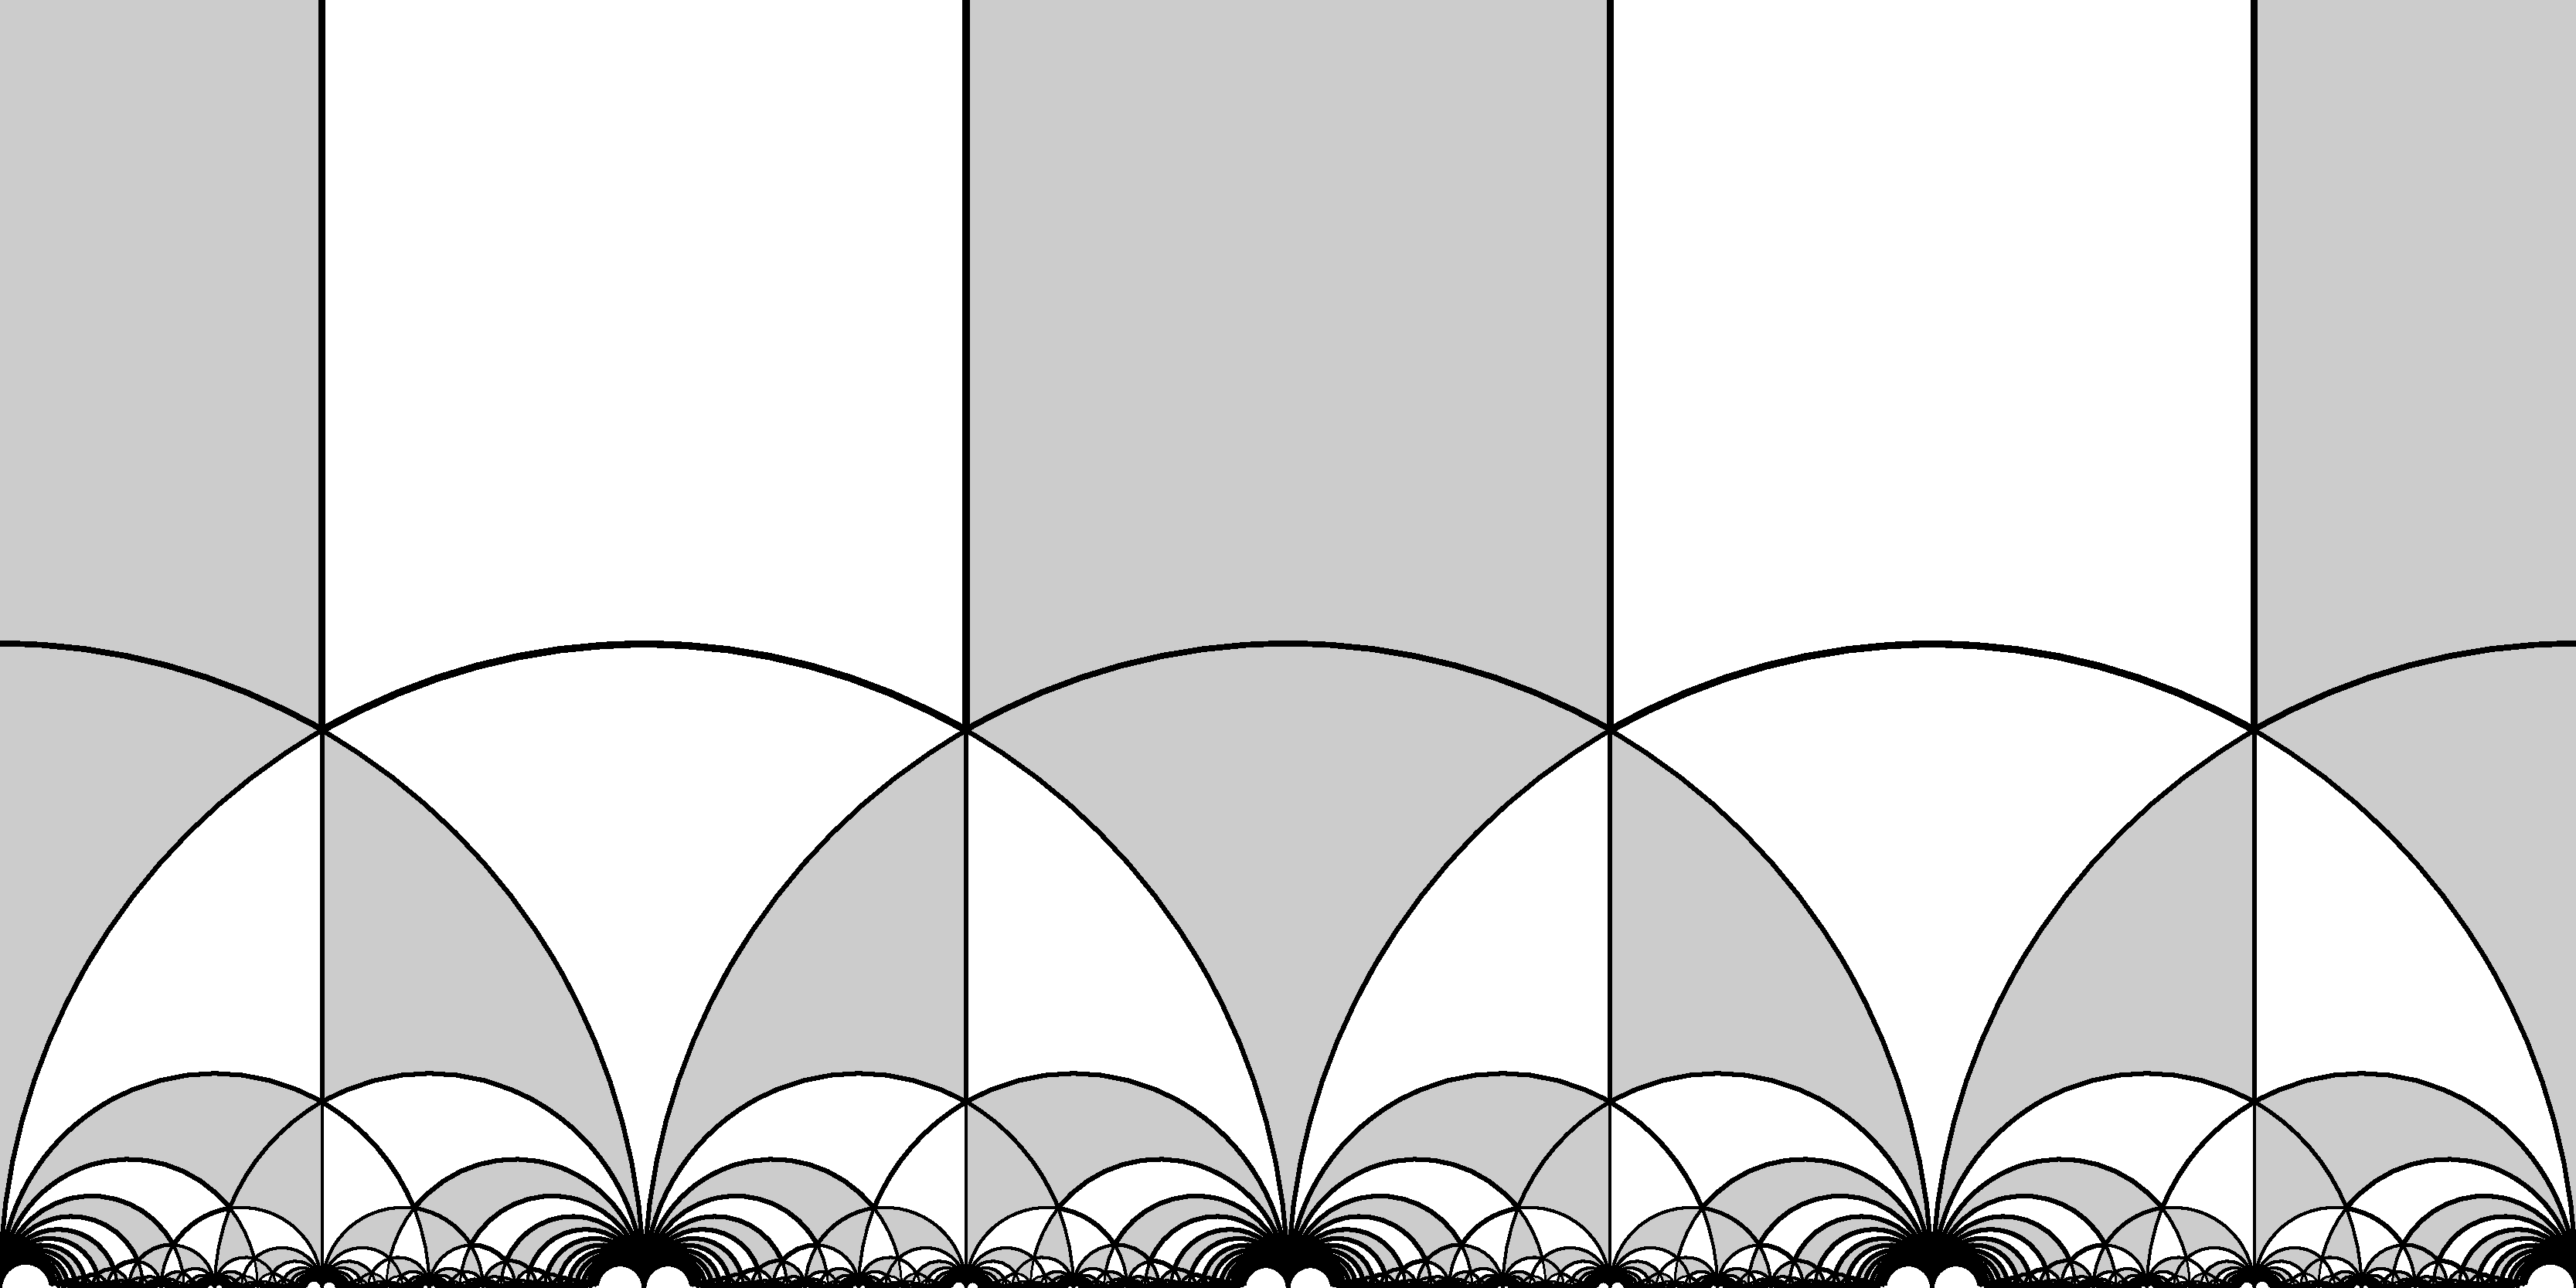
\includegraphics[width=0.8\textwidth]{modulargroup}}{20cm}{A representation of the action of $\modg$ on the upper half-plane $\mathbb{H}^2$ as a tessellation of ideal trangles with angles $(30\deg,30\deg,0\deg)$. Any of the triangles acts as a fundamental domain; the ideal $0\deg$ vertices lie on the real axis at rational points. The shading depicts the two orbits of the subgroup $\emodg \subset \modg$; any pair of same-coloured triangles form a fundamental domain for $\emodg$.}{modular}

What is more useful is that there are \emph{only} two orbits, in the sense that any rational $r$ can be mapped through an element of $\emodg$ to either $0$ or $1$ depending on its parity. We consider the following explicit algorithm.

Taken a rational $r = \pm \frac{p}{q}$ in lowest terms, $r\neq 0, 1$,

\begin{itemize}
    \item if $r < -1$ or $r > 1$, apply relevant power of $T^2$ to place it in $[-1,1]$
    \item apply $S$
\end{itemize}

The above procedure has the property of always decreasing the magnitude of either $p$ or $q$. Since these are positive integers, iteration of the procedure has to reach $0$ or $1$ in a finite number of steps. A couple examples:

\newcommand{\sapp}{\,\;\ensuremath{\xrightarrow{\mathmakebox[2em]{S}}}\;\,}
%\newcommand{\tappz}{\ensuremath{\xrightarrow{T^2}}}
\newcommand{\tapp}[1]{\,\;\xrightarrow{\mathmakebox[2em]{(T^2)^{#1}}}\;\,}

\begin{equation*}
    \frac{13}{4} \tapp{-2} - \frac{3}{4} \sapp \frac{4}{3} \tapp{-1} - \frac{2}{3} \sapp \frac{3}{2} \tapp{-1} -\frac{1}{2} \sapp 2 \tapp{-1} 0
\end{equation*}

\begin{equation*}
    \frac{7}{9} \sapp - \frac{9}{7} \tapp{1} \frac{5}{7} \sapp -\frac{7}{5} \tapp{1} \frac{3}{5} \sapp - \frac{5}{3} \tapp{1} \frac{1}{3} \sapp -3 \tapp{2} 1
\end{equation*}

Returning to our physical object of interest, the amplitude, we see that properties \eqref{t2map} and \eqref{smap} relate the behaviour of $\T$ at a rational time\footnote{We are, of course, here referring to the normalized time $\tau$ for simplicity.} with the behaviour at time $0$ or $1$ depending on the parity. Therefore $\T$ has a sort of self-similar structure, and any qualitative features present at the points $0$ and $1$ will be repeated infinitely in two dense sets. For example, we anticipate (though this will be studied more precisely) that the amplitude has a $\tau^{-1/2}$ singularity for $\tau$ close to zero, since for very small time the propagator on a circle is expected to reduce to that of the free particle. If so, then there must also be a similar singularity at all even rationals; therefore $\T$ has a dense set of singularities \cite{intermode_traces}.


\subsection{Even rationals}\label{sec:evens}

\newcommand{\asympt}{(-i\tau)^{-1/2}}

It is easy to show $\T$ ``should'' have a $\sim \tau^{-1/2}$ singularity near $\tau = 0$ \cite{boxpdf}. Indeed, applying  \eqref{smap}:

\begin{equation*}
    \vartheta(\tau) = \sqrt{\frac{1}{-i\tau}} \sumZ e^{-i\pi n^2 \frac{1}{\tau}}\,.
\end{equation*}

Naively, all terms in the sum except $n=0$ are oscillatory and supposedly cancel for small times, and $\vartheta(\tau) \sim \asympt$. This corresponds to physical intuition: the propagator should reduce to the free particle propagator for very short times, in which the particle has not yet "probed" the global structure of the circle. If this is true, however, then similar singularities should be repeated at any even rational point. Thus $\T$ would have infinite singularities, and thus be unbounded, in any given interval. This makes it impossible for it to be ever asymptotic to $\tau^{-1/2}$ in the first place.

The asymptotic behaviour must not of course be interpreted as direct but in a distributional sense. In particular, a more sensible definition is that for a family of Schwartz functions $f_\sigma(\tau) = f(\tau/\sigma)$ the evaluation of $\vartheta$ on $f_\sigma$ is asymptotic to that of $f_\sigma$ on the tempered distribution $A \tau^{-1/2}$ for some constant $A$. In integration against a Schwartz function we expect the secundary singularities at each even rational to matter less and less as we approach the main singularity at $\tau = 0$. We now test explicitly $\vartheta$ against a family of shrinking Gaussians and verify this intuition.

Consider the normalized Gaussian $g_\sigma(\tau) = \frac{1}{\sigma \sqrt{2\pi}} \exp(-\frac{\tau^2}{2\sigma^2})$. The integral of $g_\sigma(\tau)$ against $A \tau^{-1/2}$ is

\begin{equation*}
    \bra{\tau^{-1/2}}\ket{g_\sigma} =  A \intR d\tau \, g_\sigma(\tau) \tau^{-1/2} = \frac{2A}{\sigma\sqrt{2\pi}} 2^{1/4} \sqrt\sigma \int_0^\infty dx e^{-x} x^{-3/4} = \frac{A\Gamma(\frac{1}{4})}{2^{1/4}\sqrt{\pi\sigma}}\,.
\end{equation*}

On the other hand, if $g_\sigma(\tau)$ is integrated against $\vartheta$, we obtain

\begin{equation*}
    \bra{\vartheta}\ket{g_\sigma} = \sumZ \int d\tau \frac{1}{\sigma \sqrt{2\pi}} e^{-\frac{\tau^2}{2\sigma^2} + i\pi\tau n^2}  = \sumZ \exp(-\pi^2 \sigma^2 n^4 / 2)\,; 
\end{equation*}

only the asymptotic behaviour for small $\sigma$ is relevant. Defined $N^4 := 2 \pi^{-2} \sigma^{-2}$, the summand is slowly-varying for large $N$. Thus we can approximate as an integral:

\begin{equation*}
    = N \sumZ \frac{1}{N} \exp(-\frac{n^4}{N^4}) \sim N \intR d\xi \, e^{-\xi^4} = 2 N \, \Gamma(\tfrac{5}{4}) = \frac{2^{-3/4}}{\sqrt{\pi\sigma}} \Gamma(\tfrac{1}{4})\,.
\end{equation*}

It is therefore seen%\footnote{The doubt might arise that $\vartheta(\tau)$ also has a component with support in $\{0\}$ that is invisible to the family of gaussian (in the sense that its integral against $g_\sigma$ is independent on $\sigma$). However, this component must be a linear combination of $\delta$ derivatives; the even derivatives do yield positive powers of $\sigma$ and are to be excluded,  }
\ that the action of $\vartheta$ on a Schwartz function shrinking around $\tau=0$ is asymptotic to that of the distribution $\asympt$.

Now that the existence of this singularity has been ascertained, let us verify a reduced copy of it exists at any even rational. Imagine the even rational $a$ gets mapped to the even rational $b$ by one step of the iterative procedure described in section \ref{sec:modular}. Assume it is known that in the vicinity of $b$ there is an inverse square-root singularity:

\begin{equation*}
    \vartheta(b + \delta\tau') \sim K \delta \tau^{-1/2}
\end{equation*}

Now, if $a$ and $b$ are related by a simple translation $(T^2)^n$, then it's obvious this singularity is copied with no change in the constant $K$ by the periodicity property \eqref{t2map}. If instead they are related by the map $S$, and $b = -1/a$, then

\begin{equation*}
    \vartheta(a + \delta\tau) = \sqrt\frac{i}{a} \vartheta\left(-\frac{1}{a+\delta\tau}\right) \sim \sqrt\frac{i}{a} \vartheta(b + \frac{\delta \tau}{a^2}) = \sqrt{ia} K \delta\tau^{-1/2}\,,
\end{equation*}

so that $a$ inherits the singularity of $b$ but suppressed by a factor of $\sqrt{a}$. By simple induction, a singularity appears at any even rational $\pm p/q$, and the constant of proportionality $K_{p/q}$ is equal to the square root of the product of all rational encountered in the procedure towards $\tau = 0$ at each application of $S$; it's clear this is simply $|K_{p/q}| = 1/\sqrt{q}$. So, in the vicinity of $p/q$ the distribution $\vartheta$ behaves as

\begin{equation*}
    \vartheta(\tau) \sim \frac{1}{\sqrt{p-q\tau}}
\end{equation*}

%{è possibile anche fare un calcolo della fase delle singolarità? Credo di sì}

%{Forse no... forse è equivalente al calcolo delle fasi nella \eqref{finalrationalkernel}, che coinvolge number theory e potrebbe non essere fattibile nel caso generale}

\subsection{Odd rationals}\label{sec:oddrationals}

The point $\tau=1$ is equally peculiar. We argue $\vartheta$ vanishes there along with all of its distributional derivatives $\dv[k]{t} \vartheta(\tau)$. Again, the statement as it stands is non-sensical unless it is reformulated in distributional language because of the dense set of singularities. To express it we introduce again a family of shrinking Schwartz functions $f_\sigma(\tau) = f((\tau-1)/\sigma)$, this time centered around $1$. We claim that, for all $k \in \mathbb{N}$,

\begin{equation*}
    \lim_{\sigma \rightarrow 0} \bra{ \dv[k]{t}\vartheta}\ket{ f_\sigma } = 0
\end{equation*}

As before, it suffices to test against shrinking normalized Gaussians $g_\sigma(\tau) = \frac{1}{\sigma\sqrt{2\pi}} \exp( - \frac{\tau^2}{2\sigma^2} )$. We find

\begin{equation}
    \bra{\dv[k]{t}\vartheta}\ket{g_\sigma} = \sumZ (i\pi n^2)^k \frac{1}{\sigma\sqrt{2\pi}} \intR d\tau e^{- \frac{(\tau-1)^2}{2\sigma^2} + i\pi\tau n^2} = \sumZ (i\pi n^2)^k \exp( - \frac{\pi^2 \sigma^2 n^4}{2} + i\pi n^2)
\end{equation}

\begin{equation}\label{alternatingser}
    = (i\pi)^k \sumZ n^{2k} (-1)^n e^{-\pi^2 \sigma^2 n^4/2} =: (i\pi)^k S_k(\sigma)\,.\quad\quad(0^0 = 1)
\end{equation}

The series \eqref{alternatingser} is absolutely convergent for any positive $\sigma$ and natural $k$. Defined again $N^4 := 2/(\pi^2 \sigma^2)$, we intend to show  $\lim_{N \rightarrow \infty} S_k = 0$. First we recognize that $S_k$ it is a residue sum for the poles of the meromorphic function

\begin{equation}
    F_{k,N}(z) = \frac{\pi}{\sin{\pi z}} z^{2k} \exp(-\frac{z^4}{N^4})\,,
\end{equation}

%A heuristic reasoning that points to $\lim_{\sigma \rightarrow 0} S_k(\sigma) = 0$ is as follows. Rewrite the alternating series by arranging terms in pairs:

%\begin{equation}
%    S_k(\sigma) = \sum_m (2m)^k e^{-a^2 (2m)^4}  - (2m-1)^{k-1} e^{-a^2 (2m-1)^4}
%\end{equation}

which indeed has poles at all $n \neq 0$ with residue $(-1)^n n^{2k} e^{-n^4/N^4}$, and another pole at $0$ with residue $1$ for $k=0$ only, so that there is match with $S_k$ for any $k$. By the residue theorem, a partial sum for $S_k$ is $1/(2\pi i)$ the contour integral of $F$ around a loop circling the relevant poles; in the limit the entire sum is equal to the integral along a pair of lines:

\begin{equation}
    2\pi i S_k = -\int_{-\infty}^\infty F_{k,N}(\rho + it) d\rho + \int_\infty^\infty F_{k,N}(\rho-it)d\rho\,;
\end{equation}

And this limit is sensible since $F(z)$ is exponentially decaying for $\abs{z} \rightarrow \infty$ as long as $\arg{z} \neq (m+\frac{1}{2}) \frac{\pi}{2}$. Using $F(-z) = - F(z)$ we reduce the integral to the half-line:

\begin{equation}
    - \pi i S_k = \int_{it}^{it + \infty} \frac{\pi}{\sin{\pi z}} z^{2k} \exp(-\frac{z^4}{N^4})\,dz\,,
\end{equation}

Then, with the substitution $z = N \xi$:

\begin{equation}
    = N^{1+2k} \int_{it/N}^{it/N + \infty} \frac{\pi}{\sin{\pi N \xi}} \xi^{2k} \exp(-\xi^4) d\xi\,.
\end{equation}

Note $t$ was arbitrary, so we can choose to fix a constant $it/N =: K$. In addition, for large enough $N$, $\abs{\sin(\pi N \xi)} = \abs{\sin(\pi N (\Re \xi + iK))} \geq C e^{\pi N K}$ for some constant $C$. Thus the absolute value of the integral is bounded:

\begin{equation}
    \pi \abs{S_k} \leq N^{1+2k} \frac{\pi}{C} e^{-\pi N K} \int_0^{\infty} \abs{\xi}^{2k} \exp(-\Re{\xi^{4}}) d\Re\xi\,,
\end{equation}

and the last integral is a finite constant depending only on $K$. We can finally send $N\rightarrow \infty$ while keeping $K$ constant. Therefore $S_k \rightarrow 0$ for $N\rightarrow \infty$, for all $k$.

Having ascertained the existence of the "flat point" of $\vartheta$ in $\tau = 1$, it is now trivial to verify this structure is copied at all odd rationals through the action of the group $\emodg$.

\subsection{Distributional convergence}\label{sec:convergence}

We are now set to prove that there is convergence in the sense of tempered distributions of the series

\begin{equation}
    \vartheta(\tau) = \sumZ e^{i\pi \tau n^2}\,.
\end{equation}

By this, we mean that defined $\vartheta_N(\tau)$ as the partial sum with $|n| < N$, given any Schwartz function $f(\tau)$ the evaluation of $\vartheta_N$ over $f$ converges to a finite value for $N\rightarrow\infty$. The partial sum evaluations however are

\begin{equation}
    \intR d\tau \, \vartheta_N(\tau) f(\tau) = \sum_{|n|<N} \intR d\tau\, e^{i\pi\tau n^2} f(\tau) = \sum_{|n|<N} \hat f(-\pi n^2)\,,
\end{equation}

having recognized the Fourier transform of $f(\tau)$. We recall that the Fourier transform of a Schwartz function is itself Schwartz. This means $\norm\big{\hat f}_{1,0} = \sup_\tau \abs\big{\tau \hat f(\tau)}$ is finite, and thus $\abs\big{\hat f(\tau)} \leq C/\abs{\tau}$ for some $C>0$, so that the above series is absolutely convergent. Thus, $\T(\tau)$ is a well-defined tempered distribution.

Equivalently, we have just proven that the Fourier transform of the $\T(\tau)$ distribution, which is the ``quadratic $\delta$ comb'':

\begin{equation}
    \hat \T(\omega) = \sumZ \delta(\omega + \pi n^2)
\end{equation}

is a well-defined tempered distribution. Then clearly $\T(\tau)$ is also tempered as the Fourier transform of a tempered distribution.

An alternative proof provides a different presentation of $\T(\tau)$. Consider the following series for real $\tau$:

\begin{equation}
    B(\tau) = \frac{2}{i\pi}\sum_{n=1}^\infty \frac{e^{i\pi\tau n^2} }{n^2}
\end{equation}

\figurewrapper{\inputpgf{images}{batman.pgf}}{40cm}{The real (back) and imaginary (front) parts of the function $B(\tau)$ over a revival period, with some small rational points marked. Note that around even rationals $r$ the function behaves as $\sqrt{\tau - r}$, while at odd $r$ all its derivatives vanish; this matches with our results for its derivative $\T(\tau)$.}{batman}



The series is absoutely convergent and bounded as a function of $\tau$, as $\sum_{n=1}^{\infty} \frac{1}{n^2} = \frac{\pi^2}{6}$. Therefore, $B(\tau)$ is a well-defined function in $\locint$, and thus defines a tempered distribution. $\T(\tau)$ is the distributional derivative of $B(\tau)$, in the sense

\begin{equation}
    \left\langle\T,\phi\right\rangle =  \left\langle 1 + \dv{\tau}B , \phi \right \rangle = \left\langle 1, \phi \right\rangle - \left\langle B, \dv{\tau} \phi \right\rangle\,,
\end{equation}

and the last expression defines a tempered distribution acting on Schwartz $\phi(\tau)$. $B(\tau)$ is useful because, being continuous and bounded, can be plotted; it gives therefore a graphical confirmation of the ideas presented in the previous sections.



\section{The theta function propagator}

Having now satisfyingly examined the qualitative structure of the propagator for $x=0$ as a function of time, we now return back to our original formulation to include the spatial dependence.

Recovering \eqref{amplitudeztau}, and recalling the definition \eqref{jacobidef} of the Jacobi theta function, we recognize

\begin{equation}
    A(z,\tau) = e^{-i\pi z^2 \tau} \frac{1}{\sqrt{-i\tau}}\, \vartheta\left(\frac{z}{\tau};-\frac{1}{\tau}\right)
\end{equation}

The full Jacobi theta function has more general modular transformation properties than the subcase $\vartheta(\tau) = \vartheta(0;\tau)$ we studied before. In particular, it holds that

\begin{equation} \label{zperiodicity}
    \vartheta(z+1;\tau) = \vartheta(z;\tau)
\end{equation}

\begin{equation} \label{tmap}
    \vartheta(z;\tau + 1) = \vartheta(z+\frac{1}{2}; \tau)
\end{equation}

\begin{equation}\label{smapfull}
    \vartheta\left(\frac{z}{\tau}; -\frac{1}{\tau} \right) = \sqrt{-i\tau} \exp(\frac{\pi}{\tau} i z^2) \T(z;\tau)
\end{equation}

Equations \eqref{zperiodicity} and \eqref{tmap} are immediate; \eqref{smapfull} can again be proven by means of Poisson resummation\cite{bellman}; we omit the derivation for the sake of brevity.

Relation \eqref{smapfull} immediately implies that the fundamental solution $A$ is \emph{directly} a theta function:

\begin{equation}
    A(z,\tau) = \vartheta(z;\tau)
\end{equation}

The Jacobi theta for real values of the period is thus reinterpreted physically as the quantum propagator on the circle. This matches perfectly with the well-known fact that the Jacobi theta for imaginary times $\T(z;i\tau)$ is the heat kernel on the circle\cite{bellman}, nothing else than the compact analogue of the description of Wick-rotation on $\ar$ we provided in section \ref{sec:free}.

\figurewrapper{%% Creator: Matplotlib, PGF backend
%%
%% To include the figure in your LaTeX document, write
%%   \input{<filename>.pgf}
%%
%% Make sure the required packages are loaded in your preamble
%%   \usepackage{pgf}
%%
%% Figures using additional raster images can only be included by \input if
%% they are in the same directory as the main LaTeX file. For loading figures
%% from other directories you can use the `import` package
%%   \usepackage{import}
%% and then include the figures with
%%   \import{<path to file>}{<filename>.pgf}
%%
%% Matplotlib used the following preamble
%%   \usepackage{fontspec}
%%   \setmainfont{DejaVu Serif}
%%   \setsansfont{DejaVu Sans}
%%   \setmonofont{DejaVu Sans Mono}
%%
\begingroup%
\makeatletter%
\begin{pgfpicture}%
\pgfpathrectangle{\pgfpointorigin}{\pgfqpoint{5.695000in}{5.660000in}}%
\pgfusepath{use as bounding box, clip}%
\begin{pgfscope}%
\pgfsetbuttcap%
\pgfsetmiterjoin%
\definecolor{currentfill}{rgb}{1.000000,1.000000,1.000000}%
\pgfsetfillcolor{currentfill}%
\pgfsetlinewidth{0.000000pt}%
\definecolor{currentstroke}{rgb}{1.000000,1.000000,1.000000}%
\pgfsetstrokecolor{currentstroke}%
\pgfsetdash{}{0pt}%
\pgfpathmoveto{\pgfqpoint{0.000000in}{0.000000in}}%
\pgfpathlineto{\pgfqpoint{5.695000in}{0.000000in}}%
\pgfpathlineto{\pgfqpoint{5.695000in}{5.660000in}}%
\pgfpathlineto{\pgfqpoint{0.000000in}{5.660000in}}%
\pgfpathclose%
\pgfusepath{fill}%
\end{pgfscope}%
\begin{pgfscope}%
\pgfsetbuttcap%
\pgfsetmiterjoin%
\definecolor{currentfill}{rgb}{1.000000,1.000000,1.000000}%
\pgfsetfillcolor{currentfill}%
\pgfsetlinewidth{0.000000pt}%
\definecolor{currentstroke}{rgb}{0.000000,0.000000,0.000000}%
\pgfsetstrokecolor{currentstroke}%
\pgfsetstrokeopacity{0.000000}%
\pgfsetdash{}{0pt}%
\pgfpathmoveto{\pgfqpoint{0.135000in}{0.135000in}}%
\pgfpathlineto{\pgfqpoint{5.560000in}{0.135000in}}%
\pgfpathlineto{\pgfqpoint{5.560000in}{5.525000in}}%
\pgfpathlineto{\pgfqpoint{0.135000in}{5.525000in}}%
\pgfpathclose%
\pgfusepath{fill}%
\end{pgfscope}%
\begin{pgfscope}%
\pgfsetbuttcap%
\pgfsetmiterjoin%
\pgfsetlinewidth{0.000000pt}%
\definecolor{currentstroke}{rgb}{1.000000,1.000000,1.000000}%
\pgfsetstrokecolor{currentstroke}%
\pgfsetstrokeopacity{0.000000}%
\pgfsetdash{}{0pt}%
\pgfpathmoveto{\pgfqpoint{2.748038in}{2.677767in}}%
\pgfpathlineto{\pgfqpoint{5.006618in}{1.719594in}}%
\pgfpathlineto{\pgfqpoint{5.117525in}{4.339946in}}%
\pgfpathlineto{\pgfqpoint{2.739365in}{5.199767in}}%
\pgfusepath{}%
\end{pgfscope}%
\begin{pgfscope}%
\pgfsetbuttcap%
\pgfsetmiterjoin%
\pgfsetlinewidth{0.000000pt}%
\definecolor{currentstroke}{rgb}{1.000000,1.000000,1.000000}%
\pgfsetstrokecolor{currentstroke}%
\pgfsetstrokeopacity{0.000000}%
\pgfsetdash{}{0pt}%
\pgfpathmoveto{\pgfqpoint{2.748038in}{2.677767in}}%
\pgfpathlineto{\pgfqpoint{0.812277in}{1.523418in}}%
\pgfpathlineto{\pgfqpoint{0.698874in}{4.163306in}}%
\pgfpathlineto{\pgfqpoint{2.739365in}{5.199767in}}%
\pgfusepath{}%
\end{pgfscope}%
\begin{pgfscope}%
\pgfsetbuttcap%
\pgfsetmiterjoin%
\pgfsetlinewidth{0.000000pt}%
\definecolor{currentstroke}{rgb}{1.000000,1.000000,1.000000}%
\pgfsetstrokecolor{currentstroke}%
\pgfsetstrokeopacity{0.000000}%
\pgfsetdash{}{0pt}%
\pgfpathmoveto{\pgfqpoint{2.748038in}{2.677767in}}%
\pgfpathlineto{\pgfqpoint{0.812277in}{1.523418in}}%
\pgfpathlineto{\pgfqpoint{3.116397in}{0.426905in}}%
\pgfpathlineto{\pgfqpoint{5.006618in}{1.719594in}}%
\pgfusepath{}%
\end{pgfscope}%
\begin{pgfscope}%
\pgfsetrectcap%
\pgfsetroundjoin%
\pgfsetlinewidth{0.803000pt}%
\definecolor{currentstroke}{rgb}{0.000000,0.000000,0.000000}%
\pgfsetstrokecolor{currentstroke}%
\pgfsetdash{}{0pt}%
\pgfpathmoveto{\pgfqpoint{5.006618in}{1.719594in}}%
\pgfpathlineto{\pgfqpoint{3.116397in}{0.426905in}}%
\pgfusepath{stroke}%
\end{pgfscope}%
\begin{pgfscope}%
\pgftext[x=4.384668in,y=0.648402in,,]{\sffamily\fontsize{10.000000}{12.000000}\selectfont \(\displaystyle z\)}%
\end{pgfscope}%
\begin{pgfscope}%
\pgfsetbuttcap%
\pgfsetroundjoin%
\pgfsetlinewidth{0.803000pt}%
\definecolor{currentstroke}{rgb}{0.690196,0.690196,0.690196}%
\pgfsetstrokecolor{currentstroke}%
\pgfsetdash{}{0pt}%
\pgfpathmoveto{\pgfqpoint{4.893909in}{1.642514in}}%
\pgfpathlineto{\pgfqpoint{2.632198in}{2.608688in}}%
\pgfpathlineto{\pgfqpoint{2.617648in}{5.137942in}}%
\pgfusepath{stroke}%
\end{pgfscope}%
\begin{pgfscope}%
\pgfsetbuttcap%
\pgfsetroundjoin%
\pgfsetlinewidth{0.803000pt}%
\definecolor{currentstroke}{rgb}{0.690196,0.690196,0.690196}%
\pgfsetstrokecolor{currentstroke}%
\pgfsetdash{}{0pt}%
\pgfpathmoveto{\pgfqpoint{4.698431in}{1.508830in}}%
\pgfpathlineto{\pgfqpoint{2.431417in}{2.488957in}}%
\pgfpathlineto{\pgfqpoint{2.406563in}{5.030722in}}%
\pgfusepath{stroke}%
\end{pgfscope}%
\begin{pgfscope}%
\pgfsetbuttcap%
\pgfsetroundjoin%
\pgfsetlinewidth{0.803000pt}%
\definecolor{currentstroke}{rgb}{0.690196,0.690196,0.690196}%
\pgfsetstrokecolor{currentstroke}%
\pgfsetdash{}{0pt}%
\pgfpathmoveto{\pgfqpoint{4.500041in}{1.373154in}}%
\pgfpathlineto{\pgfqpoint{2.227806in}{2.367538in}}%
\pgfpathlineto{\pgfqpoint{2.192352in}{4.921914in}}%
\pgfusepath{stroke}%
\end{pgfscope}%
\begin{pgfscope}%
\pgfsetbuttcap%
\pgfsetroundjoin%
\pgfsetlinewidth{0.803000pt}%
\definecolor{currentstroke}{rgb}{0.690196,0.690196,0.690196}%
\pgfsetstrokecolor{currentstroke}%
\pgfsetdash{}{0pt}%
\pgfpathmoveto{\pgfqpoint{4.298673in}{1.235443in}}%
\pgfpathlineto{\pgfqpoint{2.021307in}{2.244396in}}%
\pgfpathlineto{\pgfqpoint{1.974944in}{4.811482in}}%
\pgfusepath{stroke}%
\end{pgfscope}%
\begin{pgfscope}%
\pgfsetbuttcap%
\pgfsetroundjoin%
\pgfsetlinewidth{0.803000pt}%
\definecolor{currentstroke}{rgb}{0.690196,0.690196,0.690196}%
\pgfsetstrokecolor{currentstroke}%
\pgfsetdash{}{0pt}%
\pgfpathmoveto{\pgfqpoint{4.094261in}{1.095649in}}%
\pgfpathlineto{\pgfqpoint{1.811856in}{2.119495in}}%
\pgfpathlineto{\pgfqpoint{1.754268in}{4.699390in}}%
\pgfusepath{stroke}%
\end{pgfscope}%
\begin{pgfscope}%
\pgfsetbuttcap%
\pgfsetroundjoin%
\pgfsetlinewidth{0.803000pt}%
\definecolor{currentstroke}{rgb}{0.690196,0.690196,0.690196}%
\pgfsetstrokecolor{currentstroke}%
\pgfsetdash{}{0pt}%
\pgfpathmoveto{\pgfqpoint{3.886733in}{0.953724in}}%
\pgfpathlineto{\pgfqpoint{1.599390in}{1.992796in}}%
\pgfpathlineto{\pgfqpoint{1.530249in}{4.585601in}}%
\pgfusepath{stroke}%
\end{pgfscope}%
\begin{pgfscope}%
\pgfsetbuttcap%
\pgfsetroundjoin%
\pgfsetlinewidth{0.803000pt}%
\definecolor{currentstroke}{rgb}{0.690196,0.690196,0.690196}%
\pgfsetstrokecolor{currentstroke}%
\pgfsetdash{}{0pt}%
\pgfpathmoveto{\pgfqpoint{3.676019in}{0.809621in}}%
\pgfpathlineto{\pgfqpoint{1.383844in}{1.864260in}}%
\pgfpathlineto{\pgfqpoint{1.302811in}{4.470074in}}%
\pgfusepath{stroke}%
\end{pgfscope}%
\begin{pgfscope}%
\pgfsetbuttcap%
\pgfsetroundjoin%
\pgfsetlinewidth{0.803000pt}%
\definecolor{currentstroke}{rgb}{0.690196,0.690196,0.690196}%
\pgfsetstrokecolor{currentstroke}%
\pgfsetdash{}{0pt}%
\pgfpathmoveto{\pgfqpoint{3.462045in}{0.663288in}}%
\pgfpathlineto{\pgfqpoint{1.165150in}{1.733847in}}%
\pgfpathlineto{\pgfqpoint{1.071875in}{4.352771in}}%
\pgfusepath{stroke}%
\end{pgfscope}%
\begin{pgfscope}%
\pgfsetbuttcap%
\pgfsetroundjoin%
\pgfsetlinewidth{0.803000pt}%
\definecolor{currentstroke}{rgb}{0.690196,0.690196,0.690196}%
\pgfsetstrokecolor{currentstroke}%
\pgfsetdash{}{0pt}%
\pgfpathmoveto{\pgfqpoint{3.244734in}{0.514673in}}%
\pgfpathlineto{\pgfqpoint{0.943239in}{1.601515in}}%
\pgfpathlineto{\pgfqpoint{0.837360in}{4.233650in}}%
\pgfusepath{stroke}%
\end{pgfscope}%
\begin{pgfscope}%
\pgfsetrectcap%
\pgfsetroundjoin%
\pgfsetlinewidth{0.803000pt}%
\definecolor{currentstroke}{rgb}{0.000000,0.000000,0.000000}%
\pgfsetstrokecolor{currentstroke}%
\pgfsetdash{}{0pt}%
\pgfpathmoveto{\pgfqpoint{4.874802in}{1.650676in}}%
\pgfpathlineto{\pgfqpoint{4.932173in}{1.626167in}}%
\pgfusepath{stroke}%
\end{pgfscope}%
\begin{pgfscope}%
\pgftext[x=5.023783in,y=1.443079in,,top]{\sffamily\fontsize{10.000000}{12.000000}\selectfont −0.50}%
\end{pgfscope}%
\begin{pgfscope}%
\pgfsetrectcap%
\pgfsetroundjoin%
\pgfsetlinewidth{0.803000pt}%
\definecolor{currentstroke}{rgb}{0.000000,0.000000,0.000000}%
\pgfsetstrokecolor{currentstroke}%
\pgfsetdash{}{0pt}%
\pgfpathmoveto{\pgfqpoint{4.679272in}{1.517113in}}%
\pgfpathlineto{\pgfqpoint{4.736801in}{1.492241in}}%
\pgfusepath{stroke}%
\end{pgfscope}%
\begin{pgfscope}%
\pgftext[x=4.829201in,y=1.307876in,,top]{\sffamily\fontsize{10.000000}{12.000000}\selectfont −0.25}%
\end{pgfscope}%
\begin{pgfscope}%
\pgfsetrectcap%
\pgfsetroundjoin%
\pgfsetlinewidth{0.803000pt}%
\definecolor{currentstroke}{rgb}{0.000000,0.000000,0.000000}%
\pgfsetstrokecolor{currentstroke}%
\pgfsetdash{}{0pt}%
\pgfpathmoveto{\pgfqpoint{4.480830in}{1.381561in}}%
\pgfpathlineto{\pgfqpoint{4.538515in}{1.356317in}}%
\pgfusepath{stroke}%
\end{pgfscope}%
\begin{pgfscope}%
\pgftext[x=4.631720in,y=1.170659in,,top]{\sffamily\fontsize{10.000000}{12.000000}\selectfont 0.00}%
\end{pgfscope}%
\begin{pgfscope}%
\pgfsetrectcap%
\pgfsetroundjoin%
\pgfsetlinewidth{0.803000pt}%
\definecolor{currentstroke}{rgb}{0.000000,0.000000,0.000000}%
\pgfsetstrokecolor{currentstroke}%
\pgfsetdash{}{0pt}%
\pgfpathmoveto{\pgfqpoint{4.279412in}{1.243976in}}%
\pgfpathlineto{\pgfqpoint{4.337250in}{1.218352in}}%
\pgfusepath{stroke}%
\end{pgfscope}%
\begin{pgfscope}%
\pgftext[x=4.431274in,y=1.031381in,,top]{\sffamily\fontsize{10.000000}{12.000000}\selectfont 0.25}%
\end{pgfscope}%
\begin{pgfscope}%
\pgfsetrectcap%
\pgfsetroundjoin%
\pgfsetlinewidth{0.803000pt}%
\definecolor{currentstroke}{rgb}{0.000000,0.000000,0.000000}%
\pgfsetstrokecolor{currentstroke}%
\pgfsetdash{}{0pt}%
\pgfpathmoveto{\pgfqpoint{4.074948in}{1.104312in}}%
\pgfpathlineto{\pgfqpoint{4.132939in}{1.078298in}}%
\pgfusepath{stroke}%
\end{pgfscope}%
\begin{pgfscope}%
\pgftext[x=4.227795in,y=0.889996in,,top]{\sffamily\fontsize{10.000000}{12.000000}\selectfont 0.50}%
\end{pgfscope}%
\begin{pgfscope}%
\pgfsetrectcap%
\pgfsetroundjoin%
\pgfsetlinewidth{0.803000pt}%
\definecolor{currentstroke}{rgb}{0.000000,0.000000,0.000000}%
\pgfsetstrokecolor{currentstroke}%
\pgfsetdash{}{0pt}%
\pgfpathmoveto{\pgfqpoint{3.867371in}{0.962520in}}%
\pgfpathlineto{\pgfqpoint{3.925512in}{0.936108in}}%
\pgfusepath{stroke}%
\end{pgfscope}%
\begin{pgfscope}%
\pgftext[x=4.021215in,y=0.746457in,,top]{\sffamily\fontsize{10.000000}{12.000000}\selectfont 0.75}%
\end{pgfscope}%
\begin{pgfscope}%
\pgfsetrectcap%
\pgfsetroundjoin%
\pgfsetlinewidth{0.803000pt}%
\definecolor{currentstroke}{rgb}{0.000000,0.000000,0.000000}%
\pgfsetstrokecolor{currentstroke}%
\pgfsetdash{}{0pt}%
\pgfpathmoveto{\pgfqpoint{3.656608in}{0.818552in}}%
\pgfpathlineto{\pgfqpoint{3.714897in}{0.791733in}}%
\pgfusepath{stroke}%
\end{pgfscope}%
\begin{pgfscope}%
\pgftext[x=3.811462in,y=0.600712in,,top]{\sffamily\fontsize{10.000000}{12.000000}\selectfont 1.00}%
\end{pgfscope}%
\begin{pgfscope}%
\pgfsetrectcap%
\pgfsetroundjoin%
\pgfsetlinewidth{0.803000pt}%
\definecolor{currentstroke}{rgb}{0.000000,0.000000,0.000000}%
\pgfsetstrokecolor{currentstroke}%
\pgfsetdash{}{0pt}%
\pgfpathmoveto{\pgfqpoint{3.442586in}{0.672358in}}%
\pgfpathlineto{\pgfqpoint{3.501019in}{0.645122in}}%
\pgfusepath{stroke}%
\end{pgfscope}%
\begin{pgfscope}%
\pgftext[x=3.598463in,y=0.452712in,,top]{\sffamily\fontsize{10.000000}{12.000000}\selectfont 1.25}%
\end{pgfscope}%
\begin{pgfscope}%
\pgfsetrectcap%
\pgfsetroundjoin%
\pgfsetlinewidth{0.803000pt}%
\definecolor{currentstroke}{rgb}{0.000000,0.000000,0.000000}%
\pgfsetstrokecolor{currentstroke}%
\pgfsetdash{}{0pt}%
\pgfpathmoveto{\pgfqpoint{3.225227in}{0.523884in}}%
\pgfpathlineto{\pgfqpoint{3.283804in}{0.496223in}}%
\pgfusepath{stroke}%
\end{pgfscope}%
\begin{pgfscope}%
\pgftext[x=3.382141in,y=0.302403in,,top]{\sffamily\fontsize{10.000000}{12.000000}\selectfont 1.50}%
\end{pgfscope}%
\begin{pgfscope}%
\pgfsetrectcap%
\pgfsetroundjoin%
\pgfsetlinewidth{0.803000pt}%
\definecolor{currentstroke}{rgb}{0.000000,0.000000,0.000000}%
\pgfsetstrokecolor{currentstroke}%
\pgfsetdash{}{0pt}%
\pgfpathmoveto{\pgfqpoint{0.812277in}{1.523418in}}%
\pgfpathlineto{\pgfqpoint{3.116397in}{0.426905in}}%
\pgfusepath{stroke}%
\end{pgfscope}%
\begin{pgfscope}%
\pgftext[x=1.683885in,y=0.514783in,,]{\sffamily\fontsize{10.000000}{12.000000}\selectfont \(\displaystyle t\)}%
\end{pgfscope}%
\begin{pgfscope}%
\pgfsetbuttcap%
\pgfsetroundjoin%
\pgfsetlinewidth{0.803000pt}%
\definecolor{currentstroke}{rgb}{0.690196,0.690196,0.690196}%
\pgfsetstrokecolor{currentstroke}%
\pgfsetdash{}{0pt}%
\pgfpathmoveto{\pgfqpoint{2.877808in}{5.149713in}}%
\pgfpathlineto{\pgfqpoint{2.879871in}{2.621838in}}%
\pgfpathlineto{\pgfqpoint{0.946285in}{1.459645in}}%
\pgfusepath{stroke}%
\end{pgfscope}%
\begin{pgfscope}%
\pgfsetbuttcap%
\pgfsetroundjoin%
\pgfsetlinewidth{0.803000pt}%
\definecolor{currentstroke}{rgb}{0.690196,0.690196,0.690196}%
\pgfsetstrokecolor{currentstroke}%
\pgfsetdash{}{0pt}%
\pgfpathmoveto{\pgfqpoint{3.277321in}{5.005270in}}%
\pgfpathlineto{\pgfqpoint{3.260062in}{2.460547in}}%
\pgfpathlineto{\pgfqpoint{1.333086in}{1.275569in}}%
\pgfusepath{stroke}%
\end{pgfscope}%
\begin{pgfscope}%
\pgfsetbuttcap%
\pgfsetroundjoin%
\pgfsetlinewidth{0.803000pt}%
\definecolor{currentstroke}{rgb}{0.690196,0.690196,0.690196}%
\pgfsetstrokecolor{currentstroke}%
\pgfsetdash{}{0pt}%
\pgfpathmoveto{\pgfqpoint{3.684832in}{4.857934in}}%
\pgfpathlineto{\pgfqpoint{3.647493in}{2.296184in}}%
\pgfpathlineto{\pgfqpoint{1.727763in}{1.087745in}}%
\pgfusepath{stroke}%
\end{pgfscope}%
\begin{pgfscope}%
\pgfsetbuttcap%
\pgfsetroundjoin%
\pgfsetlinewidth{0.803000pt}%
\definecolor{currentstroke}{rgb}{0.690196,0.690196,0.690196}%
\pgfsetstrokecolor{currentstroke}%
\pgfsetdash{}{0pt}%
\pgfpathmoveto{\pgfqpoint{4.100584in}{4.707620in}}%
\pgfpathlineto{\pgfqpoint{4.042373in}{2.128662in}}%
\pgfpathlineto{\pgfqpoint{2.130559in}{0.896058in}}%
\pgfusepath{stroke}%
\end{pgfscope}%
\begin{pgfscope}%
\pgfsetbuttcap%
\pgfsetroundjoin%
\pgfsetlinewidth{0.803000pt}%
\definecolor{currentstroke}{rgb}{0.690196,0.690196,0.690196}%
\pgfsetstrokecolor{currentstroke}%
\pgfsetdash{}{0pt}%
\pgfpathmoveto{\pgfqpoint{4.524829in}{4.554234in}}%
\pgfpathlineto{\pgfqpoint{4.444917in}{1.957888in}}%
\pgfpathlineto{\pgfqpoint{2.541727in}{0.700386in}}%
\pgfusepath{stroke}%
\end{pgfscope}%
\begin{pgfscope}%
\pgfsetbuttcap%
\pgfsetroundjoin%
\pgfsetlinewidth{0.803000pt}%
\definecolor{currentstroke}{rgb}{0.690196,0.690196,0.690196}%
\pgfsetstrokecolor{currentstroke}%
\pgfsetdash{}{0pt}%
\pgfpathmoveto{\pgfqpoint{4.957830in}{4.397683in}}%
\pgfpathlineto{\pgfqpoint{4.855352in}{1.783766in}}%
\pgfpathlineto{\pgfqpoint{2.961532in}{0.500605in}}%
\pgfusepath{stroke}%
\end{pgfscope}%
\begin{pgfscope}%
\pgfsetrectcap%
\pgfsetroundjoin%
\pgfsetlinewidth{0.803000pt}%
\definecolor{currentstroke}{rgb}{0.000000,0.000000,0.000000}%
\pgfsetstrokecolor{currentstroke}%
\pgfsetdash{}{0pt}%
\pgfpathmoveto{\pgfqpoint{0.962796in}{1.469569in}}%
\pgfpathlineto{\pgfqpoint{0.913210in}{1.439764in}}%
\pgfusepath{stroke}%
\end{pgfscope}%
\begin{pgfscope}%
\pgftext[x=0.834807in,y=1.246671in,,top]{\sffamily\fontsize{10.000000}{12.000000}\selectfont 0.0}%
\end{pgfscope}%
\begin{pgfscope}%
\pgfsetrectcap%
\pgfsetroundjoin%
\pgfsetlinewidth{0.803000pt}%
\definecolor{currentstroke}{rgb}{0.000000,0.000000,0.000000}%
\pgfsetstrokecolor{currentstroke}%
\pgfsetdash{}{0pt}%
\pgfpathmoveto{\pgfqpoint{1.349551in}{1.285694in}}%
\pgfpathlineto{\pgfqpoint{1.300102in}{1.255286in}}%
\pgfusepath{stroke}%
\end{pgfscope}%
\begin{pgfscope}%
\pgftext[x=1.220854in,y=1.060270in,,top]{\sffamily\fontsize{10.000000}{12.000000}\selectfont 0.2}%
\end{pgfscope}%
\begin{pgfscope}%
\pgfsetrectcap%
\pgfsetroundjoin%
\pgfsetlinewidth{0.803000pt}%
\definecolor{currentstroke}{rgb}{0.000000,0.000000,0.000000}%
\pgfsetstrokecolor{currentstroke}%
\pgfsetdash{}{0pt}%
\pgfpathmoveto{\pgfqpoint{1.744177in}{1.098078in}}%
\pgfpathlineto{\pgfqpoint{1.694881in}{1.067047in}}%
\pgfusepath{stroke}%
\end{pgfscope}%
\begin{pgfscope}%
\pgftext[x=1.614770in,y=0.870070in,,top]{\sffamily\fontsize{10.000000}{12.000000}\selectfont 0.4}%
\end{pgfscope}%
\begin{pgfscope}%
\pgfsetrectcap%
\pgfsetroundjoin%
\pgfsetlinewidth{0.803000pt}%
\definecolor{currentstroke}{rgb}{0.000000,0.000000,0.000000}%
\pgfsetstrokecolor{currentstroke}%
\pgfsetdash{}{0pt}%
\pgfpathmoveto{\pgfqpoint{2.146916in}{0.906604in}}%
\pgfpathlineto{\pgfqpoint{2.097791in}{0.874931in}}%
\pgfusepath{stroke}%
\end{pgfscope}%
\begin{pgfscope}%
\pgftext[x=2.016797in,y=0.675954in,,top]{\sffamily\fontsize{10.000000}{12.000000}\selectfont 0.6}%
\end{pgfscope}%
\begin{pgfscope}%
\pgfsetrectcap%
\pgfsetroundjoin%
\pgfsetlinewidth{0.803000pt}%
\definecolor{currentstroke}{rgb}{0.000000,0.000000,0.000000}%
\pgfsetstrokecolor{currentstroke}%
\pgfsetdash{}{0pt}%
\pgfpathmoveto{\pgfqpoint{2.558021in}{0.711152in}}%
\pgfpathlineto{\pgfqpoint{2.509084in}{0.678818in}}%
\pgfusepath{stroke}%
\end{pgfscope}%
\begin{pgfscope}%
\pgftext[x=2.427189in,y=0.477799in,,top]{\sffamily\fontsize{10.000000}{12.000000}\selectfont 0.8}%
\end{pgfscope}%
\begin{pgfscope}%
\pgfsetrectcap%
\pgfsetroundjoin%
\pgfsetlinewidth{0.803000pt}%
\definecolor{currentstroke}{rgb}{0.000000,0.000000,0.000000}%
\pgfsetstrokecolor{currentstroke}%
\pgfsetdash{}{0pt}%
\pgfpathmoveto{\pgfqpoint{2.977757in}{0.511598in}}%
\pgfpathlineto{\pgfqpoint{2.929026in}{0.478581in}}%
\pgfusepath{stroke}%
\end{pgfscope}%
\begin{pgfscope}%
\pgftext[x=2.846209in,y=0.275477in,,top]{\sffamily\fontsize{10.000000}{12.000000}\selectfont 1.0}%
\end{pgfscope}%
\begin{pgfscope}%
\pgfsetrectcap%
\pgfsetroundjoin%
\pgfsetlinewidth{0.803000pt}%
\definecolor{currentstroke}{rgb}{0.000000,0.000000,0.000000}%
\pgfsetstrokecolor{currentstroke}%
\pgfsetdash{}{0pt}%
\pgfpathmoveto{\pgfqpoint{0.812277in}{1.523418in}}%
\pgfpathlineto{\pgfqpoint{0.698874in}{4.163306in}}%
\pgfusepath{stroke}%
\end{pgfscope}%
\begin{pgfscope}%
\pgftext[x=0.176102in,y=2.994063in,left,base,rotate=272.459775]{\sffamily\fontsize{10.000000}{12.000000}\selectfont \(\displaystyle \vartheta(z,it)\)}%
\end{pgfscope}%
\begin{pgfscope}%
\pgfsetbuttcap%
\pgfsetroundjoin%
\pgfsetlinewidth{0.803000pt}%
\definecolor{currentstroke}{rgb}{0.690196,0.690196,0.690196}%
\pgfsetstrokecolor{currentstroke}%
\pgfsetdash{}{0pt}%
\pgfpathmoveto{\pgfqpoint{0.810122in}{1.573573in}}%
\pgfpathlineto{\pgfqpoint{2.747873in}{2.725841in}}%
\pgfpathlineto{\pgfqpoint{5.008726in}{1.769405in}}%
\pgfusepath{stroke}%
\end{pgfscope}%
\begin{pgfscope}%
\pgfsetbuttcap%
\pgfsetroundjoin%
\pgfsetlinewidth{0.803000pt}%
\definecolor{currentstroke}{rgb}{0.690196,0.690196,0.690196}%
\pgfsetstrokecolor{currentstroke}%
\pgfsetdash{}{0pt}%
\pgfpathmoveto{\pgfqpoint{0.797102in}{1.876664in}}%
\pgfpathlineto{\pgfqpoint{2.746874in}{3.016234in}}%
\pgfpathlineto{\pgfqpoint{5.021466in}{2.070401in}}%
\pgfusepath{stroke}%
\end{pgfscope}%
\begin{pgfscope}%
\pgfsetbuttcap%
\pgfsetroundjoin%
\pgfsetlinewidth{0.803000pt}%
\definecolor{currentstroke}{rgb}{0.690196,0.690196,0.690196}%
\pgfsetstrokecolor{currentstroke}%
\pgfsetdash{}{0pt}%
\pgfpathmoveto{\pgfqpoint{0.783921in}{2.183518in}}%
\pgfpathlineto{\pgfqpoint{2.745864in}{3.310000in}}%
\pgfpathlineto{\pgfqpoint{5.034362in}{2.375093in}}%
\pgfusepath{stroke}%
\end{pgfscope}%
\begin{pgfscope}%
\pgfsetbuttcap%
\pgfsetroundjoin%
\pgfsetlinewidth{0.803000pt}%
\definecolor{currentstroke}{rgb}{0.690196,0.690196,0.690196}%
\pgfsetstrokecolor{currentstroke}%
\pgfsetdash{}{0pt}%
\pgfpathmoveto{\pgfqpoint{0.770574in}{2.494205in}}%
\pgfpathlineto{\pgfqpoint{2.744842in}{3.607199in}}%
\pgfpathlineto{\pgfqpoint{5.047418in}{2.683549in}}%
\pgfusepath{stroke}%
\end{pgfscope}%
\begin{pgfscope}%
\pgfsetbuttcap%
\pgfsetroundjoin%
\pgfsetlinewidth{0.803000pt}%
\definecolor{currentstroke}{rgb}{0.690196,0.690196,0.690196}%
\pgfsetstrokecolor{currentstroke}%
\pgfsetdash{}{0pt}%
\pgfpathmoveto{\pgfqpoint{0.757060in}{2.808797in}}%
\pgfpathlineto{\pgfqpoint{2.743807in}{3.907890in}}%
\pgfpathlineto{\pgfqpoint{5.060636in}{2.995839in}}%
\pgfusepath{stroke}%
\end{pgfscope}%
\begin{pgfscope}%
\pgfsetbuttcap%
\pgfsetroundjoin%
\pgfsetlinewidth{0.803000pt}%
\definecolor{currentstroke}{rgb}{0.690196,0.690196,0.690196}%
\pgfsetstrokecolor{currentstroke}%
\pgfsetdash{}{0pt}%
\pgfpathmoveto{\pgfqpoint{0.743375in}{3.127368in}}%
\pgfpathlineto{\pgfqpoint{2.742761in}{4.212137in}}%
\pgfpathlineto{\pgfqpoint{5.074019in}{3.312036in}}%
\pgfusepath{stroke}%
\end{pgfscope}%
\begin{pgfscope}%
\pgfsetbuttcap%
\pgfsetroundjoin%
\pgfsetlinewidth{0.803000pt}%
\definecolor{currentstroke}{rgb}{0.690196,0.690196,0.690196}%
\pgfsetstrokecolor{currentstroke}%
\pgfsetdash{}{0pt}%
\pgfpathmoveto{\pgfqpoint{0.729516in}{3.449995in}}%
\pgfpathlineto{\pgfqpoint{2.741702in}{4.520002in}}%
\pgfpathlineto{\pgfqpoint{5.087570in}{3.632213in}}%
\pgfusepath{stroke}%
\end{pgfscope}%
\begin{pgfscope}%
\pgfsetbuttcap%
\pgfsetroundjoin%
\pgfsetlinewidth{0.803000pt}%
\definecolor{currentstroke}{rgb}{0.690196,0.690196,0.690196}%
\pgfsetstrokecolor{currentstroke}%
\pgfsetdash{}{0pt}%
\pgfpathmoveto{\pgfqpoint{0.715479in}{3.776755in}}%
\pgfpathlineto{\pgfqpoint{2.740631in}{4.831550in}}%
\pgfpathlineto{\pgfqpoint{5.101294in}{3.956445in}}%
\pgfusepath{stroke}%
\end{pgfscope}%
\begin{pgfscope}%
\pgfsetbuttcap%
\pgfsetroundjoin%
\pgfsetlinewidth{0.803000pt}%
\definecolor{currentstroke}{rgb}{0.690196,0.690196,0.690196}%
\pgfsetstrokecolor{currentstroke}%
\pgfsetdash{}{0pt}%
\pgfpathmoveto{\pgfqpoint{0.701261in}{4.107729in}}%
\pgfpathlineto{\pgfqpoint{2.739547in}{5.146848in}}%
\pgfpathlineto{\pgfqpoint{5.115192in}{4.284811in}}%
\pgfusepath{stroke}%
\end{pgfscope}%
\begin{pgfscope}%
\pgfsetrectcap%
\pgfsetroundjoin%
\pgfsetlinewidth{0.803000pt}%
\definecolor{currentstroke}{rgb}{0.000000,0.000000,0.000000}%
\pgfsetstrokecolor{currentstroke}%
\pgfsetdash{}{0pt}%
\pgfpathmoveto{\pgfqpoint{0.826666in}{1.583410in}}%
\pgfpathlineto{\pgfqpoint{0.776981in}{1.553865in}}%
\pgfusepath{stroke}%
\end{pgfscope}%
\begin{pgfscope}%
\pgftext[x=0.569268in,y=1.562339in,,top]{\sffamily\fontsize{10.000000}{12.000000}\selectfont 0.0}%
\end{pgfscope}%
\begin{pgfscope}%
\pgfsetrectcap%
\pgfsetroundjoin%
\pgfsetlinewidth{0.803000pt}%
\definecolor{currentstroke}{rgb}{0.000000,0.000000,0.000000}%
\pgfsetstrokecolor{currentstroke}%
\pgfsetdash{}{0pt}%
\pgfpathmoveto{\pgfqpoint{0.813755in}{1.886397in}}%
\pgfpathlineto{\pgfqpoint{0.763742in}{1.857166in}}%
\pgfusepath{stroke}%
\end{pgfscope}%
\begin{pgfscope}%
\pgftext[x=0.554753in,y=1.865549in,,top]{\sffamily\fontsize{10.000000}{12.000000}\selectfont 0.5}%
\end{pgfscope}%
\begin{pgfscope}%
\pgfsetrectcap%
\pgfsetroundjoin%
\pgfsetlinewidth{0.803000pt}%
\definecolor{currentstroke}{rgb}{0.000000,0.000000,0.000000}%
\pgfsetstrokecolor{currentstroke}%
\pgfsetdash{}{0pt}%
\pgfpathmoveto{\pgfqpoint{0.800684in}{2.193143in}}%
\pgfpathlineto{\pgfqpoint{0.750338in}{2.164236in}}%
\pgfusepath{stroke}%
\end{pgfscope}%
\begin{pgfscope}%
\pgftext[x=0.540058in,y=2.172526in,,top]{\sffamily\fontsize{10.000000}{12.000000}\selectfont 1.0}%
\end{pgfscope}%
\begin{pgfscope}%
\pgfsetrectcap%
\pgfsetroundjoin%
\pgfsetlinewidth{0.803000pt}%
\definecolor{currentstroke}{rgb}{0.000000,0.000000,0.000000}%
\pgfsetstrokecolor{currentstroke}%
\pgfsetdash{}{0pt}%
\pgfpathmoveto{\pgfqpoint{0.787450in}{2.503718in}}%
\pgfpathlineto{\pgfqpoint{0.736767in}{2.475146in}}%
\pgfusepath{stroke}%
\end{pgfscope}%
\begin{pgfscope}%
\pgftext[x=0.525179in,y=2.483340in,,top]{\sffamily\fontsize{10.000000}{12.000000}\selectfont 1.5}%
\end{pgfscope}%
\begin{pgfscope}%
\pgfsetrectcap%
\pgfsetroundjoin%
\pgfsetlinewidth{0.803000pt}%
\definecolor{currentstroke}{rgb}{0.000000,0.000000,0.000000}%
\pgfsetstrokecolor{currentstroke}%
\pgfsetdash{}{0pt}%
\pgfpathmoveto{\pgfqpoint{0.774049in}{2.818195in}}%
\pgfpathlineto{\pgfqpoint{0.723025in}{2.789968in}}%
\pgfusepath{stroke}%
\end{pgfscope}%
\begin{pgfscope}%
\pgftext[x=0.510113in,y=2.798064in,,top]{\sffamily\fontsize{10.000000}{12.000000}\selectfont 2.0}%
\end{pgfscope}%
\begin{pgfscope}%
\pgfsetrectcap%
\pgfsetroundjoin%
\pgfsetlinewidth{0.803000pt}%
\definecolor{currentstroke}{rgb}{0.000000,0.000000,0.000000}%
\pgfsetstrokecolor{currentstroke}%
\pgfsetdash{}{0pt}%
\pgfpathmoveto{\pgfqpoint{0.760479in}{3.136648in}}%
\pgfpathlineto{\pgfqpoint{0.709109in}{3.108777in}}%
\pgfusepath{stroke}%
\end{pgfscope}%
\begin{pgfscope}%
\pgftext[x=0.494856in,y=3.116771in,,top]{\sffamily\fontsize{10.000000}{12.000000}\selectfont 2.5}%
\end{pgfscope}%
\begin{pgfscope}%
\pgfsetrectcap%
\pgfsetroundjoin%
\pgfsetlinewidth{0.803000pt}%
\definecolor{currentstroke}{rgb}{0.000000,0.000000,0.000000}%
\pgfsetstrokecolor{currentstroke}%
\pgfsetdash{}{0pt}%
\pgfpathmoveto{\pgfqpoint{0.746736in}{3.459152in}}%
\pgfpathlineto{\pgfqpoint{0.695016in}{3.431649in}}%
\pgfusepath{stroke}%
\end{pgfscope}%
\begin{pgfscope}%
\pgftext[x=0.479405in,y=3.439538in,,top]{\sffamily\fontsize{10.000000}{12.000000}\selectfont 3.0}%
\end{pgfscope}%
\begin{pgfscope}%
\pgfsetrectcap%
\pgfsetroundjoin%
\pgfsetlinewidth{0.803000pt}%
\definecolor{currentstroke}{rgb}{0.000000,0.000000,0.000000}%
\pgfsetstrokecolor{currentstroke}%
\pgfsetdash{}{0pt}%
\pgfpathmoveto{\pgfqpoint{0.732818in}{3.785786in}}%
\pgfpathlineto{\pgfqpoint{0.680742in}{3.758663in}}%
\pgfusepath{stroke}%
\end{pgfscope}%
\begin{pgfscope}%
\pgftext[x=0.463756in,y=3.766442in,,top]{\sffamily\fontsize{10.000000}{12.000000}\selectfont 3.5}%
\end{pgfscope}%
\begin{pgfscope}%
\pgfsetrectcap%
\pgfsetroundjoin%
\pgfsetlinewidth{0.803000pt}%
\definecolor{currentstroke}{rgb}{0.000000,0.000000,0.000000}%
\pgfsetstrokecolor{currentstroke}%
\pgfsetdash{}{0pt}%
\pgfpathmoveto{\pgfqpoint{0.718720in}{4.116629in}}%
\pgfpathlineto{\pgfqpoint{0.666284in}{4.089897in}}%
\pgfusepath{stroke}%
\end{pgfscope}%
\begin{pgfscope}%
\pgftext[x=0.447905in,y=4.097564in,,top]{\sffamily\fontsize{10.000000}{12.000000}\selectfont 4.0}%
\end{pgfscope}%
\begin{pgfscope}%
\pgfpathrectangle{\pgfqpoint{0.135000in}{0.135000in}}{\pgfqpoint{5.425000in}{5.390000in}} %
\pgfusepath{clip}%
\pgfsetbuttcap%
\pgfsetroundjoin%
\definecolor{currentfill}{rgb}{1.000000,1.000000,1.000000}%
\pgfsetfillcolor{currentfill}%
\pgfsetlinewidth{0.150562pt}%
\definecolor{currentstroke}{rgb}{0.000000,0.000000,0.000000}%
\pgfsetstrokecolor{currentstroke}%
\pgfsetdash{}{0pt}%
\pgfpathmoveto{\pgfqpoint{2.768753in}{2.598603in}}%
\pgfpathlineto{\pgfqpoint{2.771710in}{2.597343in}}%
\pgfpathlineto{\pgfqpoint{2.775384in}{2.595779in}}%
\pgfpathlineto{\pgfqpoint{2.767369in}{2.590972in}}%
\pgfpathlineto{\pgfqpoint{2.759351in}{2.586163in}}%
\pgfpathlineto{\pgfqpoint{2.751328in}{2.581351in}}%
\pgfpathlineto{\pgfqpoint{2.743300in}{2.576536in}}%
\pgfpathlineto{\pgfqpoint{2.739626in}{2.578104in}}%
\pgfpathlineto{\pgfqpoint{2.736668in}{2.579367in}}%
\pgfpathlineto{\pgfqpoint{2.744696in}{2.584180in}}%
\pgfpathlineto{\pgfqpoint{2.752719in}{2.588990in}}%
\pgfpathlineto{\pgfqpoint{2.760739in}{2.593798in}}%
\pgfpathlineto{\pgfqpoint{2.768753in}{2.598603in}}%
\pgfpathclose%
\pgfusepath{stroke,fill}%
\end{pgfscope}%
\begin{pgfscope}%
\pgfpathrectangle{\pgfqpoint{0.135000in}{0.135000in}}{\pgfqpoint{5.425000in}{5.390000in}} %
\pgfusepath{clip}%
\pgfsetbuttcap%
\pgfsetroundjoin%
\definecolor{currentfill}{rgb}{1.000000,1.000000,1.000000}%
\pgfsetfillcolor{currentfill}%
\pgfsetlinewidth{0.150562pt}%
\definecolor{currentstroke}{rgb}{0.000000,0.000000,0.000000}%
\pgfsetstrokecolor{currentstroke}%
\pgfsetdash{}{0pt}%
\pgfpathmoveto{\pgfqpoint{2.775384in}{2.595779in}}%
\pgfpathlineto{\pgfqpoint{2.779774in}{2.593908in}}%
\pgfpathlineto{\pgfqpoint{2.784881in}{2.591733in}}%
\pgfpathlineto{\pgfqpoint{2.776868in}{2.586924in}}%
\pgfpathlineto{\pgfqpoint{2.768850in}{2.582112in}}%
\pgfpathlineto{\pgfqpoint{2.760827in}{2.577298in}}%
\pgfpathlineto{\pgfqpoint{2.752801in}{2.572481in}}%
\pgfpathlineto{\pgfqpoint{2.747692in}{2.574662in}}%
\pgfpathlineto{\pgfqpoint{2.743300in}{2.576536in}}%
\pgfpathlineto{\pgfqpoint{2.751328in}{2.581351in}}%
\pgfpathlineto{\pgfqpoint{2.759351in}{2.586163in}}%
\pgfpathlineto{\pgfqpoint{2.767369in}{2.590972in}}%
\pgfpathlineto{\pgfqpoint{2.775384in}{2.595779in}}%
\pgfpathclose%
\pgfusepath{stroke,fill}%
\end{pgfscope}%
\begin{pgfscope}%
\pgfpathrectangle{\pgfqpoint{0.135000in}{0.135000in}}{\pgfqpoint{5.425000in}{5.390000in}} %
\pgfusepath{clip}%
\pgfsetbuttcap%
\pgfsetroundjoin%
\definecolor{currentfill}{rgb}{1.000000,1.000000,1.000000}%
\pgfsetfillcolor{currentfill}%
\pgfsetlinewidth{0.150562pt}%
\definecolor{currentstroke}{rgb}{0.000000,0.000000,0.000000}%
\pgfsetstrokecolor{currentstroke}%
\pgfsetdash{}{0pt}%
\pgfpathmoveto{\pgfqpoint{2.784881in}{2.591733in}}%
\pgfpathlineto{\pgfqpoint{2.790706in}{2.589251in}}%
\pgfpathlineto{\pgfqpoint{2.797249in}{2.586464in}}%
\pgfpathlineto{\pgfqpoint{2.789237in}{2.581652in}}%
\pgfpathlineto{\pgfqpoint{2.781220in}{2.576838in}}%
\pgfpathlineto{\pgfqpoint{2.773199in}{2.572021in}}%
\pgfpathlineto{\pgfqpoint{2.765173in}{2.567201in}}%
\pgfpathlineto{\pgfqpoint{2.758628in}{2.569994in}}%
\pgfpathlineto{\pgfqpoint{2.752801in}{2.572481in}}%
\pgfpathlineto{\pgfqpoint{2.760827in}{2.577298in}}%
\pgfpathlineto{\pgfqpoint{2.768850in}{2.582112in}}%
\pgfpathlineto{\pgfqpoint{2.776868in}{2.586924in}}%
\pgfpathlineto{\pgfqpoint{2.784881in}{2.591733in}}%
\pgfpathclose%
\pgfusepath{stroke,fill}%
\end{pgfscope}%
\begin{pgfscope}%
\pgfpathrectangle{\pgfqpoint{0.135000in}{0.135000in}}{\pgfqpoint{5.425000in}{5.390000in}} %
\pgfusepath{clip}%
\pgfsetbuttcap%
\pgfsetroundjoin%
\definecolor{currentfill}{rgb}{1.000000,1.000000,1.000000}%
\pgfsetfillcolor{currentfill}%
\pgfsetlinewidth{0.150562pt}%
\definecolor{currentstroke}{rgb}{0.000000,0.000000,0.000000}%
\pgfsetstrokecolor{currentstroke}%
\pgfsetdash{}{0pt}%
\pgfpathmoveto{\pgfqpoint{2.797249in}{2.586464in}}%
\pgfpathlineto{\pgfqpoint{2.804512in}{2.583370in}}%
\pgfpathlineto{\pgfqpoint{2.812494in}{2.579970in}}%
\pgfpathlineto{\pgfqpoint{2.804483in}{2.575155in}}%
\pgfpathlineto{\pgfqpoint{2.796467in}{2.570336in}}%
\pgfpathlineto{\pgfqpoint{2.788447in}{2.565516in}}%
\pgfpathlineto{\pgfqpoint{2.780423in}{2.560692in}}%
\pgfpathlineto{\pgfqpoint{2.772438in}{2.564100in}}%
\pgfpathlineto{\pgfqpoint{2.765173in}{2.567201in}}%
\pgfpathlineto{\pgfqpoint{2.773199in}{2.572021in}}%
\pgfpathlineto{\pgfqpoint{2.781220in}{2.576838in}}%
\pgfpathlineto{\pgfqpoint{2.789237in}{2.581652in}}%
\pgfpathlineto{\pgfqpoint{2.797249in}{2.586464in}}%
\pgfpathclose%
\pgfusepath{stroke,fill}%
\end{pgfscope}%
\begin{pgfscope}%
\pgfpathrectangle{\pgfqpoint{0.135000in}{0.135000in}}{\pgfqpoint{5.425000in}{5.390000in}} %
\pgfusepath{clip}%
\pgfsetbuttcap%
\pgfsetroundjoin%
\definecolor{currentfill}{rgb}{1.000000,1.000000,1.000000}%
\pgfsetfillcolor{currentfill}%
\pgfsetlinewidth{0.150562pt}%
\definecolor{currentstroke}{rgb}{0.000000,0.000000,0.000000}%
\pgfsetstrokecolor{currentstroke}%
\pgfsetdash{}{0pt}%
\pgfpathmoveto{\pgfqpoint{2.736668in}{2.579367in}}%
\pgfpathlineto{\pgfqpoint{2.739626in}{2.578104in}}%
\pgfpathlineto{\pgfqpoint{2.743300in}{2.576536in}}%
\pgfpathlineto{\pgfqpoint{2.735268in}{2.571719in}}%
\pgfpathlineto{\pgfqpoint{2.727232in}{2.566898in}}%
\pgfpathlineto{\pgfqpoint{2.719191in}{2.562076in}}%
\pgfpathlineto{\pgfqpoint{2.711145in}{2.557250in}}%
\pgfpathlineto{\pgfqpoint{2.707469in}{2.558822in}}%
\pgfpathlineto{\pgfqpoint{2.704510in}{2.560087in}}%
\pgfpathlineto{\pgfqpoint{2.712556in}{2.564911in}}%
\pgfpathlineto{\pgfqpoint{2.720598in}{2.569732in}}%
\pgfpathlineto{\pgfqpoint{2.728635in}{2.574551in}}%
\pgfpathlineto{\pgfqpoint{2.736668in}{2.579367in}}%
\pgfpathclose%
\pgfusepath{stroke,fill}%
\end{pgfscope}%
\begin{pgfscope}%
\pgfpathrectangle{\pgfqpoint{0.135000in}{0.135000in}}{\pgfqpoint{5.425000in}{5.390000in}} %
\pgfusepath{clip}%
\pgfsetbuttcap%
\pgfsetroundjoin%
\definecolor{currentfill}{rgb}{1.000000,1.000000,1.000000}%
\pgfsetfillcolor{currentfill}%
\pgfsetlinewidth{0.150562pt}%
\definecolor{currentstroke}{rgb}{0.000000,0.000000,0.000000}%
\pgfsetstrokecolor{currentstroke}%
\pgfsetdash{}{0pt}%
\pgfpathmoveto{\pgfqpoint{2.812494in}{2.579970in}}%
\pgfpathlineto{\pgfqpoint{2.821197in}{2.576263in}}%
\pgfpathlineto{\pgfqpoint{2.830621in}{2.572248in}}%
\pgfpathlineto{\pgfqpoint{2.822612in}{2.567428in}}%
\pgfpathlineto{\pgfqpoint{2.814598in}{2.562606in}}%
\pgfpathlineto{\pgfqpoint{2.806579in}{2.557780in}}%
\pgfpathlineto{\pgfqpoint{2.798556in}{2.552953in}}%
\pgfpathlineto{\pgfqpoint{2.789128in}{2.556976in}}%
\pgfpathlineto{\pgfqpoint{2.780423in}{2.560692in}}%
\pgfpathlineto{\pgfqpoint{2.788447in}{2.565516in}}%
\pgfpathlineto{\pgfqpoint{2.796467in}{2.570336in}}%
\pgfpathlineto{\pgfqpoint{2.804483in}{2.575155in}}%
\pgfpathlineto{\pgfqpoint{2.812494in}{2.579970in}}%
\pgfpathclose%
\pgfusepath{stroke,fill}%
\end{pgfscope}%
\begin{pgfscope}%
\pgfpathrectangle{\pgfqpoint{0.135000in}{0.135000in}}{\pgfqpoint{5.425000in}{5.390000in}} %
\pgfusepath{clip}%
\pgfsetbuttcap%
\pgfsetroundjoin%
\definecolor{currentfill}{rgb}{1.000000,1.000000,1.000000}%
\pgfsetfillcolor{currentfill}%
\pgfsetlinewidth{0.150562pt}%
\definecolor{currentstroke}{rgb}{0.000000,0.000000,0.000000}%
\pgfsetstrokecolor{currentstroke}%
\pgfsetdash{}{0pt}%
\pgfpathmoveto{\pgfqpoint{2.743300in}{2.576536in}}%
\pgfpathlineto{\pgfqpoint{2.747692in}{2.574662in}}%
\pgfpathlineto{\pgfqpoint{2.752801in}{2.572481in}}%
\pgfpathlineto{\pgfqpoint{2.744769in}{2.567661in}}%
\pgfpathlineto{\pgfqpoint{2.736734in}{2.562839in}}%
\pgfpathlineto{\pgfqpoint{2.728693in}{2.558014in}}%
\pgfpathlineto{\pgfqpoint{2.720648in}{2.553186in}}%
\pgfpathlineto{\pgfqpoint{2.715538in}{2.555372in}}%
\pgfpathlineto{\pgfqpoint{2.711145in}{2.557250in}}%
\pgfpathlineto{\pgfqpoint{2.719191in}{2.562076in}}%
\pgfpathlineto{\pgfqpoint{2.727232in}{2.566898in}}%
\pgfpathlineto{\pgfqpoint{2.735268in}{2.571719in}}%
\pgfpathlineto{\pgfqpoint{2.743300in}{2.576536in}}%
\pgfpathclose%
\pgfusepath{stroke,fill}%
\end{pgfscope}%
\begin{pgfscope}%
\pgfpathrectangle{\pgfqpoint{0.135000in}{0.135000in}}{\pgfqpoint{5.425000in}{5.390000in}} %
\pgfusepath{clip}%
\pgfsetbuttcap%
\pgfsetroundjoin%
\definecolor{currentfill}{rgb}{1.000000,1.000000,1.000000}%
\pgfsetfillcolor{currentfill}%
\pgfsetlinewidth{0.150562pt}%
\definecolor{currentstroke}{rgb}{0.000000,0.000000,0.000000}%
\pgfsetstrokecolor{currentstroke}%
\pgfsetdash{}{0pt}%
\pgfpathmoveto{\pgfqpoint{2.752801in}{2.572481in}}%
\pgfpathlineto{\pgfqpoint{2.758628in}{2.569994in}}%
\pgfpathlineto{\pgfqpoint{2.765173in}{2.567201in}}%
\pgfpathlineto{\pgfqpoint{2.757143in}{2.562378in}}%
\pgfpathlineto{\pgfqpoint{2.749108in}{2.557553in}}%
\pgfpathlineto{\pgfqpoint{2.741069in}{2.552724in}}%
\pgfpathlineto{\pgfqpoint{2.733025in}{2.547894in}}%
\pgfpathlineto{\pgfqpoint{2.726477in}{2.550694in}}%
\pgfpathlineto{\pgfqpoint{2.720648in}{2.553186in}}%
\pgfpathlineto{\pgfqpoint{2.728693in}{2.558014in}}%
\pgfpathlineto{\pgfqpoint{2.736734in}{2.562839in}}%
\pgfpathlineto{\pgfqpoint{2.744769in}{2.567661in}}%
\pgfpathlineto{\pgfqpoint{2.752801in}{2.572481in}}%
\pgfpathclose%
\pgfusepath{stroke,fill}%
\end{pgfscope}%
\begin{pgfscope}%
\pgfpathrectangle{\pgfqpoint{0.135000in}{0.135000in}}{\pgfqpoint{5.425000in}{5.390000in}} %
\pgfusepath{clip}%
\pgfsetbuttcap%
\pgfsetroundjoin%
\definecolor{currentfill}{rgb}{1.000000,1.000000,1.000000}%
\pgfsetfillcolor{currentfill}%
\pgfsetlinewidth{0.150562pt}%
\definecolor{currentstroke}{rgb}{0.000000,0.000000,0.000000}%
\pgfsetstrokecolor{currentstroke}%
\pgfsetdash{}{0pt}%
\pgfpathmoveto{\pgfqpoint{2.830621in}{2.572248in}}%
\pgfpathlineto{\pgfqpoint{2.840768in}{2.567925in}}%
\pgfpathlineto{\pgfqpoint{2.851639in}{2.563295in}}%
\pgfpathlineto{\pgfqpoint{2.843631in}{2.558470in}}%
\pgfpathlineto{\pgfqpoint{2.835619in}{2.553643in}}%
\pgfpathlineto{\pgfqpoint{2.827602in}{2.548813in}}%
\pgfpathlineto{\pgfqpoint{2.819581in}{2.543981in}}%
\pgfpathlineto{\pgfqpoint{2.808706in}{2.548620in}}%
\pgfpathlineto{\pgfqpoint{2.798556in}{2.552953in}}%
\pgfpathlineto{\pgfqpoint{2.806579in}{2.557780in}}%
\pgfpathlineto{\pgfqpoint{2.814598in}{2.562606in}}%
\pgfpathlineto{\pgfqpoint{2.822612in}{2.567428in}}%
\pgfpathlineto{\pgfqpoint{2.830621in}{2.572248in}}%
\pgfpathclose%
\pgfusepath{stroke,fill}%
\end{pgfscope}%
\begin{pgfscope}%
\pgfpathrectangle{\pgfqpoint{0.135000in}{0.135000in}}{\pgfqpoint{5.425000in}{5.390000in}} %
\pgfusepath{clip}%
\pgfsetbuttcap%
\pgfsetroundjoin%
\definecolor{currentfill}{rgb}{1.000000,1.000000,1.000000}%
\pgfsetfillcolor{currentfill}%
\pgfsetlinewidth{0.150562pt}%
\definecolor{currentstroke}{rgb}{0.000000,0.000000,0.000000}%
\pgfsetstrokecolor{currentstroke}%
\pgfsetdash{}{0pt}%
\pgfpathmoveto{\pgfqpoint{2.765173in}{2.567201in}}%
\pgfpathlineto{\pgfqpoint{2.772438in}{2.564100in}}%
\pgfpathlineto{\pgfqpoint{2.780423in}{2.560692in}}%
\pgfpathlineto{\pgfqpoint{2.772394in}{2.555866in}}%
\pgfpathlineto{\pgfqpoint{2.764360in}{2.551037in}}%
\pgfpathlineto{\pgfqpoint{2.756322in}{2.546205in}}%
\pgfpathlineto{\pgfqpoint{2.748279in}{2.541370in}}%
\pgfpathlineto{\pgfqpoint{2.740292in}{2.544786in}}%
\pgfpathlineto{\pgfqpoint{2.733025in}{2.547894in}}%
\pgfpathlineto{\pgfqpoint{2.741069in}{2.552724in}}%
\pgfpathlineto{\pgfqpoint{2.749108in}{2.557553in}}%
\pgfpathlineto{\pgfqpoint{2.757143in}{2.562378in}}%
\pgfpathlineto{\pgfqpoint{2.765173in}{2.567201in}}%
\pgfpathclose%
\pgfusepath{stroke,fill}%
\end{pgfscope}%
\begin{pgfscope}%
\pgfpathrectangle{\pgfqpoint{0.135000in}{0.135000in}}{\pgfqpoint{5.425000in}{5.390000in}} %
\pgfusepath{clip}%
\pgfsetbuttcap%
\pgfsetroundjoin%
\definecolor{currentfill}{rgb}{1.000000,1.000000,1.000000}%
\pgfsetfillcolor{currentfill}%
\pgfsetlinewidth{0.150562pt}%
\definecolor{currentstroke}{rgb}{0.000000,0.000000,0.000000}%
\pgfsetstrokecolor{currentstroke}%
\pgfsetdash{}{0pt}%
\pgfpathmoveto{\pgfqpoint{2.704510in}{2.560087in}}%
\pgfpathlineto{\pgfqpoint{2.707469in}{2.558822in}}%
\pgfpathlineto{\pgfqpoint{2.711145in}{2.557250in}}%
\pgfpathlineto{\pgfqpoint{2.703095in}{2.552422in}}%
\pgfpathlineto{\pgfqpoint{2.695040in}{2.547591in}}%
\pgfpathlineto{\pgfqpoint{2.686981in}{2.542757in}}%
\pgfpathlineto{\pgfqpoint{2.678917in}{2.537921in}}%
\pgfpathlineto{\pgfqpoint{2.675240in}{2.539496in}}%
\pgfpathlineto{\pgfqpoint{2.672280in}{2.540764in}}%
\pgfpathlineto{\pgfqpoint{2.680345in}{2.545599in}}%
\pgfpathlineto{\pgfqpoint{2.688404in}{2.550431in}}%
\pgfpathlineto{\pgfqpoint{2.696460in}{2.555261in}}%
\pgfpathlineto{\pgfqpoint{2.704510in}{2.560087in}}%
\pgfpathclose%
\pgfusepath{stroke,fill}%
\end{pgfscope}%
\begin{pgfscope}%
\pgfpathrectangle{\pgfqpoint{0.135000in}{0.135000in}}{\pgfqpoint{5.425000in}{5.390000in}} %
\pgfusepath{clip}%
\pgfsetbuttcap%
\pgfsetroundjoin%
\definecolor{currentfill}{rgb}{1.000000,1.000000,1.000000}%
\pgfsetfillcolor{currentfill}%
\pgfsetlinewidth{0.150562pt}%
\definecolor{currentstroke}{rgb}{0.000000,0.000000,0.000000}%
\pgfsetstrokecolor{currentstroke}%
\pgfsetdash{}{0pt}%
\pgfpathmoveto{\pgfqpoint{2.851639in}{2.563295in}}%
\pgfpathlineto{\pgfqpoint{2.863235in}{2.558357in}}%
\pgfpathlineto{\pgfqpoint{2.875557in}{2.553114in}}%
\pgfpathlineto{\pgfqpoint{2.867551in}{2.548284in}}%
\pgfpathlineto{\pgfqpoint{2.859541in}{2.543455in}}%
\pgfpathlineto{\pgfqpoint{2.851526in}{2.538625in}}%
\pgfpathlineto{\pgfqpoint{2.843506in}{2.533798in}}%
\pgfpathlineto{\pgfqpoint{2.831180in}{2.539036in}}%
\pgfpathlineto{\pgfqpoint{2.819581in}{2.543981in}}%
\pgfpathlineto{\pgfqpoint{2.827602in}{2.548813in}}%
\pgfpathlineto{\pgfqpoint{2.835619in}{2.553643in}}%
\pgfpathlineto{\pgfqpoint{2.843631in}{2.558470in}}%
\pgfpathlineto{\pgfqpoint{2.851639in}{2.563295in}}%
\pgfpathclose%
\pgfusepath{stroke,fill}%
\end{pgfscope}%
\begin{pgfscope}%
\pgfpathrectangle{\pgfqpoint{0.135000in}{0.135000in}}{\pgfqpoint{5.425000in}{5.390000in}} %
\pgfusepath{clip}%
\pgfsetbuttcap%
\pgfsetroundjoin%
\definecolor{currentfill}{rgb}{1.000000,1.000000,1.000000}%
\pgfsetfillcolor{currentfill}%
\pgfsetlinewidth{0.150562pt}%
\definecolor{currentstroke}{rgb}{0.000000,0.000000,0.000000}%
\pgfsetstrokecolor{currentstroke}%
\pgfsetdash{}{0pt}%
\pgfpathmoveto{\pgfqpoint{2.780423in}{2.560692in}}%
\pgfpathlineto{\pgfqpoint{2.789128in}{2.556976in}}%
\pgfpathlineto{\pgfqpoint{2.798556in}{2.552953in}}%
\pgfpathlineto{\pgfqpoint{2.790528in}{2.548122in}}%
\pgfpathlineto{\pgfqpoint{2.782496in}{2.543289in}}%
\pgfpathlineto{\pgfqpoint{2.774460in}{2.538453in}}%
\pgfpathlineto{\pgfqpoint{2.766418in}{2.533614in}}%
\pgfpathlineto{\pgfqpoint{2.756988in}{2.537646in}}%
\pgfpathlineto{\pgfqpoint{2.748279in}{2.541370in}}%
\pgfpathlineto{\pgfqpoint{2.756322in}{2.546205in}}%
\pgfpathlineto{\pgfqpoint{2.764360in}{2.551037in}}%
\pgfpathlineto{\pgfqpoint{2.772394in}{2.555866in}}%
\pgfpathlineto{\pgfqpoint{2.780423in}{2.560692in}}%
\pgfpathclose%
\pgfusepath{stroke,fill}%
\end{pgfscope}%
\begin{pgfscope}%
\pgfpathrectangle{\pgfqpoint{0.135000in}{0.135000in}}{\pgfqpoint{5.425000in}{5.390000in}} %
\pgfusepath{clip}%
\pgfsetbuttcap%
\pgfsetroundjoin%
\definecolor{currentfill}{rgb}{1.000000,1.000000,1.000000}%
\pgfsetfillcolor{currentfill}%
\pgfsetlinewidth{0.150562pt}%
\definecolor{currentstroke}{rgb}{0.000000,0.000000,0.000000}%
\pgfsetstrokecolor{currentstroke}%
\pgfsetdash{}{0pt}%
\pgfpathmoveto{\pgfqpoint{2.711145in}{2.557250in}}%
\pgfpathlineto{\pgfqpoint{2.715538in}{2.555372in}}%
\pgfpathlineto{\pgfqpoint{2.720648in}{2.553186in}}%
\pgfpathlineto{\pgfqpoint{2.712599in}{2.548356in}}%
\pgfpathlineto{\pgfqpoint{2.704545in}{2.543522in}}%
\pgfpathlineto{\pgfqpoint{2.696487in}{2.538686in}}%
\pgfpathlineto{\pgfqpoint{2.688424in}{2.533848in}}%
\pgfpathlineto{\pgfqpoint{2.683311in}{2.536038in}}%
\pgfpathlineto{\pgfqpoint{2.678917in}{2.537921in}}%
\pgfpathlineto{\pgfqpoint{2.686981in}{2.542757in}}%
\pgfpathlineto{\pgfqpoint{2.695040in}{2.547591in}}%
\pgfpathlineto{\pgfqpoint{2.703095in}{2.552422in}}%
\pgfpathlineto{\pgfqpoint{2.711145in}{2.557250in}}%
\pgfpathclose%
\pgfusepath{stroke,fill}%
\end{pgfscope}%
\begin{pgfscope}%
\pgfpathrectangle{\pgfqpoint{0.135000in}{0.135000in}}{\pgfqpoint{5.425000in}{5.390000in}} %
\pgfusepath{clip}%
\pgfsetbuttcap%
\pgfsetroundjoin%
\definecolor{currentfill}{rgb}{1.000000,1.000000,1.000000}%
\pgfsetfillcolor{currentfill}%
\pgfsetlinewidth{0.150562pt}%
\definecolor{currentstroke}{rgb}{0.000000,0.000000,0.000000}%
\pgfsetstrokecolor{currentstroke}%
\pgfsetdash{}{0pt}%
\pgfpathmoveto{\pgfqpoint{2.720648in}{2.553186in}}%
\pgfpathlineto{\pgfqpoint{2.726477in}{2.550694in}}%
\pgfpathlineto{\pgfqpoint{2.733025in}{2.547894in}}%
\pgfpathlineto{\pgfqpoint{2.724976in}{2.543060in}}%
\pgfpathlineto{\pgfqpoint{2.716923in}{2.538224in}}%
\pgfpathlineto{\pgfqpoint{2.708866in}{2.533385in}}%
\pgfpathlineto{\pgfqpoint{2.700804in}{2.528543in}}%
\pgfpathlineto{\pgfqpoint{2.694254in}{2.531350in}}%
\pgfpathlineto{\pgfqpoint{2.688424in}{2.533848in}}%
\pgfpathlineto{\pgfqpoint{2.696487in}{2.538686in}}%
\pgfpathlineto{\pgfqpoint{2.704545in}{2.543522in}}%
\pgfpathlineto{\pgfqpoint{2.712599in}{2.548356in}}%
\pgfpathlineto{\pgfqpoint{2.720648in}{2.553186in}}%
\pgfpathclose%
\pgfusepath{stroke,fill}%
\end{pgfscope}%
\begin{pgfscope}%
\pgfpathrectangle{\pgfqpoint{0.135000in}{0.135000in}}{\pgfqpoint{5.425000in}{5.390000in}} %
\pgfusepath{clip}%
\pgfsetbuttcap%
\pgfsetroundjoin%
\definecolor{currentfill}{rgb}{1.000000,1.000000,1.000000}%
\pgfsetfillcolor{currentfill}%
\pgfsetlinewidth{0.150562pt}%
\definecolor{currentstroke}{rgb}{0.000000,0.000000,0.000000}%
\pgfsetstrokecolor{currentstroke}%
\pgfsetdash{}{0pt}%
\pgfpathmoveto{\pgfqpoint{2.798556in}{2.552953in}}%
\pgfpathlineto{\pgfqpoint{2.808706in}{2.548620in}}%
\pgfpathlineto{\pgfqpoint{2.819581in}{2.543981in}}%
\pgfpathlineto{\pgfqpoint{2.811555in}{2.539146in}}%
\pgfpathlineto{\pgfqpoint{2.803525in}{2.534310in}}%
\pgfpathlineto{\pgfqpoint{2.795490in}{2.529474in}}%
\pgfpathlineto{\pgfqpoint{2.787450in}{2.524637in}}%
\pgfpathlineto{\pgfqpoint{2.776572in}{2.529275in}}%
\pgfpathlineto{\pgfqpoint{2.766418in}{2.533614in}}%
\pgfpathlineto{\pgfqpoint{2.774460in}{2.538453in}}%
\pgfpathlineto{\pgfqpoint{2.782496in}{2.543289in}}%
\pgfpathlineto{\pgfqpoint{2.790528in}{2.548122in}}%
\pgfpathlineto{\pgfqpoint{2.798556in}{2.552953in}}%
\pgfpathclose%
\pgfusepath{stroke,fill}%
\end{pgfscope}%
\begin{pgfscope}%
\pgfpathrectangle{\pgfqpoint{0.135000in}{0.135000in}}{\pgfqpoint{5.425000in}{5.390000in}} %
\pgfusepath{clip}%
\pgfsetbuttcap%
\pgfsetroundjoin%
\definecolor{currentfill}{rgb}{1.000000,1.000000,1.000000}%
\pgfsetfillcolor{currentfill}%
\pgfsetlinewidth{0.150562pt}%
\definecolor{currentstroke}{rgb}{0.000000,0.000000,0.000000}%
\pgfsetstrokecolor{currentstroke}%
\pgfsetdash{}{0pt}%
\pgfpathmoveto{\pgfqpoint{2.875557in}{2.553114in}}%
\pgfpathlineto{\pgfqpoint{2.888606in}{2.547577in}}%
\pgfpathlineto{\pgfqpoint{2.902384in}{2.541770in}}%
\pgfpathlineto{\pgfqpoint{2.894381in}{2.536941in}}%
\pgfpathlineto{\pgfqpoint{2.886372in}{2.532128in}}%
\pgfpathlineto{\pgfqpoint{2.878360in}{2.527333in}}%
\pgfpathlineto{\pgfqpoint{2.870342in}{2.522564in}}%
\pgfpathlineto{\pgfqpoint{2.856560in}{2.528292in}}%
\pgfpathlineto{\pgfqpoint{2.843506in}{2.533798in}}%
\pgfpathlineto{\pgfqpoint{2.851526in}{2.538625in}}%
\pgfpathlineto{\pgfqpoint{2.859541in}{2.543455in}}%
\pgfpathlineto{\pgfqpoint{2.867551in}{2.548284in}}%
\pgfpathlineto{\pgfqpoint{2.875557in}{2.553114in}}%
\pgfpathclose%
\pgfusepath{stroke,fill}%
\end{pgfscope}%
\begin{pgfscope}%
\pgfpathrectangle{\pgfqpoint{0.135000in}{0.135000in}}{\pgfqpoint{5.425000in}{5.390000in}} %
\pgfusepath{clip}%
\pgfsetbuttcap%
\pgfsetroundjoin%
\definecolor{currentfill}{rgb}{1.000000,1.000000,1.000000}%
\pgfsetfillcolor{currentfill}%
\pgfsetlinewidth{0.150562pt}%
\definecolor{currentstroke}{rgb}{0.000000,0.000000,0.000000}%
\pgfsetstrokecolor{currentstroke}%
\pgfsetdash{}{0pt}%
\pgfpathmoveto{\pgfqpoint{2.733025in}{2.547894in}}%
\pgfpathlineto{\pgfqpoint{2.740292in}{2.544786in}}%
\pgfpathlineto{\pgfqpoint{2.748279in}{2.541370in}}%
\pgfpathlineto{\pgfqpoint{2.740232in}{2.536533in}}%
\pgfpathlineto{\pgfqpoint{2.732180in}{2.531693in}}%
\pgfpathlineto{\pgfqpoint{2.724124in}{2.526851in}}%
\pgfpathlineto{\pgfqpoint{2.716063in}{2.522005in}}%
\pgfpathlineto{\pgfqpoint{2.708073in}{2.525429in}}%
\pgfpathlineto{\pgfqpoint{2.700804in}{2.528543in}}%
\pgfpathlineto{\pgfqpoint{2.708866in}{2.533385in}}%
\pgfpathlineto{\pgfqpoint{2.716923in}{2.538224in}}%
\pgfpathlineto{\pgfqpoint{2.724976in}{2.543060in}}%
\pgfpathlineto{\pgfqpoint{2.733025in}{2.547894in}}%
\pgfpathclose%
\pgfusepath{stroke,fill}%
\end{pgfscope}%
\begin{pgfscope}%
\pgfpathrectangle{\pgfqpoint{0.135000in}{0.135000in}}{\pgfqpoint{5.425000in}{5.390000in}} %
\pgfusepath{clip}%
\pgfsetbuttcap%
\pgfsetroundjoin%
\definecolor{currentfill}{rgb}{1.000000,1.000000,1.000000}%
\pgfsetfillcolor{currentfill}%
\pgfsetlinewidth{0.150562pt}%
\definecolor{currentstroke}{rgb}{0.000000,0.000000,0.000000}%
\pgfsetstrokecolor{currentstroke}%
\pgfsetdash{}{0pt}%
\pgfpathmoveto{\pgfqpoint{2.672280in}{2.540764in}}%
\pgfpathlineto{\pgfqpoint{2.675240in}{2.539496in}}%
\pgfpathlineto{\pgfqpoint{2.678917in}{2.537921in}}%
\pgfpathlineto{\pgfqpoint{2.670849in}{2.533082in}}%
\pgfpathlineto{\pgfqpoint{2.662776in}{2.528240in}}%
\pgfpathlineto{\pgfqpoint{2.654699in}{2.523395in}}%
\pgfpathlineto{\pgfqpoint{2.646617in}{2.518548in}}%
\pgfpathlineto{\pgfqpoint{2.642939in}{2.520127in}}%
\pgfpathlineto{\pgfqpoint{2.639978in}{2.521398in}}%
\pgfpathlineto{\pgfqpoint{2.648060in}{2.526244in}}%
\pgfpathlineto{\pgfqpoint{2.656138in}{2.531087in}}%
\pgfpathlineto{\pgfqpoint{2.664211in}{2.535927in}}%
\pgfpathlineto{\pgfqpoint{2.672280in}{2.540764in}}%
\pgfpathclose%
\pgfusepath{stroke,fill}%
\end{pgfscope}%
\begin{pgfscope}%
\pgfpathrectangle{\pgfqpoint{0.135000in}{0.135000in}}{\pgfqpoint{5.425000in}{5.390000in}} %
\pgfusepath{clip}%
\pgfsetbuttcap%
\pgfsetroundjoin%
\definecolor{currentfill}{rgb}{1.000000,1.000000,1.000000}%
\pgfsetfillcolor{currentfill}%
\pgfsetlinewidth{0.150562pt}%
\definecolor{currentstroke}{rgb}{0.000000,0.000000,0.000000}%
\pgfsetstrokecolor{currentstroke}%
\pgfsetdash{}{0pt}%
\pgfpathmoveto{\pgfqpoint{2.819581in}{2.543981in}}%
\pgfpathlineto{\pgfqpoint{2.831180in}{2.539036in}}%
\pgfpathlineto{\pgfqpoint{2.843506in}{2.533798in}}%
\pgfpathlineto{\pgfqpoint{2.835482in}{2.528976in}}%
\pgfpathlineto{\pgfqpoint{2.827454in}{2.524162in}}%
\pgfpathlineto{\pgfqpoint{2.819421in}{2.519363in}}%
\pgfpathlineto{\pgfqpoint{2.811383in}{2.514586in}}%
\pgfpathlineto{\pgfqpoint{2.799053in}{2.519725in}}%
\pgfpathlineto{\pgfqpoint{2.787450in}{2.524637in}}%
\pgfpathlineto{\pgfqpoint{2.795490in}{2.529474in}}%
\pgfpathlineto{\pgfqpoint{2.803525in}{2.534310in}}%
\pgfpathlineto{\pgfqpoint{2.811555in}{2.539146in}}%
\pgfpathlineto{\pgfqpoint{2.819581in}{2.543981in}}%
\pgfpathclose%
\pgfusepath{stroke,fill}%
\end{pgfscope}%
\begin{pgfscope}%
\pgfpathrectangle{\pgfqpoint{0.135000in}{0.135000in}}{\pgfqpoint{5.425000in}{5.390000in}} %
\pgfusepath{clip}%
\pgfsetbuttcap%
\pgfsetroundjoin%
\definecolor{currentfill}{rgb}{1.000000,1.000000,1.000000}%
\pgfsetfillcolor{currentfill}%
\pgfsetlinewidth{0.150562pt}%
\definecolor{currentstroke}{rgb}{0.000000,0.000000,0.000000}%
\pgfsetstrokecolor{currentstroke}%
\pgfsetdash{}{0pt}%
\pgfpathmoveto{\pgfqpoint{2.748279in}{2.541370in}}%
\pgfpathlineto{\pgfqpoint{2.756988in}{2.537646in}}%
\pgfpathlineto{\pgfqpoint{2.766418in}{2.533614in}}%
\pgfpathlineto{\pgfqpoint{2.758373in}{2.528773in}}%
\pgfpathlineto{\pgfqpoint{2.750323in}{2.523930in}}%
\pgfpathlineto{\pgfqpoint{2.742268in}{2.519085in}}%
\pgfpathlineto{\pgfqpoint{2.734209in}{2.514239in}}%
\pgfpathlineto{\pgfqpoint{2.724775in}{2.518274in}}%
\pgfpathlineto{\pgfqpoint{2.716063in}{2.522005in}}%
\pgfpathlineto{\pgfqpoint{2.724124in}{2.526851in}}%
\pgfpathlineto{\pgfqpoint{2.732180in}{2.531693in}}%
\pgfpathlineto{\pgfqpoint{2.740232in}{2.536533in}}%
\pgfpathlineto{\pgfqpoint{2.748279in}{2.541370in}}%
\pgfpathclose%
\pgfusepath{stroke,fill}%
\end{pgfscope}%
\begin{pgfscope}%
\pgfpathrectangle{\pgfqpoint{0.135000in}{0.135000in}}{\pgfqpoint{5.425000in}{5.390000in}} %
\pgfusepath{clip}%
\pgfsetbuttcap%
\pgfsetroundjoin%
\definecolor{currentfill}{rgb}{1.000000,1.000000,1.000000}%
\pgfsetfillcolor{currentfill}%
\pgfsetlinewidth{0.150562pt}%
\definecolor{currentstroke}{rgb}{0.000000,0.000000,0.000000}%
\pgfsetstrokecolor{currentstroke}%
\pgfsetdash{}{0pt}%
\pgfpathmoveto{\pgfqpoint{2.678917in}{2.537921in}}%
\pgfpathlineto{\pgfqpoint{2.683311in}{2.536038in}}%
\pgfpathlineto{\pgfqpoint{2.688424in}{2.533848in}}%
\pgfpathlineto{\pgfqpoint{2.680356in}{2.529006in}}%
\pgfpathlineto{\pgfqpoint{2.672284in}{2.524162in}}%
\pgfpathlineto{\pgfqpoint{2.664207in}{2.519315in}}%
\pgfpathlineto{\pgfqpoint{2.656126in}{2.514466in}}%
\pgfpathlineto{\pgfqpoint{2.651012in}{2.516661in}}%
\pgfpathlineto{\pgfqpoint{2.646617in}{2.518548in}}%
\pgfpathlineto{\pgfqpoint{2.654699in}{2.523395in}}%
\pgfpathlineto{\pgfqpoint{2.662776in}{2.528240in}}%
\pgfpathlineto{\pgfqpoint{2.670849in}{2.533082in}}%
\pgfpathlineto{\pgfqpoint{2.678917in}{2.537921in}}%
\pgfpathclose%
\pgfusepath{stroke,fill}%
\end{pgfscope}%
\begin{pgfscope}%
\pgfpathrectangle{\pgfqpoint{0.135000in}{0.135000in}}{\pgfqpoint{5.425000in}{5.390000in}} %
\pgfusepath{clip}%
\pgfsetbuttcap%
\pgfsetroundjoin%
\definecolor{currentfill}{rgb}{1.000000,1.000000,1.000000}%
\pgfsetfillcolor{currentfill}%
\pgfsetlinewidth{0.150562pt}%
\definecolor{currentstroke}{rgb}{0.000000,0.000000,0.000000}%
\pgfsetstrokecolor{currentstroke}%
\pgfsetdash{}{0pt}%
\pgfpathmoveto{\pgfqpoint{2.902384in}{2.541770in}}%
\pgfpathlineto{\pgfqpoint{2.916893in}{2.535740in}}%
\pgfpathlineto{\pgfqpoint{2.932133in}{2.529563in}}%
\pgfpathlineto{\pgfqpoint{2.924132in}{2.524752in}}%
\pgfpathlineto{\pgfqpoint{2.916126in}{2.520009in}}%
\pgfpathlineto{\pgfqpoint{2.908116in}{2.515343in}}%
\pgfpathlineto{\pgfqpoint{2.900101in}{2.510770in}}%
\pgfpathlineto{\pgfqpoint{2.884856in}{2.516688in}}%
\pgfpathlineto{\pgfqpoint{2.870342in}{2.522564in}}%
\pgfpathlineto{\pgfqpoint{2.878360in}{2.527333in}}%
\pgfpathlineto{\pgfqpoint{2.886372in}{2.532128in}}%
\pgfpathlineto{\pgfqpoint{2.894381in}{2.536941in}}%
\pgfpathlineto{\pgfqpoint{2.902384in}{2.541770in}}%
\pgfpathclose%
\pgfusepath{stroke,fill}%
\end{pgfscope}%
\begin{pgfscope}%
\pgfpathrectangle{\pgfqpoint{0.135000in}{0.135000in}}{\pgfqpoint{5.425000in}{5.390000in}} %
\pgfusepath{clip}%
\pgfsetbuttcap%
\pgfsetroundjoin%
\definecolor{currentfill}{rgb}{1.000000,1.000000,1.000000}%
\pgfsetfillcolor{currentfill}%
\pgfsetlinewidth{0.150562pt}%
\definecolor{currentstroke}{rgb}{0.000000,0.000000,0.000000}%
\pgfsetstrokecolor{currentstroke}%
\pgfsetdash{}{0pt}%
\pgfpathmoveto{\pgfqpoint{2.688424in}{2.533848in}}%
\pgfpathlineto{\pgfqpoint{2.694254in}{2.531350in}}%
\pgfpathlineto{\pgfqpoint{2.700804in}{2.528543in}}%
\pgfpathlineto{\pgfqpoint{2.692737in}{2.523699in}}%
\pgfpathlineto{\pgfqpoint{2.684666in}{2.518852in}}%
\pgfpathlineto{\pgfqpoint{2.676591in}{2.514002in}}%
\pgfpathlineto{\pgfqpoint{2.668511in}{2.509149in}}%
\pgfpathlineto{\pgfqpoint{2.661959in}{2.511962in}}%
\pgfpathlineto{\pgfqpoint{2.656126in}{2.514466in}}%
\pgfpathlineto{\pgfqpoint{2.664207in}{2.519315in}}%
\pgfpathlineto{\pgfqpoint{2.672284in}{2.524162in}}%
\pgfpathlineto{\pgfqpoint{2.680356in}{2.529006in}}%
\pgfpathlineto{\pgfqpoint{2.688424in}{2.533848in}}%
\pgfpathclose%
\pgfusepath{stroke,fill}%
\end{pgfscope}%
\begin{pgfscope}%
\pgfpathrectangle{\pgfqpoint{0.135000in}{0.135000in}}{\pgfqpoint{5.425000in}{5.390000in}} %
\pgfusepath{clip}%
\pgfsetbuttcap%
\pgfsetroundjoin%
\definecolor{currentfill}{rgb}{1.000000,1.000000,1.000000}%
\pgfsetfillcolor{currentfill}%
\pgfsetlinewidth{0.150562pt}%
\definecolor{currentstroke}{rgb}{0.000000,0.000000,0.000000}%
\pgfsetstrokecolor{currentstroke}%
\pgfsetdash{}{0pt}%
\pgfpathmoveto{\pgfqpoint{2.766418in}{2.533614in}}%
\pgfpathlineto{\pgfqpoint{2.776572in}{2.529275in}}%
\pgfpathlineto{\pgfqpoint{2.787450in}{2.524637in}}%
\pgfpathlineto{\pgfqpoint{2.779406in}{2.519804in}}%
\pgfpathlineto{\pgfqpoint{2.771358in}{2.514978in}}%
\pgfpathlineto{\pgfqpoint{2.763304in}{2.510164in}}%
\pgfpathlineto{\pgfqpoint{2.755247in}{2.505373in}}%
\pgfpathlineto{\pgfqpoint{2.744365in}{2.509921in}}%
\pgfpathlineto{\pgfqpoint{2.734209in}{2.514239in}}%
\pgfpathlineto{\pgfqpoint{2.742268in}{2.519085in}}%
\pgfpathlineto{\pgfqpoint{2.750323in}{2.523930in}}%
\pgfpathlineto{\pgfqpoint{2.758373in}{2.528773in}}%
\pgfpathlineto{\pgfqpoint{2.766418in}{2.533614in}}%
\pgfpathclose%
\pgfusepath{stroke,fill}%
\end{pgfscope}%
\begin{pgfscope}%
\pgfpathrectangle{\pgfqpoint{0.135000in}{0.135000in}}{\pgfqpoint{5.425000in}{5.390000in}} %
\pgfusepath{clip}%
\pgfsetbuttcap%
\pgfsetroundjoin%
\definecolor{currentfill}{rgb}{1.000000,1.000000,1.000000}%
\pgfsetfillcolor{currentfill}%
\pgfsetlinewidth{0.150562pt}%
\definecolor{currentstroke}{rgb}{0.000000,0.000000,0.000000}%
\pgfsetstrokecolor{currentstroke}%
\pgfsetdash{}{0pt}%
\pgfpathmoveto{\pgfqpoint{2.843506in}{2.533798in}}%
\pgfpathlineto{\pgfqpoint{2.856560in}{2.528292in}}%
\pgfpathlineto{\pgfqpoint{2.870342in}{2.522564in}}%
\pgfpathlineto{\pgfqpoint{2.862321in}{2.517830in}}%
\pgfpathlineto{\pgfqpoint{2.854294in}{2.513146in}}%
\pgfpathlineto{\pgfqpoint{2.846263in}{2.508532in}}%
\pgfpathlineto{\pgfqpoint{2.838227in}{2.504017in}}%
\pgfpathlineto{\pgfqpoint{2.824441in}{2.509309in}}%
\pgfpathlineto{\pgfqpoint{2.811383in}{2.514586in}}%
\pgfpathlineto{\pgfqpoint{2.819421in}{2.519363in}}%
\pgfpathlineto{\pgfqpoint{2.827454in}{2.524162in}}%
\pgfpathlineto{\pgfqpoint{2.835482in}{2.528976in}}%
\pgfpathlineto{\pgfqpoint{2.843506in}{2.533798in}}%
\pgfpathclose%
\pgfusepath{stroke,fill}%
\end{pgfscope}%
\begin{pgfscope}%
\pgfpathrectangle{\pgfqpoint{0.135000in}{0.135000in}}{\pgfqpoint{5.425000in}{5.390000in}} %
\pgfusepath{clip}%
\pgfsetbuttcap%
\pgfsetroundjoin%
\definecolor{currentfill}{rgb}{1.000000,1.000000,1.000000}%
\pgfsetfillcolor{currentfill}%
\pgfsetlinewidth{0.150562pt}%
\definecolor{currentstroke}{rgb}{0.000000,0.000000,0.000000}%
\pgfsetstrokecolor{currentstroke}%
\pgfsetdash{}{0pt}%
\pgfpathmoveto{\pgfqpoint{2.700804in}{2.528543in}}%
\pgfpathlineto{\pgfqpoint{2.708073in}{2.525429in}}%
\pgfpathlineto{\pgfqpoint{2.716063in}{2.522005in}}%
\pgfpathlineto{\pgfqpoint{2.707998in}{2.517157in}}%
\pgfpathlineto{\pgfqpoint{2.699928in}{2.512307in}}%
\pgfpathlineto{\pgfqpoint{2.691854in}{2.507454in}}%
\pgfpathlineto{\pgfqpoint{2.683775in}{2.502599in}}%
\pgfpathlineto{\pgfqpoint{2.675782in}{2.506028in}}%
\pgfpathlineto{\pgfqpoint{2.668511in}{2.509149in}}%
\pgfpathlineto{\pgfqpoint{2.676591in}{2.514002in}}%
\pgfpathlineto{\pgfqpoint{2.684666in}{2.518852in}}%
\pgfpathlineto{\pgfqpoint{2.692737in}{2.523699in}}%
\pgfpathlineto{\pgfqpoint{2.700804in}{2.528543in}}%
\pgfpathclose%
\pgfusepath{stroke,fill}%
\end{pgfscope}%
\begin{pgfscope}%
\pgfpathrectangle{\pgfqpoint{0.135000in}{0.135000in}}{\pgfqpoint{5.425000in}{5.390000in}} %
\pgfusepath{clip}%
\pgfsetbuttcap%
\pgfsetroundjoin%
\definecolor{currentfill}{rgb}{1.000000,1.000000,1.000000}%
\pgfsetfillcolor{currentfill}%
\pgfsetlinewidth{0.150562pt}%
\definecolor{currentstroke}{rgb}{0.000000,0.000000,0.000000}%
\pgfsetstrokecolor{currentstroke}%
\pgfsetdash{}{0pt}%
\pgfpathmoveto{\pgfqpoint{2.932133in}{2.529563in}}%
\pgfpathlineto{\pgfqpoint{2.948108in}{2.523346in}}%
\pgfpathlineto{\pgfqpoint{2.964819in}{2.517228in}}%
\pgfpathlineto{\pgfqpoint{2.956820in}{2.512466in}}%
\pgfpathlineto{\pgfqpoint{2.948817in}{2.507886in}}%
\pgfpathlineto{\pgfqpoint{2.940809in}{2.503502in}}%
\pgfpathlineto{\pgfqpoint{2.932797in}{2.499343in}}%
\pgfpathlineto{\pgfqpoint{2.916081in}{2.504939in}}%
\pgfpathlineto{\pgfqpoint{2.900101in}{2.510770in}}%
\pgfpathlineto{\pgfqpoint{2.908116in}{2.515343in}}%
\pgfpathlineto{\pgfqpoint{2.916126in}{2.520009in}}%
\pgfpathlineto{\pgfqpoint{2.924132in}{2.524752in}}%
\pgfpathlineto{\pgfqpoint{2.932133in}{2.529563in}}%
\pgfpathclose%
\pgfusepath{stroke,fill}%
\end{pgfscope}%
\begin{pgfscope}%
\pgfpathrectangle{\pgfqpoint{0.135000in}{0.135000in}}{\pgfqpoint{5.425000in}{5.390000in}} %
\pgfusepath{clip}%
\pgfsetbuttcap%
\pgfsetroundjoin%
\definecolor{currentfill}{rgb}{1.000000,1.000000,1.000000}%
\pgfsetfillcolor{currentfill}%
\pgfsetlinewidth{0.150562pt}%
\definecolor{currentstroke}{rgb}{0.000000,0.000000,0.000000}%
\pgfsetstrokecolor{currentstroke}%
\pgfsetdash{}{0pt}%
\pgfpathmoveto{\pgfqpoint{2.639978in}{2.521398in}}%
\pgfpathlineto{\pgfqpoint{2.642939in}{2.520127in}}%
\pgfpathlineto{\pgfqpoint{2.646617in}{2.518548in}}%
\pgfpathlineto{\pgfqpoint{2.638530in}{2.513698in}}%
\pgfpathlineto{\pgfqpoint{2.630439in}{2.508845in}}%
\pgfpathlineto{\pgfqpoint{2.622343in}{2.503990in}}%
\pgfpathlineto{\pgfqpoint{2.614243in}{2.499131in}}%
\pgfpathlineto{\pgfqpoint{2.610564in}{2.500714in}}%
\pgfpathlineto{\pgfqpoint{2.607602in}{2.501988in}}%
\pgfpathlineto{\pgfqpoint{2.615703in}{2.506845in}}%
\pgfpathlineto{\pgfqpoint{2.623799in}{2.511698in}}%
\pgfpathlineto{\pgfqpoint{2.631891in}{2.516550in}}%
\pgfpathlineto{\pgfqpoint{2.639978in}{2.521398in}}%
\pgfpathclose%
\pgfusepath{stroke,fill}%
\end{pgfscope}%
\begin{pgfscope}%
\pgfpathrectangle{\pgfqpoint{0.135000in}{0.135000in}}{\pgfqpoint{5.425000in}{5.390000in}} %
\pgfusepath{clip}%
\pgfsetbuttcap%
\pgfsetroundjoin%
\definecolor{currentfill}{rgb}{1.000000,1.000000,1.000000}%
\pgfsetfillcolor{currentfill}%
\pgfsetlinewidth{0.150562pt}%
\definecolor{currentstroke}{rgb}{0.000000,0.000000,0.000000}%
\pgfsetstrokecolor{currentstroke}%
\pgfsetdash{}{0pt}%
\pgfpathmoveto{\pgfqpoint{2.787450in}{2.524637in}}%
\pgfpathlineto{\pgfqpoint{2.799053in}{2.519725in}}%
\pgfpathlineto{\pgfqpoint{2.811383in}{2.514586in}}%
\pgfpathlineto{\pgfqpoint{2.803341in}{2.509847in}}%
\pgfpathlineto{\pgfqpoint{2.795294in}{2.505162in}}%
\pgfpathlineto{\pgfqpoint{2.787242in}{2.500559in}}%
\pgfpathlineto{\pgfqpoint{2.779185in}{2.496075in}}%
\pgfpathlineto{\pgfqpoint{2.766853in}{2.500701in}}%
\pgfpathlineto{\pgfqpoint{2.755247in}{2.505373in}}%
\pgfpathlineto{\pgfqpoint{2.763304in}{2.510164in}}%
\pgfpathlineto{\pgfqpoint{2.771358in}{2.514978in}}%
\pgfpathlineto{\pgfqpoint{2.779406in}{2.519804in}}%
\pgfpathlineto{\pgfqpoint{2.787450in}{2.524637in}}%
\pgfpathclose%
\pgfusepath{stroke,fill}%
\end{pgfscope}%
\begin{pgfscope}%
\pgfpathrectangle{\pgfqpoint{0.135000in}{0.135000in}}{\pgfqpoint{5.425000in}{5.390000in}} %
\pgfusepath{clip}%
\pgfsetbuttcap%
\pgfsetroundjoin%
\definecolor{currentfill}{rgb}{1.000000,1.000000,1.000000}%
\pgfsetfillcolor{currentfill}%
\pgfsetlinewidth{0.150562pt}%
\definecolor{currentstroke}{rgb}{0.000000,0.000000,0.000000}%
\pgfsetstrokecolor{currentstroke}%
\pgfsetdash{}{0pt}%
\pgfpathmoveto{\pgfqpoint{2.716063in}{2.522005in}}%
\pgfpathlineto{\pgfqpoint{2.724775in}{2.518274in}}%
\pgfpathlineto{\pgfqpoint{2.734209in}{2.514239in}}%
\pgfpathlineto{\pgfqpoint{2.726145in}{2.509395in}}%
\pgfpathlineto{\pgfqpoint{2.718076in}{2.504554in}}%
\pgfpathlineto{\pgfqpoint{2.710003in}{2.499724in}}%
\pgfpathlineto{\pgfqpoint{2.701925in}{2.494913in}}%
\pgfpathlineto{\pgfqpoint{2.692489in}{2.498877in}}%
\pgfpathlineto{\pgfqpoint{2.683775in}{2.502599in}}%
\pgfpathlineto{\pgfqpoint{2.691854in}{2.507454in}}%
\pgfpathlineto{\pgfqpoint{2.699928in}{2.512307in}}%
\pgfpathlineto{\pgfqpoint{2.707998in}{2.517157in}}%
\pgfpathlineto{\pgfqpoint{2.716063in}{2.522005in}}%
\pgfpathclose%
\pgfusepath{stroke,fill}%
\end{pgfscope}%
\begin{pgfscope}%
\pgfpathrectangle{\pgfqpoint{0.135000in}{0.135000in}}{\pgfqpoint{5.425000in}{5.390000in}} %
\pgfusepath{clip}%
\pgfsetbuttcap%
\pgfsetroundjoin%
\definecolor{currentfill}{rgb}{1.000000,1.000000,1.000000}%
\pgfsetfillcolor{currentfill}%
\pgfsetlinewidth{0.150562pt}%
\definecolor{currentstroke}{rgb}{0.000000,0.000000,0.000000}%
\pgfsetstrokecolor{currentstroke}%
\pgfsetdash{}{0pt}%
\pgfpathmoveto{\pgfqpoint{2.646617in}{2.518548in}}%
\pgfpathlineto{\pgfqpoint{2.651012in}{2.516661in}}%
\pgfpathlineto{\pgfqpoint{2.656126in}{2.514466in}}%
\pgfpathlineto{\pgfqpoint{2.648040in}{2.509613in}}%
\pgfpathlineto{\pgfqpoint{2.639950in}{2.504758in}}%
\pgfpathlineto{\pgfqpoint{2.631855in}{2.499900in}}%
\pgfpathlineto{\pgfqpoint{2.623756in}{2.495040in}}%
\pgfpathlineto{\pgfqpoint{2.618640in}{2.497240in}}%
\pgfpathlineto{\pgfqpoint{2.614243in}{2.499131in}}%
\pgfpathlineto{\pgfqpoint{2.622343in}{2.503990in}}%
\pgfpathlineto{\pgfqpoint{2.630439in}{2.508845in}}%
\pgfpathlineto{\pgfqpoint{2.638530in}{2.513698in}}%
\pgfpathlineto{\pgfqpoint{2.646617in}{2.518548in}}%
\pgfpathclose%
\pgfusepath{stroke,fill}%
\end{pgfscope}%
\begin{pgfscope}%
\pgfpathrectangle{\pgfqpoint{0.135000in}{0.135000in}}{\pgfqpoint{5.425000in}{5.390000in}} %
\pgfusepath{clip}%
\pgfsetbuttcap%
\pgfsetroundjoin%
\definecolor{currentfill}{rgb}{1.000000,1.000000,1.000000}%
\pgfsetfillcolor{currentfill}%
\pgfsetlinewidth{0.150562pt}%
\definecolor{currentstroke}{rgb}{0.000000,0.000000,0.000000}%
\pgfsetstrokecolor{currentstroke}%
\pgfsetdash{}{0pt}%
\pgfpathmoveto{\pgfqpoint{2.870342in}{2.522564in}}%
\pgfpathlineto{\pgfqpoint{2.884856in}{2.516688in}}%
\pgfpathlineto{\pgfqpoint{2.900101in}{2.510770in}}%
\pgfpathlineto{\pgfqpoint{2.892082in}{2.506313in}}%
\pgfpathlineto{\pgfqpoint{2.884057in}{2.502006in}}%
\pgfpathlineto{\pgfqpoint{2.876028in}{2.497889in}}%
\pgfpathlineto{\pgfqpoint{2.867994in}{2.494020in}}%
\pgfpathlineto{\pgfqpoint{2.852744in}{2.498863in}}%
\pgfpathlineto{\pgfqpoint{2.838227in}{2.504017in}}%
\pgfpathlineto{\pgfqpoint{2.846263in}{2.508532in}}%
\pgfpathlineto{\pgfqpoint{2.854294in}{2.513146in}}%
\pgfpathlineto{\pgfqpoint{2.862321in}{2.517830in}}%
\pgfpathlineto{\pgfqpoint{2.870342in}{2.522564in}}%
\pgfpathclose%
\pgfusepath{stroke,fill}%
\end{pgfscope}%
\begin{pgfscope}%
\pgfpathrectangle{\pgfqpoint{0.135000in}{0.135000in}}{\pgfqpoint{5.425000in}{5.390000in}} %
\pgfusepath{clip}%
\pgfsetbuttcap%
\pgfsetroundjoin%
\definecolor{currentfill}{rgb}{1.000000,1.000000,1.000000}%
\pgfsetfillcolor{currentfill}%
\pgfsetlinewidth{0.150562pt}%
\definecolor{currentstroke}{rgb}{0.000000,0.000000,0.000000}%
\pgfsetstrokecolor{currentstroke}%
\pgfsetdash{}{0pt}%
\pgfpathmoveto{\pgfqpoint{2.656126in}{2.514466in}}%
\pgfpathlineto{\pgfqpoint{2.661959in}{2.511962in}}%
\pgfpathlineto{\pgfqpoint{2.668511in}{2.509149in}}%
\pgfpathlineto{\pgfqpoint{2.660426in}{2.504294in}}%
\pgfpathlineto{\pgfqpoint{2.652336in}{2.499436in}}%
\pgfpathlineto{\pgfqpoint{2.644243in}{2.494575in}}%
\pgfpathlineto{\pgfqpoint{2.636144in}{2.489712in}}%
\pgfpathlineto{\pgfqpoint{2.629590in}{2.492530in}}%
\pgfpathlineto{\pgfqpoint{2.623756in}{2.495040in}}%
\pgfpathlineto{\pgfqpoint{2.631855in}{2.499900in}}%
\pgfpathlineto{\pgfqpoint{2.639950in}{2.504758in}}%
\pgfpathlineto{\pgfqpoint{2.648040in}{2.509613in}}%
\pgfpathlineto{\pgfqpoint{2.656126in}{2.514466in}}%
\pgfpathclose%
\pgfusepath{stroke,fill}%
\end{pgfscope}%
\begin{pgfscope}%
\pgfpathrectangle{\pgfqpoint{0.135000in}{0.135000in}}{\pgfqpoint{5.425000in}{5.390000in}} %
\pgfusepath{clip}%
\pgfsetbuttcap%
\pgfsetroundjoin%
\definecolor{currentfill}{rgb}{1.000000,1.000000,1.000000}%
\pgfsetfillcolor{currentfill}%
\pgfsetlinewidth{0.150562pt}%
\definecolor{currentstroke}{rgb}{0.000000,0.000000,0.000000}%
\pgfsetstrokecolor{currentstroke}%
\pgfsetdash{}{0pt}%
\pgfpathmoveto{\pgfqpoint{2.734209in}{2.514239in}}%
\pgfpathlineto{\pgfqpoint{2.744365in}{2.509921in}}%
\pgfpathlineto{\pgfqpoint{2.755247in}{2.505373in}}%
\pgfpathlineto{\pgfqpoint{2.747184in}{2.500619in}}%
\pgfpathlineto{\pgfqpoint{2.739117in}{2.495925in}}%
\pgfpathlineto{\pgfqpoint{2.731045in}{2.491327in}}%
\pgfpathlineto{\pgfqpoint{2.722967in}{2.486876in}}%
\pgfpathlineto{\pgfqpoint{2.712085in}{2.490835in}}%
\pgfpathlineto{\pgfqpoint{2.701925in}{2.494913in}}%
\pgfpathlineto{\pgfqpoint{2.710003in}{2.499724in}}%
\pgfpathlineto{\pgfqpoint{2.718076in}{2.504554in}}%
\pgfpathlineto{\pgfqpoint{2.726145in}{2.509395in}}%
\pgfpathlineto{\pgfqpoint{2.734209in}{2.514239in}}%
\pgfpathclose%
\pgfusepath{stroke,fill}%
\end{pgfscope}%
\begin{pgfscope}%
\pgfpathrectangle{\pgfqpoint{0.135000in}{0.135000in}}{\pgfqpoint{5.425000in}{5.390000in}} %
\pgfusepath{clip}%
\pgfsetbuttcap%
\pgfsetroundjoin%
\definecolor{currentfill}{rgb}{1.000000,1.000000,1.000000}%
\pgfsetfillcolor{currentfill}%
\pgfsetlinewidth{0.150562pt}%
\definecolor{currentstroke}{rgb}{0.000000,0.000000,0.000000}%
\pgfsetstrokecolor{currentstroke}%
\pgfsetdash{}{0pt}%
\pgfpathmoveto{\pgfqpoint{2.811383in}{2.514586in}}%
\pgfpathlineto{\pgfqpoint{2.824441in}{2.509309in}}%
\pgfpathlineto{\pgfqpoint{2.838227in}{2.504017in}}%
\pgfpathlineto{\pgfqpoint{2.830186in}{2.499636in}}%
\pgfpathlineto{\pgfqpoint{2.822140in}{2.495440in}}%
\pgfpathlineto{\pgfqpoint{2.814089in}{2.491492in}}%
\pgfpathlineto{\pgfqpoint{2.806032in}{2.487875in}}%
\pgfpathlineto{\pgfqpoint{2.792245in}{2.491717in}}%
\pgfpathlineto{\pgfqpoint{2.779185in}{2.496075in}}%
\pgfpathlineto{\pgfqpoint{2.787242in}{2.500559in}}%
\pgfpathlineto{\pgfqpoint{2.795294in}{2.505162in}}%
\pgfpathlineto{\pgfqpoint{2.803341in}{2.509847in}}%
\pgfpathlineto{\pgfqpoint{2.811383in}{2.514586in}}%
\pgfpathclose%
\pgfusepath{stroke,fill}%
\end{pgfscope}%
\begin{pgfscope}%
\pgfpathrectangle{\pgfqpoint{0.135000in}{0.135000in}}{\pgfqpoint{5.425000in}{5.390000in}} %
\pgfusepath{clip}%
\pgfsetbuttcap%
\pgfsetroundjoin%
\definecolor{currentfill}{rgb}{1.000000,1.000000,1.000000}%
\pgfsetfillcolor{currentfill}%
\pgfsetlinewidth{0.150562pt}%
\definecolor{currentstroke}{rgb}{0.000000,0.000000,0.000000}%
\pgfsetstrokecolor{currentstroke}%
\pgfsetdash{}{0pt}%
\pgfpathmoveto{\pgfqpoint{2.964819in}{2.517228in}}%
\pgfpathlineto{\pgfqpoint{2.982268in}{2.511366in}}%
\pgfpathlineto{\pgfqpoint{3.000458in}{2.505927in}}%
\pgfpathlineto{\pgfqpoint{2.992462in}{2.501246in}}%
\pgfpathlineto{\pgfqpoint{2.984462in}{2.496928in}}%
\pgfpathlineto{\pgfqpoint{2.976457in}{2.492991in}}%
\pgfpathlineto{\pgfqpoint{2.968448in}{2.489472in}}%
\pgfpathlineto{\pgfqpoint{2.950252in}{2.494137in}}%
\pgfpathlineto{\pgfqpoint{2.932797in}{2.499343in}}%
\pgfpathlineto{\pgfqpoint{2.940809in}{2.503502in}}%
\pgfpathlineto{\pgfqpoint{2.948817in}{2.507886in}}%
\pgfpathlineto{\pgfqpoint{2.956820in}{2.512466in}}%
\pgfpathlineto{\pgfqpoint{2.964819in}{2.517228in}}%
\pgfpathclose%
\pgfusepath{stroke,fill}%
\end{pgfscope}%
\begin{pgfscope}%
\pgfpathrectangle{\pgfqpoint{0.135000in}{0.135000in}}{\pgfqpoint{5.425000in}{5.390000in}} %
\pgfusepath{clip}%
\pgfsetbuttcap%
\pgfsetroundjoin%
\definecolor{currentfill}{rgb}{1.000000,1.000000,1.000000}%
\pgfsetfillcolor{currentfill}%
\pgfsetlinewidth{0.150562pt}%
\definecolor{currentstroke}{rgb}{0.000000,0.000000,0.000000}%
\pgfsetstrokecolor{currentstroke}%
\pgfsetdash{}{0pt}%
\pgfpathmoveto{\pgfqpoint{2.668511in}{2.509149in}}%
\pgfpathlineto{\pgfqpoint{2.675782in}{2.506028in}}%
\pgfpathlineto{\pgfqpoint{2.683775in}{2.502599in}}%
\pgfpathlineto{\pgfqpoint{2.675691in}{2.497744in}}%
\pgfpathlineto{\pgfqpoint{2.667603in}{2.492890in}}%
\pgfpathlineto{\pgfqpoint{2.659510in}{2.488041in}}%
\pgfpathlineto{\pgfqpoint{2.651413in}{2.483208in}}%
\pgfpathlineto{\pgfqpoint{2.643418in}{2.486591in}}%
\pgfpathlineto{\pgfqpoint{2.636144in}{2.489712in}}%
\pgfpathlineto{\pgfqpoint{2.644243in}{2.494575in}}%
\pgfpathlineto{\pgfqpoint{2.652336in}{2.499436in}}%
\pgfpathlineto{\pgfqpoint{2.660426in}{2.504294in}}%
\pgfpathlineto{\pgfqpoint{2.668511in}{2.509149in}}%
\pgfpathclose%
\pgfusepath{stroke,fill}%
\end{pgfscope}%
\begin{pgfscope}%
\pgfpathrectangle{\pgfqpoint{0.135000in}{0.135000in}}{\pgfqpoint{5.425000in}{5.390000in}} %
\pgfusepath{clip}%
\pgfsetbuttcap%
\pgfsetroundjoin%
\definecolor{currentfill}{rgb}{1.000000,1.000000,1.000000}%
\pgfsetfillcolor{currentfill}%
\pgfsetlinewidth{0.150562pt}%
\definecolor{currentstroke}{rgb}{0.000000,0.000000,0.000000}%
\pgfsetstrokecolor{currentstroke}%
\pgfsetdash{}{0pt}%
\pgfpathmoveto{\pgfqpoint{2.900101in}{2.510770in}}%
\pgfpathlineto{\pgfqpoint{2.916081in}{2.504939in}}%
\pgfpathlineto{\pgfqpoint{2.932797in}{2.499343in}}%
\pgfpathlineto{\pgfqpoint{2.924780in}{2.495446in}}%
\pgfpathlineto{\pgfqpoint{2.916758in}{2.491864in}}%
\pgfpathlineto{\pgfqpoint{2.908731in}{2.488660in}}%
\pgfpathlineto{\pgfqpoint{2.900699in}{2.485915in}}%
\pgfpathlineto{\pgfqpoint{2.883978in}{2.489654in}}%
\pgfpathlineto{\pgfqpoint{2.867994in}{2.494020in}}%
\pgfpathlineto{\pgfqpoint{2.876028in}{2.497889in}}%
\pgfpathlineto{\pgfqpoint{2.884057in}{2.502006in}}%
\pgfpathlineto{\pgfqpoint{2.892082in}{2.506313in}}%
\pgfpathlineto{\pgfqpoint{2.900101in}{2.510770in}}%
\pgfpathclose%
\pgfusepath{stroke,fill}%
\end{pgfscope}%
\begin{pgfscope}%
\pgfpathrectangle{\pgfqpoint{0.135000in}{0.135000in}}{\pgfqpoint{5.425000in}{5.390000in}} %
\pgfusepath{clip}%
\pgfsetbuttcap%
\pgfsetroundjoin%
\definecolor{currentfill}{rgb}{1.000000,1.000000,1.000000}%
\pgfsetfillcolor{currentfill}%
\pgfsetlinewidth{0.150562pt}%
\definecolor{currentstroke}{rgb}{0.000000,0.000000,0.000000}%
\pgfsetstrokecolor{currentstroke}%
\pgfsetdash{}{0pt}%
\pgfpathmoveto{\pgfqpoint{2.607602in}{2.501988in}}%
\pgfpathlineto{\pgfqpoint{2.610564in}{2.500714in}}%
\pgfpathlineto{\pgfqpoint{2.614243in}{2.499131in}}%
\pgfpathlineto{\pgfqpoint{2.606138in}{2.494270in}}%
\pgfpathlineto{\pgfqpoint{2.598029in}{2.489407in}}%
\pgfpathlineto{\pgfqpoint{2.589915in}{2.484540in}}%
\pgfpathlineto{\pgfqpoint{2.581797in}{2.479671in}}%
\pgfpathlineto{\pgfqpoint{2.578116in}{2.481257in}}%
\pgfpathlineto{\pgfqpoint{2.575154in}{2.482534in}}%
\pgfpathlineto{\pgfqpoint{2.583273in}{2.487402in}}%
\pgfpathlineto{\pgfqpoint{2.591387in}{2.492266in}}%
\pgfpathlineto{\pgfqpoint{2.599497in}{2.497129in}}%
\pgfpathlineto{\pgfqpoint{2.607602in}{2.501988in}}%
\pgfpathclose%
\pgfusepath{stroke,fill}%
\end{pgfscope}%
\begin{pgfscope}%
\pgfpathrectangle{\pgfqpoint{0.135000in}{0.135000in}}{\pgfqpoint{5.425000in}{5.390000in}} %
\pgfusepath{clip}%
\pgfsetbuttcap%
\pgfsetroundjoin%
\definecolor{currentfill}{rgb}{1.000000,1.000000,1.000000}%
\pgfsetfillcolor{currentfill}%
\pgfsetlinewidth{0.150562pt}%
\definecolor{currentstroke}{rgb}{0.000000,0.000000,0.000000}%
\pgfsetstrokecolor{currentstroke}%
\pgfsetdash{}{0pt}%
\pgfpathmoveto{\pgfqpoint{2.755247in}{2.505373in}}%
\pgfpathlineto{\pgfqpoint{2.766853in}{2.500701in}}%
\pgfpathlineto{\pgfqpoint{2.779185in}{2.496075in}}%
\pgfpathlineto{\pgfqpoint{2.771123in}{2.491763in}}%
\pgfpathlineto{\pgfqpoint{2.763056in}{2.487693in}}%
\pgfpathlineto{\pgfqpoint{2.754982in}{2.483962in}}%
\pgfpathlineto{\pgfqpoint{2.746902in}{2.480698in}}%
\pgfpathlineto{\pgfqpoint{2.734573in}{2.483368in}}%
\pgfpathlineto{\pgfqpoint{2.722967in}{2.486876in}}%
\pgfpathlineto{\pgfqpoint{2.731045in}{2.491327in}}%
\pgfpathlineto{\pgfqpoint{2.739117in}{2.495925in}}%
\pgfpathlineto{\pgfqpoint{2.747184in}{2.500619in}}%
\pgfpathlineto{\pgfqpoint{2.755247in}{2.505373in}}%
\pgfpathclose%
\pgfusepath{stroke,fill}%
\end{pgfscope}%
\begin{pgfscope}%
\pgfpathrectangle{\pgfqpoint{0.135000in}{0.135000in}}{\pgfqpoint{5.425000in}{5.390000in}} %
\pgfusepath{clip}%
\pgfsetbuttcap%
\pgfsetroundjoin%
\definecolor{currentfill}{rgb}{1.000000,1.000000,1.000000}%
\pgfsetfillcolor{currentfill}%
\pgfsetlinewidth{0.150562pt}%
\definecolor{currentstroke}{rgb}{0.000000,0.000000,0.000000}%
\pgfsetstrokecolor{currentstroke}%
\pgfsetdash{}{0pt}%
\pgfpathmoveto{\pgfqpoint{2.683775in}{2.502599in}}%
\pgfpathlineto{\pgfqpoint{2.692489in}{2.498877in}}%
\pgfpathlineto{\pgfqpoint{2.701925in}{2.494913in}}%
\pgfpathlineto{\pgfqpoint{2.693843in}{2.490139in}}%
\pgfpathlineto{\pgfqpoint{2.685756in}{2.485428in}}%
\pgfpathlineto{\pgfqpoint{2.677663in}{2.480827in}}%
\pgfpathlineto{\pgfqpoint{2.669565in}{2.476405in}}%
\pgfpathlineto{\pgfqpoint{2.660129in}{2.479706in}}%
\pgfpathlineto{\pgfqpoint{2.651413in}{2.483208in}}%
\pgfpathlineto{\pgfqpoint{2.659510in}{2.488041in}}%
\pgfpathlineto{\pgfqpoint{2.667603in}{2.492890in}}%
\pgfpathlineto{\pgfqpoint{2.675691in}{2.497744in}}%
\pgfpathlineto{\pgfqpoint{2.683775in}{2.502599in}}%
\pgfpathclose%
\pgfusepath{stroke,fill}%
\end{pgfscope}%
\begin{pgfscope}%
\pgfpathrectangle{\pgfqpoint{0.135000in}{0.135000in}}{\pgfqpoint{5.425000in}{5.390000in}} %
\pgfusepath{clip}%
\pgfsetbuttcap%
\pgfsetroundjoin%
\definecolor{currentfill}{rgb}{1.000000,1.000000,1.000000}%
\pgfsetfillcolor{currentfill}%
\pgfsetlinewidth{0.150562pt}%
\definecolor{currentstroke}{rgb}{0.000000,0.000000,0.000000}%
\pgfsetstrokecolor{currentstroke}%
\pgfsetdash{}{0pt}%
\pgfpathmoveto{\pgfqpoint{2.614243in}{2.499131in}}%
\pgfpathlineto{\pgfqpoint{2.618640in}{2.497240in}}%
\pgfpathlineto{\pgfqpoint{2.623756in}{2.495040in}}%
\pgfpathlineto{\pgfqpoint{2.615652in}{2.490177in}}%
\pgfpathlineto{\pgfqpoint{2.607543in}{2.485311in}}%
\pgfpathlineto{\pgfqpoint{2.599430in}{2.480442in}}%
\pgfpathlineto{\pgfqpoint{2.591312in}{2.475570in}}%
\pgfpathlineto{\pgfqpoint{2.586195in}{2.477775in}}%
\pgfpathlineto{\pgfqpoint{2.581797in}{2.479671in}}%
\pgfpathlineto{\pgfqpoint{2.589915in}{2.484540in}}%
\pgfpathlineto{\pgfqpoint{2.598029in}{2.489407in}}%
\pgfpathlineto{\pgfqpoint{2.606138in}{2.494270in}}%
\pgfpathlineto{\pgfqpoint{2.614243in}{2.499131in}}%
\pgfpathclose%
\pgfusepath{stroke,fill}%
\end{pgfscope}%
\begin{pgfscope}%
\pgfpathrectangle{\pgfqpoint{0.135000in}{0.135000in}}{\pgfqpoint{5.425000in}{5.390000in}} %
\pgfusepath{clip}%
\pgfsetbuttcap%
\pgfsetroundjoin%
\definecolor{currentfill}{rgb}{1.000000,1.000000,1.000000}%
\pgfsetfillcolor{currentfill}%
\pgfsetlinewidth{0.150562pt}%
\definecolor{currentstroke}{rgb}{0.000000,0.000000,0.000000}%
\pgfsetstrokecolor{currentstroke}%
\pgfsetdash{}{0pt}%
\pgfpathmoveto{\pgfqpoint{2.838227in}{2.504017in}}%
\pgfpathlineto{\pgfqpoint{2.852744in}{2.498863in}}%
\pgfpathlineto{\pgfqpoint{2.867994in}{2.494020in}}%
\pgfpathlineto{\pgfqpoint{2.859954in}{2.490466in}}%
\pgfpathlineto{\pgfqpoint{2.851909in}{2.487314in}}%
\pgfpathlineto{\pgfqpoint{2.843858in}{2.484669in}}%
\pgfpathlineto{\pgfqpoint{2.835801in}{2.482659in}}%
\pgfpathlineto{\pgfqpoint{2.820550in}{2.484790in}}%
\pgfpathlineto{\pgfqpoint{2.806032in}{2.487875in}}%
\pgfpathlineto{\pgfqpoint{2.814089in}{2.491492in}}%
\pgfpathlineto{\pgfqpoint{2.822140in}{2.495440in}}%
\pgfpathlineto{\pgfqpoint{2.830186in}{2.499636in}}%
\pgfpathlineto{\pgfqpoint{2.838227in}{2.504017in}}%
\pgfpathclose%
\pgfusepath{stroke,fill}%
\end{pgfscope}%
\begin{pgfscope}%
\pgfpathrectangle{\pgfqpoint{0.135000in}{0.135000in}}{\pgfqpoint{5.425000in}{5.390000in}} %
\pgfusepath{clip}%
\pgfsetbuttcap%
\pgfsetroundjoin%
\definecolor{currentfill}{rgb}{1.000000,1.000000,1.000000}%
\pgfsetfillcolor{currentfill}%
\pgfsetlinewidth{0.150562pt}%
\definecolor{currentstroke}{rgb}{0.000000,0.000000,0.000000}%
\pgfsetstrokecolor{currentstroke}%
\pgfsetdash{}{0pt}%
\pgfpathmoveto{\pgfqpoint{2.623756in}{2.495040in}}%
\pgfpathlineto{\pgfqpoint{2.629590in}{2.492530in}}%
\pgfpathlineto{\pgfqpoint{2.636144in}{2.489712in}}%
\pgfpathlineto{\pgfqpoint{2.628041in}{2.484847in}}%
\pgfpathlineto{\pgfqpoint{2.619934in}{2.479980in}}%
\pgfpathlineto{\pgfqpoint{2.611821in}{2.475115in}}%
\pgfpathlineto{\pgfqpoint{2.603704in}{2.470258in}}%
\pgfpathlineto{\pgfqpoint{2.597149in}{2.473057in}}%
\pgfpathlineto{\pgfqpoint{2.591312in}{2.475570in}}%
\pgfpathlineto{\pgfqpoint{2.599430in}{2.480442in}}%
\pgfpathlineto{\pgfqpoint{2.607543in}{2.485311in}}%
\pgfpathlineto{\pgfqpoint{2.615652in}{2.490177in}}%
\pgfpathlineto{\pgfqpoint{2.623756in}{2.495040in}}%
\pgfpathclose%
\pgfusepath{stroke,fill}%
\end{pgfscope}%
\begin{pgfscope}%
\pgfpathrectangle{\pgfqpoint{0.135000in}{0.135000in}}{\pgfqpoint{5.425000in}{5.390000in}} %
\pgfusepath{clip}%
\pgfsetbuttcap%
\pgfsetroundjoin%
\definecolor{currentfill}{rgb}{1.000000,1.000000,1.000000}%
\pgfsetfillcolor{currentfill}%
\pgfsetlinewidth{0.150562pt}%
\definecolor{currentstroke}{rgb}{0.000000,0.000000,0.000000}%
\pgfsetstrokecolor{currentstroke}%
\pgfsetdash{}{0pt}%
\pgfpathmoveto{\pgfqpoint{2.701925in}{2.494913in}}%
\pgfpathlineto{\pgfqpoint{2.712085in}{2.490835in}}%
\pgfpathlineto{\pgfqpoint{2.722967in}{2.486876in}}%
\pgfpathlineto{\pgfqpoint{2.714884in}{2.482646in}}%
\pgfpathlineto{\pgfqpoint{2.706795in}{2.478744in}}%
\pgfpathlineto{\pgfqpoint{2.698698in}{2.475321in}}%
\pgfpathlineto{\pgfqpoint{2.690594in}{2.472585in}}%
\pgfpathlineto{\pgfqpoint{2.679720in}{2.473821in}}%
\pgfpathlineto{\pgfqpoint{2.669565in}{2.476405in}}%
\pgfpathlineto{\pgfqpoint{2.677663in}{2.480827in}}%
\pgfpathlineto{\pgfqpoint{2.685756in}{2.485428in}}%
\pgfpathlineto{\pgfqpoint{2.693843in}{2.490139in}}%
\pgfpathlineto{\pgfqpoint{2.701925in}{2.494913in}}%
\pgfpathclose%
\pgfusepath{stroke,fill}%
\end{pgfscope}%
\begin{pgfscope}%
\pgfpathrectangle{\pgfqpoint{0.135000in}{0.135000in}}{\pgfqpoint{5.425000in}{5.390000in}} %
\pgfusepath{clip}%
\pgfsetbuttcap%
\pgfsetroundjoin%
\definecolor{currentfill}{rgb}{1.000000,1.000000,1.000000}%
\pgfsetfillcolor{currentfill}%
\pgfsetlinewidth{0.150562pt}%
\definecolor{currentstroke}{rgb}{0.000000,0.000000,0.000000}%
\pgfsetstrokecolor{currentstroke}%
\pgfsetdash{}{0pt}%
\pgfpathmoveto{\pgfqpoint{3.000458in}{2.505927in}}%
\pgfpathlineto{\pgfqpoint{3.019393in}{2.501071in}}%
\pgfpathlineto{\pgfqpoint{3.039076in}{2.496942in}}%
\pgfpathlineto{\pgfqpoint{3.031083in}{2.492367in}}%
\pgfpathlineto{\pgfqpoint{3.023086in}{2.488380in}}%
\pgfpathlineto{\pgfqpoint{3.015085in}{2.485004in}}%
\pgfpathlineto{\pgfqpoint{3.007080in}{2.482275in}}%
\pgfpathlineto{\pgfqpoint{2.987390in}{2.485482in}}%
\pgfpathlineto{\pgfqpoint{2.968448in}{2.489472in}}%
\pgfpathlineto{\pgfqpoint{2.976457in}{2.492991in}}%
\pgfpathlineto{\pgfqpoint{2.984462in}{2.496928in}}%
\pgfpathlineto{\pgfqpoint{2.992462in}{2.501246in}}%
\pgfpathlineto{\pgfqpoint{3.000458in}{2.505927in}}%
\pgfpathclose%
\pgfusepath{stroke,fill}%
\end{pgfscope}%
\begin{pgfscope}%
\pgfpathrectangle{\pgfqpoint{0.135000in}{0.135000in}}{\pgfqpoint{5.425000in}{5.390000in}} %
\pgfusepath{clip}%
\pgfsetbuttcap%
\pgfsetroundjoin%
\definecolor{currentfill}{rgb}{1.000000,1.000000,1.000000}%
\pgfsetfillcolor{currentfill}%
\pgfsetlinewidth{0.150562pt}%
\definecolor{currentstroke}{rgb}{0.000000,0.000000,0.000000}%
\pgfsetstrokecolor{currentstroke}%
\pgfsetdash{}{0pt}%
\pgfpathmoveto{\pgfqpoint{2.779185in}{2.496075in}}%
\pgfpathlineto{\pgfqpoint{2.792245in}{2.491717in}}%
\pgfpathlineto{\pgfqpoint{2.806032in}{2.487875in}}%
\pgfpathlineto{\pgfqpoint{2.797969in}{2.484696in}}%
\pgfpathlineto{\pgfqpoint{2.789900in}{2.482088in}}%
\pgfpathlineto{\pgfqpoint{2.781823in}{2.480216in}}%
\pgfpathlineto{\pgfqpoint{2.773738in}{2.479286in}}%
\pgfpathlineto{\pgfqpoint{2.759957in}{2.479239in}}%
\pgfpathlineto{\pgfqpoint{2.746902in}{2.480698in}}%
\pgfpathlineto{\pgfqpoint{2.754982in}{2.483962in}}%
\pgfpathlineto{\pgfqpoint{2.763056in}{2.487693in}}%
\pgfpathlineto{\pgfqpoint{2.771123in}{2.491763in}}%
\pgfpathlineto{\pgfqpoint{2.779185in}{2.496075in}}%
\pgfpathclose%
\pgfusepath{stroke,fill}%
\end{pgfscope}%
\begin{pgfscope}%
\pgfpathrectangle{\pgfqpoint{0.135000in}{0.135000in}}{\pgfqpoint{5.425000in}{5.390000in}} %
\pgfusepath{clip}%
\pgfsetbuttcap%
\pgfsetroundjoin%
\definecolor{currentfill}{rgb}{1.000000,1.000000,1.000000}%
\pgfsetfillcolor{currentfill}%
\pgfsetlinewidth{0.150562pt}%
\definecolor{currentstroke}{rgb}{0.000000,0.000000,0.000000}%
\pgfsetstrokecolor{currentstroke}%
\pgfsetdash{}{0pt}%
\pgfpathmoveto{\pgfqpoint{2.636144in}{2.489712in}}%
\pgfpathlineto{\pgfqpoint{2.643418in}{2.486591in}}%
\pgfpathlineto{\pgfqpoint{2.651413in}{2.483208in}}%
\pgfpathlineto{\pgfqpoint{2.643311in}{2.478406in}}%
\pgfpathlineto{\pgfqpoint{2.635204in}{2.473666in}}%
\pgfpathlineto{\pgfqpoint{2.627091in}{2.469046in}}%
\pgfpathlineto{\pgfqpoint{2.618973in}{2.464644in}}%
\pgfpathlineto{\pgfqpoint{2.610980in}{2.467311in}}%
\pgfpathlineto{\pgfqpoint{2.603704in}{2.470258in}}%
\pgfpathlineto{\pgfqpoint{2.611821in}{2.475115in}}%
\pgfpathlineto{\pgfqpoint{2.619934in}{2.479980in}}%
\pgfpathlineto{\pgfqpoint{2.628041in}{2.484847in}}%
\pgfpathlineto{\pgfqpoint{2.636144in}{2.489712in}}%
\pgfpathclose%
\pgfusepath{stroke,fill}%
\end{pgfscope}%
\begin{pgfscope}%
\pgfpathrectangle{\pgfqpoint{0.135000in}{0.135000in}}{\pgfqpoint{5.425000in}{5.390000in}} %
\pgfusepath{clip}%
\pgfsetbuttcap%
\pgfsetroundjoin%
\definecolor{currentfill}{rgb}{1.000000,1.000000,1.000000}%
\pgfsetfillcolor{currentfill}%
\pgfsetlinewidth{0.150562pt}%
\definecolor{currentstroke}{rgb}{0.000000,0.000000,0.000000}%
\pgfsetstrokecolor{currentstroke}%
\pgfsetdash{}{0pt}%
\pgfpathmoveto{\pgfqpoint{2.932797in}{2.499343in}}%
\pgfpathlineto{\pgfqpoint{2.950252in}{2.494137in}}%
\pgfpathlineto{\pgfqpoint{2.968448in}{2.489472in}}%
\pgfpathlineto{\pgfqpoint{2.960435in}{2.486419in}}%
\pgfpathlineto{\pgfqpoint{2.952417in}{2.483894in}}%
\pgfpathlineto{\pgfqpoint{2.944393in}{2.481976in}}%
\pgfpathlineto{\pgfqpoint{2.936365in}{2.480760in}}%
\pgfpathlineto{\pgfqpoint{2.918160in}{2.482923in}}%
\pgfpathlineto{\pgfqpoint{2.900699in}{2.485915in}}%
\pgfpathlineto{\pgfqpoint{2.908731in}{2.488660in}}%
\pgfpathlineto{\pgfqpoint{2.916758in}{2.491864in}}%
\pgfpathlineto{\pgfqpoint{2.924780in}{2.495446in}}%
\pgfpathlineto{\pgfqpoint{2.932797in}{2.499343in}}%
\pgfpathclose%
\pgfusepath{stroke,fill}%
\end{pgfscope}%
\begin{pgfscope}%
\pgfpathrectangle{\pgfqpoint{0.135000in}{0.135000in}}{\pgfqpoint{5.425000in}{5.390000in}} %
\pgfusepath{clip}%
\pgfsetbuttcap%
\pgfsetroundjoin%
\definecolor{currentfill}{rgb}{1.000000,1.000000,1.000000}%
\pgfsetfillcolor{currentfill}%
\pgfsetlinewidth{0.150562pt}%
\definecolor{currentstroke}{rgb}{0.000000,0.000000,0.000000}%
\pgfsetstrokecolor{currentstroke}%
\pgfsetdash{}{0pt}%
\pgfpathmoveto{\pgfqpoint{2.575154in}{2.482534in}}%
\pgfpathlineto{\pgfqpoint{2.578116in}{2.481257in}}%
\pgfpathlineto{\pgfqpoint{2.581797in}{2.479671in}}%
\pgfpathlineto{\pgfqpoint{2.573674in}{2.474799in}}%
\pgfpathlineto{\pgfqpoint{2.565546in}{2.469924in}}%
\pgfpathlineto{\pgfqpoint{2.557414in}{2.465047in}}%
\pgfpathlineto{\pgfqpoint{2.549277in}{2.460167in}}%
\pgfpathlineto{\pgfqpoint{2.545595in}{2.461756in}}%
\pgfpathlineto{\pgfqpoint{2.542631in}{2.463036in}}%
\pgfpathlineto{\pgfqpoint{2.550769in}{2.467915in}}%
\pgfpathlineto{\pgfqpoint{2.558902in}{2.472790in}}%
\pgfpathlineto{\pgfqpoint{2.567030in}{2.477664in}}%
\pgfpathlineto{\pgfqpoint{2.575154in}{2.482534in}}%
\pgfpathclose%
\pgfusepath{stroke,fill}%
\end{pgfscope}%
\begin{pgfscope}%
\pgfpathrectangle{\pgfqpoint{0.135000in}{0.135000in}}{\pgfqpoint{5.425000in}{5.390000in}} %
\pgfusepath{clip}%
\pgfsetbuttcap%
\pgfsetroundjoin%
\definecolor{currentfill}{rgb}{1.000000,1.000000,1.000000}%
\pgfsetfillcolor{currentfill}%
\pgfsetlinewidth{0.150562pt}%
\definecolor{currentstroke}{rgb}{0.000000,0.000000,0.000000}%
\pgfsetstrokecolor{currentstroke}%
\pgfsetdash{}{0pt}%
\pgfpathmoveto{\pgfqpoint{2.867994in}{2.494020in}}%
\pgfpathlineto{\pgfqpoint{2.883978in}{2.489654in}}%
\pgfpathlineto{\pgfqpoint{2.900699in}{2.485915in}}%
\pgfpathlineto{\pgfqpoint{2.892661in}{2.483725in}}%
\pgfpathlineto{\pgfqpoint{2.884618in}{2.482206in}}%
\pgfpathlineto{\pgfqpoint{2.876568in}{2.481492in}}%
\pgfpathlineto{\pgfqpoint{2.868511in}{2.481739in}}%
\pgfpathlineto{\pgfqpoint{2.851787in}{2.481621in}}%
\pgfpathlineto{\pgfqpoint{2.835801in}{2.482659in}}%
\pgfpathlineto{\pgfqpoint{2.843858in}{2.484669in}}%
\pgfpathlineto{\pgfqpoint{2.851909in}{2.487314in}}%
\pgfpathlineto{\pgfqpoint{2.859954in}{2.490466in}}%
\pgfpathlineto{\pgfqpoint{2.867994in}{2.494020in}}%
\pgfpathclose%
\pgfusepath{stroke,fill}%
\end{pgfscope}%
\begin{pgfscope}%
\pgfpathrectangle{\pgfqpoint{0.135000in}{0.135000in}}{\pgfqpoint{5.425000in}{5.390000in}} %
\pgfusepath{clip}%
\pgfsetbuttcap%
\pgfsetroundjoin%
\definecolor{currentfill}{rgb}{1.000000,1.000000,1.000000}%
\pgfsetfillcolor{currentfill}%
\pgfsetlinewidth{0.150562pt}%
\definecolor{currentstroke}{rgb}{0.000000,0.000000,0.000000}%
\pgfsetstrokecolor{currentstroke}%
\pgfsetdash{}{0pt}%
\pgfpathmoveto{\pgfqpoint{2.651413in}{2.483208in}}%
\pgfpathlineto{\pgfqpoint{2.660129in}{2.479706in}}%
\pgfpathlineto{\pgfqpoint{2.669565in}{2.476405in}}%
\pgfpathlineto{\pgfqpoint{2.661461in}{2.472273in}}%
\pgfpathlineto{\pgfqpoint{2.653349in}{2.468600in}}%
\pgfpathlineto{\pgfqpoint{2.645228in}{2.465634in}}%
\pgfpathlineto{\pgfqpoint{2.637097in}{2.463736in}}%
\pgfpathlineto{\pgfqpoint{2.627680in}{2.463084in}}%
\pgfpathlineto{\pgfqpoint{2.618973in}{2.464644in}}%
\pgfpathlineto{\pgfqpoint{2.627091in}{2.469046in}}%
\pgfpathlineto{\pgfqpoint{2.635204in}{2.473666in}}%
\pgfpathlineto{\pgfqpoint{2.643311in}{2.478406in}}%
\pgfpathlineto{\pgfqpoint{2.651413in}{2.483208in}}%
\pgfpathclose%
\pgfusepath{stroke,fill}%
\end{pgfscope}%
\begin{pgfscope}%
\pgfpathrectangle{\pgfqpoint{0.135000in}{0.135000in}}{\pgfqpoint{5.425000in}{5.390000in}} %
\pgfusepath{clip}%
\pgfsetbuttcap%
\pgfsetroundjoin%
\definecolor{currentfill}{rgb}{1.000000,1.000000,1.000000}%
\pgfsetfillcolor{currentfill}%
\pgfsetlinewidth{0.150562pt}%
\definecolor{currentstroke}{rgb}{0.000000,0.000000,0.000000}%
\pgfsetstrokecolor{currentstroke}%
\pgfsetdash{}{0pt}%
\pgfpathmoveto{\pgfqpoint{2.722967in}{2.486876in}}%
\pgfpathlineto{\pgfqpoint{2.734573in}{2.483368in}}%
\pgfpathlineto{\pgfqpoint{2.746902in}{2.480698in}}%
\pgfpathlineto{\pgfqpoint{2.738815in}{2.478069in}}%
\pgfpathlineto{\pgfqpoint{2.730719in}{2.476290in}}%
\pgfpathlineto{\pgfqpoint{2.722613in}{2.475636in}}%
\pgfpathlineto{\pgfqpoint{2.714495in}{2.476450in}}%
\pgfpathlineto{\pgfqpoint{2.702185in}{2.473307in}}%
\pgfpathlineto{\pgfqpoint{2.690594in}{2.472585in}}%
\pgfpathlineto{\pgfqpoint{2.698698in}{2.475321in}}%
\pgfpathlineto{\pgfqpoint{2.706795in}{2.478744in}}%
\pgfpathlineto{\pgfqpoint{2.714884in}{2.482646in}}%
\pgfpathlineto{\pgfqpoint{2.722967in}{2.486876in}}%
\pgfpathclose%
\pgfusepath{stroke,fill}%
\end{pgfscope}%
\begin{pgfscope}%
\pgfpathrectangle{\pgfqpoint{0.135000in}{0.135000in}}{\pgfqpoint{5.425000in}{5.390000in}} %
\pgfusepath{clip}%
\pgfsetbuttcap%
\pgfsetroundjoin%
\definecolor{currentfill}{rgb}{1.000000,1.000000,1.000000}%
\pgfsetfillcolor{currentfill}%
\pgfsetlinewidth{0.150562pt}%
\definecolor{currentstroke}{rgb}{0.000000,0.000000,0.000000}%
\pgfsetstrokecolor{currentstroke}%
\pgfsetdash{}{0pt}%
\pgfpathmoveto{\pgfqpoint{2.581797in}{2.479671in}}%
\pgfpathlineto{\pgfqpoint{2.586195in}{2.477775in}}%
\pgfpathlineto{\pgfqpoint{2.591312in}{2.475570in}}%
\pgfpathlineto{\pgfqpoint{2.583190in}{2.470696in}}%
\pgfpathlineto{\pgfqpoint{2.575063in}{2.465819in}}%
\pgfpathlineto{\pgfqpoint{2.566932in}{2.460941in}}%
\pgfpathlineto{\pgfqpoint{2.558795in}{2.456063in}}%
\pgfpathlineto{\pgfqpoint{2.553677in}{2.458267in}}%
\pgfpathlineto{\pgfqpoint{2.549277in}{2.460167in}}%
\pgfpathlineto{\pgfqpoint{2.557414in}{2.465047in}}%
\pgfpathlineto{\pgfqpoint{2.565546in}{2.469924in}}%
\pgfpathlineto{\pgfqpoint{2.573674in}{2.474799in}}%
\pgfpathlineto{\pgfqpoint{2.581797in}{2.479671in}}%
\pgfpathclose%
\pgfusepath{stroke,fill}%
\end{pgfscope}%
\begin{pgfscope}%
\pgfpathrectangle{\pgfqpoint{0.135000in}{0.135000in}}{\pgfqpoint{5.425000in}{5.390000in}} %
\pgfusepath{clip}%
\pgfsetbuttcap%
\pgfsetroundjoin%
\definecolor{currentfill}{rgb}{1.000000,1.000000,1.000000}%
\pgfsetfillcolor{currentfill}%
\pgfsetlinewidth{0.150562pt}%
\definecolor{currentstroke}{rgb}{0.000000,0.000000,0.000000}%
\pgfsetstrokecolor{currentstroke}%
\pgfsetdash{}{0pt}%
\pgfpathmoveto{\pgfqpoint{2.591312in}{2.475570in}}%
\pgfpathlineto{\pgfqpoint{2.597149in}{2.473057in}}%
\pgfpathlineto{\pgfqpoint{2.603704in}{2.470258in}}%
\pgfpathlineto{\pgfqpoint{2.595583in}{2.465422in}}%
\pgfpathlineto{\pgfqpoint{2.587456in}{2.460639in}}%
\pgfpathlineto{\pgfqpoint{2.579324in}{2.455976in}}%
\pgfpathlineto{\pgfqpoint{2.571186in}{2.451567in}}%
\pgfpathlineto{\pgfqpoint{2.564633in}{2.453655in}}%
\pgfpathlineto{\pgfqpoint{2.558795in}{2.456063in}}%
\pgfpathlineto{\pgfqpoint{2.566932in}{2.460941in}}%
\pgfpathlineto{\pgfqpoint{2.575063in}{2.465819in}}%
\pgfpathlineto{\pgfqpoint{2.583190in}{2.470696in}}%
\pgfpathlineto{\pgfqpoint{2.591312in}{2.475570in}}%
\pgfpathclose%
\pgfusepath{stroke,fill}%
\end{pgfscope}%
\begin{pgfscope}%
\pgfpathrectangle{\pgfqpoint{0.135000in}{0.135000in}}{\pgfqpoint{5.425000in}{5.390000in}} %
\pgfusepath{clip}%
\pgfsetbuttcap%
\pgfsetroundjoin%
\definecolor{currentfill}{rgb}{1.000000,1.000000,1.000000}%
\pgfsetfillcolor{currentfill}%
\pgfsetlinewidth{0.150562pt}%
\definecolor{currentstroke}{rgb}{0.000000,0.000000,0.000000}%
\pgfsetstrokecolor{currentstroke}%
\pgfsetdash{}{0pt}%
\pgfpathmoveto{\pgfqpoint{2.806032in}{2.487875in}}%
\pgfpathlineto{\pgfqpoint{2.820550in}{2.484790in}}%
\pgfpathlineto{\pgfqpoint{2.835801in}{2.482659in}}%
\pgfpathlineto{\pgfqpoint{2.827737in}{2.481439in}}%
\pgfpathlineto{\pgfqpoint{2.819665in}{2.481190in}}%
\pgfpathlineto{\pgfqpoint{2.811584in}{2.482124in}}%
\pgfpathlineto{\pgfqpoint{2.803494in}{2.484488in}}%
\pgfpathlineto{\pgfqpoint{2.788249in}{2.481020in}}%
\pgfpathlineto{\pgfqpoint{2.773738in}{2.479286in}}%
\pgfpathlineto{\pgfqpoint{2.781823in}{2.480216in}}%
\pgfpathlineto{\pgfqpoint{2.789900in}{2.482088in}}%
\pgfpathlineto{\pgfqpoint{2.797969in}{2.484696in}}%
\pgfpathlineto{\pgfqpoint{2.806032in}{2.487875in}}%
\pgfpathclose%
\pgfusepath{stroke,fill}%
\end{pgfscope}%
\begin{pgfscope}%
\pgfpathrectangle{\pgfqpoint{0.135000in}{0.135000in}}{\pgfqpoint{5.425000in}{5.390000in}} %
\pgfusepath{clip}%
\pgfsetbuttcap%
\pgfsetroundjoin%
\definecolor{currentfill}{rgb}{1.000000,1.000000,1.000000}%
\pgfsetfillcolor{currentfill}%
\pgfsetlinewidth{0.150562pt}%
\definecolor{currentstroke}{rgb}{0.000000,0.000000,0.000000}%
\pgfsetstrokecolor{currentstroke}%
\pgfsetdash{}{0pt}%
\pgfpathmoveto{\pgfqpoint{2.669565in}{2.476405in}}%
\pgfpathlineto{\pgfqpoint{2.679720in}{2.473821in}}%
\pgfpathlineto{\pgfqpoint{2.690594in}{2.472585in}}%
\pgfpathlineto{\pgfqpoint{2.682479in}{2.470816in}}%
\pgfpathlineto{\pgfqpoint{2.674352in}{2.470388in}}%
\pgfpathlineto{\pgfqpoint{2.666210in}{2.471787in}}%
\pgfpathlineto{\pgfqpoint{2.658049in}{2.475633in}}%
\pgfpathlineto{\pgfqpoint{2.647220in}{2.467671in}}%
\pgfpathlineto{\pgfqpoint{2.637097in}{2.463736in}}%
\pgfpathlineto{\pgfqpoint{2.645228in}{2.465634in}}%
\pgfpathlineto{\pgfqpoint{2.653349in}{2.468600in}}%
\pgfpathlineto{\pgfqpoint{2.661461in}{2.472273in}}%
\pgfpathlineto{\pgfqpoint{2.669565in}{2.476405in}}%
\pgfpathclose%
\pgfusepath{stroke,fill}%
\end{pgfscope}%
\begin{pgfscope}%
\pgfpathrectangle{\pgfqpoint{0.135000in}{0.135000in}}{\pgfqpoint{5.425000in}{5.390000in}} %
\pgfusepath{clip}%
\pgfsetbuttcap%
\pgfsetroundjoin%
\definecolor{currentfill}{rgb}{1.000000,1.000000,1.000000}%
\pgfsetfillcolor{currentfill}%
\pgfsetlinewidth{0.150562pt}%
\definecolor{currentstroke}{rgb}{0.000000,0.000000,0.000000}%
\pgfsetstrokecolor{currentstroke}%
\pgfsetdash{}{0pt}%
\pgfpathmoveto{\pgfqpoint{3.039076in}{2.496942in}}%
\pgfpathlineto{\pgfqpoint{3.059511in}{2.493654in}}%
\pgfpathlineto{\pgfqpoint{3.080703in}{2.491286in}}%
\pgfpathlineto{\pgfqpoint{3.072711in}{2.486822in}}%
\pgfpathlineto{\pgfqpoint{3.064718in}{2.483186in}}%
\pgfpathlineto{\pgfqpoint{3.056721in}{2.480398in}}%
\pgfpathlineto{\pgfqpoint{3.048722in}{2.478490in}}%
\pgfpathlineto{\pgfqpoint{3.027523in}{2.479929in}}%
\pgfpathlineto{\pgfqpoint{3.007080in}{2.482275in}}%
\pgfpathlineto{\pgfqpoint{3.015085in}{2.485004in}}%
\pgfpathlineto{\pgfqpoint{3.023086in}{2.488380in}}%
\pgfpathlineto{\pgfqpoint{3.031083in}{2.492367in}}%
\pgfpathlineto{\pgfqpoint{3.039076in}{2.496942in}}%
\pgfpathclose%
\pgfusepath{stroke,fill}%
\end{pgfscope}%
\begin{pgfscope}%
\pgfpathrectangle{\pgfqpoint{0.135000in}{0.135000in}}{\pgfqpoint{5.425000in}{5.390000in}} %
\pgfusepath{clip}%
\pgfsetbuttcap%
\pgfsetroundjoin%
\definecolor{currentfill}{rgb}{1.000000,1.000000,1.000000}%
\pgfsetfillcolor{currentfill}%
\pgfsetlinewidth{0.150562pt}%
\definecolor{currentstroke}{rgb}{0.000000,0.000000,0.000000}%
\pgfsetstrokecolor{currentstroke}%
\pgfsetdash{}{0pt}%
\pgfpathmoveto{\pgfqpoint{2.603704in}{2.470258in}}%
\pgfpathlineto{\pgfqpoint{2.610980in}{2.467311in}}%
\pgfpathlineto{\pgfqpoint{2.618973in}{2.464644in}}%
\pgfpathlineto{\pgfqpoint{2.610847in}{2.460628in}}%
\pgfpathlineto{\pgfqpoint{2.602712in}{2.457275in}}%
\pgfpathlineto{\pgfqpoint{2.594565in}{2.455029in}}%
\pgfpathlineto{\pgfqpoint{2.586401in}{2.454572in}}%
\pgfpathlineto{\pgfqpoint{2.578446in}{2.451175in}}%
\pgfpathlineto{\pgfqpoint{2.571186in}{2.451567in}}%
\pgfpathlineto{\pgfqpoint{2.579324in}{2.455976in}}%
\pgfpathlineto{\pgfqpoint{2.587456in}{2.460639in}}%
\pgfpathlineto{\pgfqpoint{2.595583in}{2.465422in}}%
\pgfpathlineto{\pgfqpoint{2.603704in}{2.470258in}}%
\pgfpathclose%
\pgfusepath{stroke,fill}%
\end{pgfscope}%
\begin{pgfscope}%
\pgfpathrectangle{\pgfqpoint{0.135000in}{0.135000in}}{\pgfqpoint{5.425000in}{5.390000in}} %
\pgfusepath{clip}%
\pgfsetbuttcap%
\pgfsetroundjoin%
\definecolor{currentfill}{rgb}{1.000000,1.000000,1.000000}%
\pgfsetfillcolor{currentfill}%
\pgfsetlinewidth{0.150562pt}%
\definecolor{currentstroke}{rgb}{0.000000,0.000000,0.000000}%
\pgfsetstrokecolor{currentstroke}%
\pgfsetdash{}{0pt}%
\pgfpathmoveto{\pgfqpoint{2.968448in}{2.489472in}}%
\pgfpathlineto{\pgfqpoint{2.987390in}{2.485482in}}%
\pgfpathlineto{\pgfqpoint{3.007080in}{2.482275in}}%
\pgfpathlineto{\pgfqpoint{2.999072in}{2.480244in}}%
\pgfpathlineto{\pgfqpoint{2.991059in}{2.478976in}}%
\pgfpathlineto{\pgfqpoint{2.983041in}{2.478551in}}%
\pgfpathlineto{\pgfqpoint{2.975018in}{2.479063in}}%
\pgfpathlineto{\pgfqpoint{2.955316in}{2.479470in}}%
\pgfpathlineto{\pgfqpoint{2.936365in}{2.480760in}}%
\pgfpathlineto{\pgfqpoint{2.944393in}{2.481976in}}%
\pgfpathlineto{\pgfqpoint{2.952417in}{2.483894in}}%
\pgfpathlineto{\pgfqpoint{2.960435in}{2.486419in}}%
\pgfpathlineto{\pgfqpoint{2.968448in}{2.489472in}}%
\pgfpathclose%
\pgfusepath{stroke,fill}%
\end{pgfscope}%
\begin{pgfscope}%
\pgfpathrectangle{\pgfqpoint{0.135000in}{0.135000in}}{\pgfqpoint{5.425000in}{5.390000in}} %
\pgfusepath{clip}%
\pgfsetbuttcap%
\pgfsetroundjoin%
\definecolor{currentfill}{rgb}{1.000000,1.000000,1.000000}%
\pgfsetfillcolor{currentfill}%
\pgfsetlinewidth{0.150562pt}%
\definecolor{currentstroke}{rgb}{0.000000,0.000000,0.000000}%
\pgfsetstrokecolor{currentstroke}%
\pgfsetdash{}{0pt}%
\pgfpathmoveto{\pgfqpoint{2.746902in}{2.480698in}}%
\pgfpathlineto{\pgfqpoint{2.759957in}{2.479239in}}%
\pgfpathlineto{\pgfqpoint{2.773738in}{2.479286in}}%
\pgfpathlineto{\pgfqpoint{2.765644in}{2.479544in}}%
\pgfpathlineto{\pgfqpoint{2.757538in}{2.481287in}}%
\pgfpathlineto{\pgfqpoint{2.749419in}{2.484863in}}%
\pgfpathlineto{\pgfqpoint{2.741285in}{2.490679in}}%
\pgfpathlineto{\pgfqpoint{2.727527in}{2.482245in}}%
\pgfpathlineto{\pgfqpoint{2.714495in}{2.476450in}}%
\pgfpathlineto{\pgfqpoint{2.722613in}{2.475636in}}%
\pgfpathlineto{\pgfqpoint{2.730719in}{2.476290in}}%
\pgfpathlineto{\pgfqpoint{2.738815in}{2.478069in}}%
\pgfpathlineto{\pgfqpoint{2.746902in}{2.480698in}}%
\pgfpathclose%
\pgfusepath{stroke,fill}%
\end{pgfscope}%
\begin{pgfscope}%
\pgfpathrectangle{\pgfqpoint{0.135000in}{0.135000in}}{\pgfqpoint{5.425000in}{5.390000in}} %
\pgfusepath{clip}%
\pgfsetbuttcap%
\pgfsetroundjoin%
\definecolor{currentfill}{rgb}{1.000000,1.000000,1.000000}%
\pgfsetfillcolor{currentfill}%
\pgfsetlinewidth{0.150562pt}%
\definecolor{currentstroke}{rgb}{0.000000,0.000000,0.000000}%
\pgfsetstrokecolor{currentstroke}%
\pgfsetdash{}{0pt}%
\pgfpathmoveto{\pgfqpoint{2.542631in}{2.463036in}}%
\pgfpathlineto{\pgfqpoint{2.545595in}{2.461756in}}%
\pgfpathlineto{\pgfqpoint{2.549277in}{2.460167in}}%
\pgfpathlineto{\pgfqpoint{2.541135in}{2.455284in}}%
\pgfpathlineto{\pgfqpoint{2.532989in}{2.450398in}}%
\pgfpathlineto{\pgfqpoint{2.524839in}{2.445509in}}%
\pgfpathlineto{\pgfqpoint{2.516683in}{2.440618in}}%
\pgfpathlineto{\pgfqpoint{2.513000in}{2.442211in}}%
\pgfpathlineto{\pgfqpoint{2.510036in}{2.443494in}}%
\pgfpathlineto{\pgfqpoint{2.518192in}{2.448383in}}%
\pgfpathlineto{\pgfqpoint{2.526343in}{2.453270in}}%
\pgfpathlineto{\pgfqpoint{2.534489in}{2.458155in}}%
\pgfpathlineto{\pgfqpoint{2.542631in}{2.463036in}}%
\pgfpathclose%
\pgfusepath{stroke,fill}%
\end{pgfscope}%
\begin{pgfscope}%
\pgfpathrectangle{\pgfqpoint{0.135000in}{0.135000in}}{\pgfqpoint{5.425000in}{5.390000in}} %
\pgfusepath{clip}%
\pgfsetbuttcap%
\pgfsetroundjoin%
\definecolor{currentfill}{rgb}{1.000000,1.000000,1.000000}%
\pgfsetfillcolor{currentfill}%
\pgfsetlinewidth{0.150562pt}%
\definecolor{currentstroke}{rgb}{0.000000,0.000000,0.000000}%
\pgfsetstrokecolor{currentstroke}%
\pgfsetdash{}{0pt}%
\pgfpathmoveto{\pgfqpoint{2.900699in}{2.485915in}}%
\pgfpathlineto{\pgfqpoint{2.918160in}{2.482923in}}%
\pgfpathlineto{\pgfqpoint{2.936365in}{2.480760in}}%
\pgfpathlineto{\pgfqpoint{2.928331in}{2.480355in}}%
\pgfpathlineto{\pgfqpoint{2.920291in}{2.480887in}}%
\pgfpathlineto{\pgfqpoint{2.912244in}{2.482499in}}%
\pgfpathlineto{\pgfqpoint{2.904190in}{2.485351in}}%
\pgfpathlineto{\pgfqpoint{2.885978in}{2.483005in}}%
\pgfpathlineto{\pgfqpoint{2.868511in}{2.481739in}}%
\pgfpathlineto{\pgfqpoint{2.876568in}{2.481492in}}%
\pgfpathlineto{\pgfqpoint{2.884618in}{2.482206in}}%
\pgfpathlineto{\pgfqpoint{2.892661in}{2.483725in}}%
\pgfpathlineto{\pgfqpoint{2.900699in}{2.485915in}}%
\pgfpathclose%
\pgfusepath{stroke,fill}%
\end{pgfscope}%
\begin{pgfscope}%
\pgfpathrectangle{\pgfqpoint{0.135000in}{0.135000in}}{\pgfqpoint{5.425000in}{5.390000in}} %
\pgfusepath{clip}%
\pgfsetbuttcap%
\pgfsetroundjoin%
\definecolor{currentfill}{rgb}{1.000000,1.000000,1.000000}%
\pgfsetfillcolor{currentfill}%
\pgfsetlinewidth{0.150562pt}%
\definecolor{currentstroke}{rgb}{0.000000,0.000000,0.000000}%
\pgfsetstrokecolor{currentstroke}%
\pgfsetdash{}{0pt}%
\pgfpathmoveto{\pgfqpoint{2.549277in}{2.460167in}}%
\pgfpathlineto{\pgfqpoint{2.553677in}{2.458267in}}%
\pgfpathlineto{\pgfqpoint{2.558795in}{2.456063in}}%
\pgfpathlineto{\pgfqpoint{2.550655in}{2.451195in}}%
\pgfpathlineto{\pgfqpoint{2.542509in}{2.446358in}}%
\pgfpathlineto{\pgfqpoint{2.534358in}{2.441619in}}%
\pgfpathlineto{\pgfqpoint{2.526200in}{2.437147in}}%
\pgfpathlineto{\pgfqpoint{2.521084in}{2.438753in}}%
\pgfpathlineto{\pgfqpoint{2.516683in}{2.440618in}}%
\pgfpathlineto{\pgfqpoint{2.524839in}{2.445509in}}%
\pgfpathlineto{\pgfqpoint{2.532989in}{2.450398in}}%
\pgfpathlineto{\pgfqpoint{2.541135in}{2.455284in}}%
\pgfpathlineto{\pgfqpoint{2.549277in}{2.460167in}}%
\pgfpathclose%
\pgfusepath{stroke,fill}%
\end{pgfscope}%
\begin{pgfscope}%
\pgfpathrectangle{\pgfqpoint{0.135000in}{0.135000in}}{\pgfqpoint{5.425000in}{5.390000in}} %
\pgfusepath{clip}%
\pgfsetbuttcap%
\pgfsetroundjoin%
\definecolor{currentfill}{rgb}{1.000000,1.000000,1.000000}%
\pgfsetfillcolor{currentfill}%
\pgfsetlinewidth{0.150562pt}%
\definecolor{currentstroke}{rgb}{0.000000,0.000000,0.000000}%
\pgfsetstrokecolor{currentstroke}%
\pgfsetdash{}{0pt}%
\pgfpathmoveto{\pgfqpoint{2.618973in}{2.464644in}}%
\pgfpathlineto{\pgfqpoint{2.627680in}{2.463084in}}%
\pgfpathlineto{\pgfqpoint{2.637097in}{2.463736in}}%
\pgfpathlineto{\pgfqpoint{2.628950in}{2.463414in}}%
\pgfpathlineto{\pgfqpoint{2.620784in}{2.465369in}}%
\pgfpathlineto{\pgfqpoint{2.612591in}{2.470543in}}%
\pgfpathlineto{\pgfqpoint{2.604362in}{2.480163in}}%
\pgfpathlineto{\pgfqpoint{2.595040in}{2.463819in}}%
\pgfpathlineto{\pgfqpoint{2.586401in}{2.454572in}}%
\pgfpathlineto{\pgfqpoint{2.594565in}{2.455029in}}%
\pgfpathlineto{\pgfqpoint{2.602712in}{2.457275in}}%
\pgfpathlineto{\pgfqpoint{2.610847in}{2.460628in}}%
\pgfpathlineto{\pgfqpoint{2.618973in}{2.464644in}}%
\pgfpathclose%
\pgfusepath{stroke,fill}%
\end{pgfscope}%
\begin{pgfscope}%
\pgfpathrectangle{\pgfqpoint{0.135000in}{0.135000in}}{\pgfqpoint{5.425000in}{5.390000in}} %
\pgfusepath{clip}%
\pgfsetbuttcap%
\pgfsetroundjoin%
\definecolor{currentfill}{rgb}{1.000000,1.000000,1.000000}%
\pgfsetfillcolor{currentfill}%
\pgfsetlinewidth{0.150562pt}%
\definecolor{currentstroke}{rgb}{0.000000,0.000000,0.000000}%
\pgfsetstrokecolor{currentstroke}%
\pgfsetdash{}{0pt}%
\pgfpathmoveto{\pgfqpoint{2.835801in}{2.482659in}}%
\pgfpathlineto{\pgfqpoint{2.851787in}{2.481621in}}%
\pgfpathlineto{\pgfqpoint{2.868511in}{2.481739in}}%
\pgfpathlineto{\pgfqpoint{2.860447in}{2.483124in}}%
\pgfpathlineto{\pgfqpoint{2.852374in}{2.485847in}}%
\pgfpathlineto{\pgfqpoint{2.844291in}{2.490133in}}%
\pgfpathlineto{\pgfqpoint{2.836199in}{2.496228in}}%
\pgfpathlineto{\pgfqpoint{2.819475in}{2.489617in}}%
\pgfpathlineto{\pgfqpoint{2.803494in}{2.484488in}}%
\pgfpathlineto{\pgfqpoint{2.811584in}{2.482124in}}%
\pgfpathlineto{\pgfqpoint{2.819665in}{2.481190in}}%
\pgfpathlineto{\pgfqpoint{2.827737in}{2.481439in}}%
\pgfpathlineto{\pgfqpoint{2.835801in}{2.482659in}}%
\pgfpathclose%
\pgfusepath{stroke,fill}%
\end{pgfscope}%
\begin{pgfscope}%
\pgfpathrectangle{\pgfqpoint{0.135000in}{0.135000in}}{\pgfqpoint{5.425000in}{5.390000in}} %
\pgfusepath{clip}%
\pgfsetbuttcap%
\pgfsetroundjoin%
\definecolor{currentfill}{rgb}{1.000000,1.000000,1.000000}%
\pgfsetfillcolor{currentfill}%
\pgfsetlinewidth{0.150562pt}%
\definecolor{currentstroke}{rgb}{0.000000,0.000000,0.000000}%
\pgfsetstrokecolor{currentstroke}%
\pgfsetdash{}{0pt}%
\pgfpathmoveto{\pgfqpoint{2.558795in}{2.456063in}}%
\pgfpathlineto{\pgfqpoint{2.564633in}{2.453655in}}%
\pgfpathlineto{\pgfqpoint{2.571186in}{2.451567in}}%
\pgfpathlineto{\pgfqpoint{2.563039in}{2.447675in}}%
\pgfpathlineto{\pgfqpoint{2.554879in}{2.444787in}}%
\pgfpathlineto{\pgfqpoint{2.546701in}{2.443770in}}%
\pgfpathlineto{\pgfqpoint{2.538491in}{2.446092in}}%
\pgfpathlineto{\pgfqpoint{2.532013in}{2.438113in}}%
\pgfpathlineto{\pgfqpoint{2.526200in}{2.437147in}}%
\pgfpathlineto{\pgfqpoint{2.534358in}{2.441619in}}%
\pgfpathlineto{\pgfqpoint{2.542509in}{2.446358in}}%
\pgfpathlineto{\pgfqpoint{2.550655in}{2.451195in}}%
\pgfpathlineto{\pgfqpoint{2.558795in}{2.456063in}}%
\pgfpathclose%
\pgfusepath{stroke,fill}%
\end{pgfscope}%
\begin{pgfscope}%
\pgfpathrectangle{\pgfqpoint{0.135000in}{0.135000in}}{\pgfqpoint{5.425000in}{5.390000in}} %
\pgfusepath{clip}%
\pgfsetbuttcap%
\pgfsetroundjoin%
\definecolor{currentfill}{rgb}{1.000000,1.000000,1.000000}%
\pgfsetfillcolor{currentfill}%
\pgfsetlinewidth{0.150562pt}%
\definecolor{currentstroke}{rgb}{0.000000,0.000000,0.000000}%
\pgfsetstrokecolor{currentstroke}%
\pgfsetdash{}{0pt}%
\pgfpathmoveto{\pgfqpoint{2.690594in}{2.472585in}}%
\pgfpathlineto{\pgfqpoint{2.702185in}{2.473307in}}%
\pgfpathlineto{\pgfqpoint{2.714495in}{2.476450in}}%
\pgfpathlineto{\pgfqpoint{2.706362in}{2.479156in}}%
\pgfpathlineto{\pgfqpoint{2.698212in}{2.484262in}}%
\pgfpathlineto{\pgfqpoint{2.690040in}{2.492376in}}%
\pgfpathlineto{\pgfqpoint{2.681842in}{2.504201in}}%
\pgfpathlineto{\pgfqpoint{2.669587in}{2.487883in}}%
\pgfpathlineto{\pgfqpoint{2.658049in}{2.475633in}}%
\pgfpathlineto{\pgfqpoint{2.666210in}{2.471787in}}%
\pgfpathlineto{\pgfqpoint{2.674352in}{2.470388in}}%
\pgfpathlineto{\pgfqpoint{2.682479in}{2.470816in}}%
\pgfpathlineto{\pgfqpoint{2.690594in}{2.472585in}}%
\pgfpathclose%
\pgfusepath{stroke,fill}%
\end{pgfscope}%
\begin{pgfscope}%
\pgfpathrectangle{\pgfqpoint{0.135000in}{0.135000in}}{\pgfqpoint{5.425000in}{5.390000in}} %
\pgfusepath{clip}%
\pgfsetbuttcap%
\pgfsetroundjoin%
\definecolor{currentfill}{rgb}{1.000000,1.000000,1.000000}%
\pgfsetfillcolor{currentfill}%
\pgfsetlinewidth{0.150562pt}%
\definecolor{currentstroke}{rgb}{0.000000,0.000000,0.000000}%
\pgfsetstrokecolor{currentstroke}%
\pgfsetdash{}{0pt}%
\pgfpathmoveto{\pgfqpoint{3.080703in}{2.491286in}}%
\pgfpathlineto{\pgfqpoint{3.102654in}{2.489880in}}%
\pgfpathlineto{\pgfqpoint{3.125371in}{2.489439in}}%
\pgfpathlineto{\pgfqpoint{3.117382in}{2.485077in}}%
\pgfpathlineto{\pgfqpoint{3.109391in}{2.481760in}}%
\pgfpathlineto{\pgfqpoint{3.101400in}{2.479504in}}%
\pgfpathlineto{\pgfqpoint{3.093407in}{2.478336in}}%
\pgfpathlineto{\pgfqpoint{3.070682in}{2.477967in}}%
\pgfpathlineto{\pgfqpoint{3.048722in}{2.478490in}}%
\pgfpathlineto{\pgfqpoint{3.056721in}{2.480398in}}%
\pgfpathlineto{\pgfqpoint{3.064718in}{2.483186in}}%
\pgfpathlineto{\pgfqpoint{3.072711in}{2.486822in}}%
\pgfpathlineto{\pgfqpoint{3.080703in}{2.491286in}}%
\pgfpathclose%
\pgfusepath{stroke,fill}%
\end{pgfscope}%
\begin{pgfscope}%
\pgfpathrectangle{\pgfqpoint{0.135000in}{0.135000in}}{\pgfqpoint{5.425000in}{5.390000in}} %
\pgfusepath{clip}%
\pgfsetbuttcap%
\pgfsetroundjoin%
\definecolor{currentfill}{rgb}{1.000000,1.000000,1.000000}%
\pgfsetfillcolor{currentfill}%
\pgfsetlinewidth{0.150562pt}%
\definecolor{currentstroke}{rgb}{0.000000,0.000000,0.000000}%
\pgfsetstrokecolor{currentstroke}%
\pgfsetdash{}{0pt}%
\pgfpathmoveto{\pgfqpoint{3.007080in}{2.482275in}}%
\pgfpathlineto{\pgfqpoint{3.027523in}{2.479929in}}%
\pgfpathlineto{\pgfqpoint{3.048722in}{2.478490in}}%
\pgfpathlineto{\pgfqpoint{3.040720in}{2.477509in}}%
\pgfpathlineto{\pgfqpoint{3.032713in}{2.477514in}}%
\pgfpathlineto{\pgfqpoint{3.024703in}{2.478574in}}%
\pgfpathlineto{\pgfqpoint{3.016689in}{2.480770in}}%
\pgfpathlineto{\pgfqpoint{2.995474in}{2.479512in}}%
\pgfpathlineto{\pgfqpoint{2.975018in}{2.479063in}}%
\pgfpathlineto{\pgfqpoint{2.983041in}{2.478551in}}%
\pgfpathlineto{\pgfqpoint{2.991059in}{2.478976in}}%
\pgfpathlineto{\pgfqpoint{2.999072in}{2.480244in}}%
\pgfpathlineto{\pgfqpoint{3.007080in}{2.482275in}}%
\pgfpathclose%
\pgfusepath{stroke,fill}%
\end{pgfscope}%
\begin{pgfscope}%
\pgfpathrectangle{\pgfqpoint{0.135000in}{0.135000in}}{\pgfqpoint{5.425000in}{5.390000in}} %
\pgfusepath{clip}%
\pgfsetbuttcap%
\pgfsetroundjoin%
\definecolor{currentfill}{rgb}{1.000000,1.000000,1.000000}%
\pgfsetfillcolor{currentfill}%
\pgfsetlinewidth{0.150562pt}%
\definecolor{currentstroke}{rgb}{0.000000,0.000000,0.000000}%
\pgfsetstrokecolor{currentstroke}%
\pgfsetdash{}{0pt}%
\pgfpathmoveto{\pgfqpoint{2.773738in}{2.479286in}}%
\pgfpathlineto{\pgfqpoint{2.788249in}{2.481020in}}%
\pgfpathlineto{\pgfqpoint{2.803494in}{2.484488in}}%
\pgfpathlineto{\pgfqpoint{2.795392in}{2.488564in}}%
\pgfpathlineto{\pgfqpoint{2.787277in}{2.494669in}}%
\pgfpathlineto{\pgfqpoint{2.779148in}{2.503155in}}%
\pgfpathlineto{\pgfqpoint{2.771001in}{2.514408in}}%
\pgfpathlineto{\pgfqpoint{2.755775in}{2.501527in}}%
\pgfpathlineto{\pgfqpoint{2.741285in}{2.490679in}}%
\pgfpathlineto{\pgfqpoint{2.749419in}{2.484863in}}%
\pgfpathlineto{\pgfqpoint{2.757538in}{2.481287in}}%
\pgfpathlineto{\pgfqpoint{2.765644in}{2.479544in}}%
\pgfpathlineto{\pgfqpoint{2.773738in}{2.479286in}}%
\pgfpathclose%
\pgfusepath{stroke,fill}%
\end{pgfscope}%
\begin{pgfscope}%
\pgfpathrectangle{\pgfqpoint{0.135000in}{0.135000in}}{\pgfqpoint{5.425000in}{5.390000in}} %
\pgfusepath{clip}%
\pgfsetbuttcap%
\pgfsetroundjoin%
\definecolor{currentfill}{rgb}{1.000000,1.000000,1.000000}%
\pgfsetfillcolor{currentfill}%
\pgfsetlinewidth{0.150562pt}%
\definecolor{currentstroke}{rgb}{0.000000,0.000000,0.000000}%
\pgfsetstrokecolor{currentstroke}%
\pgfsetdash{}{0pt}%
\pgfpathmoveto{\pgfqpoint{2.510036in}{2.443494in}}%
\pgfpathlineto{\pgfqpoint{2.513000in}{2.442211in}}%
\pgfpathlineto{\pgfqpoint{2.516683in}{2.440618in}}%
\pgfpathlineto{\pgfqpoint{2.508523in}{2.435727in}}%
\pgfpathlineto{\pgfqpoint{2.500359in}{2.430842in}}%
\pgfpathlineto{\pgfqpoint{2.492189in}{2.426005in}}%
\pgfpathlineto{\pgfqpoint{2.484013in}{2.421374in}}%
\pgfpathlineto{\pgfqpoint{2.480332in}{2.422625in}}%
\pgfpathlineto{\pgfqpoint{2.477366in}{2.423907in}}%
\pgfpathlineto{\pgfqpoint{2.485541in}{2.428808in}}%
\pgfpathlineto{\pgfqpoint{2.493710in}{2.433706in}}%
\pgfpathlineto{\pgfqpoint{2.501875in}{2.438601in}}%
\pgfpathlineto{\pgfqpoint{2.510036in}{2.443494in}}%
\pgfpathclose%
\pgfusepath{stroke,fill}%
\end{pgfscope}%
\begin{pgfscope}%
\pgfpathrectangle{\pgfqpoint{0.135000in}{0.135000in}}{\pgfqpoint{5.425000in}{5.390000in}} %
\pgfusepath{clip}%
\pgfsetbuttcap%
\pgfsetroundjoin%
\definecolor{currentfill}{rgb}{1.000000,1.000000,1.000000}%
\pgfsetfillcolor{currentfill}%
\pgfsetlinewidth{0.150562pt}%
\definecolor{currentstroke}{rgb}{0.000000,0.000000,0.000000}%
\pgfsetstrokecolor{currentstroke}%
\pgfsetdash{}{0pt}%
\pgfpathmoveto{\pgfqpoint{2.571186in}{2.451567in}}%
\pgfpathlineto{\pgfqpoint{2.578446in}{2.451175in}}%
\pgfpathlineto{\pgfqpoint{2.586401in}{2.454572in}}%
\pgfpathlineto{\pgfqpoint{2.578211in}{2.456927in}}%
\pgfpathlineto{\pgfqpoint{2.569984in}{2.463568in}}%
\pgfpathlineto{\pgfqpoint{2.561703in}{2.476543in}}%
\pgfpathlineto{\pgfqpoint{2.553345in}{2.498595in}}%
\pgfpathlineto{\pgfqpoint{2.545604in}{2.465556in}}%
\pgfpathlineto{\pgfqpoint{2.538491in}{2.446092in}}%
\pgfpathlineto{\pgfqpoint{2.546701in}{2.443770in}}%
\pgfpathlineto{\pgfqpoint{2.554879in}{2.444787in}}%
\pgfpathlineto{\pgfqpoint{2.563039in}{2.447675in}}%
\pgfpathlineto{\pgfqpoint{2.571186in}{2.451567in}}%
\pgfpathclose%
\pgfusepath{stroke,fill}%
\end{pgfscope}%
\begin{pgfscope}%
\pgfpathrectangle{\pgfqpoint{0.135000in}{0.135000in}}{\pgfqpoint{5.425000in}{5.390000in}} %
\pgfusepath{clip}%
\pgfsetbuttcap%
\pgfsetroundjoin%
\definecolor{currentfill}{rgb}{1.000000,1.000000,1.000000}%
\pgfsetfillcolor{currentfill}%
\pgfsetlinewidth{0.150562pt}%
\definecolor{currentstroke}{rgb}{0.000000,0.000000,0.000000}%
\pgfsetstrokecolor{currentstroke}%
\pgfsetdash{}{0pt}%
\pgfpathmoveto{\pgfqpoint{2.936365in}{2.480760in}}%
\pgfpathlineto{\pgfqpoint{2.955316in}{2.479470in}}%
\pgfpathlineto{\pgfqpoint{2.975018in}{2.479063in}}%
\pgfpathlineto{\pgfqpoint{2.966990in}{2.480617in}}%
\pgfpathlineto{\pgfqpoint{2.958956in}{2.483334in}}%
\pgfpathlineto{\pgfqpoint{2.950916in}{2.487345in}}%
\pgfpathlineto{\pgfqpoint{2.942870in}{2.492794in}}%
\pgfpathlineto{\pgfqpoint{2.923153in}{2.488662in}}%
\pgfpathlineto{\pgfqpoint{2.904190in}{2.485351in}}%
\pgfpathlineto{\pgfqpoint{2.912244in}{2.482499in}}%
\pgfpathlineto{\pgfqpoint{2.920291in}{2.480887in}}%
\pgfpathlineto{\pgfqpoint{2.928331in}{2.480355in}}%
\pgfpathlineto{\pgfqpoint{2.936365in}{2.480760in}}%
\pgfpathclose%
\pgfusepath{stroke,fill}%
\end{pgfscope}%
\begin{pgfscope}%
\pgfpathrectangle{\pgfqpoint{0.135000in}{0.135000in}}{\pgfqpoint{5.425000in}{5.390000in}} %
\pgfusepath{clip}%
\pgfsetbuttcap%
\pgfsetroundjoin%
\definecolor{currentfill}{rgb}{1.000000,1.000000,1.000000}%
\pgfsetfillcolor{currentfill}%
\pgfsetlinewidth{0.150562pt}%
\definecolor{currentstroke}{rgb}{0.000000,0.000000,0.000000}%
\pgfsetstrokecolor{currentstroke}%
\pgfsetdash{}{0pt}%
\pgfpathmoveto{\pgfqpoint{2.637097in}{2.463736in}}%
\pgfpathlineto{\pgfqpoint{2.647220in}{2.467671in}}%
\pgfpathlineto{\pgfqpoint{2.658049in}{2.475633in}}%
\pgfpathlineto{\pgfqpoint{2.649862in}{2.482701in}}%
\pgfpathlineto{\pgfqpoint{2.641644in}{2.493936in}}%
\pgfpathlineto{\pgfqpoint{2.633386in}{2.510462in}}%
\pgfpathlineto{\pgfqpoint{2.625077in}{2.533587in}}%
\pgfpathlineto{\pgfqpoint{2.614370in}{2.503715in}}%
\pgfpathlineto{\pgfqpoint{2.604362in}{2.480163in}}%
\pgfpathlineto{\pgfqpoint{2.612591in}{2.470543in}}%
\pgfpathlineto{\pgfqpoint{2.620784in}{2.465369in}}%
\pgfpathlineto{\pgfqpoint{2.628950in}{2.463414in}}%
\pgfpathlineto{\pgfqpoint{2.637097in}{2.463736in}}%
\pgfpathclose%
\pgfusepath{stroke,fill}%
\end{pgfscope}%
\begin{pgfscope}%
\pgfpathrectangle{\pgfqpoint{0.135000in}{0.135000in}}{\pgfqpoint{5.425000in}{5.390000in}} %
\pgfusepath{clip}%
\pgfsetbuttcap%
\pgfsetroundjoin%
\definecolor{currentfill}{rgb}{1.000000,1.000000,1.000000}%
\pgfsetfillcolor{currentfill}%
\pgfsetlinewidth{0.150562pt}%
\definecolor{currentstroke}{rgb}{0.000000,0.000000,0.000000}%
\pgfsetstrokecolor{currentstroke}%
\pgfsetdash{}{0pt}%
\pgfpathmoveto{\pgfqpoint{2.516683in}{2.440618in}}%
\pgfpathlineto{\pgfqpoint{2.521084in}{2.438753in}}%
\pgfpathlineto{\pgfqpoint{2.526200in}{2.437147in}}%
\pgfpathlineto{\pgfqpoint{2.518032in}{2.433351in}}%
\pgfpathlineto{\pgfqpoint{2.509845in}{2.431155in}}%
\pgfpathlineto{\pgfqpoint{2.501624in}{2.432502in}}%
\pgfpathlineto{\pgfqpoint{2.493333in}{2.441183in}}%
\pgfpathlineto{\pgfqpoint{2.488377in}{2.423911in}}%
\pgfpathlineto{\pgfqpoint{2.484013in}{2.421374in}}%
\pgfpathlineto{\pgfqpoint{2.492189in}{2.426005in}}%
\pgfpathlineto{\pgfqpoint{2.500359in}{2.430842in}}%
\pgfpathlineto{\pgfqpoint{2.508523in}{2.435727in}}%
\pgfpathlineto{\pgfqpoint{2.516683in}{2.440618in}}%
\pgfpathclose%
\pgfusepath{stroke,fill}%
\end{pgfscope}%
\begin{pgfscope}%
\pgfpathrectangle{\pgfqpoint{0.135000in}{0.135000in}}{\pgfqpoint{5.425000in}{5.390000in}} %
\pgfusepath{clip}%
\pgfsetbuttcap%
\pgfsetroundjoin%
\definecolor{currentfill}{rgb}{1.000000,1.000000,1.000000}%
\pgfsetfillcolor{currentfill}%
\pgfsetlinewidth{0.150562pt}%
\definecolor{currentstroke}{rgb}{0.000000,0.000000,0.000000}%
\pgfsetstrokecolor{currentstroke}%
\pgfsetdash{}{0pt}%
\pgfpathmoveto{\pgfqpoint{2.868511in}{2.481739in}}%
\pgfpathlineto{\pgfqpoint{2.885978in}{2.483005in}}%
\pgfpathlineto{\pgfqpoint{2.904190in}{2.485351in}}%
\pgfpathlineto{\pgfqpoint{2.896129in}{2.489617in}}%
\pgfpathlineto{\pgfqpoint{2.888059in}{2.495489in}}%
\pgfpathlineto{\pgfqpoint{2.879979in}{2.503169in}}%
\pgfpathlineto{\pgfqpoint{2.871889in}{2.512873in}}%
\pgfpathlineto{\pgfqpoint{2.853668in}{2.504076in}}%
\pgfpathlineto{\pgfqpoint{2.836199in}{2.496228in}}%
\pgfpathlineto{\pgfqpoint{2.844291in}{2.490133in}}%
\pgfpathlineto{\pgfqpoint{2.852374in}{2.485847in}}%
\pgfpathlineto{\pgfqpoint{2.860447in}{2.483124in}}%
\pgfpathlineto{\pgfqpoint{2.868511in}{2.481739in}}%
\pgfpathclose%
\pgfusepath{stroke,fill}%
\end{pgfscope}%
\begin{pgfscope}%
\pgfpathrectangle{\pgfqpoint{0.135000in}{0.135000in}}{\pgfqpoint{5.425000in}{5.390000in}} %
\pgfusepath{clip}%
\pgfsetbuttcap%
\pgfsetroundjoin%
\definecolor{currentfill}{rgb}{1.000000,1.000000,1.000000}%
\pgfsetfillcolor{currentfill}%
\pgfsetlinewidth{0.150562pt}%
\definecolor{currentstroke}{rgb}{0.000000,0.000000,0.000000}%
\pgfsetstrokecolor{currentstroke}%
\pgfsetdash{}{0pt}%
\pgfpathmoveto{\pgfqpoint{2.714495in}{2.476450in}}%
\pgfpathlineto{\pgfqpoint{2.727527in}{2.482245in}}%
\pgfpathlineto{\pgfqpoint{2.741285in}{2.490679in}}%
\pgfpathlineto{\pgfqpoint{2.733133in}{2.499197in}}%
\pgfpathlineto{\pgfqpoint{2.724959in}{2.510940in}}%
\pgfpathlineto{\pgfqpoint{2.716760in}{2.526481in}}%
\pgfpathlineto{\pgfqpoint{2.708530in}{2.546443in}}%
\pgfpathlineto{\pgfqpoint{2.694820in}{2.523993in}}%
\pgfpathlineto{\pgfqpoint{2.681842in}{2.504201in}}%
\pgfpathlineto{\pgfqpoint{2.690040in}{2.492376in}}%
\pgfpathlineto{\pgfqpoint{2.698212in}{2.484262in}}%
\pgfpathlineto{\pgfqpoint{2.706362in}{2.479156in}}%
\pgfpathlineto{\pgfqpoint{2.714495in}{2.476450in}}%
\pgfpathclose%
\pgfusepath{stroke,fill}%
\end{pgfscope}%
\begin{pgfscope}%
\pgfpathrectangle{\pgfqpoint{0.135000in}{0.135000in}}{\pgfqpoint{5.425000in}{5.390000in}} %
\pgfusepath{clip}%
\pgfsetbuttcap%
\pgfsetroundjoin%
\definecolor{currentfill}{rgb}{1.000000,1.000000,1.000000}%
\pgfsetfillcolor{currentfill}%
\pgfsetlinewidth{0.150562pt}%
\definecolor{currentstroke}{rgb}{0.000000,0.000000,0.000000}%
\pgfsetstrokecolor{currentstroke}%
\pgfsetdash{}{0pt}%
\pgfpathmoveto{\pgfqpoint{2.526200in}{2.437147in}}%
\pgfpathlineto{\pgfqpoint{2.532013in}{2.438113in}}%
\pgfpathlineto{\pgfqpoint{2.538491in}{2.446092in}}%
\pgfpathlineto{\pgfqpoint{2.530229in}{2.454124in}}%
\pgfpathlineto{\pgfqpoint{2.521884in}{2.471499in}}%
\pgfpathlineto{\pgfqpoint{2.513408in}{2.503491in}}%
\pgfpathlineto{\pgfqpoint{2.504734in}{2.557327in}}%
\pgfpathlineto{\pgfqpoint{2.498789in}{2.484750in}}%
\pgfpathlineto{\pgfqpoint{2.493333in}{2.441183in}}%
\pgfpathlineto{\pgfqpoint{2.501624in}{2.432502in}}%
\pgfpathlineto{\pgfqpoint{2.509845in}{2.431155in}}%
\pgfpathlineto{\pgfqpoint{2.518032in}{2.433351in}}%
\pgfpathlineto{\pgfqpoint{2.526200in}{2.437147in}}%
\pgfpathclose%
\pgfusepath{stroke,fill}%
\end{pgfscope}%
\begin{pgfscope}%
\pgfpathrectangle{\pgfqpoint{0.135000in}{0.135000in}}{\pgfqpoint{5.425000in}{5.390000in}} %
\pgfusepath{clip}%
\pgfsetbuttcap%
\pgfsetroundjoin%
\definecolor{currentfill}{rgb}{1.000000,1.000000,1.000000}%
\pgfsetfillcolor{currentfill}%
\pgfsetlinewidth{0.150562pt}%
\definecolor{currentstroke}{rgb}{0.000000,0.000000,0.000000}%
\pgfsetstrokecolor{currentstroke}%
\pgfsetdash{}{0pt}%
\pgfpathmoveto{\pgfqpoint{2.477366in}{2.423907in}}%
\pgfpathlineto{\pgfqpoint{2.480332in}{2.422625in}}%
\pgfpathlineto{\pgfqpoint{2.484013in}{2.421374in}}%
\pgfpathlineto{\pgfqpoint{2.475825in}{2.417535in}}%
\pgfpathlineto{\pgfqpoint{2.467607in}{2.416369in}}%
\pgfpathlineto{\pgfqpoint{2.459310in}{2.423221in}}%
\pgfpathlineto{\pgfqpoint{2.450805in}{2.451355in}}%
\pgfpathlineto{\pgfqpoint{2.447537in}{2.408491in}}%
\pgfpathlineto{\pgfqpoint{2.444622in}{2.404344in}}%
\pgfpathlineto{\pgfqpoint{2.452815in}{2.409193in}}%
\pgfpathlineto{\pgfqpoint{2.461004in}{2.414098in}}%
\pgfpathlineto{\pgfqpoint{2.469187in}{2.419004in}}%
\pgfpathlineto{\pgfqpoint{2.477366in}{2.423907in}}%
\pgfpathclose%
\pgfusepath{stroke,fill}%
\end{pgfscope}%
\begin{pgfscope}%
\pgfpathrectangle{\pgfqpoint{0.135000in}{0.135000in}}{\pgfqpoint{5.425000in}{5.390000in}} %
\pgfusepath{clip}%
\pgfsetbuttcap%
\pgfsetroundjoin%
\definecolor{currentfill}{rgb}{1.000000,1.000000,1.000000}%
\pgfsetfillcolor{currentfill}%
\pgfsetlinewidth{0.150562pt}%
\definecolor{currentstroke}{rgb}{0.000000,0.000000,0.000000}%
\pgfsetstrokecolor{currentstroke}%
\pgfsetdash{}{0pt}%
\pgfpathmoveto{\pgfqpoint{2.803494in}{2.484488in}}%
\pgfpathlineto{\pgfqpoint{2.819475in}{2.489617in}}%
\pgfpathlineto{\pgfqpoint{2.836199in}{2.496228in}}%
\pgfpathlineto{\pgfqpoint{2.828094in}{2.504401in}}%
\pgfpathlineto{\pgfqpoint{2.819975in}{2.514939in}}%
\pgfpathlineto{\pgfqpoint{2.811842in}{2.528147in}}%
\pgfpathlineto{\pgfqpoint{2.803690in}{2.544340in}}%
\pgfpathlineto{\pgfqpoint{2.786972in}{2.528849in}}%
\pgfpathlineto{\pgfqpoint{2.771001in}{2.514408in}}%
\pgfpathlineto{\pgfqpoint{2.779148in}{2.503155in}}%
\pgfpathlineto{\pgfqpoint{2.787277in}{2.494669in}}%
\pgfpathlineto{\pgfqpoint{2.795392in}{2.488564in}}%
\pgfpathlineto{\pgfqpoint{2.803494in}{2.484488in}}%
\pgfpathclose%
\pgfusepath{stroke,fill}%
\end{pgfscope}%
\begin{pgfscope}%
\pgfpathrectangle{\pgfqpoint{0.135000in}{0.135000in}}{\pgfqpoint{5.425000in}{5.390000in}} %
\pgfusepath{clip}%
\pgfsetbuttcap%
\pgfsetroundjoin%
\definecolor{currentfill}{rgb}{1.000000,1.000000,1.000000}%
\pgfsetfillcolor{currentfill}%
\pgfsetlinewidth{0.150562pt}%
\definecolor{currentstroke}{rgb}{0.000000,0.000000,0.000000}%
\pgfsetstrokecolor{currentstroke}%
\pgfsetdash{}{0pt}%
\pgfpathmoveto{\pgfqpoint{3.048722in}{2.478490in}}%
\pgfpathlineto{\pgfqpoint{3.070682in}{2.477967in}}%
\pgfpathlineto{\pgfqpoint{3.093407in}{2.478336in}}%
\pgfpathlineto{\pgfqpoint{3.085412in}{2.478292in}}%
\pgfpathlineto{\pgfqpoint{3.077414in}{2.479418in}}%
\pgfpathlineto{\pgfqpoint{3.069414in}{2.481769in}}%
\pgfpathlineto{\pgfqpoint{3.061410in}{2.485407in}}%
\pgfpathlineto{\pgfqpoint{3.038666in}{2.482764in}}%
\pgfpathlineto{\pgfqpoint{3.016689in}{2.480770in}}%
\pgfpathlineto{\pgfqpoint{3.024703in}{2.478574in}}%
\pgfpathlineto{\pgfqpoint{3.032713in}{2.477514in}}%
\pgfpathlineto{\pgfqpoint{3.040720in}{2.477509in}}%
\pgfpathlineto{\pgfqpoint{3.048722in}{2.478490in}}%
\pgfpathclose%
\pgfusepath{stroke,fill}%
\end{pgfscope}%
\begin{pgfscope}%
\pgfpathrectangle{\pgfqpoint{0.135000in}{0.135000in}}{\pgfqpoint{5.425000in}{5.390000in}} %
\pgfusepath{clip}%
\pgfsetbuttcap%
\pgfsetroundjoin%
\definecolor{currentfill}{rgb}{1.000000,1.000000,1.000000}%
\pgfsetfillcolor{currentfill}%
\pgfsetlinewidth{0.150562pt}%
\definecolor{currentstroke}{rgb}{0.000000,0.000000,0.000000}%
\pgfsetstrokecolor{currentstroke}%
\pgfsetdash{}{0pt}%
\pgfpathmoveto{\pgfqpoint{3.125371in}{2.489439in}}%
\pgfpathlineto{\pgfqpoint{3.148857in}{2.489931in}}%
\pgfpathlineto{\pgfqpoint{3.173117in}{2.491295in}}%
\pgfpathlineto{\pgfqpoint{3.165129in}{2.487013in}}%
\pgfpathlineto{\pgfqpoint{3.157142in}{2.483948in}}%
\pgfpathlineto{\pgfqpoint{3.149156in}{2.482112in}}%
\pgfpathlineto{\pgfqpoint{3.141170in}{2.481524in}}%
\pgfpathlineto{\pgfqpoint{3.116901in}{2.479547in}}%
\pgfpathlineto{\pgfqpoint{3.093407in}{2.478336in}}%
\pgfpathlineto{\pgfqpoint{3.101400in}{2.479504in}}%
\pgfpathlineto{\pgfqpoint{3.109391in}{2.481760in}}%
\pgfpathlineto{\pgfqpoint{3.117382in}{2.485077in}}%
\pgfpathlineto{\pgfqpoint{3.125371in}{2.489439in}}%
\pgfpathclose%
\pgfusepath{stroke,fill}%
\end{pgfscope}%
\begin{pgfscope}%
\pgfpathrectangle{\pgfqpoint{0.135000in}{0.135000in}}{\pgfqpoint{5.425000in}{5.390000in}} %
\pgfusepath{clip}%
\pgfsetbuttcap%
\pgfsetroundjoin%
\definecolor{currentfill}{rgb}{1.000000,1.000000,1.000000}%
\pgfsetfillcolor{currentfill}%
\pgfsetlinewidth{0.150562pt}%
\definecolor{currentstroke}{rgb}{0.000000,0.000000,0.000000}%
\pgfsetstrokecolor{currentstroke}%
\pgfsetdash{}{0pt}%
\pgfpathmoveto{\pgfqpoint{2.586401in}{2.454572in}}%
\pgfpathlineto{\pgfqpoint{2.595040in}{2.463819in}}%
\pgfpathlineto{\pgfqpoint{2.604362in}{2.480163in}}%
\pgfpathlineto{\pgfqpoint{2.596084in}{2.495784in}}%
\pgfpathlineto{\pgfqpoint{2.587743in}{2.519319in}}%
\pgfpathlineto{\pgfqpoint{2.579318in}{2.553038in}}%
\pgfpathlineto{\pgfqpoint{2.570787in}{2.599541in}}%
\pgfpathlineto{\pgfqpoint{2.561729in}{2.544279in}}%
\pgfpathlineto{\pgfqpoint{2.553345in}{2.498595in}}%
\pgfpathlineto{\pgfqpoint{2.561703in}{2.476543in}}%
\pgfpathlineto{\pgfqpoint{2.569984in}{2.463568in}}%
\pgfpathlineto{\pgfqpoint{2.578211in}{2.456927in}}%
\pgfpathlineto{\pgfqpoint{2.586401in}{2.454572in}}%
\pgfpathclose%
\pgfusepath{stroke,fill}%
\end{pgfscope}%
\begin{pgfscope}%
\pgfpathrectangle{\pgfqpoint{0.135000in}{0.135000in}}{\pgfqpoint{5.425000in}{5.390000in}} %
\pgfusepath{clip}%
\pgfsetbuttcap%
\pgfsetroundjoin%
\definecolor{currentfill}{rgb}{1.000000,1.000000,1.000000}%
\pgfsetfillcolor{currentfill}%
\pgfsetlinewidth{0.150562pt}%
\definecolor{currentstroke}{rgb}{0.000000,0.000000,0.000000}%
\pgfsetstrokecolor{currentstroke}%
\pgfsetdash{}{0pt}%
\pgfpathmoveto{\pgfqpoint{2.975018in}{2.479063in}}%
\pgfpathlineto{\pgfqpoint{2.995474in}{2.479512in}}%
\pgfpathlineto{\pgfqpoint{3.016689in}{2.480770in}}%
\pgfpathlineto{\pgfqpoint{3.008670in}{2.484193in}}%
\pgfpathlineto{\pgfqpoint{3.000646in}{2.488945in}}%
\pgfpathlineto{\pgfqpoint{2.992617in}{2.495132in}}%
\pgfpathlineto{\pgfqpoint{2.984581in}{2.502868in}}%
\pgfpathlineto{\pgfqpoint{2.963344in}{2.497585in}}%
\pgfpathlineto{\pgfqpoint{2.942870in}{2.492794in}}%
\pgfpathlineto{\pgfqpoint{2.950916in}{2.487345in}}%
\pgfpathlineto{\pgfqpoint{2.958956in}{2.483334in}}%
\pgfpathlineto{\pgfqpoint{2.966990in}{2.480617in}}%
\pgfpathlineto{\pgfqpoint{2.975018in}{2.479063in}}%
\pgfpathclose%
\pgfusepath{stroke,fill}%
\end{pgfscope}%
\begin{pgfscope}%
\pgfpathrectangle{\pgfqpoint{0.135000in}{0.135000in}}{\pgfqpoint{5.425000in}{5.390000in}} %
\pgfusepath{clip}%
\pgfsetbuttcap%
\pgfsetroundjoin%
\definecolor{currentfill}{rgb}{1.000000,1.000000,1.000000}%
\pgfsetfillcolor{currentfill}%
\pgfsetlinewidth{0.150562pt}%
\definecolor{currentstroke}{rgb}{0.000000,0.000000,0.000000}%
\pgfsetstrokecolor{currentstroke}%
\pgfsetdash{}{0pt}%
\pgfpathmoveto{\pgfqpoint{2.658049in}{2.475633in}}%
\pgfpathlineto{\pgfqpoint{2.669587in}{2.487883in}}%
\pgfpathlineto{\pgfqpoint{2.681842in}{2.504201in}}%
\pgfpathlineto{\pgfqpoint{2.673611in}{2.520541in}}%
\pgfpathlineto{\pgfqpoint{2.665341in}{2.542292in}}%
\pgfpathlineto{\pgfqpoint{2.657024in}{2.570427in}}%
\pgfpathlineto{\pgfqpoint{2.648651in}{2.605976in}}%
\pgfpathlineto{\pgfqpoint{2.636499in}{2.568262in}}%
\pgfpathlineto{\pgfqpoint{2.625077in}{2.533587in}}%
\pgfpathlineto{\pgfqpoint{2.633386in}{2.510462in}}%
\pgfpathlineto{\pgfqpoint{2.641644in}{2.493936in}}%
\pgfpathlineto{\pgfqpoint{2.649862in}{2.482701in}}%
\pgfpathlineto{\pgfqpoint{2.658049in}{2.475633in}}%
\pgfpathclose%
\pgfusepath{stroke,fill}%
\end{pgfscope}%
\begin{pgfscope}%
\pgfpathrectangle{\pgfqpoint{0.135000in}{0.135000in}}{\pgfqpoint{5.425000in}{5.390000in}} %
\pgfusepath{clip}%
\pgfsetbuttcap%
\pgfsetroundjoin%
\definecolor{currentfill}{rgb}{1.000000,1.000000,1.000000}%
\pgfsetfillcolor{currentfill}%
\pgfsetlinewidth{0.150562pt}%
\definecolor{currentstroke}{rgb}{0.000000,0.000000,0.000000}%
\pgfsetstrokecolor{currentstroke}%
\pgfsetdash{}{0pt}%
\pgfpathmoveto{\pgfqpoint{2.904190in}{2.485351in}}%
\pgfpathlineto{\pgfqpoint{2.923153in}{2.488662in}}%
\pgfpathlineto{\pgfqpoint{2.942870in}{2.492794in}}%
\pgfpathlineto{\pgfqpoint{2.934816in}{2.499833in}}%
\pgfpathlineto{\pgfqpoint{2.926753in}{2.508621in}}%
\pgfpathlineto{\pgfqpoint{2.918682in}{2.519325in}}%
\pgfpathlineto{\pgfqpoint{2.910600in}{2.532114in}}%
\pgfpathlineto{\pgfqpoint{2.890865in}{2.522318in}}%
\pgfpathlineto{\pgfqpoint{2.871889in}{2.512873in}}%
\pgfpathlineto{\pgfqpoint{2.879979in}{2.503169in}}%
\pgfpathlineto{\pgfqpoint{2.888059in}{2.495489in}}%
\pgfpathlineto{\pgfqpoint{2.896129in}{2.489617in}}%
\pgfpathlineto{\pgfqpoint{2.904190in}{2.485351in}}%
\pgfpathclose%
\pgfusepath{stroke,fill}%
\end{pgfscope}%
\begin{pgfscope}%
\pgfpathrectangle{\pgfqpoint{0.135000in}{0.135000in}}{\pgfqpoint{5.425000in}{5.390000in}} %
\pgfusepath{clip}%
\pgfsetbuttcap%
\pgfsetroundjoin%
\definecolor{currentfill}{rgb}{1.000000,1.000000,1.000000}%
\pgfsetfillcolor{currentfill}%
\pgfsetlinewidth{0.150562pt}%
\definecolor{currentstroke}{rgb}{0.000000,0.000000,0.000000}%
\pgfsetstrokecolor{currentstroke}%
\pgfsetdash{}{0pt}%
\pgfpathmoveto{\pgfqpoint{2.741285in}{2.490679in}}%
\pgfpathlineto{\pgfqpoint{2.755775in}{2.501527in}}%
\pgfpathlineto{\pgfqpoint{2.771001in}{2.514408in}}%
\pgfpathlineto{\pgfqpoint{2.762835in}{2.528844in}}%
\pgfpathlineto{\pgfqpoint{2.754646in}{2.546903in}}%
\pgfpathlineto{\pgfqpoint{2.746430in}{2.569041in}}%
\pgfpathlineto{\pgfqpoint{2.738184in}{2.595719in}}%
\pgfpathlineto{\pgfqpoint{2.722983in}{2.570648in}}%
\pgfpathlineto{\pgfqpoint{2.708530in}{2.546443in}}%
\pgfpathlineto{\pgfqpoint{2.716760in}{2.526481in}}%
\pgfpathlineto{\pgfqpoint{2.724959in}{2.510940in}}%
\pgfpathlineto{\pgfqpoint{2.733133in}{2.499197in}}%
\pgfpathlineto{\pgfqpoint{2.741285in}{2.490679in}}%
\pgfpathclose%
\pgfusepath{stroke,fill}%
\end{pgfscope}%
\begin{pgfscope}%
\pgfpathrectangle{\pgfqpoint{0.135000in}{0.135000in}}{\pgfqpoint{5.425000in}{5.390000in}} %
\pgfusepath{clip}%
\pgfsetbuttcap%
\pgfsetroundjoin%
\definecolor{currentfill}{rgb}{1.000000,1.000000,1.000000}%
\pgfsetfillcolor{currentfill}%
\pgfsetlinewidth{0.150562pt}%
\definecolor{currentstroke}{rgb}{0.000000,0.000000,0.000000}%
\pgfsetstrokecolor{currentstroke}%
\pgfsetdash{}{0pt}%
\pgfpathmoveto{\pgfqpoint{2.836199in}{2.496228in}}%
\pgfpathlineto{\pgfqpoint{2.853668in}{2.504076in}}%
\pgfpathlineto{\pgfqpoint{2.871889in}{2.512873in}}%
\pgfpathlineto{\pgfqpoint{2.863787in}{2.524828in}}%
\pgfpathlineto{\pgfqpoint{2.855672in}{2.539262in}}%
\pgfpathlineto{\pgfqpoint{2.847542in}{2.556410in}}%
\pgfpathlineto{\pgfqpoint{2.839395in}{2.576501in}}%
\pgfpathlineto{\pgfqpoint{2.821163in}{2.560379in}}%
\pgfpathlineto{\pgfqpoint{2.803690in}{2.544340in}}%
\pgfpathlineto{\pgfqpoint{2.811842in}{2.528147in}}%
\pgfpathlineto{\pgfqpoint{2.819975in}{2.514939in}}%
\pgfpathlineto{\pgfqpoint{2.828094in}{2.504401in}}%
\pgfpathlineto{\pgfqpoint{2.836199in}{2.496228in}}%
\pgfpathclose%
\pgfusepath{stroke,fill}%
\end{pgfscope}%
\begin{pgfscope}%
\pgfpathrectangle{\pgfqpoint{0.135000in}{0.135000in}}{\pgfqpoint{5.425000in}{5.390000in}} %
\pgfusepath{clip}%
\pgfsetbuttcap%
\pgfsetroundjoin%
\definecolor{currentfill}{rgb}{1.000000,1.000000,1.000000}%
\pgfsetfillcolor{currentfill}%
\pgfsetlinewidth{0.150562pt}%
\definecolor{currentstroke}{rgb}{0.000000,0.000000,0.000000}%
\pgfsetstrokecolor{currentstroke}%
\pgfsetdash{}{0pt}%
\pgfpathmoveto{\pgfqpoint{2.484013in}{2.421374in}}%
\pgfpathlineto{\pgfqpoint{2.488377in}{2.423911in}}%
\pgfpathlineto{\pgfqpoint{2.493333in}{2.441183in}}%
\pgfpathlineto{\pgfqpoint{2.484909in}{2.464046in}}%
\pgfpathlineto{\pgfqpoint{2.476245in}{2.512480in}}%
\pgfpathlineto{\pgfqpoint{2.467170in}{2.603828in}}%
\pgfpathlineto{\pgfqpoint{2.457443in}{2.762014in}}%
\pgfpathlineto{\pgfqpoint{2.454073in}{2.571841in}}%
\pgfpathlineto{\pgfqpoint{2.450805in}{2.451355in}}%
\pgfpathlineto{\pgfqpoint{2.459310in}{2.423221in}}%
\pgfpathlineto{\pgfqpoint{2.467607in}{2.416369in}}%
\pgfpathlineto{\pgfqpoint{2.475825in}{2.417535in}}%
\pgfpathlineto{\pgfqpoint{2.484013in}{2.421374in}}%
\pgfpathclose%
\pgfusepath{stroke,fill}%
\end{pgfscope}%
\begin{pgfscope}%
\pgfpathrectangle{\pgfqpoint{0.135000in}{0.135000in}}{\pgfqpoint{5.425000in}{5.390000in}} %
\pgfusepath{clip}%
\pgfsetbuttcap%
\pgfsetroundjoin%
\definecolor{currentfill}{rgb}{1.000000,1.000000,1.000000}%
\pgfsetfillcolor{currentfill}%
\pgfsetlinewidth{0.150562pt}%
\definecolor{currentstroke}{rgb}{0.000000,0.000000,0.000000}%
\pgfsetstrokecolor{currentstroke}%
\pgfsetdash{}{0pt}%
\pgfpathmoveto{\pgfqpoint{3.093407in}{2.478336in}}%
\pgfpathlineto{\pgfqpoint{3.116901in}{2.479547in}}%
\pgfpathlineto{\pgfqpoint{3.141170in}{2.481524in}}%
\pgfpathlineto{\pgfqpoint{3.133183in}{2.482209in}}%
\pgfpathlineto{\pgfqpoint{3.125195in}{2.484199in}}%
\pgfpathlineto{\pgfqpoint{3.117205in}{2.487531in}}%
\pgfpathlineto{\pgfqpoint{3.109214in}{2.492246in}}%
\pgfpathlineto{\pgfqpoint{3.084925in}{2.488603in}}%
\pgfpathlineto{\pgfqpoint{3.061410in}{2.485407in}}%
\pgfpathlineto{\pgfqpoint{3.069414in}{2.481769in}}%
\pgfpathlineto{\pgfqpoint{3.077414in}{2.479418in}}%
\pgfpathlineto{\pgfqpoint{3.085412in}{2.478292in}}%
\pgfpathlineto{\pgfqpoint{3.093407in}{2.478336in}}%
\pgfpathclose%
\pgfusepath{stroke,fill}%
\end{pgfscope}%
\begin{pgfscope}%
\pgfpathrectangle{\pgfqpoint{0.135000in}{0.135000in}}{\pgfqpoint{5.425000in}{5.390000in}} %
\pgfusepath{clip}%
\pgfsetbuttcap%
\pgfsetroundjoin%
\definecolor{currentfill}{rgb}{1.000000,1.000000,1.000000}%
\pgfsetfillcolor{currentfill}%
\pgfsetlinewidth{0.150562pt}%
\definecolor{currentstroke}{rgb}{0.000000,0.000000,0.000000}%
\pgfsetstrokecolor{currentstroke}%
\pgfsetdash{}{0pt}%
\pgfpathmoveto{\pgfqpoint{3.173117in}{2.491295in}}%
\pgfpathlineto{\pgfqpoint{3.198156in}{2.493442in}}%
\pgfpathlineto{\pgfqpoint{3.223977in}{2.496266in}}%
\pgfpathlineto{\pgfqpoint{3.215991in}{2.492035in}}%
\pgfpathlineto{\pgfqpoint{3.208007in}{2.489140in}}%
\pgfpathlineto{\pgfqpoint{3.200025in}{2.487585in}}%
\pgfpathlineto{\pgfqpoint{3.192045in}{2.487383in}}%
\pgfpathlineto{\pgfqpoint{3.166216in}{2.484172in}}%
\pgfpathlineto{\pgfqpoint{3.141170in}{2.481524in}}%
\pgfpathlineto{\pgfqpoint{3.149156in}{2.482112in}}%
\pgfpathlineto{\pgfqpoint{3.157142in}{2.483948in}}%
\pgfpathlineto{\pgfqpoint{3.165129in}{2.487013in}}%
\pgfpathlineto{\pgfqpoint{3.173117in}{2.491295in}}%
\pgfpathclose%
\pgfusepath{stroke,fill}%
\end{pgfscope}%
\begin{pgfscope}%
\pgfpathrectangle{\pgfqpoint{0.135000in}{0.135000in}}{\pgfqpoint{5.425000in}{5.390000in}} %
\pgfusepath{clip}%
\pgfsetbuttcap%
\pgfsetroundjoin%
\definecolor{currentfill}{rgb}{1.000000,1.000000,1.000000}%
\pgfsetfillcolor{currentfill}%
\pgfsetlinewidth{0.150562pt}%
\definecolor{currentstroke}{rgb}{0.000000,0.000000,0.000000}%
\pgfsetstrokecolor{currentstroke}%
\pgfsetdash{}{0pt}%
\pgfpathmoveto{\pgfqpoint{3.016689in}{2.480770in}}%
\pgfpathlineto{\pgfqpoint{3.038666in}{2.482764in}}%
\pgfpathlineto{\pgfqpoint{3.061410in}{2.485407in}}%
\pgfpathlineto{\pgfqpoint{3.053403in}{2.490401in}}%
\pgfpathlineto{\pgfqpoint{3.045392in}{2.496825in}}%
\pgfpathlineto{\pgfqpoint{3.037375in}{2.504757in}}%
\pgfpathlineto{\pgfqpoint{3.029354in}{2.514279in}}%
\pgfpathlineto{\pgfqpoint{3.006583in}{2.508484in}}%
\pgfpathlineto{\pgfqpoint{2.984581in}{2.502868in}}%
\pgfpathlineto{\pgfqpoint{2.992617in}{2.495132in}}%
\pgfpathlineto{\pgfqpoint{3.000646in}{2.488945in}}%
\pgfpathlineto{\pgfqpoint{3.008670in}{2.484193in}}%
\pgfpathlineto{\pgfqpoint{3.016689in}{2.480770in}}%
\pgfpathclose%
\pgfusepath{stroke,fill}%
\end{pgfscope}%
\begin{pgfscope}%
\pgfpathrectangle{\pgfqpoint{0.135000in}{0.135000in}}{\pgfqpoint{5.425000in}{5.390000in}} %
\pgfusepath{clip}%
\pgfsetbuttcap%
\pgfsetroundjoin%
\definecolor{currentfill}{rgb}{1.000000,1.000000,1.000000}%
\pgfsetfillcolor{currentfill}%
\pgfsetlinewidth{0.150562pt}%
\definecolor{currentstroke}{rgb}{0.000000,0.000000,0.000000}%
\pgfsetstrokecolor{currentstroke}%
\pgfsetdash{}{0pt}%
\pgfpathmoveto{\pgfqpoint{2.538491in}{2.446092in}}%
\pgfpathlineto{\pgfqpoint{2.545604in}{2.465556in}}%
\pgfpathlineto{\pgfqpoint{2.553345in}{2.498595in}}%
\pgfpathlineto{\pgfqpoint{2.544879in}{2.533243in}}%
\pgfpathlineto{\pgfqpoint{2.536266in}{2.584804in}}%
\pgfpathlineto{\pgfqpoint{2.527458in}{2.658308in}}%
\pgfpathlineto{\pgfqpoint{2.518399in}{2.759278in}}%
\pgfpathlineto{\pgfqpoint{2.511238in}{2.652369in}}%
\pgfpathlineto{\pgfqpoint{2.504734in}{2.557327in}}%
\pgfpathlineto{\pgfqpoint{2.513408in}{2.503491in}}%
\pgfpathlineto{\pgfqpoint{2.521884in}{2.471499in}}%
\pgfpathlineto{\pgfqpoint{2.530229in}{2.454124in}}%
\pgfpathlineto{\pgfqpoint{2.538491in}{2.446092in}}%
\pgfpathclose%
\pgfusepath{stroke,fill}%
\end{pgfscope}%
\begin{pgfscope}%
\pgfpathrectangle{\pgfqpoint{0.135000in}{0.135000in}}{\pgfqpoint{5.425000in}{5.390000in}} %
\pgfusepath{clip}%
\pgfsetbuttcap%
\pgfsetroundjoin%
\definecolor{currentfill}{rgb}{1.000000,1.000000,1.000000}%
\pgfsetfillcolor{currentfill}%
\pgfsetlinewidth{0.150562pt}%
\definecolor{currentstroke}{rgb}{0.000000,0.000000,0.000000}%
\pgfsetstrokecolor{currentstroke}%
\pgfsetdash{}{0pt}%
\pgfpathmoveto{\pgfqpoint{2.604362in}{2.480163in}}%
\pgfpathlineto{\pgfqpoint{2.614370in}{2.503715in}}%
\pgfpathlineto{\pgfqpoint{2.625077in}{2.533587in}}%
\pgfpathlineto{\pgfqpoint{2.616705in}{2.564783in}}%
\pgfpathlineto{\pgfqpoint{2.608256in}{2.605659in}}%
\pgfpathlineto{\pgfqpoint{2.599716in}{2.657909in}}%
\pgfpathlineto{\pgfqpoint{2.591066in}{2.723233in}}%
\pgfpathlineto{\pgfqpoint{2.580555in}{2.660455in}}%
\pgfpathlineto{\pgfqpoint{2.570787in}{2.599541in}}%
\pgfpathlineto{\pgfqpoint{2.579318in}{2.553038in}}%
\pgfpathlineto{\pgfqpoint{2.587743in}{2.519319in}}%
\pgfpathlineto{\pgfqpoint{2.596084in}{2.495784in}}%
\pgfpathlineto{\pgfqpoint{2.604362in}{2.480163in}}%
\pgfpathclose%
\pgfusepath{stroke,fill}%
\end{pgfscope}%
\begin{pgfscope}%
\pgfpathrectangle{\pgfqpoint{0.135000in}{0.135000in}}{\pgfqpoint{5.425000in}{5.390000in}} %
\pgfusepath{clip}%
\pgfsetbuttcap%
\pgfsetroundjoin%
\definecolor{currentfill}{rgb}{1.000000,1.000000,1.000000}%
\pgfsetfillcolor{currentfill}%
\pgfsetlinewidth{0.150562pt}%
\definecolor{currentstroke}{rgb}{0.000000,0.000000,0.000000}%
\pgfsetstrokecolor{currentstroke}%
\pgfsetdash{}{0pt}%
\pgfpathmoveto{\pgfqpoint{2.942870in}{2.492794in}}%
\pgfpathlineto{\pgfqpoint{2.963344in}{2.497585in}}%
\pgfpathlineto{\pgfqpoint{2.984581in}{2.502868in}}%
\pgfpathlineto{\pgfqpoint{2.976538in}{2.512273in}}%
\pgfpathlineto{\pgfqpoint{2.968488in}{2.523467in}}%
\pgfpathlineto{\pgfqpoint{2.960430in}{2.536571in}}%
\pgfpathlineto{\pgfqpoint{2.952362in}{2.551704in}}%
\pgfpathlineto{\pgfqpoint{2.931098in}{2.541990in}}%
\pgfpathlineto{\pgfqpoint{2.910600in}{2.532114in}}%
\pgfpathlineto{\pgfqpoint{2.918682in}{2.519325in}}%
\pgfpathlineto{\pgfqpoint{2.926753in}{2.508621in}}%
\pgfpathlineto{\pgfqpoint{2.934816in}{2.499833in}}%
\pgfpathlineto{\pgfqpoint{2.942870in}{2.492794in}}%
\pgfpathclose%
\pgfusepath{stroke,fill}%
\end{pgfscope}%
\begin{pgfscope}%
\pgfpathrectangle{\pgfqpoint{0.135000in}{0.135000in}}{\pgfqpoint{5.425000in}{5.390000in}} %
\pgfusepath{clip}%
\pgfsetbuttcap%
\pgfsetroundjoin%
\definecolor{currentfill}{rgb}{1.000000,1.000000,1.000000}%
\pgfsetfillcolor{currentfill}%
\pgfsetlinewidth{0.150562pt}%
\definecolor{currentstroke}{rgb}{0.000000,0.000000,0.000000}%
\pgfsetstrokecolor{currentstroke}%
\pgfsetdash{}{0pt}%
\pgfpathmoveto{\pgfqpoint{2.681842in}{2.504201in}}%
\pgfpathlineto{\pgfqpoint{2.694820in}{2.523993in}}%
\pgfpathlineto{\pgfqpoint{2.708530in}{2.546443in}}%
\pgfpathlineto{\pgfqpoint{2.700266in}{2.571486in}}%
\pgfpathlineto{\pgfqpoint{2.691961in}{2.602287in}}%
\pgfpathlineto{\pgfqpoint{2.683609in}{2.639526in}}%
\pgfpathlineto{\pgfqpoint{2.675204in}{2.683858in}}%
\pgfpathlineto{\pgfqpoint{2.661549in}{2.645009in}}%
\pgfpathlineto{\pgfqpoint{2.648651in}{2.605976in}}%
\pgfpathlineto{\pgfqpoint{2.657024in}{2.570427in}}%
\pgfpathlineto{\pgfqpoint{2.665341in}{2.542292in}}%
\pgfpathlineto{\pgfqpoint{2.673611in}{2.520541in}}%
\pgfpathlineto{\pgfqpoint{2.681842in}{2.504201in}}%
\pgfpathclose%
\pgfusepath{stroke,fill}%
\end{pgfscope}%
\begin{pgfscope}%
\pgfpathrectangle{\pgfqpoint{0.135000in}{0.135000in}}{\pgfqpoint{5.425000in}{5.390000in}} %
\pgfusepath{clip}%
\pgfsetbuttcap%
\pgfsetroundjoin%
\definecolor{currentfill}{rgb}{1.000000,1.000000,1.000000}%
\pgfsetfillcolor{currentfill}%
\pgfsetlinewidth{0.150562pt}%
\definecolor{currentstroke}{rgb}{0.000000,0.000000,0.000000}%
\pgfsetstrokecolor{currentstroke}%
\pgfsetdash{}{0pt}%
\pgfpathmoveto{\pgfqpoint{2.771001in}{2.514408in}}%
\pgfpathlineto{\pgfqpoint{2.786972in}{2.528849in}}%
\pgfpathlineto{\pgfqpoint{2.803690in}{2.544340in}}%
\pgfpathlineto{\pgfqpoint{2.795519in}{2.563842in}}%
\pgfpathlineto{\pgfqpoint{2.787326in}{2.586975in}}%
\pgfpathlineto{\pgfqpoint{2.779108in}{2.614051in}}%
\pgfpathlineto{\pgfqpoint{2.770863in}{2.645365in}}%
\pgfpathlineto{\pgfqpoint{2.754143in}{2.620852in}}%
\pgfpathlineto{\pgfqpoint{2.738184in}{2.595719in}}%
\pgfpathlineto{\pgfqpoint{2.746430in}{2.569041in}}%
\pgfpathlineto{\pgfqpoint{2.754646in}{2.546903in}}%
\pgfpathlineto{\pgfqpoint{2.762835in}{2.528844in}}%
\pgfpathlineto{\pgfqpoint{2.771001in}{2.514408in}}%
\pgfpathclose%
\pgfusepath{stroke,fill}%
\end{pgfscope}%
\begin{pgfscope}%
\pgfpathrectangle{\pgfqpoint{0.135000in}{0.135000in}}{\pgfqpoint{5.425000in}{5.390000in}} %
\pgfusepath{clip}%
\pgfsetbuttcap%
\pgfsetroundjoin%
\definecolor{currentfill}{rgb}{1.000000,1.000000,1.000000}%
\pgfsetfillcolor{currentfill}%
\pgfsetlinewidth{0.150562pt}%
\definecolor{currentstroke}{rgb}{0.000000,0.000000,0.000000}%
\pgfsetstrokecolor{currentstroke}%
\pgfsetdash{}{0pt}%
\pgfpathmoveto{\pgfqpoint{2.871889in}{2.512873in}}%
\pgfpathlineto{\pgfqpoint{2.890865in}{2.522318in}}%
\pgfpathlineto{\pgfqpoint{2.910600in}{2.532114in}}%
\pgfpathlineto{\pgfqpoint{2.902507in}{2.547157in}}%
\pgfpathlineto{\pgfqpoint{2.894402in}{2.564619in}}%
\pgfpathlineto{\pgfqpoint{2.886284in}{2.584660in}}%
\pgfpathlineto{\pgfqpoint{2.878150in}{2.607428in}}%
\pgfpathlineto{\pgfqpoint{2.858390in}{2.592298in}}%
\pgfpathlineto{\pgfqpoint{2.839395in}{2.576501in}}%
\pgfpathlineto{\pgfqpoint{2.847542in}{2.556410in}}%
\pgfpathlineto{\pgfqpoint{2.855672in}{2.539262in}}%
\pgfpathlineto{\pgfqpoint{2.863787in}{2.524828in}}%
\pgfpathlineto{\pgfqpoint{2.871889in}{2.512873in}}%
\pgfpathclose%
\pgfusepath{stroke,fill}%
\end{pgfscope}%
\begin{pgfscope}%
\pgfpathrectangle{\pgfqpoint{0.135000in}{0.135000in}}{\pgfqpoint{5.425000in}{5.390000in}} %
\pgfusepath{clip}%
\pgfsetbuttcap%
\pgfsetroundjoin%
\definecolor{currentfill}{rgb}{1.000000,1.000000,1.000000}%
\pgfsetfillcolor{currentfill}%
\pgfsetlinewidth{0.150562pt}%
\definecolor{currentstroke}{rgb}{0.000000,0.000000,0.000000}%
\pgfsetstrokecolor{currentstroke}%
\pgfsetdash{}{0pt}%
\pgfpathmoveto{\pgfqpoint{3.141170in}{2.481524in}}%
\pgfpathlineto{\pgfqpoint{3.166216in}{2.484172in}}%
\pgfpathlineto{\pgfqpoint{3.192045in}{2.487383in}}%
\pgfpathlineto{\pgfqpoint{3.184067in}{2.488548in}}%
\pgfpathlineto{\pgfqpoint{3.176089in}{2.491099in}}%
\pgfpathlineto{\pgfqpoint{3.168111in}{2.495055in}}%
\pgfpathlineto{\pgfqpoint{3.160132in}{2.500441in}}%
\pgfpathlineto{\pgfqpoint{3.134282in}{2.496229in}}%
\pgfpathlineto{\pgfqpoint{3.109214in}{2.492246in}}%
\pgfpathlineto{\pgfqpoint{3.117205in}{2.487531in}}%
\pgfpathlineto{\pgfqpoint{3.125195in}{2.484199in}}%
\pgfpathlineto{\pgfqpoint{3.133183in}{2.482209in}}%
\pgfpathlineto{\pgfqpoint{3.141170in}{2.481524in}}%
\pgfpathclose%
\pgfusepath{stroke,fill}%
\end{pgfscope}%
\begin{pgfscope}%
\pgfpathrectangle{\pgfqpoint{0.135000in}{0.135000in}}{\pgfqpoint{5.425000in}{5.390000in}} %
\pgfusepath{clip}%
\pgfsetbuttcap%
\pgfsetroundjoin%
\definecolor{currentfill}{rgb}{1.000000,1.000000,1.000000}%
\pgfsetfillcolor{currentfill}%
\pgfsetlinewidth{0.150562pt}%
\definecolor{currentstroke}{rgb}{0.000000,0.000000,0.000000}%
\pgfsetstrokecolor{currentstroke}%
\pgfsetdash{}{0pt}%
\pgfpathmoveto{\pgfqpoint{3.061410in}{2.485407in}}%
\pgfpathlineto{\pgfqpoint{3.084925in}{2.488603in}}%
\pgfpathlineto{\pgfqpoint{3.109214in}{2.492246in}}%
\pgfpathlineto{\pgfqpoint{3.101220in}{2.498390in}}%
\pgfpathlineto{\pgfqpoint{3.093223in}{2.506011in}}%
\pgfpathlineto{\pgfqpoint{3.085223in}{2.515157in}}%
\pgfpathlineto{\pgfqpoint{3.077218in}{2.525878in}}%
\pgfpathlineto{\pgfqpoint{3.052898in}{2.520118in}}%
\pgfpathlineto{\pgfqpoint{3.029354in}{2.514279in}}%
\pgfpathlineto{\pgfqpoint{3.037375in}{2.504757in}}%
\pgfpathlineto{\pgfqpoint{3.045392in}{2.496825in}}%
\pgfpathlineto{\pgfqpoint{3.053403in}{2.490401in}}%
\pgfpathlineto{\pgfqpoint{3.061410in}{2.485407in}}%
\pgfpathclose%
\pgfusepath{stroke,fill}%
\end{pgfscope}%
\begin{pgfscope}%
\pgfpathrectangle{\pgfqpoint{0.135000in}{0.135000in}}{\pgfqpoint{5.425000in}{5.390000in}} %
\pgfusepath{clip}%
\pgfsetbuttcap%
\pgfsetroundjoin%
\definecolor{currentfill}{rgb}{1.000000,1.000000,1.000000}%
\pgfsetfillcolor{currentfill}%
\pgfsetlinewidth{0.150562pt}%
\definecolor{currentstroke}{rgb}{0.000000,0.000000,0.000000}%
\pgfsetstrokecolor{currentstroke}%
\pgfsetdash{}{0pt}%
\pgfpathmoveto{\pgfqpoint{3.223977in}{2.496266in}}%
\pgfpathlineto{\pgfqpoint{3.250586in}{2.499646in}}%
\pgfpathlineto{\pgfqpoint{3.277985in}{2.503456in}}%
\pgfpathlineto{\pgfqpoint{3.270000in}{2.499249in}}%
\pgfpathlineto{\pgfqpoint{3.262019in}{2.496438in}}%
\pgfpathlineto{\pgfqpoint{3.254042in}{2.495024in}}%
\pgfpathlineto{\pgfqpoint{3.246068in}{2.495013in}}%
\pgfpathlineto{\pgfqpoint{3.218661in}{2.491038in}}%
\pgfpathlineto{\pgfqpoint{3.192045in}{2.487383in}}%
\pgfpathlineto{\pgfqpoint{3.200025in}{2.487585in}}%
\pgfpathlineto{\pgfqpoint{3.208007in}{2.489140in}}%
\pgfpathlineto{\pgfqpoint{3.215991in}{2.492035in}}%
\pgfpathlineto{\pgfqpoint{3.223977in}{2.496266in}}%
\pgfpathclose%
\pgfusepath{stroke,fill}%
\end{pgfscope}%
\begin{pgfscope}%
\pgfpathrectangle{\pgfqpoint{0.135000in}{0.135000in}}{\pgfqpoint{5.425000in}{5.390000in}} %
\pgfusepath{clip}%
\pgfsetbuttcap%
\pgfsetroundjoin%
\definecolor{currentfill}{rgb}{1.000000,1.000000,1.000000}%
\pgfsetfillcolor{currentfill}%
\pgfsetlinewidth{0.150562pt}%
\definecolor{currentstroke}{rgb}{0.000000,0.000000,0.000000}%
\pgfsetstrokecolor{currentstroke}%
\pgfsetdash{}{0pt}%
\pgfpathmoveto{\pgfqpoint{2.984581in}{2.502868in}}%
\pgfpathlineto{\pgfqpoint{3.006583in}{2.508484in}}%
\pgfpathlineto{\pgfqpoint{3.029354in}{2.514279in}}%
\pgfpathlineto{\pgfqpoint{3.021327in}{2.525472in}}%
\pgfpathlineto{\pgfqpoint{3.013293in}{2.538417in}}%
\pgfpathlineto{\pgfqpoint{3.005252in}{2.553190in}}%
\pgfpathlineto{\pgfqpoint{2.997203in}{2.569864in}}%
\pgfpathlineto{\pgfqpoint{2.974396in}{2.561051in}}%
\pgfpathlineto{\pgfqpoint{2.952362in}{2.551704in}}%
\pgfpathlineto{\pgfqpoint{2.960430in}{2.536571in}}%
\pgfpathlineto{\pgfqpoint{2.968488in}{2.523467in}}%
\pgfpathlineto{\pgfqpoint{2.976538in}{2.512273in}}%
\pgfpathlineto{\pgfqpoint{2.984581in}{2.502868in}}%
\pgfpathclose%
\pgfusepath{stroke,fill}%
\end{pgfscope}%
\begin{pgfscope}%
\pgfpathrectangle{\pgfqpoint{0.135000in}{0.135000in}}{\pgfqpoint{5.425000in}{5.390000in}} %
\pgfusepath{clip}%
\pgfsetbuttcap%
\pgfsetroundjoin%
\definecolor{currentfill}{rgb}{1.000000,1.000000,1.000000}%
\pgfsetfillcolor{currentfill}%
\pgfsetlinewidth{0.150562pt}%
\definecolor{currentstroke}{rgb}{0.000000,0.000000,0.000000}%
\pgfsetstrokecolor{currentstroke}%
\pgfsetdash{}{0pt}%
\pgfpathmoveto{\pgfqpoint{2.708530in}{2.546443in}}%
\pgfpathlineto{\pgfqpoint{2.722983in}{2.570648in}}%
\pgfpathlineto{\pgfqpoint{2.738184in}{2.595719in}}%
\pgfpathlineto{\pgfqpoint{2.729905in}{2.627391in}}%
\pgfpathlineto{\pgfqpoint{2.721587in}{2.664489in}}%
\pgfpathlineto{\pgfqpoint{2.713227in}{2.707404in}}%
\pgfpathlineto{\pgfqpoint{2.704821in}{2.756467in}}%
\pgfpathlineto{\pgfqpoint{2.689626in}{2.721312in}}%
\pgfpathlineto{\pgfqpoint{2.675204in}{2.683858in}}%
\pgfpathlineto{\pgfqpoint{2.683609in}{2.639526in}}%
\pgfpathlineto{\pgfqpoint{2.691961in}{2.602287in}}%
\pgfpathlineto{\pgfqpoint{2.700266in}{2.571486in}}%
\pgfpathlineto{\pgfqpoint{2.708530in}{2.546443in}}%
\pgfpathclose%
\pgfusepath{stroke,fill}%
\end{pgfscope}%
\begin{pgfscope}%
\pgfpathrectangle{\pgfqpoint{0.135000in}{0.135000in}}{\pgfqpoint{5.425000in}{5.390000in}} %
\pgfusepath{clip}%
\pgfsetbuttcap%
\pgfsetroundjoin%
\definecolor{currentfill}{rgb}{1.000000,1.000000,1.000000}%
\pgfsetfillcolor{currentfill}%
\pgfsetlinewidth{0.150562pt}%
\definecolor{currentstroke}{rgb}{0.000000,0.000000,0.000000}%
\pgfsetstrokecolor{currentstroke}%
\pgfsetdash{}{0pt}%
\pgfpathmoveto{\pgfqpoint{2.803690in}{2.544340in}}%
\pgfpathlineto{\pgfqpoint{2.821163in}{2.560379in}}%
\pgfpathlineto{\pgfqpoint{2.839395in}{2.576501in}}%
\pgfpathlineto{\pgfqpoint{2.831230in}{2.599756in}}%
\pgfpathlineto{\pgfqpoint{2.823045in}{2.626381in}}%
\pgfpathlineto{\pgfqpoint{2.814837in}{2.656563in}}%
\pgfpathlineto{\pgfqpoint{2.806605in}{2.690456in}}%
\pgfpathlineto{\pgfqpoint{2.788349in}{2.668707in}}%
\pgfpathlineto{\pgfqpoint{2.770863in}{2.645365in}}%
\pgfpathlineto{\pgfqpoint{2.779108in}{2.614051in}}%
\pgfpathlineto{\pgfqpoint{2.787326in}{2.586975in}}%
\pgfpathlineto{\pgfqpoint{2.795519in}{2.563842in}}%
\pgfpathlineto{\pgfqpoint{2.803690in}{2.544340in}}%
\pgfpathclose%
\pgfusepath{stroke,fill}%
\end{pgfscope}%
\begin{pgfscope}%
\pgfpathrectangle{\pgfqpoint{0.135000in}{0.135000in}}{\pgfqpoint{5.425000in}{5.390000in}} %
\pgfusepath{clip}%
\pgfsetbuttcap%
\pgfsetroundjoin%
\definecolor{currentfill}{rgb}{1.000000,1.000000,1.000000}%
\pgfsetfillcolor{currentfill}%
\pgfsetlinewidth{0.150562pt}%
\definecolor{currentstroke}{rgb}{0.000000,0.000000,0.000000}%
\pgfsetstrokecolor{currentstroke}%
\pgfsetdash{}{0pt}%
\pgfpathmoveto{\pgfqpoint{2.625077in}{2.533587in}}%
\pgfpathlineto{\pgfqpoint{2.636499in}{2.568262in}}%
\pgfpathlineto{\pgfqpoint{2.648651in}{2.605976in}}%
\pgfpathlineto{\pgfqpoint{2.640213in}{2.649989in}}%
\pgfpathlineto{\pgfqpoint{2.631700in}{2.703497in}}%
\pgfpathlineto{\pgfqpoint{2.623102in}{2.767457in}}%
\pgfpathlineto{\pgfqpoint{2.614407in}{2.842689in}}%
\pgfpathlineto{\pgfqpoint{2.602344in}{2.784743in}}%
\pgfpathlineto{\pgfqpoint{2.591066in}{2.723233in}}%
\pgfpathlineto{\pgfqpoint{2.599716in}{2.657909in}}%
\pgfpathlineto{\pgfqpoint{2.608256in}{2.605659in}}%
\pgfpathlineto{\pgfqpoint{2.616705in}{2.564783in}}%
\pgfpathlineto{\pgfqpoint{2.625077in}{2.533587in}}%
\pgfpathclose%
\pgfusepath{stroke,fill}%
\end{pgfscope}%
\begin{pgfscope}%
\pgfpathrectangle{\pgfqpoint{0.135000in}{0.135000in}}{\pgfqpoint{5.425000in}{5.390000in}} %
\pgfusepath{clip}%
\pgfsetbuttcap%
\pgfsetroundjoin%
\definecolor{currentfill}{rgb}{1.000000,1.000000,1.000000}%
\pgfsetfillcolor{currentfill}%
\pgfsetlinewidth{0.150562pt}%
\definecolor{currentstroke}{rgb}{0.000000,0.000000,0.000000}%
\pgfsetstrokecolor{currentstroke}%
\pgfsetdash{}{0pt}%
\pgfpathmoveto{\pgfqpoint{2.910600in}{2.532114in}}%
\pgfpathlineto{\pgfqpoint{2.931098in}{2.541990in}}%
\pgfpathlineto{\pgfqpoint{2.952362in}{2.551704in}}%
\pgfpathlineto{\pgfqpoint{2.944285in}{2.568978in}}%
\pgfpathlineto{\pgfqpoint{2.936196in}{2.588500in}}%
\pgfpathlineto{\pgfqpoint{2.928096in}{2.610363in}}%
\pgfpathlineto{\pgfqpoint{2.919982in}{2.634647in}}%
\pgfpathlineto{\pgfqpoint{2.898680in}{2.621615in}}%
\pgfpathlineto{\pgfqpoint{2.878150in}{2.607428in}}%
\pgfpathlineto{\pgfqpoint{2.886284in}{2.584660in}}%
\pgfpathlineto{\pgfqpoint{2.894402in}{2.564619in}}%
\pgfpathlineto{\pgfqpoint{2.902507in}{2.547157in}}%
\pgfpathlineto{\pgfqpoint{2.910600in}{2.532114in}}%
\pgfpathclose%
\pgfusepath{stroke,fill}%
\end{pgfscope}%
\begin{pgfscope}%
\pgfpathrectangle{\pgfqpoint{0.135000in}{0.135000in}}{\pgfqpoint{5.425000in}{5.390000in}} %
\pgfusepath{clip}%
\pgfsetbuttcap%
\pgfsetroundjoin%
\definecolor{currentfill}{rgb}{1.000000,1.000000,1.000000}%
\pgfsetfillcolor{currentfill}%
\pgfsetlinewidth{0.150562pt}%
\definecolor{currentstroke}{rgb}{0.000000,0.000000,0.000000}%
\pgfsetstrokecolor{currentstroke}%
\pgfsetdash{}{0pt}%
\pgfpathmoveto{\pgfqpoint{2.553345in}{2.498595in}}%
\pgfpathlineto{\pgfqpoint{2.561729in}{2.544279in}}%
\pgfpathlineto{\pgfqpoint{2.570787in}{2.599541in}}%
\pgfpathlineto{\pgfqpoint{2.562123in}{2.661676in}}%
\pgfpathlineto{\pgfqpoint{2.553296in}{2.742412in}}%
\pgfpathlineto{\pgfqpoint{2.544276in}{2.844637in}}%
\pgfpathlineto{\pgfqpoint{2.535032in}{2.970907in}}%
\pgfpathlineto{\pgfqpoint{2.526309in}{2.867960in}}%
\pgfpathlineto{\pgfqpoint{2.518399in}{2.759278in}}%
\pgfpathlineto{\pgfqpoint{2.527458in}{2.658308in}}%
\pgfpathlineto{\pgfqpoint{2.536266in}{2.584804in}}%
\pgfpathlineto{\pgfqpoint{2.544879in}{2.533243in}}%
\pgfpathlineto{\pgfqpoint{2.553345in}{2.498595in}}%
\pgfpathclose%
\pgfusepath{stroke,fill}%
\end{pgfscope}%
\begin{pgfscope}%
\pgfpathrectangle{\pgfqpoint{0.135000in}{0.135000in}}{\pgfqpoint{5.425000in}{5.390000in}} %
\pgfusepath{clip}%
\pgfsetbuttcap%
\pgfsetroundjoin%
\definecolor{currentfill}{rgb}{1.000000,1.000000,1.000000}%
\pgfsetfillcolor{currentfill}%
\pgfsetlinewidth{0.150562pt}%
\definecolor{currentstroke}{rgb}{0.000000,0.000000,0.000000}%
\pgfsetstrokecolor{currentstroke}%
\pgfsetdash{}{0pt}%
\pgfpathmoveto{\pgfqpoint{3.192045in}{2.487383in}}%
\pgfpathlineto{\pgfqpoint{3.218661in}{2.491038in}}%
\pgfpathlineto{\pgfqpoint{3.246068in}{2.495013in}}%
\pgfpathlineto{\pgfqpoint{3.238097in}{2.496411in}}%
\pgfpathlineto{\pgfqpoint{3.230129in}{2.499225in}}%
\pgfpathlineto{\pgfqpoint{3.222162in}{2.503461in}}%
\pgfpathlineto{\pgfqpoint{3.214196in}{2.509127in}}%
\pgfpathlineto{\pgfqpoint{3.186769in}{2.504775in}}%
\pgfpathlineto{\pgfqpoint{3.160132in}{2.500441in}}%
\pgfpathlineto{\pgfqpoint{3.168111in}{2.495055in}}%
\pgfpathlineto{\pgfqpoint{3.176089in}{2.491099in}}%
\pgfpathlineto{\pgfqpoint{3.184067in}{2.488548in}}%
\pgfpathlineto{\pgfqpoint{3.192045in}{2.487383in}}%
\pgfpathclose%
\pgfusepath{stroke,fill}%
\end{pgfscope}%
\begin{pgfscope}%
\pgfpathrectangle{\pgfqpoint{0.135000in}{0.135000in}}{\pgfqpoint{5.425000in}{5.390000in}} %
\pgfusepath{clip}%
\pgfsetbuttcap%
\pgfsetroundjoin%
\definecolor{currentfill}{rgb}{1.000000,1.000000,1.000000}%
\pgfsetfillcolor{currentfill}%
\pgfsetlinewidth{0.150562pt}%
\definecolor{currentstroke}{rgb}{0.000000,0.000000,0.000000}%
\pgfsetstrokecolor{currentstroke}%
\pgfsetdash{}{0pt}%
\pgfpathmoveto{\pgfqpoint{3.109214in}{2.492246in}}%
\pgfpathlineto{\pgfqpoint{3.134282in}{2.496229in}}%
\pgfpathlineto{\pgfqpoint{3.160132in}{2.500441in}}%
\pgfpathlineto{\pgfqpoint{3.152152in}{2.507279in}}%
\pgfpathlineto{\pgfqpoint{3.144171in}{2.515594in}}%
\pgfpathlineto{\pgfqpoint{3.136187in}{2.525410in}}%
\pgfpathlineto{\pgfqpoint{3.128200in}{2.536746in}}%
\pgfpathlineto{\pgfqpoint{3.102317in}{2.531451in}}%
\pgfpathlineto{\pgfqpoint{3.077218in}{2.525878in}}%
\pgfpathlineto{\pgfqpoint{3.085223in}{2.515157in}}%
\pgfpathlineto{\pgfqpoint{3.093223in}{2.506011in}}%
\pgfpathlineto{\pgfqpoint{3.101220in}{2.498390in}}%
\pgfpathlineto{\pgfqpoint{3.109214in}{2.492246in}}%
\pgfpathclose%
\pgfusepath{stroke,fill}%
\end{pgfscope}%
\begin{pgfscope}%
\pgfpathrectangle{\pgfqpoint{0.135000in}{0.135000in}}{\pgfqpoint{5.425000in}{5.390000in}} %
\pgfusepath{clip}%
\pgfsetbuttcap%
\pgfsetroundjoin%
\definecolor{currentfill}{rgb}{1.000000,1.000000,1.000000}%
\pgfsetfillcolor{currentfill}%
\pgfsetlinewidth{0.150562pt}%
\definecolor{currentstroke}{rgb}{0.000000,0.000000,0.000000}%
\pgfsetstrokecolor{currentstroke}%
\pgfsetdash{}{0pt}%
\pgfpathmoveto{\pgfqpoint{3.277985in}{2.503456in}}%
\pgfpathlineto{\pgfqpoint{3.306180in}{2.507562in}}%
\pgfpathlineto{\pgfqpoint{3.335174in}{2.511834in}}%
\pgfpathlineto{\pgfqpoint{3.327189in}{2.507625in}}%
\pgfpathlineto{\pgfqpoint{3.319211in}{2.504822in}}%
\pgfpathlineto{\pgfqpoint{3.311238in}{2.503425in}}%
\pgfpathlineto{\pgfqpoint{3.303270in}{2.503433in}}%
\pgfpathlineto{\pgfqpoint{3.274270in}{2.499186in}}%
\pgfpathlineto{\pgfqpoint{3.246068in}{2.495013in}}%
\pgfpathlineto{\pgfqpoint{3.254042in}{2.495024in}}%
\pgfpathlineto{\pgfqpoint{3.262019in}{2.496438in}}%
\pgfpathlineto{\pgfqpoint{3.270000in}{2.499249in}}%
\pgfpathlineto{\pgfqpoint{3.277985in}{2.503456in}}%
\pgfpathclose%
\pgfusepath{stroke,fill}%
\end{pgfscope}%
\begin{pgfscope}%
\pgfpathrectangle{\pgfqpoint{0.135000in}{0.135000in}}{\pgfqpoint{5.425000in}{5.390000in}} %
\pgfusepath{clip}%
\pgfsetbuttcap%
\pgfsetroundjoin%
\definecolor{currentfill}{rgb}{1.000000,1.000000,1.000000}%
\pgfsetfillcolor{currentfill}%
\pgfsetlinewidth{0.150562pt}%
\definecolor{currentstroke}{rgb}{0.000000,0.000000,0.000000}%
\pgfsetstrokecolor{currentstroke}%
\pgfsetdash{}{0pt}%
\pgfpathmoveto{\pgfqpoint{2.493333in}{2.441183in}}%
\pgfpathlineto{\pgfqpoint{2.498789in}{2.484750in}}%
\pgfpathlineto{\pgfqpoint{2.504734in}{2.557327in}}%
\pgfpathlineto{\pgfqpoint{2.495772in}{2.642285in}}%
\pgfpathlineto{\pgfqpoint{2.486412in}{2.769436in}}%
\pgfpathlineto{\pgfqpoint{2.476527in}{2.950840in}}%
\pgfpathlineto{\pgfqpoint{2.465986in}{3.198088in}}%
\pgfpathlineto{\pgfqpoint{2.461298in}{2.982916in}}%
\pgfpathlineto{\pgfqpoint{2.457443in}{2.762014in}}%
\pgfpathlineto{\pgfqpoint{2.467170in}{2.603828in}}%
\pgfpathlineto{\pgfqpoint{2.476245in}{2.512480in}}%
\pgfpathlineto{\pgfqpoint{2.484909in}{2.464046in}}%
\pgfpathlineto{\pgfqpoint{2.493333in}{2.441183in}}%
\pgfpathclose%
\pgfusepath{stroke,fill}%
\end{pgfscope}%
\begin{pgfscope}%
\pgfpathrectangle{\pgfqpoint{0.135000in}{0.135000in}}{\pgfqpoint{5.425000in}{5.390000in}} %
\pgfusepath{clip}%
\pgfsetbuttcap%
\pgfsetroundjoin%
\definecolor{currentfill}{rgb}{1.000000,1.000000,1.000000}%
\pgfsetfillcolor{currentfill}%
\pgfsetlinewidth{0.150562pt}%
\definecolor{currentstroke}{rgb}{0.000000,0.000000,0.000000}%
\pgfsetstrokecolor{currentstroke}%
\pgfsetdash{}{0pt}%
\pgfpathmoveto{\pgfqpoint{3.029354in}{2.514279in}}%
\pgfpathlineto{\pgfqpoint{3.052898in}{2.520118in}}%
\pgfpathlineto{\pgfqpoint{3.077218in}{2.525878in}}%
\pgfpathlineto{\pgfqpoint{3.069208in}{2.538220in}}%
\pgfpathlineto{\pgfqpoint{3.061193in}{2.552229in}}%
\pgfpathlineto{\pgfqpoint{3.053172in}{2.567942in}}%
\pgfpathlineto{\pgfqpoint{3.045144in}{2.585394in}}%
\pgfpathlineto{\pgfqpoint{3.020784in}{2.578011in}}%
\pgfpathlineto{\pgfqpoint{2.997203in}{2.569864in}}%
\pgfpathlineto{\pgfqpoint{3.005252in}{2.553190in}}%
\pgfpathlineto{\pgfqpoint{3.013293in}{2.538417in}}%
\pgfpathlineto{\pgfqpoint{3.021327in}{2.525472in}}%
\pgfpathlineto{\pgfqpoint{3.029354in}{2.514279in}}%
\pgfpathclose%
\pgfusepath{stroke,fill}%
\end{pgfscope}%
\begin{pgfscope}%
\pgfpathrectangle{\pgfqpoint{0.135000in}{0.135000in}}{\pgfqpoint{5.425000in}{5.390000in}} %
\pgfusepath{clip}%
\pgfsetbuttcap%
\pgfsetroundjoin%
\definecolor{currentfill}{rgb}{1.000000,1.000000,1.000000}%
\pgfsetfillcolor{currentfill}%
\pgfsetlinewidth{0.150562pt}%
\definecolor{currentstroke}{rgb}{0.000000,0.000000,0.000000}%
\pgfsetstrokecolor{currentstroke}%
\pgfsetdash{}{0pt}%
\pgfpathmoveto{\pgfqpoint{2.444622in}{2.404344in}}%
\pgfpathlineto{\pgfqpoint{2.447537in}{2.408491in}}%
\pgfpathlineto{\pgfqpoint{2.450805in}{2.451355in}}%
\pgfpathlineto{\pgfqpoint{2.441806in}{2.529386in}}%
\pgfpathlineto{\pgfqpoint{2.431774in}{2.710338in}}%
\pgfpathlineto{\pgfqpoint{2.419838in}{3.077138in}}%
\pgfpathlineto{\pgfqpoint{2.404844in}{3.735152in}}%
\pgfpathlineto{\pgfqpoint{2.407629in}{3.088300in}}%
\pgfpathlineto{\pgfqpoint{2.410004in}{2.561280in}}%
\pgfpathlineto{\pgfqpoint{2.419655in}{2.425567in}}%
\pgfpathlineto{\pgfqpoint{2.428166in}{2.400161in}}%
\pgfpathlineto{\pgfqpoint{2.436418in}{2.400066in}}%
\pgfpathlineto{\pgfqpoint{2.444622in}{2.404344in}}%
\pgfpathclose%
\pgfusepath{stroke,fill}%
\end{pgfscope}%
\begin{pgfscope}%
\pgfpathrectangle{\pgfqpoint{0.135000in}{0.135000in}}{\pgfqpoint{5.425000in}{5.390000in}} %
\pgfusepath{clip}%
\pgfsetbuttcap%
\pgfsetroundjoin%
\definecolor{currentfill}{rgb}{1.000000,1.000000,1.000000}%
\pgfsetfillcolor{currentfill}%
\pgfsetlinewidth{0.150562pt}%
\definecolor{currentstroke}{rgb}{0.000000,0.000000,0.000000}%
\pgfsetstrokecolor{currentstroke}%
\pgfsetdash{}{0pt}%
\pgfpathmoveto{\pgfqpoint{2.839395in}{2.576501in}}%
\pgfpathlineto{\pgfqpoint{2.858390in}{2.592298in}}%
\pgfpathlineto{\pgfqpoint{2.878150in}{2.607428in}}%
\pgfpathlineto{\pgfqpoint{2.870000in}{2.633055in}}%
\pgfpathlineto{\pgfqpoint{2.861832in}{2.661651in}}%
\pgfpathlineto{\pgfqpoint{2.853645in}{2.693303in}}%
\pgfpathlineto{\pgfqpoint{2.845436in}{2.728066in}}%
\pgfpathlineto{\pgfqpoint{2.825633in}{2.710310in}}%
\pgfpathlineto{\pgfqpoint{2.806605in}{2.690456in}}%
\pgfpathlineto{\pgfqpoint{2.814837in}{2.656563in}}%
\pgfpathlineto{\pgfqpoint{2.823045in}{2.626381in}}%
\pgfpathlineto{\pgfqpoint{2.831230in}{2.599756in}}%
\pgfpathlineto{\pgfqpoint{2.839395in}{2.576501in}}%
\pgfpathclose%
\pgfusepath{stroke,fill}%
\end{pgfscope}%
\begin{pgfscope}%
\pgfpathrectangle{\pgfqpoint{0.135000in}{0.135000in}}{\pgfqpoint{5.425000in}{5.390000in}} %
\pgfusepath{clip}%
\pgfsetbuttcap%
\pgfsetroundjoin%
\definecolor{currentfill}{rgb}{1.000000,1.000000,1.000000}%
\pgfsetfillcolor{currentfill}%
\pgfsetlinewidth{0.150562pt}%
\definecolor{currentstroke}{rgb}{0.000000,0.000000,0.000000}%
\pgfsetstrokecolor{currentstroke}%
\pgfsetdash{}{0pt}%
\pgfpathmoveto{\pgfqpoint{2.738184in}{2.595719in}}%
\pgfpathlineto{\pgfqpoint{2.754143in}{2.620852in}}%
\pgfpathlineto{\pgfqpoint{2.770863in}{2.645365in}}%
\pgfpathlineto{\pgfqpoint{2.762586in}{2.681183in}}%
\pgfpathlineto{\pgfqpoint{2.754277in}{2.721727in}}%
\pgfpathlineto{\pgfqpoint{2.745930in}{2.767169in}}%
\pgfpathlineto{\pgfqpoint{2.737545in}{2.817611in}}%
\pgfpathlineto{\pgfqpoint{2.720793in}{2.788697in}}%
\pgfpathlineto{\pgfqpoint{2.704821in}{2.756467in}}%
\pgfpathlineto{\pgfqpoint{2.713227in}{2.707404in}}%
\pgfpathlineto{\pgfqpoint{2.721587in}{2.664489in}}%
\pgfpathlineto{\pgfqpoint{2.729905in}{2.627391in}}%
\pgfpathlineto{\pgfqpoint{2.738184in}{2.595719in}}%
\pgfpathclose%
\pgfusepath{stroke,fill}%
\end{pgfscope}%
\begin{pgfscope}%
\pgfpathrectangle{\pgfqpoint{0.135000in}{0.135000in}}{\pgfqpoint{5.425000in}{5.390000in}} %
\pgfusepath{clip}%
\pgfsetbuttcap%
\pgfsetroundjoin%
\definecolor{currentfill}{rgb}{1.000000,1.000000,1.000000}%
\pgfsetfillcolor{currentfill}%
\pgfsetlinewidth{0.150562pt}%
\definecolor{currentstroke}{rgb}{0.000000,0.000000,0.000000}%
\pgfsetstrokecolor{currentstroke}%
\pgfsetdash{}{0pt}%
\pgfpathmoveto{\pgfqpoint{2.279783in}{2.305469in}}%
\pgfpathlineto{\pgfqpoint{2.282722in}{2.306678in}}%
\pgfpathlineto{\pgfqpoint{2.286069in}{2.332101in}}%
\pgfpathlineto{\pgfqpoint{2.278031in}{2.307060in}}%
\pgfpathlineto{\pgfqpoint{2.269823in}{2.295329in}}%
\pgfpathlineto{\pgfqpoint{2.261549in}{2.288317in}}%
\pgfpathlineto{\pgfqpoint{2.253251in}{2.282788in}}%
\pgfpathlineto{\pgfqpoint{2.249561in}{2.284244in}}%
\pgfpathlineto{\pgfqpoint{2.246589in}{2.285549in}}%
\pgfpathlineto{\pgfqpoint{2.254895in}{2.290529in}}%
\pgfpathlineto{\pgfqpoint{2.263196in}{2.295505in}}%
\pgfpathlineto{\pgfqpoint{2.271492in}{2.300480in}}%
\pgfpathlineto{\pgfqpoint{2.279783in}{2.305469in}}%
\pgfpathclose%
\pgfusepath{stroke,fill}%
\end{pgfscope}%
\begin{pgfscope}%
\pgfpathrectangle{\pgfqpoint{0.135000in}{0.135000in}}{\pgfqpoint{5.425000in}{5.390000in}} %
\pgfusepath{clip}%
\pgfsetbuttcap%
\pgfsetroundjoin%
\definecolor{currentfill}{rgb}{1.000000,1.000000,1.000000}%
\pgfsetfillcolor{currentfill}%
\pgfsetlinewidth{0.150562pt}%
\definecolor{currentstroke}{rgb}{0.000000,0.000000,0.000000}%
\pgfsetstrokecolor{currentstroke}%
\pgfsetdash{}{0pt}%
\pgfpathmoveto{\pgfqpoint{2.952362in}{2.551704in}}%
\pgfpathlineto{\pgfqpoint{2.974396in}{2.561051in}}%
\pgfpathlineto{\pgfqpoint{2.997203in}{2.569864in}}%
\pgfpathlineto{\pgfqpoint{2.989145in}{2.588503in}}%
\pgfpathlineto{\pgfqpoint{2.981077in}{2.609161in}}%
\pgfpathlineto{\pgfqpoint{2.972998in}{2.631880in}}%
\pgfpathlineto{\pgfqpoint{2.964908in}{2.656689in}}%
\pgfpathlineto{\pgfqpoint{2.942057in}{2.646372in}}%
\pgfpathlineto{\pgfqpoint{2.919982in}{2.634647in}}%
\pgfpathlineto{\pgfqpoint{2.928096in}{2.610363in}}%
\pgfpathlineto{\pgfqpoint{2.936196in}{2.588500in}}%
\pgfpathlineto{\pgfqpoint{2.944285in}{2.568978in}}%
\pgfpathlineto{\pgfqpoint{2.952362in}{2.551704in}}%
\pgfpathclose%
\pgfusepath{stroke,fill}%
\end{pgfscope}%
\begin{pgfscope}%
\pgfpathrectangle{\pgfqpoint{0.135000in}{0.135000in}}{\pgfqpoint{5.425000in}{5.390000in}} %
\pgfusepath{clip}%
\pgfsetbuttcap%
\pgfsetroundjoin%
\definecolor{currentfill}{rgb}{1.000000,1.000000,1.000000}%
\pgfsetfillcolor{currentfill}%
\pgfsetlinewidth{0.150562pt}%
\definecolor{currentstroke}{rgb}{0.000000,0.000000,0.000000}%
\pgfsetstrokecolor{currentstroke}%
\pgfsetdash{}{0pt}%
\pgfpathmoveto{\pgfqpoint{3.246068in}{2.495013in}}%
\pgfpathlineto{\pgfqpoint{3.274270in}{2.499186in}}%
\pgfpathlineto{\pgfqpoint{3.303270in}{2.503433in}}%
\pgfpathlineto{\pgfqpoint{3.295307in}{2.504846in}}%
\pgfpathlineto{\pgfqpoint{3.287347in}{2.507662in}}%
\pgfpathlineto{\pgfqpoint{3.279390in}{2.511877in}}%
\pgfpathlineto{\pgfqpoint{3.271436in}{2.517486in}}%
\pgfpathlineto{\pgfqpoint{3.242417in}{2.513396in}}%
\pgfpathlineto{\pgfqpoint{3.214196in}{2.509127in}}%
\pgfpathlineto{\pgfqpoint{3.222162in}{2.503461in}}%
\pgfpathlineto{\pgfqpoint{3.230129in}{2.499225in}}%
\pgfpathlineto{\pgfqpoint{3.238097in}{2.496411in}}%
\pgfpathlineto{\pgfqpoint{3.246068in}{2.495013in}}%
\pgfpathclose%
\pgfusepath{stroke,fill}%
\end{pgfscope}%
\begin{pgfscope}%
\pgfpathrectangle{\pgfqpoint{0.135000in}{0.135000in}}{\pgfqpoint{5.425000in}{5.390000in}} %
\pgfusepath{clip}%
\pgfsetbuttcap%
\pgfsetroundjoin%
\definecolor{currentfill}{rgb}{1.000000,1.000000,1.000000}%
\pgfsetfillcolor{currentfill}%
\pgfsetlinewidth{0.150562pt}%
\definecolor{currentstroke}{rgb}{0.000000,0.000000,0.000000}%
\pgfsetstrokecolor{currentstroke}%
\pgfsetdash{}{0pt}%
\pgfpathmoveto{\pgfqpoint{3.160132in}{2.500441in}}%
\pgfpathlineto{\pgfqpoint{3.186769in}{2.504775in}}%
\pgfpathlineto{\pgfqpoint{3.214196in}{2.509127in}}%
\pgfpathlineto{\pgfqpoint{3.206230in}{2.516229in}}%
\pgfpathlineto{\pgfqpoint{3.198264in}{2.524773in}}%
\pgfpathlineto{\pgfqpoint{3.190296in}{2.534760in}}%
\pgfpathlineto{\pgfqpoint{3.182327in}{2.546191in}}%
\pgfpathlineto{\pgfqpoint{3.154869in}{2.541682in}}%
\pgfpathlineto{\pgfqpoint{3.128200in}{2.536746in}}%
\pgfpathlineto{\pgfqpoint{3.136187in}{2.525410in}}%
\pgfpathlineto{\pgfqpoint{3.144171in}{2.515594in}}%
\pgfpathlineto{\pgfqpoint{3.152152in}{2.507279in}}%
\pgfpathlineto{\pgfqpoint{3.160132in}{2.500441in}}%
\pgfpathclose%
\pgfusepath{stroke,fill}%
\end{pgfscope}%
\begin{pgfscope}%
\pgfpathrectangle{\pgfqpoint{0.135000in}{0.135000in}}{\pgfqpoint{5.425000in}{5.390000in}} %
\pgfusepath{clip}%
\pgfsetbuttcap%
\pgfsetroundjoin%
\definecolor{currentfill}{rgb}{1.000000,1.000000,1.000000}%
\pgfsetfillcolor{currentfill}%
\pgfsetlinewidth{0.150562pt}%
\definecolor{currentstroke}{rgb}{0.000000,0.000000,0.000000}%
\pgfsetstrokecolor{currentstroke}%
\pgfsetdash{}{0pt}%
\pgfpathmoveto{\pgfqpoint{2.648651in}{2.605976in}}%
\pgfpathlineto{\pgfqpoint{2.661549in}{2.645009in}}%
\pgfpathlineto{\pgfqpoint{2.675204in}{2.683858in}}%
\pgfpathlineto{\pgfqpoint{2.666740in}{2.735879in}}%
\pgfpathlineto{\pgfqpoint{2.658209in}{2.796100in}}%
\pgfpathlineto{\pgfqpoint{2.649607in}{2.864904in}}%
\pgfpathlineto{\pgfqpoint{2.640927in}{2.942504in}}%
\pgfpathlineto{\pgfqpoint{2.627267in}{2.895561in}}%
\pgfpathlineto{\pgfqpoint{2.614407in}{2.842689in}}%
\pgfpathlineto{\pgfqpoint{2.623102in}{2.767457in}}%
\pgfpathlineto{\pgfqpoint{2.631700in}{2.703497in}}%
\pgfpathlineto{\pgfqpoint{2.640213in}{2.649989in}}%
\pgfpathlineto{\pgfqpoint{2.648651in}{2.605976in}}%
\pgfpathclose%
\pgfusepath{stroke,fill}%
\end{pgfscope}%
\begin{pgfscope}%
\pgfpathrectangle{\pgfqpoint{0.135000in}{0.135000in}}{\pgfqpoint{5.425000in}{5.390000in}} %
\pgfusepath{clip}%
\pgfsetbuttcap%
\pgfsetroundjoin%
\definecolor{currentfill}{rgb}{1.000000,1.000000,1.000000}%
\pgfsetfillcolor{currentfill}%
\pgfsetlinewidth{0.150562pt}%
\definecolor{currentstroke}{rgb}{0.000000,0.000000,0.000000}%
\pgfsetstrokecolor{currentstroke}%
\pgfsetdash{}{0pt}%
\pgfpathmoveto{\pgfqpoint{3.335174in}{2.511834in}}%
\pgfpathlineto{\pgfqpoint{3.364971in}{2.516143in}}%
\pgfpathlineto{\pgfqpoint{3.395574in}{2.520368in}}%
\pgfpathlineto{\pgfqpoint{3.387590in}{2.516137in}}%
\pgfpathlineto{\pgfqpoint{3.379613in}{2.513281in}}%
\pgfpathlineto{\pgfqpoint{3.371644in}{2.511799in}}%
\pgfpathlineto{\pgfqpoint{3.363681in}{2.511686in}}%
\pgfpathlineto{\pgfqpoint{3.333073in}{2.507637in}}%
\pgfpathlineto{\pgfqpoint{3.303270in}{2.503433in}}%
\pgfpathlineto{\pgfqpoint{3.311238in}{2.503425in}}%
\pgfpathlineto{\pgfqpoint{3.319211in}{2.504822in}}%
\pgfpathlineto{\pgfqpoint{3.327189in}{2.507625in}}%
\pgfpathlineto{\pgfqpoint{3.335174in}{2.511834in}}%
\pgfpathclose%
\pgfusepath{stroke,fill}%
\end{pgfscope}%
\begin{pgfscope}%
\pgfpathrectangle{\pgfqpoint{0.135000in}{0.135000in}}{\pgfqpoint{5.425000in}{5.390000in}} %
\pgfusepath{clip}%
\pgfsetbuttcap%
\pgfsetroundjoin%
\definecolor{currentfill}{rgb}{1.000000,1.000000,1.000000}%
\pgfsetfillcolor{currentfill}%
\pgfsetlinewidth{0.150562pt}%
\definecolor{currentstroke}{rgb}{0.000000,0.000000,0.000000}%
\pgfsetstrokecolor{currentstroke}%
\pgfsetdash{}{0pt}%
\pgfpathmoveto{\pgfqpoint{3.077218in}{2.525878in}}%
\pgfpathlineto{\pgfqpoint{3.102317in}{2.531451in}}%
\pgfpathlineto{\pgfqpoint{3.128200in}{2.536746in}}%
\pgfpathlineto{\pgfqpoint{3.120209in}{2.549623in}}%
\pgfpathlineto{\pgfqpoint{3.112215in}{2.564055in}}%
\pgfpathlineto{\pgfqpoint{3.104214in}{2.580049in}}%
\pgfpathlineto{\pgfqpoint{3.096209in}{2.597609in}}%
\pgfpathlineto{\pgfqpoint{3.070285in}{2.591942in}}%
\pgfpathlineto{\pgfqpoint{3.045144in}{2.585394in}}%
\pgfpathlineto{\pgfqpoint{3.053172in}{2.567942in}}%
\pgfpathlineto{\pgfqpoint{3.061193in}{2.552229in}}%
\pgfpathlineto{\pgfqpoint{3.069208in}{2.538220in}}%
\pgfpathlineto{\pgfqpoint{3.077218in}{2.525878in}}%
\pgfpathclose%
\pgfusepath{stroke,fill}%
\end{pgfscope}%
\begin{pgfscope}%
\pgfpathrectangle{\pgfqpoint{0.135000in}{0.135000in}}{\pgfqpoint{5.425000in}{5.390000in}} %
\pgfusepath{clip}%
\pgfsetbuttcap%
\pgfsetroundjoin%
\definecolor{currentfill}{rgb}{1.000000,1.000000,1.000000}%
\pgfsetfillcolor{currentfill}%
\pgfsetlinewidth{0.150562pt}%
\definecolor{currentstroke}{rgb}{0.000000,0.000000,0.000000}%
\pgfsetstrokecolor{currentstroke}%
\pgfsetdash{}{0pt}%
\pgfpathmoveto{\pgfqpoint{2.246589in}{2.285549in}}%
\pgfpathlineto{\pgfqpoint{2.249561in}{2.284244in}}%
\pgfpathlineto{\pgfqpoint{2.253251in}{2.282788in}}%
\pgfpathlineto{\pgfqpoint{2.244943in}{2.277672in}}%
\pgfpathlineto{\pgfqpoint{2.236629in}{2.272656in}}%
\pgfpathlineto{\pgfqpoint{2.228309in}{2.267661in}}%
\pgfpathlineto{\pgfqpoint{2.219985in}{2.262668in}}%
\pgfpathlineto{\pgfqpoint{2.216292in}{2.264294in}}%
\pgfpathlineto{\pgfqpoint{2.213319in}{2.265603in}}%
\pgfpathlineto{\pgfqpoint{2.221644in}{2.270594in}}%
\pgfpathlineto{\pgfqpoint{2.229964in}{2.275582in}}%
\pgfpathlineto{\pgfqpoint{2.238279in}{2.280567in}}%
\pgfpathlineto{\pgfqpoint{2.246589in}{2.285549in}}%
\pgfpathclose%
\pgfusepath{stroke,fill}%
\end{pgfscope}%
\begin{pgfscope}%
\pgfpathrectangle{\pgfqpoint{0.135000in}{0.135000in}}{\pgfqpoint{5.425000in}{5.390000in}} %
\pgfusepath{clip}%
\pgfsetbuttcap%
\pgfsetroundjoin%
\definecolor{currentfill}{rgb}{1.000000,1.000000,1.000000}%
\pgfsetfillcolor{currentfill}%
\pgfsetlinewidth{0.150562pt}%
\definecolor{currentstroke}{rgb}{0.000000,0.000000,0.000000}%
\pgfsetstrokecolor{currentstroke}%
\pgfsetdash{}{0pt}%
\pgfpathmoveto{\pgfqpoint{2.286069in}{2.332101in}}%
\pgfpathlineto{\pgfqpoint{2.289364in}{2.418702in}}%
\pgfpathlineto{\pgfqpoint{2.292552in}{2.572511in}}%
\pgfpathlineto{\pgfqpoint{2.285825in}{2.440809in}}%
\pgfpathlineto{\pgfqpoint{2.278438in}{2.363332in}}%
\pgfpathlineto{\pgfqpoint{2.270634in}{2.319397in}}%
\pgfpathlineto{\pgfqpoint{2.262583in}{2.294748in}}%
\pgfpathlineto{\pgfqpoint{2.257628in}{2.283510in}}%
\pgfpathlineto{\pgfqpoint{2.253251in}{2.282788in}}%
\pgfpathlineto{\pgfqpoint{2.261549in}{2.288317in}}%
\pgfpathlineto{\pgfqpoint{2.269823in}{2.295329in}}%
\pgfpathlineto{\pgfqpoint{2.278031in}{2.307060in}}%
\pgfpathlineto{\pgfqpoint{2.286069in}{2.332101in}}%
\pgfpathclose%
\pgfusepath{stroke,fill}%
\end{pgfscope}%
\begin{pgfscope}%
\pgfpathrectangle{\pgfqpoint{0.135000in}{0.135000in}}{\pgfqpoint{5.425000in}{5.390000in}} %
\pgfusepath{clip}%
\pgfsetbuttcap%
\pgfsetroundjoin%
\definecolor{currentfill}{rgb}{1.000000,1.000000,1.000000}%
\pgfsetfillcolor{currentfill}%
\pgfsetlinewidth{0.150562pt}%
\definecolor{currentstroke}{rgb}{0.000000,0.000000,0.000000}%
\pgfsetstrokecolor{currentstroke}%
\pgfsetdash{}{0pt}%
\pgfpathmoveto{\pgfqpoint{2.253251in}{2.282788in}}%
\pgfpathlineto{\pgfqpoint{2.257628in}{2.283510in}}%
\pgfpathlineto{\pgfqpoint{2.262583in}{2.294748in}}%
\pgfpathlineto{\pgfqpoint{2.254396in}{2.280430in}}%
\pgfpathlineto{\pgfqpoint{2.246137in}{2.271277in}}%
\pgfpathlineto{\pgfqpoint{2.237842in}{2.264537in}}%
\pgfpathlineto{\pgfqpoint{2.229528in}{2.258852in}}%
\pgfpathlineto{\pgfqpoint{2.224399in}{2.260744in}}%
\pgfpathlineto{\pgfqpoint{2.219985in}{2.262668in}}%
\pgfpathlineto{\pgfqpoint{2.228309in}{2.267661in}}%
\pgfpathlineto{\pgfqpoint{2.236629in}{2.272656in}}%
\pgfpathlineto{\pgfqpoint{2.244943in}{2.277672in}}%
\pgfpathlineto{\pgfqpoint{2.253251in}{2.282788in}}%
\pgfpathclose%
\pgfusepath{stroke,fill}%
\end{pgfscope}%
\begin{pgfscope}%
\pgfpathrectangle{\pgfqpoint{0.135000in}{0.135000in}}{\pgfqpoint{5.425000in}{5.390000in}} %
\pgfusepath{clip}%
\pgfsetbuttcap%
\pgfsetroundjoin%
\definecolor{currentfill}{rgb}{1.000000,1.000000,1.000000}%
\pgfsetfillcolor{currentfill}%
\pgfsetlinewidth{0.150562pt}%
\definecolor{currentstroke}{rgb}{0.000000,0.000000,0.000000}%
\pgfsetstrokecolor{currentstroke}%
\pgfsetdash{}{0pt}%
\pgfpathmoveto{\pgfqpoint{2.878150in}{2.607428in}}%
\pgfpathlineto{\pgfqpoint{2.898680in}{2.621615in}}%
\pgfpathlineto{\pgfqpoint{2.919982in}{2.634647in}}%
\pgfpathlineto{\pgfqpoint{2.911853in}{2.661414in}}%
\pgfpathlineto{\pgfqpoint{2.903709in}{2.690703in}}%
\pgfpathlineto{\pgfqpoint{2.895547in}{2.722530in}}%
\pgfpathlineto{\pgfqpoint{2.887368in}{2.756882in}}%
\pgfpathlineto{\pgfqpoint{2.866013in}{2.743606in}}%
\pgfpathlineto{\pgfqpoint{2.845436in}{2.728066in}}%
\pgfpathlineto{\pgfqpoint{2.853645in}{2.693303in}}%
\pgfpathlineto{\pgfqpoint{2.861832in}{2.661651in}}%
\pgfpathlineto{\pgfqpoint{2.870000in}{2.633055in}}%
\pgfpathlineto{\pgfqpoint{2.878150in}{2.607428in}}%
\pgfpathclose%
\pgfusepath{stroke,fill}%
\end{pgfscope}%
\begin{pgfscope}%
\pgfpathrectangle{\pgfqpoint{0.135000in}{0.135000in}}{\pgfqpoint{5.425000in}{5.390000in}} %
\pgfusepath{clip}%
\pgfsetbuttcap%
\pgfsetroundjoin%
\definecolor{currentfill}{rgb}{1.000000,1.000000,1.000000}%
\pgfsetfillcolor{currentfill}%
\pgfsetlinewidth{0.150562pt}%
\definecolor{currentstroke}{rgb}{0.000000,0.000000,0.000000}%
\pgfsetstrokecolor{currentstroke}%
\pgfsetdash{}{0pt}%
\pgfpathmoveto{\pgfqpoint{2.262583in}{2.294748in}}%
\pgfpathlineto{\pgfqpoint{2.267977in}{2.327491in}}%
\pgfpathlineto{\pgfqpoint{2.273756in}{2.386737in}}%
\pgfpathlineto{\pgfqpoint{2.266045in}{2.334734in}}%
\pgfpathlineto{\pgfqpoint{2.258106in}{2.300781in}}%
\pgfpathlineto{\pgfqpoint{2.250013in}{2.278634in}}%
\pgfpathlineto{\pgfqpoint{2.241820in}{2.263868in}}%
\pgfpathlineto{\pgfqpoint{2.235352in}{2.258666in}}%
\pgfpathlineto{\pgfqpoint{2.229528in}{2.258852in}}%
\pgfpathlineto{\pgfqpoint{2.237842in}{2.264537in}}%
\pgfpathlineto{\pgfqpoint{2.246137in}{2.271277in}}%
\pgfpathlineto{\pgfqpoint{2.254396in}{2.280430in}}%
\pgfpathlineto{\pgfqpoint{2.262583in}{2.294748in}}%
\pgfpathclose%
\pgfusepath{stroke,fill}%
\end{pgfscope}%
\begin{pgfscope}%
\pgfpathrectangle{\pgfqpoint{0.135000in}{0.135000in}}{\pgfqpoint{5.425000in}{5.390000in}} %
\pgfusepath{clip}%
\pgfsetbuttcap%
\pgfsetroundjoin%
\definecolor{currentfill}{rgb}{1.000000,1.000000,1.000000}%
\pgfsetfillcolor{currentfill}%
\pgfsetlinewidth{0.150562pt}%
\definecolor{currentstroke}{rgb}{0.000000,0.000000,0.000000}%
\pgfsetstrokecolor{currentstroke}%
\pgfsetdash{}{0pt}%
\pgfpathmoveto{\pgfqpoint{2.570787in}{2.599541in}}%
\pgfpathlineto{\pgfqpoint{2.580555in}{2.660455in}}%
\pgfpathlineto{\pgfqpoint{2.591066in}{2.723233in}}%
\pgfpathlineto{\pgfqpoint{2.582289in}{2.803241in}}%
\pgfpathlineto{\pgfqpoint{2.573370in}{2.899331in}}%
\pgfpathlineto{\pgfqpoint{2.564291in}{3.012545in}}%
\pgfpathlineto{\pgfqpoint{2.555042in}{3.143416in}}%
\pgfpathlineto{\pgfqpoint{2.544604in}{3.063484in}}%
\pgfpathlineto{\pgfqpoint{2.535032in}{2.970907in}}%
\pgfpathlineto{\pgfqpoint{2.544276in}{2.844637in}}%
\pgfpathlineto{\pgfqpoint{2.553296in}{2.742412in}}%
\pgfpathlineto{\pgfqpoint{2.562123in}{2.661676in}}%
\pgfpathlineto{\pgfqpoint{2.570787in}{2.599541in}}%
\pgfpathclose%
\pgfusepath{stroke,fill}%
\end{pgfscope}%
\begin{pgfscope}%
\pgfpathrectangle{\pgfqpoint{0.135000in}{0.135000in}}{\pgfqpoint{5.425000in}{5.390000in}} %
\pgfusepath{clip}%
\pgfsetbuttcap%
\pgfsetroundjoin%
\definecolor{currentfill}{rgb}{1.000000,1.000000,1.000000}%
\pgfsetfillcolor{currentfill}%
\pgfsetlinewidth{0.150562pt}%
\definecolor{currentstroke}{rgb}{0.000000,0.000000,0.000000}%
\pgfsetstrokecolor{currentstroke}%
\pgfsetdash{}{0pt}%
\pgfpathmoveto{\pgfqpoint{2.997203in}{2.569864in}}%
\pgfpathlineto{\pgfqpoint{3.020784in}{2.578011in}}%
\pgfpathlineto{\pgfqpoint{3.045144in}{2.585394in}}%
\pgfpathlineto{\pgfqpoint{3.037108in}{2.604607in}}%
\pgfpathlineto{\pgfqpoint{3.029064in}{2.625598in}}%
\pgfpathlineto{\pgfqpoint{3.021010in}{2.648368in}}%
\pgfpathlineto{\pgfqpoint{3.012946in}{2.672907in}}%
\pgfpathlineto{\pgfqpoint{2.988537in}{2.665540in}}%
\pgfpathlineto{\pgfqpoint{2.964908in}{2.656689in}}%
\pgfpathlineto{\pgfqpoint{2.972998in}{2.631880in}}%
\pgfpathlineto{\pgfqpoint{2.981077in}{2.609161in}}%
\pgfpathlineto{\pgfqpoint{2.989145in}{2.588503in}}%
\pgfpathlineto{\pgfqpoint{2.997203in}{2.569864in}}%
\pgfpathclose%
\pgfusepath{stroke,fill}%
\end{pgfscope}%
\begin{pgfscope}%
\pgfpathrectangle{\pgfqpoint{0.135000in}{0.135000in}}{\pgfqpoint{5.425000in}{5.390000in}} %
\pgfusepath{clip}%
\pgfsetbuttcap%
\pgfsetroundjoin%
\definecolor{currentfill}{rgb}{1.000000,1.000000,1.000000}%
\pgfsetfillcolor{currentfill}%
\pgfsetlinewidth{0.150562pt}%
\definecolor{currentstroke}{rgb}{0.000000,0.000000,0.000000}%
\pgfsetstrokecolor{currentstroke}%
\pgfsetdash{}{0pt}%
\pgfpathmoveto{\pgfqpoint{2.770863in}{2.645365in}}%
\pgfpathlineto{\pgfqpoint{2.788349in}{2.668707in}}%
\pgfpathlineto{\pgfqpoint{2.806605in}{2.690456in}}%
\pgfpathlineto{\pgfqpoint{2.798346in}{2.728182in}}%
\pgfpathlineto{\pgfqpoint{2.790059in}{2.769813in}}%
\pgfpathlineto{\pgfqpoint{2.781741in}{2.815373in}}%
\pgfpathlineto{\pgfqpoint{2.773390in}{2.864822in}}%
\pgfpathlineto{\pgfqpoint{2.755077in}{2.843006in}}%
\pgfpathlineto{\pgfqpoint{2.737545in}{2.817611in}}%
\pgfpathlineto{\pgfqpoint{2.745930in}{2.767169in}}%
\pgfpathlineto{\pgfqpoint{2.754277in}{2.721727in}}%
\pgfpathlineto{\pgfqpoint{2.762586in}{2.681183in}}%
\pgfpathlineto{\pgfqpoint{2.770863in}{2.645365in}}%
\pgfpathclose%
\pgfusepath{stroke,fill}%
\end{pgfscope}%
\begin{pgfscope}%
\pgfpathrectangle{\pgfqpoint{0.135000in}{0.135000in}}{\pgfqpoint{5.425000in}{5.390000in}} %
\pgfusepath{clip}%
\pgfsetbuttcap%
\pgfsetroundjoin%
\definecolor{currentfill}{rgb}{1.000000,1.000000,1.000000}%
\pgfsetfillcolor{currentfill}%
\pgfsetlinewidth{0.150562pt}%
\definecolor{currentstroke}{rgb}{0.000000,0.000000,0.000000}%
\pgfsetstrokecolor{currentstroke}%
\pgfsetdash{}{0pt}%
\pgfpathmoveto{\pgfqpoint{2.213319in}{2.265603in}}%
\pgfpathlineto{\pgfqpoint{2.216292in}{2.264294in}}%
\pgfpathlineto{\pgfqpoint{2.219985in}{2.262668in}}%
\pgfpathlineto{\pgfqpoint{2.211656in}{2.257672in}}%
\pgfpathlineto{\pgfqpoint{2.203323in}{2.252674in}}%
\pgfpathlineto{\pgfqpoint{2.194984in}{2.247673in}}%
\pgfpathlineto{\pgfqpoint{2.186641in}{2.242669in}}%
\pgfpathlineto{\pgfqpoint{2.182947in}{2.244299in}}%
\pgfpathlineto{\pgfqpoint{2.179973in}{2.245611in}}%
\pgfpathlineto{\pgfqpoint{2.188317in}{2.250613in}}%
\pgfpathlineto{\pgfqpoint{2.196656in}{2.255613in}}%
\pgfpathlineto{\pgfqpoint{2.204990in}{2.260609in}}%
\pgfpathlineto{\pgfqpoint{2.213319in}{2.265603in}}%
\pgfpathclose%
\pgfusepath{stroke,fill}%
\end{pgfscope}%
\begin{pgfscope}%
\pgfpathrectangle{\pgfqpoint{0.135000in}{0.135000in}}{\pgfqpoint{5.425000in}{5.390000in}} %
\pgfusepath{clip}%
\pgfsetbuttcap%
\pgfsetroundjoin%
\definecolor{currentfill}{rgb}{1.000000,1.000000,1.000000}%
\pgfsetfillcolor{currentfill}%
\pgfsetlinewidth{0.150562pt}%
\definecolor{currentstroke}{rgb}{0.000000,0.000000,0.000000}%
\pgfsetstrokecolor{currentstroke}%
\pgfsetdash{}{0pt}%
\pgfpathmoveto{\pgfqpoint{2.219985in}{2.262668in}}%
\pgfpathlineto{\pgfqpoint{2.224399in}{2.260744in}}%
\pgfpathlineto{\pgfqpoint{2.229528in}{2.258852in}}%
\pgfpathlineto{\pgfqpoint{2.221204in}{2.253597in}}%
\pgfpathlineto{\pgfqpoint{2.212872in}{2.248507in}}%
\pgfpathlineto{\pgfqpoint{2.204535in}{2.243474in}}%
\pgfpathlineto{\pgfqpoint{2.196192in}{2.238458in}}%
\pgfpathlineto{\pgfqpoint{2.191056in}{2.240721in}}%
\pgfpathlineto{\pgfqpoint{2.186641in}{2.242669in}}%
\pgfpathlineto{\pgfqpoint{2.194984in}{2.247673in}}%
\pgfpathlineto{\pgfqpoint{2.203323in}{2.252674in}}%
\pgfpathlineto{\pgfqpoint{2.211656in}{2.257672in}}%
\pgfpathlineto{\pgfqpoint{2.219985in}{2.262668in}}%
\pgfpathclose%
\pgfusepath{stroke,fill}%
\end{pgfscope}%
\begin{pgfscope}%
\pgfpathrectangle{\pgfqpoint{0.135000in}{0.135000in}}{\pgfqpoint{5.425000in}{5.390000in}} %
\pgfusepath{clip}%
\pgfsetbuttcap%
\pgfsetroundjoin%
\definecolor{currentfill}{rgb}{1.000000,1.000000,1.000000}%
\pgfsetfillcolor{currentfill}%
\pgfsetlinewidth{0.150562pt}%
\definecolor{currentstroke}{rgb}{0.000000,0.000000,0.000000}%
\pgfsetstrokecolor{currentstroke}%
\pgfsetdash{}{0pt}%
\pgfpathmoveto{\pgfqpoint{2.311896in}{2.407831in}}%
\pgfpathlineto{\pgfqpoint{2.310535in}{2.764086in}}%
\pgfpathlineto{\pgfqpoint{2.307736in}{3.303491in}}%
\pgfpathlineto{\pgfqpoint{2.305467in}{2.793858in}}%
\pgfpathlineto{\pgfqpoint{2.300422in}{2.521614in}}%
\pgfpathlineto{\pgfqpoint{2.293691in}{2.390345in}}%
\pgfpathlineto{\pgfqpoint{2.286069in}{2.332101in}}%
\pgfpathlineto{\pgfqpoint{2.282722in}{2.306678in}}%
\pgfpathlineto{\pgfqpoint{2.279783in}{2.305469in}}%
\pgfpathlineto{\pgfqpoint{2.288067in}{2.310643in}}%
\pgfpathlineto{\pgfqpoint{2.296326in}{2.317460in}}%
\pgfpathlineto{\pgfqpoint{2.304445in}{2.335201in}}%
\pgfpathlineto{\pgfqpoint{2.311896in}{2.407831in}}%
\pgfpathclose%
\pgfusepath{stroke,fill}%
\end{pgfscope}%
\begin{pgfscope}%
\pgfpathrectangle{\pgfqpoint{0.135000in}{0.135000in}}{\pgfqpoint{5.425000in}{5.390000in}} %
\pgfusepath{clip}%
\pgfsetbuttcap%
\pgfsetroundjoin%
\definecolor{currentfill}{rgb}{1.000000,1.000000,1.000000}%
\pgfsetfillcolor{currentfill}%
\pgfsetlinewidth{0.150562pt}%
\definecolor{currentstroke}{rgb}{0.000000,0.000000,0.000000}%
\pgfsetstrokecolor{currentstroke}%
\pgfsetdash{}{0pt}%
\pgfpathmoveto{\pgfqpoint{3.214196in}{2.509127in}}%
\pgfpathlineto{\pgfqpoint{3.242417in}{2.513396in}}%
\pgfpathlineto{\pgfqpoint{3.271436in}{2.517486in}}%
\pgfpathlineto{\pgfqpoint{3.263483in}{2.524484in}}%
\pgfpathlineto{\pgfqpoint{3.255531in}{2.532861in}}%
\pgfpathlineto{\pgfqpoint{3.247579in}{2.542605in}}%
\pgfpathlineto{\pgfqpoint{3.239626in}{2.553700in}}%
\pgfpathlineto{\pgfqpoint{3.210579in}{2.550214in}}%
\pgfpathlineto{\pgfqpoint{3.182327in}{2.546191in}}%
\pgfpathlineto{\pgfqpoint{3.190296in}{2.534760in}}%
\pgfpathlineto{\pgfqpoint{3.198264in}{2.524773in}}%
\pgfpathlineto{\pgfqpoint{3.206230in}{2.516229in}}%
\pgfpathlineto{\pgfqpoint{3.214196in}{2.509127in}}%
\pgfpathclose%
\pgfusepath{stroke,fill}%
\end{pgfscope}%
\begin{pgfscope}%
\pgfpathrectangle{\pgfqpoint{0.135000in}{0.135000in}}{\pgfqpoint{5.425000in}{5.390000in}} %
\pgfusepath{clip}%
\pgfsetbuttcap%
\pgfsetroundjoin%
\definecolor{currentfill}{rgb}{1.000000,1.000000,1.000000}%
\pgfsetfillcolor{currentfill}%
\pgfsetlinewidth{0.150562pt}%
\definecolor{currentstroke}{rgb}{0.000000,0.000000,0.000000}%
\pgfsetstrokecolor{currentstroke}%
\pgfsetdash{}{0pt}%
\pgfpathmoveto{\pgfqpoint{3.303270in}{2.503433in}}%
\pgfpathlineto{\pgfqpoint{3.333073in}{2.507637in}}%
\pgfpathlineto{\pgfqpoint{3.363681in}{2.511686in}}%
\pgfpathlineto{\pgfqpoint{3.355724in}{2.512938in}}%
\pgfpathlineto{\pgfqpoint{3.347772in}{2.515545in}}%
\pgfpathlineto{\pgfqpoint{3.339825in}{2.519498in}}%
\pgfpathlineto{\pgfqpoint{3.331880in}{2.524785in}}%
\pgfpathlineto{\pgfqpoint{3.301256in}{2.521310in}}%
\pgfpathlineto{\pgfqpoint{3.271436in}{2.517486in}}%
\pgfpathlineto{\pgfqpoint{3.279390in}{2.511877in}}%
\pgfpathlineto{\pgfqpoint{3.287347in}{2.507662in}}%
\pgfpathlineto{\pgfqpoint{3.295307in}{2.504846in}}%
\pgfpathlineto{\pgfqpoint{3.303270in}{2.503433in}}%
\pgfpathclose%
\pgfusepath{stroke,fill}%
\end{pgfscope}%
\begin{pgfscope}%
\pgfpathrectangle{\pgfqpoint{0.135000in}{0.135000in}}{\pgfqpoint{5.425000in}{5.390000in}} %
\pgfusepath{clip}%
\pgfsetbuttcap%
\pgfsetroundjoin%
\definecolor{currentfill}{rgb}{1.000000,1.000000,1.000000}%
\pgfsetfillcolor{currentfill}%
\pgfsetlinewidth{0.150562pt}%
\definecolor{currentstroke}{rgb}{0.000000,0.000000,0.000000}%
\pgfsetstrokecolor{currentstroke}%
\pgfsetdash{}{0pt}%
\pgfpathmoveto{\pgfqpoint{2.229528in}{2.258852in}}%
\pgfpathlineto{\pgfqpoint{2.235352in}{2.258666in}}%
\pgfpathlineto{\pgfqpoint{2.241820in}{2.263868in}}%
\pgfpathlineto{\pgfqpoint{2.233565in}{2.253517in}}%
\pgfpathlineto{\pgfqpoint{2.225271in}{2.245695in}}%
\pgfpathlineto{\pgfqpoint{2.216954in}{2.239258in}}%
\pgfpathlineto{\pgfqpoint{2.208623in}{2.233551in}}%
\pgfpathlineto{\pgfqpoint{2.202049in}{2.235943in}}%
\pgfpathlineto{\pgfqpoint{2.196192in}{2.238458in}}%
\pgfpathlineto{\pgfqpoint{2.204535in}{2.243474in}}%
\pgfpathlineto{\pgfqpoint{2.212872in}{2.248507in}}%
\pgfpathlineto{\pgfqpoint{2.221204in}{2.253597in}}%
\pgfpathlineto{\pgfqpoint{2.229528in}{2.258852in}}%
\pgfpathclose%
\pgfusepath{stroke,fill}%
\end{pgfscope}%
\begin{pgfscope}%
\pgfpathrectangle{\pgfqpoint{0.135000in}{0.135000in}}{\pgfqpoint{5.425000in}{5.390000in}} %
\pgfusepath{clip}%
\pgfsetbuttcap%
\pgfsetroundjoin%
\definecolor{currentfill}{rgb}{1.000000,1.000000,1.000000}%
\pgfsetfillcolor{currentfill}%
\pgfsetlinewidth{0.150562pt}%
\definecolor{currentstroke}{rgb}{0.000000,0.000000,0.000000}%
\pgfsetstrokecolor{currentstroke}%
\pgfsetdash{}{0pt}%
\pgfpathmoveto{\pgfqpoint{3.128200in}{2.536746in}}%
\pgfpathlineto{\pgfqpoint{3.154869in}{2.541682in}}%
\pgfpathlineto{\pgfqpoint{3.182327in}{2.546191in}}%
\pgfpathlineto{\pgfqpoint{3.174355in}{2.559063in}}%
\pgfpathlineto{\pgfqpoint{3.166380in}{2.573366in}}%
\pgfpathlineto{\pgfqpoint{3.158401in}{2.589087in}}%
\pgfpathlineto{\pgfqpoint{3.150417in}{2.606205in}}%
\pgfpathlineto{\pgfqpoint{3.122918in}{2.602367in}}%
\pgfpathlineto{\pgfqpoint{3.096209in}{2.597609in}}%
\pgfpathlineto{\pgfqpoint{3.104214in}{2.580049in}}%
\pgfpathlineto{\pgfqpoint{3.112215in}{2.564055in}}%
\pgfpathlineto{\pgfqpoint{3.120209in}{2.549623in}}%
\pgfpathlineto{\pgfqpoint{3.128200in}{2.536746in}}%
\pgfpathclose%
\pgfusepath{stroke,fill}%
\end{pgfscope}%
\begin{pgfscope}%
\pgfpathrectangle{\pgfqpoint{0.135000in}{0.135000in}}{\pgfqpoint{5.425000in}{5.390000in}} %
\pgfusepath{clip}%
\pgfsetbuttcap%
\pgfsetroundjoin%
\definecolor{currentfill}{rgb}{1.000000,1.000000,1.000000}%
\pgfsetfillcolor{currentfill}%
\pgfsetlinewidth{0.150562pt}%
\definecolor{currentstroke}{rgb}{0.000000,0.000000,0.000000}%
\pgfsetstrokecolor{currentstroke}%
\pgfsetdash{}{0pt}%
\pgfpathmoveto{\pgfqpoint{3.395574in}{2.520368in}}%
\pgfpathlineto{\pgfqpoint{3.426987in}{2.524395in}}%
\pgfpathlineto{\pgfqpoint{3.459213in}{2.528117in}}%
\pgfpathlineto{\pgfqpoint{3.451230in}{2.523847in}}%
\pgfpathlineto{\pgfqpoint{3.443256in}{2.520892in}}%
\pgfpathlineto{\pgfqpoint{3.435289in}{2.519249in}}%
\pgfpathlineto{\pgfqpoint{3.427331in}{2.518911in}}%
\pgfpathlineto{\pgfqpoint{3.395099in}{2.515476in}}%
\pgfpathlineto{\pgfqpoint{3.363681in}{2.511686in}}%
\pgfpathlineto{\pgfqpoint{3.371644in}{2.511799in}}%
\pgfpathlineto{\pgfqpoint{3.379613in}{2.513281in}}%
\pgfpathlineto{\pgfqpoint{3.387590in}{2.516137in}}%
\pgfpathlineto{\pgfqpoint{3.395574in}{2.520368in}}%
\pgfpathclose%
\pgfusepath{stroke,fill}%
\end{pgfscope}%
\begin{pgfscope}%
\pgfpathrectangle{\pgfqpoint{0.135000in}{0.135000in}}{\pgfqpoint{5.425000in}{5.390000in}} %
\pgfusepath{clip}%
\pgfsetbuttcap%
\pgfsetroundjoin%
\definecolor{currentfill}{rgb}{1.000000,1.000000,1.000000}%
\pgfsetfillcolor{currentfill}%
\pgfsetlinewidth{0.150562pt}%
\definecolor{currentstroke}{rgb}{0.000000,0.000000,0.000000}%
\pgfsetstrokecolor{currentstroke}%
\pgfsetdash{}{0pt}%
\pgfpathmoveto{\pgfqpoint{2.675204in}{2.683858in}}%
\pgfpathlineto{\pgfqpoint{2.689626in}{2.721312in}}%
\pgfpathlineto{\pgfqpoint{2.704821in}{2.756467in}}%
\pgfpathlineto{\pgfqpoint{2.696364in}{2.811929in}}%
\pgfpathlineto{\pgfqpoint{2.687852in}{2.873935in}}%
\pgfpathlineto{\pgfqpoint{2.679282in}{2.942508in}}%
\pgfpathlineto{\pgfqpoint{2.670651in}{3.017521in}}%
\pgfpathlineto{\pgfqpoint{2.655389in}{2.983160in}}%
\pgfpathlineto{\pgfqpoint{2.640927in}{2.942504in}}%
\pgfpathlineto{\pgfqpoint{2.649607in}{2.864904in}}%
\pgfpathlineto{\pgfqpoint{2.658209in}{2.796100in}}%
\pgfpathlineto{\pgfqpoint{2.666740in}{2.735879in}}%
\pgfpathlineto{\pgfqpoint{2.675204in}{2.683858in}}%
\pgfpathclose%
\pgfusepath{stroke,fill}%
\end{pgfscope}%
\begin{pgfscope}%
\pgfpathrectangle{\pgfqpoint{0.135000in}{0.135000in}}{\pgfqpoint{5.425000in}{5.390000in}} %
\pgfusepath{clip}%
\pgfsetbuttcap%
\pgfsetroundjoin%
\definecolor{currentfill}{rgb}{1.000000,1.000000,1.000000}%
\pgfsetfillcolor{currentfill}%
\pgfsetlinewidth{0.150562pt}%
\definecolor{currentstroke}{rgb}{0.000000,0.000000,0.000000}%
\pgfsetstrokecolor{currentstroke}%
\pgfsetdash{}{0pt}%
\pgfpathmoveto{\pgfqpoint{2.241820in}{2.263868in}}%
\pgfpathlineto{\pgfqpoint{2.248879in}{2.278740in}}%
\pgfpathlineto{\pgfqpoint{2.256500in}{2.305902in}}%
\pgfpathlineto{\pgfqpoint{2.248463in}{2.278738in}}%
\pgfpathlineto{\pgfqpoint{2.240324in}{2.259229in}}%
\pgfpathlineto{\pgfqpoint{2.232113in}{2.244980in}}%
\pgfpathlineto{\pgfqpoint{2.223850in}{2.234238in}}%
\pgfpathlineto{\pgfqpoint{2.215898in}{2.232374in}}%
\pgfpathlineto{\pgfqpoint{2.208623in}{2.233551in}}%
\pgfpathlineto{\pgfqpoint{2.216954in}{2.239258in}}%
\pgfpathlineto{\pgfqpoint{2.225271in}{2.245695in}}%
\pgfpathlineto{\pgfqpoint{2.233565in}{2.253517in}}%
\pgfpathlineto{\pgfqpoint{2.241820in}{2.263868in}}%
\pgfpathclose%
\pgfusepath{stroke,fill}%
\end{pgfscope}%
\begin{pgfscope}%
\pgfpathrectangle{\pgfqpoint{0.135000in}{0.135000in}}{\pgfqpoint{5.425000in}{5.390000in}} %
\pgfusepath{clip}%
\pgfsetbuttcap%
\pgfsetroundjoin%
\definecolor{currentfill}{rgb}{1.000000,1.000000,1.000000}%
\pgfsetfillcolor{currentfill}%
\pgfsetlinewidth{0.150562pt}%
\definecolor{currentstroke}{rgb}{0.000000,0.000000,0.000000}%
\pgfsetstrokecolor{currentstroke}%
\pgfsetdash{}{0pt}%
\pgfpathmoveto{\pgfqpoint{2.179973in}{2.245611in}}%
\pgfpathlineto{\pgfqpoint{2.182947in}{2.244299in}}%
\pgfpathlineto{\pgfqpoint{2.186641in}{2.242669in}}%
\pgfpathlineto{\pgfqpoint{2.178293in}{2.237662in}}%
\pgfpathlineto{\pgfqpoint{2.169941in}{2.232652in}}%
\pgfpathlineto{\pgfqpoint{2.161583in}{2.227640in}}%
\pgfpathlineto{\pgfqpoint{2.153221in}{2.222624in}}%
\pgfpathlineto{\pgfqpoint{2.149525in}{2.224258in}}%
\pgfpathlineto{\pgfqpoint{2.146551in}{2.225573in}}%
\pgfpathlineto{\pgfqpoint{2.154914in}{2.230587in}}%
\pgfpathlineto{\pgfqpoint{2.163272in}{2.235598in}}%
\pgfpathlineto{\pgfqpoint{2.171625in}{2.240606in}}%
\pgfpathlineto{\pgfqpoint{2.179973in}{2.245611in}}%
\pgfpathclose%
\pgfusepath{stroke,fill}%
\end{pgfscope}%
\begin{pgfscope}%
\pgfpathrectangle{\pgfqpoint{0.135000in}{0.135000in}}{\pgfqpoint{5.425000in}{5.390000in}} %
\pgfusepath{clip}%
\pgfsetbuttcap%
\pgfsetroundjoin%
\definecolor{currentfill}{rgb}{1.000000,1.000000,1.000000}%
\pgfsetfillcolor{currentfill}%
\pgfsetlinewidth{0.150562pt}%
\definecolor{currentstroke}{rgb}{0.000000,0.000000,0.000000}%
\pgfsetstrokecolor{currentstroke}%
\pgfsetdash{}{0pt}%
\pgfpathmoveto{\pgfqpoint{2.186641in}{2.242669in}}%
\pgfpathlineto{\pgfqpoint{2.191056in}{2.240721in}}%
\pgfpathlineto{\pgfqpoint{2.196192in}{2.238458in}}%
\pgfpathlineto{\pgfqpoint{2.187845in}{2.233446in}}%
\pgfpathlineto{\pgfqpoint{2.179493in}{2.228433in}}%
\pgfpathlineto{\pgfqpoint{2.171136in}{2.223418in}}%
\pgfpathlineto{\pgfqpoint{2.162775in}{2.218400in}}%
\pgfpathlineto{\pgfqpoint{2.157637in}{2.220672in}}%
\pgfpathlineto{\pgfqpoint{2.153221in}{2.222624in}}%
\pgfpathlineto{\pgfqpoint{2.161583in}{2.227640in}}%
\pgfpathlineto{\pgfqpoint{2.169941in}{2.232652in}}%
\pgfpathlineto{\pgfqpoint{2.178293in}{2.237662in}}%
\pgfpathlineto{\pgfqpoint{2.186641in}{2.242669in}}%
\pgfpathclose%
\pgfusepath{stroke,fill}%
\end{pgfscope}%
\begin{pgfscope}%
\pgfpathrectangle{\pgfqpoint{0.135000in}{0.135000in}}{\pgfqpoint{5.425000in}{5.390000in}} %
\pgfusepath{clip}%
\pgfsetbuttcap%
\pgfsetroundjoin%
\definecolor{currentfill}{rgb}{1.000000,1.000000,1.000000}%
\pgfsetfillcolor{currentfill}%
\pgfsetlinewidth{0.150562pt}%
\definecolor{currentstroke}{rgb}{0.000000,0.000000,0.000000}%
\pgfsetstrokecolor{currentstroke}%
\pgfsetdash{}{0pt}%
\pgfpathmoveto{\pgfqpoint{2.919982in}{2.634647in}}%
\pgfpathlineto{\pgfqpoint{2.942057in}{2.646372in}}%
\pgfpathlineto{\pgfqpoint{2.964908in}{2.656689in}}%
\pgfpathlineto{\pgfqpoint{2.956805in}{2.683595in}}%
\pgfpathlineto{\pgfqpoint{2.948688in}{2.712590in}}%
\pgfpathlineto{\pgfqpoint{2.940557in}{2.743643in}}%
\pgfpathlineto{\pgfqpoint{2.932409in}{2.776698in}}%
\pgfpathlineto{\pgfqpoint{2.909499in}{2.767898in}}%
\pgfpathlineto{\pgfqpoint{2.887368in}{2.756882in}}%
\pgfpathlineto{\pgfqpoint{2.895547in}{2.722530in}}%
\pgfpathlineto{\pgfqpoint{2.903709in}{2.690703in}}%
\pgfpathlineto{\pgfqpoint{2.911853in}{2.661414in}}%
\pgfpathlineto{\pgfqpoint{2.919982in}{2.634647in}}%
\pgfpathclose%
\pgfusepath{stroke,fill}%
\end{pgfscope}%
\begin{pgfscope}%
\pgfpathrectangle{\pgfqpoint{0.135000in}{0.135000in}}{\pgfqpoint{5.425000in}{5.390000in}} %
\pgfusepath{clip}%
\pgfsetbuttcap%
\pgfsetroundjoin%
\definecolor{currentfill}{rgb}{1.000000,1.000000,1.000000}%
\pgfsetfillcolor{currentfill}%
\pgfsetlinewidth{0.150562pt}%
\definecolor{currentstroke}{rgb}{0.000000,0.000000,0.000000}%
\pgfsetstrokecolor{currentstroke}%
\pgfsetdash{}{0pt}%
\pgfpathmoveto{\pgfqpoint{2.196192in}{2.238458in}}%
\pgfpathlineto{\pgfqpoint{2.202049in}{2.235943in}}%
\pgfpathlineto{\pgfqpoint{2.208623in}{2.233551in}}%
\pgfpathlineto{\pgfqpoint{2.200281in}{2.228211in}}%
\pgfpathlineto{\pgfqpoint{2.191932in}{2.223048in}}%
\pgfpathlineto{\pgfqpoint{2.183577in}{2.217965in}}%
\pgfpathlineto{\pgfqpoint{2.175217in}{2.212917in}}%
\pgfpathlineto{\pgfqpoint{2.168635in}{2.215810in}}%
\pgfpathlineto{\pgfqpoint{2.162775in}{2.218400in}}%
\pgfpathlineto{\pgfqpoint{2.171136in}{2.223418in}}%
\pgfpathlineto{\pgfqpoint{2.179493in}{2.228433in}}%
\pgfpathlineto{\pgfqpoint{2.187845in}{2.233446in}}%
\pgfpathlineto{\pgfqpoint{2.196192in}{2.238458in}}%
\pgfpathclose%
\pgfusepath{stroke,fill}%
\end{pgfscope}%
\begin{pgfscope}%
\pgfpathrectangle{\pgfqpoint{0.135000in}{0.135000in}}{\pgfqpoint{5.425000in}{5.390000in}} %
\pgfusepath{clip}%
\pgfsetbuttcap%
\pgfsetroundjoin%
\definecolor{currentfill}{rgb}{1.000000,1.000000,1.000000}%
\pgfsetfillcolor{currentfill}%
\pgfsetlinewidth{0.150562pt}%
\definecolor{currentstroke}{rgb}{0.000000,0.000000,0.000000}%
\pgfsetstrokecolor{currentstroke}%
\pgfsetdash{}{0pt}%
\pgfpathmoveto{\pgfqpoint{3.045144in}{2.585394in}}%
\pgfpathlineto{\pgfqpoint{3.070285in}{2.591942in}}%
\pgfpathlineto{\pgfqpoint{3.096209in}{2.597609in}}%
\pgfpathlineto{\pgfqpoint{3.088196in}{2.616728in}}%
\pgfpathlineto{\pgfqpoint{3.080176in}{2.637391in}}%
\pgfpathlineto{\pgfqpoint{3.072148in}{2.659574in}}%
\pgfpathlineto{\pgfqpoint{3.064110in}{2.683239in}}%
\pgfpathlineto{\pgfqpoint{3.038136in}{2.678796in}}%
\pgfpathlineto{\pgfqpoint{3.012946in}{2.672907in}}%
\pgfpathlineto{\pgfqpoint{3.021010in}{2.648368in}}%
\pgfpathlineto{\pgfqpoint{3.029064in}{2.625598in}}%
\pgfpathlineto{\pgfqpoint{3.037108in}{2.604607in}}%
\pgfpathlineto{\pgfqpoint{3.045144in}{2.585394in}}%
\pgfpathclose%
\pgfusepath{stroke,fill}%
\end{pgfscope}%
\begin{pgfscope}%
\pgfpathrectangle{\pgfqpoint{0.135000in}{0.135000in}}{\pgfqpoint{5.425000in}{5.390000in}} %
\pgfusepath{clip}%
\pgfsetbuttcap%
\pgfsetroundjoin%
\definecolor{currentfill}{rgb}{1.000000,1.000000,1.000000}%
\pgfsetfillcolor{currentfill}%
\pgfsetlinewidth{0.150562pt}%
\definecolor{currentstroke}{rgb}{0.000000,0.000000,0.000000}%
\pgfsetstrokecolor{currentstroke}%
\pgfsetdash{}{0pt}%
\pgfpathmoveto{\pgfqpoint{2.273756in}{2.386737in}}%
\pgfpathlineto{\pgfqpoint{2.279978in}{2.468926in}}%
\pgfpathlineto{\pgfqpoint{2.286766in}{2.565478in}}%
\pgfpathlineto{\pgfqpoint{2.279586in}{2.468630in}}%
\pgfpathlineto{\pgfqpoint{2.272111in}{2.396530in}}%
\pgfpathlineto{\pgfqpoint{2.264398in}{2.343855in}}%
\pgfpathlineto{\pgfqpoint{2.256500in}{2.305902in}}%
\pgfpathlineto{\pgfqpoint{2.248879in}{2.278740in}}%
\pgfpathlineto{\pgfqpoint{2.241820in}{2.263868in}}%
\pgfpathlineto{\pgfqpoint{2.250013in}{2.278634in}}%
\pgfpathlineto{\pgfqpoint{2.258106in}{2.300781in}}%
\pgfpathlineto{\pgfqpoint{2.266045in}{2.334734in}}%
\pgfpathlineto{\pgfqpoint{2.273756in}{2.386737in}}%
\pgfpathclose%
\pgfusepath{stroke,fill}%
\end{pgfscope}%
\begin{pgfscope}%
\pgfpathrectangle{\pgfqpoint{0.135000in}{0.135000in}}{\pgfqpoint{5.425000in}{5.390000in}} %
\pgfusepath{clip}%
\pgfsetbuttcap%
\pgfsetroundjoin%
\definecolor{currentfill}{rgb}{1.000000,1.000000,1.000000}%
\pgfsetfillcolor{currentfill}%
\pgfsetlinewidth{0.150562pt}%
\definecolor{currentstroke}{rgb}{0.000000,0.000000,0.000000}%
\pgfsetstrokecolor{currentstroke}%
\pgfsetdash{}{0pt}%
\pgfpathmoveto{\pgfqpoint{2.208623in}{2.233551in}}%
\pgfpathlineto{\pgfqpoint{2.215898in}{2.232374in}}%
\pgfpathlineto{\pgfqpoint{2.223850in}{2.234238in}}%
\pgfpathlineto{\pgfqpoint{2.215553in}{2.225763in}}%
\pgfpathlineto{\pgfqpoint{2.207231in}{2.218710in}}%
\pgfpathlineto{\pgfqpoint{2.198893in}{2.212523in}}%
\pgfpathlineto{\pgfqpoint{2.190543in}{2.206848in}}%
\pgfpathlineto{\pgfqpoint{2.182521in}{2.209818in}}%
\pgfpathlineto{\pgfqpoint{2.175217in}{2.212917in}}%
\pgfpathlineto{\pgfqpoint{2.183577in}{2.217965in}}%
\pgfpathlineto{\pgfqpoint{2.191932in}{2.223048in}}%
\pgfpathlineto{\pgfqpoint{2.200281in}{2.228211in}}%
\pgfpathlineto{\pgfqpoint{2.208623in}{2.233551in}}%
\pgfpathclose%
\pgfusepath{stroke,fill}%
\end{pgfscope}%
\begin{pgfscope}%
\pgfpathrectangle{\pgfqpoint{0.135000in}{0.135000in}}{\pgfqpoint{5.425000in}{5.390000in}} %
\pgfusepath{clip}%
\pgfsetbuttcap%
\pgfsetroundjoin%
\definecolor{currentfill}{rgb}{1.000000,1.000000,1.000000}%
\pgfsetfillcolor{currentfill}%
\pgfsetlinewidth{0.150562pt}%
\definecolor{currentstroke}{rgb}{0.000000,0.000000,0.000000}%
\pgfsetstrokecolor{currentstroke}%
\pgfsetdash{}{0pt}%
\pgfpathmoveto{\pgfqpoint{2.806605in}{2.690456in}}%
\pgfpathlineto{\pgfqpoint{2.825633in}{2.710310in}}%
\pgfpathlineto{\pgfqpoint{2.845436in}{2.728066in}}%
\pgfpathlineto{\pgfqpoint{2.837204in}{2.765959in}}%
\pgfpathlineto{\pgfqpoint{2.828948in}{2.806959in}}%
\pgfpathlineto{\pgfqpoint{2.820667in}{2.851002in}}%
\pgfpathlineto{\pgfqpoint{2.812358in}{2.897968in}}%
\pgfpathlineto{\pgfqpoint{2.792484in}{2.883104in}}%
\pgfpathlineto{\pgfqpoint{2.773390in}{2.864822in}}%
\pgfpathlineto{\pgfqpoint{2.781741in}{2.815373in}}%
\pgfpathlineto{\pgfqpoint{2.790059in}{2.769813in}}%
\pgfpathlineto{\pgfqpoint{2.798346in}{2.728182in}}%
\pgfpathlineto{\pgfqpoint{2.806605in}{2.690456in}}%
\pgfpathclose%
\pgfusepath{stroke,fill}%
\end{pgfscope}%
\begin{pgfscope}%
\pgfpathrectangle{\pgfqpoint{0.135000in}{0.135000in}}{\pgfqpoint{5.425000in}{5.390000in}} %
\pgfusepath{clip}%
\pgfsetbuttcap%
\pgfsetroundjoin%
\definecolor{currentfill}{rgb}{1.000000,1.000000,1.000000}%
\pgfsetfillcolor{currentfill}%
\pgfsetlinewidth{0.150562pt}%
\definecolor{currentstroke}{rgb}{0.000000,0.000000,0.000000}%
\pgfsetstrokecolor{currentstroke}%
\pgfsetdash{}{0pt}%
\pgfpathmoveto{\pgfqpoint{2.146551in}{2.225573in}}%
\pgfpathlineto{\pgfqpoint{2.149525in}{2.224258in}}%
\pgfpathlineto{\pgfqpoint{2.153221in}{2.222624in}}%
\pgfpathlineto{\pgfqpoint{2.144854in}{2.217606in}}%
\pgfpathlineto{\pgfqpoint{2.136482in}{2.212585in}}%
\pgfpathlineto{\pgfqpoint{2.128105in}{2.207560in}}%
\pgfpathlineto{\pgfqpoint{2.119723in}{2.202534in}}%
\pgfpathlineto{\pgfqpoint{2.116027in}{2.204171in}}%
\pgfpathlineto{\pgfqpoint{2.113052in}{2.205489in}}%
\pgfpathlineto{\pgfqpoint{2.121434in}{2.210514in}}%
\pgfpathlineto{\pgfqpoint{2.129811in}{2.215537in}}%
\pgfpathlineto{\pgfqpoint{2.138183in}{2.220556in}}%
\pgfpathlineto{\pgfqpoint{2.146551in}{2.225573in}}%
\pgfpathclose%
\pgfusepath{stroke,fill}%
\end{pgfscope}%
\begin{pgfscope}%
\pgfpathrectangle{\pgfqpoint{0.135000in}{0.135000in}}{\pgfqpoint{5.425000in}{5.390000in}} %
\pgfusepath{clip}%
\pgfsetbuttcap%
\pgfsetroundjoin%
\definecolor{currentfill}{rgb}{1.000000,1.000000,1.000000}%
\pgfsetfillcolor{currentfill}%
\pgfsetlinewidth{0.150562pt}%
\definecolor{currentstroke}{rgb}{0.000000,0.000000,0.000000}%
\pgfsetstrokecolor{currentstroke}%
\pgfsetdash{}{0pt}%
\pgfpathmoveto{\pgfqpoint{3.271436in}{2.517486in}}%
\pgfpathlineto{\pgfqpoint{3.301256in}{2.521310in}}%
\pgfpathlineto{\pgfqpoint{3.331880in}{2.524785in}}%
\pgfpathlineto{\pgfqpoint{3.323939in}{2.531388in}}%
\pgfpathlineto{\pgfqpoint{3.316000in}{2.539290in}}%
\pgfpathlineto{\pgfqpoint{3.308061in}{2.548469in}}%
\pgfpathlineto{\pgfqpoint{3.300123in}{2.558897in}}%
\pgfpathlineto{\pgfqpoint{3.269473in}{2.556607in}}%
\pgfpathlineto{\pgfqpoint{3.239626in}{2.553700in}}%
\pgfpathlineto{\pgfqpoint{3.247579in}{2.542605in}}%
\pgfpathlineto{\pgfqpoint{3.255531in}{2.532861in}}%
\pgfpathlineto{\pgfqpoint{3.263483in}{2.524484in}}%
\pgfpathlineto{\pgfqpoint{3.271436in}{2.517486in}}%
\pgfpathclose%
\pgfusepath{stroke,fill}%
\end{pgfscope}%
\begin{pgfscope}%
\pgfpathrectangle{\pgfqpoint{0.135000in}{0.135000in}}{\pgfqpoint{5.425000in}{5.390000in}} %
\pgfusepath{clip}%
\pgfsetbuttcap%
\pgfsetroundjoin%
\definecolor{currentfill}{rgb}{1.000000,1.000000,1.000000}%
\pgfsetfillcolor{currentfill}%
\pgfsetlinewidth{0.150562pt}%
\definecolor{currentstroke}{rgb}{0.000000,0.000000,0.000000}%
\pgfsetstrokecolor{currentstroke}%
\pgfsetdash{}{0pt}%
\pgfpathmoveto{\pgfqpoint{2.256500in}{2.305902in}}%
\pgfpathlineto{\pgfqpoint{2.264692in}{2.345303in}}%
\pgfpathlineto{\pgfqpoint{2.273493in}{2.394680in}}%
\pgfpathlineto{\pgfqpoint{2.265732in}{2.344734in}}%
\pgfpathlineto{\pgfqpoint{2.257828in}{2.306290in}}%
\pgfpathlineto{\pgfqpoint{2.249809in}{2.276897in}}%
\pgfpathlineto{\pgfqpoint{2.241699in}{2.254456in}}%
\pgfpathlineto{\pgfqpoint{2.232455in}{2.241130in}}%
\pgfpathlineto{\pgfqpoint{2.223850in}{2.234238in}}%
\pgfpathlineto{\pgfqpoint{2.232113in}{2.244980in}}%
\pgfpathlineto{\pgfqpoint{2.240324in}{2.259229in}}%
\pgfpathlineto{\pgfqpoint{2.248463in}{2.278738in}}%
\pgfpathlineto{\pgfqpoint{2.256500in}{2.305902in}}%
\pgfpathclose%
\pgfusepath{stroke,fill}%
\end{pgfscope}%
\begin{pgfscope}%
\pgfpathrectangle{\pgfqpoint{0.135000in}{0.135000in}}{\pgfqpoint{5.425000in}{5.390000in}} %
\pgfusepath{clip}%
\pgfsetbuttcap%
\pgfsetroundjoin%
\definecolor{currentfill}{rgb}{1.000000,1.000000,1.000000}%
\pgfsetfillcolor{currentfill}%
\pgfsetlinewidth{0.150562pt}%
\definecolor{currentstroke}{rgb}{0.000000,0.000000,0.000000}%
\pgfsetstrokecolor{currentstroke}%
\pgfsetdash{}{0pt}%
\pgfpathmoveto{\pgfqpoint{2.153221in}{2.222624in}}%
\pgfpathlineto{\pgfqpoint{2.157637in}{2.220672in}}%
\pgfpathlineto{\pgfqpoint{2.162775in}{2.218400in}}%
\pgfpathlineto{\pgfqpoint{2.154408in}{2.213379in}}%
\pgfpathlineto{\pgfqpoint{2.146037in}{2.208356in}}%
\pgfpathlineto{\pgfqpoint{2.137661in}{2.203329in}}%
\pgfpathlineto{\pgfqpoint{2.129280in}{2.198300in}}%
\pgfpathlineto{\pgfqpoint{2.124141in}{2.200577in}}%
\pgfpathlineto{\pgfqpoint{2.119723in}{2.202534in}}%
\pgfpathlineto{\pgfqpoint{2.128105in}{2.207560in}}%
\pgfpathlineto{\pgfqpoint{2.136482in}{2.212585in}}%
\pgfpathlineto{\pgfqpoint{2.144854in}{2.217606in}}%
\pgfpathlineto{\pgfqpoint{2.153221in}{2.222624in}}%
\pgfpathclose%
\pgfusepath{stroke,fill}%
\end{pgfscope}%
\begin{pgfscope}%
\pgfpathrectangle{\pgfqpoint{0.135000in}{0.135000in}}{\pgfqpoint{5.425000in}{5.390000in}} %
\pgfusepath{clip}%
\pgfsetbuttcap%
\pgfsetroundjoin%
\definecolor{currentfill}{rgb}{1.000000,1.000000,1.000000}%
\pgfsetfillcolor{currentfill}%
\pgfsetlinewidth{0.150562pt}%
\definecolor{currentstroke}{rgb}{0.000000,0.000000,0.000000}%
\pgfsetstrokecolor{currentstroke}%
\pgfsetdash{}{0pt}%
\pgfpathmoveto{\pgfqpoint{2.504734in}{2.557327in}}%
\pgfpathlineto{\pgfqpoint{2.511238in}{2.652369in}}%
\pgfpathlineto{\pgfqpoint{2.518399in}{2.759278in}}%
\pgfpathlineto{\pgfqpoint{2.509031in}{2.893327in}}%
\pgfpathlineto{\pgfqpoint{2.499295in}{3.065578in}}%
\pgfpathlineto{\pgfqpoint{2.489138in}{3.279900in}}%
\pgfpathlineto{\pgfqpoint{2.478525in}{3.538016in}}%
\pgfpathlineto{\pgfqpoint{2.471705in}{3.385931in}}%
\pgfpathlineto{\pgfqpoint{2.465986in}{3.198088in}}%
\pgfpathlineto{\pgfqpoint{2.476527in}{2.950840in}}%
\pgfpathlineto{\pgfqpoint{2.486412in}{2.769436in}}%
\pgfpathlineto{\pgfqpoint{2.495772in}{2.642285in}}%
\pgfpathlineto{\pgfqpoint{2.504734in}{2.557327in}}%
\pgfpathclose%
\pgfusepath{stroke,fill}%
\end{pgfscope}%
\begin{pgfscope}%
\pgfpathrectangle{\pgfqpoint{0.135000in}{0.135000in}}{\pgfqpoint{5.425000in}{5.390000in}} %
\pgfusepath{clip}%
\pgfsetbuttcap%
\pgfsetroundjoin%
\definecolor{currentfill}{rgb}{1.000000,1.000000,1.000000}%
\pgfsetfillcolor{currentfill}%
\pgfsetlinewidth{0.150562pt}%
\definecolor{currentstroke}{rgb}{0.000000,0.000000,0.000000}%
\pgfsetstrokecolor{currentstroke}%
\pgfsetdash{}{0pt}%
\pgfpathmoveto{\pgfqpoint{3.363681in}{2.511686in}}%
\pgfpathlineto{\pgfqpoint{3.395099in}{2.515476in}}%
\pgfpathlineto{\pgfqpoint{3.427331in}{2.518911in}}%
\pgfpathlineto{\pgfqpoint{3.419379in}{2.519869in}}%
\pgfpathlineto{\pgfqpoint{3.411434in}{2.522113in}}%
\pgfpathlineto{\pgfqpoint{3.403494in}{2.525627in}}%
\pgfpathlineto{\pgfqpoint{3.395558in}{2.530393in}}%
\pgfpathlineto{\pgfqpoint{3.363313in}{2.527835in}}%
\pgfpathlineto{\pgfqpoint{3.331880in}{2.524785in}}%
\pgfpathlineto{\pgfqpoint{3.339825in}{2.519498in}}%
\pgfpathlineto{\pgfqpoint{3.347772in}{2.515545in}}%
\pgfpathlineto{\pgfqpoint{3.355724in}{2.512938in}}%
\pgfpathlineto{\pgfqpoint{3.363681in}{2.511686in}}%
\pgfpathclose%
\pgfusepath{stroke,fill}%
\end{pgfscope}%
\begin{pgfscope}%
\pgfpathrectangle{\pgfqpoint{0.135000in}{0.135000in}}{\pgfqpoint{5.425000in}{5.390000in}} %
\pgfusepath{clip}%
\pgfsetbuttcap%
\pgfsetroundjoin%
\definecolor{currentfill}{rgb}{1.000000,1.000000,1.000000}%
\pgfsetfillcolor{currentfill}%
\pgfsetlinewidth{0.150562pt}%
\definecolor{currentstroke}{rgb}{0.000000,0.000000,0.000000}%
\pgfsetstrokecolor{currentstroke}%
\pgfsetdash{}{0pt}%
\pgfpathmoveto{\pgfqpoint{2.223850in}{2.234238in}}%
\pgfpathlineto{\pgfqpoint{2.232455in}{2.241130in}}%
\pgfpathlineto{\pgfqpoint{2.241699in}{2.254456in}}%
\pgfpathlineto{\pgfqpoint{2.233517in}{2.237227in}}%
\pgfpathlineto{\pgfqpoint{2.225282in}{2.223817in}}%
\pgfpathlineto{\pgfqpoint{2.217006in}{2.213141in}}%
\pgfpathlineto{\pgfqpoint{2.208700in}{2.204380in}}%
\pgfpathlineto{\pgfqpoint{2.199273in}{2.204704in}}%
\pgfpathlineto{\pgfqpoint{2.190543in}{2.206848in}}%
\pgfpathlineto{\pgfqpoint{2.198893in}{2.212523in}}%
\pgfpathlineto{\pgfqpoint{2.207231in}{2.218710in}}%
\pgfpathlineto{\pgfqpoint{2.215553in}{2.225763in}}%
\pgfpathlineto{\pgfqpoint{2.223850in}{2.234238in}}%
\pgfpathclose%
\pgfusepath{stroke,fill}%
\end{pgfscope}%
\begin{pgfscope}%
\pgfpathrectangle{\pgfqpoint{0.135000in}{0.135000in}}{\pgfqpoint{5.425000in}{5.390000in}} %
\pgfusepath{clip}%
\pgfsetbuttcap%
\pgfsetroundjoin%
\definecolor{currentfill}{rgb}{1.000000,1.000000,1.000000}%
\pgfsetfillcolor{currentfill}%
\pgfsetlinewidth{0.150562pt}%
\definecolor{currentstroke}{rgb}{0.000000,0.000000,0.000000}%
\pgfsetstrokecolor{currentstroke}%
\pgfsetdash{}{0pt}%
\pgfpathmoveto{\pgfqpoint{3.182327in}{2.546191in}}%
\pgfpathlineto{\pgfqpoint{3.210579in}{2.550214in}}%
\pgfpathlineto{\pgfqpoint{3.239626in}{2.553700in}}%
\pgfpathlineto{\pgfqpoint{3.231672in}{2.566127in}}%
\pgfpathlineto{\pgfqpoint{3.223715in}{2.579860in}}%
\pgfpathlineto{\pgfqpoint{3.215756in}{2.594871in}}%
\pgfpathlineto{\pgfqpoint{3.207792in}{2.611124in}}%
\pgfpathlineto{\pgfqpoint{3.178708in}{2.609122in}}%
\pgfpathlineto{\pgfqpoint{3.150417in}{2.606205in}}%
\pgfpathlineto{\pgfqpoint{3.158401in}{2.589087in}}%
\pgfpathlineto{\pgfqpoint{3.166380in}{2.573366in}}%
\pgfpathlineto{\pgfqpoint{3.174355in}{2.559063in}}%
\pgfpathlineto{\pgfqpoint{3.182327in}{2.546191in}}%
\pgfpathclose%
\pgfusepath{stroke,fill}%
\end{pgfscope}%
\begin{pgfscope}%
\pgfpathrectangle{\pgfqpoint{0.135000in}{0.135000in}}{\pgfqpoint{5.425000in}{5.390000in}} %
\pgfusepath{clip}%
\pgfsetbuttcap%
\pgfsetroundjoin%
\definecolor{currentfill}{rgb}{1.000000,1.000000,1.000000}%
\pgfsetfillcolor{currentfill}%
\pgfsetlinewidth{0.150562pt}%
\definecolor{currentstroke}{rgb}{0.000000,0.000000,0.000000}%
\pgfsetstrokecolor{currentstroke}%
\pgfsetdash{}{0pt}%
\pgfpathmoveto{\pgfqpoint{2.162775in}{2.218400in}}%
\pgfpathlineto{\pgfqpoint{2.168635in}{2.215810in}}%
\pgfpathlineto{\pgfqpoint{2.175217in}{2.212917in}}%
\pgfpathlineto{\pgfqpoint{2.166852in}{2.207882in}}%
\pgfpathlineto{\pgfqpoint{2.158482in}{2.202851in}}%
\pgfpathlineto{\pgfqpoint{2.150106in}{2.197820in}}%
\pgfpathlineto{\pgfqpoint{2.141727in}{2.192787in}}%
\pgfpathlineto{\pgfqpoint{2.135142in}{2.195703in}}%
\pgfpathlineto{\pgfqpoint{2.129280in}{2.198300in}}%
\pgfpathlineto{\pgfqpoint{2.137661in}{2.203329in}}%
\pgfpathlineto{\pgfqpoint{2.146037in}{2.208356in}}%
\pgfpathlineto{\pgfqpoint{2.154408in}{2.213379in}}%
\pgfpathlineto{\pgfqpoint{2.162775in}{2.218400in}}%
\pgfpathclose%
\pgfusepath{stroke,fill}%
\end{pgfscope}%
\begin{pgfscope}%
\pgfpathrectangle{\pgfqpoint{0.135000in}{0.135000in}}{\pgfqpoint{5.425000in}{5.390000in}} %
\pgfusepath{clip}%
\pgfsetbuttcap%
\pgfsetroundjoin%
\definecolor{currentfill}{rgb}{1.000000,1.000000,1.000000}%
\pgfsetfillcolor{currentfill}%
\pgfsetlinewidth{0.150562pt}%
\definecolor{currentstroke}{rgb}{0.000000,0.000000,0.000000}%
\pgfsetstrokecolor{currentstroke}%
\pgfsetdash{}{0pt}%
\pgfpathmoveto{\pgfqpoint{2.292552in}{2.572511in}}%
\pgfpathlineto{\pgfqpoint{2.295999in}{2.766272in}}%
\pgfpathlineto{\pgfqpoint{2.300137in}{2.966765in}}%
\pgfpathlineto{\pgfqpoint{2.294456in}{2.743198in}}%
\pgfpathlineto{\pgfqpoint{2.288083in}{2.579982in}}%
\pgfpathlineto{\pgfqpoint{2.281140in}{2.465067in}}%
\pgfpathlineto{\pgfqpoint{2.273756in}{2.386737in}}%
\pgfpathlineto{\pgfqpoint{2.267977in}{2.327491in}}%
\pgfpathlineto{\pgfqpoint{2.262583in}{2.294748in}}%
\pgfpathlineto{\pgfqpoint{2.270634in}{2.319397in}}%
\pgfpathlineto{\pgfqpoint{2.278438in}{2.363332in}}%
\pgfpathlineto{\pgfqpoint{2.285825in}{2.440809in}}%
\pgfpathlineto{\pgfqpoint{2.292552in}{2.572511in}}%
\pgfpathclose%
\pgfusepath{stroke,fill}%
\end{pgfscope}%
\begin{pgfscope}%
\pgfpathrectangle{\pgfqpoint{0.135000in}{0.135000in}}{\pgfqpoint{5.425000in}{5.390000in}} %
\pgfusepath{clip}%
\pgfsetbuttcap%
\pgfsetroundjoin%
\definecolor{currentfill}{rgb}{1.000000,1.000000,1.000000}%
\pgfsetfillcolor{currentfill}%
\pgfsetlinewidth{0.150562pt}%
\definecolor{currentstroke}{rgb}{0.000000,0.000000,0.000000}%
\pgfsetstrokecolor{currentstroke}%
\pgfsetdash{}{0pt}%
\pgfpathmoveto{\pgfqpoint{2.175217in}{2.212917in}}%
\pgfpathlineto{\pgfqpoint{2.182521in}{2.209818in}}%
\pgfpathlineto{\pgfqpoint{2.190543in}{2.206848in}}%
\pgfpathlineto{\pgfqpoint{2.182184in}{2.201467in}}%
\pgfpathlineto{\pgfqpoint{2.173817in}{2.196250in}}%
\pgfpathlineto{\pgfqpoint{2.165445in}{2.191120in}}%
\pgfpathlineto{\pgfqpoint{2.157067in}{2.186035in}}%
\pgfpathlineto{\pgfqpoint{2.149035in}{2.189554in}}%
\pgfpathlineto{\pgfqpoint{2.141727in}{2.192787in}}%
\pgfpathlineto{\pgfqpoint{2.150106in}{2.197820in}}%
\pgfpathlineto{\pgfqpoint{2.158482in}{2.202851in}}%
\pgfpathlineto{\pgfqpoint{2.166852in}{2.207882in}}%
\pgfpathlineto{\pgfqpoint{2.175217in}{2.212917in}}%
\pgfpathclose%
\pgfusepath{stroke,fill}%
\end{pgfscope}%
\begin{pgfscope}%
\pgfpathrectangle{\pgfqpoint{0.135000in}{0.135000in}}{\pgfqpoint{5.425000in}{5.390000in}} %
\pgfusepath{clip}%
\pgfsetbuttcap%
\pgfsetroundjoin%
\definecolor{currentfill}{rgb}{1.000000,1.000000,1.000000}%
\pgfsetfillcolor{currentfill}%
\pgfsetlinewidth{0.150562pt}%
\definecolor{currentstroke}{rgb}{0.000000,0.000000,0.000000}%
\pgfsetstrokecolor{currentstroke}%
\pgfsetdash{}{0pt}%
\pgfpathmoveto{\pgfqpoint{3.459213in}{2.528117in}}%
\pgfpathlineto{\pgfqpoint{3.492256in}{2.531440in}}%
\pgfpathlineto{\pgfqpoint{3.526120in}{2.534277in}}%
\pgfpathlineto{\pgfqpoint{3.518138in}{2.529957in}}%
\pgfpathlineto{\pgfqpoint{3.510165in}{2.526870in}}%
\pgfpathlineto{\pgfqpoint{3.502202in}{2.525013in}}%
\pgfpathlineto{\pgfqpoint{3.494247in}{2.524377in}}%
\pgfpathlineto{\pgfqpoint{3.460379in}{2.521904in}}%
\pgfpathlineto{\pgfqpoint{3.427331in}{2.518911in}}%
\pgfpathlineto{\pgfqpoint{3.435289in}{2.519249in}}%
\pgfpathlineto{\pgfqpoint{3.443256in}{2.520892in}}%
\pgfpathlineto{\pgfqpoint{3.451230in}{2.523847in}}%
\pgfpathlineto{\pgfqpoint{3.459213in}{2.528117in}}%
\pgfpathclose%
\pgfusepath{stroke,fill}%
\end{pgfscope}%
\begin{pgfscope}%
\pgfpathrectangle{\pgfqpoint{0.135000in}{0.135000in}}{\pgfqpoint{5.425000in}{5.390000in}} %
\pgfusepath{clip}%
\pgfsetbuttcap%
\pgfsetroundjoin%
\definecolor{currentfill}{rgb}{1.000000,1.000000,1.000000}%
\pgfsetfillcolor{currentfill}%
\pgfsetlinewidth{0.150562pt}%
\definecolor{currentstroke}{rgb}{0.000000,0.000000,0.000000}%
\pgfsetstrokecolor{currentstroke}%
\pgfsetdash{}{0pt}%
\pgfpathmoveto{\pgfqpoint{2.591066in}{2.723233in}}%
\pgfpathlineto{\pgfqpoint{2.602344in}{2.784743in}}%
\pgfpathlineto{\pgfqpoint{2.614407in}{2.842689in}}%
\pgfpathlineto{\pgfqpoint{2.605608in}{2.929805in}}%
\pgfpathlineto{\pgfqpoint{2.596695in}{3.029135in}}%
\pgfpathlineto{\pgfqpoint{2.587664in}{3.140652in}}%
\pgfpathlineto{\pgfqpoint{2.578510in}{3.263897in}}%
\pgfpathlineto{\pgfqpoint{2.566347in}{3.210081in}}%
\pgfpathlineto{\pgfqpoint{2.555042in}{3.143416in}}%
\pgfpathlineto{\pgfqpoint{2.564291in}{3.012545in}}%
\pgfpathlineto{\pgfqpoint{2.573370in}{2.899331in}}%
\pgfpathlineto{\pgfqpoint{2.582289in}{2.803241in}}%
\pgfpathlineto{\pgfqpoint{2.591066in}{2.723233in}}%
\pgfpathclose%
\pgfusepath{stroke,fill}%
\end{pgfscope}%
\begin{pgfscope}%
\pgfpathrectangle{\pgfqpoint{0.135000in}{0.135000in}}{\pgfqpoint{5.425000in}{5.390000in}} %
\pgfusepath{clip}%
\pgfsetbuttcap%
\pgfsetroundjoin%
\definecolor{currentfill}{rgb}{1.000000,1.000000,1.000000}%
\pgfsetfillcolor{currentfill}%
\pgfsetlinewidth{0.150562pt}%
\definecolor{currentstroke}{rgb}{0.000000,0.000000,0.000000}%
\pgfsetstrokecolor{currentstroke}%
\pgfsetdash{}{0pt}%
\pgfpathmoveto{\pgfqpoint{2.704821in}{2.756467in}}%
\pgfpathlineto{\pgfqpoint{2.720793in}{2.788697in}}%
\pgfpathlineto{\pgfqpoint{2.737545in}{2.817611in}}%
\pgfpathlineto{\pgfqpoint{2.729117in}{2.873077in}}%
\pgfpathlineto{\pgfqpoint{2.720646in}{2.933498in}}%
\pgfpathlineto{\pgfqpoint{2.712128in}{2.998700in}}%
\pgfpathlineto{\pgfqpoint{2.703564in}{3.068396in}}%
\pgfpathlineto{\pgfqpoint{2.686711in}{3.045811in}}%
\pgfpathlineto{\pgfqpoint{2.670651in}{3.017521in}}%
\pgfpathlineto{\pgfqpoint{2.679282in}{2.942508in}}%
\pgfpathlineto{\pgfqpoint{2.687852in}{2.873935in}}%
\pgfpathlineto{\pgfqpoint{2.696364in}{2.811929in}}%
\pgfpathlineto{\pgfqpoint{2.704821in}{2.756467in}}%
\pgfpathclose%
\pgfusepath{stroke,fill}%
\end{pgfscope}%
\begin{pgfscope}%
\pgfpathrectangle{\pgfqpoint{0.135000in}{0.135000in}}{\pgfqpoint{5.425000in}{5.390000in}} %
\pgfusepath{clip}%
\pgfsetbuttcap%
\pgfsetroundjoin%
\definecolor{currentfill}{rgb}{1.000000,1.000000,1.000000}%
\pgfsetfillcolor{currentfill}%
\pgfsetlinewidth{0.150562pt}%
\definecolor{currentstroke}{rgb}{0.000000,0.000000,0.000000}%
\pgfsetstrokecolor{currentstroke}%
\pgfsetdash{}{0pt}%
\pgfpathmoveto{\pgfqpoint{2.113052in}{2.205489in}}%
\pgfpathlineto{\pgfqpoint{2.116027in}{2.204171in}}%
\pgfpathlineto{\pgfqpoint{2.119723in}{2.202534in}}%
\pgfpathlineto{\pgfqpoint{2.111337in}{2.197504in}}%
\pgfpathlineto{\pgfqpoint{2.102946in}{2.192471in}}%
\pgfpathlineto{\pgfqpoint{2.094550in}{2.187435in}}%
\pgfpathlineto{\pgfqpoint{2.086149in}{2.182397in}}%
\pgfpathlineto{\pgfqpoint{2.082452in}{2.184038in}}%
\pgfpathlineto{\pgfqpoint{2.079475in}{2.185359in}}%
\pgfpathlineto{\pgfqpoint{2.087877in}{2.190396in}}%
\pgfpathlineto{\pgfqpoint{2.096273in}{2.195430in}}%
\pgfpathlineto{\pgfqpoint{2.104665in}{2.200461in}}%
\pgfpathlineto{\pgfqpoint{2.113052in}{2.205489in}}%
\pgfpathclose%
\pgfusepath{stroke,fill}%
\end{pgfscope}%
\begin{pgfscope}%
\pgfpathrectangle{\pgfqpoint{0.135000in}{0.135000in}}{\pgfqpoint{5.425000in}{5.390000in}} %
\pgfusepath{clip}%
\pgfsetbuttcap%
\pgfsetroundjoin%
\definecolor{currentfill}{rgb}{1.000000,1.000000,1.000000}%
\pgfsetfillcolor{currentfill}%
\pgfsetlinewidth{0.150562pt}%
\definecolor{currentstroke}{rgb}{0.000000,0.000000,0.000000}%
\pgfsetstrokecolor{currentstroke}%
\pgfsetdash{}{0pt}%
\pgfpathmoveto{\pgfqpoint{2.964908in}{2.656689in}}%
\pgfpathlineto{\pgfqpoint{2.988537in}{2.665540in}}%
\pgfpathlineto{\pgfqpoint{3.012946in}{2.672907in}}%
\pgfpathlineto{\pgfqpoint{3.004871in}{2.699188in}}%
\pgfpathlineto{\pgfqpoint{2.996783in}{2.727170in}}%
\pgfpathlineto{\pgfqpoint{2.988682in}{2.756792in}}%
\pgfpathlineto{\pgfqpoint{2.980568in}{2.787974in}}%
\pgfpathlineto{\pgfqpoint{2.956099in}{2.783358in}}%
\pgfpathlineto{\pgfqpoint{2.932409in}{2.776698in}}%
\pgfpathlineto{\pgfqpoint{2.940557in}{2.743643in}}%
\pgfpathlineto{\pgfqpoint{2.948688in}{2.712590in}}%
\pgfpathlineto{\pgfqpoint{2.956805in}{2.683595in}}%
\pgfpathlineto{\pgfqpoint{2.964908in}{2.656689in}}%
\pgfpathclose%
\pgfusepath{stroke,fill}%
\end{pgfscope}%
\begin{pgfscope}%
\pgfpathrectangle{\pgfqpoint{0.135000in}{0.135000in}}{\pgfqpoint{5.425000in}{5.390000in}} %
\pgfusepath{clip}%
\pgfsetbuttcap%
\pgfsetroundjoin%
\definecolor{currentfill}{rgb}{1.000000,1.000000,1.000000}%
\pgfsetfillcolor{currentfill}%
\pgfsetlinewidth{0.150562pt}%
\definecolor{currentstroke}{rgb}{0.000000,0.000000,0.000000}%
\pgfsetstrokecolor{currentstroke}%
\pgfsetdash{}{0pt}%
\pgfpathmoveto{\pgfqpoint{2.190543in}{2.206848in}}%
\pgfpathlineto{\pgfqpoint{2.199273in}{2.204704in}}%
\pgfpathlineto{\pgfqpoint{2.208700in}{2.204380in}}%
\pgfpathlineto{\pgfqpoint{2.200371in}{2.196930in}}%
\pgfpathlineto{\pgfqpoint{2.192025in}{2.190358in}}%
\pgfpathlineto{\pgfqpoint{2.183666in}{2.184362in}}%
\pgfpathlineto{\pgfqpoint{2.175297in}{2.178735in}}%
\pgfpathlineto{\pgfqpoint{2.165822in}{2.182340in}}%
\pgfpathlineto{\pgfqpoint{2.157067in}{2.186035in}}%
\pgfpathlineto{\pgfqpoint{2.165445in}{2.191120in}}%
\pgfpathlineto{\pgfqpoint{2.173817in}{2.196250in}}%
\pgfpathlineto{\pgfqpoint{2.182184in}{2.201467in}}%
\pgfpathlineto{\pgfqpoint{2.190543in}{2.206848in}}%
\pgfpathclose%
\pgfusepath{stroke,fill}%
\end{pgfscope}%
\begin{pgfscope}%
\pgfpathrectangle{\pgfqpoint{0.135000in}{0.135000in}}{\pgfqpoint{5.425000in}{5.390000in}} %
\pgfusepath{clip}%
\pgfsetbuttcap%
\pgfsetroundjoin%
\definecolor{currentfill}{rgb}{1.000000,1.000000,1.000000}%
\pgfsetfillcolor{currentfill}%
\pgfsetlinewidth{0.150562pt}%
\definecolor{currentstroke}{rgb}{0.000000,0.000000,0.000000}%
\pgfsetstrokecolor{currentstroke}%
\pgfsetdash{}{0pt}%
\pgfpathmoveto{\pgfqpoint{2.241699in}{2.254456in}}%
\pgfpathlineto{\pgfqpoint{2.251580in}{2.274628in}}%
\pgfpathlineto{\pgfqpoint{2.262114in}{2.301087in}}%
\pgfpathlineto{\pgfqpoint{2.254087in}{2.271332in}}%
\pgfpathlineto{\pgfqpoint{2.245983in}{2.247536in}}%
\pgfpathlineto{\pgfqpoint{2.237815in}{2.228477in}}%
\pgfpathlineto{\pgfqpoint{2.229596in}{2.213115in}}%
\pgfpathlineto{\pgfqpoint{2.218810in}{2.206916in}}%
\pgfpathlineto{\pgfqpoint{2.208700in}{2.204380in}}%
\pgfpathlineto{\pgfqpoint{2.217006in}{2.213141in}}%
\pgfpathlineto{\pgfqpoint{2.225282in}{2.223817in}}%
\pgfpathlineto{\pgfqpoint{2.233517in}{2.237227in}}%
\pgfpathlineto{\pgfqpoint{2.241699in}{2.254456in}}%
\pgfpathclose%
\pgfusepath{stroke,fill}%
\end{pgfscope}%
\begin{pgfscope}%
\pgfpathrectangle{\pgfqpoint{0.135000in}{0.135000in}}{\pgfqpoint{5.425000in}{5.390000in}} %
\pgfusepath{clip}%
\pgfsetbuttcap%
\pgfsetroundjoin%
\definecolor{currentfill}{rgb}{1.000000,1.000000,1.000000}%
\pgfsetfillcolor{currentfill}%
\pgfsetlinewidth{0.150562pt}%
\definecolor{currentstroke}{rgb}{0.000000,0.000000,0.000000}%
\pgfsetstrokecolor{currentstroke}%
\pgfsetdash{}{0pt}%
\pgfpathmoveto{\pgfqpoint{2.119723in}{2.202534in}}%
\pgfpathlineto{\pgfqpoint{2.124141in}{2.200577in}}%
\pgfpathlineto{\pgfqpoint{2.129280in}{2.198300in}}%
\pgfpathlineto{\pgfqpoint{2.120895in}{2.193268in}}%
\pgfpathlineto{\pgfqpoint{2.112504in}{2.188232in}}%
\pgfpathlineto{\pgfqpoint{2.104109in}{2.183194in}}%
\pgfpathlineto{\pgfqpoint{2.095709in}{2.178153in}}%
\pgfpathlineto{\pgfqpoint{2.090568in}{2.180435in}}%
\pgfpathlineto{\pgfqpoint{2.086149in}{2.182397in}}%
\pgfpathlineto{\pgfqpoint{2.094550in}{2.187435in}}%
\pgfpathlineto{\pgfqpoint{2.102946in}{2.192471in}}%
\pgfpathlineto{\pgfqpoint{2.111337in}{2.197504in}}%
\pgfpathlineto{\pgfqpoint{2.119723in}{2.202534in}}%
\pgfpathclose%
\pgfusepath{stroke,fill}%
\end{pgfscope}%
\begin{pgfscope}%
\pgfpathrectangle{\pgfqpoint{0.135000in}{0.135000in}}{\pgfqpoint{5.425000in}{5.390000in}} %
\pgfusepath{clip}%
\pgfsetbuttcap%
\pgfsetroundjoin%
\definecolor{currentfill}{rgb}{1.000000,1.000000,1.000000}%
\pgfsetfillcolor{currentfill}%
\pgfsetlinewidth{0.150562pt}%
\definecolor{currentstroke}{rgb}{0.000000,0.000000,0.000000}%
\pgfsetstrokecolor{currentstroke}%
\pgfsetdash{}{0pt}%
\pgfpathmoveto{\pgfqpoint{3.096209in}{2.597609in}}%
\pgfpathlineto{\pgfqpoint{3.122918in}{2.602367in}}%
\pgfpathlineto{\pgfqpoint{3.150417in}{2.606205in}}%
\pgfpathlineto{\pgfqpoint{3.142427in}{2.624694in}}%
\pgfpathlineto{\pgfqpoint{3.134431in}{2.644518in}}%
\pgfpathlineto{\pgfqpoint{3.126428in}{2.665633in}}%
\pgfpathlineto{\pgfqpoint{3.118416in}{2.687985in}}%
\pgfpathlineto{\pgfqpoint{3.090869in}{2.686283in}}%
\pgfpathlineto{\pgfqpoint{3.064110in}{2.683239in}}%
\pgfpathlineto{\pgfqpoint{3.072148in}{2.659574in}}%
\pgfpathlineto{\pgfqpoint{3.080176in}{2.637391in}}%
\pgfpathlineto{\pgfqpoint{3.088196in}{2.616728in}}%
\pgfpathlineto{\pgfqpoint{3.096209in}{2.597609in}}%
\pgfpathclose%
\pgfusepath{stroke,fill}%
\end{pgfscope}%
\begin{pgfscope}%
\pgfpathrectangle{\pgfqpoint{0.135000in}{0.135000in}}{\pgfqpoint{5.425000in}{5.390000in}} %
\pgfusepath{clip}%
\pgfsetbuttcap%
\pgfsetroundjoin%
\definecolor{currentfill}{rgb}{1.000000,1.000000,1.000000}%
\pgfsetfillcolor{currentfill}%
\pgfsetlinewidth{0.150562pt}%
\definecolor{currentstroke}{rgb}{0.000000,0.000000,0.000000}%
\pgfsetstrokecolor{currentstroke}%
\pgfsetdash{}{0pt}%
\pgfpathmoveto{\pgfqpoint{2.129280in}{2.198300in}}%
\pgfpathlineto{\pgfqpoint{2.135142in}{2.195703in}}%
\pgfpathlineto{\pgfqpoint{2.141727in}{2.192787in}}%
\pgfpathlineto{\pgfqpoint{2.133342in}{2.187751in}}%
\pgfpathlineto{\pgfqpoint{2.124952in}{2.182713in}}%
\pgfpathlineto{\pgfqpoint{2.116558in}{2.177671in}}%
\pgfpathlineto{\pgfqpoint{2.108159in}{2.172627in}}%
\pgfpathlineto{\pgfqpoint{2.101573in}{2.175551in}}%
\pgfpathlineto{\pgfqpoint{2.095709in}{2.178153in}}%
\pgfpathlineto{\pgfqpoint{2.104109in}{2.183194in}}%
\pgfpathlineto{\pgfqpoint{2.112504in}{2.188232in}}%
\pgfpathlineto{\pgfqpoint{2.120895in}{2.193268in}}%
\pgfpathlineto{\pgfqpoint{2.129280in}{2.198300in}}%
\pgfpathclose%
\pgfusepath{stroke,fill}%
\end{pgfscope}%
\begin{pgfscope}%
\pgfpathrectangle{\pgfqpoint{0.135000in}{0.135000in}}{\pgfqpoint{5.425000in}{5.390000in}} %
\pgfusepath{clip}%
\pgfsetbuttcap%
\pgfsetroundjoin%
\definecolor{currentfill}{rgb}{1.000000,1.000000,1.000000}%
\pgfsetfillcolor{currentfill}%
\pgfsetlinewidth{0.150562pt}%
\definecolor{currentstroke}{rgb}{0.000000,0.000000,0.000000}%
\pgfsetstrokecolor{currentstroke}%
\pgfsetdash{}{0pt}%
\pgfpathmoveto{\pgfqpoint{2.845436in}{2.728066in}}%
\pgfpathlineto{\pgfqpoint{2.866013in}{2.743606in}}%
\pgfpathlineto{\pgfqpoint{2.887368in}{2.756882in}}%
\pgfpathlineto{\pgfqpoint{2.879169in}{2.793716in}}%
\pgfpathlineto{\pgfqpoint{2.870949in}{2.832952in}}%
\pgfpathlineto{\pgfqpoint{2.862708in}{2.874477in}}%
\pgfpathlineto{\pgfqpoint{2.854444in}{2.918136in}}%
\pgfpathlineto{\pgfqpoint{2.833012in}{2.909581in}}%
\pgfpathlineto{\pgfqpoint{2.812358in}{2.897968in}}%
\pgfpathlineto{\pgfqpoint{2.820667in}{2.851002in}}%
\pgfpathlineto{\pgfqpoint{2.828948in}{2.806959in}}%
\pgfpathlineto{\pgfqpoint{2.837204in}{2.765959in}}%
\pgfpathlineto{\pgfqpoint{2.845436in}{2.728066in}}%
\pgfpathclose%
\pgfusepath{stroke,fill}%
\end{pgfscope}%
\begin{pgfscope}%
\pgfpathrectangle{\pgfqpoint{0.135000in}{0.135000in}}{\pgfqpoint{5.425000in}{5.390000in}} %
\pgfusepath{clip}%
\pgfsetbuttcap%
\pgfsetroundjoin%
\definecolor{currentfill}{rgb}{1.000000,1.000000,1.000000}%
\pgfsetfillcolor{currentfill}%
\pgfsetlinewidth{0.150562pt}%
\definecolor{currentstroke}{rgb}{0.000000,0.000000,0.000000}%
\pgfsetstrokecolor{currentstroke}%
\pgfsetdash{}{0pt}%
\pgfpathmoveto{\pgfqpoint{2.208700in}{2.204380in}}%
\pgfpathlineto{\pgfqpoint{2.218810in}{2.206916in}}%
\pgfpathlineto{\pgfqpoint{2.229596in}{2.213115in}}%
\pgfpathlineto{\pgfqpoint{2.221336in}{2.200588in}}%
\pgfpathlineto{\pgfqpoint{2.213043in}{2.190197in}}%
\pgfpathlineto{\pgfqpoint{2.204725in}{2.181388in}}%
\pgfpathlineto{\pgfqpoint{2.196386in}{2.173730in}}%
\pgfpathlineto{\pgfqpoint{2.185487in}{2.175671in}}%
\pgfpathlineto{\pgfqpoint{2.175297in}{2.178735in}}%
\pgfpathlineto{\pgfqpoint{2.183666in}{2.184362in}}%
\pgfpathlineto{\pgfqpoint{2.192025in}{2.190358in}}%
\pgfpathlineto{\pgfqpoint{2.200371in}{2.196930in}}%
\pgfpathlineto{\pgfqpoint{2.208700in}{2.204380in}}%
\pgfpathclose%
\pgfusepath{stroke,fill}%
\end{pgfscope}%
\begin{pgfscope}%
\pgfpathrectangle{\pgfqpoint{0.135000in}{0.135000in}}{\pgfqpoint{5.425000in}{5.390000in}} %
\pgfusepath{clip}%
\pgfsetbuttcap%
\pgfsetroundjoin%
\definecolor{currentfill}{rgb}{1.000000,1.000000,1.000000}%
\pgfsetfillcolor{currentfill}%
\pgfsetlinewidth{0.150562pt}%
\definecolor{currentstroke}{rgb}{0.000000,0.000000,0.000000}%
\pgfsetstrokecolor{currentstroke}%
\pgfsetdash{}{0pt}%
\pgfpathmoveto{\pgfqpoint{2.141727in}{2.192787in}}%
\pgfpathlineto{\pgfqpoint{2.149035in}{2.189554in}}%
\pgfpathlineto{\pgfqpoint{2.157067in}{2.186035in}}%
\pgfpathlineto{\pgfqpoint{2.148684in}{2.180972in}}%
\pgfpathlineto{\pgfqpoint{2.140295in}{2.175918in}}%
\pgfpathlineto{\pgfqpoint{2.131902in}{2.170868in}}%
\pgfpathlineto{\pgfqpoint{2.123504in}{2.165817in}}%
\pgfpathlineto{\pgfqpoint{2.115469in}{2.169382in}}%
\pgfpathlineto{\pgfqpoint{2.108159in}{2.172627in}}%
\pgfpathlineto{\pgfqpoint{2.116558in}{2.177671in}}%
\pgfpathlineto{\pgfqpoint{2.124952in}{2.182713in}}%
\pgfpathlineto{\pgfqpoint{2.133342in}{2.187751in}}%
\pgfpathlineto{\pgfqpoint{2.141727in}{2.192787in}}%
\pgfpathclose%
\pgfusepath{stroke,fill}%
\end{pgfscope}%
\begin{pgfscope}%
\pgfpathrectangle{\pgfqpoint{0.135000in}{0.135000in}}{\pgfqpoint{5.425000in}{5.390000in}} %
\pgfusepath{clip}%
\pgfsetbuttcap%
\pgfsetroundjoin%
\definecolor{currentfill}{rgb}{1.000000,1.000000,1.000000}%
\pgfsetfillcolor{currentfill}%
\pgfsetlinewidth{0.150562pt}%
\definecolor{currentstroke}{rgb}{0.000000,0.000000,0.000000}%
\pgfsetstrokecolor{currentstroke}%
\pgfsetdash{}{0pt}%
\pgfpathmoveto{\pgfqpoint{2.273493in}{2.394680in}}%
\pgfpathlineto{\pgfqpoint{2.282956in}{2.450644in}}%
\pgfpathlineto{\pgfqpoint{2.293133in}{2.509653in}}%
\pgfpathlineto{\pgfqpoint{2.285574in}{2.440795in}}%
\pgfpathlineto{\pgfqpoint{2.277874in}{2.384213in}}%
\pgfpathlineto{\pgfqpoint{2.270048in}{2.338197in}}%
\pgfpathlineto{\pgfqpoint{2.262114in}{2.301087in}}%
\pgfpathlineto{\pgfqpoint{2.251580in}{2.274628in}}%
\pgfpathlineto{\pgfqpoint{2.241699in}{2.254456in}}%
\pgfpathlineto{\pgfqpoint{2.249809in}{2.276897in}}%
\pgfpathlineto{\pgfqpoint{2.257828in}{2.306290in}}%
\pgfpathlineto{\pgfqpoint{2.265732in}{2.344734in}}%
\pgfpathlineto{\pgfqpoint{2.273493in}{2.394680in}}%
\pgfpathclose%
\pgfusepath{stroke,fill}%
\end{pgfscope}%
\begin{pgfscope}%
\pgfpathrectangle{\pgfqpoint{0.135000in}{0.135000in}}{\pgfqpoint{5.425000in}{5.390000in}} %
\pgfusepath{clip}%
\pgfsetbuttcap%
\pgfsetroundjoin%
\definecolor{currentfill}{rgb}{1.000000,1.000000,1.000000}%
\pgfsetfillcolor{currentfill}%
\pgfsetlinewidth{0.150562pt}%
\definecolor{currentstroke}{rgb}{0.000000,0.000000,0.000000}%
\pgfsetstrokecolor{currentstroke}%
\pgfsetdash{}{0pt}%
\pgfpathmoveto{\pgfqpoint{3.331880in}{2.524785in}}%
\pgfpathlineto{\pgfqpoint{3.363313in}{2.527835in}}%
\pgfpathlineto{\pgfqpoint{3.395558in}{2.530393in}}%
\pgfpathlineto{\pgfqpoint{3.387627in}{2.536391in}}%
\pgfpathlineto{\pgfqpoint{3.379698in}{2.543595in}}%
\pgfpathlineto{\pgfqpoint{3.371771in}{2.551976in}}%
\pgfpathlineto{\pgfqpoint{3.363846in}{2.561504in}}%
\pgfpathlineto{\pgfqpoint{3.331580in}{2.560538in}}%
\pgfpathlineto{\pgfqpoint{3.300123in}{2.558897in}}%
\pgfpathlineto{\pgfqpoint{3.308061in}{2.548469in}}%
\pgfpathlineto{\pgfqpoint{3.316000in}{2.539290in}}%
\pgfpathlineto{\pgfqpoint{3.323939in}{2.531388in}}%
\pgfpathlineto{\pgfqpoint{3.331880in}{2.524785in}}%
\pgfpathclose%
\pgfusepath{stroke,fill}%
\end{pgfscope}%
\begin{pgfscope}%
\pgfpathrectangle{\pgfqpoint{0.135000in}{0.135000in}}{\pgfqpoint{5.425000in}{5.390000in}} %
\pgfusepath{clip}%
\pgfsetbuttcap%
\pgfsetroundjoin%
\definecolor{currentfill}{rgb}{1.000000,1.000000,1.000000}%
\pgfsetfillcolor{currentfill}%
\pgfsetlinewidth{0.150562pt}%
\definecolor{currentstroke}{rgb}{0.000000,0.000000,0.000000}%
\pgfsetstrokecolor{currentstroke}%
\pgfsetdash{}{0pt}%
\pgfpathmoveto{\pgfqpoint{2.079475in}{2.185359in}}%
\pgfpathlineto{\pgfqpoint{2.082452in}{2.184038in}}%
\pgfpathlineto{\pgfqpoint{2.086149in}{2.182397in}}%
\pgfpathlineto{\pgfqpoint{2.077744in}{2.177355in}}%
\pgfpathlineto{\pgfqpoint{2.069333in}{2.172311in}}%
\pgfpathlineto{\pgfqpoint{2.060918in}{2.167264in}}%
\pgfpathlineto{\pgfqpoint{2.052498in}{2.162214in}}%
\pgfpathlineto{\pgfqpoint{2.048799in}{2.163859in}}%
\pgfpathlineto{\pgfqpoint{2.045822in}{2.165183in}}%
\pgfpathlineto{\pgfqpoint{2.054242in}{2.170231in}}%
\pgfpathlineto{\pgfqpoint{2.062658in}{2.175277in}}%
\pgfpathlineto{\pgfqpoint{2.071069in}{2.180319in}}%
\pgfpathlineto{\pgfqpoint{2.079475in}{2.185359in}}%
\pgfpathclose%
\pgfusepath{stroke,fill}%
\end{pgfscope}%
\begin{pgfscope}%
\pgfpathrectangle{\pgfqpoint{0.135000in}{0.135000in}}{\pgfqpoint{5.425000in}{5.390000in}} %
\pgfusepath{clip}%
\pgfsetbuttcap%
\pgfsetroundjoin%
\definecolor{currentfill}{rgb}{1.000000,1.000000,1.000000}%
\pgfsetfillcolor{currentfill}%
\pgfsetlinewidth{0.150562pt}%
\definecolor{currentstroke}{rgb}{0.000000,0.000000,0.000000}%
\pgfsetstrokecolor{currentstroke}%
\pgfsetdash{}{0pt}%
\pgfpathmoveto{\pgfqpoint{2.157067in}{2.186035in}}%
\pgfpathlineto{\pgfqpoint{2.165822in}{2.182340in}}%
\pgfpathlineto{\pgfqpoint{2.175297in}{2.178735in}}%
\pgfpathlineto{\pgfqpoint{2.166920in}{2.173340in}}%
\pgfpathlineto{\pgfqpoint{2.158536in}{2.168086in}}%
\pgfpathlineto{\pgfqpoint{2.150146in}{2.162917in}}%
\pgfpathlineto{\pgfqpoint{2.141751in}{2.157797in}}%
\pgfpathlineto{\pgfqpoint{2.132265in}{2.161942in}}%
\pgfpathlineto{\pgfqpoint{2.123504in}{2.165817in}}%
\pgfpathlineto{\pgfqpoint{2.131902in}{2.170868in}}%
\pgfpathlineto{\pgfqpoint{2.140295in}{2.175918in}}%
\pgfpathlineto{\pgfqpoint{2.148684in}{2.180972in}}%
\pgfpathlineto{\pgfqpoint{2.157067in}{2.186035in}}%
\pgfpathclose%
\pgfusepath{stroke,fill}%
\end{pgfscope}%
\begin{pgfscope}%
\pgfpathrectangle{\pgfqpoint{0.135000in}{0.135000in}}{\pgfqpoint{5.425000in}{5.390000in}} %
\pgfusepath{clip}%
\pgfsetbuttcap%
\pgfsetroundjoin%
\definecolor{currentfill}{rgb}{1.000000,1.000000,1.000000}%
\pgfsetfillcolor{currentfill}%
\pgfsetlinewidth{0.150562pt}%
\definecolor{currentstroke}{rgb}{0.000000,0.000000,0.000000}%
\pgfsetstrokecolor{currentstroke}%
\pgfsetdash{}{0pt}%
\pgfpathmoveto{\pgfqpoint{3.427331in}{2.518911in}}%
\pgfpathlineto{\pgfqpoint{3.460379in}{2.521904in}}%
\pgfpathlineto{\pgfqpoint{3.494247in}{2.524377in}}%
\pgfpathlineto{\pgfqpoint{3.486300in}{2.524954in}}%
\pgfpathlineto{\pgfqpoint{3.478360in}{2.526728in}}%
\pgfpathlineto{\pgfqpoint{3.470426in}{2.529683in}}%
\pgfpathlineto{\pgfqpoint{3.462498in}{2.533797in}}%
\pgfpathlineto{\pgfqpoint{3.428619in}{2.532399in}}%
\pgfpathlineto{\pgfqpoint{3.395558in}{2.530393in}}%
\pgfpathlineto{\pgfqpoint{3.403494in}{2.525627in}}%
\pgfpathlineto{\pgfqpoint{3.411434in}{2.522113in}}%
\pgfpathlineto{\pgfqpoint{3.419379in}{2.519869in}}%
\pgfpathlineto{\pgfqpoint{3.427331in}{2.518911in}}%
\pgfpathclose%
\pgfusepath{stroke,fill}%
\end{pgfscope}%
\begin{pgfscope}%
\pgfpathrectangle{\pgfqpoint{0.135000in}{0.135000in}}{\pgfqpoint{5.425000in}{5.390000in}} %
\pgfusepath{clip}%
\pgfsetbuttcap%
\pgfsetroundjoin%
\definecolor{currentfill}{rgb}{1.000000,1.000000,1.000000}%
\pgfsetfillcolor{currentfill}%
\pgfsetlinewidth{0.150562pt}%
\definecolor{currentstroke}{rgb}{0.000000,0.000000,0.000000}%
\pgfsetstrokecolor{currentstroke}%
\pgfsetdash{}{0pt}%
\pgfpathmoveto{\pgfqpoint{2.086149in}{2.182397in}}%
\pgfpathlineto{\pgfqpoint{2.090568in}{2.180435in}}%
\pgfpathlineto{\pgfqpoint{2.095709in}{2.178153in}}%
\pgfpathlineto{\pgfqpoint{2.087304in}{2.173109in}}%
\pgfpathlineto{\pgfqpoint{2.078895in}{2.168063in}}%
\pgfpathlineto{\pgfqpoint{2.070480in}{2.163013in}}%
\pgfpathlineto{\pgfqpoint{2.062061in}{2.157960in}}%
\pgfpathlineto{\pgfqpoint{2.056918in}{2.160248in}}%
\pgfpathlineto{\pgfqpoint{2.052498in}{2.162214in}}%
\pgfpathlineto{\pgfqpoint{2.060918in}{2.167264in}}%
\pgfpathlineto{\pgfqpoint{2.069333in}{2.172311in}}%
\pgfpathlineto{\pgfqpoint{2.077744in}{2.177355in}}%
\pgfpathlineto{\pgfqpoint{2.086149in}{2.182397in}}%
\pgfpathclose%
\pgfusepath{stroke,fill}%
\end{pgfscope}%
\begin{pgfscope}%
\pgfpathrectangle{\pgfqpoint{0.135000in}{0.135000in}}{\pgfqpoint{5.425000in}{5.390000in}} %
\pgfusepath{clip}%
\pgfsetbuttcap%
\pgfsetroundjoin%
\definecolor{currentfill}{rgb}{1.000000,1.000000,1.000000}%
\pgfsetfillcolor{currentfill}%
\pgfsetlinewidth{0.150562pt}%
\definecolor{currentstroke}{rgb}{0.000000,0.000000,0.000000}%
\pgfsetstrokecolor{currentstroke}%
\pgfsetdash{}{0pt}%
\pgfpathmoveto{\pgfqpoint{3.239626in}{2.553700in}}%
\pgfpathlineto{\pgfqpoint{3.269473in}{2.556607in}}%
\pgfpathlineto{\pgfqpoint{3.300123in}{2.558897in}}%
\pgfpathlineto{\pgfqpoint{3.292185in}{2.570546in}}%
\pgfpathlineto{\pgfqpoint{3.284245in}{2.583379in}}%
\pgfpathlineto{\pgfqpoint{3.276303in}{2.597359in}}%
\pgfpathlineto{\pgfqpoint{3.268358in}{2.612440in}}%
\pgfpathlineto{\pgfqpoint{3.237675in}{2.612225in}}%
\pgfpathlineto{\pgfqpoint{3.207792in}{2.611124in}}%
\pgfpathlineto{\pgfqpoint{3.215756in}{2.594871in}}%
\pgfpathlineto{\pgfqpoint{3.223715in}{2.579860in}}%
\pgfpathlineto{\pgfqpoint{3.231672in}{2.566127in}}%
\pgfpathlineto{\pgfqpoint{3.239626in}{2.553700in}}%
\pgfpathclose%
\pgfusepath{stroke,fill}%
\end{pgfscope}%
\begin{pgfscope}%
\pgfpathrectangle{\pgfqpoint{0.135000in}{0.135000in}}{\pgfqpoint{5.425000in}{5.390000in}} %
\pgfusepath{clip}%
\pgfsetbuttcap%
\pgfsetroundjoin%
\definecolor{currentfill}{rgb}{1.000000,1.000000,1.000000}%
\pgfsetfillcolor{currentfill}%
\pgfsetlinewidth{0.150562pt}%
\definecolor{currentstroke}{rgb}{0.000000,0.000000,0.000000}%
\pgfsetstrokecolor{currentstroke}%
\pgfsetdash{}{0pt}%
\pgfpathmoveto{\pgfqpoint{2.286766in}{2.565478in}}%
\pgfpathlineto{\pgfqpoint{2.294251in}{2.667071in}}%
\pgfpathlineto{\pgfqpoint{2.302532in}{2.766100in}}%
\pgfpathlineto{\pgfqpoint{2.295628in}{2.641725in}}%
\pgfpathlineto{\pgfqpoint{2.288470in}{2.540232in}}%
\pgfpathlineto{\pgfqpoint{2.281082in}{2.458868in}}%
\pgfpathlineto{\pgfqpoint{2.273493in}{2.394680in}}%
\pgfpathlineto{\pgfqpoint{2.264692in}{2.345303in}}%
\pgfpathlineto{\pgfqpoint{2.256500in}{2.305902in}}%
\pgfpathlineto{\pgfqpoint{2.264398in}{2.343855in}}%
\pgfpathlineto{\pgfqpoint{2.272111in}{2.396530in}}%
\pgfpathlineto{\pgfqpoint{2.279586in}{2.468630in}}%
\pgfpathlineto{\pgfqpoint{2.286766in}{2.565478in}}%
\pgfpathclose%
\pgfusepath{stroke,fill}%
\end{pgfscope}%
\begin{pgfscope}%
\pgfpathrectangle{\pgfqpoint{0.135000in}{0.135000in}}{\pgfqpoint{5.425000in}{5.390000in}} %
\pgfusepath{clip}%
\pgfsetbuttcap%
\pgfsetroundjoin%
\definecolor{currentfill}{rgb}{1.000000,1.000000,1.000000}%
\pgfsetfillcolor{currentfill}%
\pgfsetlinewidth{0.150562pt}%
\definecolor{currentstroke}{rgb}{0.000000,0.000000,0.000000}%
\pgfsetstrokecolor{currentstroke}%
\pgfsetdash{}{0pt}%
\pgfpathmoveto{\pgfqpoint{2.095709in}{2.178153in}}%
\pgfpathlineto{\pgfqpoint{2.101573in}{2.175551in}}%
\pgfpathlineto{\pgfqpoint{2.108159in}{2.172627in}}%
\pgfpathlineto{\pgfqpoint{2.099755in}{2.167580in}}%
\pgfpathlineto{\pgfqpoint{2.091346in}{2.162530in}}%
\pgfpathlineto{\pgfqpoint{2.082933in}{2.157477in}}%
\pgfpathlineto{\pgfqpoint{2.074514in}{2.152421in}}%
\pgfpathlineto{\pgfqpoint{2.067926in}{2.155352in}}%
\pgfpathlineto{\pgfqpoint{2.062061in}{2.157960in}}%
\pgfpathlineto{\pgfqpoint{2.070480in}{2.163013in}}%
\pgfpathlineto{\pgfqpoint{2.078895in}{2.168063in}}%
\pgfpathlineto{\pgfqpoint{2.087304in}{2.173109in}}%
\pgfpathlineto{\pgfqpoint{2.095709in}{2.178153in}}%
\pgfpathclose%
\pgfusepath{stroke,fill}%
\end{pgfscope}%
\begin{pgfscope}%
\pgfpathrectangle{\pgfqpoint{0.135000in}{0.135000in}}{\pgfqpoint{5.425000in}{5.390000in}} %
\pgfusepath{clip}%
\pgfsetbuttcap%
\pgfsetroundjoin%
\definecolor{currentfill}{rgb}{1.000000,1.000000,1.000000}%
\pgfsetfillcolor{currentfill}%
\pgfsetlinewidth{0.150562pt}%
\definecolor{currentstroke}{rgb}{0.000000,0.000000,0.000000}%
\pgfsetstrokecolor{currentstroke}%
\pgfsetdash{}{0pt}%
\pgfpathmoveto{\pgfqpoint{2.229596in}{2.213115in}}%
\pgfpathlineto{\pgfqpoint{2.241058in}{2.223355in}}%
\pgfpathlineto{\pgfqpoint{2.253200in}{2.237559in}}%
\pgfpathlineto{\pgfqpoint{2.245033in}{2.217620in}}%
\pgfpathlineto{\pgfqpoint{2.236820in}{2.201051in}}%
\pgfpathlineto{\pgfqpoint{2.228568in}{2.187195in}}%
\pgfpathlineto{\pgfqpoint{2.220283in}{2.175491in}}%
\pgfpathlineto{\pgfqpoint{2.207985in}{2.173509in}}%
\pgfpathlineto{\pgfqpoint{2.196386in}{2.173730in}}%
\pgfpathlineto{\pgfqpoint{2.204725in}{2.181388in}}%
\pgfpathlineto{\pgfqpoint{2.213043in}{2.190197in}}%
\pgfpathlineto{\pgfqpoint{2.221336in}{2.200588in}}%
\pgfpathlineto{\pgfqpoint{2.229596in}{2.213115in}}%
\pgfpathclose%
\pgfusepath{stroke,fill}%
\end{pgfscope}%
\begin{pgfscope}%
\pgfpathrectangle{\pgfqpoint{0.135000in}{0.135000in}}{\pgfqpoint{5.425000in}{5.390000in}} %
\pgfusepath{clip}%
\pgfsetbuttcap%
\pgfsetroundjoin%
\definecolor{currentfill}{rgb}{1.000000,1.000000,1.000000}%
\pgfsetfillcolor{currentfill}%
\pgfsetlinewidth{0.150562pt}%
\definecolor{currentstroke}{rgb}{0.000000,0.000000,0.000000}%
\pgfsetstrokecolor{currentstroke}%
\pgfsetdash{}{0pt}%
\pgfpathmoveto{\pgfqpoint{2.262114in}{2.301087in}}%
\pgfpathlineto{\pgfqpoint{2.273322in}{2.332591in}}%
\pgfpathlineto{\pgfqpoint{2.285232in}{2.367558in}}%
\pgfpathlineto{\pgfqpoint{2.277339in}{2.325654in}}%
\pgfpathlineto{\pgfqpoint{2.269363in}{2.290680in}}%
\pgfpathlineto{\pgfqpoint{2.261313in}{2.261628in}}%
\pgfpathlineto{\pgfqpoint{2.253200in}{2.237559in}}%
\pgfpathlineto{\pgfqpoint{2.241058in}{2.223355in}}%
\pgfpathlineto{\pgfqpoint{2.229596in}{2.213115in}}%
\pgfpathlineto{\pgfqpoint{2.237815in}{2.228477in}}%
\pgfpathlineto{\pgfqpoint{2.245983in}{2.247536in}}%
\pgfpathlineto{\pgfqpoint{2.254087in}{2.271332in}}%
\pgfpathlineto{\pgfqpoint{2.262114in}{2.301087in}}%
\pgfpathclose%
\pgfusepath{stroke,fill}%
\end{pgfscope}%
\begin{pgfscope}%
\pgfpathrectangle{\pgfqpoint{0.135000in}{0.135000in}}{\pgfqpoint{5.425000in}{5.390000in}} %
\pgfusepath{clip}%
\pgfsetbuttcap%
\pgfsetroundjoin%
\definecolor{currentfill}{rgb}{1.000000,1.000000,1.000000}%
\pgfsetfillcolor{currentfill}%
\pgfsetlinewidth{0.150562pt}%
\definecolor{currentstroke}{rgb}{0.000000,0.000000,0.000000}%
\pgfsetstrokecolor{currentstroke}%
\pgfsetdash{}{0pt}%
\pgfpathmoveto{\pgfqpoint{2.175297in}{2.178735in}}%
\pgfpathlineto{\pgfqpoint{2.185487in}{2.175671in}}%
\pgfpathlineto{\pgfqpoint{2.196386in}{2.173730in}}%
\pgfpathlineto{\pgfqpoint{2.188030in}{2.166897in}}%
\pgfpathlineto{\pgfqpoint{2.179662in}{2.160643in}}%
\pgfpathlineto{\pgfqpoint{2.171284in}{2.154791in}}%
\pgfpathlineto{\pgfqpoint{2.162897in}{2.149211in}}%
\pgfpathlineto{\pgfqpoint{2.151962in}{2.153486in}}%
\pgfpathlineto{\pgfqpoint{2.141751in}{2.157797in}}%
\pgfpathlineto{\pgfqpoint{2.150146in}{2.162917in}}%
\pgfpathlineto{\pgfqpoint{2.158536in}{2.168086in}}%
\pgfpathlineto{\pgfqpoint{2.166920in}{2.173340in}}%
\pgfpathlineto{\pgfqpoint{2.175297in}{2.178735in}}%
\pgfpathclose%
\pgfusepath{stroke,fill}%
\end{pgfscope}%
\begin{pgfscope}%
\pgfpathrectangle{\pgfqpoint{0.135000in}{0.135000in}}{\pgfqpoint{5.425000in}{5.390000in}} %
\pgfusepath{clip}%
\pgfsetbuttcap%
\pgfsetroundjoin%
\definecolor{currentfill}{rgb}{1.000000,1.000000,1.000000}%
\pgfsetfillcolor{currentfill}%
\pgfsetlinewidth{0.150562pt}%
\definecolor{currentstroke}{rgb}{0.000000,0.000000,0.000000}%
\pgfsetstrokecolor{currentstroke}%
\pgfsetdash{}{0pt}%
\pgfpathmoveto{\pgfqpoint{3.012946in}{2.672907in}}%
\pgfpathlineto{\pgfqpoint{3.038136in}{2.678796in}}%
\pgfpathlineto{\pgfqpoint{3.064110in}{2.683239in}}%
\pgfpathlineto{\pgfqpoint{3.056062in}{2.708338in}}%
\pgfpathlineto{\pgfqpoint{3.048004in}{2.734806in}}%
\pgfpathlineto{\pgfqpoint{3.039934in}{2.762568in}}%
\pgfpathlineto{\pgfqpoint{3.031851in}{2.791532in}}%
\pgfpathlineto{\pgfqpoint{3.005818in}{2.790659in}}%
\pgfpathlineto{\pgfqpoint{2.980568in}{2.787974in}}%
\pgfpathlineto{\pgfqpoint{2.988682in}{2.756792in}}%
\pgfpathlineto{\pgfqpoint{2.996783in}{2.727170in}}%
\pgfpathlineto{\pgfqpoint{3.004871in}{2.699188in}}%
\pgfpathlineto{\pgfqpoint{3.012946in}{2.672907in}}%
\pgfpathclose%
\pgfusepath{stroke,fill}%
\end{pgfscope}%
\begin{pgfscope}%
\pgfpathrectangle{\pgfqpoint{0.135000in}{0.135000in}}{\pgfqpoint{5.425000in}{5.390000in}} %
\pgfusepath{clip}%
\pgfsetbuttcap%
\pgfsetroundjoin%
\definecolor{currentfill}{rgb}{1.000000,1.000000,1.000000}%
\pgfsetfillcolor{currentfill}%
\pgfsetlinewidth{0.150562pt}%
\definecolor{currentstroke}{rgb}{0.000000,0.000000,0.000000}%
\pgfsetstrokecolor{currentstroke}%
\pgfsetdash{}{0pt}%
\pgfpathmoveto{\pgfqpoint{2.108159in}{2.172627in}}%
\pgfpathlineto{\pgfqpoint{2.115469in}{2.169382in}}%
\pgfpathlineto{\pgfqpoint{2.123504in}{2.165817in}}%
\pgfpathlineto{\pgfqpoint{2.115102in}{2.160765in}}%
\pgfpathlineto{\pgfqpoint{2.106694in}{2.155711in}}%
\pgfpathlineto{\pgfqpoint{2.098282in}{2.150654in}}%
\pgfpathlineto{\pgfqpoint{2.089864in}{2.145594in}}%
\pgfpathlineto{\pgfqpoint{2.081827in}{2.149169in}}%
\pgfpathlineto{\pgfqpoint{2.074514in}{2.152421in}}%
\pgfpathlineto{\pgfqpoint{2.082933in}{2.157477in}}%
\pgfpathlineto{\pgfqpoint{2.091346in}{2.162530in}}%
\pgfpathlineto{\pgfqpoint{2.099755in}{2.167580in}}%
\pgfpathlineto{\pgfqpoint{2.108159in}{2.172627in}}%
\pgfpathclose%
\pgfusepath{stroke,fill}%
\end{pgfscope}%
\begin{pgfscope}%
\pgfpathrectangle{\pgfqpoint{0.135000in}{0.135000in}}{\pgfqpoint{5.425000in}{5.390000in}} %
\pgfusepath{clip}%
\pgfsetbuttcap%
\pgfsetroundjoin%
\definecolor{currentfill}{rgb}{1.000000,1.000000,1.000000}%
\pgfsetfillcolor{currentfill}%
\pgfsetlinewidth{0.150562pt}%
\definecolor{currentstroke}{rgb}{0.000000,0.000000,0.000000}%
\pgfsetstrokecolor{currentstroke}%
\pgfsetdash{}{0pt}%
\pgfpathmoveto{\pgfqpoint{2.737545in}{2.817611in}}%
\pgfpathlineto{\pgfqpoint{2.755077in}{2.843006in}}%
\pgfpathlineto{\pgfqpoint{2.773390in}{2.864822in}}%
\pgfpathlineto{\pgfqpoint{2.765006in}{2.918055in}}%
\pgfpathlineto{\pgfqpoint{2.756586in}{2.974892in}}%
\pgfpathlineto{\pgfqpoint{2.748129in}{3.035072in}}%
\pgfpathlineto{\pgfqpoint{2.739636in}{3.098253in}}%
\pgfpathlineto{\pgfqpoint{2.721207in}{3.085719in}}%
\pgfpathlineto{\pgfqpoint{2.703564in}{3.068396in}}%
\pgfpathlineto{\pgfqpoint{2.712128in}{2.998700in}}%
\pgfpathlineto{\pgfqpoint{2.720646in}{2.933498in}}%
\pgfpathlineto{\pgfqpoint{2.729117in}{2.873077in}}%
\pgfpathlineto{\pgfqpoint{2.737545in}{2.817611in}}%
\pgfpathclose%
\pgfusepath{stroke,fill}%
\end{pgfscope}%
\begin{pgfscope}%
\pgfpathrectangle{\pgfqpoint{0.135000in}{0.135000in}}{\pgfqpoint{5.425000in}{5.390000in}} %
\pgfusepath{clip}%
\pgfsetbuttcap%
\pgfsetroundjoin%
\definecolor{currentfill}{rgb}{1.000000,1.000000,1.000000}%
\pgfsetfillcolor{currentfill}%
\pgfsetlinewidth{0.150562pt}%
\definecolor{currentstroke}{rgb}{0.000000,0.000000,0.000000}%
\pgfsetstrokecolor{currentstroke}%
\pgfsetdash{}{0pt}%
\pgfpathmoveto{\pgfqpoint{3.526120in}{2.534277in}}%
\pgfpathlineto{\pgfqpoint{3.560807in}{2.536551in}}%
\pgfpathlineto{\pgfqpoint{3.596322in}{2.538197in}}%
\pgfpathlineto{\pgfqpoint{3.588341in}{2.533819in}}%
\pgfpathlineto{\pgfqpoint{3.580371in}{2.530581in}}%
\pgfpathlineto{\pgfqpoint{3.572410in}{2.528477in}}%
\pgfpathlineto{\pgfqpoint{3.564458in}{2.527501in}}%
\pgfpathlineto{\pgfqpoint{3.528939in}{2.526263in}}%
\pgfpathlineto{\pgfqpoint{3.494247in}{2.524377in}}%
\pgfpathlineto{\pgfqpoint{3.502202in}{2.525013in}}%
\pgfpathlineto{\pgfqpoint{3.510165in}{2.526870in}}%
\pgfpathlineto{\pgfqpoint{3.518138in}{2.529957in}}%
\pgfpathlineto{\pgfqpoint{3.526120in}{2.534277in}}%
\pgfpathclose%
\pgfusepath{stroke,fill}%
\end{pgfscope}%
\begin{pgfscope}%
\pgfpathrectangle{\pgfqpoint{0.135000in}{0.135000in}}{\pgfqpoint{5.425000in}{5.390000in}} %
\pgfusepath{clip}%
\pgfsetbuttcap%
\pgfsetroundjoin%
\definecolor{currentfill}{rgb}{1.000000,1.000000,1.000000}%
\pgfsetfillcolor{currentfill}%
\pgfsetlinewidth{0.150562pt}%
\definecolor{currentstroke}{rgb}{0.000000,0.000000,0.000000}%
\pgfsetstrokecolor{currentstroke}%
\pgfsetdash{}{0pt}%
\pgfpathmoveto{\pgfqpoint{3.150417in}{2.606205in}}%
\pgfpathlineto{\pgfqpoint{3.178708in}{2.609122in}}%
\pgfpathlineto{\pgfqpoint{3.207792in}{2.611124in}}%
\pgfpathlineto{\pgfqpoint{3.199824in}{2.628578in}}%
\pgfpathlineto{\pgfqpoint{3.191850in}{2.647184in}}%
\pgfpathlineto{\pgfqpoint{3.183870in}{2.666887in}}%
\pgfpathlineto{\pgfqpoint{3.175882in}{2.687623in}}%
\pgfpathlineto{\pgfqpoint{3.146753in}{2.688409in}}%
\pgfpathlineto{\pgfqpoint{3.118416in}{2.687985in}}%
\pgfpathlineto{\pgfqpoint{3.126428in}{2.665633in}}%
\pgfpathlineto{\pgfqpoint{3.134431in}{2.644518in}}%
\pgfpathlineto{\pgfqpoint{3.142427in}{2.624694in}}%
\pgfpathlineto{\pgfqpoint{3.150417in}{2.606205in}}%
\pgfpathclose%
\pgfusepath{stroke,fill}%
\end{pgfscope}%
\begin{pgfscope}%
\pgfpathrectangle{\pgfqpoint{0.135000in}{0.135000in}}{\pgfqpoint{5.425000in}{5.390000in}} %
\pgfusepath{clip}%
\pgfsetbuttcap%
\pgfsetroundjoin%
\definecolor{currentfill}{rgb}{1.000000,1.000000,1.000000}%
\pgfsetfillcolor{currentfill}%
\pgfsetlinewidth{0.150562pt}%
\definecolor{currentstroke}{rgb}{0.000000,0.000000,0.000000}%
\pgfsetstrokecolor{currentstroke}%
\pgfsetdash{}{0pt}%
\pgfpathmoveto{\pgfqpoint{2.045822in}{2.165183in}}%
\pgfpathlineto{\pgfqpoint{2.048799in}{2.163859in}}%
\pgfpathlineto{\pgfqpoint{2.052498in}{2.162214in}}%
\pgfpathlineto{\pgfqpoint{2.044073in}{2.157161in}}%
\pgfpathlineto{\pgfqpoint{2.035643in}{2.152105in}}%
\pgfpathlineto{\pgfqpoint{2.027208in}{2.147046in}}%
\pgfpathlineto{\pgfqpoint{2.018769in}{2.141984in}}%
\pgfpathlineto{\pgfqpoint{2.015069in}{2.143633in}}%
\pgfpathlineto{\pgfqpoint{2.012091in}{2.144960in}}%
\pgfpathlineto{\pgfqpoint{2.020531in}{2.150020in}}%
\pgfpathlineto{\pgfqpoint{2.028966in}{2.155077in}}%
\pgfpathlineto{\pgfqpoint{2.037396in}{2.160131in}}%
\pgfpathlineto{\pgfqpoint{2.045822in}{2.165183in}}%
\pgfpathclose%
\pgfusepath{stroke,fill}%
\end{pgfscope}%
\begin{pgfscope}%
\pgfpathrectangle{\pgfqpoint{0.135000in}{0.135000in}}{\pgfqpoint{5.425000in}{5.390000in}} %
\pgfusepath{clip}%
\pgfsetbuttcap%
\pgfsetroundjoin%
\definecolor{currentfill}{rgb}{1.000000,1.000000,1.000000}%
\pgfsetfillcolor{currentfill}%
\pgfsetlinewidth{0.150562pt}%
\definecolor{currentstroke}{rgb}{0.000000,0.000000,0.000000}%
\pgfsetstrokecolor{currentstroke}%
\pgfsetdash{}{0pt}%
\pgfpathmoveto{\pgfqpoint{2.887368in}{2.756882in}}%
\pgfpathlineto{\pgfqpoint{2.909499in}{2.767898in}}%
\pgfpathlineto{\pgfqpoint{2.932409in}{2.776698in}}%
\pgfpathlineto{\pgfqpoint{2.924245in}{2.811675in}}%
\pgfpathlineto{\pgfqpoint{2.916063in}{2.848465in}}%
\pgfpathlineto{\pgfqpoint{2.907862in}{2.886934in}}%
\pgfpathlineto{\pgfqpoint{2.899642in}{2.926916in}}%
\pgfpathlineto{\pgfqpoint{2.876654in}{2.923842in}}%
\pgfpathlineto{\pgfqpoint{2.854444in}{2.918136in}}%
\pgfpathlineto{\pgfqpoint{2.862708in}{2.874477in}}%
\pgfpathlineto{\pgfqpoint{2.870949in}{2.832952in}}%
\pgfpathlineto{\pgfqpoint{2.879169in}{2.793716in}}%
\pgfpathlineto{\pgfqpoint{2.887368in}{2.756882in}}%
\pgfpathclose%
\pgfusepath{stroke,fill}%
\end{pgfscope}%
\begin{pgfscope}%
\pgfpathrectangle{\pgfqpoint{0.135000in}{0.135000in}}{\pgfqpoint{5.425000in}{5.390000in}} %
\pgfusepath{clip}%
\pgfsetbuttcap%
\pgfsetroundjoin%
\definecolor{currentfill}{rgb}{1.000000,1.000000,1.000000}%
\pgfsetfillcolor{currentfill}%
\pgfsetlinewidth{0.150562pt}%
\definecolor{currentstroke}{rgb}{0.000000,0.000000,0.000000}%
\pgfsetstrokecolor{currentstroke}%
\pgfsetdash{}{0pt}%
\pgfpathmoveto{\pgfqpoint{2.123504in}{2.165817in}}%
\pgfpathlineto{\pgfqpoint{2.132265in}{2.161942in}}%
\pgfpathlineto{\pgfqpoint{2.141751in}{2.157797in}}%
\pgfpathlineto{\pgfqpoint{2.133350in}{2.152704in}}%
\pgfpathlineto{\pgfqpoint{2.124944in}{2.147624in}}%
\pgfpathlineto{\pgfqpoint{2.116533in}{2.142552in}}%
\pgfpathlineto{\pgfqpoint{2.108117in}{2.137482in}}%
\pgfpathlineto{\pgfqpoint{2.098627in}{2.141697in}}%
\pgfpathlineto{\pgfqpoint{2.089864in}{2.145594in}}%
\pgfpathlineto{\pgfqpoint{2.098282in}{2.150654in}}%
\pgfpathlineto{\pgfqpoint{2.106694in}{2.155711in}}%
\pgfpathlineto{\pgfqpoint{2.115102in}{2.160765in}}%
\pgfpathlineto{\pgfqpoint{2.123504in}{2.165817in}}%
\pgfpathclose%
\pgfusepath{stroke,fill}%
\end{pgfscope}%
\begin{pgfscope}%
\pgfpathrectangle{\pgfqpoint{0.135000in}{0.135000in}}{\pgfqpoint{5.425000in}{5.390000in}} %
\pgfusepath{clip}%
\pgfsetbuttcap%
\pgfsetroundjoin%
\definecolor{currentfill}{rgb}{1.000000,1.000000,1.000000}%
\pgfsetfillcolor{currentfill}%
\pgfsetlinewidth{0.150562pt}%
\definecolor{currentstroke}{rgb}{0.000000,0.000000,0.000000}%
\pgfsetstrokecolor{currentstroke}%
\pgfsetdash{}{0pt}%
\pgfpathmoveto{\pgfqpoint{2.196386in}{2.173730in}}%
\pgfpathlineto{\pgfqpoint{2.207985in}{2.173509in}}%
\pgfpathlineto{\pgfqpoint{2.220283in}{2.175491in}}%
\pgfpathlineto{\pgfqpoint{2.211972in}{2.165471in}}%
\pgfpathlineto{\pgfqpoint{2.203640in}{2.156750in}}%
\pgfpathlineto{\pgfqpoint{2.195289in}{2.149018in}}%
\pgfpathlineto{\pgfqpoint{2.186923in}{2.142029in}}%
\pgfpathlineto{\pgfqpoint{2.174551in}{2.145272in}}%
\pgfpathlineto{\pgfqpoint{2.162897in}{2.149211in}}%
\pgfpathlineto{\pgfqpoint{2.171284in}{2.154791in}}%
\pgfpathlineto{\pgfqpoint{2.179662in}{2.160643in}}%
\pgfpathlineto{\pgfqpoint{2.188030in}{2.166897in}}%
\pgfpathlineto{\pgfqpoint{2.196386in}{2.173730in}}%
\pgfpathclose%
\pgfusepath{stroke,fill}%
\end{pgfscope}%
\begin{pgfscope}%
\pgfpathrectangle{\pgfqpoint{0.135000in}{0.135000in}}{\pgfqpoint{5.425000in}{5.390000in}} %
\pgfusepath{clip}%
\pgfsetbuttcap%
\pgfsetroundjoin%
\definecolor{currentfill}{rgb}{1.000000,1.000000,1.000000}%
\pgfsetfillcolor{currentfill}%
\pgfsetlinewidth{0.150562pt}%
\definecolor{currentstroke}{rgb}{0.000000,0.000000,0.000000}%
\pgfsetstrokecolor{currentstroke}%
\pgfsetdash{}{0pt}%
\pgfpathmoveto{\pgfqpoint{2.052498in}{2.162214in}}%
\pgfpathlineto{\pgfqpoint{2.056918in}{2.160248in}}%
\pgfpathlineto{\pgfqpoint{2.062061in}{2.157960in}}%
\pgfpathlineto{\pgfqpoint{2.053636in}{2.152905in}}%
\pgfpathlineto{\pgfqpoint{2.045207in}{2.147847in}}%
\pgfpathlineto{\pgfqpoint{2.036773in}{2.142785in}}%
\pgfpathlineto{\pgfqpoint{2.028334in}{2.137721in}}%
\pgfpathlineto{\pgfqpoint{2.023190in}{2.140013in}}%
\pgfpathlineto{\pgfqpoint{2.018769in}{2.141984in}}%
\pgfpathlineto{\pgfqpoint{2.027208in}{2.147046in}}%
\pgfpathlineto{\pgfqpoint{2.035643in}{2.152105in}}%
\pgfpathlineto{\pgfqpoint{2.044073in}{2.157161in}}%
\pgfpathlineto{\pgfqpoint{2.052498in}{2.162214in}}%
\pgfpathclose%
\pgfusepath{stroke,fill}%
\end{pgfscope}%
\begin{pgfscope}%
\pgfpathrectangle{\pgfqpoint{0.135000in}{0.135000in}}{\pgfqpoint{5.425000in}{5.390000in}} %
\pgfusepath{clip}%
\pgfsetbuttcap%
\pgfsetroundjoin%
\definecolor{currentfill}{rgb}{1.000000,1.000000,1.000000}%
\pgfsetfillcolor{currentfill}%
\pgfsetlinewidth{0.150562pt}%
\definecolor{currentstroke}{rgb}{0.000000,0.000000,0.000000}%
\pgfsetstrokecolor{currentstroke}%
\pgfsetdash{}{0pt}%
\pgfpathmoveto{\pgfqpoint{2.062061in}{2.157960in}}%
\pgfpathlineto{\pgfqpoint{2.067926in}{2.155352in}}%
\pgfpathlineto{\pgfqpoint{2.074514in}{2.152421in}}%
\pgfpathlineto{\pgfqpoint{2.066091in}{2.147363in}}%
\pgfpathlineto{\pgfqpoint{2.057663in}{2.142301in}}%
\pgfpathlineto{\pgfqpoint{2.049230in}{2.137237in}}%
\pgfpathlineto{\pgfqpoint{2.040792in}{2.132169in}}%
\pgfpathlineto{\pgfqpoint{2.034201in}{2.135106in}}%
\pgfpathlineto{\pgfqpoint{2.028334in}{2.137721in}}%
\pgfpathlineto{\pgfqpoint{2.036773in}{2.142785in}}%
\pgfpathlineto{\pgfqpoint{2.045207in}{2.147847in}}%
\pgfpathlineto{\pgfqpoint{2.053636in}{2.152905in}}%
\pgfpathlineto{\pgfqpoint{2.062061in}{2.157960in}}%
\pgfpathclose%
\pgfusepath{stroke,fill}%
\end{pgfscope}%
\begin{pgfscope}%
\pgfpathrectangle{\pgfqpoint{0.135000in}{0.135000in}}{\pgfqpoint{5.425000in}{5.390000in}} %
\pgfusepath{clip}%
\pgfsetbuttcap%
\pgfsetroundjoin%
\definecolor{currentfill}{rgb}{1.000000,1.000000,1.000000}%
\pgfsetfillcolor{currentfill}%
\pgfsetlinewidth{0.150562pt}%
\definecolor{currentstroke}{rgb}{0.000000,0.000000,0.000000}%
\pgfsetstrokecolor{currentstroke}%
\pgfsetdash{}{0pt}%
\pgfpathmoveto{\pgfqpoint{2.614407in}{2.842689in}}%
\pgfpathlineto{\pgfqpoint{2.627267in}{2.895561in}}%
\pgfpathlineto{\pgfqpoint{2.640927in}{2.942504in}}%
\pgfpathlineto{\pgfqpoint{2.632165in}{3.028912in}}%
\pgfpathlineto{\pgfqpoint{2.623318in}{3.123891in}}%
\pgfpathlineto{\pgfqpoint{2.614385in}{3.226927in}}%
\pgfpathlineto{\pgfqpoint{2.605366in}{3.337201in}}%
\pgfpathlineto{\pgfqpoint{2.591521in}{3.305852in}}%
\pgfpathlineto{\pgfqpoint{2.578510in}{3.263897in}}%
\pgfpathlineto{\pgfqpoint{2.587664in}{3.140652in}}%
\pgfpathlineto{\pgfqpoint{2.596695in}{3.029135in}}%
\pgfpathlineto{\pgfqpoint{2.605608in}{2.929805in}}%
\pgfpathlineto{\pgfqpoint{2.614407in}{2.842689in}}%
\pgfpathclose%
\pgfusepath{stroke,fill}%
\end{pgfscope}%
\begin{pgfscope}%
\pgfpathrectangle{\pgfqpoint{0.135000in}{0.135000in}}{\pgfqpoint{5.425000in}{5.390000in}} %
\pgfusepath{clip}%
\pgfsetbuttcap%
\pgfsetroundjoin%
\definecolor{currentfill}{rgb}{1.000000,1.000000,1.000000}%
\pgfsetfillcolor{currentfill}%
\pgfsetlinewidth{0.150562pt}%
\definecolor{currentstroke}{rgb}{0.000000,0.000000,0.000000}%
\pgfsetstrokecolor{currentstroke}%
\pgfsetdash{}{0pt}%
\pgfpathmoveto{\pgfqpoint{2.253200in}{2.237559in}}%
\pgfpathlineto{\pgfqpoint{2.266036in}{2.255273in}}%
\pgfpathlineto{\pgfqpoint{2.279578in}{2.275789in}}%
\pgfpathlineto{\pgfqpoint{2.271499in}{2.247978in}}%
\pgfpathlineto{\pgfqpoint{2.263368in}{2.224298in}}%
\pgfpathlineto{\pgfqpoint{2.255191in}{2.204148in}}%
\pgfpathlineto{\pgfqpoint{2.246975in}{2.186976in}}%
\pgfpathlineto{\pgfqpoint{2.233279in}{2.179962in}}%
\pgfpathlineto{\pgfqpoint{2.220283in}{2.175491in}}%
\pgfpathlineto{\pgfqpoint{2.228568in}{2.187195in}}%
\pgfpathlineto{\pgfqpoint{2.236820in}{2.201051in}}%
\pgfpathlineto{\pgfqpoint{2.245033in}{2.217620in}}%
\pgfpathlineto{\pgfqpoint{2.253200in}{2.237559in}}%
\pgfpathclose%
\pgfusepath{stroke,fill}%
\end{pgfscope}%
\begin{pgfscope}%
\pgfpathrectangle{\pgfqpoint{0.135000in}{0.135000in}}{\pgfqpoint{5.425000in}{5.390000in}} %
\pgfusepath{clip}%
\pgfsetbuttcap%
\pgfsetroundjoin%
\definecolor{currentfill}{rgb}{1.000000,1.000000,1.000000}%
\pgfsetfillcolor{currentfill}%
\pgfsetlinewidth{0.150562pt}%
\definecolor{currentstroke}{rgb}{0.000000,0.000000,0.000000}%
\pgfsetstrokecolor{currentstroke}%
\pgfsetdash{}{0pt}%
\pgfpathmoveto{\pgfqpoint{2.141751in}{2.157797in}}%
\pgfpathlineto{\pgfqpoint{2.151962in}{2.153486in}}%
\pgfpathlineto{\pgfqpoint{2.162897in}{2.149211in}}%
\pgfpathlineto{\pgfqpoint{2.154502in}{2.143814in}}%
\pgfpathlineto{\pgfqpoint{2.146100in}{2.138537in}}%
\pgfpathlineto{\pgfqpoint{2.137693in}{2.133337in}}%
\pgfpathlineto{\pgfqpoint{2.129280in}{2.128184in}}%
\pgfpathlineto{\pgfqpoint{2.118335in}{2.132963in}}%
\pgfpathlineto{\pgfqpoint{2.108117in}{2.137482in}}%
\pgfpathlineto{\pgfqpoint{2.116533in}{2.142552in}}%
\pgfpathlineto{\pgfqpoint{2.124944in}{2.147624in}}%
\pgfpathlineto{\pgfqpoint{2.133350in}{2.152704in}}%
\pgfpathlineto{\pgfqpoint{2.141751in}{2.157797in}}%
\pgfpathclose%
\pgfusepath{stroke,fill}%
\end{pgfscope}%
\begin{pgfscope}%
\pgfpathrectangle{\pgfqpoint{0.135000in}{0.135000in}}{\pgfqpoint{5.425000in}{5.390000in}} %
\pgfusepath{clip}%
\pgfsetbuttcap%
\pgfsetroundjoin%
\definecolor{currentfill}{rgb}{1.000000,1.000000,1.000000}%
\pgfsetfillcolor{currentfill}%
\pgfsetlinewidth{0.150562pt}%
\definecolor{currentstroke}{rgb}{0.000000,0.000000,0.000000}%
\pgfsetstrokecolor{currentstroke}%
\pgfsetdash{}{0pt}%
\pgfpathmoveto{\pgfqpoint{2.074514in}{2.152421in}}%
\pgfpathlineto{\pgfqpoint{2.081827in}{2.149169in}}%
\pgfpathlineto{\pgfqpoint{2.089864in}{2.145594in}}%
\pgfpathlineto{\pgfqpoint{2.081442in}{2.140532in}}%
\pgfpathlineto{\pgfqpoint{2.073015in}{2.135466in}}%
\pgfpathlineto{\pgfqpoint{2.064583in}{2.130398in}}%
\pgfpathlineto{\pgfqpoint{2.056146in}{2.125326in}}%
\pgfpathlineto{\pgfqpoint{2.048106in}{2.128909in}}%
\pgfpathlineto{\pgfqpoint{2.040792in}{2.132169in}}%
\pgfpathlineto{\pgfqpoint{2.049230in}{2.137237in}}%
\pgfpathlineto{\pgfqpoint{2.057663in}{2.142301in}}%
\pgfpathlineto{\pgfqpoint{2.066091in}{2.147363in}}%
\pgfpathlineto{\pgfqpoint{2.074514in}{2.152421in}}%
\pgfpathclose%
\pgfusepath{stroke,fill}%
\end{pgfscope}%
\begin{pgfscope}%
\pgfpathrectangle{\pgfqpoint{0.135000in}{0.135000in}}{\pgfqpoint{5.425000in}{5.390000in}} %
\pgfusepath{clip}%
\pgfsetbuttcap%
\pgfsetroundjoin%
\definecolor{currentfill}{rgb}{1.000000,1.000000,1.000000}%
\pgfsetfillcolor{currentfill}%
\pgfsetlinewidth{0.150562pt}%
\definecolor{currentstroke}{rgb}{0.000000,0.000000,0.000000}%
\pgfsetstrokecolor{currentstroke}%
\pgfsetdash{}{0pt}%
\pgfpathmoveto{\pgfqpoint{3.395558in}{2.530393in}}%
\pgfpathlineto{\pgfqpoint{3.428619in}{2.532399in}}%
\pgfpathlineto{\pgfqpoint{3.462498in}{2.533797in}}%
\pgfpathlineto{\pgfqpoint{3.454574in}{2.539047in}}%
\pgfpathlineto{\pgfqpoint{3.446654in}{2.545405in}}%
\pgfpathlineto{\pgfqpoint{3.438737in}{2.552840in}}%
\pgfpathlineto{\pgfqpoint{3.430822in}{2.561316in}}%
\pgfpathlineto{\pgfqpoint{3.396926in}{2.561770in}}%
\pgfpathlineto{\pgfqpoint{3.363846in}{2.561504in}}%
\pgfpathlineto{\pgfqpoint{3.371771in}{2.551976in}}%
\pgfpathlineto{\pgfqpoint{3.379698in}{2.543595in}}%
\pgfpathlineto{\pgfqpoint{3.387627in}{2.536391in}}%
\pgfpathlineto{\pgfqpoint{3.395558in}{2.530393in}}%
\pgfpathclose%
\pgfusepath{stroke,fill}%
\end{pgfscope}%
\begin{pgfscope}%
\pgfpathrectangle{\pgfqpoint{0.135000in}{0.135000in}}{\pgfqpoint{5.425000in}{5.390000in}} %
\pgfusepath{clip}%
\pgfsetbuttcap%
\pgfsetroundjoin%
\definecolor{currentfill}{rgb}{1.000000,1.000000,1.000000}%
\pgfsetfillcolor{currentfill}%
\pgfsetlinewidth{0.150562pt}%
\definecolor{currentstroke}{rgb}{0.000000,0.000000,0.000000}%
\pgfsetstrokecolor{currentstroke}%
\pgfsetdash{}{0pt}%
\pgfpathmoveto{\pgfqpoint{2.220283in}{2.175491in}}%
\pgfpathlineto{\pgfqpoint{2.233279in}{2.179962in}}%
\pgfpathlineto{\pgfqpoint{2.246975in}{2.186976in}}%
\pgfpathlineto{\pgfqpoint{2.238723in}{2.172288in}}%
\pgfpathlineto{\pgfqpoint{2.230441in}{2.159646in}}%
\pgfpathlineto{\pgfqpoint{2.222134in}{2.148672in}}%
\pgfpathlineto{\pgfqpoint{2.213805in}{2.139040in}}%
\pgfpathlineto{\pgfqpoint{2.200008in}{2.139850in}}%
\pgfpathlineto{\pgfqpoint{2.186923in}{2.142029in}}%
\pgfpathlineto{\pgfqpoint{2.195289in}{2.149018in}}%
\pgfpathlineto{\pgfqpoint{2.203640in}{2.156750in}}%
\pgfpathlineto{\pgfqpoint{2.211972in}{2.165471in}}%
\pgfpathlineto{\pgfqpoint{2.220283in}{2.175491in}}%
\pgfpathclose%
\pgfusepath{stroke,fill}%
\end{pgfscope}%
\begin{pgfscope}%
\pgfpathrectangle{\pgfqpoint{0.135000in}{0.135000in}}{\pgfqpoint{5.425000in}{5.390000in}} %
\pgfusepath{clip}%
\pgfsetbuttcap%
\pgfsetroundjoin%
\definecolor{currentfill}{rgb}{1.000000,1.000000,1.000000}%
\pgfsetfillcolor{currentfill}%
\pgfsetlinewidth{0.150562pt}%
\definecolor{currentstroke}{rgb}{0.000000,0.000000,0.000000}%
\pgfsetstrokecolor{currentstroke}%
\pgfsetdash{}{0pt}%
\pgfpathmoveto{\pgfqpoint{3.300123in}{2.558897in}}%
\pgfpathlineto{\pgfqpoint{3.331580in}{2.560538in}}%
\pgfpathlineto{\pgfqpoint{3.363846in}{2.561504in}}%
\pgfpathlineto{\pgfqpoint{3.355921in}{2.572141in}}%
\pgfpathlineto{\pgfqpoint{3.347996in}{2.583847in}}%
\pgfpathlineto{\pgfqpoint{3.340069in}{2.596578in}}%
\pgfpathlineto{\pgfqpoint{3.332140in}{2.610285in}}%
\pgfpathlineto{\pgfqpoint{3.299845in}{2.611787in}}%
\pgfpathlineto{\pgfqpoint{3.268358in}{2.612440in}}%
\pgfpathlineto{\pgfqpoint{3.276303in}{2.597359in}}%
\pgfpathlineto{\pgfqpoint{3.284245in}{2.583379in}}%
\pgfpathlineto{\pgfqpoint{3.292185in}{2.570546in}}%
\pgfpathlineto{\pgfqpoint{3.300123in}{2.558897in}}%
\pgfpathclose%
\pgfusepath{stroke,fill}%
\end{pgfscope}%
\begin{pgfscope}%
\pgfpathrectangle{\pgfqpoint{0.135000in}{0.135000in}}{\pgfqpoint{5.425000in}{5.390000in}} %
\pgfusepath{clip}%
\pgfsetbuttcap%
\pgfsetroundjoin%
\definecolor{currentfill}{rgb}{1.000000,1.000000,1.000000}%
\pgfsetfillcolor{currentfill}%
\pgfsetlinewidth{0.150562pt}%
\definecolor{currentstroke}{rgb}{0.000000,0.000000,0.000000}%
\pgfsetstrokecolor{currentstroke}%
\pgfsetdash{}{0pt}%
\pgfpathmoveto{\pgfqpoint{2.012091in}{2.144960in}}%
\pgfpathlineto{\pgfqpoint{2.015069in}{2.143633in}}%
\pgfpathlineto{\pgfqpoint{2.018769in}{2.141984in}}%
\pgfpathlineto{\pgfqpoint{2.010324in}{2.136919in}}%
\pgfpathlineto{\pgfqpoint{2.001875in}{2.131852in}}%
\pgfpathlineto{\pgfqpoint{1.993421in}{2.126781in}}%
\pgfpathlineto{\pgfqpoint{1.984962in}{2.121708in}}%
\pgfpathlineto{\pgfqpoint{1.981261in}{2.123360in}}%
\pgfpathlineto{\pgfqpoint{1.978282in}{2.124691in}}%
\pgfpathlineto{\pgfqpoint{1.986742in}{2.129762in}}%
\pgfpathlineto{\pgfqpoint{1.995196in}{2.134831in}}%
\pgfpathlineto{\pgfqpoint{2.003646in}{2.139897in}}%
\pgfpathlineto{\pgfqpoint{2.012091in}{2.144960in}}%
\pgfpathclose%
\pgfusepath{stroke,fill}%
\end{pgfscope}%
\begin{pgfscope}%
\pgfpathrectangle{\pgfqpoint{0.135000in}{0.135000in}}{\pgfqpoint{5.425000in}{5.390000in}} %
\pgfusepath{clip}%
\pgfsetbuttcap%
\pgfsetroundjoin%
\definecolor{currentfill}{rgb}{1.000000,1.000000,1.000000}%
\pgfsetfillcolor{currentfill}%
\pgfsetlinewidth{0.150562pt}%
\definecolor{currentstroke}{rgb}{0.000000,0.000000,0.000000}%
\pgfsetstrokecolor{currentstroke}%
\pgfsetdash{}{0pt}%
\pgfpathmoveto{\pgfqpoint{2.162897in}{2.149211in}}%
\pgfpathlineto{\pgfqpoint{2.174551in}{2.145272in}}%
\pgfpathlineto{\pgfqpoint{2.186923in}{2.142029in}}%
\pgfpathlineto{\pgfqpoint{2.178544in}{2.135591in}}%
\pgfpathlineto{\pgfqpoint{2.170156in}{2.129556in}}%
\pgfpathlineto{\pgfqpoint{2.161758in}{2.123811in}}%
\pgfpathlineto{\pgfqpoint{2.153352in}{2.118273in}}%
\pgfpathlineto{\pgfqpoint{2.140953in}{2.123238in}}%
\pgfpathlineto{\pgfqpoint{2.129280in}{2.128184in}}%
\pgfpathlineto{\pgfqpoint{2.137693in}{2.133337in}}%
\pgfpathlineto{\pgfqpoint{2.146100in}{2.138537in}}%
\pgfpathlineto{\pgfqpoint{2.154502in}{2.143814in}}%
\pgfpathlineto{\pgfqpoint{2.162897in}{2.149211in}}%
\pgfpathclose%
\pgfusepath{stroke,fill}%
\end{pgfscope}%
\begin{pgfscope}%
\pgfpathrectangle{\pgfqpoint{0.135000in}{0.135000in}}{\pgfqpoint{5.425000in}{5.390000in}} %
\pgfusepath{clip}%
\pgfsetbuttcap%
\pgfsetroundjoin%
\definecolor{currentfill}{rgb}{1.000000,1.000000,1.000000}%
\pgfsetfillcolor{currentfill}%
\pgfsetlinewidth{0.150562pt}%
\definecolor{currentstroke}{rgb}{0.000000,0.000000,0.000000}%
\pgfsetstrokecolor{currentstroke}%
\pgfsetdash{}{0pt}%
\pgfpathmoveto{\pgfqpoint{2.293133in}{2.509653in}}%
\pgfpathlineto{\pgfqpoint{2.304069in}{2.568603in}}%
\pgfpathlineto{\pgfqpoint{2.315797in}{2.625092in}}%
\pgfpathlineto{\pgfqpoint{2.308322in}{2.545259in}}%
\pgfpathlineto{\pgfqpoint{2.300732in}{2.476338in}}%
\pgfpathlineto{\pgfqpoint{2.293033in}{2.417438in}}%
\pgfpathlineto{\pgfqpoint{2.285232in}{2.367558in}}%
\pgfpathlineto{\pgfqpoint{2.273322in}{2.332591in}}%
\pgfpathlineto{\pgfqpoint{2.262114in}{2.301087in}}%
\pgfpathlineto{\pgfqpoint{2.270048in}{2.338197in}}%
\pgfpathlineto{\pgfqpoint{2.277874in}{2.384213in}}%
\pgfpathlineto{\pgfqpoint{2.285574in}{2.440795in}}%
\pgfpathlineto{\pgfqpoint{2.293133in}{2.509653in}}%
\pgfpathclose%
\pgfusepath{stroke,fill}%
\end{pgfscope}%
\begin{pgfscope}%
\pgfpathrectangle{\pgfqpoint{0.135000in}{0.135000in}}{\pgfqpoint{5.425000in}{5.390000in}} %
\pgfusepath{clip}%
\pgfsetbuttcap%
\pgfsetroundjoin%
\definecolor{currentfill}{rgb}{1.000000,1.000000,1.000000}%
\pgfsetfillcolor{currentfill}%
\pgfsetlinewidth{0.150562pt}%
\definecolor{currentstroke}{rgb}{0.000000,0.000000,0.000000}%
\pgfsetstrokecolor{currentstroke}%
\pgfsetdash{}{0pt}%
\pgfpathmoveto{\pgfqpoint{2.089864in}{2.145594in}}%
\pgfpathlineto{\pgfqpoint{2.098627in}{2.141697in}}%
\pgfpathlineto{\pgfqpoint{2.108117in}{2.137482in}}%
\pgfpathlineto{\pgfqpoint{2.099696in}{2.132412in}}%
\pgfpathlineto{\pgfqpoint{2.091271in}{2.127340in}}%
\pgfpathlineto{\pgfqpoint{2.082840in}{2.122266in}}%
\pgfpathlineto{\pgfqpoint{2.074405in}{2.117190in}}%
\pgfpathlineto{\pgfqpoint{2.064912in}{2.121420in}}%
\pgfpathlineto{\pgfqpoint{2.056146in}{2.125326in}}%
\pgfpathlineto{\pgfqpoint{2.064583in}{2.130398in}}%
\pgfpathlineto{\pgfqpoint{2.073015in}{2.135466in}}%
\pgfpathlineto{\pgfqpoint{2.081442in}{2.140532in}}%
\pgfpathlineto{\pgfqpoint{2.089864in}{2.145594in}}%
\pgfpathclose%
\pgfusepath{stroke,fill}%
\end{pgfscope}%
\begin{pgfscope}%
\pgfpathrectangle{\pgfqpoint{0.135000in}{0.135000in}}{\pgfqpoint{5.425000in}{5.390000in}} %
\pgfusepath{clip}%
\pgfsetbuttcap%
\pgfsetroundjoin%
\definecolor{currentfill}{rgb}{1.000000,1.000000,1.000000}%
\pgfsetfillcolor{currentfill}%
\pgfsetlinewidth{0.150562pt}%
\definecolor{currentstroke}{rgb}{0.000000,0.000000,0.000000}%
\pgfsetstrokecolor{currentstroke}%
\pgfsetdash{}{0pt}%
\pgfpathmoveto{\pgfqpoint{2.285232in}{2.367558in}}%
\pgfpathlineto{\pgfqpoint{2.297870in}{2.404365in}}%
\pgfpathlineto{\pgfqpoint{2.311259in}{2.441533in}}%
\pgfpathlineto{\pgfqpoint{2.303446in}{2.390572in}}%
\pgfpathlineto{\pgfqpoint{2.295557in}{2.346409in}}%
\pgfpathlineto{\pgfqpoint{2.287600in}{2.308376in}}%
\pgfpathlineto{\pgfqpoint{2.279578in}{2.275789in}}%
\pgfpathlineto{\pgfqpoint{2.266036in}{2.255273in}}%
\pgfpathlineto{\pgfqpoint{2.253200in}{2.237559in}}%
\pgfpathlineto{\pgfqpoint{2.261313in}{2.261628in}}%
\pgfpathlineto{\pgfqpoint{2.269363in}{2.290680in}}%
\pgfpathlineto{\pgfqpoint{2.277339in}{2.325654in}}%
\pgfpathlineto{\pgfqpoint{2.285232in}{2.367558in}}%
\pgfpathclose%
\pgfusepath{stroke,fill}%
\end{pgfscope}%
\begin{pgfscope}%
\pgfpathrectangle{\pgfqpoint{0.135000in}{0.135000in}}{\pgfqpoint{5.425000in}{5.390000in}} %
\pgfusepath{clip}%
\pgfsetbuttcap%
\pgfsetroundjoin%
\definecolor{currentfill}{rgb}{1.000000,1.000000,1.000000}%
\pgfsetfillcolor{currentfill}%
\pgfsetlinewidth{0.150562pt}%
\definecolor{currentstroke}{rgb}{0.000000,0.000000,0.000000}%
\pgfsetstrokecolor{currentstroke}%
\pgfsetdash{}{0pt}%
\pgfpathmoveto{\pgfqpoint{3.494247in}{2.524377in}}%
\pgfpathlineto{\pgfqpoint{3.528939in}{2.526263in}}%
\pgfpathlineto{\pgfqpoint{3.564458in}{2.527501in}}%
\pgfpathlineto{\pgfqpoint{3.556515in}{2.527640in}}%
\pgfpathlineto{\pgfqpoint{3.548579in}{2.528881in}}%
\pgfpathlineto{\pgfqpoint{3.540650in}{2.531204in}}%
\pgfpathlineto{\pgfqpoint{3.532727in}{2.534589in}}%
\pgfpathlineto{\pgfqpoint{3.497200in}{2.534541in}}%
\pgfpathlineto{\pgfqpoint{3.462498in}{2.533797in}}%
\pgfpathlineto{\pgfqpoint{3.470426in}{2.529683in}}%
\pgfpathlineto{\pgfqpoint{3.478360in}{2.526728in}}%
\pgfpathlineto{\pgfqpoint{3.486300in}{2.524954in}}%
\pgfpathlineto{\pgfqpoint{3.494247in}{2.524377in}}%
\pgfpathclose%
\pgfusepath{stroke,fill}%
\end{pgfscope}%
\begin{pgfscope}%
\pgfpathrectangle{\pgfqpoint{0.135000in}{0.135000in}}{\pgfqpoint{5.425000in}{5.390000in}} %
\pgfusepath{clip}%
\pgfsetbuttcap%
\pgfsetroundjoin%
\definecolor{currentfill}{rgb}{1.000000,1.000000,1.000000}%
\pgfsetfillcolor{currentfill}%
\pgfsetlinewidth{0.150562pt}%
\definecolor{currentstroke}{rgb}{0.000000,0.000000,0.000000}%
\pgfsetstrokecolor{currentstroke}%
\pgfsetdash{}{0pt}%
\pgfpathmoveto{\pgfqpoint{2.018769in}{2.141984in}}%
\pgfpathlineto{\pgfqpoint{2.023190in}{2.140013in}}%
\pgfpathlineto{\pgfqpoint{2.028334in}{2.137721in}}%
\pgfpathlineto{\pgfqpoint{2.019891in}{2.132654in}}%
\pgfpathlineto{\pgfqpoint{2.011442in}{2.127584in}}%
\pgfpathlineto{\pgfqpoint{2.002989in}{2.122511in}}%
\pgfpathlineto{\pgfqpoint{1.994530in}{2.117435in}}%
\pgfpathlineto{\pgfqpoint{1.989385in}{2.119733in}}%
\pgfpathlineto{\pgfqpoint{1.984962in}{2.121708in}}%
\pgfpathlineto{\pgfqpoint{1.993421in}{2.126781in}}%
\pgfpathlineto{\pgfqpoint{2.001875in}{2.131852in}}%
\pgfpathlineto{\pgfqpoint{2.010324in}{2.136919in}}%
\pgfpathlineto{\pgfqpoint{2.018769in}{2.141984in}}%
\pgfpathclose%
\pgfusepath{stroke,fill}%
\end{pgfscope}%
\begin{pgfscope}%
\pgfpathrectangle{\pgfqpoint{0.135000in}{0.135000in}}{\pgfqpoint{5.425000in}{5.390000in}} %
\pgfusepath{clip}%
\pgfsetbuttcap%
\pgfsetroundjoin%
\definecolor{currentfill}{rgb}{1.000000,1.000000,1.000000}%
\pgfsetfillcolor{currentfill}%
\pgfsetlinewidth{0.150562pt}%
\definecolor{currentstroke}{rgb}{0.000000,0.000000,0.000000}%
\pgfsetstrokecolor{currentstroke}%
\pgfsetdash{}{0pt}%
\pgfpathmoveto{\pgfqpoint{3.064110in}{2.683239in}}%
\pgfpathlineto{\pgfqpoint{3.090869in}{2.686283in}}%
\pgfpathlineto{\pgfqpoint{3.118416in}{2.687985in}}%
\pgfpathlineto{\pgfqpoint{3.110395in}{2.711510in}}%
\pgfpathlineto{\pgfqpoint{3.102365in}{2.736136in}}%
\pgfpathlineto{\pgfqpoint{3.094323in}{2.761776in}}%
\pgfpathlineto{\pgfqpoint{3.086270in}{2.788335in}}%
\pgfpathlineto{\pgfqpoint{3.058668in}{2.790716in}}%
\pgfpathlineto{\pgfqpoint{3.031851in}{2.791532in}}%
\pgfpathlineto{\pgfqpoint{3.039934in}{2.762568in}}%
\pgfpathlineto{\pgfqpoint{3.048004in}{2.734806in}}%
\pgfpathlineto{\pgfqpoint{3.056062in}{2.708338in}}%
\pgfpathlineto{\pgfqpoint{3.064110in}{2.683239in}}%
\pgfpathclose%
\pgfusepath{stroke,fill}%
\end{pgfscope}%
\begin{pgfscope}%
\pgfpathrectangle{\pgfqpoint{0.135000in}{0.135000in}}{\pgfqpoint{5.425000in}{5.390000in}} %
\pgfusepath{clip}%
\pgfsetbuttcap%
\pgfsetroundjoin%
\definecolor{currentfill}{rgb}{1.000000,1.000000,1.000000}%
\pgfsetfillcolor{currentfill}%
\pgfsetlinewidth{0.150562pt}%
\definecolor{currentstroke}{rgb}{0.000000,0.000000,0.000000}%
\pgfsetstrokecolor{currentstroke}%
\pgfsetdash{}{0pt}%
\pgfpathmoveto{\pgfqpoint{2.028334in}{2.137721in}}%
\pgfpathlineto{\pgfqpoint{2.034201in}{2.135106in}}%
\pgfpathlineto{\pgfqpoint{2.040792in}{2.132169in}}%
\pgfpathlineto{\pgfqpoint{2.032349in}{2.127099in}}%
\pgfpathlineto{\pgfqpoint{2.023901in}{2.122026in}}%
\pgfpathlineto{\pgfqpoint{2.015449in}{2.116949in}}%
\pgfpathlineto{\pgfqpoint{2.006991in}{2.111870in}}%
\pgfpathlineto{\pgfqpoint{2.000399in}{2.114814in}}%
\pgfpathlineto{\pgfqpoint{1.994530in}{2.117435in}}%
\pgfpathlineto{\pgfqpoint{2.002989in}{2.122511in}}%
\pgfpathlineto{\pgfqpoint{2.011442in}{2.127584in}}%
\pgfpathlineto{\pgfqpoint{2.019891in}{2.132654in}}%
\pgfpathlineto{\pgfqpoint{2.028334in}{2.137721in}}%
\pgfpathclose%
\pgfusepath{stroke,fill}%
\end{pgfscope}%
\begin{pgfscope}%
\pgfpathrectangle{\pgfqpoint{0.135000in}{0.135000in}}{\pgfqpoint{5.425000in}{5.390000in}} %
\pgfusepath{clip}%
\pgfsetbuttcap%
\pgfsetroundjoin%
\definecolor{currentfill}{rgb}{1.000000,1.000000,1.000000}%
\pgfsetfillcolor{currentfill}%
\pgfsetlinewidth{0.150562pt}%
\definecolor{currentstroke}{rgb}{0.000000,0.000000,0.000000}%
\pgfsetstrokecolor{currentstroke}%
\pgfsetdash{}{0pt}%
\pgfpathmoveto{\pgfqpoint{2.773390in}{2.864822in}}%
\pgfpathlineto{\pgfqpoint{2.792484in}{2.883104in}}%
\pgfpathlineto{\pgfqpoint{2.812358in}{2.897968in}}%
\pgfpathlineto{\pgfqpoint{2.804022in}{2.947689in}}%
\pgfpathlineto{\pgfqpoint{2.795657in}{2.999939in}}%
\pgfpathlineto{\pgfqpoint{2.787262in}{3.054433in}}%
\pgfpathlineto{\pgfqpoint{2.778838in}{3.110829in}}%
\pgfpathlineto{\pgfqpoint{2.758848in}{3.106471in}}%
\pgfpathlineto{\pgfqpoint{2.739636in}{3.098253in}}%
\pgfpathlineto{\pgfqpoint{2.748129in}{3.035072in}}%
\pgfpathlineto{\pgfqpoint{2.756586in}{2.974892in}}%
\pgfpathlineto{\pgfqpoint{2.765006in}{2.918055in}}%
\pgfpathlineto{\pgfqpoint{2.773390in}{2.864822in}}%
\pgfpathclose%
\pgfusepath{stroke,fill}%
\end{pgfscope}%
\begin{pgfscope}%
\pgfpathrectangle{\pgfqpoint{0.135000in}{0.135000in}}{\pgfqpoint{5.425000in}{5.390000in}} %
\pgfusepath{clip}%
\pgfsetbuttcap%
\pgfsetroundjoin%
\definecolor{currentfill}{rgb}{1.000000,1.000000,1.000000}%
\pgfsetfillcolor{currentfill}%
\pgfsetlinewidth{0.150562pt}%
\definecolor{currentstroke}{rgb}{0.000000,0.000000,0.000000}%
\pgfsetstrokecolor{currentstroke}%
\pgfsetdash{}{0pt}%
\pgfpathmoveto{\pgfqpoint{2.108117in}{2.137482in}}%
\pgfpathlineto{\pgfqpoint{2.118335in}{2.132963in}}%
\pgfpathlineto{\pgfqpoint{2.129280in}{2.128184in}}%
\pgfpathlineto{\pgfqpoint{2.120861in}{2.123062in}}%
\pgfpathlineto{\pgfqpoint{2.112438in}{2.117956in}}%
\pgfpathlineto{\pgfqpoint{2.104009in}{2.112860in}}%
\pgfpathlineto{\pgfqpoint{2.095575in}{2.107768in}}%
\pgfpathlineto{\pgfqpoint{2.084626in}{2.112637in}}%
\pgfpathlineto{\pgfqpoint{2.074405in}{2.117190in}}%
\pgfpathlineto{\pgfqpoint{2.082840in}{2.122266in}}%
\pgfpathlineto{\pgfqpoint{2.091271in}{2.127340in}}%
\pgfpathlineto{\pgfqpoint{2.099696in}{2.132412in}}%
\pgfpathlineto{\pgfqpoint{2.108117in}{2.137482in}}%
\pgfpathclose%
\pgfusepath{stroke,fill}%
\end{pgfscope}%
\begin{pgfscope}%
\pgfpathrectangle{\pgfqpoint{0.135000in}{0.135000in}}{\pgfqpoint{5.425000in}{5.390000in}} %
\pgfusepath{clip}%
\pgfsetbuttcap%
\pgfsetroundjoin%
\definecolor{currentfill}{rgb}{1.000000,1.000000,1.000000}%
\pgfsetfillcolor{currentfill}%
\pgfsetlinewidth{0.150562pt}%
\definecolor{currentstroke}{rgb}{0.000000,0.000000,0.000000}%
\pgfsetstrokecolor{currentstroke}%
\pgfsetdash{}{0pt}%
\pgfpathmoveto{\pgfqpoint{2.932409in}{2.776698in}}%
\pgfpathlineto{\pgfqpoint{2.956099in}{2.783358in}}%
\pgfpathlineto{\pgfqpoint{2.980568in}{2.787974in}}%
\pgfpathlineto{\pgfqpoint{2.972438in}{2.820618in}}%
\pgfpathlineto{\pgfqpoint{2.964293in}{2.854603in}}%
\pgfpathlineto{\pgfqpoint{2.956131in}{2.889788in}}%
\pgfpathlineto{\pgfqpoint{2.947952in}{2.926009in}}%
\pgfpathlineto{\pgfqpoint{2.923408in}{2.927569in}}%
\pgfpathlineto{\pgfqpoint{2.899642in}{2.926916in}}%
\pgfpathlineto{\pgfqpoint{2.907862in}{2.886934in}}%
\pgfpathlineto{\pgfqpoint{2.916063in}{2.848465in}}%
\pgfpathlineto{\pgfqpoint{2.924245in}{2.811675in}}%
\pgfpathlineto{\pgfqpoint{2.932409in}{2.776698in}}%
\pgfpathclose%
\pgfusepath{stroke,fill}%
\end{pgfscope}%
\begin{pgfscope}%
\pgfpathrectangle{\pgfqpoint{0.135000in}{0.135000in}}{\pgfqpoint{5.425000in}{5.390000in}} %
\pgfusepath{clip}%
\pgfsetbuttcap%
\pgfsetroundjoin%
\definecolor{currentfill}{rgb}{1.000000,1.000000,1.000000}%
\pgfsetfillcolor{currentfill}%
\pgfsetlinewidth{0.150562pt}%
\definecolor{currentstroke}{rgb}{0.000000,0.000000,0.000000}%
\pgfsetstrokecolor{currentstroke}%
\pgfsetdash{}{0pt}%
\pgfpathmoveto{\pgfqpoint{3.207792in}{2.611124in}}%
\pgfpathlineto{\pgfqpoint{3.237675in}{2.612225in}}%
\pgfpathlineto{\pgfqpoint{3.268358in}{2.612440in}}%
\pgfpathlineto{\pgfqpoint{3.260409in}{2.628573in}}%
\pgfpathlineto{\pgfqpoint{3.252455in}{2.645701in}}%
\pgfpathlineto{\pgfqpoint{3.244496in}{2.663764in}}%
\pgfpathlineto{\pgfqpoint{3.236530in}{2.682694in}}%
\pgfpathlineto{\pgfqpoint{3.205807in}{2.685696in}}%
\pgfpathlineto{\pgfqpoint{3.175882in}{2.687623in}}%
\pgfpathlineto{\pgfqpoint{3.183870in}{2.666887in}}%
\pgfpathlineto{\pgfqpoint{3.191850in}{2.647184in}}%
\pgfpathlineto{\pgfqpoint{3.199824in}{2.628578in}}%
\pgfpathlineto{\pgfqpoint{3.207792in}{2.611124in}}%
\pgfpathclose%
\pgfusepath{stroke,fill}%
\end{pgfscope}%
\begin{pgfscope}%
\pgfpathrectangle{\pgfqpoint{0.135000in}{0.135000in}}{\pgfqpoint{5.425000in}{5.390000in}} %
\pgfusepath{clip}%
\pgfsetbuttcap%
\pgfsetroundjoin%
\definecolor{currentfill}{rgb}{1.000000,1.000000,1.000000}%
\pgfsetfillcolor{currentfill}%
\pgfsetlinewidth{0.150562pt}%
\definecolor{currentstroke}{rgb}{0.000000,0.000000,0.000000}%
\pgfsetstrokecolor{currentstroke}%
\pgfsetdash{}{0pt}%
\pgfpathmoveto{\pgfqpoint{2.186923in}{2.142029in}}%
\pgfpathlineto{\pgfqpoint{2.200008in}{2.139850in}}%
\pgfpathlineto{\pgfqpoint{2.213805in}{2.139040in}}%
\pgfpathlineto{\pgfqpoint{2.205457in}{2.130478in}}%
\pgfpathlineto{\pgfqpoint{2.197093in}{2.122758in}}%
\pgfpathlineto{\pgfqpoint{2.188715in}{2.115694in}}%
\pgfpathlineto{\pgfqpoint{2.180326in}{2.109137in}}%
\pgfpathlineto{\pgfqpoint{2.166477in}{2.113494in}}%
\pgfpathlineto{\pgfqpoint{2.153352in}{2.118273in}}%
\pgfpathlineto{\pgfqpoint{2.161758in}{2.123811in}}%
\pgfpathlineto{\pgfqpoint{2.170156in}{2.129556in}}%
\pgfpathlineto{\pgfqpoint{2.178544in}{2.135591in}}%
\pgfpathlineto{\pgfqpoint{2.186923in}{2.142029in}}%
\pgfpathclose%
\pgfusepath{stroke,fill}%
\end{pgfscope}%
\begin{pgfscope}%
\pgfpathrectangle{\pgfqpoint{0.135000in}{0.135000in}}{\pgfqpoint{5.425000in}{5.390000in}} %
\pgfusepath{clip}%
\pgfsetbuttcap%
\pgfsetroundjoin%
\definecolor{currentfill}{rgb}{1.000000,1.000000,1.000000}%
\pgfsetfillcolor{currentfill}%
\pgfsetlinewidth{0.150562pt}%
\definecolor{currentstroke}{rgb}{0.000000,0.000000,0.000000}%
\pgfsetstrokecolor{currentstroke}%
\pgfsetdash{}{0pt}%
\pgfpathmoveto{\pgfqpoint{2.040792in}{2.132169in}}%
\pgfpathlineto{\pgfqpoint{2.048106in}{2.128909in}}%
\pgfpathlineto{\pgfqpoint{2.056146in}{2.125326in}}%
\pgfpathlineto{\pgfqpoint{2.047705in}{2.120252in}}%
\pgfpathlineto{\pgfqpoint{2.039258in}{2.115175in}}%
\pgfpathlineto{\pgfqpoint{2.030807in}{2.110095in}}%
\pgfpathlineto{\pgfqpoint{2.022351in}{2.105012in}}%
\pgfpathlineto{\pgfqpoint{2.014308in}{2.108603in}}%
\pgfpathlineto{\pgfqpoint{2.006991in}{2.111870in}}%
\pgfpathlineto{\pgfqpoint{2.015449in}{2.116949in}}%
\pgfpathlineto{\pgfqpoint{2.023901in}{2.122026in}}%
\pgfpathlineto{\pgfqpoint{2.032349in}{2.127099in}}%
\pgfpathlineto{\pgfqpoint{2.040792in}{2.132169in}}%
\pgfpathclose%
\pgfusepath{stroke,fill}%
\end{pgfscope}%
\begin{pgfscope}%
\pgfpathrectangle{\pgfqpoint{0.135000in}{0.135000in}}{\pgfqpoint{5.425000in}{5.390000in}} %
\pgfusepath{clip}%
\pgfsetbuttcap%
\pgfsetroundjoin%
\definecolor{currentfill}{rgb}{1.000000,1.000000,1.000000}%
\pgfsetfillcolor{currentfill}%
\pgfsetlinewidth{0.150562pt}%
\definecolor{currentstroke}{rgb}{0.000000,0.000000,0.000000}%
\pgfsetstrokecolor{currentstroke}%
\pgfsetdash{}{0pt}%
\pgfpathmoveto{\pgfqpoint{2.246975in}{2.186976in}}%
\pgfpathlineto{\pgfqpoint{2.261378in}{2.196380in}}%
\pgfpathlineto{\pgfqpoint{2.276498in}{2.207856in}}%
\pgfpathlineto{\pgfqpoint{2.268306in}{2.187927in}}%
\pgfpathlineto{\pgfqpoint{2.260079in}{2.170588in}}%
\pgfpathlineto{\pgfqpoint{2.251822in}{2.155468in}}%
\pgfpathlineto{\pgfqpoint{2.243538in}{2.142231in}}%
\pgfpathlineto{\pgfqpoint{2.228314in}{2.139806in}}%
\pgfpathlineto{\pgfqpoint{2.213805in}{2.139040in}}%
\pgfpathlineto{\pgfqpoint{2.222134in}{2.148672in}}%
\pgfpathlineto{\pgfqpoint{2.230441in}{2.159646in}}%
\pgfpathlineto{\pgfqpoint{2.238723in}{2.172288in}}%
\pgfpathlineto{\pgfqpoint{2.246975in}{2.186976in}}%
\pgfpathclose%
\pgfusepath{stroke,fill}%
\end{pgfscope}%
\begin{pgfscope}%
\pgfpathrectangle{\pgfqpoint{0.135000in}{0.135000in}}{\pgfqpoint{5.425000in}{5.390000in}} %
\pgfusepath{clip}%
\pgfsetbuttcap%
\pgfsetroundjoin%
\definecolor{currentfill}{rgb}{1.000000,1.000000,1.000000}%
\pgfsetfillcolor{currentfill}%
\pgfsetlinewidth{0.150562pt}%
\definecolor{currentstroke}{rgb}{0.000000,0.000000,0.000000}%
\pgfsetstrokecolor{currentstroke}%
\pgfsetdash{}{0pt}%
\pgfpathmoveto{\pgfqpoint{2.279578in}{2.275789in}}%
\pgfpathlineto{\pgfqpoint{2.293844in}{2.298278in}}%
\pgfpathlineto{\pgfqpoint{2.308847in}{2.321894in}}%
\pgfpathlineto{\pgfqpoint{2.300831in}{2.287342in}}%
\pgfpathlineto{\pgfqpoint{2.292764in}{2.257123in}}%
\pgfpathlineto{\pgfqpoint{2.284652in}{2.230778in}}%
\pgfpathlineto{\pgfqpoint{2.276498in}{2.207856in}}%
\pgfpathlineto{\pgfqpoint{2.261378in}{2.196380in}}%
\pgfpathlineto{\pgfqpoint{2.246975in}{2.186976in}}%
\pgfpathlineto{\pgfqpoint{2.255191in}{2.204148in}}%
\pgfpathlineto{\pgfqpoint{2.263368in}{2.224298in}}%
\pgfpathlineto{\pgfqpoint{2.271499in}{2.247978in}}%
\pgfpathlineto{\pgfqpoint{2.279578in}{2.275789in}}%
\pgfpathclose%
\pgfusepath{stroke,fill}%
\end{pgfscope}%
\begin{pgfscope}%
\pgfpathrectangle{\pgfqpoint{0.135000in}{0.135000in}}{\pgfqpoint{5.425000in}{5.390000in}} %
\pgfusepath{clip}%
\pgfsetbuttcap%
\pgfsetroundjoin%
\definecolor{currentfill}{rgb}{1.000000,1.000000,1.000000}%
\pgfsetfillcolor{currentfill}%
\pgfsetlinewidth{0.150562pt}%
\definecolor{currentstroke}{rgb}{0.000000,0.000000,0.000000}%
\pgfsetstrokecolor{currentstroke}%
\pgfsetdash{}{0pt}%
\pgfpathmoveto{\pgfqpoint{3.596322in}{2.538197in}}%
\pgfpathlineto{\pgfqpoint{3.632666in}{2.539156in}}%
\pgfpathlineto{\pgfqpoint{3.669845in}{2.539380in}}%
\pgfpathlineto{\pgfqpoint{3.661867in}{2.534941in}}%
\pgfpathlineto{\pgfqpoint{3.653898in}{2.531540in}}%
\pgfpathlineto{\pgfqpoint{3.645940in}{2.529174in}}%
\pgfpathlineto{\pgfqpoint{3.637991in}{2.527834in}}%
\pgfpathlineto{\pgfqpoint{3.600808in}{2.528039in}}%
\pgfpathlineto{\pgfqpoint{3.564458in}{2.527501in}}%
\pgfpathlineto{\pgfqpoint{3.572410in}{2.528477in}}%
\pgfpathlineto{\pgfqpoint{3.580371in}{2.530581in}}%
\pgfpathlineto{\pgfqpoint{3.588341in}{2.533819in}}%
\pgfpathlineto{\pgfqpoint{3.596322in}{2.538197in}}%
\pgfpathclose%
\pgfusepath{stroke,fill}%
\end{pgfscope}%
\begin{pgfscope}%
\pgfpathrectangle{\pgfqpoint{0.135000in}{0.135000in}}{\pgfqpoint{5.425000in}{5.390000in}} %
\pgfusepath{clip}%
\pgfsetbuttcap%
\pgfsetroundjoin%
\definecolor{currentfill}{rgb}{1.000000,1.000000,1.000000}%
\pgfsetfillcolor{currentfill}%
\pgfsetlinewidth{0.150562pt}%
\definecolor{currentstroke}{rgb}{0.000000,0.000000,0.000000}%
\pgfsetstrokecolor{currentstroke}%
\pgfsetdash{}{0pt}%
\pgfpathmoveto{\pgfqpoint{2.518399in}{2.759278in}}%
\pgfpathlineto{\pgfqpoint{2.526309in}{2.867960in}}%
\pgfpathlineto{\pgfqpoint{2.535032in}{2.970907in}}%
\pgfpathlineto{\pgfqpoint{2.525538in}{3.123134in}}%
\pgfpathlineto{\pgfqpoint{2.515774in}{3.302236in}}%
\pgfpathlineto{\pgfqpoint{2.505729in}{3.507774in}}%
\pgfpathlineto{\pgfqpoint{2.495409in}{3.737619in}}%
\pgfpathlineto{\pgfqpoint{2.486441in}{3.654029in}}%
\pgfpathlineto{\pgfqpoint{2.478525in}{3.538016in}}%
\pgfpathlineto{\pgfqpoint{2.489138in}{3.279900in}}%
\pgfpathlineto{\pgfqpoint{2.499295in}{3.065578in}}%
\pgfpathlineto{\pgfqpoint{2.509031in}{2.893327in}}%
\pgfpathlineto{\pgfqpoint{2.518399in}{2.759278in}}%
\pgfpathclose%
\pgfusepath{stroke,fill}%
\end{pgfscope}%
\begin{pgfscope}%
\pgfpathrectangle{\pgfqpoint{0.135000in}{0.135000in}}{\pgfqpoint{5.425000in}{5.390000in}} %
\pgfusepath{clip}%
\pgfsetbuttcap%
\pgfsetroundjoin%
\definecolor{currentfill}{rgb}{1.000000,1.000000,1.000000}%
\pgfsetfillcolor{currentfill}%
\pgfsetlinewidth{0.150562pt}%
\definecolor{currentstroke}{rgb}{0.000000,0.000000,0.000000}%
\pgfsetstrokecolor{currentstroke}%
\pgfsetdash{}{0pt}%
\pgfpathmoveto{\pgfqpoint{1.978282in}{2.124691in}}%
\pgfpathlineto{\pgfqpoint{1.981261in}{2.123360in}}%
\pgfpathlineto{\pgfqpoint{1.984962in}{2.121708in}}%
\pgfpathlineto{\pgfqpoint{1.976498in}{2.116631in}}%
\pgfpathlineto{\pgfqpoint{1.968029in}{2.111552in}}%
\pgfpathlineto{\pgfqpoint{1.959556in}{2.106470in}}%
\pgfpathlineto{\pgfqpoint{1.951077in}{2.101385in}}%
\pgfpathlineto{\pgfqpoint{1.947375in}{2.103041in}}%
\pgfpathlineto{\pgfqpoint{1.944395in}{2.104374in}}%
\pgfpathlineto{\pgfqpoint{1.952874in}{2.109458in}}%
\pgfpathlineto{\pgfqpoint{1.961348in}{2.114538in}}%
\pgfpathlineto{\pgfqpoint{1.969818in}{2.119616in}}%
\pgfpathlineto{\pgfqpoint{1.978282in}{2.124691in}}%
\pgfpathclose%
\pgfusepath{stroke,fill}%
\end{pgfscope}%
\begin{pgfscope}%
\pgfpathrectangle{\pgfqpoint{0.135000in}{0.135000in}}{\pgfqpoint{5.425000in}{5.390000in}} %
\pgfusepath{clip}%
\pgfsetbuttcap%
\pgfsetroundjoin%
\definecolor{currentfill}{rgb}{1.000000,1.000000,1.000000}%
\pgfsetfillcolor{currentfill}%
\pgfsetlinewidth{0.150562pt}%
\definecolor{currentstroke}{rgb}{0.000000,0.000000,0.000000}%
\pgfsetstrokecolor{currentstroke}%
\pgfsetdash{}{0pt}%
\pgfpathmoveto{\pgfqpoint{2.129280in}{2.128184in}}%
\pgfpathlineto{\pgfqpoint{2.140953in}{2.123238in}}%
\pgfpathlineto{\pgfqpoint{2.153352in}{2.118273in}}%
\pgfpathlineto{\pgfqpoint{2.144940in}{2.112879in}}%
\pgfpathlineto{\pgfqpoint{2.136521in}{2.107586in}}%
\pgfpathlineto{\pgfqpoint{2.128096in}{2.102361in}}%
\pgfpathlineto{\pgfqpoint{2.119665in}{2.097180in}}%
\pgfpathlineto{\pgfqpoint{2.107255in}{2.102601in}}%
\pgfpathlineto{\pgfqpoint{2.095575in}{2.107768in}}%
\pgfpathlineto{\pgfqpoint{2.104009in}{2.112860in}}%
\pgfpathlineto{\pgfqpoint{2.112438in}{2.117956in}}%
\pgfpathlineto{\pgfqpoint{2.120861in}{2.123062in}}%
\pgfpathlineto{\pgfqpoint{2.129280in}{2.128184in}}%
\pgfpathclose%
\pgfusepath{stroke,fill}%
\end{pgfscope}%
\begin{pgfscope}%
\pgfpathrectangle{\pgfqpoint{0.135000in}{0.135000in}}{\pgfqpoint{5.425000in}{5.390000in}} %
\pgfusepath{clip}%
\pgfsetbuttcap%
\pgfsetroundjoin%
\definecolor{currentfill}{rgb}{1.000000,1.000000,1.000000}%
\pgfsetfillcolor{currentfill}%
\pgfsetlinewidth{0.150562pt}%
\definecolor{currentstroke}{rgb}{0.000000,0.000000,0.000000}%
\pgfsetstrokecolor{currentstroke}%
\pgfsetdash{}{0pt}%
\pgfpathmoveto{\pgfqpoint{2.056146in}{2.125326in}}%
\pgfpathlineto{\pgfqpoint{2.064912in}{2.121420in}}%
\pgfpathlineto{\pgfqpoint{2.074405in}{2.117190in}}%
\pgfpathlineto{\pgfqpoint{2.065965in}{2.112110in}}%
\pgfpathlineto{\pgfqpoint{2.057520in}{2.107028in}}%
\pgfpathlineto{\pgfqpoint{2.049070in}{2.101943in}}%
\pgfpathlineto{\pgfqpoint{2.040615in}{2.096856in}}%
\pgfpathlineto{\pgfqpoint{2.031119in}{2.101096in}}%
\pgfpathlineto{\pgfqpoint{2.022351in}{2.105012in}}%
\pgfpathlineto{\pgfqpoint{2.030807in}{2.110095in}}%
\pgfpathlineto{\pgfqpoint{2.039258in}{2.115175in}}%
\pgfpathlineto{\pgfqpoint{2.047705in}{2.120252in}}%
\pgfpathlineto{\pgfqpoint{2.056146in}{2.125326in}}%
\pgfpathclose%
\pgfusepath{stroke,fill}%
\end{pgfscope}%
\begin{pgfscope}%
\pgfpathrectangle{\pgfqpoint{0.135000in}{0.135000in}}{\pgfqpoint{5.425000in}{5.390000in}} %
\pgfusepath{clip}%
\pgfsetbuttcap%
\pgfsetroundjoin%
\definecolor{currentfill}{rgb}{1.000000,1.000000,1.000000}%
\pgfsetfillcolor{currentfill}%
\pgfsetlinewidth{0.150562pt}%
\definecolor{currentstroke}{rgb}{0.000000,0.000000,0.000000}%
\pgfsetstrokecolor{currentstroke}%
\pgfsetdash{}{0pt}%
\pgfpathmoveto{\pgfqpoint{2.450805in}{2.451355in}}%
\pgfpathlineto{\pgfqpoint{2.454073in}{2.571841in}}%
\pgfpathlineto{\pgfqpoint{2.457443in}{2.762014in}}%
\pgfpathlineto{\pgfqpoint{2.446756in}{3.016434in}}%
\pgfpathlineto{\pgfqpoint{2.434765in}{3.398081in}}%
\pgfpathlineto{\pgfqpoint{2.421161in}{3.932236in}}%
\pgfpathlineto{\pgfqpoint{2.405781in}{4.627895in}}%
\pgfpathlineto{\pgfqpoint{2.404024in}{4.269265in}}%
\pgfpathlineto{\pgfqpoint{2.404844in}{3.735152in}}%
\pgfpathlineto{\pgfqpoint{2.419838in}{3.077138in}}%
\pgfpathlineto{\pgfqpoint{2.431774in}{2.710338in}}%
\pgfpathlineto{\pgfqpoint{2.441806in}{2.529386in}}%
\pgfpathlineto{\pgfqpoint{2.450805in}{2.451355in}}%
\pgfpathclose%
\pgfusepath{stroke,fill}%
\end{pgfscope}%
\begin{pgfscope}%
\pgfpathrectangle{\pgfqpoint{0.135000in}{0.135000in}}{\pgfqpoint{5.425000in}{5.390000in}} %
\pgfusepath{clip}%
\pgfsetbuttcap%
\pgfsetroundjoin%
\definecolor{currentfill}{rgb}{1.000000,1.000000,1.000000}%
\pgfsetfillcolor{currentfill}%
\pgfsetlinewidth{0.150562pt}%
\definecolor{currentstroke}{rgb}{0.000000,0.000000,0.000000}%
\pgfsetstrokecolor{currentstroke}%
\pgfsetdash{}{0pt}%
\pgfpathmoveto{\pgfqpoint{1.984962in}{2.121708in}}%
\pgfpathlineto{\pgfqpoint{1.989385in}{2.119733in}}%
\pgfpathlineto{\pgfqpoint{1.994530in}{2.117435in}}%
\pgfpathlineto{\pgfqpoint{1.986067in}{2.112356in}}%
\pgfpathlineto{\pgfqpoint{1.977599in}{2.107274in}}%
\pgfpathlineto{\pgfqpoint{1.969126in}{2.102190in}}%
\pgfpathlineto{\pgfqpoint{1.960648in}{2.097102in}}%
\pgfpathlineto{\pgfqpoint{1.955501in}{2.099405in}}%
\pgfpathlineto{\pgfqpoint{1.951077in}{2.101385in}}%
\pgfpathlineto{\pgfqpoint{1.959556in}{2.106470in}}%
\pgfpathlineto{\pgfqpoint{1.968029in}{2.111552in}}%
\pgfpathlineto{\pgfqpoint{1.976498in}{2.116631in}}%
\pgfpathlineto{\pgfqpoint{1.984962in}{2.121708in}}%
\pgfpathclose%
\pgfusepath{stroke,fill}%
\end{pgfscope}%
\begin{pgfscope}%
\pgfpathrectangle{\pgfqpoint{0.135000in}{0.135000in}}{\pgfqpoint{5.425000in}{5.390000in}} %
\pgfusepath{clip}%
\pgfsetbuttcap%
\pgfsetroundjoin%
\definecolor{currentfill}{rgb}{1.000000,1.000000,1.000000}%
\pgfsetfillcolor{currentfill}%
\pgfsetlinewidth{0.150562pt}%
\definecolor{currentstroke}{rgb}{0.000000,0.000000,0.000000}%
\pgfsetstrokecolor{currentstroke}%
\pgfsetdash{}{0pt}%
\pgfpathmoveto{\pgfqpoint{1.994530in}{2.117435in}}%
\pgfpathlineto{\pgfqpoint{2.000399in}{2.114814in}}%
\pgfpathlineto{\pgfqpoint{2.006991in}{2.111870in}}%
\pgfpathlineto{\pgfqpoint{1.998529in}{2.106788in}}%
\pgfpathlineto{\pgfqpoint{1.990062in}{2.101703in}}%
\pgfpathlineto{\pgfqpoint{1.981590in}{2.096615in}}%
\pgfpathlineto{\pgfqpoint{1.973113in}{2.091524in}}%
\pgfpathlineto{\pgfqpoint{1.966519in}{2.094475in}}%
\pgfpathlineto{\pgfqpoint{1.960648in}{2.097102in}}%
\pgfpathlineto{\pgfqpoint{1.969126in}{2.102190in}}%
\pgfpathlineto{\pgfqpoint{1.977599in}{2.107274in}}%
\pgfpathlineto{\pgfqpoint{1.986067in}{2.112356in}}%
\pgfpathlineto{\pgfqpoint{1.994530in}{2.117435in}}%
\pgfpathclose%
\pgfusepath{stroke,fill}%
\end{pgfscope}%
\begin{pgfscope}%
\pgfpathrectangle{\pgfqpoint{0.135000in}{0.135000in}}{\pgfqpoint{5.425000in}{5.390000in}} %
\pgfusepath{clip}%
\pgfsetbuttcap%
\pgfsetroundjoin%
\definecolor{currentfill}{rgb}{1.000000,1.000000,1.000000}%
\pgfsetfillcolor{currentfill}%
\pgfsetlinewidth{0.150562pt}%
\definecolor{currentstroke}{rgb}{0.000000,0.000000,0.000000}%
\pgfsetstrokecolor{currentstroke}%
\pgfsetdash{}{0pt}%
\pgfpathmoveto{\pgfqpoint{2.213805in}{2.139040in}}%
\pgfpathlineto{\pgfqpoint{2.228314in}{2.139806in}}%
\pgfpathlineto{\pgfqpoint{2.243538in}{2.142231in}}%
\pgfpathlineto{\pgfqpoint{2.235230in}{2.130574in}}%
\pgfpathlineto{\pgfqpoint{2.226901in}{2.120232in}}%
\pgfpathlineto{\pgfqpoint{2.218554in}{2.110975in}}%
\pgfpathlineto{\pgfqpoint{2.210190in}{2.102603in}}%
\pgfpathlineto{\pgfqpoint{2.194897in}{2.105438in}}%
\pgfpathlineto{\pgfqpoint{2.180326in}{2.109137in}}%
\pgfpathlineto{\pgfqpoint{2.188715in}{2.115694in}}%
\pgfpathlineto{\pgfqpoint{2.197093in}{2.122758in}}%
\pgfpathlineto{\pgfqpoint{2.205457in}{2.130478in}}%
\pgfpathlineto{\pgfqpoint{2.213805in}{2.139040in}}%
\pgfpathclose%
\pgfusepath{stroke,fill}%
\end{pgfscope}%
\begin{pgfscope}%
\pgfpathrectangle{\pgfqpoint{0.135000in}{0.135000in}}{\pgfqpoint{5.425000in}{5.390000in}} %
\pgfusepath{clip}%
\pgfsetbuttcap%
\pgfsetroundjoin%
\definecolor{currentfill}{rgb}{1.000000,1.000000,1.000000}%
\pgfsetfillcolor{currentfill}%
\pgfsetlinewidth{0.150562pt}%
\definecolor{currentstroke}{rgb}{0.000000,0.000000,0.000000}%
\pgfsetstrokecolor{currentstroke}%
\pgfsetdash{}{0pt}%
\pgfpathmoveto{\pgfqpoint{2.300137in}{2.966765in}}%
\pgfpathlineto{\pgfqpoint{2.305262in}{3.150566in}}%
\pgfpathlineto{\pgfqpoint{2.311517in}{3.305973in}}%
\pgfpathlineto{\pgfqpoint{2.305994in}{3.059220in}}%
\pgfpathlineto{\pgfqpoint{2.300015in}{2.855758in}}%
\pgfpathlineto{\pgfqpoint{2.293593in}{2.692705in}}%
\pgfpathlineto{\pgfqpoint{2.286766in}{2.565478in}}%
\pgfpathlineto{\pgfqpoint{2.279978in}{2.468926in}}%
\pgfpathlineto{\pgfqpoint{2.273756in}{2.386737in}}%
\pgfpathlineto{\pgfqpoint{2.281140in}{2.465067in}}%
\pgfpathlineto{\pgfqpoint{2.288083in}{2.579982in}}%
\pgfpathlineto{\pgfqpoint{2.294456in}{2.743198in}}%
\pgfpathlineto{\pgfqpoint{2.300137in}{2.966765in}}%
\pgfpathclose%
\pgfusepath{stroke,fill}%
\end{pgfscope}%
\begin{pgfscope}%
\pgfpathrectangle{\pgfqpoint{0.135000in}{0.135000in}}{\pgfqpoint{5.425000in}{5.390000in}} %
\pgfusepath{clip}%
\pgfsetbuttcap%
\pgfsetroundjoin%
\definecolor{currentfill}{rgb}{1.000000,1.000000,1.000000}%
\pgfsetfillcolor{currentfill}%
\pgfsetlinewidth{0.150562pt}%
\definecolor{currentstroke}{rgb}{0.000000,0.000000,0.000000}%
\pgfsetstrokecolor{currentstroke}%
\pgfsetdash{}{0pt}%
\pgfpathmoveto{\pgfqpoint{2.302532in}{2.766100in}}%
\pgfpathlineto{\pgfqpoint{2.311677in}{2.857408in}}%
\pgfpathlineto{\pgfqpoint{2.321722in}{2.938078in}}%
\pgfpathlineto{\pgfqpoint{2.314835in}{2.805654in}}%
\pgfpathlineto{\pgfqpoint{2.307773in}{2.690710in}}%
\pgfpathlineto{\pgfqpoint{2.300537in}{2.592453in}}%
\pgfpathlineto{\pgfqpoint{2.293133in}{2.509653in}}%
\pgfpathlineto{\pgfqpoint{2.282956in}{2.450644in}}%
\pgfpathlineto{\pgfqpoint{2.273493in}{2.394680in}}%
\pgfpathlineto{\pgfqpoint{2.281082in}{2.458868in}}%
\pgfpathlineto{\pgfqpoint{2.288470in}{2.540232in}}%
\pgfpathlineto{\pgfqpoint{2.295628in}{2.641725in}}%
\pgfpathlineto{\pgfqpoint{2.302532in}{2.766100in}}%
\pgfpathclose%
\pgfusepath{stroke,fill}%
\end{pgfscope}%
\begin{pgfscope}%
\pgfpathrectangle{\pgfqpoint{0.135000in}{0.135000in}}{\pgfqpoint{5.425000in}{5.390000in}} %
\pgfusepath{clip}%
\pgfsetbuttcap%
\pgfsetroundjoin%
\definecolor{currentfill}{rgb}{1.000000,1.000000,1.000000}%
\pgfsetfillcolor{currentfill}%
\pgfsetlinewidth{0.150562pt}%
\definecolor{currentstroke}{rgb}{0.000000,0.000000,0.000000}%
\pgfsetstrokecolor{currentstroke}%
\pgfsetdash{}{0pt}%
\pgfpathmoveto{\pgfqpoint{2.074405in}{2.117190in}}%
\pgfpathlineto{\pgfqpoint{2.084626in}{2.112637in}}%
\pgfpathlineto{\pgfqpoint{2.095575in}{2.107768in}}%
\pgfpathlineto{\pgfqpoint{2.087137in}{2.102677in}}%
\pgfpathlineto{\pgfqpoint{2.078693in}{2.097587in}}%
\pgfpathlineto{\pgfqpoint{2.070245in}{2.092494in}}%
\pgfpathlineto{\pgfqpoint{2.061792in}{2.087400in}}%
\pgfpathlineto{\pgfqpoint{2.050839in}{2.092290in}}%
\pgfpathlineto{\pgfqpoint{2.040615in}{2.096856in}}%
\pgfpathlineto{\pgfqpoint{2.049070in}{2.101943in}}%
\pgfpathlineto{\pgfqpoint{2.057520in}{2.107028in}}%
\pgfpathlineto{\pgfqpoint{2.065965in}{2.112110in}}%
\pgfpathlineto{\pgfqpoint{2.074405in}{2.117190in}}%
\pgfpathclose%
\pgfusepath{stroke,fill}%
\end{pgfscope}%
\begin{pgfscope}%
\pgfpathrectangle{\pgfqpoint{0.135000in}{0.135000in}}{\pgfqpoint{5.425000in}{5.390000in}} %
\pgfusepath{clip}%
\pgfsetbuttcap%
\pgfsetroundjoin%
\definecolor{currentfill}{rgb}{1.000000,1.000000,1.000000}%
\pgfsetfillcolor{currentfill}%
\pgfsetlinewidth{0.150562pt}%
\definecolor{currentstroke}{rgb}{0.000000,0.000000,0.000000}%
\pgfsetstrokecolor{currentstroke}%
\pgfsetdash{}{0pt}%
\pgfpathmoveto{\pgfqpoint{2.153352in}{2.118273in}}%
\pgfpathlineto{\pgfqpoint{2.166477in}{2.113494in}}%
\pgfpathlineto{\pgfqpoint{2.180326in}{2.109137in}}%
\pgfpathlineto{\pgfqpoint{2.171926in}{2.102965in}}%
\pgfpathlineto{\pgfqpoint{2.163518in}{2.097084in}}%
\pgfpathlineto{\pgfqpoint{2.155101in}{2.091419in}}%
\pgfpathlineto{\pgfqpoint{2.146677in}{2.085915in}}%
\pgfpathlineto{\pgfqpoint{2.132806in}{2.091581in}}%
\pgfpathlineto{\pgfqpoint{2.119665in}{2.097180in}}%
\pgfpathlineto{\pgfqpoint{2.128096in}{2.102361in}}%
\pgfpathlineto{\pgfqpoint{2.136521in}{2.107586in}}%
\pgfpathlineto{\pgfqpoint{2.144940in}{2.112879in}}%
\pgfpathlineto{\pgfqpoint{2.153352in}{2.118273in}}%
\pgfpathclose%
\pgfusepath{stroke,fill}%
\end{pgfscope}%
\begin{pgfscope}%
\pgfpathrectangle{\pgfqpoint{0.135000in}{0.135000in}}{\pgfqpoint{5.425000in}{5.390000in}} %
\pgfusepath{clip}%
\pgfsetbuttcap%
\pgfsetroundjoin%
\definecolor{currentfill}{rgb}{1.000000,1.000000,1.000000}%
\pgfsetfillcolor{currentfill}%
\pgfsetlinewidth{0.150562pt}%
\definecolor{currentstroke}{rgb}{0.000000,0.000000,0.000000}%
\pgfsetstrokecolor{currentstroke}%
\pgfsetdash{}{0pt}%
\pgfpathmoveto{\pgfqpoint{2.640927in}{2.942504in}}%
\pgfpathlineto{\pgfqpoint{2.655389in}{2.983160in}}%
\pgfpathlineto{\pgfqpoint{2.670651in}{3.017521in}}%
\pgfpathlineto{\pgfqpoint{2.661958in}{3.098682in}}%
\pgfpathlineto{\pgfqpoint{2.653203in}{3.185517in}}%
\pgfpathlineto{\pgfqpoint{2.644385in}{3.277356in}}%
\pgfpathlineto{\pgfqpoint{2.635508in}{3.373328in}}%
\pgfpathlineto{\pgfqpoint{2.620033in}{3.359266in}}%
\pgfpathlineto{\pgfqpoint{2.605366in}{3.337201in}}%
\pgfpathlineto{\pgfqpoint{2.614385in}{3.226927in}}%
\pgfpathlineto{\pgfqpoint{2.623318in}{3.123891in}}%
\pgfpathlineto{\pgfqpoint{2.632165in}{3.028912in}}%
\pgfpathlineto{\pgfqpoint{2.640927in}{2.942504in}}%
\pgfpathclose%
\pgfusepath{stroke,fill}%
\end{pgfscope}%
\begin{pgfscope}%
\pgfpathrectangle{\pgfqpoint{0.135000in}{0.135000in}}{\pgfqpoint{5.425000in}{5.390000in}} %
\pgfusepath{clip}%
\pgfsetbuttcap%
\pgfsetroundjoin%
\definecolor{currentfill}{rgb}{1.000000,1.000000,1.000000}%
\pgfsetfillcolor{currentfill}%
\pgfsetlinewidth{0.150562pt}%
\definecolor{currentstroke}{rgb}{0.000000,0.000000,0.000000}%
\pgfsetstrokecolor{currentstroke}%
\pgfsetdash{}{0pt}%
\pgfpathmoveto{\pgfqpoint{2.006991in}{2.111870in}}%
\pgfpathlineto{\pgfqpoint{2.014308in}{2.108603in}}%
\pgfpathlineto{\pgfqpoint{2.022351in}{2.105012in}}%
\pgfpathlineto{\pgfqpoint{2.013889in}{2.099926in}}%
\pgfpathlineto{\pgfqpoint{2.005423in}{2.094837in}}%
\pgfpathlineto{\pgfqpoint{1.996953in}{2.089745in}}%
\pgfpathlineto{\pgfqpoint{1.988477in}{2.084650in}}%
\pgfpathlineto{\pgfqpoint{1.980432in}{2.088249in}}%
\pgfpathlineto{\pgfqpoint{1.973113in}{2.091524in}}%
\pgfpathlineto{\pgfqpoint{1.981590in}{2.096615in}}%
\pgfpathlineto{\pgfqpoint{1.990062in}{2.101703in}}%
\pgfpathlineto{\pgfqpoint{1.998529in}{2.106788in}}%
\pgfpathlineto{\pgfqpoint{2.006991in}{2.111870in}}%
\pgfpathclose%
\pgfusepath{stroke,fill}%
\end{pgfscope}%
\begin{pgfscope}%
\pgfpathrectangle{\pgfqpoint{0.135000in}{0.135000in}}{\pgfqpoint{5.425000in}{5.390000in}} %
\pgfusepath{clip}%
\pgfsetbuttcap%
\pgfsetroundjoin%
\definecolor{currentfill}{rgb}{1.000000,1.000000,1.000000}%
\pgfsetfillcolor{currentfill}%
\pgfsetlinewidth{0.150562pt}%
\definecolor{currentstroke}{rgb}{0.000000,0.000000,0.000000}%
\pgfsetstrokecolor{currentstroke}%
\pgfsetdash{}{0pt}%
\pgfpathmoveto{\pgfqpoint{3.118416in}{2.687985in}}%
\pgfpathlineto{\pgfqpoint{3.146753in}{2.688409in}}%
\pgfpathlineto{\pgfqpoint{3.175882in}{2.687623in}}%
\pgfpathlineto{\pgfqpoint{3.167886in}{2.709322in}}%
\pgfpathlineto{\pgfqpoint{3.159881in}{2.731904in}}%
\pgfpathlineto{\pgfqpoint{3.151866in}{2.755283in}}%
\pgfpathlineto{\pgfqpoint{3.143841in}{2.779361in}}%
\pgfpathlineto{\pgfqpoint{3.114661in}{2.784512in}}%
\pgfpathlineto{\pgfqpoint{3.086270in}{2.788335in}}%
\pgfpathlineto{\pgfqpoint{3.094323in}{2.761776in}}%
\pgfpathlineto{\pgfqpoint{3.102365in}{2.736136in}}%
\pgfpathlineto{\pgfqpoint{3.110395in}{2.711510in}}%
\pgfpathlineto{\pgfqpoint{3.118416in}{2.687985in}}%
\pgfpathclose%
\pgfusepath{stroke,fill}%
\end{pgfscope}%
\begin{pgfscope}%
\pgfpathrectangle{\pgfqpoint{0.135000in}{0.135000in}}{\pgfqpoint{5.425000in}{5.390000in}} %
\pgfusepath{clip}%
\pgfsetbuttcap%
\pgfsetroundjoin%
\definecolor{currentfill}{rgb}{1.000000,1.000000,1.000000}%
\pgfsetfillcolor{currentfill}%
\pgfsetlinewidth{0.150562pt}%
\definecolor{currentstroke}{rgb}{0.000000,0.000000,0.000000}%
\pgfsetstrokecolor{currentstroke}%
\pgfsetdash{}{0pt}%
\pgfpathmoveto{\pgfqpoint{3.462498in}{2.533797in}}%
\pgfpathlineto{\pgfqpoint{3.497200in}{2.534541in}}%
\pgfpathlineto{\pgfqpoint{3.532727in}{2.534589in}}%
\pgfpathlineto{\pgfqpoint{3.524810in}{2.539010in}}%
\pgfpathlineto{\pgfqpoint{3.516896in}{2.544439in}}%
\pgfpathlineto{\pgfqpoint{3.508987in}{2.550843in}}%
\pgfpathlineto{\pgfqpoint{3.501080in}{2.558187in}}%
\pgfpathlineto{\pgfqpoint{3.465539in}{2.560127in}}%
\pgfpathlineto{\pgfqpoint{3.430822in}{2.561316in}}%
\pgfpathlineto{\pgfqpoint{3.438737in}{2.552840in}}%
\pgfpathlineto{\pgfqpoint{3.446654in}{2.545405in}}%
\pgfpathlineto{\pgfqpoint{3.454574in}{2.539047in}}%
\pgfpathlineto{\pgfqpoint{3.462498in}{2.533797in}}%
\pgfpathclose%
\pgfusepath{stroke,fill}%
\end{pgfscope}%
\begin{pgfscope}%
\pgfpathrectangle{\pgfqpoint{0.135000in}{0.135000in}}{\pgfqpoint{5.425000in}{5.390000in}} %
\pgfusepath{clip}%
\pgfsetbuttcap%
\pgfsetroundjoin%
\definecolor{currentfill}{rgb}{1.000000,1.000000,1.000000}%
\pgfsetfillcolor{currentfill}%
\pgfsetlinewidth{0.150562pt}%
\definecolor{currentstroke}{rgb}{0.000000,0.000000,0.000000}%
\pgfsetstrokecolor{currentstroke}%
\pgfsetdash{}{0pt}%
\pgfpathmoveto{\pgfqpoint{3.363846in}{2.561504in}}%
\pgfpathlineto{\pgfqpoint{3.396926in}{2.561770in}}%
\pgfpathlineto{\pgfqpoint{3.430822in}{2.561316in}}%
\pgfpathlineto{\pgfqpoint{3.422908in}{2.570795in}}%
\pgfpathlineto{\pgfqpoint{3.414994in}{2.581234in}}%
\pgfpathlineto{\pgfqpoint{3.407080in}{2.592587in}}%
\pgfpathlineto{\pgfqpoint{3.399164in}{2.604801in}}%
\pgfpathlineto{\pgfqpoint{3.365245in}{2.607950in}}%
\pgfpathlineto{\pgfqpoint{3.332140in}{2.610285in}}%
\pgfpathlineto{\pgfqpoint{3.340069in}{2.596578in}}%
\pgfpathlineto{\pgfqpoint{3.347996in}{2.583847in}}%
\pgfpathlineto{\pgfqpoint{3.355921in}{2.572141in}}%
\pgfpathlineto{\pgfqpoint{3.363846in}{2.561504in}}%
\pgfpathclose%
\pgfusepath{stroke,fill}%
\end{pgfscope}%
\begin{pgfscope}%
\pgfpathrectangle{\pgfqpoint{0.135000in}{0.135000in}}{\pgfqpoint{5.425000in}{5.390000in}} %
\pgfusepath{clip}%
\pgfsetbuttcap%
\pgfsetroundjoin%
\definecolor{currentfill}{rgb}{1.000000,1.000000,1.000000}%
\pgfsetfillcolor{currentfill}%
\pgfsetlinewidth{0.150562pt}%
\definecolor{currentstroke}{rgb}{0.000000,0.000000,0.000000}%
\pgfsetstrokecolor{currentstroke}%
\pgfsetdash{}{0pt}%
\pgfpathmoveto{\pgfqpoint{2.812358in}{2.897968in}}%
\pgfpathlineto{\pgfqpoint{2.833012in}{2.909581in}}%
\pgfpathlineto{\pgfqpoint{2.854444in}{2.918136in}}%
\pgfpathlineto{\pgfqpoint{2.846156in}{2.963736in}}%
\pgfpathlineto{\pgfqpoint{2.837845in}{3.011043in}}%
\pgfpathlineto{\pgfqpoint{2.829509in}{3.059781in}}%
\pgfpathlineto{\pgfqpoint{2.821149in}{3.109635in}}%
\pgfpathlineto{\pgfqpoint{2.799606in}{3.111753in}}%
\pgfpathlineto{\pgfqpoint{2.778838in}{3.110829in}}%
\pgfpathlineto{\pgfqpoint{2.787262in}{3.054433in}}%
\pgfpathlineto{\pgfqpoint{2.795657in}{2.999939in}}%
\pgfpathlineto{\pgfqpoint{2.804022in}{2.947689in}}%
\pgfpathlineto{\pgfqpoint{2.812358in}{2.897968in}}%
\pgfpathclose%
\pgfusepath{stroke,fill}%
\end{pgfscope}%
\begin{pgfscope}%
\pgfpathrectangle{\pgfqpoint{0.135000in}{0.135000in}}{\pgfqpoint{5.425000in}{5.390000in}} %
\pgfusepath{clip}%
\pgfsetbuttcap%
\pgfsetroundjoin%
\definecolor{currentfill}{rgb}{1.000000,1.000000,1.000000}%
\pgfsetfillcolor{currentfill}%
\pgfsetlinewidth{0.150562pt}%
\definecolor{currentstroke}{rgb}{0.000000,0.000000,0.000000}%
\pgfsetstrokecolor{currentstroke}%
\pgfsetdash{}{0pt}%
\pgfpathmoveto{\pgfqpoint{2.311259in}{2.441533in}}%
\pgfpathlineto{\pgfqpoint{2.325418in}{2.477827in}}%
\pgfpathlineto{\pgfqpoint{2.340361in}{2.512289in}}%
\pgfpathlineto{\pgfqpoint{2.332570in}{2.456050in}}%
\pgfpathlineto{\pgfqpoint{2.324720in}{2.405820in}}%
\pgfpathlineto{\pgfqpoint{2.316811in}{2.361239in}}%
\pgfpathlineto{\pgfqpoint{2.308847in}{2.321894in}}%
\pgfpathlineto{\pgfqpoint{2.293844in}{2.298278in}}%
\pgfpathlineto{\pgfqpoint{2.279578in}{2.275789in}}%
\pgfpathlineto{\pgfqpoint{2.287600in}{2.308376in}}%
\pgfpathlineto{\pgfqpoint{2.295557in}{2.346409in}}%
\pgfpathlineto{\pgfqpoint{2.303446in}{2.390572in}}%
\pgfpathlineto{\pgfqpoint{2.311259in}{2.441533in}}%
\pgfpathclose%
\pgfusepath{stroke,fill}%
\end{pgfscope}%
\begin{pgfscope}%
\pgfpathrectangle{\pgfqpoint{0.135000in}{0.135000in}}{\pgfqpoint{5.425000in}{5.390000in}} %
\pgfusepath{clip}%
\pgfsetbuttcap%
\pgfsetroundjoin%
\definecolor{currentfill}{rgb}{1.000000,1.000000,1.000000}%
\pgfsetfillcolor{currentfill}%
\pgfsetlinewidth{0.150562pt}%
\definecolor{currentstroke}{rgb}{0.000000,0.000000,0.000000}%
\pgfsetstrokecolor{currentstroke}%
\pgfsetdash{}{0pt}%
\pgfpathmoveto{\pgfqpoint{1.944395in}{2.104374in}}%
\pgfpathlineto{\pgfqpoint{1.947375in}{2.103041in}}%
\pgfpathlineto{\pgfqpoint{1.951077in}{2.101385in}}%
\pgfpathlineto{\pgfqpoint{1.942594in}{2.096296in}}%
\pgfpathlineto{\pgfqpoint{1.934105in}{2.091205in}}%
\pgfpathlineto{\pgfqpoint{1.925612in}{2.086111in}}%
\pgfpathlineto{\pgfqpoint{1.917114in}{2.081014in}}%
\pgfpathlineto{\pgfqpoint{1.913411in}{2.082675in}}%
\pgfpathlineto{\pgfqpoint{1.910430in}{2.084011in}}%
\pgfpathlineto{\pgfqpoint{1.918929in}{2.089106in}}%
\pgfpathlineto{\pgfqpoint{1.927423in}{2.094199in}}%
\pgfpathlineto{\pgfqpoint{1.935911in}{2.099288in}}%
\pgfpathlineto{\pgfqpoint{1.944395in}{2.104374in}}%
\pgfpathclose%
\pgfusepath{stroke,fill}%
\end{pgfscope}%
\begin{pgfscope}%
\pgfpathrectangle{\pgfqpoint{0.135000in}{0.135000in}}{\pgfqpoint{5.425000in}{5.390000in}} %
\pgfusepath{clip}%
\pgfsetbuttcap%
\pgfsetroundjoin%
\definecolor{currentfill}{rgb}{1.000000,1.000000,1.000000}%
\pgfsetfillcolor{currentfill}%
\pgfsetlinewidth{0.150562pt}%
\definecolor{currentstroke}{rgb}{0.000000,0.000000,0.000000}%
\pgfsetstrokecolor{currentstroke}%
\pgfsetdash{}{0pt}%
\pgfpathmoveto{\pgfqpoint{2.095575in}{2.107768in}}%
\pgfpathlineto{\pgfqpoint{2.107255in}{2.102601in}}%
\pgfpathlineto{\pgfqpoint{2.119665in}{2.097180in}}%
\pgfpathlineto{\pgfqpoint{2.111229in}{2.092030in}}%
\pgfpathlineto{\pgfqpoint{2.102788in}{2.086898in}}%
\pgfpathlineto{\pgfqpoint{2.094342in}{2.081777in}}%
\pgfpathlineto{\pgfqpoint{2.085891in}{2.076662in}}%
\pgfpathlineto{\pgfqpoint{2.073475in}{2.082188in}}%
\pgfpathlineto{\pgfqpoint{2.061792in}{2.087400in}}%
\pgfpathlineto{\pgfqpoint{2.070245in}{2.092494in}}%
\pgfpathlineto{\pgfqpoint{2.078693in}{2.097587in}}%
\pgfpathlineto{\pgfqpoint{2.087137in}{2.102677in}}%
\pgfpathlineto{\pgfqpoint{2.095575in}{2.107768in}}%
\pgfpathclose%
\pgfusepath{stroke,fill}%
\end{pgfscope}%
\begin{pgfscope}%
\pgfpathrectangle{\pgfqpoint{0.135000in}{0.135000in}}{\pgfqpoint{5.425000in}{5.390000in}} %
\pgfusepath{clip}%
\pgfsetbuttcap%
\pgfsetroundjoin%
\definecolor{currentfill}{rgb}{1.000000,1.000000,1.000000}%
\pgfsetfillcolor{currentfill}%
\pgfsetlinewidth{0.150562pt}%
\definecolor{currentstroke}{rgb}{0.000000,0.000000,0.000000}%
\pgfsetstrokecolor{currentstroke}%
\pgfsetdash{}{0pt}%
\pgfpathmoveto{\pgfqpoint{2.276498in}{2.207856in}}%
\pgfpathlineto{\pgfqpoint{2.292344in}{2.220978in}}%
\pgfpathlineto{\pgfqpoint{2.308927in}{2.235272in}}%
\pgfpathlineto{\pgfqpoint{2.300781in}{2.210444in}}%
\pgfpathlineto{\pgfqpoint{2.292601in}{2.188462in}}%
\pgfpathlineto{\pgfqpoint{2.284390in}{2.169014in}}%
\pgfpathlineto{\pgfqpoint{2.276149in}{2.151804in}}%
\pgfpathlineto{\pgfqpoint{2.259481in}{2.146276in}}%
\pgfpathlineto{\pgfqpoint{2.243538in}{2.142231in}}%
\pgfpathlineto{\pgfqpoint{2.251822in}{2.155468in}}%
\pgfpathlineto{\pgfqpoint{2.260079in}{2.170588in}}%
\pgfpathlineto{\pgfqpoint{2.268306in}{2.187927in}}%
\pgfpathlineto{\pgfqpoint{2.276498in}{2.207856in}}%
\pgfpathclose%
\pgfusepath{stroke,fill}%
\end{pgfscope}%
\begin{pgfscope}%
\pgfpathrectangle{\pgfqpoint{0.135000in}{0.135000in}}{\pgfqpoint{5.425000in}{5.390000in}} %
\pgfusepath{clip}%
\pgfsetbuttcap%
\pgfsetroundjoin%
\definecolor{currentfill}{rgb}{1.000000,1.000000,1.000000}%
\pgfsetfillcolor{currentfill}%
\pgfsetlinewidth{0.150562pt}%
\definecolor{currentstroke}{rgb}{0.000000,0.000000,0.000000}%
\pgfsetstrokecolor{currentstroke}%
\pgfsetdash{}{0pt}%
\pgfpathmoveto{\pgfqpoint{2.980568in}{2.787974in}}%
\pgfpathlineto{\pgfqpoint{3.005818in}{2.790659in}}%
\pgfpathlineto{\pgfqpoint{3.031851in}{2.791532in}}%
\pgfpathlineto{\pgfqpoint{3.023755in}{2.821590in}}%
\pgfpathlineto{\pgfqpoint{3.015644in}{2.852621in}}%
\pgfpathlineto{\pgfqpoint{3.007519in}{2.884487in}}%
\pgfpathlineto{\pgfqpoint{2.999378in}{2.917034in}}%
\pgfpathlineto{\pgfqpoint{2.973275in}{2.922435in}}%
\pgfpathlineto{\pgfqpoint{2.947952in}{2.926009in}}%
\pgfpathlineto{\pgfqpoint{2.956131in}{2.889788in}}%
\pgfpathlineto{\pgfqpoint{2.964293in}{2.854603in}}%
\pgfpathlineto{\pgfqpoint{2.972438in}{2.820618in}}%
\pgfpathlineto{\pgfqpoint{2.980568in}{2.787974in}}%
\pgfpathclose%
\pgfusepath{stroke,fill}%
\end{pgfscope}%
\begin{pgfscope}%
\pgfpathrectangle{\pgfqpoint{0.135000in}{0.135000in}}{\pgfqpoint{5.425000in}{5.390000in}} %
\pgfusepath{clip}%
\pgfsetbuttcap%
\pgfsetroundjoin%
\definecolor{currentfill}{rgb}{1.000000,1.000000,1.000000}%
\pgfsetfillcolor{currentfill}%
\pgfsetlinewidth{0.150562pt}%
\definecolor{currentstroke}{rgb}{0.000000,0.000000,0.000000}%
\pgfsetstrokecolor{currentstroke}%
\pgfsetdash{}{0pt}%
\pgfpathmoveto{\pgfqpoint{2.022351in}{2.105012in}}%
\pgfpathlineto{\pgfqpoint{2.031119in}{2.101096in}}%
\pgfpathlineto{\pgfqpoint{2.040615in}{2.096856in}}%
\pgfpathlineto{\pgfqpoint{2.032155in}{2.091765in}}%
\pgfpathlineto{\pgfqpoint{2.023690in}{2.086671in}}%
\pgfpathlineto{\pgfqpoint{2.015221in}{2.081575in}}%
\pgfpathlineto{\pgfqpoint{2.006746in}{2.076475in}}%
\pgfpathlineto{\pgfqpoint{1.997248in}{2.080725in}}%
\pgfpathlineto{\pgfqpoint{1.988477in}{2.084650in}}%
\pgfpathlineto{\pgfqpoint{1.996953in}{2.089745in}}%
\pgfpathlineto{\pgfqpoint{2.005423in}{2.094837in}}%
\pgfpathlineto{\pgfqpoint{2.013889in}{2.099926in}}%
\pgfpathlineto{\pgfqpoint{2.022351in}{2.105012in}}%
\pgfpathclose%
\pgfusepath{stroke,fill}%
\end{pgfscope}%
\begin{pgfscope}%
\pgfpathrectangle{\pgfqpoint{0.135000in}{0.135000in}}{\pgfqpoint{5.425000in}{5.390000in}} %
\pgfusepath{clip}%
\pgfsetbuttcap%
\pgfsetroundjoin%
\definecolor{currentfill}{rgb}{1.000000,1.000000,1.000000}%
\pgfsetfillcolor{currentfill}%
\pgfsetlinewidth{0.150562pt}%
\definecolor{currentstroke}{rgb}{0.000000,0.000000,0.000000}%
\pgfsetstrokecolor{currentstroke}%
\pgfsetdash{}{0pt}%
\pgfpathmoveto{\pgfqpoint{1.951077in}{2.101385in}}%
\pgfpathlineto{\pgfqpoint{1.955501in}{2.099405in}}%
\pgfpathlineto{\pgfqpoint{1.960648in}{2.097102in}}%
\pgfpathlineto{\pgfqpoint{1.952166in}{2.092011in}}%
\pgfpathlineto{\pgfqpoint{1.943678in}{2.086918in}}%
\pgfpathlineto{\pgfqpoint{1.935185in}{2.081821in}}%
\pgfpathlineto{\pgfqpoint{1.926688in}{2.076722in}}%
\pgfpathlineto{\pgfqpoint{1.921539in}{2.079030in}}%
\pgfpathlineto{\pgfqpoint{1.917114in}{2.081014in}}%
\pgfpathlineto{\pgfqpoint{1.925612in}{2.086111in}}%
\pgfpathlineto{\pgfqpoint{1.934105in}{2.091205in}}%
\pgfpathlineto{\pgfqpoint{1.942594in}{2.096296in}}%
\pgfpathlineto{\pgfqpoint{1.951077in}{2.101385in}}%
\pgfpathclose%
\pgfusepath{stroke,fill}%
\end{pgfscope}%
\begin{pgfscope}%
\pgfpathrectangle{\pgfqpoint{0.135000in}{0.135000in}}{\pgfqpoint{5.425000in}{5.390000in}} %
\pgfusepath{clip}%
\pgfsetbuttcap%
\pgfsetroundjoin%
\definecolor{currentfill}{rgb}{1.000000,1.000000,1.000000}%
\pgfsetfillcolor{currentfill}%
\pgfsetlinewidth{0.150562pt}%
\definecolor{currentstroke}{rgb}{0.000000,0.000000,0.000000}%
\pgfsetstrokecolor{currentstroke}%
\pgfsetdash{}{0pt}%
\pgfpathmoveto{\pgfqpoint{3.564458in}{2.527501in}}%
\pgfpathlineto{\pgfqpoint{3.600808in}{2.528039in}}%
\pgfpathlineto{\pgfqpoint{3.637991in}{2.527834in}}%
\pgfpathlineto{\pgfqpoint{3.630051in}{2.527510in}}%
\pgfpathlineto{\pgfqpoint{3.622119in}{2.528186in}}%
\pgfpathlineto{\pgfqpoint{3.614194in}{2.529845in}}%
\pgfpathlineto{\pgfqpoint{3.606275in}{2.532465in}}%
\pgfpathlineto{\pgfqpoint{3.569085in}{2.533907in}}%
\pgfpathlineto{\pgfqpoint{3.532727in}{2.534589in}}%
\pgfpathlineto{\pgfqpoint{3.540650in}{2.531204in}}%
\pgfpathlineto{\pgfqpoint{3.548579in}{2.528881in}}%
\pgfpathlineto{\pgfqpoint{3.556515in}{2.527640in}}%
\pgfpathlineto{\pgfqpoint{3.564458in}{2.527501in}}%
\pgfpathclose%
\pgfusepath{stroke,fill}%
\end{pgfscope}%
\begin{pgfscope}%
\pgfpathrectangle{\pgfqpoint{0.135000in}{0.135000in}}{\pgfqpoint{5.425000in}{5.390000in}} %
\pgfusepath{clip}%
\pgfsetbuttcap%
\pgfsetroundjoin%
\definecolor{currentfill}{rgb}{1.000000,1.000000,1.000000}%
\pgfsetfillcolor{currentfill}%
\pgfsetlinewidth{0.150562pt}%
\definecolor{currentstroke}{rgb}{0.000000,0.000000,0.000000}%
\pgfsetstrokecolor{currentstroke}%
\pgfsetdash{}{0pt}%
\pgfpathmoveto{\pgfqpoint{2.180326in}{2.109137in}}%
\pgfpathlineto{\pgfqpoint{2.194897in}{2.105438in}}%
\pgfpathlineto{\pgfqpoint{2.210190in}{2.102603in}}%
\pgfpathlineto{\pgfqpoint{2.201812in}{2.094948in}}%
\pgfpathlineto{\pgfqpoint{2.193422in}{2.087868in}}%
\pgfpathlineto{\pgfqpoint{2.185021in}{2.081245in}}%
\pgfpathlineto{\pgfqpoint{2.176610in}{2.074983in}}%
\pgfpathlineto{\pgfqpoint{2.161279in}{2.080327in}}%
\pgfpathlineto{\pgfqpoint{2.146677in}{2.085915in}}%
\pgfpathlineto{\pgfqpoint{2.155101in}{2.091419in}}%
\pgfpathlineto{\pgfqpoint{2.163518in}{2.097084in}}%
\pgfpathlineto{\pgfqpoint{2.171926in}{2.102965in}}%
\pgfpathlineto{\pgfqpoint{2.180326in}{2.109137in}}%
\pgfpathclose%
\pgfusepath{stroke,fill}%
\end{pgfscope}%
\begin{pgfscope}%
\pgfpathrectangle{\pgfqpoint{0.135000in}{0.135000in}}{\pgfqpoint{5.425000in}{5.390000in}} %
\pgfusepath{clip}%
\pgfsetbuttcap%
\pgfsetroundjoin%
\definecolor{currentfill}{rgb}{1.000000,1.000000,1.000000}%
\pgfsetfillcolor{currentfill}%
\pgfsetlinewidth{0.150562pt}%
\definecolor{currentstroke}{rgb}{0.000000,0.000000,0.000000}%
\pgfsetstrokecolor{currentstroke}%
\pgfsetdash{}{0pt}%
\pgfpathmoveto{\pgfqpoint{3.268358in}{2.612440in}}%
\pgfpathlineto{\pgfqpoint{3.299845in}{2.611787in}}%
\pgfpathlineto{\pgfqpoint{3.332140in}{2.610285in}}%
\pgfpathlineto{\pgfqpoint{3.324207in}{2.624912in}}%
\pgfpathlineto{\pgfqpoint{3.316271in}{2.640403in}}%
\pgfpathlineto{\pgfqpoint{3.308329in}{2.656693in}}%
\pgfpathlineto{\pgfqpoint{3.300381in}{2.673714in}}%
\pgfpathlineto{\pgfqpoint{3.268053in}{2.678680in}}%
\pgfpathlineto{\pgfqpoint{3.236530in}{2.682694in}}%
\pgfpathlineto{\pgfqpoint{3.244496in}{2.663764in}}%
\pgfpathlineto{\pgfqpoint{3.252455in}{2.645701in}}%
\pgfpathlineto{\pgfqpoint{3.260409in}{2.628573in}}%
\pgfpathlineto{\pgfqpoint{3.268358in}{2.612440in}}%
\pgfpathclose%
\pgfusepath{stroke,fill}%
\end{pgfscope}%
\begin{pgfscope}%
\pgfpathrectangle{\pgfqpoint{0.135000in}{0.135000in}}{\pgfqpoint{5.425000in}{5.390000in}} %
\pgfusepath{clip}%
\pgfsetbuttcap%
\pgfsetroundjoin%
\definecolor{currentfill}{rgb}{1.000000,1.000000,1.000000}%
\pgfsetfillcolor{currentfill}%
\pgfsetlinewidth{0.150562pt}%
\definecolor{currentstroke}{rgb}{0.000000,0.000000,0.000000}%
\pgfsetstrokecolor{currentstroke}%
\pgfsetdash{}{0pt}%
\pgfpathmoveto{\pgfqpoint{2.243538in}{2.142231in}}%
\pgfpathlineto{\pgfqpoint{2.259481in}{2.146276in}}%
\pgfpathlineto{\pgfqpoint{2.276149in}{2.151804in}}%
\pgfpathlineto{\pgfqpoint{2.267883in}{2.136551in}}%
\pgfpathlineto{\pgfqpoint{2.259592in}{2.122996in}}%
\pgfpathlineto{\pgfqpoint{2.251279in}{2.110902in}}%
\pgfpathlineto{\pgfqpoint{2.242947in}{2.100057in}}%
\pgfpathlineto{\pgfqpoint{2.226206in}{2.100781in}}%
\pgfpathlineto{\pgfqpoint{2.210190in}{2.102603in}}%
\pgfpathlineto{\pgfqpoint{2.218554in}{2.110975in}}%
\pgfpathlineto{\pgfqpoint{2.226901in}{2.120232in}}%
\pgfpathlineto{\pgfqpoint{2.235230in}{2.130574in}}%
\pgfpathlineto{\pgfqpoint{2.243538in}{2.142231in}}%
\pgfpathclose%
\pgfusepath{stroke,fill}%
\end{pgfscope}%
\begin{pgfscope}%
\pgfpathrectangle{\pgfqpoint{0.135000in}{0.135000in}}{\pgfqpoint{5.425000in}{5.390000in}} %
\pgfusepath{clip}%
\pgfsetbuttcap%
\pgfsetroundjoin%
\definecolor{currentfill}{rgb}{1.000000,1.000000,1.000000}%
\pgfsetfillcolor{currentfill}%
\pgfsetlinewidth{0.150562pt}%
\definecolor{currentstroke}{rgb}{0.000000,0.000000,0.000000}%
\pgfsetstrokecolor{currentstroke}%
\pgfsetdash{}{0pt}%
\pgfpathmoveto{\pgfqpoint{2.315797in}{2.625092in}}%
\pgfpathlineto{\pgfqpoint{2.328339in}{2.677438in}}%
\pgfpathlineto{\pgfqpoint{2.341708in}{2.724600in}}%
\pgfpathlineto{\pgfqpoint{2.334219in}{2.641082in}}%
\pgfpathlineto{\pgfqpoint{2.326648in}{2.566288in}}%
\pgfpathlineto{\pgfqpoint{2.318994in}{2.499920in}}%
\pgfpathlineto{\pgfqpoint{2.311259in}{2.441533in}}%
\pgfpathlineto{\pgfqpoint{2.297870in}{2.404365in}}%
\pgfpathlineto{\pgfqpoint{2.285232in}{2.367558in}}%
\pgfpathlineto{\pgfqpoint{2.293033in}{2.417438in}}%
\pgfpathlineto{\pgfqpoint{2.300732in}{2.476338in}}%
\pgfpathlineto{\pgfqpoint{2.308322in}{2.545259in}}%
\pgfpathlineto{\pgfqpoint{2.315797in}{2.625092in}}%
\pgfpathclose%
\pgfusepath{stroke,fill}%
\end{pgfscope}%
\begin{pgfscope}%
\pgfpathrectangle{\pgfqpoint{0.135000in}{0.135000in}}{\pgfqpoint{5.425000in}{5.390000in}} %
\pgfusepath{clip}%
\pgfsetbuttcap%
\pgfsetroundjoin%
\definecolor{currentfill}{rgb}{1.000000,1.000000,1.000000}%
\pgfsetfillcolor{currentfill}%
\pgfsetlinewidth{0.150562pt}%
\definecolor{currentstroke}{rgb}{0.000000,0.000000,0.000000}%
\pgfsetstrokecolor{currentstroke}%
\pgfsetdash{}{0pt}%
\pgfpathmoveto{\pgfqpoint{1.960648in}{2.097102in}}%
\pgfpathlineto{\pgfqpoint{1.966519in}{2.094475in}}%
\pgfpathlineto{\pgfqpoint{1.973113in}{2.091524in}}%
\pgfpathlineto{\pgfqpoint{1.964631in}{2.086431in}}%
\pgfpathlineto{\pgfqpoint{1.956145in}{2.081334in}}%
\pgfpathlineto{\pgfqpoint{1.947653in}{2.076234in}}%
\pgfpathlineto{\pgfqpoint{1.939156in}{2.071132in}}%
\pgfpathlineto{\pgfqpoint{1.932560in}{2.074089in}}%
\pgfpathlineto{\pgfqpoint{1.926688in}{2.076722in}}%
\pgfpathlineto{\pgfqpoint{1.935185in}{2.081821in}}%
\pgfpathlineto{\pgfqpoint{1.943678in}{2.086918in}}%
\pgfpathlineto{\pgfqpoint{1.952166in}{2.092011in}}%
\pgfpathlineto{\pgfqpoint{1.960648in}{2.097102in}}%
\pgfpathclose%
\pgfusepath{stroke,fill}%
\end{pgfscope}%
\begin{pgfscope}%
\pgfpathrectangle{\pgfqpoint{0.135000in}{0.135000in}}{\pgfqpoint{5.425000in}{5.390000in}} %
\pgfusepath{clip}%
\pgfsetbuttcap%
\pgfsetroundjoin%
\definecolor{currentfill}{rgb}{1.000000,1.000000,1.000000}%
\pgfsetfillcolor{currentfill}%
\pgfsetlinewidth{0.150562pt}%
\definecolor{currentstroke}{rgb}{0.000000,0.000000,0.000000}%
\pgfsetstrokecolor{currentstroke}%
\pgfsetdash{}{0pt}%
\pgfpathmoveto{\pgfqpoint{2.308847in}{2.321894in}}%
\pgfpathlineto{\pgfqpoint{2.324603in}{2.345848in}}%
\pgfpathlineto{\pgfqpoint{2.341122in}{2.369451in}}%
\pgfpathlineto{\pgfqpoint{2.333135in}{2.330046in}}%
\pgfpathlineto{\pgfqpoint{2.325106in}{2.294752in}}%
\pgfpathlineto{\pgfqpoint{2.317036in}{2.263267in}}%
\pgfpathlineto{\pgfqpoint{2.308927in}{2.235272in}}%
\pgfpathlineto{\pgfqpoint{2.292344in}{2.220978in}}%
\pgfpathlineto{\pgfqpoint{2.276498in}{2.207856in}}%
\pgfpathlineto{\pgfqpoint{2.284652in}{2.230778in}}%
\pgfpathlineto{\pgfqpoint{2.292764in}{2.257123in}}%
\pgfpathlineto{\pgfqpoint{2.300831in}{2.287342in}}%
\pgfpathlineto{\pgfqpoint{2.308847in}{2.321894in}}%
\pgfpathclose%
\pgfusepath{stroke,fill}%
\end{pgfscope}%
\begin{pgfscope}%
\pgfpathrectangle{\pgfqpoint{0.135000in}{0.135000in}}{\pgfqpoint{5.425000in}{5.390000in}} %
\pgfusepath{clip}%
\pgfsetbuttcap%
\pgfsetroundjoin%
\definecolor{currentfill}{rgb}{1.000000,1.000000,1.000000}%
\pgfsetfillcolor{currentfill}%
\pgfsetlinewidth{0.150562pt}%
\definecolor{currentstroke}{rgb}{0.000000,0.000000,0.000000}%
\pgfsetstrokecolor{currentstroke}%
\pgfsetdash{}{0pt}%
\pgfpathmoveto{\pgfqpoint{2.040615in}{2.096856in}}%
\pgfpathlineto{\pgfqpoint{2.050839in}{2.092290in}}%
\pgfpathlineto{\pgfqpoint{2.061792in}{2.087400in}}%
\pgfpathlineto{\pgfqpoint{2.053334in}{2.082303in}}%
\pgfpathlineto{\pgfqpoint{2.044870in}{2.077204in}}%
\pgfpathlineto{\pgfqpoint{2.036402in}{2.072102in}}%
\pgfpathlineto{\pgfqpoint{2.027930in}{2.066997in}}%
\pgfpathlineto{\pgfqpoint{2.016973in}{2.071899in}}%
\pgfpathlineto{\pgfqpoint{2.006746in}{2.076475in}}%
\pgfpathlineto{\pgfqpoint{2.015221in}{2.081575in}}%
\pgfpathlineto{\pgfqpoint{2.023690in}{2.086671in}}%
\pgfpathlineto{\pgfqpoint{2.032155in}{2.091765in}}%
\pgfpathlineto{\pgfqpoint{2.040615in}{2.096856in}}%
\pgfpathclose%
\pgfusepath{stroke,fill}%
\end{pgfscope}%
\begin{pgfscope}%
\pgfpathrectangle{\pgfqpoint{0.135000in}{0.135000in}}{\pgfqpoint{5.425000in}{5.390000in}} %
\pgfusepath{clip}%
\pgfsetbuttcap%
\pgfsetroundjoin%
\definecolor{currentfill}{rgb}{1.000000,1.000000,1.000000}%
\pgfsetfillcolor{currentfill}%
\pgfsetlinewidth{0.150562pt}%
\definecolor{currentstroke}{rgb}{0.000000,0.000000,0.000000}%
\pgfsetstrokecolor{currentstroke}%
\pgfsetdash{}{0pt}%
\pgfpathmoveto{\pgfqpoint{2.119665in}{2.097180in}}%
\pgfpathlineto{\pgfqpoint{2.132806in}{2.091581in}}%
\pgfpathlineto{\pgfqpoint{2.146677in}{2.085915in}}%
\pgfpathlineto{\pgfqpoint{2.138247in}{2.080527in}}%
\pgfpathlineto{\pgfqpoint{2.129810in}{2.075223in}}%
\pgfpathlineto{\pgfqpoint{2.121368in}{2.069979in}}%
\pgfpathlineto{\pgfqpoint{2.112920in}{2.064778in}}%
\pgfpathlineto{\pgfqpoint{2.099039in}{2.070845in}}%
\pgfpathlineto{\pgfqpoint{2.085891in}{2.076662in}}%
\pgfpathlineto{\pgfqpoint{2.094342in}{2.081777in}}%
\pgfpathlineto{\pgfqpoint{2.102788in}{2.086898in}}%
\pgfpathlineto{\pgfqpoint{2.111229in}{2.092030in}}%
\pgfpathlineto{\pgfqpoint{2.119665in}{2.097180in}}%
\pgfpathclose%
\pgfusepath{stroke,fill}%
\end{pgfscope}%
\begin{pgfscope}%
\pgfpathrectangle{\pgfqpoint{0.135000in}{0.135000in}}{\pgfqpoint{5.425000in}{5.390000in}} %
\pgfusepath{clip}%
\pgfsetbuttcap%
\pgfsetroundjoin%
\definecolor{currentfill}{rgb}{1.000000,1.000000,1.000000}%
\pgfsetfillcolor{currentfill}%
\pgfsetlinewidth{0.150562pt}%
\definecolor{currentstroke}{rgb}{0.000000,0.000000,0.000000}%
\pgfsetstrokecolor{currentstroke}%
\pgfsetdash{}{0pt}%
\pgfpathmoveto{\pgfqpoint{1.973113in}{2.091524in}}%
\pgfpathlineto{\pgfqpoint{1.980432in}{2.088249in}}%
\pgfpathlineto{\pgfqpoint{1.988477in}{2.084650in}}%
\pgfpathlineto{\pgfqpoint{1.979996in}{2.079552in}}%
\pgfpathlineto{\pgfqpoint{1.971511in}{2.074451in}}%
\pgfpathlineto{\pgfqpoint{1.963020in}{2.069348in}}%
\pgfpathlineto{\pgfqpoint{1.954525in}{2.064241in}}%
\pgfpathlineto{\pgfqpoint{1.946478in}{2.067849in}}%
\pgfpathlineto{\pgfqpoint{1.939156in}{2.071132in}}%
\pgfpathlineto{\pgfqpoint{1.947653in}{2.076234in}}%
\pgfpathlineto{\pgfqpoint{1.956145in}{2.081334in}}%
\pgfpathlineto{\pgfqpoint{1.964631in}{2.086431in}}%
\pgfpathlineto{\pgfqpoint{1.973113in}{2.091524in}}%
\pgfpathclose%
\pgfusepath{stroke,fill}%
\end{pgfscope}%
\begin{pgfscope}%
\pgfpathrectangle{\pgfqpoint{0.135000in}{0.135000in}}{\pgfqpoint{5.425000in}{5.390000in}} %
\pgfusepath{clip}%
\pgfsetbuttcap%
\pgfsetroundjoin%
\definecolor{currentfill}{rgb}{1.000000,1.000000,1.000000}%
\pgfsetfillcolor{currentfill}%
\pgfsetlinewidth{0.150562pt}%
\definecolor{currentstroke}{rgb}{0.000000,0.000000,0.000000}%
\pgfsetstrokecolor{currentstroke}%
\pgfsetdash{}{0pt}%
\pgfpathmoveto{\pgfqpoint{1.910430in}{2.084011in}}%
\pgfpathlineto{\pgfqpoint{1.913411in}{2.082675in}}%
\pgfpathlineto{\pgfqpoint{1.917114in}{2.081014in}}%
\pgfpathlineto{\pgfqpoint{1.908611in}{2.075915in}}%
\pgfpathlineto{\pgfqpoint{1.900103in}{2.070812in}}%
\pgfpathlineto{\pgfqpoint{1.891590in}{2.065706in}}%
\pgfpathlineto{\pgfqpoint{1.883072in}{2.060597in}}%
\pgfpathlineto{\pgfqpoint{1.879368in}{2.062261in}}%
\pgfpathlineto{\pgfqpoint{1.876386in}{2.063601in}}%
\pgfpathlineto{\pgfqpoint{1.884905in}{2.068708in}}%
\pgfpathlineto{\pgfqpoint{1.893418in}{2.073812in}}%
\pgfpathlineto{\pgfqpoint{1.901927in}{2.078913in}}%
\pgfpathlineto{\pgfqpoint{1.910430in}{2.084011in}}%
\pgfpathclose%
\pgfusepath{stroke,fill}%
\end{pgfscope}%
\begin{pgfscope}%
\pgfpathrectangle{\pgfqpoint{0.135000in}{0.135000in}}{\pgfqpoint{5.425000in}{5.390000in}} %
\pgfusepath{clip}%
\pgfsetbuttcap%
\pgfsetroundjoin%
\definecolor{currentfill}{rgb}{1.000000,1.000000,1.000000}%
\pgfsetfillcolor{currentfill}%
\pgfsetlinewidth{0.150562pt}%
\definecolor{currentstroke}{rgb}{0.000000,0.000000,0.000000}%
\pgfsetstrokecolor{currentstroke}%
\pgfsetdash{}{0pt}%
\pgfpathmoveto{\pgfqpoint{2.061792in}{2.087400in}}%
\pgfpathlineto{\pgfqpoint{2.073475in}{2.082188in}}%
\pgfpathlineto{\pgfqpoint{2.085891in}{2.076662in}}%
\pgfpathlineto{\pgfqpoint{2.077434in}{2.071550in}}%
\pgfpathlineto{\pgfqpoint{2.068973in}{2.066440in}}%
\pgfpathlineto{\pgfqpoint{2.060507in}{2.061329in}}%
\pgfpathlineto{\pgfqpoint{2.052036in}{2.056218in}}%
\pgfpathlineto{\pgfqpoint{2.039617in}{2.061769in}}%
\pgfpathlineto{\pgfqpoint{2.027930in}{2.066997in}}%
\pgfpathlineto{\pgfqpoint{2.036402in}{2.072102in}}%
\pgfpathlineto{\pgfqpoint{2.044870in}{2.077204in}}%
\pgfpathlineto{\pgfqpoint{2.053334in}{2.082303in}}%
\pgfpathlineto{\pgfqpoint{2.061792in}{2.087400in}}%
\pgfpathclose%
\pgfusepath{stroke,fill}%
\end{pgfscope}%
\begin{pgfscope}%
\pgfpathrectangle{\pgfqpoint{0.135000in}{0.135000in}}{\pgfqpoint{5.425000in}{5.390000in}} %
\pgfusepath{clip}%
\pgfsetbuttcap%
\pgfsetroundjoin%
\definecolor{currentfill}{rgb}{1.000000,1.000000,1.000000}%
\pgfsetfillcolor{currentfill}%
\pgfsetlinewidth{0.150562pt}%
\definecolor{currentstroke}{rgb}{0.000000,0.000000,0.000000}%
\pgfsetstrokecolor{currentstroke}%
\pgfsetdash{}{0pt}%
\pgfpathmoveto{\pgfqpoint{3.669845in}{2.539380in}}%
\pgfpathlineto{\pgfqpoint{3.707862in}{2.538828in}}%
\pgfpathlineto{\pgfqpoint{3.746719in}{2.537467in}}%
\pgfpathlineto{\pgfqpoint{3.738743in}{2.532963in}}%
\pgfpathlineto{\pgfqpoint{3.730777in}{2.529397in}}%
\pgfpathlineto{\pgfqpoint{3.722822in}{2.526764in}}%
\pgfpathlineto{\pgfqpoint{3.714875in}{2.525056in}}%
\pgfpathlineto{\pgfqpoint{3.676013in}{2.526850in}}%
\pgfpathlineto{\pgfqpoint{3.637991in}{2.527834in}}%
\pgfpathlineto{\pgfqpoint{3.645940in}{2.529174in}}%
\pgfpathlineto{\pgfqpoint{3.653898in}{2.531540in}}%
\pgfpathlineto{\pgfqpoint{3.661867in}{2.534941in}}%
\pgfpathlineto{\pgfqpoint{3.669845in}{2.539380in}}%
\pgfpathclose%
\pgfusepath{stroke,fill}%
\end{pgfscope}%
\begin{pgfscope}%
\pgfpathrectangle{\pgfqpoint{0.135000in}{0.135000in}}{\pgfqpoint{5.425000in}{5.390000in}} %
\pgfusepath{clip}%
\pgfsetbuttcap%
\pgfsetroundjoin%
\definecolor{currentfill}{rgb}{1.000000,1.000000,1.000000}%
\pgfsetfillcolor{currentfill}%
\pgfsetlinewidth{0.150562pt}%
\definecolor{currentstroke}{rgb}{0.000000,0.000000,0.000000}%
\pgfsetstrokecolor{currentstroke}%
\pgfsetdash{}{0pt}%
\pgfpathmoveto{\pgfqpoint{2.210190in}{2.102603in}}%
\pgfpathlineto{\pgfqpoint{2.226206in}{2.100781in}}%
\pgfpathlineto{\pgfqpoint{2.242947in}{2.100057in}}%
\pgfpathlineto{\pgfqpoint{2.234598in}{2.090269in}}%
\pgfpathlineto{\pgfqpoint{2.226232in}{2.081371in}}%
\pgfpathlineto{\pgfqpoint{2.217853in}{2.073216in}}%
\pgfpathlineto{\pgfqpoint{2.209460in}{2.065679in}}%
\pgfpathlineto{\pgfqpoint{2.192670in}{2.070049in}}%
\pgfpathlineto{\pgfqpoint{2.176610in}{2.074983in}}%
\pgfpathlineto{\pgfqpoint{2.185021in}{2.081245in}}%
\pgfpathlineto{\pgfqpoint{2.193422in}{2.087868in}}%
\pgfpathlineto{\pgfqpoint{2.201812in}{2.094948in}}%
\pgfpathlineto{\pgfqpoint{2.210190in}{2.102603in}}%
\pgfpathclose%
\pgfusepath{stroke,fill}%
\end{pgfscope}%
\begin{pgfscope}%
\pgfpathrectangle{\pgfqpoint{0.135000in}{0.135000in}}{\pgfqpoint{5.425000in}{5.390000in}} %
\pgfusepath{clip}%
\pgfsetbuttcap%
\pgfsetroundjoin%
\definecolor{currentfill}{rgb}{1.000000,1.000000,1.000000}%
\pgfsetfillcolor{currentfill}%
\pgfsetlinewidth{0.150562pt}%
\definecolor{currentstroke}{rgb}{0.000000,0.000000,0.000000}%
\pgfsetstrokecolor{currentstroke}%
\pgfsetdash{}{0pt}%
\pgfpathmoveto{\pgfqpoint{1.988477in}{2.084650in}}%
\pgfpathlineto{\pgfqpoint{1.997248in}{2.080725in}}%
\pgfpathlineto{\pgfqpoint{2.006746in}{2.076475in}}%
\pgfpathlineto{\pgfqpoint{1.998267in}{2.071373in}}%
\pgfpathlineto{\pgfqpoint{1.989783in}{2.066267in}}%
\pgfpathlineto{\pgfqpoint{1.981294in}{2.061159in}}%
\pgfpathlineto{\pgfqpoint{1.972799in}{2.056047in}}%
\pgfpathlineto{\pgfqpoint{1.963298in}{2.060307in}}%
\pgfpathlineto{\pgfqpoint{1.954525in}{2.064241in}}%
\pgfpathlineto{\pgfqpoint{1.963020in}{2.069348in}}%
\pgfpathlineto{\pgfqpoint{1.971511in}{2.074451in}}%
\pgfpathlineto{\pgfqpoint{1.979996in}{2.079552in}}%
\pgfpathlineto{\pgfqpoint{1.988477in}{2.084650in}}%
\pgfpathclose%
\pgfusepath{stroke,fill}%
\end{pgfscope}%
\begin{pgfscope}%
\pgfpathrectangle{\pgfqpoint{0.135000in}{0.135000in}}{\pgfqpoint{5.425000in}{5.390000in}} %
\pgfusepath{clip}%
\pgfsetbuttcap%
\pgfsetroundjoin%
\definecolor{currentfill}{rgb}{1.000000,1.000000,1.000000}%
\pgfsetfillcolor{currentfill}%
\pgfsetlinewidth{0.150562pt}%
\definecolor{currentstroke}{rgb}{0.000000,0.000000,0.000000}%
\pgfsetstrokecolor{currentstroke}%
\pgfsetdash{}{0pt}%
\pgfpathmoveto{\pgfqpoint{1.917114in}{2.081014in}}%
\pgfpathlineto{\pgfqpoint{1.921539in}{2.079030in}}%
\pgfpathlineto{\pgfqpoint{1.926688in}{2.076722in}}%
\pgfpathlineto{\pgfqpoint{1.918186in}{2.071620in}}%
\pgfpathlineto{\pgfqpoint{1.909678in}{2.066514in}}%
\pgfpathlineto{\pgfqpoint{1.901166in}{2.061406in}}%
\pgfpathlineto{\pgfqpoint{1.892649in}{2.056295in}}%
\pgfpathlineto{\pgfqpoint{1.887499in}{2.058608in}}%
\pgfpathlineto{\pgfqpoint{1.883072in}{2.060597in}}%
\pgfpathlineto{\pgfqpoint{1.891590in}{2.065706in}}%
\pgfpathlineto{\pgfqpoint{1.900103in}{2.070812in}}%
\pgfpathlineto{\pgfqpoint{1.908611in}{2.075915in}}%
\pgfpathlineto{\pgfqpoint{1.917114in}{2.081014in}}%
\pgfpathclose%
\pgfusepath{stroke,fill}%
\end{pgfscope}%
\begin{pgfscope}%
\pgfpathrectangle{\pgfqpoint{0.135000in}{0.135000in}}{\pgfqpoint{5.425000in}{5.390000in}} %
\pgfusepath{clip}%
\pgfsetbuttcap%
\pgfsetroundjoin%
\definecolor{currentfill}{rgb}{1.000000,1.000000,1.000000}%
\pgfsetfillcolor{currentfill}%
\pgfsetlinewidth{0.150562pt}%
\definecolor{currentstroke}{rgb}{0.000000,0.000000,0.000000}%
\pgfsetstrokecolor{currentstroke}%
\pgfsetdash{}{0pt}%
\pgfpathmoveto{\pgfqpoint{2.146677in}{2.085915in}}%
\pgfpathlineto{\pgfqpoint{2.161279in}{2.080327in}}%
\pgfpathlineto{\pgfqpoint{2.176610in}{2.074983in}}%
\pgfpathlineto{\pgfqpoint{2.168190in}{2.069004in}}%
\pgfpathlineto{\pgfqpoint{2.159762in}{2.063245in}}%
\pgfpathlineto{\pgfqpoint{2.151327in}{2.057657in}}%
\pgfpathlineto{\pgfqpoint{2.142885in}{2.052202in}}%
\pgfpathlineto{\pgfqpoint{2.127535in}{2.058530in}}%
\pgfpathlineto{\pgfqpoint{2.112920in}{2.064778in}}%
\pgfpathlineto{\pgfqpoint{2.121368in}{2.069979in}}%
\pgfpathlineto{\pgfqpoint{2.129810in}{2.075223in}}%
\pgfpathlineto{\pgfqpoint{2.138247in}{2.080527in}}%
\pgfpathlineto{\pgfqpoint{2.146677in}{2.085915in}}%
\pgfpathclose%
\pgfusepath{stroke,fill}%
\end{pgfscope}%
\begin{pgfscope}%
\pgfpathrectangle{\pgfqpoint{0.135000in}{0.135000in}}{\pgfqpoint{5.425000in}{5.390000in}} %
\pgfusepath{clip}%
\pgfsetbuttcap%
\pgfsetroundjoin%
\definecolor{currentfill}{rgb}{1.000000,1.000000,1.000000}%
\pgfsetfillcolor{currentfill}%
\pgfsetlinewidth{0.150562pt}%
\definecolor{currentstroke}{rgb}{0.000000,0.000000,0.000000}%
\pgfsetstrokecolor{currentstroke}%
\pgfsetdash{}{0pt}%
\pgfpathmoveto{\pgfqpoint{2.307736in}{3.303491in}}%
\pgfpathlineto{\pgfqpoint{2.306075in}{3.816087in}}%
\pgfpathlineto{\pgfqpoint{2.306740in}{4.203099in}}%
\pgfpathlineto{\pgfqpoint{2.305628in}{3.576838in}}%
\pgfpathlineto{\pgfqpoint{2.302769in}{3.110456in}}%
\pgfpathlineto{\pgfqpoint{2.298312in}{2.785427in}}%
\pgfpathlineto{\pgfqpoint{2.292552in}{2.572511in}}%
\pgfpathlineto{\pgfqpoint{2.289364in}{2.418702in}}%
\pgfpathlineto{\pgfqpoint{2.286069in}{2.332101in}}%
\pgfpathlineto{\pgfqpoint{2.293691in}{2.390345in}}%
\pgfpathlineto{\pgfqpoint{2.300422in}{2.521614in}}%
\pgfpathlineto{\pgfqpoint{2.305467in}{2.793858in}}%
\pgfpathlineto{\pgfqpoint{2.307736in}{3.303491in}}%
\pgfpathclose%
\pgfusepath{stroke,fill}%
\end{pgfscope}%
\begin{pgfscope}%
\pgfpathrectangle{\pgfqpoint{0.135000in}{0.135000in}}{\pgfqpoint{5.425000in}{5.390000in}} %
\pgfusepath{clip}%
\pgfsetbuttcap%
\pgfsetroundjoin%
\definecolor{currentfill}{rgb}{1.000000,1.000000,1.000000}%
\pgfsetfillcolor{currentfill}%
\pgfsetlinewidth{0.150562pt}%
\definecolor{currentstroke}{rgb}{0.000000,0.000000,0.000000}%
\pgfsetstrokecolor{currentstroke}%
\pgfsetdash{}{0pt}%
\pgfpathmoveto{\pgfqpoint{2.854444in}{2.918136in}}%
\pgfpathlineto{\pgfqpoint{2.876654in}{2.923842in}}%
\pgfpathlineto{\pgfqpoint{2.899642in}{2.926916in}}%
\pgfpathlineto{\pgfqpoint{2.891401in}{2.968216in}}%
\pgfpathlineto{\pgfqpoint{2.883140in}{3.010611in}}%
\pgfpathlineto{\pgfqpoint{2.874859in}{3.053849in}}%
\pgfpathlineto{\pgfqpoint{2.866556in}{3.097651in}}%
\pgfpathlineto{\pgfqpoint{2.843466in}{3.104828in}}%
\pgfpathlineto{\pgfqpoint{2.821149in}{3.109635in}}%
\pgfpathlineto{\pgfqpoint{2.829509in}{3.059781in}}%
\pgfpathlineto{\pgfqpoint{2.837845in}{3.011043in}}%
\pgfpathlineto{\pgfqpoint{2.846156in}{2.963736in}}%
\pgfpathlineto{\pgfqpoint{2.854444in}{2.918136in}}%
\pgfpathclose%
\pgfusepath{stroke,fill}%
\end{pgfscope}%
\begin{pgfscope}%
\pgfpathrectangle{\pgfqpoint{0.135000in}{0.135000in}}{\pgfqpoint{5.425000in}{5.390000in}} %
\pgfusepath{clip}%
\pgfsetbuttcap%
\pgfsetroundjoin%
\definecolor{currentfill}{rgb}{1.000000,1.000000,1.000000}%
\pgfsetfillcolor{currentfill}%
\pgfsetlinewidth{0.150562pt}%
\definecolor{currentstroke}{rgb}{0.000000,0.000000,0.000000}%
\pgfsetstrokecolor{currentstroke}%
\pgfsetdash{}{0pt}%
\pgfpathmoveto{\pgfqpoint{2.670651in}{3.017521in}}%
\pgfpathlineto{\pgfqpoint{2.686711in}{3.045811in}}%
\pgfpathlineto{\pgfqpoint{2.703564in}{3.068396in}}%
\pgfpathlineto{\pgfqpoint{2.694953in}{3.142178in}}%
\pgfpathlineto{\pgfqpoint{2.686294in}{3.219508in}}%
\pgfpathlineto{\pgfqpoint{2.677590in}{3.299721in}}%
\pgfpathlineto{\pgfqpoint{2.668844in}{3.382025in}}%
\pgfpathlineto{\pgfqpoint{2.651781in}{3.380564in}}%
\pgfpathlineto{\pgfqpoint{2.635508in}{3.373328in}}%
\pgfpathlineto{\pgfqpoint{2.644385in}{3.277356in}}%
\pgfpathlineto{\pgfqpoint{2.653203in}{3.185517in}}%
\pgfpathlineto{\pgfqpoint{2.661958in}{3.098682in}}%
\pgfpathlineto{\pgfqpoint{2.670651in}{3.017521in}}%
\pgfpathclose%
\pgfusepath{stroke,fill}%
\end{pgfscope}%
\begin{pgfscope}%
\pgfpathrectangle{\pgfqpoint{0.135000in}{0.135000in}}{\pgfqpoint{5.425000in}{5.390000in}} %
\pgfusepath{clip}%
\pgfsetbuttcap%
\pgfsetroundjoin%
\definecolor{currentfill}{rgb}{1.000000,1.000000,1.000000}%
\pgfsetfillcolor{currentfill}%
\pgfsetlinewidth{0.150562pt}%
\definecolor{currentstroke}{rgb}{0.000000,0.000000,0.000000}%
\pgfsetstrokecolor{currentstroke}%
\pgfsetdash{}{0pt}%
\pgfpathmoveto{\pgfqpoint{3.175882in}{2.687623in}}%
\pgfpathlineto{\pgfqpoint{3.205807in}{2.685696in}}%
\pgfpathlineto{\pgfqpoint{3.236530in}{2.682694in}}%
\pgfpathlineto{\pgfqpoint{3.228556in}{2.702416in}}%
\pgfpathlineto{\pgfqpoint{3.220574in}{2.722852in}}%
\pgfpathlineto{\pgfqpoint{3.212582in}{2.743916in}}%
\pgfpathlineto{\pgfqpoint{3.204581in}{2.765513in}}%
\pgfpathlineto{\pgfqpoint{3.173813in}{2.772994in}}%
\pgfpathlineto{\pgfqpoint{3.143841in}{2.779361in}}%
\pgfpathlineto{\pgfqpoint{3.151866in}{2.755283in}}%
\pgfpathlineto{\pgfqpoint{3.159881in}{2.731904in}}%
\pgfpathlineto{\pgfqpoint{3.167886in}{2.709322in}}%
\pgfpathlineto{\pgfqpoint{3.175882in}{2.687623in}}%
\pgfpathclose%
\pgfusepath{stroke,fill}%
\end{pgfscope}%
\begin{pgfscope}%
\pgfpathrectangle{\pgfqpoint{0.135000in}{0.135000in}}{\pgfqpoint{5.425000in}{5.390000in}} %
\pgfusepath{clip}%
\pgfsetbuttcap%
\pgfsetroundjoin%
\definecolor{currentfill}{rgb}{1.000000,1.000000,1.000000}%
\pgfsetfillcolor{currentfill}%
\pgfsetlinewidth{0.150562pt}%
\definecolor{currentstroke}{rgb}{0.000000,0.000000,0.000000}%
\pgfsetstrokecolor{currentstroke}%
\pgfsetdash{}{0pt}%
\pgfpathmoveto{\pgfqpoint{1.926688in}{2.076722in}}%
\pgfpathlineto{\pgfqpoint{1.932560in}{2.074089in}}%
\pgfpathlineto{\pgfqpoint{1.939156in}{2.071132in}}%
\pgfpathlineto{\pgfqpoint{1.930655in}{2.066026in}}%
\pgfpathlineto{\pgfqpoint{1.922149in}{2.060917in}}%
\pgfpathlineto{\pgfqpoint{1.913637in}{2.055806in}}%
\pgfpathlineto{\pgfqpoint{1.905121in}{2.050691in}}%
\pgfpathlineto{\pgfqpoint{1.898523in}{2.053656in}}%
\pgfpathlineto{\pgfqpoint{1.892649in}{2.056295in}}%
\pgfpathlineto{\pgfqpoint{1.901166in}{2.061406in}}%
\pgfpathlineto{\pgfqpoint{1.909678in}{2.066514in}}%
\pgfpathlineto{\pgfqpoint{1.918186in}{2.071620in}}%
\pgfpathlineto{\pgfqpoint{1.926688in}{2.076722in}}%
\pgfpathclose%
\pgfusepath{stroke,fill}%
\end{pgfscope}%
\begin{pgfscope}%
\pgfpathrectangle{\pgfqpoint{0.135000in}{0.135000in}}{\pgfqpoint{5.425000in}{5.390000in}} %
\pgfusepath{clip}%
\pgfsetbuttcap%
\pgfsetroundjoin%
\definecolor{currentfill}{rgb}{1.000000,1.000000,1.000000}%
\pgfsetfillcolor{currentfill}%
\pgfsetlinewidth{0.150562pt}%
\definecolor{currentstroke}{rgb}{0.000000,0.000000,0.000000}%
\pgfsetstrokecolor{currentstroke}%
\pgfsetdash{}{0pt}%
\pgfpathmoveto{\pgfqpoint{2.308927in}{2.235272in}}%
\pgfpathlineto{\pgfqpoint{2.326256in}{2.250256in}}%
\pgfpathlineto{\pgfqpoint{2.344341in}{2.265475in}}%
\pgfpathlineto{\pgfqpoint{2.336223in}{2.236669in}}%
\pgfpathlineto{\pgfqpoint{2.328074in}{2.210708in}}%
\pgfpathlineto{\pgfqpoint{2.319896in}{2.187361in}}%
\pgfpathlineto{\pgfqpoint{2.311690in}{2.166395in}}%
\pgfpathlineto{\pgfqpoint{2.293550in}{2.158598in}}%
\pgfpathlineto{\pgfqpoint{2.276149in}{2.151804in}}%
\pgfpathlineto{\pgfqpoint{2.284390in}{2.169014in}}%
\pgfpathlineto{\pgfqpoint{2.292601in}{2.188462in}}%
\pgfpathlineto{\pgfqpoint{2.300781in}{2.210444in}}%
\pgfpathlineto{\pgfqpoint{2.308927in}{2.235272in}}%
\pgfpathclose%
\pgfusepath{stroke,fill}%
\end{pgfscope}%
\begin{pgfscope}%
\pgfpathrectangle{\pgfqpoint{0.135000in}{0.135000in}}{\pgfqpoint{5.425000in}{5.390000in}} %
\pgfusepath{clip}%
\pgfsetbuttcap%
\pgfsetroundjoin%
\definecolor{currentfill}{rgb}{1.000000,1.000000,1.000000}%
\pgfsetfillcolor{currentfill}%
\pgfsetlinewidth{0.150562pt}%
\definecolor{currentstroke}{rgb}{0.000000,0.000000,0.000000}%
\pgfsetstrokecolor{currentstroke}%
\pgfsetdash{}{0pt}%
\pgfpathmoveto{\pgfqpoint{3.031851in}{2.791532in}}%
\pgfpathlineto{\pgfqpoint{3.058668in}{2.790716in}}%
\pgfpathlineto{\pgfqpoint{3.086270in}{2.788335in}}%
\pgfpathlineto{\pgfqpoint{3.078205in}{2.815705in}}%
\pgfpathlineto{\pgfqpoint{3.070127in}{2.843768in}}%
\pgfpathlineto{\pgfqpoint{3.062034in}{2.872392in}}%
\pgfpathlineto{\pgfqpoint{3.053928in}{2.901439in}}%
\pgfpathlineto{\pgfqpoint{3.026262in}{2.909981in}}%
\pgfpathlineto{\pgfqpoint{2.999378in}{2.917034in}}%
\pgfpathlineto{\pgfqpoint{3.007519in}{2.884487in}}%
\pgfpathlineto{\pgfqpoint{3.015644in}{2.852621in}}%
\pgfpathlineto{\pgfqpoint{3.023755in}{2.821590in}}%
\pgfpathlineto{\pgfqpoint{3.031851in}{2.791532in}}%
\pgfpathclose%
\pgfusepath{stroke,fill}%
\end{pgfscope}%
\begin{pgfscope}%
\pgfpathrectangle{\pgfqpoint{0.135000in}{0.135000in}}{\pgfqpoint{5.425000in}{5.390000in}} %
\pgfusepath{clip}%
\pgfsetbuttcap%
\pgfsetroundjoin%
\definecolor{currentfill}{rgb}{1.000000,1.000000,1.000000}%
\pgfsetfillcolor{currentfill}%
\pgfsetlinewidth{0.150562pt}%
\definecolor{currentstroke}{rgb}{0.000000,0.000000,0.000000}%
\pgfsetstrokecolor{currentstroke}%
\pgfsetdash{}{0pt}%
\pgfpathmoveto{\pgfqpoint{2.276149in}{2.151804in}}%
\pgfpathlineto{\pgfqpoint{2.293550in}{2.158598in}}%
\pgfpathlineto{\pgfqpoint{2.311690in}{2.166395in}}%
\pgfpathlineto{\pgfqpoint{2.303457in}{2.147582in}}%
\pgfpathlineto{\pgfqpoint{2.295200in}{2.130701in}}%
\pgfpathlineto{\pgfqpoint{2.286921in}{2.115539in}}%
\pgfpathlineto{\pgfqpoint{2.278620in}{2.101900in}}%
\pgfpathlineto{\pgfqpoint{2.260417in}{2.100445in}}%
\pgfpathlineto{\pgfqpoint{2.242947in}{2.100057in}}%
\pgfpathlineto{\pgfqpoint{2.251279in}{2.110902in}}%
\pgfpathlineto{\pgfqpoint{2.259592in}{2.122996in}}%
\pgfpathlineto{\pgfqpoint{2.267883in}{2.136551in}}%
\pgfpathlineto{\pgfqpoint{2.276149in}{2.151804in}}%
\pgfpathclose%
\pgfusepath{stroke,fill}%
\end{pgfscope}%
\begin{pgfscope}%
\pgfpathrectangle{\pgfqpoint{0.135000in}{0.135000in}}{\pgfqpoint{5.425000in}{5.390000in}} %
\pgfusepath{clip}%
\pgfsetbuttcap%
\pgfsetroundjoin%
\definecolor{currentfill}{rgb}{1.000000,1.000000,1.000000}%
\pgfsetfillcolor{currentfill}%
\pgfsetlinewidth{0.150562pt}%
\definecolor{currentstroke}{rgb}{0.000000,0.000000,0.000000}%
\pgfsetstrokecolor{currentstroke}%
\pgfsetdash{}{0pt}%
\pgfpathmoveto{\pgfqpoint{2.006746in}{2.076475in}}%
\pgfpathlineto{\pgfqpoint{2.016973in}{2.071899in}}%
\pgfpathlineto{\pgfqpoint{2.027930in}{2.066997in}}%
\pgfpathlineto{\pgfqpoint{2.019452in}{2.061889in}}%
\pgfpathlineto{\pgfqpoint{2.010969in}{2.056778in}}%
\pgfpathlineto{\pgfqpoint{2.002482in}{2.051665in}}%
\pgfpathlineto{\pgfqpoint{1.993989in}{2.046549in}}%
\pgfpathlineto{\pgfqpoint{1.983029in}{2.051461in}}%
\pgfpathlineto{\pgfqpoint{1.972799in}{2.056047in}}%
\pgfpathlineto{\pgfqpoint{1.981294in}{2.061159in}}%
\pgfpathlineto{\pgfqpoint{1.989783in}{2.066267in}}%
\pgfpathlineto{\pgfqpoint{1.998267in}{2.071373in}}%
\pgfpathlineto{\pgfqpoint{2.006746in}{2.076475in}}%
\pgfpathclose%
\pgfusepath{stroke,fill}%
\end{pgfscope}%
\begin{pgfscope}%
\pgfpathrectangle{\pgfqpoint{0.135000in}{0.135000in}}{\pgfqpoint{5.425000in}{5.390000in}} %
\pgfusepath{clip}%
\pgfsetbuttcap%
\pgfsetroundjoin%
\definecolor{currentfill}{rgb}{1.000000,1.000000,1.000000}%
\pgfsetfillcolor{currentfill}%
\pgfsetlinewidth{0.150562pt}%
\definecolor{currentstroke}{rgb}{0.000000,0.000000,0.000000}%
\pgfsetstrokecolor{currentstroke}%
\pgfsetdash{}{0pt}%
\pgfpathmoveto{\pgfqpoint{2.085891in}{2.076662in}}%
\pgfpathlineto{\pgfqpoint{2.099039in}{2.070845in}}%
\pgfpathlineto{\pgfqpoint{2.112920in}{2.064778in}}%
\pgfpathlineto{\pgfqpoint{2.104467in}{2.059606in}}%
\pgfpathlineto{\pgfqpoint{2.096008in}{2.054457in}}%
\pgfpathlineto{\pgfqpoint{2.087544in}{2.049325in}}%
\pgfpathlineto{\pgfqpoint{2.079075in}{2.044206in}}%
\pgfpathlineto{\pgfqpoint{2.065188in}{2.050356in}}%
\pgfpathlineto{\pgfqpoint{2.052036in}{2.056218in}}%
\pgfpathlineto{\pgfqpoint{2.060507in}{2.061329in}}%
\pgfpathlineto{\pgfqpoint{2.068973in}{2.066440in}}%
\pgfpathlineto{\pgfqpoint{2.077434in}{2.071550in}}%
\pgfpathlineto{\pgfqpoint{2.085891in}{2.076662in}}%
\pgfpathclose%
\pgfusepath{stroke,fill}%
\end{pgfscope}%
\begin{pgfscope}%
\pgfpathrectangle{\pgfqpoint{0.135000in}{0.135000in}}{\pgfqpoint{5.425000in}{5.390000in}} %
\pgfusepath{clip}%
\pgfsetbuttcap%
\pgfsetroundjoin%
\definecolor{currentfill}{rgb}{1.000000,1.000000,1.000000}%
\pgfsetfillcolor{currentfill}%
\pgfsetlinewidth{0.150562pt}%
\definecolor{currentstroke}{rgb}{0.000000,0.000000,0.000000}%
\pgfsetstrokecolor{currentstroke}%
\pgfsetdash{}{0pt}%
\pgfpathmoveto{\pgfqpoint{3.430822in}{2.561316in}}%
\pgfpathlineto{\pgfqpoint{3.465539in}{2.560127in}}%
\pgfpathlineto{\pgfqpoint{3.501080in}{2.558187in}}%
\pgfpathlineto{\pgfqpoint{3.493174in}{2.566431in}}%
\pgfpathlineto{\pgfqpoint{3.485270in}{2.575534in}}%
\pgfpathlineto{\pgfqpoint{3.477365in}{2.585448in}}%
\pgfpathlineto{\pgfqpoint{3.469459in}{2.596124in}}%
\pgfpathlineto{\pgfqpoint{3.433901in}{2.600854in}}%
\pgfpathlineto{\pgfqpoint{3.399164in}{2.604801in}}%
\pgfpathlineto{\pgfqpoint{3.407080in}{2.592587in}}%
\pgfpathlineto{\pgfqpoint{3.414994in}{2.581234in}}%
\pgfpathlineto{\pgfqpoint{3.422908in}{2.570795in}}%
\pgfpathlineto{\pgfqpoint{3.430822in}{2.561316in}}%
\pgfpathclose%
\pgfusepath{stroke,fill}%
\end{pgfscope}%
\begin{pgfscope}%
\pgfpathrectangle{\pgfqpoint{0.135000in}{0.135000in}}{\pgfqpoint{5.425000in}{5.390000in}} %
\pgfusepath{clip}%
\pgfsetbuttcap%
\pgfsetroundjoin%
\definecolor{currentfill}{rgb}{1.000000,1.000000,1.000000}%
\pgfsetfillcolor{currentfill}%
\pgfsetlinewidth{0.150562pt}%
\definecolor{currentstroke}{rgb}{0.000000,0.000000,0.000000}%
\pgfsetstrokecolor{currentstroke}%
\pgfsetdash{}{0pt}%
\pgfpathmoveto{\pgfqpoint{1.939156in}{2.071132in}}%
\pgfpathlineto{\pgfqpoint{1.946478in}{2.067849in}}%
\pgfpathlineto{\pgfqpoint{1.954525in}{2.064241in}}%
\pgfpathlineto{\pgfqpoint{1.946024in}{2.059131in}}%
\pgfpathlineto{\pgfqpoint{1.937519in}{2.054019in}}%
\pgfpathlineto{\pgfqpoint{1.929009in}{2.048903in}}%
\pgfpathlineto{\pgfqpoint{1.920494in}{2.043785in}}%
\pgfpathlineto{\pgfqpoint{1.912444in}{2.047401in}}%
\pgfpathlineto{\pgfqpoint{1.905121in}{2.050691in}}%
\pgfpathlineto{\pgfqpoint{1.913637in}{2.055806in}}%
\pgfpathlineto{\pgfqpoint{1.922149in}{2.060917in}}%
\pgfpathlineto{\pgfqpoint{1.930655in}{2.066026in}}%
\pgfpathlineto{\pgfqpoint{1.939156in}{2.071132in}}%
\pgfpathclose%
\pgfusepath{stroke,fill}%
\end{pgfscope}%
\begin{pgfscope}%
\pgfpathrectangle{\pgfqpoint{0.135000in}{0.135000in}}{\pgfqpoint{5.425000in}{5.390000in}} %
\pgfusepath{clip}%
\pgfsetbuttcap%
\pgfsetroundjoin%
\definecolor{currentfill}{rgb}{1.000000,1.000000,1.000000}%
\pgfsetfillcolor{currentfill}%
\pgfsetlinewidth{0.150562pt}%
\definecolor{currentstroke}{rgb}{0.000000,0.000000,0.000000}%
\pgfsetstrokecolor{currentstroke}%
\pgfsetdash{}{0pt}%
\pgfpathmoveto{\pgfqpoint{3.532727in}{2.534589in}}%
\pgfpathlineto{\pgfqpoint{3.569085in}{2.533907in}}%
\pgfpathlineto{\pgfqpoint{3.606275in}{2.532465in}}%
\pgfpathlineto{\pgfqpoint{3.598362in}{2.536022in}}%
\pgfpathlineto{\pgfqpoint{3.590454in}{2.540487in}}%
\pgfpathlineto{\pgfqpoint{3.582550in}{2.545829in}}%
\pgfpathlineto{\pgfqpoint{3.574648in}{2.552013in}}%
\pgfpathlineto{\pgfqpoint{3.537448in}{2.555485in}}%
\pgfpathlineto{\pgfqpoint{3.501080in}{2.558187in}}%
\pgfpathlineto{\pgfqpoint{3.508987in}{2.550843in}}%
\pgfpathlineto{\pgfqpoint{3.516896in}{2.544439in}}%
\pgfpathlineto{\pgfqpoint{3.524810in}{2.539010in}}%
\pgfpathlineto{\pgfqpoint{3.532727in}{2.534589in}}%
\pgfpathclose%
\pgfusepath{stroke,fill}%
\end{pgfscope}%
\begin{pgfscope}%
\pgfpathrectangle{\pgfqpoint{0.135000in}{0.135000in}}{\pgfqpoint{5.425000in}{5.390000in}} %
\pgfusepath{clip}%
\pgfsetbuttcap%
\pgfsetroundjoin%
\definecolor{currentfill}{rgb}{1.000000,1.000000,1.000000}%
\pgfsetfillcolor{currentfill}%
\pgfsetlinewidth{0.150562pt}%
\definecolor{currentstroke}{rgb}{0.000000,0.000000,0.000000}%
\pgfsetstrokecolor{currentstroke}%
\pgfsetdash{}{0pt}%
\pgfpathmoveto{\pgfqpoint{2.340361in}{2.512289in}}%
\pgfpathlineto{\pgfqpoint{2.356097in}{2.544224in}}%
\pgfpathlineto{\pgfqpoint{2.372634in}{2.573172in}}%
\pgfpathlineto{\pgfqpoint{2.364821in}{2.514945in}}%
\pgfpathlineto{\pgfqpoint{2.356966in}{2.461682in}}%
\pgfpathlineto{\pgfqpoint{2.349066in}{2.413249in}}%
\pgfpathlineto{\pgfqpoint{2.341122in}{2.369451in}}%
\pgfpathlineto{\pgfqpoint{2.324603in}{2.345848in}}%
\pgfpathlineto{\pgfqpoint{2.308847in}{2.321894in}}%
\pgfpathlineto{\pgfqpoint{2.316811in}{2.361239in}}%
\pgfpathlineto{\pgfqpoint{2.324720in}{2.405820in}}%
\pgfpathlineto{\pgfqpoint{2.332570in}{2.456050in}}%
\pgfpathlineto{\pgfqpoint{2.340361in}{2.512289in}}%
\pgfpathclose%
\pgfusepath{stroke,fill}%
\end{pgfscope}%
\begin{pgfscope}%
\pgfpathrectangle{\pgfqpoint{0.135000in}{0.135000in}}{\pgfqpoint{5.425000in}{5.390000in}} %
\pgfusepath{clip}%
\pgfsetbuttcap%
\pgfsetroundjoin%
\definecolor{currentfill}{rgb}{1.000000,1.000000,1.000000}%
\pgfsetfillcolor{currentfill}%
\pgfsetlinewidth{0.150562pt}%
\definecolor{currentstroke}{rgb}{0.000000,0.000000,0.000000}%
\pgfsetstrokecolor{currentstroke}%
\pgfsetdash{}{0pt}%
\pgfpathmoveto{\pgfqpoint{2.176610in}{2.074983in}}%
\pgfpathlineto{\pgfqpoint{2.192670in}{2.070049in}}%
\pgfpathlineto{\pgfqpoint{2.209460in}{2.065679in}}%
\pgfpathlineto{\pgfqpoint{2.201057in}{2.058654in}}%
\pgfpathlineto{\pgfqpoint{2.192642in}{2.052051in}}%
\pgfpathlineto{\pgfqpoint{2.184218in}{2.045797in}}%
\pgfpathlineto{\pgfqpoint{2.175786in}{2.039833in}}%
\pgfpathlineto{\pgfqpoint{2.158968in}{2.045920in}}%
\pgfpathlineto{\pgfqpoint{2.142885in}{2.052202in}}%
\pgfpathlineto{\pgfqpoint{2.151327in}{2.057657in}}%
\pgfpathlineto{\pgfqpoint{2.159762in}{2.063245in}}%
\pgfpathlineto{\pgfqpoint{2.168190in}{2.069004in}}%
\pgfpathlineto{\pgfqpoint{2.176610in}{2.074983in}}%
\pgfpathclose%
\pgfusepath{stroke,fill}%
\end{pgfscope}%
\begin{pgfscope}%
\pgfpathrectangle{\pgfqpoint{0.135000in}{0.135000in}}{\pgfqpoint{5.425000in}{5.390000in}} %
\pgfusepath{clip}%
\pgfsetbuttcap%
\pgfsetroundjoin%
\definecolor{currentfill}{rgb}{1.000000,1.000000,1.000000}%
\pgfsetfillcolor{currentfill}%
\pgfsetlinewidth{0.150562pt}%
\definecolor{currentstroke}{rgb}{0.000000,0.000000,0.000000}%
\pgfsetstrokecolor{currentstroke}%
\pgfsetdash{}{0pt}%
\pgfpathmoveto{\pgfqpoint{2.242947in}{2.100057in}}%
\pgfpathlineto{\pgfqpoint{2.260417in}{2.100445in}}%
\pgfpathlineto{\pgfqpoint{2.278620in}{2.101900in}}%
\pgfpathlineto{\pgfqpoint{2.270299in}{2.089598in}}%
\pgfpathlineto{\pgfqpoint{2.261961in}{2.078467in}}%
\pgfpathlineto{\pgfqpoint{2.253606in}{2.068353in}}%
\pgfpathlineto{\pgfqpoint{2.245236in}{2.059121in}}%
\pgfpathlineto{\pgfqpoint{2.226982in}{2.062005in}}%
\pgfpathlineto{\pgfqpoint{2.209460in}{2.065679in}}%
\pgfpathlineto{\pgfqpoint{2.217853in}{2.073216in}}%
\pgfpathlineto{\pgfqpoint{2.226232in}{2.081371in}}%
\pgfpathlineto{\pgfqpoint{2.234598in}{2.090269in}}%
\pgfpathlineto{\pgfqpoint{2.242947in}{2.100057in}}%
\pgfpathclose%
\pgfusepath{stroke,fill}%
\end{pgfscope}%
\begin{pgfscope}%
\pgfpathrectangle{\pgfqpoint{0.135000in}{0.135000in}}{\pgfqpoint{5.425000in}{5.390000in}} %
\pgfusepath{clip}%
\pgfsetbuttcap%
\pgfsetroundjoin%
\definecolor{currentfill}{rgb}{1.000000,1.000000,1.000000}%
\pgfsetfillcolor{currentfill}%
\pgfsetlinewidth{0.150562pt}%
\definecolor{currentstroke}{rgb}{0.000000,0.000000,0.000000}%
\pgfsetstrokecolor{currentstroke}%
\pgfsetdash{}{0pt}%
\pgfpathmoveto{\pgfqpoint{1.876386in}{2.063601in}}%
\pgfpathlineto{\pgfqpoint{1.879368in}{2.062261in}}%
\pgfpathlineto{\pgfqpoint{1.883072in}{2.060597in}}%
\pgfpathlineto{\pgfqpoint{1.874549in}{2.055486in}}%
\pgfpathlineto{\pgfqpoint{1.866022in}{2.050371in}}%
\pgfpathlineto{\pgfqpoint{1.857489in}{2.045253in}}%
\pgfpathlineto{\pgfqpoint{1.848952in}{2.040133in}}%
\pgfpathlineto{\pgfqpoint{1.845246in}{2.041801in}}%
\pgfpathlineto{\pgfqpoint{1.842264in}{2.043143in}}%
\pgfpathlineto{\pgfqpoint{1.850802in}{2.048262in}}%
\pgfpathlineto{\pgfqpoint{1.859335in}{2.053378in}}%
\pgfpathlineto{\pgfqpoint{1.867863in}{2.058491in}}%
\pgfpathlineto{\pgfqpoint{1.876386in}{2.063601in}}%
\pgfpathclose%
\pgfusepath{stroke,fill}%
\end{pgfscope}%
\begin{pgfscope}%
\pgfpathrectangle{\pgfqpoint{0.135000in}{0.135000in}}{\pgfqpoint{5.425000in}{5.390000in}} %
\pgfusepath{clip}%
\pgfsetbuttcap%
\pgfsetroundjoin%
\definecolor{currentfill}{rgb}{1.000000,1.000000,1.000000}%
\pgfsetfillcolor{currentfill}%
\pgfsetlinewidth{0.150562pt}%
\definecolor{currentstroke}{rgb}{0.000000,0.000000,0.000000}%
\pgfsetstrokecolor{currentstroke}%
\pgfsetdash{}{0pt}%
\pgfpathmoveto{\pgfqpoint{2.027930in}{2.066997in}}%
\pgfpathlineto{\pgfqpoint{2.039617in}{2.061769in}}%
\pgfpathlineto{\pgfqpoint{2.052036in}{2.056218in}}%
\pgfpathlineto{\pgfqpoint{2.043560in}{2.051106in}}%
\pgfpathlineto{\pgfqpoint{2.035079in}{2.045994in}}%
\pgfpathlineto{\pgfqpoint{2.026593in}{2.040883in}}%
\pgfpathlineto{\pgfqpoint{2.018102in}{2.035775in}}%
\pgfpathlineto{\pgfqpoint{2.005680in}{2.041316in}}%
\pgfpathlineto{\pgfqpoint{1.993989in}{2.046549in}}%
\pgfpathlineto{\pgfqpoint{2.002482in}{2.051665in}}%
\pgfpathlineto{\pgfqpoint{2.010969in}{2.056778in}}%
\pgfpathlineto{\pgfqpoint{2.019452in}{2.061889in}}%
\pgfpathlineto{\pgfqpoint{2.027930in}{2.066997in}}%
\pgfpathclose%
\pgfusepath{stroke,fill}%
\end{pgfscope}%
\begin{pgfscope}%
\pgfpathrectangle{\pgfqpoint{0.135000in}{0.135000in}}{\pgfqpoint{5.425000in}{5.390000in}} %
\pgfusepath{clip}%
\pgfsetbuttcap%
\pgfsetroundjoin%
\definecolor{currentfill}{rgb}{1.000000,1.000000,1.000000}%
\pgfsetfillcolor{currentfill}%
\pgfsetlinewidth{0.150562pt}%
\definecolor{currentstroke}{rgb}{0.000000,0.000000,0.000000}%
\pgfsetstrokecolor{currentstroke}%
\pgfsetdash{}{0pt}%
\pgfpathmoveto{\pgfqpoint{3.332140in}{2.610285in}}%
\pgfpathlineto{\pgfqpoint{3.365245in}{2.607950in}}%
\pgfpathlineto{\pgfqpoint{3.399164in}{2.604801in}}%
\pgfpathlineto{\pgfqpoint{3.391245in}{2.617824in}}%
\pgfpathlineto{\pgfqpoint{3.383323in}{2.631597in}}%
\pgfpathlineto{\pgfqpoint{3.375396in}{2.646057in}}%
\pgfpathlineto{\pgfqpoint{3.367464in}{2.661137in}}%
\pgfpathlineto{\pgfqpoint{3.333517in}{2.667850in}}%
\pgfpathlineto{\pgfqpoint{3.300381in}{2.673714in}}%
\pgfpathlineto{\pgfqpoint{3.308329in}{2.656693in}}%
\pgfpathlineto{\pgfqpoint{3.316271in}{2.640403in}}%
\pgfpathlineto{\pgfqpoint{3.324207in}{2.624912in}}%
\pgfpathlineto{\pgfqpoint{3.332140in}{2.610285in}}%
\pgfpathclose%
\pgfusepath{stroke,fill}%
\end{pgfscope}%
\begin{pgfscope}%
\pgfpathrectangle{\pgfqpoint{0.135000in}{0.135000in}}{\pgfqpoint{5.425000in}{5.390000in}} %
\pgfusepath{clip}%
\pgfsetbuttcap%
\pgfsetroundjoin%
\definecolor{currentfill}{rgb}{1.000000,1.000000,1.000000}%
\pgfsetfillcolor{currentfill}%
\pgfsetlinewidth{0.150562pt}%
\definecolor{currentstroke}{rgb}{0.000000,0.000000,0.000000}%
\pgfsetstrokecolor{currentstroke}%
\pgfsetdash{}{0pt}%
\pgfpathmoveto{\pgfqpoint{1.954525in}{2.064241in}}%
\pgfpathlineto{\pgfqpoint{1.963298in}{2.060307in}}%
\pgfpathlineto{\pgfqpoint{1.972799in}{2.056047in}}%
\pgfpathlineto{\pgfqpoint{1.964300in}{2.050933in}}%
\pgfpathlineto{\pgfqpoint{1.955797in}{2.045816in}}%
\pgfpathlineto{\pgfqpoint{1.947288in}{2.040696in}}%
\pgfpathlineto{\pgfqpoint{1.938774in}{2.035573in}}%
\pgfpathlineto{\pgfqpoint{1.929270in}{2.039842in}}%
\pgfpathlineto{\pgfqpoint{1.920494in}{2.043785in}}%
\pgfpathlineto{\pgfqpoint{1.929009in}{2.048903in}}%
\pgfpathlineto{\pgfqpoint{1.937519in}{2.054019in}}%
\pgfpathlineto{\pgfqpoint{1.946024in}{2.059131in}}%
\pgfpathlineto{\pgfqpoint{1.954525in}{2.064241in}}%
\pgfpathclose%
\pgfusepath{stroke,fill}%
\end{pgfscope}%
\begin{pgfscope}%
\pgfpathrectangle{\pgfqpoint{0.135000in}{0.135000in}}{\pgfqpoint{5.425000in}{5.390000in}} %
\pgfusepath{clip}%
\pgfsetbuttcap%
\pgfsetroundjoin%
\definecolor{currentfill}{rgb}{1.000000,1.000000,1.000000}%
\pgfsetfillcolor{currentfill}%
\pgfsetlinewidth{0.150562pt}%
\definecolor{currentstroke}{rgb}{0.000000,0.000000,0.000000}%
\pgfsetstrokecolor{currentstroke}%
\pgfsetdash{}{0pt}%
\pgfpathmoveto{\pgfqpoint{2.341122in}{2.369451in}}%
\pgfpathlineto{\pgfqpoint{2.358415in}{2.392135in}}%
\pgfpathlineto{\pgfqpoint{2.376489in}{2.413450in}}%
\pgfpathlineto{\pgfqpoint{2.368502in}{2.371157in}}%
\pgfpathlineto{\pgfqpoint{2.360482in}{2.332515in}}%
\pgfpathlineto{\pgfqpoint{2.352428in}{2.297352in}}%
\pgfpathlineto{\pgfqpoint{2.344341in}{2.265475in}}%
\pgfpathlineto{\pgfqpoint{2.326256in}{2.250256in}}%
\pgfpathlineto{\pgfqpoint{2.308927in}{2.235272in}}%
\pgfpathlineto{\pgfqpoint{2.317036in}{2.263267in}}%
\pgfpathlineto{\pgfqpoint{2.325106in}{2.294752in}}%
\pgfpathlineto{\pgfqpoint{2.333135in}{2.330046in}}%
\pgfpathlineto{\pgfqpoint{2.341122in}{2.369451in}}%
\pgfpathclose%
\pgfusepath{stroke,fill}%
\end{pgfscope}%
\begin{pgfscope}%
\pgfpathrectangle{\pgfqpoint{0.135000in}{0.135000in}}{\pgfqpoint{5.425000in}{5.390000in}} %
\pgfusepath{clip}%
\pgfsetbuttcap%
\pgfsetroundjoin%
\definecolor{currentfill}{rgb}{1.000000,1.000000,1.000000}%
\pgfsetfillcolor{currentfill}%
\pgfsetlinewidth{0.150562pt}%
\definecolor{currentstroke}{rgb}{0.000000,0.000000,0.000000}%
\pgfsetstrokecolor{currentstroke}%
\pgfsetdash{}{0pt}%
\pgfpathmoveto{\pgfqpoint{1.883072in}{2.060597in}}%
\pgfpathlineto{\pgfqpoint{1.887499in}{2.058608in}}%
\pgfpathlineto{\pgfqpoint{1.892649in}{2.056295in}}%
\pgfpathlineto{\pgfqpoint{1.884127in}{2.051181in}}%
\pgfpathlineto{\pgfqpoint{1.875600in}{2.046063in}}%
\pgfpathlineto{\pgfqpoint{1.867068in}{2.040943in}}%
\pgfpathlineto{\pgfqpoint{1.858531in}{2.035820in}}%
\pgfpathlineto{\pgfqpoint{1.853380in}{2.038139in}}%
\pgfpathlineto{\pgfqpoint{1.848952in}{2.040133in}}%
\pgfpathlineto{\pgfqpoint{1.857489in}{2.045253in}}%
\pgfpathlineto{\pgfqpoint{1.866022in}{2.050371in}}%
\pgfpathlineto{\pgfqpoint{1.874549in}{2.055486in}}%
\pgfpathlineto{\pgfqpoint{1.883072in}{2.060597in}}%
\pgfpathclose%
\pgfusepath{stroke,fill}%
\end{pgfscope}%
\begin{pgfscope}%
\pgfpathrectangle{\pgfqpoint{0.135000in}{0.135000in}}{\pgfqpoint{5.425000in}{5.390000in}} %
\pgfusepath{clip}%
\pgfsetbuttcap%
\pgfsetroundjoin%
\definecolor{currentfill}{rgb}{1.000000,1.000000,1.000000}%
\pgfsetfillcolor{currentfill}%
\pgfsetlinewidth{0.150562pt}%
\definecolor{currentstroke}{rgb}{0.000000,0.000000,0.000000}%
\pgfsetstrokecolor{currentstroke}%
\pgfsetdash{}{0pt}%
\pgfpathmoveto{\pgfqpoint{2.112920in}{2.064778in}}%
\pgfpathlineto{\pgfqpoint{2.127535in}{2.058530in}}%
\pgfpathlineto{\pgfqpoint{2.142885in}{2.052202in}}%
\pgfpathlineto{\pgfqpoint{2.134436in}{2.046852in}}%
\pgfpathlineto{\pgfqpoint{2.125981in}{2.041588in}}%
\pgfpathlineto{\pgfqpoint{2.117520in}{2.036395in}}%
\pgfpathlineto{\pgfqpoint{2.109054in}{2.031269in}}%
\pgfpathlineto{\pgfqpoint{2.093697in}{2.037818in}}%
\pgfpathlineto{\pgfqpoint{2.079075in}{2.044206in}}%
\pgfpathlineto{\pgfqpoint{2.087544in}{2.049325in}}%
\pgfpathlineto{\pgfqpoint{2.096008in}{2.054457in}}%
\pgfpathlineto{\pgfqpoint{2.104467in}{2.059606in}}%
\pgfpathlineto{\pgfqpoint{2.112920in}{2.064778in}}%
\pgfpathclose%
\pgfusepath{stroke,fill}%
\end{pgfscope}%
\begin{pgfscope}%
\pgfpathrectangle{\pgfqpoint{0.135000in}{0.135000in}}{\pgfqpoint{5.425000in}{5.390000in}} %
\pgfusepath{clip}%
\pgfsetbuttcap%
\pgfsetroundjoin%
\definecolor{currentfill}{rgb}{1.000000,1.000000,1.000000}%
\pgfsetfillcolor{currentfill}%
\pgfsetlinewidth{0.150562pt}%
\definecolor{currentstroke}{rgb}{0.000000,0.000000,0.000000}%
\pgfsetstrokecolor{currentstroke}%
\pgfsetdash{}{0pt}%
\pgfpathmoveto{\pgfqpoint{3.637991in}{2.527834in}}%
\pgfpathlineto{\pgfqpoint{3.676013in}{2.526850in}}%
\pgfpathlineto{\pgfqpoint{3.714875in}{2.525056in}}%
\pgfpathlineto{\pgfqpoint{3.706938in}{2.524262in}}%
\pgfpathlineto{\pgfqpoint{3.699008in}{2.524369in}}%
\pgfpathlineto{\pgfqpoint{3.691086in}{2.525359in}}%
\pgfpathlineto{\pgfqpoint{3.683171in}{2.527211in}}%
\pgfpathlineto{\pgfqpoint{3.644302in}{2.530240in}}%
\pgfpathlineto{\pgfqpoint{3.606275in}{2.532465in}}%
\pgfpathlineto{\pgfqpoint{3.614194in}{2.529845in}}%
\pgfpathlineto{\pgfqpoint{3.622119in}{2.528186in}}%
\pgfpathlineto{\pgfqpoint{3.630051in}{2.527510in}}%
\pgfpathlineto{\pgfqpoint{3.637991in}{2.527834in}}%
\pgfpathclose%
\pgfusepath{stroke,fill}%
\end{pgfscope}%
\begin{pgfscope}%
\pgfpathrectangle{\pgfqpoint{0.135000in}{0.135000in}}{\pgfqpoint{5.425000in}{5.390000in}} %
\pgfusepath{clip}%
\pgfsetbuttcap%
\pgfsetroundjoin%
\definecolor{currentfill}{rgb}{1.000000,1.000000,1.000000}%
\pgfsetfillcolor{currentfill}%
\pgfsetlinewidth{0.150562pt}%
\definecolor{currentstroke}{rgb}{0.000000,0.000000,0.000000}%
\pgfsetstrokecolor{currentstroke}%
\pgfsetdash{}{0pt}%
\pgfpathmoveto{\pgfqpoint{1.892649in}{2.056295in}}%
\pgfpathlineto{\pgfqpoint{1.898523in}{2.053656in}}%
\pgfpathlineto{\pgfqpoint{1.905121in}{2.050691in}}%
\pgfpathlineto{\pgfqpoint{1.896600in}{2.045574in}}%
\pgfpathlineto{\pgfqpoint{1.888074in}{2.040454in}}%
\pgfpathlineto{\pgfqpoint{1.879543in}{2.035330in}}%
\pgfpathlineto{\pgfqpoint{1.871007in}{2.030204in}}%
\pgfpathlineto{\pgfqpoint{1.864407in}{2.033175in}}%
\pgfpathlineto{\pgfqpoint{1.858531in}{2.035820in}}%
\pgfpathlineto{\pgfqpoint{1.867068in}{2.040943in}}%
\pgfpathlineto{\pgfqpoint{1.875600in}{2.046063in}}%
\pgfpathlineto{\pgfqpoint{1.884127in}{2.051181in}}%
\pgfpathlineto{\pgfqpoint{1.892649in}{2.056295in}}%
\pgfpathclose%
\pgfusepath{stroke,fill}%
\end{pgfscope}%
\begin{pgfscope}%
\pgfpathrectangle{\pgfqpoint{0.135000in}{0.135000in}}{\pgfqpoint{5.425000in}{5.390000in}} %
\pgfusepath{clip}%
\pgfsetbuttcap%
\pgfsetroundjoin%
\definecolor{currentfill}{rgb}{1.000000,1.000000,1.000000}%
\pgfsetfillcolor{currentfill}%
\pgfsetlinewidth{0.150562pt}%
\definecolor{currentstroke}{rgb}{0.000000,0.000000,0.000000}%
\pgfsetstrokecolor{currentstroke}%
\pgfsetdash{}{0pt}%
\pgfpathmoveto{\pgfqpoint{1.972799in}{2.056047in}}%
\pgfpathlineto{\pgfqpoint{1.983029in}{2.051461in}}%
\pgfpathlineto{\pgfqpoint{1.993989in}{2.046549in}}%
\pgfpathlineto{\pgfqpoint{1.985492in}{2.041431in}}%
\pgfpathlineto{\pgfqpoint{1.976989in}{2.036312in}}%
\pgfpathlineto{\pgfqpoint{1.968482in}{2.031192in}}%
\pgfpathlineto{\pgfqpoint{1.959969in}{2.026073in}}%
\pgfpathlineto{\pgfqpoint{1.949007in}{2.030980in}}%
\pgfpathlineto{\pgfqpoint{1.938774in}{2.035573in}}%
\pgfpathlineto{\pgfqpoint{1.947288in}{2.040696in}}%
\pgfpathlineto{\pgfqpoint{1.955797in}{2.045816in}}%
\pgfpathlineto{\pgfqpoint{1.964300in}{2.050933in}}%
\pgfpathlineto{\pgfqpoint{1.972799in}{2.056047in}}%
\pgfpathclose%
\pgfusepath{stroke,fill}%
\end{pgfscope}%
\begin{pgfscope}%
\pgfpathrectangle{\pgfqpoint{0.135000in}{0.135000in}}{\pgfqpoint{5.425000in}{5.390000in}} %
\pgfusepath{clip}%
\pgfsetbuttcap%
\pgfsetroundjoin%
\definecolor{currentfill}{rgb}{1.000000,1.000000,1.000000}%
\pgfsetfillcolor{currentfill}%
\pgfsetlinewidth{0.150562pt}%
\definecolor{currentstroke}{rgb}{0.000000,0.000000,0.000000}%
\pgfsetstrokecolor{currentstroke}%
\pgfsetdash{}{0pt}%
\pgfpathmoveto{\pgfqpoint{2.899642in}{2.926916in}}%
\pgfpathlineto{\pgfqpoint{2.923408in}{2.927569in}}%
\pgfpathlineto{\pgfqpoint{2.947952in}{2.926009in}}%
\pgfpathlineto{\pgfqpoint{2.939755in}{2.963085in}}%
\pgfpathlineto{\pgfqpoint{2.931540in}{3.000809in}}%
\pgfpathlineto{\pgfqpoint{2.923306in}{3.038960in}}%
\pgfpathlineto{\pgfqpoint{2.915054in}{3.077294in}}%
\pgfpathlineto{\pgfqpoint{2.890418in}{3.088389in}}%
\pgfpathlineto{\pgfqpoint{2.866556in}{3.097651in}}%
\pgfpathlineto{\pgfqpoint{2.874859in}{3.053849in}}%
\pgfpathlineto{\pgfqpoint{2.883140in}{3.010611in}}%
\pgfpathlineto{\pgfqpoint{2.891401in}{2.968216in}}%
\pgfpathlineto{\pgfqpoint{2.899642in}{2.926916in}}%
\pgfpathclose%
\pgfusepath{stroke,fill}%
\end{pgfscope}%
\begin{pgfscope}%
\pgfpathrectangle{\pgfqpoint{0.135000in}{0.135000in}}{\pgfqpoint{5.425000in}{5.390000in}} %
\pgfusepath{clip}%
\pgfsetbuttcap%
\pgfsetroundjoin%
\definecolor{currentfill}{rgb}{1.000000,1.000000,1.000000}%
\pgfsetfillcolor{currentfill}%
\pgfsetlinewidth{0.150562pt}%
\definecolor{currentstroke}{rgb}{0.000000,0.000000,0.000000}%
\pgfsetstrokecolor{currentstroke}%
\pgfsetdash{}{0pt}%
\pgfpathmoveto{\pgfqpoint{2.321722in}{2.938078in}}%
\pgfpathlineto{\pgfqpoint{2.332677in}{3.006887in}}%
\pgfpathlineto{\pgfqpoint{2.344542in}{3.063752in}}%
\pgfpathlineto{\pgfqpoint{2.337520in}{2.935936in}}%
\pgfpathlineto{\pgfqpoint{2.330394in}{2.820120in}}%
\pgfpathlineto{\pgfqpoint{2.323154in}{2.716555in}}%
\pgfpathlineto{\pgfqpoint{2.315797in}{2.625092in}}%
\pgfpathlineto{\pgfqpoint{2.304069in}{2.568603in}}%
\pgfpathlineto{\pgfqpoint{2.293133in}{2.509653in}}%
\pgfpathlineto{\pgfqpoint{2.300537in}{2.592453in}}%
\pgfpathlineto{\pgfqpoint{2.307773in}{2.690710in}}%
\pgfpathlineto{\pgfqpoint{2.314835in}{2.805654in}}%
\pgfpathlineto{\pgfqpoint{2.321722in}{2.938078in}}%
\pgfpathclose%
\pgfusepath{stroke,fill}%
\end{pgfscope}%
\begin{pgfscope}%
\pgfpathrectangle{\pgfqpoint{0.135000in}{0.135000in}}{\pgfqpoint{5.425000in}{5.390000in}} %
\pgfusepath{clip}%
\pgfsetbuttcap%
\pgfsetroundjoin%
\definecolor{currentfill}{rgb}{1.000000,1.000000,1.000000}%
\pgfsetfillcolor{currentfill}%
\pgfsetlinewidth{0.150562pt}%
\definecolor{currentstroke}{rgb}{0.000000,0.000000,0.000000}%
\pgfsetstrokecolor{currentstroke}%
\pgfsetdash{}{0pt}%
\pgfpathmoveto{\pgfqpoint{2.052036in}{2.056218in}}%
\pgfpathlineto{\pgfqpoint{2.065188in}{2.050356in}}%
\pgfpathlineto{\pgfqpoint{2.079075in}{2.044206in}}%
\pgfpathlineto{\pgfqpoint{2.070601in}{2.039102in}}%
\pgfpathlineto{\pgfqpoint{2.062121in}{2.034015in}}%
\pgfpathlineto{\pgfqpoint{2.053636in}{2.028950in}}%
\pgfpathlineto{\pgfqpoint{2.045146in}{2.023915in}}%
\pgfpathlineto{\pgfqpoint{2.031257in}{2.029957in}}%
\pgfpathlineto{\pgfqpoint{2.018102in}{2.035775in}}%
\pgfpathlineto{\pgfqpoint{2.026593in}{2.040883in}}%
\pgfpathlineto{\pgfqpoint{2.035079in}{2.045994in}}%
\pgfpathlineto{\pgfqpoint{2.043560in}{2.051106in}}%
\pgfpathlineto{\pgfqpoint{2.052036in}{2.056218in}}%
\pgfpathclose%
\pgfusepath{stroke,fill}%
\end{pgfscope}%
\begin{pgfscope}%
\pgfpathrectangle{\pgfqpoint{0.135000in}{0.135000in}}{\pgfqpoint{5.425000in}{5.390000in}} %
\pgfusepath{clip}%
\pgfsetbuttcap%
\pgfsetroundjoin%
\definecolor{currentfill}{rgb}{1.000000,1.000000,1.000000}%
\pgfsetfillcolor{currentfill}%
\pgfsetlinewidth{0.150562pt}%
\definecolor{currentstroke}{rgb}{0.000000,0.000000,0.000000}%
\pgfsetstrokecolor{currentstroke}%
\pgfsetdash{}{0pt}%
\pgfpathmoveto{\pgfqpoint{2.535032in}{2.970907in}}%
\pgfpathlineto{\pgfqpoint{2.544604in}{3.063484in}}%
\pgfpathlineto{\pgfqpoint{2.555042in}{3.143416in}}%
\pgfpathlineto{\pgfqpoint{2.545615in}{3.291810in}}%
\pgfpathlineto{\pgfqpoint{2.536007in}{3.456776in}}%
\pgfpathlineto{\pgfqpoint{2.526225in}{3.636423in}}%
\pgfpathlineto{\pgfqpoint{2.516285in}{3.827831in}}%
\pgfpathlineto{\pgfqpoint{2.505374in}{3.793844in}}%
\pgfpathlineto{\pgfqpoint{2.495409in}{3.737619in}}%
\pgfpathlineto{\pgfqpoint{2.505729in}{3.507774in}}%
\pgfpathlineto{\pgfqpoint{2.515774in}{3.302236in}}%
\pgfpathlineto{\pgfqpoint{2.525538in}{3.123134in}}%
\pgfpathlineto{\pgfqpoint{2.535032in}{2.970907in}}%
\pgfpathclose%
\pgfusepath{stroke,fill}%
\end{pgfscope}%
\begin{pgfscope}%
\pgfpathrectangle{\pgfqpoint{0.135000in}{0.135000in}}{\pgfqpoint{5.425000in}{5.390000in}} %
\pgfusepath{clip}%
\pgfsetbuttcap%
\pgfsetroundjoin%
\definecolor{currentfill}{rgb}{1.000000,1.000000,1.000000}%
\pgfsetfillcolor{currentfill}%
\pgfsetlinewidth{0.150562pt}%
\definecolor{currentstroke}{rgb}{0.000000,0.000000,0.000000}%
\pgfsetstrokecolor{currentstroke}%
\pgfsetdash{}{0pt}%
\pgfpathmoveto{\pgfqpoint{2.341708in}{2.724600in}}%
\pgfpathlineto{\pgfqpoint{2.355910in}{2.766036in}}%
\pgfpathlineto{\pgfqpoint{2.370946in}{2.801584in}}%
\pgfpathlineto{\pgfqpoint{2.363382in}{2.719462in}}%
\pgfpathlineto{\pgfqpoint{2.355765in}{2.643857in}}%
\pgfpathlineto{\pgfqpoint{2.348092in}{2.574826in}}%
\pgfpathlineto{\pgfqpoint{2.340361in}{2.512289in}}%
\pgfpathlineto{\pgfqpoint{2.325418in}{2.477827in}}%
\pgfpathlineto{\pgfqpoint{2.311259in}{2.441533in}}%
\pgfpathlineto{\pgfqpoint{2.318994in}{2.499920in}}%
\pgfpathlineto{\pgfqpoint{2.326648in}{2.566288in}}%
\pgfpathlineto{\pgfqpoint{2.334219in}{2.641082in}}%
\pgfpathlineto{\pgfqpoint{2.341708in}{2.724600in}}%
\pgfpathclose%
\pgfusepath{stroke,fill}%
\end{pgfscope}%
\begin{pgfscope}%
\pgfpathrectangle{\pgfqpoint{0.135000in}{0.135000in}}{\pgfqpoint{5.425000in}{5.390000in}} %
\pgfusepath{clip}%
\pgfsetbuttcap%
\pgfsetroundjoin%
\definecolor{currentfill}{rgb}{1.000000,1.000000,1.000000}%
\pgfsetfillcolor{currentfill}%
\pgfsetlinewidth{0.150562pt}%
\definecolor{currentstroke}{rgb}{0.000000,0.000000,0.000000}%
\pgfsetstrokecolor{currentstroke}%
\pgfsetdash{}{0pt}%
\pgfpathmoveto{\pgfqpoint{1.905121in}{2.050691in}}%
\pgfpathlineto{\pgfqpoint{1.912444in}{2.047401in}}%
\pgfpathlineto{\pgfqpoint{1.920494in}{2.043785in}}%
\pgfpathlineto{\pgfqpoint{1.911974in}{2.038664in}}%
\pgfpathlineto{\pgfqpoint{1.903449in}{2.033539in}}%
\pgfpathlineto{\pgfqpoint{1.894919in}{2.028412in}}%
\pgfpathlineto{\pgfqpoint{1.886384in}{2.023282in}}%
\pgfpathlineto{\pgfqpoint{1.878332in}{2.026906in}}%
\pgfpathlineto{\pgfqpoint{1.871007in}{2.030204in}}%
\pgfpathlineto{\pgfqpoint{1.879543in}{2.035330in}}%
\pgfpathlineto{\pgfqpoint{1.888074in}{2.040454in}}%
\pgfpathlineto{\pgfqpoint{1.896600in}{2.045574in}}%
\pgfpathlineto{\pgfqpoint{1.905121in}{2.050691in}}%
\pgfpathclose%
\pgfusepath{stroke,fill}%
\end{pgfscope}%
\begin{pgfscope}%
\pgfpathrectangle{\pgfqpoint{0.135000in}{0.135000in}}{\pgfqpoint{5.425000in}{5.390000in}} %
\pgfusepath{clip}%
\pgfsetbuttcap%
\pgfsetroundjoin%
\definecolor{currentfill}{rgb}{1.000000,1.000000,1.000000}%
\pgfsetfillcolor{currentfill}%
\pgfsetlinewidth{0.150562pt}%
\definecolor{currentstroke}{rgb}{0.000000,0.000000,0.000000}%
\pgfsetstrokecolor{currentstroke}%
\pgfsetdash{}{0pt}%
\pgfpathmoveto{\pgfqpoint{2.703564in}{3.068396in}}%
\pgfpathlineto{\pgfqpoint{2.721207in}{3.085719in}}%
\pgfpathlineto{\pgfqpoint{2.739636in}{3.098253in}}%
\pgfpathlineto{\pgfqpoint{2.731107in}{3.164007in}}%
\pgfpathlineto{\pgfqpoint{2.722541in}{3.231821in}}%
\pgfpathlineto{\pgfqpoint{2.713941in}{3.301098in}}%
\pgfpathlineto{\pgfqpoint{2.705308in}{3.371164in}}%
\pgfpathlineto{\pgfqpoint{2.686688in}{3.378629in}}%
\pgfpathlineto{\pgfqpoint{2.668844in}{3.382025in}}%
\pgfpathlineto{\pgfqpoint{2.677590in}{3.299721in}}%
\pgfpathlineto{\pgfqpoint{2.686294in}{3.219508in}}%
\pgfpathlineto{\pgfqpoint{2.694953in}{3.142178in}}%
\pgfpathlineto{\pgfqpoint{2.703564in}{3.068396in}}%
\pgfpathclose%
\pgfusepath{stroke,fill}%
\end{pgfscope}%
\begin{pgfscope}%
\pgfpathrectangle{\pgfqpoint{0.135000in}{0.135000in}}{\pgfqpoint{5.425000in}{5.390000in}} %
\pgfusepath{clip}%
\pgfsetbuttcap%
\pgfsetroundjoin%
\definecolor{currentfill}{rgb}{1.000000,1.000000,1.000000}%
\pgfsetfillcolor{currentfill}%
\pgfsetlinewidth{0.150562pt}%
\definecolor{currentstroke}{rgb}{0.000000,0.000000,0.000000}%
\pgfsetstrokecolor{currentstroke}%
\pgfsetdash{}{0pt}%
\pgfpathmoveto{\pgfqpoint{2.311690in}{2.166395in}}%
\pgfpathlineto{\pgfqpoint{2.330577in}{2.174913in}}%
\pgfpathlineto{\pgfqpoint{2.350219in}{2.183868in}}%
\pgfpathlineto{\pgfqpoint{2.342009in}{2.161947in}}%
\pgfpathlineto{\pgfqpoint{2.333776in}{2.142041in}}%
\pgfpathlineto{\pgfqpoint{2.325521in}{2.123982in}}%
\pgfpathlineto{\pgfqpoint{2.317245in}{2.107606in}}%
\pgfpathlineto{\pgfqpoint{2.297561in}{2.104329in}}%
\pgfpathlineto{\pgfqpoint{2.278620in}{2.101900in}}%
\pgfpathlineto{\pgfqpoint{2.286921in}{2.115539in}}%
\pgfpathlineto{\pgfqpoint{2.295200in}{2.130701in}}%
\pgfpathlineto{\pgfqpoint{2.303457in}{2.147582in}}%
\pgfpathlineto{\pgfqpoint{2.311690in}{2.166395in}}%
\pgfpathclose%
\pgfusepath{stroke,fill}%
\end{pgfscope}%
\begin{pgfscope}%
\pgfpathrectangle{\pgfqpoint{0.135000in}{0.135000in}}{\pgfqpoint{5.425000in}{5.390000in}} %
\pgfusepath{clip}%
\pgfsetbuttcap%
\pgfsetroundjoin%
\definecolor{currentfill}{rgb}{1.000000,1.000000,1.000000}%
\pgfsetfillcolor{currentfill}%
\pgfsetlinewidth{0.150562pt}%
\definecolor{currentstroke}{rgb}{0.000000,0.000000,0.000000}%
\pgfsetstrokecolor{currentstroke}%
\pgfsetdash{}{0pt}%
\pgfpathmoveto{\pgfqpoint{2.209460in}{2.065679in}}%
\pgfpathlineto{\pgfqpoint{2.226982in}{2.062005in}}%
\pgfpathlineto{\pgfqpoint{2.245236in}{2.059121in}}%
\pgfpathlineto{\pgfqpoint{2.236851in}{2.050653in}}%
\pgfpathlineto{\pgfqpoint{2.228454in}{2.042845in}}%
\pgfpathlineto{\pgfqpoint{2.220045in}{2.035610in}}%
\pgfpathlineto{\pgfqpoint{2.211624in}{2.028878in}}%
\pgfpathlineto{\pgfqpoint{2.193338in}{2.034100in}}%
\pgfpathlineto{\pgfqpoint{2.175786in}{2.039833in}}%
\pgfpathlineto{\pgfqpoint{2.184218in}{2.045797in}}%
\pgfpathlineto{\pgfqpoint{2.192642in}{2.052051in}}%
\pgfpathlineto{\pgfqpoint{2.201057in}{2.058654in}}%
\pgfpathlineto{\pgfqpoint{2.209460in}{2.065679in}}%
\pgfpathclose%
\pgfusepath{stroke,fill}%
\end{pgfscope}%
\begin{pgfscope}%
\pgfpathrectangle{\pgfqpoint{0.135000in}{0.135000in}}{\pgfqpoint{5.425000in}{5.390000in}} %
\pgfusepath{clip}%
\pgfsetbuttcap%
\pgfsetroundjoin%
\definecolor{currentfill}{rgb}{1.000000,1.000000,1.000000}%
\pgfsetfillcolor{currentfill}%
\pgfsetlinewidth{0.150562pt}%
\definecolor{currentstroke}{rgb}{0.000000,0.000000,0.000000}%
\pgfsetstrokecolor{currentstroke}%
\pgfsetdash{}{0pt}%
\pgfpathmoveto{\pgfqpoint{3.086270in}{2.788335in}}%
\pgfpathlineto{\pgfqpoint{3.114661in}{2.784512in}}%
\pgfpathlineto{\pgfqpoint{3.143841in}{2.779361in}}%
\pgfpathlineto{\pgfqpoint{3.135804in}{2.804036in}}%
\pgfpathlineto{\pgfqpoint{3.127754in}{2.829195in}}%
\pgfpathlineto{\pgfqpoint{3.119692in}{2.854718in}}%
\pgfpathlineto{\pgfqpoint{3.111615in}{2.880478in}}%
\pgfpathlineto{\pgfqpoint{3.082378in}{2.891559in}}%
\pgfpathlineto{\pgfqpoint{3.053928in}{2.901439in}}%
\pgfpathlineto{\pgfqpoint{3.062034in}{2.872392in}}%
\pgfpathlineto{\pgfqpoint{3.070127in}{2.843768in}}%
\pgfpathlineto{\pgfqpoint{3.078205in}{2.815705in}}%
\pgfpathlineto{\pgfqpoint{3.086270in}{2.788335in}}%
\pgfpathclose%
\pgfusepath{stroke,fill}%
\end{pgfscope}%
\begin{pgfscope}%
\pgfpathrectangle{\pgfqpoint{0.135000in}{0.135000in}}{\pgfqpoint{5.425000in}{5.390000in}} %
\pgfusepath{clip}%
\pgfsetbuttcap%
\pgfsetroundjoin%
\definecolor{currentfill}{rgb}{1.000000,1.000000,1.000000}%
\pgfsetfillcolor{currentfill}%
\pgfsetlinewidth{0.150562pt}%
\definecolor{currentstroke}{rgb}{0.000000,0.000000,0.000000}%
\pgfsetstrokecolor{currentstroke}%
\pgfsetdash{}{0pt}%
\pgfpathmoveto{\pgfqpoint{2.142885in}{2.052202in}}%
\pgfpathlineto{\pgfqpoint{2.158968in}{2.045920in}}%
\pgfpathlineto{\pgfqpoint{2.175786in}{2.039833in}}%
\pgfpathlineto{\pgfqpoint{2.167345in}{2.034115in}}%
\pgfpathlineto{\pgfqpoint{2.158895in}{2.028609in}}%
\pgfpathlineto{\pgfqpoint{2.150439in}{2.023294in}}%
\pgfpathlineto{\pgfqpoint{2.141974in}{2.018160in}}%
\pgfpathlineto{\pgfqpoint{2.125146in}{2.024670in}}%
\pgfpathlineto{\pgfqpoint{2.109054in}{2.031269in}}%
\pgfpathlineto{\pgfqpoint{2.117520in}{2.036395in}}%
\pgfpathlineto{\pgfqpoint{2.125981in}{2.041588in}}%
\pgfpathlineto{\pgfqpoint{2.134436in}{2.046852in}}%
\pgfpathlineto{\pgfqpoint{2.142885in}{2.052202in}}%
\pgfpathclose%
\pgfusepath{stroke,fill}%
\end{pgfscope}%
\begin{pgfscope}%
\pgfpathrectangle{\pgfqpoint{0.135000in}{0.135000in}}{\pgfqpoint{5.425000in}{5.390000in}} %
\pgfusepath{clip}%
\pgfsetbuttcap%
\pgfsetroundjoin%
\definecolor{currentfill}{rgb}{1.000000,1.000000,1.000000}%
\pgfsetfillcolor{currentfill}%
\pgfsetlinewidth{0.150562pt}%
\definecolor{currentstroke}{rgb}{0.000000,0.000000,0.000000}%
\pgfsetstrokecolor{currentstroke}%
\pgfsetdash{}{0pt}%
\pgfpathmoveto{\pgfqpoint{2.344341in}{2.265475in}}%
\pgfpathlineto{\pgfqpoint{2.363191in}{2.280520in}}%
\pgfpathlineto{\pgfqpoint{2.382813in}{2.295040in}}%
\pgfpathlineto{\pgfqpoint{2.374702in}{2.263402in}}%
\pgfpathlineto{\pgfqpoint{2.366566in}{2.234431in}}%
\pgfpathlineto{\pgfqpoint{2.358405in}{2.207974in}}%
\pgfpathlineto{\pgfqpoint{2.350219in}{2.183868in}}%
\pgfpathlineto{\pgfqpoint{2.330577in}{2.174913in}}%
\pgfpathlineto{\pgfqpoint{2.311690in}{2.166395in}}%
\pgfpathlineto{\pgfqpoint{2.319896in}{2.187361in}}%
\pgfpathlineto{\pgfqpoint{2.328074in}{2.210708in}}%
\pgfpathlineto{\pgfqpoint{2.336223in}{2.236669in}}%
\pgfpathlineto{\pgfqpoint{2.344341in}{2.265475in}}%
\pgfpathclose%
\pgfusepath{stroke,fill}%
\end{pgfscope}%
\begin{pgfscope}%
\pgfpathrectangle{\pgfqpoint{0.135000in}{0.135000in}}{\pgfqpoint{5.425000in}{5.390000in}} %
\pgfusepath{clip}%
\pgfsetbuttcap%
\pgfsetroundjoin%
\definecolor{currentfill}{rgb}{1.000000,1.000000,1.000000}%
\pgfsetfillcolor{currentfill}%
\pgfsetlinewidth{0.150562pt}%
\definecolor{currentstroke}{rgb}{0.000000,0.000000,0.000000}%
\pgfsetstrokecolor{currentstroke}%
\pgfsetdash{}{0pt}%
\pgfpathmoveto{\pgfqpoint{3.236530in}{2.682694in}}%
\pgfpathlineto{\pgfqpoint{3.268053in}{2.678680in}}%
\pgfpathlineto{\pgfqpoint{3.300381in}{2.673714in}}%
\pgfpathlineto{\pgfqpoint{3.292427in}{2.691393in}}%
\pgfpathlineto{\pgfqpoint{3.284465in}{2.709653in}}%
\pgfpathlineto{\pgfqpoint{3.276494in}{2.728410in}}%
\pgfpathlineto{\pgfqpoint{3.268513in}{2.747579in}}%
\pgfpathlineto{\pgfqpoint{3.236147in}{2.757013in}}%
\pgfpathlineto{\pgfqpoint{3.204581in}{2.765513in}}%
\pgfpathlineto{\pgfqpoint{3.212582in}{2.743916in}}%
\pgfpathlineto{\pgfqpoint{3.220574in}{2.722852in}}%
\pgfpathlineto{\pgfqpoint{3.228556in}{2.702416in}}%
\pgfpathlineto{\pgfqpoint{3.236530in}{2.682694in}}%
\pgfpathclose%
\pgfusepath{stroke,fill}%
\end{pgfscope}%
\begin{pgfscope}%
\pgfpathrectangle{\pgfqpoint{0.135000in}{0.135000in}}{\pgfqpoint{5.425000in}{5.390000in}} %
\pgfusepath{clip}%
\pgfsetbuttcap%
\pgfsetroundjoin%
\definecolor{currentfill}{rgb}{1.000000,1.000000,1.000000}%
\pgfsetfillcolor{currentfill}%
\pgfsetlinewidth{0.150562pt}%
\definecolor{currentstroke}{rgb}{0.000000,0.000000,0.000000}%
\pgfsetstrokecolor{currentstroke}%
\pgfsetdash{}{0pt}%
\pgfpathmoveto{\pgfqpoint{1.842264in}{2.043143in}}%
\pgfpathlineto{\pgfqpoint{1.845246in}{2.041801in}}%
\pgfpathlineto{\pgfqpoint{1.848952in}{2.040133in}}%
\pgfpathlineto{\pgfqpoint{1.840409in}{2.035009in}}%
\pgfpathlineto{\pgfqpoint{1.831862in}{2.029883in}}%
\pgfpathlineto{\pgfqpoint{1.823309in}{2.024753in}}%
\pgfpathlineto{\pgfqpoint{1.814752in}{2.019621in}}%
\pgfpathlineto{\pgfqpoint{1.811046in}{2.021293in}}%
\pgfpathlineto{\pgfqpoint{1.808062in}{2.022638in}}%
\pgfpathlineto{\pgfqpoint{1.816620in}{2.027769in}}%
\pgfpathlineto{\pgfqpoint{1.825173in}{2.032897in}}%
\pgfpathlineto{\pgfqpoint{1.833721in}{2.038022in}}%
\pgfpathlineto{\pgfqpoint{1.842264in}{2.043143in}}%
\pgfpathclose%
\pgfusepath{stroke,fill}%
\end{pgfscope}%
\begin{pgfscope}%
\pgfpathrectangle{\pgfqpoint{0.135000in}{0.135000in}}{\pgfqpoint{5.425000in}{5.390000in}} %
\pgfusepath{clip}%
\pgfsetbuttcap%
\pgfsetroundjoin%
\definecolor{currentfill}{rgb}{1.000000,1.000000,1.000000}%
\pgfsetfillcolor{currentfill}%
\pgfsetlinewidth{0.150562pt}%
\definecolor{currentstroke}{rgb}{0.000000,0.000000,0.000000}%
\pgfsetstrokecolor{currentstroke}%
\pgfsetdash{}{0pt}%
\pgfpathmoveto{\pgfqpoint{1.993989in}{2.046549in}}%
\pgfpathlineto{\pgfqpoint{2.005680in}{2.041316in}}%
\pgfpathlineto{\pgfqpoint{2.018102in}{2.035775in}}%
\pgfpathlineto{\pgfqpoint{2.009606in}{2.030674in}}%
\pgfpathlineto{\pgfqpoint{2.001105in}{2.025583in}}%
\pgfpathlineto{\pgfqpoint{1.992598in}{2.020511in}}%
\pgfpathlineto{\pgfqpoint{1.984086in}{2.015469in}}%
\pgfpathlineto{\pgfqpoint{1.971662in}{2.020883in}}%
\pgfpathlineto{\pgfqpoint{1.959969in}{2.026073in}}%
\pgfpathlineto{\pgfqpoint{1.968482in}{2.031192in}}%
\pgfpathlineto{\pgfqpoint{1.976989in}{2.036312in}}%
\pgfpathlineto{\pgfqpoint{1.985492in}{2.041431in}}%
\pgfpathlineto{\pgfqpoint{1.993989in}{2.046549in}}%
\pgfpathclose%
\pgfusepath{stroke,fill}%
\end{pgfscope}%
\begin{pgfscope}%
\pgfpathrectangle{\pgfqpoint{0.135000in}{0.135000in}}{\pgfqpoint{5.425000in}{5.390000in}} %
\pgfusepath{clip}%
\pgfsetbuttcap%
\pgfsetroundjoin%
\definecolor{currentfill}{rgb}{1.000000,1.000000,1.000000}%
\pgfsetfillcolor{currentfill}%
\pgfsetlinewidth{0.150562pt}%
\definecolor{currentstroke}{rgb}{0.000000,0.000000,0.000000}%
\pgfsetstrokecolor{currentstroke}%
\pgfsetdash{}{0pt}%
\pgfpathmoveto{\pgfqpoint{1.920494in}{2.043785in}}%
\pgfpathlineto{\pgfqpoint{1.929270in}{2.039842in}}%
\pgfpathlineto{\pgfqpoint{1.938774in}{2.035573in}}%
\pgfpathlineto{\pgfqpoint{1.930255in}{2.030447in}}%
\pgfpathlineto{\pgfqpoint{1.921732in}{2.025320in}}%
\pgfpathlineto{\pgfqpoint{1.913203in}{2.020191in}}%
\pgfpathlineto{\pgfqpoint{1.904669in}{2.015061in}}%
\pgfpathlineto{\pgfqpoint{1.895163in}{2.019331in}}%
\pgfpathlineto{\pgfqpoint{1.886384in}{2.023282in}}%
\pgfpathlineto{\pgfqpoint{1.894919in}{2.028412in}}%
\pgfpathlineto{\pgfqpoint{1.903449in}{2.033539in}}%
\pgfpathlineto{\pgfqpoint{1.911974in}{2.038664in}}%
\pgfpathlineto{\pgfqpoint{1.920494in}{2.043785in}}%
\pgfpathclose%
\pgfusepath{stroke,fill}%
\end{pgfscope}%
\begin{pgfscope}%
\pgfpathrectangle{\pgfqpoint{0.135000in}{0.135000in}}{\pgfqpoint{5.425000in}{5.390000in}} %
\pgfusepath{clip}%
\pgfsetbuttcap%
\pgfsetroundjoin%
\definecolor{currentfill}{rgb}{1.000000,1.000000,1.000000}%
\pgfsetfillcolor{currentfill}%
\pgfsetlinewidth{0.150562pt}%
\definecolor{currentstroke}{rgb}{0.000000,0.000000,0.000000}%
\pgfsetstrokecolor{currentstroke}%
\pgfsetdash{}{0pt}%
\pgfpathmoveto{\pgfqpoint{2.278620in}{2.101900in}}%
\pgfpathlineto{\pgfqpoint{2.297561in}{2.104329in}}%
\pgfpathlineto{\pgfqpoint{2.317245in}{2.107606in}}%
\pgfpathlineto{\pgfqpoint{2.308949in}{2.092756in}}%
\pgfpathlineto{\pgfqpoint{2.300635in}{2.079284in}}%
\pgfpathlineto{\pgfqpoint{2.292303in}{2.067052in}}%
\pgfpathlineto{\pgfqpoint{2.283954in}{2.055933in}}%
\pgfpathlineto{\pgfqpoint{2.264225in}{2.057089in}}%
\pgfpathlineto{\pgfqpoint{2.245236in}{2.059121in}}%
\pgfpathlineto{\pgfqpoint{2.253606in}{2.068353in}}%
\pgfpathlineto{\pgfqpoint{2.261961in}{2.078467in}}%
\pgfpathlineto{\pgfqpoint{2.270299in}{2.089598in}}%
\pgfpathlineto{\pgfqpoint{2.278620in}{2.101900in}}%
\pgfpathclose%
\pgfusepath{stroke,fill}%
\end{pgfscope}%
\begin{pgfscope}%
\pgfpathrectangle{\pgfqpoint{0.135000in}{0.135000in}}{\pgfqpoint{5.425000in}{5.390000in}} %
\pgfusepath{clip}%
\pgfsetbuttcap%
\pgfsetroundjoin%
\definecolor{currentfill}{rgb}{1.000000,1.000000,1.000000}%
\pgfsetfillcolor{currentfill}%
\pgfsetlinewidth{0.150562pt}%
\definecolor{currentstroke}{rgb}{0.000000,0.000000,0.000000}%
\pgfsetstrokecolor{currentstroke}%
\pgfsetdash{}{0pt}%
\pgfpathmoveto{\pgfqpoint{3.746719in}{2.537467in}}%
\pgfpathlineto{\pgfqpoint{3.786421in}{2.535268in}}%
\pgfpathlineto{\pgfqpoint{3.826972in}{2.532213in}}%
\pgfpathlineto{\pgfqpoint{3.819000in}{2.527646in}}%
\pgfpathlineto{\pgfqpoint{3.811037in}{2.523916in}}%
\pgfpathlineto{\pgfqpoint{3.803084in}{2.521020in}}%
\pgfpathlineto{\pgfqpoint{3.795140in}{2.518950in}}%
\pgfpathlineto{\pgfqpoint{3.754583in}{2.522429in}}%
\pgfpathlineto{\pgfqpoint{3.714875in}{2.525056in}}%
\pgfpathlineto{\pgfqpoint{3.722822in}{2.526764in}}%
\pgfpathlineto{\pgfqpoint{3.730777in}{2.529397in}}%
\pgfpathlineto{\pgfqpoint{3.738743in}{2.532963in}}%
\pgfpathlineto{\pgfqpoint{3.746719in}{2.537467in}}%
\pgfpathclose%
\pgfusepath{stroke,fill}%
\end{pgfscope}%
\begin{pgfscope}%
\pgfpathrectangle{\pgfqpoint{0.135000in}{0.135000in}}{\pgfqpoint{5.425000in}{5.390000in}} %
\pgfusepath{clip}%
\pgfsetbuttcap%
\pgfsetroundjoin%
\definecolor{currentfill}{rgb}{1.000000,1.000000,1.000000}%
\pgfsetfillcolor{currentfill}%
\pgfsetlinewidth{0.150562pt}%
\definecolor{currentstroke}{rgb}{0.000000,0.000000,0.000000}%
\pgfsetstrokecolor{currentstroke}%
\pgfsetdash{}{0pt}%
\pgfpathmoveto{\pgfqpoint{1.848952in}{2.040133in}}%
\pgfpathlineto{\pgfqpoint{1.853380in}{2.038139in}}%
\pgfpathlineto{\pgfqpoint{1.858531in}{2.035820in}}%
\pgfpathlineto{\pgfqpoint{1.849989in}{2.030694in}}%
\pgfpathlineto{\pgfqpoint{1.841442in}{2.025565in}}%
\pgfpathlineto{\pgfqpoint{1.832891in}{2.020433in}}%
\pgfpathlineto{\pgfqpoint{1.824334in}{2.015298in}}%
\pgfpathlineto{\pgfqpoint{1.819181in}{2.017623in}}%
\pgfpathlineto{\pgfqpoint{1.814752in}{2.019621in}}%
\pgfpathlineto{\pgfqpoint{1.823309in}{2.024753in}}%
\pgfpathlineto{\pgfqpoint{1.831862in}{2.029883in}}%
\pgfpathlineto{\pgfqpoint{1.840409in}{2.035009in}}%
\pgfpathlineto{\pgfqpoint{1.848952in}{2.040133in}}%
\pgfpathclose%
\pgfusepath{stroke,fill}%
\end{pgfscope}%
\begin{pgfscope}%
\pgfpathrectangle{\pgfqpoint{0.135000in}{0.135000in}}{\pgfqpoint{5.425000in}{5.390000in}} %
\pgfusepath{clip}%
\pgfsetbuttcap%
\pgfsetroundjoin%
\definecolor{currentfill}{rgb}{1.000000,1.000000,1.000000}%
\pgfsetfillcolor{currentfill}%
\pgfsetlinewidth{0.150562pt}%
\definecolor{currentstroke}{rgb}{0.000000,0.000000,0.000000}%
\pgfsetstrokecolor{currentstroke}%
\pgfsetdash{}{0pt}%
\pgfpathmoveto{\pgfqpoint{2.079075in}{2.044206in}}%
\pgfpathlineto{\pgfqpoint{2.093697in}{2.037818in}}%
\pgfpathlineto{\pgfqpoint{2.109054in}{2.031269in}}%
\pgfpathlineto{\pgfqpoint{2.100581in}{2.026210in}}%
\pgfpathlineto{\pgfqpoint{2.092101in}{2.021223in}}%
\pgfpathlineto{\pgfqpoint{2.083616in}{2.016321in}}%
\pgfpathlineto{\pgfqpoint{2.075123in}{2.011524in}}%
\pgfpathlineto{\pgfqpoint{2.059768in}{2.017733in}}%
\pgfpathlineto{\pgfqpoint{2.045146in}{2.023915in}}%
\pgfpathlineto{\pgfqpoint{2.053636in}{2.028950in}}%
\pgfpathlineto{\pgfqpoint{2.062121in}{2.034015in}}%
\pgfpathlineto{\pgfqpoint{2.070601in}{2.039102in}}%
\pgfpathlineto{\pgfqpoint{2.079075in}{2.044206in}}%
\pgfpathclose%
\pgfusepath{stroke,fill}%
\end{pgfscope}%
\begin{pgfscope}%
\pgfpathrectangle{\pgfqpoint{0.135000in}{0.135000in}}{\pgfqpoint{5.425000in}{5.390000in}} %
\pgfusepath{clip}%
\pgfsetbuttcap%
\pgfsetroundjoin%
\definecolor{currentfill}{rgb}{1.000000,1.000000,1.000000}%
\pgfsetfillcolor{currentfill}%
\pgfsetlinewidth{0.150562pt}%
\definecolor{currentstroke}{rgb}{0.000000,0.000000,0.000000}%
\pgfsetstrokecolor{currentstroke}%
\pgfsetdash{}{0pt}%
\pgfpathmoveto{\pgfqpoint{1.858531in}{2.035820in}}%
\pgfpathlineto{\pgfqpoint{1.864407in}{2.033175in}}%
\pgfpathlineto{\pgfqpoint{1.871007in}{2.030204in}}%
\pgfpathlineto{\pgfqpoint{1.862466in}{2.025075in}}%
\pgfpathlineto{\pgfqpoint{1.853920in}{2.019942in}}%
\pgfpathlineto{\pgfqpoint{1.845369in}{2.014807in}}%
\pgfpathlineto{\pgfqpoint{1.836813in}{2.009669in}}%
\pgfpathlineto{\pgfqpoint{1.830211in}{2.012647in}}%
\pgfpathlineto{\pgfqpoint{1.824334in}{2.015298in}}%
\pgfpathlineto{\pgfqpoint{1.832891in}{2.020433in}}%
\pgfpathlineto{\pgfqpoint{1.841442in}{2.025565in}}%
\pgfpathlineto{\pgfqpoint{1.849989in}{2.030694in}}%
\pgfpathlineto{\pgfqpoint{1.858531in}{2.035820in}}%
\pgfpathclose%
\pgfusepath{stroke,fill}%
\end{pgfscope}%
\begin{pgfscope}%
\pgfpathrectangle{\pgfqpoint{0.135000in}{0.135000in}}{\pgfqpoint{5.425000in}{5.390000in}} %
\pgfusepath{clip}%
\pgfsetbuttcap%
\pgfsetroundjoin%
\definecolor{currentfill}{rgb}{1.000000,1.000000,1.000000}%
\pgfsetfillcolor{currentfill}%
\pgfsetlinewidth{0.150562pt}%
\definecolor{currentstroke}{rgb}{0.000000,0.000000,0.000000}%
\pgfsetstrokecolor{currentstroke}%
\pgfsetdash{}{0pt}%
\pgfpathmoveto{\pgfqpoint{1.938774in}{2.035573in}}%
\pgfpathlineto{\pgfqpoint{1.949007in}{2.030980in}}%
\pgfpathlineto{\pgfqpoint{1.959969in}{2.026073in}}%
\pgfpathlineto{\pgfqpoint{1.951452in}{2.020960in}}%
\pgfpathlineto{\pgfqpoint{1.942929in}{2.015855in}}%
\pgfpathlineto{\pgfqpoint{1.934401in}{2.010768in}}%
\pgfpathlineto{\pgfqpoint{1.925868in}{2.005710in}}%
\pgfpathlineto{\pgfqpoint{1.914904in}{2.010499in}}%
\pgfpathlineto{\pgfqpoint{1.904669in}{2.015061in}}%
\pgfpathlineto{\pgfqpoint{1.913203in}{2.020191in}}%
\pgfpathlineto{\pgfqpoint{1.921732in}{2.025320in}}%
\pgfpathlineto{\pgfqpoint{1.930255in}{2.030447in}}%
\pgfpathlineto{\pgfqpoint{1.938774in}{2.035573in}}%
\pgfpathclose%
\pgfusepath{stroke,fill}%
\end{pgfscope}%
\begin{pgfscope}%
\pgfpathrectangle{\pgfqpoint{0.135000in}{0.135000in}}{\pgfqpoint{5.425000in}{5.390000in}} %
\pgfusepath{clip}%
\pgfsetbuttcap%
\pgfsetroundjoin%
\definecolor{currentfill}{rgb}{1.000000,1.000000,1.000000}%
\pgfsetfillcolor{currentfill}%
\pgfsetlinewidth{0.150562pt}%
\definecolor{currentstroke}{rgb}{0.000000,0.000000,0.000000}%
\pgfsetstrokecolor{currentstroke}%
\pgfsetdash{}{0pt}%
\pgfpathmoveto{\pgfqpoint{2.018102in}{2.035775in}}%
\pgfpathlineto{\pgfqpoint{2.031257in}{2.029957in}}%
\pgfpathlineto{\pgfqpoint{2.045146in}{2.023915in}}%
\pgfpathlineto{\pgfqpoint{2.036650in}{2.018923in}}%
\pgfpathlineto{\pgfqpoint{2.028147in}{2.013990in}}%
\pgfpathlineto{\pgfqpoint{2.019639in}{2.009143in}}%
\pgfpathlineto{\pgfqpoint{2.011122in}{2.004412in}}%
\pgfpathlineto{\pgfqpoint{1.997240in}{2.009932in}}%
\pgfpathlineto{\pgfqpoint{1.984086in}{2.015469in}}%
\pgfpathlineto{\pgfqpoint{1.992598in}{2.020511in}}%
\pgfpathlineto{\pgfqpoint{2.001105in}{2.025583in}}%
\pgfpathlineto{\pgfqpoint{2.009606in}{2.030674in}}%
\pgfpathlineto{\pgfqpoint{2.018102in}{2.035775in}}%
\pgfpathclose%
\pgfusepath{stroke,fill}%
\end{pgfscope}%
\begin{pgfscope}%
\pgfpathrectangle{\pgfqpoint{0.135000in}{0.135000in}}{\pgfqpoint{5.425000in}{5.390000in}} %
\pgfusepath{clip}%
\pgfsetbuttcap%
\pgfsetroundjoin%
\definecolor{currentfill}{rgb}{1.000000,1.000000,1.000000}%
\pgfsetfillcolor{currentfill}%
\pgfsetlinewidth{0.150562pt}%
\definecolor{currentstroke}{rgb}{0.000000,0.000000,0.000000}%
\pgfsetstrokecolor{currentstroke}%
\pgfsetdash{}{0pt}%
\pgfpathmoveto{\pgfqpoint{3.501080in}{2.558187in}}%
\pgfpathlineto{\pgfqpoint{3.537448in}{2.555485in}}%
\pgfpathlineto{\pgfqpoint{3.574648in}{2.552013in}}%
\pgfpathlineto{\pgfqpoint{3.566749in}{2.559002in}}%
\pgfpathlineto{\pgfqpoint{3.558852in}{2.566754in}}%
\pgfpathlineto{\pgfqpoint{3.550954in}{2.575225in}}%
\pgfpathlineto{\pgfqpoint{3.543056in}{2.584369in}}%
\pgfpathlineto{\pgfqpoint{3.505843in}{2.590625in}}%
\pgfpathlineto{\pgfqpoint{3.469459in}{2.596124in}}%
\pgfpathlineto{\pgfqpoint{3.477365in}{2.585448in}}%
\pgfpathlineto{\pgfqpoint{3.485270in}{2.575534in}}%
\pgfpathlineto{\pgfqpoint{3.493174in}{2.566431in}}%
\pgfpathlineto{\pgfqpoint{3.501080in}{2.558187in}}%
\pgfpathclose%
\pgfusepath{stroke,fill}%
\end{pgfscope}%
\begin{pgfscope}%
\pgfpathrectangle{\pgfqpoint{0.135000in}{0.135000in}}{\pgfqpoint{5.425000in}{5.390000in}} %
\pgfusepath{clip}%
\pgfsetbuttcap%
\pgfsetroundjoin%
\definecolor{currentfill}{rgb}{1.000000,1.000000,1.000000}%
\pgfsetfillcolor{currentfill}%
\pgfsetlinewidth{0.150562pt}%
\definecolor{currentstroke}{rgb}{0.000000,0.000000,0.000000}%
\pgfsetstrokecolor{currentstroke}%
\pgfsetdash{}{0pt}%
\pgfpathmoveto{\pgfqpoint{2.175786in}{2.039833in}}%
\pgfpathlineto{\pgfqpoint{2.193338in}{2.034100in}}%
\pgfpathlineto{\pgfqpoint{2.211624in}{2.028878in}}%
\pgfpathlineto{\pgfqpoint{2.203192in}{2.022591in}}%
\pgfpathlineto{\pgfqpoint{2.194750in}{2.016709in}}%
\pgfpathlineto{\pgfqpoint{2.186298in}{2.011203in}}%
\pgfpathlineto{\pgfqpoint{2.177835in}{2.006060in}}%
\pgfpathlineto{\pgfqpoint{2.159537in}{2.011900in}}%
\pgfpathlineto{\pgfqpoint{2.141974in}{2.018160in}}%
\pgfpathlineto{\pgfqpoint{2.150439in}{2.023294in}}%
\pgfpathlineto{\pgfqpoint{2.158895in}{2.028609in}}%
\pgfpathlineto{\pgfqpoint{2.167345in}{2.034115in}}%
\pgfpathlineto{\pgfqpoint{2.175786in}{2.039833in}}%
\pgfpathclose%
\pgfusepath{stroke,fill}%
\end{pgfscope}%
\begin{pgfscope}%
\pgfpathrectangle{\pgfqpoint{0.135000in}{0.135000in}}{\pgfqpoint{5.425000in}{5.390000in}} %
\pgfusepath{clip}%
\pgfsetbuttcap%
\pgfsetroundjoin%
\definecolor{currentfill}{rgb}{1.000000,1.000000,1.000000}%
\pgfsetfillcolor{currentfill}%
\pgfsetlinewidth{0.150562pt}%
\definecolor{currentstroke}{rgb}{0.000000,0.000000,0.000000}%
\pgfsetstrokecolor{currentstroke}%
\pgfsetdash{}{0pt}%
\pgfpathmoveto{\pgfqpoint{1.871007in}{2.030204in}}%
\pgfpathlineto{\pgfqpoint{1.878332in}{2.026906in}}%
\pgfpathlineto{\pgfqpoint{1.886384in}{2.023282in}}%
\pgfpathlineto{\pgfqpoint{1.877844in}{2.018148in}}%
\pgfpathlineto{\pgfqpoint{1.869299in}{2.013013in}}%
\pgfpathlineto{\pgfqpoint{1.860750in}{2.007874in}}%
\pgfpathlineto{\pgfqpoint{1.852195in}{2.002734in}}%
\pgfpathlineto{\pgfqpoint{1.844141in}{2.006364in}}%
\pgfpathlineto{\pgfqpoint{1.836813in}{2.009669in}}%
\pgfpathlineto{\pgfqpoint{1.845369in}{2.014807in}}%
\pgfpathlineto{\pgfqpoint{1.853920in}{2.019942in}}%
\pgfpathlineto{\pgfqpoint{1.862466in}{2.025075in}}%
\pgfpathlineto{\pgfqpoint{1.871007in}{2.030204in}}%
\pgfpathclose%
\pgfusepath{stroke,fill}%
\end{pgfscope}%
\begin{pgfscope}%
\pgfpathrectangle{\pgfqpoint{0.135000in}{0.135000in}}{\pgfqpoint{5.425000in}{5.390000in}} %
\pgfusepath{clip}%
\pgfsetbuttcap%
\pgfsetroundjoin%
\definecolor{currentfill}{rgb}{1.000000,1.000000,1.000000}%
\pgfsetfillcolor{currentfill}%
\pgfsetlinewidth{0.150562pt}%
\definecolor{currentstroke}{rgb}{0.000000,0.000000,0.000000}%
\pgfsetstrokecolor{currentstroke}%
\pgfsetdash{}{0pt}%
\pgfpathmoveto{\pgfqpoint{2.947952in}{2.926009in}}%
\pgfpathlineto{\pgfqpoint{2.973275in}{2.922435in}}%
\pgfpathlineto{\pgfqpoint{2.999378in}{2.917034in}}%
\pgfpathlineto{\pgfqpoint{2.991221in}{2.950095in}}%
\pgfpathlineto{\pgfqpoint{2.983047in}{2.983487in}}%
\pgfpathlineto{\pgfqpoint{2.974856in}{3.017016in}}%
\pgfpathlineto{\pgfqpoint{2.966647in}{3.050475in}}%
\pgfpathlineto{\pgfqpoint{2.940463in}{3.064590in}}%
\pgfpathlineto{\pgfqpoint{2.915054in}{3.077294in}}%
\pgfpathlineto{\pgfqpoint{2.923306in}{3.038960in}}%
\pgfpathlineto{\pgfqpoint{2.931540in}{3.000809in}}%
\pgfpathlineto{\pgfqpoint{2.939755in}{2.963085in}}%
\pgfpathlineto{\pgfqpoint{2.947952in}{2.926009in}}%
\pgfpathclose%
\pgfusepath{stroke,fill}%
\end{pgfscope}%
\begin{pgfscope}%
\pgfpathrectangle{\pgfqpoint{0.135000in}{0.135000in}}{\pgfqpoint{5.425000in}{5.390000in}} %
\pgfusepath{clip}%
\pgfsetbuttcap%
\pgfsetroundjoin%
\definecolor{currentfill}{rgb}{1.000000,1.000000,1.000000}%
\pgfsetfillcolor{currentfill}%
\pgfsetlinewidth{0.150562pt}%
\definecolor{currentstroke}{rgb}{0.000000,0.000000,0.000000}%
\pgfsetstrokecolor{currentstroke}%
\pgfsetdash{}{0pt}%
\pgfpathmoveto{\pgfqpoint{2.245236in}{2.059121in}}%
\pgfpathlineto{\pgfqpoint{2.264225in}{2.057089in}}%
\pgfpathlineto{\pgfqpoint{2.283954in}{2.055933in}}%
\pgfpathlineto{\pgfqpoint{2.275589in}{2.045814in}}%
\pgfpathlineto{\pgfqpoint{2.267209in}{2.036593in}}%
\pgfpathlineto{\pgfqpoint{2.258814in}{2.028184in}}%
\pgfpathlineto{\pgfqpoint{2.250406in}{2.020514in}}%
\pgfpathlineto{\pgfqpoint{2.230646in}{2.024309in}}%
\pgfpathlineto{\pgfqpoint{2.211624in}{2.028878in}}%
\pgfpathlineto{\pgfqpoint{2.220045in}{2.035610in}}%
\pgfpathlineto{\pgfqpoint{2.228454in}{2.042845in}}%
\pgfpathlineto{\pgfqpoint{2.236851in}{2.050653in}}%
\pgfpathlineto{\pgfqpoint{2.245236in}{2.059121in}}%
\pgfpathclose%
\pgfusepath{stroke,fill}%
\end{pgfscope}%
\begin{pgfscope}%
\pgfpathrectangle{\pgfqpoint{0.135000in}{0.135000in}}{\pgfqpoint{5.425000in}{5.390000in}} %
\pgfusepath{clip}%
\pgfsetbuttcap%
\pgfsetroundjoin%
\definecolor{currentfill}{rgb}{1.000000,1.000000,1.000000}%
\pgfsetfillcolor{currentfill}%
\pgfsetlinewidth{0.150562pt}%
\definecolor{currentstroke}{rgb}{0.000000,0.000000,0.000000}%
\pgfsetstrokecolor{currentstroke}%
\pgfsetdash{}{0pt}%
\pgfpathmoveto{\pgfqpoint{2.372634in}{2.573172in}}%
\pgfpathlineto{\pgfqpoint{2.389975in}{2.598861in}}%
\pgfpathlineto{\pgfqpoint{2.408121in}{2.621170in}}%
\pgfpathlineto{\pgfqpoint{2.400258in}{2.563371in}}%
\pgfpathlineto{\pgfqpoint{2.392366in}{2.509486in}}%
\pgfpathlineto{\pgfqpoint{2.384444in}{2.459528in}}%
\pgfpathlineto{\pgfqpoint{2.376489in}{2.413450in}}%
\pgfpathlineto{\pgfqpoint{2.358415in}{2.392135in}}%
\pgfpathlineto{\pgfqpoint{2.341122in}{2.369451in}}%
\pgfpathlineto{\pgfqpoint{2.349066in}{2.413249in}}%
\pgfpathlineto{\pgfqpoint{2.356966in}{2.461682in}}%
\pgfpathlineto{\pgfqpoint{2.364821in}{2.514945in}}%
\pgfpathlineto{\pgfqpoint{2.372634in}{2.573172in}}%
\pgfpathclose%
\pgfusepath{stroke,fill}%
\end{pgfscope}%
\begin{pgfscope}%
\pgfpathrectangle{\pgfqpoint{0.135000in}{0.135000in}}{\pgfqpoint{5.425000in}{5.390000in}} %
\pgfusepath{clip}%
\pgfsetbuttcap%
\pgfsetroundjoin%
\definecolor{currentfill}{rgb}{1.000000,1.000000,1.000000}%
\pgfsetfillcolor{currentfill}%
\pgfsetlinewidth{0.150562pt}%
\definecolor{currentstroke}{rgb}{0.000000,0.000000,0.000000}%
\pgfsetstrokecolor{currentstroke}%
\pgfsetdash{}{0pt}%
\pgfpathmoveto{\pgfqpoint{3.606275in}{2.532465in}}%
\pgfpathlineto{\pgfqpoint{3.644302in}{2.530240in}}%
\pgfpathlineto{\pgfqpoint{3.683171in}{2.527211in}}%
\pgfpathlineto{\pgfqpoint{3.675261in}{2.529903in}}%
\pgfpathlineto{\pgfqpoint{3.667356in}{2.533407in}}%
\pgfpathlineto{\pgfqpoint{3.659456in}{2.537694in}}%
\pgfpathlineto{\pgfqpoint{3.651559in}{2.542731in}}%
\pgfpathlineto{\pgfqpoint{3.612684in}{2.547763in}}%
\pgfpathlineto{\pgfqpoint{3.574648in}{2.552013in}}%
\pgfpathlineto{\pgfqpoint{3.582550in}{2.545829in}}%
\pgfpathlineto{\pgfqpoint{3.590454in}{2.540487in}}%
\pgfpathlineto{\pgfqpoint{3.598362in}{2.536022in}}%
\pgfpathlineto{\pgfqpoint{3.606275in}{2.532465in}}%
\pgfpathclose%
\pgfusepath{stroke,fill}%
\end{pgfscope}%
\begin{pgfscope}%
\pgfpathrectangle{\pgfqpoint{0.135000in}{0.135000in}}{\pgfqpoint{5.425000in}{5.390000in}} %
\pgfusepath{clip}%
\pgfsetbuttcap%
\pgfsetroundjoin%
\definecolor{currentfill}{rgb}{1.000000,1.000000,1.000000}%
\pgfsetfillcolor{currentfill}%
\pgfsetlinewidth{0.150562pt}%
\definecolor{currentstroke}{rgb}{0.000000,0.000000,0.000000}%
\pgfsetstrokecolor{currentstroke}%
\pgfsetdash{}{0pt}%
\pgfpathmoveto{\pgfqpoint{2.376489in}{2.413450in}}%
\pgfpathlineto{\pgfqpoint{2.395350in}{2.433062in}}%
\pgfpathlineto{\pgfqpoint{2.415002in}{2.450737in}}%
\pgfpathlineto{\pgfqpoint{2.406992in}{2.407250in}}%
\pgfpathlineto{\pgfqpoint{2.398957in}{2.366856in}}%
\pgfpathlineto{\pgfqpoint{2.390898in}{2.329484in}}%
\pgfpathlineto{\pgfqpoint{2.382813in}{2.295040in}}%
\pgfpathlineto{\pgfqpoint{2.363191in}{2.280520in}}%
\pgfpathlineto{\pgfqpoint{2.344341in}{2.265475in}}%
\pgfpathlineto{\pgfqpoint{2.352428in}{2.297352in}}%
\pgfpathlineto{\pgfqpoint{2.360482in}{2.332515in}}%
\pgfpathlineto{\pgfqpoint{2.368502in}{2.371157in}}%
\pgfpathlineto{\pgfqpoint{2.376489in}{2.413450in}}%
\pgfpathclose%
\pgfusepath{stroke,fill}%
\end{pgfscope}%
\begin{pgfscope}%
\pgfpathrectangle{\pgfqpoint{0.135000in}{0.135000in}}{\pgfqpoint{5.425000in}{5.390000in}} %
\pgfusepath{clip}%
\pgfsetbuttcap%
\pgfsetroundjoin%
\definecolor{currentfill}{rgb}{1.000000,1.000000,1.000000}%
\pgfsetfillcolor{currentfill}%
\pgfsetlinewidth{0.150562pt}%
\definecolor{currentstroke}{rgb}{0.000000,0.000000,0.000000}%
\pgfsetstrokecolor{currentstroke}%
\pgfsetdash{}{0pt}%
\pgfpathmoveto{\pgfqpoint{3.399164in}{2.604801in}}%
\pgfpathlineto{\pgfqpoint{3.433901in}{2.600854in}}%
\pgfpathlineto{\pgfqpoint{3.469459in}{2.596124in}}%
\pgfpathlineto{\pgfqpoint{3.461551in}{2.607510in}}%
\pgfpathlineto{\pgfqpoint{3.453641in}{2.619548in}}%
\pgfpathlineto{\pgfqpoint{3.445726in}{2.632179in}}%
\pgfpathlineto{\pgfqpoint{3.437806in}{2.645341in}}%
\pgfpathlineto{\pgfqpoint{3.402226in}{2.653621in}}%
\pgfpathlineto{\pgfqpoint{3.367464in}{2.661137in}}%
\pgfpathlineto{\pgfqpoint{3.375396in}{2.646057in}}%
\pgfpathlineto{\pgfqpoint{3.383323in}{2.631597in}}%
\pgfpathlineto{\pgfqpoint{3.391245in}{2.617824in}}%
\pgfpathlineto{\pgfqpoint{3.399164in}{2.604801in}}%
\pgfpathclose%
\pgfusepath{stroke,fill}%
\end{pgfscope}%
\begin{pgfscope}%
\pgfpathrectangle{\pgfqpoint{0.135000in}{0.135000in}}{\pgfqpoint{5.425000in}{5.390000in}} %
\pgfusepath{clip}%
\pgfsetbuttcap%
\pgfsetroundjoin%
\definecolor{currentfill}{rgb}{1.000000,1.000000,1.000000}%
\pgfsetfillcolor{currentfill}%
\pgfsetlinewidth{0.150562pt}%
\definecolor{currentstroke}{rgb}{0.000000,0.000000,0.000000}%
\pgfsetstrokecolor{currentstroke}%
\pgfsetdash{}{0pt}%
\pgfpathmoveto{\pgfqpoint{2.739636in}{3.098253in}}%
\pgfpathlineto{\pgfqpoint{2.758848in}{3.106471in}}%
\pgfpathlineto{\pgfqpoint{2.778838in}{3.110829in}}%
\pgfpathlineto{\pgfqpoint{2.770385in}{3.168728in}}%
\pgfpathlineto{\pgfqpoint{2.761903in}{3.227672in}}%
\pgfpathlineto{\pgfqpoint{2.753394in}{3.287153in}}%
\pgfpathlineto{\pgfqpoint{2.744859in}{3.346616in}}%
\pgfpathlineto{\pgfqpoint{2.724700in}{3.360303in}}%
\pgfpathlineto{\pgfqpoint{2.705308in}{3.371164in}}%
\pgfpathlineto{\pgfqpoint{2.713941in}{3.301098in}}%
\pgfpathlineto{\pgfqpoint{2.722541in}{3.231821in}}%
\pgfpathlineto{\pgfqpoint{2.731107in}{3.164007in}}%
\pgfpathlineto{\pgfqpoint{2.739636in}{3.098253in}}%
\pgfpathclose%
\pgfusepath{stroke,fill}%
\end{pgfscope}%
\begin{pgfscope}%
\pgfpathrectangle{\pgfqpoint{0.135000in}{0.135000in}}{\pgfqpoint{5.425000in}{5.390000in}} %
\pgfusepath{clip}%
\pgfsetbuttcap%
\pgfsetroundjoin%
\definecolor{currentfill}{rgb}{1.000000,1.000000,1.000000}%
\pgfsetfillcolor{currentfill}%
\pgfsetlinewidth{0.150562pt}%
\definecolor{currentstroke}{rgb}{0.000000,0.000000,0.000000}%
\pgfsetstrokecolor{currentstroke}%
\pgfsetdash{}{0pt}%
\pgfpathmoveto{\pgfqpoint{2.109054in}{2.031269in}}%
\pgfpathlineto{\pgfqpoint{2.125146in}{2.024670in}}%
\pgfpathlineto{\pgfqpoint{2.141974in}{2.018160in}}%
\pgfpathlineto{\pgfqpoint{2.133501in}{2.013206in}}%
\pgfpathlineto{\pgfqpoint{2.125021in}{2.008444in}}%
\pgfpathlineto{\pgfqpoint{2.116532in}{2.003895in}}%
\pgfpathlineto{\pgfqpoint{2.108033in}{1.999592in}}%
\pgfpathlineto{\pgfqpoint{2.091212in}{2.005426in}}%
\pgfpathlineto{\pgfqpoint{2.075123in}{2.011524in}}%
\pgfpathlineto{\pgfqpoint{2.083616in}{2.016321in}}%
\pgfpathlineto{\pgfqpoint{2.092101in}{2.021223in}}%
\pgfpathlineto{\pgfqpoint{2.100581in}{2.026210in}}%
\pgfpathlineto{\pgfqpoint{2.109054in}{2.031269in}}%
\pgfpathclose%
\pgfusepath{stroke,fill}%
\end{pgfscope}%
\begin{pgfscope}%
\pgfpathrectangle{\pgfqpoint{0.135000in}{0.135000in}}{\pgfqpoint{5.425000in}{5.390000in}} %
\pgfusepath{clip}%
\pgfsetbuttcap%
\pgfsetroundjoin%
\definecolor{currentfill}{rgb}{1.000000,1.000000,1.000000}%
\pgfsetfillcolor{currentfill}%
\pgfsetlinewidth{0.150562pt}%
\definecolor{currentstroke}{rgb}{0.000000,0.000000,0.000000}%
\pgfsetstrokecolor{currentstroke}%
\pgfsetdash{}{0pt}%
\pgfpathmoveto{\pgfqpoint{1.808062in}{2.022638in}}%
\pgfpathlineto{\pgfqpoint{1.811046in}{2.021293in}}%
\pgfpathlineto{\pgfqpoint{1.814752in}{2.019621in}}%
\pgfpathlineto{\pgfqpoint{1.806189in}{2.014485in}}%
\pgfpathlineto{\pgfqpoint{1.797622in}{2.009347in}}%
\pgfpathlineto{\pgfqpoint{1.789050in}{2.004205in}}%
\pgfpathlineto{\pgfqpoint{1.780472in}{1.999061in}}%
\pgfpathlineto{\pgfqpoint{1.776765in}{2.000737in}}%
\pgfpathlineto{\pgfqpoint{1.773781in}{2.002086in}}%
\pgfpathlineto{\pgfqpoint{1.782359in}{2.007228in}}%
\pgfpathlineto{\pgfqpoint{1.790931in}{2.012368in}}%
\pgfpathlineto{\pgfqpoint{1.799499in}{2.017505in}}%
\pgfpathlineto{\pgfqpoint{1.808062in}{2.022638in}}%
\pgfpathclose%
\pgfusepath{stroke,fill}%
\end{pgfscope}%
\begin{pgfscope}%
\pgfpathrectangle{\pgfqpoint{0.135000in}{0.135000in}}{\pgfqpoint{5.425000in}{5.390000in}} %
\pgfusepath{clip}%
\pgfsetbuttcap%
\pgfsetroundjoin%
\definecolor{currentfill}{rgb}{1.000000,1.000000,1.000000}%
\pgfsetfillcolor{currentfill}%
\pgfsetlinewidth{0.150562pt}%
\definecolor{currentstroke}{rgb}{0.000000,0.000000,0.000000}%
\pgfsetstrokecolor{currentstroke}%
\pgfsetdash{}{0pt}%
\pgfpathmoveto{\pgfqpoint{1.959969in}{2.026073in}}%
\pgfpathlineto{\pgfqpoint{1.971662in}{2.020883in}}%
\pgfpathlineto{\pgfqpoint{1.984086in}{2.015469in}}%
\pgfpathlineto{\pgfqpoint{1.975568in}{2.010472in}}%
\pgfpathlineto{\pgfqpoint{1.967043in}{2.005544in}}%
\pgfpathlineto{\pgfqpoint{1.958512in}{2.000716in}}%
\pgfpathlineto{\pgfqpoint{1.949972in}{1.996034in}}%
\pgfpathlineto{\pgfqpoint{1.937558in}{2.000823in}}%
\pgfpathlineto{\pgfqpoint{1.925868in}{2.005710in}}%
\pgfpathlineto{\pgfqpoint{1.934401in}{2.010768in}}%
\pgfpathlineto{\pgfqpoint{1.942929in}{2.015855in}}%
\pgfpathlineto{\pgfqpoint{1.951452in}{2.020960in}}%
\pgfpathlineto{\pgfqpoint{1.959969in}{2.026073in}}%
\pgfpathclose%
\pgfusepath{stroke,fill}%
\end{pgfscope}%
\begin{pgfscope}%
\pgfpathrectangle{\pgfqpoint{0.135000in}{0.135000in}}{\pgfqpoint{5.425000in}{5.390000in}} %
\pgfusepath{clip}%
\pgfsetbuttcap%
\pgfsetroundjoin%
\definecolor{currentfill}{rgb}{1.000000,1.000000,1.000000}%
\pgfsetfillcolor{currentfill}%
\pgfsetlinewidth{0.150562pt}%
\definecolor{currentstroke}{rgb}{0.000000,0.000000,0.000000}%
\pgfsetstrokecolor{currentstroke}%
\pgfsetdash{}{0pt}%
\pgfpathmoveto{\pgfqpoint{1.886384in}{2.023282in}}%
\pgfpathlineto{\pgfqpoint{1.895163in}{2.019331in}}%
\pgfpathlineto{\pgfqpoint{1.904669in}{2.015061in}}%
\pgfpathlineto{\pgfqpoint{1.896131in}{2.009934in}}%
\pgfpathlineto{\pgfqpoint{1.887587in}{2.004814in}}%
\pgfpathlineto{\pgfqpoint{1.879038in}{1.999708in}}%
\pgfpathlineto{\pgfqpoint{1.870483in}{1.994629in}}%
\pgfpathlineto{\pgfqpoint{1.860976in}{1.998800in}}%
\pgfpathlineto{\pgfqpoint{1.852195in}{2.002734in}}%
\pgfpathlineto{\pgfqpoint{1.860750in}{2.007874in}}%
\pgfpathlineto{\pgfqpoint{1.869299in}{2.013013in}}%
\pgfpathlineto{\pgfqpoint{1.877844in}{2.018148in}}%
\pgfpathlineto{\pgfqpoint{1.886384in}{2.023282in}}%
\pgfpathclose%
\pgfusepath{stroke,fill}%
\end{pgfscope}%
\begin{pgfscope}%
\pgfpathrectangle{\pgfqpoint{0.135000in}{0.135000in}}{\pgfqpoint{5.425000in}{5.390000in}} %
\pgfusepath{clip}%
\pgfsetbuttcap%
\pgfsetroundjoin%
\definecolor{currentfill}{rgb}{1.000000,1.000000,1.000000}%
\pgfsetfillcolor{currentfill}%
\pgfsetlinewidth{0.150562pt}%
\definecolor{currentstroke}{rgb}{0.000000,0.000000,0.000000}%
\pgfsetstrokecolor{currentstroke}%
\pgfsetdash{}{0pt}%
\pgfpathmoveto{\pgfqpoint{2.350219in}{2.183868in}}%
\pgfpathlineto{\pgfqpoint{2.370622in}{2.192994in}}%
\pgfpathlineto{\pgfqpoint{2.391792in}{2.202051in}}%
\pgfpathlineto{\pgfqpoint{2.383591in}{2.177712in}}%
\pgfpathlineto{\pgfqpoint{2.375370in}{2.155356in}}%
\pgfpathlineto{\pgfqpoint{2.367129in}{2.134862in}}%
\pgfpathlineto{\pgfqpoint{2.358869in}{2.116110in}}%
\pgfpathlineto{\pgfqpoint{2.337679in}{2.111584in}}%
\pgfpathlineto{\pgfqpoint{2.317245in}{2.107606in}}%
\pgfpathlineto{\pgfqpoint{2.325521in}{2.123982in}}%
\pgfpathlineto{\pgfqpoint{2.333776in}{2.142041in}}%
\pgfpathlineto{\pgfqpoint{2.342009in}{2.161947in}}%
\pgfpathlineto{\pgfqpoint{2.350219in}{2.183868in}}%
\pgfpathclose%
\pgfusepath{stroke,fill}%
\end{pgfscope}%
\begin{pgfscope}%
\pgfpathrectangle{\pgfqpoint{0.135000in}{0.135000in}}{\pgfqpoint{5.425000in}{5.390000in}} %
\pgfusepath{clip}%
\pgfsetbuttcap%
\pgfsetroundjoin%
\definecolor{currentfill}{rgb}{1.000000,1.000000,1.000000}%
\pgfsetfillcolor{currentfill}%
\pgfsetlinewidth{0.150562pt}%
\definecolor{currentstroke}{rgb}{0.000000,0.000000,0.000000}%
\pgfsetstrokecolor{currentstroke}%
\pgfsetdash{}{0pt}%
\pgfpathmoveto{\pgfqpoint{1.814752in}{2.019621in}}%
\pgfpathlineto{\pgfqpoint{1.819181in}{2.017623in}}%
\pgfpathlineto{\pgfqpoint{1.824334in}{2.015298in}}%
\pgfpathlineto{\pgfqpoint{1.815772in}{2.010160in}}%
\pgfpathlineto{\pgfqpoint{1.807206in}{2.005019in}}%
\pgfpathlineto{\pgfqpoint{1.798634in}{1.999875in}}%
\pgfpathlineto{\pgfqpoint{1.790058in}{1.994728in}}%
\pgfpathlineto{\pgfqpoint{1.784903in}{1.997058in}}%
\pgfpathlineto{\pgfqpoint{1.780472in}{1.999061in}}%
\pgfpathlineto{\pgfqpoint{1.789050in}{2.004205in}}%
\pgfpathlineto{\pgfqpoint{1.797622in}{2.009347in}}%
\pgfpathlineto{\pgfqpoint{1.806189in}{2.014485in}}%
\pgfpathlineto{\pgfqpoint{1.814752in}{2.019621in}}%
\pgfpathclose%
\pgfusepath{stroke,fill}%
\end{pgfscope}%
\begin{pgfscope}%
\pgfpathrectangle{\pgfqpoint{0.135000in}{0.135000in}}{\pgfqpoint{5.425000in}{5.390000in}} %
\pgfusepath{clip}%
\pgfsetbuttcap%
\pgfsetroundjoin%
\definecolor{currentfill}{rgb}{1.000000,1.000000,1.000000}%
\pgfsetfillcolor{currentfill}%
\pgfsetlinewidth{0.150562pt}%
\definecolor{currentstroke}{rgb}{0.000000,0.000000,0.000000}%
\pgfsetstrokecolor{currentstroke}%
\pgfsetdash{}{0pt}%
\pgfpathmoveto{\pgfqpoint{2.045146in}{2.023915in}}%
\pgfpathlineto{\pgfqpoint{2.059768in}{2.017733in}}%
\pgfpathlineto{\pgfqpoint{2.075123in}{2.011524in}}%
\pgfpathlineto{\pgfqpoint{2.066624in}{2.006862in}}%
\pgfpathlineto{\pgfqpoint{2.058116in}{2.002371in}}%
\pgfpathlineto{\pgfqpoint{2.049599in}{1.998101in}}%
\pgfpathlineto{\pgfqpoint{2.041071in}{1.994116in}}%
\pgfpathlineto{\pgfqpoint{2.025733in}{1.999080in}}%
\pgfpathlineto{\pgfqpoint{2.011122in}{2.004412in}}%
\pgfpathlineto{\pgfqpoint{2.019639in}{2.009143in}}%
\pgfpathlineto{\pgfqpoint{2.028147in}{2.013990in}}%
\pgfpathlineto{\pgfqpoint{2.036650in}{2.018923in}}%
\pgfpathlineto{\pgfqpoint{2.045146in}{2.023915in}}%
\pgfpathclose%
\pgfusepath{stroke,fill}%
\end{pgfscope}%
\begin{pgfscope}%
\pgfpathrectangle{\pgfqpoint{0.135000in}{0.135000in}}{\pgfqpoint{5.425000in}{5.390000in}} %
\pgfusepath{clip}%
\pgfsetbuttcap%
\pgfsetroundjoin%
\definecolor{currentfill}{rgb}{1.000000,1.000000,1.000000}%
\pgfsetfillcolor{currentfill}%
\pgfsetlinewidth{0.150562pt}%
\definecolor{currentstroke}{rgb}{0.000000,0.000000,0.000000}%
\pgfsetstrokecolor{currentstroke}%
\pgfsetdash{}{0pt}%
\pgfpathmoveto{\pgfqpoint{3.143841in}{2.779361in}}%
\pgfpathlineto{\pgfqpoint{3.173813in}{2.772994in}}%
\pgfpathlineto{\pgfqpoint{3.204581in}{2.765513in}}%
\pgfpathlineto{\pgfqpoint{3.196569in}{2.787548in}}%
\pgfpathlineto{\pgfqpoint{3.188545in}{2.809915in}}%
\pgfpathlineto{\pgfqpoint{3.180508in}{2.832505in}}%
\pgfpathlineto{\pgfqpoint{3.172459in}{2.855204in}}%
\pgfpathlineto{\pgfqpoint{3.141641in}{2.868322in}}%
\pgfpathlineto{\pgfqpoint{3.111615in}{2.880478in}}%
\pgfpathlineto{\pgfqpoint{3.119692in}{2.854718in}}%
\pgfpathlineto{\pgfqpoint{3.127754in}{2.829195in}}%
\pgfpathlineto{\pgfqpoint{3.135804in}{2.804036in}}%
\pgfpathlineto{\pgfqpoint{3.143841in}{2.779361in}}%
\pgfpathclose%
\pgfusepath{stroke,fill}%
\end{pgfscope}%
\begin{pgfscope}%
\pgfpathrectangle{\pgfqpoint{0.135000in}{0.135000in}}{\pgfqpoint{5.425000in}{5.390000in}} %
\pgfusepath{clip}%
\pgfsetbuttcap%
\pgfsetroundjoin%
\definecolor{currentfill}{rgb}{1.000000,1.000000,1.000000}%
\pgfsetfillcolor{currentfill}%
\pgfsetlinewidth{0.150562pt}%
\definecolor{currentstroke}{rgb}{0.000000,0.000000,0.000000}%
\pgfsetstrokecolor{currentstroke}%
\pgfsetdash{}{0pt}%
\pgfpathmoveto{\pgfqpoint{2.311517in}{3.305973in}}%
\pgfpathlineto{\pgfqpoint{2.318934in}{3.429689in}}%
\pgfpathlineto{\pgfqpoint{2.327486in}{3.523175in}}%
\pgfpathlineto{\pgfqpoint{2.321625in}{3.294668in}}%
\pgfpathlineto{\pgfqpoint{2.315528in}{3.091723in}}%
\pgfpathlineto{\pgfqpoint{2.309167in}{2.915619in}}%
\pgfpathlineto{\pgfqpoint{2.302532in}{2.766100in}}%
\pgfpathlineto{\pgfqpoint{2.294251in}{2.667071in}}%
\pgfpathlineto{\pgfqpoint{2.286766in}{2.565478in}}%
\pgfpathlineto{\pgfqpoint{2.293593in}{2.692705in}}%
\pgfpathlineto{\pgfqpoint{2.300015in}{2.855758in}}%
\pgfpathlineto{\pgfqpoint{2.305994in}{3.059220in}}%
\pgfpathlineto{\pgfqpoint{2.311517in}{3.305973in}}%
\pgfpathclose%
\pgfusepath{stroke,fill}%
\end{pgfscope}%
\begin{pgfscope}%
\pgfpathrectangle{\pgfqpoint{0.135000in}{0.135000in}}{\pgfqpoint{5.425000in}{5.390000in}} %
\pgfusepath{clip}%
\pgfsetbuttcap%
\pgfsetroundjoin%
\definecolor{currentfill}{rgb}{1.000000,1.000000,1.000000}%
\pgfsetfillcolor{currentfill}%
\pgfsetlinewidth{0.150562pt}%
\definecolor{currentstroke}{rgb}{0.000000,0.000000,0.000000}%
\pgfsetstrokecolor{currentstroke}%
\pgfsetdash{}{0pt}%
\pgfpathmoveto{\pgfqpoint{2.317245in}{2.107606in}}%
\pgfpathlineto{\pgfqpoint{2.337679in}{2.111584in}}%
\pgfpathlineto{\pgfqpoint{2.358869in}{2.116110in}}%
\pgfpathlineto{\pgfqpoint{2.350590in}{2.098981in}}%
\pgfpathlineto{\pgfqpoint{2.342293in}{2.083357in}}%
\pgfpathlineto{\pgfqpoint{2.333977in}{2.069127in}}%
\pgfpathlineto{\pgfqpoint{2.325645in}{2.056187in}}%
\pgfpathlineto{\pgfqpoint{2.304425in}{2.055645in}}%
\pgfpathlineto{\pgfqpoint{2.283954in}{2.055933in}}%
\pgfpathlineto{\pgfqpoint{2.292303in}{2.067052in}}%
\pgfpathlineto{\pgfqpoint{2.300635in}{2.079284in}}%
\pgfpathlineto{\pgfqpoint{2.308949in}{2.092756in}}%
\pgfpathlineto{\pgfqpoint{2.317245in}{2.107606in}}%
\pgfpathclose%
\pgfusepath{stroke,fill}%
\end{pgfscope}%
\begin{pgfscope}%
\pgfpathrectangle{\pgfqpoint{0.135000in}{0.135000in}}{\pgfqpoint{5.425000in}{5.390000in}} %
\pgfusepath{clip}%
\pgfsetbuttcap%
\pgfsetroundjoin%
\definecolor{currentfill}{rgb}{1.000000,1.000000,1.000000}%
\pgfsetfillcolor{currentfill}%
\pgfsetlinewidth{0.150562pt}%
\definecolor{currentstroke}{rgb}{0.000000,0.000000,0.000000}%
\pgfsetstrokecolor{currentstroke}%
\pgfsetdash{}{0pt}%
\pgfpathmoveto{\pgfqpoint{3.714875in}{2.525056in}}%
\pgfpathlineto{\pgfqpoint{3.754583in}{2.522429in}}%
\pgfpathlineto{\pgfqpoint{3.795140in}{2.518950in}}%
\pgfpathlineto{\pgfqpoint{3.787205in}{2.517697in}}%
\pgfpathlineto{\pgfqpoint{3.779278in}{2.517246in}}%
\pgfpathlineto{\pgfqpoint{3.771358in}{2.517583in}}%
\pgfpathlineto{\pgfqpoint{3.763445in}{2.518688in}}%
\pgfpathlineto{\pgfqpoint{3.722883in}{2.523364in}}%
\pgfpathlineto{\pgfqpoint{3.683171in}{2.527211in}}%
\pgfpathlineto{\pgfqpoint{3.691086in}{2.525359in}}%
\pgfpathlineto{\pgfqpoint{3.699008in}{2.524369in}}%
\pgfpathlineto{\pgfqpoint{3.706938in}{2.524262in}}%
\pgfpathlineto{\pgfqpoint{3.714875in}{2.525056in}}%
\pgfpathclose%
\pgfusepath{stroke,fill}%
\end{pgfscope}%
\begin{pgfscope}%
\pgfpathrectangle{\pgfqpoint{0.135000in}{0.135000in}}{\pgfqpoint{5.425000in}{5.390000in}} %
\pgfusepath{clip}%
\pgfsetbuttcap%
\pgfsetroundjoin%
\definecolor{currentfill}{rgb}{1.000000,1.000000,1.000000}%
\pgfsetfillcolor{currentfill}%
\pgfsetlinewidth{0.150562pt}%
\definecolor{currentstroke}{rgb}{0.000000,0.000000,0.000000}%
\pgfsetstrokecolor{currentstroke}%
\pgfsetdash{}{0pt}%
\pgfpathmoveto{\pgfqpoint{1.824334in}{2.015298in}}%
\pgfpathlineto{\pgfqpoint{1.830211in}{2.012647in}}%
\pgfpathlineto{\pgfqpoint{1.836813in}{2.009669in}}%
\pgfpathlineto{\pgfqpoint{1.828252in}{2.004528in}}%
\pgfpathlineto{\pgfqpoint{1.819687in}{1.999384in}}%
\pgfpathlineto{\pgfqpoint{1.811116in}{1.994237in}}%
\pgfpathlineto{\pgfqpoint{1.802540in}{1.989087in}}%
\pgfpathlineto{\pgfqpoint{1.795936in}{1.992071in}}%
\pgfpathlineto{\pgfqpoint{1.790058in}{1.994728in}}%
\pgfpathlineto{\pgfqpoint{1.798634in}{1.999875in}}%
\pgfpathlineto{\pgfqpoint{1.807206in}{2.005019in}}%
\pgfpathlineto{\pgfqpoint{1.815772in}{2.010160in}}%
\pgfpathlineto{\pgfqpoint{1.824334in}{2.015298in}}%
\pgfpathclose%
\pgfusepath{stroke,fill}%
\end{pgfscope}%
\begin{pgfscope}%
\pgfpathrectangle{\pgfqpoint{0.135000in}{0.135000in}}{\pgfqpoint{5.425000in}{5.390000in}} %
\pgfusepath{clip}%
\pgfsetbuttcap%
\pgfsetroundjoin%
\definecolor{currentfill}{rgb}{1.000000,1.000000,1.000000}%
\pgfsetfillcolor{currentfill}%
\pgfsetlinewidth{0.150562pt}%
\definecolor{currentstroke}{rgb}{0.000000,0.000000,0.000000}%
\pgfsetstrokecolor{currentstroke}%
\pgfsetdash{}{0pt}%
\pgfpathmoveto{\pgfqpoint{2.382813in}{2.295040in}}%
\pgfpathlineto{\pgfqpoint{2.403212in}{2.308749in}}%
\pgfpathlineto{\pgfqpoint{2.424393in}{2.321422in}}%
\pgfpathlineto{\pgfqpoint{2.416273in}{2.288081in}}%
\pgfpathlineto{\pgfqpoint{2.408133in}{2.257131in}}%
\pgfpathlineto{\pgfqpoint{2.399973in}{2.228488in}}%
\pgfpathlineto{\pgfqpoint{2.391792in}{2.202051in}}%
\pgfpathlineto{\pgfqpoint{2.370622in}{2.192994in}}%
\pgfpathlineto{\pgfqpoint{2.350219in}{2.183868in}}%
\pgfpathlineto{\pgfqpoint{2.358405in}{2.207974in}}%
\pgfpathlineto{\pgfqpoint{2.366566in}{2.234431in}}%
\pgfpathlineto{\pgfqpoint{2.374702in}{2.263402in}}%
\pgfpathlineto{\pgfqpoint{2.382813in}{2.295040in}}%
\pgfpathclose%
\pgfusepath{stroke,fill}%
\end{pgfscope}%
\begin{pgfscope}%
\pgfpathrectangle{\pgfqpoint{0.135000in}{0.135000in}}{\pgfqpoint{5.425000in}{5.390000in}} %
\pgfusepath{clip}%
\pgfsetbuttcap%
\pgfsetroundjoin%
\definecolor{currentfill}{rgb}{1.000000,1.000000,1.000000}%
\pgfsetfillcolor{currentfill}%
\pgfsetlinewidth{0.150562pt}%
\definecolor{currentstroke}{rgb}{0.000000,0.000000,0.000000}%
\pgfsetstrokecolor{currentstroke}%
\pgfsetdash{}{0pt}%
\pgfpathmoveto{\pgfqpoint{1.904669in}{2.015061in}}%
\pgfpathlineto{\pgfqpoint{1.914904in}{2.010499in}}%
\pgfpathlineto{\pgfqpoint{1.925868in}{2.005710in}}%
\pgfpathlineto{\pgfqpoint{1.917328in}{2.000701in}}%
\pgfpathlineto{\pgfqpoint{1.908782in}{1.995769in}}%
\pgfpathlineto{\pgfqpoint{1.900228in}{1.990957in}}%
\pgfpathlineto{\pgfqpoint{1.891665in}{1.986329in}}%
\pgfpathlineto{\pgfqpoint{1.880714in}{1.990379in}}%
\pgfpathlineto{\pgfqpoint{1.870483in}{1.994629in}}%
\pgfpathlineto{\pgfqpoint{1.879038in}{1.999708in}}%
\pgfpathlineto{\pgfqpoint{1.887587in}{2.004814in}}%
\pgfpathlineto{\pgfqpoint{1.896131in}{2.009934in}}%
\pgfpathlineto{\pgfqpoint{1.904669in}{2.015061in}}%
\pgfpathclose%
\pgfusepath{stroke,fill}%
\end{pgfscope}%
\begin{pgfscope}%
\pgfpathrectangle{\pgfqpoint{0.135000in}{0.135000in}}{\pgfqpoint{5.425000in}{5.390000in}} %
\pgfusepath{clip}%
\pgfsetbuttcap%
\pgfsetroundjoin%
\definecolor{currentfill}{rgb}{1.000000,1.000000,1.000000}%
\pgfsetfillcolor{currentfill}%
\pgfsetlinewidth{0.150562pt}%
\definecolor{currentstroke}{rgb}{0.000000,0.000000,0.000000}%
\pgfsetstrokecolor{currentstroke}%
\pgfsetdash{}{0pt}%
\pgfpathmoveto{\pgfqpoint{3.300381in}{2.673714in}}%
\pgfpathlineto{\pgfqpoint{3.333517in}{2.667850in}}%
\pgfpathlineto{\pgfqpoint{3.367464in}{2.661137in}}%
\pgfpathlineto{\pgfqpoint{3.359526in}{2.676769in}}%
\pgfpathlineto{\pgfqpoint{3.351580in}{2.692877in}}%
\pgfpathlineto{\pgfqpoint{3.343627in}{2.709385in}}%
\pgfpathlineto{\pgfqpoint{3.335664in}{2.726212in}}%
\pgfpathlineto{\pgfqpoint{3.301685in}{2.737289in}}%
\pgfpathlineto{\pgfqpoint{3.268513in}{2.747579in}}%
\pgfpathlineto{\pgfqpoint{3.276494in}{2.728410in}}%
\pgfpathlineto{\pgfqpoint{3.284465in}{2.709653in}}%
\pgfpathlineto{\pgfqpoint{3.292427in}{2.691393in}}%
\pgfpathlineto{\pgfqpoint{3.300381in}{2.673714in}}%
\pgfpathclose%
\pgfusepath{stroke,fill}%
\end{pgfscope}%
\begin{pgfscope}%
\pgfpathrectangle{\pgfqpoint{0.135000in}{0.135000in}}{\pgfqpoint{5.425000in}{5.390000in}} %
\pgfusepath{clip}%
\pgfsetbuttcap%
\pgfsetroundjoin%
\definecolor{currentfill}{rgb}{1.000000,1.000000,1.000000}%
\pgfsetfillcolor{currentfill}%
\pgfsetlinewidth{0.150562pt}%
\definecolor{currentstroke}{rgb}{0.000000,0.000000,0.000000}%
\pgfsetstrokecolor{currentstroke}%
\pgfsetdash{}{0pt}%
\pgfpathmoveto{\pgfqpoint{1.984086in}{2.015469in}}%
\pgfpathlineto{\pgfqpoint{1.997240in}{2.009932in}}%
\pgfpathlineto{\pgfqpoint{2.011122in}{2.004412in}}%
\pgfpathlineto{\pgfqpoint{2.002598in}{1.999843in}}%
\pgfpathlineto{\pgfqpoint{1.994065in}{1.995491in}}%
\pgfpathlineto{\pgfqpoint{1.985520in}{1.991432in}}%
\pgfpathlineto{\pgfqpoint{1.976963in}{1.987760in}}%
\pgfpathlineto{\pgfqpoint{1.963109in}{1.991590in}}%
\pgfpathlineto{\pgfqpoint{1.949972in}{1.996034in}}%
\pgfpathlineto{\pgfqpoint{1.958512in}{2.000716in}}%
\pgfpathlineto{\pgfqpoint{1.967043in}{2.005544in}}%
\pgfpathlineto{\pgfqpoint{1.975568in}{2.010472in}}%
\pgfpathlineto{\pgfqpoint{1.984086in}{2.015469in}}%
\pgfpathclose%
\pgfusepath{stroke,fill}%
\end{pgfscope}%
\begin{pgfscope}%
\pgfpathrectangle{\pgfqpoint{0.135000in}{0.135000in}}{\pgfqpoint{5.425000in}{5.390000in}} %
\pgfusepath{clip}%
\pgfsetbuttcap%
\pgfsetroundjoin%
\definecolor{currentfill}{rgb}{1.000000,1.000000,1.000000}%
\pgfsetfillcolor{currentfill}%
\pgfsetlinewidth{0.150562pt}%
\definecolor{currentstroke}{rgb}{0.000000,0.000000,0.000000}%
\pgfsetstrokecolor{currentstroke}%
\pgfsetdash{}{0pt}%
\pgfpathmoveto{\pgfqpoint{2.211624in}{2.028878in}}%
\pgfpathlineto{\pgfqpoint{2.230646in}{2.024309in}}%
\pgfpathlineto{\pgfqpoint{2.250406in}{2.020514in}}%
\pgfpathlineto{\pgfqpoint{2.241985in}{2.013524in}}%
\pgfpathlineto{\pgfqpoint{2.233550in}{2.007172in}}%
\pgfpathlineto{\pgfqpoint{2.225102in}{2.001427in}}%
\pgfpathlineto{\pgfqpoint{2.216641in}{1.996275in}}%
\pgfpathlineto{\pgfqpoint{2.196870in}{2.000804in}}%
\pgfpathlineto{\pgfqpoint{2.177835in}{2.006060in}}%
\pgfpathlineto{\pgfqpoint{2.186298in}{2.011203in}}%
\pgfpathlineto{\pgfqpoint{2.194750in}{2.016709in}}%
\pgfpathlineto{\pgfqpoint{2.203192in}{2.022591in}}%
\pgfpathlineto{\pgfqpoint{2.211624in}{2.028878in}}%
\pgfpathclose%
\pgfusepath{stroke,fill}%
\end{pgfscope}%
\begin{pgfscope}%
\pgfpathrectangle{\pgfqpoint{0.135000in}{0.135000in}}{\pgfqpoint{5.425000in}{5.390000in}} %
\pgfusepath{clip}%
\pgfsetbuttcap%
\pgfsetroundjoin%
\definecolor{currentfill}{rgb}{1.000000,1.000000,1.000000}%
\pgfsetfillcolor{currentfill}%
\pgfsetlinewidth{0.150562pt}%
\definecolor{currentstroke}{rgb}{0.000000,0.000000,0.000000}%
\pgfsetstrokecolor{currentstroke}%
\pgfsetdash{}{0pt}%
\pgfpathmoveto{\pgfqpoint{2.141974in}{2.018160in}}%
\pgfpathlineto{\pgfqpoint{2.159537in}{2.011900in}}%
\pgfpathlineto{\pgfqpoint{2.177835in}{2.006060in}}%
\pgfpathlineto{\pgfqpoint{2.169362in}{2.001281in}}%
\pgfpathlineto{\pgfqpoint{2.160878in}{1.996878in}}%
\pgfpathlineto{\pgfqpoint{2.152383in}{1.992881in}}%
\pgfpathlineto{\pgfqpoint{2.143875in}{1.989331in}}%
\pgfpathlineto{\pgfqpoint{2.125587in}{1.994178in}}%
\pgfpathlineto{\pgfqpoint{2.108033in}{1.999592in}}%
\pgfpathlineto{\pgfqpoint{2.116532in}{2.003895in}}%
\pgfpathlineto{\pgfqpoint{2.125021in}{2.008444in}}%
\pgfpathlineto{\pgfqpoint{2.133501in}{2.013206in}}%
\pgfpathlineto{\pgfqpoint{2.141974in}{2.018160in}}%
\pgfpathclose%
\pgfusepath{stroke,fill}%
\end{pgfscope}%
\begin{pgfscope}%
\pgfpathrectangle{\pgfqpoint{0.135000in}{0.135000in}}{\pgfqpoint{5.425000in}{5.390000in}} %
\pgfusepath{clip}%
\pgfsetbuttcap%
\pgfsetroundjoin%
\definecolor{currentfill}{rgb}{1.000000,1.000000,1.000000}%
\pgfsetfillcolor{currentfill}%
\pgfsetlinewidth{0.150562pt}%
\definecolor{currentstroke}{rgb}{0.000000,0.000000,0.000000}%
\pgfsetstrokecolor{currentstroke}%
\pgfsetdash{}{0pt}%
\pgfpathmoveto{\pgfqpoint{1.836813in}{2.009669in}}%
\pgfpathlineto{\pgfqpoint{1.844141in}{2.006364in}}%
\pgfpathlineto{\pgfqpoint{1.852195in}{2.002734in}}%
\pgfpathlineto{\pgfqpoint{1.843635in}{1.997595in}}%
\pgfpathlineto{\pgfqpoint{1.835070in}{1.992458in}}%
\pgfpathlineto{\pgfqpoint{1.826500in}{1.987330in}}%
\pgfpathlineto{\pgfqpoint{1.817924in}{1.982225in}}%
\pgfpathlineto{\pgfqpoint{1.809870in}{1.985786in}}%
\pgfpathlineto{\pgfqpoint{1.802540in}{1.989087in}}%
\pgfpathlineto{\pgfqpoint{1.811116in}{1.994237in}}%
\pgfpathlineto{\pgfqpoint{1.819687in}{1.999384in}}%
\pgfpathlineto{\pgfqpoint{1.828252in}{2.004528in}}%
\pgfpathlineto{\pgfqpoint{1.836813in}{2.009669in}}%
\pgfpathclose%
\pgfusepath{stroke,fill}%
\end{pgfscope}%
\begin{pgfscope}%
\pgfpathrectangle{\pgfqpoint{0.135000in}{0.135000in}}{\pgfqpoint{5.425000in}{5.390000in}} %
\pgfusepath{clip}%
\pgfsetbuttcap%
\pgfsetroundjoin%
\definecolor{currentfill}{rgb}{1.000000,1.000000,1.000000}%
\pgfsetfillcolor{currentfill}%
\pgfsetlinewidth{0.150562pt}%
\definecolor{currentstroke}{rgb}{0.000000,0.000000,0.000000}%
\pgfsetstrokecolor{currentstroke}%
\pgfsetdash{}{0pt}%
\pgfpathmoveto{\pgfqpoint{2.370946in}{2.801584in}}%
\pgfpathlineto{\pgfqpoint{2.386814in}{2.831335in}}%
\pgfpathlineto{\pgfqpoint{2.403508in}{2.855552in}}%
\pgfpathlineto{\pgfqpoint{2.395839in}{2.777795in}}%
\pgfpathlineto{\pgfqpoint{2.388140in}{2.704674in}}%
\pgfpathlineto{\pgfqpoint{2.380406in}{2.636424in}}%
\pgfpathlineto{\pgfqpoint{2.372634in}{2.573172in}}%
\pgfpathlineto{\pgfqpoint{2.356097in}{2.544224in}}%
\pgfpathlineto{\pgfqpoint{2.340361in}{2.512289in}}%
\pgfpathlineto{\pgfqpoint{2.348092in}{2.574826in}}%
\pgfpathlineto{\pgfqpoint{2.355765in}{2.643857in}}%
\pgfpathlineto{\pgfqpoint{2.363382in}{2.719462in}}%
\pgfpathlineto{\pgfqpoint{2.370946in}{2.801584in}}%
\pgfpathclose%
\pgfusepath{stroke,fill}%
\end{pgfscope}%
\begin{pgfscope}%
\pgfpathrectangle{\pgfqpoint{0.135000in}{0.135000in}}{\pgfqpoint{5.425000in}{5.390000in}} %
\pgfusepath{clip}%
\pgfsetbuttcap%
\pgfsetroundjoin%
\definecolor{currentfill}{rgb}{1.000000,1.000000,1.000000}%
\pgfsetfillcolor{currentfill}%
\pgfsetlinewidth{0.150562pt}%
\definecolor{currentstroke}{rgb}{0.000000,0.000000,0.000000}%
\pgfsetstrokecolor{currentstroke}%
\pgfsetdash{}{0pt}%
\pgfpathmoveto{\pgfqpoint{2.283954in}{2.055933in}}%
\pgfpathlineto{\pgfqpoint{2.304425in}{2.055645in}}%
\pgfpathlineto{\pgfqpoint{2.325645in}{2.056187in}}%
\pgfpathlineto{\pgfqpoint{2.317295in}{2.044441in}}%
\pgfpathlineto{\pgfqpoint{2.308929in}{2.033803in}}%
\pgfpathlineto{\pgfqpoint{2.300548in}{2.024197in}}%
\pgfpathlineto{\pgfqpoint{2.292150in}{2.015558in}}%
\pgfpathlineto{\pgfqpoint{2.270906in}{2.017579in}}%
\pgfpathlineto{\pgfqpoint{2.250406in}{2.020514in}}%
\pgfpathlineto{\pgfqpoint{2.258814in}{2.028184in}}%
\pgfpathlineto{\pgfqpoint{2.267209in}{2.036593in}}%
\pgfpathlineto{\pgfqpoint{2.275589in}{2.045814in}}%
\pgfpathlineto{\pgfqpoint{2.283954in}{2.055933in}}%
\pgfpathclose%
\pgfusepath{stroke,fill}%
\end{pgfscope}%
\begin{pgfscope}%
\pgfpathrectangle{\pgfqpoint{0.135000in}{0.135000in}}{\pgfqpoint{5.425000in}{5.390000in}} %
\pgfusepath{clip}%
\pgfsetbuttcap%
\pgfsetroundjoin%
\definecolor{currentfill}{rgb}{1.000000,1.000000,1.000000}%
\pgfsetfillcolor{currentfill}%
\pgfsetlinewidth{0.150562pt}%
\definecolor{currentstroke}{rgb}{0.000000,0.000000,0.000000}%
\pgfsetstrokecolor{currentstroke}%
\pgfsetdash{}{0pt}%
\pgfpathmoveto{\pgfqpoint{2.778838in}{3.110829in}}%
\pgfpathlineto{\pgfqpoint{2.799606in}{3.111753in}}%
\pgfpathlineto{\pgfqpoint{2.821149in}{3.109635in}}%
\pgfpathlineto{\pgfqpoint{2.812764in}{3.160249in}}%
\pgfpathlineto{\pgfqpoint{2.804356in}{3.211235in}}%
\pgfpathlineto{\pgfqpoint{2.795925in}{3.262168in}}%
\pgfpathlineto{\pgfqpoint{2.787472in}{3.312599in}}%
\pgfpathlineto{\pgfqpoint{2.765784in}{3.330581in}}%
\pgfpathlineto{\pgfqpoint{2.744859in}{3.346616in}}%
\pgfpathlineto{\pgfqpoint{2.753394in}{3.287153in}}%
\pgfpathlineto{\pgfqpoint{2.761903in}{3.227672in}}%
\pgfpathlineto{\pgfqpoint{2.770385in}{3.168728in}}%
\pgfpathlineto{\pgfqpoint{2.778838in}{3.110829in}}%
\pgfpathclose%
\pgfusepath{stroke,fill}%
\end{pgfscope}%
\begin{pgfscope}%
\pgfpathrectangle{\pgfqpoint{0.135000in}{0.135000in}}{\pgfqpoint{5.425000in}{5.390000in}} %
\pgfusepath{clip}%
\pgfsetbuttcap%
\pgfsetroundjoin%
\definecolor{currentfill}{rgb}{1.000000,1.000000,1.000000}%
\pgfsetfillcolor{currentfill}%
\pgfsetlinewidth{0.150562pt}%
\definecolor{currentstroke}{rgb}{0.000000,0.000000,0.000000}%
\pgfsetstrokecolor{currentstroke}%
\pgfsetdash{}{0pt}%
\pgfpathmoveto{\pgfqpoint{2.999378in}{2.917034in}}%
\pgfpathlineto{\pgfqpoint{3.026262in}{2.909981in}}%
\pgfpathlineto{\pgfqpoint{3.053928in}{2.901439in}}%
\pgfpathlineto{\pgfqpoint{3.045806in}{2.930756in}}%
\pgfpathlineto{\pgfqpoint{3.037668in}{2.960185in}}%
\pgfpathlineto{\pgfqpoint{3.029515in}{2.989555in}}%
\pgfpathlineto{\pgfqpoint{3.021345in}{3.018690in}}%
\pgfpathlineto{\pgfqpoint{2.993607in}{3.035123in}}%
\pgfpathlineto{\pgfqpoint{2.966647in}{3.050475in}}%
\pgfpathlineto{\pgfqpoint{2.974856in}{3.017016in}}%
\pgfpathlineto{\pgfqpoint{2.983047in}{2.983487in}}%
\pgfpathlineto{\pgfqpoint{2.991221in}{2.950095in}}%
\pgfpathlineto{\pgfqpoint{2.999378in}{2.917034in}}%
\pgfpathclose%
\pgfusepath{stroke,fill}%
\end{pgfscope}%
\begin{pgfscope}%
\pgfpathrectangle{\pgfqpoint{0.135000in}{0.135000in}}{\pgfqpoint{5.425000in}{5.390000in}} %
\pgfusepath{clip}%
\pgfsetbuttcap%
\pgfsetroundjoin%
\definecolor{currentfill}{rgb}{1.000000,1.000000,1.000000}%
\pgfsetfillcolor{currentfill}%
\pgfsetlinewidth{0.150562pt}%
\definecolor{currentstroke}{rgb}{0.000000,0.000000,0.000000}%
\pgfsetstrokecolor{currentstroke}%
\pgfsetdash{}{0pt}%
\pgfpathmoveto{\pgfqpoint{2.075123in}{2.011524in}}%
\pgfpathlineto{\pgfqpoint{2.091212in}{2.005426in}}%
\pgfpathlineto{\pgfqpoint{2.108033in}{1.999592in}}%
\pgfpathlineto{\pgfqpoint{2.099525in}{1.995581in}}%
\pgfpathlineto{\pgfqpoint{2.091005in}{1.991921in}}%
\pgfpathlineto{\pgfqpoint{2.082473in}{1.988685in}}%
\pgfpathlineto{\pgfqpoint{2.073926in}{1.985963in}}%
\pgfpathlineto{\pgfqpoint{2.057135in}{1.989694in}}%
\pgfpathlineto{\pgfqpoint{2.041071in}{1.994116in}}%
\pgfpathlineto{\pgfqpoint{2.049599in}{1.998101in}}%
\pgfpathlineto{\pgfqpoint{2.058116in}{2.002371in}}%
\pgfpathlineto{\pgfqpoint{2.066624in}{2.006862in}}%
\pgfpathlineto{\pgfqpoint{2.075123in}{2.011524in}}%
\pgfpathclose%
\pgfusepath{stroke,fill}%
\end{pgfscope}%
\begin{pgfscope}%
\pgfpathrectangle{\pgfqpoint{0.135000in}{0.135000in}}{\pgfqpoint{5.425000in}{5.390000in}} %
\pgfusepath{clip}%
\pgfsetbuttcap%
\pgfsetroundjoin%
\definecolor{currentfill}{rgb}{1.000000,1.000000,1.000000}%
\pgfsetfillcolor{currentfill}%
\pgfsetlinewidth{0.150562pt}%
\definecolor{currentstroke}{rgb}{0.000000,0.000000,0.000000}%
\pgfsetstrokecolor{currentstroke}%
\pgfsetdash{}{0pt}%
\pgfpathmoveto{\pgfqpoint{1.773781in}{2.002086in}}%
\pgfpathlineto{\pgfqpoint{1.776765in}{2.000737in}}%
\pgfpathlineto{\pgfqpoint{1.780472in}{1.999061in}}%
\pgfpathlineto{\pgfqpoint{1.771890in}{1.993914in}}%
\pgfpathlineto{\pgfqpoint{1.763303in}{1.988763in}}%
\pgfpathlineto{\pgfqpoint{1.754711in}{1.983610in}}%
\pgfpathlineto{\pgfqpoint{1.746113in}{1.978454in}}%
\pgfpathlineto{\pgfqpoint{1.742405in}{1.980133in}}%
\pgfpathlineto{\pgfqpoint{1.739420in}{1.981485in}}%
\pgfpathlineto{\pgfqpoint{1.748018in}{1.986640in}}%
\pgfpathlineto{\pgfqpoint{1.756610in}{1.991791in}}%
\pgfpathlineto{\pgfqpoint{1.765198in}{1.996940in}}%
\pgfpathlineto{\pgfqpoint{1.773781in}{2.002086in}}%
\pgfpathclose%
\pgfusepath{stroke,fill}%
\end{pgfscope}%
\begin{pgfscope}%
\pgfpathrectangle{\pgfqpoint{0.135000in}{0.135000in}}{\pgfqpoint{5.425000in}{5.390000in}} %
\pgfusepath{clip}%
\pgfsetbuttcap%
\pgfsetroundjoin%
\definecolor{currentfill}{rgb}{1.000000,1.000000,1.000000}%
\pgfsetfillcolor{currentfill}%
\pgfsetlinewidth{0.150562pt}%
\definecolor{currentstroke}{rgb}{0.000000,0.000000,0.000000}%
\pgfsetstrokecolor{currentstroke}%
\pgfsetdash{}{0pt}%
\pgfpathmoveto{\pgfqpoint{1.925868in}{2.005710in}}%
\pgfpathlineto{\pgfqpoint{1.937558in}{2.000823in}}%
\pgfpathlineto{\pgfqpoint{1.949972in}{1.996034in}}%
\pgfpathlineto{\pgfqpoint{1.941424in}{1.991560in}}%
\pgfpathlineto{\pgfqpoint{1.932864in}{1.987378in}}%
\pgfpathlineto{\pgfqpoint{1.924290in}{1.983602in}}%
\pgfpathlineto{\pgfqpoint{1.915700in}{1.980381in}}%
\pgfpathlineto{\pgfqpoint{1.903329in}{1.982856in}}%
\pgfpathlineto{\pgfqpoint{1.891665in}{1.986329in}}%
\pgfpathlineto{\pgfqpoint{1.900228in}{1.990957in}}%
\pgfpathlineto{\pgfqpoint{1.908782in}{1.995769in}}%
\pgfpathlineto{\pgfqpoint{1.917328in}{2.000701in}}%
\pgfpathlineto{\pgfqpoint{1.925868in}{2.005710in}}%
\pgfpathclose%
\pgfusepath{stroke,fill}%
\end{pgfscope}%
\begin{pgfscope}%
\pgfpathrectangle{\pgfqpoint{0.135000in}{0.135000in}}{\pgfqpoint{5.425000in}{5.390000in}} %
\pgfusepath{clip}%
\pgfsetbuttcap%
\pgfsetroundjoin%
\definecolor{currentfill}{rgb}{1.000000,1.000000,1.000000}%
\pgfsetfillcolor{currentfill}%
\pgfsetlinewidth{0.150562pt}%
\definecolor{currentstroke}{rgb}{0.000000,0.000000,0.000000}%
\pgfsetstrokecolor{currentstroke}%
\pgfsetdash{}{0pt}%
\pgfpathmoveto{\pgfqpoint{1.852195in}{2.002734in}}%
\pgfpathlineto{\pgfqpoint{1.860976in}{1.998800in}}%
\pgfpathlineto{\pgfqpoint{1.870483in}{1.994629in}}%
\pgfpathlineto{\pgfqpoint{1.861922in}{1.989599in}}%
\pgfpathlineto{\pgfqpoint{1.853354in}{1.984654in}}%
\pgfpathlineto{\pgfqpoint{1.844778in}{1.979852in}}%
\pgfpathlineto{\pgfqpoint{1.836192in}{1.975284in}}%
\pgfpathlineto{\pgfqpoint{1.826701in}{1.978592in}}%
\pgfpathlineto{\pgfqpoint{1.817924in}{1.982225in}}%
\pgfpathlineto{\pgfqpoint{1.826500in}{1.987330in}}%
\pgfpathlineto{\pgfqpoint{1.835070in}{1.992458in}}%
\pgfpathlineto{\pgfqpoint{1.843635in}{1.997595in}}%
\pgfpathlineto{\pgfqpoint{1.852195in}{2.002734in}}%
\pgfpathclose%
\pgfusepath{stroke,fill}%
\end{pgfscope}%
\begin{pgfscope}%
\pgfpathrectangle{\pgfqpoint{0.135000in}{0.135000in}}{\pgfqpoint{5.425000in}{5.390000in}} %
\pgfusepath{clip}%
\pgfsetbuttcap%
\pgfsetroundjoin%
\definecolor{currentfill}{rgb}{1.000000,1.000000,1.000000}%
\pgfsetfillcolor{currentfill}%
\pgfsetlinewidth{0.150562pt}%
\definecolor{currentstroke}{rgb}{0.000000,0.000000,0.000000}%
\pgfsetstrokecolor{currentstroke}%
\pgfsetdash{}{0pt}%
\pgfpathmoveto{\pgfqpoint{2.555042in}{3.143416in}}%
\pgfpathlineto{\pgfqpoint{2.566347in}{3.210081in}}%
\pgfpathlineto{\pgfqpoint{2.578510in}{3.263897in}}%
\pgfpathlineto{\pgfqpoint{2.569235in}{3.397914in}}%
\pgfpathlineto{\pgfqpoint{2.559845in}{3.541209in}}%
\pgfpathlineto{\pgfqpoint{2.550348in}{3.691717in}}%
\pgfpathlineto{\pgfqpoint{2.540762in}{3.846809in}}%
\pgfpathlineto{\pgfqpoint{2.528093in}{3.844189in}}%
\pgfpathlineto{\pgfqpoint{2.516285in}{3.827831in}}%
\pgfpathlineto{\pgfqpoint{2.526225in}{3.636423in}}%
\pgfpathlineto{\pgfqpoint{2.536007in}{3.456776in}}%
\pgfpathlineto{\pgfqpoint{2.545615in}{3.291810in}}%
\pgfpathlineto{\pgfqpoint{2.555042in}{3.143416in}}%
\pgfpathclose%
\pgfusepath{stroke,fill}%
\end{pgfscope}%
\begin{pgfscope}%
\pgfpathrectangle{\pgfqpoint{0.135000in}{0.135000in}}{\pgfqpoint{5.425000in}{5.390000in}} %
\pgfusepath{clip}%
\pgfsetbuttcap%
\pgfsetroundjoin%
\definecolor{currentfill}{rgb}{1.000000,1.000000,1.000000}%
\pgfsetfillcolor{currentfill}%
\pgfsetlinewidth{0.150562pt}%
\definecolor{currentstroke}{rgb}{0.000000,0.000000,0.000000}%
\pgfsetstrokecolor{currentstroke}%
\pgfsetdash{}{0pt}%
\pgfpathmoveto{\pgfqpoint{1.780472in}{1.999061in}}%
\pgfpathlineto{\pgfqpoint{1.784903in}{1.997058in}}%
\pgfpathlineto{\pgfqpoint{1.790058in}{1.994728in}}%
\pgfpathlineto{\pgfqpoint{1.781476in}{1.989579in}}%
\pgfpathlineto{\pgfqpoint{1.772889in}{1.984426in}}%
\pgfpathlineto{\pgfqpoint{1.764298in}{1.979270in}}%
\pgfpathlineto{\pgfqpoint{1.755701in}{1.974111in}}%
\pgfpathlineto{\pgfqpoint{1.750545in}{1.976446in}}%
\pgfpathlineto{\pgfqpoint{1.746113in}{1.978454in}}%
\pgfpathlineto{\pgfqpoint{1.754711in}{1.983610in}}%
\pgfpathlineto{\pgfqpoint{1.763303in}{1.988763in}}%
\pgfpathlineto{\pgfqpoint{1.771890in}{1.993914in}}%
\pgfpathlineto{\pgfqpoint{1.780472in}{1.999061in}}%
\pgfpathclose%
\pgfusepath{stroke,fill}%
\end{pgfscope}%
\begin{pgfscope}%
\pgfpathrectangle{\pgfqpoint{0.135000in}{0.135000in}}{\pgfqpoint{5.425000in}{5.390000in}} %
\pgfusepath{clip}%
\pgfsetbuttcap%
\pgfsetroundjoin%
\definecolor{currentfill}{rgb}{1.000000,1.000000,1.000000}%
\pgfsetfillcolor{currentfill}%
\pgfsetlinewidth{0.150562pt}%
\definecolor{currentstroke}{rgb}{0.000000,0.000000,0.000000}%
\pgfsetstrokecolor{currentstroke}%
\pgfsetdash{}{0pt}%
\pgfpathmoveto{\pgfqpoint{2.344542in}{3.063752in}}%
\pgfpathlineto{\pgfqpoint{2.357305in}{3.109280in}}%
\pgfpathlineto{\pgfqpoint{2.370950in}{3.144444in}}%
\pgfpathlineto{\pgfqpoint{2.363729in}{3.027401in}}%
\pgfpathlineto{\pgfqpoint{2.356456in}{2.918010in}}%
\pgfpathlineto{\pgfqpoint{2.349118in}{2.816948in}}%
\pgfpathlineto{\pgfqpoint{2.341708in}{2.724600in}}%
\pgfpathlineto{\pgfqpoint{2.328339in}{2.677438in}}%
\pgfpathlineto{\pgfqpoint{2.315797in}{2.625092in}}%
\pgfpathlineto{\pgfqpoint{2.323154in}{2.716555in}}%
\pgfpathlineto{\pgfqpoint{2.330394in}{2.820120in}}%
\pgfpathlineto{\pgfqpoint{2.337520in}{2.935936in}}%
\pgfpathlineto{\pgfqpoint{2.344542in}{3.063752in}}%
\pgfpathclose%
\pgfusepath{stroke,fill}%
\end{pgfscope}%
\begin{pgfscope}%
\pgfpathrectangle{\pgfqpoint{0.135000in}{0.135000in}}{\pgfqpoint{5.425000in}{5.390000in}} %
\pgfusepath{clip}%
\pgfsetbuttcap%
\pgfsetroundjoin%
\definecolor{currentfill}{rgb}{1.000000,1.000000,1.000000}%
\pgfsetfillcolor{currentfill}%
\pgfsetlinewidth{0.150562pt}%
\definecolor{currentstroke}{rgb}{0.000000,0.000000,0.000000}%
\pgfsetstrokecolor{currentstroke}%
\pgfsetdash{}{0pt}%
\pgfpathmoveto{\pgfqpoint{2.011122in}{2.004412in}}%
\pgfpathlineto{\pgfqpoint{2.025733in}{1.999080in}}%
\pgfpathlineto{\pgfqpoint{2.041071in}{1.994116in}}%
\pgfpathlineto{\pgfqpoint{2.032532in}{1.990494in}}%
\pgfpathlineto{\pgfqpoint{2.023979in}{1.987331in}}%
\pgfpathlineto{\pgfqpoint{2.015409in}{1.984748in}}%
\pgfpathlineto{\pgfqpoint{2.006820in}{1.982887in}}%
\pgfpathlineto{\pgfqpoint{1.991534in}{1.984794in}}%
\pgfpathlineto{\pgfqpoint{1.976963in}{1.987760in}}%
\pgfpathlineto{\pgfqpoint{1.985520in}{1.991432in}}%
\pgfpathlineto{\pgfqpoint{1.994065in}{1.995491in}}%
\pgfpathlineto{\pgfqpoint{2.002598in}{1.999843in}}%
\pgfpathlineto{\pgfqpoint{2.011122in}{2.004412in}}%
\pgfpathclose%
\pgfusepath{stroke,fill}%
\end{pgfscope}%
\begin{pgfscope}%
\pgfpathrectangle{\pgfqpoint{0.135000in}{0.135000in}}{\pgfqpoint{5.425000in}{5.390000in}} %
\pgfusepath{clip}%
\pgfsetbuttcap%
\pgfsetroundjoin%
\definecolor{currentfill}{rgb}{1.000000,1.000000,1.000000}%
\pgfsetfillcolor{currentfill}%
\pgfsetlinewidth{0.150562pt}%
\definecolor{currentstroke}{rgb}{0.000000,0.000000,0.000000}%
\pgfsetstrokecolor{currentstroke}%
\pgfsetdash{}{0pt}%
\pgfpathmoveto{\pgfqpoint{3.826972in}{2.532213in}}%
\pgfpathlineto{\pgfqpoint{3.868376in}{2.528285in}}%
\pgfpathlineto{\pgfqpoint{3.910636in}{2.523473in}}%
\pgfpathlineto{\pgfqpoint{3.902667in}{2.518843in}}%
\pgfpathlineto{\pgfqpoint{3.894708in}{2.514956in}}%
\pgfpathlineto{\pgfqpoint{3.886758in}{2.511807in}}%
\pgfpathlineto{\pgfqpoint{3.878817in}{2.509390in}}%
\pgfpathlineto{\pgfqpoint{3.836550in}{2.514607in}}%
\pgfpathlineto{\pgfqpoint{3.795140in}{2.518950in}}%
\pgfpathlineto{\pgfqpoint{3.803084in}{2.521020in}}%
\pgfpathlineto{\pgfqpoint{3.811037in}{2.523916in}}%
\pgfpathlineto{\pgfqpoint{3.819000in}{2.527646in}}%
\pgfpathlineto{\pgfqpoint{3.826972in}{2.532213in}}%
\pgfpathclose%
\pgfusepath{stroke,fill}%
\end{pgfscope}%
\begin{pgfscope}%
\pgfpathrectangle{\pgfqpoint{0.135000in}{0.135000in}}{\pgfqpoint{5.425000in}{5.390000in}} %
\pgfusepath{clip}%
\pgfsetbuttcap%
\pgfsetroundjoin%
\definecolor{currentfill}{rgb}{1.000000,1.000000,1.000000}%
\pgfsetfillcolor{currentfill}%
\pgfsetlinewidth{0.150562pt}%
\definecolor{currentstroke}{rgb}{0.000000,0.000000,0.000000}%
\pgfsetstrokecolor{currentstroke}%
\pgfsetdash{}{0pt}%
\pgfpathmoveto{\pgfqpoint{1.790058in}{1.994728in}}%
\pgfpathlineto{\pgfqpoint{1.795936in}{1.992071in}}%
\pgfpathlineto{\pgfqpoint{1.802540in}{1.989087in}}%
\pgfpathlineto{\pgfqpoint{1.793960in}{1.983935in}}%
\pgfpathlineto{\pgfqpoint{1.785374in}{1.978783in}}%
\pgfpathlineto{\pgfqpoint{1.776783in}{1.973635in}}%
\pgfpathlineto{\pgfqpoint{1.768187in}{1.968501in}}%
\pgfpathlineto{\pgfqpoint{1.761582in}{1.971450in}}%
\pgfpathlineto{\pgfqpoint{1.755701in}{1.974111in}}%
\pgfpathlineto{\pgfqpoint{1.764298in}{1.979270in}}%
\pgfpathlineto{\pgfqpoint{1.772889in}{1.984426in}}%
\pgfpathlineto{\pgfqpoint{1.781476in}{1.989579in}}%
\pgfpathlineto{\pgfqpoint{1.790058in}{1.994728in}}%
\pgfpathclose%
\pgfusepath{stroke,fill}%
\end{pgfscope}%
\begin{pgfscope}%
\pgfpathrectangle{\pgfqpoint{0.135000in}{0.135000in}}{\pgfqpoint{5.425000in}{5.390000in}} %
\pgfusepath{clip}%
\pgfsetbuttcap%
\pgfsetroundjoin%
\definecolor{currentfill}{rgb}{1.000000,1.000000,1.000000}%
\pgfsetfillcolor{currentfill}%
\pgfsetlinewidth{0.150562pt}%
\definecolor{currentstroke}{rgb}{0.000000,0.000000,0.000000}%
\pgfsetstrokecolor{currentstroke}%
\pgfsetdash{}{0pt}%
\pgfpathmoveto{\pgfqpoint{3.574648in}{2.552013in}}%
\pgfpathlineto{\pgfqpoint{3.612684in}{2.547763in}}%
\pgfpathlineto{\pgfqpoint{3.651559in}{2.542731in}}%
\pgfpathlineto{\pgfqpoint{3.643664in}{2.548484in}}%
\pgfpathlineto{\pgfqpoint{3.635771in}{2.554912in}}%
\pgfpathlineto{\pgfqpoint{3.627879in}{2.561976in}}%
\pgfpathlineto{\pgfqpoint{3.619986in}{2.569630in}}%
\pgfpathlineto{\pgfqpoint{3.581103in}{2.577367in}}%
\pgfpathlineto{\pgfqpoint{3.543056in}{2.584369in}}%
\pgfpathlineto{\pgfqpoint{3.550954in}{2.575225in}}%
\pgfpathlineto{\pgfqpoint{3.558852in}{2.566754in}}%
\pgfpathlineto{\pgfqpoint{3.566749in}{2.559002in}}%
\pgfpathlineto{\pgfqpoint{3.574648in}{2.552013in}}%
\pgfpathclose%
\pgfusepath{stroke,fill}%
\end{pgfscope}%
\begin{pgfscope}%
\pgfpathrectangle{\pgfqpoint{0.135000in}{0.135000in}}{\pgfqpoint{5.425000in}{5.390000in}} %
\pgfusepath{clip}%
\pgfsetbuttcap%
\pgfsetroundjoin%
\definecolor{currentfill}{rgb}{1.000000,1.000000,1.000000}%
\pgfsetfillcolor{currentfill}%
\pgfsetlinewidth{0.150562pt}%
\definecolor{currentstroke}{rgb}{0.000000,0.000000,0.000000}%
\pgfsetstrokecolor{currentstroke}%
\pgfsetdash{}{0pt}%
\pgfpathmoveto{\pgfqpoint{2.415002in}{2.450737in}}%
\pgfpathlineto{\pgfqpoint{2.435447in}{2.466330in}}%
\pgfpathlineto{\pgfqpoint{2.456689in}{2.479761in}}%
\pgfpathlineto{\pgfqpoint{2.448641in}{2.436380in}}%
\pgfpathlineto{\pgfqpoint{2.440576in}{2.395534in}}%
\pgfpathlineto{\pgfqpoint{2.432494in}{2.357223in}}%
\pgfpathlineto{\pgfqpoint{2.424393in}{2.321422in}}%
\pgfpathlineto{\pgfqpoint{2.403212in}{2.308749in}}%
\pgfpathlineto{\pgfqpoint{2.382813in}{2.295040in}}%
\pgfpathlineto{\pgfqpoint{2.390898in}{2.329484in}}%
\pgfpathlineto{\pgfqpoint{2.398957in}{2.366856in}}%
\pgfpathlineto{\pgfqpoint{2.406992in}{2.407250in}}%
\pgfpathlineto{\pgfqpoint{2.415002in}{2.450737in}}%
\pgfpathclose%
\pgfusepath{stroke,fill}%
\end{pgfscope}%
\begin{pgfscope}%
\pgfpathrectangle{\pgfqpoint{0.135000in}{0.135000in}}{\pgfqpoint{5.425000in}{5.390000in}} %
\pgfusepath{clip}%
\pgfsetbuttcap%
\pgfsetroundjoin%
\definecolor{currentfill}{rgb}{1.000000,1.000000,1.000000}%
\pgfsetfillcolor{currentfill}%
\pgfsetlinewidth{0.150562pt}%
\definecolor{currentstroke}{rgb}{0.000000,0.000000,0.000000}%
\pgfsetstrokecolor{currentstroke}%
\pgfsetdash{}{0pt}%
\pgfpathmoveto{\pgfqpoint{1.870483in}{1.994629in}}%
\pgfpathlineto{\pgfqpoint{1.880714in}{1.990379in}}%
\pgfpathlineto{\pgfqpoint{1.891665in}{1.986329in}}%
\pgfpathlineto{\pgfqpoint{1.883091in}{1.981977in}}%
\pgfpathlineto{\pgfqpoint{1.874503in}{1.978028in}}%
\pgfpathlineto{\pgfqpoint{1.865898in}{1.974665in}}%
\pgfpathlineto{\pgfqpoint{1.857268in}{1.972134in}}%
\pgfpathlineto{\pgfqpoint{1.846385in}{1.972899in}}%
\pgfpathlineto{\pgfqpoint{1.836192in}{1.975284in}}%
\pgfpathlineto{\pgfqpoint{1.844778in}{1.979852in}}%
\pgfpathlineto{\pgfqpoint{1.853354in}{1.984654in}}%
\pgfpathlineto{\pgfqpoint{1.861922in}{1.989599in}}%
\pgfpathlineto{\pgfqpoint{1.870483in}{1.994629in}}%
\pgfpathclose%
\pgfusepath{stroke,fill}%
\end{pgfscope}%
\begin{pgfscope}%
\pgfpathrectangle{\pgfqpoint{0.135000in}{0.135000in}}{\pgfqpoint{5.425000in}{5.390000in}} %
\pgfusepath{clip}%
\pgfsetbuttcap%
\pgfsetroundjoin%
\definecolor{currentfill}{rgb}{1.000000,1.000000,1.000000}%
\pgfsetfillcolor{currentfill}%
\pgfsetlinewidth{0.150562pt}%
\definecolor{currentstroke}{rgb}{0.000000,0.000000,0.000000}%
\pgfsetstrokecolor{currentstroke}%
\pgfsetdash{}{0pt}%
\pgfpathmoveto{\pgfqpoint{2.408121in}{2.621170in}}%
\pgfpathlineto{\pgfqpoint{2.427073in}{2.640089in}}%
\pgfpathlineto{\pgfqpoint{2.446830in}{2.655691in}}%
\pgfpathlineto{\pgfqpoint{2.438901in}{2.599900in}}%
\pgfpathlineto{\pgfqpoint{2.430955in}{2.547088in}}%
\pgfpathlineto{\pgfqpoint{2.422989in}{2.497351in}}%
\pgfpathlineto{\pgfqpoint{2.415002in}{2.450737in}}%
\pgfpathlineto{\pgfqpoint{2.395350in}{2.433062in}}%
\pgfpathlineto{\pgfqpoint{2.376489in}{2.413450in}}%
\pgfpathlineto{\pgfqpoint{2.384444in}{2.459528in}}%
\pgfpathlineto{\pgfqpoint{2.392366in}{2.509486in}}%
\pgfpathlineto{\pgfqpoint{2.400258in}{2.563371in}}%
\pgfpathlineto{\pgfqpoint{2.408121in}{2.621170in}}%
\pgfpathclose%
\pgfusepath{stroke,fill}%
\end{pgfscope}%
\begin{pgfscope}%
\pgfpathrectangle{\pgfqpoint{0.135000in}{0.135000in}}{\pgfqpoint{5.425000in}{5.390000in}} %
\pgfusepath{clip}%
\pgfsetbuttcap%
\pgfsetroundjoin%
\definecolor{currentfill}{rgb}{1.000000,1.000000,1.000000}%
\pgfsetfillcolor{currentfill}%
\pgfsetlinewidth{0.150562pt}%
\definecolor{currentstroke}{rgb}{0.000000,0.000000,0.000000}%
\pgfsetstrokecolor{currentstroke}%
\pgfsetdash{}{0pt}%
\pgfpathmoveto{\pgfqpoint{2.177835in}{2.006060in}}%
\pgfpathlineto{\pgfqpoint{2.196870in}{2.000804in}}%
\pgfpathlineto{\pgfqpoint{2.216641in}{1.996275in}}%
\pgfpathlineto{\pgfqpoint{2.208167in}{1.991718in}}%
\pgfpathlineto{\pgfqpoint{2.199678in}{1.987769in}}%
\pgfpathlineto{\pgfqpoint{2.191175in}{1.984458in}}%
\pgfpathlineto{\pgfqpoint{2.182656in}{1.981831in}}%
\pgfpathlineto{\pgfqpoint{2.162897in}{1.985182in}}%
\pgfpathlineto{\pgfqpoint{2.143875in}{1.989331in}}%
\pgfpathlineto{\pgfqpoint{2.152383in}{1.992881in}}%
\pgfpathlineto{\pgfqpoint{2.160878in}{1.996878in}}%
\pgfpathlineto{\pgfqpoint{2.169362in}{2.001281in}}%
\pgfpathlineto{\pgfqpoint{2.177835in}{2.006060in}}%
\pgfpathclose%
\pgfusepath{stroke,fill}%
\end{pgfscope}%
\begin{pgfscope}%
\pgfpathrectangle{\pgfqpoint{0.135000in}{0.135000in}}{\pgfqpoint{5.425000in}{5.390000in}} %
\pgfusepath{clip}%
\pgfsetbuttcap%
\pgfsetroundjoin%
\definecolor{currentfill}{rgb}{1.000000,1.000000,1.000000}%
\pgfsetfillcolor{currentfill}%
\pgfsetlinewidth{0.150562pt}%
\definecolor{currentstroke}{rgb}{0.000000,0.000000,0.000000}%
\pgfsetstrokecolor{currentstroke}%
\pgfsetdash{}{0pt}%
\pgfpathmoveto{\pgfqpoint{3.469459in}{2.596124in}}%
\pgfpathlineto{\pgfqpoint{3.505843in}{2.590625in}}%
\pgfpathlineto{\pgfqpoint{3.543056in}{2.584369in}}%
\pgfpathlineto{\pgfqpoint{3.535157in}{2.594134in}}%
\pgfpathlineto{\pgfqpoint{3.527255in}{2.604469in}}%
\pgfpathlineto{\pgfqpoint{3.519349in}{2.615317in}}%
\pgfpathlineto{\pgfqpoint{3.511439in}{2.626620in}}%
\pgfpathlineto{\pgfqpoint{3.474209in}{2.636330in}}%
\pgfpathlineto{\pgfqpoint{3.437806in}{2.645341in}}%
\pgfpathlineto{\pgfqpoint{3.445726in}{2.632179in}}%
\pgfpathlineto{\pgfqpoint{3.453641in}{2.619548in}}%
\pgfpathlineto{\pgfqpoint{3.461551in}{2.607510in}}%
\pgfpathlineto{\pgfqpoint{3.469459in}{2.596124in}}%
\pgfpathclose%
\pgfusepath{stroke,fill}%
\end{pgfscope}%
\begin{pgfscope}%
\pgfpathrectangle{\pgfqpoint{0.135000in}{0.135000in}}{\pgfqpoint{5.425000in}{5.390000in}} %
\pgfusepath{clip}%
\pgfsetbuttcap%
\pgfsetroundjoin%
\definecolor{currentfill}{rgb}{1.000000,1.000000,1.000000}%
\pgfsetfillcolor{currentfill}%
\pgfsetlinewidth{0.150562pt}%
\definecolor{currentstroke}{rgb}{0.000000,0.000000,0.000000}%
\pgfsetstrokecolor{currentstroke}%
\pgfsetdash{}{0pt}%
\pgfpathmoveto{\pgfqpoint{3.204581in}{2.765513in}}%
\pgfpathlineto{\pgfqpoint{3.236147in}{2.757013in}}%
\pgfpathlineto{\pgfqpoint{3.268513in}{2.747579in}}%
\pgfpathlineto{\pgfqpoint{3.260523in}{2.767067in}}%
\pgfpathlineto{\pgfqpoint{3.252521in}{2.786781in}}%
\pgfpathlineto{\pgfqpoint{3.244507in}{2.806619in}}%
\pgfpathlineto{\pgfqpoint{3.236481in}{2.826481in}}%
\pgfpathlineto{\pgfqpoint{3.204071in}{2.841227in}}%
\pgfpathlineto{\pgfqpoint{3.172459in}{2.855204in}}%
\pgfpathlineto{\pgfqpoint{3.180508in}{2.832505in}}%
\pgfpathlineto{\pgfqpoint{3.188545in}{2.809915in}}%
\pgfpathlineto{\pgfqpoint{3.196569in}{2.787548in}}%
\pgfpathlineto{\pgfqpoint{3.204581in}{2.765513in}}%
\pgfpathclose%
\pgfusepath{stroke,fill}%
\end{pgfscope}%
\begin{pgfscope}%
\pgfpathrectangle{\pgfqpoint{0.135000in}{0.135000in}}{\pgfqpoint{5.425000in}{5.390000in}} %
\pgfusepath{clip}%
\pgfsetbuttcap%
\pgfsetroundjoin%
\definecolor{currentfill}{rgb}{1.000000,1.000000,1.000000}%
\pgfsetfillcolor{currentfill}%
\pgfsetlinewidth{0.150562pt}%
\definecolor{currentstroke}{rgb}{0.000000,0.000000,0.000000}%
\pgfsetstrokecolor{currentstroke}%
\pgfsetdash{}{0pt}%
\pgfpathmoveto{\pgfqpoint{2.391792in}{2.202051in}}%
\pgfpathlineto{\pgfqpoint{2.413736in}{2.210832in}}%
\pgfpathlineto{\pgfqpoint{2.436459in}{2.219166in}}%
\pgfpathlineto{\pgfqpoint{2.428254in}{2.193185in}}%
\pgfpathlineto{\pgfqpoint{2.420033in}{2.169079in}}%
\pgfpathlineto{\pgfqpoint{2.411794in}{2.146776in}}%
\pgfpathlineto{\pgfqpoint{2.403539in}{2.126196in}}%
\pgfpathlineto{\pgfqpoint{2.380820in}{2.121030in}}%
\pgfpathlineto{\pgfqpoint{2.358869in}{2.116110in}}%
\pgfpathlineto{\pgfqpoint{2.367129in}{2.134862in}}%
\pgfpathlineto{\pgfqpoint{2.375370in}{2.155356in}}%
\pgfpathlineto{\pgfqpoint{2.383591in}{2.177712in}}%
\pgfpathlineto{\pgfqpoint{2.391792in}{2.202051in}}%
\pgfpathclose%
\pgfusepath{stroke,fill}%
\end{pgfscope}%
\begin{pgfscope}%
\pgfpathrectangle{\pgfqpoint{0.135000in}{0.135000in}}{\pgfqpoint{5.425000in}{5.390000in}} %
\pgfusepath{clip}%
\pgfsetbuttcap%
\pgfsetroundjoin%
\definecolor{currentfill}{rgb}{1.000000,1.000000,1.000000}%
\pgfsetfillcolor{currentfill}%
\pgfsetlinewidth{0.150562pt}%
\definecolor{currentstroke}{rgb}{0.000000,0.000000,0.000000}%
\pgfsetstrokecolor{currentstroke}%
\pgfsetdash{}{0pt}%
\pgfpathmoveto{\pgfqpoint{2.250406in}{2.020514in}}%
\pgfpathlineto{\pgfqpoint{2.270906in}{2.017579in}}%
\pgfpathlineto{\pgfqpoint{2.292150in}{2.015558in}}%
\pgfpathlineto{\pgfqpoint{2.283737in}{2.007835in}}%
\pgfpathlineto{\pgfqpoint{2.275309in}{2.000988in}}%
\pgfpathlineto{\pgfqpoint{2.266865in}{1.994991in}}%
\pgfpathlineto{\pgfqpoint{2.258405in}{1.989831in}}%
\pgfpathlineto{\pgfqpoint{2.237152in}{1.992591in}}%
\pgfpathlineto{\pgfqpoint{2.216641in}{1.996275in}}%
\pgfpathlineto{\pgfqpoint{2.225102in}{2.001427in}}%
\pgfpathlineto{\pgfqpoint{2.233550in}{2.007172in}}%
\pgfpathlineto{\pgfqpoint{2.241985in}{2.013524in}}%
\pgfpathlineto{\pgfqpoint{2.250406in}{2.020514in}}%
\pgfpathclose%
\pgfusepath{stroke,fill}%
\end{pgfscope}%
\begin{pgfscope}%
\pgfpathrectangle{\pgfqpoint{0.135000in}{0.135000in}}{\pgfqpoint{5.425000in}{5.390000in}} %
\pgfusepath{clip}%
\pgfsetbuttcap%
\pgfsetroundjoin%
\definecolor{currentfill}{rgb}{1.000000,1.000000,1.000000}%
\pgfsetfillcolor{currentfill}%
\pgfsetlinewidth{0.150562pt}%
\definecolor{currentstroke}{rgb}{0.000000,0.000000,0.000000}%
\pgfsetstrokecolor{currentstroke}%
\pgfsetdash{}{0pt}%
\pgfpathmoveto{\pgfqpoint{1.949972in}{1.996034in}}%
\pgfpathlineto{\pgfqpoint{1.963109in}{1.991590in}}%
\pgfpathlineto{\pgfqpoint{1.976963in}{1.987760in}}%
\pgfpathlineto{\pgfqpoint{1.968391in}{1.984599in}}%
\pgfpathlineto{\pgfqpoint{1.959800in}{1.982099in}}%
\pgfpathlineto{\pgfqpoint{1.951186in}{1.980448in}}%
\pgfpathlineto{\pgfqpoint{1.942545in}{1.979876in}}%
\pgfpathlineto{\pgfqpoint{1.928773in}{1.979291in}}%
\pgfpathlineto{\pgfqpoint{1.915700in}{1.980381in}}%
\pgfpathlineto{\pgfqpoint{1.924290in}{1.983602in}}%
\pgfpathlineto{\pgfqpoint{1.932864in}{1.987378in}}%
\pgfpathlineto{\pgfqpoint{1.941424in}{1.991560in}}%
\pgfpathlineto{\pgfqpoint{1.949972in}{1.996034in}}%
\pgfpathclose%
\pgfusepath{stroke,fill}%
\end{pgfscope}%
\begin{pgfscope}%
\pgfpathrectangle{\pgfqpoint{0.135000in}{0.135000in}}{\pgfqpoint{5.425000in}{5.390000in}} %
\pgfusepath{clip}%
\pgfsetbuttcap%
\pgfsetroundjoin%
\definecolor{currentfill}{rgb}{1.000000,1.000000,1.000000}%
\pgfsetfillcolor{currentfill}%
\pgfsetlinewidth{0.150562pt}%
\definecolor{currentstroke}{rgb}{0.000000,0.000000,0.000000}%
\pgfsetstrokecolor{currentstroke}%
\pgfsetdash{}{0pt}%
\pgfpathmoveto{\pgfqpoint{2.358869in}{2.116110in}}%
\pgfpathlineto{\pgfqpoint{2.380820in}{2.121030in}}%
\pgfpathlineto{\pgfqpoint{2.403539in}{2.126196in}}%
\pgfpathlineto{\pgfqpoint{2.395266in}{2.107258in}}%
\pgfpathlineto{\pgfqpoint{2.386977in}{2.089883in}}%
\pgfpathlineto{\pgfqpoint{2.378670in}{2.073990in}}%
\pgfpathlineto{\pgfqpoint{2.370347in}{2.059504in}}%
\pgfpathlineto{\pgfqpoint{2.347617in}{2.057500in}}%
\pgfpathlineto{\pgfqpoint{2.325645in}{2.056187in}}%
\pgfpathlineto{\pgfqpoint{2.333977in}{2.069127in}}%
\pgfpathlineto{\pgfqpoint{2.342293in}{2.083357in}}%
\pgfpathlineto{\pgfqpoint{2.350590in}{2.098981in}}%
\pgfpathlineto{\pgfqpoint{2.358869in}{2.116110in}}%
\pgfpathclose%
\pgfusepath{stroke,fill}%
\end{pgfscope}%
\begin{pgfscope}%
\pgfpathrectangle{\pgfqpoint{0.135000in}{0.135000in}}{\pgfqpoint{5.425000in}{5.390000in}} %
\pgfusepath{clip}%
\pgfsetbuttcap%
\pgfsetroundjoin%
\definecolor{currentfill}{rgb}{1.000000,1.000000,1.000000}%
\pgfsetfillcolor{currentfill}%
\pgfsetlinewidth{0.150562pt}%
\definecolor{currentstroke}{rgb}{0.000000,0.000000,0.000000}%
\pgfsetstrokecolor{currentstroke}%
\pgfsetdash{}{0pt}%
\pgfpathmoveto{\pgfqpoint{1.802540in}{1.989087in}}%
\pgfpathlineto{\pgfqpoint{1.809870in}{1.985786in}}%
\pgfpathlineto{\pgfqpoint{1.817924in}{1.982225in}}%
\pgfpathlineto{\pgfqpoint{1.809343in}{1.977165in}}%
\pgfpathlineto{\pgfqpoint{1.800754in}{1.972193in}}%
\pgfpathlineto{\pgfqpoint{1.792156in}{1.967386in}}%
\pgfpathlineto{\pgfqpoint{1.783546in}{1.962876in}}%
\pgfpathlineto{\pgfqpoint{1.775512in}{1.965456in}}%
\pgfpathlineto{\pgfqpoint{1.768187in}{1.968501in}}%
\pgfpathlineto{\pgfqpoint{1.776783in}{1.973635in}}%
\pgfpathlineto{\pgfqpoint{1.785374in}{1.978783in}}%
\pgfpathlineto{\pgfqpoint{1.793960in}{1.983935in}}%
\pgfpathlineto{\pgfqpoint{1.802540in}{1.989087in}}%
\pgfpathclose%
\pgfusepath{stroke,fill}%
\end{pgfscope}%
\begin{pgfscope}%
\pgfpathrectangle{\pgfqpoint{0.135000in}{0.135000in}}{\pgfqpoint{5.425000in}{5.390000in}} %
\pgfusepath{clip}%
\pgfsetbuttcap%
\pgfsetroundjoin%
\definecolor{currentfill}{rgb}{1.000000,1.000000,1.000000}%
\pgfsetfillcolor{currentfill}%
\pgfsetlinewidth{0.150562pt}%
\definecolor{currentstroke}{rgb}{0.000000,0.000000,0.000000}%
\pgfsetstrokecolor{currentstroke}%
\pgfsetdash{}{0pt}%
\pgfpathmoveto{\pgfqpoint{2.821149in}{3.109635in}}%
\pgfpathlineto{\pgfqpoint{2.843466in}{3.104828in}}%
\pgfpathlineto{\pgfqpoint{2.866556in}{3.097651in}}%
\pgfpathlineto{\pgfqpoint{2.858232in}{3.141712in}}%
\pgfpathlineto{\pgfqpoint{2.849887in}{3.185704in}}%
\pgfpathlineto{\pgfqpoint{2.841522in}{3.229280in}}%
\pgfpathlineto{\pgfqpoint{2.833138in}{3.272077in}}%
\pgfpathlineto{\pgfqpoint{2.809924in}{3.293004in}}%
\pgfpathlineto{\pgfqpoint{2.787472in}{3.312599in}}%
\pgfpathlineto{\pgfqpoint{2.795925in}{3.262168in}}%
\pgfpathlineto{\pgfqpoint{2.804356in}{3.211235in}}%
\pgfpathlineto{\pgfqpoint{2.812764in}{3.160249in}}%
\pgfpathlineto{\pgfqpoint{2.821149in}{3.109635in}}%
\pgfpathclose%
\pgfusepath{stroke,fill}%
\end{pgfscope}%
\begin{pgfscope}%
\pgfpathrectangle{\pgfqpoint{0.135000in}{0.135000in}}{\pgfqpoint{5.425000in}{5.390000in}} %
\pgfusepath{clip}%
\pgfsetbuttcap%
\pgfsetroundjoin%
\definecolor{currentfill}{rgb}{1.000000,1.000000,1.000000}%
\pgfsetfillcolor{currentfill}%
\pgfsetlinewidth{0.150562pt}%
\definecolor{currentstroke}{rgb}{0.000000,0.000000,0.000000}%
\pgfsetstrokecolor{currentstroke}%
\pgfsetdash{}{0pt}%
\pgfpathmoveto{\pgfqpoint{2.108033in}{1.999592in}}%
\pgfpathlineto{\pgfqpoint{2.125587in}{1.994178in}}%
\pgfpathlineto{\pgfqpoint{2.143875in}{1.989331in}}%
\pgfpathlineto{\pgfqpoint{2.135354in}{1.986286in}}%
\pgfpathlineto{\pgfqpoint{2.126817in}{1.983818in}}%
\pgfpathlineto{\pgfqpoint{2.118264in}{1.982013in}}%
\pgfpathlineto{\pgfqpoint{2.109692in}{1.980977in}}%
\pgfpathlineto{\pgfqpoint{2.091444in}{1.983034in}}%
\pgfpathlineto{\pgfqpoint{2.073926in}{1.985963in}}%
\pgfpathlineto{\pgfqpoint{2.082473in}{1.988685in}}%
\pgfpathlineto{\pgfqpoint{2.091005in}{1.991921in}}%
\pgfpathlineto{\pgfqpoint{2.099525in}{1.995581in}}%
\pgfpathlineto{\pgfqpoint{2.108033in}{1.999592in}}%
\pgfpathclose%
\pgfusepath{stroke,fill}%
\end{pgfscope}%
\begin{pgfscope}%
\pgfpathrectangle{\pgfqpoint{0.135000in}{0.135000in}}{\pgfqpoint{5.425000in}{5.390000in}} %
\pgfusepath{clip}%
\pgfsetbuttcap%
\pgfsetroundjoin%
\definecolor{currentfill}{rgb}{1.000000,1.000000,1.000000}%
\pgfsetfillcolor{currentfill}%
\pgfsetlinewidth{0.150562pt}%
\definecolor{currentstroke}{rgb}{0.000000,0.000000,0.000000}%
\pgfsetstrokecolor{currentstroke}%
\pgfsetdash{}{0pt}%
\pgfpathmoveto{\pgfqpoint{3.683171in}{2.527211in}}%
\pgfpathlineto{\pgfqpoint{3.722883in}{2.523364in}}%
\pgfpathlineto{\pgfqpoint{3.763445in}{2.518688in}}%
\pgfpathlineto{\pgfqpoint{3.755537in}{2.520539in}}%
\pgfpathlineto{\pgfqpoint{3.747635in}{2.523112in}}%
\pgfpathlineto{\pgfqpoint{3.739737in}{2.526379in}}%
\pgfpathlineto{\pgfqpoint{3.731843in}{2.530311in}}%
\pgfpathlineto{\pgfqpoint{3.691277in}{2.536915in}}%
\pgfpathlineto{\pgfqpoint{3.651559in}{2.542731in}}%
\pgfpathlineto{\pgfqpoint{3.659456in}{2.537694in}}%
\pgfpathlineto{\pgfqpoint{3.667356in}{2.533407in}}%
\pgfpathlineto{\pgfqpoint{3.675261in}{2.529903in}}%
\pgfpathlineto{\pgfqpoint{3.683171in}{2.527211in}}%
\pgfpathclose%
\pgfusepath{stroke,fill}%
\end{pgfscope}%
\begin{pgfscope}%
\pgfpathrectangle{\pgfqpoint{0.135000in}{0.135000in}}{\pgfqpoint{5.425000in}{5.390000in}} %
\pgfusepath{clip}%
\pgfsetbuttcap%
\pgfsetroundjoin%
\definecolor{currentfill}{rgb}{1.000000,1.000000,1.000000}%
\pgfsetfillcolor{currentfill}%
\pgfsetlinewidth{0.150562pt}%
\definecolor{currentstroke}{rgb}{0.000000,0.000000,0.000000}%
\pgfsetstrokecolor{currentstroke}%
\pgfsetdash{}{0pt}%
\pgfpathmoveto{\pgfqpoint{1.739420in}{1.981485in}}%
\pgfpathlineto{\pgfqpoint{1.742405in}{1.980133in}}%
\pgfpathlineto{\pgfqpoint{1.746113in}{1.978454in}}%
\pgfpathlineto{\pgfqpoint{1.737511in}{1.973294in}}%
\pgfpathlineto{\pgfqpoint{1.728904in}{1.968132in}}%
\pgfpathlineto{\pgfqpoint{1.720292in}{1.962966in}}%
\pgfpathlineto{\pgfqpoint{1.711675in}{1.957798in}}%
\pgfpathlineto{\pgfqpoint{1.707965in}{1.959482in}}%
\pgfpathlineto{\pgfqpoint{1.704979in}{1.960837in}}%
\pgfpathlineto{\pgfqpoint{1.713597in}{1.966003in}}%
\pgfpathlineto{\pgfqpoint{1.722210in}{1.971167in}}%
\pgfpathlineto{\pgfqpoint{1.730817in}{1.976328in}}%
\pgfpathlineto{\pgfqpoint{1.739420in}{1.981485in}}%
\pgfpathclose%
\pgfusepath{stroke,fill}%
\end{pgfscope}%
\begin{pgfscope}%
\pgfpathrectangle{\pgfqpoint{0.135000in}{0.135000in}}{\pgfqpoint{5.425000in}{5.390000in}} %
\pgfusepath{clip}%
\pgfsetbuttcap%
\pgfsetroundjoin%
\definecolor{currentfill}{rgb}{1.000000,1.000000,1.000000}%
\pgfsetfillcolor{currentfill}%
\pgfsetlinewidth{0.150562pt}%
\definecolor{currentstroke}{rgb}{0.000000,0.000000,0.000000}%
\pgfsetstrokecolor{currentstroke}%
\pgfsetdash{}{0pt}%
\pgfpathmoveto{\pgfqpoint{3.053928in}{2.901439in}}%
\pgfpathlineto{\pgfqpoint{3.082378in}{2.891559in}}%
\pgfpathlineto{\pgfqpoint{3.111615in}{2.880478in}}%
\pgfpathlineto{\pgfqpoint{3.103525in}{2.906340in}}%
\pgfpathlineto{\pgfqpoint{3.095419in}{2.932165in}}%
\pgfpathlineto{\pgfqpoint{3.087299in}{2.957806in}}%
\pgfpathlineto{\pgfqpoint{3.079162in}{2.983113in}}%
\pgfpathlineto{\pgfqpoint{3.049863in}{3.001313in}}%
\pgfpathlineto{\pgfqpoint{3.021345in}{3.018690in}}%
\pgfpathlineto{\pgfqpoint{3.029515in}{2.989555in}}%
\pgfpathlineto{\pgfqpoint{3.037668in}{2.960185in}}%
\pgfpathlineto{\pgfqpoint{3.045806in}{2.930756in}}%
\pgfpathlineto{\pgfqpoint{3.053928in}{2.901439in}}%
\pgfpathclose%
\pgfusepath{stroke,fill}%
\end{pgfscope}%
\begin{pgfscope}%
\pgfpathrectangle{\pgfqpoint{0.135000in}{0.135000in}}{\pgfqpoint{5.425000in}{5.390000in}} %
\pgfusepath{clip}%
\pgfsetbuttcap%
\pgfsetroundjoin%
\definecolor{currentfill}{rgb}{1.000000,1.000000,1.000000}%
\pgfsetfillcolor{currentfill}%
\pgfsetlinewidth{0.150562pt}%
\definecolor{currentstroke}{rgb}{0.000000,0.000000,0.000000}%
\pgfsetstrokecolor{currentstroke}%
\pgfsetdash{}{0pt}%
\pgfpathmoveto{\pgfqpoint{2.041071in}{1.994116in}}%
\pgfpathlineto{\pgfqpoint{2.057135in}{1.989694in}}%
\pgfpathlineto{\pgfqpoint{2.073926in}{1.985963in}}%
\pgfpathlineto{\pgfqpoint{2.065362in}{1.983863in}}%
\pgfpathlineto{\pgfqpoint{2.056780in}{1.982512in}}%
\pgfpathlineto{\pgfqpoint{2.048175in}{1.982058in}}%
\pgfpathlineto{\pgfqpoint{2.039545in}{1.982669in}}%
\pgfpathlineto{\pgfqpoint{2.022823in}{1.982164in}}%
\pgfpathlineto{\pgfqpoint{2.006820in}{1.982887in}}%
\pgfpathlineto{\pgfqpoint{2.015409in}{1.984748in}}%
\pgfpathlineto{\pgfqpoint{2.023979in}{1.987331in}}%
\pgfpathlineto{\pgfqpoint{2.032532in}{1.990494in}}%
\pgfpathlineto{\pgfqpoint{2.041071in}{1.994116in}}%
\pgfpathclose%
\pgfusepath{stroke,fill}%
\end{pgfscope}%
\begin{pgfscope}%
\pgfpathrectangle{\pgfqpoint{0.135000in}{0.135000in}}{\pgfqpoint{5.425000in}{5.390000in}} %
\pgfusepath{clip}%
\pgfsetbuttcap%
\pgfsetroundjoin%
\definecolor{currentfill}{rgb}{1.000000,1.000000,1.000000}%
\pgfsetfillcolor{currentfill}%
\pgfsetlinewidth{0.150562pt}%
\definecolor{currentstroke}{rgb}{0.000000,0.000000,0.000000}%
\pgfsetstrokecolor{currentstroke}%
\pgfsetdash{}{0pt}%
\pgfpathmoveto{\pgfqpoint{2.325645in}{2.056187in}}%
\pgfpathlineto{\pgfqpoint{2.347617in}{2.057500in}}%
\pgfpathlineto{\pgfqpoint{2.370347in}{2.059504in}}%
\pgfpathlineto{\pgfqpoint{2.362007in}{2.046353in}}%
\pgfpathlineto{\pgfqpoint{2.353650in}{2.034471in}}%
\pgfpathlineto{\pgfqpoint{2.345276in}{2.023802in}}%
\pgfpathlineto{\pgfqpoint{2.336886in}{2.014293in}}%
\pgfpathlineto{\pgfqpoint{2.314142in}{2.014469in}}%
\pgfpathlineto{\pgfqpoint{2.292150in}{2.015558in}}%
\pgfpathlineto{\pgfqpoint{2.300548in}{2.024197in}}%
\pgfpathlineto{\pgfqpoint{2.308929in}{2.033803in}}%
\pgfpathlineto{\pgfqpoint{2.317295in}{2.044441in}}%
\pgfpathlineto{\pgfqpoint{2.325645in}{2.056187in}}%
\pgfpathclose%
\pgfusepath{stroke,fill}%
\end{pgfscope}%
\begin{pgfscope}%
\pgfpathrectangle{\pgfqpoint{0.135000in}{0.135000in}}{\pgfqpoint{5.425000in}{5.390000in}} %
\pgfusepath{clip}%
\pgfsetbuttcap%
\pgfsetroundjoin%
\definecolor{currentfill}{rgb}{1.000000,1.000000,1.000000}%
\pgfsetfillcolor{currentfill}%
\pgfsetlinewidth{0.150562pt}%
\definecolor{currentstroke}{rgb}{0.000000,0.000000,0.000000}%
\pgfsetstrokecolor{currentstroke}%
\pgfsetdash{}{0pt}%
\pgfpathmoveto{\pgfqpoint{1.817924in}{1.982225in}}%
\pgfpathlineto{\pgfqpoint{1.826701in}{1.978592in}}%
\pgfpathlineto{\pgfqpoint{1.836192in}{1.975284in}}%
\pgfpathlineto{\pgfqpoint{1.827592in}{1.971087in}}%
\pgfpathlineto{\pgfqpoint{1.818974in}{1.967473in}}%
\pgfpathlineto{\pgfqpoint{1.810330in}{1.964745in}}%
\pgfpathlineto{\pgfqpoint{1.801650in}{1.963342in}}%
\pgfpathlineto{\pgfqpoint{1.792268in}{1.961758in}}%
\pgfpathlineto{\pgfqpoint{1.783546in}{1.962876in}}%
\pgfpathlineto{\pgfqpoint{1.792156in}{1.967386in}}%
\pgfpathlineto{\pgfqpoint{1.800754in}{1.972193in}}%
\pgfpathlineto{\pgfqpoint{1.809343in}{1.977165in}}%
\pgfpathlineto{\pgfqpoint{1.817924in}{1.982225in}}%
\pgfpathclose%
\pgfusepath{stroke,fill}%
\end{pgfscope}%
\begin{pgfscope}%
\pgfpathrectangle{\pgfqpoint{0.135000in}{0.135000in}}{\pgfqpoint{5.425000in}{5.390000in}} %
\pgfusepath{clip}%
\pgfsetbuttcap%
\pgfsetroundjoin%
\definecolor{currentfill}{rgb}{1.000000,1.000000,1.000000}%
\pgfsetfillcolor{currentfill}%
\pgfsetlinewidth{0.150562pt}%
\definecolor{currentstroke}{rgb}{0.000000,0.000000,0.000000}%
\pgfsetstrokecolor{currentstroke}%
\pgfsetdash{}{0pt}%
\pgfpathmoveto{\pgfqpoint{2.424393in}{2.321422in}}%
\pgfpathlineto{\pgfqpoint{2.446361in}{2.332891in}}%
\pgfpathlineto{\pgfqpoint{2.469120in}{2.343041in}}%
\pgfpathlineto{\pgfqpoint{2.460977in}{2.308987in}}%
\pgfpathlineto{\pgfqpoint{2.452820in}{2.277014in}}%
\pgfpathlineto{\pgfqpoint{2.444647in}{2.247089in}}%
\pgfpathlineto{\pgfqpoint{2.436459in}{2.219166in}}%
\pgfpathlineto{\pgfqpoint{2.413736in}{2.210832in}}%
\pgfpathlineto{\pgfqpoint{2.391792in}{2.202051in}}%
\pgfpathlineto{\pgfqpoint{2.399973in}{2.228488in}}%
\pgfpathlineto{\pgfqpoint{2.408133in}{2.257131in}}%
\pgfpathlineto{\pgfqpoint{2.416273in}{2.288081in}}%
\pgfpathlineto{\pgfqpoint{2.424393in}{2.321422in}}%
\pgfpathclose%
\pgfusepath{stroke,fill}%
\end{pgfscope}%
\begin{pgfscope}%
\pgfpathrectangle{\pgfqpoint{0.135000in}{0.135000in}}{\pgfqpoint{5.425000in}{5.390000in}} %
\pgfusepath{clip}%
\pgfsetbuttcap%
\pgfsetroundjoin%
\definecolor{currentfill}{rgb}{1.000000,1.000000,1.000000}%
\pgfsetfillcolor{currentfill}%
\pgfsetlinewidth{0.150562pt}%
\definecolor{currentstroke}{rgb}{0.000000,0.000000,0.000000}%
\pgfsetstrokecolor{currentstroke}%
\pgfsetdash{}{0pt}%
\pgfpathmoveto{\pgfqpoint{3.367464in}{2.661137in}}%
\pgfpathlineto{\pgfqpoint{3.402226in}{2.653621in}}%
\pgfpathlineto{\pgfqpoint{3.437806in}{2.645341in}}%
\pgfpathlineto{\pgfqpoint{3.429881in}{2.658967in}}%
\pgfpathlineto{\pgfqpoint{3.421949in}{2.672988in}}%
\pgfpathlineto{\pgfqpoint{3.414009in}{2.687335in}}%
\pgfpathlineto{\pgfqpoint{3.406061in}{2.701932in}}%
\pgfpathlineto{\pgfqpoint{3.370455in}{2.714408in}}%
\pgfpathlineto{\pgfqpoint{3.335664in}{2.726212in}}%
\pgfpathlineto{\pgfqpoint{3.343627in}{2.709385in}}%
\pgfpathlineto{\pgfqpoint{3.351580in}{2.692877in}}%
\pgfpathlineto{\pgfqpoint{3.359526in}{2.676769in}}%
\pgfpathlineto{\pgfqpoint{3.367464in}{2.661137in}}%
\pgfpathclose%
\pgfusepath{stroke,fill}%
\end{pgfscope}%
\begin{pgfscope}%
\pgfpathrectangle{\pgfqpoint{0.135000in}{0.135000in}}{\pgfqpoint{5.425000in}{5.390000in}} %
\pgfusepath{clip}%
\pgfsetbuttcap%
\pgfsetroundjoin%
\definecolor{currentfill}{rgb}{1.000000,1.000000,1.000000}%
\pgfsetfillcolor{currentfill}%
\pgfsetlinewidth{0.150562pt}%
\definecolor{currentstroke}{rgb}{0.000000,0.000000,0.000000}%
\pgfsetstrokecolor{currentstroke}%
\pgfsetdash{}{0pt}%
\pgfpathmoveto{\pgfqpoint{1.891665in}{1.986329in}}%
\pgfpathlineto{\pgfqpoint{1.903329in}{1.982856in}}%
\pgfpathlineto{\pgfqpoint{1.915700in}{1.980381in}}%
\pgfpathlineto{\pgfqpoint{1.907089in}{1.977910in}}%
\pgfpathlineto{\pgfqpoint{1.898451in}{1.976436in}}%
\pgfpathlineto{\pgfqpoint{1.889780in}{1.976274in}}%
\pgfpathlineto{\pgfqpoint{1.881066in}{1.977812in}}%
\pgfpathlineto{\pgfqpoint{1.868831in}{1.973626in}}%
\pgfpathlineto{\pgfqpoint{1.857268in}{1.972134in}}%
\pgfpathlineto{\pgfqpoint{1.865898in}{1.974665in}}%
\pgfpathlineto{\pgfqpoint{1.874503in}{1.978028in}}%
\pgfpathlineto{\pgfqpoint{1.883091in}{1.981977in}}%
\pgfpathlineto{\pgfqpoint{1.891665in}{1.986329in}}%
\pgfpathclose%
\pgfusepath{stroke,fill}%
\end{pgfscope}%
\begin{pgfscope}%
\pgfpathrectangle{\pgfqpoint{0.135000in}{0.135000in}}{\pgfqpoint{5.425000in}{5.390000in}} %
\pgfusepath{clip}%
\pgfsetbuttcap%
\pgfsetroundjoin%
\definecolor{currentfill}{rgb}{1.000000,1.000000,1.000000}%
\pgfsetfillcolor{currentfill}%
\pgfsetlinewidth{0.150562pt}%
\definecolor{currentstroke}{rgb}{0.000000,0.000000,0.000000}%
\pgfsetstrokecolor{currentstroke}%
\pgfsetdash{}{0pt}%
\pgfpathmoveto{\pgfqpoint{1.746113in}{1.978454in}}%
\pgfpathlineto{\pgfqpoint{1.750545in}{1.976446in}}%
\pgfpathlineto{\pgfqpoint{1.755701in}{1.974111in}}%
\pgfpathlineto{\pgfqpoint{1.747100in}{1.968949in}}%
\pgfpathlineto{\pgfqpoint{1.738493in}{1.963785in}}%
\pgfpathlineto{\pgfqpoint{1.729882in}{1.958620in}}%
\pgfpathlineto{\pgfqpoint{1.721265in}{1.953458in}}%
\pgfpathlineto{\pgfqpoint{1.716108in}{1.955786in}}%
\pgfpathlineto{\pgfqpoint{1.711675in}{1.957798in}}%
\pgfpathlineto{\pgfqpoint{1.720292in}{1.962966in}}%
\pgfpathlineto{\pgfqpoint{1.728904in}{1.968132in}}%
\pgfpathlineto{\pgfqpoint{1.737511in}{1.973294in}}%
\pgfpathlineto{\pgfqpoint{1.746113in}{1.978454in}}%
\pgfpathclose%
\pgfusepath{stroke,fill}%
\end{pgfscope}%
\begin{pgfscope}%
\pgfpathrectangle{\pgfqpoint{0.135000in}{0.135000in}}{\pgfqpoint{5.425000in}{5.390000in}} %
\pgfusepath{clip}%
\pgfsetbuttcap%
\pgfsetroundjoin%
\definecolor{currentfill}{rgb}{1.000000,1.000000,1.000000}%
\pgfsetfillcolor{currentfill}%
\pgfsetlinewidth{0.150562pt}%
\definecolor{currentstroke}{rgb}{0.000000,0.000000,0.000000}%
\pgfsetstrokecolor{currentstroke}%
\pgfsetdash{}{0pt}%
\pgfpathmoveto{\pgfqpoint{1.755701in}{1.974111in}}%
\pgfpathlineto{\pgfqpoint{1.761582in}{1.971450in}}%
\pgfpathlineto{\pgfqpoint{1.768187in}{1.968501in}}%
\pgfpathlineto{\pgfqpoint{1.759584in}{1.963401in}}%
\pgfpathlineto{\pgfqpoint{1.750975in}{1.958382in}}%
\pgfpathlineto{\pgfqpoint{1.742357in}{1.953542in}}%
\pgfpathlineto{\pgfqpoint{1.733724in}{1.949073in}}%
\pgfpathlineto{\pgfqpoint{1.727143in}{1.950972in}}%
\pgfpathlineto{\pgfqpoint{1.721265in}{1.953458in}}%
\pgfpathlineto{\pgfqpoint{1.729882in}{1.958620in}}%
\pgfpathlineto{\pgfqpoint{1.738493in}{1.963785in}}%
\pgfpathlineto{\pgfqpoint{1.747100in}{1.968949in}}%
\pgfpathlineto{\pgfqpoint{1.755701in}{1.974111in}}%
\pgfpathclose%
\pgfusepath{stroke,fill}%
\end{pgfscope}%
\begin{pgfscope}%
\pgfpathrectangle{\pgfqpoint{0.135000in}{0.135000in}}{\pgfqpoint{5.425000in}{5.390000in}} %
\pgfusepath{clip}%
\pgfsetbuttcap%
\pgfsetroundjoin%
\definecolor{currentfill}{rgb}{1.000000,1.000000,1.000000}%
\pgfsetfillcolor{currentfill}%
\pgfsetlinewidth{0.150562pt}%
\definecolor{currentstroke}{rgb}{0.000000,0.000000,0.000000}%
\pgfsetstrokecolor{currentstroke}%
\pgfsetdash{}{0pt}%
\pgfpathmoveto{\pgfqpoint{1.976963in}{1.987760in}}%
\pgfpathlineto{\pgfqpoint{1.991534in}{1.984794in}}%
\pgfpathlineto{\pgfqpoint{2.006820in}{1.982887in}}%
\pgfpathlineto{\pgfqpoint{1.998209in}{1.981918in}}%
\pgfpathlineto{\pgfqpoint{1.989570in}{1.982042in}}%
\pgfpathlineto{\pgfqpoint{1.980900in}{1.983493in}}%
\pgfpathlineto{\pgfqpoint{1.972191in}{1.986540in}}%
\pgfpathlineto{\pgfqpoint{1.957017in}{1.982289in}}%
\pgfpathlineto{\pgfqpoint{1.942545in}{1.979876in}}%
\pgfpathlineto{\pgfqpoint{1.951186in}{1.980448in}}%
\pgfpathlineto{\pgfqpoint{1.959800in}{1.982099in}}%
\pgfpathlineto{\pgfqpoint{1.968391in}{1.984599in}}%
\pgfpathlineto{\pgfqpoint{1.976963in}{1.987760in}}%
\pgfpathclose%
\pgfusepath{stroke,fill}%
\end{pgfscope}%
\begin{pgfscope}%
\pgfpathrectangle{\pgfqpoint{0.135000in}{0.135000in}}{\pgfqpoint{5.425000in}{5.390000in}} %
\pgfusepath{clip}%
\pgfsetbuttcap%
\pgfsetroundjoin%
\definecolor{currentfill}{rgb}{1.000000,1.000000,1.000000}%
\pgfsetfillcolor{currentfill}%
\pgfsetlinewidth{0.150562pt}%
\definecolor{currentstroke}{rgb}{0.000000,0.000000,0.000000}%
\pgfsetstrokecolor{currentstroke}%
\pgfsetdash{}{0pt}%
\pgfpathmoveto{\pgfqpoint{3.795140in}{2.518950in}}%
\pgfpathlineto{\pgfqpoint{3.836550in}{2.514607in}}%
\pgfpathlineto{\pgfqpoint{3.878817in}{2.509390in}}%
\pgfpathlineto{\pgfqpoint{3.870884in}{2.507696in}}%
\pgfpathlineto{\pgfqpoint{3.862959in}{2.506714in}}%
\pgfpathlineto{\pgfqpoint{3.855041in}{2.506427in}}%
\pgfpathlineto{\pgfqpoint{3.847130in}{2.506820in}}%
\pgfpathlineto{\pgfqpoint{3.804859in}{2.513175in}}%
\pgfpathlineto{\pgfqpoint{3.763445in}{2.518688in}}%
\pgfpathlineto{\pgfqpoint{3.771358in}{2.517583in}}%
\pgfpathlineto{\pgfqpoint{3.779278in}{2.517246in}}%
\pgfpathlineto{\pgfqpoint{3.787205in}{2.517697in}}%
\pgfpathlineto{\pgfqpoint{3.795140in}{2.518950in}}%
\pgfpathclose%
\pgfusepath{stroke,fill}%
\end{pgfscope}%
\begin{pgfscope}%
\pgfpathrectangle{\pgfqpoint{0.135000in}{0.135000in}}{\pgfqpoint{5.425000in}{5.390000in}} %
\pgfusepath{clip}%
\pgfsetbuttcap%
\pgfsetroundjoin%
\definecolor{currentfill}{rgb}{1.000000,1.000000,1.000000}%
\pgfsetfillcolor{currentfill}%
\pgfsetlinewidth{0.150562pt}%
\definecolor{currentstroke}{rgb}{0.000000,0.000000,0.000000}%
\pgfsetstrokecolor{currentstroke}%
\pgfsetdash{}{0pt}%
\pgfpathmoveto{\pgfqpoint{2.403508in}{2.855552in}}%
\pgfpathlineto{\pgfqpoint{2.421024in}{2.874595in}}%
\pgfpathlineto{\pgfqpoint{2.439356in}{2.888876in}}%
\pgfpathlineto{\pgfqpoint{2.431572in}{2.816926in}}%
\pgfpathlineto{\pgfqpoint{2.423775in}{2.748134in}}%
\pgfpathlineto{\pgfqpoint{2.415959in}{2.682807in}}%
\pgfpathlineto{\pgfqpoint{2.408121in}{2.621170in}}%
\pgfpathlineto{\pgfqpoint{2.389975in}{2.598861in}}%
\pgfpathlineto{\pgfqpoint{2.372634in}{2.573172in}}%
\pgfpathlineto{\pgfqpoint{2.380406in}{2.636424in}}%
\pgfpathlineto{\pgfqpoint{2.388140in}{2.704674in}}%
\pgfpathlineto{\pgfqpoint{2.395839in}{2.777795in}}%
\pgfpathlineto{\pgfqpoint{2.403508in}{2.855552in}}%
\pgfpathclose%
\pgfusepath{stroke,fill}%
\end{pgfscope}%
\begin{pgfscope}%
\pgfpathrectangle{\pgfqpoint{0.135000in}{0.135000in}}{\pgfqpoint{5.425000in}{5.390000in}} %
\pgfusepath{clip}%
\pgfsetbuttcap%
\pgfsetroundjoin%
\definecolor{currentfill}{rgb}{1.000000,1.000000,1.000000}%
\pgfsetfillcolor{currentfill}%
\pgfsetlinewidth{0.150562pt}%
\definecolor{currentstroke}{rgb}{0.000000,0.000000,0.000000}%
\pgfsetstrokecolor{currentstroke}%
\pgfsetdash{}{0pt}%
\pgfpathmoveto{\pgfqpoint{2.866556in}{3.097651in}}%
\pgfpathlineto{\pgfqpoint{2.890418in}{3.088389in}}%
\pgfpathlineto{\pgfqpoint{2.915054in}{3.077294in}}%
\pgfpathlineto{\pgfqpoint{2.906783in}{3.115555in}}%
\pgfpathlineto{\pgfqpoint{2.898493in}{3.153470in}}%
\pgfpathlineto{\pgfqpoint{2.890184in}{3.190754in}}%
\pgfpathlineto{\pgfqpoint{2.881858in}{3.227115in}}%
\pgfpathlineto{\pgfqpoint{2.857116in}{3.250049in}}%
\pgfpathlineto{\pgfqpoint{2.833138in}{3.272077in}}%
\pgfpathlineto{\pgfqpoint{2.841522in}{3.229280in}}%
\pgfpathlineto{\pgfqpoint{2.849887in}{3.185704in}}%
\pgfpathlineto{\pgfqpoint{2.858232in}{3.141712in}}%
\pgfpathlineto{\pgfqpoint{2.866556in}{3.097651in}}%
\pgfpathclose%
\pgfusepath{stroke,fill}%
\end{pgfscope}%
\begin{pgfscope}%
\pgfpathrectangle{\pgfqpoint{0.135000in}{0.135000in}}{\pgfqpoint{5.425000in}{5.390000in}} %
\pgfusepath{clip}%
\pgfsetbuttcap%
\pgfsetroundjoin%
\definecolor{currentfill}{rgb}{1.000000,1.000000,1.000000}%
\pgfsetfillcolor{currentfill}%
\pgfsetlinewidth{0.150562pt}%
\definecolor{currentstroke}{rgb}{0.000000,0.000000,0.000000}%
\pgfsetstrokecolor{currentstroke}%
\pgfsetdash{}{0pt}%
\pgfpathmoveto{\pgfqpoint{2.216641in}{1.996275in}}%
\pgfpathlineto{\pgfqpoint{2.237152in}{1.992591in}}%
\pgfpathlineto{\pgfqpoint{2.258405in}{1.989831in}}%
\pgfpathlineto{\pgfqpoint{2.249929in}{1.985509in}}%
\pgfpathlineto{\pgfqpoint{2.241436in}{1.982037in}}%
\pgfpathlineto{\pgfqpoint{2.232925in}{1.979445in}}%
\pgfpathlineto{\pgfqpoint{2.224395in}{1.977771in}}%
\pgfpathlineto{\pgfqpoint{2.203154in}{1.979349in}}%
\pgfpathlineto{\pgfqpoint{2.182656in}{1.981831in}}%
\pgfpathlineto{\pgfqpoint{2.191175in}{1.984458in}}%
\pgfpathlineto{\pgfqpoint{2.199678in}{1.987769in}}%
\pgfpathlineto{\pgfqpoint{2.208167in}{1.991718in}}%
\pgfpathlineto{\pgfqpoint{2.216641in}{1.996275in}}%
\pgfpathclose%
\pgfusepath{stroke,fill}%
\end{pgfscope}%
\begin{pgfscope}%
\pgfpathrectangle{\pgfqpoint{0.135000in}{0.135000in}}{\pgfqpoint{5.425000in}{5.390000in}} %
\pgfusepath{clip}%
\pgfsetbuttcap%
\pgfsetroundjoin%
\definecolor{currentfill}{rgb}{1.000000,1.000000,1.000000}%
\pgfsetfillcolor{currentfill}%
\pgfsetlinewidth{0.150562pt}%
\definecolor{currentstroke}{rgb}{0.000000,0.000000,0.000000}%
\pgfsetstrokecolor{currentstroke}%
\pgfsetdash{}{0pt}%
\pgfpathmoveto{\pgfqpoint{1.836192in}{1.975284in}}%
\pgfpathlineto{\pgfqpoint{1.846385in}{1.972899in}}%
\pgfpathlineto{\pgfqpoint{1.857268in}{1.972134in}}%
\pgfpathlineto{\pgfqpoint{1.848608in}{1.970765in}}%
\pgfpathlineto{\pgfqpoint{1.839906in}{1.970994in}}%
\pgfpathlineto{\pgfqpoint{1.831150in}{1.973382in}}%
\pgfpathlineto{\pgfqpoint{1.822323in}{1.978637in}}%
\pgfpathlineto{\pgfqpoint{1.811673in}{1.968742in}}%
\pgfpathlineto{\pgfqpoint{1.801650in}{1.963342in}}%
\pgfpathlineto{\pgfqpoint{1.810330in}{1.964745in}}%
\pgfpathlineto{\pgfqpoint{1.818974in}{1.967473in}}%
\pgfpathlineto{\pgfqpoint{1.827592in}{1.971087in}}%
\pgfpathlineto{\pgfqpoint{1.836192in}{1.975284in}}%
\pgfpathclose%
\pgfusepath{stroke,fill}%
\end{pgfscope}%
\begin{pgfscope}%
\pgfpathrectangle{\pgfqpoint{0.135000in}{0.135000in}}{\pgfqpoint{5.425000in}{5.390000in}} %
\pgfusepath{clip}%
\pgfsetbuttcap%
\pgfsetroundjoin%
\definecolor{currentfill}{rgb}{1.000000,1.000000,1.000000}%
\pgfsetfillcolor{currentfill}%
\pgfsetlinewidth{0.150562pt}%
\definecolor{currentstroke}{rgb}{0.000000,0.000000,0.000000}%
\pgfsetstrokecolor{currentstroke}%
\pgfsetdash{}{0pt}%
\pgfpathmoveto{\pgfqpoint{1.768187in}{1.968501in}}%
\pgfpathlineto{\pgfqpoint{1.775512in}{1.965456in}}%
\pgfpathlineto{\pgfqpoint{1.783546in}{1.962876in}}%
\pgfpathlineto{\pgfqpoint{1.774919in}{1.958883in}}%
\pgfpathlineto{\pgfqpoint{1.766266in}{1.955766in}}%
\pgfpathlineto{\pgfqpoint{1.757574in}{1.954087in}}%
\pgfpathlineto{\pgfqpoint{1.748821in}{1.954702in}}%
\pgfpathlineto{\pgfqpoint{1.740968in}{1.949511in}}%
\pgfpathlineto{\pgfqpoint{1.733724in}{1.949073in}}%
\pgfpathlineto{\pgfqpoint{1.742357in}{1.953542in}}%
\pgfpathlineto{\pgfqpoint{1.750975in}{1.958382in}}%
\pgfpathlineto{\pgfqpoint{1.759584in}{1.963401in}}%
\pgfpathlineto{\pgfqpoint{1.768187in}{1.968501in}}%
\pgfpathclose%
\pgfusepath{stroke,fill}%
\end{pgfscope}%
\begin{pgfscope}%
\pgfpathrectangle{\pgfqpoint{0.135000in}{0.135000in}}{\pgfqpoint{5.425000in}{5.390000in}} %
\pgfusepath{clip}%
\pgfsetbuttcap%
\pgfsetroundjoin%
\definecolor{currentfill}{rgb}{1.000000,1.000000,1.000000}%
\pgfsetfillcolor{currentfill}%
\pgfsetlinewidth{0.150562pt}%
\definecolor{currentstroke}{rgb}{0.000000,0.000000,0.000000}%
\pgfsetstrokecolor{currentstroke}%
\pgfsetdash{}{0pt}%
\pgfpathmoveto{\pgfqpoint{2.143875in}{1.989331in}}%
\pgfpathlineto{\pgfqpoint{2.162897in}{1.985182in}}%
\pgfpathlineto{\pgfqpoint{2.182656in}{1.981831in}}%
\pgfpathlineto{\pgfqpoint{2.174120in}{1.979946in}}%
\pgfpathlineto{\pgfqpoint{2.165565in}{1.978877in}}%
\pgfpathlineto{\pgfqpoint{2.156990in}{1.978713in}}%
\pgfpathlineto{\pgfqpoint{2.148393in}{1.979555in}}%
\pgfpathlineto{\pgfqpoint{2.128674in}{1.979820in}}%
\pgfpathlineto{\pgfqpoint{2.109692in}{1.980977in}}%
\pgfpathlineto{\pgfqpoint{2.118264in}{1.982013in}}%
\pgfpathlineto{\pgfqpoint{2.126817in}{1.983818in}}%
\pgfpathlineto{\pgfqpoint{2.135354in}{1.986286in}}%
\pgfpathlineto{\pgfqpoint{2.143875in}{1.989331in}}%
\pgfpathclose%
\pgfusepath{stroke,fill}%
\end{pgfscope}%
\begin{pgfscope}%
\pgfpathrectangle{\pgfqpoint{0.135000in}{0.135000in}}{\pgfqpoint{5.425000in}{5.390000in}} %
\pgfusepath{clip}%
\pgfsetbuttcap%
\pgfsetroundjoin%
\definecolor{currentfill}{rgb}{1.000000,1.000000,1.000000}%
\pgfsetfillcolor{currentfill}%
\pgfsetlinewidth{0.150562pt}%
\definecolor{currentstroke}{rgb}{0.000000,0.000000,0.000000}%
\pgfsetstrokecolor{currentstroke}%
\pgfsetdash{}{0pt}%
\pgfpathmoveto{\pgfqpoint{2.578510in}{3.263897in}}%
\pgfpathlineto{\pgfqpoint{2.591521in}{3.305852in}}%
\pgfpathlineto{\pgfqpoint{2.605366in}{3.337201in}}%
\pgfpathlineto{\pgfqpoint{2.596267in}{3.453566in}}%
\pgfpathlineto{\pgfqpoint{2.587092in}{3.574549in}}%
\pgfpathlineto{\pgfqpoint{2.577853in}{3.698352in}}%
\pgfpathlineto{\pgfqpoint{2.568561in}{3.822881in}}%
\pgfpathlineto{\pgfqpoint{2.554259in}{3.838863in}}%
\pgfpathlineto{\pgfqpoint{2.540762in}{3.846809in}}%
\pgfpathlineto{\pgfqpoint{2.550348in}{3.691717in}}%
\pgfpathlineto{\pgfqpoint{2.559845in}{3.541209in}}%
\pgfpathlineto{\pgfqpoint{2.569235in}{3.397914in}}%
\pgfpathlineto{\pgfqpoint{2.578510in}{3.263897in}}%
\pgfpathclose%
\pgfusepath{stroke,fill}%
\end{pgfscope}%
\begin{pgfscope}%
\pgfpathrectangle{\pgfqpoint{0.135000in}{0.135000in}}{\pgfqpoint{5.425000in}{5.390000in}} %
\pgfusepath{clip}%
\pgfsetbuttcap%
\pgfsetroundjoin%
\definecolor{currentfill}{rgb}{1.000000,1.000000,1.000000}%
\pgfsetfillcolor{currentfill}%
\pgfsetlinewidth{0.150562pt}%
\definecolor{currentstroke}{rgb}{0.000000,0.000000,0.000000}%
\pgfsetstrokecolor{currentstroke}%
\pgfsetdash{}{0pt}%
\pgfpathmoveto{\pgfqpoint{2.292150in}{2.015558in}}%
\pgfpathlineto{\pgfqpoint{2.314142in}{2.014469in}}%
\pgfpathlineto{\pgfqpoint{2.336886in}{2.014293in}}%
\pgfpathlineto{\pgfqpoint{2.328479in}{2.005906in}}%
\pgfpathlineto{\pgfqpoint{2.320055in}{1.998609in}}%
\pgfpathlineto{\pgfqpoint{2.311613in}{1.992382in}}%
\pgfpathlineto{\pgfqpoint{2.303154in}{1.987213in}}%
\pgfpathlineto{\pgfqpoint{2.280404in}{1.988038in}}%
\pgfpathlineto{\pgfqpoint{2.258405in}{1.989831in}}%
\pgfpathlineto{\pgfqpoint{2.266865in}{1.994991in}}%
\pgfpathlineto{\pgfqpoint{2.275309in}{2.000988in}}%
\pgfpathlineto{\pgfqpoint{2.283737in}{2.007835in}}%
\pgfpathlineto{\pgfqpoint{2.292150in}{2.015558in}}%
\pgfpathclose%
\pgfusepath{stroke,fill}%
\end{pgfscope}%
\begin{pgfscope}%
\pgfpathrectangle{\pgfqpoint{0.135000in}{0.135000in}}{\pgfqpoint{5.425000in}{5.390000in}} %
\pgfusepath{clip}%
\pgfsetbuttcap%
\pgfsetroundjoin%
\definecolor{currentfill}{rgb}{1.000000,1.000000,1.000000}%
\pgfsetfillcolor{currentfill}%
\pgfsetlinewidth{0.150562pt}%
\definecolor{currentstroke}{rgb}{0.000000,0.000000,0.000000}%
\pgfsetstrokecolor{currentstroke}%
\pgfsetdash{}{0pt}%
\pgfpathmoveto{\pgfqpoint{1.915700in}{1.980381in}}%
\pgfpathlineto{\pgfqpoint{1.928773in}{1.979291in}}%
\pgfpathlineto{\pgfqpoint{1.942545in}{1.979876in}}%
\pgfpathlineto{\pgfqpoint{1.933870in}{1.980658in}}%
\pgfpathlineto{\pgfqpoint{1.925155in}{1.983124in}}%
\pgfpathlineto{\pgfqpoint{1.916389in}{1.987657in}}%
\pgfpathlineto{\pgfqpoint{1.907564in}{1.994700in}}%
\pgfpathlineto{\pgfqpoint{1.893975in}{1.984867in}}%
\pgfpathlineto{\pgfqpoint{1.881066in}{1.977812in}}%
\pgfpathlineto{\pgfqpoint{1.889780in}{1.976274in}}%
\pgfpathlineto{\pgfqpoint{1.898451in}{1.976436in}}%
\pgfpathlineto{\pgfqpoint{1.907089in}{1.977910in}}%
\pgfpathlineto{\pgfqpoint{1.915700in}{1.980381in}}%
\pgfpathclose%
\pgfusepath{stroke,fill}%
\end{pgfscope}%
\begin{pgfscope}%
\pgfpathrectangle{\pgfqpoint{0.135000in}{0.135000in}}{\pgfqpoint{5.425000in}{5.390000in}} %
\pgfusepath{clip}%
\pgfsetbuttcap%
\pgfsetroundjoin%
\definecolor{currentfill}{rgb}{1.000000,1.000000,1.000000}%
\pgfsetfillcolor{currentfill}%
\pgfsetlinewidth{0.150562pt}%
\definecolor{currentstroke}{rgb}{0.000000,0.000000,0.000000}%
\pgfsetstrokecolor{currentstroke}%
\pgfsetdash{}{0pt}%
\pgfpathmoveto{\pgfqpoint{1.704979in}{1.960837in}}%
\pgfpathlineto{\pgfqpoint{1.707965in}{1.959482in}}%
\pgfpathlineto{\pgfqpoint{1.711675in}{1.957798in}}%
\pgfpathlineto{\pgfqpoint{1.703052in}{1.952627in}}%
\pgfpathlineto{\pgfqpoint{1.694425in}{1.947452in}}%
\pgfpathlineto{\pgfqpoint{1.685793in}{1.942275in}}%
\pgfpathlineto{\pgfqpoint{1.677155in}{1.937096in}}%
\pgfpathlineto{\pgfqpoint{1.673445in}{1.938782in}}%
\pgfpathlineto{\pgfqpoint{1.670458in}{1.940140in}}%
\pgfpathlineto{\pgfqpoint{1.679096in}{1.945319in}}%
\pgfpathlineto{\pgfqpoint{1.687729in}{1.950495in}}%
\pgfpathlineto{\pgfqpoint{1.696356in}{1.955667in}}%
\pgfpathlineto{\pgfqpoint{1.704979in}{1.960837in}}%
\pgfpathclose%
\pgfusepath{stroke,fill}%
\end{pgfscope}%
\begin{pgfscope}%
\pgfpathrectangle{\pgfqpoint{0.135000in}{0.135000in}}{\pgfqpoint{5.425000in}{5.390000in}} %
\pgfusepath{clip}%
\pgfsetbuttcap%
\pgfsetroundjoin%
\definecolor{currentfill}{rgb}{1.000000,1.000000,1.000000}%
\pgfsetfillcolor{currentfill}%
\pgfsetlinewidth{0.150562pt}%
\definecolor{currentstroke}{rgb}{0.000000,0.000000,0.000000}%
\pgfsetstrokecolor{currentstroke}%
\pgfsetdash{}{0pt}%
\pgfpathmoveto{\pgfqpoint{2.073926in}{1.985963in}}%
\pgfpathlineto{\pgfqpoint{2.091444in}{1.983034in}}%
\pgfpathlineto{\pgfqpoint{2.109692in}{1.980977in}}%
\pgfpathlineto{\pgfqpoint{2.101100in}{1.980828in}}%
\pgfpathlineto{\pgfqpoint{2.092483in}{1.981706in}}%
\pgfpathlineto{\pgfqpoint{2.083839in}{1.983762in}}%
\pgfpathlineto{\pgfqpoint{2.075165in}{1.987169in}}%
\pgfpathlineto{\pgfqpoint{2.056990in}{1.984369in}}%
\pgfpathlineto{\pgfqpoint{2.039545in}{1.982669in}}%
\pgfpathlineto{\pgfqpoint{2.048175in}{1.982058in}}%
\pgfpathlineto{\pgfqpoint{2.056780in}{1.982512in}}%
\pgfpathlineto{\pgfqpoint{2.065362in}{1.983863in}}%
\pgfpathlineto{\pgfqpoint{2.073926in}{1.985963in}}%
\pgfpathclose%
\pgfusepath{stroke,fill}%
\end{pgfscope}%
\begin{pgfscope}%
\pgfpathrectangle{\pgfqpoint{0.135000in}{0.135000in}}{\pgfqpoint{5.425000in}{5.390000in}} %
\pgfusepath{clip}%
\pgfsetbuttcap%
\pgfsetroundjoin%
\definecolor{currentfill}{rgb}{1.000000,1.000000,1.000000}%
\pgfsetfillcolor{currentfill}%
\pgfsetlinewidth{0.150562pt}%
\definecolor{currentstroke}{rgb}{0.000000,0.000000,0.000000}%
\pgfsetstrokecolor{currentstroke}%
\pgfsetdash{}{0pt}%
\pgfpathmoveto{\pgfqpoint{3.268513in}{2.747579in}}%
\pgfpathlineto{\pgfqpoint{3.301685in}{2.737289in}}%
\pgfpathlineto{\pgfqpoint{3.335664in}{2.726212in}}%
\pgfpathlineto{\pgfqpoint{3.327691in}{2.743274in}}%
\pgfpathlineto{\pgfqpoint{3.319708in}{2.760485in}}%
\pgfpathlineto{\pgfqpoint{3.311714in}{2.777757in}}%
\pgfpathlineto{\pgfqpoint{3.303707in}{2.794997in}}%
\pgfpathlineto{\pgfqpoint{3.269691in}{2.811048in}}%
\pgfpathlineto{\pgfqpoint{3.236481in}{2.826481in}}%
\pgfpathlineto{\pgfqpoint{3.244507in}{2.806619in}}%
\pgfpathlineto{\pgfqpoint{3.252521in}{2.786781in}}%
\pgfpathlineto{\pgfqpoint{3.260523in}{2.767067in}}%
\pgfpathlineto{\pgfqpoint{3.268513in}{2.747579in}}%
\pgfpathclose%
\pgfusepath{stroke,fill}%
\end{pgfscope}%
\begin{pgfscope}%
\pgfpathrectangle{\pgfqpoint{0.135000in}{0.135000in}}{\pgfqpoint{5.425000in}{5.390000in}} %
\pgfusepath{clip}%
\pgfsetbuttcap%
\pgfsetroundjoin%
\definecolor{currentfill}{rgb}{1.000000,1.000000,1.000000}%
\pgfsetfillcolor{currentfill}%
\pgfsetlinewidth{0.150562pt}%
\definecolor{currentstroke}{rgb}{0.000000,0.000000,0.000000}%
\pgfsetstrokecolor{currentstroke}%
\pgfsetdash{}{0pt}%
\pgfpathmoveto{\pgfqpoint{1.711675in}{1.957798in}}%
\pgfpathlineto{\pgfqpoint{1.716108in}{1.955786in}}%
\pgfpathlineto{\pgfqpoint{1.721265in}{1.953458in}}%
\pgfpathlineto{\pgfqpoint{1.712642in}{1.948314in}}%
\pgfpathlineto{\pgfqpoint{1.704014in}{1.943228in}}%
\pgfpathlineto{\pgfqpoint{1.695375in}{1.938308in}}%
\pgfpathlineto{\pgfqpoint{1.686721in}{1.933824in}}%
\pgfpathlineto{\pgfqpoint{1.681588in}{1.935156in}}%
\pgfpathlineto{\pgfqpoint{1.677155in}{1.937096in}}%
\pgfpathlineto{\pgfqpoint{1.685793in}{1.942275in}}%
\pgfpathlineto{\pgfqpoint{1.694425in}{1.947452in}}%
\pgfpathlineto{\pgfqpoint{1.703052in}{1.952627in}}%
\pgfpathlineto{\pgfqpoint{1.711675in}{1.957798in}}%
\pgfpathclose%
\pgfusepath{stroke,fill}%
\end{pgfscope}%
\begin{pgfscope}%
\pgfpathrectangle{\pgfqpoint{0.135000in}{0.135000in}}{\pgfqpoint{5.425000in}{5.390000in}} %
\pgfusepath{clip}%
\pgfsetbuttcap%
\pgfsetroundjoin%
\definecolor{currentfill}{rgb}{1.000000,1.000000,1.000000}%
\pgfsetfillcolor{currentfill}%
\pgfsetlinewidth{0.150562pt}%
\definecolor{currentstroke}{rgb}{0.000000,0.000000,0.000000}%
\pgfsetstrokecolor{currentstroke}%
\pgfsetdash{}{0pt}%
\pgfpathmoveto{\pgfqpoint{2.403539in}{2.126196in}}%
\pgfpathlineto{\pgfqpoint{2.427029in}{2.131472in}}%
\pgfpathlineto{\pgfqpoint{2.451298in}{2.136737in}}%
\pgfpathlineto{\pgfqpoint{2.443022in}{2.116558in}}%
\pgfpathlineto{\pgfqpoint{2.434732in}{2.097942in}}%
\pgfpathlineto{\pgfqpoint{2.426426in}{2.080841in}}%
\pgfpathlineto{\pgfqpoint{2.418104in}{2.065206in}}%
\pgfpathlineto{\pgfqpoint{2.393841in}{2.062107in}}%
\pgfpathlineto{\pgfqpoint{2.370347in}{2.059504in}}%
\pgfpathlineto{\pgfqpoint{2.378670in}{2.073990in}}%
\pgfpathlineto{\pgfqpoint{2.386977in}{2.089883in}}%
\pgfpathlineto{\pgfqpoint{2.395266in}{2.107258in}}%
\pgfpathlineto{\pgfqpoint{2.403539in}{2.126196in}}%
\pgfpathclose%
\pgfusepath{stroke,fill}%
\end{pgfscope}%
\begin{pgfscope}%
\pgfpathrectangle{\pgfqpoint{0.135000in}{0.135000in}}{\pgfqpoint{5.425000in}{5.390000in}} %
\pgfusepath{clip}%
\pgfsetbuttcap%
\pgfsetroundjoin%
\definecolor{currentfill}{rgb}{1.000000,1.000000,1.000000}%
\pgfsetfillcolor{currentfill}%
\pgfsetlinewidth{0.150562pt}%
\definecolor{currentstroke}{rgb}{0.000000,0.000000,0.000000}%
\pgfsetstrokecolor{currentstroke}%
\pgfsetdash{}{0pt}%
\pgfpathmoveto{\pgfqpoint{2.456689in}{2.479761in}}%
\pgfpathlineto{\pgfqpoint{2.478727in}{2.491012in}}%
\pgfpathlineto{\pgfqpoint{2.501564in}{2.500106in}}%
\pgfpathlineto{\pgfqpoint{2.493469in}{2.457759in}}%
\pgfpathlineto{\pgfqpoint{2.485364in}{2.417439in}}%
\pgfpathlineto{\pgfqpoint{2.477248in}{2.379192in}}%
\pgfpathlineto{\pgfqpoint{2.469120in}{2.343041in}}%
\pgfpathlineto{\pgfqpoint{2.446361in}{2.332891in}}%
\pgfpathlineto{\pgfqpoint{2.424393in}{2.321422in}}%
\pgfpathlineto{\pgfqpoint{2.432494in}{2.357223in}}%
\pgfpathlineto{\pgfqpoint{2.440576in}{2.395534in}}%
\pgfpathlineto{\pgfqpoint{2.448641in}{2.436380in}}%
\pgfpathlineto{\pgfqpoint{2.456689in}{2.479761in}}%
\pgfpathclose%
\pgfusepath{stroke,fill}%
\end{pgfscope}%
\begin{pgfscope}%
\pgfpathrectangle{\pgfqpoint{0.135000in}{0.135000in}}{\pgfqpoint{5.425000in}{5.390000in}} %
\pgfusepath{clip}%
\pgfsetbuttcap%
\pgfsetroundjoin%
\definecolor{currentfill}{rgb}{1.000000,1.000000,1.000000}%
\pgfsetfillcolor{currentfill}%
\pgfsetlinewidth{0.150562pt}%
\definecolor{currentstroke}{rgb}{0.000000,0.000000,0.000000}%
\pgfsetstrokecolor{currentstroke}%
\pgfsetdash{}{0pt}%
\pgfpathmoveto{\pgfqpoint{3.111615in}{2.880478in}}%
\pgfpathlineto{\pgfqpoint{3.141641in}{2.868322in}}%
\pgfpathlineto{\pgfqpoint{3.172459in}{2.855204in}}%
\pgfpathlineto{\pgfqpoint{3.164396in}{2.877893in}}%
\pgfpathlineto{\pgfqpoint{3.156318in}{2.900449in}}%
\pgfpathlineto{\pgfqpoint{3.148226in}{2.922747in}}%
\pgfpathlineto{\pgfqpoint{3.140118in}{2.944656in}}%
\pgfpathlineto{\pgfqpoint{3.109246in}{2.964196in}}%
\pgfpathlineto{\pgfqpoint{3.079162in}{2.983113in}}%
\pgfpathlineto{\pgfqpoint{3.087299in}{2.957806in}}%
\pgfpathlineto{\pgfqpoint{3.095419in}{2.932165in}}%
\pgfpathlineto{\pgfqpoint{3.103525in}{2.906340in}}%
\pgfpathlineto{\pgfqpoint{3.111615in}{2.880478in}}%
\pgfpathclose%
\pgfusepath{stroke,fill}%
\end{pgfscope}%
\begin{pgfscope}%
\pgfpathrectangle{\pgfqpoint{0.135000in}{0.135000in}}{\pgfqpoint{5.425000in}{5.390000in}} %
\pgfusepath{clip}%
\pgfsetbuttcap%
\pgfsetroundjoin%
\definecolor{currentfill}{rgb}{1.000000,1.000000,1.000000}%
\pgfsetfillcolor{currentfill}%
\pgfsetlinewidth{0.150562pt}%
\definecolor{currentstroke}{rgb}{0.000000,0.000000,0.000000}%
\pgfsetstrokecolor{currentstroke}%
\pgfsetdash{}{0pt}%
\pgfpathmoveto{\pgfqpoint{2.436459in}{2.219166in}}%
\pgfpathlineto{\pgfqpoint{2.459965in}{2.226914in}}%
\pgfpathlineto{\pgfqpoint{2.484257in}{2.233972in}}%
\pgfpathlineto{\pgfqpoint{2.476038in}{2.207105in}}%
\pgfpathlineto{\pgfqpoint{2.467805in}{2.181967in}}%
\pgfpathlineto{\pgfqpoint{2.459559in}{2.158525in}}%
\pgfpathlineto{\pgfqpoint{2.451298in}{2.136737in}}%
\pgfpathlineto{\pgfqpoint{2.427029in}{2.131472in}}%
\pgfpathlineto{\pgfqpoint{2.403539in}{2.126196in}}%
\pgfpathlineto{\pgfqpoint{2.411794in}{2.146776in}}%
\pgfpathlineto{\pgfqpoint{2.420033in}{2.169079in}}%
\pgfpathlineto{\pgfqpoint{2.428254in}{2.193185in}}%
\pgfpathlineto{\pgfqpoint{2.436459in}{2.219166in}}%
\pgfpathclose%
\pgfusepath{stroke,fill}%
\end{pgfscope}%
\begin{pgfscope}%
\pgfpathrectangle{\pgfqpoint{0.135000in}{0.135000in}}{\pgfqpoint{5.425000in}{5.390000in}} %
\pgfusepath{clip}%
\pgfsetbuttcap%
\pgfsetroundjoin%
\definecolor{currentfill}{rgb}{1.000000,1.000000,1.000000}%
\pgfsetfillcolor{currentfill}%
\pgfsetlinewidth{0.150562pt}%
\definecolor{currentstroke}{rgb}{0.000000,0.000000,0.000000}%
\pgfsetstrokecolor{currentstroke}%
\pgfsetdash{}{0pt}%
\pgfpathmoveto{\pgfqpoint{2.446830in}{2.655691in}}%
\pgfpathlineto{\pgfqpoint{2.467391in}{2.668104in}}%
\pgfpathlineto{\pgfqpoint{2.488753in}{2.677492in}}%
\pgfpathlineto{\pgfqpoint{2.480752in}{2.624629in}}%
\pgfpathlineto{\pgfqpoint{2.472743in}{2.573968in}}%
\pgfpathlineto{\pgfqpoint{2.464722in}{2.525645in}}%
\pgfpathlineto{\pgfqpoint{2.456689in}{2.479761in}}%
\pgfpathlineto{\pgfqpoint{2.435447in}{2.466330in}}%
\pgfpathlineto{\pgfqpoint{2.415002in}{2.450737in}}%
\pgfpathlineto{\pgfqpoint{2.422989in}{2.497351in}}%
\pgfpathlineto{\pgfqpoint{2.430955in}{2.547088in}}%
\pgfpathlineto{\pgfqpoint{2.438901in}{2.599900in}}%
\pgfpathlineto{\pgfqpoint{2.446830in}{2.655691in}}%
\pgfpathclose%
\pgfusepath{stroke,fill}%
\end{pgfscope}%
\begin{pgfscope}%
\pgfpathrectangle{\pgfqpoint{0.135000in}{0.135000in}}{\pgfqpoint{5.425000in}{5.390000in}} %
\pgfusepath{clip}%
\pgfsetbuttcap%
\pgfsetroundjoin%
\definecolor{currentfill}{rgb}{1.000000,1.000000,1.000000}%
\pgfsetfillcolor{currentfill}%
\pgfsetlinewidth{0.150562pt}%
\definecolor{currentstroke}{rgb}{0.000000,0.000000,0.000000}%
\pgfsetstrokecolor{currentstroke}%
\pgfsetdash{}{0pt}%
\pgfpathmoveto{\pgfqpoint{2.370950in}{3.144444in}}%
\pgfpathlineto{\pgfqpoint{2.385460in}{3.170372in}}%
\pgfpathlineto{\pgfqpoint{2.400819in}{3.188215in}}%
\pgfpathlineto{\pgfqpoint{2.393390in}{3.084004in}}%
\pgfpathlineto{\pgfqpoint{2.385943in}{2.984341in}}%
\pgfpathlineto{\pgfqpoint{2.378464in}{2.890007in}}%
\pgfpathlineto{\pgfqpoint{2.370946in}{2.801584in}}%
\pgfpathlineto{\pgfqpoint{2.355910in}{2.766036in}}%
\pgfpathlineto{\pgfqpoint{2.341708in}{2.724600in}}%
\pgfpathlineto{\pgfqpoint{2.349118in}{2.816948in}}%
\pgfpathlineto{\pgfqpoint{2.356456in}{2.918010in}}%
\pgfpathlineto{\pgfqpoint{2.363729in}{3.027401in}}%
\pgfpathlineto{\pgfqpoint{2.370950in}{3.144444in}}%
\pgfpathclose%
\pgfusepath{stroke,fill}%
\end{pgfscope}%
\begin{pgfscope}%
\pgfpathrectangle{\pgfqpoint{0.135000in}{0.135000in}}{\pgfqpoint{5.425000in}{5.390000in}} %
\pgfusepath{clip}%
\pgfsetbuttcap%
\pgfsetroundjoin%
\definecolor{currentfill}{rgb}{1.000000,1.000000,1.000000}%
\pgfsetfillcolor{currentfill}%
\pgfsetlinewidth{0.150562pt}%
\definecolor{currentstroke}{rgb}{0.000000,0.000000,0.000000}%
\pgfsetstrokecolor{currentstroke}%
\pgfsetdash{}{0pt}%
\pgfpathmoveto{\pgfqpoint{1.783546in}{1.962876in}}%
\pgfpathlineto{\pgfqpoint{1.792268in}{1.961758in}}%
\pgfpathlineto{\pgfqpoint{1.801650in}{1.963342in}}%
\pgfpathlineto{\pgfqpoint{1.792920in}{1.963875in}}%
\pgfpathlineto{\pgfqpoint{1.784120in}{1.967174in}}%
\pgfpathlineto{\pgfqpoint{1.775222in}{1.974336in}}%
\pgfpathlineto{\pgfqpoint{1.766191in}{1.986777in}}%
\pgfpathlineto{\pgfqpoint{1.757235in}{1.966777in}}%
\pgfpathlineto{\pgfqpoint{1.748821in}{1.954702in}}%
\pgfpathlineto{\pgfqpoint{1.757574in}{1.954087in}}%
\pgfpathlineto{\pgfqpoint{1.766266in}{1.955766in}}%
\pgfpathlineto{\pgfqpoint{1.774919in}{1.958883in}}%
\pgfpathlineto{\pgfqpoint{1.783546in}{1.962876in}}%
\pgfpathclose%
\pgfusepath{stroke,fill}%
\end{pgfscope}%
\begin{pgfscope}%
\pgfpathrectangle{\pgfqpoint{0.135000in}{0.135000in}}{\pgfqpoint{5.425000in}{5.390000in}} %
\pgfusepath{clip}%
\pgfsetbuttcap%
\pgfsetroundjoin%
\definecolor{currentfill}{rgb}{1.000000,1.000000,1.000000}%
\pgfsetfillcolor{currentfill}%
\pgfsetlinewidth{0.150562pt}%
\definecolor{currentstroke}{rgb}{0.000000,0.000000,0.000000}%
\pgfsetstrokecolor{currentstroke}%
\pgfsetdash{}{0pt}%
\pgfpathmoveto{\pgfqpoint{2.006820in}{1.982887in}}%
\pgfpathlineto{\pgfqpoint{2.022823in}{1.982164in}}%
\pgfpathlineto{\pgfqpoint{2.039545in}{1.982669in}}%
\pgfpathlineto{\pgfqpoint{2.030885in}{1.984539in}}%
\pgfpathlineto{\pgfqpoint{2.022191in}{1.987883in}}%
\pgfpathlineto{\pgfqpoint{2.013457in}{1.992942in}}%
\pgfpathlineto{\pgfqpoint{2.004678in}{1.999978in}}%
\pgfpathlineto{\pgfqpoint{1.988076in}{1.992510in}}%
\pgfpathlineto{\pgfqpoint{1.972191in}{1.986540in}}%
\pgfpathlineto{\pgfqpoint{1.980900in}{1.983493in}}%
\pgfpathlineto{\pgfqpoint{1.989570in}{1.982042in}}%
\pgfpathlineto{\pgfqpoint{1.998209in}{1.981918in}}%
\pgfpathlineto{\pgfqpoint{2.006820in}{1.982887in}}%
\pgfpathclose%
\pgfusepath{stroke,fill}%
\end{pgfscope}%
\begin{pgfscope}%
\pgfpathrectangle{\pgfqpoint{0.135000in}{0.135000in}}{\pgfqpoint{5.425000in}{5.390000in}} %
\pgfusepath{clip}%
\pgfsetbuttcap%
\pgfsetroundjoin%
\definecolor{currentfill}{rgb}{1.000000,1.000000,1.000000}%
\pgfsetfillcolor{currentfill}%
\pgfsetlinewidth{0.150562pt}%
\definecolor{currentstroke}{rgb}{0.000000,0.000000,0.000000}%
\pgfsetstrokecolor{currentstroke}%
\pgfsetdash{}{0pt}%
\pgfpathmoveto{\pgfqpoint{3.543056in}{2.584369in}}%
\pgfpathlineto{\pgfqpoint{3.581103in}{2.577367in}}%
\pgfpathlineto{\pgfqpoint{3.619986in}{2.569630in}}%
\pgfpathlineto{\pgfqpoint{3.612093in}{2.577831in}}%
\pgfpathlineto{\pgfqpoint{3.604197in}{2.586527in}}%
\pgfpathlineto{\pgfqpoint{3.596298in}{2.595669in}}%
\pgfpathlineto{\pgfqpoint{3.588395in}{2.605203in}}%
\pgfpathlineto{\pgfqpoint{3.549499in}{2.616237in}}%
\pgfpathlineto{\pgfqpoint{3.511439in}{2.626620in}}%
\pgfpathlineto{\pgfqpoint{3.519349in}{2.615317in}}%
\pgfpathlineto{\pgfqpoint{3.527255in}{2.604469in}}%
\pgfpathlineto{\pgfqpoint{3.535157in}{2.594134in}}%
\pgfpathlineto{\pgfqpoint{3.543056in}{2.584369in}}%
\pgfpathclose%
\pgfusepath{stroke,fill}%
\end{pgfscope}%
\begin{pgfscope}%
\pgfpathrectangle{\pgfqpoint{0.135000in}{0.135000in}}{\pgfqpoint{5.425000in}{5.390000in}} %
\pgfusepath{clip}%
\pgfsetbuttcap%
\pgfsetroundjoin%
\definecolor{currentfill}{rgb}{1.000000,1.000000,1.000000}%
\pgfsetfillcolor{currentfill}%
\pgfsetlinewidth{0.150562pt}%
\definecolor{currentstroke}{rgb}{0.000000,0.000000,0.000000}%
\pgfsetstrokecolor{currentstroke}%
\pgfsetdash{}{0pt}%
\pgfpathmoveto{\pgfqpoint{1.721265in}{1.953458in}}%
\pgfpathlineto{\pgfqpoint{1.727143in}{1.950972in}}%
\pgfpathlineto{\pgfqpoint{1.733724in}{1.949073in}}%
\pgfpathlineto{\pgfqpoint{1.725068in}{1.945342in}}%
\pgfpathlineto{\pgfqpoint{1.716372in}{1.943014in}}%
\pgfpathlineto{\pgfqpoint{1.707608in}{1.943246in}}%
\pgfpathlineto{\pgfqpoint{1.698726in}{1.947950in}}%
\pgfpathlineto{\pgfqpoint{1.692477in}{1.936307in}}%
\pgfpathlineto{\pgfqpoint{1.686721in}{1.933824in}}%
\pgfpathlineto{\pgfqpoint{1.695375in}{1.938308in}}%
\pgfpathlineto{\pgfqpoint{1.704014in}{1.943228in}}%
\pgfpathlineto{\pgfqpoint{1.712642in}{1.948314in}}%
\pgfpathlineto{\pgfqpoint{1.721265in}{1.953458in}}%
\pgfpathclose%
\pgfusepath{stroke,fill}%
\end{pgfscope}%
\begin{pgfscope}%
\pgfpathrectangle{\pgfqpoint{0.135000in}{0.135000in}}{\pgfqpoint{5.425000in}{5.390000in}} %
\pgfusepath{clip}%
\pgfsetbuttcap%
\pgfsetroundjoin%
\definecolor{currentfill}{rgb}{1.000000,1.000000,1.000000}%
\pgfsetfillcolor{currentfill}%
\pgfsetlinewidth{0.150562pt}%
\definecolor{currentstroke}{rgb}{0.000000,0.000000,0.000000}%
\pgfsetstrokecolor{currentstroke}%
\pgfsetdash{}{0pt}%
\pgfpathmoveto{\pgfqpoint{2.915054in}{3.077294in}}%
\pgfpathlineto{\pgfqpoint{2.940463in}{3.064590in}}%
\pgfpathlineto{\pgfqpoint{2.966647in}{3.050475in}}%
\pgfpathlineto{\pgfqpoint{2.958422in}{3.083646in}}%
\pgfpathlineto{\pgfqpoint{2.950178in}{3.116304in}}%
\pgfpathlineto{\pgfqpoint{2.941917in}{3.148217in}}%
\pgfpathlineto{\pgfqpoint{2.933640in}{3.179149in}}%
\pgfpathlineto{\pgfqpoint{2.907365in}{3.203437in}}%
\pgfpathlineto{\pgfqpoint{2.881858in}{3.227115in}}%
\pgfpathlineto{\pgfqpoint{2.890184in}{3.190754in}}%
\pgfpathlineto{\pgfqpoint{2.898493in}{3.153470in}}%
\pgfpathlineto{\pgfqpoint{2.906783in}{3.115555in}}%
\pgfpathlineto{\pgfqpoint{2.915054in}{3.077294in}}%
\pgfpathclose%
\pgfusepath{stroke,fill}%
\end{pgfscope}%
\begin{pgfscope}%
\pgfpathrectangle{\pgfqpoint{0.135000in}{0.135000in}}{\pgfqpoint{5.425000in}{5.390000in}} %
\pgfusepath{clip}%
\pgfsetbuttcap%
\pgfsetroundjoin%
\definecolor{currentfill}{rgb}{1.000000,1.000000,1.000000}%
\pgfsetfillcolor{currentfill}%
\pgfsetlinewidth{0.150562pt}%
\definecolor{currentstroke}{rgb}{0.000000,0.000000,0.000000}%
\pgfsetstrokecolor{currentstroke}%
\pgfsetdash{}{0pt}%
\pgfpathmoveto{\pgfqpoint{3.910636in}{2.523473in}}%
\pgfpathlineto{\pgfqpoint{3.953757in}{2.517772in}}%
\pgfpathlineto{\pgfqpoint{3.997743in}{2.511178in}}%
\pgfpathlineto{\pgfqpoint{3.989778in}{2.506488in}}%
\pgfpathlineto{\pgfqpoint{3.981823in}{2.502450in}}%
\pgfpathlineto{\pgfqpoint{3.973877in}{2.499062in}}%
\pgfpathlineto{\pgfqpoint{3.965939in}{2.496319in}}%
\pgfpathlineto{\pgfqpoint{3.921945in}{2.503295in}}%
\pgfpathlineto{\pgfqpoint{3.878817in}{2.509390in}}%
\pgfpathlineto{\pgfqpoint{3.886758in}{2.511807in}}%
\pgfpathlineto{\pgfqpoint{3.894708in}{2.514956in}}%
\pgfpathlineto{\pgfqpoint{3.902667in}{2.518843in}}%
\pgfpathlineto{\pgfqpoint{3.910636in}{2.523473in}}%
\pgfpathclose%
\pgfusepath{stroke,fill}%
\end{pgfscope}%
\begin{pgfscope}%
\pgfpathrectangle{\pgfqpoint{0.135000in}{0.135000in}}{\pgfqpoint{5.425000in}{5.390000in}} %
\pgfusepath{clip}%
\pgfsetbuttcap%
\pgfsetroundjoin%
\definecolor{currentfill}{rgb}{1.000000,1.000000,1.000000}%
\pgfsetfillcolor{currentfill}%
\pgfsetlinewidth{0.150562pt}%
\definecolor{currentstroke}{rgb}{0.000000,0.000000,0.000000}%
\pgfsetstrokecolor{currentstroke}%
\pgfsetdash{}{0pt}%
\pgfpathmoveto{\pgfqpoint{3.651559in}{2.542731in}}%
\pgfpathlineto{\pgfqpoint{3.691277in}{2.536915in}}%
\pgfpathlineto{\pgfqpoint{3.731843in}{2.530311in}}%
\pgfpathlineto{\pgfqpoint{3.723951in}{2.534875in}}%
\pgfpathlineto{\pgfqpoint{3.716061in}{2.540034in}}%
\pgfpathlineto{\pgfqpoint{3.708172in}{2.545753in}}%
\pgfpathlineto{\pgfqpoint{3.700283in}{2.551991in}}%
\pgfpathlineto{\pgfqpoint{3.659712in}{2.561169in}}%
\pgfpathlineto{\pgfqpoint{3.619986in}{2.569630in}}%
\pgfpathlineto{\pgfqpoint{3.627879in}{2.561976in}}%
\pgfpathlineto{\pgfqpoint{3.635771in}{2.554912in}}%
\pgfpathlineto{\pgfqpoint{3.643664in}{2.548484in}}%
\pgfpathlineto{\pgfqpoint{3.651559in}{2.542731in}}%
\pgfpathclose%
\pgfusepath{stroke,fill}%
\end{pgfscope}%
\begin{pgfscope}%
\pgfpathrectangle{\pgfqpoint{0.135000in}{0.135000in}}{\pgfqpoint{5.425000in}{5.390000in}} %
\pgfusepath{clip}%
\pgfsetbuttcap%
\pgfsetroundjoin%
\definecolor{currentfill}{rgb}{1.000000,1.000000,1.000000}%
\pgfsetfillcolor{currentfill}%
\pgfsetlinewidth{0.150562pt}%
\definecolor{currentstroke}{rgb}{0.000000,0.000000,0.000000}%
\pgfsetstrokecolor{currentstroke}%
\pgfsetdash{}{0pt}%
\pgfpathmoveto{\pgfqpoint{2.370347in}{2.059504in}}%
\pgfpathlineto{\pgfqpoint{2.393841in}{2.062107in}}%
\pgfpathlineto{\pgfqpoint{2.418104in}{2.065206in}}%
\pgfpathlineto{\pgfqpoint{2.409766in}{2.050992in}}%
\pgfpathlineto{\pgfqpoint{2.401412in}{2.038156in}}%
\pgfpathlineto{\pgfqpoint{2.393041in}{2.026659in}}%
\pgfpathlineto{\pgfqpoint{2.384654in}{2.016468in}}%
\pgfpathlineto{\pgfqpoint{2.360388in}{2.014984in}}%
\pgfpathlineto{\pgfqpoint{2.336886in}{2.014293in}}%
\pgfpathlineto{\pgfqpoint{2.345276in}{2.023802in}}%
\pgfpathlineto{\pgfqpoint{2.353650in}{2.034471in}}%
\pgfpathlineto{\pgfqpoint{2.362007in}{2.046353in}}%
\pgfpathlineto{\pgfqpoint{2.370347in}{2.059504in}}%
\pgfpathclose%
\pgfusepath{stroke,fill}%
\end{pgfscope}%
\begin{pgfscope}%
\pgfpathrectangle{\pgfqpoint{0.135000in}{0.135000in}}{\pgfqpoint{5.425000in}{5.390000in}} %
\pgfusepath{clip}%
\pgfsetbuttcap%
\pgfsetroundjoin%
\definecolor{currentfill}{rgb}{1.000000,1.000000,1.000000}%
\pgfsetfillcolor{currentfill}%
\pgfsetlinewidth{0.150562pt}%
\definecolor{currentstroke}{rgb}{0.000000,0.000000,0.000000}%
\pgfsetstrokecolor{currentstroke}%
\pgfsetdash{}{0pt}%
\pgfpathmoveto{\pgfqpoint{1.857268in}{1.972134in}}%
\pgfpathlineto{\pgfqpoint{1.868831in}{1.973626in}}%
\pgfpathlineto{\pgfqpoint{1.881066in}{1.977812in}}%
\pgfpathlineto{\pgfqpoint{1.872299in}{1.981524in}}%
\pgfpathlineto{\pgfqpoint{1.863465in}{1.987979in}}%
\pgfpathlineto{\pgfqpoint{1.854548in}{1.997843in}}%
\pgfpathlineto{\pgfqpoint{1.845531in}{2.011885in}}%
\pgfpathlineto{\pgfqpoint{1.833604in}{1.993147in}}%
\pgfpathlineto{\pgfqpoint{1.822323in}{1.978637in}}%
\pgfpathlineto{\pgfqpoint{1.831150in}{1.973382in}}%
\pgfpathlineto{\pgfqpoint{1.839906in}{1.970994in}}%
\pgfpathlineto{\pgfqpoint{1.848608in}{1.970765in}}%
\pgfpathlineto{\pgfqpoint{1.857268in}{1.972134in}}%
\pgfpathclose%
\pgfusepath{stroke,fill}%
\end{pgfscope}%
\begin{pgfscope}%
\pgfpathrectangle{\pgfqpoint{0.135000in}{0.135000in}}{\pgfqpoint{5.425000in}{5.390000in}} %
\pgfusepath{clip}%
\pgfsetbuttcap%
\pgfsetroundjoin%
\definecolor{currentfill}{rgb}{1.000000,1.000000,1.000000}%
\pgfsetfillcolor{currentfill}%
\pgfsetlinewidth{0.150562pt}%
\definecolor{currentstroke}{rgb}{0.000000,0.000000,0.000000}%
\pgfsetstrokecolor{currentstroke}%
\pgfsetdash{}{0pt}%
\pgfpathmoveto{\pgfqpoint{2.469120in}{2.343041in}}%
\pgfpathlineto{\pgfqpoint{2.492670in}{2.351801in}}%
\pgfpathlineto{\pgfqpoint{2.517016in}{2.359138in}}%
\pgfpathlineto{\pgfqpoint{2.508843in}{2.325179in}}%
\pgfpathlineto{\pgfqpoint{2.500659in}{2.292997in}}%
\pgfpathlineto{\pgfqpoint{2.492464in}{2.262597in}}%
\pgfpathlineto{\pgfqpoint{2.484257in}{2.233972in}}%
\pgfpathlineto{\pgfqpoint{2.459965in}{2.226914in}}%
\pgfpathlineto{\pgfqpoint{2.436459in}{2.219166in}}%
\pgfpathlineto{\pgfqpoint{2.444647in}{2.247089in}}%
\pgfpathlineto{\pgfqpoint{2.452820in}{2.277014in}}%
\pgfpathlineto{\pgfqpoint{2.460977in}{2.308987in}}%
\pgfpathlineto{\pgfqpoint{2.469120in}{2.343041in}}%
\pgfpathclose%
\pgfusepath{stroke,fill}%
\end{pgfscope}%
\begin{pgfscope}%
\pgfpathrectangle{\pgfqpoint{0.135000in}{0.135000in}}{\pgfqpoint{5.425000in}{5.390000in}} %
\pgfusepath{clip}%
\pgfsetbuttcap%
\pgfsetroundjoin%
\definecolor{currentfill}{rgb}{1.000000,1.000000,1.000000}%
\pgfsetfillcolor{currentfill}%
\pgfsetlinewidth{0.150562pt}%
\definecolor{currentstroke}{rgb}{0.000000,0.000000,0.000000}%
\pgfsetstrokecolor{currentstroke}%
\pgfsetdash{}{0pt}%
\pgfpathmoveto{\pgfqpoint{3.437806in}{2.645341in}}%
\pgfpathlineto{\pgfqpoint{3.474209in}{2.636330in}}%
\pgfpathlineto{\pgfqpoint{3.511439in}{2.626620in}}%
\pgfpathlineto{\pgfqpoint{3.503524in}{2.638318in}}%
\pgfpathlineto{\pgfqpoint{3.495602in}{2.650347in}}%
\pgfpathlineto{\pgfqpoint{3.487674in}{2.662644in}}%
\pgfpathlineto{\pgfqpoint{3.479737in}{2.675140in}}%
\pgfpathlineto{\pgfqpoint{3.442487in}{2.688830in}}%
\pgfpathlineto{\pgfqpoint{3.406061in}{2.701932in}}%
\pgfpathlineto{\pgfqpoint{3.414009in}{2.687335in}}%
\pgfpathlineto{\pgfqpoint{3.421949in}{2.672988in}}%
\pgfpathlineto{\pgfqpoint{3.429881in}{2.658967in}}%
\pgfpathlineto{\pgfqpoint{3.437806in}{2.645341in}}%
\pgfpathclose%
\pgfusepath{stroke,fill}%
\end{pgfscope}%
\begin{pgfscope}%
\pgfpathrectangle{\pgfqpoint{0.135000in}{0.135000in}}{\pgfqpoint{5.425000in}{5.390000in}} %
\pgfusepath{clip}%
\pgfsetbuttcap%
\pgfsetroundjoin%
\definecolor{currentfill}{rgb}{1.000000,1.000000,1.000000}%
\pgfsetfillcolor{currentfill}%
\pgfsetlinewidth{0.150562pt}%
\definecolor{currentstroke}{rgb}{0.000000,0.000000,0.000000}%
\pgfsetstrokecolor{currentstroke}%
\pgfsetdash{}{0pt}%
\pgfpathmoveto{\pgfqpoint{2.258405in}{1.989831in}}%
\pgfpathlineto{\pgfqpoint{2.280404in}{1.988038in}}%
\pgfpathlineto{\pgfqpoint{2.303154in}{1.987213in}}%
\pgfpathlineto{\pgfqpoint{2.294676in}{1.983105in}}%
\pgfpathlineto{\pgfqpoint{2.286179in}{1.980067in}}%
\pgfpathlineto{\pgfqpoint{2.277663in}{1.978122in}}%
\pgfpathlineto{\pgfqpoint{2.269125in}{1.977303in}}%
\pgfpathlineto{\pgfqpoint{2.246384in}{1.977099in}}%
\pgfpathlineto{\pgfqpoint{2.224395in}{1.977771in}}%
\pgfpathlineto{\pgfqpoint{2.232925in}{1.979445in}}%
\pgfpathlineto{\pgfqpoint{2.241436in}{1.982037in}}%
\pgfpathlineto{\pgfqpoint{2.249929in}{1.985509in}}%
\pgfpathlineto{\pgfqpoint{2.258405in}{1.989831in}}%
\pgfpathclose%
\pgfusepath{stroke,fill}%
\end{pgfscope}%
\begin{pgfscope}%
\pgfpathrectangle{\pgfqpoint{0.135000in}{0.135000in}}{\pgfqpoint{5.425000in}{5.390000in}} %
\pgfusepath{clip}%
\pgfsetbuttcap%
\pgfsetroundjoin%
\definecolor{currentfill}{rgb}{1.000000,1.000000,1.000000}%
\pgfsetfillcolor{currentfill}%
\pgfsetlinewidth{0.150562pt}%
\definecolor{currentstroke}{rgb}{0.000000,0.000000,0.000000}%
\pgfsetstrokecolor{currentstroke}%
\pgfsetdash{}{0pt}%
\pgfpathmoveto{\pgfqpoint{3.763445in}{2.518688in}}%
\pgfpathlineto{\pgfqpoint{3.804859in}{2.513175in}}%
\pgfpathlineto{\pgfqpoint{3.847130in}{2.506820in}}%
\pgfpathlineto{\pgfqpoint{3.839224in}{2.507872in}}%
\pgfpathlineto{\pgfqpoint{3.831323in}{2.509561in}}%
\pgfpathlineto{\pgfqpoint{3.823427in}{2.511863in}}%
\pgfpathlineto{\pgfqpoint{3.815534in}{2.514749in}}%
\pgfpathlineto{\pgfqpoint{3.773261in}{2.522922in}}%
\pgfpathlineto{\pgfqpoint{3.731843in}{2.530311in}}%
\pgfpathlineto{\pgfqpoint{3.739737in}{2.526379in}}%
\pgfpathlineto{\pgfqpoint{3.747635in}{2.523112in}}%
\pgfpathlineto{\pgfqpoint{3.755537in}{2.520539in}}%
\pgfpathlineto{\pgfqpoint{3.763445in}{2.518688in}}%
\pgfpathclose%
\pgfusepath{stroke,fill}%
\end{pgfscope}%
\begin{pgfscope}%
\pgfpathrectangle{\pgfqpoint{0.135000in}{0.135000in}}{\pgfqpoint{5.425000in}{5.390000in}} %
\pgfusepath{clip}%
\pgfsetbuttcap%
\pgfsetroundjoin%
\definecolor{currentfill}{rgb}{1.000000,1.000000,1.000000}%
\pgfsetfillcolor{currentfill}%
\pgfsetlinewidth{0.150562pt}%
\definecolor{currentstroke}{rgb}{0.000000,0.000000,0.000000}%
\pgfsetstrokecolor{currentstroke}%
\pgfsetdash{}{0pt}%
\pgfpathmoveto{\pgfqpoint{2.182656in}{1.981831in}}%
\pgfpathlineto{\pgfqpoint{2.203154in}{1.979349in}}%
\pgfpathlineto{\pgfqpoint{2.224395in}{1.977771in}}%
\pgfpathlineto{\pgfqpoint{2.215846in}{1.977069in}}%
\pgfpathlineto{\pgfqpoint{2.207275in}{1.977406in}}%
\pgfpathlineto{\pgfqpoint{2.198680in}{1.978857in}}%
\pgfpathlineto{\pgfqpoint{2.190061in}{1.981510in}}%
\pgfpathlineto{\pgfqpoint{2.168853in}{1.980140in}}%
\pgfpathlineto{\pgfqpoint{2.148393in}{1.979555in}}%
\pgfpathlineto{\pgfqpoint{2.156990in}{1.978713in}}%
\pgfpathlineto{\pgfqpoint{2.165565in}{1.978877in}}%
\pgfpathlineto{\pgfqpoint{2.174120in}{1.979946in}}%
\pgfpathlineto{\pgfqpoint{2.182656in}{1.981831in}}%
\pgfpathclose%
\pgfusepath{stroke,fill}%
\end{pgfscope}%
\begin{pgfscope}%
\pgfpathrectangle{\pgfqpoint{0.135000in}{0.135000in}}{\pgfqpoint{5.425000in}{5.390000in}} %
\pgfusepath{clip}%
\pgfsetbuttcap%
\pgfsetroundjoin%
\definecolor{currentfill}{rgb}{1.000000,1.000000,1.000000}%
\pgfsetfillcolor{currentfill}%
\pgfsetlinewidth{0.150562pt}%
\definecolor{currentstroke}{rgb}{0.000000,0.000000,0.000000}%
\pgfsetstrokecolor{currentstroke}%
\pgfsetdash{}{0pt}%
\pgfpathmoveto{\pgfqpoint{2.605366in}{3.337201in}}%
\pgfpathlineto{\pgfqpoint{2.620033in}{3.359266in}}%
\pgfpathlineto{\pgfqpoint{2.635508in}{3.373328in}}%
\pgfpathlineto{\pgfqpoint{2.626575in}{3.472362in}}%
\pgfpathlineto{\pgfqpoint{2.617592in}{3.573192in}}%
\pgfpathlineto{\pgfqpoint{2.608568in}{3.674380in}}%
\pgfpathlineto{\pgfqpoint{2.599511in}{3.774332in}}%
\pgfpathlineto{\pgfqpoint{2.583650in}{3.800853in}}%
\pgfpathlineto{\pgfqpoint{2.568561in}{3.822881in}}%
\pgfpathlineto{\pgfqpoint{2.577853in}{3.698352in}}%
\pgfpathlineto{\pgfqpoint{2.587092in}{3.574549in}}%
\pgfpathlineto{\pgfqpoint{2.596267in}{3.453566in}}%
\pgfpathlineto{\pgfqpoint{2.605366in}{3.337201in}}%
\pgfpathclose%
\pgfusepath{stroke,fill}%
\end{pgfscope}%
\begin{pgfscope}%
\pgfpathrectangle{\pgfqpoint{0.135000in}{0.135000in}}{\pgfqpoint{5.425000in}{5.390000in}} %
\pgfusepath{clip}%
\pgfsetbuttcap%
\pgfsetroundjoin%
\definecolor{currentfill}{rgb}{1.000000,1.000000,1.000000}%
\pgfsetfillcolor{currentfill}%
\pgfsetlinewidth{0.150562pt}%
\definecolor{currentstroke}{rgb}{0.000000,0.000000,0.000000}%
\pgfsetstrokecolor{currentstroke}%
\pgfsetdash{}{0pt}%
\pgfpathmoveto{\pgfqpoint{1.942545in}{1.979876in}}%
\pgfpathlineto{\pgfqpoint{1.957017in}{1.982289in}}%
\pgfpathlineto{\pgfqpoint{1.972191in}{1.986540in}}%
\pgfpathlineto{\pgfqpoint{1.963438in}{1.991487in}}%
\pgfpathlineto{\pgfqpoint{1.954633in}{1.998676in}}%
\pgfpathlineto{\pgfqpoint{1.945767in}{2.008483in}}%
\pgfpathlineto{\pgfqpoint{1.936830in}{2.021318in}}%
\pgfpathlineto{\pgfqpoint{1.921845in}{2.007003in}}%
\pgfpathlineto{\pgfqpoint{1.907564in}{1.994700in}}%
\pgfpathlineto{\pgfqpoint{1.916389in}{1.987657in}}%
\pgfpathlineto{\pgfqpoint{1.925155in}{1.983124in}}%
\pgfpathlineto{\pgfqpoint{1.933870in}{1.980658in}}%
\pgfpathlineto{\pgfqpoint{1.942545in}{1.979876in}}%
\pgfpathclose%
\pgfusepath{stroke,fill}%
\end{pgfscope}%
\begin{pgfscope}%
\pgfpathrectangle{\pgfqpoint{0.135000in}{0.135000in}}{\pgfqpoint{5.425000in}{5.390000in}} %
\pgfusepath{clip}%
\pgfsetbuttcap%
\pgfsetroundjoin%
\definecolor{currentfill}{rgb}{1.000000,1.000000,1.000000}%
\pgfsetfillcolor{currentfill}%
\pgfsetlinewidth{0.150562pt}%
\definecolor{currentstroke}{rgb}{0.000000,0.000000,0.000000}%
\pgfsetstrokecolor{currentstroke}%
\pgfsetdash{}{0pt}%
\pgfpathmoveto{\pgfqpoint{1.670458in}{1.940140in}}%
\pgfpathlineto{\pgfqpoint{1.673445in}{1.938782in}}%
\pgfpathlineto{\pgfqpoint{1.677155in}{1.937096in}}%
\pgfpathlineto{\pgfqpoint{1.668513in}{1.931918in}}%
\pgfpathlineto{\pgfqpoint{1.659865in}{1.926760in}}%
\pgfpathlineto{\pgfqpoint{1.651209in}{1.921705in}}%
\pgfpathlineto{\pgfqpoint{1.642537in}{1.917068in}}%
\pgfpathlineto{\pgfqpoint{1.638844in}{1.918044in}}%
\pgfpathlineto{\pgfqpoint{1.635856in}{1.919396in}}%
\pgfpathlineto{\pgfqpoint{1.644514in}{1.924586in}}%
\pgfpathlineto{\pgfqpoint{1.653167in}{1.929774in}}%
\pgfpathlineto{\pgfqpoint{1.661815in}{1.934959in}}%
\pgfpathlineto{\pgfqpoint{1.670458in}{1.940140in}}%
\pgfpathclose%
\pgfusepath{stroke,fill}%
\end{pgfscope}%
\begin{pgfscope}%
\pgfpathrectangle{\pgfqpoint{0.135000in}{0.135000in}}{\pgfqpoint{5.425000in}{5.390000in}} %
\pgfusepath{clip}%
\pgfsetbuttcap%
\pgfsetroundjoin%
\definecolor{currentfill}{rgb}{1.000000,1.000000,1.000000}%
\pgfsetfillcolor{currentfill}%
\pgfsetlinewidth{0.150562pt}%
\definecolor{currentstroke}{rgb}{0.000000,0.000000,0.000000}%
\pgfsetstrokecolor{currentstroke}%
\pgfsetdash{}{0pt}%
\pgfpathmoveto{\pgfqpoint{2.327486in}{3.523175in}}%
\pgfpathlineto{\pgfqpoint{2.337121in}{3.590049in}}%
\pgfpathlineto{\pgfqpoint{2.347780in}{3.634577in}}%
\pgfpathlineto{\pgfqpoint{2.341438in}{3.438363in}}%
\pgfpathlineto{\pgfqpoint{2.335003in}{3.255423in}}%
\pgfpathlineto{\pgfqpoint{2.328439in}{3.088183in}}%
\pgfpathlineto{\pgfqpoint{2.321722in}{2.938078in}}%
\pgfpathlineto{\pgfqpoint{2.311677in}{2.857408in}}%
\pgfpathlineto{\pgfqpoint{2.302532in}{2.766100in}}%
\pgfpathlineto{\pgfqpoint{2.309167in}{2.915619in}}%
\pgfpathlineto{\pgfqpoint{2.315528in}{3.091723in}}%
\pgfpathlineto{\pgfqpoint{2.321625in}{3.294668in}}%
\pgfpathlineto{\pgfqpoint{2.327486in}{3.523175in}}%
\pgfpathclose%
\pgfusepath{stroke,fill}%
\end{pgfscope}%
\begin{pgfscope}%
\pgfpathrectangle{\pgfqpoint{0.135000in}{0.135000in}}{\pgfqpoint{5.425000in}{5.390000in}} %
\pgfusepath{clip}%
\pgfsetbuttcap%
\pgfsetroundjoin%
\definecolor{currentfill}{rgb}{1.000000,1.000000,1.000000}%
\pgfsetfillcolor{currentfill}%
\pgfsetlinewidth{0.150562pt}%
\definecolor{currentstroke}{rgb}{0.000000,0.000000,0.000000}%
\pgfsetstrokecolor{currentstroke}%
\pgfsetdash{}{0pt}%
\pgfpathmoveto{\pgfqpoint{2.457443in}{2.762014in}}%
\pgfpathlineto{\pgfqpoint{2.461298in}{2.982916in}}%
\pgfpathlineto{\pgfqpoint{2.465986in}{3.198088in}}%
\pgfpathlineto{\pgfqpoint{2.454673in}{3.520149in}}%
\pgfpathlineto{\pgfqpoint{2.442520in}{3.920645in}}%
\pgfpathlineto{\pgfqpoint{2.429530in}{4.394873in}}%
\pgfpathlineto{\pgfqpoint{2.416767in}{4.828616in}}%
\pgfpathlineto{\pgfqpoint{2.409881in}{4.831190in}}%
\pgfpathlineto{\pgfqpoint{2.405781in}{4.627895in}}%
\pgfpathlineto{\pgfqpoint{2.421161in}{3.932236in}}%
\pgfpathlineto{\pgfqpoint{2.434765in}{3.398081in}}%
\pgfpathlineto{\pgfqpoint{2.446756in}{3.016434in}}%
\pgfpathlineto{\pgfqpoint{2.457443in}{2.762014in}}%
\pgfpathclose%
\pgfusepath{stroke,fill}%
\end{pgfscope}%
\begin{pgfscope}%
\pgfpathrectangle{\pgfqpoint{0.135000in}{0.135000in}}{\pgfqpoint{5.425000in}{5.390000in}} %
\pgfusepath{clip}%
\pgfsetbuttcap%
\pgfsetroundjoin%
\definecolor{currentfill}{rgb}{1.000000,1.000000,1.000000}%
\pgfsetfillcolor{currentfill}%
\pgfsetlinewidth{0.150562pt}%
\definecolor{currentstroke}{rgb}{0.000000,0.000000,0.000000}%
\pgfsetstrokecolor{currentstroke}%
\pgfsetdash{}{0pt}%
\pgfpathmoveto{\pgfqpoint{1.733724in}{1.949073in}}%
\pgfpathlineto{\pgfqpoint{1.740968in}{1.949511in}}%
\pgfpathlineto{\pgfqpoint{1.748821in}{1.954702in}}%
\pgfpathlineto{\pgfqpoint{1.739976in}{1.958866in}}%
\pgfpathlineto{\pgfqpoint{1.730994in}{1.968358in}}%
\pgfpathlineto{\pgfqpoint{1.721815in}{1.985606in}}%
\pgfpathlineto{\pgfqpoint{1.712356in}{2.013793in}}%
\pgfpathlineto{\pgfqpoint{1.705361in}{1.973328in}}%
\pgfpathlineto{\pgfqpoint{1.698726in}{1.947950in}}%
\pgfpathlineto{\pgfqpoint{1.707608in}{1.943246in}}%
\pgfpathlineto{\pgfqpoint{1.716372in}{1.943014in}}%
\pgfpathlineto{\pgfqpoint{1.725068in}{1.945342in}}%
\pgfpathlineto{\pgfqpoint{1.733724in}{1.949073in}}%
\pgfpathclose%
\pgfusepath{stroke,fill}%
\end{pgfscope}%
\begin{pgfscope}%
\pgfpathrectangle{\pgfqpoint{0.135000in}{0.135000in}}{\pgfqpoint{5.425000in}{5.390000in}} %
\pgfusepath{clip}%
\pgfsetbuttcap%
\pgfsetroundjoin%
\definecolor{currentfill}{rgb}{1.000000,1.000000,1.000000}%
\pgfsetfillcolor{currentfill}%
\pgfsetlinewidth{0.150562pt}%
\definecolor{currentstroke}{rgb}{0.000000,0.000000,0.000000}%
\pgfsetstrokecolor{currentstroke}%
\pgfsetdash{}{0pt}%
\pgfpathmoveto{\pgfqpoint{2.109692in}{1.980977in}}%
\pgfpathlineto{\pgfqpoint{2.128674in}{1.979820in}}%
\pgfpathlineto{\pgfqpoint{2.148393in}{1.979555in}}%
\pgfpathlineto{\pgfqpoint{2.139770in}{1.981518in}}%
\pgfpathlineto{\pgfqpoint{2.131121in}{1.984732in}}%
\pgfpathlineto{\pgfqpoint{2.122441in}{1.989335in}}%
\pgfpathlineto{\pgfqpoint{2.113727in}{1.995480in}}%
\pgfpathlineto{\pgfqpoint{2.094075in}{1.990929in}}%
\pgfpathlineto{\pgfqpoint{2.075165in}{1.987169in}}%
\pgfpathlineto{\pgfqpoint{2.083839in}{1.983762in}}%
\pgfpathlineto{\pgfqpoint{2.092483in}{1.981706in}}%
\pgfpathlineto{\pgfqpoint{2.101100in}{1.980828in}}%
\pgfpathlineto{\pgfqpoint{2.109692in}{1.980977in}}%
\pgfpathclose%
\pgfusepath{stroke,fill}%
\end{pgfscope}%
\begin{pgfscope}%
\pgfpathrectangle{\pgfqpoint{0.135000in}{0.135000in}}{\pgfqpoint{5.425000in}{5.390000in}} %
\pgfusepath{clip}%
\pgfsetbuttcap%
\pgfsetroundjoin%
\definecolor{currentfill}{rgb}{1.000000,1.000000,1.000000}%
\pgfsetfillcolor{currentfill}%
\pgfsetlinewidth{0.150562pt}%
\definecolor{currentstroke}{rgb}{0.000000,0.000000,0.000000}%
\pgfsetstrokecolor{currentstroke}%
\pgfsetdash{}{0pt}%
\pgfpathmoveto{\pgfqpoint{2.336886in}{2.014293in}}%
\pgfpathlineto{\pgfqpoint{2.360388in}{2.014984in}}%
\pgfpathlineto{\pgfqpoint{2.384654in}{2.016468in}}%
\pgfpathlineto{\pgfqpoint{2.376249in}{2.007555in}}%
\pgfpathlineto{\pgfqpoint{2.367826in}{1.999899in}}%
\pgfpathlineto{\pgfqpoint{2.359385in}{1.993486in}}%
\pgfpathlineto{\pgfqpoint{2.350926in}{1.988310in}}%
\pgfpathlineto{\pgfqpoint{2.326659in}{1.987325in}}%
\pgfpathlineto{\pgfqpoint{2.303154in}{1.987213in}}%
\pgfpathlineto{\pgfqpoint{2.311613in}{1.992382in}}%
\pgfpathlineto{\pgfqpoint{2.320055in}{1.998609in}}%
\pgfpathlineto{\pgfqpoint{2.328479in}{2.005906in}}%
\pgfpathlineto{\pgfqpoint{2.336886in}{2.014293in}}%
\pgfpathclose%
\pgfusepath{stroke,fill}%
\end{pgfscope}%
\begin{pgfscope}%
\pgfpathrectangle{\pgfqpoint{0.135000in}{0.135000in}}{\pgfqpoint{5.425000in}{5.390000in}} %
\pgfusepath{clip}%
\pgfsetbuttcap%
\pgfsetroundjoin%
\definecolor{currentfill}{rgb}{1.000000,1.000000,1.000000}%
\pgfsetfillcolor{currentfill}%
\pgfsetlinewidth{0.150562pt}%
\definecolor{currentstroke}{rgb}{0.000000,0.000000,0.000000}%
\pgfsetstrokecolor{currentstroke}%
\pgfsetdash{}{0pt}%
\pgfpathmoveto{\pgfqpoint{1.677155in}{1.937096in}}%
\pgfpathlineto{\pgfqpoint{1.681588in}{1.935156in}}%
\pgfpathlineto{\pgfqpoint{1.686721in}{1.933824in}}%
\pgfpathlineto{\pgfqpoint{1.678035in}{1.930409in}}%
\pgfpathlineto{\pgfqpoint{1.669281in}{1.929438in}}%
\pgfpathlineto{\pgfqpoint{1.660387in}{1.933705in}}%
\pgfpathlineto{\pgfqpoint{1.651216in}{1.948451in}}%
\pgfpathlineto{\pgfqpoint{1.646781in}{1.922487in}}%
\pgfpathlineto{\pgfqpoint{1.642537in}{1.917068in}}%
\pgfpathlineto{\pgfqpoint{1.651209in}{1.921705in}}%
\pgfpathlineto{\pgfqpoint{1.659865in}{1.926760in}}%
\pgfpathlineto{\pgfqpoint{1.668513in}{1.931918in}}%
\pgfpathlineto{\pgfqpoint{1.677155in}{1.937096in}}%
\pgfpathclose%
\pgfusepath{stroke,fill}%
\end{pgfscope}%
\begin{pgfscope}%
\pgfpathrectangle{\pgfqpoint{0.135000in}{0.135000in}}{\pgfqpoint{5.425000in}{5.390000in}} %
\pgfusepath{clip}%
\pgfsetbuttcap%
\pgfsetroundjoin%
\definecolor{currentfill}{rgb}{1.000000,1.000000,1.000000}%
\pgfsetfillcolor{currentfill}%
\pgfsetlinewidth{0.150562pt}%
\definecolor{currentstroke}{rgb}{0.000000,0.000000,0.000000}%
\pgfsetstrokecolor{currentstroke}%
\pgfsetdash{}{0pt}%
\pgfpathmoveto{\pgfqpoint{2.439356in}{2.888876in}}%
\pgfpathlineto{\pgfqpoint{2.458497in}{2.898825in}}%
\pgfpathlineto{\pgfqpoint{2.478442in}{2.904863in}}%
\pgfpathlineto{\pgfqpoint{2.470548in}{2.839189in}}%
\pgfpathlineto{\pgfqpoint{2.462650in}{2.775567in}}%
\pgfpathlineto{\pgfqpoint{2.454746in}{2.714314in}}%
\pgfpathlineto{\pgfqpoint{2.446830in}{2.655691in}}%
\pgfpathlineto{\pgfqpoint{2.427073in}{2.640089in}}%
\pgfpathlineto{\pgfqpoint{2.408121in}{2.621170in}}%
\pgfpathlineto{\pgfqpoint{2.415959in}{2.682807in}}%
\pgfpathlineto{\pgfqpoint{2.423775in}{2.748134in}}%
\pgfpathlineto{\pgfqpoint{2.431572in}{2.816926in}}%
\pgfpathlineto{\pgfqpoint{2.439356in}{2.888876in}}%
\pgfpathclose%
\pgfusepath{stroke,fill}%
\end{pgfscope}%
\begin{pgfscope}%
\pgfpathrectangle{\pgfqpoint{0.135000in}{0.135000in}}{\pgfqpoint{5.425000in}{5.390000in}} %
\pgfusepath{clip}%
\pgfsetbuttcap%
\pgfsetroundjoin%
\definecolor{currentfill}{rgb}{1.000000,1.000000,1.000000}%
\pgfsetfillcolor{currentfill}%
\pgfsetlinewidth{0.150562pt}%
\definecolor{currentstroke}{rgb}{0.000000,0.000000,0.000000}%
\pgfsetstrokecolor{currentstroke}%
\pgfsetdash{}{0pt}%
\pgfpathmoveto{\pgfqpoint{2.966647in}{3.050475in}}%
\pgfpathlineto{\pgfqpoint{2.993607in}{3.035123in}}%
\pgfpathlineto{\pgfqpoint{3.021345in}{3.018690in}}%
\pgfpathlineto{\pgfqpoint{3.013159in}{3.047409in}}%
\pgfpathlineto{\pgfqpoint{3.004955in}{3.075523in}}%
\pgfpathlineto{\pgfqpoint{2.996735in}{3.102843in}}%
\pgfpathlineto{\pgfqpoint{2.988499in}{3.129175in}}%
\pgfpathlineto{\pgfqpoint{2.960683in}{3.154363in}}%
\pgfpathlineto{\pgfqpoint{2.933640in}{3.179149in}}%
\pgfpathlineto{\pgfqpoint{2.941917in}{3.148217in}}%
\pgfpathlineto{\pgfqpoint{2.950178in}{3.116304in}}%
\pgfpathlineto{\pgfqpoint{2.958422in}{3.083646in}}%
\pgfpathlineto{\pgfqpoint{2.966647in}{3.050475in}}%
\pgfpathclose%
\pgfusepath{stroke,fill}%
\end{pgfscope}%
\begin{pgfscope}%
\pgfpathrectangle{\pgfqpoint{0.135000in}{0.135000in}}{\pgfqpoint{5.425000in}{5.390000in}} %
\pgfusepath{clip}%
\pgfsetbuttcap%
\pgfsetroundjoin%
\definecolor{currentfill}{rgb}{1.000000,1.000000,1.000000}%
\pgfsetfillcolor{currentfill}%
\pgfsetlinewidth{0.150562pt}%
\definecolor{currentstroke}{rgb}{0.000000,0.000000,0.000000}%
\pgfsetstrokecolor{currentstroke}%
\pgfsetdash{}{0pt}%
\pgfpathmoveto{\pgfqpoint{1.801650in}{1.963342in}}%
\pgfpathlineto{\pgfqpoint{1.811673in}{1.968742in}}%
\pgfpathlineto{\pgfqpoint{1.822323in}{1.978637in}}%
\pgfpathlineto{\pgfqpoint{1.813403in}{1.987631in}}%
\pgfpathlineto{\pgfqpoint{1.804366in}{2.001421in}}%
\pgfpathlineto{\pgfqpoint{1.795179in}{2.021245in}}%
\pgfpathlineto{\pgfqpoint{1.785808in}{2.048523in}}%
\pgfpathlineto{\pgfqpoint{1.775704in}{2.014450in}}%
\pgfpathlineto{\pgfqpoint{1.766191in}{1.986777in}}%
\pgfpathlineto{\pgfqpoint{1.775222in}{1.974336in}}%
\pgfpathlineto{\pgfqpoint{1.784120in}{1.967174in}}%
\pgfpathlineto{\pgfqpoint{1.792920in}{1.963875in}}%
\pgfpathlineto{\pgfqpoint{1.801650in}{1.963342in}}%
\pgfpathclose%
\pgfusepath{stroke,fill}%
\end{pgfscope}%
\begin{pgfscope}%
\pgfpathrectangle{\pgfqpoint{0.135000in}{0.135000in}}{\pgfqpoint{5.425000in}{5.390000in}} %
\pgfusepath{clip}%
\pgfsetbuttcap%
\pgfsetroundjoin%
\definecolor{currentfill}{rgb}{1.000000,1.000000,1.000000}%
\pgfsetfillcolor{currentfill}%
\pgfsetlinewidth{0.150562pt}%
\definecolor{currentstroke}{rgb}{0.000000,0.000000,0.000000}%
\pgfsetstrokecolor{currentstroke}%
\pgfsetdash{}{0pt}%
\pgfpathmoveto{\pgfqpoint{3.172459in}{2.855204in}}%
\pgfpathlineto{\pgfqpoint{3.204071in}{2.841227in}}%
\pgfpathlineto{\pgfqpoint{3.236481in}{2.826481in}}%
\pgfpathlineto{\pgfqpoint{3.228441in}{2.846262in}}%
\pgfpathlineto{\pgfqpoint{3.220387in}{2.865853in}}%
\pgfpathlineto{\pgfqpoint{3.212320in}{2.885146in}}%
\pgfpathlineto{\pgfqpoint{3.204237in}{2.904031in}}%
\pgfpathlineto{\pgfqpoint{3.171780in}{2.924577in}}%
\pgfpathlineto{\pgfqpoint{3.140118in}{2.944656in}}%
\pgfpathlineto{\pgfqpoint{3.148226in}{2.922747in}}%
\pgfpathlineto{\pgfqpoint{3.156318in}{2.900449in}}%
\pgfpathlineto{\pgfqpoint{3.164396in}{2.877893in}}%
\pgfpathlineto{\pgfqpoint{3.172459in}{2.855204in}}%
\pgfpathclose%
\pgfusepath{stroke,fill}%
\end{pgfscope}%
\begin{pgfscope}%
\pgfpathrectangle{\pgfqpoint{0.135000in}{0.135000in}}{\pgfqpoint{5.425000in}{5.390000in}} %
\pgfusepath{clip}%
\pgfsetbuttcap%
\pgfsetroundjoin%
\definecolor{currentfill}{rgb}{1.000000,1.000000,1.000000}%
\pgfsetfillcolor{currentfill}%
\pgfsetlinewidth{0.150562pt}%
\definecolor{currentstroke}{rgb}{0.000000,0.000000,0.000000}%
\pgfsetstrokecolor{currentstroke}%
\pgfsetdash{}{0pt}%
\pgfpathmoveto{\pgfqpoint{3.335664in}{2.726212in}}%
\pgfpathlineto{\pgfqpoint{3.370455in}{2.714408in}}%
\pgfpathlineto{\pgfqpoint{3.406061in}{2.701932in}}%
\pgfpathlineto{\pgfqpoint{3.398104in}{2.716704in}}%
\pgfpathlineto{\pgfqpoint{3.390136in}{2.731574in}}%
\pgfpathlineto{\pgfqpoint{3.382157in}{2.746461in}}%
\pgfpathlineto{\pgfqpoint{3.374167in}{2.761285in}}%
\pgfpathlineto{\pgfqpoint{3.338531in}{2.778392in}}%
\pgfpathlineto{\pgfqpoint{3.303707in}{2.794997in}}%
\pgfpathlineto{\pgfqpoint{3.311714in}{2.777757in}}%
\pgfpathlineto{\pgfqpoint{3.319708in}{2.760485in}}%
\pgfpathlineto{\pgfqpoint{3.327691in}{2.743274in}}%
\pgfpathlineto{\pgfqpoint{3.335664in}{2.726212in}}%
\pgfpathclose%
\pgfusepath{stroke,fill}%
\end{pgfscope}%
\begin{pgfscope}%
\pgfpathrectangle{\pgfqpoint{0.135000in}{0.135000in}}{\pgfqpoint{5.425000in}{5.390000in}} %
\pgfusepath{clip}%
\pgfsetbuttcap%
\pgfsetroundjoin%
\definecolor{currentfill}{rgb}{1.000000,1.000000,1.000000}%
\pgfsetfillcolor{currentfill}%
\pgfsetlinewidth{0.150562pt}%
\definecolor{currentstroke}{rgb}{0.000000,0.000000,0.000000}%
\pgfsetstrokecolor{currentstroke}%
\pgfsetdash{}{0pt}%
\pgfpathmoveto{\pgfqpoint{2.039545in}{1.982669in}}%
\pgfpathlineto{\pgfqpoint{2.056990in}{1.984369in}}%
\pgfpathlineto{\pgfqpoint{2.075165in}{1.987169in}}%
\pgfpathlineto{\pgfqpoint{2.066456in}{1.992112in}}%
\pgfpathlineto{\pgfqpoint{2.057708in}{1.998791in}}%
\pgfpathlineto{\pgfqpoint{2.048917in}{2.007422in}}%
\pgfpathlineto{\pgfqpoint{2.040077in}{2.018230in}}%
\pgfpathlineto{\pgfqpoint{2.022009in}{2.008659in}}%
\pgfpathlineto{\pgfqpoint{2.004678in}{1.999978in}}%
\pgfpathlineto{\pgfqpoint{2.013457in}{1.992942in}}%
\pgfpathlineto{\pgfqpoint{2.022191in}{1.987883in}}%
\pgfpathlineto{\pgfqpoint{2.030885in}{1.984539in}}%
\pgfpathlineto{\pgfqpoint{2.039545in}{1.982669in}}%
\pgfpathclose%
\pgfusepath{stroke,fill}%
\end{pgfscope}%
\begin{pgfscope}%
\pgfpathrectangle{\pgfqpoint{0.135000in}{0.135000in}}{\pgfqpoint{5.425000in}{5.390000in}} %
\pgfusepath{clip}%
\pgfsetbuttcap%
\pgfsetroundjoin%
\definecolor{currentfill}{rgb}{1.000000,1.000000,1.000000}%
\pgfsetfillcolor{currentfill}%
\pgfsetlinewidth{0.150562pt}%
\definecolor{currentstroke}{rgb}{0.000000,0.000000,0.000000}%
\pgfsetstrokecolor{currentstroke}%
\pgfsetdash{}{0pt}%
\pgfpathmoveto{\pgfqpoint{2.635508in}{3.373328in}}%
\pgfpathlineto{\pgfqpoint{2.651781in}{3.380564in}}%
\pgfpathlineto{\pgfqpoint{2.668844in}{3.382025in}}%
\pgfpathlineto{\pgfqpoint{2.660057in}{3.465507in}}%
\pgfpathlineto{\pgfqpoint{2.651236in}{3.549144in}}%
\pgfpathlineto{\pgfqpoint{2.642386in}{3.631819in}}%
\pgfpathlineto{\pgfqpoint{2.633515in}{3.712342in}}%
\pgfpathlineto{\pgfqpoint{2.616135in}{3.744519in}}%
\pgfpathlineto{\pgfqpoint{2.599511in}{3.774332in}}%
\pgfpathlineto{\pgfqpoint{2.608568in}{3.674380in}}%
\pgfpathlineto{\pgfqpoint{2.617592in}{3.573192in}}%
\pgfpathlineto{\pgfqpoint{2.626575in}{3.472362in}}%
\pgfpathlineto{\pgfqpoint{2.635508in}{3.373328in}}%
\pgfpathclose%
\pgfusepath{stroke,fill}%
\end{pgfscope}%
\begin{pgfscope}%
\pgfpathrectangle{\pgfqpoint{0.135000in}{0.135000in}}{\pgfqpoint{5.425000in}{5.390000in}} %
\pgfusepath{clip}%
\pgfsetbuttcap%
\pgfsetroundjoin%
\definecolor{currentfill}{rgb}{1.000000,1.000000,1.000000}%
\pgfsetfillcolor{currentfill}%
\pgfsetlinewidth{0.150562pt}%
\definecolor{currentstroke}{rgb}{0.000000,0.000000,0.000000}%
\pgfsetstrokecolor{currentstroke}%
\pgfsetdash{}{0pt}%
\pgfpathmoveto{\pgfqpoint{3.878817in}{2.509390in}}%
\pgfpathlineto{\pgfqpoint{3.921945in}{2.503295in}}%
\pgfpathlineto{\pgfqpoint{3.965939in}{2.496319in}}%
\pgfpathlineto{\pgfqpoint{3.958009in}{2.494211in}}%
\pgfpathlineto{\pgfqpoint{3.950086in}{2.492728in}}%
\pgfpathlineto{\pgfqpoint{3.942169in}{2.491858in}}%
\pgfpathlineto{\pgfqpoint{3.934260in}{2.491584in}}%
\pgfpathlineto{\pgfqpoint{3.890262in}{2.499623in}}%
\pgfpathlineto{\pgfqpoint{3.847130in}{2.506820in}}%
\pgfpathlineto{\pgfqpoint{3.855041in}{2.506427in}}%
\pgfpathlineto{\pgfqpoint{3.862959in}{2.506714in}}%
\pgfpathlineto{\pgfqpoint{3.870884in}{2.507696in}}%
\pgfpathlineto{\pgfqpoint{3.878817in}{2.509390in}}%
\pgfpathclose%
\pgfusepath{stroke,fill}%
\end{pgfscope}%
\begin{pgfscope}%
\pgfpathrectangle{\pgfqpoint{0.135000in}{0.135000in}}{\pgfqpoint{5.425000in}{5.390000in}} %
\pgfusepath{clip}%
\pgfsetbuttcap%
\pgfsetroundjoin%
\definecolor{currentfill}{rgb}{1.000000,1.000000,1.000000}%
\pgfsetfillcolor{currentfill}%
\pgfsetlinewidth{0.150562pt}%
\definecolor{currentstroke}{rgb}{0.000000,0.000000,0.000000}%
\pgfsetstrokecolor{currentstroke}%
\pgfsetdash{}{0pt}%
\pgfpathmoveto{\pgfqpoint{1.881066in}{1.977812in}}%
\pgfpathlineto{\pgfqpoint{1.893975in}{1.984867in}}%
\pgfpathlineto{\pgfqpoint{1.907564in}{1.994700in}}%
\pgfpathlineto{\pgfqpoint{1.898668in}{2.004754in}}%
\pgfpathlineto{\pgfqpoint{1.889686in}{2.018379in}}%
\pgfpathlineto{\pgfqpoint{1.880606in}{2.036187in}}%
\pgfpathlineto{\pgfqpoint{1.871410in}{2.058831in}}%
\pgfpathlineto{\pgfqpoint{1.858124in}{2.034096in}}%
\pgfpathlineto{\pgfqpoint{1.845531in}{2.011885in}}%
\pgfpathlineto{\pgfqpoint{1.854548in}{1.997843in}}%
\pgfpathlineto{\pgfqpoint{1.863465in}{1.987979in}}%
\pgfpathlineto{\pgfqpoint{1.872299in}{1.981524in}}%
\pgfpathlineto{\pgfqpoint{1.881066in}{1.977812in}}%
\pgfpathclose%
\pgfusepath{stroke,fill}%
\end{pgfscope}%
\begin{pgfscope}%
\pgfpathrectangle{\pgfqpoint{0.135000in}{0.135000in}}{\pgfqpoint{5.425000in}{5.390000in}} %
\pgfusepath{clip}%
\pgfsetbuttcap%
\pgfsetroundjoin%
\definecolor{currentfill}{rgb}{1.000000,1.000000,1.000000}%
\pgfsetfillcolor{currentfill}%
\pgfsetlinewidth{0.150562pt}%
\definecolor{currentstroke}{rgb}{0.000000,0.000000,0.000000}%
\pgfsetstrokecolor{currentstroke}%
\pgfsetdash{}{0pt}%
\pgfpathmoveto{\pgfqpoint{2.451298in}{2.136737in}}%
\pgfpathlineto{\pgfqpoint{2.476349in}{2.141877in}}%
\pgfpathlineto{\pgfqpoint{2.502187in}{2.146797in}}%
\pgfpathlineto{\pgfqpoint{2.493901in}{2.125949in}}%
\pgfpathlineto{\pgfqpoint{2.485601in}{2.106624in}}%
\pgfpathlineto{\pgfqpoint{2.477288in}{2.088800in}}%
\pgfpathlineto{\pgfqpoint{2.468960in}{2.072454in}}%
\pgfpathlineto{\pgfqpoint{2.443142in}{2.068692in}}%
\pgfpathlineto{\pgfqpoint{2.418104in}{2.065206in}}%
\pgfpathlineto{\pgfqpoint{2.426426in}{2.080841in}}%
\pgfpathlineto{\pgfqpoint{2.434732in}{2.097942in}}%
\pgfpathlineto{\pgfqpoint{2.443022in}{2.116558in}}%
\pgfpathlineto{\pgfqpoint{2.451298in}{2.136737in}}%
\pgfpathclose%
\pgfusepath{stroke,fill}%
\end{pgfscope}%
\begin{pgfscope}%
\pgfpathrectangle{\pgfqpoint{0.135000in}{0.135000in}}{\pgfqpoint{5.425000in}{5.390000in}} %
\pgfusepath{clip}%
\pgfsetbuttcap%
\pgfsetroundjoin%
\definecolor{currentfill}{rgb}{1.000000,1.000000,1.000000}%
\pgfsetfillcolor{currentfill}%
\pgfsetlinewidth{0.150562pt}%
\definecolor{currentstroke}{rgb}{0.000000,0.000000,0.000000}%
\pgfsetstrokecolor{currentstroke}%
\pgfsetdash{}{0pt}%
\pgfpathmoveto{\pgfqpoint{2.501564in}{2.500106in}}%
\pgfpathlineto{\pgfqpoint{2.525199in}{2.507101in}}%
\pgfpathlineto{\pgfqpoint{2.549632in}{2.512079in}}%
\pgfpathlineto{\pgfqpoint{2.541488in}{2.471385in}}%
\pgfpathlineto{\pgfqpoint{2.533338in}{2.432286in}}%
\pgfpathlineto{\pgfqpoint{2.525181in}{2.394852in}}%
\pgfpathlineto{\pgfqpoint{2.517016in}{2.359138in}}%
\pgfpathlineto{\pgfqpoint{2.492670in}{2.351801in}}%
\pgfpathlineto{\pgfqpoint{2.469120in}{2.343041in}}%
\pgfpathlineto{\pgfqpoint{2.477248in}{2.379192in}}%
\pgfpathlineto{\pgfqpoint{2.485364in}{2.417439in}}%
\pgfpathlineto{\pgfqpoint{2.493469in}{2.457759in}}%
\pgfpathlineto{\pgfqpoint{2.501564in}{2.500106in}}%
\pgfpathclose%
\pgfusepath{stroke,fill}%
\end{pgfscope}%
\begin{pgfscope}%
\pgfpathrectangle{\pgfqpoint{0.135000in}{0.135000in}}{\pgfqpoint{5.425000in}{5.390000in}} %
\pgfusepath{clip}%
\pgfsetbuttcap%
\pgfsetroundjoin%
\definecolor{currentfill}{rgb}{1.000000,1.000000,1.000000}%
\pgfsetfillcolor{currentfill}%
\pgfsetlinewidth{0.150562pt}%
\definecolor{currentstroke}{rgb}{0.000000,0.000000,0.000000}%
\pgfsetstrokecolor{currentstroke}%
\pgfsetdash{}{0pt}%
\pgfpathmoveto{\pgfqpoint{2.484257in}{2.233972in}}%
\pgfpathlineto{\pgfqpoint{2.509341in}{2.240261in}}%
\pgfpathlineto{\pgfqpoint{2.535218in}{2.245725in}}%
\pgfpathlineto{\pgfqpoint{2.526977in}{2.218643in}}%
\pgfpathlineto{\pgfqpoint{2.518725in}{2.193132in}}%
\pgfpathlineto{\pgfqpoint{2.510462in}{2.169186in}}%
\pgfpathlineto{\pgfqpoint{2.502187in}{2.146797in}}%
\pgfpathlineto{\pgfqpoint{2.476349in}{2.141877in}}%
\pgfpathlineto{\pgfqpoint{2.451298in}{2.136737in}}%
\pgfpathlineto{\pgfqpoint{2.459559in}{2.158525in}}%
\pgfpathlineto{\pgfqpoint{2.467805in}{2.181967in}}%
\pgfpathlineto{\pgfqpoint{2.476038in}{2.207105in}}%
\pgfpathlineto{\pgfqpoint{2.484257in}{2.233972in}}%
\pgfpathclose%
\pgfusepath{stroke,fill}%
\end{pgfscope}%
\begin{pgfscope}%
\pgfpathrectangle{\pgfqpoint{0.135000in}{0.135000in}}{\pgfqpoint{5.425000in}{5.390000in}} %
\pgfusepath{clip}%
\pgfsetbuttcap%
\pgfsetroundjoin%
\definecolor{currentfill}{rgb}{1.000000,1.000000,1.000000}%
\pgfsetfillcolor{currentfill}%
\pgfsetlinewidth{0.150562pt}%
\definecolor{currentstroke}{rgb}{0.000000,0.000000,0.000000}%
\pgfsetstrokecolor{currentstroke}%
\pgfsetdash{}{0pt}%
\pgfpathmoveto{\pgfqpoint{2.488753in}{2.677492in}}%
\pgfpathlineto{\pgfqpoint{2.510916in}{2.684042in}}%
\pgfpathlineto{\pgfqpoint{2.533877in}{2.687950in}}%
\pgfpathlineto{\pgfqpoint{2.525805in}{2.638471in}}%
\pgfpathlineto{\pgfqpoint{2.517730in}{2.590573in}}%
\pgfpathlineto{\pgfqpoint{2.509650in}{2.544410in}}%
\pgfpathlineto{\pgfqpoint{2.501564in}{2.500106in}}%
\pgfpathlineto{\pgfqpoint{2.478727in}{2.491012in}}%
\pgfpathlineto{\pgfqpoint{2.456689in}{2.479761in}}%
\pgfpathlineto{\pgfqpoint{2.464722in}{2.525645in}}%
\pgfpathlineto{\pgfqpoint{2.472743in}{2.573968in}}%
\pgfpathlineto{\pgfqpoint{2.480752in}{2.624629in}}%
\pgfpathlineto{\pgfqpoint{2.488753in}{2.677492in}}%
\pgfpathclose%
\pgfusepath{stroke,fill}%
\end{pgfscope}%
\begin{pgfscope}%
\pgfpathrectangle{\pgfqpoint{0.135000in}{0.135000in}}{\pgfqpoint{5.425000in}{5.390000in}} %
\pgfusepath{clip}%
\pgfsetbuttcap%
\pgfsetroundjoin%
\definecolor{currentfill}{rgb}{1.000000,1.000000,1.000000}%
\pgfsetfillcolor{currentfill}%
\pgfsetlinewidth{0.150562pt}%
\definecolor{currentstroke}{rgb}{0.000000,0.000000,0.000000}%
\pgfsetstrokecolor{currentstroke}%
\pgfsetdash{}{0pt}%
\pgfpathmoveto{\pgfqpoint{2.418104in}{2.065206in}}%
\pgfpathlineto{\pgfqpoint{2.443142in}{2.068692in}}%
\pgfpathlineto{\pgfqpoint{2.468960in}{2.072454in}}%
\pgfpathlineto{\pgfqpoint{2.460618in}{2.057564in}}%
\pgfpathlineto{\pgfqpoint{2.452261in}{2.044108in}}%
\pgfpathlineto{\pgfqpoint{2.443888in}{2.032065in}}%
\pgfpathlineto{\pgfqpoint{2.435499in}{2.021416in}}%
\pgfpathlineto{\pgfqpoint{2.409689in}{2.018649in}}%
\pgfpathlineto{\pgfqpoint{2.384654in}{2.016468in}}%
\pgfpathlineto{\pgfqpoint{2.393041in}{2.026659in}}%
\pgfpathlineto{\pgfqpoint{2.401412in}{2.038156in}}%
\pgfpathlineto{\pgfqpoint{2.409766in}{2.050992in}}%
\pgfpathlineto{\pgfqpoint{2.418104in}{2.065206in}}%
\pgfpathclose%
\pgfusepath{stroke,fill}%
\end{pgfscope}%
\begin{pgfscope}%
\pgfpathrectangle{\pgfqpoint{0.135000in}{0.135000in}}{\pgfqpoint{5.425000in}{5.390000in}} %
\pgfusepath{clip}%
\pgfsetbuttcap%
\pgfsetroundjoin%
\definecolor{currentfill}{rgb}{1.000000,1.000000,1.000000}%
\pgfsetfillcolor{currentfill}%
\pgfsetlinewidth{0.150562pt}%
\definecolor{currentstroke}{rgb}{0.000000,0.000000,0.000000}%
\pgfsetstrokecolor{currentstroke}%
\pgfsetdash{}{0pt}%
\pgfpathmoveto{\pgfqpoint{2.400819in}{3.188215in}}%
\pgfpathlineto{\pgfqpoint{2.417011in}{3.199067in}}%
\pgfpathlineto{\pgfqpoint{2.434024in}{3.203931in}}%
\pgfpathlineto{\pgfqpoint{2.426404in}{3.112451in}}%
\pgfpathlineto{\pgfqpoint{2.418784in}{3.023424in}}%
\pgfpathlineto{\pgfqpoint{2.411154in}{2.937588in}}%
\pgfpathlineto{\pgfqpoint{2.403508in}{2.855552in}}%
\pgfpathlineto{\pgfqpoint{2.386814in}{2.831335in}}%
\pgfpathlineto{\pgfqpoint{2.370946in}{2.801584in}}%
\pgfpathlineto{\pgfqpoint{2.378464in}{2.890007in}}%
\pgfpathlineto{\pgfqpoint{2.385943in}{2.984341in}}%
\pgfpathlineto{\pgfqpoint{2.393390in}{3.084004in}}%
\pgfpathlineto{\pgfqpoint{2.400819in}{3.188215in}}%
\pgfpathclose%
\pgfusepath{stroke,fill}%
\end{pgfscope}%
\begin{pgfscope}%
\pgfpathrectangle{\pgfqpoint{0.135000in}{0.135000in}}{\pgfqpoint{5.425000in}{5.390000in}} %
\pgfusepath{clip}%
\pgfsetbuttcap%
\pgfsetroundjoin%
\definecolor{currentfill}{rgb}{1.000000,1.000000,1.000000}%
\pgfsetfillcolor{currentfill}%
\pgfsetlinewidth{0.150562pt}%
\definecolor{currentstroke}{rgb}{0.000000,0.000000,0.000000}%
\pgfsetstrokecolor{currentstroke}%
\pgfsetdash{}{0pt}%
\pgfpathmoveto{\pgfqpoint{2.668844in}{3.382025in}}%
\pgfpathlineto{\pgfqpoint{2.686688in}{3.378629in}}%
\pgfpathlineto{\pgfqpoint{2.705308in}{3.371164in}}%
\pgfpathlineto{\pgfqpoint{2.696646in}{3.441273in}}%
\pgfpathlineto{\pgfqpoint{2.687958in}{3.510619in}}%
\pgfpathlineto{\pgfqpoint{2.679248in}{3.578348in}}%
\pgfpathlineto{\pgfqpoint{2.670522in}{3.643572in}}%
\pgfpathlineto{\pgfqpoint{2.651645in}{3.678512in}}%
\pgfpathlineto{\pgfqpoint{2.633515in}{3.712342in}}%
\pgfpathlineto{\pgfqpoint{2.642386in}{3.631819in}}%
\pgfpathlineto{\pgfqpoint{2.651236in}{3.549144in}}%
\pgfpathlineto{\pgfqpoint{2.660057in}{3.465507in}}%
\pgfpathlineto{\pgfqpoint{2.668844in}{3.382025in}}%
\pgfpathclose%
\pgfusepath{stroke,fill}%
\end{pgfscope}%
\begin{pgfscope}%
\pgfpathrectangle{\pgfqpoint{0.135000in}{0.135000in}}{\pgfqpoint{5.425000in}{5.390000in}} %
\pgfusepath{clip}%
\pgfsetbuttcap%
\pgfsetroundjoin%
\definecolor{currentfill}{rgb}{1.000000,1.000000,1.000000}%
\pgfsetfillcolor{currentfill}%
\pgfsetlinewidth{0.150562pt}%
\definecolor{currentstroke}{rgb}{0.000000,0.000000,0.000000}%
\pgfsetstrokecolor{currentstroke}%
\pgfsetdash{}{0pt}%
\pgfpathmoveto{\pgfqpoint{1.635856in}{1.919396in}}%
\pgfpathlineto{\pgfqpoint{1.638844in}{1.918044in}}%
\pgfpathlineto{\pgfqpoint{1.642537in}{1.917068in}}%
\pgfpathlineto{\pgfqpoint{1.633820in}{1.913935in}}%
\pgfpathlineto{\pgfqpoint{1.624973in}{1.915591in}}%
\pgfpathlineto{\pgfqpoint{1.615761in}{1.930758in}}%
\pgfpathlineto{\pgfqpoint{1.605642in}{1.979652in}}%
\pgfpathlineto{\pgfqpoint{1.603849in}{1.909005in}}%
\pgfpathlineto{\pgfqpoint{1.601168in}{1.898831in}}%
\pgfpathlineto{\pgfqpoint{1.609852in}{1.903824in}}%
\pgfpathlineto{\pgfqpoint{1.618525in}{1.909006in}}%
\pgfpathlineto{\pgfqpoint{1.627193in}{1.914202in}}%
\pgfpathlineto{\pgfqpoint{1.635856in}{1.919396in}}%
\pgfpathclose%
\pgfusepath{stroke,fill}%
\end{pgfscope}%
\begin{pgfscope}%
\pgfpathrectangle{\pgfqpoint{0.135000in}{0.135000in}}{\pgfqpoint{5.425000in}{5.390000in}} %
\pgfusepath{clip}%
\pgfsetbuttcap%
\pgfsetroundjoin%
\definecolor{currentfill}{rgb}{1.000000,1.000000,1.000000}%
\pgfsetfillcolor{currentfill}%
\pgfsetlinewidth{0.150562pt}%
\definecolor{currentstroke}{rgb}{0.000000,0.000000,0.000000}%
\pgfsetstrokecolor{currentstroke}%
\pgfsetdash{}{0pt}%
\pgfpathmoveto{\pgfqpoint{2.224395in}{1.977771in}}%
\pgfpathlineto{\pgfqpoint{2.246384in}{1.977099in}}%
\pgfpathlineto{\pgfqpoint{2.269125in}{1.977303in}}%
\pgfpathlineto{\pgfqpoint{2.260565in}{1.977652in}}%
\pgfpathlineto{\pgfqpoint{2.251982in}{1.979219in}}%
\pgfpathlineto{\pgfqpoint{2.243374in}{1.982064in}}%
\pgfpathlineto{\pgfqpoint{2.234740in}{1.986255in}}%
\pgfpathlineto{\pgfqpoint{2.212021in}{1.983581in}}%
\pgfpathlineto{\pgfqpoint{2.190061in}{1.981510in}}%
\pgfpathlineto{\pgfqpoint{2.198680in}{1.978857in}}%
\pgfpathlineto{\pgfqpoint{2.207275in}{1.977406in}}%
\pgfpathlineto{\pgfqpoint{2.215846in}{1.977069in}}%
\pgfpathlineto{\pgfqpoint{2.224395in}{1.977771in}}%
\pgfpathclose%
\pgfusepath{stroke,fill}%
\end{pgfscope}%
\begin{pgfscope}%
\pgfpathrectangle{\pgfqpoint{0.135000in}{0.135000in}}{\pgfqpoint{5.425000in}{5.390000in}} %
\pgfusepath{clip}%
\pgfsetbuttcap%
\pgfsetroundjoin%
\definecolor{currentfill}{rgb}{1.000000,1.000000,1.000000}%
\pgfsetfillcolor{currentfill}%
\pgfsetlinewidth{0.150562pt}%
\definecolor{currentstroke}{rgb}{0.000000,0.000000,0.000000}%
\pgfsetstrokecolor{currentstroke}%
\pgfsetdash{}{0pt}%
\pgfpathmoveto{\pgfqpoint{1.686721in}{1.933824in}}%
\pgfpathlineto{\pgfqpoint{1.692477in}{1.936307in}}%
\pgfpathlineto{\pgfqpoint{1.698726in}{1.947950in}}%
\pgfpathlineto{\pgfqpoint{1.689650in}{1.960136in}}%
\pgfpathlineto{\pgfqpoint{1.680262in}{1.984295in}}%
\pgfpathlineto{\pgfqpoint{1.670397in}{2.026767in}}%
\pgfpathlineto{\pgfqpoint{1.659831in}{2.095969in}}%
\pgfpathlineto{\pgfqpoint{1.655557in}{2.006459in}}%
\pgfpathlineto{\pgfqpoint{1.651216in}{1.948451in}}%
\pgfpathlineto{\pgfqpoint{1.660387in}{1.933705in}}%
\pgfpathlineto{\pgfqpoint{1.669281in}{1.929438in}}%
\pgfpathlineto{\pgfqpoint{1.678035in}{1.930409in}}%
\pgfpathlineto{\pgfqpoint{1.686721in}{1.933824in}}%
\pgfpathclose%
\pgfusepath{stroke,fill}%
\end{pgfscope}%
\begin{pgfscope}%
\pgfpathrectangle{\pgfqpoint{0.135000in}{0.135000in}}{\pgfqpoint{5.425000in}{5.390000in}} %
\pgfusepath{clip}%
\pgfsetbuttcap%
\pgfsetroundjoin%
\definecolor{currentfill}{rgb}{1.000000,1.000000,1.000000}%
\pgfsetfillcolor{currentfill}%
\pgfsetlinewidth{0.150562pt}%
\definecolor{currentstroke}{rgb}{0.000000,0.000000,0.000000}%
\pgfsetstrokecolor{currentstroke}%
\pgfsetdash{}{0pt}%
\pgfpathmoveto{\pgfqpoint{3.021345in}{3.018690in}}%
\pgfpathlineto{\pgfqpoint{3.049863in}{3.001313in}}%
\pgfpathlineto{\pgfqpoint{3.079162in}{2.983113in}}%
\pgfpathlineto{\pgfqpoint{3.071010in}{3.007932in}}%
\pgfpathlineto{\pgfqpoint{3.062841in}{3.032107in}}%
\pgfpathlineto{\pgfqpoint{3.054655in}{3.055480in}}%
\pgfpathlineto{\pgfqpoint{3.046454in}{3.077895in}}%
\pgfpathlineto{\pgfqpoint{3.017088in}{3.103663in}}%
\pgfpathlineto{\pgfqpoint{2.988499in}{3.129175in}}%
\pgfpathlineto{\pgfqpoint{2.996735in}{3.102843in}}%
\pgfpathlineto{\pgfqpoint{3.004955in}{3.075523in}}%
\pgfpathlineto{\pgfqpoint{3.013159in}{3.047409in}}%
\pgfpathlineto{\pgfqpoint{3.021345in}{3.018690in}}%
\pgfpathclose%
\pgfusepath{stroke,fill}%
\end{pgfscope}%
\begin{pgfscope}%
\pgfpathrectangle{\pgfqpoint{0.135000in}{0.135000in}}{\pgfqpoint{5.425000in}{5.390000in}} %
\pgfusepath{clip}%
\pgfsetbuttcap%
\pgfsetroundjoin%
\definecolor{currentfill}{rgb}{1.000000,1.000000,1.000000}%
\pgfsetfillcolor{currentfill}%
\pgfsetlinewidth{0.150562pt}%
\definecolor{currentstroke}{rgb}{0.000000,0.000000,0.000000}%
\pgfsetstrokecolor{currentstroke}%
\pgfsetdash{}{0pt}%
\pgfpathmoveto{\pgfqpoint{1.972191in}{1.986540in}}%
\pgfpathlineto{\pgfqpoint{1.988076in}{1.992510in}}%
\pgfpathlineto{\pgfqpoint{2.004678in}{1.999978in}}%
\pgfpathlineto{\pgfqpoint{1.995848in}{2.009275in}}%
\pgfpathlineto{\pgfqpoint{1.986960in}{2.021135in}}%
\pgfpathlineto{\pgfqpoint{1.978005in}{2.035875in}}%
\pgfpathlineto{\pgfqpoint{1.968977in}{2.053821in}}%
\pgfpathlineto{\pgfqpoint{1.952536in}{2.037110in}}%
\pgfpathlineto{\pgfqpoint{1.936830in}{2.021318in}}%
\pgfpathlineto{\pgfqpoint{1.945767in}{2.008483in}}%
\pgfpathlineto{\pgfqpoint{1.954633in}{1.998676in}}%
\pgfpathlineto{\pgfqpoint{1.963438in}{1.991487in}}%
\pgfpathlineto{\pgfqpoint{1.972191in}{1.986540in}}%
\pgfpathclose%
\pgfusepath{stroke,fill}%
\end{pgfscope}%
\begin{pgfscope}%
\pgfpathrectangle{\pgfqpoint{0.135000in}{0.135000in}}{\pgfqpoint{5.425000in}{5.390000in}} %
\pgfusepath{clip}%
\pgfsetbuttcap%
\pgfsetroundjoin%
\definecolor{currentfill}{rgb}{1.000000,1.000000,1.000000}%
\pgfsetfillcolor{currentfill}%
\pgfsetlinewidth{0.150562pt}%
\definecolor{currentstroke}{rgb}{0.000000,0.000000,0.000000}%
\pgfsetstrokecolor{currentstroke}%
\pgfsetdash{}{0pt}%
\pgfpathmoveto{\pgfqpoint{2.303154in}{1.987213in}}%
\pgfpathlineto{\pgfqpoint{2.326659in}{1.987325in}}%
\pgfpathlineto{\pgfqpoint{2.350926in}{1.988310in}}%
\pgfpathlineto{\pgfqpoint{2.342447in}{1.984370in}}%
\pgfpathlineto{\pgfqpoint{2.333948in}{1.981675in}}%
\pgfpathlineto{\pgfqpoint{2.325428in}{1.980240in}}%
\pgfpathlineto{\pgfqpoint{2.316886in}{1.980089in}}%
\pgfpathlineto{\pgfqpoint{2.292624in}{1.978327in}}%
\pgfpathlineto{\pgfqpoint{2.269125in}{1.977303in}}%
\pgfpathlineto{\pgfqpoint{2.277663in}{1.978122in}}%
\pgfpathlineto{\pgfqpoint{2.286179in}{1.980067in}}%
\pgfpathlineto{\pgfqpoint{2.294676in}{1.983105in}}%
\pgfpathlineto{\pgfqpoint{2.303154in}{1.987213in}}%
\pgfpathclose%
\pgfusepath{stroke,fill}%
\end{pgfscope}%
\begin{pgfscope}%
\pgfpathrectangle{\pgfqpoint{0.135000in}{0.135000in}}{\pgfqpoint{5.425000in}{5.390000in}} %
\pgfusepath{clip}%
\pgfsetbuttcap%
\pgfsetroundjoin%
\definecolor{currentfill}{rgb}{1.000000,1.000000,1.000000}%
\pgfsetfillcolor{currentfill}%
\pgfsetlinewidth{0.150562pt}%
\definecolor{currentstroke}{rgb}{0.000000,0.000000,0.000000}%
\pgfsetstrokecolor{currentstroke}%
\pgfsetdash{}{0pt}%
\pgfpathmoveto{\pgfqpoint{3.619986in}{2.569630in}}%
\pgfpathlineto{\pgfqpoint{3.659712in}{2.561169in}}%
\pgfpathlineto{\pgfqpoint{3.700283in}{2.551991in}}%
\pgfpathlineto{\pgfqpoint{3.692393in}{2.558705in}}%
\pgfpathlineto{\pgfqpoint{3.684501in}{2.565852in}}%
\pgfpathlineto{\pgfqpoint{3.676607in}{2.573385in}}%
\pgfpathlineto{\pgfqpoint{3.668708in}{2.581257in}}%
\pgfpathlineto{\pgfqpoint{3.628130in}{2.593537in}}%
\pgfpathlineto{\pgfqpoint{3.588395in}{2.605203in}}%
\pgfpathlineto{\pgfqpoint{3.596298in}{2.595669in}}%
\pgfpathlineto{\pgfqpoint{3.604197in}{2.586527in}}%
\pgfpathlineto{\pgfqpoint{3.612093in}{2.577831in}}%
\pgfpathlineto{\pgfqpoint{3.619986in}{2.569630in}}%
\pgfpathclose%
\pgfusepath{stroke,fill}%
\end{pgfscope}%
\begin{pgfscope}%
\pgfpathrectangle{\pgfqpoint{0.135000in}{0.135000in}}{\pgfqpoint{5.425000in}{5.390000in}} %
\pgfusepath{clip}%
\pgfsetbuttcap%
\pgfsetroundjoin%
\definecolor{currentfill}{rgb}{1.000000,1.000000,1.000000}%
\pgfsetfillcolor{currentfill}%
\pgfsetlinewidth{0.150562pt}%
\definecolor{currentstroke}{rgb}{0.000000,0.000000,0.000000}%
\pgfsetstrokecolor{currentstroke}%
\pgfsetdash{}{0pt}%
\pgfpathmoveto{\pgfqpoint{2.148393in}{1.979555in}}%
\pgfpathlineto{\pgfqpoint{2.168853in}{1.980140in}}%
\pgfpathlineto{\pgfqpoint{2.190061in}{1.981510in}}%
\pgfpathlineto{\pgfqpoint{2.181414in}{1.985465in}}%
\pgfpathlineto{\pgfqpoint{2.172739in}{1.990826in}}%
\pgfpathlineto{\pgfqpoint{2.164031in}{1.997706in}}%
\pgfpathlineto{\pgfqpoint{2.155288in}{2.006226in}}%
\pgfpathlineto{\pgfqpoint{2.134130in}{2.000640in}}%
\pgfpathlineto{\pgfqpoint{2.113727in}{1.995480in}}%
\pgfpathlineto{\pgfqpoint{2.122441in}{1.989335in}}%
\pgfpathlineto{\pgfqpoint{2.131121in}{1.984732in}}%
\pgfpathlineto{\pgfqpoint{2.139770in}{1.981518in}}%
\pgfpathlineto{\pgfqpoint{2.148393in}{1.979555in}}%
\pgfpathclose%
\pgfusepath{stroke,fill}%
\end{pgfscope}%
\begin{pgfscope}%
\pgfpathrectangle{\pgfqpoint{0.135000in}{0.135000in}}{\pgfqpoint{5.425000in}{5.390000in}} %
\pgfusepath{clip}%
\pgfsetbuttcap%
\pgfsetroundjoin%
\definecolor{currentfill}{rgb}{1.000000,1.000000,1.000000}%
\pgfsetfillcolor{currentfill}%
\pgfsetlinewidth{0.150562pt}%
\definecolor{currentstroke}{rgb}{0.000000,0.000000,0.000000}%
\pgfsetstrokecolor{currentstroke}%
\pgfsetdash{}{0pt}%
\pgfpathmoveto{\pgfqpoint{1.748821in}{1.954702in}}%
\pgfpathlineto{\pgfqpoint{1.757235in}{1.966777in}}%
\pgfpathlineto{\pgfqpoint{1.766191in}{1.986777in}}%
\pgfpathlineto{\pgfqpoint{1.756984in}{2.006259in}}%
\pgfpathlineto{\pgfqpoint{1.747546in}{2.034916in}}%
\pgfpathlineto{\pgfqpoint{1.737813in}{2.075237in}}%
\pgfpathlineto{\pgfqpoint{1.727712in}{2.130013in}}%
\pgfpathlineto{\pgfqpoint{1.719771in}{2.067352in}}%
\pgfpathlineto{\pgfqpoint{1.712356in}{2.013793in}}%
\pgfpathlineto{\pgfqpoint{1.721815in}{1.985606in}}%
\pgfpathlineto{\pgfqpoint{1.730994in}{1.968358in}}%
\pgfpathlineto{\pgfqpoint{1.739976in}{1.958866in}}%
\pgfpathlineto{\pgfqpoint{1.748821in}{1.954702in}}%
\pgfpathclose%
\pgfusepath{stroke,fill}%
\end{pgfscope}%
\begin{pgfscope}%
\pgfpathrectangle{\pgfqpoint{0.135000in}{0.135000in}}{\pgfqpoint{5.425000in}{5.390000in}} %
\pgfusepath{clip}%
\pgfsetbuttcap%
\pgfsetroundjoin%
\definecolor{currentfill}{rgb}{1.000000,1.000000,1.000000}%
\pgfsetfillcolor{currentfill}%
\pgfsetlinewidth{0.150562pt}%
\definecolor{currentstroke}{rgb}{0.000000,0.000000,0.000000}%
\pgfsetstrokecolor{currentstroke}%
\pgfsetdash{}{0pt}%
\pgfpathmoveto{\pgfqpoint{2.517016in}{2.359138in}}%
\pgfpathlineto{\pgfqpoint{2.542159in}{2.365048in}}%
\pgfpathlineto{\pgfqpoint{2.568101in}{2.369551in}}%
\pgfpathlineto{\pgfqpoint{2.559891in}{2.336314in}}%
\pgfpathlineto{\pgfqpoint{2.551675in}{2.304578in}}%
\pgfpathlineto{\pgfqpoint{2.543451in}{2.274374in}}%
\pgfpathlineto{\pgfqpoint{2.535218in}{2.245725in}}%
\pgfpathlineto{\pgfqpoint{2.509341in}{2.240261in}}%
\pgfpathlineto{\pgfqpoint{2.484257in}{2.233972in}}%
\pgfpathlineto{\pgfqpoint{2.492464in}{2.262597in}}%
\pgfpathlineto{\pgfqpoint{2.500659in}{2.292997in}}%
\pgfpathlineto{\pgfqpoint{2.508843in}{2.325179in}}%
\pgfpathlineto{\pgfqpoint{2.517016in}{2.359138in}}%
\pgfpathclose%
\pgfusepath{stroke,fill}%
\end{pgfscope}%
\begin{pgfscope}%
\pgfpathrectangle{\pgfqpoint{0.135000in}{0.135000in}}{\pgfqpoint{5.425000in}{5.390000in}} %
\pgfusepath{clip}%
\pgfsetbuttcap%
\pgfsetroundjoin%
\definecolor{currentfill}{rgb}{1.000000,1.000000,1.000000}%
\pgfsetfillcolor{currentfill}%
\pgfsetlinewidth{0.150562pt}%
\definecolor{currentstroke}{rgb}{0.000000,0.000000,0.000000}%
\pgfsetstrokecolor{currentstroke}%
\pgfsetdash{}{0pt}%
\pgfpathmoveto{\pgfqpoint{3.731843in}{2.530311in}}%
\pgfpathlineto{\pgfqpoint{3.773261in}{2.522922in}}%
\pgfpathlineto{\pgfqpoint{3.815534in}{2.514749in}}%
\pgfpathlineto{\pgfqpoint{3.807644in}{2.518190in}}%
\pgfpathlineto{\pgfqpoint{3.799756in}{2.522155in}}%
\pgfpathlineto{\pgfqpoint{3.791868in}{2.526610in}}%
\pgfpathlineto{\pgfqpoint{3.783981in}{2.531519in}}%
\pgfpathlineto{\pgfqpoint{3.741705in}{2.542105in}}%
\pgfpathlineto{\pgfqpoint{3.700283in}{2.551991in}}%
\pgfpathlineto{\pgfqpoint{3.708172in}{2.545753in}}%
\pgfpathlineto{\pgfqpoint{3.716061in}{2.540034in}}%
\pgfpathlineto{\pgfqpoint{3.723951in}{2.534875in}}%
\pgfpathlineto{\pgfqpoint{3.731843in}{2.530311in}}%
\pgfpathclose%
\pgfusepath{stroke,fill}%
\end{pgfscope}%
\begin{pgfscope}%
\pgfpathrectangle{\pgfqpoint{0.135000in}{0.135000in}}{\pgfqpoint{5.425000in}{5.390000in}} %
\pgfusepath{clip}%
\pgfsetbuttcap%
\pgfsetroundjoin%
\definecolor{currentfill}{rgb}{1.000000,1.000000,1.000000}%
\pgfsetfillcolor{currentfill}%
\pgfsetlinewidth{0.150562pt}%
\definecolor{currentstroke}{rgb}{0.000000,0.000000,0.000000}%
\pgfsetstrokecolor{currentstroke}%
\pgfsetdash{}{0pt}%
\pgfpathmoveto{\pgfqpoint{2.705308in}{3.371164in}}%
\pgfpathlineto{\pgfqpoint{2.724700in}{3.360303in}}%
\pgfpathlineto{\pgfqpoint{2.744859in}{3.346616in}}%
\pgfpathlineto{\pgfqpoint{2.736300in}{3.405464in}}%
\pgfpathlineto{\pgfqpoint{2.727720in}{3.463067in}}%
\pgfpathlineto{\pgfqpoint{2.719123in}{3.518774in}}%
\pgfpathlineto{\pgfqpoint{2.710511in}{3.571919in}}%
\pgfpathlineto{\pgfqpoint{2.690144in}{3.607937in}}%
\pgfpathlineto{\pgfqpoint{2.670522in}{3.643572in}}%
\pgfpathlineto{\pgfqpoint{2.679248in}{3.578348in}}%
\pgfpathlineto{\pgfqpoint{2.687958in}{3.510619in}}%
\pgfpathlineto{\pgfqpoint{2.696646in}{3.441273in}}%
\pgfpathlineto{\pgfqpoint{2.705308in}{3.371164in}}%
\pgfpathclose%
\pgfusepath{stroke,fill}%
\end{pgfscope}%
\begin{pgfscope}%
\pgfpathrectangle{\pgfqpoint{0.135000in}{0.135000in}}{\pgfqpoint{5.425000in}{5.390000in}} %
\pgfusepath{clip}%
\pgfsetbuttcap%
\pgfsetroundjoin%
\definecolor{currentfill}{rgb}{1.000000,1.000000,1.000000}%
\pgfsetfillcolor{currentfill}%
\pgfsetlinewidth{0.150562pt}%
\definecolor{currentstroke}{rgb}{0.000000,0.000000,0.000000}%
\pgfsetstrokecolor{currentstroke}%
\pgfsetdash{}{0pt}%
\pgfpathmoveto{\pgfqpoint{3.511439in}{2.626620in}}%
\pgfpathlineto{\pgfqpoint{3.549499in}{2.616237in}}%
\pgfpathlineto{\pgfqpoint{3.588395in}{2.605203in}}%
\pgfpathlineto{\pgfqpoint{3.580487in}{2.615074in}}%
\pgfpathlineto{\pgfqpoint{3.572573in}{2.625225in}}%
\pgfpathlineto{\pgfqpoint{3.564653in}{2.635598in}}%
\pgfpathlineto{\pgfqpoint{3.556725in}{2.646133in}}%
\pgfpathlineto{\pgfqpoint{3.517815in}{2.660899in}}%
\pgfpathlineto{\pgfqpoint{3.479737in}{2.675140in}}%
\pgfpathlineto{\pgfqpoint{3.487674in}{2.662644in}}%
\pgfpathlineto{\pgfqpoint{3.495602in}{2.650347in}}%
\pgfpathlineto{\pgfqpoint{3.503524in}{2.638318in}}%
\pgfpathlineto{\pgfqpoint{3.511439in}{2.626620in}}%
\pgfpathclose%
\pgfusepath{stroke,fill}%
\end{pgfscope}%
\begin{pgfscope}%
\pgfpathrectangle{\pgfqpoint{0.135000in}{0.135000in}}{\pgfqpoint{5.425000in}{5.390000in}} %
\pgfusepath{clip}%
\pgfsetbuttcap%
\pgfsetroundjoin%
\definecolor{currentfill}{rgb}{1.000000,1.000000,1.000000}%
\pgfsetfillcolor{currentfill}%
\pgfsetlinewidth{0.150562pt}%
\definecolor{currentstroke}{rgb}{0.000000,0.000000,0.000000}%
\pgfsetstrokecolor{currentstroke}%
\pgfsetdash{}{0pt}%
\pgfpathmoveto{\pgfqpoint{3.236481in}{2.826481in}}%
\pgfpathlineto{\pgfqpoint{3.269691in}{2.811048in}}%
\pgfpathlineto{\pgfqpoint{3.303707in}{2.794997in}}%
\pgfpathlineto{\pgfqpoint{3.295687in}{2.812114in}}%
\pgfpathlineto{\pgfqpoint{3.287654in}{2.829013in}}%
\pgfpathlineto{\pgfqpoint{3.279607in}{2.845600in}}%
\pgfpathlineto{\pgfqpoint{3.271545in}{2.861778in}}%
\pgfpathlineto{\pgfqpoint{3.237490in}{2.883079in}}%
\pgfpathlineto{\pgfqpoint{3.204237in}{2.904031in}}%
\pgfpathlineto{\pgfqpoint{3.212320in}{2.885146in}}%
\pgfpathlineto{\pgfqpoint{3.220387in}{2.865853in}}%
\pgfpathlineto{\pgfqpoint{3.228441in}{2.846262in}}%
\pgfpathlineto{\pgfqpoint{3.236481in}{2.826481in}}%
\pgfpathclose%
\pgfusepath{stroke,fill}%
\end{pgfscope}%
\begin{pgfscope}%
\pgfpathrectangle{\pgfqpoint{0.135000in}{0.135000in}}{\pgfqpoint{5.425000in}{5.390000in}} %
\pgfusepath{clip}%
\pgfsetbuttcap%
\pgfsetroundjoin%
\definecolor{currentfill}{rgb}{1.000000,1.000000,1.000000}%
\pgfsetfillcolor{currentfill}%
\pgfsetlinewidth{0.150562pt}%
\definecolor{currentstroke}{rgb}{0.000000,0.000000,0.000000}%
\pgfsetstrokecolor{currentstroke}%
\pgfsetdash{}{0pt}%
\pgfpathmoveto{\pgfqpoint{3.997743in}{2.511178in}}%
\pgfpathlineto{\pgfqpoint{4.042598in}{2.503693in}}%
\pgfpathlineto{\pgfqpoint{4.088327in}{2.495320in}}%
\pgfpathlineto{\pgfqpoint{4.080368in}{2.490570in}}%
\pgfpathlineto{\pgfqpoint{4.072418in}{2.486391in}}%
\pgfpathlineto{\pgfqpoint{4.064475in}{2.482781in}}%
\pgfpathlineto{\pgfqpoint{4.056541in}{2.479733in}}%
\pgfpathlineto{\pgfqpoint{4.010802in}{2.488464in}}%
\pgfpathlineto{\pgfqpoint{3.965939in}{2.496319in}}%
\pgfpathlineto{\pgfqpoint{3.973877in}{2.499062in}}%
\pgfpathlineto{\pgfqpoint{3.981823in}{2.502450in}}%
\pgfpathlineto{\pgfqpoint{3.989778in}{2.506488in}}%
\pgfpathlineto{\pgfqpoint{3.997743in}{2.511178in}}%
\pgfpathclose%
\pgfusepath{stroke,fill}%
\end{pgfscope}%
\begin{pgfscope}%
\pgfpathrectangle{\pgfqpoint{0.135000in}{0.135000in}}{\pgfqpoint{5.425000in}{5.390000in}} %
\pgfusepath{clip}%
\pgfsetbuttcap%
\pgfsetroundjoin%
\definecolor{currentfill}{rgb}{1.000000,1.000000,1.000000}%
\pgfsetfillcolor{currentfill}%
\pgfsetlinewidth{0.150562pt}%
\definecolor{currentstroke}{rgb}{0.000000,0.000000,0.000000}%
\pgfsetstrokecolor{currentstroke}%
\pgfsetdash{}{0pt}%
\pgfpathmoveto{\pgfqpoint{2.384654in}{2.016468in}}%
\pgfpathlineto{\pgfqpoint{2.409689in}{2.018649in}}%
\pgfpathlineto{\pgfqpoint{2.435499in}{2.021416in}}%
\pgfpathlineto{\pgfqpoint{2.427093in}{2.012148in}}%
\pgfpathlineto{\pgfqpoint{2.418670in}{2.004246in}}%
\pgfpathlineto{\pgfqpoint{2.410229in}{1.997705in}}%
\pgfpathlineto{\pgfqpoint{2.401768in}{1.992520in}}%
\pgfpathlineto{\pgfqpoint{2.375960in}{1.990077in}}%
\pgfpathlineto{\pgfqpoint{2.350926in}{1.988310in}}%
\pgfpathlineto{\pgfqpoint{2.359385in}{1.993486in}}%
\pgfpathlineto{\pgfqpoint{2.367826in}{1.999899in}}%
\pgfpathlineto{\pgfqpoint{2.376249in}{2.007555in}}%
\pgfpathlineto{\pgfqpoint{2.384654in}{2.016468in}}%
\pgfpathclose%
\pgfusepath{stroke,fill}%
\end{pgfscope}%
\begin{pgfscope}%
\pgfpathrectangle{\pgfqpoint{0.135000in}{0.135000in}}{\pgfqpoint{5.425000in}{5.390000in}} %
\pgfusepath{clip}%
\pgfsetbuttcap%
\pgfsetroundjoin%
\definecolor{currentfill}{rgb}{1.000000,1.000000,1.000000}%
\pgfsetfillcolor{currentfill}%
\pgfsetlinewidth{0.150562pt}%
\definecolor{currentstroke}{rgb}{0.000000,0.000000,0.000000}%
\pgfsetstrokecolor{currentstroke}%
\pgfsetdash{}{0pt}%
\pgfpathmoveto{\pgfqpoint{2.478442in}{2.904863in}}%
\pgfpathlineto{\pgfqpoint{2.499187in}{2.907396in}}%
\pgfpathlineto{\pgfqpoint{2.520728in}{2.906800in}}%
\pgfpathlineto{\pgfqpoint{2.512733in}{2.847313in}}%
\pgfpathlineto{\pgfqpoint{2.504741in}{2.789073in}}%
\pgfpathlineto{\pgfqpoint{2.496749in}{2.732380in}}%
\pgfpathlineto{\pgfqpoint{2.488753in}{2.677492in}}%
\pgfpathlineto{\pgfqpoint{2.467391in}{2.668104in}}%
\pgfpathlineto{\pgfqpoint{2.446830in}{2.655691in}}%
\pgfpathlineto{\pgfqpoint{2.454746in}{2.714314in}}%
\pgfpathlineto{\pgfqpoint{2.462650in}{2.775567in}}%
\pgfpathlineto{\pgfqpoint{2.470548in}{2.839189in}}%
\pgfpathlineto{\pgfqpoint{2.478442in}{2.904863in}}%
\pgfpathclose%
\pgfusepath{stroke,fill}%
\end{pgfscope}%
\begin{pgfscope}%
\pgfpathrectangle{\pgfqpoint{0.135000in}{0.135000in}}{\pgfqpoint{5.425000in}{5.390000in}} %
\pgfusepath{clip}%
\pgfsetbuttcap%
\pgfsetroundjoin%
\definecolor{currentfill}{rgb}{1.000000,1.000000,1.000000}%
\pgfsetfillcolor{currentfill}%
\pgfsetlinewidth{0.150562pt}%
\definecolor{currentstroke}{rgb}{0.000000,0.000000,0.000000}%
\pgfsetstrokecolor{currentstroke}%
\pgfsetdash{}{0pt}%
\pgfpathmoveto{\pgfqpoint{1.822323in}{1.978637in}}%
\pgfpathlineto{\pgfqpoint{1.833604in}{1.993147in}}%
\pgfpathlineto{\pgfqpoint{1.845531in}{2.011885in}}%
\pgfpathlineto{\pgfqpoint{1.836391in}{2.030972in}}%
\pgfpathlineto{\pgfqpoint{1.827105in}{2.056061in}}%
\pgfpathlineto{\pgfqpoint{1.817648in}{2.088174in}}%
\pgfpathlineto{\pgfqpoint{1.807991in}{2.128378in}}%
\pgfpathlineto{\pgfqpoint{1.796553in}{2.087160in}}%
\pgfpathlineto{\pgfqpoint{1.785808in}{2.048523in}}%
\pgfpathlineto{\pgfqpoint{1.795179in}{2.021245in}}%
\pgfpathlineto{\pgfqpoint{1.804366in}{2.001421in}}%
\pgfpathlineto{\pgfqpoint{1.813403in}{1.987631in}}%
\pgfpathlineto{\pgfqpoint{1.822323in}{1.978637in}}%
\pgfpathclose%
\pgfusepath{stroke,fill}%
\end{pgfscope}%
\begin{pgfscope}%
\pgfpathrectangle{\pgfqpoint{0.135000in}{0.135000in}}{\pgfqpoint{5.425000in}{5.390000in}} %
\pgfusepath{clip}%
\pgfsetbuttcap%
\pgfsetroundjoin%
\definecolor{currentfill}{rgb}{1.000000,1.000000,1.000000}%
\pgfsetfillcolor{currentfill}%
\pgfsetlinewidth{0.150562pt}%
\definecolor{currentstroke}{rgb}{0.000000,0.000000,0.000000}%
\pgfsetstrokecolor{currentstroke}%
\pgfsetdash{}{0pt}%
\pgfpathmoveto{\pgfqpoint{2.744859in}{3.346616in}}%
\pgfpathlineto{\pgfqpoint{2.765784in}{3.330581in}}%
\pgfpathlineto{\pgfqpoint{2.787472in}{3.312599in}}%
\pgfpathlineto{\pgfqpoint{2.778999in}{3.362052in}}%
\pgfpathlineto{\pgfqpoint{2.770508in}{3.410039in}}%
\pgfpathlineto{\pgfqpoint{2.762000in}{3.456059in}}%
\pgfpathlineto{\pgfqpoint{2.753479in}{3.499611in}}%
\pgfpathlineto{\pgfqpoint{2.731622in}{3.535752in}}%
\pgfpathlineto{\pgfqpoint{2.710511in}{3.571919in}}%
\pgfpathlineto{\pgfqpoint{2.719123in}{3.518774in}}%
\pgfpathlineto{\pgfqpoint{2.727720in}{3.463067in}}%
\pgfpathlineto{\pgfqpoint{2.736300in}{3.405464in}}%
\pgfpathlineto{\pgfqpoint{2.744859in}{3.346616in}}%
\pgfpathclose%
\pgfusepath{stroke,fill}%
\end{pgfscope}%
\begin{pgfscope}%
\pgfpathrectangle{\pgfqpoint{0.135000in}{0.135000in}}{\pgfqpoint{5.425000in}{5.390000in}} %
\pgfusepath{clip}%
\pgfsetbuttcap%
\pgfsetroundjoin%
\definecolor{currentfill}{rgb}{1.000000,1.000000,1.000000}%
\pgfsetfillcolor{currentfill}%
\pgfsetlinewidth{0.150562pt}%
\definecolor{currentstroke}{rgb}{0.000000,0.000000,0.000000}%
\pgfsetstrokecolor{currentstroke}%
\pgfsetdash{}{0pt}%
\pgfpathmoveto{\pgfqpoint{2.075165in}{1.987169in}}%
\pgfpathlineto{\pgfqpoint{2.094075in}{1.990929in}}%
\pgfpathlineto{\pgfqpoint{2.113727in}{1.995480in}}%
\pgfpathlineto{\pgfqpoint{2.104977in}{2.003324in}}%
\pgfpathlineto{\pgfqpoint{2.096186in}{2.013036in}}%
\pgfpathlineto{\pgfqpoint{2.087350in}{2.024785in}}%
\pgfpathlineto{\pgfqpoint{2.078466in}{2.038744in}}%
\pgfpathlineto{\pgfqpoint{2.058893in}{2.028363in}}%
\pgfpathlineto{\pgfqpoint{2.040077in}{2.018230in}}%
\pgfpathlineto{\pgfqpoint{2.048917in}{2.007422in}}%
\pgfpathlineto{\pgfqpoint{2.057708in}{1.998791in}}%
\pgfpathlineto{\pgfqpoint{2.066456in}{1.992112in}}%
\pgfpathlineto{\pgfqpoint{2.075165in}{1.987169in}}%
\pgfpathclose%
\pgfusepath{stroke,fill}%
\end{pgfscope}%
\begin{pgfscope}%
\pgfpathrectangle{\pgfqpoint{0.135000in}{0.135000in}}{\pgfqpoint{5.425000in}{5.390000in}} %
\pgfusepath{clip}%
\pgfsetbuttcap%
\pgfsetroundjoin%
\definecolor{currentfill}{rgb}{1.000000,1.000000,1.000000}%
\pgfsetfillcolor{currentfill}%
\pgfsetlinewidth{0.150562pt}%
\definecolor{currentstroke}{rgb}{0.000000,0.000000,0.000000}%
\pgfsetstrokecolor{currentstroke}%
\pgfsetdash{}{0pt}%
\pgfpathmoveto{\pgfqpoint{3.847130in}{2.506820in}}%
\pgfpathlineto{\pgfqpoint{3.890262in}{2.499623in}}%
\pgfpathlineto{\pgfqpoint{3.934260in}{2.491584in}}%
\pgfpathlineto{\pgfqpoint{3.926355in}{2.491888in}}%
\pgfpathlineto{\pgfqpoint{3.918455in}{2.492752in}}%
\pgfpathlineto{\pgfqpoint{3.910560in}{2.494151in}}%
\pgfpathlineto{\pgfqpoint{3.902668in}{2.496064in}}%
\pgfpathlineto{\pgfqpoint{3.858668in}{2.505794in}}%
\pgfpathlineto{\pgfqpoint{3.815534in}{2.514749in}}%
\pgfpathlineto{\pgfqpoint{3.823427in}{2.511863in}}%
\pgfpathlineto{\pgfqpoint{3.831323in}{2.509561in}}%
\pgfpathlineto{\pgfqpoint{3.839224in}{2.507872in}}%
\pgfpathlineto{\pgfqpoint{3.847130in}{2.506820in}}%
\pgfpathclose%
\pgfusepath{stroke,fill}%
\end{pgfscope}%
\begin{pgfscope}%
\pgfpathrectangle{\pgfqpoint{0.135000in}{0.135000in}}{\pgfqpoint{5.425000in}{5.390000in}} %
\pgfusepath{clip}%
\pgfsetbuttcap%
\pgfsetroundjoin%
\definecolor{currentfill}{rgb}{1.000000,1.000000,1.000000}%
\pgfsetfillcolor{currentfill}%
\pgfsetlinewidth{0.150562pt}%
\definecolor{currentstroke}{rgb}{0.000000,0.000000,0.000000}%
\pgfsetstrokecolor{currentstroke}%
\pgfsetdash{}{0pt}%
\pgfpathmoveto{\pgfqpoint{3.406061in}{2.701932in}}%
\pgfpathlineto{\pgfqpoint{3.442487in}{2.688830in}}%
\pgfpathlineto{\pgfqpoint{3.479737in}{2.675140in}}%
\pgfpathlineto{\pgfqpoint{3.471791in}{2.687769in}}%
\pgfpathlineto{\pgfqpoint{3.463836in}{2.700459in}}%
\pgfpathlineto{\pgfqpoint{3.455870in}{2.713141in}}%
\pgfpathlineto{\pgfqpoint{3.447893in}{2.725742in}}%
\pgfpathlineto{\pgfqpoint{3.410619in}{2.743722in}}%
\pgfpathlineto{\pgfqpoint{3.374167in}{2.761285in}}%
\pgfpathlineto{\pgfqpoint{3.382157in}{2.746461in}}%
\pgfpathlineto{\pgfqpoint{3.390136in}{2.731574in}}%
\pgfpathlineto{\pgfqpoint{3.398104in}{2.716704in}}%
\pgfpathlineto{\pgfqpoint{3.406061in}{2.701932in}}%
\pgfpathclose%
\pgfusepath{stroke,fill}%
\end{pgfscope}%
\begin{pgfscope}%
\pgfpathrectangle{\pgfqpoint{0.135000in}{0.135000in}}{\pgfqpoint{5.425000in}{5.390000in}} %
\pgfusepath{clip}%
\pgfsetbuttcap%
\pgfsetroundjoin%
\definecolor{currentfill}{rgb}{1.000000,1.000000,1.000000}%
\pgfsetfillcolor{currentfill}%
\pgfsetlinewidth{0.150562pt}%
\definecolor{currentstroke}{rgb}{0.000000,0.000000,0.000000}%
\pgfsetstrokecolor{currentstroke}%
\pgfsetdash{}{0pt}%
\pgfpathmoveto{\pgfqpoint{3.079162in}{2.983113in}}%
\pgfpathlineto{\pgfqpoint{3.109246in}{2.964196in}}%
\pgfpathlineto{\pgfqpoint{3.140118in}{2.944656in}}%
\pgfpathlineto{\pgfqpoint{3.131995in}{2.966048in}}%
\pgfpathlineto{\pgfqpoint{3.123855in}{2.986791in}}%
\pgfpathlineto{\pgfqpoint{3.115700in}{3.006754in}}%
\pgfpathlineto{\pgfqpoint{3.107528in}{3.025807in}}%
\pgfpathlineto{\pgfqpoint{3.076599in}{3.051927in}}%
\pgfpathlineto{\pgfqpoint{3.046454in}{3.077895in}}%
\pgfpathlineto{\pgfqpoint{3.054655in}{3.055480in}}%
\pgfpathlineto{\pgfqpoint{3.062841in}{3.032107in}}%
\pgfpathlineto{\pgfqpoint{3.071010in}{3.007932in}}%
\pgfpathlineto{\pgfqpoint{3.079162in}{2.983113in}}%
\pgfpathclose%
\pgfusepath{stroke,fill}%
\end{pgfscope}%
\begin{pgfscope}%
\pgfpathrectangle{\pgfqpoint{0.135000in}{0.135000in}}{\pgfqpoint{5.425000in}{5.390000in}} %
\pgfusepath{clip}%
\pgfsetbuttcap%
\pgfsetroundjoin%
\definecolor{currentfill}{rgb}{1.000000,1.000000,1.000000}%
\pgfsetfillcolor{currentfill}%
\pgfsetlinewidth{0.150562pt}%
\definecolor{currentstroke}{rgb}{0.000000,0.000000,0.000000}%
\pgfsetstrokecolor{currentstroke}%
\pgfsetdash{}{0pt}%
\pgfpathmoveto{\pgfqpoint{1.907564in}{1.994700in}}%
\pgfpathlineto{\pgfqpoint{1.921845in}{2.007003in}}%
\pgfpathlineto{\pgfqpoint{1.936830in}{2.021318in}}%
\pgfpathlineto{\pgfqpoint{1.927812in}{2.037618in}}%
\pgfpathlineto{\pgfqpoint{1.918703in}{2.057840in}}%
\pgfpathlineto{\pgfqpoint{1.909491in}{2.082453in}}%
\pgfpathlineto{\pgfqpoint{1.900162in}{2.111927in}}%
\pgfpathlineto{\pgfqpoint{1.885415in}{2.085091in}}%
\pgfpathlineto{\pgfqpoint{1.871410in}{2.058831in}}%
\pgfpathlineto{\pgfqpoint{1.880606in}{2.036187in}}%
\pgfpathlineto{\pgfqpoint{1.889686in}{2.018379in}}%
\pgfpathlineto{\pgfqpoint{1.898668in}{2.004754in}}%
\pgfpathlineto{\pgfqpoint{1.907564in}{1.994700in}}%
\pgfpathclose%
\pgfusepath{stroke,fill}%
\end{pgfscope}%
\begin{pgfscope}%
\pgfpathrectangle{\pgfqpoint{0.135000in}{0.135000in}}{\pgfqpoint{5.425000in}{5.390000in}} %
\pgfusepath{clip}%
\pgfsetbuttcap%
\pgfsetroundjoin%
\definecolor{currentfill}{rgb}{1.000000,1.000000,1.000000}%
\pgfsetfillcolor{currentfill}%
\pgfsetlinewidth{0.150562pt}%
\definecolor{currentstroke}{rgb}{0.000000,0.000000,0.000000}%
\pgfsetstrokecolor{currentstroke}%
\pgfsetdash{}{0pt}%
\pgfpathmoveto{\pgfqpoint{2.787472in}{3.312599in}}%
\pgfpathlineto{\pgfqpoint{2.809924in}{3.293004in}}%
\pgfpathlineto{\pgfqpoint{2.833138in}{3.272077in}}%
\pgfpathlineto{\pgfqpoint{2.824736in}{3.313718in}}%
\pgfpathlineto{\pgfqpoint{2.816317in}{3.353822in}}%
\pgfpathlineto{\pgfqpoint{2.807882in}{3.392002in}}%
\pgfpathlineto{\pgfqpoint{2.799434in}{3.427877in}}%
\pgfpathlineto{\pgfqpoint{2.776082in}{3.463622in}}%
\pgfpathlineto{\pgfqpoint{2.753479in}{3.499611in}}%
\pgfpathlineto{\pgfqpoint{2.762000in}{3.456059in}}%
\pgfpathlineto{\pgfqpoint{2.770508in}{3.410039in}}%
\pgfpathlineto{\pgfqpoint{2.778999in}{3.362052in}}%
\pgfpathlineto{\pgfqpoint{2.787472in}{3.312599in}}%
\pgfpathclose%
\pgfusepath{stroke,fill}%
\end{pgfscope}%
\begin{pgfscope}%
\pgfpathrectangle{\pgfqpoint{0.135000in}{0.135000in}}{\pgfqpoint{5.425000in}{5.390000in}} %
\pgfusepath{clip}%
\pgfsetbuttcap%
\pgfsetroundjoin%
\definecolor{currentfill}{rgb}{1.000000,1.000000,1.000000}%
\pgfsetfillcolor{currentfill}%
\pgfsetlinewidth{0.150562pt}%
\definecolor{currentstroke}{rgb}{0.000000,0.000000,0.000000}%
\pgfsetstrokecolor{currentstroke}%
\pgfsetdash{}{0pt}%
\pgfpathmoveto{\pgfqpoint{2.502187in}{2.146797in}}%
\pgfpathlineto{\pgfqpoint{2.528818in}{2.151410in}}%
\pgfpathlineto{\pgfqpoint{2.556245in}{2.155641in}}%
\pgfpathlineto{\pgfqpoint{2.547941in}{2.134640in}}%
\pgfpathlineto{\pgfqpoint{2.539626in}{2.115093in}}%
\pgfpathlineto{\pgfqpoint{2.531300in}{2.097001in}}%
\pgfpathlineto{\pgfqpoint{2.522961in}{2.080360in}}%
\pgfpathlineto{\pgfqpoint{2.495565in}{2.076380in}}%
\pgfpathlineto{\pgfqpoint{2.468960in}{2.072454in}}%
\pgfpathlineto{\pgfqpoint{2.477288in}{2.088800in}}%
\pgfpathlineto{\pgfqpoint{2.485601in}{2.106624in}}%
\pgfpathlineto{\pgfqpoint{2.493901in}{2.125949in}}%
\pgfpathlineto{\pgfqpoint{2.502187in}{2.146797in}}%
\pgfpathclose%
\pgfusepath{stroke,fill}%
\end{pgfscope}%
\begin{pgfscope}%
\pgfpathrectangle{\pgfqpoint{0.135000in}{0.135000in}}{\pgfqpoint{5.425000in}{5.390000in}} %
\pgfusepath{clip}%
\pgfsetbuttcap%
\pgfsetroundjoin%
\definecolor{currentfill}{rgb}{1.000000,1.000000,1.000000}%
\pgfsetfillcolor{currentfill}%
\pgfsetlinewidth{0.150562pt}%
\definecolor{currentstroke}{rgb}{0.000000,0.000000,0.000000}%
\pgfsetstrokecolor{currentstroke}%
\pgfsetdash{}{0pt}%
\pgfpathmoveto{\pgfqpoint{2.533877in}{2.687950in}}%
\pgfpathlineto{\pgfqpoint{2.557635in}{2.689416in}}%
\pgfpathlineto{\pgfqpoint{2.582190in}{2.688638in}}%
\pgfpathlineto{\pgfqpoint{2.574051in}{2.642697in}}%
\pgfpathlineto{\pgfqpoint{2.565912in}{2.597858in}}%
\pgfpathlineto{\pgfqpoint{2.557774in}{2.554274in}}%
\pgfpathlineto{\pgfqpoint{2.549632in}{2.512079in}}%
\pgfpathlineto{\pgfqpoint{2.525199in}{2.507101in}}%
\pgfpathlineto{\pgfqpoint{2.501564in}{2.500106in}}%
\pgfpathlineto{\pgfqpoint{2.509650in}{2.544410in}}%
\pgfpathlineto{\pgfqpoint{2.517730in}{2.590573in}}%
\pgfpathlineto{\pgfqpoint{2.525805in}{2.638471in}}%
\pgfpathlineto{\pgfqpoint{2.533877in}{2.687950in}}%
\pgfpathclose%
\pgfusepath{stroke,fill}%
\end{pgfscope}%
\begin{pgfscope}%
\pgfpathrectangle{\pgfqpoint{0.135000in}{0.135000in}}{\pgfqpoint{5.425000in}{5.390000in}} %
\pgfusepath{clip}%
\pgfsetbuttcap%
\pgfsetroundjoin%
\definecolor{currentfill}{rgb}{1.000000,1.000000,1.000000}%
\pgfsetfillcolor{currentfill}%
\pgfsetlinewidth{0.150562pt}%
\definecolor{currentstroke}{rgb}{0.000000,0.000000,0.000000}%
\pgfsetstrokecolor{currentstroke}%
\pgfsetdash{}{0pt}%
\pgfpathmoveto{\pgfqpoint{2.434024in}{3.203931in}}%
\pgfpathlineto{\pgfqpoint{2.451846in}{3.203698in}}%
\pgfpathlineto{\pgfqpoint{2.470466in}{3.199150in}}%
\pgfpathlineto{\pgfqpoint{2.462680in}{3.119331in}}%
\pgfpathlineto{\pgfqpoint{2.454904in}{3.040598in}}%
\pgfpathlineto{\pgfqpoint{2.447131in}{2.963593in}}%
\pgfpathlineto{\pgfqpoint{2.439356in}{2.888876in}}%
\pgfpathlineto{\pgfqpoint{2.421024in}{2.874595in}}%
\pgfpathlineto{\pgfqpoint{2.403508in}{2.855552in}}%
\pgfpathlineto{\pgfqpoint{2.411154in}{2.937588in}}%
\pgfpathlineto{\pgfqpoint{2.418784in}{3.023424in}}%
\pgfpathlineto{\pgfqpoint{2.426404in}{3.112451in}}%
\pgfpathlineto{\pgfqpoint{2.434024in}{3.203931in}}%
\pgfpathclose%
\pgfusepath{stroke,fill}%
\end{pgfscope}%
\begin{pgfscope}%
\pgfpathrectangle{\pgfqpoint{0.135000in}{0.135000in}}{\pgfqpoint{5.425000in}{5.390000in}} %
\pgfusepath{clip}%
\pgfsetbuttcap%
\pgfsetroundjoin%
\definecolor{currentfill}{rgb}{1.000000,1.000000,1.000000}%
\pgfsetfillcolor{currentfill}%
\pgfsetlinewidth{0.150562pt}%
\definecolor{currentstroke}{rgb}{0.000000,0.000000,0.000000}%
\pgfsetstrokecolor{currentstroke}%
\pgfsetdash{}{0pt}%
\pgfpathmoveto{\pgfqpoint{2.549632in}{2.512079in}}%
\pgfpathlineto{\pgfqpoint{2.574865in}{2.515139in}}%
\pgfpathlineto{\pgfqpoint{2.600898in}{2.516391in}}%
\pgfpathlineto{\pgfqpoint{2.592703in}{2.477741in}}%
\pgfpathlineto{\pgfqpoint{2.584506in}{2.440329in}}%
\pgfpathlineto{\pgfqpoint{2.576306in}{2.404242in}}%
\pgfpathlineto{\pgfqpoint{2.568101in}{2.369551in}}%
\pgfpathlineto{\pgfqpoint{2.542159in}{2.365048in}}%
\pgfpathlineto{\pgfqpoint{2.517016in}{2.359138in}}%
\pgfpathlineto{\pgfqpoint{2.525181in}{2.394852in}}%
\pgfpathlineto{\pgfqpoint{2.533338in}{2.432286in}}%
\pgfpathlineto{\pgfqpoint{2.541488in}{2.471385in}}%
\pgfpathlineto{\pgfqpoint{2.549632in}{2.512079in}}%
\pgfpathclose%
\pgfusepath{stroke,fill}%
\end{pgfscope}%
\begin{pgfscope}%
\pgfpathrectangle{\pgfqpoint{0.135000in}{0.135000in}}{\pgfqpoint{5.425000in}{5.390000in}} %
\pgfusepath{clip}%
\pgfsetbuttcap%
\pgfsetroundjoin%
\definecolor{currentfill}{rgb}{1.000000,1.000000,1.000000}%
\pgfsetfillcolor{currentfill}%
\pgfsetlinewidth{0.150562pt}%
\definecolor{currentstroke}{rgb}{0.000000,0.000000,0.000000}%
\pgfsetstrokecolor{currentstroke}%
\pgfsetdash{}{0pt}%
\pgfpathmoveto{\pgfqpoint{2.833138in}{3.272077in}}%
\pgfpathlineto{\pgfqpoint{2.857116in}{3.250049in}}%
\pgfpathlineto{\pgfqpoint{2.881858in}{3.227115in}}%
\pgfpathlineto{\pgfqpoint{2.873514in}{3.262255in}}%
\pgfpathlineto{\pgfqpoint{2.865154in}{3.295873in}}%
\pgfpathlineto{\pgfqpoint{2.856779in}{3.327669in}}%
\pgfpathlineto{\pgfqpoint{2.848391in}{3.357349in}}%
\pgfpathlineto{\pgfqpoint{2.823536in}{3.392439in}}%
\pgfpathlineto{\pgfqpoint{2.799434in}{3.427877in}}%
\pgfpathlineto{\pgfqpoint{2.807882in}{3.392002in}}%
\pgfpathlineto{\pgfqpoint{2.816317in}{3.353822in}}%
\pgfpathlineto{\pgfqpoint{2.824736in}{3.313718in}}%
\pgfpathlineto{\pgfqpoint{2.833138in}{3.272077in}}%
\pgfpathclose%
\pgfusepath{stroke,fill}%
\end{pgfscope}%
\begin{pgfscope}%
\pgfpathrectangle{\pgfqpoint{0.135000in}{0.135000in}}{\pgfqpoint{5.425000in}{5.390000in}} %
\pgfusepath{clip}%
\pgfsetbuttcap%
\pgfsetroundjoin%
\definecolor{currentfill}{rgb}{1.000000,1.000000,1.000000}%
\pgfsetfillcolor{currentfill}%
\pgfsetlinewidth{0.150562pt}%
\definecolor{currentstroke}{rgb}{0.000000,0.000000,0.000000}%
\pgfsetstrokecolor{currentstroke}%
\pgfsetdash{}{0pt}%
\pgfpathmoveto{\pgfqpoint{2.535218in}{2.245725in}}%
\pgfpathlineto{\pgfqpoint{2.561894in}{2.250330in}}%
\pgfpathlineto{\pgfqpoint{2.589369in}{2.254054in}}%
\pgfpathlineto{\pgfqpoint{2.581100in}{2.227316in}}%
\pgfpathlineto{\pgfqpoint{2.572824in}{2.201989in}}%
\pgfpathlineto{\pgfqpoint{2.564539in}{2.178093in}}%
\pgfpathlineto{\pgfqpoint{2.556245in}{2.155641in}}%
\pgfpathlineto{\pgfqpoint{2.528818in}{2.151410in}}%
\pgfpathlineto{\pgfqpoint{2.502187in}{2.146797in}}%
\pgfpathlineto{\pgfqpoint{2.510462in}{2.169186in}}%
\pgfpathlineto{\pgfqpoint{2.518725in}{2.193132in}}%
\pgfpathlineto{\pgfqpoint{2.526977in}{2.218643in}}%
\pgfpathlineto{\pgfqpoint{2.535218in}{2.245725in}}%
\pgfpathclose%
\pgfusepath{stroke,fill}%
\end{pgfscope}%
\begin{pgfscope}%
\pgfpathrectangle{\pgfqpoint{0.135000in}{0.135000in}}{\pgfqpoint{5.425000in}{5.390000in}} %
\pgfusepath{clip}%
\pgfsetbuttcap%
\pgfsetroundjoin%
\definecolor{currentfill}{rgb}{1.000000,1.000000,1.000000}%
\pgfsetfillcolor{currentfill}%
\pgfsetlinewidth{0.150562pt}%
\definecolor{currentstroke}{rgb}{0.000000,0.000000,0.000000}%
\pgfsetstrokecolor{currentstroke}%
\pgfsetdash{}{0pt}%
\pgfpathmoveto{\pgfqpoint{2.269125in}{1.977303in}}%
\pgfpathlineto{\pgfqpoint{2.292624in}{1.978327in}}%
\pgfpathlineto{\pgfqpoint{2.316886in}{1.980089in}}%
\pgfpathlineto{\pgfqpoint{2.308321in}{1.981250in}}%
\pgfpathlineto{\pgfqpoint{2.299732in}{1.983758in}}%
\pgfpathlineto{\pgfqpoint{2.291118in}{1.987654in}}%
\pgfpathlineto{\pgfqpoint{2.282477in}{1.992983in}}%
\pgfpathlineto{\pgfqpoint{2.258223in}{1.989425in}}%
\pgfpathlineto{\pgfqpoint{2.234740in}{1.986255in}}%
\pgfpathlineto{\pgfqpoint{2.243374in}{1.982064in}}%
\pgfpathlineto{\pgfqpoint{2.251982in}{1.979219in}}%
\pgfpathlineto{\pgfqpoint{2.260565in}{1.977652in}}%
\pgfpathlineto{\pgfqpoint{2.269125in}{1.977303in}}%
\pgfpathclose%
\pgfusepath{stroke,fill}%
\end{pgfscope}%
\begin{pgfscope}%
\pgfpathrectangle{\pgfqpoint{0.135000in}{0.135000in}}{\pgfqpoint{5.425000in}{5.390000in}} %
\pgfusepath{clip}%
\pgfsetbuttcap%
\pgfsetroundjoin%
\definecolor{currentfill}{rgb}{1.000000,1.000000,1.000000}%
\pgfsetfillcolor{currentfill}%
\pgfsetlinewidth{0.150562pt}%
\definecolor{currentstroke}{rgb}{0.000000,0.000000,0.000000}%
\pgfsetstrokecolor{currentstroke}%
\pgfsetdash{}{0pt}%
\pgfpathmoveto{\pgfqpoint{2.004678in}{1.999978in}}%
\pgfpathlineto{\pgfqpoint{2.022009in}{2.008659in}}%
\pgfpathlineto{\pgfqpoint{2.040077in}{2.018230in}}%
\pgfpathlineto{\pgfqpoint{2.031183in}{2.031446in}}%
\pgfpathlineto{\pgfqpoint{2.022230in}{2.047309in}}%
\pgfpathlineto{\pgfqpoint{2.013212in}{2.066054in}}%
\pgfpathlineto{\pgfqpoint{2.004123in}{2.087912in}}%
\pgfpathlineto{\pgfqpoint{1.986169in}{2.070916in}}%
\pgfpathlineto{\pgfqpoint{1.968977in}{2.053821in}}%
\pgfpathlineto{\pgfqpoint{1.978005in}{2.035875in}}%
\pgfpathlineto{\pgfqpoint{1.986960in}{2.021135in}}%
\pgfpathlineto{\pgfqpoint{1.995848in}{2.009275in}}%
\pgfpathlineto{\pgfqpoint{2.004678in}{1.999978in}}%
\pgfpathclose%
\pgfusepath{stroke,fill}%
\end{pgfscope}%
\begin{pgfscope}%
\pgfpathrectangle{\pgfqpoint{0.135000in}{0.135000in}}{\pgfqpoint{5.425000in}{5.390000in}} %
\pgfusepath{clip}%
\pgfsetbuttcap%
\pgfsetroundjoin%
\definecolor{currentfill}{rgb}{1.000000,1.000000,1.000000}%
\pgfsetfillcolor{currentfill}%
\pgfsetlinewidth{0.150562pt}%
\definecolor{currentstroke}{rgb}{0.000000,0.000000,0.000000}%
\pgfsetstrokecolor{currentstroke}%
\pgfsetdash{}{0pt}%
\pgfpathmoveto{\pgfqpoint{2.347780in}{3.634577in}}%
\pgfpathlineto{\pgfqpoint{2.359405in}{3.660891in}}%
\pgfpathlineto{\pgfqpoint{2.371947in}{3.672651in}}%
\pgfpathlineto{\pgfqpoint{2.365150in}{3.509386in}}%
\pgfpathlineto{\pgfqpoint{2.358335in}{3.351996in}}%
\pgfpathlineto{\pgfqpoint{2.351474in}{3.202852in}}%
\pgfpathlineto{\pgfqpoint{2.344542in}{3.063752in}}%
\pgfpathlineto{\pgfqpoint{2.332677in}{3.006887in}}%
\pgfpathlineto{\pgfqpoint{2.321722in}{2.938078in}}%
\pgfpathlineto{\pgfqpoint{2.328439in}{3.088183in}}%
\pgfpathlineto{\pgfqpoint{2.335003in}{3.255423in}}%
\pgfpathlineto{\pgfqpoint{2.341438in}{3.438363in}}%
\pgfpathlineto{\pgfqpoint{2.347780in}{3.634577in}}%
\pgfpathclose%
\pgfusepath{stroke,fill}%
\end{pgfscope}%
\begin{pgfscope}%
\pgfpathrectangle{\pgfqpoint{0.135000in}{0.135000in}}{\pgfqpoint{5.425000in}{5.390000in}} %
\pgfusepath{clip}%
\pgfsetbuttcap%
\pgfsetroundjoin%
\definecolor{currentfill}{rgb}{1.000000,1.000000,1.000000}%
\pgfsetfillcolor{currentfill}%
\pgfsetlinewidth{0.150562pt}%
\definecolor{currentstroke}{rgb}{0.000000,0.000000,0.000000}%
\pgfsetstrokecolor{currentstroke}%
\pgfsetdash{}{0pt}%
\pgfpathmoveto{\pgfqpoint{2.468960in}{2.072454in}}%
\pgfpathlineto{\pgfqpoint{2.495565in}{2.076380in}}%
\pgfpathlineto{\pgfqpoint{2.522961in}{2.080360in}}%
\pgfpathlineto{\pgfqpoint{2.514610in}{2.065168in}}%
\pgfpathlineto{\pgfqpoint{2.506245in}{2.051419in}}%
\pgfpathlineto{\pgfqpoint{2.497866in}{2.039106in}}%
\pgfpathlineto{\pgfqpoint{2.489472in}{2.028225in}}%
\pgfpathlineto{\pgfqpoint{2.462092in}{2.024651in}}%
\pgfpathlineto{\pgfqpoint{2.435499in}{2.021416in}}%
\pgfpathlineto{\pgfqpoint{2.443888in}{2.032065in}}%
\pgfpathlineto{\pgfqpoint{2.452261in}{2.044108in}}%
\pgfpathlineto{\pgfqpoint{2.460618in}{2.057564in}}%
\pgfpathlineto{\pgfqpoint{2.468960in}{2.072454in}}%
\pgfpathclose%
\pgfusepath{stroke,fill}%
\end{pgfscope}%
\begin{pgfscope}%
\pgfpathrectangle{\pgfqpoint{0.135000in}{0.135000in}}{\pgfqpoint{5.425000in}{5.390000in}} %
\pgfusepath{clip}%
\pgfsetbuttcap%
\pgfsetroundjoin%
\definecolor{currentfill}{rgb}{1.000000,1.000000,1.000000}%
\pgfsetfillcolor{currentfill}%
\pgfsetlinewidth{0.150562pt}%
\definecolor{currentstroke}{rgb}{0.000000,0.000000,0.000000}%
\pgfsetstrokecolor{currentstroke}%
\pgfsetdash{}{0pt}%
\pgfpathmoveto{\pgfqpoint{2.350926in}{1.988310in}}%
\pgfpathlineto{\pgfqpoint{2.375960in}{1.990077in}}%
\pgfpathlineto{\pgfqpoint{2.401768in}{1.992520in}}%
\pgfpathlineto{\pgfqpoint{2.393289in}{1.988692in}}%
\pgfpathlineto{\pgfqpoint{2.384789in}{1.986226in}}%
\pgfpathlineto{\pgfqpoint{2.376268in}{1.985132in}}%
\pgfpathlineto{\pgfqpoint{2.367726in}{1.985423in}}%
\pgfpathlineto{\pgfqpoint{2.341918in}{1.982491in}}%
\pgfpathlineto{\pgfqpoint{2.316886in}{1.980089in}}%
\pgfpathlineto{\pgfqpoint{2.325428in}{1.980240in}}%
\pgfpathlineto{\pgfqpoint{2.333948in}{1.981675in}}%
\pgfpathlineto{\pgfqpoint{2.342447in}{1.984370in}}%
\pgfpathlineto{\pgfqpoint{2.350926in}{1.988310in}}%
\pgfpathclose%
\pgfusepath{stroke,fill}%
\end{pgfscope}%
\begin{pgfscope}%
\pgfpathrectangle{\pgfqpoint{0.135000in}{0.135000in}}{\pgfqpoint{5.425000in}{5.390000in}} %
\pgfusepath{clip}%
\pgfsetbuttcap%
\pgfsetroundjoin%
\definecolor{currentfill}{rgb}{1.000000,1.000000,1.000000}%
\pgfsetfillcolor{currentfill}%
\pgfsetlinewidth{0.150562pt}%
\definecolor{currentstroke}{rgb}{0.000000,0.000000,0.000000}%
\pgfsetstrokecolor{currentstroke}%
\pgfsetdash{}{0pt}%
\pgfpathmoveto{\pgfqpoint{2.306740in}{4.203099in}}%
\pgfpathlineto{\pgfqpoint{2.309814in}{4.455706in}}%
\pgfpathlineto{\pgfqpoint{2.314969in}{4.599034in}}%
\pgfpathlineto{\pgfqpoint{2.312344in}{4.082526in}}%
\pgfpathlineto{\pgfqpoint{2.309081in}{3.633252in}}%
\pgfpathlineto{\pgfqpoint{2.305026in}{3.261246in}}%
\pgfpathlineto{\pgfqpoint{2.300137in}{2.966765in}}%
\pgfpathlineto{\pgfqpoint{2.295999in}{2.766272in}}%
\pgfpathlineto{\pgfqpoint{2.292552in}{2.572511in}}%
\pgfpathlineto{\pgfqpoint{2.298312in}{2.785427in}}%
\pgfpathlineto{\pgfqpoint{2.302769in}{3.110456in}}%
\pgfpathlineto{\pgfqpoint{2.305628in}{3.576838in}}%
\pgfpathlineto{\pgfqpoint{2.306740in}{4.203099in}}%
\pgfpathclose%
\pgfusepath{stroke,fill}%
\end{pgfscope}%
\begin{pgfscope}%
\pgfpathrectangle{\pgfqpoint{0.135000in}{0.135000in}}{\pgfqpoint{5.425000in}{5.390000in}} %
\pgfusepath{clip}%
\pgfsetbuttcap%
\pgfsetroundjoin%
\definecolor{currentfill}{rgb}{1.000000,1.000000,1.000000}%
\pgfsetfillcolor{currentfill}%
\pgfsetlinewidth{0.150562pt}%
\definecolor{currentstroke}{rgb}{0.000000,0.000000,0.000000}%
\pgfsetstrokecolor{currentstroke}%
\pgfsetdash{}{0pt}%
\pgfpathmoveto{\pgfqpoint{2.190061in}{1.981510in}}%
\pgfpathlineto{\pgfqpoint{2.212021in}{1.983581in}}%
\pgfpathlineto{\pgfqpoint{2.234740in}{1.986255in}}%
\pgfpathlineto{\pgfqpoint{2.226078in}{1.991864in}}%
\pgfpathlineto{\pgfqpoint{2.217385in}{1.998969in}}%
\pgfpathlineto{\pgfqpoint{2.208661in}{2.007653in}}%
\pgfpathlineto{\pgfqpoint{2.199902in}{2.017998in}}%
\pgfpathlineto{\pgfqpoint{2.177211in}{2.012065in}}%
\pgfpathlineto{\pgfqpoint{2.155288in}{2.006226in}}%
\pgfpathlineto{\pgfqpoint{2.164031in}{1.997706in}}%
\pgfpathlineto{\pgfqpoint{2.172739in}{1.990826in}}%
\pgfpathlineto{\pgfqpoint{2.181414in}{1.985465in}}%
\pgfpathlineto{\pgfqpoint{2.190061in}{1.981510in}}%
\pgfpathclose%
\pgfusepath{stroke,fill}%
\end{pgfscope}%
\begin{pgfscope}%
\pgfpathrectangle{\pgfqpoint{0.135000in}{0.135000in}}{\pgfqpoint{5.425000in}{5.390000in}} %
\pgfusepath{clip}%
\pgfsetbuttcap%
\pgfsetroundjoin%
\definecolor{currentfill}{rgb}{1.000000,1.000000,1.000000}%
\pgfsetfillcolor{currentfill}%
\pgfsetlinewidth{0.150562pt}%
\definecolor{currentstroke}{rgb}{0.000000,0.000000,0.000000}%
\pgfsetstrokecolor{currentstroke}%
\pgfsetdash{}{0pt}%
\pgfpathmoveto{\pgfqpoint{3.965939in}{2.496319in}}%
\pgfpathlineto{\pgfqpoint{4.010802in}{2.488464in}}%
\pgfpathlineto{\pgfqpoint{4.056541in}{2.479733in}}%
\pgfpathlineto{\pgfqpoint{4.048613in}{2.477241in}}%
\pgfpathlineto{\pgfqpoint{4.040693in}{2.475295in}}%
\pgfpathlineto{\pgfqpoint{4.032778in}{2.473884in}}%
\pgfpathlineto{\pgfqpoint{4.024870in}{2.472993in}}%
\pgfpathlineto{\pgfqpoint{3.979127in}{2.482705in}}%
\pgfpathlineto{\pgfqpoint{3.934260in}{2.491584in}}%
\pgfpathlineto{\pgfqpoint{3.942169in}{2.491858in}}%
\pgfpathlineto{\pgfqpoint{3.950086in}{2.492728in}}%
\pgfpathlineto{\pgfqpoint{3.958009in}{2.494211in}}%
\pgfpathlineto{\pgfqpoint{3.965939in}{2.496319in}}%
\pgfpathclose%
\pgfusepath{stroke,fill}%
\end{pgfscope}%
\begin{pgfscope}%
\pgfpathrectangle{\pgfqpoint{0.135000in}{0.135000in}}{\pgfqpoint{5.425000in}{5.390000in}} %
\pgfusepath{clip}%
\pgfsetbuttcap%
\pgfsetroundjoin%
\definecolor{currentfill}{rgb}{1.000000,1.000000,1.000000}%
\pgfsetfillcolor{currentfill}%
\pgfsetlinewidth{0.150562pt}%
\definecolor{currentstroke}{rgb}{0.000000,0.000000,0.000000}%
\pgfsetstrokecolor{currentstroke}%
\pgfsetdash{}{0pt}%
\pgfpathmoveto{\pgfqpoint{3.303707in}{2.794997in}}%
\pgfpathlineto{\pgfqpoint{3.338531in}{2.778392in}}%
\pgfpathlineto{\pgfqpoint{3.374167in}{2.761285in}}%
\pgfpathlineto{\pgfqpoint{3.366164in}{2.775964in}}%
\pgfpathlineto{\pgfqpoint{3.358148in}{2.790415in}}%
\pgfpathlineto{\pgfqpoint{3.350118in}{2.804556in}}%
\pgfpathlineto{\pgfqpoint{3.342074in}{2.818304in}}%
\pgfpathlineto{\pgfqpoint{3.306405in}{2.840173in}}%
\pgfpathlineto{\pgfqpoint{3.271545in}{2.861778in}}%
\pgfpathlineto{\pgfqpoint{3.279607in}{2.845600in}}%
\pgfpathlineto{\pgfqpoint{3.287654in}{2.829013in}}%
\pgfpathlineto{\pgfqpoint{3.295687in}{2.812114in}}%
\pgfpathlineto{\pgfqpoint{3.303707in}{2.794997in}}%
\pgfpathclose%
\pgfusepath{stroke,fill}%
\end{pgfscope}%
\begin{pgfscope}%
\pgfpathrectangle{\pgfqpoint{0.135000in}{0.135000in}}{\pgfqpoint{5.425000in}{5.390000in}} %
\pgfusepath{clip}%
\pgfsetbuttcap%
\pgfsetroundjoin%
\definecolor{currentfill}{rgb}{1.000000,1.000000,1.000000}%
\pgfsetfillcolor{currentfill}%
\pgfsetlinewidth{0.150562pt}%
\definecolor{currentstroke}{rgb}{0.000000,0.000000,0.000000}%
\pgfsetstrokecolor{currentstroke}%
\pgfsetdash{}{0pt}%
\pgfpathmoveto{\pgfqpoint{2.881858in}{3.227115in}}%
\pgfpathlineto{\pgfqpoint{2.907365in}{3.203437in}}%
\pgfpathlineto{\pgfqpoint{2.933640in}{3.179149in}}%
\pgfpathlineto{\pgfqpoint{2.925345in}{3.208859in}}%
\pgfpathlineto{\pgfqpoint{2.917035in}{3.237112in}}%
\pgfpathlineto{\pgfqpoint{2.908709in}{3.263671in}}%
\pgfpathlineto{\pgfqpoint{2.900369in}{3.288308in}}%
\pgfpathlineto{\pgfqpoint{2.874001in}{3.322635in}}%
\pgfpathlineto{\pgfqpoint{2.848391in}{3.357349in}}%
\pgfpathlineto{\pgfqpoint{2.856779in}{3.327669in}}%
\pgfpathlineto{\pgfqpoint{2.865154in}{3.295873in}}%
\pgfpathlineto{\pgfqpoint{2.873514in}{3.262255in}}%
\pgfpathlineto{\pgfqpoint{2.881858in}{3.227115in}}%
\pgfpathclose%
\pgfusepath{stroke,fill}%
\end{pgfscope}%
\begin{pgfscope}%
\pgfpathrectangle{\pgfqpoint{0.135000in}{0.135000in}}{\pgfqpoint{5.425000in}{5.390000in}} %
\pgfusepath{clip}%
\pgfsetbuttcap%
\pgfsetroundjoin%
\definecolor{currentfill}{rgb}{1.000000,1.000000,1.000000}%
\pgfsetfillcolor{currentfill}%
\pgfsetlinewidth{0.150562pt}%
\definecolor{currentstroke}{rgb}{0.000000,0.000000,0.000000}%
\pgfsetstrokecolor{currentstroke}%
\pgfsetdash{}{0pt}%
\pgfpathmoveto{\pgfqpoint{1.642537in}{1.917068in}}%
\pgfpathlineto{\pgfqpoint{1.646781in}{1.922487in}}%
\pgfpathlineto{\pgfqpoint{1.651216in}{1.948451in}}%
\pgfpathlineto{\pgfqpoint{1.641527in}{1.982770in}}%
\pgfpathlineto{\pgfqpoint{1.630934in}{2.051151in}}%
\pgfpathlineto{\pgfqpoint{1.618866in}{2.174634in}}%
\pgfpathlineto{\pgfqpoint{1.604571in}{2.380711in}}%
\pgfpathlineto{\pgfqpoint{1.605630in}{2.146036in}}%
\pgfpathlineto{\pgfqpoint{1.605642in}{1.979652in}}%
\pgfpathlineto{\pgfqpoint{1.615761in}{1.930758in}}%
\pgfpathlineto{\pgfqpoint{1.624973in}{1.915591in}}%
\pgfpathlineto{\pgfqpoint{1.633820in}{1.913935in}}%
\pgfpathlineto{\pgfqpoint{1.642537in}{1.917068in}}%
\pgfpathclose%
\pgfusepath{stroke,fill}%
\end{pgfscope}%
\begin{pgfscope}%
\pgfpathrectangle{\pgfqpoint{0.135000in}{0.135000in}}{\pgfqpoint{5.425000in}{5.390000in}} %
\pgfusepath{clip}%
\pgfsetbuttcap%
\pgfsetroundjoin%
\definecolor{currentfill}{rgb}{1.000000,1.000000,1.000000}%
\pgfsetfillcolor{currentfill}%
\pgfsetlinewidth{0.150562pt}%
\definecolor{currentstroke}{rgb}{0.000000,0.000000,0.000000}%
\pgfsetstrokecolor{currentstroke}%
\pgfsetdash{}{0pt}%
\pgfpathmoveto{\pgfqpoint{2.520728in}{2.906800in}}%
\pgfpathlineto{\pgfqpoint{2.543061in}{2.903422in}}%
\pgfpathlineto{\pgfqpoint{2.566184in}{2.897576in}}%
\pgfpathlineto{\pgfqpoint{2.558100in}{2.843895in}}%
\pgfpathlineto{\pgfqpoint{2.550022in}{2.790889in}}%
\pgfpathlineto{\pgfqpoint{2.541949in}{2.738827in}}%
\pgfpathlineto{\pgfqpoint{2.533877in}{2.687950in}}%
\pgfpathlineto{\pgfqpoint{2.510916in}{2.684042in}}%
\pgfpathlineto{\pgfqpoint{2.488753in}{2.677492in}}%
\pgfpathlineto{\pgfqpoint{2.496749in}{2.732380in}}%
\pgfpathlineto{\pgfqpoint{2.504741in}{2.789073in}}%
\pgfpathlineto{\pgfqpoint{2.512733in}{2.847313in}}%
\pgfpathlineto{\pgfqpoint{2.520728in}{2.906800in}}%
\pgfpathclose%
\pgfusepath{stroke,fill}%
\end{pgfscope}%
\begin{pgfscope}%
\pgfpathrectangle{\pgfqpoint{0.135000in}{0.135000in}}{\pgfqpoint{5.425000in}{5.390000in}} %
\pgfusepath{clip}%
\pgfsetbuttcap%
\pgfsetroundjoin%
\definecolor{currentfill}{rgb}{1.000000,1.000000,1.000000}%
\pgfsetfillcolor{currentfill}%
\pgfsetlinewidth{0.150562pt}%
\definecolor{currentstroke}{rgb}{0.000000,0.000000,0.000000}%
\pgfsetstrokecolor{currentstroke}%
\pgfsetdash{}{0pt}%
\pgfpathmoveto{\pgfqpoint{3.140118in}{2.944656in}}%
\pgfpathlineto{\pgfqpoint{3.171780in}{2.924577in}}%
\pgfpathlineto{\pgfqpoint{3.204237in}{2.904031in}}%
\pgfpathlineto{\pgfqpoint{3.196138in}{2.922395in}}%
\pgfpathlineto{\pgfqpoint{3.188024in}{2.940129in}}%
\pgfpathlineto{\pgfqpoint{3.179894in}{2.957122in}}%
\pgfpathlineto{\pgfqpoint{3.171748in}{2.973265in}}%
\pgfpathlineto{\pgfqpoint{3.139243in}{2.999575in}}%
\pgfpathlineto{\pgfqpoint{3.107528in}{3.025807in}}%
\pgfpathlineto{\pgfqpoint{3.115700in}{3.006754in}}%
\pgfpathlineto{\pgfqpoint{3.123855in}{2.986791in}}%
\pgfpathlineto{\pgfqpoint{3.131995in}{2.966048in}}%
\pgfpathlineto{\pgfqpoint{3.140118in}{2.944656in}}%
\pgfpathclose%
\pgfusepath{stroke,fill}%
\end{pgfscope}%
\begin{pgfscope}%
\pgfpathrectangle{\pgfqpoint{0.135000in}{0.135000in}}{\pgfqpoint{5.425000in}{5.390000in}} %
\pgfusepath{clip}%
\pgfsetbuttcap%
\pgfsetroundjoin%
\definecolor{currentfill}{rgb}{1.000000,1.000000,1.000000}%
\pgfsetfillcolor{currentfill}%
\pgfsetlinewidth{0.150562pt}%
\definecolor{currentstroke}{rgb}{0.000000,0.000000,0.000000}%
\pgfsetstrokecolor{currentstroke}%
\pgfsetdash{}{0pt}%
\pgfpathmoveto{\pgfqpoint{2.568101in}{2.369551in}}%
\pgfpathlineto{\pgfqpoint{2.594844in}{2.372684in}}%
\pgfpathlineto{\pgfqpoint{2.622389in}{2.374497in}}%
\pgfpathlineto{\pgfqpoint{2.614141in}{2.342446in}}%
\pgfpathlineto{\pgfqpoint{2.605889in}{2.311657in}}%
\pgfpathlineto{\pgfqpoint{2.597632in}{2.282179in}}%
\pgfpathlineto{\pgfqpoint{2.589369in}{2.254054in}}%
\pgfpathlineto{\pgfqpoint{2.561894in}{2.250330in}}%
\pgfpathlineto{\pgfqpoint{2.535218in}{2.245725in}}%
\pgfpathlineto{\pgfqpoint{2.543451in}{2.274374in}}%
\pgfpathlineto{\pgfqpoint{2.551675in}{2.304578in}}%
\pgfpathlineto{\pgfqpoint{2.559891in}{2.336314in}}%
\pgfpathlineto{\pgfqpoint{2.568101in}{2.369551in}}%
\pgfpathclose%
\pgfusepath{stroke,fill}%
\end{pgfscope}%
\begin{pgfscope}%
\pgfpathrectangle{\pgfqpoint{0.135000in}{0.135000in}}{\pgfqpoint{5.425000in}{5.390000in}} %
\pgfusepath{clip}%
\pgfsetbuttcap%
\pgfsetroundjoin%
\definecolor{currentfill}{rgb}{1.000000,1.000000,1.000000}%
\pgfsetfillcolor{currentfill}%
\pgfsetlinewidth{0.150562pt}%
\definecolor{currentstroke}{rgb}{0.000000,0.000000,0.000000}%
\pgfsetstrokecolor{currentstroke}%
\pgfsetdash{}{0pt}%
\pgfpathmoveto{\pgfqpoint{3.700283in}{2.551991in}}%
\pgfpathlineto{\pgfqpoint{3.741705in}{2.542105in}}%
\pgfpathlineto{\pgfqpoint{3.783981in}{2.531519in}}%
\pgfpathlineto{\pgfqpoint{3.776093in}{2.536844in}}%
\pgfpathlineto{\pgfqpoint{3.768203in}{2.542545in}}%
\pgfpathlineto{\pgfqpoint{3.760311in}{2.548581in}}%
\pgfpathlineto{\pgfqpoint{3.752416in}{2.554910in}}%
\pgfpathlineto{\pgfqpoint{3.710135in}{2.568378in}}%
\pgfpathlineto{\pgfqpoint{3.668708in}{2.581257in}}%
\pgfpathlineto{\pgfqpoint{3.676607in}{2.573385in}}%
\pgfpathlineto{\pgfqpoint{3.684501in}{2.565852in}}%
\pgfpathlineto{\pgfqpoint{3.692393in}{2.558705in}}%
\pgfpathlineto{\pgfqpoint{3.700283in}{2.551991in}}%
\pgfpathclose%
\pgfusepath{stroke,fill}%
\end{pgfscope}%
\begin{pgfscope}%
\pgfpathrectangle{\pgfqpoint{0.135000in}{0.135000in}}{\pgfqpoint{5.425000in}{5.390000in}} %
\pgfusepath{clip}%
\pgfsetbuttcap%
\pgfsetroundjoin%
\definecolor{currentfill}{rgb}{1.000000,1.000000,1.000000}%
\pgfsetfillcolor{currentfill}%
\pgfsetlinewidth{0.150562pt}%
\definecolor{currentstroke}{rgb}{0.000000,0.000000,0.000000}%
\pgfsetstrokecolor{currentstroke}%
\pgfsetdash{}{0pt}%
\pgfpathmoveto{\pgfqpoint{3.588395in}{2.605203in}}%
\pgfpathlineto{\pgfqpoint{3.628130in}{2.593537in}}%
\pgfpathlineto{\pgfqpoint{3.668708in}{2.581257in}}%
\pgfpathlineto{\pgfqpoint{3.660806in}{2.589419in}}%
\pgfpathlineto{\pgfqpoint{3.652897in}{2.597818in}}%
\pgfpathlineto{\pgfqpoint{3.644983in}{2.606403in}}%
\pgfpathlineto{\pgfqpoint{3.637061in}{2.615121in}}%
\pgfpathlineto{\pgfqpoint{3.596472in}{2.630867in}}%
\pgfpathlineto{\pgfqpoint{3.556725in}{2.646133in}}%
\pgfpathlineto{\pgfqpoint{3.564653in}{2.635598in}}%
\pgfpathlineto{\pgfqpoint{3.572573in}{2.625225in}}%
\pgfpathlineto{\pgfqpoint{3.580487in}{2.615074in}}%
\pgfpathlineto{\pgfqpoint{3.588395in}{2.605203in}}%
\pgfpathclose%
\pgfusepath{stroke,fill}%
\end{pgfscope}%
\begin{pgfscope}%
\pgfpathrectangle{\pgfqpoint{0.135000in}{0.135000in}}{\pgfqpoint{5.425000in}{5.390000in}} %
\pgfusepath{clip}%
\pgfsetbuttcap%
\pgfsetroundjoin%
\definecolor{currentfill}{rgb}{1.000000,1.000000,1.000000}%
\pgfsetfillcolor{currentfill}%
\pgfsetlinewidth{0.150562pt}%
\definecolor{currentstroke}{rgb}{0.000000,0.000000,0.000000}%
\pgfsetstrokecolor{currentstroke}%
\pgfsetdash{}{0pt}%
\pgfpathmoveto{\pgfqpoint{2.435499in}{2.021416in}}%
\pgfpathlineto{\pgfqpoint{2.462092in}{2.024651in}}%
\pgfpathlineto{\pgfqpoint{2.489472in}{2.028225in}}%
\pgfpathlineto{\pgfqpoint{2.481062in}{2.018770in}}%
\pgfpathlineto{\pgfqpoint{2.472636in}{2.010737in}}%
\pgfpathlineto{\pgfqpoint{2.464193in}{2.004125in}}%
\pgfpathlineto{\pgfqpoint{2.455732in}{1.998931in}}%
\pgfpathlineto{\pgfqpoint{2.428357in}{1.995515in}}%
\pgfpathlineto{\pgfqpoint{2.401768in}{1.992520in}}%
\pgfpathlineto{\pgfqpoint{2.410229in}{1.997705in}}%
\pgfpathlineto{\pgfqpoint{2.418670in}{2.004246in}}%
\pgfpathlineto{\pgfqpoint{2.427093in}{2.012148in}}%
\pgfpathlineto{\pgfqpoint{2.435499in}{2.021416in}}%
\pgfpathclose%
\pgfusepath{stroke,fill}%
\end{pgfscope}%
\begin{pgfscope}%
\pgfpathrectangle{\pgfqpoint{0.135000in}{0.135000in}}{\pgfqpoint{5.425000in}{5.390000in}} %
\pgfusepath{clip}%
\pgfsetbuttcap%
\pgfsetroundjoin%
\definecolor{currentfill}{rgb}{1.000000,1.000000,1.000000}%
\pgfsetfillcolor{currentfill}%
\pgfsetlinewidth{0.150562pt}%
\definecolor{currentstroke}{rgb}{0.000000,0.000000,0.000000}%
\pgfsetstrokecolor{currentstroke}%
\pgfsetdash{}{0pt}%
\pgfpathmoveto{\pgfqpoint{1.698726in}{1.947950in}}%
\pgfpathlineto{\pgfqpoint{1.705361in}{1.973328in}}%
\pgfpathlineto{\pgfqpoint{1.712356in}{2.013793in}}%
\pgfpathlineto{\pgfqpoint{1.702514in}{2.056913in}}%
\pgfpathlineto{\pgfqpoint{1.692161in}{2.119752in}}%
\pgfpathlineto{\pgfqpoint{1.681153in}{2.207728in}}%
\pgfpathlineto{\pgfqpoint{1.669332in}{2.326588in}}%
\pgfpathlineto{\pgfqpoint{1.664312in}{2.206919in}}%
\pgfpathlineto{\pgfqpoint{1.659831in}{2.095969in}}%
\pgfpathlineto{\pgfqpoint{1.670397in}{2.026767in}}%
\pgfpathlineto{\pgfqpoint{1.680262in}{1.984295in}}%
\pgfpathlineto{\pgfqpoint{1.689650in}{1.960136in}}%
\pgfpathlineto{\pgfqpoint{1.698726in}{1.947950in}}%
\pgfpathclose%
\pgfusepath{stroke,fill}%
\end{pgfscope}%
\begin{pgfscope}%
\pgfpathrectangle{\pgfqpoint{0.135000in}{0.135000in}}{\pgfqpoint{5.425000in}{5.390000in}} %
\pgfusepath{clip}%
\pgfsetbuttcap%
\pgfsetroundjoin%
\definecolor{currentfill}{rgb}{1.000000,1.000000,1.000000}%
\pgfsetfillcolor{currentfill}%
\pgfsetlinewidth{0.150562pt}%
\definecolor{currentstroke}{rgb}{0.000000,0.000000,0.000000}%
\pgfsetstrokecolor{currentstroke}%
\pgfsetdash{}{0pt}%
\pgfpathmoveto{\pgfqpoint{2.113727in}{1.995480in}}%
\pgfpathlineto{\pgfqpoint{2.134130in}{2.000640in}}%
\pgfpathlineto{\pgfqpoint{2.155288in}{2.006226in}}%
\pgfpathlineto{\pgfqpoint{2.146509in}{2.016507in}}%
\pgfpathlineto{\pgfqpoint{2.137689in}{2.028672in}}%
\pgfpathlineto{\pgfqpoint{2.128826in}{2.042844in}}%
\pgfpathlineto{\pgfqpoint{2.119917in}{2.059143in}}%
\pgfpathlineto{\pgfqpoint{2.098805in}{2.049087in}}%
\pgfpathlineto{\pgfqpoint{2.078466in}{2.038744in}}%
\pgfpathlineto{\pgfqpoint{2.087350in}{2.024785in}}%
\pgfpathlineto{\pgfqpoint{2.096186in}{2.013036in}}%
\pgfpathlineto{\pgfqpoint{2.104977in}{2.003324in}}%
\pgfpathlineto{\pgfqpoint{2.113727in}{1.995480in}}%
\pgfpathclose%
\pgfusepath{stroke,fill}%
\end{pgfscope}%
\begin{pgfscope}%
\pgfpathrectangle{\pgfqpoint{0.135000in}{0.135000in}}{\pgfqpoint{5.425000in}{5.390000in}} %
\pgfusepath{clip}%
\pgfsetbuttcap%
\pgfsetroundjoin%
\definecolor{currentfill}{rgb}{1.000000,1.000000,1.000000}%
\pgfsetfillcolor{currentfill}%
\pgfsetlinewidth{0.150562pt}%
\definecolor{currentstroke}{rgb}{0.000000,0.000000,0.000000}%
\pgfsetstrokecolor{currentstroke}%
\pgfsetdash{}{0pt}%
\pgfpathmoveto{\pgfqpoint{1.766191in}{1.986777in}}%
\pgfpathlineto{\pgfqpoint{1.775704in}{2.014450in}}%
\pgfpathlineto{\pgfqpoint{1.785808in}{2.048523in}}%
\pgfpathlineto{\pgfqpoint{1.776212in}{2.084831in}}%
\pgfpathlineto{\pgfqpoint{1.766348in}{2.131860in}}%
\pgfpathlineto{\pgfqpoint{1.756168in}{2.191353in}}%
\pgfpathlineto{\pgfqpoint{1.745626in}{2.265014in}}%
\pgfpathlineto{\pgfqpoint{1.736296in}{2.197254in}}%
\pgfpathlineto{\pgfqpoint{1.727712in}{2.130013in}}%
\pgfpathlineto{\pgfqpoint{1.737813in}{2.075237in}}%
\pgfpathlineto{\pgfqpoint{1.747546in}{2.034916in}}%
\pgfpathlineto{\pgfqpoint{1.756984in}{2.006259in}}%
\pgfpathlineto{\pgfqpoint{1.766191in}{1.986777in}}%
\pgfpathclose%
\pgfusepath{stroke,fill}%
\end{pgfscope}%
\begin{pgfscope}%
\pgfpathrectangle{\pgfqpoint{0.135000in}{0.135000in}}{\pgfqpoint{5.425000in}{5.390000in}} %
\pgfusepath{clip}%
\pgfsetbuttcap%
\pgfsetroundjoin%
\definecolor{currentfill}{rgb}{1.000000,1.000000,1.000000}%
\pgfsetfillcolor{currentfill}%
\pgfsetlinewidth{0.150562pt}%
\definecolor{currentstroke}{rgb}{0.000000,0.000000,0.000000}%
\pgfsetstrokecolor{currentstroke}%
\pgfsetdash{}{0pt}%
\pgfpathmoveto{\pgfqpoint{1.845531in}{2.011885in}}%
\pgfpathlineto{\pgfqpoint{1.858124in}{2.034096in}}%
\pgfpathlineto{\pgfqpoint{1.871410in}{2.058831in}}%
\pgfpathlineto{\pgfqpoint{1.862081in}{2.086997in}}%
\pgfpathlineto{\pgfqpoint{1.852602in}{2.121379in}}%
\pgfpathlineto{\pgfqpoint{1.842954in}{2.162661in}}%
\pgfpathlineto{\pgfqpoint{1.833120in}{2.211486in}}%
\pgfpathlineto{\pgfqpoint{1.820167in}{2.170335in}}%
\pgfpathlineto{\pgfqpoint{1.807991in}{2.128378in}}%
\pgfpathlineto{\pgfqpoint{1.817648in}{2.088174in}}%
\pgfpathlineto{\pgfqpoint{1.827105in}{2.056061in}}%
\pgfpathlineto{\pgfqpoint{1.836391in}{2.030972in}}%
\pgfpathlineto{\pgfqpoint{1.845531in}{2.011885in}}%
\pgfpathclose%
\pgfusepath{stroke,fill}%
\end{pgfscope}%
\begin{pgfscope}%
\pgfpathrectangle{\pgfqpoint{0.135000in}{0.135000in}}{\pgfqpoint{5.425000in}{5.390000in}} %
\pgfusepath{clip}%
\pgfsetbuttcap%
\pgfsetroundjoin%
\definecolor{currentfill}{rgb}{1.000000,1.000000,1.000000}%
\pgfsetfillcolor{currentfill}%
\pgfsetlinewidth{0.150562pt}%
\definecolor{currentstroke}{rgb}{0.000000,0.000000,0.000000}%
\pgfsetstrokecolor{currentstroke}%
\pgfsetdash{}{0pt}%
\pgfpathmoveto{\pgfqpoint{3.815534in}{2.514749in}}%
\pgfpathlineto{\pgfqpoint{3.858668in}{2.505794in}}%
\pgfpathlineto{\pgfqpoint{3.902668in}{2.496064in}}%
\pgfpathlineto{\pgfqpoint{3.894778in}{2.498462in}}%
\pgfpathlineto{\pgfqpoint{3.886890in}{2.501317in}}%
\pgfpathlineto{\pgfqpoint{3.879003in}{2.504600in}}%
\pgfpathlineto{\pgfqpoint{3.871117in}{2.508278in}}%
\pgfpathlineto{\pgfqpoint{3.827117in}{2.520241in}}%
\pgfpathlineto{\pgfqpoint{3.783981in}{2.531519in}}%
\pgfpathlineto{\pgfqpoint{3.791868in}{2.526610in}}%
\pgfpathlineto{\pgfqpoint{3.799756in}{2.522155in}}%
\pgfpathlineto{\pgfqpoint{3.807644in}{2.518190in}}%
\pgfpathlineto{\pgfqpoint{3.815534in}{2.514749in}}%
\pgfpathclose%
\pgfusepath{stroke,fill}%
\end{pgfscope}%
\begin{pgfscope}%
\pgfpathrectangle{\pgfqpoint{0.135000in}{0.135000in}}{\pgfqpoint{5.425000in}{5.390000in}} %
\pgfusepath{clip}%
\pgfsetbuttcap%
\pgfsetroundjoin%
\definecolor{currentfill}{rgb}{1.000000,1.000000,1.000000}%
\pgfsetfillcolor{currentfill}%
\pgfsetlinewidth{0.150562pt}%
\definecolor{currentstroke}{rgb}{0.000000,0.000000,0.000000}%
\pgfsetstrokecolor{currentstroke}%
\pgfsetdash{}{0pt}%
\pgfpathmoveto{\pgfqpoint{2.933640in}{3.179149in}}%
\pgfpathlineto{\pgfqpoint{2.960683in}{3.154363in}}%
\pgfpathlineto{\pgfqpoint{2.988499in}{3.129175in}}%
\pgfpathlineto{\pgfqpoint{2.980245in}{3.154327in}}%
\pgfpathlineto{\pgfqpoint{2.971976in}{3.178111in}}%
\pgfpathlineto{\pgfqpoint{2.963692in}{3.200339in}}%
\pgfpathlineto{\pgfqpoint{2.955392in}{3.220832in}}%
\pgfpathlineto{\pgfqpoint{2.927498in}{3.254375in}}%
\pgfpathlineto{\pgfqpoint{2.900369in}{3.288308in}}%
\pgfpathlineto{\pgfqpoint{2.908709in}{3.263671in}}%
\pgfpathlineto{\pgfqpoint{2.917035in}{3.237112in}}%
\pgfpathlineto{\pgfqpoint{2.925345in}{3.208859in}}%
\pgfpathlineto{\pgfqpoint{2.933640in}{3.179149in}}%
\pgfpathclose%
\pgfusepath{stroke,fill}%
\end{pgfscope}%
\begin{pgfscope}%
\pgfpathrectangle{\pgfqpoint{0.135000in}{0.135000in}}{\pgfqpoint{5.425000in}{5.390000in}} %
\pgfusepath{clip}%
\pgfsetbuttcap%
\pgfsetroundjoin%
\definecolor{currentfill}{rgb}{1.000000,1.000000,1.000000}%
\pgfsetfillcolor{currentfill}%
\pgfsetlinewidth{0.150562pt}%
\definecolor{currentstroke}{rgb}{0.000000,0.000000,0.000000}%
\pgfsetstrokecolor{currentstroke}%
\pgfsetdash{}{0pt}%
\pgfpathmoveto{\pgfqpoint{3.479737in}{2.675140in}}%
\pgfpathlineto{\pgfqpoint{3.517815in}{2.660899in}}%
\pgfpathlineto{\pgfqpoint{3.556725in}{2.646133in}}%
\pgfpathlineto{\pgfqpoint{3.548788in}{2.656768in}}%
\pgfpathlineto{\pgfqpoint{3.540843in}{2.667443in}}%
\pgfpathlineto{\pgfqpoint{3.532887in}{2.678094in}}%
\pgfpathlineto{\pgfqpoint{3.524920in}{2.688657in}}%
\pgfpathlineto{\pgfqpoint{3.485992in}{2.707378in}}%
\pgfpathlineto{\pgfqpoint{3.447893in}{2.725742in}}%
\pgfpathlineto{\pgfqpoint{3.455870in}{2.713141in}}%
\pgfpathlineto{\pgfqpoint{3.463836in}{2.700459in}}%
\pgfpathlineto{\pgfqpoint{3.471791in}{2.687769in}}%
\pgfpathlineto{\pgfqpoint{3.479737in}{2.675140in}}%
\pgfpathclose%
\pgfusepath{stroke,fill}%
\end{pgfscope}%
\begin{pgfscope}%
\pgfpathrectangle{\pgfqpoint{0.135000in}{0.135000in}}{\pgfqpoint{5.425000in}{5.390000in}} %
\pgfusepath{clip}%
\pgfsetbuttcap%
\pgfsetroundjoin%
\definecolor{currentfill}{rgb}{1.000000,1.000000,1.000000}%
\pgfsetfillcolor{currentfill}%
\pgfsetlinewidth{0.150562pt}%
\definecolor{currentstroke}{rgb}{0.000000,0.000000,0.000000}%
\pgfsetstrokecolor{currentstroke}%
\pgfsetdash{}{0pt}%
\pgfpathmoveto{\pgfqpoint{2.470466in}{3.199150in}}%
\pgfpathlineto{\pgfqpoint{2.489878in}{3.190961in}}%
\pgfpathlineto{\pgfqpoint{2.510075in}{3.179709in}}%
\pgfpathlineto{\pgfqpoint{2.502149in}{3.110147in}}%
\pgfpathlineto{\pgfqpoint{2.494238in}{3.040802in}}%
\pgfpathlineto{\pgfqpoint{2.486337in}{2.972212in}}%
\pgfpathlineto{\pgfqpoint{2.478442in}{2.904863in}}%
\pgfpathlineto{\pgfqpoint{2.458497in}{2.898825in}}%
\pgfpathlineto{\pgfqpoint{2.439356in}{2.888876in}}%
\pgfpathlineto{\pgfqpoint{2.447131in}{2.963593in}}%
\pgfpathlineto{\pgfqpoint{2.454904in}{3.040598in}}%
\pgfpathlineto{\pgfqpoint{2.462680in}{3.119331in}}%
\pgfpathlineto{\pgfqpoint{2.470466in}{3.199150in}}%
\pgfpathclose%
\pgfusepath{stroke,fill}%
\end{pgfscope}%
\begin{pgfscope}%
\pgfpathrectangle{\pgfqpoint{0.135000in}{0.135000in}}{\pgfqpoint{5.425000in}{5.390000in}} %
\pgfusepath{clip}%
\pgfsetbuttcap%
\pgfsetroundjoin%
\definecolor{currentfill}{rgb}{1.000000,1.000000,1.000000}%
\pgfsetfillcolor{currentfill}%
\pgfsetlinewidth{0.150562pt}%
\definecolor{currentstroke}{rgb}{0.000000,0.000000,0.000000}%
\pgfsetstrokecolor{currentstroke}%
\pgfsetdash{}{0pt}%
\pgfpathmoveto{\pgfqpoint{1.936830in}{2.021318in}}%
\pgfpathlineto{\pgfqpoint{1.952536in}{2.037110in}}%
\pgfpathlineto{\pgfqpoint{1.968977in}{2.053821in}}%
\pgfpathlineto{\pgfqpoint{1.959868in}{2.075304in}}%
\pgfpathlineto{\pgfqpoint{1.950668in}{2.100647in}}%
\pgfpathlineto{\pgfqpoint{1.941371in}{2.130163in}}%
\pgfpathlineto{\pgfqpoint{1.931967in}{2.164139in}}%
\pgfpathlineto{\pgfqpoint{1.915674in}{2.138506in}}%
\pgfpathlineto{\pgfqpoint{1.900162in}{2.111927in}}%
\pgfpathlineto{\pgfqpoint{1.909491in}{2.082453in}}%
\pgfpathlineto{\pgfqpoint{1.918703in}{2.057840in}}%
\pgfpathlineto{\pgfqpoint{1.927812in}{2.037618in}}%
\pgfpathlineto{\pgfqpoint{1.936830in}{2.021318in}}%
\pgfpathclose%
\pgfusepath{stroke,fill}%
\end{pgfscope}%
\begin{pgfscope}%
\pgfpathrectangle{\pgfqpoint{0.135000in}{0.135000in}}{\pgfqpoint{5.425000in}{5.390000in}} %
\pgfusepath{clip}%
\pgfsetbuttcap%
\pgfsetroundjoin%
\definecolor{currentfill}{rgb}{1.000000,1.000000,1.000000}%
\pgfsetfillcolor{currentfill}%
\pgfsetlinewidth{0.150562pt}%
\definecolor{currentstroke}{rgb}{0.000000,0.000000,0.000000}%
\pgfsetstrokecolor{currentstroke}%
\pgfsetdash{}{0pt}%
\pgfpathmoveto{\pgfqpoint{2.582190in}{2.688638in}}%
\pgfpathlineto{\pgfqpoint{2.607540in}{2.685807in}}%
\pgfpathlineto{\pgfqpoint{2.633684in}{2.681105in}}%
\pgfpathlineto{\pgfqpoint{2.625484in}{2.638674in}}%
\pgfpathlineto{\pgfqpoint{2.617287in}{2.596982in}}%
\pgfpathlineto{\pgfqpoint{2.609092in}{2.556177in}}%
\pgfpathlineto{\pgfqpoint{2.600898in}{2.516391in}}%
\pgfpathlineto{\pgfqpoint{2.574865in}{2.515139in}}%
\pgfpathlineto{\pgfqpoint{2.549632in}{2.512079in}}%
\pgfpathlineto{\pgfqpoint{2.557774in}{2.554274in}}%
\pgfpathlineto{\pgfqpoint{2.565912in}{2.597858in}}%
\pgfpathlineto{\pgfqpoint{2.574051in}{2.642697in}}%
\pgfpathlineto{\pgfqpoint{2.582190in}{2.688638in}}%
\pgfpathclose%
\pgfusepath{stroke,fill}%
\end{pgfscope}%
\begin{pgfscope}%
\pgfpathrectangle{\pgfqpoint{0.135000in}{0.135000in}}{\pgfqpoint{5.425000in}{5.390000in}} %
\pgfusepath{clip}%
\pgfsetbuttcap%
\pgfsetroundjoin%
\definecolor{currentfill}{rgb}{1.000000,1.000000,1.000000}%
\pgfsetfillcolor{currentfill}%
\pgfsetlinewidth{0.150562pt}%
\definecolor{currentstroke}{rgb}{0.000000,0.000000,0.000000}%
\pgfsetstrokecolor{currentstroke}%
\pgfsetdash{}{0pt}%
\pgfpathmoveto{\pgfqpoint{4.088327in}{2.495320in}}%
\pgfpathlineto{\pgfqpoint{4.134935in}{2.486063in}}%
\pgfpathlineto{\pgfqpoint{4.182426in}{2.475931in}}%
\pgfpathlineto{\pgfqpoint{4.174474in}{2.471125in}}%
\pgfpathlineto{\pgfqpoint{4.166528in}{2.466815in}}%
\pgfpathlineto{\pgfqpoint{4.158591in}{2.462999in}}%
\pgfpathlineto{\pgfqpoint{4.150660in}{2.459671in}}%
\pgfpathlineto{\pgfqpoint{4.103158in}{2.470133in}}%
\pgfpathlineto{\pgfqpoint{4.056541in}{2.479733in}}%
\pgfpathlineto{\pgfqpoint{4.064475in}{2.482781in}}%
\pgfpathlineto{\pgfqpoint{4.072418in}{2.486391in}}%
\pgfpathlineto{\pgfqpoint{4.080368in}{2.490570in}}%
\pgfpathlineto{\pgfqpoint{4.088327in}{2.495320in}}%
\pgfpathclose%
\pgfusepath{stroke,fill}%
\end{pgfscope}%
\begin{pgfscope}%
\pgfpathrectangle{\pgfqpoint{0.135000in}{0.135000in}}{\pgfqpoint{5.425000in}{5.390000in}} %
\pgfusepath{clip}%
\pgfsetbuttcap%
\pgfsetroundjoin%
\definecolor{currentfill}{rgb}{1.000000,1.000000,1.000000}%
\pgfsetfillcolor{currentfill}%
\pgfsetlinewidth{0.150562pt}%
\definecolor{currentstroke}{rgb}{0.000000,0.000000,0.000000}%
\pgfsetstrokecolor{currentstroke}%
\pgfsetdash{}{0pt}%
\pgfpathmoveto{\pgfqpoint{2.600898in}{2.516391in}}%
\pgfpathlineto{\pgfqpoint{2.627731in}{2.515951in}}%
\pgfpathlineto{\pgfqpoint{2.655364in}{2.513938in}}%
\pgfpathlineto{\pgfqpoint{2.647121in}{2.477555in}}%
\pgfpathlineto{\pgfqpoint{2.638878in}{2.442127in}}%
\pgfpathlineto{\pgfqpoint{2.630635in}{2.407747in}}%
\pgfpathlineto{\pgfqpoint{2.622389in}{2.374497in}}%
\pgfpathlineto{\pgfqpoint{2.594844in}{2.372684in}}%
\pgfpathlineto{\pgfqpoint{2.568101in}{2.369551in}}%
\pgfpathlineto{\pgfqpoint{2.576306in}{2.404242in}}%
\pgfpathlineto{\pgfqpoint{2.584506in}{2.440329in}}%
\pgfpathlineto{\pgfqpoint{2.592703in}{2.477741in}}%
\pgfpathlineto{\pgfqpoint{2.600898in}{2.516391in}}%
\pgfpathclose%
\pgfusepath{stroke,fill}%
\end{pgfscope}%
\begin{pgfscope}%
\pgfpathrectangle{\pgfqpoint{0.135000in}{0.135000in}}{\pgfqpoint{5.425000in}{5.390000in}} %
\pgfusepath{clip}%
\pgfsetbuttcap%
\pgfsetroundjoin%
\definecolor{currentfill}{rgb}{1.000000,1.000000,1.000000}%
\pgfsetfillcolor{currentfill}%
\pgfsetlinewidth{0.150562pt}%
\definecolor{currentstroke}{rgb}{0.000000,0.000000,0.000000}%
\pgfsetstrokecolor{currentstroke}%
\pgfsetdash{}{0pt}%
\pgfpathmoveto{\pgfqpoint{2.316886in}{1.980089in}}%
\pgfpathlineto{\pgfqpoint{2.341918in}{1.982491in}}%
\pgfpathlineto{\pgfqpoint{2.367726in}{1.985423in}}%
\pgfpathlineto{\pgfqpoint{2.359160in}{1.987115in}}%
\pgfpathlineto{\pgfqpoint{2.350571in}{1.990229in}}%
\pgfpathlineto{\pgfqpoint{2.341957in}{1.994787in}}%
\pgfpathlineto{\pgfqpoint{2.333318in}{2.000813in}}%
\pgfpathlineto{\pgfqpoint{2.307506in}{1.996815in}}%
\pgfpathlineto{\pgfqpoint{2.282477in}{1.992983in}}%
\pgfpathlineto{\pgfqpoint{2.291118in}{1.987654in}}%
\pgfpathlineto{\pgfqpoint{2.299732in}{1.983758in}}%
\pgfpathlineto{\pgfqpoint{2.308321in}{1.981250in}}%
\pgfpathlineto{\pgfqpoint{2.316886in}{1.980089in}}%
\pgfpathclose%
\pgfusepath{stroke,fill}%
\end{pgfscope}%
\begin{pgfscope}%
\pgfpathrectangle{\pgfqpoint{0.135000in}{0.135000in}}{\pgfqpoint{5.425000in}{5.390000in}} %
\pgfusepath{clip}%
\pgfsetbuttcap%
\pgfsetroundjoin%
\definecolor{currentfill}{rgb}{1.000000,1.000000,1.000000}%
\pgfsetfillcolor{currentfill}%
\pgfsetlinewidth{0.150562pt}%
\definecolor{currentstroke}{rgb}{0.000000,0.000000,0.000000}%
\pgfsetstrokecolor{currentstroke}%
\pgfsetdash{}{0pt}%
\pgfpathmoveto{\pgfqpoint{2.988499in}{3.129175in}}%
\pgfpathlineto{\pgfqpoint{3.017088in}{3.103663in}}%
\pgfpathlineto{\pgfqpoint{3.046454in}{3.077895in}}%
\pgfpathlineto{\pgfqpoint{3.038236in}{3.099194in}}%
\pgfpathlineto{\pgfqpoint{3.030001in}{3.119225in}}%
\pgfpathlineto{\pgfqpoint{3.021751in}{3.137840in}}%
\pgfpathlineto{\pgfqpoint{3.013486in}{3.154893in}}%
\pgfpathlineto{\pgfqpoint{2.984053in}{3.187675in}}%
\pgfpathlineto{\pgfqpoint{2.955392in}{3.220832in}}%
\pgfpathlineto{\pgfqpoint{2.963692in}{3.200339in}}%
\pgfpathlineto{\pgfqpoint{2.971976in}{3.178111in}}%
\pgfpathlineto{\pgfqpoint{2.980245in}{3.154327in}}%
\pgfpathlineto{\pgfqpoint{2.988499in}{3.129175in}}%
\pgfpathclose%
\pgfusepath{stroke,fill}%
\end{pgfscope}%
\begin{pgfscope}%
\pgfpathrectangle{\pgfqpoint{0.135000in}{0.135000in}}{\pgfqpoint{5.425000in}{5.390000in}} %
\pgfusepath{clip}%
\pgfsetbuttcap%
\pgfsetroundjoin%
\definecolor{currentfill}{rgb}{1.000000,1.000000,1.000000}%
\pgfsetfillcolor{currentfill}%
\pgfsetlinewidth{0.150562pt}%
\definecolor{currentstroke}{rgb}{0.000000,0.000000,0.000000}%
\pgfsetstrokecolor{currentstroke}%
\pgfsetdash{}{0pt}%
\pgfpathmoveto{\pgfqpoint{3.934260in}{2.491584in}}%
\pgfpathlineto{\pgfqpoint{3.979127in}{2.482705in}}%
\pgfpathlineto{\pgfqpoint{4.024870in}{2.472993in}}%
\pgfpathlineto{\pgfqpoint{4.016966in}{2.472608in}}%
\pgfpathlineto{\pgfqpoint{4.009067in}{2.472710in}}%
\pgfpathlineto{\pgfqpoint{4.001172in}{2.473279in}}%
\pgfpathlineto{\pgfqpoint{3.993280in}{2.474295in}}%
\pgfpathlineto{\pgfqpoint{3.947537in}{2.485562in}}%
\pgfpathlineto{\pgfqpoint{3.902668in}{2.496064in}}%
\pgfpathlineto{\pgfqpoint{3.910560in}{2.494151in}}%
\pgfpathlineto{\pgfqpoint{3.918455in}{2.492752in}}%
\pgfpathlineto{\pgfqpoint{3.926355in}{2.491888in}}%
\pgfpathlineto{\pgfqpoint{3.934260in}{2.491584in}}%
\pgfpathclose%
\pgfusepath{stroke,fill}%
\end{pgfscope}%
\begin{pgfscope}%
\pgfpathrectangle{\pgfqpoint{0.135000in}{0.135000in}}{\pgfqpoint{5.425000in}{5.390000in}} %
\pgfusepath{clip}%
\pgfsetbuttcap%
\pgfsetroundjoin%
\definecolor{currentfill}{rgb}{1.000000,1.000000,1.000000}%
\pgfsetfillcolor{currentfill}%
\pgfsetlinewidth{0.150562pt}%
\definecolor{currentstroke}{rgb}{0.000000,0.000000,0.000000}%
\pgfsetstrokecolor{currentstroke}%
\pgfsetdash{}{0pt}%
\pgfpathmoveto{\pgfqpoint{3.204237in}{2.904031in}}%
\pgfpathlineto{\pgfqpoint{3.237490in}{2.883079in}}%
\pgfpathlineto{\pgfqpoint{3.271545in}{2.861778in}}%
\pgfpathlineto{\pgfqpoint{3.263468in}{2.877453in}}%
\pgfpathlineto{\pgfqpoint{3.255376in}{2.892530in}}%
\pgfpathlineto{\pgfqpoint{3.247268in}{2.906917in}}%
\pgfpathlineto{\pgfqpoint{3.239144in}{2.920522in}}%
\pgfpathlineto{\pgfqpoint{3.205047in}{2.946906in}}%
\pgfpathlineto{\pgfqpoint{3.171748in}{2.973265in}}%
\pgfpathlineto{\pgfqpoint{3.179894in}{2.957122in}}%
\pgfpathlineto{\pgfqpoint{3.188024in}{2.940129in}}%
\pgfpathlineto{\pgfqpoint{3.196138in}{2.922395in}}%
\pgfpathlineto{\pgfqpoint{3.204237in}{2.904031in}}%
\pgfpathclose%
\pgfusepath{stroke,fill}%
\end{pgfscope}%
\begin{pgfscope}%
\pgfpathrectangle{\pgfqpoint{0.135000in}{0.135000in}}{\pgfqpoint{5.425000in}{5.390000in}} %
\pgfusepath{clip}%
\pgfsetbuttcap%
\pgfsetroundjoin%
\definecolor{currentfill}{rgb}{1.000000,1.000000,1.000000}%
\pgfsetfillcolor{currentfill}%
\pgfsetlinewidth{0.150562pt}%
\definecolor{currentstroke}{rgb}{0.000000,0.000000,0.000000}%
\pgfsetstrokecolor{currentstroke}%
\pgfsetdash{}{0pt}%
\pgfpathmoveto{\pgfqpoint{2.556245in}{2.155641in}}%
\pgfpathlineto{\pgfqpoint{2.584472in}{2.159423in}}%
\pgfpathlineto{\pgfqpoint{2.613505in}{2.162700in}}%
\pgfpathlineto{\pgfqpoint{2.605180in}{2.141974in}}%
\pgfpathlineto{\pgfqpoint{2.596846in}{2.122616in}}%
\pgfpathlineto{\pgfqpoint{2.588504in}{2.104642in}}%
\pgfpathlineto{\pgfqpoint{2.580151in}{2.088065in}}%
\pgfpathlineto{\pgfqpoint{2.551155in}{2.084289in}}%
\pgfpathlineto{\pgfqpoint{2.522961in}{2.080360in}}%
\pgfpathlineto{\pgfqpoint{2.531300in}{2.097001in}}%
\pgfpathlineto{\pgfqpoint{2.539626in}{2.115093in}}%
\pgfpathlineto{\pgfqpoint{2.547941in}{2.134640in}}%
\pgfpathlineto{\pgfqpoint{2.556245in}{2.155641in}}%
\pgfpathclose%
\pgfusepath{stroke,fill}%
\end{pgfscope}%
\begin{pgfscope}%
\pgfpathrectangle{\pgfqpoint{0.135000in}{0.135000in}}{\pgfqpoint{5.425000in}{5.390000in}} %
\pgfusepath{clip}%
\pgfsetbuttcap%
\pgfsetroundjoin%
\definecolor{currentfill}{rgb}{1.000000,1.000000,1.000000}%
\pgfsetfillcolor{currentfill}%
\pgfsetlinewidth{0.150562pt}%
\definecolor{currentstroke}{rgb}{0.000000,0.000000,0.000000}%
\pgfsetstrokecolor{currentstroke}%
\pgfsetdash{}{0pt}%
\pgfpathmoveto{\pgfqpoint{2.040077in}{2.018230in}}%
\pgfpathlineto{\pgfqpoint{2.058893in}{2.028363in}}%
\pgfpathlineto{\pgfqpoint{2.078466in}{2.038744in}}%
\pgfpathlineto{\pgfqpoint{2.069529in}{2.055086in}}%
\pgfpathlineto{\pgfqpoint{2.060536in}{2.073976in}}%
\pgfpathlineto{\pgfqpoint{2.051482in}{2.095570in}}%
\pgfpathlineto{\pgfqpoint{2.042362in}{2.120014in}}%
\pgfpathlineto{\pgfqpoint{2.022851in}{2.104392in}}%
\pgfpathlineto{\pgfqpoint{2.004123in}{2.087912in}}%
\pgfpathlineto{\pgfqpoint{2.013212in}{2.066054in}}%
\pgfpathlineto{\pgfqpoint{2.022230in}{2.047309in}}%
\pgfpathlineto{\pgfqpoint{2.031183in}{2.031446in}}%
\pgfpathlineto{\pgfqpoint{2.040077in}{2.018230in}}%
\pgfpathclose%
\pgfusepath{stroke,fill}%
\end{pgfscope}%
\begin{pgfscope}%
\pgfpathrectangle{\pgfqpoint{0.135000in}{0.135000in}}{\pgfqpoint{5.425000in}{5.390000in}} %
\pgfusepath{clip}%
\pgfsetbuttcap%
\pgfsetroundjoin%
\definecolor{currentfill}{rgb}{1.000000,1.000000,1.000000}%
\pgfsetfillcolor{currentfill}%
\pgfsetlinewidth{0.150562pt}%
\definecolor{currentstroke}{rgb}{0.000000,0.000000,0.000000}%
\pgfsetstrokecolor{currentstroke}%
\pgfsetdash{}{0pt}%
\pgfpathmoveto{\pgfqpoint{2.234740in}{1.986255in}}%
\pgfpathlineto{\pgfqpoint{2.258223in}{1.989425in}}%
\pgfpathlineto{\pgfqpoint{2.282477in}{1.992983in}}%
\pgfpathlineto{\pgfqpoint{2.273808in}{1.999791in}}%
\pgfpathlineto{\pgfqpoint{2.265109in}{2.008128in}}%
\pgfpathlineto{\pgfqpoint{2.256380in}{2.018045in}}%
\pgfpathlineto{\pgfqpoint{2.247618in}{2.029590in}}%
\pgfpathlineto{\pgfqpoint{2.223370in}{2.023881in}}%
\pgfpathlineto{\pgfqpoint{2.199902in}{2.017998in}}%
\pgfpathlineto{\pgfqpoint{2.208661in}{2.007653in}}%
\pgfpathlineto{\pgfqpoint{2.217385in}{1.998969in}}%
\pgfpathlineto{\pgfqpoint{2.226078in}{1.991864in}}%
\pgfpathlineto{\pgfqpoint{2.234740in}{1.986255in}}%
\pgfpathclose%
\pgfusepath{stroke,fill}%
\end{pgfscope}%
\begin{pgfscope}%
\pgfpathrectangle{\pgfqpoint{0.135000in}{0.135000in}}{\pgfqpoint{5.425000in}{5.390000in}} %
\pgfusepath{clip}%
\pgfsetbuttcap%
\pgfsetroundjoin%
\definecolor{currentfill}{rgb}{1.000000,1.000000,1.000000}%
\pgfsetfillcolor{currentfill}%
\pgfsetlinewidth{0.150562pt}%
\definecolor{currentstroke}{rgb}{0.000000,0.000000,0.000000}%
\pgfsetstrokecolor{currentstroke}%
\pgfsetdash{}{0pt}%
\pgfpathmoveto{\pgfqpoint{2.589369in}{2.254054in}}%
\pgfpathlineto{\pgfqpoint{2.617649in}{2.256889in}}%
\pgfpathlineto{\pgfqpoint{2.646735in}{2.258834in}}%
\pgfpathlineto{\pgfqpoint{2.638436in}{2.232874in}}%
\pgfpathlineto{\pgfqpoint{2.630132in}{2.208177in}}%
\pgfpathlineto{\pgfqpoint{2.621822in}{2.184776in}}%
\pgfpathlineto{\pgfqpoint{2.613505in}{2.162700in}}%
\pgfpathlineto{\pgfqpoint{2.584472in}{2.159423in}}%
\pgfpathlineto{\pgfqpoint{2.556245in}{2.155641in}}%
\pgfpathlineto{\pgfqpoint{2.564539in}{2.178093in}}%
\pgfpathlineto{\pgfqpoint{2.572824in}{2.201989in}}%
\pgfpathlineto{\pgfqpoint{2.581100in}{2.227316in}}%
\pgfpathlineto{\pgfqpoint{2.589369in}{2.254054in}}%
\pgfpathclose%
\pgfusepath{stroke,fill}%
\end{pgfscope}%
\begin{pgfscope}%
\pgfpathrectangle{\pgfqpoint{0.135000in}{0.135000in}}{\pgfqpoint{5.425000in}{5.390000in}} %
\pgfusepath{clip}%
\pgfsetbuttcap%
\pgfsetroundjoin%
\definecolor{currentfill}{rgb}{1.000000,1.000000,1.000000}%
\pgfsetfillcolor{currentfill}%
\pgfsetlinewidth{0.150562pt}%
\definecolor{currentstroke}{rgb}{0.000000,0.000000,0.000000}%
\pgfsetstrokecolor{currentstroke}%
\pgfsetdash{}{0pt}%
\pgfpathmoveto{\pgfqpoint{3.374167in}{2.761285in}}%
\pgfpathlineto{\pgfqpoint{3.410619in}{2.743722in}}%
\pgfpathlineto{\pgfqpoint{3.447893in}{2.725742in}}%
\pgfpathlineto{\pgfqpoint{3.439904in}{2.738191in}}%
\pgfpathlineto{\pgfqpoint{3.431902in}{2.750416in}}%
\pgfpathlineto{\pgfqpoint{3.423887in}{2.762344in}}%
\pgfpathlineto{\pgfqpoint{3.415858in}{2.773903in}}%
\pgfpathlineto{\pgfqpoint{3.378557in}{2.796205in}}%
\pgfpathlineto{\pgfqpoint{3.342074in}{2.818304in}}%
\pgfpathlineto{\pgfqpoint{3.350118in}{2.804556in}}%
\pgfpathlineto{\pgfqpoint{3.358148in}{2.790415in}}%
\pgfpathlineto{\pgfqpoint{3.366164in}{2.775964in}}%
\pgfpathlineto{\pgfqpoint{3.374167in}{2.761285in}}%
\pgfpathclose%
\pgfusepath{stroke,fill}%
\end{pgfscope}%
\begin{pgfscope}%
\pgfpathrectangle{\pgfqpoint{0.135000in}{0.135000in}}{\pgfqpoint{5.425000in}{5.390000in}} %
\pgfusepath{clip}%
\pgfsetbuttcap%
\pgfsetroundjoin%
\definecolor{currentfill}{rgb}{1.000000,1.000000,1.000000}%
\pgfsetfillcolor{currentfill}%
\pgfsetlinewidth{0.150562pt}%
\definecolor{currentstroke}{rgb}{0.000000,0.000000,0.000000}%
\pgfsetstrokecolor{currentstroke}%
\pgfsetdash{}{0pt}%
\pgfpathmoveto{\pgfqpoint{2.401768in}{1.992520in}}%
\pgfpathlineto{\pgfqpoint{2.428357in}{1.995515in}}%
\pgfpathlineto{\pgfqpoint{2.455732in}{1.998931in}}%
\pgfpathlineto{\pgfqpoint{2.447252in}{1.995158in}}%
\pgfpathlineto{\pgfqpoint{2.438753in}{1.992807in}}%
\pgfpathlineto{\pgfqpoint{2.430234in}{1.991882in}}%
\pgfpathlineto{\pgfqpoint{2.421694in}{1.992390in}}%
\pgfpathlineto{\pgfqpoint{2.394316in}{1.988764in}}%
\pgfpathlineto{\pgfqpoint{2.367726in}{1.985423in}}%
\pgfpathlineto{\pgfqpoint{2.376268in}{1.985132in}}%
\pgfpathlineto{\pgfqpoint{2.384789in}{1.986226in}}%
\pgfpathlineto{\pgfqpoint{2.393289in}{1.988692in}}%
\pgfpathlineto{\pgfqpoint{2.401768in}{1.992520in}}%
\pgfpathclose%
\pgfusepath{stroke,fill}%
\end{pgfscope}%
\begin{pgfscope}%
\pgfpathrectangle{\pgfqpoint{0.135000in}{0.135000in}}{\pgfqpoint{5.425000in}{5.390000in}} %
\pgfusepath{clip}%
\pgfsetbuttcap%
\pgfsetroundjoin%
\definecolor{currentfill}{rgb}{1.000000,1.000000,1.000000}%
\pgfsetfillcolor{currentfill}%
\pgfsetlinewidth{0.150562pt}%
\definecolor{currentstroke}{rgb}{0.000000,0.000000,0.000000}%
\pgfsetstrokecolor{currentstroke}%
\pgfsetdash{}{0pt}%
\pgfpathmoveto{\pgfqpoint{2.566184in}{2.897576in}}%
\pgfpathlineto{\pgfqpoint{2.590095in}{2.889546in}}%
\pgfpathlineto{\pgfqpoint{2.614791in}{2.879584in}}%
\pgfpathlineto{\pgfqpoint{2.606631in}{2.831202in}}%
\pgfpathlineto{\pgfqpoint{2.598478in}{2.783097in}}%
\pgfpathlineto{\pgfqpoint{2.590332in}{2.735503in}}%
\pgfpathlineto{\pgfqpoint{2.582190in}{2.688638in}}%
\pgfpathlineto{\pgfqpoint{2.557635in}{2.689416in}}%
\pgfpathlineto{\pgfqpoint{2.533877in}{2.687950in}}%
\pgfpathlineto{\pgfqpoint{2.541949in}{2.738827in}}%
\pgfpathlineto{\pgfqpoint{2.550022in}{2.790889in}}%
\pgfpathlineto{\pgfqpoint{2.558100in}{2.843895in}}%
\pgfpathlineto{\pgfqpoint{2.566184in}{2.897576in}}%
\pgfpathclose%
\pgfusepath{stroke,fill}%
\end{pgfscope}%
\begin{pgfscope}%
\pgfpathrectangle{\pgfqpoint{0.135000in}{0.135000in}}{\pgfqpoint{5.425000in}{5.390000in}} %
\pgfusepath{clip}%
\pgfsetbuttcap%
\pgfsetroundjoin%
\definecolor{currentfill}{rgb}{1.000000,1.000000,1.000000}%
\pgfsetfillcolor{currentfill}%
\pgfsetlinewidth{0.150562pt}%
\definecolor{currentstroke}{rgb}{0.000000,0.000000,0.000000}%
\pgfsetstrokecolor{currentstroke}%
\pgfsetdash{}{0pt}%
\pgfpathmoveto{\pgfqpoint{2.522961in}{2.080360in}}%
\pgfpathlineto{\pgfqpoint{2.551155in}{2.084289in}}%
\pgfpathlineto{\pgfqpoint{2.580151in}{2.088065in}}%
\pgfpathlineto{\pgfqpoint{2.571787in}{2.072894in}}%
\pgfpathlineto{\pgfqpoint{2.563411in}{2.059136in}}%
\pgfpathlineto{\pgfqpoint{2.555023in}{2.046797in}}%
\pgfpathlineto{\pgfqpoint{2.546621in}{2.035881in}}%
\pgfpathlineto{\pgfqpoint{2.517647in}{2.032010in}}%
\pgfpathlineto{\pgfqpoint{2.489472in}{2.028225in}}%
\pgfpathlineto{\pgfqpoint{2.497866in}{2.039106in}}%
\pgfpathlineto{\pgfqpoint{2.506245in}{2.051419in}}%
\pgfpathlineto{\pgfqpoint{2.514610in}{2.065168in}}%
\pgfpathlineto{\pgfqpoint{2.522961in}{2.080360in}}%
\pgfpathclose%
\pgfusepath{stroke,fill}%
\end{pgfscope}%
\begin{pgfscope}%
\pgfpathrectangle{\pgfqpoint{0.135000in}{0.135000in}}{\pgfqpoint{5.425000in}{5.390000in}} %
\pgfusepath{clip}%
\pgfsetbuttcap%
\pgfsetroundjoin%
\definecolor{currentfill}{rgb}{1.000000,1.000000,1.000000}%
\pgfsetfillcolor{currentfill}%
\pgfsetlinewidth{0.150562pt}%
\definecolor{currentstroke}{rgb}{0.000000,0.000000,0.000000}%
\pgfsetstrokecolor{currentstroke}%
\pgfsetdash{}{0pt}%
\pgfpathmoveto{\pgfqpoint{2.371947in}{3.672651in}}%
\pgfpathlineto{\pgfqpoint{2.385367in}{3.672950in}}%
\pgfpathlineto{\pgfqpoint{2.399631in}{3.664320in}}%
\pgfpathlineto{\pgfqpoint{2.392452in}{3.529890in}}%
\pgfpathlineto{\pgfqpoint{2.385292in}{3.397177in}}%
\pgfpathlineto{\pgfqpoint{2.378132in}{3.268144in}}%
\pgfpathlineto{\pgfqpoint{2.370950in}{3.144444in}}%
\pgfpathlineto{\pgfqpoint{2.357305in}{3.109280in}}%
\pgfpathlineto{\pgfqpoint{2.344542in}{3.063752in}}%
\pgfpathlineto{\pgfqpoint{2.351474in}{3.202852in}}%
\pgfpathlineto{\pgfqpoint{2.358335in}{3.351996in}}%
\pgfpathlineto{\pgfqpoint{2.365150in}{3.509386in}}%
\pgfpathlineto{\pgfqpoint{2.371947in}{3.672651in}}%
\pgfpathclose%
\pgfusepath{stroke,fill}%
\end{pgfscope}%
\begin{pgfscope}%
\pgfpathrectangle{\pgfqpoint{0.135000in}{0.135000in}}{\pgfqpoint{5.425000in}{5.390000in}} %
\pgfusepath{clip}%
\pgfsetbuttcap%
\pgfsetroundjoin%
\definecolor{currentfill}{rgb}{1.000000,1.000000,1.000000}%
\pgfsetfillcolor{currentfill}%
\pgfsetlinewidth{0.150562pt}%
\definecolor{currentstroke}{rgb}{0.000000,0.000000,0.000000}%
\pgfsetstrokecolor{currentstroke}%
\pgfsetdash{}{0pt}%
\pgfpathmoveto{\pgfqpoint{2.510075in}{3.179709in}}%
\pgfpathlineto{\pgfqpoint{2.531052in}{3.165883in}}%
\pgfpathlineto{\pgfqpoint{2.552805in}{3.149900in}}%
\pgfpathlineto{\pgfqpoint{2.544765in}{3.089171in}}%
\pgfpathlineto{\pgfqpoint{2.536741in}{3.028123in}}%
\pgfpathlineto{\pgfqpoint{2.528730in}{2.967196in}}%
\pgfpathlineto{\pgfqpoint{2.520728in}{2.906800in}}%
\pgfpathlineto{\pgfqpoint{2.499187in}{2.907396in}}%
\pgfpathlineto{\pgfqpoint{2.478442in}{2.904863in}}%
\pgfpathlineto{\pgfqpoint{2.486337in}{2.972212in}}%
\pgfpathlineto{\pgfqpoint{2.494238in}{3.040802in}}%
\pgfpathlineto{\pgfqpoint{2.502149in}{3.110147in}}%
\pgfpathlineto{\pgfqpoint{2.510075in}{3.179709in}}%
\pgfpathclose%
\pgfusepath{stroke,fill}%
\end{pgfscope}%
\begin{pgfscope}%
\pgfpathrectangle{\pgfqpoint{0.135000in}{0.135000in}}{\pgfqpoint{5.425000in}{5.390000in}} %
\pgfusepath{clip}%
\pgfsetbuttcap%
\pgfsetroundjoin%
\definecolor{currentfill}{rgb}{1.000000,1.000000,1.000000}%
\pgfsetfillcolor{currentfill}%
\pgfsetlinewidth{0.150562pt}%
\definecolor{currentstroke}{rgb}{0.000000,0.000000,0.000000}%
\pgfsetstrokecolor{currentstroke}%
\pgfsetdash{}{0pt}%
\pgfpathmoveto{\pgfqpoint{3.046454in}{3.077895in}}%
\pgfpathlineto{\pgfqpoint{3.076599in}{3.051927in}}%
\pgfpathlineto{\pgfqpoint{3.107528in}{3.025807in}}%
\pgfpathlineto{\pgfqpoint{3.099340in}{3.043821in}}%
\pgfpathlineto{\pgfqpoint{3.091136in}{3.060673in}}%
\pgfpathlineto{\pgfqpoint{3.082915in}{3.076240in}}%
\pgfpathlineto{\pgfqpoint{3.074679in}{3.090409in}}%
\pgfpathlineto{\pgfqpoint{3.043693in}{3.122475in}}%
\pgfpathlineto{\pgfqpoint{3.013486in}{3.154893in}}%
\pgfpathlineto{\pgfqpoint{3.021751in}{3.137840in}}%
\pgfpathlineto{\pgfqpoint{3.030001in}{3.119225in}}%
\pgfpathlineto{\pgfqpoint{3.038236in}{3.099194in}}%
\pgfpathlineto{\pgfqpoint{3.046454in}{3.077895in}}%
\pgfpathclose%
\pgfusepath{stroke,fill}%
\end{pgfscope}%
\begin{pgfscope}%
\pgfpathrectangle{\pgfqpoint{0.135000in}{0.135000in}}{\pgfqpoint{5.425000in}{5.390000in}} %
\pgfusepath{clip}%
\pgfsetbuttcap%
\pgfsetroundjoin%
\definecolor{currentfill}{rgb}{1.000000,1.000000,1.000000}%
\pgfsetfillcolor{currentfill}%
\pgfsetlinewidth{0.150562pt}%
\definecolor{currentstroke}{rgb}{0.000000,0.000000,0.000000}%
\pgfsetstrokecolor{currentstroke}%
\pgfsetdash{}{0pt}%
\pgfpathmoveto{\pgfqpoint{2.622389in}{2.374497in}}%
\pgfpathlineto{\pgfqpoint{2.650739in}{2.375046in}}%
\pgfpathlineto{\pgfqpoint{2.679895in}{2.374392in}}%
\pgfpathlineto{\pgfqpoint{2.671608in}{2.343853in}}%
\pgfpathlineto{\pgfqpoint{2.663320in}{2.314374in}}%
\pgfpathlineto{\pgfqpoint{2.655029in}{2.286017in}}%
\pgfpathlineto{\pgfqpoint{2.646735in}{2.258834in}}%
\pgfpathlineto{\pgfqpoint{2.617649in}{2.256889in}}%
\pgfpathlineto{\pgfqpoint{2.589369in}{2.254054in}}%
\pgfpathlineto{\pgfqpoint{2.597632in}{2.282179in}}%
\pgfpathlineto{\pgfqpoint{2.605889in}{2.311657in}}%
\pgfpathlineto{\pgfqpoint{2.614141in}{2.342446in}}%
\pgfpathlineto{\pgfqpoint{2.622389in}{2.374497in}}%
\pgfpathclose%
\pgfusepath{stroke,fill}%
\end{pgfscope}%
\begin{pgfscope}%
\pgfpathrectangle{\pgfqpoint{0.135000in}{0.135000in}}{\pgfqpoint{5.425000in}{5.390000in}} %
\pgfusepath{clip}%
\pgfsetbuttcap%
\pgfsetroundjoin%
\definecolor{currentfill}{rgb}{1.000000,1.000000,1.000000}%
\pgfsetfillcolor{currentfill}%
\pgfsetlinewidth{0.150562pt}%
\definecolor{currentstroke}{rgb}{0.000000,0.000000,0.000000}%
\pgfsetstrokecolor{currentstroke}%
\pgfsetdash{}{0pt}%
\pgfpathmoveto{\pgfqpoint{2.155288in}{2.006226in}}%
\pgfpathlineto{\pgfqpoint{2.177211in}{2.012065in}}%
\pgfpathlineto{\pgfqpoint{2.199902in}{2.017998in}}%
\pgfpathlineto{\pgfqpoint{2.191108in}{2.030086in}}%
\pgfpathlineto{\pgfqpoint{2.182275in}{2.044000in}}%
\pgfpathlineto{\pgfqpoint{2.173402in}{2.059814in}}%
\pgfpathlineto{\pgfqpoint{2.164487in}{2.077600in}}%
\pgfpathlineto{\pgfqpoint{2.141809in}{2.068703in}}%
\pgfpathlineto{\pgfqpoint{2.119917in}{2.059143in}}%
\pgfpathlineto{\pgfqpoint{2.128826in}{2.042844in}}%
\pgfpathlineto{\pgfqpoint{2.137689in}{2.028672in}}%
\pgfpathlineto{\pgfqpoint{2.146509in}{2.016507in}}%
\pgfpathlineto{\pgfqpoint{2.155288in}{2.006226in}}%
\pgfpathclose%
\pgfusepath{stroke,fill}%
\end{pgfscope}%
\begin{pgfscope}%
\pgfpathrectangle{\pgfqpoint{0.135000in}{0.135000in}}{\pgfqpoint{5.425000in}{5.390000in}} %
\pgfusepath{clip}%
\pgfsetbuttcap%
\pgfsetroundjoin%
\definecolor{currentfill}{rgb}{1.000000,1.000000,1.000000}%
\pgfsetfillcolor{currentfill}%
\pgfsetlinewidth{0.150562pt}%
\definecolor{currentstroke}{rgb}{0.000000,0.000000,0.000000}%
\pgfsetstrokecolor{currentstroke}%
\pgfsetdash{}{0pt}%
\pgfpathmoveto{\pgfqpoint{3.668708in}{2.581257in}}%
\pgfpathlineto{\pgfqpoint{3.710135in}{2.568378in}}%
\pgfpathlineto{\pgfqpoint{3.752416in}{2.554910in}}%
\pgfpathlineto{\pgfqpoint{3.744516in}{2.561488in}}%
\pgfpathlineto{\pgfqpoint{3.736611in}{2.568268in}}%
\pgfpathlineto{\pgfqpoint{3.728701in}{2.575206in}}%
\pgfpathlineto{\pgfqpoint{3.720783in}{2.582254in}}%
\pgfpathlineto{\pgfqpoint{3.678496in}{2.598913in}}%
\pgfpathlineto{\pgfqpoint{3.637061in}{2.615121in}}%
\pgfpathlineto{\pgfqpoint{3.644983in}{2.606403in}}%
\pgfpathlineto{\pgfqpoint{3.652897in}{2.597818in}}%
\pgfpathlineto{\pgfqpoint{3.660806in}{2.589419in}}%
\pgfpathlineto{\pgfqpoint{3.668708in}{2.581257in}}%
\pgfpathclose%
\pgfusepath{stroke,fill}%
\end{pgfscope}%
\begin{pgfscope}%
\pgfpathrectangle{\pgfqpoint{0.135000in}{0.135000in}}{\pgfqpoint{5.425000in}{5.390000in}} %
\pgfusepath{clip}%
\pgfsetbuttcap%
\pgfsetroundjoin%
\definecolor{currentfill}{rgb}{1.000000,1.000000,1.000000}%
\pgfsetfillcolor{currentfill}%
\pgfsetlinewidth{0.150562pt}%
\definecolor{currentstroke}{rgb}{0.000000,0.000000,0.000000}%
\pgfsetstrokecolor{currentstroke}%
\pgfsetdash{}{0pt}%
\pgfpathmoveto{\pgfqpoint{4.056541in}{2.479733in}}%
\pgfpathlineto{\pgfqpoint{4.103158in}{2.470133in}}%
\pgfpathlineto{\pgfqpoint{4.150660in}{2.459671in}}%
\pgfpathlineto{\pgfqpoint{4.142736in}{2.456827in}}%
\pgfpathlineto{\pgfqpoint{4.134818in}{2.454456in}}%
\pgfpathlineto{\pgfqpoint{4.126905in}{2.452550in}}%
\pgfpathlineto{\pgfqpoint{4.118998in}{2.451095in}}%
\pgfpathlineto{\pgfqpoint{4.071492in}{2.462454in}}%
\pgfpathlineto{\pgfqpoint{4.024870in}{2.472993in}}%
\pgfpathlineto{\pgfqpoint{4.032778in}{2.473884in}}%
\pgfpathlineto{\pgfqpoint{4.040693in}{2.475295in}}%
\pgfpathlineto{\pgfqpoint{4.048613in}{2.477241in}}%
\pgfpathlineto{\pgfqpoint{4.056541in}{2.479733in}}%
\pgfpathclose%
\pgfusepath{stroke,fill}%
\end{pgfscope}%
\begin{pgfscope}%
\pgfpathrectangle{\pgfqpoint{0.135000in}{0.135000in}}{\pgfqpoint{5.425000in}{5.390000in}} %
\pgfusepath{clip}%
\pgfsetbuttcap%
\pgfsetroundjoin%
\definecolor{currentfill}{rgb}{1.000000,1.000000,1.000000}%
\pgfsetfillcolor{currentfill}%
\pgfsetlinewidth{0.150562pt}%
\definecolor{currentstroke}{rgb}{0.000000,0.000000,0.000000}%
\pgfsetstrokecolor{currentstroke}%
\pgfsetdash{}{0pt}%
\pgfpathmoveto{\pgfqpoint{2.489472in}{2.028225in}}%
\pgfpathlineto{\pgfqpoint{2.517647in}{2.032010in}}%
\pgfpathlineto{\pgfqpoint{2.546621in}{2.035881in}}%
\pgfpathlineto{\pgfqpoint{2.538206in}{2.026390in}}%
\pgfpathlineto{\pgfqpoint{2.529775in}{2.018328in}}%
\pgfpathlineto{\pgfqpoint{2.521329in}{2.011695in}}%
\pgfpathlineto{\pgfqpoint{2.512867in}{2.006493in}}%
\pgfpathlineto{\pgfqpoint{2.483900in}{2.002635in}}%
\pgfpathlineto{\pgfqpoint{2.455732in}{1.998931in}}%
\pgfpathlineto{\pgfqpoint{2.464193in}{2.004125in}}%
\pgfpathlineto{\pgfqpoint{2.472636in}{2.010737in}}%
\pgfpathlineto{\pgfqpoint{2.481062in}{2.018770in}}%
\pgfpathlineto{\pgfqpoint{2.489472in}{2.028225in}}%
\pgfpathclose%
\pgfusepath{stroke,fill}%
\end{pgfscope}%
\begin{pgfscope}%
\pgfpathrectangle{\pgfqpoint{0.135000in}{0.135000in}}{\pgfqpoint{5.425000in}{5.390000in}} %
\pgfusepath{clip}%
\pgfsetbuttcap%
\pgfsetroundjoin%
\definecolor{currentfill}{rgb}{1.000000,1.000000,1.000000}%
\pgfsetfillcolor{currentfill}%
\pgfsetlinewidth{0.150562pt}%
\definecolor{currentstroke}{rgb}{0.000000,0.000000,0.000000}%
\pgfsetstrokecolor{currentstroke}%
\pgfsetdash{}{0pt}%
\pgfpathmoveto{\pgfqpoint{3.783981in}{2.531519in}}%
\pgfpathlineto{\pgfqpoint{3.827117in}{2.520241in}}%
\pgfpathlineto{\pgfqpoint{3.871117in}{2.508278in}}%
\pgfpathlineto{\pgfqpoint{3.863230in}{2.512318in}}%
\pgfpathlineto{\pgfqpoint{3.855341in}{2.516685in}}%
\pgfpathlineto{\pgfqpoint{3.847450in}{2.521343in}}%
\pgfpathlineto{\pgfqpoint{3.839556in}{2.526253in}}%
\pgfpathlineto{\pgfqpoint{3.795554in}{2.540865in}}%
\pgfpathlineto{\pgfqpoint{3.752416in}{2.554910in}}%
\pgfpathlineto{\pgfqpoint{3.760311in}{2.548581in}}%
\pgfpathlineto{\pgfqpoint{3.768203in}{2.542545in}}%
\pgfpathlineto{\pgfqpoint{3.776093in}{2.536844in}}%
\pgfpathlineto{\pgfqpoint{3.783981in}{2.531519in}}%
\pgfpathclose%
\pgfusepath{stroke,fill}%
\end{pgfscope}%
\begin{pgfscope}%
\pgfpathrectangle{\pgfqpoint{0.135000in}{0.135000in}}{\pgfqpoint{5.425000in}{5.390000in}} %
\pgfusepath{clip}%
\pgfsetbuttcap%
\pgfsetroundjoin%
\definecolor{currentfill}{rgb}{1.000000,1.000000,1.000000}%
\pgfsetfillcolor{currentfill}%
\pgfsetlinewidth{0.150562pt}%
\definecolor{currentstroke}{rgb}{0.000000,0.000000,0.000000}%
\pgfsetstrokecolor{currentstroke}%
\pgfsetdash{}{0pt}%
\pgfpathmoveto{\pgfqpoint{3.556725in}{2.646133in}}%
\pgfpathlineto{\pgfqpoint{3.596472in}{2.630867in}}%
\pgfpathlineto{\pgfqpoint{3.637061in}{2.615121in}}%
\pgfpathlineto{\pgfqpoint{3.629131in}{2.623918in}}%
\pgfpathlineto{\pgfqpoint{3.621193in}{2.632738in}}%
\pgfpathlineto{\pgfqpoint{3.613244in}{2.641526in}}%
\pgfpathlineto{\pgfqpoint{3.605286in}{2.650227in}}%
\pgfpathlineto{\pgfqpoint{3.564683in}{2.669601in}}%
\pgfpathlineto{\pgfqpoint{3.524920in}{2.688657in}}%
\pgfpathlineto{\pgfqpoint{3.532887in}{2.678094in}}%
\pgfpathlineto{\pgfqpoint{3.540843in}{2.667443in}}%
\pgfpathlineto{\pgfqpoint{3.548788in}{2.656768in}}%
\pgfpathlineto{\pgfqpoint{3.556725in}{2.646133in}}%
\pgfpathclose%
\pgfusepath{stroke,fill}%
\end{pgfscope}%
\begin{pgfscope}%
\pgfpathrectangle{\pgfqpoint{0.135000in}{0.135000in}}{\pgfqpoint{5.425000in}{5.390000in}} %
\pgfusepath{clip}%
\pgfsetbuttcap%
\pgfsetroundjoin%
\definecolor{currentfill}{rgb}{1.000000,1.000000,1.000000}%
\pgfsetfillcolor{currentfill}%
\pgfsetlinewidth{0.150562pt}%
\definecolor{currentstroke}{rgb}{0.000000,0.000000,0.000000}%
\pgfsetstrokecolor{currentstroke}%
\pgfsetdash{}{0pt}%
\pgfpathmoveto{\pgfqpoint{3.271545in}{2.861778in}}%
\pgfpathlineto{\pgfqpoint{3.306405in}{2.840173in}}%
\pgfpathlineto{\pgfqpoint{3.342074in}{2.818304in}}%
\pgfpathlineto{\pgfqpoint{3.334016in}{2.831578in}}%
\pgfpathlineto{\pgfqpoint{3.325942in}{2.844296in}}%
\pgfpathlineto{\pgfqpoint{3.317853in}{2.856380in}}%
\pgfpathlineto{\pgfqpoint{3.309747in}{2.867751in}}%
\pgfpathlineto{\pgfqpoint{3.274043in}{2.894132in}}%
\pgfpathlineto{\pgfqpoint{3.239144in}{2.920522in}}%
\pgfpathlineto{\pgfqpoint{3.247268in}{2.906917in}}%
\pgfpathlineto{\pgfqpoint{3.255376in}{2.892530in}}%
\pgfpathlineto{\pgfqpoint{3.263468in}{2.877453in}}%
\pgfpathlineto{\pgfqpoint{3.271545in}{2.861778in}}%
\pgfpathclose%
\pgfusepath{stroke,fill}%
\end{pgfscope}%
\begin{pgfscope}%
\pgfpathrectangle{\pgfqpoint{0.135000in}{0.135000in}}{\pgfqpoint{5.425000in}{5.390000in}} %
\pgfusepath{clip}%
\pgfsetbuttcap%
\pgfsetroundjoin%
\definecolor{currentfill}{rgb}{1.000000,1.000000,1.000000}%
\pgfsetfillcolor{currentfill}%
\pgfsetlinewidth{0.150562pt}%
\definecolor{currentstroke}{rgb}{0.000000,0.000000,0.000000}%
\pgfsetstrokecolor{currentstroke}%
\pgfsetdash{}{0pt}%
\pgfpathmoveto{\pgfqpoint{2.633684in}{2.681105in}}%
\pgfpathlineto{\pgfqpoint{2.660624in}{2.674707in}}%
\pgfpathlineto{\pgfqpoint{2.688359in}{2.666772in}}%
\pgfpathlineto{\pgfqpoint{2.680105in}{2.627721in}}%
\pgfpathlineto{\pgfqpoint{2.671855in}{2.589142in}}%
\pgfpathlineto{\pgfqpoint{2.663609in}{2.551172in}}%
\pgfpathlineto{\pgfqpoint{2.655364in}{2.513938in}}%
\pgfpathlineto{\pgfqpoint{2.627731in}{2.515951in}}%
\pgfpathlineto{\pgfqpoint{2.600898in}{2.516391in}}%
\pgfpathlineto{\pgfqpoint{2.609092in}{2.556177in}}%
\pgfpathlineto{\pgfqpoint{2.617287in}{2.596982in}}%
\pgfpathlineto{\pgfqpoint{2.625484in}{2.638674in}}%
\pgfpathlineto{\pgfqpoint{2.633684in}{2.681105in}}%
\pgfpathclose%
\pgfusepath{stroke,fill}%
\end{pgfscope}%
\begin{pgfscope}%
\pgfpathrectangle{\pgfqpoint{0.135000in}{0.135000in}}{\pgfqpoint{5.425000in}{5.390000in}} %
\pgfusepath{clip}%
\pgfsetbuttcap%
\pgfsetroundjoin%
\definecolor{currentfill}{rgb}{1.000000,1.000000,1.000000}%
\pgfsetfillcolor{currentfill}%
\pgfsetlinewidth{0.150562pt}%
\definecolor{currentstroke}{rgb}{0.000000,0.000000,0.000000}%
\pgfsetstrokecolor{currentstroke}%
\pgfsetdash{}{0pt}%
\pgfpathmoveto{\pgfqpoint{1.871410in}{2.058831in}}%
\pgfpathlineto{\pgfqpoint{1.885415in}{2.085091in}}%
\pgfpathlineto{\pgfqpoint{1.900162in}{2.111927in}}%
\pgfpathlineto{\pgfqpoint{1.890707in}{2.146714in}}%
\pgfpathlineto{\pgfqpoint{1.881112in}{2.187238in}}%
\pgfpathlineto{\pgfqpoint{1.871368in}{2.233871in}}%
\pgfpathlineto{\pgfqpoint{1.861463in}{2.286911in}}%
\pgfpathlineto{\pgfqpoint{1.846878in}{2.250631in}}%
\pgfpathlineto{\pgfqpoint{1.833120in}{2.211486in}}%
\pgfpathlineto{\pgfqpoint{1.842954in}{2.162661in}}%
\pgfpathlineto{\pgfqpoint{1.852602in}{2.121379in}}%
\pgfpathlineto{\pgfqpoint{1.862081in}{2.086997in}}%
\pgfpathlineto{\pgfqpoint{1.871410in}{2.058831in}}%
\pgfpathclose%
\pgfusepath{stroke,fill}%
\end{pgfscope}%
\begin{pgfscope}%
\pgfpathrectangle{\pgfqpoint{0.135000in}{0.135000in}}{\pgfqpoint{5.425000in}{5.390000in}} %
\pgfusepath{clip}%
\pgfsetbuttcap%
\pgfsetroundjoin%
\definecolor{currentfill}{rgb}{1.000000,1.000000,1.000000}%
\pgfsetfillcolor{currentfill}%
\pgfsetlinewidth{0.150562pt}%
\definecolor{currentstroke}{rgb}{0.000000,0.000000,0.000000}%
\pgfsetstrokecolor{currentstroke}%
\pgfsetdash{}{0pt}%
\pgfpathmoveto{\pgfqpoint{1.968977in}{2.053821in}}%
\pgfpathlineto{\pgfqpoint{1.986169in}{2.070916in}}%
\pgfpathlineto{\pgfqpoint{2.004123in}{2.087912in}}%
\pgfpathlineto{\pgfqpoint{1.994957in}{2.113103in}}%
\pgfpathlineto{\pgfqpoint{1.985709in}{2.141826in}}%
\pgfpathlineto{\pgfqpoint{1.976374in}{2.174259in}}%
\pgfpathlineto{\pgfqpoint{1.966946in}{2.210542in}}%
\pgfpathlineto{\pgfqpoint{1.949055in}{2.188284in}}%
\pgfpathlineto{\pgfqpoint{1.931967in}{2.164139in}}%
\pgfpathlineto{\pgfqpoint{1.941371in}{2.130163in}}%
\pgfpathlineto{\pgfqpoint{1.950668in}{2.100647in}}%
\pgfpathlineto{\pgfqpoint{1.959868in}{2.075304in}}%
\pgfpathlineto{\pgfqpoint{1.968977in}{2.053821in}}%
\pgfpathclose%
\pgfusepath{stroke,fill}%
\end{pgfscope}%
\begin{pgfscope}%
\pgfpathrectangle{\pgfqpoint{0.135000in}{0.135000in}}{\pgfqpoint{5.425000in}{5.390000in}} %
\pgfusepath{clip}%
\pgfsetbuttcap%
\pgfsetroundjoin%
\definecolor{currentfill}{rgb}{1.000000,1.000000,1.000000}%
\pgfsetfillcolor{currentfill}%
\pgfsetlinewidth{0.150562pt}%
\definecolor{currentstroke}{rgb}{0.000000,0.000000,0.000000}%
\pgfsetstrokecolor{currentstroke}%
\pgfsetdash{}{0pt}%
\pgfpathmoveto{\pgfqpoint{2.399631in}{3.664320in}}%
\pgfpathlineto{\pgfqpoint{2.414714in}{3.648803in}}%
\pgfpathlineto{\pgfqpoint{2.430595in}{3.628021in}}%
\pgfpathlineto{\pgfqpoint{2.423113in}{3.517342in}}%
\pgfpathlineto{\pgfqpoint{2.415666in}{3.406157in}}%
\pgfpathlineto{\pgfqpoint{2.408239in}{3.295993in}}%
\pgfpathlineto{\pgfqpoint{2.400819in}{3.188215in}}%
\pgfpathlineto{\pgfqpoint{2.385460in}{3.170372in}}%
\pgfpathlineto{\pgfqpoint{2.370950in}{3.144444in}}%
\pgfpathlineto{\pgfqpoint{2.378132in}{3.268144in}}%
\pgfpathlineto{\pgfqpoint{2.385292in}{3.397177in}}%
\pgfpathlineto{\pgfqpoint{2.392452in}{3.529890in}}%
\pgfpathlineto{\pgfqpoint{2.399631in}{3.664320in}}%
\pgfpathclose%
\pgfusepath{stroke,fill}%
\end{pgfscope}%
\begin{pgfscope}%
\pgfpathrectangle{\pgfqpoint{0.135000in}{0.135000in}}{\pgfqpoint{5.425000in}{5.390000in}} %
\pgfusepath{clip}%
\pgfsetbuttcap%
\pgfsetroundjoin%
\definecolor{currentfill}{rgb}{1.000000,1.000000,1.000000}%
\pgfsetfillcolor{currentfill}%
\pgfsetlinewidth{0.150562pt}%
\definecolor{currentstroke}{rgb}{0.000000,0.000000,0.000000}%
\pgfsetstrokecolor{currentstroke}%
\pgfsetdash{}{0pt}%
\pgfpathmoveto{\pgfqpoint{2.614791in}{2.879584in}}%
\pgfpathlineto{\pgfqpoint{2.640274in}{2.867918in}}%
\pgfpathlineto{\pgfqpoint{2.666541in}{2.854751in}}%
\pgfpathlineto{\pgfqpoint{2.658316in}{2.811132in}}%
\pgfpathlineto{\pgfqpoint{2.650099in}{2.767518in}}%
\pgfpathlineto{\pgfqpoint{2.641889in}{2.724112in}}%
\pgfpathlineto{\pgfqpoint{2.633684in}{2.681105in}}%
\pgfpathlineto{\pgfqpoint{2.607540in}{2.685807in}}%
\pgfpathlineto{\pgfqpoint{2.582190in}{2.688638in}}%
\pgfpathlineto{\pgfqpoint{2.590332in}{2.735503in}}%
\pgfpathlineto{\pgfqpoint{2.598478in}{2.783097in}}%
\pgfpathlineto{\pgfqpoint{2.606631in}{2.831202in}}%
\pgfpathlineto{\pgfqpoint{2.614791in}{2.879584in}}%
\pgfpathclose%
\pgfusepath{stroke,fill}%
\end{pgfscope}%
\begin{pgfscope}%
\pgfpathrectangle{\pgfqpoint{0.135000in}{0.135000in}}{\pgfqpoint{5.425000in}{5.390000in}} %
\pgfusepath{clip}%
\pgfsetbuttcap%
\pgfsetroundjoin%
\definecolor{currentfill}{rgb}{1.000000,1.000000,1.000000}%
\pgfsetfillcolor{currentfill}%
\pgfsetlinewidth{0.150562pt}%
\definecolor{currentstroke}{rgb}{0.000000,0.000000,0.000000}%
\pgfsetstrokecolor{currentstroke}%
\pgfsetdash{}{0pt}%
\pgfpathmoveto{\pgfqpoint{2.465986in}{3.198088in}}%
\pgfpathlineto{\pgfqpoint{2.471705in}{3.385931in}}%
\pgfpathlineto{\pgfqpoint{2.478525in}{3.538016in}}%
\pgfpathlineto{\pgfqpoint{2.467447in}{3.838549in}}%
\pgfpathlineto{\pgfqpoint{2.455929in}{4.176160in}}%
\pgfpathlineto{\pgfqpoint{2.444046in}{4.540911in}}%
\pgfpathlineto{\pgfqpoint{2.432808in}{4.822620in}}%
\pgfpathlineto{\pgfqpoint{2.424409in}{4.825760in}}%
\pgfpathlineto{\pgfqpoint{2.416767in}{4.828616in}}%
\pgfpathlineto{\pgfqpoint{2.429530in}{4.394873in}}%
\pgfpathlineto{\pgfqpoint{2.442520in}{3.920645in}}%
\pgfpathlineto{\pgfqpoint{2.454673in}{3.520149in}}%
\pgfpathlineto{\pgfqpoint{2.465986in}{3.198088in}}%
\pgfpathclose%
\pgfusepath{stroke,fill}%
\end{pgfscope}%
\begin{pgfscope}%
\pgfpathrectangle{\pgfqpoint{0.135000in}{0.135000in}}{\pgfqpoint{5.425000in}{5.390000in}} %
\pgfusepath{clip}%
\pgfsetbuttcap%
\pgfsetroundjoin%
\definecolor{currentfill}{rgb}{1.000000,1.000000,1.000000}%
\pgfsetfillcolor{currentfill}%
\pgfsetlinewidth{0.150562pt}%
\definecolor{currentstroke}{rgb}{0.000000,0.000000,0.000000}%
\pgfsetstrokecolor{currentstroke}%
\pgfsetdash{}{0pt}%
\pgfpathmoveto{\pgfqpoint{3.107528in}{3.025807in}}%
\pgfpathlineto{\pgfqpoint{3.139243in}{2.999575in}}%
\pgfpathlineto{\pgfqpoint{3.171748in}{2.973265in}}%
\pgfpathlineto{\pgfqpoint{3.163586in}{2.988454in}}%
\pgfpathlineto{\pgfqpoint{3.155407in}{3.002584in}}%
\pgfpathlineto{\pgfqpoint{3.147212in}{3.015557in}}%
\pgfpathlineto{\pgfqpoint{3.139001in}{3.027278in}}%
\pgfpathlineto{\pgfqpoint{3.106447in}{3.058681in}}%
\pgfpathlineto{\pgfqpoint{3.074679in}{3.090409in}}%
\pgfpathlineto{\pgfqpoint{3.082915in}{3.076240in}}%
\pgfpathlineto{\pgfqpoint{3.091136in}{3.060673in}}%
\pgfpathlineto{\pgfqpoint{3.099340in}{3.043821in}}%
\pgfpathlineto{\pgfqpoint{3.107528in}{3.025807in}}%
\pgfpathclose%
\pgfusepath{stroke,fill}%
\end{pgfscope}%
\begin{pgfscope}%
\pgfpathrectangle{\pgfqpoint{0.135000in}{0.135000in}}{\pgfqpoint{5.425000in}{5.390000in}} %
\pgfusepath{clip}%
\pgfsetbuttcap%
\pgfsetroundjoin%
\definecolor{currentfill}{rgb}{1.000000,1.000000,1.000000}%
\pgfsetfillcolor{currentfill}%
\pgfsetlinewidth{0.150562pt}%
\definecolor{currentstroke}{rgb}{0.000000,0.000000,0.000000}%
\pgfsetstrokecolor{currentstroke}%
\pgfsetdash{}{0pt}%
\pgfpathmoveto{\pgfqpoint{3.902668in}{2.496064in}}%
\pgfpathlineto{\pgfqpoint{3.947537in}{2.485562in}}%
\pgfpathlineto{\pgfqpoint{3.993280in}{2.474295in}}%
\pgfpathlineto{\pgfqpoint{3.985391in}{2.475733in}}%
\pgfpathlineto{\pgfqpoint{3.977503in}{2.477570in}}%
\pgfpathlineto{\pgfqpoint{3.969616in}{2.479778in}}%
\pgfpathlineto{\pgfqpoint{3.961729in}{2.482329in}}%
\pgfpathlineto{\pgfqpoint{3.915986in}{2.495638in}}%
\pgfpathlineto{\pgfqpoint{3.871117in}{2.508278in}}%
\pgfpathlineto{\pgfqpoint{3.879003in}{2.504600in}}%
\pgfpathlineto{\pgfqpoint{3.886890in}{2.501317in}}%
\pgfpathlineto{\pgfqpoint{3.894778in}{2.498462in}}%
\pgfpathlineto{\pgfqpoint{3.902668in}{2.496064in}}%
\pgfpathclose%
\pgfusepath{stroke,fill}%
\end{pgfscope}%
\begin{pgfscope}%
\pgfpathrectangle{\pgfqpoint{0.135000in}{0.135000in}}{\pgfqpoint{5.425000in}{5.390000in}} %
\pgfusepath{clip}%
\pgfsetbuttcap%
\pgfsetroundjoin%
\definecolor{currentfill}{rgb}{1.000000,1.000000,1.000000}%
\pgfsetfillcolor{currentfill}%
\pgfsetlinewidth{0.150562pt}%
\definecolor{currentstroke}{rgb}{0.000000,0.000000,0.000000}%
\pgfsetstrokecolor{currentstroke}%
\pgfsetdash{}{0pt}%
\pgfpathmoveto{\pgfqpoint{2.552805in}{3.149900in}}%
\pgfpathlineto{\pgfqpoint{2.575332in}{3.132111in}}%
\pgfpathlineto{\pgfqpoint{2.598631in}{3.112809in}}%
\pgfpathlineto{\pgfqpoint{2.590498in}{3.059603in}}%
\pgfpathlineto{\pgfqpoint{2.582381in}{3.005760in}}%
\pgfpathlineto{\pgfqpoint{2.574277in}{2.951638in}}%
\pgfpathlineto{\pgfqpoint{2.566184in}{2.897576in}}%
\pgfpathlineto{\pgfqpoint{2.543061in}{2.903422in}}%
\pgfpathlineto{\pgfqpoint{2.520728in}{2.906800in}}%
\pgfpathlineto{\pgfqpoint{2.528730in}{2.967196in}}%
\pgfpathlineto{\pgfqpoint{2.536741in}{3.028123in}}%
\pgfpathlineto{\pgfqpoint{2.544765in}{3.089171in}}%
\pgfpathlineto{\pgfqpoint{2.552805in}{3.149900in}}%
\pgfpathclose%
\pgfusepath{stroke,fill}%
\end{pgfscope}%
\begin{pgfscope}%
\pgfpathrectangle{\pgfqpoint{0.135000in}{0.135000in}}{\pgfqpoint{5.425000in}{5.390000in}} %
\pgfusepath{clip}%
\pgfsetbuttcap%
\pgfsetroundjoin%
\definecolor{currentfill}{rgb}{1.000000,1.000000,1.000000}%
\pgfsetfillcolor{currentfill}%
\pgfsetlinewidth{0.150562pt}%
\definecolor{currentstroke}{rgb}{0.000000,0.000000,0.000000}%
\pgfsetstrokecolor{currentstroke}%
\pgfsetdash{}{0pt}%
\pgfpathmoveto{\pgfqpoint{2.655364in}{2.513938in}}%
\pgfpathlineto{\pgfqpoint{2.683800in}{2.510466in}}%
\pgfpathlineto{\pgfqpoint{2.713039in}{2.505650in}}%
\pgfpathlineto{\pgfqpoint{2.704751in}{2.471641in}}%
\pgfpathlineto{\pgfqpoint{2.696465in}{2.438367in}}%
\pgfpathlineto{\pgfqpoint{2.688180in}{2.405923in}}%
\pgfpathlineto{\pgfqpoint{2.679895in}{2.374392in}}%
\pgfpathlineto{\pgfqpoint{2.650739in}{2.375046in}}%
\pgfpathlineto{\pgfqpoint{2.622389in}{2.374497in}}%
\pgfpathlineto{\pgfqpoint{2.630635in}{2.407747in}}%
\pgfpathlineto{\pgfqpoint{2.638878in}{2.442127in}}%
\pgfpathlineto{\pgfqpoint{2.647121in}{2.477555in}}%
\pgfpathlineto{\pgfqpoint{2.655364in}{2.513938in}}%
\pgfpathclose%
\pgfusepath{stroke,fill}%
\end{pgfscope}%
\begin{pgfscope}%
\pgfpathrectangle{\pgfqpoint{0.135000in}{0.135000in}}{\pgfqpoint{5.425000in}{5.390000in}} %
\pgfusepath{clip}%
\pgfsetbuttcap%
\pgfsetroundjoin%
\definecolor{currentfill}{rgb}{1.000000,1.000000,1.000000}%
\pgfsetfillcolor{currentfill}%
\pgfsetlinewidth{0.150562pt}%
\definecolor{currentstroke}{rgb}{0.000000,0.000000,0.000000}%
\pgfsetstrokecolor{currentstroke}%
\pgfsetdash{}{0pt}%
\pgfpathmoveto{\pgfqpoint{3.447893in}{2.725742in}}%
\pgfpathlineto{\pgfqpoint{3.485992in}{2.707378in}}%
\pgfpathlineto{\pgfqpoint{3.524920in}{2.688657in}}%
\pgfpathlineto{\pgfqpoint{3.516942in}{2.699070in}}%
\pgfpathlineto{\pgfqpoint{3.508952in}{2.709270in}}%
\pgfpathlineto{\pgfqpoint{3.500948in}{2.719193in}}%
\pgfpathlineto{\pgfqpoint{3.492932in}{2.728776in}}%
\pgfpathlineto{\pgfqpoint{3.453981in}{2.751421in}}%
\pgfpathlineto{\pgfqpoint{3.415858in}{2.773903in}}%
\pgfpathlineto{\pgfqpoint{3.423887in}{2.762344in}}%
\pgfpathlineto{\pgfqpoint{3.431902in}{2.750416in}}%
\pgfpathlineto{\pgfqpoint{3.439904in}{2.738191in}}%
\pgfpathlineto{\pgfqpoint{3.447893in}{2.725742in}}%
\pgfpathclose%
\pgfusepath{stroke,fill}%
\end{pgfscope}%
\begin{pgfscope}%
\pgfpathrectangle{\pgfqpoint{0.135000in}{0.135000in}}{\pgfqpoint{5.425000in}{5.390000in}} %
\pgfusepath{clip}%
\pgfsetbuttcap%
\pgfsetroundjoin%
\definecolor{currentfill}{rgb}{1.000000,1.000000,1.000000}%
\pgfsetfillcolor{currentfill}%
\pgfsetlinewidth{0.150562pt}%
\definecolor{currentstroke}{rgb}{0.000000,0.000000,0.000000}%
\pgfsetstrokecolor{currentstroke}%
\pgfsetdash{}{0pt}%
\pgfpathmoveto{\pgfqpoint{2.367726in}{1.985423in}}%
\pgfpathlineto{\pgfqpoint{2.394316in}{1.988764in}}%
\pgfpathlineto{\pgfqpoint{2.421694in}{1.992390in}}%
\pgfpathlineto{\pgfqpoint{2.413133in}{1.994336in}}%
\pgfpathlineto{\pgfqpoint{2.404549in}{1.997728in}}%
\pgfpathlineto{\pgfqpoint{2.395941in}{2.002572in}}%
\pgfpathlineto{\pgfqpoint{2.387309in}{2.008878in}}%
\pgfpathlineto{\pgfqpoint{2.359917in}{2.004868in}}%
\pgfpathlineto{\pgfqpoint{2.333318in}{2.000813in}}%
\pgfpathlineto{\pgfqpoint{2.341957in}{1.994787in}}%
\pgfpathlineto{\pgfqpoint{2.350571in}{1.990229in}}%
\pgfpathlineto{\pgfqpoint{2.359160in}{1.987115in}}%
\pgfpathlineto{\pgfqpoint{2.367726in}{1.985423in}}%
\pgfpathclose%
\pgfusepath{stroke,fill}%
\end{pgfscope}%
\begin{pgfscope}%
\pgfpathrectangle{\pgfqpoint{0.135000in}{0.135000in}}{\pgfqpoint{5.425000in}{5.390000in}} %
\pgfusepath{clip}%
\pgfsetbuttcap%
\pgfsetroundjoin%
\definecolor{currentfill}{rgb}{1.000000,1.000000,1.000000}%
\pgfsetfillcolor{currentfill}%
\pgfsetlinewidth{0.150562pt}%
\definecolor{currentstroke}{rgb}{0.000000,0.000000,0.000000}%
\pgfsetstrokecolor{currentstroke}%
\pgfsetdash{}{0pt}%
\pgfpathmoveto{\pgfqpoint{1.785808in}{2.048523in}}%
\pgfpathlineto{\pgfqpoint{1.796553in}{2.087160in}}%
\pgfpathlineto{\pgfqpoint{1.807991in}{2.128378in}}%
\pgfpathlineto{\pgfqpoint{1.798106in}{2.177739in}}%
\pgfpathlineto{\pgfqpoint{1.787965in}{2.237282in}}%
\pgfpathlineto{\pgfqpoint{1.777542in}{2.307920in}}%
\pgfpathlineto{\pgfqpoint{1.766814in}{2.390397in}}%
\pgfpathlineto{\pgfqpoint{1.755780in}{2.330125in}}%
\pgfpathlineto{\pgfqpoint{1.745626in}{2.265014in}}%
\pgfpathlineto{\pgfqpoint{1.756168in}{2.191353in}}%
\pgfpathlineto{\pgfqpoint{1.766348in}{2.131860in}}%
\pgfpathlineto{\pgfqpoint{1.776212in}{2.084831in}}%
\pgfpathlineto{\pgfqpoint{1.785808in}{2.048523in}}%
\pgfpathclose%
\pgfusepath{stroke,fill}%
\end{pgfscope}%
\begin{pgfscope}%
\pgfpathrectangle{\pgfqpoint{0.135000in}{0.135000in}}{\pgfqpoint{5.425000in}{5.390000in}} %
\pgfusepath{clip}%
\pgfsetbuttcap%
\pgfsetroundjoin%
\definecolor{currentfill}{rgb}{1.000000,1.000000,1.000000}%
\pgfsetfillcolor{currentfill}%
\pgfsetlinewidth{0.150562pt}%
\definecolor{currentstroke}{rgb}{0.000000,0.000000,0.000000}%
\pgfsetstrokecolor{currentstroke}%
\pgfsetdash{}{0pt}%
\pgfpathmoveto{\pgfqpoint{2.078466in}{2.038744in}}%
\pgfpathlineto{\pgfqpoint{2.098805in}{2.049087in}}%
\pgfpathlineto{\pgfqpoint{2.119917in}{2.059143in}}%
\pgfpathlineto{\pgfqpoint{2.110959in}{2.077679in}}%
\pgfpathlineto{\pgfqpoint{2.101949in}{2.098555in}}%
\pgfpathlineto{\pgfqpoint{2.092884in}{2.121860in}}%
\pgfpathlineto{\pgfqpoint{2.083762in}{2.147667in}}%
\pgfpathlineto{\pgfqpoint{2.062664in}{2.134506in}}%
\pgfpathlineto{\pgfqpoint{2.042362in}{2.120014in}}%
\pgfpathlineto{\pgfqpoint{2.051482in}{2.095570in}}%
\pgfpathlineto{\pgfqpoint{2.060536in}{2.073976in}}%
\pgfpathlineto{\pgfqpoint{2.069529in}{2.055086in}}%
\pgfpathlineto{\pgfqpoint{2.078466in}{2.038744in}}%
\pgfpathclose%
\pgfusepath{stroke,fill}%
\end{pgfscope}%
\begin{pgfscope}%
\pgfpathrectangle{\pgfqpoint{0.135000in}{0.135000in}}{\pgfqpoint{5.425000in}{5.390000in}} %
\pgfusepath{clip}%
\pgfsetbuttcap%
\pgfsetroundjoin%
\definecolor{currentfill}{rgb}{1.000000,1.000000,1.000000}%
\pgfsetfillcolor{currentfill}%
\pgfsetlinewidth{0.150562pt}%
\definecolor{currentstroke}{rgb}{0.000000,0.000000,0.000000}%
\pgfsetstrokecolor{currentstroke}%
\pgfsetdash{}{0pt}%
\pgfpathmoveto{\pgfqpoint{2.282477in}{1.992983in}}%
\pgfpathlineto{\pgfqpoint{2.307506in}{1.996815in}}%
\pgfpathlineto{\pgfqpoint{2.333318in}{2.000813in}}%
\pgfpathlineto{\pgfqpoint{2.324651in}{2.008332in}}%
\pgfpathlineto{\pgfqpoint{2.315956in}{2.017367in}}%
\pgfpathlineto{\pgfqpoint{2.307233in}{2.027941in}}%
\pgfpathlineto{\pgfqpoint{2.298479in}{2.040077in}}%
\pgfpathlineto{\pgfqpoint{2.272653in}{2.035019in}}%
\pgfpathlineto{\pgfqpoint{2.247618in}{2.029590in}}%
\pgfpathlineto{\pgfqpoint{2.256380in}{2.018045in}}%
\pgfpathlineto{\pgfqpoint{2.265109in}{2.008128in}}%
\pgfpathlineto{\pgfqpoint{2.273808in}{1.999791in}}%
\pgfpathlineto{\pgfqpoint{2.282477in}{1.992983in}}%
\pgfpathclose%
\pgfusepath{stroke,fill}%
\end{pgfscope}%
\begin{pgfscope}%
\pgfpathrectangle{\pgfqpoint{0.135000in}{0.135000in}}{\pgfqpoint{5.425000in}{5.390000in}} %
\pgfusepath{clip}%
\pgfsetbuttcap%
\pgfsetroundjoin%
\definecolor{currentfill}{rgb}{1.000000,1.000000,1.000000}%
\pgfsetfillcolor{currentfill}%
\pgfsetlinewidth{0.150562pt}%
\definecolor{currentstroke}{rgb}{0.000000,0.000000,0.000000}%
\pgfsetstrokecolor{currentstroke}%
\pgfsetdash{}{0pt}%
\pgfpathmoveto{\pgfqpoint{2.613505in}{2.162700in}}%
\pgfpathlineto{\pgfqpoint{2.643346in}{2.165420in}}%
\pgfpathlineto{\pgfqpoint{2.674001in}{2.167540in}}%
\pgfpathlineto{\pgfqpoint{2.665654in}{2.147419in}}%
\pgfpathlineto{\pgfqpoint{2.657300in}{2.128569in}}%
\pgfpathlineto{\pgfqpoint{2.648938in}{2.111017in}}%
\pgfpathlineto{\pgfqpoint{2.640569in}{2.094785in}}%
\pgfpathlineto{\pgfqpoint{2.609953in}{2.091593in}}%
\pgfpathlineto{\pgfqpoint{2.580151in}{2.088065in}}%
\pgfpathlineto{\pgfqpoint{2.588504in}{2.104642in}}%
\pgfpathlineto{\pgfqpoint{2.596846in}{2.122616in}}%
\pgfpathlineto{\pgfqpoint{2.605180in}{2.141974in}}%
\pgfpathlineto{\pgfqpoint{2.613505in}{2.162700in}}%
\pgfpathclose%
\pgfusepath{stroke,fill}%
\end{pgfscope}%
\begin{pgfscope}%
\pgfpathrectangle{\pgfqpoint{0.135000in}{0.135000in}}{\pgfqpoint{5.425000in}{5.390000in}} %
\pgfusepath{clip}%
\pgfsetbuttcap%
\pgfsetroundjoin%
\definecolor{currentfill}{rgb}{1.000000,1.000000,1.000000}%
\pgfsetfillcolor{currentfill}%
\pgfsetlinewidth{0.150562pt}%
\definecolor{currentstroke}{rgb}{0.000000,0.000000,0.000000}%
\pgfsetstrokecolor{currentstroke}%
\pgfsetdash{}{0pt}%
\pgfpathmoveto{\pgfqpoint{2.799434in}{3.427877in}}%
\pgfpathlineto{\pgfqpoint{2.823536in}{3.392439in}}%
\pgfpathlineto{\pgfqpoint{2.848391in}{3.357349in}}%
\pgfpathlineto{\pgfqpoint{2.839989in}{3.384629in}}%
\pgfpathlineto{\pgfqpoint{2.831577in}{3.409237in}}%
\pgfpathlineto{\pgfqpoint{2.823156in}{3.430918in}}%
\pgfpathlineto{\pgfqpoint{2.814728in}{3.449438in}}%
\pgfpathlineto{\pgfqpoint{2.789769in}{3.494504in}}%
\pgfpathlineto{\pgfqpoint{2.765551in}{3.541109in}}%
\pgfpathlineto{\pgfqpoint{2.774030in}{3.518015in}}%
\pgfpathlineto{\pgfqpoint{2.782506in}{3.491232in}}%
\pgfpathlineto{\pgfqpoint{2.790974in}{3.461073in}}%
\pgfpathlineto{\pgfqpoint{2.799434in}{3.427877in}}%
\pgfpathclose%
\pgfusepath{stroke,fill}%
\end{pgfscope}%
\begin{pgfscope}%
\pgfpathrectangle{\pgfqpoint{0.135000in}{0.135000in}}{\pgfqpoint{5.425000in}{5.390000in}} %
\pgfusepath{clip}%
\pgfsetbuttcap%
\pgfsetroundjoin%
\definecolor{currentfill}{rgb}{1.000000,1.000000,1.000000}%
\pgfsetfillcolor{currentfill}%
\pgfsetlinewidth{0.150562pt}%
\definecolor{currentstroke}{rgb}{0.000000,0.000000,0.000000}%
\pgfsetstrokecolor{currentstroke}%
\pgfsetdash{}{0pt}%
\pgfpathmoveto{\pgfqpoint{2.753479in}{3.499611in}}%
\pgfpathlineto{\pgfqpoint{2.776082in}{3.463622in}}%
\pgfpathlineto{\pgfqpoint{2.799434in}{3.427877in}}%
\pgfpathlineto{\pgfqpoint{2.790974in}{3.461073in}}%
\pgfpathlineto{\pgfqpoint{2.782506in}{3.491232in}}%
\pgfpathlineto{\pgfqpoint{2.774030in}{3.518015in}}%
\pgfpathlineto{\pgfqpoint{2.765551in}{3.541109in}}%
\pgfpathlineto{\pgfqpoint{2.742070in}{3.589392in}}%
\pgfpathlineto{\pgfqpoint{2.719322in}{3.639501in}}%
\pgfpathlineto{\pgfqpoint{2.727865in}{3.610585in}}%
\pgfpathlineto{\pgfqpoint{2.736408in}{3.577343in}}%
\pgfpathlineto{\pgfqpoint{2.744947in}{3.540199in}}%
\pgfpathlineto{\pgfqpoint{2.753479in}{3.499611in}}%
\pgfpathclose%
\pgfusepath{stroke,fill}%
\end{pgfscope}%
\begin{pgfscope}%
\pgfpathrectangle{\pgfqpoint{0.135000in}{0.135000in}}{\pgfqpoint{5.425000in}{5.390000in}} %
\pgfusepath{clip}%
\pgfsetbuttcap%
\pgfsetroundjoin%
\definecolor{currentfill}{rgb}{1.000000,1.000000,1.000000}%
\pgfsetfillcolor{currentfill}%
\pgfsetlinewidth{0.150562pt}%
\definecolor{currentstroke}{rgb}{0.000000,0.000000,0.000000}%
\pgfsetstrokecolor{currentstroke}%
\pgfsetdash{}{0pt}%
\pgfpathmoveto{\pgfqpoint{2.848391in}{3.357349in}}%
\pgfpathlineto{\pgfqpoint{2.874001in}{3.322635in}}%
\pgfpathlineto{\pgfqpoint{2.900369in}{3.288308in}}%
\pgfpathlineto{\pgfqpoint{2.892015in}{3.310804in}}%
\pgfpathlineto{\pgfqpoint{2.883650in}{3.330948in}}%
\pgfpathlineto{\pgfqpoint{2.875273in}{3.348548in}}%
\pgfpathlineto{\pgfqpoint{2.866887in}{3.363426in}}%
\pgfpathlineto{\pgfqpoint{2.840433in}{3.405784in}}%
\pgfpathlineto{\pgfqpoint{2.814728in}{3.449438in}}%
\pgfpathlineto{\pgfqpoint{2.823156in}{3.430918in}}%
\pgfpathlineto{\pgfqpoint{2.831577in}{3.409237in}}%
\pgfpathlineto{\pgfqpoint{2.839989in}{3.384629in}}%
\pgfpathlineto{\pgfqpoint{2.848391in}{3.357349in}}%
\pgfpathclose%
\pgfusepath{stroke,fill}%
\end{pgfscope}%
\begin{pgfscope}%
\pgfpathrectangle{\pgfqpoint{0.135000in}{0.135000in}}{\pgfqpoint{5.425000in}{5.390000in}} %
\pgfusepath{clip}%
\pgfsetbuttcap%
\pgfsetroundjoin%
\definecolor{currentfill}{rgb}{1.000000,1.000000,1.000000}%
\pgfsetfillcolor{currentfill}%
\pgfsetlinewidth{0.150562pt}%
\definecolor{currentstroke}{rgb}{0.000000,0.000000,0.000000}%
\pgfsetstrokecolor{currentstroke}%
\pgfsetdash{}{0pt}%
\pgfpathmoveto{\pgfqpoint{2.646735in}{2.258834in}}%
\pgfpathlineto{\pgfqpoint{2.676631in}{2.259895in}}%
\pgfpathlineto{\pgfqpoint{2.707340in}{2.260080in}}%
\pgfpathlineto{\pgfqpoint{2.699011in}{2.235215in}}%
\pgfpathlineto{\pgfqpoint{2.690679in}{2.211475in}}%
\pgfpathlineto{\pgfqpoint{2.682342in}{2.188904in}}%
\pgfpathlineto{\pgfqpoint{2.674001in}{2.167540in}}%
\pgfpathlineto{\pgfqpoint{2.643346in}{2.165420in}}%
\pgfpathlineto{\pgfqpoint{2.613505in}{2.162700in}}%
\pgfpathlineto{\pgfqpoint{2.621822in}{2.184776in}}%
\pgfpathlineto{\pgfqpoint{2.630132in}{2.208177in}}%
\pgfpathlineto{\pgfqpoint{2.638436in}{2.232874in}}%
\pgfpathlineto{\pgfqpoint{2.646735in}{2.258834in}}%
\pgfpathclose%
\pgfusepath{stroke,fill}%
\end{pgfscope}%
\begin{pgfscope}%
\pgfpathrectangle{\pgfqpoint{0.135000in}{0.135000in}}{\pgfqpoint{5.425000in}{5.390000in}} %
\pgfusepath{clip}%
\pgfsetbuttcap%
\pgfsetroundjoin%
\definecolor{currentfill}{rgb}{1.000000,1.000000,1.000000}%
\pgfsetfillcolor{currentfill}%
\pgfsetlinewidth{0.150562pt}%
\definecolor{currentstroke}{rgb}{0.000000,0.000000,0.000000}%
\pgfsetstrokecolor{currentstroke}%
\pgfsetdash{}{0pt}%
\pgfpathmoveto{\pgfqpoint{2.455732in}{1.998931in}}%
\pgfpathlineto{\pgfqpoint{2.483900in}{2.002635in}}%
\pgfpathlineto{\pgfqpoint{2.512867in}{2.006493in}}%
\pgfpathlineto{\pgfqpoint{2.504388in}{2.002722in}}%
\pgfpathlineto{\pgfqpoint{2.495891in}{2.000384in}}%
\pgfpathlineto{\pgfqpoint{2.487376in}{1.999477in}}%
\pgfpathlineto{\pgfqpoint{2.478841in}{2.000002in}}%
\pgfpathlineto{\pgfqpoint{2.449867in}{1.996177in}}%
\pgfpathlineto{\pgfqpoint{2.421694in}{1.992390in}}%
\pgfpathlineto{\pgfqpoint{2.430234in}{1.991882in}}%
\pgfpathlineto{\pgfqpoint{2.438753in}{1.992807in}}%
\pgfpathlineto{\pgfqpoint{2.447252in}{1.995158in}}%
\pgfpathlineto{\pgfqpoint{2.455732in}{1.998931in}}%
\pgfpathclose%
\pgfusepath{stroke,fill}%
\end{pgfscope}%
\begin{pgfscope}%
\pgfpathrectangle{\pgfqpoint{0.135000in}{0.135000in}}{\pgfqpoint{5.425000in}{5.390000in}} %
\pgfusepath{clip}%
\pgfsetbuttcap%
\pgfsetroundjoin%
\definecolor{currentfill}{rgb}{1.000000,1.000000,1.000000}%
\pgfsetfillcolor{currentfill}%
\pgfsetlinewidth{0.150562pt}%
\definecolor{currentstroke}{rgb}{0.000000,0.000000,0.000000}%
\pgfsetstrokecolor{currentstroke}%
\pgfsetdash{}{0pt}%
\pgfpathmoveto{\pgfqpoint{4.182426in}{2.475931in}}%
\pgfpathlineto{\pgfqpoint{4.230806in}{2.464933in}}%
\pgfpathlineto{\pgfqpoint{4.280080in}{2.453080in}}%
\pgfpathlineto{\pgfqpoint{4.272134in}{2.448220in}}%
\pgfpathlineto{\pgfqpoint{4.264195in}{2.443788in}}%
\pgfpathlineto{\pgfqpoint{4.256262in}{2.439783in}}%
\pgfpathlineto{\pgfqpoint{4.248336in}{2.436200in}}%
\pgfpathlineto{\pgfqpoint{4.199051in}{2.448357in}}%
\pgfpathlineto{\pgfqpoint{4.150660in}{2.459671in}}%
\pgfpathlineto{\pgfqpoint{4.158591in}{2.462999in}}%
\pgfpathlineto{\pgfqpoint{4.166528in}{2.466815in}}%
\pgfpathlineto{\pgfqpoint{4.174474in}{2.471125in}}%
\pgfpathlineto{\pgfqpoint{4.182426in}{2.475931in}}%
\pgfpathclose%
\pgfusepath{stroke,fill}%
\end{pgfscope}%
\begin{pgfscope}%
\pgfpathrectangle{\pgfqpoint{0.135000in}{0.135000in}}{\pgfqpoint{5.425000in}{5.390000in}} %
\pgfusepath{clip}%
\pgfsetbuttcap%
\pgfsetroundjoin%
\definecolor{currentfill}{rgb}{1.000000,1.000000,1.000000}%
\pgfsetfillcolor{currentfill}%
\pgfsetlinewidth{0.150562pt}%
\definecolor{currentstroke}{rgb}{0.000000,0.000000,0.000000}%
\pgfsetstrokecolor{currentstroke}%
\pgfsetdash{}{0pt}%
\pgfpathmoveto{\pgfqpoint{2.580151in}{2.088065in}}%
\pgfpathlineto{\pgfqpoint{2.609953in}{2.091593in}}%
\pgfpathlineto{\pgfqpoint{2.640569in}{2.094785in}}%
\pgfpathlineto{\pgfqpoint{2.632190in}{2.079892in}}%
\pgfpathlineto{\pgfqpoint{2.623802in}{2.066354in}}%
\pgfpathlineto{\pgfqpoint{2.615403in}{2.054184in}}%
\pgfpathlineto{\pgfqpoint{2.606993in}{2.043393in}}%
\pgfpathlineto{\pgfqpoint{2.576401in}{2.039714in}}%
\pgfpathlineto{\pgfqpoint{2.546621in}{2.035881in}}%
\pgfpathlineto{\pgfqpoint{2.555023in}{2.046797in}}%
\pgfpathlineto{\pgfqpoint{2.563411in}{2.059136in}}%
\pgfpathlineto{\pgfqpoint{2.571787in}{2.072894in}}%
\pgfpathlineto{\pgfqpoint{2.580151in}{2.088065in}}%
\pgfpathclose%
\pgfusepath{stroke,fill}%
\end{pgfscope}%
\begin{pgfscope}%
\pgfpathrectangle{\pgfqpoint{0.135000in}{0.135000in}}{\pgfqpoint{5.425000in}{5.390000in}} %
\pgfusepath{clip}%
\pgfsetbuttcap%
\pgfsetroundjoin%
\definecolor{currentfill}{rgb}{1.000000,1.000000,1.000000}%
\pgfsetfillcolor{currentfill}%
\pgfsetlinewidth{0.150562pt}%
\definecolor{currentstroke}{rgb}{0.000000,0.000000,0.000000}%
\pgfsetstrokecolor{currentstroke}%
\pgfsetdash{}{0pt}%
\pgfpathmoveto{\pgfqpoint{2.710511in}{3.571919in}}%
\pgfpathlineto{\pgfqpoint{2.731622in}{3.535752in}}%
\pgfpathlineto{\pgfqpoint{2.753479in}{3.499611in}}%
\pgfpathlineto{\pgfqpoint{2.744947in}{3.540199in}}%
\pgfpathlineto{\pgfqpoint{2.736408in}{3.577343in}}%
\pgfpathlineto{\pgfqpoint{2.727865in}{3.610585in}}%
\pgfpathlineto{\pgfqpoint{2.719322in}{3.639501in}}%
\pgfpathlineto{\pgfqpoint{2.697303in}{3.691594in}}%
\pgfpathlineto{\pgfqpoint{2.676008in}{3.745842in}}%
\pgfpathlineto{\pgfqpoint{2.684633in}{3.709407in}}%
\pgfpathlineto{\pgfqpoint{2.693261in}{3.667876in}}%
\pgfpathlineto{\pgfqpoint{2.701889in}{3.621837in}}%
\pgfpathlineto{\pgfqpoint{2.710511in}{3.571919in}}%
\pgfpathclose%
\pgfusepath{stroke,fill}%
\end{pgfscope}%
\begin{pgfscope}%
\pgfpathrectangle{\pgfqpoint{0.135000in}{0.135000in}}{\pgfqpoint{5.425000in}{5.390000in}} %
\pgfusepath{clip}%
\pgfsetbuttcap%
\pgfsetroundjoin%
\definecolor{currentfill}{rgb}{1.000000,1.000000,1.000000}%
\pgfsetfillcolor{currentfill}%
\pgfsetlinewidth{0.150562pt}%
\definecolor{currentstroke}{rgb}{0.000000,0.000000,0.000000}%
\pgfsetstrokecolor{currentstroke}%
\pgfsetdash{}{0pt}%
\pgfpathmoveto{\pgfqpoint{2.900369in}{3.288308in}}%
\pgfpathlineto{\pgfqpoint{2.927498in}{3.254375in}}%
\pgfpathlineto{\pgfqpoint{2.955392in}{3.220832in}}%
\pgfpathlineto{\pgfqpoint{2.947078in}{3.239418in}}%
\pgfpathlineto{\pgfqpoint{2.938751in}{3.255934in}}%
\pgfpathlineto{\pgfqpoint{2.930412in}{3.270231in}}%
\pgfpathlineto{\pgfqpoint{2.922061in}{3.282170in}}%
\pgfpathlineto{\pgfqpoint{2.894095in}{3.322254in}}%
\pgfpathlineto{\pgfqpoint{2.866887in}{3.363426in}}%
\pgfpathlineto{\pgfqpoint{2.875273in}{3.348548in}}%
\pgfpathlineto{\pgfqpoint{2.883650in}{3.330948in}}%
\pgfpathlineto{\pgfqpoint{2.892015in}{3.310804in}}%
\pgfpathlineto{\pgfqpoint{2.900369in}{3.288308in}}%
\pgfpathclose%
\pgfusepath{stroke,fill}%
\end{pgfscope}%
\begin{pgfscope}%
\pgfpathrectangle{\pgfqpoint{0.135000in}{0.135000in}}{\pgfqpoint{5.425000in}{5.390000in}} %
\pgfusepath{clip}%
\pgfsetbuttcap%
\pgfsetroundjoin%
\definecolor{currentfill}{rgb}{1.000000,1.000000,1.000000}%
\pgfsetfillcolor{currentfill}%
\pgfsetlinewidth{0.150562pt}%
\definecolor{currentstroke}{rgb}{0.000000,0.000000,0.000000}%
\pgfsetstrokecolor{currentstroke}%
\pgfsetdash{}{0pt}%
\pgfpathmoveto{\pgfqpoint{4.024870in}{2.472993in}}%
\pgfpathlineto{\pgfqpoint{4.071492in}{2.462454in}}%
\pgfpathlineto{\pgfqpoint{4.118998in}{2.451095in}}%
\pgfpathlineto{\pgfqpoint{4.111096in}{2.450079in}}%
\pgfpathlineto{\pgfqpoint{4.103198in}{2.449486in}}%
\pgfpathlineto{\pgfqpoint{4.095303in}{2.449298in}}%
\pgfpathlineto{\pgfqpoint{4.087411in}{2.449496in}}%
\pgfpathlineto{\pgfqpoint{4.039903in}{2.462271in}}%
\pgfpathlineto{\pgfqpoint{3.993280in}{2.474295in}}%
\pgfpathlineto{\pgfqpoint{4.001172in}{2.473279in}}%
\pgfpathlineto{\pgfqpoint{4.009067in}{2.472710in}}%
\pgfpathlineto{\pgfqpoint{4.016966in}{2.472608in}}%
\pgfpathlineto{\pgfqpoint{4.024870in}{2.472993in}}%
\pgfpathclose%
\pgfusepath{stroke,fill}%
\end{pgfscope}%
\begin{pgfscope}%
\pgfpathrectangle{\pgfqpoint{0.135000in}{0.135000in}}{\pgfqpoint{5.425000in}{5.390000in}} %
\pgfusepath{clip}%
\pgfsetbuttcap%
\pgfsetroundjoin%
\definecolor{currentfill}{rgb}{1.000000,1.000000,1.000000}%
\pgfsetfillcolor{currentfill}%
\pgfsetlinewidth{0.150562pt}%
\definecolor{currentstroke}{rgb}{0.000000,0.000000,0.000000}%
\pgfsetstrokecolor{currentstroke}%
\pgfsetdash{}{0pt}%
\pgfpathmoveto{\pgfqpoint{2.430595in}{3.628021in}}%
\pgfpathlineto{\pgfqpoint{2.447259in}{3.603255in}}%
\pgfpathlineto{\pgfqpoint{2.464694in}{3.575509in}}%
\pgfpathlineto{\pgfqpoint{2.456978in}{3.483911in}}%
\pgfpathlineto{\pgfqpoint{2.449301in}{3.390688in}}%
\pgfpathlineto{\pgfqpoint{2.441653in}{3.297002in}}%
\pgfpathlineto{\pgfqpoint{2.434024in}{3.203931in}}%
\pgfpathlineto{\pgfqpoint{2.417011in}{3.199067in}}%
\pgfpathlineto{\pgfqpoint{2.400819in}{3.188215in}}%
\pgfpathlineto{\pgfqpoint{2.408239in}{3.295993in}}%
\pgfpathlineto{\pgfqpoint{2.415666in}{3.406157in}}%
\pgfpathlineto{\pgfqpoint{2.423113in}{3.517342in}}%
\pgfpathlineto{\pgfqpoint{2.430595in}{3.628021in}}%
\pgfpathclose%
\pgfusepath{stroke,fill}%
\end{pgfscope}%
\begin{pgfscope}%
\pgfpathrectangle{\pgfqpoint{0.135000in}{0.135000in}}{\pgfqpoint{5.425000in}{5.390000in}} %
\pgfusepath{clip}%
\pgfsetbuttcap%
\pgfsetroundjoin%
\definecolor{currentfill}{rgb}{1.000000,1.000000,1.000000}%
\pgfsetfillcolor{currentfill}%
\pgfsetlinewidth{0.150562pt}%
\definecolor{currentstroke}{rgb}{0.000000,0.000000,0.000000}%
\pgfsetstrokecolor{currentstroke}%
\pgfsetdash{}{0pt}%
\pgfpathmoveto{\pgfqpoint{1.712356in}{2.013793in}}%
\pgfpathlineto{\pgfqpoint{1.719771in}{2.067352in}}%
\pgfpathlineto{\pgfqpoint{1.727712in}{2.130013in}}%
\pgfpathlineto{\pgfqpoint{1.717162in}{2.202230in}}%
\pgfpathlineto{\pgfqpoint{1.706082in}{2.294908in}}%
\pgfpathlineto{\pgfqpoint{1.694390in}{2.410863in}}%
\pgfpathlineto{\pgfqpoint{1.682017in}{2.552426in}}%
\pgfpathlineto{\pgfqpoint{1.675172in}{2.444188in}}%
\pgfpathlineto{\pgfqpoint{1.669332in}{2.326588in}}%
\pgfpathlineto{\pgfqpoint{1.681153in}{2.207728in}}%
\pgfpathlineto{\pgfqpoint{1.692161in}{2.119752in}}%
\pgfpathlineto{\pgfqpoint{1.702514in}{2.056913in}}%
\pgfpathlineto{\pgfqpoint{1.712356in}{2.013793in}}%
\pgfpathclose%
\pgfusepath{stroke,fill}%
\end{pgfscope}%
\begin{pgfscope}%
\pgfpathrectangle{\pgfqpoint{0.135000in}{0.135000in}}{\pgfqpoint{5.425000in}{5.390000in}} %
\pgfusepath{clip}%
\pgfsetbuttcap%
\pgfsetroundjoin%
\definecolor{currentfill}{rgb}{1.000000,1.000000,1.000000}%
\pgfsetfillcolor{currentfill}%
\pgfsetlinewidth{0.150562pt}%
\definecolor{currentstroke}{rgb}{0.000000,0.000000,0.000000}%
\pgfsetstrokecolor{currentstroke}%
\pgfsetdash{}{0pt}%
\pgfpathmoveto{\pgfqpoint{2.199902in}{2.017998in}}%
\pgfpathlineto{\pgfqpoint{2.223370in}{2.023881in}}%
\pgfpathlineto{\pgfqpoint{2.247618in}{2.029590in}}%
\pgfpathlineto{\pgfqpoint{2.238823in}{2.042811in}}%
\pgfpathlineto{\pgfqpoint{2.229992in}{2.057751in}}%
\pgfpathlineto{\pgfqpoint{2.221124in}{2.074446in}}%
\pgfpathlineto{\pgfqpoint{2.212218in}{2.092925in}}%
\pgfpathlineto{\pgfqpoint{2.187955in}{2.085705in}}%
\pgfpathlineto{\pgfqpoint{2.164487in}{2.077600in}}%
\pgfpathlineto{\pgfqpoint{2.173402in}{2.059814in}}%
\pgfpathlineto{\pgfqpoint{2.182275in}{2.044000in}}%
\pgfpathlineto{\pgfqpoint{2.191108in}{2.030086in}}%
\pgfpathlineto{\pgfqpoint{2.199902in}{2.017998in}}%
\pgfpathclose%
\pgfusepath{stroke,fill}%
\end{pgfscope}%
\begin{pgfscope}%
\pgfpathrectangle{\pgfqpoint{0.135000in}{0.135000in}}{\pgfqpoint{5.425000in}{5.390000in}} %
\pgfusepath{clip}%
\pgfsetbuttcap%
\pgfsetroundjoin%
\definecolor{currentfill}{rgb}{1.000000,1.000000,1.000000}%
\pgfsetfillcolor{currentfill}%
\pgfsetlinewidth{0.150562pt}%
\definecolor{currentstroke}{rgb}{0.000000,0.000000,0.000000}%
\pgfsetstrokecolor{currentstroke}%
\pgfsetdash{}{0pt}%
\pgfpathmoveto{\pgfqpoint{3.171748in}{2.973265in}}%
\pgfpathlineto{\pgfqpoint{3.205047in}{2.946906in}}%
\pgfpathlineto{\pgfqpoint{3.239144in}{2.920522in}}%
\pgfpathlineto{\pgfqpoint{3.231004in}{2.933256in}}%
\pgfpathlineto{\pgfqpoint{3.222847in}{2.945034in}}%
\pgfpathlineto{\pgfqpoint{3.214674in}{2.955773in}}%
\pgfpathlineto{\pgfqpoint{3.206485in}{2.965394in}}%
\pgfpathlineto{\pgfqpoint{3.172346in}{2.996187in}}%
\pgfpathlineto{\pgfqpoint{3.139001in}{3.027278in}}%
\pgfpathlineto{\pgfqpoint{3.147212in}{3.015557in}}%
\pgfpathlineto{\pgfqpoint{3.155407in}{3.002584in}}%
\pgfpathlineto{\pgfqpoint{3.163586in}{2.988454in}}%
\pgfpathlineto{\pgfqpoint{3.171748in}{2.973265in}}%
\pgfpathclose%
\pgfusepath{stroke,fill}%
\end{pgfscope}%
\begin{pgfscope}%
\pgfpathrectangle{\pgfqpoint{0.135000in}{0.135000in}}{\pgfqpoint{5.425000in}{5.390000in}} %
\pgfusepath{clip}%
\pgfsetbuttcap%
\pgfsetroundjoin%
\definecolor{currentfill}{rgb}{1.000000,1.000000,1.000000}%
\pgfsetfillcolor{currentfill}%
\pgfsetlinewidth{0.150562pt}%
\definecolor{currentstroke}{rgb}{0.000000,0.000000,0.000000}%
\pgfsetstrokecolor{currentstroke}%
\pgfsetdash{}{0pt}%
\pgfpathmoveto{\pgfqpoint{2.598631in}{3.112809in}}%
\pgfpathlineto{\pgfqpoint{2.622702in}{3.092243in}}%
\pgfpathlineto{\pgfqpoint{2.647543in}{3.070620in}}%
\pgfpathlineto{\pgfqpoint{2.639336in}{3.023793in}}%
\pgfpathlineto{\pgfqpoint{2.631142in}{2.976153in}}%
\pgfpathlineto{\pgfqpoint{2.622961in}{2.927990in}}%
\pgfpathlineto{\pgfqpoint{2.614791in}{2.879584in}}%
\pgfpathlineto{\pgfqpoint{2.590095in}{2.889546in}}%
\pgfpathlineto{\pgfqpoint{2.566184in}{2.897576in}}%
\pgfpathlineto{\pgfqpoint{2.574277in}{2.951638in}}%
\pgfpathlineto{\pgfqpoint{2.582381in}{3.005760in}}%
\pgfpathlineto{\pgfqpoint{2.590498in}{3.059603in}}%
\pgfpathlineto{\pgfqpoint{2.598631in}{3.112809in}}%
\pgfpathclose%
\pgfusepath{stroke,fill}%
\end{pgfscope}%
\begin{pgfscope}%
\pgfpathrectangle{\pgfqpoint{0.135000in}{0.135000in}}{\pgfqpoint{5.425000in}{5.390000in}} %
\pgfusepath{clip}%
\pgfsetbuttcap%
\pgfsetroundjoin%
\definecolor{currentfill}{rgb}{1.000000,1.000000,1.000000}%
\pgfsetfillcolor{currentfill}%
\pgfsetlinewidth{0.150562pt}%
\definecolor{currentstroke}{rgb}{0.000000,0.000000,0.000000}%
\pgfsetstrokecolor{currentstroke}%
\pgfsetdash{}{0pt}%
\pgfpathmoveto{\pgfqpoint{3.342074in}{2.818304in}}%
\pgfpathlineto{\pgfqpoint{3.378557in}{2.796205in}}%
\pgfpathlineto{\pgfqpoint{3.415858in}{2.773903in}}%
\pgfpathlineto{\pgfqpoint{3.407815in}{2.785024in}}%
\pgfpathlineto{\pgfqpoint{3.399756in}{2.795635in}}%
\pgfpathlineto{\pgfqpoint{3.391683in}{2.805670in}}%
\pgfpathlineto{\pgfqpoint{3.383594in}{2.815061in}}%
\pgfpathlineto{\pgfqpoint{3.346263in}{2.841391in}}%
\pgfpathlineto{\pgfqpoint{3.309747in}{2.867751in}}%
\pgfpathlineto{\pgfqpoint{3.317853in}{2.856380in}}%
\pgfpathlineto{\pgfqpoint{3.325942in}{2.844296in}}%
\pgfpathlineto{\pgfqpoint{3.334016in}{2.831578in}}%
\pgfpathlineto{\pgfqpoint{3.342074in}{2.818304in}}%
\pgfpathclose%
\pgfusepath{stroke,fill}%
\end{pgfscope}%
\begin{pgfscope}%
\pgfpathrectangle{\pgfqpoint{0.135000in}{0.135000in}}{\pgfqpoint{5.425000in}{5.390000in}} %
\pgfusepath{clip}%
\pgfsetbuttcap%
\pgfsetroundjoin%
\definecolor{currentfill}{rgb}{1.000000,1.000000,1.000000}%
\pgfsetfillcolor{currentfill}%
\pgfsetlinewidth{0.150562pt}%
\definecolor{currentstroke}{rgb}{0.000000,0.000000,0.000000}%
\pgfsetstrokecolor{currentstroke}%
\pgfsetdash{}{0pt}%
\pgfpathmoveto{\pgfqpoint{2.679895in}{2.374392in}}%
\pgfpathlineto{\pgfqpoint{2.709859in}{2.372598in}}%
\pgfpathlineto{\pgfqpoint{2.740635in}{2.369725in}}%
\pgfpathlineto{\pgfqpoint{2.732313in}{2.340907in}}%
\pgfpathlineto{\pgfqpoint{2.723990in}{2.312984in}}%
\pgfpathlineto{\pgfqpoint{2.715666in}{2.286021in}}%
\pgfpathlineto{\pgfqpoint{2.707340in}{2.260080in}}%
\pgfpathlineto{\pgfqpoint{2.676631in}{2.259895in}}%
\pgfpathlineto{\pgfqpoint{2.646735in}{2.258834in}}%
\pgfpathlineto{\pgfqpoint{2.655029in}{2.286017in}}%
\pgfpathlineto{\pgfqpoint{2.663320in}{2.314374in}}%
\pgfpathlineto{\pgfqpoint{2.671608in}{2.343853in}}%
\pgfpathlineto{\pgfqpoint{2.679895in}{2.374392in}}%
\pgfpathclose%
\pgfusepath{stroke,fill}%
\end{pgfscope}%
\begin{pgfscope}%
\pgfpathrectangle{\pgfqpoint{0.135000in}{0.135000in}}{\pgfqpoint{5.425000in}{5.390000in}} %
\pgfusepath{clip}%
\pgfsetbuttcap%
\pgfsetroundjoin%
\definecolor{currentfill}{rgb}{1.000000,1.000000,1.000000}%
\pgfsetfillcolor{currentfill}%
\pgfsetlinewidth{0.150562pt}%
\definecolor{currentstroke}{rgb}{0.000000,0.000000,0.000000}%
\pgfsetstrokecolor{currentstroke}%
\pgfsetdash{}{0pt}%
\pgfpathmoveto{\pgfqpoint{2.670522in}{3.643572in}}%
\pgfpathlineto{\pgfqpoint{2.690144in}{3.607937in}}%
\pgfpathlineto{\pgfqpoint{2.710511in}{3.571919in}}%
\pgfpathlineto{\pgfqpoint{2.701889in}{3.621837in}}%
\pgfpathlineto{\pgfqpoint{2.693261in}{3.667876in}}%
\pgfpathlineto{\pgfqpoint{2.684633in}{3.709407in}}%
\pgfpathlineto{\pgfqpoint{2.676008in}{3.745842in}}%
\pgfpathlineto{\pgfqpoint{2.655434in}{3.802422in}}%
\pgfpathlineto{\pgfqpoint{2.635575in}{3.861520in}}%
\pgfpathlineto{\pgfqpoint{2.644305in}{3.815217in}}%
\pgfpathlineto{\pgfqpoint{2.653044in}{3.762895in}}%
\pgfpathlineto{\pgfqpoint{2.661785in}{3.705388in}}%
\pgfpathlineto{\pgfqpoint{2.670522in}{3.643572in}}%
\pgfpathclose%
\pgfusepath{stroke,fill}%
\end{pgfscope}%
\begin{pgfscope}%
\pgfpathrectangle{\pgfqpoint{0.135000in}{0.135000in}}{\pgfqpoint{5.425000in}{5.390000in}} %
\pgfusepath{clip}%
\pgfsetbuttcap%
\pgfsetroundjoin%
\definecolor{currentfill}{rgb}{1.000000,1.000000,1.000000}%
\pgfsetfillcolor{currentfill}%
\pgfsetlinewidth{0.150562pt}%
\definecolor{currentstroke}{rgb}{0.000000,0.000000,0.000000}%
\pgfsetstrokecolor{currentstroke}%
\pgfsetdash{}{0pt}%
\pgfpathmoveto{\pgfqpoint{2.955392in}{3.220832in}}%
\pgfpathlineto{\pgfqpoint{2.984053in}{3.187675in}}%
\pgfpathlineto{\pgfqpoint{3.013486in}{3.154893in}}%
\pgfpathlineto{\pgfqpoint{3.005206in}{3.170250in}}%
\pgfpathlineto{\pgfqpoint{2.996911in}{3.183782in}}%
\pgfpathlineto{\pgfqpoint{2.988603in}{3.195371in}}%
\pgfpathlineto{\pgfqpoint{2.980283in}{3.204910in}}%
\pgfpathlineto{\pgfqpoint{2.950789in}{3.243083in}}%
\pgfpathlineto{\pgfqpoint{2.922061in}{3.282170in}}%
\pgfpathlineto{\pgfqpoint{2.930412in}{3.270231in}}%
\pgfpathlineto{\pgfqpoint{2.938751in}{3.255934in}}%
\pgfpathlineto{\pgfqpoint{2.947078in}{3.239418in}}%
\pgfpathlineto{\pgfqpoint{2.955392in}{3.220832in}}%
\pgfpathclose%
\pgfusepath{stroke,fill}%
\end{pgfscope}%
\begin{pgfscope}%
\pgfpathrectangle{\pgfqpoint{0.135000in}{0.135000in}}{\pgfqpoint{5.425000in}{5.390000in}} %
\pgfusepath{clip}%
\pgfsetbuttcap%
\pgfsetroundjoin%
\definecolor{currentfill}{rgb}{1.000000,1.000000,1.000000}%
\pgfsetfillcolor{currentfill}%
\pgfsetlinewidth{0.150562pt}%
\definecolor{currentstroke}{rgb}{0.000000,0.000000,0.000000}%
\pgfsetstrokecolor{currentstroke}%
\pgfsetdash{}{0pt}%
\pgfpathmoveto{\pgfqpoint{2.688359in}{2.666772in}}%
\pgfpathlineto{\pgfqpoint{2.716890in}{2.657453in}}%
\pgfpathlineto{\pgfqpoint{2.746218in}{2.646886in}}%
\pgfpathlineto{\pgfqpoint{2.737918in}{2.611032in}}%
\pgfpathlineto{\pgfqpoint{2.729621in}{2.575460in}}%
\pgfpathlineto{\pgfqpoint{2.721328in}{2.540293in}}%
\pgfpathlineto{\pgfqpoint{2.713039in}{2.505650in}}%
\pgfpathlineto{\pgfqpoint{2.683800in}{2.510466in}}%
\pgfpathlineto{\pgfqpoint{2.655364in}{2.513938in}}%
\pgfpathlineto{\pgfqpoint{2.663609in}{2.551172in}}%
\pgfpathlineto{\pgfqpoint{2.671855in}{2.589142in}}%
\pgfpathlineto{\pgfqpoint{2.680105in}{2.627721in}}%
\pgfpathlineto{\pgfqpoint{2.688359in}{2.666772in}}%
\pgfpathclose%
\pgfusepath{stroke,fill}%
\end{pgfscope}%
\begin{pgfscope}%
\pgfpathrectangle{\pgfqpoint{0.135000in}{0.135000in}}{\pgfqpoint{5.425000in}{5.390000in}} %
\pgfusepath{clip}%
\pgfsetbuttcap%
\pgfsetroundjoin%
\definecolor{currentfill}{rgb}{1.000000,1.000000,1.000000}%
\pgfsetfillcolor{currentfill}%
\pgfsetlinewidth{0.150562pt}%
\definecolor{currentstroke}{rgb}{0.000000,0.000000,0.000000}%
\pgfsetstrokecolor{currentstroke}%
\pgfsetdash{}{0pt}%
\pgfpathmoveto{\pgfqpoint{2.666541in}{2.854751in}}%
\pgfpathlineto{\pgfqpoint{2.693594in}{2.840261in}}%
\pgfpathlineto{\pgfqpoint{2.721433in}{2.824609in}}%
\pgfpathlineto{\pgfqpoint{2.713154in}{2.785237in}}%
\pgfpathlineto{\pgfqpoint{2.704883in}{2.745692in}}%
\pgfpathlineto{\pgfqpoint{2.696618in}{2.706149in}}%
\pgfpathlineto{\pgfqpoint{2.688359in}{2.666772in}}%
\pgfpathlineto{\pgfqpoint{2.660624in}{2.674707in}}%
\pgfpathlineto{\pgfqpoint{2.633684in}{2.681105in}}%
\pgfpathlineto{\pgfqpoint{2.641889in}{2.724112in}}%
\pgfpathlineto{\pgfqpoint{2.650099in}{2.767518in}}%
\pgfpathlineto{\pgfqpoint{2.658316in}{2.811132in}}%
\pgfpathlineto{\pgfqpoint{2.666541in}{2.854751in}}%
\pgfpathclose%
\pgfusepath{stroke,fill}%
\end{pgfscope}%
\begin{pgfscope}%
\pgfpathrectangle{\pgfqpoint{0.135000in}{0.135000in}}{\pgfqpoint{5.425000in}{5.390000in}} %
\pgfusepath{clip}%
\pgfsetbuttcap%
\pgfsetroundjoin%
\definecolor{currentfill}{rgb}{1.000000,1.000000,1.000000}%
\pgfsetfillcolor{currentfill}%
\pgfsetlinewidth{0.150562pt}%
\definecolor{currentstroke}{rgb}{0.000000,0.000000,0.000000}%
\pgfsetstrokecolor{currentstroke}%
\pgfsetdash{}{0pt}%
\pgfpathmoveto{\pgfqpoint{2.464694in}{3.575509in}}%
\pgfpathlineto{\pgfqpoint{2.482893in}{3.545568in}}%
\pgfpathlineto{\pgfqpoint{2.501850in}{3.514043in}}%
\pgfpathlineto{\pgfqpoint{2.493955in}{3.437640in}}%
\pgfpathlineto{\pgfqpoint{2.486097in}{3.359114in}}%
\pgfpathlineto{\pgfqpoint{2.478270in}{3.279338in}}%
\pgfpathlineto{\pgfqpoint{2.470466in}{3.199150in}}%
\pgfpathlineto{\pgfqpoint{2.451846in}{3.203698in}}%
\pgfpathlineto{\pgfqpoint{2.434024in}{3.203931in}}%
\pgfpathlineto{\pgfqpoint{2.441653in}{3.297002in}}%
\pgfpathlineto{\pgfqpoint{2.449301in}{3.390688in}}%
\pgfpathlineto{\pgfqpoint{2.456978in}{3.483911in}}%
\pgfpathlineto{\pgfqpoint{2.464694in}{3.575509in}}%
\pgfpathclose%
\pgfusepath{stroke,fill}%
\end{pgfscope}%
\begin{pgfscope}%
\pgfpathrectangle{\pgfqpoint{0.135000in}{0.135000in}}{\pgfqpoint{5.425000in}{5.390000in}} %
\pgfusepath{clip}%
\pgfsetbuttcap%
\pgfsetroundjoin%
\definecolor{currentfill}{rgb}{1.000000,1.000000,1.000000}%
\pgfsetfillcolor{currentfill}%
\pgfsetlinewidth{0.150562pt}%
\definecolor{currentstroke}{rgb}{0.000000,0.000000,0.000000}%
\pgfsetstrokecolor{currentstroke}%
\pgfsetdash{}{0pt}%
\pgfpathmoveto{\pgfqpoint{2.546621in}{2.035881in}}%
\pgfpathlineto{\pgfqpoint{2.576401in}{2.039714in}}%
\pgfpathlineto{\pgfqpoint{2.606993in}{2.043393in}}%
\pgfpathlineto{\pgfqpoint{2.598570in}{2.033989in}}%
\pgfpathlineto{\pgfqpoint{2.590135in}{2.025978in}}%
\pgfpathlineto{\pgfqpoint{2.581686in}{2.019366in}}%
\pgfpathlineto{\pgfqpoint{2.573223in}{2.014155in}}%
\pgfpathlineto{\pgfqpoint{2.542640in}{2.010374in}}%
\pgfpathlineto{\pgfqpoint{2.512867in}{2.006493in}}%
\pgfpathlineto{\pgfqpoint{2.521329in}{2.011695in}}%
\pgfpathlineto{\pgfqpoint{2.529775in}{2.018328in}}%
\pgfpathlineto{\pgfqpoint{2.538206in}{2.026390in}}%
\pgfpathlineto{\pgfqpoint{2.546621in}{2.035881in}}%
\pgfpathclose%
\pgfusepath{stroke,fill}%
\end{pgfscope}%
\begin{pgfscope}%
\pgfpathrectangle{\pgfqpoint{0.135000in}{0.135000in}}{\pgfqpoint{5.425000in}{5.390000in}} %
\pgfusepath{clip}%
\pgfsetbuttcap%
\pgfsetroundjoin%
\definecolor{currentfill}{rgb}{1.000000,1.000000,1.000000}%
\pgfsetfillcolor{currentfill}%
\pgfsetlinewidth{0.150562pt}%
\definecolor{currentstroke}{rgb}{0.000000,0.000000,0.000000}%
\pgfsetstrokecolor{currentstroke}%
\pgfsetdash{}{0pt}%
\pgfpathmoveto{\pgfqpoint{3.752416in}{2.554910in}}%
\pgfpathlineto{\pgfqpoint{3.795554in}{2.540865in}}%
\pgfpathlineto{\pgfqpoint{3.839556in}{2.526253in}}%
\pgfpathlineto{\pgfqpoint{3.831658in}{2.531376in}}%
\pgfpathlineto{\pgfqpoint{3.823755in}{2.536674in}}%
\pgfpathlineto{\pgfqpoint{3.815846in}{2.542104in}}%
\pgfpathlineto{\pgfqpoint{3.807931in}{2.547626in}}%
\pgfpathlineto{\pgfqpoint{3.763926in}{2.565155in}}%
\pgfpathlineto{\pgfqpoint{3.720783in}{2.582254in}}%
\pgfpathlineto{\pgfqpoint{3.728701in}{2.575206in}}%
\pgfpathlineto{\pgfqpoint{3.736611in}{2.568268in}}%
\pgfpathlineto{\pgfqpoint{3.744516in}{2.561488in}}%
\pgfpathlineto{\pgfqpoint{3.752416in}{2.554910in}}%
\pgfpathclose%
\pgfusepath{stroke,fill}%
\end{pgfscope}%
\begin{pgfscope}%
\pgfpathrectangle{\pgfqpoint{0.135000in}{0.135000in}}{\pgfqpoint{5.425000in}{5.390000in}} %
\pgfusepath{clip}%
\pgfsetbuttcap%
\pgfsetroundjoin%
\definecolor{currentfill}{rgb}{1.000000,1.000000,1.000000}%
\pgfsetfillcolor{currentfill}%
\pgfsetlinewidth{0.150562pt}%
\definecolor{currentstroke}{rgb}{0.000000,0.000000,0.000000}%
\pgfsetstrokecolor{currentstroke}%
\pgfsetdash{}{0pt}%
\pgfpathmoveto{\pgfqpoint{3.637061in}{2.615121in}}%
\pgfpathlineto{\pgfqpoint{3.678496in}{2.598913in}}%
\pgfpathlineto{\pgfqpoint{3.720783in}{2.582254in}}%
\pgfpathlineto{\pgfqpoint{3.712858in}{2.589363in}}%
\pgfpathlineto{\pgfqpoint{3.704924in}{2.596486in}}%
\pgfpathlineto{\pgfqpoint{3.696982in}{2.603575in}}%
\pgfpathlineto{\pgfqpoint{3.689029in}{2.610580in}}%
\pgfpathlineto{\pgfqpoint{3.646733in}{2.630550in}}%
\pgfpathlineto{\pgfqpoint{3.605286in}{2.650227in}}%
\pgfpathlineto{\pgfqpoint{3.613244in}{2.641526in}}%
\pgfpathlineto{\pgfqpoint{3.621193in}{2.632738in}}%
\pgfpathlineto{\pgfqpoint{3.629131in}{2.623918in}}%
\pgfpathlineto{\pgfqpoint{3.637061in}{2.615121in}}%
\pgfpathclose%
\pgfusepath{stroke,fill}%
\end{pgfscope}%
\begin{pgfscope}%
\pgfpathrectangle{\pgfqpoint{0.135000in}{0.135000in}}{\pgfqpoint{5.425000in}{5.390000in}} %
\pgfusepath{clip}%
\pgfsetbuttcap%
\pgfsetroundjoin%
\definecolor{currentfill}{rgb}{1.000000,1.000000,1.000000}%
\pgfsetfillcolor{currentfill}%
\pgfsetlinewidth{0.150562pt}%
\definecolor{currentstroke}{rgb}{0.000000,0.000000,0.000000}%
\pgfsetstrokecolor{currentstroke}%
\pgfsetdash{}{0pt}%
\pgfpathmoveto{\pgfqpoint{1.426539in}{1.793908in}}%
\pgfpathlineto{\pgfqpoint{1.429498in}{1.793659in}}%
\pgfpathlineto{\pgfqpoint{1.432728in}{1.808113in}}%
\pgfpathlineto{\pgfqpoint{1.424304in}{1.790815in}}%
\pgfpathlineto{\pgfqpoint{1.415630in}{1.781714in}}%
\pgfpathlineto{\pgfqpoint{1.406868in}{1.775348in}}%
\pgfpathlineto{\pgfqpoint{1.398076in}{1.769792in}}%
\pgfpathlineto{\pgfqpoint{1.394359in}{1.771432in}}%
\pgfpathlineto{\pgfqpoint{1.391366in}{1.772816in}}%
\pgfpathlineto{\pgfqpoint{1.400167in}{1.778092in}}%
\pgfpathlineto{\pgfqpoint{1.408963in}{1.783366in}}%
\pgfpathlineto{\pgfqpoint{1.417754in}{1.788636in}}%
\pgfpathlineto{\pgfqpoint{1.426539in}{1.793908in}}%
\pgfpathclose%
\pgfusepath{stroke,fill}%
\end{pgfscope}%
\begin{pgfscope}%
\pgfpathrectangle{\pgfqpoint{0.135000in}{0.135000in}}{\pgfqpoint{5.425000in}{5.390000in}} %
\pgfusepath{clip}%
\pgfsetbuttcap%
\pgfsetroundjoin%
\definecolor{currentfill}{rgb}{1.000000,1.000000,1.000000}%
\pgfsetfillcolor{currentfill}%
\pgfsetlinewidth{0.150562pt}%
\definecolor{currentstroke}{rgb}{0.000000,0.000000,0.000000}%
\pgfsetstrokecolor{currentstroke}%
\pgfsetdash{}{0pt}%
\pgfpathmoveto{\pgfqpoint{2.633515in}{3.712342in}}%
\pgfpathlineto{\pgfqpoint{2.651645in}{3.678512in}}%
\pgfpathlineto{\pgfqpoint{2.670522in}{3.643572in}}%
\pgfpathlineto{\pgfqpoint{2.661785in}{3.705388in}}%
\pgfpathlineto{\pgfqpoint{2.653044in}{3.762895in}}%
\pgfpathlineto{\pgfqpoint{2.644305in}{3.815217in}}%
\pgfpathlineto{\pgfqpoint{2.635575in}{3.861520in}}%
\pgfpathlineto{\pgfqpoint{2.616429in}{3.923326in}}%
\pgfpathlineto{\pgfqpoint{2.597990in}{3.988030in}}%
\pgfpathlineto{\pgfqpoint{2.606857in}{3.928543in}}%
\pgfpathlineto{\pgfqpoint{2.615741in}{3.861957in}}%
\pgfpathlineto{\pgfqpoint{2.624630in}{3.789474in}}%
\pgfpathlineto{\pgfqpoint{2.633515in}{3.712342in}}%
\pgfpathclose%
\pgfusepath{stroke,fill}%
\end{pgfscope}%
\begin{pgfscope}%
\pgfpathrectangle{\pgfqpoint{0.135000in}{0.135000in}}{\pgfqpoint{5.425000in}{5.390000in}} %
\pgfusepath{clip}%
\pgfsetbuttcap%
\pgfsetroundjoin%
\definecolor{currentfill}{rgb}{1.000000,1.000000,1.000000}%
\pgfsetfillcolor{currentfill}%
\pgfsetlinewidth{0.150562pt}%
\definecolor{currentstroke}{rgb}{0.000000,0.000000,0.000000}%
\pgfsetstrokecolor{currentstroke}%
\pgfsetdash{}{0pt}%
\pgfpathmoveto{\pgfqpoint{3.013486in}{3.154893in}}%
\pgfpathlineto{\pgfqpoint{3.043693in}{3.122475in}}%
\pgfpathlineto{\pgfqpoint{3.074679in}{3.090409in}}%
\pgfpathlineto{\pgfqpoint{3.066427in}{3.103068in}}%
\pgfpathlineto{\pgfqpoint{3.058161in}{3.114117in}}%
\pgfpathlineto{\pgfqpoint{3.049880in}{3.123461in}}%
\pgfpathlineto{\pgfqpoint{3.041585in}{3.131014in}}%
\pgfpathlineto{\pgfqpoint{3.010546in}{3.167576in}}%
\pgfpathlineto{\pgfqpoint{2.980283in}{3.204910in}}%
\pgfpathlineto{\pgfqpoint{2.988603in}{3.195371in}}%
\pgfpathlineto{\pgfqpoint{2.996911in}{3.183782in}}%
\pgfpathlineto{\pgfqpoint{3.005206in}{3.170250in}}%
\pgfpathlineto{\pgfqpoint{3.013486in}{3.154893in}}%
\pgfpathclose%
\pgfusepath{stroke,fill}%
\end{pgfscope}%
\begin{pgfscope}%
\pgfpathrectangle{\pgfqpoint{0.135000in}{0.135000in}}{\pgfqpoint{5.425000in}{5.390000in}} %
\pgfusepath{clip}%
\pgfsetbuttcap%
\pgfsetroundjoin%
\definecolor{currentfill}{rgb}{1.000000,1.000000,1.000000}%
\pgfsetfillcolor{currentfill}%
\pgfsetlinewidth{0.150562pt}%
\definecolor{currentstroke}{rgb}{0.000000,0.000000,0.000000}%
\pgfsetstrokecolor{currentstroke}%
\pgfsetdash{}{0pt}%
\pgfpathmoveto{\pgfqpoint{3.871117in}{2.508278in}}%
\pgfpathlineto{\pgfqpoint{3.915986in}{2.495638in}}%
\pgfpathlineto{\pgfqpoint{3.961729in}{2.482329in}}%
\pgfpathlineto{\pgfqpoint{3.953842in}{2.485193in}}%
\pgfpathlineto{\pgfqpoint{3.945953in}{2.488341in}}%
\pgfpathlineto{\pgfqpoint{3.938062in}{2.491739in}}%
\pgfpathlineto{\pgfqpoint{3.930168in}{2.495355in}}%
\pgfpathlineto{\pgfqpoint{3.884425in}{2.511080in}}%
\pgfpathlineto{\pgfqpoint{3.839556in}{2.526253in}}%
\pgfpathlineto{\pgfqpoint{3.847450in}{2.521343in}}%
\pgfpathlineto{\pgfqpoint{3.855341in}{2.516685in}}%
\pgfpathlineto{\pgfqpoint{3.863230in}{2.512318in}}%
\pgfpathlineto{\pgfqpoint{3.871117in}{2.508278in}}%
\pgfpathclose%
\pgfusepath{stroke,fill}%
\end{pgfscope}%
\begin{pgfscope}%
\pgfpathrectangle{\pgfqpoint{0.135000in}{0.135000in}}{\pgfqpoint{5.425000in}{5.390000in}} %
\pgfusepath{clip}%
\pgfsetbuttcap%
\pgfsetroundjoin%
\definecolor{currentfill}{rgb}{1.000000,1.000000,1.000000}%
\pgfsetfillcolor{currentfill}%
\pgfsetlinewidth{0.150562pt}%
\definecolor{currentstroke}{rgb}{0.000000,0.000000,0.000000}%
\pgfsetstrokecolor{currentstroke}%
\pgfsetdash{}{0pt}%
\pgfpathmoveto{\pgfqpoint{2.410004in}{2.561280in}}%
\pgfpathlineto{\pgfqpoint{2.407629in}{3.088300in}}%
\pgfpathlineto{\pgfqpoint{2.404844in}{3.735152in}}%
\pgfpathlineto{\pgfqpoint{2.385658in}{4.781296in}}%
\pgfpathlineto{\pgfqpoint{2.376500in}{4.828338in}}%
\pgfpathlineto{\pgfqpoint{2.367862in}{4.823895in}}%
\pgfpathlineto{\pgfqpoint{2.359220in}{4.819449in}}%
\pgfpathlineto{\pgfqpoint{2.355353in}{4.820897in}}%
\pgfpathlineto{\pgfqpoint{2.352241in}{4.822063in}}%
\pgfpathlineto{\pgfqpoint{2.360884in}{4.826507in}}%
\pgfpathlineto{\pgfqpoint{2.373853in}{4.419376in}}%
\pgfpathlineto{\pgfqpoint{2.396580in}{3.056365in}}%
\pgfpathlineto{\pgfqpoint{2.410004in}{2.561280in}}%
\pgfpathclose%
\pgfusepath{stroke,fill}%
\end{pgfscope}%
\begin{pgfscope}%
\pgfpathrectangle{\pgfqpoint{0.135000in}{0.135000in}}{\pgfqpoint{5.425000in}{5.390000in}} %
\pgfusepath{clip}%
\pgfsetbuttcap%
\pgfsetroundjoin%
\definecolor{currentfill}{rgb}{1.000000,1.000000,1.000000}%
\pgfsetfillcolor{currentfill}%
\pgfsetlinewidth{0.150562pt}%
\definecolor{currentstroke}{rgb}{0.000000,0.000000,0.000000}%
\pgfsetstrokecolor{currentstroke}%
\pgfsetdash{}{0pt}%
\pgfpathmoveto{\pgfqpoint{2.004123in}{2.087912in}}%
\pgfpathlineto{\pgfqpoint{2.022851in}{2.104392in}}%
\pgfpathlineto{\pgfqpoint{2.042362in}{2.120014in}}%
\pgfpathlineto{\pgfqpoint{2.033175in}{2.147430in}}%
\pgfpathlineto{\pgfqpoint{2.023915in}{2.177922in}}%
\pgfpathlineto{\pgfqpoint{2.014580in}{2.211561in}}%
\pgfpathlineto{\pgfqpoint{2.005169in}{2.248387in}}%
\pgfpathlineto{\pgfqpoint{1.985650in}{2.230634in}}%
\pgfpathlineto{\pgfqpoint{1.966946in}{2.210542in}}%
\pgfpathlineto{\pgfqpoint{1.976374in}{2.174259in}}%
\pgfpathlineto{\pgfqpoint{1.985709in}{2.141826in}}%
\pgfpathlineto{\pgfqpoint{1.994957in}{2.113103in}}%
\pgfpathlineto{\pgfqpoint{2.004123in}{2.087912in}}%
\pgfpathclose%
\pgfusepath{stroke,fill}%
\end{pgfscope}%
\begin{pgfscope}%
\pgfpathrectangle{\pgfqpoint{0.135000in}{0.135000in}}{\pgfqpoint{5.425000in}{5.390000in}} %
\pgfusepath{clip}%
\pgfsetbuttcap%
\pgfsetroundjoin%
\definecolor{currentfill}{rgb}{1.000000,1.000000,1.000000}%
\pgfsetfillcolor{currentfill}%
\pgfsetlinewidth{0.150562pt}%
\definecolor{currentstroke}{rgb}{0.000000,0.000000,0.000000}%
\pgfsetstrokecolor{currentstroke}%
\pgfsetdash{}{0pt}%
\pgfpathmoveto{\pgfqpoint{3.524920in}{2.688657in}}%
\pgfpathlineto{\pgfqpoint{3.564683in}{2.669601in}}%
\pgfpathlineto{\pgfqpoint{3.605286in}{2.650227in}}%
\pgfpathlineto{\pgfqpoint{3.597316in}{2.658785in}}%
\pgfpathlineto{\pgfqpoint{3.589335in}{2.667145in}}%
\pgfpathlineto{\pgfqpoint{3.581341in}{2.675252in}}%
\pgfpathlineto{\pgfqpoint{3.573334in}{2.683051in}}%
\pgfpathlineto{\pgfqpoint{3.532714in}{2.705983in}}%
\pgfpathlineto{\pgfqpoint{3.492932in}{2.728776in}}%
\pgfpathlineto{\pgfqpoint{3.500948in}{2.719193in}}%
\pgfpathlineto{\pgfqpoint{3.508952in}{2.709270in}}%
\pgfpathlineto{\pgfqpoint{3.516942in}{2.699070in}}%
\pgfpathlineto{\pgfqpoint{3.524920in}{2.688657in}}%
\pgfpathclose%
\pgfusepath{stroke,fill}%
\end{pgfscope}%
\begin{pgfscope}%
\pgfpathrectangle{\pgfqpoint{0.135000in}{0.135000in}}{\pgfqpoint{5.425000in}{5.390000in}} %
\pgfusepath{clip}%
\pgfsetbuttcap%
\pgfsetroundjoin%
\definecolor{currentfill}{rgb}{1.000000,1.000000,1.000000}%
\pgfsetfillcolor{currentfill}%
\pgfsetlinewidth{0.150562pt}%
\definecolor{currentstroke}{rgb}{0.000000,0.000000,0.000000}%
\pgfsetstrokecolor{currentstroke}%
\pgfsetdash{}{0pt}%
\pgfpathmoveto{\pgfqpoint{2.713039in}{2.505650in}}%
\pgfpathlineto{\pgfqpoint{2.743083in}{2.499596in}}%
\pgfpathlineto{\pgfqpoint{2.773933in}{2.492404in}}%
\pgfpathlineto{\pgfqpoint{2.765606in}{2.460793in}}%
\pgfpathlineto{\pgfqpoint{2.757281in}{2.429750in}}%
\pgfpathlineto{\pgfqpoint{2.748958in}{2.399366in}}%
\pgfpathlineto{\pgfqpoint{2.740635in}{2.369725in}}%
\pgfpathlineto{\pgfqpoint{2.709859in}{2.372598in}}%
\pgfpathlineto{\pgfqpoint{2.679895in}{2.374392in}}%
\pgfpathlineto{\pgfqpoint{2.688180in}{2.405923in}}%
\pgfpathlineto{\pgfqpoint{2.696465in}{2.438367in}}%
\pgfpathlineto{\pgfqpoint{2.704751in}{2.471641in}}%
\pgfpathlineto{\pgfqpoint{2.713039in}{2.505650in}}%
\pgfpathclose%
\pgfusepath{stroke,fill}%
\end{pgfscope}%
\begin{pgfscope}%
\pgfpathrectangle{\pgfqpoint{0.135000in}{0.135000in}}{\pgfqpoint{5.425000in}{5.390000in}} %
\pgfusepath{clip}%
\pgfsetbuttcap%
\pgfsetroundjoin%
\definecolor{currentfill}{rgb}{1.000000,1.000000,1.000000}%
\pgfsetfillcolor{currentfill}%
\pgfsetlinewidth{0.150562pt}%
\definecolor{currentstroke}{rgb}{0.000000,0.000000,0.000000}%
\pgfsetstrokecolor{currentstroke}%
\pgfsetdash{}{0pt}%
\pgfpathmoveto{\pgfqpoint{4.150660in}{2.459671in}}%
\pgfpathlineto{\pgfqpoint{4.199051in}{2.448357in}}%
\pgfpathlineto{\pgfqpoint{4.248336in}{2.436200in}}%
\pgfpathlineto{\pgfqpoint{4.240416in}{2.433034in}}%
\pgfpathlineto{\pgfqpoint{4.232501in}{2.430278in}}%
\pgfpathlineto{\pgfqpoint{4.224591in}{2.427922in}}%
\pgfpathlineto{\pgfqpoint{4.216686in}{2.425956in}}%
\pgfpathlineto{\pgfqpoint{4.167395in}{2.438926in}}%
\pgfpathlineto{\pgfqpoint{4.118998in}{2.451095in}}%
\pgfpathlineto{\pgfqpoint{4.126905in}{2.452550in}}%
\pgfpathlineto{\pgfqpoint{4.134818in}{2.454456in}}%
\pgfpathlineto{\pgfqpoint{4.142736in}{2.456827in}}%
\pgfpathlineto{\pgfqpoint{4.150660in}{2.459671in}}%
\pgfpathclose%
\pgfusepath{stroke,fill}%
\end{pgfscope}%
\begin{pgfscope}%
\pgfpathrectangle{\pgfqpoint{0.135000in}{0.135000in}}{\pgfqpoint{5.425000in}{5.390000in}} %
\pgfusepath{clip}%
\pgfsetbuttcap%
\pgfsetroundjoin%
\definecolor{currentfill}{rgb}{1.000000,1.000000,1.000000}%
\pgfsetfillcolor{currentfill}%
\pgfsetlinewidth{0.150562pt}%
\definecolor{currentstroke}{rgb}{0.000000,0.000000,0.000000}%
\pgfsetstrokecolor{currentstroke}%
\pgfsetdash{}{0pt}%
\pgfpathmoveto{\pgfqpoint{2.501850in}{3.514043in}}%
\pgfpathlineto{\pgfqpoint{2.521559in}{3.481406in}}%
\pgfpathlineto{\pgfqpoint{2.542019in}{3.448023in}}%
\pgfpathlineto{\pgfqpoint{2.533988in}{3.383717in}}%
\pgfpathlineto{\pgfqpoint{2.525990in}{3.317124in}}%
\pgfpathlineto{\pgfqpoint{2.518021in}{3.248907in}}%
\pgfpathlineto{\pgfqpoint{2.510075in}{3.179709in}}%
\pgfpathlineto{\pgfqpoint{2.489878in}{3.190961in}}%
\pgfpathlineto{\pgfqpoint{2.470466in}{3.199150in}}%
\pgfpathlineto{\pgfqpoint{2.478270in}{3.279338in}}%
\pgfpathlineto{\pgfqpoint{2.486097in}{3.359114in}}%
\pgfpathlineto{\pgfqpoint{2.493955in}{3.437640in}}%
\pgfpathlineto{\pgfqpoint{2.501850in}{3.514043in}}%
\pgfpathclose%
\pgfusepath{stroke,fill}%
\end{pgfscope}%
\begin{pgfscope}%
\pgfpathrectangle{\pgfqpoint{0.135000in}{0.135000in}}{\pgfqpoint{5.425000in}{5.390000in}} %
\pgfusepath{clip}%
\pgfsetbuttcap%
\pgfsetroundjoin%
\definecolor{currentfill}{rgb}{1.000000,1.000000,1.000000}%
\pgfsetfillcolor{currentfill}%
\pgfsetlinewidth{0.150562pt}%
\definecolor{currentstroke}{rgb}{0.000000,0.000000,0.000000}%
\pgfsetstrokecolor{currentstroke}%
\pgfsetdash{}{0pt}%
\pgfpathmoveto{\pgfqpoint{2.647543in}{3.070620in}}%
\pgfpathlineto{\pgfqpoint{2.673155in}{3.048117in}}%
\pgfpathlineto{\pgfqpoint{2.699540in}{3.024880in}}%
\pgfpathlineto{\pgfqpoint{2.691274in}{2.983459in}}%
\pgfpathlineto{\pgfqpoint{2.683019in}{2.941141in}}%
\pgfpathlineto{\pgfqpoint{2.674775in}{2.898162in}}%
\pgfpathlineto{\pgfqpoint{2.666541in}{2.854751in}}%
\pgfpathlineto{\pgfqpoint{2.640274in}{2.867918in}}%
\pgfpathlineto{\pgfqpoint{2.614791in}{2.879584in}}%
\pgfpathlineto{\pgfqpoint{2.622961in}{2.927990in}}%
\pgfpathlineto{\pgfqpoint{2.631142in}{2.976153in}}%
\pgfpathlineto{\pgfqpoint{2.639336in}{3.023793in}}%
\pgfpathlineto{\pgfqpoint{2.647543in}{3.070620in}}%
\pgfpathclose%
\pgfusepath{stroke,fill}%
\end{pgfscope}%
\begin{pgfscope}%
\pgfpathrectangle{\pgfqpoint{0.135000in}{0.135000in}}{\pgfqpoint{5.425000in}{5.390000in}} %
\pgfusepath{clip}%
\pgfsetbuttcap%
\pgfsetroundjoin%
\definecolor{currentfill}{rgb}{1.000000,1.000000,1.000000}%
\pgfsetfillcolor{currentfill}%
\pgfsetlinewidth{0.150562pt}%
\definecolor{currentstroke}{rgb}{0.000000,0.000000,0.000000}%
\pgfsetstrokecolor{currentstroke}%
\pgfsetdash{}{0pt}%
\pgfpathmoveto{\pgfqpoint{1.651216in}{1.948451in}}%
\pgfpathlineto{\pgfqpoint{1.655557in}{2.006459in}}%
\pgfpathlineto{\pgfqpoint{1.659831in}{2.095969in}}%
\pgfpathlineto{\pgfqpoint{1.648284in}{2.202340in}}%
\pgfpathlineto{\pgfqpoint{1.635426in}{2.357824in}}%
\pgfpathlineto{\pgfqpoint{1.620914in}{2.574735in}}%
\pgfpathlineto{\pgfqpoint{1.604430in}{2.863920in}}%
\pgfpathlineto{\pgfqpoint{1.603833in}{2.632714in}}%
\pgfpathlineto{\pgfqpoint{1.604571in}{2.380711in}}%
\pgfpathlineto{\pgfqpoint{1.618866in}{2.174634in}}%
\pgfpathlineto{\pgfqpoint{1.630934in}{2.051151in}}%
\pgfpathlineto{\pgfqpoint{1.641527in}{1.982770in}}%
\pgfpathlineto{\pgfqpoint{1.651216in}{1.948451in}}%
\pgfpathclose%
\pgfusepath{stroke,fill}%
\end{pgfscope}%
\begin{pgfscope}%
\pgfpathrectangle{\pgfqpoint{0.135000in}{0.135000in}}{\pgfqpoint{5.425000in}{5.390000in}} %
\pgfusepath{clip}%
\pgfsetbuttcap%
\pgfsetroundjoin%
\definecolor{currentfill}{rgb}{1.000000,1.000000,1.000000}%
\pgfsetfillcolor{currentfill}%
\pgfsetlinewidth{0.150562pt}%
\definecolor{currentstroke}{rgb}{0.000000,0.000000,0.000000}%
\pgfsetstrokecolor{currentstroke}%
\pgfsetdash{}{0pt}%
\pgfpathmoveto{\pgfqpoint{1.900162in}{2.111927in}}%
\pgfpathlineto{\pgfqpoint{1.915674in}{2.138506in}}%
\pgfpathlineto{\pgfqpoint{1.931967in}{2.164139in}}%
\pgfpathlineto{\pgfqpoint{1.922450in}{2.202825in}}%
\pgfpathlineto{\pgfqpoint{1.912813in}{2.246425in}}%
\pgfpathlineto{\pgfqpoint{1.903051in}{2.295081in}}%
\pgfpathlineto{\pgfqpoint{1.893159in}{2.348859in}}%
\pgfpathlineto{\pgfqpoint{1.876888in}{2.319761in}}%
\pgfpathlineto{\pgfqpoint{1.861463in}{2.286911in}}%
\pgfpathlineto{\pgfqpoint{1.871368in}{2.233871in}}%
\pgfpathlineto{\pgfqpoint{1.881112in}{2.187238in}}%
\pgfpathlineto{\pgfqpoint{1.890707in}{2.146714in}}%
\pgfpathlineto{\pgfqpoint{1.900162in}{2.111927in}}%
\pgfpathclose%
\pgfusepath{stroke,fill}%
\end{pgfscope}%
\begin{pgfscope}%
\pgfpathrectangle{\pgfqpoint{0.135000in}{0.135000in}}{\pgfqpoint{5.425000in}{5.390000in}} %
\pgfusepath{clip}%
\pgfsetbuttcap%
\pgfsetroundjoin%
\definecolor{currentfill}{rgb}{1.000000,1.000000,1.000000}%
\pgfsetfillcolor{currentfill}%
\pgfsetlinewidth{0.150562pt}%
\definecolor{currentstroke}{rgb}{0.000000,0.000000,0.000000}%
\pgfsetstrokecolor{currentstroke}%
\pgfsetdash{}{0pt}%
\pgfpathmoveto{\pgfqpoint{3.239144in}{2.920522in}}%
\pgfpathlineto{\pgfqpoint{3.274043in}{2.894132in}}%
\pgfpathlineto{\pgfqpoint{3.309747in}{2.867751in}}%
\pgfpathlineto{\pgfqpoint{3.301626in}{2.878334in}}%
\pgfpathlineto{\pgfqpoint{3.293489in}{2.888058in}}%
\pgfpathlineto{\pgfqpoint{3.285335in}{2.896854in}}%
\pgfpathlineto{\pgfqpoint{3.277165in}{2.904655in}}%
\pgfpathlineto{\pgfqpoint{3.241423in}{2.934888in}}%
\pgfpathlineto{\pgfqpoint{3.206485in}{2.965394in}}%
\pgfpathlineto{\pgfqpoint{3.214674in}{2.955773in}}%
\pgfpathlineto{\pgfqpoint{3.222847in}{2.945034in}}%
\pgfpathlineto{\pgfqpoint{3.231004in}{2.933256in}}%
\pgfpathlineto{\pgfqpoint{3.239144in}{2.920522in}}%
\pgfpathclose%
\pgfusepath{stroke,fill}%
\end{pgfscope}%
\begin{pgfscope}%
\pgfpathrectangle{\pgfqpoint{0.135000in}{0.135000in}}{\pgfqpoint{5.425000in}{5.390000in}} %
\pgfusepath{clip}%
\pgfsetbuttcap%
\pgfsetroundjoin%
\definecolor{currentfill}{rgb}{1.000000,1.000000,1.000000}%
\pgfsetfillcolor{currentfill}%
\pgfsetlinewidth{0.150562pt}%
\definecolor{currentstroke}{rgb}{0.000000,0.000000,0.000000}%
\pgfsetstrokecolor{currentstroke}%
\pgfsetdash{}{0pt}%
\pgfpathmoveto{\pgfqpoint{2.119917in}{2.059143in}}%
\pgfpathlineto{\pgfqpoint{2.141809in}{2.068703in}}%
\pgfpathlineto{\pgfqpoint{2.164487in}{2.077600in}}%
\pgfpathlineto{\pgfqpoint{2.155527in}{2.097417in}}%
\pgfpathlineto{\pgfqpoint{2.146520in}{2.119316in}}%
\pgfpathlineto{\pgfqpoint{2.137466in}{2.143332in}}%
\pgfpathlineto{\pgfqpoint{2.128363in}{2.169484in}}%
\pgfpathlineto{\pgfqpoint{2.105660in}{2.159356in}}%
\pgfpathlineto{\pgfqpoint{2.083762in}{2.147667in}}%
\pgfpathlineto{\pgfqpoint{2.092884in}{2.121860in}}%
\pgfpathlineto{\pgfqpoint{2.101949in}{2.098555in}}%
\pgfpathlineto{\pgfqpoint{2.110959in}{2.077679in}}%
\pgfpathlineto{\pgfqpoint{2.119917in}{2.059143in}}%
\pgfpathclose%
\pgfusepath{stroke,fill}%
\end{pgfscope}%
\begin{pgfscope}%
\pgfpathrectangle{\pgfqpoint{0.135000in}{0.135000in}}{\pgfqpoint{5.425000in}{5.390000in}} %
\pgfusepath{clip}%
\pgfsetbuttcap%
\pgfsetroundjoin%
\definecolor{currentfill}{rgb}{1.000000,1.000000,1.000000}%
\pgfsetfillcolor{currentfill}%
\pgfsetlinewidth{0.150562pt}%
\definecolor{currentstroke}{rgb}{0.000000,0.000000,0.000000}%
\pgfsetstrokecolor{currentstroke}%
\pgfsetdash{}{0pt}%
\pgfpathmoveto{\pgfqpoint{2.421694in}{1.992390in}}%
\pgfpathlineto{\pgfqpoint{2.449867in}{1.996177in}}%
\pgfpathlineto{\pgfqpoint{2.478841in}{2.000002in}}%
\pgfpathlineto{\pgfqpoint{2.470286in}{2.001957in}}%
\pgfpathlineto{\pgfqpoint{2.461711in}{2.005340in}}%
\pgfpathlineto{\pgfqpoint{2.453114in}{2.010147in}}%
\pgfpathlineto{\pgfqpoint{2.444495in}{2.016371in}}%
\pgfpathlineto{\pgfqpoint{2.415500in}{2.012743in}}%
\pgfpathlineto{\pgfqpoint{2.387309in}{2.008878in}}%
\pgfpathlineto{\pgfqpoint{2.395941in}{2.002572in}}%
\pgfpathlineto{\pgfqpoint{2.404549in}{1.997728in}}%
\pgfpathlineto{\pgfqpoint{2.413133in}{1.994336in}}%
\pgfpathlineto{\pgfqpoint{2.421694in}{1.992390in}}%
\pgfpathclose%
\pgfusepath{stroke,fill}%
\end{pgfscope}%
\begin{pgfscope}%
\pgfpathrectangle{\pgfqpoint{0.135000in}{0.135000in}}{\pgfqpoint{5.425000in}{5.390000in}} %
\pgfusepath{clip}%
\pgfsetbuttcap%
\pgfsetroundjoin%
\definecolor{currentfill}{rgb}{1.000000,1.000000,1.000000}%
\pgfsetfillcolor{currentfill}%
\pgfsetlinewidth{0.150562pt}%
\definecolor{currentstroke}{rgb}{0.000000,0.000000,0.000000}%
\pgfsetstrokecolor{currentstroke}%
\pgfsetdash{}{0pt}%
\pgfpathmoveto{\pgfqpoint{2.333318in}{2.000813in}}%
\pgfpathlineto{\pgfqpoint{2.359917in}{2.004868in}}%
\pgfpathlineto{\pgfqpoint{2.387309in}{2.008878in}}%
\pgfpathlineto{\pgfqpoint{2.378652in}{2.016649in}}%
\pgfpathlineto{\pgfqpoint{2.369970in}{2.025890in}}%
\pgfpathlineto{\pgfqpoint{2.361260in}{2.036603in}}%
\pgfpathlineto{\pgfqpoint{2.352523in}{2.048787in}}%
\pgfpathlineto{\pgfqpoint{2.325101in}{2.044687in}}%
\pgfpathlineto{\pgfqpoint{2.298479in}{2.040077in}}%
\pgfpathlineto{\pgfqpoint{2.307233in}{2.027941in}}%
\pgfpathlineto{\pgfqpoint{2.315956in}{2.017367in}}%
\pgfpathlineto{\pgfqpoint{2.324651in}{2.008332in}}%
\pgfpathlineto{\pgfqpoint{2.333318in}{2.000813in}}%
\pgfpathclose%
\pgfusepath{stroke,fill}%
\end{pgfscope}%
\begin{pgfscope}%
\pgfpathrectangle{\pgfqpoint{0.135000in}{0.135000in}}{\pgfqpoint{5.425000in}{5.390000in}} %
\pgfusepath{clip}%
\pgfsetbuttcap%
\pgfsetroundjoin%
\definecolor{currentfill}{rgb}{1.000000,1.000000,1.000000}%
\pgfsetfillcolor{currentfill}%
\pgfsetlinewidth{0.150562pt}%
\definecolor{currentstroke}{rgb}{0.000000,0.000000,0.000000}%
\pgfsetstrokecolor{currentstroke}%
\pgfsetdash{}{0pt}%
\pgfpathmoveto{\pgfqpoint{2.542019in}{3.448023in}}%
\pgfpathlineto{\pgfqpoint{2.563229in}{3.414175in}}%
\pgfpathlineto{\pgfqpoint{2.585187in}{3.380074in}}%
\pgfpathlineto{\pgfqpoint{2.577053in}{3.325432in}}%
\pgfpathlineto{\pgfqpoint{2.568947in}{3.268521in}}%
\pgfpathlineto{\pgfqpoint{2.560865in}{3.209845in}}%
\pgfpathlineto{\pgfqpoint{2.552805in}{3.149900in}}%
\pgfpathlineto{\pgfqpoint{2.531052in}{3.165883in}}%
\pgfpathlineto{\pgfqpoint{2.510075in}{3.179709in}}%
\pgfpathlineto{\pgfqpoint{2.518021in}{3.248907in}}%
\pgfpathlineto{\pgfqpoint{2.525990in}{3.317124in}}%
\pgfpathlineto{\pgfqpoint{2.533988in}{3.383717in}}%
\pgfpathlineto{\pgfqpoint{2.542019in}{3.448023in}}%
\pgfpathclose%
\pgfusepath{stroke,fill}%
\end{pgfscope}%
\begin{pgfscope}%
\pgfpathrectangle{\pgfqpoint{0.135000in}{0.135000in}}{\pgfqpoint{5.425000in}{5.390000in}} %
\pgfusepath{clip}%
\pgfsetbuttcap%
\pgfsetroundjoin%
\definecolor{currentfill}{rgb}{1.000000,1.000000,1.000000}%
\pgfsetfillcolor{currentfill}%
\pgfsetlinewidth{0.150562pt}%
\definecolor{currentstroke}{rgb}{0.000000,0.000000,0.000000}%
\pgfsetstrokecolor{currentstroke}%
\pgfsetdash{}{0pt}%
\pgfpathmoveto{\pgfqpoint{3.993280in}{2.474295in}}%
\pgfpathlineto{\pgfqpoint{4.039903in}{2.462271in}}%
\pgfpathlineto{\pgfqpoint{4.087411in}{2.449496in}}%
\pgfpathlineto{\pgfqpoint{4.079521in}{2.450061in}}%
\pgfpathlineto{\pgfqpoint{4.071633in}{2.450971in}}%
\pgfpathlineto{\pgfqpoint{4.063745in}{2.452201in}}%
\pgfpathlineto{\pgfqpoint{4.055858in}{2.453728in}}%
\pgfpathlineto{\pgfqpoint{4.008351in}{2.468356in}}%
\pgfpathlineto{\pgfqpoint{3.961729in}{2.482329in}}%
\pgfpathlineto{\pgfqpoint{3.969616in}{2.479778in}}%
\pgfpathlineto{\pgfqpoint{3.977503in}{2.477570in}}%
\pgfpathlineto{\pgfqpoint{3.985391in}{2.475733in}}%
\pgfpathlineto{\pgfqpoint{3.993280in}{2.474295in}}%
\pgfpathclose%
\pgfusepath{stroke,fill}%
\end{pgfscope}%
\begin{pgfscope}%
\pgfpathrectangle{\pgfqpoint{0.135000in}{0.135000in}}{\pgfqpoint{5.425000in}{5.390000in}} %
\pgfusepath{clip}%
\pgfsetbuttcap%
\pgfsetroundjoin%
\definecolor{currentfill}{rgb}{1.000000,1.000000,1.000000}%
\pgfsetfillcolor{currentfill}%
\pgfsetlinewidth{0.150562pt}%
\definecolor{currentstroke}{rgb}{0.000000,0.000000,0.000000}%
\pgfsetstrokecolor{currentstroke}%
\pgfsetdash{}{0pt}%
\pgfpathmoveto{\pgfqpoint{2.599511in}{3.774332in}}%
\pgfpathlineto{\pgfqpoint{2.616135in}{3.744519in}}%
\pgfpathlineto{\pgfqpoint{2.633515in}{3.712342in}}%
\pgfpathlineto{\pgfqpoint{2.624630in}{3.789474in}}%
\pgfpathlineto{\pgfqpoint{2.615741in}{3.861957in}}%
\pgfpathlineto{\pgfqpoint{2.606857in}{3.928543in}}%
\pgfpathlineto{\pgfqpoint{2.597990in}{3.988030in}}%
\pgfpathlineto{\pgfqpoint{2.580254in}{4.055808in}}%
\pgfpathlineto{\pgfqpoint{2.563219in}{4.126814in}}%
\pgfpathlineto{\pgfqpoint{2.572273in}{4.049372in}}%
\pgfpathlineto{\pgfqpoint{2.581350in}{3.963622in}}%
\pgfpathlineto{\pgfqpoint{2.590435in}{3.871340in}}%
\pgfpathlineto{\pgfqpoint{2.599511in}{3.774332in}}%
\pgfpathclose%
\pgfusepath{stroke,fill}%
\end{pgfscope}%
\begin{pgfscope}%
\pgfpathrectangle{\pgfqpoint{0.135000in}{0.135000in}}{\pgfqpoint{5.425000in}{5.390000in}} %
\pgfusepath{clip}%
\pgfsetbuttcap%
\pgfsetroundjoin%
\definecolor{currentfill}{rgb}{1.000000,1.000000,1.000000}%
\pgfsetfillcolor{currentfill}%
\pgfsetlinewidth{0.150562pt}%
\definecolor{currentstroke}{rgb}{0.000000,0.000000,0.000000}%
\pgfsetstrokecolor{currentstroke}%
\pgfsetdash{}{0pt}%
\pgfpathmoveto{\pgfqpoint{3.074679in}{3.090409in}}%
\pgfpathlineto{\pgfqpoint{3.106447in}{3.058681in}}%
\pgfpathlineto{\pgfqpoint{3.139001in}{3.027278in}}%
\pgfpathlineto{\pgfqpoint{3.130774in}{3.037658in}}%
\pgfpathlineto{\pgfqpoint{3.122532in}{3.046615in}}%
\pgfpathlineto{\pgfqpoint{3.114274in}{3.054073in}}%
\pgfpathlineto{\pgfqpoint{3.106002in}{3.059963in}}%
\pgfpathlineto{\pgfqpoint{3.073402in}{3.095162in}}%
\pgfpathlineto{\pgfqpoint{3.041585in}{3.131014in}}%
\pgfpathlineto{\pgfqpoint{3.049880in}{3.123461in}}%
\pgfpathlineto{\pgfqpoint{3.058161in}{3.114117in}}%
\pgfpathlineto{\pgfqpoint{3.066427in}{3.103068in}}%
\pgfpathlineto{\pgfqpoint{3.074679in}{3.090409in}}%
\pgfpathclose%
\pgfusepath{stroke,fill}%
\end{pgfscope}%
\begin{pgfscope}%
\pgfpathrectangle{\pgfqpoint{0.135000in}{0.135000in}}{\pgfqpoint{5.425000in}{5.390000in}} %
\pgfusepath{clip}%
\pgfsetbuttcap%
\pgfsetroundjoin%
\definecolor{currentfill}{rgb}{1.000000,1.000000,1.000000}%
\pgfsetfillcolor{currentfill}%
\pgfsetlinewidth{0.150562pt}%
\definecolor{currentstroke}{rgb}{0.000000,0.000000,0.000000}%
\pgfsetstrokecolor{currentstroke}%
\pgfsetdash{}{0pt}%
\pgfpathmoveto{\pgfqpoint{3.415858in}{2.773903in}}%
\pgfpathlineto{\pgfqpoint{3.453981in}{2.751421in}}%
\pgfpathlineto{\pgfqpoint{3.492932in}{2.728776in}}%
\pgfpathlineto{\pgfqpoint{3.484901in}{2.737960in}}%
\pgfpathlineto{\pgfqpoint{3.476856in}{2.746683in}}%
\pgfpathlineto{\pgfqpoint{3.468796in}{2.754887in}}%
\pgfpathlineto{\pgfqpoint{3.460720in}{2.762515in}}%
\pgfpathlineto{\pgfqpoint{3.421745in}{2.788768in}}%
\pgfpathlineto{\pgfqpoint{3.383594in}{2.815061in}}%
\pgfpathlineto{\pgfqpoint{3.391683in}{2.805670in}}%
\pgfpathlineto{\pgfqpoint{3.399756in}{2.795635in}}%
\pgfpathlineto{\pgfqpoint{3.407815in}{2.785024in}}%
\pgfpathlineto{\pgfqpoint{3.415858in}{2.773903in}}%
\pgfpathclose%
\pgfusepath{stroke,fill}%
\end{pgfscope}%
\begin{pgfscope}%
\pgfpathrectangle{\pgfqpoint{0.135000in}{0.135000in}}{\pgfqpoint{5.425000in}{5.390000in}} %
\pgfusepath{clip}%
\pgfsetbuttcap%
\pgfsetroundjoin%
\definecolor{currentfill}{rgb}{1.000000,1.000000,1.000000}%
\pgfsetfillcolor{currentfill}%
\pgfsetlinewidth{0.150562pt}%
\definecolor{currentstroke}{rgb}{0.000000,0.000000,0.000000}%
\pgfsetstrokecolor{currentstroke}%
\pgfsetdash{}{0pt}%
\pgfpathmoveto{\pgfqpoint{1.432728in}{1.808113in}}%
\pgfpathlineto{\pgfqpoint{1.435269in}{1.869384in}}%
\pgfpathlineto{\pgfqpoint{1.436683in}{1.992660in}}%
\pgfpathlineto{\pgfqpoint{1.430827in}{1.888953in}}%
\pgfpathlineto{\pgfqpoint{1.423672in}{1.829111in}}%
\pgfpathlineto{\pgfqpoint{1.415734in}{1.795416in}}%
\pgfpathlineto{\pgfqpoint{1.407356in}{1.776228in}}%
\pgfpathlineto{\pgfqpoint{1.402471in}{1.769317in}}%
\pgfpathlineto{\pgfqpoint{1.398076in}{1.769792in}}%
\pgfpathlineto{\pgfqpoint{1.406868in}{1.775348in}}%
\pgfpathlineto{\pgfqpoint{1.415630in}{1.781714in}}%
\pgfpathlineto{\pgfqpoint{1.424304in}{1.790815in}}%
\pgfpathlineto{\pgfqpoint{1.432728in}{1.808113in}}%
\pgfpathclose%
\pgfusepath{stroke,fill}%
\end{pgfscope}%
\begin{pgfscope}%
\pgfpathrectangle{\pgfqpoint{0.135000in}{0.135000in}}{\pgfqpoint{5.425000in}{5.390000in}} %
\pgfusepath{clip}%
\pgfsetbuttcap%
\pgfsetroundjoin%
\definecolor{currentfill}{rgb}{1.000000,1.000000,1.000000}%
\pgfsetfillcolor{currentfill}%
\pgfsetlinewidth{0.150562pt}%
\definecolor{currentstroke}{rgb}{0.000000,0.000000,0.000000}%
\pgfsetstrokecolor{currentstroke}%
\pgfsetdash{}{0pt}%
\pgfpathmoveto{\pgfqpoint{2.674001in}{2.167540in}}%
\pgfpathlineto{\pgfqpoint{2.705472in}{2.169021in}}%
\pgfpathlineto{\pgfqpoint{2.737765in}{2.169830in}}%
\pgfpathlineto{\pgfqpoint{2.729395in}{2.150548in}}%
\pgfpathlineto{\pgfqpoint{2.721021in}{2.132436in}}%
\pgfpathlineto{\pgfqpoint{2.712641in}{2.115525in}}%
\pgfpathlineto{\pgfqpoint{2.704255in}{2.099845in}}%
\pgfpathlineto{\pgfqpoint{2.672001in}{2.097560in}}%
\pgfpathlineto{\pgfqpoint{2.640569in}{2.094785in}}%
\pgfpathlineto{\pgfqpoint{2.648938in}{2.111017in}}%
\pgfpathlineto{\pgfqpoint{2.657300in}{2.128569in}}%
\pgfpathlineto{\pgfqpoint{2.665654in}{2.147419in}}%
\pgfpathlineto{\pgfqpoint{2.674001in}{2.167540in}}%
\pgfpathclose%
\pgfusepath{stroke,fill}%
\end{pgfscope}%
\begin{pgfscope}%
\pgfpathrectangle{\pgfqpoint{0.135000in}{0.135000in}}{\pgfqpoint{5.425000in}{5.390000in}} %
\pgfusepath{clip}%
\pgfsetbuttcap%
\pgfsetroundjoin%
\definecolor{currentfill}{rgb}{1.000000,1.000000,1.000000}%
\pgfsetfillcolor{currentfill}%
\pgfsetlinewidth{0.150562pt}%
\definecolor{currentstroke}{rgb}{0.000000,0.000000,0.000000}%
\pgfsetstrokecolor{currentstroke}%
\pgfsetdash{}{0pt}%
\pgfpathmoveto{\pgfqpoint{2.707340in}{2.260080in}}%
\pgfpathlineto{\pgfqpoint{2.738864in}{2.259402in}}%
\pgfpathlineto{\pgfqpoint{2.771209in}{2.257872in}}%
\pgfpathlineto{\pgfqpoint{2.762852in}{2.234313in}}%
\pgfpathlineto{\pgfqpoint{2.754492in}{2.211755in}}%
\pgfpathlineto{\pgfqpoint{2.746130in}{2.190246in}}%
\pgfpathlineto{\pgfqpoint{2.737765in}{2.169830in}}%
\pgfpathlineto{\pgfqpoint{2.705472in}{2.169021in}}%
\pgfpathlineto{\pgfqpoint{2.674001in}{2.167540in}}%
\pgfpathlineto{\pgfqpoint{2.682342in}{2.188904in}}%
\pgfpathlineto{\pgfqpoint{2.690679in}{2.211475in}}%
\pgfpathlineto{\pgfqpoint{2.699011in}{2.235215in}}%
\pgfpathlineto{\pgfqpoint{2.707340in}{2.260080in}}%
\pgfpathclose%
\pgfusepath{stroke,fill}%
\end{pgfscope}%
\begin{pgfscope}%
\pgfpathrectangle{\pgfqpoint{0.135000in}{0.135000in}}{\pgfqpoint{5.425000in}{5.390000in}} %
\pgfusepath{clip}%
\pgfsetbuttcap%
\pgfsetroundjoin%
\definecolor{currentfill}{rgb}{1.000000,1.000000,1.000000}%
\pgfsetfillcolor{currentfill}%
\pgfsetlinewidth{0.150562pt}%
\definecolor{currentstroke}{rgb}{0.000000,0.000000,0.000000}%
\pgfsetstrokecolor{currentstroke}%
\pgfsetdash{}{0pt}%
\pgfpathmoveto{\pgfqpoint{2.512867in}{2.006493in}}%
\pgfpathlineto{\pgfqpoint{2.542640in}{2.010374in}}%
\pgfpathlineto{\pgfqpoint{2.573223in}{2.014155in}}%
\pgfpathlineto{\pgfqpoint{2.564745in}{2.010345in}}%
\pgfpathlineto{\pgfqpoint{2.556251in}{2.007936in}}%
\pgfpathlineto{\pgfqpoint{2.547741in}{2.006924in}}%
\pgfpathlineto{\pgfqpoint{2.539213in}{2.007305in}}%
\pgfpathlineto{\pgfqpoint{2.508621in}{2.003749in}}%
\pgfpathlineto{\pgfqpoint{2.478841in}{2.000002in}}%
\pgfpathlineto{\pgfqpoint{2.487376in}{1.999477in}}%
\pgfpathlineto{\pgfqpoint{2.495891in}{2.000384in}}%
\pgfpathlineto{\pgfqpoint{2.504388in}{2.002722in}}%
\pgfpathlineto{\pgfqpoint{2.512867in}{2.006493in}}%
\pgfpathclose%
\pgfusepath{stroke,fill}%
\end{pgfscope}%
\begin{pgfscope}%
\pgfpathrectangle{\pgfqpoint{0.135000in}{0.135000in}}{\pgfqpoint{5.425000in}{5.390000in}} %
\pgfusepath{clip}%
\pgfsetbuttcap%
\pgfsetroundjoin%
\definecolor{currentfill}{rgb}{1.000000,1.000000,1.000000}%
\pgfsetfillcolor{currentfill}%
\pgfsetlinewidth{0.150562pt}%
\definecolor{currentstroke}{rgb}{0.000000,0.000000,0.000000}%
\pgfsetstrokecolor{currentstroke}%
\pgfsetdash{}{0pt}%
\pgfpathmoveto{\pgfqpoint{2.721433in}{2.824609in}}%
\pgfpathlineto{\pgfqpoint{2.750060in}{2.807936in}}%
\pgfpathlineto{\pgfqpoint{2.779475in}{2.790370in}}%
\pgfpathlineto{\pgfqpoint{2.771152in}{2.754777in}}%
\pgfpathlineto{\pgfqpoint{2.762835in}{2.718900in}}%
\pgfpathlineto{\pgfqpoint{2.754524in}{2.682888in}}%
\pgfpathlineto{\pgfqpoint{2.746218in}{2.646886in}}%
\pgfpathlineto{\pgfqpoint{2.716890in}{2.657453in}}%
\pgfpathlineto{\pgfqpoint{2.688359in}{2.666772in}}%
\pgfpathlineto{\pgfqpoint{2.696618in}{2.706149in}}%
\pgfpathlineto{\pgfqpoint{2.704883in}{2.745692in}}%
\pgfpathlineto{\pgfqpoint{2.713154in}{2.785237in}}%
\pgfpathlineto{\pgfqpoint{2.721433in}{2.824609in}}%
\pgfpathclose%
\pgfusepath{stroke,fill}%
\end{pgfscope}%
\begin{pgfscope}%
\pgfpathrectangle{\pgfqpoint{0.135000in}{0.135000in}}{\pgfqpoint{5.425000in}{5.390000in}} %
\pgfusepath{clip}%
\pgfsetbuttcap%
\pgfsetroundjoin%
\definecolor{currentfill}{rgb}{1.000000,1.000000,1.000000}%
\pgfsetfillcolor{currentfill}%
\pgfsetlinewidth{0.150562pt}%
\definecolor{currentstroke}{rgb}{0.000000,0.000000,0.000000}%
\pgfsetstrokecolor{currentstroke}%
\pgfsetdash{}{0pt}%
\pgfpathmoveto{\pgfqpoint{1.391366in}{1.772816in}}%
\pgfpathlineto{\pgfqpoint{1.394359in}{1.771432in}}%
\pgfpathlineto{\pgfqpoint{1.398076in}{1.769792in}}%
\pgfpathlineto{\pgfqpoint{1.389272in}{1.764447in}}%
\pgfpathlineto{\pgfqpoint{1.380461in}{1.759149in}}%
\pgfpathlineto{\pgfqpoint{1.371645in}{1.753859in}}%
\pgfpathlineto{\pgfqpoint{1.362824in}{1.748568in}}%
\pgfpathlineto{\pgfqpoint{1.359104in}{1.750291in}}%
\pgfpathlineto{\pgfqpoint{1.356110in}{1.751679in}}%
\pgfpathlineto{\pgfqpoint{1.364932in}{1.756968in}}%
\pgfpathlineto{\pgfqpoint{1.373748in}{1.762253in}}%
\pgfpathlineto{\pgfqpoint{1.382560in}{1.767536in}}%
\pgfpathlineto{\pgfqpoint{1.391366in}{1.772816in}}%
\pgfpathclose%
\pgfusepath{stroke,fill}%
\end{pgfscope}%
\begin{pgfscope}%
\pgfpathrectangle{\pgfqpoint{0.135000in}{0.135000in}}{\pgfqpoint{5.425000in}{5.390000in}} %
\pgfusepath{clip}%
\pgfsetbuttcap%
\pgfsetroundjoin%
\definecolor{currentfill}{rgb}{1.000000,1.000000,1.000000}%
\pgfsetfillcolor{currentfill}%
\pgfsetlinewidth{0.150562pt}%
\definecolor{currentstroke}{rgb}{0.000000,0.000000,0.000000}%
\pgfsetstrokecolor{currentstroke}%
\pgfsetdash{}{0pt}%
\pgfpathmoveto{\pgfqpoint{2.585187in}{3.380074in}}%
\pgfpathlineto{\pgfqpoint{2.607895in}{3.345884in}}%
\pgfpathlineto{\pgfqpoint{2.631353in}{3.311724in}}%
\pgfpathlineto{\pgfqpoint{2.623141in}{3.264848in}}%
\pgfpathlineto{\pgfqpoint{2.614951in}{3.215814in}}%
\pgfpathlineto{\pgfqpoint{2.606782in}{3.165006in}}%
\pgfpathlineto{\pgfqpoint{2.598631in}{3.112809in}}%
\pgfpathlineto{\pgfqpoint{2.575332in}{3.132111in}}%
\pgfpathlineto{\pgfqpoint{2.552805in}{3.149900in}}%
\pgfpathlineto{\pgfqpoint{2.560865in}{3.209845in}}%
\pgfpathlineto{\pgfqpoint{2.568947in}{3.268521in}}%
\pgfpathlineto{\pgfqpoint{2.577053in}{3.325432in}}%
\pgfpathlineto{\pgfqpoint{2.585187in}{3.380074in}}%
\pgfpathclose%
\pgfusepath{stroke,fill}%
\end{pgfscope}%
\begin{pgfscope}%
\pgfpathrectangle{\pgfqpoint{0.135000in}{0.135000in}}{\pgfqpoint{5.425000in}{5.390000in}} %
\pgfusepath{clip}%
\pgfsetbuttcap%
\pgfsetroundjoin%
\definecolor{currentfill}{rgb}{1.000000,1.000000,1.000000}%
\pgfsetfillcolor{currentfill}%
\pgfsetlinewidth{0.150562pt}%
\definecolor{currentstroke}{rgb}{0.000000,0.000000,0.000000}%
\pgfsetstrokecolor{currentstroke}%
\pgfsetdash{}{0pt}%
\pgfpathmoveto{\pgfqpoint{1.460542in}{1.851752in}}%
\pgfpathlineto{\pgfqpoint{1.456686in}{2.082642in}}%
\pgfpathlineto{\pgfqpoint{1.447583in}{2.517366in}}%
\pgfpathlineto{\pgfqpoint{1.449932in}{2.132351in}}%
\pgfpathlineto{\pgfqpoint{1.446759in}{1.937191in}}%
\pgfpathlineto{\pgfqpoint{1.440499in}{1.847162in}}%
\pgfpathlineto{\pgfqpoint{1.432728in}{1.808113in}}%
\pgfpathlineto{\pgfqpoint{1.429498in}{1.793659in}}%
\pgfpathlineto{\pgfqpoint{1.426539in}{1.793908in}}%
\pgfpathlineto{\pgfqpoint{1.435318in}{1.799236in}}%
\pgfpathlineto{\pgfqpoint{1.444074in}{1.805148in}}%
\pgfpathlineto{\pgfqpoint{1.452692in}{1.815527in}}%
\pgfpathlineto{\pgfqpoint{1.460542in}{1.851752in}}%
\pgfpathclose%
\pgfusepath{stroke,fill}%
\end{pgfscope}%
\begin{pgfscope}%
\pgfpathrectangle{\pgfqpoint{0.135000in}{0.135000in}}{\pgfqpoint{5.425000in}{5.390000in}} %
\pgfusepath{clip}%
\pgfsetbuttcap%
\pgfsetroundjoin%
\definecolor{currentfill}{rgb}{1.000000,1.000000,1.000000}%
\pgfsetfillcolor{currentfill}%
\pgfsetlinewidth{0.150562pt}%
\definecolor{currentstroke}{rgb}{0.000000,0.000000,0.000000}%
\pgfsetstrokecolor{currentstroke}%
\pgfsetdash{}{0pt}%
\pgfpathmoveto{\pgfqpoint{2.247618in}{2.029590in}}%
\pgfpathlineto{\pgfqpoint{2.272653in}{2.035019in}}%
\pgfpathlineto{\pgfqpoint{2.298479in}{2.040077in}}%
\pgfpathlineto{\pgfqpoint{2.289694in}{2.053789in}}%
\pgfpathlineto{\pgfqpoint{2.280877in}{2.069091in}}%
\pgfpathlineto{\pgfqpoint{2.272027in}{2.085989in}}%
\pgfpathlineto{\pgfqpoint{2.263144in}{2.104480in}}%
\pgfpathlineto{\pgfqpoint{2.237280in}{2.099197in}}%
\pgfpathlineto{\pgfqpoint{2.212218in}{2.092925in}}%
\pgfpathlineto{\pgfqpoint{2.221124in}{2.074446in}}%
\pgfpathlineto{\pgfqpoint{2.229992in}{2.057751in}}%
\pgfpathlineto{\pgfqpoint{2.238823in}{2.042811in}}%
\pgfpathlineto{\pgfqpoint{2.247618in}{2.029590in}}%
\pgfpathclose%
\pgfusepath{stroke,fill}%
\end{pgfscope}%
\begin{pgfscope}%
\pgfpathrectangle{\pgfqpoint{0.135000in}{0.135000in}}{\pgfqpoint{5.425000in}{5.390000in}} %
\pgfusepath{clip}%
\pgfsetbuttcap%
\pgfsetroundjoin%
\definecolor{currentfill}{rgb}{1.000000,1.000000,1.000000}%
\pgfsetfillcolor{currentfill}%
\pgfsetlinewidth{0.150562pt}%
\definecolor{currentstroke}{rgb}{0.000000,0.000000,0.000000}%
\pgfsetstrokecolor{currentstroke}%
\pgfsetdash{}{0pt}%
\pgfpathmoveto{\pgfqpoint{2.746218in}{2.646886in}}%
\pgfpathlineto{\pgfqpoint{2.776345in}{2.635198in}}%
\pgfpathlineto{\pgfqpoint{2.807273in}{2.622504in}}%
\pgfpathlineto{\pgfqpoint{2.798933in}{2.589647in}}%
\pgfpathlineto{\pgfqpoint{2.790596in}{2.556936in}}%
\pgfpathlineto{\pgfqpoint{2.782263in}{2.524486in}}%
\pgfpathlineto{\pgfqpoint{2.773933in}{2.492404in}}%
\pgfpathlineto{\pgfqpoint{2.743083in}{2.499596in}}%
\pgfpathlineto{\pgfqpoint{2.713039in}{2.505650in}}%
\pgfpathlineto{\pgfqpoint{2.721328in}{2.540293in}}%
\pgfpathlineto{\pgfqpoint{2.729621in}{2.575460in}}%
\pgfpathlineto{\pgfqpoint{2.737918in}{2.611032in}}%
\pgfpathlineto{\pgfqpoint{2.746218in}{2.646886in}}%
\pgfpathclose%
\pgfusepath{stroke,fill}%
\end{pgfscope}%
\begin{pgfscope}%
\pgfpathrectangle{\pgfqpoint{0.135000in}{0.135000in}}{\pgfqpoint{5.425000in}{5.390000in}} %
\pgfusepath{clip}%
\pgfsetbuttcap%
\pgfsetroundjoin%
\definecolor{currentfill}{rgb}{1.000000,1.000000,1.000000}%
\pgfsetfillcolor{currentfill}%
\pgfsetlinewidth{0.150562pt}%
\definecolor{currentstroke}{rgb}{0.000000,0.000000,0.000000}%
\pgfsetstrokecolor{currentstroke}%
\pgfsetdash{}{0pt}%
\pgfpathmoveto{\pgfqpoint{2.640569in}{2.094785in}}%
\pgfpathlineto{\pgfqpoint{2.672001in}{2.097560in}}%
\pgfpathlineto{\pgfqpoint{2.704255in}{2.099845in}}%
\pgfpathlineto{\pgfqpoint{2.695861in}{2.085418in}}%
\pgfpathlineto{\pgfqpoint{2.687460in}{2.072268in}}%
\pgfpathlineto{\pgfqpoint{2.679050in}{2.060412in}}%
\pgfpathlineto{\pgfqpoint{2.670631in}{2.049864in}}%
\pgfpathlineto{\pgfqpoint{2.638401in}{2.046809in}}%
\pgfpathlineto{\pgfqpoint{2.606993in}{2.043393in}}%
\pgfpathlineto{\pgfqpoint{2.615403in}{2.054184in}}%
\pgfpathlineto{\pgfqpoint{2.623802in}{2.066354in}}%
\pgfpathlineto{\pgfqpoint{2.632190in}{2.079892in}}%
\pgfpathlineto{\pgfqpoint{2.640569in}{2.094785in}}%
\pgfpathclose%
\pgfusepath{stroke,fill}%
\end{pgfscope}%
\begin{pgfscope}%
\pgfpathrectangle{\pgfqpoint{0.135000in}{0.135000in}}{\pgfqpoint{5.425000in}{5.390000in}} %
\pgfusepath{clip}%
\pgfsetbuttcap%
\pgfsetroundjoin%
\definecolor{currentfill}{rgb}{1.000000,1.000000,1.000000}%
\pgfsetfillcolor{currentfill}%
\pgfsetlinewidth{0.150562pt}%
\definecolor{currentstroke}{rgb}{0.000000,0.000000,0.000000}%
\pgfsetstrokecolor{currentstroke}%
\pgfsetdash{}{0pt}%
\pgfpathmoveto{\pgfqpoint{1.398076in}{1.769792in}}%
\pgfpathlineto{\pgfqpoint{1.402471in}{1.769317in}}%
\pgfpathlineto{\pgfqpoint{1.407356in}{1.776228in}}%
\pgfpathlineto{\pgfqpoint{1.398746in}{1.764545in}}%
\pgfpathlineto{\pgfqpoint{1.390021in}{1.756488in}}%
\pgfpathlineto{\pgfqpoint{1.381241in}{1.750071in}}%
\pgfpathlineto{\pgfqpoint{1.372433in}{1.744345in}}%
\pgfpathlineto{\pgfqpoint{1.367269in}{1.746518in}}%
\pgfpathlineto{\pgfqpoint{1.362824in}{1.748568in}}%
\pgfpathlineto{\pgfqpoint{1.371645in}{1.753859in}}%
\pgfpathlineto{\pgfqpoint{1.380461in}{1.759149in}}%
\pgfpathlineto{\pgfqpoint{1.389272in}{1.764447in}}%
\pgfpathlineto{\pgfqpoint{1.398076in}{1.769792in}}%
\pgfpathclose%
\pgfusepath{stroke,fill}%
\end{pgfscope}%
\begin{pgfscope}%
\pgfpathrectangle{\pgfqpoint{0.135000in}{0.135000in}}{\pgfqpoint{5.425000in}{5.390000in}} %
\pgfusepath{clip}%
\pgfsetbuttcap%
\pgfsetroundjoin%
\definecolor{currentfill}{rgb}{1.000000,1.000000,1.000000}%
\pgfsetfillcolor{currentfill}%
\pgfsetlinewidth{0.150562pt}%
\definecolor{currentstroke}{rgb}{0.000000,0.000000,0.000000}%
\pgfsetstrokecolor{currentstroke}%
\pgfsetdash{}{0pt}%
\pgfpathmoveto{\pgfqpoint{1.807991in}{2.128378in}}%
\pgfpathlineto{\pgfqpoint{1.820167in}{2.170335in}}%
\pgfpathlineto{\pgfqpoint{1.833120in}{2.211486in}}%
\pgfpathlineto{\pgfqpoint{1.823083in}{2.268425in}}%
\pgfpathlineto{\pgfqpoint{1.812828in}{2.333940in}}%
\pgfpathlineto{\pgfqpoint{1.802344in}{2.408341in}}%
\pgfpathlineto{\pgfqpoint{1.791624in}{2.491751in}}%
\pgfpathlineto{\pgfqpoint{1.778757in}{2.444492in}}%
\pgfpathlineto{\pgfqpoint{1.766814in}{2.390397in}}%
\pgfpathlineto{\pgfqpoint{1.777542in}{2.307920in}}%
\pgfpathlineto{\pgfqpoint{1.787965in}{2.237282in}}%
\pgfpathlineto{\pgfqpoint{1.798106in}{2.177739in}}%
\pgfpathlineto{\pgfqpoint{1.807991in}{2.128378in}}%
\pgfpathclose%
\pgfusepath{stroke,fill}%
\end{pgfscope}%
\begin{pgfscope}%
\pgfpathrectangle{\pgfqpoint{0.135000in}{0.135000in}}{\pgfqpoint{5.425000in}{5.390000in}} %
\pgfusepath{clip}%
\pgfsetbuttcap%
\pgfsetroundjoin%
\definecolor{currentfill}{rgb}{1.000000,1.000000,1.000000}%
\pgfsetfillcolor{currentfill}%
\pgfsetlinewidth{0.150562pt}%
\definecolor{currentstroke}{rgb}{0.000000,0.000000,0.000000}%
\pgfsetstrokecolor{currentstroke}%
\pgfsetdash{}{0pt}%
\pgfpathmoveto{\pgfqpoint{2.699540in}{3.024880in}}%
\pgfpathlineto{\pgfqpoint{2.726698in}{3.001033in}}%
\pgfpathlineto{\pgfqpoint{2.754631in}{2.976682in}}%
\pgfpathlineto{\pgfqpoint{2.746319in}{2.939854in}}%
\pgfpathlineto{\pgfqpoint{2.738015in}{2.902105in}}%
\pgfpathlineto{\pgfqpoint{2.729720in}{2.863627in}}%
\pgfpathlineto{\pgfqpoint{2.721433in}{2.824609in}}%
\pgfpathlineto{\pgfqpoint{2.693594in}{2.840261in}}%
\pgfpathlineto{\pgfqpoint{2.666541in}{2.854751in}}%
\pgfpathlineto{\pgfqpoint{2.674775in}{2.898162in}}%
\pgfpathlineto{\pgfqpoint{2.683019in}{2.941141in}}%
\pgfpathlineto{\pgfqpoint{2.691274in}{2.983459in}}%
\pgfpathlineto{\pgfqpoint{2.699540in}{3.024880in}}%
\pgfpathclose%
\pgfusepath{stroke,fill}%
\end{pgfscope}%
\begin{pgfscope}%
\pgfpathrectangle{\pgfqpoint{0.135000in}{0.135000in}}{\pgfqpoint{5.425000in}{5.390000in}} %
\pgfusepath{clip}%
\pgfsetbuttcap%
\pgfsetroundjoin%
\definecolor{currentfill}{rgb}{1.000000,1.000000,1.000000}%
\pgfsetfillcolor{currentfill}%
\pgfsetlinewidth{0.150562pt}%
\definecolor{currentstroke}{rgb}{0.000000,0.000000,0.000000}%
\pgfsetstrokecolor{currentstroke}%
\pgfsetdash{}{0pt}%
\pgfpathmoveto{\pgfqpoint{2.740635in}{2.369725in}}%
\pgfpathlineto{\pgfqpoint{2.772224in}{2.365832in}}%
\pgfpathlineto{\pgfqpoint{2.804629in}{2.360975in}}%
\pgfpathlineto{\pgfqpoint{2.796274in}{2.333994in}}%
\pgfpathlineto{\pgfqpoint{2.787919in}{2.307773in}}%
\pgfpathlineto{\pgfqpoint{2.779564in}{2.282378in}}%
\pgfpathlineto{\pgfqpoint{2.771209in}{2.257872in}}%
\pgfpathlineto{\pgfqpoint{2.738864in}{2.259402in}}%
\pgfpathlineto{\pgfqpoint{2.707340in}{2.260080in}}%
\pgfpathlineto{\pgfqpoint{2.715666in}{2.286021in}}%
\pgfpathlineto{\pgfqpoint{2.723990in}{2.312984in}}%
\pgfpathlineto{\pgfqpoint{2.732313in}{2.340907in}}%
\pgfpathlineto{\pgfqpoint{2.740635in}{2.369725in}}%
\pgfpathclose%
\pgfusepath{stroke,fill}%
\end{pgfscope}%
\begin{pgfscope}%
\pgfpathrectangle{\pgfqpoint{0.135000in}{0.135000in}}{\pgfqpoint{5.425000in}{5.390000in}} %
\pgfusepath{clip}%
\pgfsetbuttcap%
\pgfsetroundjoin%
\definecolor{currentfill}{rgb}{1.000000,1.000000,1.000000}%
\pgfsetfillcolor{currentfill}%
\pgfsetlinewidth{0.150562pt}%
\definecolor{currentstroke}{rgb}{0.000000,0.000000,0.000000}%
\pgfsetstrokecolor{currentstroke}%
\pgfsetdash{}{0pt}%
\pgfpathmoveto{\pgfqpoint{2.814728in}{3.449438in}}%
\pgfpathlineto{\pgfqpoint{2.840433in}{3.405784in}}%
\pgfpathlineto{\pgfqpoint{2.866887in}{3.363426in}}%
\pgfpathlineto{\pgfqpoint{2.858494in}{3.375422in}}%
\pgfpathlineto{\pgfqpoint{2.850094in}{3.384400in}}%
\pgfpathlineto{\pgfqpoint{2.841689in}{3.390245in}}%
\pgfpathlineto{\pgfqpoint{2.833281in}{3.392869in}}%
\pgfpathlineto{\pgfqpoint{2.806762in}{3.439597in}}%
\pgfpathlineto{\pgfqpoint{2.780986in}{3.488144in}}%
\pgfpathlineto{\pgfqpoint{2.789422in}{3.484076in}}%
\pgfpathlineto{\pgfqpoint{2.797859in}{3.476184in}}%
\pgfpathlineto{\pgfqpoint{2.806295in}{3.464587in}}%
\pgfpathlineto{\pgfqpoint{2.814728in}{3.449438in}}%
\pgfpathclose%
\pgfusepath{stroke,fill}%
\end{pgfscope}%
\begin{pgfscope}%
\pgfpathrectangle{\pgfqpoint{0.135000in}{0.135000in}}{\pgfqpoint{5.425000in}{5.390000in}} %
\pgfusepath{clip}%
\pgfsetbuttcap%
\pgfsetroundjoin%
\definecolor{currentfill}{rgb}{1.000000,1.000000,1.000000}%
\pgfsetfillcolor{currentfill}%
\pgfsetlinewidth{0.150562pt}%
\definecolor{currentstroke}{rgb}{0.000000,0.000000,0.000000}%
\pgfsetstrokecolor{currentstroke}%
\pgfsetdash{}{0pt}%
\pgfpathmoveto{\pgfqpoint{2.568561in}{3.822881in}}%
\pgfpathlineto{\pgfqpoint{2.583650in}{3.800853in}}%
\pgfpathlineto{\pgfqpoint{2.599511in}{3.774332in}}%
\pgfpathlineto{\pgfqpoint{2.590435in}{3.871340in}}%
\pgfpathlineto{\pgfqpoint{2.581350in}{3.963622in}}%
\pgfpathlineto{\pgfqpoint{2.572273in}{4.049372in}}%
\pgfpathlineto{\pgfqpoint{2.563219in}{4.126814in}}%
\pgfpathlineto{\pgfqpoint{2.546880in}{4.201156in}}%
\pgfpathlineto{\pgfqpoint{2.531236in}{4.278862in}}%
\pgfpathlineto{\pgfqpoint{2.540548in}{4.176449in}}%
\pgfpathlineto{\pgfqpoint{2.549889in}{4.064530in}}%
\pgfpathlineto{\pgfqpoint{2.559234in}{3.945787in}}%
\pgfpathlineto{\pgfqpoint{2.568561in}{3.822881in}}%
\pgfpathclose%
\pgfusepath{stroke,fill}%
\end{pgfscope}%
\begin{pgfscope}%
\pgfpathrectangle{\pgfqpoint{0.135000in}{0.135000in}}{\pgfqpoint{5.425000in}{5.390000in}} %
\pgfusepath{clip}%
\pgfsetbuttcap%
\pgfsetroundjoin%
\definecolor{currentfill}{rgb}{1.000000,1.000000,1.000000}%
\pgfsetfillcolor{currentfill}%
\pgfsetlinewidth{0.150562pt}%
\definecolor{currentstroke}{rgb}{0.000000,0.000000,0.000000}%
\pgfsetstrokecolor{currentstroke}%
\pgfsetdash{}{0pt}%
\pgfpathmoveto{\pgfqpoint{2.631353in}{3.311724in}}%
\pgfpathlineto{\pgfqpoint{2.655564in}{3.277684in}}%
\pgfpathlineto{\pgfqpoint{2.680528in}{3.243829in}}%
\pgfpathlineto{\pgfqpoint{2.672257in}{3.203240in}}%
\pgfpathlineto{\pgfqpoint{2.664002in}{3.160644in}}%
\pgfpathlineto{\pgfqpoint{2.655765in}{3.116337in}}%
\pgfpathlineto{\pgfqpoint{2.647543in}{3.070620in}}%
\pgfpathlineto{\pgfqpoint{2.622702in}{3.092243in}}%
\pgfpathlineto{\pgfqpoint{2.598631in}{3.112809in}}%
\pgfpathlineto{\pgfqpoint{2.606782in}{3.165006in}}%
\pgfpathlineto{\pgfqpoint{2.614951in}{3.215814in}}%
\pgfpathlineto{\pgfqpoint{2.623141in}{3.264848in}}%
\pgfpathlineto{\pgfqpoint{2.631353in}{3.311724in}}%
\pgfpathclose%
\pgfusepath{stroke,fill}%
\end{pgfscope}%
\begin{pgfscope}%
\pgfpathrectangle{\pgfqpoint{0.135000in}{0.135000in}}{\pgfqpoint{5.425000in}{5.390000in}} %
\pgfusepath{clip}%
\pgfsetbuttcap%
\pgfsetroundjoin%
\definecolor{currentfill}{rgb}{1.000000,1.000000,1.000000}%
\pgfsetfillcolor{currentfill}%
\pgfsetlinewidth{0.150562pt}%
\definecolor{currentstroke}{rgb}{0.000000,0.000000,0.000000}%
\pgfsetstrokecolor{currentstroke}%
\pgfsetdash{}{0pt}%
\pgfpathmoveto{\pgfqpoint{2.866887in}{3.363426in}}%
\pgfpathlineto{\pgfqpoint{2.894095in}{3.322254in}}%
\pgfpathlineto{\pgfqpoint{2.922061in}{3.282170in}}%
\pgfpathlineto{\pgfqpoint{2.913700in}{3.291630in}}%
\pgfpathlineto{\pgfqpoint{2.905331in}{3.298507in}}%
\pgfpathlineto{\pgfqpoint{2.896954in}{3.302712in}}%
\pgfpathlineto{\pgfqpoint{2.888570in}{3.304178in}}%
\pgfpathlineto{\pgfqpoint{2.860549in}{3.347782in}}%
\pgfpathlineto{\pgfqpoint{2.833281in}{3.392869in}}%
\pgfpathlineto{\pgfqpoint{2.841689in}{3.390245in}}%
\pgfpathlineto{\pgfqpoint{2.850094in}{3.384400in}}%
\pgfpathlineto{\pgfqpoint{2.858494in}{3.375422in}}%
\pgfpathlineto{\pgfqpoint{2.866887in}{3.363426in}}%
\pgfpathclose%
\pgfusepath{stroke,fill}%
\end{pgfscope}%
\begin{pgfscope}%
\pgfpathrectangle{\pgfqpoint{0.135000in}{0.135000in}}{\pgfqpoint{5.425000in}{5.390000in}} %
\pgfusepath{clip}%
\pgfsetbuttcap%
\pgfsetroundjoin%
\definecolor{currentfill}{rgb}{1.000000,1.000000,1.000000}%
\pgfsetfillcolor{currentfill}%
\pgfsetlinewidth{0.150562pt}%
\definecolor{currentstroke}{rgb}{0.000000,0.000000,0.000000}%
\pgfsetstrokecolor{currentstroke}%
\pgfsetdash{}{0pt}%
\pgfpathmoveto{\pgfqpoint{4.280080in}{2.453080in}}%
\pgfpathlineto{\pgfqpoint{4.330252in}{2.440384in}}%
\pgfpathlineto{\pgfqpoint{4.381329in}{2.426857in}}%
\pgfpathlineto{\pgfqpoint{4.373391in}{2.421945in}}%
\pgfpathlineto{\pgfqpoint{4.365459in}{2.417401in}}%
\pgfpathlineto{\pgfqpoint{4.357532in}{2.413223in}}%
\pgfpathlineto{\pgfqpoint{4.349611in}{2.409409in}}%
\pgfpathlineto{\pgfqpoint{4.298521in}{2.423214in}}%
\pgfpathlineto{\pgfqpoint{4.248336in}{2.436200in}}%
\pgfpathlineto{\pgfqpoint{4.256262in}{2.439783in}}%
\pgfpathlineto{\pgfqpoint{4.264195in}{2.443788in}}%
\pgfpathlineto{\pgfqpoint{4.272134in}{2.448220in}}%
\pgfpathlineto{\pgfqpoint{4.280080in}{2.453080in}}%
\pgfpathclose%
\pgfusepath{stroke,fill}%
\end{pgfscope}%
\begin{pgfscope}%
\pgfpathrectangle{\pgfqpoint{0.135000in}{0.135000in}}{\pgfqpoint{5.425000in}{5.390000in}} %
\pgfusepath{clip}%
\pgfsetbuttcap%
\pgfsetroundjoin%
\definecolor{currentfill}{rgb}{1.000000,1.000000,1.000000}%
\pgfsetfillcolor{currentfill}%
\pgfsetlinewidth{0.150562pt}%
\definecolor{currentstroke}{rgb}{0.000000,0.000000,0.000000}%
\pgfsetstrokecolor{currentstroke}%
\pgfsetdash{}{0pt}%
\pgfpathmoveto{\pgfqpoint{3.139001in}{3.027278in}}%
\pgfpathlineto{\pgfqpoint{3.172346in}{2.996187in}}%
\pgfpathlineto{\pgfqpoint{3.206485in}{2.965394in}}%
\pgfpathlineto{\pgfqpoint{3.198280in}{2.973826in}}%
\pgfpathlineto{\pgfqpoint{3.190058in}{2.981000in}}%
\pgfpathlineto{\pgfqpoint{3.181821in}{2.986854in}}%
\pgfpathlineto{\pgfqpoint{3.173569in}{2.991331in}}%
\pgfpathlineto{\pgfqpoint{3.139390in}{3.025368in}}%
\pgfpathlineto{\pgfqpoint{3.106002in}{3.059963in}}%
\pgfpathlineto{\pgfqpoint{3.114274in}{3.054073in}}%
\pgfpathlineto{\pgfqpoint{3.122532in}{3.046615in}}%
\pgfpathlineto{\pgfqpoint{3.130774in}{3.037658in}}%
\pgfpathlineto{\pgfqpoint{3.139001in}{3.027278in}}%
\pgfpathclose%
\pgfusepath{stroke,fill}%
\end{pgfscope}%
\begin{pgfscope}%
\pgfpathrectangle{\pgfqpoint{0.135000in}{0.135000in}}{\pgfqpoint{5.425000in}{5.390000in}} %
\pgfusepath{clip}%
\pgfsetbuttcap%
\pgfsetroundjoin%
\definecolor{currentfill}{rgb}{1.000000,1.000000,1.000000}%
\pgfsetfillcolor{currentfill}%
\pgfsetlinewidth{0.150562pt}%
\definecolor{currentstroke}{rgb}{0.000000,0.000000,0.000000}%
\pgfsetstrokecolor{currentstroke}%
\pgfsetdash{}{0pt}%
\pgfpathmoveto{\pgfqpoint{3.309747in}{2.867751in}}%
\pgfpathlineto{\pgfqpoint{3.346263in}{2.841391in}}%
\pgfpathlineto{\pgfqpoint{3.383594in}{2.815061in}}%
\pgfpathlineto{\pgfqpoint{3.375489in}{2.823746in}}%
\pgfpathlineto{\pgfqpoint{3.367368in}{2.831662in}}%
\pgfpathlineto{\pgfqpoint{3.359231in}{2.838752in}}%
\pgfpathlineto{\pgfqpoint{3.351077in}{2.844960in}}%
\pgfpathlineto{\pgfqpoint{3.313715in}{2.874683in}}%
\pgfpathlineto{\pgfqpoint{3.277165in}{2.904655in}}%
\pgfpathlineto{\pgfqpoint{3.285335in}{2.896854in}}%
\pgfpathlineto{\pgfqpoint{3.293489in}{2.888058in}}%
\pgfpathlineto{\pgfqpoint{3.301626in}{2.878334in}}%
\pgfpathlineto{\pgfqpoint{3.309747in}{2.867751in}}%
\pgfpathclose%
\pgfusepath{stroke,fill}%
\end{pgfscope}%
\begin{pgfscope}%
\pgfpathrectangle{\pgfqpoint{0.135000in}{0.135000in}}{\pgfqpoint{5.425000in}{5.390000in}} %
\pgfusepath{clip}%
\pgfsetbuttcap%
\pgfsetroundjoin%
\definecolor{currentfill}{rgb}{1.000000,1.000000,1.000000}%
\pgfsetfillcolor{currentfill}%
\pgfsetlinewidth{0.150562pt}%
\definecolor{currentstroke}{rgb}{0.000000,0.000000,0.000000}%
\pgfsetstrokecolor{currentstroke}%
\pgfsetdash{}{0pt}%
\pgfpathmoveto{\pgfqpoint{4.118998in}{2.451095in}}%
\pgfpathlineto{\pgfqpoint{4.167395in}{2.438926in}}%
\pgfpathlineto{\pgfqpoint{4.216686in}{2.425956in}}%
\pgfpathlineto{\pgfqpoint{4.208785in}{2.424369in}}%
\pgfpathlineto{\pgfqpoint{4.200888in}{2.423146in}}%
\pgfpathlineto{\pgfqpoint{4.192993in}{2.422273in}}%
\pgfpathlineto{\pgfqpoint{4.185102in}{2.421734in}}%
\pgfpathlineto{\pgfqpoint{4.135809in}{2.435981in}}%
\pgfpathlineto{\pgfqpoint{4.087411in}{2.449496in}}%
\pgfpathlineto{\pgfqpoint{4.095303in}{2.449298in}}%
\pgfpathlineto{\pgfqpoint{4.103198in}{2.449486in}}%
\pgfpathlineto{\pgfqpoint{4.111096in}{2.450079in}}%
\pgfpathlineto{\pgfqpoint{4.118998in}{2.451095in}}%
\pgfpathclose%
\pgfusepath{stroke,fill}%
\end{pgfscope}%
\begin{pgfscope}%
\pgfpathrectangle{\pgfqpoint{0.135000in}{0.135000in}}{\pgfqpoint{5.425000in}{5.390000in}} %
\pgfusepath{clip}%
\pgfsetbuttcap%
\pgfsetroundjoin%
\definecolor{currentfill}{rgb}{1.000000,1.000000,1.000000}%
\pgfsetfillcolor{currentfill}%
\pgfsetlinewidth{0.150562pt}%
\definecolor{currentstroke}{rgb}{0.000000,0.000000,0.000000}%
\pgfsetstrokecolor{currentstroke}%
\pgfsetdash{}{0pt}%
\pgfpathmoveto{\pgfqpoint{2.765551in}{3.541109in}}%
\pgfpathlineto{\pgfqpoint{2.789769in}{3.494504in}}%
\pgfpathlineto{\pgfqpoint{2.814728in}{3.449438in}}%
\pgfpathlineto{\pgfqpoint{2.806295in}{3.464587in}}%
\pgfpathlineto{\pgfqpoint{2.797859in}{3.476184in}}%
\pgfpathlineto{\pgfqpoint{2.789422in}{3.484076in}}%
\pgfpathlineto{\pgfqpoint{2.780986in}{3.488144in}}%
\pgfpathlineto{\pgfqpoint{2.755950in}{3.538710in}}%
\pgfpathlineto{\pgfqpoint{2.731646in}{3.591520in}}%
\pgfpathlineto{\pgfqpoint{2.740115in}{3.585621in}}%
\pgfpathlineto{\pgfqpoint{2.748590in}{3.575138in}}%
\pgfpathlineto{\pgfqpoint{2.757070in}{3.560232in}}%
\pgfpathlineto{\pgfqpoint{2.765551in}{3.541109in}}%
\pgfpathclose%
\pgfusepath{stroke,fill}%
\end{pgfscope}%
\begin{pgfscope}%
\pgfpathrectangle{\pgfqpoint{0.135000in}{0.135000in}}{\pgfqpoint{5.425000in}{5.390000in}} %
\pgfusepath{clip}%
\pgfsetbuttcap%
\pgfsetroundjoin%
\definecolor{currentfill}{rgb}{1.000000,1.000000,1.000000}%
\pgfsetfillcolor{currentfill}%
\pgfsetlinewidth{0.150562pt}%
\definecolor{currentstroke}{rgb}{0.000000,0.000000,0.000000}%
\pgfsetstrokecolor{currentstroke}%
\pgfsetdash{}{0pt}%
\pgfpathmoveto{\pgfqpoint{2.478525in}{3.538016in}}%
\pgfpathlineto{\pgfqpoint{2.486441in}{3.654029in}}%
\pgfpathlineto{\pgfqpoint{2.495409in}{3.737619in}}%
\pgfpathlineto{\pgfqpoint{2.484835in}{3.987677in}}%
\pgfpathlineto{\pgfqpoint{2.474052in}{4.251746in}}%
\pgfpathlineto{\pgfqpoint{2.463124in}{4.521542in}}%
\pgfpathlineto{\pgfqpoint{2.452140in}{4.786951in}}%
\pgfpathlineto{\pgfqpoint{2.441967in}{4.819197in}}%
\pgfpathlineto{\pgfqpoint{2.432808in}{4.822620in}}%
\pgfpathlineto{\pgfqpoint{2.444046in}{4.540911in}}%
\pgfpathlineto{\pgfqpoint{2.455929in}{4.176160in}}%
\pgfpathlineto{\pgfqpoint{2.467447in}{3.838549in}}%
\pgfpathlineto{\pgfqpoint{2.478525in}{3.538016in}}%
\pgfpathclose%
\pgfusepath{stroke,fill}%
\end{pgfscope}%
\begin{pgfscope}%
\pgfpathrectangle{\pgfqpoint{0.135000in}{0.135000in}}{\pgfqpoint{5.425000in}{5.390000in}} %
\pgfusepath{clip}%
\pgfsetbuttcap%
\pgfsetroundjoin%
\definecolor{currentfill}{rgb}{1.000000,1.000000,1.000000}%
\pgfsetfillcolor{currentfill}%
\pgfsetlinewidth{0.150562pt}%
\definecolor{currentstroke}{rgb}{0.000000,0.000000,0.000000}%
\pgfsetstrokecolor{currentstroke}%
\pgfsetdash{}{0pt}%
\pgfpathmoveto{\pgfqpoint{2.922061in}{3.282170in}}%
\pgfpathlineto{\pgfqpoint{2.950789in}{3.243083in}}%
\pgfpathlineto{\pgfqpoint{2.980283in}{3.204910in}}%
\pgfpathlineto{\pgfqpoint{2.971950in}{3.212304in}}%
\pgfpathlineto{\pgfqpoint{2.963607in}{3.217471in}}%
\pgfpathlineto{\pgfqpoint{2.955254in}{3.220344in}}%
\pgfpathlineto{\pgfqpoint{2.946892in}{3.220869in}}%
\pgfpathlineto{\pgfqpoint{2.917350in}{3.261916in}}%
\pgfpathlineto{\pgfqpoint{2.888570in}{3.304178in}}%
\pgfpathlineto{\pgfqpoint{2.896954in}{3.302712in}}%
\pgfpathlineto{\pgfqpoint{2.905331in}{3.298507in}}%
\pgfpathlineto{\pgfqpoint{2.913700in}{3.291630in}}%
\pgfpathlineto{\pgfqpoint{2.922061in}{3.282170in}}%
\pgfpathclose%
\pgfusepath{stroke,fill}%
\end{pgfscope}%
\begin{pgfscope}%
\pgfpathrectangle{\pgfqpoint{0.135000in}{0.135000in}}{\pgfqpoint{5.425000in}{5.390000in}} %
\pgfusepath{clip}%
\pgfsetbuttcap%
\pgfsetroundjoin%
\definecolor{currentfill}{rgb}{1.000000,1.000000,1.000000}%
\pgfsetfillcolor{currentfill}%
\pgfsetlinewidth{0.150562pt}%
\definecolor{currentstroke}{rgb}{0.000000,0.000000,0.000000}%
\pgfsetstrokecolor{currentstroke}%
\pgfsetdash{}{0pt}%
\pgfpathmoveto{\pgfqpoint{3.720783in}{2.582254in}}%
\pgfpathlineto{\pgfqpoint{3.763926in}{2.565155in}}%
\pgfpathlineto{\pgfqpoint{3.807931in}{2.547626in}}%
\pgfpathlineto{\pgfqpoint{3.800009in}{2.553198in}}%
\pgfpathlineto{\pgfqpoint{3.792078in}{2.558778in}}%
\pgfpathlineto{\pgfqpoint{3.784139in}{2.564322in}}%
\pgfpathlineto{\pgfqpoint{3.776191in}{2.569789in}}%
\pgfpathlineto{\pgfqpoint{3.732180in}{2.590324in}}%
\pgfpathlineto{\pgfqpoint{3.689029in}{2.610580in}}%
\pgfpathlineto{\pgfqpoint{3.696982in}{2.603575in}}%
\pgfpathlineto{\pgfqpoint{3.704924in}{2.596486in}}%
\pgfpathlineto{\pgfqpoint{3.712858in}{2.589363in}}%
\pgfpathlineto{\pgfqpoint{3.720783in}{2.582254in}}%
\pgfpathclose%
\pgfusepath{stroke,fill}%
\end{pgfscope}%
\begin{pgfscope}%
\pgfpathrectangle{\pgfqpoint{0.135000in}{0.135000in}}{\pgfqpoint{5.425000in}{5.390000in}} %
\pgfusepath{clip}%
\pgfsetbuttcap%
\pgfsetroundjoin%
\definecolor{currentfill}{rgb}{1.000000,1.000000,1.000000}%
\pgfsetfillcolor{currentfill}%
\pgfsetlinewidth{0.150562pt}%
\definecolor{currentstroke}{rgb}{0.000000,0.000000,0.000000}%
\pgfsetstrokecolor{currentstroke}%
\pgfsetdash{}{0pt}%
\pgfpathmoveto{\pgfqpoint{1.407356in}{1.776228in}}%
\pgfpathlineto{\pgfqpoint{1.412429in}{1.800512in}}%
\pgfpathlineto{\pgfqpoint{1.417500in}{1.848664in}}%
\pgfpathlineto{\pgfqpoint{1.409836in}{1.805597in}}%
\pgfpathlineto{\pgfqpoint{1.401720in}{1.777489in}}%
\pgfpathlineto{\pgfqpoint{1.393310in}{1.758945in}}%
\pgfpathlineto{\pgfqpoint{1.384718in}{1.746248in}}%
\pgfpathlineto{\pgfqpoint{1.378281in}{1.743249in}}%
\pgfpathlineto{\pgfqpoint{1.372433in}{1.744345in}}%
\pgfpathlineto{\pgfqpoint{1.381241in}{1.750071in}}%
\pgfpathlineto{\pgfqpoint{1.390021in}{1.756488in}}%
\pgfpathlineto{\pgfqpoint{1.398746in}{1.764545in}}%
\pgfpathlineto{\pgfqpoint{1.407356in}{1.776228in}}%
\pgfpathclose%
\pgfusepath{stroke,fill}%
\end{pgfscope}%
\begin{pgfscope}%
\pgfpathrectangle{\pgfqpoint{0.135000in}{0.135000in}}{\pgfqpoint{5.425000in}{5.390000in}} %
\pgfusepath{clip}%
\pgfsetbuttcap%
\pgfsetroundjoin%
\definecolor{currentfill}{rgb}{1.000000,1.000000,1.000000}%
\pgfsetfillcolor{currentfill}%
\pgfsetlinewidth{0.150562pt}%
\definecolor{currentstroke}{rgb}{0.000000,0.000000,0.000000}%
\pgfsetstrokecolor{currentstroke}%
\pgfsetdash{}{0pt}%
\pgfpathmoveto{\pgfqpoint{3.605286in}{2.650227in}}%
\pgfpathlineto{\pgfqpoint{3.646733in}{2.630550in}}%
\pgfpathlineto{\pgfqpoint{3.689029in}{2.610580in}}%
\pgfpathlineto{\pgfqpoint{3.681066in}{2.617453in}}%
\pgfpathlineto{\pgfqpoint{3.673091in}{2.624145in}}%
\pgfpathlineto{\pgfqpoint{3.665105in}{2.630609in}}%
\pgfpathlineto{\pgfqpoint{3.657106in}{2.636798in}}%
\pgfpathlineto{\pgfqpoint{3.614796in}{2.659988in}}%
\pgfpathlineto{\pgfqpoint{3.573334in}{2.683051in}}%
\pgfpathlineto{\pgfqpoint{3.581341in}{2.675252in}}%
\pgfpathlineto{\pgfqpoint{3.589335in}{2.667145in}}%
\pgfpathlineto{\pgfqpoint{3.597316in}{2.658785in}}%
\pgfpathlineto{\pgfqpoint{3.605286in}{2.650227in}}%
\pgfpathclose%
\pgfusepath{stroke,fill}%
\end{pgfscope}%
\begin{pgfscope}%
\pgfpathrectangle{\pgfqpoint{0.135000in}{0.135000in}}{\pgfqpoint{5.425000in}{5.390000in}} %
\pgfusepath{clip}%
\pgfsetbuttcap%
\pgfsetroundjoin%
\definecolor{currentfill}{rgb}{1.000000,1.000000,1.000000}%
\pgfsetfillcolor{currentfill}%
\pgfsetlinewidth{0.150562pt}%
\definecolor{currentstroke}{rgb}{0.000000,0.000000,0.000000}%
\pgfsetstrokecolor{currentstroke}%
\pgfsetdash{}{0pt}%
\pgfpathmoveto{\pgfqpoint{3.839556in}{2.526253in}}%
\pgfpathlineto{\pgfqpoint{3.884425in}{2.511080in}}%
\pgfpathlineto{\pgfqpoint{3.930168in}{2.495355in}}%
\pgfpathlineto{\pgfqpoint{3.922270in}{2.499154in}}%
\pgfpathlineto{\pgfqpoint{3.914368in}{2.503102in}}%
\pgfpathlineto{\pgfqpoint{3.906460in}{2.507164in}}%
\pgfpathlineto{\pgfqpoint{3.898546in}{2.511302in}}%
\pgfpathlineto{\pgfqpoint{3.852802in}{2.529673in}}%
\pgfpathlineto{\pgfqpoint{3.807931in}{2.547626in}}%
\pgfpathlineto{\pgfqpoint{3.815846in}{2.542104in}}%
\pgfpathlineto{\pgfqpoint{3.823755in}{2.536674in}}%
\pgfpathlineto{\pgfqpoint{3.831658in}{2.531376in}}%
\pgfpathlineto{\pgfqpoint{3.839556in}{2.526253in}}%
\pgfpathclose%
\pgfusepath{stroke,fill}%
\end{pgfscope}%
\begin{pgfscope}%
\pgfpathrectangle{\pgfqpoint{0.135000in}{0.135000in}}{\pgfqpoint{5.425000in}{5.390000in}} %
\pgfusepath{clip}%
\pgfsetbuttcap%
\pgfsetroundjoin%
\definecolor{currentfill}{rgb}{1.000000,1.000000,1.000000}%
\pgfsetfillcolor{currentfill}%
\pgfsetlinewidth{0.150562pt}%
\definecolor{currentstroke}{rgb}{0.000000,0.000000,0.000000}%
\pgfsetstrokecolor{currentstroke}%
\pgfsetdash{}{0pt}%
\pgfpathmoveto{\pgfqpoint{2.606993in}{2.043393in}}%
\pgfpathlineto{\pgfqpoint{2.638401in}{2.046809in}}%
\pgfpathlineto{\pgfqpoint{2.670631in}{2.049864in}}%
\pgfpathlineto{\pgfqpoint{2.662201in}{2.040637in}}%
\pgfpathlineto{\pgfqpoint{2.653761in}{2.032741in}}%
\pgfpathlineto{\pgfqpoint{2.645310in}{2.026180in}}%
\pgfpathlineto{\pgfqpoint{2.636846in}{2.020958in}}%
\pgfpathlineto{\pgfqpoint{2.604624in}{2.017719in}}%
\pgfpathlineto{\pgfqpoint{2.573223in}{2.014155in}}%
\pgfpathlineto{\pgfqpoint{2.581686in}{2.019366in}}%
\pgfpathlineto{\pgfqpoint{2.590135in}{2.025978in}}%
\pgfpathlineto{\pgfqpoint{2.598570in}{2.033989in}}%
\pgfpathlineto{\pgfqpoint{2.606993in}{2.043393in}}%
\pgfpathclose%
\pgfusepath{stroke,fill}%
\end{pgfscope}%
\begin{pgfscope}%
\pgfpathrectangle{\pgfqpoint{0.135000in}{0.135000in}}{\pgfqpoint{5.425000in}{5.390000in}} %
\pgfusepath{clip}%
\pgfsetbuttcap%
\pgfsetroundjoin%
\definecolor{currentfill}{rgb}{1.000000,1.000000,1.000000}%
\pgfsetfillcolor{currentfill}%
\pgfsetlinewidth{0.150562pt}%
\definecolor{currentstroke}{rgb}{0.000000,0.000000,0.000000}%
\pgfsetstrokecolor{currentstroke}%
\pgfsetdash{}{0pt}%
\pgfpathmoveto{\pgfqpoint{2.773933in}{2.492404in}}%
\pgfpathlineto{\pgfqpoint{2.805593in}{2.484167in}}%
\pgfpathlineto{\pgfqpoint{2.838064in}{2.474969in}}%
\pgfpathlineto{\pgfqpoint{2.829702in}{2.445723in}}%
\pgfpathlineto{\pgfqpoint{2.821343in}{2.416918in}}%
\pgfpathlineto{\pgfqpoint{2.812985in}{2.388642in}}%
\pgfpathlineto{\pgfqpoint{2.804629in}{2.360975in}}%
\pgfpathlineto{\pgfqpoint{2.772224in}{2.365832in}}%
\pgfpathlineto{\pgfqpoint{2.740635in}{2.369725in}}%
\pgfpathlineto{\pgfqpoint{2.748958in}{2.399366in}}%
\pgfpathlineto{\pgfqpoint{2.757281in}{2.429750in}}%
\pgfpathlineto{\pgfqpoint{2.765606in}{2.460793in}}%
\pgfpathlineto{\pgfqpoint{2.773933in}{2.492404in}}%
\pgfpathclose%
\pgfusepath{stroke,fill}%
\end{pgfscope}%
\begin{pgfscope}%
\pgfpathrectangle{\pgfqpoint{0.135000in}{0.135000in}}{\pgfqpoint{5.425000in}{5.390000in}} %
\pgfusepath{clip}%
\pgfsetbuttcap%
\pgfsetroundjoin%
\definecolor{currentfill}{rgb}{1.000000,1.000000,1.000000}%
\pgfsetfillcolor{currentfill}%
\pgfsetlinewidth{0.150562pt}%
\definecolor{currentstroke}{rgb}{0.000000,0.000000,0.000000}%
\pgfsetstrokecolor{currentstroke}%
\pgfsetdash{}{0pt}%
\pgfpathmoveto{\pgfqpoint{1.601168in}{1.898831in}}%
\pgfpathlineto{\pgfqpoint{1.603849in}{1.909005in}}%
\pgfpathlineto{\pgfqpoint{1.605642in}{1.979652in}}%
\pgfpathlineto{\pgfqpoint{1.593515in}{2.102763in}}%
\pgfpathlineto{\pgfqpoint{1.577479in}{2.369269in}}%
\pgfpathlineto{\pgfqpoint{1.554793in}{2.877533in}}%
\pgfpathlineto{\pgfqpoint{1.522344in}{3.736995in}}%
\pgfpathlineto{\pgfqpoint{1.538993in}{2.988741in}}%
\pgfpathlineto{\pgfqpoint{1.556461in}{2.240923in}}%
\pgfpathlineto{\pgfqpoint{1.572826in}{1.966852in}}%
\pgfpathlineto{\pgfqpoint{1.583394in}{1.903280in}}%
\pgfpathlineto{\pgfqpoint{1.592434in}{1.895506in}}%
\pgfpathlineto{\pgfqpoint{1.601168in}{1.898831in}}%
\pgfpathclose%
\pgfusepath{stroke,fill}%
\end{pgfscope}%
\begin{pgfscope}%
\pgfpathrectangle{\pgfqpoint{0.135000in}{0.135000in}}{\pgfqpoint{5.425000in}{5.390000in}} %
\pgfusepath{clip}%
\pgfsetbuttcap%
\pgfsetroundjoin%
\definecolor{currentfill}{rgb}{1.000000,1.000000,1.000000}%
\pgfsetfillcolor{currentfill}%
\pgfsetlinewidth{0.150562pt}%
\definecolor{currentstroke}{rgb}{0.000000,0.000000,0.000000}%
\pgfsetstrokecolor{currentstroke}%
\pgfsetdash{}{0pt}%
\pgfpathmoveto{\pgfqpoint{2.680528in}{3.243829in}}%
\pgfpathlineto{\pgfqpoint{2.706248in}{3.210204in}}%
\pgfpathlineto{\pgfqpoint{2.732728in}{3.176840in}}%
\pgfpathlineto{\pgfqpoint{2.724412in}{3.141379in}}%
\pgfpathlineto{\pgfqpoint{2.716109in}{3.104077in}}%
\pgfpathlineto{\pgfqpoint{2.707818in}{3.065165in}}%
\pgfpathlineto{\pgfqpoint{2.699540in}{3.024880in}}%
\pgfpathlineto{\pgfqpoint{2.673155in}{3.048117in}}%
\pgfpathlineto{\pgfqpoint{2.647543in}{3.070620in}}%
\pgfpathlineto{\pgfqpoint{2.655765in}{3.116337in}}%
\pgfpathlineto{\pgfqpoint{2.664002in}{3.160644in}}%
\pgfpathlineto{\pgfqpoint{2.672257in}{3.203240in}}%
\pgfpathlineto{\pgfqpoint{2.680528in}{3.243829in}}%
\pgfpathclose%
\pgfusepath{stroke,fill}%
\end{pgfscope}%
\begin{pgfscope}%
\pgfpathrectangle{\pgfqpoint{0.135000in}{0.135000in}}{\pgfqpoint{5.425000in}{5.390000in}} %
\pgfusepath{clip}%
\pgfsetbuttcap%
\pgfsetroundjoin%
\definecolor{currentfill}{rgb}{1.000000,1.000000,1.000000}%
\pgfsetfillcolor{currentfill}%
\pgfsetlinewidth{0.150562pt}%
\definecolor{currentstroke}{rgb}{0.000000,0.000000,0.000000}%
\pgfsetstrokecolor{currentstroke}%
\pgfsetdash{}{0pt}%
\pgfpathmoveto{\pgfqpoint{2.317617in}{4.804259in}}%
\pgfpathlineto{\pgfqpoint{2.320730in}{4.803091in}}%
\pgfpathlineto{\pgfqpoint{2.324598in}{4.801639in}}%
\pgfpathlineto{\pgfqpoint{2.315930in}{4.797180in}}%
\pgfpathlineto{\pgfqpoint{2.307256in}{4.792718in}}%
\pgfpathlineto{\pgfqpoint{2.306077in}{4.157295in}}%
\pgfpathlineto{\pgfqpoint{2.307736in}{3.303491in}}%
\pgfpathlineto{\pgfqpoint{2.310535in}{2.764086in}}%
\pgfpathlineto{\pgfqpoint{2.311896in}{2.407831in}}%
\pgfpathlineto{\pgfqpoint{2.316877in}{2.687389in}}%
\pgfpathlineto{\pgfqpoint{2.315059in}{3.547937in}}%
\pgfpathlineto{\pgfqpoint{2.308948in}{4.799802in}}%
\pgfpathlineto{\pgfqpoint{2.317617in}{4.804259in}}%
\pgfpathclose%
\pgfusepath{stroke,fill}%
\end{pgfscope}%
\begin{pgfscope}%
\pgfpathrectangle{\pgfqpoint{0.135000in}{0.135000in}}{\pgfqpoint{5.425000in}{5.390000in}} %
\pgfusepath{clip}%
\pgfsetbuttcap%
\pgfsetroundjoin%
\definecolor{currentfill}{rgb}{1.000000,1.000000,1.000000}%
\pgfsetfillcolor{currentfill}%
\pgfsetlinewidth{0.150562pt}%
\definecolor{currentstroke}{rgb}{0.000000,0.000000,0.000000}%
\pgfsetstrokecolor{currentstroke}%
\pgfsetdash{}{0pt}%
\pgfpathmoveto{\pgfqpoint{2.042362in}{2.120014in}}%
\pgfpathlineto{\pgfqpoint{2.062664in}{2.134506in}}%
\pgfpathlineto{\pgfqpoint{2.083762in}{2.147667in}}%
\pgfpathlineto{\pgfqpoint{2.074580in}{2.176028in}}%
\pgfpathlineto{\pgfqpoint{2.065338in}{2.206972in}}%
\pgfpathlineto{\pgfqpoint{2.056032in}{2.240502in}}%
\pgfpathlineto{\pgfqpoint{2.046663in}{2.276588in}}%
\pgfpathlineto{\pgfqpoint{2.025506in}{2.263713in}}%
\pgfpathlineto{\pgfqpoint{2.005169in}{2.248387in}}%
\pgfpathlineto{\pgfqpoint{2.014580in}{2.211561in}}%
\pgfpathlineto{\pgfqpoint{2.023915in}{2.177922in}}%
\pgfpathlineto{\pgfqpoint{2.033175in}{2.147430in}}%
\pgfpathlineto{\pgfqpoint{2.042362in}{2.120014in}}%
\pgfpathclose%
\pgfusepath{stroke,fill}%
\end{pgfscope}%
\begin{pgfscope}%
\pgfpathrectangle{\pgfqpoint{0.135000in}{0.135000in}}{\pgfqpoint{5.425000in}{5.390000in}} %
\pgfusepath{clip}%
\pgfsetbuttcap%
\pgfsetroundjoin%
\definecolor{currentfill}{rgb}{1.000000,1.000000,1.000000}%
\pgfsetfillcolor{currentfill}%
\pgfsetlinewidth{0.150562pt}%
\definecolor{currentstroke}{rgb}{0.000000,0.000000,0.000000}%
\pgfsetstrokecolor{currentstroke}%
\pgfsetdash{}{0pt}%
\pgfpathmoveto{\pgfqpoint{1.356110in}{1.751679in}}%
\pgfpathlineto{\pgfqpoint{1.359104in}{1.750291in}}%
\pgfpathlineto{\pgfqpoint{1.362824in}{1.748568in}}%
\pgfpathlineto{\pgfqpoint{1.353997in}{1.743274in}}%
\pgfpathlineto{\pgfqpoint{1.345165in}{1.737977in}}%
\pgfpathlineto{\pgfqpoint{1.336328in}{1.732677in}}%
\pgfpathlineto{\pgfqpoint{1.327486in}{1.727373in}}%
\pgfpathlineto{\pgfqpoint{1.323765in}{1.729101in}}%
\pgfpathlineto{\pgfqpoint{1.320770in}{1.730492in}}%
\pgfpathlineto{\pgfqpoint{1.329613in}{1.735793in}}%
\pgfpathlineto{\pgfqpoint{1.338450in}{1.741091in}}%
\pgfpathlineto{\pgfqpoint{1.347283in}{1.746387in}}%
\pgfpathlineto{\pgfqpoint{1.356110in}{1.751679in}}%
\pgfpathclose%
\pgfusepath{stroke,fill}%
\end{pgfscope}%
\begin{pgfscope}%
\pgfpathrectangle{\pgfqpoint{0.135000in}{0.135000in}}{\pgfqpoint{5.425000in}{5.390000in}} %
\pgfusepath{clip}%
\pgfsetbuttcap%
\pgfsetroundjoin%
\definecolor{currentfill}{rgb}{1.000000,1.000000,1.000000}%
\pgfsetfillcolor{currentfill}%
\pgfsetlinewidth{0.150562pt}%
\definecolor{currentstroke}{rgb}{0.000000,0.000000,0.000000}%
\pgfsetstrokecolor{currentstroke}%
\pgfsetdash{}{0pt}%
\pgfpathmoveto{\pgfqpoint{2.314969in}{4.599034in}}%
\pgfpathlineto{\pgfqpoint{2.321825in}{4.663103in}}%
\pgfpathlineto{\pgfqpoint{2.330067in}{4.673034in}}%
\pgfpathlineto{\pgfqpoint{2.325744in}{4.289825in}}%
\pgfpathlineto{\pgfqpoint{2.321307in}{3.926762in}}%
\pgfpathlineto{\pgfqpoint{2.316601in}{3.596260in}}%
\pgfpathlineto{\pgfqpoint{2.311517in}{3.305973in}}%
\pgfpathlineto{\pgfqpoint{2.305262in}{3.150566in}}%
\pgfpathlineto{\pgfqpoint{2.300137in}{2.966765in}}%
\pgfpathlineto{\pgfqpoint{2.305026in}{3.261246in}}%
\pgfpathlineto{\pgfqpoint{2.309081in}{3.633252in}}%
\pgfpathlineto{\pgfqpoint{2.312344in}{4.082526in}}%
\pgfpathlineto{\pgfqpoint{2.314969in}{4.599034in}}%
\pgfpathclose%
\pgfusepath{stroke,fill}%
\end{pgfscope}%
\begin{pgfscope}%
\pgfpathrectangle{\pgfqpoint{0.135000in}{0.135000in}}{\pgfqpoint{5.425000in}{5.390000in}} %
\pgfusepath{clip}%
\pgfsetbuttcap%
\pgfsetroundjoin%
\definecolor{currentfill}{rgb}{1.000000,1.000000,1.000000}%
\pgfsetfillcolor{currentfill}%
\pgfsetlinewidth{0.150562pt}%
\definecolor{currentstroke}{rgb}{0.000000,0.000000,0.000000}%
\pgfsetstrokecolor{currentstroke}%
\pgfsetdash{}{0pt}%
\pgfpathmoveto{\pgfqpoint{2.719322in}{3.639501in}}%
\pgfpathlineto{\pgfqpoint{2.742070in}{3.589392in}}%
\pgfpathlineto{\pgfqpoint{2.765551in}{3.541109in}}%
\pgfpathlineto{\pgfqpoint{2.757070in}{3.560232in}}%
\pgfpathlineto{\pgfqpoint{2.748590in}{3.575138in}}%
\pgfpathlineto{\pgfqpoint{2.740115in}{3.585621in}}%
\pgfpathlineto{\pgfqpoint{2.731646in}{3.591520in}}%
\pgfpathlineto{\pgfqpoint{2.708071in}{3.646830in}}%
\pgfpathlineto{\pgfqpoint{2.685218in}{3.704927in}}%
\pgfpathlineto{\pgfqpoint{2.693726in}{3.696671in}}%
\pgfpathlineto{\pgfqpoint{2.702248in}{3.682855in}}%
\pgfpathlineto{\pgfqpoint{2.710782in}{3.663703in}}%
\pgfpathlineto{\pgfqpoint{2.719322in}{3.639501in}}%
\pgfpathclose%
\pgfusepath{stroke,fill}%
\end{pgfscope}%
\begin{pgfscope}%
\pgfpathrectangle{\pgfqpoint{0.135000in}{0.135000in}}{\pgfqpoint{5.425000in}{5.390000in}} %
\pgfusepath{clip}%
\pgfsetbuttcap%
\pgfsetroundjoin%
\definecolor{currentfill}{rgb}{1.000000,1.000000,1.000000}%
\pgfsetfillcolor{currentfill}%
\pgfsetlinewidth{0.150562pt}%
\definecolor{currentstroke}{rgb}{0.000000,0.000000,0.000000}%
\pgfsetstrokecolor{currentstroke}%
\pgfsetdash{}{0pt}%
\pgfpathmoveto{\pgfqpoint{2.980283in}{3.204910in}}%
\pgfpathlineto{\pgfqpoint{3.010546in}{3.167576in}}%
\pgfpathlineto{\pgfqpoint{3.041585in}{3.131014in}}%
\pgfpathlineto{\pgfqpoint{3.033277in}{3.136703in}}%
\pgfpathlineto{\pgfqpoint{3.024957in}{3.140461in}}%
\pgfpathlineto{\pgfqpoint{3.016625in}{3.142236in}}%
\pgfpathlineto{\pgfqpoint{3.008282in}{3.141986in}}%
\pgfpathlineto{\pgfqpoint{2.977201in}{3.180926in}}%
\pgfpathlineto{\pgfqpoint{2.946892in}{3.220869in}}%
\pgfpathlineto{\pgfqpoint{2.955254in}{3.220344in}}%
\pgfpathlineto{\pgfqpoint{2.963607in}{3.217471in}}%
\pgfpathlineto{\pgfqpoint{2.971950in}{3.212304in}}%
\pgfpathlineto{\pgfqpoint{2.980283in}{3.204910in}}%
\pgfpathclose%
\pgfusepath{stroke,fill}%
\end{pgfscope}%
\begin{pgfscope}%
\pgfpathrectangle{\pgfqpoint{0.135000in}{0.135000in}}{\pgfqpoint{5.425000in}{5.390000in}} %
\pgfusepath{clip}%
\pgfsetbuttcap%
\pgfsetroundjoin%
\definecolor{currentfill}{rgb}{1.000000,1.000000,1.000000}%
\pgfsetfillcolor{currentfill}%
\pgfsetlinewidth{0.150562pt}%
\definecolor{currentstroke}{rgb}{0.000000,0.000000,0.000000}%
\pgfsetstrokecolor{currentstroke}%
\pgfsetdash{}{0pt}%
\pgfpathmoveto{\pgfqpoint{2.754631in}{2.976682in}}%
\pgfpathlineto{\pgfqpoint{2.783342in}{2.951916in}}%
\pgfpathlineto{\pgfqpoint{2.812833in}{2.926810in}}%
\pgfpathlineto{\pgfqpoint{2.804483in}{2.893904in}}%
\pgfpathlineto{\pgfqpoint{2.796141in}{2.860090in}}%
\pgfpathlineto{\pgfqpoint{2.787804in}{2.825526in}}%
\pgfpathlineto{\pgfqpoint{2.779475in}{2.790370in}}%
\pgfpathlineto{\pgfqpoint{2.750060in}{2.807936in}}%
\pgfpathlineto{\pgfqpoint{2.721433in}{2.824609in}}%
\pgfpathlineto{\pgfqpoint{2.729720in}{2.863627in}}%
\pgfpathlineto{\pgfqpoint{2.738015in}{2.902105in}}%
\pgfpathlineto{\pgfqpoint{2.746319in}{2.939854in}}%
\pgfpathlineto{\pgfqpoint{2.754631in}{2.976682in}}%
\pgfpathclose%
\pgfusepath{stroke,fill}%
\end{pgfscope}%
\begin{pgfscope}%
\pgfpathrectangle{\pgfqpoint{0.135000in}{0.135000in}}{\pgfqpoint{5.425000in}{5.390000in}} %
\pgfusepath{clip}%
\pgfsetbuttcap%
\pgfsetroundjoin%
\definecolor{currentfill}{rgb}{1.000000,1.000000,1.000000}%
\pgfsetfillcolor{currentfill}%
\pgfsetlinewidth{0.150562pt}%
\definecolor{currentstroke}{rgb}{0.000000,0.000000,0.000000}%
\pgfsetstrokecolor{currentstroke}%
\pgfsetdash{}{0pt}%
\pgfpathmoveto{\pgfqpoint{2.164487in}{2.077600in}}%
\pgfpathlineto{\pgfqpoint{2.187955in}{2.085705in}}%
\pgfpathlineto{\pgfqpoint{2.212218in}{2.092925in}}%
\pgfpathlineto{\pgfqpoint{2.203273in}{2.113211in}}%
\pgfpathlineto{\pgfqpoint{2.194287in}{2.135310in}}%
\pgfpathlineto{\pgfqpoint{2.185259in}{2.159220in}}%
\pgfpathlineto{\pgfqpoint{2.176190in}{2.184922in}}%
\pgfpathlineto{\pgfqpoint{2.151872in}{2.178009in}}%
\pgfpathlineto{\pgfqpoint{2.128363in}{2.169484in}}%
\pgfpathlineto{\pgfqpoint{2.137466in}{2.143332in}}%
\pgfpathlineto{\pgfqpoint{2.146520in}{2.119316in}}%
\pgfpathlineto{\pgfqpoint{2.155527in}{2.097417in}}%
\pgfpathlineto{\pgfqpoint{2.164487in}{2.077600in}}%
\pgfpathclose%
\pgfusepath{stroke,fill}%
\end{pgfscope}%
\begin{pgfscope}%
\pgfpathrectangle{\pgfqpoint{0.135000in}{0.135000in}}{\pgfqpoint{5.425000in}{5.390000in}} %
\pgfusepath{clip}%
\pgfsetbuttcap%
\pgfsetroundjoin%
\definecolor{currentfill}{rgb}{1.000000,1.000000,1.000000}%
\pgfsetfillcolor{currentfill}%
\pgfsetlinewidth{0.150562pt}%
\definecolor{currentstroke}{rgb}{0.000000,0.000000,0.000000}%
\pgfsetstrokecolor{currentstroke}%
\pgfsetdash{}{0pt}%
\pgfpathmoveto{\pgfqpoint{2.779475in}{2.790370in}}%
\pgfpathlineto{\pgfqpoint{2.809681in}{2.772021in}}%
\pgfpathlineto{\pgfqpoint{2.840681in}{2.752989in}}%
\pgfpathlineto{\pgfqpoint{2.832322in}{2.720760in}}%
\pgfpathlineto{\pgfqpoint{2.823967in}{2.688185in}}%
\pgfpathlineto{\pgfqpoint{2.815618in}{2.655391in}}%
\pgfpathlineto{\pgfqpoint{2.807273in}{2.622504in}}%
\pgfpathlineto{\pgfqpoint{2.776345in}{2.635198in}}%
\pgfpathlineto{\pgfqpoint{2.746218in}{2.646886in}}%
\pgfpathlineto{\pgfqpoint{2.754524in}{2.682888in}}%
\pgfpathlineto{\pgfqpoint{2.762835in}{2.718900in}}%
\pgfpathlineto{\pgfqpoint{2.771152in}{2.754777in}}%
\pgfpathlineto{\pgfqpoint{2.779475in}{2.790370in}}%
\pgfpathclose%
\pgfusepath{stroke,fill}%
\end{pgfscope}%
\begin{pgfscope}%
\pgfpathrectangle{\pgfqpoint{0.135000in}{0.135000in}}{\pgfqpoint{5.425000in}{5.390000in}} %
\pgfusepath{clip}%
\pgfsetbuttcap%
\pgfsetroundjoin%
\definecolor{currentfill}{rgb}{1.000000,1.000000,1.000000}%
\pgfsetfillcolor{currentfill}%
\pgfsetlinewidth{0.150562pt}%
\definecolor{currentstroke}{rgb}{0.000000,0.000000,0.000000}%
\pgfsetstrokecolor{currentstroke}%
\pgfsetdash{}{0pt}%
\pgfpathmoveto{\pgfqpoint{2.540762in}{3.846809in}}%
\pgfpathlineto{\pgfqpoint{2.554259in}{3.838863in}}%
\pgfpathlineto{\pgfqpoint{2.568561in}{3.822881in}}%
\pgfpathlineto{\pgfqpoint{2.559234in}{3.945787in}}%
\pgfpathlineto{\pgfqpoint{2.549889in}{4.064530in}}%
\pgfpathlineto{\pgfqpoint{2.540548in}{4.176449in}}%
\pgfpathlineto{\pgfqpoint{2.531236in}{4.278862in}}%
\pgfpathlineto{\pgfqpoint{2.516285in}{4.359832in}}%
\pgfpathlineto{\pgfqpoint{2.502028in}{4.443757in}}%
\pgfpathlineto{\pgfqpoint{2.511706in}{4.305849in}}%
\pgfpathlineto{\pgfqpoint{2.521411in}{4.157658in}}%
\pgfpathlineto{\pgfqpoint{2.531107in}{4.003327in}}%
\pgfpathlineto{\pgfqpoint{2.540762in}{3.846809in}}%
\pgfpathclose%
\pgfusepath{stroke,fill}%
\end{pgfscope}%
\begin{pgfscope}%
\pgfpathrectangle{\pgfqpoint{0.135000in}{0.135000in}}{\pgfqpoint{5.425000in}{5.390000in}} %
\pgfusepath{clip}%
\pgfsetbuttcap%
\pgfsetroundjoin%
\definecolor{currentfill}{rgb}{1.000000,1.000000,1.000000}%
\pgfsetfillcolor{currentfill}%
\pgfsetlinewidth{0.150562pt}%
\definecolor{currentstroke}{rgb}{0.000000,0.000000,0.000000}%
\pgfsetstrokecolor{currentstroke}%
\pgfsetdash{}{0pt}%
\pgfpathmoveto{\pgfqpoint{3.492932in}{2.728776in}}%
\pgfpathlineto{\pgfqpoint{3.532714in}{2.705983in}}%
\pgfpathlineto{\pgfqpoint{3.573334in}{2.683051in}}%
\pgfpathlineto{\pgfqpoint{3.565314in}{2.690490in}}%
\pgfpathlineto{\pgfqpoint{3.557279in}{2.697516in}}%
\pgfpathlineto{\pgfqpoint{3.549230in}{2.704079in}}%
\pgfpathlineto{\pgfqpoint{3.541167in}{2.710130in}}%
\pgfpathlineto{\pgfqpoint{3.500526in}{2.736302in}}%
\pgfpathlineto{\pgfqpoint{3.460720in}{2.762515in}}%
\pgfpathlineto{\pgfqpoint{3.468796in}{2.754887in}}%
\pgfpathlineto{\pgfqpoint{3.476856in}{2.746683in}}%
\pgfpathlineto{\pgfqpoint{3.484901in}{2.737960in}}%
\pgfpathlineto{\pgfqpoint{3.492932in}{2.728776in}}%
\pgfpathclose%
\pgfusepath{stroke,fill}%
\end{pgfscope}%
\begin{pgfscope}%
\pgfpathrectangle{\pgfqpoint{0.135000in}{0.135000in}}{\pgfqpoint{5.425000in}{5.390000in}} %
\pgfusepath{clip}%
\pgfsetbuttcap%
\pgfsetroundjoin%
\definecolor{currentfill}{rgb}{1.000000,1.000000,1.000000}%
\pgfsetfillcolor{currentfill}%
\pgfsetlinewidth{0.150562pt}%
\definecolor{currentstroke}{rgb}{0.000000,0.000000,0.000000}%
\pgfsetstrokecolor{currentstroke}%
\pgfsetdash{}{0pt}%
\pgfpathmoveto{\pgfqpoint{1.362824in}{1.748568in}}%
\pgfpathlineto{\pgfqpoint{1.367269in}{1.746518in}}%
\pgfpathlineto{\pgfqpoint{1.372433in}{1.744345in}}%
\pgfpathlineto{\pgfqpoint{1.363612in}{1.738892in}}%
\pgfpathlineto{\pgfqpoint{1.354783in}{1.733540in}}%
\pgfpathlineto{\pgfqpoint{1.345947in}{1.728220in}}%
\pgfpathlineto{\pgfqpoint{1.337106in}{1.722909in}}%
\pgfpathlineto{\pgfqpoint{1.331933in}{1.725309in}}%
\pgfpathlineto{\pgfqpoint{1.327486in}{1.727373in}}%
\pgfpathlineto{\pgfqpoint{1.336328in}{1.732677in}}%
\pgfpathlineto{\pgfqpoint{1.345165in}{1.737977in}}%
\pgfpathlineto{\pgfqpoint{1.353997in}{1.743274in}}%
\pgfpathlineto{\pgfqpoint{1.362824in}{1.748568in}}%
\pgfpathclose%
\pgfusepath{stroke,fill}%
\end{pgfscope}%
\begin{pgfscope}%
\pgfpathrectangle{\pgfqpoint{0.135000in}{0.135000in}}{\pgfqpoint{5.425000in}{5.390000in}} %
\pgfusepath{clip}%
\pgfsetbuttcap%
\pgfsetroundjoin%
\definecolor{currentfill}{rgb}{1.000000,1.000000,1.000000}%
\pgfsetfillcolor{currentfill}%
\pgfsetlinewidth{0.150562pt}%
\definecolor{currentstroke}{rgb}{0.000000,0.000000,0.000000}%
\pgfsetstrokecolor{currentstroke}%
\pgfsetdash{}{0pt}%
\pgfpathmoveto{\pgfqpoint{3.961729in}{2.482329in}}%
\pgfpathlineto{\pgfqpoint{4.008351in}{2.468356in}}%
\pgfpathlineto{\pgfqpoint{4.055858in}{2.453728in}}%
\pgfpathlineto{\pgfqpoint{4.047970in}{2.455526in}}%
\pgfpathlineto{\pgfqpoint{4.040080in}{2.457568in}}%
\pgfpathlineto{\pgfqpoint{4.032189in}{2.459825in}}%
\pgfpathlineto{\pgfqpoint{4.024294in}{2.462270in}}%
\pgfpathlineto{\pgfqpoint{3.976789in}{2.479083in}}%
\pgfpathlineto{\pgfqpoint{3.930168in}{2.495355in}}%
\pgfpathlineto{\pgfqpoint{3.938062in}{2.491739in}}%
\pgfpathlineto{\pgfqpoint{3.945953in}{2.488341in}}%
\pgfpathlineto{\pgfqpoint{3.953842in}{2.485193in}}%
\pgfpathlineto{\pgfqpoint{3.961729in}{2.482329in}}%
\pgfpathclose%
\pgfusepath{stroke,fill}%
\end{pgfscope}%
\begin{pgfscope}%
\pgfpathrectangle{\pgfqpoint{0.135000in}{0.135000in}}{\pgfqpoint{5.425000in}{5.390000in}} %
\pgfusepath{clip}%
\pgfsetbuttcap%
\pgfsetroundjoin%
\definecolor{currentfill}{rgb}{1.000000,1.000000,1.000000}%
\pgfsetfillcolor{currentfill}%
\pgfsetlinewidth{0.150562pt}%
\definecolor{currentstroke}{rgb}{0.000000,0.000000,0.000000}%
\pgfsetstrokecolor{currentstroke}%
\pgfsetdash{}{0pt}%
\pgfpathmoveto{\pgfqpoint{1.931967in}{2.164139in}}%
\pgfpathlineto{\pgfqpoint{1.949055in}{2.188284in}}%
\pgfpathlineto{\pgfqpoint{1.966946in}{2.210542in}}%
\pgfpathlineto{\pgfqpoint{1.957423in}{2.250776in}}%
\pgfpathlineto{\pgfqpoint{1.947800in}{2.295012in}}%
\pgfpathlineto{\pgfqpoint{1.938076in}{2.343243in}}%
\pgfpathlineto{\pgfqpoint{1.928250in}{2.395397in}}%
\pgfpathlineto{\pgfqpoint{1.910280in}{2.374070in}}%
\pgfpathlineto{\pgfqpoint{1.893159in}{2.348859in}}%
\pgfpathlineto{\pgfqpoint{1.903051in}{2.295081in}}%
\pgfpathlineto{\pgfqpoint{1.912813in}{2.246425in}}%
\pgfpathlineto{\pgfqpoint{1.922450in}{2.202825in}}%
\pgfpathlineto{\pgfqpoint{1.931967in}{2.164139in}}%
\pgfpathclose%
\pgfusepath{stroke,fill}%
\end{pgfscope}%
\begin{pgfscope}%
\pgfpathrectangle{\pgfqpoint{0.135000in}{0.135000in}}{\pgfqpoint{5.425000in}{5.390000in}} %
\pgfusepath{clip}%
\pgfsetbuttcap%
\pgfsetroundjoin%
\definecolor{currentfill}{rgb}{1.000000,1.000000,1.000000}%
\pgfsetfillcolor{currentfill}%
\pgfsetlinewidth{0.150562pt}%
\definecolor{currentstroke}{rgb}{0.000000,0.000000,0.000000}%
\pgfsetstrokecolor{currentstroke}%
\pgfsetdash{}{0pt}%
\pgfpathmoveto{\pgfqpoint{3.206485in}{2.965394in}}%
\pgfpathlineto{\pgfqpoint{3.241423in}{2.934888in}}%
\pgfpathlineto{\pgfqpoint{3.277165in}{2.904655in}}%
\pgfpathlineto{\pgfqpoint{3.268978in}{2.911402in}}%
\pgfpathlineto{\pgfqpoint{3.260776in}{2.917038in}}%
\pgfpathlineto{\pgfqpoint{3.252557in}{2.921511in}}%
\pgfpathlineto{\pgfqpoint{3.244323in}{2.924775in}}%
\pgfpathlineto{\pgfqpoint{3.208545in}{2.957813in}}%
\pgfpathlineto{\pgfqpoint{3.173569in}{2.991331in}}%
\pgfpathlineto{\pgfqpoint{3.181821in}{2.986854in}}%
\pgfpathlineto{\pgfqpoint{3.190058in}{2.981000in}}%
\pgfpathlineto{\pgfqpoint{3.198280in}{2.973826in}}%
\pgfpathlineto{\pgfqpoint{3.206485in}{2.965394in}}%
\pgfpathclose%
\pgfusepath{stroke,fill}%
\end{pgfscope}%
\begin{pgfscope}%
\pgfpathrectangle{\pgfqpoint{0.135000in}{0.135000in}}{\pgfqpoint{5.425000in}{5.390000in}} %
\pgfusepath{clip}%
\pgfsetbuttcap%
\pgfsetroundjoin%
\definecolor{currentfill}{rgb}{1.000000,1.000000,1.000000}%
\pgfsetfillcolor{currentfill}%
\pgfsetlinewidth{0.150562pt}%
\definecolor{currentstroke}{rgb}{0.000000,0.000000,0.000000}%
\pgfsetstrokecolor{currentstroke}%
\pgfsetdash{}{0pt}%
\pgfpathmoveto{\pgfqpoint{2.387309in}{2.008878in}}%
\pgfpathlineto{\pgfqpoint{2.415500in}{2.012743in}}%
\pgfpathlineto{\pgfqpoint{2.444495in}{2.016371in}}%
\pgfpathlineto{\pgfqpoint{2.435853in}{2.024006in}}%
\pgfpathlineto{\pgfqpoint{2.427188in}{2.033040in}}%
\pgfpathlineto{\pgfqpoint{2.418499in}{2.043460in}}%
\pgfpathlineto{\pgfqpoint{2.409785in}{2.055247in}}%
\pgfpathlineto{\pgfqpoint{2.380750in}{2.052322in}}%
\pgfpathlineto{\pgfqpoint{2.352523in}{2.048787in}}%
\pgfpathlineto{\pgfqpoint{2.361260in}{2.036603in}}%
\pgfpathlineto{\pgfqpoint{2.369970in}{2.025890in}}%
\pgfpathlineto{\pgfqpoint{2.378652in}{2.016649in}}%
\pgfpathlineto{\pgfqpoint{2.387309in}{2.008878in}}%
\pgfpathclose%
\pgfusepath{stroke,fill}%
\end{pgfscope}%
\begin{pgfscope}%
\pgfpathrectangle{\pgfqpoint{0.135000in}{0.135000in}}{\pgfqpoint{5.425000in}{5.390000in}} %
\pgfusepath{clip}%
\pgfsetbuttcap%
\pgfsetroundjoin%
\definecolor{currentfill}{rgb}{1.000000,1.000000,1.000000}%
\pgfsetfillcolor{currentfill}%
\pgfsetlinewidth{0.150562pt}%
\definecolor{currentstroke}{rgb}{0.000000,0.000000,0.000000}%
\pgfsetstrokecolor{currentstroke}%
\pgfsetdash{}{0pt}%
\pgfpathmoveto{\pgfqpoint{2.478841in}{2.000002in}}%
\pgfpathlineto{\pgfqpoint{2.508621in}{2.003749in}}%
\pgfpathlineto{\pgfqpoint{2.539213in}{2.007305in}}%
\pgfpathlineto{\pgfqpoint{2.530668in}{2.009072in}}%
\pgfpathlineto{\pgfqpoint{2.522104in}{2.012216in}}%
\pgfpathlineto{\pgfqpoint{2.513520in}{2.016725in}}%
\pgfpathlineto{\pgfqpoint{2.504917in}{2.022585in}}%
\pgfpathlineto{\pgfqpoint{2.474299in}{2.019678in}}%
\pgfpathlineto{\pgfqpoint{2.444495in}{2.016371in}}%
\pgfpathlineto{\pgfqpoint{2.453114in}{2.010147in}}%
\pgfpathlineto{\pgfqpoint{2.461711in}{2.005340in}}%
\pgfpathlineto{\pgfqpoint{2.470286in}{2.001957in}}%
\pgfpathlineto{\pgfqpoint{2.478841in}{2.000002in}}%
\pgfpathclose%
\pgfusepath{stroke,fill}%
\end{pgfscope}%
\begin{pgfscope}%
\pgfpathrectangle{\pgfqpoint{0.135000in}{0.135000in}}{\pgfqpoint{5.425000in}{5.390000in}} %
\pgfusepath{clip}%
\pgfsetbuttcap%
\pgfsetroundjoin%
\definecolor{currentfill}{rgb}{1.000000,1.000000,1.000000}%
\pgfsetfillcolor{currentfill}%
\pgfsetlinewidth{0.150562pt}%
\definecolor{currentstroke}{rgb}{0.000000,0.000000,0.000000}%
\pgfsetstrokecolor{currentstroke}%
\pgfsetdash{}{0pt}%
\pgfpathmoveto{\pgfqpoint{1.372433in}{1.744345in}}%
\pgfpathlineto{\pgfqpoint{1.378281in}{1.743249in}}%
\pgfpathlineto{\pgfqpoint{1.384718in}{1.746248in}}%
\pgfpathlineto{\pgfqpoint{1.376016in}{1.736973in}}%
\pgfpathlineto{\pgfqpoint{1.367250in}{1.729615in}}%
\pgfpathlineto{\pgfqpoint{1.358446in}{1.723286in}}%
\pgfpathlineto{\pgfqpoint{1.349621in}{1.717488in}}%
\pgfpathlineto{\pgfqpoint{1.343004in}{1.720213in}}%
\pgfpathlineto{\pgfqpoint{1.337106in}{1.722909in}}%
\pgfpathlineto{\pgfqpoint{1.345947in}{1.728220in}}%
\pgfpathlineto{\pgfqpoint{1.354783in}{1.733540in}}%
\pgfpathlineto{\pgfqpoint{1.363612in}{1.738892in}}%
\pgfpathlineto{\pgfqpoint{1.372433in}{1.744345in}}%
\pgfpathclose%
\pgfusepath{stroke,fill}%
\end{pgfscope}%
\begin{pgfscope}%
\pgfpathrectangle{\pgfqpoint{0.135000in}{0.135000in}}{\pgfqpoint{5.425000in}{5.390000in}} %
\pgfusepath{clip}%
\pgfsetbuttcap%
\pgfsetroundjoin%
\definecolor{currentfill}{rgb}{1.000000,1.000000,1.000000}%
\pgfsetfillcolor{currentfill}%
\pgfsetlinewidth{0.150562pt}%
\definecolor{currentstroke}{rgb}{0.000000,0.000000,0.000000}%
\pgfsetstrokecolor{currentstroke}%
\pgfsetdash{}{0pt}%
\pgfpathmoveto{\pgfqpoint{2.732728in}{3.176840in}}%
\pgfpathlineto{\pgfqpoint{2.759968in}{3.143755in}}%
\pgfpathlineto{\pgfqpoint{2.787974in}{3.110962in}}%
\pgfpathlineto{\pgfqpoint{2.779625in}{3.079721in}}%
\pgfpathlineto{\pgfqpoint{2.771285in}{3.046804in}}%
\pgfpathlineto{\pgfqpoint{2.762953in}{3.012396in}}%
\pgfpathlineto{\pgfqpoint{2.754631in}{2.976682in}}%
\pgfpathlineto{\pgfqpoint{2.726698in}{3.001033in}}%
\pgfpathlineto{\pgfqpoint{2.699540in}{3.024880in}}%
\pgfpathlineto{\pgfqpoint{2.707818in}{3.065165in}}%
\pgfpathlineto{\pgfqpoint{2.716109in}{3.104077in}}%
\pgfpathlineto{\pgfqpoint{2.724412in}{3.141379in}}%
\pgfpathlineto{\pgfqpoint{2.732728in}{3.176840in}}%
\pgfpathclose%
\pgfusepath{stroke,fill}%
\end{pgfscope}%
\begin{pgfscope}%
\pgfpathrectangle{\pgfqpoint{0.135000in}{0.135000in}}{\pgfqpoint{5.425000in}{5.390000in}} %
\pgfusepath{clip}%
\pgfsetbuttcap%
\pgfsetroundjoin%
\definecolor{currentfill}{rgb}{1.000000,1.000000,1.000000}%
\pgfsetfillcolor{currentfill}%
\pgfsetlinewidth{0.150562pt}%
\definecolor{currentstroke}{rgb}{0.000000,0.000000,0.000000}%
\pgfsetstrokecolor{currentstroke}%
\pgfsetdash{}{0pt}%
\pgfpathmoveto{\pgfqpoint{3.041585in}{3.131014in}}%
\pgfpathlineto{\pgfqpoint{3.073402in}{3.095162in}}%
\pgfpathlineto{\pgfqpoint{3.106002in}{3.059963in}}%
\pgfpathlineto{\pgfqpoint{3.097716in}{3.064224in}}%
\pgfpathlineto{\pgfqpoint{3.089416in}{3.066806in}}%
\pgfpathlineto{\pgfqpoint{3.081103in}{3.067664in}}%
\pgfpathlineto{\pgfqpoint{3.072778in}{3.066767in}}%
\pgfpathlineto{\pgfqpoint{3.040140in}{3.103960in}}%
\pgfpathlineto{\pgfqpoint{3.008282in}{3.141986in}}%
\pgfpathlineto{\pgfqpoint{3.016625in}{3.142236in}}%
\pgfpathlineto{\pgfqpoint{3.024957in}{3.140461in}}%
\pgfpathlineto{\pgfqpoint{3.033277in}{3.136703in}}%
\pgfpathlineto{\pgfqpoint{3.041585in}{3.131014in}}%
\pgfpathclose%
\pgfusepath{stroke,fill}%
\end{pgfscope}%
\begin{pgfscope}%
\pgfpathrectangle{\pgfqpoint{0.135000in}{0.135000in}}{\pgfqpoint{5.425000in}{5.390000in}} %
\pgfusepath{clip}%
\pgfsetbuttcap%
\pgfsetroundjoin%
\definecolor{currentfill}{rgb}{1.000000,1.000000,1.000000}%
\pgfsetfillcolor{currentfill}%
\pgfsetlinewidth{0.150562pt}%
\definecolor{currentstroke}{rgb}{0.000000,0.000000,0.000000}%
\pgfsetstrokecolor{currentstroke}%
\pgfsetdash{}{0pt}%
\pgfpathmoveto{\pgfqpoint{2.807273in}{2.622504in}}%
\pgfpathlineto{\pgfqpoint{2.839004in}{2.608908in}}%
\pgfpathlineto{\pgfqpoint{2.871539in}{2.594501in}}%
\pgfpathlineto{\pgfqpoint{2.863166in}{2.564432in}}%
\pgfpathlineto{\pgfqpoint{2.854795in}{2.534420in}}%
\pgfpathlineto{\pgfqpoint{2.846428in}{2.504566in}}%
\pgfpathlineto{\pgfqpoint{2.838064in}{2.474969in}}%
\pgfpathlineto{\pgfqpoint{2.805593in}{2.484167in}}%
\pgfpathlineto{\pgfqpoint{2.773933in}{2.492404in}}%
\pgfpathlineto{\pgfqpoint{2.782263in}{2.524486in}}%
\pgfpathlineto{\pgfqpoint{2.790596in}{2.556936in}}%
\pgfpathlineto{\pgfqpoint{2.798933in}{2.589647in}}%
\pgfpathlineto{\pgfqpoint{2.807273in}{2.622504in}}%
\pgfpathclose%
\pgfusepath{stroke,fill}%
\end{pgfscope}%
\begin{pgfscope}%
\pgfpathrectangle{\pgfqpoint{0.135000in}{0.135000in}}{\pgfqpoint{5.425000in}{5.390000in}} %
\pgfusepath{clip}%
\pgfsetbuttcap%
\pgfsetroundjoin%
\definecolor{currentfill}{rgb}{1.000000,1.000000,1.000000}%
\pgfsetfillcolor{currentfill}%
\pgfsetlinewidth{0.150562pt}%
\definecolor{currentstroke}{rgb}{0.000000,0.000000,0.000000}%
\pgfsetstrokecolor{currentstroke}%
\pgfsetdash{}{0pt}%
\pgfpathmoveto{\pgfqpoint{4.248336in}{2.436200in}}%
\pgfpathlineto{\pgfqpoint{4.298521in}{2.423214in}}%
\pgfpathlineto{\pgfqpoint{4.349611in}{2.409409in}}%
\pgfpathlineto{\pgfqpoint{4.341695in}{2.405952in}}%
\pgfpathlineto{\pgfqpoint{4.333784in}{2.402847in}}%
\pgfpathlineto{\pgfqpoint{4.325878in}{2.400086in}}%
\pgfpathlineto{\pgfqpoint{4.317975in}{2.397660in}}%
\pgfpathlineto{\pgfqpoint{4.266878in}{2.412197in}}%
\pgfpathlineto{\pgfqpoint{4.216686in}{2.425956in}}%
\pgfpathlineto{\pgfqpoint{4.224591in}{2.427922in}}%
\pgfpathlineto{\pgfqpoint{4.232501in}{2.430278in}}%
\pgfpathlineto{\pgfqpoint{4.240416in}{2.433034in}}%
\pgfpathlineto{\pgfqpoint{4.248336in}{2.436200in}}%
\pgfpathclose%
\pgfusepath{stroke,fill}%
\end{pgfscope}%
\begin{pgfscope}%
\pgfpathrectangle{\pgfqpoint{0.135000in}{0.135000in}}{\pgfqpoint{5.425000in}{5.390000in}} %
\pgfusepath{clip}%
\pgfsetbuttcap%
\pgfsetroundjoin%
\definecolor{currentfill}{rgb}{1.000000,1.000000,1.000000}%
\pgfsetfillcolor{currentfill}%
\pgfsetlinewidth{0.150562pt}%
\definecolor{currentstroke}{rgb}{0.000000,0.000000,0.000000}%
\pgfsetstrokecolor{currentstroke}%
\pgfsetdash{}{0pt}%
\pgfpathmoveto{\pgfqpoint{2.676008in}{3.745842in}}%
\pgfpathlineto{\pgfqpoint{2.697303in}{3.691594in}}%
\pgfpathlineto{\pgfqpoint{2.719322in}{3.639501in}}%
\pgfpathlineto{\pgfqpoint{2.710782in}{3.663703in}}%
\pgfpathlineto{\pgfqpoint{2.702248in}{3.682855in}}%
\pgfpathlineto{\pgfqpoint{2.693726in}{3.696671in}}%
\pgfpathlineto{\pgfqpoint{2.685218in}{3.704927in}}%
\pgfpathlineto{\pgfqpoint{2.663081in}{3.766143in}}%
\pgfpathlineto{\pgfqpoint{2.641654in}{3.830854in}}%
\pgfpathlineto{\pgfqpoint{2.650211in}{3.819506in}}%
\pgfpathlineto{\pgfqpoint{2.658792in}{3.801329in}}%
\pgfpathlineto{\pgfqpoint{2.667393in}{3.776641in}}%
\pgfpathlineto{\pgfqpoint{2.676008in}{3.745842in}}%
\pgfpathclose%
\pgfusepath{stroke,fill}%
\end{pgfscope}%
\begin{pgfscope}%
\pgfpathrectangle{\pgfqpoint{0.135000in}{0.135000in}}{\pgfqpoint{5.425000in}{5.390000in}} %
\pgfusepath{clip}%
\pgfsetbuttcap%
\pgfsetroundjoin%
\definecolor{currentfill}{rgb}{1.000000,1.000000,1.000000}%
\pgfsetfillcolor{currentfill}%
\pgfsetlinewidth{0.150562pt}%
\definecolor{currentstroke}{rgb}{0.000000,0.000000,0.000000}%
\pgfsetstrokecolor{currentstroke}%
\pgfsetdash{}{0pt}%
\pgfpathmoveto{\pgfqpoint{3.383594in}{2.815061in}}%
\pgfpathlineto{\pgfqpoint{3.421745in}{2.788768in}}%
\pgfpathlineto{\pgfqpoint{3.460720in}{2.762515in}}%
\pgfpathlineto{\pgfqpoint{3.452629in}{2.769512in}}%
\pgfpathlineto{\pgfqpoint{3.444523in}{2.775826in}}%
\pgfpathlineto{\pgfqpoint{3.436400in}{2.781407in}}%
\pgfpathlineto{\pgfqpoint{3.428261in}{2.786209in}}%
\pgfpathlineto{\pgfqpoint{3.389258in}{2.815473in}}%
\pgfpathlineto{\pgfqpoint{3.351077in}{2.844960in}}%
\pgfpathlineto{\pgfqpoint{3.359231in}{2.838752in}}%
\pgfpathlineto{\pgfqpoint{3.367368in}{2.831662in}}%
\pgfpathlineto{\pgfqpoint{3.375489in}{2.823746in}}%
\pgfpathlineto{\pgfqpoint{3.383594in}{2.815061in}}%
\pgfpathclose%
\pgfusepath{stroke,fill}%
\end{pgfscope}%
\begin{pgfscope}%
\pgfpathrectangle{\pgfqpoint{0.135000in}{0.135000in}}{\pgfqpoint{5.425000in}{5.390000in}} %
\pgfusepath{clip}%
\pgfsetbuttcap%
\pgfsetroundjoin%
\definecolor{currentfill}{rgb}{1.000000,1.000000,1.000000}%
\pgfsetfillcolor{currentfill}%
\pgfsetlinewidth{0.150562pt}%
\definecolor{currentstroke}{rgb}{0.000000,0.000000,0.000000}%
\pgfsetstrokecolor{currentstroke}%
\pgfsetdash{}{0pt}%
\pgfpathmoveto{\pgfqpoint{2.516285in}{3.827831in}}%
\pgfpathlineto{\pgfqpoint{2.528093in}{3.844189in}}%
\pgfpathlineto{\pgfqpoint{2.540762in}{3.846809in}}%
\pgfpathlineto{\pgfqpoint{2.531107in}{4.003327in}}%
\pgfpathlineto{\pgfqpoint{2.521411in}{4.157658in}}%
\pgfpathlineto{\pgfqpoint{2.511706in}{4.305849in}}%
\pgfpathlineto{\pgfqpoint{2.502028in}{4.443757in}}%
\pgfpathlineto{\pgfqpoint{2.488471in}{4.530004in}}%
\pgfpathlineto{\pgfqpoint{2.475624in}{4.617437in}}%
\pgfpathlineto{\pgfqpoint{2.485830in}{4.428004in}}%
\pgfpathlineto{\pgfqpoint{2.496045in}{4.229036in}}%
\pgfpathlineto{\pgfqpoint{2.506213in}{4.027028in}}%
\pgfpathlineto{\pgfqpoint{2.516285in}{3.827831in}}%
\pgfpathclose%
\pgfusepath{stroke,fill}%
\end{pgfscope}%
\begin{pgfscope}%
\pgfpathrectangle{\pgfqpoint{0.135000in}{0.135000in}}{\pgfqpoint{5.425000in}{5.390000in}} %
\pgfusepath{clip}%
\pgfsetbuttcap%
\pgfsetroundjoin%
\definecolor{currentfill}{rgb}{1.000000,1.000000,1.000000}%
\pgfsetfillcolor{currentfill}%
\pgfsetlinewidth{0.150562pt}%
\definecolor{currentstroke}{rgb}{0.000000,0.000000,0.000000}%
\pgfsetstrokecolor{currentstroke}%
\pgfsetdash{}{0pt}%
\pgfpathmoveto{\pgfqpoint{2.495409in}{3.737619in}}%
\pgfpathlineto{\pgfqpoint{2.505374in}{3.793844in}}%
\pgfpathlineto{\pgfqpoint{2.516285in}{3.827831in}}%
\pgfpathlineto{\pgfqpoint{2.506213in}{4.027028in}}%
\pgfpathlineto{\pgfqpoint{2.496045in}{4.229036in}}%
\pgfpathlineto{\pgfqpoint{2.485830in}{4.428004in}}%
\pgfpathlineto{\pgfqpoint{2.475624in}{4.617437in}}%
\pgfpathlineto{\pgfqpoint{2.463503in}{4.704130in}}%
\pgfpathlineto{\pgfqpoint{2.452140in}{4.786951in}}%
\pgfpathlineto{\pgfqpoint{2.463124in}{4.521542in}}%
\pgfpathlineto{\pgfqpoint{2.474052in}{4.251746in}}%
\pgfpathlineto{\pgfqpoint{2.484835in}{3.987677in}}%
\pgfpathlineto{\pgfqpoint{2.495409in}{3.737619in}}%
\pgfpathclose%
\pgfusepath{stroke,fill}%
\end{pgfscope}%
\begin{pgfscope}%
\pgfpathrectangle{\pgfqpoint{0.135000in}{0.135000in}}{\pgfqpoint{5.425000in}{5.390000in}} %
\pgfusepath{clip}%
\pgfsetbuttcap%
\pgfsetroundjoin%
\definecolor{currentfill}{rgb}{1.000000,1.000000,1.000000}%
\pgfsetfillcolor{currentfill}%
\pgfsetlinewidth{0.150562pt}%
\definecolor{currentstroke}{rgb}{0.000000,0.000000,0.000000}%
\pgfsetstrokecolor{currentstroke}%
\pgfsetdash{}{0pt}%
\pgfpathmoveto{\pgfqpoint{2.771209in}{2.257872in}}%
\pgfpathlineto{\pgfqpoint{2.804376in}{2.255504in}}%
\pgfpathlineto{\pgfqpoint{2.838369in}{2.252311in}}%
\pgfpathlineto{\pgfqpoint{2.829986in}{2.230182in}}%
\pgfpathlineto{\pgfqpoint{2.821602in}{2.208940in}}%
\pgfpathlineto{\pgfqpoint{2.813217in}{2.188637in}}%
\pgfpathlineto{\pgfqpoint{2.804829in}{2.169318in}}%
\pgfpathlineto{\pgfqpoint{2.770883in}{2.169938in}}%
\pgfpathlineto{\pgfqpoint{2.737765in}{2.169830in}}%
\pgfpathlineto{\pgfqpoint{2.746130in}{2.190246in}}%
\pgfpathlineto{\pgfqpoint{2.754492in}{2.211755in}}%
\pgfpathlineto{\pgfqpoint{2.762852in}{2.234313in}}%
\pgfpathlineto{\pgfqpoint{2.771209in}{2.257872in}}%
\pgfpathclose%
\pgfusepath{stroke,fill}%
\end{pgfscope}%
\begin{pgfscope}%
\pgfpathrectangle{\pgfqpoint{0.135000in}{0.135000in}}{\pgfqpoint{5.425000in}{5.390000in}} %
\pgfusepath{clip}%
\pgfsetbuttcap%
\pgfsetroundjoin%
\definecolor{currentfill}{rgb}{1.000000,1.000000,1.000000}%
\pgfsetfillcolor{currentfill}%
\pgfsetlinewidth{0.150562pt}%
\definecolor{currentstroke}{rgb}{0.000000,0.000000,0.000000}%
\pgfsetstrokecolor{currentstroke}%
\pgfsetdash{}{0pt}%
\pgfpathmoveto{\pgfqpoint{2.737765in}{2.169830in}}%
\pgfpathlineto{\pgfqpoint{2.770883in}{2.169938in}}%
\pgfpathlineto{\pgfqpoint{2.804829in}{2.169318in}}%
\pgfpathlineto{\pgfqpoint{2.796439in}{2.151027in}}%
\pgfpathlineto{\pgfqpoint{2.788045in}{2.133802in}}%
\pgfpathlineto{\pgfqpoint{2.779647in}{2.117677in}}%
\pgfpathlineto{\pgfqpoint{2.771245in}{2.102685in}}%
\pgfpathlineto{\pgfqpoint{2.737334in}{2.101572in}}%
\pgfpathlineto{\pgfqpoint{2.704255in}{2.099845in}}%
\pgfpathlineto{\pgfqpoint{2.712641in}{2.115525in}}%
\pgfpathlineto{\pgfqpoint{2.721021in}{2.132436in}}%
\pgfpathlineto{\pgfqpoint{2.729395in}{2.150548in}}%
\pgfpathlineto{\pgfqpoint{2.737765in}{2.169830in}}%
\pgfpathclose%
\pgfusepath{stroke,fill}%
\end{pgfscope}%
\begin{pgfscope}%
\pgfpathrectangle{\pgfqpoint{0.135000in}{0.135000in}}{\pgfqpoint{5.425000in}{5.390000in}} %
\pgfusepath{clip}%
\pgfsetbuttcap%
\pgfsetroundjoin%
\definecolor{currentfill}{rgb}{1.000000,1.000000,1.000000}%
\pgfsetfillcolor{currentfill}%
\pgfsetlinewidth{0.150562pt}%
\definecolor{currentstroke}{rgb}{0.000000,0.000000,0.000000}%
\pgfsetstrokecolor{currentstroke}%
\pgfsetdash{}{0pt}%
\pgfpathmoveto{\pgfqpoint{1.727712in}{2.130013in}}%
\pgfpathlineto{\pgfqpoint{1.736296in}{2.197254in}}%
\pgfpathlineto{\pgfqpoint{1.745626in}{2.265014in}}%
\pgfpathlineto{\pgfqpoint{1.734677in}{2.354396in}}%
\pgfpathlineto{\pgfqpoint{1.723282in}{2.460768in}}%
\pgfpathlineto{\pgfqpoint{1.711414in}{2.584958in}}%
\pgfpathlineto{\pgfqpoint{1.699055in}{2.727199in}}%
\pgfpathlineto{\pgfqpoint{1.689966in}{2.647285in}}%
\pgfpathlineto{\pgfqpoint{1.682017in}{2.552426in}}%
\pgfpathlineto{\pgfqpoint{1.694390in}{2.410863in}}%
\pgfpathlineto{\pgfqpoint{1.706082in}{2.294908in}}%
\pgfpathlineto{\pgfqpoint{1.717162in}{2.202230in}}%
\pgfpathlineto{\pgfqpoint{1.727712in}{2.130013in}}%
\pgfpathclose%
\pgfusepath{stroke,fill}%
\end{pgfscope}%
\begin{pgfscope}%
\pgfpathrectangle{\pgfqpoint{0.135000in}{0.135000in}}{\pgfqpoint{5.425000in}{5.390000in}} %
\pgfusepath{clip}%
\pgfsetbuttcap%
\pgfsetroundjoin%
\definecolor{currentfill}{rgb}{1.000000,1.000000,1.000000}%
\pgfsetfillcolor{currentfill}%
\pgfsetlinewidth{0.150562pt}%
\definecolor{currentstroke}{rgb}{0.000000,0.000000,0.000000}%
\pgfsetstrokecolor{currentstroke}%
\pgfsetdash{}{0pt}%
\pgfpathmoveto{\pgfqpoint{2.298479in}{2.040077in}}%
\pgfpathlineto{\pgfqpoint{2.325101in}{2.044687in}}%
\pgfpathlineto{\pgfqpoint{2.352523in}{2.048787in}}%
\pgfpathlineto{\pgfqpoint{2.343758in}{2.062434in}}%
\pgfpathlineto{\pgfqpoint{2.334965in}{2.077534in}}%
\pgfpathlineto{\pgfqpoint{2.326142in}{2.094070in}}%
\pgfpathlineto{\pgfqpoint{2.317289in}{2.112018in}}%
\pgfpathlineto{\pgfqpoint{2.289812in}{2.108755in}}%
\pgfpathlineto{\pgfqpoint{2.263144in}{2.104480in}}%
\pgfpathlineto{\pgfqpoint{2.272027in}{2.085989in}}%
\pgfpathlineto{\pgfqpoint{2.280877in}{2.069091in}}%
\pgfpathlineto{\pgfqpoint{2.289694in}{2.053789in}}%
\pgfpathlineto{\pgfqpoint{2.298479in}{2.040077in}}%
\pgfpathclose%
\pgfusepath{stroke,fill}%
\end{pgfscope}%
\begin{pgfscope}%
\pgfpathrectangle{\pgfqpoint{0.135000in}{0.135000in}}{\pgfqpoint{5.425000in}{5.390000in}} %
\pgfusepath{clip}%
\pgfsetbuttcap%
\pgfsetroundjoin%
\definecolor{currentfill}{rgb}{1.000000,1.000000,1.000000}%
\pgfsetfillcolor{currentfill}%
\pgfsetlinewidth{0.150562pt}%
\definecolor{currentstroke}{rgb}{0.000000,0.000000,0.000000}%
\pgfsetstrokecolor{currentstroke}%
\pgfsetdash{}{0pt}%
\pgfpathmoveto{\pgfqpoint{2.573223in}{2.014155in}}%
\pgfpathlineto{\pgfqpoint{2.604624in}{2.017719in}}%
\pgfpathlineto{\pgfqpoint{2.636846in}{2.020958in}}%
\pgfpathlineto{\pgfqpoint{2.628369in}{2.017077in}}%
\pgfpathlineto{\pgfqpoint{2.619879in}{2.014534in}}%
\pgfpathlineto{\pgfqpoint{2.611374in}{2.013325in}}%
\pgfpathlineto{\pgfqpoint{2.602855in}{2.013442in}}%
\pgfpathlineto{\pgfqpoint{2.570622in}{2.010568in}}%
\pgfpathlineto{\pgfqpoint{2.539213in}{2.007305in}}%
\pgfpathlineto{\pgfqpoint{2.547741in}{2.006924in}}%
\pgfpathlineto{\pgfqpoint{2.556251in}{2.007936in}}%
\pgfpathlineto{\pgfqpoint{2.564745in}{2.010345in}}%
\pgfpathlineto{\pgfqpoint{2.573223in}{2.014155in}}%
\pgfpathclose%
\pgfusepath{stroke,fill}%
\end{pgfscope}%
\begin{pgfscope}%
\pgfpathrectangle{\pgfqpoint{0.135000in}{0.135000in}}{\pgfqpoint{5.425000in}{5.390000in}} %
\pgfusepath{clip}%
\pgfsetbuttcap%
\pgfsetroundjoin%
\definecolor{currentfill}{rgb}{1.000000,1.000000,1.000000}%
\pgfsetfillcolor{currentfill}%
\pgfsetlinewidth{0.150562pt}%
\definecolor{currentstroke}{rgb}{0.000000,0.000000,0.000000}%
\pgfsetstrokecolor{currentstroke}%
\pgfsetdash{}{0pt}%
\pgfpathmoveto{\pgfqpoint{2.833281in}{3.392869in}}%
\pgfpathlineto{\pgfqpoint{2.860549in}{3.347782in}}%
\pgfpathlineto{\pgfqpoint{2.888570in}{3.304178in}}%
\pgfpathlineto{\pgfqpoint{2.880182in}{3.302856in}}%
\pgfpathlineto{\pgfqpoint{2.871791in}{3.298718in}}%
\pgfpathlineto{\pgfqpoint{2.863397in}{3.291759in}}%
\pgfpathlineto{\pgfqpoint{2.855003in}{3.281990in}}%
\pgfpathlineto{\pgfqpoint{2.826953in}{3.325409in}}%
\pgfpathlineto{\pgfqpoint{2.799656in}{3.370283in}}%
\pgfpathlineto{\pgfqpoint{2.808058in}{3.380909in}}%
\pgfpathlineto{\pgfqpoint{2.816464in}{3.388223in}}%
\pgfpathlineto{\pgfqpoint{2.824873in}{3.392207in}}%
\pgfpathlineto{\pgfqpoint{2.833281in}{3.392869in}}%
\pgfpathclose%
\pgfusepath{stroke,fill}%
\end{pgfscope}%
\begin{pgfscope}%
\pgfpathrectangle{\pgfqpoint{0.135000in}{0.135000in}}{\pgfqpoint{5.425000in}{5.390000in}} %
\pgfusepath{clip}%
\pgfsetbuttcap%
\pgfsetroundjoin%
\definecolor{currentfill}{rgb}{1.000000,1.000000,1.000000}%
\pgfsetfillcolor{currentfill}%
\pgfsetlinewidth{0.150562pt}%
\definecolor{currentstroke}{rgb}{0.000000,0.000000,0.000000}%
\pgfsetstrokecolor{currentstroke}%
\pgfsetdash{}{0pt}%
\pgfpathmoveto{\pgfqpoint{4.087411in}{2.449496in}}%
\pgfpathlineto{\pgfqpoint{4.135809in}{2.435981in}}%
\pgfpathlineto{\pgfqpoint{4.185102in}{2.421734in}}%
\pgfpathlineto{\pgfqpoint{4.177212in}{2.421509in}}%
\pgfpathlineto{\pgfqpoint{4.169323in}{2.421582in}}%
\pgfpathlineto{\pgfqpoint{4.161435in}{2.421931in}}%
\pgfpathlineto{\pgfqpoint{4.153546in}{2.422535in}}%
\pgfpathlineto{\pgfqpoint{4.104254in}{2.438452in}}%
\pgfpathlineto{\pgfqpoint{4.055858in}{2.453728in}}%
\pgfpathlineto{\pgfqpoint{4.063745in}{2.452201in}}%
\pgfpathlineto{\pgfqpoint{4.071633in}{2.450971in}}%
\pgfpathlineto{\pgfqpoint{4.079521in}{2.450061in}}%
\pgfpathlineto{\pgfqpoint{4.087411in}{2.449496in}}%
\pgfpathclose%
\pgfusepath{stroke,fill}%
\end{pgfscope}%
\begin{pgfscope}%
\pgfpathrectangle{\pgfqpoint{0.135000in}{0.135000in}}{\pgfqpoint{5.425000in}{5.390000in}} %
\pgfusepath{clip}%
\pgfsetbuttcap%
\pgfsetroundjoin%
\definecolor{currentfill}{rgb}{1.000000,1.000000,1.000000}%
\pgfsetfillcolor{currentfill}%
\pgfsetlinewidth{0.150562pt}%
\definecolor{currentstroke}{rgb}{0.000000,0.000000,0.000000}%
\pgfsetstrokecolor{currentstroke}%
\pgfsetdash{}{0pt}%
\pgfpathmoveto{\pgfqpoint{2.780986in}{3.488144in}}%
\pgfpathlineto{\pgfqpoint{2.806762in}{3.439597in}}%
\pgfpathlineto{\pgfqpoint{2.833281in}{3.392869in}}%
\pgfpathlineto{\pgfqpoint{2.824873in}{3.392207in}}%
\pgfpathlineto{\pgfqpoint{2.816464in}{3.388223in}}%
\pgfpathlineto{\pgfqpoint{2.808058in}{3.380909in}}%
\pgfpathlineto{\pgfqpoint{2.799656in}{3.370283in}}%
\pgfpathlineto{\pgfqpoint{2.773106in}{3.416767in}}%
\pgfpathlineto{\pgfqpoint{2.747299in}{3.465035in}}%
\pgfpathlineto{\pgfqpoint{2.755709in}{3.476743in}}%
\pgfpathlineto{\pgfqpoint{2.764128in}{3.484508in}}%
\pgfpathlineto{\pgfqpoint{2.772554in}{3.488304in}}%
\pgfpathlineto{\pgfqpoint{2.780986in}{3.488144in}}%
\pgfpathclose%
\pgfusepath{stroke,fill}%
\end{pgfscope}%
\begin{pgfscope}%
\pgfpathrectangle{\pgfqpoint{0.135000in}{0.135000in}}{\pgfqpoint{5.425000in}{5.390000in}} %
\pgfusepath{clip}%
\pgfsetbuttcap%
\pgfsetroundjoin%
\definecolor{currentfill}{rgb}{1.000000,1.000000,1.000000}%
\pgfsetfillcolor{currentfill}%
\pgfsetlinewidth{0.150562pt}%
\definecolor{currentstroke}{rgb}{0.000000,0.000000,0.000000}%
\pgfsetstrokecolor{currentstroke}%
\pgfsetdash{}{0pt}%
\pgfpathmoveto{\pgfqpoint{1.384718in}{1.746248in}}%
\pgfpathlineto{\pgfqpoint{1.391624in}{1.757339in}}%
\pgfpathlineto{\pgfqpoint{1.398912in}{1.779496in}}%
\pgfpathlineto{\pgfqpoint{1.390647in}{1.755867in}}%
\pgfpathlineto{\pgfqpoint{1.382182in}{1.738729in}}%
\pgfpathlineto{\pgfqpoint{1.373578in}{1.725982in}}%
\pgfpathlineto{\pgfqpoint{1.364880in}{1.716119in}}%
\pgfpathlineto{\pgfqpoint{1.356929in}{1.715595in}}%
\pgfpathlineto{\pgfqpoint{1.349621in}{1.717488in}}%
\pgfpathlineto{\pgfqpoint{1.358446in}{1.723286in}}%
\pgfpathlineto{\pgfqpoint{1.367250in}{1.729615in}}%
\pgfpathlineto{\pgfqpoint{1.376016in}{1.736973in}}%
\pgfpathlineto{\pgfqpoint{1.384718in}{1.746248in}}%
\pgfpathclose%
\pgfusepath{stroke,fill}%
\end{pgfscope}%
\begin{pgfscope}%
\pgfpathrectangle{\pgfqpoint{0.135000in}{0.135000in}}{\pgfqpoint{5.425000in}{5.390000in}} %
\pgfusepath{clip}%
\pgfsetbuttcap%
\pgfsetroundjoin%
\definecolor{currentfill}{rgb}{1.000000,1.000000,1.000000}%
\pgfsetfillcolor{currentfill}%
\pgfsetlinewidth{0.150562pt}%
\definecolor{currentstroke}{rgb}{0.000000,0.000000,0.000000}%
\pgfsetstrokecolor{currentstroke}%
\pgfsetdash{}{0pt}%
\pgfpathmoveto{\pgfqpoint{2.664438in}{3.470312in}}%
\pgfpathlineto{\pgfqpoint{2.688742in}{3.424719in}}%
\pgfpathlineto{\pgfqpoint{2.713787in}{3.380536in}}%
\pgfpathlineto{\pgfqpoint{2.705446in}{3.350728in}}%
\pgfpathlineto{\pgfqpoint{2.697123in}{3.317842in}}%
\pgfpathlineto{\pgfqpoint{2.688817in}{3.282122in}}%
\pgfpathlineto{\pgfqpoint{2.680528in}{3.243829in}}%
\pgfpathlineto{\pgfqpoint{2.655564in}{3.277684in}}%
\pgfpathlineto{\pgfqpoint{2.631353in}{3.311724in}}%
\pgfpathlineto{\pgfqpoint{2.639589in}{3.356064in}}%
\pgfpathlineto{\pgfqpoint{2.647848in}{3.397503in}}%
\pgfpathlineto{\pgfqpoint{2.656131in}{3.435693in}}%
\pgfpathlineto{\pgfqpoint{2.664438in}{3.470312in}}%
\pgfpathclose%
\pgfusepath{stroke,fill}%
\end{pgfscope}%
\begin{pgfscope}%
\pgfpathrectangle{\pgfqpoint{0.135000in}{0.135000in}}{\pgfqpoint{5.425000in}{5.390000in}} %
\pgfusepath{clip}%
\pgfsetbuttcap%
\pgfsetroundjoin%
\definecolor{currentfill}{rgb}{1.000000,1.000000,1.000000}%
\pgfsetfillcolor{currentfill}%
\pgfsetlinewidth{0.150562pt}%
\definecolor{currentstroke}{rgb}{0.000000,0.000000,0.000000}%
\pgfsetstrokecolor{currentstroke}%
\pgfsetdash{}{0pt}%
\pgfpathmoveto{\pgfqpoint{2.618031in}{3.566211in}}%
\pgfpathlineto{\pgfqpoint{2.640869in}{3.517435in}}%
\pgfpathlineto{\pgfqpoint{2.664438in}{3.470312in}}%
\pgfpathlineto{\pgfqpoint{2.656131in}{3.435693in}}%
\pgfpathlineto{\pgfqpoint{2.647848in}{3.397503in}}%
\pgfpathlineto{\pgfqpoint{2.639589in}{3.356064in}}%
\pgfpathlineto{\pgfqpoint{2.631353in}{3.311724in}}%
\pgfpathlineto{\pgfqpoint{2.607895in}{3.345884in}}%
\pgfpathlineto{\pgfqpoint{2.585187in}{3.380074in}}%
\pgfpathlineto{\pgfqpoint{2.593351in}{3.431950in}}%
\pgfpathlineto{\pgfqpoint{2.601545in}{3.480572in}}%
\pgfpathlineto{\pgfqpoint{2.609772in}{3.525472in}}%
\pgfpathlineto{\pgfqpoint{2.618031in}{3.566211in}}%
\pgfpathclose%
\pgfusepath{stroke,fill}%
\end{pgfscope}%
\begin{pgfscope}%
\pgfpathrectangle{\pgfqpoint{0.135000in}{0.135000in}}{\pgfqpoint{5.425000in}{5.390000in}} %
\pgfusepath{clip}%
\pgfsetbuttcap%
\pgfsetroundjoin%
\definecolor{currentfill}{rgb}{1.000000,1.000000,1.000000}%
\pgfsetfillcolor{currentfill}%
\pgfsetlinewidth{0.150562pt}%
\definecolor{currentstroke}{rgb}{0.000000,0.000000,0.000000}%
\pgfsetstrokecolor{currentstroke}%
\pgfsetdash{}{0pt}%
\pgfpathmoveto{\pgfqpoint{1.320770in}{1.730492in}}%
\pgfpathlineto{\pgfqpoint{1.323765in}{1.729101in}}%
\pgfpathlineto{\pgfqpoint{1.327486in}{1.727373in}}%
\pgfpathlineto{\pgfqpoint{1.318639in}{1.722067in}}%
\pgfpathlineto{\pgfqpoint{1.309786in}{1.716758in}}%
\pgfpathlineto{\pgfqpoint{1.300928in}{1.711445in}}%
\pgfpathlineto{\pgfqpoint{1.292065in}{1.706129in}}%
\pgfpathlineto{\pgfqpoint{1.288343in}{1.707861in}}%
\pgfpathlineto{\pgfqpoint{1.285348in}{1.709255in}}%
\pgfpathlineto{\pgfqpoint{1.294211in}{1.714568in}}%
\pgfpathlineto{\pgfqpoint{1.303069in}{1.719879in}}%
\pgfpathlineto{\pgfqpoint{1.311923in}{1.725187in}}%
\pgfpathlineto{\pgfqpoint{1.320770in}{1.730492in}}%
\pgfpathclose%
\pgfusepath{stroke,fill}%
\end{pgfscope}%
\begin{pgfscope}%
\pgfpathrectangle{\pgfqpoint{0.135000in}{0.135000in}}{\pgfqpoint{5.425000in}{5.390000in}} %
\pgfusepath{clip}%
\pgfsetbuttcap%
\pgfsetroundjoin%
\definecolor{currentfill}{rgb}{1.000000,1.000000,1.000000}%
\pgfsetfillcolor{currentfill}%
\pgfsetlinewidth{0.150562pt}%
\definecolor{currentstroke}{rgb}{0.000000,0.000000,0.000000}%
\pgfsetstrokecolor{currentstroke}%
\pgfsetdash{}{0pt}%
\pgfpathmoveto{\pgfqpoint{2.888570in}{3.304178in}}%
\pgfpathlineto{\pgfqpoint{2.917350in}{3.261916in}}%
\pgfpathlineto{\pgfqpoint{2.946892in}{3.220869in}}%
\pgfpathlineto{\pgfqpoint{2.938523in}{3.219010in}}%
\pgfpathlineto{\pgfqpoint{2.930147in}{3.214744in}}%
\pgfpathlineto{\pgfqpoint{2.921766in}{3.208065in}}%
\pgfpathlineto{\pgfqpoint{2.913381in}{3.198986in}}%
\pgfpathlineto{\pgfqpoint{2.883811in}{3.239891in}}%
\pgfpathlineto{\pgfqpoint{2.855003in}{3.281990in}}%
\pgfpathlineto{\pgfqpoint{2.863397in}{3.291759in}}%
\pgfpathlineto{\pgfqpoint{2.871791in}{3.298718in}}%
\pgfpathlineto{\pgfqpoint{2.880182in}{3.302856in}}%
\pgfpathlineto{\pgfqpoint{2.888570in}{3.304178in}}%
\pgfpathclose%
\pgfusepath{stroke,fill}%
\end{pgfscope}%
\begin{pgfscope}%
\pgfpathrectangle{\pgfqpoint{0.135000in}{0.135000in}}{\pgfqpoint{5.425000in}{5.390000in}} %
\pgfusepath{clip}%
\pgfsetbuttcap%
\pgfsetroundjoin%
\definecolor{currentfill}{rgb}{1.000000,1.000000,1.000000}%
\pgfsetfillcolor{currentfill}%
\pgfsetlinewidth{0.150562pt}%
\definecolor{currentstroke}{rgb}{0.000000,0.000000,0.000000}%
\pgfsetstrokecolor{currentstroke}%
\pgfsetdash{}{0pt}%
\pgfpathmoveto{\pgfqpoint{2.804629in}{2.360975in}}%
\pgfpathlineto{\pgfqpoint{2.837853in}{2.355204in}}%
\pgfpathlineto{\pgfqpoint{2.871900in}{2.348565in}}%
\pgfpathlineto{\pgfqpoint{2.863516in}{2.323466in}}%
\pgfpathlineto{\pgfqpoint{2.855133in}{2.299013in}}%
\pgfpathlineto{\pgfqpoint{2.846751in}{2.275275in}}%
\pgfpathlineto{\pgfqpoint{2.838369in}{2.252311in}}%
\pgfpathlineto{\pgfqpoint{2.804376in}{2.255504in}}%
\pgfpathlineto{\pgfqpoint{2.771209in}{2.257872in}}%
\pgfpathlineto{\pgfqpoint{2.779564in}{2.282378in}}%
\pgfpathlineto{\pgfqpoint{2.787919in}{2.307773in}}%
\pgfpathlineto{\pgfqpoint{2.796274in}{2.333994in}}%
\pgfpathlineto{\pgfqpoint{2.804629in}{2.360975in}}%
\pgfpathclose%
\pgfusepath{stroke,fill}%
\end{pgfscope}%
\begin{pgfscope}%
\pgfpathrectangle{\pgfqpoint{0.135000in}{0.135000in}}{\pgfqpoint{5.425000in}{5.390000in}} %
\pgfusepath{clip}%
\pgfsetbuttcap%
\pgfsetroundjoin%
\definecolor{currentfill}{rgb}{1.000000,1.000000,1.000000}%
\pgfsetfillcolor{currentfill}%
\pgfsetlinewidth{0.150562pt}%
\definecolor{currentstroke}{rgb}{0.000000,0.000000,0.000000}%
\pgfsetstrokecolor{currentstroke}%
\pgfsetdash{}{0pt}%
\pgfpathmoveto{\pgfqpoint{2.713787in}{3.380536in}}%
\pgfpathlineto{\pgfqpoint{2.739575in}{3.337656in}}%
\pgfpathlineto{\pgfqpoint{2.766112in}{3.295974in}}%
\pgfpathlineto{\pgfqpoint{2.757749in}{3.269994in}}%
\pgfpathlineto{\pgfqpoint{2.749396in}{3.241354in}}%
\pgfpathlineto{\pgfqpoint{2.741056in}{3.210236in}}%
\pgfpathlineto{\pgfqpoint{2.732728in}{3.176840in}}%
\pgfpathlineto{\pgfqpoint{2.706248in}{3.210204in}}%
\pgfpathlineto{\pgfqpoint{2.680528in}{3.243829in}}%
\pgfpathlineto{\pgfqpoint{2.688817in}{3.282122in}}%
\pgfpathlineto{\pgfqpoint{2.697123in}{3.317842in}}%
\pgfpathlineto{\pgfqpoint{2.705446in}{3.350728in}}%
\pgfpathlineto{\pgfqpoint{2.713787in}{3.380536in}}%
\pgfpathclose%
\pgfusepath{stroke,fill}%
\end{pgfscope}%
\begin{pgfscope}%
\pgfpathrectangle{\pgfqpoint{0.135000in}{0.135000in}}{\pgfqpoint{5.425000in}{5.390000in}} %
\pgfusepath{clip}%
\pgfsetbuttcap%
\pgfsetroundjoin%
\definecolor{currentfill}{rgb}{1.000000,1.000000,1.000000}%
\pgfsetfillcolor{currentfill}%
\pgfsetlinewidth{0.150562pt}%
\definecolor{currentstroke}{rgb}{0.000000,0.000000,0.000000}%
\pgfsetstrokecolor{currentstroke}%
\pgfsetdash{}{0pt}%
\pgfpathmoveto{\pgfqpoint{2.812833in}{2.926810in}}%
\pgfpathlineto{\pgfqpoint{2.843105in}{2.901429in}}%
\pgfpathlineto{\pgfqpoint{2.874163in}{2.875828in}}%
\pgfpathlineto{\pgfqpoint{2.865786in}{2.846292in}}%
\pgfpathlineto{\pgfqpoint{2.857413in}{2.815887in}}%
\pgfpathlineto{\pgfqpoint{2.849044in}{2.784742in}}%
\pgfpathlineto{\pgfqpoint{2.840681in}{2.752989in}}%
\pgfpathlineto{\pgfqpoint{2.809681in}{2.772021in}}%
\pgfpathlineto{\pgfqpoint{2.779475in}{2.790370in}}%
\pgfpathlineto{\pgfqpoint{2.787804in}{2.825526in}}%
\pgfpathlineto{\pgfqpoint{2.796141in}{2.860090in}}%
\pgfpathlineto{\pgfqpoint{2.804483in}{2.893904in}}%
\pgfpathlineto{\pgfqpoint{2.812833in}{2.926810in}}%
\pgfpathclose%
\pgfusepath{stroke,fill}%
\end{pgfscope}%
\begin{pgfscope}%
\pgfpathrectangle{\pgfqpoint{0.135000in}{0.135000in}}{\pgfqpoint{5.425000in}{5.390000in}} %
\pgfusepath{clip}%
\pgfsetbuttcap%
\pgfsetroundjoin%
\definecolor{currentfill}{rgb}{1.000000,1.000000,1.000000}%
\pgfsetfillcolor{currentfill}%
\pgfsetlinewidth{0.150562pt}%
\definecolor{currentstroke}{rgb}{0.000000,0.000000,0.000000}%
\pgfsetstrokecolor{currentstroke}%
\pgfsetdash{}{0pt}%
\pgfpathmoveto{\pgfqpoint{2.787974in}{3.110962in}}%
\pgfpathlineto{\pgfqpoint{2.816747in}{3.078466in}}%
\pgfpathlineto{\pgfqpoint{2.846291in}{3.046266in}}%
\pgfpathlineto{\pgfqpoint{2.837918in}{3.018527in}}%
\pgfpathlineto{\pgfqpoint{2.829550in}{2.989274in}}%
\pgfpathlineto{\pgfqpoint{2.821188in}{2.958651in}}%
\pgfpathlineto{\pgfqpoint{2.812833in}{2.926810in}}%
\pgfpathlineto{\pgfqpoint{2.783342in}{2.951916in}}%
\pgfpathlineto{\pgfqpoint{2.754631in}{2.976682in}}%
\pgfpathlineto{\pgfqpoint{2.762953in}{3.012396in}}%
\pgfpathlineto{\pgfqpoint{2.771285in}{3.046804in}}%
\pgfpathlineto{\pgfqpoint{2.779625in}{3.079721in}}%
\pgfpathlineto{\pgfqpoint{2.787974in}{3.110962in}}%
\pgfpathclose%
\pgfusepath{stroke,fill}%
\end{pgfscope}%
\begin{pgfscope}%
\pgfpathrectangle{\pgfqpoint{0.135000in}{0.135000in}}{\pgfqpoint{5.425000in}{5.390000in}} %
\pgfusepath{clip}%
\pgfsetbuttcap%
\pgfsetroundjoin%
\definecolor{currentfill}{rgb}{1.000000,1.000000,1.000000}%
\pgfsetfillcolor{currentfill}%
\pgfsetlinewidth{0.150562pt}%
\definecolor{currentstroke}{rgb}{0.000000,0.000000,0.000000}%
\pgfsetstrokecolor{currentstroke}%
\pgfsetdash{}{0pt}%
\pgfpathmoveto{\pgfqpoint{2.704255in}{2.099845in}}%
\pgfpathlineto{\pgfqpoint{2.737334in}{2.101572in}}%
\pgfpathlineto{\pgfqpoint{2.771245in}{2.102685in}}%
\pgfpathlineto{\pgfqpoint{2.762837in}{2.088852in}}%
\pgfpathlineto{\pgfqpoint{2.754424in}{2.076203in}}%
\pgfpathlineto{\pgfqpoint{2.746003in}{2.064758in}}%
\pgfpathlineto{\pgfqpoint{2.737575in}{2.054535in}}%
\pgfpathlineto{\pgfqpoint{2.703687in}{2.052466in}}%
\pgfpathlineto{\pgfqpoint{2.670631in}{2.049864in}}%
\pgfpathlineto{\pgfqpoint{2.679050in}{2.060412in}}%
\pgfpathlineto{\pgfqpoint{2.687460in}{2.072268in}}%
\pgfpathlineto{\pgfqpoint{2.695861in}{2.085418in}}%
\pgfpathlineto{\pgfqpoint{2.704255in}{2.099845in}}%
\pgfpathclose%
\pgfusepath{stroke,fill}%
\end{pgfscope}%
\begin{pgfscope}%
\pgfpathrectangle{\pgfqpoint{0.135000in}{0.135000in}}{\pgfqpoint{5.425000in}{5.390000in}} %
\pgfusepath{clip}%
\pgfsetbuttcap%
\pgfsetroundjoin%
\definecolor{currentfill}{rgb}{1.000000,1.000000,1.000000}%
\pgfsetfillcolor{currentfill}%
\pgfsetlinewidth{0.150562pt}%
\definecolor{currentstroke}{rgb}{0.000000,0.000000,0.000000}%
\pgfsetstrokecolor{currentstroke}%
\pgfsetdash{}{0pt}%
\pgfpathmoveto{\pgfqpoint{3.106002in}{3.059963in}}%
\pgfpathlineto{\pgfqpoint{3.139390in}{3.025368in}}%
\pgfpathlineto{\pgfqpoint{3.173569in}{2.991331in}}%
\pgfpathlineto{\pgfqpoint{3.165302in}{2.994384in}}%
\pgfpathlineto{\pgfqpoint{3.157021in}{2.995968in}}%
\pgfpathlineto{\pgfqpoint{3.148726in}{2.996051in}}%
\pgfpathlineto{\pgfqpoint{3.140417in}{2.994604in}}%
\pgfpathlineto{\pgfqpoint{3.106203in}{3.030336in}}%
\pgfpathlineto{\pgfqpoint{3.072778in}{3.066767in}}%
\pgfpathlineto{\pgfqpoint{3.081103in}{3.067664in}}%
\pgfpathlineto{\pgfqpoint{3.089416in}{3.066806in}}%
\pgfpathlineto{\pgfqpoint{3.097716in}{3.064224in}}%
\pgfpathlineto{\pgfqpoint{3.106002in}{3.059963in}}%
\pgfpathclose%
\pgfusepath{stroke,fill}%
\end{pgfscope}%
\begin{pgfscope}%
\pgfpathrectangle{\pgfqpoint{0.135000in}{0.135000in}}{\pgfqpoint{5.425000in}{5.390000in}} %
\pgfusepath{clip}%
\pgfsetbuttcap%
\pgfsetroundjoin%
\definecolor{currentfill}{rgb}{1.000000,1.000000,1.000000}%
\pgfsetfillcolor{currentfill}%
\pgfsetlinewidth{0.150562pt}%
\definecolor{currentstroke}{rgb}{0.000000,0.000000,0.000000}%
\pgfsetstrokecolor{currentstroke}%
\pgfsetdash{}{0pt}%
\pgfpathmoveto{\pgfqpoint{2.574534in}{3.669241in}}%
\pgfpathlineto{\pgfqpoint{2.595921in}{3.616768in}}%
\pgfpathlineto{\pgfqpoint{2.618031in}{3.566211in}}%
\pgfpathlineto{\pgfqpoint{2.609772in}{3.525472in}}%
\pgfpathlineto{\pgfqpoint{2.601545in}{3.480572in}}%
\pgfpathlineto{\pgfqpoint{2.593351in}{3.431950in}}%
\pgfpathlineto{\pgfqpoint{2.585187in}{3.380074in}}%
\pgfpathlineto{\pgfqpoint{2.563229in}{3.414175in}}%
\pgfpathlineto{\pgfqpoint{2.542019in}{3.448023in}}%
\pgfpathlineto{\pgfqpoint{2.550086in}{3.509378in}}%
\pgfpathlineto{\pgfqpoint{2.558193in}{3.567120in}}%
\pgfpathlineto{\pgfqpoint{2.566341in}{3.620610in}}%
\pgfpathlineto{\pgfqpoint{2.574534in}{3.669241in}}%
\pgfpathclose%
\pgfusepath{stroke,fill}%
\end{pgfscope}%
\begin{pgfscope}%
\pgfpathrectangle{\pgfqpoint{0.135000in}{0.135000in}}{\pgfqpoint{5.425000in}{5.390000in}} %
\pgfusepath{clip}%
\pgfsetbuttcap%
\pgfsetroundjoin%
\definecolor{currentfill}{rgb}{1.000000,1.000000,1.000000}%
\pgfsetfillcolor{currentfill}%
\pgfsetlinewidth{0.150562pt}%
\definecolor{currentstroke}{rgb}{0.000000,0.000000,0.000000}%
\pgfsetstrokecolor{currentstroke}%
\pgfsetdash{}{0pt}%
\pgfpathmoveto{\pgfqpoint{1.327486in}{1.727373in}}%
\pgfpathlineto{\pgfqpoint{1.331933in}{1.725309in}}%
\pgfpathlineto{\pgfqpoint{1.337106in}{1.722909in}}%
\pgfpathlineto{\pgfqpoint{1.328259in}{1.717599in}}%
\pgfpathlineto{\pgfqpoint{1.319407in}{1.712286in}}%
\pgfpathlineto{\pgfqpoint{1.310550in}{1.706971in}}%
\pgfpathlineto{\pgfqpoint{1.301687in}{1.701652in}}%
\pgfpathlineto{\pgfqpoint{1.296513in}{1.704060in}}%
\pgfpathlineto{\pgfqpoint{1.292065in}{1.706129in}}%
\pgfpathlineto{\pgfqpoint{1.300928in}{1.711445in}}%
\pgfpathlineto{\pgfqpoint{1.309786in}{1.716758in}}%
\pgfpathlineto{\pgfqpoint{1.318639in}{1.722067in}}%
\pgfpathlineto{\pgfqpoint{1.327486in}{1.727373in}}%
\pgfpathclose%
\pgfusepath{stroke,fill}%
\end{pgfscope}%
\begin{pgfscope}%
\pgfpathrectangle{\pgfqpoint{0.135000in}{0.135000in}}{\pgfqpoint{5.425000in}{5.390000in}} %
\pgfusepath{clip}%
\pgfsetbuttcap%
\pgfsetroundjoin%
\definecolor{currentfill}{rgb}{1.000000,1.000000,1.000000}%
\pgfsetfillcolor{currentfill}%
\pgfsetlinewidth{0.150562pt}%
\definecolor{currentstroke}{rgb}{0.000000,0.000000,0.000000}%
\pgfsetstrokecolor{currentstroke}%
\pgfsetdash{}{0pt}%
\pgfpathmoveto{\pgfqpoint{2.731646in}{3.591520in}}%
\pgfpathlineto{\pgfqpoint{2.755950in}{3.538710in}}%
\pgfpathlineto{\pgfqpoint{2.780986in}{3.488144in}}%
\pgfpathlineto{\pgfqpoint{2.772554in}{3.488304in}}%
\pgfpathlineto{\pgfqpoint{2.764128in}{3.484508in}}%
\pgfpathlineto{\pgfqpoint{2.755709in}{3.476743in}}%
\pgfpathlineto{\pgfqpoint{2.747299in}{3.465035in}}%
\pgfpathlineto{\pgfqpoint{2.722230in}{3.515280in}}%
\pgfpathlineto{\pgfqpoint{2.697894in}{3.567721in}}%
\pgfpathlineto{\pgfqpoint{2.706309in}{3.580811in}}%
\pgfpathlineto{\pgfqpoint{2.714741in}{3.589156in}}%
\pgfpathlineto{\pgfqpoint{2.723187in}{3.592721in}}%
\pgfpathlineto{\pgfqpoint{2.731646in}{3.591520in}}%
\pgfpathclose%
\pgfusepath{stroke,fill}%
\end{pgfscope}%
\begin{pgfscope}%
\pgfpathrectangle{\pgfqpoint{0.135000in}{0.135000in}}{\pgfqpoint{5.425000in}{5.390000in}} %
\pgfusepath{clip}%
\pgfsetbuttcap%
\pgfsetroundjoin%
\definecolor{currentfill}{rgb}{1.000000,1.000000,1.000000}%
\pgfsetfillcolor{currentfill}%
\pgfsetlinewidth{0.150562pt}%
\definecolor{currentstroke}{rgb}{0.000000,0.000000,0.000000}%
\pgfsetstrokecolor{currentstroke}%
\pgfsetdash{}{0pt}%
\pgfpathmoveto{\pgfqpoint{1.417500in}{1.848664in}}%
\pgfpathlineto{\pgfqpoint{1.422613in}{1.919672in}}%
\pgfpathlineto{\pgfqpoint{1.427979in}{2.006937in}}%
\pgfpathlineto{\pgfqpoint{1.421562in}{1.921365in}}%
\pgfpathlineto{\pgfqpoint{1.414485in}{1.858239in}}%
\pgfpathlineto{\pgfqpoint{1.406892in}{1.812421in}}%
\pgfpathlineto{\pgfqpoint{1.398912in}{1.779496in}}%
\pgfpathlineto{\pgfqpoint{1.391624in}{1.757339in}}%
\pgfpathlineto{\pgfqpoint{1.384718in}{1.746248in}}%
\pgfpathlineto{\pgfqpoint{1.393310in}{1.758945in}}%
\pgfpathlineto{\pgfqpoint{1.401720in}{1.777489in}}%
\pgfpathlineto{\pgfqpoint{1.409836in}{1.805597in}}%
\pgfpathlineto{\pgfqpoint{1.417500in}{1.848664in}}%
\pgfpathclose%
\pgfusepath{stroke,fill}%
\end{pgfscope}%
\begin{pgfscope}%
\pgfpathrectangle{\pgfqpoint{0.135000in}{0.135000in}}{\pgfqpoint{5.425000in}{5.390000in}} %
\pgfusepath{clip}%
\pgfsetbuttcap%
\pgfsetroundjoin%
\definecolor{currentfill}{rgb}{1.000000,1.000000,1.000000}%
\pgfsetfillcolor{currentfill}%
\pgfsetlinewidth{0.150562pt}%
\definecolor{currentstroke}{rgb}{0.000000,0.000000,0.000000}%
\pgfsetstrokecolor{currentstroke}%
\pgfsetdash{}{0pt}%
\pgfpathmoveto{\pgfqpoint{2.766112in}{3.295974in}}%
\pgfpathlineto{\pgfqpoint{2.793401in}{3.255394in}}%
\pgfpathlineto{\pgfqpoint{2.821447in}{3.215830in}}%
\pgfpathlineto{\pgfqpoint{2.813068in}{3.192936in}}%
\pgfpathlineto{\pgfqpoint{2.804696in}{3.167730in}}%
\pgfpathlineto{\pgfqpoint{2.796331in}{3.140354in}}%
\pgfpathlineto{\pgfqpoint{2.787974in}{3.110962in}}%
\pgfpathlineto{\pgfqpoint{2.759968in}{3.143755in}}%
\pgfpathlineto{\pgfqpoint{2.732728in}{3.176840in}}%
\pgfpathlineto{\pgfqpoint{2.741056in}{3.210236in}}%
\pgfpathlineto{\pgfqpoint{2.749396in}{3.241354in}}%
\pgfpathlineto{\pgfqpoint{2.757749in}{3.269994in}}%
\pgfpathlineto{\pgfqpoint{2.766112in}{3.295974in}}%
\pgfpathclose%
\pgfusepath{stroke,fill}%
\end{pgfscope}%
\begin{pgfscope}%
\pgfpathrectangle{\pgfqpoint{0.135000in}{0.135000in}}{\pgfqpoint{5.425000in}{5.390000in}} %
\pgfusepath{clip}%
\pgfsetbuttcap%
\pgfsetroundjoin%
\definecolor{currentfill}{rgb}{1.000000,1.000000,1.000000}%
\pgfsetfillcolor{currentfill}%
\pgfsetlinewidth{0.150562pt}%
\definecolor{currentstroke}{rgb}{0.000000,0.000000,0.000000}%
\pgfsetstrokecolor{currentstroke}%
\pgfsetdash{}{0pt}%
\pgfpathmoveto{\pgfqpoint{2.946892in}{3.220869in}}%
\pgfpathlineto{\pgfqpoint{2.977201in}{3.180926in}}%
\pgfpathlineto{\pgfqpoint{3.008282in}{3.141986in}}%
\pgfpathlineto{\pgfqpoint{2.999930in}{3.139682in}}%
\pgfpathlineto{\pgfqpoint{2.991569in}{3.135306in}}%
\pgfpathlineto{\pgfqpoint{2.983201in}{3.128855in}}%
\pgfpathlineto{\pgfqpoint{2.974826in}{3.120335in}}%
\pgfpathlineto{\pgfqpoint{2.943718in}{3.159167in}}%
\pgfpathlineto{\pgfqpoint{2.913381in}{3.198986in}}%
\pgfpathlineto{\pgfqpoint{2.921766in}{3.208065in}}%
\pgfpathlineto{\pgfqpoint{2.930147in}{3.214744in}}%
\pgfpathlineto{\pgfqpoint{2.938523in}{3.219010in}}%
\pgfpathlineto{\pgfqpoint{2.946892in}{3.220869in}}%
\pgfpathclose%
\pgfusepath{stroke,fill}%
\end{pgfscope}%
\begin{pgfscope}%
\pgfpathrectangle{\pgfqpoint{0.135000in}{0.135000in}}{\pgfqpoint{5.425000in}{5.390000in}} %
\pgfusepath{clip}%
\pgfsetbuttcap%
\pgfsetroundjoin%
\definecolor{currentfill}{rgb}{1.000000,1.000000,1.000000}%
\pgfsetfillcolor{currentfill}%
\pgfsetlinewidth{0.150562pt}%
\definecolor{currentstroke}{rgb}{0.000000,0.000000,0.000000}%
\pgfsetstrokecolor{currentstroke}%
\pgfsetdash{}{0pt}%
\pgfpathmoveto{\pgfqpoint{3.277165in}{2.904655in}}%
\pgfpathlineto{\pgfqpoint{3.313715in}{2.874683in}}%
\pgfpathlineto{\pgfqpoint{3.351077in}{2.844960in}}%
\pgfpathlineto{\pgfqpoint{3.342907in}{2.850235in}}%
\pgfpathlineto{\pgfqpoint{3.334721in}{2.854530in}}%
\pgfpathlineto{\pgfqpoint{3.326519in}{2.857801in}}%
\pgfpathlineto{\pgfqpoint{3.318301in}{2.860010in}}%
\pgfpathlineto{\pgfqpoint{3.280907in}{2.892184in}}%
\pgfpathlineto{\pgfqpoint{3.244323in}{2.924775in}}%
\pgfpathlineto{\pgfqpoint{3.252557in}{2.921511in}}%
\pgfpathlineto{\pgfqpoint{3.260776in}{2.917038in}}%
\pgfpathlineto{\pgfqpoint{3.268978in}{2.911402in}}%
\pgfpathlineto{\pgfqpoint{3.277165in}{2.904655in}}%
\pgfpathclose%
\pgfusepath{stroke,fill}%
\end{pgfscope}%
\begin{pgfscope}%
\pgfpathrectangle{\pgfqpoint{0.135000in}{0.135000in}}{\pgfqpoint{5.425000in}{5.390000in}} %
\pgfusepath{clip}%
\pgfsetbuttcap%
\pgfsetroundjoin%
\definecolor{currentfill}{rgb}{1.000000,1.000000,1.000000}%
\pgfsetfillcolor{currentfill}%
\pgfsetlinewidth{0.150562pt}%
\definecolor{currentstroke}{rgb}{0.000000,0.000000,0.000000}%
\pgfsetstrokecolor{currentstroke}%
\pgfsetdash{}{0pt}%
\pgfpathmoveto{\pgfqpoint{2.840681in}{2.752989in}}%
\pgfpathlineto{\pgfqpoint{2.872476in}{2.733361in}}%
\pgfpathlineto{\pgfqpoint{2.905069in}{2.713213in}}%
\pgfpathlineto{\pgfqpoint{2.896681in}{2.683987in}}%
\pgfpathlineto{\pgfqpoint{2.888297in}{2.654386in}}%
\pgfpathlineto{\pgfqpoint{2.879917in}{2.624521in}}%
\pgfpathlineto{\pgfqpoint{2.871539in}{2.594501in}}%
\pgfpathlineto{\pgfqpoint{2.839004in}{2.608908in}}%
\pgfpathlineto{\pgfqpoint{2.807273in}{2.622504in}}%
\pgfpathlineto{\pgfqpoint{2.815618in}{2.655391in}}%
\pgfpathlineto{\pgfqpoint{2.823967in}{2.688185in}}%
\pgfpathlineto{\pgfqpoint{2.832322in}{2.720760in}}%
\pgfpathlineto{\pgfqpoint{2.840681in}{2.752989in}}%
\pgfpathclose%
\pgfusepath{stroke,fill}%
\end{pgfscope}%
\begin{pgfscope}%
\pgfpathrectangle{\pgfqpoint{0.135000in}{0.135000in}}{\pgfqpoint{5.425000in}{5.390000in}} %
\pgfusepath{clip}%
\pgfsetbuttcap%
\pgfsetroundjoin%
\definecolor{currentfill}{rgb}{1.000000,1.000000,1.000000}%
\pgfsetfillcolor{currentfill}%
\pgfsetlinewidth{0.150562pt}%
\definecolor{currentstroke}{rgb}{0.000000,0.000000,0.000000}%
\pgfsetstrokecolor{currentstroke}%
\pgfsetdash{}{0pt}%
\pgfpathmoveto{\pgfqpoint{1.337106in}{1.722909in}}%
\pgfpathlineto{\pgfqpoint{1.343004in}{1.720213in}}%
\pgfpathlineto{\pgfqpoint{1.349621in}{1.717488in}}%
\pgfpathlineto{\pgfqpoint{1.340782in}{1.711949in}}%
\pgfpathlineto{\pgfqpoint{1.331934in}{1.706534in}}%
\pgfpathlineto{\pgfqpoint{1.323079in}{1.701172in}}%
\pgfpathlineto{\pgfqpoint{1.314218in}{1.695833in}}%
\pgfpathlineto{\pgfqpoint{1.307589in}{1.698907in}}%
\pgfpathlineto{\pgfqpoint{1.301687in}{1.701652in}}%
\pgfpathlineto{\pgfqpoint{1.310550in}{1.706971in}}%
\pgfpathlineto{\pgfqpoint{1.319407in}{1.712286in}}%
\pgfpathlineto{\pgfqpoint{1.328259in}{1.717599in}}%
\pgfpathlineto{\pgfqpoint{1.337106in}{1.722909in}}%
\pgfpathclose%
\pgfusepath{stroke,fill}%
\end{pgfscope}%
\begin{pgfscope}%
\pgfpathrectangle{\pgfqpoint{0.135000in}{0.135000in}}{\pgfqpoint{5.425000in}{5.390000in}} %
\pgfusepath{clip}%
\pgfsetbuttcap%
\pgfsetroundjoin%
\definecolor{currentfill}{rgb}{1.000000,1.000000,1.000000}%
\pgfsetfillcolor{currentfill}%
\pgfsetlinewidth{0.150562pt}%
\definecolor{currentstroke}{rgb}{0.000000,0.000000,0.000000}%
\pgfsetstrokecolor{currentstroke}%
\pgfsetdash{}{0pt}%
\pgfpathmoveto{\pgfqpoint{2.747299in}{3.465035in}}%
\pgfpathlineto{\pgfqpoint{2.773106in}{3.416767in}}%
\pgfpathlineto{\pgfqpoint{2.799656in}{3.370283in}}%
\pgfpathlineto{\pgfqpoint{2.791258in}{3.356391in}}%
\pgfpathlineto{\pgfqpoint{2.782868in}{3.339306in}}%
\pgfpathlineto{\pgfqpoint{2.774485in}{3.319126in}}%
\pgfpathlineto{\pgfqpoint{2.766112in}{3.295974in}}%
\pgfpathlineto{\pgfqpoint{2.739575in}{3.337656in}}%
\pgfpathlineto{\pgfqpoint{2.713787in}{3.380536in}}%
\pgfpathlineto{\pgfqpoint{2.722143in}{3.407049in}}%
\pgfpathlineto{\pgfqpoint{2.730515in}{3.430074in}}%
\pgfpathlineto{\pgfqpoint{2.738901in}{3.449446in}}%
\pgfpathlineto{\pgfqpoint{2.747299in}{3.465035in}}%
\pgfpathclose%
\pgfusepath{stroke,fill}%
\end{pgfscope}%
\begin{pgfscope}%
\pgfpathrectangle{\pgfqpoint{0.135000in}{0.135000in}}{\pgfqpoint{5.425000in}{5.390000in}} %
\pgfusepath{clip}%
\pgfsetbuttcap%
\pgfsetroundjoin%
\definecolor{currentfill}{rgb}{1.000000,1.000000,1.000000}%
\pgfsetfillcolor{currentfill}%
\pgfsetlinewidth{0.150562pt}%
\definecolor{currentstroke}{rgb}{0.000000,0.000000,0.000000}%
\pgfsetstrokecolor{currentstroke}%
\pgfsetdash{}{0pt}%
\pgfpathmoveto{\pgfqpoint{2.799656in}{3.370283in}}%
\pgfpathlineto{\pgfqpoint{2.826953in}{3.325409in}}%
\pgfpathlineto{\pgfqpoint{2.855003in}{3.281990in}}%
\pgfpathlineto{\pgfqpoint{2.846610in}{3.269448in}}%
\pgfpathlineto{\pgfqpoint{2.838219in}{3.254188in}}%
\pgfpathlineto{\pgfqpoint{2.829830in}{3.236284in}}%
\pgfpathlineto{\pgfqpoint{2.821447in}{3.215830in}}%
\pgfpathlineto{\pgfqpoint{2.793401in}{3.255394in}}%
\pgfpathlineto{\pgfqpoint{2.766112in}{3.295974in}}%
\pgfpathlineto{\pgfqpoint{2.774485in}{3.319126in}}%
\pgfpathlineto{\pgfqpoint{2.782868in}{3.339306in}}%
\pgfpathlineto{\pgfqpoint{2.791258in}{3.356391in}}%
\pgfpathlineto{\pgfqpoint{2.799656in}{3.370283in}}%
\pgfpathclose%
\pgfusepath{stroke,fill}%
\end{pgfscope}%
\begin{pgfscope}%
\pgfpathrectangle{\pgfqpoint{0.135000in}{0.135000in}}{\pgfqpoint{5.425000in}{5.390000in}} %
\pgfusepath{clip}%
\pgfsetbuttcap%
\pgfsetroundjoin%
\definecolor{currentfill}{rgb}{1.000000,1.000000,1.000000}%
\pgfsetfillcolor{currentfill}%
\pgfsetlinewidth{0.150562pt}%
\definecolor{currentstroke}{rgb}{0.000000,0.000000,0.000000}%
\pgfsetstrokecolor{currentstroke}%
\pgfsetdash{}{0pt}%
\pgfpathmoveto{\pgfqpoint{3.689029in}{2.610580in}}%
\pgfpathlineto{\pgfqpoint{3.732180in}{2.590324in}}%
\pgfpathlineto{\pgfqpoint{3.776191in}{2.569789in}}%
\pgfpathlineto{\pgfqpoint{3.768232in}{2.575136in}}%
\pgfpathlineto{\pgfqpoint{3.760263in}{2.580321in}}%
\pgfpathlineto{\pgfqpoint{3.752282in}{2.585302in}}%
\pgfpathlineto{\pgfqpoint{3.744289in}{2.590039in}}%
\pgfpathlineto{\pgfqpoint{3.700268in}{2.613481in}}%
\pgfpathlineto{\pgfqpoint{3.657106in}{2.636798in}}%
\pgfpathlineto{\pgfqpoint{3.665105in}{2.630609in}}%
\pgfpathlineto{\pgfqpoint{3.673091in}{2.624145in}}%
\pgfpathlineto{\pgfqpoint{3.681066in}{2.617453in}}%
\pgfpathlineto{\pgfqpoint{3.689029in}{2.610580in}}%
\pgfpathclose%
\pgfusepath{stroke,fill}%
\end{pgfscope}%
\begin{pgfscope}%
\pgfpathrectangle{\pgfqpoint{0.135000in}{0.135000in}}{\pgfqpoint{5.425000in}{5.390000in}} %
\pgfusepath{clip}%
\pgfsetbuttcap%
\pgfsetroundjoin%
\definecolor{currentfill}{rgb}{1.000000,1.000000,1.000000}%
\pgfsetfillcolor{currentfill}%
\pgfsetlinewidth{0.150562pt}%
\definecolor{currentstroke}{rgb}{0.000000,0.000000,0.000000}%
\pgfsetstrokecolor{currentstroke}%
\pgfsetdash{}{0pt}%
\pgfpathmoveto{\pgfqpoint{2.838064in}{2.474969in}}%
\pgfpathlineto{\pgfqpoint{2.871349in}{2.464887in}}%
\pgfpathlineto{\pgfqpoint{2.905451in}{2.453989in}}%
\pgfpathlineto{\pgfqpoint{2.897060in}{2.427033in}}%
\pgfpathlineto{\pgfqpoint{2.888672in}{2.400424in}}%
\pgfpathlineto{\pgfqpoint{2.880285in}{2.374243in}}%
\pgfpathlineto{\pgfqpoint{2.871900in}{2.348565in}}%
\pgfpathlineto{\pgfqpoint{2.837853in}{2.355204in}}%
\pgfpathlineto{\pgfqpoint{2.804629in}{2.360975in}}%
\pgfpathlineto{\pgfqpoint{2.812985in}{2.388642in}}%
\pgfpathlineto{\pgfqpoint{2.821343in}{2.416918in}}%
\pgfpathlineto{\pgfqpoint{2.829702in}{2.445723in}}%
\pgfpathlineto{\pgfqpoint{2.838064in}{2.474969in}}%
\pgfpathclose%
\pgfusepath{stroke,fill}%
\end{pgfscope}%
\begin{pgfscope}%
\pgfpathrectangle{\pgfqpoint{0.135000in}{0.135000in}}{\pgfqpoint{5.425000in}{5.390000in}} %
\pgfusepath{clip}%
\pgfsetbuttcap%
\pgfsetroundjoin%
\definecolor{currentfill}{rgb}{1.000000,1.000000,1.000000}%
\pgfsetfillcolor{currentfill}%
\pgfsetlinewidth{0.150562pt}%
\definecolor{currentstroke}{rgb}{0.000000,0.000000,0.000000}%
\pgfsetstrokecolor{currentstroke}%
\pgfsetdash{}{0pt}%
\pgfpathmoveto{\pgfqpoint{2.533913in}{3.780474in}}%
\pgfpathlineto{\pgfqpoint{2.553866in}{3.723766in}}%
\pgfpathlineto{\pgfqpoint{2.574534in}{3.669241in}}%
\pgfpathlineto{\pgfqpoint{2.566341in}{3.620610in}}%
\pgfpathlineto{\pgfqpoint{2.558193in}{3.567120in}}%
\pgfpathlineto{\pgfqpoint{2.550086in}{3.509378in}}%
\pgfpathlineto{\pgfqpoint{2.542019in}{3.448023in}}%
\pgfpathlineto{\pgfqpoint{2.521559in}{3.481406in}}%
\pgfpathlineto{\pgfqpoint{2.501850in}{3.514043in}}%
\pgfpathlineto{\pgfqpoint{2.509788in}{3.587422in}}%
\pgfpathlineto{\pgfqpoint{2.517774in}{3.656874in}}%
\pgfpathlineto{\pgfqpoint{2.525815in}{3.721510in}}%
\pgfpathlineto{\pgfqpoint{2.533913in}{3.780474in}}%
\pgfpathclose%
\pgfusepath{stroke,fill}%
\end{pgfscope}%
\begin{pgfscope}%
\pgfpathrectangle{\pgfqpoint{0.135000in}{0.135000in}}{\pgfqpoint{5.425000in}{5.390000in}} %
\pgfusepath{clip}%
\pgfsetbuttcap%
\pgfsetroundjoin%
\definecolor{currentfill}{rgb}{1.000000,1.000000,1.000000}%
\pgfsetfillcolor{currentfill}%
\pgfsetlinewidth{0.150562pt}%
\definecolor{currentstroke}{rgb}{0.000000,0.000000,0.000000}%
\pgfsetstrokecolor{currentstroke}%
\pgfsetdash{}{0pt}%
\pgfpathmoveto{\pgfqpoint{2.635575in}{3.861520in}}%
\pgfpathlineto{\pgfqpoint{2.655434in}{3.802422in}}%
\pgfpathlineto{\pgfqpoint{2.676008in}{3.745842in}}%
\pgfpathlineto{\pgfqpoint{2.667393in}{3.776641in}}%
\pgfpathlineto{\pgfqpoint{2.658792in}{3.801329in}}%
\pgfpathlineto{\pgfqpoint{2.650211in}{3.819506in}}%
\pgfpathlineto{\pgfqpoint{2.641654in}{3.830854in}}%
\pgfpathlineto{\pgfqpoint{2.620930in}{3.899493in}}%
\pgfpathlineto{\pgfqpoint{2.600900in}{3.972562in}}%
\pgfpathlineto{\pgfqpoint{2.609518in}{3.957079in}}%
\pgfpathlineto{\pgfqpoint{2.618175in}{3.933083in}}%
\pgfpathlineto{\pgfqpoint{2.626863in}{3.901036in}}%
\pgfpathlineto{\pgfqpoint{2.635575in}{3.861520in}}%
\pgfpathclose%
\pgfusepath{stroke,fill}%
\end{pgfscope}%
\begin{pgfscope}%
\pgfpathrectangle{\pgfqpoint{0.135000in}{0.135000in}}{\pgfqpoint{5.425000in}{5.390000in}} %
\pgfusepath{clip}%
\pgfsetbuttcap%
\pgfsetroundjoin%
\definecolor{currentfill}{rgb}{1.000000,1.000000,1.000000}%
\pgfsetfillcolor{currentfill}%
\pgfsetlinewidth{0.150562pt}%
\definecolor{currentstroke}{rgb}{0.000000,0.000000,0.000000}%
\pgfsetstrokecolor{currentstroke}%
\pgfsetdash{}{0pt}%
\pgfpathmoveto{\pgfqpoint{3.807931in}{2.547626in}}%
\pgfpathlineto{\pgfqpoint{3.852802in}{2.529673in}}%
\pgfpathlineto{\pgfqpoint{3.898546in}{2.511302in}}%
\pgfpathlineto{\pgfqpoint{3.890625in}{2.515480in}}%
\pgfpathlineto{\pgfqpoint{3.882697in}{2.519662in}}%
\pgfpathlineto{\pgfqpoint{3.874760in}{2.523810in}}%
\pgfpathlineto{\pgfqpoint{3.866815in}{2.527888in}}%
\pgfpathlineto{\pgfqpoint{3.821067in}{2.548976in}}%
\pgfpathlineto{\pgfqpoint{3.776191in}{2.569789in}}%
\pgfpathlineto{\pgfqpoint{3.784139in}{2.564322in}}%
\pgfpathlineto{\pgfqpoint{3.792078in}{2.558778in}}%
\pgfpathlineto{\pgfqpoint{3.800009in}{2.553198in}}%
\pgfpathlineto{\pgfqpoint{3.807931in}{2.547626in}}%
\pgfpathclose%
\pgfusepath{stroke,fill}%
\end{pgfscope}%
\begin{pgfscope}%
\pgfpathrectangle{\pgfqpoint{0.135000in}{0.135000in}}{\pgfqpoint{5.425000in}{5.390000in}} %
\pgfusepath{clip}%
\pgfsetbuttcap%
\pgfsetroundjoin%
\definecolor{currentfill}{rgb}{1.000000,1.000000,1.000000}%
\pgfsetfillcolor{currentfill}%
\pgfsetlinewidth{0.150562pt}%
\definecolor{currentstroke}{rgb}{0.000000,0.000000,0.000000}%
\pgfsetstrokecolor{currentstroke}%
\pgfsetdash{}{0pt}%
\pgfpathmoveto{\pgfqpoint{1.833120in}{2.211486in}}%
\pgfpathlineto{\pgfqpoint{1.846878in}{2.250631in}}%
\pgfpathlineto{\pgfqpoint{1.861463in}{2.286911in}}%
\pgfpathlineto{\pgfqpoint{1.851392in}{2.346566in}}%
\pgfpathlineto{\pgfqpoint{1.841147in}{2.412925in}}%
\pgfpathlineto{\pgfqpoint{1.830727in}{2.485940in}}%
\pgfpathlineto{\pgfqpoint{1.820133in}{2.565401in}}%
\pgfpathlineto{\pgfqpoint{1.805418in}{2.532002in}}%
\pgfpathlineto{\pgfqpoint{1.791624in}{2.491751in}}%
\pgfpathlineto{\pgfqpoint{1.802344in}{2.408341in}}%
\pgfpathlineto{\pgfqpoint{1.812828in}{2.333940in}}%
\pgfpathlineto{\pgfqpoint{1.823083in}{2.268425in}}%
\pgfpathlineto{\pgfqpoint{1.833120in}{2.211486in}}%
\pgfpathclose%
\pgfusepath{stroke,fill}%
\end{pgfscope}%
\begin{pgfscope}%
\pgfpathrectangle{\pgfqpoint{0.135000in}{0.135000in}}{\pgfqpoint{5.425000in}{5.390000in}} %
\pgfusepath{clip}%
\pgfsetbuttcap%
\pgfsetroundjoin%
\definecolor{currentfill}{rgb}{1.000000,1.000000,1.000000}%
\pgfsetfillcolor{currentfill}%
\pgfsetlinewidth{0.150562pt}%
\definecolor{currentstroke}{rgb}{0.000000,0.000000,0.000000}%
\pgfsetstrokecolor{currentstroke}%
\pgfsetdash{}{0pt}%
\pgfpathmoveto{\pgfqpoint{2.697894in}{3.567721in}}%
\pgfpathlineto{\pgfqpoint{2.722230in}{3.515280in}}%
\pgfpathlineto{\pgfqpoint{2.747299in}{3.465035in}}%
\pgfpathlineto{\pgfqpoint{2.738901in}{3.449446in}}%
\pgfpathlineto{\pgfqpoint{2.730515in}{3.430074in}}%
\pgfpathlineto{\pgfqpoint{2.722143in}{3.407049in}}%
\pgfpathlineto{\pgfqpoint{2.713787in}{3.380536in}}%
\pgfpathlineto{\pgfqpoint{2.688742in}{3.424719in}}%
\pgfpathlineto{\pgfqpoint{2.664438in}{3.470312in}}%
\pgfpathlineto{\pgfqpoint{2.672768in}{3.501065in}}%
\pgfpathlineto{\pgfqpoint{2.681122in}{3.527692in}}%
\pgfpathlineto{\pgfqpoint{2.689498in}{3.549970in}}%
\pgfpathlineto{\pgfqpoint{2.697894in}{3.567721in}}%
\pgfpathclose%
\pgfusepath{stroke,fill}%
\end{pgfscope}%
\begin{pgfscope}%
\pgfpathrectangle{\pgfqpoint{0.135000in}{0.135000in}}{\pgfqpoint{5.425000in}{5.390000in}} %
\pgfusepath{clip}%
\pgfsetbuttcap%
\pgfsetroundjoin%
\definecolor{currentfill}{rgb}{1.000000,1.000000,1.000000}%
\pgfsetfillcolor{currentfill}%
\pgfsetlinewidth{0.150562pt}%
\definecolor{currentstroke}{rgb}{0.000000,0.000000,0.000000}%
\pgfsetstrokecolor{currentstroke}%
\pgfsetdash{}{0pt}%
\pgfpathmoveto{\pgfqpoint{3.573334in}{2.683051in}}%
\pgfpathlineto{\pgfqpoint{3.614796in}{2.659988in}}%
\pgfpathlineto{\pgfqpoint{3.657106in}{2.636798in}}%
\pgfpathlineto{\pgfqpoint{3.649094in}{2.642665in}}%
\pgfpathlineto{\pgfqpoint{3.641068in}{2.648165in}}%
\pgfpathlineto{\pgfqpoint{3.633028in}{2.653255in}}%
\pgfpathlineto{\pgfqpoint{3.624974in}{2.657892in}}%
\pgfpathlineto{\pgfqpoint{3.582647in}{2.683995in}}%
\pgfpathlineto{\pgfqpoint{3.541167in}{2.710130in}}%
\pgfpathlineto{\pgfqpoint{3.549230in}{2.704079in}}%
\pgfpathlineto{\pgfqpoint{3.557279in}{2.697516in}}%
\pgfpathlineto{\pgfqpoint{3.565314in}{2.690490in}}%
\pgfpathlineto{\pgfqpoint{3.573334in}{2.683051in}}%
\pgfpathclose%
\pgfusepath{stroke,fill}%
\end{pgfscope}%
\begin{pgfscope}%
\pgfpathrectangle{\pgfqpoint{0.135000in}{0.135000in}}{\pgfqpoint{5.425000in}{5.390000in}} %
\pgfusepath{clip}%
\pgfsetbuttcap%
\pgfsetroundjoin%
\definecolor{currentfill}{rgb}{1.000000,1.000000,1.000000}%
\pgfsetfillcolor{currentfill}%
\pgfsetlinewidth{0.150562pt}%
\definecolor{currentstroke}{rgb}{0.000000,0.000000,0.000000}%
\pgfsetstrokecolor{currentstroke}%
\pgfsetdash{}{0pt}%
\pgfpathmoveto{\pgfqpoint{2.821447in}{3.215830in}}%
\pgfpathlineto{\pgfqpoint{2.850253in}{3.177198in}}%
\pgfpathlineto{\pgfqpoint{2.879825in}{3.139424in}}%
\pgfpathlineto{\pgfqpoint{2.871437in}{3.119046in}}%
\pgfpathlineto{\pgfqpoint{2.863051in}{3.096651in}}%
\pgfpathlineto{\pgfqpoint{2.854669in}{3.072350in}}%
\pgfpathlineto{\pgfqpoint{2.846291in}{3.046266in}}%
\pgfpathlineto{\pgfqpoint{2.816747in}{3.078466in}}%
\pgfpathlineto{\pgfqpoint{2.787974in}{3.110962in}}%
\pgfpathlineto{\pgfqpoint{2.796331in}{3.140354in}}%
\pgfpathlineto{\pgfqpoint{2.804696in}{3.167730in}}%
\pgfpathlineto{\pgfqpoint{2.813068in}{3.192936in}}%
\pgfpathlineto{\pgfqpoint{2.821447in}{3.215830in}}%
\pgfpathclose%
\pgfusepath{stroke,fill}%
\end{pgfscope}%
\begin{pgfscope}%
\pgfpathrectangle{\pgfqpoint{0.135000in}{0.135000in}}{\pgfqpoint{5.425000in}{5.390000in}} %
\pgfusepath{clip}%
\pgfsetbuttcap%
\pgfsetroundjoin%
\definecolor{currentfill}{rgb}{1.000000,1.000000,1.000000}%
\pgfsetfillcolor{currentfill}%
\pgfsetlinewidth{0.150562pt}%
\definecolor{currentstroke}{rgb}{0.000000,0.000000,0.000000}%
\pgfsetstrokecolor{currentstroke}%
\pgfsetdash{}{0pt}%
\pgfpathmoveto{\pgfqpoint{1.436683in}{1.992660in}}%
\pgfpathlineto{\pgfqpoint{1.437482in}{2.161595in}}%
\pgfpathlineto{\pgfqpoint{1.438542in}{2.347507in}}%
\pgfpathlineto{\pgfqpoint{1.435349in}{2.151683in}}%
\pgfpathlineto{\pgfqpoint{1.430554in}{2.011312in}}%
\pgfpathlineto{\pgfqpoint{1.424497in}{1.914075in}}%
\pgfpathlineto{\pgfqpoint{1.417500in}{1.848664in}}%
\pgfpathlineto{\pgfqpoint{1.412429in}{1.800512in}}%
\pgfpathlineto{\pgfqpoint{1.407356in}{1.776228in}}%
\pgfpathlineto{\pgfqpoint{1.415734in}{1.795416in}}%
\pgfpathlineto{\pgfqpoint{1.423672in}{1.829111in}}%
\pgfpathlineto{\pgfqpoint{1.430827in}{1.888953in}}%
\pgfpathlineto{\pgfqpoint{1.436683in}{1.992660in}}%
\pgfpathclose%
\pgfusepath{stroke,fill}%
\end{pgfscope}%
\begin{pgfscope}%
\pgfpathrectangle{\pgfqpoint{0.135000in}{0.135000in}}{\pgfqpoint{5.425000in}{5.390000in}} %
\pgfusepath{clip}%
\pgfsetbuttcap%
\pgfsetroundjoin%
\definecolor{currentfill}{rgb}{1.000000,1.000000,1.000000}%
\pgfsetfillcolor{currentfill}%
\pgfsetlinewidth{0.150562pt}%
\definecolor{currentstroke}{rgb}{0.000000,0.000000,0.000000}%
\pgfsetstrokecolor{currentstroke}%
\pgfsetdash{}{0pt}%
\pgfpathmoveto{\pgfqpoint{2.855003in}{3.281990in}}%
\pgfpathlineto{\pgfqpoint{2.883811in}{3.239891in}}%
\pgfpathlineto{\pgfqpoint{2.913381in}{3.198986in}}%
\pgfpathlineto{\pgfqpoint{2.904993in}{3.187532in}}%
\pgfpathlineto{\pgfqpoint{2.896604in}{3.173746in}}%
\pgfpathlineto{\pgfqpoint{2.888214in}{3.157686in}}%
\pgfpathlineto{\pgfqpoint{2.879825in}{3.139424in}}%
\pgfpathlineto{\pgfqpoint{2.850253in}{3.177198in}}%
\pgfpathlineto{\pgfqpoint{2.821447in}{3.215830in}}%
\pgfpathlineto{\pgfqpoint{2.829830in}{3.236284in}}%
\pgfpathlineto{\pgfqpoint{2.838219in}{3.254188in}}%
\pgfpathlineto{\pgfqpoint{2.846610in}{3.269448in}}%
\pgfpathlineto{\pgfqpoint{2.855003in}{3.281990in}}%
\pgfpathclose%
\pgfusepath{stroke,fill}%
\end{pgfscope}%
\begin{pgfscope}%
\pgfpathrectangle{\pgfqpoint{0.135000in}{0.135000in}}{\pgfqpoint{5.425000in}{5.390000in}} %
\pgfusepath{clip}%
\pgfsetbuttcap%
\pgfsetroundjoin%
\definecolor{currentfill}{rgb}{1.000000,1.000000,1.000000}%
\pgfsetfillcolor{currentfill}%
\pgfsetlinewidth{0.150562pt}%
\definecolor{currentstroke}{rgb}{0.000000,0.000000,0.000000}%
\pgfsetstrokecolor{currentstroke}%
\pgfsetdash{}{0pt}%
\pgfpathmoveto{\pgfqpoint{2.083762in}{2.147667in}}%
\pgfpathlineto{\pgfqpoint{2.105660in}{2.159356in}}%
\pgfpathlineto{\pgfqpoint{2.128363in}{2.169484in}}%
\pgfpathlineto{\pgfqpoint{2.119209in}{2.197774in}}%
\pgfpathlineto{\pgfqpoint{2.110004in}{2.228181in}}%
\pgfpathlineto{\pgfqpoint{2.100746in}{2.260661in}}%
\pgfpathlineto{\pgfqpoint{2.091438in}{2.295146in}}%
\pgfpathlineto{\pgfqpoint{2.068641in}{2.287044in}}%
\pgfpathlineto{\pgfqpoint{2.046663in}{2.276588in}}%
\pgfpathlineto{\pgfqpoint{2.056032in}{2.240502in}}%
\pgfpathlineto{\pgfqpoint{2.065338in}{2.206972in}}%
\pgfpathlineto{\pgfqpoint{2.074580in}{2.176028in}}%
\pgfpathlineto{\pgfqpoint{2.083762in}{2.147667in}}%
\pgfpathclose%
\pgfusepath{stroke,fill}%
\end{pgfscope}%
\begin{pgfscope}%
\pgfpathrectangle{\pgfqpoint{0.135000in}{0.135000in}}{\pgfqpoint{5.425000in}{5.390000in}} %
\pgfusepath{clip}%
\pgfsetbuttcap%
\pgfsetroundjoin%
\definecolor{currentfill}{rgb}{1.000000,1.000000,1.000000}%
\pgfsetfillcolor{currentfill}%
\pgfsetlinewidth{0.150562pt}%
\definecolor{currentstroke}{rgb}{0.000000,0.000000,0.000000}%
\pgfsetstrokecolor{currentstroke}%
\pgfsetdash{}{0pt}%
\pgfpathmoveto{\pgfqpoint{2.685218in}{3.704927in}}%
\pgfpathlineto{\pgfqpoint{2.708071in}{3.646830in}}%
\pgfpathlineto{\pgfqpoint{2.731646in}{3.591520in}}%
\pgfpathlineto{\pgfqpoint{2.723187in}{3.592721in}}%
\pgfpathlineto{\pgfqpoint{2.714741in}{3.589156in}}%
\pgfpathlineto{\pgfqpoint{2.706309in}{3.580811in}}%
\pgfpathlineto{\pgfqpoint{2.697894in}{3.567721in}}%
\pgfpathlineto{\pgfqpoint{2.674285in}{3.622604in}}%
\pgfpathlineto{\pgfqpoint{2.651397in}{3.680208in}}%
\pgfpathlineto{\pgfqpoint{2.659814in}{3.695092in}}%
\pgfpathlineto{\pgfqpoint{2.668259in}{3.704194in}}%
\pgfpathlineto{\pgfqpoint{2.676728in}{3.707466in}}%
\pgfpathlineto{\pgfqpoint{2.685218in}{3.704927in}}%
\pgfpathclose%
\pgfusepath{stroke,fill}%
\end{pgfscope}%
\begin{pgfscope}%
\pgfpathrectangle{\pgfqpoint{0.135000in}{0.135000in}}{\pgfqpoint{5.425000in}{5.390000in}} %
\pgfusepath{clip}%
\pgfsetbuttcap%
\pgfsetroundjoin%
\definecolor{currentfill}{rgb}{1.000000,1.000000,1.000000}%
\pgfsetfillcolor{currentfill}%
\pgfsetlinewidth{0.150562pt}%
\definecolor{currentstroke}{rgb}{0.000000,0.000000,0.000000}%
\pgfsetstrokecolor{currentstroke}%
\pgfsetdash{}{0pt}%
\pgfpathmoveto{\pgfqpoint{1.349621in}{1.717488in}}%
\pgfpathlineto{\pgfqpoint{1.356929in}{1.715595in}}%
\pgfpathlineto{\pgfqpoint{1.364880in}{1.716119in}}%
\pgfpathlineto{\pgfqpoint{1.356120in}{1.708091in}}%
\pgfpathlineto{\pgfqpoint{1.347319in}{1.701198in}}%
\pgfpathlineto{\pgfqpoint{1.338492in}{1.694986in}}%
\pgfpathlineto{\pgfqpoint{1.329647in}{1.689170in}}%
\pgfpathlineto{\pgfqpoint{1.321573in}{1.692500in}}%
\pgfpathlineto{\pgfqpoint{1.314218in}{1.695833in}}%
\pgfpathlineto{\pgfqpoint{1.323079in}{1.701172in}}%
\pgfpathlineto{\pgfqpoint{1.331934in}{1.706534in}}%
\pgfpathlineto{\pgfqpoint{1.340782in}{1.711949in}}%
\pgfpathlineto{\pgfqpoint{1.349621in}{1.717488in}}%
\pgfpathclose%
\pgfusepath{stroke,fill}%
\end{pgfscope}%
\begin{pgfscope}%
\pgfpathrectangle{\pgfqpoint{0.135000in}{0.135000in}}{\pgfqpoint{5.425000in}{5.390000in}} %
\pgfusepath{clip}%
\pgfsetbuttcap%
\pgfsetroundjoin%
\definecolor{currentfill}{rgb}{1.000000,1.000000,1.000000}%
\pgfsetfillcolor{currentfill}%
\pgfsetlinewidth{0.150562pt}%
\definecolor{currentstroke}{rgb}{0.000000,0.000000,0.000000}%
\pgfsetstrokecolor{currentstroke}%
\pgfsetdash{}{0pt}%
\pgfpathmoveto{\pgfqpoint{3.008282in}{3.141986in}}%
\pgfpathlineto{\pgfqpoint{3.040140in}{3.103960in}}%
\pgfpathlineto{\pgfqpoint{3.072778in}{3.066767in}}%
\pgfpathlineto{\pgfqpoint{3.064442in}{3.064089in}}%
\pgfpathlineto{\pgfqpoint{3.056096in}{3.059618in}}%
\pgfpathlineto{\pgfqpoint{3.047740in}{3.053350in}}%
\pgfpathlineto{\pgfqpoint{3.039375in}{3.045292in}}%
\pgfpathlineto{\pgfqpoint{3.006710in}{3.082403in}}%
\pgfpathlineto{\pgfqpoint{2.974826in}{3.120335in}}%
\pgfpathlineto{\pgfqpoint{2.983201in}{3.128855in}}%
\pgfpathlineto{\pgfqpoint{2.991569in}{3.135306in}}%
\pgfpathlineto{\pgfqpoint{2.999930in}{3.139682in}}%
\pgfpathlineto{\pgfqpoint{3.008282in}{3.141986in}}%
\pgfpathclose%
\pgfusepath{stroke,fill}%
\end{pgfscope}%
\begin{pgfscope}%
\pgfpathrectangle{\pgfqpoint{0.135000in}{0.135000in}}{\pgfqpoint{5.425000in}{5.390000in}} %
\pgfusepath{clip}%
\pgfsetbuttcap%
\pgfsetroundjoin%
\definecolor{currentfill}{rgb}{1.000000,1.000000,1.000000}%
\pgfsetfillcolor{currentfill}%
\pgfsetlinewidth{0.150562pt}%
\definecolor{currentstroke}{rgb}{0.000000,0.000000,0.000000}%
\pgfsetstrokecolor{currentstroke}%
\pgfsetdash{}{0pt}%
\pgfpathmoveto{\pgfqpoint{2.846291in}{3.046266in}}%
\pgfpathlineto{\pgfqpoint{2.876611in}{3.014360in}}%
\pgfpathlineto{\pgfqpoint{2.907708in}{2.982743in}}%
\pgfpathlineto{\pgfqpoint{2.899318in}{2.957942in}}%
\pgfpathlineto{\pgfqpoint{2.890930in}{2.931777in}}%
\pgfpathlineto{\pgfqpoint{2.882545in}{2.904365in}}%
\pgfpathlineto{\pgfqpoint{2.874163in}{2.875828in}}%
\pgfpathlineto{\pgfqpoint{2.843105in}{2.901429in}}%
\pgfpathlineto{\pgfqpoint{2.812833in}{2.926810in}}%
\pgfpathlineto{\pgfqpoint{2.821188in}{2.958651in}}%
\pgfpathlineto{\pgfqpoint{2.829550in}{2.989274in}}%
\pgfpathlineto{\pgfqpoint{2.837918in}{3.018527in}}%
\pgfpathlineto{\pgfqpoint{2.846291in}{3.046266in}}%
\pgfpathclose%
\pgfusepath{stroke,fill}%
\end{pgfscope}%
\begin{pgfscope}%
\pgfpathrectangle{\pgfqpoint{0.135000in}{0.135000in}}{\pgfqpoint{5.425000in}{5.390000in}} %
\pgfusepath{clip}%
\pgfsetbuttcap%
\pgfsetroundjoin%
\definecolor{currentfill}{rgb}{1.000000,1.000000,1.000000}%
\pgfsetfillcolor{currentfill}%
\pgfsetlinewidth{0.150562pt}%
\definecolor{currentstroke}{rgb}{0.000000,0.000000,0.000000}%
\pgfsetstrokecolor{currentstroke}%
\pgfsetdash{}{0pt}%
\pgfpathmoveto{\pgfqpoint{3.930168in}{2.495355in}}%
\pgfpathlineto{\pgfqpoint{3.976789in}{2.479083in}}%
\pgfpathlineto{\pgfqpoint{4.024294in}{2.462270in}}%
\pgfpathlineto{\pgfqpoint{4.016396in}{2.464872in}}%
\pgfpathlineto{\pgfqpoint{4.008493in}{2.467601in}}%
\pgfpathlineto{\pgfqpoint{4.000585in}{2.470426in}}%
\pgfpathlineto{\pgfqpoint{3.992672in}{2.473316in}}%
\pgfpathlineto{\pgfqpoint{3.945167in}{2.492515in}}%
\pgfpathlineto{\pgfqpoint{3.898546in}{2.511302in}}%
\pgfpathlineto{\pgfqpoint{3.906460in}{2.507164in}}%
\pgfpathlineto{\pgfqpoint{3.914368in}{2.503102in}}%
\pgfpathlineto{\pgfqpoint{3.922270in}{2.499154in}}%
\pgfpathlineto{\pgfqpoint{3.930168in}{2.495355in}}%
\pgfpathclose%
\pgfusepath{stroke,fill}%
\end{pgfscope}%
\begin{pgfscope}%
\pgfpathrectangle{\pgfqpoint{0.135000in}{0.135000in}}{\pgfqpoint{5.425000in}{5.390000in}} %
\pgfusepath{clip}%
\pgfsetbuttcap%
\pgfsetroundjoin%
\definecolor{currentfill}{rgb}{1.000000,1.000000,1.000000}%
\pgfsetfillcolor{currentfill}%
\pgfsetlinewidth{0.150562pt}%
\definecolor{currentstroke}{rgb}{0.000000,0.000000,0.000000}%
\pgfsetstrokecolor{currentstroke}%
\pgfsetdash{}{0pt}%
\pgfpathmoveto{\pgfqpoint{2.212218in}{2.092925in}}%
\pgfpathlineto{\pgfqpoint{2.237280in}{2.099197in}}%
\pgfpathlineto{\pgfqpoint{2.263144in}{2.104480in}}%
\pgfpathlineto{\pgfqpoint{2.254225in}{2.124554in}}%
\pgfpathlineto{\pgfqpoint{2.245271in}{2.146191in}}%
\pgfpathlineto{\pgfqpoint{2.236282in}{2.169360in}}%
\pgfpathlineto{\pgfqpoint{2.227257in}{2.194017in}}%
\pgfpathlineto{\pgfqpoint{2.201318in}{2.190244in}}%
\pgfpathlineto{\pgfqpoint{2.176190in}{2.184922in}}%
\pgfpathlineto{\pgfqpoint{2.185259in}{2.159220in}}%
\pgfpathlineto{\pgfqpoint{2.194287in}{2.135310in}}%
\pgfpathlineto{\pgfqpoint{2.203273in}{2.113211in}}%
\pgfpathlineto{\pgfqpoint{2.212218in}{2.092925in}}%
\pgfpathclose%
\pgfusepath{stroke,fill}%
\end{pgfscope}%
\begin{pgfscope}%
\pgfpathrectangle{\pgfqpoint{0.135000in}{0.135000in}}{\pgfqpoint{5.425000in}{5.390000in}} %
\pgfusepath{clip}%
\pgfsetbuttcap%
\pgfsetroundjoin%
\definecolor{currentfill}{rgb}{1.000000,1.000000,1.000000}%
\pgfsetfillcolor{currentfill}%
\pgfsetlinewidth{0.150562pt}%
\definecolor{currentstroke}{rgb}{0.000000,0.000000,0.000000}%
\pgfsetstrokecolor{currentstroke}%
\pgfsetdash{}{0pt}%
\pgfpathmoveto{\pgfqpoint{4.216686in}{2.425956in}}%
\pgfpathlineto{\pgfqpoint{4.266878in}{2.412197in}}%
\pgfpathlineto{\pgfqpoint{4.317975in}{2.397660in}}%
\pgfpathlineto{\pgfqpoint{4.310076in}{2.395559in}}%
\pgfpathlineto{\pgfqpoint{4.302180in}{2.393770in}}%
\pgfpathlineto{\pgfqpoint{4.294286in}{2.392282in}}%
\pgfpathlineto{\pgfqpoint{4.286395in}{2.391080in}}%
\pgfpathlineto{\pgfqpoint{4.235295in}{2.406763in}}%
\pgfpathlineto{\pgfqpoint{4.185102in}{2.421734in}}%
\pgfpathlineto{\pgfqpoint{4.192993in}{2.422273in}}%
\pgfpathlineto{\pgfqpoint{4.200888in}{2.423146in}}%
\pgfpathlineto{\pgfqpoint{4.208785in}{2.424369in}}%
\pgfpathlineto{\pgfqpoint{4.216686in}{2.425956in}}%
\pgfpathclose%
\pgfusepath{stroke,fill}%
\end{pgfscope}%
\begin{pgfscope}%
\pgfpathrectangle{\pgfqpoint{0.135000in}{0.135000in}}{\pgfqpoint{5.425000in}{5.390000in}} %
\pgfusepath{clip}%
\pgfsetbuttcap%
\pgfsetroundjoin%
\definecolor{currentfill}{rgb}{1.000000,1.000000,1.000000}%
\pgfsetfillcolor{currentfill}%
\pgfsetlinewidth{0.150562pt}%
\definecolor{currentstroke}{rgb}{0.000000,0.000000,0.000000}%
\pgfsetstrokecolor{currentstroke}%
\pgfsetdash{}{0pt}%
\pgfpathmoveto{\pgfqpoint{2.670631in}{2.049864in}}%
\pgfpathlineto{\pgfqpoint{2.703687in}{2.052466in}}%
\pgfpathlineto{\pgfqpoint{2.737575in}{2.054535in}}%
\pgfpathlineto{\pgfqpoint{2.729139in}{2.045547in}}%
\pgfpathlineto{\pgfqpoint{2.720695in}{2.037805in}}%
\pgfpathlineto{\pgfqpoint{2.712241in}{2.031316in}}%
\pgfpathlineto{\pgfqpoint{2.703777in}{2.026084in}}%
\pgfpathlineto{\pgfqpoint{2.669895in}{2.023776in}}%
\pgfpathlineto{\pgfqpoint{2.636846in}{2.020958in}}%
\pgfpathlineto{\pgfqpoint{2.645310in}{2.026180in}}%
\pgfpathlineto{\pgfqpoint{2.653761in}{2.032741in}}%
\pgfpathlineto{\pgfqpoint{2.662201in}{2.040637in}}%
\pgfpathlineto{\pgfqpoint{2.670631in}{2.049864in}}%
\pgfpathclose%
\pgfusepath{stroke,fill}%
\end{pgfscope}%
\begin{pgfscope}%
\pgfpathrectangle{\pgfqpoint{0.135000in}{0.135000in}}{\pgfqpoint{5.425000in}{5.390000in}} %
\pgfusepath{clip}%
\pgfsetbuttcap%
\pgfsetroundjoin%
\definecolor{currentfill}{rgb}{1.000000,1.000000,1.000000}%
\pgfsetfillcolor{currentfill}%
\pgfsetlinewidth{0.150562pt}%
\definecolor{currentstroke}{rgb}{0.000000,0.000000,0.000000}%
\pgfsetstrokecolor{currentstroke}%
\pgfsetdash{}{0pt}%
\pgfpathmoveto{\pgfqpoint{4.381329in}{2.426857in}}%
\pgfpathlineto{\pgfqpoint{4.433316in}{2.412512in}}%
\pgfpathlineto{\pgfqpoint{4.486219in}{2.397364in}}%
\pgfpathlineto{\pgfqpoint{4.478290in}{2.392402in}}%
\pgfpathlineto{\pgfqpoint{4.470365in}{2.387755in}}%
\pgfpathlineto{\pgfqpoint{4.462445in}{2.383421in}}%
\pgfpathlineto{\pgfqpoint{4.454530in}{2.379397in}}%
\pgfpathlineto{\pgfqpoint{4.401612in}{2.394799in}}%
\pgfpathlineto{\pgfqpoint{4.349611in}{2.409409in}}%
\pgfpathlineto{\pgfqpoint{4.357532in}{2.413223in}}%
\pgfpathlineto{\pgfqpoint{4.365459in}{2.417401in}}%
\pgfpathlineto{\pgfqpoint{4.373391in}{2.421945in}}%
\pgfpathlineto{\pgfqpoint{4.381329in}{2.426857in}}%
\pgfpathclose%
\pgfusepath{stroke,fill}%
\end{pgfscope}%
\begin{pgfscope}%
\pgfpathrectangle{\pgfqpoint{0.135000in}{0.135000in}}{\pgfqpoint{5.425000in}{5.390000in}} %
\pgfusepath{clip}%
\pgfsetbuttcap%
\pgfsetroundjoin%
\definecolor{currentfill}{rgb}{1.000000,1.000000,1.000000}%
\pgfsetfillcolor{currentfill}%
\pgfsetlinewidth{0.150562pt}%
\definecolor{currentstroke}{rgb}{0.000000,0.000000,0.000000}%
\pgfsetstrokecolor{currentstroke}%
\pgfsetdash{}{0pt}%
\pgfpathmoveto{\pgfqpoint{3.173569in}{2.991331in}}%
\pgfpathlineto{\pgfqpoint{3.208545in}{2.957813in}}%
\pgfpathlineto{\pgfqpoint{3.244323in}{2.924775in}}%
\pgfpathlineto{\pgfqpoint{3.236073in}{2.926789in}}%
\pgfpathlineto{\pgfqpoint{3.227809in}{2.927518in}}%
\pgfpathlineto{\pgfqpoint{3.219530in}{2.926935in}}%
\pgfpathlineto{\pgfqpoint{3.211236in}{2.925016in}}%
\pgfpathlineto{\pgfqpoint{3.175427in}{2.959514in}}%
\pgfpathlineto{\pgfqpoint{3.140417in}{2.994604in}}%
\pgfpathlineto{\pgfqpoint{3.148726in}{2.996051in}}%
\pgfpathlineto{\pgfqpoint{3.157021in}{2.995968in}}%
\pgfpathlineto{\pgfqpoint{3.165302in}{2.994384in}}%
\pgfpathlineto{\pgfqpoint{3.173569in}{2.991331in}}%
\pgfpathclose%
\pgfusepath{stroke,fill}%
\end{pgfscope}%
\begin{pgfscope}%
\pgfpathrectangle{\pgfqpoint{0.135000in}{0.135000in}}{\pgfqpoint{5.425000in}{5.390000in}} %
\pgfusepath{clip}%
\pgfsetbuttcap%
\pgfsetroundjoin%
\definecolor{currentfill}{rgb}{1.000000,1.000000,1.000000}%
\pgfsetfillcolor{currentfill}%
\pgfsetlinewidth{0.150562pt}%
\definecolor{currentstroke}{rgb}{0.000000,0.000000,0.000000}%
\pgfsetstrokecolor{currentstroke}%
\pgfsetdash{}{0pt}%
\pgfpathmoveto{\pgfqpoint{1.398912in}{1.779496in}}%
\pgfpathlineto{\pgfqpoint{1.406569in}{1.813402in}}%
\pgfpathlineto{\pgfqpoint{1.414650in}{1.857537in}}%
\pgfpathlineto{\pgfqpoint{1.407016in}{1.812637in}}%
\pgfpathlineto{\pgfqpoint{1.399070in}{1.778166in}}%
\pgfpathlineto{\pgfqpoint{1.390878in}{1.751801in}}%
\pgfpathlineto{\pgfqpoint{1.382496in}{1.731588in}}%
\pgfpathlineto{\pgfqpoint{1.373416in}{1.720945in}}%
\pgfpathlineto{\pgfqpoint{1.364880in}{1.716119in}}%
\pgfpathlineto{\pgfqpoint{1.373578in}{1.725982in}}%
\pgfpathlineto{\pgfqpoint{1.382182in}{1.738729in}}%
\pgfpathlineto{\pgfqpoint{1.390647in}{1.755867in}}%
\pgfpathlineto{\pgfqpoint{1.398912in}{1.779496in}}%
\pgfpathclose%
\pgfusepath{stroke,fill}%
\end{pgfscope}%
\begin{pgfscope}%
\pgfpathrectangle{\pgfqpoint{0.135000in}{0.135000in}}{\pgfqpoint{5.425000in}{5.390000in}} %
\pgfusepath{clip}%
\pgfsetbuttcap%
\pgfsetroundjoin%
\definecolor{currentfill}{rgb}{1.000000,1.000000,1.000000}%
\pgfsetfillcolor{currentfill}%
\pgfsetlinewidth{0.150562pt}%
\definecolor{currentstroke}{rgb}{0.000000,0.000000,0.000000}%
\pgfsetstrokecolor{currentstroke}%
\pgfsetdash{}{0pt}%
\pgfpathmoveto{\pgfqpoint{2.651397in}{3.680208in}}%
\pgfpathlineto{\pgfqpoint{2.674285in}{3.622604in}}%
\pgfpathlineto{\pgfqpoint{2.697894in}{3.567721in}}%
\pgfpathlineto{\pgfqpoint{2.689498in}{3.549970in}}%
\pgfpathlineto{\pgfqpoint{2.681122in}{3.527692in}}%
\pgfpathlineto{\pgfqpoint{2.672768in}{3.501065in}}%
\pgfpathlineto{\pgfqpoint{2.664438in}{3.470312in}}%
\pgfpathlineto{\pgfqpoint{2.640869in}{3.517435in}}%
\pgfpathlineto{\pgfqpoint{2.618031in}{3.566211in}}%
\pgfpathlineto{\pgfqpoint{2.626324in}{3.602385in}}%
\pgfpathlineto{\pgfqpoint{2.634650in}{3.633638in}}%
\pgfpathlineto{\pgfqpoint{2.643008in}{3.659662in}}%
\pgfpathlineto{\pgfqpoint{2.651397in}{3.680208in}}%
\pgfpathclose%
\pgfusepath{stroke,fill}%
\end{pgfscope}%
\begin{pgfscope}%
\pgfpathrectangle{\pgfqpoint{0.135000in}{0.135000in}}{\pgfqpoint{5.425000in}{5.390000in}} %
\pgfusepath{clip}%
\pgfsetbuttcap%
\pgfsetroundjoin%
\definecolor{currentfill}{rgb}{1.000000,1.000000,1.000000}%
\pgfsetfillcolor{currentfill}%
\pgfsetlinewidth{0.150562pt}%
\definecolor{currentstroke}{rgb}{0.000000,0.000000,0.000000}%
\pgfsetstrokecolor{currentstroke}%
\pgfsetdash{}{0pt}%
\pgfpathmoveto{\pgfqpoint{3.460720in}{2.762515in}}%
\pgfpathlineto{\pgfqpoint{3.500526in}{2.736302in}}%
\pgfpathlineto{\pgfqpoint{3.541167in}{2.710130in}}%
\pgfpathlineto{\pgfqpoint{3.533087in}{2.715621in}}%
\pgfpathlineto{\pgfqpoint{3.524993in}{2.720508in}}%
\pgfpathlineto{\pgfqpoint{3.516883in}{2.724748in}}%
\pgfpathlineto{\pgfqpoint{3.508757in}{2.728302in}}%
\pgfpathlineto{\pgfqpoint{3.468092in}{2.757156in}}%
\pgfpathlineto{\pgfqpoint{3.428261in}{2.786209in}}%
\pgfpathlineto{\pgfqpoint{3.436400in}{2.781407in}}%
\pgfpathlineto{\pgfqpoint{3.444523in}{2.775826in}}%
\pgfpathlineto{\pgfqpoint{3.452629in}{2.769512in}}%
\pgfpathlineto{\pgfqpoint{3.460720in}{2.762515in}}%
\pgfpathclose%
\pgfusepath{stroke,fill}%
\end{pgfscope}%
\begin{pgfscope}%
\pgfpathrectangle{\pgfqpoint{0.135000in}{0.135000in}}{\pgfqpoint{5.425000in}{5.390000in}} %
\pgfusepath{clip}%
\pgfsetbuttcap%
\pgfsetroundjoin%
\definecolor{currentfill}{rgb}{1.000000,1.000000,1.000000}%
\pgfsetfillcolor{currentfill}%
\pgfsetlinewidth{0.150562pt}%
\definecolor{currentstroke}{rgb}{0.000000,0.000000,0.000000}%
\pgfsetstrokecolor{currentstroke}%
\pgfsetdash{}{0pt}%
\pgfpathmoveto{\pgfqpoint{2.496136in}{3.900927in}}%
\pgfpathlineto{\pgfqpoint{2.514671in}{3.839492in}}%
\pgfpathlineto{\pgfqpoint{2.533913in}{3.780474in}}%
\pgfpathlineto{\pgfqpoint{2.525815in}{3.721510in}}%
\pgfpathlineto{\pgfqpoint{2.517774in}{3.656874in}}%
\pgfpathlineto{\pgfqpoint{2.509788in}{3.587422in}}%
\pgfpathlineto{\pgfqpoint{2.501850in}{3.514043in}}%
\pgfpathlineto{\pgfqpoint{2.482893in}{3.545568in}}%
\pgfpathlineto{\pgfqpoint{2.464694in}{3.575509in}}%
\pgfpathlineto{\pgfqpoint{2.472459in}{3.664262in}}%
\pgfpathlineto{\pgfqpoint{2.480283in}{3.748916in}}%
\pgfpathlineto{\pgfqpoint{2.488172in}{3.828213in}}%
\pgfpathlineto{\pgfqpoint{2.496136in}{3.900927in}}%
\pgfpathclose%
\pgfusepath{stroke,fill}%
\end{pgfscope}%
\begin{pgfscope}%
\pgfpathrectangle{\pgfqpoint{0.135000in}{0.135000in}}{\pgfqpoint{5.425000in}{5.390000in}} %
\pgfusepath{clip}%
\pgfsetbuttcap%
\pgfsetroundjoin%
\definecolor{currentfill}{rgb}{1.000000,1.000000,1.000000}%
\pgfsetfillcolor{currentfill}%
\pgfsetlinewidth{0.150562pt}%
\definecolor{currentstroke}{rgb}{0.000000,0.000000,0.000000}%
\pgfsetstrokecolor{currentstroke}%
\pgfsetdash{}{0pt}%
\pgfpathmoveto{\pgfqpoint{1.285348in}{1.709255in}}%
\pgfpathlineto{\pgfqpoint{1.288343in}{1.707861in}}%
\pgfpathlineto{\pgfqpoint{1.292065in}{1.706129in}}%
\pgfpathlineto{\pgfqpoint{1.283197in}{1.700810in}}%
\pgfpathlineto{\pgfqpoint{1.274323in}{1.695488in}}%
\pgfpathlineto{\pgfqpoint{1.265444in}{1.690163in}}%
\pgfpathlineto{\pgfqpoint{1.256560in}{1.684834in}}%
\pgfpathlineto{\pgfqpoint{1.252838in}{1.686570in}}%
\pgfpathlineto{\pgfqpoint{1.249841in}{1.687967in}}%
\pgfpathlineto{\pgfqpoint{1.258726in}{1.693294in}}%
\pgfpathlineto{\pgfqpoint{1.267605in}{1.698617in}}%
\pgfpathlineto{\pgfqpoint{1.276479in}{1.703937in}}%
\pgfpathlineto{\pgfqpoint{1.285348in}{1.709255in}}%
\pgfpathclose%
\pgfusepath{stroke,fill}%
\end{pgfscope}%
\begin{pgfscope}%
\pgfpathrectangle{\pgfqpoint{0.135000in}{0.135000in}}{\pgfqpoint{5.425000in}{5.390000in}} %
\pgfusepath{clip}%
\pgfsetbuttcap%
\pgfsetroundjoin%
\definecolor{currentfill}{rgb}{1.000000,1.000000,1.000000}%
\pgfsetfillcolor{currentfill}%
\pgfsetlinewidth{0.150562pt}%
\definecolor{currentstroke}{rgb}{0.000000,0.000000,0.000000}%
\pgfsetstrokecolor{currentstroke}%
\pgfsetdash{}{0pt}%
\pgfpathmoveto{\pgfqpoint{2.913381in}{3.198986in}}%
\pgfpathlineto{\pgfqpoint{2.943718in}{3.159167in}}%
\pgfpathlineto{\pgfqpoint{2.974826in}{3.120335in}}%
\pgfpathlineto{\pgfqpoint{2.966445in}{3.109769in}}%
\pgfpathlineto{\pgfqpoint{2.958060in}{3.097189in}}%
\pgfpathlineto{\pgfqpoint{2.949671in}{3.082642in}}%
\pgfpathlineto{\pgfqpoint{2.941280in}{3.066182in}}%
\pgfpathlineto{\pgfqpoint{2.910166in}{3.102439in}}%
\pgfpathlineto{\pgfqpoint{2.879825in}{3.139424in}}%
\pgfpathlineto{\pgfqpoint{2.888214in}{3.157686in}}%
\pgfpathlineto{\pgfqpoint{2.896604in}{3.173746in}}%
\pgfpathlineto{\pgfqpoint{2.904993in}{3.187532in}}%
\pgfpathlineto{\pgfqpoint{2.913381in}{3.198986in}}%
\pgfpathclose%
\pgfusepath{stroke,fill}%
\end{pgfscope}%
\begin{pgfscope}%
\pgfpathrectangle{\pgfqpoint{0.135000in}{0.135000in}}{\pgfqpoint{5.425000in}{5.390000in}} %
\pgfusepath{clip}%
\pgfsetbuttcap%
\pgfsetroundjoin%
\definecolor{currentfill}{rgb}{1.000000,1.000000,1.000000}%
\pgfsetfillcolor{currentfill}%
\pgfsetlinewidth{0.150562pt}%
\definecolor{currentstroke}{rgb}{0.000000,0.000000,0.000000}%
\pgfsetstrokecolor{currentstroke}%
\pgfsetdash{}{0pt}%
\pgfpathmoveto{\pgfqpoint{2.871539in}{2.594501in}}%
\pgfpathlineto{\pgfqpoint{2.904883in}{2.579366in}}%
\pgfpathlineto{\pgfqpoint{2.939038in}{2.563575in}}%
\pgfpathlineto{\pgfqpoint{2.930638in}{2.536092in}}%
\pgfpathlineto{\pgfqpoint{2.922240in}{2.508606in}}%
\pgfpathlineto{\pgfqpoint{2.913844in}{2.481209in}}%
\pgfpathlineto{\pgfqpoint{2.905451in}{2.453989in}}%
\pgfpathlineto{\pgfqpoint{2.871349in}{2.464887in}}%
\pgfpathlineto{\pgfqpoint{2.838064in}{2.474969in}}%
\pgfpathlineto{\pgfqpoint{2.846428in}{2.504566in}}%
\pgfpathlineto{\pgfqpoint{2.854795in}{2.534420in}}%
\pgfpathlineto{\pgfqpoint{2.863166in}{2.564432in}}%
\pgfpathlineto{\pgfqpoint{2.871539in}{2.594501in}}%
\pgfpathclose%
\pgfusepath{stroke,fill}%
\end{pgfscope}%
\begin{pgfscope}%
\pgfpathrectangle{\pgfqpoint{0.135000in}{0.135000in}}{\pgfqpoint{5.425000in}{5.390000in}} %
\pgfusepath{clip}%
\pgfsetbuttcap%
\pgfsetroundjoin%
\definecolor{currentfill}{rgb}{1.000000,1.000000,1.000000}%
\pgfsetfillcolor{currentfill}%
\pgfsetlinewidth{0.150562pt}%
\definecolor{currentstroke}{rgb}{0.000000,0.000000,0.000000}%
\pgfsetstrokecolor{currentstroke}%
\pgfsetdash{}{0pt}%
\pgfpathmoveto{\pgfqpoint{2.874163in}{2.875828in}}%
\pgfpathlineto{\pgfqpoint{2.906010in}{2.850053in}}%
\pgfpathlineto{\pgfqpoint{2.938648in}{2.824145in}}%
\pgfpathlineto{\pgfqpoint{2.930250in}{2.797528in}}%
\pgfpathlineto{\pgfqpoint{2.921854in}{2.770094in}}%
\pgfpathlineto{\pgfqpoint{2.913460in}{2.741952in}}%
\pgfpathlineto{\pgfqpoint{2.905069in}{2.713213in}}%
\pgfpathlineto{\pgfqpoint{2.872476in}{2.733361in}}%
\pgfpathlineto{\pgfqpoint{2.840681in}{2.752989in}}%
\pgfpathlineto{\pgfqpoint{2.849044in}{2.784742in}}%
\pgfpathlineto{\pgfqpoint{2.857413in}{2.815887in}}%
\pgfpathlineto{\pgfqpoint{2.865786in}{2.846292in}}%
\pgfpathlineto{\pgfqpoint{2.874163in}{2.875828in}}%
\pgfpathclose%
\pgfusepath{stroke,fill}%
\end{pgfscope}%
\begin{pgfscope}%
\pgfpathrectangle{\pgfqpoint{0.135000in}{0.135000in}}{\pgfqpoint{5.425000in}{5.390000in}} %
\pgfusepath{clip}%
\pgfsetbuttcap%
\pgfsetroundjoin%
\definecolor{currentfill}{rgb}{1.000000,1.000000,1.000000}%
\pgfsetfillcolor{currentfill}%
\pgfsetlinewidth{0.150562pt}%
\definecolor{currentstroke}{rgb}{0.000000,0.000000,0.000000}%
\pgfsetstrokecolor{currentstroke}%
\pgfsetdash{}{0pt}%
\pgfpathmoveto{\pgfqpoint{2.879825in}{3.139424in}}%
\pgfpathlineto{\pgfqpoint{2.910166in}{3.102439in}}%
\pgfpathlineto{\pgfqpoint{2.941280in}{3.066182in}}%
\pgfpathlineto{\pgfqpoint{2.932887in}{3.047880in}}%
\pgfpathlineto{\pgfqpoint{2.924494in}{3.027812in}}%
\pgfpathlineto{\pgfqpoint{2.916101in}{3.006068in}}%
\pgfpathlineto{\pgfqpoint{2.907708in}{2.982743in}}%
\pgfpathlineto{\pgfqpoint{2.876611in}{3.014360in}}%
\pgfpathlineto{\pgfqpoint{2.846291in}{3.046266in}}%
\pgfpathlineto{\pgfqpoint{2.854669in}{3.072350in}}%
\pgfpathlineto{\pgfqpoint{2.863051in}{3.096651in}}%
\pgfpathlineto{\pgfqpoint{2.871437in}{3.119046in}}%
\pgfpathlineto{\pgfqpoint{2.879825in}{3.139424in}}%
\pgfpathclose%
\pgfusepath{stroke,fill}%
\end{pgfscope}%
\begin{pgfscope}%
\pgfpathrectangle{\pgfqpoint{0.135000in}{0.135000in}}{\pgfqpoint{5.425000in}{5.390000in}} %
\pgfusepath{clip}%
\pgfsetbuttcap%
\pgfsetroundjoin%
\definecolor{currentfill}{rgb}{1.000000,1.000000,1.000000}%
\pgfsetfillcolor{currentfill}%
\pgfsetlinewidth{0.150562pt}%
\definecolor{currentstroke}{rgb}{0.000000,0.000000,0.000000}%
\pgfsetstrokecolor{currentstroke}%
\pgfsetdash{}{0pt}%
\pgfpathmoveto{\pgfqpoint{1.966946in}{2.210542in}}%
\pgfpathlineto{\pgfqpoint{1.985650in}{2.230634in}}%
\pgfpathlineto{\pgfqpoint{2.005169in}{2.248387in}}%
\pgfpathlineto{\pgfqpoint{1.995678in}{2.288400in}}%
\pgfpathlineto{\pgfqpoint{1.986107in}{2.331555in}}%
\pgfpathlineto{\pgfqpoint{1.976456in}{2.377759in}}%
\pgfpathlineto{\pgfqpoint{1.966726in}{2.426868in}}%
\pgfpathlineto{\pgfqpoint{1.947067in}{2.412941in}}%
\pgfpathlineto{\pgfqpoint{1.928250in}{2.395397in}}%
\pgfpathlineto{\pgfqpoint{1.938076in}{2.343243in}}%
\pgfpathlineto{\pgfqpoint{1.947800in}{2.295012in}}%
\pgfpathlineto{\pgfqpoint{1.957423in}{2.250776in}}%
\pgfpathlineto{\pgfqpoint{1.966946in}{2.210542in}}%
\pgfpathclose%
\pgfusepath{stroke,fill}%
\end{pgfscope}%
\begin{pgfscope}%
\pgfpathrectangle{\pgfqpoint{0.135000in}{0.135000in}}{\pgfqpoint{5.425000in}{5.390000in}} %
\pgfusepath{clip}%
\pgfsetbuttcap%
\pgfsetroundjoin%
\definecolor{currentfill}{rgb}{1.000000,1.000000,1.000000}%
\pgfsetfillcolor{currentfill}%
\pgfsetlinewidth{0.150562pt}%
\definecolor{currentstroke}{rgb}{0.000000,0.000000,0.000000}%
\pgfsetstrokecolor{currentstroke}%
\pgfsetdash{}{0pt}%
\pgfpathmoveto{\pgfqpoint{1.292065in}{1.706129in}}%
\pgfpathlineto{\pgfqpoint{1.296513in}{1.704060in}}%
\pgfpathlineto{\pgfqpoint{1.301687in}{1.701652in}}%
\pgfpathlineto{\pgfqpoint{1.292820in}{1.696330in}}%
\pgfpathlineto{\pgfqpoint{1.283947in}{1.691006in}}%
\pgfpathlineto{\pgfqpoint{1.275068in}{1.685678in}}%
\pgfpathlineto{\pgfqpoint{1.266185in}{1.680347in}}%
\pgfpathlineto{\pgfqpoint{1.261009in}{1.682760in}}%
\pgfpathlineto{\pgfqpoint{1.256560in}{1.684834in}}%
\pgfpathlineto{\pgfqpoint{1.265444in}{1.690163in}}%
\pgfpathlineto{\pgfqpoint{1.274323in}{1.695488in}}%
\pgfpathlineto{\pgfqpoint{1.283197in}{1.700810in}}%
\pgfpathlineto{\pgfqpoint{1.292065in}{1.706129in}}%
\pgfpathclose%
\pgfusepath{stroke,fill}%
\end{pgfscope}%
\begin{pgfscope}%
\pgfpathrectangle{\pgfqpoint{0.135000in}{0.135000in}}{\pgfqpoint{5.425000in}{5.390000in}} %
\pgfusepath{clip}%
\pgfsetbuttcap%
\pgfsetroundjoin%
\definecolor{currentfill}{rgb}{1.000000,1.000000,1.000000}%
\pgfsetfillcolor{currentfill}%
\pgfsetlinewidth{0.150562pt}%
\definecolor{currentstroke}{rgb}{0.000000,0.000000,0.000000}%
\pgfsetstrokecolor{currentstroke}%
\pgfsetdash{}{0pt}%
\pgfpathmoveto{\pgfqpoint{2.444495in}{2.016371in}}%
\pgfpathlineto{\pgfqpoint{2.474299in}{2.019678in}}%
\pgfpathlineto{\pgfqpoint{2.504917in}{2.022585in}}%
\pgfpathlineto{\pgfqpoint{2.496294in}{2.029777in}}%
\pgfpathlineto{\pgfqpoint{2.487650in}{2.038283in}}%
\pgfpathlineto{\pgfqpoint{2.478985in}{2.048076in}}%
\pgfpathlineto{\pgfqpoint{2.470298in}{2.059128in}}%
\pgfpathlineto{\pgfqpoint{2.439633in}{2.057527in}}%
\pgfpathlineto{\pgfqpoint{2.409785in}{2.055247in}}%
\pgfpathlineto{\pgfqpoint{2.418499in}{2.043460in}}%
\pgfpathlineto{\pgfqpoint{2.427188in}{2.033040in}}%
\pgfpathlineto{\pgfqpoint{2.435853in}{2.024006in}}%
\pgfpathlineto{\pgfqpoint{2.444495in}{2.016371in}}%
\pgfpathclose%
\pgfusepath{stroke,fill}%
\end{pgfscope}%
\begin{pgfscope}%
\pgfpathrectangle{\pgfqpoint{0.135000in}{0.135000in}}{\pgfqpoint{5.425000in}{5.390000in}} %
\pgfusepath{clip}%
\pgfsetbuttcap%
\pgfsetroundjoin%
\definecolor{currentfill}{rgb}{1.000000,1.000000,1.000000}%
\pgfsetfillcolor{currentfill}%
\pgfsetlinewidth{0.150562pt}%
\definecolor{currentstroke}{rgb}{0.000000,0.000000,0.000000}%
\pgfsetstrokecolor{currentstroke}%
\pgfsetdash{}{0pt}%
\pgfpathmoveto{\pgfqpoint{1.364880in}{1.716119in}}%
\pgfpathlineto{\pgfqpoint{1.373416in}{1.720945in}}%
\pgfpathlineto{\pgfqpoint{1.382496in}{1.731588in}}%
\pgfpathlineto{\pgfqpoint{1.373971in}{1.715933in}}%
\pgfpathlineto{\pgfqpoint{1.365340in}{1.703578in}}%
\pgfpathlineto{\pgfqpoint{1.356633in}{1.693561in}}%
\pgfpathlineto{\pgfqpoint{1.347870in}{1.685163in}}%
\pgfpathlineto{\pgfqpoint{1.338422in}{1.686427in}}%
\pgfpathlineto{\pgfqpoint{1.329647in}{1.689170in}}%
\pgfpathlineto{\pgfqpoint{1.338492in}{1.694986in}}%
\pgfpathlineto{\pgfqpoint{1.347319in}{1.701198in}}%
\pgfpathlineto{\pgfqpoint{1.356120in}{1.708091in}}%
\pgfpathlineto{\pgfqpoint{1.364880in}{1.716119in}}%
\pgfpathclose%
\pgfusepath{stroke,fill}%
\end{pgfscope}%
\begin{pgfscope}%
\pgfpathrectangle{\pgfqpoint{0.135000in}{0.135000in}}{\pgfqpoint{5.425000in}{5.390000in}} %
\pgfusepath{clip}%
\pgfsetbuttcap%
\pgfsetroundjoin%
\definecolor{currentfill}{rgb}{1.000000,1.000000,1.000000}%
\pgfsetfillcolor{currentfill}%
\pgfsetlinewidth{0.150562pt}%
\definecolor{currentstroke}{rgb}{0.000000,0.000000,0.000000}%
\pgfsetstrokecolor{currentstroke}%
\pgfsetdash{}{0pt}%
\pgfpathmoveto{\pgfqpoint{2.539213in}{2.007305in}}%
\pgfpathlineto{\pgfqpoint{2.570622in}{2.010568in}}%
\pgfpathlineto{\pgfqpoint{2.602855in}{2.013442in}}%
\pgfpathlineto{\pgfqpoint{2.594319in}{2.014875in}}%
\pgfpathlineto{\pgfqpoint{2.585768in}{2.017609in}}%
\pgfpathlineto{\pgfqpoint{2.577200in}{2.021630in}}%
\pgfpathlineto{\pgfqpoint{2.568615in}{2.026916in}}%
\pgfpathlineto{\pgfqpoint{2.536355in}{2.025019in}}%
\pgfpathlineto{\pgfqpoint{2.504917in}{2.022585in}}%
\pgfpathlineto{\pgfqpoint{2.513520in}{2.016725in}}%
\pgfpathlineto{\pgfqpoint{2.522104in}{2.012216in}}%
\pgfpathlineto{\pgfqpoint{2.530668in}{2.009072in}}%
\pgfpathlineto{\pgfqpoint{2.539213in}{2.007305in}}%
\pgfpathclose%
\pgfusepath{stroke,fill}%
\end{pgfscope}%
\begin{pgfscope}%
\pgfpathrectangle{\pgfqpoint{0.135000in}{0.135000in}}{\pgfqpoint{5.425000in}{5.390000in}} %
\pgfusepath{clip}%
\pgfsetbuttcap%
\pgfsetroundjoin%
\definecolor{currentfill}{rgb}{1.000000,1.000000,1.000000}%
\pgfsetfillcolor{currentfill}%
\pgfsetlinewidth{0.150562pt}%
\definecolor{currentstroke}{rgb}{0.000000,0.000000,0.000000}%
\pgfsetstrokecolor{currentstroke}%
\pgfsetdash{}{0pt}%
\pgfpathmoveto{\pgfqpoint{4.055858in}{2.453728in}}%
\pgfpathlineto{\pgfqpoint{4.104254in}{2.438452in}}%
\pgfpathlineto{\pgfqpoint{4.153546in}{2.422535in}}%
\pgfpathlineto{\pgfqpoint{4.145657in}{2.423372in}}%
\pgfpathlineto{\pgfqpoint{4.137767in}{2.424418in}}%
\pgfpathlineto{\pgfqpoint{4.129874in}{2.425649in}}%
\pgfpathlineto{\pgfqpoint{4.121978in}{2.427041in}}%
\pgfpathlineto{\pgfqpoint{4.072689in}{2.444921in}}%
\pgfpathlineto{\pgfqpoint{4.024294in}{2.462270in}}%
\pgfpathlineto{\pgfqpoint{4.032189in}{2.459825in}}%
\pgfpathlineto{\pgfqpoint{4.040080in}{2.457568in}}%
\pgfpathlineto{\pgfqpoint{4.047970in}{2.455526in}}%
\pgfpathlineto{\pgfqpoint{4.055858in}{2.453728in}}%
\pgfpathclose%
\pgfusepath{stroke,fill}%
\end{pgfscope}%
\begin{pgfscope}%
\pgfpathrectangle{\pgfqpoint{0.135000in}{0.135000in}}{\pgfqpoint{5.425000in}{5.390000in}} %
\pgfusepath{clip}%
\pgfsetbuttcap%
\pgfsetroundjoin%
\definecolor{currentfill}{rgb}{1.000000,1.000000,1.000000}%
\pgfsetfillcolor{currentfill}%
\pgfsetlinewidth{0.150562pt}%
\definecolor{currentstroke}{rgb}{0.000000,0.000000,0.000000}%
\pgfsetstrokecolor{currentstroke}%
\pgfsetdash{}{0pt}%
\pgfpathmoveto{\pgfqpoint{3.072778in}{3.066767in}}%
\pgfpathlineto{\pgfqpoint{3.106203in}{3.030336in}}%
\pgfpathlineto{\pgfqpoint{3.140417in}{2.994604in}}%
\pgfpathlineto{\pgfqpoint{3.132096in}{2.991608in}}%
\pgfpathlineto{\pgfqpoint{3.123763in}{2.987054in}}%
\pgfpathlineto{\pgfqpoint{3.115420in}{2.980936in}}%
\pgfpathlineto{\pgfqpoint{3.107066in}{2.973261in}}%
\pgfpathlineto{\pgfqpoint{3.072825in}{3.008932in}}%
\pgfpathlineto{\pgfqpoint{3.039375in}{3.045292in}}%
\pgfpathlineto{\pgfqpoint{3.047740in}{3.053350in}}%
\pgfpathlineto{\pgfqpoint{3.056096in}{3.059618in}}%
\pgfpathlineto{\pgfqpoint{3.064442in}{3.064089in}}%
\pgfpathlineto{\pgfqpoint{3.072778in}{3.066767in}}%
\pgfpathclose%
\pgfusepath{stroke,fill}%
\end{pgfscope}%
\begin{pgfscope}%
\pgfpathrectangle{\pgfqpoint{0.135000in}{0.135000in}}{\pgfqpoint{5.425000in}{5.390000in}} %
\pgfusepath{clip}%
\pgfsetbuttcap%
\pgfsetroundjoin%
\definecolor{currentfill}{rgb}{1.000000,1.000000,1.000000}%
\pgfsetfillcolor{currentfill}%
\pgfsetlinewidth{0.150562pt}%
\definecolor{currentstroke}{rgb}{0.000000,0.000000,0.000000}%
\pgfsetstrokecolor{currentstroke}%
\pgfsetdash{}{0pt}%
\pgfpathmoveto{\pgfqpoint{3.351077in}{2.844960in}}%
\pgfpathlineto{\pgfqpoint{3.389258in}{2.815473in}}%
\pgfpathlineto{\pgfqpoint{3.428261in}{2.786209in}}%
\pgfpathlineto{\pgfqpoint{3.420106in}{2.790188in}}%
\pgfpathlineto{\pgfqpoint{3.411935in}{2.793303in}}%
\pgfpathlineto{\pgfqpoint{3.403747in}{2.795519in}}%
\pgfpathlineto{\pgfqpoint{3.395544in}{2.796802in}}%
\pgfpathlineto{\pgfqpoint{3.356512in}{2.828225in}}%
\pgfpathlineto{\pgfqpoint{3.318301in}{2.860010in}}%
\pgfpathlineto{\pgfqpoint{3.326519in}{2.857801in}}%
\pgfpathlineto{\pgfqpoint{3.334721in}{2.854530in}}%
\pgfpathlineto{\pgfqpoint{3.342907in}{2.850235in}}%
\pgfpathlineto{\pgfqpoint{3.351077in}{2.844960in}}%
\pgfpathclose%
\pgfusepath{stroke,fill}%
\end{pgfscope}%
\begin{pgfscope}%
\pgfpathrectangle{\pgfqpoint{0.135000in}{0.135000in}}{\pgfqpoint{5.425000in}{5.390000in}} %
\pgfusepath{clip}%
\pgfsetbuttcap%
\pgfsetroundjoin%
\definecolor{currentfill}{rgb}{1.000000,1.000000,1.000000}%
\pgfsetfillcolor{currentfill}%
\pgfsetlinewidth{0.150562pt}%
\definecolor{currentstroke}{rgb}{0.000000,0.000000,0.000000}%
\pgfsetstrokecolor{currentstroke}%
\pgfsetdash{}{0pt}%
\pgfpathmoveto{\pgfqpoint{1.301687in}{1.701652in}}%
\pgfpathlineto{\pgfqpoint{1.307589in}{1.698907in}}%
\pgfpathlineto{\pgfqpoint{1.314218in}{1.695833in}}%
\pgfpathlineto{\pgfqpoint{1.305351in}{1.690501in}}%
\pgfpathlineto{\pgfqpoint{1.296479in}{1.685170in}}%
\pgfpathlineto{\pgfqpoint{1.287602in}{1.679838in}}%
\pgfpathlineto{\pgfqpoint{1.278720in}{1.674503in}}%
\pgfpathlineto{\pgfqpoint{1.272088in}{1.677594in}}%
\pgfpathlineto{\pgfqpoint{1.266185in}{1.680347in}}%
\pgfpathlineto{\pgfqpoint{1.275068in}{1.685678in}}%
\pgfpathlineto{\pgfqpoint{1.283947in}{1.691006in}}%
\pgfpathlineto{\pgfqpoint{1.292820in}{1.696330in}}%
\pgfpathlineto{\pgfqpoint{1.301687in}{1.701652in}}%
\pgfpathclose%
\pgfusepath{stroke,fill}%
\end{pgfscope}%
\begin{pgfscope}%
\pgfpathrectangle{\pgfqpoint{0.135000in}{0.135000in}}{\pgfqpoint{5.425000in}{5.390000in}} %
\pgfusepath{clip}%
\pgfsetbuttcap%
\pgfsetroundjoin%
\definecolor{currentfill}{rgb}{1.000000,1.000000,1.000000}%
\pgfsetfillcolor{currentfill}%
\pgfsetlinewidth{0.150562pt}%
\definecolor{currentstroke}{rgb}{0.000000,0.000000,0.000000}%
\pgfsetstrokecolor{currentstroke}%
\pgfsetdash{}{0pt}%
\pgfpathmoveto{\pgfqpoint{2.641654in}{3.830854in}}%
\pgfpathlineto{\pgfqpoint{2.663081in}{3.766143in}}%
\pgfpathlineto{\pgfqpoint{2.685218in}{3.704927in}}%
\pgfpathlineto{\pgfqpoint{2.676728in}{3.707466in}}%
\pgfpathlineto{\pgfqpoint{2.668259in}{3.704194in}}%
\pgfpathlineto{\pgfqpoint{2.659814in}{3.695092in}}%
\pgfpathlineto{\pgfqpoint{2.651397in}{3.680208in}}%
\pgfpathlineto{\pgfqpoint{2.629224in}{3.740852in}}%
\pgfpathlineto{\pgfqpoint{2.607759in}{3.804897in}}%
\pgfpathlineto{\pgfqpoint{2.616176in}{3.822147in}}%
\pgfpathlineto{\pgfqpoint{2.624633in}{3.832254in}}%
\pgfpathlineto{\pgfqpoint{2.633127in}{3.835146in}}%
\pgfpathlineto{\pgfqpoint{2.641654in}{3.830854in}}%
\pgfpathclose%
\pgfusepath{stroke,fill}%
\end{pgfscope}%
\begin{pgfscope}%
\pgfpathrectangle{\pgfqpoint{0.135000in}{0.135000in}}{\pgfqpoint{5.425000in}{5.390000in}} %
\pgfusepath{clip}%
\pgfsetbuttcap%
\pgfsetroundjoin%
\definecolor{currentfill}{rgb}{1.000000,1.000000,1.000000}%
\pgfsetfillcolor{currentfill}%
\pgfsetlinewidth{0.150562pt}%
\definecolor{currentstroke}{rgb}{0.000000,0.000000,0.000000}%
\pgfsetstrokecolor{currentstroke}%
\pgfsetdash{}{0pt}%
\pgfpathmoveto{\pgfqpoint{2.974826in}{3.120335in}}%
\pgfpathlineto{\pgfqpoint{3.006710in}{3.082403in}}%
\pgfpathlineto{\pgfqpoint{3.039375in}{3.045292in}}%
\pgfpathlineto{\pgfqpoint{3.031002in}{3.035459in}}%
\pgfpathlineto{\pgfqpoint{3.022623in}{3.023879in}}%
\pgfpathlineto{\pgfqpoint{3.014238in}{3.010587in}}%
\pgfpathlineto{\pgfqpoint{3.005848in}{2.995630in}}%
\pgfpathlineto{\pgfqpoint{2.973173in}{3.030596in}}%
\pgfpathlineto{\pgfqpoint{2.941280in}{3.066182in}}%
\pgfpathlineto{\pgfqpoint{2.949671in}{3.082642in}}%
\pgfpathlineto{\pgfqpoint{2.958060in}{3.097189in}}%
\pgfpathlineto{\pgfqpoint{2.966445in}{3.109769in}}%
\pgfpathlineto{\pgfqpoint{2.974826in}{3.120335in}}%
\pgfpathclose%
\pgfusepath{stroke,fill}%
\end{pgfscope}%
\begin{pgfscope}%
\pgfpathrectangle{\pgfqpoint{0.135000in}{0.135000in}}{\pgfqpoint{5.425000in}{5.390000in}} %
\pgfusepath{clip}%
\pgfsetbuttcap%
\pgfsetroundjoin%
\definecolor{currentfill}{rgb}{1.000000,1.000000,1.000000}%
\pgfsetfillcolor{currentfill}%
\pgfsetlinewidth{0.150562pt}%
\definecolor{currentstroke}{rgb}{0.000000,0.000000,0.000000}%
\pgfsetstrokecolor{currentstroke}%
\pgfsetdash{}{0pt}%
\pgfpathmoveto{\pgfqpoint{2.461178in}{4.031320in}}%
\pgfpathlineto{\pgfqpoint{2.478306in}{3.964860in}}%
\pgfpathlineto{\pgfqpoint{2.496136in}{3.900927in}}%
\pgfpathlineto{\pgfqpoint{2.488172in}{3.828213in}}%
\pgfpathlineto{\pgfqpoint{2.480283in}{3.748916in}}%
\pgfpathlineto{\pgfqpoint{2.472459in}{3.664262in}}%
\pgfpathlineto{\pgfqpoint{2.464694in}{3.575509in}}%
\pgfpathlineto{\pgfqpoint{2.447259in}{3.603255in}}%
\pgfpathlineto{\pgfqpoint{2.430595in}{3.628021in}}%
\pgfpathlineto{\pgfqpoint{2.438128in}{3.736532in}}%
\pgfpathlineto{\pgfqpoint{2.445727in}{3.841119in}}%
\pgfpathlineto{\pgfqpoint{2.453406in}{3.939981in}}%
\pgfpathlineto{\pgfqpoint{2.461178in}{4.031320in}}%
\pgfpathclose%
\pgfusepath{stroke,fill}%
\end{pgfscope}%
\begin{pgfscope}%
\pgfpathrectangle{\pgfqpoint{0.135000in}{0.135000in}}{\pgfqpoint{5.425000in}{5.390000in}} %
\pgfusepath{clip}%
\pgfsetbuttcap%
\pgfsetroundjoin%
\definecolor{currentfill}{rgb}{1.000000,1.000000,1.000000}%
\pgfsetfillcolor{currentfill}%
\pgfsetlinewidth{0.150562pt}%
\definecolor{currentstroke}{rgb}{0.000000,0.000000,0.000000}%
\pgfsetstrokecolor{currentstroke}%
\pgfsetdash{}{0pt}%
\pgfpathmoveto{\pgfqpoint{2.607759in}{3.804897in}}%
\pgfpathlineto{\pgfqpoint{2.629224in}{3.740852in}}%
\pgfpathlineto{\pgfqpoint{2.651397in}{3.680208in}}%
\pgfpathlineto{\pgfqpoint{2.643008in}{3.659662in}}%
\pgfpathlineto{\pgfqpoint{2.634650in}{3.633638in}}%
\pgfpathlineto{\pgfqpoint{2.626324in}{3.602385in}}%
\pgfpathlineto{\pgfqpoint{2.618031in}{3.566211in}}%
\pgfpathlineto{\pgfqpoint{2.595921in}{3.616768in}}%
\pgfpathlineto{\pgfqpoint{2.574534in}{3.669241in}}%
\pgfpathlineto{\pgfqpoint{2.582772in}{3.712452in}}%
\pgfpathlineto{\pgfqpoint{2.591056in}{3.749741in}}%
\pgfpathlineto{\pgfqpoint{2.599385in}{3.780673in}}%
\pgfpathlineto{\pgfqpoint{2.607759in}{3.804897in}}%
\pgfpathclose%
\pgfusepath{stroke,fill}%
\end{pgfscope}%
\begin{pgfscope}%
\pgfpathrectangle{\pgfqpoint{0.135000in}{0.135000in}}{\pgfqpoint{5.425000in}{5.390000in}} %
\pgfusepath{clip}%
\pgfsetbuttcap%
\pgfsetroundjoin%
\definecolor{currentfill}{rgb}{1.000000,1.000000,1.000000}%
\pgfsetfillcolor{currentfill}%
\pgfsetlinewidth{0.150562pt}%
\definecolor{currentstroke}{rgb}{0.000000,0.000000,0.000000}%
\pgfsetstrokecolor{currentstroke}%
\pgfsetdash{}{0pt}%
\pgfpathmoveto{\pgfqpoint{2.907708in}{2.982743in}}%
\pgfpathlineto{\pgfqpoint{2.939588in}{2.951409in}}%
\pgfpathlineto{\pgfqpoint{2.972255in}{2.920350in}}%
\pgfpathlineto{\pgfqpoint{2.963852in}{2.898039in}}%
\pgfpathlineto{\pgfqpoint{2.955450in}{2.874503in}}%
\pgfpathlineto{\pgfqpoint{2.947049in}{2.849838in}}%
\pgfpathlineto{\pgfqpoint{2.938648in}{2.824145in}}%
\pgfpathlineto{\pgfqpoint{2.906010in}{2.850053in}}%
\pgfpathlineto{\pgfqpoint{2.874163in}{2.875828in}}%
\pgfpathlineto{\pgfqpoint{2.882545in}{2.904365in}}%
\pgfpathlineto{\pgfqpoint{2.890930in}{2.931777in}}%
\pgfpathlineto{\pgfqpoint{2.899318in}{2.957942in}}%
\pgfpathlineto{\pgfqpoint{2.907708in}{2.982743in}}%
\pgfpathclose%
\pgfusepath{stroke,fill}%
\end{pgfscope}%
\begin{pgfscope}%
\pgfpathrectangle{\pgfqpoint{0.135000in}{0.135000in}}{\pgfqpoint{5.425000in}{5.390000in}} %
\pgfusepath{clip}%
\pgfsetbuttcap%
\pgfsetroundjoin%
\definecolor{currentfill}{rgb}{1.000000,1.000000,1.000000}%
\pgfsetfillcolor{currentfill}%
\pgfsetlinewidth{0.150562pt}%
\definecolor{currentstroke}{rgb}{0.000000,0.000000,0.000000}%
\pgfsetstrokecolor{currentstroke}%
\pgfsetdash{}{0pt}%
\pgfpathmoveto{\pgfqpoint{2.352523in}{2.048787in}}%
\pgfpathlineto{\pgfqpoint{2.380750in}{2.052322in}}%
\pgfpathlineto{\pgfqpoint{2.409785in}{2.055247in}}%
\pgfpathlineto{\pgfqpoint{2.401046in}{2.068380in}}%
\pgfpathlineto{\pgfqpoint{2.392282in}{2.082830in}}%
\pgfpathlineto{\pgfqpoint{2.383492in}{2.098565in}}%
\pgfpathlineto{\pgfqpoint{2.374676in}{2.115546in}}%
\pgfpathlineto{\pgfqpoint{2.345576in}{2.114277in}}%
\pgfpathlineto{\pgfqpoint{2.317289in}{2.112018in}}%
\pgfpathlineto{\pgfqpoint{2.326142in}{2.094070in}}%
\pgfpathlineto{\pgfqpoint{2.334965in}{2.077534in}}%
\pgfpathlineto{\pgfqpoint{2.343758in}{2.062434in}}%
\pgfpathlineto{\pgfqpoint{2.352523in}{2.048787in}}%
\pgfpathclose%
\pgfusepath{stroke,fill}%
\end{pgfscope}%
\begin{pgfscope}%
\pgfpathrectangle{\pgfqpoint{0.135000in}{0.135000in}}{\pgfqpoint{5.425000in}{5.390000in}} %
\pgfusepath{clip}%
\pgfsetbuttcap%
\pgfsetroundjoin%
\definecolor{currentfill}{rgb}{1.000000,1.000000,1.000000}%
\pgfsetfillcolor{currentfill}%
\pgfsetlinewidth{0.150562pt}%
\definecolor{currentstroke}{rgb}{0.000000,0.000000,0.000000}%
\pgfsetstrokecolor{currentstroke}%
\pgfsetdash{}{0pt}%
\pgfpathmoveto{\pgfqpoint{2.905069in}{2.713213in}}%
\pgfpathlineto{\pgfqpoint{2.938464in}{2.692611in}}%
\pgfpathlineto{\pgfqpoint{2.972664in}{2.671614in}}%
\pgfpathlineto{\pgfqpoint{2.964255in}{2.645078in}}%
\pgfpathlineto{\pgfqpoint{2.955847in}{2.618163in}}%
\pgfpathlineto{\pgfqpoint{2.947442in}{2.590964in}}%
\pgfpathlineto{\pgfqpoint{2.939038in}{2.563575in}}%
\pgfpathlineto{\pgfqpoint{2.904883in}{2.579366in}}%
\pgfpathlineto{\pgfqpoint{2.871539in}{2.594501in}}%
\pgfpathlineto{\pgfqpoint{2.879917in}{2.624521in}}%
\pgfpathlineto{\pgfqpoint{2.888297in}{2.654386in}}%
\pgfpathlineto{\pgfqpoint{2.896681in}{2.683987in}}%
\pgfpathlineto{\pgfqpoint{2.905069in}{2.713213in}}%
\pgfpathclose%
\pgfusepath{stroke,fill}%
\end{pgfscope}%
\begin{pgfscope}%
\pgfpathrectangle{\pgfqpoint{0.135000in}{0.135000in}}{\pgfqpoint{5.425000in}{5.390000in}} %
\pgfusepath{clip}%
\pgfsetbuttcap%
\pgfsetroundjoin%
\definecolor{currentfill}{rgb}{1.000000,1.000000,1.000000}%
\pgfsetfillcolor{currentfill}%
\pgfsetlinewidth{0.150562pt}%
\definecolor{currentstroke}{rgb}{0.000000,0.000000,0.000000}%
\pgfsetstrokecolor{currentstroke}%
\pgfsetdash{}{0pt}%
\pgfpathmoveto{\pgfqpoint{2.838369in}{2.252311in}}%
\pgfpathlineto{\pgfqpoint{2.873191in}{2.248306in}}%
\pgfpathlineto{\pgfqpoint{2.908847in}{2.243498in}}%
\pgfpathlineto{\pgfqpoint{2.900442in}{2.222850in}}%
\pgfpathlineto{\pgfqpoint{2.892037in}{2.202988in}}%
\pgfpathlineto{\pgfqpoint{2.883631in}{2.183963in}}%
\pgfpathlineto{\pgfqpoint{2.875224in}{2.165819in}}%
\pgfpathlineto{\pgfqpoint{2.839608in}{2.167952in}}%
\pgfpathlineto{\pgfqpoint{2.804829in}{2.169318in}}%
\pgfpathlineto{\pgfqpoint{2.813217in}{2.188637in}}%
\pgfpathlineto{\pgfqpoint{2.821602in}{2.208940in}}%
\pgfpathlineto{\pgfqpoint{2.829986in}{2.230182in}}%
\pgfpathlineto{\pgfqpoint{2.838369in}{2.252311in}}%
\pgfpathclose%
\pgfusepath{stroke,fill}%
\end{pgfscope}%
\begin{pgfscope}%
\pgfpathrectangle{\pgfqpoint{0.135000in}{0.135000in}}{\pgfqpoint{5.425000in}{5.390000in}} %
\pgfusepath{clip}%
\pgfsetbuttcap%
\pgfsetroundjoin%
\definecolor{currentfill}{rgb}{1.000000,1.000000,1.000000}%
\pgfsetfillcolor{currentfill}%
\pgfsetlinewidth{0.150562pt}%
\definecolor{currentstroke}{rgb}{0.000000,0.000000,0.000000}%
\pgfsetstrokecolor{currentstroke}%
\pgfsetdash{}{0pt}%
\pgfpathmoveto{\pgfqpoint{2.597990in}{3.988030in}}%
\pgfpathlineto{\pgfqpoint{2.616429in}{3.923326in}}%
\pgfpathlineto{\pgfqpoint{2.635575in}{3.861520in}}%
\pgfpathlineto{\pgfqpoint{2.626863in}{3.901036in}}%
\pgfpathlineto{\pgfqpoint{2.618175in}{3.933083in}}%
\pgfpathlineto{\pgfqpoint{2.609518in}{3.957079in}}%
\pgfpathlineto{\pgfqpoint{2.600900in}{3.972562in}}%
\pgfpathlineto{\pgfqpoint{2.581557in}{4.050641in}}%
\pgfpathlineto{\pgfqpoint{2.562891in}{4.134410in}}%
\pgfpathlineto{\pgfqpoint{2.571589in}{4.113263in}}%
\pgfpathlineto{\pgfqpoint{2.580345in}{4.081327in}}%
\pgfpathlineto{\pgfqpoint{2.589149in}{4.039294in}}%
\pgfpathlineto{\pgfqpoint{2.597990in}{3.988030in}}%
\pgfpathclose%
\pgfusepath{stroke,fill}%
\end{pgfscope}%
\begin{pgfscope}%
\pgfpathrectangle{\pgfqpoint{0.135000in}{0.135000in}}{\pgfqpoint{5.425000in}{5.390000in}} %
\pgfusepath{clip}%
\pgfsetbuttcap%
\pgfsetroundjoin%
\definecolor{currentfill}{rgb}{1.000000,1.000000,1.000000}%
\pgfsetfillcolor{currentfill}%
\pgfsetlinewidth{0.150562pt}%
\definecolor{currentstroke}{rgb}{0.000000,0.000000,0.000000}%
\pgfsetstrokecolor{currentstroke}%
\pgfsetdash{}{0pt}%
\pgfpathmoveto{\pgfqpoint{1.314218in}{1.695833in}}%
\pgfpathlineto{\pgfqpoint{1.321573in}{1.692500in}}%
\pgfpathlineto{\pgfqpoint{1.329647in}{1.689170in}}%
\pgfpathlineto{\pgfqpoint{1.320790in}{1.683578in}}%
\pgfpathlineto{\pgfqpoint{1.311923in}{1.678109in}}%
\pgfpathlineto{\pgfqpoint{1.303049in}{1.672703in}}%
\pgfpathlineto{\pgfqpoint{1.294169in}{1.667330in}}%
\pgfpathlineto{\pgfqpoint{1.286080in}{1.671074in}}%
\pgfpathlineto{\pgfqpoint{1.278720in}{1.674503in}}%
\pgfpathlineto{\pgfqpoint{1.287602in}{1.679838in}}%
\pgfpathlineto{\pgfqpoint{1.296479in}{1.685170in}}%
\pgfpathlineto{\pgfqpoint{1.305351in}{1.690501in}}%
\pgfpathlineto{\pgfqpoint{1.314218in}{1.695833in}}%
\pgfpathclose%
\pgfusepath{stroke,fill}%
\end{pgfscope}%
\begin{pgfscope}%
\pgfpathrectangle{\pgfqpoint{0.135000in}{0.135000in}}{\pgfqpoint{5.425000in}{5.390000in}} %
\pgfusepath{clip}%
\pgfsetbuttcap%
\pgfsetroundjoin%
\definecolor{currentfill}{rgb}{1.000000,1.000000,1.000000}%
\pgfsetfillcolor{currentfill}%
\pgfsetlinewidth{0.150562pt}%
\definecolor{currentstroke}{rgb}{0.000000,0.000000,0.000000}%
\pgfsetstrokecolor{currentstroke}%
\pgfsetdash{}{0pt}%
\pgfpathmoveto{\pgfqpoint{2.941280in}{3.066182in}}%
\pgfpathlineto{\pgfqpoint{2.973173in}{3.030596in}}%
\pgfpathlineto{\pgfqpoint{3.005848in}{2.995630in}}%
\pgfpathlineto{\pgfqpoint{2.997453in}{2.979060in}}%
\pgfpathlineto{\pgfqpoint{2.989056in}{2.960942in}}%
\pgfpathlineto{\pgfqpoint{2.980656in}{2.941346in}}%
\pgfpathlineto{\pgfqpoint{2.972255in}{2.920350in}}%
\pgfpathlineto{\pgfqpoint{2.939588in}{2.951409in}}%
\pgfpathlineto{\pgfqpoint{2.907708in}{2.982743in}}%
\pgfpathlineto{\pgfqpoint{2.916101in}{3.006068in}}%
\pgfpathlineto{\pgfqpoint{2.924494in}{3.027812in}}%
\pgfpathlineto{\pgfqpoint{2.932887in}{3.047880in}}%
\pgfpathlineto{\pgfqpoint{2.941280in}{3.066182in}}%
\pgfpathclose%
\pgfusepath{stroke,fill}%
\end{pgfscope}%
\begin{pgfscope}%
\pgfpathrectangle{\pgfqpoint{0.135000in}{0.135000in}}{\pgfqpoint{5.425000in}{5.390000in}} %
\pgfusepath{clip}%
\pgfsetbuttcap%
\pgfsetroundjoin%
\definecolor{currentfill}{rgb}{1.000000,1.000000,1.000000}%
\pgfsetfillcolor{currentfill}%
\pgfsetlinewidth{0.150562pt}%
\definecolor{currentstroke}{rgb}{0.000000,0.000000,0.000000}%
\pgfsetstrokecolor{currentstroke}%
\pgfsetdash{}{0pt}%
\pgfpathmoveto{\pgfqpoint{2.804829in}{2.169318in}}%
\pgfpathlineto{\pgfqpoint{2.839608in}{2.167952in}}%
\pgfpathlineto{\pgfqpoint{2.875224in}{2.165819in}}%
\pgfpathlineto{\pgfqpoint{2.866816in}{2.148600in}}%
\pgfpathlineto{\pgfqpoint{2.858405in}{2.132345in}}%
\pgfpathlineto{\pgfqpoint{2.849992in}{2.117089in}}%
\pgfpathlineto{\pgfqpoint{2.841575in}{2.102864in}}%
\pgfpathlineto{\pgfqpoint{2.805991in}{2.103130in}}%
\pgfpathlineto{\pgfqpoint{2.771245in}{2.102685in}}%
\pgfpathlineto{\pgfqpoint{2.779647in}{2.117677in}}%
\pgfpathlineto{\pgfqpoint{2.788045in}{2.133802in}}%
\pgfpathlineto{\pgfqpoint{2.796439in}{2.151027in}}%
\pgfpathlineto{\pgfqpoint{2.804829in}{2.169318in}}%
\pgfpathclose%
\pgfusepath{stroke,fill}%
\end{pgfscope}%
\begin{pgfscope}%
\pgfpathrectangle{\pgfqpoint{0.135000in}{0.135000in}}{\pgfqpoint{5.425000in}{5.390000in}} %
\pgfusepath{clip}%
\pgfsetbuttcap%
\pgfsetroundjoin%
\definecolor{currentfill}{rgb}{1.000000,1.000000,1.000000}%
\pgfsetfillcolor{currentfill}%
\pgfsetlinewidth{0.150562pt}%
\definecolor{currentstroke}{rgb}{0.000000,0.000000,0.000000}%
\pgfsetstrokecolor{currentstroke}%
\pgfsetdash{}{0pt}%
\pgfpathmoveto{\pgfqpoint{2.871900in}{2.348565in}}%
\pgfpathlineto{\pgfqpoint{2.906772in}{2.341102in}}%
\pgfpathlineto{\pgfqpoint{2.942473in}{2.332850in}}%
\pgfpathlineto{\pgfqpoint{2.934065in}{2.309617in}}%
\pgfpathlineto{\pgfqpoint{2.925658in}{2.286940in}}%
\pgfpathlineto{\pgfqpoint{2.917253in}{2.264880in}}%
\pgfpathlineto{\pgfqpoint{2.908847in}{2.243498in}}%
\pgfpathlineto{\pgfqpoint{2.873191in}{2.248306in}}%
\pgfpathlineto{\pgfqpoint{2.838369in}{2.252311in}}%
\pgfpathlineto{\pgfqpoint{2.846751in}{2.275275in}}%
\pgfpathlineto{\pgfqpoint{2.855133in}{2.299013in}}%
\pgfpathlineto{\pgfqpoint{2.863516in}{2.323466in}}%
\pgfpathlineto{\pgfqpoint{2.871900in}{2.348565in}}%
\pgfpathclose%
\pgfusepath{stroke,fill}%
\end{pgfscope}%
\begin{pgfscope}%
\pgfpathrectangle{\pgfqpoint{0.135000in}{0.135000in}}{\pgfqpoint{5.425000in}{5.390000in}} %
\pgfusepath{clip}%
\pgfsetbuttcap%
\pgfsetroundjoin%
\definecolor{currentfill}{rgb}{1.000000,1.000000,1.000000}%
\pgfsetfillcolor{currentfill}%
\pgfsetlinewidth{0.150562pt}%
\definecolor{currentstroke}{rgb}{0.000000,0.000000,0.000000}%
\pgfsetstrokecolor{currentstroke}%
\pgfsetdash{}{0pt}%
\pgfpathmoveto{\pgfqpoint{3.244323in}{2.924775in}}%
\pgfpathlineto{\pgfqpoint{3.280907in}{2.892184in}}%
\pgfpathlineto{\pgfqpoint{3.318301in}{2.860010in}}%
\pgfpathlineto{\pgfqpoint{3.310067in}{2.861123in}}%
\pgfpathlineto{\pgfqpoint{3.301818in}{2.861110in}}%
\pgfpathlineto{\pgfqpoint{3.293554in}{2.859948in}}%
\pgfpathlineto{\pgfqpoint{3.285276in}{2.857619in}}%
\pgfpathlineto{\pgfqpoint{3.247851in}{2.891065in}}%
\pgfpathlineto{\pgfqpoint{3.211236in}{2.925016in}}%
\pgfpathlineto{\pgfqpoint{3.219530in}{2.926935in}}%
\pgfpathlineto{\pgfqpoint{3.227809in}{2.927518in}}%
\pgfpathlineto{\pgfqpoint{3.236073in}{2.926789in}}%
\pgfpathlineto{\pgfqpoint{3.244323in}{2.924775in}}%
\pgfpathclose%
\pgfusepath{stroke,fill}%
\end{pgfscope}%
\begin{pgfscope}%
\pgfpathrectangle{\pgfqpoint{0.135000in}{0.135000in}}{\pgfqpoint{5.425000in}{5.390000in}} %
\pgfusepath{clip}%
\pgfsetbuttcap%
\pgfsetroundjoin%
\definecolor{currentfill}{rgb}{1.000000,1.000000,1.000000}%
\pgfsetfillcolor{currentfill}%
\pgfsetlinewidth{0.150562pt}%
\definecolor{currentstroke}{rgb}{0.000000,0.000000,0.000000}%
\pgfsetstrokecolor{currentstroke}%
\pgfsetdash{}{0pt}%
\pgfpathmoveto{\pgfqpoint{2.636846in}{2.020958in}}%
\pgfpathlineto{\pgfqpoint{2.669895in}{2.023776in}}%
\pgfpathlineto{\pgfqpoint{2.703777in}{2.026084in}}%
\pgfpathlineto{\pgfqpoint{2.695302in}{2.022109in}}%
\pgfpathlineto{\pgfqpoint{2.686815in}{2.019389in}}%
\pgfpathlineto{\pgfqpoint{2.678317in}{2.017919in}}%
\pgfpathlineto{\pgfqpoint{2.669806in}{2.017689in}}%
\pgfpathlineto{\pgfqpoint{2.635914in}{2.015842in}}%
\pgfpathlineto{\pgfqpoint{2.602855in}{2.013442in}}%
\pgfpathlineto{\pgfqpoint{2.611374in}{2.013325in}}%
\pgfpathlineto{\pgfqpoint{2.619879in}{2.014534in}}%
\pgfpathlineto{\pgfqpoint{2.628369in}{2.017077in}}%
\pgfpathlineto{\pgfqpoint{2.636846in}{2.020958in}}%
\pgfpathclose%
\pgfusepath{stroke,fill}%
\end{pgfscope}%
\begin{pgfscope}%
\pgfpathrectangle{\pgfqpoint{0.135000in}{0.135000in}}{\pgfqpoint{5.425000in}{5.390000in}} %
\pgfusepath{clip}%
\pgfsetbuttcap%
\pgfsetroundjoin%
\definecolor{currentfill}{rgb}{1.000000,1.000000,1.000000}%
\pgfsetfillcolor{currentfill}%
\pgfsetlinewidth{0.150562pt}%
\definecolor{currentstroke}{rgb}{0.000000,0.000000,0.000000}%
\pgfsetstrokecolor{currentstroke}%
\pgfsetdash{}{0pt}%
\pgfpathmoveto{\pgfqpoint{4.349611in}{2.409409in}}%
\pgfpathlineto{\pgfqpoint{4.401612in}{2.394799in}}%
\pgfpathlineto{\pgfqpoint{4.454530in}{2.379397in}}%
\pgfpathlineto{\pgfqpoint{4.446620in}{2.375679in}}%
\pgfpathlineto{\pgfqpoint{4.438713in}{2.372261in}}%
\pgfpathlineto{\pgfqpoint{4.430810in}{2.369137in}}%
\pgfpathlineto{\pgfqpoint{4.422911in}{2.366299in}}%
\pgfpathlineto{\pgfqpoint{4.369984in}{2.382356in}}%
\pgfpathlineto{\pgfqpoint{4.317975in}{2.397660in}}%
\pgfpathlineto{\pgfqpoint{4.325878in}{2.400086in}}%
\pgfpathlineto{\pgfqpoint{4.333784in}{2.402847in}}%
\pgfpathlineto{\pgfqpoint{4.341695in}{2.405952in}}%
\pgfpathlineto{\pgfqpoint{4.349611in}{2.409409in}}%
\pgfpathclose%
\pgfusepath{stroke,fill}%
\end{pgfscope}%
\begin{pgfscope}%
\pgfpathrectangle{\pgfqpoint{0.135000in}{0.135000in}}{\pgfqpoint{5.425000in}{5.390000in}} %
\pgfusepath{clip}%
\pgfsetbuttcap%
\pgfsetroundjoin%
\definecolor{currentfill}{rgb}{1.000000,1.000000,1.000000}%
\pgfsetfillcolor{currentfill}%
\pgfsetlinewidth{0.150562pt}%
\definecolor{currentstroke}{rgb}{0.000000,0.000000,0.000000}%
\pgfsetstrokecolor{currentstroke}%
\pgfsetdash{}{0pt}%
\pgfpathmoveto{\pgfqpoint{1.249841in}{1.687967in}}%
\pgfpathlineto{\pgfqpoint{1.252838in}{1.686570in}}%
\pgfpathlineto{\pgfqpoint{1.256560in}{1.684834in}}%
\pgfpathlineto{\pgfqpoint{1.247671in}{1.679503in}}%
\pgfpathlineto{\pgfqpoint{1.238777in}{1.674168in}}%
\pgfpathlineto{\pgfqpoint{1.229877in}{1.668830in}}%
\pgfpathlineto{\pgfqpoint{1.220972in}{1.663489in}}%
\pgfpathlineto{\pgfqpoint{1.217248in}{1.665229in}}%
\pgfpathlineto{\pgfqpoint{1.214251in}{1.666630in}}%
\pgfpathlineto{\pgfqpoint{1.223156in}{1.671969in}}%
\pgfpathlineto{\pgfqpoint{1.232056in}{1.677305in}}%
\pgfpathlineto{\pgfqpoint{1.240951in}{1.682638in}}%
\pgfpathlineto{\pgfqpoint{1.249841in}{1.687967in}}%
\pgfpathclose%
\pgfusepath{stroke,fill}%
\end{pgfscope}%
\begin{pgfscope}%
\pgfpathrectangle{\pgfqpoint{0.135000in}{0.135000in}}{\pgfqpoint{5.425000in}{5.390000in}} %
\pgfusepath{clip}%
\pgfsetbuttcap%
\pgfsetroundjoin%
\definecolor{currentfill}{rgb}{1.000000,1.000000,1.000000}%
\pgfsetfillcolor{currentfill}%
\pgfsetlinewidth{0.150562pt}%
\definecolor{currentstroke}{rgb}{0.000000,0.000000,0.000000}%
\pgfsetstrokecolor{currentstroke}%
\pgfsetdash{}{0pt}%
\pgfpathmoveto{\pgfqpoint{1.382496in}{1.731588in}}%
\pgfpathlineto{\pgfqpoint{1.392102in}{1.748713in}}%
\pgfpathlineto{\pgfqpoint{1.402251in}{1.772058in}}%
\pgfpathlineto{\pgfqpoint{1.394075in}{1.744741in}}%
\pgfpathlineto{\pgfqpoint{1.385732in}{1.722849in}}%
\pgfpathlineto{\pgfqpoint{1.377257in}{1.705230in}}%
\pgfpathlineto{\pgfqpoint{1.368676in}{1.690917in}}%
\pgfpathlineto{\pgfqpoint{1.357963in}{1.686380in}}%
\pgfpathlineto{\pgfqpoint{1.347870in}{1.685163in}}%
\pgfpathlineto{\pgfqpoint{1.356633in}{1.693561in}}%
\pgfpathlineto{\pgfqpoint{1.365340in}{1.703578in}}%
\pgfpathlineto{\pgfqpoint{1.373971in}{1.715933in}}%
\pgfpathlineto{\pgfqpoint{1.382496in}{1.731588in}}%
\pgfpathclose%
\pgfusepath{stroke,fill}%
\end{pgfscope}%
\begin{pgfscope}%
\pgfpathrectangle{\pgfqpoint{0.135000in}{0.135000in}}{\pgfqpoint{5.425000in}{5.390000in}} %
\pgfusepath{clip}%
\pgfsetbuttcap%
\pgfsetroundjoin%
\definecolor{currentfill}{rgb}{1.000000,1.000000,1.000000}%
\pgfsetfillcolor{currentfill}%
\pgfsetlinewidth{0.150562pt}%
\definecolor{currentstroke}{rgb}{0.000000,0.000000,0.000000}%
\pgfsetstrokecolor{currentstroke}%
\pgfsetdash{}{0pt}%
\pgfpathmoveto{\pgfqpoint{2.330067in}{4.673034in}}%
\pgfpathlineto{\pgfqpoint{2.339465in}{4.647413in}}%
\pgfpathlineto{\pgfqpoint{2.349857in}{4.599245in}}%
\pgfpathlineto{\pgfqpoint{2.344248in}{4.320446in}}%
\pgfpathlineto{\pgfqpoint{2.338718in}{4.042308in}}%
\pgfpathlineto{\pgfqpoint{2.333161in}{3.774116in}}%
\pgfpathlineto{\pgfqpoint{2.327486in}{3.523175in}}%
\pgfpathlineto{\pgfqpoint{2.318934in}{3.429689in}}%
\pgfpathlineto{\pgfqpoint{2.311517in}{3.305973in}}%
\pgfpathlineto{\pgfqpoint{2.316601in}{3.596260in}}%
\pgfpathlineto{\pgfqpoint{2.321307in}{3.926762in}}%
\pgfpathlineto{\pgfqpoint{2.325744in}{4.289825in}}%
\pgfpathlineto{\pgfqpoint{2.330067in}{4.673034in}}%
\pgfpathclose%
\pgfusepath{stroke,fill}%
\end{pgfscope}%
\begin{pgfscope}%
\pgfpathrectangle{\pgfqpoint{0.135000in}{0.135000in}}{\pgfqpoint{5.425000in}{5.390000in}} %
\pgfusepath{clip}%
\pgfsetbuttcap%
\pgfsetroundjoin%
\definecolor{currentfill}{rgb}{1.000000,1.000000,1.000000}%
\pgfsetfillcolor{currentfill}%
\pgfsetlinewidth{0.150562pt}%
\definecolor{currentstroke}{rgb}{0.000000,0.000000,0.000000}%
\pgfsetstrokecolor{currentstroke}%
\pgfsetdash{}{0pt}%
\pgfpathmoveto{\pgfqpoint{2.905451in}{2.453989in}}%
\pgfpathlineto{\pgfqpoint{2.940374in}{2.442335in}}%
\pgfpathlineto{\pgfqpoint{2.976120in}{2.429978in}}%
\pgfpathlineto{\pgfqpoint{2.967705in}{2.405208in}}%
\pgfpathlineto{\pgfqpoint{2.959293in}{2.380715in}}%
\pgfpathlineto{\pgfqpoint{2.950882in}{2.356572in}}%
\pgfpathlineto{\pgfqpoint{2.942473in}{2.332850in}}%
\pgfpathlineto{\pgfqpoint{2.906772in}{2.341102in}}%
\pgfpathlineto{\pgfqpoint{2.871900in}{2.348565in}}%
\pgfpathlineto{\pgfqpoint{2.880285in}{2.374243in}}%
\pgfpathlineto{\pgfqpoint{2.888672in}{2.400424in}}%
\pgfpathlineto{\pgfqpoint{2.897060in}{2.427033in}}%
\pgfpathlineto{\pgfqpoint{2.905451in}{2.453989in}}%
\pgfpathclose%
\pgfusepath{stroke,fill}%
\end{pgfscope}%
\begin{pgfscope}%
\pgfpathrectangle{\pgfqpoint{0.135000in}{0.135000in}}{\pgfqpoint{5.425000in}{5.390000in}} %
\pgfusepath{clip}%
\pgfsetbuttcap%
\pgfsetroundjoin%
\definecolor{currentfill}{rgb}{1.000000,1.000000,1.000000}%
\pgfsetfillcolor{currentfill}%
\pgfsetlinewidth{0.150562pt}%
\definecolor{currentstroke}{rgb}{0.000000,0.000000,0.000000}%
\pgfsetstrokecolor{currentstroke}%
\pgfsetdash{}{0pt}%
\pgfpathmoveto{\pgfqpoint{4.185102in}{2.421734in}}%
\pgfpathlineto{\pgfqpoint{4.235295in}{2.406763in}}%
\pgfpathlineto{\pgfqpoint{4.286395in}{2.391080in}}%
\pgfpathlineto{\pgfqpoint{4.278505in}{2.390148in}}%
\pgfpathlineto{\pgfqpoint{4.270616in}{2.389470in}}%
\pgfpathlineto{\pgfqpoint{4.262727in}{2.389030in}}%
\pgfpathlineto{\pgfqpoint{4.254838in}{2.388807in}}%
\pgfpathlineto{\pgfqpoint{4.203739in}{2.405984in}}%
\pgfpathlineto{\pgfqpoint{4.153546in}{2.422535in}}%
\pgfpathlineto{\pgfqpoint{4.161435in}{2.421931in}}%
\pgfpathlineto{\pgfqpoint{4.169323in}{2.421582in}}%
\pgfpathlineto{\pgfqpoint{4.177212in}{2.421509in}}%
\pgfpathlineto{\pgfqpoint{4.185102in}{2.421734in}}%
\pgfpathclose%
\pgfusepath{stroke,fill}%
\end{pgfscope}%
\begin{pgfscope}%
\pgfpathrectangle{\pgfqpoint{0.135000in}{0.135000in}}{\pgfqpoint{5.425000in}{5.390000in}} %
\pgfusepath{clip}%
\pgfsetbuttcap%
\pgfsetroundjoin%
\definecolor{currentfill}{rgb}{1.000000,1.000000,1.000000}%
\pgfsetfillcolor{currentfill}%
\pgfsetlinewidth{0.150562pt}%
\definecolor{currentstroke}{rgb}{0.000000,0.000000,0.000000}%
\pgfsetstrokecolor{currentstroke}%
\pgfsetdash{}{0pt}%
\pgfpathmoveto{\pgfqpoint{1.329647in}{1.689170in}}%
\pgfpathlineto{\pgfqpoint{1.338422in}{1.686427in}}%
\pgfpathlineto{\pgfqpoint{1.347870in}{1.685163in}}%
\pgfpathlineto{\pgfqpoint{1.339068in}{1.677860in}}%
\pgfpathlineto{\pgfqpoint{1.330237in}{1.671284in}}%
\pgfpathlineto{\pgfqpoint{1.321387in}{1.665179in}}%
\pgfpathlineto{\pgfqpoint{1.312521in}{1.659372in}}%
\pgfpathlineto{\pgfqpoint{1.302985in}{1.663356in}}%
\pgfpathlineto{\pgfqpoint{1.294169in}{1.667330in}}%
\pgfpathlineto{\pgfqpoint{1.303049in}{1.672703in}}%
\pgfpathlineto{\pgfqpoint{1.311923in}{1.678109in}}%
\pgfpathlineto{\pgfqpoint{1.320790in}{1.683578in}}%
\pgfpathlineto{\pgfqpoint{1.329647in}{1.689170in}}%
\pgfpathclose%
\pgfusepath{stroke,fill}%
\end{pgfscope}%
\begin{pgfscope}%
\pgfpathrectangle{\pgfqpoint{0.135000in}{0.135000in}}{\pgfqpoint{5.425000in}{5.390000in}} %
\pgfusepath{clip}%
\pgfsetbuttcap%
\pgfsetroundjoin%
\definecolor{currentfill}{rgb}{1.000000,1.000000,1.000000}%
\pgfsetfillcolor{currentfill}%
\pgfsetlinewidth{0.150562pt}%
\definecolor{currentstroke}{rgb}{0.000000,0.000000,0.000000}%
\pgfsetstrokecolor{currentstroke}%
\pgfsetdash{}{0pt}%
\pgfpathmoveto{\pgfqpoint{3.140417in}{2.994604in}}%
\pgfpathlineto{\pgfqpoint{3.175427in}{2.959514in}}%
\pgfpathlineto{\pgfqpoint{3.211236in}{2.925016in}}%
\pgfpathlineto{\pgfqpoint{3.202930in}{2.921746in}}%
\pgfpathlineto{\pgfqpoint{3.194610in}{2.917116in}}%
\pgfpathlineto{\pgfqpoint{3.186279in}{2.911123in}}%
\pgfpathlineto{\pgfqpoint{3.177936in}{2.903771in}}%
\pgfpathlineto{\pgfqpoint{3.142101in}{2.938224in}}%
\pgfpathlineto{\pgfqpoint{3.107066in}{2.973261in}}%
\pgfpathlineto{\pgfqpoint{3.115420in}{2.980936in}}%
\pgfpathlineto{\pgfqpoint{3.123763in}{2.987054in}}%
\pgfpathlineto{\pgfqpoint{3.132096in}{2.991608in}}%
\pgfpathlineto{\pgfqpoint{3.140417in}{2.994604in}}%
\pgfpathclose%
\pgfusepath{stroke,fill}%
\end{pgfscope}%
\begin{pgfscope}%
\pgfpathrectangle{\pgfqpoint{0.135000in}{0.135000in}}{\pgfqpoint{5.425000in}{5.390000in}} %
\pgfusepath{clip}%
\pgfsetbuttcap%
\pgfsetroundjoin%
\definecolor{currentfill}{rgb}{1.000000,1.000000,1.000000}%
\pgfsetfillcolor{currentfill}%
\pgfsetlinewidth{0.150562pt}%
\definecolor{currentstroke}{rgb}{0.000000,0.000000,0.000000}%
\pgfsetstrokecolor{currentstroke}%
\pgfsetdash{}{0pt}%
\pgfpathmoveto{\pgfqpoint{2.938648in}{2.824145in}}%
\pgfpathlineto{\pgfqpoint{2.972082in}{2.798138in}}%
\pgfpathlineto{\pgfqpoint{3.006316in}{2.772058in}}%
\pgfpathlineto{\pgfqpoint{2.997902in}{2.747989in}}%
\pgfpathlineto{\pgfqpoint{2.989488in}{2.723163in}}%
\pgfpathlineto{\pgfqpoint{2.981076in}{2.697673in}}%
\pgfpathlineto{\pgfqpoint{2.972664in}{2.671614in}}%
\pgfpathlineto{\pgfqpoint{2.938464in}{2.692611in}}%
\pgfpathlineto{\pgfqpoint{2.905069in}{2.713213in}}%
\pgfpathlineto{\pgfqpoint{2.913460in}{2.741952in}}%
\pgfpathlineto{\pgfqpoint{2.921854in}{2.770094in}}%
\pgfpathlineto{\pgfqpoint{2.930250in}{2.797528in}}%
\pgfpathlineto{\pgfqpoint{2.938648in}{2.824145in}}%
\pgfpathclose%
\pgfusepath{stroke,fill}%
\end{pgfscope}%
\begin{pgfscope}%
\pgfpathrectangle{\pgfqpoint{0.135000in}{0.135000in}}{\pgfqpoint{5.425000in}{5.390000in}} %
\pgfusepath{clip}%
\pgfsetbuttcap%
\pgfsetroundjoin%
\definecolor{currentfill}{rgb}{1.000000,1.000000,1.000000}%
\pgfsetfillcolor{currentfill}%
\pgfsetlinewidth{0.150562pt}%
\definecolor{currentstroke}{rgb}{0.000000,0.000000,0.000000}%
\pgfsetstrokecolor{currentstroke}%
\pgfsetdash{}{0pt}%
\pgfpathmoveto{\pgfqpoint{2.771245in}{2.102685in}}%
\pgfpathlineto{\pgfqpoint{2.805991in}{2.103130in}}%
\pgfpathlineto{\pgfqpoint{2.841575in}{2.102864in}}%
\pgfpathlineto{\pgfqpoint{2.833155in}{2.089699in}}%
\pgfpathlineto{\pgfqpoint{2.824730in}{2.077618in}}%
\pgfpathlineto{\pgfqpoint{2.816300in}{2.066644in}}%
\pgfpathlineto{\pgfqpoint{2.807865in}{2.056793in}}%
\pgfpathlineto{\pgfqpoint{2.772300in}{2.055998in}}%
\pgfpathlineto{\pgfqpoint{2.737575in}{2.054535in}}%
\pgfpathlineto{\pgfqpoint{2.746003in}{2.064758in}}%
\pgfpathlineto{\pgfqpoint{2.754424in}{2.076203in}}%
\pgfpathlineto{\pgfqpoint{2.762837in}{2.088852in}}%
\pgfpathlineto{\pgfqpoint{2.771245in}{2.102685in}}%
\pgfpathclose%
\pgfusepath{stroke,fill}%
\end{pgfscope}%
\begin{pgfscope}%
\pgfpathrectangle{\pgfqpoint{0.135000in}{0.135000in}}{\pgfqpoint{5.425000in}{5.390000in}} %
\pgfusepath{clip}%
\pgfsetbuttcap%
\pgfsetroundjoin%
\definecolor{currentfill}{rgb}{1.000000,1.000000,1.000000}%
\pgfsetfillcolor{currentfill}%
\pgfsetlinewidth{0.150562pt}%
\definecolor{currentstroke}{rgb}{0.000000,0.000000,0.000000}%
\pgfsetstrokecolor{currentstroke}%
\pgfsetdash{}{0pt}%
\pgfpathmoveto{\pgfqpoint{3.039375in}{3.045292in}}%
\pgfpathlineto{\pgfqpoint{3.072825in}{3.008932in}}%
\pgfpathlineto{\pgfqpoint{3.107066in}{2.973261in}}%
\pgfpathlineto{\pgfqpoint{3.098702in}{2.964042in}}%
\pgfpathlineto{\pgfqpoint{3.090330in}{2.953301in}}%
\pgfpathlineto{\pgfqpoint{3.081950in}{2.941066in}}%
\pgfpathlineto{\pgfqpoint{3.073563in}{2.927374in}}%
\pgfpathlineto{\pgfqpoint{3.039310in}{2.961236in}}%
\pgfpathlineto{\pgfqpoint{3.005848in}{2.995630in}}%
\pgfpathlineto{\pgfqpoint{3.014238in}{3.010587in}}%
\pgfpathlineto{\pgfqpoint{3.022623in}{3.023879in}}%
\pgfpathlineto{\pgfqpoint{3.031002in}{3.035459in}}%
\pgfpathlineto{\pgfqpoint{3.039375in}{3.045292in}}%
\pgfpathclose%
\pgfusepath{stroke,fill}%
\end{pgfscope}%
\begin{pgfscope}%
\pgfpathrectangle{\pgfqpoint{0.135000in}{0.135000in}}{\pgfqpoint{5.425000in}{5.390000in}} %
\pgfusepath{clip}%
\pgfsetbuttcap%
\pgfsetroundjoin%
\definecolor{currentfill}{rgb}{1.000000,1.000000,1.000000}%
\pgfsetfillcolor{currentfill}%
\pgfsetlinewidth{0.150562pt}%
\definecolor{currentstroke}{rgb}{0.000000,0.000000,0.000000}%
\pgfsetstrokecolor{currentstroke}%
\pgfsetdash{}{0pt}%
\pgfpathmoveto{\pgfqpoint{3.657106in}{2.636798in}}%
\pgfpathlineto{\pgfqpoint{3.700268in}{2.613481in}}%
\pgfpathlineto{\pgfqpoint{3.744289in}{2.590039in}}%
\pgfpathlineto{\pgfqpoint{3.736284in}{2.594491in}}%
\pgfpathlineto{\pgfqpoint{3.728265in}{2.598620in}}%
\pgfpathlineto{\pgfqpoint{3.720233in}{2.602388in}}%
\pgfpathlineto{\pgfqpoint{3.712187in}{2.605758in}}%
\pgfpathlineto{\pgfqpoint{3.668152in}{2.631815in}}%
\pgfpathlineto{\pgfqpoint{3.624974in}{2.657892in}}%
\pgfpathlineto{\pgfqpoint{3.633028in}{2.653255in}}%
\pgfpathlineto{\pgfqpoint{3.641068in}{2.648165in}}%
\pgfpathlineto{\pgfqpoint{3.649094in}{2.642665in}}%
\pgfpathlineto{\pgfqpoint{3.657106in}{2.636798in}}%
\pgfpathclose%
\pgfusepath{stroke,fill}%
\end{pgfscope}%
\begin{pgfscope}%
\pgfpathrectangle{\pgfqpoint{0.135000in}{0.135000in}}{\pgfqpoint{5.425000in}{5.390000in}} %
\pgfusepath{clip}%
\pgfsetbuttcap%
\pgfsetroundjoin%
\definecolor{currentfill}{rgb}{1.000000,1.000000,1.000000}%
\pgfsetfillcolor{currentfill}%
\pgfsetlinewidth{0.150562pt}%
\definecolor{currentstroke}{rgb}{0.000000,0.000000,0.000000}%
\pgfsetstrokecolor{currentstroke}%
\pgfsetdash{}{0pt}%
\pgfpathmoveto{\pgfqpoint{3.776191in}{2.569789in}}%
\pgfpathlineto{\pgfqpoint{3.821067in}{2.548976in}}%
\pgfpathlineto{\pgfqpoint{3.866815in}{2.527888in}}%
\pgfpathlineto{\pgfqpoint{3.858859in}{2.531859in}}%
\pgfpathlineto{\pgfqpoint{3.850893in}{2.535686in}}%
\pgfpathlineto{\pgfqpoint{3.842917in}{2.539333in}}%
\pgfpathlineto{\pgfqpoint{3.834928in}{2.542765in}}%
\pgfpathlineto{\pgfqpoint{3.789174in}{2.566468in}}%
\pgfpathlineto{\pgfqpoint{3.744289in}{2.590039in}}%
\pgfpathlineto{\pgfqpoint{3.752282in}{2.585302in}}%
\pgfpathlineto{\pgfqpoint{3.760263in}{2.580321in}}%
\pgfpathlineto{\pgfqpoint{3.768232in}{2.575136in}}%
\pgfpathlineto{\pgfqpoint{3.776191in}{2.569789in}}%
\pgfpathclose%
\pgfusepath{stroke,fill}%
\end{pgfscope}%
\begin{pgfscope}%
\pgfpathrectangle{\pgfqpoint{0.135000in}{0.135000in}}{\pgfqpoint{5.425000in}{5.390000in}} %
\pgfusepath{clip}%
\pgfsetbuttcap%
\pgfsetroundjoin%
\definecolor{currentfill}{rgb}{1.000000,1.000000,1.000000}%
\pgfsetfillcolor{currentfill}%
\pgfsetlinewidth{0.150562pt}%
\definecolor{currentstroke}{rgb}{0.000000,0.000000,0.000000}%
\pgfsetstrokecolor{currentstroke}%
\pgfsetdash{}{0pt}%
\pgfpathmoveto{\pgfqpoint{1.256560in}{1.684834in}}%
\pgfpathlineto{\pgfqpoint{1.261009in}{1.682760in}}%
\pgfpathlineto{\pgfqpoint{1.266185in}{1.680347in}}%
\pgfpathlineto{\pgfqpoint{1.257296in}{1.675013in}}%
\pgfpathlineto{\pgfqpoint{1.248402in}{1.669675in}}%
\pgfpathlineto{\pgfqpoint{1.239503in}{1.664335in}}%
\pgfpathlineto{\pgfqpoint{1.230599in}{1.658991in}}%
\pgfpathlineto{\pgfqpoint{1.225422in}{1.661410in}}%
\pgfpathlineto{\pgfqpoint{1.220972in}{1.663489in}}%
\pgfpathlineto{\pgfqpoint{1.229877in}{1.668830in}}%
\pgfpathlineto{\pgfqpoint{1.238777in}{1.674168in}}%
\pgfpathlineto{\pgfqpoint{1.247671in}{1.679503in}}%
\pgfpathlineto{\pgfqpoint{1.256560in}{1.684834in}}%
\pgfpathclose%
\pgfusepath{stroke,fill}%
\end{pgfscope}%
\begin{pgfscope}%
\pgfpathrectangle{\pgfqpoint{0.135000in}{0.135000in}}{\pgfqpoint{5.425000in}{5.390000in}} %
\pgfusepath{clip}%
\pgfsetbuttcap%
\pgfsetroundjoin%
\definecolor{currentfill}{rgb}{1.000000,1.000000,1.000000}%
\pgfsetfillcolor{currentfill}%
\pgfsetlinewidth{0.150562pt}%
\definecolor{currentstroke}{rgb}{0.000000,0.000000,0.000000}%
\pgfsetstrokecolor{currentstroke}%
\pgfsetdash{}{0pt}%
\pgfpathmoveto{\pgfqpoint{2.429023in}{4.171510in}}%
\pgfpathlineto{\pgfqpoint{2.444751in}{4.100259in}}%
\pgfpathlineto{\pgfqpoint{2.461178in}{4.031320in}}%
\pgfpathlineto{\pgfqpoint{2.453406in}{3.939981in}}%
\pgfpathlineto{\pgfqpoint{2.445727in}{3.841119in}}%
\pgfpathlineto{\pgfqpoint{2.438128in}{3.736532in}}%
\pgfpathlineto{\pgfqpoint{2.430595in}{3.628021in}}%
\pgfpathlineto{\pgfqpoint{2.414714in}{3.648803in}}%
\pgfpathlineto{\pgfqpoint{2.399631in}{3.664320in}}%
\pgfpathlineto{\pgfqpoint{2.406855in}{3.798229in}}%
\pgfpathlineto{\pgfqpoint{2.414145in}{3.929152in}}%
\pgfpathlineto{\pgfqpoint{2.421527in}{4.054474in}}%
\pgfpathlineto{\pgfqpoint{2.429023in}{4.171510in}}%
\pgfpathclose%
\pgfusepath{stroke,fill}%
\end{pgfscope}%
\begin{pgfscope}%
\pgfpathrectangle{\pgfqpoint{0.135000in}{0.135000in}}{\pgfqpoint{5.425000in}{5.390000in}} %
\pgfusepath{clip}%
\pgfsetbuttcap%
\pgfsetroundjoin%
\definecolor{currentfill}{rgb}{1.000000,1.000000,1.000000}%
\pgfsetfillcolor{currentfill}%
\pgfsetlinewidth{0.150562pt}%
\definecolor{currentstroke}{rgb}{0.000000,0.000000,0.000000}%
\pgfsetstrokecolor{currentstroke}%
\pgfsetdash{}{0pt}%
\pgfpathmoveto{\pgfqpoint{2.128363in}{2.169484in}}%
\pgfpathlineto{\pgfqpoint{2.151872in}{2.178009in}}%
\pgfpathlineto{\pgfqpoint{2.176190in}{2.184922in}}%
\pgfpathlineto{\pgfqpoint{2.167078in}{2.212381in}}%
\pgfpathlineto{\pgfqpoint{2.157923in}{2.241547in}}%
\pgfpathlineto{\pgfqpoint{2.148726in}{2.272347in}}%
\pgfpathlineto{\pgfqpoint{2.139487in}{2.304692in}}%
\pgfpathlineto{\pgfqpoint{2.115054in}{2.300991in}}%
\pgfpathlineto{\pgfqpoint{2.091438in}{2.295146in}}%
\pgfpathlineto{\pgfqpoint{2.100746in}{2.260661in}}%
\pgfpathlineto{\pgfqpoint{2.110004in}{2.228181in}}%
\pgfpathlineto{\pgfqpoint{2.119209in}{2.197774in}}%
\pgfpathlineto{\pgfqpoint{2.128363in}{2.169484in}}%
\pgfpathclose%
\pgfusepath{stroke,fill}%
\end{pgfscope}%
\begin{pgfscope}%
\pgfpathrectangle{\pgfqpoint{0.135000in}{0.135000in}}{\pgfqpoint{5.425000in}{5.390000in}} %
\pgfusepath{clip}%
\pgfsetbuttcap%
\pgfsetroundjoin%
\definecolor{currentfill}{rgb}{1.000000,1.000000,1.000000}%
\pgfsetfillcolor{currentfill}%
\pgfsetlinewidth{0.150562pt}%
\definecolor{currentstroke}{rgb}{0.000000,0.000000,0.000000}%
\pgfsetstrokecolor{currentstroke}%
\pgfsetdash{}{0pt}%
\pgfpathmoveto{\pgfqpoint{3.541167in}{2.710130in}}%
\pgfpathlineto{\pgfqpoint{3.582647in}{2.683995in}}%
\pgfpathlineto{\pgfqpoint{3.624974in}{2.657892in}}%
\pgfpathlineto{\pgfqpoint{3.616905in}{2.662036in}}%
\pgfpathlineto{\pgfqpoint{3.608821in}{2.665647in}}%
\pgfpathlineto{\pgfqpoint{3.600722in}{2.668691in}}%
\pgfpathlineto{\pgfqpoint{3.592607in}{2.671131in}}%
\pgfpathlineto{\pgfqpoint{3.550260in}{2.699631in}}%
\pgfpathlineto{\pgfqpoint{3.508757in}{2.728302in}}%
\pgfpathlineto{\pgfqpoint{3.516883in}{2.724748in}}%
\pgfpathlineto{\pgfqpoint{3.524993in}{2.720508in}}%
\pgfpathlineto{\pgfqpoint{3.533087in}{2.715621in}}%
\pgfpathlineto{\pgfqpoint{3.541167in}{2.710130in}}%
\pgfpathclose%
\pgfusepath{stroke,fill}%
\end{pgfscope}%
\begin{pgfscope}%
\pgfpathrectangle{\pgfqpoint{0.135000in}{0.135000in}}{\pgfqpoint{5.425000in}{5.390000in}} %
\pgfusepath{clip}%
\pgfsetbuttcap%
\pgfsetroundjoin%
\definecolor{currentfill}{rgb}{1.000000,1.000000,1.000000}%
\pgfsetfillcolor{currentfill}%
\pgfsetlinewidth{0.150562pt}%
\definecolor{currentstroke}{rgb}{0.000000,0.000000,0.000000}%
\pgfsetstrokecolor{currentstroke}%
\pgfsetdash{}{0pt}%
\pgfpathmoveto{\pgfqpoint{3.898546in}{2.511302in}}%
\pgfpathlineto{\pgfqpoint{3.945167in}{2.492515in}}%
\pgfpathlineto{\pgfqpoint{3.992672in}{2.473316in}}%
\pgfpathlineto{\pgfqpoint{3.984752in}{2.476239in}}%
\pgfpathlineto{\pgfqpoint{3.976824in}{2.479162in}}%
\pgfpathlineto{\pgfqpoint{3.968889in}{2.482055in}}%
\pgfpathlineto{\pgfqpoint{3.960945in}{2.484884in}}%
\pgfpathlineto{\pgfqpoint{3.913438in}{2.506525in}}%
\pgfpathlineto{\pgfqpoint{3.866815in}{2.527888in}}%
\pgfpathlineto{\pgfqpoint{3.874760in}{2.523810in}}%
\pgfpathlineto{\pgfqpoint{3.882697in}{2.519662in}}%
\pgfpathlineto{\pgfqpoint{3.890625in}{2.515480in}}%
\pgfpathlineto{\pgfqpoint{3.898546in}{2.511302in}}%
\pgfpathclose%
\pgfusepath{stroke,fill}%
\end{pgfscope}%
\begin{pgfscope}%
\pgfpathrectangle{\pgfqpoint{0.135000in}{0.135000in}}{\pgfqpoint{5.425000in}{5.390000in}} %
\pgfusepath{clip}%
\pgfsetbuttcap%
\pgfsetroundjoin%
\definecolor{currentfill}{rgb}{1.000000,1.000000,1.000000}%
\pgfsetfillcolor{currentfill}%
\pgfsetlinewidth{0.150562pt}%
\definecolor{currentstroke}{rgb}{0.000000,0.000000,0.000000}%
\pgfsetstrokecolor{currentstroke}%
\pgfsetdash{}{0pt}%
\pgfpathmoveto{\pgfqpoint{1.266185in}{1.680347in}}%
\pgfpathlineto{\pgfqpoint{1.272088in}{1.677594in}}%
\pgfpathlineto{\pgfqpoint{1.278720in}{1.674503in}}%
\pgfpathlineto{\pgfqpoint{1.269832in}{1.669165in}}%
\pgfpathlineto{\pgfqpoint{1.260939in}{1.663824in}}%
\pgfpathlineto{\pgfqpoint{1.252040in}{1.658480in}}%
\pgfpathlineto{\pgfqpoint{1.243137in}{1.653133in}}%
\pgfpathlineto{\pgfqpoint{1.236504in}{1.656232in}}%
\pgfpathlineto{\pgfqpoint{1.230599in}{1.658991in}}%
\pgfpathlineto{\pgfqpoint{1.239503in}{1.664335in}}%
\pgfpathlineto{\pgfqpoint{1.248402in}{1.669675in}}%
\pgfpathlineto{\pgfqpoint{1.257296in}{1.675013in}}%
\pgfpathlineto{\pgfqpoint{1.266185in}{1.680347in}}%
\pgfpathclose%
\pgfusepath{stroke,fill}%
\end{pgfscope}%
\begin{pgfscope}%
\pgfpathrectangle{\pgfqpoint{0.135000in}{0.135000in}}{\pgfqpoint{5.425000in}{5.390000in}} %
\pgfusepath{clip}%
\pgfsetbuttcap%
\pgfsetroundjoin%
\definecolor{currentfill}{rgb}{1.000000,1.000000,1.000000}%
\pgfsetfillcolor{currentfill}%
\pgfsetlinewidth{0.150562pt}%
\definecolor{currentstroke}{rgb}{0.000000,0.000000,0.000000}%
\pgfsetstrokecolor{currentstroke}%
\pgfsetdash{}{0pt}%
\pgfpathmoveto{\pgfqpoint{2.566926in}{3.944912in}}%
\pgfpathlineto{\pgfqpoint{2.586996in}{3.872758in}}%
\pgfpathlineto{\pgfqpoint{2.607759in}{3.804897in}}%
\pgfpathlineto{\pgfqpoint{2.599385in}{3.780673in}}%
\pgfpathlineto{\pgfqpoint{2.591056in}{3.749741in}}%
\pgfpathlineto{\pgfqpoint{2.582772in}{3.712452in}}%
\pgfpathlineto{\pgfqpoint{2.574534in}{3.669241in}}%
\pgfpathlineto{\pgfqpoint{2.553866in}{3.723766in}}%
\pgfpathlineto{\pgfqpoint{2.533913in}{3.780474in}}%
\pgfpathlineto{\pgfqpoint{2.542072in}{3.832969in}}%
\pgfpathlineto{\pgfqpoint{2.550293in}{3.878272in}}%
\pgfpathlineto{\pgfqpoint{2.558578in}{3.915758in}}%
\pgfpathlineto{\pgfqpoint{2.566926in}{3.944912in}}%
\pgfpathclose%
\pgfusepath{stroke,fill}%
\end{pgfscope}%
\begin{pgfscope}%
\pgfpathrectangle{\pgfqpoint{0.135000in}{0.135000in}}{\pgfqpoint{5.425000in}{5.390000in}} %
\pgfusepath{clip}%
\pgfsetbuttcap%
\pgfsetroundjoin%
\definecolor{currentfill}{rgb}{1.000000,1.000000,1.000000}%
\pgfsetfillcolor{currentfill}%
\pgfsetlinewidth{0.150562pt}%
\definecolor{currentstroke}{rgb}{0.000000,0.000000,0.000000}%
\pgfsetstrokecolor{currentstroke}%
\pgfsetdash{}{0pt}%
\pgfpathmoveto{\pgfqpoint{2.972255in}{2.920350in}}%
\pgfpathlineto{\pgfqpoint{3.005711in}{2.889559in}}%
\pgfpathlineto{\pgfqpoint{3.039963in}{2.859026in}}%
\pgfpathlineto{\pgfqpoint{3.031553in}{2.838847in}}%
\pgfpathlineto{\pgfqpoint{3.023142in}{2.817572in}}%
\pgfpathlineto{\pgfqpoint{3.014729in}{2.795282in}}%
\pgfpathlineto{\pgfqpoint{3.006316in}{2.772058in}}%
\pgfpathlineto{\pgfqpoint{2.972082in}{2.798138in}}%
\pgfpathlineto{\pgfqpoint{2.938648in}{2.824145in}}%
\pgfpathlineto{\pgfqpoint{2.947049in}{2.849838in}}%
\pgfpathlineto{\pgfqpoint{2.955450in}{2.874503in}}%
\pgfpathlineto{\pgfqpoint{2.963852in}{2.898039in}}%
\pgfpathlineto{\pgfqpoint{2.972255in}{2.920350in}}%
\pgfpathclose%
\pgfusepath{stroke,fill}%
\end{pgfscope}%
\begin{pgfscope}%
\pgfpathrectangle{\pgfqpoint{0.135000in}{0.135000in}}{\pgfqpoint{5.425000in}{5.390000in}} %
\pgfusepath{clip}%
\pgfsetbuttcap%
\pgfsetroundjoin%
\definecolor{currentfill}{rgb}{1.000000,1.000000,1.000000}%
\pgfsetfillcolor{currentfill}%
\pgfsetlinewidth{0.150562pt}%
\definecolor{currentstroke}{rgb}{0.000000,0.000000,0.000000}%
\pgfsetstrokecolor{currentstroke}%
\pgfsetdash{}{0pt}%
\pgfpathmoveto{\pgfqpoint{2.263144in}{2.104480in}}%
\pgfpathlineto{\pgfqpoint{2.289812in}{2.108755in}}%
\pgfpathlineto{\pgfqpoint{2.317289in}{2.112018in}}%
\pgfpathlineto{\pgfqpoint{2.308406in}{2.131346in}}%
\pgfpathlineto{\pgfqpoint{2.299492in}{2.152014in}}%
\pgfpathlineto{\pgfqpoint{2.290548in}{2.173972in}}%
\pgfpathlineto{\pgfqpoint{2.281574in}{2.197160in}}%
\pgfpathlineto{\pgfqpoint{2.254009in}{2.196300in}}%
\pgfpathlineto{\pgfqpoint{2.227257in}{2.194017in}}%
\pgfpathlineto{\pgfqpoint{2.236282in}{2.169360in}}%
\pgfpathlineto{\pgfqpoint{2.245271in}{2.146191in}}%
\pgfpathlineto{\pgfqpoint{2.254225in}{2.124554in}}%
\pgfpathlineto{\pgfqpoint{2.263144in}{2.104480in}}%
\pgfpathclose%
\pgfusepath{stroke,fill}%
\end{pgfscope}%
\begin{pgfscope}%
\pgfpathrectangle{\pgfqpoint{0.135000in}{0.135000in}}{\pgfqpoint{5.425000in}{5.390000in}} %
\pgfusepath{clip}%
\pgfsetbuttcap%
\pgfsetroundjoin%
\definecolor{currentfill}{rgb}{1.000000,1.000000,1.000000}%
\pgfsetfillcolor{currentfill}%
\pgfsetlinewidth{0.150562pt}%
\definecolor{currentstroke}{rgb}{0.000000,0.000000,0.000000}%
\pgfsetstrokecolor{currentstroke}%
\pgfsetdash{}{0pt}%
\pgfpathmoveto{\pgfqpoint{3.005848in}{2.995630in}}%
\pgfpathlineto{\pgfqpoint{3.039310in}{2.961236in}}%
\pgfpathlineto{\pgfqpoint{3.073563in}{2.927374in}}%
\pgfpathlineto{\pgfqpoint{3.065170in}{2.912270in}}%
\pgfpathlineto{\pgfqpoint{3.056772in}{2.895804in}}%
\pgfpathlineto{\pgfqpoint{3.048369in}{2.878035in}}%
\pgfpathlineto{\pgfqpoint{3.039963in}{2.859026in}}%
\pgfpathlineto{\pgfqpoint{3.005711in}{2.889559in}}%
\pgfpathlineto{\pgfqpoint{2.972255in}{2.920350in}}%
\pgfpathlineto{\pgfqpoint{2.980656in}{2.941346in}}%
\pgfpathlineto{\pgfqpoint{2.989056in}{2.960942in}}%
\pgfpathlineto{\pgfqpoint{2.997453in}{2.979060in}}%
\pgfpathlineto{\pgfqpoint{3.005848in}{2.995630in}}%
\pgfpathclose%
\pgfusepath{stroke,fill}%
\end{pgfscope}%
\begin{pgfscope}%
\pgfpathrectangle{\pgfqpoint{0.135000in}{0.135000in}}{\pgfqpoint{5.425000in}{5.390000in}} %
\pgfusepath{clip}%
\pgfsetbuttcap%
\pgfsetroundjoin%
\definecolor{currentfill}{rgb}{1.000000,1.000000,1.000000}%
\pgfsetfillcolor{currentfill}%
\pgfsetlinewidth{0.150562pt}%
\definecolor{currentstroke}{rgb}{0.000000,0.000000,0.000000}%
\pgfsetstrokecolor{currentstroke}%
\pgfsetdash{}{0pt}%
\pgfpathmoveto{\pgfqpoint{2.600900in}{3.972562in}}%
\pgfpathlineto{\pgfqpoint{2.620930in}{3.899493in}}%
\pgfpathlineto{\pgfqpoint{2.641654in}{3.830854in}}%
\pgfpathlineto{\pgfqpoint{2.633127in}{3.835146in}}%
\pgfpathlineto{\pgfqpoint{2.624633in}{3.832254in}}%
\pgfpathlineto{\pgfqpoint{2.616176in}{3.822147in}}%
\pgfpathlineto{\pgfqpoint{2.607759in}{3.804897in}}%
\pgfpathlineto{\pgfqpoint{2.586996in}{3.872758in}}%
\pgfpathlineto{\pgfqpoint{2.566926in}{3.944912in}}%
\pgfpathlineto{\pgfqpoint{2.575335in}{3.965346in}}%
\pgfpathlineto{\pgfqpoint{2.583803in}{3.976812in}}%
\pgfpathlineto{\pgfqpoint{2.592327in}{3.979203in}}%
\pgfpathlineto{\pgfqpoint{2.600900in}{3.972562in}}%
\pgfpathclose%
\pgfusepath{stroke,fill}%
\end{pgfscope}%
\begin{pgfscope}%
\pgfpathrectangle{\pgfqpoint{0.135000in}{0.135000in}}{\pgfqpoint{5.425000in}{5.390000in}} %
\pgfusepath{clip}%
\pgfsetbuttcap%
\pgfsetroundjoin%
\definecolor{currentfill}{rgb}{1.000000,1.000000,1.000000}%
\pgfsetfillcolor{currentfill}%
\pgfsetlinewidth{0.150562pt}%
\definecolor{currentstroke}{rgb}{0.000000,0.000000,0.000000}%
\pgfsetstrokecolor{currentstroke}%
\pgfsetdash{}{0pt}%
\pgfpathmoveto{\pgfqpoint{2.939038in}{2.563575in}}%
\pgfpathlineto{\pgfqpoint{2.974008in}{2.547191in}}%
\pgfpathlineto{\pgfqpoint{3.009796in}{2.530270in}}%
\pgfpathlineto{\pgfqpoint{3.001374in}{2.505173in}}%
\pgfpathlineto{\pgfqpoint{2.992954in}{2.480039in}}%
\pgfpathlineto{\pgfqpoint{2.984536in}{2.454947in}}%
\pgfpathlineto{\pgfqpoint{2.976120in}{2.429978in}}%
\pgfpathlineto{\pgfqpoint{2.940374in}{2.442335in}}%
\pgfpathlineto{\pgfqpoint{2.905451in}{2.453989in}}%
\pgfpathlineto{\pgfqpoint{2.913844in}{2.481209in}}%
\pgfpathlineto{\pgfqpoint{2.922240in}{2.508606in}}%
\pgfpathlineto{\pgfqpoint{2.930638in}{2.536092in}}%
\pgfpathlineto{\pgfqpoint{2.939038in}{2.563575in}}%
\pgfpathclose%
\pgfusepath{stroke,fill}%
\end{pgfscope}%
\begin{pgfscope}%
\pgfpathrectangle{\pgfqpoint{0.135000in}{0.135000in}}{\pgfqpoint{5.425000in}{5.390000in}} %
\pgfusepath{clip}%
\pgfsetbuttcap%
\pgfsetroundjoin%
\definecolor{currentfill}{rgb}{1.000000,1.000000,1.000000}%
\pgfsetfillcolor{currentfill}%
\pgfsetlinewidth{0.150562pt}%
\definecolor{currentstroke}{rgb}{0.000000,0.000000,0.000000}%
\pgfsetstrokecolor{currentstroke}%
\pgfsetdash{}{0pt}%
\pgfpathmoveto{\pgfqpoint{1.414650in}{1.857537in}}%
\pgfpathlineto{\pgfqpoint{1.423250in}{1.909041in}}%
\pgfpathlineto{\pgfqpoint{1.432478in}{1.964639in}}%
\pgfpathlineto{\pgfqpoint{1.425382in}{1.900742in}}%
\pgfpathlineto{\pgfqpoint{1.417948in}{1.848484in}}%
\pgfpathlineto{\pgfqpoint{1.410222in}{1.806137in}}%
\pgfpathlineto{\pgfqpoint{1.402251in}{1.772058in}}%
\pgfpathlineto{\pgfqpoint{1.392102in}{1.748713in}}%
\pgfpathlineto{\pgfqpoint{1.382496in}{1.731588in}}%
\pgfpathlineto{\pgfqpoint{1.390878in}{1.751801in}}%
\pgfpathlineto{\pgfqpoint{1.399070in}{1.778166in}}%
\pgfpathlineto{\pgfqpoint{1.407016in}{1.812637in}}%
\pgfpathlineto{\pgfqpoint{1.414650in}{1.857537in}}%
\pgfpathclose%
\pgfusepath{stroke,fill}%
\end{pgfscope}%
\begin{pgfscope}%
\pgfpathrectangle{\pgfqpoint{0.135000in}{0.135000in}}{\pgfqpoint{5.425000in}{5.390000in}} %
\pgfusepath{clip}%
\pgfsetbuttcap%
\pgfsetroundjoin%
\definecolor{currentfill}{rgb}{1.000000,1.000000,1.000000}%
\pgfsetfillcolor{currentfill}%
\pgfsetlinewidth{0.150562pt}%
\definecolor{currentstroke}{rgb}{0.000000,0.000000,0.000000}%
\pgfsetstrokecolor{currentstroke}%
\pgfsetdash{}{0pt}%
\pgfpathmoveto{\pgfqpoint{3.428261in}{2.786209in}}%
\pgfpathlineto{\pgfqpoint{3.468092in}{2.757156in}}%
\pgfpathlineto{\pgfqpoint{3.508757in}{2.728302in}}%
\pgfpathlineto{\pgfqpoint{3.500615in}{2.731131in}}%
\pgfpathlineto{\pgfqpoint{3.492457in}{2.733202in}}%
\pgfpathlineto{\pgfqpoint{3.484283in}{2.734483in}}%
\pgfpathlineto{\pgfqpoint{3.476093in}{2.734948in}}%
\pgfpathlineto{\pgfqpoint{3.435402in}{2.765717in}}%
\pgfpathlineto{\pgfqpoint{3.395544in}{2.796802in}}%
\pgfpathlineto{\pgfqpoint{3.403747in}{2.795519in}}%
\pgfpathlineto{\pgfqpoint{3.411935in}{2.793303in}}%
\pgfpathlineto{\pgfqpoint{3.420106in}{2.790188in}}%
\pgfpathlineto{\pgfqpoint{3.428261in}{2.786209in}}%
\pgfpathclose%
\pgfusepath{stroke,fill}%
\end{pgfscope}%
\begin{pgfscope}%
\pgfpathrectangle{\pgfqpoint{0.135000in}{0.135000in}}{\pgfqpoint{5.425000in}{5.390000in}} %
\pgfusepath{clip}%
\pgfsetbuttcap%
\pgfsetroundjoin%
\definecolor{currentfill}{rgb}{1.000000,1.000000,1.000000}%
\pgfsetfillcolor{currentfill}%
\pgfsetlinewidth{0.150562pt}%
\definecolor{currentstroke}{rgb}{0.000000,0.000000,0.000000}%
\pgfsetstrokecolor{currentstroke}%
\pgfsetdash{}{0pt}%
\pgfpathmoveto{\pgfqpoint{1.861463in}{2.286911in}}%
\pgfpathlineto{\pgfqpoint{1.876888in}{2.319761in}}%
\pgfpathlineto{\pgfqpoint{1.893159in}{2.348859in}}%
\pgfpathlineto{\pgfqpoint{1.883135in}{2.407740in}}%
\pgfpathlineto{\pgfqpoint{1.872979in}{2.471602in}}%
\pgfpathlineto{\pgfqpoint{1.862693in}{2.540213in}}%
\pgfpathlineto{\pgfqpoint{1.852282in}{2.613220in}}%
\pgfpathlineto{\pgfqpoint{1.835759in}{2.592314in}}%
\pgfpathlineto{\pgfqpoint{1.820133in}{2.565401in}}%
\pgfpathlineto{\pgfqpoint{1.830727in}{2.485940in}}%
\pgfpathlineto{\pgfqpoint{1.841147in}{2.412925in}}%
\pgfpathlineto{\pgfqpoint{1.851392in}{2.346566in}}%
\pgfpathlineto{\pgfqpoint{1.861463in}{2.286911in}}%
\pgfpathclose%
\pgfusepath{stroke,fill}%
\end{pgfscope}%
\begin{pgfscope}%
\pgfpathrectangle{\pgfqpoint{0.135000in}{0.135000in}}{\pgfqpoint{5.425000in}{5.390000in}} %
\pgfusepath{clip}%
\pgfsetbuttcap%
\pgfsetroundjoin%
\definecolor{currentfill}{rgb}{1.000000,1.000000,1.000000}%
\pgfsetfillcolor{currentfill}%
\pgfsetlinewidth{0.150562pt}%
\definecolor{currentstroke}{rgb}{0.000000,0.000000,0.000000}%
\pgfsetstrokecolor{currentstroke}%
\pgfsetdash{}{0pt}%
\pgfpathmoveto{\pgfqpoint{1.347870in}{1.685163in}}%
\pgfpathlineto{\pgfqpoint{1.357963in}{1.686380in}}%
\pgfpathlineto{\pgfqpoint{1.368676in}{1.690917in}}%
\pgfpathlineto{\pgfqpoint{1.360014in}{1.679116in}}%
\pgfpathlineto{\pgfqpoint{1.351289in}{1.669191in}}%
\pgfpathlineto{\pgfqpoint{1.342516in}{1.660644in}}%
\pgfpathlineto{\pgfqpoint{1.333707in}{1.653091in}}%
\pgfpathlineto{\pgfqpoint{1.322767in}{1.655772in}}%
\pgfpathlineto{\pgfqpoint{1.312521in}{1.659372in}}%
\pgfpathlineto{\pgfqpoint{1.321387in}{1.665179in}}%
\pgfpathlineto{\pgfqpoint{1.330237in}{1.671284in}}%
\pgfpathlineto{\pgfqpoint{1.339068in}{1.677860in}}%
\pgfpathlineto{\pgfqpoint{1.347870in}{1.685163in}}%
\pgfpathclose%
\pgfusepath{stroke,fill}%
\end{pgfscope}%
\begin{pgfscope}%
\pgfpathrectangle{\pgfqpoint{0.135000in}{0.135000in}}{\pgfqpoint{5.425000in}{5.390000in}} %
\pgfusepath{clip}%
\pgfsetbuttcap%
\pgfsetroundjoin%
\definecolor{currentfill}{rgb}{1.000000,1.000000,1.000000}%
\pgfsetfillcolor{currentfill}%
\pgfsetlinewidth{0.150562pt}%
\definecolor{currentstroke}{rgb}{0.000000,0.000000,0.000000}%
\pgfsetstrokecolor{currentstroke}%
\pgfsetdash{}{0pt}%
\pgfpathmoveto{\pgfqpoint{1.427979in}{2.006937in}}%
\pgfpathlineto{\pgfqpoint{1.433865in}{2.102053in}}%
\pgfpathlineto{\pgfqpoint{1.440504in}{2.197484in}}%
\pgfpathlineto{\pgfqpoint{1.434903in}{2.082508in}}%
\pgfpathlineto{\pgfqpoint{1.428674in}{1.989503in}}%
\pgfpathlineto{\pgfqpoint{1.421896in}{1.915522in}}%
\pgfpathlineto{\pgfqpoint{1.414650in}{1.857537in}}%
\pgfpathlineto{\pgfqpoint{1.406569in}{1.813402in}}%
\pgfpathlineto{\pgfqpoint{1.398912in}{1.779496in}}%
\pgfpathlineto{\pgfqpoint{1.406892in}{1.812421in}}%
\pgfpathlineto{\pgfqpoint{1.414485in}{1.858239in}}%
\pgfpathlineto{\pgfqpoint{1.421562in}{1.921365in}}%
\pgfpathlineto{\pgfqpoint{1.427979in}{2.006937in}}%
\pgfpathclose%
\pgfusepath{stroke,fill}%
\end{pgfscope}%
\begin{pgfscope}%
\pgfpathrectangle{\pgfqpoint{0.135000in}{0.135000in}}{\pgfqpoint{5.425000in}{5.390000in}} %
\pgfusepath{clip}%
\pgfsetbuttcap%
\pgfsetroundjoin%
\definecolor{currentfill}{rgb}{1.000000,1.000000,1.000000}%
\pgfsetfillcolor{currentfill}%
\pgfsetlinewidth{0.150562pt}%
\definecolor{currentstroke}{rgb}{0.000000,0.000000,0.000000}%
\pgfsetstrokecolor{currentstroke}%
\pgfsetdash{}{0pt}%
\pgfpathmoveto{\pgfqpoint{1.278720in}{1.674503in}}%
\pgfpathlineto{\pgfqpoint{1.286080in}{1.671074in}}%
\pgfpathlineto{\pgfqpoint{1.294169in}{1.667330in}}%
\pgfpathlineto{\pgfqpoint{1.285282in}{1.661971in}}%
\pgfpathlineto{\pgfqpoint{1.276391in}{1.656618in}}%
\pgfpathlineto{\pgfqpoint{1.267493in}{1.651266in}}%
\pgfpathlineto{\pgfqpoint{1.258591in}{1.645913in}}%
\pgfpathlineto{\pgfqpoint{1.250499in}{1.649693in}}%
\pgfpathlineto{\pgfqpoint{1.243137in}{1.653133in}}%
\pgfpathlineto{\pgfqpoint{1.252040in}{1.658480in}}%
\pgfpathlineto{\pgfqpoint{1.260939in}{1.663824in}}%
\pgfpathlineto{\pgfqpoint{1.269832in}{1.669165in}}%
\pgfpathlineto{\pgfqpoint{1.278720in}{1.674503in}}%
\pgfpathclose%
\pgfusepath{stroke,fill}%
\end{pgfscope}%
\begin{pgfscope}%
\pgfpathrectangle{\pgfqpoint{0.135000in}{0.135000in}}{\pgfqpoint{5.425000in}{5.390000in}} %
\pgfusepath{clip}%
\pgfsetbuttcap%
\pgfsetroundjoin%
\definecolor{currentfill}{rgb}{1.000000,1.000000,1.000000}%
\pgfsetfillcolor{currentfill}%
\pgfsetlinewidth{0.150562pt}%
\definecolor{currentstroke}{rgb}{0.000000,0.000000,0.000000}%
\pgfsetstrokecolor{currentstroke}%
\pgfsetdash{}{0pt}%
\pgfpathmoveto{\pgfqpoint{4.024294in}{2.462270in}}%
\pgfpathlineto{\pgfqpoint{4.072689in}{2.444921in}}%
\pgfpathlineto{\pgfqpoint{4.121978in}{2.427041in}}%
\pgfpathlineto{\pgfqpoint{4.114079in}{2.428567in}}%
\pgfpathlineto{\pgfqpoint{4.106176in}{2.430202in}}%
\pgfpathlineto{\pgfqpoint{4.098267in}{2.431918in}}%
\pgfpathlineto{\pgfqpoint{4.090353in}{2.433688in}}%
\pgfpathlineto{\pgfqpoint{4.041065in}{2.453707in}}%
\pgfpathlineto{\pgfqpoint{3.992672in}{2.473316in}}%
\pgfpathlineto{\pgfqpoint{4.000585in}{2.470426in}}%
\pgfpathlineto{\pgfqpoint{4.008493in}{2.467601in}}%
\pgfpathlineto{\pgfqpoint{4.016396in}{2.464872in}}%
\pgfpathlineto{\pgfqpoint{4.024294in}{2.462270in}}%
\pgfpathclose%
\pgfusepath{stroke,fill}%
\end{pgfscope}%
\begin{pgfscope}%
\pgfpathrectangle{\pgfqpoint{0.135000in}{0.135000in}}{\pgfqpoint{5.425000in}{5.390000in}} %
\pgfusepath{clip}%
\pgfsetbuttcap%
\pgfsetroundjoin%
\definecolor{currentfill}{rgb}{1.000000,1.000000,1.000000}%
\pgfsetfillcolor{currentfill}%
\pgfsetlinewidth{0.150562pt}%
\definecolor{currentstroke}{rgb}{0.000000,0.000000,0.000000}%
\pgfsetstrokecolor{currentstroke}%
\pgfsetdash{}{0pt}%
\pgfpathmoveto{\pgfqpoint{3.318301in}{2.860010in}}%
\pgfpathlineto{\pgfqpoint{3.356512in}{2.828225in}}%
\pgfpathlineto{\pgfqpoint{3.395544in}{2.796802in}}%
\pgfpathlineto{\pgfqpoint{3.387325in}{2.797124in}}%
\pgfpathlineto{\pgfqpoint{3.379090in}{2.796460in}}%
\pgfpathlineto{\pgfqpoint{3.370840in}{2.794791in}}%
\pgfpathlineto{\pgfqpoint{3.362575in}{2.792100in}}%
\pgfpathlineto{\pgfqpoint{3.323515in}{2.824642in}}%
\pgfpathlineto{\pgfqpoint{3.285276in}{2.857619in}}%
\pgfpathlineto{\pgfqpoint{3.293554in}{2.859948in}}%
\pgfpathlineto{\pgfqpoint{3.301818in}{2.861110in}}%
\pgfpathlineto{\pgfqpoint{3.310067in}{2.861123in}}%
\pgfpathlineto{\pgfqpoint{3.318301in}{2.860010in}}%
\pgfpathclose%
\pgfusepath{stroke,fill}%
\end{pgfscope}%
\begin{pgfscope}%
\pgfpathrectangle{\pgfqpoint{0.135000in}{0.135000in}}{\pgfqpoint{5.425000in}{5.390000in}} %
\pgfusepath{clip}%
\pgfsetbuttcap%
\pgfsetroundjoin%
\definecolor{currentfill}{rgb}{1.000000,1.000000,1.000000}%
\pgfsetfillcolor{currentfill}%
\pgfsetlinewidth{0.150562pt}%
\definecolor{currentstroke}{rgb}{0.000000,0.000000,0.000000}%
\pgfsetstrokecolor{currentstroke}%
\pgfsetdash{}{0pt}%
\pgfpathmoveto{\pgfqpoint{2.399682in}{4.319287in}}%
\pgfpathlineto{\pgfqpoint{2.413999in}{4.244726in}}%
\pgfpathlineto{\pgfqpoint{2.429023in}{4.171510in}}%
\pgfpathlineto{\pgfqpoint{2.421527in}{4.054474in}}%
\pgfpathlineto{\pgfqpoint{2.414145in}{3.929152in}}%
\pgfpathlineto{\pgfqpoint{2.406855in}{3.798229in}}%
\pgfpathlineto{\pgfqpoint{2.399631in}{3.664320in}}%
\pgfpathlineto{\pgfqpoint{2.385367in}{3.672950in}}%
\pgfpathlineto{\pgfqpoint{2.371947in}{3.672651in}}%
\pgfpathlineto{\pgfqpoint{2.378762in}{3.838874in}}%
\pgfpathlineto{\pgfqpoint{2.385630in}{4.004639in}}%
\pgfpathlineto{\pgfqpoint{2.392591in}{4.166136in}}%
\pgfpathlineto{\pgfqpoint{2.399682in}{4.319287in}}%
\pgfpathclose%
\pgfusepath{stroke,fill}%
\end{pgfscope}%
\begin{pgfscope}%
\pgfpathrectangle{\pgfqpoint{0.135000in}{0.135000in}}{\pgfqpoint{5.425000in}{5.390000in}} %
\pgfusepath{clip}%
\pgfsetbuttcap%
\pgfsetroundjoin%
\definecolor{currentfill}{rgb}{1.000000,1.000000,1.000000}%
\pgfsetfillcolor{currentfill}%
\pgfsetlinewidth{0.150562pt}%
\definecolor{currentstroke}{rgb}{0.000000,0.000000,0.000000}%
\pgfsetstrokecolor{currentstroke}%
\pgfsetdash{}{0pt}%
\pgfpathmoveto{\pgfqpoint{1.659831in}{2.095969in}}%
\pgfpathlineto{\pgfqpoint{1.664312in}{2.206919in}}%
\pgfpathlineto{\pgfqpoint{1.669332in}{2.326588in}}%
\pgfpathlineto{\pgfqpoint{1.656541in}{2.481902in}}%
\pgfpathlineto{\pgfqpoint{1.642640in}{2.678384in}}%
\pgfpathlineto{\pgfqpoint{1.627530in}{2.919033in}}%
\pgfpathlineto{\pgfqpoint{1.611180in}{3.204182in}}%
\pgfpathlineto{\pgfqpoint{1.606844in}{3.055883in}}%
\pgfpathlineto{\pgfqpoint{1.604430in}{2.863920in}}%
\pgfpathlineto{\pgfqpoint{1.620914in}{2.574735in}}%
\pgfpathlineto{\pgfqpoint{1.635426in}{2.357824in}}%
\pgfpathlineto{\pgfqpoint{1.648284in}{2.202340in}}%
\pgfpathlineto{\pgfqpoint{1.659831in}{2.095969in}}%
\pgfpathclose%
\pgfusepath{stroke,fill}%
\end{pgfscope}%
\begin{pgfscope}%
\pgfpathrectangle{\pgfqpoint{0.135000in}{0.135000in}}{\pgfqpoint{5.425000in}{5.390000in}} %
\pgfusepath{clip}%
\pgfsetbuttcap%
\pgfsetroundjoin%
\definecolor{currentfill}{rgb}{1.000000,1.000000,1.000000}%
\pgfsetfillcolor{currentfill}%
\pgfsetlinewidth{0.150562pt}%
\definecolor{currentstroke}{rgb}{0.000000,0.000000,0.000000}%
\pgfsetstrokecolor{currentstroke}%
\pgfsetdash{}{0pt}%
\pgfpathmoveto{\pgfqpoint{2.737575in}{2.054535in}}%
\pgfpathlineto{\pgfqpoint{2.772300in}{2.055998in}}%
\pgfpathlineto{\pgfqpoint{2.807865in}{2.056793in}}%
\pgfpathlineto{\pgfqpoint{2.799423in}{2.048081in}}%
\pgfpathlineto{\pgfqpoint{2.790975in}{2.040519in}}%
\pgfpathlineto{\pgfqpoint{2.782519in}{2.034113in}}%
\pgfpathlineto{\pgfqpoint{2.774055in}{2.028869in}}%
\pgfpathlineto{\pgfqpoint{2.738495in}{2.027804in}}%
\pgfpathlineto{\pgfqpoint{2.703777in}{2.026084in}}%
\pgfpathlineto{\pgfqpoint{2.712241in}{2.031316in}}%
\pgfpathlineto{\pgfqpoint{2.720695in}{2.037805in}}%
\pgfpathlineto{\pgfqpoint{2.729139in}{2.045547in}}%
\pgfpathlineto{\pgfqpoint{2.737575in}{2.054535in}}%
\pgfpathclose%
\pgfusepath{stroke,fill}%
\end{pgfscope}%
\begin{pgfscope}%
\pgfpathrectangle{\pgfqpoint{0.135000in}{0.135000in}}{\pgfqpoint{5.425000in}{5.390000in}} %
\pgfusepath{clip}%
\pgfsetbuttcap%
\pgfsetroundjoin%
\definecolor{currentfill}{rgb}{1.000000,1.000000,1.000000}%
\pgfsetfillcolor{currentfill}%
\pgfsetlinewidth{0.150562pt}%
\definecolor{currentstroke}{rgb}{0.000000,0.000000,0.000000}%
\pgfsetstrokecolor{currentstroke}%
\pgfsetdash{}{0pt}%
\pgfpathmoveto{\pgfqpoint{2.005169in}{2.248387in}}%
\pgfpathlineto{\pgfqpoint{2.025506in}{2.263713in}}%
\pgfpathlineto{\pgfqpoint{2.046663in}{2.276588in}}%
\pgfpathlineto{\pgfqpoint{2.037231in}{2.315171in}}%
\pgfpathlineto{\pgfqpoint{2.027734in}{2.356150in}}%
\pgfpathlineto{\pgfqpoint{2.018176in}{2.399392in}}%
\pgfpathlineto{\pgfqpoint{2.008557in}{2.444719in}}%
\pgfpathlineto{\pgfqpoint{1.987225in}{2.437384in}}%
\pgfpathlineto{\pgfqpoint{1.966726in}{2.426868in}}%
\pgfpathlineto{\pgfqpoint{1.976456in}{2.377759in}}%
\pgfpathlineto{\pgfqpoint{1.986107in}{2.331555in}}%
\pgfpathlineto{\pgfqpoint{1.995678in}{2.288400in}}%
\pgfpathlineto{\pgfqpoint{2.005169in}{2.248387in}}%
\pgfpathclose%
\pgfusepath{stroke,fill}%
\end{pgfscope}%
\begin{pgfscope}%
\pgfpathrectangle{\pgfqpoint{0.135000in}{0.135000in}}{\pgfqpoint{5.425000in}{5.390000in}} %
\pgfusepath{clip}%
\pgfsetbuttcap%
\pgfsetroundjoin%
\definecolor{currentfill}{rgb}{1.000000,1.000000,1.000000}%
\pgfsetfillcolor{currentfill}%
\pgfsetlinewidth{0.150562pt}%
\definecolor{currentstroke}{rgb}{0.000000,0.000000,0.000000}%
\pgfsetstrokecolor{currentstroke}%
\pgfsetdash{}{0pt}%
\pgfpathmoveto{\pgfqpoint{1.745626in}{2.265014in}}%
\pgfpathlineto{\pgfqpoint{1.755780in}{2.330125in}}%
\pgfpathlineto{\pgfqpoint{1.766814in}{2.390397in}}%
\pgfpathlineto{\pgfqpoint{1.755762in}{2.485206in}}%
\pgfpathlineto{\pgfqpoint{1.744376in}{2.592517in}}%
\pgfpathlineto{\pgfqpoint{1.732655in}{2.712093in}}%
\pgfpathlineto{\pgfqpoint{1.720609in}{2.843227in}}%
\pgfpathlineto{\pgfqpoint{1.709279in}{2.792197in}}%
\pgfpathlineto{\pgfqpoint{1.699055in}{2.727199in}}%
\pgfpathlineto{\pgfqpoint{1.711414in}{2.584958in}}%
\pgfpathlineto{\pgfqpoint{1.723282in}{2.460768in}}%
\pgfpathlineto{\pgfqpoint{1.734677in}{2.354396in}}%
\pgfpathlineto{\pgfqpoint{1.745626in}{2.265014in}}%
\pgfpathclose%
\pgfusepath{stroke,fill}%
\end{pgfscope}%
\begin{pgfscope}%
\pgfpathrectangle{\pgfqpoint{0.135000in}{0.135000in}}{\pgfqpoint{5.425000in}{5.390000in}} %
\pgfusepath{clip}%
\pgfsetbuttcap%
\pgfsetroundjoin%
\definecolor{currentfill}{rgb}{1.000000,1.000000,1.000000}%
\pgfsetfillcolor{currentfill}%
\pgfsetlinewidth{0.150562pt}%
\definecolor{currentstroke}{rgb}{0.000000,0.000000,0.000000}%
\pgfsetstrokecolor{currentstroke}%
\pgfsetdash{}{0pt}%
\pgfpathmoveto{\pgfqpoint{3.107066in}{2.973261in}}%
\pgfpathlineto{\pgfqpoint{3.142101in}{2.938224in}}%
\pgfpathlineto{\pgfqpoint{3.177936in}{2.903771in}}%
\pgfpathlineto{\pgfqpoint{3.169582in}{2.895072in}}%
\pgfpathlineto{\pgfqpoint{3.161218in}{2.885043in}}%
\pgfpathlineto{\pgfqpoint{3.152845in}{2.873707in}}%
\pgfpathlineto{\pgfqpoint{3.144463in}{2.861095in}}%
\pgfpathlineto{\pgfqpoint{3.108613in}{2.894005in}}%
\pgfpathlineto{\pgfqpoint{3.073563in}{2.927374in}}%
\pgfpathlineto{\pgfqpoint{3.081950in}{2.941066in}}%
\pgfpathlineto{\pgfqpoint{3.090330in}{2.953301in}}%
\pgfpathlineto{\pgfqpoint{3.098702in}{2.964042in}}%
\pgfpathlineto{\pgfqpoint{3.107066in}{2.973261in}}%
\pgfpathclose%
\pgfusepath{stroke,fill}%
\end{pgfscope}%
\begin{pgfscope}%
\pgfpathrectangle{\pgfqpoint{0.135000in}{0.135000in}}{\pgfqpoint{5.425000in}{5.390000in}} %
\pgfusepath{clip}%
\pgfsetbuttcap%
\pgfsetroundjoin%
\definecolor{currentfill}{rgb}{1.000000,1.000000,1.000000}%
\pgfsetfillcolor{currentfill}%
\pgfsetlinewidth{0.150562pt}%
\definecolor{currentstroke}{rgb}{0.000000,0.000000,0.000000}%
\pgfsetstrokecolor{currentstroke}%
\pgfsetdash{}{0pt}%
\pgfpathmoveto{\pgfqpoint{2.972664in}{2.671614in}}%
\pgfpathlineto{\pgfqpoint{3.007673in}{2.650270in}}%
\pgfpathlineto{\pgfqpoint{3.043495in}{2.628623in}}%
\pgfpathlineto{\pgfqpoint{3.035069in}{2.604506in}}%
\pgfpathlineto{\pgfqpoint{3.026644in}{2.580019in}}%
\pgfpathlineto{\pgfqpoint{3.018219in}{2.555246in}}%
\pgfpathlineto{\pgfqpoint{3.009796in}{2.530270in}}%
\pgfpathlineto{\pgfqpoint{2.974008in}{2.547191in}}%
\pgfpathlineto{\pgfqpoint{2.939038in}{2.563575in}}%
\pgfpathlineto{\pgfqpoint{2.947442in}{2.590964in}}%
\pgfpathlineto{\pgfqpoint{2.955847in}{2.618163in}}%
\pgfpathlineto{\pgfqpoint{2.964255in}{2.645078in}}%
\pgfpathlineto{\pgfqpoint{2.972664in}{2.671614in}}%
\pgfpathclose%
\pgfusepath{stroke,fill}%
\end{pgfscope}%
\begin{pgfscope}%
\pgfpathrectangle{\pgfqpoint{0.135000in}{0.135000in}}{\pgfqpoint{5.425000in}{5.390000in}} %
\pgfusepath{clip}%
\pgfsetbuttcap%
\pgfsetroundjoin%
\definecolor{currentfill}{rgb}{1.000000,1.000000,1.000000}%
\pgfsetfillcolor{currentfill}%
\pgfsetlinewidth{0.150562pt}%
\definecolor{currentstroke}{rgb}{0.000000,0.000000,0.000000}%
\pgfsetstrokecolor{currentstroke}%
\pgfsetdash{}{0pt}%
\pgfpathmoveto{\pgfqpoint{3.211236in}{2.925016in}}%
\pgfpathlineto{\pgfqpoint{3.247851in}{2.891065in}}%
\pgfpathlineto{\pgfqpoint{3.285276in}{2.857619in}}%
\pgfpathlineto{\pgfqpoint{3.276983in}{2.854109in}}%
\pgfpathlineto{\pgfqpoint{3.268676in}{2.849410in}}%
\pgfpathlineto{\pgfqpoint{3.260357in}{2.843520in}}%
\pgfpathlineto{\pgfqpoint{3.252025in}{2.836444in}}%
\pgfpathlineto{\pgfqpoint{3.214575in}{2.869858in}}%
\pgfpathlineto{\pgfqpoint{3.177936in}{2.903771in}}%
\pgfpathlineto{\pgfqpoint{3.186279in}{2.911123in}}%
\pgfpathlineto{\pgfqpoint{3.194610in}{2.917116in}}%
\pgfpathlineto{\pgfqpoint{3.202930in}{2.921746in}}%
\pgfpathlineto{\pgfqpoint{3.211236in}{2.925016in}}%
\pgfpathclose%
\pgfusepath{stroke,fill}%
\end{pgfscope}%
\begin{pgfscope}%
\pgfpathrectangle{\pgfqpoint{0.135000in}{0.135000in}}{\pgfqpoint{5.425000in}{5.390000in}} %
\pgfusepath{clip}%
\pgfsetbuttcap%
\pgfsetroundjoin%
\definecolor{currentfill}{rgb}{1.000000,1.000000,1.000000}%
\pgfsetfillcolor{currentfill}%
\pgfsetlinewidth{0.150562pt}%
\definecolor{currentstroke}{rgb}{0.000000,0.000000,0.000000}%
\pgfsetstrokecolor{currentstroke}%
\pgfsetdash{}{0pt}%
\pgfpathmoveto{\pgfqpoint{1.214251in}{1.666630in}}%
\pgfpathlineto{\pgfqpoint{1.217248in}{1.665229in}}%
\pgfpathlineto{\pgfqpoint{1.220972in}{1.663489in}}%
\pgfpathlineto{\pgfqpoint{1.212061in}{1.658145in}}%
\pgfpathlineto{\pgfqpoint{1.203146in}{1.652798in}}%
\pgfpathlineto{\pgfqpoint{1.194225in}{1.647447in}}%
\pgfpathlineto{\pgfqpoint{1.185299in}{1.642094in}}%
\pgfpathlineto{\pgfqpoint{1.181574in}{1.643838in}}%
\pgfpathlineto{\pgfqpoint{1.178576in}{1.645241in}}%
\pgfpathlineto{\pgfqpoint{1.187503in}{1.650593in}}%
\pgfpathlineto{\pgfqpoint{1.196424in}{1.655942in}}%
\pgfpathlineto{\pgfqpoint{1.205340in}{1.661287in}}%
\pgfpathlineto{\pgfqpoint{1.214251in}{1.666630in}}%
\pgfpathclose%
\pgfusepath{stroke,fill}%
\end{pgfscope}%
\begin{pgfscope}%
\pgfpathrectangle{\pgfqpoint{0.135000in}{0.135000in}}{\pgfqpoint{5.425000in}{5.390000in}} %
\pgfusepath{clip}%
\pgfsetbuttcap%
\pgfsetroundjoin%
\definecolor{currentfill}{rgb}{1.000000,1.000000,1.000000}%
\pgfsetfillcolor{currentfill}%
\pgfsetlinewidth{0.150562pt}%
\definecolor{currentstroke}{rgb}{0.000000,0.000000,0.000000}%
\pgfsetstrokecolor{currentstroke}%
\pgfsetdash{}{0pt}%
\pgfpathmoveto{\pgfqpoint{2.504917in}{2.022585in}}%
\pgfpathlineto{\pgfqpoint{2.536355in}{2.025019in}}%
\pgfpathlineto{\pgfqpoint{2.568615in}{2.026916in}}%
\pgfpathlineto{\pgfqpoint{2.560012in}{2.033444in}}%
\pgfpathlineto{\pgfqpoint{2.551391in}{2.041188in}}%
\pgfpathlineto{\pgfqpoint{2.542752in}{2.050116in}}%
\pgfpathlineto{\pgfqpoint{2.534093in}{2.060194in}}%
\pgfpathlineto{\pgfqpoint{2.501783in}{2.060024in}}%
\pgfpathlineto{\pgfqpoint{2.470298in}{2.059128in}}%
\pgfpathlineto{\pgfqpoint{2.478985in}{2.048076in}}%
\pgfpathlineto{\pgfqpoint{2.487650in}{2.038283in}}%
\pgfpathlineto{\pgfqpoint{2.496294in}{2.029777in}}%
\pgfpathlineto{\pgfqpoint{2.504917in}{2.022585in}}%
\pgfpathclose%
\pgfusepath{stroke,fill}%
\end{pgfscope}%
\begin{pgfscope}%
\pgfpathrectangle{\pgfqpoint{0.135000in}{0.135000in}}{\pgfqpoint{5.425000in}{5.390000in}} %
\pgfusepath{clip}%
\pgfsetbuttcap%
\pgfsetroundjoin%
\definecolor{currentfill}{rgb}{1.000000,1.000000,1.000000}%
\pgfsetfillcolor{currentfill}%
\pgfsetlinewidth{0.150562pt}%
\definecolor{currentstroke}{rgb}{0.000000,0.000000,0.000000}%
\pgfsetstrokecolor{currentstroke}%
\pgfsetdash{}{0pt}%
\pgfpathmoveto{\pgfqpoint{1.294169in}{1.667330in}}%
\pgfpathlineto{\pgfqpoint{1.302985in}{1.663356in}}%
\pgfpathlineto{\pgfqpoint{1.312521in}{1.659372in}}%
\pgfpathlineto{\pgfqpoint{1.303645in}{1.653750in}}%
\pgfpathlineto{\pgfqpoint{1.294759in}{1.648239in}}%
\pgfpathlineto{\pgfqpoint{1.285866in}{1.642794in}}%
\pgfpathlineto{\pgfqpoint{1.276966in}{1.637386in}}%
\pgfpathlineto{\pgfqpoint{1.267413in}{1.641801in}}%
\pgfpathlineto{\pgfqpoint{1.258591in}{1.645913in}}%
\pgfpathlineto{\pgfqpoint{1.267493in}{1.651266in}}%
\pgfpathlineto{\pgfqpoint{1.276391in}{1.656618in}}%
\pgfpathlineto{\pgfqpoint{1.285282in}{1.661971in}}%
\pgfpathlineto{\pgfqpoint{1.294169in}{1.667330in}}%
\pgfpathclose%
\pgfusepath{stroke,fill}%
\end{pgfscope}%
\begin{pgfscope}%
\pgfpathrectangle{\pgfqpoint{0.135000in}{0.135000in}}{\pgfqpoint{5.425000in}{5.390000in}} %
\pgfusepath{clip}%
\pgfsetbuttcap%
\pgfsetroundjoin%
\definecolor{currentfill}{rgb}{1.000000,1.000000,1.000000}%
\pgfsetfillcolor{currentfill}%
\pgfsetlinewidth{0.150562pt}%
\definecolor{currentstroke}{rgb}{0.000000,0.000000,0.000000}%
\pgfsetstrokecolor{currentstroke}%
\pgfsetdash{}{0pt}%
\pgfpathmoveto{\pgfqpoint{4.317975in}{2.397660in}}%
\pgfpathlineto{\pgfqpoint{4.369984in}{2.382356in}}%
\pgfpathlineto{\pgfqpoint{4.422911in}{2.366299in}}%
\pgfpathlineto{\pgfqpoint{4.415014in}{2.363738in}}%
\pgfpathlineto{\pgfqpoint{4.407120in}{2.361445in}}%
\pgfpathlineto{\pgfqpoint{4.399228in}{2.359407in}}%
\pgfpathlineto{\pgfqpoint{4.391338in}{2.357614in}}%
\pgfpathlineto{\pgfqpoint{4.338407in}{2.374693in}}%
\pgfpathlineto{\pgfqpoint{4.286395in}{2.391080in}}%
\pgfpathlineto{\pgfqpoint{4.294286in}{2.392282in}}%
\pgfpathlineto{\pgfqpoint{4.302180in}{2.393770in}}%
\pgfpathlineto{\pgfqpoint{4.310076in}{2.395559in}}%
\pgfpathlineto{\pgfqpoint{4.317975in}{2.397660in}}%
\pgfpathclose%
\pgfusepath{stroke,fill}%
\end{pgfscope}%
\begin{pgfscope}%
\pgfpathrectangle{\pgfqpoint{0.135000in}{0.135000in}}{\pgfqpoint{5.425000in}{5.390000in}} %
\pgfusepath{clip}%
\pgfsetbuttcap%
\pgfsetroundjoin%
\definecolor{currentfill}{rgb}{1.000000,1.000000,1.000000}%
\pgfsetfillcolor{currentfill}%
\pgfsetlinewidth{0.150562pt}%
\definecolor{currentstroke}{rgb}{0.000000,0.000000,0.000000}%
\pgfsetstrokecolor{currentstroke}%
\pgfsetdash{}{0pt}%
\pgfpathmoveto{\pgfqpoint{1.220972in}{1.663489in}}%
\pgfpathlineto{\pgfqpoint{1.225422in}{1.661410in}}%
\pgfpathlineto{\pgfqpoint{1.230599in}{1.658991in}}%
\pgfpathlineto{\pgfqpoint{1.221689in}{1.653644in}}%
\pgfpathlineto{\pgfqpoint{1.212774in}{1.648294in}}%
\pgfpathlineto{\pgfqpoint{1.203854in}{1.642941in}}%
\pgfpathlineto{\pgfqpoint{1.194928in}{1.637585in}}%
\pgfpathlineto{\pgfqpoint{1.189750in}{1.640010in}}%
\pgfpathlineto{\pgfqpoint{1.185299in}{1.642094in}}%
\pgfpathlineto{\pgfqpoint{1.194225in}{1.647447in}}%
\pgfpathlineto{\pgfqpoint{1.203146in}{1.652798in}}%
\pgfpathlineto{\pgfqpoint{1.212061in}{1.658145in}}%
\pgfpathlineto{\pgfqpoint{1.220972in}{1.663489in}}%
\pgfpathclose%
\pgfusepath{stroke,fill}%
\end{pgfscope}%
\begin{pgfscope}%
\pgfpathrectangle{\pgfqpoint{0.135000in}{0.135000in}}{\pgfqpoint{5.425000in}{5.390000in}} %
\pgfusepath{clip}%
\pgfsetbuttcap%
\pgfsetroundjoin%
\definecolor{currentfill}{rgb}{1.000000,1.000000,1.000000}%
\pgfsetfillcolor{currentfill}%
\pgfsetlinewidth{0.150562pt}%
\definecolor{currentstroke}{rgb}{0.000000,0.000000,0.000000}%
\pgfsetstrokecolor{currentstroke}%
\pgfsetdash{}{0pt}%
\pgfpathmoveto{\pgfqpoint{4.486219in}{2.397364in}}%
\pgfpathlineto{\pgfqpoint{4.540044in}{2.381427in}}%
\pgfpathlineto{\pgfqpoint{4.594797in}{2.364714in}}%
\pgfpathlineto{\pgfqpoint{4.586877in}{2.359705in}}%
\pgfpathlineto{\pgfqpoint{4.578961in}{2.354963in}}%
\pgfpathlineto{\pgfqpoint{4.571049in}{2.350487in}}%
\pgfpathlineto{\pgfqpoint{4.563141in}{2.346274in}}%
\pgfpathlineto{\pgfqpoint{4.508371in}{2.363217in}}%
\pgfpathlineto{\pgfqpoint{4.454530in}{2.379397in}}%
\pgfpathlineto{\pgfqpoint{4.462445in}{2.383421in}}%
\pgfpathlineto{\pgfqpoint{4.470365in}{2.387755in}}%
\pgfpathlineto{\pgfqpoint{4.478290in}{2.392402in}}%
\pgfpathlineto{\pgfqpoint{4.486219in}{2.397364in}}%
\pgfpathclose%
\pgfusepath{stroke,fill}%
\end{pgfscope}%
\begin{pgfscope}%
\pgfpathrectangle{\pgfqpoint{0.135000in}{0.135000in}}{\pgfqpoint{5.425000in}{5.390000in}} %
\pgfusepath{clip}%
\pgfsetbuttcap%
\pgfsetroundjoin%
\definecolor{currentfill}{rgb}{1.000000,1.000000,1.000000}%
\pgfsetfillcolor{currentfill}%
\pgfsetlinewidth{0.150562pt}%
\definecolor{currentstroke}{rgb}{0.000000,0.000000,0.000000}%
\pgfsetstrokecolor{currentstroke}%
\pgfsetdash{}{0pt}%
\pgfpathmoveto{\pgfqpoint{2.349857in}{4.599245in}}%
\pgfpathlineto{\pgfqpoint{2.361134in}{4.537371in}}%
\pgfpathlineto{\pgfqpoint{2.373226in}{4.467706in}}%
\pgfpathlineto{\pgfqpoint{2.366732in}{4.262997in}}%
\pgfpathlineto{\pgfqpoint{2.360369in}{4.051883in}}%
\pgfpathlineto{\pgfqpoint{2.354072in}{3.840589in}}%
\pgfpathlineto{\pgfqpoint{2.347780in}{3.634577in}}%
\pgfpathlineto{\pgfqpoint{2.337121in}{3.590049in}}%
\pgfpathlineto{\pgfqpoint{2.327486in}{3.523175in}}%
\pgfpathlineto{\pgfqpoint{2.333161in}{3.774116in}}%
\pgfpathlineto{\pgfqpoint{2.338718in}{4.042308in}}%
\pgfpathlineto{\pgfqpoint{2.344248in}{4.320446in}}%
\pgfpathlineto{\pgfqpoint{2.349857in}{4.599245in}}%
\pgfpathclose%
\pgfusepath{stroke,fill}%
\end{pgfscope}%
\begin{pgfscope}%
\pgfpathrectangle{\pgfqpoint{0.135000in}{0.135000in}}{\pgfqpoint{5.425000in}{5.390000in}} %
\pgfusepath{clip}%
\pgfsetbuttcap%
\pgfsetroundjoin%
\definecolor{currentfill}{rgb}{1.000000,1.000000,1.000000}%
\pgfsetfillcolor{currentfill}%
\pgfsetlinewidth{0.150562pt}%
\definecolor{currentstroke}{rgb}{0.000000,0.000000,0.000000}%
\pgfsetstrokecolor{currentstroke}%
\pgfsetdash{}{0pt}%
\pgfpathmoveto{\pgfqpoint{2.602855in}{2.013442in}}%
\pgfpathlineto{\pgfqpoint{2.635914in}{2.015842in}}%
\pgfpathlineto{\pgfqpoint{2.669806in}{2.017689in}}%
\pgfpathlineto{\pgfqpoint{2.661282in}{2.018687in}}%
\pgfpathlineto{\pgfqpoint{2.652744in}{2.020897in}}%
\pgfpathlineto{\pgfqpoint{2.644192in}{2.024300in}}%
\pgfpathlineto{\pgfqpoint{2.635625in}{2.028873in}}%
\pgfpathlineto{\pgfqpoint{2.601704in}{2.028217in}}%
\pgfpathlineto{\pgfqpoint{2.568615in}{2.026916in}}%
\pgfpathlineto{\pgfqpoint{2.577200in}{2.021630in}}%
\pgfpathlineto{\pgfqpoint{2.585768in}{2.017609in}}%
\pgfpathlineto{\pgfqpoint{2.594319in}{2.014875in}}%
\pgfpathlineto{\pgfqpoint{2.602855in}{2.013442in}}%
\pgfpathclose%
\pgfusepath{stroke,fill}%
\end{pgfscope}%
\begin{pgfscope}%
\pgfpathrectangle{\pgfqpoint{0.135000in}{0.135000in}}{\pgfqpoint{5.425000in}{5.390000in}} %
\pgfusepath{clip}%
\pgfsetbuttcap%
\pgfsetroundjoin%
\definecolor{currentfill}{rgb}{1.000000,1.000000,1.000000}%
\pgfsetfillcolor{currentfill}%
\pgfsetlinewidth{0.150562pt}%
\definecolor{currentstroke}{rgb}{0.000000,0.000000,0.000000}%
\pgfsetstrokecolor{currentstroke}%
\pgfsetdash{}{0pt}%
\pgfpathmoveto{\pgfqpoint{2.563219in}{4.126814in}}%
\pgfpathlineto{\pgfqpoint{2.580254in}{4.055808in}}%
\pgfpathlineto{\pgfqpoint{2.597990in}{3.988030in}}%
\pgfpathlineto{\pgfqpoint{2.589149in}{4.039294in}}%
\pgfpathlineto{\pgfqpoint{2.580345in}{4.081327in}}%
\pgfpathlineto{\pgfqpoint{2.571589in}{4.113263in}}%
\pgfpathlineto{\pgfqpoint{2.562891in}{4.134410in}}%
\pgfpathlineto{\pgfqpoint{2.544891in}{4.224666in}}%
\pgfpathlineto{\pgfqpoint{2.527545in}{4.322352in}}%
\pgfpathlineto{\pgfqpoint{2.536351in}{4.293235in}}%
\pgfpathlineto{\pgfqpoint{2.545242in}{4.250180in}}%
\pgfpathlineto{\pgfqpoint{2.554203in}{4.194262in}}%
\pgfpathlineto{\pgfqpoint{2.563219in}{4.126814in}}%
\pgfpathclose%
\pgfusepath{stroke,fill}%
\end{pgfscope}%
\begin{pgfscope}%
\pgfpathrectangle{\pgfqpoint{0.135000in}{0.135000in}}{\pgfqpoint{5.425000in}{5.390000in}} %
\pgfusepath{clip}%
\pgfsetbuttcap%
\pgfsetroundjoin%
\definecolor{currentfill}{rgb}{1.000000,1.000000,1.000000}%
\pgfsetfillcolor{currentfill}%
\pgfsetlinewidth{0.150562pt}%
\definecolor{currentstroke}{rgb}{0.000000,0.000000,0.000000}%
\pgfsetstrokecolor{currentstroke}%
\pgfsetdash{}{0pt}%
\pgfpathmoveto{\pgfqpoint{1.402251in}{1.772058in}}%
\pgfpathlineto{\pgfqpoint{1.412977in}{1.800639in}}%
\pgfpathlineto{\pgfqpoint{1.424331in}{1.833057in}}%
\pgfpathlineto{\pgfqpoint{1.416496in}{1.793818in}}%
\pgfpathlineto{\pgfqpoint{1.408468in}{1.761120in}}%
\pgfpathlineto{\pgfqpoint{1.400273in}{1.733968in}}%
\pgfpathlineto{\pgfqpoint{1.391937in}{1.711446in}}%
\pgfpathlineto{\pgfqpoint{1.380000in}{1.699254in}}%
\pgfpathlineto{\pgfqpoint{1.368676in}{1.690917in}}%
\pgfpathlineto{\pgfqpoint{1.377257in}{1.705230in}}%
\pgfpathlineto{\pgfqpoint{1.385732in}{1.722849in}}%
\pgfpathlineto{\pgfqpoint{1.394075in}{1.744741in}}%
\pgfpathlineto{\pgfqpoint{1.402251in}{1.772058in}}%
\pgfpathclose%
\pgfusepath{stroke,fill}%
\end{pgfscope}%
\begin{pgfscope}%
\pgfpathrectangle{\pgfqpoint{0.135000in}{0.135000in}}{\pgfqpoint{5.425000in}{5.390000in}} %
\pgfusepath{clip}%
\pgfsetbuttcap%
\pgfsetroundjoin%
\definecolor{currentfill}{rgb}{1.000000,1.000000,1.000000}%
\pgfsetfillcolor{currentfill}%
\pgfsetlinewidth{0.150562pt}%
\definecolor{currentstroke}{rgb}{0.000000,0.000000,0.000000}%
\pgfsetstrokecolor{currentstroke}%
\pgfsetdash{}{0pt}%
\pgfpathmoveto{\pgfqpoint{2.373226in}{4.467706in}}%
\pgfpathlineto{\pgfqpoint{2.386085in}{4.394160in}}%
\pgfpathlineto{\pgfqpoint{2.399682in}{4.319287in}}%
\pgfpathlineto{\pgfqpoint{2.392591in}{4.166136in}}%
\pgfpathlineto{\pgfqpoint{2.385630in}{4.004639in}}%
\pgfpathlineto{\pgfqpoint{2.378762in}{3.838874in}}%
\pgfpathlineto{\pgfqpoint{2.371947in}{3.672651in}}%
\pgfpathlineto{\pgfqpoint{2.359405in}{3.660891in}}%
\pgfpathlineto{\pgfqpoint{2.347780in}{3.634577in}}%
\pgfpathlineto{\pgfqpoint{2.354072in}{3.840589in}}%
\pgfpathlineto{\pgfqpoint{2.360369in}{4.051883in}}%
\pgfpathlineto{\pgfqpoint{2.366732in}{4.262997in}}%
\pgfpathlineto{\pgfqpoint{2.373226in}{4.467706in}}%
\pgfpathclose%
\pgfusepath{stroke,fill}%
\end{pgfscope}%
\begin{pgfscope}%
\pgfpathrectangle{\pgfqpoint{0.135000in}{0.135000in}}{\pgfqpoint{5.425000in}{5.390000in}} %
\pgfusepath{clip}%
\pgfsetbuttcap%
\pgfsetroundjoin%
\definecolor{currentfill}{rgb}{1.000000,1.000000,1.000000}%
\pgfsetfillcolor{currentfill}%
\pgfsetlinewidth{0.150562pt}%
\definecolor{currentstroke}{rgb}{0.000000,0.000000,0.000000}%
\pgfsetstrokecolor{currentstroke}%
\pgfsetdash{}{0pt}%
\pgfpathmoveto{\pgfqpoint{3.006316in}{2.772058in}}%
\pgfpathlineto{\pgfqpoint{3.041352in}{2.745930in}}%
\pgfpathlineto{\pgfqpoint{3.077197in}{2.719773in}}%
\pgfpathlineto{\pgfqpoint{3.068773in}{2.697943in}}%
\pgfpathlineto{\pgfqpoint{3.060347in}{2.675423in}}%
\pgfpathlineto{\pgfqpoint{3.051921in}{2.652290in}}%
\pgfpathlineto{\pgfqpoint{3.043495in}{2.628623in}}%
\pgfpathlineto{\pgfqpoint{3.007673in}{2.650270in}}%
\pgfpathlineto{\pgfqpoint{2.972664in}{2.671614in}}%
\pgfpathlineto{\pgfqpoint{2.981076in}{2.697673in}}%
\pgfpathlineto{\pgfqpoint{2.989488in}{2.723163in}}%
\pgfpathlineto{\pgfqpoint{2.997902in}{2.747989in}}%
\pgfpathlineto{\pgfqpoint{3.006316in}{2.772058in}}%
\pgfpathclose%
\pgfusepath{stroke,fill}%
\end{pgfscope}%
\begin{pgfscope}%
\pgfpathrectangle{\pgfqpoint{0.135000in}{0.135000in}}{\pgfqpoint{5.425000in}{5.390000in}} %
\pgfusepath{clip}%
\pgfsetbuttcap%
\pgfsetroundjoin%
\definecolor{currentfill}{rgb}{1.000000,1.000000,1.000000}%
\pgfsetfillcolor{currentfill}%
\pgfsetlinewidth{0.150562pt}%
\definecolor{currentstroke}{rgb}{0.000000,0.000000,0.000000}%
\pgfsetstrokecolor{currentstroke}%
\pgfsetdash{}{0pt}%
\pgfpathmoveto{\pgfqpoint{3.073563in}{2.927374in}}%
\pgfpathlineto{\pgfqpoint{3.108613in}{2.894005in}}%
\pgfpathlineto{\pgfqpoint{3.144463in}{2.861095in}}%
\pgfpathlineto{\pgfqpoint{3.136074in}{2.847244in}}%
\pgfpathlineto{\pgfqpoint{3.127677in}{2.832195in}}%
\pgfpathlineto{\pgfqpoint{3.119275in}{2.815997in}}%
\pgfpathlineto{\pgfqpoint{3.110867in}{2.798701in}}%
\pgfpathlineto{\pgfqpoint{3.075013in}{2.828743in}}%
\pgfpathlineto{\pgfqpoint{3.039963in}{2.859026in}}%
\pgfpathlineto{\pgfqpoint{3.048369in}{2.878035in}}%
\pgfpathlineto{\pgfqpoint{3.056772in}{2.895804in}}%
\pgfpathlineto{\pgfqpoint{3.065170in}{2.912270in}}%
\pgfpathlineto{\pgfqpoint{3.073563in}{2.927374in}}%
\pgfpathclose%
\pgfusepath{stroke,fill}%
\end{pgfscope}%
\begin{pgfscope}%
\pgfpathrectangle{\pgfqpoint{0.135000in}{0.135000in}}{\pgfqpoint{5.425000in}{5.390000in}} %
\pgfusepath{clip}%
\pgfsetbuttcap%
\pgfsetroundjoin%
\definecolor{currentfill}{rgb}{1.000000,1.000000,1.000000}%
\pgfsetfillcolor{currentfill}%
\pgfsetlinewidth{0.150562pt}%
\definecolor{currentstroke}{rgb}{0.000000,0.000000,0.000000}%
\pgfsetstrokecolor{currentstroke}%
\pgfsetdash{}{0pt}%
\pgfpathmoveto{\pgfqpoint{2.409785in}{2.055247in}}%
\pgfpathlineto{\pgfqpoint{2.439633in}{2.057527in}}%
\pgfpathlineto{\pgfqpoint{2.470298in}{2.059128in}}%
\pgfpathlineto{\pgfqpoint{2.461589in}{2.071406in}}%
\pgfpathlineto{\pgfqpoint{2.452857in}{2.084874in}}%
\pgfpathlineto{\pgfqpoint{2.444103in}{2.099487in}}%
\pgfpathlineto{\pgfqpoint{2.435327in}{2.115199in}}%
\pgfpathlineto{\pgfqpoint{2.404592in}{2.115846in}}%
\pgfpathlineto{\pgfqpoint{2.374676in}{2.115546in}}%
\pgfpathlineto{\pgfqpoint{2.383492in}{2.098565in}}%
\pgfpathlineto{\pgfqpoint{2.392282in}{2.082830in}}%
\pgfpathlineto{\pgfqpoint{2.401046in}{2.068380in}}%
\pgfpathlineto{\pgfqpoint{2.409785in}{2.055247in}}%
\pgfpathclose%
\pgfusepath{stroke,fill}%
\end{pgfscope}%
\begin{pgfscope}%
\pgfpathrectangle{\pgfqpoint{0.135000in}{0.135000in}}{\pgfqpoint{5.425000in}{5.390000in}} %
\pgfusepath{clip}%
\pgfsetbuttcap%
\pgfsetroundjoin%
\definecolor{currentfill}{rgb}{1.000000,1.000000,1.000000}%
\pgfsetfillcolor{currentfill}%
\pgfsetlinewidth{0.150562pt}%
\definecolor{currentstroke}{rgb}{0.000000,0.000000,0.000000}%
\pgfsetstrokecolor{currentstroke}%
\pgfsetdash{}{0pt}%
\pgfpathmoveto{\pgfqpoint{1.368676in}{1.690917in}}%
\pgfpathlineto{\pgfqpoint{1.380000in}{1.699254in}}%
\pgfpathlineto{\pgfqpoint{1.391937in}{1.711446in}}%
\pgfpathlineto{\pgfqpoint{1.383483in}{1.692732in}}%
\pgfpathlineto{\pgfqpoint{1.374931in}{1.677105in}}%
\pgfpathlineto{\pgfqpoint{1.366301in}{1.663943in}}%
\pgfpathlineto{\pgfqpoint{1.357606in}{1.652724in}}%
\pgfpathlineto{\pgfqpoint{1.345324in}{1.651908in}}%
\pgfpathlineto{\pgfqpoint{1.333707in}{1.653091in}}%
\pgfpathlineto{\pgfqpoint{1.342516in}{1.660644in}}%
\pgfpathlineto{\pgfqpoint{1.351289in}{1.669191in}}%
\pgfpathlineto{\pgfqpoint{1.360014in}{1.679116in}}%
\pgfpathlineto{\pgfqpoint{1.368676in}{1.690917in}}%
\pgfpathclose%
\pgfusepath{stroke,fill}%
\end{pgfscope}%
\begin{pgfscope}%
\pgfpathrectangle{\pgfqpoint{0.135000in}{0.135000in}}{\pgfqpoint{5.425000in}{5.390000in}} %
\pgfusepath{clip}%
\pgfsetbuttcap%
\pgfsetroundjoin%
\definecolor{currentfill}{rgb}{1.000000,1.000000,1.000000}%
\pgfsetfillcolor{currentfill}%
\pgfsetlinewidth{0.150562pt}%
\definecolor{currentstroke}{rgb}{0.000000,0.000000,0.000000}%
\pgfsetstrokecolor{currentstroke}%
\pgfsetdash{}{0pt}%
\pgfpathmoveto{\pgfqpoint{1.230599in}{1.658991in}}%
\pgfpathlineto{\pgfqpoint{1.236504in}{1.656232in}}%
\pgfpathlineto{\pgfqpoint{1.243137in}{1.653133in}}%
\pgfpathlineto{\pgfqpoint{1.234228in}{1.647783in}}%
\pgfpathlineto{\pgfqpoint{1.225314in}{1.642429in}}%
\pgfpathlineto{\pgfqpoint{1.216394in}{1.637073in}}%
\pgfpathlineto{\pgfqpoint{1.207469in}{1.631713in}}%
\pgfpathlineto{\pgfqpoint{1.200835in}{1.634819in}}%
\pgfpathlineto{\pgfqpoint{1.194928in}{1.637585in}}%
\pgfpathlineto{\pgfqpoint{1.203854in}{1.642941in}}%
\pgfpathlineto{\pgfqpoint{1.212774in}{1.648294in}}%
\pgfpathlineto{\pgfqpoint{1.221689in}{1.653644in}}%
\pgfpathlineto{\pgfqpoint{1.230599in}{1.658991in}}%
\pgfpathclose%
\pgfusepath{stroke,fill}%
\end{pgfscope}%
\begin{pgfscope}%
\pgfpathrectangle{\pgfqpoint{0.135000in}{0.135000in}}{\pgfqpoint{5.425000in}{5.390000in}} %
\pgfusepath{clip}%
\pgfsetbuttcap%
\pgfsetroundjoin%
\definecolor{currentfill}{rgb}{1.000000,1.000000,1.000000}%
\pgfsetfillcolor{currentfill}%
\pgfsetlinewidth{0.150562pt}%
\definecolor{currentstroke}{rgb}{0.000000,0.000000,0.000000}%
\pgfsetstrokecolor{currentstroke}%
\pgfsetdash{}{0pt}%
\pgfpathmoveto{\pgfqpoint{3.039963in}{2.859026in}}%
\pgfpathlineto{\pgfqpoint{3.075013in}{2.828743in}}%
\pgfpathlineto{\pgfqpoint{3.110867in}{2.798701in}}%
\pgfpathlineto{\pgfqpoint{3.102455in}{2.780367in}}%
\pgfpathlineto{\pgfqpoint{3.094038in}{2.761056in}}%
\pgfpathlineto{\pgfqpoint{3.085619in}{2.740834in}}%
\pgfpathlineto{\pgfqpoint{3.077197in}{2.719773in}}%
\pgfpathlineto{\pgfqpoint{3.041352in}{2.745930in}}%
\pgfpathlineto{\pgfqpoint{3.006316in}{2.772058in}}%
\pgfpathlineto{\pgfqpoint{3.014729in}{2.795282in}}%
\pgfpathlineto{\pgfqpoint{3.023142in}{2.817572in}}%
\pgfpathlineto{\pgfqpoint{3.031553in}{2.838847in}}%
\pgfpathlineto{\pgfqpoint{3.039963in}{2.859026in}}%
\pgfpathclose%
\pgfusepath{stroke,fill}%
\end{pgfscope}%
\begin{pgfscope}%
\pgfpathrectangle{\pgfqpoint{0.135000in}{0.135000in}}{\pgfqpoint{5.425000in}{5.390000in}} %
\pgfusepath{clip}%
\pgfsetbuttcap%
\pgfsetroundjoin%
\definecolor{currentfill}{rgb}{1.000000,1.000000,1.000000}%
\pgfsetfillcolor{currentfill}%
\pgfsetlinewidth{0.150562pt}%
\definecolor{currentstroke}{rgb}{0.000000,0.000000,0.000000}%
\pgfsetstrokecolor{currentstroke}%
\pgfsetdash{}{0pt}%
\pgfpathmoveto{\pgfqpoint{4.153546in}{2.422535in}}%
\pgfpathlineto{\pgfqpoint{4.203739in}{2.405984in}}%
\pgfpathlineto{\pgfqpoint{4.254838in}{2.388807in}}%
\pgfpathlineto{\pgfqpoint{4.246948in}{2.388784in}}%
\pgfpathlineto{\pgfqpoint{4.239057in}{2.388940in}}%
\pgfpathlineto{\pgfqpoint{4.231163in}{2.389254in}}%
\pgfpathlineto{\pgfqpoint{4.223266in}{2.389704in}}%
\pgfpathlineto{\pgfqpoint{4.172169in}{2.408634in}}%
\pgfpathlineto{\pgfqpoint{4.121978in}{2.427041in}}%
\pgfpathlineto{\pgfqpoint{4.129874in}{2.425649in}}%
\pgfpathlineto{\pgfqpoint{4.137767in}{2.424418in}}%
\pgfpathlineto{\pgfqpoint{4.145657in}{2.423372in}}%
\pgfpathlineto{\pgfqpoint{4.153546in}{2.422535in}}%
\pgfpathclose%
\pgfusepath{stroke,fill}%
\end{pgfscope}%
\begin{pgfscope}%
\pgfpathrectangle{\pgfqpoint{0.135000in}{0.135000in}}{\pgfqpoint{5.425000in}{5.390000in}} %
\pgfusepath{clip}%
\pgfsetbuttcap%
\pgfsetroundjoin%
\definecolor{currentfill}{rgb}{1.000000,1.000000,1.000000}%
\pgfsetfillcolor{currentfill}%
\pgfsetlinewidth{0.150562pt}%
\definecolor{currentstroke}{rgb}{0.000000,0.000000,0.000000}%
\pgfsetstrokecolor{currentstroke}%
\pgfsetdash{}{0pt}%
\pgfpathmoveto{\pgfqpoint{1.312521in}{1.659372in}}%
\pgfpathlineto{\pgfqpoint{1.322767in}{1.655772in}}%
\pgfpathlineto{\pgfqpoint{1.333707in}{1.653091in}}%
\pgfpathlineto{\pgfqpoint{1.324871in}{1.646244in}}%
\pgfpathlineto{\pgfqpoint{1.316013in}{1.639889in}}%
\pgfpathlineto{\pgfqpoint{1.307140in}{1.633872in}}%
\pgfpathlineto{\pgfqpoint{1.298254in}{1.628083in}}%
\pgfpathlineto{\pgfqpoint{1.287248in}{1.632756in}}%
\pgfpathlineto{\pgfqpoint{1.276966in}{1.637386in}}%
\pgfpathlineto{\pgfqpoint{1.285866in}{1.642794in}}%
\pgfpathlineto{\pgfqpoint{1.294759in}{1.648239in}}%
\pgfpathlineto{\pgfqpoint{1.303645in}{1.653750in}}%
\pgfpathlineto{\pgfqpoint{1.312521in}{1.659372in}}%
\pgfpathclose%
\pgfusepath{stroke,fill}%
\end{pgfscope}%
\begin{pgfscope}%
\pgfpathrectangle{\pgfqpoint{0.135000in}{0.135000in}}{\pgfqpoint{5.425000in}{5.390000in}} %
\pgfusepath{clip}%
\pgfsetbuttcap%
\pgfsetroundjoin%
\definecolor{currentfill}{rgb}{1.000000,1.000000,1.000000}%
\pgfsetfillcolor{currentfill}%
\pgfsetlinewidth{0.150562pt}%
\definecolor{currentstroke}{rgb}{0.000000,0.000000,0.000000}%
\pgfsetstrokecolor{currentstroke}%
\pgfsetdash{}{0pt}%
\pgfpathmoveto{\pgfqpoint{2.908847in}{2.243498in}}%
\pgfpathlineto{\pgfqpoint{2.945341in}{2.237901in}}%
\pgfpathlineto{\pgfqpoint{2.982675in}{2.231522in}}%
\pgfpathlineto{\pgfqpoint{2.974252in}{2.212353in}}%
\pgfpathlineto{\pgfqpoint{2.965829in}{2.193878in}}%
\pgfpathlineto{\pgfqpoint{2.957406in}{2.176146in}}%
\pgfpathlineto{\pgfqpoint{2.948983in}{2.159200in}}%
\pgfpathlineto{\pgfqpoint{2.911681in}{2.162906in}}%
\pgfpathlineto{\pgfqpoint{2.875224in}{2.165819in}}%
\pgfpathlineto{\pgfqpoint{2.883631in}{2.183963in}}%
\pgfpathlineto{\pgfqpoint{2.892037in}{2.202988in}}%
\pgfpathlineto{\pgfqpoint{2.900442in}{2.222850in}}%
\pgfpathlineto{\pgfqpoint{2.908847in}{2.243498in}}%
\pgfpathclose%
\pgfusepath{stroke,fill}%
\end{pgfscope}%
\begin{pgfscope}%
\pgfpathrectangle{\pgfqpoint{0.135000in}{0.135000in}}{\pgfqpoint{5.425000in}{5.390000in}} %
\pgfusepath{clip}%
\pgfsetbuttcap%
\pgfsetroundjoin%
\definecolor{currentfill}{rgb}{1.000000,1.000000,1.000000}%
\pgfsetfillcolor{currentfill}%
\pgfsetlinewidth{0.150562pt}%
\definecolor{currentstroke}{rgb}{0.000000,0.000000,0.000000}%
\pgfsetstrokecolor{currentstroke}%
\pgfsetdash{}{0pt}%
\pgfpathmoveto{\pgfqpoint{2.942473in}{2.332850in}}%
\pgfpathlineto{\pgfqpoint{2.979006in}{2.323842in}}%
\pgfpathlineto{\pgfqpoint{3.016377in}{2.314108in}}%
\pgfpathlineto{\pgfqpoint{3.007949in}{2.292687in}}%
\pgfpathlineto{\pgfqpoint{2.999524in}{2.271744in}}%
\pgfpathlineto{\pgfqpoint{2.991099in}{2.251337in}}%
\pgfpathlineto{\pgfqpoint{2.982675in}{2.231522in}}%
\pgfpathlineto{\pgfqpoint{2.945341in}{2.237901in}}%
\pgfpathlineto{\pgfqpoint{2.908847in}{2.243498in}}%
\pgfpathlineto{\pgfqpoint{2.917253in}{2.264880in}}%
\pgfpathlineto{\pgfqpoint{2.925658in}{2.286940in}}%
\pgfpathlineto{\pgfqpoint{2.934065in}{2.309617in}}%
\pgfpathlineto{\pgfqpoint{2.942473in}{2.332850in}}%
\pgfpathclose%
\pgfusepath{stroke,fill}%
\end{pgfscope}%
\begin{pgfscope}%
\pgfpathrectangle{\pgfqpoint{0.135000in}{0.135000in}}{\pgfqpoint{5.425000in}{5.390000in}} %
\pgfusepath{clip}%
\pgfsetbuttcap%
\pgfsetroundjoin%
\definecolor{currentfill}{rgb}{1.000000,1.000000,1.000000}%
\pgfsetfillcolor{currentfill}%
\pgfsetlinewidth{0.150562pt}%
\definecolor{currentstroke}{rgb}{0.000000,0.000000,0.000000}%
\pgfsetstrokecolor{currentstroke}%
\pgfsetdash{}{0pt}%
\pgfpathmoveto{\pgfqpoint{2.528831in}{4.104398in}}%
\pgfpathlineto{\pgfqpoint{2.547541in}{4.021911in}}%
\pgfpathlineto{\pgfqpoint{2.566926in}{3.944912in}}%
\pgfpathlineto{\pgfqpoint{2.558578in}{3.915758in}}%
\pgfpathlineto{\pgfqpoint{2.550293in}{3.878272in}}%
\pgfpathlineto{\pgfqpoint{2.542072in}{3.832969in}}%
\pgfpathlineto{\pgfqpoint{2.533913in}{3.780474in}}%
\pgfpathlineto{\pgfqpoint{2.514671in}{3.839492in}}%
\pgfpathlineto{\pgfqpoint{2.496136in}{3.900927in}}%
\pgfpathlineto{\pgfqpoint{2.504181in}{3.965898in}}%
\pgfpathlineto{\pgfqpoint{2.512310in}{4.022061in}}%
\pgfpathlineto{\pgfqpoint{2.520526in}{4.068484in}}%
\pgfpathlineto{\pgfqpoint{2.528831in}{4.104398in}}%
\pgfpathclose%
\pgfusepath{stroke,fill}%
\end{pgfscope}%
\begin{pgfscope}%
\pgfpathrectangle{\pgfqpoint{0.135000in}{0.135000in}}{\pgfqpoint{5.425000in}{5.390000in}} %
\pgfusepath{clip}%
\pgfsetbuttcap%
\pgfsetroundjoin%
\definecolor{currentfill}{rgb}{1.000000,1.000000,1.000000}%
\pgfsetfillcolor{currentfill}%
\pgfsetlinewidth{0.150562pt}%
\definecolor{currentstroke}{rgb}{0.000000,0.000000,0.000000}%
\pgfsetstrokecolor{currentstroke}%
\pgfsetdash{}{0pt}%
\pgfpathmoveto{\pgfqpoint{1.243137in}{1.653133in}}%
\pgfpathlineto{\pgfqpoint{1.250499in}{1.649693in}}%
\pgfpathlineto{\pgfqpoint{1.258591in}{1.645913in}}%
\pgfpathlineto{\pgfqpoint{1.249683in}{1.640558in}}%
\pgfpathlineto{\pgfqpoint{1.240770in}{1.635200in}}%
\pgfpathlineto{\pgfqpoint{1.231851in}{1.629839in}}%
\pgfpathlineto{\pgfqpoint{1.222928in}{1.624475in}}%
\pgfpathlineto{\pgfqpoint{1.214834in}{1.628265in}}%
\pgfpathlineto{\pgfqpoint{1.207469in}{1.631713in}}%
\pgfpathlineto{\pgfqpoint{1.216394in}{1.637073in}}%
\pgfpathlineto{\pgfqpoint{1.225314in}{1.642429in}}%
\pgfpathlineto{\pgfqpoint{1.234228in}{1.647783in}}%
\pgfpathlineto{\pgfqpoint{1.243137in}{1.653133in}}%
\pgfpathclose%
\pgfusepath{stroke,fill}%
\end{pgfscope}%
\begin{pgfscope}%
\pgfpathrectangle{\pgfqpoint{0.135000in}{0.135000in}}{\pgfqpoint{5.425000in}{5.390000in}} %
\pgfusepath{clip}%
\pgfsetbuttcap%
\pgfsetroundjoin%
\definecolor{currentfill}{rgb}{1.000000,1.000000,1.000000}%
\pgfsetfillcolor{currentfill}%
\pgfsetlinewidth{0.150562pt}%
\definecolor{currentstroke}{rgb}{0.000000,0.000000,0.000000}%
\pgfsetstrokecolor{currentstroke}%
\pgfsetdash{}{0pt}%
\pgfpathmoveto{\pgfqpoint{2.875224in}{2.165819in}}%
\pgfpathlineto{\pgfqpoint{2.911681in}{2.162906in}}%
\pgfpathlineto{\pgfqpoint{2.948983in}{2.159200in}}%
\pgfpathlineto{\pgfqpoint{2.940559in}{2.143081in}}%
\pgfpathlineto{\pgfqpoint{2.932134in}{2.127827in}}%
\pgfpathlineto{\pgfqpoint{2.923708in}{2.113473in}}%
\pgfpathlineto{\pgfqpoint{2.915279in}{2.100049in}}%
\pgfpathlineto{\pgfqpoint{2.878003in}{2.101848in}}%
\pgfpathlineto{\pgfqpoint{2.841575in}{2.102864in}}%
\pgfpathlineto{\pgfqpoint{2.849992in}{2.117089in}}%
\pgfpathlineto{\pgfqpoint{2.858405in}{2.132345in}}%
\pgfpathlineto{\pgfqpoint{2.866816in}{2.148600in}}%
\pgfpathlineto{\pgfqpoint{2.875224in}{2.165819in}}%
\pgfpathclose%
\pgfusepath{stroke,fill}%
\end{pgfscope}%
\begin{pgfscope}%
\pgfpathrectangle{\pgfqpoint{0.135000in}{0.135000in}}{\pgfqpoint{5.425000in}{5.390000in}} %
\pgfusepath{clip}%
\pgfsetbuttcap%
\pgfsetroundjoin%
\definecolor{currentfill}{rgb}{1.000000,1.000000,1.000000}%
\pgfsetfillcolor{currentfill}%
\pgfsetlinewidth{0.150562pt}%
\definecolor{currentstroke}{rgb}{0.000000,0.000000,0.000000}%
\pgfsetstrokecolor{currentstroke}%
\pgfsetdash{}{0pt}%
\pgfpathmoveto{\pgfqpoint{3.624974in}{2.657892in}}%
\pgfpathlineto{\pgfqpoint{3.668152in}{2.631815in}}%
\pgfpathlineto{\pgfqpoint{3.712187in}{2.605758in}}%
\pgfpathlineto{\pgfqpoint{3.704127in}{2.608695in}}%
\pgfpathlineto{\pgfqpoint{3.696052in}{2.611166in}}%
\pgfpathlineto{\pgfqpoint{3.687962in}{2.613139in}}%
\pgfpathlineto{\pgfqpoint{3.679857in}{2.614585in}}%
\pgfpathlineto{\pgfqpoint{3.635805in}{2.642787in}}%
\pgfpathlineto{\pgfqpoint{3.592607in}{2.671131in}}%
\pgfpathlineto{\pgfqpoint{3.600722in}{2.668691in}}%
\pgfpathlineto{\pgfqpoint{3.608821in}{2.665647in}}%
\pgfpathlineto{\pgfqpoint{3.616905in}{2.662036in}}%
\pgfpathlineto{\pgfqpoint{3.624974in}{2.657892in}}%
\pgfpathclose%
\pgfusepath{stroke,fill}%
\end{pgfscope}%
\begin{pgfscope}%
\pgfpathrectangle{\pgfqpoint{0.135000in}{0.135000in}}{\pgfqpoint{5.425000in}{5.390000in}} %
\pgfusepath{clip}%
\pgfsetbuttcap%
\pgfsetroundjoin%
\definecolor{currentfill}{rgb}{1.000000,1.000000,1.000000}%
\pgfsetfillcolor{currentfill}%
\pgfsetlinewidth{0.150562pt}%
\definecolor{currentstroke}{rgb}{0.000000,0.000000,0.000000}%
\pgfsetstrokecolor{currentstroke}%
\pgfsetdash{}{0pt}%
\pgfpathmoveto{\pgfqpoint{2.976120in}{2.429978in}}%
\pgfpathlineto{\pgfqpoint{3.012694in}{2.416963in}}%
\pgfpathlineto{\pgfqpoint{3.050099in}{2.403330in}}%
\pgfpathlineto{\pgfqpoint{3.041666in}{2.380624in}}%
\pgfpathlineto{\pgfqpoint{3.033235in}{2.358141in}}%
\pgfpathlineto{\pgfqpoint{3.024805in}{2.335947in}}%
\pgfpathlineto{\pgfqpoint{3.016377in}{2.314108in}}%
\pgfpathlineto{\pgfqpoint{2.979006in}{2.323842in}}%
\pgfpathlineto{\pgfqpoint{2.942473in}{2.332850in}}%
\pgfpathlineto{\pgfqpoint{2.950882in}{2.356572in}}%
\pgfpathlineto{\pgfqpoint{2.959293in}{2.380715in}}%
\pgfpathlineto{\pgfqpoint{2.967705in}{2.405208in}}%
\pgfpathlineto{\pgfqpoint{2.976120in}{2.429978in}}%
\pgfpathclose%
\pgfusepath{stroke,fill}%
\end{pgfscope}%
\begin{pgfscope}%
\pgfpathrectangle{\pgfqpoint{0.135000in}{0.135000in}}{\pgfqpoint{5.425000in}{5.390000in}} %
\pgfusepath{clip}%
\pgfsetbuttcap%
\pgfsetroundjoin%
\definecolor{currentfill}{rgb}{1.000000,1.000000,1.000000}%
\pgfsetfillcolor{currentfill}%
\pgfsetlinewidth{0.150562pt}%
\definecolor{currentstroke}{rgb}{0.000000,0.000000,0.000000}%
\pgfsetstrokecolor{currentstroke}%
\pgfsetdash{}{0pt}%
\pgfpathmoveto{\pgfqpoint{3.744289in}{2.590039in}}%
\pgfpathlineto{\pgfqpoint{3.789174in}{2.566468in}}%
\pgfpathlineto{\pgfqpoint{3.834928in}{2.542765in}}%
\pgfpathlineto{\pgfqpoint{3.826928in}{2.545947in}}%
\pgfpathlineto{\pgfqpoint{3.818915in}{2.548845in}}%
\pgfpathlineto{\pgfqpoint{3.810890in}{2.551428in}}%
\pgfpathlineto{\pgfqpoint{3.802851in}{2.553662in}}%
\pgfpathlineto{\pgfqpoint{3.757085in}{2.579710in}}%
\pgfpathlineto{\pgfqpoint{3.712187in}{2.605758in}}%
\pgfpathlineto{\pgfqpoint{3.720233in}{2.602388in}}%
\pgfpathlineto{\pgfqpoint{3.728265in}{2.598620in}}%
\pgfpathlineto{\pgfqpoint{3.736284in}{2.594491in}}%
\pgfpathlineto{\pgfqpoint{3.744289in}{2.590039in}}%
\pgfpathclose%
\pgfusepath{stroke,fill}%
\end{pgfscope}%
\begin{pgfscope}%
\pgfpathrectangle{\pgfqpoint{0.135000in}{0.135000in}}{\pgfqpoint{5.425000in}{5.390000in}} %
\pgfusepath{clip}%
\pgfsetbuttcap%
\pgfsetroundjoin%
\definecolor{currentfill}{rgb}{1.000000,1.000000,1.000000}%
\pgfsetfillcolor{currentfill}%
\pgfsetlinewidth{0.150562pt}%
\definecolor{currentstroke}{rgb}{0.000000,0.000000,0.000000}%
\pgfsetstrokecolor{currentstroke}%
\pgfsetdash{}{0pt}%
\pgfpathmoveto{\pgfqpoint{3.177936in}{2.903771in}}%
\pgfpathlineto{\pgfqpoint{3.214575in}{2.869858in}}%
\pgfpathlineto{\pgfqpoint{3.252025in}{2.836444in}}%
\pgfpathlineto{\pgfqpoint{3.243681in}{2.828189in}}%
\pgfpathlineto{\pgfqpoint{3.235327in}{2.818771in}}%
\pgfpathlineto{\pgfqpoint{3.226961in}{2.808209in}}%
\pgfpathlineto{\pgfqpoint{3.218587in}{2.796529in}}%
\pgfpathlineto{\pgfqpoint{3.181119in}{2.828613in}}%
\pgfpathlineto{\pgfqpoint{3.144463in}{2.861095in}}%
\pgfpathlineto{\pgfqpoint{3.152845in}{2.873707in}}%
\pgfpathlineto{\pgfqpoint{3.161218in}{2.885043in}}%
\pgfpathlineto{\pgfqpoint{3.169582in}{2.895072in}}%
\pgfpathlineto{\pgfqpoint{3.177936in}{2.903771in}}%
\pgfpathclose%
\pgfusepath{stroke,fill}%
\end{pgfscope}%
\begin{pgfscope}%
\pgfpathrectangle{\pgfqpoint{0.135000in}{0.135000in}}{\pgfqpoint{5.425000in}{5.390000in}} %
\pgfusepath{clip}%
\pgfsetbuttcap%
\pgfsetroundjoin%
\definecolor{currentfill}{rgb}{1.000000,1.000000,1.000000}%
\pgfsetfillcolor{currentfill}%
\pgfsetlinewidth{0.150562pt}%
\definecolor{currentstroke}{rgb}{0.000000,0.000000,0.000000}%
\pgfsetstrokecolor{currentstroke}%
\pgfsetdash{}{0pt}%
\pgfpathmoveto{\pgfqpoint{3.508757in}{2.728302in}}%
\pgfpathlineto{\pgfqpoint{3.550260in}{2.699631in}}%
\pgfpathlineto{\pgfqpoint{3.592607in}{2.671131in}}%
\pgfpathlineto{\pgfqpoint{3.584477in}{2.672937in}}%
\pgfpathlineto{\pgfqpoint{3.576331in}{2.674078in}}%
\pgfpathlineto{\pgfqpoint{3.568169in}{2.674529in}}%
\pgfpathlineto{\pgfqpoint{3.559991in}{2.674266in}}%
\pgfpathlineto{\pgfqpoint{3.517620in}{2.704471in}}%
\pgfpathlineto{\pgfqpoint{3.476093in}{2.734948in}}%
\pgfpathlineto{\pgfqpoint{3.484283in}{2.734483in}}%
\pgfpathlineto{\pgfqpoint{3.492457in}{2.733202in}}%
\pgfpathlineto{\pgfqpoint{3.500615in}{2.731131in}}%
\pgfpathlineto{\pgfqpoint{3.508757in}{2.728302in}}%
\pgfpathclose%
\pgfusepath{stroke,fill}%
\end{pgfscope}%
\begin{pgfscope}%
\pgfpathrectangle{\pgfqpoint{0.135000in}{0.135000in}}{\pgfqpoint{5.425000in}{5.390000in}} %
\pgfusepath{clip}%
\pgfsetbuttcap%
\pgfsetroundjoin%
\definecolor{currentfill}{rgb}{1.000000,1.000000,1.000000}%
\pgfsetfillcolor{currentfill}%
\pgfsetlinewidth{0.150562pt}%
\definecolor{currentstroke}{rgb}{0.000000,0.000000,0.000000}%
\pgfsetstrokecolor{currentstroke}%
\pgfsetdash{}{0pt}%
\pgfpathmoveto{\pgfqpoint{2.703777in}{2.026084in}}%
\pgfpathlineto{\pgfqpoint{2.738495in}{2.027804in}}%
\pgfpathlineto{\pgfqpoint{2.774055in}{2.028869in}}%
\pgfpathlineto{\pgfqpoint{2.765583in}{2.024787in}}%
\pgfpathlineto{\pgfqpoint{2.757101in}{2.021864in}}%
\pgfpathlineto{\pgfqpoint{2.748609in}{2.020093in}}%
\pgfpathlineto{\pgfqpoint{2.740107in}{2.019466in}}%
\pgfpathlineto{\pgfqpoint{2.704536in}{2.018917in}}%
\pgfpathlineto{\pgfqpoint{2.669806in}{2.017689in}}%
\pgfpathlineto{\pgfqpoint{2.678317in}{2.017919in}}%
\pgfpathlineto{\pgfqpoint{2.686815in}{2.019389in}}%
\pgfpathlineto{\pgfqpoint{2.695302in}{2.022109in}}%
\pgfpathlineto{\pgfqpoint{2.703777in}{2.026084in}}%
\pgfpathclose%
\pgfusepath{stroke,fill}%
\end{pgfscope}%
\begin{pgfscope}%
\pgfpathrectangle{\pgfqpoint{0.135000in}{0.135000in}}{\pgfqpoint{5.425000in}{5.390000in}} %
\pgfusepath{clip}%
\pgfsetbuttcap%
\pgfsetroundjoin%
\definecolor{currentfill}{rgb}{1.000000,1.000000,1.000000}%
\pgfsetfillcolor{currentfill}%
\pgfsetlinewidth{0.150562pt}%
\definecolor{currentstroke}{rgb}{0.000000,0.000000,0.000000}%
\pgfsetstrokecolor{currentstroke}%
\pgfsetdash{}{0pt}%
\pgfpathmoveto{\pgfqpoint{2.176190in}{2.184922in}}%
\pgfpathlineto{\pgfqpoint{2.201318in}{2.190244in}}%
\pgfpathlineto{\pgfqpoint{2.227257in}{2.194017in}}%
\pgfpathlineto{\pgfqpoint{2.218197in}{2.220106in}}%
\pgfpathlineto{\pgfqpoint{2.209100in}{2.247555in}}%
\pgfpathlineto{\pgfqpoint{2.199969in}{2.276278in}}%
\pgfpathlineto{\pgfqpoint{2.190803in}{2.306176in}}%
\pgfpathlineto{\pgfqpoint{2.164737in}{2.306376in}}%
\pgfpathlineto{\pgfqpoint{2.139487in}{2.304692in}}%
\pgfpathlineto{\pgfqpoint{2.148726in}{2.272347in}}%
\pgfpathlineto{\pgfqpoint{2.157923in}{2.241547in}}%
\pgfpathlineto{\pgfqpoint{2.167078in}{2.212381in}}%
\pgfpathlineto{\pgfqpoint{2.176190in}{2.184922in}}%
\pgfpathclose%
\pgfusepath{stroke,fill}%
\end{pgfscope}%
\begin{pgfscope}%
\pgfpathrectangle{\pgfqpoint{0.135000in}{0.135000in}}{\pgfqpoint{5.425000in}{5.390000in}} %
\pgfusepath{clip}%
\pgfsetbuttcap%
\pgfsetroundjoin%
\definecolor{currentfill}{rgb}{1.000000,1.000000,1.000000}%
\pgfsetfillcolor{currentfill}%
\pgfsetlinewidth{0.150562pt}%
\definecolor{currentstroke}{rgb}{0.000000,0.000000,0.000000}%
\pgfsetstrokecolor{currentstroke}%
\pgfsetdash{}{0pt}%
\pgfpathmoveto{\pgfqpoint{3.395544in}{2.796802in}}%
\pgfpathlineto{\pgfqpoint{3.435402in}{2.765717in}}%
\pgfpathlineto{\pgfqpoint{3.476093in}{2.734948in}}%
\pgfpathlineto{\pgfqpoint{3.467887in}{2.734571in}}%
\pgfpathlineto{\pgfqpoint{3.459666in}{2.733331in}}%
\pgfpathlineto{\pgfqpoint{3.451429in}{2.731212in}}%
\pgfpathlineto{\pgfqpoint{3.443177in}{2.728201in}}%
\pgfpathlineto{\pgfqpoint{3.402460in}{2.759963in}}%
\pgfpathlineto{\pgfqpoint{3.362575in}{2.792100in}}%
\pgfpathlineto{\pgfqpoint{3.370840in}{2.794791in}}%
\pgfpathlineto{\pgfqpoint{3.379090in}{2.796460in}}%
\pgfpathlineto{\pgfqpoint{3.387325in}{2.797124in}}%
\pgfpathlineto{\pgfqpoint{3.395544in}{2.796802in}}%
\pgfpathclose%
\pgfusepath{stroke,fill}%
\end{pgfscope}%
\begin{pgfscope}%
\pgfpathrectangle{\pgfqpoint{0.135000in}{0.135000in}}{\pgfqpoint{5.425000in}{5.390000in}} %
\pgfusepath{clip}%
\pgfsetbuttcap%
\pgfsetroundjoin%
\definecolor{currentfill}{rgb}{1.000000,1.000000,1.000000}%
\pgfsetfillcolor{currentfill}%
\pgfsetlinewidth{0.150562pt}%
\definecolor{currentstroke}{rgb}{0.000000,0.000000,0.000000}%
\pgfsetstrokecolor{currentstroke}%
\pgfsetdash{}{0pt}%
\pgfpathmoveto{\pgfqpoint{3.866815in}{2.527888in}}%
\pgfpathlineto{\pgfqpoint{3.913438in}{2.506525in}}%
\pgfpathlineto{\pgfqpoint{3.960945in}{2.484884in}}%
\pgfpathlineto{\pgfqpoint{3.952991in}{2.487619in}}%
\pgfpathlineto{\pgfqpoint{3.945028in}{2.490227in}}%
\pgfpathlineto{\pgfqpoint{3.937055in}{2.492678in}}%
\pgfpathlineto{\pgfqpoint{3.929070in}{2.494940in}}%
\pgfpathlineto{\pgfqpoint{3.881559in}{2.518924in}}%
\pgfpathlineto{\pgfqpoint{3.834928in}{2.542765in}}%
\pgfpathlineto{\pgfqpoint{3.842917in}{2.539333in}}%
\pgfpathlineto{\pgfqpoint{3.850893in}{2.535686in}}%
\pgfpathlineto{\pgfqpoint{3.858859in}{2.531859in}}%
\pgfpathlineto{\pgfqpoint{3.866815in}{2.527888in}}%
\pgfpathclose%
\pgfusepath{stroke,fill}%
\end{pgfscope}%
\begin{pgfscope}%
\pgfpathrectangle{\pgfqpoint{0.135000in}{0.135000in}}{\pgfqpoint{5.425000in}{5.390000in}} %
\pgfusepath{clip}%
\pgfsetbuttcap%
\pgfsetroundjoin%
\definecolor{currentfill}{rgb}{1.000000,1.000000,1.000000}%
\pgfsetfillcolor{currentfill}%
\pgfsetlinewidth{0.150562pt}%
\definecolor{currentstroke}{rgb}{0.000000,0.000000,0.000000}%
\pgfsetstrokecolor{currentstroke}%
\pgfsetdash{}{0pt}%
\pgfpathmoveto{\pgfqpoint{3.285276in}{2.857619in}}%
\pgfpathlineto{\pgfqpoint{3.323515in}{2.824642in}}%
\pgfpathlineto{\pgfqpoint{3.362575in}{2.792100in}}%
\pgfpathlineto{\pgfqpoint{3.354295in}{2.788377in}}%
\pgfpathlineto{\pgfqpoint{3.346002in}{2.783615in}}%
\pgfpathlineto{\pgfqpoint{3.337694in}{2.777812in}}%
\pgfpathlineto{\pgfqpoint{3.329374in}{2.770972in}}%
\pgfpathlineto{\pgfqpoint{3.290289in}{2.803493in}}%
\pgfpathlineto{\pgfqpoint{3.252025in}{2.836444in}}%
\pgfpathlineto{\pgfqpoint{3.260357in}{2.843520in}}%
\pgfpathlineto{\pgfqpoint{3.268676in}{2.849410in}}%
\pgfpathlineto{\pgfqpoint{3.276983in}{2.854109in}}%
\pgfpathlineto{\pgfqpoint{3.285276in}{2.857619in}}%
\pgfpathclose%
\pgfusepath{stroke,fill}%
\end{pgfscope}%
\begin{pgfscope}%
\pgfpathrectangle{\pgfqpoint{0.135000in}{0.135000in}}{\pgfqpoint{5.425000in}{5.390000in}} %
\pgfusepath{clip}%
\pgfsetbuttcap%
\pgfsetroundjoin%
\definecolor{currentfill}{rgb}{1.000000,1.000000,1.000000}%
\pgfsetfillcolor{currentfill}%
\pgfsetlinewidth{0.150562pt}%
\definecolor{currentstroke}{rgb}{0.000000,0.000000,0.000000}%
\pgfsetstrokecolor{currentstroke}%
\pgfsetdash{}{0pt}%
\pgfpathmoveto{\pgfqpoint{2.562891in}{4.134410in}}%
\pgfpathlineto{\pgfqpoint{2.581557in}{4.050641in}}%
\pgfpathlineto{\pgfqpoint{2.600900in}{3.972562in}}%
\pgfpathlineto{\pgfqpoint{2.592327in}{3.979203in}}%
\pgfpathlineto{\pgfqpoint{2.583803in}{3.976812in}}%
\pgfpathlineto{\pgfqpoint{2.575335in}{3.965346in}}%
\pgfpathlineto{\pgfqpoint{2.566926in}{3.944912in}}%
\pgfpathlineto{\pgfqpoint{2.547541in}{4.021911in}}%
\pgfpathlineto{\pgfqpoint{2.528831in}{4.104398in}}%
\pgfpathlineto{\pgfqpoint{2.537224in}{4.129216in}}%
\pgfpathlineto{\pgfqpoint{2.545701in}{4.142561in}}%
\pgfpathlineto{\pgfqpoint{2.554259in}{4.144271in}}%
\pgfpathlineto{\pgfqpoint{2.562891in}{4.134410in}}%
\pgfpathclose%
\pgfusepath{stroke,fill}%
\end{pgfscope}%
\begin{pgfscope}%
\pgfpathrectangle{\pgfqpoint{0.135000in}{0.135000in}}{\pgfqpoint{5.425000in}{5.390000in}} %
\pgfusepath{clip}%
\pgfsetbuttcap%
\pgfsetroundjoin%
\definecolor{currentfill}{rgb}{1.000000,1.000000,1.000000}%
\pgfsetfillcolor{currentfill}%
\pgfsetlinewidth{0.150562pt}%
\definecolor{currentstroke}{rgb}{0.000000,0.000000,0.000000}%
\pgfsetstrokecolor{currentstroke}%
\pgfsetdash{}{0pt}%
\pgfpathmoveto{\pgfqpoint{1.178576in}{1.645241in}}%
\pgfpathlineto{\pgfqpoint{1.181574in}{1.643838in}}%
\pgfpathlineto{\pgfqpoint{1.185299in}{1.642094in}}%
\pgfpathlineto{\pgfqpoint{1.176367in}{1.636737in}}%
\pgfpathlineto{\pgfqpoint{1.167430in}{1.631377in}}%
\pgfpathlineto{\pgfqpoint{1.158488in}{1.626014in}}%
\pgfpathlineto{\pgfqpoint{1.149541in}{1.620647in}}%
\pgfpathlineto{\pgfqpoint{1.145815in}{1.622395in}}%
\pgfpathlineto{\pgfqpoint{1.142816in}{1.623803in}}%
\pgfpathlineto{\pgfqpoint{1.151764in}{1.629167in}}%
\pgfpathlineto{\pgfqpoint{1.160707in}{1.634528in}}%
\pgfpathlineto{\pgfqpoint{1.169644in}{1.639886in}}%
\pgfpathlineto{\pgfqpoint{1.178576in}{1.645241in}}%
\pgfpathclose%
\pgfusepath{stroke,fill}%
\end{pgfscope}%
\begin{pgfscope}%
\pgfpathrectangle{\pgfqpoint{0.135000in}{0.135000in}}{\pgfqpoint{5.425000in}{5.390000in}} %
\pgfusepath{clip}%
\pgfsetbuttcap%
\pgfsetroundjoin%
\definecolor{currentfill}{rgb}{1.000000,1.000000,1.000000}%
\pgfsetfillcolor{currentfill}%
\pgfsetlinewidth{0.150562pt}%
\definecolor{currentstroke}{rgb}{0.000000,0.000000,0.000000}%
\pgfsetstrokecolor{currentstroke}%
\pgfsetdash{}{0pt}%
\pgfpathmoveto{\pgfqpoint{3.009796in}{2.530270in}}%
\pgfpathlineto{\pgfqpoint{3.046406in}{2.512857in}}%
\pgfpathlineto{\pgfqpoint{3.083842in}{2.494993in}}%
\pgfpathlineto{\pgfqpoint{3.075405in}{2.472093in}}%
\pgfpathlineto{\pgfqpoint{3.066968in}{2.449135in}}%
\pgfpathlineto{\pgfqpoint{3.058533in}{2.426191in}}%
\pgfpathlineto{\pgfqpoint{3.050099in}{2.403330in}}%
\pgfpathlineto{\pgfqpoint{3.012694in}{2.416963in}}%
\pgfpathlineto{\pgfqpoint{2.976120in}{2.429978in}}%
\pgfpathlineto{\pgfqpoint{2.984536in}{2.454947in}}%
\pgfpathlineto{\pgfqpoint{2.992954in}{2.480039in}}%
\pgfpathlineto{\pgfqpoint{3.001374in}{2.505173in}}%
\pgfpathlineto{\pgfqpoint{3.009796in}{2.530270in}}%
\pgfpathclose%
\pgfusepath{stroke,fill}%
\end{pgfscope}%
\begin{pgfscope}%
\pgfpathrectangle{\pgfqpoint{0.135000in}{0.135000in}}{\pgfqpoint{5.425000in}{5.390000in}} %
\pgfusepath{clip}%
\pgfsetbuttcap%
\pgfsetroundjoin%
\definecolor{currentfill}{rgb}{1.000000,1.000000,1.000000}%
\pgfsetfillcolor{currentfill}%
\pgfsetlinewidth{0.150562pt}%
\definecolor{currentstroke}{rgb}{0.000000,0.000000,0.000000}%
\pgfsetstrokecolor{currentstroke}%
\pgfsetdash{}{0pt}%
\pgfpathmoveto{\pgfqpoint{1.258591in}{1.645913in}}%
\pgfpathlineto{\pgfqpoint{1.267413in}{1.641801in}}%
\pgfpathlineto{\pgfqpoint{1.276966in}{1.637386in}}%
\pgfpathlineto{\pgfqpoint{1.268061in}{1.631998in}}%
\pgfpathlineto{\pgfqpoint{1.259149in}{1.626620in}}%
\pgfpathlineto{\pgfqpoint{1.250232in}{1.621246in}}%
\pgfpathlineto{\pgfqpoint{1.241310in}{1.615872in}}%
\pgfpathlineto{\pgfqpoint{1.231753in}{1.620343in}}%
\pgfpathlineto{\pgfqpoint{1.222928in}{1.624475in}}%
\pgfpathlineto{\pgfqpoint{1.231851in}{1.629839in}}%
\pgfpathlineto{\pgfqpoint{1.240770in}{1.635200in}}%
\pgfpathlineto{\pgfqpoint{1.249683in}{1.640558in}}%
\pgfpathlineto{\pgfqpoint{1.258591in}{1.645913in}}%
\pgfpathclose%
\pgfusepath{stroke,fill}%
\end{pgfscope}%
\begin{pgfscope}%
\pgfpathrectangle{\pgfqpoint{0.135000in}{0.135000in}}{\pgfqpoint{5.425000in}{5.390000in}} %
\pgfusepath{clip}%
\pgfsetbuttcap%
\pgfsetroundjoin%
\definecolor{currentfill}{rgb}{1.000000,1.000000,1.000000}%
\pgfsetfillcolor{currentfill}%
\pgfsetlinewidth{0.150562pt}%
\definecolor{currentstroke}{rgb}{0.000000,0.000000,0.000000}%
\pgfsetstrokecolor{currentstroke}%
\pgfsetdash{}{0pt}%
\pgfpathmoveto{\pgfqpoint{1.333707in}{1.653091in}}%
\pgfpathlineto{\pgfqpoint{1.345324in}{1.651908in}}%
\pgfpathlineto{\pgfqpoint{1.357606in}{1.652724in}}%
\pgfpathlineto{\pgfqpoint{1.348859in}{1.643014in}}%
\pgfpathlineto{\pgfqpoint{1.340072in}{1.634460in}}%
\pgfpathlineto{\pgfqpoint{1.331252in}{1.626781in}}%
\pgfpathlineto{\pgfqpoint{1.322407in}{1.619755in}}%
\pgfpathlineto{\pgfqpoint{1.309977in}{1.623636in}}%
\pgfpathlineto{\pgfqpoint{1.298254in}{1.628083in}}%
\pgfpathlineto{\pgfqpoint{1.307140in}{1.633872in}}%
\pgfpathlineto{\pgfqpoint{1.316013in}{1.639889in}}%
\pgfpathlineto{\pgfqpoint{1.324871in}{1.646244in}}%
\pgfpathlineto{\pgfqpoint{1.333707in}{1.653091in}}%
\pgfpathclose%
\pgfusepath{stroke,fill}%
\end{pgfscope}%
\begin{pgfscope}%
\pgfpathrectangle{\pgfqpoint{0.135000in}{0.135000in}}{\pgfqpoint{5.425000in}{5.390000in}} %
\pgfusepath{clip}%
\pgfsetbuttcap%
\pgfsetroundjoin%
\definecolor{currentfill}{rgb}{1.000000,1.000000,1.000000}%
\pgfsetfillcolor{currentfill}%
\pgfsetlinewidth{0.150562pt}%
\definecolor{currentstroke}{rgb}{0.000000,0.000000,0.000000}%
\pgfsetstrokecolor{currentstroke}%
\pgfsetdash{}{0pt}%
\pgfpathmoveto{\pgfqpoint{2.317289in}{2.112018in}}%
\pgfpathlineto{\pgfqpoint{2.345576in}{2.114277in}}%
\pgfpathlineto{\pgfqpoint{2.374676in}{2.115546in}}%
\pgfpathlineto{\pgfqpoint{2.365833in}{2.133728in}}%
\pgfpathlineto{\pgfqpoint{2.356965in}{2.153057in}}%
\pgfpathlineto{\pgfqpoint{2.348070in}{2.173473in}}%
\pgfpathlineto{\pgfqpoint{2.339149in}{2.194908in}}%
\pgfpathlineto{\pgfqpoint{2.309953in}{2.196671in}}%
\pgfpathlineto{\pgfqpoint{2.281574in}{2.197160in}}%
\pgfpathlineto{\pgfqpoint{2.290548in}{2.173972in}}%
\pgfpathlineto{\pgfqpoint{2.299492in}{2.152014in}}%
\pgfpathlineto{\pgfqpoint{2.308406in}{2.131346in}}%
\pgfpathlineto{\pgfqpoint{2.317289in}{2.112018in}}%
\pgfpathclose%
\pgfusepath{stroke,fill}%
\end{pgfscope}%
\begin{pgfscope}%
\pgfpathrectangle{\pgfqpoint{0.135000in}{0.135000in}}{\pgfqpoint{5.425000in}{5.390000in}} %
\pgfusepath{clip}%
\pgfsetbuttcap%
\pgfsetroundjoin%
\definecolor{currentfill}{rgb}{1.000000,1.000000,1.000000}%
\pgfsetfillcolor{currentfill}%
\pgfsetlinewidth{0.150562pt}%
\definecolor{currentstroke}{rgb}{0.000000,0.000000,0.000000}%
\pgfsetstrokecolor{currentstroke}%
\pgfsetdash{}{0pt}%
\pgfpathmoveto{\pgfqpoint{1.185299in}{1.642094in}}%
\pgfpathlineto{\pgfqpoint{1.189750in}{1.640010in}}%
\pgfpathlineto{\pgfqpoint{1.194928in}{1.637585in}}%
\pgfpathlineto{\pgfqpoint{1.185997in}{1.632225in}}%
\pgfpathlineto{\pgfqpoint{1.177061in}{1.626863in}}%
\pgfpathlineto{\pgfqpoint{1.168120in}{1.621497in}}%
\pgfpathlineto{\pgfqpoint{1.159173in}{1.616128in}}%
\pgfpathlineto{\pgfqpoint{1.153993in}{1.618558in}}%
\pgfpathlineto{\pgfqpoint{1.149541in}{1.620647in}}%
\pgfpathlineto{\pgfqpoint{1.158488in}{1.626014in}}%
\pgfpathlineto{\pgfqpoint{1.167430in}{1.631377in}}%
\pgfpathlineto{\pgfqpoint{1.176367in}{1.636737in}}%
\pgfpathlineto{\pgfqpoint{1.185299in}{1.642094in}}%
\pgfpathclose%
\pgfusepath{stroke,fill}%
\end{pgfscope}%
\begin{pgfscope}%
\pgfpathrectangle{\pgfqpoint{0.135000in}{0.135000in}}{\pgfqpoint{5.425000in}{5.390000in}} %
\pgfusepath{clip}%
\pgfsetbuttcap%
\pgfsetroundjoin%
\definecolor{currentfill}{rgb}{1.000000,1.000000,1.000000}%
\pgfsetfillcolor{currentfill}%
\pgfsetlinewidth{0.150562pt}%
\definecolor{currentstroke}{rgb}{0.000000,0.000000,0.000000}%
\pgfsetstrokecolor{currentstroke}%
\pgfsetdash{}{0pt}%
\pgfpathmoveto{\pgfqpoint{2.841575in}{2.102864in}}%
\pgfpathlineto{\pgfqpoint{2.878003in}{2.101848in}}%
\pgfpathlineto{\pgfqpoint{2.915279in}{2.100049in}}%
\pgfpathlineto{\pgfqpoint{2.906848in}{2.087585in}}%
\pgfpathlineto{\pgfqpoint{2.898414in}{2.076103in}}%
\pgfpathlineto{\pgfqpoint{2.889977in}{2.065626in}}%
\pgfpathlineto{\pgfqpoint{2.881535in}{2.056171in}}%
\pgfpathlineto{\pgfqpoint{2.844275in}{2.056866in}}%
\pgfpathlineto{\pgfqpoint{2.807865in}{2.056793in}}%
\pgfpathlineto{\pgfqpoint{2.816300in}{2.066644in}}%
\pgfpathlineto{\pgfqpoint{2.824730in}{2.077618in}}%
\pgfpathlineto{\pgfqpoint{2.833155in}{2.089699in}}%
\pgfpathlineto{\pgfqpoint{2.841575in}{2.102864in}}%
\pgfpathclose%
\pgfusepath{stroke,fill}%
\end{pgfscope}%
\begin{pgfscope}%
\pgfpathrectangle{\pgfqpoint{0.135000in}{0.135000in}}{\pgfqpoint{5.425000in}{5.390000in}} %
\pgfusepath{clip}%
\pgfsetbuttcap%
\pgfsetroundjoin%
\definecolor{currentfill}{rgb}{1.000000,1.000000,1.000000}%
\pgfsetfillcolor{currentfill}%
\pgfsetlinewidth{0.150562pt}%
\definecolor{currentstroke}{rgb}{0.000000,0.000000,0.000000}%
\pgfsetstrokecolor{currentstroke}%
\pgfsetdash{}{0pt}%
\pgfpathmoveto{\pgfqpoint{4.454530in}{2.379397in}}%
\pgfpathlineto{\pgfqpoint{4.508371in}{2.363217in}}%
\pgfpathlineto{\pgfqpoint{4.563141in}{2.346274in}}%
\pgfpathlineto{\pgfqpoint{4.555236in}{2.342321in}}%
\pgfpathlineto{\pgfqpoint{4.547335in}{2.338623in}}%
\pgfpathlineto{\pgfqpoint{4.539436in}{2.335176in}}%
\pgfpathlineto{\pgfqpoint{4.531541in}{2.331971in}}%
\pgfpathlineto{\pgfqpoint{4.476761in}{2.349499in}}%
\pgfpathlineto{\pgfqpoint{4.422911in}{2.366299in}}%
\pgfpathlineto{\pgfqpoint{4.430810in}{2.369137in}}%
\pgfpathlineto{\pgfqpoint{4.438713in}{2.372261in}}%
\pgfpathlineto{\pgfqpoint{4.446620in}{2.375679in}}%
\pgfpathlineto{\pgfqpoint{4.454530in}{2.379397in}}%
\pgfpathclose%
\pgfusepath{stroke,fill}%
\end{pgfscope}%
\begin{pgfscope}%
\pgfpathrectangle{\pgfqpoint{0.135000in}{0.135000in}}{\pgfqpoint{5.425000in}{5.390000in}} %
\pgfusepath{clip}%
\pgfsetbuttcap%
\pgfsetroundjoin%
\definecolor{currentfill}{rgb}{1.000000,1.000000,1.000000}%
\pgfsetfillcolor{currentfill}%
\pgfsetlinewidth{0.150562pt}%
\definecolor{currentstroke}{rgb}{0.000000,0.000000,0.000000}%
\pgfsetstrokecolor{currentstroke}%
\pgfsetdash{}{0pt}%
\pgfpathmoveto{\pgfqpoint{3.043495in}{2.628623in}}%
\pgfpathlineto{\pgfqpoint{3.080133in}{2.606709in}}%
\pgfpathlineto{\pgfqpoint{3.117593in}{2.584556in}}%
\pgfpathlineto{\pgfqpoint{3.109156in}{2.562615in}}%
\pgfpathlineto{\pgfqpoint{3.100718in}{2.540326in}}%
\pgfpathlineto{\pgfqpoint{3.092280in}{2.517761in}}%
\pgfpathlineto{\pgfqpoint{3.083842in}{2.494993in}}%
\pgfpathlineto{\pgfqpoint{3.046406in}{2.512857in}}%
\pgfpathlineto{\pgfqpoint{3.009796in}{2.530270in}}%
\pgfpathlineto{\pgfqpoint{3.018219in}{2.555246in}}%
\pgfpathlineto{\pgfqpoint{3.026644in}{2.580019in}}%
\pgfpathlineto{\pgfqpoint{3.035069in}{2.604506in}}%
\pgfpathlineto{\pgfqpoint{3.043495in}{2.628623in}}%
\pgfpathclose%
\pgfusepath{stroke,fill}%
\end{pgfscope}%
\begin{pgfscope}%
\pgfpathrectangle{\pgfqpoint{0.135000in}{0.135000in}}{\pgfqpoint{5.425000in}{5.390000in}} %
\pgfusepath{clip}%
\pgfsetbuttcap%
\pgfsetroundjoin%
\definecolor{currentfill}{rgb}{1.000000,1.000000,1.000000}%
\pgfsetfillcolor{currentfill}%
\pgfsetlinewidth{0.150562pt}%
\definecolor{currentstroke}{rgb}{0.000000,0.000000,0.000000}%
\pgfsetstrokecolor{currentstroke}%
\pgfsetdash{}{0pt}%
\pgfpathmoveto{\pgfqpoint{3.144463in}{2.861095in}}%
\pgfpathlineto{\pgfqpoint{3.181119in}{2.828613in}}%
\pgfpathlineto{\pgfqpoint{3.218587in}{2.796529in}}%
\pgfpathlineto{\pgfqpoint{3.210203in}{2.783760in}}%
\pgfpathlineto{\pgfqpoint{3.201811in}{2.769939in}}%
\pgfpathlineto{\pgfqpoint{3.193411in}{2.755104in}}%
\pgfpathlineto{\pgfqpoint{3.185005in}{2.739300in}}%
\pgfpathlineto{\pgfqpoint{3.147529in}{2.768890in}}%
\pgfpathlineto{\pgfqpoint{3.110867in}{2.798701in}}%
\pgfpathlineto{\pgfqpoint{3.119275in}{2.815997in}}%
\pgfpathlineto{\pgfqpoint{3.127677in}{2.832195in}}%
\pgfpathlineto{\pgfqpoint{3.136074in}{2.847244in}}%
\pgfpathlineto{\pgfqpoint{3.144463in}{2.861095in}}%
\pgfpathclose%
\pgfusepath{stroke,fill}%
\end{pgfscope}%
\begin{pgfscope}%
\pgfpathrectangle{\pgfqpoint{0.135000in}{0.135000in}}{\pgfqpoint{5.425000in}{5.390000in}} %
\pgfusepath{clip}%
\pgfsetbuttcap%
\pgfsetroundjoin%
\definecolor{currentfill}{rgb}{1.000000,1.000000,1.000000}%
\pgfsetfillcolor{currentfill}%
\pgfsetlinewidth{0.150562pt}%
\definecolor{currentstroke}{rgb}{0.000000,0.000000,0.000000}%
\pgfsetstrokecolor{currentstroke}%
\pgfsetdash{}{0pt}%
\pgfpathmoveto{\pgfqpoint{3.992672in}{2.473316in}}%
\pgfpathlineto{\pgfqpoint{4.041065in}{2.453707in}}%
\pgfpathlineto{\pgfqpoint{4.090353in}{2.433688in}}%
\pgfpathlineto{\pgfqpoint{4.082433in}{2.435485in}}%
\pgfpathlineto{\pgfqpoint{4.074506in}{2.437282in}}%
\pgfpathlineto{\pgfqpoint{4.066571in}{2.439050in}}%
\pgfpathlineto{\pgfqpoint{4.058628in}{2.440763in}}%
\pgfpathlineto{\pgfqpoint{4.009339in}{2.462965in}}%
\pgfpathlineto{\pgfqpoint{3.960945in}{2.484884in}}%
\pgfpathlineto{\pgfqpoint{3.968889in}{2.482055in}}%
\pgfpathlineto{\pgfqpoint{3.976824in}{2.479162in}}%
\pgfpathlineto{\pgfqpoint{3.984752in}{2.476239in}}%
\pgfpathlineto{\pgfqpoint{3.992672in}{2.473316in}}%
\pgfpathclose%
\pgfusepath{stroke,fill}%
\end{pgfscope}%
\begin{pgfscope}%
\pgfpathrectangle{\pgfqpoint{0.135000in}{0.135000in}}{\pgfqpoint{5.425000in}{5.390000in}} %
\pgfusepath{clip}%
\pgfsetbuttcap%
\pgfsetroundjoin%
\definecolor{currentfill}{rgb}{1.000000,1.000000,1.000000}%
\pgfsetfillcolor{currentfill}%
\pgfsetlinewidth{0.150562pt}%
\definecolor{currentstroke}{rgb}{0.000000,0.000000,0.000000}%
\pgfsetstrokecolor{currentstroke}%
\pgfsetdash{}{0pt}%
\pgfpathmoveto{\pgfqpoint{4.286395in}{2.391080in}}%
\pgfpathlineto{\pgfqpoint{4.338407in}{2.374693in}}%
\pgfpathlineto{\pgfqpoint{4.391338in}{2.357614in}}%
\pgfpathlineto{\pgfqpoint{4.383448in}{2.356051in}}%
\pgfpathlineto{\pgfqpoint{4.375559in}{2.354705in}}%
\pgfpathlineto{\pgfqpoint{4.367670in}{2.353561in}}%
\pgfpathlineto{\pgfqpoint{4.359781in}{2.352603in}}%
\pgfpathlineto{\pgfqpoint{4.306850in}{2.371011in}}%
\pgfpathlineto{\pgfqpoint{4.254838in}{2.388807in}}%
\pgfpathlineto{\pgfqpoint{4.262727in}{2.389030in}}%
\pgfpathlineto{\pgfqpoint{4.270616in}{2.389470in}}%
\pgfpathlineto{\pgfqpoint{4.278505in}{2.390148in}}%
\pgfpathlineto{\pgfqpoint{4.286395in}{2.391080in}}%
\pgfpathclose%
\pgfusepath{stroke,fill}%
\end{pgfscope}%
\begin{pgfscope}%
\pgfpathrectangle{\pgfqpoint{0.135000in}{0.135000in}}{\pgfqpoint{5.425000in}{5.390000in}} %
\pgfusepath{clip}%
\pgfsetbuttcap%
\pgfsetroundjoin%
\definecolor{currentfill}{rgb}{1.000000,1.000000,1.000000}%
\pgfsetfillcolor{currentfill}%
\pgfsetlinewidth{0.150562pt}%
\definecolor{currentstroke}{rgb}{0.000000,0.000000,0.000000}%
\pgfsetstrokecolor{currentstroke}%
\pgfsetdash{}{0pt}%
\pgfpathmoveto{\pgfqpoint{1.893159in}{2.348859in}}%
\pgfpathlineto{\pgfqpoint{1.910280in}{2.374070in}}%
\pgfpathlineto{\pgfqpoint{1.928250in}{2.395397in}}%
\pgfpathlineto{\pgfqpoint{1.918323in}{2.451330in}}%
\pgfpathlineto{\pgfqpoint{1.908297in}{2.510819in}}%
\pgfpathlineto{\pgfqpoint{1.898177in}{2.573558in}}%
\pgfpathlineto{\pgfqpoint{1.887968in}{2.639155in}}%
\pgfpathlineto{\pgfqpoint{1.869690in}{2.628652in}}%
\pgfpathlineto{\pgfqpoint{1.852282in}{2.613220in}}%
\pgfpathlineto{\pgfqpoint{1.862693in}{2.540213in}}%
\pgfpathlineto{\pgfqpoint{1.872979in}{2.471602in}}%
\pgfpathlineto{\pgfqpoint{1.883135in}{2.407740in}}%
\pgfpathlineto{\pgfqpoint{1.893159in}{2.348859in}}%
\pgfpathclose%
\pgfusepath{stroke,fill}%
\end{pgfscope}%
\begin{pgfscope}%
\pgfpathrectangle{\pgfqpoint{0.135000in}{0.135000in}}{\pgfqpoint{5.425000in}{5.390000in}} %
\pgfusepath{clip}%
\pgfsetbuttcap%
\pgfsetroundjoin%
\definecolor{currentfill}{rgb}{1.000000,1.000000,1.000000}%
\pgfsetfillcolor{currentfill}%
\pgfsetlinewidth{0.150562pt}%
\definecolor{currentstroke}{rgb}{0.000000,0.000000,0.000000}%
\pgfsetstrokecolor{currentstroke}%
\pgfsetdash{}{0pt}%
\pgfpathmoveto{\pgfqpoint{1.391937in}{1.711446in}}%
\pgfpathlineto{\pgfqpoint{1.404502in}{1.727164in}}%
\pgfpathlineto{\pgfqpoint{1.417720in}{1.745807in}}%
\pgfpathlineto{\pgfqpoint{1.409486in}{1.719448in}}%
\pgfpathlineto{\pgfqpoint{1.401135in}{1.696987in}}%
\pgfpathlineto{\pgfqpoint{1.392681in}{1.677835in}}%
\pgfpathlineto{\pgfqpoint{1.384141in}{1.661457in}}%
\pgfpathlineto{\pgfqpoint{1.370544in}{1.655867in}}%
\pgfpathlineto{\pgfqpoint{1.357606in}{1.652724in}}%
\pgfpathlineto{\pgfqpoint{1.366301in}{1.663943in}}%
\pgfpathlineto{\pgfqpoint{1.374931in}{1.677105in}}%
\pgfpathlineto{\pgfqpoint{1.383483in}{1.692732in}}%
\pgfpathlineto{\pgfqpoint{1.391937in}{1.711446in}}%
\pgfpathclose%
\pgfusepath{stroke,fill}%
\end{pgfscope}%
\begin{pgfscope}%
\pgfpathrectangle{\pgfqpoint{0.135000in}{0.135000in}}{\pgfqpoint{5.425000in}{5.390000in}} %
\pgfusepath{clip}%
\pgfsetbuttcap%
\pgfsetroundjoin%
\definecolor{currentfill}{rgb}{1.000000,1.000000,1.000000}%
\pgfsetfillcolor{currentfill}%
\pgfsetlinewidth{0.150562pt}%
\definecolor{currentstroke}{rgb}{0.000000,0.000000,0.000000}%
\pgfsetstrokecolor{currentstroke}%
\pgfsetdash{}{0pt}%
\pgfpathmoveto{\pgfqpoint{1.194928in}{1.637585in}}%
\pgfpathlineto{\pgfqpoint{1.200835in}{1.634819in}}%
\pgfpathlineto{\pgfqpoint{1.207469in}{1.631713in}}%
\pgfpathlineto{\pgfqpoint{1.198539in}{1.626350in}}%
\pgfpathlineto{\pgfqpoint{1.189604in}{1.620984in}}%
\pgfpathlineto{\pgfqpoint{1.180663in}{1.615614in}}%
\pgfpathlineto{\pgfqpoint{1.171718in}{1.610242in}}%
\pgfpathlineto{\pgfqpoint{1.165081in}{1.613356in}}%
\pgfpathlineto{\pgfqpoint{1.159173in}{1.616128in}}%
\pgfpathlineto{\pgfqpoint{1.168120in}{1.621497in}}%
\pgfpathlineto{\pgfqpoint{1.177061in}{1.626863in}}%
\pgfpathlineto{\pgfqpoint{1.185997in}{1.632225in}}%
\pgfpathlineto{\pgfqpoint{1.194928in}{1.637585in}}%
\pgfpathclose%
\pgfusepath{stroke,fill}%
\end{pgfscope}%
\begin{pgfscope}%
\pgfpathrectangle{\pgfqpoint{0.135000in}{0.135000in}}{\pgfqpoint{5.425000in}{5.390000in}} %
\pgfusepath{clip}%
\pgfsetbuttcap%
\pgfsetroundjoin%
\definecolor{currentfill}{rgb}{1.000000,1.000000,1.000000}%
\pgfsetfillcolor{currentfill}%
\pgfsetlinewidth{0.150562pt}%
\definecolor{currentstroke}{rgb}{0.000000,0.000000,0.000000}%
\pgfsetstrokecolor{currentstroke}%
\pgfsetdash{}{0pt}%
\pgfpathmoveto{\pgfqpoint{2.046663in}{2.276588in}}%
\pgfpathlineto{\pgfqpoint{2.068641in}{2.287044in}}%
\pgfpathlineto{\pgfqpoint{2.091438in}{2.295146in}}%
\pgfpathlineto{\pgfqpoint{2.082078in}{2.331540in}}%
\pgfpathlineto{\pgfqpoint{2.072668in}{2.369720in}}%
\pgfpathlineto{\pgfqpoint{2.063209in}{2.409531in}}%
\pgfpathlineto{\pgfqpoint{2.053705in}{2.450793in}}%
\pgfpathlineto{\pgfqpoint{2.030718in}{2.449109in}}%
\pgfpathlineto{\pgfqpoint{2.008557in}{2.444719in}}%
\pgfpathlineto{\pgfqpoint{2.018176in}{2.399392in}}%
\pgfpathlineto{\pgfqpoint{2.027734in}{2.356150in}}%
\pgfpathlineto{\pgfqpoint{2.037231in}{2.315171in}}%
\pgfpathlineto{\pgfqpoint{2.046663in}{2.276588in}}%
\pgfpathclose%
\pgfusepath{stroke,fill}%
\end{pgfscope}%
\begin{pgfscope}%
\pgfpathrectangle{\pgfqpoint{0.135000in}{0.135000in}}{\pgfqpoint{5.425000in}{5.390000in}} %
\pgfusepath{clip}%
\pgfsetbuttcap%
\pgfsetroundjoin%
\definecolor{currentfill}{rgb}{1.000000,1.000000,1.000000}%
\pgfsetfillcolor{currentfill}%
\pgfsetlinewidth{0.150562pt}%
\definecolor{currentstroke}{rgb}{0.000000,0.000000,0.000000}%
\pgfsetstrokecolor{currentstroke}%
\pgfsetdash{}{0pt}%
\pgfpathmoveto{\pgfqpoint{3.077197in}{2.719773in}}%
\pgfpathlineto{\pgfqpoint{3.113853in}{2.693600in}}%
\pgfpathlineto{\pgfqpoint{3.151326in}{2.667426in}}%
\pgfpathlineto{\pgfqpoint{3.142896in}{2.647579in}}%
\pgfpathlineto{\pgfqpoint{3.134463in}{2.627107in}}%
\pgfpathlineto{\pgfqpoint{3.126029in}{2.606076in}}%
\pgfpathlineto{\pgfqpoint{3.117593in}{2.584556in}}%
\pgfpathlineto{\pgfqpoint{3.080133in}{2.606709in}}%
\pgfpathlineto{\pgfqpoint{3.043495in}{2.628623in}}%
\pgfpathlineto{\pgfqpoint{3.051921in}{2.652290in}}%
\pgfpathlineto{\pgfqpoint{3.060347in}{2.675423in}}%
\pgfpathlineto{\pgfqpoint{3.068773in}{2.697943in}}%
\pgfpathlineto{\pgfqpoint{3.077197in}{2.719773in}}%
\pgfpathclose%
\pgfusepath{stroke,fill}%
\end{pgfscope}%
\begin{pgfscope}%
\pgfpathrectangle{\pgfqpoint{0.135000in}{0.135000in}}{\pgfqpoint{5.425000in}{5.390000in}} %
\pgfusepath{clip}%
\pgfsetbuttcap%
\pgfsetroundjoin%
\definecolor{currentfill}{rgb}{1.000000,1.000000,1.000000}%
\pgfsetfillcolor{currentfill}%
\pgfsetlinewidth{0.150562pt}%
\definecolor{currentstroke}{rgb}{0.000000,0.000000,0.000000}%
\pgfsetstrokecolor{currentstroke}%
\pgfsetdash{}{0pt}%
\pgfpathmoveto{\pgfqpoint{3.110867in}{2.798701in}}%
\pgfpathlineto{\pgfqpoint{3.147529in}{2.768890in}}%
\pgfpathlineto{\pgfqpoint{3.185005in}{2.739300in}}%
\pgfpathlineto{\pgfqpoint{3.176592in}{2.722577in}}%
\pgfpathlineto{\pgfqpoint{3.168174in}{2.704985in}}%
\pgfpathlineto{\pgfqpoint{3.159752in}{2.686582in}}%
\pgfpathlineto{\pgfqpoint{3.151326in}{2.667426in}}%
\pgfpathlineto{\pgfqpoint{3.113853in}{2.693600in}}%
\pgfpathlineto{\pgfqpoint{3.077197in}{2.719773in}}%
\pgfpathlineto{\pgfqpoint{3.085619in}{2.740834in}}%
\pgfpathlineto{\pgfqpoint{3.094038in}{2.761056in}}%
\pgfpathlineto{\pgfqpoint{3.102455in}{2.780367in}}%
\pgfpathlineto{\pgfqpoint{3.110867in}{2.798701in}}%
\pgfpathclose%
\pgfusepath{stroke,fill}%
\end{pgfscope}%
\begin{pgfscope}%
\pgfpathrectangle{\pgfqpoint{0.135000in}{0.135000in}}{\pgfqpoint{5.425000in}{5.390000in}} %
\pgfusepath{clip}%
\pgfsetbuttcap%
\pgfsetroundjoin%
\definecolor{currentfill}{rgb}{1.000000,1.000000,1.000000}%
\pgfsetfillcolor{currentfill}%
\pgfsetlinewidth{0.150562pt}%
\definecolor{currentstroke}{rgb}{0.000000,0.000000,0.000000}%
\pgfsetstrokecolor{currentstroke}%
\pgfsetdash{}{0pt}%
\pgfpathmoveto{\pgfqpoint{1.276966in}{1.637386in}}%
\pgfpathlineto{\pgfqpoint{1.287248in}{1.632756in}}%
\pgfpathlineto{\pgfqpoint{1.298254in}{1.628083in}}%
\pgfpathlineto{\pgfqpoint{1.289358in}{1.622444in}}%
\pgfpathlineto{\pgfqpoint{1.280453in}{1.616903in}}%
\pgfpathlineto{\pgfqpoint{1.271540in}{1.611424in}}%
\pgfpathlineto{\pgfqpoint{1.262621in}{1.605983in}}%
\pgfpathlineto{\pgfqpoint{1.251599in}{1.611074in}}%
\pgfpathlineto{\pgfqpoint{1.241310in}{1.615872in}}%
\pgfpathlineto{\pgfqpoint{1.250232in}{1.621246in}}%
\pgfpathlineto{\pgfqpoint{1.259149in}{1.626620in}}%
\pgfpathlineto{\pgfqpoint{1.268061in}{1.631998in}}%
\pgfpathlineto{\pgfqpoint{1.276966in}{1.637386in}}%
\pgfpathclose%
\pgfusepath{stroke,fill}%
\end{pgfscope}%
\begin{pgfscope}%
\pgfpathrectangle{\pgfqpoint{0.135000in}{0.135000in}}{\pgfqpoint{5.425000in}{5.390000in}} %
\pgfusepath{clip}%
\pgfsetbuttcap%
\pgfsetroundjoin%
\definecolor{currentfill}{rgb}{1.000000,1.000000,1.000000}%
\pgfsetfillcolor{currentfill}%
\pgfsetlinewidth{0.150562pt}%
\definecolor{currentstroke}{rgb}{0.000000,0.000000,0.000000}%
\pgfsetstrokecolor{currentstroke}%
\pgfsetdash{}{0pt}%
\pgfpathmoveto{\pgfqpoint{1.432478in}{1.964639in}}%
\pgfpathlineto{\pgfqpoint{1.442430in}{2.021286in}}%
\pgfpathlineto{\pgfqpoint{1.453185in}{2.076494in}}%
\pgfpathlineto{\pgfqpoint{1.446397in}{2.000596in}}%
\pgfpathlineto{\pgfqpoint{1.439309in}{1.935385in}}%
\pgfpathlineto{\pgfqpoint{1.431945in}{1.879889in}}%
\pgfpathlineto{\pgfqpoint{1.424331in}{1.833057in}}%
\pgfpathlineto{\pgfqpoint{1.412977in}{1.800639in}}%
\pgfpathlineto{\pgfqpoint{1.402251in}{1.772058in}}%
\pgfpathlineto{\pgfqpoint{1.410222in}{1.806137in}}%
\pgfpathlineto{\pgfqpoint{1.417948in}{1.848484in}}%
\pgfpathlineto{\pgfqpoint{1.425382in}{1.900742in}}%
\pgfpathlineto{\pgfqpoint{1.432478in}{1.964639in}}%
\pgfpathclose%
\pgfusepath{stroke,fill}%
\end{pgfscope}%
\begin{pgfscope}%
\pgfpathrectangle{\pgfqpoint{0.135000in}{0.135000in}}{\pgfqpoint{5.425000in}{5.390000in}} %
\pgfusepath{clip}%
\pgfsetbuttcap%
\pgfsetroundjoin%
\definecolor{currentfill}{rgb}{1.000000,1.000000,1.000000}%
\pgfsetfillcolor{currentfill}%
\pgfsetlinewidth{0.150562pt}%
\definecolor{currentstroke}{rgb}{0.000000,0.000000,0.000000}%
\pgfsetstrokecolor{currentstroke}%
\pgfsetdash{}{0pt}%
\pgfpathmoveto{\pgfqpoint{1.207469in}{1.631713in}}%
\pgfpathlineto{\pgfqpoint{1.214834in}{1.628265in}}%
\pgfpathlineto{\pgfqpoint{1.222928in}{1.624475in}}%
\pgfpathlineto{\pgfqpoint{1.213999in}{1.619108in}}%
\pgfpathlineto{\pgfqpoint{1.205064in}{1.613737in}}%
\pgfpathlineto{\pgfqpoint{1.196125in}{1.608364in}}%
\pgfpathlineto{\pgfqpoint{1.187180in}{1.602987in}}%
\pgfpathlineto{\pgfqpoint{1.179084in}{1.606786in}}%
\pgfpathlineto{\pgfqpoint{1.171718in}{1.610242in}}%
\pgfpathlineto{\pgfqpoint{1.180663in}{1.615614in}}%
\pgfpathlineto{\pgfqpoint{1.189604in}{1.620984in}}%
\pgfpathlineto{\pgfqpoint{1.198539in}{1.626350in}}%
\pgfpathlineto{\pgfqpoint{1.207469in}{1.631713in}}%
\pgfpathclose%
\pgfusepath{stroke,fill}%
\end{pgfscope}%
\begin{pgfscope}%
\pgfpathrectangle{\pgfqpoint{0.135000in}{0.135000in}}{\pgfqpoint{5.425000in}{5.390000in}} %
\pgfusepath{clip}%
\pgfsetbuttcap%
\pgfsetroundjoin%
\definecolor{currentfill}{rgb}{1.000000,1.000000,1.000000}%
\pgfsetfillcolor{currentfill}%
\pgfsetlinewidth{0.150562pt}%
\definecolor{currentstroke}{rgb}{0.000000,0.000000,0.000000}%
\pgfsetstrokecolor{currentstroke}%
\pgfsetdash{}{0pt}%
\pgfpathmoveto{\pgfqpoint{3.252025in}{2.836444in}}%
\pgfpathlineto{\pgfqpoint{3.290289in}{2.803493in}}%
\pgfpathlineto{\pgfqpoint{3.329374in}{2.770972in}}%
\pgfpathlineto{\pgfqpoint{3.321041in}{2.763102in}}%
\pgfpathlineto{\pgfqpoint{3.312697in}{2.754213in}}%
\pgfpathlineto{\pgfqpoint{3.304341in}{2.744323in}}%
\pgfpathlineto{\pgfqpoint{3.295974in}{2.733453in}}%
\pgfpathlineto{\pgfqpoint{3.256870in}{2.764817in}}%
\pgfpathlineto{\pgfqpoint{3.218587in}{2.796529in}}%
\pgfpathlineto{\pgfqpoint{3.226961in}{2.808209in}}%
\pgfpathlineto{\pgfqpoint{3.235327in}{2.818771in}}%
\pgfpathlineto{\pgfqpoint{3.243681in}{2.828189in}}%
\pgfpathlineto{\pgfqpoint{3.252025in}{2.836444in}}%
\pgfpathclose%
\pgfusepath{stroke,fill}%
\end{pgfscope}%
\begin{pgfscope}%
\pgfpathrectangle{\pgfqpoint{0.135000in}{0.135000in}}{\pgfqpoint{5.425000in}{5.390000in}} %
\pgfusepath{clip}%
\pgfsetbuttcap%
\pgfsetroundjoin%
\definecolor{currentfill}{rgb}{1.000000,1.000000,1.000000}%
\pgfsetfillcolor{currentfill}%
\pgfsetlinewidth{0.150562pt}%
\definecolor{currentstroke}{rgb}{0.000000,0.000000,0.000000}%
\pgfsetstrokecolor{currentstroke}%
\pgfsetdash{}{0pt}%
\pgfpathmoveto{\pgfqpoint{1.424331in}{1.833057in}}%
\pgfpathlineto{\pgfqpoint{1.436365in}{1.867787in}}%
\pgfpathlineto{\pgfqpoint{1.449127in}{1.903378in}}%
\pgfpathlineto{\pgfqpoint{1.441540in}{1.854791in}}%
\pgfpathlineto{\pgfqpoint{1.433765in}{1.812795in}}%
\pgfpathlineto{\pgfqpoint{1.425819in}{1.776698in}}%
\pgfpathlineto{\pgfqpoint{1.417720in}{1.745807in}}%
\pgfpathlineto{\pgfqpoint{1.404502in}{1.727164in}}%
\pgfpathlineto{\pgfqpoint{1.391937in}{1.711446in}}%
\pgfpathlineto{\pgfqpoint{1.400273in}{1.733968in}}%
\pgfpathlineto{\pgfqpoint{1.408468in}{1.761120in}}%
\pgfpathlineto{\pgfqpoint{1.416496in}{1.793818in}}%
\pgfpathlineto{\pgfqpoint{1.424331in}{1.833057in}}%
\pgfpathclose%
\pgfusepath{stroke,fill}%
\end{pgfscope}%
\begin{pgfscope}%
\pgfpathrectangle{\pgfqpoint{0.135000in}{0.135000in}}{\pgfqpoint{5.425000in}{5.390000in}} %
\pgfusepath{clip}%
\pgfsetbuttcap%
\pgfsetroundjoin%
\definecolor{currentfill}{rgb}{1.000000,1.000000,1.000000}%
\pgfsetfillcolor{currentfill}%
\pgfsetlinewidth{0.150562pt}%
\definecolor{currentstroke}{rgb}{0.000000,0.000000,0.000000}%
\pgfsetstrokecolor{currentstroke}%
\pgfsetdash{}{0pt}%
\pgfpathmoveto{\pgfqpoint{1.357606in}{1.652724in}}%
\pgfpathlineto{\pgfqpoint{1.370544in}{1.655867in}}%
\pgfpathlineto{\pgfqpoint{1.384141in}{1.661457in}}%
\pgfpathlineto{\pgfqpoint{1.375527in}{1.647379in}}%
\pgfpathlineto{\pgfqpoint{1.366851in}{1.635185in}}%
\pgfpathlineto{\pgfqpoint{1.358124in}{1.624518in}}%
\pgfpathlineto{\pgfqpoint{1.349355in}{1.615073in}}%
\pgfpathlineto{\pgfqpoint{1.335535in}{1.616796in}}%
\pgfpathlineto{\pgfqpoint{1.322407in}{1.619755in}}%
\pgfpathlineto{\pgfqpoint{1.331252in}{1.626781in}}%
\pgfpathlineto{\pgfqpoint{1.340072in}{1.634460in}}%
\pgfpathlineto{\pgfqpoint{1.348859in}{1.643014in}}%
\pgfpathlineto{\pgfqpoint{1.357606in}{1.652724in}}%
\pgfpathclose%
\pgfusepath{stroke,fill}%
\end{pgfscope}%
\begin{pgfscope}%
\pgfpathrectangle{\pgfqpoint{0.135000in}{0.135000in}}{\pgfqpoint{5.425000in}{5.390000in}} %
\pgfusepath{clip}%
\pgfsetbuttcap%
\pgfsetroundjoin%
\definecolor{currentfill}{rgb}{1.000000,1.000000,1.000000}%
\pgfsetfillcolor{currentfill}%
\pgfsetlinewidth{0.150562pt}%
\definecolor{currentstroke}{rgb}{0.000000,0.000000,0.000000}%
\pgfsetstrokecolor{currentstroke}%
\pgfsetdash{}{0pt}%
\pgfpathmoveto{\pgfqpoint{4.121978in}{2.427041in}}%
\pgfpathlineto{\pgfqpoint{4.172169in}{2.408634in}}%
\pgfpathlineto{\pgfqpoint{4.223266in}{2.389704in}}%
\pgfpathlineto{\pgfqpoint{4.215366in}{2.390270in}}%
\pgfpathlineto{\pgfqpoint{4.207462in}{2.390927in}}%
\pgfpathlineto{\pgfqpoint{4.199553in}{2.391653in}}%
\pgfpathlineto{\pgfqpoint{4.191638in}{2.392425in}}%
\pgfpathlineto{\pgfqpoint{4.140542in}{2.413261in}}%
\pgfpathlineto{\pgfqpoint{4.090353in}{2.433688in}}%
\pgfpathlineto{\pgfqpoint{4.098267in}{2.431918in}}%
\pgfpathlineto{\pgfqpoint{4.106176in}{2.430202in}}%
\pgfpathlineto{\pgfqpoint{4.114079in}{2.428567in}}%
\pgfpathlineto{\pgfqpoint{4.121978in}{2.427041in}}%
\pgfpathclose%
\pgfusepath{stroke,fill}%
\end{pgfscope}%
\begin{pgfscope}%
\pgfpathrectangle{\pgfqpoint{0.135000in}{0.135000in}}{\pgfqpoint{5.425000in}{5.390000in}} %
\pgfusepath{clip}%
\pgfsetbuttcap%
\pgfsetroundjoin%
\definecolor{currentfill}{rgb}{1.000000,1.000000,1.000000}%
\pgfsetfillcolor{currentfill}%
\pgfsetlinewidth{0.150562pt}%
\definecolor{currentstroke}{rgb}{0.000000,0.000000,0.000000}%
\pgfsetstrokecolor{currentstroke}%
\pgfsetdash{}{0pt}%
\pgfpathmoveto{\pgfqpoint{2.807865in}{2.056793in}}%
\pgfpathlineto{\pgfqpoint{2.844275in}{2.056866in}}%
\pgfpathlineto{\pgfqpoint{2.881535in}{2.056171in}}%
\pgfpathlineto{\pgfqpoint{2.873089in}{2.047752in}}%
\pgfpathlineto{\pgfqpoint{2.864638in}{2.040381in}}%
\pgfpathlineto{\pgfqpoint{2.856181in}{2.034065in}}%
\pgfpathlineto{\pgfqpoint{2.847718in}{2.028807in}}%
\pgfpathlineto{\pgfqpoint{2.810461in}{2.029220in}}%
\pgfpathlineto{\pgfqpoint{2.774055in}{2.028869in}}%
\pgfpathlineto{\pgfqpoint{2.782519in}{2.034113in}}%
\pgfpathlineto{\pgfqpoint{2.790975in}{2.040519in}}%
\pgfpathlineto{\pgfqpoint{2.799423in}{2.048081in}}%
\pgfpathlineto{\pgfqpoint{2.807865in}{2.056793in}}%
\pgfpathclose%
\pgfusepath{stroke,fill}%
\end{pgfscope}%
\begin{pgfscope}%
\pgfpathrectangle{\pgfqpoint{0.135000in}{0.135000in}}{\pgfqpoint{5.425000in}{5.390000in}} %
\pgfusepath{clip}%
\pgfsetbuttcap%
\pgfsetroundjoin%
\definecolor{currentfill}{rgb}{1.000000,1.000000,1.000000}%
\pgfsetfillcolor{currentfill}%
\pgfsetlinewidth{0.150562pt}%
\definecolor{currentstroke}{rgb}{0.000000,0.000000,0.000000}%
\pgfsetstrokecolor{currentstroke}%
\pgfsetdash{}{0pt}%
\pgfpathmoveto{\pgfqpoint{2.568615in}{2.026916in}}%
\pgfpathlineto{\pgfqpoint{2.601704in}{2.028217in}}%
\pgfpathlineto{\pgfqpoint{2.635625in}{2.028873in}}%
\pgfpathlineto{\pgfqpoint{2.627043in}{2.034589in}}%
\pgfpathlineto{\pgfqpoint{2.618446in}{2.041419in}}%
\pgfpathlineto{\pgfqpoint{2.609832in}{2.049329in}}%
\pgfpathlineto{\pgfqpoint{2.601202in}{2.058282in}}%
\pgfpathlineto{\pgfqpoint{2.567231in}{2.059619in}}%
\pgfpathlineto{\pgfqpoint{2.534093in}{2.060194in}}%
\pgfpathlineto{\pgfqpoint{2.542752in}{2.050116in}}%
\pgfpathlineto{\pgfqpoint{2.551391in}{2.041188in}}%
\pgfpathlineto{\pgfqpoint{2.560012in}{2.033444in}}%
\pgfpathlineto{\pgfqpoint{2.568615in}{2.026916in}}%
\pgfpathclose%
\pgfusepath{stroke,fill}%
\end{pgfscope}%
\begin{pgfscope}%
\pgfpathrectangle{\pgfqpoint{0.135000in}{0.135000in}}{\pgfqpoint{5.425000in}{5.390000in}} %
\pgfusepath{clip}%
\pgfsetbuttcap%
\pgfsetroundjoin%
\definecolor{currentfill}{rgb}{1.000000,1.000000,1.000000}%
\pgfsetfillcolor{currentfill}%
\pgfsetlinewidth{0.150562pt}%
\definecolor{currentstroke}{rgb}{0.000000,0.000000,0.000000}%
\pgfsetstrokecolor{currentstroke}%
\pgfsetdash{}{0pt}%
\pgfpathmoveto{\pgfqpoint{1.142816in}{1.623803in}}%
\pgfpathlineto{\pgfqpoint{1.145815in}{1.622395in}}%
\pgfpathlineto{\pgfqpoint{1.149541in}{1.620647in}}%
\pgfpathlineto{\pgfqpoint{1.140588in}{1.615278in}}%
\pgfpathlineto{\pgfqpoint{1.131630in}{1.609905in}}%
\pgfpathlineto{\pgfqpoint{1.122667in}{1.604529in}}%
\pgfpathlineto{\pgfqpoint{1.113698in}{1.599150in}}%
\pgfpathlineto{\pgfqpoint{1.109972in}{1.600902in}}%
\pgfpathlineto{\pgfqpoint{1.106972in}{1.602313in}}%
\pgfpathlineto{\pgfqpoint{1.115941in}{1.607690in}}%
\pgfpathlineto{\pgfqpoint{1.124905in}{1.613064in}}%
\pgfpathlineto{\pgfqpoint{1.133863in}{1.618435in}}%
\pgfpathlineto{\pgfqpoint{1.142816in}{1.623803in}}%
\pgfpathclose%
\pgfusepath{stroke,fill}%
\end{pgfscope}%
\begin{pgfscope}%
\pgfpathrectangle{\pgfqpoint{0.135000in}{0.135000in}}{\pgfqpoint{5.425000in}{5.390000in}} %
\pgfusepath{clip}%
\pgfsetbuttcap%
\pgfsetroundjoin%
\definecolor{currentfill}{rgb}{1.000000,1.000000,1.000000}%
\pgfsetfillcolor{currentfill}%
\pgfsetlinewidth{0.150562pt}%
\definecolor{currentstroke}{rgb}{0.000000,0.000000,0.000000}%
\pgfsetstrokecolor{currentstroke}%
\pgfsetdash{}{0pt}%
\pgfpathmoveto{\pgfqpoint{1.298254in}{1.628083in}}%
\pgfpathlineto{\pgfqpoint{1.309977in}{1.623636in}}%
\pgfpathlineto{\pgfqpoint{1.322407in}{1.619755in}}%
\pgfpathlineto{\pgfqpoint{1.313541in}{1.613209in}}%
\pgfpathlineto{\pgfqpoint{1.304659in}{1.607012in}}%
\pgfpathlineto{\pgfqpoint{1.295763in}{1.601065in}}%
\pgfpathlineto{\pgfqpoint{1.286856in}{1.595294in}}%
\pgfpathlineto{\pgfqpoint{1.274375in}{1.600679in}}%
\pgfpathlineto{\pgfqpoint{1.262621in}{1.605983in}}%
\pgfpathlineto{\pgfqpoint{1.271540in}{1.611424in}}%
\pgfpathlineto{\pgfqpoint{1.280453in}{1.616903in}}%
\pgfpathlineto{\pgfqpoint{1.289358in}{1.622444in}}%
\pgfpathlineto{\pgfqpoint{1.298254in}{1.628083in}}%
\pgfpathclose%
\pgfusepath{stroke,fill}%
\end{pgfscope}%
\begin{pgfscope}%
\pgfpathrectangle{\pgfqpoint{0.135000in}{0.135000in}}{\pgfqpoint{5.425000in}{5.390000in}} %
\pgfusepath{clip}%
\pgfsetbuttcap%
\pgfsetroundjoin%
\definecolor{currentfill}{rgb}{1.000000,1.000000,1.000000}%
\pgfsetfillcolor{currentfill}%
\pgfsetlinewidth{0.150562pt}%
\definecolor{currentstroke}{rgb}{0.000000,0.000000,0.000000}%
\pgfsetstrokecolor{currentstroke}%
\pgfsetdash{}{0pt}%
\pgfpathmoveto{\pgfqpoint{3.362575in}{2.792100in}}%
\pgfpathlineto{\pgfqpoint{3.402460in}{2.759963in}}%
\pgfpathlineto{\pgfqpoint{3.443177in}{2.728201in}}%
\pgfpathlineto{\pgfqpoint{3.434910in}{2.724287in}}%
\pgfpathlineto{\pgfqpoint{3.426629in}{2.719467in}}%
\pgfpathlineto{\pgfqpoint{3.418334in}{2.713737in}}%
\pgfpathlineto{\pgfqpoint{3.410026in}{2.707100in}}%
\pgfpathlineto{\pgfqpoint{3.369284in}{2.738851in}}%
\pgfpathlineto{\pgfqpoint{3.329374in}{2.770972in}}%
\pgfpathlineto{\pgfqpoint{3.337694in}{2.777812in}}%
\pgfpathlineto{\pgfqpoint{3.346002in}{2.783615in}}%
\pgfpathlineto{\pgfqpoint{3.354295in}{2.788377in}}%
\pgfpathlineto{\pgfqpoint{3.362575in}{2.792100in}}%
\pgfpathclose%
\pgfusepath{stroke,fill}%
\end{pgfscope}%
\begin{pgfscope}%
\pgfpathrectangle{\pgfqpoint{0.135000in}{0.135000in}}{\pgfqpoint{5.425000in}{5.390000in}} %
\pgfusepath{clip}%
\pgfsetbuttcap%
\pgfsetroundjoin%
\definecolor{currentfill}{rgb}{1.000000,1.000000,1.000000}%
\pgfsetfillcolor{currentfill}%
\pgfsetlinewidth{0.150562pt}%
\definecolor{currentstroke}{rgb}{0.000000,0.000000,0.000000}%
\pgfsetstrokecolor{currentstroke}%
\pgfsetdash{}{0pt}%
\pgfpathmoveto{\pgfqpoint{1.222928in}{1.624475in}}%
\pgfpathlineto{\pgfqpoint{1.231753in}{1.620343in}}%
\pgfpathlineto{\pgfqpoint{1.241310in}{1.615872in}}%
\pgfpathlineto{\pgfqpoint{1.232382in}{1.610498in}}%
\pgfpathlineto{\pgfqpoint{1.223449in}{1.605121in}}%
\pgfpathlineto{\pgfqpoint{1.214511in}{1.599742in}}%
\pgfpathlineto{\pgfqpoint{1.205567in}{1.594360in}}%
\pgfpathlineto{\pgfqpoint{1.196007in}{1.598845in}}%
\pgfpathlineto{\pgfqpoint{1.187180in}{1.602987in}}%
\pgfpathlineto{\pgfqpoint{1.196125in}{1.608364in}}%
\pgfpathlineto{\pgfqpoint{1.205064in}{1.613737in}}%
\pgfpathlineto{\pgfqpoint{1.213999in}{1.619108in}}%
\pgfpathlineto{\pgfqpoint{1.222928in}{1.624475in}}%
\pgfpathclose%
\pgfusepath{stroke,fill}%
\end{pgfscope}%
\begin{pgfscope}%
\pgfpathrectangle{\pgfqpoint{0.135000in}{0.135000in}}{\pgfqpoint{5.425000in}{5.390000in}} %
\pgfusepath{clip}%
\pgfsetbuttcap%
\pgfsetroundjoin%
\definecolor{currentfill}{rgb}{1.000000,1.000000,1.000000}%
\pgfsetfillcolor{currentfill}%
\pgfsetlinewidth{0.150562pt}%
\definecolor{currentstroke}{rgb}{0.000000,0.000000,0.000000}%
\pgfsetstrokecolor{currentstroke}%
\pgfsetdash{}{0pt}%
\pgfpathmoveto{\pgfqpoint{1.438542in}{2.347507in}}%
\pgfpathlineto{\pgfqpoint{1.440588in}{2.526423in}}%
\pgfpathlineto{\pgfqpoint{1.444044in}{2.684092in}}%
\pgfpathlineto{\pgfqpoint{1.441728in}{2.454585in}}%
\pgfpathlineto{\pgfqpoint{1.438208in}{2.268068in}}%
\pgfpathlineto{\pgfqpoint{1.433580in}{2.120594in}}%
\pgfpathlineto{\pgfqpoint{1.427979in}{2.006937in}}%
\pgfpathlineto{\pgfqpoint{1.422613in}{1.919672in}}%
\pgfpathlineto{\pgfqpoint{1.417500in}{1.848664in}}%
\pgfpathlineto{\pgfqpoint{1.424497in}{1.914075in}}%
\pgfpathlineto{\pgfqpoint{1.430554in}{2.011312in}}%
\pgfpathlineto{\pgfqpoint{1.435349in}{2.151683in}}%
\pgfpathlineto{\pgfqpoint{1.438542in}{2.347507in}}%
\pgfpathclose%
\pgfusepath{stroke,fill}%
\end{pgfscope}%
\begin{pgfscope}%
\pgfpathrectangle{\pgfqpoint{0.135000in}{0.135000in}}{\pgfqpoint{5.425000in}{5.390000in}} %
\pgfusepath{clip}%
\pgfsetbuttcap%
\pgfsetroundjoin%
\definecolor{currentfill}{rgb}{1.000000,1.000000,1.000000}%
\pgfsetfillcolor{currentfill}%
\pgfsetlinewidth{0.150562pt}%
\definecolor{currentstroke}{rgb}{0.000000,0.000000,0.000000}%
\pgfsetstrokecolor{currentstroke}%
\pgfsetdash{}{0pt}%
\pgfpathmoveto{\pgfqpoint{2.493394in}{4.288964in}}%
\pgfpathlineto{\pgfqpoint{2.510786in}{4.193122in}}%
\pgfpathlineto{\pgfqpoint{2.528831in}{4.104398in}}%
\pgfpathlineto{\pgfqpoint{2.520526in}{4.068484in}}%
\pgfpathlineto{\pgfqpoint{2.512310in}{4.022061in}}%
\pgfpathlineto{\pgfqpoint{2.504181in}{3.965898in}}%
\pgfpathlineto{\pgfqpoint{2.496136in}{3.900927in}}%
\pgfpathlineto{\pgfqpoint{2.478306in}{3.964860in}}%
\pgfpathlineto{\pgfqpoint{2.461178in}{4.031320in}}%
\pgfpathlineto{\pgfqpoint{2.469056in}{4.113402in}}%
\pgfpathlineto{\pgfqpoint{2.477047in}{4.184618in}}%
\pgfpathlineto{\pgfqpoint{2.485158in}{4.243537in}}%
\pgfpathlineto{\pgfqpoint{2.493394in}{4.288964in}}%
\pgfpathclose%
\pgfusepath{stroke,fill}%
\end{pgfscope}%
\begin{pgfscope}%
\pgfpathrectangle{\pgfqpoint{0.135000in}{0.135000in}}{\pgfqpoint{5.425000in}{5.390000in}} %
\pgfusepath{clip}%
\pgfsetbuttcap%
\pgfsetroundjoin%
\definecolor{currentfill}{rgb}{1.000000,1.000000,1.000000}%
\pgfsetfillcolor{currentfill}%
\pgfsetlinewidth{0.150562pt}%
\definecolor{currentstroke}{rgb}{0.000000,0.000000,0.000000}%
\pgfsetstrokecolor{currentstroke}%
\pgfsetdash{}{0pt}%
\pgfpathmoveto{\pgfqpoint{2.470298in}{2.059128in}}%
\pgfpathlineto{\pgfqpoint{2.501783in}{2.060024in}}%
\pgfpathlineto{\pgfqpoint{2.534093in}{2.060194in}}%
\pgfpathlineto{\pgfqpoint{2.525415in}{2.071384in}}%
\pgfpathlineto{\pgfqpoint{2.516718in}{2.083640in}}%
\pgfpathlineto{\pgfqpoint{2.508001in}{2.096917in}}%
\pgfpathlineto{\pgfqpoint{2.499264in}{2.111161in}}%
\pgfpathlineto{\pgfqpoint{2.466883in}{2.113629in}}%
\pgfpathlineto{\pgfqpoint{2.435327in}{2.115199in}}%
\pgfpathlineto{\pgfqpoint{2.444103in}{2.099487in}}%
\pgfpathlineto{\pgfqpoint{2.452857in}{2.084874in}}%
\pgfpathlineto{\pgfqpoint{2.461589in}{2.071406in}}%
\pgfpathlineto{\pgfqpoint{2.470298in}{2.059128in}}%
\pgfpathclose%
\pgfusepath{stroke,fill}%
\end{pgfscope}%
\begin{pgfscope}%
\pgfpathrectangle{\pgfqpoint{0.135000in}{0.135000in}}{\pgfqpoint{5.425000in}{5.390000in}} %
\pgfusepath{clip}%
\pgfsetbuttcap%
\pgfsetroundjoin%
\definecolor{currentfill}{rgb}{1.000000,1.000000,1.000000}%
\pgfsetfillcolor{currentfill}%
\pgfsetlinewidth{0.150562pt}%
\definecolor{currentstroke}{rgb}{0.000000,0.000000,0.000000}%
\pgfsetstrokecolor{currentstroke}%
\pgfsetdash{}{0pt}%
\pgfpathmoveto{\pgfqpoint{3.476093in}{2.734948in}}%
\pgfpathlineto{\pgfqpoint{3.517620in}{2.704471in}}%
\pgfpathlineto{\pgfqpoint{3.559991in}{2.674266in}}%
\pgfpathlineto{\pgfqpoint{3.551798in}{2.673267in}}%
\pgfpathlineto{\pgfqpoint{3.543589in}{2.671515in}}%
\pgfpathlineto{\pgfqpoint{3.535365in}{2.668996in}}%
\pgfpathlineto{\pgfqpoint{3.527126in}{2.665698in}}%
\pgfpathlineto{\pgfqpoint{3.484730in}{2.696788in}}%
\pgfpathlineto{\pgfqpoint{3.443177in}{2.728201in}}%
\pgfpathlineto{\pgfqpoint{3.451429in}{2.731212in}}%
\pgfpathlineto{\pgfqpoint{3.459666in}{2.733331in}}%
\pgfpathlineto{\pgfqpoint{3.467887in}{2.734571in}}%
\pgfpathlineto{\pgfqpoint{3.476093in}{2.734948in}}%
\pgfpathclose%
\pgfusepath{stroke,fill}%
\end{pgfscope}%
\begin{pgfscope}%
\pgfpathrectangle{\pgfqpoint{0.135000in}{0.135000in}}{\pgfqpoint{5.425000in}{5.390000in}} %
\pgfusepath{clip}%
\pgfsetbuttcap%
\pgfsetroundjoin%
\definecolor{currentfill}{rgb}{1.000000,1.000000,1.000000}%
\pgfsetfillcolor{currentfill}%
\pgfsetlinewidth{0.150562pt}%
\definecolor{currentstroke}{rgb}{0.000000,0.000000,0.000000}%
\pgfsetstrokecolor{currentstroke}%
\pgfsetdash{}{0pt}%
\pgfpathmoveto{\pgfqpoint{1.149541in}{1.620647in}}%
\pgfpathlineto{\pgfqpoint{1.153993in}{1.618558in}}%
\pgfpathlineto{\pgfqpoint{1.159173in}{1.616128in}}%
\pgfpathlineto{\pgfqpoint{1.150221in}{1.610756in}}%
\pgfpathlineto{\pgfqpoint{1.141264in}{1.605380in}}%
\pgfpathlineto{\pgfqpoint{1.132301in}{1.600002in}}%
\pgfpathlineto{\pgfqpoint{1.123333in}{1.594620in}}%
\pgfpathlineto{\pgfqpoint{1.118152in}{1.597056in}}%
\pgfpathlineto{\pgfqpoint{1.113698in}{1.599150in}}%
\pgfpathlineto{\pgfqpoint{1.122667in}{1.604529in}}%
\pgfpathlineto{\pgfqpoint{1.131630in}{1.609905in}}%
\pgfpathlineto{\pgfqpoint{1.140588in}{1.615278in}}%
\pgfpathlineto{\pgfqpoint{1.149541in}{1.620647in}}%
\pgfpathclose%
\pgfusepath{stroke,fill}%
\end{pgfscope}%
\begin{pgfscope}%
\pgfpathrectangle{\pgfqpoint{0.135000in}{0.135000in}}{\pgfqpoint{5.425000in}{5.390000in}} %
\pgfusepath{clip}%
\pgfsetbuttcap%
\pgfsetroundjoin%
\definecolor{currentfill}{rgb}{1.000000,1.000000,1.000000}%
\pgfsetfillcolor{currentfill}%
\pgfsetlinewidth{0.150562pt}%
\definecolor{currentstroke}{rgb}{0.000000,0.000000,0.000000}%
\pgfsetstrokecolor{currentstroke}%
\pgfsetdash{}{0pt}%
\pgfpathmoveto{\pgfqpoint{3.592607in}{2.671131in}}%
\pgfpathlineto{\pgfqpoint{3.635805in}{2.642787in}}%
\pgfpathlineto{\pgfqpoint{3.679857in}{2.614585in}}%
\pgfpathlineto{\pgfqpoint{3.671737in}{2.615477in}}%
\pgfpathlineto{\pgfqpoint{3.663602in}{2.615790in}}%
\pgfpathlineto{\pgfqpoint{3.655451in}{2.615500in}}%
\pgfpathlineto{\pgfqpoint{3.647285in}{2.614587in}}%
\pgfpathlineto{\pgfqpoint{3.603211in}{2.644311in}}%
\pgfpathlineto{\pgfqpoint{3.559991in}{2.674266in}}%
\pgfpathlineto{\pgfqpoint{3.568169in}{2.674529in}}%
\pgfpathlineto{\pgfqpoint{3.576331in}{2.674078in}}%
\pgfpathlineto{\pgfqpoint{3.584477in}{2.672937in}}%
\pgfpathlineto{\pgfqpoint{3.592607in}{2.671131in}}%
\pgfpathclose%
\pgfusepath{stroke,fill}%
\end{pgfscope}%
\begin{pgfscope}%
\pgfpathrectangle{\pgfqpoint{0.135000in}{0.135000in}}{\pgfqpoint{5.425000in}{5.390000in}} %
\pgfusepath{clip}%
\pgfsetbuttcap%
\pgfsetroundjoin%
\definecolor{currentfill}{rgb}{1.000000,1.000000,1.000000}%
\pgfsetfillcolor{currentfill}%
\pgfsetlinewidth{0.150562pt}%
\definecolor{currentstroke}{rgb}{0.000000,0.000000,0.000000}%
\pgfsetstrokecolor{currentstroke}%
\pgfsetdash{}{0pt}%
\pgfpathmoveto{\pgfqpoint{2.669806in}{2.017689in}}%
\pgfpathlineto{\pgfqpoint{2.704536in}{2.018917in}}%
\pgfpathlineto{\pgfqpoint{2.740107in}{2.019466in}}%
\pgfpathlineto{\pgfqpoint{2.731594in}{2.019968in}}%
\pgfpathlineto{\pgfqpoint{2.723069in}{2.021584in}}%
\pgfpathlineto{\pgfqpoint{2.714533in}{2.024293in}}%
\pgfpathlineto{\pgfqpoint{2.705984in}{2.028071in}}%
\pgfpathlineto{\pgfqpoint{2.670384in}{2.028837in}}%
\pgfpathlineto{\pgfqpoint{2.635625in}{2.028873in}}%
\pgfpathlineto{\pgfqpoint{2.644192in}{2.024300in}}%
\pgfpathlineto{\pgfqpoint{2.652744in}{2.020897in}}%
\pgfpathlineto{\pgfqpoint{2.661282in}{2.018687in}}%
\pgfpathlineto{\pgfqpoint{2.669806in}{2.017689in}}%
\pgfpathclose%
\pgfusepath{stroke,fill}%
\end{pgfscope}%
\begin{pgfscope}%
\pgfpathrectangle{\pgfqpoint{0.135000in}{0.135000in}}{\pgfqpoint{5.425000in}{5.390000in}} %
\pgfusepath{clip}%
\pgfsetbuttcap%
\pgfsetroundjoin%
\definecolor{currentfill}{rgb}{1.000000,1.000000,1.000000}%
\pgfsetfillcolor{currentfill}%
\pgfsetlinewidth{0.150562pt}%
\definecolor{currentstroke}{rgb}{0.000000,0.000000,0.000000}%
\pgfsetstrokecolor{currentstroke}%
\pgfsetdash{}{0pt}%
\pgfpathmoveto{\pgfqpoint{2.531236in}{4.278862in}}%
\pgfpathlineto{\pgfqpoint{2.546880in}{4.201156in}}%
\pgfpathlineto{\pgfqpoint{2.563219in}{4.126814in}}%
\pgfpathlineto{\pgfqpoint{2.554203in}{4.194262in}}%
\pgfpathlineto{\pgfqpoint{2.545242in}{4.250180in}}%
\pgfpathlineto{\pgfqpoint{2.536351in}{4.293235in}}%
\pgfpathlineto{\pgfqpoint{2.527545in}{4.322352in}}%
\pgfpathlineto{\pgfqpoint{2.510839in}{4.428591in}}%
\pgfpathlineto{\pgfqpoint{2.494757in}{4.544729in}}%
\pgfpathlineto{\pgfqpoint{2.503713in}{4.504031in}}%
\pgfpathlineto{\pgfqpoint{2.512794in}{4.444928in}}%
\pgfpathlineto{\pgfqpoint{2.521976in}{4.369162in}}%
\pgfpathlineto{\pgfqpoint{2.531236in}{4.278862in}}%
\pgfpathclose%
\pgfusepath{stroke,fill}%
\end{pgfscope}%
\begin{pgfscope}%
\pgfpathrectangle{\pgfqpoint{0.135000in}{0.135000in}}{\pgfqpoint{5.425000in}{5.390000in}} %
\pgfusepath{clip}%
\pgfsetbuttcap%
\pgfsetroundjoin%
\definecolor{currentfill}{rgb}{1.000000,1.000000,1.000000}%
\pgfsetfillcolor{currentfill}%
\pgfsetlinewidth{0.150562pt}%
\definecolor{currentstroke}{rgb}{0.000000,0.000000,0.000000}%
\pgfsetstrokecolor{currentstroke}%
\pgfsetdash{}{0pt}%
\pgfpathmoveto{\pgfqpoint{3.712187in}{2.605758in}}%
\pgfpathlineto{\pgfqpoint{3.757085in}{2.579710in}}%
\pgfpathlineto{\pgfqpoint{3.802851in}{2.553662in}}%
\pgfpathlineto{\pgfqpoint{3.794798in}{2.555519in}}%
\pgfpathlineto{\pgfqpoint{3.786731in}{2.556970in}}%
\pgfpathlineto{\pgfqpoint{3.778650in}{2.557987in}}%
\pgfpathlineto{\pgfqpoint{3.770554in}{2.558545in}}%
\pgfpathlineto{\pgfqpoint{3.724772in}{2.586510in}}%
\pgfpathlineto{\pgfqpoint{3.679857in}{2.614585in}}%
\pgfpathlineto{\pgfqpoint{3.687962in}{2.613139in}}%
\pgfpathlineto{\pgfqpoint{3.696052in}{2.611166in}}%
\pgfpathlineto{\pgfqpoint{3.704127in}{2.608695in}}%
\pgfpathlineto{\pgfqpoint{3.712187in}{2.605758in}}%
\pgfpathclose%
\pgfusepath{stroke,fill}%
\end{pgfscope}%
\begin{pgfscope}%
\pgfpathrectangle{\pgfqpoint{0.135000in}{0.135000in}}{\pgfqpoint{5.425000in}{5.390000in}} %
\pgfusepath{clip}%
\pgfsetbuttcap%
\pgfsetroundjoin%
\definecolor{currentfill}{rgb}{1.000000,1.000000,1.000000}%
\pgfsetfillcolor{currentfill}%
\pgfsetlinewidth{0.150562pt}%
\definecolor{currentstroke}{rgb}{0.000000,0.000000,0.000000}%
\pgfsetstrokecolor{currentstroke}%
\pgfsetdash{}{0pt}%
\pgfpathmoveto{\pgfqpoint{3.218587in}{2.796529in}}%
\pgfpathlineto{\pgfqpoint{3.256870in}{2.764817in}}%
\pgfpathlineto{\pgfqpoint{3.295974in}{2.733453in}}%
\pgfpathlineto{\pgfqpoint{3.287597in}{2.721629in}}%
\pgfpathlineto{\pgfqpoint{3.279211in}{2.708879in}}%
\pgfpathlineto{\pgfqpoint{3.270817in}{2.695238in}}%
\pgfpathlineto{\pgfqpoint{3.262415in}{2.680743in}}%
\pgfpathlineto{\pgfqpoint{3.223298in}{2.709922in}}%
\pgfpathlineto{\pgfqpoint{3.185005in}{2.739300in}}%
\pgfpathlineto{\pgfqpoint{3.193411in}{2.755104in}}%
\pgfpathlineto{\pgfqpoint{3.201811in}{2.769939in}}%
\pgfpathlineto{\pgfqpoint{3.210203in}{2.783760in}}%
\pgfpathlineto{\pgfqpoint{3.218587in}{2.796529in}}%
\pgfpathclose%
\pgfusepath{stroke,fill}%
\end{pgfscope}%
\begin{pgfscope}%
\pgfpathrectangle{\pgfqpoint{0.135000in}{0.135000in}}{\pgfqpoint{5.425000in}{5.390000in}} %
\pgfusepath{clip}%
\pgfsetbuttcap%
\pgfsetroundjoin%
\definecolor{currentfill}{rgb}{1.000000,1.000000,1.000000}%
\pgfsetfillcolor{currentfill}%
\pgfsetlinewidth{0.150562pt}%
\definecolor{currentstroke}{rgb}{0.000000,0.000000,0.000000}%
\pgfsetstrokecolor{currentstroke}%
\pgfsetdash{}{0pt}%
\pgfpathmoveto{\pgfqpoint{4.422911in}{2.366299in}}%
\pgfpathlineto{\pgfqpoint{4.476761in}{2.349499in}}%
\pgfpathlineto{\pgfqpoint{4.531541in}{2.331971in}}%
\pgfpathlineto{\pgfqpoint{4.523647in}{2.329001in}}%
\pgfpathlineto{\pgfqpoint{4.515756in}{2.326259in}}%
\pgfpathlineto{\pgfqpoint{4.507866in}{2.323734in}}%
\pgfpathlineto{\pgfqpoint{4.499978in}{2.321416in}}%
\pgfpathlineto{\pgfqpoint{4.445192in}{2.339851in}}%
\pgfpathlineto{\pgfqpoint{4.391338in}{2.357614in}}%
\pgfpathlineto{\pgfqpoint{4.399228in}{2.359407in}}%
\pgfpathlineto{\pgfqpoint{4.407120in}{2.361445in}}%
\pgfpathlineto{\pgfqpoint{4.415014in}{2.363738in}}%
\pgfpathlineto{\pgfqpoint{4.422911in}{2.366299in}}%
\pgfpathclose%
\pgfusepath{stroke,fill}%
\end{pgfscope}%
\begin{pgfscope}%
\pgfpathrectangle{\pgfqpoint{0.135000in}{0.135000in}}{\pgfqpoint{5.425000in}{5.390000in}} %
\pgfusepath{clip}%
\pgfsetbuttcap%
\pgfsetroundjoin%
\definecolor{currentfill}{rgb}{1.000000,1.000000,1.000000}%
\pgfsetfillcolor{currentfill}%
\pgfsetlinewidth{0.150562pt}%
\definecolor{currentstroke}{rgb}{0.000000,0.000000,0.000000}%
\pgfsetstrokecolor{currentstroke}%
\pgfsetdash{}{0pt}%
\pgfpathmoveto{\pgfqpoint{1.447583in}{2.517366in}}%
\pgfpathlineto{\pgfqpoint{1.438089in}{2.992611in}}%
\pgfpathlineto{\pgfqpoint{1.431643in}{3.391764in}}%
\pgfpathlineto{\pgfqpoint{1.438799in}{2.835422in}}%
\pgfpathlineto{\pgfqpoint{1.441534in}{2.435030in}}%
\pgfpathlineto{\pgfqpoint{1.440536in}{2.164673in}}%
\pgfpathlineto{\pgfqpoint{1.436683in}{1.992660in}}%
\pgfpathlineto{\pgfqpoint{1.435269in}{1.869384in}}%
\pgfpathlineto{\pgfqpoint{1.432728in}{1.808113in}}%
\pgfpathlineto{\pgfqpoint{1.440499in}{1.847162in}}%
\pgfpathlineto{\pgfqpoint{1.446759in}{1.937191in}}%
\pgfpathlineto{\pgfqpoint{1.449932in}{2.132351in}}%
\pgfpathlineto{\pgfqpoint{1.447583in}{2.517366in}}%
\pgfpathclose%
\pgfusepath{stroke,fill}%
\end{pgfscope}%
\begin{pgfscope}%
\pgfpathrectangle{\pgfqpoint{0.135000in}{0.135000in}}{\pgfqpoint{5.425000in}{5.390000in}} %
\pgfusepath{clip}%
\pgfsetbuttcap%
\pgfsetroundjoin%
\definecolor{currentfill}{rgb}{1.000000,1.000000,1.000000}%
\pgfsetfillcolor{currentfill}%
\pgfsetlinewidth{0.150562pt}%
\definecolor{currentstroke}{rgb}{0.000000,0.000000,0.000000}%
\pgfsetstrokecolor{currentstroke}%
\pgfsetdash{}{0pt}%
\pgfpathmoveto{\pgfqpoint{1.159173in}{1.616128in}}%
\pgfpathlineto{\pgfqpoint{1.165081in}{1.613356in}}%
\pgfpathlineto{\pgfqpoint{1.171718in}{1.610242in}}%
\pgfpathlineto{\pgfqpoint{1.162766in}{1.604866in}}%
\pgfpathlineto{\pgfqpoint{1.153810in}{1.599487in}}%
\pgfpathlineto{\pgfqpoint{1.144848in}{1.594105in}}%
\pgfpathlineto{\pgfqpoint{1.135881in}{1.588720in}}%
\pgfpathlineto{\pgfqpoint{1.129242in}{1.591841in}}%
\pgfpathlineto{\pgfqpoint{1.123333in}{1.594620in}}%
\pgfpathlineto{\pgfqpoint{1.132301in}{1.600002in}}%
\pgfpathlineto{\pgfqpoint{1.141264in}{1.605380in}}%
\pgfpathlineto{\pgfqpoint{1.150221in}{1.610756in}}%
\pgfpathlineto{\pgfqpoint{1.159173in}{1.616128in}}%
\pgfpathclose%
\pgfusepath{stroke,fill}%
\end{pgfscope}%
\begin{pgfscope}%
\pgfpathrectangle{\pgfqpoint{0.135000in}{0.135000in}}{\pgfqpoint{5.425000in}{5.390000in}} %
\pgfusepath{clip}%
\pgfsetbuttcap%
\pgfsetroundjoin%
\definecolor{currentfill}{rgb}{1.000000,1.000000,1.000000}%
\pgfsetfillcolor{currentfill}%
\pgfsetlinewidth{0.150562pt}%
\definecolor{currentstroke}{rgb}{0.000000,0.000000,0.000000}%
\pgfsetstrokecolor{currentstroke}%
\pgfsetdash{}{0pt}%
\pgfpathmoveto{\pgfqpoint{3.016377in}{2.314108in}}%
\pgfpathlineto{\pgfqpoint{3.054587in}{2.303672in}}%
\pgfpathlineto{\pgfqpoint{3.093642in}{2.292556in}}%
\pgfpathlineto{\pgfqpoint{3.085201in}{2.272860in}}%
\pgfpathlineto{\pgfqpoint{3.076760in}{2.253577in}}%
\pgfpathlineto{\pgfqpoint{3.068321in}{2.234760in}}%
\pgfpathlineto{\pgfqpoint{3.059883in}{2.216460in}}%
\pgfpathlineto{\pgfqpoint{3.020854in}{2.224373in}}%
\pgfpathlineto{\pgfqpoint{2.982675in}{2.231522in}}%
\pgfpathlineto{\pgfqpoint{2.991099in}{2.251337in}}%
\pgfpathlineto{\pgfqpoint{2.999524in}{2.271744in}}%
\pgfpathlineto{\pgfqpoint{3.007949in}{2.292687in}}%
\pgfpathlineto{\pgfqpoint{3.016377in}{2.314108in}}%
\pgfpathclose%
\pgfusepath{stroke,fill}%
\end{pgfscope}%
\begin{pgfscope}%
\pgfpathrectangle{\pgfqpoint{0.135000in}{0.135000in}}{\pgfqpoint{5.425000in}{5.390000in}} %
\pgfusepath{clip}%
\pgfsetbuttcap%
\pgfsetroundjoin%
\definecolor{currentfill}{rgb}{1.000000,1.000000,1.000000}%
\pgfsetfillcolor{currentfill}%
\pgfsetlinewidth{0.150562pt}%
\definecolor{currentstroke}{rgb}{0.000000,0.000000,0.000000}%
\pgfsetstrokecolor{currentstroke}%
\pgfsetdash{}{0pt}%
\pgfpathmoveto{\pgfqpoint{1.766814in}{2.390397in}}%
\pgfpathlineto{\pgfqpoint{1.778757in}{2.444492in}}%
\pgfpathlineto{\pgfqpoint{1.791624in}{2.491751in}}%
\pgfpathlineto{\pgfqpoint{1.780665in}{2.584063in}}%
\pgfpathlineto{\pgfqpoint{1.769470in}{2.684901in}}%
\pgfpathlineto{\pgfqpoint{1.758052in}{2.793590in}}%
\pgfpathlineto{\pgfqpoint{1.746428in}{2.909134in}}%
\pgfpathlineto{\pgfqpoint{1.733006in}{2.881688in}}%
\pgfpathlineto{\pgfqpoint{1.720609in}{2.843227in}}%
\pgfpathlineto{\pgfqpoint{1.732655in}{2.712093in}}%
\pgfpathlineto{\pgfqpoint{1.744376in}{2.592517in}}%
\pgfpathlineto{\pgfqpoint{1.755762in}{2.485206in}}%
\pgfpathlineto{\pgfqpoint{1.766814in}{2.390397in}}%
\pgfpathclose%
\pgfusepath{stroke,fill}%
\end{pgfscope}%
\begin{pgfscope}%
\pgfpathrectangle{\pgfqpoint{0.135000in}{0.135000in}}{\pgfqpoint{5.425000in}{5.390000in}} %
\pgfusepath{clip}%
\pgfsetbuttcap%
\pgfsetroundjoin%
\definecolor{currentfill}{rgb}{1.000000,1.000000,1.000000}%
\pgfsetfillcolor{currentfill}%
\pgfsetlinewidth{0.150562pt}%
\definecolor{currentstroke}{rgb}{0.000000,0.000000,0.000000}%
\pgfsetstrokecolor{currentstroke}%
\pgfsetdash{}{0pt}%
\pgfpathmoveto{\pgfqpoint{3.050099in}{2.403330in}}%
\pgfpathlineto{\pgfqpoint{3.088340in}{2.389114in}}%
\pgfpathlineto{\pgfqpoint{3.127420in}{2.374342in}}%
\pgfpathlineto{\pgfqpoint{3.118974in}{2.353563in}}%
\pgfpathlineto{\pgfqpoint{3.110529in}{2.332965in}}%
\pgfpathlineto{\pgfqpoint{3.102085in}{2.312610in}}%
\pgfpathlineto{\pgfqpoint{3.093642in}{2.292556in}}%
\pgfpathlineto{\pgfqpoint{3.054587in}{2.303672in}}%
\pgfpathlineto{\pgfqpoint{3.016377in}{2.314108in}}%
\pgfpathlineto{\pgfqpoint{3.024805in}{2.335947in}}%
\pgfpathlineto{\pgfqpoint{3.033235in}{2.358141in}}%
\pgfpathlineto{\pgfqpoint{3.041666in}{2.380624in}}%
\pgfpathlineto{\pgfqpoint{3.050099in}{2.403330in}}%
\pgfpathclose%
\pgfusepath{stroke,fill}%
\end{pgfscope}%
\begin{pgfscope}%
\pgfpathrectangle{\pgfqpoint{0.135000in}{0.135000in}}{\pgfqpoint{5.425000in}{5.390000in}} %
\pgfusepath{clip}%
\pgfsetbuttcap%
\pgfsetroundjoin%
\definecolor{currentfill}{rgb}{1.000000,1.000000,1.000000}%
\pgfsetfillcolor{currentfill}%
\pgfsetlinewidth{0.150562pt}%
\definecolor{currentstroke}{rgb}{0.000000,0.000000,0.000000}%
\pgfsetstrokecolor{currentstroke}%
\pgfsetdash{}{0pt}%
\pgfpathmoveto{\pgfqpoint{2.227257in}{2.194017in}}%
\pgfpathlineto{\pgfqpoint{2.254009in}{2.196300in}}%
\pgfpathlineto{\pgfqpoint{2.281574in}{2.197160in}}%
\pgfpathlineto{\pgfqpoint{2.272569in}{2.221510in}}%
\pgfpathlineto{\pgfqpoint{2.263535in}{2.246939in}}%
\pgfpathlineto{\pgfqpoint{2.254472in}{2.273357in}}%
\pgfpathlineto{\pgfqpoint{2.245380in}{2.300658in}}%
\pgfpathlineto{\pgfqpoint{2.217684in}{2.304225in}}%
\pgfpathlineto{\pgfqpoint{2.190803in}{2.306176in}}%
\pgfpathlineto{\pgfqpoint{2.199969in}{2.276278in}}%
\pgfpathlineto{\pgfqpoint{2.209100in}{2.247555in}}%
\pgfpathlineto{\pgfqpoint{2.218197in}{2.220106in}}%
\pgfpathlineto{\pgfqpoint{2.227257in}{2.194017in}}%
\pgfpathclose%
\pgfusepath{stroke,fill}%
\end{pgfscope}%
\begin{pgfscope}%
\pgfpathrectangle{\pgfqpoint{0.135000in}{0.135000in}}{\pgfqpoint{5.425000in}{5.390000in}} %
\pgfusepath{clip}%
\pgfsetbuttcap%
\pgfsetroundjoin%
\definecolor{currentfill}{rgb}{1.000000,1.000000,1.000000}%
\pgfsetfillcolor{currentfill}%
\pgfsetlinewidth{0.150562pt}%
\definecolor{currentstroke}{rgb}{0.000000,0.000000,0.000000}%
\pgfsetstrokecolor{currentstroke}%
\pgfsetdash{}{0pt}%
\pgfpathmoveto{\pgfqpoint{3.834928in}{2.542765in}}%
\pgfpathlineto{\pgfqpoint{3.881559in}{2.518924in}}%
\pgfpathlineto{\pgfqpoint{3.929070in}{2.494940in}}%
\pgfpathlineto{\pgfqpoint{3.921074in}{2.496984in}}%
\pgfpathlineto{\pgfqpoint{3.913066in}{2.498782in}}%
\pgfpathlineto{\pgfqpoint{3.905046in}{2.500304in}}%
\pgfpathlineto{\pgfqpoint{3.897013in}{2.501524in}}%
\pgfpathlineto{\pgfqpoint{3.849491in}{2.527604in}}%
\pgfpathlineto{\pgfqpoint{3.802851in}{2.553662in}}%
\pgfpathlineto{\pgfqpoint{3.810890in}{2.551428in}}%
\pgfpathlineto{\pgfqpoint{3.818915in}{2.548845in}}%
\pgfpathlineto{\pgfqpoint{3.826928in}{2.545947in}}%
\pgfpathlineto{\pgfqpoint{3.834928in}{2.542765in}}%
\pgfpathclose%
\pgfusepath{stroke,fill}%
\end{pgfscope}%
\begin{pgfscope}%
\pgfpathrectangle{\pgfqpoint{0.135000in}{0.135000in}}{\pgfqpoint{5.425000in}{5.390000in}} %
\pgfusepath{clip}%
\pgfsetbuttcap%
\pgfsetroundjoin%
\definecolor{currentfill}{rgb}{1.000000,1.000000,1.000000}%
\pgfsetfillcolor{currentfill}%
\pgfsetlinewidth{0.150562pt}%
\definecolor{currentstroke}{rgb}{0.000000,0.000000,0.000000}%
\pgfsetstrokecolor{currentstroke}%
\pgfsetdash{}{0pt}%
\pgfpathmoveto{\pgfqpoint{2.982675in}{2.231522in}}%
\pgfpathlineto{\pgfqpoint{3.020854in}{2.224373in}}%
\pgfpathlineto{\pgfqpoint{3.059883in}{2.216460in}}%
\pgfpathlineto{\pgfqpoint{3.051445in}{2.198727in}}%
\pgfpathlineto{\pgfqpoint{3.043009in}{2.181606in}}%
\pgfpathlineto{\pgfqpoint{3.034573in}{2.165142in}}%
\pgfpathlineto{\pgfqpoint{3.026137in}{2.149375in}}%
\pgfpathlineto{\pgfqpoint{2.987133in}{2.154692in}}%
\pgfpathlineto{\pgfqpoint{2.948983in}{2.159200in}}%
\pgfpathlineto{\pgfqpoint{2.957406in}{2.176146in}}%
\pgfpathlineto{\pgfqpoint{2.965829in}{2.193878in}}%
\pgfpathlineto{\pgfqpoint{2.974252in}{2.212353in}}%
\pgfpathlineto{\pgfqpoint{2.982675in}{2.231522in}}%
\pgfpathclose%
\pgfusepath{stroke,fill}%
\end{pgfscope}%
\begin{pgfscope}%
\pgfpathrectangle{\pgfqpoint{0.135000in}{0.135000in}}{\pgfqpoint{5.425000in}{5.390000in}} %
\pgfusepath{clip}%
\pgfsetbuttcap%
\pgfsetroundjoin%
\definecolor{currentfill}{rgb}{1.000000,1.000000,1.000000}%
\pgfsetfillcolor{currentfill}%
\pgfsetlinewidth{0.150562pt}%
\definecolor{currentstroke}{rgb}{0.000000,0.000000,0.000000}%
\pgfsetstrokecolor{currentstroke}%
\pgfsetdash{}{0pt}%
\pgfpathmoveto{\pgfqpoint{1.241310in}{1.615872in}}%
\pgfpathlineto{\pgfqpoint{1.251599in}{1.611074in}}%
\pgfpathlineto{\pgfqpoint{1.262621in}{1.605983in}}%
\pgfpathlineto{\pgfqpoint{1.253696in}{1.600565in}}%
\pgfpathlineto{\pgfqpoint{1.244765in}{1.595160in}}%
\pgfpathlineto{\pgfqpoint{1.235829in}{1.589762in}}%
\pgfpathlineto{\pgfqpoint{1.226887in}{1.584366in}}%
\pgfpathlineto{\pgfqpoint{1.215860in}{1.589532in}}%
\pgfpathlineto{\pgfqpoint{1.205567in}{1.594360in}}%
\pgfpathlineto{\pgfqpoint{1.214511in}{1.599742in}}%
\pgfpathlineto{\pgfqpoint{1.223449in}{1.605121in}}%
\pgfpathlineto{\pgfqpoint{1.232382in}{1.610498in}}%
\pgfpathlineto{\pgfqpoint{1.241310in}{1.615872in}}%
\pgfpathclose%
\pgfusepath{stroke,fill}%
\end{pgfscope}%
\begin{pgfscope}%
\pgfpathrectangle{\pgfqpoint{0.135000in}{0.135000in}}{\pgfqpoint{5.425000in}{5.390000in}} %
\pgfusepath{clip}%
\pgfsetbuttcap%
\pgfsetroundjoin%
\definecolor{currentfill}{rgb}{1.000000,1.000000,1.000000}%
\pgfsetfillcolor{currentfill}%
\pgfsetlinewidth{0.150562pt}%
\definecolor{currentstroke}{rgb}{0.000000,0.000000,0.000000}%
\pgfsetstrokecolor{currentstroke}%
\pgfsetdash{}{0pt}%
\pgfpathmoveto{\pgfqpoint{4.594797in}{2.364714in}}%
\pgfpathlineto{\pgfqpoint{4.650485in}{2.347242in}}%
\pgfpathlineto{\pgfqpoint{4.707114in}{2.329023in}}%
\pgfpathlineto{\pgfqpoint{4.699203in}{2.323967in}}%
\pgfpathlineto{\pgfqpoint{4.691296in}{2.319137in}}%
\pgfpathlineto{\pgfqpoint{4.683393in}{2.314533in}}%
\pgfpathlineto{\pgfqpoint{4.675492in}{2.310151in}}%
\pgfpathlineto{\pgfqpoint{4.618845in}{2.328580in}}%
\pgfpathlineto{\pgfqpoint{4.563141in}{2.346274in}}%
\pgfpathlineto{\pgfqpoint{4.571049in}{2.350487in}}%
\pgfpathlineto{\pgfqpoint{4.578961in}{2.354963in}}%
\pgfpathlineto{\pgfqpoint{4.586877in}{2.359705in}}%
\pgfpathlineto{\pgfqpoint{4.594797in}{2.364714in}}%
\pgfpathclose%
\pgfusepath{stroke,fill}%
\end{pgfscope}%
\begin{pgfscope}%
\pgfpathrectangle{\pgfqpoint{0.135000in}{0.135000in}}{\pgfqpoint{5.425000in}{5.390000in}} %
\pgfusepath{clip}%
\pgfsetbuttcap%
\pgfsetroundjoin%
\definecolor{currentfill}{rgb}{1.000000,1.000000,1.000000}%
\pgfsetfillcolor{currentfill}%
\pgfsetlinewidth{0.150562pt}%
\definecolor{currentstroke}{rgb}{0.000000,0.000000,0.000000}%
\pgfsetstrokecolor{currentstroke}%
\pgfsetdash{}{0pt}%
\pgfpathmoveto{\pgfqpoint{3.083842in}{2.494993in}}%
\pgfpathlineto{\pgfqpoint{3.122108in}{2.476711in}}%
\pgfpathlineto{\pgfqpoint{3.161210in}{2.458040in}}%
\pgfpathlineto{\pgfqpoint{3.152762in}{2.437154in}}%
\pgfpathlineto{\pgfqpoint{3.144314in}{2.416200in}}%
\pgfpathlineto{\pgfqpoint{3.135867in}{2.395242in}}%
\pgfpathlineto{\pgfqpoint{3.127420in}{2.374342in}}%
\pgfpathlineto{\pgfqpoint{3.088340in}{2.389114in}}%
\pgfpathlineto{\pgfqpoint{3.050099in}{2.403330in}}%
\pgfpathlineto{\pgfqpoint{3.058533in}{2.426191in}}%
\pgfpathlineto{\pgfqpoint{3.066968in}{2.449135in}}%
\pgfpathlineto{\pgfqpoint{3.075405in}{2.472093in}}%
\pgfpathlineto{\pgfqpoint{3.083842in}{2.494993in}}%
\pgfpathclose%
\pgfusepath{stroke,fill}%
\end{pgfscope}%
\begin{pgfscope}%
\pgfpathrectangle{\pgfqpoint{0.135000in}{0.135000in}}{\pgfqpoint{5.425000in}{5.390000in}} %
\pgfusepath{clip}%
\pgfsetbuttcap%
\pgfsetroundjoin%
\definecolor{currentfill}{rgb}{1.000000,1.000000,1.000000}%
\pgfsetfillcolor{currentfill}%
\pgfsetlinewidth{0.150562pt}%
\definecolor{currentstroke}{rgb}{0.000000,0.000000,0.000000}%
\pgfsetstrokecolor{currentstroke}%
\pgfsetdash{}{0pt}%
\pgfpathmoveto{\pgfqpoint{1.322407in}{1.619755in}}%
\pgfpathlineto{\pgfqpoint{1.335535in}{1.616796in}}%
\pgfpathlineto{\pgfqpoint{1.349355in}{1.615073in}}%
\pgfpathlineto{\pgfqpoint{1.340550in}{1.606597in}}%
\pgfpathlineto{\pgfqpoint{1.331717in}{1.598878in}}%
\pgfpathlineto{\pgfqpoint{1.322860in}{1.591748in}}%
\pgfpathlineto{\pgfqpoint{1.313984in}{1.585068in}}%
\pgfpathlineto{\pgfqpoint{1.300061in}{1.590016in}}%
\pgfpathlineto{\pgfqpoint{1.286856in}{1.595294in}}%
\pgfpathlineto{\pgfqpoint{1.295763in}{1.601065in}}%
\pgfpathlineto{\pgfqpoint{1.304659in}{1.607012in}}%
\pgfpathlineto{\pgfqpoint{1.313541in}{1.613209in}}%
\pgfpathlineto{\pgfqpoint{1.322407in}{1.619755in}}%
\pgfpathclose%
\pgfusepath{stroke,fill}%
\end{pgfscope}%
\begin{pgfscope}%
\pgfpathrectangle{\pgfqpoint{0.135000in}{0.135000in}}{\pgfqpoint{5.425000in}{5.390000in}} %
\pgfusepath{clip}%
\pgfsetbuttcap%
\pgfsetroundjoin%
\definecolor{currentfill}{rgb}{1.000000,1.000000,1.000000}%
\pgfsetfillcolor{currentfill}%
\pgfsetlinewidth{0.150562pt}%
\definecolor{currentstroke}{rgb}{0.000000,0.000000,0.000000}%
\pgfsetstrokecolor{currentstroke}%
\pgfsetdash{}{0pt}%
\pgfpathmoveto{\pgfqpoint{4.254838in}{2.388807in}}%
\pgfpathlineto{\pgfqpoint{4.306850in}{2.371011in}}%
\pgfpathlineto{\pgfqpoint{4.359781in}{2.352603in}}%
\pgfpathlineto{\pgfqpoint{4.351890in}{2.351814in}}%
\pgfpathlineto{\pgfqpoint{4.343998in}{2.351178in}}%
\pgfpathlineto{\pgfqpoint{4.336104in}{2.350677in}}%
\pgfpathlineto{\pgfqpoint{4.328206in}{2.350291in}}%
\pgfpathlineto{\pgfqpoint{4.275277in}{2.370255in}}%
\pgfpathlineto{\pgfqpoint{4.223266in}{2.389704in}}%
\pgfpathlineto{\pgfqpoint{4.231163in}{2.389254in}}%
\pgfpathlineto{\pgfqpoint{4.239057in}{2.388940in}}%
\pgfpathlineto{\pgfqpoint{4.246948in}{2.388784in}}%
\pgfpathlineto{\pgfqpoint{4.254838in}{2.388807in}}%
\pgfpathclose%
\pgfusepath{stroke,fill}%
\end{pgfscope}%
\begin{pgfscope}%
\pgfpathrectangle{\pgfqpoint{0.135000in}{0.135000in}}{\pgfqpoint{5.425000in}{5.390000in}} %
\pgfusepath{clip}%
\pgfsetbuttcap%
\pgfsetroundjoin%
\definecolor{currentfill}{rgb}{1.000000,1.000000,1.000000}%
\pgfsetfillcolor{currentfill}%
\pgfsetlinewidth{0.150562pt}%
\definecolor{currentstroke}{rgb}{0.000000,0.000000,0.000000}%
\pgfsetstrokecolor{currentstroke}%
\pgfsetdash{}{0pt}%
\pgfpathmoveto{\pgfqpoint{3.185005in}{2.739300in}}%
\pgfpathlineto{\pgfqpoint{3.223298in}{2.709922in}}%
\pgfpathlineto{\pgfqpoint{3.262415in}{2.680743in}}%
\pgfpathlineto{\pgfqpoint{3.254005in}{2.665436in}}%
\pgfpathlineto{\pgfqpoint{3.245589in}{2.649360in}}%
\pgfpathlineto{\pgfqpoint{3.237167in}{2.632564in}}%
\pgfpathlineto{\pgfqpoint{3.228740in}{2.615097in}}%
\pgfpathlineto{\pgfqpoint{3.189620in}{2.641256in}}%
\pgfpathlineto{\pgfqpoint{3.151326in}{2.667426in}}%
\pgfpathlineto{\pgfqpoint{3.159752in}{2.686582in}}%
\pgfpathlineto{\pgfqpoint{3.168174in}{2.704985in}}%
\pgfpathlineto{\pgfqpoint{3.176592in}{2.722577in}}%
\pgfpathlineto{\pgfqpoint{3.185005in}{2.739300in}}%
\pgfpathclose%
\pgfusepath{stroke,fill}%
\end{pgfscope}%
\begin{pgfscope}%
\pgfpathrectangle{\pgfqpoint{0.135000in}{0.135000in}}{\pgfqpoint{5.425000in}{5.390000in}} %
\pgfusepath{clip}%
\pgfsetbuttcap%
\pgfsetroundjoin%
\definecolor{currentfill}{rgb}{1.000000,1.000000,1.000000}%
\pgfsetfillcolor{currentfill}%
\pgfsetlinewidth{0.150562pt}%
\definecolor{currentstroke}{rgb}{0.000000,0.000000,0.000000}%
\pgfsetstrokecolor{currentstroke}%
\pgfsetdash{}{0pt}%
\pgfpathmoveto{\pgfqpoint{2.404844in}{3.735152in}}%
\pgfpathlineto{\pgfqpoint{2.404024in}{4.269265in}}%
\pgfpathlineto{\pgfqpoint{2.405781in}{4.627895in}}%
\pgfpathlineto{\pgfqpoint{2.395126in}{4.829041in}}%
\pgfpathlineto{\pgfqpoint{2.386494in}{4.824598in}}%
\pgfpathlineto{\pgfqpoint{2.377858in}{4.820153in}}%
\pgfpathlineto{\pgfqpoint{2.369216in}{4.815705in}}%
\pgfpathlineto{\pgfqpoint{2.363841in}{4.817718in}}%
\pgfpathlineto{\pgfqpoint{2.359220in}{4.819449in}}%
\pgfpathlineto{\pgfqpoint{2.367862in}{4.823895in}}%
\pgfpathlineto{\pgfqpoint{2.376500in}{4.828338in}}%
\pgfpathlineto{\pgfqpoint{2.385658in}{4.781296in}}%
\pgfpathlineto{\pgfqpoint{2.404844in}{3.735152in}}%
\pgfpathclose%
\pgfusepath{stroke,fill}%
\end{pgfscope}%
\begin{pgfscope}%
\pgfpathrectangle{\pgfqpoint{0.135000in}{0.135000in}}{\pgfqpoint{5.425000in}{5.390000in}} %
\pgfusepath{clip}%
\pgfsetbuttcap%
\pgfsetroundjoin%
\definecolor{currentfill}{rgb}{1.000000,1.000000,1.000000}%
\pgfsetfillcolor{currentfill}%
\pgfsetlinewidth{0.150562pt}%
\definecolor{currentstroke}{rgb}{0.000000,0.000000,0.000000}%
\pgfsetstrokecolor{currentstroke}%
\pgfsetdash{}{0pt}%
\pgfpathmoveto{\pgfqpoint{1.417720in}{1.745807in}}%
\pgfpathlineto{\pgfqpoint{1.431619in}{1.766617in}}%
\pgfpathlineto{\pgfqpoint{1.446227in}{1.788793in}}%
\pgfpathlineto{\pgfqpoint{1.438176in}{1.755647in}}%
\pgfpathlineto{\pgfqpoint{1.430004in}{1.726681in}}%
\pgfpathlineto{\pgfqpoint{1.421721in}{1.701431in}}%
\pgfpathlineto{\pgfqpoint{1.413341in}{1.679447in}}%
\pgfpathlineto{\pgfqpoint{1.398402in}{1.669403in}}%
\pgfpathlineto{\pgfqpoint{1.384141in}{1.661457in}}%
\pgfpathlineto{\pgfqpoint{1.392681in}{1.677835in}}%
\pgfpathlineto{\pgfqpoint{1.401135in}{1.696987in}}%
\pgfpathlineto{\pgfqpoint{1.409486in}{1.719448in}}%
\pgfpathlineto{\pgfqpoint{1.417720in}{1.745807in}}%
\pgfpathclose%
\pgfusepath{stroke,fill}%
\end{pgfscope}%
\begin{pgfscope}%
\pgfpathrectangle{\pgfqpoint{0.135000in}{0.135000in}}{\pgfqpoint{5.425000in}{5.390000in}} %
\pgfusepath{clip}%
\pgfsetbuttcap%
\pgfsetroundjoin%
\definecolor{currentfill}{rgb}{1.000000,1.000000,1.000000}%
\pgfsetfillcolor{currentfill}%
\pgfsetlinewidth{0.150562pt}%
\definecolor{currentstroke}{rgb}{0.000000,0.000000,0.000000}%
\pgfsetstrokecolor{currentstroke}%
\pgfsetdash{}{0pt}%
\pgfpathmoveto{\pgfqpoint{1.440504in}{2.197484in}}%
\pgfpathlineto{\pgfqpoint{1.448066in}{2.287674in}}%
\pgfpathlineto{\pgfqpoint{1.456656in}{2.369139in}}%
\pgfpathlineto{\pgfqpoint{1.451307in}{2.242922in}}%
\pgfpathlineto{\pgfqpoint{1.445478in}{2.134198in}}%
\pgfpathlineto{\pgfqpoint{1.439191in}{2.041911in}}%
\pgfpathlineto{\pgfqpoint{1.432478in}{1.964639in}}%
\pgfpathlineto{\pgfqpoint{1.423250in}{1.909041in}}%
\pgfpathlineto{\pgfqpoint{1.414650in}{1.857537in}}%
\pgfpathlineto{\pgfqpoint{1.421896in}{1.915522in}}%
\pgfpathlineto{\pgfqpoint{1.428674in}{1.989503in}}%
\pgfpathlineto{\pgfqpoint{1.434903in}{2.082508in}}%
\pgfpathlineto{\pgfqpoint{1.440504in}{2.197484in}}%
\pgfpathclose%
\pgfusepath{stroke,fill}%
\end{pgfscope}%
\begin{pgfscope}%
\pgfpathrectangle{\pgfqpoint{0.135000in}{0.135000in}}{\pgfqpoint{5.425000in}{5.390000in}} %
\pgfusepath{clip}%
\pgfsetbuttcap%
\pgfsetroundjoin%
\definecolor{currentfill}{rgb}{1.000000,1.000000,1.000000}%
\pgfsetfillcolor{currentfill}%
\pgfsetlinewidth{0.150562pt}%
\definecolor{currentstroke}{rgb}{0.000000,0.000000,0.000000}%
\pgfsetstrokecolor{currentstroke}%
\pgfsetdash{}{0pt}%
\pgfpathmoveto{\pgfqpoint{3.117593in}{2.584556in}}%
\pgfpathlineto{\pgfqpoint{3.155878in}{2.562189in}}%
\pgfpathlineto{\pgfqpoint{3.194992in}{2.539628in}}%
\pgfpathlineto{\pgfqpoint{3.186549in}{2.519650in}}%
\pgfpathlineto{\pgfqpoint{3.178103in}{2.499351in}}%
\pgfpathlineto{\pgfqpoint{3.169657in}{2.478793in}}%
\pgfpathlineto{\pgfqpoint{3.161210in}{2.458040in}}%
\pgfpathlineto{\pgfqpoint{3.122108in}{2.476711in}}%
\pgfpathlineto{\pgfqpoint{3.083842in}{2.494993in}}%
\pgfpathlineto{\pgfqpoint{3.092280in}{2.517761in}}%
\pgfpathlineto{\pgfqpoint{3.100718in}{2.540326in}}%
\pgfpathlineto{\pgfqpoint{3.109156in}{2.562615in}}%
\pgfpathlineto{\pgfqpoint{3.117593in}{2.584556in}}%
\pgfpathclose%
\pgfusepath{stroke,fill}%
\end{pgfscope}%
\begin{pgfscope}%
\pgfpathrectangle{\pgfqpoint{0.135000in}{0.135000in}}{\pgfqpoint{5.425000in}{5.390000in}} %
\pgfusepath{clip}%
\pgfsetbuttcap%
\pgfsetroundjoin%
\definecolor{currentfill}{rgb}{1.000000,1.000000,1.000000}%
\pgfsetfillcolor{currentfill}%
\pgfsetlinewidth{0.150562pt}%
\definecolor{currentstroke}{rgb}{0.000000,0.000000,0.000000}%
\pgfsetstrokecolor{currentstroke}%
\pgfsetdash{}{0pt}%
\pgfpathmoveto{\pgfqpoint{1.171718in}{1.610242in}}%
\pgfpathlineto{\pgfqpoint{1.179084in}{1.606786in}}%
\pgfpathlineto{\pgfqpoint{1.187180in}{1.602987in}}%
\pgfpathlineto{\pgfqpoint{1.178230in}{1.597607in}}%
\pgfpathlineto{\pgfqpoint{1.169274in}{1.592223in}}%
\pgfpathlineto{\pgfqpoint{1.160313in}{1.586837in}}%
\pgfpathlineto{\pgfqpoint{1.151347in}{1.581447in}}%
\pgfpathlineto{\pgfqpoint{1.143249in}{1.585255in}}%
\pgfpathlineto{\pgfqpoint{1.135881in}{1.588720in}}%
\pgfpathlineto{\pgfqpoint{1.144848in}{1.594105in}}%
\pgfpathlineto{\pgfqpoint{1.153810in}{1.599487in}}%
\pgfpathlineto{\pgfqpoint{1.162766in}{1.604866in}}%
\pgfpathlineto{\pgfqpoint{1.171718in}{1.610242in}}%
\pgfpathclose%
\pgfusepath{stroke,fill}%
\end{pgfscope}%
\begin{pgfscope}%
\pgfpathrectangle{\pgfqpoint{0.135000in}{0.135000in}}{\pgfqpoint{5.425000in}{5.390000in}} %
\pgfusepath{clip}%
\pgfsetbuttcap%
\pgfsetroundjoin%
\definecolor{currentfill}{rgb}{1.000000,1.000000,1.000000}%
\pgfsetfillcolor{currentfill}%
\pgfsetlinewidth{0.150562pt}%
\definecolor{currentstroke}{rgb}{0.000000,0.000000,0.000000}%
\pgfsetstrokecolor{currentstroke}%
\pgfsetdash{}{0pt}%
\pgfpathmoveto{\pgfqpoint{3.151326in}{2.667426in}}%
\pgfpathlineto{\pgfqpoint{3.189620in}{2.641256in}}%
\pgfpathlineto{\pgfqpoint{3.228740in}{2.615097in}}%
\pgfpathlineto{\pgfqpoint{3.220308in}{2.597014in}}%
\pgfpathlineto{\pgfqpoint{3.211873in}{2.578369in}}%
\pgfpathlineto{\pgfqpoint{3.203434in}{2.559221in}}%
\pgfpathlineto{\pgfqpoint{3.194992in}{2.539628in}}%
\pgfpathlineto{\pgfqpoint{3.155878in}{2.562189in}}%
\pgfpathlineto{\pgfqpoint{3.117593in}{2.584556in}}%
\pgfpathlineto{\pgfqpoint{3.126029in}{2.606076in}}%
\pgfpathlineto{\pgfqpoint{3.134463in}{2.627107in}}%
\pgfpathlineto{\pgfqpoint{3.142896in}{2.647579in}}%
\pgfpathlineto{\pgfqpoint{3.151326in}{2.667426in}}%
\pgfpathclose%
\pgfusepath{stroke,fill}%
\end{pgfscope}%
\begin{pgfscope}%
\pgfpathrectangle{\pgfqpoint{0.135000in}{0.135000in}}{\pgfqpoint{5.425000in}{5.390000in}} %
\pgfusepath{clip}%
\pgfsetbuttcap%
\pgfsetroundjoin%
\definecolor{currentfill}{rgb}{1.000000,1.000000,1.000000}%
\pgfsetfillcolor{currentfill}%
\pgfsetlinewidth{0.150562pt}%
\definecolor{currentstroke}{rgb}{0.000000,0.000000,0.000000}%
\pgfsetstrokecolor{currentstroke}%
\pgfsetdash{}{0pt}%
\pgfpathmoveto{\pgfqpoint{2.948983in}{2.159200in}}%
\pgfpathlineto{\pgfqpoint{2.987133in}{2.154692in}}%
\pgfpathlineto{\pgfqpoint{3.026137in}{2.149375in}}%
\pgfpathlineto{\pgfqpoint{3.017701in}{2.134344in}}%
\pgfpathlineto{\pgfqpoint{3.009265in}{2.120084in}}%
\pgfpathlineto{\pgfqpoint{3.000828in}{2.106628in}}%
\pgfpathlineto{\pgfqpoint{2.992391in}{2.094005in}}%
\pgfpathlineto{\pgfqpoint{2.953407in}{2.097443in}}%
\pgfpathlineto{\pgfqpoint{2.915279in}{2.100049in}}%
\pgfpathlineto{\pgfqpoint{2.923708in}{2.113473in}}%
\pgfpathlineto{\pgfqpoint{2.932134in}{2.127827in}}%
\pgfpathlineto{\pgfqpoint{2.940559in}{2.143081in}}%
\pgfpathlineto{\pgfqpoint{2.948983in}{2.159200in}}%
\pgfpathclose%
\pgfusepath{stroke,fill}%
\end{pgfscope}%
\begin{pgfscope}%
\pgfpathrectangle{\pgfqpoint{0.135000in}{0.135000in}}{\pgfqpoint{5.425000in}{5.390000in}} %
\pgfusepath{clip}%
\pgfsetbuttcap%
\pgfsetroundjoin%
\definecolor{currentfill}{rgb}{1.000000,1.000000,1.000000}%
\pgfsetfillcolor{currentfill}%
\pgfsetlinewidth{0.150562pt}%
\definecolor{currentstroke}{rgb}{0.000000,0.000000,0.000000}%
\pgfsetstrokecolor{currentstroke}%
\pgfsetdash{}{0pt}%
\pgfpathmoveto{\pgfqpoint{1.384141in}{1.661457in}}%
\pgfpathlineto{\pgfqpoint{1.398402in}{1.669403in}}%
\pgfpathlineto{\pgfqpoint{1.413341in}{1.679447in}}%
\pgfpathlineto{\pgfqpoint{1.404873in}{1.660303in}}%
\pgfpathlineto{\pgfqpoint{1.396330in}{1.643605in}}%
\pgfpathlineto{\pgfqpoint{1.387721in}{1.628991in}}%
\pgfpathlineto{\pgfqpoint{1.379054in}{1.616137in}}%
\pgfpathlineto{\pgfqpoint{1.363861in}{1.614815in}}%
\pgfpathlineto{\pgfqpoint{1.349355in}{1.615073in}}%
\pgfpathlineto{\pgfqpoint{1.358124in}{1.624518in}}%
\pgfpathlineto{\pgfqpoint{1.366851in}{1.635185in}}%
\pgfpathlineto{\pgfqpoint{1.375527in}{1.647379in}}%
\pgfpathlineto{\pgfqpoint{1.384141in}{1.661457in}}%
\pgfpathclose%
\pgfusepath{stroke,fill}%
\end{pgfscope}%
\begin{pgfscope}%
\pgfpathrectangle{\pgfqpoint{0.135000in}{0.135000in}}{\pgfqpoint{5.425000in}{5.390000in}} %
\pgfusepath{clip}%
\pgfsetbuttcap%
\pgfsetroundjoin%
\definecolor{currentfill}{rgb}{1.000000,1.000000,1.000000}%
\pgfsetfillcolor{currentfill}%
\pgfsetlinewidth{0.150562pt}%
\definecolor{currentstroke}{rgb}{0.000000,0.000000,0.000000}%
\pgfsetstrokecolor{currentstroke}%
\pgfsetdash{}{0pt}%
\pgfpathmoveto{\pgfqpoint{3.960945in}{2.484884in}}%
\pgfpathlineto{\pgfqpoint{4.009339in}{2.462965in}}%
\pgfpathlineto{\pgfqpoint{4.058628in}{2.440763in}}%
\pgfpathlineto{\pgfqpoint{4.050676in}{2.442392in}}%
\pgfpathlineto{\pgfqpoint{4.042715in}{2.443911in}}%
\pgfpathlineto{\pgfqpoint{4.034744in}{2.445292in}}%
\pgfpathlineto{\pgfqpoint{4.026763in}{2.446511in}}%
\pgfpathlineto{\pgfqpoint{3.977470in}{2.470805in}}%
\pgfpathlineto{\pgfqpoint{3.929070in}{2.494940in}}%
\pgfpathlineto{\pgfqpoint{3.937055in}{2.492678in}}%
\pgfpathlineto{\pgfqpoint{3.945028in}{2.490227in}}%
\pgfpathlineto{\pgfqpoint{3.952991in}{2.487619in}}%
\pgfpathlineto{\pgfqpoint{3.960945in}{2.484884in}}%
\pgfpathclose%
\pgfusepath{stroke,fill}%
\end{pgfscope}%
\begin{pgfscope}%
\pgfpathrectangle{\pgfqpoint{0.135000in}{0.135000in}}{\pgfqpoint{5.425000in}{5.390000in}} %
\pgfusepath{clip}%
\pgfsetbuttcap%
\pgfsetroundjoin%
\definecolor{currentfill}{rgb}{1.000000,1.000000,1.000000}%
\pgfsetfillcolor{currentfill}%
\pgfsetlinewidth{0.150562pt}%
\definecolor{currentstroke}{rgb}{0.000000,0.000000,0.000000}%
\pgfsetstrokecolor{currentstroke}%
\pgfsetdash{}{0pt}%
\pgfpathmoveto{\pgfqpoint{2.374676in}{2.115546in}}%
\pgfpathlineto{\pgfqpoint{2.404592in}{2.115846in}}%
\pgfpathlineto{\pgfqpoint{2.435327in}{2.115199in}}%
\pgfpathlineto{\pgfqpoint{2.426527in}{2.131955in}}%
\pgfpathlineto{\pgfqpoint{2.417705in}{2.149696in}}%
\pgfpathlineto{\pgfqpoint{2.408860in}{2.168356in}}%
\pgfpathlineto{\pgfqpoint{2.399993in}{2.187863in}}%
\pgfpathlineto{\pgfqpoint{2.369161in}{2.191948in}}%
\pgfpathlineto{\pgfqpoint{2.339149in}{2.194908in}}%
\pgfpathlineto{\pgfqpoint{2.348070in}{2.173473in}}%
\pgfpathlineto{\pgfqpoint{2.356965in}{2.153057in}}%
\pgfpathlineto{\pgfqpoint{2.365833in}{2.133728in}}%
\pgfpathlineto{\pgfqpoint{2.374676in}{2.115546in}}%
\pgfpathclose%
\pgfusepath{stroke,fill}%
\end{pgfscope}%
\begin{pgfscope}%
\pgfpathrectangle{\pgfqpoint{0.135000in}{0.135000in}}{\pgfqpoint{5.425000in}{5.390000in}} %
\pgfusepath{clip}%
\pgfsetbuttcap%
\pgfsetroundjoin%
\definecolor{currentfill}{rgb}{1.000000,1.000000,1.000000}%
\pgfsetfillcolor{currentfill}%
\pgfsetlinewidth{0.150562pt}%
\definecolor{currentstroke}{rgb}{0.000000,0.000000,0.000000}%
\pgfsetstrokecolor{currentstroke}%
\pgfsetdash{}{0pt}%
\pgfpathmoveto{\pgfqpoint{2.527545in}{4.322352in}}%
\pgfpathlineto{\pgfqpoint{2.544891in}{4.224666in}}%
\pgfpathlineto{\pgfqpoint{2.562891in}{4.134410in}}%
\pgfpathlineto{\pgfqpoint{2.554259in}{4.144271in}}%
\pgfpathlineto{\pgfqpoint{2.545701in}{4.142561in}}%
\pgfpathlineto{\pgfqpoint{2.537224in}{4.129216in}}%
\pgfpathlineto{\pgfqpoint{2.528831in}{4.104398in}}%
\pgfpathlineto{\pgfqpoint{2.510786in}{4.193122in}}%
\pgfpathlineto{\pgfqpoint{2.493394in}{4.288964in}}%
\pgfpathlineto{\pgfqpoint{2.501754in}{4.319983in}}%
\pgfpathlineto{\pgfqpoint{2.510237in}{4.335999in}}%
\pgfpathlineto{\pgfqpoint{2.518837in}{4.336756in}}%
\pgfpathlineto{\pgfqpoint{2.527545in}{4.322352in}}%
\pgfpathclose%
\pgfusepath{stroke,fill}%
\end{pgfscope}%
\begin{pgfscope}%
\pgfpathrectangle{\pgfqpoint{0.135000in}{0.135000in}}{\pgfqpoint{5.425000in}{5.390000in}} %
\pgfusepath{clip}%
\pgfsetbuttcap%
\pgfsetroundjoin%
\definecolor{currentfill}{rgb}{1.000000,1.000000,1.000000}%
\pgfsetfillcolor{currentfill}%
\pgfsetlinewidth{0.150562pt}%
\definecolor{currentstroke}{rgb}{0.000000,0.000000,0.000000}%
\pgfsetstrokecolor{currentstroke}%
\pgfsetdash{}{0pt}%
\pgfpathmoveto{\pgfqpoint{1.106972in}{1.602313in}}%
\pgfpathlineto{\pgfqpoint{1.109972in}{1.600902in}}%
\pgfpathlineto{\pgfqpoint{1.113698in}{1.599150in}}%
\pgfpathlineto{\pgfqpoint{1.104724in}{1.593768in}}%
\pgfpathlineto{\pgfqpoint{1.095745in}{1.588382in}}%
\pgfpathlineto{\pgfqpoint{1.086760in}{1.582994in}}%
\pgfpathlineto{\pgfqpoint{1.083033in}{1.584749in}}%
\pgfpathlineto{\pgfqpoint{1.080033in}{1.586162in}}%
\pgfpathlineto{\pgfqpoint{1.089018in}{1.591549in}}%
\pgfpathlineto{\pgfqpoint{1.097998in}{1.596932in}}%
\pgfpathlineto{\pgfqpoint{1.106972in}{1.602313in}}%
\pgfpathclose%
\pgfusepath{stroke,fill}%
\end{pgfscope}%
\begin{pgfscope}%
\pgfpathrectangle{\pgfqpoint{0.135000in}{0.135000in}}{\pgfqpoint{5.425000in}{5.390000in}} %
\pgfusepath{clip}%
\pgfsetbuttcap%
\pgfsetroundjoin%
\definecolor{currentfill}{rgb}{1.000000,1.000000,1.000000}%
\pgfsetfillcolor{currentfill}%
\pgfsetlinewidth{0.150562pt}%
\definecolor{currentstroke}{rgb}{0.000000,0.000000,0.000000}%
\pgfsetstrokecolor{currentstroke}%
\pgfsetdash{}{0pt}%
\pgfpathmoveto{\pgfqpoint{3.329374in}{2.770972in}}%
\pgfpathlineto{\pgfqpoint{3.369284in}{2.738851in}}%
\pgfpathlineto{\pgfqpoint{3.410026in}{2.707100in}}%
\pgfpathlineto{\pgfqpoint{3.401704in}{2.699564in}}%
\pgfpathlineto{\pgfqpoint{3.393370in}{2.691137in}}%
\pgfpathlineto{\pgfqpoint{3.385024in}{2.681835in}}%
\pgfpathlineto{\pgfqpoint{3.376667in}{2.671675in}}%
\pgfpathlineto{\pgfqpoint{3.335905in}{2.702413in}}%
\pgfpathlineto{\pgfqpoint{3.295974in}{2.733453in}}%
\pgfpathlineto{\pgfqpoint{3.304341in}{2.744323in}}%
\pgfpathlineto{\pgfqpoint{3.312697in}{2.754213in}}%
\pgfpathlineto{\pgfqpoint{3.321041in}{2.763102in}}%
\pgfpathlineto{\pgfqpoint{3.329374in}{2.770972in}}%
\pgfpathclose%
\pgfusepath{stroke,fill}%
\end{pgfscope}%
\begin{pgfscope}%
\pgfpathrectangle{\pgfqpoint{0.135000in}{0.135000in}}{\pgfqpoint{5.425000in}{5.390000in}} %
\pgfusepath{clip}%
\pgfsetbuttcap%
\pgfsetroundjoin%
\definecolor{currentfill}{rgb}{1.000000,1.000000,1.000000}%
\pgfsetfillcolor{currentfill}%
\pgfsetlinewidth{0.150562pt}%
\definecolor{currentstroke}{rgb}{0.000000,0.000000,0.000000}%
\pgfsetstrokecolor{currentstroke}%
\pgfsetdash{}{0pt}%
\pgfpathmoveto{\pgfqpoint{2.774055in}{2.028869in}}%
\pgfpathlineto{\pgfqpoint{2.810461in}{2.029220in}}%
\pgfpathlineto{\pgfqpoint{2.847718in}{2.028807in}}%
\pgfpathlineto{\pgfqpoint{2.839248in}{2.024610in}}%
\pgfpathlineto{\pgfqpoint{2.830771in}{2.021469in}}%
\pgfpathlineto{\pgfqpoint{2.822286in}{2.019378in}}%
\pgfpathlineto{\pgfqpoint{2.813793in}{2.018329in}}%
\pgfpathlineto{\pgfqpoint{2.776524in}{2.019284in}}%
\pgfpathlineto{\pgfqpoint{2.740107in}{2.019466in}}%
\pgfpathlineto{\pgfqpoint{2.748609in}{2.020093in}}%
\pgfpathlineto{\pgfqpoint{2.757101in}{2.021864in}}%
\pgfpathlineto{\pgfqpoint{2.765583in}{2.024787in}}%
\pgfpathlineto{\pgfqpoint{2.774055in}{2.028869in}}%
\pgfpathclose%
\pgfusepath{stroke,fill}%
\end{pgfscope}%
\begin{pgfscope}%
\pgfpathrectangle{\pgfqpoint{0.135000in}{0.135000in}}{\pgfqpoint{5.425000in}{5.390000in}} %
\pgfusepath{clip}%
\pgfsetbuttcap%
\pgfsetroundjoin%
\definecolor{currentfill}{rgb}{1.000000,1.000000,1.000000}%
\pgfsetfillcolor{currentfill}%
\pgfsetlinewidth{0.150562pt}%
\definecolor{currentstroke}{rgb}{0.000000,0.000000,0.000000}%
\pgfsetstrokecolor{currentstroke}%
\pgfsetdash{}{0pt}%
\pgfpathmoveto{\pgfqpoint{2.091438in}{2.295146in}}%
\pgfpathlineto{\pgfqpoint{2.115054in}{2.300991in}}%
\pgfpathlineto{\pgfqpoint{2.139487in}{2.304692in}}%
\pgfpathlineto{\pgfqpoint{2.130207in}{2.338469in}}%
\pgfpathlineto{\pgfqpoint{2.120887in}{2.373546in}}%
\pgfpathlineto{\pgfqpoint{2.111529in}{2.409767in}}%
\pgfpathlineto{\pgfqpoint{2.102136in}{2.446956in}}%
\pgfpathlineto{\pgfqpoint{2.077512in}{2.450001in}}%
\pgfpathlineto{\pgfqpoint{2.053705in}{2.450793in}}%
\pgfpathlineto{\pgfqpoint{2.063209in}{2.409531in}}%
\pgfpathlineto{\pgfqpoint{2.072668in}{2.369720in}}%
\pgfpathlineto{\pgfqpoint{2.082078in}{2.331540in}}%
\pgfpathlineto{\pgfqpoint{2.091438in}{2.295146in}}%
\pgfpathclose%
\pgfusepath{stroke,fill}%
\end{pgfscope}%
\begin{pgfscope}%
\pgfpathrectangle{\pgfqpoint{0.135000in}{0.135000in}}{\pgfqpoint{5.425000in}{5.390000in}} %
\pgfusepath{clip}%
\pgfsetbuttcap%
\pgfsetroundjoin%
\definecolor{currentfill}{rgb}{1.000000,1.000000,1.000000}%
\pgfsetfillcolor{currentfill}%
\pgfsetlinewidth{0.150562pt}%
\definecolor{currentstroke}{rgb}{0.000000,0.000000,0.000000}%
\pgfsetstrokecolor{currentstroke}%
\pgfsetdash{}{0pt}%
\pgfpathmoveto{\pgfqpoint{1.928250in}{2.395397in}}%
\pgfpathlineto{\pgfqpoint{1.947067in}{2.412941in}}%
\pgfpathlineto{\pgfqpoint{1.966726in}{2.426868in}}%
\pgfpathlineto{\pgfqpoint{1.956921in}{2.478681in}}%
\pgfpathlineto{\pgfqpoint{1.947042in}{2.532937in}}%
\pgfpathlineto{\pgfqpoint{1.937095in}{2.589320in}}%
\pgfpathlineto{\pgfqpoint{1.927087in}{2.647449in}}%
\pgfpathlineto{\pgfqpoint{1.907105in}{2.645255in}}%
\pgfpathlineto{\pgfqpoint{1.887968in}{2.639155in}}%
\pgfpathlineto{\pgfqpoint{1.898177in}{2.573558in}}%
\pgfpathlineto{\pgfqpoint{1.908297in}{2.510819in}}%
\pgfpathlineto{\pgfqpoint{1.918323in}{2.451330in}}%
\pgfpathlineto{\pgfqpoint{1.928250in}{2.395397in}}%
\pgfpathclose%
\pgfusepath{stroke,fill}%
\end{pgfscope}%
\begin{pgfscope}%
\pgfpathrectangle{\pgfqpoint{0.135000in}{0.135000in}}{\pgfqpoint{5.425000in}{5.390000in}} %
\pgfusepath{clip}%
\pgfsetbuttcap%
\pgfsetroundjoin%
\definecolor{currentfill}{rgb}{1.000000,1.000000,1.000000}%
\pgfsetfillcolor{currentfill}%
\pgfsetlinewidth{0.150562pt}%
\definecolor{currentstroke}{rgb}{0.000000,0.000000,0.000000}%
\pgfsetstrokecolor{currentstroke}%
\pgfsetdash{}{0pt}%
\pgfpathmoveto{\pgfqpoint{1.262621in}{1.605983in}}%
\pgfpathlineto{\pgfqpoint{1.274375in}{1.600679in}}%
\pgfpathlineto{\pgfqpoint{1.286856in}{1.595294in}}%
\pgfpathlineto{\pgfqpoint{1.277940in}{1.589646in}}%
\pgfpathlineto{\pgfqpoint{1.269016in}{1.584082in}}%
\pgfpathlineto{\pgfqpoint{1.260084in}{1.578574in}}%
\pgfpathlineto{\pgfqpoint{1.251146in}{1.573103in}}%
\pgfpathlineto{\pgfqpoint{1.238649in}{1.578878in}}%
\pgfpathlineto{\pgfqpoint{1.226887in}{1.584366in}}%
\pgfpathlineto{\pgfqpoint{1.235829in}{1.589762in}}%
\pgfpathlineto{\pgfqpoint{1.244765in}{1.595160in}}%
\pgfpathlineto{\pgfqpoint{1.253696in}{1.600565in}}%
\pgfpathlineto{\pgfqpoint{1.262621in}{1.605983in}}%
\pgfpathclose%
\pgfusepath{stroke,fill}%
\end{pgfscope}%
\begin{pgfscope}%
\pgfpathrectangle{\pgfqpoint{0.135000in}{0.135000in}}{\pgfqpoint{5.425000in}{5.390000in}} %
\pgfusepath{clip}%
\pgfsetbuttcap%
\pgfsetroundjoin%
\definecolor{currentfill}{rgb}{1.000000,1.000000,1.000000}%
\pgfsetfillcolor{currentfill}%
\pgfsetlinewidth{0.150562pt}%
\definecolor{currentstroke}{rgb}{0.000000,0.000000,0.000000}%
\pgfsetstrokecolor{currentstroke}%
\pgfsetdash{}{0pt}%
\pgfpathmoveto{\pgfqpoint{1.113698in}{1.599150in}}%
\pgfpathlineto{\pgfqpoint{1.118152in}{1.597056in}}%
\pgfpathlineto{\pgfqpoint{1.123333in}{1.594620in}}%
\pgfpathlineto{\pgfqpoint{1.114360in}{1.589235in}}%
\pgfpathlineto{\pgfqpoint{1.105381in}{1.583847in}}%
\pgfpathlineto{\pgfqpoint{1.096397in}{1.578455in}}%
\pgfpathlineto{\pgfqpoint{1.091215in}{1.580896in}}%
\pgfpathlineto{\pgfqpoint{1.086760in}{1.582994in}}%
\pgfpathlineto{\pgfqpoint{1.095745in}{1.588382in}}%
\pgfpathlineto{\pgfqpoint{1.104724in}{1.593768in}}%
\pgfpathlineto{\pgfqpoint{1.113698in}{1.599150in}}%
\pgfpathclose%
\pgfusepath{stroke,fill}%
\end{pgfscope}%
\begin{pgfscope}%
\pgfpathrectangle{\pgfqpoint{0.135000in}{0.135000in}}{\pgfqpoint{5.425000in}{5.390000in}} %
\pgfusepath{clip}%
\pgfsetbuttcap%
\pgfsetroundjoin%
\definecolor{currentfill}{rgb}{1.000000,1.000000,1.000000}%
\pgfsetfillcolor{currentfill}%
\pgfsetlinewidth{0.150562pt}%
\definecolor{currentstroke}{rgb}{0.000000,0.000000,0.000000}%
\pgfsetstrokecolor{currentstroke}%
\pgfsetdash{}{0pt}%
\pgfpathmoveto{\pgfqpoint{1.187180in}{1.602987in}}%
\pgfpathlineto{\pgfqpoint{1.196007in}{1.598845in}}%
\pgfpathlineto{\pgfqpoint{1.205567in}{1.594360in}}%
\pgfpathlineto{\pgfqpoint{1.196618in}{1.588974in}}%
\pgfpathlineto{\pgfqpoint{1.187664in}{1.583586in}}%
\pgfpathlineto{\pgfqpoint{1.178704in}{1.578194in}}%
\pgfpathlineto{\pgfqpoint{1.169739in}{1.572799in}}%
\pgfpathlineto{\pgfqpoint{1.160177in}{1.577296in}}%
\pgfpathlineto{\pgfqpoint{1.151347in}{1.581447in}}%
\pgfpathlineto{\pgfqpoint{1.160313in}{1.586837in}}%
\pgfpathlineto{\pgfqpoint{1.169274in}{1.592223in}}%
\pgfpathlineto{\pgfqpoint{1.178230in}{1.597607in}}%
\pgfpathlineto{\pgfqpoint{1.187180in}{1.602987in}}%
\pgfpathclose%
\pgfusepath{stroke,fill}%
\end{pgfscope}%
\begin{pgfscope}%
\pgfpathrectangle{\pgfqpoint{0.135000in}{0.135000in}}{\pgfqpoint{5.425000in}{5.390000in}} %
\pgfusepath{clip}%
\pgfsetbuttcap%
\pgfsetroundjoin%
\definecolor{currentfill}{rgb}{1.000000,1.000000,1.000000}%
\pgfsetfillcolor{currentfill}%
\pgfsetlinewidth{0.150562pt}%
\definecolor{currentstroke}{rgb}{0.000000,0.000000,0.000000}%
\pgfsetstrokecolor{currentstroke}%
\pgfsetdash{}{0pt}%
\pgfpathmoveto{\pgfqpoint{2.915279in}{2.100049in}}%
\pgfpathlineto{\pgfqpoint{2.953407in}{2.097443in}}%
\pgfpathlineto{\pgfqpoint{2.992391in}{2.094005in}}%
\pgfpathlineto{\pgfqpoint{2.983951in}{2.082243in}}%
\pgfpathlineto{\pgfqpoint{2.975511in}{2.071363in}}%
\pgfpathlineto{\pgfqpoint{2.967067in}{2.061386in}}%
\pgfpathlineto{\pgfqpoint{2.958621in}{2.052330in}}%
\pgfpathlineto{\pgfqpoint{2.919649in}{2.054669in}}%
\pgfpathlineto{\pgfqpoint{2.881535in}{2.056171in}}%
\pgfpathlineto{\pgfqpoint{2.889977in}{2.065626in}}%
\pgfpathlineto{\pgfqpoint{2.898414in}{2.076103in}}%
\pgfpathlineto{\pgfqpoint{2.906848in}{2.087585in}}%
\pgfpathlineto{\pgfqpoint{2.915279in}{2.100049in}}%
\pgfpathclose%
\pgfusepath{stroke,fill}%
\end{pgfscope}%
\begin{pgfscope}%
\pgfpathrectangle{\pgfqpoint{0.135000in}{0.135000in}}{\pgfqpoint{5.425000in}{5.390000in}} %
\pgfusepath{clip}%
\pgfsetbuttcap%
\pgfsetroundjoin%
\definecolor{currentfill}{rgb}{1.000000,1.000000,1.000000}%
\pgfsetfillcolor{currentfill}%
\pgfsetlinewidth{0.150562pt}%
\definecolor{currentstroke}{rgb}{0.000000,0.000000,0.000000}%
\pgfsetstrokecolor{currentstroke}%
\pgfsetdash{}{0pt}%
\pgfpathmoveto{\pgfqpoint{3.443177in}{2.728201in}}%
\pgfpathlineto{\pgfqpoint{3.484730in}{2.696788in}}%
\pgfpathlineto{\pgfqpoint{3.527126in}{2.665698in}}%
\pgfpathlineto{\pgfqpoint{3.518872in}{2.661613in}}%
\pgfpathlineto{\pgfqpoint{3.510603in}{2.656737in}}%
\pgfpathlineto{\pgfqpoint{3.502320in}{2.651068in}}%
\pgfpathlineto{\pgfqpoint{3.494024in}{2.644609in}}%
\pgfpathlineto{\pgfqpoint{3.451604in}{2.675695in}}%
\pgfpathlineto{\pgfqpoint{3.410026in}{2.707100in}}%
\pgfpathlineto{\pgfqpoint{3.418334in}{2.713737in}}%
\pgfpathlineto{\pgfqpoint{3.426629in}{2.719467in}}%
\pgfpathlineto{\pgfqpoint{3.434910in}{2.724287in}}%
\pgfpathlineto{\pgfqpoint{3.443177in}{2.728201in}}%
\pgfpathclose%
\pgfusepath{stroke,fill}%
\end{pgfscope}%
\begin{pgfscope}%
\pgfpathrectangle{\pgfqpoint{0.135000in}{0.135000in}}{\pgfqpoint{5.425000in}{5.390000in}} %
\pgfusepath{clip}%
\pgfsetbuttcap%
\pgfsetroundjoin%
\definecolor{currentfill}{rgb}{1.000000,1.000000,1.000000}%
\pgfsetfillcolor{currentfill}%
\pgfsetlinewidth{0.150562pt}%
\definecolor{currentstroke}{rgb}{0.000000,0.000000,0.000000}%
\pgfsetstrokecolor{currentstroke}%
\pgfsetdash{}{0pt}%
\pgfpathmoveto{\pgfqpoint{1.123333in}{1.594620in}}%
\pgfpathlineto{\pgfqpoint{1.129242in}{1.591841in}}%
\pgfpathlineto{\pgfqpoint{1.135881in}{1.588720in}}%
\pgfpathlineto{\pgfqpoint{1.126908in}{1.583331in}}%
\pgfpathlineto{\pgfqpoint{1.117930in}{1.577940in}}%
\pgfpathlineto{\pgfqpoint{1.108947in}{1.572545in}}%
\pgfpathlineto{\pgfqpoint{1.102308in}{1.575672in}}%
\pgfpathlineto{\pgfqpoint{1.096397in}{1.578455in}}%
\pgfpathlineto{\pgfqpoint{1.105381in}{1.583847in}}%
\pgfpathlineto{\pgfqpoint{1.114360in}{1.589235in}}%
\pgfpathlineto{\pgfqpoint{1.123333in}{1.594620in}}%
\pgfpathclose%
\pgfusepath{stroke,fill}%
\end{pgfscope}%
\begin{pgfscope}%
\pgfpathrectangle{\pgfqpoint{0.135000in}{0.135000in}}{\pgfqpoint{5.425000in}{5.390000in}} %
\pgfusepath{clip}%
\pgfsetbuttcap%
\pgfsetroundjoin%
\definecolor{currentfill}{rgb}{1.000000,1.000000,1.000000}%
\pgfsetfillcolor{currentfill}%
\pgfsetlinewidth{0.150562pt}%
\definecolor{currentstroke}{rgb}{0.000000,0.000000,0.000000}%
\pgfsetstrokecolor{currentstroke}%
\pgfsetdash{}{0pt}%
\pgfpathmoveto{\pgfqpoint{4.090353in}{2.433688in}}%
\pgfpathlineto{\pgfqpoint{4.140542in}{2.413261in}}%
\pgfpathlineto{\pgfqpoint{4.191638in}{2.392425in}}%
\pgfpathlineto{\pgfqpoint{4.183718in}{2.393218in}}%
\pgfpathlineto{\pgfqpoint{4.175790in}{2.394011in}}%
\pgfpathlineto{\pgfqpoint{4.167856in}{2.394777in}}%
\pgfpathlineto{\pgfqpoint{4.159914in}{2.395495in}}%
\pgfpathlineto{\pgfqpoint{4.108818in}{2.418274in}}%
\pgfpathlineto{\pgfqpoint{4.058628in}{2.440763in}}%
\pgfpathlineto{\pgfqpoint{4.066571in}{2.439050in}}%
\pgfpathlineto{\pgfqpoint{4.074506in}{2.437282in}}%
\pgfpathlineto{\pgfqpoint{4.082433in}{2.435485in}}%
\pgfpathlineto{\pgfqpoint{4.090353in}{2.433688in}}%
\pgfpathclose%
\pgfusepath{stroke,fill}%
\end{pgfscope}%
\begin{pgfscope}%
\pgfpathrectangle{\pgfqpoint{0.135000in}{0.135000in}}{\pgfqpoint{5.425000in}{5.390000in}} %
\pgfusepath{clip}%
\pgfsetbuttcap%
\pgfsetroundjoin%
\definecolor{currentfill}{rgb}{1.000000,1.000000,1.000000}%
\pgfsetfillcolor{currentfill}%
\pgfsetlinewidth{0.150562pt}%
\definecolor{currentstroke}{rgb}{0.000000,0.000000,0.000000}%
\pgfsetstrokecolor{currentstroke}%
\pgfsetdash{}{0pt}%
\pgfpathmoveto{\pgfqpoint{1.349355in}{1.615073in}}%
\pgfpathlineto{\pgfqpoint{1.363861in}{1.614815in}}%
\pgfpathlineto{\pgfqpoint{1.379054in}{1.616137in}}%
\pgfpathlineto{\pgfqpoint{1.370338in}{1.604753in}}%
\pgfpathlineto{\pgfqpoint{1.361581in}{1.594587in}}%
\pgfpathlineto{\pgfqpoint{1.352788in}{1.585421in}}%
\pgfpathlineto{\pgfqpoint{1.343965in}{1.577066in}}%
\pgfpathlineto{\pgfqpoint{1.328620in}{1.580681in}}%
\pgfpathlineto{\pgfqpoint{1.313984in}{1.585068in}}%
\pgfpathlineto{\pgfqpoint{1.322860in}{1.591748in}}%
\pgfpathlineto{\pgfqpoint{1.331717in}{1.598878in}}%
\pgfpathlineto{\pgfqpoint{1.340550in}{1.606597in}}%
\pgfpathlineto{\pgfqpoint{1.349355in}{1.615073in}}%
\pgfpathclose%
\pgfusepath{stroke,fill}%
\end{pgfscope}%
\begin{pgfscope}%
\pgfpathrectangle{\pgfqpoint{0.135000in}{0.135000in}}{\pgfqpoint{5.425000in}{5.390000in}} %
\pgfusepath{clip}%
\pgfsetbuttcap%
\pgfsetroundjoin%
\definecolor{currentfill}{rgb}{1.000000,1.000000,1.000000}%
\pgfsetfillcolor{currentfill}%
\pgfsetlinewidth{0.150562pt}%
\definecolor{currentstroke}{rgb}{0.000000,0.000000,0.000000}%
\pgfsetstrokecolor{currentstroke}%
\pgfsetdash{}{0pt}%
\pgfpathmoveto{\pgfqpoint{3.559991in}{2.674266in}}%
\pgfpathlineto{\pgfqpoint{3.603211in}{2.644311in}}%
\pgfpathlineto{\pgfqpoint{3.647285in}{2.614587in}}%
\pgfpathlineto{\pgfqpoint{3.639104in}{2.613033in}}%
\pgfpathlineto{\pgfqpoint{3.630907in}{2.610824in}}%
\pgfpathlineto{\pgfqpoint{3.622695in}{2.607947in}}%
\pgfpathlineto{\pgfqpoint{3.614468in}{2.604392in}}%
\pgfpathlineto{\pgfqpoint{3.570370in}{2.634907in}}%
\pgfpathlineto{\pgfqpoint{3.527126in}{2.665698in}}%
\pgfpathlineto{\pgfqpoint{3.535365in}{2.668996in}}%
\pgfpathlineto{\pgfqpoint{3.543589in}{2.671515in}}%
\pgfpathlineto{\pgfqpoint{3.551798in}{2.673267in}}%
\pgfpathlineto{\pgfqpoint{3.559991in}{2.674266in}}%
\pgfpathclose%
\pgfusepath{stroke,fill}%
\end{pgfscope}%
\begin{pgfscope}%
\pgfpathrectangle{\pgfqpoint{0.135000in}{0.135000in}}{\pgfqpoint{5.425000in}{5.390000in}} %
\pgfusepath{clip}%
\pgfsetbuttcap%
\pgfsetroundjoin%
\definecolor{currentfill}{rgb}{1.000000,1.000000,1.000000}%
\pgfsetfillcolor{currentfill}%
\pgfsetlinewidth{0.150562pt}%
\definecolor{currentstroke}{rgb}{0.000000,0.000000,0.000000}%
\pgfsetstrokecolor{currentstroke}%
\pgfsetdash{}{0pt}%
\pgfpathmoveto{\pgfqpoint{1.205567in}{1.594360in}}%
\pgfpathlineto{\pgfqpoint{1.215860in}{1.589532in}}%
\pgfpathlineto{\pgfqpoint{1.226887in}{1.584366in}}%
\pgfpathlineto{\pgfqpoint{1.217939in}{1.578970in}}%
\pgfpathlineto{\pgfqpoint{1.208986in}{1.573573in}}%
\pgfpathlineto{\pgfqpoint{1.200028in}{1.568174in}}%
\pgfpathlineto{\pgfqpoint{1.191065in}{1.562773in}}%
\pgfpathlineto{\pgfqpoint{1.180034in}{1.567959in}}%
\pgfpathlineto{\pgfqpoint{1.169739in}{1.572799in}}%
\pgfpathlineto{\pgfqpoint{1.178704in}{1.578194in}}%
\pgfpathlineto{\pgfqpoint{1.187664in}{1.583586in}}%
\pgfpathlineto{\pgfqpoint{1.196618in}{1.588974in}}%
\pgfpathlineto{\pgfqpoint{1.205567in}{1.594360in}}%
\pgfpathclose%
\pgfusepath{stroke,fill}%
\end{pgfscope}%
\begin{pgfscope}%
\pgfpathrectangle{\pgfqpoint{0.135000in}{0.135000in}}{\pgfqpoint{5.425000in}{5.390000in}} %
\pgfusepath{clip}%
\pgfsetbuttcap%
\pgfsetroundjoin%
\definecolor{currentfill}{rgb}{1.000000,1.000000,1.000000}%
\pgfsetfillcolor{currentfill}%
\pgfsetlinewidth{0.150562pt}%
\definecolor{currentstroke}{rgb}{0.000000,0.000000,0.000000}%
\pgfsetstrokecolor{currentstroke}%
\pgfsetdash{}{0pt}%
\pgfpathmoveto{\pgfqpoint{3.295974in}{2.733453in}}%
\pgfpathlineto{\pgfqpoint{3.335905in}{2.702413in}}%
\pgfpathlineto{\pgfqpoint{3.376667in}{2.671675in}}%
\pgfpathlineto{\pgfqpoint{3.368299in}{2.660679in}}%
\pgfpathlineto{\pgfqpoint{3.359921in}{2.648872in}}%
\pgfpathlineto{\pgfqpoint{3.351534in}{2.636282in}}%
\pgfpathlineto{\pgfqpoint{3.343138in}{2.622942in}}%
\pgfpathlineto{\pgfqpoint{3.302360in}{2.651754in}}%
\pgfpathlineto{\pgfqpoint{3.262415in}{2.680743in}}%
\pgfpathlineto{\pgfqpoint{3.270817in}{2.695238in}}%
\pgfpathlineto{\pgfqpoint{3.279211in}{2.708879in}}%
\pgfpathlineto{\pgfqpoint{3.287597in}{2.721629in}}%
\pgfpathlineto{\pgfqpoint{3.295974in}{2.733453in}}%
\pgfpathclose%
\pgfusepath{stroke,fill}%
\end{pgfscope}%
\begin{pgfscope}%
\pgfpathrectangle{\pgfqpoint{0.135000in}{0.135000in}}{\pgfqpoint{5.425000in}{5.390000in}} %
\pgfusepath{clip}%
\pgfsetbuttcap%
\pgfsetroundjoin%
\definecolor{currentfill}{rgb}{1.000000,1.000000,1.000000}%
\pgfsetfillcolor{currentfill}%
\pgfsetlinewidth{0.150562pt}%
\definecolor{currentstroke}{rgb}{0.000000,0.000000,0.000000}%
\pgfsetstrokecolor{currentstroke}%
\pgfsetdash{}{0pt}%
\pgfpathmoveto{\pgfqpoint{1.286856in}{1.595294in}}%
\pgfpathlineto{\pgfqpoint{1.300061in}{1.590016in}}%
\pgfpathlineto{\pgfqpoint{1.313984in}{1.585068in}}%
\pgfpathlineto{\pgfqpoint{1.305092in}{1.578729in}}%
\pgfpathlineto{\pgfqpoint{1.296186in}{1.572646in}}%
\pgfpathlineto{\pgfqpoint{1.287268in}{1.566752in}}%
\pgfpathlineto{\pgfqpoint{1.278341in}{1.560998in}}%
\pgfpathlineto{\pgfqpoint{1.264377in}{1.567109in}}%
\pgfpathlineto{\pgfqpoint{1.251146in}{1.573103in}}%
\pgfpathlineto{\pgfqpoint{1.260084in}{1.578574in}}%
\pgfpathlineto{\pgfqpoint{1.269016in}{1.584082in}}%
\pgfpathlineto{\pgfqpoint{1.277940in}{1.589646in}}%
\pgfpathlineto{\pgfqpoint{1.286856in}{1.595294in}}%
\pgfpathclose%
\pgfusepath{stroke,fill}%
\end{pgfscope}%
\begin{pgfscope}%
\pgfpathrectangle{\pgfqpoint{0.135000in}{0.135000in}}{\pgfqpoint{5.425000in}{5.390000in}} %
\pgfusepath{clip}%
\pgfsetbuttcap%
\pgfsetroundjoin%
\definecolor{currentfill}{rgb}{1.000000,1.000000,1.000000}%
\pgfsetfillcolor{currentfill}%
\pgfsetlinewidth{0.150562pt}%
\definecolor{currentstroke}{rgb}{0.000000,0.000000,0.000000}%
\pgfsetstrokecolor{currentstroke}%
\pgfsetdash{}{0pt}%
\pgfpathmoveto{\pgfqpoint{1.135881in}{1.588720in}}%
\pgfpathlineto{\pgfqpoint{1.143249in}{1.585255in}}%
\pgfpathlineto{\pgfqpoint{1.151347in}{1.581447in}}%
\pgfpathlineto{\pgfqpoint{1.142375in}{1.576055in}}%
\pgfpathlineto{\pgfqpoint{1.133399in}{1.570659in}}%
\pgfpathlineto{\pgfqpoint{1.124416in}{1.565259in}}%
\pgfpathlineto{\pgfqpoint{1.116316in}{1.569074in}}%
\pgfpathlineto{\pgfqpoint{1.108947in}{1.572545in}}%
\pgfpathlineto{\pgfqpoint{1.117930in}{1.577940in}}%
\pgfpathlineto{\pgfqpoint{1.126908in}{1.583331in}}%
\pgfpathlineto{\pgfqpoint{1.135881in}{1.588720in}}%
\pgfpathclose%
\pgfusepath{stroke,fill}%
\end{pgfscope}%
\begin{pgfscope}%
\pgfpathrectangle{\pgfqpoint{0.135000in}{0.135000in}}{\pgfqpoint{5.425000in}{5.390000in}} %
\pgfusepath{clip}%
\pgfsetbuttcap%
\pgfsetroundjoin%
\definecolor{currentfill}{rgb}{1.000000,1.000000,1.000000}%
\pgfsetfillcolor{currentfill}%
\pgfsetlinewidth{0.150562pt}%
\definecolor{currentstroke}{rgb}{0.000000,0.000000,0.000000}%
\pgfsetstrokecolor{currentstroke}%
\pgfsetdash{}{0pt}%
\pgfpathmoveto{\pgfqpoint{1.449127in}{1.903378in}}%
\pgfpathlineto{\pgfqpoint{1.462659in}{1.938579in}}%
\pgfpathlineto{\pgfqpoint{1.476993in}{1.972380in}}%
\pgfpathlineto{\pgfqpoint{1.469537in}{1.917966in}}%
\pgfpathlineto{\pgfqpoint{1.461918in}{1.869502in}}%
\pgfpathlineto{\pgfqpoint{1.454145in}{1.826590in}}%
\pgfpathlineto{\pgfqpoint{1.446227in}{1.788793in}}%
\pgfpathlineto{\pgfqpoint{1.431619in}{1.766617in}}%
\pgfpathlineto{\pgfqpoint{1.417720in}{1.745807in}}%
\pgfpathlineto{\pgfqpoint{1.425819in}{1.776698in}}%
\pgfpathlineto{\pgfqpoint{1.433765in}{1.812795in}}%
\pgfpathlineto{\pgfqpoint{1.441540in}{1.854791in}}%
\pgfpathlineto{\pgfqpoint{1.449127in}{1.903378in}}%
\pgfpathclose%
\pgfusepath{stroke,fill}%
\end{pgfscope}%
\begin{pgfscope}%
\pgfpathrectangle{\pgfqpoint{0.135000in}{0.135000in}}{\pgfqpoint{5.425000in}{5.390000in}} %
\pgfusepath{clip}%
\pgfsetbuttcap%
\pgfsetroundjoin%
\definecolor{currentfill}{rgb}{1.000000,1.000000,1.000000}%
\pgfsetfillcolor{currentfill}%
\pgfsetlinewidth{0.150562pt}%
\definecolor{currentstroke}{rgb}{0.000000,0.000000,0.000000}%
\pgfsetstrokecolor{currentstroke}%
\pgfsetdash{}{0pt}%
\pgfpathmoveto{\pgfqpoint{4.391338in}{2.357614in}}%
\pgfpathlineto{\pgfqpoint{4.445192in}{2.339851in}}%
\pgfpathlineto{\pgfqpoint{4.499978in}{2.321416in}}%
\pgfpathlineto{\pgfqpoint{4.492089in}{2.319294in}}%
\pgfpathlineto{\pgfqpoint{4.484201in}{2.317355in}}%
\pgfpathlineto{\pgfqpoint{4.476313in}{2.315588in}}%
\pgfpathlineto{\pgfqpoint{4.468424in}{2.313979in}}%
\pgfpathlineto{\pgfqpoint{4.413637in}{2.333590in}}%
\pgfpathlineto{\pgfqpoint{4.359781in}{2.352603in}}%
\pgfpathlineto{\pgfqpoint{4.367670in}{2.353561in}}%
\pgfpathlineto{\pgfqpoint{4.375559in}{2.354705in}}%
\pgfpathlineto{\pgfqpoint{4.383448in}{2.356051in}}%
\pgfpathlineto{\pgfqpoint{4.391338in}{2.357614in}}%
\pgfpathclose%
\pgfusepath{stroke,fill}%
\end{pgfscope}%
\begin{pgfscope}%
\pgfpathrectangle{\pgfqpoint{0.135000in}{0.135000in}}{\pgfqpoint{5.425000in}{5.390000in}} %
\pgfusepath{clip}%
\pgfsetbuttcap%
\pgfsetroundjoin%
\definecolor{currentfill}{rgb}{1.000000,1.000000,1.000000}%
\pgfsetfillcolor{currentfill}%
\pgfsetlinewidth{0.150562pt}%
\definecolor{currentstroke}{rgb}{0.000000,0.000000,0.000000}%
\pgfsetstrokecolor{currentstroke}%
\pgfsetdash{}{0pt}%
\pgfpathmoveto{\pgfqpoint{4.563141in}{2.346274in}}%
\pgfpathlineto{\pgfqpoint{4.618845in}{2.328580in}}%
\pgfpathlineto{\pgfqpoint{4.675492in}{2.310151in}}%
\pgfpathlineto{\pgfqpoint{4.667595in}{2.305988in}}%
\pgfpathlineto{\pgfqpoint{4.659699in}{2.302041in}}%
\pgfpathlineto{\pgfqpoint{4.651807in}{2.298306in}}%
\pgfpathlineto{\pgfqpoint{4.643916in}{2.294776in}}%
\pgfpathlineto{\pgfqpoint{4.587257in}{2.313725in}}%
\pgfpathlineto{\pgfqpoint{4.531541in}{2.331971in}}%
\pgfpathlineto{\pgfqpoint{4.539436in}{2.335176in}}%
\pgfpathlineto{\pgfqpoint{4.547335in}{2.338623in}}%
\pgfpathlineto{\pgfqpoint{4.555236in}{2.342321in}}%
\pgfpathlineto{\pgfqpoint{4.563141in}{2.346274in}}%
\pgfpathclose%
\pgfusepath{stroke,fill}%
\end{pgfscope}%
\begin{pgfscope}%
\pgfpathrectangle{\pgfqpoint{0.135000in}{0.135000in}}{\pgfqpoint{5.425000in}{5.390000in}} %
\pgfusepath{clip}%
\pgfsetbuttcap%
\pgfsetroundjoin%
\definecolor{currentfill}{rgb}{1.000000,1.000000,1.000000}%
\pgfsetfillcolor{currentfill}%
\pgfsetlinewidth{0.150562pt}%
\definecolor{currentstroke}{rgb}{0.000000,0.000000,0.000000}%
\pgfsetstrokecolor{currentstroke}%
\pgfsetdash{}{0pt}%
\pgfpathmoveto{\pgfqpoint{3.679857in}{2.614585in}}%
\pgfpathlineto{\pgfqpoint{3.724772in}{2.586510in}}%
\pgfpathlineto{\pgfqpoint{3.770554in}{2.558545in}}%
\pgfpathlineto{\pgfqpoint{3.762443in}{2.558620in}}%
\pgfpathlineto{\pgfqpoint{3.754318in}{2.558192in}}%
\pgfpathlineto{\pgfqpoint{3.746177in}{2.557240in}}%
\pgfpathlineto{\pgfqpoint{3.738022in}{2.555747in}}%
\pgfpathlineto{\pgfqpoint{3.692220in}{2.585072in}}%
\pgfpathlineto{\pgfqpoint{3.647285in}{2.614587in}}%
\pgfpathlineto{\pgfqpoint{3.655451in}{2.615500in}}%
\pgfpathlineto{\pgfqpoint{3.663602in}{2.615790in}}%
\pgfpathlineto{\pgfqpoint{3.671737in}{2.615477in}}%
\pgfpathlineto{\pgfqpoint{3.679857in}{2.614585in}}%
\pgfpathclose%
\pgfusepath{stroke,fill}%
\end{pgfscope}%
\begin{pgfscope}%
\pgfpathrectangle{\pgfqpoint{0.135000in}{0.135000in}}{\pgfqpoint{5.425000in}{5.390000in}} %
\pgfusepath{clip}%
\pgfsetbuttcap%
\pgfsetroundjoin%
\definecolor{currentfill}{rgb}{1.000000,1.000000,1.000000}%
\pgfsetfillcolor{currentfill}%
\pgfsetlinewidth{0.150562pt}%
\definecolor{currentstroke}{rgb}{0.000000,0.000000,0.000000}%
\pgfsetstrokecolor{currentstroke}%
\pgfsetdash{}{0pt}%
\pgfpathmoveto{\pgfqpoint{1.453185in}{2.076494in}}%
\pgfpathlineto{\pgfqpoint{1.464800in}{2.128433in}}%
\pgfpathlineto{\pgfqpoint{1.477312in}{2.175879in}}%
\pgfpathlineto{\pgfqpoint{1.470612in}{2.095022in}}%
\pgfpathlineto{\pgfqpoint{1.463676in}{2.022932in}}%
\pgfpathlineto{\pgfqpoint{1.456510in}{1.959223in}}%
\pgfpathlineto{\pgfqpoint{1.449127in}{1.903378in}}%
\pgfpathlineto{\pgfqpoint{1.436365in}{1.867787in}}%
\pgfpathlineto{\pgfqpoint{1.424331in}{1.833057in}}%
\pgfpathlineto{\pgfqpoint{1.431945in}{1.879889in}}%
\pgfpathlineto{\pgfqpoint{1.439309in}{1.935385in}}%
\pgfpathlineto{\pgfqpoint{1.446397in}{2.000596in}}%
\pgfpathlineto{\pgfqpoint{1.453185in}{2.076494in}}%
\pgfpathclose%
\pgfusepath{stroke,fill}%
\end{pgfscope}%
\begin{pgfscope}%
\pgfpathrectangle{\pgfqpoint{0.135000in}{0.135000in}}{\pgfqpoint{5.425000in}{5.390000in}} %
\pgfusepath{clip}%
\pgfsetbuttcap%
\pgfsetroundjoin%
\definecolor{currentfill}{rgb}{1.000000,1.000000,1.000000}%
\pgfsetfillcolor{currentfill}%
\pgfsetlinewidth{0.150562pt}%
\definecolor{currentstroke}{rgb}{0.000000,0.000000,0.000000}%
\pgfsetstrokecolor{currentstroke}%
\pgfsetdash{}{0pt}%
\pgfpathmoveto{\pgfqpoint{2.635625in}{2.028873in}}%
\pgfpathlineto{\pgfqpoint{2.670384in}{2.028837in}}%
\pgfpathlineto{\pgfqpoint{2.705984in}{2.028071in}}%
\pgfpathlineto{\pgfqpoint{2.697422in}{2.032890in}}%
\pgfpathlineto{\pgfqpoint{2.688847in}{2.038721in}}%
\pgfpathlineto{\pgfqpoint{2.680258in}{2.045528in}}%
\pgfpathlineto{\pgfqpoint{2.671655in}{2.053274in}}%
\pgfpathlineto{\pgfqpoint{2.636008in}{2.056170in}}%
\pgfpathlineto{\pgfqpoint{2.601202in}{2.058282in}}%
\pgfpathlineto{\pgfqpoint{2.609832in}{2.049329in}}%
\pgfpathlineto{\pgfqpoint{2.618446in}{2.041419in}}%
\pgfpathlineto{\pgfqpoint{2.627043in}{2.034589in}}%
\pgfpathlineto{\pgfqpoint{2.635625in}{2.028873in}}%
\pgfpathclose%
\pgfusepath{stroke,fill}%
\end{pgfscope}%
\begin{pgfscope}%
\pgfpathrectangle{\pgfqpoint{0.135000in}{0.135000in}}{\pgfqpoint{5.425000in}{5.390000in}} %
\pgfusepath{clip}%
\pgfsetbuttcap%
\pgfsetroundjoin%
\definecolor{currentfill}{rgb}{1.000000,1.000000,1.000000}%
\pgfsetfillcolor{currentfill}%
\pgfsetlinewidth{0.150562pt}%
\definecolor{currentstroke}{rgb}{0.000000,0.000000,0.000000}%
\pgfsetstrokecolor{currentstroke}%
\pgfsetdash{}{0pt}%
\pgfpathmoveto{\pgfqpoint{2.324598in}{4.801639in}}%
\pgfpathlineto{\pgfqpoint{2.329220in}{4.799904in}}%
\pgfpathlineto{\pgfqpoint{2.334598in}{4.797886in}}%
\pgfpathlineto{\pgfqpoint{2.325930in}{4.793425in}}%
\pgfpathlineto{\pgfqpoint{2.317257in}{4.788961in}}%
\pgfpathlineto{\pgfqpoint{2.308579in}{4.784494in}}%
\pgfpathlineto{\pgfqpoint{2.306740in}{4.203099in}}%
\pgfpathlineto{\pgfqpoint{2.306075in}{3.816087in}}%
\pgfpathlineto{\pgfqpoint{2.307736in}{3.303491in}}%
\pgfpathlineto{\pgfqpoint{2.306077in}{4.157295in}}%
\pgfpathlineto{\pgfqpoint{2.307256in}{4.792718in}}%
\pgfpathlineto{\pgfqpoint{2.315930in}{4.797180in}}%
\pgfpathlineto{\pgfqpoint{2.324598in}{4.801639in}}%
\pgfpathclose%
\pgfusepath{stroke,fill}%
\end{pgfscope}%
\begin{pgfscope}%
\pgfpathrectangle{\pgfqpoint{0.135000in}{0.135000in}}{\pgfqpoint{5.425000in}{5.390000in}} %
\pgfusepath{clip}%
\pgfsetbuttcap%
\pgfsetroundjoin%
\definecolor{currentfill}{rgb}{1.000000,1.000000,1.000000}%
\pgfsetfillcolor{currentfill}%
\pgfsetlinewidth{0.150562pt}%
\definecolor{currentstroke}{rgb}{0.000000,0.000000,0.000000}%
\pgfsetstrokecolor{currentstroke}%
\pgfsetdash{}{0pt}%
\pgfpathmoveto{\pgfqpoint{3.262415in}{2.680743in}}%
\pgfpathlineto{\pgfqpoint{3.302360in}{2.651754in}}%
\pgfpathlineto{\pgfqpoint{3.343138in}{2.622942in}}%
\pgfpathlineto{\pgfqpoint{3.334734in}{2.608887in}}%
\pgfpathlineto{\pgfqpoint{3.326322in}{2.594154in}}%
\pgfpathlineto{\pgfqpoint{3.317904in}{2.578785in}}%
\pgfpathlineto{\pgfqpoint{3.309479in}{2.562822in}}%
\pgfpathlineto{\pgfqpoint{3.268691in}{2.588952in}}%
\pgfpathlineto{\pgfqpoint{3.228740in}{2.615097in}}%
\pgfpathlineto{\pgfqpoint{3.237167in}{2.632564in}}%
\pgfpathlineto{\pgfqpoint{3.245589in}{2.649360in}}%
\pgfpathlineto{\pgfqpoint{3.254005in}{2.665436in}}%
\pgfpathlineto{\pgfqpoint{3.262415in}{2.680743in}}%
\pgfpathclose%
\pgfusepath{stroke,fill}%
\end{pgfscope}%
\begin{pgfscope}%
\pgfpathrectangle{\pgfqpoint{0.135000in}{0.135000in}}{\pgfqpoint{5.425000in}{5.390000in}} %
\pgfusepath{clip}%
\pgfsetbuttcap%
\pgfsetroundjoin%
\definecolor{currentfill}{rgb}{1.000000,1.000000,1.000000}%
\pgfsetfillcolor{currentfill}%
\pgfsetlinewidth{0.150562pt}%
\definecolor{currentstroke}{rgb}{0.000000,0.000000,0.000000}%
\pgfsetstrokecolor{currentstroke}%
\pgfsetdash{}{0pt}%
\pgfpathmoveto{\pgfqpoint{3.802851in}{2.553662in}}%
\pgfpathlineto{\pgfqpoint{3.849491in}{2.527604in}}%
\pgfpathlineto{\pgfqpoint{3.897013in}{2.501524in}}%
\pgfpathlineto{\pgfqpoint{3.888966in}{2.502415in}}%
\pgfpathlineto{\pgfqpoint{3.880906in}{2.502954in}}%
\pgfpathlineto{\pgfqpoint{3.872833in}{2.503117in}}%
\pgfpathlineto{\pgfqpoint{3.864745in}{2.502882in}}%
\pgfpathlineto{\pgfqpoint{3.817209in}{2.530674in}}%
\pgfpathlineto{\pgfqpoint{3.770554in}{2.558545in}}%
\pgfpathlineto{\pgfqpoint{3.778650in}{2.557987in}}%
\pgfpathlineto{\pgfqpoint{3.786731in}{2.556970in}}%
\pgfpathlineto{\pgfqpoint{3.794798in}{2.555519in}}%
\pgfpathlineto{\pgfqpoint{3.802851in}{2.553662in}}%
\pgfpathclose%
\pgfusepath{stroke,fill}%
\end{pgfscope}%
\begin{pgfscope}%
\pgfpathrectangle{\pgfqpoint{0.135000in}{0.135000in}}{\pgfqpoint{5.425000in}{5.390000in}} %
\pgfusepath{clip}%
\pgfsetbuttcap%
\pgfsetroundjoin%
\definecolor{currentfill}{rgb}{1.000000,1.000000,1.000000}%
\pgfsetfillcolor{currentfill}%
\pgfsetlinewidth{0.150562pt}%
\definecolor{currentstroke}{rgb}{0.000000,0.000000,0.000000}%
\pgfsetstrokecolor{currentstroke}%
\pgfsetdash{}{0pt}%
\pgfpathmoveto{\pgfqpoint{1.413341in}{1.679447in}}%
\pgfpathlineto{\pgfqpoint{1.428973in}{1.691212in}}%
\pgfpathlineto{\pgfqpoint{1.445317in}{1.704258in}}%
\pgfpathlineto{\pgfqpoint{1.436982in}{1.680243in}}%
\pgfpathlineto{\pgfqpoint{1.428565in}{1.658968in}}%
\pgfpathlineto{\pgfqpoint{1.420075in}{1.640121in}}%
\pgfpathlineto{\pgfqpoint{1.411519in}{1.623408in}}%
\pgfpathlineto{\pgfqpoint{1.394937in}{1.619036in}}%
\pgfpathlineto{\pgfqpoint{1.379054in}{1.616137in}}%
\pgfpathlineto{\pgfqpoint{1.387721in}{1.628991in}}%
\pgfpathlineto{\pgfqpoint{1.396330in}{1.643605in}}%
\pgfpathlineto{\pgfqpoint{1.404873in}{1.660303in}}%
\pgfpathlineto{\pgfqpoint{1.413341in}{1.679447in}}%
\pgfpathclose%
\pgfusepath{stroke,fill}%
\end{pgfscope}%
\begin{pgfscope}%
\pgfpathrectangle{\pgfqpoint{0.135000in}{0.135000in}}{\pgfqpoint{5.425000in}{5.390000in}} %
\pgfusepath{clip}%
\pgfsetbuttcap%
\pgfsetroundjoin%
\definecolor{currentfill}{rgb}{1.000000,1.000000,1.000000}%
\pgfsetfillcolor{currentfill}%
\pgfsetlinewidth{0.150562pt}%
\definecolor{currentstroke}{rgb}{0.000000,0.000000,0.000000}%
\pgfsetstrokecolor{currentstroke}%
\pgfsetdash{}{0pt}%
\pgfpathmoveto{\pgfqpoint{1.151347in}{1.581447in}}%
\pgfpathlineto{\pgfqpoint{1.160177in}{1.577296in}}%
\pgfpathlineto{\pgfqpoint{1.169739in}{1.572799in}}%
\pgfpathlineto{\pgfqpoint{1.160769in}{1.567402in}}%
\pgfpathlineto{\pgfqpoint{1.151793in}{1.562000in}}%
\pgfpathlineto{\pgfqpoint{1.142812in}{1.556596in}}%
\pgfpathlineto{\pgfqpoint{1.133248in}{1.561100in}}%
\pgfpathlineto{\pgfqpoint{1.124416in}{1.565259in}}%
\pgfpathlineto{\pgfqpoint{1.133399in}{1.570659in}}%
\pgfpathlineto{\pgfqpoint{1.142375in}{1.576055in}}%
\pgfpathlineto{\pgfqpoint{1.151347in}{1.581447in}}%
\pgfpathclose%
\pgfusepath{stroke,fill}%
\end{pgfscope}%
\begin{pgfscope}%
\pgfpathrectangle{\pgfqpoint{0.135000in}{0.135000in}}{\pgfqpoint{5.425000in}{5.390000in}} %
\pgfusepath{clip}%
\pgfsetbuttcap%
\pgfsetroundjoin%
\definecolor{currentfill}{rgb}{1.000000,1.000000,1.000000}%
\pgfsetfillcolor{currentfill}%
\pgfsetlinewidth{0.150562pt}%
\definecolor{currentstroke}{rgb}{0.000000,0.000000,0.000000}%
\pgfsetstrokecolor{currentstroke}%
\pgfsetdash{}{0pt}%
\pgfpathmoveto{\pgfqpoint{2.534093in}{2.060194in}}%
\pgfpathlineto{\pgfqpoint{2.567231in}{2.059619in}}%
\pgfpathlineto{\pgfqpoint{2.601202in}{2.058282in}}%
\pgfpathlineto{\pgfqpoint{2.592555in}{2.068234in}}%
\pgfpathlineto{\pgfqpoint{2.583891in}{2.079143in}}%
\pgfpathlineto{\pgfqpoint{2.575211in}{2.090956in}}%
\pgfpathlineto{\pgfqpoint{2.566513in}{2.103622in}}%
\pgfpathlineto{\pgfqpoint{2.532473in}{2.107818in}}%
\pgfpathlineto{\pgfqpoint{2.499264in}{2.111161in}}%
\pgfpathlineto{\pgfqpoint{2.508001in}{2.096917in}}%
\pgfpathlineto{\pgfqpoint{2.516718in}{2.083640in}}%
\pgfpathlineto{\pgfqpoint{2.525415in}{2.071384in}}%
\pgfpathlineto{\pgfqpoint{2.534093in}{2.060194in}}%
\pgfpathclose%
\pgfusepath{stroke,fill}%
\end{pgfscope}%
\begin{pgfscope}%
\pgfpathrectangle{\pgfqpoint{0.135000in}{0.135000in}}{\pgfqpoint{5.425000in}{5.390000in}} %
\pgfusepath{clip}%
\pgfsetbuttcap%
\pgfsetroundjoin%
\definecolor{currentfill}{rgb}{1.000000,1.000000,1.000000}%
\pgfsetfillcolor{currentfill}%
\pgfsetlinewidth{0.150562pt}%
\definecolor{currentstroke}{rgb}{0.000000,0.000000,0.000000}%
\pgfsetstrokecolor{currentstroke}%
\pgfsetdash{}{0pt}%
\pgfpathmoveto{\pgfqpoint{4.223266in}{2.389704in}}%
\pgfpathlineto{\pgfqpoint{4.275277in}{2.370255in}}%
\pgfpathlineto{\pgfqpoint{4.328206in}{2.350291in}}%
\pgfpathlineto{\pgfqpoint{4.320305in}{2.350002in}}%
\pgfpathlineto{\pgfqpoint{4.312400in}{2.349792in}}%
\pgfpathlineto{\pgfqpoint{4.304490in}{2.349639in}}%
\pgfpathlineto{\pgfqpoint{4.296576in}{2.349525in}}%
\pgfpathlineto{\pgfqpoint{4.243647in}{2.371179in}}%
\pgfpathlineto{\pgfqpoint{4.191638in}{2.392425in}}%
\pgfpathlineto{\pgfqpoint{4.199553in}{2.391653in}}%
\pgfpathlineto{\pgfqpoint{4.207462in}{2.390927in}}%
\pgfpathlineto{\pgfqpoint{4.215366in}{2.390270in}}%
\pgfpathlineto{\pgfqpoint{4.223266in}{2.389704in}}%
\pgfpathclose%
\pgfusepath{stroke,fill}%
\end{pgfscope}%
\begin{pgfscope}%
\pgfpathrectangle{\pgfqpoint{0.135000in}{0.135000in}}{\pgfqpoint{5.425000in}{5.390000in}} %
\pgfusepath{clip}%
\pgfsetbuttcap%
\pgfsetroundjoin%
\definecolor{currentfill}{rgb}{1.000000,1.000000,1.000000}%
\pgfsetfillcolor{currentfill}%
\pgfsetlinewidth{0.150562pt}%
\definecolor{currentstroke}{rgb}{0.000000,0.000000,0.000000}%
\pgfsetstrokecolor{currentstroke}%
\pgfsetdash{}{0pt}%
\pgfpathmoveto{\pgfqpoint{2.881535in}{2.056171in}}%
\pgfpathlineto{\pgfqpoint{2.919649in}{2.054669in}}%
\pgfpathlineto{\pgfqpoint{2.958621in}{2.052330in}}%
\pgfpathlineto{\pgfqpoint{2.950172in}{2.044207in}}%
\pgfpathlineto{\pgfqpoint{2.941719in}{2.037029in}}%
\pgfpathlineto{\pgfqpoint{2.933262in}{2.030802in}}%
\pgfpathlineto{\pgfqpoint{2.924801in}{2.025530in}}%
\pgfpathlineto{\pgfqpoint{2.885830in}{2.027589in}}%
\pgfpathlineto{\pgfqpoint{2.847718in}{2.028807in}}%
\pgfpathlineto{\pgfqpoint{2.856181in}{2.034065in}}%
\pgfpathlineto{\pgfqpoint{2.864638in}{2.040381in}}%
\pgfpathlineto{\pgfqpoint{2.873089in}{2.047752in}}%
\pgfpathlineto{\pgfqpoint{2.881535in}{2.056171in}}%
\pgfpathclose%
\pgfusepath{stroke,fill}%
\end{pgfscope}%
\begin{pgfscope}%
\pgfpathrectangle{\pgfqpoint{0.135000in}{0.135000in}}{\pgfqpoint{5.425000in}{5.390000in}} %
\pgfusepath{clip}%
\pgfsetbuttcap%
\pgfsetroundjoin%
\definecolor{currentfill}{rgb}{1.000000,1.000000,1.000000}%
\pgfsetfillcolor{currentfill}%
\pgfsetlinewidth{0.150562pt}%
\definecolor{currentstroke}{rgb}{0.000000,0.000000,0.000000}%
\pgfsetstrokecolor{currentstroke}%
\pgfsetdash{}{0pt}%
\pgfpathmoveto{\pgfqpoint{1.226887in}{1.584366in}}%
\pgfpathlineto{\pgfqpoint{1.238649in}{1.578878in}}%
\pgfpathlineto{\pgfqpoint{1.251146in}{1.573103in}}%
\pgfpathlineto{\pgfqpoint{1.242201in}{1.567656in}}%
\pgfpathlineto{\pgfqpoint{1.233251in}{1.562224in}}%
\pgfpathlineto{\pgfqpoint{1.224295in}{1.556800in}}%
\pgfpathlineto{\pgfqpoint{1.215334in}{1.551380in}}%
\pgfpathlineto{\pgfqpoint{1.202831in}{1.557244in}}%
\pgfpathlineto{\pgfqpoint{1.191065in}{1.562773in}}%
\pgfpathlineto{\pgfqpoint{1.200028in}{1.568174in}}%
\pgfpathlineto{\pgfqpoint{1.208986in}{1.573573in}}%
\pgfpathlineto{\pgfqpoint{1.217939in}{1.578970in}}%
\pgfpathlineto{\pgfqpoint{1.226887in}{1.584366in}}%
\pgfpathclose%
\pgfusepath{stroke,fill}%
\end{pgfscope}%
\begin{pgfscope}%
\pgfpathrectangle{\pgfqpoint{0.135000in}{0.135000in}}{\pgfqpoint{5.425000in}{5.390000in}} %
\pgfusepath{clip}%
\pgfsetbuttcap%
\pgfsetroundjoin%
\definecolor{currentfill}{rgb}{1.000000,1.000000,1.000000}%
\pgfsetfillcolor{currentfill}%
\pgfsetlinewidth{0.150562pt}%
\definecolor{currentstroke}{rgb}{0.000000,0.000000,0.000000}%
\pgfsetstrokecolor{currentstroke}%
\pgfsetdash{}{0pt}%
\pgfpathmoveto{\pgfqpoint{2.281574in}{2.197160in}}%
\pgfpathlineto{\pgfqpoint{2.309953in}{2.196671in}}%
\pgfpathlineto{\pgfqpoint{2.339149in}{2.194908in}}%
\pgfpathlineto{\pgfqpoint{2.330202in}{2.217286in}}%
\pgfpathlineto{\pgfqpoint{2.321230in}{2.240521in}}%
\pgfpathlineto{\pgfqpoint{2.312234in}{2.264521in}}%
\pgfpathlineto{\pgfqpoint{2.303214in}{2.289184in}}%
\pgfpathlineto{\pgfqpoint{2.273890in}{2.295603in}}%
\pgfpathlineto{\pgfqpoint{2.245380in}{2.300658in}}%
\pgfpathlineto{\pgfqpoint{2.254472in}{2.273357in}}%
\pgfpathlineto{\pgfqpoint{2.263535in}{2.246939in}}%
\pgfpathlineto{\pgfqpoint{2.272569in}{2.221510in}}%
\pgfpathlineto{\pgfqpoint{2.281574in}{2.197160in}}%
\pgfpathclose%
\pgfusepath{stroke,fill}%
\end{pgfscope}%
\begin{pgfscope}%
\pgfpathrectangle{\pgfqpoint{0.135000in}{0.135000in}}{\pgfqpoint{5.425000in}{5.390000in}} %
\pgfusepath{clip}%
\pgfsetbuttcap%
\pgfsetroundjoin%
\definecolor{currentfill}{rgb}{1.000000,1.000000,1.000000}%
\pgfsetfillcolor{currentfill}%
\pgfsetlinewidth{0.150562pt}%
\definecolor{currentstroke}{rgb}{0.000000,0.000000,0.000000}%
\pgfsetstrokecolor{currentstroke}%
\pgfsetdash{}{0pt}%
\pgfpathmoveto{\pgfqpoint{2.460509in}{4.506369in}}%
\pgfpathlineto{\pgfqpoint{2.476640in}{4.392966in}}%
\pgfpathlineto{\pgfqpoint{2.493394in}{4.288964in}}%
\pgfpathlineto{\pgfqpoint{2.485158in}{4.243537in}}%
\pgfpathlineto{\pgfqpoint{2.477047in}{4.184618in}}%
\pgfpathlineto{\pgfqpoint{2.469056in}{4.113402in}}%
\pgfpathlineto{\pgfqpoint{2.461178in}{4.031320in}}%
\pgfpathlineto{\pgfqpoint{2.444751in}{4.100259in}}%
\pgfpathlineto{\pgfqpoint{2.429023in}{4.171510in}}%
\pgfpathlineto{\pgfqpoint{2.436654in}{4.277605in}}%
\pgfpathlineto{\pgfqpoint{2.444436in}{4.370239in}}%
\pgfpathlineto{\pgfqpoint{2.452385in}{4.447137in}}%
\pgfpathlineto{\pgfqpoint{2.460509in}{4.506369in}}%
\pgfpathclose%
\pgfusepath{stroke,fill}%
\end{pgfscope}%
\begin{pgfscope}%
\pgfpathrectangle{\pgfqpoint{0.135000in}{0.135000in}}{\pgfqpoint{5.425000in}{5.390000in}} %
\pgfusepath{clip}%
\pgfsetbuttcap%
\pgfsetroundjoin%
\definecolor{currentfill}{rgb}{1.000000,1.000000,1.000000}%
\pgfsetfillcolor{currentfill}%
\pgfsetlinewidth{0.150562pt}%
\definecolor{currentstroke}{rgb}{0.000000,0.000000,0.000000}%
\pgfsetstrokecolor{currentstroke}%
\pgfsetdash{}{0pt}%
\pgfpathmoveto{\pgfqpoint{3.228740in}{2.615097in}}%
\pgfpathlineto{\pgfqpoint{3.268691in}{2.588952in}}%
\pgfpathlineto{\pgfqpoint{3.309479in}{2.562822in}}%
\pgfpathlineto{\pgfqpoint{3.301049in}{2.546311in}}%
\pgfpathlineto{\pgfqpoint{3.292614in}{2.529300in}}%
\pgfpathlineto{\pgfqpoint{3.284175in}{2.511839in}}%
\pgfpathlineto{\pgfqpoint{3.275732in}{2.493979in}}%
\pgfpathlineto{\pgfqpoint{3.234942in}{2.516887in}}%
\pgfpathlineto{\pgfqpoint{3.194992in}{2.539628in}}%
\pgfpathlineto{\pgfqpoint{3.203434in}{2.559221in}}%
\pgfpathlineto{\pgfqpoint{3.211873in}{2.578369in}}%
\pgfpathlineto{\pgfqpoint{3.220308in}{2.597014in}}%
\pgfpathlineto{\pgfqpoint{3.228740in}{2.615097in}}%
\pgfpathclose%
\pgfusepath{stroke,fill}%
\end{pgfscope}%
\begin{pgfscope}%
\pgfpathrectangle{\pgfqpoint{0.135000in}{0.135000in}}{\pgfqpoint{5.425000in}{5.390000in}} %
\pgfusepath{clip}%
\pgfsetbuttcap%
\pgfsetroundjoin%
\definecolor{currentfill}{rgb}{1.000000,1.000000,1.000000}%
\pgfsetfillcolor{currentfill}%
\pgfsetlinewidth{0.150562pt}%
\definecolor{currentstroke}{rgb}{0.000000,0.000000,0.000000}%
\pgfsetstrokecolor{currentstroke}%
\pgfsetdash{}{0pt}%
\pgfpathmoveto{\pgfqpoint{3.410026in}{2.707100in}}%
\pgfpathlineto{\pgfqpoint{3.451604in}{2.675695in}}%
\pgfpathlineto{\pgfqpoint{3.494024in}{2.644609in}}%
\pgfpathlineto{\pgfqpoint{3.485714in}{2.637364in}}%
\pgfpathlineto{\pgfqpoint{3.477392in}{2.629342in}}%
\pgfpathlineto{\pgfqpoint{3.469057in}{2.620556in}}%
\pgfpathlineto{\pgfqpoint{3.460710in}{2.611021in}}%
\pgfpathlineto{\pgfqpoint{3.418267in}{2.641218in}}%
\pgfpathlineto{\pgfqpoint{3.376667in}{2.671675in}}%
\pgfpathlineto{\pgfqpoint{3.385024in}{2.681835in}}%
\pgfpathlineto{\pgfqpoint{3.393370in}{2.691137in}}%
\pgfpathlineto{\pgfqpoint{3.401704in}{2.699564in}}%
\pgfpathlineto{\pgfqpoint{3.410026in}{2.707100in}}%
\pgfpathclose%
\pgfusepath{stroke,fill}%
\end{pgfscope}%
\begin{pgfscope}%
\pgfpathrectangle{\pgfqpoint{0.135000in}{0.135000in}}{\pgfqpoint{5.425000in}{5.390000in}} %
\pgfusepath{clip}%
\pgfsetbuttcap%
\pgfsetroundjoin%
\definecolor{currentfill}{rgb}{1.000000,1.000000,1.000000}%
\pgfsetfillcolor{currentfill}%
\pgfsetlinewidth{0.150562pt}%
\definecolor{currentstroke}{rgb}{0.000000,0.000000,0.000000}%
\pgfsetstrokecolor{currentstroke}%
\pgfsetdash{}{0pt}%
\pgfpathmoveto{\pgfqpoint{1.446227in}{1.788793in}}%
\pgfpathlineto{\pgfqpoint{1.461573in}{1.811560in}}%
\pgfpathlineto{\pgfqpoint{1.477681in}{1.834225in}}%
\pgfpathlineto{\pgfqpoint{1.469752in}{1.795996in}}%
\pgfpathlineto{\pgfqpoint{1.461710in}{1.761806in}}%
\pgfpathlineto{\pgfqpoint{1.453562in}{1.731336in}}%
\pgfpathlineto{\pgfqpoint{1.445317in}{1.704258in}}%
\pgfpathlineto{\pgfqpoint{1.428973in}{1.691212in}}%
\pgfpathlineto{\pgfqpoint{1.413341in}{1.679447in}}%
\pgfpathlineto{\pgfqpoint{1.421721in}{1.701431in}}%
\pgfpathlineto{\pgfqpoint{1.430004in}{1.726681in}}%
\pgfpathlineto{\pgfqpoint{1.438176in}{1.755647in}}%
\pgfpathlineto{\pgfqpoint{1.446227in}{1.788793in}}%
\pgfpathclose%
\pgfusepath{stroke,fill}%
\end{pgfscope}%
\begin{pgfscope}%
\pgfpathrectangle{\pgfqpoint{0.135000in}{0.135000in}}{\pgfqpoint{5.425000in}{5.390000in}} %
\pgfusepath{clip}%
\pgfsetbuttcap%
\pgfsetroundjoin%
\definecolor{currentfill}{rgb}{1.000000,1.000000,1.000000}%
\pgfsetfillcolor{currentfill}%
\pgfsetlinewidth{0.150562pt}%
\definecolor{currentstroke}{rgb}{0.000000,0.000000,0.000000}%
\pgfsetstrokecolor{currentstroke}%
\pgfsetdash{}{0pt}%
\pgfpathmoveto{\pgfqpoint{3.194992in}{2.539628in}}%
\pgfpathlineto{\pgfqpoint{3.234942in}{2.516887in}}%
\pgfpathlineto{\pgfqpoint{3.275732in}{2.493979in}}%
\pgfpathlineto{\pgfqpoint{3.267286in}{2.475772in}}%
\pgfpathlineto{\pgfqpoint{3.258837in}{2.457272in}}%
\pgfpathlineto{\pgfqpoint{3.250387in}{2.438534in}}%
\pgfpathlineto{\pgfqpoint{3.241934in}{2.419614in}}%
\pgfpathlineto{\pgfqpoint{3.201150in}{2.439001in}}%
\pgfpathlineto{\pgfqpoint{3.161210in}{2.458040in}}%
\pgfpathlineto{\pgfqpoint{3.169657in}{2.478793in}}%
\pgfpathlineto{\pgfqpoint{3.178103in}{2.499351in}}%
\pgfpathlineto{\pgfqpoint{3.186549in}{2.519650in}}%
\pgfpathlineto{\pgfqpoint{3.194992in}{2.539628in}}%
\pgfpathclose%
\pgfusepath{stroke,fill}%
\end{pgfscope}%
\begin{pgfscope}%
\pgfpathrectangle{\pgfqpoint{0.135000in}{0.135000in}}{\pgfqpoint{5.425000in}{5.390000in}} %
\pgfusepath{clip}%
\pgfsetbuttcap%
\pgfsetroundjoin%
\definecolor{currentfill}{rgb}{1.000000,1.000000,1.000000}%
\pgfsetfillcolor{currentfill}%
\pgfsetlinewidth{0.150562pt}%
\definecolor{currentstroke}{rgb}{0.000000,0.000000,0.000000}%
\pgfsetstrokecolor{currentstroke}%
\pgfsetdash{}{0pt}%
\pgfpathmoveto{\pgfqpoint{3.161210in}{2.458040in}}%
\pgfpathlineto{\pgfqpoint{3.201150in}{2.439001in}}%
\pgfpathlineto{\pgfqpoint{3.241934in}{2.419614in}}%
\pgfpathlineto{\pgfqpoint{3.233481in}{2.400567in}}%
\pgfpathlineto{\pgfqpoint{3.225027in}{2.381449in}}%
\pgfpathlineto{\pgfqpoint{3.216572in}{2.362316in}}%
\pgfpathlineto{\pgfqpoint{3.208117in}{2.343224in}}%
\pgfpathlineto{\pgfqpoint{3.167344in}{2.359038in}}%
\pgfpathlineto{\pgfqpoint{3.127420in}{2.374342in}}%
\pgfpathlineto{\pgfqpoint{3.135867in}{2.395242in}}%
\pgfpathlineto{\pgfqpoint{3.144314in}{2.416200in}}%
\pgfpathlineto{\pgfqpoint{3.152762in}{2.437154in}}%
\pgfpathlineto{\pgfqpoint{3.161210in}{2.458040in}}%
\pgfpathclose%
\pgfusepath{stroke,fill}%
\end{pgfscope}%
\begin{pgfscope}%
\pgfpathrectangle{\pgfqpoint{0.135000in}{0.135000in}}{\pgfqpoint{5.425000in}{5.390000in}} %
\pgfusepath{clip}%
\pgfsetbuttcap%
\pgfsetroundjoin%
\definecolor{currentfill}{rgb}{1.000000,1.000000,1.000000}%
\pgfsetfillcolor{currentfill}%
\pgfsetlinewidth{0.150562pt}%
\definecolor{currentstroke}{rgb}{0.000000,0.000000,0.000000}%
\pgfsetstrokecolor{currentstroke}%
\pgfsetdash{}{0pt}%
\pgfpathmoveto{\pgfqpoint{3.127420in}{2.374342in}}%
\pgfpathlineto{\pgfqpoint{3.167344in}{2.359038in}}%
\pgfpathlineto{\pgfqpoint{3.208117in}{2.343224in}}%
\pgfpathlineto{\pgfqpoint{3.199663in}{2.324227in}}%
\pgfpathlineto{\pgfqpoint{3.191209in}{2.305382in}}%
\pgfpathlineto{\pgfqpoint{3.182756in}{2.286740in}}%
\pgfpathlineto{\pgfqpoint{3.174303in}{2.268355in}}%
\pgfpathlineto{\pgfqpoint{3.133546in}{2.280778in}}%
\pgfpathlineto{\pgfqpoint{3.093642in}{2.292556in}}%
\pgfpathlineto{\pgfqpoint{3.102085in}{2.312610in}}%
\pgfpathlineto{\pgfqpoint{3.110529in}{2.332965in}}%
\pgfpathlineto{\pgfqpoint{3.118974in}{2.353563in}}%
\pgfpathlineto{\pgfqpoint{3.127420in}{2.374342in}}%
\pgfpathclose%
\pgfusepath{stroke,fill}%
\end{pgfscope}%
\begin{pgfscope}%
\pgfpathrectangle{\pgfqpoint{0.135000in}{0.135000in}}{\pgfqpoint{5.425000in}{5.390000in}} %
\pgfusepath{clip}%
\pgfsetbuttcap%
\pgfsetroundjoin%
\definecolor{currentfill}{rgb}{1.000000,1.000000,1.000000}%
\pgfsetfillcolor{currentfill}%
\pgfsetlinewidth{0.150562pt}%
\definecolor{currentstroke}{rgb}{0.000000,0.000000,0.000000}%
\pgfsetstrokecolor{currentstroke}%
\pgfsetdash{}{0pt}%
\pgfpathmoveto{\pgfqpoint{1.313984in}{1.585068in}}%
\pgfpathlineto{\pgfqpoint{1.328620in}{1.580681in}}%
\pgfpathlineto{\pgfqpoint{1.343965in}{1.577066in}}%
\pgfpathlineto{\pgfqpoint{1.335116in}{1.569367in}}%
\pgfpathlineto{\pgfqpoint{1.326246in}{1.562189in}}%
\pgfpathlineto{\pgfqpoint{1.317358in}{1.555426in}}%
\pgfpathlineto{\pgfqpoint{1.308454in}{1.548989in}}%
\pgfpathlineto{\pgfqpoint{1.293034in}{1.554905in}}%
\pgfpathlineto{\pgfqpoint{1.278341in}{1.560998in}}%
\pgfpathlineto{\pgfqpoint{1.287268in}{1.566752in}}%
\pgfpathlineto{\pgfqpoint{1.296186in}{1.572646in}}%
\pgfpathlineto{\pgfqpoint{1.305092in}{1.578729in}}%
\pgfpathlineto{\pgfqpoint{1.313984in}{1.585068in}}%
\pgfpathclose%
\pgfusepath{stroke,fill}%
\end{pgfscope}%
\begin{pgfscope}%
\pgfpathrectangle{\pgfqpoint{0.135000in}{0.135000in}}{\pgfqpoint{5.425000in}{5.390000in}} %
\pgfusepath{clip}%
\pgfsetbuttcap%
\pgfsetroundjoin%
\definecolor{currentfill}{rgb}{1.000000,1.000000,1.000000}%
\pgfsetfillcolor{currentfill}%
\pgfsetlinewidth{0.150562pt}%
\definecolor{currentstroke}{rgb}{0.000000,0.000000,0.000000}%
\pgfsetstrokecolor{currentstroke}%
\pgfsetdash{}{0pt}%
\pgfpathmoveto{\pgfqpoint{2.740107in}{2.019466in}}%
\pgfpathlineto{\pgfqpoint{2.776524in}{2.019284in}}%
\pgfpathlineto{\pgfqpoint{2.813793in}{2.018329in}}%
\pgfpathlineto{\pgfqpoint{2.805290in}{2.018306in}}%
\pgfpathlineto{\pgfqpoint{2.796779in}{2.019295in}}%
\pgfpathlineto{\pgfqpoint{2.788257in}{2.021274in}}%
\pgfpathlineto{\pgfqpoint{2.779725in}{2.024221in}}%
\pgfpathlineto{\pgfqpoint{2.742429in}{2.026541in}}%
\pgfpathlineto{\pgfqpoint{2.705984in}{2.028071in}}%
\pgfpathlineto{\pgfqpoint{2.714533in}{2.024293in}}%
\pgfpathlineto{\pgfqpoint{2.723069in}{2.021584in}}%
\pgfpathlineto{\pgfqpoint{2.731594in}{2.019968in}}%
\pgfpathlineto{\pgfqpoint{2.740107in}{2.019466in}}%
\pgfpathclose%
\pgfusepath{stroke,fill}%
\end{pgfscope}%
\begin{pgfscope}%
\pgfpathrectangle{\pgfqpoint{0.135000in}{0.135000in}}{\pgfqpoint{5.425000in}{5.390000in}} %
\pgfusepath{clip}%
\pgfsetbuttcap%
\pgfsetroundjoin%
\definecolor{currentfill}{rgb}{1.000000,1.000000,1.000000}%
\pgfsetfillcolor{currentfill}%
\pgfsetlinewidth{0.150562pt}%
\definecolor{currentstroke}{rgb}{0.000000,0.000000,0.000000}%
\pgfsetstrokecolor{currentstroke}%
\pgfsetdash{}{0pt}%
\pgfpathmoveto{\pgfqpoint{3.929070in}{2.494940in}}%
\pgfpathlineto{\pgfqpoint{3.977470in}{2.470805in}}%
\pgfpathlineto{\pgfqpoint{4.026763in}{2.446511in}}%
\pgfpathlineto{\pgfqpoint{4.018770in}{2.447539in}}%
\pgfpathlineto{\pgfqpoint{4.010766in}{2.448354in}}%
\pgfpathlineto{\pgfqpoint{4.002750in}{2.448931in}}%
\pgfpathlineto{\pgfqpoint{3.994722in}{2.449246in}}%
\pgfpathlineto{\pgfqpoint{3.945421in}{2.475409in}}%
\pgfpathlineto{\pgfqpoint{3.897013in}{2.501524in}}%
\pgfpathlineto{\pgfqpoint{3.905046in}{2.500304in}}%
\pgfpathlineto{\pgfqpoint{3.913066in}{2.498782in}}%
\pgfpathlineto{\pgfqpoint{3.921074in}{2.496984in}}%
\pgfpathlineto{\pgfqpoint{3.929070in}{2.494940in}}%
\pgfpathclose%
\pgfusepath{stroke,fill}%
\end{pgfscope}%
\begin{pgfscope}%
\pgfpathrectangle{\pgfqpoint{0.135000in}{0.135000in}}{\pgfqpoint{5.425000in}{5.390000in}} %
\pgfusepath{clip}%
\pgfsetbuttcap%
\pgfsetroundjoin%
\definecolor{currentfill}{rgb}{1.000000,1.000000,1.000000}%
\pgfsetfillcolor{currentfill}%
\pgfsetlinewidth{0.150562pt}%
\definecolor{currentstroke}{rgb}{0.000000,0.000000,0.000000}%
\pgfsetstrokecolor{currentstroke}%
\pgfsetdash{}{0pt}%
\pgfpathmoveto{\pgfqpoint{3.093642in}{2.292556in}}%
\pgfpathlineto{\pgfqpoint{3.133546in}{2.280778in}}%
\pgfpathlineto{\pgfqpoint{3.174303in}{2.268355in}}%
\pgfpathlineto{\pgfqpoint{3.165852in}{2.250278in}}%
\pgfpathlineto{\pgfqpoint{3.157401in}{2.232558in}}%
\pgfpathlineto{\pgfqpoint{3.148952in}{2.215243in}}%
\pgfpathlineto{\pgfqpoint{3.140503in}{2.198380in}}%
\pgfpathlineto{\pgfqpoint{3.099764in}{2.207794in}}%
\pgfpathlineto{\pgfqpoint{3.059883in}{2.216460in}}%
\pgfpathlineto{\pgfqpoint{3.068321in}{2.234760in}}%
\pgfpathlineto{\pgfqpoint{3.076760in}{2.253577in}}%
\pgfpathlineto{\pgfqpoint{3.085201in}{2.272860in}}%
\pgfpathlineto{\pgfqpoint{3.093642in}{2.292556in}}%
\pgfpathclose%
\pgfusepath{stroke,fill}%
\end{pgfscope}%
\begin{pgfscope}%
\pgfpathrectangle{\pgfqpoint{0.135000in}{0.135000in}}{\pgfqpoint{5.425000in}{5.390000in}} %
\pgfusepath{clip}%
\pgfsetbuttcap%
\pgfsetroundjoin%
\definecolor{currentfill}{rgb}{1.000000,1.000000,1.000000}%
\pgfsetfillcolor{currentfill}%
\pgfsetlinewidth{0.150562pt}%
\definecolor{currentstroke}{rgb}{0.000000,0.000000,0.000000}%
\pgfsetstrokecolor{currentstroke}%
\pgfsetdash{}{0pt}%
\pgfpathmoveto{\pgfqpoint{1.379054in}{1.616137in}}%
\pgfpathlineto{\pgfqpoint{1.394937in}{1.619036in}}%
\pgfpathlineto{\pgfqpoint{1.411519in}{1.623408in}}%
\pgfpathlineto{\pgfqpoint{1.402904in}{1.608555in}}%
\pgfpathlineto{\pgfqpoint{1.394238in}{1.595308in}}%
\pgfpathlineto{\pgfqpoint{1.385526in}{1.583438in}}%
\pgfpathlineto{\pgfqpoint{1.376774in}{1.572740in}}%
\pgfpathlineto{\pgfqpoint{1.360016in}{1.574385in}}%
\pgfpathlineto{\pgfqpoint{1.343965in}{1.577066in}}%
\pgfpathlineto{\pgfqpoint{1.352788in}{1.585421in}}%
\pgfpathlineto{\pgfqpoint{1.361581in}{1.594587in}}%
\pgfpathlineto{\pgfqpoint{1.370338in}{1.604753in}}%
\pgfpathlineto{\pgfqpoint{1.379054in}{1.616137in}}%
\pgfpathclose%
\pgfusepath{stroke,fill}%
\end{pgfscope}%
\begin{pgfscope}%
\pgfpathrectangle{\pgfqpoint{0.135000in}{0.135000in}}{\pgfqpoint{5.425000in}{5.390000in}} %
\pgfusepath{clip}%
\pgfsetbuttcap%
\pgfsetroundjoin%
\definecolor{currentfill}{rgb}{1.000000,1.000000,1.000000}%
\pgfsetfillcolor{currentfill}%
\pgfsetlinewidth{0.150562pt}%
\definecolor{currentstroke}{rgb}{0.000000,0.000000,0.000000}%
\pgfsetstrokecolor{currentstroke}%
\pgfsetdash{}{0pt}%
\pgfpathmoveto{\pgfqpoint{2.139487in}{2.304692in}}%
\pgfpathlineto{\pgfqpoint{2.164737in}{2.306376in}}%
\pgfpathlineto{\pgfqpoint{2.190803in}{2.306176in}}%
\pgfpathlineto{\pgfqpoint{2.181605in}{2.337130in}}%
\pgfpathlineto{\pgfqpoint{2.172374in}{2.369009in}}%
\pgfpathlineto{\pgfqpoint{2.163114in}{2.401664in}}%
\pgfpathlineto{\pgfqpoint{2.153826in}{2.434932in}}%
\pgfpathlineto{\pgfqpoint{2.127575in}{2.441868in}}%
\pgfpathlineto{\pgfqpoint{2.102136in}{2.446956in}}%
\pgfpathlineto{\pgfqpoint{2.111529in}{2.409767in}}%
\pgfpathlineto{\pgfqpoint{2.120887in}{2.373546in}}%
\pgfpathlineto{\pgfqpoint{2.130207in}{2.338469in}}%
\pgfpathlineto{\pgfqpoint{2.139487in}{2.304692in}}%
\pgfpathclose%
\pgfusepath{stroke,fill}%
\end{pgfscope}%
\begin{pgfscope}%
\pgfpathrectangle{\pgfqpoint{0.135000in}{0.135000in}}{\pgfqpoint{5.425000in}{5.390000in}} %
\pgfusepath{clip}%
\pgfsetbuttcap%
\pgfsetroundjoin%
\definecolor{currentfill}{rgb}{1.000000,1.000000,1.000000}%
\pgfsetfillcolor{currentfill}%
\pgfsetlinewidth{0.150562pt}%
\definecolor{currentstroke}{rgb}{0.000000,0.000000,0.000000}%
\pgfsetstrokecolor{currentstroke}%
\pgfsetdash{}{0pt}%
\pgfpathmoveto{\pgfqpoint{1.169739in}{1.572799in}}%
\pgfpathlineto{\pgfqpoint{1.180034in}{1.567959in}}%
\pgfpathlineto{\pgfqpoint{1.191065in}{1.562773in}}%
\pgfpathlineto{\pgfqpoint{1.182096in}{1.557368in}}%
\pgfpathlineto{\pgfqpoint{1.173121in}{1.551961in}}%
\pgfpathlineto{\pgfqpoint{1.164142in}{1.546551in}}%
\pgfpathlineto{\pgfqpoint{1.153109in}{1.551746in}}%
\pgfpathlineto{\pgfqpoint{1.142812in}{1.556596in}}%
\pgfpathlineto{\pgfqpoint{1.151793in}{1.562000in}}%
\pgfpathlineto{\pgfqpoint{1.160769in}{1.567402in}}%
\pgfpathlineto{\pgfqpoint{1.169739in}{1.572799in}}%
\pgfpathclose%
\pgfusepath{stroke,fill}%
\end{pgfscope}%
\begin{pgfscope}%
\pgfpathrectangle{\pgfqpoint{0.135000in}{0.135000in}}{\pgfqpoint{5.425000in}{5.390000in}} %
\pgfusepath{clip}%
\pgfsetbuttcap%
\pgfsetroundjoin%
\definecolor{currentfill}{rgb}{1.000000,1.000000,1.000000}%
\pgfsetfillcolor{currentfill}%
\pgfsetlinewidth{0.150562pt}%
\definecolor{currentstroke}{rgb}{0.000000,0.000000,0.000000}%
\pgfsetstrokecolor{currentstroke}%
\pgfsetdash{}{0pt}%
\pgfpathmoveto{\pgfqpoint{1.966726in}{2.426868in}}%
\pgfpathlineto{\pgfqpoint{1.987225in}{2.437384in}}%
\pgfpathlineto{\pgfqpoint{2.008557in}{2.444719in}}%
\pgfpathlineto{\pgfqpoint{1.998881in}{2.491913in}}%
\pgfpathlineto{\pgfqpoint{1.989151in}{2.540716in}}%
\pgfpathlineto{\pgfqpoint{1.979372in}{2.590825in}}%
\pgfpathlineto{\pgfqpoint{1.969551in}{2.641899in}}%
\pgfpathlineto{\pgfqpoint{1.947905in}{2.646193in}}%
\pgfpathlineto{\pgfqpoint{1.927087in}{2.647449in}}%
\pgfpathlineto{\pgfqpoint{1.937095in}{2.589320in}}%
\pgfpathlineto{\pgfqpoint{1.947042in}{2.532937in}}%
\pgfpathlineto{\pgfqpoint{1.956921in}{2.478681in}}%
\pgfpathlineto{\pgfqpoint{1.966726in}{2.426868in}}%
\pgfpathclose%
\pgfusepath{stroke,fill}%
\end{pgfscope}%
\begin{pgfscope}%
\pgfpathrectangle{\pgfqpoint{0.135000in}{0.135000in}}{\pgfqpoint{5.425000in}{5.390000in}} %
\pgfusepath{clip}%
\pgfsetbuttcap%
\pgfsetroundjoin%
\definecolor{currentfill}{rgb}{1.000000,1.000000,1.000000}%
\pgfsetfillcolor{currentfill}%
\pgfsetlinewidth{0.150562pt}%
\definecolor{currentstroke}{rgb}{0.000000,0.000000,0.000000}%
\pgfsetstrokecolor{currentstroke}%
\pgfsetdash{}{0pt}%
\pgfpathmoveto{\pgfqpoint{4.707114in}{2.329023in}}%
\pgfpathlineto{\pgfqpoint{4.764690in}{2.310072in}}%
\pgfpathlineto{\pgfqpoint{4.756785in}{2.304994in}}%
\pgfpathlineto{\pgfqpoint{4.748883in}{2.300123in}}%
\pgfpathlineto{\pgfqpoint{4.740984in}{2.295459in}}%
\pgfpathlineto{\pgfqpoint{4.733088in}{2.290998in}}%
\pgfpathlineto{\pgfqpoint{4.675492in}{2.310151in}}%
\pgfpathlineto{\pgfqpoint{4.683393in}{2.314533in}}%
\pgfpathlineto{\pgfqpoint{4.691296in}{2.319137in}}%
\pgfpathlineto{\pgfqpoint{4.699203in}{2.323967in}}%
\pgfpathlineto{\pgfqpoint{4.707114in}{2.329023in}}%
\pgfpathclose%
\pgfusepath{stroke,fill}%
\end{pgfscope}%
\begin{pgfscope}%
\pgfpathrectangle{\pgfqpoint{0.135000in}{0.135000in}}{\pgfqpoint{5.425000in}{5.390000in}} %
\pgfusepath{clip}%
\pgfsetbuttcap%
\pgfsetroundjoin%
\definecolor{currentfill}{rgb}{1.000000,1.000000,1.000000}%
\pgfsetfillcolor{currentfill}%
\pgfsetlinewidth{0.150562pt}%
\definecolor{currentstroke}{rgb}{0.000000,0.000000,0.000000}%
\pgfsetstrokecolor{currentstroke}%
\pgfsetdash{}{0pt}%
\pgfpathmoveto{\pgfqpoint{3.059883in}{2.216460in}}%
\pgfpathlineto{\pgfqpoint{3.099764in}{2.207794in}}%
\pgfpathlineto{\pgfqpoint{3.140503in}{2.198380in}}%
\pgfpathlineto{\pgfqpoint{3.132056in}{2.182013in}}%
\pgfpathlineto{\pgfqpoint{3.123610in}{2.166184in}}%
\pgfpathlineto{\pgfqpoint{3.115164in}{2.150933in}}%
\pgfpathlineto{\pgfqpoint{3.106720in}{2.136298in}}%
\pgfpathlineto{\pgfqpoint{3.065998in}{2.143245in}}%
\pgfpathlineto{\pgfqpoint{3.026137in}{2.149375in}}%
\pgfpathlineto{\pgfqpoint{3.034573in}{2.165142in}}%
\pgfpathlineto{\pgfqpoint{3.043009in}{2.181606in}}%
\pgfpathlineto{\pgfqpoint{3.051445in}{2.198727in}}%
\pgfpathlineto{\pgfqpoint{3.059883in}{2.216460in}}%
\pgfpathclose%
\pgfusepath{stroke,fill}%
\end{pgfscope}%
\begin{pgfscope}%
\pgfpathrectangle{\pgfqpoint{0.135000in}{0.135000in}}{\pgfqpoint{5.425000in}{5.390000in}} %
\pgfusepath{clip}%
\pgfsetbuttcap%
\pgfsetroundjoin%
\definecolor{currentfill}{rgb}{1.000000,1.000000,1.000000}%
\pgfsetfillcolor{currentfill}%
\pgfsetlinewidth{0.150562pt}%
\definecolor{currentstroke}{rgb}{0.000000,0.000000,0.000000}%
\pgfsetstrokecolor{currentstroke}%
\pgfsetdash{}{0pt}%
\pgfpathmoveto{\pgfqpoint{1.791624in}{2.491751in}}%
\pgfpathlineto{\pgfqpoint{1.805418in}{2.532002in}}%
\pgfpathlineto{\pgfqpoint{1.820133in}{2.565401in}}%
\pgfpathlineto{\pgfqpoint{1.809369in}{2.650922in}}%
\pgfpathlineto{\pgfqpoint{1.798446in}{2.741921in}}%
\pgfpathlineto{\pgfqpoint{1.787378in}{2.837616in}}%
\pgfpathlineto{\pgfqpoint{1.776184in}{2.937018in}}%
\pgfpathlineto{\pgfqpoint{1.760833in}{2.927102in}}%
\pgfpathlineto{\pgfqpoint{1.746428in}{2.909134in}}%
\pgfpathlineto{\pgfqpoint{1.758052in}{2.793590in}}%
\pgfpathlineto{\pgfqpoint{1.769470in}{2.684901in}}%
\pgfpathlineto{\pgfqpoint{1.780665in}{2.584063in}}%
\pgfpathlineto{\pgfqpoint{1.791624in}{2.491751in}}%
\pgfpathclose%
\pgfusepath{stroke,fill}%
\end{pgfscope}%
\begin{pgfscope}%
\pgfpathrectangle{\pgfqpoint{0.135000in}{0.135000in}}{\pgfqpoint{5.425000in}{5.390000in}} %
\pgfusepath{clip}%
\pgfsetbuttcap%
\pgfsetroundjoin%
\definecolor{currentfill}{rgb}{1.000000,1.000000,1.000000}%
\pgfsetfillcolor{currentfill}%
\pgfsetlinewidth{0.150562pt}%
\definecolor{currentstroke}{rgb}{0.000000,0.000000,0.000000}%
\pgfsetstrokecolor{currentstroke}%
\pgfsetdash{}{0pt}%
\pgfpathmoveto{\pgfqpoint{2.435327in}{2.115199in}}%
\pgfpathlineto{\pgfqpoint{2.466883in}{2.113629in}}%
\pgfpathlineto{\pgfqpoint{2.499264in}{2.111161in}}%
\pgfpathlineto{\pgfqpoint{2.490508in}{2.126315in}}%
\pgfpathlineto{\pgfqpoint{2.481731in}{2.142318in}}%
\pgfpathlineto{\pgfqpoint{2.472936in}{2.159101in}}%
\pgfpathlineto{\pgfqpoint{2.464120in}{2.176594in}}%
\pgfpathlineto{\pgfqpoint{2.431645in}{2.182723in}}%
\pgfpathlineto{\pgfqpoint{2.399993in}{2.187863in}}%
\pgfpathlineto{\pgfqpoint{2.408860in}{2.168356in}}%
\pgfpathlineto{\pgfqpoint{2.417705in}{2.149696in}}%
\pgfpathlineto{\pgfqpoint{2.426527in}{2.131955in}}%
\pgfpathlineto{\pgfqpoint{2.435327in}{2.115199in}}%
\pgfpathclose%
\pgfusepath{stroke,fill}%
\end{pgfscope}%
\begin{pgfscope}%
\pgfpathrectangle{\pgfqpoint{0.135000in}{0.135000in}}{\pgfqpoint{5.425000in}{5.390000in}} %
\pgfusepath{clip}%
\pgfsetbuttcap%
\pgfsetroundjoin%
\definecolor{currentfill}{rgb}{1.000000,1.000000,1.000000}%
\pgfsetfillcolor{currentfill}%
\pgfsetlinewidth{0.150562pt}%
\definecolor{currentstroke}{rgb}{0.000000,0.000000,0.000000}%
\pgfsetstrokecolor{currentstroke}%
\pgfsetdash{}{0pt}%
\pgfpathmoveto{\pgfqpoint{1.251146in}{1.573103in}}%
\pgfpathlineto{\pgfqpoint{1.264377in}{1.567109in}}%
\pgfpathlineto{\pgfqpoint{1.278341in}{1.560998in}}%
\pgfpathlineto{\pgfqpoint{1.269405in}{1.555345in}}%
\pgfpathlineto{\pgfqpoint{1.260461in}{1.549763in}}%
\pgfpathlineto{\pgfqpoint{1.251510in}{1.544234in}}%
\pgfpathlineto{\pgfqpoint{1.242552in}{1.538740in}}%
\pgfpathlineto{\pgfqpoint{1.228574in}{1.545199in}}%
\pgfpathlineto{\pgfqpoint{1.215334in}{1.551380in}}%
\pgfpathlineto{\pgfqpoint{1.224295in}{1.556800in}}%
\pgfpathlineto{\pgfqpoint{1.233251in}{1.562224in}}%
\pgfpathlineto{\pgfqpoint{1.242201in}{1.567656in}}%
\pgfpathlineto{\pgfqpoint{1.251146in}{1.573103in}}%
\pgfpathclose%
\pgfusepath{stroke,fill}%
\end{pgfscope}%
\begin{pgfscope}%
\pgfpathrectangle{\pgfqpoint{0.135000in}{0.135000in}}{\pgfqpoint{5.425000in}{5.390000in}} %
\pgfusepath{clip}%
\pgfsetbuttcap%
\pgfsetroundjoin%
\definecolor{currentfill}{rgb}{1.000000,1.000000,1.000000}%
\pgfsetfillcolor{currentfill}%
\pgfsetlinewidth{0.150562pt}%
\definecolor{currentstroke}{rgb}{0.000000,0.000000,0.000000}%
\pgfsetstrokecolor{currentstroke}%
\pgfsetdash{}{0pt}%
\pgfpathmoveto{\pgfqpoint{3.527126in}{2.665698in}}%
\pgfpathlineto{\pgfqpoint{3.570370in}{2.634907in}}%
\pgfpathlineto{\pgfqpoint{3.614468in}{2.604392in}}%
\pgfpathlineto{\pgfqpoint{3.606226in}{2.600152in}}%
\pgfpathlineto{\pgfqpoint{3.597970in}{2.595223in}}%
\pgfpathlineto{\pgfqpoint{3.589700in}{2.589605in}}%
\pgfpathlineto{\pgfqpoint{3.581416in}{2.583298in}}%
\pgfpathlineto{\pgfqpoint{3.537293in}{2.613818in}}%
\pgfpathlineto{\pgfqpoint{3.494024in}{2.644609in}}%
\pgfpathlineto{\pgfqpoint{3.502320in}{2.651068in}}%
\pgfpathlineto{\pgfqpoint{3.510603in}{2.656737in}}%
\pgfpathlineto{\pgfqpoint{3.518872in}{2.661613in}}%
\pgfpathlineto{\pgfqpoint{3.527126in}{2.665698in}}%
\pgfpathclose%
\pgfusepath{stroke,fill}%
\end{pgfscope}%
\begin{pgfscope}%
\pgfpathrectangle{\pgfqpoint{0.135000in}{0.135000in}}{\pgfqpoint{5.425000in}{5.390000in}} %
\pgfusepath{clip}%
\pgfsetbuttcap%
\pgfsetroundjoin%
\definecolor{currentfill}{rgb}{1.000000,1.000000,1.000000}%
\pgfsetfillcolor{currentfill}%
\pgfsetlinewidth{0.150562pt}%
\definecolor{currentstroke}{rgb}{0.000000,0.000000,0.000000}%
\pgfsetstrokecolor{currentstroke}%
\pgfsetdash{}{0pt}%
\pgfpathmoveto{\pgfqpoint{1.669332in}{2.326588in}}%
\pgfpathlineto{\pgfqpoint{1.675172in}{2.444188in}}%
\pgfpathlineto{\pgfqpoint{1.682017in}{2.552426in}}%
\pgfpathlineto{\pgfqpoint{1.668911in}{2.721099in}}%
\pgfpathlineto{\pgfqpoint{1.655051in}{2.917188in}}%
\pgfpathlineto{\pgfqpoint{1.640453in}{3.139442in}}%
\pgfpathlineto{\pgfqpoint{1.625183in}{3.384734in}}%
\pgfpathlineto{\pgfqpoint{1.617349in}{3.311812in}}%
\pgfpathlineto{\pgfqpoint{1.611180in}{3.204182in}}%
\pgfpathlineto{\pgfqpoint{1.627530in}{2.919033in}}%
\pgfpathlineto{\pgfqpoint{1.642640in}{2.678384in}}%
\pgfpathlineto{\pgfqpoint{1.656541in}{2.481902in}}%
\pgfpathlineto{\pgfqpoint{1.669332in}{2.326588in}}%
\pgfpathclose%
\pgfusepath{stroke,fill}%
\end{pgfscope}%
\begin{pgfscope}%
\pgfpathrectangle{\pgfqpoint{0.135000in}{0.135000in}}{\pgfqpoint{5.425000in}{5.390000in}} %
\pgfusepath{clip}%
\pgfsetbuttcap%
\pgfsetroundjoin%
\definecolor{currentfill}{rgb}{1.000000,1.000000,1.000000}%
\pgfsetfillcolor{currentfill}%
\pgfsetlinewidth{0.150562pt}%
\definecolor{currentstroke}{rgb}{0.000000,0.000000,0.000000}%
\pgfsetstrokecolor{currentstroke}%
\pgfsetdash{}{0pt}%
\pgfpathmoveto{\pgfqpoint{2.502028in}{4.443757in}}%
\pgfpathlineto{\pgfqpoint{2.516285in}{4.359832in}}%
\pgfpathlineto{\pgfqpoint{2.531236in}{4.278862in}}%
\pgfpathlineto{\pgfqpoint{2.521976in}{4.369162in}}%
\pgfpathlineto{\pgfqpoint{2.512794in}{4.444928in}}%
\pgfpathlineto{\pgfqpoint{2.503713in}{4.504031in}}%
\pgfpathlineto{\pgfqpoint{2.494757in}{4.544729in}}%
\pgfpathlineto{\pgfqpoint{2.479278in}{4.672394in}}%
\pgfpathlineto{\pgfqpoint{2.464673in}{4.779951in}}%
\pgfpathlineto{\pgfqpoint{2.473555in}{4.755392in}}%
\pgfpathlineto{\pgfqpoint{2.482913in}{4.672290in}}%
\pgfpathlineto{\pgfqpoint{2.492417in}{4.567224in}}%
\pgfpathlineto{\pgfqpoint{2.502028in}{4.443757in}}%
\pgfpathclose%
\pgfusepath{stroke,fill}%
\end{pgfscope}%
\begin{pgfscope}%
\pgfpathrectangle{\pgfqpoint{0.135000in}{0.135000in}}{\pgfqpoint{5.425000in}{5.390000in}} %
\pgfusepath{clip}%
\pgfsetbuttcap%
\pgfsetroundjoin%
\definecolor{currentfill}{rgb}{1.000000,1.000000,1.000000}%
\pgfsetfillcolor{currentfill}%
\pgfsetlinewidth{0.150562pt}%
\definecolor{currentstroke}{rgb}{0.000000,0.000000,0.000000}%
\pgfsetstrokecolor{currentstroke}%
\pgfsetdash{}{0pt}%
\pgfpathmoveto{\pgfqpoint{4.058628in}{2.440763in}}%
\pgfpathlineto{\pgfqpoint{4.108818in}{2.418274in}}%
\pgfpathlineto{\pgfqpoint{4.159914in}{2.395495in}}%
\pgfpathlineto{\pgfqpoint{4.151963in}{2.396140in}}%
\pgfpathlineto{\pgfqpoint{4.144003in}{2.396690in}}%
\pgfpathlineto{\pgfqpoint{4.136034in}{2.397120in}}%
\pgfpathlineto{\pgfqpoint{4.128055in}{2.397410in}}%
\pgfpathlineto{\pgfqpoint{4.076956in}{2.422049in}}%
\pgfpathlineto{\pgfqpoint{4.026763in}{2.446511in}}%
\pgfpathlineto{\pgfqpoint{4.034744in}{2.445292in}}%
\pgfpathlineto{\pgfqpoint{4.042715in}{2.443911in}}%
\pgfpathlineto{\pgfqpoint{4.050676in}{2.442392in}}%
\pgfpathlineto{\pgfqpoint{4.058628in}{2.440763in}}%
\pgfpathclose%
\pgfusepath{stroke,fill}%
\end{pgfscope}%
\begin{pgfscope}%
\pgfpathrectangle{\pgfqpoint{0.135000in}{0.135000in}}{\pgfqpoint{5.425000in}{5.390000in}} %
\pgfusepath{clip}%
\pgfsetbuttcap%
\pgfsetroundjoin%
\definecolor{currentfill}{rgb}{1.000000,1.000000,1.000000}%
\pgfsetfillcolor{currentfill}%
\pgfsetlinewidth{0.150562pt}%
\definecolor{currentstroke}{rgb}{0.000000,0.000000,0.000000}%
\pgfsetstrokecolor{currentstroke}%
\pgfsetdash{}{0pt}%
\pgfpathmoveto{\pgfqpoint{4.531541in}{2.331971in}}%
\pgfpathlineto{\pgfqpoint{4.587257in}{2.313725in}}%
\pgfpathlineto{\pgfqpoint{4.643916in}{2.294776in}}%
\pgfpathlineto{\pgfqpoint{4.636027in}{2.291444in}}%
\pgfpathlineto{\pgfqpoint{4.628139in}{2.288305in}}%
\pgfpathlineto{\pgfqpoint{4.620252in}{2.285348in}}%
\pgfpathlineto{\pgfqpoint{4.612366in}{2.282567in}}%
\pgfpathlineto{\pgfqpoint{4.555700in}{2.302318in}}%
\pgfpathlineto{\pgfqpoint{4.499978in}{2.321416in}}%
\pgfpathlineto{\pgfqpoint{4.507866in}{2.323734in}}%
\pgfpathlineto{\pgfqpoint{4.515756in}{2.326259in}}%
\pgfpathlineto{\pgfqpoint{4.523647in}{2.329001in}}%
\pgfpathlineto{\pgfqpoint{4.531541in}{2.331971in}}%
\pgfpathclose%
\pgfusepath{stroke,fill}%
\end{pgfscope}%
\begin{pgfscope}%
\pgfpathrectangle{\pgfqpoint{0.135000in}{0.135000in}}{\pgfqpoint{5.425000in}{5.390000in}} %
\pgfusepath{clip}%
\pgfsetbuttcap%
\pgfsetroundjoin%
\definecolor{currentfill}{rgb}{1.000000,1.000000,1.000000}%
\pgfsetfillcolor{currentfill}%
\pgfsetlinewidth{0.150562pt}%
\definecolor{currentstroke}{rgb}{0.000000,0.000000,0.000000}%
\pgfsetstrokecolor{currentstroke}%
\pgfsetdash{}{0pt}%
\pgfpathmoveto{\pgfqpoint{3.376667in}{2.671675in}}%
\pgfpathlineto{\pgfqpoint{3.418267in}{2.641218in}}%
\pgfpathlineto{\pgfqpoint{3.460710in}{2.611021in}}%
\pgfpathlineto{\pgfqpoint{3.452353in}{2.600755in}}%
\pgfpathlineto{\pgfqpoint{3.443984in}{2.589780in}}%
\pgfpathlineto{\pgfqpoint{3.435606in}{2.578120in}}%
\pgfpathlineto{\pgfqpoint{3.427218in}{2.565802in}}%
\pgfpathlineto{\pgfqpoint{3.384756in}{2.594296in}}%
\pgfpathlineto{\pgfqpoint{3.343138in}{2.622942in}}%
\pgfpathlineto{\pgfqpoint{3.351534in}{2.636282in}}%
\pgfpathlineto{\pgfqpoint{3.359921in}{2.648872in}}%
\pgfpathlineto{\pgfqpoint{3.368299in}{2.660679in}}%
\pgfpathlineto{\pgfqpoint{3.376667in}{2.671675in}}%
\pgfpathclose%
\pgfusepath{stroke,fill}%
\end{pgfscope}%
\begin{pgfscope}%
\pgfpathrectangle{\pgfqpoint{0.135000in}{0.135000in}}{\pgfqpoint{5.425000in}{5.390000in}} %
\pgfusepath{clip}%
\pgfsetbuttcap%
\pgfsetroundjoin%
\definecolor{currentfill}{rgb}{1.000000,1.000000,1.000000}%
\pgfsetfillcolor{currentfill}%
\pgfsetlinewidth{0.150562pt}%
\definecolor{currentstroke}{rgb}{0.000000,0.000000,0.000000}%
\pgfsetstrokecolor{currentstroke}%
\pgfsetdash{}{0pt}%
\pgfpathmoveto{\pgfqpoint{3.026137in}{2.149375in}}%
\pgfpathlineto{\pgfqpoint{3.065998in}{2.143245in}}%
\pgfpathlineto{\pgfqpoint{3.106720in}{2.136298in}}%
\pgfpathlineto{\pgfqpoint{3.098275in}{2.122314in}}%
\pgfpathlineto{\pgfqpoint{3.089831in}{2.109013in}}%
\pgfpathlineto{\pgfqpoint{3.081387in}{2.096425in}}%
\pgfpathlineto{\pgfqpoint{3.072943in}{2.084578in}}%
\pgfpathlineto{\pgfqpoint{3.032235in}{2.089722in}}%
\pgfpathlineto{\pgfqpoint{2.992391in}{2.094005in}}%
\pgfpathlineto{\pgfqpoint{3.000828in}{2.106628in}}%
\pgfpathlineto{\pgfqpoint{3.009265in}{2.120084in}}%
\pgfpathlineto{\pgfqpoint{3.017701in}{2.134344in}}%
\pgfpathlineto{\pgfqpoint{3.026137in}{2.149375in}}%
\pgfpathclose%
\pgfusepath{stroke,fill}%
\end{pgfscope}%
\begin{pgfscope}%
\pgfpathrectangle{\pgfqpoint{0.135000in}{0.135000in}}{\pgfqpoint{5.425000in}{5.390000in}} %
\pgfusepath{clip}%
\pgfsetbuttcap%
\pgfsetroundjoin%
\definecolor{currentfill}{rgb}{1.000000,1.000000,1.000000}%
\pgfsetfillcolor{currentfill}%
\pgfsetlinewidth{0.150562pt}%
\definecolor{currentstroke}{rgb}{0.000000,0.000000,0.000000}%
\pgfsetstrokecolor{currentstroke}%
\pgfsetdash{}{0pt}%
\pgfpathmoveto{\pgfqpoint{1.191065in}{1.562773in}}%
\pgfpathlineto{\pgfqpoint{1.202831in}{1.557244in}}%
\pgfpathlineto{\pgfqpoint{1.215334in}{1.551380in}}%
\pgfpathlineto{\pgfqpoint{1.206366in}{1.545962in}}%
\pgfpathlineto{\pgfqpoint{1.197394in}{1.540545in}}%
\pgfpathlineto{\pgfqpoint{1.188416in}{1.535126in}}%
\pgfpathlineto{\pgfqpoint{1.175910in}{1.541010in}}%
\pgfpathlineto{\pgfqpoint{1.164142in}{1.546551in}}%
\pgfpathlineto{\pgfqpoint{1.173121in}{1.551961in}}%
\pgfpathlineto{\pgfqpoint{1.182096in}{1.557368in}}%
\pgfpathlineto{\pgfqpoint{1.191065in}{1.562773in}}%
\pgfpathclose%
\pgfusepath{stroke,fill}%
\end{pgfscope}%
\begin{pgfscope}%
\pgfpathrectangle{\pgfqpoint{0.135000in}{0.135000in}}{\pgfqpoint{5.425000in}{5.390000in}} %
\pgfusepath{clip}%
\pgfsetbuttcap%
\pgfsetroundjoin%
\definecolor{currentfill}{rgb}{1.000000,1.000000,1.000000}%
\pgfsetfillcolor{currentfill}%
\pgfsetlinewidth{0.150562pt}%
\definecolor{currentstroke}{rgb}{0.000000,0.000000,0.000000}%
\pgfsetstrokecolor{currentstroke}%
\pgfsetdash{}{0pt}%
\pgfpathmoveto{\pgfqpoint{4.359781in}{2.352603in}}%
\pgfpathlineto{\pgfqpoint{4.413637in}{2.333590in}}%
\pgfpathlineto{\pgfqpoint{4.468424in}{2.313979in}}%
\pgfpathlineto{\pgfqpoint{4.460533in}{2.312513in}}%
\pgfpathlineto{\pgfqpoint{4.452641in}{2.311176in}}%
\pgfpathlineto{\pgfqpoint{4.444746in}{2.309953in}}%
\pgfpathlineto{\pgfqpoint{4.436848in}{2.308829in}}%
\pgfpathlineto{\pgfqpoint{4.382061in}{2.329814in}}%
\pgfpathlineto{\pgfqpoint{4.328206in}{2.350291in}}%
\pgfpathlineto{\pgfqpoint{4.336104in}{2.350677in}}%
\pgfpathlineto{\pgfqpoint{4.343998in}{2.351178in}}%
\pgfpathlineto{\pgfqpoint{4.351890in}{2.351814in}}%
\pgfpathlineto{\pgfqpoint{4.359781in}{2.352603in}}%
\pgfpathclose%
\pgfusepath{stroke,fill}%
\end{pgfscope}%
\begin{pgfscope}%
\pgfpathrectangle{\pgfqpoint{0.135000in}{0.135000in}}{\pgfqpoint{5.425000in}{5.390000in}} %
\pgfusepath{clip}%
\pgfsetbuttcap%
\pgfsetroundjoin%
\definecolor{currentfill}{rgb}{1.000000,1.000000,1.000000}%
\pgfsetfillcolor{currentfill}%
\pgfsetlinewidth{0.150562pt}%
\definecolor{currentstroke}{rgb}{0.000000,0.000000,0.000000}%
\pgfsetstrokecolor{currentstroke}%
\pgfsetdash{}{0pt}%
\pgfpathmoveto{\pgfqpoint{3.647285in}{2.614587in}}%
\pgfpathlineto{\pgfqpoint{3.692220in}{2.585072in}}%
\pgfpathlineto{\pgfqpoint{3.738022in}{2.555747in}}%
\pgfpathlineto{\pgfqpoint{3.729851in}{2.553698in}}%
\pgfpathlineto{\pgfqpoint{3.721666in}{2.551079in}}%
\pgfpathlineto{\pgfqpoint{3.713466in}{2.547881in}}%
\pgfpathlineto{\pgfqpoint{3.705251in}{2.544094in}}%
\pgfpathlineto{\pgfqpoint{3.659426in}{2.574128in}}%
\pgfpathlineto{\pgfqpoint{3.614468in}{2.604392in}}%
\pgfpathlineto{\pgfqpoint{3.622695in}{2.607947in}}%
\pgfpathlineto{\pgfqpoint{3.630907in}{2.610824in}}%
\pgfpathlineto{\pgfqpoint{3.639104in}{2.613033in}}%
\pgfpathlineto{\pgfqpoint{3.647285in}{2.614587in}}%
\pgfpathclose%
\pgfusepath{stroke,fill}%
\end{pgfscope}%
\begin{pgfscope}%
\pgfpathrectangle{\pgfqpoint{0.135000in}{0.135000in}}{\pgfqpoint{5.425000in}{5.390000in}} %
\pgfusepath{clip}%
\pgfsetbuttcap%
\pgfsetroundjoin%
\definecolor{currentfill}{rgb}{1.000000,1.000000,1.000000}%
\pgfsetfillcolor{currentfill}%
\pgfsetlinewidth{0.150562pt}%
\definecolor{currentstroke}{rgb}{0.000000,0.000000,0.000000}%
\pgfsetstrokecolor{currentstroke}%
\pgfsetdash{}{0pt}%
\pgfpathmoveto{\pgfqpoint{2.847718in}{2.028807in}}%
\pgfpathlineto{\pgfqpoint{2.885830in}{2.027589in}}%
\pgfpathlineto{\pgfqpoint{2.924801in}{2.025530in}}%
\pgfpathlineto{\pgfqpoint{2.916334in}{2.021215in}}%
\pgfpathlineto{\pgfqpoint{2.907862in}{2.017852in}}%
\pgfpathlineto{\pgfqpoint{2.899383in}{2.015436in}}%
\pgfpathlineto{\pgfqpoint{2.890898in}{2.013959in}}%
\pgfpathlineto{\pgfqpoint{2.851916in}{2.016563in}}%
\pgfpathlineto{\pgfqpoint{2.813793in}{2.018329in}}%
\pgfpathlineto{\pgfqpoint{2.822286in}{2.019378in}}%
\pgfpathlineto{\pgfqpoint{2.830771in}{2.021469in}}%
\pgfpathlineto{\pgfqpoint{2.839248in}{2.024610in}}%
\pgfpathlineto{\pgfqpoint{2.847718in}{2.028807in}}%
\pgfpathclose%
\pgfusepath{stroke,fill}%
\end{pgfscope}%
\begin{pgfscope}%
\pgfpathrectangle{\pgfqpoint{0.135000in}{0.135000in}}{\pgfqpoint{5.425000in}{5.390000in}} %
\pgfusepath{clip}%
\pgfsetbuttcap%
\pgfsetroundjoin%
\definecolor{currentfill}{rgb}{1.000000,1.000000,1.000000}%
\pgfsetfillcolor{currentfill}%
\pgfsetlinewidth{0.150562pt}%
\definecolor{currentstroke}{rgb}{0.000000,0.000000,0.000000}%
\pgfsetstrokecolor{currentstroke}%
\pgfsetdash{}{0pt}%
\pgfpathmoveto{\pgfqpoint{1.343965in}{1.577066in}}%
\pgfpathlineto{\pgfqpoint{1.360016in}{1.574385in}}%
\pgfpathlineto{\pgfqpoint{1.376774in}{1.572740in}}%
\pgfpathlineto{\pgfqpoint{1.367987in}{1.563030in}}%
\pgfpathlineto{\pgfqpoint{1.359170in}{1.554150in}}%
\pgfpathlineto{\pgfqpoint{1.350327in}{1.545960in}}%
\pgfpathlineto{\pgfqpoint{1.341461in}{1.538343in}}%
\pgfpathlineto{\pgfqpoint{1.324597in}{1.543415in}}%
\pgfpathlineto{\pgfqpoint{1.308454in}{1.548989in}}%
\pgfpathlineto{\pgfqpoint{1.317358in}{1.555426in}}%
\pgfpathlineto{\pgfqpoint{1.326246in}{1.562189in}}%
\pgfpathlineto{\pgfqpoint{1.335116in}{1.569367in}}%
\pgfpathlineto{\pgfqpoint{1.343965in}{1.577066in}}%
\pgfpathclose%
\pgfusepath{stroke,fill}%
\end{pgfscope}%
\begin{pgfscope}%
\pgfpathrectangle{\pgfqpoint{0.135000in}{0.135000in}}{\pgfqpoint{5.425000in}{5.390000in}} %
\pgfusepath{clip}%
\pgfsetbuttcap%
\pgfsetroundjoin%
\definecolor{currentfill}{rgb}{1.000000,1.000000,1.000000}%
\pgfsetfillcolor{currentfill}%
\pgfsetlinewidth{0.150562pt}%
\definecolor{currentstroke}{rgb}{0.000000,0.000000,0.000000}%
\pgfsetstrokecolor{currentstroke}%
\pgfsetdash{}{0pt}%
\pgfpathmoveto{\pgfqpoint{1.278341in}{1.560998in}}%
\pgfpathlineto{\pgfqpoint{1.293034in}{1.554905in}}%
\pgfpathlineto{\pgfqpoint{1.308454in}{1.548989in}}%
\pgfpathlineto{\pgfqpoint{1.299537in}{1.542805in}}%
\pgfpathlineto{\pgfqpoint{1.290608in}{1.536819in}}%
\pgfpathlineto{\pgfqpoint{1.281668in}{1.530987in}}%
\pgfpathlineto{\pgfqpoint{1.272719in}{1.525274in}}%
\pgfpathlineto{\pgfqpoint{1.257268in}{1.532066in}}%
\pgfpathlineto{\pgfqpoint{1.242552in}{1.538740in}}%
\pgfpathlineto{\pgfqpoint{1.251510in}{1.544234in}}%
\pgfpathlineto{\pgfqpoint{1.260461in}{1.549763in}}%
\pgfpathlineto{\pgfqpoint{1.269405in}{1.555345in}}%
\pgfpathlineto{\pgfqpoint{1.278341in}{1.560998in}}%
\pgfpathclose%
\pgfusepath{stroke,fill}%
\end{pgfscope}%
\begin{pgfscope}%
\pgfpathrectangle{\pgfqpoint{0.135000in}{0.135000in}}{\pgfqpoint{5.425000in}{5.390000in}} %
\pgfusepath{clip}%
\pgfsetbuttcap%
\pgfsetroundjoin%
\definecolor{currentfill}{rgb}{1.000000,1.000000,1.000000}%
\pgfsetfillcolor{currentfill}%
\pgfsetlinewidth{0.150562pt}%
\definecolor{currentstroke}{rgb}{0.000000,0.000000,0.000000}%
\pgfsetstrokecolor{currentstroke}%
\pgfsetdash{}{0pt}%
\pgfpathmoveto{\pgfqpoint{1.445317in}{1.704258in}}%
\pgfpathlineto{\pgfqpoint{1.462391in}{1.718123in}}%
\pgfpathlineto{\pgfqpoint{1.480212in}{1.732360in}}%
\pgfpathlineto{\pgfqpoint{1.471977in}{1.704278in}}%
\pgfpathlineto{\pgfqpoint{1.463662in}{1.678978in}}%
\pgfpathlineto{\pgfqpoint{1.455274in}{1.656223in}}%
\pgfpathlineto{\pgfqpoint{1.446818in}{1.635777in}}%
\pgfpathlineto{\pgfqpoint{1.428809in}{1.629068in}}%
\pgfpathlineto{\pgfqpoint{1.411519in}{1.623408in}}%
\pgfpathlineto{\pgfqpoint{1.420075in}{1.640121in}}%
\pgfpathlineto{\pgfqpoint{1.428565in}{1.658968in}}%
\pgfpathlineto{\pgfqpoint{1.436982in}{1.680243in}}%
\pgfpathlineto{\pgfqpoint{1.445317in}{1.704258in}}%
\pgfpathclose%
\pgfusepath{stroke,fill}%
\end{pgfscope}%
\begin{pgfscope}%
\pgfpathrectangle{\pgfqpoint{0.135000in}{0.135000in}}{\pgfqpoint{5.425000in}{5.390000in}} %
\pgfusepath{clip}%
\pgfsetbuttcap%
\pgfsetroundjoin%
\definecolor{currentfill}{rgb}{1.000000,1.000000,1.000000}%
\pgfsetfillcolor{currentfill}%
\pgfsetlinewidth{0.150562pt}%
\definecolor{currentstroke}{rgb}{0.000000,0.000000,0.000000}%
\pgfsetstrokecolor{currentstroke}%
\pgfsetdash{}{0pt}%
\pgfpathmoveto{\pgfqpoint{3.770554in}{2.558545in}}%
\pgfpathlineto{\pgfqpoint{3.817209in}{2.530674in}}%
\pgfpathlineto{\pgfqpoint{3.864745in}{2.502882in}}%
\pgfpathlineto{\pgfqpoint{3.856643in}{2.502229in}}%
\pgfpathlineto{\pgfqpoint{3.848527in}{2.501139in}}%
\pgfpathlineto{\pgfqpoint{3.840396in}{2.499596in}}%
\pgfpathlineto{\pgfqpoint{3.832251in}{2.497585in}}%
\pgfpathlineto{\pgfqpoint{3.784696in}{2.526591in}}%
\pgfpathlineto{\pgfqpoint{3.738022in}{2.555747in}}%
\pgfpathlineto{\pgfqpoint{3.746177in}{2.557240in}}%
\pgfpathlineto{\pgfqpoint{3.754318in}{2.558192in}}%
\pgfpathlineto{\pgfqpoint{3.762443in}{2.558620in}}%
\pgfpathlineto{\pgfqpoint{3.770554in}{2.558545in}}%
\pgfpathclose%
\pgfusepath{stroke,fill}%
\end{pgfscope}%
\begin{pgfscope}%
\pgfpathrectangle{\pgfqpoint{0.135000in}{0.135000in}}{\pgfqpoint{5.425000in}{5.390000in}} %
\pgfusepath{clip}%
\pgfsetbuttcap%
\pgfsetroundjoin%
\definecolor{currentfill}{rgb}{1.000000,1.000000,1.000000}%
\pgfsetfillcolor{currentfill}%
\pgfsetlinewidth{0.150562pt}%
\definecolor{currentstroke}{rgb}{0.000000,0.000000,0.000000}%
\pgfsetstrokecolor{currentstroke}%
\pgfsetdash{}{0pt}%
\pgfpathmoveto{\pgfqpoint{3.343138in}{2.622942in}}%
\pgfpathlineto{\pgfqpoint{3.384756in}{2.594296in}}%
\pgfpathlineto{\pgfqpoint{3.427218in}{2.565802in}}%
\pgfpathlineto{\pgfqpoint{3.418822in}{2.552857in}}%
\pgfpathlineto{\pgfqpoint{3.410417in}{2.539317in}}%
\pgfpathlineto{\pgfqpoint{3.402005in}{2.525217in}}%
\pgfpathlineto{\pgfqpoint{3.393586in}{2.510594in}}%
\pgfpathlineto{\pgfqpoint{3.351109in}{2.536703in}}%
\pgfpathlineto{\pgfqpoint{3.309479in}{2.562822in}}%
\pgfpathlineto{\pgfqpoint{3.317904in}{2.578785in}}%
\pgfpathlineto{\pgfqpoint{3.326322in}{2.594154in}}%
\pgfpathlineto{\pgfqpoint{3.334734in}{2.608887in}}%
\pgfpathlineto{\pgfqpoint{3.343138in}{2.622942in}}%
\pgfpathclose%
\pgfusepath{stroke,fill}%
\end{pgfscope}%
\begin{pgfscope}%
\pgfpathrectangle{\pgfqpoint{0.135000in}{0.135000in}}{\pgfqpoint{5.425000in}{5.390000in}} %
\pgfusepath{clip}%
\pgfsetbuttcap%
\pgfsetroundjoin%
\definecolor{currentfill}{rgb}{1.000000,1.000000,1.000000}%
\pgfsetfillcolor{currentfill}%
\pgfsetlinewidth{0.150562pt}%
\definecolor{currentstroke}{rgb}{0.000000,0.000000,0.000000}%
\pgfsetstrokecolor{currentstroke}%
\pgfsetdash{}{0pt}%
\pgfpathmoveto{\pgfqpoint{2.494757in}{4.544729in}}%
\pgfpathlineto{\pgfqpoint{2.510839in}{4.428591in}}%
\pgfpathlineto{\pgfqpoint{2.527545in}{4.322352in}}%
\pgfpathlineto{\pgfqpoint{2.518837in}{4.336756in}}%
\pgfpathlineto{\pgfqpoint{2.510237in}{4.335999in}}%
\pgfpathlineto{\pgfqpoint{2.501754in}{4.319983in}}%
\pgfpathlineto{\pgfqpoint{2.493394in}{4.288964in}}%
\pgfpathlineto{\pgfqpoint{2.476640in}{4.392966in}}%
\pgfpathlineto{\pgfqpoint{2.460509in}{4.506369in}}%
\pgfpathlineto{\pgfqpoint{2.468811in}{4.546444in}}%
\pgfpathlineto{\pgfqpoint{2.477292in}{4.566380in}}%
\pgfpathlineto{\pgfqpoint{2.485944in}{4.565756in}}%
\pgfpathlineto{\pgfqpoint{2.494757in}{4.544729in}}%
\pgfpathclose%
\pgfusepath{stroke,fill}%
\end{pgfscope}%
\begin{pgfscope}%
\pgfpathrectangle{\pgfqpoint{0.135000in}{0.135000in}}{\pgfqpoint{5.425000in}{5.390000in}} %
\pgfusepath{clip}%
\pgfsetbuttcap%
\pgfsetroundjoin%
\definecolor{currentfill}{rgb}{1.000000,1.000000,1.000000}%
\pgfsetfillcolor{currentfill}%
\pgfsetlinewidth{0.150562pt}%
\definecolor{currentstroke}{rgb}{0.000000,0.000000,0.000000}%
\pgfsetstrokecolor{currentstroke}%
\pgfsetdash{}{0pt}%
\pgfpathmoveto{\pgfqpoint{2.992391in}{2.094005in}}%
\pgfpathlineto{\pgfqpoint{3.032235in}{2.089722in}}%
\pgfpathlineto{\pgfqpoint{3.072943in}{2.084578in}}%
\pgfpathlineto{\pgfqpoint{3.064498in}{2.073497in}}%
\pgfpathlineto{\pgfqpoint{3.056052in}{2.063202in}}%
\pgfpathlineto{\pgfqpoint{3.047605in}{2.053712in}}%
\pgfpathlineto{\pgfqpoint{3.039157in}{2.045043in}}%
\pgfpathlineto{\pgfqpoint{2.998456in}{2.049127in}}%
\pgfpathlineto{\pgfqpoint{2.958621in}{2.052330in}}%
\pgfpathlineto{\pgfqpoint{2.967067in}{2.061386in}}%
\pgfpathlineto{\pgfqpoint{2.975511in}{2.071363in}}%
\pgfpathlineto{\pgfqpoint{2.983951in}{2.082243in}}%
\pgfpathlineto{\pgfqpoint{2.992391in}{2.094005in}}%
\pgfpathclose%
\pgfusepath{stroke,fill}%
\end{pgfscope}%
\begin{pgfscope}%
\pgfpathrectangle{\pgfqpoint{0.135000in}{0.135000in}}{\pgfqpoint{5.425000in}{5.390000in}} %
\pgfusepath{clip}%
\pgfsetbuttcap%
\pgfsetroundjoin%
\definecolor{currentfill}{rgb}{1.000000,1.000000,1.000000}%
\pgfsetfillcolor{currentfill}%
\pgfsetlinewidth{0.150562pt}%
\definecolor{currentstroke}{rgb}{0.000000,0.000000,0.000000}%
\pgfsetstrokecolor{currentstroke}%
\pgfsetdash{}{0pt}%
\pgfpathmoveto{\pgfqpoint{4.191638in}{2.392425in}}%
\pgfpathlineto{\pgfqpoint{4.243647in}{2.371179in}}%
\pgfpathlineto{\pgfqpoint{4.296576in}{2.349525in}}%
\pgfpathlineto{\pgfqpoint{4.288655in}{2.349428in}}%
\pgfpathlineto{\pgfqpoint{4.280728in}{2.349330in}}%
\pgfpathlineto{\pgfqpoint{4.272793in}{2.349208in}}%
\pgfpathlineto{\pgfqpoint{4.264852in}{2.349044in}}%
\pgfpathlineto{\pgfqpoint{4.211923in}{2.372420in}}%
\pgfpathlineto{\pgfqpoint{4.159914in}{2.395495in}}%
\pgfpathlineto{\pgfqpoint{4.167856in}{2.394777in}}%
\pgfpathlineto{\pgfqpoint{4.175790in}{2.394011in}}%
\pgfpathlineto{\pgfqpoint{4.183718in}{2.393218in}}%
\pgfpathlineto{\pgfqpoint{4.191638in}{2.392425in}}%
\pgfpathclose%
\pgfusepath{stroke,fill}%
\end{pgfscope}%
\begin{pgfscope}%
\pgfpathrectangle{\pgfqpoint{0.135000in}{0.135000in}}{\pgfqpoint{5.425000in}{5.390000in}} %
\pgfusepath{clip}%
\pgfsetbuttcap%
\pgfsetroundjoin%
\definecolor{currentfill}{rgb}{1.000000,1.000000,1.000000}%
\pgfsetfillcolor{currentfill}%
\pgfsetlinewidth{0.150562pt}%
\definecolor{currentstroke}{rgb}{0.000000,0.000000,0.000000}%
\pgfsetstrokecolor{currentstroke}%
\pgfsetdash{}{0pt}%
\pgfpathmoveto{\pgfqpoint{1.411519in}{1.623408in}}%
\pgfpathlineto{\pgfqpoint{1.428809in}{1.629068in}}%
\pgfpathlineto{\pgfqpoint{1.446818in}{1.635777in}}%
\pgfpathlineto{\pgfqpoint{1.438299in}{1.617411in}}%
\pgfpathlineto{\pgfqpoint{1.429723in}{1.600903in}}%
\pgfpathlineto{\pgfqpoint{1.421095in}{1.586044in}}%
\pgfpathlineto{\pgfqpoint{1.412421in}{1.572641in}}%
\pgfpathlineto{\pgfqpoint{1.394241in}{1.572166in}}%
\pgfpathlineto{\pgfqpoint{1.376774in}{1.572740in}}%
\pgfpathlineto{\pgfqpoint{1.385526in}{1.583438in}}%
\pgfpathlineto{\pgfqpoint{1.394238in}{1.595308in}}%
\pgfpathlineto{\pgfqpoint{1.402904in}{1.608555in}}%
\pgfpathlineto{\pgfqpoint{1.411519in}{1.623408in}}%
\pgfpathclose%
\pgfusepath{stroke,fill}%
\end{pgfscope}%
\begin{pgfscope}%
\pgfpathrectangle{\pgfqpoint{0.135000in}{0.135000in}}{\pgfqpoint{5.425000in}{5.390000in}} %
\pgfusepath{clip}%
\pgfsetbuttcap%
\pgfsetroundjoin%
\definecolor{currentfill}{rgb}{1.000000,1.000000,1.000000}%
\pgfsetfillcolor{currentfill}%
\pgfsetlinewidth{0.150562pt}%
\definecolor{currentstroke}{rgb}{0.000000,0.000000,0.000000}%
\pgfsetstrokecolor{currentstroke}%
\pgfsetdash{}{0pt}%
\pgfpathmoveto{\pgfqpoint{1.215334in}{1.551380in}}%
\pgfpathlineto{\pgfqpoint{1.228574in}{1.545199in}}%
\pgfpathlineto{\pgfqpoint{1.242552in}{1.538740in}}%
\pgfpathlineto{\pgfqpoint{1.233588in}{1.533272in}}%
\pgfpathlineto{\pgfqpoint{1.224618in}{1.527824in}}%
\pgfpathlineto{\pgfqpoint{1.215642in}{1.522390in}}%
\pgfpathlineto{\pgfqpoint{1.201660in}{1.528912in}}%
\pgfpathlineto{\pgfqpoint{1.188416in}{1.535126in}}%
\pgfpathlineto{\pgfqpoint{1.197394in}{1.540545in}}%
\pgfpathlineto{\pgfqpoint{1.206366in}{1.545962in}}%
\pgfpathlineto{\pgfqpoint{1.215334in}{1.551380in}}%
\pgfpathclose%
\pgfusepath{stroke,fill}%
\end{pgfscope}%
\begin{pgfscope}%
\pgfpathrectangle{\pgfqpoint{0.135000in}{0.135000in}}{\pgfqpoint{5.425000in}{5.390000in}} %
\pgfusepath{clip}%
\pgfsetbuttcap%
\pgfsetroundjoin%
\definecolor{currentfill}{rgb}{1.000000,1.000000,1.000000}%
\pgfsetfillcolor{currentfill}%
\pgfsetlinewidth{0.150562pt}%
\definecolor{currentstroke}{rgb}{0.000000,0.000000,0.000000}%
\pgfsetstrokecolor{currentstroke}%
\pgfsetdash{}{0pt}%
\pgfpathmoveto{\pgfqpoint{3.494024in}{2.644609in}}%
\pgfpathlineto{\pgfqpoint{3.537293in}{2.613818in}}%
\pgfpathlineto{\pgfqpoint{3.581416in}{2.583298in}}%
\pgfpathlineto{\pgfqpoint{3.573118in}{2.576308in}}%
\pgfpathlineto{\pgfqpoint{3.564808in}{2.568642in}}%
\pgfpathlineto{\pgfqpoint{3.556485in}{2.560311in}}%
\pgfpathlineto{\pgfqpoint{3.548150in}{2.551327in}}%
\pgfpathlineto{\pgfqpoint{3.504003in}{2.581064in}}%
\pgfpathlineto{\pgfqpoint{3.460710in}{2.611021in}}%
\pgfpathlineto{\pgfqpoint{3.469057in}{2.620556in}}%
\pgfpathlineto{\pgfqpoint{3.477392in}{2.629342in}}%
\pgfpathlineto{\pgfqpoint{3.485714in}{2.637364in}}%
\pgfpathlineto{\pgfqpoint{3.494024in}{2.644609in}}%
\pgfpathclose%
\pgfusepath{stroke,fill}%
\end{pgfscope}%
\begin{pgfscope}%
\pgfpathrectangle{\pgfqpoint{0.135000in}{0.135000in}}{\pgfqpoint{5.425000in}{5.390000in}} %
\pgfusepath{clip}%
\pgfsetbuttcap%
\pgfsetroundjoin%
\definecolor{currentfill}{rgb}{1.000000,1.000000,1.000000}%
\pgfsetfillcolor{currentfill}%
\pgfsetlinewidth{0.150562pt}%
\definecolor{currentstroke}{rgb}{0.000000,0.000000,0.000000}%
\pgfsetstrokecolor{currentstroke}%
\pgfsetdash{}{0pt}%
\pgfpathmoveto{\pgfqpoint{4.675492in}{2.310151in}}%
\pgfpathlineto{\pgfqpoint{4.733088in}{2.290998in}}%
\pgfpathlineto{\pgfqpoint{4.725194in}{2.286740in}}%
\pgfpathlineto{\pgfqpoint{4.717302in}{2.282679in}}%
\pgfpathlineto{\pgfqpoint{4.709412in}{2.278812in}}%
\pgfpathlineto{\pgfqpoint{4.701524in}{2.275134in}}%
\pgfpathlineto{\pgfqpoint{4.643916in}{2.294776in}}%
\pgfpathlineto{\pgfqpoint{4.651807in}{2.298306in}}%
\pgfpathlineto{\pgfqpoint{4.659699in}{2.302041in}}%
\pgfpathlineto{\pgfqpoint{4.667595in}{2.305988in}}%
\pgfpathlineto{\pgfqpoint{4.675492in}{2.310151in}}%
\pgfpathclose%
\pgfusepath{stroke,fill}%
\end{pgfscope}%
\begin{pgfscope}%
\pgfpathrectangle{\pgfqpoint{0.135000in}{0.135000in}}{\pgfqpoint{5.425000in}{5.390000in}} %
\pgfusepath{clip}%
\pgfsetbuttcap%
\pgfsetroundjoin%
\definecolor{currentfill}{rgb}{1.000000,1.000000,1.000000}%
\pgfsetfillcolor{currentfill}%
\pgfsetlinewidth{0.150562pt}%
\definecolor{currentstroke}{rgb}{0.000000,0.000000,0.000000}%
\pgfsetstrokecolor{currentstroke}%
\pgfsetdash{}{0pt}%
\pgfpathmoveto{\pgfqpoint{1.476993in}{1.972380in}}%
\pgfpathlineto{\pgfqpoint{1.492154in}{2.004023in}}%
\pgfpathlineto{\pgfqpoint{1.508159in}{2.032977in}}%
\pgfpathlineto{\pgfqpoint{1.500733in}{1.975970in}}%
\pgfpathlineto{\pgfqpoint{1.493176in}{1.923965in}}%
\pgfpathlineto{\pgfqpoint{1.485491in}{1.876792in}}%
\pgfpathlineto{\pgfqpoint{1.477681in}{1.834225in}}%
\pgfpathlineto{\pgfqpoint{1.461573in}{1.811560in}}%
\pgfpathlineto{\pgfqpoint{1.446227in}{1.788793in}}%
\pgfpathlineto{\pgfqpoint{1.454145in}{1.826590in}}%
\pgfpathlineto{\pgfqpoint{1.461918in}{1.869502in}}%
\pgfpathlineto{\pgfqpoint{1.469537in}{1.917966in}}%
\pgfpathlineto{\pgfqpoint{1.476993in}{1.972380in}}%
\pgfpathclose%
\pgfusepath{stroke,fill}%
\end{pgfscope}%
\begin{pgfscope}%
\pgfpathrectangle{\pgfqpoint{0.135000in}{0.135000in}}{\pgfqpoint{5.425000in}{5.390000in}} %
\pgfusepath{clip}%
\pgfsetbuttcap%
\pgfsetroundjoin%
\definecolor{currentfill}{rgb}{1.000000,1.000000,1.000000}%
\pgfsetfillcolor{currentfill}%
\pgfsetlinewidth{0.150562pt}%
\definecolor{currentstroke}{rgb}{0.000000,0.000000,0.000000}%
\pgfsetstrokecolor{currentstroke}%
\pgfsetdash{}{0pt}%
\pgfpathmoveto{\pgfqpoint{2.339149in}{2.194908in}}%
\pgfpathlineto{\pgfqpoint{2.369161in}{2.191948in}}%
\pgfpathlineto{\pgfqpoint{2.399993in}{2.187863in}}%
\pgfpathlineto{\pgfqpoint{2.391103in}{2.208139in}}%
\pgfpathlineto{\pgfqpoint{2.382193in}{2.229100in}}%
\pgfpathlineto{\pgfqpoint{2.373261in}{2.250655in}}%
\pgfpathlineto{\pgfqpoint{2.364310in}{2.272706in}}%
\pgfpathlineto{\pgfqpoint{2.333354in}{2.281515in}}%
\pgfpathlineto{\pgfqpoint{2.303214in}{2.289184in}}%
\pgfpathlineto{\pgfqpoint{2.312234in}{2.264521in}}%
\pgfpathlineto{\pgfqpoint{2.321230in}{2.240521in}}%
\pgfpathlineto{\pgfqpoint{2.330202in}{2.217286in}}%
\pgfpathlineto{\pgfqpoint{2.339149in}{2.194908in}}%
\pgfpathclose%
\pgfusepath{stroke,fill}%
\end{pgfscope}%
\begin{pgfscope}%
\pgfpathrectangle{\pgfqpoint{0.135000in}{0.135000in}}{\pgfqpoint{5.425000in}{5.390000in}} %
\pgfusepath{clip}%
\pgfsetbuttcap%
\pgfsetroundjoin%
\definecolor{currentfill}{rgb}{1.000000,1.000000,1.000000}%
\pgfsetfillcolor{currentfill}%
\pgfsetlinewidth{0.150562pt}%
\definecolor{currentstroke}{rgb}{0.000000,0.000000,0.000000}%
\pgfsetstrokecolor{currentstroke}%
\pgfsetdash{}{0pt}%
\pgfpathmoveto{\pgfqpoint{3.309479in}{2.562822in}}%
\pgfpathlineto{\pgfqpoint{3.351109in}{2.536703in}}%
\pgfpathlineto{\pgfqpoint{3.393586in}{2.510594in}}%
\pgfpathlineto{\pgfqpoint{3.385160in}{2.495488in}}%
\pgfpathlineto{\pgfqpoint{3.376729in}{2.479939in}}%
\pgfpathlineto{\pgfqpoint{3.368293in}{2.463991in}}%
\pgfpathlineto{\pgfqpoint{3.359852in}{2.447687in}}%
\pgfpathlineto{\pgfqpoint{3.317367in}{2.470910in}}%
\pgfpathlineto{\pgfqpoint{3.275732in}{2.493979in}}%
\pgfpathlineto{\pgfqpoint{3.284175in}{2.511839in}}%
\pgfpathlineto{\pgfqpoint{3.292614in}{2.529300in}}%
\pgfpathlineto{\pgfqpoint{3.301049in}{2.546311in}}%
\pgfpathlineto{\pgfqpoint{3.309479in}{2.562822in}}%
\pgfpathclose%
\pgfusepath{stroke,fill}%
\end{pgfscope}%
\begin{pgfscope}%
\pgfpathrectangle{\pgfqpoint{0.135000in}{0.135000in}}{\pgfqpoint{5.425000in}{5.390000in}} %
\pgfusepath{clip}%
\pgfsetbuttcap%
\pgfsetroundjoin%
\definecolor{currentfill}{rgb}{1.000000,1.000000,1.000000}%
\pgfsetfillcolor{currentfill}%
\pgfsetlinewidth{0.150562pt}%
\definecolor{currentstroke}{rgb}{0.000000,0.000000,0.000000}%
\pgfsetstrokecolor{currentstroke}%
\pgfsetdash{}{0pt}%
\pgfpathmoveto{\pgfqpoint{3.897013in}{2.501524in}}%
\pgfpathlineto{\pgfqpoint{3.945421in}{2.475409in}}%
\pgfpathlineto{\pgfqpoint{3.994722in}{2.449246in}}%
\pgfpathlineto{\pgfqpoint{3.986681in}{2.449277in}}%
\pgfpathlineto{\pgfqpoint{3.978628in}{2.449004in}}%
\pgfpathlineto{\pgfqpoint{3.970561in}{2.448405in}}%
\pgfpathlineto{\pgfqpoint{3.962481in}{2.447464in}}%
\pgfpathlineto{\pgfqpoint{3.913167in}{2.475151in}}%
\pgfpathlineto{\pgfqpoint{3.864745in}{2.502882in}}%
\pgfpathlineto{\pgfqpoint{3.872833in}{2.503117in}}%
\pgfpathlineto{\pgfqpoint{3.880906in}{2.502954in}}%
\pgfpathlineto{\pgfqpoint{3.888966in}{2.502415in}}%
\pgfpathlineto{\pgfqpoint{3.897013in}{2.501524in}}%
\pgfpathclose%
\pgfusepath{stroke,fill}%
\end{pgfscope}%
\begin{pgfscope}%
\pgfpathrectangle{\pgfqpoint{0.135000in}{0.135000in}}{\pgfqpoint{5.425000in}{5.390000in}} %
\pgfusepath{clip}%
\pgfsetbuttcap%
\pgfsetroundjoin%
\definecolor{currentfill}{rgb}{1.000000,1.000000,1.000000}%
\pgfsetfillcolor{currentfill}%
\pgfsetlinewidth{0.150562pt}%
\definecolor{currentstroke}{rgb}{0.000000,0.000000,0.000000}%
\pgfsetstrokecolor{currentstroke}%
\pgfsetdash{}{0pt}%
\pgfpathmoveto{\pgfqpoint{1.456656in}{2.369139in}}%
\pgfpathlineto{\pgfqpoint{1.466324in}{2.440090in}}%
\pgfpathlineto{\pgfqpoint{1.477085in}{2.499962in}}%
\pgfpathlineto{\pgfqpoint{1.471603in}{2.375501in}}%
\pgfpathlineto{\pgfqpoint{1.465796in}{2.263473in}}%
\pgfpathlineto{\pgfqpoint{1.459656in}{2.163914in}}%
\pgfpathlineto{\pgfqpoint{1.453185in}{2.076494in}}%
\pgfpathlineto{\pgfqpoint{1.442430in}{2.021286in}}%
\pgfpathlineto{\pgfqpoint{1.432478in}{1.964639in}}%
\pgfpathlineto{\pgfqpoint{1.439191in}{2.041911in}}%
\pgfpathlineto{\pgfqpoint{1.445478in}{2.134198in}}%
\pgfpathlineto{\pgfqpoint{1.451307in}{2.242922in}}%
\pgfpathlineto{\pgfqpoint{1.456656in}{2.369139in}}%
\pgfpathclose%
\pgfusepath{stroke,fill}%
\end{pgfscope}%
\begin{pgfscope}%
\pgfpathrectangle{\pgfqpoint{0.135000in}{0.135000in}}{\pgfqpoint{5.425000in}{5.390000in}} %
\pgfusepath{clip}%
\pgfsetbuttcap%
\pgfsetroundjoin%
\definecolor{currentfill}{rgb}{1.000000,1.000000,1.000000}%
\pgfsetfillcolor{currentfill}%
\pgfsetlinewidth{0.150562pt}%
\definecolor{currentstroke}{rgb}{0.000000,0.000000,0.000000}%
\pgfsetstrokecolor{currentstroke}%
\pgfsetdash{}{0pt}%
\pgfpathmoveto{\pgfqpoint{2.008557in}{2.444719in}}%
\pgfpathlineto{\pgfqpoint{2.030718in}{2.449109in}}%
\pgfpathlineto{\pgfqpoint{2.053705in}{2.450793in}}%
\pgfpathlineto{\pgfqpoint{2.044157in}{2.493290in}}%
\pgfpathlineto{\pgfqpoint{2.034569in}{2.536782in}}%
\pgfpathlineto{\pgfqpoint{2.024946in}{2.580997in}}%
\pgfpathlineto{\pgfqpoint{2.015293in}{2.625637in}}%
\pgfpathlineto{\pgfqpoint{1.992015in}{2.634938in}}%
\pgfpathlineto{\pgfqpoint{1.969551in}{2.641899in}}%
\pgfpathlineto{\pgfqpoint{1.979372in}{2.590825in}}%
\pgfpathlineto{\pgfqpoint{1.989151in}{2.540716in}}%
\pgfpathlineto{\pgfqpoint{1.998881in}{2.491913in}}%
\pgfpathlineto{\pgfqpoint{2.008557in}{2.444719in}}%
\pgfpathclose%
\pgfusepath{stroke,fill}%
\end{pgfscope}%
\begin{pgfscope}%
\pgfpathrectangle{\pgfqpoint{0.135000in}{0.135000in}}{\pgfqpoint{5.425000in}{5.390000in}} %
\pgfusepath{clip}%
\pgfsetbuttcap%
\pgfsetroundjoin%
\definecolor{currentfill}{rgb}{1.000000,1.000000,1.000000}%
\pgfsetfillcolor{currentfill}%
\pgfsetlinewidth{0.150562pt}%
\definecolor{currentstroke}{rgb}{0.000000,0.000000,0.000000}%
\pgfsetstrokecolor{currentstroke}%
\pgfsetdash{}{0pt}%
\pgfpathmoveto{\pgfqpoint{2.190803in}{2.306176in}}%
\pgfpathlineto{\pgfqpoint{2.217684in}{2.304225in}}%
\pgfpathlineto{\pgfqpoint{2.245380in}{2.300658in}}%
\pgfpathlineto{\pgfqpoint{2.236261in}{2.328728in}}%
\pgfpathlineto{\pgfqpoint{2.227117in}{2.357441in}}%
\pgfpathlineto{\pgfqpoint{2.217948in}{2.386657in}}%
\pgfpathlineto{\pgfqpoint{2.208757in}{2.416230in}}%
\pgfpathlineto{\pgfqpoint{2.180887in}{2.426329in}}%
\pgfpathlineto{\pgfqpoint{2.153826in}{2.434932in}}%
\pgfpathlineto{\pgfqpoint{2.163114in}{2.401664in}}%
\pgfpathlineto{\pgfqpoint{2.172374in}{2.369009in}}%
\pgfpathlineto{\pgfqpoint{2.181605in}{2.337130in}}%
\pgfpathlineto{\pgfqpoint{2.190803in}{2.306176in}}%
\pgfpathclose%
\pgfusepath{stroke,fill}%
\end{pgfscope}%
\begin{pgfscope}%
\pgfpathrectangle{\pgfqpoint{0.135000in}{0.135000in}}{\pgfqpoint{5.425000in}{5.390000in}} %
\pgfusepath{clip}%
\pgfsetbuttcap%
\pgfsetroundjoin%
\definecolor{currentfill}{rgb}{1.000000,1.000000,1.000000}%
\pgfsetfillcolor{currentfill}%
\pgfsetlinewidth{0.150562pt}%
\definecolor{currentstroke}{rgb}{0.000000,0.000000,0.000000}%
\pgfsetstrokecolor{currentstroke}%
\pgfsetdash{}{0pt}%
\pgfpathmoveto{\pgfqpoint{3.275732in}{2.493979in}}%
\pgfpathlineto{\pgfqpoint{3.317367in}{2.470910in}}%
\pgfpathlineto{\pgfqpoint{3.359852in}{2.447687in}}%
\pgfpathlineto{\pgfqpoint{3.351407in}{2.431074in}}%
\pgfpathlineto{\pgfqpoint{3.342960in}{2.414198in}}%
\pgfpathlineto{\pgfqpoint{3.334509in}{2.397107in}}%
\pgfpathlineto{\pgfqpoint{3.326056in}{2.379848in}}%
\pgfpathlineto{\pgfqpoint{3.283568in}{2.399893in}}%
\pgfpathlineto{\pgfqpoint{3.241934in}{2.419614in}}%
\pgfpathlineto{\pgfqpoint{3.250387in}{2.438534in}}%
\pgfpathlineto{\pgfqpoint{3.258837in}{2.457272in}}%
\pgfpathlineto{\pgfqpoint{3.267286in}{2.475772in}}%
\pgfpathlineto{\pgfqpoint{3.275732in}{2.493979in}}%
\pgfpathclose%
\pgfusepath{stroke,fill}%
\end{pgfscope}%
\begin{pgfscope}%
\pgfpathrectangle{\pgfqpoint{0.135000in}{0.135000in}}{\pgfqpoint{5.425000in}{5.390000in}} %
\pgfusepath{clip}%
\pgfsetbuttcap%
\pgfsetroundjoin%
\definecolor{currentfill}{rgb}{1.000000,1.000000,1.000000}%
\pgfsetfillcolor{currentfill}%
\pgfsetlinewidth{0.150562pt}%
\definecolor{currentstroke}{rgb}{0.000000,0.000000,0.000000}%
\pgfsetstrokecolor{currentstroke}%
\pgfsetdash{}{0pt}%
\pgfpathmoveto{\pgfqpoint{2.601202in}{2.058282in}}%
\pgfpathlineto{\pgfqpoint{2.636008in}{2.056170in}}%
\pgfpathlineto{\pgfqpoint{2.671655in}{2.053274in}}%
\pgfpathlineto{\pgfqpoint{2.663038in}{2.061916in}}%
\pgfpathlineto{\pgfqpoint{2.654407in}{2.071409in}}%
\pgfpathlineto{\pgfqpoint{2.645761in}{2.081706in}}%
\pgfpathlineto{\pgfqpoint{2.637100in}{2.092752in}}%
\pgfpathlineto{\pgfqpoint{2.601387in}{2.098594in}}%
\pgfpathlineto{\pgfqpoint{2.566513in}{2.103622in}}%
\pgfpathlineto{\pgfqpoint{2.575211in}{2.090956in}}%
\pgfpathlineto{\pgfqpoint{2.583891in}{2.079143in}}%
\pgfpathlineto{\pgfqpoint{2.592555in}{2.068234in}}%
\pgfpathlineto{\pgfqpoint{2.601202in}{2.058282in}}%
\pgfpathclose%
\pgfusepath{stroke,fill}%
\end{pgfscope}%
\begin{pgfscope}%
\pgfpathrectangle{\pgfqpoint{0.135000in}{0.135000in}}{\pgfqpoint{5.425000in}{5.390000in}} %
\pgfusepath{clip}%
\pgfsetbuttcap%
\pgfsetroundjoin%
\definecolor{currentfill}{rgb}{1.000000,1.000000,1.000000}%
\pgfsetfillcolor{currentfill}%
\pgfsetlinewidth{0.150562pt}%
\definecolor{currentstroke}{rgb}{0.000000,0.000000,0.000000}%
\pgfsetstrokecolor{currentstroke}%
\pgfsetdash{}{0pt}%
\pgfpathmoveto{\pgfqpoint{1.477681in}{1.834225in}}%
\pgfpathlineto{\pgfqpoint{1.494571in}{1.856201in}}%
\pgfpathlineto{\pgfqpoint{1.512260in}{1.877012in}}%
\pgfpathlineto{\pgfqpoint{1.504390in}{1.835585in}}%
\pgfpathlineto{\pgfqpoint{1.496423in}{1.797796in}}%
\pgfpathlineto{\pgfqpoint{1.488362in}{1.763458in}}%
\pgfpathlineto{\pgfqpoint{1.480212in}{1.732360in}}%
\pgfpathlineto{\pgfqpoint{1.462391in}{1.718123in}}%
\pgfpathlineto{\pgfqpoint{1.445317in}{1.704258in}}%
\pgfpathlineto{\pgfqpoint{1.453562in}{1.731336in}}%
\pgfpathlineto{\pgfqpoint{1.461710in}{1.761806in}}%
\pgfpathlineto{\pgfqpoint{1.469752in}{1.795996in}}%
\pgfpathlineto{\pgfqpoint{1.477681in}{1.834225in}}%
\pgfpathclose%
\pgfusepath{stroke,fill}%
\end{pgfscope}%
\begin{pgfscope}%
\pgfpathrectangle{\pgfqpoint{0.135000in}{0.135000in}}{\pgfqpoint{5.425000in}{5.390000in}} %
\pgfusepath{clip}%
\pgfsetbuttcap%
\pgfsetroundjoin%
\definecolor{currentfill}{rgb}{1.000000,1.000000,1.000000}%
\pgfsetfillcolor{currentfill}%
\pgfsetlinewidth{0.150562pt}%
\definecolor{currentstroke}{rgb}{0.000000,0.000000,0.000000}%
\pgfsetstrokecolor{currentstroke}%
\pgfsetdash{}{0pt}%
\pgfpathmoveto{\pgfqpoint{2.705984in}{2.028071in}}%
\pgfpathlineto{\pgfqpoint{2.742429in}{2.026541in}}%
\pgfpathlineto{\pgfqpoint{2.779725in}{2.024221in}}%
\pgfpathlineto{\pgfqpoint{2.771182in}{2.028108in}}%
\pgfpathlineto{\pgfqpoint{2.762628in}{2.032906in}}%
\pgfpathlineto{\pgfqpoint{2.754063in}{2.038580in}}%
\pgfpathlineto{\pgfqpoint{2.745486in}{2.045093in}}%
\pgfpathlineto{\pgfqpoint{2.708147in}{2.049584in}}%
\pgfpathlineto{\pgfqpoint{2.671655in}{2.053274in}}%
\pgfpathlineto{\pgfqpoint{2.680258in}{2.045528in}}%
\pgfpathlineto{\pgfqpoint{2.688847in}{2.038721in}}%
\pgfpathlineto{\pgfqpoint{2.697422in}{2.032890in}}%
\pgfpathlineto{\pgfqpoint{2.705984in}{2.028071in}}%
\pgfpathclose%
\pgfusepath{stroke,fill}%
\end{pgfscope}%
\begin{pgfscope}%
\pgfpathrectangle{\pgfqpoint{0.135000in}{0.135000in}}{\pgfqpoint{5.425000in}{5.390000in}} %
\pgfusepath{clip}%
\pgfsetbuttcap%
\pgfsetroundjoin%
\definecolor{currentfill}{rgb}{1.000000,1.000000,1.000000}%
\pgfsetfillcolor{currentfill}%
\pgfsetlinewidth{0.150562pt}%
\definecolor{currentstroke}{rgb}{0.000000,0.000000,0.000000}%
\pgfsetstrokecolor{currentstroke}%
\pgfsetdash{}{0pt}%
\pgfpathmoveto{\pgfqpoint{3.241934in}{2.419614in}}%
\pgfpathlineto{\pgfqpoint{3.283568in}{2.399893in}}%
\pgfpathlineto{\pgfqpoint{3.326056in}{2.379848in}}%
\pgfpathlineto{\pgfqpoint{3.317601in}{2.362472in}}%
\pgfpathlineto{\pgfqpoint{3.309144in}{2.345026in}}%
\pgfpathlineto{\pgfqpoint{3.300687in}{2.327560in}}%
\pgfpathlineto{\pgfqpoint{3.292228in}{2.310123in}}%
\pgfpathlineto{\pgfqpoint{3.249744in}{2.326914in}}%
\pgfpathlineto{\pgfqpoint{3.208117in}{2.343224in}}%
\pgfpathlineto{\pgfqpoint{3.216572in}{2.362316in}}%
\pgfpathlineto{\pgfqpoint{3.225027in}{2.381449in}}%
\pgfpathlineto{\pgfqpoint{3.233481in}{2.400567in}}%
\pgfpathlineto{\pgfqpoint{3.241934in}{2.419614in}}%
\pgfpathclose%
\pgfusepath{stroke,fill}%
\end{pgfscope}%
\begin{pgfscope}%
\pgfpathrectangle{\pgfqpoint{0.135000in}{0.135000in}}{\pgfqpoint{5.425000in}{5.390000in}} %
\pgfusepath{clip}%
\pgfsetbuttcap%
\pgfsetroundjoin%
\definecolor{currentfill}{rgb}{1.000000,1.000000,1.000000}%
\pgfsetfillcolor{currentfill}%
\pgfsetlinewidth{0.150562pt}%
\definecolor{currentstroke}{rgb}{0.000000,0.000000,0.000000}%
\pgfsetstrokecolor{currentstroke}%
\pgfsetdash{}{0pt}%
\pgfpathmoveto{\pgfqpoint{1.308454in}{1.548989in}}%
\pgfpathlineto{\pgfqpoint{1.324597in}{1.543415in}}%
\pgfpathlineto{\pgfqpoint{1.341461in}{1.538343in}}%
\pgfpathlineto{\pgfqpoint{1.332576in}{1.531199in}}%
\pgfpathlineto{\pgfqpoint{1.323672in}{1.524446in}}%
\pgfpathlineto{\pgfqpoint{1.314753in}{1.518017in}}%
\pgfpathlineto{\pgfqpoint{1.305821in}{1.511858in}}%
\pgfpathlineto{\pgfqpoint{1.288904in}{1.518488in}}%
\pgfpathlineto{\pgfqpoint{1.272719in}{1.525274in}}%
\pgfpathlineto{\pgfqpoint{1.281668in}{1.530987in}}%
\pgfpathlineto{\pgfqpoint{1.290608in}{1.536819in}}%
\pgfpathlineto{\pgfqpoint{1.299537in}{1.542805in}}%
\pgfpathlineto{\pgfqpoint{1.308454in}{1.548989in}}%
\pgfpathclose%
\pgfusepath{stroke,fill}%
\end{pgfscope}%
\begin{pgfscope}%
\pgfpathrectangle{\pgfqpoint{0.135000in}{0.135000in}}{\pgfqpoint{5.425000in}{5.390000in}} %
\pgfusepath{clip}%
\pgfsetbuttcap%
\pgfsetroundjoin%
\definecolor{currentfill}{rgb}{1.000000,1.000000,1.000000}%
\pgfsetfillcolor{currentfill}%
\pgfsetlinewidth{0.150562pt}%
\definecolor{currentstroke}{rgb}{0.000000,0.000000,0.000000}%
\pgfsetstrokecolor{currentstroke}%
\pgfsetdash{}{0pt}%
\pgfpathmoveto{\pgfqpoint{4.499978in}{2.321416in}}%
\pgfpathlineto{\pgfqpoint{4.555700in}{2.302318in}}%
\pgfpathlineto{\pgfqpoint{4.612366in}{2.282567in}}%
\pgfpathlineto{\pgfqpoint{4.604480in}{2.279951in}}%
\pgfpathlineto{\pgfqpoint{4.596594in}{2.277491in}}%
\pgfpathlineto{\pgfqpoint{4.588707in}{2.275174in}}%
\pgfpathlineto{\pgfqpoint{4.580819in}{2.272991in}}%
\pgfpathlineto{\pgfqpoint{4.524149in}{2.293777in}}%
\pgfpathlineto{\pgfqpoint{4.468424in}{2.313979in}}%
\pgfpathlineto{\pgfqpoint{4.476313in}{2.315588in}}%
\pgfpathlineto{\pgfqpoint{4.484201in}{2.317355in}}%
\pgfpathlineto{\pgfqpoint{4.492089in}{2.319294in}}%
\pgfpathlineto{\pgfqpoint{4.499978in}{2.321416in}}%
\pgfpathclose%
\pgfusepath{stroke,fill}%
\end{pgfscope}%
\begin{pgfscope}%
\pgfpathrectangle{\pgfqpoint{0.135000in}{0.135000in}}{\pgfqpoint{5.425000in}{5.390000in}} %
\pgfusepath{clip}%
\pgfsetbuttcap%
\pgfsetroundjoin%
\definecolor{currentfill}{rgb}{1.000000,1.000000,1.000000}%
\pgfsetfillcolor{currentfill}%
\pgfsetlinewidth{0.150562pt}%
\definecolor{currentstroke}{rgb}{0.000000,0.000000,0.000000}%
\pgfsetstrokecolor{currentstroke}%
\pgfsetdash{}{0pt}%
\pgfpathmoveto{\pgfqpoint{1.376774in}{1.572740in}}%
\pgfpathlineto{\pgfqpoint{1.394241in}{1.572166in}}%
\pgfpathlineto{\pgfqpoint{1.412421in}{1.572641in}}%
\pgfpathlineto{\pgfqpoint{1.403705in}{1.560513in}}%
\pgfpathlineto{\pgfqpoint{1.394952in}{1.549497in}}%
\pgfpathlineto{\pgfqpoint{1.386165in}{1.539447in}}%
\pgfpathlineto{\pgfqpoint{1.377348in}{1.530232in}}%
\pgfpathlineto{\pgfqpoint{1.359045in}{1.533912in}}%
\pgfpathlineto{\pgfqpoint{1.341461in}{1.538343in}}%
\pgfpathlineto{\pgfqpoint{1.350327in}{1.545960in}}%
\pgfpathlineto{\pgfqpoint{1.359170in}{1.554150in}}%
\pgfpathlineto{\pgfqpoint{1.367987in}{1.563030in}}%
\pgfpathlineto{\pgfqpoint{1.376774in}{1.572740in}}%
\pgfpathclose%
\pgfusepath{stroke,fill}%
\end{pgfscope}%
\begin{pgfscope}%
\pgfpathrectangle{\pgfqpoint{0.135000in}{0.135000in}}{\pgfqpoint{5.425000in}{5.390000in}} %
\pgfusepath{clip}%
\pgfsetbuttcap%
\pgfsetroundjoin%
\definecolor{currentfill}{rgb}{1.000000,1.000000,1.000000}%
\pgfsetfillcolor{currentfill}%
\pgfsetlinewidth{0.150562pt}%
\definecolor{currentstroke}{rgb}{0.000000,0.000000,0.000000}%
\pgfsetstrokecolor{currentstroke}%
\pgfsetdash{}{0pt}%
\pgfpathmoveto{\pgfqpoint{3.614468in}{2.604392in}}%
\pgfpathlineto{\pgfqpoint{3.659426in}{2.574128in}}%
\pgfpathlineto{\pgfqpoint{3.705251in}{2.544094in}}%
\pgfpathlineto{\pgfqpoint{3.697021in}{2.539713in}}%
\pgfpathlineto{\pgfqpoint{3.688777in}{2.534734in}}%
\pgfpathlineto{\pgfqpoint{3.680520in}{2.529157in}}%
\pgfpathlineto{\pgfqpoint{3.672248in}{2.522983in}}%
\pgfpathlineto{\pgfqpoint{3.626399in}{2.553028in}}%
\pgfpathlineto{\pgfqpoint{3.581416in}{2.583298in}}%
\pgfpathlineto{\pgfqpoint{3.589700in}{2.589605in}}%
\pgfpathlineto{\pgfqpoint{3.597970in}{2.595223in}}%
\pgfpathlineto{\pgfqpoint{3.606226in}{2.600152in}}%
\pgfpathlineto{\pgfqpoint{3.614468in}{2.604392in}}%
\pgfpathclose%
\pgfusepath{stroke,fill}%
\end{pgfscope}%
\begin{pgfscope}%
\pgfpathrectangle{\pgfqpoint{0.135000in}{0.135000in}}{\pgfqpoint{5.425000in}{5.390000in}} %
\pgfusepath{clip}%
\pgfsetbuttcap%
\pgfsetroundjoin%
\definecolor{currentfill}{rgb}{1.000000,1.000000,1.000000}%
\pgfsetfillcolor{currentfill}%
\pgfsetlinewidth{0.150562pt}%
\definecolor{currentstroke}{rgb}{0.000000,0.000000,0.000000}%
\pgfsetstrokecolor{currentstroke}%
\pgfsetdash{}{0pt}%
\pgfpathmoveto{\pgfqpoint{3.208117in}{2.343224in}}%
\pgfpathlineto{\pgfqpoint{3.249744in}{2.326914in}}%
\pgfpathlineto{\pgfqpoint{3.292228in}{2.310123in}}%
\pgfpathlineto{\pgfqpoint{3.283770in}{2.292763in}}%
\pgfpathlineto{\pgfqpoint{3.275311in}{2.275528in}}%
\pgfpathlineto{\pgfqpoint{3.266853in}{2.258467in}}%
\pgfpathlineto{\pgfqpoint{3.258395in}{2.241625in}}%
\pgfpathlineto{\pgfqpoint{3.215918in}{2.255300in}}%
\pgfpathlineto{\pgfqpoint{3.174303in}{2.268355in}}%
\pgfpathlineto{\pgfqpoint{3.182756in}{2.286740in}}%
\pgfpathlineto{\pgfqpoint{3.191209in}{2.305382in}}%
\pgfpathlineto{\pgfqpoint{3.199663in}{2.324227in}}%
\pgfpathlineto{\pgfqpoint{3.208117in}{2.343224in}}%
\pgfpathclose%
\pgfusepath{stroke,fill}%
\end{pgfscope}%
\begin{pgfscope}%
\pgfpathrectangle{\pgfqpoint{0.135000in}{0.135000in}}{\pgfqpoint{5.425000in}{5.390000in}} %
\pgfusepath{clip}%
\pgfsetbuttcap%
\pgfsetroundjoin%
\definecolor{currentfill}{rgb}{1.000000,1.000000,1.000000}%
\pgfsetfillcolor{currentfill}%
\pgfsetlinewidth{0.150562pt}%
\definecolor{currentstroke}{rgb}{0.000000,0.000000,0.000000}%
\pgfsetstrokecolor{currentstroke}%
\pgfsetdash{}{0pt}%
\pgfpathmoveto{\pgfqpoint{1.242552in}{1.538740in}}%
\pgfpathlineto{\pgfqpoint{1.257268in}{1.532066in}}%
\pgfpathlineto{\pgfqpoint{1.272719in}{1.525274in}}%
\pgfpathlineto{\pgfqpoint{1.263762in}{1.519657in}}%
\pgfpathlineto{\pgfqpoint{1.254797in}{1.514120in}}%
\pgfpathlineto{\pgfqpoint{1.245823in}{1.508652in}}%
\pgfpathlineto{\pgfqpoint{1.230364in}{1.515611in}}%
\pgfpathlineto{\pgfqpoint{1.215642in}{1.522390in}}%
\pgfpathlineto{\pgfqpoint{1.224618in}{1.527824in}}%
\pgfpathlineto{\pgfqpoint{1.233588in}{1.533272in}}%
\pgfpathlineto{\pgfqpoint{1.242552in}{1.538740in}}%
\pgfpathclose%
\pgfusepath{stroke,fill}%
\end{pgfscope}%
\begin{pgfscope}%
\pgfpathrectangle{\pgfqpoint{0.135000in}{0.135000in}}{\pgfqpoint{5.425000in}{5.390000in}} %
\pgfusepath{clip}%
\pgfsetbuttcap%
\pgfsetroundjoin%
\definecolor{currentfill}{rgb}{1.000000,1.000000,1.000000}%
\pgfsetfillcolor{currentfill}%
\pgfsetlinewidth{0.150562pt}%
\definecolor{currentstroke}{rgb}{0.000000,0.000000,0.000000}%
\pgfsetstrokecolor{currentstroke}%
\pgfsetdash{}{0pt}%
\pgfpathmoveto{\pgfqpoint{1.820133in}{2.565401in}}%
\pgfpathlineto{\pgfqpoint{1.835759in}{2.592314in}}%
\pgfpathlineto{\pgfqpoint{1.852282in}{2.613220in}}%
\pgfpathlineto{\pgfqpoint{1.841754in}{2.690142in}}%
\pgfpathlineto{\pgfqpoint{1.831121in}{2.770368in}}%
\pgfpathlineto{\pgfqpoint{1.820396in}{2.853155in}}%
\pgfpathlineto{\pgfqpoint{1.809597in}{2.937633in}}%
\pgfpathlineto{\pgfqpoint{1.792448in}{2.940157in}}%
\pgfpathlineto{\pgfqpoint{1.776184in}{2.937018in}}%
\pgfpathlineto{\pgfqpoint{1.787378in}{2.837616in}}%
\pgfpathlineto{\pgfqpoint{1.798446in}{2.741921in}}%
\pgfpathlineto{\pgfqpoint{1.809369in}{2.650922in}}%
\pgfpathlineto{\pgfqpoint{1.820133in}{2.565401in}}%
\pgfpathclose%
\pgfusepath{stroke,fill}%
\end{pgfscope}%
\begin{pgfscope}%
\pgfpathrectangle{\pgfqpoint{0.135000in}{0.135000in}}{\pgfqpoint{5.425000in}{5.390000in}} %
\pgfusepath{clip}%
\pgfsetbuttcap%
\pgfsetroundjoin%
\definecolor{currentfill}{rgb}{1.000000,1.000000,1.000000}%
\pgfsetfillcolor{currentfill}%
\pgfsetlinewidth{0.150562pt}%
\definecolor{currentstroke}{rgb}{0.000000,0.000000,0.000000}%
\pgfsetstrokecolor{currentstroke}%
\pgfsetdash{}{0pt}%
\pgfpathmoveto{\pgfqpoint{1.477312in}{2.175879in}}%
\pgfpathlineto{\pgfqpoint{1.490743in}{2.218121in}}%
\pgfpathlineto{\pgfqpoint{1.505100in}{2.254840in}}%
\pgfpathlineto{\pgfqpoint{1.498331in}{2.174228in}}%
\pgfpathlineto{\pgfqpoint{1.491392in}{2.100313in}}%
\pgfpathlineto{\pgfqpoint{1.484279in}{2.033078in}}%
\pgfpathlineto{\pgfqpoint{1.476993in}{1.972380in}}%
\pgfpathlineto{\pgfqpoint{1.462659in}{1.938579in}}%
\pgfpathlineto{\pgfqpoint{1.449127in}{1.903378in}}%
\pgfpathlineto{\pgfqpoint{1.456510in}{1.959223in}}%
\pgfpathlineto{\pgfqpoint{1.463676in}{2.022932in}}%
\pgfpathlineto{\pgfqpoint{1.470612in}{2.095022in}}%
\pgfpathlineto{\pgfqpoint{1.477312in}{2.175879in}}%
\pgfpathclose%
\pgfusepath{stroke,fill}%
\end{pgfscope}%
\begin{pgfscope}%
\pgfpathrectangle{\pgfqpoint{0.135000in}{0.135000in}}{\pgfqpoint{5.425000in}{5.390000in}} %
\pgfusepath{clip}%
\pgfsetbuttcap%
\pgfsetroundjoin%
\definecolor{currentfill}{rgb}{1.000000,1.000000,1.000000}%
\pgfsetfillcolor{currentfill}%
\pgfsetlinewidth{0.150562pt}%
\definecolor{currentstroke}{rgb}{0.000000,0.000000,0.000000}%
\pgfsetstrokecolor{currentstroke}%
\pgfsetdash{}{0pt}%
\pgfpathmoveto{\pgfqpoint{4.026763in}{2.446511in}}%
\pgfpathlineto{\pgfqpoint{4.076956in}{2.422049in}}%
\pgfpathlineto{\pgfqpoint{4.128055in}{2.397410in}}%
\pgfpathlineto{\pgfqpoint{4.120066in}{2.397536in}}%
\pgfpathlineto{\pgfqpoint{4.112065in}{2.397477in}}%
\pgfpathlineto{\pgfqpoint{4.104054in}{2.397213in}}%
\pgfpathlineto{\pgfqpoint{4.096030in}{2.396724in}}%
\pgfpathlineto{\pgfqpoint{4.044923in}{2.423023in}}%
\pgfpathlineto{\pgfqpoint{3.994722in}{2.449246in}}%
\pgfpathlineto{\pgfqpoint{4.002750in}{2.448931in}}%
\pgfpathlineto{\pgfqpoint{4.010766in}{2.448354in}}%
\pgfpathlineto{\pgfqpoint{4.018770in}{2.447539in}}%
\pgfpathlineto{\pgfqpoint{4.026763in}{2.446511in}}%
\pgfpathclose%
\pgfusepath{stroke,fill}%
\end{pgfscope}%
\begin{pgfscope}%
\pgfpathrectangle{\pgfqpoint{0.135000in}{0.135000in}}{\pgfqpoint{5.425000in}{5.390000in}} %
\pgfusepath{clip}%
\pgfsetbuttcap%
\pgfsetroundjoin%
\definecolor{currentfill}{rgb}{1.000000,1.000000,1.000000}%
\pgfsetfillcolor{currentfill}%
\pgfsetlinewidth{0.150562pt}%
\definecolor{currentstroke}{rgb}{0.000000,0.000000,0.000000}%
\pgfsetstrokecolor{currentstroke}%
\pgfsetdash{}{0pt}%
\pgfpathmoveto{\pgfqpoint{2.958621in}{2.052330in}}%
\pgfpathlineto{\pgfqpoint{2.998456in}{2.049127in}}%
\pgfpathlineto{\pgfqpoint{3.039157in}{2.045043in}}%
\pgfpathlineto{\pgfqpoint{3.030706in}{2.037209in}}%
\pgfpathlineto{\pgfqpoint{3.022253in}{2.030218in}}%
\pgfpathlineto{\pgfqpoint{3.013797in}{2.024077in}}%
\pgfpathlineto{\pgfqpoint{3.005338in}{2.018790in}}%
\pgfpathlineto{\pgfqpoint{2.964635in}{2.022604in}}%
\pgfpathlineto{\pgfqpoint{2.924801in}{2.025530in}}%
\pgfpathlineto{\pgfqpoint{2.933262in}{2.030802in}}%
\pgfpathlineto{\pgfqpoint{2.941719in}{2.037029in}}%
\pgfpathlineto{\pgfqpoint{2.950172in}{2.044207in}}%
\pgfpathlineto{\pgfqpoint{2.958621in}{2.052330in}}%
\pgfpathclose%
\pgfusepath{stroke,fill}%
\end{pgfscope}%
\begin{pgfscope}%
\pgfpathrectangle{\pgfqpoint{0.135000in}{0.135000in}}{\pgfqpoint{5.425000in}{5.390000in}} %
\pgfusepath{clip}%
\pgfsetbuttcap%
\pgfsetroundjoin%
\definecolor{currentfill}{rgb}{1.000000,1.000000,1.000000}%
\pgfsetfillcolor{currentfill}%
\pgfsetlinewidth{0.150562pt}%
\definecolor{currentstroke}{rgb}{0.000000,0.000000,0.000000}%
\pgfsetstrokecolor{currentstroke}%
\pgfsetdash{}{0pt}%
\pgfpathmoveto{\pgfqpoint{2.405781in}{4.627895in}}%
\pgfpathlineto{\pgfqpoint{2.409881in}{4.831190in}}%
\pgfpathlineto{\pgfqpoint{2.416767in}{4.828616in}}%
\pgfpathlineto{\pgfqpoint{2.408141in}{4.824173in}}%
\pgfpathlineto{\pgfqpoint{2.399511in}{4.819728in}}%
\pgfpathlineto{\pgfqpoint{2.390876in}{4.815279in}}%
\pgfpathlineto{\pgfqpoint{2.382235in}{4.810828in}}%
\pgfpathlineto{\pgfqpoint{2.375347in}{4.813408in}}%
\pgfpathlineto{\pgfqpoint{2.369216in}{4.815705in}}%
\pgfpathlineto{\pgfqpoint{2.377858in}{4.820153in}}%
\pgfpathlineto{\pgfqpoint{2.386494in}{4.824598in}}%
\pgfpathlineto{\pgfqpoint{2.395126in}{4.829041in}}%
\pgfpathlineto{\pgfqpoint{2.405781in}{4.627895in}}%
\pgfpathclose%
\pgfusepath{stroke,fill}%
\end{pgfscope}%
\begin{pgfscope}%
\pgfpathrectangle{\pgfqpoint{0.135000in}{0.135000in}}{\pgfqpoint{5.425000in}{5.390000in}} %
\pgfusepath{clip}%
\pgfsetbuttcap%
\pgfsetroundjoin%
\definecolor{currentfill}{rgb}{1.000000,1.000000,1.000000}%
\pgfsetfillcolor{currentfill}%
\pgfsetlinewidth{0.150562pt}%
\definecolor{currentstroke}{rgb}{0.000000,0.000000,0.000000}%
\pgfsetstrokecolor{currentstroke}%
\pgfsetdash{}{0pt}%
\pgfpathmoveto{\pgfqpoint{4.328206in}{2.350291in}}%
\pgfpathlineto{\pgfqpoint{4.382061in}{2.329814in}}%
\pgfpathlineto{\pgfqpoint{4.436848in}{2.308829in}}%
\pgfpathlineto{\pgfqpoint{4.428947in}{2.307786in}}%
\pgfpathlineto{\pgfqpoint{4.421042in}{2.306808in}}%
\pgfpathlineto{\pgfqpoint{4.413132in}{2.305879in}}%
\pgfpathlineto{\pgfqpoint{4.405217in}{2.304982in}}%
\pgfpathlineto{\pgfqpoint{4.350430in}{2.327459in}}%
\pgfpathlineto{\pgfqpoint{4.296576in}{2.349525in}}%
\pgfpathlineto{\pgfqpoint{4.304490in}{2.349639in}}%
\pgfpathlineto{\pgfqpoint{4.312400in}{2.349792in}}%
\pgfpathlineto{\pgfqpoint{4.320305in}{2.350002in}}%
\pgfpathlineto{\pgfqpoint{4.328206in}{2.350291in}}%
\pgfpathclose%
\pgfusepath{stroke,fill}%
\end{pgfscope}%
\begin{pgfscope}%
\pgfpathrectangle{\pgfqpoint{0.135000in}{0.135000in}}{\pgfqpoint{5.425000in}{5.390000in}} %
\pgfusepath{clip}%
\pgfsetbuttcap%
\pgfsetroundjoin%
\definecolor{currentfill}{rgb}{1.000000,1.000000,1.000000}%
\pgfsetfillcolor{currentfill}%
\pgfsetlinewidth{0.150562pt}%
\definecolor{currentstroke}{rgb}{0.000000,0.000000,0.000000}%
\pgfsetstrokecolor{currentstroke}%
\pgfsetdash{}{0pt}%
\pgfpathmoveto{\pgfqpoint{3.460710in}{2.611021in}}%
\pgfpathlineto{\pgfqpoint{3.504003in}{2.581064in}}%
\pgfpathlineto{\pgfqpoint{3.548150in}{2.551327in}}%
\pgfpathlineto{\pgfqpoint{3.539803in}{2.541706in}}%
\pgfpathlineto{\pgfqpoint{3.531446in}{2.531466in}}%
\pgfpathlineto{\pgfqpoint{3.523078in}{2.520629in}}%
\pgfpathlineto{\pgfqpoint{3.514700in}{2.509218in}}%
\pgfpathlineto{\pgfqpoint{3.470531in}{2.537448in}}%
\pgfpathlineto{\pgfqpoint{3.427218in}{2.565802in}}%
\pgfpathlineto{\pgfqpoint{3.435606in}{2.578120in}}%
\pgfpathlineto{\pgfqpoint{3.443984in}{2.589780in}}%
\pgfpathlineto{\pgfqpoint{3.452353in}{2.600755in}}%
\pgfpathlineto{\pgfqpoint{3.460710in}{2.611021in}}%
\pgfpathclose%
\pgfusepath{stroke,fill}%
\end{pgfscope}%
\begin{pgfscope}%
\pgfpathrectangle{\pgfqpoint{0.135000in}{0.135000in}}{\pgfqpoint{5.425000in}{5.390000in}} %
\pgfusepath{clip}%
\pgfsetbuttcap%
\pgfsetroundjoin%
\definecolor{currentfill}{rgb}{1.000000,1.000000,1.000000}%
\pgfsetfillcolor{currentfill}%
\pgfsetlinewidth{0.150562pt}%
\definecolor{currentstroke}{rgb}{0.000000,0.000000,0.000000}%
\pgfsetstrokecolor{currentstroke}%
\pgfsetdash{}{0pt}%
\pgfpathmoveto{\pgfqpoint{3.174303in}{2.268355in}}%
\pgfpathlineto{\pgfqpoint{3.215918in}{2.255300in}}%
\pgfpathlineto{\pgfqpoint{3.258395in}{2.241625in}}%
\pgfpathlineto{\pgfqpoint{3.249938in}{2.225048in}}%
\pgfpathlineto{\pgfqpoint{3.241482in}{2.208781in}}%
\pgfpathlineto{\pgfqpoint{3.233027in}{2.192865in}}%
\pgfpathlineto{\pgfqpoint{3.224572in}{2.177343in}}%
\pgfpathlineto{\pgfqpoint{3.182105in}{2.188227in}}%
\pgfpathlineto{\pgfqpoint{3.140503in}{2.198380in}}%
\pgfpathlineto{\pgfqpoint{3.148952in}{2.215243in}}%
\pgfpathlineto{\pgfqpoint{3.157401in}{2.232558in}}%
\pgfpathlineto{\pgfqpoint{3.165852in}{2.250278in}}%
\pgfpathlineto{\pgfqpoint{3.174303in}{2.268355in}}%
\pgfpathclose%
\pgfusepath{stroke,fill}%
\end{pgfscope}%
\begin{pgfscope}%
\pgfpathrectangle{\pgfqpoint{0.135000in}{0.135000in}}{\pgfqpoint{5.425000in}{5.390000in}} %
\pgfusepath{clip}%
\pgfsetbuttcap%
\pgfsetroundjoin%
\definecolor{currentfill}{rgb}{1.000000,1.000000,1.000000}%
\pgfsetfillcolor{currentfill}%
\pgfsetlinewidth{0.150562pt}%
\definecolor{currentstroke}{rgb}{0.000000,0.000000,0.000000}%
\pgfsetstrokecolor{currentstroke}%
\pgfsetdash{}{0pt}%
\pgfpathmoveto{\pgfqpoint{2.499264in}{2.111161in}}%
\pgfpathlineto{\pgfqpoint{2.532473in}{2.107818in}}%
\pgfpathlineto{\pgfqpoint{2.566513in}{2.103622in}}%
\pgfpathlineto{\pgfqpoint{2.557798in}{2.117083in}}%
\pgfpathlineto{\pgfqpoint{2.549066in}{2.131276in}}%
\pgfpathlineto{\pgfqpoint{2.540317in}{2.146137in}}%
\pgfpathlineto{\pgfqpoint{2.531551in}{2.161596in}}%
\pgfpathlineto{\pgfqpoint{2.497422in}{2.169534in}}%
\pgfpathlineto{\pgfqpoint{2.464120in}{2.176594in}}%
\pgfpathlineto{\pgfqpoint{2.472936in}{2.159101in}}%
\pgfpathlineto{\pgfqpoint{2.481731in}{2.142318in}}%
\pgfpathlineto{\pgfqpoint{2.490508in}{2.126315in}}%
\pgfpathlineto{\pgfqpoint{2.499264in}{2.111161in}}%
\pgfpathclose%
\pgfusepath{stroke,fill}%
\end{pgfscope}%
\begin{pgfscope}%
\pgfpathrectangle{\pgfqpoint{0.135000in}{0.135000in}}{\pgfqpoint{5.425000in}{5.390000in}} %
\pgfusepath{clip}%
\pgfsetbuttcap%
\pgfsetroundjoin%
\definecolor{currentfill}{rgb}{1.000000,1.000000,1.000000}%
\pgfsetfillcolor{currentfill}%
\pgfsetlinewidth{0.150562pt}%
\definecolor{currentstroke}{rgb}{0.000000,0.000000,0.000000}%
\pgfsetstrokecolor{currentstroke}%
\pgfsetdash{}{0pt}%
\pgfpathmoveto{\pgfqpoint{2.813793in}{2.018329in}}%
\pgfpathlineto{\pgfqpoint{2.851916in}{2.016563in}}%
\pgfpathlineto{\pgfqpoint{2.890898in}{2.013959in}}%
\pgfpathlineto{\pgfqpoint{2.882406in}{2.013406in}}%
\pgfpathlineto{\pgfqpoint{2.873907in}{2.013762in}}%
\pgfpathlineto{\pgfqpoint{2.865399in}{2.015008in}}%
\pgfpathlineto{\pgfqpoint{2.856883in}{2.017122in}}%
\pgfpathlineto{\pgfqpoint{2.817875in}{2.021087in}}%
\pgfpathlineto{\pgfqpoint{2.779725in}{2.024221in}}%
\pgfpathlineto{\pgfqpoint{2.788257in}{2.021274in}}%
\pgfpathlineto{\pgfqpoint{2.796779in}{2.019295in}}%
\pgfpathlineto{\pgfqpoint{2.805290in}{2.018306in}}%
\pgfpathlineto{\pgfqpoint{2.813793in}{2.018329in}}%
\pgfpathclose%
\pgfusepath{stroke,fill}%
\end{pgfscope}%
\begin{pgfscope}%
\pgfpathrectangle{\pgfqpoint{0.135000in}{0.135000in}}{\pgfqpoint{5.425000in}{5.390000in}} %
\pgfusepath{clip}%
\pgfsetbuttcap%
\pgfsetroundjoin%
\definecolor{currentfill}{rgb}{1.000000,1.000000,1.000000}%
\pgfsetfillcolor{currentfill}%
\pgfsetlinewidth{0.150562pt}%
\definecolor{currentstroke}{rgb}{0.000000,0.000000,0.000000}%
\pgfsetstrokecolor{currentstroke}%
\pgfsetdash{}{0pt}%
\pgfpathmoveto{\pgfqpoint{2.430085in}{4.762046in}}%
\pgfpathlineto{\pgfqpoint{2.444980in}{4.630657in}}%
\pgfpathlineto{\pgfqpoint{2.460509in}{4.506369in}}%
\pgfpathlineto{\pgfqpoint{2.452385in}{4.447137in}}%
\pgfpathlineto{\pgfqpoint{2.444436in}{4.370239in}}%
\pgfpathlineto{\pgfqpoint{2.436654in}{4.277605in}}%
\pgfpathlineto{\pgfqpoint{2.429023in}{4.171510in}}%
\pgfpathlineto{\pgfqpoint{2.413999in}{4.244726in}}%
\pgfpathlineto{\pgfqpoint{2.399682in}{4.319287in}}%
\pgfpathlineto{\pgfqpoint{2.406942in}{4.459916in}}%
\pgfpathlineto{\pgfqpoint{2.414403in}{4.583945in}}%
\pgfpathlineto{\pgfqpoint{2.422093in}{4.687601in}}%
\pgfpathlineto{\pgfqpoint{2.430085in}{4.762046in}}%
\pgfpathclose%
\pgfusepath{stroke,fill}%
\end{pgfscope}%
\begin{pgfscope}%
\pgfpathrectangle{\pgfqpoint{0.135000in}{0.135000in}}{\pgfqpoint{5.425000in}{5.390000in}} %
\pgfusepath{clip}%
\pgfsetbuttcap%
\pgfsetroundjoin%
\definecolor{currentfill}{rgb}{1.000000,1.000000,1.000000}%
\pgfsetfillcolor{currentfill}%
\pgfsetlinewidth{0.150562pt}%
\definecolor{currentstroke}{rgb}{0.000000,0.000000,0.000000}%
\pgfsetstrokecolor{currentstroke}%
\pgfsetdash{}{0pt}%
\pgfpathmoveto{\pgfqpoint{3.140503in}{2.198380in}}%
\pgfpathlineto{\pgfqpoint{3.182105in}{2.188227in}}%
\pgfpathlineto{\pgfqpoint{3.224572in}{2.177343in}}%
\pgfpathlineto{\pgfqpoint{3.216119in}{2.162254in}}%
\pgfpathlineto{\pgfqpoint{3.207667in}{2.147636in}}%
\pgfpathlineto{\pgfqpoint{3.199215in}{2.133524in}}%
\pgfpathlineto{\pgfqpoint{3.190765in}{2.119954in}}%
\pgfpathlineto{\pgfqpoint{3.148307in}{2.128534in}}%
\pgfpathlineto{\pgfqpoint{3.106720in}{2.136298in}}%
\pgfpathlineto{\pgfqpoint{3.115164in}{2.150933in}}%
\pgfpathlineto{\pgfqpoint{3.123610in}{2.166184in}}%
\pgfpathlineto{\pgfqpoint{3.132056in}{2.182013in}}%
\pgfpathlineto{\pgfqpoint{3.140503in}{2.198380in}}%
\pgfpathclose%
\pgfusepath{stroke,fill}%
\end{pgfscope}%
\begin{pgfscope}%
\pgfpathrectangle{\pgfqpoint{0.135000in}{0.135000in}}{\pgfqpoint{5.425000in}{5.390000in}} %
\pgfusepath{clip}%
\pgfsetbuttcap%
\pgfsetroundjoin%
\definecolor{currentfill}{rgb}{1.000000,1.000000,1.000000}%
\pgfsetfillcolor{currentfill}%
\pgfsetlinewidth{0.150562pt}%
\definecolor{currentstroke}{rgb}{0.000000,0.000000,0.000000}%
\pgfsetstrokecolor{currentstroke}%
\pgfsetdash{}{0pt}%
\pgfpathmoveto{\pgfqpoint{3.738022in}{2.555747in}}%
\pgfpathlineto{\pgfqpoint{3.784696in}{2.526591in}}%
\pgfpathlineto{\pgfqpoint{3.832251in}{2.497585in}}%
\pgfpathlineto{\pgfqpoint{3.824091in}{2.495092in}}%
\pgfpathlineto{\pgfqpoint{3.815916in}{2.492107in}}%
\pgfpathlineto{\pgfqpoint{3.807728in}{2.488620in}}%
\pgfpathlineto{\pgfqpoint{3.799524in}{2.484624in}}%
\pgfpathlineto{\pgfqpoint{3.751948in}{2.514267in}}%
\pgfpathlineto{\pgfqpoint{3.705251in}{2.544094in}}%
\pgfpathlineto{\pgfqpoint{3.713466in}{2.547881in}}%
\pgfpathlineto{\pgfqpoint{3.721666in}{2.551079in}}%
\pgfpathlineto{\pgfqpoint{3.729851in}{2.553698in}}%
\pgfpathlineto{\pgfqpoint{3.738022in}{2.555747in}}%
\pgfpathclose%
\pgfusepath{stroke,fill}%
\end{pgfscope}%
\begin{pgfscope}%
\pgfpathrectangle{\pgfqpoint{0.135000in}{0.135000in}}{\pgfqpoint{5.425000in}{5.390000in}} %
\pgfusepath{clip}%
\pgfsetbuttcap%
\pgfsetroundjoin%
\definecolor{currentfill}{rgb}{1.000000,1.000000,1.000000}%
\pgfsetfillcolor{currentfill}%
\pgfsetlinewidth{0.150562pt}%
\definecolor{currentstroke}{rgb}{0.000000,0.000000,0.000000}%
\pgfsetstrokecolor{currentstroke}%
\pgfsetdash{}{0pt}%
\pgfpathmoveto{\pgfqpoint{2.475624in}{4.617437in}}%
\pgfpathlineto{\pgfqpoint{2.488471in}{4.530004in}}%
\pgfpathlineto{\pgfqpoint{2.502028in}{4.443757in}}%
\pgfpathlineto{\pgfqpoint{2.492417in}{4.567224in}}%
\pgfpathlineto{\pgfqpoint{2.482913in}{4.672290in}}%
\pgfpathlineto{\pgfqpoint{2.473555in}{4.755392in}}%
\pgfpathlineto{\pgfqpoint{2.464673in}{4.779951in}}%
\pgfpathlineto{\pgfqpoint{2.451700in}{4.784810in}}%
\pgfpathlineto{\pgfqpoint{2.439491in}{4.789382in}}%
\pgfpathlineto{\pgfqpoint{2.448127in}{4.793846in}}%
\pgfpathlineto{\pgfqpoint{2.456758in}{4.798307in}}%
\pgfpathlineto{\pgfqpoint{2.465490in}{4.790510in}}%
\pgfpathlineto{\pgfqpoint{2.475624in}{4.617437in}}%
\pgfpathclose%
\pgfusepath{stroke,fill}%
\end{pgfscope}%
\begin{pgfscope}%
\pgfpathrectangle{\pgfqpoint{0.135000in}{0.135000in}}{\pgfqpoint{5.425000in}{5.390000in}} %
\pgfusepath{clip}%
\pgfsetbuttcap%
\pgfsetroundjoin%
\definecolor{currentfill}{rgb}{1.000000,1.000000,1.000000}%
\pgfsetfillcolor{currentfill}%
\pgfsetlinewidth{0.150562pt}%
\definecolor{currentstroke}{rgb}{0.000000,0.000000,0.000000}%
\pgfsetstrokecolor{currentstroke}%
\pgfsetdash{}{0pt}%
\pgfpathmoveto{\pgfqpoint{4.643916in}{2.294776in}}%
\pgfpathlineto{\pgfqpoint{4.701524in}{2.275134in}}%
\pgfpathlineto{\pgfqpoint{4.693638in}{2.271638in}}%
\pgfpathlineto{\pgfqpoint{4.685752in}{2.268317in}}%
\pgfpathlineto{\pgfqpoint{4.677867in}{2.265165in}}%
\pgfpathlineto{\pgfqpoint{4.669983in}{2.262174in}}%
\pgfpathlineto{\pgfqpoint{4.612366in}{2.282567in}}%
\pgfpathlineto{\pgfqpoint{4.620252in}{2.285348in}}%
\pgfpathlineto{\pgfqpoint{4.628139in}{2.288305in}}%
\pgfpathlineto{\pgfqpoint{4.636027in}{2.291444in}}%
\pgfpathlineto{\pgfqpoint{4.643916in}{2.294776in}}%
\pgfpathclose%
\pgfusepath{stroke,fill}%
\end{pgfscope}%
\begin{pgfscope}%
\pgfpathrectangle{\pgfqpoint{0.135000in}{0.135000in}}{\pgfqpoint{5.425000in}{5.390000in}} %
\pgfusepath{clip}%
\pgfsetbuttcap%
\pgfsetroundjoin%
\definecolor{currentfill}{rgb}{1.000000,1.000000,1.000000}%
\pgfsetfillcolor{currentfill}%
\pgfsetlinewidth{0.150562pt}%
\definecolor{currentstroke}{rgb}{0.000000,0.000000,0.000000}%
\pgfsetstrokecolor{currentstroke}%
\pgfsetdash{}{0pt}%
\pgfpathmoveto{\pgfqpoint{1.605642in}{1.979652in}}%
\pgfpathlineto{\pgfqpoint{1.605630in}{2.146036in}}%
\pgfpathlineto{\pgfqpoint{1.604571in}{2.380711in}}%
\pgfpathlineto{\pgfqpoint{1.587167in}{2.700933in}}%
\pgfpathlineto{\pgfqpoint{1.565790in}{3.165291in}}%
\pgfpathlineto{\pgfqpoint{1.539848in}{3.793032in}}%
\pgfpathlineto{\pgfqpoint{1.514886in}{4.375968in}}%
\pgfpathlineto{\pgfqpoint{1.512399in}{4.270327in}}%
\pgfpathlineto{\pgfqpoint{1.522344in}{3.736995in}}%
\pgfpathlineto{\pgfqpoint{1.554793in}{2.877533in}}%
\pgfpathlineto{\pgfqpoint{1.577479in}{2.369269in}}%
\pgfpathlineto{\pgfqpoint{1.593515in}{2.102763in}}%
\pgfpathlineto{\pgfqpoint{1.605642in}{1.979652in}}%
\pgfpathclose%
\pgfusepath{stroke,fill}%
\end{pgfscope}%
\begin{pgfscope}%
\pgfpathrectangle{\pgfqpoint{0.135000in}{0.135000in}}{\pgfqpoint{5.425000in}{5.390000in}} %
\pgfusepath{clip}%
\pgfsetbuttcap%
\pgfsetroundjoin%
\definecolor{currentfill}{rgb}{1.000000,1.000000,1.000000}%
\pgfsetfillcolor{currentfill}%
\pgfsetlinewidth{0.150562pt}%
\definecolor{currentstroke}{rgb}{0.000000,0.000000,0.000000}%
\pgfsetstrokecolor{currentstroke}%
\pgfsetdash{}{0pt}%
\pgfpathmoveto{\pgfqpoint{1.446818in}{1.635777in}}%
\pgfpathlineto{\pgfqpoint{1.465558in}{1.643271in}}%
\pgfpathlineto{\pgfqpoint{1.485043in}{1.651278in}}%
\pgfpathlineto{\pgfqpoint{1.476602in}{1.629780in}}%
\pgfpathlineto{\pgfqpoint{1.468103in}{1.610249in}}%
\pgfpathlineto{\pgfqpoint{1.459551in}{1.592516in}}%
\pgfpathlineto{\pgfqpoint{1.450949in}{1.576416in}}%
\pgfpathlineto{\pgfqpoint{1.431321in}{1.574094in}}%
\pgfpathlineto{\pgfqpoint{1.412421in}{1.572641in}}%
\pgfpathlineto{\pgfqpoint{1.421095in}{1.586044in}}%
\pgfpathlineto{\pgfqpoint{1.429723in}{1.600903in}}%
\pgfpathlineto{\pgfqpoint{1.438299in}{1.617411in}}%
\pgfpathlineto{\pgfqpoint{1.446818in}{1.635777in}}%
\pgfpathclose%
\pgfusepath{stroke,fill}%
\end{pgfscope}%
\begin{pgfscope}%
\pgfpathrectangle{\pgfqpoint{0.135000in}{0.135000in}}{\pgfqpoint{5.425000in}{5.390000in}} %
\pgfusepath{clip}%
\pgfsetbuttcap%
\pgfsetroundjoin%
\definecolor{currentfill}{rgb}{1.000000,1.000000,1.000000}%
\pgfsetfillcolor{currentfill}%
\pgfsetlinewidth{0.150562pt}%
\definecolor{currentstroke}{rgb}{0.000000,0.000000,0.000000}%
\pgfsetstrokecolor{currentstroke}%
\pgfsetdash{}{0pt}%
\pgfpathmoveto{\pgfqpoint{1.444044in}{2.684092in}}%
\pgfpathlineto{\pgfqpoint{1.449083in}{2.814543in}}%
\pgfpathlineto{\pgfqpoint{1.455717in}{2.917118in}}%
\pgfpathlineto{\pgfqpoint{1.453012in}{2.696619in}}%
\pgfpathlineto{\pgfqpoint{1.449587in}{2.503104in}}%
\pgfpathlineto{\pgfqpoint{1.445414in}{2.337035in}}%
\pgfpathlineto{\pgfqpoint{1.440504in}{2.197484in}}%
\pgfpathlineto{\pgfqpoint{1.433865in}{2.102053in}}%
\pgfpathlineto{\pgfqpoint{1.427979in}{2.006937in}}%
\pgfpathlineto{\pgfqpoint{1.433580in}{2.120594in}}%
\pgfpathlineto{\pgfqpoint{1.438208in}{2.268068in}}%
\pgfpathlineto{\pgfqpoint{1.441728in}{2.454585in}}%
\pgfpathlineto{\pgfqpoint{1.444044in}{2.684092in}}%
\pgfpathclose%
\pgfusepath{stroke,fill}%
\end{pgfscope}%
\begin{pgfscope}%
\pgfpathrectangle{\pgfqpoint{0.135000in}{0.135000in}}{\pgfqpoint{5.425000in}{5.390000in}} %
\pgfusepath{clip}%
\pgfsetbuttcap%
\pgfsetroundjoin%
\definecolor{currentfill}{rgb}{1.000000,1.000000,1.000000}%
\pgfsetfillcolor{currentfill}%
\pgfsetlinewidth{0.150562pt}%
\definecolor{currentstroke}{rgb}{0.000000,0.000000,0.000000}%
\pgfsetstrokecolor{currentstroke}%
\pgfsetdash{}{0pt}%
\pgfpathmoveto{\pgfqpoint{3.427218in}{2.565802in}}%
\pgfpathlineto{\pgfqpoint{3.470531in}{2.537448in}}%
\pgfpathlineto{\pgfqpoint{3.514700in}{2.509218in}}%
\pgfpathlineto{\pgfqpoint{3.506313in}{2.497259in}}%
\pgfpathlineto{\pgfqpoint{3.497918in}{2.484779in}}%
\pgfpathlineto{\pgfqpoint{3.489514in}{2.471809in}}%
\pgfpathlineto{\pgfqpoint{3.481103in}{2.458381in}}%
\pgfpathlineto{\pgfqpoint{3.436915in}{2.484489in}}%
\pgfpathlineto{\pgfqpoint{3.393586in}{2.510594in}}%
\pgfpathlineto{\pgfqpoint{3.402005in}{2.525217in}}%
\pgfpathlineto{\pgfqpoint{3.410417in}{2.539317in}}%
\pgfpathlineto{\pgfqpoint{3.418822in}{2.552857in}}%
\pgfpathlineto{\pgfqpoint{3.427218in}{2.565802in}}%
\pgfpathclose%
\pgfusepath{stroke,fill}%
\end{pgfscope}%
\begin{pgfscope}%
\pgfpathrectangle{\pgfqpoint{0.135000in}{0.135000in}}{\pgfqpoint{5.425000in}{5.390000in}} %
\pgfusepath{clip}%
\pgfsetbuttcap%
\pgfsetroundjoin%
\definecolor{currentfill}{rgb}{1.000000,1.000000,1.000000}%
\pgfsetfillcolor{currentfill}%
\pgfsetlinewidth{0.150562pt}%
\definecolor{currentstroke}{rgb}{0.000000,0.000000,0.000000}%
\pgfsetstrokecolor{currentstroke}%
\pgfsetdash{}{0pt}%
\pgfpathmoveto{\pgfqpoint{4.159914in}{2.395495in}}%
\pgfpathlineto{\pgfqpoint{4.211923in}{2.372420in}}%
\pgfpathlineto{\pgfqpoint{4.264852in}{2.349044in}}%
\pgfpathlineto{\pgfqpoint{4.256902in}{2.348817in}}%
\pgfpathlineto{\pgfqpoint{4.248944in}{2.348508in}}%
\pgfpathlineto{\pgfqpoint{4.240977in}{2.348096in}}%
\pgfpathlineto{\pgfqpoint{4.233000in}{2.347563in}}%
\pgfpathlineto{\pgfqpoint{4.180068in}{2.372585in}}%
\pgfpathlineto{\pgfqpoint{4.128055in}{2.397410in}}%
\pgfpathlineto{\pgfqpoint{4.136034in}{2.397120in}}%
\pgfpathlineto{\pgfqpoint{4.144003in}{2.396690in}}%
\pgfpathlineto{\pgfqpoint{4.151963in}{2.396140in}}%
\pgfpathlineto{\pgfqpoint{4.159914in}{2.395495in}}%
\pgfpathclose%
\pgfusepath{stroke,fill}%
\end{pgfscope}%
\begin{pgfscope}%
\pgfpathrectangle{\pgfqpoint{0.135000in}{0.135000in}}{\pgfqpoint{5.425000in}{5.390000in}} %
\pgfusepath{clip}%
\pgfsetbuttcap%
\pgfsetroundjoin%
\definecolor{currentfill}{rgb}{1.000000,1.000000,1.000000}%
\pgfsetfillcolor{currentfill}%
\pgfsetlinewidth{0.150562pt}%
\definecolor{currentstroke}{rgb}{0.000000,0.000000,0.000000}%
\pgfsetstrokecolor{currentstroke}%
\pgfsetdash{}{0pt}%
\pgfpathmoveto{\pgfqpoint{1.480212in}{1.732360in}}%
\pgfpathlineto{\pgfqpoint{1.498795in}{1.746559in}}%
\pgfpathlineto{\pgfqpoint{1.518156in}{1.760365in}}%
\pgfpathlineto{\pgfqpoint{1.509982in}{1.729294in}}%
\pgfpathlineto{\pgfqpoint{1.501737in}{1.700865in}}%
\pgfpathlineto{\pgfqpoint{1.493423in}{1.674916in}}%
\pgfpathlineto{\pgfqpoint{1.485043in}{1.651278in}}%
\pgfpathlineto{\pgfqpoint{1.465558in}{1.643271in}}%
\pgfpathlineto{\pgfqpoint{1.446818in}{1.635777in}}%
\pgfpathlineto{\pgfqpoint{1.455274in}{1.656223in}}%
\pgfpathlineto{\pgfqpoint{1.463662in}{1.678978in}}%
\pgfpathlineto{\pgfqpoint{1.471977in}{1.704278in}}%
\pgfpathlineto{\pgfqpoint{1.480212in}{1.732360in}}%
\pgfpathclose%
\pgfusepath{stroke,fill}%
\end{pgfscope}%
\begin{pgfscope}%
\pgfpathrectangle{\pgfqpoint{0.135000in}{0.135000in}}{\pgfqpoint{5.425000in}{5.390000in}} %
\pgfusepath{clip}%
\pgfsetbuttcap%
\pgfsetroundjoin%
\definecolor{currentfill}{rgb}{1.000000,1.000000,1.000000}%
\pgfsetfillcolor{currentfill}%
\pgfsetlinewidth{0.150562pt}%
\definecolor{currentstroke}{rgb}{0.000000,0.000000,0.000000}%
\pgfsetstrokecolor{currentstroke}%
\pgfsetdash{}{0pt}%
\pgfpathmoveto{\pgfqpoint{1.341461in}{1.538343in}}%
\pgfpathlineto{\pgfqpoint{1.359045in}{1.533912in}}%
\pgfpathlineto{\pgfqpoint{1.377348in}{1.530232in}}%
\pgfpathlineto{\pgfqpoint{1.368504in}{1.521741in}}%
\pgfpathlineto{\pgfqpoint{1.359635in}{1.513875in}}%
\pgfpathlineto{\pgfqpoint{1.350745in}{1.506556in}}%
\pgfpathlineto{\pgfqpoint{1.341835in}{1.499717in}}%
\pgfpathlineto{\pgfqpoint{1.323465in}{1.505547in}}%
\pgfpathlineto{\pgfqpoint{1.305821in}{1.511858in}}%
\pgfpathlineto{\pgfqpoint{1.314753in}{1.518017in}}%
\pgfpathlineto{\pgfqpoint{1.323672in}{1.524446in}}%
\pgfpathlineto{\pgfqpoint{1.332576in}{1.531199in}}%
\pgfpathlineto{\pgfqpoint{1.341461in}{1.538343in}}%
\pgfpathclose%
\pgfusepath{stroke,fill}%
\end{pgfscope}%
\begin{pgfscope}%
\pgfpathrectangle{\pgfqpoint{0.135000in}{0.135000in}}{\pgfqpoint{5.425000in}{5.390000in}} %
\pgfusepath{clip}%
\pgfsetbuttcap%
\pgfsetroundjoin%
\definecolor{currentfill}{rgb}{1.000000,1.000000,1.000000}%
\pgfsetfillcolor{currentfill}%
\pgfsetlinewidth{0.150562pt}%
\definecolor{currentstroke}{rgb}{0.000000,0.000000,0.000000}%
\pgfsetstrokecolor{currentstroke}%
\pgfsetdash{}{0pt}%
\pgfpathmoveto{\pgfqpoint{1.272719in}{1.525274in}}%
\pgfpathlineto{\pgfqpoint{1.288904in}{1.518488in}}%
\pgfpathlineto{\pgfqpoint{1.305821in}{1.511858in}}%
\pgfpathlineto{\pgfqpoint{1.296875in}{1.505932in}}%
\pgfpathlineto{\pgfqpoint{1.287917in}{1.500209in}}%
\pgfpathlineto{\pgfqpoint{1.278948in}{1.494674in}}%
\pgfpathlineto{\pgfqpoint{1.262019in}{1.501625in}}%
\pgfpathlineto{\pgfqpoint{1.245823in}{1.508652in}}%
\pgfpathlineto{\pgfqpoint{1.254797in}{1.514120in}}%
\pgfpathlineto{\pgfqpoint{1.263762in}{1.519657in}}%
\pgfpathlineto{\pgfqpoint{1.272719in}{1.525274in}}%
\pgfpathclose%
\pgfusepath{stroke,fill}%
\end{pgfscope}%
\begin{pgfscope}%
\pgfpathrectangle{\pgfqpoint{0.135000in}{0.135000in}}{\pgfqpoint{5.425000in}{5.390000in}} %
\pgfusepath{clip}%
\pgfsetbuttcap%
\pgfsetroundjoin%
\definecolor{currentfill}{rgb}{1.000000,1.000000,1.000000}%
\pgfsetfillcolor{currentfill}%
\pgfsetlinewidth{0.150562pt}%
\definecolor{currentstroke}{rgb}{0.000000,0.000000,0.000000}%
\pgfsetstrokecolor{currentstroke}%
\pgfsetdash{}{0pt}%
\pgfpathmoveto{\pgfqpoint{3.106720in}{2.136298in}}%
\pgfpathlineto{\pgfqpoint{3.148307in}{2.128534in}}%
\pgfpathlineto{\pgfqpoint{3.190765in}{2.119954in}}%
\pgfpathlineto{\pgfqpoint{3.182316in}{2.106957in}}%
\pgfpathlineto{\pgfqpoint{3.173867in}{2.094561in}}%
\pgfpathlineto{\pgfqpoint{3.165418in}{2.082795in}}%
\pgfpathlineto{\pgfqpoint{3.156970in}{2.071682in}}%
\pgfpathlineto{\pgfqpoint{3.114520in}{2.078567in}}%
\pgfpathlineto{\pgfqpoint{3.072943in}{2.084578in}}%
\pgfpathlineto{\pgfqpoint{3.081387in}{2.096425in}}%
\pgfpathlineto{\pgfqpoint{3.089831in}{2.109013in}}%
\pgfpathlineto{\pgfqpoint{3.098275in}{2.122314in}}%
\pgfpathlineto{\pgfqpoint{3.106720in}{2.136298in}}%
\pgfpathclose%
\pgfusepath{stroke,fill}%
\end{pgfscope}%
\begin{pgfscope}%
\pgfpathrectangle{\pgfqpoint{0.135000in}{0.135000in}}{\pgfqpoint{5.425000in}{5.390000in}} %
\pgfusepath{clip}%
\pgfsetbuttcap%
\pgfsetroundjoin%
\definecolor{currentfill}{rgb}{1.000000,1.000000,1.000000}%
\pgfsetfillcolor{currentfill}%
\pgfsetlinewidth{0.150562pt}%
\definecolor{currentstroke}{rgb}{0.000000,0.000000,0.000000}%
\pgfsetstrokecolor{currentstroke}%
\pgfsetdash{}{0pt}%
\pgfpathmoveto{\pgfqpoint{2.053705in}{2.450793in}}%
\pgfpathlineto{\pgfqpoint{2.077512in}{2.450001in}}%
\pgfpathlineto{\pgfqpoint{2.102136in}{2.446956in}}%
\pgfpathlineto{\pgfqpoint{2.092710in}{2.484917in}}%
\pgfpathlineto{\pgfqpoint{2.083254in}{2.523430in}}%
\pgfpathlineto{\pgfqpoint{2.073772in}{2.562258in}}%
\pgfpathlineto{\pgfqpoint{2.064268in}{2.601147in}}%
\pgfpathlineto{\pgfqpoint{2.039379in}{2.614288in}}%
\pgfpathlineto{\pgfqpoint{2.015293in}{2.625637in}}%
\pgfpathlineto{\pgfqpoint{2.024946in}{2.580997in}}%
\pgfpathlineto{\pgfqpoint{2.034569in}{2.536782in}}%
\pgfpathlineto{\pgfqpoint{2.044157in}{2.493290in}}%
\pgfpathlineto{\pgfqpoint{2.053705in}{2.450793in}}%
\pgfpathclose%
\pgfusepath{stroke,fill}%
\end{pgfscope}%
\begin{pgfscope}%
\pgfpathrectangle{\pgfqpoint{0.135000in}{0.135000in}}{\pgfqpoint{5.425000in}{5.390000in}} %
\pgfusepath{clip}%
\pgfsetbuttcap%
\pgfsetroundjoin%
\definecolor{currentfill}{rgb}{1.000000,1.000000,1.000000}%
\pgfsetfillcolor{currentfill}%
\pgfsetlinewidth{0.150562pt}%
\definecolor{currentstroke}{rgb}{0.000000,0.000000,0.000000}%
\pgfsetstrokecolor{currentstroke}%
\pgfsetdash{}{0pt}%
\pgfpathmoveto{\pgfqpoint{3.581416in}{2.583298in}}%
\pgfpathlineto{\pgfqpoint{3.626399in}{2.553028in}}%
\pgfpathlineto{\pgfqpoint{3.672248in}{2.522983in}}%
\pgfpathlineto{\pgfqpoint{3.663964in}{2.516216in}}%
\pgfpathlineto{\pgfqpoint{3.655666in}{2.508862in}}%
\pgfpathlineto{\pgfqpoint{3.647355in}{2.500931in}}%
\pgfpathlineto{\pgfqpoint{3.639033in}{2.492433in}}%
\pgfpathlineto{\pgfqpoint{3.593158in}{2.521790in}}%
\pgfpathlineto{\pgfqpoint{3.548150in}{2.551327in}}%
\pgfpathlineto{\pgfqpoint{3.556485in}{2.560311in}}%
\pgfpathlineto{\pgfqpoint{3.564808in}{2.568642in}}%
\pgfpathlineto{\pgfqpoint{3.573118in}{2.576308in}}%
\pgfpathlineto{\pgfqpoint{3.581416in}{2.583298in}}%
\pgfpathclose%
\pgfusepath{stroke,fill}%
\end{pgfscope}%
\begin{pgfscope}%
\pgfpathrectangle{\pgfqpoint{0.135000in}{0.135000in}}{\pgfqpoint{5.425000in}{5.390000in}} %
\pgfusepath{clip}%
\pgfsetbuttcap%
\pgfsetroundjoin%
\definecolor{currentfill}{rgb}{1.000000,1.000000,1.000000}%
\pgfsetfillcolor{currentfill}%
\pgfsetlinewidth{0.150562pt}%
\definecolor{currentstroke}{rgb}{0.000000,0.000000,0.000000}%
\pgfsetstrokecolor{currentstroke}%
\pgfsetdash{}{0pt}%
\pgfpathmoveto{\pgfqpoint{3.864745in}{2.502882in}}%
\pgfpathlineto{\pgfqpoint{3.913167in}{2.475151in}}%
\pgfpathlineto{\pgfqpoint{3.962481in}{2.447464in}}%
\pgfpathlineto{\pgfqpoint{3.954387in}{2.446161in}}%
\pgfpathlineto{\pgfqpoint{3.946280in}{2.444482in}}%
\pgfpathlineto{\pgfqpoint{3.938158in}{2.442411in}}%
\pgfpathlineto{\pgfqpoint{3.930023in}{2.439937in}}%
\pgfpathlineto{\pgfqpoint{3.880690in}{2.468707in}}%
\pgfpathlineto{\pgfqpoint{3.832251in}{2.497585in}}%
\pgfpathlineto{\pgfqpoint{3.840396in}{2.499596in}}%
\pgfpathlineto{\pgfqpoint{3.848527in}{2.501139in}}%
\pgfpathlineto{\pgfqpoint{3.856643in}{2.502229in}}%
\pgfpathlineto{\pgfqpoint{3.864745in}{2.502882in}}%
\pgfpathclose%
\pgfusepath{stroke,fill}%
\end{pgfscope}%
\begin{pgfscope}%
\pgfpathrectangle{\pgfqpoint{0.135000in}{0.135000in}}{\pgfqpoint{5.425000in}{5.390000in}} %
\pgfusepath{clip}%
\pgfsetbuttcap%
\pgfsetroundjoin%
\definecolor{currentfill}{rgb}{1.000000,1.000000,1.000000}%
\pgfsetfillcolor{currentfill}%
\pgfsetlinewidth{0.150562pt}%
\definecolor{currentstroke}{rgb}{0.000000,0.000000,0.000000}%
\pgfsetstrokecolor{currentstroke}%
\pgfsetdash{}{0pt}%
\pgfpathmoveto{\pgfqpoint{2.416767in}{4.828616in}}%
\pgfpathlineto{\pgfqpoint{2.424409in}{4.825760in}}%
\pgfpathlineto{\pgfqpoint{2.432808in}{4.822620in}}%
\pgfpathlineto{\pgfqpoint{2.424185in}{4.818173in}}%
\pgfpathlineto{\pgfqpoint{2.415556in}{4.813724in}}%
\pgfpathlineto{\pgfqpoint{2.406921in}{4.809272in}}%
\pgfpathlineto{\pgfqpoint{2.398282in}{4.804818in}}%
\pgfpathlineto{\pgfqpoint{2.389880in}{4.807965in}}%
\pgfpathlineto{\pgfqpoint{2.382235in}{4.810828in}}%
\pgfpathlineto{\pgfqpoint{2.390876in}{4.815279in}}%
\pgfpathlineto{\pgfqpoint{2.399511in}{4.819728in}}%
\pgfpathlineto{\pgfqpoint{2.408141in}{4.824173in}}%
\pgfpathlineto{\pgfqpoint{2.416767in}{4.828616in}}%
\pgfpathclose%
\pgfusepath{stroke,fill}%
\end{pgfscope}%
\begin{pgfscope}%
\pgfpathrectangle{\pgfqpoint{0.135000in}{0.135000in}}{\pgfqpoint{5.425000in}{5.390000in}} %
\pgfusepath{clip}%
\pgfsetbuttcap%
\pgfsetroundjoin%
\definecolor{currentfill}{rgb}{1.000000,1.000000,1.000000}%
\pgfsetfillcolor{currentfill}%
\pgfsetlinewidth{0.150562pt}%
\definecolor{currentstroke}{rgb}{0.000000,0.000000,0.000000}%
\pgfsetstrokecolor{currentstroke}%
\pgfsetdash{}{0pt}%
\pgfpathmoveto{\pgfqpoint{1.412421in}{1.572641in}}%
\pgfpathlineto{\pgfqpoint{1.431321in}{1.574094in}}%
\pgfpathlineto{\pgfqpoint{1.450949in}{1.576416in}}%
\pgfpathlineto{\pgfqpoint{1.442301in}{1.561795in}}%
\pgfpathlineto{\pgfqpoint{1.433611in}{1.548505in}}%
\pgfpathlineto{\pgfqpoint{1.424882in}{1.536413in}}%
\pgfpathlineto{\pgfqpoint{1.416116in}{1.525395in}}%
\pgfpathlineto{\pgfqpoint{1.396370in}{1.527380in}}%
\pgfpathlineto{\pgfqpoint{1.377348in}{1.530232in}}%
\pgfpathlineto{\pgfqpoint{1.386165in}{1.539447in}}%
\pgfpathlineto{\pgfqpoint{1.394952in}{1.549497in}}%
\pgfpathlineto{\pgfqpoint{1.403705in}{1.560513in}}%
\pgfpathlineto{\pgfqpoint{1.412421in}{1.572641in}}%
\pgfpathclose%
\pgfusepath{stroke,fill}%
\end{pgfscope}%
\begin{pgfscope}%
\pgfpathrectangle{\pgfqpoint{0.135000in}{0.135000in}}{\pgfqpoint{5.425000in}{5.390000in}} %
\pgfusepath{clip}%
\pgfsetbuttcap%
\pgfsetroundjoin%
\definecolor{currentfill}{rgb}{1.000000,1.000000,1.000000}%
\pgfsetfillcolor{currentfill}%
\pgfsetlinewidth{0.150562pt}%
\definecolor{currentstroke}{rgb}{0.000000,0.000000,0.000000}%
\pgfsetstrokecolor{currentstroke}%
\pgfsetdash{}{0pt}%
\pgfpathmoveto{\pgfqpoint{3.393586in}{2.510594in}}%
\pgfpathlineto{\pgfqpoint{3.436915in}{2.484489in}}%
\pgfpathlineto{\pgfqpoint{3.481103in}{2.458381in}}%
\pgfpathlineto{\pgfqpoint{3.472685in}{2.444528in}}%
\pgfpathlineto{\pgfqpoint{3.464260in}{2.430286in}}%
\pgfpathlineto{\pgfqpoint{3.455830in}{2.415692in}}%
\pgfpathlineto{\pgfqpoint{3.447395in}{2.400785in}}%
\pgfpathlineto{\pgfqpoint{3.403193in}{2.424312in}}%
\pgfpathlineto{\pgfqpoint{3.359852in}{2.447687in}}%
\pgfpathlineto{\pgfqpoint{3.368293in}{2.463991in}}%
\pgfpathlineto{\pgfqpoint{3.376729in}{2.479939in}}%
\pgfpathlineto{\pgfqpoint{3.385160in}{2.495488in}}%
\pgfpathlineto{\pgfqpoint{3.393586in}{2.510594in}}%
\pgfpathclose%
\pgfusepath{stroke,fill}%
\end{pgfscope}%
\begin{pgfscope}%
\pgfpathrectangle{\pgfqpoint{0.135000in}{0.135000in}}{\pgfqpoint{5.425000in}{5.390000in}} %
\pgfusepath{clip}%
\pgfsetbuttcap%
\pgfsetroundjoin%
\definecolor{currentfill}{rgb}{1.000000,1.000000,1.000000}%
\pgfsetfillcolor{currentfill}%
\pgfsetlinewidth{0.150562pt}%
\definecolor{currentstroke}{rgb}{0.000000,0.000000,0.000000}%
\pgfsetstrokecolor{currentstroke}%
\pgfsetdash{}{0pt}%
\pgfpathmoveto{\pgfqpoint{2.245380in}{2.300658in}}%
\pgfpathlineto{\pgfqpoint{2.273890in}{2.295603in}}%
\pgfpathlineto{\pgfqpoint{2.303214in}{2.289184in}}%
\pgfpathlineto{\pgfqpoint{2.294172in}{2.314399in}}%
\pgfpathlineto{\pgfqpoint{2.285108in}{2.340048in}}%
\pgfpathlineto{\pgfqpoint{2.276024in}{2.366006in}}%
\pgfpathlineto{\pgfqpoint{2.266922in}{2.392139in}}%
\pgfpathlineto{\pgfqpoint{2.237435in}{2.404786in}}%
\pgfpathlineto{\pgfqpoint{2.208757in}{2.416230in}}%
\pgfpathlineto{\pgfqpoint{2.217948in}{2.386657in}}%
\pgfpathlineto{\pgfqpoint{2.227117in}{2.357441in}}%
\pgfpathlineto{\pgfqpoint{2.236261in}{2.328728in}}%
\pgfpathlineto{\pgfqpoint{2.245380in}{2.300658in}}%
\pgfpathclose%
\pgfusepath{stroke,fill}%
\end{pgfscope}%
\begin{pgfscope}%
\pgfpathrectangle{\pgfqpoint{0.135000in}{0.135000in}}{\pgfqpoint{5.425000in}{5.390000in}} %
\pgfusepath{clip}%
\pgfsetbuttcap%
\pgfsetroundjoin%
\definecolor{currentfill}{rgb}{1.000000,1.000000,1.000000}%
\pgfsetfillcolor{currentfill}%
\pgfsetlinewidth{0.150562pt}%
\definecolor{currentstroke}{rgb}{0.000000,0.000000,0.000000}%
\pgfsetstrokecolor{currentstroke}%
\pgfsetdash{}{0pt}%
\pgfpathmoveto{\pgfqpoint{2.399993in}{2.187863in}}%
\pgfpathlineto{\pgfqpoint{2.431645in}{2.182723in}}%
\pgfpathlineto{\pgfqpoint{2.464120in}{2.176594in}}%
\pgfpathlineto{\pgfqpoint{2.455286in}{2.194719in}}%
\pgfpathlineto{\pgfqpoint{2.446434in}{2.213394in}}%
\pgfpathlineto{\pgfqpoint{2.437563in}{2.232535in}}%
\pgfpathlineto{\pgfqpoint{2.428675in}{2.252048in}}%
\pgfpathlineto{\pgfqpoint{2.396083in}{2.262854in}}%
\pgfpathlineto{\pgfqpoint{2.364310in}{2.272706in}}%
\pgfpathlineto{\pgfqpoint{2.373261in}{2.250655in}}%
\pgfpathlineto{\pgfqpoint{2.382193in}{2.229100in}}%
\pgfpathlineto{\pgfqpoint{2.391103in}{2.208139in}}%
\pgfpathlineto{\pgfqpoint{2.399993in}{2.187863in}}%
\pgfpathclose%
\pgfusepath{stroke,fill}%
\end{pgfscope}%
\begin{pgfscope}%
\pgfpathrectangle{\pgfqpoint{0.135000in}{0.135000in}}{\pgfqpoint{5.425000in}{5.390000in}} %
\pgfusepath{clip}%
\pgfsetbuttcap%
\pgfsetroundjoin%
\definecolor{currentfill}{rgb}{1.000000,1.000000,1.000000}%
\pgfsetfillcolor{currentfill}%
\pgfsetlinewidth{0.150562pt}%
\definecolor{currentstroke}{rgb}{0.000000,0.000000,0.000000}%
\pgfsetstrokecolor{currentstroke}%
\pgfsetdash{}{0pt}%
\pgfpathmoveto{\pgfqpoint{2.924801in}{2.025530in}}%
\pgfpathlineto{\pgfqpoint{2.964635in}{2.022604in}}%
\pgfpathlineto{\pgfqpoint{3.005338in}{2.018790in}}%
\pgfpathlineto{\pgfqpoint{2.996875in}{2.014357in}}%
\pgfpathlineto{\pgfqpoint{2.988407in}{2.010776in}}%
\pgfpathlineto{\pgfqpoint{2.979936in}{2.008041in}}%
\pgfpathlineto{\pgfqpoint{2.971459in}{2.006143in}}%
\pgfpathlineto{\pgfqpoint{2.930745in}{2.010491in}}%
\pgfpathlineto{\pgfqpoint{2.890898in}{2.013959in}}%
\pgfpathlineto{\pgfqpoint{2.899383in}{2.015436in}}%
\pgfpathlineto{\pgfqpoint{2.907862in}{2.017852in}}%
\pgfpathlineto{\pgfqpoint{2.916334in}{2.021215in}}%
\pgfpathlineto{\pgfqpoint{2.924801in}{2.025530in}}%
\pgfpathclose%
\pgfusepath{stroke,fill}%
\end{pgfscope}%
\begin{pgfscope}%
\pgfpathrectangle{\pgfqpoint{0.135000in}{0.135000in}}{\pgfqpoint{5.425000in}{5.390000in}} %
\pgfusepath{clip}%
\pgfsetbuttcap%
\pgfsetroundjoin%
\definecolor{currentfill}{rgb}{1.000000,1.000000,1.000000}%
\pgfsetfillcolor{currentfill}%
\pgfsetlinewidth{0.150562pt}%
\definecolor{currentstroke}{rgb}{0.000000,0.000000,0.000000}%
\pgfsetstrokecolor{currentstroke}%
\pgfsetdash{}{0pt}%
\pgfpathmoveto{\pgfqpoint{4.468424in}{2.313979in}}%
\pgfpathlineto{\pgfqpoint{4.524149in}{2.293777in}}%
\pgfpathlineto{\pgfqpoint{4.580819in}{2.272991in}}%
\pgfpathlineto{\pgfqpoint{4.572929in}{2.270929in}}%
\pgfpathlineto{\pgfqpoint{4.565037in}{2.268975in}}%
\pgfpathlineto{\pgfqpoint{4.557143in}{2.267117in}}%
\pgfpathlineto{\pgfqpoint{4.549246in}{2.265342in}}%
\pgfpathlineto{\pgfqpoint{4.492574in}{2.287337in}}%
\pgfpathlineto{\pgfqpoint{4.436848in}{2.308829in}}%
\pgfpathlineto{\pgfqpoint{4.444746in}{2.309953in}}%
\pgfpathlineto{\pgfqpoint{4.452641in}{2.311176in}}%
\pgfpathlineto{\pgfqpoint{4.460533in}{2.312513in}}%
\pgfpathlineto{\pgfqpoint{4.468424in}{2.313979in}}%
\pgfpathclose%
\pgfusepath{stroke,fill}%
\end{pgfscope}%
\begin{pgfscope}%
\pgfpathrectangle{\pgfqpoint{0.135000in}{0.135000in}}{\pgfqpoint{5.425000in}{5.390000in}} %
\pgfusepath{clip}%
\pgfsetbuttcap%
\pgfsetroundjoin%
\definecolor{currentfill}{rgb}{1.000000,1.000000,1.000000}%
\pgfsetfillcolor{currentfill}%
\pgfsetlinewidth{0.150562pt}%
\definecolor{currentstroke}{rgb}{0.000000,0.000000,0.000000}%
\pgfsetstrokecolor{currentstroke}%
\pgfsetdash{}{0pt}%
\pgfpathmoveto{\pgfqpoint{2.352241in}{4.822063in}}%
\pgfpathlineto{\pgfqpoint{2.355353in}{4.820897in}}%
\pgfpathlineto{\pgfqpoint{2.359220in}{4.819449in}}%
\pgfpathlineto{\pgfqpoint{2.350572in}{4.815001in}}%
\pgfpathlineto{\pgfqpoint{2.341919in}{4.810549in}}%
\pgfpathlineto{\pgfqpoint{2.333261in}{4.806096in}}%
\pgfpathlineto{\pgfqpoint{2.324598in}{4.801639in}}%
\pgfpathlineto{\pgfqpoint{2.320730in}{4.803091in}}%
\pgfpathlineto{\pgfqpoint{2.317617in}{4.804259in}}%
\pgfpathlineto{\pgfqpoint{2.326281in}{4.808714in}}%
\pgfpathlineto{\pgfqpoint{2.334939in}{4.813167in}}%
\pgfpathlineto{\pgfqpoint{2.343593in}{4.817616in}}%
\pgfpathlineto{\pgfqpoint{2.352241in}{4.822063in}}%
\pgfpathclose%
\pgfusepath{stroke,fill}%
\end{pgfscope}%
\begin{pgfscope}%
\pgfpathrectangle{\pgfqpoint{0.135000in}{0.135000in}}{\pgfqpoint{5.425000in}{5.390000in}} %
\pgfusepath{clip}%
\pgfsetbuttcap%
\pgfsetroundjoin%
\definecolor{currentfill}{rgb}{1.000000,1.000000,1.000000}%
\pgfsetfillcolor{currentfill}%
\pgfsetlinewidth{0.150562pt}%
\definecolor{currentstroke}{rgb}{0.000000,0.000000,0.000000}%
\pgfsetstrokecolor{currentstroke}%
\pgfsetdash{}{0pt}%
\pgfpathmoveto{\pgfqpoint{2.432808in}{4.822620in}}%
\pgfpathlineto{\pgfqpoint{2.441967in}{4.819197in}}%
\pgfpathlineto{\pgfqpoint{2.452140in}{4.786951in}}%
\pgfpathlineto{\pgfqpoint{2.443262in}{4.811039in}}%
\pgfpathlineto{\pgfqpoint{2.434635in}{4.806585in}}%
\pgfpathlineto{\pgfqpoint{2.426002in}{4.802129in}}%
\pgfpathlineto{\pgfqpoint{2.417365in}{4.797670in}}%
\pgfpathlineto{\pgfqpoint{2.407443in}{4.801386in}}%
\pgfpathlineto{\pgfqpoint{2.398282in}{4.804818in}}%
\pgfpathlineto{\pgfqpoint{2.406921in}{4.809272in}}%
\pgfpathlineto{\pgfqpoint{2.415556in}{4.813724in}}%
\pgfpathlineto{\pgfqpoint{2.424185in}{4.818173in}}%
\pgfpathlineto{\pgfqpoint{2.432808in}{4.822620in}}%
\pgfpathclose%
\pgfusepath{stroke,fill}%
\end{pgfscope}%
\begin{pgfscope}%
\pgfpathrectangle{\pgfqpoint{0.135000in}{0.135000in}}{\pgfqpoint{5.425000in}{5.390000in}} %
\pgfusepath{clip}%
\pgfsetbuttcap%
\pgfsetroundjoin%
\definecolor{currentfill}{rgb}{1.000000,1.000000,1.000000}%
\pgfsetfillcolor{currentfill}%
\pgfsetlinewidth{0.150562pt}%
\definecolor{currentstroke}{rgb}{0.000000,0.000000,0.000000}%
\pgfsetstrokecolor{currentstroke}%
\pgfsetdash{}{0pt}%
\pgfpathmoveto{\pgfqpoint{2.452140in}{4.786951in}}%
\pgfpathlineto{\pgfqpoint{2.463503in}{4.704130in}}%
\pgfpathlineto{\pgfqpoint{2.475624in}{4.617437in}}%
\pgfpathlineto{\pgfqpoint{2.465490in}{4.790510in}}%
\pgfpathlineto{\pgfqpoint{2.456758in}{4.798307in}}%
\pgfpathlineto{\pgfqpoint{2.448127in}{4.793846in}}%
\pgfpathlineto{\pgfqpoint{2.439491in}{4.789382in}}%
\pgfpathlineto{\pgfqpoint{2.428047in}{4.793669in}}%
\pgfpathlineto{\pgfqpoint{2.417365in}{4.797670in}}%
\pgfpathlineto{\pgfqpoint{2.426002in}{4.802129in}}%
\pgfpathlineto{\pgfqpoint{2.434635in}{4.806585in}}%
\pgfpathlineto{\pgfqpoint{2.443262in}{4.811039in}}%
\pgfpathlineto{\pgfqpoint{2.452140in}{4.786951in}}%
\pgfpathclose%
\pgfusepath{stroke,fill}%
\end{pgfscope}%
\begin{pgfscope}%
\pgfpathrectangle{\pgfqpoint{0.135000in}{0.135000in}}{\pgfqpoint{5.425000in}{5.390000in}} %
\pgfusepath{clip}%
\pgfsetbuttcap%
\pgfsetroundjoin%
\definecolor{currentfill}{rgb}{1.000000,1.000000,1.000000}%
\pgfsetfillcolor{currentfill}%
\pgfsetlinewidth{0.150562pt}%
\definecolor{currentstroke}{rgb}{0.000000,0.000000,0.000000}%
\pgfsetstrokecolor{currentstroke}%
\pgfsetdash{}{0pt}%
\pgfpathmoveto{\pgfqpoint{2.334598in}{4.797886in}}%
\pgfpathlineto{\pgfqpoint{2.340731in}{4.795584in}}%
\pgfpathlineto{\pgfqpoint{2.347621in}{4.792998in}}%
\pgfpathlineto{\pgfqpoint{2.338954in}{4.788534in}}%
\pgfpathlineto{\pgfqpoint{2.330282in}{4.784067in}}%
\pgfpathlineto{\pgfqpoint{2.321606in}{4.779597in}}%
\pgfpathlineto{\pgfqpoint{2.314969in}{4.599034in}}%
\pgfpathlineto{\pgfqpoint{2.309814in}{4.455706in}}%
\pgfpathlineto{\pgfqpoint{2.306740in}{4.203099in}}%
\pgfpathlineto{\pgfqpoint{2.308579in}{4.784494in}}%
\pgfpathlineto{\pgfqpoint{2.317257in}{4.788961in}}%
\pgfpathlineto{\pgfqpoint{2.325930in}{4.793425in}}%
\pgfpathlineto{\pgfqpoint{2.334598in}{4.797886in}}%
\pgfpathclose%
\pgfusepath{stroke,fill}%
\end{pgfscope}%
\begin{pgfscope}%
\pgfpathrectangle{\pgfqpoint{0.135000in}{0.135000in}}{\pgfqpoint{5.425000in}{5.390000in}} %
\pgfusepath{clip}%
\pgfsetbuttcap%
\pgfsetroundjoin%
\definecolor{currentfill}{rgb}{1.000000,1.000000,1.000000}%
\pgfsetfillcolor{currentfill}%
\pgfsetlinewidth{0.150562pt}%
\definecolor{currentstroke}{rgb}{0.000000,0.000000,0.000000}%
\pgfsetstrokecolor{currentstroke}%
\pgfsetdash{}{0pt}%
\pgfpathmoveto{\pgfqpoint{1.508159in}{2.032977in}}%
\pgfpathlineto{\pgfqpoint{1.525018in}{2.058904in}}%
\pgfpathlineto{\pgfqpoint{1.542738in}{2.081620in}}%
\pgfpathlineto{\pgfqpoint{1.535269in}{2.024492in}}%
\pgfpathlineto{\pgfqpoint{1.527700in}{1.971369in}}%
\pgfpathlineto{\pgfqpoint{1.520030in}{1.922233in}}%
\pgfpathlineto{\pgfqpoint{1.512260in}{1.877012in}}%
\pgfpathlineto{\pgfqpoint{1.494571in}{1.856201in}}%
\pgfpathlineto{\pgfqpoint{1.477681in}{1.834225in}}%
\pgfpathlineto{\pgfqpoint{1.485491in}{1.876792in}}%
\pgfpathlineto{\pgfqpoint{1.493176in}{1.923965in}}%
\pgfpathlineto{\pgfqpoint{1.500733in}{1.975970in}}%
\pgfpathlineto{\pgfqpoint{1.508159in}{2.032977in}}%
\pgfpathclose%
\pgfusepath{stroke,fill}%
\end{pgfscope}%
\begin{pgfscope}%
\pgfpathrectangle{\pgfqpoint{0.135000in}{0.135000in}}{\pgfqpoint{5.425000in}{5.390000in}} %
\pgfusepath{clip}%
\pgfsetbuttcap%
\pgfsetroundjoin%
\definecolor{currentfill}{rgb}{1.000000,1.000000,1.000000}%
\pgfsetfillcolor{currentfill}%
\pgfsetlinewidth{0.150562pt}%
\definecolor{currentstroke}{rgb}{0.000000,0.000000,0.000000}%
\pgfsetstrokecolor{currentstroke}%
\pgfsetdash{}{0pt}%
\pgfpathmoveto{\pgfqpoint{1.852282in}{2.613220in}}%
\pgfpathlineto{\pgfqpoint{1.869690in}{2.628652in}}%
\pgfpathlineto{\pgfqpoint{1.887968in}{2.639155in}}%
\pgfpathlineto{\pgfqpoint{1.877681in}{2.707130in}}%
\pgfpathlineto{\pgfqpoint{1.867324in}{2.776919in}}%
\pgfpathlineto{\pgfqpoint{1.856910in}{2.847872in}}%
\pgfpathlineto{\pgfqpoint{1.846455in}{2.919264in}}%
\pgfpathlineto{\pgfqpoint{1.827606in}{2.930399in}}%
\pgfpathlineto{\pgfqpoint{1.809597in}{2.937633in}}%
\pgfpathlineto{\pgfqpoint{1.820396in}{2.853155in}}%
\pgfpathlineto{\pgfqpoint{1.831121in}{2.770368in}}%
\pgfpathlineto{\pgfqpoint{1.841754in}{2.690142in}}%
\pgfpathlineto{\pgfqpoint{1.852282in}{2.613220in}}%
\pgfpathclose%
\pgfusepath{stroke,fill}%
\end{pgfscope}%
\begin{pgfscope}%
\pgfpathrectangle{\pgfqpoint{0.135000in}{0.135000in}}{\pgfqpoint{5.425000in}{5.390000in}} %
\pgfusepath{clip}%
\pgfsetbuttcap%
\pgfsetroundjoin%
\definecolor{currentfill}{rgb}{1.000000,1.000000,1.000000}%
\pgfsetfillcolor{currentfill}%
\pgfsetlinewidth{0.150562pt}%
\definecolor{currentstroke}{rgb}{0.000000,0.000000,0.000000}%
\pgfsetstrokecolor{currentstroke}%
\pgfsetdash{}{0pt}%
\pgfpathmoveto{\pgfqpoint{2.359220in}{4.819449in}}%
\pgfpathlineto{\pgfqpoint{2.363841in}{4.817718in}}%
\pgfpathlineto{\pgfqpoint{2.369216in}{4.815705in}}%
\pgfpathlineto{\pgfqpoint{2.360569in}{4.811254in}}%
\pgfpathlineto{\pgfqpoint{2.351917in}{4.806801in}}%
\pgfpathlineto{\pgfqpoint{2.343260in}{4.802345in}}%
\pgfpathlineto{\pgfqpoint{2.334598in}{4.797886in}}%
\pgfpathlineto{\pgfqpoint{2.329220in}{4.799904in}}%
\pgfpathlineto{\pgfqpoint{2.324598in}{4.801639in}}%
\pgfpathlineto{\pgfqpoint{2.333261in}{4.806096in}}%
\pgfpathlineto{\pgfqpoint{2.341919in}{4.810549in}}%
\pgfpathlineto{\pgfqpoint{2.350572in}{4.815001in}}%
\pgfpathlineto{\pgfqpoint{2.359220in}{4.819449in}}%
\pgfpathclose%
\pgfusepath{stroke,fill}%
\end{pgfscope}%
\begin{pgfscope}%
\pgfpathrectangle{\pgfqpoint{0.135000in}{0.135000in}}{\pgfqpoint{5.425000in}{5.390000in}} %
\pgfusepath{clip}%
\pgfsetbuttcap%
\pgfsetroundjoin%
\definecolor{currentfill}{rgb}{1.000000,1.000000,1.000000}%
\pgfsetfillcolor{currentfill}%
\pgfsetlinewidth{0.150562pt}%
\definecolor{currentstroke}{rgb}{0.000000,0.000000,0.000000}%
\pgfsetstrokecolor{currentstroke}%
\pgfsetdash{}{0pt}%
\pgfpathmoveto{\pgfqpoint{3.359852in}{2.447687in}}%
\pgfpathlineto{\pgfqpoint{3.403193in}{2.424312in}}%
\pgfpathlineto{\pgfqpoint{3.447395in}{2.400785in}}%
\pgfpathlineto{\pgfqpoint{3.438955in}{2.385603in}}%
\pgfpathlineto{\pgfqpoint{3.430511in}{2.370187in}}%
\pgfpathlineto{\pgfqpoint{3.422064in}{2.354580in}}%
\pgfpathlineto{\pgfqpoint{3.413614in}{2.338822in}}%
\pgfpathlineto{\pgfqpoint{3.369402in}{2.359489in}}%
\pgfpathlineto{\pgfqpoint{3.326056in}{2.379848in}}%
\pgfpathlineto{\pgfqpoint{3.334509in}{2.397107in}}%
\pgfpathlineto{\pgfqpoint{3.342960in}{2.414198in}}%
\pgfpathlineto{\pgfqpoint{3.351407in}{2.431074in}}%
\pgfpathlineto{\pgfqpoint{3.359852in}{2.447687in}}%
\pgfpathclose%
\pgfusepath{stroke,fill}%
\end{pgfscope}%
\begin{pgfscope}%
\pgfpathrectangle{\pgfqpoint{0.135000in}{0.135000in}}{\pgfqpoint{5.425000in}{5.390000in}} %
\pgfusepath{clip}%
\pgfsetbuttcap%
\pgfsetroundjoin%
\definecolor{currentfill}{rgb}{1.000000,1.000000,1.000000}%
\pgfsetfillcolor{currentfill}%
\pgfsetlinewidth{0.150562pt}%
\definecolor{currentstroke}{rgb}{0.000000,0.000000,0.000000}%
\pgfsetstrokecolor{currentstroke}%
\pgfsetdash{}{0pt}%
\pgfpathmoveto{\pgfqpoint{3.994722in}{2.449246in}}%
\pgfpathlineto{\pgfqpoint{4.044923in}{2.423023in}}%
\pgfpathlineto{\pgfqpoint{4.096030in}{2.396724in}}%
\pgfpathlineto{\pgfqpoint{4.087995in}{2.395991in}}%
\pgfpathlineto{\pgfqpoint{4.079947in}{2.394996in}}%
\pgfpathlineto{\pgfqpoint{4.071887in}{2.393721in}}%
\pgfpathlineto{\pgfqpoint{4.063814in}{2.392150in}}%
\pgfpathlineto{\pgfqpoint{4.012695in}{2.419803in}}%
\pgfpathlineto{\pgfqpoint{3.962481in}{2.447464in}}%
\pgfpathlineto{\pgfqpoint{3.970561in}{2.448405in}}%
\pgfpathlineto{\pgfqpoint{3.978628in}{2.449004in}}%
\pgfpathlineto{\pgfqpoint{3.986681in}{2.449277in}}%
\pgfpathlineto{\pgfqpoint{3.994722in}{2.449246in}}%
\pgfpathclose%
\pgfusepath{stroke,fill}%
\end{pgfscope}%
\begin{pgfscope}%
\pgfpathrectangle{\pgfqpoint{0.135000in}{0.135000in}}{\pgfqpoint{5.425000in}{5.390000in}} %
\pgfusepath{clip}%
\pgfsetbuttcap%
\pgfsetroundjoin%
\definecolor{currentfill}{rgb}{1.000000,1.000000,1.000000}%
\pgfsetfillcolor{currentfill}%
\pgfsetlinewidth{0.150562pt}%
\definecolor{currentstroke}{rgb}{0.000000,0.000000,0.000000}%
\pgfsetstrokecolor{currentstroke}%
\pgfsetdash{}{0pt}%
\pgfpathmoveto{\pgfqpoint{3.072943in}{2.084578in}}%
\pgfpathlineto{\pgfqpoint{3.114520in}{2.078567in}}%
\pgfpathlineto{\pgfqpoint{3.156970in}{2.071682in}}%
\pgfpathlineto{\pgfqpoint{3.148522in}{2.061246in}}%
\pgfpathlineto{\pgfqpoint{3.140074in}{2.051505in}}%
\pgfpathlineto{\pgfqpoint{3.131625in}{2.042478in}}%
\pgfpathlineto{\pgfqpoint{3.123176in}{2.034177in}}%
\pgfpathlineto{\pgfqpoint{3.080729in}{2.040063in}}%
\pgfpathlineto{\pgfqpoint{3.039157in}{2.045043in}}%
\pgfpathlineto{\pgfqpoint{3.047605in}{2.053712in}}%
\pgfpathlineto{\pgfqpoint{3.056052in}{2.063202in}}%
\pgfpathlineto{\pgfqpoint{3.064498in}{2.073497in}}%
\pgfpathlineto{\pgfqpoint{3.072943in}{2.084578in}}%
\pgfpathclose%
\pgfusepath{stroke,fill}%
\end{pgfscope}%
\begin{pgfscope}%
\pgfpathrectangle{\pgfqpoint{0.135000in}{0.135000in}}{\pgfqpoint{5.425000in}{5.390000in}} %
\pgfusepath{clip}%
\pgfsetbuttcap%
\pgfsetroundjoin%
\definecolor{currentfill}{rgb}{1.000000,1.000000,1.000000}%
\pgfsetfillcolor{currentfill}%
\pgfsetlinewidth{0.150562pt}%
\definecolor{currentstroke}{rgb}{0.000000,0.000000,0.000000}%
\pgfsetstrokecolor{currentstroke}%
\pgfsetdash{}{0pt}%
\pgfpathmoveto{\pgfqpoint{4.296576in}{2.349525in}}%
\pgfpathlineto{\pgfqpoint{4.350430in}{2.327459in}}%
\pgfpathlineto{\pgfqpoint{4.405217in}{2.304982in}}%
\pgfpathlineto{\pgfqpoint{4.397296in}{2.304099in}}%
\pgfpathlineto{\pgfqpoint{4.389369in}{2.303214in}}%
\pgfpathlineto{\pgfqpoint{4.381436in}{2.302309in}}%
\pgfpathlineto{\pgfqpoint{4.373495in}{2.301367in}}%
\pgfpathlineto{\pgfqpoint{4.318707in}{2.325362in}}%
\pgfpathlineto{\pgfqpoint{4.264852in}{2.349044in}}%
\pgfpathlineto{\pgfqpoint{4.272793in}{2.349208in}}%
\pgfpathlineto{\pgfqpoint{4.280728in}{2.349330in}}%
\pgfpathlineto{\pgfqpoint{4.288655in}{2.349428in}}%
\pgfpathlineto{\pgfqpoint{4.296576in}{2.349525in}}%
\pgfpathclose%
\pgfusepath{stroke,fill}%
\end{pgfscope}%
\begin{pgfscope}%
\pgfpathrectangle{\pgfqpoint{0.135000in}{0.135000in}}{\pgfqpoint{5.425000in}{5.390000in}} %
\pgfusepath{clip}%
\pgfsetbuttcap%
\pgfsetroundjoin%
\definecolor{currentfill}{rgb}{1.000000,1.000000,1.000000}%
\pgfsetfillcolor{currentfill}%
\pgfsetlinewidth{0.150562pt}%
\definecolor{currentstroke}{rgb}{0.000000,0.000000,0.000000}%
\pgfsetstrokecolor{currentstroke}%
\pgfsetdash{}{0pt}%
\pgfpathmoveto{\pgfqpoint{1.512260in}{1.877012in}}%
\pgfpathlineto{\pgfqpoint{1.530760in}{1.896294in}}%
\pgfpathlineto{\pgfqpoint{1.550082in}{1.913781in}}%
\pgfpathlineto{\pgfqpoint{1.542218in}{1.870837in}}%
\pgfpathlineto{\pgfqpoint{1.534275in}{1.831014in}}%
\pgfpathlineto{\pgfqpoint{1.526254in}{1.794227in}}%
\pgfpathlineto{\pgfqpoint{1.518156in}{1.760365in}}%
\pgfpathlineto{\pgfqpoint{1.498795in}{1.746559in}}%
\pgfpathlineto{\pgfqpoint{1.480212in}{1.732360in}}%
\pgfpathlineto{\pgfqpoint{1.488362in}{1.763458in}}%
\pgfpathlineto{\pgfqpoint{1.496423in}{1.797796in}}%
\pgfpathlineto{\pgfqpoint{1.504390in}{1.835585in}}%
\pgfpathlineto{\pgfqpoint{1.512260in}{1.877012in}}%
\pgfpathclose%
\pgfusepath{stroke,fill}%
\end{pgfscope}%
\begin{pgfscope}%
\pgfpathrectangle{\pgfqpoint{0.135000in}{0.135000in}}{\pgfqpoint{5.425000in}{5.390000in}} %
\pgfusepath{clip}%
\pgfsetbuttcap%
\pgfsetroundjoin%
\definecolor{currentfill}{rgb}{1.000000,1.000000,1.000000}%
\pgfsetfillcolor{currentfill}%
\pgfsetlinewidth{0.150562pt}%
\definecolor{currentstroke}{rgb}{0.000000,0.000000,0.000000}%
\pgfsetstrokecolor{currentstroke}%
\pgfsetdash{}{0pt}%
\pgfpathmoveto{\pgfqpoint{3.705251in}{2.544094in}}%
\pgfpathlineto{\pgfqpoint{3.751948in}{2.514267in}}%
\pgfpathlineto{\pgfqpoint{3.799524in}{2.484624in}}%
\pgfpathlineto{\pgfqpoint{3.791307in}{2.480115in}}%
\pgfpathlineto{\pgfqpoint{3.783076in}{2.475088in}}%
\pgfpathlineto{\pgfqpoint{3.774831in}{2.469544in}}%
\pgfpathlineto{\pgfqpoint{3.766572in}{2.463484in}}%
\pgfpathlineto{\pgfqpoint{3.718971in}{2.493143in}}%
\pgfpathlineto{\pgfqpoint{3.672248in}{2.522983in}}%
\pgfpathlineto{\pgfqpoint{3.680520in}{2.529157in}}%
\pgfpathlineto{\pgfqpoint{3.688777in}{2.534734in}}%
\pgfpathlineto{\pgfqpoint{3.697021in}{2.539713in}}%
\pgfpathlineto{\pgfqpoint{3.705251in}{2.544094in}}%
\pgfpathclose%
\pgfusepath{stroke,fill}%
\end{pgfscope}%
\begin{pgfscope}%
\pgfpathrectangle{\pgfqpoint{0.135000in}{0.135000in}}{\pgfqpoint{5.425000in}{5.390000in}} %
\pgfusepath{clip}%
\pgfsetbuttcap%
\pgfsetroundjoin%
\definecolor{currentfill}{rgb}{1.000000,1.000000,1.000000}%
\pgfsetfillcolor{currentfill}%
\pgfsetlinewidth{0.150562pt}%
\definecolor{currentstroke}{rgb}{0.000000,0.000000,0.000000}%
\pgfsetstrokecolor{currentstroke}%
\pgfsetdash{}{0pt}%
\pgfpathmoveto{\pgfqpoint{1.305821in}{1.511858in}}%
\pgfpathlineto{\pgfqpoint{1.323465in}{1.505547in}}%
\pgfpathlineto{\pgfqpoint{1.341835in}{1.499717in}}%
\pgfpathlineto{\pgfqpoint{1.332906in}{1.493310in}}%
\pgfpathlineto{\pgfqpoint{1.323958in}{1.487298in}}%
\pgfpathlineto{\pgfqpoint{1.314994in}{1.481661in}}%
\pgfpathlineto{\pgfqpoint{1.296607in}{1.487962in}}%
\pgfpathlineto{\pgfqpoint{1.278948in}{1.494674in}}%
\pgfpathlineto{\pgfqpoint{1.287917in}{1.500209in}}%
\pgfpathlineto{\pgfqpoint{1.296875in}{1.505932in}}%
\pgfpathlineto{\pgfqpoint{1.305821in}{1.511858in}}%
\pgfpathclose%
\pgfusepath{stroke,fill}%
\end{pgfscope}%
\begin{pgfscope}%
\pgfpathrectangle{\pgfqpoint{0.135000in}{0.135000in}}{\pgfqpoint{5.425000in}{5.390000in}} %
\pgfusepath{clip}%
\pgfsetbuttcap%
\pgfsetroundjoin%
\definecolor{currentfill}{rgb}{1.000000,1.000000,1.000000}%
\pgfsetfillcolor{currentfill}%
\pgfsetlinewidth{0.150562pt}%
\definecolor{currentstroke}{rgb}{0.000000,0.000000,0.000000}%
\pgfsetstrokecolor{currentstroke}%
\pgfsetdash{}{0pt}%
\pgfpathmoveto{\pgfqpoint{2.369216in}{4.815705in}}%
\pgfpathlineto{\pgfqpoint{2.375347in}{4.813408in}}%
\pgfpathlineto{\pgfqpoint{2.382235in}{4.810828in}}%
\pgfpathlineto{\pgfqpoint{2.373589in}{4.806375in}}%
\pgfpathlineto{\pgfqpoint{2.364938in}{4.801919in}}%
\pgfpathlineto{\pgfqpoint{2.356282in}{4.797460in}}%
\pgfpathlineto{\pgfqpoint{2.347621in}{4.792998in}}%
\pgfpathlineto{\pgfqpoint{2.340731in}{4.795584in}}%
\pgfpathlineto{\pgfqpoint{2.334598in}{4.797886in}}%
\pgfpathlineto{\pgfqpoint{2.343260in}{4.802345in}}%
\pgfpathlineto{\pgfqpoint{2.351917in}{4.806801in}}%
\pgfpathlineto{\pgfqpoint{2.360569in}{4.811254in}}%
\pgfpathlineto{\pgfqpoint{2.369216in}{4.815705in}}%
\pgfpathclose%
\pgfusepath{stroke,fill}%
\end{pgfscope}%
\begin{pgfscope}%
\pgfpathrectangle{\pgfqpoint{0.135000in}{0.135000in}}{\pgfqpoint{5.425000in}{5.390000in}} %
\pgfusepath{clip}%
\pgfsetbuttcap%
\pgfsetroundjoin%
\definecolor{currentfill}{rgb}{1.000000,1.000000,1.000000}%
\pgfsetfillcolor{currentfill}%
\pgfsetlinewidth{0.150562pt}%
\definecolor{currentstroke}{rgb}{0.000000,0.000000,0.000000}%
\pgfsetstrokecolor{currentstroke}%
\pgfsetdash{}{0pt}%
\pgfpathmoveto{\pgfqpoint{3.326056in}{2.379848in}}%
\pgfpathlineto{\pgfqpoint{3.369402in}{2.359489in}}%
\pgfpathlineto{\pgfqpoint{3.413614in}{2.338822in}}%
\pgfpathlineto{\pgfqpoint{3.405161in}{2.322955in}}%
\pgfpathlineto{\pgfqpoint{3.396706in}{2.307024in}}%
\pgfpathlineto{\pgfqpoint{3.388250in}{2.291071in}}%
\pgfpathlineto{\pgfqpoint{3.379792in}{2.275138in}}%
\pgfpathlineto{\pgfqpoint{3.335576in}{2.292861in}}%
\pgfpathlineto{\pgfqpoint{3.292228in}{2.310123in}}%
\pgfpathlineto{\pgfqpoint{3.300687in}{2.327560in}}%
\pgfpathlineto{\pgfqpoint{3.309144in}{2.345026in}}%
\pgfpathlineto{\pgfqpoint{3.317601in}{2.362472in}}%
\pgfpathlineto{\pgfqpoint{3.326056in}{2.379848in}}%
\pgfpathclose%
\pgfusepath{stroke,fill}%
\end{pgfscope}%
\begin{pgfscope}%
\pgfpathrectangle{\pgfqpoint{0.135000in}{0.135000in}}{\pgfqpoint{5.425000in}{5.390000in}} %
\pgfusepath{clip}%
\pgfsetbuttcap%
\pgfsetroundjoin%
\definecolor{currentfill}{rgb}{1.000000,1.000000,1.000000}%
\pgfsetfillcolor{currentfill}%
\pgfsetlinewidth{0.150562pt}%
\definecolor{currentstroke}{rgb}{0.000000,0.000000,0.000000}%
\pgfsetstrokecolor{currentstroke}%
\pgfsetdash{}{0pt}%
\pgfpathmoveto{\pgfqpoint{3.548150in}{2.551327in}}%
\pgfpathlineto{\pgfqpoint{3.593158in}{2.521790in}}%
\pgfpathlineto{\pgfqpoint{3.639033in}{2.492433in}}%
\pgfpathlineto{\pgfqpoint{3.630699in}{2.483381in}}%
\pgfpathlineto{\pgfqpoint{3.622354in}{2.473792in}}%
\pgfpathlineto{\pgfqpoint{3.613998in}{2.463684in}}%
\pgfpathlineto{\pgfqpoint{3.605632in}{2.453076in}}%
\pgfpathlineto{\pgfqpoint{3.559732in}{2.481100in}}%
\pgfpathlineto{\pgfqpoint{3.514700in}{2.509218in}}%
\pgfpathlineto{\pgfqpoint{3.523078in}{2.520629in}}%
\pgfpathlineto{\pgfqpoint{3.531446in}{2.531466in}}%
\pgfpathlineto{\pgfqpoint{3.539803in}{2.541706in}}%
\pgfpathlineto{\pgfqpoint{3.548150in}{2.551327in}}%
\pgfpathclose%
\pgfusepath{stroke,fill}%
\end{pgfscope}%
\begin{pgfscope}%
\pgfpathrectangle{\pgfqpoint{0.135000in}{0.135000in}}{\pgfqpoint{5.425000in}{5.390000in}} %
\pgfusepath{clip}%
\pgfsetbuttcap%
\pgfsetroundjoin%
\definecolor{currentfill}{rgb}{1.000000,1.000000,1.000000}%
\pgfsetfillcolor{currentfill}%
\pgfsetlinewidth{0.150562pt}%
\definecolor{currentstroke}{rgb}{0.000000,0.000000,0.000000}%
\pgfsetstrokecolor{currentstroke}%
\pgfsetdash{}{0pt}%
\pgfpathmoveto{\pgfqpoint{2.671655in}{2.053274in}}%
\pgfpathlineto{\pgfqpoint{2.708147in}{2.049584in}}%
\pgfpathlineto{\pgfqpoint{2.745486in}{2.045093in}}%
\pgfpathlineto{\pgfqpoint{2.736897in}{2.052406in}}%
\pgfpathlineto{\pgfqpoint{2.728295in}{2.060475in}}%
\pgfpathlineto{\pgfqpoint{2.719680in}{2.069254in}}%
\pgfpathlineto{\pgfqpoint{2.711053in}{2.078692in}}%
\pgfpathlineto{\pgfqpoint{2.673654in}{2.086113in}}%
\pgfpathlineto{\pgfqpoint{2.637100in}{2.092752in}}%
\pgfpathlineto{\pgfqpoint{2.645761in}{2.081706in}}%
\pgfpathlineto{\pgfqpoint{2.654407in}{2.071409in}}%
\pgfpathlineto{\pgfqpoint{2.663038in}{2.061916in}}%
\pgfpathlineto{\pgfqpoint{2.671655in}{2.053274in}}%
\pgfpathclose%
\pgfusepath{stroke,fill}%
\end{pgfscope}%
\begin{pgfscope}%
\pgfpathrectangle{\pgfqpoint{0.135000in}{0.135000in}}{\pgfqpoint{5.425000in}{5.390000in}} %
\pgfusepath{clip}%
\pgfsetbuttcap%
\pgfsetroundjoin%
\definecolor{currentfill}{rgb}{1.000000,1.000000,1.000000}%
\pgfsetfillcolor{currentfill}%
\pgfsetlinewidth{0.150562pt}%
\definecolor{currentstroke}{rgb}{0.000000,0.000000,0.000000}%
\pgfsetstrokecolor{currentstroke}%
\pgfsetdash{}{0pt}%
\pgfpathmoveto{\pgfqpoint{1.377348in}{1.530232in}}%
\pgfpathlineto{\pgfqpoint{1.396370in}{1.527380in}}%
\pgfpathlineto{\pgfqpoint{1.416116in}{1.525395in}}%
\pgfpathlineto{\pgfqpoint{1.407318in}{1.515341in}}%
\pgfpathlineto{\pgfqpoint{1.398489in}{1.506158in}}%
\pgfpathlineto{\pgfqpoint{1.389631in}{1.497762in}}%
\pgfpathlineto{\pgfqpoint{1.380747in}{1.490087in}}%
\pgfpathlineto{\pgfqpoint{1.360929in}{1.494521in}}%
\pgfpathlineto{\pgfqpoint{1.341835in}{1.499717in}}%
\pgfpathlineto{\pgfqpoint{1.350745in}{1.506556in}}%
\pgfpathlineto{\pgfqpoint{1.359635in}{1.513875in}}%
\pgfpathlineto{\pgfqpoint{1.368504in}{1.521741in}}%
\pgfpathlineto{\pgfqpoint{1.377348in}{1.530232in}}%
\pgfpathclose%
\pgfusepath{stroke,fill}%
\end{pgfscope}%
\begin{pgfscope}%
\pgfpathrectangle{\pgfqpoint{0.135000in}{0.135000in}}{\pgfqpoint{5.425000in}{5.390000in}} %
\pgfusepath{clip}%
\pgfsetbuttcap%
\pgfsetroundjoin%
\definecolor{currentfill}{rgb}{1.000000,1.000000,1.000000}%
\pgfsetfillcolor{currentfill}%
\pgfsetlinewidth{0.150562pt}%
\definecolor{currentstroke}{rgb}{0.000000,0.000000,0.000000}%
\pgfsetstrokecolor{currentstroke}%
\pgfsetdash{}{0pt}%
\pgfpathmoveto{\pgfqpoint{4.612366in}{2.282567in}}%
\pgfpathlineto{\pgfqpoint{4.669983in}{2.262174in}}%
\pgfpathlineto{\pgfqpoint{4.662098in}{2.259334in}}%
\pgfpathlineto{\pgfqpoint{4.654213in}{2.256636in}}%
\pgfpathlineto{\pgfqpoint{4.646327in}{2.254071in}}%
\pgfpathlineto{\pgfqpoint{4.638440in}{2.251627in}}%
\pgfpathlineto{\pgfqpoint{4.580819in}{2.272991in}}%
\pgfpathlineto{\pgfqpoint{4.588707in}{2.275174in}}%
\pgfpathlineto{\pgfqpoint{4.596594in}{2.277491in}}%
\pgfpathlineto{\pgfqpoint{4.604480in}{2.279951in}}%
\pgfpathlineto{\pgfqpoint{4.612366in}{2.282567in}}%
\pgfpathclose%
\pgfusepath{stroke,fill}%
\end{pgfscope}%
\begin{pgfscope}%
\pgfpathrectangle{\pgfqpoint{0.135000in}{0.135000in}}{\pgfqpoint{5.425000in}{5.390000in}} %
\pgfusepath{clip}%
\pgfsetbuttcap%
\pgfsetroundjoin%
\definecolor{currentfill}{rgb}{1.000000,1.000000,1.000000}%
\pgfsetfillcolor{currentfill}%
\pgfsetlinewidth{0.150562pt}%
\definecolor{currentstroke}{rgb}{0.000000,0.000000,0.000000}%
\pgfsetstrokecolor{currentstroke}%
\pgfsetdash{}{0pt}%
\pgfpathmoveto{\pgfqpoint{2.779725in}{2.024221in}}%
\pgfpathlineto{\pgfqpoint{2.817875in}{2.021087in}}%
\pgfpathlineto{\pgfqpoint{2.856883in}{2.017122in}}%
\pgfpathlineto{\pgfqpoint{2.848358in}{2.020078in}}%
\pgfpathlineto{\pgfqpoint{2.839824in}{2.023847in}}%
\pgfpathlineto{\pgfqpoint{2.831280in}{2.028397in}}%
\pgfpathlineto{\pgfqpoint{2.822726in}{2.033695in}}%
\pgfpathlineto{\pgfqpoint{2.783678in}{2.039798in}}%
\pgfpathlineto{\pgfqpoint{2.745486in}{2.045093in}}%
\pgfpathlineto{\pgfqpoint{2.754063in}{2.038580in}}%
\pgfpathlineto{\pgfqpoint{2.762628in}{2.032906in}}%
\pgfpathlineto{\pgfqpoint{2.771182in}{2.028108in}}%
\pgfpathlineto{\pgfqpoint{2.779725in}{2.024221in}}%
\pgfpathclose%
\pgfusepath{stroke,fill}%
\end{pgfscope}%
\begin{pgfscope}%
\pgfpathrectangle{\pgfqpoint{0.135000in}{0.135000in}}{\pgfqpoint{5.425000in}{5.390000in}} %
\pgfusepath{clip}%
\pgfsetbuttcap%
\pgfsetroundjoin%
\definecolor{currentfill}{rgb}{1.000000,1.000000,1.000000}%
\pgfsetfillcolor{currentfill}%
\pgfsetlinewidth{0.150562pt}%
\definecolor{currentstroke}{rgb}{0.000000,0.000000,0.000000}%
\pgfsetstrokecolor{currentstroke}%
\pgfsetdash{}{0pt}%
\pgfpathmoveto{\pgfqpoint{3.292228in}{2.310123in}}%
\pgfpathlineto{\pgfqpoint{3.335576in}{2.292861in}}%
\pgfpathlineto{\pgfqpoint{3.379792in}{2.275138in}}%
\pgfpathlineto{\pgfqpoint{3.371334in}{2.259268in}}%
\pgfpathlineto{\pgfqpoint{3.362875in}{2.243504in}}%
\pgfpathlineto{\pgfqpoint{3.354416in}{2.227886in}}%
\pgfpathlineto{\pgfqpoint{3.345957in}{2.212457in}}%
\pgfpathlineto{\pgfqpoint{3.301740in}{2.227341in}}%
\pgfpathlineto{\pgfqpoint{3.258395in}{2.241625in}}%
\pgfpathlineto{\pgfqpoint{3.266853in}{2.258467in}}%
\pgfpathlineto{\pgfqpoint{3.275311in}{2.275528in}}%
\pgfpathlineto{\pgfqpoint{3.283770in}{2.292763in}}%
\pgfpathlineto{\pgfqpoint{3.292228in}{2.310123in}}%
\pgfpathclose%
\pgfusepath{stroke,fill}%
\end{pgfscope}%
\begin{pgfscope}%
\pgfpathrectangle{\pgfqpoint{0.135000in}{0.135000in}}{\pgfqpoint{5.425000in}{5.390000in}} %
\pgfusepath{clip}%
\pgfsetbuttcap%
\pgfsetroundjoin%
\definecolor{currentfill}{rgb}{1.000000,1.000000,1.000000}%
\pgfsetfillcolor{currentfill}%
\pgfsetlinewidth{0.150562pt}%
\definecolor{currentstroke}{rgb}{0.000000,0.000000,0.000000}%
\pgfsetstrokecolor{currentstroke}%
\pgfsetdash{}{0pt}%
\pgfpathmoveto{\pgfqpoint{2.382235in}{4.810828in}}%
\pgfpathlineto{\pgfqpoint{2.389880in}{4.807965in}}%
\pgfpathlineto{\pgfqpoint{2.398282in}{4.804818in}}%
\pgfpathlineto{\pgfqpoint{2.389637in}{4.800361in}}%
\pgfpathlineto{\pgfqpoint{2.380988in}{4.795901in}}%
\pgfpathlineto{\pgfqpoint{2.372333in}{4.791438in}}%
\pgfpathlineto{\pgfqpoint{2.363673in}{4.786973in}}%
\pgfpathlineto{\pgfqpoint{2.355268in}{4.790128in}}%
\pgfpathlineto{\pgfqpoint{2.347621in}{4.792998in}}%
\pgfpathlineto{\pgfqpoint{2.356282in}{4.797460in}}%
\pgfpathlineto{\pgfqpoint{2.364938in}{4.801919in}}%
\pgfpathlineto{\pgfqpoint{2.373589in}{4.806375in}}%
\pgfpathlineto{\pgfqpoint{2.382235in}{4.810828in}}%
\pgfpathclose%
\pgfusepath{stroke,fill}%
\end{pgfscope}%
\begin{pgfscope}%
\pgfpathrectangle{\pgfqpoint{0.135000in}{0.135000in}}{\pgfqpoint{5.425000in}{5.390000in}} %
\pgfusepath{clip}%
\pgfsetbuttcap%
\pgfsetroundjoin%
\definecolor{currentfill}{rgb}{1.000000,1.000000,1.000000}%
\pgfsetfillcolor{currentfill}%
\pgfsetlinewidth{0.150562pt}%
\definecolor{currentstroke}{rgb}{0.000000,0.000000,0.000000}%
\pgfsetstrokecolor{currentstroke}%
\pgfsetdash{}{0pt}%
\pgfpathmoveto{\pgfqpoint{2.566513in}{2.103622in}}%
\pgfpathlineto{\pgfqpoint{2.601387in}{2.098594in}}%
\pgfpathlineto{\pgfqpoint{2.637100in}{2.092752in}}%
\pgfpathlineto{\pgfqpoint{2.628424in}{2.104493in}}%
\pgfpathlineto{\pgfqpoint{2.619733in}{2.116870in}}%
\pgfpathlineto{\pgfqpoint{2.611027in}{2.129819in}}%
\pgfpathlineto{\pgfqpoint{2.602307in}{2.143277in}}%
\pgfpathlineto{\pgfqpoint{2.566512in}{2.152830in}}%
\pgfpathlineto{\pgfqpoint{2.531551in}{2.161596in}}%
\pgfpathlineto{\pgfqpoint{2.540317in}{2.146137in}}%
\pgfpathlineto{\pgfqpoint{2.549066in}{2.131276in}}%
\pgfpathlineto{\pgfqpoint{2.557798in}{2.117083in}}%
\pgfpathlineto{\pgfqpoint{2.566513in}{2.103622in}}%
\pgfpathclose%
\pgfusepath{stroke,fill}%
\end{pgfscope}%
\begin{pgfscope}%
\pgfpathrectangle{\pgfqpoint{0.135000in}{0.135000in}}{\pgfqpoint{5.425000in}{5.390000in}} %
\pgfusepath{clip}%
\pgfsetbuttcap%
\pgfsetroundjoin%
\definecolor{currentfill}{rgb}{1.000000,1.000000,1.000000}%
\pgfsetfillcolor{currentfill}%
\pgfsetlinewidth{0.150562pt}%
\definecolor{currentstroke}{rgb}{0.000000,0.000000,0.000000}%
\pgfsetstrokecolor{currentstroke}%
\pgfsetdash{}{0pt}%
\pgfpathmoveto{\pgfqpoint{1.485043in}{1.651278in}}%
\pgfpathlineto{\pgfqpoint{1.505283in}{1.659539in}}%
\pgfpathlineto{\pgfqpoint{1.526289in}{1.667814in}}%
\pgfpathlineto{\pgfqpoint{1.517901in}{1.643828in}}%
\pgfpathlineto{\pgfqpoint{1.509459in}{1.621802in}}%
\pgfpathlineto{\pgfqpoint{1.500964in}{1.601611in}}%
\pgfpathlineto{\pgfqpoint{1.492419in}{1.583134in}}%
\pgfpathlineto{\pgfqpoint{1.471312in}{1.579477in}}%
\pgfpathlineto{\pgfqpoint{1.450949in}{1.576416in}}%
\pgfpathlineto{\pgfqpoint{1.459551in}{1.592516in}}%
\pgfpathlineto{\pgfqpoint{1.468103in}{1.610249in}}%
\pgfpathlineto{\pgfqpoint{1.476602in}{1.629780in}}%
\pgfpathlineto{\pgfqpoint{1.485043in}{1.651278in}}%
\pgfpathclose%
\pgfusepath{stroke,fill}%
\end{pgfscope}%
\begin{pgfscope}%
\pgfpathrectangle{\pgfqpoint{0.135000in}{0.135000in}}{\pgfqpoint{5.425000in}{5.390000in}} %
\pgfusepath{clip}%
\pgfsetbuttcap%
\pgfsetroundjoin%
\definecolor{currentfill}{rgb}{1.000000,1.000000,1.000000}%
\pgfsetfillcolor{currentfill}%
\pgfsetlinewidth{0.150562pt}%
\definecolor{currentstroke}{rgb}{0.000000,0.000000,0.000000}%
\pgfsetstrokecolor{currentstroke}%
\pgfsetdash{}{0pt}%
\pgfpathmoveto{\pgfqpoint{4.128055in}{2.397410in}}%
\pgfpathlineto{\pgfqpoint{4.180068in}{2.372585in}}%
\pgfpathlineto{\pgfqpoint{4.233000in}{2.347563in}}%
\pgfpathlineto{\pgfqpoint{4.225014in}{2.346889in}}%
\pgfpathlineto{\pgfqpoint{4.217017in}{2.346057in}}%
\pgfpathlineto{\pgfqpoint{4.209009in}{2.345049in}}%
\pgfpathlineto{\pgfqpoint{4.200990in}{2.343847in}}%
\pgfpathlineto{\pgfqpoint{4.148051in}{2.370337in}}%
\pgfpathlineto{\pgfqpoint{4.096030in}{2.396724in}}%
\pgfpathlineto{\pgfqpoint{4.104054in}{2.397213in}}%
\pgfpathlineto{\pgfqpoint{4.112065in}{2.397477in}}%
\pgfpathlineto{\pgfqpoint{4.120066in}{2.397536in}}%
\pgfpathlineto{\pgfqpoint{4.128055in}{2.397410in}}%
\pgfpathclose%
\pgfusepath{stroke,fill}%
\end{pgfscope}%
\begin{pgfscope}%
\pgfpathrectangle{\pgfqpoint{0.135000in}{0.135000in}}{\pgfqpoint{5.425000in}{5.390000in}} %
\pgfusepath{clip}%
\pgfsetbuttcap%
\pgfsetroundjoin%
\definecolor{currentfill}{rgb}{1.000000,1.000000,1.000000}%
\pgfsetfillcolor{currentfill}%
\pgfsetlinewidth{0.150562pt}%
\definecolor{currentstroke}{rgb}{0.000000,0.000000,0.000000}%
\pgfsetstrokecolor{currentstroke}%
\pgfsetdash{}{0pt}%
\pgfpathmoveto{\pgfqpoint{2.102136in}{2.446956in}}%
\pgfpathlineto{\pgfqpoint{2.127575in}{2.441868in}}%
\pgfpathlineto{\pgfqpoint{2.153826in}{2.434932in}}%
\pgfpathlineto{\pgfqpoint{2.144512in}{2.468634in}}%
\pgfpathlineto{\pgfqpoint{2.135175in}{2.502577in}}%
\pgfpathlineto{\pgfqpoint{2.125819in}{2.536558in}}%
\pgfpathlineto{\pgfqpoint{2.116447in}{2.570360in}}%
\pgfpathlineto{\pgfqpoint{2.089958in}{2.586438in}}%
\pgfpathlineto{\pgfqpoint{2.064268in}{2.601147in}}%
\pgfpathlineto{\pgfqpoint{2.073772in}{2.562258in}}%
\pgfpathlineto{\pgfqpoint{2.083254in}{2.523430in}}%
\pgfpathlineto{\pgfqpoint{2.092710in}{2.484917in}}%
\pgfpathlineto{\pgfqpoint{2.102136in}{2.446956in}}%
\pgfpathclose%
\pgfusepath{stroke,fill}%
\end{pgfscope}%
\begin{pgfscope}%
\pgfpathrectangle{\pgfqpoint{0.135000in}{0.135000in}}{\pgfqpoint{5.425000in}{5.390000in}} %
\pgfusepath{clip}%
\pgfsetbuttcap%
\pgfsetroundjoin%
\definecolor{currentfill}{rgb}{1.000000,1.000000,1.000000}%
\pgfsetfillcolor{currentfill}%
\pgfsetlinewidth{0.150562pt}%
\definecolor{currentstroke}{rgb}{0.000000,0.000000,0.000000}%
\pgfsetstrokecolor{currentstroke}%
\pgfsetdash{}{0pt}%
\pgfpathmoveto{\pgfqpoint{3.832251in}{2.497585in}}%
\pgfpathlineto{\pgfqpoint{3.880690in}{2.468707in}}%
\pgfpathlineto{\pgfqpoint{3.930023in}{2.439937in}}%
\pgfpathlineto{\pgfqpoint{3.921873in}{2.437048in}}%
\pgfpathlineto{\pgfqpoint{3.913709in}{2.433735in}}%
\pgfpathlineto{\pgfqpoint{3.905532in}{2.429989in}}%
\pgfpathlineto{\pgfqpoint{3.897341in}{2.425804in}}%
\pgfpathlineto{\pgfqpoint{3.847986in}{2.455144in}}%
\pgfpathlineto{\pgfqpoint{3.799524in}{2.484624in}}%
\pgfpathlineto{\pgfqpoint{3.807728in}{2.488620in}}%
\pgfpathlineto{\pgfqpoint{3.815916in}{2.492107in}}%
\pgfpathlineto{\pgfqpoint{3.824091in}{2.495092in}}%
\pgfpathlineto{\pgfqpoint{3.832251in}{2.497585in}}%
\pgfpathclose%
\pgfusepath{stroke,fill}%
\end{pgfscope}%
\begin{pgfscope}%
\pgfpathrectangle{\pgfqpoint{0.135000in}{0.135000in}}{\pgfqpoint{5.425000in}{5.390000in}} %
\pgfusepath{clip}%
\pgfsetbuttcap%
\pgfsetroundjoin%
\definecolor{currentfill}{rgb}{1.000000,1.000000,1.000000}%
\pgfsetfillcolor{currentfill}%
\pgfsetlinewidth{0.150562pt}%
\definecolor{currentstroke}{rgb}{0.000000,0.000000,0.000000}%
\pgfsetstrokecolor{currentstroke}%
\pgfsetdash{}{0pt}%
\pgfpathmoveto{\pgfqpoint{1.682017in}{2.552426in}}%
\pgfpathlineto{\pgfqpoint{1.689966in}{2.647285in}}%
\pgfpathlineto{\pgfqpoint{1.699055in}{2.727199in}}%
\pgfpathlineto{\pgfqpoint{1.686210in}{2.886964in}}%
\pgfpathlineto{\pgfqpoint{1.672904in}{3.062828in}}%
\pgfpathlineto{\pgfqpoint{1.659190in}{3.252352in}}%
\pgfpathlineto{\pgfqpoint{1.645146in}{3.452031in}}%
\pgfpathlineto{\pgfqpoint{1.634504in}{3.429474in}}%
\pgfpathlineto{\pgfqpoint{1.625183in}{3.384734in}}%
\pgfpathlineto{\pgfqpoint{1.640453in}{3.139442in}}%
\pgfpathlineto{\pgfqpoint{1.655051in}{2.917188in}}%
\pgfpathlineto{\pgfqpoint{1.668911in}{2.721099in}}%
\pgfpathlineto{\pgfqpoint{1.682017in}{2.552426in}}%
\pgfpathclose%
\pgfusepath{stroke,fill}%
\end{pgfscope}%
\begin{pgfscope}%
\pgfpathrectangle{\pgfqpoint{0.135000in}{0.135000in}}{\pgfqpoint{5.425000in}{5.390000in}} %
\pgfusepath{clip}%
\pgfsetbuttcap%
\pgfsetroundjoin%
\definecolor{currentfill}{rgb}{1.000000,1.000000,1.000000}%
\pgfsetfillcolor{currentfill}%
\pgfsetlinewidth{0.150562pt}%
\definecolor{currentstroke}{rgb}{0.000000,0.000000,0.000000}%
\pgfsetstrokecolor{currentstroke}%
\pgfsetdash{}{0pt}%
\pgfpathmoveto{\pgfqpoint{3.258395in}{2.241625in}}%
\pgfpathlineto{\pgfqpoint{3.301740in}{2.227341in}}%
\pgfpathlineto{\pgfqpoint{3.345957in}{2.212457in}}%
\pgfpathlineto{\pgfqpoint{3.337498in}{2.197256in}}%
\pgfpathlineto{\pgfqpoint{3.329040in}{2.182322in}}%
\pgfpathlineto{\pgfqpoint{3.320582in}{2.167693in}}%
\pgfpathlineto{\pgfqpoint{3.312126in}{2.153407in}}%
\pgfpathlineto{\pgfqpoint{3.267911in}{2.165733in}}%
\pgfpathlineto{\pgfqpoint{3.224572in}{2.177343in}}%
\pgfpathlineto{\pgfqpoint{3.233027in}{2.192865in}}%
\pgfpathlineto{\pgfqpoint{3.241482in}{2.208781in}}%
\pgfpathlineto{\pgfqpoint{3.249938in}{2.225048in}}%
\pgfpathlineto{\pgfqpoint{3.258395in}{2.241625in}}%
\pgfpathclose%
\pgfusepath{stroke,fill}%
\end{pgfscope}%
\begin{pgfscope}%
\pgfpathrectangle{\pgfqpoint{0.135000in}{0.135000in}}{\pgfqpoint{5.425000in}{5.390000in}} %
\pgfusepath{clip}%
\pgfsetbuttcap%
\pgfsetroundjoin%
\definecolor{currentfill}{rgb}{1.000000,1.000000,1.000000}%
\pgfsetfillcolor{currentfill}%
\pgfsetlinewidth{0.150562pt}%
\definecolor{currentstroke}{rgb}{0.000000,0.000000,0.000000}%
\pgfsetstrokecolor{currentstroke}%
\pgfsetdash{}{0pt}%
\pgfpathmoveto{\pgfqpoint{2.404896in}{4.771501in}}%
\pgfpathlineto{\pgfqpoint{2.417108in}{4.766917in}}%
\pgfpathlineto{\pgfqpoint{2.430085in}{4.762046in}}%
\pgfpathlineto{\pgfqpoint{2.422093in}{4.687601in}}%
\pgfpathlineto{\pgfqpoint{2.414403in}{4.583945in}}%
\pgfpathlineto{\pgfqpoint{2.406942in}{4.459916in}}%
\pgfpathlineto{\pgfqpoint{2.399682in}{4.319287in}}%
\pgfpathlineto{\pgfqpoint{2.386085in}{4.394160in}}%
\pgfpathlineto{\pgfqpoint{2.373226in}{4.467706in}}%
\pgfpathlineto{\pgfqpoint{2.379918in}{4.659294in}}%
\pgfpathlineto{\pgfqpoint{2.387567in}{4.762544in}}%
\pgfpathlineto{\pgfqpoint{2.396234in}{4.767024in}}%
\pgfpathlineto{\pgfqpoint{2.404896in}{4.771501in}}%
\pgfpathclose%
\pgfusepath{stroke,fill}%
\end{pgfscope}%
\begin{pgfscope}%
\pgfpathrectangle{\pgfqpoint{0.135000in}{0.135000in}}{\pgfqpoint{5.425000in}{5.390000in}} %
\pgfusepath{clip}%
\pgfsetbuttcap%
\pgfsetroundjoin%
\definecolor{currentfill}{rgb}{1.000000,1.000000,1.000000}%
\pgfsetfillcolor{currentfill}%
\pgfsetlinewidth{0.150562pt}%
\definecolor{currentstroke}{rgb}{0.000000,0.000000,0.000000}%
\pgfsetstrokecolor{currentstroke}%
\pgfsetdash{}{0pt}%
\pgfpathmoveto{\pgfqpoint{1.505100in}{2.254840in}}%
\pgfpathlineto{\pgfqpoint{1.520384in}{2.285998in}}%
\pgfpathlineto{\pgfqpoint{1.536588in}{2.311754in}}%
\pgfpathlineto{\pgfqpoint{1.529662in}{2.234606in}}%
\pgfpathlineto{\pgfqpoint{1.522620in}{2.162323in}}%
\pgfpathlineto{\pgfqpoint{1.515454in}{2.095088in}}%
\pgfpathlineto{\pgfqpoint{1.508159in}{2.032977in}}%
\pgfpathlineto{\pgfqpoint{1.492154in}{2.004023in}}%
\pgfpathlineto{\pgfqpoint{1.476993in}{1.972380in}}%
\pgfpathlineto{\pgfqpoint{1.484279in}{2.033078in}}%
\pgfpathlineto{\pgfqpoint{1.491392in}{2.100313in}}%
\pgfpathlineto{\pgfqpoint{1.498331in}{2.174228in}}%
\pgfpathlineto{\pgfqpoint{1.505100in}{2.254840in}}%
\pgfpathclose%
\pgfusepath{stroke,fill}%
\end{pgfscope}%
\begin{pgfscope}%
\pgfpathrectangle{\pgfqpoint{0.135000in}{0.135000in}}{\pgfqpoint{5.425000in}{5.390000in}} %
\pgfusepath{clip}%
\pgfsetbuttcap%
\pgfsetroundjoin%
\definecolor{currentfill}{rgb}{1.000000,1.000000,1.000000}%
\pgfsetfillcolor{currentfill}%
\pgfsetlinewidth{0.150562pt}%
\definecolor{currentstroke}{rgb}{0.000000,0.000000,0.000000}%
\pgfsetstrokecolor{currentstroke}%
\pgfsetdash{}{0pt}%
\pgfpathmoveto{\pgfqpoint{2.464673in}{4.779951in}}%
\pgfpathlineto{\pgfqpoint{2.479278in}{4.672394in}}%
\pgfpathlineto{\pgfqpoint{2.494757in}{4.544729in}}%
\pgfpathlineto{\pgfqpoint{2.485944in}{4.565756in}}%
\pgfpathlineto{\pgfqpoint{2.477292in}{4.566380in}}%
\pgfpathlineto{\pgfqpoint{2.468811in}{4.546444in}}%
\pgfpathlineto{\pgfqpoint{2.460509in}{4.506369in}}%
\pgfpathlineto{\pgfqpoint{2.444980in}{4.630657in}}%
\pgfpathlineto{\pgfqpoint{2.430085in}{4.762046in}}%
\pgfpathlineto{\pgfqpoint{2.438740in}{4.766526in}}%
\pgfpathlineto{\pgfqpoint{2.447389in}{4.771004in}}%
\pgfpathlineto{\pgfqpoint{2.456034in}{4.775478in}}%
\pgfpathlineto{\pgfqpoint{2.464673in}{4.779951in}}%
\pgfpathclose%
\pgfusepath{stroke,fill}%
\end{pgfscope}%
\begin{pgfscope}%
\pgfpathrectangle{\pgfqpoint{0.135000in}{0.135000in}}{\pgfqpoint{5.425000in}{5.390000in}} %
\pgfusepath{clip}%
\pgfsetbuttcap%
\pgfsetroundjoin%
\definecolor{currentfill}{rgb}{1.000000,1.000000,1.000000}%
\pgfsetfillcolor{currentfill}%
\pgfsetlinewidth{0.150562pt}%
\definecolor{currentstroke}{rgb}{0.000000,0.000000,0.000000}%
\pgfsetstrokecolor{currentstroke}%
\pgfsetdash{}{0pt}%
\pgfpathmoveto{\pgfqpoint{1.450949in}{1.576416in}}%
\pgfpathlineto{\pgfqpoint{1.471312in}{1.579477in}}%
\pgfpathlineto{\pgfqpoint{1.492419in}{1.583134in}}%
\pgfpathlineto{\pgfqpoint{1.483827in}{1.566250in}}%
\pgfpathlineto{\pgfqpoint{1.475191in}{1.550843in}}%
\pgfpathlineto{\pgfqpoint{1.466512in}{1.536801in}}%
\pgfpathlineto{\pgfqpoint{1.457793in}{1.524024in}}%
\pgfpathlineto{\pgfqpoint{1.436589in}{1.524284in}}%
\pgfpathlineto{\pgfqpoint{1.416116in}{1.525395in}}%
\pgfpathlineto{\pgfqpoint{1.424882in}{1.536413in}}%
\pgfpathlineto{\pgfqpoint{1.433611in}{1.548505in}}%
\pgfpathlineto{\pgfqpoint{1.442301in}{1.561795in}}%
\pgfpathlineto{\pgfqpoint{1.450949in}{1.576416in}}%
\pgfpathclose%
\pgfusepath{stroke,fill}%
\end{pgfscope}%
\begin{pgfscope}%
\pgfpathrectangle{\pgfqpoint{0.135000in}{0.135000in}}{\pgfqpoint{5.425000in}{5.390000in}} %
\pgfusepath{clip}%
\pgfsetbuttcap%
\pgfsetroundjoin%
\definecolor{currentfill}{rgb}{1.000000,1.000000,1.000000}%
\pgfsetfillcolor{currentfill}%
\pgfsetlinewidth{0.150562pt}%
\definecolor{currentstroke}{rgb}{0.000000,0.000000,0.000000}%
\pgfsetstrokecolor{currentstroke}%
\pgfsetdash{}{0pt}%
\pgfpathmoveto{\pgfqpoint{3.514700in}{2.509218in}}%
\pgfpathlineto{\pgfqpoint{3.559732in}{2.481100in}}%
\pgfpathlineto{\pgfqpoint{3.605632in}{2.453076in}}%
\pgfpathlineto{\pgfqpoint{3.597256in}{2.441991in}}%
\pgfpathlineto{\pgfqpoint{3.588872in}{2.430453in}}%
\pgfpathlineto{\pgfqpoint{3.580479in}{2.418488in}}%
\pgfpathlineto{\pgfqpoint{3.572078in}{2.406123in}}%
\pgfpathlineto{\pgfqpoint{3.526155in}{2.432262in}}%
\pgfpathlineto{\pgfqpoint{3.481103in}{2.458381in}}%
\pgfpathlineto{\pgfqpoint{3.489514in}{2.471809in}}%
\pgfpathlineto{\pgfqpoint{3.497918in}{2.484779in}}%
\pgfpathlineto{\pgfqpoint{3.506313in}{2.497259in}}%
\pgfpathlineto{\pgfqpoint{3.514700in}{2.509218in}}%
\pgfpathclose%
\pgfusepath{stroke,fill}%
\end{pgfscope}%
\begin{pgfscope}%
\pgfpathrectangle{\pgfqpoint{0.135000in}{0.135000in}}{\pgfqpoint{5.425000in}{5.390000in}} %
\pgfusepath{clip}%
\pgfsetbuttcap%
\pgfsetroundjoin%
\definecolor{currentfill}{rgb}{1.000000,1.000000,1.000000}%
\pgfsetfillcolor{currentfill}%
\pgfsetlinewidth{0.150562pt}%
\definecolor{currentstroke}{rgb}{0.000000,0.000000,0.000000}%
\pgfsetstrokecolor{currentstroke}%
\pgfsetdash{}{0pt}%
\pgfpathmoveto{\pgfqpoint{3.039157in}{2.045043in}}%
\pgfpathlineto{\pgfqpoint{3.080729in}{2.040063in}}%
\pgfpathlineto{\pgfqpoint{3.123176in}{2.034177in}}%
\pgfpathlineto{\pgfqpoint{3.114725in}{2.026615in}}%
\pgfpathlineto{\pgfqpoint{3.106273in}{2.019801in}}%
\pgfpathlineto{\pgfqpoint{3.097819in}{2.013740in}}%
\pgfpathlineto{\pgfqpoint{3.089363in}{2.008436in}}%
\pgfpathlineto{\pgfqpoint{3.046912in}{2.014071in}}%
\pgfpathlineto{\pgfqpoint{3.005338in}{2.018790in}}%
\pgfpathlineto{\pgfqpoint{3.013797in}{2.024077in}}%
\pgfpathlineto{\pgfqpoint{3.022253in}{2.030218in}}%
\pgfpathlineto{\pgfqpoint{3.030706in}{2.037209in}}%
\pgfpathlineto{\pgfqpoint{3.039157in}{2.045043in}}%
\pgfpathclose%
\pgfusepath{stroke,fill}%
\end{pgfscope}%
\begin{pgfscope}%
\pgfpathrectangle{\pgfqpoint{0.135000in}{0.135000in}}{\pgfqpoint{5.425000in}{5.390000in}} %
\pgfusepath{clip}%
\pgfsetbuttcap%
\pgfsetroundjoin%
\definecolor{currentfill}{rgb}{1.000000,1.000000,1.000000}%
\pgfsetfillcolor{currentfill}%
\pgfsetlinewidth{0.150562pt}%
\definecolor{currentstroke}{rgb}{0.000000,0.000000,0.000000}%
\pgfsetstrokecolor{currentstroke}%
\pgfsetdash{}{0pt}%
\pgfpathmoveto{\pgfqpoint{1.477085in}{2.499962in}}%
\pgfpathlineto{\pgfqpoint{1.488929in}{2.548981in}}%
\pgfpathlineto{\pgfqpoint{1.501832in}{2.587843in}}%
\pgfpathlineto{\pgfqpoint{1.496020in}{2.472089in}}%
\pgfpathlineto{\pgfqpoint{1.490008in}{2.364536in}}%
\pgfpathlineto{\pgfqpoint{1.483776in}{2.265716in}}%
\pgfpathlineto{\pgfqpoint{1.477312in}{2.175879in}}%
\pgfpathlineto{\pgfqpoint{1.464800in}{2.128433in}}%
\pgfpathlineto{\pgfqpoint{1.453185in}{2.076494in}}%
\pgfpathlineto{\pgfqpoint{1.459656in}{2.163914in}}%
\pgfpathlineto{\pgfqpoint{1.465796in}{2.263473in}}%
\pgfpathlineto{\pgfqpoint{1.471603in}{2.375501in}}%
\pgfpathlineto{\pgfqpoint{1.477085in}{2.499962in}}%
\pgfpathclose%
\pgfusepath{stroke,fill}%
\end{pgfscope}%
\begin{pgfscope}%
\pgfpathrectangle{\pgfqpoint{0.135000in}{0.135000in}}{\pgfqpoint{5.425000in}{5.390000in}} %
\pgfusepath{clip}%
\pgfsetbuttcap%
\pgfsetroundjoin%
\definecolor{currentfill}{rgb}{1.000000,1.000000,1.000000}%
\pgfsetfillcolor{currentfill}%
\pgfsetlinewidth{0.150562pt}%
\definecolor{currentstroke}{rgb}{0.000000,0.000000,0.000000}%
\pgfsetstrokecolor{currentstroke}%
\pgfsetdash{}{0pt}%
\pgfpathmoveto{\pgfqpoint{1.518156in}{1.760365in}}%
\pgfpathlineto{\pgfqpoint{1.538304in}{1.773478in}}%
\pgfpathlineto{\pgfqpoint{1.559250in}{1.785660in}}%
\pgfpathlineto{\pgfqpoint{1.551102in}{1.752703in}}%
\pgfpathlineto{\pgfqpoint{1.542891in}{1.722141in}}%
\pgfpathlineto{\pgfqpoint{1.534620in}{1.693880in}}%
\pgfpathlineto{\pgfqpoint{1.526289in}{1.667814in}}%
\pgfpathlineto{\pgfqpoint{1.505283in}{1.659539in}}%
\pgfpathlineto{\pgfqpoint{1.485043in}{1.651278in}}%
\pgfpathlineto{\pgfqpoint{1.493423in}{1.674916in}}%
\pgfpathlineto{\pgfqpoint{1.501737in}{1.700865in}}%
\pgfpathlineto{\pgfqpoint{1.509982in}{1.729294in}}%
\pgfpathlineto{\pgfqpoint{1.518156in}{1.760365in}}%
\pgfpathclose%
\pgfusepath{stroke,fill}%
\end{pgfscope}%
\begin{pgfscope}%
\pgfpathrectangle{\pgfqpoint{0.135000in}{0.135000in}}{\pgfqpoint{5.425000in}{5.390000in}} %
\pgfusepath{clip}%
\pgfsetbuttcap%
\pgfsetroundjoin%
\definecolor{currentfill}{rgb}{1.000000,1.000000,1.000000}%
\pgfsetfillcolor{currentfill}%
\pgfsetlinewidth{0.150562pt}%
\definecolor{currentstroke}{rgb}{0.000000,0.000000,0.000000}%
\pgfsetstrokecolor{currentstroke}%
\pgfsetdash{}{0pt}%
\pgfpathmoveto{\pgfqpoint{2.398282in}{4.804818in}}%
\pgfpathlineto{\pgfqpoint{2.407443in}{4.801386in}}%
\pgfpathlineto{\pgfqpoint{2.417365in}{4.797670in}}%
\pgfpathlineto{\pgfqpoint{2.408722in}{4.793209in}}%
\pgfpathlineto{\pgfqpoint{2.400074in}{4.788745in}}%
\pgfpathlineto{\pgfqpoint{2.391420in}{4.784278in}}%
\pgfpathlineto{\pgfqpoint{2.382762in}{4.779808in}}%
\pgfpathlineto{\pgfqpoint{2.372837in}{4.783533in}}%
\pgfpathlineto{\pgfqpoint{2.363673in}{4.786973in}}%
\pgfpathlineto{\pgfqpoint{2.372333in}{4.791438in}}%
\pgfpathlineto{\pgfqpoint{2.380988in}{4.795901in}}%
\pgfpathlineto{\pgfqpoint{2.389637in}{4.800361in}}%
\pgfpathlineto{\pgfqpoint{2.398282in}{4.804818in}}%
\pgfpathclose%
\pgfusepath{stroke,fill}%
\end{pgfscope}%
\begin{pgfscope}%
\pgfpathrectangle{\pgfqpoint{0.135000in}{0.135000in}}{\pgfqpoint{5.425000in}{5.390000in}} %
\pgfusepath{clip}%
\pgfsetbuttcap%
\pgfsetroundjoin%
\definecolor{currentfill}{rgb}{1.000000,1.000000,1.000000}%
\pgfsetfillcolor{currentfill}%
\pgfsetlinewidth{0.150562pt}%
\definecolor{currentstroke}{rgb}{0.000000,0.000000,0.000000}%
\pgfsetstrokecolor{currentstroke}%
\pgfsetdash{}{0pt}%
\pgfpathmoveto{\pgfqpoint{2.890898in}{2.013959in}}%
\pgfpathlineto{\pgfqpoint{2.930745in}{2.010491in}}%
\pgfpathlineto{\pgfqpoint{2.971459in}{2.006143in}}%
\pgfpathlineto{\pgfqpoint{2.962976in}{2.005070in}}%
\pgfpathlineto{\pgfqpoint{2.954488in}{2.004808in}}%
\pgfpathlineto{\pgfqpoint{2.945993in}{2.005339in}}%
\pgfpathlineto{\pgfqpoint{2.937491in}{2.006643in}}%
\pgfpathlineto{\pgfqpoint{2.896754in}{2.012310in}}%
\pgfpathlineto{\pgfqpoint{2.856883in}{2.017122in}}%
\pgfpathlineto{\pgfqpoint{2.865399in}{2.015008in}}%
\pgfpathlineto{\pgfqpoint{2.873907in}{2.013762in}}%
\pgfpathlineto{\pgfqpoint{2.882406in}{2.013406in}}%
\pgfpathlineto{\pgfqpoint{2.890898in}{2.013959in}}%
\pgfpathclose%
\pgfusepath{stroke,fill}%
\end{pgfscope}%
\begin{pgfscope}%
\pgfpathrectangle{\pgfqpoint{0.135000in}{0.135000in}}{\pgfqpoint{5.425000in}{5.390000in}} %
\pgfusepath{clip}%
\pgfsetbuttcap%
\pgfsetroundjoin%
\definecolor{currentfill}{rgb}{1.000000,1.000000,1.000000}%
\pgfsetfillcolor{currentfill}%
\pgfsetlinewidth{0.150562pt}%
\definecolor{currentstroke}{rgb}{0.000000,0.000000,0.000000}%
\pgfsetstrokecolor{currentstroke}%
\pgfsetdash{}{0pt}%
\pgfpathmoveto{\pgfqpoint{4.436848in}{2.308829in}}%
\pgfpathlineto{\pgfqpoint{4.492574in}{2.287337in}}%
\pgfpathlineto{\pgfqpoint{4.549246in}{2.265342in}}%
\pgfpathlineto{\pgfqpoint{4.541345in}{2.263635in}}%
\pgfpathlineto{\pgfqpoint{4.533440in}{2.261983in}}%
\pgfpathlineto{\pgfqpoint{4.525530in}{2.260371in}}%
\pgfpathlineto{\pgfqpoint{4.517616in}{2.258786in}}%
\pgfpathlineto{\pgfqpoint{4.460943in}{2.282091in}}%
\pgfpathlineto{\pgfqpoint{4.405217in}{2.304982in}}%
\pgfpathlineto{\pgfqpoint{4.413132in}{2.305879in}}%
\pgfpathlineto{\pgfqpoint{4.421042in}{2.306808in}}%
\pgfpathlineto{\pgfqpoint{4.428947in}{2.307786in}}%
\pgfpathlineto{\pgfqpoint{4.436848in}{2.308829in}}%
\pgfpathclose%
\pgfusepath{stroke,fill}%
\end{pgfscope}%
\begin{pgfscope}%
\pgfpathrectangle{\pgfqpoint{0.135000in}{0.135000in}}{\pgfqpoint{5.425000in}{5.390000in}} %
\pgfusepath{clip}%
\pgfsetbuttcap%
\pgfsetroundjoin%
\definecolor{currentfill}{rgb}{1.000000,1.000000,1.000000}%
\pgfsetfillcolor{currentfill}%
\pgfsetlinewidth{0.150562pt}%
\definecolor{currentstroke}{rgb}{0.000000,0.000000,0.000000}%
\pgfsetstrokecolor{currentstroke}%
\pgfsetdash{}{0pt}%
\pgfpathmoveto{\pgfqpoint{1.887968in}{2.639155in}}%
\pgfpathlineto{\pgfqpoint{1.907105in}{2.645255in}}%
\pgfpathlineto{\pgfqpoint{1.927087in}{2.647449in}}%
\pgfpathlineto{\pgfqpoint{1.917025in}{2.706889in}}%
\pgfpathlineto{\pgfqpoint{1.906919in}{2.767148in}}%
\pgfpathlineto{\pgfqpoint{1.896778in}{2.827682in}}%
\pgfpathlineto{\pgfqpoint{1.886615in}{2.887902in}}%
\pgfpathlineto{\pgfqpoint{1.866129in}{2.904909in}}%
\pgfpathlineto{\pgfqpoint{1.846455in}{2.919264in}}%
\pgfpathlineto{\pgfqpoint{1.856910in}{2.847872in}}%
\pgfpathlineto{\pgfqpoint{1.867324in}{2.776919in}}%
\pgfpathlineto{\pgfqpoint{1.877681in}{2.707130in}}%
\pgfpathlineto{\pgfqpoint{1.887968in}{2.639155in}}%
\pgfpathclose%
\pgfusepath{stroke,fill}%
\end{pgfscope}%
\begin{pgfscope}%
\pgfpathrectangle{\pgfqpoint{0.135000in}{0.135000in}}{\pgfqpoint{5.425000in}{5.390000in}} %
\pgfusepath{clip}%
\pgfsetbuttcap%
\pgfsetroundjoin%
\definecolor{currentfill}{rgb}{1.000000,1.000000,1.000000}%
\pgfsetfillcolor{currentfill}%
\pgfsetlinewidth{0.150562pt}%
\definecolor{currentstroke}{rgb}{0.000000,0.000000,0.000000}%
\pgfsetstrokecolor{currentstroke}%
\pgfsetdash{}{0pt}%
\pgfpathmoveto{\pgfqpoint{3.672248in}{2.522983in}}%
\pgfpathlineto{\pgfqpoint{3.718971in}{2.493143in}}%
\pgfpathlineto{\pgfqpoint{3.766572in}{2.463484in}}%
\pgfpathlineto{\pgfqpoint{3.758301in}{2.456911in}}%
\pgfpathlineto{\pgfqpoint{3.750016in}{2.449831in}}%
\pgfpathlineto{\pgfqpoint{3.741719in}{2.442250in}}%
\pgfpathlineto{\pgfqpoint{3.733410in}{2.434180in}}%
\pgfpathlineto{\pgfqpoint{3.685782in}{2.463236in}}%
\pgfpathlineto{\pgfqpoint{3.639033in}{2.492433in}}%
\pgfpathlineto{\pgfqpoint{3.647355in}{2.500931in}}%
\pgfpathlineto{\pgfqpoint{3.655666in}{2.508862in}}%
\pgfpathlineto{\pgfqpoint{3.663964in}{2.516216in}}%
\pgfpathlineto{\pgfqpoint{3.672248in}{2.522983in}}%
\pgfpathclose%
\pgfusepath{stroke,fill}%
\end{pgfscope}%
\begin{pgfscope}%
\pgfpathrectangle{\pgfqpoint{0.135000in}{0.135000in}}{\pgfqpoint{5.425000in}{5.390000in}} %
\pgfusepath{clip}%
\pgfsetbuttcap%
\pgfsetroundjoin%
\definecolor{currentfill}{rgb}{1.000000,1.000000,1.000000}%
\pgfsetfillcolor{currentfill}%
\pgfsetlinewidth{0.150562pt}%
\definecolor{currentstroke}{rgb}{0.000000,0.000000,0.000000}%
\pgfsetstrokecolor{currentstroke}%
\pgfsetdash{}{0pt}%
\pgfpathmoveto{\pgfqpoint{1.341835in}{1.499717in}}%
\pgfpathlineto{\pgfqpoint{1.360929in}{1.494521in}}%
\pgfpathlineto{\pgfqpoint{1.380747in}{1.490087in}}%
\pgfpathlineto{\pgfqpoint{1.371836in}{1.483081in}}%
\pgfpathlineto{\pgfqpoint{1.362901in}{1.476707in}}%
\pgfpathlineto{\pgfqpoint{1.353941in}{1.470943in}}%
\pgfpathlineto{\pgfqpoint{1.334105in}{1.475939in}}%
\pgfpathlineto{\pgfqpoint{1.314994in}{1.481661in}}%
\pgfpathlineto{\pgfqpoint{1.323958in}{1.487298in}}%
\pgfpathlineto{\pgfqpoint{1.332906in}{1.493310in}}%
\pgfpathlineto{\pgfqpoint{1.341835in}{1.499717in}}%
\pgfpathclose%
\pgfusepath{stroke,fill}%
\end{pgfscope}%
\begin{pgfscope}%
\pgfpathrectangle{\pgfqpoint{0.135000in}{0.135000in}}{\pgfqpoint{5.425000in}{5.390000in}} %
\pgfusepath{clip}%
\pgfsetbuttcap%
\pgfsetroundjoin%
\definecolor{currentfill}{rgb}{1.000000,1.000000,1.000000}%
\pgfsetfillcolor{currentfill}%
\pgfsetlinewidth{0.150562pt}%
\definecolor{currentstroke}{rgb}{0.000000,0.000000,0.000000}%
\pgfsetstrokecolor{currentstroke}%
\pgfsetdash{}{0pt}%
\pgfpathmoveto{\pgfqpoint{2.347621in}{4.792998in}}%
\pgfpathlineto{\pgfqpoint{2.355268in}{4.790128in}}%
\pgfpathlineto{\pgfqpoint{2.363673in}{4.786973in}}%
\pgfpathlineto{\pgfqpoint{2.355008in}{4.782505in}}%
\pgfpathlineto{\pgfqpoint{2.346337in}{4.778035in}}%
\pgfpathlineto{\pgfqpoint{2.337662in}{4.773562in}}%
\pgfpathlineto{\pgfqpoint{2.330067in}{4.673034in}}%
\pgfpathlineto{\pgfqpoint{2.321825in}{4.663103in}}%
\pgfpathlineto{\pgfqpoint{2.314969in}{4.599034in}}%
\pgfpathlineto{\pgfqpoint{2.321606in}{4.779597in}}%
\pgfpathlineto{\pgfqpoint{2.330282in}{4.784067in}}%
\pgfpathlineto{\pgfqpoint{2.338954in}{4.788534in}}%
\pgfpathlineto{\pgfqpoint{2.347621in}{4.792998in}}%
\pgfpathclose%
\pgfusepath{stroke,fill}%
\end{pgfscope}%
\begin{pgfscope}%
\pgfpathrectangle{\pgfqpoint{0.135000in}{0.135000in}}{\pgfqpoint{5.425000in}{5.390000in}} %
\pgfusepath{clip}%
\pgfsetbuttcap%
\pgfsetroundjoin%
\definecolor{currentfill}{rgb}{1.000000,1.000000,1.000000}%
\pgfsetfillcolor{currentfill}%
\pgfsetlinewidth{0.150562pt}%
\definecolor{currentstroke}{rgb}{0.000000,0.000000,0.000000}%
\pgfsetstrokecolor{currentstroke}%
\pgfsetdash{}{0pt}%
\pgfpathmoveto{\pgfqpoint{2.303214in}{2.289184in}}%
\pgfpathlineto{\pgfqpoint{2.333354in}{2.281515in}}%
\pgfpathlineto{\pgfqpoint{2.364310in}{2.272706in}}%
\pgfpathlineto{\pgfqpoint{2.355339in}{2.295151in}}%
\pgfpathlineto{\pgfqpoint{2.346350in}{2.317880in}}%
\pgfpathlineto{\pgfqpoint{2.337344in}{2.340780in}}%
\pgfpathlineto{\pgfqpoint{2.328322in}{2.363732in}}%
\pgfpathlineto{\pgfqpoint{2.297217in}{2.378416in}}%
\pgfpathlineto{\pgfqpoint{2.266922in}{2.392139in}}%
\pgfpathlineto{\pgfqpoint{2.276024in}{2.366006in}}%
\pgfpathlineto{\pgfqpoint{2.285108in}{2.340048in}}%
\pgfpathlineto{\pgfqpoint{2.294172in}{2.314399in}}%
\pgfpathlineto{\pgfqpoint{2.303214in}{2.289184in}}%
\pgfpathclose%
\pgfusepath{stroke,fill}%
\end{pgfscope}%
\begin{pgfscope}%
\pgfpathrectangle{\pgfqpoint{0.135000in}{0.135000in}}{\pgfqpoint{5.425000in}{5.390000in}} %
\pgfusepath{clip}%
\pgfsetbuttcap%
\pgfsetroundjoin%
\definecolor{currentfill}{rgb}{1.000000,1.000000,1.000000}%
\pgfsetfillcolor{currentfill}%
\pgfsetlinewidth{0.150562pt}%
\definecolor{currentstroke}{rgb}{0.000000,0.000000,0.000000}%
\pgfsetstrokecolor{currentstroke}%
\pgfsetdash{}{0pt}%
\pgfpathmoveto{\pgfqpoint{3.224572in}{2.177343in}}%
\pgfpathlineto{\pgfqpoint{3.267911in}{2.165733in}}%
\pgfpathlineto{\pgfqpoint{3.312126in}{2.153407in}}%
\pgfpathlineto{\pgfqpoint{3.303670in}{2.139497in}}%
\pgfpathlineto{\pgfqpoint{3.295216in}{2.125997in}}%
\pgfpathlineto{\pgfqpoint{3.286762in}{2.112941in}}%
\pgfpathlineto{\pgfqpoint{3.278309in}{2.100357in}}%
\pgfpathlineto{\pgfqpoint{3.234098in}{2.110561in}}%
\pgfpathlineto{\pgfqpoint{3.190765in}{2.119954in}}%
\pgfpathlineto{\pgfqpoint{3.199215in}{2.133524in}}%
\pgfpathlineto{\pgfqpoint{3.207667in}{2.147636in}}%
\pgfpathlineto{\pgfqpoint{3.216119in}{2.162254in}}%
\pgfpathlineto{\pgfqpoint{3.224572in}{2.177343in}}%
\pgfpathclose%
\pgfusepath{stroke,fill}%
\end{pgfscope}%
\begin{pgfscope}%
\pgfpathrectangle{\pgfqpoint{0.135000in}{0.135000in}}{\pgfqpoint{5.425000in}{5.390000in}} %
\pgfusepath{clip}%
\pgfsetbuttcap%
\pgfsetroundjoin%
\definecolor{currentfill}{rgb}{1.000000,1.000000,1.000000}%
\pgfsetfillcolor{currentfill}%
\pgfsetlinewidth{0.150562pt}%
\definecolor{currentstroke}{rgb}{0.000000,0.000000,0.000000}%
\pgfsetstrokecolor{currentstroke}%
\pgfsetdash{}{0pt}%
\pgfpathmoveto{\pgfqpoint{3.962481in}{2.447464in}}%
\pgfpathlineto{\pgfqpoint{4.012695in}{2.419803in}}%
\pgfpathlineto{\pgfqpoint{4.063814in}{2.392150in}}%
\pgfpathlineto{\pgfqpoint{4.055728in}{2.390270in}}%
\pgfpathlineto{\pgfqpoint{4.047629in}{2.388067in}}%
\pgfpathlineto{\pgfqpoint{4.039517in}{2.385527in}}%
\pgfpathlineto{\pgfqpoint{4.031391in}{2.382641in}}%
\pgfpathlineto{\pgfqpoint{3.980254in}{2.411255in}}%
\pgfpathlineto{\pgfqpoint{3.930023in}{2.439937in}}%
\pgfpathlineto{\pgfqpoint{3.938158in}{2.442411in}}%
\pgfpathlineto{\pgfqpoint{3.946280in}{2.444482in}}%
\pgfpathlineto{\pgfqpoint{3.954387in}{2.446161in}}%
\pgfpathlineto{\pgfqpoint{3.962481in}{2.447464in}}%
\pgfpathclose%
\pgfusepath{stroke,fill}%
\end{pgfscope}%
\begin{pgfscope}%
\pgfpathrectangle{\pgfqpoint{0.135000in}{0.135000in}}{\pgfqpoint{5.425000in}{5.390000in}} %
\pgfusepath{clip}%
\pgfsetbuttcap%
\pgfsetroundjoin%
\definecolor{currentfill}{rgb}{1.000000,1.000000,1.000000}%
\pgfsetfillcolor{currentfill}%
\pgfsetlinewidth{0.150562pt}%
\definecolor{currentstroke}{rgb}{0.000000,0.000000,0.000000}%
\pgfsetstrokecolor{currentstroke}%
\pgfsetdash{}{0pt}%
\pgfpathmoveto{\pgfqpoint{2.464120in}{2.176594in}}%
\pgfpathlineto{\pgfqpoint{2.497422in}{2.169534in}}%
\pgfpathlineto{\pgfqpoint{2.531551in}{2.161596in}}%
\pgfpathlineto{\pgfqpoint{2.522769in}{2.177580in}}%
\pgfpathlineto{\pgfqpoint{2.513970in}{2.194011in}}%
\pgfpathlineto{\pgfqpoint{2.505155in}{2.210809in}}%
\pgfpathlineto{\pgfqpoint{2.496326in}{2.227890in}}%
\pgfpathlineto{\pgfqpoint{2.462088in}{2.240370in}}%
\pgfpathlineto{\pgfqpoint{2.428675in}{2.252048in}}%
\pgfpathlineto{\pgfqpoint{2.437563in}{2.232535in}}%
\pgfpathlineto{\pgfqpoint{2.446434in}{2.213394in}}%
\pgfpathlineto{\pgfqpoint{2.455286in}{2.194719in}}%
\pgfpathlineto{\pgfqpoint{2.464120in}{2.176594in}}%
\pgfpathclose%
\pgfusepath{stroke,fill}%
\end{pgfscope}%
\begin{pgfscope}%
\pgfpathrectangle{\pgfqpoint{0.135000in}{0.135000in}}{\pgfqpoint{5.425000in}{5.390000in}} %
\pgfusepath{clip}%
\pgfsetbuttcap%
\pgfsetroundjoin%
\definecolor{currentfill}{rgb}{1.000000,1.000000,1.000000}%
\pgfsetfillcolor{currentfill}%
\pgfsetlinewidth{0.150562pt}%
\definecolor{currentstroke}{rgb}{0.000000,0.000000,0.000000}%
\pgfsetstrokecolor{currentstroke}%
\pgfsetdash{}{0pt}%
\pgfpathmoveto{\pgfqpoint{3.481103in}{2.458381in}}%
\pgfpathlineto{\pgfqpoint{3.526155in}{2.432262in}}%
\pgfpathlineto{\pgfqpoint{3.572078in}{2.406123in}}%
\pgfpathlineto{\pgfqpoint{3.563669in}{2.393386in}}%
\pgfpathlineto{\pgfqpoint{3.555254in}{2.380310in}}%
\pgfpathlineto{\pgfqpoint{3.546833in}{2.366926in}}%
\pgfpathlineto{\pgfqpoint{3.538406in}{2.353266in}}%
\pgfpathlineto{\pgfqpoint{3.492464in}{2.377104in}}%
\pgfpathlineto{\pgfqpoint{3.447395in}{2.400785in}}%
\pgfpathlineto{\pgfqpoint{3.455830in}{2.415692in}}%
\pgfpathlineto{\pgfqpoint{3.464260in}{2.430286in}}%
\pgfpathlineto{\pgfqpoint{3.472685in}{2.444528in}}%
\pgfpathlineto{\pgfqpoint{3.481103in}{2.458381in}}%
\pgfpathclose%
\pgfusepath{stroke,fill}%
\end{pgfscope}%
\begin{pgfscope}%
\pgfpathrectangle{\pgfqpoint{0.135000in}{0.135000in}}{\pgfqpoint{5.425000in}{5.390000in}} %
\pgfusepath{clip}%
\pgfsetbuttcap%
\pgfsetroundjoin%
\definecolor{currentfill}{rgb}{1.000000,1.000000,1.000000}%
\pgfsetfillcolor{currentfill}%
\pgfsetlinewidth{0.150562pt}%
\definecolor{currentstroke}{rgb}{0.000000,0.000000,0.000000}%
\pgfsetstrokecolor{currentstroke}%
\pgfsetdash{}{0pt}%
\pgfpathmoveto{\pgfqpoint{2.417365in}{4.797670in}}%
\pgfpathlineto{\pgfqpoint{2.428047in}{4.793669in}}%
\pgfpathlineto{\pgfqpoint{2.439491in}{4.789382in}}%
\pgfpathlineto{\pgfqpoint{2.430850in}{4.784916in}}%
\pgfpathlineto{\pgfqpoint{2.422204in}{4.780447in}}%
\pgfpathlineto{\pgfqpoint{2.413553in}{4.775975in}}%
\pgfpathlineto{\pgfqpoint{2.404896in}{4.771501in}}%
\pgfpathlineto{\pgfqpoint{2.393448in}{4.775798in}}%
\pgfpathlineto{\pgfqpoint{2.382762in}{4.779808in}}%
\pgfpathlineto{\pgfqpoint{2.391420in}{4.784278in}}%
\pgfpathlineto{\pgfqpoint{2.400074in}{4.788745in}}%
\pgfpathlineto{\pgfqpoint{2.408722in}{4.793209in}}%
\pgfpathlineto{\pgfqpoint{2.417365in}{4.797670in}}%
\pgfpathclose%
\pgfusepath{stroke,fill}%
\end{pgfscope}%
\begin{pgfscope}%
\pgfpathrectangle{\pgfqpoint{0.135000in}{0.135000in}}{\pgfqpoint{5.425000in}{5.390000in}} %
\pgfusepath{clip}%
\pgfsetbuttcap%
\pgfsetroundjoin%
\definecolor{currentfill}{rgb}{1.000000,1.000000,1.000000}%
\pgfsetfillcolor{currentfill}%
\pgfsetlinewidth{0.150562pt}%
\definecolor{currentstroke}{rgb}{0.000000,0.000000,0.000000}%
\pgfsetstrokecolor{currentstroke}%
\pgfsetdash{}{0pt}%
\pgfpathmoveto{\pgfqpoint{2.382762in}{4.779808in}}%
\pgfpathlineto{\pgfqpoint{2.393448in}{4.775798in}}%
\pgfpathlineto{\pgfqpoint{2.404896in}{4.771501in}}%
\pgfpathlineto{\pgfqpoint{2.396234in}{4.767024in}}%
\pgfpathlineto{\pgfqpoint{2.387567in}{4.762544in}}%
\pgfpathlineto{\pgfqpoint{2.379918in}{4.659294in}}%
\pgfpathlineto{\pgfqpoint{2.373226in}{4.467706in}}%
\pgfpathlineto{\pgfqpoint{2.361134in}{4.537371in}}%
\pgfpathlineto{\pgfqpoint{2.349857in}{4.599245in}}%
\pgfpathlineto{\pgfqpoint{2.356755in}{4.766384in}}%
\pgfpathlineto{\pgfqpoint{2.365429in}{4.770861in}}%
\pgfpathlineto{\pgfqpoint{2.374098in}{4.775336in}}%
\pgfpathlineto{\pgfqpoint{2.382762in}{4.779808in}}%
\pgfpathclose%
\pgfusepath{stroke,fill}%
\end{pgfscope}%
\begin{pgfscope}%
\pgfpathrectangle{\pgfqpoint{0.135000in}{0.135000in}}{\pgfqpoint{5.425000in}{5.390000in}} %
\pgfusepath{clip}%
\pgfsetbuttcap%
\pgfsetroundjoin%
\definecolor{currentfill}{rgb}{1.000000,1.000000,1.000000}%
\pgfsetfillcolor{currentfill}%
\pgfsetlinewidth{0.150562pt}%
\definecolor{currentstroke}{rgb}{0.000000,0.000000,0.000000}%
\pgfsetstrokecolor{currentstroke}%
\pgfsetdash{}{0pt}%
\pgfpathmoveto{\pgfqpoint{4.264852in}{2.349044in}}%
\pgfpathlineto{\pgfqpoint{4.318707in}{2.325362in}}%
\pgfpathlineto{\pgfqpoint{4.373495in}{2.301367in}}%
\pgfpathlineto{\pgfqpoint{4.365547in}{2.300370in}}%
\pgfpathlineto{\pgfqpoint{4.357590in}{2.299303in}}%
\pgfpathlineto{\pgfqpoint{4.349625in}{2.298148in}}%
\pgfpathlineto{\pgfqpoint{4.341651in}{2.296889in}}%
\pgfpathlineto{\pgfqpoint{4.286859in}{2.322334in}}%
\pgfpathlineto{\pgfqpoint{4.233000in}{2.347563in}}%
\pgfpathlineto{\pgfqpoint{4.240977in}{2.348096in}}%
\pgfpathlineto{\pgfqpoint{4.248944in}{2.348508in}}%
\pgfpathlineto{\pgfqpoint{4.256902in}{2.348817in}}%
\pgfpathlineto{\pgfqpoint{4.264852in}{2.349044in}}%
\pgfpathclose%
\pgfusepath{stroke,fill}%
\end{pgfscope}%
\begin{pgfscope}%
\pgfpathrectangle{\pgfqpoint{0.135000in}{0.135000in}}{\pgfqpoint{5.425000in}{5.390000in}} %
\pgfusepath{clip}%
\pgfsetbuttcap%
\pgfsetroundjoin%
\definecolor{currentfill}{rgb}{1.000000,1.000000,1.000000}%
\pgfsetfillcolor{currentfill}%
\pgfsetlinewidth{0.150562pt}%
\definecolor{currentstroke}{rgb}{0.000000,0.000000,0.000000}%
\pgfsetstrokecolor{currentstroke}%
\pgfsetdash{}{0pt}%
\pgfpathmoveto{\pgfqpoint{1.416116in}{1.525395in}}%
\pgfpathlineto{\pgfqpoint{1.436589in}{1.524284in}}%
\pgfpathlineto{\pgfqpoint{1.457793in}{1.524024in}}%
\pgfpathlineto{\pgfqpoint{1.449037in}{1.512418in}}%
\pgfpathlineto{\pgfqpoint{1.440244in}{1.501900in}}%
\pgfpathlineto{\pgfqpoint{1.431417in}{1.492399in}}%
\pgfpathlineto{\pgfqpoint{1.422557in}{1.483856in}}%
\pgfpathlineto{\pgfqpoint{1.401288in}{1.486511in}}%
\pgfpathlineto{\pgfqpoint{1.380747in}{1.490087in}}%
\pgfpathlineto{\pgfqpoint{1.389631in}{1.497762in}}%
\pgfpathlineto{\pgfqpoint{1.398489in}{1.506158in}}%
\pgfpathlineto{\pgfqpoint{1.407318in}{1.515341in}}%
\pgfpathlineto{\pgfqpoint{1.416116in}{1.525395in}}%
\pgfpathclose%
\pgfusepath{stroke,fill}%
\end{pgfscope}%
\begin{pgfscope}%
\pgfpathrectangle{\pgfqpoint{0.135000in}{0.135000in}}{\pgfqpoint{5.425000in}{5.390000in}} %
\pgfusepath{clip}%
\pgfsetbuttcap%
\pgfsetroundjoin%
\definecolor{currentfill}{rgb}{1.000000,1.000000,1.000000}%
\pgfsetfillcolor{currentfill}%
\pgfsetlinewidth{0.150562pt}%
\definecolor{currentstroke}{rgb}{0.000000,0.000000,0.000000}%
\pgfsetstrokecolor{currentstroke}%
\pgfsetdash{}{0pt}%
\pgfpathmoveto{\pgfqpoint{2.363673in}{4.786973in}}%
\pgfpathlineto{\pgfqpoint{2.372837in}{4.783533in}}%
\pgfpathlineto{\pgfqpoint{2.382762in}{4.779808in}}%
\pgfpathlineto{\pgfqpoint{2.374098in}{4.775336in}}%
\pgfpathlineto{\pgfqpoint{2.365429in}{4.770861in}}%
\pgfpathlineto{\pgfqpoint{2.356755in}{4.766384in}}%
\pgfpathlineto{\pgfqpoint{2.349857in}{4.599245in}}%
\pgfpathlineto{\pgfqpoint{2.339465in}{4.647413in}}%
\pgfpathlineto{\pgfqpoint{2.330067in}{4.673034in}}%
\pgfpathlineto{\pgfqpoint{2.337662in}{4.773562in}}%
\pgfpathlineto{\pgfqpoint{2.346337in}{4.778035in}}%
\pgfpathlineto{\pgfqpoint{2.355008in}{4.782505in}}%
\pgfpathlineto{\pgfqpoint{2.363673in}{4.786973in}}%
\pgfpathclose%
\pgfusepath{stroke,fill}%
\end{pgfscope}%
\begin{pgfscope}%
\pgfpathrectangle{\pgfqpoint{0.135000in}{0.135000in}}{\pgfqpoint{5.425000in}{5.390000in}} %
\pgfusepath{clip}%
\pgfsetbuttcap%
\pgfsetroundjoin%
\definecolor{currentfill}{rgb}{1.000000,1.000000,1.000000}%
\pgfsetfillcolor{currentfill}%
\pgfsetlinewidth{0.150562pt}%
\definecolor{currentstroke}{rgb}{0.000000,0.000000,0.000000}%
\pgfsetstrokecolor{currentstroke}%
\pgfsetdash{}{0pt}%
\pgfpathmoveto{\pgfqpoint{4.580819in}{2.272991in}}%
\pgfpathlineto{\pgfqpoint{4.638440in}{2.251627in}}%
\pgfpathlineto{\pgfqpoint{4.630551in}{2.249295in}}%
\pgfpathlineto{\pgfqpoint{4.622660in}{2.247061in}}%
\pgfpathlineto{\pgfqpoint{4.614766in}{2.244916in}}%
\pgfpathlineto{\pgfqpoint{4.606869in}{2.242846in}}%
\pgfpathlineto{\pgfqpoint{4.549246in}{2.265342in}}%
\pgfpathlineto{\pgfqpoint{4.557143in}{2.267117in}}%
\pgfpathlineto{\pgfqpoint{4.565037in}{2.268975in}}%
\pgfpathlineto{\pgfqpoint{4.572929in}{2.270929in}}%
\pgfpathlineto{\pgfqpoint{4.580819in}{2.272991in}}%
\pgfpathclose%
\pgfusepath{stroke,fill}%
\end{pgfscope}%
\begin{pgfscope}%
\pgfpathrectangle{\pgfqpoint{0.135000in}{0.135000in}}{\pgfqpoint{5.425000in}{5.390000in}} %
\pgfusepath{clip}%
\pgfsetbuttcap%
\pgfsetroundjoin%
\definecolor{currentfill}{rgb}{1.000000,1.000000,1.000000}%
\pgfsetfillcolor{currentfill}%
\pgfsetlinewidth{0.150562pt}%
\definecolor{currentstroke}{rgb}{0.000000,0.000000,0.000000}%
\pgfsetstrokecolor{currentstroke}%
\pgfsetdash{}{0pt}%
\pgfpathmoveto{\pgfqpoint{3.190765in}{2.119954in}}%
\pgfpathlineto{\pgfqpoint{3.234098in}{2.110561in}}%
\pgfpathlineto{\pgfqpoint{3.278309in}{2.100357in}}%
\pgfpathlineto{\pgfqpoint{3.269858in}{2.088274in}}%
\pgfpathlineto{\pgfqpoint{3.261407in}{2.076719in}}%
\pgfpathlineto{\pgfqpoint{3.252957in}{2.065716in}}%
\pgfpathlineto{\pgfqpoint{3.244508in}{2.055286in}}%
\pgfpathlineto{\pgfqpoint{3.200298in}{2.063922in}}%
\pgfpathlineto{\pgfqpoint{3.156970in}{2.071682in}}%
\pgfpathlineto{\pgfqpoint{3.165418in}{2.082795in}}%
\pgfpathlineto{\pgfqpoint{3.173867in}{2.094561in}}%
\pgfpathlineto{\pgfqpoint{3.182316in}{2.106957in}}%
\pgfpathlineto{\pgfqpoint{3.190765in}{2.119954in}}%
\pgfpathclose%
\pgfusepath{stroke,fill}%
\end{pgfscope}%
\begin{pgfscope}%
\pgfpathrectangle{\pgfqpoint{0.135000in}{0.135000in}}{\pgfqpoint{5.425000in}{5.390000in}} %
\pgfusepath{clip}%
\pgfsetbuttcap%
\pgfsetroundjoin%
\definecolor{currentfill}{rgb}{1.000000,1.000000,1.000000}%
\pgfsetfillcolor{currentfill}%
\pgfsetlinewidth{0.150562pt}%
\definecolor{currentstroke}{rgb}{0.000000,0.000000,0.000000}%
\pgfsetstrokecolor{currentstroke}%
\pgfsetdash{}{0pt}%
\pgfpathmoveto{\pgfqpoint{3.447395in}{2.400785in}}%
\pgfpathlineto{\pgfqpoint{3.492464in}{2.377104in}}%
\pgfpathlineto{\pgfqpoint{3.538406in}{2.353266in}}%
\pgfpathlineto{\pgfqpoint{3.529974in}{2.339366in}}%
\pgfpathlineto{\pgfqpoint{3.521537in}{2.325259in}}%
\pgfpathlineto{\pgfqpoint{3.513097in}{2.310982in}}%
\pgfpathlineto{\pgfqpoint{3.504653in}{2.296572in}}%
\pgfpathlineto{\pgfqpoint{3.458695in}{2.317848in}}%
\pgfpathlineto{\pgfqpoint{3.413614in}{2.338822in}}%
\pgfpathlineto{\pgfqpoint{3.422064in}{2.354580in}}%
\pgfpathlineto{\pgfqpoint{3.430511in}{2.370187in}}%
\pgfpathlineto{\pgfqpoint{3.438955in}{2.385603in}}%
\pgfpathlineto{\pgfqpoint{3.447395in}{2.400785in}}%
\pgfpathclose%
\pgfusepath{stroke,fill}%
\end{pgfscope}%
\begin{pgfscope}%
\pgfpathrectangle{\pgfqpoint{0.135000in}{0.135000in}}{\pgfqpoint{5.425000in}{5.390000in}} %
\pgfusepath{clip}%
\pgfsetbuttcap%
\pgfsetroundjoin%
\definecolor{currentfill}{rgb}{1.000000,1.000000,1.000000}%
\pgfsetfillcolor{currentfill}%
\pgfsetlinewidth{0.150562pt}%
\definecolor{currentstroke}{rgb}{0.000000,0.000000,0.000000}%
\pgfsetstrokecolor{currentstroke}%
\pgfsetdash{}{0pt}%
\pgfpathmoveto{\pgfqpoint{3.799524in}{2.484624in}}%
\pgfpathlineto{\pgfqpoint{3.847986in}{2.455144in}}%
\pgfpathlineto{\pgfqpoint{3.897341in}{2.425804in}}%
\pgfpathlineto{\pgfqpoint{3.889135in}{2.421177in}}%
\pgfpathlineto{\pgfqpoint{3.880917in}{2.416105in}}%
\pgfpathlineto{\pgfqpoint{3.872685in}{2.410587in}}%
\pgfpathlineto{\pgfqpoint{3.864439in}{2.404624in}}%
\pgfpathlineto{\pgfqpoint{3.815060in}{2.433985in}}%
\pgfpathlineto{\pgfqpoint{3.766572in}{2.463484in}}%
\pgfpathlineto{\pgfqpoint{3.774831in}{2.469544in}}%
\pgfpathlineto{\pgfqpoint{3.783076in}{2.475088in}}%
\pgfpathlineto{\pgfqpoint{3.791307in}{2.480115in}}%
\pgfpathlineto{\pgfqpoint{3.799524in}{2.484624in}}%
\pgfpathclose%
\pgfusepath{stroke,fill}%
\end{pgfscope}%
\begin{pgfscope}%
\pgfpathrectangle{\pgfqpoint{0.135000in}{0.135000in}}{\pgfqpoint{5.425000in}{5.390000in}} %
\pgfusepath{clip}%
\pgfsetbuttcap%
\pgfsetroundjoin%
\definecolor{currentfill}{rgb}{1.000000,1.000000,1.000000}%
\pgfsetfillcolor{currentfill}%
\pgfsetlinewidth{0.150562pt}%
\definecolor{currentstroke}{rgb}{0.000000,0.000000,0.000000}%
\pgfsetstrokecolor{currentstroke}%
\pgfsetdash{}{0pt}%
\pgfpathmoveto{\pgfqpoint{1.542738in}{2.081620in}}%
\pgfpathlineto{\pgfqpoint{1.561321in}{2.101064in}}%
\pgfpathlineto{\pgfqpoint{1.580765in}{2.117264in}}%
\pgfpathlineto{\pgfqpoint{1.573205in}{2.061691in}}%
\pgfpathlineto{\pgfqpoint{1.565573in}{2.009213in}}%
\pgfpathlineto{\pgfqpoint{1.557867in}{1.959901in}}%
\pgfpathlineto{\pgfqpoint{1.550082in}{1.913781in}}%
\pgfpathlineto{\pgfqpoint{1.530760in}{1.896294in}}%
\pgfpathlineto{\pgfqpoint{1.512260in}{1.877012in}}%
\pgfpathlineto{\pgfqpoint{1.520030in}{1.922233in}}%
\pgfpathlineto{\pgfqpoint{1.527700in}{1.971369in}}%
\pgfpathlineto{\pgfqpoint{1.535269in}{2.024492in}}%
\pgfpathlineto{\pgfqpoint{1.542738in}{2.081620in}}%
\pgfpathclose%
\pgfusepath{stroke,fill}%
\end{pgfscope}%
\begin{pgfscope}%
\pgfpathrectangle{\pgfqpoint{0.135000in}{0.135000in}}{\pgfqpoint{5.425000in}{5.390000in}} %
\pgfusepath{clip}%
\pgfsetbuttcap%
\pgfsetroundjoin%
\definecolor{currentfill}{rgb}{1.000000,1.000000,1.000000}%
\pgfsetfillcolor{currentfill}%
\pgfsetlinewidth{0.150562pt}%
\definecolor{currentstroke}{rgb}{0.000000,0.000000,0.000000}%
\pgfsetstrokecolor{currentstroke}%
\pgfsetdash{}{0pt}%
\pgfpathmoveto{\pgfqpoint{2.153826in}{2.434932in}}%
\pgfpathlineto{\pgfqpoint{2.180887in}{2.426329in}}%
\pgfpathlineto{\pgfqpoint{2.208757in}{2.416230in}}%
\pgfpathlineto{\pgfqpoint{2.199546in}{2.445999in}}%
\pgfpathlineto{\pgfqpoint{2.190316in}{2.475797in}}%
\pgfpathlineto{\pgfqpoint{2.181071in}{2.505449in}}%
\pgfpathlineto{\pgfqpoint{2.171814in}{2.534770in}}%
\pgfpathlineto{\pgfqpoint{2.143732in}{2.553086in}}%
\pgfpathlineto{\pgfqpoint{2.116447in}{2.570360in}}%
\pgfpathlineto{\pgfqpoint{2.125819in}{2.536558in}}%
\pgfpathlineto{\pgfqpoint{2.135175in}{2.502577in}}%
\pgfpathlineto{\pgfqpoint{2.144512in}{2.468634in}}%
\pgfpathlineto{\pgfqpoint{2.153826in}{2.434932in}}%
\pgfpathclose%
\pgfusepath{stroke,fill}%
\end{pgfscope}%
\begin{pgfscope}%
\pgfpathrectangle{\pgfqpoint{0.135000in}{0.135000in}}{\pgfqpoint{5.425000in}{5.390000in}} %
\pgfusepath{clip}%
\pgfsetbuttcap%
\pgfsetroundjoin%
\definecolor{currentfill}{rgb}{1.000000,1.000000,1.000000}%
\pgfsetfillcolor{currentfill}%
\pgfsetlinewidth{0.150562pt}%
\definecolor{currentstroke}{rgb}{0.000000,0.000000,0.000000}%
\pgfsetstrokecolor{currentstroke}%
\pgfsetdash{}{0pt}%
\pgfpathmoveto{\pgfqpoint{1.550082in}{1.913781in}}%
\pgfpathlineto{\pgfqpoint{1.570231in}{1.929297in}}%
\pgfpathlineto{\pgfqpoint{1.591212in}{1.942737in}}%
\pgfpathlineto{\pgfqpoint{1.583316in}{1.899605in}}%
\pgfpathlineto{\pgfqpoint{1.575357in}{1.859062in}}%
\pgfpathlineto{\pgfqpoint{1.567335in}{1.821093in}}%
\pgfpathlineto{\pgfqpoint{1.559250in}{1.785660in}}%
\pgfpathlineto{\pgfqpoint{1.538304in}{1.773478in}}%
\pgfpathlineto{\pgfqpoint{1.518156in}{1.760365in}}%
\pgfpathlineto{\pgfqpoint{1.526254in}{1.794227in}}%
\pgfpathlineto{\pgfqpoint{1.534275in}{1.831014in}}%
\pgfpathlineto{\pgfqpoint{1.542218in}{1.870837in}}%
\pgfpathlineto{\pgfqpoint{1.550082in}{1.913781in}}%
\pgfpathclose%
\pgfusepath{stroke,fill}%
\end{pgfscope}%
\begin{pgfscope}%
\pgfpathrectangle{\pgfqpoint{0.135000in}{0.135000in}}{\pgfqpoint{5.425000in}{5.390000in}} %
\pgfusepath{clip}%
\pgfsetbuttcap%
\pgfsetroundjoin%
\definecolor{currentfill}{rgb}{1.000000,1.000000,1.000000}%
\pgfsetfillcolor{currentfill}%
\pgfsetlinewidth{0.150562pt}%
\definecolor{currentstroke}{rgb}{0.000000,0.000000,0.000000}%
\pgfsetstrokecolor{currentstroke}%
\pgfsetdash{}{0pt}%
\pgfpathmoveto{\pgfqpoint{2.439491in}{4.789382in}}%
\pgfpathlineto{\pgfqpoint{2.451700in}{4.784810in}}%
\pgfpathlineto{\pgfqpoint{2.464673in}{4.779951in}}%
\pgfpathlineto{\pgfqpoint{2.456034in}{4.775478in}}%
\pgfpathlineto{\pgfqpoint{2.447389in}{4.771004in}}%
\pgfpathlineto{\pgfqpoint{2.438740in}{4.766526in}}%
\pgfpathlineto{\pgfqpoint{2.430085in}{4.762046in}}%
\pgfpathlineto{\pgfqpoint{2.417108in}{4.766917in}}%
\pgfpathlineto{\pgfqpoint{2.404896in}{4.771501in}}%
\pgfpathlineto{\pgfqpoint{2.413553in}{4.775975in}}%
\pgfpathlineto{\pgfqpoint{2.422204in}{4.780447in}}%
\pgfpathlineto{\pgfqpoint{2.430850in}{4.784916in}}%
\pgfpathlineto{\pgfqpoint{2.439491in}{4.789382in}}%
\pgfpathclose%
\pgfusepath{stroke,fill}%
\end{pgfscope}%
\begin{pgfscope}%
\pgfpathrectangle{\pgfqpoint{0.135000in}{0.135000in}}{\pgfqpoint{5.425000in}{5.390000in}} %
\pgfusepath{clip}%
\pgfsetbuttcap%
\pgfsetroundjoin%
\definecolor{currentfill}{rgb}{1.000000,1.000000,1.000000}%
\pgfsetfillcolor{currentfill}%
\pgfsetlinewidth{0.150562pt}%
\definecolor{currentstroke}{rgb}{0.000000,0.000000,0.000000}%
\pgfsetstrokecolor{currentstroke}%
\pgfsetdash{}{0pt}%
\pgfpathmoveto{\pgfqpoint{3.639033in}{2.492433in}}%
\pgfpathlineto{\pgfqpoint{3.685782in}{2.463236in}}%
\pgfpathlineto{\pgfqpoint{3.733410in}{2.434180in}}%
\pgfpathlineto{\pgfqpoint{3.725089in}{2.425630in}}%
\pgfpathlineto{\pgfqpoint{3.716757in}{2.416615in}}%
\pgfpathlineto{\pgfqpoint{3.708415in}{2.407151in}}%
\pgfpathlineto{\pgfqpoint{3.700062in}{2.397254in}}%
\pgfpathlineto{\pgfqpoint{3.652406in}{2.425133in}}%
\pgfpathlineto{\pgfqpoint{3.605632in}{2.453076in}}%
\pgfpathlineto{\pgfqpoint{3.613998in}{2.463684in}}%
\pgfpathlineto{\pgfqpoint{3.622354in}{2.473792in}}%
\pgfpathlineto{\pgfqpoint{3.630699in}{2.483381in}}%
\pgfpathlineto{\pgfqpoint{3.639033in}{2.492433in}}%
\pgfpathclose%
\pgfusepath{stroke,fill}%
\end{pgfscope}%
\begin{pgfscope}%
\pgfpathrectangle{\pgfqpoint{0.135000in}{0.135000in}}{\pgfqpoint{5.425000in}{5.390000in}} %
\pgfusepath{clip}%
\pgfsetbuttcap%
\pgfsetroundjoin%
\definecolor{currentfill}{rgb}{1.000000,1.000000,1.000000}%
\pgfsetfillcolor{currentfill}%
\pgfsetlinewidth{0.150562pt}%
\definecolor{currentstroke}{rgb}{0.000000,0.000000,0.000000}%
\pgfsetstrokecolor{currentstroke}%
\pgfsetdash{}{0pt}%
\pgfpathmoveto{\pgfqpoint{3.005338in}{2.018790in}}%
\pgfpathlineto{\pgfqpoint{3.046912in}{2.014071in}}%
\pgfpathlineto{\pgfqpoint{3.089363in}{2.008436in}}%
\pgfpathlineto{\pgfqpoint{3.080904in}{2.003889in}}%
\pgfpathlineto{\pgfqpoint{3.072442in}{2.000097in}}%
\pgfpathlineto{\pgfqpoint{3.063977in}{1.997055in}}%
\pgfpathlineto{\pgfqpoint{3.055508in}{1.994755in}}%
\pgfpathlineto{\pgfqpoint{3.013045in}{2.000900in}}%
\pgfpathlineto{\pgfqpoint{2.971459in}{2.006143in}}%
\pgfpathlineto{\pgfqpoint{2.979936in}{2.008041in}}%
\pgfpathlineto{\pgfqpoint{2.988407in}{2.010776in}}%
\pgfpathlineto{\pgfqpoint{2.996875in}{2.014357in}}%
\pgfpathlineto{\pgfqpoint{3.005338in}{2.018790in}}%
\pgfpathclose%
\pgfusepath{stroke,fill}%
\end{pgfscope}%
\begin{pgfscope}%
\pgfpathrectangle{\pgfqpoint{0.135000in}{0.135000in}}{\pgfqpoint{5.425000in}{5.390000in}} %
\pgfusepath{clip}%
\pgfsetbuttcap%
\pgfsetroundjoin%
\definecolor{currentfill}{rgb}{1.000000,1.000000,1.000000}%
\pgfsetfillcolor{currentfill}%
\pgfsetlinewidth{0.150562pt}%
\definecolor{currentstroke}{rgb}{0.000000,0.000000,0.000000}%
\pgfsetstrokecolor{currentstroke}%
\pgfsetdash{}{0pt}%
\pgfpathmoveto{\pgfqpoint{4.096030in}{2.396724in}}%
\pgfpathlineto{\pgfqpoint{4.148051in}{2.370337in}}%
\pgfpathlineto{\pgfqpoint{4.200990in}{2.343847in}}%
\pgfpathlineto{\pgfqpoint{4.192960in}{2.342437in}}%
\pgfpathlineto{\pgfqpoint{4.184918in}{2.340802in}}%
\pgfpathlineto{\pgfqpoint{4.176865in}{2.338927in}}%
\pgfpathlineto{\pgfqpoint{4.168799in}{2.336800in}}%
\pgfpathlineto{\pgfqpoint{4.115847in}{2.364489in}}%
\pgfpathlineto{\pgfqpoint{4.063814in}{2.392150in}}%
\pgfpathlineto{\pgfqpoint{4.071887in}{2.393721in}}%
\pgfpathlineto{\pgfqpoint{4.079947in}{2.394996in}}%
\pgfpathlineto{\pgfqpoint{4.087995in}{2.395991in}}%
\pgfpathlineto{\pgfqpoint{4.096030in}{2.396724in}}%
\pgfpathclose%
\pgfusepath{stroke,fill}%
\end{pgfscope}%
\begin{pgfscope}%
\pgfpathrectangle{\pgfqpoint{0.135000in}{0.135000in}}{\pgfqpoint{5.425000in}{5.390000in}} %
\pgfusepath{clip}%
\pgfsetbuttcap%
\pgfsetroundjoin%
\definecolor{currentfill}{rgb}{1.000000,1.000000,1.000000}%
\pgfsetfillcolor{currentfill}%
\pgfsetlinewidth{0.150562pt}%
\definecolor{currentstroke}{rgb}{0.000000,0.000000,0.000000}%
\pgfsetstrokecolor{currentstroke}%
\pgfsetdash{}{0pt}%
\pgfpathmoveto{\pgfqpoint{1.927087in}{2.647449in}}%
\pgfpathlineto{\pgfqpoint{1.947905in}{2.646193in}}%
\pgfpathlineto{\pgfqpoint{1.969551in}{2.641899in}}%
\pgfpathlineto{\pgfqpoint{1.959693in}{2.693558in}}%
\pgfpathlineto{\pgfqpoint{1.949806in}{2.745388in}}%
\pgfpathlineto{\pgfqpoint{1.939899in}{2.796941in}}%
\pgfpathlineto{\pgfqpoint{1.929982in}{2.847746in}}%
\pgfpathlineto{\pgfqpoint{1.907902in}{2.868717in}}%
\pgfpathlineto{\pgfqpoint{1.886615in}{2.887902in}}%
\pgfpathlineto{\pgfqpoint{1.896778in}{2.827682in}}%
\pgfpathlineto{\pgfqpoint{1.906919in}{2.767148in}}%
\pgfpathlineto{\pgfqpoint{1.917025in}{2.706889in}}%
\pgfpathlineto{\pgfqpoint{1.927087in}{2.647449in}}%
\pgfpathclose%
\pgfusepath{stroke,fill}%
\end{pgfscope}%
\begin{pgfscope}%
\pgfpathrectangle{\pgfqpoint{0.135000in}{0.135000in}}{\pgfqpoint{5.425000in}{5.390000in}} %
\pgfusepath{clip}%
\pgfsetbuttcap%
\pgfsetroundjoin%
\definecolor{currentfill}{rgb}{1.000000,1.000000,1.000000}%
\pgfsetfillcolor{currentfill}%
\pgfsetlinewidth{0.150562pt}%
\definecolor{currentstroke}{rgb}{0.000000,0.000000,0.000000}%
\pgfsetstrokecolor{currentstroke}%
\pgfsetdash{}{0pt}%
\pgfpathmoveto{\pgfqpoint{3.413614in}{2.338822in}}%
\pgfpathlineto{\pgfqpoint{3.458695in}{2.317848in}}%
\pgfpathlineto{\pgfqpoint{3.504653in}{2.296572in}}%
\pgfpathlineto{\pgfqpoint{3.496205in}{2.282065in}}%
\pgfpathlineto{\pgfqpoint{3.487756in}{2.267497in}}%
\pgfpathlineto{\pgfqpoint{3.479304in}{2.252908in}}%
\pgfpathlineto{\pgfqpoint{3.470850in}{2.238333in}}%
\pgfpathlineto{\pgfqpoint{3.424882in}{2.256960in}}%
\pgfpathlineto{\pgfqpoint{3.379792in}{2.275138in}}%
\pgfpathlineto{\pgfqpoint{3.388250in}{2.291071in}}%
\pgfpathlineto{\pgfqpoint{3.396706in}{2.307024in}}%
\pgfpathlineto{\pgfqpoint{3.405161in}{2.322955in}}%
\pgfpathlineto{\pgfqpoint{3.413614in}{2.338822in}}%
\pgfpathclose%
\pgfusepath{stroke,fill}%
\end{pgfscope}%
\begin{pgfscope}%
\pgfpathrectangle{\pgfqpoint{0.135000in}{0.135000in}}{\pgfqpoint{5.425000in}{5.390000in}} %
\pgfusepath{clip}%
\pgfsetbuttcap%
\pgfsetroundjoin%
\definecolor{currentfill}{rgb}{1.000000,1.000000,1.000000}%
\pgfsetfillcolor{currentfill}%
\pgfsetlinewidth{0.150562pt}%
\definecolor{currentstroke}{rgb}{0.000000,0.000000,0.000000}%
\pgfsetstrokecolor{currentstroke}%
\pgfsetdash{}{0pt}%
\pgfpathmoveto{\pgfqpoint{1.526289in}{1.667814in}}%
\pgfpathlineto{\pgfqpoint{1.548071in}{1.675898in}}%
\pgfpathlineto{\pgfqpoint{1.570637in}{1.683612in}}%
\pgfpathlineto{\pgfqpoint{1.562276in}{1.657891in}}%
\pgfpathlineto{\pgfqpoint{1.553866in}{1.634044in}}%
\pgfpathlineto{\pgfqpoint{1.545406in}{1.611993in}}%
\pgfpathlineto{\pgfqpoint{1.536899in}{1.591658in}}%
\pgfpathlineto{\pgfqpoint{1.514279in}{1.587242in}}%
\pgfpathlineto{\pgfqpoint{1.492419in}{1.583134in}}%
\pgfpathlineto{\pgfqpoint{1.500964in}{1.601611in}}%
\pgfpathlineto{\pgfqpoint{1.509459in}{1.621802in}}%
\pgfpathlineto{\pgfqpoint{1.517901in}{1.643828in}}%
\pgfpathlineto{\pgfqpoint{1.526289in}{1.667814in}}%
\pgfpathclose%
\pgfusepath{stroke,fill}%
\end{pgfscope}%
\begin{pgfscope}%
\pgfpathrectangle{\pgfqpoint{0.135000in}{0.135000in}}{\pgfqpoint{5.425000in}{5.390000in}} %
\pgfusepath{clip}%
\pgfsetbuttcap%
\pgfsetroundjoin%
\definecolor{currentfill}{rgb}{1.000000,1.000000,1.000000}%
\pgfsetfillcolor{currentfill}%
\pgfsetlinewidth{0.150562pt}%
\definecolor{currentstroke}{rgb}{0.000000,0.000000,0.000000}%
\pgfsetstrokecolor{currentstroke}%
\pgfsetdash{}{0pt}%
\pgfpathmoveto{\pgfqpoint{1.380747in}{1.490087in}}%
\pgfpathlineto{\pgfqpoint{1.401288in}{1.486511in}}%
\pgfpathlineto{\pgfqpoint{1.422557in}{1.483856in}}%
\pgfpathlineto{\pgfqpoint{1.413665in}{1.476223in}}%
\pgfpathlineto{\pgfqpoint{1.404740in}{1.469468in}}%
\pgfpathlineto{\pgfqpoint{1.395784in}{1.463570in}}%
\pgfpathlineto{\pgfqpoint{1.374500in}{1.466793in}}%
\pgfpathlineto{\pgfqpoint{1.353941in}{1.470943in}}%
\pgfpathlineto{\pgfqpoint{1.362901in}{1.476707in}}%
\pgfpathlineto{\pgfqpoint{1.371836in}{1.483081in}}%
\pgfpathlineto{\pgfqpoint{1.380747in}{1.490087in}}%
\pgfpathclose%
\pgfusepath{stroke,fill}%
\end{pgfscope}%
\begin{pgfscope}%
\pgfpathrectangle{\pgfqpoint{0.135000in}{0.135000in}}{\pgfqpoint{5.425000in}{5.390000in}} %
\pgfusepath{clip}%
\pgfsetbuttcap%
\pgfsetroundjoin%
\definecolor{currentfill}{rgb}{1.000000,1.000000,1.000000}%
\pgfsetfillcolor{currentfill}%
\pgfsetlinewidth{0.150562pt}%
\definecolor{currentstroke}{rgb}{0.000000,0.000000,0.000000}%
\pgfsetstrokecolor{currentstroke}%
\pgfsetdash{}{0pt}%
\pgfpathmoveto{\pgfqpoint{1.492419in}{1.583134in}}%
\pgfpathlineto{\pgfqpoint{1.514279in}{1.587242in}}%
\pgfpathlineto{\pgfqpoint{1.536899in}{1.591658in}}%
\pgfpathlineto{\pgfqpoint{1.528345in}{1.572955in}}%
\pgfpathlineto{\pgfqpoint{1.519747in}{1.555803in}}%
\pgfpathlineto{\pgfqpoint{1.511106in}{1.540122in}}%
\pgfpathlineto{\pgfqpoint{1.502422in}{1.525837in}}%
\pgfpathlineto{\pgfqpoint{1.479736in}{1.524566in}}%
\pgfpathlineto{\pgfqpoint{1.457793in}{1.524024in}}%
\pgfpathlineto{\pgfqpoint{1.466512in}{1.536801in}}%
\pgfpathlineto{\pgfqpoint{1.475191in}{1.550843in}}%
\pgfpathlineto{\pgfqpoint{1.483827in}{1.566250in}}%
\pgfpathlineto{\pgfqpoint{1.492419in}{1.583134in}}%
\pgfpathclose%
\pgfusepath{stroke,fill}%
\end{pgfscope}%
\begin{pgfscope}%
\pgfpathrectangle{\pgfqpoint{0.135000in}{0.135000in}}{\pgfqpoint{5.425000in}{5.390000in}} %
\pgfusepath{clip}%
\pgfsetbuttcap%
\pgfsetroundjoin%
\definecolor{currentfill}{rgb}{1.000000,1.000000,1.000000}%
\pgfsetfillcolor{currentfill}%
\pgfsetlinewidth{0.150562pt}%
\definecolor{currentstroke}{rgb}{0.000000,0.000000,0.000000}%
\pgfsetstrokecolor{currentstroke}%
\pgfsetdash{}{0pt}%
\pgfpathmoveto{\pgfqpoint{2.745486in}{2.045093in}}%
\pgfpathlineto{\pgfqpoint{2.783678in}{2.039798in}}%
\pgfpathlineto{\pgfqpoint{2.822726in}{2.033695in}}%
\pgfpathlineto{\pgfqpoint{2.814162in}{2.039702in}}%
\pgfpathlineto{\pgfqpoint{2.805587in}{2.046378in}}%
\pgfpathlineto{\pgfqpoint{2.797001in}{2.053679in}}%
\pgfpathlineto{\pgfqpoint{2.788405in}{2.061559in}}%
\pgfpathlineto{\pgfqpoint{2.749302in}{2.070504in}}%
\pgfpathlineto{\pgfqpoint{2.711053in}{2.078692in}}%
\pgfpathlineto{\pgfqpoint{2.719680in}{2.069254in}}%
\pgfpathlineto{\pgfqpoint{2.728295in}{2.060475in}}%
\pgfpathlineto{\pgfqpoint{2.736897in}{2.052406in}}%
\pgfpathlineto{\pgfqpoint{2.745486in}{2.045093in}}%
\pgfpathclose%
\pgfusepath{stroke,fill}%
\end{pgfscope}%
\begin{pgfscope}%
\pgfpathrectangle{\pgfqpoint{0.135000in}{0.135000in}}{\pgfqpoint{5.425000in}{5.390000in}} %
\pgfusepath{clip}%
\pgfsetbuttcap%
\pgfsetroundjoin%
\definecolor{currentfill}{rgb}{1.000000,1.000000,1.000000}%
\pgfsetfillcolor{currentfill}%
\pgfsetlinewidth{0.150562pt}%
\definecolor{currentstroke}{rgb}{0.000000,0.000000,0.000000}%
\pgfsetstrokecolor{currentstroke}%
\pgfsetdash{}{0pt}%
\pgfpathmoveto{\pgfqpoint{3.156970in}{2.071682in}}%
\pgfpathlineto{\pgfqpoint{3.200298in}{2.063922in}}%
\pgfpathlineto{\pgfqpoint{3.244508in}{2.055286in}}%
\pgfpathlineto{\pgfqpoint{3.236059in}{2.045450in}}%
\pgfpathlineto{\pgfqpoint{3.227610in}{2.036225in}}%
\pgfpathlineto{\pgfqpoint{3.219162in}{2.027627in}}%
\pgfpathlineto{\pgfqpoint{3.210713in}{2.019668in}}%
\pgfpathlineto{\pgfqpoint{3.166502in}{2.027379in}}%
\pgfpathlineto{\pgfqpoint{3.123176in}{2.034177in}}%
\pgfpathlineto{\pgfqpoint{3.131625in}{2.042478in}}%
\pgfpathlineto{\pgfqpoint{3.140074in}{2.051505in}}%
\pgfpathlineto{\pgfqpoint{3.148522in}{2.061246in}}%
\pgfpathlineto{\pgfqpoint{3.156970in}{2.071682in}}%
\pgfpathclose%
\pgfusepath{stroke,fill}%
\end{pgfscope}%
\begin{pgfscope}%
\pgfpathrectangle{\pgfqpoint{0.135000in}{0.135000in}}{\pgfqpoint{5.425000in}{5.390000in}} %
\pgfusepath{clip}%
\pgfsetbuttcap%
\pgfsetroundjoin%
\definecolor{currentfill}{rgb}{1.000000,1.000000,1.000000}%
\pgfsetfillcolor{currentfill}%
\pgfsetlinewidth{0.150562pt}%
\definecolor{currentstroke}{rgb}{0.000000,0.000000,0.000000}%
\pgfsetstrokecolor{currentstroke}%
\pgfsetdash{}{0pt}%
\pgfpathmoveto{\pgfqpoint{4.405217in}{2.304982in}}%
\pgfpathlineto{\pgfqpoint{4.460943in}{2.282091in}}%
\pgfpathlineto{\pgfqpoint{4.517616in}{2.258786in}}%
\pgfpathlineto{\pgfqpoint{4.509696in}{2.257212in}}%
\pgfpathlineto{\pgfqpoint{4.501770in}{2.255636in}}%
\pgfpathlineto{\pgfqpoint{4.493837in}{2.254042in}}%
\pgfpathlineto{\pgfqpoint{4.485898in}{2.252416in}}%
\pgfpathlineto{\pgfqpoint{4.429223in}{2.277053in}}%
\pgfpathlineto{\pgfqpoint{4.373495in}{2.301367in}}%
\pgfpathlineto{\pgfqpoint{4.381436in}{2.302309in}}%
\pgfpathlineto{\pgfqpoint{4.389369in}{2.303214in}}%
\pgfpathlineto{\pgfqpoint{4.397296in}{2.304099in}}%
\pgfpathlineto{\pgfqpoint{4.405217in}{2.304982in}}%
\pgfpathclose%
\pgfusepath{stroke,fill}%
\end{pgfscope}%
\begin{pgfscope}%
\pgfpathrectangle{\pgfqpoint{0.135000in}{0.135000in}}{\pgfqpoint{5.425000in}{5.390000in}} %
\pgfusepath{clip}%
\pgfsetbuttcap%
\pgfsetroundjoin%
\definecolor{currentfill}{rgb}{1.000000,1.000000,1.000000}%
\pgfsetfillcolor{currentfill}%
\pgfsetlinewidth{0.150562pt}%
\definecolor{currentstroke}{rgb}{0.000000,0.000000,0.000000}%
\pgfsetstrokecolor{currentstroke}%
\pgfsetdash{}{0pt}%
\pgfpathmoveto{\pgfqpoint{2.637100in}{2.092752in}}%
\pgfpathlineto{\pgfqpoint{2.673654in}{2.086113in}}%
\pgfpathlineto{\pgfqpoint{2.711053in}{2.078692in}}%
\pgfpathlineto{\pgfqpoint{2.702413in}{2.088738in}}%
\pgfpathlineto{\pgfqpoint{2.693760in}{2.099337in}}%
\pgfpathlineto{\pgfqpoint{2.685094in}{2.110429in}}%
\pgfpathlineto{\pgfqpoint{2.676415in}{2.121955in}}%
\pgfpathlineto{\pgfqpoint{2.638940in}{2.132974in}}%
\pgfpathlineto{\pgfqpoint{2.602307in}{2.143277in}}%
\pgfpathlineto{\pgfqpoint{2.611027in}{2.129819in}}%
\pgfpathlineto{\pgfqpoint{2.619733in}{2.116870in}}%
\pgfpathlineto{\pgfqpoint{2.628424in}{2.104493in}}%
\pgfpathlineto{\pgfqpoint{2.637100in}{2.092752in}}%
\pgfpathclose%
\pgfusepath{stroke,fill}%
\end{pgfscope}%
\begin{pgfscope}%
\pgfpathrectangle{\pgfqpoint{0.135000in}{0.135000in}}{\pgfqpoint{5.425000in}{5.390000in}} %
\pgfusepath{clip}%
\pgfsetbuttcap%
\pgfsetroundjoin%
\definecolor{currentfill}{rgb}{1.000000,1.000000,1.000000}%
\pgfsetfillcolor{currentfill}%
\pgfsetlinewidth{0.150562pt}%
\definecolor{currentstroke}{rgb}{0.000000,0.000000,0.000000}%
\pgfsetstrokecolor{currentstroke}%
\pgfsetdash{}{0pt}%
\pgfpathmoveto{\pgfqpoint{3.379792in}{2.275138in}}%
\pgfpathlineto{\pgfqpoint{3.424882in}{2.256960in}}%
\pgfpathlineto{\pgfqpoint{3.470850in}{2.238333in}}%
\pgfpathlineto{\pgfqpoint{3.462396in}{2.223810in}}%
\pgfpathlineto{\pgfqpoint{3.453940in}{2.209376in}}%
\pgfpathlineto{\pgfqpoint{3.445483in}{2.195067in}}%
\pgfpathlineto{\pgfqpoint{3.437027in}{2.180920in}}%
\pgfpathlineto{\pgfqpoint{3.391051in}{2.196981in}}%
\pgfpathlineto{\pgfqpoint{3.345957in}{2.212457in}}%
\pgfpathlineto{\pgfqpoint{3.354416in}{2.227886in}}%
\pgfpathlineto{\pgfqpoint{3.362875in}{2.243504in}}%
\pgfpathlineto{\pgfqpoint{3.371334in}{2.259268in}}%
\pgfpathlineto{\pgfqpoint{3.379792in}{2.275138in}}%
\pgfpathclose%
\pgfusepath{stroke,fill}%
\end{pgfscope}%
\begin{pgfscope}%
\pgfpathrectangle{\pgfqpoint{0.135000in}{0.135000in}}{\pgfqpoint{5.425000in}{5.390000in}} %
\pgfusepath{clip}%
\pgfsetbuttcap%
\pgfsetroundjoin%
\definecolor{currentfill}{rgb}{1.000000,1.000000,1.000000}%
\pgfsetfillcolor{currentfill}%
\pgfsetlinewidth{0.150562pt}%
\definecolor{currentstroke}{rgb}{0.000000,0.000000,0.000000}%
\pgfsetstrokecolor{currentstroke}%
\pgfsetdash{}{0pt}%
\pgfpathmoveto{\pgfqpoint{3.930023in}{2.439937in}}%
\pgfpathlineto{\pgfqpoint{3.980254in}{2.411255in}}%
\pgfpathlineto{\pgfqpoint{4.031391in}{2.382641in}}%
\pgfpathlineto{\pgfqpoint{4.023251in}{2.379398in}}%
\pgfpathlineto{\pgfqpoint{4.015098in}{2.375791in}}%
\pgfpathlineto{\pgfqpoint{4.006932in}{2.371812in}}%
\pgfpathlineto{\pgfqpoint{3.998753in}{2.367458in}}%
\pgfpathlineto{\pgfqpoint{3.947594in}{2.396583in}}%
\pgfpathlineto{\pgfqpoint{3.897341in}{2.425804in}}%
\pgfpathlineto{\pgfqpoint{3.905532in}{2.429989in}}%
\pgfpathlineto{\pgfqpoint{3.913709in}{2.433735in}}%
\pgfpathlineto{\pgfqpoint{3.921873in}{2.437048in}}%
\pgfpathlineto{\pgfqpoint{3.930023in}{2.439937in}}%
\pgfpathclose%
\pgfusepath{stroke,fill}%
\end{pgfscope}%
\begin{pgfscope}%
\pgfpathrectangle{\pgfqpoint{0.135000in}{0.135000in}}{\pgfqpoint{5.425000in}{5.390000in}} %
\pgfusepath{clip}%
\pgfsetbuttcap%
\pgfsetroundjoin%
\definecolor{currentfill}{rgb}{1.000000,1.000000,1.000000}%
\pgfsetfillcolor{currentfill}%
\pgfsetlinewidth{0.150562pt}%
\definecolor{currentstroke}{rgb}{0.000000,0.000000,0.000000}%
\pgfsetstrokecolor{currentstroke}%
\pgfsetdash{}{0pt}%
\pgfpathmoveto{\pgfqpoint{2.364310in}{2.272706in}}%
\pgfpathlineto{\pgfqpoint{2.396083in}{2.262854in}}%
\pgfpathlineto{\pgfqpoint{2.428675in}{2.252048in}}%
\pgfpathlineto{\pgfqpoint{2.419770in}{2.271841in}}%
\pgfpathlineto{\pgfqpoint{2.410849in}{2.291812in}}%
\pgfpathlineto{\pgfqpoint{2.401914in}{2.311861in}}%
\pgfpathlineto{\pgfqpoint{2.392965in}{2.331881in}}%
\pgfpathlineto{\pgfqpoint{2.360237in}{2.348190in}}%
\pgfpathlineto{\pgfqpoint{2.328322in}{2.363732in}}%
\pgfpathlineto{\pgfqpoint{2.337344in}{2.340780in}}%
\pgfpathlineto{\pgfqpoint{2.346350in}{2.317880in}}%
\pgfpathlineto{\pgfqpoint{2.355339in}{2.295151in}}%
\pgfpathlineto{\pgfqpoint{2.364310in}{2.272706in}}%
\pgfpathclose%
\pgfusepath{stroke,fill}%
\end{pgfscope}%
\begin{pgfscope}%
\pgfpathrectangle{\pgfqpoint{0.135000in}{0.135000in}}{\pgfqpoint{5.425000in}{5.390000in}} %
\pgfusepath{clip}%
\pgfsetbuttcap%
\pgfsetroundjoin%
\definecolor{currentfill}{rgb}{1.000000,1.000000,1.000000}%
\pgfsetfillcolor{currentfill}%
\pgfsetlinewidth{0.150562pt}%
\definecolor{currentstroke}{rgb}{0.000000,0.000000,0.000000}%
\pgfsetstrokecolor{currentstroke}%
\pgfsetdash{}{0pt}%
\pgfpathmoveto{\pgfqpoint{3.605632in}{2.453076in}}%
\pgfpathlineto{\pgfqpoint{3.652406in}{2.425133in}}%
\pgfpathlineto{\pgfqpoint{3.700062in}{2.397254in}}%
\pgfpathlineto{\pgfqpoint{3.691699in}{2.386943in}}%
\pgfpathlineto{\pgfqpoint{3.683327in}{2.376239in}}%
\pgfpathlineto{\pgfqpoint{3.674947in}{2.365164in}}%
\pgfpathlineto{\pgfqpoint{3.666558in}{2.353742in}}%
\pgfpathlineto{\pgfqpoint{3.618876in}{2.379953in}}%
\pgfpathlineto{\pgfqpoint{3.572078in}{2.406123in}}%
\pgfpathlineto{\pgfqpoint{3.580479in}{2.418488in}}%
\pgfpathlineto{\pgfqpoint{3.588872in}{2.430453in}}%
\pgfpathlineto{\pgfqpoint{3.597256in}{2.441991in}}%
\pgfpathlineto{\pgfqpoint{3.605632in}{2.453076in}}%
\pgfpathclose%
\pgfusepath{stroke,fill}%
\end{pgfscope}%
\begin{pgfscope}%
\pgfpathrectangle{\pgfqpoint{0.135000in}{0.135000in}}{\pgfqpoint{5.425000in}{5.390000in}} %
\pgfusepath{clip}%
\pgfsetbuttcap%
\pgfsetroundjoin%
\definecolor{currentfill}{rgb}{1.000000,1.000000,1.000000}%
\pgfsetfillcolor{currentfill}%
\pgfsetlinewidth{0.150562pt}%
\definecolor{currentstroke}{rgb}{0.000000,0.000000,0.000000}%
\pgfsetstrokecolor{currentstroke}%
\pgfsetdash{}{0pt}%
\pgfpathmoveto{\pgfqpoint{2.856883in}{2.017122in}}%
\pgfpathlineto{\pgfqpoint{2.896754in}{2.012310in}}%
\pgfpathlineto{\pgfqpoint{2.937491in}{2.006643in}}%
\pgfpathlineto{\pgfqpoint{2.928982in}{2.008694in}}%
\pgfpathlineto{\pgfqpoint{2.920466in}{2.011468in}}%
\pgfpathlineto{\pgfqpoint{2.911941in}{2.014934in}}%
\pgfpathlineto{\pgfqpoint{2.903408in}{2.019061in}}%
\pgfpathlineto{\pgfqpoint{2.862635in}{2.026783in}}%
\pgfpathlineto{\pgfqpoint{2.822726in}{2.033695in}}%
\pgfpathlineto{\pgfqpoint{2.831280in}{2.028397in}}%
\pgfpathlineto{\pgfqpoint{2.839824in}{2.023847in}}%
\pgfpathlineto{\pgfqpoint{2.848358in}{2.020078in}}%
\pgfpathlineto{\pgfqpoint{2.856883in}{2.017122in}}%
\pgfpathclose%
\pgfusepath{stroke,fill}%
\end{pgfscope}%
\begin{pgfscope}%
\pgfpathrectangle{\pgfqpoint{0.135000in}{0.135000in}}{\pgfqpoint{5.425000in}{5.390000in}} %
\pgfusepath{clip}%
\pgfsetbuttcap%
\pgfsetroundjoin%
\definecolor{currentfill}{rgb}{1.000000,1.000000,1.000000}%
\pgfsetfillcolor{currentfill}%
\pgfsetlinewidth{0.150562pt}%
\definecolor{currentstroke}{rgb}{0.000000,0.000000,0.000000}%
\pgfsetstrokecolor{currentstroke}%
\pgfsetdash{}{0pt}%
\pgfpathmoveto{\pgfqpoint{1.559250in}{1.785660in}}%
\pgfpathlineto{\pgfqpoint{1.581002in}{1.796729in}}%
\pgfpathlineto{\pgfqpoint{1.603565in}{1.806556in}}%
\pgfpathlineto{\pgfqpoint{1.595411in}{1.772705in}}%
\pgfpathlineto{\pgfqpoint{1.587205in}{1.740960in}}%
\pgfpathlineto{\pgfqpoint{1.578947in}{1.711281in}}%
\pgfpathlineto{\pgfqpoint{1.570637in}{1.683612in}}%
\pgfpathlineto{\pgfqpoint{1.548071in}{1.675898in}}%
\pgfpathlineto{\pgfqpoint{1.526289in}{1.667814in}}%
\pgfpathlineto{\pgfqpoint{1.534620in}{1.693880in}}%
\pgfpathlineto{\pgfqpoint{1.542891in}{1.722141in}}%
\pgfpathlineto{\pgfqpoint{1.551102in}{1.752703in}}%
\pgfpathlineto{\pgfqpoint{1.559250in}{1.785660in}}%
\pgfpathclose%
\pgfusepath{stroke,fill}%
\end{pgfscope}%
\begin{pgfscope}%
\pgfpathrectangle{\pgfqpoint{0.135000in}{0.135000in}}{\pgfqpoint{5.425000in}{5.390000in}} %
\pgfusepath{clip}%
\pgfsetbuttcap%
\pgfsetroundjoin%
\definecolor{currentfill}{rgb}{1.000000,1.000000,1.000000}%
\pgfsetfillcolor{currentfill}%
\pgfsetlinewidth{0.150562pt}%
\definecolor{currentstroke}{rgb}{0.000000,0.000000,0.000000}%
\pgfsetstrokecolor{currentstroke}%
\pgfsetdash{}{0pt}%
\pgfpathmoveto{\pgfqpoint{1.457793in}{1.524024in}}%
\pgfpathlineto{\pgfqpoint{1.479736in}{1.524566in}}%
\pgfpathlineto{\pgfqpoint{1.502422in}{1.525837in}}%
\pgfpathlineto{\pgfqpoint{1.493698in}{1.512878in}}%
\pgfpathlineto{\pgfqpoint{1.484934in}{1.501182in}}%
\pgfpathlineto{\pgfqpoint{1.476131in}{1.490694in}}%
\pgfpathlineto{\pgfqpoint{1.467291in}{1.481367in}}%
\pgfpathlineto{\pgfqpoint{1.444556in}{1.482145in}}%
\pgfpathlineto{\pgfqpoint{1.422557in}{1.483856in}}%
\pgfpathlineto{\pgfqpoint{1.431417in}{1.492399in}}%
\pgfpathlineto{\pgfqpoint{1.440244in}{1.501900in}}%
\pgfpathlineto{\pgfqpoint{1.449037in}{1.512418in}}%
\pgfpathlineto{\pgfqpoint{1.457793in}{1.524024in}}%
\pgfpathclose%
\pgfusepath{stroke,fill}%
\end{pgfscope}%
\begin{pgfscope}%
\pgfpathrectangle{\pgfqpoint{0.135000in}{0.135000in}}{\pgfqpoint{5.425000in}{5.390000in}} %
\pgfusepath{clip}%
\pgfsetbuttcap%
\pgfsetroundjoin%
\definecolor{currentfill}{rgb}{1.000000,1.000000,1.000000}%
\pgfsetfillcolor{currentfill}%
\pgfsetlinewidth{0.150562pt}%
\definecolor{currentstroke}{rgb}{0.000000,0.000000,0.000000}%
\pgfsetstrokecolor{currentstroke}%
\pgfsetdash{}{0pt}%
\pgfpathmoveto{\pgfqpoint{1.536588in}{2.311754in}}%
\pgfpathlineto{\pgfqpoint{1.553705in}{2.332387in}}%
\pgfpathlineto{\pgfqpoint{1.571721in}{2.348249in}}%
\pgfpathlineto{\pgfqpoint{1.564595in}{2.276256in}}%
\pgfpathlineto{\pgfqpoint{1.557395in}{2.207653in}}%
\pgfpathlineto{\pgfqpoint{1.550112in}{2.142712in}}%
\pgfpathlineto{\pgfqpoint{1.542738in}{2.081620in}}%
\pgfpathlineto{\pgfqpoint{1.525018in}{2.058904in}}%
\pgfpathlineto{\pgfqpoint{1.508159in}{2.032977in}}%
\pgfpathlineto{\pgfqpoint{1.515454in}{2.095088in}}%
\pgfpathlineto{\pgfqpoint{1.522620in}{2.162323in}}%
\pgfpathlineto{\pgfqpoint{1.529662in}{2.234606in}}%
\pgfpathlineto{\pgfqpoint{1.536588in}{2.311754in}}%
\pgfpathclose%
\pgfusepath{stroke,fill}%
\end{pgfscope}%
\begin{pgfscope}%
\pgfpathrectangle{\pgfqpoint{0.135000in}{0.135000in}}{\pgfqpoint{5.425000in}{5.390000in}} %
\pgfusepath{clip}%
\pgfsetbuttcap%
\pgfsetroundjoin%
\definecolor{currentfill}{rgb}{1.000000,1.000000,1.000000}%
\pgfsetfillcolor{currentfill}%
\pgfsetlinewidth{0.150562pt}%
\definecolor{currentstroke}{rgb}{0.000000,0.000000,0.000000}%
\pgfsetstrokecolor{currentstroke}%
\pgfsetdash{}{0pt}%
\pgfpathmoveto{\pgfqpoint{4.233000in}{2.347563in}}%
\pgfpathlineto{\pgfqpoint{4.286859in}{2.322334in}}%
\pgfpathlineto{\pgfqpoint{4.341651in}{2.296889in}}%
\pgfpathlineto{\pgfqpoint{4.333667in}{2.295510in}}%
\pgfpathlineto{\pgfqpoint{4.325674in}{2.293995in}}%
\pgfpathlineto{\pgfqpoint{4.317671in}{2.292330in}}%
\pgfpathlineto{\pgfqpoint{4.309657in}{2.290500in}}%
\pgfpathlineto{\pgfqpoint{4.254857in}{2.317240in}}%
\pgfpathlineto{\pgfqpoint{4.200990in}{2.343847in}}%
\pgfpathlineto{\pgfqpoint{4.209009in}{2.345049in}}%
\pgfpathlineto{\pgfqpoint{4.217017in}{2.346057in}}%
\pgfpathlineto{\pgfqpoint{4.225014in}{2.346889in}}%
\pgfpathlineto{\pgfqpoint{4.233000in}{2.347563in}}%
\pgfpathclose%
\pgfusepath{stroke,fill}%
\end{pgfscope}%
\begin{pgfscope}%
\pgfpathrectangle{\pgfqpoint{0.135000in}{0.135000in}}{\pgfqpoint{5.425000in}{5.390000in}} %
\pgfusepath{clip}%
\pgfsetbuttcap%
\pgfsetroundjoin%
\definecolor{currentfill}{rgb}{1.000000,1.000000,1.000000}%
\pgfsetfillcolor{currentfill}%
\pgfsetlinewidth{0.150562pt}%
\definecolor{currentstroke}{rgb}{0.000000,0.000000,0.000000}%
\pgfsetstrokecolor{currentstroke}%
\pgfsetdash{}{0pt}%
\pgfpathmoveto{\pgfqpoint{3.766572in}{2.463484in}}%
\pgfpathlineto{\pgfqpoint{3.815060in}{2.433985in}}%
\pgfpathlineto{\pgfqpoint{3.864439in}{2.404624in}}%
\pgfpathlineto{\pgfqpoint{3.856181in}{2.398219in}}%
\pgfpathlineto{\pgfqpoint{3.847910in}{2.391376in}}%
\pgfpathlineto{\pgfqpoint{3.839627in}{2.384103in}}%
\pgfpathlineto{\pgfqpoint{3.831332in}{2.376407in}}%
\pgfpathlineto{\pgfqpoint{3.781925in}{2.405243in}}%
\pgfpathlineto{\pgfqpoint{3.733410in}{2.434180in}}%
\pgfpathlineto{\pgfqpoint{3.741719in}{2.442250in}}%
\pgfpathlineto{\pgfqpoint{3.750016in}{2.449831in}}%
\pgfpathlineto{\pgfqpoint{3.758301in}{2.456911in}}%
\pgfpathlineto{\pgfqpoint{3.766572in}{2.463484in}}%
\pgfpathclose%
\pgfusepath{stroke,fill}%
\end{pgfscope}%
\begin{pgfscope}%
\pgfpathrectangle{\pgfqpoint{0.135000in}{0.135000in}}{\pgfqpoint{5.425000in}{5.390000in}} %
\pgfusepath{clip}%
\pgfsetbuttcap%
\pgfsetroundjoin%
\definecolor{currentfill}{rgb}{1.000000,1.000000,1.000000}%
\pgfsetfillcolor{currentfill}%
\pgfsetlinewidth{0.150562pt}%
\definecolor{currentstroke}{rgb}{0.000000,0.000000,0.000000}%
\pgfsetstrokecolor{currentstroke}%
\pgfsetdash{}{0pt}%
\pgfpathmoveto{\pgfqpoint{3.345957in}{2.212457in}}%
\pgfpathlineto{\pgfqpoint{3.391051in}{2.196981in}}%
\pgfpathlineto{\pgfqpoint{3.437027in}{2.180920in}}%
\pgfpathlineto{\pgfqpoint{3.428570in}{2.166968in}}%
\pgfpathlineto{\pgfqpoint{3.420114in}{2.153247in}}%
\pgfpathlineto{\pgfqpoint{3.411658in}{2.139790in}}%
\pgfpathlineto{\pgfqpoint{3.403202in}{2.126629in}}%
\pgfpathlineto{\pgfqpoint{3.357221in}{2.140369in}}%
\pgfpathlineto{\pgfqpoint{3.312126in}{2.153407in}}%
\pgfpathlineto{\pgfqpoint{3.320582in}{2.167693in}}%
\pgfpathlineto{\pgfqpoint{3.329040in}{2.182322in}}%
\pgfpathlineto{\pgfqpoint{3.337498in}{2.197256in}}%
\pgfpathlineto{\pgfqpoint{3.345957in}{2.212457in}}%
\pgfpathclose%
\pgfusepath{stroke,fill}%
\end{pgfscope}%
\begin{pgfscope}%
\pgfpathrectangle{\pgfqpoint{0.135000in}{0.135000in}}{\pgfqpoint{5.425000in}{5.390000in}} %
\pgfusepath{clip}%
\pgfsetbuttcap%
\pgfsetroundjoin%
\definecolor{currentfill}{rgb}{1.000000,1.000000,1.000000}%
\pgfsetfillcolor{currentfill}%
\pgfsetlinewidth{0.150562pt}%
\definecolor{currentstroke}{rgb}{0.000000,0.000000,0.000000}%
\pgfsetstrokecolor{currentstroke}%
\pgfsetdash{}{0pt}%
\pgfpathmoveto{\pgfqpoint{4.549246in}{2.265342in}}%
\pgfpathlineto{\pgfqpoint{4.606869in}{2.242846in}}%
\pgfpathlineto{\pgfqpoint{4.598969in}{2.240838in}}%
\pgfpathlineto{\pgfqpoint{4.591065in}{2.238881in}}%
\pgfpathlineto{\pgfqpoint{4.583156in}{2.236960in}}%
\pgfpathlineto{\pgfqpoint{4.575242in}{2.235064in}}%
\pgfpathlineto{\pgfqpoint{4.517616in}{2.258786in}}%
\pgfpathlineto{\pgfqpoint{4.525530in}{2.260371in}}%
\pgfpathlineto{\pgfqpoint{4.533440in}{2.261983in}}%
\pgfpathlineto{\pgfqpoint{4.541345in}{2.263635in}}%
\pgfpathlineto{\pgfqpoint{4.549246in}{2.265342in}}%
\pgfpathclose%
\pgfusepath{stroke,fill}%
\end{pgfscope}%
\begin{pgfscope}%
\pgfpathrectangle{\pgfqpoint{0.135000in}{0.135000in}}{\pgfqpoint{5.425000in}{5.390000in}} %
\pgfusepath{clip}%
\pgfsetbuttcap%
\pgfsetroundjoin%
\definecolor{currentfill}{rgb}{1.000000,1.000000,1.000000}%
\pgfsetfillcolor{currentfill}%
\pgfsetlinewidth{0.150562pt}%
\definecolor{currentstroke}{rgb}{0.000000,0.000000,0.000000}%
\pgfsetstrokecolor{currentstroke}%
\pgfsetdash{}{0pt}%
\pgfpathmoveto{\pgfqpoint{1.969551in}{2.641899in}}%
\pgfpathlineto{\pgfqpoint{1.992015in}{2.634938in}}%
\pgfpathlineto{\pgfqpoint{2.015293in}{2.625637in}}%
\pgfpathlineto{\pgfqpoint{2.005615in}{2.670380in}}%
\pgfpathlineto{\pgfqpoint{1.995919in}{2.714881in}}%
\pgfpathlineto{\pgfqpoint{1.986211in}{2.758776in}}%
\pgfpathlineto{\pgfqpoint{1.976499in}{2.801690in}}%
\pgfpathlineto{\pgfqpoint{1.952849in}{2.825314in}}%
\pgfpathlineto{\pgfqpoint{1.929982in}{2.847746in}}%
\pgfpathlineto{\pgfqpoint{1.939899in}{2.796941in}}%
\pgfpathlineto{\pgfqpoint{1.949806in}{2.745388in}}%
\pgfpathlineto{\pgfqpoint{1.959693in}{2.693558in}}%
\pgfpathlineto{\pgfqpoint{1.969551in}{2.641899in}}%
\pgfpathclose%
\pgfusepath{stroke,fill}%
\end{pgfscope}%
\begin{pgfscope}%
\pgfpathrectangle{\pgfqpoint{0.135000in}{0.135000in}}{\pgfqpoint{5.425000in}{5.390000in}} %
\pgfusepath{clip}%
\pgfsetbuttcap%
\pgfsetroundjoin%
\definecolor{currentfill}{rgb}{1.000000,1.000000,1.000000}%
\pgfsetfillcolor{currentfill}%
\pgfsetlinewidth{0.150562pt}%
\definecolor{currentstroke}{rgb}{0.000000,0.000000,0.000000}%
\pgfsetstrokecolor{currentstroke}%
\pgfsetdash{}{0pt}%
\pgfpathmoveto{\pgfqpoint{2.531551in}{2.161596in}}%
\pgfpathlineto{\pgfqpoint{2.566512in}{2.152830in}}%
\pgfpathlineto{\pgfqpoint{2.602307in}{2.143277in}}%
\pgfpathlineto{\pgfqpoint{2.593572in}{2.157173in}}%
\pgfpathlineto{\pgfqpoint{2.584823in}{2.171437in}}%
\pgfpathlineto{\pgfqpoint{2.576059in}{2.185996in}}%
\pgfpathlineto{\pgfqpoint{2.567282in}{2.200772in}}%
\pgfpathlineto{\pgfqpoint{2.531389in}{2.214673in}}%
\pgfpathlineto{\pgfqpoint{2.496326in}{2.227890in}}%
\pgfpathlineto{\pgfqpoint{2.505155in}{2.210809in}}%
\pgfpathlineto{\pgfqpoint{2.513970in}{2.194011in}}%
\pgfpathlineto{\pgfqpoint{2.522769in}{2.177580in}}%
\pgfpathlineto{\pgfqpoint{2.531551in}{2.161596in}}%
\pgfpathclose%
\pgfusepath{stroke,fill}%
\end{pgfscope}%
\begin{pgfscope}%
\pgfpathrectangle{\pgfqpoint{0.135000in}{0.135000in}}{\pgfqpoint{5.425000in}{5.390000in}} %
\pgfusepath{clip}%
\pgfsetbuttcap%
\pgfsetroundjoin%
\definecolor{currentfill}{rgb}{1.000000,1.000000,1.000000}%
\pgfsetfillcolor{currentfill}%
\pgfsetlinewidth{0.150562pt}%
\definecolor{currentstroke}{rgb}{0.000000,0.000000,0.000000}%
\pgfsetstrokecolor{currentstroke}%
\pgfsetdash{}{0pt}%
\pgfpathmoveto{\pgfqpoint{2.208757in}{2.416230in}}%
\pgfpathlineto{\pgfqpoint{2.237435in}{2.404786in}}%
\pgfpathlineto{\pgfqpoint{2.266922in}{2.392139in}}%
\pgfpathlineto{\pgfqpoint{2.257803in}{2.418306in}}%
\pgfpathlineto{\pgfqpoint{2.248669in}{2.444363in}}%
\pgfpathlineto{\pgfqpoint{2.239523in}{2.470156in}}%
\pgfpathlineto{\pgfqpoint{2.230366in}{2.495533in}}%
\pgfpathlineto{\pgfqpoint{2.200692in}{2.515546in}}%
\pgfpathlineto{\pgfqpoint{2.171814in}{2.534770in}}%
\pgfpathlineto{\pgfqpoint{2.181071in}{2.505449in}}%
\pgfpathlineto{\pgfqpoint{2.190316in}{2.475797in}}%
\pgfpathlineto{\pgfqpoint{2.199546in}{2.445999in}}%
\pgfpathlineto{\pgfqpoint{2.208757in}{2.416230in}}%
\pgfpathclose%
\pgfusepath{stroke,fill}%
\end{pgfscope}%
\begin{pgfscope}%
\pgfpathrectangle{\pgfqpoint{0.135000in}{0.135000in}}{\pgfqpoint{5.425000in}{5.390000in}} %
\pgfusepath{clip}%
\pgfsetbuttcap%
\pgfsetroundjoin%
\definecolor{currentfill}{rgb}{1.000000,1.000000,1.000000}%
\pgfsetfillcolor{currentfill}%
\pgfsetlinewidth{0.150562pt}%
\definecolor{currentstroke}{rgb}{0.000000,0.000000,0.000000}%
\pgfsetstrokecolor{currentstroke}%
\pgfsetdash{}{0pt}%
\pgfpathmoveto{\pgfqpoint{3.572078in}{2.406123in}}%
\pgfpathlineto{\pgfqpoint{3.618876in}{2.379953in}}%
\pgfpathlineto{\pgfqpoint{3.666558in}{2.353742in}}%
\pgfpathlineto{\pgfqpoint{3.658161in}{2.341998in}}%
\pgfpathlineto{\pgfqpoint{3.649758in}{2.329958in}}%
\pgfpathlineto{\pgfqpoint{3.641348in}{2.317650in}}%
\pgfpathlineto{\pgfqpoint{3.632931in}{2.305102in}}%
\pgfpathlineto{\pgfqpoint{3.585226in}{2.329267in}}%
\pgfpathlineto{\pgfqpoint{3.538406in}{2.353266in}}%
\pgfpathlineto{\pgfqpoint{3.546833in}{2.366926in}}%
\pgfpathlineto{\pgfqpoint{3.555254in}{2.380310in}}%
\pgfpathlineto{\pgfqpoint{3.563669in}{2.393386in}}%
\pgfpathlineto{\pgfqpoint{3.572078in}{2.406123in}}%
\pgfpathclose%
\pgfusepath{stroke,fill}%
\end{pgfscope}%
\begin{pgfscope}%
\pgfpathrectangle{\pgfqpoint{0.135000in}{0.135000in}}{\pgfqpoint{5.425000in}{5.390000in}} %
\pgfusepath{clip}%
\pgfsetbuttcap%
\pgfsetroundjoin%
\definecolor{currentfill}{rgb}{1.000000,1.000000,1.000000}%
\pgfsetfillcolor{currentfill}%
\pgfsetlinewidth{0.150562pt}%
\definecolor{currentstroke}{rgb}{0.000000,0.000000,0.000000}%
\pgfsetstrokecolor{currentstroke}%
\pgfsetdash{}{0pt}%
\pgfpathmoveto{\pgfqpoint{3.123176in}{2.034177in}}%
\pgfpathlineto{\pgfqpoint{3.166502in}{2.027379in}}%
\pgfpathlineto{\pgfqpoint{3.210713in}{2.019668in}}%
\pgfpathlineto{\pgfqpoint{3.202264in}{2.012359in}}%
\pgfpathlineto{\pgfqpoint{3.193815in}{2.005708in}}%
\pgfpathlineto{\pgfqpoint{3.185364in}{1.999720in}}%
\pgfpathlineto{\pgfqpoint{3.176911in}{1.994397in}}%
\pgfpathlineto{\pgfqpoint{3.132694in}{2.001879in}}%
\pgfpathlineto{\pgfqpoint{3.089363in}{2.008436in}}%
\pgfpathlineto{\pgfqpoint{3.097819in}{2.013740in}}%
\pgfpathlineto{\pgfqpoint{3.106273in}{2.019801in}}%
\pgfpathlineto{\pgfqpoint{3.114725in}{2.026615in}}%
\pgfpathlineto{\pgfqpoint{3.123176in}{2.034177in}}%
\pgfpathclose%
\pgfusepath{stroke,fill}%
\end{pgfscope}%
\begin{pgfscope}%
\pgfpathrectangle{\pgfqpoint{0.135000in}{0.135000in}}{\pgfqpoint{5.425000in}{5.390000in}} %
\pgfusepath{clip}%
\pgfsetbuttcap%
\pgfsetroundjoin%
\definecolor{currentfill}{rgb}{1.000000,1.000000,1.000000}%
\pgfsetfillcolor{currentfill}%
\pgfsetlinewidth{0.150562pt}%
\definecolor{currentstroke}{rgb}{0.000000,0.000000,0.000000}%
\pgfsetstrokecolor{currentstroke}%
\pgfsetdash{}{0pt}%
\pgfpathmoveto{\pgfqpoint{1.699055in}{2.727199in}}%
\pgfpathlineto{\pgfqpoint{1.709279in}{2.792197in}}%
\pgfpathlineto{\pgfqpoint{1.720609in}{2.843227in}}%
\pgfpathlineto{\pgfqpoint{1.708262in}{2.984680in}}%
\pgfpathlineto{\pgfqpoint{1.695652in}{3.134643in}}%
\pgfpathlineto{\pgfqpoint{1.682833in}{3.290722in}}%
\pgfpathlineto{\pgfqpoint{1.669873in}{3.449962in}}%
\pgfpathlineto{\pgfqpoint{1.656973in}{3.457486in}}%
\pgfpathlineto{\pgfqpoint{1.645146in}{3.452031in}}%
\pgfpathlineto{\pgfqpoint{1.659190in}{3.252352in}}%
\pgfpathlineto{\pgfqpoint{1.672904in}{3.062828in}}%
\pgfpathlineto{\pgfqpoint{1.686210in}{2.886964in}}%
\pgfpathlineto{\pgfqpoint{1.699055in}{2.727199in}}%
\pgfpathclose%
\pgfusepath{stroke,fill}%
\end{pgfscope}%
\begin{pgfscope}%
\pgfpathrectangle{\pgfqpoint{0.135000in}{0.135000in}}{\pgfqpoint{5.425000in}{5.390000in}} %
\pgfusepath{clip}%
\pgfsetbuttcap%
\pgfsetroundjoin%
\definecolor{currentfill}{rgb}{1.000000,1.000000,1.000000}%
\pgfsetfillcolor{currentfill}%
\pgfsetlinewidth{0.150562pt}%
\definecolor{currentstroke}{rgb}{0.000000,0.000000,0.000000}%
\pgfsetstrokecolor{currentstroke}%
\pgfsetdash{}{0pt}%
\pgfpathmoveto{\pgfqpoint{1.501832in}{2.587843in}}%
\pgfpathlineto{\pgfqpoint{1.515762in}{2.617477in}}%
\pgfpathlineto{\pgfqpoint{1.530687in}{2.638902in}}%
\pgfpathlineto{\pgfqpoint{1.524479in}{2.534636in}}%
\pgfpathlineto{\pgfqpoint{1.518159in}{2.435443in}}%
\pgfpathlineto{\pgfqpoint{1.511705in}{2.342013in}}%
\pgfpathlineto{\pgfqpoint{1.505100in}{2.254840in}}%
\pgfpathlineto{\pgfqpoint{1.490743in}{2.218121in}}%
\pgfpathlineto{\pgfqpoint{1.477312in}{2.175879in}}%
\pgfpathlineto{\pgfqpoint{1.483776in}{2.265716in}}%
\pgfpathlineto{\pgfqpoint{1.490008in}{2.364536in}}%
\pgfpathlineto{\pgfqpoint{1.496020in}{2.472089in}}%
\pgfpathlineto{\pgfqpoint{1.501832in}{2.587843in}}%
\pgfpathclose%
\pgfusepath{stroke,fill}%
\end{pgfscope}%
\begin{pgfscope}%
\pgfpathrectangle{\pgfqpoint{0.135000in}{0.135000in}}{\pgfqpoint{5.425000in}{5.390000in}} %
\pgfusepath{clip}%
\pgfsetbuttcap%
\pgfsetroundjoin%
\definecolor{currentfill}{rgb}{1.000000,1.000000,1.000000}%
\pgfsetfillcolor{currentfill}%
\pgfsetlinewidth{0.150562pt}%
\definecolor{currentstroke}{rgb}{0.000000,0.000000,0.000000}%
\pgfsetstrokecolor{currentstroke}%
\pgfsetdash{}{0pt}%
\pgfpathmoveto{\pgfqpoint{1.455717in}{2.917118in}}%
\pgfpathlineto{\pgfqpoint{1.463873in}{2.993983in}}%
\pgfpathlineto{\pgfqpoint{1.473444in}{3.048489in}}%
\pgfpathlineto{\pgfqpoint{1.469860in}{2.854525in}}%
\pgfpathlineto{\pgfqpoint{1.465906in}{2.675507in}}%
\pgfpathlineto{\pgfqpoint{1.461517in}{2.513383in}}%
\pgfpathlineto{\pgfqpoint{1.456656in}{2.369139in}}%
\pgfpathlineto{\pgfqpoint{1.448066in}{2.287674in}}%
\pgfpathlineto{\pgfqpoint{1.440504in}{2.197484in}}%
\pgfpathlineto{\pgfqpoint{1.445414in}{2.337035in}}%
\pgfpathlineto{\pgfqpoint{1.449587in}{2.503104in}}%
\pgfpathlineto{\pgfqpoint{1.453012in}{2.696619in}}%
\pgfpathlineto{\pgfqpoint{1.455717in}{2.917118in}}%
\pgfpathclose%
\pgfusepath{stroke,fill}%
\end{pgfscope}%
\begin{pgfscope}%
\pgfpathrectangle{\pgfqpoint{0.135000in}{0.135000in}}{\pgfqpoint{5.425000in}{5.390000in}} %
\pgfusepath{clip}%
\pgfsetbuttcap%
\pgfsetroundjoin%
\definecolor{currentfill}{rgb}{1.000000,1.000000,1.000000}%
\pgfsetfillcolor{currentfill}%
\pgfsetlinewidth{0.150562pt}%
\definecolor{currentstroke}{rgb}{0.000000,0.000000,0.000000}%
\pgfsetstrokecolor{currentstroke}%
\pgfsetdash{}{0pt}%
\pgfpathmoveto{\pgfqpoint{2.971459in}{2.006143in}}%
\pgfpathlineto{\pgfqpoint{3.013045in}{2.000900in}}%
\pgfpathlineto{\pgfqpoint{3.055508in}{1.994755in}}%
\pgfpathlineto{\pgfqpoint{3.047035in}{1.993185in}}%
\pgfpathlineto{\pgfqpoint{3.038557in}{1.992333in}}%
\pgfpathlineto{\pgfqpoint{3.030074in}{1.992182in}}%
\pgfpathlineto{\pgfqpoint{3.021585in}{1.992714in}}%
\pgfpathlineto{\pgfqpoint{2.979100in}{2.000112in}}%
\pgfpathlineto{\pgfqpoint{2.937491in}{2.006643in}}%
\pgfpathlineto{\pgfqpoint{2.945993in}{2.005339in}}%
\pgfpathlineto{\pgfqpoint{2.954488in}{2.004808in}}%
\pgfpathlineto{\pgfqpoint{2.962976in}{2.005070in}}%
\pgfpathlineto{\pgfqpoint{2.971459in}{2.006143in}}%
\pgfpathclose%
\pgfusepath{stroke,fill}%
\end{pgfscope}%
\begin{pgfscope}%
\pgfpathrectangle{\pgfqpoint{0.135000in}{0.135000in}}{\pgfqpoint{5.425000in}{5.390000in}} %
\pgfusepath{clip}%
\pgfsetbuttcap%
\pgfsetroundjoin%
\definecolor{currentfill}{rgb}{1.000000,1.000000,1.000000}%
\pgfsetfillcolor{currentfill}%
\pgfsetlinewidth{0.150562pt}%
\definecolor{currentstroke}{rgb}{0.000000,0.000000,0.000000}%
\pgfsetstrokecolor{currentstroke}%
\pgfsetdash{}{0pt}%
\pgfpathmoveto{\pgfqpoint{4.063814in}{2.392150in}}%
\pgfpathlineto{\pgfqpoint{4.115847in}{2.364489in}}%
\pgfpathlineto{\pgfqpoint{4.168799in}{2.336800in}}%
\pgfpathlineto{\pgfqpoint{4.160720in}{2.334408in}}%
\pgfpathlineto{\pgfqpoint{4.152629in}{2.331739in}}%
\pgfpathlineto{\pgfqpoint{4.144526in}{2.328782in}}%
\pgfpathlineto{\pgfqpoint{4.136409in}{2.325529in}}%
\pgfpathlineto{\pgfqpoint{4.083440in}{2.354072in}}%
\pgfpathlineto{\pgfqpoint{4.031391in}{2.382641in}}%
\pgfpathlineto{\pgfqpoint{4.039517in}{2.385527in}}%
\pgfpathlineto{\pgfqpoint{4.047629in}{2.388067in}}%
\pgfpathlineto{\pgfqpoint{4.055728in}{2.390270in}}%
\pgfpathlineto{\pgfqpoint{4.063814in}{2.392150in}}%
\pgfpathclose%
\pgfusepath{stroke,fill}%
\end{pgfscope}%
\begin{pgfscope}%
\pgfpathrectangle{\pgfqpoint{0.135000in}{0.135000in}}{\pgfqpoint{5.425000in}{5.390000in}} %
\pgfusepath{clip}%
\pgfsetbuttcap%
\pgfsetroundjoin%
\definecolor{currentfill}{rgb}{1.000000,1.000000,1.000000}%
\pgfsetfillcolor{currentfill}%
\pgfsetlinewidth{0.150562pt}%
\definecolor{currentstroke}{rgb}{0.000000,0.000000,0.000000}%
\pgfsetstrokecolor{currentstroke}%
\pgfsetdash{}{0pt}%
\pgfpathmoveto{\pgfqpoint{3.312126in}{2.153407in}}%
\pgfpathlineto{\pgfqpoint{3.357221in}{2.140369in}}%
\pgfpathlineto{\pgfqpoint{3.403202in}{2.126629in}}%
\pgfpathlineto{\pgfqpoint{3.394748in}{2.113794in}}%
\pgfpathlineto{\pgfqpoint{3.386294in}{2.101316in}}%
\pgfpathlineto{\pgfqpoint{3.377841in}{2.089223in}}%
\pgfpathlineto{\pgfqpoint{3.369390in}{2.077542in}}%
\pgfpathlineto{\pgfqpoint{3.323405in}{2.089349in}}%
\pgfpathlineto{\pgfqpoint{3.278309in}{2.100357in}}%
\pgfpathlineto{\pgfqpoint{3.286762in}{2.112941in}}%
\pgfpathlineto{\pgfqpoint{3.295216in}{2.125997in}}%
\pgfpathlineto{\pgfqpoint{3.303670in}{2.139497in}}%
\pgfpathlineto{\pgfqpoint{3.312126in}{2.153407in}}%
\pgfpathclose%
\pgfusepath{stroke,fill}%
\end{pgfscope}%
\begin{pgfscope}%
\pgfpathrectangle{\pgfqpoint{0.135000in}{0.135000in}}{\pgfqpoint{5.425000in}{5.390000in}} %
\pgfusepath{clip}%
\pgfsetbuttcap%
\pgfsetroundjoin%
\definecolor{currentfill}{rgb}{1.000000,1.000000,1.000000}%
\pgfsetfillcolor{currentfill}%
\pgfsetlinewidth{0.150562pt}%
\definecolor{currentstroke}{rgb}{0.000000,0.000000,0.000000}%
\pgfsetstrokecolor{currentstroke}%
\pgfsetdash{}{0pt}%
\pgfpathmoveto{\pgfqpoint{1.422557in}{1.483856in}}%
\pgfpathlineto{\pgfqpoint{1.444556in}{1.482145in}}%
\pgfpathlineto{\pgfqpoint{1.467291in}{1.481367in}}%
\pgfpathlineto{\pgfqpoint{1.458412in}{1.473165in}}%
\pgfpathlineto{\pgfqpoint{1.449497in}{1.466062in}}%
\pgfpathlineto{\pgfqpoint{1.440543in}{1.460041in}}%
\pgfpathlineto{\pgfqpoint{1.417797in}{1.461319in}}%
\pgfpathlineto{\pgfqpoint{1.395784in}{1.463570in}}%
\pgfpathlineto{\pgfqpoint{1.404740in}{1.469468in}}%
\pgfpathlineto{\pgfqpoint{1.413665in}{1.476223in}}%
\pgfpathlineto{\pgfqpoint{1.422557in}{1.483856in}}%
\pgfpathclose%
\pgfusepath{stroke,fill}%
\end{pgfscope}%
\begin{pgfscope}%
\pgfpathrectangle{\pgfqpoint{0.135000in}{0.135000in}}{\pgfqpoint{5.425000in}{5.390000in}} %
\pgfusepath{clip}%
\pgfsetbuttcap%
\pgfsetroundjoin%
\definecolor{currentfill}{rgb}{1.000000,1.000000,1.000000}%
\pgfsetfillcolor{currentfill}%
\pgfsetlinewidth{0.150562pt}%
\definecolor{currentstroke}{rgb}{0.000000,0.000000,0.000000}%
\pgfsetstrokecolor{currentstroke}%
\pgfsetdash{}{0pt}%
\pgfpathmoveto{\pgfqpoint{1.580765in}{2.117264in}}%
\pgfpathlineto{\pgfqpoint{1.601068in}{2.130309in}}%
\pgfpathlineto{\pgfqpoint{1.622228in}{2.140335in}}%
\pgfpathlineto{\pgfqpoint{1.614552in}{2.087343in}}%
\pgfpathlineto{\pgfqpoint{1.606827in}{2.036672in}}%
\pgfpathlineto{\pgfqpoint{1.599049in}{1.988442in}}%
\pgfpathlineto{\pgfqpoint{1.591212in}{1.942737in}}%
\pgfpathlineto{\pgfqpoint{1.570231in}{1.929297in}}%
\pgfpathlineto{\pgfqpoint{1.550082in}{1.913781in}}%
\pgfpathlineto{\pgfqpoint{1.557867in}{1.959901in}}%
\pgfpathlineto{\pgfqpoint{1.565573in}{2.009213in}}%
\pgfpathlineto{\pgfqpoint{1.573205in}{2.061691in}}%
\pgfpathlineto{\pgfqpoint{1.580765in}{2.117264in}}%
\pgfpathclose%
\pgfusepath{stroke,fill}%
\end{pgfscope}%
\begin{pgfscope}%
\pgfpathrectangle{\pgfqpoint{0.135000in}{0.135000in}}{\pgfqpoint{5.425000in}{5.390000in}} %
\pgfusepath{clip}%
\pgfsetbuttcap%
\pgfsetroundjoin%
\definecolor{currentfill}{rgb}{1.000000,1.000000,1.000000}%
\pgfsetfillcolor{currentfill}%
\pgfsetlinewidth{0.150562pt}%
\definecolor{currentstroke}{rgb}{0.000000,0.000000,0.000000}%
\pgfsetstrokecolor{currentstroke}%
\pgfsetdash{}{0pt}%
\pgfpathmoveto{\pgfqpoint{3.538406in}{2.353266in}}%
\pgfpathlineto{\pgfqpoint{3.585226in}{2.329267in}}%
\pgfpathlineto{\pgfqpoint{3.632931in}{2.305102in}}%
\pgfpathlineto{\pgfqpoint{3.624510in}{2.292343in}}%
\pgfpathlineto{\pgfqpoint{3.616083in}{2.279404in}}%
\pgfpathlineto{\pgfqpoint{3.607652in}{2.266316in}}%
\pgfpathlineto{\pgfqpoint{3.599217in}{2.253110in}}%
\pgfpathlineto{\pgfqpoint{3.551491in}{2.274993in}}%
\pgfpathlineto{\pgfqpoint{3.504653in}{2.296572in}}%
\pgfpathlineto{\pgfqpoint{3.513097in}{2.310982in}}%
\pgfpathlineto{\pgfqpoint{3.521537in}{2.325259in}}%
\pgfpathlineto{\pgfqpoint{3.529974in}{2.339366in}}%
\pgfpathlineto{\pgfqpoint{3.538406in}{2.353266in}}%
\pgfpathclose%
\pgfusepath{stroke,fill}%
\end{pgfscope}%
\begin{pgfscope}%
\pgfpathrectangle{\pgfqpoint{0.135000in}{0.135000in}}{\pgfqpoint{5.425000in}{5.390000in}} %
\pgfusepath{clip}%
\pgfsetbuttcap%
\pgfsetroundjoin%
\definecolor{currentfill}{rgb}{1.000000,1.000000,1.000000}%
\pgfsetfillcolor{currentfill}%
\pgfsetlinewidth{0.150562pt}%
\definecolor{currentstroke}{rgb}{0.000000,0.000000,0.000000}%
\pgfsetstrokecolor{currentstroke}%
\pgfsetdash{}{0pt}%
\pgfpathmoveto{\pgfqpoint{3.897341in}{2.425804in}}%
\pgfpathlineto{\pgfqpoint{3.947594in}{2.396583in}}%
\pgfpathlineto{\pgfqpoint{3.998753in}{2.367458in}}%
\pgfpathlineto{\pgfqpoint{3.990560in}{2.362723in}}%
\pgfpathlineto{\pgfqpoint{3.982354in}{2.357606in}}%
\pgfpathlineto{\pgfqpoint{3.974135in}{2.352107in}}%
\pgfpathlineto{\pgfqpoint{3.965903in}{2.346225in}}%
\pgfpathlineto{\pgfqpoint{3.914718in}{2.375378in}}%
\pgfpathlineto{\pgfqpoint{3.864439in}{2.404624in}}%
\pgfpathlineto{\pgfqpoint{3.872685in}{2.410587in}}%
\pgfpathlineto{\pgfqpoint{3.880917in}{2.416105in}}%
\pgfpathlineto{\pgfqpoint{3.889135in}{2.421177in}}%
\pgfpathlineto{\pgfqpoint{3.897341in}{2.425804in}}%
\pgfpathclose%
\pgfusepath{stroke,fill}%
\end{pgfscope}%
\begin{pgfscope}%
\pgfpathrectangle{\pgfqpoint{0.135000in}{0.135000in}}{\pgfqpoint{5.425000in}{5.390000in}} %
\pgfusepath{clip}%
\pgfsetbuttcap%
\pgfsetroundjoin%
\definecolor{currentfill}{rgb}{1.000000,1.000000,1.000000}%
\pgfsetfillcolor{currentfill}%
\pgfsetlinewidth{0.150562pt}%
\definecolor{currentstroke}{rgb}{0.000000,0.000000,0.000000}%
\pgfsetstrokecolor{currentstroke}%
\pgfsetdash{}{0pt}%
\pgfpathmoveto{\pgfqpoint{3.733410in}{2.434180in}}%
\pgfpathlineto{\pgfqpoint{3.781925in}{2.405243in}}%
\pgfpathlineto{\pgfqpoint{3.831332in}{2.376407in}}%
\pgfpathlineto{\pgfqpoint{3.823026in}{2.368299in}}%
\pgfpathlineto{\pgfqpoint{3.814708in}{2.359789in}}%
\pgfpathlineto{\pgfqpoint{3.806380in}{2.350891in}}%
\pgfpathlineto{\pgfqpoint{3.798041in}{2.341620in}}%
\pgfpathlineto{\pgfqpoint{3.748605in}{2.369422in}}%
\pgfpathlineto{\pgfqpoint{3.700062in}{2.397254in}}%
\pgfpathlineto{\pgfqpoint{3.708415in}{2.407151in}}%
\pgfpathlineto{\pgfqpoint{3.716757in}{2.416615in}}%
\pgfpathlineto{\pgfqpoint{3.725089in}{2.425630in}}%
\pgfpathlineto{\pgfqpoint{3.733410in}{2.434180in}}%
\pgfpathclose%
\pgfusepath{stroke,fill}%
\end{pgfscope}%
\begin{pgfscope}%
\pgfpathrectangle{\pgfqpoint{0.135000in}{0.135000in}}{\pgfqpoint{5.425000in}{5.390000in}} %
\pgfusepath{clip}%
\pgfsetbuttcap%
\pgfsetroundjoin%
\definecolor{currentfill}{rgb}{1.000000,1.000000,1.000000}%
\pgfsetfillcolor{currentfill}%
\pgfsetlinewidth{0.150562pt}%
\definecolor{currentstroke}{rgb}{0.000000,0.000000,0.000000}%
\pgfsetstrokecolor{currentstroke}%
\pgfsetdash{}{0pt}%
\pgfpathmoveto{\pgfqpoint{1.591212in}{1.942737in}}%
\pgfpathlineto{\pgfqpoint{1.613028in}{1.954057in}}%
\pgfpathlineto{\pgfqpoint{1.635679in}{1.963259in}}%
\pgfpathlineto{\pgfqpoint{1.627723in}{1.920914in}}%
\pgfpathlineto{\pgfqpoint{1.619720in}{1.880662in}}%
\pgfpathlineto{\pgfqpoint{1.611668in}{1.842539in}}%
\pgfpathlineto{\pgfqpoint{1.603565in}{1.806556in}}%
\pgfpathlineto{\pgfqpoint{1.581002in}{1.796729in}}%
\pgfpathlineto{\pgfqpoint{1.559250in}{1.785660in}}%
\pgfpathlineto{\pgfqpoint{1.567335in}{1.821093in}}%
\pgfpathlineto{\pgfqpoint{1.575357in}{1.859062in}}%
\pgfpathlineto{\pgfqpoint{1.583316in}{1.899605in}}%
\pgfpathlineto{\pgfqpoint{1.591212in}{1.942737in}}%
\pgfpathclose%
\pgfusepath{stroke,fill}%
\end{pgfscope}%
\begin{pgfscope}%
\pgfpathrectangle{\pgfqpoint{0.135000in}{0.135000in}}{\pgfqpoint{5.425000in}{5.390000in}} %
\pgfusepath{clip}%
\pgfsetbuttcap%
\pgfsetroundjoin%
\definecolor{currentfill}{rgb}{1.000000,1.000000,1.000000}%
\pgfsetfillcolor{currentfill}%
\pgfsetlinewidth{0.150562pt}%
\definecolor{currentstroke}{rgb}{0.000000,0.000000,0.000000}%
\pgfsetstrokecolor{currentstroke}%
\pgfsetdash{}{0pt}%
\pgfpathmoveto{\pgfqpoint{4.373495in}{2.301367in}}%
\pgfpathlineto{\pgfqpoint{4.429223in}{2.277053in}}%
\pgfpathlineto{\pgfqpoint{4.485898in}{2.252416in}}%
\pgfpathlineto{\pgfqpoint{4.477951in}{2.250743in}}%
\pgfpathlineto{\pgfqpoint{4.469997in}{2.249010in}}%
\pgfpathlineto{\pgfqpoint{4.462034in}{2.247201in}}%
\pgfpathlineto{\pgfqpoint{4.454063in}{2.245304in}}%
\pgfpathlineto{\pgfqpoint{4.397383in}{2.271216in}}%
\pgfpathlineto{\pgfqpoint{4.341651in}{2.296889in}}%
\pgfpathlineto{\pgfqpoint{4.349625in}{2.298148in}}%
\pgfpathlineto{\pgfqpoint{4.357590in}{2.299303in}}%
\pgfpathlineto{\pgfqpoint{4.365547in}{2.300370in}}%
\pgfpathlineto{\pgfqpoint{4.373495in}{2.301367in}}%
\pgfpathclose%
\pgfusepath{stroke,fill}%
\end{pgfscope}%
\begin{pgfscope}%
\pgfpathrectangle{\pgfqpoint{0.135000in}{0.135000in}}{\pgfqpoint{5.425000in}{5.390000in}} %
\pgfusepath{clip}%
\pgfsetbuttcap%
\pgfsetroundjoin%
\definecolor{currentfill}{rgb}{1.000000,1.000000,1.000000}%
\pgfsetfillcolor{currentfill}%
\pgfsetlinewidth{0.150562pt}%
\definecolor{currentstroke}{rgb}{0.000000,0.000000,0.000000}%
\pgfsetstrokecolor{currentstroke}%
\pgfsetdash{}{0pt}%
\pgfpathmoveto{\pgfqpoint{2.015293in}{2.625637in}}%
\pgfpathlineto{\pgfqpoint{2.039379in}{2.614288in}}%
\pgfpathlineto{\pgfqpoint{2.064268in}{2.601147in}}%
\pgfpathlineto{\pgfqpoint{2.054747in}{2.639825in}}%
\pgfpathlineto{\pgfqpoint{2.045214in}{2.678009in}}%
\pgfpathlineto{\pgfqpoint{2.035674in}{2.715404in}}%
\pgfpathlineto{\pgfqpoint{2.026134in}{2.751708in}}%
\pgfpathlineto{\pgfqpoint{2.000927in}{2.777093in}}%
\pgfpathlineto{\pgfqpoint{1.976499in}{2.801690in}}%
\pgfpathlineto{\pgfqpoint{1.986211in}{2.758776in}}%
\pgfpathlineto{\pgfqpoint{1.995919in}{2.714881in}}%
\pgfpathlineto{\pgfqpoint{2.005615in}{2.670380in}}%
\pgfpathlineto{\pgfqpoint{2.015293in}{2.625637in}}%
\pgfpathclose%
\pgfusepath{stroke,fill}%
\end{pgfscope}%
\begin{pgfscope}%
\pgfpathrectangle{\pgfqpoint{0.135000in}{0.135000in}}{\pgfqpoint{5.425000in}{5.390000in}} %
\pgfusepath{clip}%
\pgfsetbuttcap%
\pgfsetroundjoin%
\definecolor{currentfill}{rgb}{1.000000,1.000000,1.000000}%
\pgfsetfillcolor{currentfill}%
\pgfsetlinewidth{0.150562pt}%
\definecolor{currentstroke}{rgb}{0.000000,0.000000,0.000000}%
\pgfsetstrokecolor{currentstroke}%
\pgfsetdash{}{0pt}%
\pgfpathmoveto{\pgfqpoint{1.536899in}{1.591658in}}%
\pgfpathlineto{\pgfqpoint{1.560288in}{1.596247in}}%
\pgfpathlineto{\pgfqpoint{1.584453in}{1.600885in}}%
\pgfpathlineto{\pgfqpoint{1.575918in}{1.580912in}}%
\pgfpathlineto{\pgfqpoint{1.567341in}{1.562507in}}%
\pgfpathlineto{\pgfqpoint{1.558720in}{1.545620in}}%
\pgfpathlineto{\pgfqpoint{1.550057in}{1.530204in}}%
\pgfpathlineto{\pgfqpoint{1.525860in}{1.527750in}}%
\pgfpathlineto{\pgfqpoint{1.502422in}{1.525837in}}%
\pgfpathlineto{\pgfqpoint{1.511106in}{1.540122in}}%
\pgfpathlineto{\pgfqpoint{1.519747in}{1.555803in}}%
\pgfpathlineto{\pgfqpoint{1.528345in}{1.572955in}}%
\pgfpathlineto{\pgfqpoint{1.536899in}{1.591658in}}%
\pgfpathclose%
\pgfusepath{stroke,fill}%
\end{pgfscope}%
\begin{pgfscope}%
\pgfpathrectangle{\pgfqpoint{0.135000in}{0.135000in}}{\pgfqpoint{5.425000in}{5.390000in}} %
\pgfusepath{clip}%
\pgfsetbuttcap%
\pgfsetroundjoin%
\definecolor{currentfill}{rgb}{1.000000,1.000000,1.000000}%
\pgfsetfillcolor{currentfill}%
\pgfsetlinewidth{0.150562pt}%
\definecolor{currentstroke}{rgb}{0.000000,0.000000,0.000000}%
\pgfsetstrokecolor{currentstroke}%
\pgfsetdash{}{0pt}%
\pgfpathmoveto{\pgfqpoint{1.570637in}{1.683612in}}%
\pgfpathlineto{\pgfqpoint{1.593995in}{1.690815in}}%
\pgfpathlineto{\pgfqpoint{1.618150in}{1.697393in}}%
\pgfpathlineto{\pgfqpoint{1.609792in}{1.670686in}}%
\pgfpathlineto{\pgfqpoint{1.601390in}{1.645726in}}%
\pgfpathlineto{\pgfqpoint{1.592943in}{1.622474in}}%
\pgfpathlineto{\pgfqpoint{1.584453in}{1.600885in}}%
\pgfpathlineto{\pgfqpoint{1.560288in}{1.596247in}}%
\pgfpathlineto{\pgfqpoint{1.536899in}{1.591658in}}%
\pgfpathlineto{\pgfqpoint{1.545406in}{1.611993in}}%
\pgfpathlineto{\pgfqpoint{1.553866in}{1.634044in}}%
\pgfpathlineto{\pgfqpoint{1.562276in}{1.657891in}}%
\pgfpathlineto{\pgfqpoint{1.570637in}{1.683612in}}%
\pgfpathclose%
\pgfusepath{stroke,fill}%
\end{pgfscope}%
\begin{pgfscope}%
\pgfpathrectangle{\pgfqpoint{0.135000in}{0.135000in}}{\pgfqpoint{5.425000in}{5.390000in}} %
\pgfusepath{clip}%
\pgfsetbuttcap%
\pgfsetroundjoin%
\definecolor{currentfill}{rgb}{1.000000,1.000000,1.000000}%
\pgfsetfillcolor{currentfill}%
\pgfsetlinewidth{0.150562pt}%
\definecolor{currentstroke}{rgb}{0.000000,0.000000,0.000000}%
\pgfsetstrokecolor{currentstroke}%
\pgfsetdash{}{0pt}%
\pgfpathmoveto{\pgfqpoint{3.278309in}{2.100357in}}%
\pgfpathlineto{\pgfqpoint{3.323405in}{2.089349in}}%
\pgfpathlineto{\pgfqpoint{3.369390in}{2.077542in}}%
\pgfpathlineto{\pgfqpoint{3.360939in}{2.066296in}}%
\pgfpathlineto{\pgfqpoint{3.352489in}{2.055510in}}%
\pgfpathlineto{\pgfqpoint{3.344040in}{2.045206in}}%
\pgfpathlineto{\pgfqpoint{3.335592in}{2.035401in}}%
\pgfpathlineto{\pgfqpoint{3.289604in}{2.045778in}}%
\pgfpathlineto{\pgfqpoint{3.244508in}{2.055286in}}%
\pgfpathlineto{\pgfqpoint{3.252957in}{2.065716in}}%
\pgfpathlineto{\pgfqpoint{3.261407in}{2.076719in}}%
\pgfpathlineto{\pgfqpoint{3.269858in}{2.088274in}}%
\pgfpathlineto{\pgfqpoint{3.278309in}{2.100357in}}%
\pgfpathclose%
\pgfusepath{stroke,fill}%
\end{pgfscope}%
\begin{pgfscope}%
\pgfpathrectangle{\pgfqpoint{0.135000in}{0.135000in}}{\pgfqpoint{5.425000in}{5.390000in}} %
\pgfusepath{clip}%
\pgfsetbuttcap%
\pgfsetroundjoin%
\definecolor{currentfill}{rgb}{1.000000,1.000000,1.000000}%
\pgfsetfillcolor{currentfill}%
\pgfsetlinewidth{0.150562pt}%
\definecolor{currentstroke}{rgb}{0.000000,0.000000,0.000000}%
\pgfsetstrokecolor{currentstroke}%
\pgfsetdash{}{0pt}%
\pgfpathmoveto{\pgfqpoint{2.428675in}{2.252048in}}%
\pgfpathlineto{\pgfqpoint{2.462088in}{2.240370in}}%
\pgfpathlineto{\pgfqpoint{2.496326in}{2.227890in}}%
\pgfpathlineto{\pgfqpoint{2.487481in}{2.245169in}}%
\pgfpathlineto{\pgfqpoint{2.478622in}{2.262555in}}%
\pgfpathlineto{\pgfqpoint{2.469751in}{2.279956in}}%
\pgfpathlineto{\pgfqpoint{2.460866in}{2.297279in}}%
\pgfpathlineto{\pgfqpoint{2.426507in}{2.314887in}}%
\pgfpathlineto{\pgfqpoint{2.392965in}{2.331881in}}%
\pgfpathlineto{\pgfqpoint{2.401914in}{2.311861in}}%
\pgfpathlineto{\pgfqpoint{2.410849in}{2.291812in}}%
\pgfpathlineto{\pgfqpoint{2.419770in}{2.271841in}}%
\pgfpathlineto{\pgfqpoint{2.428675in}{2.252048in}}%
\pgfpathclose%
\pgfusepath{stroke,fill}%
\end{pgfscope}%
\begin{pgfscope}%
\pgfpathrectangle{\pgfqpoint{0.135000in}{0.135000in}}{\pgfqpoint{5.425000in}{5.390000in}} %
\pgfusepath{clip}%
\pgfsetbuttcap%
\pgfsetroundjoin%
\definecolor{currentfill}{rgb}{1.000000,1.000000,1.000000}%
\pgfsetfillcolor{currentfill}%
\pgfsetlinewidth{0.150562pt}%
\definecolor{currentstroke}{rgb}{0.000000,0.000000,0.000000}%
\pgfsetstrokecolor{currentstroke}%
\pgfsetdash{}{0pt}%
\pgfpathmoveto{\pgfqpoint{4.200990in}{2.343847in}}%
\pgfpathlineto{\pgfqpoint{4.254857in}{2.317240in}}%
\pgfpathlineto{\pgfqpoint{4.309657in}{2.290500in}}%
\pgfpathlineto{\pgfqpoint{4.301632in}{2.288492in}}%
\pgfpathlineto{\pgfqpoint{4.293596in}{2.286292in}}%
\pgfpathlineto{\pgfqpoint{4.285548in}{2.283888in}}%
\pgfpathlineto{\pgfqpoint{4.277490in}{2.281269in}}%
\pgfpathlineto{\pgfqpoint{4.222677in}{2.309067in}}%
\pgfpathlineto{\pgfqpoint{4.168799in}{2.336800in}}%
\pgfpathlineto{\pgfqpoint{4.176865in}{2.338927in}}%
\pgfpathlineto{\pgfqpoint{4.184918in}{2.340802in}}%
\pgfpathlineto{\pgfqpoint{4.192960in}{2.342437in}}%
\pgfpathlineto{\pgfqpoint{4.200990in}{2.343847in}}%
\pgfpathclose%
\pgfusepath{stroke,fill}%
\end{pgfscope}%
\begin{pgfscope}%
\pgfpathrectangle{\pgfqpoint{0.135000in}{0.135000in}}{\pgfqpoint{5.425000in}{5.390000in}} %
\pgfusepath{clip}%
\pgfsetbuttcap%
\pgfsetroundjoin%
\definecolor{currentfill}{rgb}{1.000000,1.000000,1.000000}%
\pgfsetfillcolor{currentfill}%
\pgfsetlinewidth{0.150562pt}%
\definecolor{currentstroke}{rgb}{0.000000,0.000000,0.000000}%
\pgfsetstrokecolor{currentstroke}%
\pgfsetdash{}{0pt}%
\pgfpathmoveto{\pgfqpoint{3.504653in}{2.296572in}}%
\pgfpathlineto{\pgfqpoint{3.551491in}{2.274993in}}%
\pgfpathlineto{\pgfqpoint{3.599217in}{2.253110in}}%
\pgfpathlineto{\pgfqpoint{3.590778in}{2.239817in}}%
\pgfpathlineto{\pgfqpoint{3.582337in}{2.226471in}}%
\pgfpathlineto{\pgfqpoint{3.573893in}{2.213104in}}%
\pgfpathlineto{\pgfqpoint{3.565446in}{2.199747in}}%
\pgfpathlineto{\pgfqpoint{3.517703in}{2.219261in}}%
\pgfpathlineto{\pgfqpoint{3.470850in}{2.238333in}}%
\pgfpathlineto{\pgfqpoint{3.479304in}{2.252908in}}%
\pgfpathlineto{\pgfqpoint{3.487756in}{2.267497in}}%
\pgfpathlineto{\pgfqpoint{3.496205in}{2.282065in}}%
\pgfpathlineto{\pgfqpoint{3.504653in}{2.296572in}}%
\pgfpathclose%
\pgfusepath{stroke,fill}%
\end{pgfscope}%
\begin{pgfscope}%
\pgfpathrectangle{\pgfqpoint{0.135000in}{0.135000in}}{\pgfqpoint{5.425000in}{5.390000in}} %
\pgfusepath{clip}%
\pgfsetbuttcap%
\pgfsetroundjoin%
\definecolor{currentfill}{rgb}{1.000000,1.000000,1.000000}%
\pgfsetfillcolor{currentfill}%
\pgfsetlinewidth{0.150562pt}%
\definecolor{currentstroke}{rgb}{0.000000,0.000000,0.000000}%
\pgfsetstrokecolor{currentstroke}%
\pgfsetdash{}{0pt}%
\pgfpathmoveto{\pgfqpoint{1.431643in}{3.391764in}}%
\pgfpathlineto{\pgfqpoint{1.429258in}{3.679858in}}%
\pgfpathlineto{\pgfqpoint{1.430670in}{3.865128in}}%
\pgfpathlineto{\pgfqpoint{1.435818in}{3.369978in}}%
\pgfpathlineto{\pgfqpoint{1.438926in}{2.950213in}}%
\pgfpathlineto{\pgfqpoint{1.439812in}{2.610628in}}%
\pgfpathlineto{\pgfqpoint{1.438542in}{2.347507in}}%
\pgfpathlineto{\pgfqpoint{1.437482in}{2.161595in}}%
\pgfpathlineto{\pgfqpoint{1.436683in}{1.992660in}}%
\pgfpathlineto{\pgfqpoint{1.440536in}{2.164673in}}%
\pgfpathlineto{\pgfqpoint{1.441534in}{2.435030in}}%
\pgfpathlineto{\pgfqpoint{1.438799in}{2.835422in}}%
\pgfpathlineto{\pgfqpoint{1.431643in}{3.391764in}}%
\pgfpathclose%
\pgfusepath{stroke,fill}%
\end{pgfscope}%
\begin{pgfscope}%
\pgfpathrectangle{\pgfqpoint{0.135000in}{0.135000in}}{\pgfqpoint{5.425000in}{5.390000in}} %
\pgfusepath{clip}%
\pgfsetbuttcap%
\pgfsetroundjoin%
\definecolor{currentfill}{rgb}{1.000000,1.000000,1.000000}%
\pgfsetfillcolor{currentfill}%
\pgfsetlinewidth{0.150562pt}%
\definecolor{currentstroke}{rgb}{0.000000,0.000000,0.000000}%
\pgfsetstrokecolor{currentstroke}%
\pgfsetdash{}{0pt}%
\pgfpathmoveto{\pgfqpoint{4.517616in}{2.258786in}}%
\pgfpathlineto{\pgfqpoint{4.575242in}{2.235064in}}%
\pgfpathlineto{\pgfqpoint{4.567322in}{2.233177in}}%
\pgfpathlineto{\pgfqpoint{4.559397in}{2.231288in}}%
\pgfpathlineto{\pgfqpoint{4.551465in}{2.229382in}}%
\pgfpathlineto{\pgfqpoint{4.543527in}{2.227447in}}%
\pgfpathlineto{\pgfqpoint{4.485898in}{2.252416in}}%
\pgfpathlineto{\pgfqpoint{4.493837in}{2.254042in}}%
\pgfpathlineto{\pgfqpoint{4.501770in}{2.255636in}}%
\pgfpathlineto{\pgfqpoint{4.509696in}{2.257212in}}%
\pgfpathlineto{\pgfqpoint{4.517616in}{2.258786in}}%
\pgfpathclose%
\pgfusepath{stroke,fill}%
\end{pgfscope}%
\begin{pgfscope}%
\pgfpathrectangle{\pgfqpoint{0.135000in}{0.135000in}}{\pgfqpoint{5.425000in}{5.390000in}} %
\pgfusepath{clip}%
\pgfsetbuttcap%
\pgfsetroundjoin%
\definecolor{currentfill}{rgb}{1.000000,1.000000,1.000000}%
\pgfsetfillcolor{currentfill}%
\pgfsetlinewidth{0.150562pt}%
\definecolor{currentstroke}{rgb}{0.000000,0.000000,0.000000}%
\pgfsetstrokecolor{currentstroke}%
\pgfsetdash{}{0pt}%
\pgfpathmoveto{\pgfqpoint{1.502422in}{1.525837in}}%
\pgfpathlineto{\pgfqpoint{1.525860in}{1.527750in}}%
\pgfpathlineto{\pgfqpoint{1.550057in}{1.530204in}}%
\pgfpathlineto{\pgfqpoint{1.541353in}{1.516214in}}%
\pgfpathlineto{\pgfqpoint{1.532607in}{1.503606in}}%
\pgfpathlineto{\pgfqpoint{1.523820in}{1.492346in}}%
\pgfpathlineto{\pgfqpoint{1.514991in}{1.482401in}}%
\pgfpathlineto{\pgfqpoint{1.490767in}{1.481476in}}%
\pgfpathlineto{\pgfqpoint{1.467291in}{1.481367in}}%
\pgfpathlineto{\pgfqpoint{1.476131in}{1.490694in}}%
\pgfpathlineto{\pgfqpoint{1.484934in}{1.501182in}}%
\pgfpathlineto{\pgfqpoint{1.493698in}{1.512878in}}%
\pgfpathlineto{\pgfqpoint{1.502422in}{1.525837in}}%
\pgfpathclose%
\pgfusepath{stroke,fill}%
\end{pgfscope}%
\begin{pgfscope}%
\pgfpathrectangle{\pgfqpoint{0.135000in}{0.135000in}}{\pgfqpoint{5.425000in}{5.390000in}} %
\pgfusepath{clip}%
\pgfsetbuttcap%
\pgfsetroundjoin%
\definecolor{currentfill}{rgb}{1.000000,1.000000,1.000000}%
\pgfsetfillcolor{currentfill}%
\pgfsetlinewidth{0.150562pt}%
\definecolor{currentstroke}{rgb}{0.000000,0.000000,0.000000}%
\pgfsetstrokecolor{currentstroke}%
\pgfsetdash{}{0pt}%
\pgfpathmoveto{\pgfqpoint{2.266922in}{2.392139in}}%
\pgfpathlineto{\pgfqpoint{2.297217in}{2.378416in}}%
\pgfpathlineto{\pgfqpoint{2.328322in}{2.363732in}}%
\pgfpathlineto{\pgfqpoint{2.319286in}{2.386612in}}%
\pgfpathlineto{\pgfqpoint{2.310237in}{2.409294in}}%
\pgfpathlineto{\pgfqpoint{2.301178in}{2.431647in}}%
\pgfpathlineto{\pgfqpoint{2.292109in}{2.453540in}}%
\pgfpathlineto{\pgfqpoint{2.260838in}{2.474833in}}%
\pgfpathlineto{\pgfqpoint{2.230366in}{2.495533in}}%
\pgfpathlineto{\pgfqpoint{2.239523in}{2.470156in}}%
\pgfpathlineto{\pgfqpoint{2.248669in}{2.444363in}}%
\pgfpathlineto{\pgfqpoint{2.257803in}{2.418306in}}%
\pgfpathlineto{\pgfqpoint{2.266922in}{2.392139in}}%
\pgfpathclose%
\pgfusepath{stroke,fill}%
\end{pgfscope}%
\begin{pgfscope}%
\pgfpathrectangle{\pgfqpoint{0.135000in}{0.135000in}}{\pgfqpoint{5.425000in}{5.390000in}} %
\pgfusepath{clip}%
\pgfsetbuttcap%
\pgfsetroundjoin%
\definecolor{currentfill}{rgb}{1.000000,1.000000,1.000000}%
\pgfsetfillcolor{currentfill}%
\pgfsetlinewidth{0.150562pt}%
\definecolor{currentstroke}{rgb}{0.000000,0.000000,0.000000}%
\pgfsetstrokecolor{currentstroke}%
\pgfsetdash{}{0pt}%
\pgfpathmoveto{\pgfqpoint{3.089363in}{2.008436in}}%
\pgfpathlineto{\pgfqpoint{3.132694in}{2.001879in}}%
\pgfpathlineto{\pgfqpoint{3.176911in}{1.994397in}}%
\pgfpathlineto{\pgfqpoint{3.168457in}{1.989741in}}%
\pgfpathlineto{\pgfqpoint{3.160001in}{1.985750in}}%
\pgfpathlineto{\pgfqpoint{3.151543in}{1.982418in}}%
\pgfpathlineto{\pgfqpoint{3.143081in}{1.979738in}}%
\pgfpathlineto{\pgfqpoint{3.098852in}{1.987701in}}%
\pgfpathlineto{\pgfqpoint{3.055508in}{1.994755in}}%
\pgfpathlineto{\pgfqpoint{3.063977in}{1.997055in}}%
\pgfpathlineto{\pgfqpoint{3.072442in}{2.000097in}}%
\pgfpathlineto{\pgfqpoint{3.080904in}{2.003889in}}%
\pgfpathlineto{\pgfqpoint{3.089363in}{2.008436in}}%
\pgfpathclose%
\pgfusepath{stroke,fill}%
\end{pgfscope}%
\begin{pgfscope}%
\pgfpathrectangle{\pgfqpoint{0.135000in}{0.135000in}}{\pgfqpoint{5.425000in}{5.390000in}} %
\pgfusepath{clip}%
\pgfsetbuttcap%
\pgfsetroundjoin%
\definecolor{currentfill}{rgb}{1.000000,1.000000,1.000000}%
\pgfsetfillcolor{currentfill}%
\pgfsetlinewidth{0.150562pt}%
\definecolor{currentstroke}{rgb}{0.000000,0.000000,0.000000}%
\pgfsetstrokecolor{currentstroke}%
\pgfsetdash{}{0pt}%
\pgfpathmoveto{\pgfqpoint{1.603565in}{1.806556in}}%
\pgfpathlineto{\pgfqpoint{1.626944in}{1.815055in}}%
\pgfpathlineto{\pgfqpoint{1.651143in}{1.822180in}}%
\pgfpathlineto{\pgfqpoint{1.642959in}{1.788264in}}%
\pgfpathlineto{\pgfqpoint{1.634733in}{1.756163in}}%
\pgfpathlineto{\pgfqpoint{1.626464in}{1.725877in}}%
\pgfpathlineto{\pgfqpoint{1.618150in}{1.697393in}}%
\pgfpathlineto{\pgfqpoint{1.593995in}{1.690815in}}%
\pgfpathlineto{\pgfqpoint{1.570637in}{1.683612in}}%
\pgfpathlineto{\pgfqpoint{1.578947in}{1.711281in}}%
\pgfpathlineto{\pgfqpoint{1.587205in}{1.740960in}}%
\pgfpathlineto{\pgfqpoint{1.595411in}{1.772705in}}%
\pgfpathlineto{\pgfqpoint{1.603565in}{1.806556in}}%
\pgfpathclose%
\pgfusepath{stroke,fill}%
\end{pgfscope}%
\begin{pgfscope}%
\pgfpathrectangle{\pgfqpoint{0.135000in}{0.135000in}}{\pgfqpoint{5.425000in}{5.390000in}} %
\pgfusepath{clip}%
\pgfsetbuttcap%
\pgfsetroundjoin%
\definecolor{currentfill}{rgb}{1.000000,1.000000,1.000000}%
\pgfsetfillcolor{currentfill}%
\pgfsetlinewidth{0.150562pt}%
\definecolor{currentstroke}{rgb}{0.000000,0.000000,0.000000}%
\pgfsetstrokecolor{currentstroke}%
\pgfsetdash{}{0pt}%
\pgfpathmoveto{\pgfqpoint{2.711053in}{2.078692in}}%
\pgfpathlineto{\pgfqpoint{2.749302in}{2.070504in}}%
\pgfpathlineto{\pgfqpoint{2.788405in}{2.061559in}}%
\pgfpathlineto{\pgfqpoint{2.779797in}{2.069971in}}%
\pgfpathlineto{\pgfqpoint{2.771178in}{2.078863in}}%
\pgfpathlineto{\pgfqpoint{2.762547in}{2.088182in}}%
\pgfpathlineto{\pgfqpoint{2.753905in}{2.097874in}}%
\pgfpathlineto{\pgfqpoint{2.714735in}{2.110247in}}%
\pgfpathlineto{\pgfqpoint{2.676415in}{2.121955in}}%
\pgfpathlineto{\pgfqpoint{2.685094in}{2.110429in}}%
\pgfpathlineto{\pgfqpoint{2.693760in}{2.099337in}}%
\pgfpathlineto{\pgfqpoint{2.702413in}{2.088738in}}%
\pgfpathlineto{\pgfqpoint{2.711053in}{2.078692in}}%
\pgfpathclose%
\pgfusepath{stroke,fill}%
\end{pgfscope}%
\begin{pgfscope}%
\pgfpathrectangle{\pgfqpoint{0.135000in}{0.135000in}}{\pgfqpoint{5.425000in}{5.390000in}} %
\pgfusepath{clip}%
\pgfsetbuttcap%
\pgfsetroundjoin%
\definecolor{currentfill}{rgb}{1.000000,1.000000,1.000000}%
\pgfsetfillcolor{currentfill}%
\pgfsetlinewidth{0.150562pt}%
\definecolor{currentstroke}{rgb}{0.000000,0.000000,0.000000}%
\pgfsetstrokecolor{currentstroke}%
\pgfsetdash{}{0pt}%
\pgfpathmoveto{\pgfqpoint{2.822726in}{2.033695in}}%
\pgfpathlineto{\pgfqpoint{2.862635in}{2.026783in}}%
\pgfpathlineto{\pgfqpoint{2.903408in}{2.019061in}}%
\pgfpathlineto{\pgfqpoint{2.894867in}{2.023814in}}%
\pgfpathlineto{\pgfqpoint{2.886316in}{2.029156in}}%
\pgfpathlineto{\pgfqpoint{2.877756in}{2.035048in}}%
\pgfpathlineto{\pgfqpoint{2.869187in}{2.041447in}}%
\pgfpathlineto{\pgfqpoint{2.828365in}{2.051870in}}%
\pgfpathlineto{\pgfqpoint{2.788405in}{2.061559in}}%
\pgfpathlineto{\pgfqpoint{2.797001in}{2.053679in}}%
\pgfpathlineto{\pgfqpoint{2.805587in}{2.046378in}}%
\pgfpathlineto{\pgfqpoint{2.814162in}{2.039702in}}%
\pgfpathlineto{\pgfqpoint{2.822726in}{2.033695in}}%
\pgfpathclose%
\pgfusepath{stroke,fill}%
\end{pgfscope}%
\begin{pgfscope}%
\pgfpathrectangle{\pgfqpoint{0.135000in}{0.135000in}}{\pgfqpoint{5.425000in}{5.390000in}} %
\pgfusepath{clip}%
\pgfsetbuttcap%
\pgfsetroundjoin%
\definecolor{currentfill}{rgb}{1.000000,1.000000,1.000000}%
\pgfsetfillcolor{currentfill}%
\pgfsetlinewidth{0.150562pt}%
\definecolor{currentstroke}{rgb}{0.000000,0.000000,0.000000}%
\pgfsetstrokecolor{currentstroke}%
\pgfsetdash{}{0pt}%
\pgfpathmoveto{\pgfqpoint{3.700062in}{2.397254in}}%
\pgfpathlineto{\pgfqpoint{3.748605in}{2.369422in}}%
\pgfpathlineto{\pgfqpoint{3.798041in}{2.341620in}}%
\pgfpathlineto{\pgfqpoint{3.789693in}{2.331992in}}%
\pgfpathlineto{\pgfqpoint{3.781335in}{2.322025in}}%
\pgfpathlineto{\pgfqpoint{3.772968in}{2.311737in}}%
\pgfpathlineto{\pgfqpoint{3.764593in}{2.301149in}}%
\pgfpathlineto{\pgfqpoint{3.715128in}{2.327478in}}%
\pgfpathlineto{\pgfqpoint{3.666558in}{2.353742in}}%
\pgfpathlineto{\pgfqpoint{3.674947in}{2.365164in}}%
\pgfpathlineto{\pgfqpoint{3.683327in}{2.376239in}}%
\pgfpathlineto{\pgfqpoint{3.691699in}{2.386943in}}%
\pgfpathlineto{\pgfqpoint{3.700062in}{2.397254in}}%
\pgfpathclose%
\pgfusepath{stroke,fill}%
\end{pgfscope}%
\begin{pgfscope}%
\pgfpathrectangle{\pgfqpoint{0.135000in}{0.135000in}}{\pgfqpoint{5.425000in}{5.390000in}} %
\pgfusepath{clip}%
\pgfsetbuttcap%
\pgfsetroundjoin%
\definecolor{currentfill}{rgb}{1.000000,1.000000,1.000000}%
\pgfsetfillcolor{currentfill}%
\pgfsetlinewidth{0.150562pt}%
\definecolor{currentstroke}{rgb}{0.000000,0.000000,0.000000}%
\pgfsetstrokecolor{currentstroke}%
\pgfsetdash{}{0pt}%
\pgfpathmoveto{\pgfqpoint{4.031391in}{2.382641in}}%
\pgfpathlineto{\pgfqpoint{4.083440in}{2.354072in}}%
\pgfpathlineto{\pgfqpoint{4.136409in}{2.325529in}}%
\pgfpathlineto{\pgfqpoint{4.128280in}{2.321972in}}%
\pgfpathlineto{\pgfqpoint{4.120138in}{2.318102in}}%
\pgfpathlineto{\pgfqpoint{4.111983in}{2.313915in}}%
\pgfpathlineto{\pgfqpoint{4.103815in}{2.309407in}}%
\pgfpathlineto{\pgfqpoint{4.050824in}{2.338406in}}%
\pgfpathlineto{\pgfqpoint{3.998753in}{2.367458in}}%
\pgfpathlineto{\pgfqpoint{4.006932in}{2.371812in}}%
\pgfpathlineto{\pgfqpoint{4.015098in}{2.375791in}}%
\pgfpathlineto{\pgfqpoint{4.023251in}{2.379398in}}%
\pgfpathlineto{\pgfqpoint{4.031391in}{2.382641in}}%
\pgfpathclose%
\pgfusepath{stroke,fill}%
\end{pgfscope}%
\begin{pgfscope}%
\pgfpathrectangle{\pgfqpoint{0.135000in}{0.135000in}}{\pgfqpoint{5.425000in}{5.390000in}} %
\pgfusepath{clip}%
\pgfsetbuttcap%
\pgfsetroundjoin%
\definecolor{currentfill}{rgb}{1.000000,1.000000,1.000000}%
\pgfsetfillcolor{currentfill}%
\pgfsetlinewidth{0.150562pt}%
\definecolor{currentstroke}{rgb}{0.000000,0.000000,0.000000}%
\pgfsetstrokecolor{currentstroke}%
\pgfsetdash{}{0pt}%
\pgfpathmoveto{\pgfqpoint{3.470850in}{2.238333in}}%
\pgfpathlineto{\pgfqpoint{3.517703in}{2.219261in}}%
\pgfpathlineto{\pgfqpoint{3.565446in}{2.199747in}}%
\pgfpathlineto{\pgfqpoint{3.556999in}{2.186433in}}%
\pgfpathlineto{\pgfqpoint{3.548549in}{2.173194in}}%
\pgfpathlineto{\pgfqpoint{3.540099in}{2.160062in}}%
\pgfpathlineto{\pgfqpoint{3.531648in}{2.147067in}}%
\pgfpathlineto{\pgfqpoint{3.483891in}{2.164280in}}%
\pgfpathlineto{\pgfqpoint{3.437027in}{2.180920in}}%
\pgfpathlineto{\pgfqpoint{3.445483in}{2.195067in}}%
\pgfpathlineto{\pgfqpoint{3.453940in}{2.209376in}}%
\pgfpathlineto{\pgfqpoint{3.462396in}{2.223810in}}%
\pgfpathlineto{\pgfqpoint{3.470850in}{2.238333in}}%
\pgfpathclose%
\pgfusepath{stroke,fill}%
\end{pgfscope}%
\begin{pgfscope}%
\pgfpathrectangle{\pgfqpoint{0.135000in}{0.135000in}}{\pgfqpoint{5.425000in}{5.390000in}} %
\pgfusepath{clip}%
\pgfsetbuttcap%
\pgfsetroundjoin%
\definecolor{currentfill}{rgb}{1.000000,1.000000,1.000000}%
\pgfsetfillcolor{currentfill}%
\pgfsetlinewidth{0.150562pt}%
\definecolor{currentstroke}{rgb}{0.000000,0.000000,0.000000}%
\pgfsetstrokecolor{currentstroke}%
\pgfsetdash{}{0pt}%
\pgfpathmoveto{\pgfqpoint{1.571721in}{2.348249in}}%
\pgfpathlineto{\pgfqpoint{1.590626in}{2.359725in}}%
\pgfpathlineto{\pgfqpoint{1.610407in}{2.367206in}}%
\pgfpathlineto{\pgfqpoint{1.603071in}{2.301044in}}%
\pgfpathlineto{\pgfqpoint{1.595691in}{2.237146in}}%
\pgfpathlineto{\pgfqpoint{1.588258in}{2.175808in}}%
\pgfpathlineto{\pgfqpoint{1.580765in}{2.117264in}}%
\pgfpathlineto{\pgfqpoint{1.561321in}{2.101064in}}%
\pgfpathlineto{\pgfqpoint{1.542738in}{2.081620in}}%
\pgfpathlineto{\pgfqpoint{1.550112in}{2.142712in}}%
\pgfpathlineto{\pgfqpoint{1.557395in}{2.207653in}}%
\pgfpathlineto{\pgfqpoint{1.564595in}{2.276256in}}%
\pgfpathlineto{\pgfqpoint{1.571721in}{2.348249in}}%
\pgfpathclose%
\pgfusepath{stroke,fill}%
\end{pgfscope}%
\begin{pgfscope}%
\pgfpathrectangle{\pgfqpoint{0.135000in}{0.135000in}}{\pgfqpoint{5.425000in}{5.390000in}} %
\pgfusepath{clip}%
\pgfsetbuttcap%
\pgfsetroundjoin%
\definecolor{currentfill}{rgb}{1.000000,1.000000,1.000000}%
\pgfsetfillcolor{currentfill}%
\pgfsetlinewidth{0.150562pt}%
\definecolor{currentstroke}{rgb}{0.000000,0.000000,0.000000}%
\pgfsetstrokecolor{currentstroke}%
\pgfsetdash{}{0pt}%
\pgfpathmoveto{\pgfqpoint{2.064268in}{2.601147in}}%
\pgfpathlineto{\pgfqpoint{2.089958in}{2.586438in}}%
\pgfpathlineto{\pgfqpoint{2.116447in}{2.570360in}}%
\pgfpathlineto{\pgfqpoint{2.107062in}{2.603756in}}%
\pgfpathlineto{\pgfqpoint{2.097669in}{2.636513in}}%
\pgfpathlineto{\pgfqpoint{2.088271in}{2.668391in}}%
\pgfpathlineto{\pgfqpoint{2.078874in}{2.699148in}}%
\pgfpathlineto{\pgfqpoint{2.052116in}{2.725685in}}%
\pgfpathlineto{\pgfqpoint{2.026134in}{2.751708in}}%
\pgfpathlineto{\pgfqpoint{2.035674in}{2.715404in}}%
\pgfpathlineto{\pgfqpoint{2.045214in}{2.678009in}}%
\pgfpathlineto{\pgfqpoint{2.054747in}{2.639825in}}%
\pgfpathlineto{\pgfqpoint{2.064268in}{2.601147in}}%
\pgfpathclose%
\pgfusepath{stroke,fill}%
\end{pgfscope}%
\begin{pgfscope}%
\pgfpathrectangle{\pgfqpoint{0.135000in}{0.135000in}}{\pgfqpoint{5.425000in}{5.390000in}} %
\pgfusepath{clip}%
\pgfsetbuttcap%
\pgfsetroundjoin%
\definecolor{currentfill}{rgb}{1.000000,1.000000,1.000000}%
\pgfsetfillcolor{currentfill}%
\pgfsetlinewidth{0.150562pt}%
\definecolor{currentstroke}{rgb}{0.000000,0.000000,0.000000}%
\pgfsetstrokecolor{currentstroke}%
\pgfsetdash{}{0pt}%
\pgfpathmoveto{\pgfqpoint{3.244508in}{2.055286in}}%
\pgfpathlineto{\pgfqpoint{3.289604in}{2.045778in}}%
\pgfpathlineto{\pgfqpoint{3.335592in}{2.035401in}}%
\pgfpathlineto{\pgfqpoint{3.327145in}{2.026115in}}%
\pgfpathlineto{\pgfqpoint{3.318698in}{2.017363in}}%
\pgfpathlineto{\pgfqpoint{3.310252in}{2.009158in}}%
\pgfpathlineto{\pgfqpoint{3.301806in}{2.001511in}}%
\pgfpathlineto{\pgfqpoint{3.255813in}{2.011044in}}%
\pgfpathlineto{\pgfqpoint{3.210713in}{2.019668in}}%
\pgfpathlineto{\pgfqpoint{3.219162in}{2.027627in}}%
\pgfpathlineto{\pgfqpoint{3.227610in}{2.036225in}}%
\pgfpathlineto{\pgfqpoint{3.236059in}{2.045450in}}%
\pgfpathlineto{\pgfqpoint{3.244508in}{2.055286in}}%
\pgfpathclose%
\pgfusepath{stroke,fill}%
\end{pgfscope}%
\begin{pgfscope}%
\pgfpathrectangle{\pgfqpoint{0.135000in}{0.135000in}}{\pgfqpoint{5.425000in}{5.390000in}} %
\pgfusepath{clip}%
\pgfsetbuttcap%
\pgfsetroundjoin%
\definecolor{currentfill}{rgb}{1.000000,1.000000,1.000000}%
\pgfsetfillcolor{currentfill}%
\pgfsetlinewidth{0.150562pt}%
\definecolor{currentstroke}{rgb}{0.000000,0.000000,0.000000}%
\pgfsetstrokecolor{currentstroke}%
\pgfsetdash{}{0pt}%
\pgfpathmoveto{\pgfqpoint{3.864439in}{2.404624in}}%
\pgfpathlineto{\pgfqpoint{3.914718in}{2.375378in}}%
\pgfpathlineto{\pgfqpoint{3.965903in}{2.346225in}}%
\pgfpathlineto{\pgfqpoint{3.957659in}{2.339965in}}%
\pgfpathlineto{\pgfqpoint{3.949402in}{2.333329in}}%
\pgfpathlineto{\pgfqpoint{3.941133in}{2.326323in}}%
\pgfpathlineto{\pgfqpoint{3.932853in}{2.318954in}}%
\pgfpathlineto{\pgfqpoint{3.881640in}{2.347651in}}%
\pgfpathlineto{\pgfqpoint{3.831332in}{2.376407in}}%
\pgfpathlineto{\pgfqpoint{3.839627in}{2.384103in}}%
\pgfpathlineto{\pgfqpoint{3.847910in}{2.391376in}}%
\pgfpathlineto{\pgfqpoint{3.856181in}{2.398219in}}%
\pgfpathlineto{\pgfqpoint{3.864439in}{2.404624in}}%
\pgfpathclose%
\pgfusepath{stroke,fill}%
\end{pgfscope}%
\begin{pgfscope}%
\pgfpathrectangle{\pgfqpoint{0.135000in}{0.135000in}}{\pgfqpoint{5.425000in}{5.390000in}} %
\pgfusepath{clip}%
\pgfsetbuttcap%
\pgfsetroundjoin%
\definecolor{currentfill}{rgb}{1.000000,1.000000,1.000000}%
\pgfsetfillcolor{currentfill}%
\pgfsetlinewidth{0.150562pt}%
\definecolor{currentstroke}{rgb}{0.000000,0.000000,0.000000}%
\pgfsetstrokecolor{currentstroke}%
\pgfsetdash{}{0pt}%
\pgfpathmoveto{\pgfqpoint{2.602307in}{2.143277in}}%
\pgfpathlineto{\pgfqpoint{2.638940in}{2.132974in}}%
\pgfpathlineto{\pgfqpoint{2.676415in}{2.121955in}}%
\pgfpathlineto{\pgfqpoint{2.667723in}{2.133851in}}%
\pgfpathlineto{\pgfqpoint{2.659018in}{2.146054in}}%
\pgfpathlineto{\pgfqpoint{2.650301in}{2.158494in}}%
\pgfpathlineto{\pgfqpoint{2.641571in}{2.171104in}}%
\pgfpathlineto{\pgfqpoint{2.604009in}{2.186235in}}%
\pgfpathlineto{\pgfqpoint{2.567282in}{2.200772in}}%
\pgfpathlineto{\pgfqpoint{2.576059in}{2.185996in}}%
\pgfpathlineto{\pgfqpoint{2.584823in}{2.171437in}}%
\pgfpathlineto{\pgfqpoint{2.593572in}{2.157173in}}%
\pgfpathlineto{\pgfqpoint{2.602307in}{2.143277in}}%
\pgfpathclose%
\pgfusepath{stroke,fill}%
\end{pgfscope}%
\begin{pgfscope}%
\pgfpathrectangle{\pgfqpoint{0.135000in}{0.135000in}}{\pgfqpoint{5.425000in}{5.390000in}} %
\pgfusepath{clip}%
\pgfsetbuttcap%
\pgfsetroundjoin%
\definecolor{currentfill}{rgb}{1.000000,1.000000,1.000000}%
\pgfsetfillcolor{currentfill}%
\pgfsetlinewidth{0.150562pt}%
\definecolor{currentstroke}{rgb}{0.000000,0.000000,0.000000}%
\pgfsetstrokecolor{currentstroke}%
\pgfsetdash{}{0pt}%
\pgfpathmoveto{\pgfqpoint{2.937491in}{2.006643in}}%
\pgfpathlineto{\pgfqpoint{2.979100in}{2.000112in}}%
\pgfpathlineto{\pgfqpoint{3.021585in}{1.992714in}}%
\pgfpathlineto{\pgfqpoint{3.013091in}{1.993906in}}%
\pgfpathlineto{\pgfqpoint{3.004590in}{1.995735in}}%
\pgfpathlineto{\pgfqpoint{2.996083in}{1.998175in}}%
\pgfpathlineto{\pgfqpoint{2.987568in}{2.001195in}}%
\pgfpathlineto{\pgfqpoint{2.945051in}{2.010531in}}%
\pgfpathlineto{\pgfqpoint{2.903408in}{2.019061in}}%
\pgfpathlineto{\pgfqpoint{2.911941in}{2.014934in}}%
\pgfpathlineto{\pgfqpoint{2.920466in}{2.011468in}}%
\pgfpathlineto{\pgfqpoint{2.928982in}{2.008694in}}%
\pgfpathlineto{\pgfqpoint{2.937491in}{2.006643in}}%
\pgfpathclose%
\pgfusepath{stroke,fill}%
\end{pgfscope}%
\begin{pgfscope}%
\pgfpathrectangle{\pgfqpoint{0.135000in}{0.135000in}}{\pgfqpoint{5.425000in}{5.390000in}} %
\pgfusepath{clip}%
\pgfsetbuttcap%
\pgfsetroundjoin%
\definecolor{currentfill}{rgb}{1.000000,1.000000,1.000000}%
\pgfsetfillcolor{currentfill}%
\pgfsetlinewidth{0.150562pt}%
\definecolor{currentstroke}{rgb}{0.000000,0.000000,0.000000}%
\pgfsetstrokecolor{currentstroke}%
\pgfsetdash{}{0pt}%
\pgfpathmoveto{\pgfqpoint{1.720609in}{2.843227in}}%
\pgfpathlineto{\pgfqpoint{1.733006in}{2.881688in}}%
\pgfpathlineto{\pgfqpoint{1.746428in}{2.909134in}}%
\pgfpathlineto{\pgfqpoint{1.734627in}{3.030199in}}%
\pgfpathlineto{\pgfqpoint{1.722684in}{3.155117in}}%
\pgfpathlineto{\pgfqpoint{1.710646in}{3.281899in}}%
\pgfpathlineto{\pgfqpoint{1.698565in}{3.408273in}}%
\pgfpathlineto{\pgfqpoint{1.683759in}{3.432714in}}%
\pgfpathlineto{\pgfqpoint{1.669873in}{3.449962in}}%
\pgfpathlineto{\pgfqpoint{1.682833in}{3.290722in}}%
\pgfpathlineto{\pgfqpoint{1.695652in}{3.134643in}}%
\pgfpathlineto{\pgfqpoint{1.708262in}{2.984680in}}%
\pgfpathlineto{\pgfqpoint{1.720609in}{2.843227in}}%
\pgfpathclose%
\pgfusepath{stroke,fill}%
\end{pgfscope}%
\begin{pgfscope}%
\pgfpathrectangle{\pgfqpoint{0.135000in}{0.135000in}}{\pgfqpoint{5.425000in}{5.390000in}} %
\pgfusepath{clip}%
\pgfsetbuttcap%
\pgfsetroundjoin%
\definecolor{currentfill}{rgb}{1.000000,1.000000,1.000000}%
\pgfsetfillcolor{currentfill}%
\pgfsetlinewidth{0.150562pt}%
\definecolor{currentstroke}{rgb}{0.000000,0.000000,0.000000}%
\pgfsetstrokecolor{currentstroke}%
\pgfsetdash{}{0pt}%
\pgfpathmoveto{\pgfqpoint{1.467291in}{1.481367in}}%
\pgfpathlineto{\pgfqpoint{1.490767in}{1.481476in}}%
\pgfpathlineto{\pgfqpoint{1.514991in}{1.482401in}}%
\pgfpathlineto{\pgfqpoint{1.506122in}{1.473746in}}%
\pgfpathlineto{\pgfqpoint{1.497212in}{1.466364in}}%
\pgfpathlineto{\pgfqpoint{1.488260in}{1.460244in}}%
\pgfpathlineto{\pgfqpoint{1.464028in}{1.459704in}}%
\pgfpathlineto{\pgfqpoint{1.440543in}{1.460041in}}%
\pgfpathlineto{\pgfqpoint{1.449497in}{1.466062in}}%
\pgfpathlineto{\pgfqpoint{1.458412in}{1.473165in}}%
\pgfpathlineto{\pgfqpoint{1.467291in}{1.481367in}}%
\pgfpathclose%
\pgfusepath{stroke,fill}%
\end{pgfscope}%
\begin{pgfscope}%
\pgfpathrectangle{\pgfqpoint{0.135000in}{0.135000in}}{\pgfqpoint{5.425000in}{5.390000in}} %
\pgfusepath{clip}%
\pgfsetbuttcap%
\pgfsetroundjoin%
\definecolor{currentfill}{rgb}{1.000000,1.000000,1.000000}%
\pgfsetfillcolor{currentfill}%
\pgfsetlinewidth{0.150562pt}%
\definecolor{currentstroke}{rgb}{0.000000,0.000000,0.000000}%
\pgfsetstrokecolor{currentstroke}%
\pgfsetdash{}{0pt}%
\pgfpathmoveto{\pgfqpoint{4.341651in}{2.296889in}}%
\pgfpathlineto{\pgfqpoint{4.397383in}{2.271216in}}%
\pgfpathlineto{\pgfqpoint{4.454063in}{2.245304in}}%
\pgfpathlineto{\pgfqpoint{4.446083in}{2.243305in}}%
\pgfpathlineto{\pgfqpoint{4.438094in}{2.241191in}}%
\pgfpathlineto{\pgfqpoint{4.430095in}{2.238948in}}%
\pgfpathlineto{\pgfqpoint{4.422086in}{2.236566in}}%
\pgfpathlineto{\pgfqpoint{4.365397in}{2.263614in}}%
\pgfpathlineto{\pgfqpoint{4.309657in}{2.290500in}}%
\pgfpathlineto{\pgfqpoint{4.317671in}{2.292330in}}%
\pgfpathlineto{\pgfqpoint{4.325674in}{2.293995in}}%
\pgfpathlineto{\pgfqpoint{4.333667in}{2.295510in}}%
\pgfpathlineto{\pgfqpoint{4.341651in}{2.296889in}}%
\pgfpathclose%
\pgfusepath{stroke,fill}%
\end{pgfscope}%
\begin{pgfscope}%
\pgfpathrectangle{\pgfqpoint{0.135000in}{0.135000in}}{\pgfqpoint{5.425000in}{5.390000in}} %
\pgfusepath{clip}%
\pgfsetbuttcap%
\pgfsetroundjoin%
\definecolor{currentfill}{rgb}{1.000000,1.000000,1.000000}%
\pgfsetfillcolor{currentfill}%
\pgfsetlinewidth{0.150562pt}%
\definecolor{currentstroke}{rgb}{0.000000,0.000000,0.000000}%
\pgfsetstrokecolor{currentstroke}%
\pgfsetdash{}{0pt}%
\pgfpathmoveto{\pgfqpoint{3.437027in}{2.180920in}}%
\pgfpathlineto{\pgfqpoint{3.483891in}{2.164280in}}%
\pgfpathlineto{\pgfqpoint{3.531648in}{2.147067in}}%
\pgfpathlineto{\pgfqpoint{3.523197in}{2.134241in}}%
\pgfpathlineto{\pgfqpoint{3.514745in}{2.121613in}}%
\pgfpathlineto{\pgfqpoint{3.506294in}{2.109212in}}%
\pgfpathlineto{\pgfqpoint{3.497843in}{2.097067in}}%
\pgfpathlineto{\pgfqpoint{3.450075in}{2.112192in}}%
\pgfpathlineto{\pgfqpoint{3.403202in}{2.126629in}}%
\pgfpathlineto{\pgfqpoint{3.411658in}{2.139790in}}%
\pgfpathlineto{\pgfqpoint{3.420114in}{2.153247in}}%
\pgfpathlineto{\pgfqpoint{3.428570in}{2.166968in}}%
\pgfpathlineto{\pgfqpoint{3.437027in}{2.180920in}}%
\pgfpathclose%
\pgfusepath{stroke,fill}%
\end{pgfscope}%
\begin{pgfscope}%
\pgfpathrectangle{\pgfqpoint{0.135000in}{0.135000in}}{\pgfqpoint{5.425000in}{5.390000in}} %
\pgfusepath{clip}%
\pgfsetbuttcap%
\pgfsetroundjoin%
\definecolor{currentfill}{rgb}{1.000000,1.000000,1.000000}%
\pgfsetfillcolor{currentfill}%
\pgfsetlinewidth{0.150562pt}%
\definecolor{currentstroke}{rgb}{0.000000,0.000000,0.000000}%
\pgfsetstrokecolor{currentstroke}%
\pgfsetdash{}{0pt}%
\pgfpathmoveto{\pgfqpoint{3.666558in}{2.353742in}}%
\pgfpathlineto{\pgfqpoint{3.715128in}{2.327478in}}%
\pgfpathlineto{\pgfqpoint{3.764593in}{2.301149in}}%
\pgfpathlineto{\pgfqpoint{3.756211in}{2.290282in}}%
\pgfpathlineto{\pgfqpoint{3.747820in}{2.279159in}}%
\pgfpathlineto{\pgfqpoint{3.739424in}{2.267804in}}%
\pgfpathlineto{\pgfqpoint{3.731020in}{2.256241in}}%
\pgfpathlineto{\pgfqpoint{3.681527in}{2.280762in}}%
\pgfpathlineto{\pgfqpoint{3.632931in}{2.305102in}}%
\pgfpathlineto{\pgfqpoint{3.641348in}{2.317650in}}%
\pgfpathlineto{\pgfqpoint{3.649758in}{2.329958in}}%
\pgfpathlineto{\pgfqpoint{3.658161in}{2.341998in}}%
\pgfpathlineto{\pgfqpoint{3.666558in}{2.353742in}}%
\pgfpathclose%
\pgfusepath{stroke,fill}%
\end{pgfscope}%
\begin{pgfscope}%
\pgfpathrectangle{\pgfqpoint{0.135000in}{0.135000in}}{\pgfqpoint{5.425000in}{5.390000in}} %
\pgfusepath{clip}%
\pgfsetbuttcap%
\pgfsetroundjoin%
\definecolor{currentfill}{rgb}{1.000000,1.000000,1.000000}%
\pgfsetfillcolor{currentfill}%
\pgfsetlinewidth{0.150562pt}%
\definecolor{currentstroke}{rgb}{0.000000,0.000000,0.000000}%
\pgfsetstrokecolor{currentstroke}%
\pgfsetdash{}{0pt}%
\pgfpathmoveto{\pgfqpoint{1.530687in}{2.638902in}}%
\pgfpathlineto{\pgfqpoint{1.546576in}{2.653130in}}%
\pgfpathlineto{\pgfqpoint{1.563399in}{2.661114in}}%
\pgfpathlineto{\pgfqpoint{1.556796in}{2.568768in}}%
\pgfpathlineto{\pgfqpoint{1.550140in}{2.479324in}}%
\pgfpathlineto{\pgfqpoint{1.543410in}{2.393468in}}%
\pgfpathlineto{\pgfqpoint{1.536588in}{2.311754in}}%
\pgfpathlineto{\pgfqpoint{1.520384in}{2.285998in}}%
\pgfpathlineto{\pgfqpoint{1.505100in}{2.254840in}}%
\pgfpathlineto{\pgfqpoint{1.511705in}{2.342013in}}%
\pgfpathlineto{\pgfqpoint{1.518159in}{2.435443in}}%
\pgfpathlineto{\pgfqpoint{1.524479in}{2.534636in}}%
\pgfpathlineto{\pgfqpoint{1.530687in}{2.638902in}}%
\pgfpathclose%
\pgfusepath{stroke,fill}%
\end{pgfscope}%
\begin{pgfscope}%
\pgfpathrectangle{\pgfqpoint{0.135000in}{0.135000in}}{\pgfqpoint{5.425000in}{5.390000in}} %
\pgfusepath{clip}%
\pgfsetbuttcap%
\pgfsetroundjoin%
\definecolor{currentfill}{rgb}{1.000000,1.000000,1.000000}%
\pgfsetfillcolor{currentfill}%
\pgfsetlinewidth{0.150562pt}%
\definecolor{currentstroke}{rgb}{0.000000,0.000000,0.000000}%
\pgfsetstrokecolor{currentstroke}%
\pgfsetdash{}{0pt}%
\pgfpathmoveto{\pgfqpoint{4.168799in}{2.336800in}}%
\pgfpathlineto{\pgfqpoint{4.222677in}{2.309067in}}%
\pgfpathlineto{\pgfqpoint{4.277490in}{2.281269in}}%
\pgfpathlineto{\pgfqpoint{4.269419in}{2.278424in}}%
\pgfpathlineto{\pgfqpoint{4.261337in}{2.275343in}}%
\pgfpathlineto{\pgfqpoint{4.253242in}{2.272017in}}%
\pgfpathlineto{\pgfqpoint{4.245135in}{2.268439in}}%
\pgfpathlineto{\pgfqpoint{4.190305in}{2.296992in}}%
\pgfpathlineto{\pgfqpoint{4.136409in}{2.325529in}}%
\pgfpathlineto{\pgfqpoint{4.144526in}{2.328782in}}%
\pgfpathlineto{\pgfqpoint{4.152629in}{2.331739in}}%
\pgfpathlineto{\pgfqpoint{4.160720in}{2.334408in}}%
\pgfpathlineto{\pgfqpoint{4.168799in}{2.336800in}}%
\pgfpathclose%
\pgfusepath{stroke,fill}%
\end{pgfscope}%
\begin{pgfscope}%
\pgfpathrectangle{\pgfqpoint{0.135000in}{0.135000in}}{\pgfqpoint{5.425000in}{5.390000in}} %
\pgfusepath{clip}%
\pgfsetbuttcap%
\pgfsetroundjoin%
\definecolor{currentfill}{rgb}{1.000000,1.000000,1.000000}%
\pgfsetfillcolor{currentfill}%
\pgfsetlinewidth{0.150562pt}%
\definecolor{currentstroke}{rgb}{0.000000,0.000000,0.000000}%
\pgfsetstrokecolor{currentstroke}%
\pgfsetdash{}{0pt}%
\pgfpathmoveto{\pgfqpoint{1.622228in}{2.140335in}}%
\pgfpathlineto{\pgfqpoint{1.644238in}{2.147506in}}%
\pgfpathlineto{\pgfqpoint{1.667096in}{2.152001in}}%
\pgfpathlineto{\pgfqpoint{1.659295in}{2.102138in}}%
\pgfpathlineto{\pgfqpoint{1.651462in}{2.053970in}}%
\pgfpathlineto{\pgfqpoint{1.643591in}{2.007640in}}%
\pgfpathlineto{\pgfqpoint{1.635679in}{1.963259in}}%
\pgfpathlineto{\pgfqpoint{1.613028in}{1.954057in}}%
\pgfpathlineto{\pgfqpoint{1.591212in}{1.942737in}}%
\pgfpathlineto{\pgfqpoint{1.599049in}{1.988442in}}%
\pgfpathlineto{\pgfqpoint{1.606827in}{2.036672in}}%
\pgfpathlineto{\pgfqpoint{1.614552in}{2.087343in}}%
\pgfpathlineto{\pgfqpoint{1.622228in}{2.140335in}}%
\pgfpathclose%
\pgfusepath{stroke,fill}%
\end{pgfscope}%
\begin{pgfscope}%
\pgfpathrectangle{\pgfqpoint{0.135000in}{0.135000in}}{\pgfqpoint{5.425000in}{5.390000in}} %
\pgfusepath{clip}%
\pgfsetbuttcap%
\pgfsetroundjoin%
\definecolor{currentfill}{rgb}{1.000000,1.000000,1.000000}%
\pgfsetfillcolor{currentfill}%
\pgfsetlinewidth{0.150562pt}%
\definecolor{currentstroke}{rgb}{0.000000,0.000000,0.000000}%
\pgfsetstrokecolor{currentstroke}%
\pgfsetdash{}{0pt}%
\pgfpathmoveto{\pgfqpoint{1.635679in}{1.963259in}}%
\pgfpathlineto{\pgfqpoint{1.659166in}{1.970384in}}%
\pgfpathlineto{\pgfqpoint{1.683488in}{1.975499in}}%
\pgfpathlineto{\pgfqpoint{1.675456in}{1.934613in}}%
\pgfpathlineto{\pgfqpoint{1.667390in}{1.895392in}}%
\pgfpathlineto{\pgfqpoint{1.659286in}{1.857899in}}%
\pgfpathlineto{\pgfqpoint{1.651143in}{1.822180in}}%
\pgfpathlineto{\pgfqpoint{1.626944in}{1.815055in}}%
\pgfpathlineto{\pgfqpoint{1.603565in}{1.806556in}}%
\pgfpathlineto{\pgfqpoint{1.611668in}{1.842539in}}%
\pgfpathlineto{\pgfqpoint{1.619720in}{1.880662in}}%
\pgfpathlineto{\pgfqpoint{1.627723in}{1.920914in}}%
\pgfpathlineto{\pgfqpoint{1.635679in}{1.963259in}}%
\pgfpathclose%
\pgfusepath{stroke,fill}%
\end{pgfscope}%
\begin{pgfscope}%
\pgfpathrectangle{\pgfqpoint{0.135000in}{0.135000in}}{\pgfqpoint{5.425000in}{5.390000in}} %
\pgfusepath{clip}%
\pgfsetbuttcap%
\pgfsetroundjoin%
\definecolor{currentfill}{rgb}{1.000000,1.000000,1.000000}%
\pgfsetfillcolor{currentfill}%
\pgfsetlinewidth{0.150562pt}%
\definecolor{currentstroke}{rgb}{0.000000,0.000000,0.000000}%
\pgfsetstrokecolor{currentstroke}%
\pgfsetdash{}{0pt}%
\pgfpathmoveto{\pgfqpoint{2.116447in}{2.570360in}}%
\pgfpathlineto{\pgfqpoint{2.143732in}{2.553086in}}%
\pgfpathlineto{\pgfqpoint{2.171814in}{2.534770in}}%
\pgfpathlineto{\pgfqpoint{2.162547in}{2.563573in}}%
\pgfpathlineto{\pgfqpoint{2.153274in}{2.591664in}}%
\pgfpathlineto{\pgfqpoint{2.143997in}{2.618847in}}%
\pgfpathlineto{\pgfqpoint{2.134722in}{2.644926in}}%
\pgfpathlineto{\pgfqpoint{2.106409in}{2.672199in}}%
\pgfpathlineto{\pgfqpoint{2.078874in}{2.699148in}}%
\pgfpathlineto{\pgfqpoint{2.088271in}{2.668391in}}%
\pgfpathlineto{\pgfqpoint{2.097669in}{2.636513in}}%
\pgfpathlineto{\pgfqpoint{2.107062in}{2.603756in}}%
\pgfpathlineto{\pgfqpoint{2.116447in}{2.570360in}}%
\pgfpathclose%
\pgfusepath{stroke,fill}%
\end{pgfscope}%
\begin{pgfscope}%
\pgfpathrectangle{\pgfqpoint{0.135000in}{0.135000in}}{\pgfqpoint{5.425000in}{5.390000in}} %
\pgfusepath{clip}%
\pgfsetbuttcap%
\pgfsetroundjoin%
\definecolor{currentfill}{rgb}{1.000000,1.000000,1.000000}%
\pgfsetfillcolor{currentfill}%
\pgfsetlinewidth{0.150562pt}%
\definecolor{currentstroke}{rgb}{0.000000,0.000000,0.000000}%
\pgfsetstrokecolor{currentstroke}%
\pgfsetdash{}{0pt}%
\pgfpathmoveto{\pgfqpoint{4.485898in}{2.252416in}}%
\pgfpathlineto{\pgfqpoint{4.543527in}{2.227447in}}%
\pgfpathlineto{\pgfqpoint{4.535582in}{2.225468in}}%
\pgfpathlineto{\pgfqpoint{4.527629in}{2.223434in}}%
\pgfpathlineto{\pgfqpoint{4.519668in}{2.221330in}}%
\pgfpathlineto{\pgfqpoint{4.511698in}{2.219144in}}%
\pgfpathlineto{\pgfqpoint{4.454063in}{2.245304in}}%
\pgfpathlineto{\pgfqpoint{4.462034in}{2.247201in}}%
\pgfpathlineto{\pgfqpoint{4.469997in}{2.249010in}}%
\pgfpathlineto{\pgfqpoint{4.477951in}{2.250743in}}%
\pgfpathlineto{\pgfqpoint{4.485898in}{2.252416in}}%
\pgfpathclose%
\pgfusepath{stroke,fill}%
\end{pgfscope}%
\begin{pgfscope}%
\pgfpathrectangle{\pgfqpoint{0.135000in}{0.135000in}}{\pgfqpoint{5.425000in}{5.390000in}} %
\pgfusepath{clip}%
\pgfsetbuttcap%
\pgfsetroundjoin%
\definecolor{currentfill}{rgb}{1.000000,1.000000,1.000000}%
\pgfsetfillcolor{currentfill}%
\pgfsetlinewidth{0.150562pt}%
\definecolor{currentstroke}{rgb}{0.000000,0.000000,0.000000}%
\pgfsetstrokecolor{currentstroke}%
\pgfsetdash{}{0pt}%
\pgfpathmoveto{\pgfqpoint{1.584453in}{1.600885in}}%
\pgfpathlineto{\pgfqpoint{1.609401in}{1.605457in}}%
\pgfpathlineto{\pgfqpoint{1.635141in}{1.609862in}}%
\pgfpathlineto{\pgfqpoint{1.626607in}{1.589181in}}%
\pgfpathlineto{\pgfqpoint{1.618033in}{1.570042in}}%
\pgfpathlineto{\pgfqpoint{1.609418in}{1.552420in}}%
\pgfpathlineto{\pgfqpoint{1.600761in}{1.536294in}}%
\pgfpathlineto{\pgfqpoint{1.575022in}{1.533090in}}%
\pgfpathlineto{\pgfqpoint{1.550057in}{1.530204in}}%
\pgfpathlineto{\pgfqpoint{1.558720in}{1.545620in}}%
\pgfpathlineto{\pgfqpoint{1.567341in}{1.562507in}}%
\pgfpathlineto{\pgfqpoint{1.575918in}{1.580912in}}%
\pgfpathlineto{\pgfqpoint{1.584453in}{1.600885in}}%
\pgfpathclose%
\pgfusepath{stroke,fill}%
\end{pgfscope}%
\begin{pgfscope}%
\pgfpathrectangle{\pgfqpoint{0.135000in}{0.135000in}}{\pgfqpoint{5.425000in}{5.390000in}} %
\pgfusepath{clip}%
\pgfsetbuttcap%
\pgfsetroundjoin%
\definecolor{currentfill}{rgb}{1.000000,1.000000,1.000000}%
\pgfsetfillcolor{currentfill}%
\pgfsetlinewidth{0.150562pt}%
\definecolor{currentstroke}{rgb}{0.000000,0.000000,0.000000}%
\pgfsetstrokecolor{currentstroke}%
\pgfsetdash{}{0pt}%
\pgfpathmoveto{\pgfqpoint{2.328322in}{2.363732in}}%
\pgfpathlineto{\pgfqpoint{2.360237in}{2.348190in}}%
\pgfpathlineto{\pgfqpoint{2.392965in}{2.331881in}}%
\pgfpathlineto{\pgfqpoint{2.384003in}{2.351764in}}%
\pgfpathlineto{\pgfqpoint{2.375030in}{2.371400in}}%
\pgfpathlineto{\pgfqpoint{2.366047in}{2.390675in}}%
\pgfpathlineto{\pgfqpoint{2.357055in}{2.409478in}}%
\pgfpathlineto{\pgfqpoint{2.324180in}{2.431731in}}%
\pgfpathlineto{\pgfqpoint{2.292109in}{2.453540in}}%
\pgfpathlineto{\pgfqpoint{2.301178in}{2.431647in}}%
\pgfpathlineto{\pgfqpoint{2.310237in}{2.409294in}}%
\pgfpathlineto{\pgfqpoint{2.319286in}{2.386612in}}%
\pgfpathlineto{\pgfqpoint{2.328322in}{2.363732in}}%
\pgfpathclose%
\pgfusepath{stroke,fill}%
\end{pgfscope}%
\begin{pgfscope}%
\pgfpathrectangle{\pgfqpoint{0.135000in}{0.135000in}}{\pgfqpoint{5.425000in}{5.390000in}} %
\pgfusepath{clip}%
\pgfsetbuttcap%
\pgfsetroundjoin%
\definecolor{currentfill}{rgb}{1.000000,1.000000,1.000000}%
\pgfsetfillcolor{currentfill}%
\pgfsetlinewidth{0.150562pt}%
\definecolor{currentstroke}{rgb}{0.000000,0.000000,0.000000}%
\pgfsetstrokecolor{currentstroke}%
\pgfsetdash{}{0pt}%
\pgfpathmoveto{\pgfqpoint{3.210713in}{2.019668in}}%
\pgfpathlineto{\pgfqpoint{3.255813in}{2.011044in}}%
\pgfpathlineto{\pgfqpoint{3.301806in}{2.001511in}}%
\pgfpathlineto{\pgfqpoint{3.293360in}{1.994433in}}%
\pgfpathlineto{\pgfqpoint{3.284914in}{1.987929in}}%
\pgfpathlineto{\pgfqpoint{3.276467in}{1.982005in}}%
\pgfpathlineto{\pgfqpoint{3.268020in}{1.976663in}}%
\pgfpathlineto{\pgfqpoint{3.222018in}{1.985991in}}%
\pgfpathlineto{\pgfqpoint{3.176911in}{1.994397in}}%
\pgfpathlineto{\pgfqpoint{3.185364in}{1.999720in}}%
\pgfpathlineto{\pgfqpoint{3.193815in}{2.005708in}}%
\pgfpathlineto{\pgfqpoint{3.202264in}{2.012359in}}%
\pgfpathlineto{\pgfqpoint{3.210713in}{2.019668in}}%
\pgfpathclose%
\pgfusepath{stroke,fill}%
\end{pgfscope}%
\begin{pgfscope}%
\pgfpathrectangle{\pgfqpoint{0.135000in}{0.135000in}}{\pgfqpoint{5.425000in}{5.390000in}} %
\pgfusepath{clip}%
\pgfsetbuttcap%
\pgfsetroundjoin%
\definecolor{currentfill}{rgb}{1.000000,1.000000,1.000000}%
\pgfsetfillcolor{currentfill}%
\pgfsetlinewidth{0.150562pt}%
\definecolor{currentstroke}{rgb}{0.000000,0.000000,0.000000}%
\pgfsetstrokecolor{currentstroke}%
\pgfsetdash{}{0pt}%
\pgfpathmoveto{\pgfqpoint{3.831332in}{2.376407in}}%
\pgfpathlineto{\pgfqpoint{3.881640in}{2.347651in}}%
\pgfpathlineto{\pgfqpoint{3.932853in}{2.318954in}}%
\pgfpathlineto{\pgfqpoint{3.924562in}{2.311231in}}%
\pgfpathlineto{\pgfqpoint{3.916259in}{2.303163in}}%
\pgfpathlineto{\pgfqpoint{3.907946in}{2.294762in}}%
\pgfpathlineto{\pgfqpoint{3.899623in}{2.286040in}}%
\pgfpathlineto{\pgfqpoint{3.848378in}{2.313832in}}%
\pgfpathlineto{\pgfqpoint{3.798041in}{2.341620in}}%
\pgfpathlineto{\pgfqpoint{3.806380in}{2.350891in}}%
\pgfpathlineto{\pgfqpoint{3.814708in}{2.359789in}}%
\pgfpathlineto{\pgfqpoint{3.823026in}{2.368299in}}%
\pgfpathlineto{\pgfqpoint{3.831332in}{2.376407in}}%
\pgfpathclose%
\pgfusepath{stroke,fill}%
\end{pgfscope}%
\begin{pgfscope}%
\pgfpathrectangle{\pgfqpoint{0.135000in}{0.135000in}}{\pgfqpoint{5.425000in}{5.390000in}} %
\pgfusepath{clip}%
\pgfsetbuttcap%
\pgfsetroundjoin%
\definecolor{currentfill}{rgb}{1.000000,1.000000,1.000000}%
\pgfsetfillcolor{currentfill}%
\pgfsetlinewidth{0.150562pt}%
\definecolor{currentstroke}{rgb}{0.000000,0.000000,0.000000}%
\pgfsetstrokecolor{currentstroke}%
\pgfsetdash{}{0pt}%
\pgfpathmoveto{\pgfqpoint{3.055508in}{1.994755in}}%
\pgfpathlineto{\pgfqpoint{3.098852in}{1.987701in}}%
\pgfpathlineto{\pgfqpoint{3.143081in}{1.979738in}}%
\pgfpathlineto{\pgfqpoint{3.134617in}{1.977702in}}%
\pgfpathlineto{\pgfqpoint{3.126149in}{1.976295in}}%
\pgfpathlineto{\pgfqpoint{3.117676in}{1.975505in}}%
\pgfpathlineto{\pgfqpoint{3.109200in}{1.975314in}}%
\pgfpathlineto{\pgfqpoint{3.064950in}{1.984448in}}%
\pgfpathlineto{\pgfqpoint{3.021585in}{1.992714in}}%
\pgfpathlineto{\pgfqpoint{3.030074in}{1.992182in}}%
\pgfpathlineto{\pgfqpoint{3.038557in}{1.992333in}}%
\pgfpathlineto{\pgfqpoint{3.047035in}{1.993185in}}%
\pgfpathlineto{\pgfqpoint{3.055508in}{1.994755in}}%
\pgfpathclose%
\pgfusepath{stroke,fill}%
\end{pgfscope}%
\begin{pgfscope}%
\pgfpathrectangle{\pgfqpoint{0.135000in}{0.135000in}}{\pgfqpoint{5.425000in}{5.390000in}} %
\pgfusepath{clip}%
\pgfsetbuttcap%
\pgfsetroundjoin%
\definecolor{currentfill}{rgb}{1.000000,1.000000,1.000000}%
\pgfsetfillcolor{currentfill}%
\pgfsetlinewidth{0.150562pt}%
\definecolor{currentstroke}{rgb}{0.000000,0.000000,0.000000}%
\pgfsetstrokecolor{currentstroke}%
\pgfsetdash{}{0pt}%
\pgfpathmoveto{\pgfqpoint{3.403202in}{2.126629in}}%
\pgfpathlineto{\pgfqpoint{3.450075in}{2.112192in}}%
\pgfpathlineto{\pgfqpoint{3.497843in}{2.097067in}}%
\pgfpathlineto{\pgfqpoint{3.489392in}{2.085204in}}%
\pgfpathlineto{\pgfqpoint{3.480942in}{2.073649in}}%
\pgfpathlineto{\pgfqpoint{3.472493in}{2.062427in}}%
\pgfpathlineto{\pgfqpoint{3.464045in}{2.051561in}}%
\pgfpathlineto{\pgfqpoint{3.416268in}{2.064943in}}%
\pgfpathlineto{\pgfqpoint{3.369390in}{2.077542in}}%
\pgfpathlineto{\pgfqpoint{3.377841in}{2.089223in}}%
\pgfpathlineto{\pgfqpoint{3.386294in}{2.101316in}}%
\pgfpathlineto{\pgfqpoint{3.394748in}{2.113794in}}%
\pgfpathlineto{\pgfqpoint{3.403202in}{2.126629in}}%
\pgfpathclose%
\pgfusepath{stroke,fill}%
\end{pgfscope}%
\begin{pgfscope}%
\pgfpathrectangle{\pgfqpoint{0.135000in}{0.135000in}}{\pgfqpoint{5.425000in}{5.390000in}} %
\pgfusepath{clip}%
\pgfsetbuttcap%
\pgfsetroundjoin%
\definecolor{currentfill}{rgb}{1.000000,1.000000,1.000000}%
\pgfsetfillcolor{currentfill}%
\pgfsetlinewidth{0.150562pt}%
\definecolor{currentstroke}{rgb}{0.000000,0.000000,0.000000}%
\pgfsetstrokecolor{currentstroke}%
\pgfsetdash{}{0pt}%
\pgfpathmoveto{\pgfqpoint{1.618150in}{1.697393in}}%
\pgfpathlineto{\pgfqpoint{1.643109in}{1.703258in}}%
\pgfpathlineto{\pgfqpoint{1.668876in}{1.708349in}}%
\pgfpathlineto{\pgfqpoint{1.660501in}{1.681337in}}%
\pgfpathlineto{\pgfqpoint{1.652087in}{1.655924in}}%
\pgfpathlineto{\pgfqpoint{1.643634in}{1.632103in}}%
\pgfpathlineto{\pgfqpoint{1.635141in}{1.609862in}}%
\pgfpathlineto{\pgfqpoint{1.609401in}{1.605457in}}%
\pgfpathlineto{\pgfqpoint{1.584453in}{1.600885in}}%
\pgfpathlineto{\pgfqpoint{1.592943in}{1.622474in}}%
\pgfpathlineto{\pgfqpoint{1.601390in}{1.645726in}}%
\pgfpathlineto{\pgfqpoint{1.609792in}{1.670686in}}%
\pgfpathlineto{\pgfqpoint{1.618150in}{1.697393in}}%
\pgfpathclose%
\pgfusepath{stroke,fill}%
\end{pgfscope}%
\begin{pgfscope}%
\pgfpathrectangle{\pgfqpoint{0.135000in}{0.135000in}}{\pgfqpoint{5.425000in}{5.390000in}} %
\pgfusepath{clip}%
\pgfsetbuttcap%
\pgfsetroundjoin%
\definecolor{currentfill}{rgb}{1.000000,1.000000,1.000000}%
\pgfsetfillcolor{currentfill}%
\pgfsetlinewidth{0.150562pt}%
\definecolor{currentstroke}{rgb}{0.000000,0.000000,0.000000}%
\pgfsetstrokecolor{currentstroke}%
\pgfsetdash{}{0pt}%
\pgfpathmoveto{\pgfqpoint{2.496326in}{2.227890in}}%
\pgfpathlineto{\pgfqpoint{2.531389in}{2.214673in}}%
\pgfpathlineto{\pgfqpoint{2.567282in}{2.200772in}}%
\pgfpathlineto{\pgfqpoint{2.558492in}{2.215687in}}%
\pgfpathlineto{\pgfqpoint{2.549689in}{2.230661in}}%
\pgfpathlineto{\pgfqpoint{2.540874in}{2.245612in}}%
\pgfpathlineto{\pgfqpoint{2.532048in}{2.260458in}}%
\pgfpathlineto{\pgfqpoint{2.496045in}{2.279118in}}%
\pgfpathlineto{\pgfqpoint{2.460866in}{2.297279in}}%
\pgfpathlineto{\pgfqpoint{2.469751in}{2.279956in}}%
\pgfpathlineto{\pgfqpoint{2.478622in}{2.262555in}}%
\pgfpathlineto{\pgfqpoint{2.487481in}{2.245169in}}%
\pgfpathlineto{\pgfqpoint{2.496326in}{2.227890in}}%
\pgfpathclose%
\pgfusepath{stroke,fill}%
\end{pgfscope}%
\begin{pgfscope}%
\pgfpathrectangle{\pgfqpoint{0.135000in}{0.135000in}}{\pgfqpoint{5.425000in}{5.390000in}} %
\pgfusepath{clip}%
\pgfsetbuttcap%
\pgfsetroundjoin%
\definecolor{currentfill}{rgb}{1.000000,1.000000,1.000000}%
\pgfsetfillcolor{currentfill}%
\pgfsetlinewidth{0.150562pt}%
\definecolor{currentstroke}{rgb}{0.000000,0.000000,0.000000}%
\pgfsetstrokecolor{currentstroke}%
\pgfsetdash{}{0pt}%
\pgfpathmoveto{\pgfqpoint{3.998753in}{2.367458in}}%
\pgfpathlineto{\pgfqpoint{4.050824in}{2.338406in}}%
\pgfpathlineto{\pgfqpoint{4.103815in}{2.309407in}}%
\pgfpathlineto{\pgfqpoint{4.095635in}{2.304574in}}%
\pgfpathlineto{\pgfqpoint{4.087442in}{2.299414in}}%
\pgfpathlineto{\pgfqpoint{4.079236in}{2.293926in}}%
\pgfpathlineto{\pgfqpoint{4.071018in}{2.288113in}}%
\pgfpathlineto{\pgfqpoint{4.018001in}{2.317144in}}%
\pgfpathlineto{\pgfqpoint{3.965903in}{2.346225in}}%
\pgfpathlineto{\pgfqpoint{3.974135in}{2.352107in}}%
\pgfpathlineto{\pgfqpoint{3.982354in}{2.357606in}}%
\pgfpathlineto{\pgfqpoint{3.990560in}{2.362723in}}%
\pgfpathlineto{\pgfqpoint{3.998753in}{2.367458in}}%
\pgfpathclose%
\pgfusepath{stroke,fill}%
\end{pgfscope}%
\begin{pgfscope}%
\pgfpathrectangle{\pgfqpoint{0.135000in}{0.135000in}}{\pgfqpoint{5.425000in}{5.390000in}} %
\pgfusepath{clip}%
\pgfsetbuttcap%
\pgfsetroundjoin%
\definecolor{currentfill}{rgb}{1.000000,1.000000,1.000000}%
\pgfsetfillcolor{currentfill}%
\pgfsetlinewidth{0.150562pt}%
\definecolor{currentstroke}{rgb}{0.000000,0.000000,0.000000}%
\pgfsetstrokecolor{currentstroke}%
\pgfsetdash{}{0pt}%
\pgfpathmoveto{\pgfqpoint{3.632931in}{2.305102in}}%
\pgfpathlineto{\pgfqpoint{3.681527in}{2.280762in}}%
\pgfpathlineto{\pgfqpoint{3.731020in}{2.256241in}}%
\pgfpathlineto{\pgfqpoint{3.722611in}{2.244495in}}%
\pgfpathlineto{\pgfqpoint{3.714197in}{2.232592in}}%
\pgfpathlineto{\pgfqpoint{3.705778in}{2.220560in}}%
\pgfpathlineto{\pgfqpoint{3.697354in}{2.208424in}}%
\pgfpathlineto{\pgfqpoint{3.647836in}{2.230921in}}%
\pgfpathlineto{\pgfqpoint{3.599217in}{2.253110in}}%
\pgfpathlineto{\pgfqpoint{3.607652in}{2.266316in}}%
\pgfpathlineto{\pgfqpoint{3.616083in}{2.279404in}}%
\pgfpathlineto{\pgfqpoint{3.624510in}{2.292343in}}%
\pgfpathlineto{\pgfqpoint{3.632931in}{2.305102in}}%
\pgfpathclose%
\pgfusepath{stroke,fill}%
\end{pgfscope}%
\begin{pgfscope}%
\pgfpathrectangle{\pgfqpoint{0.135000in}{0.135000in}}{\pgfqpoint{5.425000in}{5.390000in}} %
\pgfusepath{clip}%
\pgfsetbuttcap%
\pgfsetroundjoin%
\definecolor{currentfill}{rgb}{1.000000,1.000000,1.000000}%
\pgfsetfillcolor{currentfill}%
\pgfsetlinewidth{0.150562pt}%
\definecolor{currentstroke}{rgb}{0.000000,0.000000,0.000000}%
\pgfsetstrokecolor{currentstroke}%
\pgfsetdash{}{0pt}%
\pgfpathmoveto{\pgfqpoint{1.746428in}{2.909134in}}%
\pgfpathlineto{\pgfqpoint{1.760833in}{2.927102in}}%
\pgfpathlineto{\pgfqpoint{1.776184in}{2.937018in}}%
\pgfpathlineto{\pgfqpoint{1.764891in}{3.038934in}}%
\pgfpathlineto{\pgfqpoint{1.753529in}{3.141984in}}%
\pgfpathlineto{\pgfqpoint{1.742132in}{3.244616in}}%
\pgfpathlineto{\pgfqpoint{1.730741in}{3.345141in}}%
\pgfpathlineto{\pgfqpoint{1.714238in}{3.378586in}}%
\pgfpathlineto{\pgfqpoint{1.698565in}{3.408273in}}%
\pgfpathlineto{\pgfqpoint{1.710646in}{3.281899in}}%
\pgfpathlineto{\pgfqpoint{1.722684in}{3.155117in}}%
\pgfpathlineto{\pgfqpoint{1.734627in}{3.030199in}}%
\pgfpathlineto{\pgfqpoint{1.746428in}{2.909134in}}%
\pgfpathclose%
\pgfusepath{stroke,fill}%
\end{pgfscope}%
\begin{pgfscope}%
\pgfpathrectangle{\pgfqpoint{0.135000in}{0.135000in}}{\pgfqpoint{5.425000in}{5.390000in}} %
\pgfusepath{clip}%
\pgfsetbuttcap%
\pgfsetroundjoin%
\definecolor{currentfill}{rgb}{1.000000,1.000000,1.000000}%
\pgfsetfillcolor{currentfill}%
\pgfsetlinewidth{0.150562pt}%
\definecolor{currentstroke}{rgb}{0.000000,0.000000,0.000000}%
\pgfsetstrokecolor{currentstroke}%
\pgfsetdash{}{0pt}%
\pgfpathmoveto{\pgfqpoint{1.550057in}{1.530204in}}%
\pgfpathlineto{\pgfqpoint{1.575022in}{1.533090in}}%
\pgfpathlineto{\pgfqpoint{1.600761in}{1.536294in}}%
\pgfpathlineto{\pgfqpoint{1.592063in}{1.521639in}}%
\pgfpathlineto{\pgfqpoint{1.583324in}{1.508434in}}%
\pgfpathlineto{\pgfqpoint{1.574543in}{1.496660in}}%
\pgfpathlineto{\pgfqpoint{1.565720in}{1.486298in}}%
\pgfpathlineto{\pgfqpoint{1.539973in}{1.484045in}}%
\pgfpathlineto{\pgfqpoint{1.514991in}{1.482401in}}%
\pgfpathlineto{\pgfqpoint{1.523820in}{1.492346in}}%
\pgfpathlineto{\pgfqpoint{1.532607in}{1.503606in}}%
\pgfpathlineto{\pgfqpoint{1.541353in}{1.516214in}}%
\pgfpathlineto{\pgfqpoint{1.550057in}{1.530204in}}%
\pgfpathclose%
\pgfusepath{stroke,fill}%
\end{pgfscope}%
\begin{pgfscope}%
\pgfpathrectangle{\pgfqpoint{0.135000in}{0.135000in}}{\pgfqpoint{5.425000in}{5.390000in}} %
\pgfusepath{clip}%
\pgfsetbuttcap%
\pgfsetroundjoin%
\definecolor{currentfill}{rgb}{1.000000,1.000000,1.000000}%
\pgfsetfillcolor{currentfill}%
\pgfsetlinewidth{0.150562pt}%
\definecolor{currentstroke}{rgb}{0.000000,0.000000,0.000000}%
\pgfsetstrokecolor{currentstroke}%
\pgfsetdash{}{0pt}%
\pgfpathmoveto{\pgfqpoint{1.651143in}{1.822180in}}%
\pgfpathlineto{\pgfqpoint{1.676164in}{1.827915in}}%
\pgfpathlineto{\pgfqpoint{1.702009in}{1.832271in}}%
\pgfpathlineto{\pgfqpoint{1.693778in}{1.798944in}}%
\pgfpathlineto{\pgfqpoint{1.685513in}{1.767165in}}%
\pgfpathlineto{\pgfqpoint{1.677213in}{1.736960in}}%
\pgfpathlineto{\pgfqpoint{1.668876in}{1.708349in}}%
\pgfpathlineto{\pgfqpoint{1.643109in}{1.703258in}}%
\pgfpathlineto{\pgfqpoint{1.618150in}{1.697393in}}%
\pgfpathlineto{\pgfqpoint{1.626464in}{1.725877in}}%
\pgfpathlineto{\pgfqpoint{1.634733in}{1.756163in}}%
\pgfpathlineto{\pgfqpoint{1.642959in}{1.788264in}}%
\pgfpathlineto{\pgfqpoint{1.651143in}{1.822180in}}%
\pgfpathclose%
\pgfusepath{stroke,fill}%
\end{pgfscope}%
\begin{pgfscope}%
\pgfpathrectangle{\pgfqpoint{0.135000in}{0.135000in}}{\pgfqpoint{5.425000in}{5.390000in}} %
\pgfusepath{clip}%
\pgfsetbuttcap%
\pgfsetroundjoin%
\definecolor{currentfill}{rgb}{1.000000,1.000000,1.000000}%
\pgfsetfillcolor{currentfill}%
\pgfsetlinewidth{0.150562pt}%
\definecolor{currentstroke}{rgb}{0.000000,0.000000,0.000000}%
\pgfsetstrokecolor{currentstroke}%
\pgfsetdash{}{0pt}%
\pgfpathmoveto{\pgfqpoint{3.599217in}{2.253110in}}%
\pgfpathlineto{\pgfqpoint{3.647836in}{2.230921in}}%
\pgfpathlineto{\pgfqpoint{3.697354in}{2.208424in}}%
\pgfpathlineto{\pgfqpoint{3.688927in}{2.196212in}}%
\pgfpathlineto{\pgfqpoint{3.680496in}{2.183953in}}%
\pgfpathlineto{\pgfqpoint{3.672063in}{2.171673in}}%
\pgfpathlineto{\pgfqpoint{3.663626in}{2.159402in}}%
\pgfpathlineto{\pgfqpoint{3.614086in}{2.179793in}}%
\pgfpathlineto{\pgfqpoint{3.565446in}{2.199747in}}%
\pgfpathlineto{\pgfqpoint{3.573893in}{2.213104in}}%
\pgfpathlineto{\pgfqpoint{3.582337in}{2.226471in}}%
\pgfpathlineto{\pgfqpoint{3.590778in}{2.239817in}}%
\pgfpathlineto{\pgfqpoint{3.599217in}{2.253110in}}%
\pgfpathclose%
\pgfusepath{stroke,fill}%
\end{pgfscope}%
\begin{pgfscope}%
\pgfpathrectangle{\pgfqpoint{0.135000in}{0.135000in}}{\pgfqpoint{5.425000in}{5.390000in}} %
\pgfusepath{clip}%
\pgfsetbuttcap%
\pgfsetroundjoin%
\definecolor{currentfill}{rgb}{1.000000,1.000000,1.000000}%
\pgfsetfillcolor{currentfill}%
\pgfsetlinewidth{0.150562pt}%
\definecolor{currentstroke}{rgb}{0.000000,0.000000,0.000000}%
\pgfsetstrokecolor{currentstroke}%
\pgfsetdash{}{0pt}%
\pgfpathmoveto{\pgfqpoint{1.610407in}{2.367206in}}%
\pgfpathlineto{\pgfqpoint{1.631054in}{2.371076in}}%
\pgfpathlineto{\pgfqpoint{1.652555in}{2.371699in}}%
\pgfpathlineto{\pgfqpoint{1.645015in}{2.311435in}}%
\pgfpathlineto{\pgfqpoint{1.637452in}{2.252603in}}%
\pgfpathlineto{\pgfqpoint{1.629859in}{2.195489in}}%
\pgfpathlineto{\pgfqpoint{1.622228in}{2.140335in}}%
\pgfpathlineto{\pgfqpoint{1.601068in}{2.130309in}}%
\pgfpathlineto{\pgfqpoint{1.580765in}{2.117264in}}%
\pgfpathlineto{\pgfqpoint{1.588258in}{2.175808in}}%
\pgfpathlineto{\pgfqpoint{1.595691in}{2.237146in}}%
\pgfpathlineto{\pgfqpoint{1.603071in}{2.301044in}}%
\pgfpathlineto{\pgfqpoint{1.610407in}{2.367206in}}%
\pgfpathclose%
\pgfusepath{stroke,fill}%
\end{pgfscope}%
\begin{pgfscope}%
\pgfpathrectangle{\pgfqpoint{0.135000in}{0.135000in}}{\pgfqpoint{5.425000in}{5.390000in}} %
\pgfusepath{clip}%
\pgfsetbuttcap%
\pgfsetroundjoin%
\definecolor{currentfill}{rgb}{1.000000,1.000000,1.000000}%
\pgfsetfillcolor{currentfill}%
\pgfsetlinewidth{0.150562pt}%
\definecolor{currentstroke}{rgb}{0.000000,0.000000,0.000000}%
\pgfsetstrokecolor{currentstroke}%
\pgfsetdash{}{0pt}%
\pgfpathmoveto{\pgfqpoint{3.369390in}{2.077542in}}%
\pgfpathlineto{\pgfqpoint{3.416268in}{2.064943in}}%
\pgfpathlineto{\pgfqpoint{3.464045in}{2.051561in}}%
\pgfpathlineto{\pgfqpoint{3.455598in}{2.041073in}}%
\pgfpathlineto{\pgfqpoint{3.447152in}{2.030983in}}%
\pgfpathlineto{\pgfqpoint{3.438707in}{2.021310in}}%
\pgfpathlineto{\pgfqpoint{3.430262in}{2.012072in}}%
\pgfpathlineto{\pgfqpoint{3.382477in}{2.024163in}}%
\pgfpathlineto{\pgfqpoint{3.335592in}{2.035401in}}%
\pgfpathlineto{\pgfqpoint{3.344040in}{2.045206in}}%
\pgfpathlineto{\pgfqpoint{3.352489in}{2.055510in}}%
\pgfpathlineto{\pgfqpoint{3.360939in}{2.066296in}}%
\pgfpathlineto{\pgfqpoint{3.369390in}{2.077542in}}%
\pgfpathclose%
\pgfusepath{stroke,fill}%
\end{pgfscope}%
\begin{pgfscope}%
\pgfpathrectangle{\pgfqpoint{0.135000in}{0.135000in}}{\pgfqpoint{5.425000in}{5.390000in}} %
\pgfusepath{clip}%
\pgfsetbuttcap%
\pgfsetroundjoin%
\definecolor{currentfill}{rgb}{1.000000,1.000000,1.000000}%
\pgfsetfillcolor{currentfill}%
\pgfsetlinewidth{0.150562pt}%
\definecolor{currentstroke}{rgb}{0.000000,0.000000,0.000000}%
\pgfsetstrokecolor{currentstroke}%
\pgfsetdash{}{0pt}%
\pgfpathmoveto{\pgfqpoint{1.473444in}{3.048489in}}%
\pgfpathlineto{\pgfqpoint{1.484318in}{3.084249in}}%
\pgfpathlineto{\pgfqpoint{1.496388in}{3.104657in}}%
\pgfpathlineto{\pgfqpoint{1.491857in}{2.940553in}}%
\pgfpathlineto{\pgfqpoint{1.487170in}{2.783751in}}%
\pgfpathlineto{\pgfqpoint{1.482263in}{2.636373in}}%
\pgfpathlineto{\pgfqpoint{1.477085in}{2.499962in}}%
\pgfpathlineto{\pgfqpoint{1.466324in}{2.440090in}}%
\pgfpathlineto{\pgfqpoint{1.456656in}{2.369139in}}%
\pgfpathlineto{\pgfqpoint{1.461517in}{2.513383in}}%
\pgfpathlineto{\pgfqpoint{1.465906in}{2.675507in}}%
\pgfpathlineto{\pgfqpoint{1.469860in}{2.854525in}}%
\pgfpathlineto{\pgfqpoint{1.473444in}{3.048489in}}%
\pgfpathclose%
\pgfusepath{stroke,fill}%
\end{pgfscope}%
\begin{pgfscope}%
\pgfpathrectangle{\pgfqpoint{0.135000in}{0.135000in}}{\pgfqpoint{5.425000in}{5.390000in}} %
\pgfusepath{clip}%
\pgfsetbuttcap%
\pgfsetroundjoin%
\definecolor{currentfill}{rgb}{1.000000,1.000000,1.000000}%
\pgfsetfillcolor{currentfill}%
\pgfsetlinewidth{0.150562pt}%
\definecolor{currentstroke}{rgb}{0.000000,0.000000,0.000000}%
\pgfsetstrokecolor{currentstroke}%
\pgfsetdash{}{0pt}%
\pgfpathmoveto{\pgfqpoint{4.309657in}{2.290500in}}%
\pgfpathlineto{\pgfqpoint{4.365397in}{2.263614in}}%
\pgfpathlineto{\pgfqpoint{4.422086in}{2.236566in}}%
\pgfpathlineto{\pgfqpoint{4.414066in}{2.234032in}}%
\pgfpathlineto{\pgfqpoint{4.406037in}{2.231335in}}%
\pgfpathlineto{\pgfqpoint{4.397996in}{2.228465in}}%
\pgfpathlineto{\pgfqpoint{4.389945in}{2.225413in}}%
\pgfpathlineto{\pgfqpoint{4.333243in}{2.253391in}}%
\pgfpathlineto{\pgfqpoint{4.277490in}{2.281269in}}%
\pgfpathlineto{\pgfqpoint{4.285548in}{2.283888in}}%
\pgfpathlineto{\pgfqpoint{4.293596in}{2.286292in}}%
\pgfpathlineto{\pgfqpoint{4.301632in}{2.288492in}}%
\pgfpathlineto{\pgfqpoint{4.309657in}{2.290500in}}%
\pgfpathclose%
\pgfusepath{stroke,fill}%
\end{pgfscope}%
\begin{pgfscope}%
\pgfpathrectangle{\pgfqpoint{0.135000in}{0.135000in}}{\pgfqpoint{5.425000in}{5.390000in}} %
\pgfusepath{clip}%
\pgfsetbuttcap%
\pgfsetroundjoin%
\definecolor{currentfill}{rgb}{1.000000,1.000000,1.000000}%
\pgfsetfillcolor{currentfill}%
\pgfsetlinewidth{0.150562pt}%
\definecolor{currentstroke}{rgb}{0.000000,0.000000,0.000000}%
\pgfsetstrokecolor{currentstroke}%
\pgfsetdash{}{0pt}%
\pgfpathmoveto{\pgfqpoint{2.788405in}{2.061559in}}%
\pgfpathlineto{\pgfqpoint{2.828365in}{2.051870in}}%
\pgfpathlineto{\pgfqpoint{2.869187in}{2.041447in}}%
\pgfpathlineto{\pgfqpoint{2.860607in}{2.048310in}}%
\pgfpathlineto{\pgfqpoint{2.852018in}{2.055591in}}%
\pgfpathlineto{\pgfqpoint{2.843419in}{2.063242in}}%
\pgfpathlineto{\pgfqpoint{2.834809in}{2.071213in}}%
\pgfpathlineto{\pgfqpoint{2.793928in}{2.084856in}}%
\pgfpathlineto{\pgfqpoint{2.753905in}{2.097874in}}%
\pgfpathlineto{\pgfqpoint{2.762547in}{2.088182in}}%
\pgfpathlineto{\pgfqpoint{2.771178in}{2.078863in}}%
\pgfpathlineto{\pgfqpoint{2.779797in}{2.069971in}}%
\pgfpathlineto{\pgfqpoint{2.788405in}{2.061559in}}%
\pgfpathclose%
\pgfusepath{stroke,fill}%
\end{pgfscope}%
\begin{pgfscope}%
\pgfpathrectangle{\pgfqpoint{0.135000in}{0.135000in}}{\pgfqpoint{5.425000in}{5.390000in}} %
\pgfusepath{clip}%
\pgfsetbuttcap%
\pgfsetroundjoin%
\definecolor{currentfill}{rgb}{1.000000,1.000000,1.000000}%
\pgfsetfillcolor{currentfill}%
\pgfsetlinewidth{0.150562pt}%
\definecolor{currentstroke}{rgb}{0.000000,0.000000,0.000000}%
\pgfsetstrokecolor{currentstroke}%
\pgfsetdash{}{0pt}%
\pgfpathmoveto{\pgfqpoint{3.798041in}{2.341620in}}%
\pgfpathlineto{\pgfqpoint{3.848378in}{2.313832in}}%
\pgfpathlineto{\pgfqpoint{3.899623in}{2.286040in}}%
\pgfpathlineto{\pgfqpoint{3.891290in}{2.277011in}}%
\pgfpathlineto{\pgfqpoint{3.882947in}{2.267691in}}%
\pgfpathlineto{\pgfqpoint{3.874596in}{2.258095in}}%
\pgfpathlineto{\pgfqpoint{3.866237in}{2.248240in}}%
\pgfpathlineto{\pgfqpoint{3.814961in}{2.274740in}}%
\pgfpathlineto{\pgfqpoint{3.764593in}{2.301149in}}%
\pgfpathlineto{\pgfqpoint{3.772968in}{2.311737in}}%
\pgfpathlineto{\pgfqpoint{3.781335in}{2.322025in}}%
\pgfpathlineto{\pgfqpoint{3.789693in}{2.331992in}}%
\pgfpathlineto{\pgfqpoint{3.798041in}{2.341620in}}%
\pgfpathclose%
\pgfusepath{stroke,fill}%
\end{pgfscope}%
\begin{pgfscope}%
\pgfpathrectangle{\pgfqpoint{0.135000in}{0.135000in}}{\pgfqpoint{5.425000in}{5.390000in}} %
\pgfusepath{clip}%
\pgfsetbuttcap%
\pgfsetroundjoin%
\definecolor{currentfill}{rgb}{1.000000,1.000000,1.000000}%
\pgfsetfillcolor{currentfill}%
\pgfsetlinewidth{0.150562pt}%
\definecolor{currentstroke}{rgb}{0.000000,0.000000,0.000000}%
\pgfsetstrokecolor{currentstroke}%
\pgfsetdash{}{0pt}%
\pgfpathmoveto{\pgfqpoint{1.776184in}{2.937018in}}%
\pgfpathlineto{\pgfqpoint{1.792448in}{2.940157in}}%
\pgfpathlineto{\pgfqpoint{1.809597in}{2.937633in}}%
\pgfpathlineto{\pgfqpoint{1.798745in}{3.022813in}}%
\pgfpathlineto{\pgfqpoint{1.787865in}{3.107601in}}%
\pgfpathlineto{\pgfqpoint{1.776983in}{3.190819in}}%
\pgfpathlineto{\pgfqpoint{1.766128in}{3.271222in}}%
\pgfpathlineto{\pgfqpoint{1.748044in}{3.309068in}}%
\pgfpathlineto{\pgfqpoint{1.730741in}{3.345141in}}%
\pgfpathlineto{\pgfqpoint{1.742132in}{3.244616in}}%
\pgfpathlineto{\pgfqpoint{1.753529in}{3.141984in}}%
\pgfpathlineto{\pgfqpoint{1.764891in}{3.038934in}}%
\pgfpathlineto{\pgfqpoint{1.776184in}{2.937018in}}%
\pgfpathclose%
\pgfusepath{stroke,fill}%
\end{pgfscope}%
\begin{pgfscope}%
\pgfpathrectangle{\pgfqpoint{0.135000in}{0.135000in}}{\pgfqpoint{5.425000in}{5.390000in}} %
\pgfusepath{clip}%
\pgfsetbuttcap%
\pgfsetroundjoin%
\definecolor{currentfill}{rgb}{1.000000,1.000000,1.000000}%
\pgfsetfillcolor{currentfill}%
\pgfsetlinewidth{0.150562pt}%
\definecolor{currentstroke}{rgb}{0.000000,0.000000,0.000000}%
\pgfsetstrokecolor{currentstroke}%
\pgfsetdash{}{0pt}%
\pgfpathmoveto{\pgfqpoint{2.171814in}{2.534770in}}%
\pgfpathlineto{\pgfqpoint{2.200692in}{2.515546in}}%
\pgfpathlineto{\pgfqpoint{2.230366in}{2.495533in}}%
\pgfpathlineto{\pgfqpoint{2.221201in}{2.520333in}}%
\pgfpathlineto{\pgfqpoint{2.212031in}{2.544397in}}%
\pgfpathlineto{\pgfqpoint{2.202858in}{2.567565in}}%
\pgfpathlineto{\pgfqpoint{2.193685in}{2.589675in}}%
\pgfpathlineto{\pgfqpoint{2.163813in}{2.617398in}}%
\pgfpathlineto{\pgfqpoint{2.134722in}{2.644926in}}%
\pgfpathlineto{\pgfqpoint{2.143997in}{2.618847in}}%
\pgfpathlineto{\pgfqpoint{2.153274in}{2.591664in}}%
\pgfpathlineto{\pgfqpoint{2.162547in}{2.563573in}}%
\pgfpathlineto{\pgfqpoint{2.171814in}{2.534770in}}%
\pgfpathclose%
\pgfusepath{stroke,fill}%
\end{pgfscope}%
\begin{pgfscope}%
\pgfpathrectangle{\pgfqpoint{0.135000in}{0.135000in}}{\pgfqpoint{5.425000in}{5.390000in}} %
\pgfusepath{clip}%
\pgfsetbuttcap%
\pgfsetroundjoin%
\definecolor{currentfill}{rgb}{1.000000,1.000000,1.000000}%
\pgfsetfillcolor{currentfill}%
\pgfsetlinewidth{0.150562pt}%
\definecolor{currentstroke}{rgb}{0.000000,0.000000,0.000000}%
\pgfsetstrokecolor{currentstroke}%
\pgfsetdash{}{0pt}%
\pgfpathmoveto{\pgfqpoint{1.514991in}{1.482401in}}%
\pgfpathlineto{\pgfqpoint{1.539973in}{1.484045in}}%
\pgfpathlineto{\pgfqpoint{1.565720in}{1.486298in}}%
\pgfpathlineto{\pgfqpoint{1.556854in}{1.477335in}}%
\pgfpathlineto{\pgfqpoint{1.547945in}{1.469760in}}%
\pgfpathlineto{\pgfqpoint{1.538992in}{1.463569in}}%
\pgfpathlineto{\pgfqpoint{1.513245in}{1.461569in}}%
\pgfpathlineto{\pgfqpoint{1.488260in}{1.460244in}}%
\pgfpathlineto{\pgfqpoint{1.497212in}{1.466364in}}%
\pgfpathlineto{\pgfqpoint{1.506122in}{1.473746in}}%
\pgfpathlineto{\pgfqpoint{1.514991in}{1.482401in}}%
\pgfpathclose%
\pgfusepath{stroke,fill}%
\end{pgfscope}%
\begin{pgfscope}%
\pgfpathrectangle{\pgfqpoint{0.135000in}{0.135000in}}{\pgfqpoint{5.425000in}{5.390000in}} %
\pgfusepath{clip}%
\pgfsetbuttcap%
\pgfsetroundjoin%
\definecolor{currentfill}{rgb}{1.000000,1.000000,1.000000}%
\pgfsetfillcolor{currentfill}%
\pgfsetlinewidth{0.150562pt}%
\definecolor{currentstroke}{rgb}{0.000000,0.000000,0.000000}%
\pgfsetstrokecolor{currentstroke}%
\pgfsetdash{}{0pt}%
\pgfpathmoveto{\pgfqpoint{2.903408in}{2.019061in}}%
\pgfpathlineto{\pgfqpoint{2.945051in}{2.010531in}}%
\pgfpathlineto{\pgfqpoint{2.987568in}{2.001195in}}%
\pgfpathlineto{\pgfqpoint{2.979047in}{2.004766in}}%
\pgfpathlineto{\pgfqpoint{2.970517in}{2.008853in}}%
\pgfpathlineto{\pgfqpoint{2.961980in}{2.013422in}}%
\pgfpathlineto{\pgfqpoint{2.953434in}{2.018434in}}%
\pgfpathlineto{\pgfqpoint{2.910875in}{2.030299in}}%
\pgfpathlineto{\pgfqpoint{2.869187in}{2.041447in}}%
\pgfpathlineto{\pgfqpoint{2.877756in}{2.035048in}}%
\pgfpathlineto{\pgfqpoint{2.886316in}{2.029156in}}%
\pgfpathlineto{\pgfqpoint{2.894867in}{2.023814in}}%
\pgfpathlineto{\pgfqpoint{2.903408in}{2.019061in}}%
\pgfpathclose%
\pgfusepath{stroke,fill}%
\end{pgfscope}%
\begin{pgfscope}%
\pgfpathrectangle{\pgfqpoint{0.135000in}{0.135000in}}{\pgfqpoint{5.425000in}{5.390000in}} %
\pgfusepath{clip}%
\pgfsetbuttcap%
\pgfsetroundjoin%
\definecolor{currentfill}{rgb}{1.000000,1.000000,1.000000}%
\pgfsetfillcolor{currentfill}%
\pgfsetlinewidth{0.150562pt}%
\definecolor{currentstroke}{rgb}{0.000000,0.000000,0.000000}%
\pgfsetstrokecolor{currentstroke}%
\pgfsetdash{}{0pt}%
\pgfpathmoveto{\pgfqpoint{4.136409in}{2.325529in}}%
\pgfpathlineto{\pgfqpoint{4.190305in}{2.296992in}}%
\pgfpathlineto{\pgfqpoint{4.245135in}{2.268439in}}%
\pgfpathlineto{\pgfqpoint{4.237016in}{2.264601in}}%
\pgfpathlineto{\pgfqpoint{4.228885in}{2.260497in}}%
\pgfpathlineto{\pgfqpoint{4.220742in}{2.256124in}}%
\pgfpathlineto{\pgfqpoint{4.212586in}{2.251476in}}%
\pgfpathlineto{\pgfqpoint{4.157734in}{2.280437in}}%
\pgfpathlineto{\pgfqpoint{4.103815in}{2.309407in}}%
\pgfpathlineto{\pgfqpoint{4.111983in}{2.313915in}}%
\pgfpathlineto{\pgfqpoint{4.120138in}{2.318102in}}%
\pgfpathlineto{\pgfqpoint{4.128280in}{2.321972in}}%
\pgfpathlineto{\pgfqpoint{4.136409in}{2.325529in}}%
\pgfpathclose%
\pgfusepath{stroke,fill}%
\end{pgfscope}%
\begin{pgfscope}%
\pgfpathrectangle{\pgfqpoint{0.135000in}{0.135000in}}{\pgfqpoint{5.425000in}{5.390000in}} %
\pgfusepath{clip}%
\pgfsetbuttcap%
\pgfsetroundjoin%
\definecolor{currentfill}{rgb}{1.000000,1.000000,1.000000}%
\pgfsetfillcolor{currentfill}%
\pgfsetlinewidth{0.150562pt}%
\definecolor{currentstroke}{rgb}{0.000000,0.000000,0.000000}%
\pgfsetstrokecolor{currentstroke}%
\pgfsetdash{}{0pt}%
\pgfpathmoveto{\pgfqpoint{2.676415in}{2.121955in}}%
\pgfpathlineto{\pgfqpoint{2.714735in}{2.110247in}}%
\pgfpathlineto{\pgfqpoint{2.753905in}{2.097874in}}%
\pgfpathlineto{\pgfqpoint{2.745251in}{2.107880in}}%
\pgfpathlineto{\pgfqpoint{2.736586in}{2.118142in}}%
\pgfpathlineto{\pgfqpoint{2.727910in}{2.128601in}}%
\pgfpathlineto{\pgfqpoint{2.719222in}{2.139193in}}%
\pgfpathlineto{\pgfqpoint{2.679974in}{2.155414in}}%
\pgfpathlineto{\pgfqpoint{2.641571in}{2.171104in}}%
\pgfpathlineto{\pgfqpoint{2.650301in}{2.158494in}}%
\pgfpathlineto{\pgfqpoint{2.659018in}{2.146054in}}%
\pgfpathlineto{\pgfqpoint{2.667723in}{2.133851in}}%
\pgfpathlineto{\pgfqpoint{2.676415in}{2.121955in}}%
\pgfpathclose%
\pgfusepath{stroke,fill}%
\end{pgfscope}%
\begin{pgfscope}%
\pgfpathrectangle{\pgfqpoint{0.135000in}{0.135000in}}{\pgfqpoint{5.425000in}{5.390000in}} %
\pgfusepath{clip}%
\pgfsetbuttcap%
\pgfsetroundjoin%
\definecolor{currentfill}{rgb}{1.000000,1.000000,1.000000}%
\pgfsetfillcolor{currentfill}%
\pgfsetlinewidth{0.150562pt}%
\definecolor{currentstroke}{rgb}{0.000000,0.000000,0.000000}%
\pgfsetstrokecolor{currentstroke}%
\pgfsetdash{}{0pt}%
\pgfpathmoveto{\pgfqpoint{3.965903in}{2.346225in}}%
\pgfpathlineto{\pgfqpoint{4.018001in}{2.317144in}}%
\pgfpathlineto{\pgfqpoint{4.071018in}{2.288113in}}%
\pgfpathlineto{\pgfqpoint{4.062788in}{2.281975in}}%
\pgfpathlineto{\pgfqpoint{4.054546in}{2.275516in}}%
\pgfpathlineto{\pgfqpoint{4.046293in}{2.268741in}}%
\pgfpathlineto{\pgfqpoint{4.038028in}{2.261656in}}%
\pgfpathlineto{\pgfqpoint{3.984980in}{2.290296in}}%
\pgfpathlineto{\pgfqpoint{3.932853in}{2.318954in}}%
\pgfpathlineto{\pgfqpoint{3.941133in}{2.326323in}}%
\pgfpathlineto{\pgfqpoint{3.949402in}{2.333329in}}%
\pgfpathlineto{\pgfqpoint{3.957659in}{2.339965in}}%
\pgfpathlineto{\pgfqpoint{3.965903in}{2.346225in}}%
\pgfpathclose%
\pgfusepath{stroke,fill}%
\end{pgfscope}%
\begin{pgfscope}%
\pgfpathrectangle{\pgfqpoint{0.135000in}{0.135000in}}{\pgfqpoint{5.425000in}{5.390000in}} %
\pgfusepath{clip}%
\pgfsetbuttcap%
\pgfsetroundjoin%
\definecolor{currentfill}{rgb}{1.000000,1.000000,1.000000}%
\pgfsetfillcolor{currentfill}%
\pgfsetlinewidth{0.150562pt}%
\definecolor{currentstroke}{rgb}{0.000000,0.000000,0.000000}%
\pgfsetstrokecolor{currentstroke}%
\pgfsetdash{}{0pt}%
\pgfpathmoveto{\pgfqpoint{3.176911in}{1.994397in}}%
\pgfpathlineto{\pgfqpoint{3.222018in}{1.985991in}}%
\pgfpathlineto{\pgfqpoint{3.268020in}{1.976663in}}%
\pgfpathlineto{\pgfqpoint{3.259571in}{1.971904in}}%
\pgfpathlineto{\pgfqpoint{3.251121in}{1.967725in}}%
\pgfpathlineto{\pgfqpoint{3.242669in}{1.964123in}}%
\pgfpathlineto{\pgfqpoint{3.234215in}{1.961091in}}%
\pgfpathlineto{\pgfqpoint{3.188201in}{1.970867in}}%
\pgfpathlineto{\pgfqpoint{3.143081in}{1.979738in}}%
\pgfpathlineto{\pgfqpoint{3.151543in}{1.982418in}}%
\pgfpathlineto{\pgfqpoint{3.160001in}{1.985750in}}%
\pgfpathlineto{\pgfqpoint{3.168457in}{1.989741in}}%
\pgfpathlineto{\pgfqpoint{3.176911in}{1.994397in}}%
\pgfpathclose%
\pgfusepath{stroke,fill}%
\end{pgfscope}%
\begin{pgfscope}%
\pgfpathrectangle{\pgfqpoint{0.135000in}{0.135000in}}{\pgfqpoint{5.425000in}{5.390000in}} %
\pgfusepath{clip}%
\pgfsetbuttcap%
\pgfsetroundjoin%
\definecolor{currentfill}{rgb}{1.000000,1.000000,1.000000}%
\pgfsetfillcolor{currentfill}%
\pgfsetlinewidth{0.150562pt}%
\definecolor{currentstroke}{rgb}{0.000000,0.000000,0.000000}%
\pgfsetstrokecolor{currentstroke}%
\pgfsetdash{}{0pt}%
\pgfpathmoveto{\pgfqpoint{3.565446in}{2.199747in}}%
\pgfpathlineto{\pgfqpoint{3.614086in}{2.179793in}}%
\pgfpathlineto{\pgfqpoint{3.663626in}{2.159402in}}%
\pgfpathlineto{\pgfqpoint{3.655188in}{2.147165in}}%
\pgfpathlineto{\pgfqpoint{3.646748in}{2.134992in}}%
\pgfpathlineto{\pgfqpoint{3.638307in}{2.122910in}}%
\pgfpathlineto{\pgfqpoint{3.629864in}{2.110945in}}%
\pgfpathlineto{\pgfqpoint{3.580304in}{2.129287in}}%
\pgfpathlineto{\pgfqpoint{3.531648in}{2.147067in}}%
\pgfpathlineto{\pgfqpoint{3.540099in}{2.160062in}}%
\pgfpathlineto{\pgfqpoint{3.548549in}{2.173194in}}%
\pgfpathlineto{\pgfqpoint{3.556999in}{2.186433in}}%
\pgfpathlineto{\pgfqpoint{3.565446in}{2.199747in}}%
\pgfpathclose%
\pgfusepath{stroke,fill}%
\end{pgfscope}%
\begin{pgfscope}%
\pgfpathrectangle{\pgfqpoint{0.135000in}{0.135000in}}{\pgfqpoint{5.425000in}{5.390000in}} %
\pgfusepath{clip}%
\pgfsetbuttcap%
\pgfsetroundjoin%
\definecolor{currentfill}{rgb}{1.000000,1.000000,1.000000}%
\pgfsetfillcolor{currentfill}%
\pgfsetlinewidth{0.150562pt}%
\definecolor{currentstroke}{rgb}{0.000000,0.000000,0.000000}%
\pgfsetstrokecolor{currentstroke}%
\pgfsetdash{}{0pt}%
\pgfpathmoveto{\pgfqpoint{1.809597in}{2.937633in}}%
\pgfpathlineto{\pgfqpoint{1.827606in}{2.930399in}}%
\pgfpathlineto{\pgfqpoint{1.846455in}{2.919264in}}%
\pgfpathlineto{\pgfqpoint{1.835975in}{2.990303in}}%
\pgfpathlineto{\pgfqpoint{1.825489in}{3.060141in}}%
\pgfpathlineto{\pgfqpoint{1.815017in}{3.127885in}}%
\pgfpathlineto{\pgfqpoint{1.804579in}{3.192619in}}%
\pgfpathlineto{\pgfqpoint{1.784977in}{3.232245in}}%
\pgfpathlineto{\pgfqpoint{1.766128in}{3.271222in}}%
\pgfpathlineto{\pgfqpoint{1.776983in}{3.190819in}}%
\pgfpathlineto{\pgfqpoint{1.787865in}{3.107601in}}%
\pgfpathlineto{\pgfqpoint{1.798745in}{3.022813in}}%
\pgfpathlineto{\pgfqpoint{1.809597in}{2.937633in}}%
\pgfpathclose%
\pgfusepath{stroke,fill}%
\end{pgfscope}%
\begin{pgfscope}%
\pgfpathrectangle{\pgfqpoint{0.135000in}{0.135000in}}{\pgfqpoint{5.425000in}{5.390000in}} %
\pgfusepath{clip}%
\pgfsetbuttcap%
\pgfsetroundjoin%
\definecolor{currentfill}{rgb}{1.000000,1.000000,1.000000}%
\pgfsetfillcolor{currentfill}%
\pgfsetlinewidth{0.150562pt}%
\definecolor{currentstroke}{rgb}{0.000000,0.000000,0.000000}%
\pgfsetstrokecolor{currentstroke}%
\pgfsetdash{}{0pt}%
\pgfpathmoveto{\pgfqpoint{1.563399in}{2.661114in}}%
\pgfpathlineto{\pgfqpoint{1.581128in}{2.663723in}}%
\pgfpathlineto{\pgfqpoint{1.599742in}{2.661729in}}%
\pgfpathlineto{\pgfqpoint{1.592779in}{2.580591in}}%
\pgfpathlineto{\pgfqpoint{1.585798in}{2.500903in}}%
\pgfpathlineto{\pgfqpoint{1.578784in}{2.423279in}}%
\pgfpathlineto{\pgfqpoint{1.571721in}{2.348249in}}%
\pgfpathlineto{\pgfqpoint{1.553705in}{2.332387in}}%
\pgfpathlineto{\pgfqpoint{1.536588in}{2.311754in}}%
\pgfpathlineto{\pgfqpoint{1.543410in}{2.393468in}}%
\pgfpathlineto{\pgfqpoint{1.550140in}{2.479324in}}%
\pgfpathlineto{\pgfqpoint{1.556796in}{2.568768in}}%
\pgfpathlineto{\pgfqpoint{1.563399in}{2.661114in}}%
\pgfpathclose%
\pgfusepath{stroke,fill}%
\end{pgfscope}%
\begin{pgfscope}%
\pgfpathrectangle{\pgfqpoint{0.135000in}{0.135000in}}{\pgfqpoint{5.425000in}{5.390000in}} %
\pgfusepath{clip}%
\pgfsetbuttcap%
\pgfsetroundjoin%
\definecolor{currentfill}{rgb}{1.000000,1.000000,1.000000}%
\pgfsetfillcolor{currentfill}%
\pgfsetlinewidth{0.150562pt}%
\definecolor{currentstroke}{rgb}{0.000000,0.000000,0.000000}%
\pgfsetstrokecolor{currentstroke}%
\pgfsetdash{}{0pt}%
\pgfpathmoveto{\pgfqpoint{4.454063in}{2.245304in}}%
\pgfpathlineto{\pgfqpoint{4.511698in}{2.219144in}}%
\pgfpathlineto{\pgfqpoint{4.503720in}{2.216865in}}%
\pgfpathlineto{\pgfqpoint{4.495733in}{2.214479in}}%
\pgfpathlineto{\pgfqpoint{4.487736in}{2.211975in}}%
\pgfpathlineto{\pgfqpoint{4.479730in}{2.209342in}}%
\pgfpathlineto{\pgfqpoint{4.422086in}{2.236566in}}%
\pgfpathlineto{\pgfqpoint{4.430095in}{2.238948in}}%
\pgfpathlineto{\pgfqpoint{4.438094in}{2.241191in}}%
\pgfpathlineto{\pgfqpoint{4.446083in}{2.243305in}}%
\pgfpathlineto{\pgfqpoint{4.454063in}{2.245304in}}%
\pgfpathclose%
\pgfusepath{stroke,fill}%
\end{pgfscope}%
\begin{pgfscope}%
\pgfpathrectangle{\pgfqpoint{0.135000in}{0.135000in}}{\pgfqpoint{5.425000in}{5.390000in}} %
\pgfusepath{clip}%
\pgfsetbuttcap%
\pgfsetroundjoin%
\definecolor{currentfill}{rgb}{1.000000,1.000000,1.000000}%
\pgfsetfillcolor{currentfill}%
\pgfsetlinewidth{0.150562pt}%
\definecolor{currentstroke}{rgb}{0.000000,0.000000,0.000000}%
\pgfsetstrokecolor{currentstroke}%
\pgfsetdash{}{0pt}%
\pgfpathmoveto{\pgfqpoint{2.392965in}{2.331881in}}%
\pgfpathlineto{\pgfqpoint{2.426507in}{2.314887in}}%
\pgfpathlineto{\pgfqpoint{2.460866in}{2.297279in}}%
\pgfpathlineto{\pgfqpoint{2.451970in}{2.314429in}}%
\pgfpathlineto{\pgfqpoint{2.443064in}{2.331308in}}%
\pgfpathlineto{\pgfqpoint{2.434148in}{2.347821in}}%
\pgfpathlineto{\pgfqpoint{2.425224in}{2.363869in}}%
\pgfpathlineto{\pgfqpoint{2.390735in}{2.386840in}}%
\pgfpathlineto{\pgfqpoint{2.357055in}{2.409478in}}%
\pgfpathlineto{\pgfqpoint{2.366047in}{2.390675in}}%
\pgfpathlineto{\pgfqpoint{2.375030in}{2.371400in}}%
\pgfpathlineto{\pgfqpoint{2.384003in}{2.351764in}}%
\pgfpathlineto{\pgfqpoint{2.392965in}{2.331881in}}%
\pgfpathclose%
\pgfusepath{stroke,fill}%
\end{pgfscope}%
\begin{pgfscope}%
\pgfpathrectangle{\pgfqpoint{0.135000in}{0.135000in}}{\pgfqpoint{5.425000in}{5.390000in}} %
\pgfusepath{clip}%
\pgfsetbuttcap%
\pgfsetroundjoin%
\definecolor{currentfill}{rgb}{1.000000,1.000000,1.000000}%
\pgfsetfillcolor{currentfill}%
\pgfsetlinewidth{0.150562pt}%
\definecolor{currentstroke}{rgb}{0.000000,0.000000,0.000000}%
\pgfsetstrokecolor{currentstroke}%
\pgfsetdash{}{0pt}%
\pgfpathmoveto{\pgfqpoint{3.335592in}{2.035401in}}%
\pgfpathlineto{\pgfqpoint{3.382477in}{2.024163in}}%
\pgfpathlineto{\pgfqpoint{3.430262in}{2.012072in}}%
\pgfpathlineto{\pgfqpoint{3.421819in}{2.003283in}}%
\pgfpathlineto{\pgfqpoint{3.413376in}{1.994958in}}%
\pgfpathlineto{\pgfqpoint{3.404933in}{1.987107in}}%
\pgfpathlineto{\pgfqpoint{3.396492in}{1.979742in}}%
\pgfpathlineto{\pgfqpoint{3.348697in}{1.991075in}}%
\pgfpathlineto{\pgfqpoint{3.301806in}{2.001511in}}%
\pgfpathlineto{\pgfqpoint{3.310252in}{2.009158in}}%
\pgfpathlineto{\pgfqpoint{3.318698in}{2.017363in}}%
\pgfpathlineto{\pgfqpoint{3.327145in}{2.026115in}}%
\pgfpathlineto{\pgfqpoint{3.335592in}{2.035401in}}%
\pgfpathclose%
\pgfusepath{stroke,fill}%
\end{pgfscope}%
\begin{pgfscope}%
\pgfpathrectangle{\pgfqpoint{0.135000in}{0.135000in}}{\pgfqpoint{5.425000in}{5.390000in}} %
\pgfusepath{clip}%
\pgfsetbuttcap%
\pgfsetroundjoin%
\definecolor{currentfill}{rgb}{1.000000,1.000000,1.000000}%
\pgfsetfillcolor{currentfill}%
\pgfsetlinewidth{0.150562pt}%
\definecolor{currentstroke}{rgb}{0.000000,0.000000,0.000000}%
\pgfsetstrokecolor{currentstroke}%
\pgfsetdash{}{0pt}%
\pgfpathmoveto{\pgfqpoint{1.846455in}{2.919264in}}%
\pgfpathlineto{\pgfqpoint{1.866129in}{2.904909in}}%
\pgfpathlineto{\pgfqpoint{1.886615in}{2.887902in}}%
\pgfpathlineto{\pgfqpoint{1.876443in}{2.947183in}}%
\pgfpathlineto{\pgfqpoint{1.866276in}{3.004868in}}%
\pgfpathlineto{\pgfqpoint{1.856130in}{3.060285in}}%
\pgfpathlineto{\pgfqpoint{1.846019in}{3.112752in}}%
\pgfpathlineto{\pgfqpoint{1.824928in}{3.152700in}}%
\pgfpathlineto{\pgfqpoint{1.804579in}{3.192619in}}%
\pgfpathlineto{\pgfqpoint{1.815017in}{3.127885in}}%
\pgfpathlineto{\pgfqpoint{1.825489in}{3.060141in}}%
\pgfpathlineto{\pgfqpoint{1.835975in}{2.990303in}}%
\pgfpathlineto{\pgfqpoint{1.846455in}{2.919264in}}%
\pgfpathclose%
\pgfusepath{stroke,fill}%
\end{pgfscope}%
\begin{pgfscope}%
\pgfpathrectangle{\pgfqpoint{0.135000in}{0.135000in}}{\pgfqpoint{5.425000in}{5.390000in}} %
\pgfusepath{clip}%
\pgfsetbuttcap%
\pgfsetroundjoin%
\definecolor{currentfill}{rgb}{1.000000,1.000000,1.000000}%
\pgfsetfillcolor{currentfill}%
\pgfsetlinewidth{0.150562pt}%
\definecolor{currentstroke}{rgb}{0.000000,0.000000,0.000000}%
\pgfsetstrokecolor{currentstroke}%
\pgfsetdash{}{0pt}%
\pgfpathmoveto{\pgfqpoint{3.021585in}{1.992714in}}%
\pgfpathlineto{\pgfqpoint{3.064950in}{1.984448in}}%
\pgfpathlineto{\pgfqpoint{3.109200in}{1.975314in}}%
\pgfpathlineto{\pgfqpoint{3.100718in}{1.975703in}}%
\pgfpathlineto{\pgfqpoint{3.092232in}{1.976650in}}%
\pgfpathlineto{\pgfqpoint{3.083740in}{1.978132in}}%
\pgfpathlineto{\pgfqpoint{3.075242in}{1.980123in}}%
\pgfpathlineto{\pgfqpoint{3.030964in}{1.991058in}}%
\pgfpathlineto{\pgfqpoint{2.987568in}{2.001195in}}%
\pgfpathlineto{\pgfqpoint{2.996083in}{1.998175in}}%
\pgfpathlineto{\pgfqpoint{3.004590in}{1.995735in}}%
\pgfpathlineto{\pgfqpoint{3.013091in}{1.993906in}}%
\pgfpathlineto{\pgfqpoint{3.021585in}{1.992714in}}%
\pgfpathclose%
\pgfusepath{stroke,fill}%
\end{pgfscope}%
\begin{pgfscope}%
\pgfpathrectangle{\pgfqpoint{0.135000in}{0.135000in}}{\pgfqpoint{5.425000in}{5.390000in}} %
\pgfusepath{clip}%
\pgfsetbuttcap%
\pgfsetroundjoin%
\definecolor{currentfill}{rgb}{1.000000,1.000000,1.000000}%
\pgfsetfillcolor{currentfill}%
\pgfsetlinewidth{0.150562pt}%
\definecolor{currentstroke}{rgb}{0.000000,0.000000,0.000000}%
\pgfsetstrokecolor{currentstroke}%
\pgfsetdash{}{0pt}%
\pgfpathmoveto{\pgfqpoint{3.764593in}{2.301149in}}%
\pgfpathlineto{\pgfqpoint{3.814961in}{2.274740in}}%
\pgfpathlineto{\pgfqpoint{3.866237in}{2.248240in}}%
\pgfpathlineto{\pgfqpoint{3.857869in}{2.238146in}}%
\pgfpathlineto{\pgfqpoint{3.849494in}{2.227831in}}%
\pgfpathlineto{\pgfqpoint{3.841112in}{2.217316in}}%
\pgfpathlineto{\pgfqpoint{3.832724in}{2.206622in}}%
\pgfpathlineto{\pgfqpoint{3.781417in}{2.231530in}}%
\pgfpathlineto{\pgfqpoint{3.731020in}{2.256241in}}%
\pgfpathlineto{\pgfqpoint{3.739424in}{2.267804in}}%
\pgfpathlineto{\pgfqpoint{3.747820in}{2.279159in}}%
\pgfpathlineto{\pgfqpoint{3.756211in}{2.290282in}}%
\pgfpathlineto{\pgfqpoint{3.764593in}{2.301149in}}%
\pgfpathclose%
\pgfusepath{stroke,fill}%
\end{pgfscope}%
\begin{pgfscope}%
\pgfpathrectangle{\pgfqpoint{0.135000in}{0.135000in}}{\pgfqpoint{5.425000in}{5.390000in}} %
\pgfusepath{clip}%
\pgfsetbuttcap%
\pgfsetroundjoin%
\definecolor{currentfill}{rgb}{1.000000,1.000000,1.000000}%
\pgfsetfillcolor{currentfill}%
\pgfsetlinewidth{0.150562pt}%
\definecolor{currentstroke}{rgb}{0.000000,0.000000,0.000000}%
\pgfsetstrokecolor{currentstroke}%
\pgfsetdash{}{0pt}%
\pgfpathmoveto{\pgfqpoint{1.667096in}{2.152001in}}%
\pgfpathlineto{\pgfqpoint{1.690797in}{2.154007in}}%
\pgfpathlineto{\pgfqpoint{1.715336in}{2.153712in}}%
\pgfpathlineto{\pgfqpoint{1.707408in}{2.107209in}}%
\pgfpathlineto{\pgfqpoint{1.699461in}{2.061912in}}%
\pgfpathlineto{\pgfqpoint{1.691489in}{2.017967in}}%
\pgfpathlineto{\pgfqpoint{1.683488in}{1.975499in}}%
\pgfpathlineto{\pgfqpoint{1.659166in}{1.970384in}}%
\pgfpathlineto{\pgfqpoint{1.635679in}{1.963259in}}%
\pgfpathlineto{\pgfqpoint{1.643591in}{2.007640in}}%
\pgfpathlineto{\pgfqpoint{1.651462in}{2.053970in}}%
\pgfpathlineto{\pgfqpoint{1.659295in}{2.102138in}}%
\pgfpathlineto{\pgfqpoint{1.667096in}{2.152001in}}%
\pgfpathclose%
\pgfusepath{stroke,fill}%
\end{pgfscope}%
\begin{pgfscope}%
\pgfpathrectangle{\pgfqpoint{0.135000in}{0.135000in}}{\pgfqpoint{5.425000in}{5.390000in}} %
\pgfusepath{clip}%
\pgfsetbuttcap%
\pgfsetroundjoin%
\definecolor{currentfill}{rgb}{1.000000,1.000000,1.000000}%
\pgfsetfillcolor{currentfill}%
\pgfsetlinewidth{0.150562pt}%
\definecolor{currentstroke}{rgb}{0.000000,0.000000,0.000000}%
\pgfsetstrokecolor{currentstroke}%
\pgfsetdash{}{0pt}%
\pgfpathmoveto{\pgfqpoint{1.683488in}{1.975499in}}%
\pgfpathlineto{\pgfqpoint{1.708645in}{1.978692in}}%
\pgfpathlineto{\pgfqpoint{1.734634in}{1.980063in}}%
\pgfpathlineto{\pgfqpoint{1.726518in}{1.941075in}}%
\pgfpathlineto{\pgfqpoint{1.718377in}{1.903395in}}%
\pgfpathlineto{\pgfqpoint{1.710208in}{1.867105in}}%
\pgfpathlineto{\pgfqpoint{1.702009in}{1.832271in}}%
\pgfpathlineto{\pgfqpoint{1.676164in}{1.827915in}}%
\pgfpathlineto{\pgfqpoint{1.651143in}{1.822180in}}%
\pgfpathlineto{\pgfqpoint{1.659286in}{1.857899in}}%
\pgfpathlineto{\pgfqpoint{1.667390in}{1.895392in}}%
\pgfpathlineto{\pgfqpoint{1.675456in}{1.934613in}}%
\pgfpathlineto{\pgfqpoint{1.683488in}{1.975499in}}%
\pgfpathclose%
\pgfusepath{stroke,fill}%
\end{pgfscope}%
\begin{pgfscope}%
\pgfpathrectangle{\pgfqpoint{0.135000in}{0.135000in}}{\pgfqpoint{5.425000in}{5.390000in}} %
\pgfusepath{clip}%
\pgfsetbuttcap%
\pgfsetroundjoin%
\definecolor{currentfill}{rgb}{1.000000,1.000000,1.000000}%
\pgfsetfillcolor{currentfill}%
\pgfsetlinewidth{0.150562pt}%
\definecolor{currentstroke}{rgb}{0.000000,0.000000,0.000000}%
\pgfsetstrokecolor{currentstroke}%
\pgfsetdash{}{0pt}%
\pgfpathmoveto{\pgfqpoint{2.567282in}{2.200772in}}%
\pgfpathlineto{\pgfqpoint{2.604009in}{2.186235in}}%
\pgfpathlineto{\pgfqpoint{2.641571in}{2.171104in}}%
\pgfpathlineto{\pgfqpoint{2.632830in}{2.183814in}}%
\pgfpathlineto{\pgfqpoint{2.624076in}{2.196551in}}%
\pgfpathlineto{\pgfqpoint{2.615312in}{2.209243in}}%
\pgfpathlineto{\pgfqpoint{2.606536in}{2.221816in}}%
\pgfpathlineto{\pgfqpoint{2.568877in}{2.241345in}}%
\pgfpathlineto{\pgfqpoint{2.532048in}{2.260458in}}%
\pgfpathlineto{\pgfqpoint{2.540874in}{2.245612in}}%
\pgfpathlineto{\pgfqpoint{2.549689in}{2.230661in}}%
\pgfpathlineto{\pgfqpoint{2.558492in}{2.215687in}}%
\pgfpathlineto{\pgfqpoint{2.567282in}{2.200772in}}%
\pgfpathclose%
\pgfusepath{stroke,fill}%
\end{pgfscope}%
\begin{pgfscope}%
\pgfpathrectangle{\pgfqpoint{0.135000in}{0.135000in}}{\pgfqpoint{5.425000in}{5.390000in}} %
\pgfusepath{clip}%
\pgfsetbuttcap%
\pgfsetroundjoin%
\definecolor{currentfill}{rgb}{1.000000,1.000000,1.000000}%
\pgfsetfillcolor{currentfill}%
\pgfsetlinewidth{0.150562pt}%
\definecolor{currentstroke}{rgb}{0.000000,0.000000,0.000000}%
\pgfsetstrokecolor{currentstroke}%
\pgfsetdash{}{0pt}%
\pgfpathmoveto{\pgfqpoint{3.531648in}{2.147067in}}%
\pgfpathlineto{\pgfqpoint{3.580304in}{2.129287in}}%
\pgfpathlineto{\pgfqpoint{3.629864in}{2.110945in}}%
\pgfpathlineto{\pgfqpoint{3.621421in}{2.099125in}}%
\pgfpathlineto{\pgfqpoint{3.612977in}{2.087474in}}%
\pgfpathlineto{\pgfqpoint{3.604533in}{2.076018in}}%
\pgfpathlineto{\pgfqpoint{3.596089in}{2.064781in}}%
\pgfpathlineto{\pgfqpoint{3.546512in}{2.081261in}}%
\pgfpathlineto{\pgfqpoint{3.497843in}{2.097067in}}%
\pgfpathlineto{\pgfqpoint{3.506294in}{2.109212in}}%
\pgfpathlineto{\pgfqpoint{3.514745in}{2.121613in}}%
\pgfpathlineto{\pgfqpoint{3.523197in}{2.134241in}}%
\pgfpathlineto{\pgfqpoint{3.531648in}{2.147067in}}%
\pgfpathclose%
\pgfusepath{stroke,fill}%
\end{pgfscope}%
\begin{pgfscope}%
\pgfpathrectangle{\pgfqpoint{0.135000in}{0.135000in}}{\pgfqpoint{5.425000in}{5.390000in}} %
\pgfusepath{clip}%
\pgfsetbuttcap%
\pgfsetroundjoin%
\definecolor{currentfill}{rgb}{1.000000,1.000000,1.000000}%
\pgfsetfillcolor{currentfill}%
\pgfsetlinewidth{0.150562pt}%
\definecolor{currentstroke}{rgb}{0.000000,0.000000,0.000000}%
\pgfsetstrokecolor{currentstroke}%
\pgfsetdash{}{0pt}%
\pgfpathmoveto{\pgfqpoint{1.886615in}{2.887902in}}%
\pgfpathlineto{\pgfqpoint{1.907902in}{2.868717in}}%
\pgfpathlineto{\pgfqpoint{1.929982in}{2.847746in}}%
\pgfpathlineto{\pgfqpoint{1.920064in}{2.897310in}}%
\pgfpathlineto{\pgfqpoint{1.910156in}{2.945127in}}%
\pgfpathlineto{\pgfqpoint{1.900270in}{2.990685in}}%
\pgfpathlineto{\pgfqpoint{1.890417in}{3.033473in}}%
\pgfpathlineto{\pgfqpoint{1.867849in}{3.072965in}}%
\pgfpathlineto{\pgfqpoint{1.846019in}{3.112752in}}%
\pgfpathlineto{\pgfqpoint{1.856130in}{3.060285in}}%
\pgfpathlineto{\pgfqpoint{1.866276in}{3.004868in}}%
\pgfpathlineto{\pgfqpoint{1.876443in}{2.947183in}}%
\pgfpathlineto{\pgfqpoint{1.886615in}{2.887902in}}%
\pgfpathclose%
\pgfusepath{stroke,fill}%
\end{pgfscope}%
\begin{pgfscope}%
\pgfpathrectangle{\pgfqpoint{0.135000in}{0.135000in}}{\pgfqpoint{5.425000in}{5.390000in}} %
\pgfusepath{clip}%
\pgfsetbuttcap%
\pgfsetroundjoin%
\definecolor{currentfill}{rgb}{1.000000,1.000000,1.000000}%
\pgfsetfillcolor{currentfill}%
\pgfsetlinewidth{0.150562pt}%
\definecolor{currentstroke}{rgb}{0.000000,0.000000,0.000000}%
\pgfsetstrokecolor{currentstroke}%
\pgfsetdash{}{0pt}%
\pgfpathmoveto{\pgfqpoint{1.635141in}{1.609862in}}%
\pgfpathlineto{\pgfqpoint{1.661677in}{1.614006in}}%
\pgfpathlineto{\pgfqpoint{1.689016in}{1.617807in}}%
\pgfpathlineto{\pgfqpoint{1.680468in}{1.596931in}}%
\pgfpathlineto{\pgfqpoint{1.671882in}{1.577538in}}%
\pgfpathlineto{\pgfqpoint{1.663259in}{1.559626in}}%
\pgfpathlineto{\pgfqpoint{1.654596in}{1.543192in}}%
\pgfpathlineto{\pgfqpoint{1.627283in}{1.539699in}}%
\pgfpathlineto{\pgfqpoint{1.600761in}{1.536294in}}%
\pgfpathlineto{\pgfqpoint{1.609418in}{1.552420in}}%
\pgfpathlineto{\pgfqpoint{1.618033in}{1.570042in}}%
\pgfpathlineto{\pgfqpoint{1.626607in}{1.589181in}}%
\pgfpathlineto{\pgfqpoint{1.635141in}{1.609862in}}%
\pgfpathclose%
\pgfusepath{stroke,fill}%
\end{pgfscope}%
\begin{pgfscope}%
\pgfpathrectangle{\pgfqpoint{0.135000in}{0.135000in}}{\pgfqpoint{5.425000in}{5.390000in}} %
\pgfusepath{clip}%
\pgfsetbuttcap%
\pgfsetroundjoin%
\definecolor{currentfill}{rgb}{1.000000,1.000000,1.000000}%
\pgfsetfillcolor{currentfill}%
\pgfsetlinewidth{0.150562pt}%
\definecolor{currentstroke}{rgb}{0.000000,0.000000,0.000000}%
\pgfsetstrokecolor{currentstroke}%
\pgfsetdash{}{0pt}%
\pgfpathmoveto{\pgfqpoint{2.230366in}{2.495533in}}%
\pgfpathlineto{\pgfqpoint{2.260838in}{2.474833in}}%
\pgfpathlineto{\pgfqpoint{2.292109in}{2.453540in}}%
\pgfpathlineto{\pgfqpoint{2.283033in}{2.474838in}}%
\pgfpathlineto{\pgfqpoint{2.273951in}{2.495408in}}%
\pgfpathlineto{\pgfqpoint{2.264867in}{2.515117in}}%
\pgfpathlineto{\pgfqpoint{2.255781in}{2.533833in}}%
\pgfpathlineto{\pgfqpoint{2.224340in}{2.561806in}}%
\pgfpathlineto{\pgfqpoint{2.193685in}{2.589675in}}%
\pgfpathlineto{\pgfqpoint{2.202858in}{2.567565in}}%
\pgfpathlineto{\pgfqpoint{2.212031in}{2.544397in}}%
\pgfpathlineto{\pgfqpoint{2.221201in}{2.520333in}}%
\pgfpathlineto{\pgfqpoint{2.230366in}{2.495533in}}%
\pgfpathclose%
\pgfusepath{stroke,fill}%
\end{pgfscope}%
\begin{pgfscope}%
\pgfpathrectangle{\pgfqpoint{0.135000in}{0.135000in}}{\pgfqpoint{5.425000in}{5.390000in}} %
\pgfusepath{clip}%
\pgfsetbuttcap%
\pgfsetroundjoin%
\definecolor{currentfill}{rgb}{1.000000,1.000000,1.000000}%
\pgfsetfillcolor{currentfill}%
\pgfsetlinewidth{0.150562pt}%
\definecolor{currentstroke}{rgb}{0.000000,0.000000,0.000000}%
\pgfsetstrokecolor{currentstroke}%
\pgfsetdash{}{0pt}%
\pgfpathmoveto{\pgfqpoint{1.668876in}{1.708349in}}%
\pgfpathlineto{\pgfqpoint{1.695455in}{1.712619in}}%
\pgfpathlineto{\pgfqpoint{1.722852in}{1.716042in}}%
\pgfpathlineto{\pgfqpoint{1.714444in}{1.689295in}}%
\pgfpathlineto{\pgfqpoint{1.706003in}{1.663997in}}%
\pgfpathlineto{\pgfqpoint{1.697527in}{1.640164in}}%
\pgfpathlineto{\pgfqpoint{1.689016in}{1.617807in}}%
\pgfpathlineto{\pgfqpoint{1.661677in}{1.614006in}}%
\pgfpathlineto{\pgfqpoint{1.635141in}{1.609862in}}%
\pgfpathlineto{\pgfqpoint{1.643634in}{1.632103in}}%
\pgfpathlineto{\pgfqpoint{1.652087in}{1.655924in}}%
\pgfpathlineto{\pgfqpoint{1.660501in}{1.681337in}}%
\pgfpathlineto{\pgfqpoint{1.668876in}{1.708349in}}%
\pgfpathclose%
\pgfusepath{stroke,fill}%
\end{pgfscope}%
\begin{pgfscope}%
\pgfpathrectangle{\pgfqpoint{0.135000in}{0.135000in}}{\pgfqpoint{5.425000in}{5.390000in}} %
\pgfusepath{clip}%
\pgfsetbuttcap%
\pgfsetroundjoin%
\definecolor{currentfill}{rgb}{1.000000,1.000000,1.000000}%
\pgfsetfillcolor{currentfill}%
\pgfsetlinewidth{0.150562pt}%
\definecolor{currentstroke}{rgb}{0.000000,0.000000,0.000000}%
\pgfsetstrokecolor{currentstroke}%
\pgfsetdash{}{0pt}%
\pgfpathmoveto{\pgfqpoint{4.277490in}{2.281269in}}%
\pgfpathlineto{\pgfqpoint{4.333243in}{2.253391in}}%
\pgfpathlineto{\pgfqpoint{4.389945in}{2.225413in}}%
\pgfpathlineto{\pgfqpoint{4.381882in}{2.222168in}}%
\pgfpathlineto{\pgfqpoint{4.373808in}{2.218723in}}%
\pgfpathlineto{\pgfqpoint{4.365723in}{2.215071in}}%
\pgfpathlineto{\pgfqpoint{4.357626in}{2.211204in}}%
\pgfpathlineto{\pgfqpoint{4.300906in}{2.239850in}}%
\pgfpathlineto{\pgfqpoint{4.245135in}{2.268439in}}%
\pgfpathlineto{\pgfqpoint{4.253242in}{2.272017in}}%
\pgfpathlineto{\pgfqpoint{4.261337in}{2.275343in}}%
\pgfpathlineto{\pgfqpoint{4.269419in}{2.278424in}}%
\pgfpathlineto{\pgfqpoint{4.277490in}{2.281269in}}%
\pgfpathclose%
\pgfusepath{stroke,fill}%
\end{pgfscope}%
\begin{pgfscope}%
\pgfpathrectangle{\pgfqpoint{0.135000in}{0.135000in}}{\pgfqpoint{5.425000in}{5.390000in}} %
\pgfusepath{clip}%
\pgfsetbuttcap%
\pgfsetroundjoin%
\definecolor{currentfill}{rgb}{1.000000,1.000000,1.000000}%
\pgfsetfillcolor{currentfill}%
\pgfsetlinewidth{0.150562pt}%
\definecolor{currentstroke}{rgb}{0.000000,0.000000,0.000000}%
\pgfsetstrokecolor{currentstroke}%
\pgfsetdash{}{0pt}%
\pgfpathmoveto{\pgfqpoint{3.932853in}{2.318954in}}%
\pgfpathlineto{\pgfqpoint{3.984980in}{2.290296in}}%
\pgfpathlineto{\pgfqpoint{4.038028in}{2.261656in}}%
\pgfpathlineto{\pgfqpoint{4.029752in}{2.254268in}}%
\pgfpathlineto{\pgfqpoint{4.021465in}{2.246585in}}%
\pgfpathlineto{\pgfqpoint{4.013168in}{2.238616in}}%
\pgfpathlineto{\pgfqpoint{4.004861in}{2.230374in}}%
\pgfpathlineto{\pgfqpoint{3.951781in}{2.258226in}}%
\pgfpathlineto{\pgfqpoint{3.899623in}{2.286040in}}%
\pgfpathlineto{\pgfqpoint{3.907946in}{2.294762in}}%
\pgfpathlineto{\pgfqpoint{3.916259in}{2.303163in}}%
\pgfpathlineto{\pgfqpoint{3.924562in}{2.311231in}}%
\pgfpathlineto{\pgfqpoint{3.932853in}{2.318954in}}%
\pgfpathclose%
\pgfusepath{stroke,fill}%
\end{pgfscope}%
\begin{pgfscope}%
\pgfpathrectangle{\pgfqpoint{0.135000in}{0.135000in}}{\pgfqpoint{5.425000in}{5.390000in}} %
\pgfusepath{clip}%
\pgfsetbuttcap%
\pgfsetroundjoin%
\definecolor{currentfill}{rgb}{1.000000,1.000000,1.000000}%
\pgfsetfillcolor{currentfill}%
\pgfsetlinewidth{0.150562pt}%
\definecolor{currentstroke}{rgb}{0.000000,0.000000,0.000000}%
\pgfsetstrokecolor{currentstroke}%
\pgfsetdash{}{0pt}%
\pgfpathmoveto{\pgfqpoint{1.929982in}{2.847746in}}%
\pgfpathlineto{\pgfqpoint{1.952849in}{2.825314in}}%
\pgfpathlineto{\pgfqpoint{1.976499in}{2.801690in}}%
\pgfpathlineto{\pgfqpoint{1.966790in}{2.843233in}}%
\pgfpathlineto{\pgfqpoint{1.957093in}{2.883013in}}%
\pgfpathlineto{\pgfqpoint{1.947416in}{2.920638in}}%
\pgfpathlineto{\pgfqpoint{1.937768in}{2.955721in}}%
\pgfpathlineto{\pgfqpoint{1.913723in}{2.994372in}}%
\pgfpathlineto{\pgfqpoint{1.890417in}{3.033473in}}%
\pgfpathlineto{\pgfqpoint{1.900270in}{2.990685in}}%
\pgfpathlineto{\pgfqpoint{1.910156in}{2.945127in}}%
\pgfpathlineto{\pgfqpoint{1.920064in}{2.897310in}}%
\pgfpathlineto{\pgfqpoint{1.929982in}{2.847746in}}%
\pgfpathclose%
\pgfusepath{stroke,fill}%
\end{pgfscope}%
\begin{pgfscope}%
\pgfpathrectangle{\pgfqpoint{0.135000in}{0.135000in}}{\pgfqpoint{5.425000in}{5.390000in}} %
\pgfusepath{clip}%
\pgfsetbuttcap%
\pgfsetroundjoin%
\definecolor{currentfill}{rgb}{1.000000,1.000000,1.000000}%
\pgfsetfillcolor{currentfill}%
\pgfsetlinewidth{0.150562pt}%
\definecolor{currentstroke}{rgb}{0.000000,0.000000,0.000000}%
\pgfsetstrokecolor{currentstroke}%
\pgfsetdash{}{0pt}%
\pgfpathmoveto{\pgfqpoint{1.600761in}{1.536294in}}%
\pgfpathlineto{\pgfqpoint{1.627283in}{1.539699in}}%
\pgfpathlineto{\pgfqpoint{1.654596in}{1.543192in}}%
\pgfpathlineto{\pgfqpoint{1.645894in}{1.528231in}}%
\pgfpathlineto{\pgfqpoint{1.637151in}{1.514736in}}%
\pgfpathlineto{\pgfqpoint{1.628367in}{1.502702in}}%
\pgfpathlineto{\pgfqpoint{1.619542in}{1.492125in}}%
\pgfpathlineto{\pgfqpoint{1.592240in}{1.489034in}}%
\pgfpathlineto{\pgfqpoint{1.565720in}{1.486298in}}%
\pgfpathlineto{\pgfqpoint{1.574543in}{1.496660in}}%
\pgfpathlineto{\pgfqpoint{1.583324in}{1.508434in}}%
\pgfpathlineto{\pgfqpoint{1.592063in}{1.521639in}}%
\pgfpathlineto{\pgfqpoint{1.600761in}{1.536294in}}%
\pgfpathclose%
\pgfusepath{stroke,fill}%
\end{pgfscope}%
\begin{pgfscope}%
\pgfpathrectangle{\pgfqpoint{0.135000in}{0.135000in}}{\pgfqpoint{5.425000in}{5.390000in}} %
\pgfusepath{clip}%
\pgfsetbuttcap%
\pgfsetroundjoin%
\definecolor{currentfill}{rgb}{1.000000,1.000000,1.000000}%
\pgfsetfillcolor{currentfill}%
\pgfsetlinewidth{0.150562pt}%
\definecolor{currentstroke}{rgb}{0.000000,0.000000,0.000000}%
\pgfsetstrokecolor{currentstroke}%
\pgfsetdash{}{0pt}%
\pgfpathmoveto{\pgfqpoint{4.103815in}{2.309407in}}%
\pgfpathlineto{\pgfqpoint{4.157734in}{2.280437in}}%
\pgfpathlineto{\pgfqpoint{4.212586in}{2.251476in}}%
\pgfpathlineto{\pgfqpoint{4.204418in}{2.246552in}}%
\pgfpathlineto{\pgfqpoint{4.196238in}{2.241350in}}%
\pgfpathlineto{\pgfqpoint{4.188046in}{2.235870in}}%
\pgfpathlineto{\pgfqpoint{4.179842in}{2.230111in}}%
\pgfpathlineto{\pgfqpoint{4.124963in}{2.259109in}}%
\pgfpathlineto{\pgfqpoint{4.071018in}{2.288113in}}%
\pgfpathlineto{\pgfqpoint{4.079236in}{2.293926in}}%
\pgfpathlineto{\pgfqpoint{4.087442in}{2.299414in}}%
\pgfpathlineto{\pgfqpoint{4.095635in}{2.304574in}}%
\pgfpathlineto{\pgfqpoint{4.103815in}{2.309407in}}%
\pgfpathclose%
\pgfusepath{stroke,fill}%
\end{pgfscope}%
\begin{pgfscope}%
\pgfpathrectangle{\pgfqpoint{0.135000in}{0.135000in}}{\pgfqpoint{5.425000in}{5.390000in}} %
\pgfusepath{clip}%
\pgfsetbuttcap%
\pgfsetroundjoin%
\definecolor{currentfill}{rgb}{1.000000,1.000000,1.000000}%
\pgfsetfillcolor{currentfill}%
\pgfsetlinewidth{0.150562pt}%
\definecolor{currentstroke}{rgb}{0.000000,0.000000,0.000000}%
\pgfsetstrokecolor{currentstroke}%
\pgfsetdash{}{0pt}%
\pgfpathmoveto{\pgfqpoint{1.652555in}{2.371699in}}%
\pgfpathlineto{\pgfqpoint{1.674903in}{2.369414in}}%
\pgfpathlineto{\pgfqpoint{1.698088in}{2.364532in}}%
\pgfpathlineto{\pgfqpoint{1.690359in}{2.309900in}}%
\pgfpathlineto{\pgfqpoint{1.682622in}{2.256098in}}%
\pgfpathlineto{\pgfqpoint{1.674870in}{2.203388in}}%
\pgfpathlineto{\pgfqpoint{1.667096in}{2.152001in}}%
\pgfpathlineto{\pgfqpoint{1.644238in}{2.147506in}}%
\pgfpathlineto{\pgfqpoint{1.622228in}{2.140335in}}%
\pgfpathlineto{\pgfqpoint{1.629859in}{2.195489in}}%
\pgfpathlineto{\pgfqpoint{1.637452in}{2.252603in}}%
\pgfpathlineto{\pgfqpoint{1.645015in}{2.311435in}}%
\pgfpathlineto{\pgfqpoint{1.652555in}{2.371699in}}%
\pgfpathclose%
\pgfusepath{stroke,fill}%
\end{pgfscope}%
\begin{pgfscope}%
\pgfpathrectangle{\pgfqpoint{0.135000in}{0.135000in}}{\pgfqpoint{5.425000in}{5.390000in}} %
\pgfusepath{clip}%
\pgfsetbuttcap%
\pgfsetroundjoin%
\definecolor{currentfill}{rgb}{1.000000,1.000000,1.000000}%
\pgfsetfillcolor{currentfill}%
\pgfsetlinewidth{0.150562pt}%
\definecolor{currentstroke}{rgb}{0.000000,0.000000,0.000000}%
\pgfsetstrokecolor{currentstroke}%
\pgfsetdash{}{0pt}%
\pgfpathmoveto{\pgfqpoint{3.731020in}{2.256241in}}%
\pgfpathlineto{\pgfqpoint{3.781417in}{2.231530in}}%
\pgfpathlineto{\pgfqpoint{3.832724in}{2.206622in}}%
\pgfpathlineto{\pgfqpoint{3.824329in}{2.195769in}}%
\pgfpathlineto{\pgfqpoint{3.815929in}{2.184781in}}%
\pgfpathlineto{\pgfqpoint{3.807524in}{2.173681in}}%
\pgfpathlineto{\pgfqpoint{3.799114in}{2.162490in}}%
\pgfpathlineto{\pgfqpoint{3.747778in}{2.185615in}}%
\pgfpathlineto{\pgfqpoint{3.697354in}{2.208424in}}%
\pgfpathlineto{\pgfqpoint{3.705778in}{2.220560in}}%
\pgfpathlineto{\pgfqpoint{3.714197in}{2.232592in}}%
\pgfpathlineto{\pgfqpoint{3.722611in}{2.244495in}}%
\pgfpathlineto{\pgfqpoint{3.731020in}{2.256241in}}%
\pgfpathclose%
\pgfusepath{stroke,fill}%
\end{pgfscope}%
\begin{pgfscope}%
\pgfpathrectangle{\pgfqpoint{0.135000in}{0.135000in}}{\pgfqpoint{5.425000in}{5.390000in}} %
\pgfusepath{clip}%
\pgfsetbuttcap%
\pgfsetroundjoin%
\definecolor{currentfill}{rgb}{1.000000,1.000000,1.000000}%
\pgfsetfillcolor{currentfill}%
\pgfsetlinewidth{0.150562pt}%
\definecolor{currentstroke}{rgb}{0.000000,0.000000,0.000000}%
\pgfsetstrokecolor{currentstroke}%
\pgfsetdash{}{0pt}%
\pgfpathmoveto{\pgfqpoint{1.604571in}{2.380711in}}%
\pgfpathlineto{\pgfqpoint{1.603833in}{2.632714in}}%
\pgfpathlineto{\pgfqpoint{1.604430in}{2.863920in}}%
\pgfpathlineto{\pgfqpoint{1.585756in}{3.232249in}}%
\pgfpathlineto{\pgfqpoint{1.564851in}{3.679649in}}%
\pgfpathlineto{\pgfqpoint{1.541939in}{4.196115in}}%
\pgfpathlineto{\pgfqpoint{1.528001in}{4.370800in}}%
\pgfpathlineto{\pgfqpoint{1.521063in}{4.373534in}}%
\pgfpathlineto{\pgfqpoint{1.514886in}{4.375968in}}%
\pgfpathlineto{\pgfqpoint{1.539848in}{3.793032in}}%
\pgfpathlineto{\pgfqpoint{1.565790in}{3.165291in}}%
\pgfpathlineto{\pgfqpoint{1.587167in}{2.700933in}}%
\pgfpathlineto{\pgfqpoint{1.604571in}{2.380711in}}%
\pgfpathclose%
\pgfusepath{stroke,fill}%
\end{pgfscope}%
\begin{pgfscope}%
\pgfpathrectangle{\pgfqpoint{0.135000in}{0.135000in}}{\pgfqpoint{5.425000in}{5.390000in}} %
\pgfusepath{clip}%
\pgfsetbuttcap%
\pgfsetroundjoin%
\definecolor{currentfill}{rgb}{1.000000,1.000000,1.000000}%
\pgfsetfillcolor{currentfill}%
\pgfsetlinewidth{0.150562pt}%
\definecolor{currentstroke}{rgb}{0.000000,0.000000,0.000000}%
\pgfsetstrokecolor{currentstroke}%
\pgfsetdash{}{0pt}%
\pgfpathmoveto{\pgfqpoint{3.497843in}{2.097067in}}%
\pgfpathlineto{\pgfqpoint{3.546512in}{2.081261in}}%
\pgfpathlineto{\pgfqpoint{3.596089in}{2.064781in}}%
\pgfpathlineto{\pgfqpoint{3.587646in}{2.053787in}}%
\pgfpathlineto{\pgfqpoint{3.579202in}{2.043058in}}%
\pgfpathlineto{\pgfqpoint{3.570760in}{2.032616in}}%
\pgfpathlineto{\pgfqpoint{3.562318in}{2.022480in}}%
\pgfpathlineto{\pgfqpoint{3.512727in}{2.037403in}}%
\pgfpathlineto{\pgfqpoint{3.464045in}{2.051561in}}%
\pgfpathlineto{\pgfqpoint{3.472493in}{2.062427in}}%
\pgfpathlineto{\pgfqpoint{3.480942in}{2.073649in}}%
\pgfpathlineto{\pgfqpoint{3.489392in}{2.085204in}}%
\pgfpathlineto{\pgfqpoint{3.497843in}{2.097067in}}%
\pgfpathclose%
\pgfusepath{stroke,fill}%
\end{pgfscope}%
\begin{pgfscope}%
\pgfpathrectangle{\pgfqpoint{0.135000in}{0.135000in}}{\pgfqpoint{5.425000in}{5.390000in}} %
\pgfusepath{clip}%
\pgfsetbuttcap%
\pgfsetroundjoin%
\definecolor{currentfill}{rgb}{1.000000,1.000000,1.000000}%
\pgfsetfillcolor{currentfill}%
\pgfsetlinewidth{0.150562pt}%
\definecolor{currentstroke}{rgb}{0.000000,0.000000,0.000000}%
\pgfsetstrokecolor{currentstroke}%
\pgfsetdash{}{0pt}%
\pgfpathmoveto{\pgfqpoint{3.143081in}{1.979738in}}%
\pgfpathlineto{\pgfqpoint{3.188201in}{1.970867in}}%
\pgfpathlineto{\pgfqpoint{3.234215in}{1.961091in}}%
\pgfpathlineto{\pgfqpoint{3.225759in}{1.958621in}}%
\pgfpathlineto{\pgfqpoint{3.217300in}{1.956701in}}%
\pgfpathlineto{\pgfqpoint{3.208838in}{1.955320in}}%
\pgfpathlineto{\pgfqpoint{3.200372in}{1.954461in}}%
\pgfpathlineto{\pgfqpoint{3.154339in}{1.965317in}}%
\pgfpathlineto{\pgfqpoint{3.109200in}{1.975314in}}%
\pgfpathlineto{\pgfqpoint{3.117676in}{1.975505in}}%
\pgfpathlineto{\pgfqpoint{3.126149in}{1.976295in}}%
\pgfpathlineto{\pgfqpoint{3.134617in}{1.977702in}}%
\pgfpathlineto{\pgfqpoint{3.143081in}{1.979738in}}%
\pgfpathclose%
\pgfusepath{stroke,fill}%
\end{pgfscope}%
\begin{pgfscope}%
\pgfpathrectangle{\pgfqpoint{0.135000in}{0.135000in}}{\pgfqpoint{5.425000in}{5.390000in}} %
\pgfusepath{clip}%
\pgfsetbuttcap%
\pgfsetroundjoin%
\definecolor{currentfill}{rgb}{1.000000,1.000000,1.000000}%
\pgfsetfillcolor{currentfill}%
\pgfsetlinewidth{0.150562pt}%
\definecolor{currentstroke}{rgb}{0.000000,0.000000,0.000000}%
\pgfsetstrokecolor{currentstroke}%
\pgfsetdash{}{0pt}%
\pgfpathmoveto{\pgfqpoint{1.976499in}{2.801690in}}%
\pgfpathlineto{\pgfqpoint{2.000927in}{2.777093in}}%
\pgfpathlineto{\pgfqpoint{2.026134in}{2.751708in}}%
\pgfpathlineto{\pgfqpoint{2.016598in}{2.786615in}}%
\pgfpathlineto{\pgfqpoint{2.007074in}{2.819818in}}%
\pgfpathlineto{\pgfqpoint{1.997567in}{2.851013in}}%
\pgfpathlineto{\pgfqpoint{1.988085in}{2.879905in}}%
\pgfpathlineto{\pgfqpoint{1.962555in}{2.917559in}}%
\pgfpathlineto{\pgfqpoint{1.937768in}{2.955721in}}%
\pgfpathlineto{\pgfqpoint{1.947416in}{2.920638in}}%
\pgfpathlineto{\pgfqpoint{1.957093in}{2.883013in}}%
\pgfpathlineto{\pgfqpoint{1.966790in}{2.843233in}}%
\pgfpathlineto{\pgfqpoint{1.976499in}{2.801690in}}%
\pgfpathclose%
\pgfusepath{stroke,fill}%
\end{pgfscope}%
\begin{pgfscope}%
\pgfpathrectangle{\pgfqpoint{0.135000in}{0.135000in}}{\pgfqpoint{5.425000in}{5.390000in}} %
\pgfusepath{clip}%
\pgfsetbuttcap%
\pgfsetroundjoin%
\definecolor{currentfill}{rgb}{1.000000,1.000000,1.000000}%
\pgfsetfillcolor{currentfill}%
\pgfsetlinewidth{0.150562pt}%
\definecolor{currentstroke}{rgb}{0.000000,0.000000,0.000000}%
\pgfsetstrokecolor{currentstroke}%
\pgfsetdash{}{0pt}%
\pgfpathmoveto{\pgfqpoint{3.301806in}{2.001511in}}%
\pgfpathlineto{\pgfqpoint{3.348697in}{1.991075in}}%
\pgfpathlineto{\pgfqpoint{3.396492in}{1.979742in}}%
\pgfpathlineto{\pgfqpoint{3.388050in}{1.972870in}}%
\pgfpathlineto{\pgfqpoint{3.379609in}{1.966498in}}%
\pgfpathlineto{\pgfqpoint{3.371167in}{1.960629in}}%
\pgfpathlineto{\pgfqpoint{3.362725in}{1.955266in}}%
\pgfpathlineto{\pgfqpoint{3.314920in}{1.966419in}}%
\pgfpathlineto{\pgfqpoint{3.268020in}{1.976663in}}%
\pgfpathlineto{\pgfqpoint{3.276467in}{1.982005in}}%
\pgfpathlineto{\pgfqpoint{3.284914in}{1.987929in}}%
\pgfpathlineto{\pgfqpoint{3.293360in}{1.994433in}}%
\pgfpathlineto{\pgfqpoint{3.301806in}{2.001511in}}%
\pgfpathclose%
\pgfusepath{stroke,fill}%
\end{pgfscope}%
\begin{pgfscope}%
\pgfpathrectangle{\pgfqpoint{0.135000in}{0.135000in}}{\pgfqpoint{5.425000in}{5.390000in}} %
\pgfusepath{clip}%
\pgfsetbuttcap%
\pgfsetroundjoin%
\definecolor{currentfill}{rgb}{1.000000,1.000000,1.000000}%
\pgfsetfillcolor{currentfill}%
\pgfsetlinewidth{0.150562pt}%
\definecolor{currentstroke}{rgb}{0.000000,0.000000,0.000000}%
\pgfsetstrokecolor{currentstroke}%
\pgfsetdash{}{0pt}%
\pgfpathmoveto{\pgfqpoint{1.702009in}{1.832271in}}%
\pgfpathlineto{\pgfqpoint{1.728680in}{1.835273in}}%
\pgfpathlineto{\pgfqpoint{1.756178in}{1.836964in}}%
\pgfpathlineto{\pgfqpoint{1.747889in}{1.804720in}}%
\pgfpathlineto{\pgfqpoint{1.739572in}{1.773788in}}%
\pgfpathlineto{\pgfqpoint{1.731227in}{1.744216in}}%
\pgfpathlineto{\pgfqpoint{1.722852in}{1.716042in}}%
\pgfpathlineto{\pgfqpoint{1.695455in}{1.712619in}}%
\pgfpathlineto{\pgfqpoint{1.668876in}{1.708349in}}%
\pgfpathlineto{\pgfqpoint{1.677213in}{1.736960in}}%
\pgfpathlineto{\pgfqpoint{1.685513in}{1.767165in}}%
\pgfpathlineto{\pgfqpoint{1.693778in}{1.798944in}}%
\pgfpathlineto{\pgfqpoint{1.702009in}{1.832271in}}%
\pgfpathclose%
\pgfusepath{stroke,fill}%
\end{pgfscope}%
\begin{pgfscope}%
\pgfpathrectangle{\pgfqpoint{0.135000in}{0.135000in}}{\pgfqpoint{5.425000in}{5.390000in}} %
\pgfusepath{clip}%
\pgfsetbuttcap%
\pgfsetroundjoin%
\definecolor{currentfill}{rgb}{1.000000,1.000000,1.000000}%
\pgfsetfillcolor{currentfill}%
\pgfsetlinewidth{0.150562pt}%
\definecolor{currentstroke}{rgb}{0.000000,0.000000,0.000000}%
\pgfsetstrokecolor{currentstroke}%
\pgfsetdash{}{0pt}%
\pgfpathmoveto{\pgfqpoint{4.422086in}{2.236566in}}%
\pgfpathlineto{\pgfqpoint{4.479730in}{2.209342in}}%
\pgfpathlineto{\pgfqpoint{4.471713in}{2.206570in}}%
\pgfpathlineto{\pgfqpoint{4.463687in}{2.203648in}}%
\pgfpathlineto{\pgfqpoint{4.455650in}{2.200567in}}%
\pgfpathlineto{\pgfqpoint{4.447602in}{2.197318in}}%
\pgfpathlineto{\pgfqpoint{4.389945in}{2.225413in}}%
\pgfpathlineto{\pgfqpoint{4.397996in}{2.228465in}}%
\pgfpathlineto{\pgfqpoint{4.406037in}{2.231335in}}%
\pgfpathlineto{\pgfqpoint{4.414066in}{2.234032in}}%
\pgfpathlineto{\pgfqpoint{4.422086in}{2.236566in}}%
\pgfpathclose%
\pgfusepath{stroke,fill}%
\end{pgfscope}%
\begin{pgfscope}%
\pgfpathrectangle{\pgfqpoint{0.135000in}{0.135000in}}{\pgfqpoint{5.425000in}{5.390000in}} %
\pgfusepath{clip}%
\pgfsetbuttcap%
\pgfsetroundjoin%
\definecolor{currentfill}{rgb}{1.000000,1.000000,1.000000}%
\pgfsetfillcolor{currentfill}%
\pgfsetlinewidth{0.150562pt}%
\definecolor{currentstroke}{rgb}{0.000000,0.000000,0.000000}%
\pgfsetstrokecolor{currentstroke}%
\pgfsetdash{}{0pt}%
\pgfpathmoveto{\pgfqpoint{1.599742in}{2.661729in}}%
\pgfpathlineto{\pgfqpoint{1.619220in}{2.655812in}}%
\pgfpathlineto{\pgfqpoint{1.639545in}{2.646559in}}%
\pgfpathlineto{\pgfqpoint{1.632266in}{2.575453in}}%
\pgfpathlineto{\pgfqpoint{1.624993in}{2.504852in}}%
\pgfpathlineto{\pgfqpoint{1.617711in}{2.435280in}}%
\pgfpathlineto{\pgfqpoint{1.610407in}{2.367206in}}%
\pgfpathlineto{\pgfqpoint{1.590626in}{2.359725in}}%
\pgfpathlineto{\pgfqpoint{1.571721in}{2.348249in}}%
\pgfpathlineto{\pgfqpoint{1.578784in}{2.423279in}}%
\pgfpathlineto{\pgfqpoint{1.585798in}{2.500903in}}%
\pgfpathlineto{\pgfqpoint{1.592779in}{2.580591in}}%
\pgfpathlineto{\pgfqpoint{1.599742in}{2.661729in}}%
\pgfpathclose%
\pgfusepath{stroke,fill}%
\end{pgfscope}%
\begin{pgfscope}%
\pgfpathrectangle{\pgfqpoint{0.135000in}{0.135000in}}{\pgfqpoint{5.425000in}{5.390000in}} %
\pgfusepath{clip}%
\pgfsetbuttcap%
\pgfsetroundjoin%
\definecolor{currentfill}{rgb}{1.000000,1.000000,1.000000}%
\pgfsetfillcolor{currentfill}%
\pgfsetlinewidth{0.150562pt}%
\definecolor{currentstroke}{rgb}{0.000000,0.000000,0.000000}%
\pgfsetstrokecolor{currentstroke}%
\pgfsetdash{}{0pt}%
\pgfpathmoveto{\pgfqpoint{2.460866in}{2.297279in}}%
\pgfpathlineto{\pgfqpoint{2.496045in}{2.279118in}}%
\pgfpathlineto{\pgfqpoint{2.532048in}{2.260458in}}%
\pgfpathlineto{\pgfqpoint{2.523210in}{2.275114in}}%
\pgfpathlineto{\pgfqpoint{2.514363in}{2.289497in}}%
\pgfpathlineto{\pgfqpoint{2.505507in}{2.303521in}}%
\pgfpathlineto{\pgfqpoint{2.496642in}{2.317103in}}%
\pgfpathlineto{\pgfqpoint{2.460525in}{2.340611in}}%
\pgfpathlineto{\pgfqpoint{2.425224in}{2.363869in}}%
\pgfpathlineto{\pgfqpoint{2.434148in}{2.347821in}}%
\pgfpathlineto{\pgfqpoint{2.443064in}{2.331308in}}%
\pgfpathlineto{\pgfqpoint{2.451970in}{2.314429in}}%
\pgfpathlineto{\pgfqpoint{2.460866in}{2.297279in}}%
\pgfpathclose%
\pgfusepath{stroke,fill}%
\end{pgfscope}%
\begin{pgfscope}%
\pgfpathrectangle{\pgfqpoint{0.135000in}{0.135000in}}{\pgfqpoint{5.425000in}{5.390000in}} %
\pgfusepath{clip}%
\pgfsetbuttcap%
\pgfsetroundjoin%
\definecolor{currentfill}{rgb}{1.000000,1.000000,1.000000}%
\pgfsetfillcolor{currentfill}%
\pgfsetlinewidth{0.150562pt}%
\definecolor{currentstroke}{rgb}{0.000000,0.000000,0.000000}%
\pgfsetstrokecolor{currentstroke}%
\pgfsetdash{}{0pt}%
\pgfpathmoveto{\pgfqpoint{1.565720in}{1.486298in}}%
\pgfpathlineto{\pgfqpoint{1.592240in}{1.489034in}}%
\pgfpathlineto{\pgfqpoint{1.619542in}{1.492125in}}%
\pgfpathlineto{\pgfqpoint{1.610674in}{1.482998in}}%
\pgfpathlineto{\pgfqpoint{1.601763in}{1.475319in}}%
\pgfpathlineto{\pgfqpoint{1.592809in}{1.469086in}}%
\pgfpathlineto{\pgfqpoint{1.565510in}{1.466119in}}%
\pgfpathlineto{\pgfqpoint{1.538992in}{1.463569in}}%
\pgfpathlineto{\pgfqpoint{1.547945in}{1.469760in}}%
\pgfpathlineto{\pgfqpoint{1.556854in}{1.477335in}}%
\pgfpathlineto{\pgfqpoint{1.565720in}{1.486298in}}%
\pgfpathclose%
\pgfusepath{stroke,fill}%
\end{pgfscope}%
\begin{pgfscope}%
\pgfpathrectangle{\pgfqpoint{0.135000in}{0.135000in}}{\pgfqpoint{5.425000in}{5.390000in}} %
\pgfusepath{clip}%
\pgfsetbuttcap%
\pgfsetroundjoin%
\definecolor{currentfill}{rgb}{1.000000,1.000000,1.000000}%
\pgfsetfillcolor{currentfill}%
\pgfsetlinewidth{0.150562pt}%
\definecolor{currentstroke}{rgb}{0.000000,0.000000,0.000000}%
\pgfsetstrokecolor{currentstroke}%
\pgfsetdash{}{0pt}%
\pgfpathmoveto{\pgfqpoint{3.697354in}{2.208424in}}%
\pgfpathlineto{\pgfqpoint{3.747778in}{2.185615in}}%
\pgfpathlineto{\pgfqpoint{3.799114in}{2.162490in}}%
\pgfpathlineto{\pgfqpoint{3.790700in}{2.151234in}}%
\pgfpathlineto{\pgfqpoint{3.782283in}{2.139936in}}%
\pgfpathlineto{\pgfqpoint{3.773862in}{2.128619in}}%
\pgfpathlineto{\pgfqpoint{3.765438in}{2.117307in}}%
\pgfpathlineto{\pgfqpoint{3.714075in}{2.138573in}}%
\pgfpathlineto{\pgfqpoint{3.663626in}{2.159402in}}%
\pgfpathlineto{\pgfqpoint{3.672063in}{2.171673in}}%
\pgfpathlineto{\pgfqpoint{3.680496in}{2.183953in}}%
\pgfpathlineto{\pgfqpoint{3.688927in}{2.196212in}}%
\pgfpathlineto{\pgfqpoint{3.697354in}{2.208424in}}%
\pgfpathclose%
\pgfusepath{stroke,fill}%
\end{pgfscope}%
\begin{pgfscope}%
\pgfpathrectangle{\pgfqpoint{0.135000in}{0.135000in}}{\pgfqpoint{5.425000in}{5.390000in}} %
\pgfusepath{clip}%
\pgfsetbuttcap%
\pgfsetroundjoin%
\definecolor{currentfill}{rgb}{1.000000,1.000000,1.000000}%
\pgfsetfillcolor{currentfill}%
\pgfsetlinewidth{0.150562pt}%
\definecolor{currentstroke}{rgb}{0.000000,0.000000,0.000000}%
\pgfsetstrokecolor{currentstroke}%
\pgfsetdash{}{0pt}%
\pgfpathmoveto{\pgfqpoint{1.496388in}{3.104657in}}%
\pgfpathlineto{\pgfqpoint{1.509564in}{3.112700in}}%
\pgfpathlineto{\pgfqpoint{1.523769in}{3.110903in}}%
\pgfpathlineto{\pgfqpoint{1.518390in}{2.974160in}}%
\pgfpathlineto{\pgfqpoint{1.512975in}{2.840226in}}%
\pgfpathlineto{\pgfqpoint{1.507471in}{2.710948in}}%
\pgfpathlineto{\pgfqpoint{1.501832in}{2.587843in}}%
\pgfpathlineto{\pgfqpoint{1.488929in}{2.548981in}}%
\pgfpathlineto{\pgfqpoint{1.477085in}{2.499962in}}%
\pgfpathlineto{\pgfqpoint{1.482263in}{2.636373in}}%
\pgfpathlineto{\pgfqpoint{1.487170in}{2.783751in}}%
\pgfpathlineto{\pgfqpoint{1.491857in}{2.940553in}}%
\pgfpathlineto{\pgfqpoint{1.496388in}{3.104657in}}%
\pgfpathclose%
\pgfusepath{stroke,fill}%
\end{pgfscope}%
\begin{pgfscope}%
\pgfpathrectangle{\pgfqpoint{0.135000in}{0.135000in}}{\pgfqpoint{5.425000in}{5.390000in}} %
\pgfusepath{clip}%
\pgfsetbuttcap%
\pgfsetroundjoin%
\definecolor{currentfill}{rgb}{1.000000,1.000000,1.000000}%
\pgfsetfillcolor{currentfill}%
\pgfsetlinewidth{0.150562pt}%
\definecolor{currentstroke}{rgb}{0.000000,0.000000,0.000000}%
\pgfsetstrokecolor{currentstroke}%
\pgfsetdash{}{0pt}%
\pgfpathmoveto{\pgfqpoint{2.026134in}{2.751708in}}%
\pgfpathlineto{\pgfqpoint{2.052116in}{2.725685in}}%
\pgfpathlineto{\pgfqpoint{2.078874in}{2.699148in}}%
\pgfpathlineto{\pgfqpoint{2.069483in}{2.728539in}}%
\pgfpathlineto{\pgfqpoint{2.060100in}{2.756324in}}%
\pgfpathlineto{\pgfqpoint{2.050733in}{2.782266in}}%
\pgfpathlineto{\pgfqpoint{2.041386in}{2.806135in}}%
\pgfpathlineto{\pgfqpoint{2.014361in}{2.842764in}}%
\pgfpathlineto{\pgfqpoint{1.988085in}{2.879905in}}%
\pgfpathlineto{\pgfqpoint{1.997567in}{2.851013in}}%
\pgfpathlineto{\pgfqpoint{2.007074in}{2.819818in}}%
\pgfpathlineto{\pgfqpoint{2.016598in}{2.786615in}}%
\pgfpathlineto{\pgfqpoint{2.026134in}{2.751708in}}%
\pgfpathclose%
\pgfusepath{stroke,fill}%
\end{pgfscope}%
\begin{pgfscope}%
\pgfpathrectangle{\pgfqpoint{0.135000in}{0.135000in}}{\pgfqpoint{5.425000in}{5.390000in}} %
\pgfusepath{clip}%
\pgfsetbuttcap%
\pgfsetroundjoin%
\definecolor{currentfill}{rgb}{1.000000,1.000000,1.000000}%
\pgfsetfillcolor{currentfill}%
\pgfsetlinewidth{0.150562pt}%
\definecolor{currentstroke}{rgb}{0.000000,0.000000,0.000000}%
\pgfsetstrokecolor{currentstroke}%
\pgfsetdash{}{0pt}%
\pgfpathmoveto{\pgfqpoint{2.292109in}{2.453540in}}%
\pgfpathlineto{\pgfqpoint{2.324180in}{2.431731in}}%
\pgfpathlineto{\pgfqpoint{2.357055in}{2.409478in}}%
\pgfpathlineto{\pgfqpoint{2.348056in}{2.427694in}}%
\pgfpathlineto{\pgfqpoint{2.339052in}{2.445212in}}%
\pgfpathlineto{\pgfqpoint{2.330044in}{2.461919in}}%
\pgfpathlineto{\pgfqpoint{2.321034in}{2.477706in}}%
\pgfpathlineto{\pgfqpoint{2.288012in}{2.505790in}}%
\pgfpathlineto{\pgfqpoint{2.255781in}{2.533833in}}%
\pgfpathlineto{\pgfqpoint{2.264867in}{2.515117in}}%
\pgfpathlineto{\pgfqpoint{2.273951in}{2.495408in}}%
\pgfpathlineto{\pgfqpoint{2.283033in}{2.474838in}}%
\pgfpathlineto{\pgfqpoint{2.292109in}{2.453540in}}%
\pgfpathclose%
\pgfusepath{stroke,fill}%
\end{pgfscope}%
\begin{pgfscope}%
\pgfpathrectangle{\pgfqpoint{0.135000in}{0.135000in}}{\pgfqpoint{5.425000in}{5.390000in}} %
\pgfusepath{clip}%
\pgfsetbuttcap%
\pgfsetroundjoin%
\definecolor{currentfill}{rgb}{1.000000,1.000000,1.000000}%
\pgfsetfillcolor{currentfill}%
\pgfsetlinewidth{0.150562pt}%
\definecolor{currentstroke}{rgb}{0.000000,0.000000,0.000000}%
\pgfsetstrokecolor{currentstroke}%
\pgfsetdash{}{0pt}%
\pgfpathmoveto{\pgfqpoint{2.869187in}{2.041447in}}%
\pgfpathlineto{\pgfqpoint{2.910875in}{2.030299in}}%
\pgfpathlineto{\pgfqpoint{2.953434in}{2.018434in}}%
\pgfpathlineto{\pgfqpoint{2.944880in}{2.023850in}}%
\pgfpathlineto{\pgfqpoint{2.936317in}{2.029629in}}%
\pgfpathlineto{\pgfqpoint{2.927745in}{2.035729in}}%
\pgfpathlineto{\pgfqpoint{2.919164in}{2.042104in}}%
\pgfpathlineto{\pgfqpoint{2.876553in}{2.056958in}}%
\pgfpathlineto{\pgfqpoint{2.834809in}{2.071213in}}%
\pgfpathlineto{\pgfqpoint{2.843419in}{2.063242in}}%
\pgfpathlineto{\pgfqpoint{2.852018in}{2.055591in}}%
\pgfpathlineto{\pgfqpoint{2.860607in}{2.048310in}}%
\pgfpathlineto{\pgfqpoint{2.869187in}{2.041447in}}%
\pgfpathclose%
\pgfusepath{stroke,fill}%
\end{pgfscope}%
\begin{pgfscope}%
\pgfpathrectangle{\pgfqpoint{0.135000in}{0.135000in}}{\pgfqpoint{5.425000in}{5.390000in}} %
\pgfusepath{clip}%
\pgfsetbuttcap%
\pgfsetroundjoin%
\definecolor{currentfill}{rgb}{1.000000,1.000000,1.000000}%
\pgfsetfillcolor{currentfill}%
\pgfsetlinewidth{0.150562pt}%
\definecolor{currentstroke}{rgb}{0.000000,0.000000,0.000000}%
\pgfsetstrokecolor{currentstroke}%
\pgfsetdash{}{0pt}%
\pgfpathmoveto{\pgfqpoint{3.899623in}{2.286040in}}%
\pgfpathlineto{\pgfqpoint{3.951781in}{2.258226in}}%
\pgfpathlineto{\pgfqpoint{4.004861in}{2.230374in}}%
\pgfpathlineto{\pgfqpoint{3.996545in}{2.221868in}}%
\pgfpathlineto{\pgfqpoint{3.988219in}{2.213113in}}%
\pgfpathlineto{\pgfqpoint{3.979884in}{2.204122in}}%
\pgfpathlineto{\pgfqpoint{3.971541in}{2.194909in}}%
\pgfpathlineto{\pgfqpoint{3.918428in}{2.221635in}}%
\pgfpathlineto{\pgfqpoint{3.866237in}{2.248240in}}%
\pgfpathlineto{\pgfqpoint{3.874596in}{2.258095in}}%
\pgfpathlineto{\pgfqpoint{3.882947in}{2.267691in}}%
\pgfpathlineto{\pgfqpoint{3.891290in}{2.277011in}}%
\pgfpathlineto{\pgfqpoint{3.899623in}{2.286040in}}%
\pgfpathclose%
\pgfusepath{stroke,fill}%
\end{pgfscope}%
\begin{pgfscope}%
\pgfpathrectangle{\pgfqpoint{0.135000in}{0.135000in}}{\pgfqpoint{5.425000in}{5.390000in}} %
\pgfusepath{clip}%
\pgfsetbuttcap%
\pgfsetroundjoin%
\definecolor{currentfill}{rgb}{1.000000,1.000000,1.000000}%
\pgfsetfillcolor{currentfill}%
\pgfsetlinewidth{0.150562pt}%
\definecolor{currentstroke}{rgb}{0.000000,0.000000,0.000000}%
\pgfsetstrokecolor{currentstroke}%
\pgfsetdash{}{0pt}%
\pgfpathmoveto{\pgfqpoint{2.753905in}{2.097874in}}%
\pgfpathlineto{\pgfqpoint{2.793928in}{2.084856in}}%
\pgfpathlineto{\pgfqpoint{2.834809in}{2.071213in}}%
\pgfpathlineto{\pgfqpoint{2.826190in}{2.079453in}}%
\pgfpathlineto{\pgfqpoint{2.817559in}{2.087909in}}%
\pgfpathlineto{\pgfqpoint{2.808919in}{2.096528in}}%
\pgfpathlineto{\pgfqpoint{2.800268in}{2.105254in}}%
\pgfpathlineto{\pgfqpoint{2.759318in}{2.122466in}}%
\pgfpathlineto{\pgfqpoint{2.719222in}{2.139193in}}%
\pgfpathlineto{\pgfqpoint{2.727910in}{2.128601in}}%
\pgfpathlineto{\pgfqpoint{2.736586in}{2.118142in}}%
\pgfpathlineto{\pgfqpoint{2.745251in}{2.107880in}}%
\pgfpathlineto{\pgfqpoint{2.753905in}{2.097874in}}%
\pgfpathclose%
\pgfusepath{stroke,fill}%
\end{pgfscope}%
\begin{pgfscope}%
\pgfpathrectangle{\pgfqpoint{0.135000in}{0.135000in}}{\pgfqpoint{5.425000in}{5.390000in}} %
\pgfusepath{clip}%
\pgfsetbuttcap%
\pgfsetroundjoin%
\definecolor{currentfill}{rgb}{1.000000,1.000000,1.000000}%
\pgfsetfillcolor{currentfill}%
\pgfsetlinewidth{0.150562pt}%
\definecolor{currentstroke}{rgb}{0.000000,0.000000,0.000000}%
\pgfsetstrokecolor{currentstroke}%
\pgfsetdash{}{0pt}%
\pgfpathmoveto{\pgfqpoint{3.464045in}{2.051561in}}%
\pgfpathlineto{\pgfqpoint{3.512727in}{2.037403in}}%
\pgfpathlineto{\pgfqpoint{3.562318in}{2.022480in}}%
\pgfpathlineto{\pgfqpoint{3.553876in}{2.012670in}}%
\pgfpathlineto{\pgfqpoint{3.545436in}{2.003204in}}%
\pgfpathlineto{\pgfqpoint{3.536996in}{1.994097in}}%
\pgfpathlineto{\pgfqpoint{3.528558in}{1.985365in}}%
\pgfpathlineto{\pgfqpoint{3.478954in}{1.999136in}}%
\pgfpathlineto{\pgfqpoint{3.430262in}{2.012072in}}%
\pgfpathlineto{\pgfqpoint{3.438707in}{2.021310in}}%
\pgfpathlineto{\pgfqpoint{3.447152in}{2.030983in}}%
\pgfpathlineto{\pgfqpoint{3.455598in}{2.041073in}}%
\pgfpathlineto{\pgfqpoint{3.464045in}{2.051561in}}%
\pgfpathclose%
\pgfusepath{stroke,fill}%
\end{pgfscope}%
\begin{pgfscope}%
\pgfpathrectangle{\pgfqpoint{0.135000in}{0.135000in}}{\pgfqpoint{5.425000in}{5.390000in}} %
\pgfusepath{clip}%
\pgfsetbuttcap%
\pgfsetroundjoin%
\definecolor{currentfill}{rgb}{1.000000,1.000000,1.000000}%
\pgfsetfillcolor{currentfill}%
\pgfsetlinewidth{0.150562pt}%
\definecolor{currentstroke}{rgb}{0.000000,0.000000,0.000000}%
\pgfsetstrokecolor{currentstroke}%
\pgfsetdash{}{0pt}%
\pgfpathmoveto{\pgfqpoint{1.715336in}{2.153712in}}%
\pgfpathlineto{\pgfqpoint{1.740709in}{2.151302in}}%
\pgfpathlineto{\pgfqpoint{1.766913in}{2.146956in}}%
\pgfpathlineto{\pgfqpoint{1.758864in}{2.103846in}}%
\pgfpathlineto{\pgfqpoint{1.750804in}{2.061568in}}%
\pgfpathlineto{\pgfqpoint{1.742728in}{2.020265in}}%
\pgfpathlineto{\pgfqpoint{1.734634in}{1.980063in}}%
\pgfpathlineto{\pgfqpoint{1.708645in}{1.978692in}}%
\pgfpathlineto{\pgfqpoint{1.683488in}{1.975499in}}%
\pgfpathlineto{\pgfqpoint{1.691489in}{2.017967in}}%
\pgfpathlineto{\pgfqpoint{1.699461in}{2.061912in}}%
\pgfpathlineto{\pgfqpoint{1.707408in}{2.107209in}}%
\pgfpathlineto{\pgfqpoint{1.715336in}{2.153712in}}%
\pgfpathclose%
\pgfusepath{stroke,fill}%
\end{pgfscope}%
\begin{pgfscope}%
\pgfpathrectangle{\pgfqpoint{0.135000in}{0.135000in}}{\pgfqpoint{5.425000in}{5.390000in}} %
\pgfusepath{clip}%
\pgfsetbuttcap%
\pgfsetroundjoin%
\definecolor{currentfill}{rgb}{1.000000,1.000000,1.000000}%
\pgfsetfillcolor{currentfill}%
\pgfsetlinewidth{0.150562pt}%
\definecolor{currentstroke}{rgb}{0.000000,0.000000,0.000000}%
\pgfsetstrokecolor{currentstroke}%
\pgfsetdash{}{0pt}%
\pgfpathmoveto{\pgfqpoint{2.987568in}{2.001195in}}%
\pgfpathlineto{\pgfqpoint{3.030964in}{1.991058in}}%
\pgfpathlineto{\pgfqpoint{3.075242in}{1.980123in}}%
\pgfpathlineto{\pgfqpoint{3.066738in}{1.982595in}}%
\pgfpathlineto{\pgfqpoint{3.058227in}{1.985517in}}%
\pgfpathlineto{\pgfqpoint{3.049710in}{1.988860in}}%
\pgfpathlineto{\pgfqpoint{3.041185in}{1.992588in}}%
\pgfpathlineto{\pgfqpoint{2.996869in}{2.005861in}}%
\pgfpathlineto{\pgfqpoint{2.953434in}{2.018434in}}%
\pgfpathlineto{\pgfqpoint{2.961980in}{2.013422in}}%
\pgfpathlineto{\pgfqpoint{2.970517in}{2.008853in}}%
\pgfpathlineto{\pgfqpoint{2.979047in}{2.004766in}}%
\pgfpathlineto{\pgfqpoint{2.987568in}{2.001195in}}%
\pgfpathclose%
\pgfusepath{stroke,fill}%
\end{pgfscope}%
\begin{pgfscope}%
\pgfpathrectangle{\pgfqpoint{0.135000in}{0.135000in}}{\pgfqpoint{5.425000in}{5.390000in}} %
\pgfusepath{clip}%
\pgfsetbuttcap%
\pgfsetroundjoin%
\definecolor{currentfill}{rgb}{1.000000,1.000000,1.000000}%
\pgfsetfillcolor{currentfill}%
\pgfsetlinewidth{0.150562pt}%
\definecolor{currentstroke}{rgb}{0.000000,0.000000,0.000000}%
\pgfsetstrokecolor{currentstroke}%
\pgfsetdash{}{0pt}%
\pgfpathmoveto{\pgfqpoint{4.071018in}{2.288113in}}%
\pgfpathlineto{\pgfqpoint{4.124963in}{2.259109in}}%
\pgfpathlineto{\pgfqpoint{4.179842in}{2.230111in}}%
\pgfpathlineto{\pgfqpoint{4.171627in}{2.224076in}}%
\pgfpathlineto{\pgfqpoint{4.163400in}{2.217768in}}%
\pgfpathlineto{\pgfqpoint{4.155162in}{2.211191in}}%
\pgfpathlineto{\pgfqpoint{4.146913in}{2.204350in}}%
\pgfpathlineto{\pgfqpoint{4.092003in}{2.233014in}}%
\pgfpathlineto{\pgfqpoint{4.038028in}{2.261656in}}%
\pgfpathlineto{\pgfqpoint{4.046293in}{2.268741in}}%
\pgfpathlineto{\pgfqpoint{4.054546in}{2.275516in}}%
\pgfpathlineto{\pgfqpoint{4.062788in}{2.281975in}}%
\pgfpathlineto{\pgfqpoint{4.071018in}{2.288113in}}%
\pgfpathclose%
\pgfusepath{stroke,fill}%
\end{pgfscope}%
\begin{pgfscope}%
\pgfpathrectangle{\pgfqpoint{0.135000in}{0.135000in}}{\pgfqpoint{5.425000in}{5.390000in}} %
\pgfusepath{clip}%
\pgfsetbuttcap%
\pgfsetroundjoin%
\definecolor{currentfill}{rgb}{1.000000,1.000000,1.000000}%
\pgfsetfillcolor{currentfill}%
\pgfsetlinewidth{0.150562pt}%
\definecolor{currentstroke}{rgb}{0.000000,0.000000,0.000000}%
\pgfsetstrokecolor{currentstroke}%
\pgfsetdash{}{0pt}%
\pgfpathmoveto{\pgfqpoint{4.245135in}{2.268439in}}%
\pgfpathlineto{\pgfqpoint{4.300906in}{2.239850in}}%
\pgfpathlineto{\pgfqpoint{4.357626in}{2.211204in}}%
\pgfpathlineto{\pgfqpoint{4.349518in}{2.207118in}}%
\pgfpathlineto{\pgfqpoint{4.341397in}{2.202806in}}%
\pgfpathlineto{\pgfqpoint{4.333266in}{2.198265in}}%
\pgfpathlineto{\pgfqpoint{4.325122in}{2.193492in}}%
\pgfpathlineto{\pgfqpoint{4.268380in}{2.222502in}}%
\pgfpathlineto{\pgfqpoint{4.212586in}{2.251476in}}%
\pgfpathlineto{\pgfqpoint{4.220742in}{2.256124in}}%
\pgfpathlineto{\pgfqpoint{4.228885in}{2.260497in}}%
\pgfpathlineto{\pgfqpoint{4.237016in}{2.264601in}}%
\pgfpathlineto{\pgfqpoint{4.245135in}{2.268439in}}%
\pgfpathclose%
\pgfusepath{stroke,fill}%
\end{pgfscope}%
\begin{pgfscope}%
\pgfpathrectangle{\pgfqpoint{0.135000in}{0.135000in}}{\pgfqpoint{5.425000in}{5.390000in}} %
\pgfusepath{clip}%
\pgfsetbuttcap%
\pgfsetroundjoin%
\definecolor{currentfill}{rgb}{1.000000,1.000000,1.000000}%
\pgfsetfillcolor{currentfill}%
\pgfsetlinewidth{0.150562pt}%
\definecolor{currentstroke}{rgb}{0.000000,0.000000,0.000000}%
\pgfsetstrokecolor{currentstroke}%
\pgfsetdash{}{0pt}%
\pgfpathmoveto{\pgfqpoint{2.641571in}{2.171104in}}%
\pgfpathlineto{\pgfqpoint{2.679974in}{2.155414in}}%
\pgfpathlineto{\pgfqpoint{2.719222in}{2.139193in}}%
\pgfpathlineto{\pgfqpoint{2.710523in}{2.149857in}}%
\pgfpathlineto{\pgfqpoint{2.701814in}{2.160529in}}%
\pgfpathlineto{\pgfqpoint{2.693093in}{2.171144in}}%
\pgfpathlineto{\pgfqpoint{2.684363in}{2.181638in}}%
\pgfpathlineto{\pgfqpoint{2.645030in}{2.201905in}}%
\pgfpathlineto{\pgfqpoint{2.606536in}{2.221816in}}%
\pgfpathlineto{\pgfqpoint{2.615312in}{2.209243in}}%
\pgfpathlineto{\pgfqpoint{2.624076in}{2.196551in}}%
\pgfpathlineto{\pgfqpoint{2.632830in}{2.183814in}}%
\pgfpathlineto{\pgfqpoint{2.641571in}{2.171104in}}%
\pgfpathclose%
\pgfusepath{stroke,fill}%
\end{pgfscope}%
\begin{pgfscope}%
\pgfpathrectangle{\pgfqpoint{0.135000in}{0.135000in}}{\pgfqpoint{5.425000in}{5.390000in}} %
\pgfusepath{clip}%
\pgfsetbuttcap%
\pgfsetroundjoin%
\definecolor{currentfill}{rgb}{1.000000,1.000000,1.000000}%
\pgfsetfillcolor{currentfill}%
\pgfsetlinewidth{0.150562pt}%
\definecolor{currentstroke}{rgb}{0.000000,0.000000,0.000000}%
\pgfsetstrokecolor{currentstroke}%
\pgfsetdash{}{0pt}%
\pgfpathmoveto{\pgfqpoint{2.078874in}{2.699148in}}%
\pgfpathlineto{\pgfqpoint{2.106409in}{2.672199in}}%
\pgfpathlineto{\pgfqpoint{2.134722in}{2.644926in}}%
\pgfpathlineto{\pgfqpoint{2.125450in}{2.669706in}}%
\pgfpathlineto{\pgfqpoint{2.116186in}{2.692996in}}%
\pgfpathlineto{\pgfqpoint{2.106934in}{2.714607in}}%
\pgfpathlineto{\pgfqpoint{2.097698in}{2.734360in}}%
\pgfpathlineto{\pgfqpoint{2.069164in}{2.770005in}}%
\pgfpathlineto{\pgfqpoint{2.041386in}{2.806135in}}%
\pgfpathlineto{\pgfqpoint{2.050733in}{2.782266in}}%
\pgfpathlineto{\pgfqpoint{2.060100in}{2.756324in}}%
\pgfpathlineto{\pgfqpoint{2.069483in}{2.728539in}}%
\pgfpathlineto{\pgfqpoint{2.078874in}{2.699148in}}%
\pgfpathclose%
\pgfusepath{stroke,fill}%
\end{pgfscope}%
\begin{pgfscope}%
\pgfpathrectangle{\pgfqpoint{0.135000in}{0.135000in}}{\pgfqpoint{5.425000in}{5.390000in}} %
\pgfusepath{clip}%
\pgfsetbuttcap%
\pgfsetroundjoin%
\definecolor{currentfill}{rgb}{1.000000,1.000000,1.000000}%
\pgfsetfillcolor{currentfill}%
\pgfsetlinewidth{0.150562pt}%
\definecolor{currentstroke}{rgb}{0.000000,0.000000,0.000000}%
\pgfsetstrokecolor{currentstroke}%
\pgfsetdash{}{0pt}%
\pgfpathmoveto{\pgfqpoint{1.734634in}{1.980063in}}%
\pgfpathlineto{\pgfqpoint{1.761455in}{1.979722in}}%
\pgfpathlineto{\pgfqpoint{1.789108in}{1.977779in}}%
\pgfpathlineto{\pgfqpoint{1.780904in}{1.940954in}}%
\pgfpathlineto{\pgfqpoint{1.772683in}{1.905153in}}%
\pgfpathlineto{\pgfqpoint{1.764442in}{1.870464in}}%
\pgfpathlineto{\pgfqpoint{1.756178in}{1.836964in}}%
\pgfpathlineto{\pgfqpoint{1.728680in}{1.835273in}}%
\pgfpathlineto{\pgfqpoint{1.702009in}{1.832271in}}%
\pgfpathlineto{\pgfqpoint{1.710208in}{1.867105in}}%
\pgfpathlineto{\pgfqpoint{1.718377in}{1.903395in}}%
\pgfpathlineto{\pgfqpoint{1.726518in}{1.941075in}}%
\pgfpathlineto{\pgfqpoint{1.734634in}{1.980063in}}%
\pgfpathclose%
\pgfusepath{stroke,fill}%
\end{pgfscope}%
\begin{pgfscope}%
\pgfpathrectangle{\pgfqpoint{0.135000in}{0.135000in}}{\pgfqpoint{5.425000in}{5.390000in}} %
\pgfusepath{clip}%
\pgfsetbuttcap%
\pgfsetroundjoin%
\definecolor{currentfill}{rgb}{1.000000,1.000000,1.000000}%
\pgfsetfillcolor{currentfill}%
\pgfsetlinewidth{0.150562pt}%
\definecolor{currentstroke}{rgb}{0.000000,0.000000,0.000000}%
\pgfsetstrokecolor{currentstroke}%
\pgfsetdash{}{0pt}%
\pgfpathmoveto{\pgfqpoint{3.663626in}{2.159402in}}%
\pgfpathlineto{\pgfqpoint{3.714075in}{2.138573in}}%
\pgfpathlineto{\pgfqpoint{3.765438in}{2.117307in}}%
\pgfpathlineto{\pgfqpoint{3.757012in}{2.106025in}}%
\pgfpathlineto{\pgfqpoint{3.748583in}{2.094797in}}%
\pgfpathlineto{\pgfqpoint{3.740153in}{2.083645in}}%
\pgfpathlineto{\pgfqpoint{3.731721in}{2.072593in}}%
\pgfpathlineto{\pgfqpoint{3.680335in}{2.092046in}}%
\pgfpathlineto{\pgfqpoint{3.629864in}{2.110945in}}%
\pgfpathlineto{\pgfqpoint{3.638307in}{2.122910in}}%
\pgfpathlineto{\pgfqpoint{3.646748in}{2.134992in}}%
\pgfpathlineto{\pgfqpoint{3.655188in}{2.147165in}}%
\pgfpathlineto{\pgfqpoint{3.663626in}{2.159402in}}%
\pgfpathclose%
\pgfusepath{stroke,fill}%
\end{pgfscope}%
\begin{pgfscope}%
\pgfpathrectangle{\pgfqpoint{0.135000in}{0.135000in}}{\pgfqpoint{5.425000in}{5.390000in}} %
\pgfusepath{clip}%
\pgfsetbuttcap%
\pgfsetroundjoin%
\definecolor{currentfill}{rgb}{1.000000,1.000000,1.000000}%
\pgfsetfillcolor{currentfill}%
\pgfsetlinewidth{0.150562pt}%
\definecolor{currentstroke}{rgb}{0.000000,0.000000,0.000000}%
\pgfsetstrokecolor{currentstroke}%
\pgfsetdash{}{0pt}%
\pgfpathmoveto{\pgfqpoint{3.268020in}{1.976663in}}%
\pgfpathlineto{\pgfqpoint{3.314920in}{1.966419in}}%
\pgfpathlineto{\pgfqpoint{3.362725in}{1.955266in}}%
\pgfpathlineto{\pgfqpoint{3.354282in}{1.950410in}}%
\pgfpathlineto{\pgfqpoint{3.345839in}{1.946058in}}%
\pgfpathlineto{\pgfqpoint{3.337394in}{1.942206in}}%
\pgfpathlineto{\pgfqpoint{3.328948in}{1.938850in}}%
\pgfpathlineto{\pgfqpoint{3.281129in}{1.950416in}}%
\pgfpathlineto{\pgfqpoint{3.234215in}{1.961091in}}%
\pgfpathlineto{\pgfqpoint{3.242669in}{1.964123in}}%
\pgfpathlineto{\pgfqpoint{3.251121in}{1.967725in}}%
\pgfpathlineto{\pgfqpoint{3.259571in}{1.971904in}}%
\pgfpathlineto{\pgfqpoint{3.268020in}{1.976663in}}%
\pgfpathclose%
\pgfusepath{stroke,fill}%
\end{pgfscope}%
\begin{pgfscope}%
\pgfpathrectangle{\pgfqpoint{0.135000in}{0.135000in}}{\pgfqpoint{5.425000in}{5.390000in}} %
\pgfusepath{clip}%
\pgfsetbuttcap%
\pgfsetroundjoin%
\definecolor{currentfill}{rgb}{1.000000,1.000000,1.000000}%
\pgfsetfillcolor{currentfill}%
\pgfsetlinewidth{0.150562pt}%
\definecolor{currentstroke}{rgb}{0.000000,0.000000,0.000000}%
\pgfsetstrokecolor{currentstroke}%
\pgfsetdash{}{0pt}%
\pgfpathmoveto{\pgfqpoint{1.698088in}{2.364532in}}%
\pgfpathlineto{\pgfqpoint{1.722104in}{2.357339in}}%
\pgfpathlineto{\pgfqpoint{1.746944in}{2.348090in}}%
\pgfpathlineto{\pgfqpoint{1.739046in}{2.298661in}}%
\pgfpathlineto{\pgfqpoint{1.731149in}{2.249638in}}%
\pgfpathlineto{\pgfqpoint{1.723248in}{2.201251in}}%
\pgfpathlineto{\pgfqpoint{1.715336in}{2.153712in}}%
\pgfpathlineto{\pgfqpoint{1.690797in}{2.154007in}}%
\pgfpathlineto{\pgfqpoint{1.667096in}{2.152001in}}%
\pgfpathlineto{\pgfqpoint{1.674870in}{2.203388in}}%
\pgfpathlineto{\pgfqpoint{1.682622in}{2.256098in}}%
\pgfpathlineto{\pgfqpoint{1.690359in}{2.309900in}}%
\pgfpathlineto{\pgfqpoint{1.698088in}{2.364532in}}%
\pgfpathclose%
\pgfusepath{stroke,fill}%
\end{pgfscope}%
\begin{pgfscope}%
\pgfpathrectangle{\pgfqpoint{0.135000in}{0.135000in}}{\pgfqpoint{5.425000in}{5.390000in}} %
\pgfusepath{clip}%
\pgfsetbuttcap%
\pgfsetroundjoin%
\definecolor{currentfill}{rgb}{1.000000,1.000000,1.000000}%
\pgfsetfillcolor{currentfill}%
\pgfsetlinewidth{0.150562pt}%
\definecolor{currentstroke}{rgb}{0.000000,0.000000,0.000000}%
\pgfsetstrokecolor{currentstroke}%
\pgfsetdash{}{0pt}%
\pgfpathmoveto{\pgfqpoint{3.866237in}{2.248240in}}%
\pgfpathlineto{\pgfqpoint{3.918428in}{2.221635in}}%
\pgfpathlineto{\pgfqpoint{3.971541in}{2.194909in}}%
\pgfpathlineto{\pgfqpoint{3.963190in}{2.185492in}}%
\pgfpathlineto{\pgfqpoint{3.954832in}{2.175884in}}%
\pgfpathlineto{\pgfqpoint{3.946466in}{2.166105in}}%
\pgfpathlineto{\pgfqpoint{3.938094in}{2.156172in}}%
\pgfpathlineto{\pgfqpoint{3.884947in}{2.181505in}}%
\pgfpathlineto{\pgfqpoint{3.832724in}{2.206622in}}%
\pgfpathlineto{\pgfqpoint{3.841112in}{2.217316in}}%
\pgfpathlineto{\pgfqpoint{3.849494in}{2.227831in}}%
\pgfpathlineto{\pgfqpoint{3.857869in}{2.238146in}}%
\pgfpathlineto{\pgfqpoint{3.866237in}{2.248240in}}%
\pgfpathclose%
\pgfusepath{stroke,fill}%
\end{pgfscope}%
\begin{pgfscope}%
\pgfpathrectangle{\pgfqpoint{0.135000in}{0.135000in}}{\pgfqpoint{5.425000in}{5.390000in}} %
\pgfusepath{clip}%
\pgfsetbuttcap%
\pgfsetroundjoin%
\definecolor{currentfill}{rgb}{1.000000,1.000000,1.000000}%
\pgfsetfillcolor{currentfill}%
\pgfsetlinewidth{0.150562pt}%
\definecolor{currentstroke}{rgb}{0.000000,0.000000,0.000000}%
\pgfsetstrokecolor{currentstroke}%
\pgfsetdash{}{0pt}%
\pgfpathmoveto{\pgfqpoint{1.689016in}{1.617807in}}%
\pgfpathlineto{\pgfqpoint{1.717164in}{1.621193in}}%
\pgfpathlineto{\pgfqpoint{1.746126in}{1.624097in}}%
\pgfpathlineto{\pgfqpoint{1.737552in}{1.603453in}}%
\pgfpathlineto{\pgfqpoint{1.728945in}{1.584213in}}%
\pgfpathlineto{\pgfqpoint{1.720302in}{1.566390in}}%
\pgfpathlineto{\pgfqpoint{1.711623in}{1.549996in}}%
\pgfpathlineto{\pgfqpoint{1.682707in}{1.546660in}}%
\pgfpathlineto{\pgfqpoint{1.654596in}{1.543192in}}%
\pgfpathlineto{\pgfqpoint{1.663259in}{1.559626in}}%
\pgfpathlineto{\pgfqpoint{1.671882in}{1.577538in}}%
\pgfpathlineto{\pgfqpoint{1.680468in}{1.596931in}}%
\pgfpathlineto{\pgfqpoint{1.689016in}{1.617807in}}%
\pgfpathclose%
\pgfusepath{stroke,fill}%
\end{pgfscope}%
\begin{pgfscope}%
\pgfpathrectangle{\pgfqpoint{0.135000in}{0.135000in}}{\pgfqpoint{5.425000in}{5.390000in}} %
\pgfusepath{clip}%
\pgfsetbuttcap%
\pgfsetroundjoin%
\definecolor{currentfill}{rgb}{1.000000,1.000000,1.000000}%
\pgfsetfillcolor{currentfill}%
\pgfsetlinewidth{0.150562pt}%
\definecolor{currentstroke}{rgb}{0.000000,0.000000,0.000000}%
\pgfsetstrokecolor{currentstroke}%
\pgfsetdash{}{0pt}%
\pgfpathmoveto{\pgfqpoint{4.389945in}{2.225413in}}%
\pgfpathlineto{\pgfqpoint{4.447602in}{2.197318in}}%
\pgfpathlineto{\pgfqpoint{4.439544in}{2.193892in}}%
\pgfpathlineto{\pgfqpoint{4.431474in}{2.190282in}}%
\pgfpathlineto{\pgfqpoint{4.423394in}{2.186481in}}%
\pgfpathlineto{\pgfqpoint{4.415302in}{2.182483in}}%
\pgfpathlineto{\pgfqpoint{4.357626in}{2.211204in}}%
\pgfpathlineto{\pgfqpoint{4.365723in}{2.215071in}}%
\pgfpathlineto{\pgfqpoint{4.373808in}{2.218723in}}%
\pgfpathlineto{\pgfqpoint{4.381882in}{2.222168in}}%
\pgfpathlineto{\pgfqpoint{4.389945in}{2.225413in}}%
\pgfpathclose%
\pgfusepath{stroke,fill}%
\end{pgfscope}%
\begin{pgfscope}%
\pgfpathrectangle{\pgfqpoint{0.135000in}{0.135000in}}{\pgfqpoint{5.425000in}{5.390000in}} %
\pgfusepath{clip}%
\pgfsetbuttcap%
\pgfsetroundjoin%
\definecolor{currentfill}{rgb}{1.000000,1.000000,1.000000}%
\pgfsetfillcolor{currentfill}%
\pgfsetlinewidth{0.150562pt}%
\definecolor{currentstroke}{rgb}{0.000000,0.000000,0.000000}%
\pgfsetstrokecolor{currentstroke}%
\pgfsetdash{}{0pt}%
\pgfpathmoveto{\pgfqpoint{1.722852in}{1.716042in}}%
\pgfpathlineto{\pgfqpoint{1.751068in}{1.718598in}}%
\pgfpathlineto{\pgfqpoint{1.780107in}{1.720281in}}%
\pgfpathlineto{\pgfqpoint{1.771656in}{1.694247in}}%
\pgfpathlineto{\pgfqpoint{1.763177in}{1.669518in}}%
\pgfpathlineto{\pgfqpoint{1.754667in}{1.646125in}}%
\pgfpathlineto{\pgfqpoint{1.746126in}{1.624097in}}%
\pgfpathlineto{\pgfqpoint{1.717164in}{1.621193in}}%
\pgfpathlineto{\pgfqpoint{1.689016in}{1.617807in}}%
\pgfpathlineto{\pgfqpoint{1.697527in}{1.640164in}}%
\pgfpathlineto{\pgfqpoint{1.706003in}{1.663997in}}%
\pgfpathlineto{\pgfqpoint{1.714444in}{1.689295in}}%
\pgfpathlineto{\pgfqpoint{1.722852in}{1.716042in}}%
\pgfpathclose%
\pgfusepath{stroke,fill}%
\end{pgfscope}%
\begin{pgfscope}%
\pgfpathrectangle{\pgfqpoint{0.135000in}{0.135000in}}{\pgfqpoint{5.425000in}{5.390000in}} %
\pgfusepath{clip}%
\pgfsetbuttcap%
\pgfsetroundjoin%
\definecolor{currentfill}{rgb}{1.000000,1.000000,1.000000}%
\pgfsetfillcolor{currentfill}%
\pgfsetlinewidth{0.150562pt}%
\definecolor{currentstroke}{rgb}{0.000000,0.000000,0.000000}%
\pgfsetstrokecolor{currentstroke}%
\pgfsetdash{}{0pt}%
\pgfpathmoveto{\pgfqpoint{1.639545in}{2.646559in}}%
\pgfpathlineto{\pgfqpoint{1.660704in}{2.634476in}}%
\pgfpathlineto{\pgfqpoint{1.682684in}{2.619995in}}%
\pgfpathlineto{\pgfqpoint{1.675136in}{2.557636in}}%
\pgfpathlineto{\pgfqpoint{1.667606in}{2.495182in}}%
\pgfpathlineto{\pgfqpoint{1.660083in}{2.433069in}}%
\pgfpathlineto{\pgfqpoint{1.652555in}{2.371699in}}%
\pgfpathlineto{\pgfqpoint{1.631054in}{2.371076in}}%
\pgfpathlineto{\pgfqpoint{1.610407in}{2.367206in}}%
\pgfpathlineto{\pgfqpoint{1.617711in}{2.435280in}}%
\pgfpathlineto{\pgfqpoint{1.624993in}{2.504852in}}%
\pgfpathlineto{\pgfqpoint{1.632266in}{2.575453in}}%
\pgfpathlineto{\pgfqpoint{1.639545in}{2.646559in}}%
\pgfpathclose%
\pgfusepath{stroke,fill}%
\end{pgfscope}%
\begin{pgfscope}%
\pgfpathrectangle{\pgfqpoint{0.135000in}{0.135000in}}{\pgfqpoint{5.425000in}{5.390000in}} %
\pgfusepath{clip}%
\pgfsetbuttcap%
\pgfsetroundjoin%
\definecolor{currentfill}{rgb}{1.000000,1.000000,1.000000}%
\pgfsetfillcolor{currentfill}%
\pgfsetlinewidth{0.150562pt}%
\definecolor{currentstroke}{rgb}{0.000000,0.000000,0.000000}%
\pgfsetstrokecolor{currentstroke}%
\pgfsetdash{}{0pt}%
\pgfpathmoveto{\pgfqpoint{3.109200in}{1.975314in}}%
\pgfpathlineto{\pgfqpoint{3.154339in}{1.965317in}}%
\pgfpathlineto{\pgfqpoint{3.200372in}{1.954461in}}%
\pgfpathlineto{\pgfqpoint{3.191903in}{1.954108in}}%
\pgfpathlineto{\pgfqpoint{3.183429in}{1.954242in}}%
\pgfpathlineto{\pgfqpoint{3.174951in}{1.954842in}}%
\pgfpathlineto{\pgfqpoint{3.166467in}{1.955885in}}%
\pgfpathlineto{\pgfqpoint{3.120408in}{1.968397in}}%
\pgfpathlineto{\pgfqpoint{3.075242in}{1.980123in}}%
\pgfpathlineto{\pgfqpoint{3.083740in}{1.978132in}}%
\pgfpathlineto{\pgfqpoint{3.092232in}{1.976650in}}%
\pgfpathlineto{\pgfqpoint{3.100718in}{1.975703in}}%
\pgfpathlineto{\pgfqpoint{3.109200in}{1.975314in}}%
\pgfpathclose%
\pgfusepath{stroke,fill}%
\end{pgfscope}%
\begin{pgfscope}%
\pgfpathrectangle{\pgfqpoint{0.135000in}{0.135000in}}{\pgfqpoint{5.425000in}{5.390000in}} %
\pgfusepath{clip}%
\pgfsetbuttcap%
\pgfsetroundjoin%
\definecolor{currentfill}{rgb}{1.000000,1.000000,1.000000}%
\pgfsetfillcolor{currentfill}%
\pgfsetlinewidth{0.150562pt}%
\definecolor{currentstroke}{rgb}{0.000000,0.000000,0.000000}%
\pgfsetstrokecolor{currentstroke}%
\pgfsetdash{}{0pt}%
\pgfpathmoveto{\pgfqpoint{3.430262in}{2.012072in}}%
\pgfpathlineto{\pgfqpoint{3.478954in}{1.999136in}}%
\pgfpathlineto{\pgfqpoint{3.528558in}{1.985365in}}%
\pgfpathlineto{\pgfqpoint{3.520120in}{1.977021in}}%
\pgfpathlineto{\pgfqpoint{3.511682in}{1.969077in}}%
\pgfpathlineto{\pgfqpoint{3.503246in}{1.961543in}}%
\pgfpathlineto{\pgfqpoint{3.494810in}{1.954429in}}%
\pgfpathlineto{\pgfqpoint{3.445194in}{1.967523in}}%
\pgfpathlineto{\pgfqpoint{3.396492in}{1.979742in}}%
\pgfpathlineto{\pgfqpoint{3.404933in}{1.987107in}}%
\pgfpathlineto{\pgfqpoint{3.413376in}{1.994958in}}%
\pgfpathlineto{\pgfqpoint{3.421819in}{2.003283in}}%
\pgfpathlineto{\pgfqpoint{3.430262in}{2.012072in}}%
\pgfpathclose%
\pgfusepath{stroke,fill}%
\end{pgfscope}%
\begin{pgfscope}%
\pgfpathrectangle{\pgfqpoint{0.135000in}{0.135000in}}{\pgfqpoint{5.425000in}{5.390000in}} %
\pgfusepath{clip}%
\pgfsetbuttcap%
\pgfsetroundjoin%
\definecolor{currentfill}{rgb}{1.000000,1.000000,1.000000}%
\pgfsetfillcolor{currentfill}%
\pgfsetlinewidth{0.150562pt}%
\definecolor{currentstroke}{rgb}{0.000000,0.000000,0.000000}%
\pgfsetstrokecolor{currentstroke}%
\pgfsetdash{}{0pt}%
\pgfpathmoveto{\pgfqpoint{2.357055in}{2.409478in}}%
\pgfpathlineto{\pgfqpoint{2.390735in}{2.386840in}}%
\pgfpathlineto{\pgfqpoint{2.425224in}{2.363869in}}%
\pgfpathlineto{\pgfqpoint{2.416293in}{2.379357in}}%
\pgfpathlineto{\pgfqpoint{2.407356in}{2.394188in}}%
\pgfpathlineto{\pgfqpoint{2.398414in}{2.408268in}}%
\pgfpathlineto{\pgfqpoint{2.389469in}{2.421505in}}%
\pgfpathlineto{\pgfqpoint{2.354852in}{2.449604in}}%
\pgfpathlineto{\pgfqpoint{2.321034in}{2.477706in}}%
\pgfpathlineto{\pgfqpoint{2.330044in}{2.461919in}}%
\pgfpathlineto{\pgfqpoint{2.339052in}{2.445212in}}%
\pgfpathlineto{\pgfqpoint{2.348056in}{2.427694in}}%
\pgfpathlineto{\pgfqpoint{2.357055in}{2.409478in}}%
\pgfpathclose%
\pgfusepath{stroke,fill}%
\end{pgfscope}%
\begin{pgfscope}%
\pgfpathrectangle{\pgfqpoint{0.135000in}{0.135000in}}{\pgfqpoint{5.425000in}{5.390000in}} %
\pgfusepath{clip}%
\pgfsetbuttcap%
\pgfsetroundjoin%
\definecolor{currentfill}{rgb}{1.000000,1.000000,1.000000}%
\pgfsetfillcolor{currentfill}%
\pgfsetlinewidth{0.150562pt}%
\definecolor{currentstroke}{rgb}{0.000000,0.000000,0.000000}%
\pgfsetstrokecolor{currentstroke}%
\pgfsetdash{}{0pt}%
\pgfpathmoveto{\pgfqpoint{2.134722in}{2.644926in}}%
\pgfpathlineto{\pgfqpoint{2.163813in}{2.617398in}}%
\pgfpathlineto{\pgfqpoint{2.193685in}{2.589675in}}%
\pgfpathlineto{\pgfqpoint{2.184515in}{2.610570in}}%
\pgfpathlineto{\pgfqpoint{2.175350in}{2.630096in}}%
\pgfpathlineto{\pgfqpoint{2.166194in}{2.648103in}}%
\pgfpathlineto{\pgfqpoint{2.157050in}{2.664449in}}%
\pgfpathlineto{\pgfqpoint{2.126992in}{2.699181in}}%
\pgfpathlineto{\pgfqpoint{2.097698in}{2.734360in}}%
\pgfpathlineto{\pgfqpoint{2.106934in}{2.714607in}}%
\pgfpathlineto{\pgfqpoint{2.116186in}{2.692996in}}%
\pgfpathlineto{\pgfqpoint{2.125450in}{2.669706in}}%
\pgfpathlineto{\pgfqpoint{2.134722in}{2.644926in}}%
\pgfpathclose%
\pgfusepath{stroke,fill}%
\end{pgfscope}%
\begin{pgfscope}%
\pgfpathrectangle{\pgfqpoint{0.135000in}{0.135000in}}{\pgfqpoint{5.425000in}{5.390000in}} %
\pgfusepath{clip}%
\pgfsetbuttcap%
\pgfsetroundjoin%
\definecolor{currentfill}{rgb}{1.000000,1.000000,1.000000}%
\pgfsetfillcolor{currentfill}%
\pgfsetlinewidth{0.150562pt}%
\definecolor{currentstroke}{rgb}{0.000000,0.000000,0.000000}%
\pgfsetstrokecolor{currentstroke}%
\pgfsetdash{}{0pt}%
\pgfpathmoveto{\pgfqpoint{1.654596in}{1.543192in}}%
\pgfpathlineto{\pgfqpoint{1.682707in}{1.546660in}}%
\pgfpathlineto{\pgfqpoint{1.711623in}{1.549996in}}%
\pgfpathlineto{\pgfqpoint{1.702907in}{1.535038in}}%
\pgfpathlineto{\pgfqpoint{1.694154in}{1.521523in}}%
\pgfpathlineto{\pgfqpoint{1.685361in}{1.509455in}}%
\pgfpathlineto{\pgfqpoint{1.676528in}{1.498840in}}%
\pgfpathlineto{\pgfqpoint{1.647635in}{1.495437in}}%
\pgfpathlineto{\pgfqpoint{1.619542in}{1.492125in}}%
\pgfpathlineto{\pgfqpoint{1.628367in}{1.502702in}}%
\pgfpathlineto{\pgfqpoint{1.637151in}{1.514736in}}%
\pgfpathlineto{\pgfqpoint{1.645894in}{1.528231in}}%
\pgfpathlineto{\pgfqpoint{1.654596in}{1.543192in}}%
\pgfpathclose%
\pgfusepath{stroke,fill}%
\end{pgfscope}%
\begin{pgfscope}%
\pgfpathrectangle{\pgfqpoint{0.135000in}{0.135000in}}{\pgfqpoint{5.425000in}{5.390000in}} %
\pgfusepath{clip}%
\pgfsetbuttcap%
\pgfsetroundjoin%
\definecolor{currentfill}{rgb}{1.000000,1.000000,1.000000}%
\pgfsetfillcolor{currentfill}%
\pgfsetlinewidth{0.150562pt}%
\definecolor{currentstroke}{rgb}{0.000000,0.000000,0.000000}%
\pgfsetstrokecolor{currentstroke}%
\pgfsetdash{}{0pt}%
\pgfpathmoveto{\pgfqpoint{3.629864in}{2.110945in}}%
\pgfpathlineto{\pgfqpoint{3.680335in}{2.092046in}}%
\pgfpathlineto{\pgfqpoint{3.731721in}{2.072593in}}%
\pgfpathlineto{\pgfqpoint{3.723289in}{2.061663in}}%
\pgfpathlineto{\pgfqpoint{3.714855in}{2.050879in}}%
\pgfpathlineto{\pgfqpoint{3.706421in}{2.040261in}}%
\pgfpathlineto{\pgfqpoint{3.697987in}{2.029830in}}%
\pgfpathlineto{\pgfqpoint{3.646579in}{2.047635in}}%
\pgfpathlineto{\pgfqpoint{3.596089in}{2.064781in}}%
\pgfpathlineto{\pgfqpoint{3.604533in}{2.076018in}}%
\pgfpathlineto{\pgfqpoint{3.612977in}{2.087474in}}%
\pgfpathlineto{\pgfqpoint{3.621421in}{2.099125in}}%
\pgfpathlineto{\pgfqpoint{3.629864in}{2.110945in}}%
\pgfpathclose%
\pgfusepath{stroke,fill}%
\end{pgfscope}%
\begin{pgfscope}%
\pgfpathrectangle{\pgfqpoint{0.135000in}{0.135000in}}{\pgfqpoint{5.425000in}{5.390000in}} %
\pgfusepath{clip}%
\pgfsetbuttcap%
\pgfsetroundjoin%
\definecolor{currentfill}{rgb}{1.000000,1.000000,1.000000}%
\pgfsetfillcolor{currentfill}%
\pgfsetlinewidth{0.150562pt}%
\definecolor{currentstroke}{rgb}{0.000000,0.000000,0.000000}%
\pgfsetstrokecolor{currentstroke}%
\pgfsetdash{}{0pt}%
\pgfpathmoveto{\pgfqpoint{2.532048in}{2.260458in}}%
\pgfpathlineto{\pgfqpoint{2.568877in}{2.241345in}}%
\pgfpathlineto{\pgfqpoint{2.606536in}{2.221816in}}%
\pgfpathlineto{\pgfqpoint{2.597751in}{2.234198in}}%
\pgfpathlineto{\pgfqpoint{2.588955in}{2.246314in}}%
\pgfpathlineto{\pgfqpoint{2.580151in}{2.258091in}}%
\pgfpathlineto{\pgfqpoint{2.571338in}{2.269457in}}%
\pgfpathlineto{\pgfqpoint{2.533578in}{2.293376in}}%
\pgfpathlineto{\pgfqpoint{2.496642in}{2.317103in}}%
\pgfpathlineto{\pgfqpoint{2.505507in}{2.303521in}}%
\pgfpathlineto{\pgfqpoint{2.514363in}{2.289497in}}%
\pgfpathlineto{\pgfqpoint{2.523210in}{2.275114in}}%
\pgfpathlineto{\pgfqpoint{2.532048in}{2.260458in}}%
\pgfpathclose%
\pgfusepath{stroke,fill}%
\end{pgfscope}%
\begin{pgfscope}%
\pgfpathrectangle{\pgfqpoint{0.135000in}{0.135000in}}{\pgfqpoint{5.425000in}{5.390000in}} %
\pgfusepath{clip}%
\pgfsetbuttcap%
\pgfsetroundjoin%
\definecolor{currentfill}{rgb}{1.000000,1.000000,1.000000}%
\pgfsetfillcolor{currentfill}%
\pgfsetlinewidth{0.150562pt}%
\definecolor{currentstroke}{rgb}{0.000000,0.000000,0.000000}%
\pgfsetstrokecolor{currentstroke}%
\pgfsetdash{}{0pt}%
\pgfpathmoveto{\pgfqpoint{4.038028in}{2.261656in}}%
\pgfpathlineto{\pgfqpoint{4.092003in}{2.233014in}}%
\pgfpathlineto{\pgfqpoint{4.146913in}{2.204350in}}%
\pgfpathlineto{\pgfqpoint{4.138653in}{2.197250in}}%
\pgfpathlineto{\pgfqpoint{4.130383in}{2.189900in}}%
\pgfpathlineto{\pgfqpoint{4.122103in}{2.182306in}}%
\pgfpathlineto{\pgfqpoint{4.113813in}{2.174479in}}%
\pgfpathlineto{\pgfqpoint{4.058869in}{2.202464in}}%
\pgfpathlineto{\pgfqpoint{4.004861in}{2.230374in}}%
\pgfpathlineto{\pgfqpoint{4.013168in}{2.238616in}}%
\pgfpathlineto{\pgfqpoint{4.021465in}{2.246585in}}%
\pgfpathlineto{\pgfqpoint{4.029752in}{2.254268in}}%
\pgfpathlineto{\pgfqpoint{4.038028in}{2.261656in}}%
\pgfpathclose%
\pgfusepath{stroke,fill}%
\end{pgfscope}%
\begin{pgfscope}%
\pgfpathrectangle{\pgfqpoint{0.135000in}{0.135000in}}{\pgfqpoint{5.425000in}{5.390000in}} %
\pgfusepath{clip}%
\pgfsetbuttcap%
\pgfsetroundjoin%
\definecolor{currentfill}{rgb}{1.000000,1.000000,1.000000}%
\pgfsetfillcolor{currentfill}%
\pgfsetlinewidth{0.150562pt}%
\definecolor{currentstroke}{rgb}{0.000000,0.000000,0.000000}%
\pgfsetstrokecolor{currentstroke}%
\pgfsetdash{}{0pt}%
\pgfpathmoveto{\pgfqpoint{1.756178in}{1.836964in}}%
\pgfpathlineto{\pgfqpoint{1.784504in}{1.837392in}}%
\pgfpathlineto{\pgfqpoint{1.813659in}{1.836611in}}%
\pgfpathlineto{\pgfqpoint{1.805305in}{1.805802in}}%
\pgfpathlineto{\pgfqpoint{1.796930in}{1.776106in}}%
\pgfpathlineto{\pgfqpoint{1.788531in}{1.747582in}}%
\pgfpathlineto{\pgfqpoint{1.780107in}{1.720281in}}%
\pgfpathlineto{\pgfqpoint{1.751068in}{1.718598in}}%
\pgfpathlineto{\pgfqpoint{1.722852in}{1.716042in}}%
\pgfpathlineto{\pgfqpoint{1.731227in}{1.744216in}}%
\pgfpathlineto{\pgfqpoint{1.739572in}{1.773788in}}%
\pgfpathlineto{\pgfqpoint{1.747889in}{1.804720in}}%
\pgfpathlineto{\pgfqpoint{1.756178in}{1.836964in}}%
\pgfpathclose%
\pgfusepath{stroke,fill}%
\end{pgfscope}%
\begin{pgfscope}%
\pgfpathrectangle{\pgfqpoint{0.135000in}{0.135000in}}{\pgfqpoint{5.425000in}{5.390000in}} %
\pgfusepath{clip}%
\pgfsetbuttcap%
\pgfsetroundjoin%
\definecolor{currentfill}{rgb}{1.000000,1.000000,1.000000}%
\pgfsetfillcolor{currentfill}%
\pgfsetlinewidth{0.150562pt}%
\definecolor{currentstroke}{rgb}{0.000000,0.000000,0.000000}%
\pgfsetstrokecolor{currentstroke}%
\pgfsetdash{}{0pt}%
\pgfpathmoveto{\pgfqpoint{1.523769in}{3.110903in}}%
\pgfpathlineto{\pgfqpoint{1.538938in}{3.101348in}}%
\pgfpathlineto{\pgfqpoint{1.555023in}{3.085725in}}%
\pgfpathlineto{\pgfqpoint{1.548940in}{2.972143in}}%
\pgfpathlineto{\pgfqpoint{1.542883in}{2.858857in}}%
\pgfpathlineto{\pgfqpoint{1.536811in}{2.747343in}}%
\pgfpathlineto{\pgfqpoint{1.530687in}{2.638902in}}%
\pgfpathlineto{\pgfqpoint{1.515762in}{2.617477in}}%
\pgfpathlineto{\pgfqpoint{1.501832in}{2.587843in}}%
\pgfpathlineto{\pgfqpoint{1.507471in}{2.710948in}}%
\pgfpathlineto{\pgfqpoint{1.512975in}{2.840226in}}%
\pgfpathlineto{\pgfqpoint{1.518390in}{2.974160in}}%
\pgfpathlineto{\pgfqpoint{1.523769in}{3.110903in}}%
\pgfpathclose%
\pgfusepath{stroke,fill}%
\end{pgfscope}%
\begin{pgfscope}%
\pgfpathrectangle{\pgfqpoint{0.135000in}{0.135000in}}{\pgfqpoint{5.425000in}{5.390000in}} %
\pgfusepath{clip}%
\pgfsetbuttcap%
\pgfsetroundjoin%
\definecolor{currentfill}{rgb}{1.000000,1.000000,1.000000}%
\pgfsetfillcolor{currentfill}%
\pgfsetlinewidth{0.150562pt}%
\definecolor{currentstroke}{rgb}{0.000000,0.000000,0.000000}%
\pgfsetstrokecolor{currentstroke}%
\pgfsetdash{}{0pt}%
\pgfpathmoveto{\pgfqpoint{4.212586in}{2.251476in}}%
\pgfpathlineto{\pgfqpoint{4.268380in}{2.222502in}}%
\pgfpathlineto{\pgfqpoint{4.325122in}{2.193492in}}%
\pgfpathlineto{\pgfqpoint{4.316967in}{2.188484in}}%
\pgfpathlineto{\pgfqpoint{4.308801in}{2.183241in}}%
\pgfpathlineto{\pgfqpoint{4.300623in}{2.177761in}}%
\pgfpathlineto{\pgfqpoint{4.292434in}{2.172046in}}%
\pgfpathlineto{\pgfqpoint{4.235663in}{2.201097in}}%
\pgfpathlineto{\pgfqpoint{4.179842in}{2.230111in}}%
\pgfpathlineto{\pgfqpoint{4.188046in}{2.235870in}}%
\pgfpathlineto{\pgfqpoint{4.196238in}{2.241350in}}%
\pgfpathlineto{\pgfqpoint{4.204418in}{2.246552in}}%
\pgfpathlineto{\pgfqpoint{4.212586in}{2.251476in}}%
\pgfpathclose%
\pgfusepath{stroke,fill}%
\end{pgfscope}%
\begin{pgfscope}%
\pgfpathrectangle{\pgfqpoint{0.135000in}{0.135000in}}{\pgfqpoint{5.425000in}{5.390000in}} %
\pgfusepath{clip}%
\pgfsetbuttcap%
\pgfsetroundjoin%
\definecolor{currentfill}{rgb}{1.000000,1.000000,1.000000}%
\pgfsetfillcolor{currentfill}%
\pgfsetlinewidth{0.150562pt}%
\definecolor{currentstroke}{rgb}{0.000000,0.000000,0.000000}%
\pgfsetstrokecolor{currentstroke}%
\pgfsetdash{}{0pt}%
\pgfpathmoveto{\pgfqpoint{3.832724in}{2.206622in}}%
\pgfpathlineto{\pgfqpoint{3.884947in}{2.181505in}}%
\pgfpathlineto{\pgfqpoint{3.938094in}{2.156172in}}%
\pgfpathlineto{\pgfqpoint{3.929716in}{2.146104in}}%
\pgfpathlineto{\pgfqpoint{3.921332in}{2.135918in}}%
\pgfpathlineto{\pgfqpoint{3.912942in}{2.125636in}}%
\pgfpathlineto{\pgfqpoint{3.904548in}{2.115276in}}%
\pgfpathlineto{\pgfqpoint{3.851369in}{2.139046in}}%
\pgfpathlineto{\pgfqpoint{3.799114in}{2.162490in}}%
\pgfpathlineto{\pgfqpoint{3.807524in}{2.173681in}}%
\pgfpathlineto{\pgfqpoint{3.815929in}{2.184781in}}%
\pgfpathlineto{\pgfqpoint{3.824329in}{2.195769in}}%
\pgfpathlineto{\pgfqpoint{3.832724in}{2.206622in}}%
\pgfpathclose%
\pgfusepath{stroke,fill}%
\end{pgfscope}%
\begin{pgfscope}%
\pgfpathrectangle{\pgfqpoint{0.135000in}{0.135000in}}{\pgfqpoint{5.425000in}{5.390000in}} %
\pgfusepath{clip}%
\pgfsetbuttcap%
\pgfsetroundjoin%
\definecolor{currentfill}{rgb}{1.000000,1.000000,1.000000}%
\pgfsetfillcolor{currentfill}%
\pgfsetlinewidth{0.150562pt}%
\definecolor{currentstroke}{rgb}{0.000000,0.000000,0.000000}%
\pgfsetstrokecolor{currentstroke}%
\pgfsetdash{}{0pt}%
\pgfpathmoveto{\pgfqpoint{1.619542in}{1.492125in}}%
\pgfpathlineto{\pgfqpoint{1.647635in}{1.495437in}}%
\pgfpathlineto{\pgfqpoint{1.676528in}{1.498840in}}%
\pgfpathlineto{\pgfqpoint{1.667654in}{1.489678in}}%
\pgfpathlineto{\pgfqpoint{1.658739in}{1.481972in}}%
\pgfpathlineto{\pgfqpoint{1.649782in}{1.475723in}}%
\pgfpathlineto{\pgfqpoint{1.620896in}{1.472332in}}%
\pgfpathlineto{\pgfqpoint{1.592809in}{1.469086in}}%
\pgfpathlineto{\pgfqpoint{1.601763in}{1.475319in}}%
\pgfpathlineto{\pgfqpoint{1.610674in}{1.482998in}}%
\pgfpathlineto{\pgfqpoint{1.619542in}{1.492125in}}%
\pgfpathclose%
\pgfusepath{stroke,fill}%
\end{pgfscope}%
\begin{pgfscope}%
\pgfpathrectangle{\pgfqpoint{0.135000in}{0.135000in}}{\pgfqpoint{5.425000in}{5.390000in}} %
\pgfusepath{clip}%
\pgfsetbuttcap%
\pgfsetroundjoin%
\definecolor{currentfill}{rgb}{1.000000,1.000000,1.000000}%
\pgfsetfillcolor{currentfill}%
\pgfsetlinewidth{0.150562pt}%
\definecolor{currentstroke}{rgb}{0.000000,0.000000,0.000000}%
\pgfsetstrokecolor{currentstroke}%
\pgfsetdash{}{0pt}%
\pgfpathmoveto{\pgfqpoint{2.193685in}{2.589675in}}%
\pgfpathlineto{\pgfqpoint{2.224340in}{2.561806in}}%
\pgfpathlineto{\pgfqpoint{2.255781in}{2.533833in}}%
\pgfpathlineto{\pgfqpoint{2.246697in}{2.551426in}}%
\pgfpathlineto{\pgfqpoint{2.237617in}{2.567772in}}%
\pgfpathlineto{\pgfqpoint{2.228542in}{2.582749in}}%
\pgfpathlineto{\pgfqpoint{2.219476in}{2.596242in}}%
\pgfpathlineto{\pgfqpoint{2.187877in}{2.630143in}}%
\pgfpathlineto{\pgfqpoint{2.157050in}{2.664449in}}%
\pgfpathlineto{\pgfqpoint{2.166194in}{2.648103in}}%
\pgfpathlineto{\pgfqpoint{2.175350in}{2.630096in}}%
\pgfpathlineto{\pgfqpoint{2.184515in}{2.610570in}}%
\pgfpathlineto{\pgfqpoint{2.193685in}{2.589675in}}%
\pgfpathclose%
\pgfusepath{stroke,fill}%
\end{pgfscope}%
\begin{pgfscope}%
\pgfpathrectangle{\pgfqpoint{0.135000in}{0.135000in}}{\pgfqpoint{5.425000in}{5.390000in}} %
\pgfusepath{clip}%
\pgfsetbuttcap%
\pgfsetroundjoin%
\definecolor{currentfill}{rgb}{1.000000,1.000000,1.000000}%
\pgfsetfillcolor{currentfill}%
\pgfsetlinewidth{0.150562pt}%
\definecolor{currentstroke}{rgb}{0.000000,0.000000,0.000000}%
\pgfsetstrokecolor{currentstroke}%
\pgfsetdash{}{0pt}%
\pgfpathmoveto{\pgfqpoint{1.766913in}{2.146956in}}%
\pgfpathlineto{\pgfqpoint{1.793945in}{2.140845in}}%
\pgfpathlineto{\pgfqpoint{1.821803in}{2.133132in}}%
\pgfpathlineto{\pgfqpoint{1.813640in}{2.093331in}}%
\pgfpathlineto{\pgfqpoint{1.805473in}{2.054084in}}%
\pgfpathlineto{\pgfqpoint{1.797296in}{2.015526in}}%
\pgfpathlineto{\pgfqpoint{1.789108in}{1.977779in}}%
\pgfpathlineto{\pgfqpoint{1.761455in}{1.979722in}}%
\pgfpathlineto{\pgfqpoint{1.734634in}{1.980063in}}%
\pgfpathlineto{\pgfqpoint{1.742728in}{2.020265in}}%
\pgfpathlineto{\pgfqpoint{1.750804in}{2.061568in}}%
\pgfpathlineto{\pgfqpoint{1.758864in}{2.103846in}}%
\pgfpathlineto{\pgfqpoint{1.766913in}{2.146956in}}%
\pgfpathclose%
\pgfusepath{stroke,fill}%
\end{pgfscope}%
\begin{pgfscope}%
\pgfpathrectangle{\pgfqpoint{0.135000in}{0.135000in}}{\pgfqpoint{5.425000in}{5.390000in}} %
\pgfusepath{clip}%
\pgfsetbuttcap%
\pgfsetroundjoin%
\definecolor{currentfill}{rgb}{1.000000,1.000000,1.000000}%
\pgfsetfillcolor{currentfill}%
\pgfsetlinewidth{0.150562pt}%
\definecolor{currentstroke}{rgb}{0.000000,0.000000,0.000000}%
\pgfsetstrokecolor{currentstroke}%
\pgfsetdash{}{0pt}%
\pgfpathmoveto{\pgfqpoint{3.596089in}{2.064781in}}%
\pgfpathlineto{\pgfqpoint{3.646579in}{2.047635in}}%
\pgfpathlineto{\pgfqpoint{3.697987in}{2.029830in}}%
\pgfpathlineto{\pgfqpoint{3.689553in}{2.019608in}}%
\pgfpathlineto{\pgfqpoint{3.681118in}{2.009612in}}%
\pgfpathlineto{\pgfqpoint{3.672684in}{1.999862in}}%
\pgfpathlineto{\pgfqpoint{3.664250in}{1.990374in}}%
\pgfpathlineto{\pgfqpoint{3.612824in}{2.006800in}}%
\pgfpathlineto{\pgfqpoint{3.562318in}{2.022480in}}%
\pgfpathlineto{\pgfqpoint{3.570760in}{2.032616in}}%
\pgfpathlineto{\pgfqpoint{3.579202in}{2.043058in}}%
\pgfpathlineto{\pgfqpoint{3.587646in}{2.053787in}}%
\pgfpathlineto{\pgfqpoint{3.596089in}{2.064781in}}%
\pgfpathclose%
\pgfusepath{stroke,fill}%
\end{pgfscope}%
\begin{pgfscope}%
\pgfpathrectangle{\pgfqpoint{0.135000in}{0.135000in}}{\pgfqpoint{5.425000in}{5.390000in}} %
\pgfusepath{clip}%
\pgfsetbuttcap%
\pgfsetroundjoin%
\definecolor{currentfill}{rgb}{1.000000,1.000000,1.000000}%
\pgfsetfillcolor{currentfill}%
\pgfsetlinewidth{0.150562pt}%
\definecolor{currentstroke}{rgb}{0.000000,0.000000,0.000000}%
\pgfsetstrokecolor{currentstroke}%
\pgfsetdash{}{0pt}%
\pgfpathmoveto{\pgfqpoint{3.234215in}{1.961091in}}%
\pgfpathlineto{\pgfqpoint{3.281129in}{1.950416in}}%
\pgfpathlineto{\pgfqpoint{3.328948in}{1.938850in}}%
\pgfpathlineto{\pgfqpoint{3.320500in}{1.935982in}}%
\pgfpathlineto{\pgfqpoint{3.312050in}{1.933592in}}%
\pgfpathlineto{\pgfqpoint{3.303597in}{1.931669in}}%
\pgfpathlineto{\pgfqpoint{3.295141in}{1.930200in}}%
\pgfpathlineto{\pgfqpoint{3.247305in}{1.942753in}}%
\pgfpathlineto{\pgfqpoint{3.200372in}{1.954461in}}%
\pgfpathlineto{\pgfqpoint{3.208838in}{1.955320in}}%
\pgfpathlineto{\pgfqpoint{3.217300in}{1.956701in}}%
\pgfpathlineto{\pgfqpoint{3.225759in}{1.958621in}}%
\pgfpathlineto{\pgfqpoint{3.234215in}{1.961091in}}%
\pgfpathclose%
\pgfusepath{stroke,fill}%
\end{pgfscope}%
\begin{pgfscope}%
\pgfpathrectangle{\pgfqpoint{0.135000in}{0.135000in}}{\pgfqpoint{5.425000in}{5.390000in}} %
\pgfusepath{clip}%
\pgfsetbuttcap%
\pgfsetroundjoin%
\definecolor{currentfill}{rgb}{1.000000,1.000000,1.000000}%
\pgfsetfillcolor{currentfill}%
\pgfsetlinewidth{0.150562pt}%
\definecolor{currentstroke}{rgb}{0.000000,0.000000,0.000000}%
\pgfsetstrokecolor{currentstroke}%
\pgfsetdash{}{0pt}%
\pgfpathmoveto{\pgfqpoint{2.834809in}{2.071213in}}%
\pgfpathlineto{\pgfqpoint{2.876553in}{2.056958in}}%
\pgfpathlineto{\pgfqpoint{2.919164in}{2.042104in}}%
\pgfpathlineto{\pgfqpoint{2.910574in}{2.048709in}}%
\pgfpathlineto{\pgfqpoint{2.901974in}{2.055499in}}%
\pgfpathlineto{\pgfqpoint{2.893365in}{2.062424in}}%
\pgfpathlineto{\pgfqpoint{2.884746in}{2.069437in}}%
\pgfpathlineto{\pgfqpoint{2.842076in}{2.087574in}}%
\pgfpathlineto{\pgfqpoint{2.800268in}{2.105254in}}%
\pgfpathlineto{\pgfqpoint{2.808919in}{2.096528in}}%
\pgfpathlineto{\pgfqpoint{2.817559in}{2.087909in}}%
\pgfpathlineto{\pgfqpoint{2.826190in}{2.079453in}}%
\pgfpathlineto{\pgfqpoint{2.834809in}{2.071213in}}%
\pgfpathclose%
\pgfusepath{stroke,fill}%
\end{pgfscope}%
\begin{pgfscope}%
\pgfpathrectangle{\pgfqpoint{0.135000in}{0.135000in}}{\pgfqpoint{5.425000in}{5.390000in}} %
\pgfusepath{clip}%
\pgfsetbuttcap%
\pgfsetroundjoin%
\definecolor{currentfill}{rgb}{1.000000,1.000000,1.000000}%
\pgfsetfillcolor{currentfill}%
\pgfsetlinewidth{0.150562pt}%
\definecolor{currentstroke}{rgb}{0.000000,0.000000,0.000000}%
\pgfsetstrokecolor{currentstroke}%
\pgfsetdash{}{0pt}%
\pgfpathmoveto{\pgfqpoint{1.682684in}{2.619995in}}%
\pgfpathlineto{\pgfqpoint{1.705477in}{2.603484in}}%
\pgfpathlineto{\pgfqpoint{1.729076in}{2.585254in}}%
\pgfpathlineto{\pgfqpoint{1.721302in}{2.530416in}}%
\pgfpathlineto{\pgfqpoint{1.713551in}{2.475116in}}%
\pgfpathlineto{\pgfqpoint{1.705816in}{2.419709in}}%
\pgfpathlineto{\pgfqpoint{1.698088in}{2.364532in}}%
\pgfpathlineto{\pgfqpoint{1.674903in}{2.369414in}}%
\pgfpathlineto{\pgfqpoint{1.652555in}{2.371699in}}%
\pgfpathlineto{\pgfqpoint{1.660083in}{2.433069in}}%
\pgfpathlineto{\pgfqpoint{1.667606in}{2.495182in}}%
\pgfpathlineto{\pgfqpoint{1.675136in}{2.557636in}}%
\pgfpathlineto{\pgfqpoint{1.682684in}{2.619995in}}%
\pgfpathclose%
\pgfusepath{stroke,fill}%
\end{pgfscope}%
\begin{pgfscope}%
\pgfpathrectangle{\pgfqpoint{0.135000in}{0.135000in}}{\pgfqpoint{5.425000in}{5.390000in}} %
\pgfusepath{clip}%
\pgfsetbuttcap%
\pgfsetroundjoin%
\definecolor{currentfill}{rgb}{1.000000,1.000000,1.000000}%
\pgfsetfillcolor{currentfill}%
\pgfsetlinewidth{0.150562pt}%
\definecolor{currentstroke}{rgb}{0.000000,0.000000,0.000000}%
\pgfsetstrokecolor{currentstroke}%
\pgfsetdash{}{0pt}%
\pgfpathmoveto{\pgfqpoint{3.396492in}{1.979742in}}%
\pgfpathlineto{\pgfqpoint{3.445194in}{1.967523in}}%
\pgfpathlineto{\pgfqpoint{3.494810in}{1.954429in}}%
\pgfpathlineto{\pgfqpoint{3.486374in}{1.947740in}}%
\pgfpathlineto{\pgfqpoint{3.477939in}{1.941483in}}%
\pgfpathlineto{\pgfqpoint{3.469503in}{1.935660in}}%
\pgfpathlineto{\pgfqpoint{3.461068in}{1.930275in}}%
\pgfpathlineto{\pgfqpoint{3.411439in}{1.943215in}}%
\pgfpathlineto{\pgfqpoint{3.362725in}{1.955266in}}%
\pgfpathlineto{\pgfqpoint{3.371167in}{1.960629in}}%
\pgfpathlineto{\pgfqpoint{3.379609in}{1.966498in}}%
\pgfpathlineto{\pgfqpoint{3.388050in}{1.972870in}}%
\pgfpathlineto{\pgfqpoint{3.396492in}{1.979742in}}%
\pgfpathclose%
\pgfusepath{stroke,fill}%
\end{pgfscope}%
\begin{pgfscope}%
\pgfpathrectangle{\pgfqpoint{0.135000in}{0.135000in}}{\pgfqpoint{5.425000in}{5.390000in}} %
\pgfusepath{clip}%
\pgfsetbuttcap%
\pgfsetroundjoin%
\definecolor{currentfill}{rgb}{1.000000,1.000000,1.000000}%
\pgfsetfillcolor{currentfill}%
\pgfsetlinewidth{0.150562pt}%
\definecolor{currentstroke}{rgb}{0.000000,0.000000,0.000000}%
\pgfsetstrokecolor{currentstroke}%
\pgfsetdash{}{0pt}%
\pgfpathmoveto{\pgfqpoint{4.357626in}{2.211204in}}%
\pgfpathlineto{\pgfqpoint{4.415302in}{2.182483in}}%
\pgfpathlineto{\pgfqpoint{4.407199in}{2.178283in}}%
\pgfpathlineto{\pgfqpoint{4.399084in}{2.173876in}}%
\pgfpathlineto{\pgfqpoint{4.390959in}{2.169258in}}%
\pgfpathlineto{\pgfqpoint{4.382822in}{2.164426in}}%
\pgfpathlineto{\pgfqpoint{4.325122in}{2.193492in}}%
\pgfpathlineto{\pgfqpoint{4.333266in}{2.198265in}}%
\pgfpathlineto{\pgfqpoint{4.341397in}{2.202806in}}%
\pgfpathlineto{\pgfqpoint{4.349518in}{2.207118in}}%
\pgfpathlineto{\pgfqpoint{4.357626in}{2.211204in}}%
\pgfpathclose%
\pgfusepath{stroke,fill}%
\end{pgfscope}%
\begin{pgfscope}%
\pgfpathrectangle{\pgfqpoint{0.135000in}{0.135000in}}{\pgfqpoint{5.425000in}{5.390000in}} %
\pgfusepath{clip}%
\pgfsetbuttcap%
\pgfsetroundjoin%
\definecolor{currentfill}{rgb}{1.000000,1.000000,1.000000}%
\pgfsetfillcolor{currentfill}%
\pgfsetlinewidth{0.150562pt}%
\definecolor{currentstroke}{rgb}{0.000000,0.000000,0.000000}%
\pgfsetstrokecolor{currentstroke}%
\pgfsetdash{}{0pt}%
\pgfpathmoveto{\pgfqpoint{1.746944in}{2.348090in}}%
\pgfpathlineto{\pgfqpoint{1.772605in}{2.337017in}}%
\pgfpathlineto{\pgfqpoint{1.799081in}{2.324326in}}%
\pgfpathlineto{\pgfqpoint{1.791034in}{2.279619in}}%
\pgfpathlineto{\pgfqpoint{1.782994in}{2.235023in}}%
\pgfpathlineto{\pgfqpoint{1.774955in}{2.190739in}}%
\pgfpathlineto{\pgfqpoint{1.766913in}{2.146956in}}%
\pgfpathlineto{\pgfqpoint{1.740709in}{2.151302in}}%
\pgfpathlineto{\pgfqpoint{1.715336in}{2.153712in}}%
\pgfpathlineto{\pgfqpoint{1.723248in}{2.201251in}}%
\pgfpathlineto{\pgfqpoint{1.731149in}{2.249638in}}%
\pgfpathlineto{\pgfqpoint{1.739046in}{2.298661in}}%
\pgfpathlineto{\pgfqpoint{1.746944in}{2.348090in}}%
\pgfpathclose%
\pgfusepath{stroke,fill}%
\end{pgfscope}%
\begin{pgfscope}%
\pgfpathrectangle{\pgfqpoint{0.135000in}{0.135000in}}{\pgfqpoint{5.425000in}{5.390000in}} %
\pgfusepath{clip}%
\pgfsetbuttcap%
\pgfsetroundjoin%
\definecolor{currentfill}{rgb}{1.000000,1.000000,1.000000}%
\pgfsetfillcolor{currentfill}%
\pgfsetlinewidth{0.150562pt}%
\definecolor{currentstroke}{rgb}{0.000000,0.000000,0.000000}%
\pgfsetstrokecolor{currentstroke}%
\pgfsetdash{}{0pt}%
\pgfpathmoveto{\pgfqpoint{2.953434in}{2.018434in}}%
\pgfpathlineto{\pgfqpoint{2.996869in}{2.005861in}}%
\pgfpathlineto{\pgfqpoint{3.041185in}{1.992588in}}%
\pgfpathlineto{\pgfqpoint{3.032653in}{1.996668in}}%
\pgfpathlineto{\pgfqpoint{3.024112in}{2.001062in}}%
\pgfpathlineto{\pgfqpoint{3.015564in}{2.005733in}}%
\pgfpathlineto{\pgfqpoint{3.007008in}{2.010642in}}%
\pgfpathlineto{\pgfqpoint{2.962648in}{2.026662in}}%
\pgfpathlineto{\pgfqpoint{2.919164in}{2.042104in}}%
\pgfpathlineto{\pgfqpoint{2.927745in}{2.035729in}}%
\pgfpathlineto{\pgfqpoint{2.936317in}{2.029629in}}%
\pgfpathlineto{\pgfqpoint{2.944880in}{2.023850in}}%
\pgfpathlineto{\pgfqpoint{2.953434in}{2.018434in}}%
\pgfpathclose%
\pgfusepath{stroke,fill}%
\end{pgfscope}%
\begin{pgfscope}%
\pgfpathrectangle{\pgfqpoint{0.135000in}{0.135000in}}{\pgfqpoint{5.425000in}{5.390000in}} %
\pgfusepath{clip}%
\pgfsetbuttcap%
\pgfsetroundjoin%
\definecolor{currentfill}{rgb}{1.000000,1.000000,1.000000}%
\pgfsetfillcolor{currentfill}%
\pgfsetlinewidth{0.150562pt}%
\definecolor{currentstroke}{rgb}{0.000000,0.000000,0.000000}%
\pgfsetstrokecolor{currentstroke}%
\pgfsetdash{}{0pt}%
\pgfpathmoveto{\pgfqpoint{4.004861in}{2.230374in}}%
\pgfpathlineto{\pgfqpoint{4.058869in}{2.202464in}}%
\pgfpathlineto{\pgfqpoint{4.113813in}{2.174479in}}%
\pgfpathlineto{\pgfqpoint{4.105514in}{2.166428in}}%
\pgfpathlineto{\pgfqpoint{4.097205in}{2.158163in}}%
\pgfpathlineto{\pgfqpoint{4.088888in}{2.149698in}}%
\pgfpathlineto{\pgfqpoint{4.080563in}{2.141044in}}%
\pgfpathlineto{\pgfqpoint{4.025584in}{2.168051in}}%
\pgfpathlineto{\pgfqpoint{3.971541in}{2.194909in}}%
\pgfpathlineto{\pgfqpoint{3.979884in}{2.204122in}}%
\pgfpathlineto{\pgfqpoint{3.988219in}{2.213113in}}%
\pgfpathlineto{\pgfqpoint{3.996545in}{2.221868in}}%
\pgfpathlineto{\pgfqpoint{4.004861in}{2.230374in}}%
\pgfpathclose%
\pgfusepath{stroke,fill}%
\end{pgfscope}%
\begin{pgfscope}%
\pgfpathrectangle{\pgfqpoint{0.135000in}{0.135000in}}{\pgfqpoint{5.425000in}{5.390000in}} %
\pgfusepath{clip}%
\pgfsetbuttcap%
\pgfsetroundjoin%
\definecolor{currentfill}{rgb}{1.000000,1.000000,1.000000}%
\pgfsetfillcolor{currentfill}%
\pgfsetlinewidth{0.150562pt}%
\definecolor{currentstroke}{rgb}{0.000000,0.000000,0.000000}%
\pgfsetstrokecolor{currentstroke}%
\pgfsetdash{}{0pt}%
\pgfpathmoveto{\pgfqpoint{3.799114in}{2.162490in}}%
\pgfpathlineto{\pgfqpoint{3.851369in}{2.139046in}}%
\pgfpathlineto{\pgfqpoint{3.904548in}{2.115276in}}%
\pgfpathlineto{\pgfqpoint{3.896149in}{2.104859in}}%
\pgfpathlineto{\pgfqpoint{3.887747in}{2.094404in}}%
\pgfpathlineto{\pgfqpoint{3.879341in}{2.083933in}}%
\pgfpathlineto{\pgfqpoint{3.870931in}{2.073466in}}%
\pgfpathlineto{\pgfqpoint{3.817721in}{2.095605in}}%
\pgfpathlineto{\pgfqpoint{3.765438in}{2.117307in}}%
\pgfpathlineto{\pgfqpoint{3.773862in}{2.128619in}}%
\pgfpathlineto{\pgfqpoint{3.782283in}{2.139936in}}%
\pgfpathlineto{\pgfqpoint{3.790700in}{2.151234in}}%
\pgfpathlineto{\pgfqpoint{3.799114in}{2.162490in}}%
\pgfpathclose%
\pgfusepath{stroke,fill}%
\end{pgfscope}%
\begin{pgfscope}%
\pgfpathrectangle{\pgfqpoint{0.135000in}{0.135000in}}{\pgfqpoint{5.425000in}{5.390000in}} %
\pgfusepath{clip}%
\pgfsetbuttcap%
\pgfsetroundjoin%
\definecolor{currentfill}{rgb}{1.000000,1.000000,1.000000}%
\pgfsetfillcolor{currentfill}%
\pgfsetlinewidth{0.150562pt}%
\definecolor{currentstroke}{rgb}{0.000000,0.000000,0.000000}%
\pgfsetstrokecolor{currentstroke}%
\pgfsetdash{}{0pt}%
\pgfpathmoveto{\pgfqpoint{2.719222in}{2.139193in}}%
\pgfpathlineto{\pgfqpoint{2.759318in}{2.122466in}}%
\pgfpathlineto{\pgfqpoint{2.800268in}{2.105254in}}%
\pgfpathlineto{\pgfqpoint{2.791607in}{2.114033in}}%
\pgfpathlineto{\pgfqpoint{2.782936in}{2.122808in}}%
\pgfpathlineto{\pgfqpoint{2.774255in}{2.131522in}}%
\pgfpathlineto{\pgfqpoint{2.765564in}{2.140119in}}%
\pgfpathlineto{\pgfqpoint{2.724539in}{2.161037in}}%
\pgfpathlineto{\pgfqpoint{2.684363in}{2.181638in}}%
\pgfpathlineto{\pgfqpoint{2.693093in}{2.171144in}}%
\pgfpathlineto{\pgfqpoint{2.701814in}{2.160529in}}%
\pgfpathlineto{\pgfqpoint{2.710523in}{2.149857in}}%
\pgfpathlineto{\pgfqpoint{2.719222in}{2.139193in}}%
\pgfpathclose%
\pgfusepath{stroke,fill}%
\end{pgfscope}%
\begin{pgfscope}%
\pgfpathrectangle{\pgfqpoint{0.135000in}{0.135000in}}{\pgfqpoint{5.425000in}{5.390000in}} %
\pgfusepath{clip}%
\pgfsetbuttcap%
\pgfsetroundjoin%
\definecolor{currentfill}{rgb}{1.000000,1.000000,1.000000}%
\pgfsetfillcolor{currentfill}%
\pgfsetlinewidth{0.150562pt}%
\definecolor{currentstroke}{rgb}{0.000000,0.000000,0.000000}%
\pgfsetstrokecolor{currentstroke}%
\pgfsetdash{}{0pt}%
\pgfpathmoveto{\pgfqpoint{1.789108in}{1.977779in}}%
\pgfpathlineto{\pgfqpoint{1.817590in}{1.974346in}}%
\pgfpathlineto{\pgfqpoint{1.846902in}{1.969534in}}%
\pgfpathlineto{\pgfqpoint{1.838612in}{1.935016in}}%
\pgfpathlineto{\pgfqpoint{1.830310in}{1.901297in}}%
\pgfpathlineto{\pgfqpoint{1.821993in}{1.868468in}}%
\pgfpathlineto{\pgfqpoint{1.813659in}{1.836611in}}%
\pgfpathlineto{\pgfqpoint{1.784504in}{1.837392in}}%
\pgfpathlineto{\pgfqpoint{1.756178in}{1.836964in}}%
\pgfpathlineto{\pgfqpoint{1.764442in}{1.870464in}}%
\pgfpathlineto{\pgfqpoint{1.772683in}{1.905153in}}%
\pgfpathlineto{\pgfqpoint{1.780904in}{1.940954in}}%
\pgfpathlineto{\pgfqpoint{1.789108in}{1.977779in}}%
\pgfpathclose%
\pgfusepath{stroke,fill}%
\end{pgfscope}%
\begin{pgfscope}%
\pgfpathrectangle{\pgfqpoint{0.135000in}{0.135000in}}{\pgfqpoint{5.425000in}{5.390000in}} %
\pgfusepath{clip}%
\pgfsetbuttcap%
\pgfsetroundjoin%
\definecolor{currentfill}{rgb}{1.000000,1.000000,1.000000}%
\pgfsetfillcolor{currentfill}%
\pgfsetlinewidth{0.150562pt}%
\definecolor{currentstroke}{rgb}{0.000000,0.000000,0.000000}%
\pgfsetstrokecolor{currentstroke}%
\pgfsetdash{}{0pt}%
\pgfpathmoveto{\pgfqpoint{2.425224in}{2.363869in}}%
\pgfpathlineto{\pgfqpoint{2.460525in}{2.340611in}}%
\pgfpathlineto{\pgfqpoint{2.496642in}{2.317103in}}%
\pgfpathlineto{\pgfqpoint{2.487770in}{2.330160in}}%
\pgfpathlineto{\pgfqpoint{2.478891in}{2.342610in}}%
\pgfpathlineto{\pgfqpoint{2.470008in}{2.354374in}}%
\pgfpathlineto{\pgfqpoint{2.461119in}{2.365372in}}%
\pgfpathlineto{\pgfqpoint{2.424891in}{2.393424in}}%
\pgfpathlineto{\pgfqpoint{2.389469in}{2.421505in}}%
\pgfpathlineto{\pgfqpoint{2.398414in}{2.408268in}}%
\pgfpathlineto{\pgfqpoint{2.407356in}{2.394188in}}%
\pgfpathlineto{\pgfqpoint{2.416293in}{2.379357in}}%
\pgfpathlineto{\pgfqpoint{2.425224in}{2.363869in}}%
\pgfpathclose%
\pgfusepath{stroke,fill}%
\end{pgfscope}%
\begin{pgfscope}%
\pgfpathrectangle{\pgfqpoint{0.135000in}{0.135000in}}{\pgfqpoint{5.425000in}{5.390000in}} %
\pgfusepath{clip}%
\pgfsetbuttcap%
\pgfsetroundjoin%
\definecolor{currentfill}{rgb}{1.000000,1.000000,1.000000}%
\pgfsetfillcolor{currentfill}%
\pgfsetlinewidth{0.150562pt}%
\definecolor{currentstroke}{rgb}{0.000000,0.000000,0.000000}%
\pgfsetstrokecolor{currentstroke}%
\pgfsetdash{}{0pt}%
\pgfpathmoveto{\pgfqpoint{1.555023in}{3.085725in}}%
\pgfpathlineto{\pgfqpoint{1.571982in}{3.065393in}}%
\pgfpathlineto{\pgfqpoint{1.589784in}{3.041436in}}%
\pgfpathlineto{\pgfqpoint{1.583135in}{2.946805in}}%
\pgfpathlineto{\pgfqpoint{1.576541in}{2.851126in}}%
\pgfpathlineto{\pgfqpoint{1.569972in}{2.755546in}}%
\pgfpathlineto{\pgfqpoint{1.563399in}{2.661114in}}%
\pgfpathlineto{\pgfqpoint{1.546576in}{2.653130in}}%
\pgfpathlineto{\pgfqpoint{1.530687in}{2.638902in}}%
\pgfpathlineto{\pgfqpoint{1.536811in}{2.747343in}}%
\pgfpathlineto{\pgfqpoint{1.542883in}{2.858857in}}%
\pgfpathlineto{\pgfqpoint{1.548940in}{2.972143in}}%
\pgfpathlineto{\pgfqpoint{1.555023in}{3.085725in}}%
\pgfpathclose%
\pgfusepath{stroke,fill}%
\end{pgfscope}%
\begin{pgfscope}%
\pgfpathrectangle{\pgfqpoint{0.135000in}{0.135000in}}{\pgfqpoint{5.425000in}{5.390000in}} %
\pgfusepath{clip}%
\pgfsetbuttcap%
\pgfsetroundjoin%
\definecolor{currentfill}{rgb}{1.000000,1.000000,1.000000}%
\pgfsetfillcolor{currentfill}%
\pgfsetlinewidth{0.150562pt}%
\definecolor{currentstroke}{rgb}{0.000000,0.000000,0.000000}%
\pgfsetstrokecolor{currentstroke}%
\pgfsetdash{}{0pt}%
\pgfpathmoveto{\pgfqpoint{4.179842in}{2.230111in}}%
\pgfpathlineto{\pgfqpoint{4.235663in}{2.201097in}}%
\pgfpathlineto{\pgfqpoint{4.292434in}{2.172046in}}%
\pgfpathlineto{\pgfqpoint{4.284233in}{2.166097in}}%
\pgfpathlineto{\pgfqpoint{4.276022in}{2.159916in}}%
\pgfpathlineto{\pgfqpoint{4.267800in}{2.153506in}}%
\pgfpathlineto{\pgfqpoint{4.259567in}{2.146873in}}%
\pgfpathlineto{\pgfqpoint{4.202765in}{2.175643in}}%
\pgfpathlineto{\pgfqpoint{4.146913in}{2.204350in}}%
\pgfpathlineto{\pgfqpoint{4.155162in}{2.211191in}}%
\pgfpathlineto{\pgfqpoint{4.163400in}{2.217768in}}%
\pgfpathlineto{\pgfqpoint{4.171627in}{2.224076in}}%
\pgfpathlineto{\pgfqpoint{4.179842in}{2.230111in}}%
\pgfpathclose%
\pgfusepath{stroke,fill}%
\end{pgfscope}%
\begin{pgfscope}%
\pgfpathrectangle{\pgfqpoint{0.135000in}{0.135000in}}{\pgfqpoint{5.425000in}{5.390000in}} %
\pgfusepath{clip}%
\pgfsetbuttcap%
\pgfsetroundjoin%
\definecolor{currentfill}{rgb}{1.000000,1.000000,1.000000}%
\pgfsetfillcolor{currentfill}%
\pgfsetlinewidth{0.150562pt}%
\definecolor{currentstroke}{rgb}{0.000000,0.000000,0.000000}%
\pgfsetstrokecolor{currentstroke}%
\pgfsetdash{}{0pt}%
\pgfpathmoveto{\pgfqpoint{3.075242in}{1.980123in}}%
\pgfpathlineto{\pgfqpoint{3.120408in}{1.968397in}}%
\pgfpathlineto{\pgfqpoint{3.166467in}{1.955885in}}%
\pgfpathlineto{\pgfqpoint{3.157978in}{1.957347in}}%
\pgfpathlineto{\pgfqpoint{3.149484in}{1.959200in}}%
\pgfpathlineto{\pgfqpoint{3.140984in}{1.961418in}}%
\pgfpathlineto{\pgfqpoint{3.132477in}{1.963971in}}%
\pgfpathlineto{\pgfqpoint{3.086386in}{1.978622in}}%
\pgfpathlineto{\pgfqpoint{3.041185in}{1.992588in}}%
\pgfpathlineto{\pgfqpoint{3.049710in}{1.988860in}}%
\pgfpathlineto{\pgfqpoint{3.058227in}{1.985517in}}%
\pgfpathlineto{\pgfqpoint{3.066738in}{1.982595in}}%
\pgfpathlineto{\pgfqpoint{3.075242in}{1.980123in}}%
\pgfpathclose%
\pgfusepath{stroke,fill}%
\end{pgfscope}%
\begin{pgfscope}%
\pgfpathrectangle{\pgfqpoint{0.135000in}{0.135000in}}{\pgfqpoint{5.425000in}{5.390000in}} %
\pgfusepath{clip}%
\pgfsetbuttcap%
\pgfsetroundjoin%
\definecolor{currentfill}{rgb}{1.000000,1.000000,1.000000}%
\pgfsetfillcolor{currentfill}%
\pgfsetlinewidth{0.150562pt}%
\definecolor{currentstroke}{rgb}{0.000000,0.000000,0.000000}%
\pgfsetstrokecolor{currentstroke}%
\pgfsetdash{}{0pt}%
\pgfpathmoveto{\pgfqpoint{2.255781in}{2.533833in}}%
\pgfpathlineto{\pgfqpoint{2.288012in}{2.505790in}}%
\pgfpathlineto{\pgfqpoint{2.321034in}{2.477706in}}%
\pgfpathlineto{\pgfqpoint{2.312024in}{2.492466in}}%
\pgfpathlineto{\pgfqpoint{2.303015in}{2.506096in}}%
\pgfpathlineto{\pgfqpoint{2.294010in}{2.518498in}}%
\pgfpathlineto{\pgfqpoint{2.285009in}{2.529577in}}%
\pgfpathlineto{\pgfqpoint{2.251852in}{2.562727in}}%
\pgfpathlineto{\pgfqpoint{2.219476in}{2.596242in}}%
\pgfpathlineto{\pgfqpoint{2.228542in}{2.582749in}}%
\pgfpathlineto{\pgfqpoint{2.237617in}{2.567772in}}%
\pgfpathlineto{\pgfqpoint{2.246697in}{2.551426in}}%
\pgfpathlineto{\pgfqpoint{2.255781in}{2.533833in}}%
\pgfpathclose%
\pgfusepath{stroke,fill}%
\end{pgfscope}%
\begin{pgfscope}%
\pgfpathrectangle{\pgfqpoint{0.135000in}{0.135000in}}{\pgfqpoint{5.425000in}{5.390000in}} %
\pgfusepath{clip}%
\pgfsetbuttcap%
\pgfsetroundjoin%
\definecolor{currentfill}{rgb}{1.000000,1.000000,1.000000}%
\pgfsetfillcolor{currentfill}%
\pgfsetlinewidth{0.150562pt}%
\definecolor{currentstroke}{rgb}{0.000000,0.000000,0.000000}%
\pgfsetstrokecolor{currentstroke}%
\pgfsetdash{}{0pt}%
\pgfpathmoveto{\pgfqpoint{3.562318in}{2.022480in}}%
\pgfpathlineto{\pgfqpoint{3.612824in}{2.006800in}}%
\pgfpathlineto{\pgfqpoint{3.664250in}{1.990374in}}%
\pgfpathlineto{\pgfqpoint{3.655817in}{1.981166in}}%
\pgfpathlineto{\pgfqpoint{3.647385in}{1.972253in}}%
\pgfpathlineto{\pgfqpoint{3.638953in}{1.963648in}}%
\pgfpathlineto{\pgfqpoint{3.630522in}{1.955365in}}%
\pgfpathlineto{\pgfqpoint{3.579078in}{1.970771in}}%
\pgfpathlineto{\pgfqpoint{3.528558in}{1.985365in}}%
\pgfpathlineto{\pgfqpoint{3.536996in}{1.994097in}}%
\pgfpathlineto{\pgfqpoint{3.545436in}{2.003204in}}%
\pgfpathlineto{\pgfqpoint{3.553876in}{2.012670in}}%
\pgfpathlineto{\pgfqpoint{3.562318in}{2.022480in}}%
\pgfpathclose%
\pgfusepath{stroke,fill}%
\end{pgfscope}%
\begin{pgfscope}%
\pgfpathrectangle{\pgfqpoint{0.135000in}{0.135000in}}{\pgfqpoint{5.425000in}{5.390000in}} %
\pgfusepath{clip}%
\pgfsetbuttcap%
\pgfsetroundjoin%
\definecolor{currentfill}{rgb}{1.000000,1.000000,1.000000}%
\pgfsetfillcolor{currentfill}%
\pgfsetlinewidth{0.150562pt}%
\definecolor{currentstroke}{rgb}{0.000000,0.000000,0.000000}%
\pgfsetstrokecolor{currentstroke}%
\pgfsetdash{}{0pt}%
\pgfpathmoveto{\pgfqpoint{1.746126in}{1.624097in}}%
\pgfpathlineto{\pgfqpoint{1.775909in}{1.626461in}}%
\pgfpathlineto{\pgfqpoint{1.806516in}{1.628235in}}%
\pgfpathlineto{\pgfqpoint{1.797909in}{1.608156in}}%
\pgfpathlineto{\pgfqpoint{1.789272in}{1.589387in}}%
\pgfpathlineto{\pgfqpoint{1.780603in}{1.571952in}}%
\pgfpathlineto{\pgfqpoint{1.771901in}{1.555872in}}%
\pgfpathlineto{\pgfqpoint{1.741353in}{1.553098in}}%
\pgfpathlineto{\pgfqpoint{1.711623in}{1.549996in}}%
\pgfpathlineto{\pgfqpoint{1.720302in}{1.566390in}}%
\pgfpathlineto{\pgfqpoint{1.728945in}{1.584213in}}%
\pgfpathlineto{\pgfqpoint{1.737552in}{1.603453in}}%
\pgfpathlineto{\pgfqpoint{1.746126in}{1.624097in}}%
\pgfpathclose%
\pgfusepath{stroke,fill}%
\end{pgfscope}%
\begin{pgfscope}%
\pgfpathrectangle{\pgfqpoint{0.135000in}{0.135000in}}{\pgfqpoint{5.425000in}{5.390000in}} %
\pgfusepath{clip}%
\pgfsetbuttcap%
\pgfsetroundjoin%
\definecolor{currentfill}{rgb}{1.000000,1.000000,1.000000}%
\pgfsetfillcolor{currentfill}%
\pgfsetlinewidth{0.150562pt}%
\definecolor{currentstroke}{rgb}{0.000000,0.000000,0.000000}%
\pgfsetstrokecolor{currentstroke}%
\pgfsetdash{}{0pt}%
\pgfpathmoveto{\pgfqpoint{2.606536in}{2.221816in}}%
\pgfpathlineto{\pgfqpoint{2.645030in}{2.201905in}}%
\pgfpathlineto{\pgfqpoint{2.684363in}{2.181638in}}%
\pgfpathlineto{\pgfqpoint{2.675623in}{2.191947in}}%
\pgfpathlineto{\pgfqpoint{2.666873in}{2.202006in}}%
\pgfpathlineto{\pgfqpoint{2.658115in}{2.211751in}}%
\pgfpathlineto{\pgfqpoint{2.649347in}{2.221119in}}%
\pgfpathlineto{\pgfqpoint{2.609926in}{2.245366in}}%
\pgfpathlineto{\pgfqpoint{2.571338in}{2.269457in}}%
\pgfpathlineto{\pgfqpoint{2.580151in}{2.258091in}}%
\pgfpathlineto{\pgfqpoint{2.588955in}{2.246314in}}%
\pgfpathlineto{\pgfqpoint{2.597751in}{2.234198in}}%
\pgfpathlineto{\pgfqpoint{2.606536in}{2.221816in}}%
\pgfpathclose%
\pgfusepath{stroke,fill}%
\end{pgfscope}%
\begin{pgfscope}%
\pgfpathrectangle{\pgfqpoint{0.135000in}{0.135000in}}{\pgfqpoint{5.425000in}{5.390000in}} %
\pgfusepath{clip}%
\pgfsetbuttcap%
\pgfsetroundjoin%
\definecolor{currentfill}{rgb}{1.000000,1.000000,1.000000}%
\pgfsetfillcolor{currentfill}%
\pgfsetlinewidth{0.150562pt}%
\definecolor{currentstroke}{rgb}{0.000000,0.000000,0.000000}%
\pgfsetstrokecolor{currentstroke}%
\pgfsetdash{}{0pt}%
\pgfpathmoveto{\pgfqpoint{1.780107in}{1.720281in}}%
\pgfpathlineto{\pgfqpoint{1.809974in}{1.721087in}}%
\pgfpathlineto{\pgfqpoint{1.840670in}{1.721018in}}%
\pgfpathlineto{\pgfqpoint{1.832170in}{1.696027in}}%
\pgfpathlineto{\pgfqpoint{1.823645in}{1.672206in}}%
\pgfpathlineto{\pgfqpoint{1.815095in}{1.649596in}}%
\pgfpathlineto{\pgfqpoint{1.806516in}{1.628235in}}%
\pgfpathlineto{\pgfqpoint{1.775909in}{1.626461in}}%
\pgfpathlineto{\pgfqpoint{1.746126in}{1.624097in}}%
\pgfpathlineto{\pgfqpoint{1.754667in}{1.646125in}}%
\pgfpathlineto{\pgfqpoint{1.763177in}{1.669518in}}%
\pgfpathlineto{\pgfqpoint{1.771656in}{1.694247in}}%
\pgfpathlineto{\pgfqpoint{1.780107in}{1.720281in}}%
\pgfpathclose%
\pgfusepath{stroke,fill}%
\end{pgfscope}%
\begin{pgfscope}%
\pgfpathrectangle{\pgfqpoint{0.135000in}{0.135000in}}{\pgfqpoint{5.425000in}{5.390000in}} %
\pgfusepath{clip}%
\pgfsetbuttcap%
\pgfsetroundjoin%
\definecolor{currentfill}{rgb}{1.000000,1.000000,1.000000}%
\pgfsetfillcolor{currentfill}%
\pgfsetlinewidth{0.150562pt}%
\definecolor{currentstroke}{rgb}{0.000000,0.000000,0.000000}%
\pgfsetstrokecolor{currentstroke}%
\pgfsetdash{}{0pt}%
\pgfpathmoveto{\pgfqpoint{1.430670in}{3.865128in}}%
\pgfpathlineto{\pgfqpoint{1.435220in}{3.969332in}}%
\pgfpathlineto{\pgfqpoint{1.442249in}{4.014406in}}%
\pgfpathlineto{\pgfqpoint{1.443985in}{3.631321in}}%
\pgfpathlineto{\pgfqpoint{1.445050in}{3.275906in}}%
\pgfpathlineto{\pgfqpoint{1.445130in}{2.958338in}}%
\pgfpathlineto{\pgfqpoint{1.444044in}{2.684092in}}%
\pgfpathlineto{\pgfqpoint{1.440588in}{2.526423in}}%
\pgfpathlineto{\pgfqpoint{1.438542in}{2.347507in}}%
\pgfpathlineto{\pgfqpoint{1.439812in}{2.610628in}}%
\pgfpathlineto{\pgfqpoint{1.438926in}{2.950213in}}%
\pgfpathlineto{\pgfqpoint{1.435818in}{3.369978in}}%
\pgfpathlineto{\pgfqpoint{1.430670in}{3.865128in}}%
\pgfpathclose%
\pgfusepath{stroke,fill}%
\end{pgfscope}%
\begin{pgfscope}%
\pgfpathrectangle{\pgfqpoint{0.135000in}{0.135000in}}{\pgfqpoint{5.425000in}{5.390000in}} %
\pgfusepath{clip}%
\pgfsetbuttcap%
\pgfsetroundjoin%
\definecolor{currentfill}{rgb}{1.000000,1.000000,1.000000}%
\pgfsetfillcolor{currentfill}%
\pgfsetlinewidth{0.150562pt}%
\definecolor{currentstroke}{rgb}{0.000000,0.000000,0.000000}%
\pgfsetstrokecolor{currentstroke}%
\pgfsetdash{}{0pt}%
\pgfpathmoveto{\pgfqpoint{3.765438in}{2.117307in}}%
\pgfpathlineto{\pgfqpoint{3.817721in}{2.095605in}}%
\pgfpathlineto{\pgfqpoint{3.870931in}{2.073466in}}%
\pgfpathlineto{\pgfqpoint{3.862519in}{2.063024in}}%
\pgfpathlineto{\pgfqpoint{3.854104in}{2.052626in}}%
\pgfpathlineto{\pgfqpoint{3.845688in}{2.042292in}}%
\pgfpathlineto{\pgfqpoint{3.837269in}{2.032043in}}%
\pgfpathlineto{\pgfqpoint{3.784031in}{2.052591in}}%
\pgfpathlineto{\pgfqpoint{3.731721in}{2.072593in}}%
\pgfpathlineto{\pgfqpoint{3.740153in}{2.083645in}}%
\pgfpathlineto{\pgfqpoint{3.748583in}{2.094797in}}%
\pgfpathlineto{\pgfqpoint{3.757012in}{2.106025in}}%
\pgfpathlineto{\pgfqpoint{3.765438in}{2.117307in}}%
\pgfpathclose%
\pgfusepath{stroke,fill}%
\end{pgfscope}%
\begin{pgfscope}%
\pgfpathrectangle{\pgfqpoint{0.135000in}{0.135000in}}{\pgfqpoint{5.425000in}{5.390000in}} %
\pgfusepath{clip}%
\pgfsetbuttcap%
\pgfsetroundjoin%
\definecolor{currentfill}{rgb}{1.000000,1.000000,1.000000}%
\pgfsetfillcolor{currentfill}%
\pgfsetlinewidth{0.150562pt}%
\definecolor{currentstroke}{rgb}{0.000000,0.000000,0.000000}%
\pgfsetstrokecolor{currentstroke}%
\pgfsetdash{}{0pt}%
\pgfpathmoveto{\pgfqpoint{3.971541in}{2.194909in}}%
\pgfpathlineto{\pgfqpoint{4.025584in}{2.168051in}}%
\pgfpathlineto{\pgfqpoint{4.080563in}{2.141044in}}%
\pgfpathlineto{\pgfqpoint{4.072229in}{2.132214in}}%
\pgfpathlineto{\pgfqpoint{4.063888in}{2.123223in}}%
\pgfpathlineto{\pgfqpoint{4.055541in}{2.114085in}}%
\pgfpathlineto{\pgfqpoint{4.047186in}{2.104816in}}%
\pgfpathlineto{\pgfqpoint{3.992171in}{2.130612in}}%
\pgfpathlineto{\pgfqpoint{3.938094in}{2.156172in}}%
\pgfpathlineto{\pgfqpoint{3.946466in}{2.166105in}}%
\pgfpathlineto{\pgfqpoint{3.954832in}{2.175884in}}%
\pgfpathlineto{\pgfqpoint{3.963190in}{2.185492in}}%
\pgfpathlineto{\pgfqpoint{3.971541in}{2.194909in}}%
\pgfpathclose%
\pgfusepath{stroke,fill}%
\end{pgfscope}%
\begin{pgfscope}%
\pgfpathrectangle{\pgfqpoint{0.135000in}{0.135000in}}{\pgfqpoint{5.425000in}{5.390000in}} %
\pgfusepath{clip}%
\pgfsetbuttcap%
\pgfsetroundjoin%
\definecolor{currentfill}{rgb}{1.000000,1.000000,1.000000}%
\pgfsetfillcolor{currentfill}%
\pgfsetlinewidth{0.150562pt}%
\definecolor{currentstroke}{rgb}{0.000000,0.000000,0.000000}%
\pgfsetstrokecolor{currentstroke}%
\pgfsetdash{}{0pt}%
\pgfpathmoveto{\pgfqpoint{1.729076in}{2.585254in}}%
\pgfpathlineto{\pgfqpoint{1.753474in}{2.565571in}}%
\pgfpathlineto{\pgfqpoint{1.778667in}{2.544660in}}%
\pgfpathlineto{\pgfqpoint{1.770704in}{2.496247in}}%
\pgfpathlineto{\pgfqpoint{1.762767in}{2.447155in}}%
\pgfpathlineto{\pgfqpoint{1.754849in}{2.397677in}}%
\pgfpathlineto{\pgfqpoint{1.746944in}{2.348090in}}%
\pgfpathlineto{\pgfqpoint{1.722104in}{2.357339in}}%
\pgfpathlineto{\pgfqpoint{1.698088in}{2.364532in}}%
\pgfpathlineto{\pgfqpoint{1.705816in}{2.419709in}}%
\pgfpathlineto{\pgfqpoint{1.713551in}{2.475116in}}%
\pgfpathlineto{\pgfqpoint{1.721302in}{2.530416in}}%
\pgfpathlineto{\pgfqpoint{1.729076in}{2.585254in}}%
\pgfpathclose%
\pgfusepath{stroke,fill}%
\end{pgfscope}%
\begin{pgfscope}%
\pgfpathrectangle{\pgfqpoint{0.135000in}{0.135000in}}{\pgfqpoint{5.425000in}{5.390000in}} %
\pgfusepath{clip}%
\pgfsetbuttcap%
\pgfsetroundjoin%
\definecolor{currentfill}{rgb}{1.000000,1.000000,1.000000}%
\pgfsetfillcolor{currentfill}%
\pgfsetlinewidth{0.150562pt}%
\definecolor{currentstroke}{rgb}{0.000000,0.000000,0.000000}%
\pgfsetstrokecolor{currentstroke}%
\pgfsetdash{}{0pt}%
\pgfpathmoveto{\pgfqpoint{1.424301in}{4.344921in}}%
\pgfpathlineto{\pgfqpoint{1.427438in}{4.343680in}}%
\pgfpathlineto{\pgfqpoint{1.431335in}{4.342137in}}%
\pgfpathlineto{\pgfqpoint{1.422125in}{4.337399in}}%
\pgfpathlineto{\pgfqpoint{1.414440in}{4.279957in}}%
\pgfpathlineto{\pgfqpoint{1.436664in}{3.200037in}}%
\pgfpathlineto{\pgfqpoint{1.447583in}{2.517366in}}%
\pgfpathlineto{\pgfqpoint{1.456686in}{2.082642in}}%
\pgfpathlineto{\pgfqpoint{1.460542in}{1.851752in}}%
\pgfpathlineto{\pgfqpoint{1.465092in}{2.000583in}}%
\pgfpathlineto{\pgfqpoint{1.458977in}{2.516304in}}%
\pgfpathlineto{\pgfqpoint{1.427305in}{3.919142in}}%
\pgfpathlineto{\pgfqpoint{1.424301in}{4.344921in}}%
\pgfpathclose%
\pgfusepath{stroke,fill}%
\end{pgfscope}%
\begin{pgfscope}%
\pgfpathrectangle{\pgfqpoint{0.135000in}{0.135000in}}{\pgfqpoint{5.425000in}{5.390000in}} %
\pgfusepath{clip}%
\pgfsetbuttcap%
\pgfsetroundjoin%
\definecolor{currentfill}{rgb}{1.000000,1.000000,1.000000}%
\pgfsetfillcolor{currentfill}%
\pgfsetlinewidth{0.150562pt}%
\definecolor{currentstroke}{rgb}{0.000000,0.000000,0.000000}%
\pgfsetstrokecolor{currentstroke}%
\pgfsetdash{}{0pt}%
\pgfpathmoveto{\pgfqpoint{1.711623in}{1.549996in}}%
\pgfpathlineto{\pgfqpoint{1.741353in}{1.553098in}}%
\pgfpathlineto{\pgfqpoint{1.771901in}{1.555872in}}%
\pgfpathlineto{\pgfqpoint{1.763166in}{1.541165in}}%
\pgfpathlineto{\pgfqpoint{1.754395in}{1.527845in}}%
\pgfpathlineto{\pgfqpoint{1.745588in}{1.515926in}}%
\pgfpathlineto{\pgfqpoint{1.736744in}{1.505416in}}%
\pgfpathlineto{\pgfqpoint{1.706228in}{1.502206in}}%
\pgfpathlineto{\pgfqpoint{1.676528in}{1.498840in}}%
\pgfpathlineto{\pgfqpoint{1.685361in}{1.509455in}}%
\pgfpathlineto{\pgfqpoint{1.694154in}{1.521523in}}%
\pgfpathlineto{\pgfqpoint{1.702907in}{1.535038in}}%
\pgfpathlineto{\pgfqpoint{1.711623in}{1.549996in}}%
\pgfpathclose%
\pgfusepath{stroke,fill}%
\end{pgfscope}%
\begin{pgfscope}%
\pgfpathrectangle{\pgfqpoint{0.135000in}{0.135000in}}{\pgfqpoint{5.425000in}{5.390000in}} %
\pgfusepath{clip}%
\pgfsetbuttcap%
\pgfsetroundjoin%
\definecolor{currentfill}{rgb}{1.000000,1.000000,1.000000}%
\pgfsetfillcolor{currentfill}%
\pgfsetlinewidth{0.150562pt}%
\definecolor{currentstroke}{rgb}{0.000000,0.000000,0.000000}%
\pgfsetstrokecolor{currentstroke}%
\pgfsetdash{}{0pt}%
\pgfpathmoveto{\pgfqpoint{3.362725in}{1.955266in}}%
\pgfpathlineto{\pgfqpoint{3.411439in}{1.943215in}}%
\pgfpathlineto{\pgfqpoint{3.461068in}{1.930275in}}%
\pgfpathlineto{\pgfqpoint{3.452632in}{1.925327in}}%
\pgfpathlineto{\pgfqpoint{3.444195in}{1.920815in}}%
\pgfpathlineto{\pgfqpoint{3.435758in}{1.916735in}}%
\pgfpathlineto{\pgfqpoint{3.427319in}{1.913084in}}%
\pgfpathlineto{\pgfqpoint{3.377676in}{1.926403in}}%
\pgfpathlineto{\pgfqpoint{3.328948in}{1.938850in}}%
\pgfpathlineto{\pgfqpoint{3.337394in}{1.942206in}}%
\pgfpathlineto{\pgfqpoint{3.345839in}{1.946058in}}%
\pgfpathlineto{\pgfqpoint{3.354282in}{1.950410in}}%
\pgfpathlineto{\pgfqpoint{3.362725in}{1.955266in}}%
\pgfpathclose%
\pgfusepath{stroke,fill}%
\end{pgfscope}%
\begin{pgfscope}%
\pgfpathrectangle{\pgfqpoint{0.135000in}{0.135000in}}{\pgfqpoint{5.425000in}{5.390000in}} %
\pgfusepath{clip}%
\pgfsetbuttcap%
\pgfsetroundjoin%
\definecolor{currentfill}{rgb}{1.000000,1.000000,1.000000}%
\pgfsetfillcolor{currentfill}%
\pgfsetlinewidth{0.150562pt}%
\definecolor{currentstroke}{rgb}{0.000000,0.000000,0.000000}%
\pgfsetstrokecolor{currentstroke}%
\pgfsetdash{}{0pt}%
\pgfpathmoveto{\pgfqpoint{1.589784in}{3.041436in}}%
\pgfpathlineto{\pgfqpoint{1.608405in}{3.014714in}}%
\pgfpathlineto{\pgfqpoint{1.627826in}{2.985907in}}%
\pgfpathlineto{\pgfqpoint{1.620729in}{2.906565in}}%
\pgfpathlineto{\pgfqpoint{1.613696in}{2.825512in}}%
\pgfpathlineto{\pgfqpoint{1.606708in}{2.743625in}}%
\pgfpathlineto{\pgfqpoint{1.599742in}{2.661729in}}%
\pgfpathlineto{\pgfqpoint{1.581128in}{2.663723in}}%
\pgfpathlineto{\pgfqpoint{1.563399in}{2.661114in}}%
\pgfpathlineto{\pgfqpoint{1.569972in}{2.755546in}}%
\pgfpathlineto{\pgfqpoint{1.576541in}{2.851126in}}%
\pgfpathlineto{\pgfqpoint{1.583135in}{2.946805in}}%
\pgfpathlineto{\pgfqpoint{1.589784in}{3.041436in}}%
\pgfpathclose%
\pgfusepath{stroke,fill}%
\end{pgfscope}%
\begin{pgfscope}%
\pgfpathrectangle{\pgfqpoint{0.135000in}{0.135000in}}{\pgfqpoint{5.425000in}{5.390000in}} %
\pgfusepath{clip}%
\pgfsetbuttcap%
\pgfsetroundjoin%
\definecolor{currentfill}{rgb}{1.000000,1.000000,1.000000}%
\pgfsetfillcolor{currentfill}%
\pgfsetlinewidth{0.150562pt}%
\definecolor{currentstroke}{rgb}{0.000000,0.000000,0.000000}%
\pgfsetstrokecolor{currentstroke}%
\pgfsetdash{}{0pt}%
\pgfpathmoveto{\pgfqpoint{1.937768in}{2.955721in}}%
\pgfpathlineto{\pgfqpoint{1.962555in}{2.917559in}}%
\pgfpathlineto{\pgfqpoint{1.988085in}{2.879905in}}%
\pgfpathlineto{\pgfqpoint{1.978633in}{2.906208in}}%
\pgfpathlineto{\pgfqpoint{1.969219in}{2.929655in}}%
\pgfpathlineto{\pgfqpoint{1.959849in}{2.949994in}}%
\pgfpathlineto{\pgfqpoint{1.950528in}{2.966998in}}%
\pgfpathlineto{\pgfqpoint{1.924727in}{3.014380in}}%
\pgfpathlineto{\pgfqpoint{1.899638in}{3.063446in}}%
\pgfpathlineto{\pgfqpoint{1.909085in}{3.042070in}}%
\pgfpathlineto{\pgfqpoint{1.918594in}{3.016782in}}%
\pgfpathlineto{\pgfqpoint{1.928158in}{2.987888in}}%
\pgfpathlineto{\pgfqpoint{1.937768in}{2.955721in}}%
\pgfpathclose%
\pgfusepath{stroke,fill}%
\end{pgfscope}%
\begin{pgfscope}%
\pgfpathrectangle{\pgfqpoint{0.135000in}{0.135000in}}{\pgfqpoint{5.425000in}{5.390000in}} %
\pgfusepath{clip}%
\pgfsetbuttcap%
\pgfsetroundjoin%
\definecolor{currentfill}{rgb}{1.000000,1.000000,1.000000}%
\pgfsetfillcolor{currentfill}%
\pgfsetlinewidth{0.150562pt}%
\definecolor{currentstroke}{rgb}{0.000000,0.000000,0.000000}%
\pgfsetstrokecolor{currentstroke}%
\pgfsetdash{}{0pt}%
\pgfpathmoveto{\pgfqpoint{4.325122in}{2.193492in}}%
\pgfpathlineto{\pgfqpoint{4.382822in}{2.164426in}}%
\pgfpathlineto{\pgfqpoint{4.374673in}{2.159379in}}%
\pgfpathlineto{\pgfqpoint{4.366514in}{2.154115in}}%
\pgfpathlineto{\pgfqpoint{4.358343in}{2.148634in}}%
\pgfpathlineto{\pgfqpoint{4.350161in}{2.142937in}}%
\pgfpathlineto{\pgfqpoint{4.292434in}{2.172046in}}%
\pgfpathlineto{\pgfqpoint{4.300623in}{2.177761in}}%
\pgfpathlineto{\pgfqpoint{4.308801in}{2.183241in}}%
\pgfpathlineto{\pgfqpoint{4.316967in}{2.188484in}}%
\pgfpathlineto{\pgfqpoint{4.325122in}{2.193492in}}%
\pgfpathclose%
\pgfusepath{stroke,fill}%
\end{pgfscope}%
\begin{pgfscope}%
\pgfpathrectangle{\pgfqpoint{0.135000in}{0.135000in}}{\pgfqpoint{5.425000in}{5.390000in}} %
\pgfusepath{clip}%
\pgfsetbuttcap%
\pgfsetroundjoin%
\definecolor{currentfill}{rgb}{1.000000,1.000000,1.000000}%
\pgfsetfillcolor{currentfill}%
\pgfsetlinewidth{0.150562pt}%
\definecolor{currentstroke}{rgb}{0.000000,0.000000,0.000000}%
\pgfsetstrokecolor{currentstroke}%
\pgfsetdash{}{0pt}%
\pgfpathmoveto{\pgfqpoint{1.988085in}{2.879905in}}%
\pgfpathlineto{\pgfqpoint{2.014361in}{2.842764in}}%
\pgfpathlineto{\pgfqpoint{2.041386in}{2.806135in}}%
\pgfpathlineto{\pgfqpoint{2.032063in}{2.827711in}}%
\pgfpathlineto{\pgfqpoint{2.022770in}{2.846790in}}%
\pgfpathlineto{\pgfqpoint{2.013511in}{2.863180in}}%
\pgfpathlineto{\pgfqpoint{2.004292in}{2.876709in}}%
\pgfpathlineto{\pgfqpoint{1.977047in}{2.921153in}}%
\pgfpathlineto{\pgfqpoint{1.950528in}{2.966998in}}%
\pgfpathlineto{\pgfqpoint{1.959849in}{2.949994in}}%
\pgfpathlineto{\pgfqpoint{1.969219in}{2.929655in}}%
\pgfpathlineto{\pgfqpoint{1.978633in}{2.906208in}}%
\pgfpathlineto{\pgfqpoint{1.988085in}{2.879905in}}%
\pgfpathclose%
\pgfusepath{stroke,fill}%
\end{pgfscope}%
\begin{pgfscope}%
\pgfpathrectangle{\pgfqpoint{0.135000in}{0.135000in}}{\pgfqpoint{5.425000in}{5.390000in}} %
\pgfusepath{clip}%
\pgfsetbuttcap%
\pgfsetroundjoin%
\definecolor{currentfill}{rgb}{1.000000,1.000000,1.000000}%
\pgfsetfillcolor{currentfill}%
\pgfsetlinewidth{0.150562pt}%
\definecolor{currentstroke}{rgb}{0.000000,0.000000,0.000000}%
\pgfsetstrokecolor{currentstroke}%
\pgfsetdash{}{0pt}%
\pgfpathmoveto{\pgfqpoint{1.813659in}{1.836611in}}%
\pgfpathlineto{\pgfqpoint{1.843645in}{1.834680in}}%
\pgfpathlineto{\pgfqpoint{1.874463in}{1.831653in}}%
\pgfpathlineto{\pgfqpoint{1.866043in}{1.802511in}}%
\pgfpathlineto{\pgfqpoint{1.857605in}{1.774316in}}%
\pgfpathlineto{\pgfqpoint{1.849148in}{1.747132in}}%
\pgfpathlineto{\pgfqpoint{1.840670in}{1.721018in}}%
\pgfpathlineto{\pgfqpoint{1.809974in}{1.721087in}}%
\pgfpathlineto{\pgfqpoint{1.780107in}{1.720281in}}%
\pgfpathlineto{\pgfqpoint{1.788531in}{1.747582in}}%
\pgfpathlineto{\pgfqpoint{1.796930in}{1.776106in}}%
\pgfpathlineto{\pgfqpoint{1.805305in}{1.805802in}}%
\pgfpathlineto{\pgfqpoint{1.813659in}{1.836611in}}%
\pgfpathclose%
\pgfusepath{stroke,fill}%
\end{pgfscope}%
\begin{pgfscope}%
\pgfpathrectangle{\pgfqpoint{0.135000in}{0.135000in}}{\pgfqpoint{5.425000in}{5.390000in}} %
\pgfusepath{clip}%
\pgfsetbuttcap%
\pgfsetroundjoin%
\definecolor{currentfill}{rgb}{1.000000,1.000000,1.000000}%
\pgfsetfillcolor{currentfill}%
\pgfsetlinewidth{0.150562pt}%
\definecolor{currentstroke}{rgb}{0.000000,0.000000,0.000000}%
\pgfsetstrokecolor{currentstroke}%
\pgfsetdash{}{0pt}%
\pgfpathmoveto{\pgfqpoint{1.890417in}{3.033473in}}%
\pgfpathlineto{\pgfqpoint{1.913723in}{2.994372in}}%
\pgfpathlineto{\pgfqpoint{1.937768in}{2.955721in}}%
\pgfpathlineto{\pgfqpoint{1.928158in}{2.987888in}}%
\pgfpathlineto{\pgfqpoint{1.918594in}{3.016782in}}%
\pgfpathlineto{\pgfqpoint{1.909085in}{3.042070in}}%
\pgfpathlineto{\pgfqpoint{1.899638in}{3.063446in}}%
\pgfpathlineto{\pgfqpoint{1.875254in}{3.114357in}}%
\pgfpathlineto{\pgfqpoint{1.851566in}{3.167288in}}%
\pgfpathlineto{\pgfqpoint{1.861172in}{3.140335in}}%
\pgfpathlineto{\pgfqpoint{1.870856in}{3.108764in}}%
\pgfpathlineto{\pgfqpoint{1.880608in}{3.072993in}}%
\pgfpathlineto{\pgfqpoint{1.890417in}{3.033473in}}%
\pgfpathclose%
\pgfusepath{stroke,fill}%
\end{pgfscope}%
\begin{pgfscope}%
\pgfpathrectangle{\pgfqpoint{0.135000in}{0.135000in}}{\pgfqpoint{5.425000in}{5.390000in}} %
\pgfusepath{clip}%
\pgfsetbuttcap%
\pgfsetroundjoin%
\definecolor{currentfill}{rgb}{1.000000,1.000000,1.000000}%
\pgfsetfillcolor{currentfill}%
\pgfsetlinewidth{0.150562pt}%
\definecolor{currentstroke}{rgb}{0.000000,0.000000,0.000000}%
\pgfsetstrokecolor{currentstroke}%
\pgfsetdash{}{0pt}%
\pgfpathmoveto{\pgfqpoint{3.200372in}{1.954461in}}%
\pgfpathlineto{\pgfqpoint{3.247305in}{1.942753in}}%
\pgfpathlineto{\pgfqpoint{3.295141in}{1.930200in}}%
\pgfpathlineto{\pgfqpoint{3.286682in}{1.929170in}}%
\pgfpathlineto{\pgfqpoint{3.278220in}{1.928561in}}%
\pgfpathlineto{\pgfqpoint{3.269754in}{1.928357in}}%
\pgfpathlineto{\pgfqpoint{3.261283in}{1.928536in}}%
\pgfpathlineto{\pgfqpoint{3.213424in}{1.942596in}}%
\pgfpathlineto{\pgfqpoint{3.166467in}{1.955885in}}%
\pgfpathlineto{\pgfqpoint{3.174951in}{1.954842in}}%
\pgfpathlineto{\pgfqpoint{3.183429in}{1.954242in}}%
\pgfpathlineto{\pgfqpoint{3.191903in}{1.954108in}}%
\pgfpathlineto{\pgfqpoint{3.200372in}{1.954461in}}%
\pgfpathclose%
\pgfusepath{stroke,fill}%
\end{pgfscope}%
\begin{pgfscope}%
\pgfpathrectangle{\pgfqpoint{0.135000in}{0.135000in}}{\pgfqpoint{5.425000in}{5.390000in}} %
\pgfusepath{clip}%
\pgfsetbuttcap%
\pgfsetroundjoin%
\definecolor{currentfill}{rgb}{1.000000,1.000000,1.000000}%
\pgfsetfillcolor{currentfill}%
\pgfsetlinewidth{0.150562pt}%
\definecolor{currentstroke}{rgb}{0.000000,0.000000,0.000000}%
\pgfsetstrokecolor{currentstroke}%
\pgfsetdash{}{0pt}%
\pgfpathmoveto{\pgfqpoint{1.799081in}{2.324326in}}%
\pgfpathlineto{\pgfqpoint{1.826370in}{2.310205in}}%
\pgfpathlineto{\pgfqpoint{1.854470in}{2.294818in}}%
\pgfpathlineto{\pgfqpoint{1.846294in}{2.254354in}}%
\pgfpathlineto{\pgfqpoint{1.838126in}{2.213803in}}%
\pgfpathlineto{\pgfqpoint{1.829964in}{2.173341in}}%
\pgfpathlineto{\pgfqpoint{1.821803in}{2.133132in}}%
\pgfpathlineto{\pgfqpoint{1.793945in}{2.140845in}}%
\pgfpathlineto{\pgfqpoint{1.766913in}{2.146956in}}%
\pgfpathlineto{\pgfqpoint{1.774955in}{2.190739in}}%
\pgfpathlineto{\pgfqpoint{1.782994in}{2.235023in}}%
\pgfpathlineto{\pgfqpoint{1.791034in}{2.279619in}}%
\pgfpathlineto{\pgfqpoint{1.799081in}{2.324326in}}%
\pgfpathclose%
\pgfusepath{stroke,fill}%
\end{pgfscope}%
\begin{pgfscope}%
\pgfpathrectangle{\pgfqpoint{0.135000in}{0.135000in}}{\pgfqpoint{5.425000in}{5.390000in}} %
\pgfusepath{clip}%
\pgfsetbuttcap%
\pgfsetroundjoin%
\definecolor{currentfill}{rgb}{1.000000,1.000000,1.000000}%
\pgfsetfillcolor{currentfill}%
\pgfsetlinewidth{0.150562pt}%
\definecolor{currentstroke}{rgb}{0.000000,0.000000,0.000000}%
\pgfsetstrokecolor{currentstroke}%
\pgfsetdash{}{0pt}%
\pgfpathmoveto{\pgfqpoint{1.821803in}{2.133132in}}%
\pgfpathlineto{\pgfqpoint{1.850485in}{2.123965in}}%
\pgfpathlineto{\pgfqpoint{1.879989in}{2.113486in}}%
\pgfpathlineto{\pgfqpoint{1.871722in}{2.076848in}}%
\pgfpathlineto{\pgfqpoint{1.863454in}{2.040562in}}%
\pgfpathlineto{\pgfqpoint{1.855181in}{2.004752in}}%
\pgfpathlineto{\pgfqpoint{1.846902in}{1.969534in}}%
\pgfpathlineto{\pgfqpoint{1.817590in}{1.974346in}}%
\pgfpathlineto{\pgfqpoint{1.789108in}{1.977779in}}%
\pgfpathlineto{\pgfqpoint{1.797296in}{2.015526in}}%
\pgfpathlineto{\pgfqpoint{1.805473in}{2.054084in}}%
\pgfpathlineto{\pgfqpoint{1.813640in}{2.093331in}}%
\pgfpathlineto{\pgfqpoint{1.821803in}{2.133132in}}%
\pgfpathclose%
\pgfusepath{stroke,fill}%
\end{pgfscope}%
\begin{pgfscope}%
\pgfpathrectangle{\pgfqpoint{0.135000in}{0.135000in}}{\pgfqpoint{5.425000in}{5.390000in}} %
\pgfusepath{clip}%
\pgfsetbuttcap%
\pgfsetroundjoin%
\definecolor{currentfill}{rgb}{1.000000,1.000000,1.000000}%
\pgfsetfillcolor{currentfill}%
\pgfsetlinewidth{0.150562pt}%
\definecolor{currentstroke}{rgb}{0.000000,0.000000,0.000000}%
\pgfsetstrokecolor{currentstroke}%
\pgfsetdash{}{0pt}%
\pgfpathmoveto{\pgfqpoint{2.041386in}{2.806135in}}%
\pgfpathlineto{\pgfqpoint{2.069164in}{2.770005in}}%
\pgfpathlineto{\pgfqpoint{2.097698in}{2.734360in}}%
\pgfpathlineto{\pgfqpoint{2.088481in}{2.752083in}}%
\pgfpathlineto{\pgfqpoint{2.079287in}{2.767618in}}%
\pgfpathlineto{\pgfqpoint{2.070119in}{2.780817in}}%
\pgfpathlineto{\pgfqpoint{2.060982in}{2.791548in}}%
\pgfpathlineto{\pgfqpoint{2.032268in}{2.833545in}}%
\pgfpathlineto{\pgfqpoint{2.004292in}{2.876709in}}%
\pgfpathlineto{\pgfqpoint{2.013511in}{2.863180in}}%
\pgfpathlineto{\pgfqpoint{2.022770in}{2.846790in}}%
\pgfpathlineto{\pgfqpoint{2.032063in}{2.827711in}}%
\pgfpathlineto{\pgfqpoint{2.041386in}{2.806135in}}%
\pgfpathclose%
\pgfusepath{stroke,fill}%
\end{pgfscope}%
\begin{pgfscope}%
\pgfpathrectangle{\pgfqpoint{0.135000in}{0.135000in}}{\pgfqpoint{5.425000in}{5.390000in}} %
\pgfusepath{clip}%
\pgfsetbuttcap%
\pgfsetroundjoin%
\definecolor{currentfill}{rgb}{1.000000,1.000000,1.000000}%
\pgfsetfillcolor{currentfill}%
\pgfsetlinewidth{0.150562pt}%
\definecolor{currentstroke}{rgb}{0.000000,0.000000,0.000000}%
\pgfsetstrokecolor{currentstroke}%
\pgfsetdash{}{0pt}%
\pgfpathmoveto{\pgfqpoint{4.146913in}{2.204350in}}%
\pgfpathlineto{\pgfqpoint{4.202765in}{2.175643in}}%
\pgfpathlineto{\pgfqpoint{4.259567in}{2.146873in}}%
\pgfpathlineto{\pgfqpoint{4.251324in}{2.140021in}}%
\pgfpathlineto{\pgfqpoint{4.243071in}{2.132955in}}%
\pgfpathlineto{\pgfqpoint{4.234809in}{2.125684in}}%
\pgfpathlineto{\pgfqpoint{4.226536in}{2.118214in}}%
\pgfpathlineto{\pgfqpoint{4.169699in}{2.146401in}}%
\pgfpathlineto{\pgfqpoint{4.113813in}{2.174479in}}%
\pgfpathlineto{\pgfqpoint{4.122103in}{2.182306in}}%
\pgfpathlineto{\pgfqpoint{4.130383in}{2.189900in}}%
\pgfpathlineto{\pgfqpoint{4.138653in}{2.197250in}}%
\pgfpathlineto{\pgfqpoint{4.146913in}{2.204350in}}%
\pgfpathclose%
\pgfusepath{stroke,fill}%
\end{pgfscope}%
\begin{pgfscope}%
\pgfpathrectangle{\pgfqpoint{0.135000in}{0.135000in}}{\pgfqpoint{5.425000in}{5.390000in}} %
\pgfusepath{clip}%
\pgfsetbuttcap%
\pgfsetroundjoin%
\definecolor{currentfill}{rgb}{1.000000,1.000000,1.000000}%
\pgfsetfillcolor{currentfill}%
\pgfsetlinewidth{0.150562pt}%
\definecolor{currentstroke}{rgb}{0.000000,0.000000,0.000000}%
\pgfsetstrokecolor{currentstroke}%
\pgfsetdash{}{0pt}%
\pgfpathmoveto{\pgfqpoint{3.528558in}{1.985365in}}%
\pgfpathlineto{\pgfqpoint{3.579078in}{1.970771in}}%
\pgfpathlineto{\pgfqpoint{3.630522in}{1.955365in}}%
\pgfpathlineto{\pgfqpoint{3.622091in}{1.947414in}}%
\pgfpathlineto{\pgfqpoint{3.613661in}{1.939808in}}%
\pgfpathlineto{\pgfqpoint{3.605231in}{1.932553in}}%
\pgfpathlineto{\pgfqpoint{3.596803in}{1.925659in}}%
\pgfpathlineto{\pgfqpoint{3.545344in}{1.940470in}}%
\pgfpathlineto{\pgfqpoint{3.494810in}{1.954429in}}%
\pgfpathlineto{\pgfqpoint{3.503246in}{1.961543in}}%
\pgfpathlineto{\pgfqpoint{3.511682in}{1.969077in}}%
\pgfpathlineto{\pgfqpoint{3.520120in}{1.977021in}}%
\pgfpathlineto{\pgfqpoint{3.528558in}{1.985365in}}%
\pgfpathclose%
\pgfusepath{stroke,fill}%
\end{pgfscope}%
\begin{pgfscope}%
\pgfpathrectangle{\pgfqpoint{0.135000in}{0.135000in}}{\pgfqpoint{5.425000in}{5.390000in}} %
\pgfusepath{clip}%
\pgfsetbuttcap%
\pgfsetroundjoin%
\definecolor{currentfill}{rgb}{1.000000,1.000000,1.000000}%
\pgfsetfillcolor{currentfill}%
\pgfsetlinewidth{0.150562pt}%
\definecolor{currentstroke}{rgb}{0.000000,0.000000,0.000000}%
\pgfsetstrokecolor{currentstroke}%
\pgfsetdash{}{0pt}%
\pgfpathmoveto{\pgfqpoint{3.731721in}{2.072593in}}%
\pgfpathlineto{\pgfqpoint{3.784031in}{2.052591in}}%
\pgfpathlineto{\pgfqpoint{3.837269in}{2.032043in}}%
\pgfpathlineto{\pgfqpoint{3.828849in}{2.021899in}}%
\pgfpathlineto{\pgfqpoint{3.820428in}{2.011877in}}%
\pgfpathlineto{\pgfqpoint{3.812006in}{2.001997in}}%
\pgfpathlineto{\pgfqpoint{3.803583in}{1.992276in}}%
\pgfpathlineto{\pgfqpoint{3.750320in}{2.011375in}}%
\pgfpathlineto{\pgfqpoint{3.697987in}{2.029830in}}%
\pgfpathlineto{\pgfqpoint{3.706421in}{2.040261in}}%
\pgfpathlineto{\pgfqpoint{3.714855in}{2.050879in}}%
\pgfpathlineto{\pgfqpoint{3.723289in}{2.061663in}}%
\pgfpathlineto{\pgfqpoint{3.731721in}{2.072593in}}%
\pgfpathclose%
\pgfusepath{stroke,fill}%
\end{pgfscope}%
\begin{pgfscope}%
\pgfpathrectangle{\pgfqpoint{0.135000in}{0.135000in}}{\pgfqpoint{5.425000in}{5.390000in}} %
\pgfusepath{clip}%
\pgfsetbuttcap%
\pgfsetroundjoin%
\definecolor{currentfill}{rgb}{1.000000,1.000000,1.000000}%
\pgfsetfillcolor{currentfill}%
\pgfsetlinewidth{0.150562pt}%
\definecolor{currentstroke}{rgb}{0.000000,0.000000,0.000000}%
\pgfsetstrokecolor{currentstroke}%
\pgfsetdash{}{0pt}%
\pgfpathmoveto{\pgfqpoint{2.321034in}{2.477706in}}%
\pgfpathlineto{\pgfqpoint{2.354852in}{2.449604in}}%
\pgfpathlineto{\pgfqpoint{2.389469in}{2.421505in}}%
\pgfpathlineto{\pgfqpoint{2.380523in}{2.433810in}}%
\pgfpathlineto{\pgfqpoint{2.371576in}{2.445098in}}%
\pgfpathlineto{\pgfqpoint{2.362630in}{2.455286in}}%
\pgfpathlineto{\pgfqpoint{2.353687in}{2.464297in}}%
\pgfpathlineto{\pgfqpoint{2.318953in}{2.496773in}}%
\pgfpathlineto{\pgfqpoint{2.285009in}{2.529577in}}%
\pgfpathlineto{\pgfqpoint{2.294010in}{2.518498in}}%
\pgfpathlineto{\pgfqpoint{2.303015in}{2.506096in}}%
\pgfpathlineto{\pgfqpoint{2.312024in}{2.492466in}}%
\pgfpathlineto{\pgfqpoint{2.321034in}{2.477706in}}%
\pgfpathclose%
\pgfusepath{stroke,fill}%
\end{pgfscope}%
\begin{pgfscope}%
\pgfpathrectangle{\pgfqpoint{0.135000in}{0.135000in}}{\pgfqpoint{5.425000in}{5.390000in}} %
\pgfusepath{clip}%
\pgfsetbuttcap%
\pgfsetroundjoin%
\definecolor{currentfill}{rgb}{1.000000,1.000000,1.000000}%
\pgfsetfillcolor{currentfill}%
\pgfsetlinewidth{0.150562pt}%
\definecolor{currentstroke}{rgb}{0.000000,0.000000,0.000000}%
\pgfsetstrokecolor{currentstroke}%
\pgfsetdash{}{0pt}%
\pgfpathmoveto{\pgfqpoint{1.846019in}{3.112752in}}%
\pgfpathlineto{\pgfqpoint{1.867849in}{3.072965in}}%
\pgfpathlineto{\pgfqpoint{1.890417in}{3.033473in}}%
\pgfpathlineto{\pgfqpoint{1.880608in}{3.072993in}}%
\pgfpathlineto{\pgfqpoint{1.870856in}{3.108764in}}%
\pgfpathlineto{\pgfqpoint{1.861172in}{3.140335in}}%
\pgfpathlineto{\pgfqpoint{1.851566in}{3.167288in}}%
\pgfpathlineto{\pgfqpoint{1.828567in}{3.222433in}}%
\pgfpathlineto{\pgfqpoint{1.806249in}{3.279998in}}%
\pgfpathlineto{\pgfqpoint{1.816059in}{3.245819in}}%
\pgfpathlineto{\pgfqpoint{1.825967in}{3.206159in}}%
\pgfpathlineto{\pgfqpoint{1.835959in}{3.161595in}}%
\pgfpathlineto{\pgfqpoint{1.846019in}{3.112752in}}%
\pgfpathclose%
\pgfusepath{stroke,fill}%
\end{pgfscope}%
\begin{pgfscope}%
\pgfpathrectangle{\pgfqpoint{0.135000in}{0.135000in}}{\pgfqpoint{5.425000in}{5.390000in}} %
\pgfusepath{clip}%
\pgfsetbuttcap%
\pgfsetroundjoin%
\definecolor{currentfill}{rgb}{1.000000,1.000000,1.000000}%
\pgfsetfillcolor{currentfill}%
\pgfsetlinewidth{0.150562pt}%
\definecolor{currentstroke}{rgb}{0.000000,0.000000,0.000000}%
\pgfsetstrokecolor{currentstroke}%
\pgfsetdash{}{0pt}%
\pgfpathmoveto{\pgfqpoint{2.496642in}{2.317103in}}%
\pgfpathlineto{\pgfqpoint{2.533578in}{2.293376in}}%
\pgfpathlineto{\pgfqpoint{2.571338in}{2.269457in}}%
\pgfpathlineto{\pgfqpoint{2.562518in}{2.280339in}}%
\pgfpathlineto{\pgfqpoint{2.553691in}{2.290667in}}%
\pgfpathlineto{\pgfqpoint{2.544857in}{2.300374in}}%
\pgfpathlineto{\pgfqpoint{2.536019in}{2.309392in}}%
\pgfpathlineto{\pgfqpoint{2.498161in}{2.337359in}}%
\pgfpathlineto{\pgfqpoint{2.461119in}{2.365372in}}%
\pgfpathlineto{\pgfqpoint{2.470008in}{2.354374in}}%
\pgfpathlineto{\pgfqpoint{2.478891in}{2.342610in}}%
\pgfpathlineto{\pgfqpoint{2.487770in}{2.330160in}}%
\pgfpathlineto{\pgfqpoint{2.496642in}{2.317103in}}%
\pgfpathclose%
\pgfusepath{stroke,fill}%
\end{pgfscope}%
\begin{pgfscope}%
\pgfpathrectangle{\pgfqpoint{0.135000in}{0.135000in}}{\pgfqpoint{5.425000in}{5.390000in}} %
\pgfusepath{clip}%
\pgfsetbuttcap%
\pgfsetroundjoin%
\definecolor{currentfill}{rgb}{1.000000,1.000000,1.000000}%
\pgfsetfillcolor{currentfill}%
\pgfsetlinewidth{0.150562pt}%
\definecolor{currentstroke}{rgb}{0.000000,0.000000,0.000000}%
\pgfsetstrokecolor{currentstroke}%
\pgfsetdash{}{0pt}%
\pgfpathmoveto{\pgfqpoint{1.627826in}{2.985907in}}%
\pgfpathlineto{\pgfqpoint{1.648034in}{2.955550in}}%
\pgfpathlineto{\pgfqpoint{1.669016in}{2.924062in}}%
\pgfpathlineto{\pgfqpoint{1.661564in}{2.857009in}}%
\pgfpathlineto{\pgfqpoint{1.654178in}{2.787966in}}%
\pgfpathlineto{\pgfqpoint{1.646844in}{2.717601in}}%
\pgfpathlineto{\pgfqpoint{1.639545in}{2.646559in}}%
\pgfpathlineto{\pgfqpoint{1.619220in}{2.655812in}}%
\pgfpathlineto{\pgfqpoint{1.599742in}{2.661729in}}%
\pgfpathlineto{\pgfqpoint{1.606708in}{2.743625in}}%
\pgfpathlineto{\pgfqpoint{1.613696in}{2.825512in}}%
\pgfpathlineto{\pgfqpoint{1.620729in}{2.906565in}}%
\pgfpathlineto{\pgfqpoint{1.627826in}{2.985907in}}%
\pgfpathclose%
\pgfusepath{stroke,fill}%
\end{pgfscope}%
\begin{pgfscope}%
\pgfpathrectangle{\pgfqpoint{0.135000in}{0.135000in}}{\pgfqpoint{5.425000in}{5.390000in}} %
\pgfusepath{clip}%
\pgfsetbuttcap%
\pgfsetroundjoin%
\definecolor{currentfill}{rgb}{1.000000,1.000000,1.000000}%
\pgfsetfillcolor{currentfill}%
\pgfsetlinewidth{0.150562pt}%
\definecolor{currentstroke}{rgb}{0.000000,0.000000,0.000000}%
\pgfsetstrokecolor{currentstroke}%
\pgfsetdash{}{0pt}%
\pgfpathmoveto{\pgfqpoint{1.676528in}{1.498840in}}%
\pgfpathlineto{\pgfqpoint{1.706228in}{1.502206in}}%
\pgfpathlineto{\pgfqpoint{1.736744in}{1.505416in}}%
\pgfpathlineto{\pgfqpoint{1.727862in}{1.496322in}}%
\pgfpathlineto{\pgfqpoint{1.718941in}{1.488652in}}%
\pgfpathlineto{\pgfqpoint{1.709980in}{1.482408in}}%
\pgfpathlineto{\pgfqpoint{1.679473in}{1.479123in}}%
\pgfpathlineto{\pgfqpoint{1.649782in}{1.475723in}}%
\pgfpathlineto{\pgfqpoint{1.658739in}{1.481972in}}%
\pgfpathlineto{\pgfqpoint{1.667654in}{1.489678in}}%
\pgfpathlineto{\pgfqpoint{1.676528in}{1.498840in}}%
\pgfpathclose%
\pgfusepath{stroke,fill}%
\end{pgfscope}%
\begin{pgfscope}%
\pgfpathrectangle{\pgfqpoint{0.135000in}{0.135000in}}{\pgfqpoint{5.425000in}{5.390000in}} %
\pgfusepath{clip}%
\pgfsetbuttcap%
\pgfsetroundjoin%
\definecolor{currentfill}{rgb}{1.000000,1.000000,1.000000}%
\pgfsetfillcolor{currentfill}%
\pgfsetlinewidth{0.150562pt}%
\definecolor{currentstroke}{rgb}{0.000000,0.000000,0.000000}%
\pgfsetstrokecolor{currentstroke}%
\pgfsetdash{}{0pt}%
\pgfpathmoveto{\pgfqpoint{3.938094in}{2.156172in}}%
\pgfpathlineto{\pgfqpoint{3.992171in}{2.130612in}}%
\pgfpathlineto{\pgfqpoint{4.047186in}{2.104816in}}%
\pgfpathlineto{\pgfqpoint{4.038825in}{2.095430in}}%
\pgfpathlineto{\pgfqpoint{4.030459in}{2.085945in}}%
\pgfpathlineto{\pgfqpoint{4.022086in}{2.076376in}}%
\pgfpathlineto{\pgfqpoint{4.013709in}{2.066740in}}%
\pgfpathlineto{\pgfqpoint{3.958659in}{2.091176in}}%
\pgfpathlineto{\pgfqpoint{3.904548in}{2.115276in}}%
\pgfpathlineto{\pgfqpoint{3.912942in}{2.125636in}}%
\pgfpathlineto{\pgfqpoint{3.921332in}{2.135918in}}%
\pgfpathlineto{\pgfqpoint{3.929716in}{2.146104in}}%
\pgfpathlineto{\pgfqpoint{3.938094in}{2.156172in}}%
\pgfpathclose%
\pgfusepath{stroke,fill}%
\end{pgfscope}%
\begin{pgfscope}%
\pgfpathrectangle{\pgfqpoint{0.135000in}{0.135000in}}{\pgfqpoint{5.425000in}{5.390000in}} %
\pgfusepath{clip}%
\pgfsetbuttcap%
\pgfsetroundjoin%
\definecolor{currentfill}{rgb}{1.000000,1.000000,1.000000}%
\pgfsetfillcolor{currentfill}%
\pgfsetlinewidth{0.150562pt}%
\definecolor{currentstroke}{rgb}{0.000000,0.000000,0.000000}%
\pgfsetstrokecolor{currentstroke}%
\pgfsetdash{}{0pt}%
\pgfpathmoveto{\pgfqpoint{2.097698in}{2.734360in}}%
\pgfpathlineto{\pgfqpoint{2.126992in}{2.699181in}}%
\pgfpathlineto{\pgfqpoint{2.157050in}{2.664449in}}%
\pgfpathlineto{\pgfqpoint{2.147921in}{2.678998in}}%
\pgfpathlineto{\pgfqpoint{2.138809in}{2.691624in}}%
\pgfpathlineto{\pgfqpoint{2.129717in}{2.702212in}}%
\pgfpathlineto{\pgfqpoint{2.120649in}{2.710660in}}%
\pgfpathlineto{\pgfqpoint{2.090441in}{2.750617in}}%
\pgfpathlineto{\pgfqpoint{2.060982in}{2.791548in}}%
\pgfpathlineto{\pgfqpoint{2.070119in}{2.780817in}}%
\pgfpathlineto{\pgfqpoint{2.079287in}{2.767618in}}%
\pgfpathlineto{\pgfqpoint{2.088481in}{2.752083in}}%
\pgfpathlineto{\pgfqpoint{2.097698in}{2.734360in}}%
\pgfpathclose%
\pgfusepath{stroke,fill}%
\end{pgfscope}%
\begin{pgfscope}%
\pgfpathrectangle{\pgfqpoint{0.135000in}{0.135000in}}{\pgfqpoint{5.425000in}{5.390000in}} %
\pgfusepath{clip}%
\pgfsetbuttcap%
\pgfsetroundjoin%
\definecolor{currentfill}{rgb}{1.000000,1.000000,1.000000}%
\pgfsetfillcolor{currentfill}%
\pgfsetlinewidth{0.150562pt}%
\definecolor{currentstroke}{rgb}{0.000000,0.000000,0.000000}%
\pgfsetstrokecolor{currentstroke}%
\pgfsetdash{}{0pt}%
\pgfpathmoveto{\pgfqpoint{2.919164in}{2.042104in}}%
\pgfpathlineto{\pgfqpoint{2.962648in}{2.026662in}}%
\pgfpathlineto{\pgfqpoint{3.007008in}{2.010642in}}%
\pgfpathlineto{\pgfqpoint{2.998443in}{2.015748in}}%
\pgfpathlineto{\pgfqpoint{2.989870in}{2.021011in}}%
\pgfpathlineto{\pgfqpoint{2.981288in}{2.026388in}}%
\pgfpathlineto{\pgfqpoint{2.972697in}{2.031837in}}%
\pgfpathlineto{\pgfqpoint{2.928285in}{2.050856in}}%
\pgfpathlineto{\pgfqpoint{2.884746in}{2.069437in}}%
\pgfpathlineto{\pgfqpoint{2.893365in}{2.062424in}}%
\pgfpathlineto{\pgfqpoint{2.901974in}{2.055499in}}%
\pgfpathlineto{\pgfqpoint{2.910574in}{2.048709in}}%
\pgfpathlineto{\pgfqpoint{2.919164in}{2.042104in}}%
\pgfpathclose%
\pgfusepath{stroke,fill}%
\end{pgfscope}%
\begin{pgfscope}%
\pgfpathrectangle{\pgfqpoint{0.135000in}{0.135000in}}{\pgfqpoint{5.425000in}{5.390000in}} %
\pgfusepath{clip}%
\pgfsetbuttcap%
\pgfsetroundjoin%
\definecolor{currentfill}{rgb}{1.000000,1.000000,1.000000}%
\pgfsetfillcolor{currentfill}%
\pgfsetlinewidth{0.150562pt}%
\definecolor{currentstroke}{rgb}{0.000000,0.000000,0.000000}%
\pgfsetstrokecolor{currentstroke}%
\pgfsetdash{}{0pt}%
\pgfpathmoveto{\pgfqpoint{1.778667in}{2.544660in}}%
\pgfpathlineto{\pgfqpoint{1.804652in}{2.522709in}}%
\pgfpathlineto{\pgfqpoint{1.831428in}{2.499880in}}%
\pgfpathlineto{\pgfqpoint{1.823307in}{2.456945in}}%
\pgfpathlineto{\pgfqpoint{1.815213in}{2.413217in}}%
\pgfpathlineto{\pgfqpoint{1.807139in}{2.368933in}}%
\pgfpathlineto{\pgfqpoint{1.799081in}{2.324326in}}%
\pgfpathlineto{\pgfqpoint{1.772605in}{2.337017in}}%
\pgfpathlineto{\pgfqpoint{1.746944in}{2.348090in}}%
\pgfpathlineto{\pgfqpoint{1.754849in}{2.397677in}}%
\pgfpathlineto{\pgfqpoint{1.762767in}{2.447155in}}%
\pgfpathlineto{\pgfqpoint{1.770704in}{2.496247in}}%
\pgfpathlineto{\pgfqpoint{1.778667in}{2.544660in}}%
\pgfpathclose%
\pgfusepath{stroke,fill}%
\end{pgfscope}%
\begin{pgfscope}%
\pgfpathrectangle{\pgfqpoint{0.135000in}{0.135000in}}{\pgfqpoint{5.425000in}{5.390000in}} %
\pgfusepath{clip}%
\pgfsetbuttcap%
\pgfsetroundjoin%
\definecolor{currentfill}{rgb}{1.000000,1.000000,1.000000}%
\pgfsetfillcolor{currentfill}%
\pgfsetlinewidth{0.150562pt}%
\definecolor{currentstroke}{rgb}{0.000000,0.000000,0.000000}%
\pgfsetstrokecolor{currentstroke}%
\pgfsetdash{}{0pt}%
\pgfpathmoveto{\pgfqpoint{1.846902in}{1.969534in}}%
\pgfpathlineto{\pgfqpoint{1.877043in}{1.963447in}}%
\pgfpathlineto{\pgfqpoint{1.908014in}{1.956182in}}%
\pgfpathlineto{\pgfqpoint{1.899642in}{1.924022in}}%
\pgfpathlineto{\pgfqpoint{1.891260in}{1.892488in}}%
\pgfpathlineto{\pgfqpoint{1.882868in}{1.861671in}}%
\pgfpathlineto{\pgfqpoint{1.874463in}{1.831653in}}%
\pgfpathlineto{\pgfqpoint{1.843645in}{1.834680in}}%
\pgfpathlineto{\pgfqpoint{1.813659in}{1.836611in}}%
\pgfpathlineto{\pgfqpoint{1.821993in}{1.868468in}}%
\pgfpathlineto{\pgfqpoint{1.830310in}{1.901297in}}%
\pgfpathlineto{\pgfqpoint{1.838612in}{1.935016in}}%
\pgfpathlineto{\pgfqpoint{1.846902in}{1.969534in}}%
\pgfpathclose%
\pgfusepath{stroke,fill}%
\end{pgfscope}%
\begin{pgfscope}%
\pgfpathrectangle{\pgfqpoint{0.135000in}{0.135000in}}{\pgfqpoint{5.425000in}{5.390000in}} %
\pgfusepath{clip}%
\pgfsetbuttcap%
\pgfsetroundjoin%
\definecolor{currentfill}{rgb}{1.000000,1.000000,1.000000}%
\pgfsetfillcolor{currentfill}%
\pgfsetlinewidth{0.150562pt}%
\definecolor{currentstroke}{rgb}{0.000000,0.000000,0.000000}%
\pgfsetstrokecolor{currentstroke}%
\pgfsetdash{}{0pt}%
\pgfpathmoveto{\pgfqpoint{2.800268in}{2.105254in}}%
\pgfpathlineto{\pgfqpoint{2.842076in}{2.087574in}}%
\pgfpathlineto{\pgfqpoint{2.884746in}{2.069437in}}%
\pgfpathlineto{\pgfqpoint{2.876118in}{2.076489in}}%
\pgfpathlineto{\pgfqpoint{2.867480in}{2.083530in}}%
\pgfpathlineto{\pgfqpoint{2.858833in}{2.090511in}}%
\pgfpathlineto{\pgfqpoint{2.850176in}{2.097381in}}%
\pgfpathlineto{\pgfqpoint{2.807441in}{2.118897in}}%
\pgfpathlineto{\pgfqpoint{2.765564in}{2.140119in}}%
\pgfpathlineto{\pgfqpoint{2.774255in}{2.131522in}}%
\pgfpathlineto{\pgfqpoint{2.782936in}{2.122808in}}%
\pgfpathlineto{\pgfqpoint{2.791607in}{2.114033in}}%
\pgfpathlineto{\pgfqpoint{2.800268in}{2.105254in}}%
\pgfpathclose%
\pgfusepath{stroke,fill}%
\end{pgfscope}%
\begin{pgfscope}%
\pgfpathrectangle{\pgfqpoint{0.135000in}{0.135000in}}{\pgfqpoint{5.425000in}{5.390000in}} %
\pgfusepath{clip}%
\pgfsetbuttcap%
\pgfsetroundjoin%
\definecolor{currentfill}{rgb}{1.000000,1.000000,1.000000}%
\pgfsetfillcolor{currentfill}%
\pgfsetlinewidth{0.150562pt}%
\definecolor{currentstroke}{rgb}{0.000000,0.000000,0.000000}%
\pgfsetstrokecolor{currentstroke}%
\pgfsetdash{}{0pt}%
\pgfpathmoveto{\pgfqpoint{1.804579in}{3.192619in}}%
\pgfpathlineto{\pgfqpoint{1.824928in}{3.152700in}}%
\pgfpathlineto{\pgfqpoint{1.846019in}{3.112752in}}%
\pgfpathlineto{\pgfqpoint{1.835959in}{3.161595in}}%
\pgfpathlineto{\pgfqpoint{1.825967in}{3.206159in}}%
\pgfpathlineto{\pgfqpoint{1.816059in}{3.245819in}}%
\pgfpathlineto{\pgfqpoint{1.806249in}{3.279998in}}%
\pgfpathlineto{\pgfqpoint{1.784603in}{3.340210in}}%
\pgfpathlineto{\pgfqpoint{1.763620in}{3.403312in}}%
\pgfpathlineto{\pgfqpoint{1.773697in}{3.359615in}}%
\pgfpathlineto{\pgfqpoint{1.783897in}{3.309377in}}%
\pgfpathlineto{\pgfqpoint{1.794198in}{3.253420in}}%
\pgfpathlineto{\pgfqpoint{1.804579in}{3.192619in}}%
\pgfpathclose%
\pgfusepath{stroke,fill}%
\end{pgfscope}%
\begin{pgfscope}%
\pgfpathrectangle{\pgfqpoint{0.135000in}{0.135000in}}{\pgfqpoint{5.425000in}{5.390000in}} %
\pgfusepath{clip}%
\pgfsetbuttcap%
\pgfsetroundjoin%
\definecolor{currentfill}{rgb}{1.000000,1.000000,1.000000}%
\pgfsetfillcolor{currentfill}%
\pgfsetlinewidth{0.150562pt}%
\definecolor{currentstroke}{rgb}{0.000000,0.000000,0.000000}%
\pgfsetstrokecolor{currentstroke}%
\pgfsetdash{}{0pt}%
\pgfpathmoveto{\pgfqpoint{1.669016in}{2.924062in}}%
\pgfpathlineto{\pgfqpoint{1.690766in}{2.891774in}}%
\pgfpathlineto{\pgfqpoint{1.713279in}{2.858939in}}%
\pgfpathlineto{\pgfqpoint{1.705547in}{2.801776in}}%
\pgfpathlineto{\pgfqpoint{1.697878in}{2.742559in}}%
\pgfpathlineto{\pgfqpoint{1.690261in}{2.681798in}}%
\pgfpathlineto{\pgfqpoint{1.682684in}{2.619995in}}%
\pgfpathlineto{\pgfqpoint{1.660704in}{2.634476in}}%
\pgfpathlineto{\pgfqpoint{1.639545in}{2.646559in}}%
\pgfpathlineto{\pgfqpoint{1.646844in}{2.717601in}}%
\pgfpathlineto{\pgfqpoint{1.654178in}{2.787966in}}%
\pgfpathlineto{\pgfqpoint{1.661564in}{2.857009in}}%
\pgfpathlineto{\pgfqpoint{1.669016in}{2.924062in}}%
\pgfpathclose%
\pgfusepath{stroke,fill}%
\end{pgfscope}%
\begin{pgfscope}%
\pgfpathrectangle{\pgfqpoint{0.135000in}{0.135000in}}{\pgfqpoint{5.425000in}{5.390000in}} %
\pgfusepath{clip}%
\pgfsetbuttcap%
\pgfsetroundjoin%
\definecolor{currentfill}{rgb}{1.000000,1.000000,1.000000}%
\pgfsetfillcolor{currentfill}%
\pgfsetlinewidth{0.150562pt}%
\definecolor{currentstroke}{rgb}{0.000000,0.000000,0.000000}%
\pgfsetstrokecolor{currentstroke}%
\pgfsetdash{}{0pt}%
\pgfpathmoveto{\pgfqpoint{4.292434in}{2.172046in}}%
\pgfpathlineto{\pgfqpoint{4.350161in}{2.142937in}}%
\pgfpathlineto{\pgfqpoint{4.341968in}{2.137024in}}%
\pgfpathlineto{\pgfqpoint{4.333765in}{2.130898in}}%
\pgfpathlineto{\pgfqpoint{4.325551in}{2.124562in}}%
\pgfpathlineto{\pgfqpoint{4.317327in}{2.118020in}}%
\pgfpathlineto{\pgfqpoint{4.259567in}{2.146873in}}%
\pgfpathlineto{\pgfqpoint{4.267800in}{2.153506in}}%
\pgfpathlineto{\pgfqpoint{4.276022in}{2.159916in}}%
\pgfpathlineto{\pgfqpoint{4.284233in}{2.166097in}}%
\pgfpathlineto{\pgfqpoint{4.292434in}{2.172046in}}%
\pgfpathclose%
\pgfusepath{stroke,fill}%
\end{pgfscope}%
\begin{pgfscope}%
\pgfpathrectangle{\pgfqpoint{0.135000in}{0.135000in}}{\pgfqpoint{5.425000in}{5.390000in}} %
\pgfusepath{clip}%
\pgfsetbuttcap%
\pgfsetroundjoin%
\definecolor{currentfill}{rgb}{1.000000,1.000000,1.000000}%
\pgfsetfillcolor{currentfill}%
\pgfsetlinewidth{0.150562pt}%
\definecolor{currentstroke}{rgb}{0.000000,0.000000,0.000000}%
\pgfsetstrokecolor{currentstroke}%
\pgfsetdash{}{0pt}%
\pgfpathmoveto{\pgfqpoint{3.041185in}{1.992588in}}%
\pgfpathlineto{\pgfqpoint{3.086386in}{1.978622in}}%
\pgfpathlineto{\pgfqpoint{3.132477in}{1.963971in}}%
\pgfpathlineto{\pgfqpoint{3.123963in}{1.966827in}}%
\pgfpathlineto{\pgfqpoint{3.115443in}{1.969956in}}%
\pgfpathlineto{\pgfqpoint{3.106915in}{1.973324in}}%
\pgfpathlineto{\pgfqpoint{3.098380in}{1.976896in}}%
\pgfpathlineto{\pgfqpoint{3.052250in}{1.994050in}}%
\pgfpathlineto{\pgfqpoint{3.007008in}{2.010642in}}%
\pgfpathlineto{\pgfqpoint{3.015564in}{2.005733in}}%
\pgfpathlineto{\pgfqpoint{3.024112in}{2.001062in}}%
\pgfpathlineto{\pgfqpoint{3.032653in}{1.996668in}}%
\pgfpathlineto{\pgfqpoint{3.041185in}{1.992588in}}%
\pgfpathclose%
\pgfusepath{stroke,fill}%
\end{pgfscope}%
\begin{pgfscope}%
\pgfpathrectangle{\pgfqpoint{0.135000in}{0.135000in}}{\pgfqpoint{5.425000in}{5.390000in}} %
\pgfusepath{clip}%
\pgfsetbuttcap%
\pgfsetroundjoin%
\definecolor{currentfill}{rgb}{1.000000,1.000000,1.000000}%
\pgfsetfillcolor{currentfill}%
\pgfsetlinewidth{0.150562pt}%
\definecolor{currentstroke}{rgb}{0.000000,0.000000,0.000000}%
\pgfsetstrokecolor{currentstroke}%
\pgfsetdash{}{0pt}%
\pgfpathmoveto{\pgfqpoint{2.157050in}{2.664449in}}%
\pgfpathlineto{\pgfqpoint{2.187877in}{2.630143in}}%
\pgfpathlineto{\pgfqpoint{2.219476in}{2.596242in}}%
\pgfpathlineto{\pgfqpoint{2.210420in}{2.608144in}}%
\pgfpathlineto{\pgfqpoint{2.201377in}{2.618354in}}%
\pgfpathlineto{\pgfqpoint{2.192349in}{2.626780in}}%
\pgfpathlineto{\pgfqpoint{2.183339in}{2.633341in}}%
\pgfpathlineto{\pgfqpoint{2.151613in}{2.671593in}}%
\pgfpathlineto{\pgfqpoint{2.120649in}{2.710660in}}%
\pgfpathlineto{\pgfqpoint{2.129717in}{2.702212in}}%
\pgfpathlineto{\pgfqpoint{2.138809in}{2.691624in}}%
\pgfpathlineto{\pgfqpoint{2.147921in}{2.678998in}}%
\pgfpathlineto{\pgfqpoint{2.157050in}{2.664449in}}%
\pgfpathclose%
\pgfusepath{stroke,fill}%
\end{pgfscope}%
\begin{pgfscope}%
\pgfpathrectangle{\pgfqpoint{0.135000in}{0.135000in}}{\pgfqpoint{5.425000in}{5.390000in}} %
\pgfusepath{clip}%
\pgfsetbuttcap%
\pgfsetroundjoin%
\definecolor{currentfill}{rgb}{1.000000,1.000000,1.000000}%
\pgfsetfillcolor{currentfill}%
\pgfsetlinewidth{0.150562pt}%
\definecolor{currentstroke}{rgb}{0.000000,0.000000,0.000000}%
\pgfsetstrokecolor{currentstroke}%
\pgfsetdash{}{0pt}%
\pgfpathmoveto{\pgfqpoint{3.697987in}{2.029830in}}%
\pgfpathlineto{\pgfqpoint{3.750320in}{2.011375in}}%
\pgfpathlineto{\pgfqpoint{3.803583in}{1.992276in}}%
\pgfpathlineto{\pgfqpoint{3.795160in}{1.982732in}}%
\pgfpathlineto{\pgfqpoint{3.786737in}{1.973382in}}%
\pgfpathlineto{\pgfqpoint{3.778313in}{1.964241in}}%
\pgfpathlineto{\pgfqpoint{3.769890in}{1.955324in}}%
\pgfpathlineto{\pgfqpoint{3.716604in}{1.973212in}}%
\pgfpathlineto{\pgfqpoint{3.664250in}{1.990374in}}%
\pgfpathlineto{\pgfqpoint{3.672684in}{1.999862in}}%
\pgfpathlineto{\pgfqpoint{3.681118in}{2.009612in}}%
\pgfpathlineto{\pgfqpoint{3.689553in}{2.019608in}}%
\pgfpathlineto{\pgfqpoint{3.697987in}{2.029830in}}%
\pgfpathclose%
\pgfusepath{stroke,fill}%
\end{pgfscope}%
\begin{pgfscope}%
\pgfpathrectangle{\pgfqpoint{0.135000in}{0.135000in}}{\pgfqpoint{5.425000in}{5.390000in}} %
\pgfusepath{clip}%
\pgfsetbuttcap%
\pgfsetroundjoin%
\definecolor{currentfill}{rgb}{1.000000,1.000000,1.000000}%
\pgfsetfillcolor{currentfill}%
\pgfsetlinewidth{0.150562pt}%
\definecolor{currentstroke}{rgb}{0.000000,0.000000,0.000000}%
\pgfsetstrokecolor{currentstroke}%
\pgfsetdash{}{0pt}%
\pgfpathmoveto{\pgfqpoint{3.328948in}{1.938850in}}%
\pgfpathlineto{\pgfqpoint{3.377676in}{1.926403in}}%
\pgfpathlineto{\pgfqpoint{3.427319in}{1.913084in}}%
\pgfpathlineto{\pgfqpoint{3.418879in}{1.909853in}}%
\pgfpathlineto{\pgfqpoint{3.410437in}{1.907035in}}%
\pgfpathlineto{\pgfqpoint{3.401994in}{1.904621in}}%
\pgfpathlineto{\pgfqpoint{3.393547in}{1.902598in}}%
\pgfpathlineto{\pgfqpoint{3.343887in}{1.916812in}}%
\pgfpathlineto{\pgfqpoint{3.295141in}{1.930200in}}%
\pgfpathlineto{\pgfqpoint{3.303597in}{1.931669in}}%
\pgfpathlineto{\pgfqpoint{3.312050in}{1.933592in}}%
\pgfpathlineto{\pgfqpoint{3.320500in}{1.935982in}}%
\pgfpathlineto{\pgfqpoint{3.328948in}{1.938850in}}%
\pgfpathclose%
\pgfusepath{stroke,fill}%
\end{pgfscope}%
\begin{pgfscope}%
\pgfpathrectangle{\pgfqpoint{0.135000in}{0.135000in}}{\pgfqpoint{5.425000in}{5.390000in}} %
\pgfusepath{clip}%
\pgfsetbuttcap%
\pgfsetroundjoin%
\definecolor{currentfill}{rgb}{1.000000,1.000000,1.000000}%
\pgfsetfillcolor{currentfill}%
\pgfsetlinewidth{0.150562pt}%
\definecolor{currentstroke}{rgb}{0.000000,0.000000,0.000000}%
\pgfsetstrokecolor{currentstroke}%
\pgfsetdash{}{0pt}%
\pgfpathmoveto{\pgfqpoint{2.684363in}{2.181638in}}%
\pgfpathlineto{\pgfqpoint{2.724539in}{2.161037in}}%
\pgfpathlineto{\pgfqpoint{2.765564in}{2.140119in}}%
\pgfpathlineto{\pgfqpoint{2.756863in}{2.148542in}}%
\pgfpathlineto{\pgfqpoint{2.748153in}{2.156735in}}%
\pgfpathlineto{\pgfqpoint{2.739435in}{2.164642in}}%
\pgfpathlineto{\pgfqpoint{2.730707in}{2.172208in}}%
\pgfpathlineto{\pgfqpoint{2.689606in}{2.196731in}}%
\pgfpathlineto{\pgfqpoint{2.649347in}{2.221119in}}%
\pgfpathlineto{\pgfqpoint{2.658115in}{2.211751in}}%
\pgfpathlineto{\pgfqpoint{2.666873in}{2.202006in}}%
\pgfpathlineto{\pgfqpoint{2.675623in}{2.191947in}}%
\pgfpathlineto{\pgfqpoint{2.684363in}{2.181638in}}%
\pgfpathclose%
\pgfusepath{stroke,fill}%
\end{pgfscope}%
\begin{pgfscope}%
\pgfpathrectangle{\pgfqpoint{0.135000in}{0.135000in}}{\pgfqpoint{5.425000in}{5.390000in}} %
\pgfusepath{clip}%
\pgfsetbuttcap%
\pgfsetroundjoin%
\definecolor{currentfill}{rgb}{1.000000,1.000000,1.000000}%
\pgfsetfillcolor{currentfill}%
\pgfsetlinewidth{0.150562pt}%
\definecolor{currentstroke}{rgb}{0.000000,0.000000,0.000000}%
\pgfsetstrokecolor{currentstroke}%
\pgfsetdash{}{0pt}%
\pgfpathmoveto{\pgfqpoint{4.113813in}{2.174479in}}%
\pgfpathlineto{\pgfqpoint{4.169699in}{2.146401in}}%
\pgfpathlineto{\pgfqpoint{4.226536in}{2.118214in}}%
\pgfpathlineto{\pgfqpoint{4.218255in}{2.110554in}}%
\pgfpathlineto{\pgfqpoint{4.209964in}{2.102713in}}%
\pgfpathlineto{\pgfqpoint{4.201666in}{2.094701in}}%
\pgfpathlineto{\pgfqpoint{4.193359in}{2.086530in}}%
\pgfpathlineto{\pgfqpoint{4.136485in}{2.113875in}}%
\pgfpathlineto{\pgfqpoint{4.080563in}{2.141044in}}%
\pgfpathlineto{\pgfqpoint{4.088888in}{2.149698in}}%
\pgfpathlineto{\pgfqpoint{4.097205in}{2.158163in}}%
\pgfpathlineto{\pgfqpoint{4.105514in}{2.166428in}}%
\pgfpathlineto{\pgfqpoint{4.113813in}{2.174479in}}%
\pgfpathclose%
\pgfusepath{stroke,fill}%
\end{pgfscope}%
\begin{pgfscope}%
\pgfpathrectangle{\pgfqpoint{0.135000in}{0.135000in}}{\pgfqpoint{5.425000in}{5.390000in}} %
\pgfusepath{clip}%
\pgfsetbuttcap%
\pgfsetroundjoin%
\definecolor{currentfill}{rgb}{1.000000,1.000000,1.000000}%
\pgfsetfillcolor{currentfill}%
\pgfsetlinewidth{0.150562pt}%
\definecolor{currentstroke}{rgb}{0.000000,0.000000,0.000000}%
\pgfsetstrokecolor{currentstroke}%
\pgfsetdash{}{0pt}%
\pgfpathmoveto{\pgfqpoint{3.904548in}{2.115276in}}%
\pgfpathlineto{\pgfqpoint{3.958659in}{2.091176in}}%
\pgfpathlineto{\pgfqpoint{4.013709in}{2.066740in}}%
\pgfpathlineto{\pgfqpoint{4.005328in}{2.057055in}}%
\pgfpathlineto{\pgfqpoint{3.996942in}{2.047338in}}%
\pgfpathlineto{\pgfqpoint{3.988552in}{2.037606in}}%
\pgfpathlineto{\pgfqpoint{3.980158in}{2.027876in}}%
\pgfpathlineto{\pgfqpoint{3.925075in}{2.050890in}}%
\pgfpathlineto{\pgfqpoint{3.870931in}{2.073466in}}%
\pgfpathlineto{\pgfqpoint{3.879341in}{2.083933in}}%
\pgfpathlineto{\pgfqpoint{3.887747in}{2.094404in}}%
\pgfpathlineto{\pgfqpoint{3.896149in}{2.104859in}}%
\pgfpathlineto{\pgfqpoint{3.904548in}{2.115276in}}%
\pgfpathclose%
\pgfusepath{stroke,fill}%
\end{pgfscope}%
\begin{pgfscope}%
\pgfpathrectangle{\pgfqpoint{0.135000in}{0.135000in}}{\pgfqpoint{5.425000in}{5.390000in}} %
\pgfusepath{clip}%
\pgfsetbuttcap%
\pgfsetroundjoin%
\definecolor{currentfill}{rgb}{1.000000,1.000000,1.000000}%
\pgfsetfillcolor{currentfill}%
\pgfsetlinewidth{0.150562pt}%
\definecolor{currentstroke}{rgb}{0.000000,0.000000,0.000000}%
\pgfsetstrokecolor{currentstroke}%
\pgfsetdash{}{0pt}%
\pgfpathmoveto{\pgfqpoint{3.494810in}{1.954429in}}%
\pgfpathlineto{\pgfqpoint{3.545344in}{1.940470in}}%
\pgfpathlineto{\pgfqpoint{3.596803in}{1.925659in}}%
\pgfpathlineto{\pgfqpoint{3.588374in}{1.919130in}}%
\pgfpathlineto{\pgfqpoint{3.579946in}{1.912972in}}%
\pgfpathlineto{\pgfqpoint{3.571517in}{1.907187in}}%
\pgfpathlineto{\pgfqpoint{3.563089in}{1.901778in}}%
\pgfpathlineto{\pgfqpoint{3.511616in}{1.916459in}}%
\pgfpathlineto{\pgfqpoint{3.461068in}{1.930275in}}%
\pgfpathlineto{\pgfqpoint{3.469503in}{1.935660in}}%
\pgfpathlineto{\pgfqpoint{3.477939in}{1.941483in}}%
\pgfpathlineto{\pgfqpoint{3.486374in}{1.947740in}}%
\pgfpathlineto{\pgfqpoint{3.494810in}{1.954429in}}%
\pgfpathclose%
\pgfusepath{stroke,fill}%
\end{pgfscope}%
\begin{pgfscope}%
\pgfpathrectangle{\pgfqpoint{0.135000in}{0.135000in}}{\pgfqpoint{5.425000in}{5.390000in}} %
\pgfusepath{clip}%
\pgfsetbuttcap%
\pgfsetroundjoin%
\definecolor{currentfill}{rgb}{1.000000,1.000000,1.000000}%
\pgfsetfillcolor{currentfill}%
\pgfsetlinewidth{0.150562pt}%
\definecolor{currentstroke}{rgb}{0.000000,0.000000,0.000000}%
\pgfsetstrokecolor{currentstroke}%
\pgfsetdash{}{0pt}%
\pgfpathmoveto{\pgfqpoint{2.389469in}{2.421505in}}%
\pgfpathlineto{\pgfqpoint{2.424891in}{2.393424in}}%
\pgfpathlineto{\pgfqpoint{2.461119in}{2.365372in}}%
\pgfpathlineto{\pgfqpoint{2.452228in}{2.375530in}}%
\pgfpathlineto{\pgfqpoint{2.443335in}{2.384777in}}%
\pgfpathlineto{\pgfqpoint{2.434441in}{2.393042in}}%
\pgfpathlineto{\pgfqpoint{2.425547in}{2.400263in}}%
\pgfpathlineto{\pgfqpoint{2.389217in}{2.432133in}}%
\pgfpathlineto{\pgfqpoint{2.353687in}{2.464297in}}%
\pgfpathlineto{\pgfqpoint{2.362630in}{2.455286in}}%
\pgfpathlineto{\pgfqpoint{2.371576in}{2.445098in}}%
\pgfpathlineto{\pgfqpoint{2.380523in}{2.433810in}}%
\pgfpathlineto{\pgfqpoint{2.389469in}{2.421505in}}%
\pgfpathclose%
\pgfusepath{stroke,fill}%
\end{pgfscope}%
\begin{pgfscope}%
\pgfpathrectangle{\pgfqpoint{0.135000in}{0.135000in}}{\pgfqpoint{5.425000in}{5.390000in}} %
\pgfusepath{clip}%
\pgfsetbuttcap%
\pgfsetroundjoin%
\definecolor{currentfill}{rgb}{1.000000,1.000000,1.000000}%
\pgfsetfillcolor{currentfill}%
\pgfsetlinewidth{0.150562pt}%
\definecolor{currentstroke}{rgb}{0.000000,0.000000,0.000000}%
\pgfsetstrokecolor{currentstroke}%
\pgfsetdash{}{0pt}%
\pgfpathmoveto{\pgfqpoint{1.713279in}{2.858939in}}%
\pgfpathlineto{\pgfqpoint{1.736550in}{2.825757in}}%
\pgfpathlineto{\pgfqpoint{1.760579in}{2.792378in}}%
\pgfpathlineto{\pgfqpoint{1.752625in}{2.743211in}}%
\pgfpathlineto{\pgfqpoint{1.744729in}{2.692039in}}%
\pgfpathlineto{\pgfqpoint{1.736882in}{2.639257in}}%
\pgfpathlineto{\pgfqpoint{1.729076in}{2.585254in}}%
\pgfpathlineto{\pgfqpoint{1.705477in}{2.603484in}}%
\pgfpathlineto{\pgfqpoint{1.682684in}{2.619995in}}%
\pgfpathlineto{\pgfqpoint{1.690261in}{2.681798in}}%
\pgfpathlineto{\pgfqpoint{1.697878in}{2.742559in}}%
\pgfpathlineto{\pgfqpoint{1.705547in}{2.801776in}}%
\pgfpathlineto{\pgfqpoint{1.713279in}{2.858939in}}%
\pgfpathclose%
\pgfusepath{stroke,fill}%
\end{pgfscope}%
\begin{pgfscope}%
\pgfpathrectangle{\pgfqpoint{0.135000in}{0.135000in}}{\pgfqpoint{5.425000in}{5.390000in}} %
\pgfusepath{clip}%
\pgfsetbuttcap%
\pgfsetroundjoin%
\definecolor{currentfill}{rgb}{1.000000,1.000000,1.000000}%
\pgfsetfillcolor{currentfill}%
\pgfsetlinewidth{0.150562pt}%
\definecolor{currentstroke}{rgb}{0.000000,0.000000,0.000000}%
\pgfsetstrokecolor{currentstroke}%
\pgfsetdash{}{0pt}%
\pgfpathmoveto{\pgfqpoint{1.766128in}{3.271222in}}%
\pgfpathlineto{\pgfqpoint{1.784977in}{3.232245in}}%
\pgfpathlineto{\pgfqpoint{1.804579in}{3.192619in}}%
\pgfpathlineto{\pgfqpoint{1.794198in}{3.253420in}}%
\pgfpathlineto{\pgfqpoint{1.783897in}{3.309377in}}%
\pgfpathlineto{\pgfqpoint{1.773697in}{3.359615in}}%
\pgfpathlineto{\pgfqpoint{1.763620in}{3.403312in}}%
\pgfpathlineto{\pgfqpoint{1.743291in}{3.469562in}}%
\pgfpathlineto{\pgfqpoint{1.723605in}{3.539233in}}%
\pgfpathlineto{\pgfqpoint{1.734038in}{3.482762in}}%
\pgfpathlineto{\pgfqpoint{1.744624in}{3.418464in}}%
\pgfpathlineto{\pgfqpoint{1.755331in}{3.347532in}}%
\pgfpathlineto{\pgfqpoint{1.766128in}{3.271222in}}%
\pgfpathclose%
\pgfusepath{stroke,fill}%
\end{pgfscope}%
\begin{pgfscope}%
\pgfpathrectangle{\pgfqpoint{0.135000in}{0.135000in}}{\pgfqpoint{5.425000in}{5.390000in}} %
\pgfusepath{clip}%
\pgfsetbuttcap%
\pgfsetroundjoin%
\definecolor{currentfill}{rgb}{1.000000,1.000000,1.000000}%
\pgfsetfillcolor{currentfill}%
\pgfsetlinewidth{0.150562pt}%
\definecolor{currentstroke}{rgb}{0.000000,0.000000,0.000000}%
\pgfsetstrokecolor{currentstroke}%
\pgfsetdash{}{0pt}%
\pgfpathmoveto{\pgfqpoint{1.854470in}{2.294818in}}%
\pgfpathlineto{\pgfqpoint{1.883380in}{2.278315in}}%
\pgfpathlineto{\pgfqpoint{1.913098in}{2.260828in}}%
\pgfpathlineto{\pgfqpoint{1.904808in}{2.224162in}}%
\pgfpathlineto{\pgfqpoint{1.896529in}{2.187284in}}%
\pgfpathlineto{\pgfqpoint{1.888256in}{2.150344in}}%
\pgfpathlineto{\pgfqpoint{1.879989in}{2.113486in}}%
\pgfpathlineto{\pgfqpoint{1.850485in}{2.123965in}}%
\pgfpathlineto{\pgfqpoint{1.821803in}{2.133132in}}%
\pgfpathlineto{\pgfqpoint{1.829964in}{2.173341in}}%
\pgfpathlineto{\pgfqpoint{1.838126in}{2.213803in}}%
\pgfpathlineto{\pgfqpoint{1.846294in}{2.254354in}}%
\pgfpathlineto{\pgfqpoint{1.854470in}{2.294818in}}%
\pgfpathclose%
\pgfusepath{stroke,fill}%
\end{pgfscope}%
\begin{pgfscope}%
\pgfpathrectangle{\pgfqpoint{0.135000in}{0.135000in}}{\pgfqpoint{5.425000in}{5.390000in}} %
\pgfusepath{clip}%
\pgfsetbuttcap%
\pgfsetroundjoin%
\definecolor{currentfill}{rgb}{1.000000,1.000000,1.000000}%
\pgfsetfillcolor{currentfill}%
\pgfsetlinewidth{0.150562pt}%
\definecolor{currentstroke}{rgb}{0.000000,0.000000,0.000000}%
\pgfsetstrokecolor{currentstroke}%
\pgfsetdash{}{0pt}%
\pgfpathmoveto{\pgfqpoint{1.806516in}{1.628235in}}%
\pgfpathlineto{\pgfqpoint{1.837954in}{1.629373in}}%
\pgfpathlineto{\pgfqpoint{1.870227in}{1.629835in}}%
\pgfpathlineto{\pgfqpoint{1.861582in}{1.610557in}}%
\pgfpathlineto{\pgfqpoint{1.852911in}{1.592487in}}%
\pgfpathlineto{\pgfqpoint{1.844212in}{1.575658in}}%
\pgfpathlineto{\pgfqpoint{1.835483in}{1.560094in}}%
\pgfpathlineto{\pgfqpoint{1.803276in}{1.558230in}}%
\pgfpathlineto{\pgfqpoint{1.771901in}{1.555872in}}%
\pgfpathlineto{\pgfqpoint{1.780603in}{1.571952in}}%
\pgfpathlineto{\pgfqpoint{1.789272in}{1.589387in}}%
\pgfpathlineto{\pgfqpoint{1.797909in}{1.608156in}}%
\pgfpathlineto{\pgfqpoint{1.806516in}{1.628235in}}%
\pgfpathclose%
\pgfusepath{stroke,fill}%
\end{pgfscope}%
\begin{pgfscope}%
\pgfpathrectangle{\pgfqpoint{0.135000in}{0.135000in}}{\pgfqpoint{5.425000in}{5.390000in}} %
\pgfusepath{clip}%
\pgfsetbuttcap%
\pgfsetroundjoin%
\definecolor{currentfill}{rgb}{1.000000,1.000000,1.000000}%
\pgfsetfillcolor{currentfill}%
\pgfsetlinewidth{0.150562pt}%
\definecolor{currentstroke}{rgb}{0.000000,0.000000,0.000000}%
\pgfsetstrokecolor{currentstroke}%
\pgfsetdash{}{0pt}%
\pgfpathmoveto{\pgfqpoint{1.840670in}{1.721018in}}%
\pgfpathlineto{\pgfqpoint{1.872201in}{1.720081in}}%
\pgfpathlineto{\pgfqpoint{1.904567in}{1.718282in}}%
\pgfpathlineto{\pgfqpoint{1.896015in}{1.694556in}}%
\pgfpathlineto{\pgfqpoint{1.887442in}{1.671875in}}%
\pgfpathlineto{\pgfqpoint{1.878846in}{1.650287in}}%
\pgfpathlineto{\pgfqpoint{1.870227in}{1.629835in}}%
\pgfpathlineto{\pgfqpoint{1.837954in}{1.629373in}}%
\pgfpathlineto{\pgfqpoint{1.806516in}{1.628235in}}%
\pgfpathlineto{\pgfqpoint{1.815095in}{1.649596in}}%
\pgfpathlineto{\pgfqpoint{1.823645in}{1.672206in}}%
\pgfpathlineto{\pgfqpoint{1.832170in}{1.696027in}}%
\pgfpathlineto{\pgfqpoint{1.840670in}{1.721018in}}%
\pgfpathclose%
\pgfusepath{stroke,fill}%
\end{pgfscope}%
\begin{pgfscope}%
\pgfpathrectangle{\pgfqpoint{0.135000in}{0.135000in}}{\pgfqpoint{5.425000in}{5.390000in}} %
\pgfusepath{clip}%
\pgfsetbuttcap%
\pgfsetroundjoin%
\definecolor{currentfill}{rgb}{1.000000,1.000000,1.000000}%
\pgfsetfillcolor{currentfill}%
\pgfsetlinewidth{0.150562pt}%
\definecolor{currentstroke}{rgb}{0.000000,0.000000,0.000000}%
\pgfsetstrokecolor{currentstroke}%
\pgfsetdash{}{0pt}%
\pgfpathmoveto{\pgfqpoint{3.166467in}{1.955885in}}%
\pgfpathlineto{\pgfqpoint{3.213424in}{1.942596in}}%
\pgfpathlineto{\pgfqpoint{3.261283in}{1.928536in}}%
\pgfpathlineto{\pgfqpoint{3.252808in}{1.929078in}}%
\pgfpathlineto{\pgfqpoint{3.244328in}{1.929959in}}%
\pgfpathlineto{\pgfqpoint{3.235842in}{1.931155in}}%
\pgfpathlineto{\pgfqpoint{3.227351in}{1.932639in}}%
\pgfpathlineto{\pgfqpoint{3.179464in}{1.948641in}}%
\pgfpathlineto{\pgfqpoint{3.132477in}{1.963971in}}%
\pgfpathlineto{\pgfqpoint{3.140984in}{1.961418in}}%
\pgfpathlineto{\pgfqpoint{3.149484in}{1.959200in}}%
\pgfpathlineto{\pgfqpoint{3.157978in}{1.957347in}}%
\pgfpathlineto{\pgfqpoint{3.166467in}{1.955885in}}%
\pgfpathclose%
\pgfusepath{stroke,fill}%
\end{pgfscope}%
\begin{pgfscope}%
\pgfpathrectangle{\pgfqpoint{0.135000in}{0.135000in}}{\pgfqpoint{5.425000in}{5.390000in}} %
\pgfusepath{clip}%
\pgfsetbuttcap%
\pgfsetroundjoin%
\definecolor{currentfill}{rgb}{1.000000,1.000000,1.000000}%
\pgfsetfillcolor{currentfill}%
\pgfsetlinewidth{0.150562pt}%
\definecolor{currentstroke}{rgb}{0.000000,0.000000,0.000000}%
\pgfsetstrokecolor{currentstroke}%
\pgfsetdash{}{0pt}%
\pgfpathmoveto{\pgfqpoint{2.219476in}{2.596242in}}%
\pgfpathlineto{\pgfqpoint{2.251852in}{2.562727in}}%
\pgfpathlineto{\pgfqpoint{2.285009in}{2.529577in}}%
\pgfpathlineto{\pgfqpoint{2.276016in}{2.539245in}}%
\pgfpathlineto{\pgfqpoint{2.267032in}{2.547423in}}%
\pgfpathlineto{\pgfqpoint{2.258058in}{2.554035in}}%
\pgfpathlineto{\pgfqpoint{2.249097in}{2.559016in}}%
\pgfpathlineto{\pgfqpoint{2.215831in}{2.595836in}}%
\pgfpathlineto{\pgfqpoint{2.183339in}{2.633341in}}%
\pgfpathlineto{\pgfqpoint{2.192349in}{2.626780in}}%
\pgfpathlineto{\pgfqpoint{2.201377in}{2.618354in}}%
\pgfpathlineto{\pgfqpoint{2.210420in}{2.608144in}}%
\pgfpathlineto{\pgfqpoint{2.219476in}{2.596242in}}%
\pgfpathclose%
\pgfusepath{stroke,fill}%
\end{pgfscope}%
\begin{pgfscope}%
\pgfpathrectangle{\pgfqpoint{0.135000in}{0.135000in}}{\pgfqpoint{5.425000in}{5.390000in}} %
\pgfusepath{clip}%
\pgfsetbuttcap%
\pgfsetroundjoin%
\definecolor{currentfill}{rgb}{1.000000,1.000000,1.000000}%
\pgfsetfillcolor{currentfill}%
\pgfsetlinewidth{0.150562pt}%
\definecolor{currentstroke}{rgb}{0.000000,0.000000,0.000000}%
\pgfsetstrokecolor{currentstroke}%
\pgfsetdash{}{0pt}%
\pgfpathmoveto{\pgfqpoint{1.879989in}{2.113486in}}%
\pgfpathlineto{\pgfqpoint{1.910315in}{2.101821in}}%
\pgfpathlineto{\pgfqpoint{1.941462in}{2.089088in}}%
\pgfpathlineto{\pgfqpoint{1.933102in}{2.055436in}}%
\pgfpathlineto{\pgfqpoint{1.924742in}{2.021994in}}%
\pgfpathlineto{\pgfqpoint{1.916380in}{1.988874in}}%
\pgfpathlineto{\pgfqpoint{1.908014in}{1.956182in}}%
\pgfpathlineto{\pgfqpoint{1.877043in}{1.963447in}}%
\pgfpathlineto{\pgfqpoint{1.846902in}{1.969534in}}%
\pgfpathlineto{\pgfqpoint{1.855181in}{2.004752in}}%
\pgfpathlineto{\pgfqpoint{1.863454in}{2.040562in}}%
\pgfpathlineto{\pgfqpoint{1.871722in}{2.076848in}}%
\pgfpathlineto{\pgfqpoint{1.879989in}{2.113486in}}%
\pgfpathclose%
\pgfusepath{stroke,fill}%
\end{pgfscope}%
\begin{pgfscope}%
\pgfpathrectangle{\pgfqpoint{0.135000in}{0.135000in}}{\pgfqpoint{5.425000in}{5.390000in}} %
\pgfusepath{clip}%
\pgfsetbuttcap%
\pgfsetroundjoin%
\definecolor{currentfill}{rgb}{1.000000,1.000000,1.000000}%
\pgfsetfillcolor{currentfill}%
\pgfsetlinewidth{0.150562pt}%
\definecolor{currentstroke}{rgb}{0.000000,0.000000,0.000000}%
\pgfsetstrokecolor{currentstroke}%
\pgfsetdash{}{0pt}%
\pgfpathmoveto{\pgfqpoint{2.571338in}{2.269457in}}%
\pgfpathlineto{\pgfqpoint{2.609926in}{2.245366in}}%
\pgfpathlineto{\pgfqpoint{2.649347in}{2.221119in}}%
\pgfpathlineto{\pgfqpoint{2.640572in}{2.230049in}}%
\pgfpathlineto{\pgfqpoint{2.631790in}{2.238478in}}%
\pgfpathlineto{\pgfqpoint{2.623001in}{2.246349in}}%
\pgfpathlineto{\pgfqpoint{2.614205in}{2.253605in}}%
\pgfpathlineto{\pgfqpoint{2.574699in}{2.281473in}}%
\pgfpathlineto{\pgfqpoint{2.536019in}{2.309392in}}%
\pgfpathlineto{\pgfqpoint{2.544857in}{2.300374in}}%
\pgfpathlineto{\pgfqpoint{2.553691in}{2.290667in}}%
\pgfpathlineto{\pgfqpoint{2.562518in}{2.280339in}}%
\pgfpathlineto{\pgfqpoint{2.571338in}{2.269457in}}%
\pgfpathclose%
\pgfusepath{stroke,fill}%
\end{pgfscope}%
\begin{pgfscope}%
\pgfpathrectangle{\pgfqpoint{0.135000in}{0.135000in}}{\pgfqpoint{5.425000in}{5.390000in}} %
\pgfusepath{clip}%
\pgfsetbuttcap%
\pgfsetroundjoin%
\definecolor{currentfill}{rgb}{1.000000,1.000000,1.000000}%
\pgfsetfillcolor{currentfill}%
\pgfsetlinewidth{0.150562pt}%
\definecolor{currentstroke}{rgb}{0.000000,0.000000,0.000000}%
\pgfsetstrokecolor{currentstroke}%
\pgfsetdash{}{0pt}%
\pgfpathmoveto{\pgfqpoint{1.831428in}{2.499880in}}%
\pgfpathlineto{\pgfqpoint{1.858992in}{2.476311in}}%
\pgfpathlineto{\pgfqpoint{1.887345in}{2.452118in}}%
\pgfpathlineto{\pgfqpoint{1.879094in}{2.413860in}}%
\pgfpathlineto{\pgfqpoint{1.870867in}{2.374761in}}%
\pgfpathlineto{\pgfqpoint{1.862660in}{2.335017in}}%
\pgfpathlineto{\pgfqpoint{1.854470in}{2.294818in}}%
\pgfpathlineto{\pgfqpoint{1.826370in}{2.310205in}}%
\pgfpathlineto{\pgfqpoint{1.799081in}{2.324326in}}%
\pgfpathlineto{\pgfqpoint{1.807139in}{2.368933in}}%
\pgfpathlineto{\pgfqpoint{1.815213in}{2.413217in}}%
\pgfpathlineto{\pgfqpoint{1.823307in}{2.456945in}}%
\pgfpathlineto{\pgfqpoint{1.831428in}{2.499880in}}%
\pgfpathclose%
\pgfusepath{stroke,fill}%
\end{pgfscope}%
\begin{pgfscope}%
\pgfpathrectangle{\pgfqpoint{0.135000in}{0.135000in}}{\pgfqpoint{5.425000in}{5.390000in}} %
\pgfusepath{clip}%
\pgfsetbuttcap%
\pgfsetroundjoin%
\definecolor{currentfill}{rgb}{1.000000,1.000000,1.000000}%
\pgfsetfillcolor{currentfill}%
\pgfsetlinewidth{0.150562pt}%
\definecolor{currentstroke}{rgb}{0.000000,0.000000,0.000000}%
\pgfsetstrokecolor{currentstroke}%
\pgfsetdash{}{0pt}%
\pgfpathmoveto{\pgfqpoint{1.604430in}{2.863920in}}%
\pgfpathlineto{\pgfqpoint{1.606844in}{3.055883in}}%
\pgfpathlineto{\pgfqpoint{1.611180in}{3.204182in}}%
\pgfpathlineto{\pgfqpoint{1.593650in}{3.530549in}}%
\pgfpathlineto{\pgfqpoint{1.575120in}{3.890438in}}%
\pgfpathlineto{\pgfqpoint{1.555901in}{4.271289in}}%
\pgfpathlineto{\pgfqpoint{1.544168in}{4.364429in}}%
\pgfpathlineto{\pgfqpoint{1.535703in}{4.367765in}}%
\pgfpathlineto{\pgfqpoint{1.528001in}{4.370800in}}%
\pgfpathlineto{\pgfqpoint{1.541939in}{4.196115in}}%
\pgfpathlineto{\pgfqpoint{1.564851in}{3.679649in}}%
\pgfpathlineto{\pgfqpoint{1.585756in}{3.232249in}}%
\pgfpathlineto{\pgfqpoint{1.604430in}{2.863920in}}%
\pgfpathclose%
\pgfusepath{stroke,fill}%
\end{pgfscope}%
\begin{pgfscope}%
\pgfpathrectangle{\pgfqpoint{0.135000in}{0.135000in}}{\pgfqpoint{5.425000in}{5.390000in}} %
\pgfusepath{clip}%
\pgfsetbuttcap%
\pgfsetroundjoin%
\definecolor{currentfill}{rgb}{1.000000,1.000000,1.000000}%
\pgfsetfillcolor{currentfill}%
\pgfsetlinewidth{0.150562pt}%
\definecolor{currentstroke}{rgb}{0.000000,0.000000,0.000000}%
\pgfsetstrokecolor{currentstroke}%
\pgfsetdash{}{0pt}%
\pgfpathmoveto{\pgfqpoint{3.664250in}{1.990374in}}%
\pgfpathlineto{\pgfqpoint{3.716604in}{1.973212in}}%
\pgfpathlineto{\pgfqpoint{3.769890in}{1.955324in}}%
\pgfpathlineto{\pgfqpoint{3.761467in}{1.946645in}}%
\pgfpathlineto{\pgfqpoint{3.753044in}{1.938218in}}%
\pgfpathlineto{\pgfqpoint{3.744621in}{1.930054in}}%
\pgfpathlineto{\pgfqpoint{3.736199in}{1.922165in}}%
\pgfpathlineto{\pgfqpoint{3.682893in}{1.939158in}}%
\pgfpathlineto{\pgfqpoint{3.630522in}{1.955365in}}%
\pgfpathlineto{\pgfqpoint{3.638953in}{1.963648in}}%
\pgfpathlineto{\pgfqpoint{3.647385in}{1.972253in}}%
\pgfpathlineto{\pgfqpoint{3.655817in}{1.981166in}}%
\pgfpathlineto{\pgfqpoint{3.664250in}{1.990374in}}%
\pgfpathclose%
\pgfusepath{stroke,fill}%
\end{pgfscope}%
\begin{pgfscope}%
\pgfpathrectangle{\pgfqpoint{0.135000in}{0.135000in}}{\pgfqpoint{5.425000in}{5.390000in}} %
\pgfusepath{clip}%
\pgfsetbuttcap%
\pgfsetroundjoin%
\definecolor{currentfill}{rgb}{1.000000,1.000000,1.000000}%
\pgfsetfillcolor{currentfill}%
\pgfsetlinewidth{0.150562pt}%
\definecolor{currentstroke}{rgb}{0.000000,0.000000,0.000000}%
\pgfsetstrokecolor{currentstroke}%
\pgfsetdash{}{0pt}%
\pgfpathmoveto{\pgfqpoint{1.874463in}{1.831653in}}%
\pgfpathlineto{\pgfqpoint{1.906115in}{1.827585in}}%
\pgfpathlineto{\pgfqpoint{1.938603in}{1.822527in}}%
\pgfpathlineto{\pgfqpoint{1.930117in}{1.795187in}}%
\pgfpathlineto{\pgfqpoint{1.921617in}{1.768656in}}%
\pgfpathlineto{\pgfqpoint{1.913101in}{1.743001in}}%
\pgfpathlineto{\pgfqpoint{1.904567in}{1.718282in}}%
\pgfpathlineto{\pgfqpoint{1.872201in}{1.720081in}}%
\pgfpathlineto{\pgfqpoint{1.840670in}{1.721018in}}%
\pgfpathlineto{\pgfqpoint{1.849148in}{1.747132in}}%
\pgfpathlineto{\pgfqpoint{1.857605in}{1.774316in}}%
\pgfpathlineto{\pgfqpoint{1.866043in}{1.802511in}}%
\pgfpathlineto{\pgfqpoint{1.874463in}{1.831653in}}%
\pgfpathclose%
\pgfusepath{stroke,fill}%
\end{pgfscope}%
\begin{pgfscope}%
\pgfpathrectangle{\pgfqpoint{0.135000in}{0.135000in}}{\pgfqpoint{5.425000in}{5.390000in}} %
\pgfusepath{clip}%
\pgfsetbuttcap%
\pgfsetroundjoin%
\definecolor{currentfill}{rgb}{1.000000,1.000000,1.000000}%
\pgfsetfillcolor{currentfill}%
\pgfsetlinewidth{0.150562pt}%
\definecolor{currentstroke}{rgb}{0.000000,0.000000,0.000000}%
\pgfsetstrokecolor{currentstroke}%
\pgfsetdash{}{0pt}%
\pgfpathmoveto{\pgfqpoint{1.771901in}{1.555872in}}%
\pgfpathlineto{\pgfqpoint{1.803276in}{1.558230in}}%
\pgfpathlineto{\pgfqpoint{1.835483in}{1.560094in}}%
\pgfpathlineto{\pgfqpoint{1.826724in}{1.545820in}}%
\pgfpathlineto{\pgfqpoint{1.817933in}{1.532856in}}%
\pgfpathlineto{\pgfqpoint{1.809110in}{1.521219in}}%
\pgfpathlineto{\pgfqpoint{1.800252in}{1.510921in}}%
\pgfpathlineto{\pgfqpoint{1.768083in}{1.508355in}}%
\pgfpathlineto{\pgfqpoint{1.736744in}{1.505416in}}%
\pgfpathlineto{\pgfqpoint{1.745588in}{1.515926in}}%
\pgfpathlineto{\pgfqpoint{1.754395in}{1.527845in}}%
\pgfpathlineto{\pgfqpoint{1.763166in}{1.541165in}}%
\pgfpathlineto{\pgfqpoint{1.771901in}{1.555872in}}%
\pgfpathclose%
\pgfusepath{stroke,fill}%
\end{pgfscope}%
\begin{pgfscope}%
\pgfpathrectangle{\pgfqpoint{0.135000in}{0.135000in}}{\pgfqpoint{5.425000in}{5.390000in}} %
\pgfusepath{clip}%
\pgfsetbuttcap%
\pgfsetroundjoin%
\definecolor{currentfill}{rgb}{1.000000,1.000000,1.000000}%
\pgfsetfillcolor{currentfill}%
\pgfsetlinewidth{0.150562pt}%
\definecolor{currentstroke}{rgb}{0.000000,0.000000,0.000000}%
\pgfsetstrokecolor{currentstroke}%
\pgfsetdash{}{0pt}%
\pgfpathmoveto{\pgfqpoint{1.760579in}{2.792378in}}%
\pgfpathlineto{\pgfqpoint{1.785363in}{2.758921in}}%
\pgfpathlineto{\pgfqpoint{1.810904in}{2.725472in}}%
\pgfpathlineto{\pgfqpoint{1.802775in}{2.682807in}}%
\pgfpathlineto{\pgfqpoint{1.794696in}{2.638246in}}%
\pgfpathlineto{\pgfqpoint{1.786662in}{2.592094in}}%
\pgfpathlineto{\pgfqpoint{1.778667in}{2.544660in}}%
\pgfpathlineto{\pgfqpoint{1.753474in}{2.565571in}}%
\pgfpathlineto{\pgfqpoint{1.729076in}{2.585254in}}%
\pgfpathlineto{\pgfqpoint{1.736882in}{2.639257in}}%
\pgfpathlineto{\pgfqpoint{1.744729in}{2.692039in}}%
\pgfpathlineto{\pgfqpoint{1.752625in}{2.743211in}}%
\pgfpathlineto{\pgfqpoint{1.760579in}{2.792378in}}%
\pgfpathclose%
\pgfusepath{stroke,fill}%
\end{pgfscope}%
\begin{pgfscope}%
\pgfpathrectangle{\pgfqpoint{0.135000in}{0.135000in}}{\pgfqpoint{5.425000in}{5.390000in}} %
\pgfusepath{clip}%
\pgfsetbuttcap%
\pgfsetroundjoin%
\definecolor{currentfill}{rgb}{1.000000,1.000000,1.000000}%
\pgfsetfillcolor{currentfill}%
\pgfsetlinewidth{0.150562pt}%
\definecolor{currentstroke}{rgb}{0.000000,0.000000,0.000000}%
\pgfsetstrokecolor{currentstroke}%
\pgfsetdash{}{0pt}%
\pgfpathmoveto{\pgfqpoint{4.259567in}{2.146873in}}%
\pgfpathlineto{\pgfqpoint{4.317327in}{2.118020in}}%
\pgfpathlineto{\pgfqpoint{4.309092in}{2.111277in}}%
\pgfpathlineto{\pgfqpoint{4.300848in}{2.104338in}}%
\pgfpathlineto{\pgfqpoint{4.292594in}{2.097209in}}%
\pgfpathlineto{\pgfqpoint{4.284331in}{2.089898in}}%
\pgfpathlineto{\pgfqpoint{4.226536in}{2.118214in}}%
\pgfpathlineto{\pgfqpoint{4.234809in}{2.125684in}}%
\pgfpathlineto{\pgfqpoint{4.243071in}{2.132955in}}%
\pgfpathlineto{\pgfqpoint{4.251324in}{2.140021in}}%
\pgfpathlineto{\pgfqpoint{4.259567in}{2.146873in}}%
\pgfpathclose%
\pgfusepath{stroke,fill}%
\end{pgfscope}%
\begin{pgfscope}%
\pgfpathrectangle{\pgfqpoint{0.135000in}{0.135000in}}{\pgfqpoint{5.425000in}{5.390000in}} %
\pgfusepath{clip}%
\pgfsetbuttcap%
\pgfsetroundjoin%
\definecolor{currentfill}{rgb}{1.000000,1.000000,1.000000}%
\pgfsetfillcolor{currentfill}%
\pgfsetlinewidth{0.150562pt}%
\definecolor{currentstroke}{rgb}{0.000000,0.000000,0.000000}%
\pgfsetstrokecolor{currentstroke}%
\pgfsetdash{}{0pt}%
\pgfpathmoveto{\pgfqpoint{3.870931in}{2.073466in}}%
\pgfpathlineto{\pgfqpoint{3.925075in}{2.050890in}}%
\pgfpathlineto{\pgfqpoint{3.980158in}{2.027876in}}%
\pgfpathlineto{\pgfqpoint{3.971762in}{2.018166in}}%
\pgfpathlineto{\pgfqpoint{3.963363in}{2.008494in}}%
\pgfpathlineto{\pgfqpoint{3.954961in}{1.998876in}}%
\pgfpathlineto{\pgfqpoint{3.946558in}{1.989329in}}%
\pgfpathlineto{\pgfqpoint{3.891442in}{2.010955in}}%
\pgfpathlineto{\pgfqpoint{3.837269in}{2.032043in}}%
\pgfpathlineto{\pgfqpoint{3.845688in}{2.042292in}}%
\pgfpathlineto{\pgfqpoint{3.854104in}{2.052626in}}%
\pgfpathlineto{\pgfqpoint{3.862519in}{2.063024in}}%
\pgfpathlineto{\pgfqpoint{3.870931in}{2.073466in}}%
\pgfpathclose%
\pgfusepath{stroke,fill}%
\end{pgfscope}%
\begin{pgfscope}%
\pgfpathrectangle{\pgfqpoint{0.135000in}{0.135000in}}{\pgfqpoint{5.425000in}{5.390000in}} %
\pgfusepath{clip}%
\pgfsetbuttcap%
\pgfsetroundjoin%
\definecolor{currentfill}{rgb}{1.000000,1.000000,1.000000}%
\pgfsetfillcolor{currentfill}%
\pgfsetlinewidth{0.150562pt}%
\definecolor{currentstroke}{rgb}{0.000000,0.000000,0.000000}%
\pgfsetstrokecolor{currentstroke}%
\pgfsetdash{}{0pt}%
\pgfpathmoveto{\pgfqpoint{4.080563in}{2.141044in}}%
\pgfpathlineto{\pgfqpoint{4.136485in}{2.113875in}}%
\pgfpathlineto{\pgfqpoint{4.193359in}{2.086530in}}%
\pgfpathlineto{\pgfqpoint{4.185044in}{2.078209in}}%
\pgfpathlineto{\pgfqpoint{4.176722in}{2.069750in}}%
\pgfpathlineto{\pgfqpoint{4.168393in}{2.061167in}}%
\pgfpathlineto{\pgfqpoint{4.160057in}{2.052472in}}%
\pgfpathlineto{\pgfqpoint{4.103145in}{2.078772in}}%
\pgfpathlineto{\pgfqpoint{4.047186in}{2.104816in}}%
\pgfpathlineto{\pgfqpoint{4.055541in}{2.114085in}}%
\pgfpathlineto{\pgfqpoint{4.063888in}{2.123223in}}%
\pgfpathlineto{\pgfqpoint{4.072229in}{2.132214in}}%
\pgfpathlineto{\pgfqpoint{4.080563in}{2.141044in}}%
\pgfpathclose%
\pgfusepath{stroke,fill}%
\end{pgfscope}%
\begin{pgfscope}%
\pgfpathrectangle{\pgfqpoint{0.135000in}{0.135000in}}{\pgfqpoint{5.425000in}{5.390000in}} %
\pgfusepath{clip}%
\pgfsetbuttcap%
\pgfsetroundjoin%
\definecolor{currentfill}{rgb}{1.000000,1.000000,1.000000}%
\pgfsetfillcolor{currentfill}%
\pgfsetlinewidth{0.150562pt}%
\definecolor{currentstroke}{rgb}{0.000000,0.000000,0.000000}%
\pgfsetstrokecolor{currentstroke}%
\pgfsetdash{}{0pt}%
\pgfpathmoveto{\pgfqpoint{1.730741in}{3.345141in}}%
\pgfpathlineto{\pgfqpoint{1.748044in}{3.309068in}}%
\pgfpathlineto{\pgfqpoint{1.766128in}{3.271222in}}%
\pgfpathlineto{\pgfqpoint{1.755331in}{3.347532in}}%
\pgfpathlineto{\pgfqpoint{1.744624in}{3.418464in}}%
\pgfpathlineto{\pgfqpoint{1.734038in}{3.482762in}}%
\pgfpathlineto{\pgfqpoint{1.723605in}{3.539233in}}%
\pgfpathlineto{\pgfqpoint{1.704553in}{3.612609in}}%
\pgfpathlineto{\pgfqpoint{1.686124in}{3.689972in}}%
\pgfpathlineto{\pgfqpoint{1.697043in}{3.615995in}}%
\pgfpathlineto{\pgfqpoint{1.708150in}{3.532670in}}%
\pgfpathlineto{\pgfqpoint{1.719398in}{3.441773in}}%
\pgfpathlineto{\pgfqpoint{1.730741in}{3.345141in}}%
\pgfpathclose%
\pgfusepath{stroke,fill}%
\end{pgfscope}%
\begin{pgfscope}%
\pgfpathrectangle{\pgfqpoint{0.135000in}{0.135000in}}{\pgfqpoint{5.425000in}{5.390000in}} %
\pgfusepath{clip}%
\pgfsetbuttcap%
\pgfsetroundjoin%
\definecolor{currentfill}{rgb}{1.000000,1.000000,1.000000}%
\pgfsetfillcolor{currentfill}%
\pgfsetlinewidth{0.150562pt}%
\definecolor{currentstroke}{rgb}{0.000000,0.000000,0.000000}%
\pgfsetstrokecolor{currentstroke}%
\pgfsetdash{}{0pt}%
\pgfpathmoveto{\pgfqpoint{3.461068in}{1.930275in}}%
\pgfpathlineto{\pgfqpoint{3.511616in}{1.916459in}}%
\pgfpathlineto{\pgfqpoint{3.563089in}{1.901778in}}%
\pgfpathlineto{\pgfqpoint{3.554661in}{1.896745in}}%
\pgfpathlineto{\pgfqpoint{3.546232in}{1.892086in}}%
\pgfpathlineto{\pgfqpoint{3.537802in}{1.887798in}}%
\pgfpathlineto{\pgfqpoint{3.529371in}{1.883878in}}%
\pgfpathlineto{\pgfqpoint{3.477882in}{1.898905in}}%
\pgfpathlineto{\pgfqpoint{3.427319in}{1.913084in}}%
\pgfpathlineto{\pgfqpoint{3.435758in}{1.916735in}}%
\pgfpathlineto{\pgfqpoint{3.444195in}{1.920815in}}%
\pgfpathlineto{\pgfqpoint{3.452632in}{1.925327in}}%
\pgfpathlineto{\pgfqpoint{3.461068in}{1.930275in}}%
\pgfpathclose%
\pgfusepath{stroke,fill}%
\end{pgfscope}%
\begin{pgfscope}%
\pgfpathrectangle{\pgfqpoint{0.135000in}{0.135000in}}{\pgfqpoint{5.425000in}{5.390000in}} %
\pgfusepath{clip}%
\pgfsetbuttcap%
\pgfsetroundjoin%
\definecolor{currentfill}{rgb}{1.000000,1.000000,1.000000}%
\pgfsetfillcolor{currentfill}%
\pgfsetlinewidth{0.150562pt}%
\definecolor{currentstroke}{rgb}{0.000000,0.000000,0.000000}%
\pgfsetstrokecolor{currentstroke}%
\pgfsetdash{}{0pt}%
\pgfpathmoveto{\pgfqpoint{1.950528in}{2.966998in}}%
\pgfpathlineto{\pgfqpoint{1.977047in}{2.921153in}}%
\pgfpathlineto{\pgfqpoint{2.004292in}{2.876709in}}%
\pgfpathlineto{\pgfqpoint{1.995115in}{2.887227in}}%
\pgfpathlineto{\pgfqpoint{1.985985in}{2.894603in}}%
\pgfpathlineto{\pgfqpoint{1.976907in}{2.898735in}}%
\pgfpathlineto{\pgfqpoint{1.967882in}{2.899545in}}%
\pgfpathlineto{\pgfqpoint{1.940508in}{2.947895in}}%
\pgfpathlineto{\pgfqpoint{1.913845in}{2.998118in}}%
\pgfpathlineto{\pgfqpoint{1.922916in}{2.996149in}}%
\pgfpathlineto{\pgfqpoint{1.932056in}{2.990230in}}%
\pgfpathlineto{\pgfqpoint{1.941262in}{2.980467in}}%
\pgfpathlineto{\pgfqpoint{1.950528in}{2.966998in}}%
\pgfpathclose%
\pgfusepath{stroke,fill}%
\end{pgfscope}%
\begin{pgfscope}%
\pgfpathrectangle{\pgfqpoint{0.135000in}{0.135000in}}{\pgfqpoint{5.425000in}{5.390000in}} %
\pgfusepath{clip}%
\pgfsetbuttcap%
\pgfsetroundjoin%
\definecolor{currentfill}{rgb}{1.000000,1.000000,1.000000}%
\pgfsetfillcolor{currentfill}%
\pgfsetlinewidth{0.150562pt}%
\definecolor{currentstroke}{rgb}{0.000000,0.000000,0.000000}%
\pgfsetstrokecolor{currentstroke}%
\pgfsetdash{}{0pt}%
\pgfpathmoveto{\pgfqpoint{2.004292in}{2.876709in}}%
\pgfpathlineto{\pgfqpoint{2.032268in}{2.833545in}}%
\pgfpathlineto{\pgfqpoint{2.060982in}{2.791548in}}%
\pgfpathlineto{\pgfqpoint{2.051879in}{2.799694in}}%
\pgfpathlineto{\pgfqpoint{2.042812in}{2.805158in}}%
\pgfpathlineto{\pgfqpoint{2.033784in}{2.807859in}}%
\pgfpathlineto{\pgfqpoint{2.024798in}{2.807738in}}%
\pgfpathlineto{\pgfqpoint{1.995976in}{2.852880in}}%
\pgfpathlineto{\pgfqpoint{1.967882in}{2.899545in}}%
\pgfpathlineto{\pgfqpoint{1.976907in}{2.898735in}}%
\pgfpathlineto{\pgfqpoint{1.985985in}{2.894603in}}%
\pgfpathlineto{\pgfqpoint{1.995115in}{2.887227in}}%
\pgfpathlineto{\pgfqpoint{2.004292in}{2.876709in}}%
\pgfpathclose%
\pgfusepath{stroke,fill}%
\end{pgfscope}%
\begin{pgfscope}%
\pgfpathrectangle{\pgfqpoint{0.135000in}{0.135000in}}{\pgfqpoint{5.425000in}{5.390000in}} %
\pgfusepath{clip}%
\pgfsetbuttcap%
\pgfsetroundjoin%
\definecolor{currentfill}{rgb}{1.000000,1.000000,1.000000}%
\pgfsetfillcolor{currentfill}%
\pgfsetlinewidth{0.150562pt}%
\definecolor{currentstroke}{rgb}{0.000000,0.000000,0.000000}%
\pgfsetstrokecolor{currentstroke}%
\pgfsetdash{}{0pt}%
\pgfpathmoveto{\pgfqpoint{3.295141in}{1.930200in}}%
\pgfpathlineto{\pgfqpoint{3.343887in}{1.916812in}}%
\pgfpathlineto{\pgfqpoint{3.393547in}{1.902598in}}%
\pgfpathlineto{\pgfqpoint{3.385098in}{1.900954in}}%
\pgfpathlineto{\pgfqpoint{3.376647in}{1.899674in}}%
\pgfpathlineto{\pgfqpoint{3.368191in}{1.898742in}}%
\pgfpathlineto{\pgfqpoint{3.359732in}{1.898141in}}%
\pgfpathlineto{\pgfqpoint{3.310051in}{1.913715in}}%
\pgfpathlineto{\pgfqpoint{3.261283in}{1.928536in}}%
\pgfpathlineto{\pgfqpoint{3.269754in}{1.928357in}}%
\pgfpathlineto{\pgfqpoint{3.278220in}{1.928561in}}%
\pgfpathlineto{\pgfqpoint{3.286682in}{1.929170in}}%
\pgfpathlineto{\pgfqpoint{3.295141in}{1.930200in}}%
\pgfpathclose%
\pgfusepath{stroke,fill}%
\end{pgfscope}%
\begin{pgfscope}%
\pgfpathrectangle{\pgfqpoint{0.135000in}{0.135000in}}{\pgfqpoint{5.425000in}{5.390000in}} %
\pgfusepath{clip}%
\pgfsetbuttcap%
\pgfsetroundjoin%
\definecolor{currentfill}{rgb}{1.000000,1.000000,1.000000}%
\pgfsetfillcolor{currentfill}%
\pgfsetlinewidth{0.150562pt}%
\definecolor{currentstroke}{rgb}{0.000000,0.000000,0.000000}%
\pgfsetstrokecolor{currentstroke}%
\pgfsetdash{}{0pt}%
\pgfpathmoveto{\pgfqpoint{2.285009in}{2.529577in}}%
\pgfpathlineto{\pgfqpoint{2.318953in}{2.496773in}}%
\pgfpathlineto{\pgfqpoint{2.353687in}{2.464297in}}%
\pgfpathlineto{\pgfqpoint{2.344748in}{2.472059in}}%
\pgfpathlineto{\pgfqpoint{2.335814in}{2.478506in}}%
\pgfpathlineto{\pgfqpoint{2.326887in}{2.483577in}}%
\pgfpathlineto{\pgfqpoint{2.317968in}{2.487218in}}%
\pgfpathlineto{\pgfqpoint{2.283141in}{2.522826in}}%
\pgfpathlineto{\pgfqpoint{2.249097in}{2.559016in}}%
\pgfpathlineto{\pgfqpoint{2.258058in}{2.554035in}}%
\pgfpathlineto{\pgfqpoint{2.267032in}{2.547423in}}%
\pgfpathlineto{\pgfqpoint{2.276016in}{2.539245in}}%
\pgfpathlineto{\pgfqpoint{2.285009in}{2.529577in}}%
\pgfpathclose%
\pgfusepath{stroke,fill}%
\end{pgfscope}%
\begin{pgfscope}%
\pgfpathrectangle{\pgfqpoint{0.135000in}{0.135000in}}{\pgfqpoint{5.425000in}{5.390000in}} %
\pgfusepath{clip}%
\pgfsetbuttcap%
\pgfsetroundjoin%
\definecolor{currentfill}{rgb}{1.000000,1.000000,1.000000}%
\pgfsetfillcolor{currentfill}%
\pgfsetlinewidth{0.150562pt}%
\definecolor{currentstroke}{rgb}{0.000000,0.000000,0.000000}%
\pgfsetstrokecolor{currentstroke}%
\pgfsetdash{}{0pt}%
\pgfpathmoveto{\pgfqpoint{1.810904in}{2.725472in}}%
\pgfpathlineto{\pgfqpoint{1.837202in}{2.692097in}}%
\pgfpathlineto{\pgfqpoint{1.864260in}{2.658845in}}%
\pgfpathlineto{\pgfqpoint{1.855990in}{2.621504in}}%
\pgfpathlineto{\pgfqpoint{1.847765in}{2.582403in}}%
\pgfpathlineto{\pgfqpoint{1.839579in}{2.541781in}}%
\pgfpathlineto{\pgfqpoint{1.831428in}{2.499880in}}%
\pgfpathlineto{\pgfqpoint{1.804652in}{2.522709in}}%
\pgfpathlineto{\pgfqpoint{1.778667in}{2.544660in}}%
\pgfpathlineto{\pgfqpoint{1.786662in}{2.592094in}}%
\pgfpathlineto{\pgfqpoint{1.794696in}{2.638246in}}%
\pgfpathlineto{\pgfqpoint{1.802775in}{2.682807in}}%
\pgfpathlineto{\pgfqpoint{1.810904in}{2.725472in}}%
\pgfpathclose%
\pgfusepath{stroke,fill}%
\end{pgfscope}%
\begin{pgfscope}%
\pgfpathrectangle{\pgfqpoint{0.135000in}{0.135000in}}{\pgfqpoint{5.425000in}{5.390000in}} %
\pgfusepath{clip}%
\pgfsetbuttcap%
\pgfsetroundjoin%
\definecolor{currentfill}{rgb}{1.000000,1.000000,1.000000}%
\pgfsetfillcolor{currentfill}%
\pgfsetlinewidth{0.150562pt}%
\definecolor{currentstroke}{rgb}{0.000000,0.000000,0.000000}%
\pgfsetstrokecolor{currentstroke}%
\pgfsetdash{}{0pt}%
\pgfpathmoveto{\pgfqpoint{1.908014in}{1.956182in}}%
\pgfpathlineto{\pgfqpoint{1.939815in}{1.947832in}}%
\pgfpathlineto{\pgfqpoint{1.972448in}{1.938479in}}%
\pgfpathlineto{\pgfqpoint{1.963998in}{1.908664in}}%
\pgfpathlineto{\pgfqpoint{1.955542in}{1.879344in}}%
\pgfpathlineto{\pgfqpoint{1.947078in}{1.850605in}}%
\pgfpathlineto{\pgfqpoint{1.938603in}{1.822527in}}%
\pgfpathlineto{\pgfqpoint{1.906115in}{1.827585in}}%
\pgfpathlineto{\pgfqpoint{1.874463in}{1.831653in}}%
\pgfpathlineto{\pgfqpoint{1.882868in}{1.861671in}}%
\pgfpathlineto{\pgfqpoint{1.891260in}{1.892488in}}%
\pgfpathlineto{\pgfqpoint{1.899642in}{1.924022in}}%
\pgfpathlineto{\pgfqpoint{1.908014in}{1.956182in}}%
\pgfpathclose%
\pgfusepath{stroke,fill}%
\end{pgfscope}%
\begin{pgfscope}%
\pgfpathrectangle{\pgfqpoint{0.135000in}{0.135000in}}{\pgfqpoint{5.425000in}{5.390000in}} %
\pgfusepath{clip}%
\pgfsetbuttcap%
\pgfsetroundjoin%
\definecolor{currentfill}{rgb}{1.000000,1.000000,1.000000}%
\pgfsetfillcolor{currentfill}%
\pgfsetlinewidth{0.150562pt}%
\definecolor{currentstroke}{rgb}{0.000000,0.000000,0.000000}%
\pgfsetstrokecolor{currentstroke}%
\pgfsetdash{}{0pt}%
\pgfpathmoveto{\pgfqpoint{2.461119in}{2.365372in}}%
\pgfpathlineto{\pgfqpoint{2.498161in}{2.337359in}}%
\pgfpathlineto{\pgfqpoint{2.536019in}{2.309392in}}%
\pgfpathlineto{\pgfqpoint{2.527176in}{2.317657in}}%
\pgfpathlineto{\pgfqpoint{2.518329in}{2.325109in}}%
\pgfpathlineto{\pgfqpoint{2.509480in}{2.331689in}}%
\pgfpathlineto{\pgfqpoint{2.500629in}{2.337344in}}%
\pgfpathlineto{\pgfqpoint{2.462683in}{2.368672in}}%
\pgfpathlineto{\pgfqpoint{2.425547in}{2.400263in}}%
\pgfpathlineto{\pgfqpoint{2.434441in}{2.393042in}}%
\pgfpathlineto{\pgfqpoint{2.443335in}{2.384777in}}%
\pgfpathlineto{\pgfqpoint{2.452228in}{2.375530in}}%
\pgfpathlineto{\pgfqpoint{2.461119in}{2.365372in}}%
\pgfpathclose%
\pgfusepath{stroke,fill}%
\end{pgfscope}%
\begin{pgfscope}%
\pgfpathrectangle{\pgfqpoint{0.135000in}{0.135000in}}{\pgfqpoint{5.425000in}{5.390000in}} %
\pgfusepath{clip}%
\pgfsetbuttcap%
\pgfsetroundjoin%
\definecolor{currentfill}{rgb}{1.000000,1.000000,1.000000}%
\pgfsetfillcolor{currentfill}%
\pgfsetlinewidth{0.150562pt}%
\definecolor{currentstroke}{rgb}{0.000000,0.000000,0.000000}%
\pgfsetstrokecolor{currentstroke}%
\pgfsetdash{}{0pt}%
\pgfpathmoveto{\pgfqpoint{1.736744in}{1.505416in}}%
\pgfpathlineto{\pgfqpoint{1.768083in}{1.508355in}}%
\pgfpathlineto{\pgfqpoint{1.800252in}{1.510921in}}%
\pgfpathlineto{\pgfqpoint{1.791360in}{1.501975in}}%
\pgfpathlineto{\pgfqpoint{1.782432in}{1.494386in}}%
\pgfpathlineto{\pgfqpoint{1.773467in}{1.488162in}}%
\pgfpathlineto{\pgfqpoint{1.741308in}{1.485457in}}%
\pgfpathlineto{\pgfqpoint{1.709980in}{1.482408in}}%
\pgfpathlineto{\pgfqpoint{1.718941in}{1.488652in}}%
\pgfpathlineto{\pgfqpoint{1.727862in}{1.496322in}}%
\pgfpathlineto{\pgfqpoint{1.736744in}{1.505416in}}%
\pgfpathclose%
\pgfusepath{stroke,fill}%
\end{pgfscope}%
\begin{pgfscope}%
\pgfpathrectangle{\pgfqpoint{0.135000in}{0.135000in}}{\pgfqpoint{5.425000in}{5.390000in}} %
\pgfusepath{clip}%
\pgfsetbuttcap%
\pgfsetroundjoin%
\definecolor{currentfill}{rgb}{1.000000,1.000000,1.000000}%
\pgfsetfillcolor{currentfill}%
\pgfsetlinewidth{0.150562pt}%
\definecolor{currentstroke}{rgb}{0.000000,0.000000,0.000000}%
\pgfsetstrokecolor{currentstroke}%
\pgfsetdash{}{0pt}%
\pgfpathmoveto{\pgfqpoint{2.060982in}{2.791548in}}%
\pgfpathlineto{\pgfqpoint{2.090441in}{2.750617in}}%
\pgfpathlineto{\pgfqpoint{2.120649in}{2.710660in}}%
\pgfpathlineto{\pgfqpoint{2.111606in}{2.716876in}}%
\pgfpathlineto{\pgfqpoint{2.102591in}{2.720784in}}%
\pgfpathlineto{\pgfqpoint{2.093607in}{2.722322in}}%
\pgfpathlineto{\pgfqpoint{2.084655in}{2.721445in}}%
\pgfpathlineto{\pgfqpoint{2.054356in}{2.763970in}}%
\pgfpathlineto{\pgfqpoint{2.024798in}{2.807738in}}%
\pgfpathlineto{\pgfqpoint{2.033784in}{2.807859in}}%
\pgfpathlineto{\pgfqpoint{2.042812in}{2.805158in}}%
\pgfpathlineto{\pgfqpoint{2.051879in}{2.799694in}}%
\pgfpathlineto{\pgfqpoint{2.060982in}{2.791548in}}%
\pgfpathclose%
\pgfusepath{stroke,fill}%
\end{pgfscope}%
\begin{pgfscope}%
\pgfpathrectangle{\pgfqpoint{0.135000in}{0.135000in}}{\pgfqpoint{5.425000in}{5.390000in}} %
\pgfusepath{clip}%
\pgfsetbuttcap%
\pgfsetroundjoin%
\definecolor{currentfill}{rgb}{1.000000,1.000000,1.000000}%
\pgfsetfillcolor{currentfill}%
\pgfsetlinewidth{0.150562pt}%
\definecolor{currentstroke}{rgb}{0.000000,0.000000,0.000000}%
\pgfsetstrokecolor{currentstroke}%
\pgfsetdash{}{0pt}%
\pgfpathmoveto{\pgfqpoint{1.899638in}{3.063446in}}%
\pgfpathlineto{\pgfqpoint{1.924727in}{3.014380in}}%
\pgfpathlineto{\pgfqpoint{1.950528in}{2.966998in}}%
\pgfpathlineto{\pgfqpoint{1.941262in}{2.980467in}}%
\pgfpathlineto{\pgfqpoint{1.932056in}{2.990230in}}%
\pgfpathlineto{\pgfqpoint{1.922916in}{2.996149in}}%
\pgfpathlineto{\pgfqpoint{1.913845in}{2.998118in}}%
\pgfpathlineto{\pgfqpoint{1.887885in}{3.050422in}}%
\pgfpathlineto{\pgfqpoint{1.862619in}{3.105043in}}%
\pgfpathlineto{\pgfqpoint{1.871746in}{3.101604in}}%
\pgfpathlineto{\pgfqpoint{1.880962in}{3.093423in}}%
\pgfpathlineto{\pgfqpoint{1.890261in}{3.080641in}}%
\pgfpathlineto{\pgfqpoint{1.899638in}{3.063446in}}%
\pgfpathclose%
\pgfusepath{stroke,fill}%
\end{pgfscope}%
\begin{pgfscope}%
\pgfpathrectangle{\pgfqpoint{0.135000in}{0.135000in}}{\pgfqpoint{5.425000in}{5.390000in}} %
\pgfusepath{clip}%
\pgfsetbuttcap%
\pgfsetroundjoin%
\definecolor{currentfill}{rgb}{1.000000,1.000000,1.000000}%
\pgfsetfillcolor{currentfill}%
\pgfsetlinewidth{0.150562pt}%
\definecolor{currentstroke}{rgb}{0.000000,0.000000,0.000000}%
\pgfsetstrokecolor{currentstroke}%
\pgfsetdash{}{0pt}%
\pgfpathmoveto{\pgfqpoint{2.884746in}{2.069437in}}%
\pgfpathlineto{\pgfqpoint{2.928285in}{2.050856in}}%
\pgfpathlineto{\pgfqpoint{2.972697in}{2.031837in}}%
\pgfpathlineto{\pgfqpoint{2.964097in}{2.037316in}}%
\pgfpathlineto{\pgfqpoint{2.955488in}{2.042781in}}%
\pgfpathlineto{\pgfqpoint{2.946870in}{2.048188in}}%
\pgfpathlineto{\pgfqpoint{2.938243in}{2.053494in}}%
\pgfpathlineto{\pgfqpoint{2.893775in}{2.075579in}}%
\pgfpathlineto{\pgfqpoint{2.850176in}{2.097381in}}%
\pgfpathlineto{\pgfqpoint{2.858833in}{2.090511in}}%
\pgfpathlineto{\pgfqpoint{2.867480in}{2.083530in}}%
\pgfpathlineto{\pgfqpoint{2.876118in}{2.076489in}}%
\pgfpathlineto{\pgfqpoint{2.884746in}{2.069437in}}%
\pgfpathclose%
\pgfusepath{stroke,fill}%
\end{pgfscope}%
\begin{pgfscope}%
\pgfpathrectangle{\pgfqpoint{0.135000in}{0.135000in}}{\pgfqpoint{5.425000in}{5.390000in}} %
\pgfusepath{clip}%
\pgfsetbuttcap%
\pgfsetroundjoin%
\definecolor{currentfill}{rgb}{1.000000,1.000000,1.000000}%
\pgfsetfillcolor{currentfill}%
\pgfsetlinewidth{0.150562pt}%
\definecolor{currentstroke}{rgb}{0.000000,0.000000,0.000000}%
\pgfsetstrokecolor{currentstroke}%
\pgfsetdash{}{0pt}%
\pgfpathmoveto{\pgfqpoint{1.887345in}{2.452118in}}%
\pgfpathlineto{\pgfqpoint{1.916487in}{2.427401in}}%
\pgfpathlineto{\pgfqpoint{1.946418in}{2.402244in}}%
\pgfpathlineto{\pgfqpoint{1.938058in}{2.367997in}}%
\pgfpathlineto{\pgfqpoint{1.929720in}{2.332904in}}%
\pgfpathlineto{\pgfqpoint{1.921401in}{2.297128in}}%
\pgfpathlineto{\pgfqpoint{1.913098in}{2.260828in}}%
\pgfpathlineto{\pgfqpoint{1.883380in}{2.278315in}}%
\pgfpathlineto{\pgfqpoint{1.854470in}{2.294818in}}%
\pgfpathlineto{\pgfqpoint{1.862660in}{2.335017in}}%
\pgfpathlineto{\pgfqpoint{1.870867in}{2.374761in}}%
\pgfpathlineto{\pgfqpoint{1.879094in}{2.413860in}}%
\pgfpathlineto{\pgfqpoint{1.887345in}{2.452118in}}%
\pgfpathclose%
\pgfusepath{stroke,fill}%
\end{pgfscope}%
\begin{pgfscope}%
\pgfpathrectangle{\pgfqpoint{0.135000in}{0.135000in}}{\pgfqpoint{5.425000in}{5.390000in}} %
\pgfusepath{clip}%
\pgfsetbuttcap%
\pgfsetroundjoin%
\definecolor{currentfill}{rgb}{1.000000,1.000000,1.000000}%
\pgfsetfillcolor{currentfill}%
\pgfsetlinewidth{0.150562pt}%
\definecolor{currentstroke}{rgb}{0.000000,0.000000,0.000000}%
\pgfsetstrokecolor{currentstroke}%
\pgfsetdash{}{0pt}%
\pgfpathmoveto{\pgfqpoint{3.837269in}{2.032043in}}%
\pgfpathlineto{\pgfqpoint{3.891442in}{2.010955in}}%
\pgfpathlineto{\pgfqpoint{3.946558in}{1.989329in}}%
\pgfpathlineto{\pgfqpoint{3.938152in}{1.979869in}}%
\pgfpathlineto{\pgfqpoint{3.929745in}{1.970514in}}%
\pgfpathlineto{\pgfqpoint{3.921337in}{1.961279in}}%
\pgfpathlineto{\pgfqpoint{3.912927in}{1.952178in}}%
\pgfpathlineto{\pgfqpoint{3.857783in}{1.972541in}}%
\pgfpathlineto{\pgfqpoint{3.803583in}{1.992276in}}%
\pgfpathlineto{\pgfqpoint{3.812006in}{2.001997in}}%
\pgfpathlineto{\pgfqpoint{3.820428in}{2.011877in}}%
\pgfpathlineto{\pgfqpoint{3.828849in}{2.021899in}}%
\pgfpathlineto{\pgfqpoint{3.837269in}{2.032043in}}%
\pgfpathclose%
\pgfusepath{stroke,fill}%
\end{pgfscope}%
\begin{pgfscope}%
\pgfpathrectangle{\pgfqpoint{0.135000in}{0.135000in}}{\pgfqpoint{5.425000in}{5.390000in}} %
\pgfusepath{clip}%
\pgfsetbuttcap%
\pgfsetroundjoin%
\definecolor{currentfill}{rgb}{1.000000,1.000000,1.000000}%
\pgfsetfillcolor{currentfill}%
\pgfsetlinewidth{0.150562pt}%
\definecolor{currentstroke}{rgb}{0.000000,0.000000,0.000000}%
\pgfsetstrokecolor{currentstroke}%
\pgfsetdash{}{0pt}%
\pgfpathmoveto{\pgfqpoint{1.913098in}{2.260828in}}%
\pgfpathlineto{\pgfqpoint{1.943624in}{2.242475in}}%
\pgfpathlineto{\pgfqpoint{1.974959in}{2.223359in}}%
\pgfpathlineto{\pgfqpoint{1.966572in}{2.190093in}}%
\pgfpathlineto{\pgfqpoint{1.958195in}{2.156540in}}%
\pgfpathlineto{\pgfqpoint{1.949826in}{2.122830in}}%
\pgfpathlineto{\pgfqpoint{1.941462in}{2.089088in}}%
\pgfpathlineto{\pgfqpoint{1.910315in}{2.101821in}}%
\pgfpathlineto{\pgfqpoint{1.879989in}{2.113486in}}%
\pgfpathlineto{\pgfqpoint{1.888256in}{2.150344in}}%
\pgfpathlineto{\pgfqpoint{1.896529in}{2.187284in}}%
\pgfpathlineto{\pgfqpoint{1.904808in}{2.224162in}}%
\pgfpathlineto{\pgfqpoint{1.913098in}{2.260828in}}%
\pgfpathclose%
\pgfusepath{stroke,fill}%
\end{pgfscope}%
\begin{pgfscope}%
\pgfpathrectangle{\pgfqpoint{0.135000in}{0.135000in}}{\pgfqpoint{5.425000in}{5.390000in}} %
\pgfusepath{clip}%
\pgfsetbuttcap%
\pgfsetroundjoin%
\definecolor{currentfill}{rgb}{1.000000,1.000000,1.000000}%
\pgfsetfillcolor{currentfill}%
\pgfsetlinewidth{0.150562pt}%
\definecolor{currentstroke}{rgb}{0.000000,0.000000,0.000000}%
\pgfsetstrokecolor{currentstroke}%
\pgfsetdash{}{0pt}%
\pgfpathmoveto{\pgfqpoint{3.630522in}{1.955365in}}%
\pgfpathlineto{\pgfqpoint{3.682893in}{1.939158in}}%
\pgfpathlineto{\pgfqpoint{3.736199in}{1.922165in}}%
\pgfpathlineto{\pgfqpoint{3.727777in}{1.914560in}}%
\pgfpathlineto{\pgfqpoint{3.719356in}{1.907248in}}%
\pgfpathlineto{\pgfqpoint{3.710935in}{1.900238in}}%
\pgfpathlineto{\pgfqpoint{3.702515in}{1.893534in}}%
\pgfpathlineto{\pgfqpoint{3.649191in}{1.910009in}}%
\pgfpathlineto{\pgfqpoint{3.596803in}{1.925659in}}%
\pgfpathlineto{\pgfqpoint{3.605231in}{1.932553in}}%
\pgfpathlineto{\pgfqpoint{3.613661in}{1.939808in}}%
\pgfpathlineto{\pgfqpoint{3.622091in}{1.947414in}}%
\pgfpathlineto{\pgfqpoint{3.630522in}{1.955365in}}%
\pgfpathclose%
\pgfusepath{stroke,fill}%
\end{pgfscope}%
\begin{pgfscope}%
\pgfpathrectangle{\pgfqpoint{0.135000in}{0.135000in}}{\pgfqpoint{5.425000in}{5.390000in}} %
\pgfusepath{clip}%
\pgfsetbuttcap%
\pgfsetroundjoin%
\definecolor{currentfill}{rgb}{1.000000,1.000000,1.000000}%
\pgfsetfillcolor{currentfill}%
\pgfsetlinewidth{0.150562pt}%
\definecolor{currentstroke}{rgb}{0.000000,0.000000,0.000000}%
\pgfsetstrokecolor{currentstroke}%
\pgfsetdash{}{0pt}%
\pgfpathmoveto{\pgfqpoint{3.007008in}{2.010642in}}%
\pgfpathlineto{\pgfqpoint{3.052250in}{1.994050in}}%
\pgfpathlineto{\pgfqpoint{3.098380in}{1.976896in}}%
\pgfpathlineto{\pgfqpoint{3.089838in}{1.980637in}}%
\pgfpathlineto{\pgfqpoint{3.081287in}{1.984512in}}%
\pgfpathlineto{\pgfqpoint{3.072728in}{1.988484in}}%
\pgfpathlineto{\pgfqpoint{3.064161in}{1.992515in}}%
\pgfpathlineto{\pgfqpoint{3.017987in}{2.012389in}}%
\pgfpathlineto{\pgfqpoint{2.972697in}{2.031837in}}%
\pgfpathlineto{\pgfqpoint{2.981288in}{2.026388in}}%
\pgfpathlineto{\pgfqpoint{2.989870in}{2.021011in}}%
\pgfpathlineto{\pgfqpoint{2.998443in}{2.015748in}}%
\pgfpathlineto{\pgfqpoint{3.007008in}{2.010642in}}%
\pgfpathclose%
\pgfusepath{stroke,fill}%
\end{pgfscope}%
\begin{pgfscope}%
\pgfpathrectangle{\pgfqpoint{0.135000in}{0.135000in}}{\pgfqpoint{5.425000in}{5.390000in}} %
\pgfusepath{clip}%
\pgfsetbuttcap%
\pgfsetroundjoin%
\definecolor{currentfill}{rgb}{1.000000,1.000000,1.000000}%
\pgfsetfillcolor{currentfill}%
\pgfsetlinewidth{0.150562pt}%
\definecolor{currentstroke}{rgb}{0.000000,0.000000,0.000000}%
\pgfsetstrokecolor{currentstroke}%
\pgfsetdash{}{0pt}%
\pgfpathmoveto{\pgfqpoint{2.765564in}{2.140119in}}%
\pgfpathlineto{\pgfqpoint{2.807441in}{2.118897in}}%
\pgfpathlineto{\pgfqpoint{2.850176in}{2.097381in}}%
\pgfpathlineto{\pgfqpoint{2.841510in}{2.104093in}}%
\pgfpathlineto{\pgfqpoint{2.832835in}{2.110595in}}%
\pgfpathlineto{\pgfqpoint{2.824151in}{2.116841in}}%
\pgfpathlineto{\pgfqpoint{2.815459in}{2.122783in}}%
\pgfpathlineto{\pgfqpoint{2.772656in}{2.147558in}}%
\pgfpathlineto{\pgfqpoint{2.730707in}{2.172208in}}%
\pgfpathlineto{\pgfqpoint{2.739435in}{2.164642in}}%
\pgfpathlineto{\pgfqpoint{2.748153in}{2.156735in}}%
\pgfpathlineto{\pgfqpoint{2.756863in}{2.148542in}}%
\pgfpathlineto{\pgfqpoint{2.765564in}{2.140119in}}%
\pgfpathclose%
\pgfusepath{stroke,fill}%
\end{pgfscope}%
\begin{pgfscope}%
\pgfpathrectangle{\pgfqpoint{0.135000in}{0.135000in}}{\pgfqpoint{5.425000in}{5.390000in}} %
\pgfusepath{clip}%
\pgfsetbuttcap%
\pgfsetroundjoin%
\definecolor{currentfill}{rgb}{1.000000,1.000000,1.000000}%
\pgfsetfillcolor{currentfill}%
\pgfsetlinewidth{0.150562pt}%
\definecolor{currentstroke}{rgb}{0.000000,0.000000,0.000000}%
\pgfsetstrokecolor{currentstroke}%
\pgfsetdash{}{0pt}%
\pgfpathmoveto{\pgfqpoint{4.047186in}{2.104816in}}%
\pgfpathlineto{\pgfqpoint{4.103145in}{2.078772in}}%
\pgfpathlineto{\pgfqpoint{4.160057in}{2.052472in}}%
\pgfpathlineto{\pgfqpoint{4.151714in}{2.043678in}}%
\pgfpathlineto{\pgfqpoint{4.143366in}{2.034798in}}%
\pgfpathlineto{\pgfqpoint{4.135013in}{2.025847in}}%
\pgfpathlineto{\pgfqpoint{4.126654in}{2.016840in}}%
\pgfpathlineto{\pgfqpoint{4.069705in}{2.041963in}}%
\pgfpathlineto{\pgfqpoint{4.013709in}{2.066740in}}%
\pgfpathlineto{\pgfqpoint{4.022086in}{2.076376in}}%
\pgfpathlineto{\pgfqpoint{4.030459in}{2.085945in}}%
\pgfpathlineto{\pgfqpoint{4.038825in}{2.095430in}}%
\pgfpathlineto{\pgfqpoint{4.047186in}{2.104816in}}%
\pgfpathclose%
\pgfusepath{stroke,fill}%
\end{pgfscope}%
\begin{pgfscope}%
\pgfpathrectangle{\pgfqpoint{0.135000in}{0.135000in}}{\pgfqpoint{5.425000in}{5.390000in}} %
\pgfusepath{clip}%
\pgfsetbuttcap%
\pgfsetroundjoin%
\definecolor{currentfill}{rgb}{1.000000,1.000000,1.000000}%
\pgfsetfillcolor{currentfill}%
\pgfsetlinewidth{0.150562pt}%
\definecolor{currentstroke}{rgb}{0.000000,0.000000,0.000000}%
\pgfsetstrokecolor{currentstroke}%
\pgfsetdash{}{0pt}%
\pgfpathmoveto{\pgfqpoint{4.226536in}{2.118214in}}%
\pgfpathlineto{\pgfqpoint{4.284331in}{2.089898in}}%
\pgfpathlineto{\pgfqpoint{4.276059in}{2.082412in}}%
\pgfpathlineto{\pgfqpoint{4.267778in}{2.074760in}}%
\pgfpathlineto{\pgfqpoint{4.259488in}{2.066951in}}%
\pgfpathlineto{\pgfqpoint{4.251191in}{2.058994in}}%
\pgfpathlineto{\pgfqpoint{4.193359in}{2.086530in}}%
\pgfpathlineto{\pgfqpoint{4.201666in}{2.094701in}}%
\pgfpathlineto{\pgfqpoint{4.209964in}{2.102713in}}%
\pgfpathlineto{\pgfqpoint{4.218255in}{2.110554in}}%
\pgfpathlineto{\pgfqpoint{4.226536in}{2.118214in}}%
\pgfpathclose%
\pgfusepath{stroke,fill}%
\end{pgfscope}%
\begin{pgfscope}%
\pgfpathrectangle{\pgfqpoint{0.135000in}{0.135000in}}{\pgfqpoint{5.425000in}{5.390000in}} %
\pgfusepath{clip}%
\pgfsetbuttcap%
\pgfsetroundjoin%
\definecolor{currentfill}{rgb}{1.000000,1.000000,1.000000}%
\pgfsetfillcolor{currentfill}%
\pgfsetlinewidth{0.150562pt}%
\definecolor{currentstroke}{rgb}{0.000000,0.000000,0.000000}%
\pgfsetstrokecolor{currentstroke}%
\pgfsetdash{}{0pt}%
\pgfpathmoveto{\pgfqpoint{2.120649in}{2.710660in}}%
\pgfpathlineto{\pgfqpoint{2.151613in}{2.671593in}}%
\pgfpathlineto{\pgfqpoint{2.183339in}{2.633341in}}%
\pgfpathlineto{\pgfqpoint{2.174347in}{2.637965in}}%
\pgfpathlineto{\pgfqpoint{2.165377in}{2.640591in}}%
\pgfpathlineto{\pgfqpoint{2.156429in}{2.641172in}}%
\pgfpathlineto{\pgfqpoint{2.147507in}{2.639670in}}%
\pgfpathlineto{\pgfqpoint{2.115703in}{2.680047in}}%
\pgfpathlineto{\pgfqpoint{2.084655in}{2.721445in}}%
\pgfpathlineto{\pgfqpoint{2.093607in}{2.722322in}}%
\pgfpathlineto{\pgfqpoint{2.102591in}{2.720784in}}%
\pgfpathlineto{\pgfqpoint{2.111606in}{2.716876in}}%
\pgfpathlineto{\pgfqpoint{2.120649in}{2.710660in}}%
\pgfpathclose%
\pgfusepath{stroke,fill}%
\end{pgfscope}%
\begin{pgfscope}%
\pgfpathrectangle{\pgfqpoint{0.135000in}{0.135000in}}{\pgfqpoint{5.425000in}{5.390000in}} %
\pgfusepath{clip}%
\pgfsetbuttcap%
\pgfsetroundjoin%
\definecolor{currentfill}{rgb}{1.000000,1.000000,1.000000}%
\pgfsetfillcolor{currentfill}%
\pgfsetlinewidth{0.150562pt}%
\definecolor{currentstroke}{rgb}{0.000000,0.000000,0.000000}%
\pgfsetstrokecolor{currentstroke}%
\pgfsetdash{}{0pt}%
\pgfpathmoveto{\pgfqpoint{1.851566in}{3.167288in}}%
\pgfpathlineto{\pgfqpoint{1.875254in}{3.114357in}}%
\pgfpathlineto{\pgfqpoint{1.899638in}{3.063446in}}%
\pgfpathlineto{\pgfqpoint{1.890261in}{3.080641in}}%
\pgfpathlineto{\pgfqpoint{1.880962in}{3.093423in}}%
\pgfpathlineto{\pgfqpoint{1.871746in}{3.101604in}}%
\pgfpathlineto{\pgfqpoint{1.862619in}{3.105043in}}%
\pgfpathlineto{\pgfqpoint{1.838036in}{3.162247in}}%
\pgfpathlineto{\pgfqpoint{1.814124in}{3.222340in}}%
\pgfpathlineto{\pgfqpoint{1.823321in}{3.217009in}}%
\pgfpathlineto{\pgfqpoint{1.832632in}{3.205915in}}%
\pgfpathlineto{\pgfqpoint{1.842049in}{3.189255in}}%
\pgfpathlineto{\pgfqpoint{1.851566in}{3.167288in}}%
\pgfpathclose%
\pgfusepath{stroke,fill}%
\end{pgfscope}%
\begin{pgfscope}%
\pgfpathrectangle{\pgfqpoint{0.135000in}{0.135000in}}{\pgfqpoint{5.425000in}{5.390000in}} %
\pgfusepath{clip}%
\pgfsetbuttcap%
\pgfsetroundjoin%
\definecolor{currentfill}{rgb}{1.000000,1.000000,1.000000}%
\pgfsetfillcolor{currentfill}%
\pgfsetlinewidth{0.150562pt}%
\definecolor{currentstroke}{rgb}{0.000000,0.000000,0.000000}%
\pgfsetstrokecolor{currentstroke}%
\pgfsetdash{}{0pt}%
\pgfpathmoveto{\pgfqpoint{1.864260in}{2.658845in}}%
\pgfpathlineto{\pgfqpoint{1.892078in}{2.625749in}}%
\pgfpathlineto{\pgfqpoint{1.920660in}{2.592835in}}%
\pgfpathlineto{\pgfqpoint{1.912278in}{2.559889in}}%
\pgfpathlineto{\pgfqpoint{1.903934in}{2.525327in}}%
\pgfpathlineto{\pgfqpoint{1.895624in}{2.489339in}}%
\pgfpathlineto{\pgfqpoint{1.887345in}{2.452118in}}%
\pgfpathlineto{\pgfqpoint{1.858992in}{2.476311in}}%
\pgfpathlineto{\pgfqpoint{1.831428in}{2.499880in}}%
\pgfpathlineto{\pgfqpoint{1.839579in}{2.541781in}}%
\pgfpathlineto{\pgfqpoint{1.847765in}{2.582403in}}%
\pgfpathlineto{\pgfqpoint{1.855990in}{2.621504in}}%
\pgfpathlineto{\pgfqpoint{1.864260in}{2.658845in}}%
\pgfpathclose%
\pgfusepath{stroke,fill}%
\end{pgfscope}%
\begin{pgfscope}%
\pgfpathrectangle{\pgfqpoint{0.135000in}{0.135000in}}{\pgfqpoint{5.425000in}{5.390000in}} %
\pgfusepath{clip}%
\pgfsetbuttcap%
\pgfsetroundjoin%
\definecolor{currentfill}{rgb}{1.000000,1.000000,1.000000}%
\pgfsetfillcolor{currentfill}%
\pgfsetlinewidth{0.150562pt}%
\definecolor{currentstroke}{rgb}{0.000000,0.000000,0.000000}%
\pgfsetstrokecolor{currentstroke}%
\pgfsetdash{}{0pt}%
\pgfpathmoveto{\pgfqpoint{2.649347in}{2.221119in}}%
\pgfpathlineto{\pgfqpoint{2.689606in}{2.196731in}}%
\pgfpathlineto{\pgfqpoint{2.730707in}{2.172208in}}%
\pgfpathlineto{\pgfqpoint{2.721972in}{2.179380in}}%
\pgfpathlineto{\pgfqpoint{2.713229in}{2.186105in}}%
\pgfpathlineto{\pgfqpoint{2.704478in}{2.192333in}}%
\pgfpathlineto{\pgfqpoint{2.695720in}{2.198014in}}%
\pgfpathlineto{\pgfqpoint{2.654544in}{2.225786in}}%
\pgfpathlineto{\pgfqpoint{2.614205in}{2.253605in}}%
\pgfpathlineto{\pgfqpoint{2.623001in}{2.246349in}}%
\pgfpathlineto{\pgfqpoint{2.631790in}{2.238478in}}%
\pgfpathlineto{\pgfqpoint{2.640572in}{2.230049in}}%
\pgfpathlineto{\pgfqpoint{2.649347in}{2.221119in}}%
\pgfpathclose%
\pgfusepath{stroke,fill}%
\end{pgfscope}%
\begin{pgfscope}%
\pgfpathrectangle{\pgfqpoint{0.135000in}{0.135000in}}{\pgfqpoint{5.425000in}{5.390000in}} %
\pgfusepath{clip}%
\pgfsetbuttcap%
\pgfsetroundjoin%
\definecolor{currentfill}{rgb}{1.000000,1.000000,1.000000}%
\pgfsetfillcolor{currentfill}%
\pgfsetlinewidth{0.150562pt}%
\definecolor{currentstroke}{rgb}{0.000000,0.000000,0.000000}%
\pgfsetstrokecolor{currentstroke}%
\pgfsetdash{}{0pt}%
\pgfpathmoveto{\pgfqpoint{3.132477in}{1.963971in}}%
\pgfpathlineto{\pgfqpoint{3.179464in}{1.948641in}}%
\pgfpathlineto{\pgfqpoint{3.227351in}{1.932639in}}%
\pgfpathlineto{\pgfqpoint{3.218854in}{1.934387in}}%
\pgfpathlineto{\pgfqpoint{3.210351in}{1.936368in}}%
\pgfpathlineto{\pgfqpoint{3.201841in}{1.938555in}}%
\pgfpathlineto{\pgfqpoint{3.193324in}{1.940918in}}%
\pgfpathlineto{\pgfqpoint{3.145403in}{1.959183in}}%
\pgfpathlineto{\pgfqpoint{3.098380in}{1.976896in}}%
\pgfpathlineto{\pgfqpoint{3.106915in}{1.973324in}}%
\pgfpathlineto{\pgfqpoint{3.115443in}{1.969956in}}%
\pgfpathlineto{\pgfqpoint{3.123963in}{1.966827in}}%
\pgfpathlineto{\pgfqpoint{3.132477in}{1.963971in}}%
\pgfpathclose%
\pgfusepath{stroke,fill}%
\end{pgfscope}%
\begin{pgfscope}%
\pgfpathrectangle{\pgfqpoint{0.135000in}{0.135000in}}{\pgfqpoint{5.425000in}{5.390000in}} %
\pgfusepath{clip}%
\pgfsetbuttcap%
\pgfsetroundjoin%
\definecolor{currentfill}{rgb}{1.000000,1.000000,1.000000}%
\pgfsetfillcolor{currentfill}%
\pgfsetlinewidth{0.150562pt}%
\definecolor{currentstroke}{rgb}{0.000000,0.000000,0.000000}%
\pgfsetstrokecolor{currentstroke}%
\pgfsetdash{}{0pt}%
\pgfpathmoveto{\pgfqpoint{1.698565in}{3.408273in}}%
\pgfpathlineto{\pgfqpoint{1.714238in}{3.378586in}}%
\pgfpathlineto{\pgfqpoint{1.730741in}{3.345141in}}%
\pgfpathlineto{\pgfqpoint{1.719398in}{3.441773in}}%
\pgfpathlineto{\pgfqpoint{1.708150in}{3.532670in}}%
\pgfpathlineto{\pgfqpoint{1.697043in}{3.615995in}}%
\pgfpathlineto{\pgfqpoint{1.686124in}{3.689972in}}%
\pgfpathlineto{\pgfqpoint{1.668310in}{3.771591in}}%
\pgfpathlineto{\pgfqpoint{1.651102in}{3.857697in}}%
\pgfpathlineto{\pgfqpoint{1.662699in}{3.759176in}}%
\pgfpathlineto{\pgfqpoint{1.674523in}{3.649616in}}%
\pgfpathlineto{\pgfqpoint{1.686502in}{3.531734in}}%
\pgfpathlineto{\pgfqpoint{1.698565in}{3.408273in}}%
\pgfpathclose%
\pgfusepath{stroke,fill}%
\end{pgfscope}%
\begin{pgfscope}%
\pgfpathrectangle{\pgfqpoint{0.135000in}{0.135000in}}{\pgfqpoint{5.425000in}{5.390000in}} %
\pgfusepath{clip}%
\pgfsetbuttcap%
\pgfsetroundjoin%
\definecolor{currentfill}{rgb}{1.000000,1.000000,1.000000}%
\pgfsetfillcolor{currentfill}%
\pgfsetlinewidth{0.150562pt}%
\definecolor{currentstroke}{rgb}{0.000000,0.000000,0.000000}%
\pgfsetstrokecolor{currentstroke}%
\pgfsetdash{}{0pt}%
\pgfpathmoveto{\pgfqpoint{1.941462in}{2.089088in}}%
\pgfpathlineto{\pgfqpoint{1.973432in}{2.075391in}}%
\pgfpathlineto{\pgfqpoint{2.006225in}{2.060826in}}%
\pgfpathlineto{\pgfqpoint{1.997780in}{2.029973in}}%
\pgfpathlineto{\pgfqpoint{1.989337in}{1.999229in}}%
\pgfpathlineto{\pgfqpoint{1.980894in}{1.968699in}}%
\pgfpathlineto{\pgfqpoint{1.972448in}{1.938479in}}%
\pgfpathlineto{\pgfqpoint{1.939815in}{1.947832in}}%
\pgfpathlineto{\pgfqpoint{1.908014in}{1.956182in}}%
\pgfpathlineto{\pgfqpoint{1.916380in}{1.988874in}}%
\pgfpathlineto{\pgfqpoint{1.924742in}{2.021994in}}%
\pgfpathlineto{\pgfqpoint{1.933102in}{2.055436in}}%
\pgfpathlineto{\pgfqpoint{1.941462in}{2.089088in}}%
\pgfpathclose%
\pgfusepath{stroke,fill}%
\end{pgfscope}%
\begin{pgfscope}%
\pgfpathrectangle{\pgfqpoint{0.135000in}{0.135000in}}{\pgfqpoint{5.425000in}{5.390000in}} %
\pgfusepath{clip}%
\pgfsetbuttcap%
\pgfsetroundjoin%
\definecolor{currentfill}{rgb}{1.000000,1.000000,1.000000}%
\pgfsetfillcolor{currentfill}%
\pgfsetlinewidth{0.150562pt}%
\definecolor{currentstroke}{rgb}{0.000000,0.000000,0.000000}%
\pgfsetstrokecolor{currentstroke}%
\pgfsetdash{}{0pt}%
\pgfpathmoveto{\pgfqpoint{2.353687in}{2.464297in}}%
\pgfpathlineto{\pgfqpoint{2.389217in}{2.432133in}}%
\pgfpathlineto{\pgfqpoint{2.425547in}{2.400263in}}%
\pgfpathlineto{\pgfqpoint{2.416654in}{2.406378in}}%
\pgfpathlineto{\pgfqpoint{2.407764in}{2.411333in}}%
\pgfpathlineto{\pgfqpoint{2.398878in}{2.415078in}}%
\pgfpathlineto{\pgfqpoint{2.389996in}{2.417569in}}%
\pgfpathlineto{\pgfqpoint{2.353585in}{2.452145in}}%
\pgfpathlineto{\pgfqpoint{2.317968in}{2.487218in}}%
\pgfpathlineto{\pgfqpoint{2.326887in}{2.483577in}}%
\pgfpathlineto{\pgfqpoint{2.335814in}{2.478506in}}%
\pgfpathlineto{\pgfqpoint{2.344748in}{2.472059in}}%
\pgfpathlineto{\pgfqpoint{2.353687in}{2.464297in}}%
\pgfpathclose%
\pgfusepath{stroke,fill}%
\end{pgfscope}%
\begin{pgfscope}%
\pgfpathrectangle{\pgfqpoint{0.135000in}{0.135000in}}{\pgfqpoint{5.425000in}{5.390000in}} %
\pgfusepath{clip}%
\pgfsetbuttcap%
\pgfsetroundjoin%
\definecolor{currentfill}{rgb}{1.000000,1.000000,1.000000}%
\pgfsetfillcolor{currentfill}%
\pgfsetlinewidth{0.150562pt}%
\definecolor{currentstroke}{rgb}{0.000000,0.000000,0.000000}%
\pgfsetstrokecolor{currentstroke}%
\pgfsetdash{}{0pt}%
\pgfpathmoveto{\pgfqpoint{2.183339in}{2.633341in}}%
\pgfpathlineto{\pgfqpoint{2.215831in}{2.595836in}}%
\pgfpathlineto{\pgfqpoint{2.249097in}{2.559016in}}%
\pgfpathlineto{\pgfqpoint{2.240149in}{2.562308in}}%
\pgfpathlineto{\pgfqpoint{2.231217in}{2.563864in}}%
\pgfpathlineto{\pgfqpoint{2.222302in}{2.563645in}}%
\pgfpathlineto{\pgfqpoint{2.213405in}{2.561620in}}%
\pgfpathlineto{\pgfqpoint{2.180072in}{2.600222in}}%
\pgfpathlineto{\pgfqpoint{2.147507in}{2.639670in}}%
\pgfpathlineto{\pgfqpoint{2.156429in}{2.641172in}}%
\pgfpathlineto{\pgfqpoint{2.165377in}{2.640591in}}%
\pgfpathlineto{\pgfqpoint{2.174347in}{2.637965in}}%
\pgfpathlineto{\pgfqpoint{2.183339in}{2.633341in}}%
\pgfpathclose%
\pgfusepath{stroke,fill}%
\end{pgfscope}%
\begin{pgfscope}%
\pgfpathrectangle{\pgfqpoint{0.135000in}{0.135000in}}{\pgfqpoint{5.425000in}{5.390000in}} %
\pgfusepath{clip}%
\pgfsetbuttcap%
\pgfsetroundjoin%
\definecolor{currentfill}{rgb}{1.000000,1.000000,1.000000}%
\pgfsetfillcolor{currentfill}%
\pgfsetlinewidth{0.150562pt}%
\definecolor{currentstroke}{rgb}{0.000000,0.000000,0.000000}%
\pgfsetstrokecolor{currentstroke}%
\pgfsetdash{}{0pt}%
\pgfpathmoveto{\pgfqpoint{3.803583in}{1.992276in}}%
\pgfpathlineto{\pgfqpoint{3.857783in}{1.972541in}}%
\pgfpathlineto{\pgfqpoint{3.912927in}{1.952178in}}%
\pgfpathlineto{\pgfqpoint{3.904517in}{1.943228in}}%
\pgfpathlineto{\pgfqpoint{3.896107in}{1.934441in}}%
\pgfpathlineto{\pgfqpoint{3.887695in}{1.925832in}}%
\pgfpathlineto{\pgfqpoint{3.879284in}{1.917413in}}%
\pgfpathlineto{\pgfqpoint{3.824114in}{1.936721in}}%
\pgfpathlineto{\pgfqpoint{3.769890in}{1.955324in}}%
\pgfpathlineto{\pgfqpoint{3.778313in}{1.964241in}}%
\pgfpathlineto{\pgfqpoint{3.786737in}{1.973382in}}%
\pgfpathlineto{\pgfqpoint{3.795160in}{1.982732in}}%
\pgfpathlineto{\pgfqpoint{3.803583in}{1.992276in}}%
\pgfpathclose%
\pgfusepath{stroke,fill}%
\end{pgfscope}%
\begin{pgfscope}%
\pgfpathrectangle{\pgfqpoint{0.135000in}{0.135000in}}{\pgfqpoint{5.425000in}{5.390000in}} %
\pgfusepath{clip}%
\pgfsetbuttcap%
\pgfsetroundjoin%
\definecolor{currentfill}{rgb}{1.000000,1.000000,1.000000}%
\pgfsetfillcolor{currentfill}%
\pgfsetlinewidth{0.150562pt}%
\definecolor{currentstroke}{rgb}{0.000000,0.000000,0.000000}%
\pgfsetstrokecolor{currentstroke}%
\pgfsetdash{}{0pt}%
\pgfpathmoveto{\pgfqpoint{3.427319in}{1.913084in}}%
\pgfpathlineto{\pgfqpoint{3.477882in}{1.898905in}}%
\pgfpathlineto{\pgfqpoint{3.529371in}{1.883878in}}%
\pgfpathlineto{\pgfqpoint{3.520939in}{1.880320in}}%
\pgfpathlineto{\pgfqpoint{3.512506in}{1.877117in}}%
\pgfpathlineto{\pgfqpoint{3.504071in}{1.874259in}}%
\pgfpathlineto{\pgfqpoint{3.495634in}{1.871738in}}%
\pgfpathlineto{\pgfqpoint{3.444128in}{1.887570in}}%
\pgfpathlineto{\pgfqpoint{3.393547in}{1.902598in}}%
\pgfpathlineto{\pgfqpoint{3.401994in}{1.904621in}}%
\pgfpathlineto{\pgfqpoint{3.410437in}{1.907035in}}%
\pgfpathlineto{\pgfqpoint{3.418879in}{1.909853in}}%
\pgfpathlineto{\pgfqpoint{3.427319in}{1.913084in}}%
\pgfpathclose%
\pgfusepath{stroke,fill}%
\end{pgfscope}%
\begin{pgfscope}%
\pgfpathrectangle{\pgfqpoint{0.135000in}{0.135000in}}{\pgfqpoint{5.425000in}{5.390000in}} %
\pgfusepath{clip}%
\pgfsetbuttcap%
\pgfsetroundjoin%
\definecolor{currentfill}{rgb}{1.000000,1.000000,1.000000}%
\pgfsetfillcolor{currentfill}%
\pgfsetlinewidth{0.150562pt}%
\definecolor{currentstroke}{rgb}{0.000000,0.000000,0.000000}%
\pgfsetstrokecolor{currentstroke}%
\pgfsetdash{}{0pt}%
\pgfpathmoveto{\pgfqpoint{1.442249in}{4.014406in}}%
\pgfpathlineto{\pgfqpoint{1.451221in}{4.018249in}}%
\pgfpathlineto{\pgfqpoint{1.461737in}{3.994233in}}%
\pgfpathlineto{\pgfqpoint{1.460569in}{3.708391in}}%
\pgfpathlineto{\pgfqpoint{1.459332in}{3.428285in}}%
\pgfpathlineto{\pgfqpoint{1.457779in}{3.162408in}}%
\pgfpathlineto{\pgfqpoint{1.455717in}{2.917118in}}%
\pgfpathlineto{\pgfqpoint{1.449083in}{2.814543in}}%
\pgfpathlineto{\pgfqpoint{1.444044in}{2.684092in}}%
\pgfpathlineto{\pgfqpoint{1.445130in}{2.958338in}}%
\pgfpathlineto{\pgfqpoint{1.445050in}{3.275906in}}%
\pgfpathlineto{\pgfqpoint{1.443985in}{3.631321in}}%
\pgfpathlineto{\pgfqpoint{1.442249in}{4.014406in}}%
\pgfpathclose%
\pgfusepath{stroke,fill}%
\end{pgfscope}%
\begin{pgfscope}%
\pgfpathrectangle{\pgfqpoint{0.135000in}{0.135000in}}{\pgfqpoint{5.425000in}{5.390000in}} %
\pgfusepath{clip}%
\pgfsetbuttcap%
\pgfsetroundjoin%
\definecolor{currentfill}{rgb}{1.000000,1.000000,1.000000}%
\pgfsetfillcolor{currentfill}%
\pgfsetlinewidth{0.150562pt}%
\definecolor{currentstroke}{rgb}{0.000000,0.000000,0.000000}%
\pgfsetstrokecolor{currentstroke}%
\pgfsetdash{}{0pt}%
\pgfpathmoveto{\pgfqpoint{1.904567in}{1.718282in}}%
\pgfpathlineto{\pgfqpoint{1.937774in}{1.715628in}}%
\pgfpathlineto{\pgfqpoint{1.971825in}{1.712128in}}%
\pgfpathlineto{\pgfqpoint{1.963221in}{1.689800in}}%
\pgfpathlineto{\pgfqpoint{1.954599in}{1.668403in}}%
\pgfpathlineto{\pgfqpoint{1.945958in}{1.647986in}}%
\pgfpathlineto{\pgfqpoint{1.937297in}{1.628595in}}%
\pgfpathlineto{\pgfqpoint{1.903340in}{1.629586in}}%
\pgfpathlineto{\pgfqpoint{1.870227in}{1.629835in}}%
\pgfpathlineto{\pgfqpoint{1.878846in}{1.650287in}}%
\pgfpathlineto{\pgfqpoint{1.887442in}{1.671875in}}%
\pgfpathlineto{\pgfqpoint{1.896015in}{1.694556in}}%
\pgfpathlineto{\pgfqpoint{1.904567in}{1.718282in}}%
\pgfpathclose%
\pgfusepath{stroke,fill}%
\end{pgfscope}%
\begin{pgfscope}%
\pgfpathrectangle{\pgfqpoint{0.135000in}{0.135000in}}{\pgfqpoint{5.425000in}{5.390000in}} %
\pgfusepath{clip}%
\pgfsetbuttcap%
\pgfsetroundjoin%
\definecolor{currentfill}{rgb}{1.000000,1.000000,1.000000}%
\pgfsetfillcolor{currentfill}%
\pgfsetlinewidth{0.150562pt}%
\definecolor{currentstroke}{rgb}{0.000000,0.000000,0.000000}%
\pgfsetstrokecolor{currentstroke}%
\pgfsetdash{}{0pt}%
\pgfpathmoveto{\pgfqpoint{1.745051in}{3.056969in}}%
\pgfpathlineto{\pgfqpoint{1.768728in}{3.008439in}}%
\pgfpathlineto{\pgfqpoint{1.793113in}{2.961395in}}%
\pgfpathlineto{\pgfqpoint{1.784858in}{2.924014in}}%
\pgfpathlineto{\pgfqpoint{1.776688in}{2.883152in}}%
\pgfpathlineto{\pgfqpoint{1.768597in}{2.839152in}}%
\pgfpathlineto{\pgfqpoint{1.760579in}{2.792378in}}%
\pgfpathlineto{\pgfqpoint{1.736550in}{2.825757in}}%
\pgfpathlineto{\pgfqpoint{1.713279in}{2.858939in}}%
\pgfpathlineto{\pgfqpoint{1.721085in}{2.913536in}}%
\pgfpathlineto{\pgfqpoint{1.728976in}{2.965062in}}%
\pgfpathlineto{\pgfqpoint{1.736962in}{3.013027in}}%
\pgfpathlineto{\pgfqpoint{1.745051in}{3.056969in}}%
\pgfpathclose%
\pgfusepath{stroke,fill}%
\end{pgfscope}%
\begin{pgfscope}%
\pgfpathrectangle{\pgfqpoint{0.135000in}{0.135000in}}{\pgfqpoint{5.425000in}{5.390000in}} %
\pgfusepath{clip}%
\pgfsetbuttcap%
\pgfsetroundjoin%
\definecolor{currentfill}{rgb}{1.000000,1.000000,1.000000}%
\pgfsetfillcolor{currentfill}%
\pgfsetlinewidth{0.150562pt}%
\definecolor{currentstroke}{rgb}{0.000000,0.000000,0.000000}%
\pgfsetstrokecolor{currentstroke}%
\pgfsetdash{}{0pt}%
\pgfpathmoveto{\pgfqpoint{1.793113in}{2.961395in}}%
\pgfpathlineto{\pgfqpoint{1.818212in}{2.915736in}}%
\pgfpathlineto{\pgfqpoint{1.844030in}{2.871365in}}%
\pgfpathlineto{\pgfqpoint{1.835648in}{2.839156in}}%
\pgfpathlineto{\pgfqpoint{1.827336in}{2.803929in}}%
\pgfpathlineto{\pgfqpoint{1.819089in}{2.765943in}}%
\pgfpathlineto{\pgfqpoint{1.810904in}{2.725472in}}%
\pgfpathlineto{\pgfqpoint{1.785363in}{2.758921in}}%
\pgfpathlineto{\pgfqpoint{1.760579in}{2.792378in}}%
\pgfpathlineto{\pgfqpoint{1.768597in}{2.839152in}}%
\pgfpathlineto{\pgfqpoint{1.776688in}{2.883152in}}%
\pgfpathlineto{\pgfqpoint{1.784858in}{2.924014in}}%
\pgfpathlineto{\pgfqpoint{1.793113in}{2.961395in}}%
\pgfpathclose%
\pgfusepath{stroke,fill}%
\end{pgfscope}%
\begin{pgfscope}%
\pgfpathrectangle{\pgfqpoint{0.135000in}{0.135000in}}{\pgfqpoint{5.425000in}{5.390000in}} %
\pgfusepath{clip}%
\pgfsetbuttcap%
\pgfsetroundjoin%
\definecolor{currentfill}{rgb}{1.000000,1.000000,1.000000}%
\pgfsetfillcolor{currentfill}%
\pgfsetlinewidth{0.150562pt}%
\definecolor{currentstroke}{rgb}{0.000000,0.000000,0.000000}%
\pgfsetstrokecolor{currentstroke}%
\pgfsetdash{}{0pt}%
\pgfpathmoveto{\pgfqpoint{4.013709in}{2.066740in}}%
\pgfpathlineto{\pgfqpoint{4.069705in}{2.041963in}}%
\pgfpathlineto{\pgfqpoint{4.126654in}{2.016840in}}%
\pgfpathlineto{\pgfqpoint{4.118290in}{2.007789in}}%
\pgfpathlineto{\pgfqpoint{4.109922in}{1.998711in}}%
\pgfpathlineto{\pgfqpoint{4.101550in}{1.989619in}}%
\pgfpathlineto{\pgfqpoint{4.093174in}{1.980529in}}%
\pgfpathlineto{\pgfqpoint{4.036189in}{2.004423in}}%
\pgfpathlineto{\pgfqpoint{3.980158in}{2.027876in}}%
\pgfpathlineto{\pgfqpoint{3.988552in}{2.037606in}}%
\pgfpathlineto{\pgfqpoint{3.996942in}{2.047338in}}%
\pgfpathlineto{\pgfqpoint{4.005328in}{2.057055in}}%
\pgfpathlineto{\pgfqpoint{4.013709in}{2.066740in}}%
\pgfpathclose%
\pgfusepath{stroke,fill}%
\end{pgfscope}%
\begin{pgfscope}%
\pgfpathrectangle{\pgfqpoint{0.135000in}{0.135000in}}{\pgfqpoint{5.425000in}{5.390000in}} %
\pgfusepath{clip}%
\pgfsetbuttcap%
\pgfsetroundjoin%
\definecolor{currentfill}{rgb}{1.000000,1.000000,1.000000}%
\pgfsetfillcolor{currentfill}%
\pgfsetlinewidth{0.150562pt}%
\definecolor{currentstroke}{rgb}{0.000000,0.000000,0.000000}%
\pgfsetstrokecolor{currentstroke}%
\pgfsetdash{}{0pt}%
\pgfpathmoveto{\pgfqpoint{1.870227in}{1.629835in}}%
\pgfpathlineto{\pgfqpoint{1.903340in}{1.629586in}}%
\pgfpathlineto{\pgfqpoint{1.937297in}{1.628595in}}%
\pgfpathlineto{\pgfqpoint{1.928613in}{1.610272in}}%
\pgfpathlineto{\pgfqpoint{1.919907in}{1.593053in}}%
\pgfpathlineto{\pgfqpoint{1.911175in}{1.576972in}}%
\pgfpathlineto{\pgfqpoint{1.902418in}{1.562060in}}%
\pgfpathlineto{\pgfqpoint{1.868529in}{1.561392in}}%
\pgfpathlineto{\pgfqpoint{1.835483in}{1.560094in}}%
\pgfpathlineto{\pgfqpoint{1.844212in}{1.575658in}}%
\pgfpathlineto{\pgfqpoint{1.852911in}{1.592487in}}%
\pgfpathlineto{\pgfqpoint{1.861582in}{1.610557in}}%
\pgfpathlineto{\pgfqpoint{1.870227in}{1.629835in}}%
\pgfpathclose%
\pgfusepath{stroke,fill}%
\end{pgfscope}%
\begin{pgfscope}%
\pgfpathrectangle{\pgfqpoint{0.135000in}{0.135000in}}{\pgfqpoint{5.425000in}{5.390000in}} %
\pgfusepath{clip}%
\pgfsetbuttcap%
\pgfsetroundjoin%
\definecolor{currentfill}{rgb}{1.000000,1.000000,1.000000}%
\pgfsetfillcolor{currentfill}%
\pgfsetlinewidth{0.150562pt}%
\definecolor{currentstroke}{rgb}{0.000000,0.000000,0.000000}%
\pgfsetstrokecolor{currentstroke}%
\pgfsetdash{}{0pt}%
\pgfpathmoveto{\pgfqpoint{1.699798in}{3.158886in}}%
\pgfpathlineto{\pgfqpoint{1.722076in}{3.107085in}}%
\pgfpathlineto{\pgfqpoint{1.745051in}{3.056969in}}%
\pgfpathlineto{\pgfqpoint{1.736962in}{3.013027in}}%
\pgfpathlineto{\pgfqpoint{1.728976in}{2.965062in}}%
\pgfpathlineto{\pgfqpoint{1.721085in}{2.913536in}}%
\pgfpathlineto{\pgfqpoint{1.713279in}{2.858939in}}%
\pgfpathlineto{\pgfqpoint{1.690766in}{2.891774in}}%
\pgfpathlineto{\pgfqpoint{1.669016in}{2.924062in}}%
\pgfpathlineto{\pgfqpoint{1.676551in}{2.988448in}}%
\pgfpathlineto{\pgfqpoint{1.684183in}{3.049486in}}%
\pgfpathlineto{\pgfqpoint{1.691928in}{3.106512in}}%
\pgfpathlineto{\pgfqpoint{1.699798in}{3.158886in}}%
\pgfpathclose%
\pgfusepath{stroke,fill}%
\end{pgfscope}%
\begin{pgfscope}%
\pgfpathrectangle{\pgfqpoint{0.135000in}{0.135000in}}{\pgfqpoint{5.425000in}{5.390000in}} %
\pgfusepath{clip}%
\pgfsetbuttcap%
\pgfsetroundjoin%
\definecolor{currentfill}{rgb}{1.000000,1.000000,1.000000}%
\pgfsetfillcolor{currentfill}%
\pgfsetlinewidth{0.150562pt}%
\definecolor{currentstroke}{rgb}{0.000000,0.000000,0.000000}%
\pgfsetstrokecolor{currentstroke}%
\pgfsetdash{}{0pt}%
\pgfpathmoveto{\pgfqpoint{2.536019in}{2.309392in}}%
\pgfpathlineto{\pgfqpoint{2.574699in}{2.281473in}}%
\pgfpathlineto{\pgfqpoint{2.614205in}{2.253605in}}%
\pgfpathlineto{\pgfqpoint{2.605404in}{2.260190in}}%
\pgfpathlineto{\pgfqpoint{2.596599in}{2.266053in}}%
\pgfpathlineto{\pgfqpoint{2.587789in}{2.271145in}}%
\pgfpathlineto{\pgfqpoint{2.578976in}{2.275419in}}%
\pgfpathlineto{\pgfqpoint{2.539392in}{2.306265in}}%
\pgfpathlineto{\pgfqpoint{2.500629in}{2.337344in}}%
\pgfpathlineto{\pgfqpoint{2.509480in}{2.331689in}}%
\pgfpathlineto{\pgfqpoint{2.518329in}{2.325109in}}%
\pgfpathlineto{\pgfqpoint{2.527176in}{2.317657in}}%
\pgfpathlineto{\pgfqpoint{2.536019in}{2.309392in}}%
\pgfpathclose%
\pgfusepath{stroke,fill}%
\end{pgfscope}%
\begin{pgfscope}%
\pgfpathrectangle{\pgfqpoint{0.135000in}{0.135000in}}{\pgfqpoint{5.425000in}{5.390000in}} %
\pgfusepath{clip}%
\pgfsetbuttcap%
\pgfsetroundjoin%
\definecolor{currentfill}{rgb}{1.000000,1.000000,1.000000}%
\pgfsetfillcolor{currentfill}%
\pgfsetlinewidth{0.150562pt}%
\definecolor{currentstroke}{rgb}{0.000000,0.000000,0.000000}%
\pgfsetstrokecolor{currentstroke}%
\pgfsetdash{}{0pt}%
\pgfpathmoveto{\pgfqpoint{1.844030in}{2.871365in}}%
\pgfpathlineto{\pgfqpoint{1.870573in}{2.828188in}}%
\pgfpathlineto{\pgfqpoint{1.897847in}{2.786115in}}%
\pgfpathlineto{\pgfqpoint{1.889367in}{2.758032in}}%
\pgfpathlineto{\pgfqpoint{1.880945in}{2.727326in}}%
\pgfpathlineto{\pgfqpoint{1.872577in}{2.694193in}}%
\pgfpathlineto{\pgfqpoint{1.864260in}{2.658845in}}%
\pgfpathlineto{\pgfqpoint{1.837202in}{2.692097in}}%
\pgfpathlineto{\pgfqpoint{1.810904in}{2.725472in}}%
\pgfpathlineto{\pgfqpoint{1.819089in}{2.765943in}}%
\pgfpathlineto{\pgfqpoint{1.827336in}{2.803929in}}%
\pgfpathlineto{\pgfqpoint{1.835648in}{2.839156in}}%
\pgfpathlineto{\pgfqpoint{1.844030in}{2.871365in}}%
\pgfpathclose%
\pgfusepath{stroke,fill}%
\end{pgfscope}%
\begin{pgfscope}%
\pgfpathrectangle{\pgfqpoint{0.135000in}{0.135000in}}{\pgfqpoint{5.425000in}{5.390000in}} %
\pgfusepath{clip}%
\pgfsetbuttcap%
\pgfsetroundjoin%
\definecolor{currentfill}{rgb}{1.000000,1.000000,1.000000}%
\pgfsetfillcolor{currentfill}%
\pgfsetlinewidth{0.150562pt}%
\definecolor{currentstroke}{rgb}{0.000000,0.000000,0.000000}%
\pgfsetstrokecolor{currentstroke}%
\pgfsetdash{}{0pt}%
\pgfpathmoveto{\pgfqpoint{1.806249in}{3.279998in}}%
\pgfpathlineto{\pgfqpoint{1.828567in}{3.222433in}}%
\pgfpathlineto{\pgfqpoint{1.851566in}{3.167288in}}%
\pgfpathlineto{\pgfqpoint{1.842049in}{3.189255in}}%
\pgfpathlineto{\pgfqpoint{1.832632in}{3.205915in}}%
\pgfpathlineto{\pgfqpoint{1.823321in}{3.217009in}}%
\pgfpathlineto{\pgfqpoint{1.814124in}{3.222340in}}%
\pgfpathlineto{\pgfqpoint{1.790873in}{3.285667in}}%
\pgfpathlineto{\pgfqpoint{1.768267in}{3.352626in}}%
\pgfpathlineto{\pgfqpoint{1.777551in}{3.344814in}}%
\pgfpathlineto{\pgfqpoint{1.786983in}{3.329904in}}%
\pgfpathlineto{\pgfqpoint{1.796553in}{3.308176in}}%
\pgfpathlineto{\pgfqpoint{1.806249in}{3.279998in}}%
\pgfpathclose%
\pgfusepath{stroke,fill}%
\end{pgfscope}%
\begin{pgfscope}%
\pgfpathrectangle{\pgfqpoint{0.135000in}{0.135000in}}{\pgfqpoint{5.425000in}{5.390000in}} %
\pgfusepath{clip}%
\pgfsetbuttcap%
\pgfsetroundjoin%
\definecolor{currentfill}{rgb}{1.000000,1.000000,1.000000}%
\pgfsetfillcolor{currentfill}%
\pgfsetlinewidth{0.150562pt}%
\definecolor{currentstroke}{rgb}{0.000000,0.000000,0.000000}%
\pgfsetstrokecolor{currentstroke}%
\pgfsetdash{}{0pt}%
\pgfpathmoveto{\pgfqpoint{3.596803in}{1.925659in}}%
\pgfpathlineto{\pgfqpoint{3.649191in}{1.910009in}}%
\pgfpathlineto{\pgfqpoint{3.702515in}{1.893534in}}%
\pgfpathlineto{\pgfqpoint{3.694095in}{1.887143in}}%
\pgfpathlineto{\pgfqpoint{3.685674in}{1.881069in}}%
\pgfpathlineto{\pgfqpoint{3.677254in}{1.875314in}}%
\pgfpathlineto{\pgfqpoint{3.668834in}{1.869880in}}%
\pgfpathlineto{\pgfqpoint{3.615493in}{1.886247in}}%
\pgfpathlineto{\pgfqpoint{3.563089in}{1.901778in}}%
\pgfpathlineto{\pgfqpoint{3.571517in}{1.907187in}}%
\pgfpathlineto{\pgfqpoint{3.579946in}{1.912972in}}%
\pgfpathlineto{\pgfqpoint{3.588374in}{1.919130in}}%
\pgfpathlineto{\pgfqpoint{3.596803in}{1.925659in}}%
\pgfpathclose%
\pgfusepath{stroke,fill}%
\end{pgfscope}%
\begin{pgfscope}%
\pgfpathrectangle{\pgfqpoint{0.135000in}{0.135000in}}{\pgfqpoint{5.425000in}{5.390000in}} %
\pgfusepath{clip}%
\pgfsetbuttcap%
\pgfsetroundjoin%
\definecolor{currentfill}{rgb}{1.000000,1.000000,1.000000}%
\pgfsetfillcolor{currentfill}%
\pgfsetlinewidth{0.150562pt}%
\definecolor{currentstroke}{rgb}{0.000000,0.000000,0.000000}%
\pgfsetstrokecolor{currentstroke}%
\pgfsetdash{}{0pt}%
\pgfpathmoveto{\pgfqpoint{1.946418in}{2.402244in}}%
\pgfpathlineto{\pgfqpoint{1.977140in}{2.376723in}}%
\pgfpathlineto{\pgfqpoint{2.008655in}{2.350898in}}%
\pgfpathlineto{\pgfqpoint{2.000205in}{2.320110in}}%
\pgfpathlineto{\pgfqpoint{1.991773in}{2.288501in}}%
\pgfpathlineto{\pgfqpoint{1.983359in}{2.256206in}}%
\pgfpathlineto{\pgfqpoint{1.974959in}{2.223359in}}%
\pgfpathlineto{\pgfqpoint{1.943624in}{2.242475in}}%
\pgfpathlineto{\pgfqpoint{1.913098in}{2.260828in}}%
\pgfpathlineto{\pgfqpoint{1.921401in}{2.297128in}}%
\pgfpathlineto{\pgfqpoint{1.929720in}{2.332904in}}%
\pgfpathlineto{\pgfqpoint{1.938058in}{2.367997in}}%
\pgfpathlineto{\pgfqpoint{1.946418in}{2.402244in}}%
\pgfpathclose%
\pgfusepath{stroke,fill}%
\end{pgfscope}%
\begin{pgfscope}%
\pgfpathrectangle{\pgfqpoint{0.135000in}{0.135000in}}{\pgfqpoint{5.425000in}{5.390000in}} %
\pgfusepath{clip}%
\pgfsetbuttcap%
\pgfsetroundjoin%
\definecolor{currentfill}{rgb}{1.000000,1.000000,1.000000}%
\pgfsetfillcolor{currentfill}%
\pgfsetlinewidth{0.150562pt}%
\definecolor{currentstroke}{rgb}{0.000000,0.000000,0.000000}%
\pgfsetstrokecolor{currentstroke}%
\pgfsetdash{}{0pt}%
\pgfpathmoveto{\pgfqpoint{1.938603in}{1.822527in}}%
\pgfpathlineto{\pgfqpoint{1.971930in}{1.816528in}}%
\pgfpathlineto{\pgfqpoint{2.006097in}{1.809630in}}%
\pgfpathlineto{\pgfqpoint{1.997548in}{1.784149in}}%
\pgfpathlineto{\pgfqpoint{1.988987in}{1.759362in}}%
\pgfpathlineto{\pgfqpoint{1.980413in}{1.735335in}}%
\pgfpathlineto{\pgfqpoint{1.971825in}{1.712128in}}%
\pgfpathlineto{\pgfqpoint{1.937774in}{1.715628in}}%
\pgfpathlineto{\pgfqpoint{1.904567in}{1.718282in}}%
\pgfpathlineto{\pgfqpoint{1.913101in}{1.743001in}}%
\pgfpathlineto{\pgfqpoint{1.921617in}{1.768656in}}%
\pgfpathlineto{\pgfqpoint{1.930117in}{1.795187in}}%
\pgfpathlineto{\pgfqpoint{1.938603in}{1.822527in}}%
\pgfpathclose%
\pgfusepath{stroke,fill}%
\end{pgfscope}%
\begin{pgfscope}%
\pgfpathrectangle{\pgfqpoint{0.135000in}{0.135000in}}{\pgfqpoint{5.425000in}{5.390000in}} %
\pgfusepath{clip}%
\pgfsetbuttcap%
\pgfsetroundjoin%
\definecolor{currentfill}{rgb}{1.000000,1.000000,1.000000}%
\pgfsetfillcolor{currentfill}%
\pgfsetlinewidth{0.150562pt}%
\definecolor{currentstroke}{rgb}{0.000000,0.000000,0.000000}%
\pgfsetstrokecolor{currentstroke}%
\pgfsetdash{}{0pt}%
\pgfpathmoveto{\pgfqpoint{4.193359in}{2.086530in}}%
\pgfpathlineto{\pgfqpoint{4.251191in}{2.058994in}}%
\pgfpathlineto{\pgfqpoint{4.242886in}{2.050899in}}%
\pgfpathlineto{\pgfqpoint{4.234573in}{2.042679in}}%
\pgfpathlineto{\pgfqpoint{4.226253in}{2.034343in}}%
\pgfpathlineto{\pgfqpoint{4.217927in}{2.025904in}}%
\pgfpathlineto{\pgfqpoint{4.160057in}{2.052472in}}%
\pgfpathlineto{\pgfqpoint{4.168393in}{2.061167in}}%
\pgfpathlineto{\pgfqpoint{4.176722in}{2.069750in}}%
\pgfpathlineto{\pgfqpoint{4.185044in}{2.078209in}}%
\pgfpathlineto{\pgfqpoint{4.193359in}{2.086530in}}%
\pgfpathclose%
\pgfusepath{stroke,fill}%
\end{pgfscope}%
\begin{pgfscope}%
\pgfpathrectangle{\pgfqpoint{0.135000in}{0.135000in}}{\pgfqpoint{5.425000in}{5.390000in}} %
\pgfusepath{clip}%
\pgfsetbuttcap%
\pgfsetroundjoin%
\definecolor{currentfill}{rgb}{1.000000,1.000000,1.000000}%
\pgfsetfillcolor{currentfill}%
\pgfsetlinewidth{0.150562pt}%
\definecolor{currentstroke}{rgb}{0.000000,0.000000,0.000000}%
\pgfsetstrokecolor{currentstroke}%
\pgfsetdash{}{0pt}%
\pgfpathmoveto{\pgfqpoint{1.920660in}{2.592835in}}%
\pgfpathlineto{\pgfqpoint{1.950008in}{2.560119in}}%
\pgfpathlineto{\pgfqpoint{1.980126in}{2.527611in}}%
\pgfpathlineto{\pgfqpoint{1.971654in}{2.498323in}}%
\pgfpathlineto{\pgfqpoint{1.963213in}{2.467565in}}%
\pgfpathlineto{\pgfqpoint{1.954802in}{2.435487in}}%
\pgfpathlineto{\pgfqpoint{1.946418in}{2.402244in}}%
\pgfpathlineto{\pgfqpoint{1.916487in}{2.427401in}}%
\pgfpathlineto{\pgfqpoint{1.887345in}{2.452118in}}%
\pgfpathlineto{\pgfqpoint{1.895624in}{2.489339in}}%
\pgfpathlineto{\pgfqpoint{1.903934in}{2.525327in}}%
\pgfpathlineto{\pgfqpoint{1.912278in}{2.559889in}}%
\pgfpathlineto{\pgfqpoint{1.920660in}{2.592835in}}%
\pgfpathclose%
\pgfusepath{stroke,fill}%
\end{pgfscope}%
\begin{pgfscope}%
\pgfpathrectangle{\pgfqpoint{0.135000in}{0.135000in}}{\pgfqpoint{5.425000in}{5.390000in}} %
\pgfusepath{clip}%
\pgfsetbuttcap%
\pgfsetroundjoin%
\definecolor{currentfill}{rgb}{1.000000,1.000000,1.000000}%
\pgfsetfillcolor{currentfill}%
\pgfsetlinewidth{0.150562pt}%
\definecolor{currentstroke}{rgb}{0.000000,0.000000,0.000000}%
\pgfsetstrokecolor{currentstroke}%
\pgfsetdash{}{0pt}%
\pgfpathmoveto{\pgfqpoint{1.967882in}{2.899545in}}%
\pgfpathlineto{\pgfqpoint{1.995976in}{2.852880in}}%
\pgfpathlineto{\pgfqpoint{2.024798in}{2.807738in}}%
\pgfpathlineto{\pgfqpoint{2.015857in}{2.804756in}}%
\pgfpathlineto{\pgfqpoint{2.006961in}{2.798895in}}%
\pgfpathlineto{\pgfqpoint{1.998114in}{2.790160in}}%
\pgfpathlineto{\pgfqpoint{1.989314in}{2.778574in}}%
\pgfpathlineto{\pgfqpoint{1.960478in}{2.823043in}}%
\pgfpathlineto{\pgfqpoint{1.932370in}{2.868950in}}%
\pgfpathlineto{\pgfqpoint{1.941157in}{2.881663in}}%
\pgfpathlineto{\pgfqpoint{1.950005in}{2.891018in}}%
\pgfpathlineto{\pgfqpoint{1.958914in}{2.896980in}}%
\pgfpathlineto{\pgfqpoint{1.967882in}{2.899545in}}%
\pgfpathclose%
\pgfusepath{stroke,fill}%
\end{pgfscope}%
\begin{pgfscope}%
\pgfpathrectangle{\pgfqpoint{0.135000in}{0.135000in}}{\pgfqpoint{5.425000in}{5.390000in}} %
\pgfusepath{clip}%
\pgfsetbuttcap%
\pgfsetroundjoin%
\definecolor{currentfill}{rgb}{1.000000,1.000000,1.000000}%
\pgfsetfillcolor{currentfill}%
\pgfsetlinewidth{0.150562pt}%
\definecolor{currentstroke}{rgb}{0.000000,0.000000,0.000000}%
\pgfsetstrokecolor{currentstroke}%
\pgfsetdash{}{0pt}%
\pgfpathmoveto{\pgfqpoint{1.913845in}{2.998118in}}%
\pgfpathlineto{\pgfqpoint{1.940508in}{2.947895in}}%
\pgfpathlineto{\pgfqpoint{1.967882in}{2.899545in}}%
\pgfpathlineto{\pgfqpoint{1.958914in}{2.896980in}}%
\pgfpathlineto{\pgfqpoint{1.950005in}{2.891018in}}%
\pgfpathlineto{\pgfqpoint{1.941157in}{2.881663in}}%
\pgfpathlineto{\pgfqpoint{1.932370in}{2.868950in}}%
\pgfpathlineto{\pgfqpoint{1.904984in}{2.916447in}}%
\pgfpathlineto{\pgfqpoint{1.878312in}{2.965705in}}%
\pgfpathlineto{\pgfqpoint{1.887078in}{2.979838in}}%
\pgfpathlineto{\pgfqpoint{1.895924in}{2.989975in}}%
\pgfpathlineto{\pgfqpoint{1.904847in}{2.996070in}}%
\pgfpathlineto{\pgfqpoint{1.913845in}{2.998118in}}%
\pgfpathclose%
\pgfusepath{stroke,fill}%
\end{pgfscope}%
\begin{pgfscope}%
\pgfpathrectangle{\pgfqpoint{0.135000in}{0.135000in}}{\pgfqpoint{5.425000in}{5.390000in}} %
\pgfusepath{clip}%
\pgfsetbuttcap%
\pgfsetroundjoin%
\definecolor{currentfill}{rgb}{1.000000,1.000000,1.000000}%
\pgfsetfillcolor{currentfill}%
\pgfsetlinewidth{0.150562pt}%
\definecolor{currentstroke}{rgb}{0.000000,0.000000,0.000000}%
\pgfsetstrokecolor{currentstroke}%
\pgfsetdash{}{0pt}%
\pgfpathmoveto{\pgfqpoint{3.261283in}{1.928536in}}%
\pgfpathlineto{\pgfqpoint{3.310051in}{1.913715in}}%
\pgfpathlineto{\pgfqpoint{3.359732in}{1.898141in}}%
\pgfpathlineto{\pgfqpoint{3.351269in}{1.897852in}}%
\pgfpathlineto{\pgfqpoint{3.342801in}{1.897855in}}%
\pgfpathlineto{\pgfqpoint{3.334329in}{1.898128in}}%
\pgfpathlineto{\pgfqpoint{3.325851in}{1.898651in}}%
\pgfpathlineto{\pgfqpoint{3.276145in}{1.915974in}}%
\pgfpathlineto{\pgfqpoint{3.227351in}{1.932639in}}%
\pgfpathlineto{\pgfqpoint{3.235842in}{1.931155in}}%
\pgfpathlineto{\pgfqpoint{3.244328in}{1.929959in}}%
\pgfpathlineto{\pgfqpoint{3.252808in}{1.929078in}}%
\pgfpathlineto{\pgfqpoint{3.261283in}{1.928536in}}%
\pgfpathclose%
\pgfusepath{stroke,fill}%
\end{pgfscope}%
\begin{pgfscope}%
\pgfpathrectangle{\pgfqpoint{0.135000in}{0.135000in}}{\pgfqpoint{5.425000in}{5.390000in}} %
\pgfusepath{clip}%
\pgfsetbuttcap%
\pgfsetroundjoin%
\definecolor{currentfill}{rgb}{1.000000,1.000000,1.000000}%
\pgfsetfillcolor{currentfill}%
\pgfsetlinewidth{0.150562pt}%
\definecolor{currentstroke}{rgb}{0.000000,0.000000,0.000000}%
\pgfsetstrokecolor{currentstroke}%
\pgfsetdash{}{0pt}%
\pgfpathmoveto{\pgfqpoint{1.556461in}{2.240923in}}%
\pgfpathlineto{\pgfqpoint{1.538993in}{2.988741in}}%
\pgfpathlineto{\pgfqpoint{1.522344in}{3.736995in}}%
\pgfpathlineto{\pgfqpoint{1.495651in}{4.375222in}}%
\pgfpathlineto{\pgfqpoint{1.486480in}{4.370504in}}%
\pgfpathlineto{\pgfqpoint{1.477303in}{4.365784in}}%
\pgfpathlineto{\pgfqpoint{1.468121in}{4.361060in}}%
\pgfpathlineto{\pgfqpoint{1.464225in}{4.362599in}}%
\pgfpathlineto{\pgfqpoint{1.461089in}{4.363837in}}%
\pgfpathlineto{\pgfqpoint{1.470271in}{4.368559in}}%
\pgfpathlineto{\pgfqpoint{1.479448in}{4.373278in}}%
\pgfpathlineto{\pgfqpoint{1.523673in}{3.106784in}}%
\pgfpathlineto{\pgfqpoint{1.556461in}{2.240923in}}%
\pgfpathclose%
\pgfusepath{stroke,fill}%
\end{pgfscope}%
\begin{pgfscope}%
\pgfpathrectangle{\pgfqpoint{0.135000in}{0.135000in}}{\pgfqpoint{5.425000in}{5.390000in}} %
\pgfusepath{clip}%
\pgfsetbuttcap%
\pgfsetroundjoin%
\definecolor{currentfill}{rgb}{1.000000,1.000000,1.000000}%
\pgfsetfillcolor{currentfill}%
\pgfsetlinewidth{0.150562pt}%
\definecolor{currentstroke}{rgb}{0.000000,0.000000,0.000000}%
\pgfsetstrokecolor{currentstroke}%
\pgfsetdash{}{0pt}%
\pgfpathmoveto{\pgfqpoint{2.024798in}{2.807738in}}%
\pgfpathlineto{\pgfqpoint{2.054356in}{2.763970in}}%
\pgfpathlineto{\pgfqpoint{2.084655in}{2.721445in}}%
\pgfpathlineto{\pgfqpoint{2.075737in}{2.718121in}}%
\pgfpathlineto{\pgfqpoint{2.066855in}{2.712338in}}%
\pgfpathlineto{\pgfqpoint{2.058009in}{2.704097in}}%
\pgfpathlineto{\pgfqpoint{2.049202in}{2.693418in}}%
\pgfpathlineto{\pgfqpoint{2.018886in}{2.735406in}}%
\pgfpathlineto{\pgfqpoint{1.989314in}{2.778574in}}%
\pgfpathlineto{\pgfqpoint{1.998114in}{2.790160in}}%
\pgfpathlineto{\pgfqpoint{2.006961in}{2.798895in}}%
\pgfpathlineto{\pgfqpoint{2.015857in}{2.804756in}}%
\pgfpathlineto{\pgfqpoint{2.024798in}{2.807738in}}%
\pgfpathclose%
\pgfusepath{stroke,fill}%
\end{pgfscope}%
\begin{pgfscope}%
\pgfpathrectangle{\pgfqpoint{0.135000in}{0.135000in}}{\pgfqpoint{5.425000in}{5.390000in}} %
\pgfusepath{clip}%
\pgfsetbuttcap%
\pgfsetroundjoin%
\definecolor{currentfill}{rgb}{1.000000,1.000000,1.000000}%
\pgfsetfillcolor{currentfill}%
\pgfsetlinewidth{0.150562pt}%
\definecolor{currentstroke}{rgb}{0.000000,0.000000,0.000000}%
\pgfsetstrokecolor{currentstroke}%
\pgfsetdash{}{0pt}%
\pgfpathmoveto{\pgfqpoint{1.657310in}{3.267904in}}%
\pgfpathlineto{\pgfqpoint{1.678211in}{3.212466in}}%
\pgfpathlineto{\pgfqpoint{1.699798in}{3.158886in}}%
\pgfpathlineto{\pgfqpoint{1.691928in}{3.106512in}}%
\pgfpathlineto{\pgfqpoint{1.684183in}{3.049486in}}%
\pgfpathlineto{\pgfqpoint{1.676551in}{2.988448in}}%
\pgfpathlineto{\pgfqpoint{1.669016in}{2.924062in}}%
\pgfpathlineto{\pgfqpoint{1.648034in}{2.955550in}}%
\pgfpathlineto{\pgfqpoint{1.627826in}{2.985907in}}%
\pgfpathlineto{\pgfqpoint{1.635012in}{3.062631in}}%
\pgfpathlineto{\pgfqpoint{1.642307in}{3.135813in}}%
\pgfpathlineto{\pgfqpoint{1.649734in}{3.204535in}}%
\pgfpathlineto{\pgfqpoint{1.657310in}{3.267904in}}%
\pgfpathclose%
\pgfusepath{stroke,fill}%
\end{pgfscope}%
\begin{pgfscope}%
\pgfpathrectangle{\pgfqpoint{0.135000in}{0.135000in}}{\pgfqpoint{5.425000in}{5.390000in}} %
\pgfusepath{clip}%
\pgfsetbuttcap%
\pgfsetroundjoin%
\definecolor{currentfill}{rgb}{1.000000,1.000000,1.000000}%
\pgfsetfillcolor{currentfill}%
\pgfsetlinewidth{0.150562pt}%
\definecolor{currentstroke}{rgb}{0.000000,0.000000,0.000000}%
\pgfsetstrokecolor{currentstroke}%
\pgfsetdash{}{0pt}%
\pgfpathmoveto{\pgfqpoint{1.835483in}{1.560094in}}%
\pgfpathlineto{\pgfqpoint{1.868529in}{1.561392in}}%
\pgfpathlineto{\pgfqpoint{1.902418in}{1.562060in}}%
\pgfpathlineto{\pgfqpoint{1.893634in}{1.548342in}}%
\pgfpathlineto{\pgfqpoint{1.884822in}{1.535841in}}%
\pgfpathlineto{\pgfqpoint{1.875980in}{1.524577in}}%
\pgfpathlineto{\pgfqpoint{1.867109in}{1.514565in}}%
\pgfpathlineto{\pgfqpoint{1.833259in}{1.513019in}}%
\pgfpathlineto{\pgfqpoint{1.800252in}{1.510921in}}%
\pgfpathlineto{\pgfqpoint{1.809110in}{1.521219in}}%
\pgfpathlineto{\pgfqpoint{1.817933in}{1.532856in}}%
\pgfpathlineto{\pgfqpoint{1.826724in}{1.545820in}}%
\pgfpathlineto{\pgfqpoint{1.835483in}{1.560094in}}%
\pgfpathclose%
\pgfusepath{stroke,fill}%
\end{pgfscope}%
\begin{pgfscope}%
\pgfpathrectangle{\pgfqpoint{0.135000in}{0.135000in}}{\pgfqpoint{5.425000in}{5.390000in}} %
\pgfusepath{clip}%
\pgfsetbuttcap%
\pgfsetroundjoin%
\definecolor{currentfill}{rgb}{1.000000,1.000000,1.000000}%
\pgfsetfillcolor{currentfill}%
\pgfsetlinewidth{0.150562pt}%
\definecolor{currentstroke}{rgb}{0.000000,0.000000,0.000000}%
\pgfsetstrokecolor{currentstroke}%
\pgfsetdash{}{0pt}%
\pgfpathmoveto{\pgfqpoint{1.897847in}{2.786115in}}%
\pgfpathlineto{\pgfqpoint{1.925857in}{2.745062in}}%
\pgfpathlineto{\pgfqpoint{1.954609in}{2.704950in}}%
\pgfpathlineto{\pgfqpoint{1.946054in}{2.680199in}}%
\pgfpathlineto{\pgfqpoint{1.937545in}{2.653159in}}%
\pgfpathlineto{\pgfqpoint{1.929081in}{2.623983in}}%
\pgfpathlineto{\pgfqpoint{1.920660in}{2.592835in}}%
\pgfpathlineto{\pgfqpoint{1.892078in}{2.625749in}}%
\pgfpathlineto{\pgfqpoint{1.864260in}{2.658845in}}%
\pgfpathlineto{\pgfqpoint{1.872577in}{2.694193in}}%
\pgfpathlineto{\pgfqpoint{1.880945in}{2.727326in}}%
\pgfpathlineto{\pgfqpoint{1.889367in}{2.758032in}}%
\pgfpathlineto{\pgfqpoint{1.897847in}{2.786115in}}%
\pgfpathclose%
\pgfusepath{stroke,fill}%
\end{pgfscope}%
\begin{pgfscope}%
\pgfpathrectangle{\pgfqpoint{0.135000in}{0.135000in}}{\pgfqpoint{5.425000in}{5.390000in}} %
\pgfusepath{clip}%
\pgfsetbuttcap%
\pgfsetroundjoin%
\definecolor{currentfill}{rgb}{1.000000,1.000000,1.000000}%
\pgfsetfillcolor{currentfill}%
\pgfsetlinewidth{0.150562pt}%
\definecolor{currentstroke}{rgb}{0.000000,0.000000,0.000000}%
\pgfsetstrokecolor{currentstroke}%
\pgfsetdash{}{0pt}%
\pgfpathmoveto{\pgfqpoint{1.974959in}{2.223359in}}%
\pgfpathlineto{\pgfqpoint{2.007104in}{2.203573in}}%
\pgfpathlineto{\pgfqpoint{2.040060in}{2.183199in}}%
\pgfpathlineto{\pgfqpoint{2.031589in}{2.152982in}}%
\pgfpathlineto{\pgfqpoint{2.023128in}{2.122440in}}%
\pgfpathlineto{\pgfqpoint{2.014674in}{2.091685in}}%
\pgfpathlineto{\pgfqpoint{2.006225in}{2.060826in}}%
\pgfpathlineto{\pgfqpoint{1.973432in}{2.075391in}}%
\pgfpathlineto{\pgfqpoint{1.941462in}{2.089088in}}%
\pgfpathlineto{\pgfqpoint{1.949826in}{2.122830in}}%
\pgfpathlineto{\pgfqpoint{1.958195in}{2.156540in}}%
\pgfpathlineto{\pgfqpoint{1.966572in}{2.190093in}}%
\pgfpathlineto{\pgfqpoint{1.974959in}{2.223359in}}%
\pgfpathclose%
\pgfusepath{stroke,fill}%
\end{pgfscope}%
\begin{pgfscope}%
\pgfpathrectangle{\pgfqpoint{0.135000in}{0.135000in}}{\pgfqpoint{5.425000in}{5.390000in}} %
\pgfusepath{clip}%
\pgfsetbuttcap%
\pgfsetroundjoin%
\definecolor{currentfill}{rgb}{1.000000,1.000000,1.000000}%
\pgfsetfillcolor{currentfill}%
\pgfsetlinewidth{0.150562pt}%
\definecolor{currentstroke}{rgb}{0.000000,0.000000,0.000000}%
\pgfsetstrokecolor{currentstroke}%
\pgfsetdash{}{0pt}%
\pgfpathmoveto{\pgfqpoint{1.862619in}{3.105043in}}%
\pgfpathlineto{\pgfqpoint{1.887885in}{3.050422in}}%
\pgfpathlineto{\pgfqpoint{1.913845in}{2.998118in}}%
\pgfpathlineto{\pgfqpoint{1.904847in}{2.996070in}}%
\pgfpathlineto{\pgfqpoint{1.895924in}{2.989975in}}%
\pgfpathlineto{\pgfqpoint{1.887078in}{2.979838in}}%
\pgfpathlineto{\pgfqpoint{1.878312in}{2.965705in}}%
\pgfpathlineto{\pgfqpoint{1.852344in}{3.016914in}}%
\pgfpathlineto{\pgfqpoint{1.827072in}{3.070289in}}%
\pgfpathlineto{\pgfqpoint{1.835810in}{3.086234in}}%
\pgfpathlineto{\pgfqpoint{1.844648in}{3.097374in}}%
\pgfpathlineto{\pgfqpoint{1.853585in}{3.103647in}}%
\pgfpathlineto{\pgfqpoint{1.862619in}{3.105043in}}%
\pgfpathclose%
\pgfusepath{stroke,fill}%
\end{pgfscope}%
\begin{pgfscope}%
\pgfpathrectangle{\pgfqpoint{0.135000in}{0.135000in}}{\pgfqpoint{5.425000in}{5.390000in}} %
\pgfusepath{clip}%
\pgfsetbuttcap%
\pgfsetroundjoin%
\definecolor{currentfill}{rgb}{1.000000,1.000000,1.000000}%
\pgfsetfillcolor{currentfill}%
\pgfsetlinewidth{0.150562pt}%
\definecolor{currentstroke}{rgb}{0.000000,0.000000,0.000000}%
\pgfsetstrokecolor{currentstroke}%
\pgfsetdash{}{0pt}%
\pgfpathmoveto{\pgfqpoint{2.249097in}{2.559016in}}%
\pgfpathlineto{\pgfqpoint{2.283141in}{2.522826in}}%
\pgfpathlineto{\pgfqpoint{2.317968in}{2.487218in}}%
\pgfpathlineto{\pgfqpoint{2.309059in}{2.489383in}}%
\pgfpathlineto{\pgfqpoint{2.300160in}{2.490032in}}%
\pgfpathlineto{\pgfqpoint{2.291273in}{2.489134in}}%
\pgfpathlineto{\pgfqpoint{2.282400in}{2.486666in}}%
\pgfpathlineto{\pgfqpoint{2.247512in}{2.523790in}}%
\pgfpathlineto{\pgfqpoint{2.213405in}{2.561620in}}%
\pgfpathlineto{\pgfqpoint{2.222302in}{2.563645in}}%
\pgfpathlineto{\pgfqpoint{2.231217in}{2.563864in}}%
\pgfpathlineto{\pgfqpoint{2.240149in}{2.562308in}}%
\pgfpathlineto{\pgfqpoint{2.249097in}{2.559016in}}%
\pgfpathclose%
\pgfusepath{stroke,fill}%
\end{pgfscope}%
\begin{pgfscope}%
\pgfpathrectangle{\pgfqpoint{0.135000in}{0.135000in}}{\pgfqpoint{5.425000in}{5.390000in}} %
\pgfusepath{clip}%
\pgfsetbuttcap%
\pgfsetroundjoin%
\definecolor{currentfill}{rgb}{1.000000,1.000000,1.000000}%
\pgfsetfillcolor{currentfill}%
\pgfsetlinewidth{0.150562pt}%
\definecolor{currentstroke}{rgb}{0.000000,0.000000,0.000000}%
\pgfsetstrokecolor{currentstroke}%
\pgfsetdash{}{0pt}%
\pgfpathmoveto{\pgfqpoint{1.972448in}{1.938479in}}%
\pgfpathlineto{\pgfqpoint{2.005914in}{1.928198in}}%
\pgfpathlineto{\pgfqpoint{2.040215in}{1.917057in}}%
\pgfpathlineto{\pgfqpoint{2.031694in}{1.889528in}}%
\pgfpathlineto{\pgfqpoint{2.023169in}{1.862394in}}%
\pgfpathlineto{\pgfqpoint{2.014637in}{1.835736in}}%
\pgfpathlineto{\pgfqpoint{2.006097in}{1.809630in}}%
\pgfpathlineto{\pgfqpoint{1.971930in}{1.816528in}}%
\pgfpathlineto{\pgfqpoint{1.938603in}{1.822527in}}%
\pgfpathlineto{\pgfqpoint{1.947078in}{1.850605in}}%
\pgfpathlineto{\pgfqpoint{1.955542in}{1.879344in}}%
\pgfpathlineto{\pgfqpoint{1.963998in}{1.908664in}}%
\pgfpathlineto{\pgfqpoint{1.972448in}{1.938479in}}%
\pgfpathclose%
\pgfusepath{stroke,fill}%
\end{pgfscope}%
\begin{pgfscope}%
\pgfpathrectangle{\pgfqpoint{0.135000in}{0.135000in}}{\pgfqpoint{5.425000in}{5.390000in}} %
\pgfusepath{clip}%
\pgfsetbuttcap%
\pgfsetroundjoin%
\definecolor{currentfill}{rgb}{1.000000,1.000000,1.000000}%
\pgfsetfillcolor{currentfill}%
\pgfsetlinewidth{0.150562pt}%
\definecolor{currentstroke}{rgb}{0.000000,0.000000,0.000000}%
\pgfsetstrokecolor{currentstroke}%
\pgfsetdash{}{0pt}%
\pgfpathmoveto{\pgfqpoint{1.669873in}{3.449962in}}%
\pgfpathlineto{\pgfqpoint{1.683759in}{3.432714in}}%
\pgfpathlineto{\pgfqpoint{1.698565in}{3.408273in}}%
\pgfpathlineto{\pgfqpoint{1.686502in}{3.531734in}}%
\pgfpathlineto{\pgfqpoint{1.674523in}{3.649616in}}%
\pgfpathlineto{\pgfqpoint{1.662699in}{3.759176in}}%
\pgfpathlineto{\pgfqpoint{1.651102in}{3.857697in}}%
\pgfpathlineto{\pgfqpoint{1.634493in}{3.948446in}}%
\pgfpathlineto{\pgfqpoint{1.618481in}{4.043856in}}%
\pgfpathlineto{\pgfqpoint{1.631052in}{3.910056in}}%
\pgfpathlineto{\pgfqpoint{1.643881in}{3.763648in}}%
\pgfpathlineto{\pgfqpoint{1.656857in}{3.608897in}}%
\pgfpathlineto{\pgfqpoint{1.669873in}{3.449962in}}%
\pgfpathclose%
\pgfusepath{stroke,fill}%
\end{pgfscope}%
\begin{pgfscope}%
\pgfpathrectangle{\pgfqpoint{0.135000in}{0.135000in}}{\pgfqpoint{5.425000in}{5.390000in}} %
\pgfusepath{clip}%
\pgfsetbuttcap%
\pgfsetroundjoin%
\definecolor{currentfill}{rgb}{1.000000,1.000000,1.000000}%
\pgfsetfillcolor{currentfill}%
\pgfsetlinewidth{0.150562pt}%
\definecolor{currentstroke}{rgb}{0.000000,0.000000,0.000000}%
\pgfsetstrokecolor{currentstroke}%
\pgfsetdash{}{0pt}%
\pgfpathmoveto{\pgfqpoint{1.878312in}{2.965705in}}%
\pgfpathlineto{\pgfqpoint{1.904984in}{2.916447in}}%
\pgfpathlineto{\pgfqpoint{1.932370in}{2.868950in}}%
\pgfpathlineto{\pgfqpoint{1.923646in}{2.852938in}}%
\pgfpathlineto{\pgfqpoint{1.914985in}{2.833716in}}%
\pgfpathlineto{\pgfqpoint{1.906386in}{2.811396in}}%
\pgfpathlineto{\pgfqpoint{1.897847in}{2.786115in}}%
\pgfpathlineto{\pgfqpoint{1.870573in}{2.828188in}}%
\pgfpathlineto{\pgfqpoint{1.844030in}{2.871365in}}%
\pgfpathlineto{\pgfqpoint{1.852485in}{2.900321in}}%
\pgfpathlineto{\pgfqpoint{1.861016in}{2.925812in}}%
\pgfpathlineto{\pgfqpoint{1.869624in}{2.947657in}}%
\pgfpathlineto{\pgfqpoint{1.878312in}{2.965705in}}%
\pgfpathclose%
\pgfusepath{stroke,fill}%
\end{pgfscope}%
\begin{pgfscope}%
\pgfpathrectangle{\pgfqpoint{0.135000in}{0.135000in}}{\pgfqpoint{5.425000in}{5.390000in}} %
\pgfusepath{clip}%
\pgfsetbuttcap%
\pgfsetroundjoin%
\definecolor{currentfill}{rgb}{1.000000,1.000000,1.000000}%
\pgfsetfillcolor{currentfill}%
\pgfsetlinewidth{0.150562pt}%
\definecolor{currentstroke}{rgb}{0.000000,0.000000,0.000000}%
\pgfsetstrokecolor{currentstroke}%
\pgfsetdash{}{0pt}%
\pgfpathmoveto{\pgfqpoint{2.084655in}{2.721445in}}%
\pgfpathlineto{\pgfqpoint{2.115703in}{2.680047in}}%
\pgfpathlineto{\pgfqpoint{2.147507in}{2.639670in}}%
\pgfpathlineto{\pgfqpoint{2.138610in}{2.636062in}}%
\pgfpathlineto{\pgfqpoint{2.129740in}{2.630337in}}%
\pgfpathlineto{\pgfqpoint{2.120899in}{2.622497in}}%
\pgfpathlineto{\pgfqpoint{2.112088in}{2.612556in}}%
\pgfpathlineto{\pgfqpoint{2.080267in}{2.652501in}}%
\pgfpathlineto{\pgfqpoint{2.049202in}{2.693418in}}%
\pgfpathlineto{\pgfqpoint{2.058009in}{2.704097in}}%
\pgfpathlineto{\pgfqpoint{2.066855in}{2.712338in}}%
\pgfpathlineto{\pgfqpoint{2.075737in}{2.718121in}}%
\pgfpathlineto{\pgfqpoint{2.084655in}{2.721445in}}%
\pgfpathclose%
\pgfusepath{stroke,fill}%
\end{pgfscope}%
\begin{pgfscope}%
\pgfpathrectangle{\pgfqpoint{0.135000in}{0.135000in}}{\pgfqpoint{5.425000in}{5.390000in}} %
\pgfusepath{clip}%
\pgfsetbuttcap%
\pgfsetroundjoin%
\definecolor{currentfill}{rgb}{1.000000,1.000000,1.000000}%
\pgfsetfillcolor{currentfill}%
\pgfsetlinewidth{0.150562pt}%
\definecolor{currentstroke}{rgb}{0.000000,0.000000,0.000000}%
\pgfsetstrokecolor{currentstroke}%
\pgfsetdash{}{0pt}%
\pgfpathmoveto{\pgfqpoint{1.932370in}{2.868950in}}%
\pgfpathlineto{\pgfqpoint{1.960478in}{2.823043in}}%
\pgfpathlineto{\pgfqpoint{1.989314in}{2.778574in}}%
\pgfpathlineto{\pgfqpoint{1.980564in}{2.764184in}}%
\pgfpathlineto{\pgfqpoint{1.971863in}{2.747056in}}%
\pgfpathlineto{\pgfqpoint{1.963212in}{2.727277in}}%
\pgfpathlineto{\pgfqpoint{1.954609in}{2.704950in}}%
\pgfpathlineto{\pgfqpoint{1.925857in}{2.745062in}}%
\pgfpathlineto{\pgfqpoint{1.897847in}{2.786115in}}%
\pgfpathlineto{\pgfqpoint{1.906386in}{2.811396in}}%
\pgfpathlineto{\pgfqpoint{1.914985in}{2.833716in}}%
\pgfpathlineto{\pgfqpoint{1.923646in}{2.852938in}}%
\pgfpathlineto{\pgfqpoint{1.932370in}{2.868950in}}%
\pgfpathclose%
\pgfusepath{stroke,fill}%
\end{pgfscope}%
\begin{pgfscope}%
\pgfpathrectangle{\pgfqpoint{0.135000in}{0.135000in}}{\pgfqpoint{5.425000in}{5.390000in}} %
\pgfusepath{clip}%
\pgfsetbuttcap%
\pgfsetroundjoin%
\definecolor{currentfill}{rgb}{1.000000,1.000000,1.000000}%
\pgfsetfillcolor{currentfill}%
\pgfsetlinewidth{0.150562pt}%
\definecolor{currentstroke}{rgb}{0.000000,0.000000,0.000000}%
\pgfsetstrokecolor{currentstroke}%
\pgfsetdash{}{0pt}%
\pgfpathmoveto{\pgfqpoint{1.617553in}{3.384568in}}%
\pgfpathlineto{\pgfqpoint{1.637092in}{3.325262in}}%
\pgfpathlineto{\pgfqpoint{1.657310in}{3.267904in}}%
\pgfpathlineto{\pgfqpoint{1.649734in}{3.204535in}}%
\pgfpathlineto{\pgfqpoint{1.642307in}{3.135813in}}%
\pgfpathlineto{\pgfqpoint{1.635012in}{3.062631in}}%
\pgfpathlineto{\pgfqpoint{1.627826in}{2.985907in}}%
\pgfpathlineto{\pgfqpoint{1.608405in}{3.014714in}}%
\pgfpathlineto{\pgfqpoint{1.589784in}{3.041436in}}%
\pgfpathlineto{\pgfqpoint{1.596519in}{3.133802in}}%
\pgfpathlineto{\pgfqpoint{1.603371in}{3.222634in}}%
\pgfpathlineto{\pgfqpoint{1.610373in}{3.306647in}}%
\pgfpathlineto{\pgfqpoint{1.617553in}{3.384568in}}%
\pgfpathclose%
\pgfusepath{stroke,fill}%
\end{pgfscope}%
\begin{pgfscope}%
\pgfpathrectangle{\pgfqpoint{0.135000in}{0.135000in}}{\pgfqpoint{5.425000in}{5.390000in}} %
\pgfusepath{clip}%
\pgfsetbuttcap%
\pgfsetroundjoin%
\definecolor{currentfill}{rgb}{1.000000,1.000000,1.000000}%
\pgfsetfillcolor{currentfill}%
\pgfsetlinewidth{0.150562pt}%
\definecolor{currentstroke}{rgb}{0.000000,0.000000,0.000000}%
\pgfsetstrokecolor{currentstroke}%
\pgfsetdash{}{0pt}%
\pgfpathmoveto{\pgfqpoint{2.425547in}{2.400263in}}%
\pgfpathlineto{\pgfqpoint{2.462683in}{2.368672in}}%
\pgfpathlineto{\pgfqpoint{2.500629in}{2.337344in}}%
\pgfpathlineto{\pgfqpoint{2.491777in}{2.342023in}}%
\pgfpathlineto{\pgfqpoint{2.482926in}{2.345679in}}%
\pgfpathlineto{\pgfqpoint{2.474075in}{2.348270in}}%
\pgfpathlineto{\pgfqpoint{2.465226in}{2.349760in}}%
\pgfpathlineto{\pgfqpoint{2.427208in}{2.383451in}}%
\pgfpathlineto{\pgfqpoint{2.389996in}{2.417569in}}%
\pgfpathlineto{\pgfqpoint{2.398878in}{2.415078in}}%
\pgfpathlineto{\pgfqpoint{2.407764in}{2.411333in}}%
\pgfpathlineto{\pgfqpoint{2.416654in}{2.406378in}}%
\pgfpathlineto{\pgfqpoint{2.425547in}{2.400263in}}%
\pgfpathclose%
\pgfusepath{stroke,fill}%
\end{pgfscope}%
\begin{pgfscope}%
\pgfpathrectangle{\pgfqpoint{0.135000in}{0.135000in}}{\pgfqpoint{5.425000in}{5.390000in}} %
\pgfusepath{clip}%
\pgfsetbuttcap%
\pgfsetroundjoin%
\definecolor{currentfill}{rgb}{1.000000,1.000000,1.000000}%
\pgfsetfillcolor{currentfill}%
\pgfsetlinewidth{0.150562pt}%
\definecolor{currentstroke}{rgb}{0.000000,0.000000,0.000000}%
\pgfsetstrokecolor{currentstroke}%
\pgfsetdash{}{0pt}%
\pgfpathmoveto{\pgfqpoint{3.769890in}{1.955324in}}%
\pgfpathlineto{\pgfqpoint{3.824114in}{1.936721in}}%
\pgfpathlineto{\pgfqpoint{3.879284in}{1.917413in}}%
\pgfpathlineto{\pgfqpoint{3.870872in}{1.909196in}}%
\pgfpathlineto{\pgfqpoint{3.862461in}{1.901192in}}%
\pgfpathlineto{\pgfqpoint{3.854049in}{1.893413in}}%
\pgfpathlineto{\pgfqpoint{3.845638in}{1.885866in}}%
\pgfpathlineto{\pgfqpoint{3.790445in}{1.904396in}}%
\pgfpathlineto{\pgfqpoint{3.736199in}{1.922165in}}%
\pgfpathlineto{\pgfqpoint{3.744621in}{1.930054in}}%
\pgfpathlineto{\pgfqpoint{3.753044in}{1.938218in}}%
\pgfpathlineto{\pgfqpoint{3.761467in}{1.946645in}}%
\pgfpathlineto{\pgfqpoint{3.769890in}{1.955324in}}%
\pgfpathclose%
\pgfusepath{stroke,fill}%
\end{pgfscope}%
\begin{pgfscope}%
\pgfpathrectangle{\pgfqpoint{0.135000in}{0.135000in}}{\pgfqpoint{5.425000in}{5.390000in}} %
\pgfusepath{clip}%
\pgfsetbuttcap%
\pgfsetroundjoin%
\definecolor{currentfill}{rgb}{1.000000,1.000000,1.000000}%
\pgfsetfillcolor{currentfill}%
\pgfsetlinewidth{0.150562pt}%
\definecolor{currentstroke}{rgb}{0.000000,0.000000,0.000000}%
\pgfsetstrokecolor{currentstroke}%
\pgfsetdash{}{0pt}%
\pgfpathmoveto{\pgfqpoint{3.980158in}{2.027876in}}%
\pgfpathlineto{\pgfqpoint{4.036189in}{2.004423in}}%
\pgfpathlineto{\pgfqpoint{4.093174in}{1.980529in}}%
\pgfpathlineto{\pgfqpoint{4.084795in}{1.971455in}}%
\pgfpathlineto{\pgfqpoint{4.076413in}{1.962412in}}%
\pgfpathlineto{\pgfqpoint{4.068028in}{1.953414in}}%
\pgfpathlineto{\pgfqpoint{4.059640in}{1.944476in}}%
\pgfpathlineto{\pgfqpoint{4.002621in}{1.967168in}}%
\pgfpathlineto{\pgfqpoint{3.946558in}{1.989329in}}%
\pgfpathlineto{\pgfqpoint{3.954961in}{1.998876in}}%
\pgfpathlineto{\pgfqpoint{3.963363in}{2.008494in}}%
\pgfpathlineto{\pgfqpoint{3.971762in}{2.018166in}}%
\pgfpathlineto{\pgfqpoint{3.980158in}{2.027876in}}%
\pgfpathclose%
\pgfusepath{stroke,fill}%
\end{pgfscope}%
\begin{pgfscope}%
\pgfpathrectangle{\pgfqpoint{0.135000in}{0.135000in}}{\pgfqpoint{5.425000in}{5.390000in}} %
\pgfusepath{clip}%
\pgfsetbuttcap%
\pgfsetroundjoin%
\definecolor{currentfill}{rgb}{1.000000,1.000000,1.000000}%
\pgfsetfillcolor{currentfill}%
\pgfsetlinewidth{0.150562pt}%
\definecolor{currentstroke}{rgb}{0.000000,0.000000,0.000000}%
\pgfsetstrokecolor{currentstroke}%
\pgfsetdash{}{0pt}%
\pgfpathmoveto{\pgfqpoint{1.827072in}{3.070289in}}%
\pgfpathlineto{\pgfqpoint{1.852344in}{3.016914in}}%
\pgfpathlineto{\pgfqpoint{1.878312in}{2.965705in}}%
\pgfpathlineto{\pgfqpoint{1.869624in}{2.947657in}}%
\pgfpathlineto{\pgfqpoint{1.861016in}{2.925812in}}%
\pgfpathlineto{\pgfqpoint{1.852485in}{2.900321in}}%
\pgfpathlineto{\pgfqpoint{1.844030in}{2.871365in}}%
\pgfpathlineto{\pgfqpoint{1.818212in}{2.915736in}}%
\pgfpathlineto{\pgfqpoint{1.793113in}{2.961395in}}%
\pgfpathlineto{\pgfqpoint{1.801459in}{2.994977in}}%
\pgfpathlineto{\pgfqpoint{1.809898in}{3.024478in}}%
\pgfpathlineto{\pgfqpoint{1.818436in}{3.049651in}}%
\pgfpathlineto{\pgfqpoint{1.827072in}{3.070289in}}%
\pgfpathclose%
\pgfusepath{stroke,fill}%
\end{pgfscope}%
\begin{pgfscope}%
\pgfpathrectangle{\pgfqpoint{0.135000in}{0.135000in}}{\pgfqpoint{5.425000in}{5.390000in}} %
\pgfusepath{clip}%
\pgfsetbuttcap%
\pgfsetroundjoin%
\definecolor{currentfill}{rgb}{1.000000,1.000000,1.000000}%
\pgfsetfillcolor{currentfill}%
\pgfsetlinewidth{0.150562pt}%
\definecolor{currentstroke}{rgb}{0.000000,0.000000,0.000000}%
\pgfsetstrokecolor{currentstroke}%
\pgfsetdash{}{0pt}%
\pgfpathmoveto{\pgfqpoint{1.954609in}{2.704950in}}%
\pgfpathlineto{\pgfqpoint{1.984108in}{2.665707in}}%
\pgfpathlineto{\pgfqpoint{2.014360in}{2.627263in}}%
\pgfpathlineto{\pgfqpoint{2.005747in}{2.605231in}}%
\pgfpathlineto{\pgfqpoint{1.997171in}{2.581198in}}%
\pgfpathlineto{\pgfqpoint{1.988631in}{2.555281in}}%
\pgfpathlineto{\pgfqpoint{1.980126in}{2.527611in}}%
\pgfpathlineto{\pgfqpoint{1.950008in}{2.560119in}}%
\pgfpathlineto{\pgfqpoint{1.920660in}{2.592835in}}%
\pgfpathlineto{\pgfqpoint{1.929081in}{2.623983in}}%
\pgfpathlineto{\pgfqpoint{1.937545in}{2.653159in}}%
\pgfpathlineto{\pgfqpoint{1.946054in}{2.680199in}}%
\pgfpathlineto{\pgfqpoint{1.954609in}{2.704950in}}%
\pgfpathclose%
\pgfusepath{stroke,fill}%
\end{pgfscope}%
\begin{pgfscope}%
\pgfpathrectangle{\pgfqpoint{0.135000in}{0.135000in}}{\pgfqpoint{5.425000in}{5.390000in}} %
\pgfusepath{clip}%
\pgfsetbuttcap%
\pgfsetroundjoin%
\definecolor{currentfill}{rgb}{1.000000,1.000000,1.000000}%
\pgfsetfillcolor{currentfill}%
\pgfsetlinewidth{0.150562pt}%
\definecolor{currentstroke}{rgb}{0.000000,0.000000,0.000000}%
\pgfsetstrokecolor{currentstroke}%
\pgfsetdash{}{0pt}%
\pgfpathmoveto{\pgfqpoint{2.850176in}{2.097381in}}%
\pgfpathlineto{\pgfqpoint{2.893775in}{2.075579in}}%
\pgfpathlineto{\pgfqpoint{2.938243in}{2.053494in}}%
\pgfpathlineto{\pgfqpoint{2.929607in}{2.058657in}}%
\pgfpathlineto{\pgfqpoint{2.920962in}{2.063633in}}%
\pgfpathlineto{\pgfqpoint{2.912308in}{2.068380in}}%
\pgfpathlineto{\pgfqpoint{2.903646in}{2.072858in}}%
\pgfpathlineto{\pgfqpoint{2.859120in}{2.097883in}}%
\pgfpathlineto{\pgfqpoint{2.815459in}{2.122783in}}%
\pgfpathlineto{\pgfqpoint{2.824151in}{2.116841in}}%
\pgfpathlineto{\pgfqpoint{2.832835in}{2.110595in}}%
\pgfpathlineto{\pgfqpoint{2.841510in}{2.104093in}}%
\pgfpathlineto{\pgfqpoint{2.850176in}{2.097381in}}%
\pgfpathclose%
\pgfusepath{stroke,fill}%
\end{pgfscope}%
\begin{pgfscope}%
\pgfpathrectangle{\pgfqpoint{0.135000in}{0.135000in}}{\pgfqpoint{5.425000in}{5.390000in}} %
\pgfusepath{clip}%
\pgfsetbuttcap%
\pgfsetroundjoin%
\definecolor{currentfill}{rgb}{1.000000,1.000000,1.000000}%
\pgfsetfillcolor{currentfill}%
\pgfsetlinewidth{0.150562pt}%
\definecolor{currentstroke}{rgb}{0.000000,0.000000,0.000000}%
\pgfsetstrokecolor{currentstroke}%
\pgfsetdash{}{0pt}%
\pgfpathmoveto{\pgfqpoint{1.989314in}{2.778574in}}%
\pgfpathlineto{\pgfqpoint{2.018886in}{2.735406in}}%
\pgfpathlineto{\pgfqpoint{2.049202in}{2.693418in}}%
\pgfpathlineto{\pgfqpoint{2.040433in}{2.680336in}}%
\pgfpathlineto{\pgfqpoint{2.031703in}{2.664903in}}%
\pgfpathlineto{\pgfqpoint{2.023012in}{2.647185in}}%
\pgfpathlineto{\pgfqpoint{2.014360in}{2.627263in}}%
\pgfpathlineto{\pgfqpoint{1.984108in}{2.665707in}}%
\pgfpathlineto{\pgfqpoint{1.954609in}{2.704950in}}%
\pgfpathlineto{\pgfqpoint{1.963212in}{2.727277in}}%
\pgfpathlineto{\pgfqpoint{1.971863in}{2.747056in}}%
\pgfpathlineto{\pgfqpoint{1.980564in}{2.764184in}}%
\pgfpathlineto{\pgfqpoint{1.989314in}{2.778574in}}%
\pgfpathclose%
\pgfusepath{stroke,fill}%
\end{pgfscope}%
\begin{pgfscope}%
\pgfpathrectangle{\pgfqpoint{0.135000in}{0.135000in}}{\pgfqpoint{5.425000in}{5.390000in}} %
\pgfusepath{clip}%
\pgfsetbuttcap%
\pgfsetroundjoin%
\definecolor{currentfill}{rgb}{1.000000,1.000000,1.000000}%
\pgfsetfillcolor{currentfill}%
\pgfsetlinewidth{0.150562pt}%
\definecolor{currentstroke}{rgb}{0.000000,0.000000,0.000000}%
\pgfsetstrokecolor{currentstroke}%
\pgfsetdash{}{0pt}%
\pgfpathmoveto{\pgfqpoint{1.980126in}{2.527611in}}%
\pgfpathlineto{\pgfqpoint{2.011016in}{2.495317in}}%
\pgfpathlineto{\pgfqpoint{2.042684in}{2.463241in}}%
\pgfpathlineto{\pgfqpoint{2.034139in}{2.437030in}}%
\pgfpathlineto{\pgfqpoint{2.025621in}{2.409487in}}%
\pgfpathlineto{\pgfqpoint{2.017127in}{2.380734in}}%
\pgfpathlineto{\pgfqpoint{2.008655in}{2.350898in}}%
\pgfpathlineto{\pgfqpoint{1.977140in}{2.376723in}}%
\pgfpathlineto{\pgfqpoint{1.946418in}{2.402244in}}%
\pgfpathlineto{\pgfqpoint{1.954802in}{2.435487in}}%
\pgfpathlineto{\pgfqpoint{1.963213in}{2.467565in}}%
\pgfpathlineto{\pgfqpoint{1.971654in}{2.498323in}}%
\pgfpathlineto{\pgfqpoint{1.980126in}{2.527611in}}%
\pgfpathclose%
\pgfusepath{stroke,fill}%
\end{pgfscope}%
\begin{pgfscope}%
\pgfpathrectangle{\pgfqpoint{0.135000in}{0.135000in}}{\pgfqpoint{5.425000in}{5.390000in}} %
\pgfusepath{clip}%
\pgfsetbuttcap%
\pgfsetroundjoin%
\definecolor{currentfill}{rgb}{1.000000,1.000000,1.000000}%
\pgfsetfillcolor{currentfill}%
\pgfsetlinewidth{0.150562pt}%
\definecolor{currentstroke}{rgb}{0.000000,0.000000,0.000000}%
\pgfsetstrokecolor{currentstroke}%
\pgfsetdash{}{0pt}%
\pgfpathmoveto{\pgfqpoint{2.972697in}{2.031837in}}%
\pgfpathlineto{\pgfqpoint{3.017987in}{2.012389in}}%
\pgfpathlineto{\pgfqpoint{3.064161in}{1.992515in}}%
\pgfpathlineto{\pgfqpoint{3.055586in}{1.996569in}}%
\pgfpathlineto{\pgfqpoint{3.047002in}{2.000607in}}%
\pgfpathlineto{\pgfqpoint{3.038409in}{2.004592in}}%
\pgfpathlineto{\pgfqpoint{3.029808in}{2.008487in}}%
\pgfpathlineto{\pgfqpoint{2.983585in}{2.031130in}}%
\pgfpathlineto{\pgfqpoint{2.938243in}{2.053494in}}%
\pgfpathlineto{\pgfqpoint{2.946870in}{2.048188in}}%
\pgfpathlineto{\pgfqpoint{2.955488in}{2.042781in}}%
\pgfpathlineto{\pgfqpoint{2.964097in}{2.037316in}}%
\pgfpathlineto{\pgfqpoint{2.972697in}{2.031837in}}%
\pgfpathclose%
\pgfusepath{stroke,fill}%
\end{pgfscope}%
\begin{pgfscope}%
\pgfpathrectangle{\pgfqpoint{0.135000in}{0.135000in}}{\pgfqpoint{5.425000in}{5.390000in}} %
\pgfusepath{clip}%
\pgfsetbuttcap%
\pgfsetroundjoin%
\definecolor{currentfill}{rgb}{1.000000,1.000000,1.000000}%
\pgfsetfillcolor{currentfill}%
\pgfsetlinewidth{0.150562pt}%
\definecolor{currentstroke}{rgb}{0.000000,0.000000,0.000000}%
\pgfsetstrokecolor{currentstroke}%
\pgfsetdash{}{0pt}%
\pgfpathmoveto{\pgfqpoint{1.611180in}{3.204182in}}%
\pgfpathlineto{\pgfqpoint{1.617349in}{3.311812in}}%
\pgfpathlineto{\pgfqpoint{1.625183in}{3.384734in}}%
\pgfpathlineto{\pgfqpoint{1.609363in}{3.647838in}}%
\pgfpathlineto{\pgfqpoint{1.593172in}{3.921357in}}%
\pgfpathlineto{\pgfqpoint{1.576851in}{4.195860in}}%
\pgfpathlineto{\pgfqpoint{1.563392in}{4.356853in}}%
\pgfpathlineto{\pgfqpoint{1.553397in}{4.360792in}}%
\pgfpathlineto{\pgfqpoint{1.544168in}{4.364429in}}%
\pgfpathlineto{\pgfqpoint{1.555901in}{4.271289in}}%
\pgfpathlineto{\pgfqpoint{1.575120in}{3.890438in}}%
\pgfpathlineto{\pgfqpoint{1.593650in}{3.530549in}}%
\pgfpathlineto{\pgfqpoint{1.611180in}{3.204182in}}%
\pgfpathclose%
\pgfusepath{stroke,fill}%
\end{pgfscope}%
\begin{pgfscope}%
\pgfpathrectangle{\pgfqpoint{0.135000in}{0.135000in}}{\pgfqpoint{5.425000in}{5.390000in}} %
\pgfusepath{clip}%
\pgfsetbuttcap%
\pgfsetroundjoin%
\definecolor{currentfill}{rgb}{1.000000,1.000000,1.000000}%
\pgfsetfillcolor{currentfill}%
\pgfsetlinewidth{0.150562pt}%
\definecolor{currentstroke}{rgb}{0.000000,0.000000,0.000000}%
\pgfsetstrokecolor{currentstroke}%
\pgfsetdash{}{0pt}%
\pgfpathmoveto{\pgfqpoint{4.160057in}{2.052472in}}%
\pgfpathlineto{\pgfqpoint{4.217927in}{2.025904in}}%
\pgfpathlineto{\pgfqpoint{4.209595in}{2.017374in}}%
\pgfpathlineto{\pgfqpoint{4.201256in}{2.008765in}}%
\pgfpathlineto{\pgfqpoint{4.192912in}{2.000091in}}%
\pgfpathlineto{\pgfqpoint{4.184563in}{1.991363in}}%
\pgfpathlineto{\pgfqpoint{4.126654in}{2.016840in}}%
\pgfpathlineto{\pgfqpoint{4.135013in}{2.025847in}}%
\pgfpathlineto{\pgfqpoint{4.143366in}{2.034798in}}%
\pgfpathlineto{\pgfqpoint{4.151714in}{2.043678in}}%
\pgfpathlineto{\pgfqpoint{4.160057in}{2.052472in}}%
\pgfpathclose%
\pgfusepath{stroke,fill}%
\end{pgfscope}%
\begin{pgfscope}%
\pgfpathrectangle{\pgfqpoint{0.135000in}{0.135000in}}{\pgfqpoint{5.425000in}{5.390000in}} %
\pgfusepath{clip}%
\pgfsetbuttcap%
\pgfsetroundjoin%
\definecolor{currentfill}{rgb}{1.000000,1.000000,1.000000}%
\pgfsetfillcolor{currentfill}%
\pgfsetlinewidth{0.150562pt}%
\definecolor{currentstroke}{rgb}{0.000000,0.000000,0.000000}%
\pgfsetstrokecolor{currentstroke}%
\pgfsetdash{}{0pt}%
\pgfpathmoveto{\pgfqpoint{1.814124in}{3.222340in}}%
\pgfpathlineto{\pgfqpoint{1.838036in}{3.162247in}}%
\pgfpathlineto{\pgfqpoint{1.862619in}{3.105043in}}%
\pgfpathlineto{\pgfqpoint{1.853585in}{3.103647in}}%
\pgfpathlineto{\pgfqpoint{1.844648in}{3.097374in}}%
\pgfpathlineto{\pgfqpoint{1.835810in}{3.086234in}}%
\pgfpathlineto{\pgfqpoint{1.827072in}{3.070289in}}%
\pgfpathlineto{\pgfqpoint{1.802487in}{3.126072in}}%
\pgfpathlineto{\pgfqpoint{1.778577in}{3.184535in}}%
\pgfpathlineto{\pgfqpoint{1.787272in}{3.202827in}}%
\pgfpathlineto{\pgfqpoint{1.796096in}{3.215271in}}%
\pgfpathlineto{\pgfqpoint{1.805048in}{3.221780in}}%
\pgfpathlineto{\pgfqpoint{1.814124in}{3.222340in}}%
\pgfpathclose%
\pgfusepath{stroke,fill}%
\end{pgfscope}%
\begin{pgfscope}%
\pgfpathrectangle{\pgfqpoint{0.135000in}{0.135000in}}{\pgfqpoint{5.425000in}{5.390000in}} %
\pgfusepath{clip}%
\pgfsetbuttcap%
\pgfsetroundjoin%
\definecolor{currentfill}{rgb}{1.000000,1.000000,1.000000}%
\pgfsetfillcolor{currentfill}%
\pgfsetlinewidth{0.150562pt}%
\definecolor{currentstroke}{rgb}{0.000000,0.000000,0.000000}%
\pgfsetstrokecolor{currentstroke}%
\pgfsetdash{}{0pt}%
\pgfpathmoveto{\pgfqpoint{1.800252in}{1.510921in}}%
\pgfpathlineto{\pgfqpoint{1.833259in}{1.513019in}}%
\pgfpathlineto{\pgfqpoint{1.867109in}{1.514565in}}%
\pgfpathlineto{\pgfqpoint{1.858206in}{1.505817in}}%
\pgfpathlineto{\pgfqpoint{1.849270in}{1.498343in}}%
\pgfpathlineto{\pgfqpoint{1.840302in}{1.492148in}}%
\pgfpathlineto{\pgfqpoint{1.806463in}{1.490422in}}%
\pgfpathlineto{\pgfqpoint{1.773467in}{1.488162in}}%
\pgfpathlineto{\pgfqpoint{1.782432in}{1.494386in}}%
\pgfpathlineto{\pgfqpoint{1.791360in}{1.501975in}}%
\pgfpathlineto{\pgfqpoint{1.800252in}{1.510921in}}%
\pgfpathclose%
\pgfusepath{stroke,fill}%
\end{pgfscope}%
\begin{pgfscope}%
\pgfpathrectangle{\pgfqpoint{0.135000in}{0.135000in}}{\pgfqpoint{5.425000in}{5.390000in}} %
\pgfusepath{clip}%
\pgfsetbuttcap%
\pgfsetroundjoin%
\definecolor{currentfill}{rgb}{1.000000,1.000000,1.000000}%
\pgfsetfillcolor{currentfill}%
\pgfsetlinewidth{0.150562pt}%
\definecolor{currentstroke}{rgb}{0.000000,0.000000,0.000000}%
\pgfsetstrokecolor{currentstroke}%
\pgfsetdash{}{0pt}%
\pgfpathmoveto{\pgfqpoint{2.730707in}{2.172208in}}%
\pgfpathlineto{\pgfqpoint{2.772656in}{2.147558in}}%
\pgfpathlineto{\pgfqpoint{2.815459in}{2.122783in}}%
\pgfpathlineto{\pgfqpoint{2.806758in}{2.128373in}}%
\pgfpathlineto{\pgfqpoint{2.798049in}{2.133567in}}%
\pgfpathlineto{\pgfqpoint{2.789332in}{2.138320in}}%
\pgfpathlineto{\pgfqpoint{2.780607in}{2.142591in}}%
\pgfpathlineto{\pgfqpoint{2.737739in}{2.170284in}}%
\pgfpathlineto{\pgfqpoint{2.695720in}{2.198014in}}%
\pgfpathlineto{\pgfqpoint{2.704478in}{2.192333in}}%
\pgfpathlineto{\pgfqpoint{2.713229in}{2.186105in}}%
\pgfpathlineto{\pgfqpoint{2.721972in}{2.179380in}}%
\pgfpathlineto{\pgfqpoint{2.730707in}{2.172208in}}%
\pgfpathclose%
\pgfusepath{stroke,fill}%
\end{pgfscope}%
\begin{pgfscope}%
\pgfpathrectangle{\pgfqpoint{0.135000in}{0.135000in}}{\pgfqpoint{5.425000in}{5.390000in}} %
\pgfusepath{clip}%
\pgfsetbuttcap%
\pgfsetroundjoin%
\definecolor{currentfill}{rgb}{1.000000,1.000000,1.000000}%
\pgfsetfillcolor{currentfill}%
\pgfsetlinewidth{0.150562pt}%
\definecolor{currentstroke}{rgb}{0.000000,0.000000,0.000000}%
\pgfsetstrokecolor{currentstroke}%
\pgfsetdash{}{0pt}%
\pgfpathmoveto{\pgfqpoint{1.763620in}{3.403312in}}%
\pgfpathlineto{\pgfqpoint{1.784603in}{3.340210in}}%
\pgfpathlineto{\pgfqpoint{1.806249in}{3.279998in}}%
\pgfpathlineto{\pgfqpoint{1.796553in}{3.308176in}}%
\pgfpathlineto{\pgfqpoint{1.786983in}{3.329904in}}%
\pgfpathlineto{\pgfqpoint{1.777551in}{3.344814in}}%
\pgfpathlineto{\pgfqpoint{1.768267in}{3.352626in}}%
\pgfpathlineto{\pgfqpoint{1.746292in}{3.423676in}}%
\pgfpathlineto{\pgfqpoint{1.724930in}{3.499346in}}%
\pgfpathlineto{\pgfqpoint{1.734327in}{3.488211in}}%
\pgfpathlineto{\pgfqpoint{1.743918in}{3.468202in}}%
\pgfpathlineto{\pgfqpoint{1.753688in}{3.439723in}}%
\pgfpathlineto{\pgfqpoint{1.763620in}{3.403312in}}%
\pgfpathclose%
\pgfusepath{stroke,fill}%
\end{pgfscope}%
\begin{pgfscope}%
\pgfpathrectangle{\pgfqpoint{0.135000in}{0.135000in}}{\pgfqpoint{5.425000in}{5.390000in}} %
\pgfusepath{clip}%
\pgfsetbuttcap%
\pgfsetroundjoin%
\definecolor{currentfill}{rgb}{1.000000,1.000000,1.000000}%
\pgfsetfillcolor{currentfill}%
\pgfsetlinewidth{0.150562pt}%
\definecolor{currentstroke}{rgb}{0.000000,0.000000,0.000000}%
\pgfsetstrokecolor{currentstroke}%
\pgfsetdash{}{0pt}%
\pgfpathmoveto{\pgfqpoint{2.147507in}{2.639670in}}%
\pgfpathlineto{\pgfqpoint{2.180072in}{2.600222in}}%
\pgfpathlineto{\pgfqpoint{2.213405in}{2.561620in}}%
\pgfpathlineto{\pgfqpoint{2.204528in}{2.557772in}}%
\pgfpathlineto{\pgfqpoint{2.195671in}{2.552091in}}%
\pgfpathlineto{\pgfqpoint{2.186836in}{2.544578in}}%
\pgfpathlineto{\pgfqpoint{2.178023in}{2.535247in}}%
\pgfpathlineto{\pgfqpoint{2.144671in}{2.573497in}}%
\pgfpathlineto{\pgfqpoint{2.112088in}{2.612556in}}%
\pgfpathlineto{\pgfqpoint{2.120899in}{2.622497in}}%
\pgfpathlineto{\pgfqpoint{2.129740in}{2.630337in}}%
\pgfpathlineto{\pgfqpoint{2.138610in}{2.636062in}}%
\pgfpathlineto{\pgfqpoint{2.147507in}{2.639670in}}%
\pgfpathclose%
\pgfusepath{stroke,fill}%
\end{pgfscope}%
\begin{pgfscope}%
\pgfpathrectangle{\pgfqpoint{0.135000in}{0.135000in}}{\pgfqpoint{5.425000in}{5.390000in}} %
\pgfusepath{clip}%
\pgfsetbuttcap%
\pgfsetroundjoin%
\definecolor{currentfill}{rgb}{1.000000,1.000000,1.000000}%
\pgfsetfillcolor{currentfill}%
\pgfsetlinewidth{0.150562pt}%
\definecolor{currentstroke}{rgb}{0.000000,0.000000,0.000000}%
\pgfsetstrokecolor{currentstroke}%
\pgfsetdash{}{0pt}%
\pgfpathmoveto{\pgfqpoint{1.778577in}{3.184535in}}%
\pgfpathlineto{\pgfqpoint{1.802487in}{3.126072in}}%
\pgfpathlineto{\pgfqpoint{1.827072in}{3.070289in}}%
\pgfpathlineto{\pgfqpoint{1.818436in}{3.049651in}}%
\pgfpathlineto{\pgfqpoint{1.809898in}{3.024478in}}%
\pgfpathlineto{\pgfqpoint{1.801459in}{2.994977in}}%
\pgfpathlineto{\pgfqpoint{1.793113in}{2.961395in}}%
\pgfpathlineto{\pgfqpoint{1.768728in}{3.008439in}}%
\pgfpathlineto{\pgfqpoint{1.745051in}{3.056969in}}%
\pgfpathlineto{\pgfqpoint{1.753251in}{3.096454in}}%
\pgfpathlineto{\pgfqpoint{1.761569in}{3.131095in}}%
\pgfpathlineto{\pgfqpoint{1.770010in}{3.160550in}}%
\pgfpathlineto{\pgfqpoint{1.778577in}{3.184535in}}%
\pgfpathclose%
\pgfusepath{stroke,fill}%
\end{pgfscope}%
\begin{pgfscope}%
\pgfpathrectangle{\pgfqpoint{0.135000in}{0.135000in}}{\pgfqpoint{5.425000in}{5.390000in}} %
\pgfusepath{clip}%
\pgfsetbuttcap%
\pgfsetroundjoin%
\definecolor{currentfill}{rgb}{1.000000,1.000000,1.000000}%
\pgfsetfillcolor{currentfill}%
\pgfsetlinewidth{0.150562pt}%
\definecolor{currentstroke}{rgb}{0.000000,0.000000,0.000000}%
\pgfsetstrokecolor{currentstroke}%
\pgfsetdash{}{0pt}%
\pgfpathmoveto{\pgfqpoint{1.580508in}{3.508866in}}%
\pgfpathlineto{\pgfqpoint{1.598691in}{3.445800in}}%
\pgfpathlineto{\pgfqpoint{1.617553in}{3.384568in}}%
\pgfpathlineto{\pgfqpoint{1.610373in}{3.306647in}}%
\pgfpathlineto{\pgfqpoint{1.603371in}{3.222634in}}%
\pgfpathlineto{\pgfqpoint{1.596519in}{3.133802in}}%
\pgfpathlineto{\pgfqpoint{1.589784in}{3.041436in}}%
\pgfpathlineto{\pgfqpoint{1.571982in}{3.065393in}}%
\pgfpathlineto{\pgfqpoint{1.555023in}{3.085725in}}%
\pgfpathlineto{\pgfqpoint{1.561175in}{3.197969in}}%
\pgfpathlineto{\pgfqpoint{1.567442in}{3.307126in}}%
\pgfpathlineto{\pgfqpoint{1.573871in}{3.411374in}}%
\pgfpathlineto{\pgfqpoint{1.580508in}{3.508866in}}%
\pgfpathclose%
\pgfusepath{stroke,fill}%
\end{pgfscope}%
\begin{pgfscope}%
\pgfpathrectangle{\pgfqpoint{0.135000in}{0.135000in}}{\pgfqpoint{5.425000in}{5.390000in}} %
\pgfusepath{clip}%
\pgfsetbuttcap%
\pgfsetroundjoin%
\definecolor{currentfill}{rgb}{1.000000,1.000000,1.000000}%
\pgfsetfillcolor{currentfill}%
\pgfsetlinewidth{0.150562pt}%
\definecolor{currentstroke}{rgb}{0.000000,0.000000,0.000000}%
\pgfsetstrokecolor{currentstroke}%
\pgfsetdash{}{0pt}%
\pgfpathmoveto{\pgfqpoint{2.006225in}{2.060826in}}%
\pgfpathlineto{\pgfqpoint{2.039843in}{2.045477in}}%
\pgfpathlineto{\pgfqpoint{2.074286in}{2.029417in}}%
\pgfpathlineto{\pgfqpoint{2.065767in}{2.001169in}}%
\pgfpathlineto{\pgfqpoint{2.057250in}{1.972966in}}%
\pgfpathlineto{\pgfqpoint{2.048733in}{1.944899in}}%
\pgfpathlineto{\pgfqpoint{2.040215in}{1.917057in}}%
\pgfpathlineto{\pgfqpoint{2.005914in}{1.928198in}}%
\pgfpathlineto{\pgfqpoint{1.972448in}{1.938479in}}%
\pgfpathlineto{\pgfqpoint{1.980894in}{1.968699in}}%
\pgfpathlineto{\pgfqpoint{1.989337in}{1.999229in}}%
\pgfpathlineto{\pgfqpoint{1.997780in}{2.029973in}}%
\pgfpathlineto{\pgfqpoint{2.006225in}{2.060826in}}%
\pgfpathclose%
\pgfusepath{stroke,fill}%
\end{pgfscope}%
\begin{pgfscope}%
\pgfpathrectangle{\pgfqpoint{0.135000in}{0.135000in}}{\pgfqpoint{5.425000in}{5.390000in}} %
\pgfusepath{clip}%
\pgfsetbuttcap%
\pgfsetroundjoin%
\definecolor{currentfill}{rgb}{1.000000,1.000000,1.000000}%
\pgfsetfillcolor{currentfill}%
\pgfsetlinewidth{0.150562pt}%
\definecolor{currentstroke}{rgb}{0.000000,0.000000,0.000000}%
\pgfsetstrokecolor{currentstroke}%
\pgfsetdash{}{0pt}%
\pgfpathmoveto{\pgfqpoint{3.563089in}{1.901778in}}%
\pgfpathlineto{\pgfqpoint{3.615493in}{1.886247in}}%
\pgfpathlineto{\pgfqpoint{3.668834in}{1.869880in}}%
\pgfpathlineto{\pgfqpoint{3.660414in}{1.864767in}}%
\pgfpathlineto{\pgfqpoint{3.651993in}{1.859973in}}%
\pgfpathlineto{\pgfqpoint{3.643571in}{1.855497in}}%
\pgfpathlineto{\pgfqpoint{3.635149in}{1.851335in}}%
\pgfpathlineto{\pgfqpoint{3.581792in}{1.868018in}}%
\pgfpathlineto{\pgfqpoint{3.529371in}{1.883878in}}%
\pgfpathlineto{\pgfqpoint{3.537802in}{1.887798in}}%
\pgfpathlineto{\pgfqpoint{3.546232in}{1.892086in}}%
\pgfpathlineto{\pgfqpoint{3.554661in}{1.896745in}}%
\pgfpathlineto{\pgfqpoint{3.563089in}{1.901778in}}%
\pgfpathclose%
\pgfusepath{stroke,fill}%
\end{pgfscope}%
\begin{pgfscope}%
\pgfpathrectangle{\pgfqpoint{0.135000in}{0.135000in}}{\pgfqpoint{5.425000in}{5.390000in}} %
\pgfusepath{clip}%
\pgfsetbuttcap%
\pgfsetroundjoin%
\definecolor{currentfill}{rgb}{1.000000,1.000000,1.000000}%
\pgfsetfillcolor{currentfill}%
\pgfsetlinewidth{0.150562pt}%
\definecolor{currentstroke}{rgb}{0.000000,0.000000,0.000000}%
\pgfsetstrokecolor{currentstroke}%
\pgfsetdash{}{0pt}%
\pgfpathmoveto{\pgfqpoint{3.393547in}{1.902598in}}%
\pgfpathlineto{\pgfqpoint{3.444128in}{1.887570in}}%
\pgfpathlineto{\pgfqpoint{3.495634in}{1.871738in}}%
\pgfpathlineto{\pgfqpoint{3.487194in}{1.869541in}}%
\pgfpathlineto{\pgfqpoint{3.478752in}{1.867657in}}%
\pgfpathlineto{\pgfqpoint{3.470306in}{1.866072in}}%
\pgfpathlineto{\pgfqpoint{3.461858in}{1.864770in}}%
\pgfpathlineto{\pgfqpoint{3.410332in}{1.881823in}}%
\pgfpathlineto{\pgfqpoint{3.359732in}{1.898141in}}%
\pgfpathlineto{\pgfqpoint{3.368191in}{1.898742in}}%
\pgfpathlineto{\pgfqpoint{3.376647in}{1.899674in}}%
\pgfpathlineto{\pgfqpoint{3.385098in}{1.900954in}}%
\pgfpathlineto{\pgfqpoint{3.393547in}{1.902598in}}%
\pgfpathclose%
\pgfusepath{stroke,fill}%
\end{pgfscope}%
\begin{pgfscope}%
\pgfpathrectangle{\pgfqpoint{0.135000in}{0.135000in}}{\pgfqpoint{5.425000in}{5.390000in}} %
\pgfusepath{clip}%
\pgfsetbuttcap%
\pgfsetroundjoin%
\definecolor{currentfill}{rgb}{1.000000,1.000000,1.000000}%
\pgfsetfillcolor{currentfill}%
\pgfsetlinewidth{0.150562pt}%
\definecolor{currentstroke}{rgb}{0.000000,0.000000,0.000000}%
\pgfsetstrokecolor{currentstroke}%
\pgfsetdash{}{0pt}%
\pgfpathmoveto{\pgfqpoint{2.008655in}{2.350898in}}%
\pgfpathlineto{\pgfqpoint{2.040966in}{2.324824in}}%
\pgfpathlineto{\pgfqpoint{2.074074in}{2.298547in}}%
\pgfpathlineto{\pgfqpoint{2.065548in}{2.270764in}}%
\pgfpathlineto{\pgfqpoint{2.057038in}{2.242203in}}%
\pgfpathlineto{\pgfqpoint{2.048543in}{2.212977in}}%
\pgfpathlineto{\pgfqpoint{2.040060in}{2.183199in}}%
\pgfpathlineto{\pgfqpoint{2.007104in}{2.203573in}}%
\pgfpathlineto{\pgfqpoint{1.974959in}{2.223359in}}%
\pgfpathlineto{\pgfqpoint{1.983359in}{2.256206in}}%
\pgfpathlineto{\pgfqpoint{1.991773in}{2.288501in}}%
\pgfpathlineto{\pgfqpoint{2.000205in}{2.320110in}}%
\pgfpathlineto{\pgfqpoint{2.008655in}{2.350898in}}%
\pgfpathclose%
\pgfusepath{stroke,fill}%
\end{pgfscope}%
\begin{pgfscope}%
\pgfpathrectangle{\pgfqpoint{0.135000in}{0.135000in}}{\pgfqpoint{5.425000in}{5.390000in}} %
\pgfusepath{clip}%
\pgfsetbuttcap%
\pgfsetroundjoin%
\definecolor{currentfill}{rgb}{1.000000,1.000000,1.000000}%
\pgfsetfillcolor{currentfill}%
\pgfsetlinewidth{0.150562pt}%
\definecolor{currentstroke}{rgb}{0.000000,0.000000,0.000000}%
\pgfsetstrokecolor{currentstroke}%
\pgfsetdash{}{0pt}%
\pgfpathmoveto{\pgfqpoint{3.098380in}{1.976896in}}%
\pgfpathlineto{\pgfqpoint{3.145403in}{1.959183in}}%
\pgfpathlineto{\pgfqpoint{3.193324in}{1.940918in}}%
\pgfpathlineto{\pgfqpoint{3.184800in}{1.943425in}}%
\pgfpathlineto{\pgfqpoint{3.176269in}{1.946047in}}%
\pgfpathlineto{\pgfqpoint{3.167731in}{1.948750in}}%
\pgfpathlineto{\pgfqpoint{3.159184in}{1.951502in}}%
\pgfpathlineto{\pgfqpoint{3.111225in}{1.972219in}}%
\pgfpathlineto{\pgfqpoint{3.064161in}{1.992515in}}%
\pgfpathlineto{\pgfqpoint{3.072728in}{1.988484in}}%
\pgfpathlineto{\pgfqpoint{3.081287in}{1.984512in}}%
\pgfpathlineto{\pgfqpoint{3.089838in}{1.980637in}}%
\pgfpathlineto{\pgfqpoint{3.098380in}{1.976896in}}%
\pgfpathclose%
\pgfusepath{stroke,fill}%
\end{pgfscope}%
\begin{pgfscope}%
\pgfpathrectangle{\pgfqpoint{0.135000in}{0.135000in}}{\pgfqpoint{5.425000in}{5.390000in}} %
\pgfusepath{clip}%
\pgfsetbuttcap%
\pgfsetroundjoin%
\definecolor{currentfill}{rgb}{1.000000,1.000000,1.000000}%
\pgfsetfillcolor{currentfill}%
\pgfsetlinewidth{0.150562pt}%
\definecolor{currentstroke}{rgb}{0.000000,0.000000,0.000000}%
\pgfsetstrokecolor{currentstroke}%
\pgfsetdash{}{0pt}%
\pgfpathmoveto{\pgfqpoint{2.049202in}{2.693418in}}%
\pgfpathlineto{\pgfqpoint{2.080267in}{2.652501in}}%
\pgfpathlineto{\pgfqpoint{2.112088in}{2.612556in}}%
\pgfpathlineto{\pgfqpoint{2.103306in}{2.600543in}}%
\pgfpathlineto{\pgfqpoint{2.094555in}{2.586498in}}%
\pgfpathlineto{\pgfqpoint{2.085835in}{2.570472in}}%
\pgfpathlineto{\pgfqpoint{2.077145in}{2.552530in}}%
\pgfpathlineto{\pgfqpoint{2.045371in}{2.589556in}}%
\pgfpathlineto{\pgfqpoint{2.014360in}{2.627263in}}%
\pgfpathlineto{\pgfqpoint{2.023012in}{2.647185in}}%
\pgfpathlineto{\pgfqpoint{2.031703in}{2.664903in}}%
\pgfpathlineto{\pgfqpoint{2.040433in}{2.680336in}}%
\pgfpathlineto{\pgfqpoint{2.049202in}{2.693418in}}%
\pgfpathclose%
\pgfusepath{stroke,fill}%
\end{pgfscope}%
\begin{pgfscope}%
\pgfpathrectangle{\pgfqpoint{0.135000in}{0.135000in}}{\pgfqpoint{5.425000in}{5.390000in}} %
\pgfusepath{clip}%
\pgfsetbuttcap%
\pgfsetroundjoin%
\definecolor{currentfill}{rgb}{1.000000,1.000000,1.000000}%
\pgfsetfillcolor{currentfill}%
\pgfsetlinewidth{0.150562pt}%
\definecolor{currentstroke}{rgb}{0.000000,0.000000,0.000000}%
\pgfsetstrokecolor{currentstroke}%
\pgfsetdash{}{0pt}%
\pgfpathmoveto{\pgfqpoint{2.317968in}{2.487218in}}%
\pgfpathlineto{\pgfqpoint{2.353585in}{2.452145in}}%
\pgfpathlineto{\pgfqpoint{2.389996in}{2.417569in}}%
\pgfpathlineto{\pgfqpoint{2.381120in}{2.418766in}}%
\pgfpathlineto{\pgfqpoint{2.372251in}{2.418637in}}%
\pgfpathlineto{\pgfqpoint{2.363390in}{2.417157in}}%
\pgfpathlineto{\pgfqpoint{2.354538in}{2.414306in}}%
\pgfpathlineto{\pgfqpoint{2.318073in}{2.450188in}}%
\pgfpathlineto{\pgfqpoint{2.282400in}{2.486666in}}%
\pgfpathlineto{\pgfqpoint{2.291273in}{2.489134in}}%
\pgfpathlineto{\pgfqpoint{2.300160in}{2.490032in}}%
\pgfpathlineto{\pgfqpoint{2.309059in}{2.489383in}}%
\pgfpathlineto{\pgfqpoint{2.317968in}{2.487218in}}%
\pgfpathclose%
\pgfusepath{stroke,fill}%
\end{pgfscope}%
\begin{pgfscope}%
\pgfpathrectangle{\pgfqpoint{0.135000in}{0.135000in}}{\pgfqpoint{5.425000in}{5.390000in}} %
\pgfusepath{clip}%
\pgfsetbuttcap%
\pgfsetroundjoin%
\definecolor{currentfill}{rgb}{1.000000,1.000000,1.000000}%
\pgfsetfillcolor{currentfill}%
\pgfsetlinewidth{0.150562pt}%
\definecolor{currentstroke}{rgb}{0.000000,0.000000,0.000000}%
\pgfsetstrokecolor{currentstroke}%
\pgfsetdash{}{0pt}%
\pgfpathmoveto{\pgfqpoint{2.014360in}{2.627263in}}%
\pgfpathlineto{\pgfqpoint{2.045371in}{2.589556in}}%
\pgfpathlineto{\pgfqpoint{2.077145in}{2.552530in}}%
\pgfpathlineto{\pgfqpoint{2.068485in}{2.532746in}}%
\pgfpathlineto{\pgfqpoint{2.059856in}{2.511206in}}%
\pgfpathlineto{\pgfqpoint{2.051256in}{2.488003in}}%
\pgfpathlineto{\pgfqpoint{2.042684in}{2.463241in}}%
\pgfpathlineto{\pgfqpoint{2.011016in}{2.495317in}}%
\pgfpathlineto{\pgfqpoint{1.980126in}{2.527611in}}%
\pgfpathlineto{\pgfqpoint{1.988631in}{2.555281in}}%
\pgfpathlineto{\pgfqpoint{1.997171in}{2.581198in}}%
\pgfpathlineto{\pgfqpoint{2.005747in}{2.605231in}}%
\pgfpathlineto{\pgfqpoint{2.014360in}{2.627263in}}%
\pgfpathclose%
\pgfusepath{stroke,fill}%
\end{pgfscope}%
\begin{pgfscope}%
\pgfpathrectangle{\pgfqpoint{0.135000in}{0.135000in}}{\pgfqpoint{5.425000in}{5.390000in}} %
\pgfusepath{clip}%
\pgfsetbuttcap%
\pgfsetroundjoin%
\definecolor{currentfill}{rgb}{1.000000,1.000000,1.000000}%
\pgfsetfillcolor{currentfill}%
\pgfsetlinewidth{0.150562pt}%
\definecolor{currentstroke}{rgb}{0.000000,0.000000,0.000000}%
\pgfsetstrokecolor{currentstroke}%
\pgfsetdash{}{0pt}%
\pgfpathmoveto{\pgfqpoint{2.614205in}{2.253605in}}%
\pgfpathlineto{\pgfqpoint{2.654544in}{2.225786in}}%
\pgfpathlineto{\pgfqpoint{2.695720in}{2.198014in}}%
\pgfpathlineto{\pgfqpoint{2.686956in}{2.203101in}}%
\pgfpathlineto{\pgfqpoint{2.678186in}{2.207550in}}%
\pgfpathlineto{\pgfqpoint{2.669411in}{2.211319in}}%
\pgfpathlineto{\pgfqpoint{2.660631in}{2.214368in}}%
\pgfpathlineto{\pgfqpoint{2.619387in}{2.244791in}}%
\pgfpathlineto{\pgfqpoint{2.578976in}{2.275419in}}%
\pgfpathlineto{\pgfqpoint{2.587789in}{2.271145in}}%
\pgfpathlineto{\pgfqpoint{2.596599in}{2.266053in}}%
\pgfpathlineto{\pgfqpoint{2.605404in}{2.260190in}}%
\pgfpathlineto{\pgfqpoint{2.614205in}{2.253605in}}%
\pgfpathclose%
\pgfusepath{stroke,fill}%
\end{pgfscope}%
\begin{pgfscope}%
\pgfpathrectangle{\pgfqpoint{0.135000in}{0.135000in}}{\pgfqpoint{5.425000in}{5.390000in}} %
\pgfusepath{clip}%
\pgfsetbuttcap%
\pgfsetroundjoin%
\definecolor{currentfill}{rgb}{1.000000,1.000000,1.000000}%
\pgfsetfillcolor{currentfill}%
\pgfsetlinewidth{0.150562pt}%
\definecolor{currentstroke}{rgb}{0.000000,0.000000,0.000000}%
\pgfsetstrokecolor{currentstroke}%
\pgfsetdash{}{0pt}%
\pgfpathmoveto{\pgfqpoint{1.645146in}{3.452031in}}%
\pgfpathlineto{\pgfqpoint{1.656973in}{3.457486in}}%
\pgfpathlineto{\pgfqpoint{1.669873in}{3.449962in}}%
\pgfpathlineto{\pgfqpoint{1.656857in}{3.608897in}}%
\pgfpathlineto{\pgfqpoint{1.643881in}{3.763648in}}%
\pgfpathlineto{\pgfqpoint{1.631052in}{3.910056in}}%
\pgfpathlineto{\pgfqpoint{1.618481in}{4.043856in}}%
\pgfpathlineto{\pgfqpoint{1.603070in}{4.143708in}}%
\pgfpathlineto{\pgfqpoint{1.588274in}{4.247396in}}%
\pgfpathlineto{\pgfqpoint{1.602277in}{4.061568in}}%
\pgfpathlineto{\pgfqpoint{1.616541in}{3.862581in}}%
\pgfpathlineto{\pgfqpoint{1.630884in}{3.657289in}}%
\pgfpathlineto{\pgfqpoint{1.645146in}{3.452031in}}%
\pgfpathclose%
\pgfusepath{stroke,fill}%
\end{pgfscope}%
\begin{pgfscope}%
\pgfpathrectangle{\pgfqpoint{0.135000in}{0.135000in}}{\pgfqpoint{5.425000in}{5.390000in}} %
\pgfusepath{clip}%
\pgfsetbuttcap%
\pgfsetroundjoin%
\definecolor{currentfill}{rgb}{1.000000,1.000000,1.000000}%
\pgfsetfillcolor{currentfill}%
\pgfsetlinewidth{0.150562pt}%
\definecolor{currentstroke}{rgb}{0.000000,0.000000,0.000000}%
\pgfsetstrokecolor{currentstroke}%
\pgfsetdash{}{0pt}%
\pgfpathmoveto{\pgfqpoint{3.946558in}{1.989329in}}%
\pgfpathlineto{\pgfqpoint{4.002621in}{1.967168in}}%
\pgfpathlineto{\pgfqpoint{4.059640in}{1.944476in}}%
\pgfpathlineto{\pgfqpoint{4.051251in}{1.935611in}}%
\pgfpathlineto{\pgfqpoint{4.042860in}{1.926834in}}%
\pgfpathlineto{\pgfqpoint{4.034467in}{1.918158in}}%
\pgfpathlineto{\pgfqpoint{4.026072in}{1.909595in}}%
\pgfpathlineto{\pgfqpoint{3.969021in}{1.931194in}}%
\pgfpathlineto{\pgfqpoint{3.912927in}{1.952178in}}%
\pgfpathlineto{\pgfqpoint{3.921337in}{1.961279in}}%
\pgfpathlineto{\pgfqpoint{3.929745in}{1.970514in}}%
\pgfpathlineto{\pgfqpoint{3.938152in}{1.979869in}}%
\pgfpathlineto{\pgfqpoint{3.946558in}{1.989329in}}%
\pgfpathclose%
\pgfusepath{stroke,fill}%
\end{pgfscope}%
\begin{pgfscope}%
\pgfpathrectangle{\pgfqpoint{0.135000in}{0.135000in}}{\pgfqpoint{5.425000in}{5.390000in}} %
\pgfusepath{clip}%
\pgfsetbuttcap%
\pgfsetroundjoin%
\definecolor{currentfill}{rgb}{1.000000,1.000000,1.000000}%
\pgfsetfillcolor{currentfill}%
\pgfsetlinewidth{0.150562pt}%
\definecolor{currentstroke}{rgb}{0.000000,0.000000,0.000000}%
\pgfsetstrokecolor{currentstroke}%
\pgfsetdash{}{0pt}%
\pgfpathmoveto{\pgfqpoint{3.736199in}{1.922165in}}%
\pgfpathlineto{\pgfqpoint{3.790445in}{1.904396in}}%
\pgfpathlineto{\pgfqpoint{3.845638in}{1.885866in}}%
\pgfpathlineto{\pgfqpoint{3.837227in}{1.878561in}}%
\pgfpathlineto{\pgfqpoint{3.828816in}{1.871505in}}%
\pgfpathlineto{\pgfqpoint{3.820405in}{1.864704in}}%
\pgfpathlineto{\pgfqpoint{3.811994in}{1.858165in}}%
\pgfpathlineto{\pgfqpoint{3.756780in}{1.876248in}}%
\pgfpathlineto{\pgfqpoint{3.702515in}{1.893534in}}%
\pgfpathlineto{\pgfqpoint{3.710935in}{1.900238in}}%
\pgfpathlineto{\pgfqpoint{3.719356in}{1.907248in}}%
\pgfpathlineto{\pgfqpoint{3.727777in}{1.914560in}}%
\pgfpathlineto{\pgfqpoint{3.736199in}{1.922165in}}%
\pgfpathclose%
\pgfusepath{stroke,fill}%
\end{pgfscope}%
\begin{pgfscope}%
\pgfpathrectangle{\pgfqpoint{0.135000in}{0.135000in}}{\pgfqpoint{5.425000in}{5.390000in}} %
\pgfusepath{clip}%
\pgfsetbuttcap%
\pgfsetroundjoin%
\definecolor{currentfill}{rgb}{1.000000,1.000000,1.000000}%
\pgfsetfillcolor{currentfill}%
\pgfsetlinewidth{0.150562pt}%
\definecolor{currentstroke}{rgb}{0.000000,0.000000,0.000000}%
\pgfsetstrokecolor{currentstroke}%
\pgfsetdash{}{0pt}%
\pgfpathmoveto{\pgfqpoint{1.546196in}{3.639519in}}%
\pgfpathlineto{\pgfqpoint{1.563006in}{3.573560in}}%
\pgfpathlineto{\pgfqpoint{1.580508in}{3.508866in}}%
\pgfpathlineto{\pgfqpoint{1.573871in}{3.411374in}}%
\pgfpathlineto{\pgfqpoint{1.567442in}{3.307126in}}%
\pgfpathlineto{\pgfqpoint{1.561175in}{3.197969in}}%
\pgfpathlineto{\pgfqpoint{1.555023in}{3.085725in}}%
\pgfpathlineto{\pgfqpoint{1.538938in}{3.101348in}}%
\pgfpathlineto{\pgfqpoint{1.523769in}{3.110903in}}%
\pgfpathlineto{\pgfqpoint{1.529171in}{3.248308in}}%
\pgfpathlineto{\pgfqpoint{1.534663in}{3.383967in}}%
\pgfpathlineto{\pgfqpoint{1.540314in}{3.515278in}}%
\pgfpathlineto{\pgfqpoint{1.546196in}{3.639519in}}%
\pgfpathclose%
\pgfusepath{stroke,fill}%
\end{pgfscope}%
\begin{pgfscope}%
\pgfpathrectangle{\pgfqpoint{0.135000in}{0.135000in}}{\pgfqpoint{5.425000in}{5.390000in}} %
\pgfusepath{clip}%
\pgfsetbuttcap%
\pgfsetroundjoin%
\definecolor{currentfill}{rgb}{1.000000,1.000000,1.000000}%
\pgfsetfillcolor{currentfill}%
\pgfsetlinewidth{0.150562pt}%
\definecolor{currentstroke}{rgb}{0.000000,0.000000,0.000000}%
\pgfsetstrokecolor{currentstroke}%
\pgfsetdash{}{0pt}%
\pgfpathmoveto{\pgfqpoint{1.461737in}{3.994233in}}%
\pgfpathlineto{\pgfqpoint{1.473515in}{3.951934in}}%
\pgfpathlineto{\pgfqpoint{1.486354in}{3.898046in}}%
\pgfpathlineto{\pgfqpoint{1.483048in}{3.684729in}}%
\pgfpathlineto{\pgfqpoint{1.479904in}{3.468182in}}%
\pgfpathlineto{\pgfqpoint{1.476751in}{3.254401in}}%
\pgfpathlineto{\pgfqpoint{1.473444in}{3.048489in}}%
\pgfpathlineto{\pgfqpoint{1.463873in}{2.993983in}}%
\pgfpathlineto{\pgfqpoint{1.455717in}{2.917118in}}%
\pgfpathlineto{\pgfqpoint{1.457779in}{3.162408in}}%
\pgfpathlineto{\pgfqpoint{1.459332in}{3.428285in}}%
\pgfpathlineto{\pgfqpoint{1.460569in}{3.708391in}}%
\pgfpathlineto{\pgfqpoint{1.461737in}{3.994233in}}%
\pgfpathclose%
\pgfusepath{stroke,fill}%
\end{pgfscope}%
\begin{pgfscope}%
\pgfpathrectangle{\pgfqpoint{0.135000in}{0.135000in}}{\pgfqpoint{5.425000in}{5.390000in}} %
\pgfusepath{clip}%
\pgfsetbuttcap%
\pgfsetroundjoin%
\definecolor{currentfill}{rgb}{1.000000,1.000000,1.000000}%
\pgfsetfillcolor{currentfill}%
\pgfsetlinewidth{0.150562pt}%
\definecolor{currentstroke}{rgb}{0.000000,0.000000,0.000000}%
\pgfsetstrokecolor{currentstroke}%
\pgfsetdash{}{0pt}%
\pgfpathmoveto{\pgfqpoint{1.732736in}{3.310777in}}%
\pgfpathlineto{\pgfqpoint{1.755331in}{3.245986in}}%
\pgfpathlineto{\pgfqpoint{1.778577in}{3.184535in}}%
\pgfpathlineto{\pgfqpoint{1.770010in}{3.160550in}}%
\pgfpathlineto{\pgfqpoint{1.761569in}{3.131095in}}%
\pgfpathlineto{\pgfqpoint{1.753251in}{3.096454in}}%
\pgfpathlineto{\pgfqpoint{1.745051in}{3.056969in}}%
\pgfpathlineto{\pgfqpoint{1.722076in}{3.107085in}}%
\pgfpathlineto{\pgfqpoint{1.699798in}{3.158886in}}%
\pgfpathlineto{\pgfqpoint{1.707804in}{3.206012in}}%
\pgfpathlineto{\pgfqpoint{1.715958in}{3.247342in}}%
\pgfpathlineto{\pgfqpoint{1.724267in}{3.282398in}}%
\pgfpathlineto{\pgfqpoint{1.732736in}{3.310777in}}%
\pgfpathclose%
\pgfusepath{stroke,fill}%
\end{pgfscope}%
\begin{pgfscope}%
\pgfpathrectangle{\pgfqpoint{0.135000in}{0.135000in}}{\pgfqpoint{5.425000in}{5.390000in}} %
\pgfusepath{clip}%
\pgfsetbuttcap%
\pgfsetroundjoin%
\definecolor{currentfill}{rgb}{1.000000,1.000000,1.000000}%
\pgfsetfillcolor{currentfill}%
\pgfsetlinewidth{0.150562pt}%
\definecolor{currentstroke}{rgb}{0.000000,0.000000,0.000000}%
\pgfsetstrokecolor{currentstroke}%
\pgfsetdash{}{0pt}%
\pgfpathmoveto{\pgfqpoint{2.213405in}{2.561620in}}%
\pgfpathlineto{\pgfqpoint{2.247512in}{2.523790in}}%
\pgfpathlineto{\pgfqpoint{2.282400in}{2.486666in}}%
\pgfpathlineto{\pgfqpoint{2.273540in}{2.482611in}}%
\pgfpathlineto{\pgfqpoint{2.264696in}{2.476962in}}%
\pgfpathlineto{\pgfqpoint{2.255867in}{2.469722in}}%
\pgfpathlineto{\pgfqpoint{2.247055in}{2.460898in}}%
\pgfpathlineto{\pgfqpoint{2.212149in}{2.497734in}}%
\pgfpathlineto{\pgfqpoint{2.178023in}{2.535247in}}%
\pgfpathlineto{\pgfqpoint{2.186836in}{2.544578in}}%
\pgfpathlineto{\pgfqpoint{2.195671in}{2.552091in}}%
\pgfpathlineto{\pgfqpoint{2.204528in}{2.557772in}}%
\pgfpathlineto{\pgfqpoint{2.213405in}{2.561620in}}%
\pgfpathclose%
\pgfusepath{stroke,fill}%
\end{pgfscope}%
\begin{pgfscope}%
\pgfpathrectangle{\pgfqpoint{0.135000in}{0.135000in}}{\pgfqpoint{5.425000in}{5.390000in}} %
\pgfusepath{clip}%
\pgfsetbuttcap%
\pgfsetroundjoin%
\definecolor{currentfill}{rgb}{1.000000,1.000000,1.000000}%
\pgfsetfillcolor{currentfill}%
\pgfsetlinewidth{0.150562pt}%
\definecolor{currentstroke}{rgb}{0.000000,0.000000,0.000000}%
\pgfsetstrokecolor{currentstroke}%
\pgfsetdash{}{0pt}%
\pgfpathmoveto{\pgfqpoint{3.227351in}{1.932639in}}%
\pgfpathlineto{\pgfqpoint{3.276145in}{1.915974in}}%
\pgfpathlineto{\pgfqpoint{3.325851in}{1.898651in}}%
\pgfpathlineto{\pgfqpoint{3.317369in}{1.899399in}}%
\pgfpathlineto{\pgfqpoint{3.308880in}{1.900348in}}%
\pgfpathlineto{\pgfqpoint{3.300385in}{1.901473in}}%
\pgfpathlineto{\pgfqpoint{3.291885in}{1.902748in}}%
\pgfpathlineto{\pgfqpoint{3.242149in}{1.922105in}}%
\pgfpathlineto{\pgfqpoint{3.193324in}{1.940918in}}%
\pgfpathlineto{\pgfqpoint{3.201841in}{1.938555in}}%
\pgfpathlineto{\pgfqpoint{3.210351in}{1.936368in}}%
\pgfpathlineto{\pgfqpoint{3.218854in}{1.934387in}}%
\pgfpathlineto{\pgfqpoint{3.227351in}{1.932639in}}%
\pgfpathclose%
\pgfusepath{stroke,fill}%
\end{pgfscope}%
\begin{pgfscope}%
\pgfpathrectangle{\pgfqpoint{0.135000in}{0.135000in}}{\pgfqpoint{5.425000in}{5.390000in}} %
\pgfusepath{clip}%
\pgfsetbuttcap%
\pgfsetroundjoin%
\definecolor{currentfill}{rgb}{1.000000,1.000000,1.000000}%
\pgfsetfillcolor{currentfill}%
\pgfsetlinewidth{0.150562pt}%
\definecolor{currentstroke}{rgb}{0.000000,0.000000,0.000000}%
\pgfsetstrokecolor{currentstroke}%
\pgfsetdash{}{0pt}%
\pgfpathmoveto{\pgfqpoint{2.042684in}{2.463241in}}%
\pgfpathlineto{\pgfqpoint{2.075132in}{2.431382in}}%
\pgfpathlineto{\pgfqpoint{2.108365in}{2.399740in}}%
\pgfpathlineto{\pgfqpoint{2.099762in}{2.376141in}}%
\pgfpathlineto{\pgfqpoint{2.091179in}{2.351342in}}%
\pgfpathlineto{\pgfqpoint{2.082617in}{2.325442in}}%
\pgfpathlineto{\pgfqpoint{2.074074in}{2.298547in}}%
\pgfpathlineto{\pgfqpoint{2.040966in}{2.324824in}}%
\pgfpathlineto{\pgfqpoint{2.008655in}{2.350898in}}%
\pgfpathlineto{\pgfqpoint{2.017127in}{2.380734in}}%
\pgfpathlineto{\pgfqpoint{2.025621in}{2.409487in}}%
\pgfpathlineto{\pgfqpoint{2.034139in}{2.437030in}}%
\pgfpathlineto{\pgfqpoint{2.042684in}{2.463241in}}%
\pgfpathclose%
\pgfusepath{stroke,fill}%
\end{pgfscope}%
\begin{pgfscope}%
\pgfpathrectangle{\pgfqpoint{0.135000in}{0.135000in}}{\pgfqpoint{5.425000in}{5.390000in}} %
\pgfusepath{clip}%
\pgfsetbuttcap%
\pgfsetroundjoin%
\definecolor{currentfill}{rgb}{1.000000,1.000000,1.000000}%
\pgfsetfillcolor{currentfill}%
\pgfsetlinewidth{0.150562pt}%
\definecolor{currentstroke}{rgb}{0.000000,0.000000,0.000000}%
\pgfsetstrokecolor{currentstroke}%
\pgfsetdash{}{0pt}%
\pgfpathmoveto{\pgfqpoint{4.126654in}{2.016840in}}%
\pgfpathlineto{\pgfqpoint{4.184563in}{1.991363in}}%
\pgfpathlineto{\pgfqpoint{4.176209in}{1.982597in}}%
\pgfpathlineto{\pgfqpoint{4.167850in}{1.973804in}}%
\pgfpathlineto{\pgfqpoint{4.159487in}{1.964999in}}%
\pgfpathlineto{\pgfqpoint{4.151121in}{1.956194in}}%
\pgfpathlineto{\pgfqpoint{4.093174in}{1.980529in}}%
\pgfpathlineto{\pgfqpoint{4.101550in}{1.989619in}}%
\pgfpathlineto{\pgfqpoint{4.109922in}{1.998711in}}%
\pgfpathlineto{\pgfqpoint{4.118290in}{2.007789in}}%
\pgfpathlineto{\pgfqpoint{4.126654in}{2.016840in}}%
\pgfpathclose%
\pgfusepath{stroke,fill}%
\end{pgfscope}%
\begin{pgfscope}%
\pgfpathrectangle{\pgfqpoint{0.135000in}{0.135000in}}{\pgfqpoint{5.425000in}{5.390000in}} %
\pgfusepath{clip}%
\pgfsetbuttcap%
\pgfsetroundjoin%
\definecolor{currentfill}{rgb}{1.000000,1.000000,1.000000}%
\pgfsetfillcolor{currentfill}%
\pgfsetlinewidth{0.150562pt}%
\definecolor{currentstroke}{rgb}{0.000000,0.000000,0.000000}%
\pgfsetstrokecolor{currentstroke}%
\pgfsetdash{}{0pt}%
\pgfpathmoveto{\pgfqpoint{1.768267in}{3.352626in}}%
\pgfpathlineto{\pgfqpoint{1.790873in}{3.285667in}}%
\pgfpathlineto{\pgfqpoint{1.814124in}{3.222340in}}%
\pgfpathlineto{\pgfqpoint{1.805048in}{3.221780in}}%
\pgfpathlineto{\pgfqpoint{1.796096in}{3.215271in}}%
\pgfpathlineto{\pgfqpoint{1.787272in}{3.202827in}}%
\pgfpathlineto{\pgfqpoint{1.778577in}{3.184535in}}%
\pgfpathlineto{\pgfqpoint{1.755331in}{3.245986in}}%
\pgfpathlineto{\pgfqpoint{1.732736in}{3.310777in}}%
\pgfpathlineto{\pgfqpoint{1.741371in}{3.332162in}}%
\pgfpathlineto{\pgfqpoint{1.750172in}{3.346331in}}%
\pgfpathlineto{\pgfqpoint{1.759139in}{3.353159in}}%
\pgfpathlineto{\pgfqpoint{1.768267in}{3.352626in}}%
\pgfpathclose%
\pgfusepath{stroke,fill}%
\end{pgfscope}%
\begin{pgfscope}%
\pgfpathrectangle{\pgfqpoint{0.135000in}{0.135000in}}{\pgfqpoint{5.425000in}{5.390000in}} %
\pgfusepath{clip}%
\pgfsetbuttcap%
\pgfsetroundjoin%
\definecolor{currentfill}{rgb}{1.000000,1.000000,1.000000}%
\pgfsetfillcolor{currentfill}%
\pgfsetlinewidth{0.150562pt}%
\definecolor{currentstroke}{rgb}{0.000000,0.000000,0.000000}%
\pgfsetstrokecolor{currentstroke}%
\pgfsetdash{}{0pt}%
\pgfpathmoveto{\pgfqpoint{2.040060in}{2.183199in}}%
\pgfpathlineto{\pgfqpoint{2.073830in}{2.162307in}}%
\pgfpathlineto{\pgfqpoint{2.108415in}{2.140958in}}%
\pgfpathlineto{\pgfqpoint{2.099872in}{2.113483in}}%
\pgfpathlineto{\pgfqpoint{2.091337in}{2.085670in}}%
\pgfpathlineto{\pgfqpoint{2.082809in}{2.057615in}}%
\pgfpathlineto{\pgfqpoint{2.074286in}{2.029417in}}%
\pgfpathlineto{\pgfqpoint{2.039843in}{2.045477in}}%
\pgfpathlineto{\pgfqpoint{2.006225in}{2.060826in}}%
\pgfpathlineto{\pgfqpoint{2.014674in}{2.091685in}}%
\pgfpathlineto{\pgfqpoint{2.023128in}{2.122440in}}%
\pgfpathlineto{\pgfqpoint{2.031589in}{2.152982in}}%
\pgfpathlineto{\pgfqpoint{2.040060in}{2.183199in}}%
\pgfpathclose%
\pgfusepath{stroke,fill}%
\end{pgfscope}%
\begin{pgfscope}%
\pgfpathrectangle{\pgfqpoint{0.135000in}{0.135000in}}{\pgfqpoint{5.425000in}{5.390000in}} %
\pgfusepath{clip}%
\pgfsetbuttcap%
\pgfsetroundjoin%
\definecolor{currentfill}{rgb}{1.000000,1.000000,1.000000}%
\pgfsetfillcolor{currentfill}%
\pgfsetlinewidth{0.150562pt}%
\definecolor{currentstroke}{rgb}{0.000000,0.000000,0.000000}%
\pgfsetstrokecolor{currentstroke}%
\pgfsetdash{}{0pt}%
\pgfpathmoveto{\pgfqpoint{2.112088in}{2.612556in}}%
\pgfpathlineto{\pgfqpoint{2.144671in}{2.573497in}}%
\pgfpathlineto{\pgfqpoint{2.178023in}{2.535247in}}%
\pgfpathlineto{\pgfqpoint{2.169233in}{2.524118in}}%
\pgfpathlineto{\pgfqpoint{2.160466in}{2.511223in}}%
\pgfpathlineto{\pgfqpoint{2.151724in}{2.496604in}}%
\pgfpathlineto{\pgfqpoint{2.143005in}{2.480313in}}%
\pgfpathlineto{\pgfqpoint{2.109688in}{2.516131in}}%
\pgfpathlineto{\pgfqpoint{2.077145in}{2.552530in}}%
\pgfpathlineto{\pgfqpoint{2.085835in}{2.570472in}}%
\pgfpathlineto{\pgfqpoint{2.094555in}{2.586498in}}%
\pgfpathlineto{\pgfqpoint{2.103306in}{2.600543in}}%
\pgfpathlineto{\pgfqpoint{2.112088in}{2.612556in}}%
\pgfpathclose%
\pgfusepath{stroke,fill}%
\end{pgfscope}%
\begin{pgfscope}%
\pgfpathrectangle{\pgfqpoint{0.135000in}{0.135000in}}{\pgfqpoint{5.425000in}{5.390000in}} %
\pgfusepath{clip}%
\pgfsetbuttcap%
\pgfsetroundjoin%
\definecolor{currentfill}{rgb}{1.000000,1.000000,1.000000}%
\pgfsetfillcolor{currentfill}%
\pgfsetlinewidth{0.150562pt}%
\definecolor{currentstroke}{rgb}{0.000000,0.000000,0.000000}%
\pgfsetstrokecolor{currentstroke}%
\pgfsetdash{}{0pt}%
\pgfpathmoveto{\pgfqpoint{2.500629in}{2.337344in}}%
\pgfpathlineto{\pgfqpoint{2.539392in}{2.306265in}}%
\pgfpathlineto{\pgfqpoint{2.578976in}{2.275419in}}%
\pgfpathlineto{\pgfqpoint{2.570160in}{2.278832in}}%
\pgfpathlineto{\pgfqpoint{2.561342in}{2.281346in}}%
\pgfpathlineto{\pgfqpoint{2.552523in}{2.282925in}}%
\pgfpathlineto{\pgfqpoint{2.543703in}{2.283538in}}%
\pgfpathlineto{\pgfqpoint{2.504056in}{2.316465in}}%
\pgfpathlineto{\pgfqpoint{2.465226in}{2.349760in}}%
\pgfpathlineto{\pgfqpoint{2.474075in}{2.348270in}}%
\pgfpathlineto{\pgfqpoint{2.482926in}{2.345679in}}%
\pgfpathlineto{\pgfqpoint{2.491777in}{2.342023in}}%
\pgfpathlineto{\pgfqpoint{2.500629in}{2.337344in}}%
\pgfpathclose%
\pgfusepath{stroke,fill}%
\end{pgfscope}%
\begin{pgfscope}%
\pgfpathrectangle{\pgfqpoint{0.135000in}{0.135000in}}{\pgfqpoint{5.425000in}{5.390000in}} %
\pgfusepath{clip}%
\pgfsetbuttcap%
\pgfsetroundjoin%
\definecolor{currentfill}{rgb}{1.000000,1.000000,1.000000}%
\pgfsetfillcolor{currentfill}%
\pgfsetlinewidth{0.150562pt}%
\definecolor{currentstroke}{rgb}{0.000000,0.000000,0.000000}%
\pgfsetstrokecolor{currentstroke}%
\pgfsetdash{}{0pt}%
\pgfpathmoveto{\pgfqpoint{1.971825in}{1.712128in}}%
\pgfpathlineto{\pgfqpoint{2.006723in}{1.707790in}}%
\pgfpathlineto{\pgfqpoint{2.042472in}{1.702623in}}%
\pgfpathlineto{\pgfqpoint{2.033818in}{1.681751in}}%
\pgfpathlineto{\pgfqpoint{2.025150in}{1.661706in}}%
\pgfpathlineto{\pgfqpoint{2.016465in}{1.642538in}}%
\pgfpathlineto{\pgfqpoint{2.007762in}{1.624290in}}%
\pgfpathlineto{\pgfqpoint{1.972103in}{1.626838in}}%
\pgfpathlineto{\pgfqpoint{1.937297in}{1.628595in}}%
\pgfpathlineto{\pgfqpoint{1.945958in}{1.647986in}}%
\pgfpathlineto{\pgfqpoint{1.954599in}{1.668403in}}%
\pgfpathlineto{\pgfqpoint{1.963221in}{1.689800in}}%
\pgfpathlineto{\pgfqpoint{1.971825in}{1.712128in}}%
\pgfpathclose%
\pgfusepath{stroke,fill}%
\end{pgfscope}%
\begin{pgfscope}%
\pgfpathrectangle{\pgfqpoint{0.135000in}{0.135000in}}{\pgfqpoint{5.425000in}{5.390000in}} %
\pgfusepath{clip}%
\pgfsetbuttcap%
\pgfsetroundjoin%
\definecolor{currentfill}{rgb}{1.000000,1.000000,1.000000}%
\pgfsetfillcolor{currentfill}%
\pgfsetlinewidth{0.150562pt}%
\definecolor{currentstroke}{rgb}{0.000000,0.000000,0.000000}%
\pgfsetstrokecolor{currentstroke}%
\pgfsetdash{}{0pt}%
\pgfpathmoveto{\pgfqpoint{1.625183in}{3.384734in}}%
\pgfpathlineto{\pgfqpoint{1.634504in}{3.429474in}}%
\pgfpathlineto{\pgfqpoint{1.645146in}{3.452031in}}%
\pgfpathlineto{\pgfqpoint{1.630884in}{3.657289in}}%
\pgfpathlineto{\pgfqpoint{1.616541in}{3.862581in}}%
\pgfpathlineto{\pgfqpoint{1.602277in}{4.061568in}}%
\pgfpathlineto{\pgfqpoint{1.588274in}{4.247396in}}%
\pgfpathlineto{\pgfqpoint{1.574155in}{4.352612in}}%
\pgfpathlineto{\pgfqpoint{1.563392in}{4.356853in}}%
\pgfpathlineto{\pgfqpoint{1.576851in}{4.195860in}}%
\pgfpathlineto{\pgfqpoint{1.593172in}{3.921357in}}%
\pgfpathlineto{\pgfqpoint{1.609363in}{3.647838in}}%
\pgfpathlineto{\pgfqpoint{1.625183in}{3.384734in}}%
\pgfpathclose%
\pgfusepath{stroke,fill}%
\end{pgfscope}%
\begin{pgfscope}%
\pgfpathrectangle{\pgfqpoint{0.135000in}{0.135000in}}{\pgfqpoint{5.425000in}{5.390000in}} %
\pgfusepath{clip}%
\pgfsetbuttcap%
\pgfsetroundjoin%
\definecolor{currentfill}{rgb}{1.000000,1.000000,1.000000}%
\pgfsetfillcolor{currentfill}%
\pgfsetlinewidth{0.150562pt}%
\definecolor{currentstroke}{rgb}{0.000000,0.000000,0.000000}%
\pgfsetstrokecolor{currentstroke}%
\pgfsetdash{}{0pt}%
\pgfpathmoveto{\pgfqpoint{2.077145in}{2.552530in}}%
\pgfpathlineto{\pgfqpoint{2.109688in}{2.516131in}}%
\pgfpathlineto{\pgfqpoint{2.143005in}{2.480313in}}%
\pgfpathlineto{\pgfqpoint{2.134310in}{2.462409in}}%
\pgfpathlineto{\pgfqpoint{2.125639in}{2.442960in}}%
\pgfpathlineto{\pgfqpoint{2.116991in}{2.422043in}}%
\pgfpathlineto{\pgfqpoint{2.108365in}{2.399740in}}%
\pgfpathlineto{\pgfqpoint{2.075132in}{2.431382in}}%
\pgfpathlineto{\pgfqpoint{2.042684in}{2.463241in}}%
\pgfpathlineto{\pgfqpoint{2.051256in}{2.488003in}}%
\pgfpathlineto{\pgfqpoint{2.059856in}{2.511206in}}%
\pgfpathlineto{\pgfqpoint{2.068485in}{2.532746in}}%
\pgfpathlineto{\pgfqpoint{2.077145in}{2.552530in}}%
\pgfpathclose%
\pgfusepath{stroke,fill}%
\end{pgfscope}%
\begin{pgfscope}%
\pgfpathrectangle{\pgfqpoint{0.135000in}{0.135000in}}{\pgfqpoint{5.425000in}{5.390000in}} %
\pgfusepath{clip}%
\pgfsetbuttcap%
\pgfsetroundjoin%
\definecolor{currentfill}{rgb}{1.000000,1.000000,1.000000}%
\pgfsetfillcolor{currentfill}%
\pgfsetlinewidth{0.150562pt}%
\definecolor{currentstroke}{rgb}{0.000000,0.000000,0.000000}%
\pgfsetstrokecolor{currentstroke}%
\pgfsetdash{}{0pt}%
\pgfpathmoveto{\pgfqpoint{2.006097in}{1.809630in}}%
\pgfpathlineto{\pgfqpoint{2.041108in}{1.801873in}}%
\pgfpathlineto{\pgfqpoint{2.076965in}{1.793291in}}%
\pgfpathlineto{\pgfqpoint{2.068357in}{1.769665in}}%
\pgfpathlineto{\pgfqpoint{2.059740in}{1.746637in}}%
\pgfpathlineto{\pgfqpoint{2.051112in}{1.724270in}}%
\pgfpathlineto{\pgfqpoint{2.042472in}{1.702623in}}%
\pgfpathlineto{\pgfqpoint{2.006723in}{1.707790in}}%
\pgfpathlineto{\pgfqpoint{1.971825in}{1.712128in}}%
\pgfpathlineto{\pgfqpoint{1.980413in}{1.735335in}}%
\pgfpathlineto{\pgfqpoint{1.988987in}{1.759362in}}%
\pgfpathlineto{\pgfqpoint{1.997548in}{1.784149in}}%
\pgfpathlineto{\pgfqpoint{2.006097in}{1.809630in}}%
\pgfpathclose%
\pgfusepath{stroke,fill}%
\end{pgfscope}%
\begin{pgfscope}%
\pgfpathrectangle{\pgfqpoint{0.135000in}{0.135000in}}{\pgfqpoint{5.425000in}{5.390000in}} %
\pgfusepath{clip}%
\pgfsetbuttcap%
\pgfsetroundjoin%
\definecolor{currentfill}{rgb}{1.000000,1.000000,1.000000}%
\pgfsetfillcolor{currentfill}%
\pgfsetlinewidth{0.150562pt}%
\definecolor{currentstroke}{rgb}{0.000000,0.000000,0.000000}%
\pgfsetstrokecolor{currentstroke}%
\pgfsetdash{}{0pt}%
\pgfpathmoveto{\pgfqpoint{1.937297in}{1.628595in}}%
\pgfpathlineto{\pgfqpoint{1.972103in}{1.626838in}}%
\pgfpathlineto{\pgfqpoint{2.007762in}{1.624290in}}%
\pgfpathlineto{\pgfqpoint{1.999041in}{1.607006in}}%
\pgfpathlineto{\pgfqpoint{1.990300in}{1.590722in}}%
\pgfpathlineto{\pgfqpoint{1.981537in}{1.575473in}}%
\pgfpathlineto{\pgfqpoint{1.972752in}{1.561290in}}%
\pgfpathlineto{\pgfqpoint{1.937158in}{1.562042in}}%
\pgfpathlineto{\pgfqpoint{1.902418in}{1.562060in}}%
\pgfpathlineto{\pgfqpoint{1.911175in}{1.576972in}}%
\pgfpathlineto{\pgfqpoint{1.919907in}{1.593053in}}%
\pgfpathlineto{\pgfqpoint{1.928613in}{1.610272in}}%
\pgfpathlineto{\pgfqpoint{1.937297in}{1.628595in}}%
\pgfpathclose%
\pgfusepath{stroke,fill}%
\end{pgfscope}%
\begin{pgfscope}%
\pgfpathrectangle{\pgfqpoint{0.135000in}{0.135000in}}{\pgfqpoint{5.425000in}{5.390000in}} %
\pgfusepath{clip}%
\pgfsetbuttcap%
\pgfsetroundjoin%
\definecolor{currentfill}{rgb}{1.000000,1.000000,1.000000}%
\pgfsetfillcolor{currentfill}%
\pgfsetlinewidth{0.150562pt}%
\definecolor{currentstroke}{rgb}{0.000000,0.000000,0.000000}%
\pgfsetstrokecolor{currentstroke}%
\pgfsetdash{}{0pt}%
\pgfpathmoveto{\pgfqpoint{1.514719in}{3.772511in}}%
\pgfpathlineto{\pgfqpoint{1.530091in}{3.706147in}}%
\pgfpathlineto{\pgfqpoint{1.546196in}{3.639519in}}%
\pgfpathlineto{\pgfqpoint{1.540314in}{3.515278in}}%
\pgfpathlineto{\pgfqpoint{1.534663in}{3.383967in}}%
\pgfpathlineto{\pgfqpoint{1.529171in}{3.248308in}}%
\pgfpathlineto{\pgfqpoint{1.523769in}{3.110903in}}%
\pgfpathlineto{\pgfqpoint{1.509564in}{3.112700in}}%
\pgfpathlineto{\pgfqpoint{1.496388in}{3.104657in}}%
\pgfpathlineto{\pgfqpoint{1.500843in}{3.273364in}}%
\pgfpathlineto{\pgfqpoint{1.505313in}{3.443434in}}%
\pgfpathlineto{\pgfqpoint{1.509902in}{3.611166in}}%
\pgfpathlineto{\pgfqpoint{1.514719in}{3.772511in}}%
\pgfpathclose%
\pgfusepath{stroke,fill}%
\end{pgfscope}%
\begin{pgfscope}%
\pgfpathrectangle{\pgfqpoint{0.135000in}{0.135000in}}{\pgfqpoint{5.425000in}{5.390000in}} %
\pgfusepath{clip}%
\pgfsetbuttcap%
\pgfsetroundjoin%
\definecolor{currentfill}{rgb}{1.000000,1.000000,1.000000}%
\pgfsetfillcolor{currentfill}%
\pgfsetlinewidth{0.150562pt}%
\definecolor{currentstroke}{rgb}{0.000000,0.000000,0.000000}%
\pgfsetstrokecolor{currentstroke}%
\pgfsetdash{}{0pt}%
\pgfpathmoveto{\pgfqpoint{1.486354in}{3.898046in}}%
\pgfpathlineto{\pgfqpoint{1.500119in}{3.837188in}}%
\pgfpathlineto{\pgfqpoint{1.514719in}{3.772511in}}%
\pgfpathlineto{\pgfqpoint{1.509902in}{3.611166in}}%
\pgfpathlineto{\pgfqpoint{1.505313in}{3.443434in}}%
\pgfpathlineto{\pgfqpoint{1.500843in}{3.273364in}}%
\pgfpathlineto{\pgfqpoint{1.496388in}{3.104657in}}%
\pgfpathlineto{\pgfqpoint{1.484318in}{3.084249in}}%
\pgfpathlineto{\pgfqpoint{1.473444in}{3.048489in}}%
\pgfpathlineto{\pgfqpoint{1.476751in}{3.254401in}}%
\pgfpathlineto{\pgfqpoint{1.479904in}{3.468182in}}%
\pgfpathlineto{\pgfqpoint{1.483048in}{3.684729in}}%
\pgfpathlineto{\pgfqpoint{1.486354in}{3.898046in}}%
\pgfpathclose%
\pgfusepath{stroke,fill}%
\end{pgfscope}%
\begin{pgfscope}%
\pgfpathrectangle{\pgfqpoint{0.135000in}{0.135000in}}{\pgfqpoint{5.425000in}{5.390000in}} %
\pgfusepath{clip}%
\pgfsetbuttcap%
\pgfsetroundjoin%
\definecolor{currentfill}{rgb}{1.000000,1.000000,1.000000}%
\pgfsetfillcolor{currentfill}%
\pgfsetlinewidth{0.150562pt}%
\definecolor{currentstroke}{rgb}{0.000000,0.000000,0.000000}%
\pgfsetstrokecolor{currentstroke}%
\pgfsetdash{}{0pt}%
\pgfpathmoveto{\pgfqpoint{2.389996in}{2.417569in}}%
\pgfpathlineto{\pgfqpoint{2.427208in}{2.383451in}}%
\pgfpathlineto{\pgfqpoint{2.465226in}{2.349760in}}%
\pgfpathlineto{\pgfqpoint{2.456380in}{2.350117in}}%
\pgfpathlineto{\pgfqpoint{2.447538in}{2.349313in}}%
\pgfpathlineto{\pgfqpoint{2.438700in}{2.347327in}}%
\pgfpathlineto{\pgfqpoint{2.429867in}{2.344142in}}%
\pgfpathlineto{\pgfqpoint{2.391801in}{2.378971in}}%
\pgfpathlineto{\pgfqpoint{2.354538in}{2.414306in}}%
\pgfpathlineto{\pgfqpoint{2.363390in}{2.417157in}}%
\pgfpathlineto{\pgfqpoint{2.372251in}{2.418637in}}%
\pgfpathlineto{\pgfqpoint{2.381120in}{2.418766in}}%
\pgfpathlineto{\pgfqpoint{2.389996in}{2.417569in}}%
\pgfpathclose%
\pgfusepath{stroke,fill}%
\end{pgfscope}%
\begin{pgfscope}%
\pgfpathrectangle{\pgfqpoint{0.135000in}{0.135000in}}{\pgfqpoint{5.425000in}{5.390000in}} %
\pgfusepath{clip}%
\pgfsetbuttcap%
\pgfsetroundjoin%
\definecolor{currentfill}{rgb}{1.000000,1.000000,1.000000}%
\pgfsetfillcolor{currentfill}%
\pgfsetlinewidth{0.150562pt}%
\definecolor{currentstroke}{rgb}{0.000000,0.000000,0.000000}%
\pgfsetstrokecolor{currentstroke}%
\pgfsetdash{}{0pt}%
\pgfpathmoveto{\pgfqpoint{2.040215in}{1.917057in}}%
\pgfpathlineto{\pgfqpoint{2.075353in}{1.905117in}}%
\pgfpathlineto{\pgfqpoint{2.111331in}{1.892428in}}%
\pgfpathlineto{\pgfqpoint{2.102746in}{1.867091in}}%
\pgfpathlineto{\pgfqpoint{2.094158in}{1.842074in}}%
\pgfpathlineto{\pgfqpoint{2.085564in}{1.817450in}}%
\pgfpathlineto{\pgfqpoint{2.076965in}{1.793291in}}%
\pgfpathlineto{\pgfqpoint{2.041108in}{1.801873in}}%
\pgfpathlineto{\pgfqpoint{2.006097in}{1.809630in}}%
\pgfpathlineto{\pgfqpoint{2.014637in}{1.835736in}}%
\pgfpathlineto{\pgfqpoint{2.023169in}{1.862394in}}%
\pgfpathlineto{\pgfqpoint{2.031694in}{1.889528in}}%
\pgfpathlineto{\pgfqpoint{2.040215in}{1.917057in}}%
\pgfpathclose%
\pgfusepath{stroke,fill}%
\end{pgfscope}%
\begin{pgfscope}%
\pgfpathrectangle{\pgfqpoint{0.135000in}{0.135000in}}{\pgfqpoint{5.425000in}{5.390000in}} %
\pgfusepath{clip}%
\pgfsetbuttcap%
\pgfsetroundjoin%
\definecolor{currentfill}{rgb}{1.000000,1.000000,1.000000}%
\pgfsetfillcolor{currentfill}%
\pgfsetlinewidth{0.150562pt}%
\definecolor{currentstroke}{rgb}{0.000000,0.000000,0.000000}%
\pgfsetstrokecolor{currentstroke}%
\pgfsetdash{}{0pt}%
\pgfpathmoveto{\pgfqpoint{3.529371in}{1.883878in}}%
\pgfpathlineto{\pgfqpoint{3.581792in}{1.868018in}}%
\pgfpathlineto{\pgfqpoint{3.635149in}{1.851335in}}%
\pgfpathlineto{\pgfqpoint{3.626725in}{1.847482in}}%
\pgfpathlineto{\pgfqpoint{3.618300in}{1.843932in}}%
\pgfpathlineto{\pgfqpoint{3.609874in}{1.840678in}}%
\pgfpathlineto{\pgfqpoint{3.601445in}{1.837710in}}%
\pgfpathlineto{\pgfqpoint{3.548071in}{1.855114in}}%
\pgfpathlineto{\pgfqpoint{3.495634in}{1.871738in}}%
\pgfpathlineto{\pgfqpoint{3.504071in}{1.874259in}}%
\pgfpathlineto{\pgfqpoint{3.512506in}{1.877117in}}%
\pgfpathlineto{\pgfqpoint{3.520939in}{1.880320in}}%
\pgfpathlineto{\pgfqpoint{3.529371in}{1.883878in}}%
\pgfpathclose%
\pgfusepath{stroke,fill}%
\end{pgfscope}%
\begin{pgfscope}%
\pgfpathrectangle{\pgfqpoint{0.135000in}{0.135000in}}{\pgfqpoint{5.425000in}{5.390000in}} %
\pgfusepath{clip}%
\pgfsetbuttcap%
\pgfsetroundjoin%
\definecolor{currentfill}{rgb}{1.000000,1.000000,1.000000}%
\pgfsetfillcolor{currentfill}%
\pgfsetlinewidth{0.150562pt}%
\definecolor{currentstroke}{rgb}{0.000000,0.000000,0.000000}%
\pgfsetstrokecolor{currentstroke}%
\pgfsetdash{}{0pt}%
\pgfpathmoveto{\pgfqpoint{3.912927in}{1.952178in}}%
\pgfpathlineto{\pgfqpoint{3.969021in}{1.931194in}}%
\pgfpathlineto{\pgfqpoint{4.026072in}{1.909595in}}%
\pgfpathlineto{\pgfqpoint{4.017677in}{1.901159in}}%
\pgfpathlineto{\pgfqpoint{4.009280in}{1.892860in}}%
\pgfpathlineto{\pgfqpoint{4.000883in}{1.884712in}}%
\pgfpathlineto{\pgfqpoint{3.992485in}{1.876724in}}%
\pgfpathlineto{\pgfqpoint{3.935405in}{1.897410in}}%
\pgfpathlineto{\pgfqpoint{3.879284in}{1.917413in}}%
\pgfpathlineto{\pgfqpoint{3.887695in}{1.925832in}}%
\pgfpathlineto{\pgfqpoint{3.896107in}{1.934441in}}%
\pgfpathlineto{\pgfqpoint{3.904517in}{1.943228in}}%
\pgfpathlineto{\pgfqpoint{3.912927in}{1.952178in}}%
\pgfpathclose%
\pgfusepath{stroke,fill}%
\end{pgfscope}%
\begin{pgfscope}%
\pgfpathrectangle{\pgfqpoint{0.135000in}{0.135000in}}{\pgfqpoint{5.425000in}{5.390000in}} %
\pgfusepath{clip}%
\pgfsetbuttcap%
\pgfsetroundjoin%
\definecolor{currentfill}{rgb}{1.000000,1.000000,1.000000}%
\pgfsetfillcolor{currentfill}%
\pgfsetlinewidth{0.150562pt}%
\definecolor{currentstroke}{rgb}{0.000000,0.000000,0.000000}%
\pgfsetstrokecolor{currentstroke}%
\pgfsetdash{}{0pt}%
\pgfpathmoveto{\pgfqpoint{2.074074in}{2.298547in}}%
\pgfpathlineto{\pgfqpoint{2.107982in}{2.272106in}}%
\pgfpathlineto{\pgfqpoint{2.142695in}{2.245534in}}%
\pgfpathlineto{\pgfqpoint{2.134107in}{2.220381in}}%
\pgfpathlineto{\pgfqpoint{2.125531in}{2.194504in}}%
\pgfpathlineto{\pgfqpoint{2.116968in}{2.167998in}}%
\pgfpathlineto{\pgfqpoint{2.108415in}{2.140958in}}%
\pgfpathlineto{\pgfqpoint{2.073830in}{2.162307in}}%
\pgfpathlineto{\pgfqpoint{2.040060in}{2.183199in}}%
\pgfpathlineto{\pgfqpoint{2.048543in}{2.212977in}}%
\pgfpathlineto{\pgfqpoint{2.057038in}{2.242203in}}%
\pgfpathlineto{\pgfqpoint{2.065548in}{2.270764in}}%
\pgfpathlineto{\pgfqpoint{2.074074in}{2.298547in}}%
\pgfpathclose%
\pgfusepath{stroke,fill}%
\end{pgfscope}%
\begin{pgfscope}%
\pgfpathrectangle{\pgfqpoint{0.135000in}{0.135000in}}{\pgfqpoint{5.425000in}{5.390000in}} %
\pgfusepath{clip}%
\pgfsetbuttcap%
\pgfsetroundjoin%
\definecolor{currentfill}{rgb}{1.000000,1.000000,1.000000}%
\pgfsetfillcolor{currentfill}%
\pgfsetlinewidth{0.150562pt}%
\definecolor{currentstroke}{rgb}{0.000000,0.000000,0.000000}%
\pgfsetstrokecolor{currentstroke}%
\pgfsetdash{}{0pt}%
\pgfpathmoveto{\pgfqpoint{1.723605in}{3.539233in}}%
\pgfpathlineto{\pgfqpoint{1.743291in}{3.469562in}}%
\pgfpathlineto{\pgfqpoint{1.763620in}{3.403312in}}%
\pgfpathlineto{\pgfqpoint{1.753688in}{3.439723in}}%
\pgfpathlineto{\pgfqpoint{1.743918in}{3.468202in}}%
\pgfpathlineto{\pgfqpoint{1.734327in}{3.488211in}}%
\pgfpathlineto{\pgfqpoint{1.724930in}{3.499346in}}%
\pgfpathlineto{\pgfqpoint{1.704162in}{3.580256in}}%
\pgfpathlineto{\pgfqpoint{1.683965in}{3.667128in}}%
\pgfpathlineto{\pgfqpoint{1.693513in}{3.651437in}}%
\pgfpathlineto{\pgfqpoint{1.703317in}{3.624452in}}%
\pgfpathlineto{\pgfqpoint{1.713356in}{3.586784in}}%
\pgfpathlineto{\pgfqpoint{1.723605in}{3.539233in}}%
\pgfpathclose%
\pgfusepath{stroke,fill}%
\end{pgfscope}%
\begin{pgfscope}%
\pgfpathrectangle{\pgfqpoint{0.135000in}{0.135000in}}{\pgfqpoint{5.425000in}{5.390000in}} %
\pgfusepath{clip}%
\pgfsetbuttcap%
\pgfsetroundjoin%
\definecolor{currentfill}{rgb}{1.000000,1.000000,1.000000}%
\pgfsetfillcolor{currentfill}%
\pgfsetlinewidth{0.150562pt}%
\definecolor{currentstroke}{rgb}{0.000000,0.000000,0.000000}%
\pgfsetstrokecolor{currentstroke}%
\pgfsetdash{}{0pt}%
\pgfpathmoveto{\pgfqpoint{2.178023in}{2.535247in}}%
\pgfpathlineto{\pgfqpoint{2.212149in}{2.497734in}}%
\pgfpathlineto{\pgfqpoint{2.247055in}{2.460898in}}%
\pgfpathlineto{\pgfqpoint{2.238261in}{2.450509in}}%
\pgfpathlineto{\pgfqpoint{2.229483in}{2.438581in}}%
\pgfpathlineto{\pgfqpoint{2.220724in}{2.425147in}}%
\pgfpathlineto{\pgfqpoint{2.211983in}{2.410249in}}%
\pgfpathlineto{\pgfqpoint{2.177102in}{2.445032in}}%
\pgfpathlineto{\pgfqpoint{2.143005in}{2.480313in}}%
\pgfpathlineto{\pgfqpoint{2.151724in}{2.496604in}}%
\pgfpathlineto{\pgfqpoint{2.160466in}{2.511223in}}%
\pgfpathlineto{\pgfqpoint{2.169233in}{2.524118in}}%
\pgfpathlineto{\pgfqpoint{2.178023in}{2.535247in}}%
\pgfpathclose%
\pgfusepath{stroke,fill}%
\end{pgfscope}%
\begin{pgfscope}%
\pgfpathrectangle{\pgfqpoint{0.135000in}{0.135000in}}{\pgfqpoint{5.425000in}{5.390000in}} %
\pgfusepath{clip}%
\pgfsetbuttcap%
\pgfsetroundjoin%
\definecolor{currentfill}{rgb}{1.000000,1.000000,1.000000}%
\pgfsetfillcolor{currentfill}%
\pgfsetlinewidth{0.150562pt}%
\definecolor{currentstroke}{rgb}{0.000000,0.000000,0.000000}%
\pgfsetstrokecolor{currentstroke}%
\pgfsetdash{}{0pt}%
\pgfpathmoveto{\pgfqpoint{1.902418in}{1.562060in}}%
\pgfpathlineto{\pgfqpoint{1.937158in}{1.562042in}}%
\pgfpathlineto{\pgfqpoint{1.972752in}{1.561290in}}%
\pgfpathlineto{\pgfqpoint{1.963943in}{1.548201in}}%
\pgfpathlineto{\pgfqpoint{1.955109in}{1.536227in}}%
\pgfpathlineto{\pgfqpoint{1.946250in}{1.525391in}}%
\pgfpathlineto{\pgfqpoint{1.937364in}{1.515708in}}%
\pgfpathlineto{\pgfqpoint{1.901809in}{1.515483in}}%
\pgfpathlineto{\pgfqpoint{1.867109in}{1.514565in}}%
\pgfpathlineto{\pgfqpoint{1.875980in}{1.524577in}}%
\pgfpathlineto{\pgfqpoint{1.884822in}{1.535841in}}%
\pgfpathlineto{\pgfqpoint{1.893634in}{1.548342in}}%
\pgfpathlineto{\pgfqpoint{1.902418in}{1.562060in}}%
\pgfpathclose%
\pgfusepath{stroke,fill}%
\end{pgfscope}%
\begin{pgfscope}%
\pgfpathrectangle{\pgfqpoint{0.135000in}{0.135000in}}{\pgfqpoint{5.425000in}{5.390000in}} %
\pgfusepath{clip}%
\pgfsetbuttcap%
\pgfsetroundjoin%
\definecolor{currentfill}{rgb}{1.000000,1.000000,1.000000}%
\pgfsetfillcolor{currentfill}%
\pgfsetlinewidth{0.150562pt}%
\definecolor{currentstroke}{rgb}{0.000000,0.000000,0.000000}%
\pgfsetstrokecolor{currentstroke}%
\pgfsetdash{}{0pt}%
\pgfpathmoveto{\pgfqpoint{2.282400in}{2.486666in}}%
\pgfpathlineto{\pgfqpoint{2.318073in}{2.450188in}}%
\pgfpathlineto{\pgfqpoint{2.354538in}{2.414306in}}%
\pgfpathlineto{\pgfqpoint{2.345695in}{2.410071in}}%
\pgfpathlineto{\pgfqpoint{2.336863in}{2.404446in}}%
\pgfpathlineto{\pgfqpoint{2.328042in}{2.397433in}}%
\pgfpathlineto{\pgfqpoint{2.319233in}{2.389038in}}%
\pgfpathlineto{\pgfqpoint{2.282748in}{2.424683in}}%
\pgfpathlineto{\pgfqpoint{2.247055in}{2.460898in}}%
\pgfpathlineto{\pgfqpoint{2.255867in}{2.469722in}}%
\pgfpathlineto{\pgfqpoint{2.264696in}{2.476962in}}%
\pgfpathlineto{\pgfqpoint{2.273540in}{2.482611in}}%
\pgfpathlineto{\pgfqpoint{2.282400in}{2.486666in}}%
\pgfpathclose%
\pgfusepath{stroke,fill}%
\end{pgfscope}%
\begin{pgfscope}%
\pgfpathrectangle{\pgfqpoint{0.135000in}{0.135000in}}{\pgfqpoint{5.425000in}{5.390000in}} %
\pgfusepath{clip}%
\pgfsetbuttcap%
\pgfsetroundjoin%
\definecolor{currentfill}{rgb}{1.000000,1.000000,1.000000}%
\pgfsetfillcolor{currentfill}%
\pgfsetlinewidth{0.150562pt}%
\definecolor{currentstroke}{rgb}{0.000000,0.000000,0.000000}%
\pgfsetstrokecolor{currentstroke}%
\pgfsetdash{}{0pt}%
\pgfpathmoveto{\pgfqpoint{3.359732in}{1.898141in}}%
\pgfpathlineto{\pgfqpoint{3.410332in}{1.881823in}}%
\pgfpathlineto{\pgfqpoint{3.461858in}{1.864770in}}%
\pgfpathlineto{\pgfqpoint{3.453405in}{1.863736in}}%
\pgfpathlineto{\pgfqpoint{3.444949in}{1.862952in}}%
\pgfpathlineto{\pgfqpoint{3.436488in}{1.862400in}}%
\pgfpathlineto{\pgfqpoint{3.428023in}{1.862061in}}%
\pgfpathlineto{\pgfqpoint{3.376475in}{1.880678in}}%
\pgfpathlineto{\pgfqpoint{3.325851in}{1.898651in}}%
\pgfpathlineto{\pgfqpoint{3.334329in}{1.898128in}}%
\pgfpathlineto{\pgfqpoint{3.342801in}{1.897855in}}%
\pgfpathlineto{\pgfqpoint{3.351269in}{1.897852in}}%
\pgfpathlineto{\pgfqpoint{3.359732in}{1.898141in}}%
\pgfpathclose%
\pgfusepath{stroke,fill}%
\end{pgfscope}%
\begin{pgfscope}%
\pgfpathrectangle{\pgfqpoint{0.135000in}{0.135000in}}{\pgfqpoint{5.425000in}{5.390000in}} %
\pgfusepath{clip}%
\pgfsetbuttcap%
\pgfsetroundjoin%
\definecolor{currentfill}{rgb}{1.000000,1.000000,1.000000}%
\pgfsetfillcolor{currentfill}%
\pgfsetlinewidth{0.150562pt}%
\definecolor{currentstroke}{rgb}{0.000000,0.000000,0.000000}%
\pgfsetstrokecolor{currentstroke}%
\pgfsetdash{}{0pt}%
\pgfpathmoveto{\pgfqpoint{1.689444in}{3.452037in}}%
\pgfpathlineto{\pgfqpoint{1.710780in}{3.379308in}}%
\pgfpathlineto{\pgfqpoint{1.732736in}{3.310777in}}%
\pgfpathlineto{\pgfqpoint{1.724267in}{3.282398in}}%
\pgfpathlineto{\pgfqpoint{1.715958in}{3.247342in}}%
\pgfpathlineto{\pgfqpoint{1.707804in}{3.206012in}}%
\pgfpathlineto{\pgfqpoint{1.699798in}{3.158886in}}%
\pgfpathlineto{\pgfqpoint{1.678211in}{3.212466in}}%
\pgfpathlineto{\pgfqpoint{1.657310in}{3.267904in}}%
\pgfpathlineto{\pgfqpoint{1.665055in}{3.325072in}}%
\pgfpathlineto{\pgfqpoint{1.672984in}{3.375261in}}%
\pgfpathlineto{\pgfqpoint{1.681111in}{3.417777in}}%
\pgfpathlineto{\pgfqpoint{1.689444in}{3.452037in}}%
\pgfpathclose%
\pgfusepath{stroke,fill}%
\end{pgfscope}%
\begin{pgfscope}%
\pgfpathrectangle{\pgfqpoint{0.135000in}{0.135000in}}{\pgfqpoint{5.425000in}{5.390000in}} %
\pgfusepath{clip}%
\pgfsetbuttcap%
\pgfsetroundjoin%
\definecolor{currentfill}{rgb}{1.000000,1.000000,1.000000}%
\pgfsetfillcolor{currentfill}%
\pgfsetlinewidth{0.150562pt}%
\definecolor{currentstroke}{rgb}{0.000000,0.000000,0.000000}%
\pgfsetstrokecolor{currentstroke}%
\pgfsetdash{}{0pt}%
\pgfpathmoveto{\pgfqpoint{4.093174in}{1.980529in}}%
\pgfpathlineto{\pgfqpoint{4.151121in}{1.956194in}}%
\pgfpathlineto{\pgfqpoint{4.142750in}{1.947405in}}%
\pgfpathlineto{\pgfqpoint{4.134377in}{1.938643in}}%
\pgfpathlineto{\pgfqpoint{4.126001in}{1.929922in}}%
\pgfpathlineto{\pgfqpoint{4.117622in}{1.921256in}}%
\pgfpathlineto{\pgfqpoint{4.059640in}{1.944476in}}%
\pgfpathlineto{\pgfqpoint{4.068028in}{1.953414in}}%
\pgfpathlineto{\pgfqpoint{4.076413in}{1.962412in}}%
\pgfpathlineto{\pgfqpoint{4.084795in}{1.971455in}}%
\pgfpathlineto{\pgfqpoint{4.093174in}{1.980529in}}%
\pgfpathclose%
\pgfusepath{stroke,fill}%
\end{pgfscope}%
\begin{pgfscope}%
\pgfpathrectangle{\pgfqpoint{0.135000in}{0.135000in}}{\pgfqpoint{5.425000in}{5.390000in}} %
\pgfusepath{clip}%
\pgfsetbuttcap%
\pgfsetroundjoin%
\definecolor{currentfill}{rgb}{1.000000,1.000000,1.000000}%
\pgfsetfillcolor{currentfill}%
\pgfsetlinewidth{0.150562pt}%
\definecolor{currentstroke}{rgb}{0.000000,0.000000,0.000000}%
\pgfsetstrokecolor{currentstroke}%
\pgfsetdash{}{0pt}%
\pgfpathmoveto{\pgfqpoint{3.702515in}{1.893534in}}%
\pgfpathlineto{\pgfqpoint{3.756780in}{1.876248in}}%
\pgfpathlineto{\pgfqpoint{3.811994in}{1.858165in}}%
\pgfpathlineto{\pgfqpoint{3.803583in}{1.851891in}}%
\pgfpathlineto{\pgfqpoint{3.795172in}{1.845887in}}%
\pgfpathlineto{\pgfqpoint{3.786761in}{1.840153in}}%
\pgfpathlineto{\pgfqpoint{3.778350in}{1.834693in}}%
\pgfpathlineto{\pgfqpoint{3.723118in}{1.852690in}}%
\pgfpathlineto{\pgfqpoint{3.668834in}{1.869880in}}%
\pgfpathlineto{\pgfqpoint{3.677254in}{1.875314in}}%
\pgfpathlineto{\pgfqpoint{3.685674in}{1.881069in}}%
\pgfpathlineto{\pgfqpoint{3.694095in}{1.887143in}}%
\pgfpathlineto{\pgfqpoint{3.702515in}{1.893534in}}%
\pgfpathclose%
\pgfusepath{stroke,fill}%
\end{pgfscope}%
\begin{pgfscope}%
\pgfpathrectangle{\pgfqpoint{0.135000in}{0.135000in}}{\pgfqpoint{5.425000in}{5.390000in}} %
\pgfusepath{clip}%
\pgfsetbuttcap%
\pgfsetroundjoin%
\definecolor{currentfill}{rgb}{1.000000,1.000000,1.000000}%
\pgfsetfillcolor{currentfill}%
\pgfsetlinewidth{0.150562pt}%
\definecolor{currentstroke}{rgb}{0.000000,0.000000,0.000000}%
\pgfsetstrokecolor{currentstroke}%
\pgfsetdash{}{0pt}%
\pgfpathmoveto{\pgfqpoint{2.815459in}{2.122783in}}%
\pgfpathlineto{\pgfqpoint{2.859120in}{2.097883in}}%
\pgfpathlineto{\pgfqpoint{2.903646in}{2.072858in}}%
\pgfpathlineto{\pgfqpoint{2.894975in}{2.077025in}}%
\pgfpathlineto{\pgfqpoint{2.886295in}{2.080844in}}%
\pgfpathlineto{\pgfqpoint{2.877608in}{2.084274in}}%
\pgfpathlineto{\pgfqpoint{2.868912in}{2.087281in}}%
\pgfpathlineto{\pgfqpoint{2.824329in}{2.114926in}}%
\pgfpathlineto{\pgfqpoint{2.780607in}{2.142591in}}%
\pgfpathlineto{\pgfqpoint{2.789332in}{2.138320in}}%
\pgfpathlineto{\pgfqpoint{2.798049in}{2.133567in}}%
\pgfpathlineto{\pgfqpoint{2.806758in}{2.128373in}}%
\pgfpathlineto{\pgfqpoint{2.815459in}{2.122783in}}%
\pgfpathclose%
\pgfusepath{stroke,fill}%
\end{pgfscope}%
\begin{pgfscope}%
\pgfpathrectangle{\pgfqpoint{0.135000in}{0.135000in}}{\pgfqpoint{5.425000in}{5.390000in}} %
\pgfusepath{clip}%
\pgfsetbuttcap%
\pgfsetroundjoin%
\definecolor{currentfill}{rgb}{1.000000,1.000000,1.000000}%
\pgfsetfillcolor{currentfill}%
\pgfsetlinewidth{0.150562pt}%
\definecolor{currentstroke}{rgb}{0.000000,0.000000,0.000000}%
\pgfsetstrokecolor{currentstroke}%
\pgfsetdash{}{0pt}%
\pgfpathmoveto{\pgfqpoint{2.938243in}{2.053494in}}%
\pgfpathlineto{\pgfqpoint{2.983585in}{2.031130in}}%
\pgfpathlineto{\pgfqpoint{3.029808in}{2.008487in}}%
\pgfpathlineto{\pgfqpoint{3.021197in}{2.012253in}}%
\pgfpathlineto{\pgfqpoint{3.012579in}{2.015854in}}%
\pgfpathlineto{\pgfqpoint{3.003951in}{2.019254in}}%
\pgfpathlineto{\pgfqpoint{2.995315in}{2.022416in}}%
\pgfpathlineto{\pgfqpoint{2.949042in}{2.047704in}}%
\pgfpathlineto{\pgfqpoint{2.903646in}{2.072858in}}%
\pgfpathlineto{\pgfqpoint{2.912308in}{2.068380in}}%
\pgfpathlineto{\pgfqpoint{2.920962in}{2.063633in}}%
\pgfpathlineto{\pgfqpoint{2.929607in}{2.058657in}}%
\pgfpathlineto{\pgfqpoint{2.938243in}{2.053494in}}%
\pgfpathclose%
\pgfusepath{stroke,fill}%
\end{pgfscope}%
\begin{pgfscope}%
\pgfpathrectangle{\pgfqpoint{0.135000in}{0.135000in}}{\pgfqpoint{5.425000in}{5.390000in}} %
\pgfusepath{clip}%
\pgfsetbuttcap%
\pgfsetroundjoin%
\definecolor{currentfill}{rgb}{1.000000,1.000000,1.000000}%
\pgfsetfillcolor{currentfill}%
\pgfsetlinewidth{0.150562pt}%
\definecolor{currentstroke}{rgb}{0.000000,0.000000,0.000000}%
\pgfsetstrokecolor{currentstroke}%
\pgfsetdash{}{0pt}%
\pgfpathmoveto{\pgfqpoint{2.108365in}{2.399740in}}%
\pgfpathlineto{\pgfqpoint{2.142387in}{2.368310in}}%
\pgfpathlineto{\pgfqpoint{2.177202in}{2.337089in}}%
\pgfpathlineto{\pgfqpoint{2.168551in}{2.315732in}}%
\pgfpathlineto{\pgfqpoint{2.159917in}{2.293298in}}%
\pgfpathlineto{\pgfqpoint{2.151298in}{2.269870in}}%
\pgfpathlineto{\pgfqpoint{2.142695in}{2.245534in}}%
\pgfpathlineto{\pgfqpoint{2.107982in}{2.272106in}}%
\pgfpathlineto{\pgfqpoint{2.074074in}{2.298547in}}%
\pgfpathlineto{\pgfqpoint{2.082617in}{2.325442in}}%
\pgfpathlineto{\pgfqpoint{2.091179in}{2.351342in}}%
\pgfpathlineto{\pgfqpoint{2.099762in}{2.376141in}}%
\pgfpathlineto{\pgfqpoint{2.108365in}{2.399740in}}%
\pgfpathclose%
\pgfusepath{stroke,fill}%
\end{pgfscope}%
\begin{pgfscope}%
\pgfpathrectangle{\pgfqpoint{0.135000in}{0.135000in}}{\pgfqpoint{5.425000in}{5.390000in}} %
\pgfusepath{clip}%
\pgfsetbuttcap%
\pgfsetroundjoin%
\definecolor{currentfill}{rgb}{1.000000,1.000000,1.000000}%
\pgfsetfillcolor{currentfill}%
\pgfsetlinewidth{0.150562pt}%
\definecolor{currentstroke}{rgb}{0.000000,0.000000,0.000000}%
\pgfsetstrokecolor{currentstroke}%
\pgfsetdash{}{0pt}%
\pgfpathmoveto{\pgfqpoint{2.074286in}{2.029417in}}%
\pgfpathlineto{\pgfqpoint{2.109559in}{2.012711in}}%
\pgfpathlineto{\pgfqpoint{2.145663in}{1.995416in}}%
\pgfpathlineto{\pgfqpoint{2.137078in}{1.969583in}}%
\pgfpathlineto{\pgfqpoint{2.128496in}{1.943754in}}%
\pgfpathlineto{\pgfqpoint{2.119914in}{1.918009in}}%
\pgfpathlineto{\pgfqpoint{2.111331in}{1.892428in}}%
\pgfpathlineto{\pgfqpoint{2.075353in}{1.905117in}}%
\pgfpathlineto{\pgfqpoint{2.040215in}{1.917057in}}%
\pgfpathlineto{\pgfqpoint{2.048733in}{1.944899in}}%
\pgfpathlineto{\pgfqpoint{2.057250in}{1.972966in}}%
\pgfpathlineto{\pgfqpoint{2.065767in}{2.001169in}}%
\pgfpathlineto{\pgfqpoint{2.074286in}{2.029417in}}%
\pgfpathclose%
\pgfusepath{stroke,fill}%
\end{pgfscope}%
\begin{pgfscope}%
\pgfpathrectangle{\pgfqpoint{0.135000in}{0.135000in}}{\pgfqpoint{5.425000in}{5.390000in}} %
\pgfusepath{clip}%
\pgfsetbuttcap%
\pgfsetroundjoin%
\definecolor{currentfill}{rgb}{1.000000,1.000000,1.000000}%
\pgfsetfillcolor{currentfill}%
\pgfsetlinewidth{0.150562pt}%
\definecolor{currentstroke}{rgb}{0.000000,0.000000,0.000000}%
\pgfsetstrokecolor{currentstroke}%
\pgfsetdash{}{0pt}%
\pgfpathmoveto{\pgfqpoint{2.143005in}{2.480313in}}%
\pgfpathlineto{\pgfqpoint{2.177102in}{2.445032in}}%
\pgfpathlineto{\pgfqpoint{2.211983in}{2.410249in}}%
\pgfpathlineto{\pgfqpoint{2.203261in}{2.393936in}}%
\pgfpathlineto{\pgfqpoint{2.194557in}{2.376262in}}%
\pgfpathlineto{\pgfqpoint{2.185871in}{2.357291in}}%
\pgfpathlineto{\pgfqpoint{2.177202in}{2.337089in}}%
\pgfpathlineto{\pgfqpoint{2.142387in}{2.368310in}}%
\pgfpathlineto{\pgfqpoint{2.108365in}{2.399740in}}%
\pgfpathlineto{\pgfqpoint{2.116991in}{2.422043in}}%
\pgfpathlineto{\pgfqpoint{2.125639in}{2.442960in}}%
\pgfpathlineto{\pgfqpoint{2.134310in}{2.462409in}}%
\pgfpathlineto{\pgfqpoint{2.143005in}{2.480313in}}%
\pgfpathclose%
\pgfusepath{stroke,fill}%
\end{pgfscope}%
\begin{pgfscope}%
\pgfpathrectangle{\pgfqpoint{0.135000in}{0.135000in}}{\pgfqpoint{5.425000in}{5.390000in}} %
\pgfusepath{clip}%
\pgfsetbuttcap%
\pgfsetroundjoin%
\definecolor{currentfill}{rgb}{1.000000,1.000000,1.000000}%
\pgfsetfillcolor{currentfill}%
\pgfsetlinewidth{0.150562pt}%
\definecolor{currentstroke}{rgb}{0.000000,0.000000,0.000000}%
\pgfsetstrokecolor{currentstroke}%
\pgfsetdash{}{0pt}%
\pgfpathmoveto{\pgfqpoint{2.695720in}{2.198014in}}%
\pgfpathlineto{\pgfqpoint{2.737739in}{2.170284in}}%
\pgfpathlineto{\pgfqpoint{2.780607in}{2.142591in}}%
\pgfpathlineto{\pgfqpoint{2.771876in}{2.146338in}}%
\pgfpathlineto{\pgfqpoint{2.763137in}{2.149525in}}%
\pgfpathlineto{\pgfqpoint{2.754393in}{2.152113in}}%
\pgfpathlineto{\pgfqpoint{2.745642in}{2.154070in}}%
\pgfpathlineto{\pgfqpoint{2.702714in}{2.184132in}}%
\pgfpathlineto{\pgfqpoint{2.660631in}{2.214368in}}%
\pgfpathlineto{\pgfqpoint{2.669411in}{2.211319in}}%
\pgfpathlineto{\pgfqpoint{2.678186in}{2.207550in}}%
\pgfpathlineto{\pgfqpoint{2.686956in}{2.203101in}}%
\pgfpathlineto{\pgfqpoint{2.695720in}{2.198014in}}%
\pgfpathclose%
\pgfusepath{stroke,fill}%
\end{pgfscope}%
\begin{pgfscope}%
\pgfpathrectangle{\pgfqpoint{0.135000in}{0.135000in}}{\pgfqpoint{5.425000in}{5.390000in}} %
\pgfusepath{clip}%
\pgfsetbuttcap%
\pgfsetroundjoin%
\definecolor{currentfill}{rgb}{1.000000,1.000000,1.000000}%
\pgfsetfillcolor{currentfill}%
\pgfsetlinewidth{0.150562pt}%
\definecolor{currentstroke}{rgb}{0.000000,0.000000,0.000000}%
\pgfsetstrokecolor{currentstroke}%
\pgfsetdash{}{0pt}%
\pgfpathmoveto{\pgfqpoint{3.064161in}{1.992515in}}%
\pgfpathlineto{\pgfqpoint{3.111225in}{1.972219in}}%
\pgfpathlineto{\pgfqpoint{3.159184in}{1.951502in}}%
\pgfpathlineto{\pgfqpoint{3.150630in}{1.954272in}}%
\pgfpathlineto{\pgfqpoint{3.142067in}{1.957027in}}%
\pgfpathlineto{\pgfqpoint{3.133496in}{1.959733in}}%
\pgfpathlineto{\pgfqpoint{3.124917in}{1.962358in}}%
\pgfpathlineto{\pgfqpoint{3.076916in}{1.985563in}}%
\pgfpathlineto{\pgfqpoint{3.029808in}{2.008487in}}%
\pgfpathlineto{\pgfqpoint{3.038409in}{2.004592in}}%
\pgfpathlineto{\pgfqpoint{3.047002in}{2.000607in}}%
\pgfpathlineto{\pgfqpoint{3.055586in}{1.996569in}}%
\pgfpathlineto{\pgfqpoint{3.064161in}{1.992515in}}%
\pgfpathclose%
\pgfusepath{stroke,fill}%
\end{pgfscope}%
\begin{pgfscope}%
\pgfpathrectangle{\pgfqpoint{0.135000in}{0.135000in}}{\pgfqpoint{5.425000in}{5.390000in}} %
\pgfusepath{clip}%
\pgfsetbuttcap%
\pgfsetroundjoin%
\definecolor{currentfill}{rgb}{1.000000,1.000000,1.000000}%
\pgfsetfillcolor{currentfill}%
\pgfsetlinewidth{0.150562pt}%
\definecolor{currentstroke}{rgb}{0.000000,0.000000,0.000000}%
\pgfsetstrokecolor{currentstroke}%
\pgfsetdash{}{0pt}%
\pgfpathmoveto{\pgfqpoint{1.724930in}{3.499346in}}%
\pgfpathlineto{\pgfqpoint{1.746292in}{3.423676in}}%
\pgfpathlineto{\pgfqpoint{1.768267in}{3.352626in}}%
\pgfpathlineto{\pgfqpoint{1.759139in}{3.353159in}}%
\pgfpathlineto{\pgfqpoint{1.750172in}{3.346331in}}%
\pgfpathlineto{\pgfqpoint{1.741371in}{3.332162in}}%
\pgfpathlineto{\pgfqpoint{1.732736in}{3.310777in}}%
\pgfpathlineto{\pgfqpoint{1.710780in}{3.379308in}}%
\pgfpathlineto{\pgfqpoint{1.689444in}{3.452037in}}%
\pgfpathlineto{\pgfqpoint{1.697992in}{3.477578in}}%
\pgfpathlineto{\pgfqpoint{1.706756in}{3.494073in}}%
\pgfpathlineto{\pgfqpoint{1.715737in}{3.501340in}}%
\pgfpathlineto{\pgfqpoint{1.724930in}{3.499346in}}%
\pgfpathclose%
\pgfusepath{stroke,fill}%
\end{pgfscope}%
\begin{pgfscope}%
\pgfpathrectangle{\pgfqpoint{0.135000in}{0.135000in}}{\pgfqpoint{5.425000in}{5.390000in}} %
\pgfusepath{clip}%
\pgfsetbuttcap%
\pgfsetroundjoin%
\definecolor{currentfill}{rgb}{1.000000,1.000000,1.000000}%
\pgfsetfillcolor{currentfill}%
\pgfsetlinewidth{0.150562pt}%
\definecolor{currentstroke}{rgb}{0.000000,0.000000,0.000000}%
\pgfsetstrokecolor{currentstroke}%
\pgfsetdash{}{0pt}%
\pgfpathmoveto{\pgfqpoint{2.578976in}{2.275419in}}%
\pgfpathlineto{\pgfqpoint{2.619387in}{2.244791in}}%
\pgfpathlineto{\pgfqpoint{2.660631in}{2.214368in}}%
\pgfpathlineto{\pgfqpoint{2.651847in}{2.216660in}}%
\pgfpathlineto{\pgfqpoint{2.643059in}{2.218163in}}%
\pgfpathlineto{\pgfqpoint{2.634268in}{2.218846in}}%
\pgfpathlineto{\pgfqpoint{2.625475in}{2.218682in}}%
\pgfpathlineto{\pgfqpoint{2.584175in}{2.250952in}}%
\pgfpathlineto{\pgfqpoint{2.543703in}{2.283538in}}%
\pgfpathlineto{\pgfqpoint{2.552523in}{2.282925in}}%
\pgfpathlineto{\pgfqpoint{2.561342in}{2.281346in}}%
\pgfpathlineto{\pgfqpoint{2.570160in}{2.278832in}}%
\pgfpathlineto{\pgfqpoint{2.578976in}{2.275419in}}%
\pgfpathclose%
\pgfusepath{stroke,fill}%
\end{pgfscope}%
\begin{pgfscope}%
\pgfpathrectangle{\pgfqpoint{0.135000in}{0.135000in}}{\pgfqpoint{5.425000in}{5.390000in}} %
\pgfusepath{clip}%
\pgfsetbuttcap%
\pgfsetroundjoin%
\definecolor{currentfill}{rgb}{1.000000,1.000000,1.000000}%
\pgfsetfillcolor{currentfill}%
\pgfsetlinewidth{0.150562pt}%
\definecolor{currentstroke}{rgb}{0.000000,0.000000,0.000000}%
\pgfsetstrokecolor{currentstroke}%
\pgfsetdash{}{0pt}%
\pgfpathmoveto{\pgfqpoint{1.867109in}{1.514565in}}%
\pgfpathlineto{\pgfqpoint{1.901809in}{1.515483in}}%
\pgfpathlineto{\pgfqpoint{1.937364in}{1.515708in}}%
\pgfpathlineto{\pgfqpoint{1.928450in}{1.507191in}}%
\pgfpathlineto{\pgfqpoint{1.919508in}{1.499849in}}%
\pgfpathlineto{\pgfqpoint{1.910537in}{1.493690in}}%
\pgfpathlineto{\pgfqpoint{1.874992in}{1.493260in}}%
\pgfpathlineto{\pgfqpoint{1.840302in}{1.492148in}}%
\pgfpathlineto{\pgfqpoint{1.849270in}{1.498343in}}%
\pgfpathlineto{\pgfqpoint{1.858206in}{1.505817in}}%
\pgfpathlineto{\pgfqpoint{1.867109in}{1.514565in}}%
\pgfpathclose%
\pgfusepath{stroke,fill}%
\end{pgfscope}%
\begin{pgfscope}%
\pgfpathrectangle{\pgfqpoint{0.135000in}{0.135000in}}{\pgfqpoint{5.425000in}{5.390000in}} %
\pgfusepath{clip}%
\pgfsetbuttcap%
\pgfsetroundjoin%
\definecolor{currentfill}{rgb}{1.000000,1.000000,1.000000}%
\pgfsetfillcolor{currentfill}%
\pgfsetlinewidth{0.150562pt}%
\definecolor{currentstroke}{rgb}{0.000000,0.000000,0.000000}%
\pgfsetstrokecolor{currentstroke}%
\pgfsetdash{}{0pt}%
\pgfpathmoveto{\pgfqpoint{2.108415in}{2.140958in}}%
\pgfpathlineto{\pgfqpoint{2.143819in}{2.119207in}}%
\pgfpathlineto{\pgfqpoint{2.180044in}{2.097097in}}%
\pgfpathlineto{\pgfqpoint{2.171440in}{2.072093in}}%
\pgfpathlineto{\pgfqpoint{2.162842in}{2.046755in}}%
\pgfpathlineto{\pgfqpoint{2.154250in}{2.021168in}}%
\pgfpathlineto{\pgfqpoint{2.145663in}{1.995416in}}%
\pgfpathlineto{\pgfqpoint{2.109559in}{2.012711in}}%
\pgfpathlineto{\pgfqpoint{2.074286in}{2.029417in}}%
\pgfpathlineto{\pgfqpoint{2.082809in}{2.057615in}}%
\pgfpathlineto{\pgfqpoint{2.091337in}{2.085670in}}%
\pgfpathlineto{\pgfqpoint{2.099872in}{2.113483in}}%
\pgfpathlineto{\pgfqpoint{2.108415in}{2.140958in}}%
\pgfpathclose%
\pgfusepath{stroke,fill}%
\end{pgfscope}%
\begin{pgfscope}%
\pgfpathrectangle{\pgfqpoint{0.135000in}{0.135000in}}{\pgfqpoint{5.425000in}{5.390000in}} %
\pgfusepath{clip}%
\pgfsetbuttcap%
\pgfsetroundjoin%
\definecolor{currentfill}{rgb}{1.000000,1.000000,1.000000}%
\pgfsetfillcolor{currentfill}%
\pgfsetlinewidth{0.150562pt}%
\definecolor{currentstroke}{rgb}{0.000000,0.000000,0.000000}%
\pgfsetstrokecolor{currentstroke}%
\pgfsetdash{}{0pt}%
\pgfpathmoveto{\pgfqpoint{3.879284in}{1.917413in}}%
\pgfpathlineto{\pgfqpoint{3.935405in}{1.897410in}}%
\pgfpathlineto{\pgfqpoint{3.992485in}{1.876724in}}%
\pgfpathlineto{\pgfqpoint{3.984086in}{1.868906in}}%
\pgfpathlineto{\pgfqpoint{3.975687in}{1.861269in}}%
\pgfpathlineto{\pgfqpoint{3.967288in}{1.853821in}}%
\pgfpathlineto{\pgfqpoint{3.958889in}{1.846569in}}%
\pgfpathlineto{\pgfqpoint{3.901784in}{1.866586in}}%
\pgfpathlineto{\pgfqpoint{3.845638in}{1.885866in}}%
\pgfpathlineto{\pgfqpoint{3.854049in}{1.893413in}}%
\pgfpathlineto{\pgfqpoint{3.862461in}{1.901192in}}%
\pgfpathlineto{\pgfqpoint{3.870872in}{1.909196in}}%
\pgfpathlineto{\pgfqpoint{3.879284in}{1.917413in}}%
\pgfpathclose%
\pgfusepath{stroke,fill}%
\end{pgfscope}%
\begin{pgfscope}%
\pgfpathrectangle{\pgfqpoint{0.135000in}{0.135000in}}{\pgfqpoint{5.425000in}{5.390000in}} %
\pgfusepath{clip}%
\pgfsetbuttcap%
\pgfsetroundjoin%
\definecolor{currentfill}{rgb}{1.000000,1.000000,1.000000}%
\pgfsetfillcolor{currentfill}%
\pgfsetlinewidth{0.150562pt}%
\definecolor{currentstroke}{rgb}{0.000000,0.000000,0.000000}%
\pgfsetstrokecolor{currentstroke}%
\pgfsetdash{}{0pt}%
\pgfpathmoveto{\pgfqpoint{2.465226in}{2.349760in}}%
\pgfpathlineto{\pgfqpoint{2.504056in}{2.316465in}}%
\pgfpathlineto{\pgfqpoint{2.543703in}{2.283538in}}%
\pgfpathlineto{\pgfqpoint{2.534884in}{2.283157in}}%
\pgfpathlineto{\pgfqpoint{2.526066in}{2.281760in}}%
\pgfpathlineto{\pgfqpoint{2.517249in}{2.279329in}}%
\pgfpathlineto{\pgfqpoint{2.508434in}{2.275849in}}%
\pgfpathlineto{\pgfqpoint{2.468743in}{2.309779in}}%
\pgfpathlineto{\pgfqpoint{2.429867in}{2.344142in}}%
\pgfpathlineto{\pgfqpoint{2.438700in}{2.347327in}}%
\pgfpathlineto{\pgfqpoint{2.447538in}{2.349313in}}%
\pgfpathlineto{\pgfqpoint{2.456380in}{2.350117in}}%
\pgfpathlineto{\pgfqpoint{2.465226in}{2.349760in}}%
\pgfpathclose%
\pgfusepath{stroke,fill}%
\end{pgfscope}%
\begin{pgfscope}%
\pgfpathrectangle{\pgfqpoint{0.135000in}{0.135000in}}{\pgfqpoint{5.425000in}{5.390000in}} %
\pgfusepath{clip}%
\pgfsetbuttcap%
\pgfsetroundjoin%
\definecolor{currentfill}{rgb}{1.000000,1.000000,1.000000}%
\pgfsetfillcolor{currentfill}%
\pgfsetlinewidth{0.150562pt}%
\definecolor{currentstroke}{rgb}{0.000000,0.000000,0.000000}%
\pgfsetstrokecolor{currentstroke}%
\pgfsetdash{}{0pt}%
\pgfpathmoveto{\pgfqpoint{2.247055in}{2.460898in}}%
\pgfpathlineto{\pgfqpoint{2.282748in}{2.424683in}}%
\pgfpathlineto{\pgfqpoint{2.319233in}{2.389038in}}%
\pgfpathlineto{\pgfqpoint{2.310436in}{2.379277in}}%
\pgfpathlineto{\pgfqpoint{2.301652in}{2.368170in}}%
\pgfpathlineto{\pgfqpoint{2.292881in}{2.355746in}}%
\pgfpathlineto{\pgfqpoint{2.284124in}{2.342037in}}%
\pgfpathlineto{\pgfqpoint{2.247656in}{2.375928in}}%
\pgfpathlineto{\pgfqpoint{2.211983in}{2.410249in}}%
\pgfpathlineto{\pgfqpoint{2.220724in}{2.425147in}}%
\pgfpathlineto{\pgfqpoint{2.229483in}{2.438581in}}%
\pgfpathlineto{\pgfqpoint{2.238261in}{2.450509in}}%
\pgfpathlineto{\pgfqpoint{2.247055in}{2.460898in}}%
\pgfpathclose%
\pgfusepath{stroke,fill}%
\end{pgfscope}%
\begin{pgfscope}%
\pgfpathrectangle{\pgfqpoint{0.135000in}{0.135000in}}{\pgfqpoint{5.425000in}{5.390000in}} %
\pgfusepath{clip}%
\pgfsetbuttcap%
\pgfsetroundjoin%
\definecolor{currentfill}{rgb}{1.000000,1.000000,1.000000}%
\pgfsetfillcolor{currentfill}%
\pgfsetlinewidth{0.150562pt}%
\definecolor{currentstroke}{rgb}{0.000000,0.000000,0.000000}%
\pgfsetstrokecolor{currentstroke}%
\pgfsetdash{}{0pt}%
\pgfpathmoveto{\pgfqpoint{3.193324in}{1.940918in}}%
\pgfpathlineto{\pgfqpoint{3.242149in}{1.922105in}}%
\pgfpathlineto{\pgfqpoint{3.291885in}{1.902748in}}%
\pgfpathlineto{\pgfqpoint{3.283377in}{1.904147in}}%
\pgfpathlineto{\pgfqpoint{3.274863in}{1.905643in}}%
\pgfpathlineto{\pgfqpoint{3.266341in}{1.907207in}}%
\pgfpathlineto{\pgfqpoint{3.257812in}{1.908813in}}%
\pgfpathlineto{\pgfqpoint{3.208045in}{1.930367in}}%
\pgfpathlineto{\pgfqpoint{3.159184in}{1.951502in}}%
\pgfpathlineto{\pgfqpoint{3.167731in}{1.948750in}}%
\pgfpathlineto{\pgfqpoint{3.176269in}{1.946047in}}%
\pgfpathlineto{\pgfqpoint{3.184800in}{1.943425in}}%
\pgfpathlineto{\pgfqpoint{3.193324in}{1.940918in}}%
\pgfpathclose%
\pgfusepath{stroke,fill}%
\end{pgfscope}%
\begin{pgfscope}%
\pgfpathrectangle{\pgfqpoint{0.135000in}{0.135000in}}{\pgfqpoint{5.425000in}{5.390000in}} %
\pgfusepath{clip}%
\pgfsetbuttcap%
\pgfsetroundjoin%
\definecolor{currentfill}{rgb}{1.000000,1.000000,1.000000}%
\pgfsetfillcolor{currentfill}%
\pgfsetlinewidth{0.150562pt}%
\definecolor{currentstroke}{rgb}{0.000000,0.000000,0.000000}%
\pgfsetstrokecolor{currentstroke}%
\pgfsetdash{}{0pt}%
\pgfpathmoveto{\pgfqpoint{4.059640in}{1.944476in}}%
\pgfpathlineto{\pgfqpoint{4.117622in}{1.921256in}}%
\pgfpathlineto{\pgfqpoint{4.109241in}{1.912657in}}%
\pgfpathlineto{\pgfqpoint{4.100858in}{1.904138in}}%
\pgfpathlineto{\pgfqpoint{4.092473in}{1.895712in}}%
\pgfpathlineto{\pgfqpoint{4.084087in}{1.887389in}}%
\pgfpathlineto{\pgfqpoint{4.026072in}{1.909595in}}%
\pgfpathlineto{\pgfqpoint{4.034467in}{1.918158in}}%
\pgfpathlineto{\pgfqpoint{4.042860in}{1.926834in}}%
\pgfpathlineto{\pgfqpoint{4.051251in}{1.935611in}}%
\pgfpathlineto{\pgfqpoint{4.059640in}{1.944476in}}%
\pgfpathclose%
\pgfusepath{stroke,fill}%
\end{pgfscope}%
\begin{pgfscope}%
\pgfpathrectangle{\pgfqpoint{0.135000in}{0.135000in}}{\pgfqpoint{5.425000in}{5.390000in}} %
\pgfusepath{clip}%
\pgfsetbuttcap%
\pgfsetroundjoin%
\definecolor{currentfill}{rgb}{1.000000,1.000000,1.000000}%
\pgfsetfillcolor{currentfill}%
\pgfsetlinewidth{0.150562pt}%
\definecolor{currentstroke}{rgb}{0.000000,0.000000,0.000000}%
\pgfsetstrokecolor{currentstroke}%
\pgfsetdash{}{0pt}%
\pgfpathmoveto{\pgfqpoint{2.354538in}{2.414306in}}%
\pgfpathlineto{\pgfqpoint{2.391801in}{2.378971in}}%
\pgfpathlineto{\pgfqpoint{2.429867in}{2.344142in}}%
\pgfpathlineto{\pgfqpoint{2.421040in}{2.339748in}}%
\pgfpathlineto{\pgfqpoint{2.412220in}{2.334140in}}%
\pgfpathlineto{\pgfqpoint{2.403407in}{2.327318in}}%
\pgfpathlineto{\pgfqpoint{2.394602in}{2.319290in}}%
\pgfpathlineto{\pgfqpoint{2.356515in}{2.353921in}}%
\pgfpathlineto{\pgfqpoint{2.319233in}{2.389038in}}%
\pgfpathlineto{\pgfqpoint{2.328042in}{2.397433in}}%
\pgfpathlineto{\pgfqpoint{2.336863in}{2.404446in}}%
\pgfpathlineto{\pgfqpoint{2.345695in}{2.410071in}}%
\pgfpathlineto{\pgfqpoint{2.354538in}{2.414306in}}%
\pgfpathclose%
\pgfusepath{stroke,fill}%
\end{pgfscope}%
\begin{pgfscope}%
\pgfpathrectangle{\pgfqpoint{0.135000in}{0.135000in}}{\pgfqpoint{5.425000in}{5.390000in}} %
\pgfusepath{clip}%
\pgfsetbuttcap%
\pgfsetroundjoin%
\definecolor{currentfill}{rgb}{1.000000,1.000000,1.000000}%
\pgfsetfillcolor{currentfill}%
\pgfsetlinewidth{0.150562pt}%
\definecolor{currentstroke}{rgb}{0.000000,0.000000,0.000000}%
\pgfsetstrokecolor{currentstroke}%
\pgfsetdash{}{0pt}%
\pgfpathmoveto{\pgfqpoint{2.142695in}{2.245534in}}%
\pgfpathlineto{\pgfqpoint{2.178216in}{2.218858in}}%
\pgfpathlineto{\pgfqpoint{2.214548in}{2.192101in}}%
\pgfpathlineto{\pgfqpoint{2.205907in}{2.169266in}}%
\pgfpathlineto{\pgfqpoint{2.197277in}{2.145767in}}%
\pgfpathlineto{\pgfqpoint{2.188656in}{2.121683in}}%
\pgfpathlineto{\pgfqpoint{2.180044in}{2.097097in}}%
\pgfpathlineto{\pgfqpoint{2.143819in}{2.119207in}}%
\pgfpathlineto{\pgfqpoint{2.108415in}{2.140958in}}%
\pgfpathlineto{\pgfqpoint{2.116968in}{2.167998in}}%
\pgfpathlineto{\pgfqpoint{2.125531in}{2.194504in}}%
\pgfpathlineto{\pgfqpoint{2.134107in}{2.220381in}}%
\pgfpathlineto{\pgfqpoint{2.142695in}{2.245534in}}%
\pgfpathclose%
\pgfusepath{stroke,fill}%
\end{pgfscope}%
\begin{pgfscope}%
\pgfpathrectangle{\pgfqpoint{0.135000in}{0.135000in}}{\pgfqpoint{5.425000in}{5.390000in}} %
\pgfusepath{clip}%
\pgfsetbuttcap%
\pgfsetroundjoin%
\definecolor{currentfill}{rgb}{1.000000,1.000000,1.000000}%
\pgfsetfillcolor{currentfill}%
\pgfsetlinewidth{0.150562pt}%
\definecolor{currentstroke}{rgb}{0.000000,0.000000,0.000000}%
\pgfsetstrokecolor{currentstroke}%
\pgfsetdash{}{0pt}%
\pgfpathmoveto{\pgfqpoint{3.495634in}{1.871738in}}%
\pgfpathlineto{\pgfqpoint{3.548071in}{1.855114in}}%
\pgfpathlineto{\pgfqpoint{3.601445in}{1.837710in}}%
\pgfpathlineto{\pgfqpoint{3.593015in}{1.835020in}}%
\pgfpathlineto{\pgfqpoint{3.584581in}{1.832596in}}%
\pgfpathlineto{\pgfqpoint{3.576146in}{1.830428in}}%
\pgfpathlineto{\pgfqpoint{3.567706in}{1.828501in}}%
\pgfpathlineto{\pgfqpoint{3.514314in}{1.846993in}}%
\pgfpathlineto{\pgfqpoint{3.461858in}{1.864770in}}%
\pgfpathlineto{\pgfqpoint{3.470306in}{1.866072in}}%
\pgfpathlineto{\pgfqpoint{3.478752in}{1.867657in}}%
\pgfpathlineto{\pgfqpoint{3.487194in}{1.869541in}}%
\pgfpathlineto{\pgfqpoint{3.495634in}{1.871738in}}%
\pgfpathclose%
\pgfusepath{stroke,fill}%
\end{pgfscope}%
\begin{pgfscope}%
\pgfpathrectangle{\pgfqpoint{0.135000in}{0.135000in}}{\pgfqpoint{5.425000in}{5.390000in}} %
\pgfusepath{clip}%
\pgfsetbuttcap%
\pgfsetroundjoin%
\definecolor{currentfill}{rgb}{1.000000,1.000000,1.000000}%
\pgfsetfillcolor{currentfill}%
\pgfsetlinewidth{0.150562pt}%
\definecolor{currentstroke}{rgb}{0.000000,0.000000,0.000000}%
\pgfsetstrokecolor{currentstroke}%
\pgfsetdash{}{0pt}%
\pgfpathmoveto{\pgfqpoint{3.668834in}{1.869880in}}%
\pgfpathlineto{\pgfqpoint{3.723118in}{1.852690in}}%
\pgfpathlineto{\pgfqpoint{3.778350in}{1.834693in}}%
\pgfpathlineto{\pgfqpoint{3.769938in}{1.829505in}}%
\pgfpathlineto{\pgfqpoint{3.761526in}{1.824589in}}%
\pgfpathlineto{\pgfqpoint{3.753113in}{1.819942in}}%
\pgfpathlineto{\pgfqpoint{3.744699in}{1.815562in}}%
\pgfpathlineto{\pgfqpoint{3.689449in}{1.833846in}}%
\pgfpathlineto{\pgfqpoint{3.635149in}{1.851335in}}%
\pgfpathlineto{\pgfqpoint{3.643571in}{1.855497in}}%
\pgfpathlineto{\pgfqpoint{3.651993in}{1.859973in}}%
\pgfpathlineto{\pgfqpoint{3.660414in}{1.864767in}}%
\pgfpathlineto{\pgfqpoint{3.668834in}{1.869880in}}%
\pgfpathclose%
\pgfusepath{stroke,fill}%
\end{pgfscope}%
\begin{pgfscope}%
\pgfpathrectangle{\pgfqpoint{0.135000in}{0.135000in}}{\pgfqpoint{5.425000in}{5.390000in}} %
\pgfusepath{clip}%
\pgfsetbuttcap%
\pgfsetroundjoin%
\definecolor{currentfill}{rgb}{1.000000,1.000000,1.000000}%
\pgfsetfillcolor{currentfill}%
\pgfsetlinewidth{0.150562pt}%
\definecolor{currentstroke}{rgb}{0.000000,0.000000,0.000000}%
\pgfsetstrokecolor{currentstroke}%
\pgfsetdash{}{0pt}%
\pgfpathmoveto{\pgfqpoint{2.211983in}{2.410249in}}%
\pgfpathlineto{\pgfqpoint{2.247656in}{2.375928in}}%
\pgfpathlineto{\pgfqpoint{2.284124in}{2.342037in}}%
\pgfpathlineto{\pgfqpoint{2.275380in}{2.327085in}}%
\pgfpathlineto{\pgfqpoint{2.266650in}{2.310935in}}%
\pgfpathlineto{\pgfqpoint{2.257934in}{2.293639in}}%
\pgfpathlineto{\pgfqpoint{2.249231in}{2.275253in}}%
\pgfpathlineto{\pgfqpoint{2.212815in}{2.306072in}}%
\pgfpathlineto{\pgfqpoint{2.177202in}{2.337089in}}%
\pgfpathlineto{\pgfqpoint{2.185871in}{2.357291in}}%
\pgfpathlineto{\pgfqpoint{2.194557in}{2.376262in}}%
\pgfpathlineto{\pgfqpoint{2.203261in}{2.393936in}}%
\pgfpathlineto{\pgfqpoint{2.211983in}{2.410249in}}%
\pgfpathclose%
\pgfusepath{stroke,fill}%
\end{pgfscope}%
\begin{pgfscope}%
\pgfpathrectangle{\pgfqpoint{0.135000in}{0.135000in}}{\pgfqpoint{5.425000in}{5.390000in}} %
\pgfusepath{clip}%
\pgfsetbuttcap%
\pgfsetroundjoin%
\definecolor{currentfill}{rgb}{1.000000,1.000000,1.000000}%
\pgfsetfillcolor{currentfill}%
\pgfsetlinewidth{0.150562pt}%
\definecolor{currentstroke}{rgb}{0.000000,0.000000,0.000000}%
\pgfsetstrokecolor{currentstroke}%
\pgfsetdash{}{0pt}%
\pgfpathmoveto{\pgfqpoint{1.648568in}{3.612284in}}%
\pgfpathlineto{\pgfqpoint{1.668714in}{3.529493in}}%
\pgfpathlineto{\pgfqpoint{1.689444in}{3.452037in}}%
\pgfpathlineto{\pgfqpoint{1.681111in}{3.417777in}}%
\pgfpathlineto{\pgfqpoint{1.672984in}{3.375261in}}%
\pgfpathlineto{\pgfqpoint{1.665055in}{3.325072in}}%
\pgfpathlineto{\pgfqpoint{1.657310in}{3.267904in}}%
\pgfpathlineto{\pgfqpoint{1.637092in}{3.325262in}}%
\pgfpathlineto{\pgfqpoint{1.617553in}{3.384568in}}%
\pgfpathlineto{\pgfqpoint{1.624939in}{3.455171in}}%
\pgfpathlineto{\pgfqpoint{1.632558in}{3.517316in}}%
\pgfpathlineto{\pgfqpoint{1.640428in}{3.569978in}}%
\pgfpathlineto{\pgfqpoint{1.648568in}{3.612284in}}%
\pgfpathclose%
\pgfusepath{stroke,fill}%
\end{pgfscope}%
\begin{pgfscope}%
\pgfpathrectangle{\pgfqpoint{0.135000in}{0.135000in}}{\pgfqpoint{5.425000in}{5.390000in}} %
\pgfusepath{clip}%
\pgfsetbuttcap%
\pgfsetroundjoin%
\definecolor{currentfill}{rgb}{1.000000,1.000000,1.000000}%
\pgfsetfillcolor{currentfill}%
\pgfsetlinewidth{0.150562pt}%
\definecolor{currentstroke}{rgb}{0.000000,0.000000,0.000000}%
\pgfsetstrokecolor{currentstroke}%
\pgfsetdash{}{0pt}%
\pgfpathmoveto{\pgfqpoint{2.177202in}{2.337089in}}%
\pgfpathlineto{\pgfqpoint{2.212815in}{2.306072in}}%
\pgfpathlineto{\pgfqpoint{2.249231in}{2.275253in}}%
\pgfpathlineto{\pgfqpoint{2.240541in}{2.255839in}}%
\pgfpathlineto{\pgfqpoint{2.231865in}{2.235462in}}%
\pgfpathlineto{\pgfqpoint{2.223201in}{2.214191in}}%
\pgfpathlineto{\pgfqpoint{2.214548in}{2.192101in}}%
\pgfpathlineto{\pgfqpoint{2.178216in}{2.218858in}}%
\pgfpathlineto{\pgfqpoint{2.142695in}{2.245534in}}%
\pgfpathlineto{\pgfqpoint{2.151298in}{2.269870in}}%
\pgfpathlineto{\pgfqpoint{2.159917in}{2.293298in}}%
\pgfpathlineto{\pgfqpoint{2.168551in}{2.315732in}}%
\pgfpathlineto{\pgfqpoint{2.177202in}{2.337089in}}%
\pgfpathclose%
\pgfusepath{stroke,fill}%
\end{pgfscope}%
\begin{pgfscope}%
\pgfpathrectangle{\pgfqpoint{0.135000in}{0.135000in}}{\pgfqpoint{5.425000in}{5.390000in}} %
\pgfusepath{clip}%
\pgfsetbuttcap%
\pgfsetroundjoin%
\definecolor{currentfill}{rgb}{1.000000,1.000000,1.000000}%
\pgfsetfillcolor{currentfill}%
\pgfsetlinewidth{0.150562pt}%
\definecolor{currentstroke}{rgb}{0.000000,0.000000,0.000000}%
\pgfsetstrokecolor{currentstroke}%
\pgfsetdash{}{0pt}%
\pgfpathmoveto{\pgfqpoint{2.042472in}{1.702623in}}%
\pgfpathlineto{\pgfqpoint{2.079075in}{1.696633in}}%
\pgfpathlineto{\pgfqpoint{2.116537in}{1.689828in}}%
\pgfpathlineto{\pgfqpoint{2.107838in}{1.670415in}}%
\pgfpathlineto{\pgfqpoint{2.099126in}{1.651735in}}%
\pgfpathlineto{\pgfqpoint{2.090401in}{1.633834in}}%
\pgfpathlineto{\pgfqpoint{2.081660in}{1.616756in}}%
\pgfpathlineto{\pgfqpoint{2.044280in}{1.620935in}}%
\pgfpathlineto{\pgfqpoint{2.007762in}{1.624290in}}%
\pgfpathlineto{\pgfqpoint{2.016465in}{1.642538in}}%
\pgfpathlineto{\pgfqpoint{2.025150in}{1.661706in}}%
\pgfpathlineto{\pgfqpoint{2.033818in}{1.681751in}}%
\pgfpathlineto{\pgfqpoint{2.042472in}{1.702623in}}%
\pgfpathclose%
\pgfusepath{stroke,fill}%
\end{pgfscope}%
\begin{pgfscope}%
\pgfpathrectangle{\pgfqpoint{0.135000in}{0.135000in}}{\pgfqpoint{5.425000in}{5.390000in}} %
\pgfusepath{clip}%
\pgfsetbuttcap%
\pgfsetroundjoin%
\definecolor{currentfill}{rgb}{1.000000,1.000000,1.000000}%
\pgfsetfillcolor{currentfill}%
\pgfsetlinewidth{0.150562pt}%
\definecolor{currentstroke}{rgb}{0.000000,0.000000,0.000000}%
\pgfsetstrokecolor{currentstroke}%
\pgfsetdash{}{0pt}%
\pgfpathmoveto{\pgfqpoint{2.076965in}{1.793291in}}%
\pgfpathlineto{\pgfqpoint{2.113671in}{1.783916in}}%
\pgfpathlineto{\pgfqpoint{2.151231in}{1.773774in}}%
\pgfpathlineto{\pgfqpoint{2.142570in}{1.751954in}}%
\pgfpathlineto{\pgfqpoint{2.133902in}{1.730651in}}%
\pgfpathlineto{\pgfqpoint{2.125225in}{1.709924in}}%
\pgfpathlineto{\pgfqpoint{2.116537in}{1.689828in}}%
\pgfpathlineto{\pgfqpoint{2.079075in}{1.696633in}}%
\pgfpathlineto{\pgfqpoint{2.042472in}{1.702623in}}%
\pgfpathlineto{\pgfqpoint{2.051112in}{1.724270in}}%
\pgfpathlineto{\pgfqpoint{2.059740in}{1.746637in}}%
\pgfpathlineto{\pgfqpoint{2.068357in}{1.769665in}}%
\pgfpathlineto{\pgfqpoint{2.076965in}{1.793291in}}%
\pgfpathclose%
\pgfusepath{stroke,fill}%
\end{pgfscope}%
\begin{pgfscope}%
\pgfpathrectangle{\pgfqpoint{0.135000in}{0.135000in}}{\pgfqpoint{5.425000in}{5.390000in}} %
\pgfusepath{clip}%
\pgfsetbuttcap%
\pgfsetroundjoin%
\definecolor{currentfill}{rgb}{1.000000,1.000000,1.000000}%
\pgfsetfillcolor{currentfill}%
\pgfsetlinewidth{0.150562pt}%
\definecolor{currentstroke}{rgb}{0.000000,0.000000,0.000000}%
\pgfsetstrokecolor{currentstroke}%
\pgfsetdash{}{0pt}%
\pgfpathmoveto{\pgfqpoint{3.325851in}{1.898651in}}%
\pgfpathlineto{\pgfqpoint{3.376475in}{1.880678in}}%
\pgfpathlineto{\pgfqpoint{3.428023in}{1.862061in}}%
\pgfpathlineto{\pgfqpoint{3.419552in}{1.861914in}}%
\pgfpathlineto{\pgfqpoint{3.411077in}{1.861939in}}%
\pgfpathlineto{\pgfqpoint{3.402596in}{1.862115in}}%
\pgfpathlineto{\pgfqpoint{3.394108in}{1.862418in}}%
\pgfpathlineto{\pgfqpoint{3.342535in}{1.882851in}}%
\pgfpathlineto{\pgfqpoint{3.291885in}{1.902748in}}%
\pgfpathlineto{\pgfqpoint{3.300385in}{1.901473in}}%
\pgfpathlineto{\pgfqpoint{3.308880in}{1.900348in}}%
\pgfpathlineto{\pgfqpoint{3.317369in}{1.899399in}}%
\pgfpathlineto{\pgfqpoint{3.325851in}{1.898651in}}%
\pgfpathclose%
\pgfusepath{stroke,fill}%
\end{pgfscope}%
\begin{pgfscope}%
\pgfpathrectangle{\pgfqpoint{0.135000in}{0.135000in}}{\pgfqpoint{5.425000in}{5.390000in}} %
\pgfusepath{clip}%
\pgfsetbuttcap%
\pgfsetroundjoin%
\definecolor{currentfill}{rgb}{1.000000,1.000000,1.000000}%
\pgfsetfillcolor{currentfill}%
\pgfsetlinewidth{0.150562pt}%
\definecolor{currentstroke}{rgb}{0.000000,0.000000,0.000000}%
\pgfsetstrokecolor{currentstroke}%
\pgfsetdash{}{0pt}%
\pgfpathmoveto{\pgfqpoint{2.111331in}{1.892428in}}%
\pgfpathlineto{\pgfqpoint{2.148152in}{1.879038in}}%
\pgfpathlineto{\pgfqpoint{2.185819in}{1.864984in}}%
\pgfpathlineto{\pgfqpoint{2.177178in}{1.841723in}}%
\pgfpathlineto{\pgfqpoint{2.168534in}{1.818723in}}%
\pgfpathlineto{\pgfqpoint{2.159885in}{1.796051in}}%
\pgfpathlineto{\pgfqpoint{2.151231in}{1.773774in}}%
\pgfpathlineto{\pgfqpoint{2.113671in}{1.783916in}}%
\pgfpathlineto{\pgfqpoint{2.076965in}{1.793291in}}%
\pgfpathlineto{\pgfqpoint{2.085564in}{1.817450in}}%
\pgfpathlineto{\pgfqpoint{2.094158in}{1.842074in}}%
\pgfpathlineto{\pgfqpoint{2.102746in}{1.867091in}}%
\pgfpathlineto{\pgfqpoint{2.111331in}{1.892428in}}%
\pgfpathclose%
\pgfusepath{stroke,fill}%
\end{pgfscope}%
\begin{pgfscope}%
\pgfpathrectangle{\pgfqpoint{0.135000in}{0.135000in}}{\pgfqpoint{5.425000in}{5.390000in}} %
\pgfusepath{clip}%
\pgfsetbuttcap%
\pgfsetroundjoin%
\definecolor{currentfill}{rgb}{1.000000,1.000000,1.000000}%
\pgfsetfillcolor{currentfill}%
\pgfsetlinewidth{0.150562pt}%
\definecolor{currentstroke}{rgb}{0.000000,0.000000,0.000000}%
\pgfsetstrokecolor{currentstroke}%
\pgfsetdash{}{0pt}%
\pgfpathmoveto{\pgfqpoint{1.686124in}{3.689972in}}%
\pgfpathlineto{\pgfqpoint{1.704553in}{3.612609in}}%
\pgfpathlineto{\pgfqpoint{1.723605in}{3.539233in}}%
\pgfpathlineto{\pgfqpoint{1.713356in}{3.586784in}}%
\pgfpathlineto{\pgfqpoint{1.703317in}{3.624452in}}%
\pgfpathlineto{\pgfqpoint{1.693513in}{3.651437in}}%
\pgfpathlineto{\pgfqpoint{1.683965in}{3.667128in}}%
\pgfpathlineto{\pgfqpoint{1.664314in}{3.760816in}}%
\pgfpathlineto{\pgfqpoint{1.645177in}{3.862335in}}%
\pgfpathlineto{\pgfqpoint{1.654931in}{3.840222in}}%
\pgfpathlineto{\pgfqpoint{1.665029in}{3.803442in}}%
\pgfpathlineto{\pgfqpoint{1.675439in}{3.752946in}}%
\pgfpathlineto{\pgfqpoint{1.686124in}{3.689972in}}%
\pgfpathclose%
\pgfusepath{stroke,fill}%
\end{pgfscope}%
\begin{pgfscope}%
\pgfpathrectangle{\pgfqpoint{0.135000in}{0.135000in}}{\pgfqpoint{5.425000in}{5.390000in}} %
\pgfusepath{clip}%
\pgfsetbuttcap%
\pgfsetroundjoin%
\definecolor{currentfill}{rgb}{1.000000,1.000000,1.000000}%
\pgfsetfillcolor{currentfill}%
\pgfsetlinewidth{0.150562pt}%
\definecolor{currentstroke}{rgb}{0.000000,0.000000,0.000000}%
\pgfsetstrokecolor{currentstroke}%
\pgfsetdash{}{0pt}%
\pgfpathmoveto{\pgfqpoint{3.845638in}{1.885866in}}%
\pgfpathlineto{\pgfqpoint{3.901784in}{1.866586in}}%
\pgfpathlineto{\pgfqpoint{3.958889in}{1.846569in}}%
\pgfpathlineto{\pgfqpoint{3.950489in}{1.839522in}}%
\pgfpathlineto{\pgfqpoint{3.942090in}{1.832685in}}%
\pgfpathlineto{\pgfqpoint{3.933690in}{1.826064in}}%
\pgfpathlineto{\pgfqpoint{3.925290in}{1.819664in}}%
\pgfpathlineto{\pgfqpoint{3.868161in}{1.839299in}}%
\pgfpathlineto{\pgfqpoint{3.811994in}{1.858165in}}%
\pgfpathlineto{\pgfqpoint{3.820405in}{1.864704in}}%
\pgfpathlineto{\pgfqpoint{3.828816in}{1.871505in}}%
\pgfpathlineto{\pgfqpoint{3.837227in}{1.878561in}}%
\pgfpathlineto{\pgfqpoint{3.845638in}{1.885866in}}%
\pgfpathclose%
\pgfusepath{stroke,fill}%
\end{pgfscope}%
\begin{pgfscope}%
\pgfpathrectangle{\pgfqpoint{0.135000in}{0.135000in}}{\pgfqpoint{5.425000in}{5.390000in}} %
\pgfusepath{clip}%
\pgfsetbuttcap%
\pgfsetroundjoin%
\definecolor{currentfill}{rgb}{1.000000,1.000000,1.000000}%
\pgfsetfillcolor{currentfill}%
\pgfsetlinewidth{0.150562pt}%
\definecolor{currentstroke}{rgb}{0.000000,0.000000,0.000000}%
\pgfsetstrokecolor{currentstroke}%
\pgfsetdash{}{0pt}%
\pgfpathmoveto{\pgfqpoint{2.007762in}{1.624290in}}%
\pgfpathlineto{\pgfqpoint{2.044280in}{1.620935in}}%
\pgfpathlineto{\pgfqpoint{2.081660in}{1.616756in}}%
\pgfpathlineto{\pgfqpoint{2.072904in}{1.600541in}}%
\pgfpathlineto{\pgfqpoint{2.064129in}{1.585226in}}%
\pgfpathlineto{\pgfqpoint{2.055337in}{1.570843in}}%
\pgfpathlineto{\pgfqpoint{2.046525in}{1.557424in}}%
\pgfpathlineto{\pgfqpoint{2.009206in}{1.559763in}}%
\pgfpathlineto{\pgfqpoint{1.972752in}{1.561290in}}%
\pgfpathlineto{\pgfqpoint{1.981537in}{1.575473in}}%
\pgfpathlineto{\pgfqpoint{1.990300in}{1.590722in}}%
\pgfpathlineto{\pgfqpoint{1.999041in}{1.607006in}}%
\pgfpathlineto{\pgfqpoint{2.007762in}{1.624290in}}%
\pgfpathclose%
\pgfusepath{stroke,fill}%
\end{pgfscope}%
\begin{pgfscope}%
\pgfpathrectangle{\pgfqpoint{0.135000in}{0.135000in}}{\pgfqpoint{5.425000in}{5.390000in}} %
\pgfusepath{clip}%
\pgfsetbuttcap%
\pgfsetroundjoin%
\definecolor{currentfill}{rgb}{1.000000,1.000000,1.000000}%
\pgfsetfillcolor{currentfill}%
\pgfsetlinewidth{0.150562pt}%
\definecolor{currentstroke}{rgb}{0.000000,0.000000,0.000000}%
\pgfsetstrokecolor{currentstroke}%
\pgfsetdash{}{0pt}%
\pgfpathmoveto{\pgfqpoint{2.319233in}{2.389038in}}%
\pgfpathlineto{\pgfqpoint{2.356515in}{2.353921in}}%
\pgfpathlineto{\pgfqpoint{2.394602in}{2.319290in}}%
\pgfpathlineto{\pgfqpoint{2.385805in}{2.310066in}}%
\pgfpathlineto{\pgfqpoint{2.377017in}{2.299665in}}%
\pgfpathlineto{\pgfqpoint{2.368239in}{2.288109in}}%
\pgfpathlineto{\pgfqpoint{2.359469in}{2.275428in}}%
\pgfpathlineto{\pgfqpoint{2.321393in}{2.308546in}}%
\pgfpathlineto{\pgfqpoint{2.284124in}{2.342037in}}%
\pgfpathlineto{\pgfqpoint{2.292881in}{2.355746in}}%
\pgfpathlineto{\pgfqpoint{2.301652in}{2.368170in}}%
\pgfpathlineto{\pgfqpoint{2.310436in}{2.379277in}}%
\pgfpathlineto{\pgfqpoint{2.319233in}{2.389038in}}%
\pgfpathclose%
\pgfusepath{stroke,fill}%
\end{pgfscope}%
\begin{pgfscope}%
\pgfpathrectangle{\pgfqpoint{0.135000in}{0.135000in}}{\pgfqpoint{5.425000in}{5.390000in}} %
\pgfusepath{clip}%
\pgfsetbuttcap%
\pgfsetroundjoin%
\definecolor{currentfill}{rgb}{1.000000,1.000000,1.000000}%
\pgfsetfillcolor{currentfill}%
\pgfsetlinewidth{0.150562pt}%
\definecolor{currentstroke}{rgb}{0.000000,0.000000,0.000000}%
\pgfsetstrokecolor{currentstroke}%
\pgfsetdash{}{0pt}%
\pgfpathmoveto{\pgfqpoint{4.026072in}{1.909595in}}%
\pgfpathlineto{\pgfqpoint{4.084087in}{1.887389in}}%
\pgfpathlineto{\pgfqpoint{4.075699in}{1.879182in}}%
\pgfpathlineto{\pgfqpoint{4.067310in}{1.871102in}}%
\pgfpathlineto{\pgfqpoint{4.058920in}{1.863159in}}%
\pgfpathlineto{\pgfqpoint{4.050529in}{1.855363in}}%
\pgfpathlineto{\pgfqpoint{3.992485in}{1.876724in}}%
\pgfpathlineto{\pgfqpoint{4.000883in}{1.884712in}}%
\pgfpathlineto{\pgfqpoint{4.009280in}{1.892860in}}%
\pgfpathlineto{\pgfqpoint{4.017677in}{1.901159in}}%
\pgfpathlineto{\pgfqpoint{4.026072in}{1.909595in}}%
\pgfpathclose%
\pgfusepath{stroke,fill}%
\end{pgfscope}%
\begin{pgfscope}%
\pgfpathrectangle{\pgfqpoint{0.135000in}{0.135000in}}{\pgfqpoint{5.425000in}{5.390000in}} %
\pgfusepath{clip}%
\pgfsetbuttcap%
\pgfsetroundjoin%
\definecolor{currentfill}{rgb}{1.000000,1.000000,1.000000}%
\pgfsetfillcolor{currentfill}%
\pgfsetlinewidth{0.150562pt}%
\definecolor{currentstroke}{rgb}{0.000000,0.000000,0.000000}%
\pgfsetstrokecolor{currentstroke}%
\pgfsetdash{}{0pt}%
\pgfpathmoveto{\pgfqpoint{2.780607in}{2.142591in}}%
\pgfpathlineto{\pgfqpoint{2.824329in}{2.114926in}}%
\pgfpathlineto{\pgfqpoint{2.868912in}{2.087281in}}%
\pgfpathlineto{\pgfqpoint{2.860209in}{2.089830in}}%
\pgfpathlineto{\pgfqpoint{2.851498in}{2.091886in}}%
\pgfpathlineto{\pgfqpoint{2.842781in}{2.093420in}}%
\pgfpathlineto{\pgfqpoint{2.834056in}{2.094402in}}%
\pgfpathlineto{\pgfqpoint{2.789420in}{2.124166in}}%
\pgfpathlineto{\pgfqpoint{2.745642in}{2.154070in}}%
\pgfpathlineto{\pgfqpoint{2.754393in}{2.152113in}}%
\pgfpathlineto{\pgfqpoint{2.763137in}{2.149525in}}%
\pgfpathlineto{\pgfqpoint{2.771876in}{2.146338in}}%
\pgfpathlineto{\pgfqpoint{2.780607in}{2.142591in}}%
\pgfpathclose%
\pgfusepath{stroke,fill}%
\end{pgfscope}%
\begin{pgfscope}%
\pgfpathrectangle{\pgfqpoint{0.135000in}{0.135000in}}{\pgfqpoint{5.425000in}{5.390000in}} %
\pgfusepath{clip}%
\pgfsetbuttcap%
\pgfsetroundjoin%
\definecolor{currentfill}{rgb}{1.000000,1.000000,1.000000}%
\pgfsetfillcolor{currentfill}%
\pgfsetlinewidth{0.150562pt}%
\definecolor{currentstroke}{rgb}{0.000000,0.000000,0.000000}%
\pgfsetstrokecolor{currentstroke}%
\pgfsetdash{}{0pt}%
\pgfpathmoveto{\pgfqpoint{2.903646in}{2.072858in}}%
\pgfpathlineto{\pgfqpoint{2.949042in}{2.047704in}}%
\pgfpathlineto{\pgfqpoint{2.995315in}{2.022416in}}%
\pgfpathlineto{\pgfqpoint{2.986670in}{2.025306in}}%
\pgfpathlineto{\pgfqpoint{2.978016in}{2.027890in}}%
\pgfpathlineto{\pgfqpoint{2.969354in}{2.030136in}}%
\pgfpathlineto{\pgfqpoint{2.960684in}{2.032011in}}%
\pgfpathlineto{\pgfqpoint{2.914362in}{2.059647in}}%
\pgfpathlineto{\pgfqpoint{2.868912in}{2.087281in}}%
\pgfpathlineto{\pgfqpoint{2.877608in}{2.084274in}}%
\pgfpathlineto{\pgfqpoint{2.886295in}{2.080844in}}%
\pgfpathlineto{\pgfqpoint{2.894975in}{2.077025in}}%
\pgfpathlineto{\pgfqpoint{2.903646in}{2.072858in}}%
\pgfpathclose%
\pgfusepath{stroke,fill}%
\end{pgfscope}%
\begin{pgfscope}%
\pgfpathrectangle{\pgfqpoint{0.135000in}{0.135000in}}{\pgfqpoint{5.425000in}{5.390000in}} %
\pgfusepath{clip}%
\pgfsetbuttcap%
\pgfsetroundjoin%
\definecolor{currentfill}{rgb}{1.000000,1.000000,1.000000}%
\pgfsetfillcolor{currentfill}%
\pgfsetlinewidth{0.150562pt}%
\definecolor{currentstroke}{rgb}{0.000000,0.000000,0.000000}%
\pgfsetstrokecolor{currentstroke}%
\pgfsetdash{}{0pt}%
\pgfpathmoveto{\pgfqpoint{2.145663in}{1.995416in}}%
\pgfpathlineto{\pgfqpoint{2.182601in}{1.977580in}}%
\pgfpathlineto{\pgfqpoint{2.220378in}{1.959243in}}%
\pgfpathlineto{\pgfqpoint{2.211737in}{1.935640in}}%
\pgfpathlineto{\pgfqpoint{2.203098in}{1.912014in}}%
\pgfpathlineto{\pgfqpoint{2.194459in}{1.888438in}}%
\pgfpathlineto{\pgfqpoint{2.185819in}{1.864984in}}%
\pgfpathlineto{\pgfqpoint{2.148152in}{1.879038in}}%
\pgfpathlineto{\pgfqpoint{2.111331in}{1.892428in}}%
\pgfpathlineto{\pgfqpoint{2.119914in}{1.918009in}}%
\pgfpathlineto{\pgfqpoint{2.128496in}{1.943754in}}%
\pgfpathlineto{\pgfqpoint{2.137078in}{1.969583in}}%
\pgfpathlineto{\pgfqpoint{2.145663in}{1.995416in}}%
\pgfpathclose%
\pgfusepath{stroke,fill}%
\end{pgfscope}%
\begin{pgfscope}%
\pgfpathrectangle{\pgfqpoint{0.135000in}{0.135000in}}{\pgfqpoint{5.425000in}{5.390000in}} %
\pgfusepath{clip}%
\pgfsetbuttcap%
\pgfsetroundjoin%
\definecolor{currentfill}{rgb}{1.000000,1.000000,1.000000}%
\pgfsetfillcolor{currentfill}%
\pgfsetlinewidth{0.150562pt}%
\definecolor{currentstroke}{rgb}{0.000000,0.000000,0.000000}%
\pgfsetstrokecolor{currentstroke}%
\pgfsetdash{}{0pt}%
\pgfpathmoveto{\pgfqpoint{2.660631in}{2.214368in}}%
\pgfpathlineto{\pgfqpoint{2.702714in}{2.184132in}}%
\pgfpathlineto{\pgfqpoint{2.745642in}{2.154070in}}%
\pgfpathlineto{\pgfqpoint{2.736886in}{2.155365in}}%
\pgfpathlineto{\pgfqpoint{2.728125in}{2.155968in}}%
\pgfpathlineto{\pgfqpoint{2.719359in}{2.155854in}}%
\pgfpathlineto{\pgfqpoint{2.710589in}{2.155000in}}%
\pgfpathlineto{\pgfqpoint{2.667611in}{2.186706in}}%
\pgfpathlineto{\pgfqpoint{2.625475in}{2.218682in}}%
\pgfpathlineto{\pgfqpoint{2.634268in}{2.218846in}}%
\pgfpathlineto{\pgfqpoint{2.643059in}{2.218163in}}%
\pgfpathlineto{\pgfqpoint{2.651847in}{2.216660in}}%
\pgfpathlineto{\pgfqpoint{2.660631in}{2.214368in}}%
\pgfpathclose%
\pgfusepath{stroke,fill}%
\end{pgfscope}%
\begin{pgfscope}%
\pgfpathrectangle{\pgfqpoint{0.135000in}{0.135000in}}{\pgfqpoint{5.425000in}{5.390000in}} %
\pgfusepath{clip}%
\pgfsetbuttcap%
\pgfsetroundjoin%
\definecolor{currentfill}{rgb}{1.000000,1.000000,1.000000}%
\pgfsetfillcolor{currentfill}%
\pgfsetlinewidth{0.150562pt}%
\definecolor{currentstroke}{rgb}{0.000000,0.000000,0.000000}%
\pgfsetstrokecolor{currentstroke}%
\pgfsetdash{}{0pt}%
\pgfpathmoveto{\pgfqpoint{1.683965in}{3.667128in}}%
\pgfpathlineto{\pgfqpoint{1.704162in}{3.580256in}}%
\pgfpathlineto{\pgfqpoint{1.724930in}{3.499346in}}%
\pgfpathlineto{\pgfqpoint{1.715737in}{3.501340in}}%
\pgfpathlineto{\pgfqpoint{1.706756in}{3.494073in}}%
\pgfpathlineto{\pgfqpoint{1.697992in}{3.477578in}}%
\pgfpathlineto{\pgfqpoint{1.689444in}{3.452037in}}%
\pgfpathlineto{\pgfqpoint{1.668714in}{3.529493in}}%
\pgfpathlineto{\pgfqpoint{1.648568in}{3.612284in}}%
\pgfpathlineto{\pgfqpoint{1.656988in}{3.643537in}}%
\pgfpathlineto{\pgfqpoint{1.665695in}{3.663242in}}%
\pgfpathlineto{\pgfqpoint{1.674689in}{3.671122in}}%
\pgfpathlineto{\pgfqpoint{1.683965in}{3.667128in}}%
\pgfpathclose%
\pgfusepath{stroke,fill}%
\end{pgfscope}%
\begin{pgfscope}%
\pgfpathrectangle{\pgfqpoint{0.135000in}{0.135000in}}{\pgfqpoint{5.425000in}{5.390000in}} %
\pgfusepath{clip}%
\pgfsetbuttcap%
\pgfsetroundjoin%
\definecolor{currentfill}{rgb}{1.000000,1.000000,1.000000}%
\pgfsetfillcolor{currentfill}%
\pgfsetlinewidth{0.150562pt}%
\definecolor{currentstroke}{rgb}{0.000000,0.000000,0.000000}%
\pgfsetstrokecolor{currentstroke}%
\pgfsetdash{}{0pt}%
\pgfpathmoveto{\pgfqpoint{2.429867in}{2.344142in}}%
\pgfpathlineto{\pgfqpoint{2.468743in}{2.309779in}}%
\pgfpathlineto{\pgfqpoint{2.508434in}{2.275849in}}%
\pgfpathlineto{\pgfqpoint{2.499623in}{2.271313in}}%
\pgfpathlineto{\pgfqpoint{2.490814in}{2.265716in}}%
\pgfpathlineto{\pgfqpoint{2.482010in}{2.259057in}}%
\pgfpathlineto{\pgfqpoint{2.473210in}{2.251344in}}%
\pgfpathlineto{\pgfqpoint{2.433498in}{2.285108in}}%
\pgfpathlineto{\pgfqpoint{2.394602in}{2.319290in}}%
\pgfpathlineto{\pgfqpoint{2.403407in}{2.327318in}}%
\pgfpathlineto{\pgfqpoint{2.412220in}{2.334140in}}%
\pgfpathlineto{\pgfqpoint{2.421040in}{2.339748in}}%
\pgfpathlineto{\pgfqpoint{2.429867in}{2.344142in}}%
\pgfpathclose%
\pgfusepath{stroke,fill}%
\end{pgfscope}%
\begin{pgfscope}%
\pgfpathrectangle{\pgfqpoint{0.135000in}{0.135000in}}{\pgfqpoint{5.425000in}{5.390000in}} %
\pgfusepath{clip}%
\pgfsetbuttcap%
\pgfsetroundjoin%
\definecolor{currentfill}{rgb}{1.000000,1.000000,1.000000}%
\pgfsetfillcolor{currentfill}%
\pgfsetlinewidth{0.150562pt}%
\definecolor{currentstroke}{rgb}{0.000000,0.000000,0.000000}%
\pgfsetstrokecolor{currentstroke}%
\pgfsetdash{}{0pt}%
\pgfpathmoveto{\pgfqpoint{2.543703in}{2.283538in}}%
\pgfpathlineto{\pgfqpoint{2.584175in}{2.250952in}}%
\pgfpathlineto{\pgfqpoint{2.625475in}{2.218682in}}%
\pgfpathlineto{\pgfqpoint{2.616680in}{2.217649in}}%
\pgfpathlineto{\pgfqpoint{2.607883in}{2.215728in}}%
\pgfpathlineto{\pgfqpoint{2.599086in}{2.212902in}}%
\pgfpathlineto{\pgfqpoint{2.590289in}{2.209160in}}%
\pgfpathlineto{\pgfqpoint{2.548947in}{2.242320in}}%
\pgfpathlineto{\pgfqpoint{2.508434in}{2.275849in}}%
\pgfpathlineto{\pgfqpoint{2.517249in}{2.279329in}}%
\pgfpathlineto{\pgfqpoint{2.526066in}{2.281760in}}%
\pgfpathlineto{\pgfqpoint{2.534884in}{2.283157in}}%
\pgfpathlineto{\pgfqpoint{2.543703in}{2.283538in}}%
\pgfpathclose%
\pgfusepath{stroke,fill}%
\end{pgfscope}%
\begin{pgfscope}%
\pgfpathrectangle{\pgfqpoint{0.135000in}{0.135000in}}{\pgfqpoint{5.425000in}{5.390000in}} %
\pgfusepath{clip}%
\pgfsetbuttcap%
\pgfsetroundjoin%
\definecolor{currentfill}{rgb}{1.000000,1.000000,1.000000}%
\pgfsetfillcolor{currentfill}%
\pgfsetlinewidth{0.150562pt}%
\definecolor{currentstroke}{rgb}{0.000000,0.000000,0.000000}%
\pgfsetstrokecolor{currentstroke}%
\pgfsetdash{}{0pt}%
\pgfpathmoveto{\pgfqpoint{3.029808in}{2.008487in}}%
\pgfpathlineto{\pgfqpoint{3.076916in}{1.985563in}}%
\pgfpathlineto{\pgfqpoint{3.124917in}{1.962358in}}%
\pgfpathlineto{\pgfqpoint{3.116329in}{1.964871in}}%
\pgfpathlineto{\pgfqpoint{3.107733in}{1.967238in}}%
\pgfpathlineto{\pgfqpoint{3.099128in}{1.969429in}}%
\pgfpathlineto{\pgfqpoint{3.090514in}{1.971413in}}%
\pgfpathlineto{\pgfqpoint{3.042470in}{1.996988in}}%
\pgfpathlineto{\pgfqpoint{2.995315in}{2.022416in}}%
\pgfpathlineto{\pgfqpoint{3.003951in}{2.019254in}}%
\pgfpathlineto{\pgfqpoint{3.012579in}{2.015854in}}%
\pgfpathlineto{\pgfqpoint{3.021197in}{2.012253in}}%
\pgfpathlineto{\pgfqpoint{3.029808in}{2.008487in}}%
\pgfpathclose%
\pgfusepath{stroke,fill}%
\end{pgfscope}%
\begin{pgfscope}%
\pgfpathrectangle{\pgfqpoint{0.135000in}{0.135000in}}{\pgfqpoint{5.425000in}{5.390000in}} %
\pgfusepath{clip}%
\pgfsetbuttcap%
\pgfsetroundjoin%
\definecolor{currentfill}{rgb}{1.000000,1.000000,1.000000}%
\pgfsetfillcolor{currentfill}%
\pgfsetlinewidth{0.150562pt}%
\definecolor{currentstroke}{rgb}{0.000000,0.000000,0.000000}%
\pgfsetstrokecolor{currentstroke}%
\pgfsetdash{}{0pt}%
\pgfpathmoveto{\pgfqpoint{1.972752in}{1.561290in}}%
\pgfpathlineto{\pgfqpoint{2.009206in}{1.559763in}}%
\pgfpathlineto{\pgfqpoint{2.046525in}{1.557424in}}%
\pgfpathlineto{\pgfqpoint{2.037693in}{1.544995in}}%
\pgfpathlineto{\pgfqpoint{2.028839in}{1.533578in}}%
\pgfpathlineto{\pgfqpoint{2.019963in}{1.523195in}}%
\pgfpathlineto{\pgfqpoint{2.011064in}{1.513861in}}%
\pgfpathlineto{\pgfqpoint{1.973781in}{1.515183in}}%
\pgfpathlineto{\pgfqpoint{1.937364in}{1.515708in}}%
\pgfpathlineto{\pgfqpoint{1.946250in}{1.525391in}}%
\pgfpathlineto{\pgfqpoint{1.955109in}{1.536227in}}%
\pgfpathlineto{\pgfqpoint{1.963943in}{1.548201in}}%
\pgfpathlineto{\pgfqpoint{1.972752in}{1.561290in}}%
\pgfpathclose%
\pgfusepath{stroke,fill}%
\end{pgfscope}%
\begin{pgfscope}%
\pgfpathrectangle{\pgfqpoint{0.135000in}{0.135000in}}{\pgfqpoint{5.425000in}{5.390000in}} %
\pgfusepath{clip}%
\pgfsetbuttcap%
\pgfsetroundjoin%
\definecolor{currentfill}{rgb}{1.000000,1.000000,1.000000}%
\pgfsetfillcolor{currentfill}%
\pgfsetlinewidth{0.150562pt}%
\definecolor{currentstroke}{rgb}{0.000000,0.000000,0.000000}%
\pgfsetstrokecolor{currentstroke}%
\pgfsetdash{}{0pt}%
\pgfpathmoveto{\pgfqpoint{2.180044in}{2.097097in}}%
\pgfpathlineto{\pgfqpoint{2.217095in}{2.074668in}}%
\pgfpathlineto{\pgfqpoint{2.254974in}{2.051951in}}%
\pgfpathlineto{\pgfqpoint{2.246318in}{2.029178in}}%
\pgfpathlineto{\pgfqpoint{2.237667in}{2.006086in}}%
\pgfpathlineto{\pgfqpoint{2.229021in}{1.982750in}}%
\pgfpathlineto{\pgfqpoint{2.220378in}{1.959243in}}%
\pgfpathlineto{\pgfqpoint{2.182601in}{1.977580in}}%
\pgfpathlineto{\pgfqpoint{2.145663in}{1.995416in}}%
\pgfpathlineto{\pgfqpoint{2.154250in}{2.021168in}}%
\pgfpathlineto{\pgfqpoint{2.162842in}{2.046755in}}%
\pgfpathlineto{\pgfqpoint{2.171440in}{2.072093in}}%
\pgfpathlineto{\pgfqpoint{2.180044in}{2.097097in}}%
\pgfpathclose%
\pgfusepath{stroke,fill}%
\end{pgfscope}%
\begin{pgfscope}%
\pgfpathrectangle{\pgfqpoint{0.135000in}{0.135000in}}{\pgfqpoint{5.425000in}{5.390000in}} %
\pgfusepath{clip}%
\pgfsetbuttcap%
\pgfsetroundjoin%
\definecolor{currentfill}{rgb}{1.000000,1.000000,1.000000}%
\pgfsetfillcolor{currentfill}%
\pgfsetlinewidth{0.150562pt}%
\definecolor{currentstroke}{rgb}{0.000000,0.000000,0.000000}%
\pgfsetstrokecolor{currentstroke}%
\pgfsetdash{}{0pt}%
\pgfpathmoveto{\pgfqpoint{2.284124in}{2.342037in}}%
\pgfpathlineto{\pgfqpoint{2.321393in}{2.308546in}}%
\pgfpathlineto{\pgfqpoint{2.359469in}{2.275428in}}%
\pgfpathlineto{\pgfqpoint{2.350710in}{2.261653in}}%
\pgfpathlineto{\pgfqpoint{2.341960in}{2.246824in}}%
\pgfpathlineto{\pgfqpoint{2.333220in}{2.230984in}}%
\pgfpathlineto{\pgfqpoint{2.324490in}{2.214181in}}%
\pgfpathlineto{\pgfqpoint{2.286454in}{2.244625in}}%
\pgfpathlineto{\pgfqpoint{2.249231in}{2.275253in}}%
\pgfpathlineto{\pgfqpoint{2.257934in}{2.293639in}}%
\pgfpathlineto{\pgfqpoint{2.266650in}{2.310935in}}%
\pgfpathlineto{\pgfqpoint{2.275380in}{2.327085in}}%
\pgfpathlineto{\pgfqpoint{2.284124in}{2.342037in}}%
\pgfpathclose%
\pgfusepath{stroke,fill}%
\end{pgfscope}%
\begin{pgfscope}%
\pgfpathrectangle{\pgfqpoint{0.135000in}{0.135000in}}{\pgfqpoint{5.425000in}{5.390000in}} %
\pgfusepath{clip}%
\pgfsetbuttcap%
\pgfsetroundjoin%
\definecolor{currentfill}{rgb}{1.000000,1.000000,1.000000}%
\pgfsetfillcolor{currentfill}%
\pgfsetlinewidth{0.150562pt}%
\definecolor{currentstroke}{rgb}{0.000000,0.000000,0.000000}%
\pgfsetstrokecolor{currentstroke}%
\pgfsetdash{}{0pt}%
\pgfpathmoveto{\pgfqpoint{3.635149in}{1.851335in}}%
\pgfpathlineto{\pgfqpoint{3.689449in}{1.833846in}}%
\pgfpathlineto{\pgfqpoint{3.744699in}{1.815562in}}%
\pgfpathlineto{\pgfqpoint{3.736285in}{1.811445in}}%
\pgfpathlineto{\pgfqpoint{3.727868in}{1.807585in}}%
\pgfpathlineto{\pgfqpoint{3.719450in}{1.803977in}}%
\pgfpathlineto{\pgfqpoint{3.711031in}{1.800612in}}%
\pgfpathlineto{\pgfqpoint{3.655763in}{1.819539in}}%
\pgfpathlineto{\pgfqpoint{3.601445in}{1.837710in}}%
\pgfpathlineto{\pgfqpoint{3.609874in}{1.840678in}}%
\pgfpathlineto{\pgfqpoint{3.618300in}{1.843932in}}%
\pgfpathlineto{\pgfqpoint{3.626725in}{1.847482in}}%
\pgfpathlineto{\pgfqpoint{3.635149in}{1.851335in}}%
\pgfpathclose%
\pgfusepath{stroke,fill}%
\end{pgfscope}%
\begin{pgfscope}%
\pgfpathrectangle{\pgfqpoint{0.135000in}{0.135000in}}{\pgfqpoint{5.425000in}{5.390000in}} %
\pgfusepath{clip}%
\pgfsetbuttcap%
\pgfsetroundjoin%
\definecolor{currentfill}{rgb}{1.000000,1.000000,1.000000}%
\pgfsetfillcolor{currentfill}%
\pgfsetlinewidth{0.150562pt}%
\definecolor{currentstroke}{rgb}{0.000000,0.000000,0.000000}%
\pgfsetstrokecolor{currentstroke}%
\pgfsetdash{}{0pt}%
\pgfpathmoveto{\pgfqpoint{2.214548in}{2.192101in}}%
\pgfpathlineto{\pgfqpoint{2.251697in}{2.165281in}}%
\pgfpathlineto{\pgfqpoint{2.289665in}{2.138412in}}%
\pgfpathlineto{\pgfqpoint{2.280981in}{2.117634in}}%
\pgfpathlineto{\pgfqpoint{2.272305in}{2.096251in}}%
\pgfpathlineto{\pgfqpoint{2.263636in}{2.074333in}}%
\pgfpathlineto{\pgfqpoint{2.254974in}{2.051951in}}%
\pgfpathlineto{\pgfqpoint{2.217095in}{2.074668in}}%
\pgfpathlineto{\pgfqpoint{2.180044in}{2.097097in}}%
\pgfpathlineto{\pgfqpoint{2.188656in}{2.121683in}}%
\pgfpathlineto{\pgfqpoint{2.197277in}{2.145767in}}%
\pgfpathlineto{\pgfqpoint{2.205907in}{2.169266in}}%
\pgfpathlineto{\pgfqpoint{2.214548in}{2.192101in}}%
\pgfpathclose%
\pgfusepath{stroke,fill}%
\end{pgfscope}%
\begin{pgfscope}%
\pgfpathrectangle{\pgfqpoint{0.135000in}{0.135000in}}{\pgfqpoint{5.425000in}{5.390000in}} %
\pgfusepath{clip}%
\pgfsetbuttcap%
\pgfsetroundjoin%
\definecolor{currentfill}{rgb}{1.000000,1.000000,1.000000}%
\pgfsetfillcolor{currentfill}%
\pgfsetlinewidth{0.150562pt}%
\definecolor{currentstroke}{rgb}{0.000000,0.000000,0.000000}%
\pgfsetstrokecolor{currentstroke}%
\pgfsetdash{}{0pt}%
\pgfpathmoveto{\pgfqpoint{3.159184in}{1.951502in}}%
\pgfpathlineto{\pgfqpoint{3.208045in}{1.930367in}}%
\pgfpathlineto{\pgfqpoint{3.257812in}{1.908813in}}%
\pgfpathlineto{\pgfqpoint{3.249276in}{1.910433in}}%
\pgfpathlineto{\pgfqpoint{3.240732in}{1.912037in}}%
\pgfpathlineto{\pgfqpoint{3.232180in}{1.913598in}}%
\pgfpathlineto{\pgfqpoint{3.223619in}{1.915089in}}%
\pgfpathlineto{\pgfqpoint{3.173816in}{1.938868in}}%
\pgfpathlineto{\pgfqpoint{3.124917in}{1.962358in}}%
\pgfpathlineto{\pgfqpoint{3.133496in}{1.959733in}}%
\pgfpathlineto{\pgfqpoint{3.142067in}{1.957027in}}%
\pgfpathlineto{\pgfqpoint{3.150630in}{1.954272in}}%
\pgfpathlineto{\pgfqpoint{3.159184in}{1.951502in}}%
\pgfpathclose%
\pgfusepath{stroke,fill}%
\end{pgfscope}%
\begin{pgfscope}%
\pgfpathrectangle{\pgfqpoint{0.135000in}{0.135000in}}{\pgfqpoint{5.425000in}{5.390000in}} %
\pgfusepath{clip}%
\pgfsetbuttcap%
\pgfsetroundjoin%
\definecolor{currentfill}{rgb}{1.000000,1.000000,1.000000}%
\pgfsetfillcolor{currentfill}%
\pgfsetlinewidth{0.150562pt}%
\definecolor{currentstroke}{rgb}{0.000000,0.000000,0.000000}%
\pgfsetstrokecolor{currentstroke}%
\pgfsetdash{}{0pt}%
\pgfpathmoveto{\pgfqpoint{3.461858in}{1.864770in}}%
\pgfpathlineto{\pgfqpoint{3.514314in}{1.846993in}}%
\pgfpathlineto{\pgfqpoint{3.567706in}{1.828501in}}%
\pgfpathlineto{\pgfqpoint{3.559264in}{1.826802in}}%
\pgfpathlineto{\pgfqpoint{3.550818in}{1.825317in}}%
\pgfpathlineto{\pgfqpoint{3.542368in}{1.824029in}}%
\pgfpathlineto{\pgfqpoint{3.533913in}{1.822923in}}%
\pgfpathlineto{\pgfqpoint{3.480500in}{1.842807in}}%
\pgfpathlineto{\pgfqpoint{3.428023in}{1.862061in}}%
\pgfpathlineto{\pgfqpoint{3.436488in}{1.862400in}}%
\pgfpathlineto{\pgfqpoint{3.444949in}{1.862952in}}%
\pgfpathlineto{\pgfqpoint{3.453405in}{1.863736in}}%
\pgfpathlineto{\pgfqpoint{3.461858in}{1.864770in}}%
\pgfpathclose%
\pgfusepath{stroke,fill}%
\end{pgfscope}%
\begin{pgfscope}%
\pgfpathrectangle{\pgfqpoint{0.135000in}{0.135000in}}{\pgfqpoint{5.425000in}{5.390000in}} %
\pgfusepath{clip}%
\pgfsetbuttcap%
\pgfsetroundjoin%
\definecolor{currentfill}{rgb}{1.000000,1.000000,1.000000}%
\pgfsetfillcolor{currentfill}%
\pgfsetlinewidth{0.150562pt}%
\definecolor{currentstroke}{rgb}{0.000000,0.000000,0.000000}%
\pgfsetstrokecolor{currentstroke}%
\pgfsetdash{}{0pt}%
\pgfpathmoveto{\pgfqpoint{2.249231in}{2.275253in}}%
\pgfpathlineto{\pgfqpoint{2.286454in}{2.244625in}}%
\pgfpathlineto{\pgfqpoint{2.324490in}{2.214181in}}%
\pgfpathlineto{\pgfqpoint{2.315770in}{2.196464in}}%
\pgfpathlineto{\pgfqpoint{2.307059in}{2.177891in}}%
\pgfpathlineto{\pgfqpoint{2.298358in}{2.158520in}}%
\pgfpathlineto{\pgfqpoint{2.289665in}{2.138412in}}%
\pgfpathlineto{\pgfqpoint{2.251697in}{2.165281in}}%
\pgfpathlineto{\pgfqpoint{2.214548in}{2.192101in}}%
\pgfpathlineto{\pgfqpoint{2.223201in}{2.214191in}}%
\pgfpathlineto{\pgfqpoint{2.231865in}{2.235462in}}%
\pgfpathlineto{\pgfqpoint{2.240541in}{2.255839in}}%
\pgfpathlineto{\pgfqpoint{2.249231in}{2.275253in}}%
\pgfpathclose%
\pgfusepath{stroke,fill}%
\end{pgfscope}%
\begin{pgfscope}%
\pgfpathrectangle{\pgfqpoint{0.135000in}{0.135000in}}{\pgfqpoint{5.425000in}{5.390000in}} %
\pgfusepath{clip}%
\pgfsetbuttcap%
\pgfsetroundjoin%
\definecolor{currentfill}{rgb}{1.000000,1.000000,1.000000}%
\pgfsetfillcolor{currentfill}%
\pgfsetlinewidth{0.150562pt}%
\definecolor{currentstroke}{rgb}{0.000000,0.000000,0.000000}%
\pgfsetstrokecolor{currentstroke}%
\pgfsetdash{}{0pt}%
\pgfpathmoveto{\pgfqpoint{3.811994in}{1.858165in}}%
\pgfpathlineto{\pgfqpoint{3.868161in}{1.839299in}}%
\pgfpathlineto{\pgfqpoint{3.925290in}{1.819664in}}%
\pgfpathlineto{\pgfqpoint{3.916889in}{1.813488in}}%
\pgfpathlineto{\pgfqpoint{3.908489in}{1.807540in}}%
\pgfpathlineto{\pgfqpoint{3.900088in}{1.801820in}}%
\pgfpathlineto{\pgfqpoint{3.891686in}{1.796332in}}%
\pgfpathlineto{\pgfqpoint{3.834537in}{1.815902in}}%
\pgfpathlineto{\pgfqpoint{3.778350in}{1.834693in}}%
\pgfpathlineto{\pgfqpoint{3.786761in}{1.840153in}}%
\pgfpathlineto{\pgfqpoint{3.795172in}{1.845887in}}%
\pgfpathlineto{\pgfqpoint{3.803583in}{1.851891in}}%
\pgfpathlineto{\pgfqpoint{3.811994in}{1.858165in}}%
\pgfpathclose%
\pgfusepath{stroke,fill}%
\end{pgfscope}%
\begin{pgfscope}%
\pgfpathrectangle{\pgfqpoint{0.135000in}{0.135000in}}{\pgfqpoint{5.425000in}{5.390000in}} %
\pgfusepath{clip}%
\pgfsetbuttcap%
\pgfsetroundjoin%
\definecolor{currentfill}{rgb}{1.000000,1.000000,1.000000}%
\pgfsetfillcolor{currentfill}%
\pgfsetlinewidth{0.150562pt}%
\definecolor{currentstroke}{rgb}{0.000000,0.000000,0.000000}%
\pgfsetstrokecolor{currentstroke}%
\pgfsetdash{}{0pt}%
\pgfpathmoveto{\pgfqpoint{3.992485in}{1.876724in}}%
\pgfpathlineto{\pgfqpoint{4.050529in}{1.855363in}}%
\pgfpathlineto{\pgfqpoint{4.042138in}{1.847724in}}%
\pgfpathlineto{\pgfqpoint{4.033746in}{1.840250in}}%
\pgfpathlineto{\pgfqpoint{4.025353in}{1.832949in}}%
\pgfpathlineto{\pgfqpoint{4.016960in}{1.825828in}}%
\pgfpathlineto{\pgfqpoint{3.958889in}{1.846569in}}%
\pgfpathlineto{\pgfqpoint{3.967288in}{1.853821in}}%
\pgfpathlineto{\pgfqpoint{3.975687in}{1.861269in}}%
\pgfpathlineto{\pgfqpoint{3.984086in}{1.868906in}}%
\pgfpathlineto{\pgfqpoint{3.992485in}{1.876724in}}%
\pgfpathclose%
\pgfusepath{stroke,fill}%
\end{pgfscope}%
\begin{pgfscope}%
\pgfpathrectangle{\pgfqpoint{0.135000in}{0.135000in}}{\pgfqpoint{5.425000in}{5.390000in}} %
\pgfusepath{clip}%
\pgfsetbuttcap%
\pgfsetroundjoin%
\definecolor{currentfill}{rgb}{1.000000,1.000000,1.000000}%
\pgfsetfillcolor{currentfill}%
\pgfsetlinewidth{0.150562pt}%
\definecolor{currentstroke}{rgb}{0.000000,0.000000,0.000000}%
\pgfsetstrokecolor{currentstroke}%
\pgfsetdash{}{0pt}%
\pgfpathmoveto{\pgfqpoint{1.609936in}{3.796819in}}%
\pgfpathlineto{\pgfqpoint{1.628983in}{3.701118in}}%
\pgfpathlineto{\pgfqpoint{1.648568in}{3.612284in}}%
\pgfpathlineto{\pgfqpoint{1.640428in}{3.569978in}}%
\pgfpathlineto{\pgfqpoint{1.632558in}{3.517316in}}%
\pgfpathlineto{\pgfqpoint{1.624939in}{3.455171in}}%
\pgfpathlineto{\pgfqpoint{1.617553in}{3.384568in}}%
\pgfpathlineto{\pgfqpoint{1.598691in}{3.445800in}}%
\pgfpathlineto{\pgfqpoint{1.580508in}{3.508866in}}%
\pgfpathlineto{\pgfqpoint{1.587396in}{3.597790in}}%
\pgfpathlineto{\pgfqpoint{1.594574in}{3.676430in}}%
\pgfpathlineto{\pgfqpoint{1.602078in}{3.743222in}}%
\pgfpathlineto{\pgfqpoint{1.609936in}{3.796819in}}%
\pgfpathclose%
\pgfusepath{stroke,fill}%
\end{pgfscope}%
\begin{pgfscope}%
\pgfpathrectangle{\pgfqpoint{0.135000in}{0.135000in}}{\pgfqpoint{5.425000in}{5.390000in}} %
\pgfusepath{clip}%
\pgfsetbuttcap%
\pgfsetroundjoin%
\definecolor{currentfill}{rgb}{1.000000,1.000000,1.000000}%
\pgfsetfillcolor{currentfill}%
\pgfsetlinewidth{0.150562pt}%
\definecolor{currentstroke}{rgb}{0.000000,0.000000,0.000000}%
\pgfsetstrokecolor{currentstroke}%
\pgfsetdash{}{0pt}%
\pgfpathmoveto{\pgfqpoint{2.394602in}{2.319290in}}%
\pgfpathlineto{\pgfqpoint{2.433498in}{2.285108in}}%
\pgfpathlineto{\pgfqpoint{2.473210in}{2.251344in}}%
\pgfpathlineto{\pgfqpoint{2.464416in}{2.242585in}}%
\pgfpathlineto{\pgfqpoint{2.455627in}{2.232796in}}%
\pgfpathlineto{\pgfqpoint{2.446843in}{2.221996in}}%
\pgfpathlineto{\pgfqpoint{2.438066in}{2.210208in}}%
\pgfpathlineto{\pgfqpoint{2.398358in}{2.242656in}}%
\pgfpathlineto{\pgfqpoint{2.359469in}{2.275428in}}%
\pgfpathlineto{\pgfqpoint{2.368239in}{2.288109in}}%
\pgfpathlineto{\pgfqpoint{2.377017in}{2.299665in}}%
\pgfpathlineto{\pgfqpoint{2.385805in}{2.310066in}}%
\pgfpathlineto{\pgfqpoint{2.394602in}{2.319290in}}%
\pgfpathclose%
\pgfusepath{stroke,fill}%
\end{pgfscope}%
\begin{pgfscope}%
\pgfpathrectangle{\pgfqpoint{0.135000in}{0.135000in}}{\pgfqpoint{5.425000in}{5.390000in}} %
\pgfusepath{clip}%
\pgfsetbuttcap%
\pgfsetroundjoin%
\definecolor{currentfill}{rgb}{1.000000,1.000000,1.000000}%
\pgfsetfillcolor{currentfill}%
\pgfsetlinewidth{0.150562pt}%
\definecolor{currentstroke}{rgb}{0.000000,0.000000,0.000000}%
\pgfsetstrokecolor{currentstroke}%
\pgfsetdash{}{0pt}%
\pgfpathmoveto{\pgfqpoint{1.937364in}{1.515708in}}%
\pgfpathlineto{\pgfqpoint{1.973781in}{1.515183in}}%
\pgfpathlineto{\pgfqpoint{2.011064in}{1.513861in}}%
\pgfpathlineto{\pgfqpoint{2.002141in}{1.505590in}}%
\pgfpathlineto{\pgfqpoint{1.993193in}{1.498390in}}%
\pgfpathlineto{\pgfqpoint{1.984219in}{1.492268in}}%
\pgfpathlineto{\pgfqpoint{1.946945in}{1.493376in}}%
\pgfpathlineto{\pgfqpoint{1.910537in}{1.493690in}}%
\pgfpathlineto{\pgfqpoint{1.919508in}{1.499849in}}%
\pgfpathlineto{\pgfqpoint{1.928450in}{1.507191in}}%
\pgfpathlineto{\pgfqpoint{1.937364in}{1.515708in}}%
\pgfpathclose%
\pgfusepath{stroke,fill}%
\end{pgfscope}%
\begin{pgfscope}%
\pgfpathrectangle{\pgfqpoint{0.135000in}{0.135000in}}{\pgfqpoint{5.425000in}{5.390000in}} %
\pgfusepath{clip}%
\pgfsetbuttcap%
\pgfsetroundjoin%
\definecolor{currentfill}{rgb}{1.000000,1.000000,1.000000}%
\pgfsetfillcolor{currentfill}%
\pgfsetlinewidth{0.150562pt}%
\definecolor{currentstroke}{rgb}{0.000000,0.000000,0.000000}%
\pgfsetstrokecolor{currentstroke}%
\pgfsetdash{}{0pt}%
\pgfpathmoveto{\pgfqpoint{1.431335in}{4.342137in}}%
\pgfpathlineto{\pgfqpoint{1.435993in}{4.340294in}}%
\pgfpathlineto{\pgfqpoint{1.441411in}{4.338149in}}%
\pgfpathlineto{\pgfqpoint{1.432202in}{4.333409in}}%
\pgfpathlineto{\pgfqpoint{1.422986in}{4.328666in}}%
\pgfpathlineto{\pgfqpoint{1.419880in}{4.113394in}}%
\pgfpathlineto{\pgfqpoint{1.431643in}{3.391764in}}%
\pgfpathlineto{\pgfqpoint{1.438089in}{2.992611in}}%
\pgfpathlineto{\pgfqpoint{1.447583in}{2.517366in}}%
\pgfpathlineto{\pgfqpoint{1.436664in}{3.200037in}}%
\pgfpathlineto{\pgfqpoint{1.414440in}{4.279957in}}%
\pgfpathlineto{\pgfqpoint{1.422125in}{4.337399in}}%
\pgfpathlineto{\pgfqpoint{1.431335in}{4.342137in}}%
\pgfpathclose%
\pgfusepath{stroke,fill}%
\end{pgfscope}%
\begin{pgfscope}%
\pgfpathrectangle{\pgfqpoint{0.135000in}{0.135000in}}{\pgfqpoint{5.425000in}{5.390000in}} %
\pgfusepath{clip}%
\pgfsetbuttcap%
\pgfsetroundjoin%
\definecolor{currentfill}{rgb}{1.000000,1.000000,1.000000}%
\pgfsetfillcolor{currentfill}%
\pgfsetlinewidth{0.150562pt}%
\definecolor{currentstroke}{rgb}{0.000000,0.000000,0.000000}%
\pgfsetstrokecolor{currentstroke}%
\pgfsetdash{}{0pt}%
\pgfpathmoveto{\pgfqpoint{3.291885in}{1.902748in}}%
\pgfpathlineto{\pgfqpoint{3.342535in}{1.882851in}}%
\pgfpathlineto{\pgfqpoint{3.394108in}{1.862418in}}%
\pgfpathlineto{\pgfqpoint{3.385615in}{1.862827in}}%
\pgfpathlineto{\pgfqpoint{3.377115in}{1.863317in}}%
\pgfpathlineto{\pgfqpoint{3.368609in}{1.863866in}}%
\pgfpathlineto{\pgfqpoint{3.360095in}{1.864449in}}%
\pgfpathlineto{\pgfqpoint{3.308494in}{1.886841in}}%
\pgfpathlineto{\pgfqpoint{3.257812in}{1.908813in}}%
\pgfpathlineto{\pgfqpoint{3.266341in}{1.907207in}}%
\pgfpathlineto{\pgfqpoint{3.274863in}{1.905643in}}%
\pgfpathlineto{\pgfqpoint{3.283377in}{1.904147in}}%
\pgfpathlineto{\pgfqpoint{3.291885in}{1.902748in}}%
\pgfpathclose%
\pgfusepath{stroke,fill}%
\end{pgfscope}%
\begin{pgfscope}%
\pgfpathrectangle{\pgfqpoint{0.135000in}{0.135000in}}{\pgfqpoint{5.425000in}{5.390000in}} %
\pgfusepath{clip}%
\pgfsetbuttcap%
\pgfsetroundjoin%
\definecolor{currentfill}{rgb}{1.000000,1.000000,1.000000}%
\pgfsetfillcolor{currentfill}%
\pgfsetlinewidth{0.150562pt}%
\definecolor{currentstroke}{rgb}{0.000000,0.000000,0.000000}%
\pgfsetstrokecolor{currentstroke}%
\pgfsetdash{}{0pt}%
\pgfpathmoveto{\pgfqpoint{2.508434in}{2.275849in}}%
\pgfpathlineto{\pgfqpoint{2.548947in}{2.242320in}}%
\pgfpathlineto{\pgfqpoint{2.590289in}{2.209160in}}%
\pgfpathlineto{\pgfqpoint{2.581491in}{2.204495in}}%
\pgfpathlineto{\pgfqpoint{2.572695in}{2.198903in}}%
\pgfpathlineto{\pgfqpoint{2.563900in}{2.192385in}}%
\pgfpathlineto{\pgfqpoint{2.555107in}{2.184945in}}%
\pgfpathlineto{\pgfqpoint{2.513745in}{2.217965in}}%
\pgfpathlineto{\pgfqpoint{2.473210in}{2.251344in}}%
\pgfpathlineto{\pgfqpoint{2.482010in}{2.259057in}}%
\pgfpathlineto{\pgfqpoint{2.490814in}{2.265716in}}%
\pgfpathlineto{\pgfqpoint{2.499623in}{2.271313in}}%
\pgfpathlineto{\pgfqpoint{2.508434in}{2.275849in}}%
\pgfpathclose%
\pgfusepath{stroke,fill}%
\end{pgfscope}%
\begin{pgfscope}%
\pgfpathrectangle{\pgfqpoint{0.135000in}{0.135000in}}{\pgfqpoint{5.425000in}{5.390000in}} %
\pgfusepath{clip}%
\pgfsetbuttcap%
\pgfsetroundjoin%
\definecolor{currentfill}{rgb}{1.000000,1.000000,1.000000}%
\pgfsetfillcolor{currentfill}%
\pgfsetlinewidth{0.150562pt}%
\definecolor{currentstroke}{rgb}{0.000000,0.000000,0.000000}%
\pgfsetstrokecolor{currentstroke}%
\pgfsetdash{}{0pt}%
\pgfpathmoveto{\pgfqpoint{2.625475in}{2.218682in}}%
\pgfpathlineto{\pgfqpoint{2.667611in}{2.186706in}}%
\pgfpathlineto{\pgfqpoint{2.710589in}{2.155000in}}%
\pgfpathlineto{\pgfqpoint{2.701816in}{2.153387in}}%
\pgfpathlineto{\pgfqpoint{2.693040in}{2.150998in}}%
\pgfpathlineto{\pgfqpoint{2.684261in}{2.147820in}}%
\pgfpathlineto{\pgfqpoint{2.675479in}{2.143843in}}%
\pgfpathlineto{\pgfqpoint{2.632464in}{2.176344in}}%
\pgfpathlineto{\pgfqpoint{2.590289in}{2.209160in}}%
\pgfpathlineto{\pgfqpoint{2.599086in}{2.212902in}}%
\pgfpathlineto{\pgfqpoint{2.607883in}{2.215728in}}%
\pgfpathlineto{\pgfqpoint{2.616680in}{2.217649in}}%
\pgfpathlineto{\pgfqpoint{2.625475in}{2.218682in}}%
\pgfpathclose%
\pgfusepath{stroke,fill}%
\end{pgfscope}%
\begin{pgfscope}%
\pgfpathrectangle{\pgfqpoint{0.135000in}{0.135000in}}{\pgfqpoint{5.425000in}{5.390000in}} %
\pgfusepath{clip}%
\pgfsetbuttcap%
\pgfsetroundjoin%
\definecolor{currentfill}{rgb}{1.000000,1.000000,1.000000}%
\pgfsetfillcolor{currentfill}%
\pgfsetlinewidth{0.150562pt}%
\definecolor{currentstroke}{rgb}{0.000000,0.000000,0.000000}%
\pgfsetstrokecolor{currentstroke}%
\pgfsetdash{}{0pt}%
\pgfpathmoveto{\pgfqpoint{2.745642in}{2.154070in}}%
\pgfpathlineto{\pgfqpoint{2.789420in}{2.124166in}}%
\pgfpathlineto{\pgfqpoint{2.834056in}{2.094402in}}%
\pgfpathlineto{\pgfqpoint{2.825325in}{2.094806in}}%
\pgfpathlineto{\pgfqpoint{2.816588in}{2.094606in}}%
\pgfpathlineto{\pgfqpoint{2.807845in}{2.093781in}}%
\pgfpathlineto{\pgfqpoint{2.799097in}{2.092312in}}%
\pgfpathlineto{\pgfqpoint{2.754416in}{2.123543in}}%
\pgfpathlineto{\pgfqpoint{2.710589in}{2.155000in}}%
\pgfpathlineto{\pgfqpoint{2.719359in}{2.155854in}}%
\pgfpathlineto{\pgfqpoint{2.728125in}{2.155968in}}%
\pgfpathlineto{\pgfqpoint{2.736886in}{2.155365in}}%
\pgfpathlineto{\pgfqpoint{2.745642in}{2.154070in}}%
\pgfpathclose%
\pgfusepath{stroke,fill}%
\end{pgfscope}%
\begin{pgfscope}%
\pgfpathrectangle{\pgfqpoint{0.135000in}{0.135000in}}{\pgfqpoint{5.425000in}{5.390000in}} %
\pgfusepath{clip}%
\pgfsetbuttcap%
\pgfsetroundjoin%
\definecolor{currentfill}{rgb}{1.000000,1.000000,1.000000}%
\pgfsetfillcolor{currentfill}%
\pgfsetlinewidth{0.150562pt}%
\definecolor{currentstroke}{rgb}{0.000000,0.000000,0.000000}%
\pgfsetstrokecolor{currentstroke}%
\pgfsetdash{}{0pt}%
\pgfpathmoveto{\pgfqpoint{2.359469in}{2.275428in}}%
\pgfpathlineto{\pgfqpoint{2.398358in}{2.242656in}}%
\pgfpathlineto{\pgfqpoint{2.438066in}{2.210208in}}%
\pgfpathlineto{\pgfqpoint{2.429295in}{2.197461in}}%
\pgfpathlineto{\pgfqpoint{2.420530in}{2.183787in}}%
\pgfpathlineto{\pgfqpoint{2.411772in}{2.169223in}}%
\pgfpathlineto{\pgfqpoint{2.403021in}{2.153808in}}%
\pgfpathlineto{\pgfqpoint{2.363344in}{2.183911in}}%
\pgfpathlineto{\pgfqpoint{2.324490in}{2.214181in}}%
\pgfpathlineto{\pgfqpoint{2.333220in}{2.230984in}}%
\pgfpathlineto{\pgfqpoint{2.341960in}{2.246824in}}%
\pgfpathlineto{\pgfqpoint{2.350710in}{2.261653in}}%
\pgfpathlineto{\pgfqpoint{2.359469in}{2.275428in}}%
\pgfpathclose%
\pgfusepath{stroke,fill}%
\end{pgfscope}%
\begin{pgfscope}%
\pgfpathrectangle{\pgfqpoint{0.135000in}{0.135000in}}{\pgfqpoint{5.425000in}{5.390000in}} %
\pgfusepath{clip}%
\pgfsetbuttcap%
\pgfsetroundjoin%
\definecolor{currentfill}{rgb}{1.000000,1.000000,1.000000}%
\pgfsetfillcolor{currentfill}%
\pgfsetlinewidth{0.150562pt}%
\definecolor{currentstroke}{rgb}{0.000000,0.000000,0.000000}%
\pgfsetstrokecolor{currentstroke}%
\pgfsetdash{}{0pt}%
\pgfpathmoveto{\pgfqpoint{2.151231in}{1.773774in}}%
\pgfpathlineto{\pgfqpoint{2.189648in}{1.762889in}}%
\pgfpathlineto{\pgfqpoint{2.228925in}{1.751282in}}%
\pgfpathlineto{\pgfqpoint{2.220218in}{1.731186in}}%
\pgfpathlineto{\pgfqpoint{2.211504in}{1.711539in}}%
\pgfpathlineto{\pgfqpoint{2.202783in}{1.692393in}}%
\pgfpathlineto{\pgfqpoint{2.194053in}{1.673800in}}%
\pgfpathlineto{\pgfqpoint{2.154862in}{1.682214in}}%
\pgfpathlineto{\pgfqpoint{2.116537in}{1.689828in}}%
\pgfpathlineto{\pgfqpoint{2.125225in}{1.709924in}}%
\pgfpathlineto{\pgfqpoint{2.133902in}{1.730651in}}%
\pgfpathlineto{\pgfqpoint{2.142570in}{1.751954in}}%
\pgfpathlineto{\pgfqpoint{2.151231in}{1.773774in}}%
\pgfpathclose%
\pgfusepath{stroke,fill}%
\end{pgfscope}%
\begin{pgfscope}%
\pgfpathrectangle{\pgfqpoint{0.135000in}{0.135000in}}{\pgfqpoint{5.425000in}{5.390000in}} %
\pgfusepath{clip}%
\pgfsetbuttcap%
\pgfsetroundjoin%
\definecolor{currentfill}{rgb}{1.000000,1.000000,1.000000}%
\pgfsetfillcolor{currentfill}%
\pgfsetlinewidth{0.150562pt}%
\definecolor{currentstroke}{rgb}{0.000000,0.000000,0.000000}%
\pgfsetstrokecolor{currentstroke}%
\pgfsetdash{}{0pt}%
\pgfpathmoveto{\pgfqpoint{2.185819in}{1.864984in}}%
\pgfpathlineto{\pgfqpoint{2.224336in}{1.850301in}}%
\pgfpathlineto{\pgfqpoint{2.263707in}{1.835018in}}%
\pgfpathlineto{\pgfqpoint{2.255016in}{1.813699in}}%
\pgfpathlineto{\pgfqpoint{2.246323in}{1.792597in}}%
\pgfpathlineto{\pgfqpoint{2.237627in}{1.771772in}}%
\pgfpathlineto{\pgfqpoint{2.228925in}{1.751282in}}%
\pgfpathlineto{\pgfqpoint{2.189648in}{1.762889in}}%
\pgfpathlineto{\pgfqpoint{2.151231in}{1.773774in}}%
\pgfpathlineto{\pgfqpoint{2.159885in}{1.796051in}}%
\pgfpathlineto{\pgfqpoint{2.168534in}{1.818723in}}%
\pgfpathlineto{\pgfqpoint{2.177178in}{1.841723in}}%
\pgfpathlineto{\pgfqpoint{2.185819in}{1.864984in}}%
\pgfpathclose%
\pgfusepath{stroke,fill}%
\end{pgfscope}%
\begin{pgfscope}%
\pgfpathrectangle{\pgfqpoint{0.135000in}{0.135000in}}{\pgfqpoint{5.425000in}{5.390000in}} %
\pgfusepath{clip}%
\pgfsetbuttcap%
\pgfsetroundjoin%
\definecolor{currentfill}{rgb}{1.000000,1.000000,1.000000}%
\pgfsetfillcolor{currentfill}%
\pgfsetlinewidth{0.150562pt}%
\definecolor{currentstroke}{rgb}{0.000000,0.000000,0.000000}%
\pgfsetstrokecolor{currentstroke}%
\pgfsetdash{}{0pt}%
\pgfpathmoveto{\pgfqpoint{2.868912in}{2.087281in}}%
\pgfpathlineto{\pgfqpoint{2.914362in}{2.059647in}}%
\pgfpathlineto{\pgfqpoint{2.960684in}{2.032011in}}%
\pgfpathlineto{\pgfqpoint{2.952006in}{2.033486in}}%
\pgfpathlineto{\pgfqpoint{2.943320in}{2.034532in}}%
\pgfpathlineto{\pgfqpoint{2.934626in}{2.035123in}}%
\pgfpathlineto{\pgfqpoint{2.925924in}{2.035234in}}%
\pgfpathlineto{\pgfqpoint{2.879555in}{2.064764in}}%
\pgfpathlineto{\pgfqpoint{2.834056in}{2.094402in}}%
\pgfpathlineto{\pgfqpoint{2.842781in}{2.093420in}}%
\pgfpathlineto{\pgfqpoint{2.851498in}{2.091886in}}%
\pgfpathlineto{\pgfqpoint{2.860209in}{2.089830in}}%
\pgfpathlineto{\pgfqpoint{2.868912in}{2.087281in}}%
\pgfpathclose%
\pgfusepath{stroke,fill}%
\end{pgfscope}%
\begin{pgfscope}%
\pgfpathrectangle{\pgfqpoint{0.135000in}{0.135000in}}{\pgfqpoint{5.425000in}{5.390000in}} %
\pgfusepath{clip}%
\pgfsetbuttcap%
\pgfsetroundjoin%
\definecolor{currentfill}{rgb}{1.000000,1.000000,1.000000}%
\pgfsetfillcolor{currentfill}%
\pgfsetlinewidth{0.150562pt}%
\definecolor{currentstroke}{rgb}{0.000000,0.000000,0.000000}%
\pgfsetstrokecolor{currentstroke}%
\pgfsetdash{}{0pt}%
\pgfpathmoveto{\pgfqpoint{2.116537in}{1.689828in}}%
\pgfpathlineto{\pgfqpoint{2.154862in}{1.682214in}}%
\pgfpathlineto{\pgfqpoint{2.194053in}{1.673800in}}%
\pgfpathlineto{\pgfqpoint{2.185313in}{1.655808in}}%
\pgfpathlineto{\pgfqpoint{2.176563in}{1.638463in}}%
\pgfpathlineto{\pgfqpoint{2.167801in}{1.621808in}}%
\pgfpathlineto{\pgfqpoint{2.159026in}{1.605884in}}%
\pgfpathlineto{\pgfqpoint{2.119907in}{1.611742in}}%
\pgfpathlineto{\pgfqpoint{2.081660in}{1.616756in}}%
\pgfpathlineto{\pgfqpoint{2.090401in}{1.633834in}}%
\pgfpathlineto{\pgfqpoint{2.099126in}{1.651735in}}%
\pgfpathlineto{\pgfqpoint{2.107838in}{1.670415in}}%
\pgfpathlineto{\pgfqpoint{2.116537in}{1.689828in}}%
\pgfpathclose%
\pgfusepath{stroke,fill}%
\end{pgfscope}%
\begin{pgfscope}%
\pgfpathrectangle{\pgfqpoint{0.135000in}{0.135000in}}{\pgfqpoint{5.425000in}{5.390000in}} %
\pgfusepath{clip}%
\pgfsetbuttcap%
\pgfsetroundjoin%
\definecolor{currentfill}{rgb}{1.000000,1.000000,1.000000}%
\pgfsetfillcolor{currentfill}%
\pgfsetlinewidth{0.150562pt}%
\definecolor{currentstroke}{rgb}{0.000000,0.000000,0.000000}%
\pgfsetstrokecolor{currentstroke}%
\pgfsetdash{}{0pt}%
\pgfpathmoveto{\pgfqpoint{3.601445in}{1.837710in}}%
\pgfpathlineto{\pgfqpoint{3.655763in}{1.819539in}}%
\pgfpathlineto{\pgfqpoint{3.711031in}{1.800612in}}%
\pgfpathlineto{\pgfqpoint{3.702609in}{1.797482in}}%
\pgfpathlineto{\pgfqpoint{3.694184in}{1.794579in}}%
\pgfpathlineto{\pgfqpoint{3.685757in}{1.791892in}}%
\pgfpathlineto{\pgfqpoint{3.677328in}{1.789411in}}%
\pgfpathlineto{\pgfqpoint{3.622042in}{1.809304in}}%
\pgfpathlineto{\pgfqpoint{3.567706in}{1.828501in}}%
\pgfpathlineto{\pgfqpoint{3.576146in}{1.830428in}}%
\pgfpathlineto{\pgfqpoint{3.584581in}{1.832596in}}%
\pgfpathlineto{\pgfqpoint{3.593015in}{1.835020in}}%
\pgfpathlineto{\pgfqpoint{3.601445in}{1.837710in}}%
\pgfpathclose%
\pgfusepath{stroke,fill}%
\end{pgfscope}%
\begin{pgfscope}%
\pgfpathrectangle{\pgfqpoint{0.135000in}{0.135000in}}{\pgfqpoint{5.425000in}{5.390000in}} %
\pgfusepath{clip}%
\pgfsetbuttcap%
\pgfsetroundjoin%
\definecolor{currentfill}{rgb}{1.000000,1.000000,1.000000}%
\pgfsetfillcolor{currentfill}%
\pgfsetlinewidth{0.150562pt}%
\definecolor{currentstroke}{rgb}{0.000000,0.000000,0.000000}%
\pgfsetstrokecolor{currentstroke}%
\pgfsetdash{}{0pt}%
\pgfpathmoveto{\pgfqpoint{2.220378in}{1.959243in}}%
\pgfpathlineto{\pgfqpoint{2.258996in}{1.940441in}}%
\pgfpathlineto{\pgfqpoint{2.298460in}{1.921203in}}%
\pgfpathlineto{\pgfqpoint{2.289771in}{1.899648in}}%
\pgfpathlineto{\pgfqpoint{2.281083in}{1.878056in}}%
\pgfpathlineto{\pgfqpoint{2.272395in}{1.856491in}}%
\pgfpathlineto{\pgfqpoint{2.263707in}{1.835018in}}%
\pgfpathlineto{\pgfqpoint{2.224336in}{1.850301in}}%
\pgfpathlineto{\pgfqpoint{2.185819in}{1.864984in}}%
\pgfpathlineto{\pgfqpoint{2.194459in}{1.888438in}}%
\pgfpathlineto{\pgfqpoint{2.203098in}{1.912014in}}%
\pgfpathlineto{\pgfqpoint{2.211737in}{1.935640in}}%
\pgfpathlineto{\pgfqpoint{2.220378in}{1.959243in}}%
\pgfpathclose%
\pgfusepath{stroke,fill}%
\end{pgfscope}%
\begin{pgfscope}%
\pgfpathrectangle{\pgfqpoint{0.135000in}{0.135000in}}{\pgfqpoint{5.425000in}{5.390000in}} %
\pgfusepath{clip}%
\pgfsetbuttcap%
\pgfsetroundjoin%
\definecolor{currentfill}{rgb}{1.000000,1.000000,1.000000}%
\pgfsetfillcolor{currentfill}%
\pgfsetlinewidth{0.150562pt}%
\definecolor{currentstroke}{rgb}{0.000000,0.000000,0.000000}%
\pgfsetstrokecolor{currentstroke}%
\pgfsetdash{}{0pt}%
\pgfpathmoveto{\pgfqpoint{3.958889in}{1.846569in}}%
\pgfpathlineto{\pgfqpoint{4.016960in}{1.825828in}}%
\pgfpathlineto{\pgfqpoint{4.008567in}{1.818895in}}%
\pgfpathlineto{\pgfqpoint{4.000174in}{1.812155in}}%
\pgfpathlineto{\pgfqpoint{3.991780in}{1.805613in}}%
\pgfpathlineto{\pgfqpoint{3.983385in}{1.799273in}}%
\pgfpathlineto{\pgfqpoint{3.925290in}{1.819664in}}%
\pgfpathlineto{\pgfqpoint{3.933690in}{1.826064in}}%
\pgfpathlineto{\pgfqpoint{3.942090in}{1.832685in}}%
\pgfpathlineto{\pgfqpoint{3.950489in}{1.839522in}}%
\pgfpathlineto{\pgfqpoint{3.958889in}{1.846569in}}%
\pgfpathclose%
\pgfusepath{stroke,fill}%
\end{pgfscope}%
\begin{pgfscope}%
\pgfpathrectangle{\pgfqpoint{0.135000in}{0.135000in}}{\pgfqpoint{5.425000in}{5.390000in}} %
\pgfusepath{clip}%
\pgfsetbuttcap%
\pgfsetroundjoin%
\definecolor{currentfill}{rgb}{1.000000,1.000000,1.000000}%
\pgfsetfillcolor{currentfill}%
\pgfsetlinewidth{0.150562pt}%
\definecolor{currentstroke}{rgb}{0.000000,0.000000,0.000000}%
\pgfsetstrokecolor{currentstroke}%
\pgfsetdash{}{0pt}%
\pgfpathmoveto{\pgfqpoint{2.995315in}{2.022416in}}%
\pgfpathlineto{\pgfqpoint{3.042470in}{1.996988in}}%
\pgfpathlineto{\pgfqpoint{3.090514in}{1.971413in}}%
\pgfpathlineto{\pgfqpoint{3.081892in}{1.973159in}}%
\pgfpathlineto{\pgfqpoint{3.073261in}{1.974639in}}%
\pgfpathlineto{\pgfqpoint{3.064622in}{1.975824in}}%
\pgfpathlineto{\pgfqpoint{3.055974in}{1.976688in}}%
\pgfpathlineto{\pgfqpoint{3.007886in}{2.004362in}}%
\pgfpathlineto{\pgfqpoint{2.960684in}{2.032011in}}%
\pgfpathlineto{\pgfqpoint{2.969354in}{2.030136in}}%
\pgfpathlineto{\pgfqpoint{2.978016in}{2.027890in}}%
\pgfpathlineto{\pgfqpoint{2.986670in}{2.025306in}}%
\pgfpathlineto{\pgfqpoint{2.995315in}{2.022416in}}%
\pgfpathclose%
\pgfusepath{stroke,fill}%
\end{pgfscope}%
\begin{pgfscope}%
\pgfpathrectangle{\pgfqpoint{0.135000in}{0.135000in}}{\pgfqpoint{5.425000in}{5.390000in}} %
\pgfusepath{clip}%
\pgfsetbuttcap%
\pgfsetroundjoin%
\definecolor{currentfill}{rgb}{1.000000,1.000000,1.000000}%
\pgfsetfillcolor{currentfill}%
\pgfsetlinewidth{0.150562pt}%
\definecolor{currentstroke}{rgb}{0.000000,0.000000,0.000000}%
\pgfsetstrokecolor{currentstroke}%
\pgfsetdash{}{0pt}%
\pgfpathmoveto{\pgfqpoint{2.324490in}{2.214181in}}%
\pgfpathlineto{\pgfqpoint{2.363344in}{2.183911in}}%
\pgfpathlineto{\pgfqpoint{2.403021in}{2.153808in}}%
\pgfpathlineto{\pgfqpoint{2.394276in}{2.137587in}}%
\pgfpathlineto{\pgfqpoint{2.385538in}{2.120606in}}%
\pgfpathlineto{\pgfqpoint{2.376807in}{2.102916in}}%
\pgfpathlineto{\pgfqpoint{2.368082in}{2.084569in}}%
\pgfpathlineto{\pgfqpoint{2.328459in}{2.111506in}}%
\pgfpathlineto{\pgfqpoint{2.289665in}{2.138412in}}%
\pgfpathlineto{\pgfqpoint{2.298358in}{2.158520in}}%
\pgfpathlineto{\pgfqpoint{2.307059in}{2.177891in}}%
\pgfpathlineto{\pgfqpoint{2.315770in}{2.196464in}}%
\pgfpathlineto{\pgfqpoint{2.324490in}{2.214181in}}%
\pgfpathclose%
\pgfusepath{stroke,fill}%
\end{pgfscope}%
\begin{pgfscope}%
\pgfpathrectangle{\pgfqpoint{0.135000in}{0.135000in}}{\pgfqpoint{5.425000in}{5.390000in}} %
\pgfusepath{clip}%
\pgfsetbuttcap%
\pgfsetroundjoin%
\definecolor{currentfill}{rgb}{1.000000,1.000000,1.000000}%
\pgfsetfillcolor{currentfill}%
\pgfsetlinewidth{0.150562pt}%
\definecolor{currentstroke}{rgb}{0.000000,0.000000,0.000000}%
\pgfsetstrokecolor{currentstroke}%
\pgfsetdash{}{0pt}%
\pgfpathmoveto{\pgfqpoint{2.254974in}{2.051951in}}%
\pgfpathlineto{\pgfqpoint{2.293687in}{2.028973in}}%
\pgfpathlineto{\pgfqpoint{2.333237in}{2.005755in}}%
\pgfpathlineto{\pgfqpoint{2.324538in}{1.984997in}}%
\pgfpathlineto{\pgfqpoint{2.315842in}{1.963943in}}%
\pgfpathlineto{\pgfqpoint{2.307150in}{1.942656in}}%
\pgfpathlineto{\pgfqpoint{2.298460in}{1.921203in}}%
\pgfpathlineto{\pgfqpoint{2.258996in}{1.940441in}}%
\pgfpathlineto{\pgfqpoint{2.220378in}{1.959243in}}%
\pgfpathlineto{\pgfqpoint{2.229021in}{1.982750in}}%
\pgfpathlineto{\pgfqpoint{2.237667in}{2.006086in}}%
\pgfpathlineto{\pgfqpoint{2.246318in}{2.029178in}}%
\pgfpathlineto{\pgfqpoint{2.254974in}{2.051951in}}%
\pgfpathclose%
\pgfusepath{stroke,fill}%
\end{pgfscope}%
\begin{pgfscope}%
\pgfpathrectangle{\pgfqpoint{0.135000in}{0.135000in}}{\pgfqpoint{5.425000in}{5.390000in}} %
\pgfusepath{clip}%
\pgfsetbuttcap%
\pgfsetroundjoin%
\definecolor{currentfill}{rgb}{1.000000,1.000000,1.000000}%
\pgfsetfillcolor{currentfill}%
\pgfsetlinewidth{0.150562pt}%
\definecolor{currentstroke}{rgb}{0.000000,0.000000,0.000000}%
\pgfsetstrokecolor{currentstroke}%
\pgfsetdash{}{0pt}%
\pgfpathmoveto{\pgfqpoint{3.778350in}{1.834693in}}%
\pgfpathlineto{\pgfqpoint{3.834537in}{1.815902in}}%
\pgfpathlineto{\pgfqpoint{3.891686in}{1.796332in}}%
\pgfpathlineto{\pgfqpoint{3.883284in}{1.791074in}}%
\pgfpathlineto{\pgfqpoint{3.874881in}{1.786045in}}%
\pgfpathlineto{\pgfqpoint{3.866478in}{1.781245in}}%
\pgfpathlineto{\pgfqpoint{3.858073in}{1.776670in}}%
\pgfpathlineto{\pgfqpoint{3.800905in}{1.796499in}}%
\pgfpathlineto{\pgfqpoint{3.744699in}{1.815562in}}%
\pgfpathlineto{\pgfqpoint{3.753113in}{1.819942in}}%
\pgfpathlineto{\pgfqpoint{3.761526in}{1.824589in}}%
\pgfpathlineto{\pgfqpoint{3.769938in}{1.829505in}}%
\pgfpathlineto{\pgfqpoint{3.778350in}{1.834693in}}%
\pgfpathclose%
\pgfusepath{stroke,fill}%
\end{pgfscope}%
\begin{pgfscope}%
\pgfpathrectangle{\pgfqpoint{0.135000in}{0.135000in}}{\pgfqpoint{5.425000in}{5.390000in}} %
\pgfusepath{clip}%
\pgfsetbuttcap%
\pgfsetroundjoin%
\definecolor{currentfill}{rgb}{1.000000,1.000000,1.000000}%
\pgfsetfillcolor{currentfill}%
\pgfsetlinewidth{0.150562pt}%
\definecolor{currentstroke}{rgb}{0.000000,0.000000,0.000000}%
\pgfsetstrokecolor{currentstroke}%
\pgfsetdash{}{0pt}%
\pgfpathmoveto{\pgfqpoint{2.289665in}{2.138412in}}%
\pgfpathlineto{\pgfqpoint{2.328459in}{2.111506in}}%
\pgfpathlineto{\pgfqpoint{2.368082in}{2.084569in}}%
\pgfpathlineto{\pgfqpoint{2.359363in}{2.065620in}}%
\pgfpathlineto{\pgfqpoint{2.350649in}{2.046129in}}%
\pgfpathlineto{\pgfqpoint{2.341941in}{2.026153in}}%
\pgfpathlineto{\pgfqpoint{2.333237in}{2.005755in}}%
\pgfpathlineto{\pgfqpoint{2.293687in}{2.028973in}}%
\pgfpathlineto{\pgfqpoint{2.254974in}{2.051951in}}%
\pgfpathlineto{\pgfqpoint{2.263636in}{2.074333in}}%
\pgfpathlineto{\pgfqpoint{2.272305in}{2.096251in}}%
\pgfpathlineto{\pgfqpoint{2.280981in}{2.117634in}}%
\pgfpathlineto{\pgfqpoint{2.289665in}{2.138412in}}%
\pgfpathclose%
\pgfusepath{stroke,fill}%
\end{pgfscope}%
\begin{pgfscope}%
\pgfpathrectangle{\pgfqpoint{0.135000in}{0.135000in}}{\pgfqpoint{5.425000in}{5.390000in}} %
\pgfusepath{clip}%
\pgfsetbuttcap%
\pgfsetroundjoin%
\definecolor{currentfill}{rgb}{1.000000,1.000000,1.000000}%
\pgfsetfillcolor{currentfill}%
\pgfsetlinewidth{0.150562pt}%
\definecolor{currentstroke}{rgb}{0.000000,0.000000,0.000000}%
\pgfsetstrokecolor{currentstroke}%
\pgfsetdash{}{0pt}%
\pgfpathmoveto{\pgfqpoint{2.081660in}{1.616756in}}%
\pgfpathlineto{\pgfqpoint{2.119907in}{1.611742in}}%
\pgfpathlineto{\pgfqpoint{2.159026in}{1.605884in}}%
\pgfpathlineto{\pgfqpoint{2.150237in}{1.590728in}}%
\pgfpathlineto{\pgfqpoint{2.141433in}{1.576375in}}%
\pgfpathlineto{\pgfqpoint{2.132614in}{1.562857in}}%
\pgfpathlineto{\pgfqpoint{2.123778in}{1.550202in}}%
\pgfpathlineto{\pgfqpoint{2.084714in}{1.554245in}}%
\pgfpathlineto{\pgfqpoint{2.046525in}{1.557424in}}%
\pgfpathlineto{\pgfqpoint{2.055337in}{1.570843in}}%
\pgfpathlineto{\pgfqpoint{2.064129in}{1.585226in}}%
\pgfpathlineto{\pgfqpoint{2.072904in}{1.600541in}}%
\pgfpathlineto{\pgfqpoint{2.081660in}{1.616756in}}%
\pgfpathclose%
\pgfusepath{stroke,fill}%
\end{pgfscope}%
\begin{pgfscope}%
\pgfpathrectangle{\pgfqpoint{0.135000in}{0.135000in}}{\pgfqpoint{5.425000in}{5.390000in}} %
\pgfusepath{clip}%
\pgfsetbuttcap%
\pgfsetroundjoin%
\definecolor{currentfill}{rgb}{1.000000,1.000000,1.000000}%
\pgfsetfillcolor{currentfill}%
\pgfsetlinewidth{0.150562pt}%
\definecolor{currentstroke}{rgb}{0.000000,0.000000,0.000000}%
\pgfsetstrokecolor{currentstroke}%
\pgfsetdash{}{0pt}%
\pgfpathmoveto{\pgfqpoint{3.428023in}{1.862061in}}%
\pgfpathlineto{\pgfqpoint{3.480500in}{1.842807in}}%
\pgfpathlineto{\pgfqpoint{3.533913in}{1.822923in}}%
\pgfpathlineto{\pgfqpoint{3.525454in}{1.821980in}}%
\pgfpathlineto{\pgfqpoint{3.516990in}{1.821184in}}%
\pgfpathlineto{\pgfqpoint{3.508520in}{1.820515in}}%
\pgfpathlineto{\pgfqpoint{3.500045in}{1.819955in}}%
\pgfpathlineto{\pgfqpoint{3.446609in}{1.841452in}}%
\pgfpathlineto{\pgfqpoint{3.394108in}{1.862418in}}%
\pgfpathlineto{\pgfqpoint{3.402596in}{1.862115in}}%
\pgfpathlineto{\pgfqpoint{3.411077in}{1.861939in}}%
\pgfpathlineto{\pgfqpoint{3.419552in}{1.861914in}}%
\pgfpathlineto{\pgfqpoint{3.428023in}{1.862061in}}%
\pgfpathclose%
\pgfusepath{stroke,fill}%
\end{pgfscope}%
\begin{pgfscope}%
\pgfpathrectangle{\pgfqpoint{0.135000in}{0.135000in}}{\pgfqpoint{5.425000in}{5.390000in}} %
\pgfusepath{clip}%
\pgfsetbuttcap%
\pgfsetroundjoin%
\definecolor{currentfill}{rgb}{1.000000,1.000000,1.000000}%
\pgfsetfillcolor{currentfill}%
\pgfsetlinewidth{0.150562pt}%
\definecolor{currentstroke}{rgb}{0.000000,0.000000,0.000000}%
\pgfsetstrokecolor{currentstroke}%
\pgfsetdash{}{0pt}%
\pgfpathmoveto{\pgfqpoint{1.651102in}{3.857697in}}%
\pgfpathlineto{\pgfqpoint{1.668310in}{3.771591in}}%
\pgfpathlineto{\pgfqpoint{1.686124in}{3.689972in}}%
\pgfpathlineto{\pgfqpoint{1.675439in}{3.752946in}}%
\pgfpathlineto{\pgfqpoint{1.665029in}{3.803442in}}%
\pgfpathlineto{\pgfqpoint{1.654931in}{3.840222in}}%
\pgfpathlineto{\pgfqpoint{1.645177in}{3.862335in}}%
\pgfpathlineto{\pgfqpoint{1.626518in}{3.972898in}}%
\pgfpathlineto{\pgfqpoint{1.608295in}{4.093968in}}%
\pgfpathlineto{\pgfqpoint{1.618343in}{4.062501in}}%
\pgfpathlineto{\pgfqpoint{1.628861in}{4.011526in}}%
\pgfpathlineto{\pgfqpoint{1.639800in}{3.942595in}}%
\pgfpathlineto{\pgfqpoint{1.651102in}{3.857697in}}%
\pgfpathclose%
\pgfusepath{stroke,fill}%
\end{pgfscope}%
\begin{pgfscope}%
\pgfpathrectangle{\pgfqpoint{0.135000in}{0.135000in}}{\pgfqpoint{5.425000in}{5.390000in}} %
\pgfusepath{clip}%
\pgfsetbuttcap%
\pgfsetroundjoin%
\definecolor{currentfill}{rgb}{1.000000,1.000000,1.000000}%
\pgfsetfillcolor{currentfill}%
\pgfsetlinewidth{0.150562pt}%
\definecolor{currentstroke}{rgb}{0.000000,0.000000,0.000000}%
\pgfsetstrokecolor{currentstroke}%
\pgfsetdash{}{0pt}%
\pgfpathmoveto{\pgfqpoint{1.645177in}{3.862335in}}%
\pgfpathlineto{\pgfqpoint{1.664314in}{3.760816in}}%
\pgfpathlineto{\pgfqpoint{1.683965in}{3.667128in}}%
\pgfpathlineto{\pgfqpoint{1.674689in}{3.671122in}}%
\pgfpathlineto{\pgfqpoint{1.665695in}{3.663242in}}%
\pgfpathlineto{\pgfqpoint{1.656988in}{3.643537in}}%
\pgfpathlineto{\pgfqpoint{1.648568in}{3.612284in}}%
\pgfpathlineto{\pgfqpoint{1.628983in}{3.701118in}}%
\pgfpathlineto{\pgfqpoint{1.609936in}{3.796819in}}%
\pgfpathlineto{\pgfqpoint{1.618167in}{3.836134in}}%
\pgfpathlineto{\pgfqpoint{1.626784in}{3.860391in}}%
\pgfpathlineto{\pgfqpoint{1.635789in}{3.869151in}}%
\pgfpathlineto{\pgfqpoint{1.645177in}{3.862335in}}%
\pgfpathclose%
\pgfusepath{stroke,fill}%
\end{pgfscope}%
\begin{pgfscope}%
\pgfpathrectangle{\pgfqpoint{0.135000in}{0.135000in}}{\pgfqpoint{5.425000in}{5.390000in}} %
\pgfusepath{clip}%
\pgfsetbuttcap%
\pgfsetroundjoin%
\definecolor{currentfill}{rgb}{1.000000,1.000000,1.000000}%
\pgfsetfillcolor{currentfill}%
\pgfsetlinewidth{0.150562pt}%
\definecolor{currentstroke}{rgb}{0.000000,0.000000,0.000000}%
\pgfsetstrokecolor{currentstroke}%
\pgfsetdash{}{0pt}%
\pgfpathmoveto{\pgfqpoint{3.124917in}{1.962358in}}%
\pgfpathlineto{\pgfqpoint{3.173816in}{1.938868in}}%
\pgfpathlineto{\pgfqpoint{3.223619in}{1.915089in}}%
\pgfpathlineto{\pgfqpoint{3.215051in}{1.916480in}}%
\pgfpathlineto{\pgfqpoint{3.206474in}{1.917745in}}%
\pgfpathlineto{\pgfqpoint{3.197889in}{1.918856in}}%
\pgfpathlineto{\pgfqpoint{3.189295in}{1.919788in}}%
\pgfpathlineto{\pgfqpoint{3.139454in}{1.945683in}}%
\pgfpathlineto{\pgfqpoint{3.090514in}{1.971413in}}%
\pgfpathlineto{\pgfqpoint{3.099128in}{1.969429in}}%
\pgfpathlineto{\pgfqpoint{3.107733in}{1.967238in}}%
\pgfpathlineto{\pgfqpoint{3.116329in}{1.964871in}}%
\pgfpathlineto{\pgfqpoint{3.124917in}{1.962358in}}%
\pgfpathclose%
\pgfusepath{stroke,fill}%
\end{pgfscope}%
\begin{pgfscope}%
\pgfpathrectangle{\pgfqpoint{0.135000in}{0.135000in}}{\pgfqpoint{5.425000in}{5.390000in}} %
\pgfusepath{clip}%
\pgfsetbuttcap%
\pgfsetroundjoin%
\definecolor{currentfill}{rgb}{1.000000,1.000000,1.000000}%
\pgfsetfillcolor{currentfill}%
\pgfsetlinewidth{0.150562pt}%
\definecolor{currentstroke}{rgb}{0.000000,0.000000,0.000000}%
\pgfsetstrokecolor{currentstroke}%
\pgfsetdash{}{0pt}%
\pgfpathmoveto{\pgfqpoint{2.473210in}{2.251344in}}%
\pgfpathlineto{\pgfqpoint{2.513745in}{2.217965in}}%
\pgfpathlineto{\pgfqpoint{2.555107in}{2.184945in}}%
\pgfpathlineto{\pgfqpoint{2.546316in}{2.176591in}}%
\pgfpathlineto{\pgfqpoint{2.537527in}{2.167336in}}%
\pgfpathlineto{\pgfqpoint{2.528742in}{2.157196in}}%
\pgfpathlineto{\pgfqpoint{2.519959in}{2.146192in}}%
\pgfpathlineto{\pgfqpoint{2.478597in}{2.178060in}}%
\pgfpathlineto{\pgfqpoint{2.438066in}{2.210208in}}%
\pgfpathlineto{\pgfqpoint{2.446843in}{2.221996in}}%
\pgfpathlineto{\pgfqpoint{2.455627in}{2.232796in}}%
\pgfpathlineto{\pgfqpoint{2.464416in}{2.242585in}}%
\pgfpathlineto{\pgfqpoint{2.473210in}{2.251344in}}%
\pgfpathclose%
\pgfusepath{stroke,fill}%
\end{pgfscope}%
\begin{pgfscope}%
\pgfpathrectangle{\pgfqpoint{0.135000in}{0.135000in}}{\pgfqpoint{5.425000in}{5.390000in}} %
\pgfusepath{clip}%
\pgfsetbuttcap%
\pgfsetroundjoin%
\definecolor{currentfill}{rgb}{1.000000,1.000000,1.000000}%
\pgfsetfillcolor{currentfill}%
\pgfsetlinewidth{0.150562pt}%
\definecolor{currentstroke}{rgb}{0.000000,0.000000,0.000000}%
\pgfsetstrokecolor{currentstroke}%
\pgfsetdash{}{0pt}%
\pgfpathmoveto{\pgfqpoint{2.046525in}{1.557424in}}%
\pgfpathlineto{\pgfqpoint{2.084714in}{1.554245in}}%
\pgfpathlineto{\pgfqpoint{2.123778in}{1.550202in}}%
\pgfpathlineto{\pgfqpoint{2.114925in}{1.538435in}}%
\pgfpathlineto{\pgfqpoint{2.106053in}{1.527580in}}%
\pgfpathlineto{\pgfqpoint{2.097162in}{1.517653in}}%
\pgfpathlineto{\pgfqpoint{2.088251in}{1.508672in}}%
\pgfpathlineto{\pgfqpoint{2.049219in}{1.511702in}}%
\pgfpathlineto{\pgfqpoint{2.011064in}{1.513861in}}%
\pgfpathlineto{\pgfqpoint{2.019963in}{1.523195in}}%
\pgfpathlineto{\pgfqpoint{2.028839in}{1.533578in}}%
\pgfpathlineto{\pgfqpoint{2.037693in}{1.544995in}}%
\pgfpathlineto{\pgfqpoint{2.046525in}{1.557424in}}%
\pgfpathclose%
\pgfusepath{stroke,fill}%
\end{pgfscope}%
\begin{pgfscope}%
\pgfpathrectangle{\pgfqpoint{0.135000in}{0.135000in}}{\pgfqpoint{5.425000in}{5.390000in}} %
\pgfusepath{clip}%
\pgfsetbuttcap%
\pgfsetroundjoin%
\definecolor{currentfill}{rgb}{1.000000,1.000000,1.000000}%
\pgfsetfillcolor{currentfill}%
\pgfsetlinewidth{0.150562pt}%
\definecolor{currentstroke}{rgb}{0.000000,0.000000,0.000000}%
\pgfsetstrokecolor{currentstroke}%
\pgfsetdash{}{0pt}%
\pgfpathmoveto{\pgfqpoint{2.590289in}{2.209160in}}%
\pgfpathlineto{\pgfqpoint{2.632464in}{2.176344in}}%
\pgfpathlineto{\pgfqpoint{2.675479in}{2.143843in}}%
\pgfpathlineto{\pgfqpoint{2.666696in}{2.139061in}}%
\pgfpathlineto{\pgfqpoint{2.657911in}{2.133470in}}%
\pgfpathlineto{\pgfqpoint{2.649126in}{2.127072in}}%
\pgfpathlineto{\pgfqpoint{2.640340in}{2.119869in}}%
\pgfpathlineto{\pgfqpoint{2.597303in}{2.152254in}}%
\pgfpathlineto{\pgfqpoint{2.555107in}{2.184945in}}%
\pgfpathlineto{\pgfqpoint{2.563900in}{2.192385in}}%
\pgfpathlineto{\pgfqpoint{2.572695in}{2.198903in}}%
\pgfpathlineto{\pgfqpoint{2.581491in}{2.204495in}}%
\pgfpathlineto{\pgfqpoint{2.590289in}{2.209160in}}%
\pgfpathclose%
\pgfusepath{stroke,fill}%
\end{pgfscope}%
\begin{pgfscope}%
\pgfpathrectangle{\pgfqpoint{0.135000in}{0.135000in}}{\pgfqpoint{5.425000in}{5.390000in}} %
\pgfusepath{clip}%
\pgfsetbuttcap%
\pgfsetroundjoin%
\definecolor{currentfill}{rgb}{1.000000,1.000000,1.000000}%
\pgfsetfillcolor{currentfill}%
\pgfsetlinewidth{0.150562pt}%
\definecolor{currentstroke}{rgb}{0.000000,0.000000,0.000000}%
\pgfsetstrokecolor{currentstroke}%
\pgfsetdash{}{0pt}%
\pgfpathmoveto{\pgfqpoint{3.257812in}{1.908813in}}%
\pgfpathlineto{\pgfqpoint{3.308494in}{1.886841in}}%
\pgfpathlineto{\pgfqpoint{3.360095in}{1.864449in}}%
\pgfpathlineto{\pgfqpoint{3.351574in}{1.865043in}}%
\pgfpathlineto{\pgfqpoint{3.343046in}{1.865622in}}%
\pgfpathlineto{\pgfqpoint{3.334510in}{1.866164in}}%
\pgfpathlineto{\pgfqpoint{3.325967in}{1.866643in}}%
\pgfpathlineto{\pgfqpoint{3.274334in}{1.891015in}}%
\pgfpathlineto{\pgfqpoint{3.223619in}{1.915089in}}%
\pgfpathlineto{\pgfqpoint{3.232180in}{1.913598in}}%
\pgfpathlineto{\pgfqpoint{3.240732in}{1.912037in}}%
\pgfpathlineto{\pgfqpoint{3.249276in}{1.910433in}}%
\pgfpathlineto{\pgfqpoint{3.257812in}{1.908813in}}%
\pgfpathclose%
\pgfusepath{stroke,fill}%
\end{pgfscope}%
\begin{pgfscope}%
\pgfpathrectangle{\pgfqpoint{0.135000in}{0.135000in}}{\pgfqpoint{5.425000in}{5.390000in}} %
\pgfusepath{clip}%
\pgfsetbuttcap%
\pgfsetroundjoin%
\definecolor{currentfill}{rgb}{1.000000,1.000000,1.000000}%
\pgfsetfillcolor{currentfill}%
\pgfsetlinewidth{0.150562pt}%
\definecolor{currentstroke}{rgb}{0.000000,0.000000,0.000000}%
\pgfsetstrokecolor{currentstroke}%
\pgfsetdash{}{0pt}%
\pgfpathmoveto{\pgfqpoint{3.925290in}{1.819664in}}%
\pgfpathlineto{\pgfqpoint{3.983385in}{1.799273in}}%
\pgfpathlineto{\pgfqpoint{3.974991in}{1.793140in}}%
\pgfpathlineto{\pgfqpoint{3.966595in}{1.787215in}}%
\pgfpathlineto{\pgfqpoint{3.958200in}{1.781500in}}%
\pgfpathlineto{\pgfqpoint{3.949804in}{1.775997in}}%
\pgfpathlineto{\pgfqpoint{3.891686in}{1.796332in}}%
\pgfpathlineto{\pgfqpoint{3.900088in}{1.801820in}}%
\pgfpathlineto{\pgfqpoint{3.908489in}{1.807540in}}%
\pgfpathlineto{\pgfqpoint{3.916889in}{1.813488in}}%
\pgfpathlineto{\pgfqpoint{3.925290in}{1.819664in}}%
\pgfpathclose%
\pgfusepath{stroke,fill}%
\end{pgfscope}%
\begin{pgfscope}%
\pgfpathrectangle{\pgfqpoint{0.135000in}{0.135000in}}{\pgfqpoint{5.425000in}{5.390000in}} %
\pgfusepath{clip}%
\pgfsetbuttcap%
\pgfsetroundjoin%
\definecolor{currentfill}{rgb}{1.000000,1.000000,1.000000}%
\pgfsetfillcolor{currentfill}%
\pgfsetlinewidth{0.150562pt}%
\definecolor{currentstroke}{rgb}{0.000000,0.000000,0.000000}%
\pgfsetstrokecolor{currentstroke}%
\pgfsetdash{}{0pt}%
\pgfpathmoveto{\pgfqpoint{2.438066in}{2.210208in}}%
\pgfpathlineto{\pgfqpoint{2.478597in}{2.178060in}}%
\pgfpathlineto{\pgfqpoint{2.519959in}{2.146192in}}%
\pgfpathlineto{\pgfqpoint{2.511180in}{2.134347in}}%
\pgfpathlineto{\pgfqpoint{2.502405in}{2.121689in}}%
\pgfpathlineto{\pgfqpoint{2.493634in}{2.108249in}}%
\pgfpathlineto{\pgfqpoint{2.484867in}{2.094061in}}%
\pgfpathlineto{\pgfqpoint{2.443527in}{2.123862in}}%
\pgfpathlineto{\pgfqpoint{2.403021in}{2.153808in}}%
\pgfpathlineto{\pgfqpoint{2.411772in}{2.169223in}}%
\pgfpathlineto{\pgfqpoint{2.420530in}{2.183787in}}%
\pgfpathlineto{\pgfqpoint{2.429295in}{2.197461in}}%
\pgfpathlineto{\pgfqpoint{2.438066in}{2.210208in}}%
\pgfpathclose%
\pgfusepath{stroke,fill}%
\end{pgfscope}%
\begin{pgfscope}%
\pgfpathrectangle{\pgfqpoint{0.135000in}{0.135000in}}{\pgfqpoint{5.425000in}{5.390000in}} %
\pgfusepath{clip}%
\pgfsetbuttcap%
\pgfsetroundjoin%
\definecolor{currentfill}{rgb}{1.000000,1.000000,1.000000}%
\pgfsetfillcolor{currentfill}%
\pgfsetlinewidth{0.150562pt}%
\definecolor{currentstroke}{rgb}{0.000000,0.000000,0.000000}%
\pgfsetstrokecolor{currentstroke}%
\pgfsetdash{}{0pt}%
\pgfpathmoveto{\pgfqpoint{1.573324in}{4.012853in}}%
\pgfpathlineto{\pgfqpoint{1.591394in}{3.900352in}}%
\pgfpathlineto{\pgfqpoint{1.609936in}{3.796819in}}%
\pgfpathlineto{\pgfqpoint{1.602078in}{3.743222in}}%
\pgfpathlineto{\pgfqpoint{1.594574in}{3.676430in}}%
\pgfpathlineto{\pgfqpoint{1.587396in}{3.597790in}}%
\pgfpathlineto{\pgfqpoint{1.580508in}{3.508866in}}%
\pgfpathlineto{\pgfqpoint{1.563006in}{3.573560in}}%
\pgfpathlineto{\pgfqpoint{1.546196in}{3.639519in}}%
\pgfpathlineto{\pgfqpoint{1.552376in}{3.753949in}}%
\pgfpathlineto{\pgfqpoint{1.558920in}{3.855908in}}%
\pgfpathlineto{\pgfqpoint{1.565887in}{3.942931in}}%
\pgfpathlineto{\pgfqpoint{1.573324in}{4.012853in}}%
\pgfpathclose%
\pgfusepath{stroke,fill}%
\end{pgfscope}%
\begin{pgfscope}%
\pgfpathrectangle{\pgfqpoint{0.135000in}{0.135000in}}{\pgfqpoint{5.425000in}{5.390000in}} %
\pgfusepath{clip}%
\pgfsetbuttcap%
\pgfsetroundjoin%
\definecolor{currentfill}{rgb}{1.000000,1.000000,1.000000}%
\pgfsetfillcolor{currentfill}%
\pgfsetlinewidth{0.150562pt}%
\definecolor{currentstroke}{rgb}{0.000000,0.000000,0.000000}%
\pgfsetstrokecolor{currentstroke}%
\pgfsetdash{}{0pt}%
\pgfpathmoveto{\pgfqpoint{2.710589in}{2.155000in}}%
\pgfpathlineto{\pgfqpoint{2.754416in}{2.123543in}}%
\pgfpathlineto{\pgfqpoint{2.799097in}{2.092312in}}%
\pgfpathlineto{\pgfqpoint{2.790344in}{2.090180in}}%
\pgfpathlineto{\pgfqpoint{2.781586in}{2.087374in}}%
\pgfpathlineto{\pgfqpoint{2.772823in}{2.083880in}}%
\pgfpathlineto{\pgfqpoint{2.764057in}{2.079691in}}%
\pgfpathlineto{\pgfqpoint{2.719342in}{2.111634in}}%
\pgfpathlineto{\pgfqpoint{2.675479in}{2.143843in}}%
\pgfpathlineto{\pgfqpoint{2.684261in}{2.147820in}}%
\pgfpathlineto{\pgfqpoint{2.693040in}{2.150998in}}%
\pgfpathlineto{\pgfqpoint{2.701816in}{2.153387in}}%
\pgfpathlineto{\pgfqpoint{2.710589in}{2.155000in}}%
\pgfpathclose%
\pgfusepath{stroke,fill}%
\end{pgfscope}%
\begin{pgfscope}%
\pgfpathrectangle{\pgfqpoint{0.135000in}{0.135000in}}{\pgfqpoint{5.425000in}{5.390000in}} %
\pgfusepath{clip}%
\pgfsetbuttcap%
\pgfsetroundjoin%
\definecolor{currentfill}{rgb}{1.000000,1.000000,1.000000}%
\pgfsetfillcolor{currentfill}%
\pgfsetlinewidth{0.150562pt}%
\definecolor{currentstroke}{rgb}{0.000000,0.000000,0.000000}%
\pgfsetstrokecolor{currentstroke}%
\pgfsetdash{}{0pt}%
\pgfpathmoveto{\pgfqpoint{3.567706in}{1.828501in}}%
\pgfpathlineto{\pgfqpoint{3.622042in}{1.809304in}}%
\pgfpathlineto{\pgfqpoint{3.677328in}{1.789411in}}%
\pgfpathlineto{\pgfqpoint{3.668894in}{1.787123in}}%
\pgfpathlineto{\pgfqpoint{3.660458in}{1.785016in}}%
\pgfpathlineto{\pgfqpoint{3.652017in}{1.783076in}}%
\pgfpathlineto{\pgfqpoint{3.643573in}{1.781290in}}%
\pgfpathlineto{\pgfqpoint{3.588268in}{1.802415in}}%
\pgfpathlineto{\pgfqpoint{3.533913in}{1.822923in}}%
\pgfpathlineto{\pgfqpoint{3.542368in}{1.824029in}}%
\pgfpathlineto{\pgfqpoint{3.550818in}{1.825317in}}%
\pgfpathlineto{\pgfqpoint{3.559264in}{1.826802in}}%
\pgfpathlineto{\pgfqpoint{3.567706in}{1.828501in}}%
\pgfpathclose%
\pgfusepath{stroke,fill}%
\end{pgfscope}%
\begin{pgfscope}%
\pgfpathrectangle{\pgfqpoint{0.135000in}{0.135000in}}{\pgfqpoint{5.425000in}{5.390000in}} %
\pgfusepath{clip}%
\pgfsetbuttcap%
\pgfsetroundjoin%
\definecolor{currentfill}{rgb}{1.000000,1.000000,1.000000}%
\pgfsetfillcolor{currentfill}%
\pgfsetlinewidth{0.150562pt}%
\definecolor{currentstroke}{rgb}{0.000000,0.000000,0.000000}%
\pgfsetstrokecolor{currentstroke}%
\pgfsetdash{}{0pt}%
\pgfpathmoveto{\pgfqpoint{3.744699in}{1.815562in}}%
\pgfpathlineto{\pgfqpoint{3.800905in}{1.796499in}}%
\pgfpathlineto{\pgfqpoint{3.858073in}{1.776670in}}%
\pgfpathlineto{\pgfqpoint{3.849667in}{1.772317in}}%
\pgfpathlineto{\pgfqpoint{3.841260in}{1.768181in}}%
\pgfpathlineto{\pgfqpoint{3.832851in}{1.764258in}}%
\pgfpathlineto{\pgfqpoint{3.824440in}{1.760540in}}%
\pgfpathlineto{\pgfqpoint{3.767254in}{1.780941in}}%
\pgfpathlineto{\pgfqpoint{3.711031in}{1.800612in}}%
\pgfpathlineto{\pgfqpoint{3.719450in}{1.803977in}}%
\pgfpathlineto{\pgfqpoint{3.727868in}{1.807585in}}%
\pgfpathlineto{\pgfqpoint{3.736285in}{1.811445in}}%
\pgfpathlineto{\pgfqpoint{3.744699in}{1.815562in}}%
\pgfpathclose%
\pgfusepath{stroke,fill}%
\end{pgfscope}%
\begin{pgfscope}%
\pgfpathrectangle{\pgfqpoint{0.135000in}{0.135000in}}{\pgfqpoint{5.425000in}{5.390000in}} %
\pgfusepath{clip}%
\pgfsetbuttcap%
\pgfsetroundjoin%
\definecolor{currentfill}{rgb}{1.000000,1.000000,1.000000}%
\pgfsetfillcolor{currentfill}%
\pgfsetlinewidth{0.150562pt}%
\definecolor{currentstroke}{rgb}{0.000000,0.000000,0.000000}%
\pgfsetstrokecolor{currentstroke}%
\pgfsetdash{}{0pt}%
\pgfpathmoveto{\pgfqpoint{2.834056in}{2.094402in}}%
\pgfpathlineto{\pgfqpoint{2.879555in}{2.064764in}}%
\pgfpathlineto{\pgfqpoint{2.925924in}{2.035234in}}%
\pgfpathlineto{\pgfqpoint{2.917216in}{2.034842in}}%
\pgfpathlineto{\pgfqpoint{2.908500in}{2.033925in}}%
\pgfpathlineto{\pgfqpoint{2.899778in}{2.032464in}}%
\pgfpathlineto{\pgfqpoint{2.891049in}{2.030444in}}%
\pgfpathlineto{\pgfqpoint{2.844639in}{2.061286in}}%
\pgfpathlineto{\pgfqpoint{2.799097in}{2.092312in}}%
\pgfpathlineto{\pgfqpoint{2.807845in}{2.093781in}}%
\pgfpathlineto{\pgfqpoint{2.816588in}{2.094606in}}%
\pgfpathlineto{\pgfqpoint{2.825325in}{2.094806in}}%
\pgfpathlineto{\pgfqpoint{2.834056in}{2.094402in}}%
\pgfpathclose%
\pgfusepath{stroke,fill}%
\end{pgfscope}%
\begin{pgfscope}%
\pgfpathrectangle{\pgfqpoint{0.135000in}{0.135000in}}{\pgfqpoint{5.425000in}{5.390000in}} %
\pgfusepath{clip}%
\pgfsetbuttcap%
\pgfsetroundjoin%
\definecolor{currentfill}{rgb}{1.000000,1.000000,1.000000}%
\pgfsetfillcolor{currentfill}%
\pgfsetlinewidth{0.150562pt}%
\definecolor{currentstroke}{rgb}{0.000000,0.000000,0.000000}%
\pgfsetstrokecolor{currentstroke}%
\pgfsetdash{}{0pt}%
\pgfpathmoveto{\pgfqpoint{2.403021in}{2.153808in}}%
\pgfpathlineto{\pgfqpoint{2.443527in}{2.123862in}}%
\pgfpathlineto{\pgfqpoint{2.484867in}{2.094061in}}%
\pgfpathlineto{\pgfqpoint{2.476104in}{2.079163in}}%
\pgfpathlineto{\pgfqpoint{2.467345in}{2.063593in}}%
\pgfpathlineto{\pgfqpoint{2.458590in}{2.047397in}}%
\pgfpathlineto{\pgfqpoint{2.449838in}{2.030618in}}%
\pgfpathlineto{\pgfqpoint{2.408540in}{2.057605in}}%
\pgfpathlineto{\pgfqpoint{2.368082in}{2.084569in}}%
\pgfpathlineto{\pgfqpoint{2.376807in}{2.102916in}}%
\pgfpathlineto{\pgfqpoint{2.385538in}{2.120606in}}%
\pgfpathlineto{\pgfqpoint{2.394276in}{2.137587in}}%
\pgfpathlineto{\pgfqpoint{2.403021in}{2.153808in}}%
\pgfpathclose%
\pgfusepath{stroke,fill}%
\end{pgfscope}%
\begin{pgfscope}%
\pgfpathrectangle{\pgfqpoint{0.135000in}{0.135000in}}{\pgfqpoint{5.425000in}{5.390000in}} %
\pgfusepath{clip}%
\pgfsetbuttcap%
\pgfsetroundjoin%
\definecolor{currentfill}{rgb}{1.000000,1.000000,1.000000}%
\pgfsetfillcolor{currentfill}%
\pgfsetlinewidth{0.150562pt}%
\definecolor{currentstroke}{rgb}{0.000000,0.000000,0.000000}%
\pgfsetstrokecolor{currentstroke}%
\pgfsetdash{}{0pt}%
\pgfpathmoveto{\pgfqpoint{2.011064in}{1.513861in}}%
\pgfpathlineto{\pgfqpoint{2.049219in}{1.511702in}}%
\pgfpathlineto{\pgfqpoint{2.088251in}{1.508672in}}%
\pgfpathlineto{\pgfqpoint{2.079320in}{1.500648in}}%
\pgfpathlineto{\pgfqpoint{2.070367in}{1.493590in}}%
\pgfpathlineto{\pgfqpoint{2.061391in}{1.487505in}}%
\pgfpathlineto{\pgfqpoint{2.022367in}{1.490322in}}%
\pgfpathlineto{\pgfqpoint{1.984219in}{1.492268in}}%
\pgfpathlineto{\pgfqpoint{1.993193in}{1.498390in}}%
\pgfpathlineto{\pgfqpoint{2.002141in}{1.505590in}}%
\pgfpathlineto{\pgfqpoint{2.011064in}{1.513861in}}%
\pgfpathclose%
\pgfusepath{stroke,fill}%
\end{pgfscope}%
\begin{pgfscope}%
\pgfpathrectangle{\pgfqpoint{0.135000in}{0.135000in}}{\pgfqpoint{5.425000in}{5.390000in}} %
\pgfusepath{clip}%
\pgfsetbuttcap%
\pgfsetroundjoin%
\definecolor{currentfill}{rgb}{1.000000,1.000000,1.000000}%
\pgfsetfillcolor{currentfill}%
\pgfsetlinewidth{0.150562pt}%
\definecolor{currentstroke}{rgb}{0.000000,0.000000,0.000000}%
\pgfsetstrokecolor{currentstroke}%
\pgfsetdash{}{0pt}%
\pgfpathmoveto{\pgfqpoint{2.960684in}{2.032011in}}%
\pgfpathlineto{\pgfqpoint{3.007886in}{2.004362in}}%
\pgfpathlineto{\pgfqpoint{3.055974in}{1.976688in}}%
\pgfpathlineto{\pgfqpoint{3.047318in}{1.977204in}}%
\pgfpathlineto{\pgfqpoint{3.038653in}{1.977348in}}%
\pgfpathlineto{\pgfqpoint{3.029980in}{1.977097in}}%
\pgfpathlineto{\pgfqpoint{3.021300in}{1.976429in}}%
\pgfpathlineto{\pgfqpoint{2.973170in}{2.005795in}}%
\pgfpathlineto{\pgfqpoint{2.925924in}{2.035234in}}%
\pgfpathlineto{\pgfqpoint{2.934626in}{2.035123in}}%
\pgfpathlineto{\pgfqpoint{2.943320in}{2.034532in}}%
\pgfpathlineto{\pgfqpoint{2.952006in}{2.033486in}}%
\pgfpathlineto{\pgfqpoint{2.960684in}{2.032011in}}%
\pgfpathclose%
\pgfusepath{stroke,fill}%
\end{pgfscope}%
\begin{pgfscope}%
\pgfpathrectangle{\pgfqpoint{0.135000in}{0.135000in}}{\pgfqpoint{5.425000in}{5.390000in}} %
\pgfusepath{clip}%
\pgfsetbuttcap%
\pgfsetroundjoin%
\definecolor{currentfill}{rgb}{1.000000,1.000000,1.000000}%
\pgfsetfillcolor{currentfill}%
\pgfsetlinewidth{0.150562pt}%
\definecolor{currentstroke}{rgb}{0.000000,0.000000,0.000000}%
\pgfsetstrokecolor{currentstroke}%
\pgfsetdash{}{0pt}%
\pgfpathmoveto{\pgfqpoint{2.368082in}{2.084569in}}%
\pgfpathlineto{\pgfqpoint{2.408540in}{2.057605in}}%
\pgfpathlineto{\pgfqpoint{2.449838in}{2.030618in}}%
\pgfpathlineto{\pgfqpoint{2.441091in}{2.013304in}}%
\pgfpathlineto{\pgfqpoint{2.432347in}{1.995505in}}%
\pgfpathlineto{\pgfqpoint{2.423607in}{1.977273in}}%
\pgfpathlineto{\pgfqpoint{2.414869in}{1.958660in}}%
\pgfpathlineto{\pgfqpoint{2.373630in}{1.982313in}}%
\pgfpathlineto{\pgfqpoint{2.333237in}{2.005755in}}%
\pgfpathlineto{\pgfqpoint{2.341941in}{2.026153in}}%
\pgfpathlineto{\pgfqpoint{2.350649in}{2.046129in}}%
\pgfpathlineto{\pgfqpoint{2.359363in}{2.065620in}}%
\pgfpathlineto{\pgfqpoint{2.368082in}{2.084569in}}%
\pgfpathclose%
\pgfusepath{stroke,fill}%
\end{pgfscope}%
\begin{pgfscope}%
\pgfpathrectangle{\pgfqpoint{0.135000in}{0.135000in}}{\pgfqpoint{5.425000in}{5.390000in}} %
\pgfusepath{clip}%
\pgfsetbuttcap%
\pgfsetroundjoin%
\definecolor{currentfill}{rgb}{1.000000,1.000000,1.000000}%
\pgfsetfillcolor{currentfill}%
\pgfsetlinewidth{0.150562pt}%
\definecolor{currentstroke}{rgb}{0.000000,0.000000,0.000000}%
\pgfsetstrokecolor{currentstroke}%
\pgfsetdash{}{0pt}%
\pgfpathmoveto{\pgfqpoint{3.394108in}{1.862418in}}%
\pgfpathlineto{\pgfqpoint{3.446609in}{1.841452in}}%
\pgfpathlineto{\pgfqpoint{3.500045in}{1.819955in}}%
\pgfpathlineto{\pgfqpoint{3.491564in}{1.819483in}}%
\pgfpathlineto{\pgfqpoint{3.483077in}{1.819081in}}%
\pgfpathlineto{\pgfqpoint{3.474584in}{1.818728in}}%
\pgfpathlineto{\pgfqpoint{3.466084in}{1.818403in}}%
\pgfpathlineto{\pgfqpoint{3.412623in}{1.841637in}}%
\pgfpathlineto{\pgfqpoint{3.360095in}{1.864449in}}%
\pgfpathlineto{\pgfqpoint{3.368609in}{1.863866in}}%
\pgfpathlineto{\pgfqpoint{3.377115in}{1.863317in}}%
\pgfpathlineto{\pgfqpoint{3.385615in}{1.862827in}}%
\pgfpathlineto{\pgfqpoint{3.394108in}{1.862418in}}%
\pgfpathclose%
\pgfusepath{stroke,fill}%
\end{pgfscope}%
\begin{pgfscope}%
\pgfpathrectangle{\pgfqpoint{0.135000in}{0.135000in}}{\pgfqpoint{5.425000in}{5.390000in}} %
\pgfusepath{clip}%
\pgfsetbuttcap%
\pgfsetroundjoin%
\definecolor{currentfill}{rgb}{1.000000,1.000000,1.000000}%
\pgfsetfillcolor{currentfill}%
\pgfsetlinewidth{0.150562pt}%
\definecolor{currentstroke}{rgb}{0.000000,0.000000,0.000000}%
\pgfsetstrokecolor{currentstroke}%
\pgfsetdash{}{0pt}%
\pgfpathmoveto{\pgfqpoint{2.333237in}{2.005755in}}%
\pgfpathlineto{\pgfqpoint{2.373630in}{1.982313in}}%
\pgfpathlineto{\pgfqpoint{2.414869in}{1.958660in}}%
\pgfpathlineto{\pgfqpoint{2.406135in}{1.939722in}}%
\pgfpathlineto{\pgfqpoint{2.397402in}{1.920512in}}%
\pgfpathlineto{\pgfqpoint{2.388671in}{1.901088in}}%
\pgfpathlineto{\pgfqpoint{2.379942in}{1.881506in}}%
\pgfpathlineto{\pgfqpoint{2.338773in}{1.901552in}}%
\pgfpathlineto{\pgfqpoint{2.298460in}{1.921203in}}%
\pgfpathlineto{\pgfqpoint{2.307150in}{1.942656in}}%
\pgfpathlineto{\pgfqpoint{2.315842in}{1.963943in}}%
\pgfpathlineto{\pgfqpoint{2.324538in}{1.984997in}}%
\pgfpathlineto{\pgfqpoint{2.333237in}{2.005755in}}%
\pgfpathclose%
\pgfusepath{stroke,fill}%
\end{pgfscope}%
\begin{pgfscope}%
\pgfpathrectangle{\pgfqpoint{0.135000in}{0.135000in}}{\pgfqpoint{5.425000in}{5.390000in}} %
\pgfusepath{clip}%
\pgfsetbuttcap%
\pgfsetroundjoin%
\definecolor{currentfill}{rgb}{1.000000,1.000000,1.000000}%
\pgfsetfillcolor{currentfill}%
\pgfsetlinewidth{0.150562pt}%
\definecolor{currentstroke}{rgb}{0.000000,0.000000,0.000000}%
\pgfsetstrokecolor{currentstroke}%
\pgfsetdash{}{0pt}%
\pgfpathmoveto{\pgfqpoint{2.298460in}{1.921203in}}%
\pgfpathlineto{\pgfqpoint{2.338773in}{1.901552in}}%
\pgfpathlineto{\pgfqpoint{2.379942in}{1.881506in}}%
\pgfpathlineto{\pgfqpoint{2.371213in}{1.861824in}}%
\pgfpathlineto{\pgfqpoint{2.362485in}{1.842097in}}%
\pgfpathlineto{\pgfqpoint{2.353756in}{1.822384in}}%
\pgfpathlineto{\pgfqpoint{2.345025in}{1.802740in}}%
\pgfpathlineto{\pgfqpoint{2.303935in}{1.819157in}}%
\pgfpathlineto{\pgfqpoint{2.263707in}{1.835018in}}%
\pgfpathlineto{\pgfqpoint{2.272395in}{1.856491in}}%
\pgfpathlineto{\pgfqpoint{2.281083in}{1.878056in}}%
\pgfpathlineto{\pgfqpoint{2.289771in}{1.899648in}}%
\pgfpathlineto{\pgfqpoint{2.298460in}{1.921203in}}%
\pgfpathclose%
\pgfusepath{stroke,fill}%
\end{pgfscope}%
\begin{pgfscope}%
\pgfpathrectangle{\pgfqpoint{0.135000in}{0.135000in}}{\pgfqpoint{5.425000in}{5.390000in}} %
\pgfusepath{clip}%
\pgfsetbuttcap%
\pgfsetroundjoin%
\definecolor{currentfill}{rgb}{1.000000,1.000000,1.000000}%
\pgfsetfillcolor{currentfill}%
\pgfsetlinewidth{0.150562pt}%
\definecolor{currentstroke}{rgb}{0.000000,0.000000,0.000000}%
\pgfsetstrokecolor{currentstroke}%
\pgfsetdash{}{0pt}%
\pgfpathmoveto{\pgfqpoint{2.263707in}{1.835018in}}%
\pgfpathlineto{\pgfqpoint{2.303935in}{1.819157in}}%
\pgfpathlineto{\pgfqpoint{2.345025in}{1.802740in}}%
\pgfpathlineto{\pgfqpoint{2.336293in}{1.783223in}}%
\pgfpathlineto{\pgfqpoint{2.327559in}{1.763886in}}%
\pgfpathlineto{\pgfqpoint{2.318821in}{1.744784in}}%
\pgfpathlineto{\pgfqpoint{2.310079in}{1.725969in}}%
\pgfpathlineto{\pgfqpoint{2.269067in}{1.738971in}}%
\pgfpathlineto{\pgfqpoint{2.228925in}{1.751282in}}%
\pgfpathlineto{\pgfqpoint{2.237627in}{1.771772in}}%
\pgfpathlineto{\pgfqpoint{2.246323in}{1.792597in}}%
\pgfpathlineto{\pgfqpoint{2.255016in}{1.813699in}}%
\pgfpathlineto{\pgfqpoint{2.263707in}{1.835018in}}%
\pgfpathclose%
\pgfusepath{stroke,fill}%
\end{pgfscope}%
\begin{pgfscope}%
\pgfpathrectangle{\pgfqpoint{0.135000in}{0.135000in}}{\pgfqpoint{5.425000in}{5.390000in}} %
\pgfusepath{clip}%
\pgfsetbuttcap%
\pgfsetroundjoin%
\definecolor{currentfill}{rgb}{1.000000,1.000000,1.000000}%
\pgfsetfillcolor{currentfill}%
\pgfsetlinewidth{0.150562pt}%
\definecolor{currentstroke}{rgb}{0.000000,0.000000,0.000000}%
\pgfsetstrokecolor{currentstroke}%
\pgfsetdash{}{0pt}%
\pgfpathmoveto{\pgfqpoint{2.555107in}{2.184945in}}%
\pgfpathlineto{\pgfqpoint{2.597303in}{2.152254in}}%
\pgfpathlineto{\pgfqpoint{2.640340in}{2.119869in}}%
\pgfpathlineto{\pgfqpoint{2.631554in}{2.111869in}}%
\pgfpathlineto{\pgfqpoint{2.622768in}{2.103082in}}%
\pgfpathlineto{\pgfqpoint{2.613983in}{2.093523in}}%
\pgfpathlineto{\pgfqpoint{2.605199in}{2.083209in}}%
\pgfpathlineto{\pgfqpoint{2.562158in}{2.114581in}}%
\pgfpathlineto{\pgfqpoint{2.519959in}{2.146192in}}%
\pgfpathlineto{\pgfqpoint{2.528742in}{2.157196in}}%
\pgfpathlineto{\pgfqpoint{2.537527in}{2.167336in}}%
\pgfpathlineto{\pgfqpoint{2.546316in}{2.176591in}}%
\pgfpathlineto{\pgfqpoint{2.555107in}{2.184945in}}%
\pgfpathclose%
\pgfusepath{stroke,fill}%
\end{pgfscope}%
\begin{pgfscope}%
\pgfpathrectangle{\pgfqpoint{0.135000in}{0.135000in}}{\pgfqpoint{5.425000in}{5.390000in}} %
\pgfusepath{clip}%
\pgfsetbuttcap%
\pgfsetroundjoin%
\definecolor{currentfill}{rgb}{1.000000,1.000000,1.000000}%
\pgfsetfillcolor{currentfill}%
\pgfsetlinewidth{0.150562pt}%
\definecolor{currentstroke}{rgb}{0.000000,0.000000,0.000000}%
\pgfsetstrokecolor{currentstroke}%
\pgfsetdash{}{0pt}%
\pgfpathmoveto{\pgfqpoint{2.228925in}{1.751282in}}%
\pgfpathlineto{\pgfqpoint{2.269067in}{1.738971in}}%
\pgfpathlineto{\pgfqpoint{2.310079in}{1.725969in}}%
\pgfpathlineto{\pgfqpoint{2.301332in}{1.707494in}}%
\pgfpathlineto{\pgfqpoint{2.292579in}{1.689408in}}%
\pgfpathlineto{\pgfqpoint{2.283819in}{1.671759in}}%
\pgfpathlineto{\pgfqpoint{2.275053in}{1.654593in}}%
\pgfpathlineto{\pgfqpoint{2.234115in}{1.664591in}}%
\pgfpathlineto{\pgfqpoint{2.194053in}{1.673800in}}%
\pgfpathlineto{\pgfqpoint{2.202783in}{1.692393in}}%
\pgfpathlineto{\pgfqpoint{2.211504in}{1.711539in}}%
\pgfpathlineto{\pgfqpoint{2.220218in}{1.731186in}}%
\pgfpathlineto{\pgfqpoint{2.228925in}{1.751282in}}%
\pgfpathclose%
\pgfusepath{stroke,fill}%
\end{pgfscope}%
\begin{pgfscope}%
\pgfpathrectangle{\pgfqpoint{0.135000in}{0.135000in}}{\pgfqpoint{5.425000in}{5.390000in}} %
\pgfusepath{clip}%
\pgfsetbuttcap%
\pgfsetroundjoin%
\definecolor{currentfill}{rgb}{1.000000,1.000000,1.000000}%
\pgfsetfillcolor{currentfill}%
\pgfsetlinewidth{0.150562pt}%
\definecolor{currentstroke}{rgb}{0.000000,0.000000,0.000000}%
\pgfsetstrokecolor{currentstroke}%
\pgfsetdash{}{0pt}%
\pgfpathmoveto{\pgfqpoint{3.090514in}{1.971413in}}%
\pgfpathlineto{\pgfqpoint{3.139454in}{1.945683in}}%
\pgfpathlineto{\pgfqpoint{3.189295in}{1.919788in}}%
\pgfpathlineto{\pgfqpoint{3.180693in}{1.920513in}}%
\pgfpathlineto{\pgfqpoint{3.172082in}{1.921008in}}%
\pgfpathlineto{\pgfqpoint{3.163462in}{1.921247in}}%
\pgfpathlineto{\pgfqpoint{3.154834in}{1.921208in}}%
\pgfpathlineto{\pgfqpoint{3.104954in}{1.948975in}}%
\pgfpathlineto{\pgfqpoint{3.055974in}{1.976688in}}%
\pgfpathlineto{\pgfqpoint{3.064622in}{1.975824in}}%
\pgfpathlineto{\pgfqpoint{3.073261in}{1.974639in}}%
\pgfpathlineto{\pgfqpoint{3.081892in}{1.973159in}}%
\pgfpathlineto{\pgfqpoint{3.090514in}{1.971413in}}%
\pgfpathclose%
\pgfusepath{stroke,fill}%
\end{pgfscope}%
\begin{pgfscope}%
\pgfpathrectangle{\pgfqpoint{0.135000in}{0.135000in}}{\pgfqpoint{5.425000in}{5.390000in}} %
\pgfusepath{clip}%
\pgfsetbuttcap%
\pgfsetroundjoin%
\definecolor{currentfill}{rgb}{1.000000,1.000000,1.000000}%
\pgfsetfillcolor{currentfill}%
\pgfsetlinewidth{0.150562pt}%
\definecolor{currentstroke}{rgb}{0.000000,0.000000,0.000000}%
\pgfsetstrokecolor{currentstroke}%
\pgfsetdash{}{0pt}%
\pgfpathmoveto{\pgfqpoint{2.194053in}{1.673800in}}%
\pgfpathlineto{\pgfqpoint{2.234115in}{1.664591in}}%
\pgfpathlineto{\pgfqpoint{2.275053in}{1.654593in}}%
\pgfpathlineto{\pgfqpoint{2.266278in}{1.637954in}}%
\pgfpathlineto{\pgfqpoint{2.257493in}{1.621885in}}%
\pgfpathlineto{\pgfqpoint{2.248699in}{1.606424in}}%
\pgfpathlineto{\pgfqpoint{2.239894in}{1.591608in}}%
\pgfpathlineto{\pgfqpoint{2.199020in}{1.599174in}}%
\pgfpathlineto{\pgfqpoint{2.159026in}{1.605884in}}%
\pgfpathlineto{\pgfqpoint{2.167801in}{1.621808in}}%
\pgfpathlineto{\pgfqpoint{2.176563in}{1.638463in}}%
\pgfpathlineto{\pgfqpoint{2.185313in}{1.655808in}}%
\pgfpathlineto{\pgfqpoint{2.194053in}{1.673800in}}%
\pgfpathclose%
\pgfusepath{stroke,fill}%
\end{pgfscope}%
\begin{pgfscope}%
\pgfpathrectangle{\pgfqpoint{0.135000in}{0.135000in}}{\pgfqpoint{5.425000in}{5.390000in}} %
\pgfusepath{clip}%
\pgfsetbuttcap%
\pgfsetroundjoin%
\definecolor{currentfill}{rgb}{1.000000,1.000000,1.000000}%
\pgfsetfillcolor{currentfill}%
\pgfsetlinewidth{0.150562pt}%
\definecolor{currentstroke}{rgb}{0.000000,0.000000,0.000000}%
\pgfsetstrokecolor{currentstroke}%
\pgfsetdash{}{0pt}%
\pgfpathmoveto{\pgfqpoint{3.891686in}{1.796332in}}%
\pgfpathlineto{\pgfqpoint{3.949804in}{1.775997in}}%
\pgfpathlineto{\pgfqpoint{3.941407in}{1.770706in}}%
\pgfpathlineto{\pgfqpoint{3.933009in}{1.765625in}}%
\pgfpathlineto{\pgfqpoint{3.924610in}{1.760753in}}%
\pgfpathlineto{\pgfqpoint{3.916210in}{1.756088in}}%
\pgfpathlineto{\pgfqpoint{3.858073in}{1.776670in}}%
\pgfpathlineto{\pgfqpoint{3.866478in}{1.781245in}}%
\pgfpathlineto{\pgfqpoint{3.874881in}{1.786045in}}%
\pgfpathlineto{\pgfqpoint{3.883284in}{1.791074in}}%
\pgfpathlineto{\pgfqpoint{3.891686in}{1.796332in}}%
\pgfpathclose%
\pgfusepath{stroke,fill}%
\end{pgfscope}%
\begin{pgfscope}%
\pgfpathrectangle{\pgfqpoint{0.135000in}{0.135000in}}{\pgfqpoint{5.425000in}{5.390000in}} %
\pgfusepath{clip}%
\pgfsetbuttcap%
\pgfsetroundjoin%
\definecolor{currentfill}{rgb}{1.000000,1.000000,1.000000}%
\pgfsetfillcolor{currentfill}%
\pgfsetlinewidth{0.150562pt}%
\definecolor{currentstroke}{rgb}{0.000000,0.000000,0.000000}%
\pgfsetstrokecolor{currentstroke}%
\pgfsetdash{}{0pt}%
\pgfpathmoveto{\pgfqpoint{2.675479in}{2.143843in}}%
\pgfpathlineto{\pgfqpoint{2.719342in}{2.111634in}}%
\pgfpathlineto{\pgfqpoint{2.764057in}{2.079691in}}%
\pgfpathlineto{\pgfqpoint{2.755288in}{2.074801in}}%
\pgfpathlineto{\pgfqpoint{2.746515in}{2.069208in}}%
\pgfpathlineto{\pgfqpoint{2.737740in}{2.062912in}}%
\pgfpathlineto{\pgfqpoint{2.728962in}{2.055915in}}%
\pgfpathlineto{\pgfqpoint{2.684224in}{2.087764in}}%
\pgfpathlineto{\pgfqpoint{2.640340in}{2.119869in}}%
\pgfpathlineto{\pgfqpoint{2.649126in}{2.127072in}}%
\pgfpathlineto{\pgfqpoint{2.657911in}{2.133470in}}%
\pgfpathlineto{\pgfqpoint{2.666696in}{2.139061in}}%
\pgfpathlineto{\pgfqpoint{2.675479in}{2.143843in}}%
\pgfpathclose%
\pgfusepath{stroke,fill}%
\end{pgfscope}%
\begin{pgfscope}%
\pgfpathrectangle{\pgfqpoint{0.135000in}{0.135000in}}{\pgfqpoint{5.425000in}{5.390000in}} %
\pgfusepath{clip}%
\pgfsetbuttcap%
\pgfsetroundjoin%
\definecolor{currentfill}{rgb}{1.000000,1.000000,1.000000}%
\pgfsetfillcolor{currentfill}%
\pgfsetlinewidth{0.150562pt}%
\definecolor{currentstroke}{rgb}{0.000000,0.000000,0.000000}%
\pgfsetstrokecolor{currentstroke}%
\pgfsetdash{}{0pt}%
\pgfpathmoveto{\pgfqpoint{1.522344in}{3.736995in}}%
\pgfpathlineto{\pgfqpoint{1.512399in}{4.270327in}}%
\pgfpathlineto{\pgfqpoint{1.514886in}{4.375968in}}%
\pgfpathlineto{\pgfqpoint{1.505722in}{4.371251in}}%
\pgfpathlineto{\pgfqpoint{1.496551in}{4.366531in}}%
\pgfpathlineto{\pgfqpoint{1.487375in}{4.361808in}}%
\pgfpathlineto{\pgfqpoint{1.478194in}{4.357082in}}%
\pgfpathlineto{\pgfqpoint{1.472777in}{4.359221in}}%
\pgfpathlineto{\pgfqpoint{1.468121in}{4.361060in}}%
\pgfpathlineto{\pgfqpoint{1.477303in}{4.365784in}}%
\pgfpathlineto{\pgfqpoint{1.486480in}{4.370504in}}%
\pgfpathlineto{\pgfqpoint{1.495651in}{4.375222in}}%
\pgfpathlineto{\pgfqpoint{1.522344in}{3.736995in}}%
\pgfpathclose%
\pgfusepath{stroke,fill}%
\end{pgfscope}%
\begin{pgfscope}%
\pgfpathrectangle{\pgfqpoint{0.135000in}{0.135000in}}{\pgfqpoint{5.425000in}{5.390000in}} %
\pgfusepath{clip}%
\pgfsetbuttcap%
\pgfsetroundjoin%
\definecolor{currentfill}{rgb}{1.000000,1.000000,1.000000}%
\pgfsetfillcolor{currentfill}%
\pgfsetlinewidth{0.150562pt}%
\definecolor{currentstroke}{rgb}{0.000000,0.000000,0.000000}%
\pgfsetstrokecolor{currentstroke}%
\pgfsetdash{}{0pt}%
\pgfpathmoveto{\pgfqpoint{2.159026in}{1.605884in}}%
\pgfpathlineto{\pgfqpoint{2.199020in}{1.599174in}}%
\pgfpathlineto{\pgfqpoint{2.239894in}{1.591608in}}%
\pgfpathlineto{\pgfqpoint{2.231077in}{1.577473in}}%
\pgfpathlineto{\pgfqpoint{2.222248in}{1.564051in}}%
\pgfpathlineto{\pgfqpoint{2.213405in}{1.551369in}}%
\pgfpathlineto{\pgfqpoint{2.204548in}{1.539455in}}%
\pgfpathlineto{\pgfqpoint{2.163721in}{1.545277in}}%
\pgfpathlineto{\pgfqpoint{2.123778in}{1.550202in}}%
\pgfpathlineto{\pgfqpoint{2.132614in}{1.562857in}}%
\pgfpathlineto{\pgfqpoint{2.141433in}{1.576375in}}%
\pgfpathlineto{\pgfqpoint{2.150237in}{1.590728in}}%
\pgfpathlineto{\pgfqpoint{2.159026in}{1.605884in}}%
\pgfpathclose%
\pgfusepath{stroke,fill}%
\end{pgfscope}%
\begin{pgfscope}%
\pgfpathrectangle{\pgfqpoint{0.135000in}{0.135000in}}{\pgfqpoint{5.425000in}{5.390000in}} %
\pgfusepath{clip}%
\pgfsetbuttcap%
\pgfsetroundjoin%
\definecolor{currentfill}{rgb}{1.000000,1.000000,1.000000}%
\pgfsetfillcolor{currentfill}%
\pgfsetlinewidth{0.150562pt}%
\definecolor{currentstroke}{rgb}{0.000000,0.000000,0.000000}%
\pgfsetstrokecolor{currentstroke}%
\pgfsetdash{}{0pt}%
\pgfpathmoveto{\pgfqpoint{2.519959in}{2.146192in}}%
\pgfpathlineto{\pgfqpoint{2.562158in}{2.114581in}}%
\pgfpathlineto{\pgfqpoint{2.605199in}{2.083209in}}%
\pgfpathlineto{\pgfqpoint{2.596415in}{2.072160in}}%
\pgfpathlineto{\pgfqpoint{2.587633in}{2.060399in}}%
\pgfpathlineto{\pgfqpoint{2.578853in}{2.047954in}}%
\pgfpathlineto{\pgfqpoint{2.570074in}{2.034852in}}%
\pgfpathlineto{\pgfqpoint{2.527047in}{2.064396in}}%
\pgfpathlineto{\pgfqpoint{2.484867in}{2.094061in}}%
\pgfpathlineto{\pgfqpoint{2.493634in}{2.108249in}}%
\pgfpathlineto{\pgfqpoint{2.502405in}{2.121689in}}%
\pgfpathlineto{\pgfqpoint{2.511180in}{2.134347in}}%
\pgfpathlineto{\pgfqpoint{2.519959in}{2.146192in}}%
\pgfpathclose%
\pgfusepath{stroke,fill}%
\end{pgfscope}%
\begin{pgfscope}%
\pgfpathrectangle{\pgfqpoint{0.135000in}{0.135000in}}{\pgfqpoint{5.425000in}{5.390000in}} %
\pgfusepath{clip}%
\pgfsetbuttcap%
\pgfsetroundjoin%
\definecolor{currentfill}{rgb}{1.000000,1.000000,1.000000}%
\pgfsetfillcolor{currentfill}%
\pgfsetlinewidth{0.150562pt}%
\definecolor{currentstroke}{rgb}{0.000000,0.000000,0.000000}%
\pgfsetstrokecolor{currentstroke}%
\pgfsetdash{}{0pt}%
\pgfpathmoveto{\pgfqpoint{3.223619in}{1.915089in}}%
\pgfpathlineto{\pgfqpoint{3.274334in}{1.891015in}}%
\pgfpathlineto{\pgfqpoint{3.325967in}{1.866643in}}%
\pgfpathlineto{\pgfqpoint{3.317415in}{1.867036in}}%
\pgfpathlineto{\pgfqpoint{3.308855in}{1.867319in}}%
\pgfpathlineto{\pgfqpoint{3.300287in}{1.867470in}}%
\pgfpathlineto{\pgfqpoint{3.291711in}{1.867465in}}%
\pgfpathlineto{\pgfqpoint{3.240045in}{1.893719in}}%
\pgfpathlineto{\pgfqpoint{3.189295in}{1.919788in}}%
\pgfpathlineto{\pgfqpoint{3.197889in}{1.918856in}}%
\pgfpathlineto{\pgfqpoint{3.206474in}{1.917745in}}%
\pgfpathlineto{\pgfqpoint{3.215051in}{1.916480in}}%
\pgfpathlineto{\pgfqpoint{3.223619in}{1.915089in}}%
\pgfpathclose%
\pgfusepath{stroke,fill}%
\end{pgfscope}%
\begin{pgfscope}%
\pgfpathrectangle{\pgfqpoint{0.135000in}{0.135000in}}{\pgfqpoint{5.425000in}{5.390000in}} %
\pgfusepath{clip}%
\pgfsetbuttcap%
\pgfsetroundjoin%
\definecolor{currentfill}{rgb}{1.000000,1.000000,1.000000}%
\pgfsetfillcolor{currentfill}%
\pgfsetlinewidth{0.150562pt}%
\definecolor{currentstroke}{rgb}{0.000000,0.000000,0.000000}%
\pgfsetstrokecolor{currentstroke}%
\pgfsetdash{}{0pt}%
\pgfpathmoveto{\pgfqpoint{3.711031in}{1.800612in}}%
\pgfpathlineto{\pgfqpoint{3.767254in}{1.780941in}}%
\pgfpathlineto{\pgfqpoint{3.824440in}{1.760540in}}%
\pgfpathlineto{\pgfqpoint{3.816027in}{1.757022in}}%
\pgfpathlineto{\pgfqpoint{3.807612in}{1.753694in}}%
\pgfpathlineto{\pgfqpoint{3.799194in}{1.750549in}}%
\pgfpathlineto{\pgfqpoint{3.790773in}{1.747578in}}%
\pgfpathlineto{\pgfqpoint{3.733569in}{1.768832in}}%
\pgfpathlineto{\pgfqpoint{3.677328in}{1.789411in}}%
\pgfpathlineto{\pgfqpoint{3.685757in}{1.791892in}}%
\pgfpathlineto{\pgfqpoint{3.694184in}{1.794579in}}%
\pgfpathlineto{\pgfqpoint{3.702609in}{1.797482in}}%
\pgfpathlineto{\pgfqpoint{3.711031in}{1.800612in}}%
\pgfpathclose%
\pgfusepath{stroke,fill}%
\end{pgfscope}%
\begin{pgfscope}%
\pgfpathrectangle{\pgfqpoint{0.135000in}{0.135000in}}{\pgfqpoint{5.425000in}{5.390000in}} %
\pgfusepath{clip}%
\pgfsetbuttcap%
\pgfsetroundjoin%
\definecolor{currentfill}{rgb}{1.000000,1.000000,1.000000}%
\pgfsetfillcolor{currentfill}%
\pgfsetlinewidth{0.150562pt}%
\definecolor{currentstroke}{rgb}{0.000000,0.000000,0.000000}%
\pgfsetstrokecolor{currentstroke}%
\pgfsetdash{}{0pt}%
\pgfpathmoveto{\pgfqpoint{3.533913in}{1.822923in}}%
\pgfpathlineto{\pgfqpoint{3.588268in}{1.802415in}}%
\pgfpathlineto{\pgfqpoint{3.643573in}{1.781290in}}%
\pgfpathlineto{\pgfqpoint{3.635124in}{1.779643in}}%
\pgfpathlineto{\pgfqpoint{3.626670in}{1.778120in}}%
\pgfpathlineto{\pgfqpoint{3.618211in}{1.776704in}}%
\pgfpathlineto{\pgfqpoint{3.609747in}{1.775380in}}%
\pgfpathlineto{\pgfqpoint{3.554422in}{1.797930in}}%
\pgfpathlineto{\pgfqpoint{3.500045in}{1.819955in}}%
\pgfpathlineto{\pgfqpoint{3.508520in}{1.820515in}}%
\pgfpathlineto{\pgfqpoint{3.516990in}{1.821184in}}%
\pgfpathlineto{\pgfqpoint{3.525454in}{1.821980in}}%
\pgfpathlineto{\pgfqpoint{3.533913in}{1.822923in}}%
\pgfpathclose%
\pgfusepath{stroke,fill}%
\end{pgfscope}%
\begin{pgfscope}%
\pgfpathrectangle{\pgfqpoint{0.135000in}{0.135000in}}{\pgfqpoint{5.425000in}{5.390000in}} %
\pgfusepath{clip}%
\pgfsetbuttcap%
\pgfsetroundjoin%
\definecolor{currentfill}{rgb}{1.000000,1.000000,1.000000}%
\pgfsetfillcolor{currentfill}%
\pgfsetlinewidth{0.150562pt}%
\definecolor{currentstroke}{rgb}{0.000000,0.000000,0.000000}%
\pgfsetstrokecolor{currentstroke}%
\pgfsetdash{}{0pt}%
\pgfpathmoveto{\pgfqpoint{2.799097in}{2.092312in}}%
\pgfpathlineto{\pgfqpoint{2.844639in}{2.061286in}}%
\pgfpathlineto{\pgfqpoint{2.891049in}{2.030444in}}%
\pgfpathlineto{\pgfqpoint{2.882314in}{2.027849in}}%
\pgfpathlineto{\pgfqpoint{2.873574in}{2.024668in}}%
\pgfpathlineto{\pgfqpoint{2.864828in}{2.020890in}}%
\pgfpathlineto{\pgfqpoint{2.856076in}{2.016510in}}%
\pgfpathlineto{\pgfqpoint{2.809633in}{2.047991in}}%
\pgfpathlineto{\pgfqpoint{2.764057in}{2.079691in}}%
\pgfpathlineto{\pgfqpoint{2.772823in}{2.083880in}}%
\pgfpathlineto{\pgfqpoint{2.781586in}{2.087374in}}%
\pgfpathlineto{\pgfqpoint{2.790344in}{2.090180in}}%
\pgfpathlineto{\pgfqpoint{2.799097in}{2.092312in}}%
\pgfpathclose%
\pgfusepath{stroke,fill}%
\end{pgfscope}%
\begin{pgfscope}%
\pgfpathrectangle{\pgfqpoint{0.135000in}{0.135000in}}{\pgfqpoint{5.425000in}{5.390000in}} %
\pgfusepath{clip}%
\pgfsetbuttcap%
\pgfsetroundjoin%
\definecolor{currentfill}{rgb}{1.000000,1.000000,1.000000}%
\pgfsetfillcolor{currentfill}%
\pgfsetlinewidth{0.150562pt}%
\definecolor{currentstroke}{rgb}{0.000000,0.000000,0.000000}%
\pgfsetstrokecolor{currentstroke}%
\pgfsetdash{}{0pt}%
\pgfpathmoveto{\pgfqpoint{2.484867in}{2.094061in}}%
\pgfpathlineto{\pgfqpoint{2.527047in}{2.064396in}}%
\pgfpathlineto{\pgfqpoint{2.570074in}{2.034852in}}%
\pgfpathlineto{\pgfqpoint{2.561297in}{2.021127in}}%
\pgfpathlineto{\pgfqpoint{2.552522in}{2.006813in}}%
\pgfpathlineto{\pgfqpoint{2.543749in}{1.991946in}}%
\pgfpathlineto{\pgfqpoint{2.534978in}{1.976565in}}%
\pgfpathlineto{\pgfqpoint{2.491983in}{2.003605in}}%
\pgfpathlineto{\pgfqpoint{2.449838in}{2.030618in}}%
\pgfpathlineto{\pgfqpoint{2.458590in}{2.047397in}}%
\pgfpathlineto{\pgfqpoint{2.467345in}{2.063593in}}%
\pgfpathlineto{\pgfqpoint{2.476104in}{2.079163in}}%
\pgfpathlineto{\pgfqpoint{2.484867in}{2.094061in}}%
\pgfpathclose%
\pgfusepath{stroke,fill}%
\end{pgfscope}%
\begin{pgfscope}%
\pgfpathrectangle{\pgfqpoint{0.135000in}{0.135000in}}{\pgfqpoint{5.425000in}{5.390000in}} %
\pgfusepath{clip}%
\pgfsetbuttcap%
\pgfsetroundjoin%
\definecolor{currentfill}{rgb}{1.000000,1.000000,1.000000}%
\pgfsetfillcolor{currentfill}%
\pgfsetlinewidth{0.150562pt}%
\definecolor{currentstroke}{rgb}{0.000000,0.000000,0.000000}%
\pgfsetstrokecolor{currentstroke}%
\pgfsetdash{}{0pt}%
\pgfpathmoveto{\pgfqpoint{1.618481in}{4.043856in}}%
\pgfpathlineto{\pgfqpoint{1.634493in}{3.948446in}}%
\pgfpathlineto{\pgfqpoint{1.651102in}{3.857697in}}%
\pgfpathlineto{\pgfqpoint{1.639800in}{3.942595in}}%
\pgfpathlineto{\pgfqpoint{1.628861in}{4.011526in}}%
\pgfpathlineto{\pgfqpoint{1.618343in}{4.062501in}}%
\pgfpathlineto{\pgfqpoint{1.608295in}{4.093968in}}%
\pgfpathlineto{\pgfqpoint{1.590456in}{4.227328in}}%
\pgfpathlineto{\pgfqpoint{1.574391in}{4.319091in}}%
\pgfpathlineto{\pgfqpoint{1.583566in}{4.323841in}}%
\pgfpathlineto{\pgfqpoint{1.594562in}{4.257212in}}%
\pgfpathlineto{\pgfqpoint{1.606281in}{4.160866in}}%
\pgfpathlineto{\pgfqpoint{1.618481in}{4.043856in}}%
\pgfpathclose%
\pgfusepath{stroke,fill}%
\end{pgfscope}%
\begin{pgfscope}%
\pgfpathrectangle{\pgfqpoint{0.135000in}{0.135000in}}{\pgfqpoint{5.425000in}{5.390000in}} %
\pgfusepath{clip}%
\pgfsetbuttcap%
\pgfsetroundjoin%
\definecolor{currentfill}{rgb}{1.000000,1.000000,1.000000}%
\pgfsetfillcolor{currentfill}%
\pgfsetlinewidth{0.150562pt}%
\definecolor{currentstroke}{rgb}{0.000000,0.000000,0.000000}%
\pgfsetstrokecolor{currentstroke}%
\pgfsetdash{}{0pt}%
\pgfpathmoveto{\pgfqpoint{1.608295in}{4.093968in}}%
\pgfpathlineto{\pgfqpoint{1.626518in}{3.972898in}}%
\pgfpathlineto{\pgfqpoint{1.645177in}{3.862335in}}%
\pgfpathlineto{\pgfqpoint{1.635789in}{3.869151in}}%
\pgfpathlineto{\pgfqpoint{1.626784in}{3.860391in}}%
\pgfpathlineto{\pgfqpoint{1.618167in}{3.836134in}}%
\pgfpathlineto{\pgfqpoint{1.609936in}{3.796819in}}%
\pgfpathlineto{\pgfqpoint{1.591394in}{3.900352in}}%
\pgfpathlineto{\pgfqpoint{1.573324in}{4.012853in}}%
\pgfpathlineto{\pgfqpoint{1.581268in}{4.063912in}}%
\pgfpathlineto{\pgfqpoint{1.589742in}{4.094835in}}%
\pgfpathlineto{\pgfqpoint{1.598754in}{4.104899in}}%
\pgfpathlineto{\pgfqpoint{1.608295in}{4.093968in}}%
\pgfpathclose%
\pgfusepath{stroke,fill}%
\end{pgfscope}%
\begin{pgfscope}%
\pgfpathrectangle{\pgfqpoint{0.135000in}{0.135000in}}{\pgfqpoint{5.425000in}{5.390000in}} %
\pgfusepath{clip}%
\pgfsetbuttcap%
\pgfsetroundjoin%
\definecolor{currentfill}{rgb}{1.000000,1.000000,1.000000}%
\pgfsetfillcolor{currentfill}%
\pgfsetlinewidth{0.150562pt}%
\definecolor{currentstroke}{rgb}{0.000000,0.000000,0.000000}%
\pgfsetstrokecolor{currentstroke}%
\pgfsetdash{}{0pt}%
\pgfpathmoveto{\pgfqpoint{2.925924in}{2.035234in}}%
\pgfpathlineto{\pgfqpoint{2.973170in}{2.005795in}}%
\pgfpathlineto{\pgfqpoint{3.021300in}{1.976429in}}%
\pgfpathlineto{\pgfqpoint{3.012611in}{1.975326in}}%
\pgfpathlineto{\pgfqpoint{3.003915in}{1.973768in}}%
\pgfpathlineto{\pgfqpoint{2.995211in}{1.971740in}}%
\pgfpathlineto{\pgfqpoint{2.986501in}{1.969227in}}%
\pgfpathlineto{\pgfqpoint{2.938334in}{1.999765in}}%
\pgfpathlineto{\pgfqpoint{2.891049in}{2.030444in}}%
\pgfpathlineto{\pgfqpoint{2.899778in}{2.032464in}}%
\pgfpathlineto{\pgfqpoint{2.908500in}{2.033925in}}%
\pgfpathlineto{\pgfqpoint{2.917216in}{2.034842in}}%
\pgfpathlineto{\pgfqpoint{2.925924in}{2.035234in}}%
\pgfpathclose%
\pgfusepath{stroke,fill}%
\end{pgfscope}%
\begin{pgfscope}%
\pgfpathrectangle{\pgfqpoint{0.135000in}{0.135000in}}{\pgfqpoint{5.425000in}{5.390000in}} %
\pgfusepath{clip}%
\pgfsetbuttcap%
\pgfsetroundjoin%
\definecolor{currentfill}{rgb}{1.000000,1.000000,1.000000}%
\pgfsetfillcolor{currentfill}%
\pgfsetlinewidth{0.150562pt}%
\definecolor{currentstroke}{rgb}{0.000000,0.000000,0.000000}%
\pgfsetstrokecolor{currentstroke}%
\pgfsetdash{}{0pt}%
\pgfpathmoveto{\pgfqpoint{2.123778in}{1.550202in}}%
\pgfpathlineto{\pgfqpoint{2.163721in}{1.545277in}}%
\pgfpathlineto{\pgfqpoint{2.204548in}{1.539455in}}%
\pgfpathlineto{\pgfqpoint{2.195677in}{1.528332in}}%
\pgfpathlineto{\pgfqpoint{2.186789in}{1.518021in}}%
\pgfpathlineto{\pgfqpoint{2.177886in}{1.508539in}}%
\pgfpathlineto{\pgfqpoint{2.168965in}{1.499901in}}%
\pgfpathlineto{\pgfqpoint{2.128165in}{1.504745in}}%
\pgfpathlineto{\pgfqpoint{2.088251in}{1.508672in}}%
\pgfpathlineto{\pgfqpoint{2.097162in}{1.517653in}}%
\pgfpathlineto{\pgfqpoint{2.106053in}{1.527580in}}%
\pgfpathlineto{\pgfqpoint{2.114925in}{1.538435in}}%
\pgfpathlineto{\pgfqpoint{2.123778in}{1.550202in}}%
\pgfpathclose%
\pgfusepath{stroke,fill}%
\end{pgfscope}%
\begin{pgfscope}%
\pgfpathrectangle{\pgfqpoint{0.135000in}{0.135000in}}{\pgfqpoint{5.425000in}{5.390000in}} %
\pgfusepath{clip}%
\pgfsetbuttcap%
\pgfsetroundjoin%
\definecolor{currentfill}{rgb}{1.000000,1.000000,1.000000}%
\pgfsetfillcolor{currentfill}%
\pgfsetlinewidth{0.150562pt}%
\definecolor{currentstroke}{rgb}{0.000000,0.000000,0.000000}%
\pgfsetstrokecolor{currentstroke}%
\pgfsetdash{}{0pt}%
\pgfpathmoveto{\pgfqpoint{3.360095in}{1.864449in}}%
\pgfpathlineto{\pgfqpoint{3.412623in}{1.841637in}}%
\pgfpathlineto{\pgfqpoint{3.466084in}{1.818403in}}%
\pgfpathlineto{\pgfqpoint{3.457577in}{1.818086in}}%
\pgfpathlineto{\pgfqpoint{3.449063in}{1.817756in}}%
\pgfpathlineto{\pgfqpoint{3.440541in}{1.817393in}}%
\pgfpathlineto{\pgfqpoint{3.432012in}{1.816976in}}%
\pgfpathlineto{\pgfqpoint{3.378524in}{1.841965in}}%
\pgfpathlineto{\pgfqpoint{3.325967in}{1.866643in}}%
\pgfpathlineto{\pgfqpoint{3.334510in}{1.866164in}}%
\pgfpathlineto{\pgfqpoint{3.343046in}{1.865622in}}%
\pgfpathlineto{\pgfqpoint{3.351574in}{1.865043in}}%
\pgfpathlineto{\pgfqpoint{3.360095in}{1.864449in}}%
\pgfpathclose%
\pgfusepath{stroke,fill}%
\end{pgfscope}%
\begin{pgfscope}%
\pgfpathrectangle{\pgfqpoint{0.135000in}{0.135000in}}{\pgfqpoint{5.425000in}{5.390000in}} %
\pgfusepath{clip}%
\pgfsetbuttcap%
\pgfsetroundjoin%
\definecolor{currentfill}{rgb}{1.000000,1.000000,1.000000}%
\pgfsetfillcolor{currentfill}%
\pgfsetlinewidth{0.150562pt}%
\definecolor{currentstroke}{rgb}{0.000000,0.000000,0.000000}%
\pgfsetstrokecolor{currentstroke}%
\pgfsetdash{}{0pt}%
\pgfpathmoveto{\pgfqpoint{2.640340in}{2.119869in}}%
\pgfpathlineto{\pgfqpoint{2.684224in}{2.087764in}}%
\pgfpathlineto{\pgfqpoint{2.728962in}{2.055915in}}%
\pgfpathlineto{\pgfqpoint{2.720182in}{2.048225in}}%
\pgfpathlineto{\pgfqpoint{2.711401in}{2.039850in}}%
\pgfpathlineto{\pgfqpoint{2.702618in}{2.030803in}}%
\pgfpathlineto{\pgfqpoint{2.693834in}{2.021097in}}%
\pgfpathlineto{\pgfqpoint{2.649088in}{2.052054in}}%
\pgfpathlineto{\pgfqpoint{2.605199in}{2.083209in}}%
\pgfpathlineto{\pgfqpoint{2.613983in}{2.093523in}}%
\pgfpathlineto{\pgfqpoint{2.622768in}{2.103082in}}%
\pgfpathlineto{\pgfqpoint{2.631554in}{2.111869in}}%
\pgfpathlineto{\pgfqpoint{2.640340in}{2.119869in}}%
\pgfpathclose%
\pgfusepath{stroke,fill}%
\end{pgfscope}%
\begin{pgfscope}%
\pgfpathrectangle{\pgfqpoint{0.135000in}{0.135000in}}{\pgfqpoint{5.425000in}{5.390000in}} %
\pgfusepath{clip}%
\pgfsetbuttcap%
\pgfsetroundjoin%
\definecolor{currentfill}{rgb}{1.000000,1.000000,1.000000}%
\pgfsetfillcolor{currentfill}%
\pgfsetlinewidth{0.150562pt}%
\definecolor{currentstroke}{rgb}{0.000000,0.000000,0.000000}%
\pgfsetstrokecolor{currentstroke}%
\pgfsetdash{}{0pt}%
\pgfpathmoveto{\pgfqpoint{2.449838in}{2.030618in}}%
\pgfpathlineto{\pgfqpoint{2.491983in}{2.003605in}}%
\pgfpathlineto{\pgfqpoint{2.534978in}{1.976565in}}%
\pgfpathlineto{\pgfqpoint{2.526209in}{1.960712in}}%
\pgfpathlineto{\pgfqpoint{2.517441in}{1.944430in}}%
\pgfpathlineto{\pgfqpoint{2.508675in}{1.927762in}}%
\pgfpathlineto{\pgfqpoint{2.499911in}{1.910755in}}%
\pgfpathlineto{\pgfqpoint{2.456961in}{1.934806in}}%
\pgfpathlineto{\pgfqpoint{2.414869in}{1.958660in}}%
\pgfpathlineto{\pgfqpoint{2.423607in}{1.977273in}}%
\pgfpathlineto{\pgfqpoint{2.432347in}{1.995505in}}%
\pgfpathlineto{\pgfqpoint{2.441091in}{2.013304in}}%
\pgfpathlineto{\pgfqpoint{2.449838in}{2.030618in}}%
\pgfpathclose%
\pgfusepath{stroke,fill}%
\end{pgfscope}%
\begin{pgfscope}%
\pgfpathrectangle{\pgfqpoint{0.135000in}{0.135000in}}{\pgfqpoint{5.425000in}{5.390000in}} %
\pgfusepath{clip}%
\pgfsetbuttcap%
\pgfsetroundjoin%
\definecolor{currentfill}{rgb}{1.000000,1.000000,1.000000}%
\pgfsetfillcolor{currentfill}%
\pgfsetlinewidth{0.150562pt}%
\definecolor{currentstroke}{rgb}{0.000000,0.000000,0.000000}%
\pgfsetstrokecolor{currentstroke}%
\pgfsetdash{}{0pt}%
\pgfpathmoveto{\pgfqpoint{3.858073in}{1.776670in}}%
\pgfpathlineto{\pgfqpoint{3.916210in}{1.756088in}}%
\pgfpathlineto{\pgfqpoint{3.907809in}{1.751627in}}%
\pgfpathlineto{\pgfqpoint{3.899406in}{1.747365in}}%
\pgfpathlineto{\pgfqpoint{3.891002in}{1.743298in}}%
\pgfpathlineto{\pgfqpoint{3.882595in}{1.739420in}}%
\pgfpathlineto{\pgfqpoint{3.824440in}{1.760540in}}%
\pgfpathlineto{\pgfqpoint{3.832851in}{1.764258in}}%
\pgfpathlineto{\pgfqpoint{3.841260in}{1.768181in}}%
\pgfpathlineto{\pgfqpoint{3.849667in}{1.772317in}}%
\pgfpathlineto{\pgfqpoint{3.858073in}{1.776670in}}%
\pgfpathclose%
\pgfusepath{stroke,fill}%
\end{pgfscope}%
\begin{pgfscope}%
\pgfpathrectangle{\pgfqpoint{0.135000in}{0.135000in}}{\pgfqpoint{5.425000in}{5.390000in}} %
\pgfusepath{clip}%
\pgfsetbuttcap%
\pgfsetroundjoin%
\definecolor{currentfill}{rgb}{1.000000,1.000000,1.000000}%
\pgfsetfillcolor{currentfill}%
\pgfsetlinewidth{0.150562pt}%
\definecolor{currentstroke}{rgb}{0.000000,0.000000,0.000000}%
\pgfsetstrokecolor{currentstroke}%
\pgfsetdash{}{0pt}%
\pgfpathmoveto{\pgfqpoint{2.414869in}{1.958660in}}%
\pgfpathlineto{\pgfqpoint{2.456961in}{1.934806in}}%
\pgfpathlineto{\pgfqpoint{2.499911in}{1.910755in}}%
\pgfpathlineto{\pgfqpoint{2.491147in}{1.893456in}}%
\pgfpathlineto{\pgfqpoint{2.482385in}{1.875913in}}%
\pgfpathlineto{\pgfqpoint{2.473623in}{1.858175in}}%
\pgfpathlineto{\pgfqpoint{2.464862in}{1.840291in}}%
\pgfpathlineto{\pgfqpoint{2.421970in}{1.861082in}}%
\pgfpathlineto{\pgfqpoint{2.379942in}{1.881506in}}%
\pgfpathlineto{\pgfqpoint{2.388671in}{1.901088in}}%
\pgfpathlineto{\pgfqpoint{2.397402in}{1.920512in}}%
\pgfpathlineto{\pgfqpoint{2.406135in}{1.939722in}}%
\pgfpathlineto{\pgfqpoint{2.414869in}{1.958660in}}%
\pgfpathclose%
\pgfusepath{stroke,fill}%
\end{pgfscope}%
\begin{pgfscope}%
\pgfpathrectangle{\pgfqpoint{0.135000in}{0.135000in}}{\pgfqpoint{5.425000in}{5.390000in}} %
\pgfusepath{clip}%
\pgfsetbuttcap%
\pgfsetroundjoin%
\definecolor{currentfill}{rgb}{1.000000,1.000000,1.000000}%
\pgfsetfillcolor{currentfill}%
\pgfsetlinewidth{0.150562pt}%
\definecolor{currentstroke}{rgb}{0.000000,0.000000,0.000000}%
\pgfsetstrokecolor{currentstroke}%
\pgfsetdash{}{0pt}%
\pgfpathmoveto{\pgfqpoint{3.055974in}{1.976688in}}%
\pgfpathlineto{\pgfqpoint{3.104954in}{1.948975in}}%
\pgfpathlineto{\pgfqpoint{3.154834in}{1.921208in}}%
\pgfpathlineto{\pgfqpoint{3.146197in}{1.920869in}}%
\pgfpathlineto{\pgfqpoint{3.137552in}{1.920208in}}%
\pgfpathlineto{\pgfqpoint{3.128898in}{1.919207in}}%
\pgfpathlineto{\pgfqpoint{3.120236in}{1.917846in}}%
\pgfpathlineto{\pgfqpoint{3.070319in}{1.947119in}}%
\pgfpathlineto{\pgfqpoint{3.021300in}{1.976429in}}%
\pgfpathlineto{\pgfqpoint{3.029980in}{1.977097in}}%
\pgfpathlineto{\pgfqpoint{3.038653in}{1.977348in}}%
\pgfpathlineto{\pgfqpoint{3.047318in}{1.977204in}}%
\pgfpathlineto{\pgfqpoint{3.055974in}{1.976688in}}%
\pgfpathclose%
\pgfusepath{stroke,fill}%
\end{pgfscope}%
\begin{pgfscope}%
\pgfpathrectangle{\pgfqpoint{0.135000in}{0.135000in}}{\pgfqpoint{5.425000in}{5.390000in}} %
\pgfusepath{clip}%
\pgfsetbuttcap%
\pgfsetroundjoin%
\definecolor{currentfill}{rgb}{1.000000,1.000000,1.000000}%
\pgfsetfillcolor{currentfill}%
\pgfsetlinewidth{0.150562pt}%
\definecolor{currentstroke}{rgb}{0.000000,0.000000,0.000000}%
\pgfsetstrokecolor{currentstroke}%
\pgfsetdash{}{0pt}%
\pgfpathmoveto{\pgfqpoint{1.538429in}{4.270374in}}%
\pgfpathlineto{\pgfqpoint{1.555685in}{4.135663in}}%
\pgfpathlineto{\pgfqpoint{1.573324in}{4.012853in}}%
\pgfpathlineto{\pgfqpoint{1.565887in}{3.942931in}}%
\pgfpathlineto{\pgfqpoint{1.558920in}{3.855908in}}%
\pgfpathlineto{\pgfqpoint{1.552376in}{3.753949in}}%
\pgfpathlineto{\pgfqpoint{1.546196in}{3.639519in}}%
\pgfpathlineto{\pgfqpoint{1.530091in}{3.706147in}}%
\pgfpathlineto{\pgfqpoint{1.514719in}{3.772511in}}%
\pgfpathlineto{\pgfqpoint{1.519876in}{3.923228in}}%
\pgfpathlineto{\pgfqpoint{1.525482in}{4.059071in}}%
\pgfpathlineto{\pgfqpoint{1.531637in}{4.175996in}}%
\pgfpathlineto{\pgfqpoint{1.538429in}{4.270374in}}%
\pgfpathclose%
\pgfusepath{stroke,fill}%
\end{pgfscope}%
\begin{pgfscope}%
\pgfpathrectangle{\pgfqpoint{0.135000in}{0.135000in}}{\pgfqpoint{5.425000in}{5.390000in}} %
\pgfusepath{clip}%
\pgfsetbuttcap%
\pgfsetroundjoin%
\definecolor{currentfill}{rgb}{1.000000,1.000000,1.000000}%
\pgfsetfillcolor{currentfill}%
\pgfsetlinewidth{0.150562pt}%
\definecolor{currentstroke}{rgb}{0.000000,0.000000,0.000000}%
\pgfsetstrokecolor{currentstroke}%
\pgfsetdash{}{0pt}%
\pgfpathmoveto{\pgfqpoint{2.379942in}{1.881506in}}%
\pgfpathlineto{\pgfqpoint{2.421970in}{1.861082in}}%
\pgfpathlineto{\pgfqpoint{2.464862in}{1.840291in}}%
\pgfpathlineto{\pgfqpoint{2.456101in}{1.822312in}}%
\pgfpathlineto{\pgfqpoint{2.447339in}{1.804287in}}%
\pgfpathlineto{\pgfqpoint{2.438575in}{1.786266in}}%
\pgfpathlineto{\pgfqpoint{2.429811in}{1.768300in}}%
\pgfpathlineto{\pgfqpoint{2.386982in}{1.785783in}}%
\pgfpathlineto{\pgfqpoint{2.345025in}{1.802740in}}%
\pgfpathlineto{\pgfqpoint{2.353756in}{1.822384in}}%
\pgfpathlineto{\pgfqpoint{2.362485in}{1.842097in}}%
\pgfpathlineto{\pgfqpoint{2.371213in}{1.861824in}}%
\pgfpathlineto{\pgfqpoint{2.379942in}{1.881506in}}%
\pgfpathclose%
\pgfusepath{stroke,fill}%
\end{pgfscope}%
\begin{pgfscope}%
\pgfpathrectangle{\pgfqpoint{0.135000in}{0.135000in}}{\pgfqpoint{5.425000in}{5.390000in}} %
\pgfusepath{clip}%
\pgfsetbuttcap%
\pgfsetroundjoin%
\definecolor{currentfill}{rgb}{1.000000,1.000000,1.000000}%
\pgfsetfillcolor{currentfill}%
\pgfsetlinewidth{0.150562pt}%
\definecolor{currentstroke}{rgb}{0.000000,0.000000,0.000000}%
\pgfsetstrokecolor{currentstroke}%
\pgfsetdash{}{0pt}%
\pgfpathmoveto{\pgfqpoint{2.345025in}{1.802740in}}%
\pgfpathlineto{\pgfqpoint{2.386982in}{1.785783in}}%
\pgfpathlineto{\pgfqpoint{2.429811in}{1.768300in}}%
\pgfpathlineto{\pgfqpoint{2.421044in}{1.750436in}}%
\pgfpathlineto{\pgfqpoint{2.412275in}{1.732725in}}%
\pgfpathlineto{\pgfqpoint{2.403503in}{1.715215in}}%
\pgfpathlineto{\pgfqpoint{2.394726in}{1.697951in}}%
\pgfpathlineto{\pgfqpoint{2.351964in}{1.712292in}}%
\pgfpathlineto{\pgfqpoint{2.310079in}{1.725969in}}%
\pgfpathlineto{\pgfqpoint{2.318821in}{1.744784in}}%
\pgfpathlineto{\pgfqpoint{2.327559in}{1.763886in}}%
\pgfpathlineto{\pgfqpoint{2.336293in}{1.783223in}}%
\pgfpathlineto{\pgfqpoint{2.345025in}{1.802740in}}%
\pgfpathclose%
\pgfusepath{stroke,fill}%
\end{pgfscope}%
\begin{pgfscope}%
\pgfpathrectangle{\pgfqpoint{0.135000in}{0.135000in}}{\pgfqpoint{5.425000in}{5.390000in}} %
\pgfusepath{clip}%
\pgfsetbuttcap%
\pgfsetroundjoin%
\definecolor{currentfill}{rgb}{1.000000,1.000000,1.000000}%
\pgfsetfillcolor{currentfill}%
\pgfsetlinewidth{0.150562pt}%
\definecolor{currentstroke}{rgb}{0.000000,0.000000,0.000000}%
\pgfsetstrokecolor{currentstroke}%
\pgfsetdash{}{0pt}%
\pgfpathmoveto{\pgfqpoint{1.441411in}{4.338149in}}%
\pgfpathlineto{\pgfqpoint{1.447592in}{4.335703in}}%
\pgfpathlineto{\pgfqpoint{1.454534in}{4.332956in}}%
\pgfpathlineto{\pgfqpoint{1.445325in}{4.328212in}}%
\pgfpathlineto{\pgfqpoint{1.436111in}{4.323466in}}%
\pgfpathlineto{\pgfqpoint{1.426890in}{4.318716in}}%
\pgfpathlineto{\pgfqpoint{1.430670in}{3.865128in}}%
\pgfpathlineto{\pgfqpoint{1.429258in}{3.679858in}}%
\pgfpathlineto{\pgfqpoint{1.431643in}{3.391764in}}%
\pgfpathlineto{\pgfqpoint{1.419880in}{4.113394in}}%
\pgfpathlineto{\pgfqpoint{1.422986in}{4.328666in}}%
\pgfpathlineto{\pgfqpoint{1.432202in}{4.333409in}}%
\pgfpathlineto{\pgfqpoint{1.441411in}{4.338149in}}%
\pgfpathclose%
\pgfusepath{stroke,fill}%
\end{pgfscope}%
\begin{pgfscope}%
\pgfpathrectangle{\pgfqpoint{0.135000in}{0.135000in}}{\pgfqpoint{5.425000in}{5.390000in}} %
\pgfusepath{clip}%
\pgfsetbuttcap%
\pgfsetroundjoin%
\definecolor{currentfill}{rgb}{1.000000,1.000000,1.000000}%
\pgfsetfillcolor{currentfill}%
\pgfsetlinewidth{0.150562pt}%
\definecolor{currentstroke}{rgb}{0.000000,0.000000,0.000000}%
\pgfsetstrokecolor{currentstroke}%
\pgfsetdash{}{0pt}%
\pgfpathmoveto{\pgfqpoint{3.677328in}{1.789411in}}%
\pgfpathlineto{\pgfqpoint{3.733569in}{1.768832in}}%
\pgfpathlineto{\pgfqpoint{3.790773in}{1.747578in}}%
\pgfpathlineto{\pgfqpoint{3.782349in}{1.744770in}}%
\pgfpathlineto{\pgfqpoint{3.773921in}{1.742114in}}%
\pgfpathlineto{\pgfqpoint{3.765490in}{1.739600in}}%
\pgfpathlineto{\pgfqpoint{3.757055in}{1.737215in}}%
\pgfpathlineto{\pgfqpoint{3.699832in}{1.759555in}}%
\pgfpathlineto{\pgfqpoint{3.643573in}{1.781290in}}%
\pgfpathlineto{\pgfqpoint{3.652017in}{1.783076in}}%
\pgfpathlineto{\pgfqpoint{3.660458in}{1.785016in}}%
\pgfpathlineto{\pgfqpoint{3.668894in}{1.787123in}}%
\pgfpathlineto{\pgfqpoint{3.677328in}{1.789411in}}%
\pgfpathclose%
\pgfusepath{stroke,fill}%
\end{pgfscope}%
\begin{pgfscope}%
\pgfpathrectangle{\pgfqpoint{0.135000in}{0.135000in}}{\pgfqpoint{5.425000in}{5.390000in}} %
\pgfusepath{clip}%
\pgfsetbuttcap%
\pgfsetroundjoin%
\definecolor{currentfill}{rgb}{1.000000,1.000000,1.000000}%
\pgfsetfillcolor{currentfill}%
\pgfsetlinewidth{0.150562pt}%
\definecolor{currentstroke}{rgb}{0.000000,0.000000,0.000000}%
\pgfsetstrokecolor{currentstroke}%
\pgfsetdash{}{0pt}%
\pgfpathmoveto{\pgfqpoint{2.088251in}{1.508672in}}%
\pgfpathlineto{\pgfqpoint{2.128165in}{1.504745in}}%
\pgfpathlineto{\pgfqpoint{2.168965in}{1.499901in}}%
\pgfpathlineto{\pgfqpoint{2.160026in}{1.492117in}}%
\pgfpathlineto{\pgfqpoint{2.151069in}{1.485198in}}%
\pgfpathlineto{\pgfqpoint{2.142094in}{1.479146in}}%
\pgfpathlineto{\pgfqpoint{2.101299in}{1.483787in}}%
\pgfpathlineto{\pgfqpoint{2.061391in}{1.487505in}}%
\pgfpathlineto{\pgfqpoint{2.070367in}{1.493590in}}%
\pgfpathlineto{\pgfqpoint{2.079320in}{1.500648in}}%
\pgfpathlineto{\pgfqpoint{2.088251in}{1.508672in}}%
\pgfpathclose%
\pgfusepath{stroke,fill}%
\end{pgfscope}%
\begin{pgfscope}%
\pgfpathrectangle{\pgfqpoint{0.135000in}{0.135000in}}{\pgfqpoint{5.425000in}{5.390000in}} %
\pgfusepath{clip}%
\pgfsetbuttcap%
\pgfsetroundjoin%
\definecolor{currentfill}{rgb}{1.000000,1.000000,1.000000}%
\pgfsetfillcolor{currentfill}%
\pgfsetlinewidth{0.150562pt}%
\definecolor{currentstroke}{rgb}{0.000000,0.000000,0.000000}%
\pgfsetstrokecolor{currentstroke}%
\pgfsetdash{}{0pt}%
\pgfpathmoveto{\pgfqpoint{2.764057in}{2.079691in}}%
\pgfpathlineto{\pgfqpoint{2.809633in}{2.047991in}}%
\pgfpathlineto{\pgfqpoint{2.856076in}{2.016510in}}%
\pgfpathlineto{\pgfqpoint{2.847320in}{2.011521in}}%
\pgfpathlineto{\pgfqpoint{2.838559in}{2.005921in}}%
\pgfpathlineto{\pgfqpoint{2.829794in}{1.999712in}}%
\pgfpathlineto{\pgfqpoint{2.821026in}{1.992895in}}%
\pgfpathlineto{\pgfqpoint{2.774560in}{2.024300in}}%
\pgfpathlineto{\pgfqpoint{2.728962in}{2.055915in}}%
\pgfpathlineto{\pgfqpoint{2.737740in}{2.062912in}}%
\pgfpathlineto{\pgfqpoint{2.746515in}{2.069208in}}%
\pgfpathlineto{\pgfqpoint{2.755288in}{2.074801in}}%
\pgfpathlineto{\pgfqpoint{2.764057in}{2.079691in}}%
\pgfpathclose%
\pgfusepath{stroke,fill}%
\end{pgfscope}%
\begin{pgfscope}%
\pgfpathrectangle{\pgfqpoint{0.135000in}{0.135000in}}{\pgfqpoint{5.425000in}{5.390000in}} %
\pgfusepath{clip}%
\pgfsetbuttcap%
\pgfsetroundjoin%
\definecolor{currentfill}{rgb}{1.000000,1.000000,1.000000}%
\pgfsetfillcolor{currentfill}%
\pgfsetlinewidth{0.150562pt}%
\definecolor{currentstroke}{rgb}{0.000000,0.000000,0.000000}%
\pgfsetstrokecolor{currentstroke}%
\pgfsetdash{}{0pt}%
\pgfpathmoveto{\pgfqpoint{2.310079in}{1.725969in}}%
\pgfpathlineto{\pgfqpoint{2.351964in}{1.712292in}}%
\pgfpathlineto{\pgfqpoint{2.394726in}{1.697951in}}%
\pgfpathlineto{\pgfqpoint{2.385946in}{1.680980in}}%
\pgfpathlineto{\pgfqpoint{2.377160in}{1.664346in}}%
\pgfpathlineto{\pgfqpoint{2.368369in}{1.648092in}}%
\pgfpathlineto{\pgfqpoint{2.359571in}{1.632259in}}%
\pgfpathlineto{\pgfqpoint{2.316870in}{1.643814in}}%
\pgfpathlineto{\pgfqpoint{2.275053in}{1.654593in}}%
\pgfpathlineto{\pgfqpoint{2.283819in}{1.671759in}}%
\pgfpathlineto{\pgfqpoint{2.292579in}{1.689408in}}%
\pgfpathlineto{\pgfqpoint{2.301332in}{1.707494in}}%
\pgfpathlineto{\pgfqpoint{2.310079in}{1.725969in}}%
\pgfpathclose%
\pgfusepath{stroke,fill}%
\end{pgfscope}%
\begin{pgfscope}%
\pgfpathrectangle{\pgfqpoint{0.135000in}{0.135000in}}{\pgfqpoint{5.425000in}{5.390000in}} %
\pgfusepath{clip}%
\pgfsetbuttcap%
\pgfsetroundjoin%
\definecolor{currentfill}{rgb}{1.000000,1.000000,1.000000}%
\pgfsetfillcolor{currentfill}%
\pgfsetlinewidth{0.150562pt}%
\definecolor{currentstroke}{rgb}{0.000000,0.000000,0.000000}%
\pgfsetstrokecolor{currentstroke}%
\pgfsetdash{}{0pt}%
\pgfpathmoveto{\pgfqpoint{2.605199in}{2.083209in}}%
\pgfpathlineto{\pgfqpoint{2.649088in}{2.052054in}}%
\pgfpathlineto{\pgfqpoint{2.693834in}{2.021097in}}%
\pgfpathlineto{\pgfqpoint{2.685049in}{2.010751in}}%
\pgfpathlineto{\pgfqpoint{2.676263in}{1.999784in}}%
\pgfpathlineto{\pgfqpoint{2.667477in}{1.988219in}}%
\pgfpathlineto{\pgfqpoint{2.658691in}{1.976082in}}%
\pgfpathlineto{\pgfqpoint{2.613953in}{2.005419in}}%
\pgfpathlineto{\pgfqpoint{2.570074in}{2.034852in}}%
\pgfpathlineto{\pgfqpoint{2.578853in}{2.047954in}}%
\pgfpathlineto{\pgfqpoint{2.587633in}{2.060399in}}%
\pgfpathlineto{\pgfqpoint{2.596415in}{2.072160in}}%
\pgfpathlineto{\pgfqpoint{2.605199in}{2.083209in}}%
\pgfpathclose%
\pgfusepath{stroke,fill}%
\end{pgfscope}%
\begin{pgfscope}%
\pgfpathrectangle{\pgfqpoint{0.135000in}{0.135000in}}{\pgfqpoint{5.425000in}{5.390000in}} %
\pgfusepath{clip}%
\pgfsetbuttcap%
\pgfsetroundjoin%
\definecolor{currentfill}{rgb}{1.000000,1.000000,1.000000}%
\pgfsetfillcolor{currentfill}%
\pgfsetlinewidth{0.150562pt}%
\definecolor{currentstroke}{rgb}{0.000000,0.000000,0.000000}%
\pgfsetstrokecolor{currentstroke}%
\pgfsetdash{}{0pt}%
\pgfpathmoveto{\pgfqpoint{3.189295in}{1.919788in}}%
\pgfpathlineto{\pgfqpoint{3.240045in}{1.893719in}}%
\pgfpathlineto{\pgfqpoint{3.291711in}{1.867465in}}%
\pgfpathlineto{\pgfqpoint{3.283126in}{1.867283in}}%
\pgfpathlineto{\pgfqpoint{3.274532in}{1.866901in}}%
\pgfpathlineto{\pgfqpoint{3.265930in}{1.866300in}}%
\pgfpathlineto{\pgfqpoint{3.257319in}{1.865459in}}%
\pgfpathlineto{\pgfqpoint{3.205620in}{1.893375in}}%
\pgfpathlineto{\pgfqpoint{3.154834in}{1.921208in}}%
\pgfpathlineto{\pgfqpoint{3.163462in}{1.921247in}}%
\pgfpathlineto{\pgfqpoint{3.172082in}{1.921008in}}%
\pgfpathlineto{\pgfqpoint{3.180693in}{1.920513in}}%
\pgfpathlineto{\pgfqpoint{3.189295in}{1.919788in}}%
\pgfpathclose%
\pgfusepath{stroke,fill}%
\end{pgfscope}%
\begin{pgfscope}%
\pgfpathrectangle{\pgfqpoint{0.135000in}{0.135000in}}{\pgfqpoint{5.425000in}{5.390000in}} %
\pgfusepath{clip}%
\pgfsetbuttcap%
\pgfsetroundjoin%
\definecolor{currentfill}{rgb}{1.000000,1.000000,1.000000}%
\pgfsetfillcolor{currentfill}%
\pgfsetlinewidth{0.150562pt}%
\definecolor{currentstroke}{rgb}{0.000000,0.000000,0.000000}%
\pgfsetstrokecolor{currentstroke}%
\pgfsetdash{}{0pt}%
\pgfpathmoveto{\pgfqpoint{3.500045in}{1.819955in}}%
\pgfpathlineto{\pgfqpoint{3.554422in}{1.797930in}}%
\pgfpathlineto{\pgfqpoint{3.609747in}{1.775380in}}%
\pgfpathlineto{\pgfqpoint{3.601277in}{1.774130in}}%
\pgfpathlineto{\pgfqpoint{3.592802in}{1.772939in}}%
\pgfpathlineto{\pgfqpoint{3.584320in}{1.771789in}}%
\pgfpathlineto{\pgfqpoint{3.575832in}{1.770662in}}%
\pgfpathlineto{\pgfqpoint{3.520484in}{1.794745in}}%
\pgfpathlineto{\pgfqpoint{3.466084in}{1.818403in}}%
\pgfpathlineto{\pgfqpoint{3.474584in}{1.818728in}}%
\pgfpathlineto{\pgfqpoint{3.483077in}{1.819081in}}%
\pgfpathlineto{\pgfqpoint{3.491564in}{1.819483in}}%
\pgfpathlineto{\pgfqpoint{3.500045in}{1.819955in}}%
\pgfpathclose%
\pgfusepath{stroke,fill}%
\end{pgfscope}%
\begin{pgfscope}%
\pgfpathrectangle{\pgfqpoint{0.135000in}{0.135000in}}{\pgfqpoint{5.425000in}{5.390000in}} %
\pgfusepath{clip}%
\pgfsetbuttcap%
\pgfsetroundjoin%
\definecolor{currentfill}{rgb}{1.000000,1.000000,1.000000}%
\pgfsetfillcolor{currentfill}%
\pgfsetlinewidth{0.150562pt}%
\definecolor{currentstroke}{rgb}{0.000000,0.000000,0.000000}%
\pgfsetstrokecolor{currentstroke}%
\pgfsetdash{}{0pt}%
\pgfpathmoveto{\pgfqpoint{2.275053in}{1.654593in}}%
\pgfpathlineto{\pgfqpoint{2.316870in}{1.643814in}}%
\pgfpathlineto{\pgfqpoint{2.359571in}{1.632259in}}%
\pgfpathlineto{\pgfqpoint{2.350766in}{1.616888in}}%
\pgfpathlineto{\pgfqpoint{2.341953in}{1.602015in}}%
\pgfpathlineto{\pgfqpoint{2.333132in}{1.587676in}}%
\pgfpathlineto{\pgfqpoint{2.324301in}{1.573905in}}%
\pgfpathlineto{\pgfqpoint{2.281653in}{1.583186in}}%
\pgfpathlineto{\pgfqpoint{2.239894in}{1.591608in}}%
\pgfpathlineto{\pgfqpoint{2.248699in}{1.606424in}}%
\pgfpathlineto{\pgfqpoint{2.257493in}{1.621885in}}%
\pgfpathlineto{\pgfqpoint{2.266278in}{1.637954in}}%
\pgfpathlineto{\pgfqpoint{2.275053in}{1.654593in}}%
\pgfpathclose%
\pgfusepath{stroke,fill}%
\end{pgfscope}%
\begin{pgfscope}%
\pgfpathrectangle{\pgfqpoint{0.135000in}{0.135000in}}{\pgfqpoint{5.425000in}{5.390000in}} %
\pgfusepath{clip}%
\pgfsetbuttcap%
\pgfsetroundjoin%
\definecolor{currentfill}{rgb}{1.000000,1.000000,1.000000}%
\pgfsetfillcolor{currentfill}%
\pgfsetlinewidth{0.150562pt}%
\definecolor{currentstroke}{rgb}{0.000000,0.000000,0.000000}%
\pgfsetstrokecolor{currentstroke}%
\pgfsetdash{}{0pt}%
\pgfpathmoveto{\pgfqpoint{2.891049in}{2.030444in}}%
\pgfpathlineto{\pgfqpoint{2.938334in}{1.999765in}}%
\pgfpathlineto{\pgfqpoint{2.986501in}{1.969227in}}%
\pgfpathlineto{\pgfqpoint{2.977783in}{1.966217in}}%
\pgfpathlineto{\pgfqpoint{2.969058in}{1.962700in}}%
\pgfpathlineto{\pgfqpoint{2.960328in}{1.958667in}}%
\pgfpathlineto{\pgfqpoint{2.951590in}{1.954112in}}%
\pgfpathlineto{\pgfqpoint{2.903393in}{1.985224in}}%
\pgfpathlineto{\pgfqpoint{2.856076in}{2.016510in}}%
\pgfpathlineto{\pgfqpoint{2.864828in}{2.020890in}}%
\pgfpathlineto{\pgfqpoint{2.873574in}{2.024668in}}%
\pgfpathlineto{\pgfqpoint{2.882314in}{2.027849in}}%
\pgfpathlineto{\pgfqpoint{2.891049in}{2.030444in}}%
\pgfpathclose%
\pgfusepath{stroke,fill}%
\end{pgfscope}%
\begin{pgfscope}%
\pgfpathrectangle{\pgfqpoint{0.135000in}{0.135000in}}{\pgfqpoint{5.425000in}{5.390000in}} %
\pgfusepath{clip}%
\pgfsetbuttcap%
\pgfsetroundjoin%
\definecolor{currentfill}{rgb}{1.000000,1.000000,1.000000}%
\pgfsetfillcolor{currentfill}%
\pgfsetlinewidth{0.150562pt}%
\definecolor{currentstroke}{rgb}{0.000000,0.000000,0.000000}%
\pgfsetstrokecolor{currentstroke}%
\pgfsetdash{}{0pt}%
\pgfpathmoveto{\pgfqpoint{3.824440in}{1.760540in}}%
\pgfpathlineto{\pgfqpoint{3.882595in}{1.739420in}}%
\pgfpathlineto{\pgfqpoint{3.874187in}{1.735724in}}%
\pgfpathlineto{\pgfqpoint{3.865776in}{1.732203in}}%
\pgfpathlineto{\pgfqpoint{3.857363in}{1.728851in}}%
\pgfpathlineto{\pgfqpoint{3.848946in}{1.725656in}}%
\pgfpathlineto{\pgfqpoint{3.790773in}{1.747578in}}%
\pgfpathlineto{\pgfqpoint{3.799194in}{1.750549in}}%
\pgfpathlineto{\pgfqpoint{3.807612in}{1.753694in}}%
\pgfpathlineto{\pgfqpoint{3.816027in}{1.757022in}}%
\pgfpathlineto{\pgfqpoint{3.824440in}{1.760540in}}%
\pgfpathclose%
\pgfusepath{stroke,fill}%
\end{pgfscope}%
\begin{pgfscope}%
\pgfpathrectangle{\pgfqpoint{0.135000in}{0.135000in}}{\pgfqpoint{5.425000in}{5.390000in}} %
\pgfusepath{clip}%
\pgfsetbuttcap%
\pgfsetroundjoin%
\definecolor{currentfill}{rgb}{1.000000,1.000000,1.000000}%
\pgfsetfillcolor{currentfill}%
\pgfsetlinewidth{0.150562pt}%
\definecolor{currentstroke}{rgb}{0.000000,0.000000,0.000000}%
\pgfsetstrokecolor{currentstroke}%
\pgfsetdash{}{0pt}%
\pgfpathmoveto{\pgfqpoint{1.514886in}{4.375968in}}%
\pgfpathlineto{\pgfqpoint{1.521063in}{4.373534in}}%
\pgfpathlineto{\pgfqpoint{1.528001in}{4.370800in}}%
\pgfpathlineto{\pgfqpoint{1.518838in}{4.366079in}}%
\pgfpathlineto{\pgfqpoint{1.509668in}{4.361356in}}%
\pgfpathlineto{\pgfqpoint{1.500494in}{4.356630in}}%
\pgfpathlineto{\pgfqpoint{1.491313in}{4.351901in}}%
\pgfpathlineto{\pgfqpoint{1.484372in}{4.354642in}}%
\pgfpathlineto{\pgfqpoint{1.478194in}{4.357082in}}%
\pgfpathlineto{\pgfqpoint{1.487375in}{4.361808in}}%
\pgfpathlineto{\pgfqpoint{1.496551in}{4.366531in}}%
\pgfpathlineto{\pgfqpoint{1.505722in}{4.371251in}}%
\pgfpathlineto{\pgfqpoint{1.514886in}{4.375968in}}%
\pgfpathclose%
\pgfusepath{stroke,fill}%
\end{pgfscope}%
\begin{pgfscope}%
\pgfpathrectangle{\pgfqpoint{0.135000in}{0.135000in}}{\pgfqpoint{5.425000in}{5.390000in}} %
\pgfusepath{clip}%
\pgfsetbuttcap%
\pgfsetroundjoin%
\definecolor{currentfill}{rgb}{1.000000,1.000000,1.000000}%
\pgfsetfillcolor{currentfill}%
\pgfsetlinewidth{0.150562pt}%
\definecolor{currentstroke}{rgb}{0.000000,0.000000,0.000000}%
\pgfsetstrokecolor{currentstroke}%
\pgfsetdash{}{0pt}%
\pgfpathmoveto{\pgfqpoint{2.570074in}{2.034852in}}%
\pgfpathlineto{\pgfqpoint{2.613953in}{2.005419in}}%
\pgfpathlineto{\pgfqpoint{2.658691in}{1.976082in}}%
\pgfpathlineto{\pgfqpoint{2.649905in}{1.963399in}}%
\pgfpathlineto{\pgfqpoint{2.641118in}{1.950200in}}%
\pgfpathlineto{\pgfqpoint{2.632332in}{1.936517in}}%
\pgfpathlineto{\pgfqpoint{2.623546in}{1.922384in}}%
\pgfpathlineto{\pgfqpoint{2.578831in}{1.949494in}}%
\pgfpathlineto{\pgfqpoint{2.534978in}{1.976565in}}%
\pgfpathlineto{\pgfqpoint{2.543749in}{1.991946in}}%
\pgfpathlineto{\pgfqpoint{2.552522in}{2.006813in}}%
\pgfpathlineto{\pgfqpoint{2.561297in}{2.021127in}}%
\pgfpathlineto{\pgfqpoint{2.570074in}{2.034852in}}%
\pgfpathclose%
\pgfusepath{stroke,fill}%
\end{pgfscope}%
\begin{pgfscope}%
\pgfpathrectangle{\pgfqpoint{0.135000in}{0.135000in}}{\pgfqpoint{5.425000in}{5.390000in}} %
\pgfusepath{clip}%
\pgfsetbuttcap%
\pgfsetroundjoin%
\definecolor{currentfill}{rgb}{1.000000,1.000000,1.000000}%
\pgfsetfillcolor{currentfill}%
\pgfsetlinewidth{0.150562pt}%
\definecolor{currentstroke}{rgb}{0.000000,0.000000,0.000000}%
\pgfsetstrokecolor{currentstroke}%
\pgfsetdash{}{0pt}%
\pgfpathmoveto{\pgfqpoint{3.325967in}{1.866643in}}%
\pgfpathlineto{\pgfqpoint{3.378524in}{1.841965in}}%
\pgfpathlineto{\pgfqpoint{3.432012in}{1.816976in}}%
\pgfpathlineto{\pgfqpoint{3.423475in}{1.816484in}}%
\pgfpathlineto{\pgfqpoint{3.414930in}{1.815898in}}%
\pgfpathlineto{\pgfqpoint{3.406377in}{1.815197in}}%
\pgfpathlineto{\pgfqpoint{3.397816in}{1.814363in}}%
\pgfpathlineto{\pgfqpoint{3.344299in}{1.841017in}}%
\pgfpathlineto{\pgfqpoint{3.291711in}{1.867465in}}%
\pgfpathlineto{\pgfqpoint{3.300287in}{1.867470in}}%
\pgfpathlineto{\pgfqpoint{3.308855in}{1.867319in}}%
\pgfpathlineto{\pgfqpoint{3.317415in}{1.867036in}}%
\pgfpathlineto{\pgfqpoint{3.325967in}{1.866643in}}%
\pgfpathclose%
\pgfusepath{stroke,fill}%
\end{pgfscope}%
\begin{pgfscope}%
\pgfpathrectangle{\pgfqpoint{0.135000in}{0.135000in}}{\pgfqpoint{5.425000in}{5.390000in}} %
\pgfusepath{clip}%
\pgfsetbuttcap%
\pgfsetroundjoin%
\definecolor{currentfill}{rgb}{1.000000,1.000000,1.000000}%
\pgfsetfillcolor{currentfill}%
\pgfsetlinewidth{0.150562pt}%
\definecolor{currentstroke}{rgb}{0.000000,0.000000,0.000000}%
\pgfsetstrokecolor{currentstroke}%
\pgfsetdash{}{0pt}%
\pgfpathmoveto{\pgfqpoint{2.239894in}{1.591608in}}%
\pgfpathlineto{\pgfqpoint{2.281653in}{1.583186in}}%
\pgfpathlineto{\pgfqpoint{2.324301in}{1.573905in}}%
\pgfpathlineto{\pgfqpoint{2.315461in}{1.560733in}}%
\pgfpathlineto{\pgfqpoint{2.306610in}{1.548189in}}%
\pgfpathlineto{\pgfqpoint{2.297747in}{1.536298in}}%
\pgfpathlineto{\pgfqpoint{2.288873in}{1.525086in}}%
\pgfpathlineto{\pgfqpoint{2.246264in}{1.532727in}}%
\pgfpathlineto{\pgfqpoint{2.204548in}{1.539455in}}%
\pgfpathlineto{\pgfqpoint{2.213405in}{1.551369in}}%
\pgfpathlineto{\pgfqpoint{2.222248in}{1.564051in}}%
\pgfpathlineto{\pgfqpoint{2.231077in}{1.577473in}}%
\pgfpathlineto{\pgfqpoint{2.239894in}{1.591608in}}%
\pgfpathclose%
\pgfusepath{stroke,fill}%
\end{pgfscope}%
\begin{pgfscope}%
\pgfpathrectangle{\pgfqpoint{0.135000in}{0.135000in}}{\pgfqpoint{5.425000in}{5.390000in}} %
\pgfusepath{clip}%
\pgfsetbuttcap%
\pgfsetroundjoin%
\definecolor{currentfill}{rgb}{1.000000,1.000000,1.000000}%
\pgfsetfillcolor{currentfill}%
\pgfsetlinewidth{0.150562pt}%
\definecolor{currentstroke}{rgb}{0.000000,0.000000,0.000000}%
\pgfsetstrokecolor{currentstroke}%
\pgfsetdash{}{0pt}%
\pgfpathmoveto{\pgfqpoint{2.728962in}{2.055915in}}%
\pgfpathlineto{\pgfqpoint{2.774560in}{2.024300in}}%
\pgfpathlineto{\pgfqpoint{2.821026in}{1.992895in}}%
\pgfpathlineto{\pgfqpoint{2.812253in}{1.985476in}}%
\pgfpathlineto{\pgfqpoint{2.803477in}{1.977463in}}%
\pgfpathlineto{\pgfqpoint{2.794699in}{1.968865in}}%
\pgfpathlineto{\pgfqpoint{2.785917in}{1.959696in}}%
\pgfpathlineto{\pgfqpoint{2.739441in}{1.990318in}}%
\pgfpathlineto{\pgfqpoint{2.693834in}{2.021097in}}%
\pgfpathlineto{\pgfqpoint{2.702618in}{2.030803in}}%
\pgfpathlineto{\pgfqpoint{2.711401in}{2.039850in}}%
\pgfpathlineto{\pgfqpoint{2.720182in}{2.048225in}}%
\pgfpathlineto{\pgfqpoint{2.728962in}{2.055915in}}%
\pgfpathclose%
\pgfusepath{stroke,fill}%
\end{pgfscope}%
\begin{pgfscope}%
\pgfpathrectangle{\pgfqpoint{0.135000in}{0.135000in}}{\pgfqpoint{5.425000in}{5.390000in}} %
\pgfusepath{clip}%
\pgfsetbuttcap%
\pgfsetroundjoin%
\definecolor{currentfill}{rgb}{1.000000,1.000000,1.000000}%
\pgfsetfillcolor{currentfill}%
\pgfsetlinewidth{0.150562pt}%
\definecolor{currentstroke}{rgb}{0.000000,0.000000,0.000000}%
\pgfsetstrokecolor{currentstroke}%
\pgfsetdash{}{0pt}%
\pgfpathmoveto{\pgfqpoint{1.528001in}{4.370800in}}%
\pgfpathlineto{\pgfqpoint{1.535703in}{4.367765in}}%
\pgfpathlineto{\pgfqpoint{1.544168in}{4.364429in}}%
\pgfpathlineto{\pgfqpoint{1.535005in}{4.359705in}}%
\pgfpathlineto{\pgfqpoint{1.525837in}{4.354978in}}%
\pgfpathlineto{\pgfqpoint{1.516663in}{4.350248in}}%
\pgfpathlineto{\pgfqpoint{1.507484in}{4.345515in}}%
\pgfpathlineto{\pgfqpoint{1.499016in}{4.348859in}}%
\pgfpathlineto{\pgfqpoint{1.491313in}{4.351901in}}%
\pgfpathlineto{\pgfqpoint{1.500494in}{4.356630in}}%
\pgfpathlineto{\pgfqpoint{1.509668in}{4.361356in}}%
\pgfpathlineto{\pgfqpoint{1.518838in}{4.366079in}}%
\pgfpathlineto{\pgfqpoint{1.528001in}{4.370800in}}%
\pgfpathclose%
\pgfusepath{stroke,fill}%
\end{pgfscope}%
\begin{pgfscope}%
\pgfpathrectangle{\pgfqpoint{0.135000in}{0.135000in}}{\pgfqpoint{5.425000in}{5.390000in}} %
\pgfusepath{clip}%
\pgfsetbuttcap%
\pgfsetroundjoin%
\definecolor{currentfill}{rgb}{1.000000,1.000000,1.000000}%
\pgfsetfillcolor{currentfill}%
\pgfsetlinewidth{0.150562pt}%
\definecolor{currentstroke}{rgb}{0.000000,0.000000,0.000000}%
\pgfsetstrokecolor{currentstroke}%
\pgfsetdash{}{0pt}%
\pgfpathmoveto{\pgfqpoint{3.021300in}{1.976429in}}%
\pgfpathlineto{\pgfqpoint{3.070319in}{1.947119in}}%
\pgfpathlineto{\pgfqpoint{3.120236in}{1.917846in}}%
\pgfpathlineto{\pgfqpoint{3.111566in}{1.916108in}}%
\pgfpathlineto{\pgfqpoint{3.102887in}{1.913979in}}%
\pgfpathlineto{\pgfqpoint{3.094201in}{1.911444in}}%
\pgfpathlineto{\pgfqpoint{3.085507in}{1.908491in}}%
\pgfpathlineto{\pgfqpoint{3.035556in}{1.938810in}}%
\pgfpathlineto{\pgfqpoint{2.986501in}{1.969227in}}%
\pgfpathlineto{\pgfqpoint{2.995211in}{1.971740in}}%
\pgfpathlineto{\pgfqpoint{3.003915in}{1.973768in}}%
\pgfpathlineto{\pgfqpoint{3.012611in}{1.975326in}}%
\pgfpathlineto{\pgfqpoint{3.021300in}{1.976429in}}%
\pgfpathclose%
\pgfusepath{stroke,fill}%
\end{pgfscope}%
\begin{pgfscope}%
\pgfpathrectangle{\pgfqpoint{0.135000in}{0.135000in}}{\pgfqpoint{5.425000in}{5.390000in}} %
\pgfusepath{clip}%
\pgfsetbuttcap%
\pgfsetroundjoin%
\definecolor{currentfill}{rgb}{1.000000,1.000000,1.000000}%
\pgfsetfillcolor{currentfill}%
\pgfsetlinewidth{0.150562pt}%
\definecolor{currentstroke}{rgb}{0.000000,0.000000,0.000000}%
\pgfsetstrokecolor{currentstroke}%
\pgfsetdash{}{0pt}%
\pgfpathmoveto{\pgfqpoint{2.534978in}{1.976565in}}%
\pgfpathlineto{\pgfqpoint{2.578831in}{1.949494in}}%
\pgfpathlineto{\pgfqpoint{2.623546in}{1.922384in}}%
\pgfpathlineto{\pgfqpoint{2.614761in}{1.907836in}}%
\pgfpathlineto{\pgfqpoint{2.605975in}{1.892909in}}%
\pgfpathlineto{\pgfqpoint{2.597190in}{1.877643in}}%
\pgfpathlineto{\pgfqpoint{2.588404in}{1.862077in}}%
\pgfpathlineto{\pgfqpoint{2.543723in}{1.886512in}}%
\pgfpathlineto{\pgfqpoint{2.499911in}{1.910755in}}%
\pgfpathlineto{\pgfqpoint{2.508675in}{1.927762in}}%
\pgfpathlineto{\pgfqpoint{2.517441in}{1.944430in}}%
\pgfpathlineto{\pgfqpoint{2.526209in}{1.960712in}}%
\pgfpathlineto{\pgfqpoint{2.534978in}{1.976565in}}%
\pgfpathclose%
\pgfusepath{stroke,fill}%
\end{pgfscope}%
\begin{pgfscope}%
\pgfpathrectangle{\pgfqpoint{0.135000in}{0.135000in}}{\pgfqpoint{5.425000in}{5.390000in}} %
\pgfusepath{clip}%
\pgfsetbuttcap%
\pgfsetroundjoin%
\definecolor{currentfill}{rgb}{1.000000,1.000000,1.000000}%
\pgfsetfillcolor{currentfill}%
\pgfsetlinewidth{0.150562pt}%
\definecolor{currentstroke}{rgb}{0.000000,0.000000,0.000000}%
\pgfsetstrokecolor{currentstroke}%
\pgfsetdash{}{0pt}%
\pgfpathmoveto{\pgfqpoint{1.588274in}{4.247396in}}%
\pgfpathlineto{\pgfqpoint{1.603070in}{4.143708in}}%
\pgfpathlineto{\pgfqpoint{1.618481in}{4.043856in}}%
\pgfpathlineto{\pgfqpoint{1.606281in}{4.160866in}}%
\pgfpathlineto{\pgfqpoint{1.594562in}{4.257212in}}%
\pgfpathlineto{\pgfqpoint{1.583566in}{4.323841in}}%
\pgfpathlineto{\pgfqpoint{1.574391in}{4.319091in}}%
\pgfpathlineto{\pgfqpoint{1.561317in}{4.324255in}}%
\pgfpathlineto{\pgfqpoint{1.549013in}{4.329114in}}%
\pgfpathlineto{\pgfqpoint{1.558190in}{4.333857in}}%
\pgfpathlineto{\pgfqpoint{1.567360in}{4.338597in}}%
\pgfpathlineto{\pgfqpoint{1.576526in}{4.343334in}}%
\pgfpathlineto{\pgfqpoint{1.588274in}{4.247396in}}%
\pgfpathclose%
\pgfusepath{stroke,fill}%
\end{pgfscope}%
\begin{pgfscope}%
\pgfpathrectangle{\pgfqpoint{0.135000in}{0.135000in}}{\pgfqpoint{5.425000in}{5.390000in}} %
\pgfusepath{clip}%
\pgfsetbuttcap%
\pgfsetroundjoin%
\definecolor{currentfill}{rgb}{1.000000,1.000000,1.000000}%
\pgfsetfillcolor{currentfill}%
\pgfsetlinewidth{0.150562pt}%
\definecolor{currentstroke}{rgb}{0.000000,0.000000,0.000000}%
\pgfsetstrokecolor{currentstroke}%
\pgfsetdash{}{0pt}%
\pgfpathmoveto{\pgfqpoint{3.643573in}{1.781290in}}%
\pgfpathlineto{\pgfqpoint{3.699832in}{1.759555in}}%
\pgfpathlineto{\pgfqpoint{3.757055in}{1.737215in}}%
\pgfpathlineto{\pgfqpoint{3.748615in}{1.734946in}}%
\pgfpathlineto{\pgfqpoint{3.740171in}{1.732782in}}%
\pgfpathlineto{\pgfqpoint{3.731722in}{1.730709in}}%
\pgfpathlineto{\pgfqpoint{3.723268in}{1.728712in}}%
\pgfpathlineto{\pgfqpoint{3.666027in}{1.752306in}}%
\pgfpathlineto{\pgfqpoint{3.609747in}{1.775380in}}%
\pgfpathlineto{\pgfqpoint{3.618211in}{1.776704in}}%
\pgfpathlineto{\pgfqpoint{3.626670in}{1.778120in}}%
\pgfpathlineto{\pgfqpoint{3.635124in}{1.779643in}}%
\pgfpathlineto{\pgfqpoint{3.643573in}{1.781290in}}%
\pgfpathclose%
\pgfusepath{stroke,fill}%
\end{pgfscope}%
\begin{pgfscope}%
\pgfpathrectangle{\pgfqpoint{0.135000in}{0.135000in}}{\pgfqpoint{5.425000in}{5.390000in}} %
\pgfusepath{clip}%
\pgfsetbuttcap%
\pgfsetroundjoin%
\definecolor{currentfill}{rgb}{1.000000,1.000000,1.000000}%
\pgfsetfillcolor{currentfill}%
\pgfsetlinewidth{0.150562pt}%
\definecolor{currentstroke}{rgb}{0.000000,0.000000,0.000000}%
\pgfsetstrokecolor{currentstroke}%
\pgfsetdash{}{0pt}%
\pgfpathmoveto{\pgfqpoint{1.461089in}{4.363837in}}%
\pgfpathlineto{\pgfqpoint{1.464225in}{4.362599in}}%
\pgfpathlineto{\pgfqpoint{1.468121in}{4.361060in}}%
\pgfpathlineto{\pgfqpoint{1.458933in}{4.356334in}}%
\pgfpathlineto{\pgfqpoint{1.449739in}{4.351605in}}%
\pgfpathlineto{\pgfqpoint{1.440540in}{4.346872in}}%
\pgfpathlineto{\pgfqpoint{1.431335in}{4.342137in}}%
\pgfpathlineto{\pgfqpoint{1.427438in}{4.343680in}}%
\pgfpathlineto{\pgfqpoint{1.424301in}{4.344921in}}%
\pgfpathlineto{\pgfqpoint{1.433507in}{4.349655in}}%
\pgfpathlineto{\pgfqpoint{1.442706in}{4.354385in}}%
\pgfpathlineto{\pgfqpoint{1.451900in}{4.359113in}}%
\pgfpathlineto{\pgfqpoint{1.461089in}{4.363837in}}%
\pgfpathclose%
\pgfusepath{stroke,fill}%
\end{pgfscope}%
\begin{pgfscope}%
\pgfpathrectangle{\pgfqpoint{0.135000in}{0.135000in}}{\pgfqpoint{5.425000in}{5.390000in}} %
\pgfusepath{clip}%
\pgfsetbuttcap%
\pgfsetroundjoin%
\definecolor{currentfill}{rgb}{1.000000,1.000000,1.000000}%
\pgfsetfillcolor{currentfill}%
\pgfsetlinewidth{0.150562pt}%
\definecolor{currentstroke}{rgb}{0.000000,0.000000,0.000000}%
\pgfsetstrokecolor{currentstroke}%
\pgfsetdash{}{0pt}%
\pgfpathmoveto{\pgfqpoint{2.499911in}{1.910755in}}%
\pgfpathlineto{\pgfqpoint{2.543723in}{1.886512in}}%
\pgfpathlineto{\pgfqpoint{2.588404in}{1.862077in}}%
\pgfpathlineto{\pgfqpoint{2.579619in}{1.846251in}}%
\pgfpathlineto{\pgfqpoint{2.570833in}{1.830208in}}%
\pgfpathlineto{\pgfqpoint{2.562047in}{1.813991in}}%
\pgfpathlineto{\pgfqpoint{2.553261in}{1.797641in}}%
\pgfpathlineto{\pgfqpoint{2.508624in}{1.819142in}}%
\pgfpathlineto{\pgfqpoint{2.464862in}{1.840291in}}%
\pgfpathlineto{\pgfqpoint{2.473623in}{1.858175in}}%
\pgfpathlineto{\pgfqpoint{2.482385in}{1.875913in}}%
\pgfpathlineto{\pgfqpoint{2.491147in}{1.893456in}}%
\pgfpathlineto{\pgfqpoint{2.499911in}{1.910755in}}%
\pgfpathclose%
\pgfusepath{stroke,fill}%
\end{pgfscope}%
\begin{pgfscope}%
\pgfpathrectangle{\pgfqpoint{0.135000in}{0.135000in}}{\pgfqpoint{5.425000in}{5.390000in}} %
\pgfusepath{clip}%
\pgfsetbuttcap%
\pgfsetroundjoin%
\definecolor{currentfill}{rgb}{1.000000,1.000000,1.000000}%
\pgfsetfillcolor{currentfill}%
\pgfsetlinewidth{0.150562pt}%
\definecolor{currentstroke}{rgb}{0.000000,0.000000,0.000000}%
\pgfsetstrokecolor{currentstroke}%
\pgfsetdash{}{0pt}%
\pgfpathmoveto{\pgfqpoint{1.544168in}{4.364429in}}%
\pgfpathlineto{\pgfqpoint{1.553397in}{4.360792in}}%
\pgfpathlineto{\pgfqpoint{1.563392in}{4.356853in}}%
\pgfpathlineto{\pgfqpoint{1.554231in}{4.352124in}}%
\pgfpathlineto{\pgfqpoint{1.545065in}{4.347393in}}%
\pgfpathlineto{\pgfqpoint{1.535892in}{4.342658in}}%
\pgfpathlineto{\pgfqpoint{1.526714in}{4.337920in}}%
\pgfpathlineto{\pgfqpoint{1.516716in}{4.341869in}}%
\pgfpathlineto{\pgfqpoint{1.507484in}{4.345515in}}%
\pgfpathlineto{\pgfqpoint{1.516663in}{4.350248in}}%
\pgfpathlineto{\pgfqpoint{1.525837in}{4.354978in}}%
\pgfpathlineto{\pgfqpoint{1.535005in}{4.359705in}}%
\pgfpathlineto{\pgfqpoint{1.544168in}{4.364429in}}%
\pgfpathclose%
\pgfusepath{stroke,fill}%
\end{pgfscope}%
\begin{pgfscope}%
\pgfpathrectangle{\pgfqpoint{0.135000in}{0.135000in}}{\pgfqpoint{5.425000in}{5.390000in}} %
\pgfusepath{clip}%
\pgfsetbuttcap%
\pgfsetroundjoin%
\definecolor{currentfill}{rgb}{1.000000,1.000000,1.000000}%
\pgfsetfillcolor{currentfill}%
\pgfsetlinewidth{0.150562pt}%
\definecolor{currentstroke}{rgb}{0.000000,0.000000,0.000000}%
\pgfsetstrokecolor{currentstroke}%
\pgfsetdash{}{0pt}%
\pgfpathmoveto{\pgfqpoint{1.468121in}{4.361060in}}%
\pgfpathlineto{\pgfqpoint{1.472777in}{4.359221in}}%
\pgfpathlineto{\pgfqpoint{1.478194in}{4.357082in}}%
\pgfpathlineto{\pgfqpoint{1.469007in}{4.352353in}}%
\pgfpathlineto{\pgfqpoint{1.459814in}{4.347622in}}%
\pgfpathlineto{\pgfqpoint{1.450616in}{4.342887in}}%
\pgfpathlineto{\pgfqpoint{1.441411in}{4.338149in}}%
\pgfpathlineto{\pgfqpoint{1.435993in}{4.340294in}}%
\pgfpathlineto{\pgfqpoint{1.431335in}{4.342137in}}%
\pgfpathlineto{\pgfqpoint{1.440540in}{4.346872in}}%
\pgfpathlineto{\pgfqpoint{1.449739in}{4.351605in}}%
\pgfpathlineto{\pgfqpoint{1.458933in}{4.356334in}}%
\pgfpathlineto{\pgfqpoint{1.468121in}{4.361060in}}%
\pgfpathclose%
\pgfusepath{stroke,fill}%
\end{pgfscope}%
\begin{pgfscope}%
\pgfpathrectangle{\pgfqpoint{0.135000in}{0.135000in}}{\pgfqpoint{5.425000in}{5.390000in}} %
\pgfusepath{clip}%
\pgfsetbuttcap%
\pgfsetroundjoin%
\definecolor{currentfill}{rgb}{1.000000,1.000000,1.000000}%
\pgfsetfillcolor{currentfill}%
\pgfsetlinewidth{0.150562pt}%
\definecolor{currentstroke}{rgb}{0.000000,0.000000,0.000000}%
\pgfsetstrokecolor{currentstroke}%
\pgfsetdash{}{0pt}%
\pgfpathmoveto{\pgfqpoint{2.204548in}{1.539455in}}%
\pgfpathlineto{\pgfqpoint{2.246264in}{1.532727in}}%
\pgfpathlineto{\pgfqpoint{2.288873in}{1.525086in}}%
\pgfpathlineto{\pgfqpoint{2.279986in}{1.514573in}}%
\pgfpathlineto{\pgfqpoint{2.271085in}{1.504779in}}%
\pgfpathlineto{\pgfqpoint{2.262171in}{1.495718in}}%
\pgfpathlineto{\pgfqpoint{2.253243in}{1.487405in}}%
\pgfpathlineto{\pgfqpoint{2.210656in}{1.494124in}}%
\pgfpathlineto{\pgfqpoint{2.168965in}{1.499901in}}%
\pgfpathlineto{\pgfqpoint{2.177886in}{1.508539in}}%
\pgfpathlineto{\pgfqpoint{2.186789in}{1.518021in}}%
\pgfpathlineto{\pgfqpoint{2.195677in}{1.528332in}}%
\pgfpathlineto{\pgfqpoint{2.204548in}{1.539455in}}%
\pgfpathclose%
\pgfusepath{stroke,fill}%
\end{pgfscope}%
\begin{pgfscope}%
\pgfpathrectangle{\pgfqpoint{0.135000in}{0.135000in}}{\pgfqpoint{5.425000in}{5.390000in}} %
\pgfusepath{clip}%
\pgfsetbuttcap%
\pgfsetroundjoin%
\definecolor{currentfill}{rgb}{1.000000,1.000000,1.000000}%
\pgfsetfillcolor{currentfill}%
\pgfsetlinewidth{0.150562pt}%
\definecolor{currentstroke}{rgb}{0.000000,0.000000,0.000000}%
\pgfsetstrokecolor{currentstroke}%
\pgfsetdash{}{0pt}%
\pgfpathmoveto{\pgfqpoint{1.512251in}{4.310112in}}%
\pgfpathlineto{\pgfqpoint{1.524558in}{4.305241in}}%
\pgfpathlineto{\pgfqpoint{1.538429in}{4.270374in}}%
\pgfpathlineto{\pgfqpoint{1.531637in}{4.175996in}}%
\pgfpathlineto{\pgfqpoint{1.525482in}{4.059071in}}%
\pgfpathlineto{\pgfqpoint{1.519876in}{3.923228in}}%
\pgfpathlineto{\pgfqpoint{1.514719in}{3.772511in}}%
\pgfpathlineto{\pgfqpoint{1.500119in}{3.837188in}}%
\pgfpathlineto{\pgfqpoint{1.486354in}{3.898046in}}%
\pgfpathlineto{\pgfqpoint{1.490003in}{4.101480in}}%
\pgfpathlineto{\pgfqpoint{1.494181in}{4.288048in}}%
\pgfpathlineto{\pgfqpoint{1.503046in}{4.305354in}}%
\pgfpathlineto{\pgfqpoint{1.512251in}{4.310112in}}%
\pgfpathclose%
\pgfusepath{stroke,fill}%
\end{pgfscope}%
\begin{pgfscope}%
\pgfpathrectangle{\pgfqpoint{0.135000in}{0.135000in}}{\pgfqpoint{5.425000in}{5.390000in}} %
\pgfusepath{clip}%
\pgfsetbuttcap%
\pgfsetroundjoin%
\definecolor{currentfill}{rgb}{1.000000,1.000000,1.000000}%
\pgfsetfillcolor{currentfill}%
\pgfsetlinewidth{0.150562pt}%
\definecolor{currentstroke}{rgb}{0.000000,0.000000,0.000000}%
\pgfsetstrokecolor{currentstroke}%
\pgfsetdash{}{0pt}%
\pgfpathmoveto{\pgfqpoint{3.154834in}{1.921208in}}%
\pgfpathlineto{\pgfqpoint{3.205620in}{1.893375in}}%
\pgfpathlineto{\pgfqpoint{3.257319in}{1.865459in}}%
\pgfpathlineto{\pgfqpoint{3.248700in}{1.864359in}}%
\pgfpathlineto{\pgfqpoint{3.240072in}{1.862984in}}%
\pgfpathlineto{\pgfqpoint{3.231435in}{1.861314in}}%
\pgfpathlineto{\pgfqpoint{3.222790in}{1.859336in}}%
\pgfpathlineto{\pgfqpoint{3.171057in}{1.888591in}}%
\pgfpathlineto{\pgfqpoint{3.120236in}{1.917846in}}%
\pgfpathlineto{\pgfqpoint{3.128898in}{1.919207in}}%
\pgfpathlineto{\pgfqpoint{3.137552in}{1.920208in}}%
\pgfpathlineto{\pgfqpoint{3.146197in}{1.920869in}}%
\pgfpathlineto{\pgfqpoint{3.154834in}{1.921208in}}%
\pgfpathclose%
\pgfusepath{stroke,fill}%
\end{pgfscope}%
\begin{pgfscope}%
\pgfpathrectangle{\pgfqpoint{0.135000in}{0.135000in}}{\pgfqpoint{5.425000in}{5.390000in}} %
\pgfusepath{clip}%
\pgfsetbuttcap%
\pgfsetroundjoin%
\definecolor{currentfill}{rgb}{1.000000,1.000000,1.000000}%
\pgfsetfillcolor{currentfill}%
\pgfsetlinewidth{0.150562pt}%
\definecolor{currentstroke}{rgb}{0.000000,0.000000,0.000000}%
\pgfsetstrokecolor{currentstroke}%
\pgfsetdash{}{0pt}%
\pgfpathmoveto{\pgfqpoint{3.466084in}{1.818403in}}%
\pgfpathlineto{\pgfqpoint{3.520484in}{1.794745in}}%
\pgfpathlineto{\pgfqpoint{3.575832in}{1.770662in}}%
\pgfpathlineto{\pgfqpoint{3.567337in}{1.769541in}}%
\pgfpathlineto{\pgfqpoint{3.558835in}{1.768408in}}%
\pgfpathlineto{\pgfqpoint{3.550326in}{1.767246in}}%
\pgfpathlineto{\pgfqpoint{3.541810in}{1.766038in}}%
\pgfpathlineto{\pgfqpoint{3.486438in}{1.791669in}}%
\pgfpathlineto{\pgfqpoint{3.432012in}{1.816976in}}%
\pgfpathlineto{\pgfqpoint{3.440541in}{1.817393in}}%
\pgfpathlineto{\pgfqpoint{3.449063in}{1.817756in}}%
\pgfpathlineto{\pgfqpoint{3.457577in}{1.818086in}}%
\pgfpathlineto{\pgfqpoint{3.466084in}{1.818403in}}%
\pgfpathclose%
\pgfusepath{stroke,fill}%
\end{pgfscope}%
\begin{pgfscope}%
\pgfpathrectangle{\pgfqpoint{0.135000in}{0.135000in}}{\pgfqpoint{5.425000in}{5.390000in}} %
\pgfusepath{clip}%
\pgfsetbuttcap%
\pgfsetroundjoin%
\definecolor{currentfill}{rgb}{1.000000,1.000000,1.000000}%
\pgfsetfillcolor{currentfill}%
\pgfsetlinewidth{0.150562pt}%
\definecolor{currentstroke}{rgb}{0.000000,0.000000,0.000000}%
\pgfsetstrokecolor{currentstroke}%
\pgfsetdash{}{0pt}%
\pgfpathmoveto{\pgfqpoint{2.856076in}{2.016510in}}%
\pgfpathlineto{\pgfqpoint{2.903393in}{1.985224in}}%
\pgfpathlineto{\pgfqpoint{2.951590in}{1.954112in}}%
\pgfpathlineto{\pgfqpoint{2.942847in}{1.949031in}}%
\pgfpathlineto{\pgfqpoint{2.934099in}{1.943423in}}%
\pgfpathlineto{\pgfqpoint{2.925344in}{1.937286in}}%
\pgfpathlineto{\pgfqpoint{2.916585in}{1.930625in}}%
\pgfpathlineto{\pgfqpoint{2.868365in}{1.961677in}}%
\pgfpathlineto{\pgfqpoint{2.821026in}{1.992895in}}%
\pgfpathlineto{\pgfqpoint{2.829794in}{1.999712in}}%
\pgfpathlineto{\pgfqpoint{2.838559in}{2.005921in}}%
\pgfpathlineto{\pgfqpoint{2.847320in}{2.011521in}}%
\pgfpathlineto{\pgfqpoint{2.856076in}{2.016510in}}%
\pgfpathclose%
\pgfusepath{stroke,fill}%
\end{pgfscope}%
\begin{pgfscope}%
\pgfpathrectangle{\pgfqpoint{0.135000in}{0.135000in}}{\pgfqpoint{5.425000in}{5.390000in}} %
\pgfusepath{clip}%
\pgfsetbuttcap%
\pgfsetroundjoin%
\definecolor{currentfill}{rgb}{1.000000,1.000000,1.000000}%
\pgfsetfillcolor{currentfill}%
\pgfsetlinewidth{0.150562pt}%
\definecolor{currentstroke}{rgb}{0.000000,0.000000,0.000000}%
\pgfsetstrokecolor{currentstroke}%
\pgfsetdash{}{0pt}%
\pgfpathmoveto{\pgfqpoint{2.464862in}{1.840291in}}%
\pgfpathlineto{\pgfqpoint{2.508624in}{1.819142in}}%
\pgfpathlineto{\pgfqpoint{2.553261in}{1.797641in}}%
\pgfpathlineto{\pgfqpoint{2.544473in}{1.781203in}}%
\pgfpathlineto{\pgfqpoint{2.535684in}{1.764720in}}%
\pgfpathlineto{\pgfqpoint{2.526894in}{1.748236in}}%
\pgfpathlineto{\pgfqpoint{2.518102in}{1.731795in}}%
\pgfpathlineto{\pgfqpoint{2.473516in}{1.750301in}}%
\pgfpathlineto{\pgfqpoint{2.429811in}{1.768300in}}%
\pgfpathlineto{\pgfqpoint{2.438575in}{1.786266in}}%
\pgfpathlineto{\pgfqpoint{2.447339in}{1.804287in}}%
\pgfpathlineto{\pgfqpoint{2.456101in}{1.822312in}}%
\pgfpathlineto{\pgfqpoint{2.464862in}{1.840291in}}%
\pgfpathclose%
\pgfusepath{stroke,fill}%
\end{pgfscope}%
\begin{pgfscope}%
\pgfpathrectangle{\pgfqpoint{0.135000in}{0.135000in}}{\pgfqpoint{5.425000in}{5.390000in}} %
\pgfusepath{clip}%
\pgfsetbuttcap%
\pgfsetroundjoin%
\definecolor{currentfill}{rgb}{1.000000,1.000000,1.000000}%
\pgfsetfillcolor{currentfill}%
\pgfsetlinewidth{0.150562pt}%
\definecolor{currentstroke}{rgb}{0.000000,0.000000,0.000000}%
\pgfsetstrokecolor{currentstroke}%
\pgfsetdash{}{0pt}%
\pgfpathmoveto{\pgfqpoint{2.693834in}{2.021097in}}%
\pgfpathlineto{\pgfqpoint{2.739441in}{1.990318in}}%
\pgfpathlineto{\pgfqpoint{2.785917in}{1.959696in}}%
\pgfpathlineto{\pgfqpoint{2.777133in}{1.949971in}}%
\pgfpathlineto{\pgfqpoint{2.768347in}{1.939706in}}%
\pgfpathlineto{\pgfqpoint{2.759558in}{1.928921in}}%
\pgfpathlineto{\pgfqpoint{2.750768in}{1.917638in}}%
\pgfpathlineto{\pgfqpoint{2.704294in}{1.946826in}}%
\pgfpathlineto{\pgfqpoint{2.658691in}{1.976082in}}%
\pgfpathlineto{\pgfqpoint{2.667477in}{1.988219in}}%
\pgfpathlineto{\pgfqpoint{2.676263in}{1.999784in}}%
\pgfpathlineto{\pgfqpoint{2.685049in}{2.010751in}}%
\pgfpathlineto{\pgfqpoint{2.693834in}{2.021097in}}%
\pgfpathclose%
\pgfusepath{stroke,fill}%
\end{pgfscope}%
\begin{pgfscope}%
\pgfpathrectangle{\pgfqpoint{0.135000in}{0.135000in}}{\pgfqpoint{5.425000in}{5.390000in}} %
\pgfusepath{clip}%
\pgfsetbuttcap%
\pgfsetroundjoin%
\definecolor{currentfill}{rgb}{1.000000,1.000000,1.000000}%
\pgfsetfillcolor{currentfill}%
\pgfsetlinewidth{0.150562pt}%
\definecolor{currentstroke}{rgb}{0.000000,0.000000,0.000000}%
\pgfsetstrokecolor{currentstroke}%
\pgfsetdash{}{0pt}%
\pgfpathmoveto{\pgfqpoint{1.563392in}{4.356853in}}%
\pgfpathlineto{\pgfqpoint{1.574155in}{4.352612in}}%
\pgfpathlineto{\pgfqpoint{1.588274in}{4.247396in}}%
\pgfpathlineto{\pgfqpoint{1.576526in}{4.343334in}}%
\pgfpathlineto{\pgfqpoint{1.567360in}{4.338597in}}%
\pgfpathlineto{\pgfqpoint{1.558190in}{4.333857in}}%
\pgfpathlineto{\pgfqpoint{1.549013in}{4.329114in}}%
\pgfpathlineto{\pgfqpoint{1.537480in}{4.333669in}}%
\pgfpathlineto{\pgfqpoint{1.526714in}{4.337920in}}%
\pgfpathlineto{\pgfqpoint{1.535892in}{4.342658in}}%
\pgfpathlineto{\pgfqpoint{1.545065in}{4.347393in}}%
\pgfpathlineto{\pgfqpoint{1.554231in}{4.352124in}}%
\pgfpathlineto{\pgfqpoint{1.563392in}{4.356853in}}%
\pgfpathclose%
\pgfusepath{stroke,fill}%
\end{pgfscope}%
\begin{pgfscope}%
\pgfpathrectangle{\pgfqpoint{0.135000in}{0.135000in}}{\pgfqpoint{5.425000in}{5.390000in}} %
\pgfusepath{clip}%
\pgfsetbuttcap%
\pgfsetroundjoin%
\definecolor{currentfill}{rgb}{1.000000,1.000000,1.000000}%
\pgfsetfillcolor{currentfill}%
\pgfsetlinewidth{0.150562pt}%
\definecolor{currentstroke}{rgb}{0.000000,0.000000,0.000000}%
\pgfsetstrokecolor{currentstroke}%
\pgfsetdash{}{0pt}%
\pgfpathmoveto{\pgfqpoint{1.454534in}{4.332956in}}%
\pgfpathlineto{\pgfqpoint{1.462240in}{4.329906in}}%
\pgfpathlineto{\pgfqpoint{1.470710in}{4.326554in}}%
\pgfpathlineto{\pgfqpoint{1.461502in}{4.321806in}}%
\pgfpathlineto{\pgfqpoint{1.452289in}{4.317056in}}%
\pgfpathlineto{\pgfqpoint{1.443070in}{4.312302in}}%
\pgfpathlineto{\pgfqpoint{1.442249in}{4.014406in}}%
\pgfpathlineto{\pgfqpoint{1.435220in}{3.969332in}}%
\pgfpathlineto{\pgfqpoint{1.430670in}{3.865128in}}%
\pgfpathlineto{\pgfqpoint{1.426890in}{4.318716in}}%
\pgfpathlineto{\pgfqpoint{1.436111in}{4.323466in}}%
\pgfpathlineto{\pgfqpoint{1.445325in}{4.328212in}}%
\pgfpathlineto{\pgfqpoint{1.454534in}{4.332956in}}%
\pgfpathclose%
\pgfusepath{stroke,fill}%
\end{pgfscope}%
\begin{pgfscope}%
\pgfpathrectangle{\pgfqpoint{0.135000in}{0.135000in}}{\pgfqpoint{5.425000in}{5.390000in}} %
\pgfusepath{clip}%
\pgfsetbuttcap%
\pgfsetroundjoin%
\definecolor{currentfill}{rgb}{1.000000,1.000000,1.000000}%
\pgfsetfillcolor{currentfill}%
\pgfsetlinewidth{0.150562pt}%
\definecolor{currentstroke}{rgb}{0.000000,0.000000,0.000000}%
\pgfsetstrokecolor{currentstroke}%
\pgfsetdash{}{0pt}%
\pgfpathmoveto{\pgfqpoint{1.478194in}{4.357082in}}%
\pgfpathlineto{\pgfqpoint{1.484372in}{4.354642in}}%
\pgfpathlineto{\pgfqpoint{1.491313in}{4.351901in}}%
\pgfpathlineto{\pgfqpoint{1.482127in}{4.347169in}}%
\pgfpathlineto{\pgfqpoint{1.472935in}{4.342434in}}%
\pgfpathlineto{\pgfqpoint{1.463737in}{4.337696in}}%
\pgfpathlineto{\pgfqpoint{1.454534in}{4.332956in}}%
\pgfpathlineto{\pgfqpoint{1.447592in}{4.335703in}}%
\pgfpathlineto{\pgfqpoint{1.441411in}{4.338149in}}%
\pgfpathlineto{\pgfqpoint{1.450616in}{4.342887in}}%
\pgfpathlineto{\pgfqpoint{1.459814in}{4.347622in}}%
\pgfpathlineto{\pgfqpoint{1.469007in}{4.352353in}}%
\pgfpathlineto{\pgfqpoint{1.478194in}{4.357082in}}%
\pgfpathclose%
\pgfusepath{stroke,fill}%
\end{pgfscope}%
\begin{pgfscope}%
\pgfpathrectangle{\pgfqpoint{0.135000in}{0.135000in}}{\pgfqpoint{5.425000in}{5.390000in}} %
\pgfusepath{clip}%
\pgfsetbuttcap%
\pgfsetroundjoin%
\definecolor{currentfill}{rgb}{1.000000,1.000000,1.000000}%
\pgfsetfillcolor{currentfill}%
\pgfsetlinewidth{0.150562pt}%
\definecolor{currentstroke}{rgb}{0.000000,0.000000,0.000000}%
\pgfsetstrokecolor{currentstroke}%
\pgfsetdash{}{0pt}%
\pgfpathmoveto{\pgfqpoint{3.790773in}{1.747578in}}%
\pgfpathlineto{\pgfqpoint{3.848946in}{1.725656in}}%
\pgfpathlineto{\pgfqpoint{3.840527in}{1.722612in}}%
\pgfpathlineto{\pgfqpoint{3.832104in}{1.719707in}}%
\pgfpathlineto{\pgfqpoint{3.823677in}{1.716932in}}%
\pgfpathlineto{\pgfqpoint{3.815246in}{1.714276in}}%
\pgfpathlineto{\pgfqpoint{3.757055in}{1.737215in}}%
\pgfpathlineto{\pgfqpoint{3.765490in}{1.739600in}}%
\pgfpathlineto{\pgfqpoint{3.773921in}{1.742114in}}%
\pgfpathlineto{\pgfqpoint{3.782349in}{1.744770in}}%
\pgfpathlineto{\pgfqpoint{3.790773in}{1.747578in}}%
\pgfpathclose%
\pgfusepath{stroke,fill}%
\end{pgfscope}%
\begin{pgfscope}%
\pgfpathrectangle{\pgfqpoint{0.135000in}{0.135000in}}{\pgfqpoint{5.425000in}{5.390000in}} %
\pgfusepath{clip}%
\pgfsetbuttcap%
\pgfsetroundjoin%
\definecolor{currentfill}{rgb}{1.000000,1.000000,1.000000}%
\pgfsetfillcolor{currentfill}%
\pgfsetlinewidth{0.150562pt}%
\definecolor{currentstroke}{rgb}{0.000000,0.000000,0.000000}%
\pgfsetstrokecolor{currentstroke}%
\pgfsetdash{}{0pt}%
\pgfpathmoveto{\pgfqpoint{2.429811in}{1.768300in}}%
\pgfpathlineto{\pgfqpoint{2.473516in}{1.750301in}}%
\pgfpathlineto{\pgfqpoint{2.518102in}{1.731795in}}%
\pgfpathlineto{\pgfqpoint{2.509307in}{1.715440in}}%
\pgfpathlineto{\pgfqpoint{2.500510in}{1.699213in}}%
\pgfpathlineto{\pgfqpoint{2.491710in}{1.683157in}}%
\pgfpathlineto{\pgfqpoint{2.482906in}{1.667314in}}%
\pgfpathlineto{\pgfqpoint{2.438372in}{1.682955in}}%
\pgfpathlineto{\pgfqpoint{2.394726in}{1.697951in}}%
\pgfpathlineto{\pgfqpoint{2.403503in}{1.715215in}}%
\pgfpathlineto{\pgfqpoint{2.412275in}{1.732725in}}%
\pgfpathlineto{\pgfqpoint{2.421044in}{1.750436in}}%
\pgfpathlineto{\pgfqpoint{2.429811in}{1.768300in}}%
\pgfpathclose%
\pgfusepath{stroke,fill}%
\end{pgfscope}%
\begin{pgfscope}%
\pgfpathrectangle{\pgfqpoint{0.135000in}{0.135000in}}{\pgfqpoint{5.425000in}{5.390000in}} %
\pgfusepath{clip}%
\pgfsetbuttcap%
\pgfsetroundjoin%
\definecolor{currentfill}{rgb}{1.000000,1.000000,1.000000}%
\pgfsetfillcolor{currentfill}%
\pgfsetlinewidth{0.150562pt}%
\definecolor{currentstroke}{rgb}{0.000000,0.000000,0.000000}%
\pgfsetstrokecolor{currentstroke}%
\pgfsetdash{}{0pt}%
\pgfpathmoveto{\pgfqpoint{1.491313in}{4.351901in}}%
\pgfpathlineto{\pgfqpoint{1.499016in}{4.348859in}}%
\pgfpathlineto{\pgfqpoint{1.507484in}{4.345515in}}%
\pgfpathlineto{\pgfqpoint{1.498299in}{4.340779in}}%
\pgfpathlineto{\pgfqpoint{1.489108in}{4.336040in}}%
\pgfpathlineto{\pgfqpoint{1.479912in}{4.331298in}}%
\pgfpathlineto{\pgfqpoint{1.470710in}{4.326554in}}%
\pgfpathlineto{\pgfqpoint{1.462240in}{4.329906in}}%
\pgfpathlineto{\pgfqpoint{1.454534in}{4.332956in}}%
\pgfpathlineto{\pgfqpoint{1.463737in}{4.337696in}}%
\pgfpathlineto{\pgfqpoint{1.472935in}{4.342434in}}%
\pgfpathlineto{\pgfqpoint{1.482127in}{4.347169in}}%
\pgfpathlineto{\pgfqpoint{1.491313in}{4.351901in}}%
\pgfpathclose%
\pgfusepath{stroke,fill}%
\end{pgfscope}%
\begin{pgfscope}%
\pgfpathrectangle{\pgfqpoint{0.135000in}{0.135000in}}{\pgfqpoint{5.425000in}{5.390000in}} %
\pgfusepath{clip}%
\pgfsetbuttcap%
\pgfsetroundjoin%
\definecolor{currentfill}{rgb}{1.000000,1.000000,1.000000}%
\pgfsetfillcolor{currentfill}%
\pgfsetlinewidth{0.150562pt}%
\definecolor{currentstroke}{rgb}{0.000000,0.000000,0.000000}%
\pgfsetstrokecolor{currentstroke}%
\pgfsetdash{}{0pt}%
\pgfpathmoveto{\pgfqpoint{2.394726in}{1.697951in}}%
\pgfpathlineto{\pgfqpoint{2.438372in}{1.682955in}}%
\pgfpathlineto{\pgfqpoint{2.482906in}{1.667314in}}%
\pgfpathlineto{\pgfqpoint{2.474098in}{1.651723in}}%
\pgfpathlineto{\pgfqpoint{2.465285in}{1.636423in}}%
\pgfpathlineto{\pgfqpoint{2.456468in}{1.621454in}}%
\pgfpathlineto{\pgfqpoint{2.447644in}{1.606851in}}%
\pgfpathlineto{\pgfqpoint{2.403161in}{1.619936in}}%
\pgfpathlineto{\pgfqpoint{2.359571in}{1.632259in}}%
\pgfpathlineto{\pgfqpoint{2.368369in}{1.648092in}}%
\pgfpathlineto{\pgfqpoint{2.377160in}{1.664346in}}%
\pgfpathlineto{\pgfqpoint{2.385946in}{1.680980in}}%
\pgfpathlineto{\pgfqpoint{2.394726in}{1.697951in}}%
\pgfpathclose%
\pgfusepath{stroke,fill}%
\end{pgfscope}%
\begin{pgfscope}%
\pgfpathrectangle{\pgfqpoint{0.135000in}{0.135000in}}{\pgfqpoint{5.425000in}{5.390000in}} %
\pgfusepath{clip}%
\pgfsetbuttcap%
\pgfsetroundjoin%
\definecolor{currentfill}{rgb}{1.000000,1.000000,1.000000}%
\pgfsetfillcolor{currentfill}%
\pgfsetlinewidth{0.150562pt}%
\definecolor{currentstroke}{rgb}{0.000000,0.000000,0.000000}%
\pgfsetstrokecolor{currentstroke}%
\pgfsetdash{}{0pt}%
\pgfpathmoveto{\pgfqpoint{3.291711in}{1.867465in}}%
\pgfpathlineto{\pgfqpoint{3.344299in}{1.841017in}}%
\pgfpathlineto{\pgfqpoint{3.397816in}{1.814363in}}%
\pgfpathlineto{\pgfqpoint{3.389247in}{1.813376in}}%
\pgfpathlineto{\pgfqpoint{3.380669in}{1.812218in}}%
\pgfpathlineto{\pgfqpoint{3.372082in}{1.810872in}}%
\pgfpathlineto{\pgfqpoint{3.363487in}{1.809320in}}%
\pgfpathlineto{\pgfqpoint{3.309939in}{1.837446in}}%
\pgfpathlineto{\pgfqpoint{3.257319in}{1.865459in}}%
\pgfpathlineto{\pgfqpoint{3.265930in}{1.866300in}}%
\pgfpathlineto{\pgfqpoint{3.274532in}{1.866901in}}%
\pgfpathlineto{\pgfqpoint{3.283126in}{1.867283in}}%
\pgfpathlineto{\pgfqpoint{3.291711in}{1.867465in}}%
\pgfpathclose%
\pgfusepath{stroke,fill}%
\end{pgfscope}%
\begin{pgfscope}%
\pgfpathrectangle{\pgfqpoint{0.135000in}{0.135000in}}{\pgfqpoint{5.425000in}{5.390000in}} %
\pgfusepath{clip}%
\pgfsetbuttcap%
\pgfsetroundjoin%
\definecolor{currentfill}{rgb}{1.000000,1.000000,1.000000}%
\pgfsetfillcolor{currentfill}%
\pgfsetlinewidth{0.150562pt}%
\definecolor{currentstroke}{rgb}{0.000000,0.000000,0.000000}%
\pgfsetstrokecolor{currentstroke}%
\pgfsetdash{}{0pt}%
\pgfpathmoveto{\pgfqpoint{1.574391in}{4.319091in}}%
\pgfpathlineto{\pgfqpoint{1.590456in}{4.227328in}}%
\pgfpathlineto{\pgfqpoint{1.608295in}{4.093968in}}%
\pgfpathlineto{\pgfqpoint{1.598754in}{4.104899in}}%
\pgfpathlineto{\pgfqpoint{1.589742in}{4.094835in}}%
\pgfpathlineto{\pgfqpoint{1.581268in}{4.063912in}}%
\pgfpathlineto{\pgfqpoint{1.573324in}{4.012853in}}%
\pgfpathlineto{\pgfqpoint{1.555685in}{4.135663in}}%
\pgfpathlineto{\pgfqpoint{1.538429in}{4.270374in}}%
\pgfpathlineto{\pgfqpoint{1.546834in}{4.304826in}}%
\pgfpathlineto{\pgfqpoint{1.556025in}{4.309584in}}%
\pgfpathlineto{\pgfqpoint{1.565211in}{4.314339in}}%
\pgfpathlineto{\pgfqpoint{1.574391in}{4.319091in}}%
\pgfpathclose%
\pgfusepath{stroke,fill}%
\end{pgfscope}%
\begin{pgfscope}%
\pgfpathrectangle{\pgfqpoint{0.135000in}{0.135000in}}{\pgfqpoint{5.425000in}{5.390000in}} %
\pgfusepath{clip}%
\pgfsetbuttcap%
\pgfsetroundjoin%
\definecolor{currentfill}{rgb}{1.000000,1.000000,1.000000}%
\pgfsetfillcolor{currentfill}%
\pgfsetlinewidth{0.150562pt}%
\definecolor{currentstroke}{rgb}{0.000000,0.000000,0.000000}%
\pgfsetstrokecolor{currentstroke}%
\pgfsetdash{}{0pt}%
\pgfpathmoveto{\pgfqpoint{2.986501in}{1.969227in}}%
\pgfpathlineto{\pgfqpoint{3.035556in}{1.938810in}}%
\pgfpathlineto{\pgfqpoint{3.085507in}{1.908491in}}%
\pgfpathlineto{\pgfqpoint{3.076805in}{1.905109in}}%
\pgfpathlineto{\pgfqpoint{3.068096in}{1.901291in}}%
\pgfpathlineto{\pgfqpoint{3.059380in}{1.897028in}}%
\pgfpathlineto{\pgfqpoint{3.050656in}{1.892315in}}%
\pgfpathlineto{\pgfqpoint{3.000676in}{1.923150in}}%
\pgfpathlineto{\pgfqpoint{2.951590in}{1.954112in}}%
\pgfpathlineto{\pgfqpoint{2.960328in}{1.958667in}}%
\pgfpathlineto{\pgfqpoint{2.969058in}{1.962700in}}%
\pgfpathlineto{\pgfqpoint{2.977783in}{1.966217in}}%
\pgfpathlineto{\pgfqpoint{2.986501in}{1.969227in}}%
\pgfpathclose%
\pgfusepath{stroke,fill}%
\end{pgfscope}%
\begin{pgfscope}%
\pgfpathrectangle{\pgfqpoint{0.135000in}{0.135000in}}{\pgfqpoint{5.425000in}{5.390000in}} %
\pgfusepath{clip}%
\pgfsetbuttcap%
\pgfsetroundjoin%
\definecolor{currentfill}{rgb}{1.000000,1.000000,1.000000}%
\pgfsetfillcolor{currentfill}%
\pgfsetlinewidth{0.150562pt}%
\definecolor{currentstroke}{rgb}{0.000000,0.000000,0.000000}%
\pgfsetstrokecolor{currentstroke}%
\pgfsetdash{}{0pt}%
\pgfpathmoveto{\pgfqpoint{2.168965in}{1.499901in}}%
\pgfpathlineto{\pgfqpoint{2.210656in}{1.494124in}}%
\pgfpathlineto{\pgfqpoint{2.253243in}{1.487405in}}%
\pgfpathlineto{\pgfqpoint{2.244299in}{1.479849in}}%
\pgfpathlineto{\pgfqpoint{2.235340in}{1.473058in}}%
\pgfpathlineto{\pgfqpoint{2.226364in}{1.467038in}}%
\pgfpathlineto{\pgfqpoint{2.183781in}{1.473567in}}%
\pgfpathlineto{\pgfqpoint{2.142094in}{1.479146in}}%
\pgfpathlineto{\pgfqpoint{2.151069in}{1.485198in}}%
\pgfpathlineto{\pgfqpoint{2.160026in}{1.492117in}}%
\pgfpathlineto{\pgfqpoint{2.168965in}{1.499901in}}%
\pgfpathclose%
\pgfusepath{stroke,fill}%
\end{pgfscope}%
\begin{pgfscope}%
\pgfpathrectangle{\pgfqpoint{0.135000in}{0.135000in}}{\pgfqpoint{5.425000in}{5.390000in}} %
\pgfusepath{clip}%
\pgfsetbuttcap%
\pgfsetroundjoin%
\definecolor{currentfill}{rgb}{1.000000,1.000000,1.000000}%
\pgfsetfillcolor{currentfill}%
\pgfsetlinewidth{0.150562pt}%
\definecolor{currentstroke}{rgb}{0.000000,0.000000,0.000000}%
\pgfsetstrokecolor{currentstroke}%
\pgfsetdash{}{0pt}%
\pgfpathmoveto{\pgfqpoint{2.658691in}{1.976082in}}%
\pgfpathlineto{\pgfqpoint{2.704294in}{1.946826in}}%
\pgfpathlineto{\pgfqpoint{2.750768in}{1.917638in}}%
\pgfpathlineto{\pgfqpoint{2.741976in}{1.905880in}}%
\pgfpathlineto{\pgfqpoint{2.733183in}{1.893673in}}%
\pgfpathlineto{\pgfqpoint{2.724388in}{1.881043in}}%
\pgfpathlineto{\pgfqpoint{2.715592in}{1.868020in}}%
\pgfpathlineto{\pgfqpoint{2.669132in}{1.895229in}}%
\pgfpathlineto{\pgfqpoint{2.623546in}{1.922384in}}%
\pgfpathlineto{\pgfqpoint{2.632332in}{1.936517in}}%
\pgfpathlineto{\pgfqpoint{2.641118in}{1.950200in}}%
\pgfpathlineto{\pgfqpoint{2.649905in}{1.963399in}}%
\pgfpathlineto{\pgfqpoint{2.658691in}{1.976082in}}%
\pgfpathclose%
\pgfusepath{stroke,fill}%
\end{pgfscope}%
\begin{pgfscope}%
\pgfpathrectangle{\pgfqpoint{0.135000in}{0.135000in}}{\pgfqpoint{5.425000in}{5.390000in}} %
\pgfusepath{clip}%
\pgfsetbuttcap%
\pgfsetroundjoin%
\definecolor{currentfill}{rgb}{1.000000,1.000000,1.000000}%
\pgfsetfillcolor{currentfill}%
\pgfsetlinewidth{0.150562pt}%
\definecolor{currentstroke}{rgb}{0.000000,0.000000,0.000000}%
\pgfsetstrokecolor{currentstroke}%
\pgfsetdash{}{0pt}%
\pgfpathmoveto{\pgfqpoint{1.489946in}{4.318940in}}%
\pgfpathlineto{\pgfqpoint{1.500714in}{4.314678in}}%
\pgfpathlineto{\pgfqpoint{1.512251in}{4.310112in}}%
\pgfpathlineto{\pgfqpoint{1.503046in}{4.305354in}}%
\pgfpathlineto{\pgfqpoint{1.494181in}{4.288048in}}%
\pgfpathlineto{\pgfqpoint{1.490003in}{4.101480in}}%
\pgfpathlineto{\pgfqpoint{1.486354in}{3.898046in}}%
\pgfpathlineto{\pgfqpoint{1.473515in}{3.951934in}}%
\pgfpathlineto{\pgfqpoint{1.461737in}{3.994233in}}%
\pgfpathlineto{\pgfqpoint{1.463132in}{4.275446in}}%
\pgfpathlineto{\pgfqpoint{1.471527in}{4.309433in}}%
\pgfpathlineto{\pgfqpoint{1.480739in}{4.314188in}}%
\pgfpathlineto{\pgfqpoint{1.489946in}{4.318940in}}%
\pgfpathclose%
\pgfusepath{stroke,fill}%
\end{pgfscope}%
\begin{pgfscope}%
\pgfpathrectangle{\pgfqpoint{0.135000in}{0.135000in}}{\pgfqpoint{5.425000in}{5.390000in}} %
\pgfusepath{clip}%
\pgfsetbuttcap%
\pgfsetroundjoin%
\definecolor{currentfill}{rgb}{1.000000,1.000000,1.000000}%
\pgfsetfillcolor{currentfill}%
\pgfsetlinewidth{0.150562pt}%
\definecolor{currentstroke}{rgb}{0.000000,0.000000,0.000000}%
\pgfsetstrokecolor{currentstroke}%
\pgfsetdash{}{0pt}%
\pgfpathmoveto{\pgfqpoint{1.470710in}{4.326554in}}%
\pgfpathlineto{\pgfqpoint{1.479945in}{4.322899in}}%
\pgfpathlineto{\pgfqpoint{1.489946in}{4.318940in}}%
\pgfpathlineto{\pgfqpoint{1.480739in}{4.314188in}}%
\pgfpathlineto{\pgfqpoint{1.471527in}{4.309433in}}%
\pgfpathlineto{\pgfqpoint{1.463132in}{4.275446in}}%
\pgfpathlineto{\pgfqpoint{1.461737in}{3.994233in}}%
\pgfpathlineto{\pgfqpoint{1.451221in}{4.018249in}}%
\pgfpathlineto{\pgfqpoint{1.442249in}{4.014406in}}%
\pgfpathlineto{\pgfqpoint{1.443070in}{4.312302in}}%
\pgfpathlineto{\pgfqpoint{1.452289in}{4.317056in}}%
\pgfpathlineto{\pgfqpoint{1.461502in}{4.321806in}}%
\pgfpathlineto{\pgfqpoint{1.470710in}{4.326554in}}%
\pgfpathclose%
\pgfusepath{stroke,fill}%
\end{pgfscope}%
\begin{pgfscope}%
\pgfpathrectangle{\pgfqpoint{0.135000in}{0.135000in}}{\pgfqpoint{5.425000in}{5.390000in}} %
\pgfusepath{clip}%
\pgfsetbuttcap%
\pgfsetroundjoin%
\definecolor{currentfill}{rgb}{1.000000,1.000000,1.000000}%
\pgfsetfillcolor{currentfill}%
\pgfsetlinewidth{0.150562pt}%
\definecolor{currentstroke}{rgb}{0.000000,0.000000,0.000000}%
\pgfsetstrokecolor{currentstroke}%
\pgfsetdash{}{0pt}%
\pgfpathmoveto{\pgfqpoint{1.507484in}{4.345515in}}%
\pgfpathlineto{\pgfqpoint{1.516716in}{4.341869in}}%
\pgfpathlineto{\pgfqpoint{1.526714in}{4.337920in}}%
\pgfpathlineto{\pgfqpoint{1.517531in}{4.333180in}}%
\pgfpathlineto{\pgfqpoint{1.508341in}{4.328436in}}%
\pgfpathlineto{\pgfqpoint{1.499146in}{4.323690in}}%
\pgfpathlineto{\pgfqpoint{1.489946in}{4.318940in}}%
\pgfpathlineto{\pgfqpoint{1.479945in}{4.322899in}}%
\pgfpathlineto{\pgfqpoint{1.470710in}{4.326554in}}%
\pgfpathlineto{\pgfqpoint{1.479912in}{4.331298in}}%
\pgfpathlineto{\pgfqpoint{1.489108in}{4.336040in}}%
\pgfpathlineto{\pgfqpoint{1.498299in}{4.340779in}}%
\pgfpathlineto{\pgfqpoint{1.507484in}{4.345515in}}%
\pgfpathclose%
\pgfusepath{stroke,fill}%
\end{pgfscope}%
\begin{pgfscope}%
\pgfpathrectangle{\pgfqpoint{0.135000in}{0.135000in}}{\pgfqpoint{5.425000in}{5.390000in}} %
\pgfusepath{clip}%
\pgfsetbuttcap%
\pgfsetroundjoin%
\definecolor{currentfill}{rgb}{1.000000,1.000000,1.000000}%
\pgfsetfillcolor{currentfill}%
\pgfsetlinewidth{0.150562pt}%
\definecolor{currentstroke}{rgb}{0.000000,0.000000,0.000000}%
\pgfsetstrokecolor{currentstroke}%
\pgfsetdash{}{0pt}%
\pgfpathmoveto{\pgfqpoint{2.359571in}{1.632259in}}%
\pgfpathlineto{\pgfqpoint{2.403161in}{1.619936in}}%
\pgfpathlineto{\pgfqpoint{2.447644in}{1.606851in}}%
\pgfpathlineto{\pgfqpoint{2.438815in}{1.592649in}}%
\pgfpathlineto{\pgfqpoint{2.429979in}{1.578883in}}%
\pgfpathlineto{\pgfqpoint{2.421135in}{1.565583in}}%
\pgfpathlineto{\pgfqpoint{2.412284in}{1.552780in}}%
\pgfpathlineto{\pgfqpoint{2.367843in}{1.563769in}}%
\pgfpathlineto{\pgfqpoint{2.324301in}{1.573905in}}%
\pgfpathlineto{\pgfqpoint{2.333132in}{1.587676in}}%
\pgfpathlineto{\pgfqpoint{2.341953in}{1.602015in}}%
\pgfpathlineto{\pgfqpoint{2.350766in}{1.616888in}}%
\pgfpathlineto{\pgfqpoint{2.359571in}{1.632259in}}%
\pgfpathclose%
\pgfusepath{stroke,fill}%
\end{pgfscope}%
\begin{pgfscope}%
\pgfpathrectangle{\pgfqpoint{0.135000in}{0.135000in}}{\pgfqpoint{5.425000in}{5.390000in}} %
\pgfusepath{clip}%
\pgfsetbuttcap%
\pgfsetroundjoin%
\definecolor{currentfill}{rgb}{1.000000,1.000000,1.000000}%
\pgfsetfillcolor{currentfill}%
\pgfsetlinewidth{0.150562pt}%
\definecolor{currentstroke}{rgb}{0.000000,0.000000,0.000000}%
\pgfsetstrokecolor{currentstroke}%
\pgfsetdash{}{0pt}%
\pgfpathmoveto{\pgfqpoint{2.821026in}{1.992895in}}%
\pgfpathlineto{\pgfqpoint{2.868365in}{1.961677in}}%
\pgfpathlineto{\pgfqpoint{2.916585in}{1.930625in}}%
\pgfpathlineto{\pgfqpoint{2.907821in}{1.923443in}}%
\pgfpathlineto{\pgfqpoint{2.899052in}{1.915746in}}%
\pgfpathlineto{\pgfqpoint{2.890279in}{1.907544in}}%
\pgfpathlineto{\pgfqpoint{2.881502in}{1.898848in}}%
\pgfpathlineto{\pgfqpoint{2.833268in}{1.929213in}}%
\pgfpathlineto{\pgfqpoint{2.785917in}{1.959696in}}%
\pgfpathlineto{\pgfqpoint{2.794699in}{1.968865in}}%
\pgfpathlineto{\pgfqpoint{2.803477in}{1.977463in}}%
\pgfpathlineto{\pgfqpoint{2.812253in}{1.985476in}}%
\pgfpathlineto{\pgfqpoint{2.821026in}{1.992895in}}%
\pgfpathclose%
\pgfusepath{stroke,fill}%
\end{pgfscope}%
\begin{pgfscope}%
\pgfpathrectangle{\pgfqpoint{0.135000in}{0.135000in}}{\pgfqpoint{5.425000in}{5.390000in}} %
\pgfusepath{clip}%
\pgfsetbuttcap%
\pgfsetroundjoin%
\definecolor{currentfill}{rgb}{1.000000,1.000000,1.000000}%
\pgfsetfillcolor{currentfill}%
\pgfsetlinewidth{0.150562pt}%
\definecolor{currentstroke}{rgb}{0.000000,0.000000,0.000000}%
\pgfsetstrokecolor{currentstroke}%
\pgfsetdash{}{0pt}%
\pgfpathmoveto{\pgfqpoint{3.609747in}{1.775380in}}%
\pgfpathlineto{\pgfqpoint{3.666027in}{1.752306in}}%
\pgfpathlineto{\pgfqpoint{3.723268in}{1.728712in}}%
\pgfpathlineto{\pgfqpoint{3.714809in}{1.726778in}}%
\pgfpathlineto{\pgfqpoint{3.706344in}{1.724893in}}%
\pgfpathlineto{\pgfqpoint{3.697872in}{1.723041in}}%
\pgfpathlineto{\pgfqpoint{3.689395in}{1.721209in}}%
\pgfpathlineto{\pgfqpoint{3.632133in}{1.746151in}}%
\pgfpathlineto{\pgfqpoint{3.575832in}{1.770662in}}%
\pgfpathlineto{\pgfqpoint{3.584320in}{1.771789in}}%
\pgfpathlineto{\pgfqpoint{3.592802in}{1.772939in}}%
\pgfpathlineto{\pgfqpoint{3.601277in}{1.774130in}}%
\pgfpathlineto{\pgfqpoint{3.609747in}{1.775380in}}%
\pgfpathclose%
\pgfusepath{stroke,fill}%
\end{pgfscope}%
\begin{pgfscope}%
\pgfpathrectangle{\pgfqpoint{0.135000in}{0.135000in}}{\pgfqpoint{5.425000in}{5.390000in}} %
\pgfusepath{clip}%
\pgfsetbuttcap%
\pgfsetroundjoin%
\definecolor{currentfill}{rgb}{1.000000,1.000000,1.000000}%
\pgfsetfillcolor{currentfill}%
\pgfsetlinewidth{0.150562pt}%
\definecolor{currentstroke}{rgb}{0.000000,0.000000,0.000000}%
\pgfsetstrokecolor{currentstroke}%
\pgfsetdash{}{0pt}%
\pgfpathmoveto{\pgfqpoint{2.623546in}{1.922384in}}%
\pgfpathlineto{\pgfqpoint{2.669132in}{1.895229in}}%
\pgfpathlineto{\pgfqpoint{2.715592in}{1.868020in}}%
\pgfpathlineto{\pgfqpoint{2.706795in}{1.854635in}}%
\pgfpathlineto{\pgfqpoint{2.697997in}{1.840918in}}%
\pgfpathlineto{\pgfqpoint{2.689197in}{1.826903in}}%
\pgfpathlineto{\pgfqpoint{2.680397in}{1.812626in}}%
\pgfpathlineto{\pgfqpoint{2.633960in}{1.837449in}}%
\pgfpathlineto{\pgfqpoint{2.588404in}{1.862077in}}%
\pgfpathlineto{\pgfqpoint{2.597190in}{1.877643in}}%
\pgfpathlineto{\pgfqpoint{2.605975in}{1.892909in}}%
\pgfpathlineto{\pgfqpoint{2.614761in}{1.907836in}}%
\pgfpathlineto{\pgfqpoint{2.623546in}{1.922384in}}%
\pgfpathclose%
\pgfusepath{stroke,fill}%
\end{pgfscope}%
\begin{pgfscope}%
\pgfpathrectangle{\pgfqpoint{0.135000in}{0.135000in}}{\pgfqpoint{5.425000in}{5.390000in}} %
\pgfusepath{clip}%
\pgfsetbuttcap%
\pgfsetroundjoin%
\definecolor{currentfill}{rgb}{1.000000,1.000000,1.000000}%
\pgfsetfillcolor{currentfill}%
\pgfsetlinewidth{0.150562pt}%
\definecolor{currentstroke}{rgb}{0.000000,0.000000,0.000000}%
\pgfsetstrokecolor{currentstroke}%
\pgfsetdash{}{0pt}%
\pgfpathmoveto{\pgfqpoint{3.120236in}{1.917846in}}%
\pgfpathlineto{\pgfqpoint{3.171057in}{1.888591in}}%
\pgfpathlineto{\pgfqpoint{3.222790in}{1.859336in}}%
\pgfpathlineto{\pgfqpoint{3.214136in}{1.857034in}}%
\pgfpathlineto{\pgfqpoint{3.205474in}{1.854396in}}%
\pgfpathlineto{\pgfqpoint{3.196804in}{1.851409in}}%
\pgfpathlineto{\pgfqpoint{3.188125in}{1.848064in}}%
\pgfpathlineto{\pgfqpoint{3.136361in}{1.878249in}}%
\pgfpathlineto{\pgfqpoint{3.085507in}{1.908491in}}%
\pgfpathlineto{\pgfqpoint{3.094201in}{1.911444in}}%
\pgfpathlineto{\pgfqpoint{3.102887in}{1.913979in}}%
\pgfpathlineto{\pgfqpoint{3.111566in}{1.916108in}}%
\pgfpathlineto{\pgfqpoint{3.120236in}{1.917846in}}%
\pgfpathclose%
\pgfusepath{stroke,fill}%
\end{pgfscope}%
\begin{pgfscope}%
\pgfpathrectangle{\pgfqpoint{0.135000in}{0.135000in}}{\pgfqpoint{5.425000in}{5.390000in}} %
\pgfusepath{clip}%
\pgfsetbuttcap%
\pgfsetroundjoin%
\definecolor{currentfill}{rgb}{1.000000,1.000000,1.000000}%
\pgfsetfillcolor{currentfill}%
\pgfsetlinewidth{0.150562pt}%
\definecolor{currentstroke}{rgb}{0.000000,0.000000,0.000000}%
\pgfsetstrokecolor{currentstroke}%
\pgfsetdash{}{0pt}%
\pgfpathmoveto{\pgfqpoint{1.526714in}{4.337920in}}%
\pgfpathlineto{\pgfqpoint{1.537480in}{4.333669in}}%
\pgfpathlineto{\pgfqpoint{1.549013in}{4.329114in}}%
\pgfpathlineto{\pgfqpoint{1.539831in}{4.324368in}}%
\pgfpathlineto{\pgfqpoint{1.530644in}{4.319619in}}%
\pgfpathlineto{\pgfqpoint{1.521450in}{4.314867in}}%
\pgfpathlineto{\pgfqpoint{1.512251in}{4.310112in}}%
\pgfpathlineto{\pgfqpoint{1.500714in}{4.314678in}}%
\pgfpathlineto{\pgfqpoint{1.489946in}{4.318940in}}%
\pgfpathlineto{\pgfqpoint{1.499146in}{4.323690in}}%
\pgfpathlineto{\pgfqpoint{1.508341in}{4.328436in}}%
\pgfpathlineto{\pgfqpoint{1.517531in}{4.333180in}}%
\pgfpathlineto{\pgfqpoint{1.526714in}{4.337920in}}%
\pgfpathclose%
\pgfusepath{stroke,fill}%
\end{pgfscope}%
\begin{pgfscope}%
\pgfpathrectangle{\pgfqpoint{0.135000in}{0.135000in}}{\pgfqpoint{5.425000in}{5.390000in}} %
\pgfusepath{clip}%
\pgfsetbuttcap%
\pgfsetroundjoin%
\definecolor{currentfill}{rgb}{1.000000,1.000000,1.000000}%
\pgfsetfillcolor{currentfill}%
\pgfsetlinewidth{0.150562pt}%
\definecolor{currentstroke}{rgb}{0.000000,0.000000,0.000000}%
\pgfsetstrokecolor{currentstroke}%
\pgfsetdash{}{0pt}%
\pgfpathmoveto{\pgfqpoint{3.432012in}{1.816976in}}%
\pgfpathlineto{\pgfqpoint{3.486438in}{1.791669in}}%
\pgfpathlineto{\pgfqpoint{3.541810in}{1.766038in}}%
\pgfpathlineto{\pgfqpoint{3.533287in}{1.764765in}}%
\pgfpathlineto{\pgfqpoint{3.524755in}{1.763411in}}%
\pgfpathlineto{\pgfqpoint{3.516216in}{1.761959in}}%
\pgfpathlineto{\pgfqpoint{3.507668in}{1.760392in}}%
\pgfpathlineto{\pgfqpoint{3.452270in}{1.787492in}}%
\pgfpathlineto{\pgfqpoint{3.397816in}{1.814363in}}%
\pgfpathlineto{\pgfqpoint{3.406377in}{1.815197in}}%
\pgfpathlineto{\pgfqpoint{3.414930in}{1.815898in}}%
\pgfpathlineto{\pgfqpoint{3.423475in}{1.816484in}}%
\pgfpathlineto{\pgfqpoint{3.432012in}{1.816976in}}%
\pgfpathclose%
\pgfusepath{stroke,fill}%
\end{pgfscope}%
\begin{pgfscope}%
\pgfpathrectangle{\pgfqpoint{0.135000in}{0.135000in}}{\pgfqpoint{5.425000in}{5.390000in}} %
\pgfusepath{clip}%
\pgfsetbuttcap%
\pgfsetroundjoin%
\definecolor{currentfill}{rgb}{1.000000,1.000000,1.000000}%
\pgfsetfillcolor{currentfill}%
\pgfsetlinewidth{0.150562pt}%
\definecolor{currentstroke}{rgb}{0.000000,0.000000,0.000000}%
\pgfsetstrokecolor{currentstroke}%
\pgfsetdash{}{0pt}%
\pgfpathmoveto{\pgfqpoint{2.324301in}{1.573905in}}%
\pgfpathlineto{\pgfqpoint{2.367843in}{1.563769in}}%
\pgfpathlineto{\pgfqpoint{2.412284in}{1.552780in}}%
\pgfpathlineto{\pgfqpoint{2.403424in}{1.540501in}}%
\pgfpathlineto{\pgfqpoint{2.394555in}{1.528772in}}%
\pgfpathlineto{\pgfqpoint{2.385677in}{1.517617in}}%
\pgfpathlineto{\pgfqpoint{2.376788in}{1.507057in}}%
\pgfpathlineto{\pgfqpoint{2.332379in}{1.516530in}}%
\pgfpathlineto{\pgfqpoint{2.288873in}{1.525086in}}%
\pgfpathlineto{\pgfqpoint{2.297747in}{1.536298in}}%
\pgfpathlineto{\pgfqpoint{2.306610in}{1.548189in}}%
\pgfpathlineto{\pgfqpoint{2.315461in}{1.560733in}}%
\pgfpathlineto{\pgfqpoint{2.324301in}{1.573905in}}%
\pgfpathclose%
\pgfusepath{stroke,fill}%
\end{pgfscope}%
\begin{pgfscope}%
\pgfpathrectangle{\pgfqpoint{0.135000in}{0.135000in}}{\pgfqpoint{5.425000in}{5.390000in}} %
\pgfusepath{clip}%
\pgfsetbuttcap%
\pgfsetroundjoin%
\definecolor{currentfill}{rgb}{1.000000,1.000000,1.000000}%
\pgfsetfillcolor{currentfill}%
\pgfsetlinewidth{0.150562pt}%
\definecolor{currentstroke}{rgb}{0.000000,0.000000,0.000000}%
\pgfsetstrokecolor{currentstroke}%
\pgfsetdash{}{0pt}%
\pgfpathmoveto{\pgfqpoint{3.757055in}{1.737215in}}%
\pgfpathlineto{\pgfqpoint{3.815246in}{1.714276in}}%
\pgfpathlineto{\pgfqpoint{3.806811in}{1.711726in}}%
\pgfpathlineto{\pgfqpoint{3.798372in}{1.709272in}}%
\pgfpathlineto{\pgfqpoint{3.789928in}{1.706900in}}%
\pgfpathlineto{\pgfqpoint{3.781479in}{1.704599in}}%
\pgfpathlineto{\pgfqpoint{3.723268in}{1.728712in}}%
\pgfpathlineto{\pgfqpoint{3.731722in}{1.730709in}}%
\pgfpathlineto{\pgfqpoint{3.740171in}{1.732782in}}%
\pgfpathlineto{\pgfqpoint{3.748615in}{1.734946in}}%
\pgfpathlineto{\pgfqpoint{3.757055in}{1.737215in}}%
\pgfpathclose%
\pgfusepath{stroke,fill}%
\end{pgfscope}%
\begin{pgfscope}%
\pgfpathrectangle{\pgfqpoint{0.135000in}{0.135000in}}{\pgfqpoint{5.425000in}{5.390000in}} %
\pgfusepath{clip}%
\pgfsetbuttcap%
\pgfsetroundjoin%
\definecolor{currentfill}{rgb}{1.000000,1.000000,1.000000}%
\pgfsetfillcolor{currentfill}%
\pgfsetlinewidth{0.150562pt}%
\definecolor{currentstroke}{rgb}{0.000000,0.000000,0.000000}%
\pgfsetstrokecolor{currentstroke}%
\pgfsetdash{}{0pt}%
\pgfpathmoveto{\pgfqpoint{2.588404in}{1.862077in}}%
\pgfpathlineto{\pgfqpoint{2.633960in}{1.837449in}}%
\pgfpathlineto{\pgfqpoint{2.680397in}{1.812626in}}%
\pgfpathlineto{\pgfqpoint{2.671595in}{1.798120in}}%
\pgfpathlineto{\pgfqpoint{2.662792in}{1.783422in}}%
\pgfpathlineto{\pgfqpoint{2.653987in}{1.768568in}}%
\pgfpathlineto{\pgfqpoint{2.645181in}{1.753597in}}%
\pgfpathlineto{\pgfqpoint{2.598778in}{1.775792in}}%
\pgfpathlineto{\pgfqpoint{2.553261in}{1.797641in}}%
\pgfpathlineto{\pgfqpoint{2.562047in}{1.813991in}}%
\pgfpathlineto{\pgfqpoint{2.570833in}{1.830208in}}%
\pgfpathlineto{\pgfqpoint{2.579619in}{1.846251in}}%
\pgfpathlineto{\pgfqpoint{2.588404in}{1.862077in}}%
\pgfpathclose%
\pgfusepath{stroke,fill}%
\end{pgfscope}%
\begin{pgfscope}%
\pgfpathrectangle{\pgfqpoint{0.135000in}{0.135000in}}{\pgfqpoint{5.425000in}{5.390000in}} %
\pgfusepath{clip}%
\pgfsetbuttcap%
\pgfsetroundjoin%
\definecolor{currentfill}{rgb}{1.000000,1.000000,1.000000}%
\pgfsetfillcolor{currentfill}%
\pgfsetlinewidth{0.150562pt}%
\definecolor{currentstroke}{rgb}{0.000000,0.000000,0.000000}%
\pgfsetstrokecolor{currentstroke}%
\pgfsetdash{}{0pt}%
\pgfpathmoveto{\pgfqpoint{2.951590in}{1.954112in}}%
\pgfpathlineto{\pgfqpoint{3.000676in}{1.923150in}}%
\pgfpathlineto{\pgfqpoint{3.050656in}{1.892315in}}%
\pgfpathlineto{\pgfqpoint{3.041926in}{1.887149in}}%
\pgfpathlineto{\pgfqpoint{3.033190in}{1.881528in}}%
\pgfpathlineto{\pgfqpoint{3.024447in}{1.875452in}}%
\pgfpathlineto{\pgfqpoint{3.015698in}{1.868924in}}%
\pgfpathlineto{\pgfqpoint{2.965694in}{1.899715in}}%
\pgfpathlineto{\pgfqpoint{2.916585in}{1.930625in}}%
\pgfpathlineto{\pgfqpoint{2.925344in}{1.937286in}}%
\pgfpathlineto{\pgfqpoint{2.934099in}{1.943423in}}%
\pgfpathlineto{\pgfqpoint{2.942847in}{1.949031in}}%
\pgfpathlineto{\pgfqpoint{2.951590in}{1.954112in}}%
\pgfpathclose%
\pgfusepath{stroke,fill}%
\end{pgfscope}%
\begin{pgfscope}%
\pgfpathrectangle{\pgfqpoint{0.135000in}{0.135000in}}{\pgfqpoint{5.425000in}{5.390000in}} %
\pgfusepath{clip}%
\pgfsetbuttcap%
\pgfsetroundjoin%
\definecolor{currentfill}{rgb}{1.000000,1.000000,1.000000}%
\pgfsetfillcolor{currentfill}%
\pgfsetlinewidth{0.150562pt}%
\definecolor{currentstroke}{rgb}{0.000000,0.000000,0.000000}%
\pgfsetstrokecolor{currentstroke}%
\pgfsetdash{}{0pt}%
\pgfpathmoveto{\pgfqpoint{1.549013in}{4.329114in}}%
\pgfpathlineto{\pgfqpoint{1.561317in}{4.324255in}}%
\pgfpathlineto{\pgfqpoint{1.574391in}{4.319091in}}%
\pgfpathlineto{\pgfqpoint{1.565211in}{4.314339in}}%
\pgfpathlineto{\pgfqpoint{1.556025in}{4.309584in}}%
\pgfpathlineto{\pgfqpoint{1.546834in}{4.304826in}}%
\pgfpathlineto{\pgfqpoint{1.538429in}{4.270374in}}%
\pgfpathlineto{\pgfqpoint{1.524558in}{4.305241in}}%
\pgfpathlineto{\pgfqpoint{1.512251in}{4.310112in}}%
\pgfpathlineto{\pgfqpoint{1.521450in}{4.314867in}}%
\pgfpathlineto{\pgfqpoint{1.530644in}{4.319619in}}%
\pgfpathlineto{\pgfqpoint{1.539831in}{4.324368in}}%
\pgfpathlineto{\pgfqpoint{1.549013in}{4.329114in}}%
\pgfpathclose%
\pgfusepath{stroke,fill}%
\end{pgfscope}%
\begin{pgfscope}%
\pgfpathrectangle{\pgfqpoint{0.135000in}{0.135000in}}{\pgfqpoint{5.425000in}{5.390000in}} %
\pgfusepath{clip}%
\pgfsetbuttcap%
\pgfsetroundjoin%
\definecolor{currentfill}{rgb}{1.000000,1.000000,1.000000}%
\pgfsetfillcolor{currentfill}%
\pgfsetlinewidth{0.150562pt}%
\definecolor{currentstroke}{rgb}{0.000000,0.000000,0.000000}%
\pgfsetstrokecolor{currentstroke}%
\pgfsetdash{}{0pt}%
\pgfpathmoveto{\pgfqpoint{2.785917in}{1.959696in}}%
\pgfpathlineto{\pgfqpoint{2.833268in}{1.929213in}}%
\pgfpathlineto{\pgfqpoint{2.881502in}{1.898848in}}%
\pgfpathlineto{\pgfqpoint{2.872722in}{1.889670in}}%
\pgfpathlineto{\pgfqpoint{2.863937in}{1.880024in}}%
\pgfpathlineto{\pgfqpoint{2.855149in}{1.869929in}}%
\pgfpathlineto{\pgfqpoint{2.846358in}{1.859401in}}%
\pgfpathlineto{\pgfqpoint{2.798121in}{1.888502in}}%
\pgfpathlineto{\pgfqpoint{2.750768in}{1.917638in}}%
\pgfpathlineto{\pgfqpoint{2.759558in}{1.928921in}}%
\pgfpathlineto{\pgfqpoint{2.768347in}{1.939706in}}%
\pgfpathlineto{\pgfqpoint{2.777133in}{1.949971in}}%
\pgfpathlineto{\pgfqpoint{2.785917in}{1.959696in}}%
\pgfpathclose%
\pgfusepath{stroke,fill}%
\end{pgfscope}%
\begin{pgfscope}%
\pgfpathrectangle{\pgfqpoint{0.135000in}{0.135000in}}{\pgfqpoint{5.425000in}{5.390000in}} %
\pgfusepath{clip}%
\pgfsetbuttcap%
\pgfsetroundjoin%
\definecolor{currentfill}{rgb}{1.000000,1.000000,1.000000}%
\pgfsetfillcolor{currentfill}%
\pgfsetlinewidth{0.150562pt}%
\definecolor{currentstroke}{rgb}{0.000000,0.000000,0.000000}%
\pgfsetstrokecolor{currentstroke}%
\pgfsetdash{}{0pt}%
\pgfpathmoveto{\pgfqpoint{2.553261in}{1.797641in}}%
\pgfpathlineto{\pgfqpoint{2.598778in}{1.775792in}}%
\pgfpathlineto{\pgfqpoint{2.645181in}{1.753597in}}%
\pgfpathlineto{\pgfqpoint{2.636374in}{1.738546in}}%
\pgfpathlineto{\pgfqpoint{2.627565in}{1.723453in}}%
\pgfpathlineto{\pgfqpoint{2.618753in}{1.708356in}}%
\pgfpathlineto{\pgfqpoint{2.609940in}{1.693293in}}%
\pgfpathlineto{\pgfqpoint{2.563575in}{1.712791in}}%
\pgfpathlineto{\pgfqpoint{2.518102in}{1.731795in}}%
\pgfpathlineto{\pgfqpoint{2.526894in}{1.748236in}}%
\pgfpathlineto{\pgfqpoint{2.535684in}{1.764720in}}%
\pgfpathlineto{\pgfqpoint{2.544473in}{1.781203in}}%
\pgfpathlineto{\pgfqpoint{2.553261in}{1.797641in}}%
\pgfpathclose%
\pgfusepath{stroke,fill}%
\end{pgfscope}%
\begin{pgfscope}%
\pgfpathrectangle{\pgfqpoint{0.135000in}{0.135000in}}{\pgfqpoint{5.425000in}{5.390000in}} %
\pgfusepath{clip}%
\pgfsetbuttcap%
\pgfsetroundjoin%
\definecolor{currentfill}{rgb}{1.000000,1.000000,1.000000}%
\pgfsetfillcolor{currentfill}%
\pgfsetlinewidth{0.150562pt}%
\definecolor{currentstroke}{rgb}{0.000000,0.000000,0.000000}%
\pgfsetstrokecolor{currentstroke}%
\pgfsetdash{}{0pt}%
\pgfpathmoveto{\pgfqpoint{3.257319in}{1.865459in}}%
\pgfpathlineto{\pgfqpoint{3.309939in}{1.837446in}}%
\pgfpathlineto{\pgfqpoint{3.363487in}{1.809320in}}%
\pgfpathlineto{\pgfqpoint{3.354883in}{1.807547in}}%
\pgfpathlineto{\pgfqpoint{3.346271in}{1.805537in}}%
\pgfpathlineto{\pgfqpoint{3.337650in}{1.803276in}}%
\pgfpathlineto{\pgfqpoint{3.329020in}{1.800750in}}%
\pgfpathlineto{\pgfqpoint{3.275442in}{1.830062in}}%
\pgfpathlineto{\pgfqpoint{3.222790in}{1.859336in}}%
\pgfpathlineto{\pgfqpoint{3.231435in}{1.861314in}}%
\pgfpathlineto{\pgfqpoint{3.240072in}{1.862984in}}%
\pgfpathlineto{\pgfqpoint{3.248700in}{1.864359in}}%
\pgfpathlineto{\pgfqpoint{3.257319in}{1.865459in}}%
\pgfpathclose%
\pgfusepath{stroke,fill}%
\end{pgfscope}%
\begin{pgfscope}%
\pgfpathrectangle{\pgfqpoint{0.135000in}{0.135000in}}{\pgfqpoint{5.425000in}{5.390000in}} %
\pgfusepath{clip}%
\pgfsetbuttcap%
\pgfsetroundjoin%
\definecolor{currentfill}{rgb}{1.000000,1.000000,1.000000}%
\pgfsetfillcolor{currentfill}%
\pgfsetlinewidth{0.150562pt}%
\definecolor{currentstroke}{rgb}{0.000000,0.000000,0.000000}%
\pgfsetstrokecolor{currentstroke}%
\pgfsetdash{}{0pt}%
\pgfpathmoveto{\pgfqpoint{2.288873in}{1.525086in}}%
\pgfpathlineto{\pgfqpoint{2.332379in}{1.516530in}}%
\pgfpathlineto{\pgfqpoint{2.376788in}{1.507057in}}%
\pgfpathlineto{\pgfqpoint{2.367889in}{1.497112in}}%
\pgfpathlineto{\pgfqpoint{2.358979in}{1.487797in}}%
\pgfpathlineto{\pgfqpoint{2.350057in}{1.479128in}}%
\pgfpathlineto{\pgfqpoint{2.341122in}{1.471116in}}%
\pgfpathlineto{\pgfqpoint{2.296730in}{1.479736in}}%
\pgfpathlineto{\pgfqpoint{2.253243in}{1.487405in}}%
\pgfpathlineto{\pgfqpoint{2.262171in}{1.495718in}}%
\pgfpathlineto{\pgfqpoint{2.271085in}{1.504779in}}%
\pgfpathlineto{\pgfqpoint{2.279986in}{1.514573in}}%
\pgfpathlineto{\pgfqpoint{2.288873in}{1.525086in}}%
\pgfpathclose%
\pgfusepath{stroke,fill}%
\end{pgfscope}%
\begin{pgfscope}%
\pgfpathrectangle{\pgfqpoint{0.135000in}{0.135000in}}{\pgfqpoint{5.425000in}{5.390000in}} %
\pgfusepath{clip}%
\pgfsetbuttcap%
\pgfsetroundjoin%
\definecolor{currentfill}{rgb}{1.000000,1.000000,1.000000}%
\pgfsetfillcolor{currentfill}%
\pgfsetlinewidth{0.150562pt}%
\definecolor{currentstroke}{rgb}{0.000000,0.000000,0.000000}%
\pgfsetstrokecolor{currentstroke}%
\pgfsetdash{}{0pt}%
\pgfpathmoveto{\pgfqpoint{2.518102in}{1.731795in}}%
\pgfpathlineto{\pgfqpoint{2.563575in}{1.712791in}}%
\pgfpathlineto{\pgfqpoint{2.609940in}{1.693293in}}%
\pgfpathlineto{\pgfqpoint{2.601124in}{1.678301in}}%
\pgfpathlineto{\pgfqpoint{2.592305in}{1.663418in}}%
\pgfpathlineto{\pgfqpoint{2.583482in}{1.648682in}}%
\pgfpathlineto{\pgfqpoint{2.574657in}{1.634127in}}%
\pgfpathlineto{\pgfqpoint{2.528332in}{1.651035in}}%
\pgfpathlineto{\pgfqpoint{2.482906in}{1.667314in}}%
\pgfpathlineto{\pgfqpoint{2.491710in}{1.683157in}}%
\pgfpathlineto{\pgfqpoint{2.500510in}{1.699213in}}%
\pgfpathlineto{\pgfqpoint{2.509307in}{1.715440in}}%
\pgfpathlineto{\pgfqpoint{2.518102in}{1.731795in}}%
\pgfpathclose%
\pgfusepath{stroke,fill}%
\end{pgfscope}%
\begin{pgfscope}%
\pgfpathrectangle{\pgfqpoint{0.135000in}{0.135000in}}{\pgfqpoint{5.425000in}{5.390000in}} %
\pgfusepath{clip}%
\pgfsetbuttcap%
\pgfsetroundjoin%
\definecolor{currentfill}{rgb}{1.000000,1.000000,1.000000}%
\pgfsetfillcolor{currentfill}%
\pgfsetlinewidth{0.150562pt}%
\definecolor{currentstroke}{rgb}{0.000000,0.000000,0.000000}%
\pgfsetstrokecolor{currentstroke}%
\pgfsetdash{}{0pt}%
\pgfpathmoveto{\pgfqpoint{3.575832in}{1.770662in}}%
\pgfpathlineto{\pgfqpoint{3.632133in}{1.746151in}}%
\pgfpathlineto{\pgfqpoint{3.689395in}{1.721209in}}%
\pgfpathlineto{\pgfqpoint{3.680912in}{1.719381in}}%
\pgfpathlineto{\pgfqpoint{3.672421in}{1.717542in}}%
\pgfpathlineto{\pgfqpoint{3.663924in}{1.715678in}}%
\pgfpathlineto{\pgfqpoint{3.655420in}{1.713773in}}%
\pgfpathlineto{\pgfqpoint{3.598135in}{1.740075in}}%
\pgfpathlineto{\pgfqpoint{3.541810in}{1.766038in}}%
\pgfpathlineto{\pgfqpoint{3.550326in}{1.767246in}}%
\pgfpathlineto{\pgfqpoint{3.558835in}{1.768408in}}%
\pgfpathlineto{\pgfqpoint{3.567337in}{1.769541in}}%
\pgfpathlineto{\pgfqpoint{3.575832in}{1.770662in}}%
\pgfpathclose%
\pgfusepath{stroke,fill}%
\end{pgfscope}%
\begin{pgfscope}%
\pgfpathrectangle{\pgfqpoint{0.135000in}{0.135000in}}{\pgfqpoint{5.425000in}{5.390000in}} %
\pgfusepath{clip}%
\pgfsetbuttcap%
\pgfsetroundjoin%
\definecolor{currentfill}{rgb}{1.000000,1.000000,1.000000}%
\pgfsetfillcolor{currentfill}%
\pgfsetlinewidth{0.150562pt}%
\definecolor{currentstroke}{rgb}{0.000000,0.000000,0.000000}%
\pgfsetstrokecolor{currentstroke}%
\pgfsetdash{}{0pt}%
\pgfpathmoveto{\pgfqpoint{2.750768in}{1.917638in}}%
\pgfpathlineto{\pgfqpoint{2.798121in}{1.888502in}}%
\pgfpathlineto{\pgfqpoint{2.846358in}{1.859401in}}%
\pgfpathlineto{\pgfqpoint{2.837564in}{1.848462in}}%
\pgfpathlineto{\pgfqpoint{2.828768in}{1.837132in}}%
\pgfpathlineto{\pgfqpoint{2.819968in}{1.825437in}}%
\pgfpathlineto{\pgfqpoint{2.811166in}{1.813399in}}%
\pgfpathlineto{\pgfqpoint{2.762935in}{1.840747in}}%
\pgfpathlineto{\pgfqpoint{2.715592in}{1.868020in}}%
\pgfpathlineto{\pgfqpoint{2.724388in}{1.881043in}}%
\pgfpathlineto{\pgfqpoint{2.733183in}{1.893673in}}%
\pgfpathlineto{\pgfqpoint{2.741976in}{1.905880in}}%
\pgfpathlineto{\pgfqpoint{2.750768in}{1.917638in}}%
\pgfpathclose%
\pgfusepath{stroke,fill}%
\end{pgfscope}%
\begin{pgfscope}%
\pgfpathrectangle{\pgfqpoint{0.135000in}{0.135000in}}{\pgfqpoint{5.425000in}{5.390000in}} %
\pgfusepath{clip}%
\pgfsetbuttcap%
\pgfsetroundjoin%
\definecolor{currentfill}{rgb}{1.000000,1.000000,1.000000}%
\pgfsetfillcolor{currentfill}%
\pgfsetlinewidth{0.150562pt}%
\definecolor{currentstroke}{rgb}{0.000000,0.000000,0.000000}%
\pgfsetstrokecolor{currentstroke}%
\pgfsetdash{}{0pt}%
\pgfpathmoveto{\pgfqpoint{3.085507in}{1.908491in}}%
\pgfpathlineto{\pgfqpoint{3.136361in}{1.878249in}}%
\pgfpathlineto{\pgfqpoint{3.188125in}{1.848064in}}%
\pgfpathlineto{\pgfqpoint{3.179439in}{1.844350in}}%
\pgfpathlineto{\pgfqpoint{3.170744in}{1.840261in}}%
\pgfpathlineto{\pgfqpoint{3.162042in}{1.835791in}}%
\pgfpathlineto{\pgfqpoint{3.153333in}{1.830934in}}%
\pgfpathlineto{\pgfqpoint{3.101539in}{1.861584in}}%
\pgfpathlineto{\pgfqpoint{3.050656in}{1.892315in}}%
\pgfpathlineto{\pgfqpoint{3.059380in}{1.897028in}}%
\pgfpathlineto{\pgfqpoint{3.068096in}{1.901291in}}%
\pgfpathlineto{\pgfqpoint{3.076805in}{1.905109in}}%
\pgfpathlineto{\pgfqpoint{3.085507in}{1.908491in}}%
\pgfpathclose%
\pgfusepath{stroke,fill}%
\end{pgfscope}%
\begin{pgfscope}%
\pgfpathrectangle{\pgfqpoint{0.135000in}{0.135000in}}{\pgfqpoint{5.425000in}{5.390000in}} %
\pgfusepath{clip}%
\pgfsetbuttcap%
\pgfsetroundjoin%
\definecolor{currentfill}{rgb}{1.000000,1.000000,1.000000}%
\pgfsetfillcolor{currentfill}%
\pgfsetlinewidth{0.150562pt}%
\definecolor{currentstroke}{rgb}{0.000000,0.000000,0.000000}%
\pgfsetstrokecolor{currentstroke}%
\pgfsetdash{}{0pt}%
\pgfpathmoveto{\pgfqpoint{2.482906in}{1.667314in}}%
\pgfpathlineto{\pgfqpoint{2.528332in}{1.651035in}}%
\pgfpathlineto{\pgfqpoint{2.574657in}{1.634127in}}%
\pgfpathlineto{\pgfqpoint{2.565827in}{1.619790in}}%
\pgfpathlineto{\pgfqpoint{2.556994in}{1.605705in}}%
\pgfpathlineto{\pgfqpoint{2.548155in}{1.591905in}}%
\pgfpathlineto{\pgfqpoint{2.539312in}{1.578422in}}%
\pgfpathlineto{\pgfqpoint{2.493027in}{1.593011in}}%
\pgfpathlineto{\pgfqpoint{2.447644in}{1.606851in}}%
\pgfpathlineto{\pgfqpoint{2.456468in}{1.621454in}}%
\pgfpathlineto{\pgfqpoint{2.465285in}{1.636423in}}%
\pgfpathlineto{\pgfqpoint{2.474098in}{1.651723in}}%
\pgfpathlineto{\pgfqpoint{2.482906in}{1.667314in}}%
\pgfpathclose%
\pgfusepath{stroke,fill}%
\end{pgfscope}%
\begin{pgfscope}%
\pgfpathrectangle{\pgfqpoint{0.135000in}{0.135000in}}{\pgfqpoint{5.425000in}{5.390000in}} %
\pgfusepath{clip}%
\pgfsetbuttcap%
\pgfsetroundjoin%
\definecolor{currentfill}{rgb}{1.000000,1.000000,1.000000}%
\pgfsetfillcolor{currentfill}%
\pgfsetlinewidth{0.150562pt}%
\definecolor{currentstroke}{rgb}{0.000000,0.000000,0.000000}%
\pgfsetstrokecolor{currentstroke}%
\pgfsetdash{}{0pt}%
\pgfpathmoveto{\pgfqpoint{2.916585in}{1.930625in}}%
\pgfpathlineto{\pgfqpoint{2.965694in}{1.899715in}}%
\pgfpathlineto{\pgfqpoint{3.015698in}{1.868924in}}%
\pgfpathlineto{\pgfqpoint{3.006943in}{1.861947in}}%
\pgfpathlineto{\pgfqpoint{2.998183in}{1.854527in}}%
\pgfpathlineto{\pgfqpoint{2.989417in}{1.846671in}}%
\pgfpathlineto{\pgfqpoint{2.980646in}{1.838389in}}%
\pgfpathlineto{\pgfqpoint{2.930626in}{1.868580in}}%
\pgfpathlineto{\pgfqpoint{2.881502in}{1.898848in}}%
\pgfpathlineto{\pgfqpoint{2.890279in}{1.907544in}}%
\pgfpathlineto{\pgfqpoint{2.899052in}{1.915746in}}%
\pgfpathlineto{\pgfqpoint{2.907821in}{1.923443in}}%
\pgfpathlineto{\pgfqpoint{2.916585in}{1.930625in}}%
\pgfpathclose%
\pgfusepath{stroke,fill}%
\end{pgfscope}%
\begin{pgfscope}%
\pgfpathrectangle{\pgfqpoint{0.135000in}{0.135000in}}{\pgfqpoint{5.425000in}{5.390000in}} %
\pgfusepath{clip}%
\pgfsetbuttcap%
\pgfsetroundjoin%
\definecolor{currentfill}{rgb}{1.000000,1.000000,1.000000}%
\pgfsetfillcolor{currentfill}%
\pgfsetlinewidth{0.150562pt}%
\definecolor{currentstroke}{rgb}{0.000000,0.000000,0.000000}%
\pgfsetstrokecolor{currentstroke}%
\pgfsetdash{}{0pt}%
\pgfpathmoveto{\pgfqpoint{3.397816in}{1.814363in}}%
\pgfpathlineto{\pgfqpoint{3.452270in}{1.787492in}}%
\pgfpathlineto{\pgfqpoint{3.507668in}{1.760392in}}%
\pgfpathlineto{\pgfqpoint{3.499113in}{1.758695in}}%
\pgfpathlineto{\pgfqpoint{3.490549in}{1.756853in}}%
\pgfpathlineto{\pgfqpoint{3.481977in}{1.754849in}}%
\pgfpathlineto{\pgfqpoint{3.473396in}{1.752669in}}%
\pgfpathlineto{\pgfqpoint{3.417970in}{1.781067in}}%
\pgfpathlineto{\pgfqpoint{3.363487in}{1.809320in}}%
\pgfpathlineto{\pgfqpoint{3.372082in}{1.810872in}}%
\pgfpathlineto{\pgfqpoint{3.380669in}{1.812218in}}%
\pgfpathlineto{\pgfqpoint{3.389247in}{1.813376in}}%
\pgfpathlineto{\pgfqpoint{3.397816in}{1.814363in}}%
\pgfpathclose%
\pgfusepath{stroke,fill}%
\end{pgfscope}%
\begin{pgfscope}%
\pgfpathrectangle{\pgfqpoint{0.135000in}{0.135000in}}{\pgfqpoint{5.425000in}{5.390000in}} %
\pgfusepath{clip}%
\pgfsetbuttcap%
\pgfsetroundjoin%
\definecolor{currentfill}{rgb}{1.000000,1.000000,1.000000}%
\pgfsetfillcolor{currentfill}%
\pgfsetlinewidth{0.150562pt}%
\definecolor{currentstroke}{rgb}{0.000000,0.000000,0.000000}%
\pgfsetstrokecolor{currentstroke}%
\pgfsetdash{}{0pt}%
\pgfpathmoveto{\pgfqpoint{3.723268in}{1.728712in}}%
\pgfpathlineto{\pgfqpoint{3.781479in}{1.704599in}}%
\pgfpathlineto{\pgfqpoint{3.773024in}{1.702355in}}%
\pgfpathlineto{\pgfqpoint{3.764564in}{1.700155in}}%
\pgfpathlineto{\pgfqpoint{3.756098in}{1.697986in}}%
\pgfpathlineto{\pgfqpoint{3.747626in}{1.695834in}}%
\pgfpathlineto{\pgfqpoint{3.689395in}{1.721209in}}%
\pgfpathlineto{\pgfqpoint{3.697872in}{1.723041in}}%
\pgfpathlineto{\pgfqpoint{3.706344in}{1.724893in}}%
\pgfpathlineto{\pgfqpoint{3.714809in}{1.726778in}}%
\pgfpathlineto{\pgfqpoint{3.723268in}{1.728712in}}%
\pgfpathclose%
\pgfusepath{stroke,fill}%
\end{pgfscope}%
\begin{pgfscope}%
\pgfpathrectangle{\pgfqpoint{0.135000in}{0.135000in}}{\pgfqpoint{5.425000in}{5.390000in}} %
\pgfusepath{clip}%
\pgfsetbuttcap%
\pgfsetroundjoin%
\definecolor{currentfill}{rgb}{1.000000,1.000000,1.000000}%
\pgfsetfillcolor{currentfill}%
\pgfsetlinewidth{0.150562pt}%
\definecolor{currentstroke}{rgb}{0.000000,0.000000,0.000000}%
\pgfsetstrokecolor{currentstroke}%
\pgfsetdash{}{0pt}%
\pgfpathmoveto{\pgfqpoint{2.253243in}{1.487405in}}%
\pgfpathlineto{\pgfqpoint{2.296730in}{1.479736in}}%
\pgfpathlineto{\pgfqpoint{2.341122in}{1.471116in}}%
\pgfpathlineto{\pgfqpoint{2.332175in}{1.463771in}}%
\pgfpathlineto{\pgfqpoint{2.323215in}{1.457099in}}%
\pgfpathlineto{\pgfqpoint{2.314241in}{1.451104in}}%
\pgfpathlineto{\pgfqpoint{2.269850in}{1.459551in}}%
\pgfpathlineto{\pgfqpoint{2.226364in}{1.467038in}}%
\pgfpathlineto{\pgfqpoint{2.235340in}{1.473058in}}%
\pgfpathlineto{\pgfqpoint{2.244299in}{1.479849in}}%
\pgfpathlineto{\pgfqpoint{2.253243in}{1.487405in}}%
\pgfpathclose%
\pgfusepath{stroke,fill}%
\end{pgfscope}%
\begin{pgfscope}%
\pgfpathrectangle{\pgfqpoint{0.135000in}{0.135000in}}{\pgfqpoint{5.425000in}{5.390000in}} %
\pgfusepath{clip}%
\pgfsetbuttcap%
\pgfsetroundjoin%
\definecolor{currentfill}{rgb}{1.000000,1.000000,1.000000}%
\pgfsetfillcolor{currentfill}%
\pgfsetlinewidth{0.150562pt}%
\definecolor{currentstroke}{rgb}{0.000000,0.000000,0.000000}%
\pgfsetstrokecolor{currentstroke}%
\pgfsetdash{}{0pt}%
\pgfpathmoveto{\pgfqpoint{2.715592in}{1.868020in}}%
\pgfpathlineto{\pgfqpoint{2.762935in}{1.840747in}}%
\pgfpathlineto{\pgfqpoint{2.811166in}{1.813399in}}%
\pgfpathlineto{\pgfqpoint{2.802362in}{1.801046in}}%
\pgfpathlineto{\pgfqpoint{2.793556in}{1.788405in}}%
\pgfpathlineto{\pgfqpoint{2.784747in}{1.775505in}}%
\pgfpathlineto{\pgfqpoint{2.775936in}{1.762375in}}%
\pgfpathlineto{\pgfqpoint{2.727720in}{1.787603in}}%
\pgfpathlineto{\pgfqpoint{2.680397in}{1.812626in}}%
\pgfpathlineto{\pgfqpoint{2.689197in}{1.826903in}}%
\pgfpathlineto{\pgfqpoint{2.697997in}{1.840918in}}%
\pgfpathlineto{\pgfqpoint{2.706795in}{1.854635in}}%
\pgfpathlineto{\pgfqpoint{2.715592in}{1.868020in}}%
\pgfpathclose%
\pgfusepath{stroke,fill}%
\end{pgfscope}%
\begin{pgfscope}%
\pgfpathrectangle{\pgfqpoint{0.135000in}{0.135000in}}{\pgfqpoint{5.425000in}{5.390000in}} %
\pgfusepath{clip}%
\pgfsetbuttcap%
\pgfsetroundjoin%
\definecolor{currentfill}{rgb}{1.000000,1.000000,1.000000}%
\pgfsetfillcolor{currentfill}%
\pgfsetlinewidth{0.150562pt}%
\definecolor{currentstroke}{rgb}{0.000000,0.000000,0.000000}%
\pgfsetstrokecolor{currentstroke}%
\pgfsetdash{}{0pt}%
\pgfpathmoveto{\pgfqpoint{2.447644in}{1.606851in}}%
\pgfpathlineto{\pgfqpoint{2.493027in}{1.593011in}}%
\pgfpathlineto{\pgfqpoint{2.539312in}{1.578422in}}%
\pgfpathlineto{\pgfqpoint{2.530463in}{1.565288in}}%
\pgfpathlineto{\pgfqpoint{2.521609in}{1.552532in}}%
\pgfpathlineto{\pgfqpoint{2.512748in}{1.540182in}}%
\pgfpathlineto{\pgfqpoint{2.503880in}{1.528264in}}%
\pgfpathlineto{\pgfqpoint{2.457628in}{1.540943in}}%
\pgfpathlineto{\pgfqpoint{2.412284in}{1.552780in}}%
\pgfpathlineto{\pgfqpoint{2.421135in}{1.565583in}}%
\pgfpathlineto{\pgfqpoint{2.429979in}{1.578883in}}%
\pgfpathlineto{\pgfqpoint{2.438815in}{1.592649in}}%
\pgfpathlineto{\pgfqpoint{2.447644in}{1.606851in}}%
\pgfpathclose%
\pgfusepath{stroke,fill}%
\end{pgfscope}%
\begin{pgfscope}%
\pgfpathrectangle{\pgfqpoint{0.135000in}{0.135000in}}{\pgfqpoint{5.425000in}{5.390000in}} %
\pgfusepath{clip}%
\pgfsetbuttcap%
\pgfsetroundjoin%
\definecolor{currentfill}{rgb}{1.000000,1.000000,1.000000}%
\pgfsetfillcolor{currentfill}%
\pgfsetlinewidth{0.150562pt}%
\definecolor{currentstroke}{rgb}{0.000000,0.000000,0.000000}%
\pgfsetstrokecolor{currentstroke}%
\pgfsetdash{}{0pt}%
\pgfpathmoveto{\pgfqpoint{3.222790in}{1.859336in}}%
\pgfpathlineto{\pgfqpoint{3.275442in}{1.830062in}}%
\pgfpathlineto{\pgfqpoint{3.329020in}{1.800750in}}%
\pgfpathlineto{\pgfqpoint{3.320382in}{1.797948in}}%
\pgfpathlineto{\pgfqpoint{3.311735in}{1.794858in}}%
\pgfpathlineto{\pgfqpoint{3.303080in}{1.791469in}}%
\pgfpathlineto{\pgfqpoint{3.294416in}{1.787774in}}%
\pgfpathlineto{\pgfqpoint{3.240808in}{1.817913in}}%
\pgfpathlineto{\pgfqpoint{3.188125in}{1.848064in}}%
\pgfpathlineto{\pgfqpoint{3.196804in}{1.851409in}}%
\pgfpathlineto{\pgfqpoint{3.205474in}{1.854396in}}%
\pgfpathlineto{\pgfqpoint{3.214136in}{1.857034in}}%
\pgfpathlineto{\pgfqpoint{3.222790in}{1.859336in}}%
\pgfpathclose%
\pgfusepath{stroke,fill}%
\end{pgfscope}%
\begin{pgfscope}%
\pgfpathrectangle{\pgfqpoint{0.135000in}{0.135000in}}{\pgfqpoint{5.425000in}{5.390000in}} %
\pgfusepath{clip}%
\pgfsetbuttcap%
\pgfsetroundjoin%
\definecolor{currentfill}{rgb}{1.000000,1.000000,1.000000}%
\pgfsetfillcolor{currentfill}%
\pgfsetlinewidth{0.150562pt}%
\definecolor{currentstroke}{rgb}{0.000000,0.000000,0.000000}%
\pgfsetstrokecolor{currentstroke}%
\pgfsetdash{}{0pt}%
\pgfpathmoveto{\pgfqpoint{2.680397in}{1.812626in}}%
\pgfpathlineto{\pgfqpoint{2.727720in}{1.787603in}}%
\pgfpathlineto{\pgfqpoint{2.775936in}{1.762375in}}%
\pgfpathlineto{\pgfqpoint{2.767123in}{1.749045in}}%
\pgfpathlineto{\pgfqpoint{2.758308in}{1.735547in}}%
\pgfpathlineto{\pgfqpoint{2.749490in}{1.721912in}}%
\pgfpathlineto{\pgfqpoint{2.740671in}{1.708174in}}%
\pgfpathlineto{\pgfqpoint{2.692477in}{1.731058in}}%
\pgfpathlineto{\pgfqpoint{2.645181in}{1.753597in}}%
\pgfpathlineto{\pgfqpoint{2.653987in}{1.768568in}}%
\pgfpathlineto{\pgfqpoint{2.662792in}{1.783422in}}%
\pgfpathlineto{\pgfqpoint{2.671595in}{1.798120in}}%
\pgfpathlineto{\pgfqpoint{2.680397in}{1.812626in}}%
\pgfpathclose%
\pgfusepath{stroke,fill}%
\end{pgfscope}%
\begin{pgfscope}%
\pgfpathrectangle{\pgfqpoint{0.135000in}{0.135000in}}{\pgfqpoint{5.425000in}{5.390000in}} %
\pgfusepath{clip}%
\pgfsetbuttcap%
\pgfsetroundjoin%
\definecolor{currentfill}{rgb}{1.000000,1.000000,1.000000}%
\pgfsetfillcolor{currentfill}%
\pgfsetlinewidth{0.150562pt}%
\definecolor{currentstroke}{rgb}{0.000000,0.000000,0.000000}%
\pgfsetstrokecolor{currentstroke}%
\pgfsetdash{}{0pt}%
\pgfpathmoveto{\pgfqpoint{2.881502in}{1.898848in}}%
\pgfpathlineto{\pgfqpoint{2.930626in}{1.868580in}}%
\pgfpathlineto{\pgfqpoint{2.980646in}{1.838389in}}%
\pgfpathlineto{\pgfqpoint{2.971870in}{1.829692in}}%
\pgfpathlineto{\pgfqpoint{2.963090in}{1.820591in}}%
\pgfpathlineto{\pgfqpoint{2.954305in}{1.811102in}}%
\pgfpathlineto{\pgfqpoint{2.945516in}{1.801240in}}%
\pgfpathlineto{\pgfqpoint{2.895488in}{1.830320in}}%
\pgfpathlineto{\pgfqpoint{2.846358in}{1.859401in}}%
\pgfpathlineto{\pgfqpoint{2.855149in}{1.869929in}}%
\pgfpathlineto{\pgfqpoint{2.863937in}{1.880024in}}%
\pgfpathlineto{\pgfqpoint{2.872722in}{1.889670in}}%
\pgfpathlineto{\pgfqpoint{2.881502in}{1.898848in}}%
\pgfpathclose%
\pgfusepath{stroke,fill}%
\end{pgfscope}%
\begin{pgfscope}%
\pgfpathrectangle{\pgfqpoint{0.135000in}{0.135000in}}{\pgfqpoint{5.425000in}{5.390000in}} %
\pgfusepath{clip}%
\pgfsetbuttcap%
\pgfsetroundjoin%
\definecolor{currentfill}{rgb}{1.000000,1.000000,1.000000}%
\pgfsetfillcolor{currentfill}%
\pgfsetlinewidth{0.150562pt}%
\definecolor{currentstroke}{rgb}{0.000000,0.000000,0.000000}%
\pgfsetstrokecolor{currentstroke}%
\pgfsetdash{}{0pt}%
\pgfpathmoveto{\pgfqpoint{3.050656in}{1.892315in}}%
\pgfpathlineto{\pgfqpoint{3.101539in}{1.861584in}}%
\pgfpathlineto{\pgfqpoint{3.153333in}{1.830934in}}%
\pgfpathlineto{\pgfqpoint{3.144615in}{1.825689in}}%
\pgfpathlineto{\pgfqpoint{3.135891in}{1.820053in}}%
\pgfpathlineto{\pgfqpoint{3.127160in}{1.814026in}}%
\pgfpathlineto{\pgfqpoint{3.118422in}{1.807612in}}%
\pgfpathlineto{\pgfqpoint{3.066605in}{1.838231in}}%
\pgfpathlineto{\pgfqpoint{3.015698in}{1.868924in}}%
\pgfpathlineto{\pgfqpoint{3.024447in}{1.875452in}}%
\pgfpathlineto{\pgfqpoint{3.033190in}{1.881528in}}%
\pgfpathlineto{\pgfqpoint{3.041926in}{1.887149in}}%
\pgfpathlineto{\pgfqpoint{3.050656in}{1.892315in}}%
\pgfpathclose%
\pgfusepath{stroke,fill}%
\end{pgfscope}%
\begin{pgfscope}%
\pgfpathrectangle{\pgfqpoint{0.135000in}{0.135000in}}{\pgfqpoint{5.425000in}{5.390000in}} %
\pgfusepath{clip}%
\pgfsetbuttcap%
\pgfsetroundjoin%
\definecolor{currentfill}{rgb}{1.000000,1.000000,1.000000}%
\pgfsetfillcolor{currentfill}%
\pgfsetlinewidth{0.150562pt}%
\definecolor{currentstroke}{rgb}{0.000000,0.000000,0.000000}%
\pgfsetstrokecolor{currentstroke}%
\pgfsetdash{}{0pt}%
\pgfpathmoveto{\pgfqpoint{3.541810in}{1.766038in}}%
\pgfpathlineto{\pgfqpoint{3.598135in}{1.740075in}}%
\pgfpathlineto{\pgfqpoint{3.655420in}{1.713773in}}%
\pgfpathlineto{\pgfqpoint{3.646908in}{1.711814in}}%
\pgfpathlineto{\pgfqpoint{3.638389in}{1.709785in}}%
\pgfpathlineto{\pgfqpoint{3.629862in}{1.707672in}}%
\pgfpathlineto{\pgfqpoint{3.621327in}{1.705462in}}%
\pgfpathlineto{\pgfqpoint{3.564018in}{1.733053in}}%
\pgfpathlineto{\pgfqpoint{3.507668in}{1.760392in}}%
\pgfpathlineto{\pgfqpoint{3.516216in}{1.761959in}}%
\pgfpathlineto{\pgfqpoint{3.524755in}{1.763411in}}%
\pgfpathlineto{\pgfqpoint{3.533287in}{1.764765in}}%
\pgfpathlineto{\pgfqpoint{3.541810in}{1.766038in}}%
\pgfpathclose%
\pgfusepath{stroke,fill}%
\end{pgfscope}%
\begin{pgfscope}%
\pgfpathrectangle{\pgfqpoint{0.135000in}{0.135000in}}{\pgfqpoint{5.425000in}{5.390000in}} %
\pgfusepath{clip}%
\pgfsetbuttcap%
\pgfsetroundjoin%
\definecolor{currentfill}{rgb}{1.000000,1.000000,1.000000}%
\pgfsetfillcolor{currentfill}%
\pgfsetlinewidth{0.150562pt}%
\definecolor{currentstroke}{rgb}{0.000000,0.000000,0.000000}%
\pgfsetstrokecolor{currentstroke}%
\pgfsetdash{}{0pt}%
\pgfpathmoveto{\pgfqpoint{2.412284in}{1.552780in}}%
\pgfpathlineto{\pgfqpoint{2.457628in}{1.540943in}}%
\pgfpathlineto{\pgfqpoint{2.503880in}{1.528264in}}%
\pgfpathlineto{\pgfqpoint{2.495005in}{1.516802in}}%
\pgfpathlineto{\pgfqpoint{2.486123in}{1.505820in}}%
\pgfpathlineto{\pgfqpoint{2.477232in}{1.495338in}}%
\pgfpathlineto{\pgfqpoint{2.468333in}{1.485376in}}%
\pgfpathlineto{\pgfqpoint{2.422105in}{1.496671in}}%
\pgfpathlineto{\pgfqpoint{2.376788in}{1.507057in}}%
\pgfpathlineto{\pgfqpoint{2.385677in}{1.517617in}}%
\pgfpathlineto{\pgfqpoint{2.394555in}{1.528772in}}%
\pgfpathlineto{\pgfqpoint{2.403424in}{1.540501in}}%
\pgfpathlineto{\pgfqpoint{2.412284in}{1.552780in}}%
\pgfpathclose%
\pgfusepath{stroke,fill}%
\end{pgfscope}%
\begin{pgfscope}%
\pgfpathrectangle{\pgfqpoint{0.135000in}{0.135000in}}{\pgfqpoint{5.425000in}{5.390000in}} %
\pgfusepath{clip}%
\pgfsetbuttcap%
\pgfsetroundjoin%
\definecolor{currentfill}{rgb}{1.000000,1.000000,1.000000}%
\pgfsetfillcolor{currentfill}%
\pgfsetlinewidth{0.150562pt}%
\definecolor{currentstroke}{rgb}{0.000000,0.000000,0.000000}%
\pgfsetstrokecolor{currentstroke}%
\pgfsetdash{}{0pt}%
\pgfpathmoveto{\pgfqpoint{2.645181in}{1.753597in}}%
\pgfpathlineto{\pgfqpoint{2.692477in}{1.731058in}}%
\pgfpathlineto{\pgfqpoint{2.740671in}{1.708174in}}%
\pgfpathlineto{\pgfqpoint{2.731849in}{1.694364in}}%
\pgfpathlineto{\pgfqpoint{2.723025in}{1.680515in}}%
\pgfpathlineto{\pgfqpoint{2.714198in}{1.666660in}}%
\pgfpathlineto{\pgfqpoint{2.705369in}{1.652833in}}%
\pgfpathlineto{\pgfqpoint{2.657202in}{1.673305in}}%
\pgfpathlineto{\pgfqpoint{2.609940in}{1.693293in}}%
\pgfpathlineto{\pgfqpoint{2.618753in}{1.708356in}}%
\pgfpathlineto{\pgfqpoint{2.627565in}{1.723453in}}%
\pgfpathlineto{\pgfqpoint{2.636374in}{1.738546in}}%
\pgfpathlineto{\pgfqpoint{2.645181in}{1.753597in}}%
\pgfpathclose%
\pgfusepath{stroke,fill}%
\end{pgfscope}%
\begin{pgfscope}%
\pgfpathrectangle{\pgfqpoint{0.135000in}{0.135000in}}{\pgfqpoint{5.425000in}{5.390000in}} %
\pgfusepath{clip}%
\pgfsetbuttcap%
\pgfsetroundjoin%
\definecolor{currentfill}{rgb}{1.000000,1.000000,1.000000}%
\pgfsetfillcolor{currentfill}%
\pgfsetlinewidth{0.150562pt}%
\definecolor{currentstroke}{rgb}{0.000000,0.000000,0.000000}%
\pgfsetstrokecolor{currentstroke}%
\pgfsetdash{}{0pt}%
\pgfpathmoveto{\pgfqpoint{3.363487in}{1.809320in}}%
\pgfpathlineto{\pgfqpoint{3.417970in}{1.781067in}}%
\pgfpathlineto{\pgfqpoint{3.473396in}{1.752669in}}%
\pgfpathlineto{\pgfqpoint{3.464807in}{1.750301in}}%
\pgfpathlineto{\pgfqpoint{3.456209in}{1.747731in}}%
\pgfpathlineto{\pgfqpoint{3.447602in}{1.744947in}}%
\pgfpathlineto{\pgfqpoint{3.438987in}{1.741937in}}%
\pgfpathlineto{\pgfqpoint{3.383533in}{1.771382in}}%
\pgfpathlineto{\pgfqpoint{3.329020in}{1.800750in}}%
\pgfpathlineto{\pgfqpoint{3.337650in}{1.803276in}}%
\pgfpathlineto{\pgfqpoint{3.346271in}{1.805537in}}%
\pgfpathlineto{\pgfqpoint{3.354883in}{1.807547in}}%
\pgfpathlineto{\pgfqpoint{3.363487in}{1.809320in}}%
\pgfpathclose%
\pgfusepath{stroke,fill}%
\end{pgfscope}%
\begin{pgfscope}%
\pgfpathrectangle{\pgfqpoint{0.135000in}{0.135000in}}{\pgfqpoint{5.425000in}{5.390000in}} %
\pgfusepath{clip}%
\pgfsetbuttcap%
\pgfsetroundjoin%
\definecolor{currentfill}{rgb}{1.000000,1.000000,1.000000}%
\pgfsetfillcolor{currentfill}%
\pgfsetlinewidth{0.150562pt}%
\definecolor{currentstroke}{rgb}{0.000000,0.000000,0.000000}%
\pgfsetstrokecolor{currentstroke}%
\pgfsetdash{}{0pt}%
\pgfpathmoveto{\pgfqpoint{3.689395in}{1.721209in}}%
\pgfpathlineto{\pgfqpoint{3.747626in}{1.695834in}}%
\pgfpathlineto{\pgfqpoint{3.739148in}{1.693686in}}%
\pgfpathlineto{\pgfqpoint{3.730663in}{1.691528in}}%
\pgfpathlineto{\pgfqpoint{3.722171in}{1.689346in}}%
\pgfpathlineto{\pgfqpoint{3.713672in}{1.687126in}}%
\pgfpathlineto{\pgfqpoint{3.655420in}{1.713773in}}%
\pgfpathlineto{\pgfqpoint{3.663924in}{1.715678in}}%
\pgfpathlineto{\pgfqpoint{3.672421in}{1.717542in}}%
\pgfpathlineto{\pgfqpoint{3.680912in}{1.719381in}}%
\pgfpathlineto{\pgfqpoint{3.689395in}{1.721209in}}%
\pgfpathclose%
\pgfusepath{stroke,fill}%
\end{pgfscope}%
\begin{pgfscope}%
\pgfpathrectangle{\pgfqpoint{0.135000in}{0.135000in}}{\pgfqpoint{5.425000in}{5.390000in}} %
\pgfusepath{clip}%
\pgfsetbuttcap%
\pgfsetroundjoin%
\definecolor{currentfill}{rgb}{1.000000,1.000000,1.000000}%
\pgfsetfillcolor{currentfill}%
\pgfsetlinewidth{0.150562pt}%
\definecolor{currentstroke}{rgb}{0.000000,0.000000,0.000000}%
\pgfsetstrokecolor{currentstroke}%
\pgfsetdash{}{0pt}%
\pgfpathmoveto{\pgfqpoint{2.846358in}{1.859401in}}%
\pgfpathlineto{\pgfqpoint{2.895488in}{1.830320in}}%
\pgfpathlineto{\pgfqpoint{2.945516in}{1.801240in}}%
\pgfpathlineto{\pgfqpoint{2.936723in}{1.791023in}}%
\pgfpathlineto{\pgfqpoint{2.927926in}{1.780469in}}%
\pgfpathlineto{\pgfqpoint{2.919126in}{1.769598in}}%
\pgfpathlineto{\pgfqpoint{2.910322in}{1.758432in}}%
\pgfpathlineto{\pgfqpoint{2.860293in}{1.785965in}}%
\pgfpathlineto{\pgfqpoint{2.811166in}{1.813399in}}%
\pgfpathlineto{\pgfqpoint{2.819968in}{1.825437in}}%
\pgfpathlineto{\pgfqpoint{2.828768in}{1.837132in}}%
\pgfpathlineto{\pgfqpoint{2.837564in}{1.848462in}}%
\pgfpathlineto{\pgfqpoint{2.846358in}{1.859401in}}%
\pgfpathclose%
\pgfusepath{stroke,fill}%
\end{pgfscope}%
\begin{pgfscope}%
\pgfpathrectangle{\pgfqpoint{0.135000in}{0.135000in}}{\pgfqpoint{5.425000in}{5.390000in}} %
\pgfusepath{clip}%
\pgfsetbuttcap%
\pgfsetroundjoin%
\definecolor{currentfill}{rgb}{1.000000,1.000000,1.000000}%
\pgfsetfillcolor{currentfill}%
\pgfsetlinewidth{0.150562pt}%
\definecolor{currentstroke}{rgb}{0.000000,0.000000,0.000000}%
\pgfsetstrokecolor{currentstroke}%
\pgfsetdash{}{0pt}%
\pgfpathmoveto{\pgfqpoint{2.609940in}{1.693293in}}%
\pgfpathlineto{\pgfqpoint{2.657202in}{1.673305in}}%
\pgfpathlineto{\pgfqpoint{2.705369in}{1.652833in}}%
\pgfpathlineto{\pgfqpoint{2.696537in}{1.639065in}}%
\pgfpathlineto{\pgfqpoint{2.687702in}{1.625390in}}%
\pgfpathlineto{\pgfqpoint{2.678863in}{1.611840in}}%
\pgfpathlineto{\pgfqpoint{2.670021in}{1.598446in}}%
\pgfpathlineto{\pgfqpoint{2.621885in}{1.616595in}}%
\pgfpathlineto{\pgfqpoint{2.574657in}{1.634127in}}%
\pgfpathlineto{\pgfqpoint{2.583482in}{1.648682in}}%
\pgfpathlineto{\pgfqpoint{2.592305in}{1.663418in}}%
\pgfpathlineto{\pgfqpoint{2.601124in}{1.678301in}}%
\pgfpathlineto{\pgfqpoint{2.609940in}{1.693293in}}%
\pgfpathclose%
\pgfusepath{stroke,fill}%
\end{pgfscope}%
\begin{pgfscope}%
\pgfpathrectangle{\pgfqpoint{0.135000in}{0.135000in}}{\pgfqpoint{5.425000in}{5.390000in}} %
\pgfusepath{clip}%
\pgfsetbuttcap%
\pgfsetroundjoin%
\definecolor{currentfill}{rgb}{1.000000,1.000000,1.000000}%
\pgfsetfillcolor{currentfill}%
\pgfsetlinewidth{0.150562pt}%
\definecolor{currentstroke}{rgb}{0.000000,0.000000,0.000000}%
\pgfsetstrokecolor{currentstroke}%
\pgfsetdash{}{0pt}%
\pgfpathmoveto{\pgfqpoint{3.188125in}{1.848064in}}%
\pgfpathlineto{\pgfqpoint{3.240808in}{1.817913in}}%
\pgfpathlineto{\pgfqpoint{3.294416in}{1.787774in}}%
\pgfpathlineto{\pgfqpoint{3.285744in}{1.783764in}}%
\pgfpathlineto{\pgfqpoint{3.277064in}{1.779433in}}%
\pgfpathlineto{\pgfqpoint{3.268375in}{1.774775in}}%
\pgfpathlineto{\pgfqpoint{3.259679in}{1.769788in}}%
\pgfpathlineto{\pgfqpoint{3.206043in}{1.800343in}}%
\pgfpathlineto{\pgfqpoint{3.153333in}{1.830934in}}%
\pgfpathlineto{\pgfqpoint{3.162042in}{1.835791in}}%
\pgfpathlineto{\pgfqpoint{3.170744in}{1.840261in}}%
\pgfpathlineto{\pgfqpoint{3.179439in}{1.844350in}}%
\pgfpathlineto{\pgfqpoint{3.188125in}{1.848064in}}%
\pgfpathclose%
\pgfusepath{stroke,fill}%
\end{pgfscope}%
\begin{pgfscope}%
\pgfpathrectangle{\pgfqpoint{0.135000in}{0.135000in}}{\pgfqpoint{5.425000in}{5.390000in}} %
\pgfusepath{clip}%
\pgfsetbuttcap%
\pgfsetroundjoin%
\definecolor{currentfill}{rgb}{1.000000,1.000000,1.000000}%
\pgfsetfillcolor{currentfill}%
\pgfsetlinewidth{0.150562pt}%
\definecolor{currentstroke}{rgb}{0.000000,0.000000,0.000000}%
\pgfsetstrokecolor{currentstroke}%
\pgfsetdash{}{0pt}%
\pgfpathmoveto{\pgfqpoint{2.376788in}{1.507057in}}%
\pgfpathlineto{\pgfqpoint{2.422105in}{1.496671in}}%
\pgfpathlineto{\pgfqpoint{2.468333in}{1.485376in}}%
\pgfpathlineto{\pgfqpoint{2.459425in}{1.475950in}}%
\pgfpathlineto{\pgfqpoint{2.450507in}{1.467075in}}%
\pgfpathlineto{\pgfqpoint{2.441579in}{1.458764in}}%
\pgfpathlineto{\pgfqpoint{2.432641in}{1.451026in}}%
\pgfpathlineto{\pgfqpoint{2.386424in}{1.461545in}}%
\pgfpathlineto{\pgfqpoint{2.341122in}{1.471116in}}%
\pgfpathlineto{\pgfqpoint{2.350057in}{1.479128in}}%
\pgfpathlineto{\pgfqpoint{2.358979in}{1.487797in}}%
\pgfpathlineto{\pgfqpoint{2.367889in}{1.497112in}}%
\pgfpathlineto{\pgfqpoint{2.376788in}{1.507057in}}%
\pgfpathclose%
\pgfusepath{stroke,fill}%
\end{pgfscope}%
\begin{pgfscope}%
\pgfpathrectangle{\pgfqpoint{0.135000in}{0.135000in}}{\pgfqpoint{5.425000in}{5.390000in}} %
\pgfusepath{clip}%
\pgfsetbuttcap%
\pgfsetroundjoin%
\definecolor{currentfill}{rgb}{1.000000,1.000000,1.000000}%
\pgfsetfillcolor{currentfill}%
\pgfsetlinewidth{0.150562pt}%
\definecolor{currentstroke}{rgb}{0.000000,0.000000,0.000000}%
\pgfsetstrokecolor{currentstroke}%
\pgfsetdash{}{0pt}%
\pgfpathmoveto{\pgfqpoint{3.015698in}{1.868924in}}%
\pgfpathlineto{\pgfqpoint{3.066605in}{1.838231in}}%
\pgfpathlineto{\pgfqpoint{3.118422in}{1.807612in}}%
\pgfpathlineto{\pgfqpoint{3.109677in}{1.800812in}}%
\pgfpathlineto{\pgfqpoint{3.100926in}{1.793631in}}%
\pgfpathlineto{\pgfqpoint{3.092169in}{1.786077in}}%
\pgfpathlineto{\pgfqpoint{3.083406in}{1.778156in}}%
\pgfpathlineto{\pgfqpoint{3.031570in}{1.808255in}}%
\pgfpathlineto{\pgfqpoint{2.980646in}{1.838389in}}%
\pgfpathlineto{\pgfqpoint{2.989417in}{1.846671in}}%
\pgfpathlineto{\pgfqpoint{2.998183in}{1.854527in}}%
\pgfpathlineto{\pgfqpoint{3.006943in}{1.861947in}}%
\pgfpathlineto{\pgfqpoint{3.015698in}{1.868924in}}%
\pgfpathclose%
\pgfusepath{stroke,fill}%
\end{pgfscope}%
\begin{pgfscope}%
\pgfpathrectangle{\pgfqpoint{0.135000in}{0.135000in}}{\pgfqpoint{5.425000in}{5.390000in}} %
\pgfusepath{clip}%
\pgfsetbuttcap%
\pgfsetroundjoin%
\definecolor{currentfill}{rgb}{1.000000,1.000000,1.000000}%
\pgfsetfillcolor{currentfill}%
\pgfsetlinewidth{0.150562pt}%
\definecolor{currentstroke}{rgb}{0.000000,0.000000,0.000000}%
\pgfsetstrokecolor{currentstroke}%
\pgfsetdash{}{0pt}%
\pgfpathmoveto{\pgfqpoint{2.574657in}{1.634127in}}%
\pgfpathlineto{\pgfqpoint{2.621885in}{1.616595in}}%
\pgfpathlineto{\pgfqpoint{2.670021in}{1.598446in}}%
\pgfpathlineto{\pgfqpoint{2.661176in}{1.585238in}}%
\pgfpathlineto{\pgfqpoint{2.652327in}{1.572247in}}%
\pgfpathlineto{\pgfqpoint{2.643473in}{1.559502in}}%
\pgfpathlineto{\pgfqpoint{2.634615in}{1.547031in}}%
\pgfpathlineto{\pgfqpoint{2.586506in}{1.563093in}}%
\pgfpathlineto{\pgfqpoint{2.539312in}{1.578422in}}%
\pgfpathlineto{\pgfqpoint{2.548155in}{1.591905in}}%
\pgfpathlineto{\pgfqpoint{2.556994in}{1.605705in}}%
\pgfpathlineto{\pgfqpoint{2.565827in}{1.619790in}}%
\pgfpathlineto{\pgfqpoint{2.574657in}{1.634127in}}%
\pgfpathclose%
\pgfusepath{stroke,fill}%
\end{pgfscope}%
\begin{pgfscope}%
\pgfpathrectangle{\pgfqpoint{0.135000in}{0.135000in}}{\pgfqpoint{5.425000in}{5.390000in}} %
\pgfusepath{clip}%
\pgfsetbuttcap%
\pgfsetroundjoin%
\definecolor{currentfill}{rgb}{1.000000,1.000000,1.000000}%
\pgfsetfillcolor{currentfill}%
\pgfsetlinewidth{0.150562pt}%
\definecolor{currentstroke}{rgb}{0.000000,0.000000,0.000000}%
\pgfsetstrokecolor{currentstroke}%
\pgfsetdash{}{0pt}%
\pgfpathmoveto{\pgfqpoint{2.811166in}{1.813399in}}%
\pgfpathlineto{\pgfqpoint{2.860293in}{1.785965in}}%
\pgfpathlineto{\pgfqpoint{2.910322in}{1.758432in}}%
\pgfpathlineto{\pgfqpoint{2.901514in}{1.746993in}}%
\pgfpathlineto{\pgfqpoint{2.892704in}{1.735304in}}%
\pgfpathlineto{\pgfqpoint{2.883890in}{1.723390in}}%
\pgfpathlineto{\pgfqpoint{2.875074in}{1.711277in}}%
\pgfpathlineto{\pgfqpoint{2.825052in}{1.736935in}}%
\pgfpathlineto{\pgfqpoint{2.775936in}{1.762375in}}%
\pgfpathlineto{\pgfqpoint{2.784747in}{1.775505in}}%
\pgfpathlineto{\pgfqpoint{2.793556in}{1.788405in}}%
\pgfpathlineto{\pgfqpoint{2.802362in}{1.801046in}}%
\pgfpathlineto{\pgfqpoint{2.811166in}{1.813399in}}%
\pgfpathclose%
\pgfusepath{stroke,fill}%
\end{pgfscope}%
\begin{pgfscope}%
\pgfpathrectangle{\pgfqpoint{0.135000in}{0.135000in}}{\pgfqpoint{5.425000in}{5.390000in}} %
\pgfusepath{clip}%
\pgfsetbuttcap%
\pgfsetroundjoin%
\definecolor{currentfill}{rgb}{1.000000,1.000000,1.000000}%
\pgfsetfillcolor{currentfill}%
\pgfsetlinewidth{0.150562pt}%
\definecolor{currentstroke}{rgb}{0.000000,0.000000,0.000000}%
\pgfsetstrokecolor{currentstroke}%
\pgfsetdash{}{0pt}%
\pgfpathmoveto{\pgfqpoint{3.507668in}{1.760392in}}%
\pgfpathlineto{\pgfqpoint{3.564018in}{1.733053in}}%
\pgfpathlineto{\pgfqpoint{3.621327in}{1.705462in}}%
\pgfpathlineto{\pgfqpoint{3.612784in}{1.703141in}}%
\pgfpathlineto{\pgfqpoint{3.604234in}{1.700695in}}%
\pgfpathlineto{\pgfqpoint{3.595675in}{1.698113in}}%
\pgfpathlineto{\pgfqpoint{3.587107in}{1.695381in}}%
\pgfpathlineto{\pgfqpoint{3.529772in}{1.724113in}}%
\pgfpathlineto{\pgfqpoint{3.473396in}{1.752669in}}%
\pgfpathlineto{\pgfqpoint{3.481977in}{1.754849in}}%
\pgfpathlineto{\pgfqpoint{3.490549in}{1.756853in}}%
\pgfpathlineto{\pgfqpoint{3.499113in}{1.758695in}}%
\pgfpathlineto{\pgfqpoint{3.507668in}{1.760392in}}%
\pgfpathclose%
\pgfusepath{stroke,fill}%
\end{pgfscope}%
\begin{pgfscope}%
\pgfpathrectangle{\pgfqpoint{0.135000in}{0.135000in}}{\pgfqpoint{5.425000in}{5.390000in}} %
\pgfusepath{clip}%
\pgfsetbuttcap%
\pgfsetroundjoin%
\definecolor{currentfill}{rgb}{1.000000,1.000000,1.000000}%
\pgfsetfillcolor{currentfill}%
\pgfsetlinewidth{0.150562pt}%
\definecolor{currentstroke}{rgb}{0.000000,0.000000,0.000000}%
\pgfsetstrokecolor{currentstroke}%
\pgfsetdash{}{0pt}%
\pgfpathmoveto{\pgfqpoint{3.329020in}{1.800750in}}%
\pgfpathlineto{\pgfqpoint{3.383533in}{1.771382in}}%
\pgfpathlineto{\pgfqpoint{3.438987in}{1.741937in}}%
\pgfpathlineto{\pgfqpoint{3.430363in}{1.738691in}}%
\pgfpathlineto{\pgfqpoint{3.421731in}{1.735200in}}%
\pgfpathlineto{\pgfqpoint{3.413090in}{1.731455in}}%
\pgfpathlineto{\pgfqpoint{3.404440in}{1.727449in}}%
\pgfpathlineto{\pgfqpoint{3.348958in}{1.757627in}}%
\pgfpathlineto{\pgfqpoint{3.294416in}{1.787774in}}%
\pgfpathlineto{\pgfqpoint{3.303080in}{1.791469in}}%
\pgfpathlineto{\pgfqpoint{3.311735in}{1.794858in}}%
\pgfpathlineto{\pgfqpoint{3.320382in}{1.797948in}}%
\pgfpathlineto{\pgfqpoint{3.329020in}{1.800750in}}%
\pgfpathclose%
\pgfusepath{stroke,fill}%
\end{pgfscope}%
\begin{pgfscope}%
\pgfpathrectangle{\pgfqpoint{0.135000in}{0.135000in}}{\pgfqpoint{5.425000in}{5.390000in}} %
\pgfusepath{clip}%
\pgfsetbuttcap%
\pgfsetroundjoin%
\definecolor{currentfill}{rgb}{1.000000,1.000000,1.000000}%
\pgfsetfillcolor{currentfill}%
\pgfsetlinewidth{0.150562pt}%
\definecolor{currentstroke}{rgb}{0.000000,0.000000,0.000000}%
\pgfsetstrokecolor{currentstroke}%
\pgfsetdash{}{0pt}%
\pgfpathmoveto{\pgfqpoint{2.341122in}{1.471116in}}%
\pgfpathlineto{\pgfqpoint{2.386424in}{1.461545in}}%
\pgfpathlineto{\pgfqpoint{2.432641in}{1.451026in}}%
\pgfpathlineto{\pgfqpoint{2.423692in}{1.443872in}}%
\pgfpathlineto{\pgfqpoint{2.414732in}{1.437306in}}%
\pgfpathlineto{\pgfqpoint{2.405761in}{1.431332in}}%
\pgfpathlineto{\pgfqpoint{2.359543in}{1.441697in}}%
\pgfpathlineto{\pgfqpoint{2.314241in}{1.451104in}}%
\pgfpathlineto{\pgfqpoint{2.323215in}{1.457099in}}%
\pgfpathlineto{\pgfqpoint{2.332175in}{1.463771in}}%
\pgfpathlineto{\pgfqpoint{2.341122in}{1.471116in}}%
\pgfpathclose%
\pgfusepath{stroke,fill}%
\end{pgfscope}%
\begin{pgfscope}%
\pgfpathrectangle{\pgfqpoint{0.135000in}{0.135000in}}{\pgfqpoint{5.425000in}{5.390000in}} %
\pgfusepath{clip}%
\pgfsetbuttcap%
\pgfsetroundjoin%
\definecolor{currentfill}{rgb}{1.000000,1.000000,1.000000}%
\pgfsetfillcolor{currentfill}%
\pgfsetlinewidth{0.150562pt}%
\definecolor{currentstroke}{rgb}{0.000000,0.000000,0.000000}%
\pgfsetstrokecolor{currentstroke}%
\pgfsetdash{}{0pt}%
\pgfpathmoveto{\pgfqpoint{3.655420in}{1.713773in}}%
\pgfpathlineto{\pgfqpoint{3.713672in}{1.687126in}}%
\pgfpathlineto{\pgfqpoint{3.705166in}{1.684856in}}%
\pgfpathlineto{\pgfqpoint{3.696653in}{1.682521in}}%
\pgfpathlineto{\pgfqpoint{3.688132in}{1.680110in}}%
\pgfpathlineto{\pgfqpoint{3.679603in}{1.677608in}}%
\pgfpathlineto{\pgfqpoint{3.621327in}{1.705462in}}%
\pgfpathlineto{\pgfqpoint{3.629862in}{1.707672in}}%
\pgfpathlineto{\pgfqpoint{3.638389in}{1.709785in}}%
\pgfpathlineto{\pgfqpoint{3.646908in}{1.711814in}}%
\pgfpathlineto{\pgfqpoint{3.655420in}{1.713773in}}%
\pgfpathclose%
\pgfusepath{stroke,fill}%
\end{pgfscope}%
\begin{pgfscope}%
\pgfpathrectangle{\pgfqpoint{0.135000in}{0.135000in}}{\pgfqpoint{5.425000in}{5.390000in}} %
\pgfusepath{clip}%
\pgfsetbuttcap%
\pgfsetroundjoin%
\definecolor{currentfill}{rgb}{1.000000,1.000000,1.000000}%
\pgfsetfillcolor{currentfill}%
\pgfsetlinewidth{0.150562pt}%
\definecolor{currentstroke}{rgb}{0.000000,0.000000,0.000000}%
\pgfsetstrokecolor{currentstroke}%
\pgfsetdash{}{0pt}%
\pgfpathmoveto{\pgfqpoint{2.539312in}{1.578422in}}%
\pgfpathlineto{\pgfqpoint{2.586506in}{1.563093in}}%
\pgfpathlineto{\pgfqpoint{2.634615in}{1.547031in}}%
\pgfpathlineto{\pgfqpoint{2.625752in}{1.534861in}}%
\pgfpathlineto{\pgfqpoint{2.616883in}{1.523018in}}%
\pgfpathlineto{\pgfqpoint{2.608010in}{1.511525in}}%
\pgfpathlineto{\pgfqpoint{2.599130in}{1.500407in}}%
\pgfpathlineto{\pgfqpoint{2.551046in}{1.514749in}}%
\pgfpathlineto{\pgfqpoint{2.503880in}{1.528264in}}%
\pgfpathlineto{\pgfqpoint{2.512748in}{1.540182in}}%
\pgfpathlineto{\pgfqpoint{2.521609in}{1.552532in}}%
\pgfpathlineto{\pgfqpoint{2.530463in}{1.565288in}}%
\pgfpathlineto{\pgfqpoint{2.539312in}{1.578422in}}%
\pgfpathclose%
\pgfusepath{stroke,fill}%
\end{pgfscope}%
\begin{pgfscope}%
\pgfpathrectangle{\pgfqpoint{0.135000in}{0.135000in}}{\pgfqpoint{5.425000in}{5.390000in}} %
\pgfusepath{clip}%
\pgfsetbuttcap%
\pgfsetroundjoin%
\definecolor{currentfill}{rgb}{1.000000,1.000000,1.000000}%
\pgfsetfillcolor{currentfill}%
\pgfsetlinewidth{0.150562pt}%
\definecolor{currentstroke}{rgb}{0.000000,0.000000,0.000000}%
\pgfsetstrokecolor{currentstroke}%
\pgfsetdash{}{0pt}%
\pgfpathmoveto{\pgfqpoint{2.980646in}{1.838389in}}%
\pgfpathlineto{\pgfqpoint{3.031570in}{1.808255in}}%
\pgfpathlineto{\pgfqpoint{3.083406in}{1.778156in}}%
\pgfpathlineto{\pgfqpoint{3.074637in}{1.769879in}}%
\pgfpathlineto{\pgfqpoint{3.065863in}{1.761255in}}%
\pgfpathlineto{\pgfqpoint{3.057084in}{1.752298in}}%
\pgfpathlineto{\pgfqpoint{3.048299in}{1.743020in}}%
\pgfpathlineto{\pgfqpoint{2.996451in}{1.772146in}}%
\pgfpathlineto{\pgfqpoint{2.945516in}{1.801240in}}%
\pgfpathlineto{\pgfqpoint{2.954305in}{1.811102in}}%
\pgfpathlineto{\pgfqpoint{2.963090in}{1.820591in}}%
\pgfpathlineto{\pgfqpoint{2.971870in}{1.829692in}}%
\pgfpathlineto{\pgfqpoint{2.980646in}{1.838389in}}%
\pgfpathclose%
\pgfusepath{stroke,fill}%
\end{pgfscope}%
\begin{pgfscope}%
\pgfpathrectangle{\pgfqpoint{0.135000in}{0.135000in}}{\pgfqpoint{5.425000in}{5.390000in}} %
\pgfusepath{clip}%
\pgfsetbuttcap%
\pgfsetroundjoin%
\definecolor{currentfill}{rgb}{1.000000,1.000000,1.000000}%
\pgfsetfillcolor{currentfill}%
\pgfsetlinewidth{0.150562pt}%
\definecolor{currentstroke}{rgb}{0.000000,0.000000,0.000000}%
\pgfsetstrokecolor{currentstroke}%
\pgfsetdash{}{0pt}%
\pgfpathmoveto{\pgfqpoint{2.775936in}{1.762375in}}%
\pgfpathlineto{\pgfqpoint{2.825052in}{1.736935in}}%
\pgfpathlineto{\pgfqpoint{2.875074in}{1.711277in}}%
\pgfpathlineto{\pgfqpoint{2.866254in}{1.698991in}}%
\pgfpathlineto{\pgfqpoint{2.857431in}{1.686558in}}%
\pgfpathlineto{\pgfqpoint{2.848606in}{1.674006in}}%
\pgfpathlineto{\pgfqpoint{2.839778in}{1.661362in}}%
\pgfpathlineto{\pgfqpoint{2.789769in}{1.684943in}}%
\pgfpathlineto{\pgfqpoint{2.740671in}{1.708174in}}%
\pgfpathlineto{\pgfqpoint{2.749490in}{1.721912in}}%
\pgfpathlineto{\pgfqpoint{2.758308in}{1.735547in}}%
\pgfpathlineto{\pgfqpoint{2.767123in}{1.749045in}}%
\pgfpathlineto{\pgfqpoint{2.775936in}{1.762375in}}%
\pgfpathclose%
\pgfusepath{stroke,fill}%
\end{pgfscope}%
\begin{pgfscope}%
\pgfpathrectangle{\pgfqpoint{0.135000in}{0.135000in}}{\pgfqpoint{5.425000in}{5.390000in}} %
\pgfusepath{clip}%
\pgfsetbuttcap%
\pgfsetroundjoin%
\definecolor{currentfill}{rgb}{1.000000,1.000000,1.000000}%
\pgfsetfillcolor{currentfill}%
\pgfsetlinewidth{0.150562pt}%
\definecolor{currentstroke}{rgb}{0.000000,0.000000,0.000000}%
\pgfsetstrokecolor{currentstroke}%
\pgfsetdash{}{0pt}%
\pgfpathmoveto{\pgfqpoint{3.153333in}{1.830934in}}%
\pgfpathlineto{\pgfqpoint{3.206043in}{1.800343in}}%
\pgfpathlineto{\pgfqpoint{3.259679in}{1.769788in}}%
\pgfpathlineto{\pgfqpoint{3.250975in}{1.764468in}}%
\pgfpathlineto{\pgfqpoint{3.242263in}{1.758814in}}%
\pgfpathlineto{\pgfqpoint{3.233544in}{1.752827in}}%
\pgfpathlineto{\pgfqpoint{3.224817in}{1.746507in}}%
\pgfpathlineto{\pgfqpoint{3.171157in}{1.777045in}}%
\pgfpathlineto{\pgfqpoint{3.118422in}{1.807612in}}%
\pgfpathlineto{\pgfqpoint{3.127160in}{1.814026in}}%
\pgfpathlineto{\pgfqpoint{3.135891in}{1.820053in}}%
\pgfpathlineto{\pgfqpoint{3.144615in}{1.825689in}}%
\pgfpathlineto{\pgfqpoint{3.153333in}{1.830934in}}%
\pgfpathclose%
\pgfusepath{stroke,fill}%
\end{pgfscope}%
\begin{pgfscope}%
\pgfpathrectangle{\pgfqpoint{0.135000in}{0.135000in}}{\pgfqpoint{5.425000in}{5.390000in}} %
\pgfusepath{clip}%
\pgfsetbuttcap%
\pgfsetroundjoin%
\definecolor{currentfill}{rgb}{1.000000,1.000000,1.000000}%
\pgfsetfillcolor{currentfill}%
\pgfsetlinewidth{0.150562pt}%
\definecolor{currentstroke}{rgb}{0.000000,0.000000,0.000000}%
\pgfsetstrokecolor{currentstroke}%
\pgfsetdash{}{0pt}%
\pgfpathmoveto{\pgfqpoint{2.740671in}{1.708174in}}%
\pgfpathlineto{\pgfqpoint{2.789769in}{1.684943in}}%
\pgfpathlineto{\pgfqpoint{2.839778in}{1.661362in}}%
\pgfpathlineto{\pgfqpoint{2.830947in}{1.648656in}}%
\pgfpathlineto{\pgfqpoint{2.822113in}{1.635914in}}%
\pgfpathlineto{\pgfqpoint{2.813276in}{1.623166in}}%
\pgfpathlineto{\pgfqpoint{2.804436in}{1.610440in}}%
\pgfpathlineto{\pgfqpoint{2.754445in}{1.631877in}}%
\pgfpathlineto{\pgfqpoint{2.705369in}{1.652833in}}%
\pgfpathlineto{\pgfqpoint{2.714198in}{1.666660in}}%
\pgfpathlineto{\pgfqpoint{2.723025in}{1.680515in}}%
\pgfpathlineto{\pgfqpoint{2.731849in}{1.694364in}}%
\pgfpathlineto{\pgfqpoint{2.740671in}{1.708174in}}%
\pgfpathclose%
\pgfusepath{stroke,fill}%
\end{pgfscope}%
\begin{pgfscope}%
\pgfpathrectangle{\pgfqpoint{0.135000in}{0.135000in}}{\pgfqpoint{5.425000in}{5.390000in}} %
\pgfusepath{clip}%
\pgfsetbuttcap%
\pgfsetroundjoin%
\definecolor{currentfill}{rgb}{1.000000,1.000000,1.000000}%
\pgfsetfillcolor{currentfill}%
\pgfsetlinewidth{0.150562pt}%
\definecolor{currentstroke}{rgb}{0.000000,0.000000,0.000000}%
\pgfsetstrokecolor{currentstroke}%
\pgfsetdash{}{0pt}%
\pgfpathmoveto{\pgfqpoint{2.503880in}{1.528264in}}%
\pgfpathlineto{\pgfqpoint{2.551046in}{1.514749in}}%
\pgfpathlineto{\pgfqpoint{2.599130in}{1.500407in}}%
\pgfpathlineto{\pgfqpoint{2.590244in}{1.489685in}}%
\pgfpathlineto{\pgfqpoint{2.581351in}{1.479379in}}%
\pgfpathlineto{\pgfqpoint{2.572452in}{1.469506in}}%
\pgfpathlineto{\pgfqpoint{2.563545in}{1.460084in}}%
\pgfpathlineto{\pgfqpoint{2.515478in}{1.473178in}}%
\pgfpathlineto{\pgfqpoint{2.468333in}{1.485376in}}%
\pgfpathlineto{\pgfqpoint{2.477232in}{1.495338in}}%
\pgfpathlineto{\pgfqpoint{2.486123in}{1.505820in}}%
\pgfpathlineto{\pgfqpoint{2.495005in}{1.516802in}}%
\pgfpathlineto{\pgfqpoint{2.503880in}{1.528264in}}%
\pgfpathclose%
\pgfusepath{stroke,fill}%
\end{pgfscope}%
\begin{pgfscope}%
\pgfpathrectangle{\pgfqpoint{0.135000in}{0.135000in}}{\pgfqpoint{5.425000in}{5.390000in}} %
\pgfusepath{clip}%
\pgfsetbuttcap%
\pgfsetroundjoin%
\definecolor{currentfill}{rgb}{1.000000,1.000000,1.000000}%
\pgfsetfillcolor{currentfill}%
\pgfsetlinewidth{0.150562pt}%
\definecolor{currentstroke}{rgb}{0.000000,0.000000,0.000000}%
\pgfsetstrokecolor{currentstroke}%
\pgfsetdash{}{0pt}%
\pgfpathmoveto{\pgfqpoint{2.945516in}{1.801240in}}%
\pgfpathlineto{\pgfqpoint{2.996451in}{1.772146in}}%
\pgfpathlineto{\pgfqpoint{3.048299in}{1.743020in}}%
\pgfpathlineto{\pgfqpoint{3.039510in}{1.733437in}}%
\pgfpathlineto{\pgfqpoint{3.030716in}{1.723564in}}%
\pgfpathlineto{\pgfqpoint{3.021917in}{1.713418in}}%
\pgfpathlineto{\pgfqpoint{3.013114in}{1.703018in}}%
\pgfpathlineto{\pgfqpoint{2.961260in}{1.730787in}}%
\pgfpathlineto{\pgfqpoint{2.910322in}{1.758432in}}%
\pgfpathlineto{\pgfqpoint{2.919126in}{1.769598in}}%
\pgfpathlineto{\pgfqpoint{2.927926in}{1.780469in}}%
\pgfpathlineto{\pgfqpoint{2.936723in}{1.791023in}}%
\pgfpathlineto{\pgfqpoint{2.945516in}{1.801240in}}%
\pgfpathclose%
\pgfusepath{stroke,fill}%
\end{pgfscope}%
\begin{pgfscope}%
\pgfpathrectangle{\pgfqpoint{0.135000in}{0.135000in}}{\pgfqpoint{5.425000in}{5.390000in}} %
\pgfusepath{clip}%
\pgfsetbuttcap%
\pgfsetroundjoin%
\definecolor{currentfill}{rgb}{1.000000,1.000000,1.000000}%
\pgfsetfillcolor{currentfill}%
\pgfsetlinewidth{0.150562pt}%
\definecolor{currentstroke}{rgb}{0.000000,0.000000,0.000000}%
\pgfsetstrokecolor{currentstroke}%
\pgfsetdash{}{0pt}%
\pgfpathmoveto{\pgfqpoint{3.473396in}{1.752669in}}%
\pgfpathlineto{\pgfqpoint{3.529772in}{1.724113in}}%
\pgfpathlineto{\pgfqpoint{3.587107in}{1.695381in}}%
\pgfpathlineto{\pgfqpoint{3.578531in}{1.692489in}}%
\pgfpathlineto{\pgfqpoint{3.569947in}{1.689426in}}%
\pgfpathlineto{\pgfqpoint{3.561354in}{1.686181in}}%
\pgfpathlineto{\pgfqpoint{3.552752in}{1.682744in}}%
\pgfpathlineto{\pgfqpoint{3.495391in}{1.712397in}}%
\pgfpathlineto{\pgfqpoint{3.438987in}{1.741937in}}%
\pgfpathlineto{\pgfqpoint{3.447602in}{1.744947in}}%
\pgfpathlineto{\pgfqpoint{3.456209in}{1.747731in}}%
\pgfpathlineto{\pgfqpoint{3.464807in}{1.750301in}}%
\pgfpathlineto{\pgfqpoint{3.473396in}{1.752669in}}%
\pgfpathclose%
\pgfusepath{stroke,fill}%
\end{pgfscope}%
\begin{pgfscope}%
\pgfpathrectangle{\pgfqpoint{0.135000in}{0.135000in}}{\pgfqpoint{5.425000in}{5.390000in}} %
\pgfusepath{clip}%
\pgfsetbuttcap%
\pgfsetroundjoin%
\definecolor{currentfill}{rgb}{1.000000,1.000000,1.000000}%
\pgfsetfillcolor{currentfill}%
\pgfsetlinewidth{0.150562pt}%
\definecolor{currentstroke}{rgb}{0.000000,0.000000,0.000000}%
\pgfsetstrokecolor{currentstroke}%
\pgfsetdash{}{0pt}%
\pgfpathmoveto{\pgfqpoint{3.294416in}{1.787774in}}%
\pgfpathlineto{\pgfqpoint{3.348958in}{1.757627in}}%
\pgfpathlineto{\pgfqpoint{3.404440in}{1.727449in}}%
\pgfpathlineto{\pgfqpoint{3.395782in}{1.723175in}}%
\pgfpathlineto{\pgfqpoint{3.387115in}{1.718627in}}%
\pgfpathlineto{\pgfqpoint{3.378441in}{1.713801in}}%
\pgfpathlineto{\pgfqpoint{3.369758in}{1.708695in}}%
\pgfpathlineto{\pgfqpoint{3.314248in}{1.739246in}}%
\pgfpathlineto{\pgfqpoint{3.259679in}{1.769788in}}%
\pgfpathlineto{\pgfqpoint{3.268375in}{1.774775in}}%
\pgfpathlineto{\pgfqpoint{3.277064in}{1.779433in}}%
\pgfpathlineto{\pgfqpoint{3.285744in}{1.783764in}}%
\pgfpathlineto{\pgfqpoint{3.294416in}{1.787774in}}%
\pgfpathclose%
\pgfusepath{stroke,fill}%
\end{pgfscope}%
\begin{pgfscope}%
\pgfpathrectangle{\pgfqpoint{0.135000in}{0.135000in}}{\pgfqpoint{5.425000in}{5.390000in}} %
\pgfusepath{clip}%
\pgfsetbuttcap%
\pgfsetroundjoin%
\definecolor{currentfill}{rgb}{1.000000,1.000000,1.000000}%
\pgfsetfillcolor{currentfill}%
\pgfsetlinewidth{0.150562pt}%
\definecolor{currentstroke}{rgb}{0.000000,0.000000,0.000000}%
\pgfsetstrokecolor{currentstroke}%
\pgfsetdash{}{0pt}%
\pgfpathmoveto{\pgfqpoint{3.118422in}{1.807612in}}%
\pgfpathlineto{\pgfqpoint{3.171157in}{1.777045in}}%
\pgfpathlineto{\pgfqpoint{3.224817in}{1.746507in}}%
\pgfpathlineto{\pgfqpoint{3.216084in}{1.739859in}}%
\pgfpathlineto{\pgfqpoint{3.207343in}{1.732884in}}%
\pgfpathlineto{\pgfqpoint{3.198596in}{1.725590in}}%
\pgfpathlineto{\pgfqpoint{3.189842in}{1.717983in}}%
\pgfpathlineto{\pgfqpoint{3.136161in}{1.748073in}}%
\pgfpathlineto{\pgfqpoint{3.083406in}{1.778156in}}%
\pgfpathlineto{\pgfqpoint{3.092169in}{1.786077in}}%
\pgfpathlineto{\pgfqpoint{3.100926in}{1.793631in}}%
\pgfpathlineto{\pgfqpoint{3.109677in}{1.800812in}}%
\pgfpathlineto{\pgfqpoint{3.118422in}{1.807612in}}%
\pgfpathclose%
\pgfusepath{stroke,fill}%
\end{pgfscope}%
\begin{pgfscope}%
\pgfpathrectangle{\pgfqpoint{0.135000in}{0.135000in}}{\pgfqpoint{5.425000in}{5.390000in}} %
\pgfusepath{clip}%
\pgfsetbuttcap%
\pgfsetroundjoin%
\definecolor{currentfill}{rgb}{1.000000,1.000000,1.000000}%
\pgfsetfillcolor{currentfill}%
\pgfsetlinewidth{0.150562pt}%
\definecolor{currentstroke}{rgb}{0.000000,0.000000,0.000000}%
\pgfsetstrokecolor{currentstroke}%
\pgfsetdash{}{0pt}%
\pgfpathmoveto{\pgfqpoint{2.705369in}{1.652833in}}%
\pgfpathlineto{\pgfqpoint{2.754445in}{1.631877in}}%
\pgfpathlineto{\pgfqpoint{2.804436in}{1.610440in}}%
\pgfpathlineto{\pgfqpoint{2.795593in}{1.597764in}}%
\pgfpathlineto{\pgfqpoint{2.786747in}{1.585166in}}%
\pgfpathlineto{\pgfqpoint{2.777897in}{1.572675in}}%
\pgfpathlineto{\pgfqpoint{2.769045in}{1.560316in}}%
\pgfpathlineto{\pgfqpoint{2.719073in}{1.579684in}}%
\pgfpathlineto{\pgfqpoint{2.670021in}{1.598446in}}%
\pgfpathlineto{\pgfqpoint{2.678863in}{1.611840in}}%
\pgfpathlineto{\pgfqpoint{2.687702in}{1.625390in}}%
\pgfpathlineto{\pgfqpoint{2.696537in}{1.639065in}}%
\pgfpathlineto{\pgfqpoint{2.705369in}{1.652833in}}%
\pgfpathclose%
\pgfusepath{stroke,fill}%
\end{pgfscope}%
\begin{pgfscope}%
\pgfpathrectangle{\pgfqpoint{0.135000in}{0.135000in}}{\pgfqpoint{5.425000in}{5.390000in}} %
\pgfusepath{clip}%
\pgfsetbuttcap%
\pgfsetroundjoin%
\definecolor{currentfill}{rgb}{1.000000,1.000000,1.000000}%
\pgfsetfillcolor{currentfill}%
\pgfsetlinewidth{0.150562pt}%
\definecolor{currentstroke}{rgb}{0.000000,0.000000,0.000000}%
\pgfsetstrokecolor{currentstroke}%
\pgfsetdash{}{0pt}%
\pgfpathmoveto{\pgfqpoint{3.621327in}{1.705462in}}%
\pgfpathlineto{\pgfqpoint{3.679603in}{1.677608in}}%
\pgfpathlineto{\pgfqpoint{3.671067in}{1.675004in}}%
\pgfpathlineto{\pgfqpoint{3.662522in}{1.672286in}}%
\pgfpathlineto{\pgfqpoint{3.653969in}{1.669441in}}%
\pgfpathlineto{\pgfqpoint{3.645408in}{1.666460in}}%
\pgfpathlineto{\pgfqpoint{3.587107in}{1.695381in}}%
\pgfpathlineto{\pgfqpoint{3.595675in}{1.698113in}}%
\pgfpathlineto{\pgfqpoint{3.604234in}{1.700695in}}%
\pgfpathlineto{\pgfqpoint{3.612784in}{1.703141in}}%
\pgfpathlineto{\pgfqpoint{3.621327in}{1.705462in}}%
\pgfpathclose%
\pgfusepath{stroke,fill}%
\end{pgfscope}%
\begin{pgfscope}%
\pgfpathrectangle{\pgfqpoint{0.135000in}{0.135000in}}{\pgfqpoint{5.425000in}{5.390000in}} %
\pgfusepath{clip}%
\pgfsetbuttcap%
\pgfsetroundjoin%
\definecolor{currentfill}{rgb}{1.000000,1.000000,1.000000}%
\pgfsetfillcolor{currentfill}%
\pgfsetlinewidth{0.150562pt}%
\definecolor{currentstroke}{rgb}{0.000000,0.000000,0.000000}%
\pgfsetstrokecolor{currentstroke}%
\pgfsetdash{}{0pt}%
\pgfpathmoveto{\pgfqpoint{2.468333in}{1.485376in}}%
\pgfpathlineto{\pgfqpoint{2.515478in}{1.473178in}}%
\pgfpathlineto{\pgfqpoint{2.563545in}{1.460084in}}%
\pgfpathlineto{\pgfqpoint{2.554631in}{1.451127in}}%
\pgfpathlineto{\pgfqpoint{2.545708in}{1.442649in}}%
\pgfpathlineto{\pgfqpoint{2.536777in}{1.434660in}}%
\pgfpathlineto{\pgfqpoint{2.527838in}{1.427170in}}%
\pgfpathlineto{\pgfqpoint{2.479777in}{1.439565in}}%
\pgfpathlineto{\pgfqpoint{2.432641in}{1.451026in}}%
\pgfpathlineto{\pgfqpoint{2.441579in}{1.458764in}}%
\pgfpathlineto{\pgfqpoint{2.450507in}{1.467075in}}%
\pgfpathlineto{\pgfqpoint{2.459425in}{1.475950in}}%
\pgfpathlineto{\pgfqpoint{2.468333in}{1.485376in}}%
\pgfpathclose%
\pgfusepath{stroke,fill}%
\end{pgfscope}%
\begin{pgfscope}%
\pgfpathrectangle{\pgfqpoint{0.135000in}{0.135000in}}{\pgfqpoint{5.425000in}{5.390000in}} %
\pgfusepath{clip}%
\pgfsetbuttcap%
\pgfsetroundjoin%
\definecolor{currentfill}{rgb}{1.000000,1.000000,1.000000}%
\pgfsetfillcolor{currentfill}%
\pgfsetlinewidth{0.150562pt}%
\definecolor{currentstroke}{rgb}{0.000000,0.000000,0.000000}%
\pgfsetstrokecolor{currentstroke}%
\pgfsetdash{}{0pt}%
\pgfpathmoveto{\pgfqpoint{2.910322in}{1.758432in}}%
\pgfpathlineto{\pgfqpoint{2.961260in}{1.730787in}}%
\pgfpathlineto{\pgfqpoint{3.013114in}{1.703018in}}%
\pgfpathlineto{\pgfqpoint{3.004307in}{1.692383in}}%
\pgfpathlineto{\pgfqpoint{2.995496in}{1.681533in}}%
\pgfpathlineto{\pgfqpoint{2.986681in}{1.670489in}}%
\pgfpathlineto{\pgfqpoint{2.977863in}{1.659273in}}%
\pgfpathlineto{\pgfqpoint{2.926008in}{1.685393in}}%
\pgfpathlineto{\pgfqpoint{2.875074in}{1.711277in}}%
\pgfpathlineto{\pgfqpoint{2.883890in}{1.723390in}}%
\pgfpathlineto{\pgfqpoint{2.892704in}{1.735304in}}%
\pgfpathlineto{\pgfqpoint{2.901514in}{1.746993in}}%
\pgfpathlineto{\pgfqpoint{2.910322in}{1.758432in}}%
\pgfpathclose%
\pgfusepath{stroke,fill}%
\end{pgfscope}%
\begin{pgfscope}%
\pgfpathrectangle{\pgfqpoint{0.135000in}{0.135000in}}{\pgfqpoint{5.425000in}{5.390000in}} %
\pgfusepath{clip}%
\pgfsetbuttcap%
\pgfsetroundjoin%
\definecolor{currentfill}{rgb}{1.000000,1.000000,1.000000}%
\pgfsetfillcolor{currentfill}%
\pgfsetlinewidth{0.150562pt}%
\definecolor{currentstroke}{rgb}{0.000000,0.000000,0.000000}%
\pgfsetstrokecolor{currentstroke}%
\pgfsetdash{}{0pt}%
\pgfpathmoveto{\pgfqpoint{2.670021in}{1.598446in}}%
\pgfpathlineto{\pgfqpoint{2.719073in}{1.579684in}}%
\pgfpathlineto{\pgfqpoint{2.769045in}{1.560316in}}%
\pgfpathlineto{\pgfqpoint{2.760188in}{1.548117in}}%
\pgfpathlineto{\pgfqpoint{2.751328in}{1.536105in}}%
\pgfpathlineto{\pgfqpoint{2.742463in}{1.524303in}}%
\pgfpathlineto{\pgfqpoint{2.733595in}{1.512737in}}%
\pgfpathlineto{\pgfqpoint{2.683642in}{1.530243in}}%
\pgfpathlineto{\pgfqpoint{2.634615in}{1.547031in}}%
\pgfpathlineto{\pgfqpoint{2.643473in}{1.559502in}}%
\pgfpathlineto{\pgfqpoint{2.652327in}{1.572247in}}%
\pgfpathlineto{\pgfqpoint{2.661176in}{1.585238in}}%
\pgfpathlineto{\pgfqpoint{2.670021in}{1.598446in}}%
\pgfpathclose%
\pgfusepath{stroke,fill}%
\end{pgfscope}%
\begin{pgfscope}%
\pgfpathrectangle{\pgfqpoint{0.135000in}{0.135000in}}{\pgfqpoint{5.425000in}{5.390000in}} %
\pgfusepath{clip}%
\pgfsetbuttcap%
\pgfsetroundjoin%
\definecolor{currentfill}{rgb}{1.000000,1.000000,1.000000}%
\pgfsetfillcolor{currentfill}%
\pgfsetlinewidth{0.150562pt}%
\definecolor{currentstroke}{rgb}{0.000000,0.000000,0.000000}%
\pgfsetstrokecolor{currentstroke}%
\pgfsetdash{}{0pt}%
\pgfpathmoveto{\pgfqpoint{3.083406in}{1.778156in}}%
\pgfpathlineto{\pgfqpoint{3.136161in}{1.748073in}}%
\pgfpathlineto{\pgfqpoint{3.189842in}{1.717983in}}%
\pgfpathlineto{\pgfqpoint{3.181082in}{1.710071in}}%
\pgfpathlineto{\pgfqpoint{3.172315in}{1.701862in}}%
\pgfpathlineto{\pgfqpoint{3.163543in}{1.693368in}}%
\pgfpathlineto{\pgfqpoint{3.154765in}{1.684600in}}%
\pgfpathlineto{\pgfqpoint{3.101068in}{1.713844in}}%
\pgfpathlineto{\pgfqpoint{3.048299in}{1.743020in}}%
\pgfpathlineto{\pgfqpoint{3.057084in}{1.752298in}}%
\pgfpathlineto{\pgfqpoint{3.065863in}{1.761255in}}%
\pgfpathlineto{\pgfqpoint{3.074637in}{1.769879in}}%
\pgfpathlineto{\pgfqpoint{3.083406in}{1.778156in}}%
\pgfpathclose%
\pgfusepath{stroke,fill}%
\end{pgfscope}%
\begin{pgfscope}%
\pgfpathrectangle{\pgfqpoint{0.135000in}{0.135000in}}{\pgfqpoint{5.425000in}{5.390000in}} %
\pgfusepath{clip}%
\pgfsetbuttcap%
\pgfsetroundjoin%
\definecolor{currentfill}{rgb}{1.000000,1.000000,1.000000}%
\pgfsetfillcolor{currentfill}%
\pgfsetlinewidth{0.150562pt}%
\definecolor{currentstroke}{rgb}{0.000000,0.000000,0.000000}%
\pgfsetstrokecolor{currentstroke}%
\pgfsetdash{}{0pt}%
\pgfpathmoveto{\pgfqpoint{3.438987in}{1.741937in}}%
\pgfpathlineto{\pgfqpoint{3.495391in}{1.712397in}}%
\pgfpathlineto{\pgfqpoint{3.552752in}{1.682744in}}%
\pgfpathlineto{\pgfqpoint{3.544142in}{1.679107in}}%
\pgfpathlineto{\pgfqpoint{3.535524in}{1.675262in}}%
\pgfpathlineto{\pgfqpoint{3.526896in}{1.671201in}}%
\pgfpathlineto{\pgfqpoint{3.518260in}{1.666919in}}%
\pgfpathlineto{\pgfqpoint{3.460872in}{1.697220in}}%
\pgfpathlineto{\pgfqpoint{3.404440in}{1.727449in}}%
\pgfpathlineto{\pgfqpoint{3.413090in}{1.731455in}}%
\pgfpathlineto{\pgfqpoint{3.421731in}{1.735200in}}%
\pgfpathlineto{\pgfqpoint{3.430363in}{1.738691in}}%
\pgfpathlineto{\pgfqpoint{3.438987in}{1.741937in}}%
\pgfpathclose%
\pgfusepath{stroke,fill}%
\end{pgfscope}%
\begin{pgfscope}%
\pgfpathrectangle{\pgfqpoint{0.135000in}{0.135000in}}{\pgfqpoint{5.425000in}{5.390000in}} %
\pgfusepath{clip}%
\pgfsetbuttcap%
\pgfsetroundjoin%
\definecolor{currentfill}{rgb}{1.000000,1.000000,1.000000}%
\pgfsetfillcolor{currentfill}%
\pgfsetlinewidth{0.150562pt}%
\definecolor{currentstroke}{rgb}{0.000000,0.000000,0.000000}%
\pgfsetstrokecolor{currentstroke}%
\pgfsetdash{}{0pt}%
\pgfpathmoveto{\pgfqpoint{2.875074in}{1.711277in}}%
\pgfpathlineto{\pgfqpoint{2.926008in}{1.685393in}}%
\pgfpathlineto{\pgfqpoint{2.977863in}{1.659273in}}%
\pgfpathlineto{\pgfqpoint{2.969041in}{1.647907in}}%
\pgfpathlineto{\pgfqpoint{2.960215in}{1.636414in}}%
\pgfpathlineto{\pgfqpoint{2.951386in}{1.624818in}}%
\pgfpathlineto{\pgfqpoint{2.942553in}{1.613142in}}%
\pgfpathlineto{\pgfqpoint{2.890704in}{1.637430in}}%
\pgfpathlineto{\pgfqpoint{2.839778in}{1.661362in}}%
\pgfpathlineto{\pgfqpoint{2.848606in}{1.674006in}}%
\pgfpathlineto{\pgfqpoint{2.857431in}{1.686558in}}%
\pgfpathlineto{\pgfqpoint{2.866254in}{1.698991in}}%
\pgfpathlineto{\pgfqpoint{2.875074in}{1.711277in}}%
\pgfpathclose%
\pgfusepath{stroke,fill}%
\end{pgfscope}%
\begin{pgfscope}%
\pgfpathrectangle{\pgfqpoint{0.135000in}{0.135000in}}{\pgfqpoint{5.425000in}{5.390000in}} %
\pgfusepath{clip}%
\pgfsetbuttcap%
\pgfsetroundjoin%
\definecolor{currentfill}{rgb}{1.000000,1.000000,1.000000}%
\pgfsetfillcolor{currentfill}%
\pgfsetlinewidth{0.150562pt}%
\definecolor{currentstroke}{rgb}{0.000000,0.000000,0.000000}%
\pgfsetstrokecolor{currentstroke}%
\pgfsetdash{}{0pt}%
\pgfpathmoveto{\pgfqpoint{3.259679in}{1.769788in}}%
\pgfpathlineto{\pgfqpoint{3.314248in}{1.739246in}}%
\pgfpathlineto{\pgfqpoint{3.369758in}{1.708695in}}%
\pgfpathlineto{\pgfqpoint{3.361067in}{1.703305in}}%
\pgfpathlineto{\pgfqpoint{3.352368in}{1.697631in}}%
\pgfpathlineto{\pgfqpoint{3.343661in}{1.691673in}}%
\pgfpathlineto{\pgfqpoint{3.334946in}{1.685432in}}%
\pgfpathlineto{\pgfqpoint{3.279411in}{1.715977in}}%
\pgfpathlineto{\pgfqpoint{3.224817in}{1.746507in}}%
\pgfpathlineto{\pgfqpoint{3.233544in}{1.752827in}}%
\pgfpathlineto{\pgfqpoint{3.242263in}{1.758814in}}%
\pgfpathlineto{\pgfqpoint{3.250975in}{1.764468in}}%
\pgfpathlineto{\pgfqpoint{3.259679in}{1.769788in}}%
\pgfpathclose%
\pgfusepath{stroke,fill}%
\end{pgfscope}%
\begin{pgfscope}%
\pgfpathrectangle{\pgfqpoint{0.135000in}{0.135000in}}{\pgfqpoint{5.425000in}{5.390000in}} %
\pgfusepath{clip}%
\pgfsetbuttcap%
\pgfsetroundjoin%
\definecolor{currentfill}{rgb}{1.000000,1.000000,1.000000}%
\pgfsetfillcolor{currentfill}%
\pgfsetlinewidth{0.150562pt}%
\definecolor{currentstroke}{rgb}{0.000000,0.000000,0.000000}%
\pgfsetstrokecolor{currentstroke}%
\pgfsetdash{}{0pt}%
\pgfpathmoveto{\pgfqpoint{2.432641in}{1.451026in}}%
\pgfpathlineto{\pgfqpoint{2.479777in}{1.439565in}}%
\pgfpathlineto{\pgfqpoint{2.527838in}{1.427170in}}%
\pgfpathlineto{\pgfqpoint{2.518889in}{1.420186in}}%
\pgfpathlineto{\pgfqpoint{2.509931in}{1.413713in}}%
\pgfpathlineto{\pgfqpoint{2.500963in}{1.407755in}}%
\pgfpathlineto{\pgfqpoint{2.452899in}{1.420016in}}%
\pgfpathlineto{\pgfqpoint{2.405761in}{1.431332in}}%
\pgfpathlineto{\pgfqpoint{2.414732in}{1.437306in}}%
\pgfpathlineto{\pgfqpoint{2.423692in}{1.443872in}}%
\pgfpathlineto{\pgfqpoint{2.432641in}{1.451026in}}%
\pgfpathclose%
\pgfusepath{stroke,fill}%
\end{pgfscope}%
\begin{pgfscope}%
\pgfpathrectangle{\pgfqpoint{0.135000in}{0.135000in}}{\pgfqpoint{5.425000in}{5.390000in}} %
\pgfusepath{clip}%
\pgfsetbuttcap%
\pgfsetroundjoin%
\definecolor{currentfill}{rgb}{1.000000,1.000000,1.000000}%
\pgfsetfillcolor{currentfill}%
\pgfsetlinewidth{0.150562pt}%
\definecolor{currentstroke}{rgb}{0.000000,0.000000,0.000000}%
\pgfsetstrokecolor{currentstroke}%
\pgfsetdash{}{0pt}%
\pgfpathmoveto{\pgfqpoint{2.634615in}{1.547031in}}%
\pgfpathlineto{\pgfqpoint{2.683642in}{1.530243in}}%
\pgfpathlineto{\pgfqpoint{2.733595in}{1.512737in}}%
\pgfpathlineto{\pgfqpoint{2.724722in}{1.501429in}}%
\pgfpathlineto{\pgfqpoint{2.715844in}{1.490403in}}%
\pgfpathlineto{\pgfqpoint{2.706962in}{1.479679in}}%
\pgfpathlineto{\pgfqpoint{2.698074in}{1.469277in}}%
\pgfpathlineto{\pgfqpoint{2.648137in}{1.485247in}}%
\pgfpathlineto{\pgfqpoint{2.599130in}{1.500407in}}%
\pgfpathlineto{\pgfqpoint{2.608010in}{1.511525in}}%
\pgfpathlineto{\pgfqpoint{2.616883in}{1.523018in}}%
\pgfpathlineto{\pgfqpoint{2.625752in}{1.534861in}}%
\pgfpathlineto{\pgfqpoint{2.634615in}{1.547031in}}%
\pgfpathclose%
\pgfusepath{stroke,fill}%
\end{pgfscope}%
\begin{pgfscope}%
\pgfpathrectangle{\pgfqpoint{0.135000in}{0.135000in}}{\pgfqpoint{5.425000in}{5.390000in}} %
\pgfusepath{clip}%
\pgfsetbuttcap%
\pgfsetroundjoin%
\definecolor{currentfill}{rgb}{1.000000,1.000000,1.000000}%
\pgfsetfillcolor{currentfill}%
\pgfsetlinewidth{0.150562pt}%
\definecolor{currentstroke}{rgb}{0.000000,0.000000,0.000000}%
\pgfsetstrokecolor{currentstroke}%
\pgfsetdash{}{0pt}%
\pgfpathmoveto{\pgfqpoint{3.587107in}{1.695381in}}%
\pgfpathlineto{\pgfqpoint{3.645408in}{1.666460in}}%
\pgfpathlineto{\pgfqpoint{3.636839in}{1.663330in}}%
\pgfpathlineto{\pgfqpoint{3.628261in}{1.660043in}}%
\pgfpathlineto{\pgfqpoint{3.619674in}{1.656588in}}%
\pgfpathlineto{\pgfqpoint{3.611080in}{1.652958in}}%
\pgfpathlineto{\pgfqpoint{3.552752in}{1.682744in}}%
\pgfpathlineto{\pgfqpoint{3.561354in}{1.686181in}}%
\pgfpathlineto{\pgfqpoint{3.569947in}{1.689426in}}%
\pgfpathlineto{\pgfqpoint{3.578531in}{1.692489in}}%
\pgfpathlineto{\pgfqpoint{3.587107in}{1.695381in}}%
\pgfpathclose%
\pgfusepath{stroke,fill}%
\end{pgfscope}%
\begin{pgfscope}%
\pgfpathrectangle{\pgfqpoint{0.135000in}{0.135000in}}{\pgfqpoint{5.425000in}{5.390000in}} %
\pgfusepath{clip}%
\pgfsetbuttcap%
\pgfsetroundjoin%
\definecolor{currentfill}{rgb}{1.000000,1.000000,1.000000}%
\pgfsetfillcolor{currentfill}%
\pgfsetlinewidth{0.150562pt}%
\definecolor{currentstroke}{rgb}{0.000000,0.000000,0.000000}%
\pgfsetstrokecolor{currentstroke}%
\pgfsetdash{}{0pt}%
\pgfpathmoveto{\pgfqpoint{2.839778in}{1.661362in}}%
\pgfpathlineto{\pgfqpoint{2.890704in}{1.637430in}}%
\pgfpathlineto{\pgfqpoint{2.942553in}{1.613142in}}%
\pgfpathlineto{\pgfqpoint{2.933717in}{1.601410in}}%
\pgfpathlineto{\pgfqpoint{2.924878in}{1.589648in}}%
\pgfpathlineto{\pgfqpoint{2.916036in}{1.577878in}}%
\pgfpathlineto{\pgfqpoint{2.907190in}{1.566127in}}%
\pgfpathlineto{\pgfqpoint{2.855349in}{1.588523in}}%
\pgfpathlineto{\pgfqpoint{2.804436in}{1.610440in}}%
\pgfpathlineto{\pgfqpoint{2.813276in}{1.623166in}}%
\pgfpathlineto{\pgfqpoint{2.822113in}{1.635914in}}%
\pgfpathlineto{\pgfqpoint{2.830947in}{1.648656in}}%
\pgfpathlineto{\pgfqpoint{2.839778in}{1.661362in}}%
\pgfpathclose%
\pgfusepath{stroke,fill}%
\end{pgfscope}%
\begin{pgfscope}%
\pgfpathrectangle{\pgfqpoint{0.135000in}{0.135000in}}{\pgfqpoint{5.425000in}{5.390000in}} %
\pgfusepath{clip}%
\pgfsetbuttcap%
\pgfsetroundjoin%
\definecolor{currentfill}{rgb}{1.000000,1.000000,1.000000}%
\pgfsetfillcolor{currentfill}%
\pgfsetlinewidth{0.150562pt}%
\definecolor{currentstroke}{rgb}{0.000000,0.000000,0.000000}%
\pgfsetstrokecolor{currentstroke}%
\pgfsetdash{}{0pt}%
\pgfpathmoveto{\pgfqpoint{3.048299in}{1.743020in}}%
\pgfpathlineto{\pgfqpoint{3.101068in}{1.713844in}}%
\pgfpathlineto{\pgfqpoint{3.154765in}{1.684600in}}%
\pgfpathlineto{\pgfqpoint{3.145982in}{1.675569in}}%
\pgfpathlineto{\pgfqpoint{3.137193in}{1.666291in}}%
\pgfpathlineto{\pgfqpoint{3.128400in}{1.656780in}}%
\pgfpathlineto{\pgfqpoint{3.119601in}{1.647050in}}%
\pgfpathlineto{\pgfqpoint{3.065892in}{1.675110in}}%
\pgfpathlineto{\pgfqpoint{3.013114in}{1.703018in}}%
\pgfpathlineto{\pgfqpoint{3.021917in}{1.713418in}}%
\pgfpathlineto{\pgfqpoint{3.030716in}{1.723564in}}%
\pgfpathlineto{\pgfqpoint{3.039510in}{1.733437in}}%
\pgfpathlineto{\pgfqpoint{3.048299in}{1.743020in}}%
\pgfpathclose%
\pgfusepath{stroke,fill}%
\end{pgfscope}%
\begin{pgfscope}%
\pgfpathrectangle{\pgfqpoint{0.135000in}{0.135000in}}{\pgfqpoint{5.425000in}{5.390000in}} %
\pgfusepath{clip}%
\pgfsetbuttcap%
\pgfsetroundjoin%
\definecolor{currentfill}{rgb}{1.000000,1.000000,1.000000}%
\pgfsetfillcolor{currentfill}%
\pgfsetlinewidth{0.150562pt}%
\definecolor{currentstroke}{rgb}{0.000000,0.000000,0.000000}%
\pgfsetstrokecolor{currentstroke}%
\pgfsetdash{}{0pt}%
\pgfpathmoveto{\pgfqpoint{2.599130in}{1.500407in}}%
\pgfpathlineto{\pgfqpoint{2.648137in}{1.485247in}}%
\pgfpathlineto{\pgfqpoint{2.698074in}{1.469277in}}%
\pgfpathlineto{\pgfqpoint{2.689181in}{1.459217in}}%
\pgfpathlineto{\pgfqpoint{2.680282in}{1.449514in}}%
\pgfpathlineto{\pgfqpoint{2.671377in}{1.440187in}}%
\pgfpathlineto{\pgfqpoint{2.662466in}{1.431248in}}%
\pgfpathlineto{\pgfqpoint{2.612539in}{1.446104in}}%
\pgfpathlineto{\pgfqpoint{2.563545in}{1.460084in}}%
\pgfpathlineto{\pgfqpoint{2.572452in}{1.469506in}}%
\pgfpathlineto{\pgfqpoint{2.581351in}{1.479379in}}%
\pgfpathlineto{\pgfqpoint{2.590244in}{1.489685in}}%
\pgfpathlineto{\pgfqpoint{2.599130in}{1.500407in}}%
\pgfpathclose%
\pgfusepath{stroke,fill}%
\end{pgfscope}%
\begin{pgfscope}%
\pgfpathrectangle{\pgfqpoint{0.135000in}{0.135000in}}{\pgfqpoint{5.425000in}{5.390000in}} %
\pgfusepath{clip}%
\pgfsetbuttcap%
\pgfsetroundjoin%
\definecolor{currentfill}{rgb}{1.000000,1.000000,1.000000}%
\pgfsetfillcolor{currentfill}%
\pgfsetlinewidth{0.150562pt}%
\definecolor{currentstroke}{rgb}{0.000000,0.000000,0.000000}%
\pgfsetstrokecolor{currentstroke}%
\pgfsetdash{}{0pt}%
\pgfpathmoveto{\pgfqpoint{3.224817in}{1.746507in}}%
\pgfpathlineto{\pgfqpoint{3.279411in}{1.715977in}}%
\pgfpathlineto{\pgfqpoint{3.334946in}{1.685432in}}%
\pgfpathlineto{\pgfqpoint{3.326224in}{1.678910in}}%
\pgfpathlineto{\pgfqpoint{3.317495in}{1.672112in}}%
\pgfpathlineto{\pgfqpoint{3.308759in}{1.665041in}}%
\pgfpathlineto{\pgfqpoint{3.300015in}{1.657704in}}%
\pgfpathlineto{\pgfqpoint{3.244457in}{1.687867in}}%
\pgfpathlineto{\pgfqpoint{3.189842in}{1.717983in}}%
\pgfpathlineto{\pgfqpoint{3.198596in}{1.725590in}}%
\pgfpathlineto{\pgfqpoint{3.207343in}{1.732884in}}%
\pgfpathlineto{\pgfqpoint{3.216084in}{1.739859in}}%
\pgfpathlineto{\pgfqpoint{3.224817in}{1.746507in}}%
\pgfpathclose%
\pgfusepath{stroke,fill}%
\end{pgfscope}%
\begin{pgfscope}%
\pgfpathrectangle{\pgfqpoint{0.135000in}{0.135000in}}{\pgfqpoint{5.425000in}{5.390000in}} %
\pgfusepath{clip}%
\pgfsetbuttcap%
\pgfsetroundjoin%
\definecolor{currentfill}{rgb}{1.000000,1.000000,1.000000}%
\pgfsetfillcolor{currentfill}%
\pgfsetlinewidth{0.150562pt}%
\definecolor{currentstroke}{rgb}{0.000000,0.000000,0.000000}%
\pgfsetstrokecolor{currentstroke}%
\pgfsetdash{}{0pt}%
\pgfpathmoveto{\pgfqpoint{3.404440in}{1.727449in}}%
\pgfpathlineto{\pgfqpoint{3.460872in}{1.697220in}}%
\pgfpathlineto{\pgfqpoint{3.518260in}{1.666919in}}%
\pgfpathlineto{\pgfqpoint{3.509616in}{1.662409in}}%
\pgfpathlineto{\pgfqpoint{3.500963in}{1.657667in}}%
\pgfpathlineto{\pgfqpoint{3.492302in}{1.652690in}}%
\pgfpathlineto{\pgfqpoint{3.483632in}{1.647475in}}%
\pgfpathlineto{\pgfqpoint{3.426216in}{1.678112in}}%
\pgfpathlineto{\pgfqpoint{3.369758in}{1.708695in}}%
\pgfpathlineto{\pgfqpoint{3.378441in}{1.713801in}}%
\pgfpathlineto{\pgfqpoint{3.387115in}{1.718627in}}%
\pgfpathlineto{\pgfqpoint{3.395782in}{1.723175in}}%
\pgfpathlineto{\pgfqpoint{3.404440in}{1.727449in}}%
\pgfpathclose%
\pgfusepath{stroke,fill}%
\end{pgfscope}%
\begin{pgfscope}%
\pgfpathrectangle{\pgfqpoint{0.135000in}{0.135000in}}{\pgfqpoint{5.425000in}{5.390000in}} %
\pgfusepath{clip}%
\pgfsetbuttcap%
\pgfsetroundjoin%
\definecolor{currentfill}{rgb}{1.000000,1.000000,1.000000}%
\pgfsetfillcolor{currentfill}%
\pgfsetlinewidth{0.150562pt}%
\definecolor{currentstroke}{rgb}{0.000000,0.000000,0.000000}%
\pgfsetstrokecolor{currentstroke}%
\pgfsetdash{}{0pt}%
\pgfpathmoveto{\pgfqpoint{2.804436in}{1.610440in}}%
\pgfpathlineto{\pgfqpoint{2.855349in}{1.588523in}}%
\pgfpathlineto{\pgfqpoint{2.907190in}{1.566127in}}%
\pgfpathlineto{\pgfqpoint{2.898341in}{1.554417in}}%
\pgfpathlineto{\pgfqpoint{2.889488in}{1.542774in}}%
\pgfpathlineto{\pgfqpoint{2.880632in}{1.531220in}}%
\pgfpathlineto{\pgfqpoint{2.871773in}{1.519780in}}%
\pgfpathlineto{\pgfqpoint{2.819943in}{1.540346in}}%
\pgfpathlineto{\pgfqpoint{2.769045in}{1.560316in}}%
\pgfpathlineto{\pgfqpoint{2.777897in}{1.572675in}}%
\pgfpathlineto{\pgfqpoint{2.786747in}{1.585166in}}%
\pgfpathlineto{\pgfqpoint{2.795593in}{1.597764in}}%
\pgfpathlineto{\pgfqpoint{2.804436in}{1.610440in}}%
\pgfpathclose%
\pgfusepath{stroke,fill}%
\end{pgfscope}%
\begin{pgfscope}%
\pgfpathrectangle{\pgfqpoint{0.135000in}{0.135000in}}{\pgfqpoint{5.425000in}{5.390000in}} %
\pgfusepath{clip}%
\pgfsetbuttcap%
\pgfsetroundjoin%
\definecolor{currentfill}{rgb}{1.000000,1.000000,1.000000}%
\pgfsetfillcolor{currentfill}%
\pgfsetlinewidth{0.150562pt}%
\definecolor{currentstroke}{rgb}{0.000000,0.000000,0.000000}%
\pgfsetstrokecolor{currentstroke}%
\pgfsetdash{}{0pt}%
\pgfpathmoveto{\pgfqpoint{3.013114in}{1.703018in}}%
\pgfpathlineto{\pgfqpoint{3.065892in}{1.675110in}}%
\pgfpathlineto{\pgfqpoint{3.119601in}{1.647050in}}%
\pgfpathlineto{\pgfqpoint{3.110797in}{1.637119in}}%
\pgfpathlineto{\pgfqpoint{3.101989in}{1.627004in}}%
\pgfpathlineto{\pgfqpoint{3.093176in}{1.616722in}}%
\pgfpathlineto{\pgfqpoint{3.084359in}{1.606291in}}%
\pgfpathlineto{\pgfqpoint{3.030644in}{1.632909in}}%
\pgfpathlineto{\pgfqpoint{2.977863in}{1.659273in}}%
\pgfpathlineto{\pgfqpoint{2.986681in}{1.670489in}}%
\pgfpathlineto{\pgfqpoint{2.995496in}{1.681533in}}%
\pgfpathlineto{\pgfqpoint{3.004307in}{1.692383in}}%
\pgfpathlineto{\pgfqpoint{3.013114in}{1.703018in}}%
\pgfpathclose%
\pgfusepath{stroke,fill}%
\end{pgfscope}%
\begin{pgfscope}%
\pgfpathrectangle{\pgfqpoint{0.135000in}{0.135000in}}{\pgfqpoint{5.425000in}{5.390000in}} %
\pgfusepath{clip}%
\pgfsetbuttcap%
\pgfsetroundjoin%
\definecolor{currentfill}{rgb}{1.000000,1.000000,1.000000}%
\pgfsetfillcolor{currentfill}%
\pgfsetlinewidth{0.150562pt}%
\definecolor{currentstroke}{rgb}{0.000000,0.000000,0.000000}%
\pgfsetstrokecolor{currentstroke}%
\pgfsetdash{}{0pt}%
\pgfpathmoveto{\pgfqpoint{3.552752in}{1.682744in}}%
\pgfpathlineto{\pgfqpoint{3.611080in}{1.652958in}}%
\pgfpathlineto{\pgfqpoint{3.602476in}{1.649143in}}%
\pgfpathlineto{\pgfqpoint{3.593864in}{1.645137in}}%
\pgfpathlineto{\pgfqpoint{3.585244in}{1.640932in}}%
\pgfpathlineto{\pgfqpoint{3.576614in}{1.636524in}}%
\pgfpathlineto{\pgfqpoint{3.518260in}{1.666919in}}%
\pgfpathlineto{\pgfqpoint{3.526896in}{1.671201in}}%
\pgfpathlineto{\pgfqpoint{3.535524in}{1.675262in}}%
\pgfpathlineto{\pgfqpoint{3.544142in}{1.679107in}}%
\pgfpathlineto{\pgfqpoint{3.552752in}{1.682744in}}%
\pgfpathclose%
\pgfusepath{stroke,fill}%
\end{pgfscope}%
\begin{pgfscope}%
\pgfpathrectangle{\pgfqpoint{0.135000in}{0.135000in}}{\pgfqpoint{5.425000in}{5.390000in}} %
\pgfusepath{clip}%
\pgfsetbuttcap%
\pgfsetroundjoin%
\definecolor{currentfill}{rgb}{1.000000,1.000000,1.000000}%
\pgfsetfillcolor{currentfill}%
\pgfsetlinewidth{0.150562pt}%
\definecolor{currentstroke}{rgb}{0.000000,0.000000,0.000000}%
\pgfsetstrokecolor{currentstroke}%
\pgfsetdash{}{0pt}%
\pgfpathmoveto{\pgfqpoint{2.563545in}{1.460084in}}%
\pgfpathlineto{\pgfqpoint{2.612539in}{1.446104in}}%
\pgfpathlineto{\pgfqpoint{2.662466in}{1.431248in}}%
\pgfpathlineto{\pgfqpoint{2.653548in}{1.422710in}}%
\pgfpathlineto{\pgfqpoint{2.644623in}{1.414586in}}%
\pgfpathlineto{\pgfqpoint{2.635692in}{1.406884in}}%
\pgfpathlineto{\pgfqpoint{2.626752in}{1.399613in}}%
\pgfpathlineto{\pgfqpoint{2.576828in}{1.413849in}}%
\pgfpathlineto{\pgfqpoint{2.527838in}{1.427170in}}%
\pgfpathlineto{\pgfqpoint{2.536777in}{1.434660in}}%
\pgfpathlineto{\pgfqpoint{2.545708in}{1.442649in}}%
\pgfpathlineto{\pgfqpoint{2.554631in}{1.451127in}}%
\pgfpathlineto{\pgfqpoint{2.563545in}{1.460084in}}%
\pgfpathclose%
\pgfusepath{stroke,fill}%
\end{pgfscope}%
\begin{pgfscope}%
\pgfpathrectangle{\pgfqpoint{0.135000in}{0.135000in}}{\pgfqpoint{5.425000in}{5.390000in}} %
\pgfusepath{clip}%
\pgfsetbuttcap%
\pgfsetroundjoin%
\definecolor{currentfill}{rgb}{1.000000,1.000000,1.000000}%
\pgfsetfillcolor{currentfill}%
\pgfsetlinewidth{0.150562pt}%
\definecolor{currentstroke}{rgb}{0.000000,0.000000,0.000000}%
\pgfsetstrokecolor{currentstroke}%
\pgfsetdash{}{0pt}%
\pgfpathmoveto{\pgfqpoint{2.769045in}{1.560316in}}%
\pgfpathlineto{\pgfqpoint{2.819943in}{1.540346in}}%
\pgfpathlineto{\pgfqpoint{2.871773in}{1.519780in}}%
\pgfpathlineto{\pgfqpoint{2.862910in}{1.508475in}}%
\pgfpathlineto{\pgfqpoint{2.854043in}{1.497330in}}%
\pgfpathlineto{\pgfqpoint{2.845173in}{1.486365in}}%
\pgfpathlineto{\pgfqpoint{2.836298in}{1.475601in}}%
\pgfpathlineto{\pgfqpoint{2.784478in}{1.494520in}}%
\pgfpathlineto{\pgfqpoint{2.733595in}{1.512737in}}%
\pgfpathlineto{\pgfqpoint{2.742463in}{1.524303in}}%
\pgfpathlineto{\pgfqpoint{2.751328in}{1.536105in}}%
\pgfpathlineto{\pgfqpoint{2.760188in}{1.548117in}}%
\pgfpathlineto{\pgfqpoint{2.769045in}{1.560316in}}%
\pgfpathclose%
\pgfusepath{stroke,fill}%
\end{pgfscope}%
\begin{pgfscope}%
\pgfpathrectangle{\pgfqpoint{0.135000in}{0.135000in}}{\pgfqpoint{5.425000in}{5.390000in}} %
\pgfusepath{clip}%
\pgfsetbuttcap%
\pgfsetroundjoin%
\definecolor{currentfill}{rgb}{1.000000,1.000000,1.000000}%
\pgfsetfillcolor{currentfill}%
\pgfsetlinewidth{0.150562pt}%
\definecolor{currentstroke}{rgb}{0.000000,0.000000,0.000000}%
\pgfsetstrokecolor{currentstroke}%
\pgfsetdash{}{0pt}%
\pgfpathmoveto{\pgfqpoint{3.189842in}{1.717983in}}%
\pgfpathlineto{\pgfqpoint{3.244457in}{1.687867in}}%
\pgfpathlineto{\pgfqpoint{3.300015in}{1.657704in}}%
\pgfpathlineto{\pgfqpoint{3.291265in}{1.650106in}}%
\pgfpathlineto{\pgfqpoint{3.282509in}{1.642256in}}%
\pgfpathlineto{\pgfqpoint{3.273745in}{1.634163in}}%
\pgfpathlineto{\pgfqpoint{3.264976in}{1.625836in}}%
\pgfpathlineto{\pgfqpoint{3.209399in}{1.655270in}}%
\pgfpathlineto{\pgfqpoint{3.154765in}{1.684600in}}%
\pgfpathlineto{\pgfqpoint{3.163543in}{1.693368in}}%
\pgfpathlineto{\pgfqpoint{3.172315in}{1.701862in}}%
\pgfpathlineto{\pgfqpoint{3.181082in}{1.710071in}}%
\pgfpathlineto{\pgfqpoint{3.189842in}{1.717983in}}%
\pgfpathclose%
\pgfusepath{stroke,fill}%
\end{pgfscope}%
\begin{pgfscope}%
\pgfpathrectangle{\pgfqpoint{0.135000in}{0.135000in}}{\pgfqpoint{5.425000in}{5.390000in}} %
\pgfusepath{clip}%
\pgfsetbuttcap%
\pgfsetroundjoin%
\definecolor{currentfill}{rgb}{1.000000,1.000000,1.000000}%
\pgfsetfillcolor{currentfill}%
\pgfsetlinewidth{0.150562pt}%
\definecolor{currentstroke}{rgb}{0.000000,0.000000,0.000000}%
\pgfsetstrokecolor{currentstroke}%
\pgfsetdash{}{0pt}%
\pgfpathmoveto{\pgfqpoint{2.977863in}{1.659273in}}%
\pgfpathlineto{\pgfqpoint{3.030644in}{1.632909in}}%
\pgfpathlineto{\pgfqpoint{3.084359in}{1.606291in}}%
\pgfpathlineto{\pgfqpoint{3.075538in}{1.595732in}}%
\pgfpathlineto{\pgfqpoint{3.066713in}{1.585064in}}%
\pgfpathlineto{\pgfqpoint{3.057884in}{1.574307in}}%
\pgfpathlineto{\pgfqpoint{3.049051in}{1.563480in}}%
\pgfpathlineto{\pgfqpoint{2.995334in}{1.588493in}}%
\pgfpathlineto{\pgfqpoint{2.942553in}{1.613142in}}%
\pgfpathlineto{\pgfqpoint{2.951386in}{1.624818in}}%
\pgfpathlineto{\pgfqpoint{2.960215in}{1.636414in}}%
\pgfpathlineto{\pgfqpoint{2.969041in}{1.647907in}}%
\pgfpathlineto{\pgfqpoint{2.977863in}{1.659273in}}%
\pgfpathclose%
\pgfusepath{stroke,fill}%
\end{pgfscope}%
\begin{pgfscope}%
\pgfpathrectangle{\pgfqpoint{0.135000in}{0.135000in}}{\pgfqpoint{5.425000in}{5.390000in}} %
\pgfusepath{clip}%
\pgfsetbuttcap%
\pgfsetroundjoin%
\definecolor{currentfill}{rgb}{1.000000,1.000000,1.000000}%
\pgfsetfillcolor{currentfill}%
\pgfsetlinewidth{0.150562pt}%
\definecolor{currentstroke}{rgb}{0.000000,0.000000,0.000000}%
\pgfsetstrokecolor{currentstroke}%
\pgfsetdash{}{0pt}%
\pgfpathmoveto{\pgfqpoint{3.369758in}{1.708695in}}%
\pgfpathlineto{\pgfqpoint{3.426216in}{1.678112in}}%
\pgfpathlineto{\pgfqpoint{3.483632in}{1.647475in}}%
\pgfpathlineto{\pgfqpoint{3.474954in}{1.642019in}}%
\pgfpathlineto{\pgfqpoint{3.466268in}{1.636322in}}%
\pgfpathlineto{\pgfqpoint{3.457574in}{1.630384in}}%
\pgfpathlineto{\pgfqpoint{3.448873in}{1.624207in}}%
\pgfpathlineto{\pgfqpoint{3.391431in}{1.654849in}}%
\pgfpathlineto{\pgfqpoint{3.334946in}{1.685432in}}%
\pgfpathlineto{\pgfqpoint{3.343661in}{1.691673in}}%
\pgfpathlineto{\pgfqpoint{3.352368in}{1.697631in}}%
\pgfpathlineto{\pgfqpoint{3.361067in}{1.703305in}}%
\pgfpathlineto{\pgfqpoint{3.369758in}{1.708695in}}%
\pgfpathclose%
\pgfusepath{stroke,fill}%
\end{pgfscope}%
\begin{pgfscope}%
\pgfpathrectangle{\pgfqpoint{0.135000in}{0.135000in}}{\pgfqpoint{5.425000in}{5.390000in}} %
\pgfusepath{clip}%
\pgfsetbuttcap%
\pgfsetroundjoin%
\definecolor{currentfill}{rgb}{1.000000,1.000000,1.000000}%
\pgfsetfillcolor{currentfill}%
\pgfsetlinewidth{0.150562pt}%
\definecolor{currentstroke}{rgb}{0.000000,0.000000,0.000000}%
\pgfsetstrokecolor{currentstroke}%
\pgfsetdash{}{0pt}%
\pgfpathmoveto{\pgfqpoint{2.733595in}{1.512737in}}%
\pgfpathlineto{\pgfqpoint{2.784478in}{1.494520in}}%
\pgfpathlineto{\pgfqpoint{2.836298in}{1.475601in}}%
\pgfpathlineto{\pgfqpoint{2.827419in}{1.465059in}}%
\pgfpathlineto{\pgfqpoint{2.818536in}{1.454757in}}%
\pgfpathlineto{\pgfqpoint{2.809649in}{1.444715in}}%
\pgfpathlineto{\pgfqpoint{2.800757in}{1.434949in}}%
\pgfpathlineto{\pgfqpoint{2.748945in}{1.452508in}}%
\pgfpathlineto{\pgfqpoint{2.698074in}{1.469277in}}%
\pgfpathlineto{\pgfqpoint{2.706962in}{1.479679in}}%
\pgfpathlineto{\pgfqpoint{2.715844in}{1.490403in}}%
\pgfpathlineto{\pgfqpoint{2.724722in}{1.501429in}}%
\pgfpathlineto{\pgfqpoint{2.733595in}{1.512737in}}%
\pgfpathclose%
\pgfusepath{stroke,fill}%
\end{pgfscope}%
\begin{pgfscope}%
\pgfpathrectangle{\pgfqpoint{0.135000in}{0.135000in}}{\pgfqpoint{5.425000in}{5.390000in}} %
\pgfusepath{clip}%
\pgfsetbuttcap%
\pgfsetroundjoin%
\definecolor{currentfill}{rgb}{1.000000,1.000000,1.000000}%
\pgfsetfillcolor{currentfill}%
\pgfsetlinewidth{0.150562pt}%
\definecolor{currentstroke}{rgb}{0.000000,0.000000,0.000000}%
\pgfsetstrokecolor{currentstroke}%
\pgfsetdash{}{0pt}%
\pgfpathmoveto{\pgfqpoint{2.527838in}{1.427170in}}%
\pgfpathlineto{\pgfqpoint{2.576828in}{1.413849in}}%
\pgfpathlineto{\pgfqpoint{2.626752in}{1.399613in}}%
\pgfpathlineto{\pgfqpoint{2.617805in}{1.392780in}}%
\pgfpathlineto{\pgfqpoint{2.608850in}{1.386387in}}%
\pgfpathlineto{\pgfqpoint{2.599887in}{1.380440in}}%
\pgfpathlineto{\pgfqpoint{2.549957in}{1.394560in}}%
\pgfpathlineto{\pgfqpoint{2.500963in}{1.407755in}}%
\pgfpathlineto{\pgfqpoint{2.509931in}{1.413713in}}%
\pgfpathlineto{\pgfqpoint{2.518889in}{1.420186in}}%
\pgfpathlineto{\pgfqpoint{2.527838in}{1.427170in}}%
\pgfpathclose%
\pgfusepath{stroke,fill}%
\end{pgfscope}%
\begin{pgfscope}%
\pgfpathrectangle{\pgfqpoint{0.135000in}{0.135000in}}{\pgfqpoint{5.425000in}{5.390000in}} %
\pgfusepath{clip}%
\pgfsetbuttcap%
\pgfsetroundjoin%
\definecolor{currentfill}{rgb}{1.000000,1.000000,1.000000}%
\pgfsetfillcolor{currentfill}%
\pgfsetlinewidth{0.150562pt}%
\definecolor{currentstroke}{rgb}{0.000000,0.000000,0.000000}%
\pgfsetstrokecolor{currentstroke}%
\pgfsetdash{}{0pt}%
\pgfpathmoveto{\pgfqpoint{3.518260in}{1.666919in}}%
\pgfpathlineto{\pgfqpoint{3.576614in}{1.636524in}}%
\pgfpathlineto{\pgfqpoint{3.567977in}{1.631906in}}%
\pgfpathlineto{\pgfqpoint{3.559331in}{1.627076in}}%
\pgfpathlineto{\pgfqpoint{3.550676in}{1.622028in}}%
\pgfpathlineto{\pgfqpoint{3.542013in}{1.616762in}}%
\pgfpathlineto{\pgfqpoint{3.483632in}{1.647475in}}%
\pgfpathlineto{\pgfqpoint{3.492302in}{1.652690in}}%
\pgfpathlineto{\pgfqpoint{3.500963in}{1.657667in}}%
\pgfpathlineto{\pgfqpoint{3.509616in}{1.662409in}}%
\pgfpathlineto{\pgfqpoint{3.518260in}{1.666919in}}%
\pgfpathclose%
\pgfusepath{stroke,fill}%
\end{pgfscope}%
\begin{pgfscope}%
\pgfpathrectangle{\pgfqpoint{0.135000in}{0.135000in}}{\pgfqpoint{5.425000in}{5.390000in}} %
\pgfusepath{clip}%
\pgfsetbuttcap%
\pgfsetroundjoin%
\definecolor{currentfill}{rgb}{1.000000,1.000000,1.000000}%
\pgfsetfillcolor{currentfill}%
\pgfsetlinewidth{0.150562pt}%
\definecolor{currentstroke}{rgb}{0.000000,0.000000,0.000000}%
\pgfsetstrokecolor{currentstroke}%
\pgfsetdash{}{0pt}%
\pgfpathmoveto{\pgfqpoint{3.154765in}{1.684600in}}%
\pgfpathlineto{\pgfqpoint{3.209399in}{1.655270in}}%
\pgfpathlineto{\pgfqpoint{3.264976in}{1.625836in}}%
\pgfpathlineto{\pgfqpoint{3.256201in}{1.617286in}}%
\pgfpathlineto{\pgfqpoint{3.247420in}{1.608524in}}%
\pgfpathlineto{\pgfqpoint{3.238633in}{1.599563in}}%
\pgfpathlineto{\pgfqpoint{3.229841in}{1.590417in}}%
\pgfpathlineto{\pgfqpoint{3.174248in}{1.618824in}}%
\pgfpathlineto{\pgfqpoint{3.119601in}{1.647050in}}%
\pgfpathlineto{\pgfqpoint{3.128400in}{1.656780in}}%
\pgfpathlineto{\pgfqpoint{3.137193in}{1.666291in}}%
\pgfpathlineto{\pgfqpoint{3.145982in}{1.675569in}}%
\pgfpathlineto{\pgfqpoint{3.154765in}{1.684600in}}%
\pgfpathclose%
\pgfusepath{stroke,fill}%
\end{pgfscope}%
\begin{pgfscope}%
\pgfpathrectangle{\pgfqpoint{0.135000in}{0.135000in}}{\pgfqpoint{5.425000in}{5.390000in}} %
\pgfusepath{clip}%
\pgfsetbuttcap%
\pgfsetroundjoin%
\definecolor{currentfill}{rgb}{1.000000,1.000000,1.000000}%
\pgfsetfillcolor{currentfill}%
\pgfsetlinewidth{0.150562pt}%
\definecolor{currentstroke}{rgb}{0.000000,0.000000,0.000000}%
\pgfsetstrokecolor{currentstroke}%
\pgfsetdash{}{0pt}%
\pgfpathmoveto{\pgfqpoint{2.942553in}{1.613142in}}%
\pgfpathlineto{\pgfqpoint{2.995334in}{1.588493in}}%
\pgfpathlineto{\pgfqpoint{3.049051in}{1.563480in}}%
\pgfpathlineto{\pgfqpoint{3.040215in}{1.552605in}}%
\pgfpathlineto{\pgfqpoint{3.031374in}{1.541703in}}%
\pgfpathlineto{\pgfqpoint{3.022530in}{1.530794in}}%
\pgfpathlineto{\pgfqpoint{3.013683in}{1.519899in}}%
\pgfpathlineto{\pgfqpoint{2.959966in}{1.543252in}}%
\pgfpathlineto{\pgfqpoint{2.907190in}{1.566127in}}%
\pgfpathlineto{\pgfqpoint{2.916036in}{1.577878in}}%
\pgfpathlineto{\pgfqpoint{2.924878in}{1.589648in}}%
\pgfpathlineto{\pgfqpoint{2.933717in}{1.601410in}}%
\pgfpathlineto{\pgfqpoint{2.942553in}{1.613142in}}%
\pgfpathclose%
\pgfusepath{stroke,fill}%
\end{pgfscope}%
\begin{pgfscope}%
\pgfpathrectangle{\pgfqpoint{0.135000in}{0.135000in}}{\pgfqpoint{5.425000in}{5.390000in}} %
\pgfusepath{clip}%
\pgfsetbuttcap%
\pgfsetroundjoin%
\definecolor{currentfill}{rgb}{1.000000,1.000000,1.000000}%
\pgfsetfillcolor{currentfill}%
\pgfsetlinewidth{0.150562pt}%
\definecolor{currentstroke}{rgb}{0.000000,0.000000,0.000000}%
\pgfsetstrokecolor{currentstroke}%
\pgfsetdash{}{0pt}%
\pgfpathmoveto{\pgfqpoint{3.334946in}{1.685432in}}%
\pgfpathlineto{\pgfqpoint{3.391431in}{1.654849in}}%
\pgfpathlineto{\pgfqpoint{3.448873in}{1.624207in}}%
\pgfpathlineto{\pgfqpoint{3.440163in}{1.617791in}}%
\pgfpathlineto{\pgfqpoint{3.431446in}{1.611141in}}%
\pgfpathlineto{\pgfqpoint{3.422722in}{1.604260in}}%
\pgfpathlineto{\pgfqpoint{3.413990in}{1.597152in}}%
\pgfpathlineto{\pgfqpoint{3.356523in}{1.627472in}}%
\pgfpathlineto{\pgfqpoint{3.300015in}{1.657704in}}%
\pgfpathlineto{\pgfqpoint{3.308759in}{1.665041in}}%
\pgfpathlineto{\pgfqpoint{3.317495in}{1.672112in}}%
\pgfpathlineto{\pgfqpoint{3.326224in}{1.678910in}}%
\pgfpathlineto{\pgfqpoint{3.334946in}{1.685432in}}%
\pgfpathclose%
\pgfusepath{stroke,fill}%
\end{pgfscope}%
\begin{pgfscope}%
\pgfpathrectangle{\pgfqpoint{0.135000in}{0.135000in}}{\pgfqpoint{5.425000in}{5.390000in}} %
\pgfusepath{clip}%
\pgfsetbuttcap%
\pgfsetroundjoin%
\definecolor{currentfill}{rgb}{1.000000,1.000000,1.000000}%
\pgfsetfillcolor{currentfill}%
\pgfsetlinewidth{0.150562pt}%
\definecolor{currentstroke}{rgb}{0.000000,0.000000,0.000000}%
\pgfsetstrokecolor{currentstroke}%
\pgfsetdash{}{0pt}%
\pgfpathmoveto{\pgfqpoint{2.698074in}{1.469277in}}%
\pgfpathlineto{\pgfqpoint{2.748945in}{1.452508in}}%
\pgfpathlineto{\pgfqpoint{2.800757in}{1.434949in}}%
\pgfpathlineto{\pgfqpoint{2.791860in}{1.425475in}}%
\pgfpathlineto{\pgfqpoint{2.782958in}{1.416309in}}%
\pgfpathlineto{\pgfqpoint{2.774051in}{1.407464in}}%
\pgfpathlineto{\pgfqpoint{2.765138in}{1.398952in}}%
\pgfpathlineto{\pgfqpoint{2.713330in}{1.415527in}}%
\pgfpathlineto{\pgfqpoint{2.662466in}{1.431248in}}%
\pgfpathlineto{\pgfqpoint{2.671377in}{1.440187in}}%
\pgfpathlineto{\pgfqpoint{2.680282in}{1.449514in}}%
\pgfpathlineto{\pgfqpoint{2.689181in}{1.459217in}}%
\pgfpathlineto{\pgfqpoint{2.698074in}{1.469277in}}%
\pgfpathclose%
\pgfusepath{stroke,fill}%
\end{pgfscope}%
\begin{pgfscope}%
\pgfpathrectangle{\pgfqpoint{0.135000in}{0.135000in}}{\pgfqpoint{5.425000in}{5.390000in}} %
\pgfusepath{clip}%
\pgfsetbuttcap%
\pgfsetroundjoin%
\definecolor{currentfill}{rgb}{1.000000,1.000000,1.000000}%
\pgfsetfillcolor{currentfill}%
\pgfsetlinewidth{0.150562pt}%
\definecolor{currentstroke}{rgb}{0.000000,0.000000,0.000000}%
\pgfsetstrokecolor{currentstroke}%
\pgfsetdash{}{0pt}%
\pgfpathmoveto{\pgfqpoint{2.907190in}{1.566127in}}%
\pgfpathlineto{\pgfqpoint{2.959966in}{1.543252in}}%
\pgfpathlineto{\pgfqpoint{3.013683in}{1.519899in}}%
\pgfpathlineto{\pgfqpoint{3.004831in}{1.509039in}}%
\pgfpathlineto{\pgfqpoint{2.995977in}{1.498234in}}%
\pgfpathlineto{\pgfqpoint{2.987118in}{1.487506in}}%
\pgfpathlineto{\pgfqpoint{2.978256in}{1.476873in}}%
\pgfpathlineto{\pgfqpoint{2.924542in}{1.498620in}}%
\pgfpathlineto{\pgfqpoint{2.871773in}{1.519780in}}%
\pgfpathlineto{\pgfqpoint{2.880632in}{1.531220in}}%
\pgfpathlineto{\pgfqpoint{2.889488in}{1.542774in}}%
\pgfpathlineto{\pgfqpoint{2.898341in}{1.554417in}}%
\pgfpathlineto{\pgfqpoint{2.907190in}{1.566127in}}%
\pgfpathclose%
\pgfusepath{stroke,fill}%
\end{pgfscope}%
\begin{pgfscope}%
\pgfpathrectangle{\pgfqpoint{0.135000in}{0.135000in}}{\pgfqpoint{5.425000in}{5.390000in}} %
\pgfusepath{clip}%
\pgfsetbuttcap%
\pgfsetroundjoin%
\definecolor{currentfill}{rgb}{1.000000,1.000000,1.000000}%
\pgfsetfillcolor{currentfill}%
\pgfsetlinewidth{0.150562pt}%
\definecolor{currentstroke}{rgb}{0.000000,0.000000,0.000000}%
\pgfsetstrokecolor{currentstroke}%
\pgfsetdash{}{0pt}%
\pgfpathmoveto{\pgfqpoint{3.119601in}{1.647050in}}%
\pgfpathlineto{\pgfqpoint{3.174248in}{1.618824in}}%
\pgfpathlineto{\pgfqpoint{3.229841in}{1.590417in}}%
\pgfpathlineto{\pgfqpoint{3.221044in}{1.581098in}}%
\pgfpathlineto{\pgfqpoint{3.212241in}{1.571622in}}%
\pgfpathlineto{\pgfqpoint{3.203434in}{1.562003in}}%
\pgfpathlineto{\pgfqpoint{3.194621in}{1.552257in}}%
\pgfpathlineto{\pgfqpoint{3.139016in}{1.579411in}}%
\pgfpathlineto{\pgfqpoint{3.084359in}{1.606291in}}%
\pgfpathlineto{\pgfqpoint{3.093176in}{1.616722in}}%
\pgfpathlineto{\pgfqpoint{3.101989in}{1.627004in}}%
\pgfpathlineto{\pgfqpoint{3.110797in}{1.637119in}}%
\pgfpathlineto{\pgfqpoint{3.119601in}{1.647050in}}%
\pgfpathclose%
\pgfusepath{stroke,fill}%
\end{pgfscope}%
\begin{pgfscope}%
\pgfpathrectangle{\pgfqpoint{0.135000in}{0.135000in}}{\pgfqpoint{5.425000in}{5.390000in}} %
\pgfusepath{clip}%
\pgfsetbuttcap%
\pgfsetroundjoin%
\definecolor{currentfill}{rgb}{1.000000,1.000000,1.000000}%
\pgfsetfillcolor{currentfill}%
\pgfsetlinewidth{0.150562pt}%
\definecolor{currentstroke}{rgb}{0.000000,0.000000,0.000000}%
\pgfsetstrokecolor{currentstroke}%
\pgfsetdash{}{0pt}%
\pgfpathmoveto{\pgfqpoint{3.483632in}{1.647475in}}%
\pgfpathlineto{\pgfqpoint{3.542013in}{1.616762in}}%
\pgfpathlineto{\pgfqpoint{3.533342in}{1.611274in}}%
\pgfpathlineto{\pgfqpoint{3.524663in}{1.605565in}}%
\pgfpathlineto{\pgfqpoint{3.515976in}{1.599635in}}%
\pgfpathlineto{\pgfqpoint{3.507280in}{1.593484in}}%
\pgfpathlineto{\pgfqpoint{3.448873in}{1.624207in}}%
\pgfpathlineto{\pgfqpoint{3.457574in}{1.630384in}}%
\pgfpathlineto{\pgfqpoint{3.466268in}{1.636322in}}%
\pgfpathlineto{\pgfqpoint{3.474954in}{1.642019in}}%
\pgfpathlineto{\pgfqpoint{3.483632in}{1.647475in}}%
\pgfpathclose%
\pgfusepath{stroke,fill}%
\end{pgfscope}%
\begin{pgfscope}%
\pgfpathrectangle{\pgfqpoint{0.135000in}{0.135000in}}{\pgfqpoint{5.425000in}{5.390000in}} %
\pgfusepath{clip}%
\pgfsetbuttcap%
\pgfsetroundjoin%
\definecolor{currentfill}{rgb}{1.000000,1.000000,1.000000}%
\pgfsetfillcolor{currentfill}%
\pgfsetlinewidth{0.150562pt}%
\definecolor{currentstroke}{rgb}{0.000000,0.000000,0.000000}%
\pgfsetstrokecolor{currentstroke}%
\pgfsetdash{}{0pt}%
\pgfpathmoveto{\pgfqpoint{3.300015in}{1.657704in}}%
\pgfpathlineto{\pgfqpoint{3.356523in}{1.627472in}}%
\pgfpathlineto{\pgfqpoint{3.413990in}{1.597152in}}%
\pgfpathlineto{\pgfqpoint{3.405251in}{1.589824in}}%
\pgfpathlineto{\pgfqpoint{3.396505in}{1.582282in}}%
\pgfpathlineto{\pgfqpoint{3.387753in}{1.574533in}}%
\pgfpathlineto{\pgfqpoint{3.378994in}{1.566586in}}%
\pgfpathlineto{\pgfqpoint{3.321505in}{1.596280in}}%
\pgfpathlineto{\pgfqpoint{3.264976in}{1.625836in}}%
\pgfpathlineto{\pgfqpoint{3.273745in}{1.634163in}}%
\pgfpathlineto{\pgfqpoint{3.282509in}{1.642256in}}%
\pgfpathlineto{\pgfqpoint{3.291265in}{1.650106in}}%
\pgfpathlineto{\pgfqpoint{3.300015in}{1.657704in}}%
\pgfpathclose%
\pgfusepath{stroke,fill}%
\end{pgfscope}%
\begin{pgfscope}%
\pgfpathrectangle{\pgfqpoint{0.135000in}{0.135000in}}{\pgfqpoint{5.425000in}{5.390000in}} %
\pgfusepath{clip}%
\pgfsetbuttcap%
\pgfsetroundjoin%
\definecolor{currentfill}{rgb}{1.000000,1.000000,1.000000}%
\pgfsetfillcolor{currentfill}%
\pgfsetlinewidth{0.150562pt}%
\definecolor{currentstroke}{rgb}{0.000000,0.000000,0.000000}%
\pgfsetstrokecolor{currentstroke}%
\pgfsetdash{}{0pt}%
\pgfpathmoveto{\pgfqpoint{2.662466in}{1.431248in}}%
\pgfpathlineto{\pgfqpoint{2.713330in}{1.415527in}}%
\pgfpathlineto{\pgfqpoint{2.765138in}{1.398952in}}%
\pgfpathlineto{\pgfqpoint{2.756219in}{1.390786in}}%
\pgfpathlineto{\pgfqpoint{2.747295in}{1.382974in}}%
\pgfpathlineto{\pgfqpoint{2.738364in}{1.375525in}}%
\pgfpathlineto{\pgfqpoint{2.729427in}{1.368446in}}%
\pgfpathlineto{\pgfqpoint{2.677617in}{1.384475in}}%
\pgfpathlineto{\pgfqpoint{2.626752in}{1.399613in}}%
\pgfpathlineto{\pgfqpoint{2.635692in}{1.406884in}}%
\pgfpathlineto{\pgfqpoint{2.644623in}{1.414586in}}%
\pgfpathlineto{\pgfqpoint{2.653548in}{1.422710in}}%
\pgfpathlineto{\pgfqpoint{2.662466in}{1.431248in}}%
\pgfpathclose%
\pgfusepath{stroke,fill}%
\end{pgfscope}%
\begin{pgfscope}%
\pgfpathrectangle{\pgfqpoint{0.135000in}{0.135000in}}{\pgfqpoint{5.425000in}{5.390000in}} %
\pgfusepath{clip}%
\pgfsetbuttcap%
\pgfsetroundjoin%
\definecolor{currentfill}{rgb}{1.000000,1.000000,1.000000}%
\pgfsetfillcolor{currentfill}%
\pgfsetlinewidth{0.150562pt}%
\definecolor{currentstroke}{rgb}{0.000000,0.000000,0.000000}%
\pgfsetstrokecolor{currentstroke}%
\pgfsetdash{}{0pt}%
\pgfpathmoveto{\pgfqpoint{2.871773in}{1.519780in}}%
\pgfpathlineto{\pgfqpoint{2.924542in}{1.498620in}}%
\pgfpathlineto{\pgfqpoint{2.978256in}{1.476873in}}%
\pgfpathlineto{\pgfqpoint{2.969391in}{1.466356in}}%
\pgfpathlineto{\pgfqpoint{2.960522in}{1.455974in}}%
\pgfpathlineto{\pgfqpoint{2.951649in}{1.445745in}}%
\pgfpathlineto{\pgfqpoint{2.942772in}{1.435687in}}%
\pgfpathlineto{\pgfqpoint{2.889061in}{1.455987in}}%
\pgfpathlineto{\pgfqpoint{2.836298in}{1.475601in}}%
\pgfpathlineto{\pgfqpoint{2.845173in}{1.486365in}}%
\pgfpathlineto{\pgfqpoint{2.854043in}{1.497330in}}%
\pgfpathlineto{\pgfqpoint{2.862910in}{1.508475in}}%
\pgfpathlineto{\pgfqpoint{2.871773in}{1.519780in}}%
\pgfpathclose%
\pgfusepath{stroke,fill}%
\end{pgfscope}%
\begin{pgfscope}%
\pgfpathrectangle{\pgfqpoint{0.135000in}{0.135000in}}{\pgfqpoint{5.425000in}{5.390000in}} %
\pgfusepath{clip}%
\pgfsetbuttcap%
\pgfsetroundjoin%
\definecolor{currentfill}{rgb}{1.000000,1.000000,1.000000}%
\pgfsetfillcolor{currentfill}%
\pgfsetlinewidth{0.150562pt}%
\definecolor{currentstroke}{rgb}{0.000000,0.000000,0.000000}%
\pgfsetstrokecolor{currentstroke}%
\pgfsetdash{}{0pt}%
\pgfpathmoveto{\pgfqpoint{3.084359in}{1.606291in}}%
\pgfpathlineto{\pgfqpoint{3.139016in}{1.579411in}}%
\pgfpathlineto{\pgfqpoint{3.194621in}{1.552257in}}%
\pgfpathlineto{\pgfqpoint{3.185805in}{1.542402in}}%
\pgfpathlineto{\pgfqpoint{3.176983in}{1.532452in}}%
\pgfpathlineto{\pgfqpoint{3.168158in}{1.522426in}}%
\pgfpathlineto{\pgfqpoint{3.159328in}{1.512340in}}%
\pgfpathlineto{\pgfqpoint{3.103714in}{1.538098in}}%
\pgfpathlineto{\pgfqpoint{3.049051in}{1.563480in}}%
\pgfpathlineto{\pgfqpoint{3.057884in}{1.574307in}}%
\pgfpathlineto{\pgfqpoint{3.066713in}{1.585064in}}%
\pgfpathlineto{\pgfqpoint{3.075538in}{1.595732in}}%
\pgfpathlineto{\pgfqpoint{3.084359in}{1.606291in}}%
\pgfpathclose%
\pgfusepath{stroke,fill}%
\end{pgfscope}%
\begin{pgfscope}%
\pgfpathrectangle{\pgfqpoint{0.135000in}{0.135000in}}{\pgfqpoint{5.425000in}{5.390000in}} %
\pgfusepath{clip}%
\pgfsetbuttcap%
\pgfsetroundjoin%
\definecolor{currentfill}{rgb}{1.000000,1.000000,1.000000}%
\pgfsetfillcolor{currentfill}%
\pgfsetlinewidth{0.150562pt}%
\definecolor{currentstroke}{rgb}{0.000000,0.000000,0.000000}%
\pgfsetstrokecolor{currentstroke}%
\pgfsetdash{}{0pt}%
\pgfpathmoveto{\pgfqpoint{3.448873in}{1.624207in}}%
\pgfpathlineto{\pgfqpoint{3.507280in}{1.593484in}}%
\pgfpathlineto{\pgfqpoint{3.498577in}{1.587114in}}%
\pgfpathlineto{\pgfqpoint{3.489867in}{1.580528in}}%
\pgfpathlineto{\pgfqpoint{3.481148in}{1.573730in}}%
\pgfpathlineto{\pgfqpoint{3.472423in}{1.566723in}}%
\pgfpathlineto{\pgfqpoint{3.413990in}{1.597152in}}%
\pgfpathlineto{\pgfqpoint{3.422722in}{1.604260in}}%
\pgfpathlineto{\pgfqpoint{3.431446in}{1.611141in}}%
\pgfpathlineto{\pgfqpoint{3.440163in}{1.617791in}}%
\pgfpathlineto{\pgfqpoint{3.448873in}{1.624207in}}%
\pgfpathclose%
\pgfusepath{stroke,fill}%
\end{pgfscope}%
\begin{pgfscope}%
\pgfpathrectangle{\pgfqpoint{0.135000in}{0.135000in}}{\pgfqpoint{5.425000in}{5.390000in}} %
\pgfusepath{clip}%
\pgfsetbuttcap%
\pgfsetroundjoin%
\definecolor{currentfill}{rgb}{1.000000,1.000000,1.000000}%
\pgfsetfillcolor{currentfill}%
\pgfsetlinewidth{0.150562pt}%
\definecolor{currentstroke}{rgb}{0.000000,0.000000,0.000000}%
\pgfsetstrokecolor{currentstroke}%
\pgfsetdash{}{0pt}%
\pgfpathmoveto{\pgfqpoint{2.836298in}{1.475601in}}%
\pgfpathlineto{\pgfqpoint{2.889061in}{1.455987in}}%
\pgfpathlineto{\pgfqpoint{2.942772in}{1.435687in}}%
\pgfpathlineto{\pgfqpoint{2.933891in}{1.425818in}}%
\pgfpathlineto{\pgfqpoint{2.925006in}{1.416154in}}%
\pgfpathlineto{\pgfqpoint{2.916117in}{1.406711in}}%
\pgfpathlineto{\pgfqpoint{2.907224in}{1.397504in}}%
\pgfpathlineto{\pgfqpoint{2.853514in}{1.416611in}}%
\pgfpathlineto{\pgfqpoint{2.800757in}{1.434949in}}%
\pgfpathlineto{\pgfqpoint{2.809649in}{1.444715in}}%
\pgfpathlineto{\pgfqpoint{2.818536in}{1.454757in}}%
\pgfpathlineto{\pgfqpoint{2.827419in}{1.465059in}}%
\pgfpathlineto{\pgfqpoint{2.836298in}{1.475601in}}%
\pgfpathclose%
\pgfusepath{stroke,fill}%
\end{pgfscope}%
\begin{pgfscope}%
\pgfpathrectangle{\pgfqpoint{0.135000in}{0.135000in}}{\pgfqpoint{5.425000in}{5.390000in}} %
\pgfusepath{clip}%
\pgfsetbuttcap%
\pgfsetroundjoin%
\definecolor{currentfill}{rgb}{1.000000,1.000000,1.000000}%
\pgfsetfillcolor{currentfill}%
\pgfsetlinewidth{0.150562pt}%
\definecolor{currentstroke}{rgb}{0.000000,0.000000,0.000000}%
\pgfsetstrokecolor{currentstroke}%
\pgfsetdash{}{0pt}%
\pgfpathmoveto{\pgfqpoint{2.626752in}{1.399613in}}%
\pgfpathlineto{\pgfqpoint{2.677617in}{1.384475in}}%
\pgfpathlineto{\pgfqpoint{2.729427in}{1.368446in}}%
\pgfpathlineto{\pgfqpoint{2.720483in}{1.361742in}}%
\pgfpathlineto{\pgfqpoint{2.711532in}{1.355417in}}%
\pgfpathlineto{\pgfqpoint{2.702575in}{1.349475in}}%
\pgfpathlineto{\pgfqpoint{2.650758in}{1.365407in}}%
\pgfpathlineto{\pgfqpoint{2.599887in}{1.380440in}}%
\pgfpathlineto{\pgfqpoint{2.608850in}{1.386387in}}%
\pgfpathlineto{\pgfqpoint{2.617805in}{1.392780in}}%
\pgfpathlineto{\pgfqpoint{2.626752in}{1.399613in}}%
\pgfpathclose%
\pgfusepath{stroke,fill}%
\end{pgfscope}%
\begin{pgfscope}%
\pgfpathrectangle{\pgfqpoint{0.135000in}{0.135000in}}{\pgfqpoint{5.425000in}{5.390000in}} %
\pgfusepath{clip}%
\pgfsetbuttcap%
\pgfsetroundjoin%
\definecolor{currentfill}{rgb}{1.000000,1.000000,1.000000}%
\pgfsetfillcolor{currentfill}%
\pgfsetlinewidth{0.150562pt}%
\definecolor{currentstroke}{rgb}{0.000000,0.000000,0.000000}%
\pgfsetstrokecolor{currentstroke}%
\pgfsetdash{}{0pt}%
\pgfpathmoveto{\pgfqpoint{3.264976in}{1.625836in}}%
\pgfpathlineto{\pgfqpoint{3.321505in}{1.596280in}}%
\pgfpathlineto{\pgfqpoint{3.378994in}{1.566586in}}%
\pgfpathlineto{\pgfqpoint{3.370229in}{1.558449in}}%
\pgfpathlineto{\pgfqpoint{3.361457in}{1.550133in}}%
\pgfpathlineto{\pgfqpoint{3.352680in}{1.541647in}}%
\pgfpathlineto{\pgfqpoint{3.343896in}{1.533004in}}%
\pgfpathlineto{\pgfqpoint{3.286388in}{1.561815in}}%
\pgfpathlineto{\pgfqpoint{3.229841in}{1.590417in}}%
\pgfpathlineto{\pgfqpoint{3.238633in}{1.599563in}}%
\pgfpathlineto{\pgfqpoint{3.247420in}{1.608524in}}%
\pgfpathlineto{\pgfqpoint{3.256201in}{1.617286in}}%
\pgfpathlineto{\pgfqpoint{3.264976in}{1.625836in}}%
\pgfpathclose%
\pgfusepath{stroke,fill}%
\end{pgfscope}%
\begin{pgfscope}%
\pgfpathrectangle{\pgfqpoint{0.135000in}{0.135000in}}{\pgfqpoint{5.425000in}{5.390000in}} %
\pgfusepath{clip}%
\pgfsetbuttcap%
\pgfsetroundjoin%
\definecolor{currentfill}{rgb}{1.000000,1.000000,1.000000}%
\pgfsetfillcolor{currentfill}%
\pgfsetlinewidth{0.150562pt}%
\definecolor{currentstroke}{rgb}{0.000000,0.000000,0.000000}%
\pgfsetstrokecolor{currentstroke}%
\pgfsetdash{}{0pt}%
\pgfpathmoveto{\pgfqpoint{3.049051in}{1.563480in}}%
\pgfpathlineto{\pgfqpoint{3.103714in}{1.538098in}}%
\pgfpathlineto{\pgfqpoint{3.159328in}{1.512340in}}%
\pgfpathlineto{\pgfqpoint{3.150494in}{1.502213in}}%
\pgfpathlineto{\pgfqpoint{3.141656in}{1.492061in}}%
\pgfpathlineto{\pgfqpoint{3.132814in}{1.481903in}}%
\pgfpathlineto{\pgfqpoint{3.123968in}{1.471756in}}%
\pgfpathlineto{\pgfqpoint{3.068348in}{1.496067in}}%
\pgfpathlineto{\pgfqpoint{3.013683in}{1.519899in}}%
\pgfpathlineto{\pgfqpoint{3.022530in}{1.530794in}}%
\pgfpathlineto{\pgfqpoint{3.031374in}{1.541703in}}%
\pgfpathlineto{\pgfqpoint{3.040215in}{1.552605in}}%
\pgfpathlineto{\pgfqpoint{3.049051in}{1.563480in}}%
\pgfpathclose%
\pgfusepath{stroke,fill}%
\end{pgfscope}%
\begin{pgfscope}%
\pgfpathrectangle{\pgfqpoint{0.135000in}{0.135000in}}{\pgfqpoint{5.425000in}{5.390000in}} %
\pgfusepath{clip}%
\pgfsetbuttcap%
\pgfsetroundjoin%
\definecolor{currentfill}{rgb}{1.000000,1.000000,1.000000}%
\pgfsetfillcolor{currentfill}%
\pgfsetlinewidth{0.150562pt}%
\definecolor{currentstroke}{rgb}{0.000000,0.000000,0.000000}%
\pgfsetstrokecolor{currentstroke}%
\pgfsetdash{}{0pt}%
\pgfpathmoveto{\pgfqpoint{2.800757in}{1.434949in}}%
\pgfpathlineto{\pgfqpoint{2.853514in}{1.416611in}}%
\pgfpathlineto{\pgfqpoint{2.907224in}{1.397504in}}%
\pgfpathlineto{\pgfqpoint{2.898326in}{1.388546in}}%
\pgfpathlineto{\pgfqpoint{2.889424in}{1.379851in}}%
\pgfpathlineto{\pgfqpoint{2.880517in}{1.371429in}}%
\pgfpathlineto{\pgfqpoint{2.871605in}{1.363293in}}%
\pgfpathlineto{\pgfqpoint{2.817894in}{1.381537in}}%
\pgfpathlineto{\pgfqpoint{2.765138in}{1.398952in}}%
\pgfpathlineto{\pgfqpoint{2.774051in}{1.407464in}}%
\pgfpathlineto{\pgfqpoint{2.782958in}{1.416309in}}%
\pgfpathlineto{\pgfqpoint{2.791860in}{1.425475in}}%
\pgfpathlineto{\pgfqpoint{2.800757in}{1.434949in}}%
\pgfpathclose%
\pgfusepath{stroke,fill}%
\end{pgfscope}%
\begin{pgfscope}%
\pgfpathrectangle{\pgfqpoint{0.135000in}{0.135000in}}{\pgfqpoint{5.425000in}{5.390000in}} %
\pgfusepath{clip}%
\pgfsetbuttcap%
\pgfsetroundjoin%
\definecolor{currentfill}{rgb}{1.000000,1.000000,1.000000}%
\pgfsetfillcolor{currentfill}%
\pgfsetlinewidth{0.150562pt}%
\definecolor{currentstroke}{rgb}{0.000000,0.000000,0.000000}%
\pgfsetstrokecolor{currentstroke}%
\pgfsetdash{}{0pt}%
\pgfpathmoveto{\pgfqpoint{3.013683in}{1.519899in}}%
\pgfpathlineto{\pgfqpoint{3.068348in}{1.496067in}}%
\pgfpathlineto{\pgfqpoint{3.123968in}{1.471756in}}%
\pgfpathlineto{\pgfqpoint{3.115118in}{1.461637in}}%
\pgfpathlineto{\pgfqpoint{3.106265in}{1.451565in}}%
\pgfpathlineto{\pgfqpoint{3.097408in}{1.441557in}}%
\pgfpathlineto{\pgfqpoint{3.088547in}{1.431630in}}%
\pgfpathlineto{\pgfqpoint{3.032922in}{1.454542in}}%
\pgfpathlineto{\pgfqpoint{2.978256in}{1.476873in}}%
\pgfpathlineto{\pgfqpoint{2.987118in}{1.487506in}}%
\pgfpathlineto{\pgfqpoint{2.995977in}{1.498234in}}%
\pgfpathlineto{\pgfqpoint{3.004831in}{1.509039in}}%
\pgfpathlineto{\pgfqpoint{3.013683in}{1.519899in}}%
\pgfpathclose%
\pgfusepath{stroke,fill}%
\end{pgfscope}%
\begin{pgfscope}%
\pgfpathrectangle{\pgfqpoint{0.135000in}{0.135000in}}{\pgfqpoint{5.425000in}{5.390000in}} %
\pgfusepath{clip}%
\pgfsetbuttcap%
\pgfsetroundjoin%
\definecolor{currentfill}{rgb}{1.000000,1.000000,1.000000}%
\pgfsetfillcolor{currentfill}%
\pgfsetlinewidth{0.150562pt}%
\definecolor{currentstroke}{rgb}{0.000000,0.000000,0.000000}%
\pgfsetstrokecolor{currentstroke}%
\pgfsetdash{}{0pt}%
\pgfpathmoveto{\pgfqpoint{3.413990in}{1.597152in}}%
\pgfpathlineto{\pgfqpoint{3.472423in}{1.566723in}}%
\pgfpathlineto{\pgfqpoint{3.463690in}{1.559514in}}%
\pgfpathlineto{\pgfqpoint{3.454951in}{1.552108in}}%
\pgfpathlineto{\pgfqpoint{3.446204in}{1.544512in}}%
\pgfpathlineto{\pgfqpoint{3.437451in}{1.536733in}}%
\pgfpathlineto{\pgfqpoint{3.378994in}{1.566586in}}%
\pgfpathlineto{\pgfqpoint{3.387753in}{1.574533in}}%
\pgfpathlineto{\pgfqpoint{3.396505in}{1.582282in}}%
\pgfpathlineto{\pgfqpoint{3.405251in}{1.589824in}}%
\pgfpathlineto{\pgfqpoint{3.413990in}{1.597152in}}%
\pgfpathclose%
\pgfusepath{stroke,fill}%
\end{pgfscope}%
\begin{pgfscope}%
\pgfpathrectangle{\pgfqpoint{0.135000in}{0.135000in}}{\pgfqpoint{5.425000in}{5.390000in}} %
\pgfusepath{clip}%
\pgfsetbuttcap%
\pgfsetroundjoin%
\definecolor{currentfill}{rgb}{1.000000,1.000000,1.000000}%
\pgfsetfillcolor{currentfill}%
\pgfsetlinewidth{0.150562pt}%
\definecolor{currentstroke}{rgb}{0.000000,0.000000,0.000000}%
\pgfsetstrokecolor{currentstroke}%
\pgfsetdash{}{0pt}%
\pgfpathmoveto{\pgfqpoint{3.229841in}{1.590417in}}%
\pgfpathlineto{\pgfqpoint{3.286388in}{1.561815in}}%
\pgfpathlineto{\pgfqpoint{3.343896in}{1.533004in}}%
\pgfpathlineto{\pgfqpoint{3.335107in}{1.524214in}}%
\pgfpathlineto{\pgfqpoint{3.326313in}{1.515290in}}%
\pgfpathlineto{\pgfqpoint{3.317513in}{1.506245in}}%
\pgfpathlineto{\pgfqpoint{3.308708in}{1.497092in}}%
\pgfpathlineto{\pgfqpoint{3.251183in}{1.524821in}}%
\pgfpathlineto{\pgfqpoint{3.194621in}{1.552257in}}%
\pgfpathlineto{\pgfqpoint{3.203434in}{1.562003in}}%
\pgfpathlineto{\pgfqpoint{3.212241in}{1.571622in}}%
\pgfpathlineto{\pgfqpoint{3.221044in}{1.581098in}}%
\pgfpathlineto{\pgfqpoint{3.229841in}{1.590417in}}%
\pgfpathclose%
\pgfusepath{stroke,fill}%
\end{pgfscope}%
\begin{pgfscope}%
\pgfpathrectangle{\pgfqpoint{0.135000in}{0.135000in}}{\pgfqpoint{5.425000in}{5.390000in}} %
\pgfusepath{clip}%
\pgfsetbuttcap%
\pgfsetroundjoin%
\definecolor{currentfill}{rgb}{1.000000,1.000000,1.000000}%
\pgfsetfillcolor{currentfill}%
\pgfsetlinewidth{0.150562pt}%
\definecolor{currentstroke}{rgb}{0.000000,0.000000,0.000000}%
\pgfsetstrokecolor{currentstroke}%
\pgfsetdash{}{0pt}%
\pgfpathmoveto{\pgfqpoint{2.978256in}{1.476873in}}%
\pgfpathlineto{\pgfqpoint{3.032922in}{1.454542in}}%
\pgfpathlineto{\pgfqpoint{3.088547in}{1.431630in}}%
\pgfpathlineto{\pgfqpoint{3.079682in}{1.421800in}}%
\pgfpathlineto{\pgfqpoint{3.070814in}{1.412085in}}%
\pgfpathlineto{\pgfqpoint{3.061942in}{1.402499in}}%
\pgfpathlineto{\pgfqpoint{3.053066in}{1.393058in}}%
\pgfpathlineto{\pgfqpoint{2.997438in}{1.414708in}}%
\pgfpathlineto{\pgfqpoint{2.942772in}{1.435687in}}%
\pgfpathlineto{\pgfqpoint{2.951649in}{1.445745in}}%
\pgfpathlineto{\pgfqpoint{2.960522in}{1.455974in}}%
\pgfpathlineto{\pgfqpoint{2.969391in}{1.466356in}}%
\pgfpathlineto{\pgfqpoint{2.978256in}{1.476873in}}%
\pgfpathclose%
\pgfusepath{stroke,fill}%
\end{pgfscope}%
\begin{pgfscope}%
\pgfpathrectangle{\pgfqpoint{0.135000in}{0.135000in}}{\pgfqpoint{5.425000in}{5.390000in}} %
\pgfusepath{clip}%
\pgfsetbuttcap%
\pgfsetroundjoin%
\definecolor{currentfill}{rgb}{1.000000,1.000000,1.000000}%
\pgfsetfillcolor{currentfill}%
\pgfsetlinewidth{0.150562pt}%
\definecolor{currentstroke}{rgb}{0.000000,0.000000,0.000000}%
\pgfsetstrokecolor{currentstroke}%
\pgfsetdash{}{0pt}%
\pgfpathmoveto{\pgfqpoint{2.765138in}{1.398952in}}%
\pgfpathlineto{\pgfqpoint{2.817894in}{1.381537in}}%
\pgfpathlineto{\pgfqpoint{2.871605in}{1.363293in}}%
\pgfpathlineto{\pgfqpoint{2.862689in}{1.355451in}}%
\pgfpathlineto{\pgfqpoint{2.853766in}{1.347912in}}%
\pgfpathlineto{\pgfqpoint{2.844839in}{1.340682in}}%
\pgfpathlineto{\pgfqpoint{2.835906in}{1.333769in}}%
\pgfpathlineto{\pgfqpoint{2.782188in}{1.351539in}}%
\pgfpathlineto{\pgfqpoint{2.729427in}{1.368446in}}%
\pgfpathlineto{\pgfqpoint{2.738364in}{1.375525in}}%
\pgfpathlineto{\pgfqpoint{2.747295in}{1.382974in}}%
\pgfpathlineto{\pgfqpoint{2.756219in}{1.390786in}}%
\pgfpathlineto{\pgfqpoint{2.765138in}{1.398952in}}%
\pgfpathclose%
\pgfusepath{stroke,fill}%
\end{pgfscope}%
\begin{pgfscope}%
\pgfpathrectangle{\pgfqpoint{0.135000in}{0.135000in}}{\pgfqpoint{5.425000in}{5.390000in}} %
\pgfusepath{clip}%
\pgfsetbuttcap%
\pgfsetroundjoin%
\definecolor{currentfill}{rgb}{1.000000,1.000000,1.000000}%
\pgfsetfillcolor{currentfill}%
\pgfsetlinewidth{0.150562pt}%
\definecolor{currentstroke}{rgb}{0.000000,0.000000,0.000000}%
\pgfsetstrokecolor{currentstroke}%
\pgfsetdash{}{0pt}%
\pgfpathmoveto{\pgfqpoint{3.194621in}{1.552257in}}%
\pgfpathlineto{\pgfqpoint{3.251183in}{1.524821in}}%
\pgfpathlineto{\pgfqpoint{3.308708in}{1.497092in}}%
\pgfpathlineto{\pgfqpoint{3.299899in}{1.487845in}}%
\pgfpathlineto{\pgfqpoint{3.291084in}{1.478518in}}%
\pgfpathlineto{\pgfqpoint{3.282265in}{1.469125in}}%
\pgfpathlineto{\pgfqpoint{3.273441in}{1.459681in}}%
\pgfpathlineto{\pgfqpoint{3.215901in}{1.486203in}}%
\pgfpathlineto{\pgfqpoint{3.159328in}{1.512340in}}%
\pgfpathlineto{\pgfqpoint{3.168158in}{1.522426in}}%
\pgfpathlineto{\pgfqpoint{3.176983in}{1.532452in}}%
\pgfpathlineto{\pgfqpoint{3.185805in}{1.542402in}}%
\pgfpathlineto{\pgfqpoint{3.194621in}{1.552257in}}%
\pgfpathclose%
\pgfusepath{stroke,fill}%
\end{pgfscope}%
\begin{pgfscope}%
\pgfpathrectangle{\pgfqpoint{0.135000in}{0.135000in}}{\pgfqpoint{5.425000in}{5.390000in}} %
\pgfusepath{clip}%
\pgfsetbuttcap%
\pgfsetroundjoin%
\definecolor{currentfill}{rgb}{1.000000,1.000000,1.000000}%
\pgfsetfillcolor{currentfill}%
\pgfsetlinewidth{0.150562pt}%
\definecolor{currentstroke}{rgb}{0.000000,0.000000,0.000000}%
\pgfsetstrokecolor{currentstroke}%
\pgfsetdash{}{0pt}%
\pgfpathmoveto{\pgfqpoint{3.378994in}{1.566586in}}%
\pgfpathlineto{\pgfqpoint{3.437451in}{1.536733in}}%
\pgfpathlineto{\pgfqpoint{3.428691in}{1.528781in}}%
\pgfpathlineto{\pgfqpoint{3.419925in}{1.520662in}}%
\pgfpathlineto{\pgfqpoint{3.411153in}{1.512388in}}%
\pgfpathlineto{\pgfqpoint{3.402375in}{1.503969in}}%
\pgfpathlineto{\pgfqpoint{3.343896in}{1.533004in}}%
\pgfpathlineto{\pgfqpoint{3.352680in}{1.541647in}}%
\pgfpathlineto{\pgfqpoint{3.361457in}{1.550133in}}%
\pgfpathlineto{\pgfqpoint{3.370229in}{1.558449in}}%
\pgfpathlineto{\pgfqpoint{3.378994in}{1.566586in}}%
\pgfpathclose%
\pgfusepath{stroke,fill}%
\end{pgfscope}%
\begin{pgfscope}%
\pgfpathrectangle{\pgfqpoint{0.135000in}{0.135000in}}{\pgfqpoint{5.425000in}{5.390000in}} %
\pgfusepath{clip}%
\pgfsetbuttcap%
\pgfsetroundjoin%
\definecolor{currentfill}{rgb}{1.000000,1.000000,1.000000}%
\pgfsetfillcolor{currentfill}%
\pgfsetlinewidth{0.150562pt}%
\definecolor{currentstroke}{rgb}{0.000000,0.000000,0.000000}%
\pgfsetstrokecolor{currentstroke}%
\pgfsetdash{}{0pt}%
\pgfpathmoveto{\pgfqpoint{2.942772in}{1.435687in}}%
\pgfpathlineto{\pgfqpoint{2.997438in}{1.414708in}}%
\pgfpathlineto{\pgfqpoint{3.053066in}{1.393058in}}%
\pgfpathlineto{\pgfqpoint{3.044187in}{1.383777in}}%
\pgfpathlineto{\pgfqpoint{3.035303in}{1.374670in}}%
\pgfpathlineto{\pgfqpoint{3.026416in}{1.365750in}}%
\pgfpathlineto{\pgfqpoint{3.017525in}{1.357030in}}%
\pgfpathlineto{\pgfqpoint{2.961892in}{1.377640in}}%
\pgfpathlineto{\pgfqpoint{2.907224in}{1.397504in}}%
\pgfpathlineto{\pgfqpoint{2.916117in}{1.406711in}}%
\pgfpathlineto{\pgfqpoint{2.925006in}{1.416154in}}%
\pgfpathlineto{\pgfqpoint{2.933891in}{1.425818in}}%
\pgfpathlineto{\pgfqpoint{2.942772in}{1.435687in}}%
\pgfpathclose%
\pgfusepath{stroke,fill}%
\end{pgfscope}%
\begin{pgfscope}%
\pgfpathrectangle{\pgfqpoint{0.135000in}{0.135000in}}{\pgfqpoint{5.425000in}{5.390000in}} %
\pgfusepath{clip}%
\pgfsetbuttcap%
\pgfsetroundjoin%
\definecolor{currentfill}{rgb}{1.000000,1.000000,1.000000}%
\pgfsetfillcolor{currentfill}%
\pgfsetlinewidth{0.150562pt}%
\definecolor{currentstroke}{rgb}{0.000000,0.000000,0.000000}%
\pgfsetstrokecolor{currentstroke}%
\pgfsetdash{}{0pt}%
\pgfpathmoveto{\pgfqpoint{3.159328in}{1.512340in}}%
\pgfpathlineto{\pgfqpoint{3.215901in}{1.486203in}}%
\pgfpathlineto{\pgfqpoint{3.273441in}{1.459681in}}%
\pgfpathlineto{\pgfqpoint{3.264612in}{1.450201in}}%
\pgfpathlineto{\pgfqpoint{3.255780in}{1.440699in}}%
\pgfpathlineto{\pgfqpoint{3.246943in}{1.431192in}}%
\pgfpathlineto{\pgfqpoint{3.238102in}{1.421693in}}%
\pgfpathlineto{\pgfqpoint{3.180550in}{1.446964in}}%
\pgfpathlineto{\pgfqpoint{3.123968in}{1.471756in}}%
\pgfpathlineto{\pgfqpoint{3.132814in}{1.481903in}}%
\pgfpathlineto{\pgfqpoint{3.141656in}{1.492061in}}%
\pgfpathlineto{\pgfqpoint{3.150494in}{1.502213in}}%
\pgfpathlineto{\pgfqpoint{3.159328in}{1.512340in}}%
\pgfpathclose%
\pgfusepath{stroke,fill}%
\end{pgfscope}%
\begin{pgfscope}%
\pgfpathrectangle{\pgfqpoint{0.135000in}{0.135000in}}{\pgfqpoint{5.425000in}{5.390000in}} %
\pgfusepath{clip}%
\pgfsetbuttcap%
\pgfsetroundjoin%
\definecolor{currentfill}{rgb}{1.000000,1.000000,1.000000}%
\pgfsetfillcolor{currentfill}%
\pgfsetlinewidth{0.150562pt}%
\definecolor{currentstroke}{rgb}{0.000000,0.000000,0.000000}%
\pgfsetstrokecolor{currentstroke}%
\pgfsetdash{}{0pt}%
\pgfpathmoveto{\pgfqpoint{2.729427in}{1.368446in}}%
\pgfpathlineto{\pgfqpoint{2.782188in}{1.351539in}}%
\pgfpathlineto{\pgfqpoint{2.835906in}{1.333769in}}%
\pgfpathlineto{\pgfqpoint{2.826966in}{1.327176in}}%
\pgfpathlineto{\pgfqpoint{2.818021in}{1.320907in}}%
\pgfpathlineto{\pgfqpoint{2.809070in}{1.314965in}}%
\pgfpathlineto{\pgfqpoint{2.755344in}{1.332656in}}%
\pgfpathlineto{\pgfqpoint{2.702575in}{1.349475in}}%
\pgfpathlineto{\pgfqpoint{2.711532in}{1.355417in}}%
\pgfpathlineto{\pgfqpoint{2.720483in}{1.361742in}}%
\pgfpathlineto{\pgfqpoint{2.729427in}{1.368446in}}%
\pgfpathclose%
\pgfusepath{stroke,fill}%
\end{pgfscope}%
\begin{pgfscope}%
\pgfpathrectangle{\pgfqpoint{0.135000in}{0.135000in}}{\pgfqpoint{5.425000in}{5.390000in}} %
\pgfusepath{clip}%
\pgfsetbuttcap%
\pgfsetroundjoin%
\definecolor{currentfill}{rgb}{1.000000,1.000000,1.000000}%
\pgfsetfillcolor{currentfill}%
\pgfsetlinewidth{0.150562pt}%
\definecolor{currentstroke}{rgb}{0.000000,0.000000,0.000000}%
\pgfsetstrokecolor{currentstroke}%
\pgfsetdash{}{0pt}%
\pgfpathmoveto{\pgfqpoint{3.343896in}{1.533004in}}%
\pgfpathlineto{\pgfqpoint{3.402375in}{1.503969in}}%
\pgfpathlineto{\pgfqpoint{3.393591in}{1.495415in}}%
\pgfpathlineto{\pgfqpoint{3.384801in}{1.486737in}}%
\pgfpathlineto{\pgfqpoint{3.376006in}{1.477948in}}%
\pgfpathlineto{\pgfqpoint{3.367206in}{1.469060in}}%
\pgfpathlineto{\pgfqpoint{3.308708in}{1.497092in}}%
\pgfpathlineto{\pgfqpoint{3.317513in}{1.506245in}}%
\pgfpathlineto{\pgfqpoint{3.326313in}{1.515290in}}%
\pgfpathlineto{\pgfqpoint{3.335107in}{1.524214in}}%
\pgfpathlineto{\pgfqpoint{3.343896in}{1.533004in}}%
\pgfpathclose%
\pgfusepath{stroke,fill}%
\end{pgfscope}%
\begin{pgfscope}%
\pgfpathrectangle{\pgfqpoint{0.135000in}{0.135000in}}{\pgfqpoint{5.425000in}{5.390000in}} %
\pgfusepath{clip}%
\pgfsetbuttcap%
\pgfsetroundjoin%
\definecolor{currentfill}{rgb}{1.000000,1.000000,1.000000}%
\pgfsetfillcolor{currentfill}%
\pgfsetlinewidth{0.150562pt}%
\definecolor{currentstroke}{rgb}{0.000000,0.000000,0.000000}%
\pgfsetstrokecolor{currentstroke}%
\pgfsetdash{}{0pt}%
\pgfpathmoveto{\pgfqpoint{2.907224in}{1.397504in}}%
\pgfpathlineto{\pgfqpoint{2.961892in}{1.377640in}}%
\pgfpathlineto{\pgfqpoint{3.017525in}{1.357030in}}%
\pgfpathlineto{\pgfqpoint{3.008629in}{1.348521in}}%
\pgfpathlineto{\pgfqpoint{2.999729in}{1.340235in}}%
\pgfpathlineto{\pgfqpoint{2.990825in}{1.332182in}}%
\pgfpathlineto{\pgfqpoint{2.981917in}{1.324371in}}%
\pgfpathlineto{\pgfqpoint{2.926278in}{1.344233in}}%
\pgfpathlineto{\pgfqpoint{2.871605in}{1.363293in}}%
\pgfpathlineto{\pgfqpoint{2.880517in}{1.371429in}}%
\pgfpathlineto{\pgfqpoint{2.889424in}{1.379851in}}%
\pgfpathlineto{\pgfqpoint{2.898326in}{1.388546in}}%
\pgfpathlineto{\pgfqpoint{2.907224in}{1.397504in}}%
\pgfpathclose%
\pgfusepath{stroke,fill}%
\end{pgfscope}%
\begin{pgfscope}%
\pgfpathrectangle{\pgfqpoint{0.135000in}{0.135000in}}{\pgfqpoint{5.425000in}{5.390000in}} %
\pgfusepath{clip}%
\pgfsetbuttcap%
\pgfsetroundjoin%
\definecolor{currentfill}{rgb}{1.000000,1.000000,1.000000}%
\pgfsetfillcolor{currentfill}%
\pgfsetlinewidth{0.150562pt}%
\definecolor{currentstroke}{rgb}{0.000000,0.000000,0.000000}%
\pgfsetstrokecolor{currentstroke}%
\pgfsetdash{}{0pt}%
\pgfpathmoveto{\pgfqpoint{3.123968in}{1.471756in}}%
\pgfpathlineto{\pgfqpoint{3.180550in}{1.446964in}}%
\pgfpathlineto{\pgfqpoint{3.238102in}{1.421693in}}%
\pgfpathlineto{\pgfqpoint{3.229257in}{1.412217in}}%
\pgfpathlineto{\pgfqpoint{3.220408in}{1.402781in}}%
\pgfpathlineto{\pgfqpoint{3.211556in}{1.393397in}}%
\pgfpathlineto{\pgfqpoint{3.202699in}{1.384082in}}%
\pgfpathlineto{\pgfqpoint{3.145137in}{1.408142in}}%
\pgfpathlineto{\pgfqpoint{3.088547in}{1.431630in}}%
\pgfpathlineto{\pgfqpoint{3.097408in}{1.441557in}}%
\pgfpathlineto{\pgfqpoint{3.106265in}{1.451565in}}%
\pgfpathlineto{\pgfqpoint{3.115118in}{1.461637in}}%
\pgfpathlineto{\pgfqpoint{3.123968in}{1.471756in}}%
\pgfpathclose%
\pgfusepath{stroke,fill}%
\end{pgfscope}%
\begin{pgfscope}%
\pgfpathrectangle{\pgfqpoint{0.135000in}{0.135000in}}{\pgfqpoint{5.425000in}{5.390000in}} %
\pgfusepath{clip}%
\pgfsetbuttcap%
\pgfsetroundjoin%
\definecolor{currentfill}{rgb}{1.000000,1.000000,1.000000}%
\pgfsetfillcolor{currentfill}%
\pgfsetlinewidth{0.150562pt}%
\definecolor{currentstroke}{rgb}{0.000000,0.000000,0.000000}%
\pgfsetstrokecolor{currentstroke}%
\pgfsetdash{}{0pt}%
\pgfpathmoveto{\pgfqpoint{3.308708in}{1.497092in}}%
\pgfpathlineto{\pgfqpoint{3.367206in}{1.469060in}}%
\pgfpathlineto{\pgfqpoint{3.358400in}{1.460084in}}%
\pgfpathlineto{\pgfqpoint{3.349590in}{1.451035in}}%
\pgfpathlineto{\pgfqpoint{3.340775in}{1.441925in}}%
\pgfpathlineto{\pgfqpoint{3.331955in}{1.432768in}}%
\pgfpathlineto{\pgfqpoint{3.273441in}{1.459681in}}%
\pgfpathlineto{\pgfqpoint{3.282265in}{1.469125in}}%
\pgfpathlineto{\pgfqpoint{3.291084in}{1.478518in}}%
\pgfpathlineto{\pgfqpoint{3.299899in}{1.487845in}}%
\pgfpathlineto{\pgfqpoint{3.308708in}{1.497092in}}%
\pgfpathclose%
\pgfusepath{stroke,fill}%
\end{pgfscope}%
\begin{pgfscope}%
\pgfpathrectangle{\pgfqpoint{0.135000in}{0.135000in}}{\pgfqpoint{5.425000in}{5.390000in}} %
\pgfusepath{clip}%
\pgfsetbuttcap%
\pgfsetroundjoin%
\definecolor{currentfill}{rgb}{1.000000,1.000000,1.000000}%
\pgfsetfillcolor{currentfill}%
\pgfsetlinewidth{0.150562pt}%
\definecolor{currentstroke}{rgb}{0.000000,0.000000,0.000000}%
\pgfsetstrokecolor{currentstroke}%
\pgfsetdash{}{0pt}%
\pgfpathmoveto{\pgfqpoint{3.088547in}{1.431630in}}%
\pgfpathlineto{\pgfqpoint{3.145137in}{1.408142in}}%
\pgfpathlineto{\pgfqpoint{3.202699in}{1.384082in}}%
\pgfpathlineto{\pgfqpoint{3.193839in}{1.374848in}}%
\pgfpathlineto{\pgfqpoint{3.184974in}{1.365710in}}%
\pgfpathlineto{\pgfqpoint{3.176107in}{1.356681in}}%
\pgfpathlineto{\pgfqpoint{3.167235in}{1.347774in}}%
\pgfpathlineto{\pgfqpoint{3.109663in}{1.370744in}}%
\pgfpathlineto{\pgfqpoint{3.053066in}{1.393058in}}%
\pgfpathlineto{\pgfqpoint{3.061942in}{1.402499in}}%
\pgfpathlineto{\pgfqpoint{3.070814in}{1.412085in}}%
\pgfpathlineto{\pgfqpoint{3.079682in}{1.421800in}}%
\pgfpathlineto{\pgfqpoint{3.088547in}{1.431630in}}%
\pgfpathclose%
\pgfusepath{stroke,fill}%
\end{pgfscope}%
\begin{pgfscope}%
\pgfpathrectangle{\pgfqpoint{0.135000in}{0.135000in}}{\pgfqpoint{5.425000in}{5.390000in}} %
\pgfusepath{clip}%
\pgfsetbuttcap%
\pgfsetroundjoin%
\definecolor{currentfill}{rgb}{1.000000,1.000000,1.000000}%
\pgfsetfillcolor{currentfill}%
\pgfsetlinewidth{0.150562pt}%
\definecolor{currentstroke}{rgb}{0.000000,0.000000,0.000000}%
\pgfsetstrokecolor{currentstroke}%
\pgfsetdash{}{0pt}%
\pgfpathmoveto{\pgfqpoint{2.871605in}{1.363293in}}%
\pgfpathlineto{\pgfqpoint{2.926278in}{1.344233in}}%
\pgfpathlineto{\pgfqpoint{2.981917in}{1.324371in}}%
\pgfpathlineto{\pgfqpoint{2.973004in}{1.316810in}}%
\pgfpathlineto{\pgfqpoint{2.964086in}{1.309506in}}%
\pgfpathlineto{\pgfqpoint{2.955163in}{1.302466in}}%
\pgfpathlineto{\pgfqpoint{2.946235in}{1.295694in}}%
\pgfpathlineto{\pgfqpoint{2.890586in}{1.315149in}}%
\pgfpathlineto{\pgfqpoint{2.835906in}{1.333769in}}%
\pgfpathlineto{\pgfqpoint{2.844839in}{1.340682in}}%
\pgfpathlineto{\pgfqpoint{2.853766in}{1.347912in}}%
\pgfpathlineto{\pgfqpoint{2.862689in}{1.355451in}}%
\pgfpathlineto{\pgfqpoint{2.871605in}{1.363293in}}%
\pgfpathclose%
\pgfusepath{stroke,fill}%
\end{pgfscope}%
\begin{pgfscope}%
\pgfpathrectangle{\pgfqpoint{0.135000in}{0.135000in}}{\pgfqpoint{5.425000in}{5.390000in}} %
\pgfusepath{clip}%
\pgfsetbuttcap%
\pgfsetroundjoin%
\definecolor{currentfill}{rgb}{1.000000,1.000000,1.000000}%
\pgfsetfillcolor{currentfill}%
\pgfsetlinewidth{0.150562pt}%
\definecolor{currentstroke}{rgb}{0.000000,0.000000,0.000000}%
\pgfsetstrokecolor{currentstroke}%
\pgfsetdash{}{0pt}%
\pgfpathmoveto{\pgfqpoint{3.273441in}{1.459681in}}%
\pgfpathlineto{\pgfqpoint{3.331955in}{1.432768in}}%
\pgfpathlineto{\pgfqpoint{3.323130in}{1.423577in}}%
\pgfpathlineto{\pgfqpoint{3.314302in}{1.414366in}}%
\pgfpathlineto{\pgfqpoint{3.305468in}{1.405149in}}%
\pgfpathlineto{\pgfqpoint{3.296631in}{1.395939in}}%
\pgfpathlineto{\pgfqpoint{3.238102in}{1.421693in}}%
\pgfpathlineto{\pgfqpoint{3.246943in}{1.431192in}}%
\pgfpathlineto{\pgfqpoint{3.255780in}{1.440699in}}%
\pgfpathlineto{\pgfqpoint{3.264612in}{1.450201in}}%
\pgfpathlineto{\pgfqpoint{3.273441in}{1.459681in}}%
\pgfpathclose%
\pgfusepath{stroke,fill}%
\end{pgfscope}%
\begin{pgfscope}%
\pgfpathrectangle{\pgfqpoint{0.135000in}{0.135000in}}{\pgfqpoint{5.425000in}{5.390000in}} %
\pgfusepath{clip}%
\pgfsetbuttcap%
\pgfsetroundjoin%
\definecolor{currentfill}{rgb}{1.000000,1.000000,1.000000}%
\pgfsetfillcolor{currentfill}%
\pgfsetlinewidth{0.150562pt}%
\definecolor{currentstroke}{rgb}{0.000000,0.000000,0.000000}%
\pgfsetstrokecolor{currentstroke}%
\pgfsetdash{}{0pt}%
\pgfpathmoveto{\pgfqpoint{3.053066in}{1.393058in}}%
\pgfpathlineto{\pgfqpoint{3.109663in}{1.370744in}}%
\pgfpathlineto{\pgfqpoint{3.167235in}{1.347774in}}%
\pgfpathlineto{\pgfqpoint{3.158359in}{1.339002in}}%
\pgfpathlineto{\pgfqpoint{3.149480in}{1.330377in}}%
\pgfpathlineto{\pgfqpoint{3.140597in}{1.321909in}}%
\pgfpathlineto{\pgfqpoint{3.131710in}{1.313610in}}%
\pgfpathlineto{\pgfqpoint{3.074129in}{1.335683in}}%
\pgfpathlineto{\pgfqpoint{3.017525in}{1.357030in}}%
\pgfpathlineto{\pgfqpoint{3.026416in}{1.365750in}}%
\pgfpathlineto{\pgfqpoint{3.035303in}{1.374670in}}%
\pgfpathlineto{\pgfqpoint{3.044187in}{1.383777in}}%
\pgfpathlineto{\pgfqpoint{3.053066in}{1.393058in}}%
\pgfpathclose%
\pgfusepath{stroke,fill}%
\end{pgfscope}%
\begin{pgfscope}%
\pgfpathrectangle{\pgfqpoint{0.135000in}{0.135000in}}{\pgfqpoint{5.425000in}{5.390000in}} %
\pgfusepath{clip}%
\pgfsetbuttcap%
\pgfsetroundjoin%
\definecolor{currentfill}{rgb}{1.000000,1.000000,1.000000}%
\pgfsetfillcolor{currentfill}%
\pgfsetlinewidth{0.150562pt}%
\definecolor{currentstroke}{rgb}{0.000000,0.000000,0.000000}%
\pgfsetstrokecolor{currentstroke}%
\pgfsetdash{}{0pt}%
\pgfpathmoveto{\pgfqpoint{2.835906in}{1.333769in}}%
\pgfpathlineto{\pgfqpoint{2.890586in}{1.315149in}}%
\pgfpathlineto{\pgfqpoint{2.946235in}{1.295694in}}%
\pgfpathlineto{\pgfqpoint{2.937303in}{1.289194in}}%
\pgfpathlineto{\pgfqpoint{2.928364in}{1.282970in}}%
\pgfpathlineto{\pgfqpoint{2.919421in}{1.277023in}}%
\pgfpathlineto{\pgfqpoint{2.863761in}{1.296416in}}%
\pgfpathlineto{\pgfqpoint{2.809070in}{1.314965in}}%
\pgfpathlineto{\pgfqpoint{2.818021in}{1.320907in}}%
\pgfpathlineto{\pgfqpoint{2.826966in}{1.327176in}}%
\pgfpathlineto{\pgfqpoint{2.835906in}{1.333769in}}%
\pgfpathclose%
\pgfusepath{stroke,fill}%
\end{pgfscope}%
\begin{pgfscope}%
\pgfpathrectangle{\pgfqpoint{0.135000in}{0.135000in}}{\pgfqpoint{5.425000in}{5.390000in}} %
\pgfusepath{clip}%
\pgfsetbuttcap%
\pgfsetroundjoin%
\definecolor{currentfill}{rgb}{1.000000,1.000000,1.000000}%
\pgfsetfillcolor{currentfill}%
\pgfsetlinewidth{0.150562pt}%
\definecolor{currentstroke}{rgb}{0.000000,0.000000,0.000000}%
\pgfsetstrokecolor{currentstroke}%
\pgfsetdash{}{0pt}%
\pgfpathmoveto{\pgfqpoint{3.238102in}{1.421693in}}%
\pgfpathlineto{\pgfqpoint{3.296631in}{1.395939in}}%
\pgfpathlineto{\pgfqpoint{3.287789in}{1.386751in}}%
\pgfpathlineto{\pgfqpoint{3.278944in}{1.377598in}}%
\pgfpathlineto{\pgfqpoint{3.270094in}{1.368494in}}%
\pgfpathlineto{\pgfqpoint{3.261241in}{1.359452in}}%
\pgfpathlineto{\pgfqpoint{3.202699in}{1.384082in}}%
\pgfpathlineto{\pgfqpoint{3.211556in}{1.393397in}}%
\pgfpathlineto{\pgfqpoint{3.220408in}{1.402781in}}%
\pgfpathlineto{\pgfqpoint{3.229257in}{1.412217in}}%
\pgfpathlineto{\pgfqpoint{3.238102in}{1.421693in}}%
\pgfpathclose%
\pgfusepath{stroke,fill}%
\end{pgfscope}%
\begin{pgfscope}%
\pgfpathrectangle{\pgfqpoint{0.135000in}{0.135000in}}{\pgfqpoint{5.425000in}{5.390000in}} %
\pgfusepath{clip}%
\pgfsetbuttcap%
\pgfsetroundjoin%
\definecolor{currentfill}{rgb}{1.000000,1.000000,1.000000}%
\pgfsetfillcolor{currentfill}%
\pgfsetlinewidth{0.150562pt}%
\definecolor{currentstroke}{rgb}{0.000000,0.000000,0.000000}%
\pgfsetstrokecolor{currentstroke}%
\pgfsetdash{}{0pt}%
\pgfpathmoveto{\pgfqpoint{3.017525in}{1.357030in}}%
\pgfpathlineto{\pgfqpoint{3.074129in}{1.335683in}}%
\pgfpathlineto{\pgfqpoint{3.131710in}{1.313610in}}%
\pgfpathlineto{\pgfqpoint{3.122819in}{1.305490in}}%
\pgfpathlineto{\pgfqpoint{3.113925in}{1.297558in}}%
\pgfpathlineto{\pgfqpoint{3.105026in}{1.289822in}}%
\pgfpathlineto{\pgfqpoint{3.096122in}{1.282291in}}%
\pgfpathlineto{\pgfqpoint{3.038530in}{1.303720in}}%
\pgfpathlineto{\pgfqpoint{2.981917in}{1.324371in}}%
\pgfpathlineto{\pgfqpoint{2.990825in}{1.332182in}}%
\pgfpathlineto{\pgfqpoint{2.999729in}{1.340235in}}%
\pgfpathlineto{\pgfqpoint{3.008629in}{1.348521in}}%
\pgfpathlineto{\pgfqpoint{3.017525in}{1.357030in}}%
\pgfpathclose%
\pgfusepath{stroke,fill}%
\end{pgfscope}%
\begin{pgfscope}%
\pgfpathrectangle{\pgfqpoint{0.135000in}{0.135000in}}{\pgfqpoint{5.425000in}{5.390000in}} %
\pgfusepath{clip}%
\pgfsetbuttcap%
\pgfsetroundjoin%
\definecolor{currentfill}{rgb}{1.000000,1.000000,1.000000}%
\pgfsetfillcolor{currentfill}%
\pgfsetlinewidth{0.150562pt}%
\definecolor{currentstroke}{rgb}{0.000000,0.000000,0.000000}%
\pgfsetstrokecolor{currentstroke}%
\pgfsetdash{}{0pt}%
\pgfpathmoveto{\pgfqpoint{3.202699in}{1.384082in}}%
\pgfpathlineto{\pgfqpoint{3.261241in}{1.359452in}}%
\pgfpathlineto{\pgfqpoint{3.252384in}{1.350484in}}%
\pgfpathlineto{\pgfqpoint{3.243523in}{1.341604in}}%
\pgfpathlineto{\pgfqpoint{3.234658in}{1.332824in}}%
\pgfpathlineto{\pgfqpoint{3.225789in}{1.324155in}}%
\pgfpathlineto{\pgfqpoint{3.167235in}{1.347774in}}%
\pgfpathlineto{\pgfqpoint{3.176107in}{1.356681in}}%
\pgfpathlineto{\pgfqpoint{3.184974in}{1.365710in}}%
\pgfpathlineto{\pgfqpoint{3.193839in}{1.374848in}}%
\pgfpathlineto{\pgfqpoint{3.202699in}{1.384082in}}%
\pgfpathclose%
\pgfusepath{stroke,fill}%
\end{pgfscope}%
\begin{pgfscope}%
\pgfpathrectangle{\pgfqpoint{0.135000in}{0.135000in}}{\pgfqpoint{5.425000in}{5.390000in}} %
\pgfusepath{clip}%
\pgfsetbuttcap%
\pgfsetroundjoin%
\definecolor{currentfill}{rgb}{1.000000,1.000000,1.000000}%
\pgfsetfillcolor{currentfill}%
\pgfsetlinewidth{0.150562pt}%
\definecolor{currentstroke}{rgb}{0.000000,0.000000,0.000000}%
\pgfsetstrokecolor{currentstroke}%
\pgfsetdash{}{0pt}%
\pgfpathmoveto{\pgfqpoint{2.981917in}{1.324371in}}%
\pgfpathlineto{\pgfqpoint{3.038530in}{1.303720in}}%
\pgfpathlineto{\pgfqpoint{3.096122in}{1.282291in}}%
\pgfpathlineto{\pgfqpoint{3.087215in}{1.274971in}}%
\pgfpathlineto{\pgfqpoint{3.078303in}{1.267868in}}%
\pgfpathlineto{\pgfqpoint{3.069387in}{1.260988in}}%
\pgfpathlineto{\pgfqpoint{3.060467in}{1.254334in}}%
\pgfpathlineto{\pgfqpoint{3.002860in}{1.275417in}}%
\pgfpathlineto{\pgfqpoint{2.946235in}{1.295694in}}%
\pgfpathlineto{\pgfqpoint{2.955163in}{1.302466in}}%
\pgfpathlineto{\pgfqpoint{2.964086in}{1.309506in}}%
\pgfpathlineto{\pgfqpoint{2.973004in}{1.316810in}}%
\pgfpathlineto{\pgfqpoint{2.981917in}{1.324371in}}%
\pgfpathclose%
\pgfusepath{stroke,fill}%
\end{pgfscope}%
\begin{pgfscope}%
\pgfpathrectangle{\pgfqpoint{0.135000in}{0.135000in}}{\pgfqpoint{5.425000in}{5.390000in}} %
\pgfusepath{clip}%
\pgfsetbuttcap%
\pgfsetroundjoin%
\definecolor{currentfill}{rgb}{1.000000,1.000000,1.000000}%
\pgfsetfillcolor{currentfill}%
\pgfsetlinewidth{0.150562pt}%
\definecolor{currentstroke}{rgb}{0.000000,0.000000,0.000000}%
\pgfsetstrokecolor{currentstroke}%
\pgfsetdash{}{0pt}%
\pgfpathmoveto{\pgfqpoint{3.167235in}{1.347774in}}%
\pgfpathlineto{\pgfqpoint{3.225789in}{1.324155in}}%
\pgfpathlineto{\pgfqpoint{3.216917in}{1.315611in}}%
\pgfpathlineto{\pgfqpoint{3.208041in}{1.307200in}}%
\pgfpathlineto{\pgfqpoint{3.199161in}{1.298934in}}%
\pgfpathlineto{\pgfqpoint{3.190277in}{1.290823in}}%
\pgfpathlineto{\pgfqpoint{3.131710in}{1.313610in}}%
\pgfpathlineto{\pgfqpoint{3.140597in}{1.321909in}}%
\pgfpathlineto{\pgfqpoint{3.149480in}{1.330377in}}%
\pgfpathlineto{\pgfqpoint{3.158359in}{1.339002in}}%
\pgfpathlineto{\pgfqpoint{3.167235in}{1.347774in}}%
\pgfpathclose%
\pgfusepath{stroke,fill}%
\end{pgfscope}%
\begin{pgfscope}%
\pgfpathrectangle{\pgfqpoint{0.135000in}{0.135000in}}{\pgfqpoint{5.425000in}{5.390000in}} %
\pgfusepath{clip}%
\pgfsetbuttcap%
\pgfsetroundjoin%
\definecolor{currentfill}{rgb}{1.000000,1.000000,1.000000}%
\pgfsetfillcolor{currentfill}%
\pgfsetlinewidth{0.150562pt}%
\definecolor{currentstroke}{rgb}{0.000000,0.000000,0.000000}%
\pgfsetstrokecolor{currentstroke}%
\pgfsetdash{}{0pt}%
\pgfpathmoveto{\pgfqpoint{2.946235in}{1.295694in}}%
\pgfpathlineto{\pgfqpoint{3.002860in}{1.275417in}}%
\pgfpathlineto{\pgfqpoint{3.060467in}{1.254334in}}%
\pgfpathlineto{\pgfqpoint{3.051541in}{1.247911in}}%
\pgfpathlineto{\pgfqpoint{3.042611in}{1.241720in}}%
\pgfpathlineto{\pgfqpoint{3.033676in}{1.235763in}}%
\pgfpathlineto{\pgfqpoint{2.976057in}{1.256800in}}%
\pgfpathlineto{\pgfqpoint{2.919421in}{1.277023in}}%
\pgfpathlineto{\pgfqpoint{2.928364in}{1.282970in}}%
\pgfpathlineto{\pgfqpoint{2.937303in}{1.289194in}}%
\pgfpathlineto{\pgfqpoint{2.946235in}{1.295694in}}%
\pgfpathclose%
\pgfusepath{stroke,fill}%
\end{pgfscope}%
\begin{pgfscope}%
\pgfpathrectangle{\pgfqpoint{0.135000in}{0.135000in}}{\pgfqpoint{5.425000in}{5.390000in}} %
\pgfusepath{clip}%
\pgfsetbuttcap%
\pgfsetroundjoin%
\definecolor{currentfill}{rgb}{1.000000,1.000000,1.000000}%
\pgfsetfillcolor{currentfill}%
\pgfsetlinewidth{0.150562pt}%
\definecolor{currentstroke}{rgb}{0.000000,0.000000,0.000000}%
\pgfsetstrokecolor{currentstroke}%
\pgfsetdash{}{0pt}%
\pgfpathmoveto{\pgfqpoint{3.131710in}{1.313610in}}%
\pgfpathlineto{\pgfqpoint{3.190277in}{1.290823in}}%
\pgfpathlineto{\pgfqpoint{3.181389in}{1.282876in}}%
\pgfpathlineto{\pgfqpoint{3.172497in}{1.275101in}}%
\pgfpathlineto{\pgfqpoint{3.163602in}{1.267506in}}%
\pgfpathlineto{\pgfqpoint{3.154702in}{1.260098in}}%
\pgfpathlineto{\pgfqpoint{3.096122in}{1.282291in}}%
\pgfpathlineto{\pgfqpoint{3.105026in}{1.289822in}}%
\pgfpathlineto{\pgfqpoint{3.113925in}{1.297558in}}%
\pgfpathlineto{\pgfqpoint{3.122819in}{1.305490in}}%
\pgfpathlineto{\pgfqpoint{3.131710in}{1.313610in}}%
\pgfpathclose%
\pgfusepath{stroke,fill}%
\end{pgfscope}%
\begin{pgfscope}%
\pgfpathrectangle{\pgfqpoint{0.135000in}{0.135000in}}{\pgfqpoint{5.425000in}{5.390000in}} %
\pgfusepath{clip}%
\pgfsetbuttcap%
\pgfsetroundjoin%
\definecolor{currentfill}{rgb}{1.000000,1.000000,1.000000}%
\pgfsetfillcolor{currentfill}%
\pgfsetlinewidth{0.150562pt}%
\definecolor{currentstroke}{rgb}{0.000000,0.000000,0.000000}%
\pgfsetstrokecolor{currentstroke}%
\pgfsetdash{}{0pt}%
\pgfpathmoveto{\pgfqpoint{3.096122in}{1.282291in}}%
\pgfpathlineto{\pgfqpoint{3.154702in}{1.260098in}}%
\pgfpathlineto{\pgfqpoint{3.145799in}{1.252885in}}%
\pgfpathlineto{\pgfqpoint{3.136891in}{1.245870in}}%
\pgfpathlineto{\pgfqpoint{3.127978in}{1.239060in}}%
\pgfpathlineto{\pgfqpoint{3.119061in}{1.232458in}}%
\pgfpathlineto{\pgfqpoint{3.060467in}{1.254334in}}%
\pgfpathlineto{\pgfqpoint{3.069387in}{1.260988in}}%
\pgfpathlineto{\pgfqpoint{3.078303in}{1.267868in}}%
\pgfpathlineto{\pgfqpoint{3.087215in}{1.274971in}}%
\pgfpathlineto{\pgfqpoint{3.096122in}{1.282291in}}%
\pgfpathclose%
\pgfusepath{stroke,fill}%
\end{pgfscope}%
\begin{pgfscope}%
\pgfpathrectangle{\pgfqpoint{0.135000in}{0.135000in}}{\pgfqpoint{5.425000in}{5.390000in}} %
\pgfusepath{clip}%
\pgfsetbuttcap%
\pgfsetroundjoin%
\definecolor{currentfill}{rgb}{1.000000,1.000000,1.000000}%
\pgfsetfillcolor{currentfill}%
\pgfsetlinewidth{0.150562pt}%
\definecolor{currentstroke}{rgb}{0.000000,0.000000,0.000000}%
\pgfsetstrokecolor{currentstroke}%
\pgfsetdash{}{0pt}%
\pgfpathmoveto{\pgfqpoint{3.060467in}{1.254334in}}%
\pgfpathlineto{\pgfqpoint{3.119061in}{1.232458in}}%
\pgfpathlineto{\pgfqpoint{3.110140in}{1.226066in}}%
\pgfpathlineto{\pgfqpoint{3.101214in}{1.219889in}}%
\pgfpathlineto{\pgfqpoint{3.092284in}{1.213926in}}%
\pgfpathlineto{\pgfqpoint{3.033676in}{1.235763in}}%
\pgfpathlineto{\pgfqpoint{3.042611in}{1.241720in}}%
\pgfpathlineto{\pgfqpoint{3.051541in}{1.247911in}}%
\pgfpathlineto{\pgfqpoint{3.060467in}{1.254334in}}%
\pgfpathclose%
\pgfusepath{stroke,fill}%
\end{pgfscope}%
\end{pgfpicture}%
\makeatother%
\endgroup%
}{20cm}{The heat kernel on the circle, which is simply $\T(z;it)$ for positive real $t$ and is itself real. It corresponds to the evolution of a point of heat or substance on a circle under the heat or diffusion equation; the limit for $t \rightarrow \infty$ is the thermodynamic equilibrium of the uniform distribution. In the plot two periods of $z$ are depicted.}{heatk}


We now show a remarkable structure of the theta function propagator that should clarify the nature of the singularities in the time dependence. Fixed a rational time $\tau = \sfrac{p}{q}$ in least terms, without loss of generality between $0$ and $1$, rewrite the summation index $n$ as $n = aq + b$, for $a \in \mathbb{Z}$, $b = 0,\ldots,q-1$. The amplitude becomes:

\newcommand{\sumA}{\sum_{a=-\infty}^\infty}
\newcommand{\sumB}{\sum_{b=0}^{q-1}}
\newcommand{\sumBnorm}{\sum_{b=0}^{|q|-1}}
\newcommand{\comb}{\operatorname{III}}

\begin{align}
    \T(z;\tau) = \sumA \sumB \exp(\pi i \frac{p}{q} (aq + b)^2  + 2\pi i (aq+b) z)\\
    = \left( \sumB e^{i\pi \frac{p b^2}{q} + 2\pi i b z} \right) \sumA (-1)^{pqa} e^{2\pi i a q} 
\end{align}

We recognize the sum over $a$ as the Fourier series for a Dirac comb, i.e. a periodic array of $\delta$ functions:

\begin{equation}
    \comb_T(z) := \sumZ \delta(z-nT) = \frac{1}{T} \sum_{k=-\infty}^\infty e^{2\pi i k z}\,,
\end{equation}

so that the sum over $a$ reduces to

\begin{align}
    \frac{1}{q} \comb_{\frac{1}{q}} (z+\Delta)\,,
\end{align}

where $\Delta = 0$ if $\sfrac{p}{q}$ is even, and $\Delta = \frac{1}{2}$ if it's odd. Thus we have the remarkable fact that at any fixed rational time $\tau = \sfrac{p}{q}$, the theta function amplitude is a sum of $q$ $\delta$-functions equally spaced around the circle; the Dirac deltas are then weighted by the phase factor

\begin{equation}
    \sumB \left(e^{i\pi/q}\right)^{pb^2 + 2bzq}
\end{equation}

Since $\comb_{\frac{1}{q}}$ only has support in $z = \frac{c+\Delta}{q}$ for $c = 0,\ldots,q-1$ (understood $\mod 1$), this factor is

\begin{equation}\label{betafactor}
    \beta_{p,q,c} = \sumBnorm \left(e^{i\pi/q}\right)^{pb^2 + 2bc + 2\Delta b}\,,
\end{equation}

Expression \eqref{betafactor} is a generalized quadratic Gauss sum, and its determination is extremely complex. It is however sufficient for our purposes to ascertain the norm $|\beta_{p,q,c}|$. We lift the restriction on $p$ and $q$ to be positive and for $p<q$ for the purpose of the proof. Immediately:

\begin{equation}
    \beta_{p+2kq,q,c} = \beta_{p,q,c}\,,
\end{equation}

so that $p$ can be taken to have $\abs{p} < \abs{q}$. In addition, we make use of the reciprocity formula for generalized quadratic Gauss sums\cite{berndt_gauss}:

\begin{equation}
    \abs{\beta_{p,q,c}} = \sqrt{\abs{\frac{q}{p}}} \; \abs{\beta_{-q,p,c}}\,.
\end{equation}

Having in addition noted that $\abs{\beta_{p,1,c}} = 1$ for all $p,c$, we can induct over all pairs $(p,q)$ and conclude\footnote{We remark the reasoning is strongly reminiscent of that employed in section \ref{sec:evens}, suggesting the calculations are connected. Indeed, a proof of the reciprocity formula can also be provided starting from the modular properties of the theta function\cite{berndt_gauss}.}

\begin{equation}
    |\beta_{p,q,c}| = \sqrt{q}
\end{equation}

%Indeed, defined $r=\exp(i\pi/q)$ and $l=2(c+\Delta)$, we have:
%
%\begin{equation}\label{thenorm}
%    \beta_{p,q,c} \beta^*_{p,q,c} = \sum_{b_1=0}^{q-1} \sum_{b_2=0}^{q-1} \left(e^{i\pi/q}\right)^{p(b_1^2 - b_2^2) + l (b_1 - b_2)} = q     
%\end{equation}
%
%{Nessun progresso per dimostrare questo fatto. Numericamente sembra vero.}


Thus, the fundamental solution at fractional time becomes

\begin{equation}\label{finalrationalkernel}
    \vartheta\left( z ; \,\frac{p}{q} \right) = \frac{1}{\sqrt{q}} \sum_{c=0}^{q-1} \phi_{p,q,c} \, \delta \left(z-\frac{c+\Delta}{q}\right)\,,
\end{equation}

for some phases $\phi_{p,q,c}$, a characterization which will become extremely useful when attempting a physical interpretation of time evolution of an initial state.

We just comment that the prefactor $1/\sqrt{q}$ is expected on the face of unitarity, or conservation of information. The time evolution operator of the Schr\"odinger equation is unitary, and preserves the $L^2$ norm of the wavefunction. Taken an initial smooth wavefunction $\psi(z)$ with compact support in an interval around $0$ smaller than $\frac{1}{2q}$, and normalized such that $\int_{\mathbb{S}^1} dx \abs{\psi(z)}^2 = 1$, time evolution by a fractional time $p/q$ is equivalent with convolution with the $\vartheta(z;\sfrac{p}{q})$ kernel, which results by \eqref{finalrationalkernel} in $q$ non-overlapping copies of the original wavefunction, with some phases and rescaled by $1/\sqrt{q}$. The final squared norm of the wavefunction is thus

\begin{equation}
    \frac{1}{q}\sum_{c=0}^{q-1} 1 = 1\,.
\end{equation}

It is notable that the case $p = 1$ is easily interpreted in terms of the modular transformation property \eqref{smapfull}, which implies

\begin{equation}\label{qcombmodular}
    \vartheta\left(z;\frac{1}{q}\right) = \sqrt{iq} e^{-i\pi q z^2} \T(qz;-q) = \sqrt{iq} e^{-i\pi q z^2} \T(q(z+\Delta);0)\,,
\end{equation}

where again $\Delta = \frac{1}{2} (q \mod 2)$. If we recall that by definition $\T(z;0) = \delta(z)$, then \eqref{qcombmodular} implies for $\T(z;\frac{1}{q})$ the comb structure described in \eqref{finalrationalkernel}. Thus, while the structure of the phases in general might be very complex, the existence of these $\delta$-combs at rational times can be traced back entirely to modular invariance.

%\subsection{The full modular group}
%
%Now that the $z$ dependence has been reintroduced, we can finally consider the action of the entire modular group on the theta amplitude $\vartheta(z;\tau)$. For the action under $T:\tau \mapsto \tau+1$, note
%
%\begin{equation}\label{tmap}
%    \vartheta(z;\tau+1) = \sumZ e^{i\pi n^2 \tau + 2\pi n z} (-1)^{i\pi n^2} = \sumZ e^{i\pi n^2 \tau + 2\pi n z} (-1)^{i\pi n} = \T\left(z+\frac{1}{2}; \tau \right)\,.
%\end{equation}
%
%As an obvious consequence, $\T(z;\tau+2) = \T(z+1;\tau) = \T(z;\tau)$, so that the amplitude is truly periodic in time with period $2$ for all positions. \eqref{tmap} in addition says the amplitude also does repeat after $\Delta\tau = 1$, but shifted by an angle of $\pi$ on the circle.
%
%The transformation property under $S: \tau \mapsto -\frac{1}{\tau}$ must be modified from expression \eqref{smap} to account for non-zero $z$. The derivation can again be performed through Poisson resummation but we omit it for the sake of brevity; the result is\cite{citthetamodular}
%
%\begin{equation}
%    \T(\frac{z}{\tau};\frac{\tau}{})
%\end{equation}


\section{Physical interpretation}\label{sec:physical}

A central concern in modern physics is the nature of the interface between quantum and classical mechanics. The correspondence principle, the idea that quantum systems should reduce to classical in some large quantum numbers limit, has been shown consistently to be too strong of a hypothesis if taken with absolute generality. Instead, the boundary between the class of cases where a concept of classical limit is sensible and those for which it is not has proven to be complex and require special care.

For example, it's tempting to assume the classical limit of a quantum system to be recovered for example by considering ``quasiclassical'' states $\ket \psi$ such that

\begin{itemize}
    \item $\ket \psi$ is reasonably localized in configuration space, as to better approximate a classical trajectory $q(t)$.
    \item In phase space $\ket \psi$ saturates the uncertainty principle, as to best approximate a classical phase space pure state, a single point $(q(t),p(t))$.
    \item Under unitary time evolution, $\ket \psi$ should stay localized around the classical trajectory; it should thus also be quasiclassical in a dynamical sense.
\end{itemize}

The success of this program in a few basic examples can be deceiving. For example, the one-dimensional quantum harmonic oscillator admits coherent states

\begin{equation}
    \ket\alpha = \sum_{n=0}^{\infty} \frac{\alpha^n}{\sqrt{n!}} \ket n
\end{equation}

which satisfy the above properties. In fact, $\abs{\psi(x,t)}^2$ is always a gaussian with fixed width as a function of $x$, whose center oscillates harmonically around $x=0$; in addition the wavepacket always saturates the uncertainty principle in phase space. In fact, the coherent state $\ket \alpha$ is rigidly rotated around the origin in phase space through time evolution, with no change in shape.

This is however too simple of a case. In more general quantum systems, it is impossible to prevent spreading of the wavepacket, and thus to construct semiclassical states according to the standards specified above. The path to the correspondence principle must be modified and these standards relaxed - for example, it is accepted that wavepackets spread, provided it is shown that the characteristic spreading time goes to infinity for large quantum numbers.

What, then, is special about the quantum harmonic oscillator, in that it allows such constant-shape solutions? We argue that it is the following property, which is shared with the particle in a $1D$ box and on a circle: the Hamiltonian has a spectrum composed only of integer multiples of a single energy:

\begin{equation}
    E_n = m_n E\,,\quad m_n \in \mathbb{Z}
\end{equation}

The characteristic of having energies integer multiples of a constant is also true of the hydrogen atom if truncated to principal quantum numbers $n < N$, and of the particle on higher-dimensional boxes and tori if the sides are in rational ratios. Consider the time-evolution of \emph{any} initial state $\ket{\psi(0)}$, decomposed in a complete basis of energy eigenstates:

\begin{equation}
    \ket{\psi(0)} = \sum_n \ket{\phi_n(0)}\,,
\end{equation}

\begin{equation}
    \ket{\psi(t)} = \sum_n e^{-i m_n E t} \ket{\phi_n(0)}\,;
\end{equation}

so that, defined the period $T := 2\pi / E$,

\begin{equation}
    \ket{\psi(t+T)} = \ket{\psi(t)}\,.
\end{equation}

Thus \emph{all} states are reconstructed after a time $T$, a phenomenon dubbed quantum revival. This corresponds to the simple periodicity $\T(z;\tau+2) = \T(z;\tau)$ of the theta amplitude we have already investigated. Systems of this type do not encounter issues with wavepacket spreading because the state is necessarily periodic in time.

Such integer revivals however do not provide a satisfying understanding of the nature of singularities of the propagator on the circle, which do not only appear for integer multiples of the fundamental period $T$, but also for rational multiples of it. We now attempt a physical formulation of the origin of such fractional revivals.

\subsection{Fractional revivals and antirevivals}

Moving back to $\mathbb{S}^1$, equation \eqref{finalrationalkernel} states that at rational time $\tau = p/q$ the propagator is a normalized array of $q$ equally spaced $\delta$-functions, weighted with some phases. The array is shifted by $\frac{1}{2q}$ if $pq$ is odd. Physically, this means that an initial state $\psi(z,0)$ will turn into $q$ smaller ``clones'' at any rational time:

\begin{equation}
    \psi(z,p/q) = \frac{1}{\sqrt q} \sum_{c=0}^{q-1} \phi_{p,q,c} \psi\left(z + \frac{c+\Delta}{q},0\right)\,,
\end{equation}

a phenomenon dubbed fractional revival. This explains the appearance of singularities at even rationals in the $z=0$ case: these were simply the $c=0$ copy of the initial $\delta$-function reforming in the corresponding fractional revival; in the odd case instead the revived copies are shifted and so $\T(0;p/q)$ vanishes. We term the latter case ``antirevivals''.

This phenomenon is harder to understand on a basic physical level. It should be remarked that at the heart of fractional revivals is the hidden modular symmetry as in \eqref{qcombmodular}, so we will now try to provide an intuitive picture of the meaning of this property of the propagator. Our system of a particle on a circle with unit circumference has energy eigenvalues:

\begin{equation}
    E_n = 2\pi^2 n^2\,.
\end{equation}

Note that if one takes a smaller circle, of circumference $1/q$ for some positive integer $q$, the energy levels $E^{S}_n$ will of course be rescaled as

\begin{equation}
    E^{S}_n = 2\pi^2 n^2 q^2 = q^2 E^{S}_n\,.
\end{equation}

\newcommand{\aqeq}{\ensuremath{{\,``\!\!=''}}}

That would suggest that if time is rescaled as $t^{S} = q^{-2} t$, then since the Hamiltonians are ``rescaled'' as $\hat{H}^S \aqeq q^2 \hat H$ one would expect the smaller circle time-evolution to coincide with that of the larger circle over a rescaled time:

\begin{equation}
    \hat{U}(t)\; \aqeq \; \hat{U}^{S}(q^2 t)\,.
\end{equation}

This equality cannot actually be sensible as written, as the two time-evolution operators act on different Hilbert spaces and cannot be compared. But we can certainly attempt a more meaningful equality between propagators. Consider the more explicit map between the circles:

\begin{equation} \label{wrapmap}
    z \mapsto z\,, \quad t \mapsto q^2 t\,.
\end{equation}

This map is actually not a diffeomorphism as it is $q$-to-$1$ on $z$; the larger circle is wrapped $q$ times on the smaller one. Still, if one were to ignore this subtlety, it is reasonable to expect an equality of the type

\begin{equation} \label{boipagator}
    A\left(z;\frac{1}{q}\right) \; \aqeq \; A^S(z;q) = \sqrt{q} A(qz;q)\,.
\end{equation}

In the last equality, we used the fact that the system of a particle on a circle of length $1/q$ is identical to our original system of a unitary circumference, once one reparametrizes as $z \mapsto qz$. Thus, the propagators must coincide\footnote{The factor of $\sqrt{q}$ appears for renormalizability, or in other words because the true invariant is the probablity density $dz \abs{A(z,t)}^2$.}. Equation \eqref{boipagator} is essentially the modular transformation property \eqref{qcombmodular}, the only missing piece being the phase. We argue this addition is a consequence of the winding number of \eqref{wrapmap} and could be accounted for by arguing that the wavefunction on the smaller circle is not necessarily a section of a trivial line $\mathbb{C}$-bundle, in other words in some coordinates the boundary conditions on the smaller circle could be of the form

\begin{equation}
    \psi^S(z + \frac{1}{q}; t) = e^{i\alpha} \psi^S(z;t)\,.
\end{equation}

Accounting for this possible non-triviality, the phase factor $\sqrt{i} e^{i\pi q z^2}$ can be seen to arise naturally.

The above gives a reasonable understanding of the behaviour under the modular $S$ transformation $\tau \mapsto - \frac{1}{\tau}$, which in turn implies the comb structure \eqref{qcombmodular}, but is still fairly abstract and disconnected from a practical approach. A much simpler explanation is possible if one allows for a certain lack of rigour; in particular if we assume that the amplitude, written as a path integral over histories

\begin{equation}
    A(z_1,z_2;T) = \int Dz \,e^{iS[z]} = \int Dz \,e^{i \int_0^T \frac{v^2}{2} dt}\,,
\end{equation}

where the integral is over $z(t)$ such that $z(0) = z_1$, $z(T) = z_2$, is dominated by the contribution of the classical solution, i.e. minima of the action, while large quantum fluctuations around these minima tend to cancel; tentatively one can write down a saddle-point-like expansion as

\begin{equation}
    A \sim e^{iS[z_\text{cl}]} \left( 1 + \int D\delta z\, e^{ i \delta S[\delta z]} \right)\,,\quad z(t) = z_\text{cl}(t) + \delta z(t)\,.
\end{equation}

Thus the amplitude is at least in principle understood as a term expected from the classical equation of motion plus arbitrary quantum corrections. Normally there is one unique classical solution with given boundary conditions. However if it is the case that multiple solutions $z_\text{cl}^{(n)}$ exist, then the corresponding amplitude would generalize to a sum:

\begin{equation}
    A \sim \sum_n e^{i S[z_{cl}^{(n)}]} ( 1 + \text{quantum corrections} \ldots)\,.
\end{equation}

And if in addition the number of solutions is infinite, we could expect the amplitude to diverge, more precisely to concentrate in a ``speck'' centered on the arguments $(z_2-z_1,T)$ that trigger the appearance of the infinite classical solutions, and thus would turn into a $\delta$ function and result in a quantum revival. We call such a situation a caustic \cite{horie_quantum}\cite{boxpdf} in analogy with the phenomenon in optics. In the quantum harmonic oscillator, a caustic appears for $z_2 - z_1 = 0$ and $T \in \frac{\pi}{\omega} \mathbb{Z}$, because all classical solutions $z_A(t) = A \sin(\omega t)$ starting at $z_1 = 0$ for $t=0$ reconverge at $z_2 = 0$ at time $T$. These caustics result in a periodic revival of the wavefunction.

On the circle, however, revivals are much more frequent. If $\tau = \frac{p}{q} \in \mathbb{Q}$, then of all classical solutions $z_v(t) = vt$ (meant $\mod 1$) an infinite number will reconverge at each of the $q$ points $\frac{c}{q}$, namely those with $v \in \mathbb{Z}/p$. The quantum particle on the circle has caustics in a dense set of times.

To conclude our discussion, we present a couple of numerical examinations of the fractional revival phenomenon. In figure \ref{fig:pokies}, the Schr\"odinger equation was solved for an initial gaussian wavepacket through convolution with the $\T$ kernel, and the appearance of fractional copies at rational time is evident. We note that the spread in the initial state offers a natural short-length cutoff\footnote{We are cautious about the usage of the expression ``UV cutoff'', since a short-length cutoff is only such in a relativistic context.}, so that if we were to plot the state at a time $p/q$ with $1/q \ll \sigma_x$ the copies would not be distinguishable. This provides some intuition as to how the propagator can be well-defined and regular when convolved; the small-scale singular behaviour is cut off in integration with a sufficiently regular initial state. In figure \ref{fig:butterfly} we plot the same solution, but as a function of space and time. It is found that reducing the spread in the initial state does make smaller-length structure of the propagator appear, but the graph becomes \emph{less} readable and becomes noisy. This is an informal presentation of the fact that there is no convergence of the propagator as a regular sum. We note that the diagonal lines of $\abs{\psi}$ visible through the plot are simply the ``flat points'' we demonstrated in section \ref{sec:oddrationals}, and are called ``intermode traces'' in \cite{intermode_traces}.

%\immagine{3dplots/1-3.pgf}{20cm}{ }{13}
\figurewrapper{
%% Creator: Matplotlib, PGF backend
%%
%% To include the figure in your LaTeX document, write
%%   \input{<filename>.pgf}
%%
%% Make sure the required packages are loaded in your preamble
%%   \usepackage{pgf}
%%
%% Figures using additional raster images can only be included by \input if
%% they are in the same directory as the main LaTeX file. For loading figures
%% from other directories you can use the `import` package
%%   \usepackage{import}
%% and then include the figures with
%%   \import{<path to file>}{<filename>.pgf}
%%
%% Matplotlib used the following preamble
%%   \usepackage{fontspec}
%%   \setmainfont{DejaVu Serif}
%%   \setsansfont{DejaVu Sans}
%%   \setmonofont{DejaVu Sans Mono}
%%
\begingroup%
\makeatletter%
\begin{pgfpicture}%
\pgfpathrectangle{\pgfpointorigin}{\pgfqpoint{1.610000in}{1.610000in}}%
\pgfusepath{use as bounding box, clip}%
\begin{pgfscope}%
\pgfsetbuttcap%
\pgfsetmiterjoin%
\definecolor{currentfill}{rgb}{1.000000,1.000000,1.000000}%
\pgfsetfillcolor{currentfill}%
\pgfsetlinewidth{0.000000pt}%
\definecolor{currentstroke}{rgb}{1.000000,1.000000,1.000000}%
\pgfsetstrokecolor{currentstroke}%
\pgfsetdash{}{0pt}%
\pgfpathmoveto{\pgfqpoint{0.000000in}{0.000000in}}%
\pgfpathlineto{\pgfqpoint{1.610000in}{0.000000in}}%
\pgfpathlineto{\pgfqpoint{1.610000in}{1.610000in}}%
\pgfpathlineto{\pgfqpoint{0.000000in}{1.610000in}}%
\pgfpathclose%
\pgfusepath{fill}%
\end{pgfscope}%
\begin{pgfscope}%
\pgfsetbuttcap%
\pgfsetmiterjoin%
\definecolor{currentfill}{rgb}{1.000000,1.000000,1.000000}%
\pgfsetfillcolor{currentfill}%
\pgfsetlinewidth{0.000000pt}%
\definecolor{currentstroke}{rgb}{0.000000,0.000000,0.000000}%
\pgfsetstrokecolor{currentstroke}%
\pgfsetstrokeopacity{0.000000}%
\pgfsetdash{}{0pt}%
\pgfpathmoveto{\pgfqpoint{0.035000in}{0.035000in}}%
\pgfpathlineto{\pgfqpoint{1.575000in}{0.035000in}}%
\pgfpathlineto{\pgfqpoint{1.575000in}{1.575000in}}%
\pgfpathlineto{\pgfqpoint{0.035000in}{1.575000in}}%
\pgfpathclose%
\pgfusepath{fill}%
\end{pgfscope}%
\begin{pgfscope}%
\pgfpathrectangle{\pgfqpoint{0.035000in}{0.035000in}}{\pgfqpoint{1.540000in}{1.540000in}} %
\pgfusepath{clip}%
\pgfsetrectcap%
\pgfsetroundjoin%
\pgfsetlinewidth{1.505625pt}%
\definecolor{currentstroke}{rgb}{0.000000,0.000000,0.000000}%
\pgfsetstrokecolor{currentstroke}%
\pgfsetdash{}{0pt}%
\pgfpathmoveto{\pgfqpoint{1.185061in}{0.362854in}}%
\pgfpathlineto{\pgfqpoint{1.199620in}{0.379249in}}%
\pgfpathlineto{\pgfqpoint{1.211556in}{0.396183in}}%
\pgfpathlineto{\pgfqpoint{1.220196in}{0.412186in}}%
\pgfpathlineto{\pgfqpoint{1.226521in}{0.428446in}}%
\pgfpathlineto{\pgfqpoint{1.230518in}{0.444865in}}%
\pgfpathlineto{\pgfqpoint{1.232184in}{0.461347in}}%
\pgfpathlineto{\pgfqpoint{1.231531in}{0.477797in}}%
\pgfpathlineto{\pgfqpoint{1.228587in}{0.494122in}}%
\pgfpathlineto{\pgfqpoint{1.223388in}{0.510231in}}%
\pgfpathlineto{\pgfqpoint{1.215985in}{0.526038in}}%
\pgfpathlineto{\pgfqpoint{1.206439in}{0.541457in}}%
\pgfpathlineto{\pgfqpoint{1.193763in}{0.557631in}}%
\pgfpathlineto{\pgfqpoint{1.178759in}{0.573158in}}%
\pgfpathlineto{\pgfqpoint{1.160131in}{0.589050in}}%
\pgfpathlineto{\pgfqpoint{1.139096in}{0.603980in}}%
\pgfpathlineto{\pgfqpoint{1.115826in}{0.617849in}}%
\pgfpathlineto{\pgfqpoint{1.088622in}{0.631429in}}%
\pgfpathlineto{\pgfqpoint{1.059302in}{0.643589in}}%
\pgfpathlineto{\pgfqpoint{1.025977in}{0.654897in}}%
\pgfpathlineto{\pgfqpoint{0.990843in}{0.664400in}}%
\pgfpathlineto{\pgfqpoint{0.954229in}{0.672023in}}%
\pgfpathlineto{\pgfqpoint{0.916466in}{0.677706in}}%
\pgfpathlineto{\pgfqpoint{0.875467in}{0.681570in}}%
\pgfpathlineto{\pgfqpoint{0.833970in}{0.683161in}}%
\pgfpathlineto{\pgfqpoint{0.792391in}{0.682466in}}%
\pgfpathlineto{\pgfqpoint{0.751148in}{0.679490in}}%
\pgfpathlineto{\pgfqpoint{0.710653in}{0.674260in}}%
\pgfpathlineto{\pgfqpoint{0.671319in}{0.666833in}}%
\pgfpathlineto{\pgfqpoint{0.603819in}{0.652707in}}%
\pgfpathlineto{\pgfqpoint{0.595550in}{0.653924in}}%
\pgfpathlineto{\pgfqpoint{0.589401in}{0.656622in}}%
\pgfpathlineto{\pgfqpoint{0.583283in}{0.661563in}}%
\pgfpathlineto{\pgfqpoint{0.577183in}{0.669584in}}%
\pgfpathlineto{\pgfqpoint{0.571079in}{0.681713in}}%
\pgfpathlineto{\pgfqpoint{0.564947in}{0.699172in}}%
\pgfpathlineto{\pgfqpoint{0.558756in}{0.723350in}}%
\pgfpathlineto{\pgfqpoint{0.552472in}{0.755749in}}%
\pgfpathlineto{\pgfqpoint{0.543885in}{0.814378in}}%
\pgfpathlineto{\pgfqpoint{0.534980in}{0.893645in}}%
\pgfpathlineto{\pgfqpoint{0.525685in}{0.995863in}}%
\pgfpathlineto{\pgfqpoint{0.513469in}{1.156397in}}%
\pgfpathlineto{\pgfqpoint{0.495417in}{1.430759in}}%
\pgfpathlineto{\pgfqpoint{0.485785in}{1.585000in}}%
\pgfpathmoveto{\pgfqpoint{0.433702in}{1.585000in}}%
\pgfpathlineto{\pgfqpoint{0.433850in}{1.058305in}}%
\pgfpathlineto{\pgfqpoint{0.432753in}{0.763829in}}%
\pgfpathlineto{\pgfqpoint{0.430083in}{0.614765in}}%
\pgfpathlineto{\pgfqpoint{0.426634in}{0.540739in}}%
\pgfpathlineto{\pgfqpoint{0.422428in}{0.498176in}}%
\pgfpathlineto{\pgfqpoint{0.419386in}{0.466585in}}%
\pgfpathlineto{\pgfqpoint{0.420347in}{0.449915in}}%
\pgfpathlineto{\pgfqpoint{0.423632in}{0.433451in}}%
\pgfpathlineto{\pgfqpoint{0.429247in}{0.417132in}}%
\pgfpathlineto{\pgfqpoint{0.437182in}{0.401040in}}%
\pgfpathlineto{\pgfqpoint{0.447412in}{0.385272in}}%
\pgfpathlineto{\pgfqpoint{0.459896in}{0.369926in}}%
\pgfpathlineto{\pgfqpoint{0.475901in}{0.353888in}}%
\pgfpathlineto{\pgfqpoint{0.494395in}{0.338578in}}%
\pgfpathlineto{\pgfqpoint{0.515268in}{0.324112in}}%
\pgfpathlineto{\pgfqpoint{0.540254in}{0.309604in}}%
\pgfpathlineto{\pgfqpoint{0.567656in}{0.296337in}}%
\pgfpathlineto{\pgfqpoint{0.597257in}{0.284433in}}%
\pgfpathlineto{\pgfqpoint{0.631141in}{0.273317in}}%
\pgfpathlineto{\pgfqpoint{0.666952in}{0.264014in}}%
\pgfpathlineto{\pgfqpoint{0.704344in}{0.256626in}}%
\pgfpathlineto{\pgfqpoint{0.742950in}{0.251234in}}%
\pgfpathlineto{\pgfqpoint{0.782387in}{0.247899in}}%
\pgfpathlineto{\pgfqpoint{0.822259in}{0.246658in}}%
\pgfpathlineto{\pgfqpoint{0.862167in}{0.247525in}}%
\pgfpathlineto{\pgfqpoint{0.901710in}{0.250489in}}%
\pgfpathlineto{\pgfqpoint{0.940492in}{0.255519in}}%
\pgfpathlineto{\pgfqpoint{0.978127in}{0.262558in}}%
\pgfpathlineto{\pgfqpoint{1.014246in}{0.271528in}}%
\pgfpathlineto{\pgfqpoint{1.048496in}{0.282330in}}%
\pgfpathlineto{\pgfqpoint{1.080552in}{0.294846in}}%
\pgfpathlineto{\pgfqpoint{1.108228in}{0.307957in}}%
\pgfpathlineto{\pgfqpoint{1.133512in}{0.322324in}}%
\pgfpathlineto{\pgfqpoint{1.156213in}{0.337815in}}%
\pgfpathlineto{\pgfqpoint{1.174832in}{0.353085in}}%
\pgfpathlineto{\pgfqpoint{1.183835in}{0.361618in}}%
\pgfpathlineto{\pgfqpoint{1.183835in}{0.361618in}}%
\pgfusepath{stroke}%
\end{pgfscope}%
\begin{pgfscope}%
\pgftext[x=0.825811in,y=0.076622in,,]{\rmfamily\fontsize{10.000000}{12.000000}\selectfont \(\displaystyle \tau = 0\)}%
\end{pgfscope}%
\end{pgfpicture}%
\makeatother%
\endgroup%

%% Creator: Matplotlib, PGF backend
%%
%% To include the figure in your LaTeX document, write
%%   \input{<filename>.pgf}
%%
%% Make sure the required packages are loaded in your preamble
%%   \usepackage{pgf}
%%
%% Figures using additional raster images can only be included by \input if
%% they are in the same directory as the main LaTeX file. For loading figures
%% from other directories you can use the `import` package
%%   \usepackage{import}
%% and then include the figures with
%%   \import{<path to file>}{<filename>.pgf}
%%
%% Matplotlib used the following preamble
%%   \usepackage{fontspec}
%%   \setmainfont{DejaVu Serif}
%%   \setsansfont{DejaVu Sans}
%%   \setmonofont{DejaVu Sans Mono}
%%
\begingroup%
\makeatletter%
\begin{pgfpicture}%
\pgfpathrectangle{\pgfpointorigin}{\pgfqpoint{1.610000in}{1.672747in}}%
\pgfusepath{use as bounding box, clip}%
\begin{pgfscope}%
\pgfsetbuttcap%
\pgfsetmiterjoin%
\definecolor{currentfill}{rgb}{1.000000,1.000000,1.000000}%
\pgfsetfillcolor{currentfill}%
\pgfsetlinewidth{0.000000pt}%
\definecolor{currentstroke}{rgb}{1.000000,1.000000,1.000000}%
\pgfsetstrokecolor{currentstroke}%
\pgfsetdash{}{0pt}%
\pgfpathmoveto{\pgfqpoint{0.000000in}{0.000000in}}%
\pgfpathlineto{\pgfqpoint{1.610000in}{0.000000in}}%
\pgfpathlineto{\pgfqpoint{1.610000in}{1.672747in}}%
\pgfpathlineto{\pgfqpoint{0.000000in}{1.672747in}}%
\pgfpathclose%
\pgfusepath{fill}%
\end{pgfscope}%
\begin{pgfscope}%
\pgfsetbuttcap%
\pgfsetmiterjoin%
\definecolor{currentfill}{rgb}{1.000000,1.000000,1.000000}%
\pgfsetfillcolor{currentfill}%
\pgfsetlinewidth{0.000000pt}%
\definecolor{currentstroke}{rgb}{0.000000,0.000000,0.000000}%
\pgfsetstrokecolor{currentstroke}%
\pgfsetstrokeopacity{0.000000}%
\pgfsetdash{}{0pt}%
\pgfpathmoveto{\pgfqpoint{0.035000in}{0.097747in}}%
\pgfpathlineto{\pgfqpoint{1.575000in}{0.097747in}}%
\pgfpathlineto{\pgfqpoint{1.575000in}{1.637747in}}%
\pgfpathlineto{\pgfqpoint{0.035000in}{1.637747in}}%
\pgfpathclose%
\pgfusepath{fill}%
\end{pgfscope}%
\begin{pgfscope}%
\pgfpathrectangle{\pgfqpoint{0.035000in}{0.097747in}}{\pgfqpoint{1.540000in}{1.540000in}} %
\pgfusepath{clip}%
\pgfsetrectcap%
\pgfsetroundjoin%
\pgfsetlinewidth{1.505625pt}%
\definecolor{currentstroke}{rgb}{0.000000,0.000000,0.000000}%
\pgfsetstrokecolor{currentstroke}%
\pgfsetdash{}{0pt}%
\pgfpathmoveto{\pgfqpoint{1.192294in}{0.706563in}}%
\pgfpathlineto{\pgfqpoint{1.193520in}{0.707442in}}%
\pgfpathlineto{\pgfqpoint{1.194714in}{0.707690in}}%
\pgfpathlineto{\pgfqpoint{1.197006in}{0.706327in}}%
\pgfpathlineto{\pgfqpoint{1.200208in}{0.699862in}}%
\pgfpathlineto{\pgfqpoint{1.204058in}{0.684021in}}%
\pgfpathlineto{\pgfqpoint{1.208267in}{0.655700in}}%
\pgfpathlineto{\pgfqpoint{1.215159in}{0.589579in}}%
\pgfpathlineto{\pgfqpoint{1.222241in}{0.526976in}}%
\pgfpathlineto{\pgfqpoint{1.225828in}{0.510636in}}%
\pgfpathlineto{\pgfqpoint{1.228085in}{0.507343in}}%
\pgfpathlineto{\pgfqpoint{1.229349in}{0.508144in}}%
\pgfpathlineto{\pgfqpoint{1.230841in}{0.512297in}}%
\pgfpathlineto{\pgfqpoint{1.232155in}{0.523447in}}%
\pgfpathlineto{\pgfqpoint{1.231676in}{0.539260in}}%
\pgfpathlineto{\pgfqpoint{1.228919in}{0.555518in}}%
\pgfpathlineto{\pgfqpoint{1.223907in}{0.571668in}}%
\pgfpathlineto{\pgfqpoint{1.215994in}{0.589094in}}%
\pgfpathlineto{\pgfqpoint{1.193036in}{0.634936in}}%
\pgfpathlineto{\pgfqpoint{1.185517in}{0.658383in}}%
\pgfpathlineto{\pgfqpoint{1.178745in}{0.686762in}}%
\pgfpathlineto{\pgfqpoint{1.170508in}{0.731555in}}%
\pgfpathlineto{\pgfqpoint{1.156711in}{0.823151in}}%
\pgfpathlineto{\pgfqpoint{1.145668in}{0.890822in}}%
\pgfpathlineto{\pgfqpoint{1.138141in}{0.924114in}}%
\pgfpathlineto{\pgfqpoint{1.131711in}{0.942097in}}%
\pgfpathlineto{\pgfqpoint{1.126638in}{0.949500in}}%
\pgfpathlineto{\pgfqpoint{1.123137in}{0.951355in}}%
\pgfpathlineto{\pgfqpoint{1.119543in}{0.950738in}}%
\pgfpathlineto{\pgfqpoint{1.115861in}{0.947718in}}%
\pgfpathlineto{\pgfqpoint{1.110182in}{0.938988in}}%
\pgfpathlineto{\pgfqpoint{1.102355in}{0.920638in}}%
\pgfpathlineto{\pgfqpoint{1.092242in}{0.890075in}}%
\pgfpathlineto{\pgfqpoint{1.064969in}{0.803349in}}%
\pgfpathlineto{\pgfqpoint{1.054300in}{0.777091in}}%
\pgfpathlineto{\pgfqpoint{1.045723in}{0.760716in}}%
\pgfpathlineto{\pgfqpoint{1.037105in}{0.748437in}}%
\pgfpathlineto{\pgfqpoint{1.028440in}{0.739845in}}%
\pgfpathlineto{\pgfqpoint{1.019718in}{0.734338in}}%
\pgfpathlineto{\pgfqpoint{1.010929in}{0.731245in}}%
\pgfpathlineto{\pgfqpoint{0.999838in}{0.729807in}}%
\pgfpathlineto{\pgfqpoint{0.984101in}{0.730531in}}%
\pgfpathlineto{\pgfqpoint{0.954231in}{0.734987in}}%
\pgfpathlineto{\pgfqpoint{0.906886in}{0.741575in}}%
\pgfpathlineto{\pgfqpoint{0.863296in}{0.745174in}}%
\pgfpathlineto{\pgfqpoint{0.819282in}{0.748718in}}%
\pgfpathlineto{\pgfqpoint{0.804595in}{0.751957in}}%
\pgfpathlineto{\pgfqpoint{0.792364in}{0.756895in}}%
\pgfpathlineto{\pgfqpoint{0.782586in}{0.763110in}}%
\pgfpathlineto{\pgfqpoint{0.772812in}{0.772047in}}%
\pgfpathlineto{\pgfqpoint{0.763039in}{0.784353in}}%
\pgfpathlineto{\pgfqpoint{0.753263in}{0.800546in}}%
\pgfpathlineto{\pgfqpoint{0.743480in}{0.820869in}}%
\pgfpathlineto{\pgfqpoint{0.731238in}{0.851744in}}%
\pgfpathlineto{\pgfqpoint{0.711648in}{0.909278in}}%
\pgfpathlineto{\pgfqpoint{0.694597in}{0.957702in}}%
\pgfpathlineto{\pgfqpoint{0.684957in}{0.979333in}}%
\pgfpathlineto{\pgfqpoint{0.677805in}{0.990865in}}%
\pgfpathlineto{\pgfqpoint{0.670739in}{0.997515in}}%
\pgfpathlineto{\pgfqpoint{0.666083in}{0.998982in}}%
\pgfpathlineto{\pgfqpoint{0.661475in}{0.997987in}}%
\pgfpathlineto{\pgfqpoint{0.656919in}{0.994530in}}%
\pgfpathlineto{\pgfqpoint{0.652416in}{0.988676in}}%
\pgfpathlineto{\pgfqpoint{0.645764in}{0.975700in}}%
\pgfpathlineto{\pgfqpoint{0.637087in}{0.951679in}}%
\pgfpathlineto{\pgfqpoint{0.626532in}{0.913981in}}%
\pgfpathlineto{\pgfqpoint{0.588584in}{0.768624in}}%
\pgfpathlineto{\pgfqpoint{0.578984in}{0.742613in}}%
\pgfpathlineto{\pgfqpoint{0.569524in}{0.722697in}}%
\pgfpathlineto{\pgfqpoint{0.560216in}{0.707849in}}%
\pgfpathlineto{\pgfqpoint{0.549280in}{0.694926in}}%
\pgfpathlineto{\pgfqpoint{0.536899in}{0.684047in}}%
\pgfpathlineto{\pgfqpoint{0.515174in}{0.668808in}}%
\pgfpathlineto{\pgfqpoint{0.488214in}{0.649233in}}%
\pgfpathlineto{\pgfqpoint{0.470003in}{0.633204in}}%
\pgfpathlineto{\pgfqpoint{0.453358in}{0.615497in}}%
\pgfpathlineto{\pgfqpoint{0.437398in}{0.598677in}}%
\pgfpathlineto{\pgfqpoint{0.433696in}{0.597664in}}%
\pgfpathlineto{\pgfqpoint{0.430933in}{0.599270in}}%
\pgfpathlineto{\pgfqpoint{0.428328in}{0.603758in}}%
\pgfpathlineto{\pgfqpoint{0.425266in}{0.614429in}}%
\pgfpathlineto{\pgfqpoint{0.421847in}{0.635875in}}%
\pgfpathlineto{\pgfqpoint{0.417735in}{0.678831in}}%
\pgfpathlineto{\pgfqpoint{0.413098in}{0.755364in}}%
\pgfpathlineto{\pgfqpoint{0.411899in}{0.793319in}}%
\pgfpathlineto{\pgfqpoint{0.412792in}{0.785126in}}%
\pgfpathlineto{\pgfqpoint{0.433731in}{0.537071in}}%
\pgfpathlineto{\pgfqpoint{0.440102in}{0.495928in}}%
\pgfpathlineto{\pgfqpoint{0.445896in}{0.470582in}}%
\pgfpathlineto{\pgfqpoint{0.452055in}{0.452343in}}%
\pgfpathlineto{\pgfqpoint{0.458639in}{0.438975in}}%
\pgfpathlineto{\pgfqpoint{0.466919in}{0.427068in}}%
\pgfpathlineto{\pgfqpoint{0.478575in}{0.414681in}}%
\pgfpathlineto{\pgfqpoint{0.494393in}{0.401388in}}%
\pgfpathlineto{\pgfqpoint{0.515267in}{0.386869in}}%
\pgfpathlineto{\pgfqpoint{0.538386in}{0.373412in}}%
\pgfpathlineto{\pgfqpoint{0.561581in}{0.362353in}}%
\pgfpathlineto{\pgfqpoint{0.577954in}{0.356565in}}%
\pgfpathlineto{\pgfqpoint{0.590665in}{0.354061in}}%
\pgfpathlineto{\pgfqpoint{0.601514in}{0.354129in}}%
\pgfpathlineto{\pgfqpoint{0.610344in}{0.356321in}}%
\pgfpathlineto{\pgfqpoint{0.619295in}{0.361112in}}%
\pgfpathlineto{\pgfqpoint{0.628357in}{0.369205in}}%
\pgfpathlineto{\pgfqpoint{0.637521in}{0.381262in}}%
\pgfpathlineto{\pgfqpoint{0.646781in}{0.397777in}}%
\pgfpathlineto{\pgfqpoint{0.656140in}{0.418913in}}%
\pgfpathlineto{\pgfqpoint{0.667988in}{0.451270in}}%
\pgfpathlineto{\pgfqpoint{0.707344in}{0.566683in}}%
\pgfpathlineto{\pgfqpoint{0.715018in}{0.582068in}}%
\pgfpathlineto{\pgfqpoint{0.722788in}{0.592955in}}%
\pgfpathlineto{\pgfqpoint{0.728019in}{0.597351in}}%
\pgfpathlineto{\pgfqpoint{0.733288in}{0.599284in}}%
\pgfpathlineto{\pgfqpoint{0.738591in}{0.598686in}}%
\pgfpathlineto{\pgfqpoint{0.743924in}{0.595554in}}%
\pgfpathlineto{\pgfqpoint{0.749283in}{0.589960in}}%
\pgfpathlineto{\pgfqpoint{0.757362in}{0.577269in}}%
\pgfpathlineto{\pgfqpoint{0.765474in}{0.560074in}}%
\pgfpathlineto{\pgfqpoint{0.776317in}{0.531800in}}%
\pgfpathlineto{\pgfqpoint{0.797994in}{0.466729in}}%
\pgfpathlineto{\pgfqpoint{0.816865in}{0.412908in}}%
\pgfpathlineto{\pgfqpoint{0.830274in}{0.381348in}}%
\pgfpathlineto{\pgfqpoint{0.840959in}{0.361246in}}%
\pgfpathlineto{\pgfqpoint{0.851611in}{0.345702in}}%
\pgfpathlineto{\pgfqpoint{0.862230in}{0.334292in}}%
\pgfpathlineto{\pgfqpoint{0.872817in}{0.326386in}}%
\pgfpathlineto{\pgfqpoint{0.883368in}{0.321282in}}%
\pgfpathlineto{\pgfqpoint{0.896499in}{0.317832in}}%
\pgfpathlineto{\pgfqpoint{0.912156in}{0.316582in}}%
\pgfpathlineto{\pgfqpoint{0.932820in}{0.317729in}}%
\pgfpathlineto{\pgfqpoint{0.960732in}{0.321860in}}%
\pgfpathlineto{\pgfqpoint{0.995193in}{0.329258in}}%
\pgfpathlineto{\pgfqpoint{1.030483in}{0.339164in}}%
\pgfpathlineto{\pgfqpoint{1.057282in}{0.348882in}}%
\pgfpathlineto{\pgfqpoint{1.074371in}{0.357153in}}%
\pgfpathlineto{\pgfqpoint{1.086769in}{0.365374in}}%
\pgfpathlineto{\pgfqpoint{1.096835in}{0.374554in}}%
\pgfpathlineto{\pgfqpoint{1.106676in}{0.386982in}}%
\pgfpathlineto{\pgfqpoint{1.114402in}{0.400128in}}%
\pgfpathlineto{\pgfqpoint{1.122012in}{0.416861in}}%
\pgfpathlineto{\pgfqpoint{1.131382in}{0.443682in}}%
\pgfpathlineto{\pgfqpoint{1.140606in}{0.477536in}}%
\pgfpathlineto{\pgfqpoint{1.151464in}{0.526565in}}%
\pgfpathlineto{\pgfqpoint{1.185696in}{0.692783in}}%
\pgfpathlineto{\pgfqpoint{1.191037in}{0.705052in}}%
\pgfpathlineto{\pgfqpoint{1.191037in}{0.705052in}}%
\pgfusepath{stroke}%
\end{pgfscope}%
\begin{pgfscope}%
\pgftext[x=0.825811in,y=0.139368in,,]{\rmfamily\fontsize{10.000000}{12.000000}\selectfont \(\displaystyle \tau = \frac{1}{5}\)}%
\end{pgfscope}%
\end{pgfpicture}%
\makeatother%
\endgroup%

%% Creator: Matplotlib, PGF backend
%%
%% To include the figure in your LaTeX document, write
%%   \input{<filename>.pgf}
%%
%% Make sure the required packages are loaded in your preamble
%%   \usepackage{pgf}
%%
%% Figures using additional raster images can only be included by \input if
%% they are in the same directory as the main LaTeX file. For loading figures
%% from other directories you can use the `import` package
%%   \usepackage{import}
%% and then include the figures with
%%   \import{<path to file>}{<filename>.pgf}
%%
%% Matplotlib used the following preamble
%%   \usepackage{fontspec}
%%   \setmainfont{DejaVu Serif}
%%   \setsansfont{DejaVu Sans}
%%   \setmonofont{DejaVu Sans Mono}
%%
\begingroup%
\makeatletter%
\begin{pgfpicture}%
\pgfpathrectangle{\pgfpointorigin}{\pgfqpoint{1.620000in}{1.672747in}}%
\pgfusepath{use as bounding box, clip}%
\begin{pgfscope}%
\pgfsetbuttcap%
\pgfsetmiterjoin%
\definecolor{currentfill}{rgb}{1.000000,1.000000,1.000000}%
\pgfsetfillcolor{currentfill}%
\pgfsetlinewidth{0.000000pt}%
\definecolor{currentstroke}{rgb}{1.000000,1.000000,1.000000}%
\pgfsetstrokecolor{currentstroke}%
\pgfsetdash{}{0pt}%
\pgfpathmoveto{\pgfqpoint{0.000000in}{0.000000in}}%
\pgfpathlineto{\pgfqpoint{1.620000in}{0.000000in}}%
\pgfpathlineto{\pgfqpoint{1.620000in}{1.672747in}}%
\pgfpathlineto{\pgfqpoint{0.000000in}{1.672747in}}%
\pgfpathclose%
\pgfusepath{fill}%
\end{pgfscope}%
\begin{pgfscope}%
\pgfsetbuttcap%
\pgfsetmiterjoin%
\definecolor{currentfill}{rgb}{1.000000,1.000000,1.000000}%
\pgfsetfillcolor{currentfill}%
\pgfsetlinewidth{0.000000pt}%
\definecolor{currentstroke}{rgb}{0.000000,0.000000,0.000000}%
\pgfsetstrokecolor{currentstroke}%
\pgfsetstrokeopacity{0.000000}%
\pgfsetdash{}{0pt}%
\pgfpathmoveto{\pgfqpoint{0.035000in}{0.097747in}}%
\pgfpathlineto{\pgfqpoint{1.585000in}{0.097747in}}%
\pgfpathlineto{\pgfqpoint{1.585000in}{1.637747in}}%
\pgfpathlineto{\pgfqpoint{0.035000in}{1.637747in}}%
\pgfpathclose%
\pgfusepath{fill}%
\end{pgfscope}%
\begin{pgfscope}%
\pgfpathrectangle{\pgfqpoint{0.035000in}{0.097747in}}{\pgfqpoint{1.550000in}{1.540000in}} %
\pgfusepath{clip}%
\pgfsetrectcap%
\pgfsetroundjoin%
\pgfsetlinewidth{1.505625pt}%
\definecolor{currentstroke}{rgb}{0.000000,0.000000,0.000000}%
\pgfsetstrokecolor{currentstroke}%
\pgfsetdash{}{0pt}%
\pgfpathmoveto{\pgfqpoint{1.205596in}{0.929897in}}%
\pgfpathlineto{\pgfqpoint{1.207920in}{0.925308in}}%
\pgfpathlineto{\pgfqpoint{1.211069in}{0.910321in}}%
\pgfpathlineto{\pgfqpoint{1.214678in}{0.877148in}}%
\pgfpathlineto{\pgfqpoint{1.218379in}{0.820261in}}%
\pgfpathlineto{\pgfqpoint{1.223981in}{0.689968in}}%
\pgfpathlineto{\pgfqpoint{1.230234in}{0.557560in}}%
\pgfpathlineto{\pgfqpoint{1.233855in}{0.520873in}}%
\pgfpathlineto{\pgfqpoint{1.236599in}{0.511143in}}%
\pgfpathlineto{\pgfqpoint{1.237720in}{0.511256in}}%
\pgfpathlineto{\pgfqpoint{1.239016in}{0.515031in}}%
\pgfpathlineto{\pgfqpoint{1.240011in}{0.526132in}}%
\pgfpathlineto{\pgfqpoint{1.239144in}{0.541982in}}%
\pgfpathlineto{\pgfqpoint{1.235987in}{0.558226in}}%
\pgfpathlineto{\pgfqpoint{1.230568in}{0.574308in}}%
\pgfpathlineto{\pgfqpoint{1.222935in}{0.590085in}}%
\pgfpathlineto{\pgfqpoint{1.213150in}{0.605469in}}%
\pgfpathlineto{\pgfqpoint{1.200208in}{0.621603in}}%
\pgfpathlineto{\pgfqpoint{1.183665in}{0.638358in}}%
\pgfpathlineto{\pgfqpoint{1.149580in}{0.671290in}}%
\pgfpathlineto{\pgfqpoint{1.141710in}{0.682636in}}%
\pgfpathlineto{\pgfqpoint{1.133646in}{0.698325in}}%
\pgfpathlineto{\pgfqpoint{1.125431in}{0.720462in}}%
\pgfpathlineto{\pgfqpoint{1.117107in}{0.751360in}}%
\pgfpathlineto{\pgfqpoint{1.108705in}{0.793048in}}%
\pgfpathlineto{\pgfqpoint{1.100228in}{0.846538in}}%
\pgfpathlineto{\pgfqpoint{1.088167in}{0.939178in}}%
\pgfpathlineto{\pgfqpoint{1.066284in}{1.110836in}}%
\pgfpathlineto{\pgfqpoint{1.058411in}{1.156178in}}%
\pgfpathlineto{\pgfqpoint{1.052262in}{1.181702in}}%
\pgfpathlineto{\pgfqpoint{1.045894in}{1.198353in}}%
\pgfpathlineto{\pgfqpoint{1.041526in}{1.204051in}}%
\pgfpathlineto{\pgfqpoint{1.037063in}{1.205266in}}%
\pgfpathlineto{\pgfqpoint{1.032511in}{1.202000in}}%
\pgfpathlineto{\pgfqpoint{1.027875in}{1.194381in}}%
\pgfpathlineto{\pgfqpoint{1.023164in}{1.182657in}}%
\pgfpathlineto{\pgfqpoint{1.015975in}{1.158173in}}%
\pgfpathlineto{\pgfqpoint{1.006216in}{1.115165in}}%
\pgfpathlineto{\pgfqpoint{0.991359in}{1.037580in}}%
\pgfpathlineto{\pgfqpoint{0.968994in}{0.920713in}}%
\pgfpathlineto{\pgfqpoint{0.956650in}{0.866977in}}%
\pgfpathlineto{\pgfqpoint{0.946830in}{0.832280in}}%
\pgfpathlineto{\pgfqpoint{0.937049in}{0.805086in}}%
\pgfpathlineto{\pgfqpoint{0.927295in}{0.784771in}}%
\pgfpathlineto{\pgfqpoint{0.917552in}{0.770307in}}%
\pgfpathlineto{\pgfqpoint{0.907808in}{0.760502in}}%
\pgfpathlineto{\pgfqpoint{0.898053in}{0.754194in}}%
\pgfpathlineto{\pgfqpoint{0.888282in}{0.750364in}}%
\pgfpathlineto{\pgfqpoint{0.876039in}{0.747827in}}%
\pgfpathlineto{\pgfqpoint{0.856392in}{0.746436in}}%
\pgfpathlineto{\pgfqpoint{0.765513in}{0.743142in}}%
\pgfpathlineto{\pgfqpoint{0.724541in}{0.738438in}}%
\pgfpathlineto{\pgfqpoint{0.684640in}{0.731517in}}%
\pgfpathlineto{\pgfqpoint{0.646216in}{0.722556in}}%
\pgfpathlineto{\pgfqpoint{0.607543in}{0.713519in}}%
\pgfpathlineto{\pgfqpoint{0.597192in}{0.713127in}}%
\pgfpathlineto{\pgfqpoint{0.589023in}{0.714743in}}%
\pgfpathlineto{\pgfqpoint{0.582951in}{0.717690in}}%
\pgfpathlineto{\pgfqpoint{0.576916in}{0.722689in}}%
\pgfpathlineto{\pgfqpoint{0.570908in}{0.730346in}}%
\pgfpathlineto{\pgfqpoint{0.564911in}{0.741345in}}%
\pgfpathlineto{\pgfqpoint{0.558910in}{0.756417in}}%
\pgfpathlineto{\pgfqpoint{0.550875in}{0.784099in}}%
\pgfpathlineto{\pgfqpoint{0.542764in}{0.821814in}}%
\pgfpathlineto{\pgfqpoint{0.534550in}{0.870501in}}%
\pgfpathlineto{\pgfqpoint{0.524125in}{0.946609in}}%
\pgfpathlineto{\pgfqpoint{0.509348in}{1.074977in}}%
\pgfpathlineto{\pgfqpoint{0.486913in}{1.273885in}}%
\pgfpathlineto{\pgfqpoint{0.479536in}{1.323474in}}%
\pgfpathlineto{\pgfqpoint{0.474444in}{1.346632in}}%
\pgfpathlineto{\pgfqpoint{0.471292in}{1.354393in}}%
\pgfpathlineto{\pgfqpoint{0.469792in}{1.355845in}}%
\pgfpathlineto{\pgfqpoint{0.468346in}{1.355650in}}%
\pgfpathlineto{\pgfqpoint{0.465613in}{1.350303in}}%
\pgfpathlineto{\pgfqpoint{0.463097in}{1.338441in}}%
\pgfpathlineto{\pgfqpoint{0.459720in}{1.309081in}}%
\pgfpathlineto{\pgfqpoint{0.455908in}{1.251084in}}%
\pgfpathlineto{\pgfqpoint{0.452077in}{1.156492in}}%
\pgfpathlineto{\pgfqpoint{0.446328in}{0.943170in}}%
\pgfpathlineto{\pgfqpoint{0.439806in}{0.725254in}}%
\pgfpathlineto{\pgfqpoint{0.435121in}{0.639325in}}%
\pgfpathlineto{\pgfqpoint{0.430610in}{0.592693in}}%
\pgfpathlineto{\pgfqpoint{0.424735in}{0.555926in}}%
\pgfpathlineto{\pgfqpoint{0.422008in}{0.533401in}}%
\pgfpathlineto{\pgfqpoint{0.422390in}{0.516780in}}%
\pgfpathlineto{\pgfqpoint{0.425109in}{0.500301in}}%
\pgfpathlineto{\pgfqpoint{0.430174in}{0.483940in}}%
\pgfpathlineto{\pgfqpoint{0.437579in}{0.467783in}}%
\pgfpathlineto{\pgfqpoint{0.447301in}{0.451928in}}%
\pgfpathlineto{\pgfqpoint{0.459303in}{0.436505in}}%
\pgfpathlineto{\pgfqpoint{0.473526in}{0.421897in}}%
\pgfpathlineto{\pgfqpoint{0.485587in}{0.412463in}}%
\pgfpathlineto{\pgfqpoint{0.494247in}{0.408112in}}%
\pgfpathlineto{\pgfqpoint{0.501806in}{0.406896in}}%
\pgfpathlineto{\pgfqpoint{0.508052in}{0.408490in}}%
\pgfpathlineto{\pgfqpoint{0.512838in}{0.411803in}}%
\pgfpathlineto{\pgfqpoint{0.517699in}{0.417461in}}%
\pgfpathlineto{\pgfqpoint{0.522625in}{0.425987in}}%
\pgfpathlineto{\pgfqpoint{0.529278in}{0.442740in}}%
\pgfpathlineto{\pgfqpoint{0.536010in}{0.466695in}}%
\pgfpathlineto{\pgfqpoint{0.542813in}{0.498650in}}%
\pgfpathlineto{\pgfqpoint{0.551427in}{0.549992in}}%
\pgfpathlineto{\pgfqpoint{0.563805in}{0.639179in}}%
\pgfpathlineto{\pgfqpoint{0.580735in}{0.760362in}}%
\pgfpathlineto{\pgfqpoint{0.588825in}{0.804693in}}%
\pgfpathlineto{\pgfqpoint{0.595175in}{0.829933in}}%
\pgfpathlineto{\pgfqpoint{0.601786in}{0.846449in}}%
\pgfpathlineto{\pgfqpoint{0.606339in}{0.852013in}}%
\pgfpathlineto{\pgfqpoint{0.611007in}{0.852968in}}%
\pgfpathlineto{\pgfqpoint{0.615785in}{0.849245in}}%
\pgfpathlineto{\pgfqpoint{0.620668in}{0.840910in}}%
\pgfpathlineto{\pgfqpoint{0.625648in}{0.828156in}}%
\pgfpathlineto{\pgfqpoint{0.633275in}{0.801465in}}%
\pgfpathlineto{\pgfqpoint{0.643682in}{0.754198in}}%
\pgfpathlineto{\pgfqpoint{0.659615in}{0.667627in}}%
\pgfpathlineto{\pgfqpoint{0.686415in}{0.520165in}}%
\pgfpathlineto{\pgfqpoint{0.699756in}{0.459041in}}%
\pgfpathlineto{\pgfqpoint{0.710381in}{0.419158in}}%
\pgfpathlineto{\pgfqpoint{0.720972in}{0.387435in}}%
\pgfpathlineto{\pgfqpoint{0.731544in}{0.363223in}}%
\pgfpathlineto{\pgfqpoint{0.742112in}{0.345441in}}%
\pgfpathlineto{\pgfqpoint{0.752690in}{0.332840in}}%
\pgfpathlineto{\pgfqpoint{0.763288in}{0.324200in}}%
\pgfpathlineto{\pgfqpoint{0.773912in}{0.318448in}}%
\pgfpathlineto{\pgfqpoint{0.787229in}{0.314026in}}%
\pgfpathlineto{\pgfqpoint{0.803259in}{0.311226in}}%
\pgfpathlineto{\pgfqpoint{0.827371in}{0.309687in}}%
\pgfpathlineto{\pgfqpoint{0.862195in}{0.310056in}}%
\pgfpathlineto{\pgfqpoint{0.902067in}{0.312721in}}%
\pgfpathlineto{\pgfqpoint{0.941226in}{0.317478in}}%
\pgfpathlineto{\pgfqpoint{0.979281in}{0.324253in}}%
\pgfpathlineto{\pgfqpoint{1.015859in}{0.332992in}}%
\pgfpathlineto{\pgfqpoint{1.046092in}{0.342304in}}%
\pgfpathlineto{\pgfqpoint{1.066115in}{0.350387in}}%
\pgfpathlineto{\pgfqpoint{1.081150in}{0.358857in}}%
\pgfpathlineto{\pgfqpoint{1.091608in}{0.367277in}}%
\pgfpathlineto{\pgfqpoint{1.099818in}{0.376385in}}%
\pgfpathlineto{\pgfqpoint{1.107907in}{0.388571in}}%
\pgfpathlineto{\pgfqpoint{1.115897in}{0.404938in}}%
\pgfpathlineto{\pgfqpoint{1.123814in}{0.426715in}}%
\pgfpathlineto{\pgfqpoint{1.131689in}{0.455115in}}%
\pgfpathlineto{\pgfqpoint{1.139546in}{0.491121in}}%
\pgfpathlineto{\pgfqpoint{1.149368in}{0.547488in}}%
\pgfpathlineto{\pgfqpoint{1.161133in}{0.630329in}}%
\pgfpathlineto{\pgfqpoint{1.198753in}{0.912097in}}%
\pgfpathlineto{\pgfqpoint{1.203029in}{0.927586in}}%
\pgfpathlineto{\pgfqpoint{1.205656in}{0.932225in}}%
\pgfpathlineto{\pgfqpoint{1.206901in}{0.932803in}}%
\pgfpathlineto{\pgfqpoint{1.206901in}{0.932803in}}%
\pgfusepath{stroke}%
\end{pgfscope}%
\begin{pgfscope}%
\pgftext[x=0.830946in,y=0.139368in,,]{\rmfamily\fontsize{10.000000}{12.000000}\selectfont \(\displaystyle \tau = \frac{1}{4}\)}%
\end{pgfscope}%
\end{pgfpicture}%
\makeatother%
\endgroup%

%% Creator: Matplotlib, PGF backend
%%
%% To include the figure in your LaTeX document, write
%%   \input{<filename>.pgf}
%%
%% Make sure the required packages are loaded in your preamble
%%   \usepackage{pgf}
%%
%% Figures using additional raster images can only be included by \input if
%% they are in the same directory as the main LaTeX file. For loading figures
%% from other directories you can use the `import` package
%%   \usepackage{import}
%% and then include the figures with
%%   \import{<path to file>}{<filename>.pgf}
%%
%% Matplotlib used the following preamble
%%   \usepackage{fontspec}
%%   \setmainfont{DejaVu Serif}
%%   \setsansfont{DejaVu Sans}
%%   \setmonofont{DejaVu Sans Mono}
%%
\begingroup%
\makeatletter%
\begin{pgfpicture}%
\pgfpathrectangle{\pgfpointorigin}{\pgfqpoint{1.620000in}{1.672747in}}%
\pgfusepath{use as bounding box, clip}%
\begin{pgfscope}%
\pgfsetbuttcap%
\pgfsetmiterjoin%
\definecolor{currentfill}{rgb}{1.000000,1.000000,1.000000}%
\pgfsetfillcolor{currentfill}%
\pgfsetlinewidth{0.000000pt}%
\definecolor{currentstroke}{rgb}{1.000000,1.000000,1.000000}%
\pgfsetstrokecolor{currentstroke}%
\pgfsetdash{}{0pt}%
\pgfpathmoveto{\pgfqpoint{0.000000in}{0.000000in}}%
\pgfpathlineto{\pgfqpoint{1.620000in}{0.000000in}}%
\pgfpathlineto{\pgfqpoint{1.620000in}{1.672747in}}%
\pgfpathlineto{\pgfqpoint{0.000000in}{1.672747in}}%
\pgfpathclose%
\pgfusepath{fill}%
\end{pgfscope}%
\begin{pgfscope}%
\pgfsetbuttcap%
\pgfsetmiterjoin%
\definecolor{currentfill}{rgb}{1.000000,1.000000,1.000000}%
\pgfsetfillcolor{currentfill}%
\pgfsetlinewidth{0.000000pt}%
\definecolor{currentstroke}{rgb}{0.000000,0.000000,0.000000}%
\pgfsetstrokecolor{currentstroke}%
\pgfsetstrokeopacity{0.000000}%
\pgfsetdash{}{0pt}%
\pgfpathmoveto{\pgfqpoint{0.035000in}{0.097747in}}%
\pgfpathlineto{\pgfqpoint{1.585000in}{0.097747in}}%
\pgfpathlineto{\pgfqpoint{1.585000in}{1.637747in}}%
\pgfpathlineto{\pgfqpoint{0.035000in}{1.637747in}}%
\pgfpathclose%
\pgfusepath{fill}%
\end{pgfscope}%
\begin{pgfscope}%
\pgfpathrectangle{\pgfqpoint{0.035000in}{0.097747in}}{\pgfqpoint{1.550000in}{1.540000in}} %
\pgfusepath{clip}%
\pgfsetrectcap%
\pgfsetroundjoin%
\pgfsetlinewidth{1.505625pt}%
\definecolor{currentstroke}{rgb}{0.000000,0.000000,0.000000}%
\pgfsetstrokecolor{currentstroke}%
\pgfsetdash{}{0pt}%
\pgfpathmoveto{\pgfqpoint{1.192530in}{0.425628in}}%
\pgfpathlineto{\pgfqpoint{1.206152in}{0.440853in}}%
\pgfpathlineto{\pgfqpoint{1.216687in}{0.455914in}}%
\pgfpathlineto{\pgfqpoint{1.223193in}{0.468841in}}%
\pgfpathlineto{\pgfqpoint{1.228141in}{0.483733in}}%
\pgfpathlineto{\pgfqpoint{1.231905in}{0.501848in}}%
\pgfpathlineto{\pgfqpoint{1.235872in}{0.533841in}}%
\pgfpathlineto{\pgfqpoint{1.239557in}{0.583485in}}%
\pgfpathlineto{\pgfqpoint{1.244097in}{0.680705in}}%
\pgfpathlineto{\pgfqpoint{1.249093in}{0.842236in}}%
\pgfpathlineto{\pgfqpoint{1.251787in}{0.993673in}}%
\pgfpathlineto{\pgfqpoint{1.251115in}{1.044093in}}%
\pgfpathlineto{\pgfqpoint{1.250115in}{1.049586in}}%
\pgfpathlineto{\pgfqpoint{1.249684in}{1.049158in}}%
\pgfpathlineto{\pgfqpoint{1.248105in}{1.041273in}}%
\pgfpathlineto{\pgfqpoint{1.244592in}{1.008211in}}%
\pgfpathlineto{\pgfqpoint{1.218248in}{0.725168in}}%
\pgfpathlineto{\pgfqpoint{1.211385in}{0.683816in}}%
\pgfpathlineto{\pgfqpoint{1.205634in}{0.661791in}}%
\pgfpathlineto{\pgfqpoint{1.200974in}{0.650975in}}%
\pgfpathlineto{\pgfqpoint{1.196226in}{0.644909in}}%
\pgfpathlineto{\pgfqpoint{1.191360in}{0.642419in}}%
\pgfpathlineto{\pgfqpoint{1.186351in}{0.642477in}}%
\pgfpathlineto{\pgfqpoint{1.179857in}{0.644887in}}%
\pgfpathlineto{\pgfqpoint{1.167455in}{0.652555in}}%
\pgfpathlineto{\pgfqpoint{1.131456in}{0.675771in}}%
\pgfpathlineto{\pgfqpoint{1.104842in}{0.689917in}}%
\pgfpathlineto{\pgfqpoint{1.066014in}{0.710020in}}%
\pgfpathlineto{\pgfqpoint{1.053742in}{0.719322in}}%
\pgfpathlineto{\pgfqpoint{1.043345in}{0.730483in}}%
\pgfpathlineto{\pgfqpoint{1.034935in}{0.742922in}}%
\pgfpathlineto{\pgfqpoint{1.026459in}{0.759682in}}%
\pgfpathlineto{\pgfqpoint{1.017928in}{0.781940in}}%
\pgfpathlineto{\pgfqpoint{1.009351in}{0.810766in}}%
\pgfpathlineto{\pgfqpoint{1.000728in}{0.846889in}}%
\pgfpathlineto{\pgfqpoint{0.989871in}{0.902403in}}%
\pgfpathlineto{\pgfqpoint{0.974453in}{0.995624in}}%
\pgfpathlineto{\pgfqpoint{0.954015in}{1.120146in}}%
\pgfpathlineto{\pgfqpoint{0.944629in}{1.166037in}}%
\pgfpathlineto{\pgfqpoint{0.937454in}{1.192762in}}%
\pgfpathlineto{\pgfqpoint{0.930165in}{1.211173in}}%
\pgfpathlineto{\pgfqpoint{0.925245in}{1.218274in}}%
\pgfpathlineto{\pgfqpoint{0.920282in}{1.221007in}}%
\pgfpathlineto{\pgfqpoint{0.915280in}{1.219312in}}%
\pgfpathlineto{\pgfqpoint{0.910244in}{1.213252in}}%
\pgfpathlineto{\pgfqpoint{0.905180in}{1.203010in}}%
\pgfpathlineto{\pgfqpoint{0.897548in}{1.180484in}}%
\pgfpathlineto{\pgfqpoint{0.889889in}{1.150634in}}%
\pgfpathlineto{\pgfqpoint{0.877118in}{1.089417in}}%
\pgfpathlineto{\pgfqpoint{0.839245in}{0.896219in}}%
\pgfpathlineto{\pgfqpoint{0.826810in}{0.848048in}}%
\pgfpathlineto{\pgfqpoint{0.816916in}{0.817868in}}%
\pgfpathlineto{\pgfqpoint{0.807060in}{0.794662in}}%
\pgfpathlineto{\pgfqpoint{0.797233in}{0.777495in}}%
\pgfpathlineto{\pgfqpoint{0.787434in}{0.765217in}}%
\pgfpathlineto{\pgfqpoint{0.777660in}{0.756661in}}%
\pgfpathlineto{\pgfqpoint{0.767915in}{0.750783in}}%
\pgfpathlineto{\pgfqpoint{0.755779in}{0.745908in}}%
\pgfpathlineto{\pgfqpoint{0.738892in}{0.741599in}}%
\pgfpathlineto{\pgfqpoint{0.630913in}{0.718550in}}%
\pgfpathlineto{\pgfqpoint{0.607543in}{0.713516in}}%
\pgfpathlineto{\pgfqpoint{0.597192in}{0.713121in}}%
\pgfpathlineto{\pgfqpoint{0.589023in}{0.714734in}}%
\pgfpathlineto{\pgfqpoint{0.582951in}{0.717679in}}%
\pgfpathlineto{\pgfqpoint{0.576916in}{0.722674in}}%
\pgfpathlineto{\pgfqpoint{0.570908in}{0.730327in}}%
\pgfpathlineto{\pgfqpoint{0.564911in}{0.741322in}}%
\pgfpathlineto{\pgfqpoint{0.558911in}{0.756389in}}%
\pgfpathlineto{\pgfqpoint{0.550875in}{0.784065in}}%
\pgfpathlineto{\pgfqpoint{0.542765in}{0.821775in}}%
\pgfpathlineto{\pgfqpoint{0.534551in}{0.870458in}}%
\pgfpathlineto{\pgfqpoint{0.524125in}{0.946564in}}%
\pgfpathlineto{\pgfqpoint{0.509349in}{1.074938in}}%
\pgfpathlineto{\pgfqpoint{0.486913in}{1.273870in}}%
\pgfpathlineto{\pgfqpoint{0.479536in}{1.323467in}}%
\pgfpathlineto{\pgfqpoint{0.474444in}{1.346630in}}%
\pgfpathlineto{\pgfqpoint{0.471292in}{1.354392in}}%
\pgfpathlineto{\pgfqpoint{0.469792in}{1.355845in}}%
\pgfpathlineto{\pgfqpoint{0.468346in}{1.355650in}}%
\pgfpathlineto{\pgfqpoint{0.465613in}{1.350303in}}%
\pgfpathlineto{\pgfqpoint{0.463097in}{1.338439in}}%
\pgfpathlineto{\pgfqpoint{0.459720in}{1.309075in}}%
\pgfpathlineto{\pgfqpoint{0.455909in}{1.251069in}}%
\pgfpathlineto{\pgfqpoint{0.452078in}{1.156465in}}%
\pgfpathlineto{\pgfqpoint{0.446329in}{0.943126in}}%
\pgfpathlineto{\pgfqpoint{0.439807in}{0.725216in}}%
\pgfpathlineto{\pgfqpoint{0.435122in}{0.639300in}}%
\pgfpathlineto{\pgfqpoint{0.430610in}{0.592680in}}%
\pgfpathlineto{\pgfqpoint{0.424735in}{0.555924in}}%
\pgfpathlineto{\pgfqpoint{0.422008in}{0.533402in}}%
\pgfpathlineto{\pgfqpoint{0.422390in}{0.516786in}}%
\pgfpathlineto{\pgfqpoint{0.425107in}{0.500362in}}%
\pgfpathlineto{\pgfqpoint{0.429649in}{0.485764in}}%
\pgfpathlineto{\pgfqpoint{0.435441in}{0.474219in}}%
\pgfpathlineto{\pgfqpoint{0.439630in}{0.469632in}}%
\pgfpathlineto{\pgfqpoint{0.442692in}{0.468553in}}%
\pgfpathlineto{\pgfqpoint{0.445943in}{0.469955in}}%
\pgfpathlineto{\pgfqpoint{0.449359in}{0.474841in}}%
\pgfpathlineto{\pgfqpoint{0.452908in}{0.484384in}}%
\pgfpathlineto{\pgfqpoint{0.457487in}{0.504744in}}%
\pgfpathlineto{\pgfqpoint{0.462181in}{0.536431in}}%
\pgfpathlineto{\pgfqpoint{0.467945in}{0.590827in}}%
\pgfpathlineto{\pgfqpoint{0.479220in}{0.726824in}}%
\pgfpathlineto{\pgfqpoint{0.487480in}{0.814705in}}%
\pgfpathlineto{\pgfqpoint{0.492839in}{0.854270in}}%
\pgfpathlineto{\pgfqpoint{0.497235in}{0.875382in}}%
\pgfpathlineto{\pgfqpoint{0.501984in}{0.887480in}}%
\pgfpathlineto{\pgfqpoint{0.505351in}{0.890039in}}%
\pgfpathlineto{\pgfqpoint{0.508879in}{0.888017in}}%
\pgfpathlineto{\pgfqpoint{0.512564in}{0.881413in}}%
\pgfpathlineto{\pgfqpoint{0.518370in}{0.863224in}}%
\pgfpathlineto{\pgfqpoint{0.524481in}{0.835978in}}%
\pgfpathlineto{\pgfqpoint{0.535220in}{0.774582in}}%
\pgfpathlineto{\pgfqpoint{0.578877in}{0.501434in}}%
\pgfpathlineto{\pgfqpoint{0.590487in}{0.449070in}}%
\pgfpathlineto{\pgfqpoint{0.599765in}{0.416180in}}%
\pgfpathlineto{\pgfqpoint{0.609051in}{0.390651in}}%
\pgfpathlineto{\pgfqpoint{0.618370in}{0.371425in}}%
\pgfpathlineto{\pgfqpoint{0.627745in}{0.357278in}}%
\pgfpathlineto{\pgfqpoint{0.637196in}{0.347012in}}%
\pgfpathlineto{\pgfqpoint{0.646737in}{0.339573in}}%
\pgfpathlineto{\pgfqpoint{0.658805in}{0.332980in}}%
\pgfpathlineto{\pgfqpoint{0.673504in}{0.327510in}}%
\pgfpathlineto{\pgfqpoint{0.695989in}{0.321884in}}%
\pgfpathlineto{\pgfqpoint{0.729286in}{0.316254in}}%
\pgfpathlineto{\pgfqpoint{0.768637in}{0.311991in}}%
\pgfpathlineto{\pgfqpoint{0.800587in}{0.310556in}}%
\pgfpathlineto{\pgfqpoint{0.822008in}{0.311556in}}%
\pgfpathlineto{\pgfqpoint{0.838098in}{0.314593in}}%
\pgfpathlineto{\pgfqpoint{0.848826in}{0.318572in}}%
\pgfpathlineto{\pgfqpoint{0.859552in}{0.324956in}}%
\pgfpathlineto{\pgfqpoint{0.867595in}{0.331893in}}%
\pgfpathlineto{\pgfqpoint{0.875639in}{0.341195in}}%
\pgfpathlineto{\pgfqpoint{0.883685in}{0.353381in}}%
\pgfpathlineto{\pgfqpoint{0.891738in}{0.368979in}}%
\pgfpathlineto{\pgfqpoint{0.899803in}{0.388483in}}%
\pgfpathlineto{\pgfqpoint{0.910583in}{0.421241in}}%
\pgfpathlineto{\pgfqpoint{0.921407in}{0.462135in}}%
\pgfpathlineto{\pgfqpoint{0.935008in}{0.524144in}}%
\pgfpathlineto{\pgfqpoint{0.954163in}{0.625299in}}%
\pgfpathlineto{\pgfqpoint{0.976020in}{0.740074in}}%
\pgfpathlineto{\pgfqpoint{0.986794in}{0.786293in}}%
\pgfpathlineto{\pgfqpoint{0.994744in}{0.812308in}}%
\pgfpathlineto{\pgfqpoint{0.999964in}{0.824672in}}%
\pgfpathlineto{\pgfqpoint{1.005108in}{0.832672in}}%
\pgfpathlineto{\pgfqpoint{1.010169in}{0.836114in}}%
\pgfpathlineto{\pgfqpoint{1.012666in}{0.836101in}}%
\pgfpathlineto{\pgfqpoint{1.017590in}{0.832627in}}%
\pgfpathlineto{\pgfqpoint{1.022417in}{0.824683in}}%
\pgfpathlineto{\pgfqpoint{1.027147in}{0.812526in}}%
\pgfpathlineto{\pgfqpoint{1.034058in}{0.787229in}}%
\pgfpathlineto{\pgfqpoint{1.042945in}{0.742943in}}%
\pgfpathlineto{\pgfqpoint{1.055666in}{0.663417in}}%
\pgfpathlineto{\pgfqpoint{1.077698in}{0.521903in}}%
\pgfpathlineto{\pgfqpoint{1.087396in}{0.473036in}}%
\pgfpathlineto{\pgfqpoint{1.096973in}{0.436784in}}%
\pgfpathlineto{\pgfqpoint{1.104551in}{0.416384in}}%
\pgfpathlineto{\pgfqpoint{1.112042in}{0.402580in}}%
\pgfpathlineto{\pgfqpoint{1.119429in}{0.394151in}}%
\pgfpathlineto{\pgfqpoint{1.126689in}{0.389868in}}%
\pgfpathlineto{\pgfqpoint{1.133801in}{0.388624in}}%
\pgfpathlineto{\pgfqpoint{1.142452in}{0.389981in}}%
\pgfpathlineto{\pgfqpoint{1.152441in}{0.394215in}}%
\pgfpathlineto{\pgfqpoint{1.165031in}{0.402109in}}%
\pgfpathlineto{\pgfqpoint{1.180881in}{0.414689in}}%
\pgfpathlineto{\pgfqpoint{1.193749in}{0.426866in}}%
\pgfpathlineto{\pgfqpoint{1.193749in}{0.426866in}}%
\pgfusepath{stroke}%
\end{pgfscope}%
\begin{pgfscope}%
\pgftext[x=0.830946in,y=0.139368in,,]{\rmfamily\fontsize{10.000000}{12.000000}\selectfont \(\displaystyle \tau = \frac{2}{5}\)}%
\end{pgfscope}%
\end{pgfpicture}%
\makeatother%
\endgroup%

%% Creator: Matplotlib, PGF backend
%%
%% To include the figure in your LaTeX document, write
%%   \input{<filename>.pgf}
%%
%% Make sure the required packages are loaded in your preamble
%%   \usepackage{pgf}
%%
%% Figures using additional raster images can only be included by \input if
%% they are in the same directory as the main LaTeX file. For loading figures
%% from other directories you can use the `import` package
%%   \usepackage{import}
%% and then include the figures with
%%   \import{<path to file>}{<filename>.pgf}
%%
%% Matplotlib used the following preamble
%%   \usepackage{fontspec}
%%   \setmainfont{DejaVu Serif}
%%   \setsansfont{DejaVu Sans}
%%   \setmonofont{DejaVu Sans Mono}
%%
\begingroup%
\makeatletter%
\begin{pgfpicture}%
\pgfpathrectangle{\pgfpointorigin}{\pgfqpoint{1.620000in}{1.672747in}}%
\pgfusepath{use as bounding box, clip}%
\begin{pgfscope}%
\pgfsetbuttcap%
\pgfsetmiterjoin%
\definecolor{currentfill}{rgb}{1.000000,1.000000,1.000000}%
\pgfsetfillcolor{currentfill}%
\pgfsetlinewidth{0.000000pt}%
\definecolor{currentstroke}{rgb}{1.000000,1.000000,1.000000}%
\pgfsetstrokecolor{currentstroke}%
\pgfsetdash{}{0pt}%
\pgfpathmoveto{\pgfqpoint{0.000000in}{0.000000in}}%
\pgfpathlineto{\pgfqpoint{1.620000in}{0.000000in}}%
\pgfpathlineto{\pgfqpoint{1.620000in}{1.672747in}}%
\pgfpathlineto{\pgfqpoint{0.000000in}{1.672747in}}%
\pgfpathclose%
\pgfusepath{fill}%
\end{pgfscope}%
\begin{pgfscope}%
\pgfsetbuttcap%
\pgfsetmiterjoin%
\definecolor{currentfill}{rgb}{1.000000,1.000000,1.000000}%
\pgfsetfillcolor{currentfill}%
\pgfsetlinewidth{0.000000pt}%
\definecolor{currentstroke}{rgb}{0.000000,0.000000,0.000000}%
\pgfsetstrokecolor{currentstroke}%
\pgfsetstrokeopacity{0.000000}%
\pgfsetdash{}{0pt}%
\pgfpathmoveto{\pgfqpoint{0.035000in}{0.097747in}}%
\pgfpathlineto{\pgfqpoint{1.585000in}{0.097747in}}%
\pgfpathlineto{\pgfqpoint{1.585000in}{1.637747in}}%
\pgfpathlineto{\pgfqpoint{0.035000in}{1.637747in}}%
\pgfpathclose%
\pgfusepath{fill}%
\end{pgfscope}%
\begin{pgfscope}%
\pgfpathrectangle{\pgfqpoint{0.035000in}{0.097747in}}{\pgfqpoint{1.550000in}{1.540000in}} %
\pgfusepath{clip}%
\pgfsetrectcap%
\pgfsetroundjoin%
\pgfsetlinewidth{1.505625pt}%
\definecolor{currentstroke}{rgb}{0.000000,0.000000,0.000000}%
\pgfsetstrokecolor{currentstroke}%
\pgfsetdash{}{0pt}%
\pgfpathmoveto{\pgfqpoint{1.211405in}{1.154089in}}%
\pgfpathlineto{\pgfqpoint{1.213680in}{1.146198in}}%
\pgfpathlineto{\pgfqpoint{1.216654in}{1.122485in}}%
\pgfpathlineto{\pgfqpoint{1.219858in}{1.071615in}}%
\pgfpathlineto{\pgfqpoint{1.223336in}{0.966665in}}%
\pgfpathlineto{\pgfqpoint{1.227725in}{0.737691in}}%
\pgfpathlineto{\pgfqpoint{1.231566in}{0.583873in}}%
\pgfpathlineto{\pgfqpoint{1.234923in}{0.528289in}}%
\pgfpathlineto{\pgfqpoint{1.237567in}{0.514759in}}%
\pgfpathlineto{\pgfqpoint{1.238278in}{0.514616in}}%
\pgfpathlineto{\pgfqpoint{1.238492in}{0.514884in}}%
\pgfpathlineto{\pgfqpoint{1.239498in}{0.518823in}}%
\pgfpathlineto{\pgfqpoint{1.239980in}{0.531425in}}%
\pgfpathlineto{\pgfqpoint{1.238346in}{0.547412in}}%
\pgfpathlineto{\pgfqpoint{1.234430in}{0.563615in}}%
\pgfpathlineto{\pgfqpoint{1.228266in}{0.579606in}}%
\pgfpathlineto{\pgfqpoint{1.219909in}{0.595261in}}%
\pgfpathlineto{\pgfqpoint{1.208455in}{0.611743in}}%
\pgfpathlineto{\pgfqpoint{1.194602in}{0.627630in}}%
\pgfpathlineto{\pgfqpoint{1.178458in}{0.642827in}}%
\pgfpathlineto{\pgfqpoint{1.158650in}{0.658319in}}%
\pgfpathlineto{\pgfqpoint{1.136492in}{0.672806in}}%
\pgfpathlineto{\pgfqpoint{1.110347in}{0.687104in}}%
\pgfpathlineto{\pgfqpoint{1.081942in}{0.700035in}}%
\pgfpathlineto{\pgfqpoint{1.049431in}{0.712274in}}%
\pgfpathlineto{\pgfqpoint{0.999352in}{0.730347in}}%
\pgfpathlineto{\pgfqpoint{0.988049in}{0.737003in}}%
\pgfpathlineto{\pgfqpoint{0.978929in}{0.744604in}}%
\pgfpathlineto{\pgfqpoint{0.969749in}{0.755370in}}%
\pgfpathlineto{\pgfqpoint{0.960523in}{0.770664in}}%
\pgfpathlineto{\pgfqpoint{0.953578in}{0.786065in}}%
\pgfpathlineto{\pgfqpoint{0.944290in}{0.813221in}}%
\pgfpathlineto{\pgfqpoint{0.934971in}{0.849455in}}%
\pgfpathlineto{\pgfqpoint{0.925616in}{0.896075in}}%
\pgfpathlineto{\pgfqpoint{0.916213in}{0.953658in}}%
\pgfpathlineto{\pgfqpoint{0.904359in}{1.040065in}}%
\pgfpathlineto{\pgfqpoint{0.862624in}{1.364532in}}%
\pgfpathlineto{\pgfqpoint{0.854991in}{1.404056in}}%
\pgfpathlineto{\pgfqpoint{0.847296in}{1.431589in}}%
\pgfpathlineto{\pgfqpoint{0.842142in}{1.442400in}}%
\pgfpathlineto{\pgfqpoint{0.836977in}{1.446791in}}%
\pgfpathlineto{\pgfqpoint{0.834392in}{1.446532in}}%
\pgfpathlineto{\pgfqpoint{0.831807in}{1.444635in}}%
\pgfpathlineto{\pgfqpoint{0.826641in}{1.435996in}}%
\pgfpathlineto{\pgfqpoint{0.821485in}{1.421123in}}%
\pgfpathlineto{\pgfqpoint{0.813786in}{1.388091in}}%
\pgfpathlineto{\pgfqpoint{0.806144in}{1.344057in}}%
\pgfpathlineto{\pgfqpoint{0.796067in}{1.272724in}}%
\pgfpathlineto{\pgfqpoint{0.773906in}{1.092136in}}%
\pgfpathlineto{\pgfqpoint{0.757088in}{0.965270in}}%
\pgfpathlineto{\pgfqpoint{0.745223in}{0.892903in}}%
\pgfpathlineto{\pgfqpoint{0.735789in}{0.847312in}}%
\pgfpathlineto{\pgfqpoint{0.726391in}{0.812020in}}%
\pgfpathlineto{\pgfqpoint{0.717026in}{0.785675in}}%
\pgfpathlineto{\pgfqpoint{0.707693in}{0.766607in}}%
\pgfpathlineto{\pgfqpoint{0.698399in}{0.753114in}}%
\pgfpathlineto{\pgfqpoint{0.689153in}{0.743662in}}%
\pgfpathlineto{\pgfqpoint{0.677680in}{0.735627in}}%
\pgfpathlineto{\pgfqpoint{0.664063in}{0.729195in}}%
\pgfpathlineto{\pgfqpoint{0.641807in}{0.721627in}}%
\pgfpathlineto{\pgfqpoint{0.595261in}{0.706087in}}%
\pgfpathlineto{\pgfqpoint{0.563904in}{0.693026in}}%
\pgfpathlineto{\pgfqpoint{0.536725in}{0.679326in}}%
\pgfpathlineto{\pgfqpoint{0.511937in}{0.664315in}}%
\pgfpathlineto{\pgfqpoint{0.491158in}{0.649220in}}%
\pgfpathlineto{\pgfqpoint{0.472828in}{0.633176in}}%
\pgfpathlineto{\pgfqpoint{0.458139in}{0.617524in}}%
\pgfpathlineto{\pgfqpoint{0.445812in}{0.601242in}}%
\pgfpathlineto{\pgfqpoint{0.435949in}{0.584430in}}%
\pgfpathlineto{\pgfqpoint{0.429109in}{0.568533in}}%
\pgfpathlineto{\pgfqpoint{0.424501in}{0.552385in}}%
\pgfpathlineto{\pgfqpoint{0.422166in}{0.536330in}}%
\pgfpathlineto{\pgfqpoint{0.422179in}{0.521271in}}%
\pgfpathlineto{\pgfqpoint{0.423399in}{0.517231in}}%
\pgfpathlineto{\pgfqpoint{0.423607in}{0.517329in}}%
\pgfpathlineto{\pgfqpoint{0.424545in}{0.519775in}}%
\pgfpathlineto{\pgfqpoint{0.426199in}{0.532030in}}%
\pgfpathlineto{\pgfqpoint{0.428316in}{0.566101in}}%
\pgfpathlineto{\pgfqpoint{0.430699in}{0.642115in}}%
\pgfpathlineto{\pgfqpoint{0.434417in}{0.857421in}}%
\pgfpathlineto{\pgfqpoint{0.438176in}{1.030515in}}%
\pgfpathlineto{\pgfqpoint{0.441487in}{1.106022in}}%
\pgfpathlineto{\pgfqpoint{0.445054in}{1.144396in}}%
\pgfpathlineto{\pgfqpoint{0.448339in}{1.157005in}}%
\pgfpathlineto{\pgfqpoint{0.449555in}{1.157872in}}%
\pgfpathlineto{\pgfqpoint{0.450831in}{1.157035in}}%
\pgfpathlineto{\pgfqpoint{0.453563in}{1.150251in}}%
\pgfpathlineto{\pgfqpoint{0.458095in}{1.127628in}}%
\pgfpathlineto{\pgfqpoint{0.464871in}{1.076368in}}%
\pgfpathlineto{\pgfqpoint{0.476270in}{0.965335in}}%
\pgfpathlineto{\pgfqpoint{0.507495in}{0.645959in}}%
\pgfpathlineto{\pgfqpoint{0.519958in}{0.546744in}}%
\pgfpathlineto{\pgfqpoint{0.530182in}{0.483991in}}%
\pgfpathlineto{\pgfqpoint{0.538288in}{0.446031in}}%
\pgfpathlineto{\pgfqpoint{0.546372in}{0.417378in}}%
\pgfpathlineto{\pgfqpoint{0.554479in}{0.396264in}}%
\pgfpathlineto{\pgfqpoint{0.562648in}{0.380930in}}%
\pgfpathlineto{\pgfqpoint{0.570914in}{0.369817in}}%
\pgfpathlineto{\pgfqpoint{0.581419in}{0.359951in}}%
\pgfpathlineto{\pgfqpoint{0.592141in}{0.352894in}}%
\pgfpathlineto{\pgfqpoint{0.607546in}{0.345585in}}%
\pgfpathlineto{\pgfqpoint{0.630344in}{0.337564in}}%
\pgfpathlineto{\pgfqpoint{0.661273in}{0.329066in}}%
\pgfpathlineto{\pgfqpoint{0.698520in}{0.321151in}}%
\pgfpathlineto{\pgfqpoint{0.737088in}{0.315219in}}%
\pgfpathlineto{\pgfqpoint{0.776596in}{0.311331in}}%
\pgfpathlineto{\pgfqpoint{0.816649in}{0.309529in}}%
\pgfpathlineto{\pgfqpoint{0.856846in}{0.309834in}}%
\pgfpathlineto{\pgfqpoint{0.896783in}{0.312242in}}%
\pgfpathlineto{\pgfqpoint{0.936060in}{0.316726in}}%
\pgfpathlineto{\pgfqpoint{0.974285in}{0.323236in}}%
\pgfpathlineto{\pgfqpoint{1.011080in}{0.331719in}}%
\pgfpathlineto{\pgfqpoint{1.041539in}{0.340819in}}%
\pgfpathlineto{\pgfqpoint{1.061739in}{0.348801in}}%
\pgfpathlineto{\pgfqpoint{1.074783in}{0.355926in}}%
\pgfpathlineto{\pgfqpoint{1.085401in}{0.364112in}}%
\pgfpathlineto{\pgfqpoint{1.093745in}{0.373137in}}%
\pgfpathlineto{\pgfqpoint{1.101976in}{0.385501in}}%
\pgfpathlineto{\pgfqpoint{1.110120in}{0.402575in}}%
\pgfpathlineto{\pgfqpoint{1.118215in}{0.426002in}}%
\pgfpathlineto{\pgfqpoint{1.126301in}{0.457568in}}%
\pgfpathlineto{\pgfqpoint{1.134424in}{0.498986in}}%
\pgfpathlineto{\pgfqpoint{1.142621in}{0.551572in}}%
\pgfpathlineto{\pgfqpoint{1.153002in}{0.633689in}}%
\pgfpathlineto{\pgfqpoint{1.165616in}{0.753446in}}%
\pgfpathlineto{\pgfqpoint{1.201068in}{1.108992in}}%
\pgfpathlineto{\pgfqpoint{1.207365in}{1.146491in}}%
\pgfpathlineto{\pgfqpoint{1.210177in}{1.155529in}}%
\pgfpathlineto{\pgfqpoint{1.212749in}{1.157772in}}%
\pgfpathlineto{\pgfqpoint{1.212749in}{1.157772in}}%
\pgfusepath{stroke}%
\end{pgfscope}%
\begin{pgfscope}%
\pgftext[x=0.830946in,y=0.139368in,,]{\rmfamily\fontsize{10.000000}{12.000000}\selectfont \(\displaystyle \tau = \frac{1}{3}\)}%
\end{pgfscope}%
\end{pgfpicture}%
\makeatother%
\endgroup%

%% Creator: Matplotlib, PGF backend
%%
%% To include the figure in your LaTeX document, write
%%   \input{<filename>.pgf}
%%
%% Make sure the required packages are loaded in your preamble
%%   \usepackage{pgf}
%%
%% Figures using additional raster images can only be included by \input if
%% they are in the same directory as the main LaTeX file. For loading figures
%% from other directories you can use the `import` package
%%   \usepackage{import}
%% and then include the figures with
%%   \import{<path to file>}{<filename>.pgf}
%%
%% Matplotlib used the following preamble
%%   \usepackage{fontspec}
%%   \setmainfont{DejaVu Serif}
%%   \setsansfont{DejaVu Sans}
%%   \setmonofont{DejaVu Sans Mono}
%%
\begingroup%
\makeatletter%
\begin{pgfpicture}%
\pgfpathrectangle{\pgfpointorigin}{\pgfqpoint{1.610000in}{1.672747in}}%
\pgfusepath{use as bounding box, clip}%
\begin{pgfscope}%
\pgfsetbuttcap%
\pgfsetmiterjoin%
\definecolor{currentfill}{rgb}{1.000000,1.000000,1.000000}%
\pgfsetfillcolor{currentfill}%
\pgfsetlinewidth{0.000000pt}%
\definecolor{currentstroke}{rgb}{1.000000,1.000000,1.000000}%
\pgfsetstrokecolor{currentstroke}%
\pgfsetdash{}{0pt}%
\pgfpathmoveto{\pgfqpoint{0.000000in}{0.000000in}}%
\pgfpathlineto{\pgfqpoint{1.610000in}{0.000000in}}%
\pgfpathlineto{\pgfqpoint{1.610000in}{1.672747in}}%
\pgfpathlineto{\pgfqpoint{0.000000in}{1.672747in}}%
\pgfpathclose%
\pgfusepath{fill}%
\end{pgfscope}%
\begin{pgfscope}%
\pgfsetbuttcap%
\pgfsetmiterjoin%
\definecolor{currentfill}{rgb}{1.000000,1.000000,1.000000}%
\pgfsetfillcolor{currentfill}%
\pgfsetlinewidth{0.000000pt}%
\definecolor{currentstroke}{rgb}{0.000000,0.000000,0.000000}%
\pgfsetstrokecolor{currentstroke}%
\pgfsetstrokeopacity{0.000000}%
\pgfsetdash{}{0pt}%
\pgfpathmoveto{\pgfqpoint{0.035000in}{0.097747in}}%
\pgfpathlineto{\pgfqpoint{1.575000in}{0.097747in}}%
\pgfpathlineto{\pgfqpoint{1.575000in}{1.637747in}}%
\pgfpathlineto{\pgfqpoint{0.035000in}{1.637747in}}%
\pgfpathclose%
\pgfusepath{fill}%
\end{pgfscope}%
\begin{pgfscope}%
\pgfpathrectangle{\pgfqpoint{0.035000in}{0.097747in}}{\pgfqpoint{1.540000in}{1.540000in}} %
\pgfusepath{clip}%
\pgfsetrectcap%
\pgfsetroundjoin%
\pgfsetlinewidth{1.505625pt}%
\definecolor{currentstroke}{rgb}{0.000000,0.000000,0.000000}%
\pgfsetstrokecolor{currentstroke}%
\pgfsetdash{}{0pt}%
\pgfpathmoveto{\pgfqpoint{1.203707in}{1.149881in}}%
\pgfpathlineto{\pgfqpoint{1.204954in}{1.150160in}}%
\pgfpathlineto{\pgfqpoint{1.206142in}{1.148757in}}%
\pgfpathlineto{\pgfqpoint{1.208340in}{1.140996in}}%
\pgfpathlineto{\pgfqpoint{1.211200in}{1.117611in}}%
\pgfpathlineto{\pgfqpoint{1.214260in}{1.067391in}}%
\pgfpathlineto{\pgfqpoint{1.217537in}{0.963722in}}%
\pgfpathlineto{\pgfqpoint{1.221547in}{0.737451in}}%
\pgfpathlineto{\pgfqpoint{1.225310in}{0.577352in}}%
\pgfpathlineto{\pgfqpoint{1.228321in}{0.527853in}}%
\pgfpathlineto{\pgfqpoint{1.230589in}{0.517166in}}%
\pgfpathlineto{\pgfqpoint{1.231332in}{0.517965in}}%
\pgfpathlineto{\pgfqpoint{1.232186in}{0.524545in}}%
\pgfpathlineto{\pgfqpoint{1.231680in}{0.539397in}}%
\pgfpathlineto{\pgfqpoint{1.228919in}{0.555534in}}%
\pgfpathlineto{\pgfqpoint{1.223906in}{0.571647in}}%
\pgfpathlineto{\pgfqpoint{1.216685in}{0.587481in}}%
\pgfpathlineto{\pgfqpoint{1.207315in}{0.602936in}}%
\pgfpathlineto{\pgfqpoint{1.194822in}{0.619155in}}%
\pgfpathlineto{\pgfqpoint{1.179993in}{0.634735in}}%
\pgfpathlineto{\pgfqpoint{1.161543in}{0.650693in}}%
\pgfpathlineto{\pgfqpoint{1.140674in}{0.665695in}}%
\pgfpathlineto{\pgfqpoint{1.117558in}{0.679642in}}%
\pgfpathlineto{\pgfqpoint{1.090504in}{0.693314in}}%
\pgfpathlineto{\pgfqpoint{1.061318in}{0.705571in}}%
\pgfpathlineto{\pgfqpoint{1.028116in}{0.716989in}}%
\pgfpathlineto{\pgfqpoint{0.993086in}{0.726607in}}%
\pgfpathlineto{\pgfqpoint{0.956554in}{0.734349in}}%
\pgfpathlineto{\pgfqpoint{0.918854in}{0.740155in}}%
\pgfpathlineto{\pgfqpoint{0.877897in}{0.744152in}}%
\pgfpathlineto{\pgfqpoint{0.836418in}{0.745878in}}%
\pgfpathlineto{\pgfqpoint{0.794832in}{0.745317in}}%
\pgfpathlineto{\pgfqpoint{0.753557in}{0.742475in}}%
\pgfpathlineto{\pgfqpoint{0.713007in}{0.737376in}}%
\pgfpathlineto{\pgfqpoint{0.673593in}{0.730070in}}%
\pgfpathlineto{\pgfqpoint{0.633545in}{0.720201in}}%
\pgfpathlineto{\pgfqpoint{0.601789in}{0.712688in}}%
\pgfpathlineto{\pgfqpoint{0.591547in}{0.712166in}}%
\pgfpathlineto{\pgfqpoint{0.583465in}{0.713634in}}%
\pgfpathlineto{\pgfqpoint{0.577460in}{0.716435in}}%
\pgfpathlineto{\pgfqpoint{0.571493in}{0.721250in}}%
\pgfpathlineto{\pgfqpoint{0.565553in}{0.728682in}}%
\pgfpathlineto{\pgfqpoint{0.559627in}{0.739409in}}%
\pgfpathlineto{\pgfqpoint{0.553698in}{0.754158in}}%
\pgfpathlineto{\pgfqpoint{0.545760in}{0.781330in}}%
\pgfpathlineto{\pgfqpoint{0.537749in}{0.818450in}}%
\pgfpathlineto{\pgfqpoint{0.529638in}{0.866469in}}%
\pgfpathlineto{\pgfqpoint{0.519345in}{0.941678in}}%
\pgfpathlineto{\pgfqpoint{0.504758in}{1.068781in}}%
\pgfpathlineto{\pgfqpoint{0.482618in}{1.266103in}}%
\pgfpathlineto{\pgfqpoint{0.475345in}{1.315333in}}%
\pgfpathlineto{\pgfqpoint{0.470329in}{1.338317in}}%
\pgfpathlineto{\pgfqpoint{0.467224in}{1.346009in}}%
\pgfpathlineto{\pgfqpoint{0.465748in}{1.347442in}}%
\pgfpathlineto{\pgfqpoint{0.464325in}{1.347237in}}%
\pgfpathlineto{\pgfqpoint{0.461639in}{1.341898in}}%
\pgfpathlineto{\pgfqpoint{0.459166in}{1.330083in}}%
\pgfpathlineto{\pgfqpoint{0.455852in}{1.300865in}}%
\pgfpathlineto{\pgfqpoint{0.452119in}{1.243182in}}%
\pgfpathlineto{\pgfqpoint{0.447728in}{1.128490in}}%
\pgfpathlineto{\pgfqpoint{0.440841in}{0.859731in}}%
\pgfpathlineto{\pgfqpoint{0.435449in}{0.698522in}}%
\pgfpathlineto{\pgfqpoint{0.430902in}{0.623935in}}%
\pgfpathlineto{\pgfqpoint{0.426215in}{0.580935in}}%
\pgfpathlineto{\pgfqpoint{0.419381in}{0.527839in}}%
\pgfpathlineto{\pgfqpoint{0.420532in}{0.511278in}}%
\pgfpathlineto{\pgfqpoint{0.424010in}{0.494831in}}%
\pgfpathlineto{\pgfqpoint{0.429819in}{0.478527in}}%
\pgfpathlineto{\pgfqpoint{0.437947in}{0.462459in}}%
\pgfpathlineto{\pgfqpoint{0.448367in}{0.446723in}}%
\pgfpathlineto{\pgfqpoint{0.461037in}{0.431416in}}%
\pgfpathlineto{\pgfqpoint{0.477236in}{0.415430in}}%
\pgfpathlineto{\pgfqpoint{0.495918in}{0.400180in}}%
\pgfpathlineto{\pgfqpoint{0.516968in}{0.385784in}}%
\pgfpathlineto{\pgfqpoint{0.542134in}{0.371361in}}%
\pgfpathlineto{\pgfqpoint{0.569700in}{0.358187in}}%
\pgfpathlineto{\pgfqpoint{0.599450in}{0.346385in}}%
\pgfpathlineto{\pgfqpoint{0.633472in}{0.335386in}}%
\pgfpathlineto{\pgfqpoint{0.669400in}{0.326208in}}%
\pgfpathlineto{\pgfqpoint{0.706884in}{0.318950in}}%
\pgfpathlineto{\pgfqpoint{0.745558in}{0.313694in}}%
\pgfpathlineto{\pgfqpoint{0.785036in}{0.310497in}}%
\pgfpathlineto{\pgfqpoint{0.824923in}{0.309397in}}%
\pgfpathlineto{\pgfqpoint{0.864819in}{0.310404in}}%
\pgfpathlineto{\pgfqpoint{0.904323in}{0.313508in}}%
\pgfpathlineto{\pgfqpoint{0.943041in}{0.318673in}}%
\pgfpathlineto{\pgfqpoint{0.980587in}{0.325846in}}%
\pgfpathlineto{\pgfqpoint{1.016592in}{0.334996in}}%
\pgfpathlineto{\pgfqpoint{1.044058in}{0.344101in}}%
\pgfpathlineto{\pgfqpoint{1.061636in}{0.352074in}}%
\pgfpathlineto{\pgfqpoint{1.074430in}{0.360450in}}%
\pgfpathlineto{\pgfqpoint{1.082783in}{0.368184in}}%
\pgfpathlineto{\pgfqpoint{1.091013in}{0.378657in}}%
\pgfpathlineto{\pgfqpoint{1.099141in}{0.393079in}}%
\pgfpathlineto{\pgfqpoint{1.107200in}{0.412951in}}%
\pgfpathlineto{\pgfqpoint{1.115228in}{0.439989in}}%
\pgfpathlineto{\pgfqpoint{1.123268in}{0.475960in}}%
\pgfpathlineto{\pgfqpoint{1.131361in}{0.522407in}}%
\pgfpathlineto{\pgfqpoint{1.141598in}{0.596569in}}%
\pgfpathlineto{\pgfqpoint{1.154060in}{0.708187in}}%
\pgfpathlineto{\pgfqpoint{1.172715in}{0.902860in}}%
\pgfpathlineto{\pgfqpoint{1.188162in}{1.059022in}}%
\pgfpathlineto{\pgfqpoint{1.196594in}{1.123453in}}%
\pgfpathlineto{\pgfqpoint{1.201033in}{1.144264in}}%
\pgfpathlineto{\pgfqpoint{1.202399in}{1.147914in}}%
\pgfpathlineto{\pgfqpoint{1.202399in}{1.147914in}}%
\pgfusepath{stroke}%
\end{pgfscope}%
\begin{pgfscope}%
\pgftext[x=0.825811in,y=0.139368in,,]{\rmfamily\fontsize{10.000000}{12.000000}\selectfont \(\displaystyle \tau = \frac{1}{2}\)}%
\end{pgfscope}%
\end{pgfpicture}%
\makeatother%
\endgroup%

%% Creator: Matplotlib, PGF backend
%%
%% To include the figure in your LaTeX document, write
%%   \input{<filename>.pgf}
%%
%% Make sure the required packages are loaded in your preamble
%%   \usepackage{pgf}
%%
%% Figures using additional raster images can only be included by \input if
%% they are in the same directory as the main LaTeX file. For loading figures
%% from other directories you can use the `import` package
%%   \usepackage{import}
%% and then include the figures with
%%   \import{<path to file>}{<filename>.pgf}
%%
%% Matplotlib used the following preamble
%%   \usepackage{fontspec}
%%   \setmainfont{DejaVu Serif}
%%   \setsansfont{DejaVu Sans}
%%   \setmonofont{DejaVu Sans Mono}
%%
\begingroup%
\makeatletter%
\begin{pgfpicture}%
\pgfpathrectangle{\pgfpointorigin}{\pgfqpoint{1.620000in}{1.672747in}}%
\pgfusepath{use as bounding box, clip}%
\begin{pgfscope}%
\pgfsetbuttcap%
\pgfsetmiterjoin%
\definecolor{currentfill}{rgb}{1.000000,1.000000,1.000000}%
\pgfsetfillcolor{currentfill}%
\pgfsetlinewidth{0.000000pt}%
\definecolor{currentstroke}{rgb}{1.000000,1.000000,1.000000}%
\pgfsetstrokecolor{currentstroke}%
\pgfsetdash{}{0pt}%
\pgfpathmoveto{\pgfqpoint{0.000000in}{0.000000in}}%
\pgfpathlineto{\pgfqpoint{1.620000in}{0.000000in}}%
\pgfpathlineto{\pgfqpoint{1.620000in}{1.672747in}}%
\pgfpathlineto{\pgfqpoint{0.000000in}{1.672747in}}%
\pgfpathclose%
\pgfusepath{fill}%
\end{pgfscope}%
\begin{pgfscope}%
\pgfsetbuttcap%
\pgfsetmiterjoin%
\definecolor{currentfill}{rgb}{1.000000,1.000000,1.000000}%
\pgfsetfillcolor{currentfill}%
\pgfsetlinewidth{0.000000pt}%
\definecolor{currentstroke}{rgb}{0.000000,0.000000,0.000000}%
\pgfsetstrokecolor{currentstroke}%
\pgfsetstrokeopacity{0.000000}%
\pgfsetdash{}{0pt}%
\pgfpathmoveto{\pgfqpoint{0.035000in}{0.097747in}}%
\pgfpathlineto{\pgfqpoint{1.585000in}{0.097747in}}%
\pgfpathlineto{\pgfqpoint{1.585000in}{1.637747in}}%
\pgfpathlineto{\pgfqpoint{0.035000in}{1.637747in}}%
\pgfpathclose%
\pgfusepath{fill}%
\end{pgfscope}%
\begin{pgfscope}%
\pgfpathrectangle{\pgfqpoint{0.035000in}{0.097747in}}{\pgfqpoint{1.550000in}{1.540000in}} %
\pgfusepath{clip}%
\pgfsetrectcap%
\pgfsetroundjoin%
\pgfsetlinewidth{1.505625pt}%
\definecolor{currentstroke}{rgb}{0.000000,0.000000,0.000000}%
\pgfsetstrokecolor{currentstroke}%
\pgfsetdash{}{0pt}%
\pgfpathmoveto{\pgfqpoint{1.211404in}{1.154082in}}%
\pgfpathlineto{\pgfqpoint{1.213680in}{1.146191in}}%
\pgfpathlineto{\pgfqpoint{1.216654in}{1.122478in}}%
\pgfpathlineto{\pgfqpoint{1.219858in}{1.071608in}}%
\pgfpathlineto{\pgfqpoint{1.223336in}{0.966659in}}%
\pgfpathlineto{\pgfqpoint{1.227724in}{0.737686in}}%
\pgfpathlineto{\pgfqpoint{1.231566in}{0.583869in}}%
\pgfpathlineto{\pgfqpoint{1.234923in}{0.528285in}}%
\pgfpathlineto{\pgfqpoint{1.237567in}{0.514756in}}%
\pgfpathlineto{\pgfqpoint{1.238278in}{0.514613in}}%
\pgfpathlineto{\pgfqpoint{1.238492in}{0.514881in}}%
\pgfpathlineto{\pgfqpoint{1.239498in}{0.518821in}}%
\pgfpathlineto{\pgfqpoint{1.239980in}{0.531426in}}%
\pgfpathlineto{\pgfqpoint{1.238346in}{0.547416in}}%
\pgfpathlineto{\pgfqpoint{1.234431in}{0.563648in}}%
\pgfpathlineto{\pgfqpoint{1.227664in}{0.581314in}}%
\pgfpathlineto{\pgfqpoint{1.210711in}{0.621707in}}%
\pgfpathlineto{\pgfqpoint{1.205147in}{0.643353in}}%
\pgfpathlineto{\pgfqpoint{1.199372in}{0.676684in}}%
\pgfpathlineto{\pgfqpoint{1.193521in}{0.727368in}}%
\pgfpathlineto{\pgfqpoint{1.187704in}{0.800592in}}%
\pgfpathlineto{\pgfqpoint{1.180984in}{0.917171in}}%
\pgfpathlineto{\pgfqpoint{1.161602in}{1.281521in}}%
\pgfpathlineto{\pgfqpoint{1.156061in}{1.338950in}}%
\pgfpathlineto{\pgfqpoint{1.151446in}{1.367889in}}%
\pgfpathlineto{\pgfqpoint{1.148138in}{1.379470in}}%
\pgfpathlineto{\pgfqpoint{1.144642in}{1.384532in}}%
\pgfpathlineto{\pgfqpoint{1.142825in}{1.384583in}}%
\pgfpathlineto{\pgfqpoint{1.140962in}{1.382985in}}%
\pgfpathlineto{\pgfqpoint{1.137107in}{1.374929in}}%
\pgfpathlineto{\pgfqpoint{1.133086in}{1.360652in}}%
\pgfpathlineto{\pgfqpoint{1.126778in}{1.328621in}}%
\pgfpathlineto{\pgfqpoint{1.117946in}{1.269588in}}%
\pgfpathlineto{\pgfqpoint{1.101771in}{1.139774in}}%
\pgfpathlineto{\pgfqpoint{1.080642in}{0.971378in}}%
\pgfpathlineto{\pgfqpoint{1.069063in}{0.894699in}}%
\pgfpathlineto{\pgfqpoint{1.059926in}{0.845558in}}%
\pgfpathlineto{\pgfqpoint{1.050890in}{0.807369in}}%
\pgfpathlineto{\pgfqpoint{1.041927in}{0.779175in}}%
\pgfpathlineto{\pgfqpoint{1.033003in}{0.759459in}}%
\pgfpathlineto{\pgfqpoint{1.026316in}{0.749195in}}%
\pgfpathlineto{\pgfqpoint{1.019619in}{0.742006in}}%
\pgfpathlineto{\pgfqpoint{1.010658in}{0.736077in}}%
\pgfpathlineto{\pgfqpoint{1.001643in}{0.733127in}}%
\pgfpathlineto{\pgfqpoint{0.990282in}{0.732089in}}%
\pgfpathlineto{\pgfqpoint{0.974182in}{0.733216in}}%
\pgfpathlineto{\pgfqpoint{0.834232in}{0.751222in}}%
\pgfpathlineto{\pgfqpoint{0.824372in}{0.755254in}}%
\pgfpathlineto{\pgfqpoint{0.814506in}{0.761694in}}%
\pgfpathlineto{\pgfqpoint{0.807103in}{0.768798in}}%
\pgfpathlineto{\pgfqpoint{0.799693in}{0.778509in}}%
\pgfpathlineto{\pgfqpoint{0.792275in}{0.791506in}}%
\pgfpathlineto{\pgfqpoint{0.784841in}{0.808515in}}%
\pgfpathlineto{\pgfqpoint{0.777386in}{0.830261in}}%
\pgfpathlineto{\pgfqpoint{0.767398in}{0.867746in}}%
\pgfpathlineto{\pgfqpoint{0.757339in}{0.915927in}}%
\pgfpathlineto{\pgfqpoint{0.747190in}{0.975058in}}%
\pgfpathlineto{\pgfqpoint{0.734363in}{1.062686in}}%
\pgfpathlineto{\pgfqpoint{0.695353in}{1.344603in}}%
\pgfpathlineto{\pgfqpoint{0.687648in}{1.385135in}}%
\pgfpathlineto{\pgfqpoint{0.680062in}{1.414154in}}%
\pgfpathlineto{\pgfqpoint{0.675091in}{1.426137in}}%
\pgfpathlineto{\pgfqpoint{0.670201in}{1.431773in}}%
\pgfpathlineto{\pgfqpoint{0.667790in}{1.432144in}}%
\pgfpathlineto{\pgfqpoint{0.665402in}{1.430871in}}%
\pgfpathlineto{\pgfqpoint{0.660699in}{1.423428in}}%
\pgfpathlineto{\pgfqpoint{0.656099in}{1.409631in}}%
\pgfpathlineto{\pgfqpoint{0.649394in}{1.377863in}}%
\pgfpathlineto{\pgfqpoint{0.642920in}{1.334539in}}%
\pgfpathlineto{\pgfqpoint{0.634621in}{1.263137in}}%
\pgfpathlineto{\pgfqpoint{0.620833in}{1.119608in}}%
\pgfpathlineto{\pgfqpoint{0.603909in}{0.945168in}}%
\pgfpathlineto{\pgfqpoint{0.592805in}{0.854427in}}%
\pgfpathlineto{\pgfqpoint{0.583570in}{0.797565in}}%
\pgfpathlineto{\pgfqpoint{0.574349in}{0.756215in}}%
\pgfpathlineto{\pgfqpoint{0.567001in}{0.732333in}}%
\pgfpathlineto{\pgfqpoint{0.559703in}{0.714768in}}%
\pgfpathlineto{\pgfqpoint{0.550693in}{0.699242in}}%
\pgfpathlineto{\pgfqpoint{0.541850in}{0.688425in}}%
\pgfpathlineto{\pgfqpoint{0.529825in}{0.677641in}}%
\pgfpathlineto{\pgfqpoint{0.504241in}{0.659202in}}%
\pgfpathlineto{\pgfqpoint{0.482991in}{0.642503in}}%
\pgfpathlineto{\pgfqpoint{0.464623in}{0.625143in}}%
\pgfpathlineto{\pgfqpoint{0.446525in}{0.607983in}}%
\pgfpathlineto{\pgfqpoint{0.442208in}{0.607131in}}%
\pgfpathlineto{\pgfqpoint{0.439737in}{0.608592in}}%
\pgfpathlineto{\pgfqpoint{0.436553in}{0.613909in}}%
\pgfpathlineto{\pgfqpoint{0.433458in}{0.624464in}}%
\pgfpathlineto{\pgfqpoint{0.429640in}{0.647645in}}%
\pgfpathlineto{\pgfqpoint{0.425004in}{0.694560in}}%
\pgfpathlineto{\pgfqpoint{0.419375in}{0.780684in}}%
\pgfpathlineto{\pgfqpoint{0.411915in}{0.936985in}}%
\pgfpathlineto{\pgfqpoint{0.403173in}{1.170576in}}%
\pgfpathlineto{\pgfqpoint{0.401516in}{1.237962in}}%
\pgfpathlineto{\pgfqpoint{0.402435in}{1.226263in}}%
\pgfpathlineto{\pgfqpoint{0.409882in}{1.072398in}}%
\pgfpathlineto{\pgfqpoint{0.424044in}{0.791545in}}%
\pgfpathlineto{\pgfqpoint{0.433260in}{0.646149in}}%
\pgfpathlineto{\pgfqpoint{0.441085in}{0.555443in}}%
\pgfpathlineto{\pgfqpoint{0.447675in}{0.503129in}}%
\pgfpathlineto{\pgfqpoint{0.454320in}{0.468800in}}%
\pgfpathlineto{\pgfqpoint{0.460020in}{0.449727in}}%
\pgfpathlineto{\pgfqpoint{0.467174in}{0.434021in}}%
\pgfpathlineto{\pgfqpoint{0.474755in}{0.422836in}}%
\pgfpathlineto{\pgfqpoint{0.485616in}{0.411318in}}%
\pgfpathlineto{\pgfqpoint{0.500455in}{0.399128in}}%
\pgfpathlineto{\pgfqpoint{0.521823in}{0.384717in}}%
\pgfpathlineto{\pgfqpoint{0.545423in}{0.371572in}}%
\pgfpathlineto{\pgfqpoint{0.564985in}{0.363156in}}%
\pgfpathlineto{\pgfqpoint{0.577256in}{0.359940in}}%
\pgfpathlineto{\pgfqpoint{0.587754in}{0.359507in}}%
\pgfpathlineto{\pgfqpoint{0.596308in}{0.361649in}}%
\pgfpathlineto{\pgfqpoint{0.602803in}{0.365392in}}%
\pgfpathlineto{\pgfqpoint{0.609355in}{0.371589in}}%
\pgfpathlineto{\pgfqpoint{0.615956in}{0.380907in}}%
\pgfpathlineto{\pgfqpoint{0.622596in}{0.394083in}}%
\pgfpathlineto{\pgfqpoint{0.629268in}{0.411890in}}%
\pgfpathlineto{\pgfqpoint{0.635966in}{0.435083in}}%
\pgfpathlineto{\pgfqpoint{0.644932in}{0.475505in}}%
\pgfpathlineto{\pgfqpoint{0.653941in}{0.527667in}}%
\pgfpathlineto{\pgfqpoint{0.665296in}{0.609242in}}%
\pgfpathlineto{\pgfqpoint{0.681505in}{0.747132in}}%
\pgfpathlineto{\pgfqpoint{0.700819in}{0.910179in}}%
\pgfpathlineto{\pgfqpoint{0.710915in}{0.978264in}}%
\pgfpathlineto{\pgfqpoint{0.718702in}{1.017640in}}%
\pgfpathlineto{\pgfqpoint{0.723995in}{1.036898in}}%
\pgfpathlineto{\pgfqpoint{0.729367in}{1.049880in}}%
\pgfpathlineto{\pgfqpoint{0.734811in}{1.056192in}}%
\pgfpathlineto{\pgfqpoint{0.737558in}{1.056775in}}%
\pgfpathlineto{\pgfqpoint{0.740320in}{1.055629in}}%
\pgfpathlineto{\pgfqpoint{0.743097in}{1.052761in}}%
\pgfpathlineto{\pgfqpoint{0.748687in}{1.041948in}}%
\pgfpathlineto{\pgfqpoint{0.754319in}{1.024632in}}%
\pgfpathlineto{\pgfqpoint{0.762821in}{0.987563in}}%
\pgfpathlineto{\pgfqpoint{0.771355in}{0.939240in}}%
\pgfpathlineto{\pgfqpoint{0.782728in}{0.862189in}}%
\pgfpathlineto{\pgfqpoint{0.830038in}{0.522817in}}%
\pgfpathlineto{\pgfqpoint{0.840887in}{0.465174in}}%
\pgfpathlineto{\pgfqpoint{0.851656in}{0.419403in}}%
\pgfpathlineto{\pgfqpoint{0.862364in}{0.384716in}}%
\pgfpathlineto{\pgfqpoint{0.870363in}{0.365097in}}%
\pgfpathlineto{\pgfqpoint{0.878338in}{0.350131in}}%
\pgfpathlineto{\pgfqpoint{0.886292in}{0.339045in}}%
\pgfpathlineto{\pgfqpoint{0.894224in}{0.331101in}}%
\pgfpathlineto{\pgfqpoint{0.902133in}{0.325634in}}%
\pgfpathlineto{\pgfqpoint{0.912639in}{0.321226in}}%
\pgfpathlineto{\pgfqpoint{0.923093in}{0.319137in}}%
\pgfpathlineto{\pgfqpoint{0.938658in}{0.318701in}}%
\pgfpathlineto{\pgfqpoint{0.959149in}{0.320794in}}%
\pgfpathlineto{\pgfqpoint{0.989195in}{0.326434in}}%
\pgfpathlineto{\pgfqpoint{1.022966in}{0.335000in}}%
\pgfpathlineto{\pgfqpoint{1.050611in}{0.344107in}}%
\pgfpathlineto{\pgfqpoint{1.068303in}{0.352094in}}%
\pgfpathlineto{\pgfqpoint{1.081180in}{0.360503in}}%
\pgfpathlineto{\pgfqpoint{1.089589in}{0.368278in}}%
\pgfpathlineto{\pgfqpoint{1.097873in}{0.378820in}}%
\pgfpathlineto{\pgfqpoint{1.106057in}{0.393348in}}%
\pgfpathlineto{\pgfqpoint{1.114171in}{0.413380in}}%
\pgfpathlineto{\pgfqpoint{1.122256in}{0.440651in}}%
\pgfpathlineto{\pgfqpoint{1.130355in}{0.476945in}}%
\pgfpathlineto{\pgfqpoint{1.138511in}{0.523822in}}%
\pgfpathlineto{\pgfqpoint{1.148831in}{0.598690in}}%
\pgfpathlineto{\pgfqpoint{1.161401in}{0.711398in}}%
\pgfpathlineto{\pgfqpoint{1.180228in}{0.908023in}}%
\pgfpathlineto{\pgfqpoint{1.195819in}{1.065774in}}%
\pgfpathlineto{\pgfqpoint{1.204325in}{1.130845in}}%
\pgfpathlineto{\pgfqpoint{1.208800in}{1.151845in}}%
\pgfpathlineto{\pgfqpoint{1.211493in}{1.157497in}}%
\pgfpathlineto{\pgfqpoint{1.212749in}{1.157765in}}%
\pgfpathlineto{\pgfqpoint{1.212749in}{1.157765in}}%
\pgfusepath{stroke}%
\end{pgfscope}%
\begin{pgfscope}%
\pgftext[x=0.830946in,y=0.139368in,,]{\rmfamily\fontsize{10.000000}{12.000000}\selectfont \(\displaystyle \tau = \frac{3}{5}\)}%
\end{pgfscope}%
\end{pgfpicture}%
\makeatother%
\endgroup%

%% Creator: Matplotlib, PGF backend
%%
%% To include the figure in your LaTeX document, write
%%   \input{<filename>.pgf}
%%
%% Make sure the required packages are loaded in your preamble
%%   \usepackage{pgf}
%%
%% Figures using additional raster images can only be included by \input if
%% they are in the same directory as the main LaTeX file. For loading figures
%% from other directories you can use the `import` package
%%   \usepackage{import}
%% and then include the figures with
%%   \import{<path to file>}{<filename>.pgf}
%%
%% Matplotlib used the following preamble
%%   \usepackage{fontspec}
%%   \setmainfont{DejaVu Serif}
%%   \setsansfont{DejaVu Sans}
%%   \setmonofont{DejaVu Sans Mono}
%%
\begingroup%
\makeatletter%
\begin{pgfpicture}%
\pgfpathrectangle{\pgfpointorigin}{\pgfqpoint{2.000000in}{2.000000in}}%
\pgfusepath{use as bounding box, clip}%
\begin{pgfscope}%
\pgfsetbuttcap%
\pgfsetmiterjoin%
\definecolor{currentfill}{rgb}{1.000000,1.000000,1.000000}%
\pgfsetfillcolor{currentfill}%
\pgfsetlinewidth{0.000000pt}%
\definecolor{currentstroke}{rgb}{1.000000,1.000000,1.000000}%
\pgfsetstrokecolor{currentstroke}%
\pgfsetdash{}{0pt}%
\pgfpathmoveto{\pgfqpoint{0.000000in}{0.000000in}}%
\pgfpathlineto{\pgfqpoint{2.000000in}{0.000000in}}%
\pgfpathlineto{\pgfqpoint{2.000000in}{2.000000in}}%
\pgfpathlineto{\pgfqpoint{0.000000in}{2.000000in}}%
\pgfpathclose%
\pgfusepath{fill}%
\end{pgfscope}%
\begin{pgfscope}%
\pgfsetbuttcap%
\pgfsetmiterjoin%
\definecolor{currentfill}{rgb}{1.000000,1.000000,1.000000}%
\pgfsetfillcolor{currentfill}%
\pgfsetlinewidth{0.000000pt}%
\definecolor{currentstroke}{rgb}{0.000000,0.000000,0.000000}%
\pgfsetstrokecolor{currentstroke}%
\pgfsetstrokeopacity{0.000000}%
\pgfsetdash{}{0pt}%
\pgfpathmoveto{\pgfqpoint{0.250000in}{0.220000in}}%
\pgfpathlineto{\pgfqpoint{1.800000in}{0.220000in}}%
\pgfpathlineto{\pgfqpoint{1.800000in}{1.760000in}}%
\pgfpathlineto{\pgfqpoint{0.250000in}{1.760000in}}%
\pgfpathclose%
\pgfusepath{fill}%
\end{pgfscope}%
\begin{pgfscope}%
\pgfpathrectangle{\pgfqpoint{0.250000in}{0.220000in}}{\pgfqpoint{1.550000in}{1.540000in}} %
\pgfusepath{clip}%
\pgfsetrectcap%
\pgfsetroundjoin%
\pgfsetlinewidth{1.505625pt}%
\definecolor{currentstroke}{rgb}{0.000000,0.000000,0.000000}%
\pgfsetstrokecolor{currentstroke}%
\pgfsetdash{}{0pt}%
\pgfpathmoveto{\pgfqpoint{1.407529in}{0.547854in}}%
\pgfpathlineto{\pgfqpoint{1.422182in}{0.564249in}}%
\pgfpathlineto{\pgfqpoint{1.434196in}{0.581183in}}%
\pgfpathlineto{\pgfqpoint{1.442892in}{0.597186in}}%
\pgfpathlineto{\pgfqpoint{1.449259in}{0.613446in}}%
\pgfpathlineto{\pgfqpoint{1.453281in}{0.629865in}}%
\pgfpathlineto{\pgfqpoint{1.454957in}{0.646347in}}%
\pgfpathlineto{\pgfqpoint{1.454301in}{0.662797in}}%
\pgfpathlineto{\pgfqpoint{1.451337in}{0.679129in}}%
\pgfpathlineto{\pgfqpoint{1.446112in}{0.695503in}}%
\pgfpathlineto{\pgfqpoint{1.437412in}{0.721272in}}%
\pgfpathlineto{\pgfqpoint{1.433851in}{0.739911in}}%
\pgfpathlineto{\pgfqpoint{1.430279in}{0.771934in}}%
\pgfpathlineto{\pgfqpoint{1.426891in}{0.824939in}}%
\pgfpathlineto{\pgfqpoint{1.423222in}{0.923144in}}%
\pgfpathlineto{\pgfqpoint{1.414703in}{1.193147in}}%
\pgfpathlineto{\pgfqpoint{1.411763in}{1.232852in}}%
\pgfpathlineto{\pgfqpoint{1.409450in}{1.248255in}}%
\pgfpathlineto{\pgfqpoint{1.406835in}{1.253770in}}%
\pgfpathlineto{\pgfqpoint{1.405415in}{1.252731in}}%
\pgfpathlineto{\pgfqpoint{1.402355in}{1.243232in}}%
\pgfpathlineto{\pgfqpoint{1.397270in}{1.212087in}}%
\pgfpathlineto{\pgfqpoint{1.389782in}{1.146762in}}%
\pgfpathlineto{\pgfqpoint{1.365912in}{0.924944in}}%
\pgfpathlineto{\pgfqpoint{1.358263in}{0.875896in}}%
\pgfpathlineto{\pgfqpoint{1.350839in}{0.843486in}}%
\pgfpathlineto{\pgfqpoint{1.345373in}{0.828376in}}%
\pgfpathlineto{\pgfqpoint{1.339947in}{0.819295in}}%
\pgfpathlineto{\pgfqpoint{1.334525in}{0.814594in}}%
\pgfpathlineto{\pgfqpoint{1.329075in}{0.812866in}}%
\pgfpathlineto{\pgfqpoint{1.321728in}{0.813360in}}%
\pgfpathlineto{\pgfqpoint{1.310473in}{0.816929in}}%
\pgfpathlineto{\pgfqpoint{1.251710in}{0.838581in}}%
\pgfpathlineto{\pgfqpoint{1.216559in}{0.848314in}}%
\pgfpathlineto{\pgfqpoint{1.179874in}{0.856175in}}%
\pgfpathlineto{\pgfqpoint{1.141993in}{0.862103in}}%
\pgfpathlineto{\pgfqpoint{1.100814in}{0.866233in}}%
\pgfpathlineto{\pgfqpoint{1.059084in}{0.868093in}}%
\pgfpathlineto{\pgfqpoint{1.017224in}{0.867667in}}%
\pgfpathlineto{\pgfqpoint{0.975650in}{0.864958in}}%
\pgfpathlineto{\pgfqpoint{0.934783in}{0.859991in}}%
\pgfpathlineto{\pgfqpoint{0.897335in}{0.853291in}}%
\pgfpathlineto{\pgfqpoint{0.861217in}{0.844681in}}%
\pgfpathlineto{\pgfqpoint{0.826763in}{0.834229in}}%
\pgfpathlineto{\pgfqpoint{0.773202in}{0.817141in}}%
\pgfpathlineto{\pgfqpoint{0.767593in}{0.818538in}}%
\pgfpathlineto{\pgfqpoint{0.762011in}{0.822883in}}%
\pgfpathlineto{\pgfqpoint{0.756421in}{0.831788in}}%
\pgfpathlineto{\pgfqpoint{0.750778in}{0.847317in}}%
\pgfpathlineto{\pgfqpoint{0.745027in}{0.871850in}}%
\pgfpathlineto{\pgfqpoint{0.739109in}{0.907772in}}%
\pgfpathlineto{\pgfqpoint{0.730872in}{0.976496in}}%
\pgfpathlineto{\pgfqpoint{0.722204in}{1.069623in}}%
\pgfpathlineto{\pgfqpoint{0.706414in}{1.269925in}}%
\pgfpathlineto{\pgfqpoint{0.693606in}{1.420705in}}%
\pgfpathlineto{\pgfqpoint{0.688060in}{1.464546in}}%
\pgfpathlineto{\pgfqpoint{0.684817in}{1.477080in}}%
\pgfpathlineto{\pgfqpoint{0.683346in}{1.477904in}}%
\pgfpathlineto{\pgfqpoint{0.681977in}{1.475036in}}%
\pgfpathlineto{\pgfqpoint{0.679551in}{1.458399in}}%
\pgfpathlineto{\pgfqpoint{0.676648in}{1.408320in}}%
\pgfpathlineto{\pgfqpoint{0.673921in}{1.305434in}}%
\pgfpathlineto{\pgfqpoint{0.664218in}{0.804891in}}%
\pgfpathlineto{\pgfqpoint{0.660058in}{0.751140in}}%
\pgfpathlineto{\pgfqpoint{0.655708in}{0.724475in}}%
\pgfpathlineto{\pgfqpoint{0.650899in}{0.708478in}}%
\pgfpathlineto{\pgfqpoint{0.639799in}{0.675963in}}%
\pgfpathlineto{\pgfqpoint{0.637282in}{0.659605in}}%
\pgfpathlineto{\pgfqpoint{0.637077in}{0.643141in}}%
\pgfpathlineto{\pgfqpoint{0.639209in}{0.626664in}}%
\pgfpathlineto{\pgfqpoint{0.643688in}{0.610269in}}%
\pgfpathlineto{\pgfqpoint{0.650509in}{0.594051in}}%
\pgfpathlineto{\pgfqpoint{0.659655in}{0.578109in}}%
\pgfpathlineto{\pgfqpoint{0.671092in}{0.562541in}}%
\pgfpathlineto{\pgfqpoint{0.686012in}{0.546207in}}%
\pgfpathlineto{\pgfqpoint{0.703482in}{0.530546in}}%
\pgfpathlineto{\pgfqpoint{0.723401in}{0.515676in}}%
\pgfpathlineto{\pgfqpoint{0.747448in}{0.500677in}}%
\pgfpathlineto{\pgfqpoint{0.774011in}{0.486863in}}%
\pgfpathlineto{\pgfqpoint{0.802884in}{0.474361in}}%
\pgfpathlineto{\pgfqpoint{0.833835in}{0.463286in}}%
\pgfpathlineto{\pgfqpoint{0.869015in}{0.453127in}}%
\pgfpathlineto{\pgfqpoint{0.900936in}{0.446057in}}%
\pgfpathlineto{\pgfqpoint{0.918581in}{0.443929in}}%
\pgfpathlineto{\pgfqpoint{0.928779in}{0.444408in}}%
\pgfpathlineto{\pgfqpoint{0.936471in}{0.446485in}}%
\pgfpathlineto{\pgfqpoint{0.944194in}{0.451011in}}%
\pgfpathlineto{\pgfqpoint{0.951940in}{0.459234in}}%
\pgfpathlineto{\pgfqpoint{0.957113in}{0.467532in}}%
\pgfpathlineto{\pgfqpoint{0.964883in}{0.485505in}}%
\pgfpathlineto{\pgfqpoint{0.972664in}{0.511670in}}%
\pgfpathlineto{\pgfqpoint{0.980460in}{0.547473in}}%
\pgfpathlineto{\pgfqpoint{0.988282in}{0.593557in}}%
\pgfpathlineto{\pgfqpoint{0.998783in}{0.669568in}}%
\pgfpathlineto{\pgfqpoint{1.025660in}{0.876637in}}%
\pgfpathlineto{\pgfqpoint{1.033920in}{0.918581in}}%
\pgfpathlineto{\pgfqpoint{1.039462in}{0.935624in}}%
\pgfpathlineto{\pgfqpoint{1.042240in}{0.940420in}}%
\pgfpathlineto{\pgfqpoint{1.045019in}{0.942615in}}%
\pgfpathlineto{\pgfqpoint{1.047799in}{0.942175in}}%
\pgfpathlineto{\pgfqpoint{1.050578in}{0.939107in}}%
\pgfpathlineto{\pgfqpoint{1.056127in}{0.925325in}}%
\pgfpathlineto{\pgfqpoint{1.061652in}{0.902137in}}%
\pgfpathlineto{\pgfqpoint{1.069877in}{0.852932in}}%
\pgfpathlineto{\pgfqpoint{1.080696in}{0.770474in}}%
\pgfpathlineto{\pgfqpoint{1.101866in}{0.605157in}}%
\pgfpathlineto{\pgfqpoint{1.112299in}{0.542989in}}%
\pgfpathlineto{\pgfqpoint{1.120094in}{0.508308in}}%
\pgfpathlineto{\pgfqpoint{1.127873in}{0.483134in}}%
\pgfpathlineto{\pgfqpoint{1.135641in}{0.465965in}}%
\pgfpathlineto{\pgfqpoint{1.143397in}{0.455029in}}%
\pgfpathlineto{\pgfqpoint{1.151133in}{0.448625in}}%
\pgfpathlineto{\pgfqpoint{1.158844in}{0.445321in}}%
\pgfpathlineto{\pgfqpoint{1.169071in}{0.443896in}}%
\pgfpathlineto{\pgfqpoint{1.181748in}{0.444650in}}%
\pgfpathlineto{\pgfqpoint{1.204195in}{0.448694in}}%
\pgfpathlineto{\pgfqpoint{1.237965in}{0.457192in}}%
\pgfpathlineto{\pgfqpoint{1.272300in}{0.468112in}}%
\pgfpathlineto{\pgfqpoint{1.304406in}{0.480739in}}%
\pgfpathlineto{\pgfqpoint{1.332097in}{0.493943in}}%
\pgfpathlineto{\pgfqpoint{1.357366in}{0.508395in}}%
\pgfpathlineto{\pgfqpoint{1.380022in}{0.523961in}}%
\pgfpathlineto{\pgfqpoint{1.398573in}{0.539291in}}%
\pgfpathlineto{\pgfqpoint{1.408748in}{0.549093in}}%
\pgfpathlineto{\pgfqpoint{1.408748in}{0.549093in}}%
\pgfusepath{stroke}%
\end{pgfscope}%
\begin{pgfscope}%
\pgftext[x=1.045946in,y=0.659149in,,]{\rmfamily\fontsize{10.000000}{12.000000}\selectfont \(\displaystyle \tau = \frac{2}{3}\)}%
\end{pgfscope}%
\end{pgfpicture}%
\makeatother%
\endgroup%

%% Creator: Matplotlib, PGF backend
%%
%% To include the figure in your LaTeX document, write
%%   \input{<filename>.pgf}
%%
%% Make sure the required packages are loaded in your preamble
%%   \usepackage{pgf}
%%
%% Figures using additional raster images can only be included by \input if
%% they are in the same directory as the main LaTeX file. For loading figures
%% from other directories you can use the `import` package
%%   \usepackage{import}
%% and then include the figures with
%%   \import{<path to file>}{<filename>.pgf}
%%
%% Matplotlib used the following preamble
%%   \usepackage{fontspec}
%%   \setmainfont{DejaVu Serif}
%%   \setsansfont{DejaVu Sans}
%%   \setmonofont{DejaVu Sans Mono}
%%
\begingroup%
\makeatletter%
\begin{pgfpicture}%
\pgfpathrectangle{\pgfpointorigin}{\pgfqpoint{1.610000in}{1.672747in}}%
\pgfusepath{use as bounding box, clip}%
\begin{pgfscope}%
\pgfsetbuttcap%
\pgfsetmiterjoin%
\definecolor{currentfill}{rgb}{1.000000,1.000000,1.000000}%
\pgfsetfillcolor{currentfill}%
\pgfsetlinewidth{0.000000pt}%
\definecolor{currentstroke}{rgb}{1.000000,1.000000,1.000000}%
\pgfsetstrokecolor{currentstroke}%
\pgfsetdash{}{0pt}%
\pgfpathmoveto{\pgfqpoint{0.000000in}{0.000000in}}%
\pgfpathlineto{\pgfqpoint{1.610000in}{0.000000in}}%
\pgfpathlineto{\pgfqpoint{1.610000in}{1.672747in}}%
\pgfpathlineto{\pgfqpoint{0.000000in}{1.672747in}}%
\pgfpathclose%
\pgfusepath{fill}%
\end{pgfscope}%
\begin{pgfscope}%
\pgfsetbuttcap%
\pgfsetmiterjoin%
\definecolor{currentfill}{rgb}{1.000000,1.000000,1.000000}%
\pgfsetfillcolor{currentfill}%
\pgfsetlinewidth{0.000000pt}%
\definecolor{currentstroke}{rgb}{0.000000,0.000000,0.000000}%
\pgfsetstrokecolor{currentstroke}%
\pgfsetstrokeopacity{0.000000}%
\pgfsetdash{}{0pt}%
\pgfpathmoveto{\pgfqpoint{0.035000in}{0.097747in}}%
\pgfpathlineto{\pgfqpoint{1.575000in}{0.097747in}}%
\pgfpathlineto{\pgfqpoint{1.575000in}{1.637747in}}%
\pgfpathlineto{\pgfqpoint{0.035000in}{1.637747in}}%
\pgfpathclose%
\pgfusepath{fill}%
\end{pgfscope}%
\begin{pgfscope}%
\pgfpathrectangle{\pgfqpoint{0.035000in}{0.097747in}}{\pgfqpoint{1.540000in}{1.540000in}} %
\pgfusepath{clip}%
\pgfsetrectcap%
\pgfsetroundjoin%
\pgfsetlinewidth{1.505625pt}%
\definecolor{currentstroke}{rgb}{0.000000,0.000000,0.000000}%
\pgfsetstrokecolor{currentstroke}%
\pgfsetdash{}{0pt}%
\pgfpathmoveto{\pgfqpoint{1.194148in}{0.778581in}}%
\pgfpathlineto{\pgfqpoint{1.195378in}{0.779364in}}%
\pgfpathlineto{\pgfqpoint{1.196571in}{0.779351in}}%
\pgfpathlineto{\pgfqpoint{1.198848in}{0.776974in}}%
\pgfpathlineto{\pgfqpoint{1.201996in}{0.767824in}}%
\pgfpathlineto{\pgfqpoint{1.205721in}{0.746511in}}%
\pgfpathlineto{\pgfqpoint{1.209708in}{0.709149in}}%
\pgfpathlineto{\pgfqpoint{1.216070in}{0.622623in}}%
\pgfpathlineto{\pgfqpoint{1.223051in}{0.535694in}}%
\pgfpathlineto{\pgfqpoint{1.226761in}{0.513582in}}%
\pgfpathlineto{\pgfqpoint{1.229112in}{0.509862in}}%
\pgfpathlineto{\pgfqpoint{1.230194in}{0.511117in}}%
\pgfpathlineto{\pgfqpoint{1.231562in}{0.516800in}}%
\pgfpathlineto{\pgfqpoint{1.232234in}{0.529979in}}%
\pgfpathlineto{\pgfqpoint{1.230804in}{0.546045in}}%
\pgfpathlineto{\pgfqpoint{1.227102in}{0.562270in}}%
\pgfpathlineto{\pgfqpoint{1.221162in}{0.578285in}}%
\pgfpathlineto{\pgfqpoint{1.213038in}{0.593971in}}%
\pgfpathlineto{\pgfqpoint{1.201846in}{0.610495in}}%
\pgfpathlineto{\pgfqpoint{1.188262in}{0.626439in}}%
\pgfpathlineto{\pgfqpoint{1.171084in}{0.642959in}}%
\pgfpathlineto{\pgfqpoint{1.136038in}{0.674897in}}%
\pgfpathlineto{\pgfqpoint{1.126337in}{0.687875in}}%
\pgfpathlineto{\pgfqpoint{1.118034in}{0.702837in}}%
\pgfpathlineto{\pgfqpoint{1.109567in}{0.723254in}}%
\pgfpathlineto{\pgfqpoint{1.100961in}{0.750665in}}%
\pgfpathlineto{\pgfqpoint{1.092231in}{0.786104in}}%
\pgfpathlineto{\pgfqpoint{1.081576in}{0.839053in}}%
\pgfpathlineto{\pgfqpoint{1.049528in}{1.008012in}}%
\pgfpathlineto{\pgfqpoint{1.041360in}{1.035944in}}%
\pgfpathlineto{\pgfqpoint{1.035039in}{1.050174in}}%
\pgfpathlineto{\pgfqpoint{1.030731in}{1.056018in}}%
\pgfpathlineto{\pgfqpoint{1.026349in}{1.058790in}}%
\pgfpathlineto{\pgfqpoint{1.021897in}{1.058449in}}%
\pgfpathlineto{\pgfqpoint{1.017378in}{1.055039in}}%
\pgfpathlineto{\pgfqpoint{1.012798in}{1.048689in}}%
\pgfpathlineto{\pgfqpoint{1.005826in}{1.034118in}}%
\pgfpathlineto{\pgfqpoint{0.996374in}{1.006845in}}%
\pgfpathlineto{\pgfqpoint{0.981976in}{0.955188in}}%
\pgfpathlineto{\pgfqpoint{0.955335in}{0.857680in}}%
\pgfpathlineto{\pgfqpoint{0.943234in}{0.822167in}}%
\pgfpathlineto{\pgfqpoint{0.933568in}{0.799566in}}%
\pgfpathlineto{\pgfqpoint{0.923910in}{0.782091in}}%
\pgfpathlineto{\pgfqpoint{0.914252in}{0.769235in}}%
\pgfpathlineto{\pgfqpoint{0.904585in}{0.760240in}}%
\pgfpathlineto{\pgfqpoint{0.894904in}{0.754270in}}%
\pgfpathlineto{\pgfqpoint{0.882775in}{0.749862in}}%
\pgfpathlineto{\pgfqpoint{0.868176in}{0.747379in}}%
\pgfpathlineto{\pgfqpoint{0.846203in}{0.746316in}}%
\pgfpathlineto{\pgfqpoint{0.775344in}{0.744265in}}%
\pgfpathlineto{\pgfqpoint{0.734359in}{0.740354in}}%
\pgfpathlineto{\pgfqpoint{0.694293in}{0.734208in}}%
\pgfpathlineto{\pgfqpoint{0.657789in}{0.726438in}}%
\pgfpathlineto{\pgfqpoint{0.616421in}{0.715213in}}%
\pgfpathlineto{\pgfqpoint{0.591597in}{0.709123in}}%
\pgfpathlineto{\pgfqpoint{0.579577in}{0.708339in}}%
\pgfpathlineto{\pgfqpoint{0.571700in}{0.709673in}}%
\pgfpathlineto{\pgfqpoint{0.563919in}{0.713277in}}%
\pgfpathlineto{\pgfqpoint{0.556220in}{0.719955in}}%
\pgfpathlineto{\pgfqpoint{0.548588in}{0.730553in}}%
\pgfpathlineto{\pgfqpoint{0.541004in}{0.745837in}}%
\pgfpathlineto{\pgfqpoint{0.533458in}{0.766326in}}%
\pgfpathlineto{\pgfqpoint{0.524070in}{0.799320in}}%
\pgfpathlineto{\pgfqpoint{0.512910in}{0.847822in}}%
\pgfpathlineto{\pgfqpoint{0.488188in}{0.960690in}}%
\pgfpathlineto{\pgfqpoint{0.481805in}{0.979560in}}%
\pgfpathlineto{\pgfqpoint{0.477306in}{0.986629in}}%
\pgfpathlineto{\pgfqpoint{0.474458in}{0.987582in}}%
\pgfpathlineto{\pgfqpoint{0.471736in}{0.985411in}}%
\pgfpathlineto{\pgfqpoint{0.469143in}{0.980114in}}%
\pgfpathlineto{\pgfqpoint{0.465495in}{0.966511in}}%
\pgfpathlineto{\pgfqpoint{0.461063in}{0.938878in}}%
\pgfpathlineto{\pgfqpoint{0.456151in}{0.892582in}}%
\pgfpathlineto{\pgfqpoint{0.448639in}{0.794687in}}%
\pgfpathlineto{\pgfqpoint{0.438174in}{0.658615in}}%
\pgfpathlineto{\pgfqpoint{0.432059in}{0.606598in}}%
\pgfpathlineto{\pgfqpoint{0.425514in}{0.570579in}}%
\pgfpathlineto{\pgfqpoint{0.420034in}{0.540319in}}%
\pgfpathlineto{\pgfqpoint{0.419452in}{0.523658in}}%
\pgfpathlineto{\pgfqpoint{0.421183in}{0.507155in}}%
\pgfpathlineto{\pgfqpoint{0.425244in}{0.490738in}}%
\pgfpathlineto{\pgfqpoint{0.431635in}{0.474484in}}%
\pgfpathlineto{\pgfqpoint{0.440339in}{0.458490in}}%
\pgfpathlineto{\pgfqpoint{0.451325in}{0.442862in}}%
\pgfpathlineto{\pgfqpoint{0.464547in}{0.427780in}}%
\pgfpathlineto{\pgfqpoint{0.478567in}{0.415015in}}%
\pgfpathlineto{\pgfqpoint{0.489846in}{0.407517in}}%
\pgfpathlineto{\pgfqpoint{0.498857in}{0.404236in}}%
\pgfpathlineto{\pgfqpoint{0.505102in}{0.404030in}}%
\pgfpathlineto{\pgfqpoint{0.511520in}{0.406183in}}%
\pgfpathlineto{\pgfqpoint{0.518090in}{0.411508in}}%
\pgfpathlineto{\pgfqpoint{0.524796in}{0.420884in}}%
\pgfpathlineto{\pgfqpoint{0.531622in}{0.435145in}}%
\pgfpathlineto{\pgfqpoint{0.538559in}{0.454916in}}%
\pgfpathlineto{\pgfqpoint{0.547387in}{0.487653in}}%
\pgfpathlineto{\pgfqpoint{0.558256in}{0.537202in}}%
\pgfpathlineto{\pgfqpoint{0.581379in}{0.645179in}}%
\pgfpathlineto{\pgfqpoint{0.589672in}{0.672917in}}%
\pgfpathlineto{\pgfqpoint{0.596125in}{0.687700in}}%
\pgfpathlineto{\pgfqpoint{0.600542in}{0.694094in}}%
\pgfpathlineto{\pgfqpoint{0.605051in}{0.697455in}}%
\pgfpathlineto{\pgfqpoint{0.609650in}{0.697650in}}%
\pgfpathlineto{\pgfqpoint{0.614337in}{0.694631in}}%
\pgfpathlineto{\pgfqpoint{0.619107in}{0.688441in}}%
\pgfpathlineto{\pgfqpoint{0.626403in}{0.673525in}}%
\pgfpathlineto{\pgfqpoint{0.633848in}{0.652573in}}%
\pgfpathlineto{\pgfqpoint{0.643961in}{0.617205in}}%
\pgfpathlineto{\pgfqpoint{0.661989in}{0.543989in}}%
\pgfpathlineto{\pgfqpoint{0.682814in}{0.461285in}}%
\pgfpathlineto{\pgfqpoint{0.695852in}{0.417832in}}%
\pgfpathlineto{\pgfqpoint{0.706280in}{0.389367in}}%
\pgfpathlineto{\pgfqpoint{0.716710in}{0.366631in}}%
\pgfpathlineto{\pgfqpoint{0.727150in}{0.349189in}}%
\pgfpathlineto{\pgfqpoint{0.737608in}{0.336299in}}%
\pgfpathlineto{\pgfqpoint{0.748092in}{0.327089in}}%
\pgfpathlineto{\pgfqpoint{0.758607in}{0.320706in}}%
\pgfpathlineto{\pgfqpoint{0.771795in}{0.315573in}}%
\pgfpathlineto{\pgfqpoint{0.787682in}{0.312118in}}%
\pgfpathlineto{\pgfqpoint{0.808944in}{0.310065in}}%
\pgfpathlineto{\pgfqpoint{0.840903in}{0.309599in}}%
\pgfpathlineto{\pgfqpoint{0.880690in}{0.311397in}}%
\pgfpathlineto{\pgfqpoint{0.919927in}{0.315329in}}%
\pgfpathlineto{\pgfqpoint{0.958221in}{0.321305in}}%
\pgfpathlineto{\pgfqpoint{0.995193in}{0.329260in}}%
\pgfpathlineto{\pgfqpoint{1.028190in}{0.338459in}}%
\pgfpathlineto{\pgfqpoint{1.055104in}{0.348117in}}%
\pgfpathlineto{\pgfqpoint{1.072278in}{0.356463in}}%
\pgfpathlineto{\pgfqpoint{1.084748in}{0.364942in}}%
\pgfpathlineto{\pgfqpoint{1.094882in}{0.374627in}}%
\pgfpathlineto{\pgfqpoint{1.102834in}{0.384986in}}%
\pgfpathlineto{\pgfqpoint{1.110664in}{0.398524in}}%
\pgfpathlineto{\pgfqpoint{1.118391in}{0.416107in}}%
\pgfpathlineto{\pgfqpoint{1.126032in}{0.438550in}}%
\pgfpathlineto{\pgfqpoint{1.135486in}{0.474323in}}%
\pgfpathlineto{\pgfqpoint{1.144840in}{0.518828in}}%
\pgfpathlineto{\pgfqpoint{1.157707in}{0.592845in}}%
\pgfpathlineto{\pgfqpoint{1.183056in}{0.744405in}}%
\pgfpathlineto{\pgfqpoint{1.188873in}{0.767498in}}%
\pgfpathlineto{\pgfqpoint{1.192883in}{0.776997in}}%
\pgfpathlineto{\pgfqpoint{1.192883in}{0.776997in}}%
\pgfusepath{stroke}%
\end{pgfscope}%
\begin{pgfscope}%
\pgftext[x=0.825811in,y=0.139368in,,]{\rmfamily\fontsize{10.000000}{12.000000}\selectfont \(\displaystyle \tau = \frac{3}{4}\)}%
\end{pgfscope}%
\end{pgfpicture}%
\makeatother%
\endgroup%

%% Creator: Matplotlib, PGF backend
%%
%% To include the figure in your LaTeX document, write
%%   \input{<filename>.pgf}
%%
%% Make sure the required packages are loaded in your preamble
%%   \usepackage{pgf}
%%
%% Figures using additional raster images can only be included by \input if
%% they are in the same directory as the main LaTeX file. For loading figures
%% from other directories you can use the `import` package
%%   \usepackage{import}
%% and then include the figures with
%%   \import{<path to file>}{<filename>.pgf}
%%
%% Matplotlib used the following preamble
%%   \usepackage{fontspec}
%%   \setmainfont{DejaVu Serif}
%%   \setsansfont{DejaVu Sans}
%%   \setmonofont{DejaVu Sans Mono}
%%
\begingroup%
\makeatletter%
\begin{pgfpicture}%
\pgfpathrectangle{\pgfpointorigin}{\pgfqpoint{1.610000in}{1.672747in}}%
\pgfusepath{use as bounding box, clip}%
\begin{pgfscope}%
\pgfsetbuttcap%
\pgfsetmiterjoin%
\definecolor{currentfill}{rgb}{1.000000,1.000000,1.000000}%
\pgfsetfillcolor{currentfill}%
\pgfsetlinewidth{0.000000pt}%
\definecolor{currentstroke}{rgb}{1.000000,1.000000,1.000000}%
\pgfsetstrokecolor{currentstroke}%
\pgfsetdash{}{0pt}%
\pgfpathmoveto{\pgfqpoint{0.000000in}{0.000000in}}%
\pgfpathlineto{\pgfqpoint{1.610000in}{0.000000in}}%
\pgfpathlineto{\pgfqpoint{1.610000in}{1.672747in}}%
\pgfpathlineto{\pgfqpoint{0.000000in}{1.672747in}}%
\pgfpathclose%
\pgfusepath{fill}%
\end{pgfscope}%
\begin{pgfscope}%
\pgfsetbuttcap%
\pgfsetmiterjoin%
\definecolor{currentfill}{rgb}{1.000000,1.000000,1.000000}%
\pgfsetfillcolor{currentfill}%
\pgfsetlinewidth{0.000000pt}%
\definecolor{currentstroke}{rgb}{0.000000,0.000000,0.000000}%
\pgfsetstrokecolor{currentstroke}%
\pgfsetstrokeopacity{0.000000}%
\pgfsetdash{}{0pt}%
\pgfpathmoveto{\pgfqpoint{0.035000in}{0.097747in}}%
\pgfpathlineto{\pgfqpoint{1.575000in}{0.097747in}}%
\pgfpathlineto{\pgfqpoint{1.575000in}{1.637747in}}%
\pgfpathlineto{\pgfqpoint{0.035000in}{1.637747in}}%
\pgfpathclose%
\pgfusepath{fill}%
\end{pgfscope}%
\begin{pgfscope}%
\pgfpathrectangle{\pgfqpoint{0.035000in}{0.097747in}}{\pgfqpoint{1.540000in}{1.540000in}} %
\pgfusepath{clip}%
\pgfsetrectcap%
\pgfsetroundjoin%
\pgfsetlinewidth{1.505625pt}%
\definecolor{currentstroke}{rgb}{0.000000,0.000000,0.000000}%
\pgfsetstrokecolor{currentstroke}%
\pgfsetdash{}{0pt}%
\pgfpathmoveto{\pgfqpoint{1.185062in}{0.425617in}}%
\pgfpathlineto{\pgfqpoint{1.199622in}{0.442064in}}%
\pgfpathlineto{\pgfqpoint{1.209905in}{0.456747in}}%
\pgfpathlineto{\pgfqpoint{1.216928in}{0.470100in}}%
\pgfpathlineto{\pgfqpoint{1.222157in}{0.484702in}}%
\pgfpathlineto{\pgfqpoint{1.226016in}{0.502032in}}%
\pgfpathlineto{\pgfqpoint{1.229298in}{0.526858in}}%
\pgfpathlineto{\pgfqpoint{1.232471in}{0.568810in}}%
\pgfpathlineto{\pgfqpoint{1.235666in}{0.644873in}}%
\pgfpathlineto{\pgfqpoint{1.237871in}{0.753987in}}%
\pgfpathlineto{\pgfqpoint{1.237243in}{0.821628in}}%
\pgfpathlineto{\pgfqpoint{1.235363in}{0.836866in}}%
\pgfpathlineto{\pgfqpoint{1.234468in}{0.836975in}}%
\pgfpathlineto{\pgfqpoint{1.232879in}{0.832633in}}%
\pgfpathlineto{\pgfqpoint{1.229625in}{0.814809in}}%
\pgfpathlineto{\pgfqpoint{1.208459in}{0.679195in}}%
\pgfpathlineto{\pgfqpoint{1.202096in}{0.657394in}}%
\pgfpathlineto{\pgfqpoint{1.196610in}{0.646341in}}%
\pgfpathlineto{\pgfqpoint{1.192086in}{0.641496in}}%
\pgfpathlineto{\pgfqpoint{1.187423in}{0.639491in}}%
\pgfpathlineto{\pgfqpoint{1.182605in}{0.639652in}}%
\pgfpathlineto{\pgfqpoint{1.175058in}{0.642648in}}%
\pgfpathlineto{\pgfqpoint{1.161560in}{0.651412in}}%
\pgfpathlineto{\pgfqpoint{1.129386in}{0.672824in}}%
\pgfpathlineto{\pgfqpoint{1.103410in}{0.687133in}}%
\pgfpathlineto{\pgfqpoint{1.067328in}{0.704077in}}%
\pgfpathlineto{\pgfqpoint{1.047095in}{0.714497in}}%
\pgfpathlineto{\pgfqpoint{1.034609in}{0.723137in}}%
\pgfpathlineto{\pgfqpoint{1.024036in}{0.733067in}}%
\pgfpathlineto{\pgfqpoint{1.013329in}{0.746758in}}%
\pgfpathlineto{\pgfqpoint{1.004679in}{0.761280in}}%
\pgfpathlineto{\pgfqpoint{0.993769in}{0.784800in}}%
\pgfpathlineto{\pgfqpoint{0.982751in}{0.814744in}}%
\pgfpathlineto{\pgfqpoint{0.969371in}{0.858324in}}%
\pgfpathlineto{\pgfqpoint{0.937233in}{0.967213in}}%
\pgfpathlineto{\pgfqpoint{0.927758in}{0.990222in}}%
\pgfpathlineto{\pgfqpoint{0.920564in}{1.002448in}}%
\pgfpathlineto{\pgfqpoint{0.915728in}{1.007806in}}%
\pgfpathlineto{\pgfqpoint{0.910862in}{1.010772in}}%
\pgfpathlineto{\pgfqpoint{0.905969in}{1.011278in}}%
\pgfpathlineto{\pgfqpoint{0.901053in}{1.009324in}}%
\pgfpathlineto{\pgfqpoint{0.896117in}{1.004979in}}%
\pgfpathlineto{\pgfqpoint{0.888682in}{0.994278in}}%
\pgfpathlineto{\pgfqpoint{0.881223in}{0.979176in}}%
\pgfpathlineto{\pgfqpoint{0.871259in}{0.953757in}}%
\pgfpathlineto{\pgfqpoint{0.853837in}{0.901690in}}%
\pgfpathlineto{\pgfqpoint{0.834026in}{0.843922in}}%
\pgfpathlineto{\pgfqpoint{0.821711in}{0.814105in}}%
\pgfpathlineto{\pgfqpoint{0.809444in}{0.790640in}}%
\pgfpathlineto{\pgfqpoint{0.799660in}{0.776358in}}%
\pgfpathlineto{\pgfqpoint{0.789900in}{0.765588in}}%
\pgfpathlineto{\pgfqpoint{0.780166in}{0.757703in}}%
\pgfpathlineto{\pgfqpoint{0.768034in}{0.750900in}}%
\pgfpathlineto{\pgfqpoint{0.753541in}{0.745692in}}%
\pgfpathlineto{\pgfqpoint{0.731967in}{0.740886in}}%
\pgfpathlineto{\pgfqpoint{0.657789in}{0.726431in}}%
\pgfpathlineto{\pgfqpoint{0.618538in}{0.715738in}}%
\pgfpathlineto{\pgfqpoint{0.587575in}{0.707774in}}%
\pgfpathlineto{\pgfqpoint{0.575657in}{0.706965in}}%
\pgfpathlineto{\pgfqpoint{0.567851in}{0.708201in}}%
\pgfpathlineto{\pgfqpoint{0.560147in}{0.711542in}}%
\pgfpathlineto{\pgfqpoint{0.552532in}{0.717657in}}%
\pgfpathlineto{\pgfqpoint{0.544995in}{0.727202in}}%
\pgfpathlineto{\pgfqpoint{0.537524in}{0.740704in}}%
\pgfpathlineto{\pgfqpoint{0.530113in}{0.758416in}}%
\pgfpathlineto{\pgfqpoint{0.520940in}{0.786144in}}%
\pgfpathlineto{\pgfqpoint{0.508335in}{0.832091in}}%
\pgfpathlineto{\pgfqpoint{0.491254in}{0.893781in}}%
\pgfpathlineto{\pgfqpoint{0.484921in}{0.909735in}}%
\pgfpathlineto{\pgfqpoint{0.480418in}{0.916349in}}%
\pgfpathlineto{\pgfqpoint{0.477545in}{0.917853in}}%
\pgfpathlineto{\pgfqpoint{0.474782in}{0.916905in}}%
\pgfpathlineto{\pgfqpoint{0.472130in}{0.913467in}}%
\pgfpathlineto{\pgfqpoint{0.468364in}{0.903734in}}%
\pgfpathlineto{\pgfqpoint{0.463730in}{0.882889in}}%
\pgfpathlineto{\pgfqpoint{0.458512in}{0.846702in}}%
\pgfpathlineto{\pgfqpoint{0.451249in}{0.776413in}}%
\pgfpathlineto{\pgfqpoint{0.437182in}{0.635347in}}%
\pgfpathlineto{\pgfqpoint{0.430478in}{0.592577in}}%
\pgfpathlineto{\pgfqpoint{0.419416in}{0.530544in}}%
\pgfpathlineto{\pgfqpoint{0.420179in}{0.514020in}}%
\pgfpathlineto{\pgfqpoint{0.423268in}{0.497608in}}%
\pgfpathlineto{\pgfqpoint{0.428139in}{0.482958in}}%
\pgfpathlineto{\pgfqpoint{0.434228in}{0.470986in}}%
\pgfpathlineto{\pgfqpoint{0.439387in}{0.464835in}}%
\pgfpathlineto{\pgfqpoint{0.443489in}{0.462763in}}%
\pgfpathlineto{\pgfqpoint{0.446998in}{0.463301in}}%
\pgfpathlineto{\pgfqpoint{0.450691in}{0.466505in}}%
\pgfpathlineto{\pgfqpoint{0.454551in}{0.473072in}}%
\pgfpathlineto{\pgfqpoint{0.459586in}{0.486957in}}%
\pgfpathlineto{\pgfqpoint{0.465921in}{0.512813in}}%
\pgfpathlineto{\pgfqpoint{0.474927in}{0.561183in}}%
\pgfpathlineto{\pgfqpoint{0.487492in}{0.628196in}}%
\pgfpathlineto{\pgfqpoint{0.494562in}{0.654011in}}%
\pgfpathlineto{\pgfqpoint{0.499114in}{0.664210in}}%
\pgfpathlineto{\pgfqpoint{0.503914in}{0.669426in}}%
\pgfpathlineto{\pgfqpoint{0.507256in}{0.669867in}}%
\pgfpathlineto{\pgfqpoint{0.510709in}{0.667785in}}%
\pgfpathlineto{\pgfqpoint{0.514273in}{0.663179in}}%
\pgfpathlineto{\pgfqpoint{0.519816in}{0.651705in}}%
\pgfpathlineto{\pgfqpoint{0.527543in}{0.628754in}}%
\pgfpathlineto{\pgfqpoint{0.537660in}{0.590627in}}%
\pgfpathlineto{\pgfqpoint{0.574287in}{0.445118in}}%
\pgfpathlineto{\pgfqpoint{0.585396in}{0.412228in}}%
\pgfpathlineto{\pgfqpoint{0.596611in}{0.386442in}}%
\pgfpathlineto{\pgfqpoint{0.605665in}{0.370583in}}%
\pgfpathlineto{\pgfqpoint{0.614805in}{0.358348in}}%
\pgfpathlineto{\pgfqpoint{0.624041in}{0.349051in}}%
\pgfpathlineto{\pgfqpoint{0.635732in}{0.340538in}}%
\pgfpathlineto{\pgfqpoint{0.649989in}{0.333418in}}%
\pgfpathlineto{\pgfqpoint{0.666942in}{0.327640in}}%
\pgfpathlineto{\pgfqpoint{0.691725in}{0.321777in}}%
\pgfpathlineto{\pgfqpoint{0.727386in}{0.315908in}}%
\pgfpathlineto{\pgfqpoint{0.766537in}{0.311775in}}%
\pgfpathlineto{\pgfqpoint{0.800963in}{0.310261in}}%
\pgfpathlineto{\pgfqpoint{0.824923in}{0.311302in}}%
\pgfpathlineto{\pgfqpoint{0.840908in}{0.314018in}}%
\pgfpathlineto{\pgfqpoint{0.854219in}{0.318496in}}%
\pgfpathlineto{\pgfqpoint{0.864858in}{0.324253in}}%
\pgfpathlineto{\pgfqpoint{0.875486in}{0.332637in}}%
\pgfpathlineto{\pgfqpoint{0.886104in}{0.344348in}}%
\pgfpathlineto{\pgfqpoint{0.896715in}{0.360044in}}%
\pgfpathlineto{\pgfqpoint{0.907323in}{0.380211in}}%
\pgfpathlineto{\pgfqpoint{0.917931in}{0.405003in}}%
\pgfpathlineto{\pgfqpoint{0.931191in}{0.441925in}}%
\pgfpathlineto{\pgfqpoint{0.952362in}{0.509187in}}%
\pgfpathlineto{\pgfqpoint{0.970709in}{0.564878in}}%
\pgfpathlineto{\pgfqpoint{0.981035in}{0.589775in}}%
\pgfpathlineto{\pgfqpoint{0.988669in}{0.603310in}}%
\pgfpathlineto{\pgfqpoint{0.996186in}{0.611629in}}%
\pgfpathlineto{\pgfqpoint{1.001125in}{0.614064in}}%
\pgfpathlineto{\pgfqpoint{1.006001in}{0.613959in}}%
\pgfpathlineto{\pgfqpoint{1.010811in}{0.611350in}}%
\pgfpathlineto{\pgfqpoint{1.015553in}{0.606343in}}%
\pgfpathlineto{\pgfqpoint{1.022537in}{0.594726in}}%
\pgfpathlineto{\pgfqpoint{1.029367in}{0.578910in}}%
\pgfpathlineto{\pgfqpoint{1.040429in}{0.546000in}}%
\pgfpathlineto{\pgfqpoint{1.075715in}{0.432255in}}%
\pgfpathlineto{\pgfqpoint{1.085602in}{0.410789in}}%
\pgfpathlineto{\pgfqpoint{1.093377in}{0.398699in}}%
\pgfpathlineto{\pgfqpoint{1.101027in}{0.390690in}}%
\pgfpathlineto{\pgfqpoint{1.108541in}{0.386127in}}%
\pgfpathlineto{\pgfqpoint{1.115905in}{0.384307in}}%
\pgfpathlineto{\pgfqpoint{1.124878in}{0.384878in}}%
\pgfpathlineto{\pgfqpoint{1.135270in}{0.388332in}}%
\pgfpathlineto{\pgfqpoint{1.148428in}{0.395542in}}%
\pgfpathlineto{\pgfqpoint{1.165111in}{0.407607in}}%
\pgfpathlineto{\pgfqpoint{1.182594in}{0.423151in}}%
\pgfpathlineto{\pgfqpoint{1.183835in}{0.424381in}}%
\pgfpathlineto{\pgfqpoint{1.183835in}{0.424381in}}%
\pgfusepath{stroke}%
\end{pgfscope}%
\begin{pgfscope}%
\pgftext[x=0.825811in,y=0.139368in,,]{\rmfamily\fontsize{10.000000}{12.000000}\selectfont \(\displaystyle \tau = \frac{4}{5}\)}%
\end{pgfscope}%
\end{pgfpicture}%
\makeatother%
\endgroup%

%% Creator: Matplotlib, PGF backend
%%
%% To include the figure in your LaTeX document, write
%%   \input{<filename>.pgf}
%%
%% Make sure the required packages are loaded in your preamble
%%   \usepackage{pgf}
%%
%% Figures using additional raster images can only be included by \input if
%% they are in the same directory as the main LaTeX file. For loading figures
%% from other directories you can use the `import` package
%%   \usepackage{import}
%% and then include the figures with
%%   \import{<path to file>}{<filename>.pgf}
%%
%% Matplotlib used the following preamble
%%   \usepackage{fontspec}
%%   \setmainfont{DejaVu Serif}
%%   \setsansfont{DejaVu Sans}
%%   \setmonofont{DejaVu Sans Mono}
%%
\begingroup%
\makeatletter%
\begin{pgfpicture}%
\pgfpathrectangle{\pgfpointorigin}{\pgfqpoint{1.620000in}{1.610000in}}%
\pgfusepath{use as bounding box, clip}%
\begin{pgfscope}%
\pgfsetbuttcap%
\pgfsetmiterjoin%
\definecolor{currentfill}{rgb}{1.000000,1.000000,1.000000}%
\pgfsetfillcolor{currentfill}%
\pgfsetlinewidth{0.000000pt}%
\definecolor{currentstroke}{rgb}{1.000000,1.000000,1.000000}%
\pgfsetstrokecolor{currentstroke}%
\pgfsetdash{}{0pt}%
\pgfpathmoveto{\pgfqpoint{0.000000in}{0.000000in}}%
\pgfpathlineto{\pgfqpoint{1.620000in}{0.000000in}}%
\pgfpathlineto{\pgfqpoint{1.620000in}{1.610000in}}%
\pgfpathlineto{\pgfqpoint{0.000000in}{1.610000in}}%
\pgfpathclose%
\pgfusepath{fill}%
\end{pgfscope}%
\begin{pgfscope}%
\pgfsetbuttcap%
\pgfsetmiterjoin%
\definecolor{currentfill}{rgb}{1.000000,1.000000,1.000000}%
\pgfsetfillcolor{currentfill}%
\pgfsetlinewidth{0.000000pt}%
\definecolor{currentstroke}{rgb}{0.000000,0.000000,0.000000}%
\pgfsetstrokecolor{currentstroke}%
\pgfsetstrokeopacity{0.000000}%
\pgfsetdash{}{0pt}%
\pgfpathmoveto{\pgfqpoint{0.035000in}{0.035000in}}%
\pgfpathlineto{\pgfqpoint{1.585000in}{0.035000in}}%
\pgfpathlineto{\pgfqpoint{1.585000in}{1.575000in}}%
\pgfpathlineto{\pgfqpoint{0.035000in}{1.575000in}}%
\pgfpathclose%
\pgfusepath{fill}%
\end{pgfscope}%
\begin{pgfscope}%
\pgfpathrectangle{\pgfqpoint{0.035000in}{0.035000in}}{\pgfqpoint{1.550000in}{1.540000in}} %
\pgfusepath{clip}%
\pgfsetrectcap%
\pgfsetroundjoin%
\pgfsetlinewidth{1.505625pt}%
\definecolor{currentstroke}{rgb}{0.000000,0.000000,0.000000}%
\pgfsetstrokecolor{currentstroke}%
\pgfsetdash{}{0pt}%
\pgfpathmoveto{\pgfqpoint{1.211405in}{1.091342in}}%
\pgfpathlineto{\pgfqpoint{1.213680in}{1.083451in}}%
\pgfpathlineto{\pgfqpoint{1.216654in}{1.059738in}}%
\pgfpathlineto{\pgfqpoint{1.219858in}{1.008868in}}%
\pgfpathlineto{\pgfqpoint{1.223336in}{0.903919in}}%
\pgfpathlineto{\pgfqpoint{1.227725in}{0.674945in}}%
\pgfpathlineto{\pgfqpoint{1.231566in}{0.521127in}}%
\pgfpathlineto{\pgfqpoint{1.234923in}{0.465542in}}%
\pgfpathlineto{\pgfqpoint{1.237567in}{0.452012in}}%
\pgfpathlineto{\pgfqpoint{1.238278in}{0.451869in}}%
\pgfpathlineto{\pgfqpoint{1.238492in}{0.452137in}}%
\pgfpathlineto{\pgfqpoint{1.239498in}{0.456076in}}%
\pgfpathlineto{\pgfqpoint{1.239980in}{0.468679in}}%
\pgfpathlineto{\pgfqpoint{1.238346in}{0.484665in}}%
\pgfpathlineto{\pgfqpoint{1.234430in}{0.500869in}}%
\pgfpathlineto{\pgfqpoint{1.228266in}{0.516859in}}%
\pgfpathlineto{\pgfqpoint{1.219909in}{0.532514in}}%
\pgfpathlineto{\pgfqpoint{1.208455in}{0.548996in}}%
\pgfpathlineto{\pgfqpoint{1.194602in}{0.564883in}}%
\pgfpathlineto{\pgfqpoint{1.178458in}{0.580080in}}%
\pgfpathlineto{\pgfqpoint{1.158650in}{0.595573in}}%
\pgfpathlineto{\pgfqpoint{1.136492in}{0.610059in}}%
\pgfpathlineto{\pgfqpoint{1.110347in}{0.624357in}}%
\pgfpathlineto{\pgfqpoint{1.081942in}{0.637286in}}%
\pgfpathlineto{\pgfqpoint{1.051523in}{0.648753in}}%
\pgfpathlineto{\pgfqpoint{1.017146in}{0.659282in}}%
\pgfpathlineto{\pgfqpoint{0.981091in}{0.667970in}}%
\pgfpathlineto{\pgfqpoint{0.943691in}{0.674751in}}%
\pgfpathlineto{\pgfqpoint{0.902860in}{0.679806in}}%
\pgfpathlineto{\pgfqpoint{0.861307in}{0.682603in}}%
\pgfpathlineto{\pgfqpoint{0.819449in}{0.683119in}}%
\pgfpathlineto{\pgfqpoint{0.777707in}{0.681349in}}%
\pgfpathlineto{\pgfqpoint{0.736499in}{0.677308in}}%
\pgfpathlineto{\pgfqpoint{0.696240in}{0.671031in}}%
\pgfpathlineto{\pgfqpoint{0.659584in}{0.663130in}}%
\pgfpathlineto{\pgfqpoint{0.624468in}{0.653359in}}%
\pgfpathlineto{\pgfqpoint{0.591218in}{0.641795in}}%
\pgfpathlineto{\pgfqpoint{0.562023in}{0.629408in}}%
\pgfpathlineto{\pgfqpoint{0.534996in}{0.615616in}}%
\pgfpathlineto{\pgfqpoint{0.510375in}{0.600520in}}%
\pgfpathlineto{\pgfqpoint{0.489765in}{0.585353in}}%
\pgfpathlineto{\pgfqpoint{0.471617in}{0.569245in}}%
\pgfpathlineto{\pgfqpoint{0.457105in}{0.553543in}}%
\pgfpathlineto{\pgfqpoint{0.444965in}{0.537218in}}%
\pgfpathlineto{\pgfqpoint{0.435295in}{0.520370in}}%
\pgfpathlineto{\pgfqpoint{0.428639in}{0.504444in}}%
\pgfpathlineto{\pgfqpoint{0.424220in}{0.488247in}}%
\pgfpathlineto{\pgfqpoint{0.422086in}{0.471866in}}%
\pgfpathlineto{\pgfqpoint{0.422270in}{0.455393in}}%
\pgfpathlineto{\pgfqpoint{0.424793in}{0.438923in}}%
\pgfpathlineto{\pgfqpoint{0.429662in}{0.422551in}}%
\pgfpathlineto{\pgfqpoint{0.436873in}{0.406372in}}%
\pgfpathlineto{\pgfqpoint{0.446403in}{0.390486in}}%
\pgfpathlineto{\pgfqpoint{0.458218in}{0.374989in}}%
\pgfpathlineto{\pgfqpoint{0.473536in}{0.358751in}}%
\pgfpathlineto{\pgfqpoint{0.491390in}{0.343204in}}%
\pgfpathlineto{\pgfqpoint{0.511675in}{0.328466in}}%
\pgfpathlineto{\pgfqpoint{0.536093in}{0.313628in}}%
\pgfpathlineto{\pgfqpoint{0.562999in}{0.299994in}}%
\pgfpathlineto{\pgfqpoint{0.592184in}{0.287689in}}%
\pgfpathlineto{\pgfqpoint{0.623412in}{0.276827in}}%
\pgfpathlineto{\pgfqpoint{0.658846in}{0.266907in}}%
\pgfpathlineto{\pgfqpoint{0.695991in}{0.258870in}}%
\pgfpathlineto{\pgfqpoint{0.734483in}{0.252805in}}%
\pgfpathlineto{\pgfqpoint{0.773940in}{0.248779in}}%
\pgfpathlineto{\pgfqpoint{0.813970in}{0.246838in}}%
\pgfpathlineto{\pgfqpoint{0.854170in}{0.247002in}}%
\pgfpathlineto{\pgfqpoint{0.894137in}{0.249270in}}%
\pgfpathlineto{\pgfqpoint{0.933470in}{0.253616in}}%
\pgfpathlineto{\pgfqpoint{0.971777in}{0.259993in}}%
\pgfpathlineto{\pgfqpoint{1.008679in}{0.268345in}}%
\pgfpathlineto{\pgfqpoint{1.041539in}{0.278073in}}%
\pgfpathlineto{\pgfqpoint{1.061739in}{0.286055in}}%
\pgfpathlineto{\pgfqpoint{1.074783in}{0.293179in}}%
\pgfpathlineto{\pgfqpoint{1.085401in}{0.301365in}}%
\pgfpathlineto{\pgfqpoint{1.093745in}{0.310391in}}%
\pgfpathlineto{\pgfqpoint{1.101976in}{0.322754in}}%
\pgfpathlineto{\pgfqpoint{1.110120in}{0.339829in}}%
\pgfpathlineto{\pgfqpoint{1.118215in}{0.363255in}}%
\pgfpathlineto{\pgfqpoint{1.126301in}{0.394821in}}%
\pgfpathlineto{\pgfqpoint{1.134424in}{0.436239in}}%
\pgfpathlineto{\pgfqpoint{1.142621in}{0.488825in}}%
\pgfpathlineto{\pgfqpoint{1.153002in}{0.570943in}}%
\pgfpathlineto{\pgfqpoint{1.165616in}{0.690699in}}%
\pgfpathlineto{\pgfqpoint{1.201068in}{1.046245in}}%
\pgfpathlineto{\pgfqpoint{1.207365in}{1.083745in}}%
\pgfpathlineto{\pgfqpoint{1.210177in}{1.092782in}}%
\pgfpathlineto{\pgfqpoint{1.212749in}{1.095025in}}%
\pgfpathlineto{\pgfqpoint{1.212749in}{1.095025in}}%
\pgfusepath{stroke}%
\end{pgfscope}%
\begin{pgfscope}%
\pgftext[x=0.830946in,y=0.076622in,,]{\rmfamily\fontsize{10.000000}{12.000000}\selectfont \(\displaystyle \tau = 1\)}%
\end{pgfscope}%
\end{pgfpicture}%
\makeatother%
\endgroup%

}{20cm}{$\abs{\psi}^2$ for an initial gaussian wavepacket at selected rational times. Note that for odd times the $q$ copies are shifter and $\abs{\psi}^2 \sim 0$ at the original center of the wavepacket.}{pokies}


\figurewrapper{\inputpgf{images/}{butterfly.pgf}}{40cm}{$\abs{\psi(z,\tau)}^2$ for an initial Gaussian state over a full revival period.}{butterfly}



\clearpage
\printbibliography

\end{document}
